\documentclass[a4paper,10.5pt]{ltjsarticle}
\usepackage{graphicx}
\usepackage{luatexja-fontspec}
\usepackage{caption}
\usepackage{amsmath,amssymb,bm,braket}
\usepackage{gnuplot-lua-tikz}
\usepackage[top=10truemm,bottom=15truemm,left=10truemm,right=10truemm]{geometry}
\usepackage{array}
\usepackage{upgreek}
\usepackage{fancyhdr}
\renewcommand{\refname}{}
\usepackage{listings,jvlisting}
\usepackage{tikz}
\usetikzlibrary{external}
\tikzexternalize
\lstset{
  basicstyle={\ttfamily},
  identifierstyle={\small},
  commentstyle={\smallitshape},
  keywordstyle={\small\bfseries},
  ndkeywordstyle={\small},
  stringstyle={\small\ttfamily},
  frame={tb},
  breaklines=true,
  columns=[l]{fullflexible},
  numbers=left,
  xrightmargin=0pt,
  xleftmargin=3pt,
  numberstyle={\scriptsize},
  stepnumber=1,
  numbersep=1pt,
  lineskip=-0.5ex
}
\captionsetup[figure]{format=plain, labelformat=simple, labelsep=quad, font=bf}
\captionsetup[table]{format=plain, labelformat=simple, labelsep=quad, font=bf}
\parindent = 0pt
\setmainjfont[BoldFont=HiraMinProN-W6]{HiraMinPro-W3}
%[BoldFont=HGSMinchoE]{MSMincho}[BoldFont=HiraMinProN-W6]{HiraMinPro-W3}
\begin{document}
\centerline{\HUGE \bfseries 物理情報工学CD実験 報告書}
\centerline{ }
\rightline{\vspace{-3mm} \Large 2023年度   }
\begin{table}[h]
  \newcolumntype{I}{!{\vrule width 1.5pt}}
  \newcolumntype{i}{!{\vrule width 0.8pt}}
  \arrayrulewidth=0.8pt
  \renewcommand{\arraystretch}{1.5}
  \newcommand{\bhline}[1]{\noalign{\hrule height #1}}
  \huge
  \centering
  \begin{tabular}{Iwc{6cm}Iwc{2cm}iciwc{5cm}I}
    \bhline{1.5pt}
    実験テーマ&\multicolumn{3}{cI}{E2\&E3 動的システムの最適制御}\\
    \hline
    担当教員名&\multicolumn{3}{cI}{武田TA\&石井TA\&南TA}\\
    \hline
    実験整理番号&80&実験者氏名&平井 優我\\
    \hline
    共同実験者氏名&\multicolumn{3}{cI}{肥田 侑真、日野 正一}\\
    \hline
    曜日組&木&実験日&11月9日\\
    \hline
    実験回&4,5&報告書提出日&11月28日\\
    \bhline{1.5pt}
  \end{tabular}
\end{table}
\clearpage
%1-2-------------------------------------------------------------------------
\hspace{-2pt}{\Large \bfseries 1.目的}\\
 設計理論とシミュレーションでの検証,そして,Ball\&Beam 実験装置への実装から検証を通して、動的システムに対する系統的な制御系設計法を学ぶ。\\
\\
\hspace{-2pt}{\Large \bfseries 2.原理}\\
{\large \bfseries 2.1 実験装置の構成}\\
 図\ref{fig:figure1}に今回の実験で用いたBall\&Beam実験装置を示す。図\ref{fig:figure1}は実験装置を正面から見た図である。実験装置は主に、ビームとサーボモータによって構成されており、サーボモータの角度$\theta$を調整することによって、ビームが傾き、平面からビームの角度$\psi$が変化する。そして、ビーム上のボールが転がって移動する。実験装置には赤外線センサが設置されており、センサからボールまでの距離$z$を測定することができる。また、サーボモータとビームにはポテンショメータが取り付けられており、サーボモータの角度$\theta$とビームの角度$\psi$を測定できる。また、サーボモータにはモータドライバを介して電圧$v$を印加できるため、電圧$v$を適切に操作することで角度$\theta$を調整できる。

\begin{figure}[h]
  \centering
  \includegraphics[scale=0.7]{figure1.eps}
  \caption{Ball\&Beam実験装置}
  \label{fig:figure1}
\end{figure}

{\large \bfseries 2.2 モデリングの理論}\\
  ここでは、2.1で示したBall\&Beam実験装置を状態方程式で記述する。また、図\ref{fig:figure2}にモデリングで用いたフィードバックシステムを示す。
\begin{figure}[h]
  \centering
  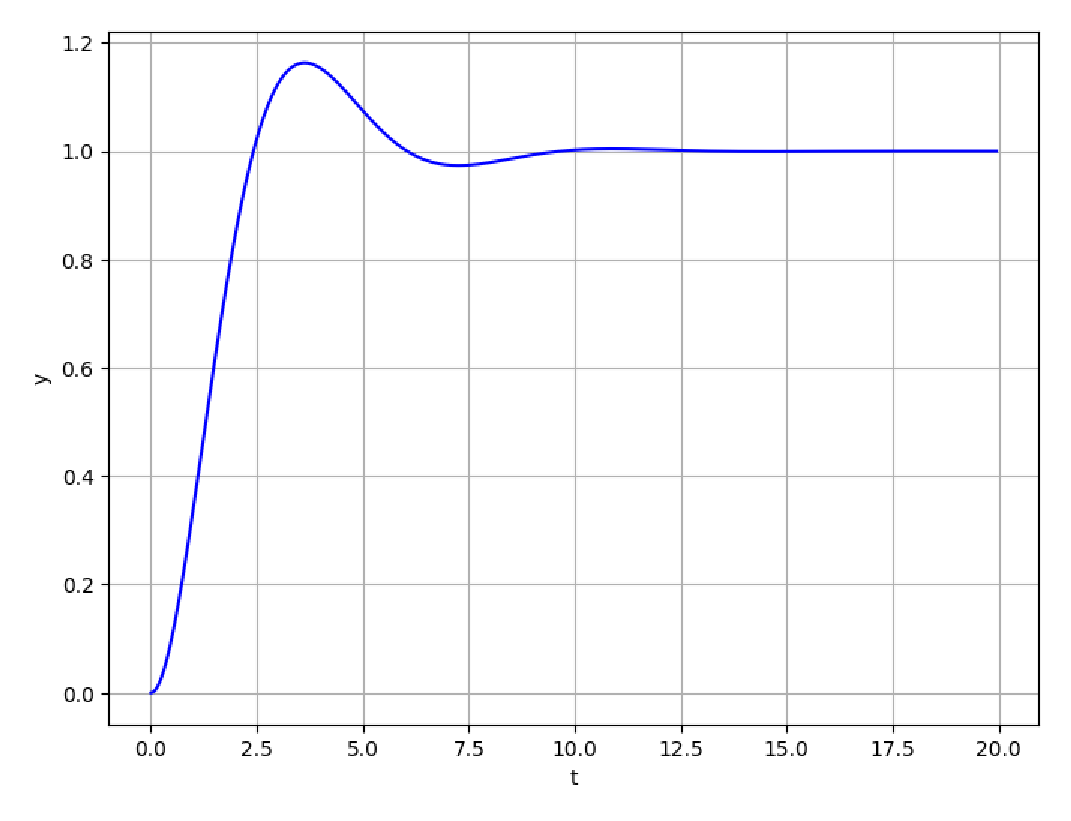
\includegraphics[scale=0.7]{figure2.eps}
  \vspace{-30pt}\caption{フィードバックシステム}
  \label{fig:figure2}
\end{figure}
\clearpage
%2-3-----------------------------------------------------------------------
{\large \bfseries 2.2.1 離散時間状態方程式の導出}\\
 制御対象である実験装置は、サーボモーターへの印加電圧を$v$、それによってボールの位置$z$や速度$\dot{z}$、サーボモーターの角度$\theta$や角速度$\dot{\theta}$が駆動される入出力システムである。ここで、$u_\mathrm{c}(t)=v(t)\ ,\ \bm x(t)=[\theta,\dot{\theta},z,\dot{z}]^\top$とおく。また、センサーを用いて全状態を観測できるとすると、観測信号$\bm y_\mathrm{c}(t)$は$\bm x(t)$そのものとなる。システム$P_\mathrm{c}$は次のように表せる。
\begin{equation}
  \mathrm{P_c}:\ \dot{\bm x}(t)=A_\mathrm{c}\bm x (t)+B_\mathrm{c}u_\mathrm{c}(t)\ ,\ \bm y_\mathrm{c}=\bm x(t)
\end{equation}
ここで、$A_\mathrm{c}\in \mathbb{R}^{4\times4},B_\mathrm{c}\in \mathbb{R}^4$である。\\
 計算機を用いて信号を処理する場合、装置から得られた連続時間信号をホールダとサンプラを用いて離散時間信号に変換しなければならない。サンプラのサンプリング周期を$\Delta t$とすると、$t=k\Delta t\ ,\ \forall k\in\{0,1,2,3\cdots\}$という離散時間毎に$\bm y_\mathrm{c}$の値を取得することになる。得られた数列を$\bm y_\mathrm{c}[k]$のように離散時間$[k]$をつけて表記すると、
\begin{equation}
  \bm y_\mathrm{c}[k]=\bm y_\mathrm{c}(k\Delta t)\ ,\ \forall k\in\{0,1,2,3\cdots\}
\end{equation}
の関係が成り立つ。次に今回の実験ではホールダについて0次ホールドを用いる。よって、信号$u_\mathrm{c}(t)$はある時刻$t=k\Delta t$から$t=(k+1)\Delta t$までの間は$u[k]$の一定値をとる。すなわち、
\begin{equation}
  u_\mathrm{c}(t)=u[k]\ ,\ \forall t\in[k\Delta t,(k+1)\Delta t]\ ,\ \forall k\in\{0,1,2,3\cdots\}
\end{equation}
の関係が成り立つ。\\
 これより、$\mathrm{P_c}$、サンプラ、ホールダのモデルをもとにして、$u[k]$から$y[k]$までの振る舞いをモデル化する。まず、(1)式の連続時間状態方程式で、時間$t=k\Delta t$からサンプリング周期が一個先の$t=(k+1)\Delta t$までの状態$\bm x(t)$の遷移を計算すると、
\begin{equation}
  \bm x((k+1)\Delta t)=e^{A_\mathrm{c}\Delta t}+\int_{k\Delta t}^{(k+1)\Delta t} e^{A_\mathrm{c}((k+1)\Delta t-\tau)}B_\mathrm{c}u_\mathrm{c}(\tau)\mathrm{d}\tau
\end{equation}
となる。ここで、(3)式と$\tau=(k+1)\Delta t-\tau$と置き直すことによって(4)式は、
\begin{equation}
  \bm x((k+1)\Delta t)=e^{A_\mathrm{c}\Delta t}+\left\{\int_{0}^{\Delta t} e^{A_\mathrm{c}\tau}B_\mathrm{c}\mathrm{d}\tau\right\}u_\mathrm{c}(\tau)
\end{equation}
と書き換えることができる。さらに、サンプリング周期に合わせた$t=k\Delta t\ ,\ k\in\{0,1,2,3\cdots\}$の離散時間上の状態$\bm x(t)$を$\bm x[k]$と表記する。このとき、(2)式のように$\bm x[k]=\bm x(k\Delta t)\ ,\ k\in \{0,1,2,3\cdots\}$が成り立つため、$u[k]$から$y[k]=x[k]$までの振る舞いは、
\begin{equation}
  \mathrm{P}:\bm x[k+1]=A\bm x[k]+Bu[k]\ ,\ \bm y[k]=\bm x[k]
\end{equation}
と記述できる。ただし、$A\in \mathbb{R}^{4\times4}$と$B\in \mathbb{R}^{4}$はそれぞれ、
\begin{equation}
  A=e^{A_\mathrm{c}\Delta t}\ ,\ B=\int_{0}^{\Delta t}e^{A_\mathrm{c}\tau}\mathrm{d}\tau
\end{equation}
とした。\\
 以上より、離散時間状態方程式では逐次代入をするだけで振る舞いを計算することができる。初期状態が$\bm x[0]=\bm x_0$であるとすると、入力信号$\{u[0]u[1]\cdots u[k-1]\}$のもとで$\bm x[k]$は、
\begin{equation}
  \bm x[k]=A^k\bm x_0+\sum^{k-1}_{\tau=0}A^{\tau}Bu[k-1-\tau]
\end{equation}
のように求めることができる。
\clearpage
%3-4------------------------------------------------------------------------
{\large \bfseries 2.2.2 データ駆動モデリング}\\
 制御入力$\{u[0],u[1],\dots u[N-1]\}$に対して、状態$\{\bm x[0],\bm x[1],\dots {\bm x[N-1]}\}$がデータとして得られているとする。ただし、$N\in \mathbb{N}$である。このとき、状態方程式(6)のシステム行列$A,B$を求めることを考える。$\{u[0],u[1],\dots u[N-1]\}$と$\{\bm x[0],\bm x[1],\dots {\bm x[N-1]}\}$は(6)式を満たすから、
\begin{align*}
  \bm x[1]&=A\bm x[0]+Bu[0]\\
  \bm x[1]&=A\bm x[0]+Bu[0]\\
  \vdots \hspace{-10pt}\\
  \bm x[N]&=A\bm x[N-1]+Bu[N-1]
\end{align*}
が成り立つ。ここで、新しく行列$X_1,X_0\in \mathbb{R}^{4\times N},U_0\in \mathbb{R}^{1\times N}$を
\begin{align*}
  X_1&:=[\bm x[1],\bm x[2],\dots {\bm x[N]}]\\
  X_0&:=[\bm x[0],\bm x[1],\dots {\bm x[N-1]}]\\
  U_0&:=[u[0],u[1],\dots u[N-1]
\end{align*}
のように定義する。よって、データが満たすべき条件は、
\begin{align}
  X_1=AX_0+BU_0
\end{align}
と書ける。しかし、実際は観測ノイズにより、(9)式が成り立つとは限らない。そこで、(9)式を解く代わりに次に最小自乗法を解くことによって、$A,B$を求める。
\begin{equation}
  \min_{A,B}\|X_1-(AX_0+BU_0)\|_\mathrm{F}
\end{equation}
(10)式をベクトルのユークリッドノルムで表すと、
\begin{equation}
  \min_{A,B} \sum_{\tau=0}^{N-1}\|\bm x[\tau+1]-(A\bm x[\tau]+B\bm x[\tau])\|_2^2
\end{equation}
となる。\\
\\
{\large \bfseries 2.2.3 Ball\&Beam実験装置のデータ駆動モデリング}\\
 実験装置は、サーボモータへの印加電圧$v$から、サーボモータの角度$\theta$や角速度$\dot{\theta}$までのシステム$\mathrm{P_{up}}$と、角度$\theta$からボールの位置$z$やボールの速度$\dot{z}$までのシステム$\mathrm{P_{down}}$の2つから構成されている。また、図\ref{fig:figure3}に示すように、2つのシステム$\mathrm{P_{up},P_{down}}$はカスケード接続されている。\\
\begin{figure}[h]
  \centering
  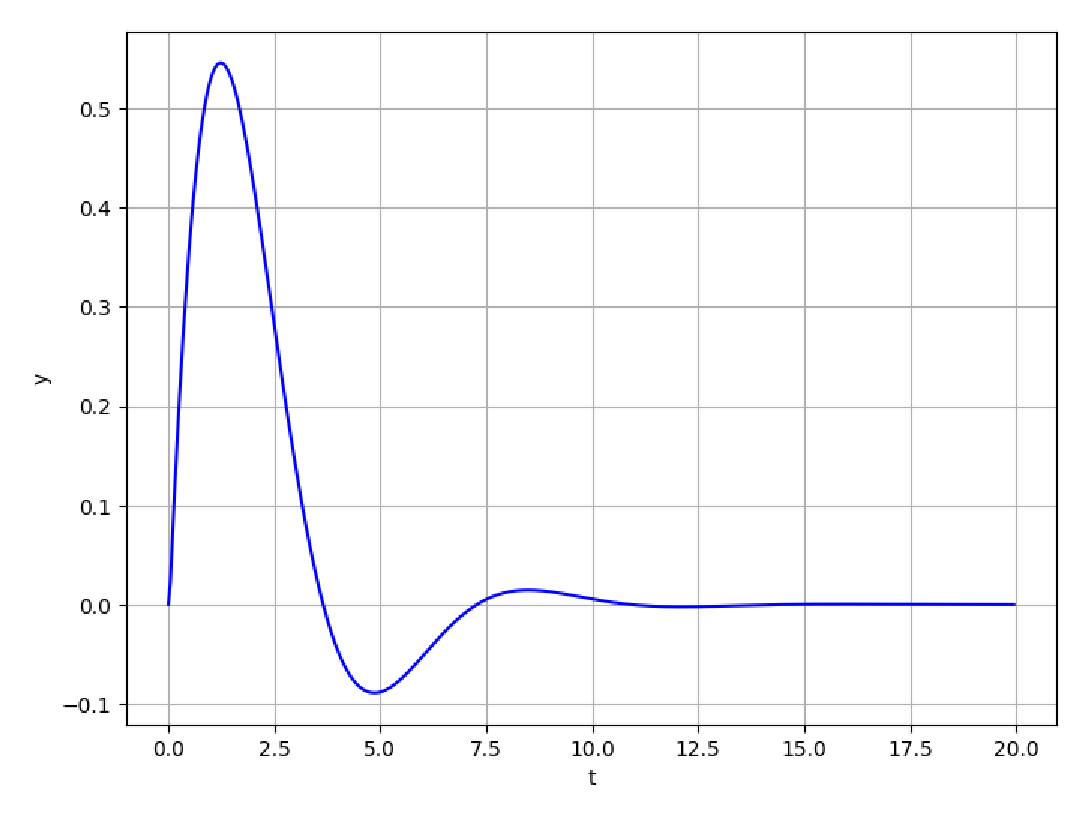
\includegraphics[scale=0.9]{figure3.eps}
  \vspace{-40pt}\caption{Ball\&Beam実験装置のカスケード構造}
  \label{fig:figure3}
\end{figure}\\
 まず、上流システム$\mathrm{P_{up}}$は、2.2.2により、データ駆動でモデリングすることができる。状態変数を$\bm x_\mathrm{up}:=[\theta,\dot{\theta}]^\top$、システム行列を$A_\mathrm{up},B_\mathrm{up}$と定義すると、入力$u[k]$と状態$x_\mathrm{up}$の時系列データをもとに、離散時間状態方程式
\begin{align}
  \mathrm{P_{up}}:\ \bm x_\mathrm{up}[k+1]=A_\mathrm{up}\bm x_\mathrm{up}[k]+B_\mathrm{up}u[k]
\end{align}
から$A_\mathrm{up},B_\mathrm{up}$を求めることができる。\\
 次に下流システム$\mathrm{P_{up}}$ ついて考える。$\mathrm{P_{down}}$の入力であるサーボモータの角度$\theta$の変化はビームの角度$\psi$に即座に伝わることから、この入出力関係は静的システムである。よって、$\theta,\psi$によって定まる定数$K_{\theta,\psi}$を用いて、
\begin{align}
  \psi[k]=K_{\theta,\psi}\theta[k]
\end{align}
%4-5------------------------------------------------------------------------
と表せる。また、図\ref{fig:figure4}を参考にして、ビームの角度$\psi$に対するボールの位置$z$の振る舞いを考える。ボールとしてピンポン玉を利用し、ボールの内部は内空、殻の厚みは無視できるものとする。また、簡単のため、$\psi$やその変化$\dot{\psi}$は十分に小さいものとし、ボールの慣性モーメントまで考慮すると、次の運動方程式を導ける。
\begin{align}
  m\ddot{z}+\left(\frac{2}{3}mr^2\right)\frac{\ddot{\phi}}{r}=mg\sin{\psi}
\end{align}
ここで、$m$はボールの質量、$g$ は重力加速度、$r$はボールの半径、$g$は重力加速度$φ$はボールの回転角度である.幾何学的な関係から、$r\phi=z$、$\psi$が十分に小さいことから$\sin{\psi}\approx\psi$とできることから、
\begin{align}
  \ddot{z}=\frac{3}{5}g\psi
\end{align}
が成り立つ。この運動方程式を離散時間状態方程式に変換すると、(13)式、(15)式より、
\begin{align}
  \dot{z}[k+1]&=\dot{z}[k]+\frac{3}{5}\Delta tK_{\theta,\psi}g\theta[k],\\
  z[k+1]&=z[k]+\Delta t \dot{z}[k]
\end{align}
と表せる。ここで、$\Delta t$はサンプリング周期である。よって、状態を$\bm x_\mathrm{down}[k]=[z,\dot{z}]^\top$、システム行列$A_\mathrm{down},B_\mathrm{down}$とすると、
\begin{equation}
  \mathrm{P_{down}}:\ \bm x_\mathrm{down}[k+1]=A_\mathrm{down}\bm x_\mathrm{down}[k]+B_\mathrm{down}\theta[k]
\end{equation}
となる。ただし、システム行列$A_\mathrm{down},B_\mathrm{down}$は、
\begin{equation}
  A_\mathrm{down}=
  \begin{bmatrix}
    1&\Delta t\\
    0&1
  \end{bmatrix}
  ,\ B_\mathrm{down}=
  \begin{bmatrix}
    0\\
    \frac{3}{5}\Delta tK_{\theta,\psi}g
  \end{bmatrix}
\end{equation}
である。
\\
\begin{figure}[h]
  \centering
  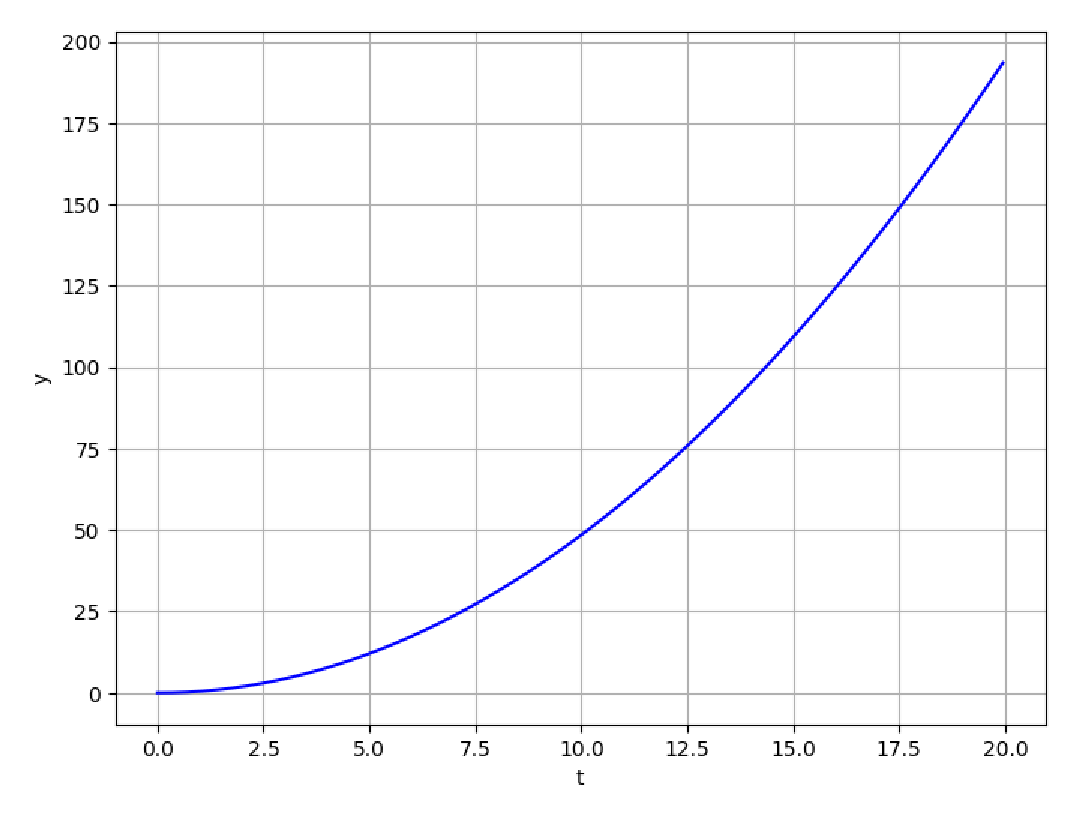
\includegraphics[scale=0.9]{figure4.eps}
  \vspace{-35pt}\caption{ボールのダイナミクス}
  \label{fig:figure4}
\end{figure}
\\
改めて、$\bm x=[\bm x_\mathrm{down}^\top, \bm x_\mathrm{up}^\top]$と置くことにより、(12)、(18)式から、(6)の状態方程式を得ることができる。よって、システム行列$A,B$は、
\begin{align}
  A=
  \begin{bmatrix}
    A_\mathrm{down}&
    \begin{bmatrix}
      B_\mathrm{down}&\bm O
    \end{bmatrix}\\
    \bm O&A_\mathrm{up}
  \end{bmatrix}
  \ ,\ B=
  \begin{bmatrix}
    \bm O\\
    B_\mathrm{up}
  \end{bmatrix}
\end{align}
\clearpage
{\large \bfseries 2.3 最適制御理論}\\
 次の評価関数$J$を考える。
\begin{equation}
  J:=\sum_{k=0}^{\infty} \left\{(\bm x[k]-\bm x_\mathrm{ref})^\top Q(\bm x[k]-\bm x_\mathrm{ref})+(u[k]-u_\mathrm{ref})^\top R(u[k]-u_\mathrm{ref})\right\}
\end{equation}
ここで、$Q$は半正定行列、$R$は正定行列、$\bm x_\mathrm{ref}$と$u_\mathrm{ref}$はそれぞれ状態と制御入力である。ただしこれらは、
\begin{equation}
  \bm x_\mathrm{ref}=A\bm x_\mathrm{ref}+Bu_\mathrm{ref}
\end{equation}
を満たす。ボールをビーム上の所望の位置$z_\mathrm{ref}$に留めるという制御目標に合わせると、$\bm x_\mathrm{ref}=[z_\mathrm{ref},0,0,0]$や$u_\mathrm{ref}=0$と設定するのが自然である。\\
 目標状態$\bm x_\mathrm{ref}$や重み$Q,R$が与えられたとき、(21)式を最小にする制御入力信号$\{u[0],u[1],u[2]\dots\}$は一意に定まり、図\ref{fig:figure2}について
\begin{equation}
  \mathrm{K}: u[k]=-F^*(\bm x[k]-\bm x_\mathrm{ref})+u_\mathrm{ref},\ k\in {0,1,2,\dots}
\end{equation}
の状態フィードバック制御として与えられる。ただし、 $F^*$はリッカチ方程式
\begin{equation}
  A^\top XA-X-A^\top XB(R+B^\top XB)^{-1}B^\top XA+Q=0
\end{equation}
%5-6------------------------------------------------------------------------
の半正定解$X$を用いて、
\begin{equation}
  F^*=(B^\top XB+R)^{-1}B^\top XA
\end{equation}
で与えられる。\\
\\
{\large \bfseries 2.4 演習課題5}\\
{\large \bfseries 2.4.1 \ 1次元状態方程式モデル$x[k+1]=x[k]+u[k]$について、最適制御のためのフィードバックゲイン$F^*$\\
を求める。ただし、重み行列は、$Q=1,R=1$とした。}\\
\\
\centerline{実行プログラム}
\begin{lstlisting}
  Ac = 1
  Bc = 1
  Cc = 1
  Dc = 0
  st = 0.02 #サンプリング時間
  sysc = ss(Ac,Bc,Cc,Dc) # 離散時間状態方程式の定義
  sys = c2d(sysc, st, method='zoh')
  A,B,C,D = ssdata(sysc) # システム行列の取り出し
  Q = 1 # 重み行列の定義
  R = 1
  X, L, F = dare(A,B,Q,R) # リッカチ方程式の求解
  sys_FB = ss(A - B*F,B,C,D,st) # 最適状態フィードバック制御を施した制御システムの定義
  print(F)
\end{lstlisting}
\centerline{\ }
\centerline{実行結果}
\begin{lstlisting}
  [[0.61803399]]
\end{lstlisting}
\clearpage
{\large \bfseries 2.4.2 2.4.1の手計算による解}\\
 (24)式から、
\begin{gather}
  A^\top XA-X-A^\top XB(R+B^\top XB)^{-1}B^\top XA+Q=0\notag \\
  \therefore X-X-X(1+X)^{-1}X+1=0\notag \\
  \therefore X=\frac{1+\sqrt{5}}{2}\ \ (\because X>0)
\end{gather}
となり、(26)式を(25)式に代入すると、
\begin{align}
  F^*&=(B^\top XB+R)^{-1}B^\top XA\notag\\
  &=\left(\frac{1+\sqrt{5}}{2}+1\right)^{-1}\times \frac{1+\sqrt{5}}{2}\notag\\
  &=\frac{-1+\sqrt{5}}{2}\notag\\[10pt]
  &\approx 0.6180339887
\end{align}
となり。2.4.1で求めた$F^*$の値と一致した。\\
\\
{\large \bfseries 2.4.3 最適フィードバックゲイン$F^*$の値をずらした時の評価関数$J$の振る舞い}\\
 図\ref{fig:figure5}に最適フィードバックゲイン$F^*$と評価関数$J$の関係を示す。
\begin{figure}[h]
  \centering
  \scalebox{0.45}[0.45]{
\begin{tikzpicture}[gnuplot]
%% generated with GNUPLOT 5.4p10 (Lua 5.4; terminal rev. Jun 2020, script rev. 118)
%% Sun Nov 12 18:33:30 2023
\path (0.000,0.000) rectangle (12.500,8.750);
\gpcolor{color=gp lt color border}
\gpsetlinetype{gp lt border}
\gpsetdashtype{gp dt solid}
\gpsetlinewidth{1.00}
\draw[gp path] (0.018,0.031)--(0.198,0.031);
\draw[gp path] (12.480,0.031)--(12.300,0.031);
\node[gp node right] at (-0.166,0.031) {$15$};
\draw[gp path] (0.018,1.479)--(0.198,1.479);
\draw[gp path] (12.480,1.479)--(12.300,1.479);
\node[gp node right] at (-0.166,1.479) {$20$};
\draw[gp path] (0.018,2.927)--(0.198,2.927);
\draw[gp path] (12.480,2.927)--(12.300,2.927);
\node[gp node right] at (-0.166,2.927) {$25$};
\draw[gp path] (0.018,4.375)--(0.198,4.375);
\draw[gp path] (12.480,4.375)--(12.300,4.375);
\node[gp node right] at (-0.166,4.375) {$30$};
\draw[gp path] (0.018,5.822)--(0.198,5.822);
\draw[gp path] (12.480,5.822)--(12.300,5.822);
\node[gp node right] at (-0.166,5.822) {$35$};
\draw[gp path] (0.018,7.270)--(0.198,7.270);
\draw[gp path] (12.480,7.270)--(12.300,7.270);
\node[gp node right] at (-0.166,7.270) {$40$};
\draw[gp path] (0.018,8.718)--(0.198,8.718);
\draw[gp path] (12.480,8.718)--(12.300,8.718);
\node[gp node right] at (-0.166,8.718) {$45$};
\draw[gp path] (0.018,0.031)--(0.018,0.211);
\draw[gp path] (0.018,8.718)--(0.018,8.538);
\node[gp node center] at (0.018,-0.277) {$0$};
\draw[gp path] (1.935,0.031)--(1.935,0.211);
\draw[gp path] (1.935,8.718)--(1.935,8.538);
\node[gp node center] at (1.935,-0.277) {$0.2$};
\draw[gp path] (3.852,0.031)--(3.852,0.211);
\draw[gp path] (3.852,8.718)--(3.852,8.538);
\node[gp node center] at (3.852,-0.277) {$0.4$};
\draw[gp path] (5.770,0.031)--(5.770,0.211);
\draw[gp path] (5.770,8.718)--(5.770,8.538);
\node[gp node center] at (5.770,-0.277) {$0.6$};
\draw[gp path] (7.687,0.031)--(7.687,0.211);
\draw[gp path] (7.687,8.718)--(7.687,8.538);
\node[gp node center] at (7.687,-0.277) {$0.8$};
\draw[gp path] (9.604,0.031)--(9.604,0.211);
\draw[gp path] (9.604,8.718)--(9.604,8.538);
\node[gp node center] at (9.604,-0.277) {$1$};
\draw[gp path] (11.521,0.031)--(11.521,0.211);
\draw[gp path] (11.521,8.718)--(11.521,8.538);
\node[gp node center] at (11.521,-0.277) {$1.2$};
\draw[gp path] (0.018,8.718)--(0.018,0.031)--(12.480,0.031)--(12.480,8.718)--cycle;
\node[gp node center,rotate=-270] at (-0.826,4.374) {$J$};
\node[gp node center] at (6.249,-0.738) {$F^*$};
\gpcolor{rgb color={0.000,0.000,0.000}}
\gpsetlinewidth{5.00}
\draw[gp path] (0.977,8.142)--(1.935,3.417)--(2.894,1.542)--(3.852,0.700)--(4.811,0.321)%
  --(5.770,0.196)--(5.943,0.194)--(6.728,0.244)--(7.687,0.429)--(8.646,0.742)--(9.604,1.189)%
  --(10.563,1.795)--(11.521,2.601);
\gpsetpointsize{3.20}
\gp3point{gp mark 7}{}{(0.977,8.142)}
\gp3point{gp mark 7}{}{(1.935,3.417)}
\gp3point{gp mark 7}{}{(2.894,1.542)}
\gp3point{gp mark 7}{}{(3.852,0.700)}
\gp3point{gp mark 7}{}{(4.811,0.321)}
\gp3point{gp mark 7}{}{(5.770,0.196)}
\gp3point{gp mark 7}{}{(5.943,0.194)}
\gp3point{gp mark 7}{}{(6.728,0.244)}
\gp3point{gp mark 7}{}{(7.687,0.429)}
\gp3point{gp mark 7}{}{(8.646,0.742)}
\gp3point{gp mark 7}{}{(9.604,1.189)}
\gp3point{gp mark 7}{}{(10.563,1.795)}
\gp3point{gp mark 7}{}{(11.521,2.601)}
\gpcolor{color=gp lt color border}
\gpsetlinewidth{1.00}
\draw[gp path] (0.018,8.718)--(0.018,0.031)--(12.480,0.031)--(12.480,8.718)--cycle;
%% coordinates of the plot area
\gpdefrectangularnode{gp plot 1}{\pgfpoint{0.018cm}{0.031cm}}{\pgfpoint{12.480cm}{8.718cm}}
\end{tikzpicture}
}

  \vspace{-30pt}\caption{$J$と$F^*$の関係}
  \label{fig:figure5}
\end{figure}
\\
図\ref{fig:figure5}から、2.5.1で求めた$F^*=0.61803399$のときに$J$が最も小さくなっており、最適な制御ができていることがわかる。\\
\\
\hspace{-2pt}{\Large \bfseries 3.実験方法}\\
{\large \bfseries 3.1 モデリング方法}\\
 まず、Ball\&Beam実験装置のモータのモデリングを行うため、同定信号として周期$0.2,0.4,0.6\ \mathrm{s}$の矩形波、$0.2,0.3,0.4\ \mathrm{s}$ののこぎり波、周波数$10,50,100\ \mathrm{Hz}$の正弦波の入力電圧を印加し、出力信号$\theta,\dot{\theta}$を得た。その後、得られたデータをハイパスフィルタやローパスフィルタに通し、2.2.2と2.2.3に示したモデリング方法を用いて、システム行列$A,B$をモデリングした。得られたデータとモデリングの自乗誤差を計算し、その誤差が最も小さいものをその後の入力信号として用いた。\\
\\
{\large \bfseries 3.2最適制御器の設計}\\
 最適制御器を設計する際は、3.1によって求めたシステム行列$A,B$について、評価関数が最小になるようにシミュレーションを行った。また、重みの値$Q,R$は入力信号$u$の絶対値が$5\ \mathrm{V}$を超えず、出力$z$のオーバーシュートができるだけ小さくなるように設定した。そして、その重みの値から、(24)、(25)式を用いて最適フィードバックゲイン$F^*$を求めた。\\
\\
{\large \bfseries 3.3最適制御器を用いたボールの位置制御の方法}\\
 実際にボールの位置を制御する際は、はじめにビームが水平になるように調整しその上にボールを静止させた。そして、ビーム上に設置された赤外線センサによってボールの位置を観測し、その観測データをフィードバック入力としてシステムを構成した。\\
\\
\hspace{-2pt}{\Large \bfseries 4.実験結果}\\
{\large \bfseries 4.1 実験1(1週目)}\\
 今回の実験ではサンプリング周期を$0.02\ \mathrm{s}$とした。表1にそれぞれの入力信号の角度の測定値とシミュレーションのMSEを示す。
\begin{table}[h]
  \newcolumntype{I}{!{\vrule width 1.5pt}}
  \newcolumntype{i}{!{\vrule width 0.8pt}}
  \arrayrulewidth=0.8pt
  \renewcommand{\arraystretch}{1.5}
  \newcommand{\bhline}[1]{\noalign{\hrule height #1}}
  \centering
  \caption{角度の測定値とシミュレーションのMSE}
  \begin{tabular}{Ic|c|c|c|c|c|c|c|c|cI}
    \bhline{1.5pt}
    波形&\multicolumn{3}{ci}{矩形波}&\multicolumn{3}{ci}{のこぎり波}&\multicolumn{3}{cI}{正弦波}\\
    \hline
    周期\ /\ s&0.2&0.4&0.6&0.2&0.3&0.4&0.1\pi&0.02\pi&0.01\pi\\
    \hline
    \begin{tabular}{c}
      \vspace{-10pt}角度の測定値と\\
      \vspace{-10pt}シミュレーションの\\
      MSE
      \end{tabular}&64.8&36.6&33.7&54.2&189&197&29.7&25.8&33.8\\
      \bhline{1.5pt}
  \end{tabular}
  \label{tb:table1}
\end{table}
以後、今回の実験で周期0.4\ sの矩形波を入力信号として用いる。その理由は考察に示す。そして図\ref{fig:figure6}に$\mathrm{P_{up}}$に印加した周期$0.4\ \mathrm{s}$の矩形波の入力電圧を示す。
\begin{figure}[h]
  \centering
  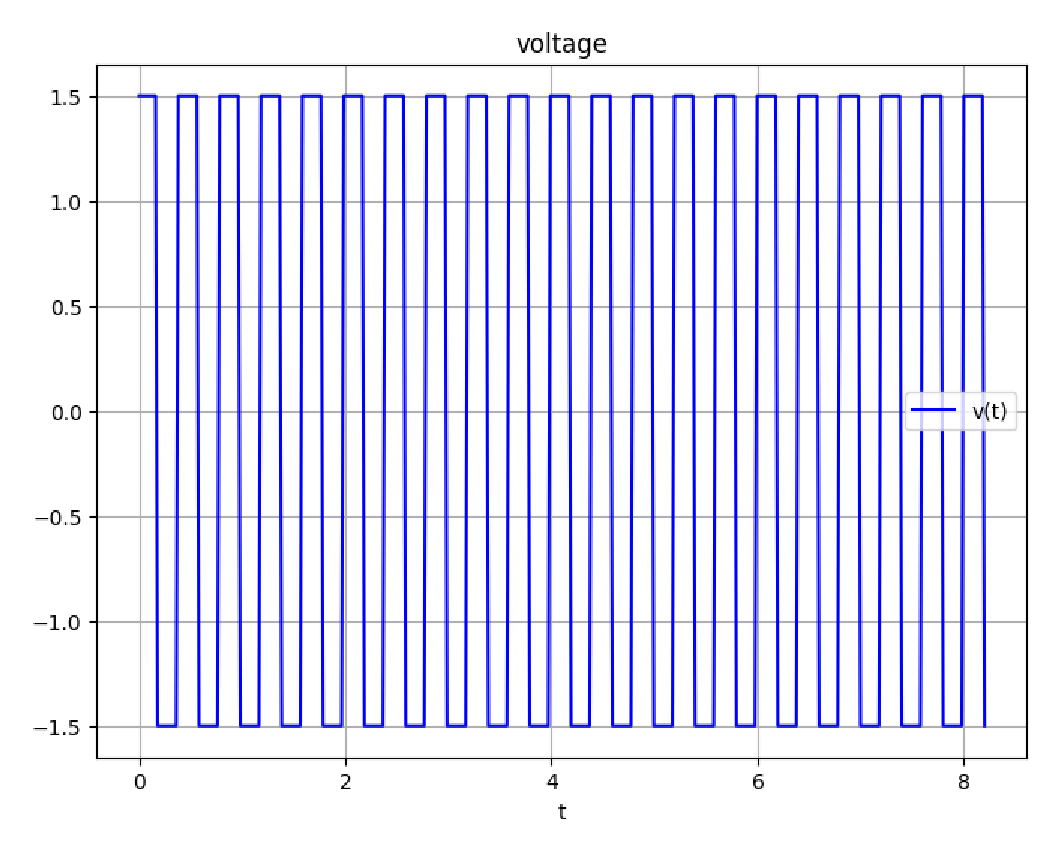
\includegraphics[scale=0.7]{figure6.eps}
  \caption{入力電圧}
  \label{fig:figure6}
\end{figure}
\clearpage
図\ref{fig:figure7}に角度$\theta$の時間変化、図\ref{fig:figure8}にハイパスフィルタのゲイン線図を示す。ただし、青線は何も処理をしていない角$\theta$、赤線は図\ref{fig:figure8}に示すようなハイパスフィルタを通した角度$\theta$を表す。
\begin{figure}[h]
  \centering
  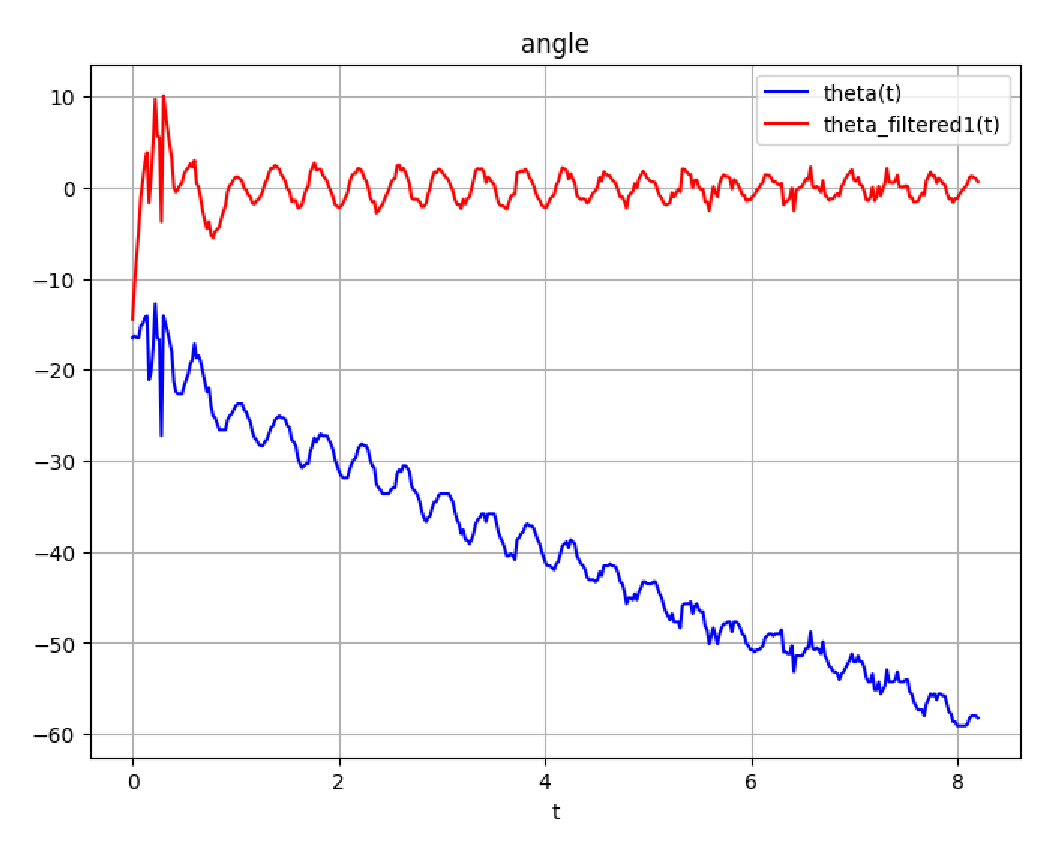
\includegraphics[scale=0.7]{figure7.eps}
  \caption{角度$\theta$の時間変化}
  \label{fig:figure7}
\end{figure}
\begin{figure}[h]
  \centering
  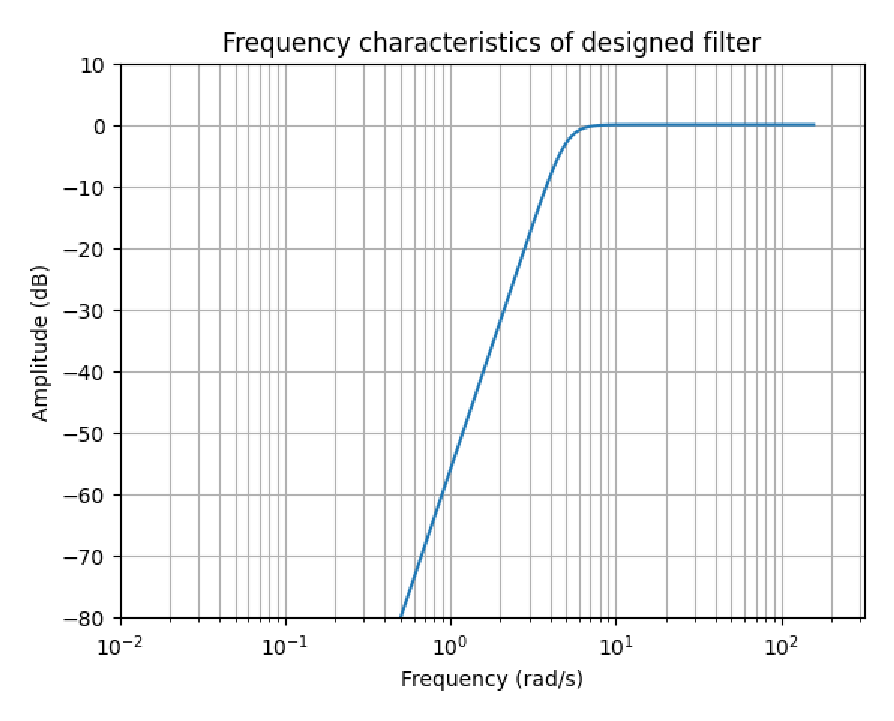
\includegraphics[scale=0.7]{figure8.eps}
  \caption{ハイパスフィルタ}
  \label{fig:figure8}
\end{figure}
\clearpage
図\ref{fig:figure9}に角度$\theta$の時間変化、図\ref{fig:figure10}にローパスフィルタのゲイン線図を示す。ただし、青線は何も処理をしていない角$\theta$、赤線は図\ref{fig:figure8}に示すようなハイパスフィルタ、図\ref{fig:figure10}に示すようなローパスフィルタフィルタを通した角$\theta$を表す。
\begin{figure}[h]
  \centering
  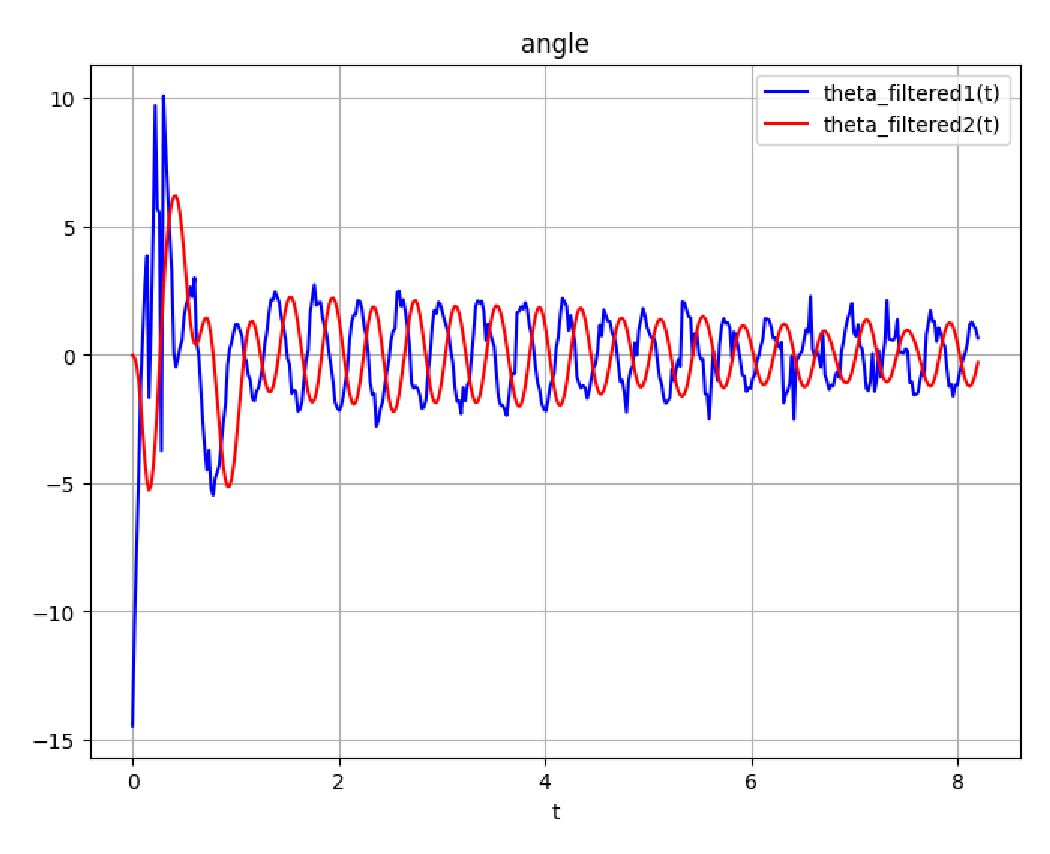
\includegraphics[scale=0.7]{figure9.eps}
  \caption{角度$\theta$の時間変化}
  \label{fig:figure9}
\end{figure}
\begin{figure}[h]
  \centering
  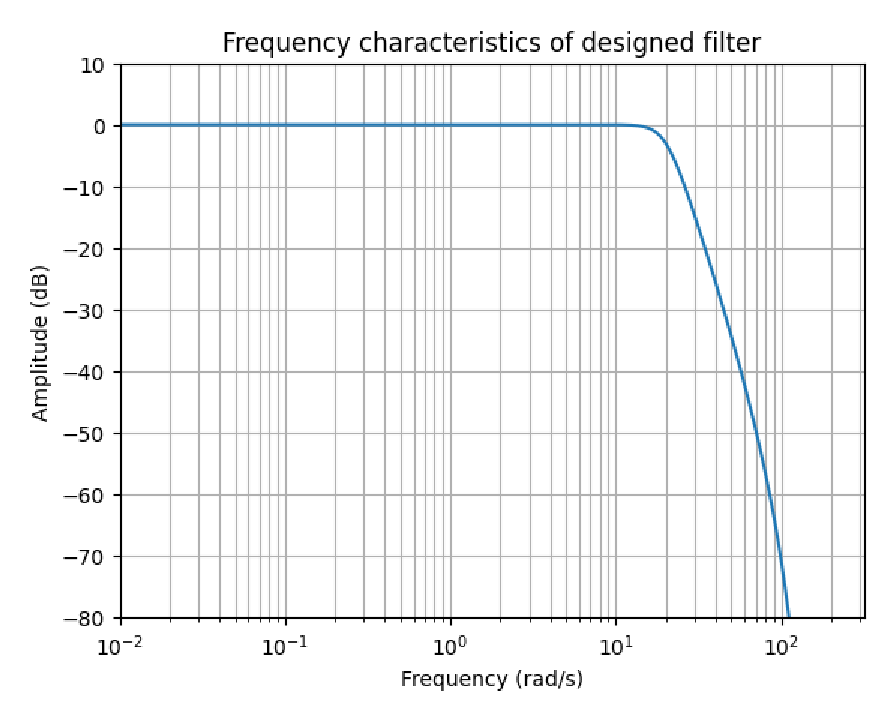
\includegraphics[scale=0.7]{figure10.eps}
  \caption{ローパスフィルタ}
  \label{fig:figure10}
\end{figure}
\clearpage
図\ref{fig:figure11}、図\ref{fig:figure12}に実験データから得られたグラフとシミュレーションによって得られたグラフを比較した図を示す。
\begin{figure}[h]
  \centering
  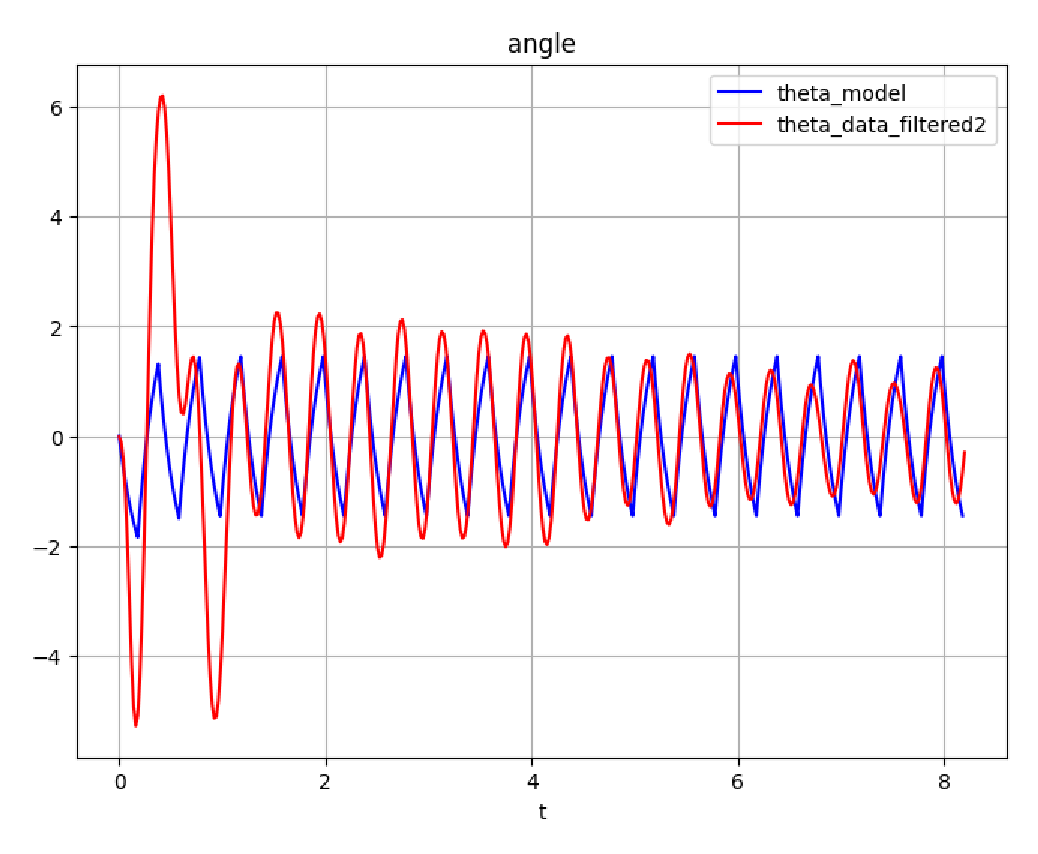
\includegraphics[scale=0.7]{figure11.eps}
  \caption{実験データとシミュレーションの比較(角度$\theta$)}
  \label{fig:figure11}
\end{figure}
\begin{figure}[h]
  \centering
  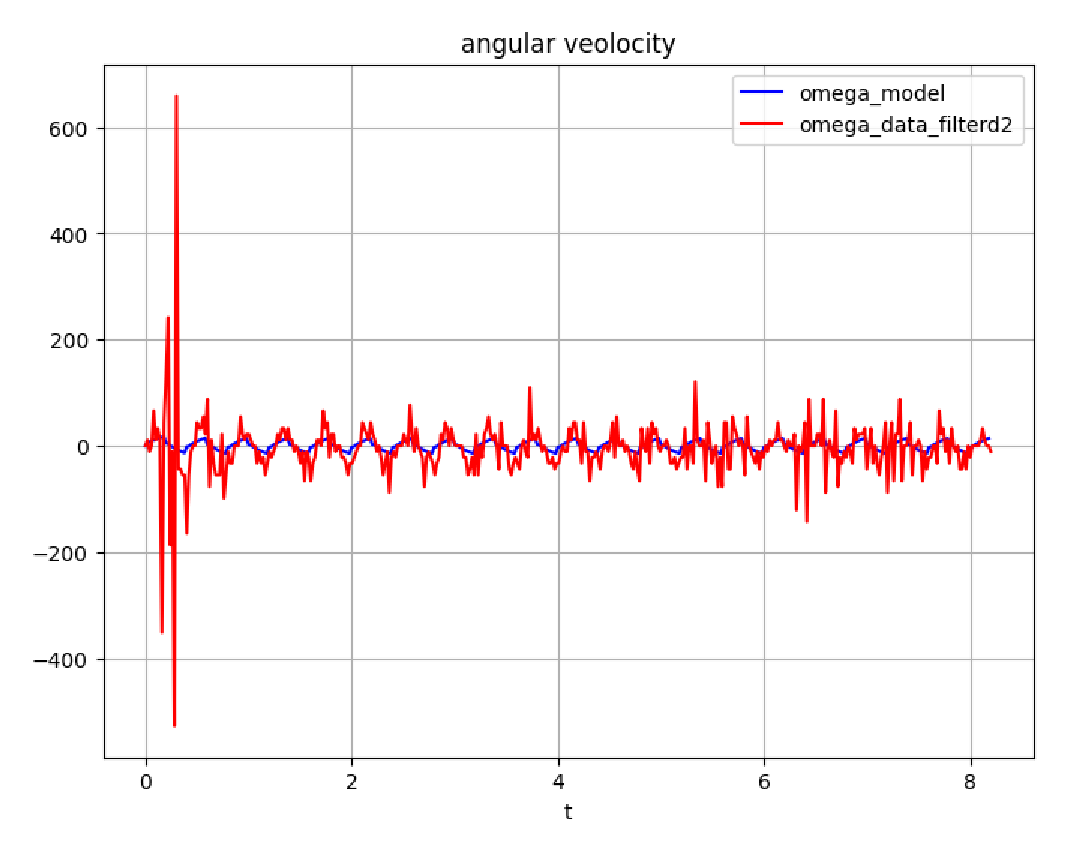
\includegraphics[scale=0.7]{figure12.eps}
  \caption{実験データとシミュレーションの比較(角速度$\dot{\theta}$)}
  \label{fig:figure12}
\end{figure}\\
角度の測定値とシミュレーションのMSEは、$25.766$であった。
\clearpage
最後にモデリングによって得られた状態方程式を(28)、(29)、(30)、(31)式に示す。ただし、(28)、(29)式はハイパスフィルタとローパスフィルタに通したときの状態方程式、(30)、(31)式はハイパスフィルタのみに通したときの状態方程式を示す。
\begin{align}
  \mathrm{P_{up}}:\ \bm x[k+1]&=
  \begin{bmatrix}
    -0.905&5.97\times 10^{-4}\\
    -8.99&-0.288
  \end{bmatrix}\bm
  x_\mathrm{up}+
  \begin{bmatrix}
    -0.201\\
    4.30
  \end{bmatrix}
  u[k]\\[10pt]
  \mathrm{P_{down}}:\ \bm x[k+1]&=
  \begin{bmatrix}
    1&0.02\\
    0&1
  \end{bmatrix}
  \bm x_\mathrm{up}+
  \begin{bmatrix}
    0\\
    0.0287
  \end{bmatrix}
  u[k]
\end{align}
\begin{align}
  \mathrm{P_{up}}:\ \bm x[k+1]&=
  \begin{bmatrix}
    0.793&-7.70\times 10^{-3}\\
    3.64&-0.302
  \end{bmatrix}\bm
  x_\mathrm{up}+
  \begin{bmatrix}
    0.285\\
    6.36
  \end{bmatrix}
  u[k]\\[10pt]
  \mathrm{P_{down}}:\ \bm x[k+1]&=
  \begin{bmatrix}
    1&0.02\\
    0&1
  \end{bmatrix}
  \bm x_\mathrm{up}+
  \begin{bmatrix}
    0\\
    0.0287
  \end{bmatrix}
  u[k]
\end{align}\\
\\
{\large \bfseries 4.2 実験2(2週目)}\\
 2週目の実験では、ハイパスフィルタとローパスフィルタに通したときの状態方程式、ハイパスフィルタのみに通したときの状態方程式について実験を行った。以下、ハイパスフィルタとローパスフィルタに通したときを(i)、ハイパスフィルタのみに通したときを(ii)と表す。\\
 まず、(i)について、重み$q_1,q_2,q_3,q_4,r$の選定結果を(32)、(33)、(34)式に示す。また、図\ref{fig:figure13}、図\ref{fig:figure14}、図\ref{fig:figure15}にそれぞれの選定結果(32)、(33)、(34)式のボールの位置$z$のシミュレーション結果を示す。
\begin{align}
  [q_1,q_2,q_3,q_4]=[30000,100,1,1]\ ,\ r=5000000
\end{align}
\begin{figure}[h]
  \centering
  \vspace{-30pt}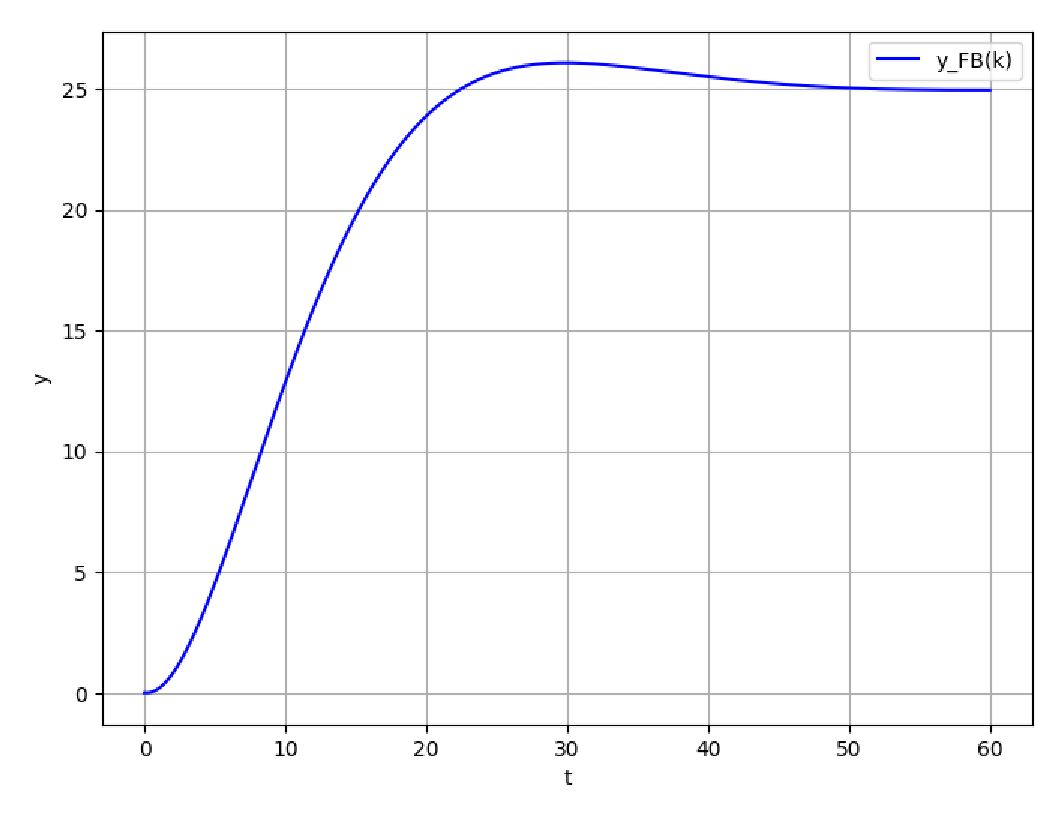
\includegraphics[scale=0.5]{figure13.eps}
  \caption{ボールの位置のシミュレーション結果}
  \label{fig:figure13}
\end{figure}
\clearpage
\begin{align}
  [q_1,q_2,q_3,q_4]=[10000,1000,1,1]\ ,\ r=5000000
\end{align}
\begin{figure}[h]
  \centering
  \vspace{-30pt}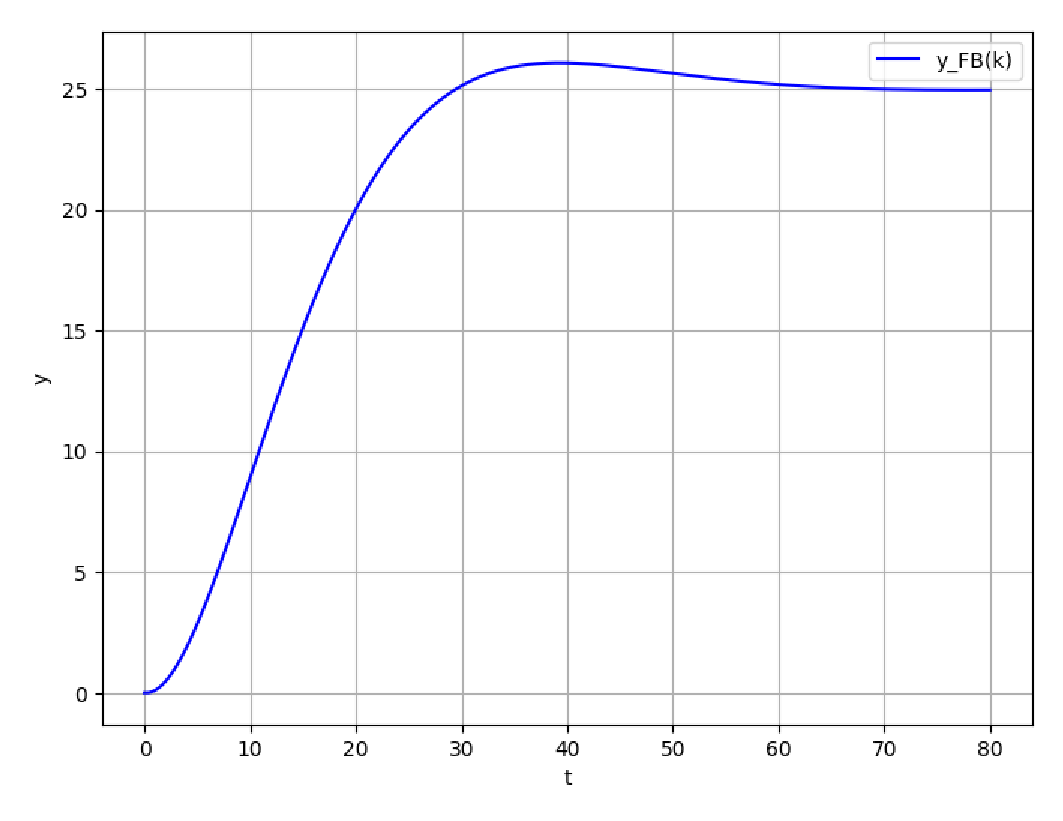
\includegraphics[scale=0.5]{figure14.eps}
  \caption{ボールの位置のシミュレーション結果}
  \label{fig:figure14}
\end{figure}
\begin{align}
  [q_1,q_2,q_3,q_4]=[100000,1,100,100]\ ,\ r=5000000
\end{align}
\begin{figure}[h]
  \centering
  \vspace{-30pt}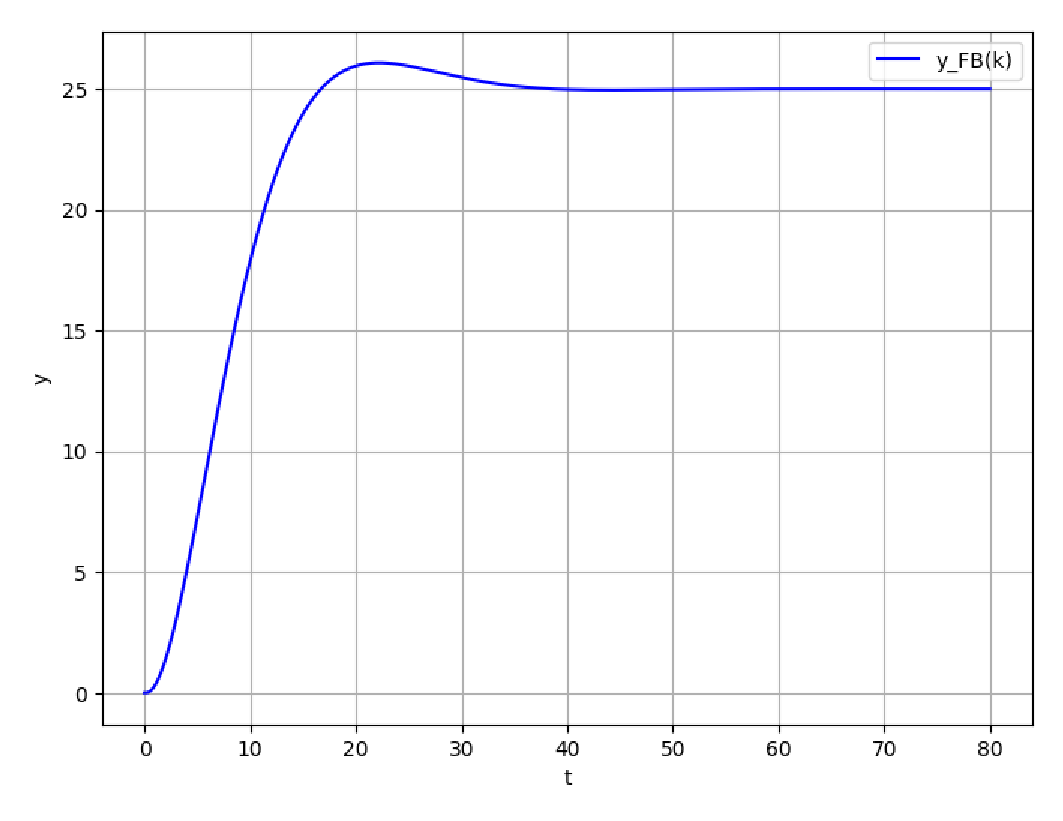
\includegraphics[scale=0.5]{figure15.eps}
  \caption{ボールの位置のシミュレーション結果}
  \label{fig:figure15}
\end{figure}\\
(32)、(33)、(34)式のときはいずれもボールがビームから落ちてしまい実験は失敗した。
次に(ii)について、重み$q_1,q_2,q_3,q_4,r$の選定結果を(35)、(36)、(37)、(38)、(39)、(40)式に示す。また、図\ref{fig:figure16}、図\ref{fig:figure20}、図\ref{fig:figure24}、図\ref{fig:figure28}、図\ref{fig:figure32}、図\ref{fig:figure36}にそれぞれの選定結果(35)、(36)、(37)式のボールの位置$z$のシミュレーション結果を、図\ref{fig:figure17}、図\ref{fig:figure21}、図\ref{fig:figure25}、図\ref{fig:figure29}、図\ref{fig:figure33}、図\ref{fig:figure37}にそれぞれの選定結果(35)、(36)、(37)式のボールの位置$z$の実験結果を、図\ref{fig:figure18}、図\ref{fig:figure22}、図\ref{fig:figure26}、図\ref{fig:figure30}、図\ref{fig:figure34}、図\ref{fig:figure38}にそれぞれの選定結果(35)、(36)、(37)式の角度$\theta$の実験結果を、図\ref{fig:figure19}、図\ref{fig:figure23}、図\ref{fig:figure27}、図\ref{fig:figure31}、図\ref{fig:figure35}、図\ref{fig:figure39}にそれぞれの選定結果(35)、(36)、(37)式の角速度$\dot{\theta}$の実験結果示す。
\clearpage
\begin{align}
  [q_1,q_2,q_3,q_4]=[1000,1,100,100]\ ,\ r=50000
\end{align}
\begin{figure}[h]
  \centering
  \vspace{-30pt}
  \begin{minipage}[h]{0.4\linewidth}
    \centering
    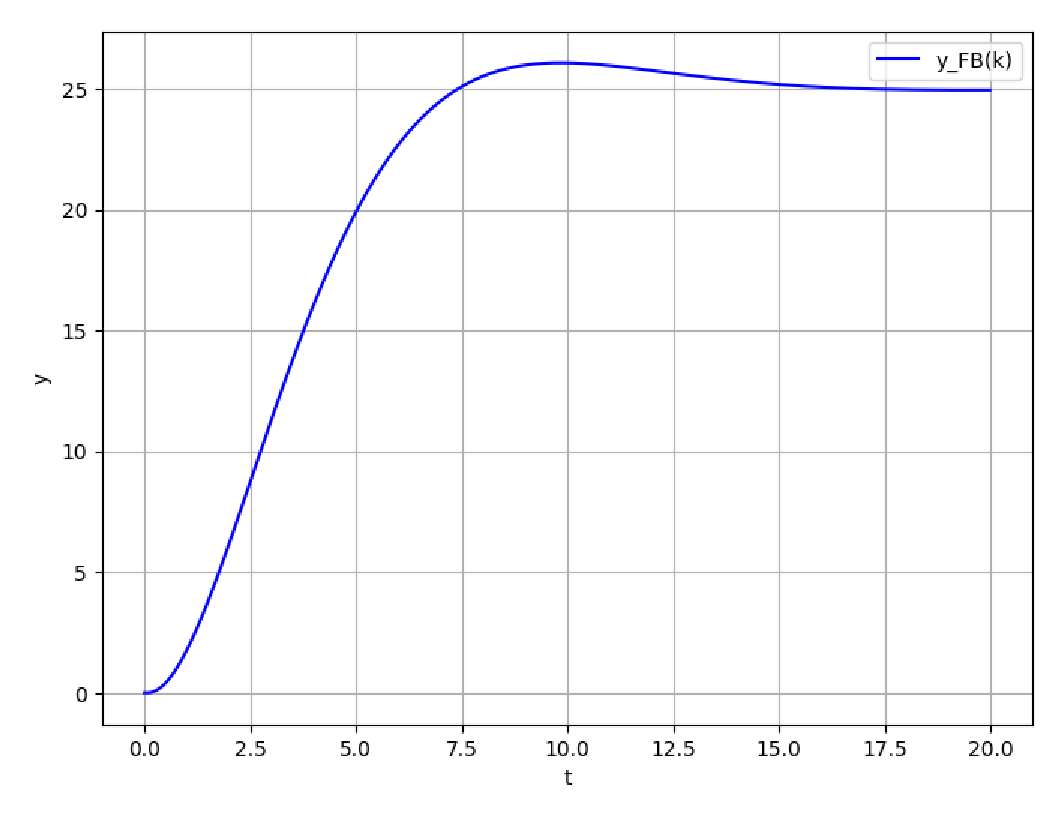
\includegraphics[scale=0.35]{figure16.eps}
    \caption{ボールの位置のシミュレーション結果}
    \label{fig:figure16}
  \end{minipage}
  \begin{minipage}[h]{0.4\linewidth}
    \centering
    \scalebox{0.5}[0.5]{
\begin{tikzpicture}[gnuplot]
%% generated with GNUPLOT 5.4p10 (Lua 5.4; terminal rev. Jun 2020, script rev. 118)
%% Sat Dec  9 17:21:03 2023
\path (0.000,0.000) rectangle (12.500,8.750);
\gpcolor{color=gp lt color border}
\gpsetlinetype{gp lt border}
\gpsetdashtype{gp dt solid}
\gpsetlinewidth{1.00}
\draw[gp path] (0.018,0.031)--(0.198,0.031);
\draw[gp path] (12.480,0.031)--(12.300,0.031);
\node[gp node right] at (-0.166,0.031) {$0$};
\draw[gp path] (0.018,0.900)--(0.198,0.900);
\draw[gp path] (12.480,0.900)--(12.300,0.900);
\node[gp node right] at (-0.166,0.900) {$0.1$};
\draw[gp path] (0.018,1.768)--(0.198,1.768);
\draw[gp path] (12.480,1.768)--(12.300,1.768);
\node[gp node right] at (-0.166,1.768) {$0.2$};
\draw[gp path] (0.018,2.637)--(0.198,2.637);
\draw[gp path] (12.480,2.637)--(12.300,2.637);
\node[gp node right] at (-0.166,2.637) {$0.3$};
\draw[gp path] (0.018,3.506)--(0.198,3.506);
\draw[gp path] (12.480,3.506)--(12.300,3.506);
\node[gp node right] at (-0.166,3.506) {$0.4$};
\draw[gp path] (0.018,4.375)--(0.198,4.375);
\draw[gp path] (12.480,4.375)--(12.300,4.375);
\node[gp node right] at (-0.166,4.375) {$0.5$};
\draw[gp path] (0.018,5.243)--(0.198,5.243);
\draw[gp path] (12.480,5.243)--(12.300,5.243);
\node[gp node right] at (-0.166,5.243) {$0.6$};
\draw[gp path] (0.018,6.112)--(0.198,6.112);
\draw[gp path] (12.480,6.112)--(12.300,6.112);
\node[gp node right] at (-0.166,6.112) {$0.7$};
\draw[gp path] (0.018,6.981)--(0.198,6.981);
\draw[gp path] (12.480,6.981)--(12.300,6.981);
\node[gp node right] at (-0.166,6.981) {$0.8$};
\draw[gp path] (0.018,7.849)--(0.198,7.849);
\draw[gp path] (12.480,7.849)--(12.300,7.849);
\node[gp node right] at (-0.166,7.849) {$0.9$};
\draw[gp path] (0.018,8.718)--(0.198,8.718);
\draw[gp path] (12.480,8.718)--(12.300,8.718);
\node[gp node right] at (-0.166,8.718) {$1$};
\draw[gp path] (0.018,0.031)--(0.018,0.211);
\draw[gp path] (0.018,8.718)--(0.018,8.538);
\node[gp node center] at (0.018,-0.277) {$1200$};
\draw[gp path] (1.576,0.031)--(1.576,0.211);
\draw[gp path] (1.576,8.718)--(1.576,8.538);
\node[gp node center] at (1.576,-0.277) {$1250$};
\draw[gp path] (3.134,0.031)--(3.134,0.211);
\draw[gp path] (3.134,8.718)--(3.134,8.538);
\node[gp node center] at (3.134,-0.277) {$1300$};
\draw[gp path] (4.691,0.031)--(4.691,0.211);
\draw[gp path] (4.691,8.718)--(4.691,8.538);
\node[gp node center] at (4.691,-0.277) {$1350$};
\draw[gp path] (6.249,0.031)--(6.249,0.211);
\draw[gp path] (6.249,8.718)--(6.249,8.538);
\node[gp node center] at (6.249,-0.277) {$1400$};
\draw[gp path] (7.807,0.031)--(7.807,0.211);
\draw[gp path] (7.807,8.718)--(7.807,8.538);
\node[gp node center] at (7.807,-0.277) {$1450$};
\draw[gp path] (9.365,0.031)--(9.365,0.211);
\draw[gp path] (9.365,8.718)--(9.365,8.538);
\node[gp node center] at (9.365,-0.277) {$1500$};
\draw[gp path] (10.922,0.031)--(10.922,0.211);
\draw[gp path] (10.922,8.718)--(10.922,8.538);
\node[gp node center] at (10.922,-0.277) {$1550$};
\draw[gp path] (12.480,0.031)--(12.480,0.211);
\draw[gp path] (12.480,8.718)--(12.480,8.538);
\node[gp node center] at (12.480,-0.277) {$1600$};
\draw[gp path] (0.018,8.718)--(0.018,0.031)--(12.480,0.031)--(12.480,8.718)--cycle;
\node[gp node center,rotate=-270,font={\fontsize{17.0pt}{20.4pt}\selectfont}] at (-1.286,4.374) {光強度比$P(r)/P(0)$};
\node[gp node center,font={\fontsize{17.0pt}{20.4pt}\selectfont}] at (6.249,-1.046) {距離$\ /\ \mathrm{\upmu m}$};
\gpcolor{rgb color={0.000,0.000,0.000}}
\draw[gp path] (0.018,0.207)--(0.064,0.221)--(0.110,0.218)--(0.156,0.205)--(0.202,0.205)%
  --(0.248,0.183)--(0.294,0.196)--(0.340,0.210)--(0.386,0.207)--(0.431,0.176)--(0.477,0.212)%
  --(0.523,0.212)--(0.569,0.198)--(0.615,0.210)--(0.661,0.198)--(0.707,0.207)--(0.753,0.203)%
  --(0.799,0.225)--(0.845,0.198)--(0.891,0.223)--(0.937,0.203)--(0.983,0.218)--(1.029,0.205)%
  --(1.075,0.205)--(1.121,0.216)--(1.167,0.203)--(1.213,0.203)--(1.259,0.196)--(1.305,0.212)%
  --(1.351,0.189)--(1.397,0.205)--(1.443,0.216)--(1.489,0.214)--(1.535,0.205)--(1.581,0.207)%
  --(1.627,0.207)--(1.673,0.201)--(1.719,0.221)--(1.765,0.216)--(1.811,0.207)--(1.857,0.207)%
  --(1.903,0.198)--(1.949,0.205)--(1.995,0.205)--(2.041,0.212)--(2.087,0.221)--(2.133,0.210)%
  --(2.179,0.218)--(2.225,0.218)--(2.271,0.225)--(2.317,0.214)--(2.363,0.212)--(2.409,0.205)%
  --(2.455,0.221)--(2.501,0.223)--(2.547,0.227)--(2.593,0.203)--(2.639,0.194)--(2.685,0.210)%
  --(2.731,0.214)--(2.777,0.205)--(2.823,0.194)--(2.869,0.210)--(2.915,0.194)--(2.961,0.212)%
  --(3.007,0.205)--(3.053,0.225)--(3.099,0.223)--(3.145,0.205)--(3.191,0.221)--(3.237,0.216)%
  --(3.283,0.216)--(3.329,0.214)--(3.375,0.212)--(3.420,0.212)--(3.466,0.212)--(3.512,0.212)%
  --(3.558,0.227)--(3.604,0.203)--(3.650,0.207)--(3.696,0.223)--(3.742,0.194)--(3.788,0.212)%
  --(3.834,0.218)--(3.880,0.225)--(3.926,0.207)--(3.972,0.210)--(4.018,0.185)--(4.064,0.223)%
  --(4.110,0.205)--(4.156,0.207)--(4.202,0.218)--(4.248,0.198)--(4.294,0.225)--(4.340,0.216)%
  --(4.386,0.203)--(4.432,0.192)--(4.478,0.187)--(4.524,0.225)--(4.570,0.189)--(4.616,0.212)%
  --(4.662,0.221)--(4.708,0.221)--(4.754,0.203)--(4.800,0.234)--(4.846,0.214)--(4.892,0.223)%
  --(4.938,0.203)--(4.984,0.232)--(5.030,0.210)--(5.076,0.210)--(5.122,0.216)--(5.168,0.203)%
  --(5.214,0.236)--(5.260,0.223)--(5.306,0.227)--(5.352,0.207)--(5.398,0.243)--(5.444,0.225)%
  --(5.490,0.194)--(5.536,0.218)--(5.582,0.245)--(5.628,0.225)--(5.674,0.225)--(5.720,0.214)%
  --(5.766,0.250)--(5.812,0.223)--(5.858,0.261)--(5.904,0.256)--(5.950,0.256)--(5.996,0.301)%
  --(6.042,0.361)--(6.088,0.426)--(6.134,0.553)--(6.180,0.823)--(6.226,1.173)--(6.272,1.707)%
  --(6.318,2.633)--(6.364,3.720)--(6.410,4.612)--(6.455,5.458)--(6.501,5.969)--(6.547,6.634)%
  --(6.593,7.011)--(6.639,7.578)--(6.685,7.774)--(6.731,8.107)--(6.777,8.205)--(6.823,8.339)%
  --(6.869,8.515)--(6.915,8.497)--(6.961,8.444)--(7.007,8.718)--(7.053,8.696)--(7.099,8.611)%
  --(7.145,8.564)--(7.191,8.535)--(7.237,8.479)--(7.283,8.272)--(7.329,7.850)--(7.375,7.522)%
  --(7.421,6.899)--(7.467,6.092)--(7.513,5.137)--(7.559,4.146)--(7.605,2.970)--(7.651,2.124)%
  --(7.697,1.470)--(7.743,1.115)--(7.789,0.841)--(7.835,0.618)--(7.881,0.500)--(7.927,0.386)%
  --(7.973,0.343)--(8.019,0.294)--(8.065,0.281)--(8.111,0.245)--(8.157,0.241)--(8.203,0.203)%
  --(8.249,0.245)--(8.295,0.256)--(8.341,0.205)--(8.387,0.210)--(8.433,0.221)--(8.479,0.230)%
  --(8.525,0.218)--(8.571,0.201)--(8.617,0.216)--(8.663,0.221)--(8.709,0.183)--(8.755,0.218)%
  --(8.801,0.201)--(8.847,0.218)--(8.893,0.212)--(8.939,0.205)--(8.985,0.201)--(9.031,0.218)%
  --(9.077,0.227)--(9.123,0.223)--(9.169,0.218)--(9.215,0.214)--(9.261,0.223)--(9.307,0.198)%
  --(9.353,0.221)--(9.399,0.201)--(9.445,0.216)--(9.490,0.236)--(9.536,0.216)--(9.582,0.203)%
  --(9.628,0.221)--(9.674,0.196)--(9.720,0.207)--(9.766,0.212)--(9.812,0.207)--(9.858,0.196)%
  --(9.904,0.212)--(9.950,0.218)--(9.996,0.198)--(10.042,0.225)--(10.088,0.205)--(10.134,0.216)%
  --(10.180,0.207)--(10.226,0.225)--(10.272,0.212)--(10.318,0.203)--(10.364,0.201)--(10.410,0.214)%
  --(10.456,0.198)--(10.502,0.214)--(10.548,0.205)--(10.594,0.210)--(10.640,0.192)--(10.686,0.225)%
  --(10.732,0.210)--(10.778,0.216)--(10.824,0.210)--(10.870,0.214)--(10.916,0.201)--(10.962,0.207)%
  --(11.008,0.216)--(11.054,0.205)--(11.100,0.212)--(11.146,0.218)--(11.192,0.218)--(11.238,0.210)%
  --(11.284,0.205)--(11.330,0.212)--(11.376,0.198)--(11.422,0.214)--(11.468,0.189)--(11.514,0.214)%
  --(11.560,0.225)--(11.606,0.210)--(11.652,0.225)--(11.698,0.216)--(11.744,0.214)--(11.790,0.214)%
  --(11.836,0.192)--(11.882,0.230)--(11.928,0.205)--(11.974,0.207)--(12.020,0.214)--(12.066,0.218)%
  --(12.112,0.198)--(12.158,0.221)--(12.204,0.201)--(12.250,0.221)--(12.296,0.214)--(12.342,0.210)%
  --(12.388,0.196)--(12.434,0.205)--(12.480,0.207);
\gpsetpointsize{1.20}
\gp3point{gp mark 7}{}{(0.064,0.221)}
\gp3point{gp mark 7}{}{(0.110,0.218)}
\gp3point{gp mark 7}{}{(0.156,0.205)}
\gp3point{gp mark 7}{}{(0.202,0.205)}
\gp3point{gp mark 7}{}{(0.248,0.183)}
\gp3point{gp mark 7}{}{(0.294,0.196)}
\gp3point{gp mark 7}{}{(0.340,0.210)}
\gp3point{gp mark 7}{}{(0.386,0.207)}
\gp3point{gp mark 7}{}{(0.431,0.176)}
\gp3point{gp mark 7}{}{(0.477,0.212)}
\gp3point{gp mark 7}{}{(0.523,0.212)}
\gp3point{gp mark 7}{}{(0.569,0.198)}
\gp3point{gp mark 7}{}{(0.615,0.210)}
\gp3point{gp mark 7}{}{(0.661,0.198)}
\gp3point{gp mark 7}{}{(0.707,0.207)}
\gp3point{gp mark 7}{}{(0.753,0.203)}
\gp3point{gp mark 7}{}{(0.799,0.225)}
\gp3point{gp mark 7}{}{(0.845,0.198)}
\gp3point{gp mark 7}{}{(0.891,0.223)}
\gp3point{gp mark 7}{}{(0.937,0.203)}
\gp3point{gp mark 7}{}{(0.983,0.218)}
\gp3point{gp mark 7}{}{(1.029,0.205)}
\gp3point{gp mark 7}{}{(1.075,0.205)}
\gp3point{gp mark 7}{}{(1.121,0.216)}
\gp3point{gp mark 7}{}{(1.167,0.203)}
\gp3point{gp mark 7}{}{(1.213,0.203)}
\gp3point{gp mark 7}{}{(1.259,0.196)}
\gp3point{gp mark 7}{}{(1.305,0.212)}
\gp3point{gp mark 7}{}{(1.351,0.189)}
\gp3point{gp mark 7}{}{(1.397,0.205)}
\gp3point{gp mark 7}{}{(1.443,0.216)}
\gp3point{gp mark 7}{}{(1.489,0.214)}
\gp3point{gp mark 7}{}{(1.535,0.205)}
\gp3point{gp mark 7}{}{(1.581,0.207)}
\gp3point{gp mark 7}{}{(1.627,0.207)}
\gp3point{gp mark 7}{}{(1.673,0.201)}
\gp3point{gp mark 7}{}{(1.719,0.221)}
\gp3point{gp mark 7}{}{(1.765,0.216)}
\gp3point{gp mark 7}{}{(1.811,0.207)}
\gp3point{gp mark 7}{}{(1.857,0.207)}
\gp3point{gp mark 7}{}{(1.903,0.198)}
\gp3point{gp mark 7}{}{(1.949,0.205)}
\gp3point{gp mark 7}{}{(1.995,0.205)}
\gp3point{gp mark 7}{}{(2.041,0.212)}
\gp3point{gp mark 7}{}{(2.087,0.221)}
\gp3point{gp mark 7}{}{(2.133,0.210)}
\gp3point{gp mark 7}{}{(2.179,0.218)}
\gp3point{gp mark 7}{}{(2.225,0.218)}
\gp3point{gp mark 7}{}{(2.271,0.225)}
\gp3point{gp mark 7}{}{(2.317,0.214)}
\gp3point{gp mark 7}{}{(2.363,0.212)}
\gp3point{gp mark 7}{}{(2.409,0.205)}
\gp3point{gp mark 7}{}{(2.455,0.221)}
\gp3point{gp mark 7}{}{(2.501,0.223)}
\gp3point{gp mark 7}{}{(2.547,0.227)}
\gp3point{gp mark 7}{}{(2.593,0.203)}
\gp3point{gp mark 7}{}{(2.639,0.194)}
\gp3point{gp mark 7}{}{(2.685,0.210)}
\gp3point{gp mark 7}{}{(2.731,0.214)}
\gp3point{gp mark 7}{}{(2.777,0.205)}
\gp3point{gp mark 7}{}{(2.823,0.194)}
\gp3point{gp mark 7}{}{(2.869,0.210)}
\gp3point{gp mark 7}{}{(2.915,0.194)}
\gp3point{gp mark 7}{}{(2.961,0.212)}
\gp3point{gp mark 7}{}{(3.007,0.205)}
\gp3point{gp mark 7}{}{(3.053,0.225)}
\gp3point{gp mark 7}{}{(3.099,0.223)}
\gp3point{gp mark 7}{}{(3.145,0.205)}
\gp3point{gp mark 7}{}{(3.191,0.221)}
\gp3point{gp mark 7}{}{(3.237,0.216)}
\gp3point{gp mark 7}{}{(3.283,0.216)}
\gp3point{gp mark 7}{}{(3.329,0.214)}
\gp3point{gp mark 7}{}{(3.375,0.212)}
\gp3point{gp mark 7}{}{(3.420,0.212)}
\gp3point{gp mark 7}{}{(3.466,0.212)}
\gp3point{gp mark 7}{}{(3.512,0.212)}
\gp3point{gp mark 7}{}{(3.558,0.227)}
\gp3point{gp mark 7}{}{(3.604,0.203)}
\gp3point{gp mark 7}{}{(3.650,0.207)}
\gp3point{gp mark 7}{}{(3.696,0.223)}
\gp3point{gp mark 7}{}{(3.742,0.194)}
\gp3point{gp mark 7}{}{(3.788,0.212)}
\gp3point{gp mark 7}{}{(3.834,0.218)}
\gp3point{gp mark 7}{}{(3.880,0.225)}
\gp3point{gp mark 7}{}{(3.926,0.207)}
\gp3point{gp mark 7}{}{(3.972,0.210)}
\gp3point{gp mark 7}{}{(4.018,0.185)}
\gp3point{gp mark 7}{}{(4.064,0.223)}
\gp3point{gp mark 7}{}{(4.110,0.205)}
\gp3point{gp mark 7}{}{(4.156,0.207)}
\gp3point{gp mark 7}{}{(4.202,0.218)}
\gp3point{gp mark 7}{}{(4.248,0.198)}
\gp3point{gp mark 7}{}{(4.294,0.225)}
\gp3point{gp mark 7}{}{(4.340,0.216)}
\gp3point{gp mark 7}{}{(4.386,0.203)}
\gp3point{gp mark 7}{}{(4.432,0.192)}
\gp3point{gp mark 7}{}{(4.478,0.187)}
\gp3point{gp mark 7}{}{(4.524,0.225)}
\gp3point{gp mark 7}{}{(4.570,0.189)}
\gp3point{gp mark 7}{}{(4.616,0.212)}
\gp3point{gp mark 7}{}{(4.662,0.221)}
\gp3point{gp mark 7}{}{(4.708,0.221)}
\gp3point{gp mark 7}{}{(4.754,0.203)}
\gp3point{gp mark 7}{}{(4.800,0.234)}
\gp3point{gp mark 7}{}{(4.846,0.214)}
\gp3point{gp mark 7}{}{(4.892,0.223)}
\gp3point{gp mark 7}{}{(4.938,0.203)}
\gp3point{gp mark 7}{}{(4.984,0.232)}
\gp3point{gp mark 7}{}{(5.030,0.210)}
\gp3point{gp mark 7}{}{(5.076,0.210)}
\gp3point{gp mark 7}{}{(5.122,0.216)}
\gp3point{gp mark 7}{}{(5.168,0.203)}
\gp3point{gp mark 7}{}{(5.214,0.236)}
\gp3point{gp mark 7}{}{(5.260,0.223)}
\gp3point{gp mark 7}{}{(5.306,0.227)}
\gp3point{gp mark 7}{}{(5.352,0.207)}
\gp3point{gp mark 7}{}{(5.398,0.243)}
\gp3point{gp mark 7}{}{(5.444,0.225)}
\gp3point{gp mark 7}{}{(5.490,0.194)}
\gp3point{gp mark 7}{}{(5.536,0.218)}
\gp3point{gp mark 7}{}{(5.582,0.245)}
\gp3point{gp mark 7}{}{(5.628,0.225)}
\gp3point{gp mark 7}{}{(5.674,0.225)}
\gp3point{gp mark 7}{}{(5.720,0.214)}
\gp3point{gp mark 7}{}{(5.766,0.250)}
\gp3point{gp mark 7}{}{(5.812,0.223)}
\gp3point{gp mark 7}{}{(5.858,0.261)}
\gp3point{gp mark 7}{}{(5.904,0.256)}
\gp3point{gp mark 7}{}{(5.950,0.256)}
\gp3point{gp mark 7}{}{(5.996,0.301)}
\gp3point{gp mark 7}{}{(6.042,0.361)}
\gp3point{gp mark 7}{}{(6.088,0.426)}
\gp3point{gp mark 7}{}{(6.134,0.553)}
\gp3point{gp mark 7}{}{(6.180,0.823)}
\gp3point{gp mark 7}{}{(6.226,1.173)}
\gp3point{gp mark 7}{}{(6.272,1.707)}
\gp3point{gp mark 7}{}{(6.318,2.633)}
\gp3point{gp mark 7}{}{(6.364,3.720)}
\gp3point{gp mark 7}{}{(6.410,4.612)}
\gp3point{gp mark 7}{}{(6.455,5.458)}
\gp3point{gp mark 7}{}{(6.501,5.969)}
\gp3point{gp mark 7}{}{(6.547,6.634)}
\gp3point{gp mark 7}{}{(6.593,7.011)}
\gp3point{gp mark 7}{}{(6.639,7.578)}
\gp3point{gp mark 7}{}{(6.685,7.774)}
\gp3point{gp mark 7}{}{(6.731,8.107)}
\gp3point{gp mark 7}{}{(6.777,8.205)}
\gp3point{gp mark 7}{}{(6.823,8.339)}
\gp3point{gp mark 7}{}{(6.869,8.515)}
\gp3point{gp mark 7}{}{(6.915,8.497)}
\gp3point{gp mark 7}{}{(6.961,8.444)}
\gp3point{gp mark 7}{}{(7.007,8.718)}
\gp3point{gp mark 7}{}{(7.053,8.696)}
\gp3point{gp mark 7}{}{(7.099,8.611)}
\gp3point{gp mark 7}{}{(7.145,8.564)}
\gp3point{gp mark 7}{}{(7.191,8.535)}
\gp3point{gp mark 7}{}{(7.237,8.479)}
\gp3point{gp mark 7}{}{(7.283,8.272)}
\gp3point{gp mark 7}{}{(7.329,7.850)}
\gp3point{gp mark 7}{}{(7.375,7.522)}
\gp3point{gp mark 7}{}{(7.421,6.899)}
\gp3point{gp mark 7}{}{(7.467,6.092)}
\gp3point{gp mark 7}{}{(7.513,5.137)}
\gp3point{gp mark 7}{}{(7.559,4.146)}
\gp3point{gp mark 7}{}{(7.605,2.970)}
\gp3point{gp mark 7}{}{(7.651,2.124)}
\gp3point{gp mark 7}{}{(7.697,1.470)}
\gp3point{gp mark 7}{}{(7.743,1.115)}
\gp3point{gp mark 7}{}{(7.789,0.841)}
\gp3point{gp mark 7}{}{(7.835,0.618)}
\gp3point{gp mark 7}{}{(7.881,0.500)}
\gp3point{gp mark 7}{}{(7.927,0.386)}
\gp3point{gp mark 7}{}{(7.973,0.343)}
\gp3point{gp mark 7}{}{(8.019,0.294)}
\gp3point{gp mark 7}{}{(8.065,0.281)}
\gp3point{gp mark 7}{}{(8.111,0.245)}
\gp3point{gp mark 7}{}{(8.157,0.241)}
\gp3point{gp mark 7}{}{(8.203,0.203)}
\gp3point{gp mark 7}{}{(8.249,0.245)}
\gp3point{gp mark 7}{}{(8.295,0.256)}
\gp3point{gp mark 7}{}{(8.341,0.205)}
\gp3point{gp mark 7}{}{(8.387,0.210)}
\gp3point{gp mark 7}{}{(8.433,0.221)}
\gp3point{gp mark 7}{}{(8.479,0.230)}
\gp3point{gp mark 7}{}{(8.525,0.218)}
\gp3point{gp mark 7}{}{(8.571,0.201)}
\gp3point{gp mark 7}{}{(8.617,0.216)}
\gp3point{gp mark 7}{}{(8.663,0.221)}
\gp3point{gp mark 7}{}{(8.709,0.183)}
\gp3point{gp mark 7}{}{(8.755,0.218)}
\gp3point{gp mark 7}{}{(8.801,0.201)}
\gp3point{gp mark 7}{}{(8.847,0.218)}
\gp3point{gp mark 7}{}{(8.893,0.212)}
\gp3point{gp mark 7}{}{(8.939,0.205)}
\gp3point{gp mark 7}{}{(8.985,0.201)}
\gp3point{gp mark 7}{}{(9.031,0.218)}
\gp3point{gp mark 7}{}{(9.077,0.227)}
\gp3point{gp mark 7}{}{(9.123,0.223)}
\gp3point{gp mark 7}{}{(9.169,0.218)}
\gp3point{gp mark 7}{}{(9.215,0.214)}
\gp3point{gp mark 7}{}{(9.261,0.223)}
\gp3point{gp mark 7}{}{(9.307,0.198)}
\gp3point{gp mark 7}{}{(9.353,0.221)}
\gp3point{gp mark 7}{}{(9.399,0.201)}
\gp3point{gp mark 7}{}{(9.445,0.216)}
\gp3point{gp mark 7}{}{(9.490,0.236)}
\gp3point{gp mark 7}{}{(9.536,0.216)}
\gp3point{gp mark 7}{}{(9.582,0.203)}
\gp3point{gp mark 7}{}{(9.628,0.221)}
\gp3point{gp mark 7}{}{(9.674,0.196)}
\gp3point{gp mark 7}{}{(9.720,0.207)}
\gp3point{gp mark 7}{}{(9.766,0.212)}
\gp3point{gp mark 7}{}{(9.812,0.207)}
\gp3point{gp mark 7}{}{(9.858,0.196)}
\gp3point{gp mark 7}{}{(9.904,0.212)}
\gp3point{gp mark 7}{}{(9.950,0.218)}
\gp3point{gp mark 7}{}{(9.996,0.198)}
\gp3point{gp mark 7}{}{(10.042,0.225)}
\gp3point{gp mark 7}{}{(10.088,0.205)}
\gp3point{gp mark 7}{}{(10.134,0.216)}
\gp3point{gp mark 7}{}{(10.180,0.207)}
\gp3point{gp mark 7}{}{(10.226,0.225)}
\gp3point{gp mark 7}{}{(10.272,0.212)}
\gp3point{gp mark 7}{}{(10.318,0.203)}
\gp3point{gp mark 7}{}{(10.364,0.201)}
\gp3point{gp mark 7}{}{(10.410,0.214)}
\gp3point{gp mark 7}{}{(10.456,0.198)}
\gp3point{gp mark 7}{}{(10.502,0.214)}
\gp3point{gp mark 7}{}{(10.548,0.205)}
\gp3point{gp mark 7}{}{(10.594,0.210)}
\gp3point{gp mark 7}{}{(10.640,0.192)}
\gp3point{gp mark 7}{}{(10.686,0.225)}
\gp3point{gp mark 7}{}{(10.732,0.210)}
\gp3point{gp mark 7}{}{(10.778,0.216)}
\gp3point{gp mark 7}{}{(10.824,0.210)}
\gp3point{gp mark 7}{}{(10.870,0.214)}
\gp3point{gp mark 7}{}{(10.916,0.201)}
\gp3point{gp mark 7}{}{(10.962,0.207)}
\gp3point{gp mark 7}{}{(11.008,0.216)}
\gp3point{gp mark 7}{}{(11.054,0.205)}
\gp3point{gp mark 7}{}{(11.100,0.212)}
\gp3point{gp mark 7}{}{(11.146,0.218)}
\gp3point{gp mark 7}{}{(11.192,0.218)}
\gp3point{gp mark 7}{}{(11.238,0.210)}
\gp3point{gp mark 7}{}{(11.284,0.205)}
\gp3point{gp mark 7}{}{(11.330,0.212)}
\gp3point{gp mark 7}{}{(11.376,0.198)}
\gp3point{gp mark 7}{}{(11.422,0.214)}
\gp3point{gp mark 7}{}{(11.468,0.189)}
\gp3point{gp mark 7}{}{(11.514,0.214)}
\gp3point{gp mark 7}{}{(11.560,0.225)}
\gp3point{gp mark 7}{}{(11.606,0.210)}
\gp3point{gp mark 7}{}{(11.652,0.225)}
\gp3point{gp mark 7}{}{(11.698,0.216)}
\gp3point{gp mark 7}{}{(11.744,0.214)}
\gp3point{gp mark 7}{}{(11.790,0.214)}
\gp3point{gp mark 7}{}{(11.836,0.192)}
\gp3point{gp mark 7}{}{(11.882,0.230)}
\gp3point{gp mark 7}{}{(11.928,0.205)}
\gp3point{gp mark 7}{}{(11.974,0.207)}
\gp3point{gp mark 7}{}{(12.020,0.214)}
\gp3point{gp mark 7}{}{(12.066,0.218)}
\gp3point{gp mark 7}{}{(12.112,0.198)}
\gp3point{gp mark 7}{}{(12.158,0.221)}
\gp3point{gp mark 7}{}{(12.204,0.201)}
\gp3point{gp mark 7}{}{(12.250,0.221)}
\gp3point{gp mark 7}{}{(12.296,0.214)}
\gp3point{gp mark 7}{}{(12.342,0.210)}
\gp3point{gp mark 7}{}{(12.388,0.196)}
\gp3point{gp mark 7}{}{(12.434,0.205)}
\gp3point{gp mark 7}{}{(12.480,0.207)}
\gpcolor{color=gp lt color border}
\draw[gp path] (0.018,8.718)--(0.018,0.031)--(12.480,0.031)--(12.480,8.718)--cycle;
%% coordinates of the plot area
\gpdefrectangularnode{gp plot 1}{\pgfpoint{0.018cm}{0.031cm}}{\pgfpoint{12.480cm}{8.718cm}}
\end{tikzpicture}
}

    \vspace{-30pt}\caption{ボールの位置の時間変化}
    \label{fig:figure17}
  \end{minipage}
  \begin{minipage}[h]{0.4\linewidth}
    \centering
    \scalebox{0.45}[0.45]{
\begin{tikzpicture}[gnuplot]
%% generated with GNUPLOT 5.4p10 (Lua 5.4; terminal rev. Jun 2020, script rev. 118)
%% Sun Nov 19 18:02:42 2023
\path (0.000,0.000) rectangle (12.500,8.750);
\gpcolor{color=gp lt color border}
\gpsetlinetype{gp lt border}
\gpsetdashtype{gp dt solid}
\gpsetlinewidth{1.00}
\draw[gp path] (0.018,0.031)--(0.198,0.031);
\draw[gp path] (12.480,0.031)--(12.300,0.031);
\node[gp node right] at (-0.166,0.031) {$-100$};
\draw[gp path] (0.018,1.768)--(0.198,1.768);
\draw[gp path] (12.480,1.768)--(12.300,1.768);
\node[gp node right] at (-0.166,1.768) {$-50$};
\draw[gp path] (0.018,3.506)--(0.198,3.506);
\draw[gp path] (12.480,3.506)--(12.300,3.506);
\node[gp node right] at (-0.166,3.506) {$0$};
\draw[gp path] (0.018,5.243)--(0.198,5.243);
\draw[gp path] (12.480,5.243)--(12.300,5.243);
\node[gp node right] at (-0.166,5.243) {$50$};
\draw[gp path] (0.018,6.981)--(0.198,6.981);
\draw[gp path] (12.480,6.981)--(12.300,6.981);
\node[gp node right] at (-0.166,6.981) {$100$};
\draw[gp path] (0.018,8.718)--(0.198,8.718);
\draw[gp path] (12.480,8.718)--(12.300,8.718);
\node[gp node right] at (-0.166,8.718) {$150$};
\draw[gp path] (0.018,0.031)--(0.018,0.211);
\draw[gp path] (0.018,8.718)--(0.018,8.538);
\node[gp node center] at (0.018,-0.277) {$0$};
\draw[gp path] (2.510,0.031)--(2.510,0.211);
\draw[gp path] (2.510,8.718)--(2.510,8.538);
\node[gp node center] at (2.510,-0.277) {$5$};
\draw[gp path] (5.003,0.031)--(5.003,0.211);
\draw[gp path] (5.003,8.718)--(5.003,8.538);
\node[gp node center] at (5.003,-0.277) {$10$};
\draw[gp path] (7.495,0.031)--(7.495,0.211);
\draw[gp path] (7.495,8.718)--(7.495,8.538);
\node[gp node center] at (7.495,-0.277) {$15$};
\draw[gp path] (9.988,0.031)--(9.988,0.211);
\draw[gp path] (9.988,8.718)--(9.988,8.538);
\node[gp node center] at (9.988,-0.277) {$20$};
\draw[gp path] (12.480,0.031)--(12.480,0.211);
\draw[gp path] (12.480,8.718)--(12.480,8.538);
\node[gp node center] at (12.480,-0.277) {$25$};
\draw[gp path] (0.018,8.718)--(0.018,0.031)--(12.480,0.031)--(12.480,8.718)--cycle;
\node[gp node center,rotate=-270] at (-1.194,4.374) {角度$\theta\ /\ ^\circ$};
\node[gp node center] at (6.249,-0.738) {時間$t\ /\ \mathrm{s}$};
\gpcolor{rgb color={0.000,0.000,0.000}}
\draw[gp path] (0.018,3.552)--(0.028,3.552)--(0.038,3.552)--(0.048,3.521)--(0.058,3.460)%
  --(0.068,3.399)--(0.078,3.277)--(0.088,3.162)--(0.098,3.040)--(0.108,2.864)--(0.118,2.658)%
  --(0.128,2.223)--(0.138,2.651)--(0.148,2.826)--(0.158,3.124)--(0.168,3.208)--(0.178,3.414)%
  --(0.187,3.567)--(0.197,3.735)--(0.207,3.880)--(0.217,4.094)--(0.227,4.223)--(0.237,4.323)%
  --(0.247,4.430)--(0.257,4.346)--(0.267,4.185)--(0.277,4.033)--(0.287,3.849)--(0.297,3.704)%
  --(0.307,3.628)--(0.317,3.536)--(0.327,3.475)--(0.337,3.422)--(0.347,3.399)--(0.357,3.361)%
  --(0.367,3.353)--(0.377,3.284)--(0.387,3.292)--(0.397,3.300)--(0.407,3.323)--(0.417,3.330)%
  --(0.427,3.353)--(0.437,3.353)--(0.447,3.407)--(0.457,3.422)--(0.467,3.414)--(0.477,3.422)%
  --(0.487,3.414)--(0.497,3.414)--(0.507,3.407)--(0.516,3.422)--(0.526,3.491)--(0.536,3.544)%
  --(0.546,3.605)--(0.556,3.636)--(0.566,3.659)--(0.576,3.651)--(0.586,3.651)--(0.596,3.651)%
  --(0.606,3.651)--(0.616,3.651)--(0.626,3.643)--(0.636,3.643)--(0.646,3.643)--(0.656,3.651)%
  --(0.666,3.651)--(0.676,3.651)--(0.686,3.651)--(0.696,3.636)--(0.706,3.597)--(0.716,3.475)%
  --(0.726,3.284)--(0.736,3.177)--(0.746,3.025)--(0.756,2.849)--(0.766,2.750)--(0.776,2.643)%
  --(0.786,2.582)--(0.796,2.452)--(0.806,2.391)--(0.816,2.330)--(0.826,2.330)--(0.836,2.345)%
  --(0.845,2.460)--(0.855,2.536)--(0.865,2.582)--(0.875,2.727)--(0.885,2.811)--(0.895,2.849)%
  --(0.905,2.994)--(0.915,3.116)--(0.925,3.208)--(0.935,3.338)--(0.945,3.613)--(0.955,3.872)%
  --(0.965,4.048)--(0.975,4.231)--(0.985,4.338)--(0.995,4.353)--(1.005,4.338)--(1.015,4.292)%
  --(1.025,4.208)--(1.035,4.101)--(1.045,3.987)--(1.055,3.895)--(1.065,3.781)--(1.075,3.689)%
  --(1.085,3.628)--(1.095,3.590)--(1.105,3.567)--(1.115,3.559)--(1.125,3.552)--(1.135,3.552)%
  --(1.145,3.552)--(1.155,3.552)--(1.165,3.536)--(1.174,3.552)--(1.184,3.552)--(1.194,3.552)%
  --(1.204,3.552)--(1.214,3.552)--(1.224,3.552)--(1.234,3.544)--(1.244,3.552)--(1.254,3.544)%
  --(1.264,3.544)--(1.274,3.544)--(1.284,3.544)--(1.294,3.544)--(1.304,3.544)--(1.314,3.544)%
  --(1.324,3.544)--(1.334,3.544)--(1.344,3.544)--(1.354,3.544)--(1.364,3.544)--(1.374,3.544)%
  --(1.384,3.544)--(1.394,3.544)--(1.404,3.544)--(1.414,3.536)--(1.424,3.544)--(1.434,3.544)%
  --(1.444,3.544)--(1.454,3.544)--(1.464,3.544)--(1.474,3.544)--(1.484,3.544)--(1.494,3.552)%
  --(1.503,3.529)--(1.513,3.544)--(1.523,3.544)--(1.533,3.529)--(1.543,3.544)--(1.553,3.544)%
  --(1.563,3.536)--(1.573,3.544)--(1.583,3.544)--(1.593,3.544)--(1.603,3.536)--(1.613,3.529)%
  --(1.623,3.552)--(1.633,3.544)--(1.643,3.544)--(1.653,3.544)--(1.663,3.544)--(1.673,3.544)%
  --(1.683,3.544)--(1.693,3.544)--(1.703,3.536)--(1.713,3.544)--(1.723,3.544)--(1.733,3.544)%
  --(1.743,3.544)--(1.753,3.544)--(1.763,3.544)--(1.773,3.544)--(1.783,3.544)--(1.793,3.544)%
  --(1.803,3.544)--(1.813,3.552)--(1.822,3.544)--(1.832,3.544)--(1.842,3.544)--(1.852,3.544)%
  --(1.862,3.544)--(1.872,3.544)--(1.882,3.544)--(1.892,3.536)--(1.902,3.536)--(1.912,3.529)%
  --(1.922,3.529)--(1.932,3.544)--(1.942,3.544)--(1.952,3.544)--(1.962,3.544)--(1.972,3.544)%
  --(1.982,3.544)--(1.992,3.552)--(2.002,3.544)--(2.012,3.544)--(2.022,3.544)--(2.032,3.544)%
  --(2.042,3.544)--(2.052,3.544)--(2.062,3.544)--(2.072,3.536)--(2.082,3.498)--(2.092,3.460)%
  --(2.102,3.414)--(2.112,3.330)--(2.122,3.269)--(2.132,3.208)--(2.142,3.147)--(2.151,3.086)%
  --(2.161,3.109)--(2.171,3.101)--(2.181,3.109)--(2.191,3.109)--(2.201,3.040)--(2.211,2.994)%
  --(2.221,2.926)--(2.231,2.887)--(2.241,2.880)--(2.251,2.887)--(2.261,2.880)--(2.271,2.895)%
  --(2.281,2.941)--(2.291,3.032)--(2.301,3.109)--(2.311,3.185)--(2.321,3.193)--(2.331,3.193)%
  --(2.341,3.216)--(2.351,3.223)--(2.361,3.254)--(2.371,3.307)--(2.381,3.414)--(2.391,3.513)%
  --(2.401,3.597)--(2.411,3.727)--(2.421,3.857)--(2.431,3.933)--(2.441,3.979)--(2.451,3.956)%
  --(2.461,3.910)--(2.471,3.849)--(2.480,3.765)--(2.490,3.666)--(2.500,3.590)--(2.510,3.544)%
  --(2.520,3.491)--(2.530,3.452)--(2.540,3.429)--(2.550,3.422)--(2.560,3.429)--(2.570,3.422)%
  --(2.580,3.422)--(2.590,3.422)--(2.600,3.422)--(2.610,3.422)--(2.620,3.422)--(2.630,3.422)%
  --(2.640,3.429)--(2.650,3.468)--(2.660,3.491)--(2.670,3.575)--(2.680,3.636)--(2.690,3.720)%
  --(2.700,3.758)--(2.710,3.742)--(2.720,3.742)--(2.730,3.704)--(2.740,3.666)--(2.750,3.659)%
  --(2.760,3.643)--(2.770,3.628)--(2.780,3.643)--(2.790,3.636)--(2.800,3.643)--(2.809,3.636)%
  --(2.819,3.636)--(2.829,3.636)--(2.839,3.636)--(2.849,3.628)--(2.859,3.582)--(2.869,3.544)%
  --(2.879,3.475)--(2.889,3.445)--(2.899,3.429)--(2.909,3.414)--(2.919,3.429)--(2.929,3.330)%
  --(2.939,3.239)--(2.949,3.132)--(2.959,3.002)--(2.969,2.864)--(2.979,2.735)--(2.989,2.612)%
  --(2.999,2.460)--(3.009,2.246)--(3.019,2.177)--(3.029,2.047)--(3.039,1.925)--(3.049,1.902)%
  --(3.059,1.818)--(3.069,1.857)--(3.079,1.864)--(3.089,1.933)--(3.099,2.055)--(3.109,2.170)%
  --(3.119,2.284)--(3.129,2.490)--(3.138,2.796)--(3.148,3.094)--(3.158,3.414)--(3.168,3.773)%
  --(3.178,3.987)--(3.188,4.254)--(3.198,4.498)--(3.208,4.674)--(3.218,4.850)--(3.228,5.010)%
  --(3.238,5.231)--(3.248,5.415)--(3.258,5.483)--(3.268,5.499)--(3.278,5.575)--(3.288,5.583)%
  --(3.298,5.575)--(3.308,5.583)--(3.318,5.560)--(3.328,5.575)--(3.338,5.537)--(3.348,5.552)%
  --(3.358,5.567)--(3.368,5.506)--(3.378,5.483)--(3.388,5.445)--(3.398,5.399)--(3.408,5.315)%
  --(3.418,5.231)--(3.428,5.102)--(3.438,4.987)--(3.448,4.819)--(3.458,4.651)--(3.467,4.483)%
  --(3.477,4.246)--(3.487,3.941)--(3.497,3.544)--(3.507,3.246)--(3.517,2.941)--(3.527,2.628)%
  --(3.537,2.338)--(3.547,2.101)--(3.557,1.734)--(3.567,1.437)--(3.577,1.085)--(3.587,0.765)%
  --(3.597,0.475)--(3.607,0.291)--(3.617,0.291)--(3.627,0.475)--(3.637,0.658)--(3.647,0.902)%
  --(3.657,1.078)--(3.667,1.353)--(3.677,1.566)--(3.687,1.925)--(3.697,2.162)--(3.707,2.399)%
  --(3.717,2.643)--(3.727,2.842)--(3.737,2.971)--(3.747,3.017)--(3.757,3.124)--(3.767,3.307)%
  --(3.777,3.445)--(3.787,3.590)--(3.796,3.742)--(3.806,3.933)--(3.816,4.056)--(3.826,4.201)%
  --(3.836,4.285)--(3.846,4.376)--(3.856,4.437)--(3.866,4.506)--(3.876,4.559)--(3.886,4.559)%
  --(3.896,4.552)--(3.906,4.559)--(3.916,4.559)--(3.926,4.559)--(3.936,4.567)--(3.946,4.575)%
  --(3.956,4.567)--(3.966,4.559)--(3.976,4.559)--(3.986,4.559)--(3.996,4.559)--(4.006,4.552)%
  --(4.016,4.537)--(4.026,4.491)--(4.036,4.437)--(4.046,4.369)--(4.056,4.323)--(4.066,4.292)%
  --(4.076,4.254)--(4.086,4.201)--(4.096,4.094)--(4.106,3.972)--(4.116,3.842)--(4.125,3.689)%
  --(4.135,3.414)--(4.145,3.048)--(4.155,2.735)--(4.165,2.490)--(4.175,2.070)--(4.185,1.849)%
  --(4.195,1.574)--(4.205,1.223)--(4.215,1.002)--(4.225,0.826)--(4.235,0.589)--(4.245,0.444)%
  --(4.255,0.482)--(4.265,0.513)--(4.275,0.719)--(4.285,0.948)--(4.295,1.192)--(4.305,1.482)%
  --(4.315,1.689)--(4.325,1.910)--(4.335,2.193)--(4.345,2.704)--(4.355,3.170)--(4.365,3.422)%
  --(4.375,3.773)--(4.385,4.086)--(4.395,4.491)--(4.405,4.834)--(4.415,5.155)--(4.425,5.384)%
  --(4.435,5.644)--(4.445,5.827)--(4.454,6.041)--(4.464,6.178)--(4.474,6.354)--(4.484,6.476)%
  --(4.494,6.644)--(4.504,6.644)--(4.514,6.674)--(4.524,6.720)--(4.534,6.728)--(4.544,6.735)%
  --(4.554,6.720)--(4.564,6.667)--(4.574,6.590)--(4.584,6.483)--(4.594,6.346)--(4.604,6.178)%
  --(4.614,5.918)--(4.624,5.499)--(4.634,5.285)--(4.644,5.056)--(4.654,4.796)--(4.664,4.552)%
  --(4.674,4.330)--(4.684,4.147)--(4.694,3.857)--(4.704,3.544)--(4.714,3.200)--(4.724,2.467)%
  --(4.734,1.765)--(4.744,1.368)--(4.754,0.604)--(4.764,0.284)--(4.773,0.154)--(4.783,0.177)%
  --(4.793,0.322)--(4.803,0.520)--(4.813,0.811)--(4.823,1.101)--(4.833,1.727)--(4.843,2.353)%
  --(4.853,2.727)--(4.863,3.109)--(4.873,3.506)--(4.883,3.857)--(4.893,4.201)--(4.903,4.468)%
  --(4.913,4.857)--(4.923,5.254)--(4.933,5.598)--(4.943,5.857)--(4.953,6.232)--(4.963,6.476)%
  --(4.973,6.934)--(4.983,7.102)--(4.993,7.270)--(5.003,7.392)--(5.013,7.567)--(5.023,7.644)%
  --(5.033,7.705)--(5.043,7.759)--(5.053,7.766)--(5.063,7.713)--(5.073,7.560)--(5.083,7.247)%
  --(5.093,7.018)--(5.102,6.812)--(5.112,6.499)--(5.122,6.216)--(5.132,5.857)--(5.142,5.476)%
  --(5.152,5.132)--(5.162,4.842)--(5.172,4.483)--(5.182,4.086)--(5.192,3.674)--(5.202,2.819)%
  --(5.212,1.956)--(5.222,1.429)--(5.232,0.940)--(5.242,0.604)--(5.252,0.330)--(5.262,0.238)%
  --(5.272,0.276)--(5.282,0.421)--(5.292,0.643)--(5.302,1.078)--(5.312,1.597)--(5.322,1.979)%
  --(5.332,2.315)--(5.342,2.658)--(5.352,2.903)--(5.362,3.124)--(5.372,3.307)--(5.382,3.399)%
  --(5.392,3.414)--(5.402,3.407)--(5.412,3.330)--(5.422,3.193)--(5.431,2.987)--(5.441,2.796)%
  --(5.451,2.635)--(5.461,2.529)--(5.471,2.399)--(5.481,2.292)--(5.491,2.269)--(5.501,2.269)%
  --(5.511,2.315)--(5.521,2.391)--(5.531,2.574)--(5.541,2.819)--(5.551,2.948)--(5.561,3.071)%
  --(5.571,3.193)--(5.581,3.315)--(5.591,3.498)--(5.601,3.674)--(5.611,3.796)--(5.621,3.888)%
  --(5.631,3.956)--(5.641,3.994)--(5.651,4.033)--(5.661,4.040)--(5.671,4.048)--(5.681,4.056)%
  --(5.691,4.056)--(5.701,4.056)--(5.711,4.056)--(5.721,4.056)--(5.731,4.056)--(5.741,4.048)%
  --(5.751,4.048)--(5.760,4.048)--(5.770,4.040)--(5.780,4.040)--(5.790,4.040)--(5.800,4.048)%
  --(5.810,4.040)--(5.820,4.048)--(5.830,4.048)--(5.840,4.048)--(5.850,4.048)--(5.860,4.048)%
  --(5.870,4.048)--(5.880,4.048)--(5.890,4.048)--(5.900,4.048)--(5.910,4.048)--(5.920,4.048)%
  --(5.930,4.048)--(5.940,4.048)--(5.950,4.094)--(5.960,4.048)--(5.970,4.048)--(5.980,4.048)%
  --(5.990,4.048)--(6.000,4.048)--(6.010,4.033)--(6.020,3.994)--(6.030,3.865)--(6.040,3.689)%
  --(6.050,3.529)--(6.060,3.368)--(6.070,3.200)--(6.080,2.895)--(6.089,2.704)--(6.099,2.345)%
  --(6.109,2.002)--(6.119,1.620)--(6.129,1.147)--(6.139,0.887)--(6.149,0.505)--(6.159,0.276)%
  --(6.169,0.154)--(6.179,0.353)--(6.189,0.513)--(6.199,0.719)--(6.209,1.017)--(6.219,1.238)%
  --(6.229,1.498)--(6.239,1.902)--(6.249,2.170)--(6.259,2.368)--(6.269,2.635)--(6.279,2.926)%
  --(6.289,3.330)--(6.299,3.651)--(6.309,4.300)--(6.319,4.674)--(6.329,5.025)--(6.339,5.315)%
  --(6.349,5.628)--(6.359,5.918)--(6.369,6.132)--(6.379,6.300)--(6.389,6.461)--(6.399,6.697)%
  --(6.409,6.789)--(6.418,6.873)--(6.428,6.865)--(6.438,6.766)--(6.448,6.560)--(6.458,6.384)%
  --(6.468,6.209)--(6.478,5.964)--(6.488,5.705)--(6.498,5.407)--(6.508,5.147)--(6.518,4.750)%
  --(6.528,4.498)--(6.538,4.017)--(6.548,3.399)--(6.558,3.017)--(6.568,2.635)--(6.578,2.208)%
  --(6.588,1.689)--(6.598,1.055)--(6.608,0.528)--(6.618,0.154)--(6.628,0.154)--(6.638,0.154)%
  --(6.648,0.452)--(6.658,0.971)--(6.668,1.253)--(6.678,1.589)--(6.688,1.941)--(6.698,2.299)%
  --(6.708,2.582)--(6.718,2.910)--(6.728,3.185)--(6.738,3.422)--(6.747,3.735)--(6.757,3.987)%
  --(6.767,4.292)--(6.777,4.743)--(6.787,5.147)--(6.797,5.353)--(6.807,5.567)--(6.817,5.682)%
  --(6.827,5.705)--(6.837,5.705)--(6.847,5.667)--(6.857,5.583)--(6.867,5.476)--(6.877,5.170)%
  --(6.887,4.926)--(6.897,4.804)--(6.907,4.483)--(6.917,4.269)--(6.927,4.033)--(6.937,3.842)%
  --(6.947,3.620)--(6.957,3.323)--(6.967,2.979)--(6.977,2.712)--(6.987,2.200)--(6.997,1.979)%
  --(7.007,1.482)--(7.017,0.994)--(7.027,0.673)--(7.037,0.459)--(7.047,0.284)--(7.057,0.269)%
  --(7.067,0.337)--(7.076,0.452)--(7.086,0.582)--(7.096,0.803)--(7.106,1.124)--(7.116,1.666)%
  --(7.126,2.002)--(7.136,2.246)--(7.146,2.620)--(7.156,2.903)--(7.166,3.200)--(7.176,3.575)%
  --(7.186,3.964)--(7.196,4.223)--(7.206,4.567)--(7.216,4.918)--(7.226,5.201)--(7.236,5.476)%
  --(7.246,5.743)--(7.256,6.140)--(7.266,6.308)--(7.276,6.422)--(7.286,6.598)--(7.296,6.720)%
  --(7.306,6.789)--(7.316,6.873)--(7.326,6.919)--(7.336,6.911)--(7.346,6.880)--(7.356,6.690)%
  --(7.366,6.422)--(7.376,6.224)--(7.386,6.018)--(7.396,5.720)--(7.405,5.476)--(7.415,5.163)%
  --(7.425,4.842)--(7.435,4.582)--(7.445,4.292)--(7.455,3.964)--(7.465,3.597)--(7.475,3.231)%
  --(7.485,2.315)--(7.495,1.811)--(7.505,1.253)--(7.515,0.734)--(7.525,0.391)--(7.535,0.154)%
  --(7.545,0.154)--(7.555,0.154)--(7.565,0.276)--(7.575,0.559)--(7.585,0.948)--(7.595,1.368)%
  --(7.605,1.948)--(7.615,2.582)--(7.625,3.216)--(7.635,3.651)--(7.645,4.101)--(7.655,4.437)%
  --(7.665,4.987)--(7.675,5.453)--(7.685,5.819)--(7.695,6.239)--(7.705,6.552)--(7.715,6.865)%
  --(7.725,7.201)--(7.734,7.361)--(7.744,7.583)--(7.754,7.705)--(7.764,7.720)--(7.774,7.675)%
  --(7.784,7.652)--(7.794,7.499)--(7.804,7.400)--(7.814,7.293)--(7.824,6.988)--(7.834,6.797)%
  --(7.844,6.514)--(7.854,6.041)--(7.864,5.506)--(7.874,5.193)--(7.884,4.819)--(7.894,4.475)%
  --(7.904,4.139)--(7.914,3.788)--(7.924,3.445)--(7.934,3.010)--(7.944,2.567)--(7.954,2.193)%
  --(7.964,1.284)--(7.974,0.337)--(7.984,0.154)--(7.994,0.154)--(8.004,0.459)--(8.014,1.002)%
  --(8.024,1.582)--(8.034,2.017)--(8.044,2.559)--(8.053,2.872)--(8.063,3.407)--(8.073,3.872)%
  --(8.083,4.491)--(8.093,5.315)--(8.103,5.796)--(8.113,6.193)--(8.123,6.629)--(8.133,7.110)%
  --(8.143,7.491)--(8.153,7.774)--(8.163,7.965)--(8.173,7.965)--(8.183,7.965)--(8.193,7.965)%
  --(8.203,7.965)--(8.213,7.957)--(8.223,7.965)--(8.233,7.965)--(8.243,7.965)--(8.253,7.858)%
  --(8.263,7.713)--(8.273,7.567)--(8.283,7.392)--(8.293,7.056)--(8.303,6.720)--(8.313,6.453)%
  --(8.323,6.086)--(8.333,5.544)--(8.343,4.941)--(8.353,4.544)--(8.363,4.109)--(8.373,3.773)%
  --(8.382,3.414)--(8.392,3.002)--(8.402,2.719)--(8.412,2.399)--(8.422,2.162)--(8.432,1.956)%
  --(8.442,1.796)--(8.452,1.582)--(8.462,1.078)--(8.472,0.864)--(8.482,0.727)--(8.492,0.597)%
  --(8.502,0.597)--(8.512,0.635)--(8.522,0.734)--(8.532,0.834)--(8.542,0.948)--(8.552,1.124)%
  --(8.562,1.292)--(8.572,1.658)--(8.582,2.093)--(8.592,2.399)--(8.602,2.689)--(8.612,2.979)%
  --(8.622,3.307)--(8.632,3.636)--(8.642,3.972)--(8.652,4.231)--(8.662,4.552)--(8.672,4.995)%
  --(8.682,5.415)--(8.692,5.605)--(8.702,5.850)--(8.711,6.025)--(8.721,6.178)--(8.731,6.293)%
  --(8.741,6.415)--(8.751,6.491)--(8.761,6.590)--(8.771,6.537)--(8.781,6.506)--(8.791,6.415)%
  --(8.801,6.193)--(8.811,5.957)--(8.821,5.728)--(8.831,5.445)--(8.841,5.216)--(8.851,4.926)%
  --(8.861,4.598)--(8.871,4.254)--(8.881,4.033)--(8.891,3.620)--(8.901,3.414)--(8.911,2.788)%
  --(8.921,2.277)--(8.931,1.948)--(8.941,1.620)--(8.951,1.460)--(8.961,1.276)--(8.971,1.185)%
  --(8.981,1.131)--(8.991,1.139)--(9.001,1.292)--(9.011,1.315)--(9.021,1.437)--(9.031,1.689)%
  --(9.040,1.864)--(9.050,2.307)--(9.060,2.529)--(9.070,2.796)--(9.080,3.025)--(9.090,3.246)%
  --(9.100,3.452)--(9.110,3.636)--(9.120,3.773)--(9.130,3.880)--(9.140,3.994)--(9.150,4.162)%
  --(9.160,4.223)--(9.170,4.262)--(9.180,4.269)--(9.190,4.269)--(9.200,4.262)--(9.210,4.262)%
  --(9.220,4.269)--(9.230,4.262)--(9.240,4.262)--(9.250,4.262)--(9.260,4.262)--(9.270,4.262)%
  --(9.280,4.262)--(9.290,4.269)--(9.300,4.262)--(9.310,4.262)--(9.320,4.262)--(9.330,4.262)%
  --(9.340,4.262)--(9.350,4.262)--(9.360,4.269)--(9.369,4.262)--(9.379,4.269)--(9.389,4.262)%
  --(9.399,4.262)--(9.409,4.262)--(9.419,4.262)--(9.429,4.262)--(9.439,4.262)--(9.449,4.262)%
  --(9.459,4.262)--(9.469,4.231)--(9.479,4.178)--(9.489,4.048)--(9.499,3.949)--(9.509,3.742)%
  --(9.519,3.422)--(9.529,3.032)--(9.539,2.735)--(9.549,2.399)--(9.559,2.131)--(9.569,1.880)%
  --(9.579,1.521)--(9.589,1.040)--(9.599,0.704)--(9.609,0.482)--(9.619,0.207)--(9.629,0.200)%
  --(9.639,0.459)--(9.649,0.589)--(9.659,0.788)--(9.669,0.933)--(9.679,1.070)--(9.689,1.169)%
  --(9.698,1.284)--(9.708,1.429)--(9.718,1.605)--(9.728,1.773)--(9.738,1.994)--(9.748,2.391)%
  --(9.758,2.735)--(9.768,3.002)--(9.778,3.193)--(9.788,3.483)--(9.798,3.742)--(9.808,4.071)%
  --(9.818,4.323)--(9.828,4.613)--(9.838,4.903)--(9.848,5.178)--(9.858,5.300)--(9.868,5.483)%
  --(9.878,5.689)--(9.888,5.980)--(9.898,6.094)--(9.908,6.209)--(9.918,6.239)--(9.928,6.315)%
  --(9.938,6.247)--(9.948,6.201)--(9.958,6.094)--(9.968,5.918)--(9.978,5.804)--(9.988,5.651)%
  --(9.998,5.491)--(10.008,5.247)--(10.018,5.018)--(10.027,4.422)--(10.037,4.109)--(10.047,3.819)%
  --(10.057,3.483)--(10.067,3.193)--(10.077,2.788)--(10.087,2.406)--(10.097,2.017)--(10.107,1.475)%
  --(10.117,0.925)--(10.127,0.154)--(10.137,0.154)--(10.147,0.467)--(10.157,0.856)--(10.167,1.269)%
  --(10.177,1.597)--(10.187,1.941)--(10.197,2.277)--(10.207,2.612)--(10.217,2.788)--(10.227,3.185)%
  --(10.237,3.414)--(10.247,3.773)--(10.257,4.292)--(10.267,4.506)--(10.277,4.827)--(10.287,5.071)%
  --(10.297,5.331)--(10.307,5.590)--(10.317,5.819)--(10.327,5.987)--(10.337,6.148)--(10.347,6.369)%
  --(10.356,6.506)--(10.366,6.598)--(10.376,6.636)--(10.386,6.697)--(10.396,6.697)--(10.406,6.697)%
  --(10.416,6.598)--(10.426,6.514)--(10.436,6.384)--(10.446,6.209)--(10.456,6.018)--(10.466,5.812)%
  --(10.476,5.499)--(10.486,5.124)--(10.496,4.582)--(10.506,4.254)--(10.516,3.964)--(10.526,3.620)%
  --(10.536,3.216)--(10.546,2.735)--(10.556,2.406)--(10.566,1.811)--(10.576,1.460)--(10.586,0.811)%
  --(10.596,0.154)--(10.606,0.154)--(10.616,0.337)--(10.626,0.528)--(10.636,0.818)--(10.646,1.078)%
  --(10.656,1.391)--(10.666,1.712)--(10.676,1.956)--(10.685,2.299)--(10.695,2.658)--(10.705,2.987)%
  --(10.715,3.300)--(10.725,3.773)--(10.735,4.086)--(10.745,4.223)--(10.755,4.338)--(10.765,4.430)%
  --(10.775,4.506)--(10.785,4.582)--(10.795,4.628)--(10.805,4.659)--(10.815,4.666)--(10.825,4.651)%
  --(10.835,4.552)--(10.845,4.376)--(10.855,4.208)--(10.865,4.094)--(10.875,3.979)--(10.885,3.857)%
  --(10.895,3.712)--(10.905,3.628)--(10.915,3.475)--(10.925,3.239)--(10.935,3.002)--(10.945,2.719)%
  --(10.955,2.299)--(10.965,1.887)--(10.975,1.299)--(10.985,0.872)--(10.995,0.528)--(11.004,0.185)%
  --(11.014,0.238)--(11.024,0.185)--(11.034,0.406)--(11.044,0.505)--(11.054,0.589)--(11.064,0.727)%
  --(11.074,0.879)--(11.084,1.124)--(11.094,1.429)--(11.104,1.956)--(11.114,2.246)--(11.124,2.460)%
  --(11.134,2.735)--(11.144,3.040)--(11.154,3.292)--(11.164,3.636)--(11.174,3.979)--(11.184,4.384)%
  --(11.194,4.705)--(11.204,5.086)--(11.214,5.628)--(11.224,5.781)--(11.234,5.835)--(11.244,5.819)%
  --(11.254,5.728)--(11.264,5.628)--(11.274,5.560)--(11.284,5.476)--(11.294,5.407)--(11.304,5.338)%
  --(11.314,5.270)--(11.324,5.208)--(11.333,5.170)--(11.343,4.995)--(11.353,4.865)--(11.363,4.781)%
  --(11.373,4.628)--(11.383,4.422)--(11.393,4.300)--(11.403,4.155)--(11.413,3.979)--(11.423,3.796)%
  --(11.433,3.666)--(11.443,3.460)--(11.453,3.063)--(11.463,2.529)--(11.473,2.086)--(11.483,1.719)%
  --(11.493,1.307)--(11.503,1.063)--(11.513,0.727)--(11.523,0.475)--(11.533,0.299)--(11.543,0.284)%
  --(11.553,0.307)--(11.563,0.421)--(11.573,0.551)--(11.583,0.765)--(11.593,1.124)--(11.603,1.345)%
  --(11.613,1.574)--(11.623,1.788)--(11.633,2.055)--(11.643,2.338)--(11.653,2.559)--(11.662,2.780)%
  --(11.672,3.109)--(11.682,3.376)--(11.692,3.712)--(11.702,4.376)--(11.712,4.705)--(11.722,5.178)%
  --(11.732,5.590)--(11.742,5.827)--(11.752,6.041)--(11.762,6.232)--(11.772,6.422)--(11.782,6.506)%
  --(11.792,6.621)--(11.802,6.804)--(11.812,6.758)--(11.822,6.743)--(11.832,6.690)--(11.842,6.629)%
  --(11.852,6.453)--(11.862,6.285)--(11.872,6.102)--(11.882,5.934)--(11.892,5.644)--(11.902,5.353)%
  --(11.912,5.102)--(11.922,4.697)--(11.932,4.483)--(11.942,3.994)--(11.952,3.460)--(11.962,3.086)%
  --(11.972,2.674)--(11.982,2.093)--(11.991,1.559)--(12.001,0.925)--(12.011,0.498)--(12.021,0.200)%
  --(12.031,0.154)--(12.041,0.154)--(12.051,0.398)--(12.061,1.078)--(12.071,1.513)--(12.081,1.918)%
  --(12.091,2.284)--(12.101,2.628)--(12.111,2.903)--(12.121,3.185)--(12.131,3.529)--(12.141,3.804)%
  --(12.151,4.109)--(12.161,4.338)--(12.171,4.559)--(12.181,4.758)--(12.191,4.865)--(12.201,4.865)%
  --(12.211,4.804)--(12.221,4.727)--(12.231,4.705)--(12.241,4.682)--(12.251,4.712)--(12.261,4.636)%
  --(12.271,4.544)--(12.281,4.422)--(12.291,4.223)--(12.301,3.910)--(12.311,3.681)--(12.320,3.529)%
  --(12.330,3.246)--(12.340,2.941)--(12.350,2.719)--(12.360,2.299)--(12.370,1.910)--(12.380,1.414)%
  --(12.390,0.994)--(12.400,0.696)--(12.410,0.353)--(12.420,0.185)--(12.430,0.246)--(12.440,0.475)%
  --(12.450,0.681)--(12.460,0.834)--(12.470,0.971)--(12.480,1.101);
\gpsetpointsize{1.20}
\gp3point{gp mark 7}{}{(0.018,3.552)}
\gp3point{gp mark 7}{}{(0.028,3.552)}
\gp3point{gp mark 7}{}{(0.038,3.552)}
\gp3point{gp mark 7}{}{(0.048,3.521)}
\gp3point{gp mark 7}{}{(0.058,3.460)}
\gp3point{gp mark 7}{}{(0.068,3.399)}
\gp3point{gp mark 7}{}{(0.078,3.277)}
\gp3point{gp mark 7}{}{(0.088,3.162)}
\gp3point{gp mark 7}{}{(0.098,3.040)}
\gp3point{gp mark 7}{}{(0.108,2.864)}
\gp3point{gp mark 7}{}{(0.118,2.658)}
\gp3point{gp mark 7}{}{(0.128,2.223)}
\gp3point{gp mark 7}{}{(0.138,2.651)}
\gp3point{gp mark 7}{}{(0.148,2.826)}
\gp3point{gp mark 7}{}{(0.158,3.124)}
\gp3point{gp mark 7}{}{(0.168,3.208)}
\gp3point{gp mark 7}{}{(0.178,3.414)}
\gp3point{gp mark 7}{}{(0.187,3.567)}
\gp3point{gp mark 7}{}{(0.197,3.735)}
\gp3point{gp mark 7}{}{(0.207,3.880)}
\gp3point{gp mark 7}{}{(0.217,4.094)}
\gp3point{gp mark 7}{}{(0.227,4.223)}
\gp3point{gp mark 7}{}{(0.237,4.323)}
\gp3point{gp mark 7}{}{(0.247,4.430)}
\gp3point{gp mark 7}{}{(0.257,4.346)}
\gp3point{gp mark 7}{}{(0.267,4.185)}
\gp3point{gp mark 7}{}{(0.277,4.033)}
\gp3point{gp mark 7}{}{(0.287,3.849)}
\gp3point{gp mark 7}{}{(0.297,3.704)}
\gp3point{gp mark 7}{}{(0.307,3.628)}
\gp3point{gp mark 7}{}{(0.317,3.536)}
\gp3point{gp mark 7}{}{(0.327,3.475)}
\gp3point{gp mark 7}{}{(0.337,3.422)}
\gp3point{gp mark 7}{}{(0.347,3.399)}
\gp3point{gp mark 7}{}{(0.357,3.361)}
\gp3point{gp mark 7}{}{(0.367,3.353)}
\gp3point{gp mark 7}{}{(0.377,3.284)}
\gp3point{gp mark 7}{}{(0.387,3.292)}
\gp3point{gp mark 7}{}{(0.397,3.300)}
\gp3point{gp mark 7}{}{(0.407,3.323)}
\gp3point{gp mark 7}{}{(0.417,3.330)}
\gp3point{gp mark 7}{}{(0.427,3.353)}
\gp3point{gp mark 7}{}{(0.437,3.353)}
\gp3point{gp mark 7}{}{(0.447,3.407)}
\gp3point{gp mark 7}{}{(0.457,3.422)}
\gp3point{gp mark 7}{}{(0.467,3.414)}
\gp3point{gp mark 7}{}{(0.477,3.422)}
\gp3point{gp mark 7}{}{(0.487,3.414)}
\gp3point{gp mark 7}{}{(0.497,3.414)}
\gp3point{gp mark 7}{}{(0.507,3.407)}
\gp3point{gp mark 7}{}{(0.516,3.422)}
\gp3point{gp mark 7}{}{(0.526,3.491)}
\gp3point{gp mark 7}{}{(0.536,3.544)}
\gp3point{gp mark 7}{}{(0.546,3.605)}
\gp3point{gp mark 7}{}{(0.556,3.636)}
\gp3point{gp mark 7}{}{(0.566,3.659)}
\gp3point{gp mark 7}{}{(0.576,3.651)}
\gp3point{gp mark 7}{}{(0.586,3.651)}
\gp3point{gp mark 7}{}{(0.596,3.651)}
\gp3point{gp mark 7}{}{(0.606,3.651)}
\gp3point{gp mark 7}{}{(0.616,3.651)}
\gp3point{gp mark 7}{}{(0.626,3.643)}
\gp3point{gp mark 7}{}{(0.636,3.643)}
\gp3point{gp mark 7}{}{(0.646,3.643)}
\gp3point{gp mark 7}{}{(0.656,3.651)}
\gp3point{gp mark 7}{}{(0.666,3.651)}
\gp3point{gp mark 7}{}{(0.676,3.651)}
\gp3point{gp mark 7}{}{(0.686,3.651)}
\gp3point{gp mark 7}{}{(0.696,3.636)}
\gp3point{gp mark 7}{}{(0.706,3.597)}
\gp3point{gp mark 7}{}{(0.716,3.475)}
\gp3point{gp mark 7}{}{(0.726,3.284)}
\gp3point{gp mark 7}{}{(0.736,3.177)}
\gp3point{gp mark 7}{}{(0.746,3.025)}
\gp3point{gp mark 7}{}{(0.756,2.849)}
\gp3point{gp mark 7}{}{(0.766,2.750)}
\gp3point{gp mark 7}{}{(0.776,2.643)}
\gp3point{gp mark 7}{}{(0.786,2.582)}
\gp3point{gp mark 7}{}{(0.796,2.452)}
\gp3point{gp mark 7}{}{(0.806,2.391)}
\gp3point{gp mark 7}{}{(0.816,2.330)}
\gp3point{gp mark 7}{}{(0.826,2.330)}
\gp3point{gp mark 7}{}{(0.836,2.345)}
\gp3point{gp mark 7}{}{(0.845,2.460)}
\gp3point{gp mark 7}{}{(0.855,2.536)}
\gp3point{gp mark 7}{}{(0.865,2.582)}
\gp3point{gp mark 7}{}{(0.875,2.727)}
\gp3point{gp mark 7}{}{(0.885,2.811)}
\gp3point{gp mark 7}{}{(0.895,2.849)}
\gp3point{gp mark 7}{}{(0.905,2.994)}
\gp3point{gp mark 7}{}{(0.915,3.116)}
\gp3point{gp mark 7}{}{(0.925,3.208)}
\gp3point{gp mark 7}{}{(0.935,3.338)}
\gp3point{gp mark 7}{}{(0.945,3.613)}
\gp3point{gp mark 7}{}{(0.955,3.872)}
\gp3point{gp mark 7}{}{(0.965,4.048)}
\gp3point{gp mark 7}{}{(0.975,4.231)}
\gp3point{gp mark 7}{}{(0.985,4.338)}
\gp3point{gp mark 7}{}{(0.995,4.353)}
\gp3point{gp mark 7}{}{(1.005,4.338)}
\gp3point{gp mark 7}{}{(1.015,4.292)}
\gp3point{gp mark 7}{}{(1.025,4.208)}
\gp3point{gp mark 7}{}{(1.035,4.101)}
\gp3point{gp mark 7}{}{(1.045,3.987)}
\gp3point{gp mark 7}{}{(1.055,3.895)}
\gp3point{gp mark 7}{}{(1.065,3.781)}
\gp3point{gp mark 7}{}{(1.075,3.689)}
\gp3point{gp mark 7}{}{(1.085,3.628)}
\gp3point{gp mark 7}{}{(1.095,3.590)}
\gp3point{gp mark 7}{}{(1.105,3.567)}
\gp3point{gp mark 7}{}{(1.115,3.559)}
\gp3point{gp mark 7}{}{(1.125,3.552)}
\gp3point{gp mark 7}{}{(1.135,3.552)}
\gp3point{gp mark 7}{}{(1.145,3.552)}
\gp3point{gp mark 7}{}{(1.155,3.552)}
\gp3point{gp mark 7}{}{(1.165,3.536)}
\gp3point{gp mark 7}{}{(1.174,3.552)}
\gp3point{gp mark 7}{}{(1.184,3.552)}
\gp3point{gp mark 7}{}{(1.194,3.552)}
\gp3point{gp mark 7}{}{(1.204,3.552)}
\gp3point{gp mark 7}{}{(1.214,3.552)}
\gp3point{gp mark 7}{}{(1.224,3.552)}
\gp3point{gp mark 7}{}{(1.234,3.544)}
\gp3point{gp mark 7}{}{(1.244,3.552)}
\gp3point{gp mark 7}{}{(1.254,3.544)}
\gp3point{gp mark 7}{}{(1.264,3.544)}
\gp3point{gp mark 7}{}{(1.274,3.544)}
\gp3point{gp mark 7}{}{(1.284,3.544)}
\gp3point{gp mark 7}{}{(1.294,3.544)}
\gp3point{gp mark 7}{}{(1.304,3.544)}
\gp3point{gp mark 7}{}{(1.314,3.544)}
\gp3point{gp mark 7}{}{(1.324,3.544)}
\gp3point{gp mark 7}{}{(1.334,3.544)}
\gp3point{gp mark 7}{}{(1.344,3.544)}
\gp3point{gp mark 7}{}{(1.354,3.544)}
\gp3point{gp mark 7}{}{(1.364,3.544)}
\gp3point{gp mark 7}{}{(1.374,3.544)}
\gp3point{gp mark 7}{}{(1.384,3.544)}
\gp3point{gp mark 7}{}{(1.394,3.544)}
\gp3point{gp mark 7}{}{(1.404,3.544)}
\gp3point{gp mark 7}{}{(1.414,3.536)}
\gp3point{gp mark 7}{}{(1.424,3.544)}
\gp3point{gp mark 7}{}{(1.434,3.544)}
\gp3point{gp mark 7}{}{(1.444,3.544)}
\gp3point{gp mark 7}{}{(1.454,3.544)}
\gp3point{gp mark 7}{}{(1.464,3.544)}
\gp3point{gp mark 7}{}{(1.474,3.544)}
\gp3point{gp mark 7}{}{(1.484,3.544)}
\gp3point{gp mark 7}{}{(1.494,3.552)}
\gp3point{gp mark 7}{}{(1.503,3.529)}
\gp3point{gp mark 7}{}{(1.513,3.544)}
\gp3point{gp mark 7}{}{(1.523,3.544)}
\gp3point{gp mark 7}{}{(1.533,3.529)}
\gp3point{gp mark 7}{}{(1.543,3.544)}
\gp3point{gp mark 7}{}{(1.553,3.544)}
\gp3point{gp mark 7}{}{(1.563,3.536)}
\gp3point{gp mark 7}{}{(1.573,3.544)}
\gp3point{gp mark 7}{}{(1.583,3.544)}
\gp3point{gp mark 7}{}{(1.593,3.544)}
\gp3point{gp mark 7}{}{(1.603,3.536)}
\gp3point{gp mark 7}{}{(1.613,3.529)}
\gp3point{gp mark 7}{}{(1.623,3.552)}
\gp3point{gp mark 7}{}{(1.633,3.544)}
\gp3point{gp mark 7}{}{(1.643,3.544)}
\gp3point{gp mark 7}{}{(1.653,3.544)}
\gp3point{gp mark 7}{}{(1.663,3.544)}
\gp3point{gp mark 7}{}{(1.673,3.544)}
\gp3point{gp mark 7}{}{(1.683,3.544)}
\gp3point{gp mark 7}{}{(1.693,3.544)}
\gp3point{gp mark 7}{}{(1.703,3.536)}
\gp3point{gp mark 7}{}{(1.713,3.544)}
\gp3point{gp mark 7}{}{(1.723,3.544)}
\gp3point{gp mark 7}{}{(1.733,3.544)}
\gp3point{gp mark 7}{}{(1.743,3.544)}
\gp3point{gp mark 7}{}{(1.753,3.544)}
\gp3point{gp mark 7}{}{(1.763,3.544)}
\gp3point{gp mark 7}{}{(1.773,3.544)}
\gp3point{gp mark 7}{}{(1.783,3.544)}
\gp3point{gp mark 7}{}{(1.793,3.544)}
\gp3point{gp mark 7}{}{(1.803,3.544)}
\gp3point{gp mark 7}{}{(1.813,3.552)}
\gp3point{gp mark 7}{}{(1.822,3.544)}
\gp3point{gp mark 7}{}{(1.832,3.544)}
\gp3point{gp mark 7}{}{(1.842,3.544)}
\gp3point{gp mark 7}{}{(1.852,3.544)}
\gp3point{gp mark 7}{}{(1.862,3.544)}
\gp3point{gp mark 7}{}{(1.872,3.544)}
\gp3point{gp mark 7}{}{(1.882,3.544)}
\gp3point{gp mark 7}{}{(1.892,3.536)}
\gp3point{gp mark 7}{}{(1.902,3.536)}
\gp3point{gp mark 7}{}{(1.912,3.529)}
\gp3point{gp mark 7}{}{(1.922,3.529)}
\gp3point{gp mark 7}{}{(1.932,3.544)}
\gp3point{gp mark 7}{}{(1.942,3.544)}
\gp3point{gp mark 7}{}{(1.952,3.544)}
\gp3point{gp mark 7}{}{(1.962,3.544)}
\gp3point{gp mark 7}{}{(1.972,3.544)}
\gp3point{gp mark 7}{}{(1.982,3.544)}
\gp3point{gp mark 7}{}{(1.992,3.552)}
\gp3point{gp mark 7}{}{(2.002,3.544)}
\gp3point{gp mark 7}{}{(2.012,3.544)}
\gp3point{gp mark 7}{}{(2.022,3.544)}
\gp3point{gp mark 7}{}{(2.032,3.544)}
\gp3point{gp mark 7}{}{(2.042,3.544)}
\gp3point{gp mark 7}{}{(2.052,3.544)}
\gp3point{gp mark 7}{}{(2.062,3.544)}
\gp3point{gp mark 7}{}{(2.072,3.536)}
\gp3point{gp mark 7}{}{(2.082,3.498)}
\gp3point{gp mark 7}{}{(2.092,3.460)}
\gp3point{gp mark 7}{}{(2.102,3.414)}
\gp3point{gp mark 7}{}{(2.112,3.330)}
\gp3point{gp mark 7}{}{(2.122,3.269)}
\gp3point{gp mark 7}{}{(2.132,3.208)}
\gp3point{gp mark 7}{}{(2.142,3.147)}
\gp3point{gp mark 7}{}{(2.151,3.086)}
\gp3point{gp mark 7}{}{(2.161,3.109)}
\gp3point{gp mark 7}{}{(2.171,3.101)}
\gp3point{gp mark 7}{}{(2.181,3.109)}
\gp3point{gp mark 7}{}{(2.191,3.109)}
\gp3point{gp mark 7}{}{(2.201,3.040)}
\gp3point{gp mark 7}{}{(2.211,2.994)}
\gp3point{gp mark 7}{}{(2.221,2.926)}
\gp3point{gp mark 7}{}{(2.231,2.887)}
\gp3point{gp mark 7}{}{(2.241,2.880)}
\gp3point{gp mark 7}{}{(2.251,2.887)}
\gp3point{gp mark 7}{}{(2.261,2.880)}
\gp3point{gp mark 7}{}{(2.271,2.895)}
\gp3point{gp mark 7}{}{(2.281,2.941)}
\gp3point{gp mark 7}{}{(2.291,3.032)}
\gp3point{gp mark 7}{}{(2.301,3.109)}
\gp3point{gp mark 7}{}{(2.311,3.185)}
\gp3point{gp mark 7}{}{(2.321,3.193)}
\gp3point{gp mark 7}{}{(2.331,3.193)}
\gp3point{gp mark 7}{}{(2.341,3.216)}
\gp3point{gp mark 7}{}{(2.351,3.223)}
\gp3point{gp mark 7}{}{(2.361,3.254)}
\gp3point{gp mark 7}{}{(2.371,3.307)}
\gp3point{gp mark 7}{}{(2.381,3.414)}
\gp3point{gp mark 7}{}{(2.391,3.513)}
\gp3point{gp mark 7}{}{(2.401,3.597)}
\gp3point{gp mark 7}{}{(2.411,3.727)}
\gp3point{gp mark 7}{}{(2.421,3.857)}
\gp3point{gp mark 7}{}{(2.431,3.933)}
\gp3point{gp mark 7}{}{(2.441,3.979)}
\gp3point{gp mark 7}{}{(2.451,3.956)}
\gp3point{gp mark 7}{}{(2.461,3.910)}
\gp3point{gp mark 7}{}{(2.471,3.849)}
\gp3point{gp mark 7}{}{(2.480,3.765)}
\gp3point{gp mark 7}{}{(2.490,3.666)}
\gp3point{gp mark 7}{}{(2.500,3.590)}
\gp3point{gp mark 7}{}{(2.510,3.544)}
\gp3point{gp mark 7}{}{(2.520,3.491)}
\gp3point{gp mark 7}{}{(2.530,3.452)}
\gp3point{gp mark 7}{}{(2.540,3.429)}
\gp3point{gp mark 7}{}{(2.550,3.422)}
\gp3point{gp mark 7}{}{(2.560,3.429)}
\gp3point{gp mark 7}{}{(2.570,3.422)}
\gp3point{gp mark 7}{}{(2.580,3.422)}
\gp3point{gp mark 7}{}{(2.590,3.422)}
\gp3point{gp mark 7}{}{(2.600,3.422)}
\gp3point{gp mark 7}{}{(2.610,3.422)}
\gp3point{gp mark 7}{}{(2.620,3.422)}
\gp3point{gp mark 7}{}{(2.630,3.422)}
\gp3point{gp mark 7}{}{(2.640,3.429)}
\gp3point{gp mark 7}{}{(2.650,3.468)}
\gp3point{gp mark 7}{}{(2.660,3.491)}
\gp3point{gp mark 7}{}{(2.670,3.575)}
\gp3point{gp mark 7}{}{(2.680,3.636)}
\gp3point{gp mark 7}{}{(2.690,3.720)}
\gp3point{gp mark 7}{}{(2.700,3.758)}
\gp3point{gp mark 7}{}{(2.710,3.742)}
\gp3point{gp mark 7}{}{(2.720,3.742)}
\gp3point{gp mark 7}{}{(2.730,3.704)}
\gp3point{gp mark 7}{}{(2.740,3.666)}
\gp3point{gp mark 7}{}{(2.750,3.659)}
\gp3point{gp mark 7}{}{(2.760,3.643)}
\gp3point{gp mark 7}{}{(2.770,3.628)}
\gp3point{gp mark 7}{}{(2.780,3.643)}
\gp3point{gp mark 7}{}{(2.790,3.636)}
\gp3point{gp mark 7}{}{(2.800,3.643)}
\gp3point{gp mark 7}{}{(2.809,3.636)}
\gp3point{gp mark 7}{}{(2.819,3.636)}
\gp3point{gp mark 7}{}{(2.829,3.636)}
\gp3point{gp mark 7}{}{(2.839,3.636)}
\gp3point{gp mark 7}{}{(2.849,3.628)}
\gp3point{gp mark 7}{}{(2.859,3.582)}
\gp3point{gp mark 7}{}{(2.869,3.544)}
\gp3point{gp mark 7}{}{(2.879,3.475)}
\gp3point{gp mark 7}{}{(2.889,3.445)}
\gp3point{gp mark 7}{}{(2.899,3.429)}
\gp3point{gp mark 7}{}{(2.909,3.414)}
\gp3point{gp mark 7}{}{(2.919,3.429)}
\gp3point{gp mark 7}{}{(2.929,3.330)}
\gp3point{gp mark 7}{}{(2.939,3.239)}
\gp3point{gp mark 7}{}{(2.949,3.132)}
\gp3point{gp mark 7}{}{(2.959,3.002)}
\gp3point{gp mark 7}{}{(2.969,2.864)}
\gp3point{gp mark 7}{}{(2.979,2.735)}
\gp3point{gp mark 7}{}{(2.989,2.612)}
\gp3point{gp mark 7}{}{(2.999,2.460)}
\gp3point{gp mark 7}{}{(3.009,2.246)}
\gp3point{gp mark 7}{}{(3.019,2.177)}
\gp3point{gp mark 7}{}{(3.029,2.047)}
\gp3point{gp mark 7}{}{(3.039,1.925)}
\gp3point{gp mark 7}{}{(3.049,1.902)}
\gp3point{gp mark 7}{}{(3.059,1.818)}
\gp3point{gp mark 7}{}{(3.069,1.857)}
\gp3point{gp mark 7}{}{(3.079,1.864)}
\gp3point{gp mark 7}{}{(3.089,1.933)}
\gp3point{gp mark 7}{}{(3.099,2.055)}
\gp3point{gp mark 7}{}{(3.109,2.170)}
\gp3point{gp mark 7}{}{(3.119,2.284)}
\gp3point{gp mark 7}{}{(3.129,2.490)}
\gp3point{gp mark 7}{}{(3.138,2.796)}
\gp3point{gp mark 7}{}{(3.148,3.094)}
\gp3point{gp mark 7}{}{(3.158,3.414)}
\gp3point{gp mark 7}{}{(3.168,3.773)}
\gp3point{gp mark 7}{}{(3.178,3.987)}
\gp3point{gp mark 7}{}{(3.188,4.254)}
\gp3point{gp mark 7}{}{(3.198,4.498)}
\gp3point{gp mark 7}{}{(3.208,4.674)}
\gp3point{gp mark 7}{}{(3.218,4.850)}
\gp3point{gp mark 7}{}{(3.228,5.010)}
\gp3point{gp mark 7}{}{(3.238,5.231)}
\gp3point{gp mark 7}{}{(3.248,5.415)}
\gp3point{gp mark 7}{}{(3.258,5.483)}
\gp3point{gp mark 7}{}{(3.268,5.499)}
\gp3point{gp mark 7}{}{(3.278,5.575)}
\gp3point{gp mark 7}{}{(3.288,5.583)}
\gp3point{gp mark 7}{}{(3.298,5.575)}
\gp3point{gp mark 7}{}{(3.308,5.583)}
\gp3point{gp mark 7}{}{(3.318,5.560)}
\gp3point{gp mark 7}{}{(3.328,5.575)}
\gp3point{gp mark 7}{}{(3.338,5.537)}
\gp3point{gp mark 7}{}{(3.348,5.552)}
\gp3point{gp mark 7}{}{(3.358,5.567)}
\gp3point{gp mark 7}{}{(3.368,5.506)}
\gp3point{gp mark 7}{}{(3.378,5.483)}
\gp3point{gp mark 7}{}{(3.388,5.445)}
\gp3point{gp mark 7}{}{(3.398,5.399)}
\gp3point{gp mark 7}{}{(3.408,5.315)}
\gp3point{gp mark 7}{}{(3.418,5.231)}
\gp3point{gp mark 7}{}{(3.428,5.102)}
\gp3point{gp mark 7}{}{(3.438,4.987)}
\gp3point{gp mark 7}{}{(3.448,4.819)}
\gp3point{gp mark 7}{}{(3.458,4.651)}
\gp3point{gp mark 7}{}{(3.467,4.483)}
\gp3point{gp mark 7}{}{(3.477,4.246)}
\gp3point{gp mark 7}{}{(3.487,3.941)}
\gp3point{gp mark 7}{}{(3.497,3.544)}
\gp3point{gp mark 7}{}{(3.507,3.246)}
\gp3point{gp mark 7}{}{(3.517,2.941)}
\gp3point{gp mark 7}{}{(3.527,2.628)}
\gp3point{gp mark 7}{}{(3.537,2.338)}
\gp3point{gp mark 7}{}{(3.547,2.101)}
\gp3point{gp mark 7}{}{(3.557,1.734)}
\gp3point{gp mark 7}{}{(3.567,1.437)}
\gp3point{gp mark 7}{}{(3.577,1.085)}
\gp3point{gp mark 7}{}{(3.587,0.765)}
\gp3point{gp mark 7}{}{(3.597,0.475)}
\gp3point{gp mark 7}{}{(3.607,0.291)}
\gp3point{gp mark 7}{}{(3.617,0.291)}
\gp3point{gp mark 7}{}{(3.627,0.475)}
\gp3point{gp mark 7}{}{(3.637,0.658)}
\gp3point{gp mark 7}{}{(3.647,0.902)}
\gp3point{gp mark 7}{}{(3.657,1.078)}
\gp3point{gp mark 7}{}{(3.667,1.353)}
\gp3point{gp mark 7}{}{(3.677,1.566)}
\gp3point{gp mark 7}{}{(3.687,1.925)}
\gp3point{gp mark 7}{}{(3.697,2.162)}
\gp3point{gp mark 7}{}{(3.707,2.399)}
\gp3point{gp mark 7}{}{(3.717,2.643)}
\gp3point{gp mark 7}{}{(3.727,2.842)}
\gp3point{gp mark 7}{}{(3.737,2.971)}
\gp3point{gp mark 7}{}{(3.747,3.017)}
\gp3point{gp mark 7}{}{(3.757,3.124)}
\gp3point{gp mark 7}{}{(3.767,3.307)}
\gp3point{gp mark 7}{}{(3.777,3.445)}
\gp3point{gp mark 7}{}{(3.787,3.590)}
\gp3point{gp mark 7}{}{(3.796,3.742)}
\gp3point{gp mark 7}{}{(3.806,3.933)}
\gp3point{gp mark 7}{}{(3.816,4.056)}
\gp3point{gp mark 7}{}{(3.826,4.201)}
\gp3point{gp mark 7}{}{(3.836,4.285)}
\gp3point{gp mark 7}{}{(3.846,4.376)}
\gp3point{gp mark 7}{}{(3.856,4.437)}
\gp3point{gp mark 7}{}{(3.866,4.506)}
\gp3point{gp mark 7}{}{(3.876,4.559)}
\gp3point{gp mark 7}{}{(3.886,4.559)}
\gp3point{gp mark 7}{}{(3.896,4.552)}
\gp3point{gp mark 7}{}{(3.906,4.559)}
\gp3point{gp mark 7}{}{(3.916,4.559)}
\gp3point{gp mark 7}{}{(3.926,4.559)}
\gp3point{gp mark 7}{}{(3.936,4.567)}
\gp3point{gp mark 7}{}{(3.946,4.575)}
\gp3point{gp mark 7}{}{(3.956,4.567)}
\gp3point{gp mark 7}{}{(3.966,4.559)}
\gp3point{gp mark 7}{}{(3.976,4.559)}
\gp3point{gp mark 7}{}{(3.986,4.559)}
\gp3point{gp mark 7}{}{(3.996,4.559)}
\gp3point{gp mark 7}{}{(4.006,4.552)}
\gp3point{gp mark 7}{}{(4.016,4.537)}
\gp3point{gp mark 7}{}{(4.026,4.491)}
\gp3point{gp mark 7}{}{(4.036,4.437)}
\gp3point{gp mark 7}{}{(4.046,4.369)}
\gp3point{gp mark 7}{}{(4.056,4.323)}
\gp3point{gp mark 7}{}{(4.066,4.292)}
\gp3point{gp mark 7}{}{(4.076,4.254)}
\gp3point{gp mark 7}{}{(4.086,4.201)}
\gp3point{gp mark 7}{}{(4.096,4.094)}
\gp3point{gp mark 7}{}{(4.106,3.972)}
\gp3point{gp mark 7}{}{(4.116,3.842)}
\gp3point{gp mark 7}{}{(4.125,3.689)}
\gp3point{gp mark 7}{}{(4.135,3.414)}
\gp3point{gp mark 7}{}{(4.145,3.048)}
\gp3point{gp mark 7}{}{(4.155,2.735)}
\gp3point{gp mark 7}{}{(4.165,2.490)}
\gp3point{gp mark 7}{}{(4.175,2.070)}
\gp3point{gp mark 7}{}{(4.185,1.849)}
\gp3point{gp mark 7}{}{(4.195,1.574)}
\gp3point{gp mark 7}{}{(4.205,1.223)}
\gp3point{gp mark 7}{}{(4.215,1.002)}
\gp3point{gp mark 7}{}{(4.225,0.826)}
\gp3point{gp mark 7}{}{(4.235,0.589)}
\gp3point{gp mark 7}{}{(4.245,0.444)}
\gp3point{gp mark 7}{}{(4.255,0.482)}
\gp3point{gp mark 7}{}{(4.265,0.513)}
\gp3point{gp mark 7}{}{(4.275,0.719)}
\gp3point{gp mark 7}{}{(4.285,0.948)}
\gp3point{gp mark 7}{}{(4.295,1.192)}
\gp3point{gp mark 7}{}{(4.305,1.482)}
\gp3point{gp mark 7}{}{(4.315,1.689)}
\gp3point{gp mark 7}{}{(4.325,1.910)}
\gp3point{gp mark 7}{}{(4.335,2.193)}
\gp3point{gp mark 7}{}{(4.345,2.704)}
\gp3point{gp mark 7}{}{(4.355,3.170)}
\gp3point{gp mark 7}{}{(4.365,3.422)}
\gp3point{gp mark 7}{}{(4.375,3.773)}
\gp3point{gp mark 7}{}{(4.385,4.086)}
\gp3point{gp mark 7}{}{(4.395,4.491)}
\gp3point{gp mark 7}{}{(4.405,4.834)}
\gp3point{gp mark 7}{}{(4.415,5.155)}
\gp3point{gp mark 7}{}{(4.425,5.384)}
\gp3point{gp mark 7}{}{(4.435,5.644)}
\gp3point{gp mark 7}{}{(4.445,5.827)}
\gp3point{gp mark 7}{}{(4.454,6.041)}
\gp3point{gp mark 7}{}{(4.464,6.178)}
\gp3point{gp mark 7}{}{(4.474,6.354)}
\gp3point{gp mark 7}{}{(4.484,6.476)}
\gp3point{gp mark 7}{}{(4.494,6.644)}
\gp3point{gp mark 7}{}{(4.504,6.644)}
\gp3point{gp mark 7}{}{(4.514,6.674)}
\gp3point{gp mark 7}{}{(4.524,6.720)}
\gp3point{gp mark 7}{}{(4.534,6.728)}
\gp3point{gp mark 7}{}{(4.544,6.735)}
\gp3point{gp mark 7}{}{(4.554,6.720)}
\gp3point{gp mark 7}{}{(4.564,6.667)}
\gp3point{gp mark 7}{}{(4.574,6.590)}
\gp3point{gp mark 7}{}{(4.584,6.483)}
\gp3point{gp mark 7}{}{(4.594,6.346)}
\gp3point{gp mark 7}{}{(4.604,6.178)}
\gp3point{gp mark 7}{}{(4.614,5.918)}
\gp3point{gp mark 7}{}{(4.624,5.499)}
\gp3point{gp mark 7}{}{(4.634,5.285)}
\gp3point{gp mark 7}{}{(4.644,5.056)}
\gp3point{gp mark 7}{}{(4.654,4.796)}
\gp3point{gp mark 7}{}{(4.664,4.552)}
\gp3point{gp mark 7}{}{(4.674,4.330)}
\gp3point{gp mark 7}{}{(4.684,4.147)}
\gp3point{gp mark 7}{}{(4.694,3.857)}
\gp3point{gp mark 7}{}{(4.704,3.544)}
\gp3point{gp mark 7}{}{(4.714,3.200)}
\gp3point{gp mark 7}{}{(4.724,2.467)}
\gp3point{gp mark 7}{}{(4.734,1.765)}
\gp3point{gp mark 7}{}{(4.744,1.368)}
\gp3point{gp mark 7}{}{(4.754,0.604)}
\gp3point{gp mark 7}{}{(4.764,0.284)}
\gp3point{gp mark 7}{}{(4.773,0.154)}
\gp3point{gp mark 7}{}{(4.783,0.177)}
\gp3point{gp mark 7}{}{(4.793,0.322)}
\gp3point{gp mark 7}{}{(4.803,0.520)}
\gp3point{gp mark 7}{}{(4.813,0.811)}
\gp3point{gp mark 7}{}{(4.823,1.101)}
\gp3point{gp mark 7}{}{(4.833,1.727)}
\gp3point{gp mark 7}{}{(4.843,2.353)}
\gp3point{gp mark 7}{}{(4.853,2.727)}
\gp3point{gp mark 7}{}{(4.863,3.109)}
\gp3point{gp mark 7}{}{(4.873,3.506)}
\gp3point{gp mark 7}{}{(4.883,3.857)}
\gp3point{gp mark 7}{}{(4.893,4.201)}
\gp3point{gp mark 7}{}{(4.903,4.468)}
\gp3point{gp mark 7}{}{(4.913,4.857)}
\gp3point{gp mark 7}{}{(4.923,5.254)}
\gp3point{gp mark 7}{}{(4.933,5.598)}
\gp3point{gp mark 7}{}{(4.943,5.857)}
\gp3point{gp mark 7}{}{(4.953,6.232)}
\gp3point{gp mark 7}{}{(4.963,6.476)}
\gp3point{gp mark 7}{}{(4.973,6.934)}
\gp3point{gp mark 7}{}{(4.983,7.102)}
\gp3point{gp mark 7}{}{(4.993,7.270)}
\gp3point{gp mark 7}{}{(5.003,7.392)}
\gp3point{gp mark 7}{}{(5.013,7.567)}
\gp3point{gp mark 7}{}{(5.023,7.644)}
\gp3point{gp mark 7}{}{(5.033,7.705)}
\gp3point{gp mark 7}{}{(5.043,7.759)}
\gp3point{gp mark 7}{}{(5.053,7.766)}
\gp3point{gp mark 7}{}{(5.063,7.713)}
\gp3point{gp mark 7}{}{(5.073,7.560)}
\gp3point{gp mark 7}{}{(5.083,7.247)}
\gp3point{gp mark 7}{}{(5.093,7.018)}
\gp3point{gp mark 7}{}{(5.102,6.812)}
\gp3point{gp mark 7}{}{(5.112,6.499)}
\gp3point{gp mark 7}{}{(5.122,6.216)}
\gp3point{gp mark 7}{}{(5.132,5.857)}
\gp3point{gp mark 7}{}{(5.142,5.476)}
\gp3point{gp mark 7}{}{(5.152,5.132)}
\gp3point{gp mark 7}{}{(5.162,4.842)}
\gp3point{gp mark 7}{}{(5.172,4.483)}
\gp3point{gp mark 7}{}{(5.182,4.086)}
\gp3point{gp mark 7}{}{(5.192,3.674)}
\gp3point{gp mark 7}{}{(5.202,2.819)}
\gp3point{gp mark 7}{}{(5.212,1.956)}
\gp3point{gp mark 7}{}{(5.222,1.429)}
\gp3point{gp mark 7}{}{(5.232,0.940)}
\gp3point{gp mark 7}{}{(5.242,0.604)}
\gp3point{gp mark 7}{}{(5.252,0.330)}
\gp3point{gp mark 7}{}{(5.262,0.238)}
\gp3point{gp mark 7}{}{(5.272,0.276)}
\gp3point{gp mark 7}{}{(5.282,0.421)}
\gp3point{gp mark 7}{}{(5.292,0.643)}
\gp3point{gp mark 7}{}{(5.302,1.078)}
\gp3point{gp mark 7}{}{(5.312,1.597)}
\gp3point{gp mark 7}{}{(5.322,1.979)}
\gp3point{gp mark 7}{}{(5.332,2.315)}
\gp3point{gp mark 7}{}{(5.342,2.658)}
\gp3point{gp mark 7}{}{(5.352,2.903)}
\gp3point{gp mark 7}{}{(5.362,3.124)}
\gp3point{gp mark 7}{}{(5.372,3.307)}
\gp3point{gp mark 7}{}{(5.382,3.399)}
\gp3point{gp mark 7}{}{(5.392,3.414)}
\gp3point{gp mark 7}{}{(5.402,3.407)}
\gp3point{gp mark 7}{}{(5.412,3.330)}
\gp3point{gp mark 7}{}{(5.422,3.193)}
\gp3point{gp mark 7}{}{(5.431,2.987)}
\gp3point{gp mark 7}{}{(5.441,2.796)}
\gp3point{gp mark 7}{}{(5.451,2.635)}
\gp3point{gp mark 7}{}{(5.461,2.529)}
\gp3point{gp mark 7}{}{(5.471,2.399)}
\gp3point{gp mark 7}{}{(5.481,2.292)}
\gp3point{gp mark 7}{}{(5.491,2.269)}
\gp3point{gp mark 7}{}{(5.501,2.269)}
\gp3point{gp mark 7}{}{(5.511,2.315)}
\gp3point{gp mark 7}{}{(5.521,2.391)}
\gp3point{gp mark 7}{}{(5.531,2.574)}
\gp3point{gp mark 7}{}{(5.541,2.819)}
\gp3point{gp mark 7}{}{(5.551,2.948)}
\gp3point{gp mark 7}{}{(5.561,3.071)}
\gp3point{gp mark 7}{}{(5.571,3.193)}
\gp3point{gp mark 7}{}{(5.581,3.315)}
\gp3point{gp mark 7}{}{(5.591,3.498)}
\gp3point{gp mark 7}{}{(5.601,3.674)}
\gp3point{gp mark 7}{}{(5.611,3.796)}
\gp3point{gp mark 7}{}{(5.621,3.888)}
\gp3point{gp mark 7}{}{(5.631,3.956)}
\gp3point{gp mark 7}{}{(5.641,3.994)}
\gp3point{gp mark 7}{}{(5.651,4.033)}
\gp3point{gp mark 7}{}{(5.661,4.040)}
\gp3point{gp mark 7}{}{(5.671,4.048)}
\gp3point{gp mark 7}{}{(5.681,4.056)}
\gp3point{gp mark 7}{}{(5.691,4.056)}
\gp3point{gp mark 7}{}{(5.701,4.056)}
\gp3point{gp mark 7}{}{(5.711,4.056)}
\gp3point{gp mark 7}{}{(5.721,4.056)}
\gp3point{gp mark 7}{}{(5.731,4.056)}
\gp3point{gp mark 7}{}{(5.741,4.048)}
\gp3point{gp mark 7}{}{(5.751,4.048)}
\gp3point{gp mark 7}{}{(5.760,4.048)}
\gp3point{gp mark 7}{}{(5.770,4.040)}
\gp3point{gp mark 7}{}{(5.780,4.040)}
\gp3point{gp mark 7}{}{(5.790,4.040)}
\gp3point{gp mark 7}{}{(5.800,4.048)}
\gp3point{gp mark 7}{}{(5.810,4.040)}
\gp3point{gp mark 7}{}{(5.820,4.048)}
\gp3point{gp mark 7}{}{(5.830,4.048)}
\gp3point{gp mark 7}{}{(5.840,4.048)}
\gp3point{gp mark 7}{}{(5.850,4.048)}
\gp3point{gp mark 7}{}{(5.860,4.048)}
\gp3point{gp mark 7}{}{(5.870,4.048)}
\gp3point{gp mark 7}{}{(5.880,4.048)}
\gp3point{gp mark 7}{}{(5.890,4.048)}
\gp3point{gp mark 7}{}{(5.900,4.048)}
\gp3point{gp mark 7}{}{(5.910,4.048)}
\gp3point{gp mark 7}{}{(5.920,4.048)}
\gp3point{gp mark 7}{}{(5.930,4.048)}
\gp3point{gp mark 7}{}{(5.940,4.048)}
\gp3point{gp mark 7}{}{(5.950,4.094)}
\gp3point{gp mark 7}{}{(5.960,4.048)}
\gp3point{gp mark 7}{}{(5.970,4.048)}
\gp3point{gp mark 7}{}{(5.980,4.048)}
\gp3point{gp mark 7}{}{(5.990,4.048)}
\gp3point{gp mark 7}{}{(6.000,4.048)}
\gp3point{gp mark 7}{}{(6.010,4.033)}
\gp3point{gp mark 7}{}{(6.020,3.994)}
\gp3point{gp mark 7}{}{(6.030,3.865)}
\gp3point{gp mark 7}{}{(6.040,3.689)}
\gp3point{gp mark 7}{}{(6.050,3.529)}
\gp3point{gp mark 7}{}{(6.060,3.368)}
\gp3point{gp mark 7}{}{(6.070,3.200)}
\gp3point{gp mark 7}{}{(6.080,2.895)}
\gp3point{gp mark 7}{}{(6.089,2.704)}
\gp3point{gp mark 7}{}{(6.099,2.345)}
\gp3point{gp mark 7}{}{(6.109,2.002)}
\gp3point{gp mark 7}{}{(6.119,1.620)}
\gp3point{gp mark 7}{}{(6.129,1.147)}
\gp3point{gp mark 7}{}{(6.139,0.887)}
\gp3point{gp mark 7}{}{(6.149,0.505)}
\gp3point{gp mark 7}{}{(6.159,0.276)}
\gp3point{gp mark 7}{}{(6.169,0.154)}
\gp3point{gp mark 7}{}{(6.179,0.353)}
\gp3point{gp mark 7}{}{(6.189,0.513)}
\gp3point{gp mark 7}{}{(6.199,0.719)}
\gp3point{gp mark 7}{}{(6.209,1.017)}
\gp3point{gp mark 7}{}{(6.219,1.238)}
\gp3point{gp mark 7}{}{(6.229,1.498)}
\gp3point{gp mark 7}{}{(6.239,1.902)}
\gp3point{gp mark 7}{}{(6.249,2.170)}
\gp3point{gp mark 7}{}{(6.259,2.368)}
\gp3point{gp mark 7}{}{(6.269,2.635)}
\gp3point{gp mark 7}{}{(6.279,2.926)}
\gp3point{gp mark 7}{}{(6.289,3.330)}
\gp3point{gp mark 7}{}{(6.299,3.651)}
\gp3point{gp mark 7}{}{(6.309,4.300)}
\gp3point{gp mark 7}{}{(6.319,4.674)}
\gp3point{gp mark 7}{}{(6.329,5.025)}
\gp3point{gp mark 7}{}{(6.339,5.315)}
\gp3point{gp mark 7}{}{(6.349,5.628)}
\gp3point{gp mark 7}{}{(6.359,5.918)}
\gp3point{gp mark 7}{}{(6.369,6.132)}
\gp3point{gp mark 7}{}{(6.379,6.300)}
\gp3point{gp mark 7}{}{(6.389,6.461)}
\gp3point{gp mark 7}{}{(6.399,6.697)}
\gp3point{gp mark 7}{}{(6.409,6.789)}
\gp3point{gp mark 7}{}{(6.418,6.873)}
\gp3point{gp mark 7}{}{(6.428,6.865)}
\gp3point{gp mark 7}{}{(6.438,6.766)}
\gp3point{gp mark 7}{}{(6.448,6.560)}
\gp3point{gp mark 7}{}{(6.458,6.384)}
\gp3point{gp mark 7}{}{(6.468,6.209)}
\gp3point{gp mark 7}{}{(6.478,5.964)}
\gp3point{gp mark 7}{}{(6.488,5.705)}
\gp3point{gp mark 7}{}{(6.498,5.407)}
\gp3point{gp mark 7}{}{(6.508,5.147)}
\gp3point{gp mark 7}{}{(6.518,4.750)}
\gp3point{gp mark 7}{}{(6.528,4.498)}
\gp3point{gp mark 7}{}{(6.538,4.017)}
\gp3point{gp mark 7}{}{(6.548,3.399)}
\gp3point{gp mark 7}{}{(6.558,3.017)}
\gp3point{gp mark 7}{}{(6.568,2.635)}
\gp3point{gp mark 7}{}{(6.578,2.208)}
\gp3point{gp mark 7}{}{(6.588,1.689)}
\gp3point{gp mark 7}{}{(6.598,1.055)}
\gp3point{gp mark 7}{}{(6.608,0.528)}
\gp3point{gp mark 7}{}{(6.618,0.154)}
\gp3point{gp mark 7}{}{(6.628,0.154)}
\gp3point{gp mark 7}{}{(6.638,0.154)}
\gp3point{gp mark 7}{}{(6.648,0.452)}
\gp3point{gp mark 7}{}{(6.658,0.971)}
\gp3point{gp mark 7}{}{(6.668,1.253)}
\gp3point{gp mark 7}{}{(6.678,1.589)}
\gp3point{gp mark 7}{}{(6.688,1.941)}
\gp3point{gp mark 7}{}{(6.698,2.299)}
\gp3point{gp mark 7}{}{(6.708,2.582)}
\gp3point{gp mark 7}{}{(6.718,2.910)}
\gp3point{gp mark 7}{}{(6.728,3.185)}
\gp3point{gp mark 7}{}{(6.738,3.422)}
\gp3point{gp mark 7}{}{(6.747,3.735)}
\gp3point{gp mark 7}{}{(6.757,3.987)}
\gp3point{gp mark 7}{}{(6.767,4.292)}
\gp3point{gp mark 7}{}{(6.777,4.743)}
\gp3point{gp mark 7}{}{(6.787,5.147)}
\gp3point{gp mark 7}{}{(6.797,5.353)}
\gp3point{gp mark 7}{}{(6.807,5.567)}
\gp3point{gp mark 7}{}{(6.817,5.682)}
\gp3point{gp mark 7}{}{(6.827,5.705)}
\gp3point{gp mark 7}{}{(6.837,5.705)}
\gp3point{gp mark 7}{}{(6.847,5.667)}
\gp3point{gp mark 7}{}{(6.857,5.583)}
\gp3point{gp mark 7}{}{(6.867,5.476)}
\gp3point{gp mark 7}{}{(6.877,5.170)}
\gp3point{gp mark 7}{}{(6.887,4.926)}
\gp3point{gp mark 7}{}{(6.897,4.804)}
\gp3point{gp mark 7}{}{(6.907,4.483)}
\gp3point{gp mark 7}{}{(6.917,4.269)}
\gp3point{gp mark 7}{}{(6.927,4.033)}
\gp3point{gp mark 7}{}{(6.937,3.842)}
\gp3point{gp mark 7}{}{(6.947,3.620)}
\gp3point{gp mark 7}{}{(6.957,3.323)}
\gp3point{gp mark 7}{}{(6.967,2.979)}
\gp3point{gp mark 7}{}{(6.977,2.712)}
\gp3point{gp mark 7}{}{(6.987,2.200)}
\gp3point{gp mark 7}{}{(6.997,1.979)}
\gp3point{gp mark 7}{}{(7.007,1.482)}
\gp3point{gp mark 7}{}{(7.017,0.994)}
\gp3point{gp mark 7}{}{(7.027,0.673)}
\gp3point{gp mark 7}{}{(7.037,0.459)}
\gp3point{gp mark 7}{}{(7.047,0.284)}
\gp3point{gp mark 7}{}{(7.057,0.269)}
\gp3point{gp mark 7}{}{(7.067,0.337)}
\gp3point{gp mark 7}{}{(7.076,0.452)}
\gp3point{gp mark 7}{}{(7.086,0.582)}
\gp3point{gp mark 7}{}{(7.096,0.803)}
\gp3point{gp mark 7}{}{(7.106,1.124)}
\gp3point{gp mark 7}{}{(7.116,1.666)}
\gp3point{gp mark 7}{}{(7.126,2.002)}
\gp3point{gp mark 7}{}{(7.136,2.246)}
\gp3point{gp mark 7}{}{(7.146,2.620)}
\gp3point{gp mark 7}{}{(7.156,2.903)}
\gp3point{gp mark 7}{}{(7.166,3.200)}
\gp3point{gp mark 7}{}{(7.176,3.575)}
\gp3point{gp mark 7}{}{(7.186,3.964)}
\gp3point{gp mark 7}{}{(7.196,4.223)}
\gp3point{gp mark 7}{}{(7.206,4.567)}
\gp3point{gp mark 7}{}{(7.216,4.918)}
\gp3point{gp mark 7}{}{(7.226,5.201)}
\gp3point{gp mark 7}{}{(7.236,5.476)}
\gp3point{gp mark 7}{}{(7.246,5.743)}
\gp3point{gp mark 7}{}{(7.256,6.140)}
\gp3point{gp mark 7}{}{(7.266,6.308)}
\gp3point{gp mark 7}{}{(7.276,6.422)}
\gp3point{gp mark 7}{}{(7.286,6.598)}
\gp3point{gp mark 7}{}{(7.296,6.720)}
\gp3point{gp mark 7}{}{(7.306,6.789)}
\gp3point{gp mark 7}{}{(7.316,6.873)}
\gp3point{gp mark 7}{}{(7.326,6.919)}
\gp3point{gp mark 7}{}{(7.336,6.911)}
\gp3point{gp mark 7}{}{(7.346,6.880)}
\gp3point{gp mark 7}{}{(7.356,6.690)}
\gp3point{gp mark 7}{}{(7.366,6.422)}
\gp3point{gp mark 7}{}{(7.376,6.224)}
\gp3point{gp mark 7}{}{(7.386,6.018)}
\gp3point{gp mark 7}{}{(7.396,5.720)}
\gp3point{gp mark 7}{}{(7.405,5.476)}
\gp3point{gp mark 7}{}{(7.415,5.163)}
\gp3point{gp mark 7}{}{(7.425,4.842)}
\gp3point{gp mark 7}{}{(7.435,4.582)}
\gp3point{gp mark 7}{}{(7.445,4.292)}
\gp3point{gp mark 7}{}{(7.455,3.964)}
\gp3point{gp mark 7}{}{(7.465,3.597)}
\gp3point{gp mark 7}{}{(7.475,3.231)}
\gp3point{gp mark 7}{}{(7.485,2.315)}
\gp3point{gp mark 7}{}{(7.495,1.811)}
\gp3point{gp mark 7}{}{(7.505,1.253)}
\gp3point{gp mark 7}{}{(7.515,0.734)}
\gp3point{gp mark 7}{}{(7.525,0.391)}
\gp3point{gp mark 7}{}{(7.535,0.154)}
\gp3point{gp mark 7}{}{(7.545,0.154)}
\gp3point{gp mark 7}{}{(7.555,0.154)}
\gp3point{gp mark 7}{}{(7.565,0.276)}
\gp3point{gp mark 7}{}{(7.575,0.559)}
\gp3point{gp mark 7}{}{(7.585,0.948)}
\gp3point{gp mark 7}{}{(7.595,1.368)}
\gp3point{gp mark 7}{}{(7.605,1.948)}
\gp3point{gp mark 7}{}{(7.615,2.582)}
\gp3point{gp mark 7}{}{(7.625,3.216)}
\gp3point{gp mark 7}{}{(7.635,3.651)}
\gp3point{gp mark 7}{}{(7.645,4.101)}
\gp3point{gp mark 7}{}{(7.655,4.437)}
\gp3point{gp mark 7}{}{(7.665,4.987)}
\gp3point{gp mark 7}{}{(7.675,5.453)}
\gp3point{gp mark 7}{}{(7.685,5.819)}
\gp3point{gp mark 7}{}{(7.695,6.239)}
\gp3point{gp mark 7}{}{(7.705,6.552)}
\gp3point{gp mark 7}{}{(7.715,6.865)}
\gp3point{gp mark 7}{}{(7.725,7.201)}
\gp3point{gp mark 7}{}{(7.734,7.361)}
\gp3point{gp mark 7}{}{(7.744,7.583)}
\gp3point{gp mark 7}{}{(7.754,7.705)}
\gp3point{gp mark 7}{}{(7.764,7.720)}
\gp3point{gp mark 7}{}{(7.774,7.675)}
\gp3point{gp mark 7}{}{(7.784,7.652)}
\gp3point{gp mark 7}{}{(7.794,7.499)}
\gp3point{gp mark 7}{}{(7.804,7.400)}
\gp3point{gp mark 7}{}{(7.814,7.293)}
\gp3point{gp mark 7}{}{(7.824,6.988)}
\gp3point{gp mark 7}{}{(7.834,6.797)}
\gp3point{gp mark 7}{}{(7.844,6.514)}
\gp3point{gp mark 7}{}{(7.854,6.041)}
\gp3point{gp mark 7}{}{(7.864,5.506)}
\gp3point{gp mark 7}{}{(7.874,5.193)}
\gp3point{gp mark 7}{}{(7.884,4.819)}
\gp3point{gp mark 7}{}{(7.894,4.475)}
\gp3point{gp mark 7}{}{(7.904,4.139)}
\gp3point{gp mark 7}{}{(7.914,3.788)}
\gp3point{gp mark 7}{}{(7.924,3.445)}
\gp3point{gp mark 7}{}{(7.934,3.010)}
\gp3point{gp mark 7}{}{(7.944,2.567)}
\gp3point{gp mark 7}{}{(7.954,2.193)}
\gp3point{gp mark 7}{}{(7.964,1.284)}
\gp3point{gp mark 7}{}{(7.974,0.337)}
\gp3point{gp mark 7}{}{(7.984,0.154)}
\gp3point{gp mark 7}{}{(7.994,0.154)}
\gp3point{gp mark 7}{}{(8.004,0.459)}
\gp3point{gp mark 7}{}{(8.014,1.002)}
\gp3point{gp mark 7}{}{(8.024,1.582)}
\gp3point{gp mark 7}{}{(8.034,2.017)}
\gp3point{gp mark 7}{}{(8.044,2.559)}
\gp3point{gp mark 7}{}{(8.053,2.872)}
\gp3point{gp mark 7}{}{(8.063,3.407)}
\gp3point{gp mark 7}{}{(8.073,3.872)}
\gp3point{gp mark 7}{}{(8.083,4.491)}
\gp3point{gp mark 7}{}{(8.093,5.315)}
\gp3point{gp mark 7}{}{(8.103,5.796)}
\gp3point{gp mark 7}{}{(8.113,6.193)}
\gp3point{gp mark 7}{}{(8.123,6.629)}
\gp3point{gp mark 7}{}{(8.133,7.110)}
\gp3point{gp mark 7}{}{(8.143,7.491)}
\gp3point{gp mark 7}{}{(8.153,7.774)}
\gp3point{gp mark 7}{}{(8.163,7.965)}
\gp3point{gp mark 7}{}{(8.173,7.965)}
\gp3point{gp mark 7}{}{(8.183,7.965)}
\gp3point{gp mark 7}{}{(8.193,7.965)}
\gp3point{gp mark 7}{}{(8.203,7.965)}
\gp3point{gp mark 7}{}{(8.213,7.957)}
\gp3point{gp mark 7}{}{(8.223,7.965)}
\gp3point{gp mark 7}{}{(8.233,7.965)}
\gp3point{gp mark 7}{}{(8.243,7.965)}
\gp3point{gp mark 7}{}{(8.253,7.858)}
\gp3point{gp mark 7}{}{(8.263,7.713)}
\gp3point{gp mark 7}{}{(8.273,7.567)}
\gp3point{gp mark 7}{}{(8.283,7.392)}
\gp3point{gp mark 7}{}{(8.293,7.056)}
\gp3point{gp mark 7}{}{(8.303,6.720)}
\gp3point{gp mark 7}{}{(8.313,6.453)}
\gp3point{gp mark 7}{}{(8.323,6.086)}
\gp3point{gp mark 7}{}{(8.333,5.544)}
\gp3point{gp mark 7}{}{(8.343,4.941)}
\gp3point{gp mark 7}{}{(8.353,4.544)}
\gp3point{gp mark 7}{}{(8.363,4.109)}
\gp3point{gp mark 7}{}{(8.373,3.773)}
\gp3point{gp mark 7}{}{(8.382,3.414)}
\gp3point{gp mark 7}{}{(8.392,3.002)}
\gp3point{gp mark 7}{}{(8.402,2.719)}
\gp3point{gp mark 7}{}{(8.412,2.399)}
\gp3point{gp mark 7}{}{(8.422,2.162)}
\gp3point{gp mark 7}{}{(8.432,1.956)}
\gp3point{gp mark 7}{}{(8.442,1.796)}
\gp3point{gp mark 7}{}{(8.452,1.582)}
\gp3point{gp mark 7}{}{(8.462,1.078)}
\gp3point{gp mark 7}{}{(8.472,0.864)}
\gp3point{gp mark 7}{}{(8.482,0.727)}
\gp3point{gp mark 7}{}{(8.492,0.597)}
\gp3point{gp mark 7}{}{(8.502,0.597)}
\gp3point{gp mark 7}{}{(8.512,0.635)}
\gp3point{gp mark 7}{}{(8.522,0.734)}
\gp3point{gp mark 7}{}{(8.532,0.834)}
\gp3point{gp mark 7}{}{(8.542,0.948)}
\gp3point{gp mark 7}{}{(8.552,1.124)}
\gp3point{gp mark 7}{}{(8.562,1.292)}
\gp3point{gp mark 7}{}{(8.572,1.658)}
\gp3point{gp mark 7}{}{(8.582,2.093)}
\gp3point{gp mark 7}{}{(8.592,2.399)}
\gp3point{gp mark 7}{}{(8.602,2.689)}
\gp3point{gp mark 7}{}{(8.612,2.979)}
\gp3point{gp mark 7}{}{(8.622,3.307)}
\gp3point{gp mark 7}{}{(8.632,3.636)}
\gp3point{gp mark 7}{}{(8.642,3.972)}
\gp3point{gp mark 7}{}{(8.652,4.231)}
\gp3point{gp mark 7}{}{(8.662,4.552)}
\gp3point{gp mark 7}{}{(8.672,4.995)}
\gp3point{gp mark 7}{}{(8.682,5.415)}
\gp3point{gp mark 7}{}{(8.692,5.605)}
\gp3point{gp mark 7}{}{(8.702,5.850)}
\gp3point{gp mark 7}{}{(8.711,6.025)}
\gp3point{gp mark 7}{}{(8.721,6.178)}
\gp3point{gp mark 7}{}{(8.731,6.293)}
\gp3point{gp mark 7}{}{(8.741,6.415)}
\gp3point{gp mark 7}{}{(8.751,6.491)}
\gp3point{gp mark 7}{}{(8.761,6.590)}
\gp3point{gp mark 7}{}{(8.771,6.537)}
\gp3point{gp mark 7}{}{(8.781,6.506)}
\gp3point{gp mark 7}{}{(8.791,6.415)}
\gp3point{gp mark 7}{}{(8.801,6.193)}
\gp3point{gp mark 7}{}{(8.811,5.957)}
\gp3point{gp mark 7}{}{(8.821,5.728)}
\gp3point{gp mark 7}{}{(8.831,5.445)}
\gp3point{gp mark 7}{}{(8.841,5.216)}
\gp3point{gp mark 7}{}{(8.851,4.926)}
\gp3point{gp mark 7}{}{(8.861,4.598)}
\gp3point{gp mark 7}{}{(8.871,4.254)}
\gp3point{gp mark 7}{}{(8.881,4.033)}
\gp3point{gp mark 7}{}{(8.891,3.620)}
\gp3point{gp mark 7}{}{(8.901,3.414)}
\gp3point{gp mark 7}{}{(8.911,2.788)}
\gp3point{gp mark 7}{}{(8.921,2.277)}
\gp3point{gp mark 7}{}{(8.931,1.948)}
\gp3point{gp mark 7}{}{(8.941,1.620)}
\gp3point{gp mark 7}{}{(8.951,1.460)}
\gp3point{gp mark 7}{}{(8.961,1.276)}
\gp3point{gp mark 7}{}{(8.971,1.185)}
\gp3point{gp mark 7}{}{(8.981,1.131)}
\gp3point{gp mark 7}{}{(8.991,1.139)}
\gp3point{gp mark 7}{}{(9.001,1.292)}
\gp3point{gp mark 7}{}{(9.011,1.315)}
\gp3point{gp mark 7}{}{(9.021,1.437)}
\gp3point{gp mark 7}{}{(9.031,1.689)}
\gp3point{gp mark 7}{}{(9.040,1.864)}
\gp3point{gp mark 7}{}{(9.050,2.307)}
\gp3point{gp mark 7}{}{(9.060,2.529)}
\gp3point{gp mark 7}{}{(9.070,2.796)}
\gp3point{gp mark 7}{}{(9.080,3.025)}
\gp3point{gp mark 7}{}{(9.090,3.246)}
\gp3point{gp mark 7}{}{(9.100,3.452)}
\gp3point{gp mark 7}{}{(9.110,3.636)}
\gp3point{gp mark 7}{}{(9.120,3.773)}
\gp3point{gp mark 7}{}{(9.130,3.880)}
\gp3point{gp mark 7}{}{(9.140,3.994)}
\gp3point{gp mark 7}{}{(9.150,4.162)}
\gp3point{gp mark 7}{}{(9.160,4.223)}
\gp3point{gp mark 7}{}{(9.170,4.262)}
\gp3point{gp mark 7}{}{(9.180,4.269)}
\gp3point{gp mark 7}{}{(9.190,4.269)}
\gp3point{gp mark 7}{}{(9.200,4.262)}
\gp3point{gp mark 7}{}{(9.210,4.262)}
\gp3point{gp mark 7}{}{(9.220,4.269)}
\gp3point{gp mark 7}{}{(9.230,4.262)}
\gp3point{gp mark 7}{}{(9.240,4.262)}
\gp3point{gp mark 7}{}{(9.250,4.262)}
\gp3point{gp mark 7}{}{(9.260,4.262)}
\gp3point{gp mark 7}{}{(9.270,4.262)}
\gp3point{gp mark 7}{}{(9.280,4.262)}
\gp3point{gp mark 7}{}{(9.290,4.269)}
\gp3point{gp mark 7}{}{(9.300,4.262)}
\gp3point{gp mark 7}{}{(9.310,4.262)}
\gp3point{gp mark 7}{}{(9.320,4.262)}
\gp3point{gp mark 7}{}{(9.330,4.262)}
\gp3point{gp mark 7}{}{(9.340,4.262)}
\gp3point{gp mark 7}{}{(9.350,4.262)}
\gp3point{gp mark 7}{}{(9.360,4.269)}
\gp3point{gp mark 7}{}{(9.369,4.262)}
\gp3point{gp mark 7}{}{(9.379,4.269)}
\gp3point{gp mark 7}{}{(9.389,4.262)}
\gp3point{gp mark 7}{}{(9.399,4.262)}
\gp3point{gp mark 7}{}{(9.409,4.262)}
\gp3point{gp mark 7}{}{(9.419,4.262)}
\gp3point{gp mark 7}{}{(9.429,4.262)}
\gp3point{gp mark 7}{}{(9.439,4.262)}
\gp3point{gp mark 7}{}{(9.449,4.262)}
\gp3point{gp mark 7}{}{(9.459,4.262)}
\gp3point{gp mark 7}{}{(9.469,4.231)}
\gp3point{gp mark 7}{}{(9.479,4.178)}
\gp3point{gp mark 7}{}{(9.489,4.048)}
\gp3point{gp mark 7}{}{(9.499,3.949)}
\gp3point{gp mark 7}{}{(9.509,3.742)}
\gp3point{gp mark 7}{}{(9.519,3.422)}
\gp3point{gp mark 7}{}{(9.529,3.032)}
\gp3point{gp mark 7}{}{(9.539,2.735)}
\gp3point{gp mark 7}{}{(9.549,2.399)}
\gp3point{gp mark 7}{}{(9.559,2.131)}
\gp3point{gp mark 7}{}{(9.569,1.880)}
\gp3point{gp mark 7}{}{(9.579,1.521)}
\gp3point{gp mark 7}{}{(9.589,1.040)}
\gp3point{gp mark 7}{}{(9.599,0.704)}
\gp3point{gp mark 7}{}{(9.609,0.482)}
\gp3point{gp mark 7}{}{(9.619,0.207)}
\gp3point{gp mark 7}{}{(9.629,0.200)}
\gp3point{gp mark 7}{}{(9.639,0.459)}
\gp3point{gp mark 7}{}{(9.649,0.589)}
\gp3point{gp mark 7}{}{(9.659,0.788)}
\gp3point{gp mark 7}{}{(9.669,0.933)}
\gp3point{gp mark 7}{}{(9.679,1.070)}
\gp3point{gp mark 7}{}{(9.689,1.169)}
\gp3point{gp mark 7}{}{(9.698,1.284)}
\gp3point{gp mark 7}{}{(9.708,1.429)}
\gp3point{gp mark 7}{}{(9.718,1.605)}
\gp3point{gp mark 7}{}{(9.728,1.773)}
\gp3point{gp mark 7}{}{(9.738,1.994)}
\gp3point{gp mark 7}{}{(9.748,2.391)}
\gp3point{gp mark 7}{}{(9.758,2.735)}
\gp3point{gp mark 7}{}{(9.768,3.002)}
\gp3point{gp mark 7}{}{(9.778,3.193)}
\gp3point{gp mark 7}{}{(9.788,3.483)}
\gp3point{gp mark 7}{}{(9.798,3.742)}
\gp3point{gp mark 7}{}{(9.808,4.071)}
\gp3point{gp mark 7}{}{(9.818,4.323)}
\gp3point{gp mark 7}{}{(9.828,4.613)}
\gp3point{gp mark 7}{}{(9.838,4.903)}
\gp3point{gp mark 7}{}{(9.848,5.178)}
\gp3point{gp mark 7}{}{(9.858,5.300)}
\gp3point{gp mark 7}{}{(9.868,5.483)}
\gp3point{gp mark 7}{}{(9.878,5.689)}
\gp3point{gp mark 7}{}{(9.888,5.980)}
\gp3point{gp mark 7}{}{(9.898,6.094)}
\gp3point{gp mark 7}{}{(9.908,6.209)}
\gp3point{gp mark 7}{}{(9.918,6.239)}
\gp3point{gp mark 7}{}{(9.928,6.315)}
\gp3point{gp mark 7}{}{(9.938,6.247)}
\gp3point{gp mark 7}{}{(9.948,6.201)}
\gp3point{gp mark 7}{}{(9.958,6.094)}
\gp3point{gp mark 7}{}{(9.968,5.918)}
\gp3point{gp mark 7}{}{(9.978,5.804)}
\gp3point{gp mark 7}{}{(9.988,5.651)}
\gp3point{gp mark 7}{}{(9.998,5.491)}
\gp3point{gp mark 7}{}{(10.008,5.247)}
\gp3point{gp mark 7}{}{(10.018,5.018)}
\gp3point{gp mark 7}{}{(10.027,4.422)}
\gp3point{gp mark 7}{}{(10.037,4.109)}
\gp3point{gp mark 7}{}{(10.047,3.819)}
\gp3point{gp mark 7}{}{(10.057,3.483)}
\gp3point{gp mark 7}{}{(10.067,3.193)}
\gp3point{gp mark 7}{}{(10.077,2.788)}
\gp3point{gp mark 7}{}{(10.087,2.406)}
\gp3point{gp mark 7}{}{(10.097,2.017)}
\gp3point{gp mark 7}{}{(10.107,1.475)}
\gp3point{gp mark 7}{}{(10.117,0.925)}
\gp3point{gp mark 7}{}{(10.127,0.154)}
\gp3point{gp mark 7}{}{(10.137,0.154)}
\gp3point{gp mark 7}{}{(10.147,0.467)}
\gp3point{gp mark 7}{}{(10.157,0.856)}
\gp3point{gp mark 7}{}{(10.167,1.269)}
\gp3point{gp mark 7}{}{(10.177,1.597)}
\gp3point{gp mark 7}{}{(10.187,1.941)}
\gp3point{gp mark 7}{}{(10.197,2.277)}
\gp3point{gp mark 7}{}{(10.207,2.612)}
\gp3point{gp mark 7}{}{(10.217,2.788)}
\gp3point{gp mark 7}{}{(10.227,3.185)}
\gp3point{gp mark 7}{}{(10.237,3.414)}
\gp3point{gp mark 7}{}{(10.247,3.773)}
\gp3point{gp mark 7}{}{(10.257,4.292)}
\gp3point{gp mark 7}{}{(10.267,4.506)}
\gp3point{gp mark 7}{}{(10.277,4.827)}
\gp3point{gp mark 7}{}{(10.287,5.071)}
\gp3point{gp mark 7}{}{(10.297,5.331)}
\gp3point{gp mark 7}{}{(10.307,5.590)}
\gp3point{gp mark 7}{}{(10.317,5.819)}
\gp3point{gp mark 7}{}{(10.327,5.987)}
\gp3point{gp mark 7}{}{(10.337,6.148)}
\gp3point{gp mark 7}{}{(10.347,6.369)}
\gp3point{gp mark 7}{}{(10.356,6.506)}
\gp3point{gp mark 7}{}{(10.366,6.598)}
\gp3point{gp mark 7}{}{(10.376,6.636)}
\gp3point{gp mark 7}{}{(10.386,6.697)}
\gp3point{gp mark 7}{}{(10.396,6.697)}
\gp3point{gp mark 7}{}{(10.406,6.697)}
\gp3point{gp mark 7}{}{(10.416,6.598)}
\gp3point{gp mark 7}{}{(10.426,6.514)}
\gp3point{gp mark 7}{}{(10.436,6.384)}
\gp3point{gp mark 7}{}{(10.446,6.209)}
\gp3point{gp mark 7}{}{(10.456,6.018)}
\gp3point{gp mark 7}{}{(10.466,5.812)}
\gp3point{gp mark 7}{}{(10.476,5.499)}
\gp3point{gp mark 7}{}{(10.486,5.124)}
\gp3point{gp mark 7}{}{(10.496,4.582)}
\gp3point{gp mark 7}{}{(10.506,4.254)}
\gp3point{gp mark 7}{}{(10.516,3.964)}
\gp3point{gp mark 7}{}{(10.526,3.620)}
\gp3point{gp mark 7}{}{(10.536,3.216)}
\gp3point{gp mark 7}{}{(10.546,2.735)}
\gp3point{gp mark 7}{}{(10.556,2.406)}
\gp3point{gp mark 7}{}{(10.566,1.811)}
\gp3point{gp mark 7}{}{(10.576,1.460)}
\gp3point{gp mark 7}{}{(10.586,0.811)}
\gp3point{gp mark 7}{}{(10.596,0.154)}
\gp3point{gp mark 7}{}{(10.606,0.154)}
\gp3point{gp mark 7}{}{(10.616,0.337)}
\gp3point{gp mark 7}{}{(10.626,0.528)}
\gp3point{gp mark 7}{}{(10.636,0.818)}
\gp3point{gp mark 7}{}{(10.646,1.078)}
\gp3point{gp mark 7}{}{(10.656,1.391)}
\gp3point{gp mark 7}{}{(10.666,1.712)}
\gp3point{gp mark 7}{}{(10.676,1.956)}
\gp3point{gp mark 7}{}{(10.685,2.299)}
\gp3point{gp mark 7}{}{(10.695,2.658)}
\gp3point{gp mark 7}{}{(10.705,2.987)}
\gp3point{gp mark 7}{}{(10.715,3.300)}
\gp3point{gp mark 7}{}{(10.725,3.773)}
\gp3point{gp mark 7}{}{(10.735,4.086)}
\gp3point{gp mark 7}{}{(10.745,4.223)}
\gp3point{gp mark 7}{}{(10.755,4.338)}
\gp3point{gp mark 7}{}{(10.765,4.430)}
\gp3point{gp mark 7}{}{(10.775,4.506)}
\gp3point{gp mark 7}{}{(10.785,4.582)}
\gp3point{gp mark 7}{}{(10.795,4.628)}
\gp3point{gp mark 7}{}{(10.805,4.659)}
\gp3point{gp mark 7}{}{(10.815,4.666)}
\gp3point{gp mark 7}{}{(10.825,4.651)}
\gp3point{gp mark 7}{}{(10.835,4.552)}
\gp3point{gp mark 7}{}{(10.845,4.376)}
\gp3point{gp mark 7}{}{(10.855,4.208)}
\gp3point{gp mark 7}{}{(10.865,4.094)}
\gp3point{gp mark 7}{}{(10.875,3.979)}
\gp3point{gp mark 7}{}{(10.885,3.857)}
\gp3point{gp mark 7}{}{(10.895,3.712)}
\gp3point{gp mark 7}{}{(10.905,3.628)}
\gp3point{gp mark 7}{}{(10.915,3.475)}
\gp3point{gp mark 7}{}{(10.925,3.239)}
\gp3point{gp mark 7}{}{(10.935,3.002)}
\gp3point{gp mark 7}{}{(10.945,2.719)}
\gp3point{gp mark 7}{}{(10.955,2.299)}
\gp3point{gp mark 7}{}{(10.965,1.887)}
\gp3point{gp mark 7}{}{(10.975,1.299)}
\gp3point{gp mark 7}{}{(10.985,0.872)}
\gp3point{gp mark 7}{}{(10.995,0.528)}
\gp3point{gp mark 7}{}{(11.004,0.185)}
\gp3point{gp mark 7}{}{(11.014,0.238)}
\gp3point{gp mark 7}{}{(11.024,0.185)}
\gp3point{gp mark 7}{}{(11.034,0.406)}
\gp3point{gp mark 7}{}{(11.044,0.505)}
\gp3point{gp mark 7}{}{(11.054,0.589)}
\gp3point{gp mark 7}{}{(11.064,0.727)}
\gp3point{gp mark 7}{}{(11.074,0.879)}
\gp3point{gp mark 7}{}{(11.084,1.124)}
\gp3point{gp mark 7}{}{(11.094,1.429)}
\gp3point{gp mark 7}{}{(11.104,1.956)}
\gp3point{gp mark 7}{}{(11.114,2.246)}
\gp3point{gp mark 7}{}{(11.124,2.460)}
\gp3point{gp mark 7}{}{(11.134,2.735)}
\gp3point{gp mark 7}{}{(11.144,3.040)}
\gp3point{gp mark 7}{}{(11.154,3.292)}
\gp3point{gp mark 7}{}{(11.164,3.636)}
\gp3point{gp mark 7}{}{(11.174,3.979)}
\gp3point{gp mark 7}{}{(11.184,4.384)}
\gp3point{gp mark 7}{}{(11.194,4.705)}
\gp3point{gp mark 7}{}{(11.204,5.086)}
\gp3point{gp mark 7}{}{(11.214,5.628)}
\gp3point{gp mark 7}{}{(11.224,5.781)}
\gp3point{gp mark 7}{}{(11.234,5.835)}
\gp3point{gp mark 7}{}{(11.244,5.819)}
\gp3point{gp mark 7}{}{(11.254,5.728)}
\gp3point{gp mark 7}{}{(11.264,5.628)}
\gp3point{gp mark 7}{}{(11.274,5.560)}
\gp3point{gp mark 7}{}{(11.284,5.476)}
\gp3point{gp mark 7}{}{(11.294,5.407)}
\gp3point{gp mark 7}{}{(11.304,5.338)}
\gp3point{gp mark 7}{}{(11.314,5.270)}
\gp3point{gp mark 7}{}{(11.324,5.208)}
\gp3point{gp mark 7}{}{(11.333,5.170)}
\gp3point{gp mark 7}{}{(11.343,4.995)}
\gp3point{gp mark 7}{}{(11.353,4.865)}
\gp3point{gp mark 7}{}{(11.363,4.781)}
\gp3point{gp mark 7}{}{(11.373,4.628)}
\gp3point{gp mark 7}{}{(11.383,4.422)}
\gp3point{gp mark 7}{}{(11.393,4.300)}
\gp3point{gp mark 7}{}{(11.403,4.155)}
\gp3point{gp mark 7}{}{(11.413,3.979)}
\gp3point{gp mark 7}{}{(11.423,3.796)}
\gp3point{gp mark 7}{}{(11.433,3.666)}
\gp3point{gp mark 7}{}{(11.443,3.460)}
\gp3point{gp mark 7}{}{(11.453,3.063)}
\gp3point{gp mark 7}{}{(11.463,2.529)}
\gp3point{gp mark 7}{}{(11.473,2.086)}
\gp3point{gp mark 7}{}{(11.483,1.719)}
\gp3point{gp mark 7}{}{(11.493,1.307)}
\gp3point{gp mark 7}{}{(11.503,1.063)}
\gp3point{gp mark 7}{}{(11.513,0.727)}
\gp3point{gp mark 7}{}{(11.523,0.475)}
\gp3point{gp mark 7}{}{(11.533,0.299)}
\gp3point{gp mark 7}{}{(11.543,0.284)}
\gp3point{gp mark 7}{}{(11.553,0.307)}
\gp3point{gp mark 7}{}{(11.563,0.421)}
\gp3point{gp mark 7}{}{(11.573,0.551)}
\gp3point{gp mark 7}{}{(11.583,0.765)}
\gp3point{gp mark 7}{}{(11.593,1.124)}
\gp3point{gp mark 7}{}{(11.603,1.345)}
\gp3point{gp mark 7}{}{(11.613,1.574)}
\gp3point{gp mark 7}{}{(11.623,1.788)}
\gp3point{gp mark 7}{}{(11.633,2.055)}
\gp3point{gp mark 7}{}{(11.643,2.338)}
\gp3point{gp mark 7}{}{(11.653,2.559)}
\gp3point{gp mark 7}{}{(11.662,2.780)}
\gp3point{gp mark 7}{}{(11.672,3.109)}
\gp3point{gp mark 7}{}{(11.682,3.376)}
\gp3point{gp mark 7}{}{(11.692,3.712)}
\gp3point{gp mark 7}{}{(11.702,4.376)}
\gp3point{gp mark 7}{}{(11.712,4.705)}
\gp3point{gp mark 7}{}{(11.722,5.178)}
\gp3point{gp mark 7}{}{(11.732,5.590)}
\gp3point{gp mark 7}{}{(11.742,5.827)}
\gp3point{gp mark 7}{}{(11.752,6.041)}
\gp3point{gp mark 7}{}{(11.762,6.232)}
\gp3point{gp mark 7}{}{(11.772,6.422)}
\gp3point{gp mark 7}{}{(11.782,6.506)}
\gp3point{gp mark 7}{}{(11.792,6.621)}
\gp3point{gp mark 7}{}{(11.802,6.804)}
\gp3point{gp mark 7}{}{(11.812,6.758)}
\gp3point{gp mark 7}{}{(11.822,6.743)}
\gp3point{gp mark 7}{}{(11.832,6.690)}
\gp3point{gp mark 7}{}{(11.842,6.629)}
\gp3point{gp mark 7}{}{(11.852,6.453)}
\gp3point{gp mark 7}{}{(11.862,6.285)}
\gp3point{gp mark 7}{}{(11.872,6.102)}
\gp3point{gp mark 7}{}{(11.882,5.934)}
\gp3point{gp mark 7}{}{(11.892,5.644)}
\gp3point{gp mark 7}{}{(11.902,5.353)}
\gp3point{gp mark 7}{}{(11.912,5.102)}
\gp3point{gp mark 7}{}{(11.922,4.697)}
\gp3point{gp mark 7}{}{(11.932,4.483)}
\gp3point{gp mark 7}{}{(11.942,3.994)}
\gp3point{gp mark 7}{}{(11.952,3.460)}
\gp3point{gp mark 7}{}{(11.962,3.086)}
\gp3point{gp mark 7}{}{(11.972,2.674)}
\gp3point{gp mark 7}{}{(11.982,2.093)}
\gp3point{gp mark 7}{}{(11.991,1.559)}
\gp3point{gp mark 7}{}{(12.001,0.925)}
\gp3point{gp mark 7}{}{(12.011,0.498)}
\gp3point{gp mark 7}{}{(12.021,0.200)}
\gp3point{gp mark 7}{}{(12.031,0.154)}
\gp3point{gp mark 7}{}{(12.041,0.154)}
\gp3point{gp mark 7}{}{(12.051,0.398)}
\gp3point{gp mark 7}{}{(12.061,1.078)}
\gp3point{gp mark 7}{}{(12.071,1.513)}
\gp3point{gp mark 7}{}{(12.081,1.918)}
\gp3point{gp mark 7}{}{(12.091,2.284)}
\gp3point{gp mark 7}{}{(12.101,2.628)}
\gp3point{gp mark 7}{}{(12.111,2.903)}
\gp3point{gp mark 7}{}{(12.121,3.185)}
\gp3point{gp mark 7}{}{(12.131,3.529)}
\gp3point{gp mark 7}{}{(12.141,3.804)}
\gp3point{gp mark 7}{}{(12.151,4.109)}
\gp3point{gp mark 7}{}{(12.161,4.338)}
\gp3point{gp mark 7}{}{(12.171,4.559)}
\gp3point{gp mark 7}{}{(12.181,4.758)}
\gp3point{gp mark 7}{}{(12.191,4.865)}
\gp3point{gp mark 7}{}{(12.201,4.865)}
\gp3point{gp mark 7}{}{(12.211,4.804)}
\gp3point{gp mark 7}{}{(12.221,4.727)}
\gp3point{gp mark 7}{}{(12.231,4.705)}
\gp3point{gp mark 7}{}{(12.241,4.682)}
\gp3point{gp mark 7}{}{(12.251,4.712)}
\gp3point{gp mark 7}{}{(12.261,4.636)}
\gp3point{gp mark 7}{}{(12.271,4.544)}
\gp3point{gp mark 7}{}{(12.281,4.422)}
\gp3point{gp mark 7}{}{(12.291,4.223)}
\gp3point{gp mark 7}{}{(12.301,3.910)}
\gp3point{gp mark 7}{}{(12.311,3.681)}
\gp3point{gp mark 7}{}{(12.320,3.529)}
\gp3point{gp mark 7}{}{(12.330,3.246)}
\gp3point{gp mark 7}{}{(12.340,2.941)}
\gp3point{gp mark 7}{}{(12.350,2.719)}
\gp3point{gp mark 7}{}{(12.360,2.299)}
\gp3point{gp mark 7}{}{(12.370,1.910)}
\gp3point{gp mark 7}{}{(12.380,1.414)}
\gp3point{gp mark 7}{}{(12.390,0.994)}
\gp3point{gp mark 7}{}{(12.400,0.696)}
\gp3point{gp mark 7}{}{(12.410,0.353)}
\gp3point{gp mark 7}{}{(12.420,0.185)}
\gp3point{gp mark 7}{}{(12.430,0.246)}
\gp3point{gp mark 7}{}{(12.440,0.475)}
\gp3point{gp mark 7}{}{(12.450,0.681)}
\gp3point{gp mark 7}{}{(12.460,0.834)}
\gp3point{gp mark 7}{}{(12.470,0.971)}
\gp3point{gp mark 7}{}{(12.480,1.101)}
\gpcolor{color=gp lt color border}
\draw[gp path] (0.018,8.718)--(0.018,0.031)--(12.480,0.031)--(12.480,8.718)--cycle;
%% coordinates of the plot area
\gpdefrectangularnode{gp plot 1}{\pgfpoint{0.018cm}{0.031cm}}{\pgfpoint{12.480cm}{8.718cm}}
\end{tikzpicture}
%% gnuplot variables
}

    \vspace{-30pt}\caption{角度の時間変化}
    \label{fig:figure18}
  \end{minipage}
  \begin{minipage}[h]{0.4\linewidth}
    \centering
    \scalebox{0.45}[0.45]{
\begin{tikzpicture}[gnuplot]
%% generated with GNUPLOT 5.4p10 (Lua 5.4; terminal rev. Jun 2020, script rev. 118)
%% Sun Nov 19 18:24:16 2023
\path (0.000,0.000) rectangle (12.500,8.750);
\gpcolor{color=gp lt color border}
\gpsetlinetype{gp lt border}
\gpsetdashtype{gp dt solid}
\gpsetlinewidth{1.00}
\draw[gp path] (0.018,0.031)--(0.198,0.031);
\draw[gp path] (12.480,0.031)--(12.300,0.031);
\node[gp node right] at (-0.166,0.031) {$-200$};
\draw[gp path] (0.018,1.479)--(0.198,1.479);
\draw[gp path] (12.480,1.479)--(12.300,1.479);
\node[gp node right] at (-0.166,1.479) {$-150$};
\draw[gp path] (0.018,2.927)--(0.198,2.927);
\draw[gp path] (12.480,2.927)--(12.300,2.927);
\node[gp node right] at (-0.166,2.927) {$-100$};
\draw[gp path] (0.018,4.375)--(0.198,4.375);
\draw[gp path] (12.480,4.375)--(12.300,4.375);
\node[gp node right] at (-0.166,4.375) {$-50$};
\draw[gp path] (0.018,5.822)--(0.198,5.822);
\draw[gp path] (12.480,5.822)--(12.300,5.822);
\node[gp node right] at (-0.166,5.822) {$0$};
\draw[gp path] (0.018,7.270)--(0.198,7.270);
\draw[gp path] (12.480,7.270)--(12.300,7.270);
\node[gp node right] at (-0.166,7.270) {$50$};
\draw[gp path] (0.018,8.718)--(0.198,8.718);
\draw[gp path] (12.480,8.718)--(12.300,8.718);
\node[gp node right] at (-0.166,8.718) {$100$};
\draw[gp path] (0.018,0.031)--(0.018,0.211);
\draw[gp path] (0.018,8.718)--(0.018,8.538);
\node[gp node center] at (0.018,-0.277) {$0$};
\draw[gp path] (2.510,0.031)--(2.510,0.211);
\draw[gp path] (2.510,8.718)--(2.510,8.538);
\node[gp node center] at (2.510,-0.277) {$5$};
\draw[gp path] (5.003,0.031)--(5.003,0.211);
\draw[gp path] (5.003,8.718)--(5.003,8.538);
\node[gp node center] at (5.003,-0.277) {$10$};
\draw[gp path] (7.495,0.031)--(7.495,0.211);
\draw[gp path] (7.495,8.718)--(7.495,8.538);
\node[gp node center] at (7.495,-0.277) {$15$};
\draw[gp path] (9.988,0.031)--(9.988,0.211);
\draw[gp path] (9.988,8.718)--(9.988,8.538);
\node[gp node center] at (9.988,-0.277) {$20$};
\draw[gp path] (12.480,0.031)--(12.480,0.211);
\draw[gp path] (12.480,8.718)--(12.480,8.538);
\node[gp node center] at (12.480,-0.277) {$25$};
\draw[gp path] (0.018,8.718)--(0.018,0.031)--(12.480,0.031)--(12.480,8.718)--cycle;
\node[gp node center,rotate=-270] at (-1.194,4.374) {角速度$\dot{\theta}\ /\ ^\circ\cdot \mathrm{s}^{-1}$};
\node[gp node center] at (6.249,-0.738) {時間$t\ /\ \mathrm{s}$};
\gpcolor{rgb color={0.000,0.000,0.000}}
\draw[gp path] (0.018,4.500)--(0.028,1.740)--(0.038,0.280)--(0.048,0.984)--(0.058,2.634)%
  --(0.068,4.345)--(0.078,5.271)--(0.088,5.622)--(0.098,5.821)--(0.108,5.911)--(0.118,5.940)%
  --(0.128,5.922)--(0.138,6.010)--(0.148,6.091)--(0.158,6.281)--(0.168,6.184)--(0.178,6.020)%
  --(0.187,6.237)--(0.197,6.602)--(0.207,6.321)--(0.217,5.824)--(0.227,5.619)--(0.237,5.609)%
  --(0.247,5.672)--(0.257,5.738)--(0.267,5.844)--(0.277,5.917)--(0.287,5.878)--(0.297,5.900)%
  --(0.307,6.043)--(0.317,6.018)--(0.327,5.870)--(0.337,5.781)--(0.347,5.765)--(0.357,5.819)%
  --(0.367,5.893)--(0.377,5.855)--(0.387,5.834)--(0.397,5.864)--(0.407,5.874)--(0.417,5.888)%
  --(0.427,5.877)--(0.437,5.830)--(0.447,5.815)--(0.457,5.803)--(0.467,5.803)--(0.477,5.806)%
  --(0.487,5.857)--(0.497,5.929)--(0.507,5.901)--(0.516,5.851)--(0.526,5.838)--(0.536,5.877)%
  --(0.546,5.934)--(0.556,5.886)--(0.566,5.826)--(0.576,5.810)--(0.586,5.805)--(0.596,5.803)%
  --(0.606,5.802)--(0.616,5.803)--(0.626,5.917)--(0.636,6.017)--(0.646,5.942)--(0.656,5.883)%
  --(0.666,5.780)--(0.676,5.655)--(0.686,5.653)--(0.696,5.694)--(0.706,5.736)--(0.716,5.776)%
  --(0.726,5.796)--(0.736,5.784)--(0.746,5.758)--(0.756,5.773)--(0.766,5.813)--(0.776,5.841)%
  --(0.786,5.868)--(0.796,5.877)--(0.806,5.911)--(0.816,5.937)--(0.826,5.938)--(0.836,5.911)%
  --(0.845,5.855)--(0.855,5.880)--(0.865,6.052)--(0.875,6.086)--(0.885,5.963)--(0.895,5.883)%
  --(0.905,5.871)--(0.915,5.899)--(0.925,6.679)--(0.935,7.565)--(0.945,6.786)--(0.955,5.659)%
  --(0.965,5.455)--(0.975,5.372)--(0.985,5.308)--(0.995,5.423)--(1.005,5.591)--(1.015,5.735)%
  --(1.025,5.828)--(1.035,5.882)--(1.045,5.922)--(1.055,5.929)--(1.065,5.882)--(1.075,5.841)%
  --(1.085,5.821)--(1.095,5.809)--(1.105,5.815)--(1.115,5.833)--(1.125,5.845)--(1.135,5.925)%
  --(1.145,6.009)--(1.155,5.935)--(1.165,5.822)--(1.174,5.806)--(1.184,5.814)--(1.194,5.797)%
  --(1.204,5.771)--(1.214,5.801)--(1.224,5.834)--(1.234,5.853)--(1.244,5.882)--(1.254,5.879)%
  --(1.264,5.893)--(1.274,5.926)--(1.284,5.932)--(1.294,5.915)--(1.304,5.890)--(1.314,5.861)%
  --(1.324,5.851)--(1.334,5.869)--(1.344,5.883)--(1.354,5.888)--(1.364,5.900)--(1.374,5.912)%
  --(1.384,5.920)--(1.394,5.899)--(1.404,5.913)--(1.414,5.970)--(1.424,5.949)--(1.434,5.905)%
  --(1.444,5.889)--(1.454,5.926)--(1.464,6.024)--(1.474,6.050)--(1.484,6.006)--(1.494,5.937)%
  --(1.503,5.863)--(1.513,5.819)--(1.523,5.800)--(1.533,5.812)--(1.543,5.839)--(1.553,5.882)%
  --(1.563,5.916)--(1.573,5.953)--(1.583,5.988)--(1.593,5.947)--(1.603,5.873)--(1.613,5.835)%
  --(1.623,5.834)--(1.633,5.840)--(1.643,5.838)--(1.653,5.829)--(1.663,5.841)--(1.673,5.886)%
  --(1.683,5.925)--(1.693,5.906)--(1.703,5.859)--(1.713,5.833)--(1.723,5.826)--(1.733,5.833)%
  --(1.743,5.842)--(1.753,5.853)--(1.763,5.875)--(1.773,5.897)--(1.783,5.884)--(1.793,5.842)%
  --(1.803,5.830)--(1.813,5.846)--(1.822,5.855)--(1.832,5.861)--(1.842,5.857)--(1.852,5.848)%
  --(1.862,5.833)--(1.872,5.814)--(1.882,5.807)--(1.892,5.814)--(1.902,5.826)--(1.912,5.833)%
  --(1.922,5.839)--(1.932,5.844)--(1.942,5.844)--(1.952,5.846)--(1.962,5.837)--(1.972,5.849)%
  --(1.982,5.875)--(1.992,5.880)--(2.002,5.871)--(2.012,5.870)--(2.022,5.874)--(2.032,5.860)%
  --(2.042,5.823)--(2.052,5.767)--(2.062,5.716)--(2.072,5.709)--(2.082,5.742)--(2.092,5.780)%
  --(2.102,5.794)--(2.112,5.793)--(2.122,5.805)--(2.132,5.880)--(2.142,5.959)--(2.151,5.898)%
  --(2.161,5.797)--(2.171,5.745)--(2.181,5.750)--(2.191,5.782)--(2.201,5.814)--(2.211,5.844)%
  --(2.221,5.846)--(2.231,5.849)--(2.241,5.914)--(2.251,5.991)--(2.261,5.945)--(2.271,5.862)%
  --(2.281,5.833)--(2.291,5.844)--(2.301,5.850)--(2.311,5.846)--(2.321,5.876)--(2.331,5.970)%
  --(2.341,6.044)--(2.351,6.012)--(2.361,5.937)--(2.371,6.108)--(2.381,6.368)--(2.391,6.198)%
  --(2.401,5.859)--(2.411,5.733)--(2.421,5.735)--(2.431,5.720)--(2.441,5.699)--(2.451,5.724)%
  --(2.461,5.774)--(2.471,5.821)--(2.480,5.861)--(2.490,5.914)--(2.500,5.947)--(2.510,5.906)%
  --(2.520,5.844)--(2.530,5.819)--(2.540,5.816)--(2.550,5.825)--(2.560,5.823)--(2.570,5.819)%
  --(2.580,5.847)--(2.590,5.856)--(2.600,5.844)--(2.610,5.860)--(2.620,5.878)--(2.630,5.875)%
  --(2.640,5.913)--(2.650,5.949)--(2.660,5.877)--(2.670,5.799)--(2.680,5.768)--(2.690,5.757)%
  --(2.700,5.750)--(2.710,5.781)--(2.720,5.836)--(2.730,5.867)--(2.740,5.875)--(2.750,5.857)%
  --(2.760,5.842)--(2.770,5.835)--(2.780,5.812)--(2.790,5.833)--(2.800,5.884)--(2.809,5.828)%
  --(2.819,5.736)--(2.829,5.704)--(2.839,5.739)--(2.849,5.814)--(2.859,5.908)--(2.869,5.933)%
  --(2.879,5.814)--(2.889,5.701)--(2.899,5.669)--(2.909,5.670)--(2.919,5.688)--(2.929,5.706)%
  --(2.939,5.745)--(2.949,5.775)--(2.959,5.792)--(2.969,5.796)--(2.979,5.776)--(2.989,5.756)%
  --(2.999,5.761)--(3.009,5.778)--(3.019,5.841)--(3.029,5.888)--(3.039,5.930)--(3.049,5.965)%
  --(3.059,5.980)--(3.069,6.023)--(3.079,6.028)--(3.089,6.034)--(3.099,6.064)--(3.109,6.106)%
  --(3.119,6.111)--(3.129,6.169)--(3.138,6.246)--(3.148,6.174)--(3.158,6.087)--(3.168,6.064)%
  --(3.178,6.052)--(3.188,6.059)--(3.198,6.000)--(3.208,5.954)--(3.218,5.968)--(3.228,5.978)%
  --(3.238,5.976)--(3.248,5.970)--(3.258,5.985)--(3.268,5.982)--(3.278,5.946)--(3.288,5.882)%
  --(3.298,5.834)--(3.308,5.785)--(3.318,5.767)--(3.328,5.797)--(3.338,5.787)--(3.348,5.802)%
  --(3.358,5.783)--(3.368,5.684)--(3.378,5.610)--(3.388,5.561)--(3.398,5.653)--(3.408,5.783)%
  --(3.418,5.664)--(3.428,5.473)--(3.438,5.431)--(3.448,5.441)--(3.458,5.471)--(3.467,5.489)%
  --(3.477,5.499)--(3.487,5.708)--(3.497,5.913)--(3.507,5.724)--(3.517,5.431)--(3.527,5.388)%
  --(3.537,5.432)--(3.547,5.456)--(3.557,5.508)--(3.567,5.619)--(3.577,5.694)--(3.587,5.765)%
  --(3.597,5.844)--(3.607,5.933)--(3.617,5.982)--(3.627,5.984)--(3.637,5.998)--(3.647,6.053)%
  --(3.657,6.248)--(3.667,6.450)--(3.677,6.156)--(3.687,5.786)--(3.697,5.680)--(3.707,5.719)%
  --(3.717,5.800)--(3.727,5.899)--(3.737,5.970)--(3.747,5.996)--(3.757,6.019)--(3.767,5.993)%
  --(3.777,5.926)--(3.787,5.951)--(3.796,6.036)--(3.806,6.126)--(3.816,6.226)--(3.826,6.242)%
  --(3.836,6.098)--(3.846,5.961)--(3.856,5.893)--(3.866,5.876)--(3.876,5.881)--(3.886,5.884)%
  --(3.896,5.869)--(3.906,5.854)--(3.916,5.856)--(3.926,5.854)--(3.936,5.836)--(3.946,5.821)%
  --(3.956,5.864)--(3.966,5.915)--(3.976,5.853)--(3.986,5.756)--(3.996,5.724)--(4.006,5.730)%
  --(4.016,5.738)--(4.026,5.914)--(4.036,6.119)--(4.046,5.930)--(4.056,5.622)--(4.066,5.540)%
  --(4.076,5.570)--(4.086,5.576)--(4.096,5.571)--(4.106,5.611)--(4.116,5.651)--(4.125,5.678)%
  --(4.135,5.691)--(4.145,5.728)--(4.155,5.818)--(4.165,5.791)--(4.175,5.576)--(4.185,5.497)%
  --(4.195,5.554)--(4.205,5.670)--(4.215,5.847)--(4.225,5.990)--(4.235,5.992)--(4.245,6.030)%
  --(4.255,6.136)--(4.265,6.096)--(4.275,6.038)--(4.285,6.023)--(4.295,6.026)--(4.305,6.103)%
  --(4.315,6.187)--(4.325,6.156)--(4.335,6.069)--(4.345,6.059)--(4.355,6.126)--(4.365,6.250)%
  --(4.375,6.350)--(4.385,6.272)--(4.395,6.139)--(4.405,6.071)--(4.415,6.100)--(4.425,6.122)%
  --(4.435,6.089)--(4.445,6.008)--(4.454,5.962)--(4.464,5.917)--(4.474,5.896)--(4.484,5.897)%
  --(4.494,5.924)--(4.504,5.859)--(4.514,5.768)--(4.524,5.729)--(4.534,5.734)--(4.544,5.716)%
  --(4.554,5.690)--(4.564,5.678)--(4.574,5.662)--(4.584,5.656)--(4.594,5.667)--(4.604,5.703)%
  --(4.614,5.734)--(4.624,5.702)--(4.634,5.686)--(4.644,5.666)--(4.654,5.669)--(4.664,5.679)%
  --(4.674,5.676)--(4.684,5.672)--(4.694,5.674)--(4.704,5.699)--(4.714,5.721)--(4.724,5.734)%
  --(4.734,5.779)--(4.744,5.757)--(4.754,5.676)--(4.764,5.787)--(4.773,5.905)--(4.783,6.018)%
  --(4.793,6.043)--(4.803,6.023)--(4.813,6.121)--(4.823,6.250)--(4.833,6.255)--(4.843,6.132)%
  --(4.853,6.070)--(4.863,6.091)--(4.873,6.106)--(4.883,6.116)--(4.893,6.128)--(4.903,6.124)%
  --(4.913,6.134)--(4.923,6.120)--(4.933,6.088)--(4.943,6.050)--(4.953,6.026)--(4.963,5.985)%
  --(4.973,5.983)--(4.983,5.896)--(4.993,5.859)--(5.003,5.816)--(5.013,5.754)--(5.023,5.680)%
  --(5.033,5.642)--(5.043,5.589)--(5.053,5.537)--(5.063,5.509)--(5.073,5.490)--(5.083,5.462)%
  --(5.093,5.454)--(5.102,5.431)--(5.112,5.394)--(5.122,5.389)--(5.132,5.385)--(5.142,5.436)%
  --(5.152,5.517)--(5.162,5.572)--(5.172,5.617)--(5.182,5.700)--(5.192,5.804)--(5.202,5.880)%
  --(5.212,6.062)--(5.222,6.281)--(5.232,6.367)--(5.242,6.369)--(5.252,6.316)--(5.262,6.264)%
  --(5.272,6.222)--(5.282,6.212)--(5.292,6.195)--(5.302,6.135)--(5.312,5.930)--(5.322,5.697)%
  --(5.332,5.581)--(5.342,5.474)--(5.352,5.355)--(5.362,5.281)--(5.372,5.305)--(5.382,5.434)%
  --(5.392,5.567)--(5.402,5.666)--(5.412,5.731)--(5.422,5.775)--(5.431,5.801)--(5.441,5.834)%
  --(5.451,5.868)--(5.461,5.932)--(5.471,6.013)--(5.481,6.060)--(5.491,6.058)--(5.501,6.007)%
  --(5.511,5.933)--(5.521,5.890)--(5.531,5.885)--(5.541,5.948)--(5.551,6.020)--(5.561,5.971)%
  --(5.571,5.868)--(5.581,5.808)--(5.591,5.785)--(5.601,5.801)--(5.611,5.829)--(5.621,5.830)%
  --(5.631,5.822)--(5.641,5.843)--(5.651,5.859)--(5.661,5.842)--(5.671,5.827)--(5.681,5.858)%
  --(5.691,5.906)--(5.701,5.897)--(5.711,5.864)--(5.721,5.828)--(5.731,5.812)--(5.741,5.827)%
  --(5.751,5.841)--(5.760,5.859)--(5.770,5.878)--(5.780,5.886)--(5.790,5.887)--(5.800,5.898)%
  --(5.810,5.876)--(5.820,5.855)--(5.830,5.924)--(5.840,6.051)--(5.850,6.135)--(5.860,6.176)%
  --(5.870,6.185)--(5.880,6.170)--(5.890,6.163)--(5.900,6.153)--(5.910,6.160)--(5.920,6.179)%
  --(5.930,6.192)--(5.940,6.169)--(5.950,6.073)--(5.960,5.930)--(5.970,5.813)--(5.980,5.701)%
  --(5.990,5.617)--(6.000,5.589)--(6.010,5.594)--(6.020,5.567)--(6.030,5.526)--(6.040,5.503)%
  --(6.050,5.491)--(6.060,5.484)--(6.070,5.481)--(6.080,5.492)--(6.089,5.547)--(6.099,5.559)%
  --(6.109,5.621)--(6.119,5.695)--(6.129,5.707)--(6.139,5.728)--(6.149,5.738)--(6.159,5.872)%
  --(6.169,6.046)--(6.179,6.146)--(6.189,6.095)--(6.199,5.988)--(6.209,5.900)--(6.219,5.901)%
  --(6.229,5.966)--(6.239,5.982)--(6.249,5.971)--(6.259,6.008)--(6.269,6.007)--(6.279,5.960)%
  --(6.289,5.936)--(6.299,5.919)--(6.309,5.959)--(6.319,5.915)--(6.329,5.934)--(6.339,5.945)%
  --(6.349,5.926)--(6.359,5.876)--(6.369,5.815)--(6.379,5.766)--(6.389,5.727)--(6.399,5.701)%
  --(6.409,5.644)--(6.418,5.623)--(6.428,5.612)--(6.438,5.566)--(6.448,5.494)--(6.458,5.471)%
  --(6.468,5.476)--(6.478,5.487)--(6.488,5.509)--(6.498,5.558)--(6.508,5.628)--(6.518,5.664)%
  --(6.528,5.701)--(6.538,5.606)--(6.548,5.533)--(6.558,5.539)--(6.568,5.519)--(6.578,5.531)%
  --(6.588,5.555)--(6.598,5.592)--(6.608,5.664)--(6.618,5.738)--(6.628,5.828)--(6.638,5.899)%
  --(6.648,6.022)--(6.658,6.067)--(6.668,5.974)--(6.678,5.869)--(6.688,5.800)--(6.698,5.906)%
  --(6.708,6.042)--(6.718,6.012)--(6.728,5.977)--(6.738,6.024)--(6.747,5.967)--(6.757,6.256)%
  --(6.767,6.693)--(6.777,6.274)--(6.787,5.564)--(6.797,5.336)--(6.807,5.401)--(6.817,5.495)%
  --(6.827,5.586)--(6.837,5.664)--(6.847,5.695)--(6.857,5.744)--(6.867,5.800)--(6.877,5.705)%
  --(6.887,5.584)--(6.897,5.572)--(6.907,5.589)--(6.917,5.626)--(6.927,5.633)--(6.937,5.647)%
  --(6.947,5.639)--(6.957,5.704)--(6.967,5.849)--(6.977,5.883)--(6.987,5.753)--(6.997,5.701)%
  --(7.007,5.634)--(7.017,5.670)--(7.027,5.739)--(7.037,5.796)--(7.047,5.875)--(7.057,5.977)%
  --(7.067,6.039)--(7.076,6.081)--(7.086,6.105)--(7.096,6.056)--(7.106,5.995)--(7.116,6.071)%
  --(7.126,6.177)--(7.136,6.249)--(7.146,6.167)--(7.156,6.007)--(7.166,5.981)--(7.176,6.025)%
  --(7.186,6.079)--(7.196,6.083)--(7.206,6.059)--(7.216,6.010)--(7.226,5.982)--(7.236,5.982)%
  --(7.246,5.968)--(7.256,5.959)--(7.266,5.899)--(7.276,5.859)--(7.286,5.827)--(7.296,5.755)%
  --(7.306,5.680)--(7.316,5.657)--(7.326,5.651)--(7.336,5.627)--(7.346,5.597)--(7.356,5.589)%
  --(7.366,5.647)--(7.376,5.712)--(7.386,5.683)--(7.396,5.624)--(7.405,5.616)--(7.415,5.611)%
  --(7.425,5.645)--(7.435,5.691)--(7.445,5.687)--(7.455,5.662)--(7.465,5.647)--(7.475,5.666)%
  --(7.485,5.604)--(7.495,5.614)--(7.505,5.598)--(7.515,5.698)--(7.525,5.852)--(7.535,5.914)%
  --(7.545,5.933)--(7.555,5.945)--(7.565,5.995)--(7.575,6.040)--(7.585,6.057)--(7.595,6.056)%
  --(7.605,6.056)--(7.615,6.031)--(7.625,6.018)--(7.635,5.993)--(7.645,6.039)--(7.655,6.066)%
  --(7.665,6.005)--(7.675,5.869)--(7.685,5.801)--(7.695,5.792)--(7.705,5.777)--(7.715,5.755)%
  --(7.725,5.713)--(7.734,5.673)--(7.744,5.667)--(7.754,5.600)--(7.764,5.521)--(7.774,5.479)%
  --(7.784,5.507)--(7.794,5.538)--(7.804,5.530)--(7.814,5.492)--(7.824,5.475)--(7.834,5.513)%
  --(7.844,5.528)--(7.854,5.545)--(7.864,5.622)--(7.874,5.718)--(7.884,5.731)--(7.894,5.732)%
  --(7.904,5.647)--(7.914,5.555)--(7.924,5.549)--(7.934,5.571)--(7.944,5.606)--(7.954,5.650)%
  --(7.964,5.681)--(7.974,5.881)--(7.984,6.122)--(7.994,6.097)--(8.004,6.013)--(8.014,5.955)%
  --(8.024,5.902)--(8.034,5.912)--(8.044,5.996)--(8.053,5.949)--(8.063,5.921)--(8.073,5.891)%
  --(8.083,5.904)--(8.093,5.975)--(8.103,6.006)--(8.113,5.936)--(8.123,5.799)--(8.133,5.710)%
  --(8.143,5.640)--(8.153,5.600)--(8.163,5.566)--(8.173,5.525)--(8.183,5.504)--(8.193,5.440)%
  --(8.203,5.394)--(8.213,5.436)--(8.223,5.503)--(8.233,5.539)--(8.243,5.565)--(8.253,5.560)%
  --(8.263,5.588)--(8.273,5.637)--(8.283,5.690)--(8.293,5.738)--(8.303,5.706)--(8.313,5.635)%
  --(8.323,5.615)--(8.333,5.650)--(8.343,5.716)--(8.353,5.789)--(8.363,5.807)--(8.373,5.879)%
  --(8.382,5.939)--(8.392,5.928)--(8.402,5.888)--(8.412,5.785)--(8.422,5.740)--(8.432,5.766)%
  --(8.442,5.809)--(8.452,5.845)--(8.462,5.862)--(8.472,5.954)--(8.482,6.048)--(8.492,6.155)%
  --(8.502,6.194)--(8.512,6.204)--(8.522,6.248)--(8.532,6.204)--(8.542,6.136)--(8.552,6.177)%
  --(8.562,6.252)--(8.572,6.249)--(8.582,6.227)--(8.592,6.250)--(8.602,6.293)--(8.612,6.318)%
  --(8.622,6.325)--(8.632,6.325)--(8.642,6.328)--(8.652,6.320)--(8.662,6.319)--(8.672,6.310)%
  --(8.682,6.277)--(8.692,6.251)--(8.702,6.232)--(8.711,6.065)--(8.721,5.830)--(8.731,5.544)%
  --(8.741,5.235)--(8.751,5.018)--(8.761,4.941)--(8.771,4.997)--(8.781,5.150)--(8.791,5.240)%
  --(8.801,5.321)--(8.811,5.431)--(8.821,5.501)--(8.831,5.532)--(8.841,5.586)--(8.851,5.631)%
  --(8.861,5.670)--(8.871,5.714)--(8.881,5.773)--(8.891,5.786)--(8.901,5.847)--(8.911,5.884)%
  --(8.921,6.025)--(8.931,6.148)--(8.941,6.210)--(8.951,6.169)--(8.961,6.044)--(8.971,6.036)%
  --(8.981,6.077)--(8.991,6.053)--(9.001,6.008)--(9.011,5.971)--(9.021,5.981)--(9.031,5.982)%
  --(9.040,5.939)--(9.050,5.945)--(9.060,5.901)--(9.070,5.863)--(9.080,5.821)--(9.090,5.819)%
  --(9.100,5.815)--(9.110,5.816)--(9.120,5.825)--(9.130,5.833)--(9.140,5.836)--(9.150,5.842)%
  --(9.160,5.860)--(9.170,5.892)--(9.180,5.865)--(9.190,5.827)--(9.200,5.812)--(9.210,5.812)%
  --(9.220,5.820)--(9.230,5.818)--(9.240,5.829)--(9.250,5.857)--(9.260,5.879)--(9.270,5.890)%
  --(9.280,5.883)--(9.290,5.860)--(9.300,5.836)--(9.310,5.890)--(9.320,6.060)--(9.330,6.208)%
  --(9.340,6.222)--(9.350,6.184)--(9.360,6.177)--(9.369,6.199)--(9.379,6.247)--(9.389,6.259)%
  --(9.399,6.221)--(9.409,6.126)--(9.419,5.969)--(9.429,5.802)--(9.439,5.668)--(9.449,5.576)%
  --(9.459,5.516)--(9.469,5.493)--(9.479,5.495)--(9.489,5.467)--(9.499,5.451)--(9.509,5.445)%
  --(9.519,5.454)--(9.529,5.422)--(9.539,5.341)--(9.549,5.297)--(9.559,5.408)--(9.569,5.605)%
  --(9.579,5.753)--(9.589,5.763)--(9.599,5.746)--(9.609,5.764)--(9.619,5.792)--(9.629,5.856)%
  --(9.639,5.861)--(9.649,5.814)--(9.659,5.818)--(9.669,5.882)--(9.679,6.016)--(9.689,6.026)%
  --(9.698,5.969)--(9.708,6.013)--(9.718,6.084)--(9.728,6.028)--(9.738,5.947)--(9.748,5.949)%
  --(9.758,5.957)--(9.768,5.995)--(9.778,6.019)--(9.788,6.080)--(9.798,6.141)--(9.808,6.094)%
  --(9.818,5.968)--(9.828,5.917)--(9.838,5.896)--(9.848,5.874)--(9.858,5.892)--(9.868,5.948)%
  --(9.878,5.886)--(9.888,5.781)--(9.898,5.695)--(9.908,5.676)--(9.918,5.659)--(9.928,5.654)%
  --(9.938,5.662)--(9.948,5.697)--(9.958,5.640)--(9.968,5.569)--(9.978,5.570)--(9.988,5.566)%
  --(9.998,5.547)--(10.008,5.550)--(10.018,5.600)--(10.027,5.602)--(10.037,5.645)--(10.047,5.621)%
  --(10.057,5.600)--(10.067,5.598)--(10.077,5.590)--(10.087,5.617)--(10.097,5.639)--(10.107,5.645)%
  --(10.117,5.702)--(10.127,5.770)--(10.137,5.917)--(10.147,5.938)--(10.157,5.936)--(10.167,5.945)%
  --(10.177,5.931)--(10.187,5.918)--(10.197,5.905)--(10.207,5.901)--(10.217,5.895)--(10.227,5.961)%
  --(10.237,5.975)--(10.247,5.998)--(10.257,6.011)--(10.267,5.979)--(10.277,5.969)--(10.287,5.903)%
  --(10.297,5.856)--(10.307,5.827)--(10.317,5.826)--(10.327,5.820)--(10.337,5.844)--(10.347,5.905)%
  --(10.356,5.829)--(10.366,5.640)--(10.376,5.511)--(10.386,5.476)--(10.396,5.448)--(10.406,5.458)%
  --(10.416,5.492)--(10.426,5.546)--(10.436,5.575)--(10.446,5.618)--(10.456,5.638)--(10.466,5.549)%
  --(10.476,5.448)--(10.486,5.446)--(10.496,5.532)--(10.506,5.657)--(10.516,5.613)--(10.526,5.526)%
  --(10.536,5.501)--(10.546,5.520)--(10.556,5.587)--(10.566,5.611)--(10.576,5.687)--(10.586,5.688)%
  --(10.596,5.735)--(10.606,5.842)--(10.616,5.873)--(10.626,5.924)--(10.636,5.982)--(10.646,5.948)%
  --(10.656,5.991)--(10.666,6.079)--(10.676,5.976)--(10.685,5.859)--(10.695,5.856)--(10.705,5.796)%
  --(10.715,5.716)--(10.725,5.780)--(10.735,5.888)--(10.745,5.956)--(10.755,5.936)--(10.765,5.927)%
  --(10.775,6.000)--(10.785,5.984)--(10.795,5.773)--(10.805,5.577)--(10.815,5.529)--(10.825,5.572)%
  --(10.835,5.773)--(10.845,5.967)--(10.855,5.817)--(10.865,5.576)--(10.875,5.495)--(10.885,5.499)%
  --(10.895,5.541)--(10.905,5.602)--(10.915,5.636)--(10.925,5.635)--(10.935,5.647)--(10.945,5.665)%
  --(10.955,5.693)--(10.965,5.888)--(10.975,6.063)--(10.985,5.965)--(10.995,5.815)--(11.004,5.812)%
  --(11.014,5.798)--(11.024,5.765)--(11.034,5.910)--(11.044,5.983)--(11.054,5.997)--(11.064,5.984)%
  --(11.074,5.974)--(11.084,6.008)--(11.094,6.088)--(11.104,6.160)--(11.114,6.099)--(11.124,6.049)%
  --(11.134,6.027)--(11.144,6.016)--(11.154,6.592)--(11.164,7.287)--(11.174,6.661)--(11.184,5.716)%
  --(11.194,5.419)--(11.204,5.308)--(11.214,5.355)--(11.224,5.521)--(11.234,5.707)--(11.244,5.798)%
  --(11.254,5.822)--(11.264,5.808)--(11.274,5.785)--(11.284,5.772)--(11.294,5.800)--(11.304,5.805)%
  --(11.314,5.698)--(11.324,5.584)--(11.333,5.558)--(11.343,5.634)--(11.353,5.752)--(11.363,5.710)%
  --(11.373,5.753)--(11.383,5.877)--(11.393,5.717)--(11.403,5.471)--(11.413,5.409)--(11.423,5.427)%
  --(11.433,5.404)--(11.443,5.368)--(11.453,5.457)--(11.463,5.712)--(11.473,5.944)--(11.483,5.878)%
  --(11.493,5.681)--(11.503,5.604)--(11.513,5.609)--(11.523,5.726)--(11.533,5.836)--(11.543,5.896)%
  --(11.553,5.920)--(11.563,5.915)--(11.573,5.903)--(11.583,6.009)--(11.593,6.195)--(11.603,6.235)%
  --(11.613,6.063)--(11.623,5.892)--(11.633,5.923)--(11.643,6.045)--(11.653,6.067)--(11.662,5.952)%
  --(11.672,5.927)--(11.682,6.041)--(11.692,6.111)--(11.702,6.029)--(11.712,5.854)--(11.722,5.819)%
  --(11.732,5.795)--(11.742,5.837)--(11.752,5.898)--(11.762,5.882)--(11.772,5.820)--(11.782,5.694)%
  --(11.792,5.686)--(11.802,5.748)--(11.812,5.605)--(11.822,5.391)--(11.832,5.270)--(11.842,5.338)%
  --(11.852,5.460)--(11.862,5.551)--(11.872,5.598)--(11.882,5.607)--(11.892,5.563)--(11.902,5.538)%
  --(11.912,5.553)--(11.922,5.557)--(11.932,5.543)--(11.942,5.505)--(11.952,5.571)--(11.962,5.576)%
  --(11.972,5.504)--(11.982,5.461)--(11.991,5.541)--(12.001,5.677)--(12.011,5.808)--(12.021,5.866)%
  --(12.031,5.902)--(12.041,5.894)--(12.051,5.898)--(12.061,5.902)--(12.071,5.850)--(12.081,5.906)%
  --(12.091,6.108)--(12.101,6.250)--(12.111,6.015)--(12.121,5.689)--(12.131,5.529)--(12.141,5.501)%
  --(12.151,5.555)--(12.161,5.593)--(12.171,5.674)--(12.181,5.755)--(12.191,5.833)--(12.201,5.904)%
  --(12.211,5.866)--(12.221,5.713)--(12.231,5.572)--(12.241,5.488)--(12.251,5.515)--(12.261,5.592)%
  --(12.271,5.658)--(12.281,5.666)--(12.291,5.555)--(12.301,5.424)--(12.311,5.364)--(12.320,5.347)%
  --(12.330,5.340)--(12.340,5.317)--(12.350,5.367)--(12.360,5.477)--(12.370,5.632)--(12.380,5.764)%
  --(12.390,5.814)--(12.400,5.723)--(12.410,5.267)--(12.420,4.660)--(12.430,4.550)--(12.440,4.959)%
  --(12.450,5.382)--(12.460,5.402)--(12.470,5.490)--(12.480,6.017);
\gpsetpointsize{1.20}
\gp3point{gp mark 7}{}{(0.018,4.500)}
\gp3point{gp mark 7}{}{(0.028,1.740)}
\gp3point{gp mark 7}{}{(0.038,0.280)}
\gp3point{gp mark 7}{}{(0.048,0.984)}
\gp3point{gp mark 7}{}{(0.058,2.634)}
\gp3point{gp mark 7}{}{(0.068,4.345)}
\gp3point{gp mark 7}{}{(0.078,5.271)}
\gp3point{gp mark 7}{}{(0.088,5.622)}
\gp3point{gp mark 7}{}{(0.098,5.821)}
\gp3point{gp mark 7}{}{(0.108,5.911)}
\gp3point{gp mark 7}{}{(0.118,5.940)}
\gp3point{gp mark 7}{}{(0.128,5.922)}
\gp3point{gp mark 7}{}{(0.138,6.010)}
\gp3point{gp mark 7}{}{(0.148,6.091)}
\gp3point{gp mark 7}{}{(0.158,6.281)}
\gp3point{gp mark 7}{}{(0.168,6.184)}
\gp3point{gp mark 7}{}{(0.178,6.020)}
\gp3point{gp mark 7}{}{(0.187,6.237)}
\gp3point{gp mark 7}{}{(0.197,6.602)}
\gp3point{gp mark 7}{}{(0.207,6.321)}
\gp3point{gp mark 7}{}{(0.217,5.824)}
\gp3point{gp mark 7}{}{(0.227,5.619)}
\gp3point{gp mark 7}{}{(0.237,5.609)}
\gp3point{gp mark 7}{}{(0.247,5.672)}
\gp3point{gp mark 7}{}{(0.257,5.738)}
\gp3point{gp mark 7}{}{(0.267,5.844)}
\gp3point{gp mark 7}{}{(0.277,5.917)}
\gp3point{gp mark 7}{}{(0.287,5.878)}
\gp3point{gp mark 7}{}{(0.297,5.900)}
\gp3point{gp mark 7}{}{(0.307,6.043)}
\gp3point{gp mark 7}{}{(0.317,6.018)}
\gp3point{gp mark 7}{}{(0.327,5.870)}
\gp3point{gp mark 7}{}{(0.337,5.781)}
\gp3point{gp mark 7}{}{(0.347,5.765)}
\gp3point{gp mark 7}{}{(0.357,5.819)}
\gp3point{gp mark 7}{}{(0.367,5.893)}
\gp3point{gp mark 7}{}{(0.377,5.855)}
\gp3point{gp mark 7}{}{(0.387,5.834)}
\gp3point{gp mark 7}{}{(0.397,5.864)}
\gp3point{gp mark 7}{}{(0.407,5.874)}
\gp3point{gp mark 7}{}{(0.417,5.888)}
\gp3point{gp mark 7}{}{(0.427,5.877)}
\gp3point{gp mark 7}{}{(0.437,5.830)}
\gp3point{gp mark 7}{}{(0.447,5.815)}
\gp3point{gp mark 7}{}{(0.457,5.803)}
\gp3point{gp mark 7}{}{(0.467,5.803)}
\gp3point{gp mark 7}{}{(0.477,5.806)}
\gp3point{gp mark 7}{}{(0.487,5.857)}
\gp3point{gp mark 7}{}{(0.497,5.929)}
\gp3point{gp mark 7}{}{(0.507,5.901)}
\gp3point{gp mark 7}{}{(0.516,5.851)}
\gp3point{gp mark 7}{}{(0.526,5.838)}
\gp3point{gp mark 7}{}{(0.536,5.877)}
\gp3point{gp mark 7}{}{(0.546,5.934)}
\gp3point{gp mark 7}{}{(0.556,5.886)}
\gp3point{gp mark 7}{}{(0.566,5.826)}
\gp3point{gp mark 7}{}{(0.576,5.810)}
\gp3point{gp mark 7}{}{(0.586,5.805)}
\gp3point{gp mark 7}{}{(0.596,5.803)}
\gp3point{gp mark 7}{}{(0.606,5.802)}
\gp3point{gp mark 7}{}{(0.616,5.803)}
\gp3point{gp mark 7}{}{(0.626,5.917)}
\gp3point{gp mark 7}{}{(0.636,6.017)}
\gp3point{gp mark 7}{}{(0.646,5.942)}
\gp3point{gp mark 7}{}{(0.656,5.883)}
\gp3point{gp mark 7}{}{(0.666,5.780)}
\gp3point{gp mark 7}{}{(0.676,5.655)}
\gp3point{gp mark 7}{}{(0.686,5.653)}
\gp3point{gp mark 7}{}{(0.696,5.694)}
\gp3point{gp mark 7}{}{(0.706,5.736)}
\gp3point{gp mark 7}{}{(0.716,5.776)}
\gp3point{gp mark 7}{}{(0.726,5.796)}
\gp3point{gp mark 7}{}{(0.736,5.784)}
\gp3point{gp mark 7}{}{(0.746,5.758)}
\gp3point{gp mark 7}{}{(0.756,5.773)}
\gp3point{gp mark 7}{}{(0.766,5.813)}
\gp3point{gp mark 7}{}{(0.776,5.841)}
\gp3point{gp mark 7}{}{(0.786,5.868)}
\gp3point{gp mark 7}{}{(0.796,5.877)}
\gp3point{gp mark 7}{}{(0.806,5.911)}
\gp3point{gp mark 7}{}{(0.816,5.937)}
\gp3point{gp mark 7}{}{(0.826,5.938)}
\gp3point{gp mark 7}{}{(0.836,5.911)}
\gp3point{gp mark 7}{}{(0.845,5.855)}
\gp3point{gp mark 7}{}{(0.855,5.880)}
\gp3point{gp mark 7}{}{(0.865,6.052)}
\gp3point{gp mark 7}{}{(0.875,6.086)}
\gp3point{gp mark 7}{}{(0.885,5.963)}
\gp3point{gp mark 7}{}{(0.895,5.883)}
\gp3point{gp mark 7}{}{(0.905,5.871)}
\gp3point{gp mark 7}{}{(0.915,5.899)}
\gp3point{gp mark 7}{}{(0.925,6.679)}
\gp3point{gp mark 7}{}{(0.935,7.565)}
\gp3point{gp mark 7}{}{(0.945,6.786)}
\gp3point{gp mark 7}{}{(0.955,5.659)}
\gp3point{gp mark 7}{}{(0.965,5.455)}
\gp3point{gp mark 7}{}{(0.975,5.372)}
\gp3point{gp mark 7}{}{(0.985,5.308)}
\gp3point{gp mark 7}{}{(0.995,5.423)}
\gp3point{gp mark 7}{}{(1.005,5.591)}
\gp3point{gp mark 7}{}{(1.015,5.735)}
\gp3point{gp mark 7}{}{(1.025,5.828)}
\gp3point{gp mark 7}{}{(1.035,5.882)}
\gp3point{gp mark 7}{}{(1.045,5.922)}
\gp3point{gp mark 7}{}{(1.055,5.929)}
\gp3point{gp mark 7}{}{(1.065,5.882)}
\gp3point{gp mark 7}{}{(1.075,5.841)}
\gp3point{gp mark 7}{}{(1.085,5.821)}
\gp3point{gp mark 7}{}{(1.095,5.809)}
\gp3point{gp mark 7}{}{(1.105,5.815)}
\gp3point{gp mark 7}{}{(1.115,5.833)}
\gp3point{gp mark 7}{}{(1.125,5.845)}
\gp3point{gp mark 7}{}{(1.135,5.925)}
\gp3point{gp mark 7}{}{(1.145,6.009)}
\gp3point{gp mark 7}{}{(1.155,5.935)}
\gp3point{gp mark 7}{}{(1.165,5.822)}
\gp3point{gp mark 7}{}{(1.174,5.806)}
\gp3point{gp mark 7}{}{(1.184,5.814)}
\gp3point{gp mark 7}{}{(1.194,5.797)}
\gp3point{gp mark 7}{}{(1.204,5.771)}
\gp3point{gp mark 7}{}{(1.214,5.801)}
\gp3point{gp mark 7}{}{(1.224,5.834)}
\gp3point{gp mark 7}{}{(1.234,5.853)}
\gp3point{gp mark 7}{}{(1.244,5.882)}
\gp3point{gp mark 7}{}{(1.254,5.879)}
\gp3point{gp mark 7}{}{(1.264,5.893)}
\gp3point{gp mark 7}{}{(1.274,5.926)}
\gp3point{gp mark 7}{}{(1.284,5.932)}
\gp3point{gp mark 7}{}{(1.294,5.915)}
\gp3point{gp mark 7}{}{(1.304,5.890)}
\gp3point{gp mark 7}{}{(1.314,5.861)}
\gp3point{gp mark 7}{}{(1.324,5.851)}
\gp3point{gp mark 7}{}{(1.334,5.869)}
\gp3point{gp mark 7}{}{(1.344,5.883)}
\gp3point{gp mark 7}{}{(1.354,5.888)}
\gp3point{gp mark 7}{}{(1.364,5.900)}
\gp3point{gp mark 7}{}{(1.374,5.912)}
\gp3point{gp mark 7}{}{(1.384,5.920)}
\gp3point{gp mark 7}{}{(1.394,5.899)}
\gp3point{gp mark 7}{}{(1.404,5.913)}
\gp3point{gp mark 7}{}{(1.414,5.970)}
\gp3point{gp mark 7}{}{(1.424,5.949)}
\gp3point{gp mark 7}{}{(1.434,5.905)}
\gp3point{gp mark 7}{}{(1.444,5.889)}
\gp3point{gp mark 7}{}{(1.454,5.926)}
\gp3point{gp mark 7}{}{(1.464,6.024)}
\gp3point{gp mark 7}{}{(1.474,6.050)}
\gp3point{gp mark 7}{}{(1.484,6.006)}
\gp3point{gp mark 7}{}{(1.494,5.937)}
\gp3point{gp mark 7}{}{(1.503,5.863)}
\gp3point{gp mark 7}{}{(1.513,5.819)}
\gp3point{gp mark 7}{}{(1.523,5.800)}
\gp3point{gp mark 7}{}{(1.533,5.812)}
\gp3point{gp mark 7}{}{(1.543,5.839)}
\gp3point{gp mark 7}{}{(1.553,5.882)}
\gp3point{gp mark 7}{}{(1.563,5.916)}
\gp3point{gp mark 7}{}{(1.573,5.953)}
\gp3point{gp mark 7}{}{(1.583,5.988)}
\gp3point{gp mark 7}{}{(1.593,5.947)}
\gp3point{gp mark 7}{}{(1.603,5.873)}
\gp3point{gp mark 7}{}{(1.613,5.835)}
\gp3point{gp mark 7}{}{(1.623,5.834)}
\gp3point{gp mark 7}{}{(1.633,5.840)}
\gp3point{gp mark 7}{}{(1.643,5.838)}
\gp3point{gp mark 7}{}{(1.653,5.829)}
\gp3point{gp mark 7}{}{(1.663,5.841)}
\gp3point{gp mark 7}{}{(1.673,5.886)}
\gp3point{gp mark 7}{}{(1.683,5.925)}
\gp3point{gp mark 7}{}{(1.693,5.906)}
\gp3point{gp mark 7}{}{(1.703,5.859)}
\gp3point{gp mark 7}{}{(1.713,5.833)}
\gp3point{gp mark 7}{}{(1.723,5.826)}
\gp3point{gp mark 7}{}{(1.733,5.833)}
\gp3point{gp mark 7}{}{(1.743,5.842)}
\gp3point{gp mark 7}{}{(1.753,5.853)}
\gp3point{gp mark 7}{}{(1.763,5.875)}
\gp3point{gp mark 7}{}{(1.773,5.897)}
\gp3point{gp mark 7}{}{(1.783,5.884)}
\gp3point{gp mark 7}{}{(1.793,5.842)}
\gp3point{gp mark 7}{}{(1.803,5.830)}
\gp3point{gp mark 7}{}{(1.813,5.846)}
\gp3point{gp mark 7}{}{(1.822,5.855)}
\gp3point{gp mark 7}{}{(1.832,5.861)}
\gp3point{gp mark 7}{}{(1.842,5.857)}
\gp3point{gp mark 7}{}{(1.852,5.848)}
\gp3point{gp mark 7}{}{(1.862,5.833)}
\gp3point{gp mark 7}{}{(1.872,5.814)}
\gp3point{gp mark 7}{}{(1.882,5.807)}
\gp3point{gp mark 7}{}{(1.892,5.814)}
\gp3point{gp mark 7}{}{(1.902,5.826)}
\gp3point{gp mark 7}{}{(1.912,5.833)}
\gp3point{gp mark 7}{}{(1.922,5.839)}
\gp3point{gp mark 7}{}{(1.932,5.844)}
\gp3point{gp mark 7}{}{(1.942,5.844)}
\gp3point{gp mark 7}{}{(1.952,5.846)}
\gp3point{gp mark 7}{}{(1.962,5.837)}
\gp3point{gp mark 7}{}{(1.972,5.849)}
\gp3point{gp mark 7}{}{(1.982,5.875)}
\gp3point{gp mark 7}{}{(1.992,5.880)}
\gp3point{gp mark 7}{}{(2.002,5.871)}
\gp3point{gp mark 7}{}{(2.012,5.870)}
\gp3point{gp mark 7}{}{(2.022,5.874)}
\gp3point{gp mark 7}{}{(2.032,5.860)}
\gp3point{gp mark 7}{}{(2.042,5.823)}
\gp3point{gp mark 7}{}{(2.052,5.767)}
\gp3point{gp mark 7}{}{(2.062,5.716)}
\gp3point{gp mark 7}{}{(2.072,5.709)}
\gp3point{gp mark 7}{}{(2.082,5.742)}
\gp3point{gp mark 7}{}{(2.092,5.780)}
\gp3point{gp mark 7}{}{(2.102,5.794)}
\gp3point{gp mark 7}{}{(2.112,5.793)}
\gp3point{gp mark 7}{}{(2.122,5.805)}
\gp3point{gp mark 7}{}{(2.132,5.880)}
\gp3point{gp mark 7}{}{(2.142,5.959)}
\gp3point{gp mark 7}{}{(2.151,5.898)}
\gp3point{gp mark 7}{}{(2.161,5.797)}
\gp3point{gp mark 7}{}{(2.171,5.745)}
\gp3point{gp mark 7}{}{(2.181,5.750)}
\gp3point{gp mark 7}{}{(2.191,5.782)}
\gp3point{gp mark 7}{}{(2.201,5.814)}
\gp3point{gp mark 7}{}{(2.211,5.844)}
\gp3point{gp mark 7}{}{(2.221,5.846)}
\gp3point{gp mark 7}{}{(2.231,5.849)}
\gp3point{gp mark 7}{}{(2.241,5.914)}
\gp3point{gp mark 7}{}{(2.251,5.991)}
\gp3point{gp mark 7}{}{(2.261,5.945)}
\gp3point{gp mark 7}{}{(2.271,5.862)}
\gp3point{gp mark 7}{}{(2.281,5.833)}
\gp3point{gp mark 7}{}{(2.291,5.844)}
\gp3point{gp mark 7}{}{(2.301,5.850)}
\gp3point{gp mark 7}{}{(2.311,5.846)}
\gp3point{gp mark 7}{}{(2.321,5.876)}
\gp3point{gp mark 7}{}{(2.331,5.970)}
\gp3point{gp mark 7}{}{(2.341,6.044)}
\gp3point{gp mark 7}{}{(2.351,6.012)}
\gp3point{gp mark 7}{}{(2.361,5.937)}
\gp3point{gp mark 7}{}{(2.371,6.108)}
\gp3point{gp mark 7}{}{(2.381,6.368)}
\gp3point{gp mark 7}{}{(2.391,6.198)}
\gp3point{gp mark 7}{}{(2.401,5.859)}
\gp3point{gp mark 7}{}{(2.411,5.733)}
\gp3point{gp mark 7}{}{(2.421,5.735)}
\gp3point{gp mark 7}{}{(2.431,5.720)}
\gp3point{gp mark 7}{}{(2.441,5.699)}
\gp3point{gp mark 7}{}{(2.451,5.724)}
\gp3point{gp mark 7}{}{(2.461,5.774)}
\gp3point{gp mark 7}{}{(2.471,5.821)}
\gp3point{gp mark 7}{}{(2.480,5.861)}
\gp3point{gp mark 7}{}{(2.490,5.914)}
\gp3point{gp mark 7}{}{(2.500,5.947)}
\gp3point{gp mark 7}{}{(2.510,5.906)}
\gp3point{gp mark 7}{}{(2.520,5.844)}
\gp3point{gp mark 7}{}{(2.530,5.819)}
\gp3point{gp mark 7}{}{(2.540,5.816)}
\gp3point{gp mark 7}{}{(2.550,5.825)}
\gp3point{gp mark 7}{}{(2.560,5.823)}
\gp3point{gp mark 7}{}{(2.570,5.819)}
\gp3point{gp mark 7}{}{(2.580,5.847)}
\gp3point{gp mark 7}{}{(2.590,5.856)}
\gp3point{gp mark 7}{}{(2.600,5.844)}
\gp3point{gp mark 7}{}{(2.610,5.860)}
\gp3point{gp mark 7}{}{(2.620,5.878)}
\gp3point{gp mark 7}{}{(2.630,5.875)}
\gp3point{gp mark 7}{}{(2.640,5.913)}
\gp3point{gp mark 7}{}{(2.650,5.949)}
\gp3point{gp mark 7}{}{(2.660,5.877)}
\gp3point{gp mark 7}{}{(2.670,5.799)}
\gp3point{gp mark 7}{}{(2.680,5.768)}
\gp3point{gp mark 7}{}{(2.690,5.757)}
\gp3point{gp mark 7}{}{(2.700,5.750)}
\gp3point{gp mark 7}{}{(2.710,5.781)}
\gp3point{gp mark 7}{}{(2.720,5.836)}
\gp3point{gp mark 7}{}{(2.730,5.867)}
\gp3point{gp mark 7}{}{(2.740,5.875)}
\gp3point{gp mark 7}{}{(2.750,5.857)}
\gp3point{gp mark 7}{}{(2.760,5.842)}
\gp3point{gp mark 7}{}{(2.770,5.835)}
\gp3point{gp mark 7}{}{(2.780,5.812)}
\gp3point{gp mark 7}{}{(2.790,5.833)}
\gp3point{gp mark 7}{}{(2.800,5.884)}
\gp3point{gp mark 7}{}{(2.809,5.828)}
\gp3point{gp mark 7}{}{(2.819,5.736)}
\gp3point{gp mark 7}{}{(2.829,5.704)}
\gp3point{gp mark 7}{}{(2.839,5.739)}
\gp3point{gp mark 7}{}{(2.849,5.814)}
\gp3point{gp mark 7}{}{(2.859,5.908)}
\gp3point{gp mark 7}{}{(2.869,5.933)}
\gp3point{gp mark 7}{}{(2.879,5.814)}
\gp3point{gp mark 7}{}{(2.889,5.701)}
\gp3point{gp mark 7}{}{(2.899,5.669)}
\gp3point{gp mark 7}{}{(2.909,5.670)}
\gp3point{gp mark 7}{}{(2.919,5.688)}
\gp3point{gp mark 7}{}{(2.929,5.706)}
\gp3point{gp mark 7}{}{(2.939,5.745)}
\gp3point{gp mark 7}{}{(2.949,5.775)}
\gp3point{gp mark 7}{}{(2.959,5.792)}
\gp3point{gp mark 7}{}{(2.969,5.796)}
\gp3point{gp mark 7}{}{(2.979,5.776)}
\gp3point{gp mark 7}{}{(2.989,5.756)}
\gp3point{gp mark 7}{}{(2.999,5.761)}
\gp3point{gp mark 7}{}{(3.009,5.778)}
\gp3point{gp mark 7}{}{(3.019,5.841)}
\gp3point{gp mark 7}{}{(3.029,5.888)}
\gp3point{gp mark 7}{}{(3.039,5.930)}
\gp3point{gp mark 7}{}{(3.049,5.965)}
\gp3point{gp mark 7}{}{(3.059,5.980)}
\gp3point{gp mark 7}{}{(3.069,6.023)}
\gp3point{gp mark 7}{}{(3.079,6.028)}
\gp3point{gp mark 7}{}{(3.089,6.034)}
\gp3point{gp mark 7}{}{(3.099,6.064)}
\gp3point{gp mark 7}{}{(3.109,6.106)}
\gp3point{gp mark 7}{}{(3.119,6.111)}
\gp3point{gp mark 7}{}{(3.129,6.169)}
\gp3point{gp mark 7}{}{(3.138,6.246)}
\gp3point{gp mark 7}{}{(3.148,6.174)}
\gp3point{gp mark 7}{}{(3.158,6.087)}
\gp3point{gp mark 7}{}{(3.168,6.064)}
\gp3point{gp mark 7}{}{(3.178,6.052)}
\gp3point{gp mark 7}{}{(3.188,6.059)}
\gp3point{gp mark 7}{}{(3.198,6.000)}
\gp3point{gp mark 7}{}{(3.208,5.954)}
\gp3point{gp mark 7}{}{(3.218,5.968)}
\gp3point{gp mark 7}{}{(3.228,5.978)}
\gp3point{gp mark 7}{}{(3.238,5.976)}
\gp3point{gp mark 7}{}{(3.248,5.970)}
\gp3point{gp mark 7}{}{(3.258,5.985)}
\gp3point{gp mark 7}{}{(3.268,5.982)}
\gp3point{gp mark 7}{}{(3.278,5.946)}
\gp3point{gp mark 7}{}{(3.288,5.882)}
\gp3point{gp mark 7}{}{(3.298,5.834)}
\gp3point{gp mark 7}{}{(3.308,5.785)}
\gp3point{gp mark 7}{}{(3.318,5.767)}
\gp3point{gp mark 7}{}{(3.328,5.797)}
\gp3point{gp mark 7}{}{(3.338,5.787)}
\gp3point{gp mark 7}{}{(3.348,5.802)}
\gp3point{gp mark 7}{}{(3.358,5.783)}
\gp3point{gp mark 7}{}{(3.368,5.684)}
\gp3point{gp mark 7}{}{(3.378,5.610)}
\gp3point{gp mark 7}{}{(3.388,5.561)}
\gp3point{gp mark 7}{}{(3.398,5.653)}
\gp3point{gp mark 7}{}{(3.408,5.783)}
\gp3point{gp mark 7}{}{(3.418,5.664)}
\gp3point{gp mark 7}{}{(3.428,5.473)}
\gp3point{gp mark 7}{}{(3.438,5.431)}
\gp3point{gp mark 7}{}{(3.448,5.441)}
\gp3point{gp mark 7}{}{(3.458,5.471)}
\gp3point{gp mark 7}{}{(3.467,5.489)}
\gp3point{gp mark 7}{}{(3.477,5.499)}
\gp3point{gp mark 7}{}{(3.487,5.708)}
\gp3point{gp mark 7}{}{(3.497,5.913)}
\gp3point{gp mark 7}{}{(3.507,5.724)}
\gp3point{gp mark 7}{}{(3.517,5.431)}
\gp3point{gp mark 7}{}{(3.527,5.388)}
\gp3point{gp mark 7}{}{(3.537,5.432)}
\gp3point{gp mark 7}{}{(3.547,5.456)}
\gp3point{gp mark 7}{}{(3.557,5.508)}
\gp3point{gp mark 7}{}{(3.567,5.619)}
\gp3point{gp mark 7}{}{(3.577,5.694)}
\gp3point{gp mark 7}{}{(3.587,5.765)}
\gp3point{gp mark 7}{}{(3.597,5.844)}
\gp3point{gp mark 7}{}{(3.607,5.933)}
\gp3point{gp mark 7}{}{(3.617,5.982)}
\gp3point{gp mark 7}{}{(3.627,5.984)}
\gp3point{gp mark 7}{}{(3.637,5.998)}
\gp3point{gp mark 7}{}{(3.647,6.053)}
\gp3point{gp mark 7}{}{(3.657,6.248)}
\gp3point{gp mark 7}{}{(3.667,6.450)}
\gp3point{gp mark 7}{}{(3.677,6.156)}
\gp3point{gp mark 7}{}{(3.687,5.786)}
\gp3point{gp mark 7}{}{(3.697,5.680)}
\gp3point{gp mark 7}{}{(3.707,5.719)}
\gp3point{gp mark 7}{}{(3.717,5.800)}
\gp3point{gp mark 7}{}{(3.727,5.899)}
\gp3point{gp mark 7}{}{(3.737,5.970)}
\gp3point{gp mark 7}{}{(3.747,5.996)}
\gp3point{gp mark 7}{}{(3.757,6.019)}
\gp3point{gp mark 7}{}{(3.767,5.993)}
\gp3point{gp mark 7}{}{(3.777,5.926)}
\gp3point{gp mark 7}{}{(3.787,5.951)}
\gp3point{gp mark 7}{}{(3.796,6.036)}
\gp3point{gp mark 7}{}{(3.806,6.126)}
\gp3point{gp mark 7}{}{(3.816,6.226)}
\gp3point{gp mark 7}{}{(3.826,6.242)}
\gp3point{gp mark 7}{}{(3.836,6.098)}
\gp3point{gp mark 7}{}{(3.846,5.961)}
\gp3point{gp mark 7}{}{(3.856,5.893)}
\gp3point{gp mark 7}{}{(3.866,5.876)}
\gp3point{gp mark 7}{}{(3.876,5.881)}
\gp3point{gp mark 7}{}{(3.886,5.884)}
\gp3point{gp mark 7}{}{(3.896,5.869)}
\gp3point{gp mark 7}{}{(3.906,5.854)}
\gp3point{gp mark 7}{}{(3.916,5.856)}
\gp3point{gp mark 7}{}{(3.926,5.854)}
\gp3point{gp mark 7}{}{(3.936,5.836)}
\gp3point{gp mark 7}{}{(3.946,5.821)}
\gp3point{gp mark 7}{}{(3.956,5.864)}
\gp3point{gp mark 7}{}{(3.966,5.915)}
\gp3point{gp mark 7}{}{(3.976,5.853)}
\gp3point{gp mark 7}{}{(3.986,5.756)}
\gp3point{gp mark 7}{}{(3.996,5.724)}
\gp3point{gp mark 7}{}{(4.006,5.730)}
\gp3point{gp mark 7}{}{(4.016,5.738)}
\gp3point{gp mark 7}{}{(4.026,5.914)}
\gp3point{gp mark 7}{}{(4.036,6.119)}
\gp3point{gp mark 7}{}{(4.046,5.930)}
\gp3point{gp mark 7}{}{(4.056,5.622)}
\gp3point{gp mark 7}{}{(4.066,5.540)}
\gp3point{gp mark 7}{}{(4.076,5.570)}
\gp3point{gp mark 7}{}{(4.086,5.576)}
\gp3point{gp mark 7}{}{(4.096,5.571)}
\gp3point{gp mark 7}{}{(4.106,5.611)}
\gp3point{gp mark 7}{}{(4.116,5.651)}
\gp3point{gp mark 7}{}{(4.125,5.678)}
\gp3point{gp mark 7}{}{(4.135,5.691)}
\gp3point{gp mark 7}{}{(4.145,5.728)}
\gp3point{gp mark 7}{}{(4.155,5.818)}
\gp3point{gp mark 7}{}{(4.165,5.791)}
\gp3point{gp mark 7}{}{(4.175,5.576)}
\gp3point{gp mark 7}{}{(4.185,5.497)}
\gp3point{gp mark 7}{}{(4.195,5.554)}
\gp3point{gp mark 7}{}{(4.205,5.670)}
\gp3point{gp mark 7}{}{(4.215,5.847)}
\gp3point{gp mark 7}{}{(4.225,5.990)}
\gp3point{gp mark 7}{}{(4.235,5.992)}
\gp3point{gp mark 7}{}{(4.245,6.030)}
\gp3point{gp mark 7}{}{(4.255,6.136)}
\gp3point{gp mark 7}{}{(4.265,6.096)}
\gp3point{gp mark 7}{}{(4.275,6.038)}
\gp3point{gp mark 7}{}{(4.285,6.023)}
\gp3point{gp mark 7}{}{(4.295,6.026)}
\gp3point{gp mark 7}{}{(4.305,6.103)}
\gp3point{gp mark 7}{}{(4.315,6.187)}
\gp3point{gp mark 7}{}{(4.325,6.156)}
\gp3point{gp mark 7}{}{(4.335,6.069)}
\gp3point{gp mark 7}{}{(4.345,6.059)}
\gp3point{gp mark 7}{}{(4.355,6.126)}
\gp3point{gp mark 7}{}{(4.365,6.250)}
\gp3point{gp mark 7}{}{(4.375,6.350)}
\gp3point{gp mark 7}{}{(4.385,6.272)}
\gp3point{gp mark 7}{}{(4.395,6.139)}
\gp3point{gp mark 7}{}{(4.405,6.071)}
\gp3point{gp mark 7}{}{(4.415,6.100)}
\gp3point{gp mark 7}{}{(4.425,6.122)}
\gp3point{gp mark 7}{}{(4.435,6.089)}
\gp3point{gp mark 7}{}{(4.445,6.008)}
\gp3point{gp mark 7}{}{(4.454,5.962)}
\gp3point{gp mark 7}{}{(4.464,5.917)}
\gp3point{gp mark 7}{}{(4.474,5.896)}
\gp3point{gp mark 7}{}{(4.484,5.897)}
\gp3point{gp mark 7}{}{(4.494,5.924)}
\gp3point{gp mark 7}{}{(4.504,5.859)}
\gp3point{gp mark 7}{}{(4.514,5.768)}
\gp3point{gp mark 7}{}{(4.524,5.729)}
\gp3point{gp mark 7}{}{(4.534,5.734)}
\gp3point{gp mark 7}{}{(4.544,5.716)}
\gp3point{gp mark 7}{}{(4.554,5.690)}
\gp3point{gp mark 7}{}{(4.564,5.678)}
\gp3point{gp mark 7}{}{(4.574,5.662)}
\gp3point{gp mark 7}{}{(4.584,5.656)}
\gp3point{gp mark 7}{}{(4.594,5.667)}
\gp3point{gp mark 7}{}{(4.604,5.703)}
\gp3point{gp mark 7}{}{(4.614,5.734)}
\gp3point{gp mark 7}{}{(4.624,5.702)}
\gp3point{gp mark 7}{}{(4.634,5.686)}
\gp3point{gp mark 7}{}{(4.644,5.666)}
\gp3point{gp mark 7}{}{(4.654,5.669)}
\gp3point{gp mark 7}{}{(4.664,5.679)}
\gp3point{gp mark 7}{}{(4.674,5.676)}
\gp3point{gp mark 7}{}{(4.684,5.672)}
\gp3point{gp mark 7}{}{(4.694,5.674)}
\gp3point{gp mark 7}{}{(4.704,5.699)}
\gp3point{gp mark 7}{}{(4.714,5.721)}
\gp3point{gp mark 7}{}{(4.724,5.734)}
\gp3point{gp mark 7}{}{(4.734,5.779)}
\gp3point{gp mark 7}{}{(4.744,5.757)}
\gp3point{gp mark 7}{}{(4.754,5.676)}
\gp3point{gp mark 7}{}{(4.764,5.787)}
\gp3point{gp mark 7}{}{(4.773,5.905)}
\gp3point{gp mark 7}{}{(4.783,6.018)}
\gp3point{gp mark 7}{}{(4.793,6.043)}
\gp3point{gp mark 7}{}{(4.803,6.023)}
\gp3point{gp mark 7}{}{(4.813,6.121)}
\gp3point{gp mark 7}{}{(4.823,6.250)}
\gp3point{gp mark 7}{}{(4.833,6.255)}
\gp3point{gp mark 7}{}{(4.843,6.132)}
\gp3point{gp mark 7}{}{(4.853,6.070)}
\gp3point{gp mark 7}{}{(4.863,6.091)}
\gp3point{gp mark 7}{}{(4.873,6.106)}
\gp3point{gp mark 7}{}{(4.883,6.116)}
\gp3point{gp mark 7}{}{(4.893,6.128)}
\gp3point{gp mark 7}{}{(4.903,6.124)}
\gp3point{gp mark 7}{}{(4.913,6.134)}
\gp3point{gp mark 7}{}{(4.923,6.120)}
\gp3point{gp mark 7}{}{(4.933,6.088)}
\gp3point{gp mark 7}{}{(4.943,6.050)}
\gp3point{gp mark 7}{}{(4.953,6.026)}
\gp3point{gp mark 7}{}{(4.963,5.985)}
\gp3point{gp mark 7}{}{(4.973,5.983)}
\gp3point{gp mark 7}{}{(4.983,5.896)}
\gp3point{gp mark 7}{}{(4.993,5.859)}
\gp3point{gp mark 7}{}{(5.003,5.816)}
\gp3point{gp mark 7}{}{(5.013,5.754)}
\gp3point{gp mark 7}{}{(5.023,5.680)}
\gp3point{gp mark 7}{}{(5.033,5.642)}
\gp3point{gp mark 7}{}{(5.043,5.589)}
\gp3point{gp mark 7}{}{(5.053,5.537)}
\gp3point{gp mark 7}{}{(5.063,5.509)}
\gp3point{gp mark 7}{}{(5.073,5.490)}
\gp3point{gp mark 7}{}{(5.083,5.462)}
\gp3point{gp mark 7}{}{(5.093,5.454)}
\gp3point{gp mark 7}{}{(5.102,5.431)}
\gp3point{gp mark 7}{}{(5.112,5.394)}
\gp3point{gp mark 7}{}{(5.122,5.389)}
\gp3point{gp mark 7}{}{(5.132,5.385)}
\gp3point{gp mark 7}{}{(5.142,5.436)}
\gp3point{gp mark 7}{}{(5.152,5.517)}
\gp3point{gp mark 7}{}{(5.162,5.572)}
\gp3point{gp mark 7}{}{(5.172,5.617)}
\gp3point{gp mark 7}{}{(5.182,5.700)}
\gp3point{gp mark 7}{}{(5.192,5.804)}
\gp3point{gp mark 7}{}{(5.202,5.880)}
\gp3point{gp mark 7}{}{(5.212,6.062)}
\gp3point{gp mark 7}{}{(5.222,6.281)}
\gp3point{gp mark 7}{}{(5.232,6.367)}
\gp3point{gp mark 7}{}{(5.242,6.369)}
\gp3point{gp mark 7}{}{(5.252,6.316)}
\gp3point{gp mark 7}{}{(5.262,6.264)}
\gp3point{gp mark 7}{}{(5.272,6.222)}
\gp3point{gp mark 7}{}{(5.282,6.212)}
\gp3point{gp mark 7}{}{(5.292,6.195)}
\gp3point{gp mark 7}{}{(5.302,6.135)}
\gp3point{gp mark 7}{}{(5.312,5.930)}
\gp3point{gp mark 7}{}{(5.322,5.697)}
\gp3point{gp mark 7}{}{(5.332,5.581)}
\gp3point{gp mark 7}{}{(5.342,5.474)}
\gp3point{gp mark 7}{}{(5.352,5.355)}
\gp3point{gp mark 7}{}{(5.362,5.281)}
\gp3point{gp mark 7}{}{(5.372,5.305)}
\gp3point{gp mark 7}{}{(5.382,5.434)}
\gp3point{gp mark 7}{}{(5.392,5.567)}
\gp3point{gp mark 7}{}{(5.402,5.666)}
\gp3point{gp mark 7}{}{(5.412,5.731)}
\gp3point{gp mark 7}{}{(5.422,5.775)}
\gp3point{gp mark 7}{}{(5.431,5.801)}
\gp3point{gp mark 7}{}{(5.441,5.834)}
\gp3point{gp mark 7}{}{(5.451,5.868)}
\gp3point{gp mark 7}{}{(5.461,5.932)}
\gp3point{gp mark 7}{}{(5.471,6.013)}
\gp3point{gp mark 7}{}{(5.481,6.060)}
\gp3point{gp mark 7}{}{(5.491,6.058)}
\gp3point{gp mark 7}{}{(5.501,6.007)}
\gp3point{gp mark 7}{}{(5.511,5.933)}
\gp3point{gp mark 7}{}{(5.521,5.890)}
\gp3point{gp mark 7}{}{(5.531,5.885)}
\gp3point{gp mark 7}{}{(5.541,5.948)}
\gp3point{gp mark 7}{}{(5.551,6.020)}
\gp3point{gp mark 7}{}{(5.561,5.971)}
\gp3point{gp mark 7}{}{(5.571,5.868)}
\gp3point{gp mark 7}{}{(5.581,5.808)}
\gp3point{gp mark 7}{}{(5.591,5.785)}
\gp3point{gp mark 7}{}{(5.601,5.801)}
\gp3point{gp mark 7}{}{(5.611,5.829)}
\gp3point{gp mark 7}{}{(5.621,5.830)}
\gp3point{gp mark 7}{}{(5.631,5.822)}
\gp3point{gp mark 7}{}{(5.641,5.843)}
\gp3point{gp mark 7}{}{(5.651,5.859)}
\gp3point{gp mark 7}{}{(5.661,5.842)}
\gp3point{gp mark 7}{}{(5.671,5.827)}
\gp3point{gp mark 7}{}{(5.681,5.858)}
\gp3point{gp mark 7}{}{(5.691,5.906)}
\gp3point{gp mark 7}{}{(5.701,5.897)}
\gp3point{gp mark 7}{}{(5.711,5.864)}
\gp3point{gp mark 7}{}{(5.721,5.828)}
\gp3point{gp mark 7}{}{(5.731,5.812)}
\gp3point{gp mark 7}{}{(5.741,5.827)}
\gp3point{gp mark 7}{}{(5.751,5.841)}
\gp3point{gp mark 7}{}{(5.760,5.859)}
\gp3point{gp mark 7}{}{(5.770,5.878)}
\gp3point{gp mark 7}{}{(5.780,5.886)}
\gp3point{gp mark 7}{}{(5.790,5.887)}
\gp3point{gp mark 7}{}{(5.800,5.898)}
\gp3point{gp mark 7}{}{(5.810,5.876)}
\gp3point{gp mark 7}{}{(5.820,5.855)}
\gp3point{gp mark 7}{}{(5.830,5.924)}
\gp3point{gp mark 7}{}{(5.840,6.051)}
\gp3point{gp mark 7}{}{(5.850,6.135)}
\gp3point{gp mark 7}{}{(5.860,6.176)}
\gp3point{gp mark 7}{}{(5.870,6.185)}
\gp3point{gp mark 7}{}{(5.880,6.170)}
\gp3point{gp mark 7}{}{(5.890,6.163)}
\gp3point{gp mark 7}{}{(5.900,6.153)}
\gp3point{gp mark 7}{}{(5.910,6.160)}
\gp3point{gp mark 7}{}{(5.920,6.179)}
\gp3point{gp mark 7}{}{(5.930,6.192)}
\gp3point{gp mark 7}{}{(5.940,6.169)}
\gp3point{gp mark 7}{}{(5.950,6.073)}
\gp3point{gp mark 7}{}{(5.960,5.930)}
\gp3point{gp mark 7}{}{(5.970,5.813)}
\gp3point{gp mark 7}{}{(5.980,5.701)}
\gp3point{gp mark 7}{}{(5.990,5.617)}
\gp3point{gp mark 7}{}{(6.000,5.589)}
\gp3point{gp mark 7}{}{(6.010,5.594)}
\gp3point{gp mark 7}{}{(6.020,5.567)}
\gp3point{gp mark 7}{}{(6.030,5.526)}
\gp3point{gp mark 7}{}{(6.040,5.503)}
\gp3point{gp mark 7}{}{(6.050,5.491)}
\gp3point{gp mark 7}{}{(6.060,5.484)}
\gp3point{gp mark 7}{}{(6.070,5.481)}
\gp3point{gp mark 7}{}{(6.080,5.492)}
\gp3point{gp mark 7}{}{(6.089,5.547)}
\gp3point{gp mark 7}{}{(6.099,5.559)}
\gp3point{gp mark 7}{}{(6.109,5.621)}
\gp3point{gp mark 7}{}{(6.119,5.695)}
\gp3point{gp mark 7}{}{(6.129,5.707)}
\gp3point{gp mark 7}{}{(6.139,5.728)}
\gp3point{gp mark 7}{}{(6.149,5.738)}
\gp3point{gp mark 7}{}{(6.159,5.872)}
\gp3point{gp mark 7}{}{(6.169,6.046)}
\gp3point{gp mark 7}{}{(6.179,6.146)}
\gp3point{gp mark 7}{}{(6.189,6.095)}
\gp3point{gp mark 7}{}{(6.199,5.988)}
\gp3point{gp mark 7}{}{(6.209,5.900)}
\gp3point{gp mark 7}{}{(6.219,5.901)}
\gp3point{gp mark 7}{}{(6.229,5.966)}
\gp3point{gp mark 7}{}{(6.239,5.982)}
\gp3point{gp mark 7}{}{(6.249,5.971)}
\gp3point{gp mark 7}{}{(6.259,6.008)}
\gp3point{gp mark 7}{}{(6.269,6.007)}
\gp3point{gp mark 7}{}{(6.279,5.960)}
\gp3point{gp mark 7}{}{(6.289,5.936)}
\gp3point{gp mark 7}{}{(6.299,5.919)}
\gp3point{gp mark 7}{}{(6.309,5.959)}
\gp3point{gp mark 7}{}{(6.319,5.915)}
\gp3point{gp mark 7}{}{(6.329,5.934)}
\gp3point{gp mark 7}{}{(6.339,5.945)}
\gp3point{gp mark 7}{}{(6.349,5.926)}
\gp3point{gp mark 7}{}{(6.359,5.876)}
\gp3point{gp mark 7}{}{(6.369,5.815)}
\gp3point{gp mark 7}{}{(6.379,5.766)}
\gp3point{gp mark 7}{}{(6.389,5.727)}
\gp3point{gp mark 7}{}{(6.399,5.701)}
\gp3point{gp mark 7}{}{(6.409,5.644)}
\gp3point{gp mark 7}{}{(6.418,5.623)}
\gp3point{gp mark 7}{}{(6.428,5.612)}
\gp3point{gp mark 7}{}{(6.438,5.566)}
\gp3point{gp mark 7}{}{(6.448,5.494)}
\gp3point{gp mark 7}{}{(6.458,5.471)}
\gp3point{gp mark 7}{}{(6.468,5.476)}
\gp3point{gp mark 7}{}{(6.478,5.487)}
\gp3point{gp mark 7}{}{(6.488,5.509)}
\gp3point{gp mark 7}{}{(6.498,5.558)}
\gp3point{gp mark 7}{}{(6.508,5.628)}
\gp3point{gp mark 7}{}{(6.518,5.664)}
\gp3point{gp mark 7}{}{(6.528,5.701)}
\gp3point{gp mark 7}{}{(6.538,5.606)}
\gp3point{gp mark 7}{}{(6.548,5.533)}
\gp3point{gp mark 7}{}{(6.558,5.539)}
\gp3point{gp mark 7}{}{(6.568,5.519)}
\gp3point{gp mark 7}{}{(6.578,5.531)}
\gp3point{gp mark 7}{}{(6.588,5.555)}
\gp3point{gp mark 7}{}{(6.598,5.592)}
\gp3point{gp mark 7}{}{(6.608,5.664)}
\gp3point{gp mark 7}{}{(6.618,5.738)}
\gp3point{gp mark 7}{}{(6.628,5.828)}
\gp3point{gp mark 7}{}{(6.638,5.899)}
\gp3point{gp mark 7}{}{(6.648,6.022)}
\gp3point{gp mark 7}{}{(6.658,6.067)}
\gp3point{gp mark 7}{}{(6.668,5.974)}
\gp3point{gp mark 7}{}{(6.678,5.869)}
\gp3point{gp mark 7}{}{(6.688,5.800)}
\gp3point{gp mark 7}{}{(6.698,5.906)}
\gp3point{gp mark 7}{}{(6.708,6.042)}
\gp3point{gp mark 7}{}{(6.718,6.012)}
\gp3point{gp mark 7}{}{(6.728,5.977)}
\gp3point{gp mark 7}{}{(6.738,6.024)}
\gp3point{gp mark 7}{}{(6.747,5.967)}
\gp3point{gp mark 7}{}{(6.757,6.256)}
\gp3point{gp mark 7}{}{(6.767,6.693)}
\gp3point{gp mark 7}{}{(6.777,6.274)}
\gp3point{gp mark 7}{}{(6.787,5.564)}
\gp3point{gp mark 7}{}{(6.797,5.336)}
\gp3point{gp mark 7}{}{(6.807,5.401)}
\gp3point{gp mark 7}{}{(6.817,5.495)}
\gp3point{gp mark 7}{}{(6.827,5.586)}
\gp3point{gp mark 7}{}{(6.837,5.664)}
\gp3point{gp mark 7}{}{(6.847,5.695)}
\gp3point{gp mark 7}{}{(6.857,5.744)}
\gp3point{gp mark 7}{}{(6.867,5.800)}
\gp3point{gp mark 7}{}{(6.877,5.705)}
\gp3point{gp mark 7}{}{(6.887,5.584)}
\gp3point{gp mark 7}{}{(6.897,5.572)}
\gp3point{gp mark 7}{}{(6.907,5.589)}
\gp3point{gp mark 7}{}{(6.917,5.626)}
\gp3point{gp mark 7}{}{(6.927,5.633)}
\gp3point{gp mark 7}{}{(6.937,5.647)}
\gp3point{gp mark 7}{}{(6.947,5.639)}
\gp3point{gp mark 7}{}{(6.957,5.704)}
\gp3point{gp mark 7}{}{(6.967,5.849)}
\gp3point{gp mark 7}{}{(6.977,5.883)}
\gp3point{gp mark 7}{}{(6.987,5.753)}
\gp3point{gp mark 7}{}{(6.997,5.701)}
\gp3point{gp mark 7}{}{(7.007,5.634)}
\gp3point{gp mark 7}{}{(7.017,5.670)}
\gp3point{gp mark 7}{}{(7.027,5.739)}
\gp3point{gp mark 7}{}{(7.037,5.796)}
\gp3point{gp mark 7}{}{(7.047,5.875)}
\gp3point{gp mark 7}{}{(7.057,5.977)}
\gp3point{gp mark 7}{}{(7.067,6.039)}
\gp3point{gp mark 7}{}{(7.076,6.081)}
\gp3point{gp mark 7}{}{(7.086,6.105)}
\gp3point{gp mark 7}{}{(7.096,6.056)}
\gp3point{gp mark 7}{}{(7.106,5.995)}
\gp3point{gp mark 7}{}{(7.116,6.071)}
\gp3point{gp mark 7}{}{(7.126,6.177)}
\gp3point{gp mark 7}{}{(7.136,6.249)}
\gp3point{gp mark 7}{}{(7.146,6.167)}
\gp3point{gp mark 7}{}{(7.156,6.007)}
\gp3point{gp mark 7}{}{(7.166,5.981)}
\gp3point{gp mark 7}{}{(7.176,6.025)}
\gp3point{gp mark 7}{}{(7.186,6.079)}
\gp3point{gp mark 7}{}{(7.196,6.083)}
\gp3point{gp mark 7}{}{(7.206,6.059)}
\gp3point{gp mark 7}{}{(7.216,6.010)}
\gp3point{gp mark 7}{}{(7.226,5.982)}
\gp3point{gp mark 7}{}{(7.236,5.982)}
\gp3point{gp mark 7}{}{(7.246,5.968)}
\gp3point{gp mark 7}{}{(7.256,5.959)}
\gp3point{gp mark 7}{}{(7.266,5.899)}
\gp3point{gp mark 7}{}{(7.276,5.859)}
\gp3point{gp mark 7}{}{(7.286,5.827)}
\gp3point{gp mark 7}{}{(7.296,5.755)}
\gp3point{gp mark 7}{}{(7.306,5.680)}
\gp3point{gp mark 7}{}{(7.316,5.657)}
\gp3point{gp mark 7}{}{(7.326,5.651)}
\gp3point{gp mark 7}{}{(7.336,5.627)}
\gp3point{gp mark 7}{}{(7.346,5.597)}
\gp3point{gp mark 7}{}{(7.356,5.589)}
\gp3point{gp mark 7}{}{(7.366,5.647)}
\gp3point{gp mark 7}{}{(7.376,5.712)}
\gp3point{gp mark 7}{}{(7.386,5.683)}
\gp3point{gp mark 7}{}{(7.396,5.624)}
\gp3point{gp mark 7}{}{(7.405,5.616)}
\gp3point{gp mark 7}{}{(7.415,5.611)}
\gp3point{gp mark 7}{}{(7.425,5.645)}
\gp3point{gp mark 7}{}{(7.435,5.691)}
\gp3point{gp mark 7}{}{(7.445,5.687)}
\gp3point{gp mark 7}{}{(7.455,5.662)}
\gp3point{gp mark 7}{}{(7.465,5.647)}
\gp3point{gp mark 7}{}{(7.475,5.666)}
\gp3point{gp mark 7}{}{(7.485,5.604)}
\gp3point{gp mark 7}{}{(7.495,5.614)}
\gp3point{gp mark 7}{}{(7.505,5.598)}
\gp3point{gp mark 7}{}{(7.515,5.698)}
\gp3point{gp mark 7}{}{(7.525,5.852)}
\gp3point{gp mark 7}{}{(7.535,5.914)}
\gp3point{gp mark 7}{}{(7.545,5.933)}
\gp3point{gp mark 7}{}{(7.555,5.945)}
\gp3point{gp mark 7}{}{(7.565,5.995)}
\gp3point{gp mark 7}{}{(7.575,6.040)}
\gp3point{gp mark 7}{}{(7.585,6.057)}
\gp3point{gp mark 7}{}{(7.595,6.056)}
\gp3point{gp mark 7}{}{(7.605,6.056)}
\gp3point{gp mark 7}{}{(7.615,6.031)}
\gp3point{gp mark 7}{}{(7.625,6.018)}
\gp3point{gp mark 7}{}{(7.635,5.993)}
\gp3point{gp mark 7}{}{(7.645,6.039)}
\gp3point{gp mark 7}{}{(7.655,6.066)}
\gp3point{gp mark 7}{}{(7.665,6.005)}
\gp3point{gp mark 7}{}{(7.675,5.869)}
\gp3point{gp mark 7}{}{(7.685,5.801)}
\gp3point{gp mark 7}{}{(7.695,5.792)}
\gp3point{gp mark 7}{}{(7.705,5.777)}
\gp3point{gp mark 7}{}{(7.715,5.755)}
\gp3point{gp mark 7}{}{(7.725,5.713)}
\gp3point{gp mark 7}{}{(7.734,5.673)}
\gp3point{gp mark 7}{}{(7.744,5.667)}
\gp3point{gp mark 7}{}{(7.754,5.600)}
\gp3point{gp mark 7}{}{(7.764,5.521)}
\gp3point{gp mark 7}{}{(7.774,5.479)}
\gp3point{gp mark 7}{}{(7.784,5.507)}
\gp3point{gp mark 7}{}{(7.794,5.538)}
\gp3point{gp mark 7}{}{(7.804,5.530)}
\gp3point{gp mark 7}{}{(7.814,5.492)}
\gp3point{gp mark 7}{}{(7.824,5.475)}
\gp3point{gp mark 7}{}{(7.834,5.513)}
\gp3point{gp mark 7}{}{(7.844,5.528)}
\gp3point{gp mark 7}{}{(7.854,5.545)}
\gp3point{gp mark 7}{}{(7.864,5.622)}
\gp3point{gp mark 7}{}{(7.874,5.718)}
\gp3point{gp mark 7}{}{(7.884,5.731)}
\gp3point{gp mark 7}{}{(7.894,5.732)}
\gp3point{gp mark 7}{}{(7.904,5.647)}
\gp3point{gp mark 7}{}{(7.914,5.555)}
\gp3point{gp mark 7}{}{(7.924,5.549)}
\gp3point{gp mark 7}{}{(7.934,5.571)}
\gp3point{gp mark 7}{}{(7.944,5.606)}
\gp3point{gp mark 7}{}{(7.954,5.650)}
\gp3point{gp mark 7}{}{(7.964,5.681)}
\gp3point{gp mark 7}{}{(7.974,5.881)}
\gp3point{gp mark 7}{}{(7.984,6.122)}
\gp3point{gp mark 7}{}{(7.994,6.097)}
\gp3point{gp mark 7}{}{(8.004,6.013)}
\gp3point{gp mark 7}{}{(8.014,5.955)}
\gp3point{gp mark 7}{}{(8.024,5.902)}
\gp3point{gp mark 7}{}{(8.034,5.912)}
\gp3point{gp mark 7}{}{(8.044,5.996)}
\gp3point{gp mark 7}{}{(8.053,5.949)}
\gp3point{gp mark 7}{}{(8.063,5.921)}
\gp3point{gp mark 7}{}{(8.073,5.891)}
\gp3point{gp mark 7}{}{(8.083,5.904)}
\gp3point{gp mark 7}{}{(8.093,5.975)}
\gp3point{gp mark 7}{}{(8.103,6.006)}
\gp3point{gp mark 7}{}{(8.113,5.936)}
\gp3point{gp mark 7}{}{(8.123,5.799)}
\gp3point{gp mark 7}{}{(8.133,5.710)}
\gp3point{gp mark 7}{}{(8.143,5.640)}
\gp3point{gp mark 7}{}{(8.153,5.600)}
\gp3point{gp mark 7}{}{(8.163,5.566)}
\gp3point{gp mark 7}{}{(8.173,5.525)}
\gp3point{gp mark 7}{}{(8.183,5.504)}
\gp3point{gp mark 7}{}{(8.193,5.440)}
\gp3point{gp mark 7}{}{(8.203,5.394)}
\gp3point{gp mark 7}{}{(8.213,5.436)}
\gp3point{gp mark 7}{}{(8.223,5.503)}
\gp3point{gp mark 7}{}{(8.233,5.539)}
\gp3point{gp mark 7}{}{(8.243,5.565)}
\gp3point{gp mark 7}{}{(8.253,5.560)}
\gp3point{gp mark 7}{}{(8.263,5.588)}
\gp3point{gp mark 7}{}{(8.273,5.637)}
\gp3point{gp mark 7}{}{(8.283,5.690)}
\gp3point{gp mark 7}{}{(8.293,5.738)}
\gp3point{gp mark 7}{}{(8.303,5.706)}
\gp3point{gp mark 7}{}{(8.313,5.635)}
\gp3point{gp mark 7}{}{(8.323,5.615)}
\gp3point{gp mark 7}{}{(8.333,5.650)}
\gp3point{gp mark 7}{}{(8.343,5.716)}
\gp3point{gp mark 7}{}{(8.353,5.789)}
\gp3point{gp mark 7}{}{(8.363,5.807)}
\gp3point{gp mark 7}{}{(8.373,5.879)}
\gp3point{gp mark 7}{}{(8.382,5.939)}
\gp3point{gp mark 7}{}{(8.392,5.928)}
\gp3point{gp mark 7}{}{(8.402,5.888)}
\gp3point{gp mark 7}{}{(8.412,5.785)}
\gp3point{gp mark 7}{}{(8.422,5.740)}
\gp3point{gp mark 7}{}{(8.432,5.766)}
\gp3point{gp mark 7}{}{(8.442,5.809)}
\gp3point{gp mark 7}{}{(8.452,5.845)}
\gp3point{gp mark 7}{}{(8.462,5.862)}
\gp3point{gp mark 7}{}{(8.472,5.954)}
\gp3point{gp mark 7}{}{(8.482,6.048)}
\gp3point{gp mark 7}{}{(8.492,6.155)}
\gp3point{gp mark 7}{}{(8.502,6.194)}
\gp3point{gp mark 7}{}{(8.512,6.204)}
\gp3point{gp mark 7}{}{(8.522,6.248)}
\gp3point{gp mark 7}{}{(8.532,6.204)}
\gp3point{gp mark 7}{}{(8.542,6.136)}
\gp3point{gp mark 7}{}{(8.552,6.177)}
\gp3point{gp mark 7}{}{(8.562,6.252)}
\gp3point{gp mark 7}{}{(8.572,6.249)}
\gp3point{gp mark 7}{}{(8.582,6.227)}
\gp3point{gp mark 7}{}{(8.592,6.250)}
\gp3point{gp mark 7}{}{(8.602,6.293)}
\gp3point{gp mark 7}{}{(8.612,6.318)}
\gp3point{gp mark 7}{}{(8.622,6.325)}
\gp3point{gp mark 7}{}{(8.632,6.325)}
\gp3point{gp mark 7}{}{(8.642,6.328)}
\gp3point{gp mark 7}{}{(8.652,6.320)}
\gp3point{gp mark 7}{}{(8.662,6.319)}
\gp3point{gp mark 7}{}{(8.672,6.310)}
\gp3point{gp mark 7}{}{(8.682,6.277)}
\gp3point{gp mark 7}{}{(8.692,6.251)}
\gp3point{gp mark 7}{}{(8.702,6.232)}
\gp3point{gp mark 7}{}{(8.711,6.065)}
\gp3point{gp mark 7}{}{(8.721,5.830)}
\gp3point{gp mark 7}{}{(8.731,5.544)}
\gp3point{gp mark 7}{}{(8.741,5.235)}
\gp3point{gp mark 7}{}{(8.751,5.018)}
\gp3point{gp mark 7}{}{(8.761,4.941)}
\gp3point{gp mark 7}{}{(8.771,4.997)}
\gp3point{gp mark 7}{}{(8.781,5.150)}
\gp3point{gp mark 7}{}{(8.791,5.240)}
\gp3point{gp mark 7}{}{(8.801,5.321)}
\gp3point{gp mark 7}{}{(8.811,5.431)}
\gp3point{gp mark 7}{}{(8.821,5.501)}
\gp3point{gp mark 7}{}{(8.831,5.532)}
\gp3point{gp mark 7}{}{(8.841,5.586)}
\gp3point{gp mark 7}{}{(8.851,5.631)}
\gp3point{gp mark 7}{}{(8.861,5.670)}
\gp3point{gp mark 7}{}{(8.871,5.714)}
\gp3point{gp mark 7}{}{(8.881,5.773)}
\gp3point{gp mark 7}{}{(8.891,5.786)}
\gp3point{gp mark 7}{}{(8.901,5.847)}
\gp3point{gp mark 7}{}{(8.911,5.884)}
\gp3point{gp mark 7}{}{(8.921,6.025)}
\gp3point{gp mark 7}{}{(8.931,6.148)}
\gp3point{gp mark 7}{}{(8.941,6.210)}
\gp3point{gp mark 7}{}{(8.951,6.169)}
\gp3point{gp mark 7}{}{(8.961,6.044)}
\gp3point{gp mark 7}{}{(8.971,6.036)}
\gp3point{gp mark 7}{}{(8.981,6.077)}
\gp3point{gp mark 7}{}{(8.991,6.053)}
\gp3point{gp mark 7}{}{(9.001,6.008)}
\gp3point{gp mark 7}{}{(9.011,5.971)}
\gp3point{gp mark 7}{}{(9.021,5.981)}
\gp3point{gp mark 7}{}{(9.031,5.982)}
\gp3point{gp mark 7}{}{(9.040,5.939)}
\gp3point{gp mark 7}{}{(9.050,5.945)}
\gp3point{gp mark 7}{}{(9.060,5.901)}
\gp3point{gp mark 7}{}{(9.070,5.863)}
\gp3point{gp mark 7}{}{(9.080,5.821)}
\gp3point{gp mark 7}{}{(9.090,5.819)}
\gp3point{gp mark 7}{}{(9.100,5.815)}
\gp3point{gp mark 7}{}{(9.110,5.816)}
\gp3point{gp mark 7}{}{(9.120,5.825)}
\gp3point{gp mark 7}{}{(9.130,5.833)}
\gp3point{gp mark 7}{}{(9.140,5.836)}
\gp3point{gp mark 7}{}{(9.150,5.842)}
\gp3point{gp mark 7}{}{(9.160,5.860)}
\gp3point{gp mark 7}{}{(9.170,5.892)}
\gp3point{gp mark 7}{}{(9.180,5.865)}
\gp3point{gp mark 7}{}{(9.190,5.827)}
\gp3point{gp mark 7}{}{(9.200,5.812)}
\gp3point{gp mark 7}{}{(9.210,5.812)}
\gp3point{gp mark 7}{}{(9.220,5.820)}
\gp3point{gp mark 7}{}{(9.230,5.818)}
\gp3point{gp mark 7}{}{(9.240,5.829)}
\gp3point{gp mark 7}{}{(9.250,5.857)}
\gp3point{gp mark 7}{}{(9.260,5.879)}
\gp3point{gp mark 7}{}{(9.270,5.890)}
\gp3point{gp mark 7}{}{(9.280,5.883)}
\gp3point{gp mark 7}{}{(9.290,5.860)}
\gp3point{gp mark 7}{}{(9.300,5.836)}
\gp3point{gp mark 7}{}{(9.310,5.890)}
\gp3point{gp mark 7}{}{(9.320,6.060)}
\gp3point{gp mark 7}{}{(9.330,6.208)}
\gp3point{gp mark 7}{}{(9.340,6.222)}
\gp3point{gp mark 7}{}{(9.350,6.184)}
\gp3point{gp mark 7}{}{(9.360,6.177)}
\gp3point{gp mark 7}{}{(9.369,6.199)}
\gp3point{gp mark 7}{}{(9.379,6.247)}
\gp3point{gp mark 7}{}{(9.389,6.259)}
\gp3point{gp mark 7}{}{(9.399,6.221)}
\gp3point{gp mark 7}{}{(9.409,6.126)}
\gp3point{gp mark 7}{}{(9.419,5.969)}
\gp3point{gp mark 7}{}{(9.429,5.802)}
\gp3point{gp mark 7}{}{(9.439,5.668)}
\gp3point{gp mark 7}{}{(9.449,5.576)}
\gp3point{gp mark 7}{}{(9.459,5.516)}
\gp3point{gp mark 7}{}{(9.469,5.493)}
\gp3point{gp mark 7}{}{(9.479,5.495)}
\gp3point{gp mark 7}{}{(9.489,5.467)}
\gp3point{gp mark 7}{}{(9.499,5.451)}
\gp3point{gp mark 7}{}{(9.509,5.445)}
\gp3point{gp mark 7}{}{(9.519,5.454)}
\gp3point{gp mark 7}{}{(9.529,5.422)}
\gp3point{gp mark 7}{}{(9.539,5.341)}
\gp3point{gp mark 7}{}{(9.549,5.297)}
\gp3point{gp mark 7}{}{(9.559,5.408)}
\gp3point{gp mark 7}{}{(9.569,5.605)}
\gp3point{gp mark 7}{}{(9.579,5.753)}
\gp3point{gp mark 7}{}{(9.589,5.763)}
\gp3point{gp mark 7}{}{(9.599,5.746)}
\gp3point{gp mark 7}{}{(9.609,5.764)}
\gp3point{gp mark 7}{}{(9.619,5.792)}
\gp3point{gp mark 7}{}{(9.629,5.856)}
\gp3point{gp mark 7}{}{(9.639,5.861)}
\gp3point{gp mark 7}{}{(9.649,5.814)}
\gp3point{gp mark 7}{}{(9.659,5.818)}
\gp3point{gp mark 7}{}{(9.669,5.882)}
\gp3point{gp mark 7}{}{(9.679,6.016)}
\gp3point{gp mark 7}{}{(9.689,6.026)}
\gp3point{gp mark 7}{}{(9.698,5.969)}
\gp3point{gp mark 7}{}{(9.708,6.013)}
\gp3point{gp mark 7}{}{(9.718,6.084)}
\gp3point{gp mark 7}{}{(9.728,6.028)}
\gp3point{gp mark 7}{}{(9.738,5.947)}
\gp3point{gp mark 7}{}{(9.748,5.949)}
\gp3point{gp mark 7}{}{(9.758,5.957)}
\gp3point{gp mark 7}{}{(9.768,5.995)}
\gp3point{gp mark 7}{}{(9.778,6.019)}
\gp3point{gp mark 7}{}{(9.788,6.080)}
\gp3point{gp mark 7}{}{(9.798,6.141)}
\gp3point{gp mark 7}{}{(9.808,6.094)}
\gp3point{gp mark 7}{}{(9.818,5.968)}
\gp3point{gp mark 7}{}{(9.828,5.917)}
\gp3point{gp mark 7}{}{(9.838,5.896)}
\gp3point{gp mark 7}{}{(9.848,5.874)}
\gp3point{gp mark 7}{}{(9.858,5.892)}
\gp3point{gp mark 7}{}{(9.868,5.948)}
\gp3point{gp mark 7}{}{(9.878,5.886)}
\gp3point{gp mark 7}{}{(9.888,5.781)}
\gp3point{gp mark 7}{}{(9.898,5.695)}
\gp3point{gp mark 7}{}{(9.908,5.676)}
\gp3point{gp mark 7}{}{(9.918,5.659)}
\gp3point{gp mark 7}{}{(9.928,5.654)}
\gp3point{gp mark 7}{}{(9.938,5.662)}
\gp3point{gp mark 7}{}{(9.948,5.697)}
\gp3point{gp mark 7}{}{(9.958,5.640)}
\gp3point{gp mark 7}{}{(9.968,5.569)}
\gp3point{gp mark 7}{}{(9.978,5.570)}
\gp3point{gp mark 7}{}{(9.988,5.566)}
\gp3point{gp mark 7}{}{(9.998,5.547)}
\gp3point{gp mark 7}{}{(10.008,5.550)}
\gp3point{gp mark 7}{}{(10.018,5.600)}
\gp3point{gp mark 7}{}{(10.027,5.602)}
\gp3point{gp mark 7}{}{(10.037,5.645)}
\gp3point{gp mark 7}{}{(10.047,5.621)}
\gp3point{gp mark 7}{}{(10.057,5.600)}
\gp3point{gp mark 7}{}{(10.067,5.598)}
\gp3point{gp mark 7}{}{(10.077,5.590)}
\gp3point{gp mark 7}{}{(10.087,5.617)}
\gp3point{gp mark 7}{}{(10.097,5.639)}
\gp3point{gp mark 7}{}{(10.107,5.645)}
\gp3point{gp mark 7}{}{(10.117,5.702)}
\gp3point{gp mark 7}{}{(10.127,5.770)}
\gp3point{gp mark 7}{}{(10.137,5.917)}
\gp3point{gp mark 7}{}{(10.147,5.938)}
\gp3point{gp mark 7}{}{(10.157,5.936)}
\gp3point{gp mark 7}{}{(10.167,5.945)}
\gp3point{gp mark 7}{}{(10.177,5.931)}
\gp3point{gp mark 7}{}{(10.187,5.918)}
\gp3point{gp mark 7}{}{(10.197,5.905)}
\gp3point{gp mark 7}{}{(10.207,5.901)}
\gp3point{gp mark 7}{}{(10.217,5.895)}
\gp3point{gp mark 7}{}{(10.227,5.961)}
\gp3point{gp mark 7}{}{(10.237,5.975)}
\gp3point{gp mark 7}{}{(10.247,5.998)}
\gp3point{gp mark 7}{}{(10.257,6.011)}
\gp3point{gp mark 7}{}{(10.267,5.979)}
\gp3point{gp mark 7}{}{(10.277,5.969)}
\gp3point{gp mark 7}{}{(10.287,5.903)}
\gp3point{gp mark 7}{}{(10.297,5.856)}
\gp3point{gp mark 7}{}{(10.307,5.827)}
\gp3point{gp mark 7}{}{(10.317,5.826)}
\gp3point{gp mark 7}{}{(10.327,5.820)}
\gp3point{gp mark 7}{}{(10.337,5.844)}
\gp3point{gp mark 7}{}{(10.347,5.905)}
\gp3point{gp mark 7}{}{(10.356,5.829)}
\gp3point{gp mark 7}{}{(10.366,5.640)}
\gp3point{gp mark 7}{}{(10.376,5.511)}
\gp3point{gp mark 7}{}{(10.386,5.476)}
\gp3point{gp mark 7}{}{(10.396,5.448)}
\gp3point{gp mark 7}{}{(10.406,5.458)}
\gp3point{gp mark 7}{}{(10.416,5.492)}
\gp3point{gp mark 7}{}{(10.426,5.546)}
\gp3point{gp mark 7}{}{(10.436,5.575)}
\gp3point{gp mark 7}{}{(10.446,5.618)}
\gp3point{gp mark 7}{}{(10.456,5.638)}
\gp3point{gp mark 7}{}{(10.466,5.549)}
\gp3point{gp mark 7}{}{(10.476,5.448)}
\gp3point{gp mark 7}{}{(10.486,5.446)}
\gp3point{gp mark 7}{}{(10.496,5.532)}
\gp3point{gp mark 7}{}{(10.506,5.657)}
\gp3point{gp mark 7}{}{(10.516,5.613)}
\gp3point{gp mark 7}{}{(10.526,5.526)}
\gp3point{gp mark 7}{}{(10.536,5.501)}
\gp3point{gp mark 7}{}{(10.546,5.520)}
\gp3point{gp mark 7}{}{(10.556,5.587)}
\gp3point{gp mark 7}{}{(10.566,5.611)}
\gp3point{gp mark 7}{}{(10.576,5.687)}
\gp3point{gp mark 7}{}{(10.586,5.688)}
\gp3point{gp mark 7}{}{(10.596,5.735)}
\gp3point{gp mark 7}{}{(10.606,5.842)}
\gp3point{gp mark 7}{}{(10.616,5.873)}
\gp3point{gp mark 7}{}{(10.626,5.924)}
\gp3point{gp mark 7}{}{(10.636,5.982)}
\gp3point{gp mark 7}{}{(10.646,5.948)}
\gp3point{gp mark 7}{}{(10.656,5.991)}
\gp3point{gp mark 7}{}{(10.666,6.079)}
\gp3point{gp mark 7}{}{(10.676,5.976)}
\gp3point{gp mark 7}{}{(10.685,5.859)}
\gp3point{gp mark 7}{}{(10.695,5.856)}
\gp3point{gp mark 7}{}{(10.705,5.796)}
\gp3point{gp mark 7}{}{(10.715,5.716)}
\gp3point{gp mark 7}{}{(10.725,5.780)}
\gp3point{gp mark 7}{}{(10.735,5.888)}
\gp3point{gp mark 7}{}{(10.745,5.956)}
\gp3point{gp mark 7}{}{(10.755,5.936)}
\gp3point{gp mark 7}{}{(10.765,5.927)}
\gp3point{gp mark 7}{}{(10.775,6.000)}
\gp3point{gp mark 7}{}{(10.785,5.984)}
\gp3point{gp mark 7}{}{(10.795,5.773)}
\gp3point{gp mark 7}{}{(10.805,5.577)}
\gp3point{gp mark 7}{}{(10.815,5.529)}
\gp3point{gp mark 7}{}{(10.825,5.572)}
\gp3point{gp mark 7}{}{(10.835,5.773)}
\gp3point{gp mark 7}{}{(10.845,5.967)}
\gp3point{gp mark 7}{}{(10.855,5.817)}
\gp3point{gp mark 7}{}{(10.865,5.576)}
\gp3point{gp mark 7}{}{(10.875,5.495)}
\gp3point{gp mark 7}{}{(10.885,5.499)}
\gp3point{gp mark 7}{}{(10.895,5.541)}
\gp3point{gp mark 7}{}{(10.905,5.602)}
\gp3point{gp mark 7}{}{(10.915,5.636)}
\gp3point{gp mark 7}{}{(10.925,5.635)}
\gp3point{gp mark 7}{}{(10.935,5.647)}
\gp3point{gp mark 7}{}{(10.945,5.665)}
\gp3point{gp mark 7}{}{(10.955,5.693)}
\gp3point{gp mark 7}{}{(10.965,5.888)}
\gp3point{gp mark 7}{}{(10.975,6.063)}
\gp3point{gp mark 7}{}{(10.985,5.965)}
\gp3point{gp mark 7}{}{(10.995,5.815)}
\gp3point{gp mark 7}{}{(11.004,5.812)}
\gp3point{gp mark 7}{}{(11.014,5.798)}
\gp3point{gp mark 7}{}{(11.024,5.765)}
\gp3point{gp mark 7}{}{(11.034,5.910)}
\gp3point{gp mark 7}{}{(11.044,5.983)}
\gp3point{gp mark 7}{}{(11.054,5.997)}
\gp3point{gp mark 7}{}{(11.064,5.984)}
\gp3point{gp mark 7}{}{(11.074,5.974)}
\gp3point{gp mark 7}{}{(11.084,6.008)}
\gp3point{gp mark 7}{}{(11.094,6.088)}
\gp3point{gp mark 7}{}{(11.104,6.160)}
\gp3point{gp mark 7}{}{(11.114,6.099)}
\gp3point{gp mark 7}{}{(11.124,6.049)}
\gp3point{gp mark 7}{}{(11.134,6.027)}
\gp3point{gp mark 7}{}{(11.144,6.016)}
\gp3point{gp mark 7}{}{(11.154,6.592)}
\gp3point{gp mark 7}{}{(11.164,7.287)}
\gp3point{gp mark 7}{}{(11.174,6.661)}
\gp3point{gp mark 7}{}{(11.184,5.716)}
\gp3point{gp mark 7}{}{(11.194,5.419)}
\gp3point{gp mark 7}{}{(11.204,5.308)}
\gp3point{gp mark 7}{}{(11.214,5.355)}
\gp3point{gp mark 7}{}{(11.224,5.521)}
\gp3point{gp mark 7}{}{(11.234,5.707)}
\gp3point{gp mark 7}{}{(11.244,5.798)}
\gp3point{gp mark 7}{}{(11.254,5.822)}
\gp3point{gp mark 7}{}{(11.264,5.808)}
\gp3point{gp mark 7}{}{(11.274,5.785)}
\gp3point{gp mark 7}{}{(11.284,5.772)}
\gp3point{gp mark 7}{}{(11.294,5.800)}
\gp3point{gp mark 7}{}{(11.304,5.805)}
\gp3point{gp mark 7}{}{(11.314,5.698)}
\gp3point{gp mark 7}{}{(11.324,5.584)}
\gp3point{gp mark 7}{}{(11.333,5.558)}
\gp3point{gp mark 7}{}{(11.343,5.634)}
\gp3point{gp mark 7}{}{(11.353,5.752)}
\gp3point{gp mark 7}{}{(11.363,5.710)}
\gp3point{gp mark 7}{}{(11.373,5.753)}
\gp3point{gp mark 7}{}{(11.383,5.877)}
\gp3point{gp mark 7}{}{(11.393,5.717)}
\gp3point{gp mark 7}{}{(11.403,5.471)}
\gp3point{gp mark 7}{}{(11.413,5.409)}
\gp3point{gp mark 7}{}{(11.423,5.427)}
\gp3point{gp mark 7}{}{(11.433,5.404)}
\gp3point{gp mark 7}{}{(11.443,5.368)}
\gp3point{gp mark 7}{}{(11.453,5.457)}
\gp3point{gp mark 7}{}{(11.463,5.712)}
\gp3point{gp mark 7}{}{(11.473,5.944)}
\gp3point{gp mark 7}{}{(11.483,5.878)}
\gp3point{gp mark 7}{}{(11.493,5.681)}
\gp3point{gp mark 7}{}{(11.503,5.604)}
\gp3point{gp mark 7}{}{(11.513,5.609)}
\gp3point{gp mark 7}{}{(11.523,5.726)}
\gp3point{gp mark 7}{}{(11.533,5.836)}
\gp3point{gp mark 7}{}{(11.543,5.896)}
\gp3point{gp mark 7}{}{(11.553,5.920)}
\gp3point{gp mark 7}{}{(11.563,5.915)}
\gp3point{gp mark 7}{}{(11.573,5.903)}
\gp3point{gp mark 7}{}{(11.583,6.009)}
\gp3point{gp mark 7}{}{(11.593,6.195)}
\gp3point{gp mark 7}{}{(11.603,6.235)}
\gp3point{gp mark 7}{}{(11.613,6.063)}
\gp3point{gp mark 7}{}{(11.623,5.892)}
\gp3point{gp mark 7}{}{(11.633,5.923)}
\gp3point{gp mark 7}{}{(11.643,6.045)}
\gp3point{gp mark 7}{}{(11.653,6.067)}
\gp3point{gp mark 7}{}{(11.662,5.952)}
\gp3point{gp mark 7}{}{(11.672,5.927)}
\gp3point{gp mark 7}{}{(11.682,6.041)}
\gp3point{gp mark 7}{}{(11.692,6.111)}
\gp3point{gp mark 7}{}{(11.702,6.029)}
\gp3point{gp mark 7}{}{(11.712,5.854)}
\gp3point{gp mark 7}{}{(11.722,5.819)}
\gp3point{gp mark 7}{}{(11.732,5.795)}
\gp3point{gp mark 7}{}{(11.742,5.837)}
\gp3point{gp mark 7}{}{(11.752,5.898)}
\gp3point{gp mark 7}{}{(11.762,5.882)}
\gp3point{gp mark 7}{}{(11.772,5.820)}
\gp3point{gp mark 7}{}{(11.782,5.694)}
\gp3point{gp mark 7}{}{(11.792,5.686)}
\gp3point{gp mark 7}{}{(11.802,5.748)}
\gp3point{gp mark 7}{}{(11.812,5.605)}
\gp3point{gp mark 7}{}{(11.822,5.391)}
\gp3point{gp mark 7}{}{(11.832,5.270)}
\gp3point{gp mark 7}{}{(11.842,5.338)}
\gp3point{gp mark 7}{}{(11.852,5.460)}
\gp3point{gp mark 7}{}{(11.862,5.551)}
\gp3point{gp mark 7}{}{(11.872,5.598)}
\gp3point{gp mark 7}{}{(11.882,5.607)}
\gp3point{gp mark 7}{}{(11.892,5.563)}
\gp3point{gp mark 7}{}{(11.902,5.538)}
\gp3point{gp mark 7}{}{(11.912,5.553)}
\gp3point{gp mark 7}{}{(11.922,5.557)}
\gp3point{gp mark 7}{}{(11.932,5.543)}
\gp3point{gp mark 7}{}{(11.942,5.505)}
\gp3point{gp mark 7}{}{(11.952,5.571)}
\gp3point{gp mark 7}{}{(11.962,5.576)}
\gp3point{gp mark 7}{}{(11.972,5.504)}
\gp3point{gp mark 7}{}{(11.982,5.461)}
\gp3point{gp mark 7}{}{(11.991,5.541)}
\gp3point{gp mark 7}{}{(12.001,5.677)}
\gp3point{gp mark 7}{}{(12.011,5.808)}
\gp3point{gp mark 7}{}{(12.021,5.866)}
\gp3point{gp mark 7}{}{(12.031,5.902)}
\gp3point{gp mark 7}{}{(12.041,5.894)}
\gp3point{gp mark 7}{}{(12.051,5.898)}
\gp3point{gp mark 7}{}{(12.061,5.902)}
\gp3point{gp mark 7}{}{(12.071,5.850)}
\gp3point{gp mark 7}{}{(12.081,5.906)}
\gp3point{gp mark 7}{}{(12.091,6.108)}
\gp3point{gp mark 7}{}{(12.101,6.250)}
\gp3point{gp mark 7}{}{(12.111,6.015)}
\gp3point{gp mark 7}{}{(12.121,5.689)}
\gp3point{gp mark 7}{}{(12.131,5.529)}
\gp3point{gp mark 7}{}{(12.141,5.501)}
\gp3point{gp mark 7}{}{(12.151,5.555)}
\gp3point{gp mark 7}{}{(12.161,5.593)}
\gp3point{gp mark 7}{}{(12.171,5.674)}
\gp3point{gp mark 7}{}{(12.181,5.755)}
\gp3point{gp mark 7}{}{(12.191,5.833)}
\gp3point{gp mark 7}{}{(12.201,5.904)}
\gp3point{gp mark 7}{}{(12.211,5.866)}
\gp3point{gp mark 7}{}{(12.221,5.713)}
\gp3point{gp mark 7}{}{(12.231,5.572)}
\gp3point{gp mark 7}{}{(12.241,5.488)}
\gp3point{gp mark 7}{}{(12.251,5.515)}
\gp3point{gp mark 7}{}{(12.261,5.592)}
\gp3point{gp mark 7}{}{(12.271,5.658)}
\gp3point{gp mark 7}{}{(12.281,5.666)}
\gp3point{gp mark 7}{}{(12.291,5.555)}
\gp3point{gp mark 7}{}{(12.301,5.424)}
\gp3point{gp mark 7}{}{(12.311,5.364)}
\gp3point{gp mark 7}{}{(12.320,5.347)}
\gp3point{gp mark 7}{}{(12.330,5.340)}
\gp3point{gp mark 7}{}{(12.340,5.317)}
\gp3point{gp mark 7}{}{(12.350,5.367)}
\gp3point{gp mark 7}{}{(12.360,5.477)}
\gp3point{gp mark 7}{}{(12.370,5.632)}
\gp3point{gp mark 7}{}{(12.380,5.764)}
\gp3point{gp mark 7}{}{(12.390,5.814)}
\gp3point{gp mark 7}{}{(12.400,5.723)}
\gp3point{gp mark 7}{}{(12.410,5.267)}
\gp3point{gp mark 7}{}{(12.420,4.660)}
\gp3point{gp mark 7}{}{(12.430,4.550)}
\gp3point{gp mark 7}{}{(12.440,4.959)}
\gp3point{gp mark 7}{}{(12.450,5.382)}
\gp3point{gp mark 7}{}{(12.460,5.402)}
\gp3point{gp mark 7}{}{(12.470,5.490)}
\gp3point{gp mark 7}{}{(12.480,6.017)}
\gpcolor{color=gp lt color border}
\draw[gp path] (0.018,8.718)--(0.018,0.031)--(12.480,0.031)--(12.480,8.718)--cycle;
%% coordinates of the plot area
\gpdefrectangularnode{gp plot 1}{\pgfpoint{0.018cm}{0.031cm}}{\pgfpoint{12.480cm}{8.718cm}}
\end{tikzpicture}
%% gnuplot variables
}

    \vspace{-30pt}\caption{角速度の時間変化}
    \label{fig:figure19}
  \end{minipage}
\end{figure}
\begin{align}
  [q_1,q_2,q_3,q_4]=[1000,10,100,100]\ ,\ r=21000
\end{align}
\begin{figure}[h]
  \centering
  \vspace{-30pt}
  \begin{minipage}[h]{0.4\linewidth}
    \centering
    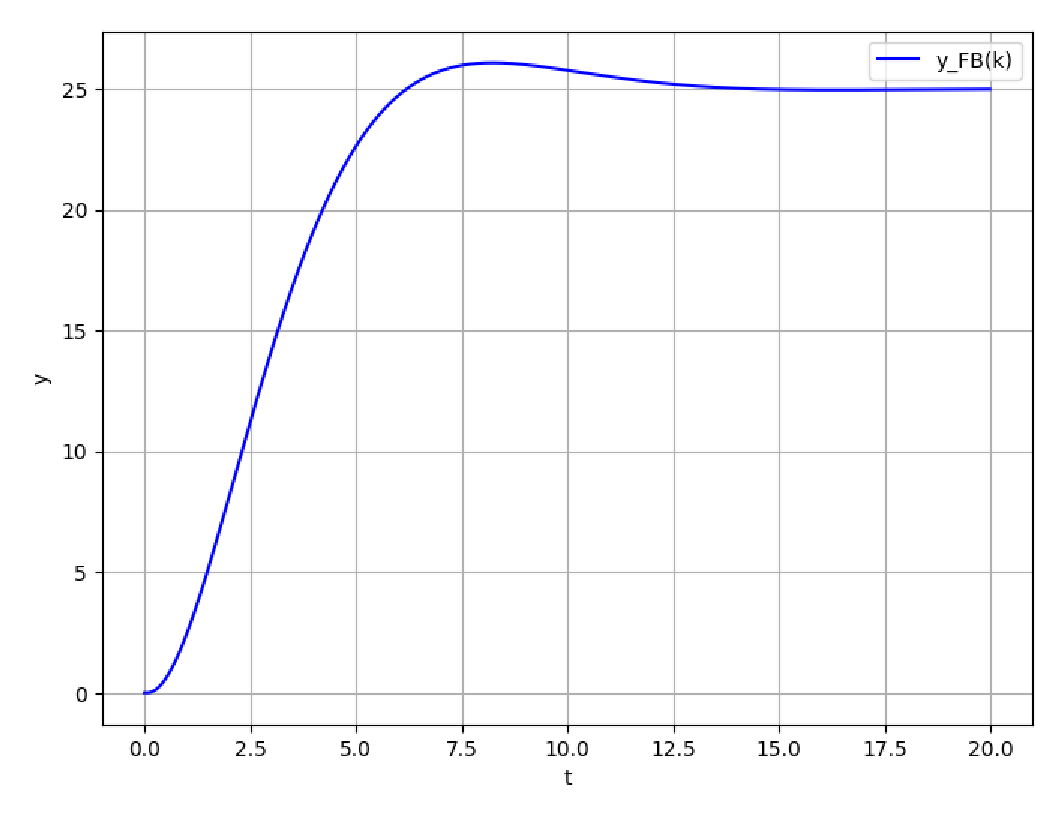
\includegraphics[scale=0.35]{figure17.eps}
    \caption{ボールの位置のシミュレーション結果}
    \label{fig:figure20}
  \end{minipage}
  \begin{minipage}[h]{0.4\linewidth}
    \centering
    \scalebox{0.7}[0.7]{
\begin{tikzpicture}[gnuplot]
%% generated with GNUPLOT 5.4p10 (Lua 5.4; terminal rev. Jun 2020, script rev. 118)
%% Mon Dec 11 22:16:44 2023
\path (0.000,0.000) rectangle (12.500,8.750);
\gpcolor{color=gp lt color border}
\gpsetlinetype{gp lt border}
\gpsetdashtype{gp dt solid}
\gpsetlinewidth{1.00}
\draw[gp path] (0.018,0.031)--(0.198,0.031);
\draw[gp path] (12.480,0.031)--(12.300,0.031);
\node[gp node right] at (-0.166,0.031) {$1.44$};
\draw[gp path] (0.018,0.996)--(0.198,0.996);
\draw[gp path] (12.480,0.996)--(12.300,0.996);
\node[gp node right] at (-0.166,0.996) {$1.46$};
\draw[gp path] (0.018,1.961)--(0.198,1.961);
\draw[gp path] (12.480,1.961)--(12.300,1.961);
\node[gp node right] at (-0.166,1.961) {$1.48$};
\draw[gp path] (0.018,2.927)--(0.198,2.927);
\draw[gp path] (12.480,2.927)--(12.300,2.927);
\node[gp node right] at (-0.166,2.927) {$1.5$};
\draw[gp path] (0.018,3.892)--(0.198,3.892);
\draw[gp path] (12.480,3.892)--(12.300,3.892);
\node[gp node right] at (-0.166,3.892) {$1.52$};
\draw[gp path] (0.018,4.857)--(0.198,4.857);
\draw[gp path] (12.480,4.857)--(12.300,4.857);
\node[gp node right] at (-0.166,4.857) {$1.54$};
\draw[gp path] (0.018,5.822)--(0.198,5.822);
\draw[gp path] (12.480,5.822)--(12.300,5.822);
\node[gp node right] at (-0.166,5.822) {$1.56$};
\draw[gp path] (0.018,6.788)--(0.198,6.788);
\draw[gp path] (12.480,6.788)--(12.300,6.788);
\node[gp node right] at (-0.166,6.788) {$1.58$};
\draw[gp path] (0.018,7.753)--(0.198,7.753);
\draw[gp path] (12.480,7.753)--(12.300,7.753);
\node[gp node right] at (-0.166,7.753) {$1.6$};
\draw[gp path] (0.018,8.718)--(0.198,8.718);
\draw[gp path] (12.480,8.718)--(12.300,8.718);
\node[gp node right] at (-0.166,8.718) {$1.62$};
\draw[gp path] (0.018,0.031)--(0.018,0.211);
\draw[gp path] (0.018,8.718)--(0.018,8.538);
\node[gp node center] at (0.018,-0.277) {$-100$};
\draw[gp path] (3.134,0.031)--(3.134,0.211);
\draw[gp path] (3.134,8.718)--(3.134,8.538);
\node[gp node center] at (3.134,-0.277) {$-50$};
\draw[gp path] (6.249,0.031)--(6.249,0.211);
\draw[gp path] (6.249,8.718)--(6.249,8.538);
\node[gp node center] at (6.249,-0.277) {$0$};
\draw[gp path] (9.365,0.031)--(9.365,0.211);
\draw[gp path] (9.365,8.718)--(9.365,8.538);
\node[gp node center] at (9.365,-0.277) {$50$};
\draw[gp path] (12.480,0.031)--(12.480,0.211);
\draw[gp path] (12.480,8.718)--(12.480,8.538);
\node[gp node center] at (12.480,-0.277) {$100$};
\draw[gp path] (0.018,8.718)--(0.018,0.031)--(12.480,0.031)--(12.480,8.718)--cycle;
\node[gp node center,rotate=-270,font={\fontsize{17.0pt}{20.4pt}\selectfont}] at (-1.470,4.374) {屈折率$n(r)$};
\node[gp node center,font={\fontsize{17.0pt}{20.4pt}\selectfont}] at (6.249,-1.046) {中心からの距離$r\ /\ \mathrm{\upmu m}$};
\gpcolor{rgb color={0.000,0.000,0.000}}
\draw[gp path] (0.018,1.022)--(0.087,1.010)--(0.179,1.012)--(0.271,0.990)--(0.363,1.024)%
  --(0.455,1.008)--(0.547,1.010)--(0.639,1.020)--(0.731,1.002)--(0.823,1.026)--(0.915,1.018)%
  --(1.007,1.006)--(1.099,0.996)--(1.191,0.992)--(1.283,1.026)--(1.375,0.994)--(1.467,1.014)%
  --(1.559,1.022)--(1.651,1.022)--(1.742,1.006)--(1.834,1.034)--(1.926,1.016)--(2.018,1.024)%
  --(2.110,1.006)--(2.202,1.032)--(2.294,1.012)--(2.386,1.012)--(2.478,1.018)--(2.570,1.006)%
  --(2.662,1.036)--(2.754,1.024)--(2.846,1.028)--(2.938,1.010)--(3.030,1.042)--(3.122,1.026)%
  --(3.214,0.998)--(3.306,1.020)--(3.398,1.044)--(3.490,1.026)--(3.582,1.026)--(3.674,1.016)%
  --(3.766,1.048)--(3.858,1.024)--(3.950,1.058)--(4.042,1.054)--(4.134,1.054)--(4.226,1.094)%
  --(4.318,1.148)--(4.410,1.206)--(4.502,1.321)--(4.594,1.564)--(4.686,1.878)--(4.777,2.358)%
  --(4.869,3.190)--(4.961,4.167)--(5.053,4.969)--(5.145,5.730)--(5.237,6.189)--(5.329,6.787)%
  --(5.421,7.126)--(5.513,7.635)--(5.605,7.812)--(5.697,8.110)--(5.789,8.199)--(5.881,8.319)%
  --(5.973,8.478)--(6.065,8.462)--(6.157,8.413)--(6.249,8.660)--(6.341,8.640)--(6.433,8.564)%
  --(6.525,8.522)--(6.617,8.496)--(6.709,8.445)--(6.801,8.259)--(6.893,7.880)--(6.985,7.585)%
  --(7.077,7.025)--(7.169,6.299)--(7.261,5.441)--(7.353,4.550)--(7.445,3.493)--(7.537,2.733)%
  --(7.629,2.145)--(7.721,1.826)--(7.812,1.580)--(7.904,1.379)--(7.996,1.273)--(8.088,1.170)%
  --(8.180,1.132)--(8.272,1.088)--(8.364,1.076)--(8.456,1.044)--(8.548,1.040)--(8.640,1.006)%
  --(8.732,1.044)--(8.824,1.054)--(8.916,1.008)--(9.008,1.012)--(9.100,1.022)--(9.192,1.030)%
  --(9.284,1.020)--(9.376,1.004)--(9.468,1.018)--(9.560,1.022)--(9.652,0.988)--(9.744,1.020)%
  --(9.836,1.004)--(9.928,1.020)--(10.020,1.014)--(10.112,1.008)--(10.204,1.004)--(10.296,1.020)%
  --(10.388,1.028)--(10.480,1.024)--(10.572,1.020)--(10.664,1.016)--(10.756,1.024)--(10.847,1.002)%
  --(10.939,1.022)--(11.031,1.004)--(11.123,1.018)--(11.215,1.036)--(11.307,1.018)--(11.399,1.006)%
  --(11.491,1.022)--(11.583,1.000)--(11.675,1.010)--(11.767,1.014)--(11.859,1.010)--(11.951,1.000)%
  --(12.043,1.014)--(12.135,1.020)--(12.227,1.002)--(12.319,1.026)--(12.411,1.008)--(12.480,1.015);
\gpsetpointsize{1.20}
\gp3point{gp mark 7}{}{(0.087,1.010)}
\gp3point{gp mark 7}{}{(0.179,1.012)}
\gp3point{gp mark 7}{}{(0.271,0.990)}
\gp3point{gp mark 7}{}{(0.363,1.024)}
\gp3point{gp mark 7}{}{(0.455,1.008)}
\gp3point{gp mark 7}{}{(0.547,1.010)}
\gp3point{gp mark 7}{}{(0.639,1.020)}
\gp3point{gp mark 7}{}{(0.731,1.002)}
\gp3point{gp mark 7}{}{(0.823,1.026)}
\gp3point{gp mark 7}{}{(0.915,1.018)}
\gp3point{gp mark 7}{}{(1.007,1.006)}
\gp3point{gp mark 7}{}{(1.099,0.996)}
\gp3point{gp mark 7}{}{(1.191,0.992)}
\gp3point{gp mark 7}{}{(1.283,1.026)}
\gp3point{gp mark 7}{}{(1.375,0.994)}
\gp3point{gp mark 7}{}{(1.467,1.014)}
\gp3point{gp mark 7}{}{(1.559,1.022)}
\gp3point{gp mark 7}{}{(1.651,1.022)}
\gp3point{gp mark 7}{}{(1.742,1.006)}
\gp3point{gp mark 7}{}{(1.834,1.034)}
\gp3point{gp mark 7}{}{(1.926,1.016)}
\gp3point{gp mark 7}{}{(2.018,1.024)}
\gp3point{gp mark 7}{}{(2.110,1.006)}
\gp3point{gp mark 7}{}{(2.202,1.032)}
\gp3point{gp mark 7}{}{(2.294,1.012)}
\gp3point{gp mark 7}{}{(2.386,1.012)}
\gp3point{gp mark 7}{}{(2.478,1.018)}
\gp3point{gp mark 7}{}{(2.570,1.006)}
\gp3point{gp mark 7}{}{(2.662,1.036)}
\gp3point{gp mark 7}{}{(2.754,1.024)}
\gp3point{gp mark 7}{}{(2.846,1.028)}
\gp3point{gp mark 7}{}{(2.938,1.010)}
\gp3point{gp mark 7}{}{(3.030,1.042)}
\gp3point{gp mark 7}{}{(3.122,1.026)}
\gp3point{gp mark 7}{}{(3.214,0.998)}
\gp3point{gp mark 7}{}{(3.306,1.020)}
\gp3point{gp mark 7}{}{(3.398,1.044)}
\gp3point{gp mark 7}{}{(3.490,1.026)}
\gp3point{gp mark 7}{}{(3.582,1.026)}
\gp3point{gp mark 7}{}{(3.674,1.016)}
\gp3point{gp mark 7}{}{(3.766,1.048)}
\gp3point{gp mark 7}{}{(3.858,1.024)}
\gp3point{gp mark 7}{}{(3.950,1.058)}
\gp3point{gp mark 7}{}{(4.042,1.054)}
\gp3point{gp mark 7}{}{(4.134,1.054)}
\gp3point{gp mark 7}{}{(4.226,1.094)}
\gp3point{gp mark 7}{}{(4.318,1.148)}
\gp3point{gp mark 7}{}{(4.410,1.206)}
\gp3point{gp mark 7}{}{(4.502,1.321)}
\gp3point{gp mark 7}{}{(4.594,1.564)}
\gp3point{gp mark 7}{}{(4.686,1.878)}
\gp3point{gp mark 7}{}{(4.777,2.358)}
\gp3point{gp mark 7}{}{(4.869,3.190)}
\gp3point{gp mark 7}{}{(4.961,4.167)}
\gp3point{gp mark 7}{}{(5.053,4.969)}
\gp3point{gp mark 7}{}{(5.145,5.730)}
\gp3point{gp mark 7}{}{(5.237,6.189)}
\gp3point{gp mark 7}{}{(5.329,6.787)}
\gp3point{gp mark 7}{}{(5.421,7.126)}
\gp3point{gp mark 7}{}{(5.513,7.635)}
\gp3point{gp mark 7}{}{(5.605,7.812)}
\gp3point{gp mark 7}{}{(5.697,8.110)}
\gp3point{gp mark 7}{}{(5.789,8.199)}
\gp3point{gp mark 7}{}{(5.881,8.319)}
\gp3point{gp mark 7}{}{(5.973,8.478)}
\gp3point{gp mark 7}{}{(6.065,8.462)}
\gp3point{gp mark 7}{}{(6.157,8.413)}
\gp3point{gp mark 7}{}{(6.249,8.660)}
\gp3point{gp mark 7}{}{(6.341,8.640)}
\gp3point{gp mark 7}{}{(6.433,8.564)}
\gp3point{gp mark 7}{}{(6.525,8.522)}
\gp3point{gp mark 7}{}{(6.617,8.496)}
\gp3point{gp mark 7}{}{(6.709,8.445)}
\gp3point{gp mark 7}{}{(6.801,8.259)}
\gp3point{gp mark 7}{}{(6.893,7.880)}
\gp3point{gp mark 7}{}{(6.985,7.585)}
\gp3point{gp mark 7}{}{(7.077,7.025)}
\gp3point{gp mark 7}{}{(7.169,6.299)}
\gp3point{gp mark 7}{}{(7.261,5.441)}
\gp3point{gp mark 7}{}{(7.353,4.550)}
\gp3point{gp mark 7}{}{(7.445,3.493)}
\gp3point{gp mark 7}{}{(7.537,2.733)}
\gp3point{gp mark 7}{}{(7.629,2.145)}
\gp3point{gp mark 7}{}{(7.721,1.826)}
\gp3point{gp mark 7}{}{(7.812,1.580)}
\gp3point{gp mark 7}{}{(7.904,1.379)}
\gp3point{gp mark 7}{}{(7.996,1.273)}
\gp3point{gp mark 7}{}{(8.088,1.170)}
\gp3point{gp mark 7}{}{(8.180,1.132)}
\gp3point{gp mark 7}{}{(8.272,1.088)}
\gp3point{gp mark 7}{}{(8.364,1.076)}
\gp3point{gp mark 7}{}{(8.456,1.044)}
\gp3point{gp mark 7}{}{(8.548,1.040)}
\gp3point{gp mark 7}{}{(8.640,1.006)}
\gp3point{gp mark 7}{}{(8.732,1.044)}
\gp3point{gp mark 7}{}{(8.824,1.054)}
\gp3point{gp mark 7}{}{(8.916,1.008)}
\gp3point{gp mark 7}{}{(9.008,1.012)}
\gp3point{gp mark 7}{}{(9.100,1.022)}
\gp3point{gp mark 7}{}{(9.192,1.030)}
\gp3point{gp mark 7}{}{(9.284,1.020)}
\gp3point{gp mark 7}{}{(9.376,1.004)}
\gp3point{gp mark 7}{}{(9.468,1.018)}
\gp3point{gp mark 7}{}{(9.560,1.022)}
\gp3point{gp mark 7}{}{(9.652,0.988)}
\gp3point{gp mark 7}{}{(9.744,1.020)}
\gp3point{gp mark 7}{}{(9.836,1.004)}
\gp3point{gp mark 7}{}{(9.928,1.020)}
\gp3point{gp mark 7}{}{(10.020,1.014)}
\gp3point{gp mark 7}{}{(10.112,1.008)}
\gp3point{gp mark 7}{}{(10.204,1.004)}
\gp3point{gp mark 7}{}{(10.296,1.020)}
\gp3point{gp mark 7}{}{(10.388,1.028)}
\gp3point{gp mark 7}{}{(10.480,1.024)}
\gp3point{gp mark 7}{}{(10.572,1.020)}
\gp3point{gp mark 7}{}{(10.664,1.016)}
\gp3point{gp mark 7}{}{(10.756,1.024)}
\gp3point{gp mark 7}{}{(10.847,1.002)}
\gp3point{gp mark 7}{}{(10.939,1.022)}
\gp3point{gp mark 7}{}{(11.031,1.004)}
\gp3point{gp mark 7}{}{(11.123,1.018)}
\gp3point{gp mark 7}{}{(11.215,1.036)}
\gp3point{gp mark 7}{}{(11.307,1.018)}
\gp3point{gp mark 7}{}{(11.399,1.006)}
\gp3point{gp mark 7}{}{(11.491,1.022)}
\gp3point{gp mark 7}{}{(11.583,1.000)}
\gp3point{gp mark 7}{}{(11.675,1.010)}
\gp3point{gp mark 7}{}{(11.767,1.014)}
\gp3point{gp mark 7}{}{(11.859,1.010)}
\gp3point{gp mark 7}{}{(11.951,1.000)}
\gp3point{gp mark 7}{}{(12.043,1.014)}
\gp3point{gp mark 7}{}{(12.135,1.020)}
\gp3point{gp mark 7}{}{(12.227,1.002)}
\gp3point{gp mark 7}{}{(12.319,1.026)}
\gp3point{gp mark 7}{}{(12.411,1.008)}
\gpcolor{color=gp lt color border}
\draw[gp path] (0.018,8.718)--(0.018,0.031)--(12.480,0.031)--(12.480,8.718)--cycle;
%% coordinates of the plot area
\gpdefrectangularnode{gp plot 1}{\pgfpoint{0.018cm}{0.031cm}}{\pgfpoint{12.480cm}{8.718cm}}
\end{tikzpicture}
}

    \vspace{-30pt}\caption{ボールの位置の時間変化}
    \label{fig:figure21}
  \end{minipage}
  \begin{minipage}[h]{0.4\linewidth}
    \centering
    \scalebox{0.7}[0.7]{
\begin{tikzpicture}[gnuplot]
%% generated with GNUPLOT 5.4p10 (Lua 5.4; terminal rev. Jun 2020, script rev. 118)
%% Mon Dec 11 22:23:16 2023
\path (0.000,0.000) rectangle (12.500,8.750);
\gpcolor{color=gp lt color border}
\gpsetlinetype{gp lt border}
\gpsetdashtype{gp dt solid}
\gpsetlinewidth{1.00}
\draw[gp path] (0.018,0.031)--(0.198,0.031);
\draw[gp path] (12.480,0.031)--(12.300,0.031);
\node[gp node right] at (-0.166,0.031) {$1.46$};
\draw[gp path] (0.018,1.117)--(0.198,1.117);
\draw[gp path] (12.480,1.117)--(12.300,1.117);
\node[gp node right] at (-0.166,1.117) {$1.48$};
\draw[gp path] (0.018,2.203)--(0.198,2.203);
\draw[gp path] (12.480,2.203)--(12.300,2.203);
\node[gp node right] at (-0.166,2.203) {$1.5$};
\draw[gp path] (0.018,3.289)--(0.198,3.289);
\draw[gp path] (12.480,3.289)--(12.300,3.289);
\node[gp node right] at (-0.166,3.289) {$1.52$};
\draw[gp path] (0.018,4.375)--(0.198,4.375);
\draw[gp path] (12.480,4.375)--(12.300,4.375);
\node[gp node right] at (-0.166,4.375) {$1.54$};
\draw[gp path] (0.018,5.460)--(0.198,5.460);
\draw[gp path] (12.480,5.460)--(12.300,5.460);
\node[gp node right] at (-0.166,5.460) {$1.56$};
\draw[gp path] (0.018,6.546)--(0.198,6.546);
\draw[gp path] (12.480,6.546)--(12.300,6.546);
\node[gp node right] at (-0.166,6.546) {$1.58$};
\draw[gp path] (0.018,7.632)--(0.198,7.632);
\draw[gp path] (12.480,7.632)--(12.300,7.632);
\node[gp node right] at (-0.166,7.632) {$1.6$};
\draw[gp path] (0.018,8.718)--(0.198,8.718);
\draw[gp path] (12.480,8.718)--(12.300,8.718);
\node[gp node right] at (-0.166,8.718) {$1.62$};
\draw[gp path] (0.018,0.031)--(0.018,0.211);
\draw[gp path] (0.018,8.718)--(0.018,8.538);
\node[gp node center] at (0.018,-0.277) {$-150$};
\draw[gp path] (2.095,0.031)--(2.095,0.211);
\draw[gp path] (2.095,8.718)--(2.095,8.538);
\node[gp node center] at (2.095,-0.277) {$-100$};
\draw[gp path] (4.172,0.031)--(4.172,0.211);
\draw[gp path] (4.172,8.718)--(4.172,8.538);
\node[gp node center] at (4.172,-0.277) {$-50$};
\draw[gp path] (6.249,0.031)--(6.249,0.211);
\draw[gp path] (6.249,8.718)--(6.249,8.538);
\node[gp node center] at (6.249,-0.277) {$0$};
\draw[gp path] (8.326,0.031)--(8.326,0.211);
\draw[gp path] (8.326,8.718)--(8.326,8.538);
\node[gp node center] at (8.326,-0.277) {$50$};
\draw[gp path] (10.403,0.031)--(10.403,0.211);
\draw[gp path] (10.403,8.718)--(10.403,8.538);
\node[gp node center] at (10.403,-0.277) {$100$};
\draw[gp path] (12.480,0.031)--(12.480,0.211);
\draw[gp path] (12.480,8.718)--(12.480,8.538);
\node[gp node center] at (12.480,-0.277) {$150$};
\draw[gp path] (0.018,8.718)--(0.018,0.031)--(12.480,0.031)--(12.480,8.718)--cycle;
\node[gp node center,rotate=-270,font={\fontsize{17.0pt}{20.4pt}\selectfont}] at (-1.470,4.374) {屈折率$n(r)$};
\node[gp node center,font={\fontsize{17.0pt}{20.4pt}\selectfont}] at (6.249,-1.046) {中心からの距離$r\ /\ \mathrm{\upmu m}$};
\gpcolor{rgb color={0.000,0.000,0.000}}
\draw[gp path] (0.018,0.255)--(0.056,0.287)--(0.118,0.282)--(0.179,0.273)--(0.240,0.304)%
  --(0.302,0.247)--(0.363,0.287)--(0.424,0.335)--(0.486,0.287)--(0.547,0.278)--(0.608,0.295)%
  --(0.670,0.331)--(0.731,0.300)--(0.792,0.278)--(0.853,0.273)--(0.915,0.247)--(0.976,0.243)%
  --(1.037,0.326)--(1.099,0.243)--(1.160,0.282)--(1.221,0.260)--(1.283,0.313)--(1.344,0.340)%
  --(1.405,0.278)--(1.467,0.317)--(1.528,0.273)--(1.589,0.313)--(1.651,0.344)--(1.712,0.326)%
  --(1.773,0.295)--(1.834,0.295)--(1.896,0.313)--(1.957,0.375)--(2.018,0.335)--(2.080,0.375)%
  --(2.141,0.375)--(2.202,0.366)--(2.264,0.357)--(2.325,0.414)--(2.386,0.480)--(2.448,0.533)%
  --(2.509,0.617)--(2.570,0.683)--(2.632,0.802)--(2.693,1.014)--(2.754,1.353)--(2.815,1.732)%
  --(2.877,2.529)--(2.938,3.177)--(2.999,3.459)--(3.061,3.860)--(3.122,4.335)--(3.183,5.172)%
  --(3.245,5.644)--(3.306,6.093)--(3.367,6.318)--(3.429,6.943)--(3.490,7.177)--(3.551,7.239)%
  --(3.613,7.507)--(3.674,7.644)--(3.735,7.485)--(3.796,7.736)--(3.858,7.754)--(3.919,7.939)%
  --(3.980,7.899)--(4.042,8.032)--(4.103,8.093)--(4.164,7.970)--(4.226,7.847)--(4.287,8.181)%
  --(4.348,7.877)--(4.410,7.996)--(4.471,8.040)--(4.532,8.212)--(4.594,7.781)--(4.655,8.221)%
  --(4.716,8.243)--(4.777,8.190)--(4.839,8.005)--(4.900,8.010)--(4.961,8.001)--(5.023,8.137)%
  --(5.084,8.102)--(5.145,8.327)--(5.207,8.151)--(5.268,8.195)--(5.329,8.256)--(5.391,8.093)%
  --(5.452,8.441)--(5.513,8.419)--(5.575,8.512)--(5.636,8.331)--(5.697,8.252)--(5.758,8.234)%
  --(5.820,8.344)--(5.881,8.181)--(5.942,8.159)--(6.004,8.287)--(6.065,8.415)--(6.126,8.384)%
  --(6.188,8.503)--(6.249,8.653)--(6.310,8.569)--(6.372,8.393)--(6.433,8.309)--(6.494,8.375)%
  --(6.556,8.446)--(6.617,8.441)--(6.678,8.327)--(6.740,8.389)--(6.801,8.419)--(6.862,8.468)%
  --(6.923,8.626)--(6.985,8.534)--(7.046,8.507)--(7.107,8.248)--(7.169,8.362)--(7.230,8.433)%
  --(7.291,8.450)--(7.353,8.283)--(7.414,8.578)--(7.475,8.212)--(7.537,8.371)--(7.598,8.468)%
  --(7.659,8.265)--(7.721,8.384)--(7.782,8.234)--(7.843,8.129)--(7.904,8.305)--(7.966,8.305)%
  --(8.027,8.274)--(8.088,8.168)--(8.150,8.296)--(8.211,8.190)--(8.272,8.120)--(8.334,8.155)%
  --(8.395,7.983)--(8.456,8.036)--(8.518,8.393)--(8.579,7.842)--(8.640,8.107)--(8.702,8.001)%
  --(8.763,7.944)--(8.824,8.133)--(8.885,8.212)--(8.947,8.089)--(9.008,7.895)--(9.069,8.278)%
  --(9.131,8.085)--(9.192,8.173)--(9.253,8.014)--(9.315,7.961)--(9.376,7.957)--(9.437,7.873)%
  --(9.499,7.750)--(9.560,8.102)--(9.621,7.833)--(9.683,7.754)--(9.744,7.551)--(9.805,7.195)%
  --(9.866,7.243)--(9.928,7.018)--(9.989,6.816)--(10.050,6.503)--(10.112,6.424)--(10.173,5.675)%
  --(10.234,5.349)--(10.296,4.688)--(10.357,3.494)--(10.418,2.419)--(10.480,1.890)--(10.541,1.463)%
  --(10.602,1.225)--(10.664,0.877)--(10.725,0.829)--(10.786,0.670)--(10.847,0.674)--(10.909,0.516)%
  --(10.970,0.454)--(11.031,0.414)--(11.093,0.344)--(11.154,0.370)--(11.215,0.370)--(11.277,0.348)%
  --(11.338,0.344)--(11.399,0.340)--(11.461,0.287)--(11.522,0.348)--(11.583,0.300)--(11.645,0.269)%
  --(11.706,0.282)--(11.767,0.295)--(11.828,0.317)--(11.890,0.353)--(11.951,0.326)--(12.012,0.265)%
  --(12.074,0.353)--(12.135,0.335)--(12.196,0.362)--(12.258,0.291)--(12.319,0.247)--(12.380,0.291)%
  --(12.442,0.269)--(12.480,0.315);
\gpsetpointsize{1.20}
\gp3point{gp mark 7}{}{(0.056,0.287)}
\gp3point{gp mark 7}{}{(0.118,0.282)}
\gp3point{gp mark 7}{}{(0.179,0.273)}
\gp3point{gp mark 7}{}{(0.240,0.304)}
\gp3point{gp mark 7}{}{(0.302,0.247)}
\gp3point{gp mark 7}{}{(0.363,0.287)}
\gp3point{gp mark 7}{}{(0.424,0.335)}
\gp3point{gp mark 7}{}{(0.486,0.287)}
\gp3point{gp mark 7}{}{(0.547,0.278)}
\gp3point{gp mark 7}{}{(0.608,0.295)}
\gp3point{gp mark 7}{}{(0.670,0.331)}
\gp3point{gp mark 7}{}{(0.731,0.300)}
\gp3point{gp mark 7}{}{(0.792,0.278)}
\gp3point{gp mark 7}{}{(0.853,0.273)}
\gp3point{gp mark 7}{}{(0.915,0.247)}
\gp3point{gp mark 7}{}{(0.976,0.243)}
\gp3point{gp mark 7}{}{(1.037,0.326)}
\gp3point{gp mark 7}{}{(1.099,0.243)}
\gp3point{gp mark 7}{}{(1.160,0.282)}
\gp3point{gp mark 7}{}{(1.221,0.260)}
\gp3point{gp mark 7}{}{(1.283,0.313)}
\gp3point{gp mark 7}{}{(1.344,0.340)}
\gp3point{gp mark 7}{}{(1.405,0.278)}
\gp3point{gp mark 7}{}{(1.467,0.317)}
\gp3point{gp mark 7}{}{(1.528,0.273)}
\gp3point{gp mark 7}{}{(1.589,0.313)}
\gp3point{gp mark 7}{}{(1.651,0.344)}
\gp3point{gp mark 7}{}{(1.712,0.326)}
\gp3point{gp mark 7}{}{(1.773,0.295)}
\gp3point{gp mark 7}{}{(1.834,0.295)}
\gp3point{gp mark 7}{}{(1.896,0.313)}
\gp3point{gp mark 7}{}{(1.957,0.375)}
\gp3point{gp mark 7}{}{(2.018,0.335)}
\gp3point{gp mark 7}{}{(2.080,0.375)}
\gp3point{gp mark 7}{}{(2.141,0.375)}
\gp3point{gp mark 7}{}{(2.202,0.366)}
\gp3point{gp mark 7}{}{(2.264,0.357)}
\gp3point{gp mark 7}{}{(2.325,0.414)}
\gp3point{gp mark 7}{}{(2.386,0.480)}
\gp3point{gp mark 7}{}{(2.448,0.533)}
\gp3point{gp mark 7}{}{(2.509,0.617)}
\gp3point{gp mark 7}{}{(2.570,0.683)}
\gp3point{gp mark 7}{}{(2.632,0.802)}
\gp3point{gp mark 7}{}{(2.693,1.014)}
\gp3point{gp mark 7}{}{(2.754,1.353)}
\gp3point{gp mark 7}{}{(2.815,1.732)}
\gp3point{gp mark 7}{}{(2.877,2.529)}
\gp3point{gp mark 7}{}{(2.938,3.177)}
\gp3point{gp mark 7}{}{(2.999,3.459)}
\gp3point{gp mark 7}{}{(3.061,3.860)}
\gp3point{gp mark 7}{}{(3.122,4.335)}
\gp3point{gp mark 7}{}{(3.183,5.172)}
\gp3point{gp mark 7}{}{(3.245,5.644)}
\gp3point{gp mark 7}{}{(3.306,6.093)}
\gp3point{gp mark 7}{}{(3.367,6.318)}
\gp3point{gp mark 7}{}{(3.429,6.943)}
\gp3point{gp mark 7}{}{(3.490,7.177)}
\gp3point{gp mark 7}{}{(3.551,7.239)}
\gp3point{gp mark 7}{}{(3.613,7.507)}
\gp3point{gp mark 7}{}{(3.674,7.644)}
\gp3point{gp mark 7}{}{(3.735,7.485)}
\gp3point{gp mark 7}{}{(3.796,7.736)}
\gp3point{gp mark 7}{}{(3.858,7.754)}
\gp3point{gp mark 7}{}{(3.919,7.939)}
\gp3point{gp mark 7}{}{(3.980,7.899)}
\gp3point{gp mark 7}{}{(4.042,8.032)}
\gp3point{gp mark 7}{}{(4.103,8.093)}
\gp3point{gp mark 7}{}{(4.164,7.970)}
\gp3point{gp mark 7}{}{(4.226,7.847)}
\gp3point{gp mark 7}{}{(4.287,8.181)}
\gp3point{gp mark 7}{}{(4.348,7.877)}
\gp3point{gp mark 7}{}{(4.410,7.996)}
\gp3point{gp mark 7}{}{(4.471,8.040)}
\gp3point{gp mark 7}{}{(4.532,8.212)}
\gp3point{gp mark 7}{}{(4.594,7.781)}
\gp3point{gp mark 7}{}{(4.655,8.221)}
\gp3point{gp mark 7}{}{(4.716,8.243)}
\gp3point{gp mark 7}{}{(4.777,8.190)}
\gp3point{gp mark 7}{}{(4.839,8.005)}
\gp3point{gp mark 7}{}{(4.900,8.010)}
\gp3point{gp mark 7}{}{(4.961,8.001)}
\gp3point{gp mark 7}{}{(5.023,8.137)}
\gp3point{gp mark 7}{}{(5.084,8.102)}
\gp3point{gp mark 7}{}{(5.145,8.327)}
\gp3point{gp mark 7}{}{(5.207,8.151)}
\gp3point{gp mark 7}{}{(5.268,8.195)}
\gp3point{gp mark 7}{}{(5.329,8.256)}
\gp3point{gp mark 7}{}{(5.391,8.093)}
\gp3point{gp mark 7}{}{(5.452,8.441)}
\gp3point{gp mark 7}{}{(5.513,8.419)}
\gp3point{gp mark 7}{}{(5.575,8.512)}
\gp3point{gp mark 7}{}{(5.636,8.331)}
\gp3point{gp mark 7}{}{(5.697,8.252)}
\gp3point{gp mark 7}{}{(5.758,8.234)}
\gp3point{gp mark 7}{}{(5.820,8.344)}
\gp3point{gp mark 7}{}{(5.881,8.181)}
\gp3point{gp mark 7}{}{(5.942,8.159)}
\gp3point{gp mark 7}{}{(6.004,8.287)}
\gp3point{gp mark 7}{}{(6.065,8.415)}
\gp3point{gp mark 7}{}{(6.126,8.384)}
\gp3point{gp mark 7}{}{(6.188,8.503)}
\gp3point{gp mark 7}{}{(6.249,8.653)}
\gp3point{gp mark 7}{}{(6.310,8.569)}
\gp3point{gp mark 7}{}{(6.372,8.393)}
\gp3point{gp mark 7}{}{(6.433,8.309)}
\gp3point{gp mark 7}{}{(6.494,8.375)}
\gp3point{gp mark 7}{}{(6.556,8.446)}
\gp3point{gp mark 7}{}{(6.617,8.441)}
\gp3point{gp mark 7}{}{(6.678,8.327)}
\gp3point{gp mark 7}{}{(6.740,8.389)}
\gp3point{gp mark 7}{}{(6.801,8.419)}
\gp3point{gp mark 7}{}{(6.862,8.468)}
\gp3point{gp mark 7}{}{(6.923,8.626)}
\gp3point{gp mark 7}{}{(6.985,8.534)}
\gp3point{gp mark 7}{}{(7.046,8.507)}
\gp3point{gp mark 7}{}{(7.107,8.248)}
\gp3point{gp mark 7}{}{(7.169,8.362)}
\gp3point{gp mark 7}{}{(7.230,8.433)}
\gp3point{gp mark 7}{}{(7.291,8.450)}
\gp3point{gp mark 7}{}{(7.353,8.283)}
\gp3point{gp mark 7}{}{(7.414,8.578)}
\gp3point{gp mark 7}{}{(7.475,8.212)}
\gp3point{gp mark 7}{}{(7.537,8.371)}
\gp3point{gp mark 7}{}{(7.598,8.468)}
\gp3point{gp mark 7}{}{(7.659,8.265)}
\gp3point{gp mark 7}{}{(7.721,8.384)}
\gp3point{gp mark 7}{}{(7.782,8.234)}
\gp3point{gp mark 7}{}{(7.843,8.129)}
\gp3point{gp mark 7}{}{(7.904,8.305)}
\gp3point{gp mark 7}{}{(7.966,8.305)}
\gp3point{gp mark 7}{}{(8.027,8.274)}
\gp3point{gp mark 7}{}{(8.088,8.168)}
\gp3point{gp mark 7}{}{(8.150,8.296)}
\gp3point{gp mark 7}{}{(8.211,8.190)}
\gp3point{gp mark 7}{}{(8.272,8.120)}
\gp3point{gp mark 7}{}{(8.334,8.155)}
\gp3point{gp mark 7}{}{(8.395,7.983)}
\gp3point{gp mark 7}{}{(8.456,8.036)}
\gp3point{gp mark 7}{}{(8.518,8.393)}
\gp3point{gp mark 7}{}{(8.579,7.842)}
\gp3point{gp mark 7}{}{(8.640,8.107)}
\gp3point{gp mark 7}{}{(8.702,8.001)}
\gp3point{gp mark 7}{}{(8.763,7.944)}
\gp3point{gp mark 7}{}{(8.824,8.133)}
\gp3point{gp mark 7}{}{(8.885,8.212)}
\gp3point{gp mark 7}{}{(8.947,8.089)}
\gp3point{gp mark 7}{}{(9.008,7.895)}
\gp3point{gp mark 7}{}{(9.069,8.278)}
\gp3point{gp mark 7}{}{(9.131,8.085)}
\gp3point{gp mark 7}{}{(9.192,8.173)}
\gp3point{gp mark 7}{}{(9.253,8.014)}
\gp3point{gp mark 7}{}{(9.315,7.961)}
\gp3point{gp mark 7}{}{(9.376,7.957)}
\gp3point{gp mark 7}{}{(9.437,7.873)}
\gp3point{gp mark 7}{}{(9.499,7.750)}
\gp3point{gp mark 7}{}{(9.560,8.102)}
\gp3point{gp mark 7}{}{(9.621,7.833)}
\gp3point{gp mark 7}{}{(9.683,7.754)}
\gp3point{gp mark 7}{}{(9.744,7.551)}
\gp3point{gp mark 7}{}{(9.805,7.195)}
\gp3point{gp mark 7}{}{(9.866,7.243)}
\gp3point{gp mark 7}{}{(9.928,7.018)}
\gp3point{gp mark 7}{}{(9.989,6.816)}
\gp3point{gp mark 7}{}{(10.050,6.503)}
\gp3point{gp mark 7}{}{(10.112,6.424)}
\gp3point{gp mark 7}{}{(10.173,5.675)}
\gp3point{gp mark 7}{}{(10.234,5.349)}
\gp3point{gp mark 7}{}{(10.296,4.688)}
\gp3point{gp mark 7}{}{(10.357,3.494)}
\gp3point{gp mark 7}{}{(10.418,2.419)}
\gp3point{gp mark 7}{}{(10.480,1.890)}
\gp3point{gp mark 7}{}{(10.541,1.463)}
\gp3point{gp mark 7}{}{(10.602,1.225)}
\gp3point{gp mark 7}{}{(10.664,0.877)}
\gp3point{gp mark 7}{}{(10.725,0.829)}
\gp3point{gp mark 7}{}{(10.786,0.670)}
\gp3point{gp mark 7}{}{(10.847,0.674)}
\gp3point{gp mark 7}{}{(10.909,0.516)}
\gp3point{gp mark 7}{}{(10.970,0.454)}
\gp3point{gp mark 7}{}{(11.031,0.414)}
\gp3point{gp mark 7}{}{(11.093,0.344)}
\gp3point{gp mark 7}{}{(11.154,0.370)}
\gp3point{gp mark 7}{}{(11.215,0.370)}
\gp3point{gp mark 7}{}{(11.277,0.348)}
\gp3point{gp mark 7}{}{(11.338,0.344)}
\gp3point{gp mark 7}{}{(11.399,0.340)}
\gp3point{gp mark 7}{}{(11.461,0.287)}
\gp3point{gp mark 7}{}{(11.522,0.348)}
\gp3point{gp mark 7}{}{(11.583,0.300)}
\gp3point{gp mark 7}{}{(11.645,0.269)}
\gp3point{gp mark 7}{}{(11.706,0.282)}
\gp3point{gp mark 7}{}{(11.767,0.295)}
\gp3point{gp mark 7}{}{(11.828,0.317)}
\gp3point{gp mark 7}{}{(11.890,0.353)}
\gp3point{gp mark 7}{}{(11.951,0.326)}
\gp3point{gp mark 7}{}{(12.012,0.265)}
\gp3point{gp mark 7}{}{(12.074,0.353)}
\gp3point{gp mark 7}{}{(12.135,0.335)}
\gp3point{gp mark 7}{}{(12.196,0.362)}
\gp3point{gp mark 7}{}{(12.258,0.291)}
\gp3point{gp mark 7}{}{(12.319,0.247)}
\gp3point{gp mark 7}{}{(12.380,0.291)}
\gp3point{gp mark 7}{}{(12.442,0.269)}
\gpcolor{color=gp lt color border}
\draw[gp path] (0.018,8.718)--(0.018,0.031)--(12.480,0.031)--(12.480,8.718)--cycle;
%% coordinates of the plot area
\gpdefrectangularnode{gp plot 1}{\pgfpoint{0.018cm}{0.031cm}}{\pgfpoint{12.480cm}{8.718cm}}
\end{tikzpicture}%% gnuplot variables
}

    \vspace{-30pt}\caption{角度の時間変化}
    \label{fig:figure22}
  \end{minipage}
  \begin{minipage}[h]{0.4\linewidth}
    \centering
    \scalebox{0.7}[0.7]{
\begin{tikzpicture}[gnuplot]
%% generated with GNUPLOT 5.4p10 (Lua 5.4; terminal rev. Jun 2020, script rev. 118)
%% Mon Dec 11 23:00:14 2023
\path (0.000,0.000) rectangle (12.500,8.750);
\gpcolor{color=gp lt color border}
\gpsetlinetype{gp lt border}
\gpsetdashtype{gp dt solid}
\gpsetlinewidth{1.00}
\draw[gp path] (0.018,0.031)--(0.198,0.031);
\node[gp node right] at (-0.166,0.031) {$0$};
\draw[gp path] (0.018,1.117)--(0.198,1.117);
\node[gp node right] at (-0.166,1.117) {$200$};
\draw[gp path] (0.018,2.203)--(0.198,2.203);
\node[gp node right] at (-0.166,2.203) {$400$};
\draw[gp path] (0.018,3.289)--(0.198,3.289);
\node[gp node right] at (-0.166,3.289) {$600$};
\draw[gp path] (0.018,4.375)--(0.198,4.375);
\node[gp node right] at (-0.166,4.375) {$800$};
\draw[gp path] (0.018,5.460)--(0.198,5.460);
\node[gp node right] at (-0.166,5.460) {$1000$};
\draw[gp path] (0.018,6.546)--(0.198,6.546);
\node[gp node right] at (-0.166,6.546) {$1200$};
\draw[gp path] (0.018,7.632)--(0.198,7.632);
\node[gp node right] at (-0.166,7.632) {$1400$};
\draw[gp path] (0.018,8.718)--(0.198,8.718);
\node[gp node right] at (-0.166,8.718) {$1600$};
\draw[gp path] (0.018,0.031)--(0.018,0.211);
\node[gp node center] at (0.018,-0.277) {$0$};
\draw[gp path] (1.403,0.031)--(1.403,0.211);
\node[gp node center] at (1.403,-0.277) {$20$};
\draw[gp path] (2.787,0.031)--(2.787,0.211);
\node[gp node center] at (2.787,-0.277) {$40$};
\draw[gp path] (4.172,0.031)--(4.172,0.211);
\node[gp node center] at (4.172,-0.277) {$60$};
\draw[gp path] (5.557,0.031)--(5.557,0.211);
\node[gp node center] at (5.557,-0.277) {$80$};
\draw[gp path] (6.941,0.031)--(6.941,0.211);
\node[gp node center] at (6.941,-0.277) {$100$};
\draw[gp path] (8.326,0.031)--(8.326,0.211);
\node[gp node center] at (8.326,-0.277) {$120$};
\draw[gp path] (9.711,0.031)--(9.711,0.211);
\node[gp node center] at (9.711,-0.277) {$140$};
\draw[gp path] (11.095,0.031)--(11.095,0.211);
\node[gp node center] at (11.095,-0.277) {$160$};
\draw[gp path] (12.480,0.031)--(12.480,0.211);
\node[gp node center] at (12.480,-0.277) {$180$};
\draw[gp path] (0.018,8.718)--(0.018,0.031)--(12.480,0.031)--(12.480,8.718)--cycle;
\node[gp node center,rotate=-270,font={\fontsize{17.0pt}{20.4pt}\selectfont}] at (-1.470,4.374) {FWHM$\ /\ \mathrm{ps}$};
\node[gp node center,font={\fontsize{17.0pt}{20.4pt}\selectfont}] at (6.249,-1.046) {ファイバ長$\ /\ \mathrm{m}$};
\node[gp node right] at (1.306,8.384) {白色};
\gpcolor{rgb color={0.745,0.745,0.745}}
\gpsetlinewidth{3.00}
\draw[gp path] (1.490,8.384)--(2.406,8.384);
\draw[gp path] (3.480,1.855)--(6.941,4.206)--(10.403,8.229);
\gpsetpointsize{3.20}
\gp3point{gp mark 7}{}{(3.480,1.855)}
\gp3point{gp mark 7}{}{(6.941,4.206)}
\gp3point{gp mark 7}{}{(10.403,8.229)}
\gp3point{gp mark 7}{}{(1.948,8.384)}
\gpcolor{color=gp lt color border}
\node[gp node right] at (1.306,8.076) {水色};
\gpcolor{rgb color={0.000,1.000,1.000}}
\draw[gp path] (1.490,8.076)--(2.406,8.076);
\draw[gp path] (3.480,0.549)--(6.941,0.731)--(10.403,0.693);
\gp3point{gp mark 7}{}{(3.480,0.549)}
\gp3point{gp mark 7}{}{(6.941,0.731)}
\gp3point{gp mark 7}{}{(10.403,0.693)}
\gp3point{gp mark 7}{}{(1.948,8.076)}
\gpcolor{color=gp lt color border}
\gpsetlinewidth{1.00}
\draw[gp path] (0.018,8.718)--(0.018,0.031)--(12.480,0.031)--(12.480,8.718)--cycle;
%% coordinates of the plot area
\gpdefrectangularnode{gp plot 1}{\pgfpoint{0.018cm}{0.031cm}}{\pgfpoint{12.480cm}{8.718cm}}
\end{tikzpicture}
}

    \vspace{-30pt}\caption{角速度の時間変化}
    \label{fig:figure23}
  \end{minipage}
\end{figure}
\clearpage
\begin{align}
  [q_1,q_2,q_3,q_4]=[1000,1000,100,100]\ ,\ r=21000
\end{align}
\begin{figure}[h]
  \vspace{-30pt}
  \centering
  \begin{minipage}{0.4\linewidth}
    \centering
    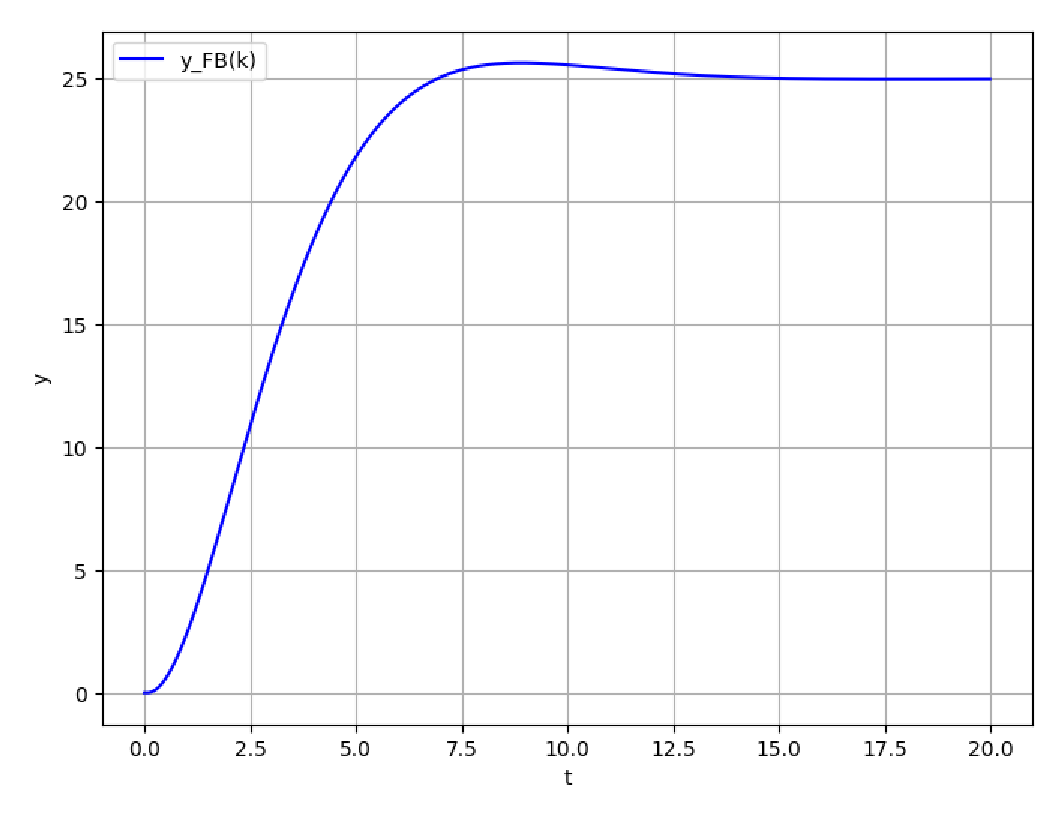
\includegraphics[scale=0.35]{figure18.eps}
    \caption{ボールの位置のシミュレーション結果}
    \label{fig:figure24}
  \end{minipage}
  \begin{minipage}[h]{0.4\linewidth}
    \centering
    \scalebox{0.45}[0.45]{
\begin{tikzpicture}[gnuplot]
%% generated with GNUPLOT 5.4p10 (Lua 5.4; terminal rev. Jun 2020, script rev. 118)
%% Sun Nov 19 18:39:30 2023
\path (0.000,0.000) rectangle (12.500,8.750);
\gpcolor{color=gp lt color border}
\gpsetlinetype{gp lt border}
\gpsetdashtype{gp dt solid}
\gpsetlinewidth{1.00}
\draw[gp path] (0.018,0.031)--(0.198,0.031);
\draw[gp path] (12.480,0.031)--(12.300,0.031);
\node[gp node right] at (-0.166,0.031) {$0$};
\draw[gp path] (0.018,1.479)--(0.198,1.479);
\draw[gp path] (12.480,1.479)--(12.300,1.479);
\node[gp node right] at (-0.166,1.479) {$10$};
\draw[gp path] (0.018,2.927)--(0.198,2.927);
\draw[gp path] (12.480,2.927)--(12.300,2.927);
\node[gp node right] at (-0.166,2.927) {$20$};
\draw[gp path] (0.018,4.375)--(0.198,4.375);
\draw[gp path] (12.480,4.375)--(12.300,4.375);
\node[gp node right] at (-0.166,4.375) {$30$};
\draw[gp path] (0.018,5.822)--(0.198,5.822);
\draw[gp path] (12.480,5.822)--(12.300,5.822);
\node[gp node right] at (-0.166,5.822) {$40$};
\draw[gp path] (0.018,7.270)--(0.198,7.270);
\draw[gp path] (12.480,7.270)--(12.300,7.270);
\node[gp node right] at (-0.166,7.270) {$50$};
\draw[gp path] (0.018,8.718)--(0.198,8.718);
\draw[gp path] (12.480,8.718)--(12.300,8.718);
\node[gp node right] at (-0.166,8.718) {$60$};
\draw[gp path] (0.018,0.031)--(0.018,0.211);
\draw[gp path] (0.018,8.718)--(0.018,8.538);
\node[gp node center] at (0.018,-0.277) {$0$};
\draw[gp path] (2.284,0.031)--(2.284,0.211);
\draw[gp path] (2.284,8.718)--(2.284,8.538);
\node[gp node center] at (2.284,-0.277) {$2$};
\draw[gp path] (4.550,0.031)--(4.550,0.211);
\draw[gp path] (4.550,8.718)--(4.550,8.538);
\node[gp node center] at (4.550,-0.277) {$4$};
\draw[gp path] (6.815,0.031)--(6.815,0.211);
\draw[gp path] (6.815,8.718)--(6.815,8.538);
\node[gp node center] at (6.815,-0.277) {$6$};
\draw[gp path] (9.081,0.031)--(9.081,0.211);
\draw[gp path] (9.081,8.718)--(9.081,8.538);
\node[gp node center] at (9.081,-0.277) {$8$};
\draw[gp path] (11.347,0.031)--(11.347,0.211);
\draw[gp path] (11.347,8.718)--(11.347,8.538);
\node[gp node center] at (11.347,-0.277) {$10$};
\draw[gp path] (0.018,8.718)--(0.018,0.031)--(12.480,0.031)--(12.480,8.718)--cycle;
\node[gp node center,rotate=-270] at (-0.826,4.374) {ボールの位置$z\ /\ \mathrm{cm}$};
\node[gp node center] at (6.249,-0.738) {時間$t\ /\ \mathrm{s}$};
\gpcolor{rgb color={0.000,0.000,0.000}}
\draw[gp path] (0.018,0.312)--(0.041,1.203)--(0.063,2.405)--(0.086,3.428)--(0.109,4.115)%
  --(0.131,4.485)--(0.154,4.624)--(0.177,4.608)--(0.199,4.516)--(0.222,4.432)--(0.245,4.387)%
  --(0.267,4.373)--(0.290,4.360)--(0.313,4.328)--(0.335,4.304)--(0.358,4.297)--(0.381,4.287)%
  --(0.403,4.271)--(0.426,4.246)--(0.449,4.215)--(0.471,4.185)--(0.494,4.152)--(0.516,4.114)%
  --(0.539,4.078)--(0.562,4.051)--(0.584,4.035)--(0.607,4.027)--(0.630,4.030)--(0.652,4.045)%
  --(0.675,4.066)--(0.698,4.084)--(0.720,4.096)--(0.743,4.089)--(0.766,4.056)--(0.788,4.049)%
  --(0.811,4.115)--(0.834,4.224)--(0.856,4.334)--(0.879,4.417)--(0.902,4.463)--(0.924,4.472)%
  --(0.947,4.465)--(0.970,4.480)--(0.992,4.526)--(1.015,4.578)--(1.038,4.616)--(1.060,4.637)%
  --(1.083,4.645)--(1.106,4.646)--(1.128,4.548)--(1.151,4.333)--(1.174,4.203)--(1.196,4.234)%
  --(1.219,4.322)--(1.242,4.393)--(1.264,4.420)--(1.287,4.409)--(1.310,4.378)--(1.332,4.332)%
  --(1.355,4.277)--(1.377,4.209)--(1.400,4.123)--(1.423,4.045)--(1.445,3.992)--(1.468,3.955)%
  --(1.491,3.927)--(1.513,3.903)--(1.536,3.874)--(1.559,3.845)--(1.581,3.836)--(1.604,3.818)%
  --(1.627,3.774)--(1.649,3.743)--(1.672,3.736)--(1.695,3.731)--(1.717,3.714)--(1.740,3.701)%
  --(1.763,3.700)--(1.785,3.703)--(1.808,3.627)--(1.831,3.461)--(1.853,3.388)--(1.876,3.460)%
  --(1.899,3.565)--(1.921,3.640)--(1.944,3.689)--(1.967,3.724)--(1.989,3.757)--(2.012,3.799)%
  --(2.035,3.839)--(2.057,3.876)--(2.080,3.924)--(2.103,3.975)--(2.125,4.018)--(2.148,4.056)%
  --(2.171,4.087)--(2.193,4.086)--(2.216,4.046)--(2.239,4.019)--(2.261,4.032)--(2.284,4.070)%
  --(2.306,4.110)--(2.329,4.130)--(2.352,4.130)--(2.374,4.119)--(2.397,4.098)--(2.420,4.072)%
  --(2.442,4.051)--(2.465,4.028)--(2.488,3.992)--(2.510,3.949)--(2.533,3.905)--(2.556,3.859)%
  --(2.578,3.807)--(2.601,3.756)--(2.624,3.703)--(2.646,3.643)--(2.669,3.588)--(2.692,3.551)%
  --(2.714,3.532)--(2.737,3.510)--(2.760,3.480)--(2.782,3.449)--(2.805,3.422)--(2.828,3.402)%
  --(2.850,3.388)--(2.873,3.383)--(2.896,3.376)--(2.918,3.362)--(2.941,3.357)--(2.964,3.364)%
  --(2.986,3.242)--(3.009,2.973)--(3.032,2.843)--(3.054,2.938)--(3.077,3.122)--(3.100,3.315)%
  --(3.122,3.479)--(3.145,3.592)--(3.167,3.613)--(3.190,3.569)--(3.213,3.568)--(3.235,3.643)%
  --(3.258,3.747)--(3.281,3.850)--(3.303,3.933)--(3.326,3.996)--(3.349,4.042)--(3.371,4.073)%
  --(3.394,4.083)--(3.417,4.070)--(3.439,4.060)--(3.462,4.056)--(3.485,4.046)--(3.507,4.047)%
  --(3.530,4.064)--(3.553,4.084)--(3.575,4.100)--(3.598,4.103)--(3.621,4.087)--(3.643,4.034)%
  --(3.666,3.954)--(3.689,3.846)--(3.711,3.703)--(3.734,3.608)--(3.757,3.596)--(3.779,3.618)%
  --(3.802,3.645)--(3.825,3.611)--(3.847,3.510)--(3.870,3.446)--(3.893,3.456)--(3.915,3.496)%
  --(3.938,3.540)--(3.961,3.573)--(3.983,3.584)--(4.006,3.576)--(4.028,3.581)--(4.051,3.603)%
  --(4.074,3.625)--(4.096,3.647)--(4.119,3.668)--(4.142,3.679)--(4.164,3.681)--(4.187,3.698)%
  --(4.210,3.733)--(4.232,3.776)--(4.255,3.818)--(4.278,3.853)--(4.300,3.908)--(4.323,3.993)%
  --(4.346,4.082)--(4.368,4.144)--(4.391,4.170)--(4.414,4.173)--(4.436,4.157)--(4.459,4.153)%
  --(4.482,4.186)--(4.504,4.242)--(4.527,4.303)--(4.550,4.361)--(4.572,4.416)--(4.595,4.458)%
  --(4.618,4.479)--(4.640,4.484)--(4.663,4.477)--(4.686,4.474)--(4.708,4.487)--(4.731,4.498)%
  --(4.754,4.499)--(4.776,4.484)--(4.799,4.442)--(4.822,4.385)--(4.844,4.336)--(4.867,4.308)%
  --(4.890,4.312)--(4.912,4.348)--(4.935,4.396)--(4.957,4.460)--(4.980,4.530)--(5.003,4.559)%
  --(5.025,4.585)--(5.048,4.645)--(5.071,4.716)--(5.093,4.766)--(5.116,4.789)--(5.139,4.831)%
  --(5.161,4.887)--(5.184,4.899)--(5.207,4.882)--(5.229,4.915)--(5.252,5.009)--(5.275,5.111)%
  --(5.297,5.191)--(5.320,5.234)--(5.343,5.250)--(5.365,5.253)--(5.388,5.245)--(5.411,5.252)%
  --(5.433,5.268)--(5.456,5.268)--(5.479,5.276)--(5.501,5.304)--(5.524,5.334)--(5.547,5.353)%
  --(5.569,5.356)--(5.592,5.353)--(5.615,5.360)--(5.637,5.380)--(5.660,5.393)--(5.683,5.377)%
  --(5.705,5.325)--(5.728,5.253)--(5.751,5.155)--(5.773,5.044)--(5.796,4.990)--(5.818,5.007)%
  --(5.841,5.049)--(5.864,5.102)--(5.886,5.169)--(5.909,5.249)--(5.932,5.338)--(5.954,5.420)%
  --(5.977,5.459)--(6.000,5.437)--(6.022,5.389)--(6.045,5.356)--(6.068,5.353)--(6.090,5.406)%
  --(6.113,5.503)--(6.136,5.555)--(6.158,5.535)--(6.181,5.505)--(6.204,5.500)--(6.226,5.513)%
  --(6.249,5.521)--(6.272,5.526)--(6.294,5.545)--(6.317,5.560)--(6.340,5.555)--(6.362,5.538)%
  --(6.385,5.521)--(6.408,5.506)--(6.430,5.506)--(6.453,5.519)--(6.476,5.526)--(6.498,5.509)%
  --(6.521,5.466)--(6.544,5.417)--(6.566,5.382)--(6.589,5.362)--(6.612,5.354)--(6.634,5.340)%
  --(6.657,5.315)--(6.680,5.290)--(6.702,5.257)--(6.725,5.193)--(6.747,5.099)--(6.770,5.012)%
  --(6.793,4.927)--(6.815,4.829)--(6.838,4.768)--(6.861,4.762)--(6.883,4.782)--(6.906,4.807)%
  --(6.929,4.835)--(6.951,4.868)--(6.974,4.902)--(6.997,4.927)--(7.019,4.940)--(7.042,4.930)%
  --(7.065,4.886)--(7.087,4.839)--(7.110,4.843)--(7.133,4.933)--(7.155,5.064)--(7.178,5.178)%
  --(7.201,5.302)--(7.223,5.434)--(7.246,5.538)--(7.269,5.604)--(7.291,5.640)--(7.314,5.672)%
  --(7.337,5.707)--(7.359,5.731)--(7.382,5.745)--(7.405,5.801)--(7.427,5.968)--(7.450,6.281)%
  --(7.473,6.670)--(7.495,6.992)--(7.518,7.235)--(7.541,7.412)--(7.563,7.479)--(7.586,7.483)%
  --(7.608,7.539)--(7.631,7.657)--(7.654,7.753)--(7.676,7.796)--(7.699,7.817)--(7.722,7.841)%
  --(7.744,7.864)--(7.767,7.873)--(7.790,7.870)--(7.812,7.863)--(7.835,7.821)--(7.858,7.727)%
  --(7.880,7.348)--(7.903,6.663)--(7.926,6.303)--(7.948,6.460)--(7.971,6.799)--(7.994,7.132)%
  --(8.016,7.394)--(8.039,7.550)--(8.062,7.583)--(8.084,7.502)--(8.107,7.342)--(8.130,7.210)%
  --(8.152,7.176)--(8.175,7.248)--(8.198,7.372)--(8.220,7.487)--(8.243,7.566)--(8.266,7.556)%
  --(8.288,7.477)--(8.311,7.333)--(8.334,7.045)--(8.356,6.761)--(8.379,6.736)--(8.402,6.903)%
  --(8.424,7.033)--(8.447,7.027)--(8.470,7.012)--(8.492,7.149)--(8.515,7.270)--(8.537,7.237)%
  --(8.560,7.256)--(8.583,7.390)--(8.605,7.483)--(8.628,7.438)--(8.651,7.338)--(8.673,7.336)%
  --(8.696,7.423)--(8.719,7.523)--(8.741,7.613)--(8.764,7.598)--(8.787,7.445)--(8.809,7.325)%
  --(8.832,7.288)--(8.855,7.263)--(8.877,7.309)--(8.900,7.453)--(8.923,7.606)--(8.945,7.671)%
  --(8.968,7.634)--(8.991,7.566)--(9.013,7.455)--(9.036,7.328)--(9.059,7.318)--(9.081,7.381)%
  --(9.104,7.407)--(9.127,7.405)--(9.149,7.456)--(9.172,7.583)--(9.195,7.705)--(9.217,7.769)%
  --(9.240,7.770)--(9.263,7.743)--(9.285,7.713)--(9.308,7.674)--(9.331,7.623)--(9.353,7.566)%
  --(9.376,7.545)--(9.398,7.546)--(9.421,7.540)--(9.444,7.545)--(9.466,7.579)--(9.489,7.629)%
  --(9.512,7.685)--(9.534,7.732)--(9.557,7.757)--(9.580,7.670)--(9.602,7.335)--(9.625,6.782)%
  --(9.648,6.178)--(9.670,5.678)--(9.693,5.313)--(9.716,5.040)--(9.738,4.878)--(9.761,4.784)%
  --(9.784,4.662)--(9.806,4.497)--(9.829,4.310)--(9.852,4.183)--(9.874,4.207)--(9.897,4.368)%
  --(9.920,4.594)--(9.942,4.805)--(9.965,4.984)--(9.988,5.130)--(10.010,5.153)--(10.033,5.032)%
  --(10.056,4.899)--(10.078,4.764)--(10.101,4.539)--(10.124,4.271)--(10.146,4.031)--(10.169,3.860)%
  --(10.192,3.781)--(10.214,3.759)--(10.237,3.765)--(10.259,3.785)--(10.282,3.804)--(10.305,3.824)%
  --(10.327,3.844)--(10.350,3.853)--(10.373,3.853)--(10.395,3.860)--(10.418,3.872)--(10.441,3.882)%
  --(10.463,3.894)--(10.486,3.917)--(10.509,3.952)--(10.531,3.988)--(10.554,4.020)--(10.577,4.055)%
  --(10.599,4.097)--(10.622,4.147)--(10.645,4.204)--(10.667,4.270)--(10.690,4.333)--(10.713,4.354)%
  --(10.735,4.329)--(10.758,4.319)--(10.781,4.370)--(10.803,4.448)--(10.826,4.489)--(10.849,4.489)%
  --(10.871,4.492)--(10.894,4.502)--(10.917,4.507)--(10.939,4.504)--(10.962,4.494)--(10.985,4.461)%
  --(11.007,4.398)--(11.030,4.315)--(11.053,4.202)--(11.075,4.069)--(11.098,3.941)--(11.121,3.825)%
  --(11.143,3.717)--(11.166,3.613)--(11.188,3.512)--(11.211,3.414)--(11.234,3.318)--(11.256,3.222)%
  --(11.279,3.131)--(11.302,3.034)--(11.324,2.916)--(11.347,2.786)--(11.370,2.665)--(11.392,2.562)%
  --(11.415,2.480)--(11.438,2.409)--(11.460,2.342)--(11.483,2.278)--(11.506,2.217)--(11.528,2.161)%
  --(11.551,2.101)--(11.574,2.036)--(11.596,1.970)--(11.619,1.909)--(11.642,1.863)--(11.664,1.835)%
  --(11.687,1.815)--(11.710,1.800)--(11.732,1.783)--(11.755,1.762)--(11.778,1.741)--(11.800,1.724)%
  --(11.823,1.718)--(11.846,1.725)--(11.868,1.739)--(11.891,1.756)--(11.914,1.775)--(11.936,1.791)%
  --(11.959,1.802)--(11.982,1.826)--(12.004,1.857)--(12.027,1.887)--(12.049,1.930)--(12.072,1.986)%
  --(12.095,2.044)--(12.117,2.091)--(12.140,2.128)--(12.163,2.168)--(12.185,2.206)--(12.208,2.234)%
  --(12.231,2.253)--(12.253,2.258)--(12.276,2.251)--(12.299,2.230)--(12.321,2.197)--(12.344,2.154);
\gpsetpointsize{1.20}
\gp3point{gp mark 7}{}{(0.018,0.312)}
\gp3point{gp mark 7}{}{(0.041,1.203)}
\gp3point{gp mark 7}{}{(0.063,2.405)}
\gp3point{gp mark 7}{}{(0.086,3.428)}
\gp3point{gp mark 7}{}{(0.109,4.115)}
\gp3point{gp mark 7}{}{(0.131,4.485)}
\gp3point{gp mark 7}{}{(0.154,4.624)}
\gp3point{gp mark 7}{}{(0.177,4.608)}
\gp3point{gp mark 7}{}{(0.199,4.516)}
\gp3point{gp mark 7}{}{(0.222,4.432)}
\gp3point{gp mark 7}{}{(0.245,4.387)}
\gp3point{gp mark 7}{}{(0.267,4.373)}
\gp3point{gp mark 7}{}{(0.290,4.360)}
\gp3point{gp mark 7}{}{(0.313,4.328)}
\gp3point{gp mark 7}{}{(0.335,4.304)}
\gp3point{gp mark 7}{}{(0.358,4.297)}
\gp3point{gp mark 7}{}{(0.381,4.287)}
\gp3point{gp mark 7}{}{(0.403,4.271)}
\gp3point{gp mark 7}{}{(0.426,4.246)}
\gp3point{gp mark 7}{}{(0.449,4.215)}
\gp3point{gp mark 7}{}{(0.471,4.185)}
\gp3point{gp mark 7}{}{(0.494,4.152)}
\gp3point{gp mark 7}{}{(0.516,4.114)}
\gp3point{gp mark 7}{}{(0.539,4.078)}
\gp3point{gp mark 7}{}{(0.562,4.051)}
\gp3point{gp mark 7}{}{(0.584,4.035)}
\gp3point{gp mark 7}{}{(0.607,4.027)}
\gp3point{gp mark 7}{}{(0.630,4.030)}
\gp3point{gp mark 7}{}{(0.652,4.045)}
\gp3point{gp mark 7}{}{(0.675,4.066)}
\gp3point{gp mark 7}{}{(0.698,4.084)}
\gp3point{gp mark 7}{}{(0.720,4.096)}
\gp3point{gp mark 7}{}{(0.743,4.089)}
\gp3point{gp mark 7}{}{(0.766,4.056)}
\gp3point{gp mark 7}{}{(0.788,4.049)}
\gp3point{gp mark 7}{}{(0.811,4.115)}
\gp3point{gp mark 7}{}{(0.834,4.224)}
\gp3point{gp mark 7}{}{(0.856,4.334)}
\gp3point{gp mark 7}{}{(0.879,4.417)}
\gp3point{gp mark 7}{}{(0.902,4.463)}
\gp3point{gp mark 7}{}{(0.924,4.472)}
\gp3point{gp mark 7}{}{(0.947,4.465)}
\gp3point{gp mark 7}{}{(0.970,4.480)}
\gp3point{gp mark 7}{}{(0.992,4.526)}
\gp3point{gp mark 7}{}{(1.015,4.578)}
\gp3point{gp mark 7}{}{(1.038,4.616)}
\gp3point{gp mark 7}{}{(1.060,4.637)}
\gp3point{gp mark 7}{}{(1.083,4.645)}
\gp3point{gp mark 7}{}{(1.106,4.646)}
\gp3point{gp mark 7}{}{(1.128,4.548)}
\gp3point{gp mark 7}{}{(1.151,4.333)}
\gp3point{gp mark 7}{}{(1.174,4.203)}
\gp3point{gp mark 7}{}{(1.196,4.234)}
\gp3point{gp mark 7}{}{(1.219,4.322)}
\gp3point{gp mark 7}{}{(1.242,4.393)}
\gp3point{gp mark 7}{}{(1.264,4.420)}
\gp3point{gp mark 7}{}{(1.287,4.409)}
\gp3point{gp mark 7}{}{(1.310,4.378)}
\gp3point{gp mark 7}{}{(1.332,4.332)}
\gp3point{gp mark 7}{}{(1.355,4.277)}
\gp3point{gp mark 7}{}{(1.377,4.209)}
\gp3point{gp mark 7}{}{(1.400,4.123)}
\gp3point{gp mark 7}{}{(1.423,4.045)}
\gp3point{gp mark 7}{}{(1.445,3.992)}
\gp3point{gp mark 7}{}{(1.468,3.955)}
\gp3point{gp mark 7}{}{(1.491,3.927)}
\gp3point{gp mark 7}{}{(1.513,3.903)}
\gp3point{gp mark 7}{}{(1.536,3.874)}
\gp3point{gp mark 7}{}{(1.559,3.845)}
\gp3point{gp mark 7}{}{(1.581,3.836)}
\gp3point{gp mark 7}{}{(1.604,3.818)}
\gp3point{gp mark 7}{}{(1.627,3.774)}
\gp3point{gp mark 7}{}{(1.649,3.743)}
\gp3point{gp mark 7}{}{(1.672,3.736)}
\gp3point{gp mark 7}{}{(1.695,3.731)}
\gp3point{gp mark 7}{}{(1.717,3.714)}
\gp3point{gp mark 7}{}{(1.740,3.701)}
\gp3point{gp mark 7}{}{(1.763,3.700)}
\gp3point{gp mark 7}{}{(1.785,3.703)}
\gp3point{gp mark 7}{}{(1.808,3.627)}
\gp3point{gp mark 7}{}{(1.831,3.461)}
\gp3point{gp mark 7}{}{(1.853,3.388)}
\gp3point{gp mark 7}{}{(1.876,3.460)}
\gp3point{gp mark 7}{}{(1.899,3.565)}
\gp3point{gp mark 7}{}{(1.921,3.640)}
\gp3point{gp mark 7}{}{(1.944,3.689)}
\gp3point{gp mark 7}{}{(1.967,3.724)}
\gp3point{gp mark 7}{}{(1.989,3.757)}
\gp3point{gp mark 7}{}{(2.012,3.799)}
\gp3point{gp mark 7}{}{(2.035,3.839)}
\gp3point{gp mark 7}{}{(2.057,3.876)}
\gp3point{gp mark 7}{}{(2.080,3.924)}
\gp3point{gp mark 7}{}{(2.103,3.975)}
\gp3point{gp mark 7}{}{(2.125,4.018)}
\gp3point{gp mark 7}{}{(2.148,4.056)}
\gp3point{gp mark 7}{}{(2.171,4.087)}
\gp3point{gp mark 7}{}{(2.193,4.086)}
\gp3point{gp mark 7}{}{(2.216,4.046)}
\gp3point{gp mark 7}{}{(2.239,4.019)}
\gp3point{gp mark 7}{}{(2.261,4.032)}
\gp3point{gp mark 7}{}{(2.284,4.070)}
\gp3point{gp mark 7}{}{(2.306,4.110)}
\gp3point{gp mark 7}{}{(2.329,4.130)}
\gp3point{gp mark 7}{}{(2.352,4.130)}
\gp3point{gp mark 7}{}{(2.374,4.119)}
\gp3point{gp mark 7}{}{(2.397,4.098)}
\gp3point{gp mark 7}{}{(2.420,4.072)}
\gp3point{gp mark 7}{}{(2.442,4.051)}
\gp3point{gp mark 7}{}{(2.465,4.028)}
\gp3point{gp mark 7}{}{(2.488,3.992)}
\gp3point{gp mark 7}{}{(2.510,3.949)}
\gp3point{gp mark 7}{}{(2.533,3.905)}
\gp3point{gp mark 7}{}{(2.556,3.859)}
\gp3point{gp mark 7}{}{(2.578,3.807)}
\gp3point{gp mark 7}{}{(2.601,3.756)}
\gp3point{gp mark 7}{}{(2.624,3.703)}
\gp3point{gp mark 7}{}{(2.646,3.643)}
\gp3point{gp mark 7}{}{(2.669,3.588)}
\gp3point{gp mark 7}{}{(2.692,3.551)}
\gp3point{gp mark 7}{}{(2.714,3.532)}
\gp3point{gp mark 7}{}{(2.737,3.510)}
\gp3point{gp mark 7}{}{(2.760,3.480)}
\gp3point{gp mark 7}{}{(2.782,3.449)}
\gp3point{gp mark 7}{}{(2.805,3.422)}
\gp3point{gp mark 7}{}{(2.828,3.402)}
\gp3point{gp mark 7}{}{(2.850,3.388)}
\gp3point{gp mark 7}{}{(2.873,3.383)}
\gp3point{gp mark 7}{}{(2.896,3.376)}
\gp3point{gp mark 7}{}{(2.918,3.362)}
\gp3point{gp mark 7}{}{(2.941,3.357)}
\gp3point{gp mark 7}{}{(2.964,3.364)}
\gp3point{gp mark 7}{}{(2.986,3.242)}
\gp3point{gp mark 7}{}{(3.009,2.973)}
\gp3point{gp mark 7}{}{(3.032,2.843)}
\gp3point{gp mark 7}{}{(3.054,2.938)}
\gp3point{gp mark 7}{}{(3.077,3.122)}
\gp3point{gp mark 7}{}{(3.100,3.315)}
\gp3point{gp mark 7}{}{(3.122,3.479)}
\gp3point{gp mark 7}{}{(3.145,3.592)}
\gp3point{gp mark 7}{}{(3.167,3.613)}
\gp3point{gp mark 7}{}{(3.190,3.569)}
\gp3point{gp mark 7}{}{(3.213,3.568)}
\gp3point{gp mark 7}{}{(3.235,3.643)}
\gp3point{gp mark 7}{}{(3.258,3.747)}
\gp3point{gp mark 7}{}{(3.281,3.850)}
\gp3point{gp mark 7}{}{(3.303,3.933)}
\gp3point{gp mark 7}{}{(3.326,3.996)}
\gp3point{gp mark 7}{}{(3.349,4.042)}
\gp3point{gp mark 7}{}{(3.371,4.073)}
\gp3point{gp mark 7}{}{(3.394,4.083)}
\gp3point{gp mark 7}{}{(3.417,4.070)}
\gp3point{gp mark 7}{}{(3.439,4.060)}
\gp3point{gp mark 7}{}{(3.462,4.056)}
\gp3point{gp mark 7}{}{(3.485,4.046)}
\gp3point{gp mark 7}{}{(3.507,4.047)}
\gp3point{gp mark 7}{}{(3.530,4.064)}
\gp3point{gp mark 7}{}{(3.553,4.084)}
\gp3point{gp mark 7}{}{(3.575,4.100)}
\gp3point{gp mark 7}{}{(3.598,4.103)}
\gp3point{gp mark 7}{}{(3.621,4.087)}
\gp3point{gp mark 7}{}{(3.643,4.034)}
\gp3point{gp mark 7}{}{(3.666,3.954)}
\gp3point{gp mark 7}{}{(3.689,3.846)}
\gp3point{gp mark 7}{}{(3.711,3.703)}
\gp3point{gp mark 7}{}{(3.734,3.608)}
\gp3point{gp mark 7}{}{(3.757,3.596)}
\gp3point{gp mark 7}{}{(3.779,3.618)}
\gp3point{gp mark 7}{}{(3.802,3.645)}
\gp3point{gp mark 7}{}{(3.825,3.611)}
\gp3point{gp mark 7}{}{(3.847,3.510)}
\gp3point{gp mark 7}{}{(3.870,3.446)}
\gp3point{gp mark 7}{}{(3.893,3.456)}
\gp3point{gp mark 7}{}{(3.915,3.496)}
\gp3point{gp mark 7}{}{(3.938,3.540)}
\gp3point{gp mark 7}{}{(3.961,3.573)}
\gp3point{gp mark 7}{}{(3.983,3.584)}
\gp3point{gp mark 7}{}{(4.006,3.576)}
\gp3point{gp mark 7}{}{(4.028,3.581)}
\gp3point{gp mark 7}{}{(4.051,3.603)}
\gp3point{gp mark 7}{}{(4.074,3.625)}
\gp3point{gp mark 7}{}{(4.096,3.647)}
\gp3point{gp mark 7}{}{(4.119,3.668)}
\gp3point{gp mark 7}{}{(4.142,3.679)}
\gp3point{gp mark 7}{}{(4.164,3.681)}
\gp3point{gp mark 7}{}{(4.187,3.698)}
\gp3point{gp mark 7}{}{(4.210,3.733)}
\gp3point{gp mark 7}{}{(4.232,3.776)}
\gp3point{gp mark 7}{}{(4.255,3.818)}
\gp3point{gp mark 7}{}{(4.278,3.853)}
\gp3point{gp mark 7}{}{(4.300,3.908)}
\gp3point{gp mark 7}{}{(4.323,3.993)}
\gp3point{gp mark 7}{}{(4.346,4.082)}
\gp3point{gp mark 7}{}{(4.368,4.144)}
\gp3point{gp mark 7}{}{(4.391,4.170)}
\gp3point{gp mark 7}{}{(4.414,4.173)}
\gp3point{gp mark 7}{}{(4.436,4.157)}
\gp3point{gp mark 7}{}{(4.459,4.153)}
\gp3point{gp mark 7}{}{(4.482,4.186)}
\gp3point{gp mark 7}{}{(4.504,4.242)}
\gp3point{gp mark 7}{}{(4.527,4.303)}
\gp3point{gp mark 7}{}{(4.550,4.361)}
\gp3point{gp mark 7}{}{(4.572,4.416)}
\gp3point{gp mark 7}{}{(4.595,4.458)}
\gp3point{gp mark 7}{}{(4.618,4.479)}
\gp3point{gp mark 7}{}{(4.640,4.484)}
\gp3point{gp mark 7}{}{(4.663,4.477)}
\gp3point{gp mark 7}{}{(4.686,4.474)}
\gp3point{gp mark 7}{}{(4.708,4.487)}
\gp3point{gp mark 7}{}{(4.731,4.498)}
\gp3point{gp mark 7}{}{(4.754,4.499)}
\gp3point{gp mark 7}{}{(4.776,4.484)}
\gp3point{gp mark 7}{}{(4.799,4.442)}
\gp3point{gp mark 7}{}{(4.822,4.385)}
\gp3point{gp mark 7}{}{(4.844,4.336)}
\gp3point{gp mark 7}{}{(4.867,4.308)}
\gp3point{gp mark 7}{}{(4.890,4.312)}
\gp3point{gp mark 7}{}{(4.912,4.348)}
\gp3point{gp mark 7}{}{(4.935,4.396)}
\gp3point{gp mark 7}{}{(4.957,4.460)}
\gp3point{gp mark 7}{}{(4.980,4.530)}
\gp3point{gp mark 7}{}{(5.003,4.559)}
\gp3point{gp mark 7}{}{(5.025,4.585)}
\gp3point{gp mark 7}{}{(5.048,4.645)}
\gp3point{gp mark 7}{}{(5.071,4.716)}
\gp3point{gp mark 7}{}{(5.093,4.766)}
\gp3point{gp mark 7}{}{(5.116,4.789)}
\gp3point{gp mark 7}{}{(5.139,4.831)}
\gp3point{gp mark 7}{}{(5.161,4.887)}
\gp3point{gp mark 7}{}{(5.184,4.899)}
\gp3point{gp mark 7}{}{(5.207,4.882)}
\gp3point{gp mark 7}{}{(5.229,4.915)}
\gp3point{gp mark 7}{}{(5.252,5.009)}
\gp3point{gp mark 7}{}{(5.275,5.111)}
\gp3point{gp mark 7}{}{(5.297,5.191)}
\gp3point{gp mark 7}{}{(5.320,5.234)}
\gp3point{gp mark 7}{}{(5.343,5.250)}
\gp3point{gp mark 7}{}{(5.365,5.253)}
\gp3point{gp mark 7}{}{(5.388,5.245)}
\gp3point{gp mark 7}{}{(5.411,5.252)}
\gp3point{gp mark 7}{}{(5.433,5.268)}
\gp3point{gp mark 7}{}{(5.456,5.268)}
\gp3point{gp mark 7}{}{(5.479,5.276)}
\gp3point{gp mark 7}{}{(5.501,5.304)}
\gp3point{gp mark 7}{}{(5.524,5.334)}
\gp3point{gp mark 7}{}{(5.547,5.353)}
\gp3point{gp mark 7}{}{(5.569,5.356)}
\gp3point{gp mark 7}{}{(5.592,5.353)}
\gp3point{gp mark 7}{}{(5.615,5.360)}
\gp3point{gp mark 7}{}{(5.637,5.380)}
\gp3point{gp mark 7}{}{(5.660,5.393)}
\gp3point{gp mark 7}{}{(5.683,5.377)}
\gp3point{gp mark 7}{}{(5.705,5.325)}
\gp3point{gp mark 7}{}{(5.728,5.253)}
\gp3point{gp mark 7}{}{(5.751,5.155)}
\gp3point{gp mark 7}{}{(5.773,5.044)}
\gp3point{gp mark 7}{}{(5.796,4.990)}
\gp3point{gp mark 7}{}{(5.818,5.007)}
\gp3point{gp mark 7}{}{(5.841,5.049)}
\gp3point{gp mark 7}{}{(5.864,5.102)}
\gp3point{gp mark 7}{}{(5.886,5.169)}
\gp3point{gp mark 7}{}{(5.909,5.249)}
\gp3point{gp mark 7}{}{(5.932,5.338)}
\gp3point{gp mark 7}{}{(5.954,5.420)}
\gp3point{gp mark 7}{}{(5.977,5.459)}
\gp3point{gp mark 7}{}{(6.000,5.437)}
\gp3point{gp mark 7}{}{(6.022,5.389)}
\gp3point{gp mark 7}{}{(6.045,5.356)}
\gp3point{gp mark 7}{}{(6.068,5.353)}
\gp3point{gp mark 7}{}{(6.090,5.406)}
\gp3point{gp mark 7}{}{(6.113,5.503)}
\gp3point{gp mark 7}{}{(6.136,5.555)}
\gp3point{gp mark 7}{}{(6.158,5.535)}
\gp3point{gp mark 7}{}{(6.181,5.505)}
\gp3point{gp mark 7}{}{(6.204,5.500)}
\gp3point{gp mark 7}{}{(6.226,5.513)}
\gp3point{gp mark 7}{}{(6.249,5.521)}
\gp3point{gp mark 7}{}{(6.272,5.526)}
\gp3point{gp mark 7}{}{(6.294,5.545)}
\gp3point{gp mark 7}{}{(6.317,5.560)}
\gp3point{gp mark 7}{}{(6.340,5.555)}
\gp3point{gp mark 7}{}{(6.362,5.538)}
\gp3point{gp mark 7}{}{(6.385,5.521)}
\gp3point{gp mark 7}{}{(6.408,5.506)}
\gp3point{gp mark 7}{}{(6.430,5.506)}
\gp3point{gp mark 7}{}{(6.453,5.519)}
\gp3point{gp mark 7}{}{(6.476,5.526)}
\gp3point{gp mark 7}{}{(6.498,5.509)}
\gp3point{gp mark 7}{}{(6.521,5.466)}
\gp3point{gp mark 7}{}{(6.544,5.417)}
\gp3point{gp mark 7}{}{(6.566,5.382)}
\gp3point{gp mark 7}{}{(6.589,5.362)}
\gp3point{gp mark 7}{}{(6.612,5.354)}
\gp3point{gp mark 7}{}{(6.634,5.340)}
\gp3point{gp mark 7}{}{(6.657,5.315)}
\gp3point{gp mark 7}{}{(6.680,5.290)}
\gp3point{gp mark 7}{}{(6.702,5.257)}
\gp3point{gp mark 7}{}{(6.725,5.193)}
\gp3point{gp mark 7}{}{(6.747,5.099)}
\gp3point{gp mark 7}{}{(6.770,5.012)}
\gp3point{gp mark 7}{}{(6.793,4.927)}
\gp3point{gp mark 7}{}{(6.815,4.829)}
\gp3point{gp mark 7}{}{(6.838,4.768)}
\gp3point{gp mark 7}{}{(6.861,4.762)}
\gp3point{gp mark 7}{}{(6.883,4.782)}
\gp3point{gp mark 7}{}{(6.906,4.807)}
\gp3point{gp mark 7}{}{(6.929,4.835)}
\gp3point{gp mark 7}{}{(6.951,4.868)}
\gp3point{gp mark 7}{}{(6.974,4.902)}
\gp3point{gp mark 7}{}{(6.997,4.927)}
\gp3point{gp mark 7}{}{(7.019,4.940)}
\gp3point{gp mark 7}{}{(7.042,4.930)}
\gp3point{gp mark 7}{}{(7.065,4.886)}
\gp3point{gp mark 7}{}{(7.087,4.839)}
\gp3point{gp mark 7}{}{(7.110,4.843)}
\gp3point{gp mark 7}{}{(7.133,4.933)}
\gp3point{gp mark 7}{}{(7.155,5.064)}
\gp3point{gp mark 7}{}{(7.178,5.178)}
\gp3point{gp mark 7}{}{(7.201,5.302)}
\gp3point{gp mark 7}{}{(7.223,5.434)}
\gp3point{gp mark 7}{}{(7.246,5.538)}
\gp3point{gp mark 7}{}{(7.269,5.604)}
\gp3point{gp mark 7}{}{(7.291,5.640)}
\gp3point{gp mark 7}{}{(7.314,5.672)}
\gp3point{gp mark 7}{}{(7.337,5.707)}
\gp3point{gp mark 7}{}{(7.359,5.731)}
\gp3point{gp mark 7}{}{(7.382,5.745)}
\gp3point{gp mark 7}{}{(7.405,5.801)}
\gp3point{gp mark 7}{}{(7.427,5.968)}
\gp3point{gp mark 7}{}{(7.450,6.281)}
\gp3point{gp mark 7}{}{(7.473,6.670)}
\gp3point{gp mark 7}{}{(7.495,6.992)}
\gp3point{gp mark 7}{}{(7.518,7.235)}
\gp3point{gp mark 7}{}{(7.541,7.412)}
\gp3point{gp mark 7}{}{(7.563,7.479)}
\gp3point{gp mark 7}{}{(7.586,7.483)}
\gp3point{gp mark 7}{}{(7.608,7.539)}
\gp3point{gp mark 7}{}{(7.631,7.657)}
\gp3point{gp mark 7}{}{(7.654,7.753)}
\gp3point{gp mark 7}{}{(7.676,7.796)}
\gp3point{gp mark 7}{}{(7.699,7.817)}
\gp3point{gp mark 7}{}{(7.722,7.841)}
\gp3point{gp mark 7}{}{(7.744,7.864)}
\gp3point{gp mark 7}{}{(7.767,7.873)}
\gp3point{gp mark 7}{}{(7.790,7.870)}
\gp3point{gp mark 7}{}{(7.812,7.863)}
\gp3point{gp mark 7}{}{(7.835,7.821)}
\gp3point{gp mark 7}{}{(7.858,7.727)}
\gp3point{gp mark 7}{}{(7.880,7.348)}
\gp3point{gp mark 7}{}{(7.903,6.663)}
\gp3point{gp mark 7}{}{(7.926,6.303)}
\gp3point{gp mark 7}{}{(7.948,6.460)}
\gp3point{gp mark 7}{}{(7.971,6.799)}
\gp3point{gp mark 7}{}{(7.994,7.132)}
\gp3point{gp mark 7}{}{(8.016,7.394)}
\gp3point{gp mark 7}{}{(8.039,7.550)}
\gp3point{gp mark 7}{}{(8.062,7.583)}
\gp3point{gp mark 7}{}{(8.084,7.502)}
\gp3point{gp mark 7}{}{(8.107,7.342)}
\gp3point{gp mark 7}{}{(8.130,7.210)}
\gp3point{gp mark 7}{}{(8.152,7.176)}
\gp3point{gp mark 7}{}{(8.175,7.248)}
\gp3point{gp mark 7}{}{(8.198,7.372)}
\gp3point{gp mark 7}{}{(8.220,7.487)}
\gp3point{gp mark 7}{}{(8.243,7.566)}
\gp3point{gp mark 7}{}{(8.266,7.556)}
\gp3point{gp mark 7}{}{(8.288,7.477)}
\gp3point{gp mark 7}{}{(8.311,7.333)}
\gp3point{gp mark 7}{}{(8.334,7.045)}
\gp3point{gp mark 7}{}{(8.356,6.761)}
\gp3point{gp mark 7}{}{(8.379,6.736)}
\gp3point{gp mark 7}{}{(8.402,6.903)}
\gp3point{gp mark 7}{}{(8.424,7.033)}
\gp3point{gp mark 7}{}{(8.447,7.027)}
\gp3point{gp mark 7}{}{(8.470,7.012)}
\gp3point{gp mark 7}{}{(8.492,7.149)}
\gp3point{gp mark 7}{}{(8.515,7.270)}
\gp3point{gp mark 7}{}{(8.537,7.237)}
\gp3point{gp mark 7}{}{(8.560,7.256)}
\gp3point{gp mark 7}{}{(8.583,7.390)}
\gp3point{gp mark 7}{}{(8.605,7.483)}
\gp3point{gp mark 7}{}{(8.628,7.438)}
\gp3point{gp mark 7}{}{(8.651,7.338)}
\gp3point{gp mark 7}{}{(8.673,7.336)}
\gp3point{gp mark 7}{}{(8.696,7.423)}
\gp3point{gp mark 7}{}{(8.719,7.523)}
\gp3point{gp mark 7}{}{(8.741,7.613)}
\gp3point{gp mark 7}{}{(8.764,7.598)}
\gp3point{gp mark 7}{}{(8.787,7.445)}
\gp3point{gp mark 7}{}{(8.809,7.325)}
\gp3point{gp mark 7}{}{(8.832,7.288)}
\gp3point{gp mark 7}{}{(8.855,7.263)}
\gp3point{gp mark 7}{}{(8.877,7.309)}
\gp3point{gp mark 7}{}{(8.900,7.453)}
\gp3point{gp mark 7}{}{(8.923,7.606)}
\gp3point{gp mark 7}{}{(8.945,7.671)}
\gp3point{gp mark 7}{}{(8.968,7.634)}
\gp3point{gp mark 7}{}{(8.991,7.566)}
\gp3point{gp mark 7}{}{(9.013,7.455)}
\gp3point{gp mark 7}{}{(9.036,7.328)}
\gp3point{gp mark 7}{}{(9.059,7.318)}
\gp3point{gp mark 7}{}{(9.081,7.381)}
\gp3point{gp mark 7}{}{(9.104,7.407)}
\gp3point{gp mark 7}{}{(9.127,7.405)}
\gp3point{gp mark 7}{}{(9.149,7.456)}
\gp3point{gp mark 7}{}{(9.172,7.583)}
\gp3point{gp mark 7}{}{(9.195,7.705)}
\gp3point{gp mark 7}{}{(9.217,7.769)}
\gp3point{gp mark 7}{}{(9.240,7.770)}
\gp3point{gp mark 7}{}{(9.263,7.743)}
\gp3point{gp mark 7}{}{(9.285,7.713)}
\gp3point{gp mark 7}{}{(9.308,7.674)}
\gp3point{gp mark 7}{}{(9.331,7.623)}
\gp3point{gp mark 7}{}{(9.353,7.566)}
\gp3point{gp mark 7}{}{(9.376,7.545)}
\gp3point{gp mark 7}{}{(9.398,7.546)}
\gp3point{gp mark 7}{}{(9.421,7.540)}
\gp3point{gp mark 7}{}{(9.444,7.545)}
\gp3point{gp mark 7}{}{(9.466,7.579)}
\gp3point{gp mark 7}{}{(9.489,7.629)}
\gp3point{gp mark 7}{}{(9.512,7.685)}
\gp3point{gp mark 7}{}{(9.534,7.732)}
\gp3point{gp mark 7}{}{(9.557,7.757)}
\gp3point{gp mark 7}{}{(9.580,7.670)}
\gp3point{gp mark 7}{}{(9.602,7.335)}
\gp3point{gp mark 7}{}{(9.625,6.782)}
\gp3point{gp mark 7}{}{(9.648,6.178)}
\gp3point{gp mark 7}{}{(9.670,5.678)}
\gp3point{gp mark 7}{}{(9.693,5.313)}
\gp3point{gp mark 7}{}{(9.716,5.040)}
\gp3point{gp mark 7}{}{(9.738,4.878)}
\gp3point{gp mark 7}{}{(9.761,4.784)}
\gp3point{gp mark 7}{}{(9.784,4.662)}
\gp3point{gp mark 7}{}{(9.806,4.497)}
\gp3point{gp mark 7}{}{(9.829,4.310)}
\gp3point{gp mark 7}{}{(9.852,4.183)}
\gp3point{gp mark 7}{}{(9.874,4.207)}
\gp3point{gp mark 7}{}{(9.897,4.368)}
\gp3point{gp mark 7}{}{(9.920,4.594)}
\gp3point{gp mark 7}{}{(9.942,4.805)}
\gp3point{gp mark 7}{}{(9.965,4.984)}
\gp3point{gp mark 7}{}{(9.988,5.130)}
\gp3point{gp mark 7}{}{(10.010,5.153)}
\gp3point{gp mark 7}{}{(10.033,5.032)}
\gp3point{gp mark 7}{}{(10.056,4.899)}
\gp3point{gp mark 7}{}{(10.078,4.764)}
\gp3point{gp mark 7}{}{(10.101,4.539)}
\gp3point{gp mark 7}{}{(10.124,4.271)}
\gp3point{gp mark 7}{}{(10.146,4.031)}
\gp3point{gp mark 7}{}{(10.169,3.860)}
\gp3point{gp mark 7}{}{(10.192,3.781)}
\gp3point{gp mark 7}{}{(10.214,3.759)}
\gp3point{gp mark 7}{}{(10.237,3.765)}
\gp3point{gp mark 7}{}{(10.259,3.785)}
\gp3point{gp mark 7}{}{(10.282,3.804)}
\gp3point{gp mark 7}{}{(10.305,3.824)}
\gp3point{gp mark 7}{}{(10.327,3.844)}
\gp3point{gp mark 7}{}{(10.350,3.853)}
\gp3point{gp mark 7}{}{(10.373,3.853)}
\gp3point{gp mark 7}{}{(10.395,3.860)}
\gp3point{gp mark 7}{}{(10.418,3.872)}
\gp3point{gp mark 7}{}{(10.441,3.882)}
\gp3point{gp mark 7}{}{(10.463,3.894)}
\gp3point{gp mark 7}{}{(10.486,3.917)}
\gp3point{gp mark 7}{}{(10.509,3.952)}
\gp3point{gp mark 7}{}{(10.531,3.988)}
\gp3point{gp mark 7}{}{(10.554,4.020)}
\gp3point{gp mark 7}{}{(10.577,4.055)}
\gp3point{gp mark 7}{}{(10.599,4.097)}
\gp3point{gp mark 7}{}{(10.622,4.147)}
\gp3point{gp mark 7}{}{(10.645,4.204)}
\gp3point{gp mark 7}{}{(10.667,4.270)}
\gp3point{gp mark 7}{}{(10.690,4.333)}
\gp3point{gp mark 7}{}{(10.713,4.354)}
\gp3point{gp mark 7}{}{(10.735,4.329)}
\gp3point{gp mark 7}{}{(10.758,4.319)}
\gp3point{gp mark 7}{}{(10.781,4.370)}
\gp3point{gp mark 7}{}{(10.803,4.448)}
\gp3point{gp mark 7}{}{(10.826,4.489)}
\gp3point{gp mark 7}{}{(10.849,4.489)}
\gp3point{gp mark 7}{}{(10.871,4.492)}
\gp3point{gp mark 7}{}{(10.894,4.502)}
\gp3point{gp mark 7}{}{(10.917,4.507)}
\gp3point{gp mark 7}{}{(10.939,4.504)}
\gp3point{gp mark 7}{}{(10.962,4.494)}
\gp3point{gp mark 7}{}{(10.985,4.461)}
\gp3point{gp mark 7}{}{(11.007,4.398)}
\gp3point{gp mark 7}{}{(11.030,4.315)}
\gp3point{gp mark 7}{}{(11.053,4.202)}
\gp3point{gp mark 7}{}{(11.075,4.069)}
\gp3point{gp mark 7}{}{(11.098,3.941)}
\gp3point{gp mark 7}{}{(11.121,3.825)}
\gp3point{gp mark 7}{}{(11.143,3.717)}
\gp3point{gp mark 7}{}{(11.166,3.613)}
\gp3point{gp mark 7}{}{(11.188,3.512)}
\gp3point{gp mark 7}{}{(11.211,3.414)}
\gp3point{gp mark 7}{}{(11.234,3.318)}
\gp3point{gp mark 7}{}{(11.256,3.222)}
\gp3point{gp mark 7}{}{(11.279,3.131)}
\gp3point{gp mark 7}{}{(11.302,3.034)}
\gp3point{gp mark 7}{}{(11.324,2.916)}
\gp3point{gp mark 7}{}{(11.347,2.786)}
\gp3point{gp mark 7}{}{(11.370,2.665)}
\gp3point{gp mark 7}{}{(11.392,2.562)}
\gp3point{gp mark 7}{}{(11.415,2.480)}
\gp3point{gp mark 7}{}{(11.438,2.409)}
\gp3point{gp mark 7}{}{(11.460,2.342)}
\gp3point{gp mark 7}{}{(11.483,2.278)}
\gp3point{gp mark 7}{}{(11.506,2.217)}
\gp3point{gp mark 7}{}{(11.528,2.161)}
\gp3point{gp mark 7}{}{(11.551,2.101)}
\gp3point{gp mark 7}{}{(11.574,2.036)}
\gp3point{gp mark 7}{}{(11.596,1.970)}
\gp3point{gp mark 7}{}{(11.619,1.909)}
\gp3point{gp mark 7}{}{(11.642,1.863)}
\gp3point{gp mark 7}{}{(11.664,1.835)}
\gp3point{gp mark 7}{}{(11.687,1.815)}
\gp3point{gp mark 7}{}{(11.710,1.800)}
\gp3point{gp mark 7}{}{(11.732,1.783)}
\gp3point{gp mark 7}{}{(11.755,1.762)}
\gp3point{gp mark 7}{}{(11.778,1.741)}
\gp3point{gp mark 7}{}{(11.800,1.724)}
\gp3point{gp mark 7}{}{(11.823,1.718)}
\gp3point{gp mark 7}{}{(11.846,1.725)}
\gp3point{gp mark 7}{}{(11.868,1.739)}
\gp3point{gp mark 7}{}{(11.891,1.756)}
\gp3point{gp mark 7}{}{(11.914,1.775)}
\gp3point{gp mark 7}{}{(11.936,1.791)}
\gp3point{gp mark 7}{}{(11.959,1.802)}
\gp3point{gp mark 7}{}{(11.982,1.826)}
\gp3point{gp mark 7}{}{(12.004,1.857)}
\gp3point{gp mark 7}{}{(12.027,1.887)}
\gp3point{gp mark 7}{}{(12.049,1.930)}
\gp3point{gp mark 7}{}{(12.072,1.986)}
\gp3point{gp mark 7}{}{(12.095,2.044)}
\gp3point{gp mark 7}{}{(12.117,2.091)}
\gp3point{gp mark 7}{}{(12.140,2.128)}
\gp3point{gp mark 7}{}{(12.163,2.168)}
\gp3point{gp mark 7}{}{(12.185,2.206)}
\gp3point{gp mark 7}{}{(12.208,2.234)}
\gp3point{gp mark 7}{}{(12.231,2.253)}
\gp3point{gp mark 7}{}{(12.253,2.258)}
\gp3point{gp mark 7}{}{(12.276,2.251)}
\gp3point{gp mark 7}{}{(12.299,2.230)}
\gp3point{gp mark 7}{}{(12.321,2.197)}
\gp3point{gp mark 7}{}{(12.344,2.154)}
\gpcolor{color=gp lt color border}
\draw[gp path] (0.018,8.718)--(0.018,0.031)--(12.480,0.031)--(12.480,8.718)--cycle;
%% coordinates of the plot area
\gpdefrectangularnode{gp plot 1}{\pgfpoint{0.018cm}{0.031cm}}{\pgfpoint{12.480cm}{8.718cm}}
\end{tikzpicture}
%% gnuplot variables
}

    \vspace{-30pt}\caption{ボールの位置の時間変化}
    \label{fig:figure25}
  \end{minipage}
  \begin{minipage}[h]{0.4\linewidth}
    \centering
    \scalebox{0.45}[0.45]{
\begin{tikzpicture}[gnuplot]
%% generated with GNUPLOT 5.4p10 (Lua 5.4; terminal rev. Jun 2020, script rev. 118)
%% Sun Nov 19 19:02:00 2023
\path (0.000,0.000) rectangle (12.500,8.750);
\gpcolor{color=gp lt color border}
\gpsetlinetype{gp lt border}
\gpsetdashtype{gp dt solid}
\gpsetlinewidth{1.00}
\draw[gp path] (0.018,0.031)--(0.198,0.031);
\draw[gp path] (12.480,0.031)--(12.300,0.031);
\node[gp node right] at (-0.166,0.031) {$-100$};
\draw[gp path] (0.018,0.900)--(0.198,0.900);
\draw[gp path] (12.480,0.900)--(12.300,0.900);
\node[gp node right] at (-0.166,0.900) {$-80$};
\draw[gp path] (0.018,1.768)--(0.198,1.768);
\draw[gp path] (12.480,1.768)--(12.300,1.768);
\node[gp node right] at (-0.166,1.768) {$-60$};
\draw[gp path] (0.018,2.637)--(0.198,2.637);
\draw[gp path] (12.480,2.637)--(12.300,2.637);
\node[gp node right] at (-0.166,2.637) {$-40$};
\draw[gp path] (0.018,3.506)--(0.198,3.506);
\draw[gp path] (12.480,3.506)--(12.300,3.506);
\node[gp node right] at (-0.166,3.506) {$-20$};
\draw[gp path] (0.018,4.375)--(0.198,4.375);
\draw[gp path] (12.480,4.375)--(12.300,4.375);
\node[gp node right] at (-0.166,4.375) {$0$};
\draw[gp path] (0.018,5.243)--(0.198,5.243);
\draw[gp path] (12.480,5.243)--(12.300,5.243);
\node[gp node right] at (-0.166,5.243) {$20$};
\draw[gp path] (0.018,6.112)--(0.198,6.112);
\draw[gp path] (12.480,6.112)--(12.300,6.112);
\node[gp node right] at (-0.166,6.112) {$40$};
\draw[gp path] (0.018,6.981)--(0.198,6.981);
\draw[gp path] (12.480,6.981)--(12.300,6.981);
\node[gp node right] at (-0.166,6.981) {$60$};
\draw[gp path] (0.018,7.849)--(0.198,7.849);
\draw[gp path] (12.480,7.849)--(12.300,7.849);
\node[gp node right] at (-0.166,7.849) {$80$};
\draw[gp path] (0.018,8.718)--(0.198,8.718);
\draw[gp path] (12.480,8.718)--(12.300,8.718);
\node[gp node right] at (-0.166,8.718) {$100$};
\draw[gp path] (0.018,0.031)--(0.018,0.211);
\draw[gp path] (0.018,8.718)--(0.018,8.538);
\node[gp node center] at (0.018,-0.277) {$0$};
\draw[gp path] (2.284,0.031)--(2.284,0.211);
\draw[gp path] (2.284,8.718)--(2.284,8.538);
\node[gp node center] at (2.284,-0.277) {$2$};
\draw[gp path] (4.550,0.031)--(4.550,0.211);
\draw[gp path] (4.550,8.718)--(4.550,8.538);
\node[gp node center] at (4.550,-0.277) {$4$};
\draw[gp path] (6.815,0.031)--(6.815,0.211);
\draw[gp path] (6.815,8.718)--(6.815,8.538);
\node[gp node center] at (6.815,-0.277) {$6$};
\draw[gp path] (9.081,0.031)--(9.081,0.211);
\draw[gp path] (9.081,8.718)--(9.081,8.538);
\node[gp node center] at (9.081,-0.277) {$8$};
\draw[gp path] (11.347,0.031)--(11.347,0.211);
\draw[gp path] (11.347,8.718)--(11.347,8.538);
\node[gp node center] at (11.347,-0.277) {$10$};
\draw[gp path] (0.018,8.718)--(0.018,0.031)--(12.480,0.031)--(12.480,8.718)--cycle;
\node[gp node center,rotate=-270] at (-1.194,4.374) {角度$\theta\ /\ ^\circ$};
\node[gp node center] at (6.249,-0.738) {時間$t\ /\ \mathrm{s}$};
\gpcolor{rgb color={0.000,0.000,0.000}}
\draw[gp path] (0.018,4.537)--(0.041,4.546)--(0.063,4.537)--(0.086,4.537)--(0.109,4.460)%
  --(0.131,4.346)--(0.154,4.193)--(0.177,3.993)--(0.199,3.773)--(0.222,3.535)--(0.245,3.286)%
  --(0.267,3.172)--(0.290,3.745)--(0.313,4.270)--(0.335,4.537)--(0.358,4.890)--(0.381,5.214)%
  --(0.403,5.396)--(0.426,5.625)--(0.449,5.873)--(0.471,6.350)--(0.494,6.455)--(0.516,6.484)%
  --(0.539,6.493)--(0.562,6.493)--(0.584,6.484)--(0.607,6.474)--(0.630,6.474)--(0.652,6.341)%
  --(0.675,6.226)--(0.698,6.083)--(0.720,5.873)--(0.743,4.890)--(0.766,4.384)--(0.788,3.907)%
  --(0.811,3.554)--(0.834,3.153)--(0.856,2.714)--(0.879,2.418)--(0.902,1.960)--(0.924,1.368)%
  --(0.947,1.044)--(0.970,0.652)--(0.992,0.481)--(1.015,0.586)--(1.038,1.006)--(1.060,1.330)%
  --(1.083,1.626)--(1.106,1.998)--(1.128,2.237)--(1.151,2.552)--(1.174,2.905)--(1.196,3.286)%
  --(1.219,3.745)--(1.242,4.145)--(1.264,4.928)--(1.287,5.109)--(1.310,5.128)--(1.332,5.119)%
  --(1.355,5.119)--(1.377,5.119)--(1.400,5.119)--(1.423,5.119)--(1.445,5.119)--(1.468,5.119)%
  --(1.491,5.119)--(1.513,5.119)--(1.536,5.119)--(1.559,5.119)--(1.581,5.119)--(1.604,5.119)%
  --(1.627,5.119)--(1.649,5.119)--(1.672,5.119)--(1.695,5.119)--(1.717,5.119)--(1.740,5.119)%
  --(1.763,5.100)--(1.785,5.109)--(1.808,5.109)--(1.831,5.033)--(1.853,4.985)--(1.876,4.966)%
  --(1.899,4.928)--(1.921,4.918)--(1.944,4.890)--(1.967,4.813)--(1.989,4.709)--(2.012,4.556)%
  --(2.035,4.336)--(2.057,3.955)--(2.080,3.640)--(2.103,3.277)--(2.125,2.943)--(2.148,2.542)%
  --(2.171,1.941)--(2.193,1.550)--(2.216,1.015)--(2.239,0.614)--(2.261,0.290)--(2.284,0.290)%
  --(2.306,0.576)--(2.329,1.101)--(2.352,1.540)--(2.374,1.969)--(2.397,2.303)--(2.420,2.743)%
  --(2.442,3.220)--(2.465,3.659)--(2.488,4.031)--(2.510,4.479)--(2.533,4.918)--(2.556,5.310)%
  --(2.578,5.882)--(2.601,6.302)--(2.624,6.980)--(2.646,7.276)--(2.669,7.476)--(2.692,7.782)%
  --(2.714,8.116)--(2.737,8.221)--(2.760,8.345)--(2.782,8.440)--(2.805,8.431)--(2.828,8.392)%
  --(2.850,8.163)--(2.873,7.896)--(2.896,7.591)--(2.918,7.324)--(2.941,7.075)--(2.964,6.780)%
  --(2.986,6.321)--(3.009,5.921)--(3.032,5.529)--(3.054,5.195)--(3.077,4.899)--(3.100,4.699)%
  --(3.122,4.365)--(3.145,3.993)--(3.167,3.382)--(3.190,3.000)--(3.213,2.542)--(3.235,2.122)%
  --(3.258,1.759)--(3.281,1.368)--(3.303,1.015)--(3.326,0.671)--(3.349,0.509)--(3.371,0.318)%
  --(3.394,0.404)--(3.417,0.519)--(3.439,0.633)--(3.462,1.015)--(3.485,1.464)--(3.507,1.712)%
  --(3.530,2.141)--(3.553,2.561)--(3.575,3.000)--(3.598,3.353)--(3.621,3.811)--(3.643,4.250)%
  --(3.666,4.699)--(3.689,5.243)--(3.711,6.312)--(3.734,6.808)--(3.757,7.104)--(3.779,7.533)%
  --(3.802,7.953)--(3.825,8.202)--(3.847,8.440)--(3.870,8.507)--(3.893,8.574)--(3.915,8.612)%
  --(3.938,8.612)--(3.961,8.536)--(3.983,8.469)--(4.006,8.039)--(4.028,7.877)--(4.051,7.524)%
  --(4.074,7.295)--(4.096,6.999)--(4.119,6.617)--(4.142,6.197)--(4.164,5.806)--(4.187,5.386)%
  --(4.210,4.966)--(4.232,4.403)--(4.255,3.411)--(4.278,2.943)--(4.300,2.342)--(4.323,1.626)%
  --(4.346,0.824)--(4.368,0.385)--(4.391,0.185)--(4.414,0.185)--(4.436,0.357)--(4.459,0.729)%
  --(4.482,1.177)--(4.504,2.122)--(4.527,3.038)--(4.550,3.420)--(4.572,3.993)--(4.595,4.365)%
  --(4.618,4.813)--(4.640,5.243)--(4.663,5.567)--(4.686,5.816)--(4.708,6.083)--(4.731,6.293)%
  --(4.754,6.446)--(4.776,6.522)--(4.799,6.522)--(4.822,6.436)--(4.844,6.274)--(4.867,6.140)%
  --(4.890,6.026)--(4.912,5.978)--(4.935,5.863)--(4.957,5.758)--(4.980,5.558)--(5.003,5.396)%
  --(5.025,5.176)--(5.048,4.966)--(5.071,4.709)--(5.093,3.859)--(5.116,3.411)--(5.139,2.914)%
  --(5.161,2.094)--(5.184,1.588)--(5.207,0.948)--(5.229,0.490)--(5.252,0.185)--(5.275,0.185)%
  --(5.297,0.395)--(5.320,0.738)--(5.343,1.091)--(5.365,1.330)--(5.388,1.492)--(5.411,1.655)%
  --(5.433,1.950)--(5.456,2.227)--(5.479,2.599)--(5.501,3.000)--(5.524,3.411)--(5.547,3.754)%
  --(5.569,4.098)--(5.592,4.365)--(5.615,4.604)--(5.637,5.043)--(5.660,5.233)--(5.683,5.367)%
  --(5.705,5.415)--(5.728,5.415)--(5.751,5.405)--(5.773,5.396)--(5.796,5.396)--(5.818,5.396)%
  --(5.841,5.396)--(5.864,5.396)--(5.886,5.348)--(5.909,5.243)--(5.932,5.004)--(5.954,4.833)%
  --(5.977,4.584)--(6.000,4.422)--(6.022,4.241)--(6.045,3.974)--(6.068,3.668)--(6.090,3.496)%
  --(6.113,3.325)--(6.136,3.153)--(6.158,2.991)--(6.181,2.504)--(6.204,1.998)--(6.226,1.807)%
  --(6.249,1.597)--(6.272,1.540)--(6.294,1.530)--(6.317,1.540)--(6.340,1.588)--(6.362,1.702)%
  --(6.385,1.893)--(6.408,2.065)--(6.430,2.313)--(6.453,2.552)--(6.476,2.867)--(6.498,3.334)%
  --(6.521,3.621)--(6.544,3.878)--(6.566,4.193)--(6.589,4.546)--(6.612,4.813)--(6.634,5.224)%
  --(6.657,5.510)--(6.680,5.854)--(6.702,6.140)--(6.725,6.436)--(6.747,6.694)--(6.770,6.970)%
  --(6.793,7.190)--(6.815,7.304)--(6.838,7.429)--(6.861,7.467)--(6.883,7.514)--(6.906,7.553)%
  --(6.929,7.581)--(6.951,7.553)--(6.974,7.457)--(6.997,7.343)--(7.019,7.238)--(7.042,6.894)%
  --(7.065,6.436)--(7.087,6.150)--(7.110,5.768)--(7.133,5.415)--(7.155,5.043)--(7.178,4.747)%
  --(7.201,4.394)--(7.223,4.069)--(7.246,3.678)--(7.269,3.182)--(7.291,2.590)--(7.314,1.998)%
  --(7.337,1.225)--(7.359,0.194)--(7.382,0.185)--(7.405,0.185)--(7.427,0.357)--(7.450,0.700)%
  --(7.473,1.110)--(7.495,1.378)--(7.518,1.855)--(7.541,2.198)--(7.563,2.466)--(7.586,2.704)%
  --(7.608,2.895)--(7.631,3.029)--(7.654,3.124)--(7.676,3.105)--(7.699,3.000)--(7.722,2.695)%
  --(7.744,2.447)--(7.767,2.294)--(7.790,1.989)--(7.812,1.779)--(7.835,1.454)--(7.858,1.235)%
  --(7.880,1.091)--(7.903,1.072)--(7.926,1.158)--(7.948,1.158)--(7.971,1.263)--(7.994,1.387)%
  --(8.016,1.550)--(8.039,1.645)--(8.062,1.721)--(8.084,1.788)--(8.107,1.798)--(8.130,1.798)%
  --(8.152,1.893)--(8.175,1.941)--(8.198,2.055)--(8.220,2.323)--(8.243,2.456)--(8.266,2.542)%
  --(8.288,2.513)--(8.311,2.590)--(8.334,2.628)--(8.356,2.704)--(8.379,2.752)--(8.402,2.924)%
  --(8.424,3.096)--(8.447,3.277)--(8.470,3.391)--(8.492,3.382)--(8.515,3.382)--(8.537,3.382)%
  --(8.560,3.372)--(8.583,3.334)--(8.605,3.315)--(8.628,3.267)--(8.651,3.210)--(8.673,3.096)%
  --(8.696,3.057)--(8.719,3.057)--(8.741,3.057)--(8.764,2.981)--(8.787,2.752)--(8.809,2.599)%
  --(8.832,2.513)--(8.855,2.485)--(8.877,2.485)--(8.900,2.533)--(8.923,2.618)--(8.945,2.676)%
  --(8.968,2.714)--(8.991,2.590)--(9.013,2.399)--(9.036,2.428)--(9.059,2.494)--(9.081,2.618)%
  --(9.104,2.752)--(9.127,2.952)--(9.149,3.048)--(9.172,3.077)--(9.195,3.086)--(9.217,3.086)%
  --(9.240,3.077)--(9.263,2.981)--(9.285,2.809)--(9.308,2.704)--(9.331,2.714)--(9.353,2.733)%
  --(9.376,2.847)--(9.398,2.952)--(9.421,3.143)--(9.444,3.315)--(9.466,3.487)--(9.489,3.582)%
  --(9.512,3.649)--(9.534,3.726)--(9.557,3.716)--(9.580,3.697)--(9.602,3.592)--(9.625,3.477)%
  --(9.648,3.411)--(9.670,3.401)--(9.693,3.477)--(9.716,3.563)--(9.738,3.764)--(9.761,3.955)%
  --(9.784,4.126)--(9.806,4.317)--(9.829,4.575)--(9.852,4.747)--(9.874,5.033)--(9.897,5.329)%
  --(9.920,5.720)--(9.942,5.863)--(9.965,5.873)--(9.988,5.854)--(10.010,5.787)--(10.033,5.672)%
  --(10.056,5.529)--(10.078,5.348)--(10.101,5.205)--(10.124,5.062)--(10.146,4.976)--(10.169,4.899)%
  --(10.192,4.794)--(10.214,4.709)--(10.237,4.699)--(10.259,4.680)--(10.282,4.680)--(10.305,4.623)%
  --(10.327,4.565)--(10.350,4.451)--(10.373,4.279)--(10.395,4.088)--(10.418,3.897)--(10.441,3.563)%
  --(10.463,3.267)--(10.486,3.086)--(10.509,2.952)--(10.531,2.714)--(10.554,2.523)--(10.577,2.342)%
  --(10.599,2.074)--(10.622,2.008)--(10.645,1.721)--(10.667,1.483)--(10.690,1.406)--(10.713,1.340)%
  --(10.735,1.349)--(10.758,1.225)--(10.781,1.225)--(10.803,1.254)--(10.826,1.378)--(10.849,1.521)%
  --(10.871,1.521)--(10.894,1.683)--(10.917,1.826)--(10.939,1.989)--(10.962,2.189)--(10.985,2.418)%
  --(11.007,2.838)--(11.030,3.277)--(11.053,3.601)--(11.075,3.945)--(11.098,4.250)--(11.121,4.556)%
  --(11.143,4.976)--(11.166,5.338)--(11.188,5.758)--(11.211,6.073)--(11.234,6.379)--(11.256,6.617)%
  --(11.279,6.970)--(11.302,7.324)--(11.324,7.553)--(11.347,7.667)--(11.370,7.763)--(11.392,7.829)%
  --(11.415,7.887)--(11.438,7.925)--(11.460,7.953)--(11.483,7.944)--(11.506,7.934)--(11.528,7.934)%
  --(11.551,7.934)--(11.574,7.934)--(11.596,7.953)--(11.619,7.934)--(11.642,7.934)--(11.664,7.934)%
  --(11.687,7.934)--(11.710,7.925)--(11.732,7.877)--(11.755,7.743)--(11.778,7.476)--(11.800,7.114)%
  --(11.823,6.961)--(11.846,6.722)--(11.868,6.446)--(11.891,6.131)--(11.914,5.758)--(11.936,5.415)%
  --(11.959,5.033)--(11.982,4.613)--(12.004,4.250)--(12.027,3.821)--(12.049,3.315)--(12.072,2.580)%
  --(12.095,1.616)--(12.117,0.500)--(12.140,0.185)--(12.163,0.185)--(12.185,0.185)--(12.208,0.557)%
  --(12.231,1.101)--(12.253,1.874)--(12.276,2.332)--(12.299,3.048)--(12.321,3.668)--(12.344,4.584);
\gpsetpointsize{1.20}
\gp3point{gp mark 7}{}{(0.018,4.537)}
\gp3point{gp mark 7}{}{(0.041,4.546)}
\gp3point{gp mark 7}{}{(0.063,4.537)}
\gp3point{gp mark 7}{}{(0.086,4.537)}
\gp3point{gp mark 7}{}{(0.109,4.460)}
\gp3point{gp mark 7}{}{(0.131,4.346)}
\gp3point{gp mark 7}{}{(0.154,4.193)}
\gp3point{gp mark 7}{}{(0.177,3.993)}
\gp3point{gp mark 7}{}{(0.199,3.773)}
\gp3point{gp mark 7}{}{(0.222,3.535)}
\gp3point{gp mark 7}{}{(0.245,3.286)}
\gp3point{gp mark 7}{}{(0.267,3.172)}
\gp3point{gp mark 7}{}{(0.290,3.745)}
\gp3point{gp mark 7}{}{(0.313,4.270)}
\gp3point{gp mark 7}{}{(0.335,4.537)}
\gp3point{gp mark 7}{}{(0.358,4.890)}
\gp3point{gp mark 7}{}{(0.381,5.214)}
\gp3point{gp mark 7}{}{(0.403,5.396)}
\gp3point{gp mark 7}{}{(0.426,5.625)}
\gp3point{gp mark 7}{}{(0.449,5.873)}
\gp3point{gp mark 7}{}{(0.471,6.350)}
\gp3point{gp mark 7}{}{(0.494,6.455)}
\gp3point{gp mark 7}{}{(0.516,6.484)}
\gp3point{gp mark 7}{}{(0.539,6.493)}
\gp3point{gp mark 7}{}{(0.562,6.493)}
\gp3point{gp mark 7}{}{(0.584,6.484)}
\gp3point{gp mark 7}{}{(0.607,6.474)}
\gp3point{gp mark 7}{}{(0.630,6.474)}
\gp3point{gp mark 7}{}{(0.652,6.341)}
\gp3point{gp mark 7}{}{(0.675,6.226)}
\gp3point{gp mark 7}{}{(0.698,6.083)}
\gp3point{gp mark 7}{}{(0.720,5.873)}
\gp3point{gp mark 7}{}{(0.743,4.890)}
\gp3point{gp mark 7}{}{(0.766,4.384)}
\gp3point{gp mark 7}{}{(0.788,3.907)}
\gp3point{gp mark 7}{}{(0.811,3.554)}
\gp3point{gp mark 7}{}{(0.834,3.153)}
\gp3point{gp mark 7}{}{(0.856,2.714)}
\gp3point{gp mark 7}{}{(0.879,2.418)}
\gp3point{gp mark 7}{}{(0.902,1.960)}
\gp3point{gp mark 7}{}{(0.924,1.368)}
\gp3point{gp mark 7}{}{(0.947,1.044)}
\gp3point{gp mark 7}{}{(0.970,0.652)}
\gp3point{gp mark 7}{}{(0.992,0.481)}
\gp3point{gp mark 7}{}{(1.015,0.586)}
\gp3point{gp mark 7}{}{(1.038,1.006)}
\gp3point{gp mark 7}{}{(1.060,1.330)}
\gp3point{gp mark 7}{}{(1.083,1.626)}
\gp3point{gp mark 7}{}{(1.106,1.998)}
\gp3point{gp mark 7}{}{(1.128,2.237)}
\gp3point{gp mark 7}{}{(1.151,2.552)}
\gp3point{gp mark 7}{}{(1.174,2.905)}
\gp3point{gp mark 7}{}{(1.196,3.286)}
\gp3point{gp mark 7}{}{(1.219,3.745)}
\gp3point{gp mark 7}{}{(1.242,4.145)}
\gp3point{gp mark 7}{}{(1.264,4.928)}
\gp3point{gp mark 7}{}{(1.287,5.109)}
\gp3point{gp mark 7}{}{(1.310,5.128)}
\gp3point{gp mark 7}{}{(1.332,5.119)}
\gp3point{gp mark 7}{}{(1.355,5.119)}
\gp3point{gp mark 7}{}{(1.377,5.119)}
\gp3point{gp mark 7}{}{(1.400,5.119)}
\gp3point{gp mark 7}{}{(1.423,5.119)}
\gp3point{gp mark 7}{}{(1.445,5.119)}
\gp3point{gp mark 7}{}{(1.468,5.119)}
\gp3point{gp mark 7}{}{(1.491,5.119)}
\gp3point{gp mark 7}{}{(1.513,5.119)}
\gp3point{gp mark 7}{}{(1.536,5.119)}
\gp3point{gp mark 7}{}{(1.559,5.119)}
\gp3point{gp mark 7}{}{(1.581,5.119)}
\gp3point{gp mark 7}{}{(1.604,5.119)}
\gp3point{gp mark 7}{}{(1.627,5.119)}
\gp3point{gp mark 7}{}{(1.649,5.119)}
\gp3point{gp mark 7}{}{(1.672,5.119)}
\gp3point{gp mark 7}{}{(1.695,5.119)}
\gp3point{gp mark 7}{}{(1.717,5.119)}
\gp3point{gp mark 7}{}{(1.740,5.119)}
\gp3point{gp mark 7}{}{(1.763,5.100)}
\gp3point{gp mark 7}{}{(1.785,5.109)}
\gp3point{gp mark 7}{}{(1.808,5.109)}
\gp3point{gp mark 7}{}{(1.831,5.033)}
\gp3point{gp mark 7}{}{(1.853,4.985)}
\gp3point{gp mark 7}{}{(1.876,4.966)}
\gp3point{gp mark 7}{}{(1.899,4.928)}
\gp3point{gp mark 7}{}{(1.921,4.918)}
\gp3point{gp mark 7}{}{(1.944,4.890)}
\gp3point{gp mark 7}{}{(1.967,4.813)}
\gp3point{gp mark 7}{}{(1.989,4.709)}
\gp3point{gp mark 7}{}{(2.012,4.556)}
\gp3point{gp mark 7}{}{(2.035,4.336)}
\gp3point{gp mark 7}{}{(2.057,3.955)}
\gp3point{gp mark 7}{}{(2.080,3.640)}
\gp3point{gp mark 7}{}{(2.103,3.277)}
\gp3point{gp mark 7}{}{(2.125,2.943)}
\gp3point{gp mark 7}{}{(2.148,2.542)}
\gp3point{gp mark 7}{}{(2.171,1.941)}
\gp3point{gp mark 7}{}{(2.193,1.550)}
\gp3point{gp mark 7}{}{(2.216,1.015)}
\gp3point{gp mark 7}{}{(2.239,0.614)}
\gp3point{gp mark 7}{}{(2.261,0.290)}
\gp3point{gp mark 7}{}{(2.284,0.290)}
\gp3point{gp mark 7}{}{(2.306,0.576)}
\gp3point{gp mark 7}{}{(2.329,1.101)}
\gp3point{gp mark 7}{}{(2.352,1.540)}
\gp3point{gp mark 7}{}{(2.374,1.969)}
\gp3point{gp mark 7}{}{(2.397,2.303)}
\gp3point{gp mark 7}{}{(2.420,2.743)}
\gp3point{gp mark 7}{}{(2.442,3.220)}
\gp3point{gp mark 7}{}{(2.465,3.659)}
\gp3point{gp mark 7}{}{(2.488,4.031)}
\gp3point{gp mark 7}{}{(2.510,4.479)}
\gp3point{gp mark 7}{}{(2.533,4.918)}
\gp3point{gp mark 7}{}{(2.556,5.310)}
\gp3point{gp mark 7}{}{(2.578,5.882)}
\gp3point{gp mark 7}{}{(2.601,6.302)}
\gp3point{gp mark 7}{}{(2.624,6.980)}
\gp3point{gp mark 7}{}{(2.646,7.276)}
\gp3point{gp mark 7}{}{(2.669,7.476)}
\gp3point{gp mark 7}{}{(2.692,7.782)}
\gp3point{gp mark 7}{}{(2.714,8.116)}
\gp3point{gp mark 7}{}{(2.737,8.221)}
\gp3point{gp mark 7}{}{(2.760,8.345)}
\gp3point{gp mark 7}{}{(2.782,8.440)}
\gp3point{gp mark 7}{}{(2.805,8.431)}
\gp3point{gp mark 7}{}{(2.828,8.392)}
\gp3point{gp mark 7}{}{(2.850,8.163)}
\gp3point{gp mark 7}{}{(2.873,7.896)}
\gp3point{gp mark 7}{}{(2.896,7.591)}
\gp3point{gp mark 7}{}{(2.918,7.324)}
\gp3point{gp mark 7}{}{(2.941,7.075)}
\gp3point{gp mark 7}{}{(2.964,6.780)}
\gp3point{gp mark 7}{}{(2.986,6.321)}
\gp3point{gp mark 7}{}{(3.009,5.921)}
\gp3point{gp mark 7}{}{(3.032,5.529)}
\gp3point{gp mark 7}{}{(3.054,5.195)}
\gp3point{gp mark 7}{}{(3.077,4.899)}
\gp3point{gp mark 7}{}{(3.100,4.699)}
\gp3point{gp mark 7}{}{(3.122,4.365)}
\gp3point{gp mark 7}{}{(3.145,3.993)}
\gp3point{gp mark 7}{}{(3.167,3.382)}
\gp3point{gp mark 7}{}{(3.190,3.000)}
\gp3point{gp mark 7}{}{(3.213,2.542)}
\gp3point{gp mark 7}{}{(3.235,2.122)}
\gp3point{gp mark 7}{}{(3.258,1.759)}
\gp3point{gp mark 7}{}{(3.281,1.368)}
\gp3point{gp mark 7}{}{(3.303,1.015)}
\gp3point{gp mark 7}{}{(3.326,0.671)}
\gp3point{gp mark 7}{}{(3.349,0.509)}
\gp3point{gp mark 7}{}{(3.371,0.318)}
\gp3point{gp mark 7}{}{(3.394,0.404)}
\gp3point{gp mark 7}{}{(3.417,0.519)}
\gp3point{gp mark 7}{}{(3.439,0.633)}
\gp3point{gp mark 7}{}{(3.462,1.015)}
\gp3point{gp mark 7}{}{(3.485,1.464)}
\gp3point{gp mark 7}{}{(3.507,1.712)}
\gp3point{gp mark 7}{}{(3.530,2.141)}
\gp3point{gp mark 7}{}{(3.553,2.561)}
\gp3point{gp mark 7}{}{(3.575,3.000)}
\gp3point{gp mark 7}{}{(3.598,3.353)}
\gp3point{gp mark 7}{}{(3.621,3.811)}
\gp3point{gp mark 7}{}{(3.643,4.250)}
\gp3point{gp mark 7}{}{(3.666,4.699)}
\gp3point{gp mark 7}{}{(3.689,5.243)}
\gp3point{gp mark 7}{}{(3.711,6.312)}
\gp3point{gp mark 7}{}{(3.734,6.808)}
\gp3point{gp mark 7}{}{(3.757,7.104)}
\gp3point{gp mark 7}{}{(3.779,7.533)}
\gp3point{gp mark 7}{}{(3.802,7.953)}
\gp3point{gp mark 7}{}{(3.825,8.202)}
\gp3point{gp mark 7}{}{(3.847,8.440)}
\gp3point{gp mark 7}{}{(3.870,8.507)}
\gp3point{gp mark 7}{}{(3.893,8.574)}
\gp3point{gp mark 7}{}{(3.915,8.612)}
\gp3point{gp mark 7}{}{(3.938,8.612)}
\gp3point{gp mark 7}{}{(3.961,8.536)}
\gp3point{gp mark 7}{}{(3.983,8.469)}
\gp3point{gp mark 7}{}{(4.006,8.039)}
\gp3point{gp mark 7}{}{(4.028,7.877)}
\gp3point{gp mark 7}{}{(4.051,7.524)}
\gp3point{gp mark 7}{}{(4.074,7.295)}
\gp3point{gp mark 7}{}{(4.096,6.999)}
\gp3point{gp mark 7}{}{(4.119,6.617)}
\gp3point{gp mark 7}{}{(4.142,6.197)}
\gp3point{gp mark 7}{}{(4.164,5.806)}
\gp3point{gp mark 7}{}{(4.187,5.386)}
\gp3point{gp mark 7}{}{(4.210,4.966)}
\gp3point{gp mark 7}{}{(4.232,4.403)}
\gp3point{gp mark 7}{}{(4.255,3.411)}
\gp3point{gp mark 7}{}{(4.278,2.943)}
\gp3point{gp mark 7}{}{(4.300,2.342)}
\gp3point{gp mark 7}{}{(4.323,1.626)}
\gp3point{gp mark 7}{}{(4.346,0.824)}
\gp3point{gp mark 7}{}{(4.368,0.385)}
\gp3point{gp mark 7}{}{(4.391,0.185)}
\gp3point{gp mark 7}{}{(4.414,0.185)}
\gp3point{gp mark 7}{}{(4.436,0.357)}
\gp3point{gp mark 7}{}{(4.459,0.729)}
\gp3point{gp mark 7}{}{(4.482,1.177)}
\gp3point{gp mark 7}{}{(4.504,2.122)}
\gp3point{gp mark 7}{}{(4.527,3.038)}
\gp3point{gp mark 7}{}{(4.550,3.420)}
\gp3point{gp mark 7}{}{(4.572,3.993)}
\gp3point{gp mark 7}{}{(4.595,4.365)}
\gp3point{gp mark 7}{}{(4.618,4.813)}
\gp3point{gp mark 7}{}{(4.640,5.243)}
\gp3point{gp mark 7}{}{(4.663,5.567)}
\gp3point{gp mark 7}{}{(4.686,5.816)}
\gp3point{gp mark 7}{}{(4.708,6.083)}
\gp3point{gp mark 7}{}{(4.731,6.293)}
\gp3point{gp mark 7}{}{(4.754,6.446)}
\gp3point{gp mark 7}{}{(4.776,6.522)}
\gp3point{gp mark 7}{}{(4.799,6.522)}
\gp3point{gp mark 7}{}{(4.822,6.436)}
\gp3point{gp mark 7}{}{(4.844,6.274)}
\gp3point{gp mark 7}{}{(4.867,6.140)}
\gp3point{gp mark 7}{}{(4.890,6.026)}
\gp3point{gp mark 7}{}{(4.912,5.978)}
\gp3point{gp mark 7}{}{(4.935,5.863)}
\gp3point{gp mark 7}{}{(4.957,5.758)}
\gp3point{gp mark 7}{}{(4.980,5.558)}
\gp3point{gp mark 7}{}{(5.003,5.396)}
\gp3point{gp mark 7}{}{(5.025,5.176)}
\gp3point{gp mark 7}{}{(5.048,4.966)}
\gp3point{gp mark 7}{}{(5.071,4.709)}
\gp3point{gp mark 7}{}{(5.093,3.859)}
\gp3point{gp mark 7}{}{(5.116,3.411)}
\gp3point{gp mark 7}{}{(5.139,2.914)}
\gp3point{gp mark 7}{}{(5.161,2.094)}
\gp3point{gp mark 7}{}{(5.184,1.588)}
\gp3point{gp mark 7}{}{(5.207,0.948)}
\gp3point{gp mark 7}{}{(5.229,0.490)}
\gp3point{gp mark 7}{}{(5.252,0.185)}
\gp3point{gp mark 7}{}{(5.275,0.185)}
\gp3point{gp mark 7}{}{(5.297,0.395)}
\gp3point{gp mark 7}{}{(5.320,0.738)}
\gp3point{gp mark 7}{}{(5.343,1.091)}
\gp3point{gp mark 7}{}{(5.365,1.330)}
\gp3point{gp mark 7}{}{(5.388,1.492)}
\gp3point{gp mark 7}{}{(5.411,1.655)}
\gp3point{gp mark 7}{}{(5.433,1.950)}
\gp3point{gp mark 7}{}{(5.456,2.227)}
\gp3point{gp mark 7}{}{(5.479,2.599)}
\gp3point{gp mark 7}{}{(5.501,3.000)}
\gp3point{gp mark 7}{}{(5.524,3.411)}
\gp3point{gp mark 7}{}{(5.547,3.754)}
\gp3point{gp mark 7}{}{(5.569,4.098)}
\gp3point{gp mark 7}{}{(5.592,4.365)}
\gp3point{gp mark 7}{}{(5.615,4.604)}
\gp3point{gp mark 7}{}{(5.637,5.043)}
\gp3point{gp mark 7}{}{(5.660,5.233)}
\gp3point{gp mark 7}{}{(5.683,5.367)}
\gp3point{gp mark 7}{}{(5.705,5.415)}
\gp3point{gp mark 7}{}{(5.728,5.415)}
\gp3point{gp mark 7}{}{(5.751,5.405)}
\gp3point{gp mark 7}{}{(5.773,5.396)}
\gp3point{gp mark 7}{}{(5.796,5.396)}
\gp3point{gp mark 7}{}{(5.818,5.396)}
\gp3point{gp mark 7}{}{(5.841,5.396)}
\gp3point{gp mark 7}{}{(5.864,5.396)}
\gp3point{gp mark 7}{}{(5.886,5.348)}
\gp3point{gp mark 7}{}{(5.909,5.243)}
\gp3point{gp mark 7}{}{(5.932,5.004)}
\gp3point{gp mark 7}{}{(5.954,4.833)}
\gp3point{gp mark 7}{}{(5.977,4.584)}
\gp3point{gp mark 7}{}{(6.000,4.422)}
\gp3point{gp mark 7}{}{(6.022,4.241)}
\gp3point{gp mark 7}{}{(6.045,3.974)}
\gp3point{gp mark 7}{}{(6.068,3.668)}
\gp3point{gp mark 7}{}{(6.090,3.496)}
\gp3point{gp mark 7}{}{(6.113,3.325)}
\gp3point{gp mark 7}{}{(6.136,3.153)}
\gp3point{gp mark 7}{}{(6.158,2.991)}
\gp3point{gp mark 7}{}{(6.181,2.504)}
\gp3point{gp mark 7}{}{(6.204,1.998)}
\gp3point{gp mark 7}{}{(6.226,1.807)}
\gp3point{gp mark 7}{}{(6.249,1.597)}
\gp3point{gp mark 7}{}{(6.272,1.540)}
\gp3point{gp mark 7}{}{(6.294,1.530)}
\gp3point{gp mark 7}{}{(6.317,1.540)}
\gp3point{gp mark 7}{}{(6.340,1.588)}
\gp3point{gp mark 7}{}{(6.362,1.702)}
\gp3point{gp mark 7}{}{(6.385,1.893)}
\gp3point{gp mark 7}{}{(6.408,2.065)}
\gp3point{gp mark 7}{}{(6.430,2.313)}
\gp3point{gp mark 7}{}{(6.453,2.552)}
\gp3point{gp mark 7}{}{(6.476,2.867)}
\gp3point{gp mark 7}{}{(6.498,3.334)}
\gp3point{gp mark 7}{}{(6.521,3.621)}
\gp3point{gp mark 7}{}{(6.544,3.878)}
\gp3point{gp mark 7}{}{(6.566,4.193)}
\gp3point{gp mark 7}{}{(6.589,4.546)}
\gp3point{gp mark 7}{}{(6.612,4.813)}
\gp3point{gp mark 7}{}{(6.634,5.224)}
\gp3point{gp mark 7}{}{(6.657,5.510)}
\gp3point{gp mark 7}{}{(6.680,5.854)}
\gp3point{gp mark 7}{}{(6.702,6.140)}
\gp3point{gp mark 7}{}{(6.725,6.436)}
\gp3point{gp mark 7}{}{(6.747,6.694)}
\gp3point{gp mark 7}{}{(6.770,6.970)}
\gp3point{gp mark 7}{}{(6.793,7.190)}
\gp3point{gp mark 7}{}{(6.815,7.304)}
\gp3point{gp mark 7}{}{(6.838,7.429)}
\gp3point{gp mark 7}{}{(6.861,7.467)}
\gp3point{gp mark 7}{}{(6.883,7.514)}
\gp3point{gp mark 7}{}{(6.906,7.553)}
\gp3point{gp mark 7}{}{(6.929,7.581)}
\gp3point{gp mark 7}{}{(6.951,7.553)}
\gp3point{gp mark 7}{}{(6.974,7.457)}
\gp3point{gp mark 7}{}{(6.997,7.343)}
\gp3point{gp mark 7}{}{(7.019,7.238)}
\gp3point{gp mark 7}{}{(7.042,6.894)}
\gp3point{gp mark 7}{}{(7.065,6.436)}
\gp3point{gp mark 7}{}{(7.087,6.150)}
\gp3point{gp mark 7}{}{(7.110,5.768)}
\gp3point{gp mark 7}{}{(7.133,5.415)}
\gp3point{gp mark 7}{}{(7.155,5.043)}
\gp3point{gp mark 7}{}{(7.178,4.747)}
\gp3point{gp mark 7}{}{(7.201,4.394)}
\gp3point{gp mark 7}{}{(7.223,4.069)}
\gp3point{gp mark 7}{}{(7.246,3.678)}
\gp3point{gp mark 7}{}{(7.269,3.182)}
\gp3point{gp mark 7}{}{(7.291,2.590)}
\gp3point{gp mark 7}{}{(7.314,1.998)}
\gp3point{gp mark 7}{}{(7.337,1.225)}
\gp3point{gp mark 7}{}{(7.359,0.194)}
\gp3point{gp mark 7}{}{(7.382,0.185)}
\gp3point{gp mark 7}{}{(7.405,0.185)}
\gp3point{gp mark 7}{}{(7.427,0.357)}
\gp3point{gp mark 7}{}{(7.450,0.700)}
\gp3point{gp mark 7}{}{(7.473,1.110)}
\gp3point{gp mark 7}{}{(7.495,1.378)}
\gp3point{gp mark 7}{}{(7.518,1.855)}
\gp3point{gp mark 7}{}{(7.541,2.198)}
\gp3point{gp mark 7}{}{(7.563,2.466)}
\gp3point{gp mark 7}{}{(7.586,2.704)}
\gp3point{gp mark 7}{}{(7.608,2.895)}
\gp3point{gp mark 7}{}{(7.631,3.029)}
\gp3point{gp mark 7}{}{(7.654,3.124)}
\gp3point{gp mark 7}{}{(7.676,3.105)}
\gp3point{gp mark 7}{}{(7.699,3.000)}
\gp3point{gp mark 7}{}{(7.722,2.695)}
\gp3point{gp mark 7}{}{(7.744,2.447)}
\gp3point{gp mark 7}{}{(7.767,2.294)}
\gp3point{gp mark 7}{}{(7.790,1.989)}
\gp3point{gp mark 7}{}{(7.812,1.779)}
\gp3point{gp mark 7}{}{(7.835,1.454)}
\gp3point{gp mark 7}{}{(7.858,1.235)}
\gp3point{gp mark 7}{}{(7.880,1.091)}
\gp3point{gp mark 7}{}{(7.903,1.072)}
\gp3point{gp mark 7}{}{(7.926,1.158)}
\gp3point{gp mark 7}{}{(7.948,1.158)}
\gp3point{gp mark 7}{}{(7.971,1.263)}
\gp3point{gp mark 7}{}{(7.994,1.387)}
\gp3point{gp mark 7}{}{(8.016,1.550)}
\gp3point{gp mark 7}{}{(8.039,1.645)}
\gp3point{gp mark 7}{}{(8.062,1.721)}
\gp3point{gp mark 7}{}{(8.084,1.788)}
\gp3point{gp mark 7}{}{(8.107,1.798)}
\gp3point{gp mark 7}{}{(8.130,1.798)}
\gp3point{gp mark 7}{}{(8.152,1.893)}
\gp3point{gp mark 7}{}{(8.175,1.941)}
\gp3point{gp mark 7}{}{(8.198,2.055)}
\gp3point{gp mark 7}{}{(8.220,2.323)}
\gp3point{gp mark 7}{}{(8.243,2.456)}
\gp3point{gp mark 7}{}{(8.266,2.542)}
\gp3point{gp mark 7}{}{(8.288,2.513)}
\gp3point{gp mark 7}{}{(8.311,2.590)}
\gp3point{gp mark 7}{}{(8.334,2.628)}
\gp3point{gp mark 7}{}{(8.356,2.704)}
\gp3point{gp mark 7}{}{(8.379,2.752)}
\gp3point{gp mark 7}{}{(8.402,2.924)}
\gp3point{gp mark 7}{}{(8.424,3.096)}
\gp3point{gp mark 7}{}{(8.447,3.277)}
\gp3point{gp mark 7}{}{(8.470,3.391)}
\gp3point{gp mark 7}{}{(8.492,3.382)}
\gp3point{gp mark 7}{}{(8.515,3.382)}
\gp3point{gp mark 7}{}{(8.537,3.382)}
\gp3point{gp mark 7}{}{(8.560,3.372)}
\gp3point{gp mark 7}{}{(8.583,3.334)}
\gp3point{gp mark 7}{}{(8.605,3.315)}
\gp3point{gp mark 7}{}{(8.628,3.267)}
\gp3point{gp mark 7}{}{(8.651,3.210)}
\gp3point{gp mark 7}{}{(8.673,3.096)}
\gp3point{gp mark 7}{}{(8.696,3.057)}
\gp3point{gp mark 7}{}{(8.719,3.057)}
\gp3point{gp mark 7}{}{(8.741,3.057)}
\gp3point{gp mark 7}{}{(8.764,2.981)}
\gp3point{gp mark 7}{}{(8.787,2.752)}
\gp3point{gp mark 7}{}{(8.809,2.599)}
\gp3point{gp mark 7}{}{(8.832,2.513)}
\gp3point{gp mark 7}{}{(8.855,2.485)}
\gp3point{gp mark 7}{}{(8.877,2.485)}
\gp3point{gp mark 7}{}{(8.900,2.533)}
\gp3point{gp mark 7}{}{(8.923,2.618)}
\gp3point{gp mark 7}{}{(8.945,2.676)}
\gp3point{gp mark 7}{}{(8.968,2.714)}
\gp3point{gp mark 7}{}{(8.991,2.590)}
\gp3point{gp mark 7}{}{(9.013,2.399)}
\gp3point{gp mark 7}{}{(9.036,2.428)}
\gp3point{gp mark 7}{}{(9.059,2.494)}
\gp3point{gp mark 7}{}{(9.081,2.618)}
\gp3point{gp mark 7}{}{(9.104,2.752)}
\gp3point{gp mark 7}{}{(9.127,2.952)}
\gp3point{gp mark 7}{}{(9.149,3.048)}
\gp3point{gp mark 7}{}{(9.172,3.077)}
\gp3point{gp mark 7}{}{(9.195,3.086)}
\gp3point{gp mark 7}{}{(9.217,3.086)}
\gp3point{gp mark 7}{}{(9.240,3.077)}
\gp3point{gp mark 7}{}{(9.263,2.981)}
\gp3point{gp mark 7}{}{(9.285,2.809)}
\gp3point{gp mark 7}{}{(9.308,2.704)}
\gp3point{gp mark 7}{}{(9.331,2.714)}
\gp3point{gp mark 7}{}{(9.353,2.733)}
\gp3point{gp mark 7}{}{(9.376,2.847)}
\gp3point{gp mark 7}{}{(9.398,2.952)}
\gp3point{gp mark 7}{}{(9.421,3.143)}
\gp3point{gp mark 7}{}{(9.444,3.315)}
\gp3point{gp mark 7}{}{(9.466,3.487)}
\gp3point{gp mark 7}{}{(9.489,3.582)}
\gp3point{gp mark 7}{}{(9.512,3.649)}
\gp3point{gp mark 7}{}{(9.534,3.726)}
\gp3point{gp mark 7}{}{(9.557,3.716)}
\gp3point{gp mark 7}{}{(9.580,3.697)}
\gp3point{gp mark 7}{}{(9.602,3.592)}
\gp3point{gp mark 7}{}{(9.625,3.477)}
\gp3point{gp mark 7}{}{(9.648,3.411)}
\gp3point{gp mark 7}{}{(9.670,3.401)}
\gp3point{gp mark 7}{}{(9.693,3.477)}
\gp3point{gp mark 7}{}{(9.716,3.563)}
\gp3point{gp mark 7}{}{(9.738,3.764)}
\gp3point{gp mark 7}{}{(9.761,3.955)}
\gp3point{gp mark 7}{}{(9.784,4.126)}
\gp3point{gp mark 7}{}{(9.806,4.317)}
\gp3point{gp mark 7}{}{(9.829,4.575)}
\gp3point{gp mark 7}{}{(9.852,4.747)}
\gp3point{gp mark 7}{}{(9.874,5.033)}
\gp3point{gp mark 7}{}{(9.897,5.329)}
\gp3point{gp mark 7}{}{(9.920,5.720)}
\gp3point{gp mark 7}{}{(9.942,5.863)}
\gp3point{gp mark 7}{}{(9.965,5.873)}
\gp3point{gp mark 7}{}{(9.988,5.854)}
\gp3point{gp mark 7}{}{(10.010,5.787)}
\gp3point{gp mark 7}{}{(10.033,5.672)}
\gp3point{gp mark 7}{}{(10.056,5.529)}
\gp3point{gp mark 7}{}{(10.078,5.348)}
\gp3point{gp mark 7}{}{(10.101,5.205)}
\gp3point{gp mark 7}{}{(10.124,5.062)}
\gp3point{gp mark 7}{}{(10.146,4.976)}
\gp3point{gp mark 7}{}{(10.169,4.899)}
\gp3point{gp mark 7}{}{(10.192,4.794)}
\gp3point{gp mark 7}{}{(10.214,4.709)}
\gp3point{gp mark 7}{}{(10.237,4.699)}
\gp3point{gp mark 7}{}{(10.259,4.680)}
\gp3point{gp mark 7}{}{(10.282,4.680)}
\gp3point{gp mark 7}{}{(10.305,4.623)}
\gp3point{gp mark 7}{}{(10.327,4.565)}
\gp3point{gp mark 7}{}{(10.350,4.451)}
\gp3point{gp mark 7}{}{(10.373,4.279)}
\gp3point{gp mark 7}{}{(10.395,4.088)}
\gp3point{gp mark 7}{}{(10.418,3.897)}
\gp3point{gp mark 7}{}{(10.441,3.563)}
\gp3point{gp mark 7}{}{(10.463,3.267)}
\gp3point{gp mark 7}{}{(10.486,3.086)}
\gp3point{gp mark 7}{}{(10.509,2.952)}
\gp3point{gp mark 7}{}{(10.531,2.714)}
\gp3point{gp mark 7}{}{(10.554,2.523)}
\gp3point{gp mark 7}{}{(10.577,2.342)}
\gp3point{gp mark 7}{}{(10.599,2.074)}
\gp3point{gp mark 7}{}{(10.622,2.008)}
\gp3point{gp mark 7}{}{(10.645,1.721)}
\gp3point{gp mark 7}{}{(10.667,1.483)}
\gp3point{gp mark 7}{}{(10.690,1.406)}
\gp3point{gp mark 7}{}{(10.713,1.340)}
\gp3point{gp mark 7}{}{(10.735,1.349)}
\gp3point{gp mark 7}{}{(10.758,1.225)}
\gp3point{gp mark 7}{}{(10.781,1.225)}
\gp3point{gp mark 7}{}{(10.803,1.254)}
\gp3point{gp mark 7}{}{(10.826,1.378)}
\gp3point{gp mark 7}{}{(10.849,1.521)}
\gp3point{gp mark 7}{}{(10.871,1.521)}
\gp3point{gp mark 7}{}{(10.894,1.683)}
\gp3point{gp mark 7}{}{(10.917,1.826)}
\gp3point{gp mark 7}{}{(10.939,1.989)}
\gp3point{gp mark 7}{}{(10.962,2.189)}
\gp3point{gp mark 7}{}{(10.985,2.418)}
\gp3point{gp mark 7}{}{(11.007,2.838)}
\gp3point{gp mark 7}{}{(11.030,3.277)}
\gp3point{gp mark 7}{}{(11.053,3.601)}
\gp3point{gp mark 7}{}{(11.075,3.945)}
\gp3point{gp mark 7}{}{(11.098,4.250)}
\gp3point{gp mark 7}{}{(11.121,4.556)}
\gp3point{gp mark 7}{}{(11.143,4.976)}
\gp3point{gp mark 7}{}{(11.166,5.338)}
\gp3point{gp mark 7}{}{(11.188,5.758)}
\gp3point{gp mark 7}{}{(11.211,6.073)}
\gp3point{gp mark 7}{}{(11.234,6.379)}
\gp3point{gp mark 7}{}{(11.256,6.617)}
\gp3point{gp mark 7}{}{(11.279,6.970)}
\gp3point{gp mark 7}{}{(11.302,7.324)}
\gp3point{gp mark 7}{}{(11.324,7.553)}
\gp3point{gp mark 7}{}{(11.347,7.667)}
\gp3point{gp mark 7}{}{(11.370,7.763)}
\gp3point{gp mark 7}{}{(11.392,7.829)}
\gp3point{gp mark 7}{}{(11.415,7.887)}
\gp3point{gp mark 7}{}{(11.438,7.925)}
\gp3point{gp mark 7}{}{(11.460,7.953)}
\gp3point{gp mark 7}{}{(11.483,7.944)}
\gp3point{gp mark 7}{}{(11.506,7.934)}
\gp3point{gp mark 7}{}{(11.528,7.934)}
\gp3point{gp mark 7}{}{(11.551,7.934)}
\gp3point{gp mark 7}{}{(11.574,7.934)}
\gp3point{gp mark 7}{}{(11.596,7.953)}
\gp3point{gp mark 7}{}{(11.619,7.934)}
\gp3point{gp mark 7}{}{(11.642,7.934)}
\gp3point{gp mark 7}{}{(11.664,7.934)}
\gp3point{gp mark 7}{}{(11.687,7.934)}
\gp3point{gp mark 7}{}{(11.710,7.925)}
\gp3point{gp mark 7}{}{(11.732,7.877)}
\gp3point{gp mark 7}{}{(11.755,7.743)}
\gp3point{gp mark 7}{}{(11.778,7.476)}
\gp3point{gp mark 7}{}{(11.800,7.114)}
\gp3point{gp mark 7}{}{(11.823,6.961)}
\gp3point{gp mark 7}{}{(11.846,6.722)}
\gp3point{gp mark 7}{}{(11.868,6.446)}
\gp3point{gp mark 7}{}{(11.891,6.131)}
\gp3point{gp mark 7}{}{(11.914,5.758)}
\gp3point{gp mark 7}{}{(11.936,5.415)}
\gp3point{gp mark 7}{}{(11.959,5.033)}
\gp3point{gp mark 7}{}{(11.982,4.613)}
\gp3point{gp mark 7}{}{(12.004,4.250)}
\gp3point{gp mark 7}{}{(12.027,3.821)}
\gp3point{gp mark 7}{}{(12.049,3.315)}
\gp3point{gp mark 7}{}{(12.072,2.580)}
\gp3point{gp mark 7}{}{(12.095,1.616)}
\gp3point{gp mark 7}{}{(12.117,0.500)}
\gp3point{gp mark 7}{}{(12.140,0.185)}
\gp3point{gp mark 7}{}{(12.163,0.185)}
\gp3point{gp mark 7}{}{(12.185,0.185)}
\gp3point{gp mark 7}{}{(12.208,0.557)}
\gp3point{gp mark 7}{}{(12.231,1.101)}
\gp3point{gp mark 7}{}{(12.253,1.874)}
\gp3point{gp mark 7}{}{(12.276,2.332)}
\gp3point{gp mark 7}{}{(12.299,3.048)}
\gp3point{gp mark 7}{}{(12.321,3.668)}
\gp3point{gp mark 7}{}{(12.344,4.584)}
\gpcolor{color=gp lt color border}
\draw[gp path] (0.018,8.718)--(0.018,0.031)--(12.480,0.031)--(12.480,8.718)--cycle;
%% coordinates of the plot area
\gpdefrectangularnode{gp plot 1}{\pgfpoint{0.018cm}{0.031cm}}{\pgfpoint{12.480cm}{8.718cm}}
\end{tikzpicture}
%% gnuplot variables
}

    \vspace{-30pt}\caption{角度の時間変化}
    \label{fig:figure26}
  \end{minipage}
  \begin{minipage}[h]{0.4\linewidth}
    \centering
    \scalebox{0.45}[0.45]{
\begin{tikzpicture}[gnuplot]
%% generated with GNUPLOT 5.4p10 (Lua 5.4; terminal rev. Jun 2020, script rev. 118)
%% Sun Nov 19 19:24:41 2023
\path (0.000,0.000) rectangle (12.500,8.750);
\gpcolor{color=gp lt color border}
\gpsetlinetype{gp lt border}
\gpsetdashtype{gp dt solid}
\gpsetlinewidth{1.00}
\draw[gp path] (0.018,0.031)--(0.198,0.031);
\draw[gp path] (12.480,0.031)--(12.300,0.031);
\node[gp node right] at (-0.166,0.031) {$-250$};
\draw[gp path] (0.018,1.117)--(0.198,1.117);
\draw[gp path] (12.480,1.117)--(12.300,1.117);
\node[gp node right] at (-0.166,1.117) {$-200$};
\draw[gp path] (0.018,2.203)--(0.198,2.203);
\draw[gp path] (12.480,2.203)--(12.300,2.203);
\node[gp node right] at (-0.166,2.203) {$-150$};
\draw[gp path] (0.018,3.289)--(0.198,3.289);
\draw[gp path] (12.480,3.289)--(12.300,3.289);
\node[gp node right] at (-0.166,3.289) {$-100$};
\draw[gp path] (0.018,4.375)--(0.198,4.375);
\draw[gp path] (12.480,4.375)--(12.300,4.375);
\node[gp node right] at (-0.166,4.375) {$-50$};
\draw[gp path] (0.018,5.460)--(0.198,5.460);
\draw[gp path] (12.480,5.460)--(12.300,5.460);
\node[gp node right] at (-0.166,5.460) {$0$};
\draw[gp path] (0.018,6.546)--(0.198,6.546);
\draw[gp path] (12.480,6.546)--(12.300,6.546);
\node[gp node right] at (-0.166,6.546) {$50$};
\draw[gp path] (0.018,7.632)--(0.198,7.632);
\draw[gp path] (12.480,7.632)--(12.300,7.632);
\node[gp node right] at (-0.166,7.632) {$100$};
\draw[gp path] (0.018,8.718)--(0.198,8.718);
\draw[gp path] (12.480,8.718)--(12.300,8.718);
\node[gp node right] at (-0.166,8.718) {$150$};
\draw[gp path] (0.018,0.031)--(0.018,0.211);
\draw[gp path] (0.018,8.718)--(0.018,8.538);
\node[gp node center] at (0.018,-0.277) {$0$};
\draw[gp path] (2.284,0.031)--(2.284,0.211);
\draw[gp path] (2.284,8.718)--(2.284,8.538);
\node[gp node center] at (2.284,-0.277) {$2$};
\draw[gp path] (4.550,0.031)--(4.550,0.211);
\draw[gp path] (4.550,8.718)--(4.550,8.538);
\node[gp node center] at (4.550,-0.277) {$4$};
\draw[gp path] (6.815,0.031)--(6.815,0.211);
\draw[gp path] (6.815,8.718)--(6.815,8.538);
\node[gp node center] at (6.815,-0.277) {$6$};
\draw[gp path] (9.081,0.031)--(9.081,0.211);
\draw[gp path] (9.081,8.718)--(9.081,8.538);
\node[gp node center] at (9.081,-0.277) {$8$};
\draw[gp path] (11.347,0.031)--(11.347,0.211);
\draw[gp path] (11.347,8.718)--(11.347,8.538);
\node[gp node center] at (11.347,-0.277) {$10$};
\draw[gp path] (0.018,8.718)--(0.018,0.031)--(12.480,0.031)--(12.480,8.718)--cycle;
\node[gp node center,rotate=-270] at (-1.194,4.374) {角速度$\dot{\theta}\ /\ \mathrm{^\circ\cdot s^{-1}}$};
\node[gp node center] at (6.249,-0.738) {時間$t\ /\ \mathrm{s}$};
\gpcolor{rgb color={0.000,0.000,0.000}}
\draw[gp path] (0.018,4.238)--(0.041,1.726)--(0.063,0.367)--(0.086,1.096)--(0.109,2.498)%
  --(0.131,3.836)--(0.154,4.824)--(0.177,5.488)--(0.199,5.830)--(0.222,5.814)--(0.245,5.667)%
  --(0.267,5.572)--(0.290,5.662)--(0.313,5.692)--(0.335,5.585)--(0.358,5.504)--(0.381,5.480)%
  --(0.403,5.466)--(0.426,5.498)--(0.449,5.506)--(0.471,5.511)--(0.494,5.441)--(0.516,5.445)%
  --(0.539,5.433)--(0.562,5.393)--(0.584,5.346)--(0.607,5.310)--(0.630,5.269)--(0.652,5.199)%
  --(0.675,5.187)--(0.698,5.204)--(0.720,5.232)--(0.743,5.235)--(0.766,5.484)--(0.788,5.418)%
  --(0.811,5.160)--(0.834,4.993)--(0.856,5.018)--(0.879,5.178)--(0.902,5.340)--(0.924,5.517)%
  --(0.947,5.668)--(0.970,5.590)--(0.992,5.516)--(1.015,5.539)--(1.038,5.627)--(1.060,5.653)%
  --(1.083,5.677)--(1.106,5.695)--(1.128,6.071)--(1.151,6.569)--(1.174,6.184)--(1.196,5.477)%
  --(1.219,5.212)--(1.242,5.236)--(1.264,5.440)--(1.287,5.461)--(1.310,5.514)--(1.332,5.575)%
  --(1.355,5.616)--(1.377,5.672)--(1.400,5.753)--(1.423,5.721)--(1.445,5.619)--(1.468,5.548)%
  --(1.491,5.513)--(1.513,5.493)--(1.536,5.517)--(1.559,5.519)--(1.581,5.432)--(1.604,5.474)%
  --(1.627,5.584)--(1.649,5.533)--(1.672,5.425)--(1.695,5.419)--(1.717,5.471)--(1.740,5.456)%
  --(1.763,5.401)--(1.785,5.387)--(1.808,5.727)--(1.831,6.105)--(1.853,5.722)--(1.876,5.105)%
  --(1.899,4.963)--(1.921,5.097)--(1.944,5.202)--(1.967,5.260)--(1.989,5.268)--(2.012,5.230)%
  --(2.035,5.245)--(2.057,5.249)--(2.080,5.242)--(2.103,5.249)--(2.125,5.312)--(2.148,5.353)%
  --(2.171,5.387)--(2.193,5.599)--(2.216,5.779)--(2.239,5.783)--(2.261,5.655)--(2.284,5.614)%
  --(2.306,5.639)--(2.329,5.734)--(2.352,5.764)--(2.374,5.773)--(2.397,5.772)--(2.420,5.779)%
  --(2.442,5.729)--(2.465,5.695)--(2.488,5.707)--(2.510,5.721)--(2.533,5.685)--(2.556,5.656)%
  --(2.578,5.672)--(2.601,5.607)--(2.624,5.615)--(2.646,5.543)--(2.669,5.490)--(2.692,5.408)%
  --(2.714,5.316)--(2.737,5.270)--(2.760,5.299)--(2.782,5.292)--(2.805,5.255)--(2.828,5.222)%
  --(2.850,5.174)--(2.873,5.154)--(2.896,5.177)--(2.918,5.235)--(2.941,5.223)--(2.964,5.186)%
  --(2.986,5.742)--(3.009,6.423)--(3.032,5.861)--(3.054,4.942)--(3.077,4.594)--(3.100,4.577)%
  --(3.122,4.700)--(3.145,4.937)--(3.167,5.324)--(3.190,5.685)--(3.213,5.518)--(3.235,5.238)%
  --(3.258,5.147)--(3.281,5.180)--(3.303,5.294)--(3.326,5.406)--(3.349,5.533)--(3.371,5.601)%
  --(3.394,5.741)--(3.417,5.838)--(3.439,5.812)--(3.462,5.814)--(3.485,5.819)--(3.507,5.708)%
  --(3.530,5.644)--(3.553,5.593)--(3.575,5.577)--(3.598,5.589)--(3.621,5.658)--(3.643,5.774)%
  --(3.666,5.859)--(3.689,5.955)--(3.711,6.132)--(3.734,5.773)--(3.757,5.355)--(3.779,5.199)%
  --(3.802,5.147)--(3.825,5.349)--(3.847,5.618)--(3.870,5.419)--(3.893,5.100)--(3.915,4.962)%
  --(3.938,4.939)--(3.961,4.969)--(3.983,5.074)--(4.006,5.113)--(4.028,5.128)--(4.051,5.044)%
  --(4.074,5.083)--(4.096,5.096)--(4.119,5.111)--(4.142,5.184)--(4.164,5.256)--(4.187,5.216)%
  --(4.210,5.175)--(4.232,5.158)--(4.255,5.150)--(4.278,5.322)--(4.300,5.258)--(4.323,5.164)%
  --(4.346,5.189)--(4.368,5.413)--(4.391,5.627)--(4.414,5.768)--(4.436,5.874)--(4.459,5.829)%
  --(4.482,5.653)--(4.504,5.580)--(4.527,5.476)--(4.550,5.347)--(4.572,5.353)--(4.595,5.336)%
  --(4.618,5.401)--(4.640,5.433)--(4.663,5.438)--(4.686,5.383)--(4.708,5.297)--(4.731,5.277)%
  --(4.754,5.297)--(4.776,5.343)--(4.799,5.443)--(4.822,5.496)--(4.844,5.464)--(4.867,5.389)%
  --(4.890,5.269)--(4.912,5.146)--(4.935,5.093)--(4.957,5.030)--(4.980,5.000)--(5.003,5.195)%
  --(5.025,5.212)--(5.048,5.087)--(5.071,5.043)--(5.093,5.081)--(5.116,5.315)--(5.139,5.264)%
  --(5.161,5.198)--(5.184,5.491)--(5.207,5.643)--(5.229,5.499)--(5.252,5.294)--(5.275,5.317)%
  --(5.297,5.437)--(5.320,5.593)--(5.343,5.680)--(5.365,5.694)--(5.388,5.714)--(5.411,5.632)%
  --(5.433,5.600)--(5.456,5.643)--(5.479,5.595)--(5.501,5.487)--(5.524,5.443)--(5.547,5.452)%
  --(5.569,5.489)--(5.592,5.476)--(5.615,5.411)--(5.637,5.360)--(5.660,5.323)--(5.683,5.426)%
  --(5.705,5.561)--(5.728,5.636)--(5.751,5.745)--(5.773,5.811)--(5.796,5.568)--(5.818,5.267)%
  --(5.841,5.155)--(5.864,5.109)--(5.886,5.044)--(5.909,4.980)--(5.932,4.931)--(5.954,4.989)%
  --(5.977,5.173)--(6.000,5.463)--(6.022,5.587)--(6.045,5.527)--(6.068,5.418)--(6.090,5.218)%
  --(6.113,5.042)--(6.136,5.245)--(6.158,5.564)--(6.181,5.585)--(6.204,5.513)--(6.226,5.516)%
  --(6.249,5.552)--(6.272,5.597)--(6.294,5.552)--(6.317,5.568)--(6.340,5.660)--(6.362,5.713)%
  --(6.385,5.717)--(6.408,5.690)--(6.430,5.624)--(6.453,5.543)--(6.476,5.563)--(6.498,5.657)%
  --(6.521,5.708)--(6.544,5.707)--(6.566,5.637)--(6.589,5.554)--(6.612,5.466)--(6.634,5.485)%
  --(6.657,5.483)--(6.680,5.468)--(6.702,5.474)--(6.725,5.581)--(6.747,5.682)--(6.770,5.642)%
  --(6.793,5.603)--(6.815,5.631)--(6.838,5.466)--(6.861,5.210)--(6.883,5.101)--(6.906,5.071)%
  --(6.929,5.057)--(6.951,5.020)--(6.974,5.013)--(6.997,5.054)--(7.019,5.113)--(7.042,5.192)%
  --(7.065,5.353)--(7.087,5.426)--(7.110,5.215)--(7.133,4.884)--(7.155,4.730)--(7.178,4.836)%
  --(7.201,4.813)--(7.223,4.802)--(7.246,4.936)--(7.269,5.118)--(7.291,5.269)--(7.314,5.332)%
  --(7.337,5.347)--(7.359,5.418)--(7.382,5.673)--(7.405,5.494)--(7.427,5.038)--(7.450,4.415)%
  --(7.473,4.062)--(7.495,4.286)--(7.518,4.618)--(7.541,4.840)--(7.563,5.269)--(7.586,5.511)%
  --(7.608,5.267)--(7.631,4.975)--(7.654,5.050)--(7.676,5.250)--(7.699,5.337)--(7.722,5.306)%
  --(7.744,5.342)--(7.767,5.432)--(7.790,5.476)--(7.812,5.531)--(7.835,5.681)--(7.858,5.947)%
  --(7.880,7.203)--(7.903,8.549)--(7.926,7.192)--(7.948,4.964)--(7.971,4.195)--(7.994,4.204)%
  --(8.016,4.492)--(8.039,4.920)--(8.062,5.430)--(8.084,5.915)--(8.107,6.242)--(8.130,6.122)%
  --(8.152,5.721)--(8.175,5.252)--(8.198,5.031)--(8.220,5.076)--(8.243,5.189)--(8.266,5.551)%
  --(8.288,5.827)--(8.311,6.123)--(8.334,6.736)--(8.356,6.725)--(8.379,5.618)--(8.402,4.803)%
  --(8.424,4.945)--(8.447,5.509)--(8.470,5.526)--(8.492,4.855)--(8.515,4.917)--(8.537,5.573)%
  --(8.560,5.351)--(8.583,4.852)--(8.605,5.032)--(8.628,5.619)--(8.651,5.860)--(8.673,5.438)%
  --(8.696,5.075)--(8.719,5.027)--(8.741,5.066)--(8.764,5.500)--(8.787,6.082)--(8.809,5.975)%
  --(8.832,5.644)--(8.855,5.603)--(8.877,5.311)--(8.900,4.888)--(8.923,4.852)--(8.945,5.213)%
  --(8.968,5.639)--(8.991,5.753)--(9.013,5.938)--(9.036,6.054)--(9.059,5.559)--(9.081,5.250)%
  --(9.104,5.396)--(9.127,5.513)--(9.149,5.254)--(9.172,4.914)--(9.195,4.925)--(9.217,5.171)%
  --(9.240,5.437)--(9.263,5.543)--(9.285,5.561)--(9.308,5.617)--(9.331,5.698)--(9.353,5.721)%
  --(9.376,5.581)--(9.398,5.474)--(9.421,5.511)--(9.444,5.442)--(9.466,5.308)--(9.489,5.209)%
  --(9.512,5.175)--(9.534,5.206)--(9.557,5.286)--(9.580,5.761)--(9.602,6.817)--(9.625,7.775)%
  --(9.648,8.020)--(9.670,7.605)--(9.693,7.056)--(9.716,6.663)--(9.738,6.204)--(9.761,5.899)%
  --(9.784,6.004)--(9.806,6.182)--(9.829,6.276)--(9.852,5.989)--(9.874,5.348)--(9.897,4.740)%
  --(9.920,4.440)--(9.942,4.437)--(9.965,4.541)--(9.988,4.672)--(10.010,5.193)--(10.033,5.805)%
  --(10.056,5.867)--(10.078,5.890)--(10.101,6.294)--(10.124,6.499)--(10.146,6.408)--(10.169,6.121)%
  --(10.192,5.741)--(10.214,5.506)--(10.237,5.402)--(10.259,5.344)--(10.282,5.348)--(10.305,5.341)%
  --(10.327,5.340)--(10.350,5.388)--(10.373,5.426)--(10.395,5.410)--(10.418,5.404)--(10.441,5.404)%
  --(10.463,5.431)--(10.486,5.422)--(10.509,5.388)--(10.531,5.382)--(10.554,5.421)--(10.577,5.426)%
  --(10.599,5.400)--(10.622,5.409)--(10.645,5.354)--(10.667,5.346)--(10.690,5.393)--(10.713,5.579)%
  --(10.735,5.795)--(10.758,5.708)--(10.781,5.477)--(10.803,5.360)--(10.826,5.528)--(10.849,5.692)%
  --(10.871,5.654)--(10.894,5.640)--(10.917,5.649)--(10.939,5.673)--(10.962,5.692)--(10.985,5.782)%
  --(11.007,5.918)--(11.030,5.972)--(11.053,6.053)--(11.075,6.120)--(11.098,6.067)--(11.121,5.997)%
  --(11.143,5.957)--(11.166,5.904)--(11.188,5.869)--(11.211,5.811)--(11.234,5.782)--(11.256,5.749)%
  --(11.279,5.730)--(11.302,5.726)--(11.324,5.776)--(11.347,5.800)--(11.370,5.753)--(11.392,5.665)%
  --(11.415,5.575)--(11.438,5.522)--(11.460,5.504)--(11.483,5.482)--(11.506,5.475)--(11.528,5.460)%
  --(11.551,5.473)--(11.574,5.502)--(11.596,5.506)--(11.619,5.485)--(11.642,5.425)--(11.664,5.347)%
  --(11.687,5.312)--(11.710,5.292)--(11.732,5.296)--(11.755,5.311)--(11.778,5.303)--(11.800,5.294)%
  --(11.823,5.303)--(11.846,5.250)--(11.868,5.236)--(11.891,5.238)--(11.914,5.246)--(11.936,5.297)%
  --(11.959,5.334)--(11.982,5.309)--(12.004,5.316)--(12.027,5.340)--(12.049,5.310)--(12.072,5.264)%
  --(12.095,5.288)--(12.117,5.390)--(12.140,5.616)--(12.163,5.671)--(12.185,5.680)--(12.208,5.763)%
  --(12.231,5.800)--(12.253,5.837)--(12.276,5.791)--(12.299,5.844)--(12.321,5.828)--(12.344,5.861);
\gpsetpointsize{1.20}
\gp3point{gp mark 7}{}{(0.018,4.238)}
\gp3point{gp mark 7}{}{(0.041,1.726)}
\gp3point{gp mark 7}{}{(0.063,0.367)}
\gp3point{gp mark 7}{}{(0.086,1.096)}
\gp3point{gp mark 7}{}{(0.109,2.498)}
\gp3point{gp mark 7}{}{(0.131,3.836)}
\gp3point{gp mark 7}{}{(0.154,4.824)}
\gp3point{gp mark 7}{}{(0.177,5.488)}
\gp3point{gp mark 7}{}{(0.199,5.830)}
\gp3point{gp mark 7}{}{(0.222,5.814)}
\gp3point{gp mark 7}{}{(0.245,5.667)}
\gp3point{gp mark 7}{}{(0.267,5.572)}
\gp3point{gp mark 7}{}{(0.290,5.662)}
\gp3point{gp mark 7}{}{(0.313,5.692)}
\gp3point{gp mark 7}{}{(0.335,5.585)}
\gp3point{gp mark 7}{}{(0.358,5.504)}
\gp3point{gp mark 7}{}{(0.381,5.480)}
\gp3point{gp mark 7}{}{(0.403,5.466)}
\gp3point{gp mark 7}{}{(0.426,5.498)}
\gp3point{gp mark 7}{}{(0.449,5.506)}
\gp3point{gp mark 7}{}{(0.471,5.511)}
\gp3point{gp mark 7}{}{(0.494,5.441)}
\gp3point{gp mark 7}{}{(0.516,5.445)}
\gp3point{gp mark 7}{}{(0.539,5.433)}
\gp3point{gp mark 7}{}{(0.562,5.393)}
\gp3point{gp mark 7}{}{(0.584,5.346)}
\gp3point{gp mark 7}{}{(0.607,5.310)}
\gp3point{gp mark 7}{}{(0.630,5.269)}
\gp3point{gp mark 7}{}{(0.652,5.199)}
\gp3point{gp mark 7}{}{(0.675,5.187)}
\gp3point{gp mark 7}{}{(0.698,5.204)}
\gp3point{gp mark 7}{}{(0.720,5.232)}
\gp3point{gp mark 7}{}{(0.743,5.235)}
\gp3point{gp mark 7}{}{(0.766,5.484)}
\gp3point{gp mark 7}{}{(0.788,5.418)}
\gp3point{gp mark 7}{}{(0.811,5.160)}
\gp3point{gp mark 7}{}{(0.834,4.993)}
\gp3point{gp mark 7}{}{(0.856,5.018)}
\gp3point{gp mark 7}{}{(0.879,5.178)}
\gp3point{gp mark 7}{}{(0.902,5.340)}
\gp3point{gp mark 7}{}{(0.924,5.517)}
\gp3point{gp mark 7}{}{(0.947,5.668)}
\gp3point{gp mark 7}{}{(0.970,5.590)}
\gp3point{gp mark 7}{}{(0.992,5.516)}
\gp3point{gp mark 7}{}{(1.015,5.539)}
\gp3point{gp mark 7}{}{(1.038,5.627)}
\gp3point{gp mark 7}{}{(1.060,5.653)}
\gp3point{gp mark 7}{}{(1.083,5.677)}
\gp3point{gp mark 7}{}{(1.106,5.695)}
\gp3point{gp mark 7}{}{(1.128,6.071)}
\gp3point{gp mark 7}{}{(1.151,6.569)}
\gp3point{gp mark 7}{}{(1.174,6.184)}
\gp3point{gp mark 7}{}{(1.196,5.477)}
\gp3point{gp mark 7}{}{(1.219,5.212)}
\gp3point{gp mark 7}{}{(1.242,5.236)}
\gp3point{gp mark 7}{}{(1.264,5.440)}
\gp3point{gp mark 7}{}{(1.287,5.461)}
\gp3point{gp mark 7}{}{(1.310,5.514)}
\gp3point{gp mark 7}{}{(1.332,5.575)}
\gp3point{gp mark 7}{}{(1.355,5.616)}
\gp3point{gp mark 7}{}{(1.377,5.672)}
\gp3point{gp mark 7}{}{(1.400,5.753)}
\gp3point{gp mark 7}{}{(1.423,5.721)}
\gp3point{gp mark 7}{}{(1.445,5.619)}
\gp3point{gp mark 7}{}{(1.468,5.548)}
\gp3point{gp mark 7}{}{(1.491,5.513)}
\gp3point{gp mark 7}{}{(1.513,5.493)}
\gp3point{gp mark 7}{}{(1.536,5.517)}
\gp3point{gp mark 7}{}{(1.559,5.519)}
\gp3point{gp mark 7}{}{(1.581,5.432)}
\gp3point{gp mark 7}{}{(1.604,5.474)}
\gp3point{gp mark 7}{}{(1.627,5.584)}
\gp3point{gp mark 7}{}{(1.649,5.533)}
\gp3point{gp mark 7}{}{(1.672,5.425)}
\gp3point{gp mark 7}{}{(1.695,5.419)}
\gp3point{gp mark 7}{}{(1.717,5.471)}
\gp3point{gp mark 7}{}{(1.740,5.456)}
\gp3point{gp mark 7}{}{(1.763,5.401)}
\gp3point{gp mark 7}{}{(1.785,5.387)}
\gp3point{gp mark 7}{}{(1.808,5.727)}
\gp3point{gp mark 7}{}{(1.831,6.105)}
\gp3point{gp mark 7}{}{(1.853,5.722)}
\gp3point{gp mark 7}{}{(1.876,5.105)}
\gp3point{gp mark 7}{}{(1.899,4.963)}
\gp3point{gp mark 7}{}{(1.921,5.097)}
\gp3point{gp mark 7}{}{(1.944,5.202)}
\gp3point{gp mark 7}{}{(1.967,5.260)}
\gp3point{gp mark 7}{}{(1.989,5.268)}
\gp3point{gp mark 7}{}{(2.012,5.230)}
\gp3point{gp mark 7}{}{(2.035,5.245)}
\gp3point{gp mark 7}{}{(2.057,5.249)}
\gp3point{gp mark 7}{}{(2.080,5.242)}
\gp3point{gp mark 7}{}{(2.103,5.249)}
\gp3point{gp mark 7}{}{(2.125,5.312)}
\gp3point{gp mark 7}{}{(2.148,5.353)}
\gp3point{gp mark 7}{}{(2.171,5.387)}
\gp3point{gp mark 7}{}{(2.193,5.599)}
\gp3point{gp mark 7}{}{(2.216,5.779)}
\gp3point{gp mark 7}{}{(2.239,5.783)}
\gp3point{gp mark 7}{}{(2.261,5.655)}
\gp3point{gp mark 7}{}{(2.284,5.614)}
\gp3point{gp mark 7}{}{(2.306,5.639)}
\gp3point{gp mark 7}{}{(2.329,5.734)}
\gp3point{gp mark 7}{}{(2.352,5.764)}
\gp3point{gp mark 7}{}{(2.374,5.773)}
\gp3point{gp mark 7}{}{(2.397,5.772)}
\gp3point{gp mark 7}{}{(2.420,5.779)}
\gp3point{gp mark 7}{}{(2.442,5.729)}
\gp3point{gp mark 7}{}{(2.465,5.695)}
\gp3point{gp mark 7}{}{(2.488,5.707)}
\gp3point{gp mark 7}{}{(2.510,5.721)}
\gp3point{gp mark 7}{}{(2.533,5.685)}
\gp3point{gp mark 7}{}{(2.556,5.656)}
\gp3point{gp mark 7}{}{(2.578,5.672)}
\gp3point{gp mark 7}{}{(2.601,5.607)}
\gp3point{gp mark 7}{}{(2.624,5.615)}
\gp3point{gp mark 7}{}{(2.646,5.543)}
\gp3point{gp mark 7}{}{(2.669,5.490)}
\gp3point{gp mark 7}{}{(2.692,5.408)}
\gp3point{gp mark 7}{}{(2.714,5.316)}
\gp3point{gp mark 7}{}{(2.737,5.270)}
\gp3point{gp mark 7}{}{(2.760,5.299)}
\gp3point{gp mark 7}{}{(2.782,5.292)}
\gp3point{gp mark 7}{}{(2.805,5.255)}
\gp3point{gp mark 7}{}{(2.828,5.222)}
\gp3point{gp mark 7}{}{(2.850,5.174)}
\gp3point{gp mark 7}{}{(2.873,5.154)}
\gp3point{gp mark 7}{}{(2.896,5.177)}
\gp3point{gp mark 7}{}{(2.918,5.235)}
\gp3point{gp mark 7}{}{(2.941,5.223)}
\gp3point{gp mark 7}{}{(2.964,5.186)}
\gp3point{gp mark 7}{}{(2.986,5.742)}
\gp3point{gp mark 7}{}{(3.009,6.423)}
\gp3point{gp mark 7}{}{(3.032,5.861)}
\gp3point{gp mark 7}{}{(3.054,4.942)}
\gp3point{gp mark 7}{}{(3.077,4.594)}
\gp3point{gp mark 7}{}{(3.100,4.577)}
\gp3point{gp mark 7}{}{(3.122,4.700)}
\gp3point{gp mark 7}{}{(3.145,4.937)}
\gp3point{gp mark 7}{}{(3.167,5.324)}
\gp3point{gp mark 7}{}{(3.190,5.685)}
\gp3point{gp mark 7}{}{(3.213,5.518)}
\gp3point{gp mark 7}{}{(3.235,5.238)}
\gp3point{gp mark 7}{}{(3.258,5.147)}
\gp3point{gp mark 7}{}{(3.281,5.180)}
\gp3point{gp mark 7}{}{(3.303,5.294)}
\gp3point{gp mark 7}{}{(3.326,5.406)}
\gp3point{gp mark 7}{}{(3.349,5.533)}
\gp3point{gp mark 7}{}{(3.371,5.601)}
\gp3point{gp mark 7}{}{(3.394,5.741)}
\gp3point{gp mark 7}{}{(3.417,5.838)}
\gp3point{gp mark 7}{}{(3.439,5.812)}
\gp3point{gp mark 7}{}{(3.462,5.814)}
\gp3point{gp mark 7}{}{(3.485,5.819)}
\gp3point{gp mark 7}{}{(3.507,5.708)}
\gp3point{gp mark 7}{}{(3.530,5.644)}
\gp3point{gp mark 7}{}{(3.553,5.593)}
\gp3point{gp mark 7}{}{(3.575,5.577)}
\gp3point{gp mark 7}{}{(3.598,5.589)}
\gp3point{gp mark 7}{}{(3.621,5.658)}
\gp3point{gp mark 7}{}{(3.643,5.774)}
\gp3point{gp mark 7}{}{(3.666,5.859)}
\gp3point{gp mark 7}{}{(3.689,5.955)}
\gp3point{gp mark 7}{}{(3.711,6.132)}
\gp3point{gp mark 7}{}{(3.734,5.773)}
\gp3point{gp mark 7}{}{(3.757,5.355)}
\gp3point{gp mark 7}{}{(3.779,5.199)}
\gp3point{gp mark 7}{}{(3.802,5.147)}
\gp3point{gp mark 7}{}{(3.825,5.349)}
\gp3point{gp mark 7}{}{(3.847,5.618)}
\gp3point{gp mark 7}{}{(3.870,5.419)}
\gp3point{gp mark 7}{}{(3.893,5.100)}
\gp3point{gp mark 7}{}{(3.915,4.962)}
\gp3point{gp mark 7}{}{(3.938,4.939)}
\gp3point{gp mark 7}{}{(3.961,4.969)}
\gp3point{gp mark 7}{}{(3.983,5.074)}
\gp3point{gp mark 7}{}{(4.006,5.113)}
\gp3point{gp mark 7}{}{(4.028,5.128)}
\gp3point{gp mark 7}{}{(4.051,5.044)}
\gp3point{gp mark 7}{}{(4.074,5.083)}
\gp3point{gp mark 7}{}{(4.096,5.096)}
\gp3point{gp mark 7}{}{(4.119,5.111)}
\gp3point{gp mark 7}{}{(4.142,5.184)}
\gp3point{gp mark 7}{}{(4.164,5.256)}
\gp3point{gp mark 7}{}{(4.187,5.216)}
\gp3point{gp mark 7}{}{(4.210,5.175)}
\gp3point{gp mark 7}{}{(4.232,5.158)}
\gp3point{gp mark 7}{}{(4.255,5.150)}
\gp3point{gp mark 7}{}{(4.278,5.322)}
\gp3point{gp mark 7}{}{(4.300,5.258)}
\gp3point{gp mark 7}{}{(4.323,5.164)}
\gp3point{gp mark 7}{}{(4.346,5.189)}
\gp3point{gp mark 7}{}{(4.368,5.413)}
\gp3point{gp mark 7}{}{(4.391,5.627)}
\gp3point{gp mark 7}{}{(4.414,5.768)}
\gp3point{gp mark 7}{}{(4.436,5.874)}
\gp3point{gp mark 7}{}{(4.459,5.829)}
\gp3point{gp mark 7}{}{(4.482,5.653)}
\gp3point{gp mark 7}{}{(4.504,5.580)}
\gp3point{gp mark 7}{}{(4.527,5.476)}
\gp3point{gp mark 7}{}{(4.550,5.347)}
\gp3point{gp mark 7}{}{(4.572,5.353)}
\gp3point{gp mark 7}{}{(4.595,5.336)}
\gp3point{gp mark 7}{}{(4.618,5.401)}
\gp3point{gp mark 7}{}{(4.640,5.433)}
\gp3point{gp mark 7}{}{(4.663,5.438)}
\gp3point{gp mark 7}{}{(4.686,5.383)}
\gp3point{gp mark 7}{}{(4.708,5.297)}
\gp3point{gp mark 7}{}{(4.731,5.277)}
\gp3point{gp mark 7}{}{(4.754,5.297)}
\gp3point{gp mark 7}{}{(4.776,5.343)}
\gp3point{gp mark 7}{}{(4.799,5.443)}
\gp3point{gp mark 7}{}{(4.822,5.496)}
\gp3point{gp mark 7}{}{(4.844,5.464)}
\gp3point{gp mark 7}{}{(4.867,5.389)}
\gp3point{gp mark 7}{}{(4.890,5.269)}
\gp3point{gp mark 7}{}{(4.912,5.146)}
\gp3point{gp mark 7}{}{(4.935,5.093)}
\gp3point{gp mark 7}{}{(4.957,5.030)}
\gp3point{gp mark 7}{}{(4.980,5.000)}
\gp3point{gp mark 7}{}{(5.003,5.195)}
\gp3point{gp mark 7}{}{(5.025,5.212)}
\gp3point{gp mark 7}{}{(5.048,5.087)}
\gp3point{gp mark 7}{}{(5.071,5.043)}
\gp3point{gp mark 7}{}{(5.093,5.081)}
\gp3point{gp mark 7}{}{(5.116,5.315)}
\gp3point{gp mark 7}{}{(5.139,5.264)}
\gp3point{gp mark 7}{}{(5.161,5.198)}
\gp3point{gp mark 7}{}{(5.184,5.491)}
\gp3point{gp mark 7}{}{(5.207,5.643)}
\gp3point{gp mark 7}{}{(5.229,5.499)}
\gp3point{gp mark 7}{}{(5.252,5.294)}
\gp3point{gp mark 7}{}{(5.275,5.317)}
\gp3point{gp mark 7}{}{(5.297,5.437)}
\gp3point{gp mark 7}{}{(5.320,5.593)}
\gp3point{gp mark 7}{}{(5.343,5.680)}
\gp3point{gp mark 7}{}{(5.365,5.694)}
\gp3point{gp mark 7}{}{(5.388,5.714)}
\gp3point{gp mark 7}{}{(5.411,5.632)}
\gp3point{gp mark 7}{}{(5.433,5.600)}
\gp3point{gp mark 7}{}{(5.456,5.643)}
\gp3point{gp mark 7}{}{(5.479,5.595)}
\gp3point{gp mark 7}{}{(5.501,5.487)}
\gp3point{gp mark 7}{}{(5.524,5.443)}
\gp3point{gp mark 7}{}{(5.547,5.452)}
\gp3point{gp mark 7}{}{(5.569,5.489)}
\gp3point{gp mark 7}{}{(5.592,5.476)}
\gp3point{gp mark 7}{}{(5.615,5.411)}
\gp3point{gp mark 7}{}{(5.637,5.360)}
\gp3point{gp mark 7}{}{(5.660,5.323)}
\gp3point{gp mark 7}{}{(5.683,5.426)}
\gp3point{gp mark 7}{}{(5.705,5.561)}
\gp3point{gp mark 7}{}{(5.728,5.636)}
\gp3point{gp mark 7}{}{(5.751,5.745)}
\gp3point{gp mark 7}{}{(5.773,5.811)}
\gp3point{gp mark 7}{}{(5.796,5.568)}
\gp3point{gp mark 7}{}{(5.818,5.267)}
\gp3point{gp mark 7}{}{(5.841,5.155)}
\gp3point{gp mark 7}{}{(5.864,5.109)}
\gp3point{gp mark 7}{}{(5.886,5.044)}
\gp3point{gp mark 7}{}{(5.909,4.980)}
\gp3point{gp mark 7}{}{(5.932,4.931)}
\gp3point{gp mark 7}{}{(5.954,4.989)}
\gp3point{gp mark 7}{}{(5.977,5.173)}
\gp3point{gp mark 7}{}{(6.000,5.463)}
\gp3point{gp mark 7}{}{(6.022,5.587)}
\gp3point{gp mark 7}{}{(6.045,5.527)}
\gp3point{gp mark 7}{}{(6.068,5.418)}
\gp3point{gp mark 7}{}{(6.090,5.218)}
\gp3point{gp mark 7}{}{(6.113,5.042)}
\gp3point{gp mark 7}{}{(6.136,5.245)}
\gp3point{gp mark 7}{}{(6.158,5.564)}
\gp3point{gp mark 7}{}{(6.181,5.585)}
\gp3point{gp mark 7}{}{(6.204,5.513)}
\gp3point{gp mark 7}{}{(6.226,5.516)}
\gp3point{gp mark 7}{}{(6.249,5.552)}
\gp3point{gp mark 7}{}{(6.272,5.597)}
\gp3point{gp mark 7}{}{(6.294,5.552)}
\gp3point{gp mark 7}{}{(6.317,5.568)}
\gp3point{gp mark 7}{}{(6.340,5.660)}
\gp3point{gp mark 7}{}{(6.362,5.713)}
\gp3point{gp mark 7}{}{(6.385,5.717)}
\gp3point{gp mark 7}{}{(6.408,5.690)}
\gp3point{gp mark 7}{}{(6.430,5.624)}
\gp3point{gp mark 7}{}{(6.453,5.543)}
\gp3point{gp mark 7}{}{(6.476,5.563)}
\gp3point{gp mark 7}{}{(6.498,5.657)}
\gp3point{gp mark 7}{}{(6.521,5.708)}
\gp3point{gp mark 7}{}{(6.544,5.707)}
\gp3point{gp mark 7}{}{(6.566,5.637)}
\gp3point{gp mark 7}{}{(6.589,5.554)}
\gp3point{gp mark 7}{}{(6.612,5.466)}
\gp3point{gp mark 7}{}{(6.634,5.485)}
\gp3point{gp mark 7}{}{(6.657,5.483)}
\gp3point{gp mark 7}{}{(6.680,5.468)}
\gp3point{gp mark 7}{}{(6.702,5.474)}
\gp3point{gp mark 7}{}{(6.725,5.581)}
\gp3point{gp mark 7}{}{(6.747,5.682)}
\gp3point{gp mark 7}{}{(6.770,5.642)}
\gp3point{gp mark 7}{}{(6.793,5.603)}
\gp3point{gp mark 7}{}{(6.815,5.631)}
\gp3point{gp mark 7}{}{(6.838,5.466)}
\gp3point{gp mark 7}{}{(6.861,5.210)}
\gp3point{gp mark 7}{}{(6.883,5.101)}
\gp3point{gp mark 7}{}{(6.906,5.071)}
\gp3point{gp mark 7}{}{(6.929,5.057)}
\gp3point{gp mark 7}{}{(6.951,5.020)}
\gp3point{gp mark 7}{}{(6.974,5.013)}
\gp3point{gp mark 7}{}{(6.997,5.054)}
\gp3point{gp mark 7}{}{(7.019,5.113)}
\gp3point{gp mark 7}{}{(7.042,5.192)}
\gp3point{gp mark 7}{}{(7.065,5.353)}
\gp3point{gp mark 7}{}{(7.087,5.426)}
\gp3point{gp mark 7}{}{(7.110,5.215)}
\gp3point{gp mark 7}{}{(7.133,4.884)}
\gp3point{gp mark 7}{}{(7.155,4.730)}
\gp3point{gp mark 7}{}{(7.178,4.836)}
\gp3point{gp mark 7}{}{(7.201,4.813)}
\gp3point{gp mark 7}{}{(7.223,4.802)}
\gp3point{gp mark 7}{}{(7.246,4.936)}
\gp3point{gp mark 7}{}{(7.269,5.118)}
\gp3point{gp mark 7}{}{(7.291,5.269)}
\gp3point{gp mark 7}{}{(7.314,5.332)}
\gp3point{gp mark 7}{}{(7.337,5.347)}
\gp3point{gp mark 7}{}{(7.359,5.418)}
\gp3point{gp mark 7}{}{(7.382,5.673)}
\gp3point{gp mark 7}{}{(7.405,5.494)}
\gp3point{gp mark 7}{}{(7.427,5.038)}
\gp3point{gp mark 7}{}{(7.450,4.415)}
\gp3point{gp mark 7}{}{(7.473,4.062)}
\gp3point{gp mark 7}{}{(7.495,4.286)}
\gp3point{gp mark 7}{}{(7.518,4.618)}
\gp3point{gp mark 7}{}{(7.541,4.840)}
\gp3point{gp mark 7}{}{(7.563,5.269)}
\gp3point{gp mark 7}{}{(7.586,5.511)}
\gp3point{gp mark 7}{}{(7.608,5.267)}
\gp3point{gp mark 7}{}{(7.631,4.975)}
\gp3point{gp mark 7}{}{(7.654,5.050)}
\gp3point{gp mark 7}{}{(7.676,5.250)}
\gp3point{gp mark 7}{}{(7.699,5.337)}
\gp3point{gp mark 7}{}{(7.722,5.306)}
\gp3point{gp mark 7}{}{(7.744,5.342)}
\gp3point{gp mark 7}{}{(7.767,5.432)}
\gp3point{gp mark 7}{}{(7.790,5.476)}
\gp3point{gp mark 7}{}{(7.812,5.531)}
\gp3point{gp mark 7}{}{(7.835,5.681)}
\gp3point{gp mark 7}{}{(7.858,5.947)}
\gp3point{gp mark 7}{}{(7.880,7.203)}
\gp3point{gp mark 7}{}{(7.903,8.549)}
\gp3point{gp mark 7}{}{(7.926,7.192)}
\gp3point{gp mark 7}{}{(7.948,4.964)}
\gp3point{gp mark 7}{}{(7.971,4.195)}
\gp3point{gp mark 7}{}{(7.994,4.204)}
\gp3point{gp mark 7}{}{(8.016,4.492)}
\gp3point{gp mark 7}{}{(8.039,4.920)}
\gp3point{gp mark 7}{}{(8.062,5.430)}
\gp3point{gp mark 7}{}{(8.084,5.915)}
\gp3point{gp mark 7}{}{(8.107,6.242)}
\gp3point{gp mark 7}{}{(8.130,6.122)}
\gp3point{gp mark 7}{}{(8.152,5.721)}
\gp3point{gp mark 7}{}{(8.175,5.252)}
\gp3point{gp mark 7}{}{(8.198,5.031)}
\gp3point{gp mark 7}{}{(8.220,5.076)}
\gp3point{gp mark 7}{}{(8.243,5.189)}
\gp3point{gp mark 7}{}{(8.266,5.551)}
\gp3point{gp mark 7}{}{(8.288,5.827)}
\gp3point{gp mark 7}{}{(8.311,6.123)}
\gp3point{gp mark 7}{}{(8.334,6.736)}
\gp3point{gp mark 7}{}{(8.356,6.725)}
\gp3point{gp mark 7}{}{(8.379,5.618)}
\gp3point{gp mark 7}{}{(8.402,4.803)}
\gp3point{gp mark 7}{}{(8.424,4.945)}
\gp3point{gp mark 7}{}{(8.447,5.509)}
\gp3point{gp mark 7}{}{(8.470,5.526)}
\gp3point{gp mark 7}{}{(8.492,4.855)}
\gp3point{gp mark 7}{}{(8.515,4.917)}
\gp3point{gp mark 7}{}{(8.537,5.573)}
\gp3point{gp mark 7}{}{(8.560,5.351)}
\gp3point{gp mark 7}{}{(8.583,4.852)}
\gp3point{gp mark 7}{}{(8.605,5.032)}
\gp3point{gp mark 7}{}{(8.628,5.619)}
\gp3point{gp mark 7}{}{(8.651,5.860)}
\gp3point{gp mark 7}{}{(8.673,5.438)}
\gp3point{gp mark 7}{}{(8.696,5.075)}
\gp3point{gp mark 7}{}{(8.719,5.027)}
\gp3point{gp mark 7}{}{(8.741,5.066)}
\gp3point{gp mark 7}{}{(8.764,5.500)}
\gp3point{gp mark 7}{}{(8.787,6.082)}
\gp3point{gp mark 7}{}{(8.809,5.975)}
\gp3point{gp mark 7}{}{(8.832,5.644)}
\gp3point{gp mark 7}{}{(8.855,5.603)}
\gp3point{gp mark 7}{}{(8.877,5.311)}
\gp3point{gp mark 7}{}{(8.900,4.888)}
\gp3point{gp mark 7}{}{(8.923,4.852)}
\gp3point{gp mark 7}{}{(8.945,5.213)}
\gp3point{gp mark 7}{}{(8.968,5.639)}
\gp3point{gp mark 7}{}{(8.991,5.753)}
\gp3point{gp mark 7}{}{(9.013,5.938)}
\gp3point{gp mark 7}{}{(9.036,6.054)}
\gp3point{gp mark 7}{}{(9.059,5.559)}
\gp3point{gp mark 7}{}{(9.081,5.250)}
\gp3point{gp mark 7}{}{(9.104,5.396)}
\gp3point{gp mark 7}{}{(9.127,5.513)}
\gp3point{gp mark 7}{}{(9.149,5.254)}
\gp3point{gp mark 7}{}{(9.172,4.914)}
\gp3point{gp mark 7}{}{(9.195,4.925)}
\gp3point{gp mark 7}{}{(9.217,5.171)}
\gp3point{gp mark 7}{}{(9.240,5.437)}
\gp3point{gp mark 7}{}{(9.263,5.543)}
\gp3point{gp mark 7}{}{(9.285,5.561)}
\gp3point{gp mark 7}{}{(9.308,5.617)}
\gp3point{gp mark 7}{}{(9.331,5.698)}
\gp3point{gp mark 7}{}{(9.353,5.721)}
\gp3point{gp mark 7}{}{(9.376,5.581)}
\gp3point{gp mark 7}{}{(9.398,5.474)}
\gp3point{gp mark 7}{}{(9.421,5.511)}
\gp3point{gp mark 7}{}{(9.444,5.442)}
\gp3point{gp mark 7}{}{(9.466,5.308)}
\gp3point{gp mark 7}{}{(9.489,5.209)}
\gp3point{gp mark 7}{}{(9.512,5.175)}
\gp3point{gp mark 7}{}{(9.534,5.206)}
\gp3point{gp mark 7}{}{(9.557,5.286)}
\gp3point{gp mark 7}{}{(9.580,5.761)}
\gp3point{gp mark 7}{}{(9.602,6.817)}
\gp3point{gp mark 7}{}{(9.625,7.775)}
\gp3point{gp mark 7}{}{(9.648,8.020)}
\gp3point{gp mark 7}{}{(9.670,7.605)}
\gp3point{gp mark 7}{}{(9.693,7.056)}
\gp3point{gp mark 7}{}{(9.716,6.663)}
\gp3point{gp mark 7}{}{(9.738,6.204)}
\gp3point{gp mark 7}{}{(9.761,5.899)}
\gp3point{gp mark 7}{}{(9.784,6.004)}
\gp3point{gp mark 7}{}{(9.806,6.182)}
\gp3point{gp mark 7}{}{(9.829,6.276)}
\gp3point{gp mark 7}{}{(9.852,5.989)}
\gp3point{gp mark 7}{}{(9.874,5.348)}
\gp3point{gp mark 7}{}{(9.897,4.740)}
\gp3point{gp mark 7}{}{(9.920,4.440)}
\gp3point{gp mark 7}{}{(9.942,4.437)}
\gp3point{gp mark 7}{}{(9.965,4.541)}
\gp3point{gp mark 7}{}{(9.988,4.672)}
\gp3point{gp mark 7}{}{(10.010,5.193)}
\gp3point{gp mark 7}{}{(10.033,5.805)}
\gp3point{gp mark 7}{}{(10.056,5.867)}
\gp3point{gp mark 7}{}{(10.078,5.890)}
\gp3point{gp mark 7}{}{(10.101,6.294)}
\gp3point{gp mark 7}{}{(10.124,6.499)}
\gp3point{gp mark 7}{}{(10.146,6.408)}
\gp3point{gp mark 7}{}{(10.169,6.121)}
\gp3point{gp mark 7}{}{(10.192,5.741)}
\gp3point{gp mark 7}{}{(10.214,5.506)}
\gp3point{gp mark 7}{}{(10.237,5.402)}
\gp3point{gp mark 7}{}{(10.259,5.344)}
\gp3point{gp mark 7}{}{(10.282,5.348)}
\gp3point{gp mark 7}{}{(10.305,5.341)}
\gp3point{gp mark 7}{}{(10.327,5.340)}
\gp3point{gp mark 7}{}{(10.350,5.388)}
\gp3point{gp mark 7}{}{(10.373,5.426)}
\gp3point{gp mark 7}{}{(10.395,5.410)}
\gp3point{gp mark 7}{}{(10.418,5.404)}
\gp3point{gp mark 7}{}{(10.441,5.404)}
\gp3point{gp mark 7}{}{(10.463,5.431)}
\gp3point{gp mark 7}{}{(10.486,5.422)}
\gp3point{gp mark 7}{}{(10.509,5.388)}
\gp3point{gp mark 7}{}{(10.531,5.382)}
\gp3point{gp mark 7}{}{(10.554,5.421)}
\gp3point{gp mark 7}{}{(10.577,5.426)}
\gp3point{gp mark 7}{}{(10.599,5.400)}
\gp3point{gp mark 7}{}{(10.622,5.409)}
\gp3point{gp mark 7}{}{(10.645,5.354)}
\gp3point{gp mark 7}{}{(10.667,5.346)}
\gp3point{gp mark 7}{}{(10.690,5.393)}
\gp3point{gp mark 7}{}{(10.713,5.579)}
\gp3point{gp mark 7}{}{(10.735,5.795)}
\gp3point{gp mark 7}{}{(10.758,5.708)}
\gp3point{gp mark 7}{}{(10.781,5.477)}
\gp3point{gp mark 7}{}{(10.803,5.360)}
\gp3point{gp mark 7}{}{(10.826,5.528)}
\gp3point{gp mark 7}{}{(10.849,5.692)}
\gp3point{gp mark 7}{}{(10.871,5.654)}
\gp3point{gp mark 7}{}{(10.894,5.640)}
\gp3point{gp mark 7}{}{(10.917,5.649)}
\gp3point{gp mark 7}{}{(10.939,5.673)}
\gp3point{gp mark 7}{}{(10.962,5.692)}
\gp3point{gp mark 7}{}{(10.985,5.782)}
\gp3point{gp mark 7}{}{(11.007,5.918)}
\gp3point{gp mark 7}{}{(11.030,5.972)}
\gp3point{gp mark 7}{}{(11.053,6.053)}
\gp3point{gp mark 7}{}{(11.075,6.120)}
\gp3point{gp mark 7}{}{(11.098,6.067)}
\gp3point{gp mark 7}{}{(11.121,5.997)}
\gp3point{gp mark 7}{}{(11.143,5.957)}
\gp3point{gp mark 7}{}{(11.166,5.904)}
\gp3point{gp mark 7}{}{(11.188,5.869)}
\gp3point{gp mark 7}{}{(11.211,5.811)}
\gp3point{gp mark 7}{}{(11.234,5.782)}
\gp3point{gp mark 7}{}{(11.256,5.749)}
\gp3point{gp mark 7}{}{(11.279,5.730)}
\gp3point{gp mark 7}{}{(11.302,5.726)}
\gp3point{gp mark 7}{}{(11.324,5.776)}
\gp3point{gp mark 7}{}{(11.347,5.800)}
\gp3point{gp mark 7}{}{(11.370,5.753)}
\gp3point{gp mark 7}{}{(11.392,5.665)}
\gp3point{gp mark 7}{}{(11.415,5.575)}
\gp3point{gp mark 7}{}{(11.438,5.522)}
\gp3point{gp mark 7}{}{(11.460,5.504)}
\gp3point{gp mark 7}{}{(11.483,5.482)}
\gp3point{gp mark 7}{}{(11.506,5.475)}
\gp3point{gp mark 7}{}{(11.528,5.460)}
\gp3point{gp mark 7}{}{(11.551,5.473)}
\gp3point{gp mark 7}{}{(11.574,5.502)}
\gp3point{gp mark 7}{}{(11.596,5.506)}
\gp3point{gp mark 7}{}{(11.619,5.485)}
\gp3point{gp mark 7}{}{(11.642,5.425)}
\gp3point{gp mark 7}{}{(11.664,5.347)}
\gp3point{gp mark 7}{}{(11.687,5.312)}
\gp3point{gp mark 7}{}{(11.710,5.292)}
\gp3point{gp mark 7}{}{(11.732,5.296)}
\gp3point{gp mark 7}{}{(11.755,5.311)}
\gp3point{gp mark 7}{}{(11.778,5.303)}
\gp3point{gp mark 7}{}{(11.800,5.294)}
\gp3point{gp mark 7}{}{(11.823,5.303)}
\gp3point{gp mark 7}{}{(11.846,5.250)}
\gp3point{gp mark 7}{}{(11.868,5.236)}
\gp3point{gp mark 7}{}{(11.891,5.238)}
\gp3point{gp mark 7}{}{(11.914,5.246)}
\gp3point{gp mark 7}{}{(11.936,5.297)}
\gp3point{gp mark 7}{}{(11.959,5.334)}
\gp3point{gp mark 7}{}{(11.982,5.309)}
\gp3point{gp mark 7}{}{(12.004,5.316)}
\gp3point{gp mark 7}{}{(12.027,5.340)}
\gp3point{gp mark 7}{}{(12.049,5.310)}
\gp3point{gp mark 7}{}{(12.072,5.264)}
\gp3point{gp mark 7}{}{(12.095,5.288)}
\gp3point{gp mark 7}{}{(12.117,5.390)}
\gp3point{gp mark 7}{}{(12.140,5.616)}
\gp3point{gp mark 7}{}{(12.163,5.671)}
\gp3point{gp mark 7}{}{(12.185,5.680)}
\gp3point{gp mark 7}{}{(12.208,5.763)}
\gp3point{gp mark 7}{}{(12.231,5.800)}
\gp3point{gp mark 7}{}{(12.253,5.837)}
\gp3point{gp mark 7}{}{(12.276,5.791)}
\gp3point{gp mark 7}{}{(12.299,5.844)}
\gp3point{gp mark 7}{}{(12.321,5.828)}
\gp3point{gp mark 7}{}{(12.344,5.861)}
\gpcolor{color=gp lt color border}
\draw[gp path] (0.018,8.718)--(0.018,0.031)--(12.480,0.031)--(12.480,8.718)--cycle;
%% coordinates of the plot area
\gpdefrectangularnode{gp plot 1}{\pgfpoint{0.018cm}{0.031cm}}{\pgfpoint{12.480cm}{8.718cm}}
\end{tikzpicture}
%% gnuplot variables
}

    \vspace{-30pt}\caption{角速度の時間変化}
    \label{fig:figure27}
  \end{minipage}
\end{figure}
\begin{align}
  [q_1,q_2,q_3,q_4]=[100,1000,1,1]\ ,\ r=5000
\end{align}
\begin{figure}[h]
  \vspace{-30pt}
  \centering
  \begin{minipage}{0.4\linewidth}
    \centering
    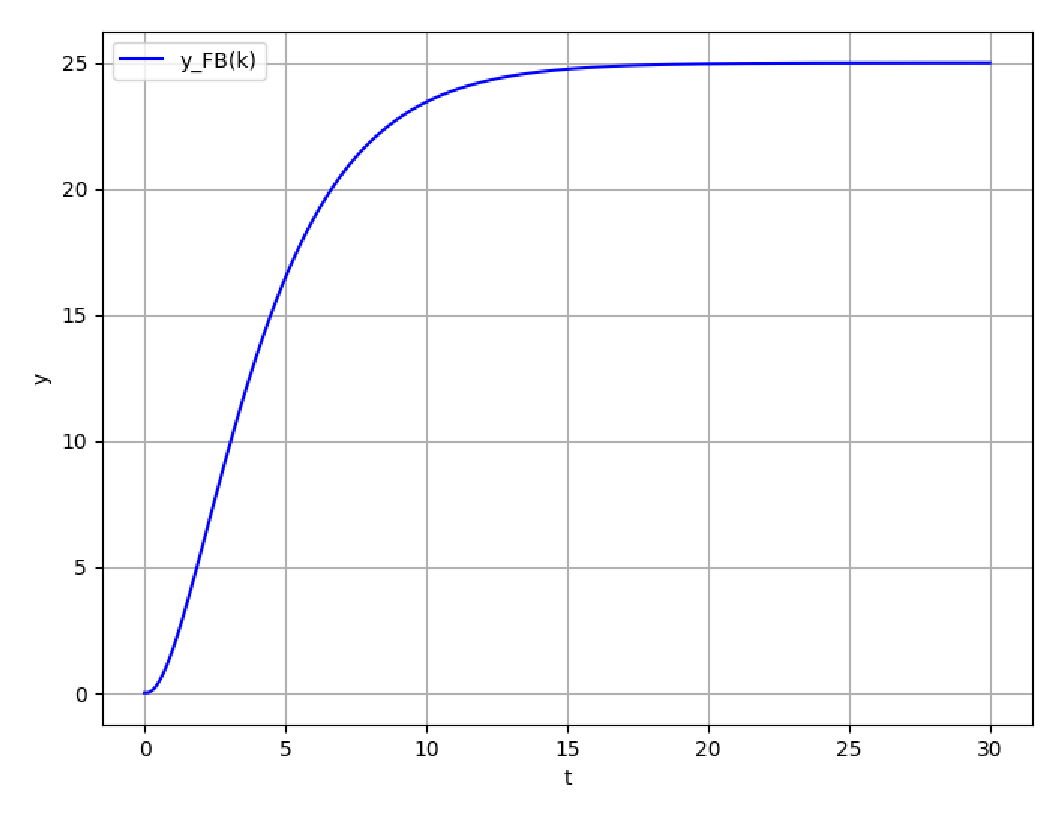
\includegraphics[scale=0.35]{figure19.eps}
    \caption{ボールの位置のシミュレーション結果}
    \label{fig:figure28}
  \end{minipage}
  \begin{minipage}[h]{0.4\linewidth}
    \centering
    \scalebox{0.45}[0.45]{
\begin{tikzpicture}[gnuplot]
%% generated with GNUPLOT 5.4p10 (Lua 5.4; terminal rev. Jun 2020, script rev. 118)
%% Sun Nov 19 18:47:22 2023
\path (0.000,0.000) rectangle (12.500,8.750);
\gpcolor{color=gp lt color border}
\gpsetlinetype{gp lt border}
\gpsetdashtype{gp dt solid}
\gpsetlinewidth{1.00}
\draw[gp path] (0.018,0.031)--(0.198,0.031);
\draw[gp path] (12.480,0.031)--(12.300,0.031);
\node[gp node right] at (-0.166,0.031) {$0$};
\draw[gp path] (0.018,1.272)--(0.198,1.272);
\draw[gp path] (12.480,1.272)--(12.300,1.272);
\node[gp node right] at (-0.166,1.272) {$5$};
\draw[gp path] (0.018,2.513)--(0.198,2.513);
\draw[gp path] (12.480,2.513)--(12.300,2.513);
\node[gp node right] at (-0.166,2.513) {$10$};
\draw[gp path] (0.018,3.754)--(0.198,3.754);
\draw[gp path] (12.480,3.754)--(12.300,3.754);
\node[gp node right] at (-0.166,3.754) {$15$};
\draw[gp path] (0.018,4.995)--(0.198,4.995);
\draw[gp path] (12.480,4.995)--(12.300,4.995);
\node[gp node right] at (-0.166,4.995) {$20$};
\draw[gp path] (0.018,6.236)--(0.198,6.236);
\draw[gp path] (12.480,6.236)--(12.300,6.236);
\node[gp node right] at (-0.166,6.236) {$25$};
\draw[gp path] (0.018,7.477)--(0.198,7.477);
\draw[gp path] (12.480,7.477)--(12.300,7.477);
\node[gp node right] at (-0.166,7.477) {$30$};
\draw[gp path] (0.018,8.718)--(0.198,8.718);
\draw[gp path] (12.480,8.718)--(12.300,8.718);
\node[gp node right] at (-0.166,8.718) {$35$};
\draw[gp path] (0.018,0.031)--(0.018,0.211);
\draw[gp path] (0.018,8.718)--(0.018,8.538);
\node[gp node center] at (0.018,-0.277) {$0$};
\draw[gp path] (2.185,0.031)--(2.185,0.211);
\draw[gp path] (2.185,8.718)--(2.185,8.538);
\node[gp node center] at (2.185,-0.277) {$20$};
\draw[gp path] (4.353,0.031)--(4.353,0.211);
\draw[gp path] (4.353,8.718)--(4.353,8.538);
\node[gp node center] at (4.353,-0.277) {$40$};
\draw[gp path] (6.520,0.031)--(6.520,0.211);
\draw[gp path] (6.520,8.718)--(6.520,8.538);
\node[gp node center] at (6.520,-0.277) {$60$};
\draw[gp path] (8.687,0.031)--(8.687,0.211);
\draw[gp path] (8.687,8.718)--(8.687,8.538);
\node[gp node center] at (8.687,-0.277) {$80$};
\draw[gp path] (10.855,0.031)--(10.855,0.211);
\draw[gp path] (10.855,8.718)--(10.855,8.538);
\node[gp node center] at (10.855,-0.277) {$100$};
\draw[gp path] (0.018,8.718)--(0.018,0.031)--(12.480,0.031)--(12.480,8.718)--cycle;
\node[gp node center,rotate=-270] at (-0.826,4.374) {ボールの位置$z\ /\ \mathrm{cm}$};
\node[gp node center] at (6.249,-0.738) {時間$t\ /\ \mathrm{s}$};
\gpcolor{rgb color={0.000,0.000,0.000}}
\draw[gp path] (0.018,0.479)--(0.020,1.898)--(0.022,3.810)--(0.025,5.431)--(0.027,6.509)%
  --(0.029,7.047)--(0.031,7.182)--(0.033,7.167)--(0.035,7.041)--(0.038,6.767)--(0.040,6.580)%
  --(0.042,6.589)--(0.044,6.688)--(0.046,6.786)--(0.048,6.828)--(0.051,6.805)--(0.053,6.739)%
  --(0.055,6.653)--(0.057,6.536)--(0.059,6.401)--(0.061,6.303)--(0.064,6.239)--(0.066,6.149)%
  --(0.068,6.031)--(0.070,5.960)--(0.072,5.950)--(0.074,5.958)--(0.077,5.960)--(0.079,5.947)%
  --(0.081,5.926)--(0.083,5.905)--(0.085,5.885)--(0.087,5.864)--(0.090,5.841)--(0.092,5.826)%
  --(0.094,5.829)--(0.096,5.843)--(0.098,5.857)--(0.100,5.878)--(0.103,5.903)--(0.105,5.918)%
  --(0.107,5.936)--(0.109,5.971)--(0.111,6.010)--(0.113,6.018)--(0.116,6.014)--(0.118,6.051)%
  --(0.120,6.128)--(0.122,6.198)--(0.124,6.236)--(0.126,6.308)--(0.129,6.439)--(0.131,6.573)%
  --(0.133,6.684)--(0.135,6.773)--(0.137,6.839)--(0.139,6.883)--(0.142,6.908)--(0.144,6.918)%
  --(0.146,6.915)--(0.148,6.682)--(0.150,6.179)--(0.152,5.896)--(0.155,5.996)--(0.157,6.227)%
  --(0.159,6.440)--(0.161,6.581)--(0.163,6.625)--(0.165,6.578)--(0.168,6.494)--(0.170,6.406)%
  --(0.172,6.181)--(0.174,5.798)--(0.176,5.552)--(0.178,5.525)--(0.181,5.566)--(0.183,5.603)%
  --(0.185,5.611)--(0.187,5.571)--(0.189,5.480)--(0.191,5.357)--(0.194,5.202)--(0.196,5.015)%
  --(0.198,4.834)--(0.200,4.667)--(0.202,4.507)--(0.204,4.372)--(0.207,4.270)--(0.209,4.180)%
  --(0.211,4.085)--(0.213,3.974)--(0.215,3.847)--(0.217,3.711)--(0.220,3.577)--(0.222,3.430)%
  --(0.224,3.267)--(0.226,3.108)--(0.228,2.964)--(0.230,2.835)--(0.233,2.714)--(0.235,2.600)%
  --(0.237,2.488)--(0.239,2.372)--(0.241,2.250)--(0.243,2.141)--(0.246,2.056)--(0.248,1.996)%
  --(0.250,1.979)--(0.252,2.015)--(0.254,2.106)--(0.256,2.257)--(0.259,2.444)--(0.261,2.592)%
  --(0.263,2.690)--(0.265,2.841)--(0.267,3.064)--(0.269,3.294)--(0.272,3.477)--(0.274,3.596)%
  --(0.276,3.680)--(0.278,3.747)--(0.280,3.796)--(0.282,3.830)--(0.285,3.851)--(0.287,3.862)%
  --(0.289,3.868)--(0.291,3.867)--(0.293,3.862)--(0.295,3.849)--(0.298,3.829)--(0.300,3.822)%
  --(0.302,3.831)--(0.304,3.840)--(0.306,3.847)--(0.308,3.851)--(0.311,3.852)--(0.313,3.850)%
  --(0.315,3.850)--(0.317,3.853)--(0.319,3.855)--(0.321,3.856)--(0.324,3.856)--(0.326,3.854)%
  --(0.328,3.847)--(0.330,3.835)--(0.332,3.826)--(0.334,3.816)--(0.337,3.795)--(0.339,3.760)%
  --(0.341,3.709)--(0.343,3.655)--(0.345,3.619)--(0.347,3.585)--(0.350,3.522)--(0.352,3.411)%
  --(0.354,3.252)--(0.356,3.057)--(0.358,2.809)--(0.360,2.518)--(0.363,2.257)--(0.365,2.075)%
  --(0.367,1.983)--(0.369,1.982)--(0.371,2.066)--(0.373,2.218)--(0.376,2.406)--(0.378,2.605)%
  --(0.380,2.830)--(0.382,3.109)--(0.384,3.417)--(0.386,3.733)--(0.389,4.024)--(0.391,4.260)%
  --(0.393,4.481)--(0.395,4.711)--(0.397,4.936)--(0.399,5.127)--(0.402,5.276)--(0.404,5.461)%
  --(0.406,5.709)--(0.408,5.952)--(0.410,6.158)--(0.412,6.340)--(0.415,6.506)--(0.417,6.649)%
  --(0.419,6.761)--(0.421,6.827)--(0.423,6.836)--(0.425,6.884)--(0.428,7.057)--(0.430,7.303)%
  --(0.432,7.553)--(0.434,7.790)--(0.436,7.989)--(0.438,8.154)--(0.441,8.296)--(0.443,8.379)%
  --(0.445,8.417)--(0.447,8.472)--(0.449,8.493)--(0.451,8.445)--(0.454,8.408)--(0.456,8.426)%
  --(0.458,8.473)--(0.460,8.499)--(0.462,8.488)--(0.464,8.480)--(0.467,8.494)--(0.469,8.521)%
  --(0.471,8.556)--(0.473,8.588)--(0.475,8.611)--(0.477,8.607)--(0.480,8.566)--(0.482,8.509)%
  --(0.484,8.459)--(0.486,8.434)--(0.488,8.417)--(0.490,8.329)--(0.493,8.162)--(0.495,8.033)%
  --(0.497,7.839)--(0.499,7.507)--(0.501,7.313)--(0.503,7.336)--(0.506,7.393)--(0.508,7.398)%
  --(0.510,7.376)--(0.512,7.334)--(0.514,7.236)--(0.516,7.091)--(0.519,6.941)--(0.521,6.778)%
  --(0.523,6.609)--(0.525,6.502)--(0.527,6.451)--(0.529,6.411)--(0.532,6.366)--(0.534,6.305)%
  --(0.536,6.232)--(0.538,6.157)--(0.540,6.082)--(0.542,6.013)--(0.545,5.956)--(0.547,5.913)%
  --(0.549,5.886)--(0.551,5.870)--(0.553,5.858)--(0.555,5.845)--(0.558,5.829)--(0.560,5.814)%
  --(0.562,5.787)--(0.564,5.744)--(0.566,5.726)--(0.568,5.751)--(0.571,5.795)--(0.573,5.842)%
  --(0.575,5.891)--(0.577,5.937)--(0.579,5.967)--(0.581,5.980)--(0.584,6.012)--(0.586,6.069)%
  --(0.588,6.141)--(0.590,6.235)--(0.592,6.349)--(0.595,6.448)--(0.597,6.508)--(0.599,6.543)%
  --(0.601,6.578)--(0.603,6.619)--(0.605,6.667)--(0.608,6.721)--(0.610,6.758)--(0.612,6.762)%
  --(0.614,6.772)--(0.616,6.805)--(0.618,6.843)--(0.621,6.872)--(0.623,6.884)--(0.625,6.885)%
  --(0.627,6.886)--(0.629,6.875)--(0.631,6.835)--(0.634,6.774)--(0.636,6.711)--(0.638,6.621)%
  --(0.640,6.493)--(0.642,6.363)--(0.644,6.256)--(0.647,6.180)--(0.649,6.130)--(0.651,6.081)%
  --(0.653,6.021)--(0.655,5.927)--(0.657,5.785)--(0.660,5.646)--(0.662,5.545)--(0.664,5.459)%
  --(0.666,5.397)--(0.668,5.367)--(0.670,5.340)--(0.673,5.306)--(0.675,5.295)--(0.677,5.307)%
  --(0.679,5.315)--(0.681,5.290)--(0.683,5.232)--(0.686,5.198)--(0.688,5.193)--(0.690,5.198)%
  --(0.692,5.245)--(0.694,5.300)--(0.696,5.321)--(0.699,5.354)--(0.701,5.389)--(0.703,5.406)%
  --(0.705,5.450)--(0.707,5.542)--(0.709,5.663)--(0.712,5.786)--(0.714,5.911)--(0.716,6.040)%
  --(0.718,6.164)--(0.720,6.245)--(0.722,6.271)--(0.725,6.309)--(0.727,6.381)--(0.729,6.453)%
  --(0.731,6.512)--(0.733,6.544)--(0.735,6.547)--(0.738,6.576)--(0.740,6.643)--(0.742,6.707)%
  --(0.744,6.745)--(0.746,6.691)--(0.748,6.539)--(0.751,6.457)--(0.753,6.493)--(0.755,6.523)%
  --(0.757,6.494)--(0.759,6.468)--(0.761,6.470)--(0.764,6.471)--(0.766,6.451)--(0.768,6.393)%
  --(0.770,6.276)--(0.772,6.128)--(0.774,6.023)--(0.777,5.980)--(0.779,5.964)--(0.781,5.957)%
  --(0.783,5.927)--(0.785,5.854)--(0.787,5.774)--(0.790,5.717)--(0.792,5.672)--(0.794,5.639)%
  --(0.796,5.621)--(0.798,5.610)--(0.800,5.578)--(0.803,5.525)--(0.805,5.487)--(0.807,5.483)%
  --(0.809,5.497)--(0.811,5.516)--(0.813,5.531)--(0.816,5.540)--(0.818,5.532)--(0.820,5.506)%
  --(0.822,5.487)--(0.824,5.492)--(0.826,5.520)--(0.829,5.549)--(0.831,5.569)--(0.833,5.587)%
  --(0.835,5.591)--(0.837,5.574)--(0.839,5.554)--(0.842,5.545)--(0.844,5.565)--(0.846,5.619)%
  --(0.848,5.701)--(0.850,5.789)--(0.852,5.818)--(0.855,5.781)--(0.857,5.771)--(0.859,5.811)%
  --(0.861,5.852)--(0.863,5.880)--(0.865,5.904)--(0.868,5.924)--(0.870,5.953)--(0.872,5.994)%
  --(0.874,6.019)--(0.876,6.018)--(0.878,6.006)--(0.881,5.993)--(0.883,5.982)--(0.885,5.975)%
  --(0.887,5.972)--(0.889,5.971)--(0.891,5.971)--(0.894,5.944)--(0.896,5.876)--(0.898,5.804)%
  --(0.900,5.741)--(0.902,5.697)--(0.904,5.674)--(0.907,5.658)--(0.909,5.638)--(0.911,5.621)%
  --(0.913,5.614)--(0.915,5.601)--(0.917,5.578)--(0.920,5.532)--(0.922,5.463)--(0.924,5.382)%
  --(0.926,5.306)--(0.928,5.244)--(0.930,5.194)--(0.933,5.137)--(0.935,5.062)--(0.937,5.020)%
  --(0.939,5.034)--(0.941,5.069)--(0.943,5.084)--(0.946,4.927)--(0.948,4.618)--(0.950,4.493)%
  --(0.952,4.610)--(0.954,4.793)--(0.956,5.010)--(0.959,5.232)--(0.961,5.393)--(0.963,5.478)%
  --(0.965,5.533)--(0.967,5.589)--(0.969,5.650)--(0.972,5.706)--(0.974,5.750)--(0.976,5.794)%
  --(0.978,5.848)--(0.980,5.927)--(0.982,6.002)--(0.985,6.048)--(0.987,6.128)--(0.989,6.269)%
  --(0.991,6.417)--(0.993,6.519)--(0.995,6.582)--(0.998,6.655)--(1.000,6.725)--(1.002,6.773)%
  --(1.004,6.811)--(1.006,6.842)--(1.008,6.856)--(1.011,6.841)--(1.013,6.807)--(1.015,6.758)%
  --(1.017,6.707)--(1.019,6.669)--(1.021,6.644)--(1.024,6.585)--(1.026,6.471)--(1.028,6.351)%
  --(1.030,6.261)--(1.032,6.198)--(1.034,6.142)--(1.037,6.072)--(1.039,5.980)--(1.041,5.876)%
  --(1.043,5.786)--(1.045,5.716)--(1.047,5.655)--(1.050,5.603)--(1.052,5.553)--(1.054,5.505)%
  --(1.056,5.458)--(1.058,5.414)--(1.060,5.372)--(1.063,5.337)--(1.065,5.314)--(1.067,5.304)%
  --(1.069,5.292)--(1.071,5.271)--(1.073,5.262)--(1.076,5.267)--(1.078,5.276)--(1.080,5.289)%
  --(1.082,5.313)--(1.084,5.307)--(1.086,5.264)--(1.089,5.262)--(1.091,5.332)--(1.093,5.405)%
  --(1.095,5.453)--(1.097,5.526)--(1.099,5.637)--(1.102,5.754)--(1.104,5.838)--(1.106,5.884)%
  --(1.108,5.954)--(1.110,6.070)--(1.112,6.206)--(1.115,6.354)--(1.117,6.505)--(1.119,6.612)%
  --(1.121,6.653)--(1.123,6.655)--(1.125,6.648)--(1.128,6.638)--(1.130,6.634)--(1.132,6.669)%
  --(1.134,6.736)--(1.136,6.800)--(1.138,6.853)--(1.141,6.888)--(1.143,6.902)--(1.145,6.903)%
  --(1.147,6.899)--(1.149,6.891)--(1.152,6.885)--(1.154,6.878)--(1.156,6.862)--(1.158,6.832)%
  --(1.160,6.798)--(1.162,6.769)--(1.165,6.743)--(1.167,6.696)--(1.169,6.628)--(1.171,6.578)%
  --(1.173,6.554)--(1.175,6.543)--(1.178,6.541)--(1.180,6.542)--(1.182,6.545)--(1.184,6.550)%
  --(1.186,6.553)--(1.188,6.552)--(1.191,6.549)--(1.193,6.542)--(1.195,6.537)--(1.197,6.539)%
  --(1.199,6.545)--(1.201,6.549)--(1.204,6.554)--(1.206,6.563)--(1.208,6.569)--(1.210,6.569)%
  --(1.212,6.567)--(1.214,6.562)--(1.217,6.556)--(1.219,6.553)--(1.221,6.553)--(1.223,6.538)%
  --(1.225,6.501)--(1.227,6.474)--(1.230,6.471)--(1.232,6.489)--(1.234,6.532)--(1.236,6.578)%
  --(1.238,6.567)--(1.240,6.499)--(1.243,6.463)--(1.245,6.477)--(1.247,6.504)--(1.249,6.546)%
  --(1.251,6.599)--(1.253,6.627)--(1.256,6.622)--(1.258,6.600)--(1.260,6.574)--(1.262,6.555)%
  --(1.264,6.563)--(1.266,6.588)--(1.269,6.599)--(1.271,6.585)--(1.273,6.549)--(1.275,6.500)%
  --(1.277,6.446)--(1.279,6.396)--(1.282,6.332)--(1.284,6.242)--(1.286,6.180)--(1.288,6.163)%
  --(1.290,6.157)--(1.292,6.139)--(1.295,6.101)--(1.297,6.049)--(1.299,5.998)--(1.301,5.951)%
  --(1.303,5.903)--(1.305,5.850)--(1.308,5.818)--(1.310,5.788)--(1.312,5.733)--(1.314,5.699)%
  --(1.316,5.709)--(1.318,5.733)--(1.321,5.767)--(1.323,5.811)--(1.325,5.821)--(1.327,5.784)%
  --(1.329,5.763)--(1.331,5.796)--(1.334,5.867)--(1.336,5.953)--(1.338,6.019)--(1.340,6.063)%
  --(1.342,5.986)--(1.344,5.778)--(1.347,5.743)--(1.349,5.962)--(1.351,6.258)--(1.353,6.536)%
  --(1.355,6.754)--(1.357,6.907)--(1.360,7.003)--(1.362,7.024)--(1.364,6.999)--(1.366,7.019)%
  --(1.368,7.100)--(1.370,7.201)--(1.373,7.291)--(1.375,7.358)--(1.377,7.399)--(1.379,7.415)%
  --(1.381,7.413)--(1.383,7.407)--(1.386,7.402)--(1.388,7.398)--(1.390,7.372)--(1.392,7.317)%
  --(1.394,7.262)--(1.396,7.214)--(1.399,7.157)--(1.401,7.062)--(1.403,6.934)--(1.405,6.788)%
  --(1.407,6.633)--(1.409,6.541)--(1.412,6.514)--(1.414,6.481)--(1.416,6.435)--(1.418,6.381)%
  --(1.420,6.312)--(1.422,6.221)--(1.425,6.098)--(1.427,5.955)--(1.429,5.812)--(1.431,5.684)%
  --(1.433,5.590)--(1.435,5.512)--(1.438,5.436)--(1.440,5.349)--(1.442,5.250)--(1.444,5.164)%
  --(1.446,5.103)--(1.448,5.059)--(1.451,5.021)--(1.453,4.984)--(1.455,4.959)--(1.457,4.949)%
  --(1.459,4.935)--(1.461,4.906)--(1.464,4.886)--(1.466,4.889)--(1.468,4.885)--(1.470,4.864)%
  --(1.472,4.842)--(1.474,4.826)--(1.477,4.819)--(1.479,4.830)--(1.481,4.867)--(1.483,4.923)%
  --(1.485,5.006)--(1.487,5.115)--(1.490,5.235)--(1.492,5.355)--(1.494,5.464)--(1.496,5.562)%
  --(1.498,5.651)--(1.500,5.725)--(1.503,5.791)--(1.505,5.880)--(1.507,5.996)--(1.509,6.119)%
  --(1.511,6.223)--(1.513,6.298)--(1.516,6.351)--(1.518,6.394)--(1.520,6.433)--(1.522,6.470)%
  --(1.524,6.503)--(1.526,6.526)--(1.529,6.543)--(1.531,6.546)--(1.533,6.527)--(1.535,6.499)%
  --(1.537,6.476)--(1.539,6.420)--(1.542,6.317)--(1.544,6.232)--(1.546,6.184)--(1.548,6.147)%
  --(1.550,6.106)--(1.552,6.055)--(1.555,5.996)--(1.557,5.914)--(1.559,5.818)--(1.561,5.733)%
  --(1.563,5.659)--(1.565,5.588)--(1.568,5.520)--(1.570,5.465)--(1.572,5.421)--(1.574,5.363)%
  --(1.576,5.287)--(1.578,5.217)--(1.581,5.156)--(1.583,5.130)--(1.585,5.144)--(1.587,5.178)%
  --(1.589,5.221)--(1.591,5.261)--(1.594,5.283)--(1.596,5.296)--(1.598,5.316)--(1.600,5.333)%
  --(1.602,5.348)--(1.604,5.383)--(1.607,5.436)--(1.609,5.520)--(1.611,5.612)--(1.613,5.688)%
  --(1.615,5.796)--(1.617,5.947)--(1.620,6.093)--(1.622,6.223)--(1.624,6.340)--(1.626,6.438)%
  --(1.628,6.510)--(1.630,6.567)--(1.633,6.629)--(1.635,6.672)--(1.637,6.695)--(1.639,6.719)%
  --(1.641,6.751)--(1.643,6.794)--(1.646,6.837)--(1.648,6.889)--(1.650,6.952)--(1.652,6.989)%
  --(1.654,6.955)--(1.656,6.867)--(1.659,6.806)--(1.661,6.821)--(1.663,6.873)--(1.665,6.889)%
  --(1.667,6.859)--(1.669,6.824)--(1.672,6.783)--(1.674,6.719)--(1.676,6.635)--(1.678,6.567)%
  --(1.680,6.508)--(1.682,6.420)--(1.685,6.337)--(1.687,6.274)--(1.689,6.196)--(1.691,6.120)%
  --(1.693,6.053)--(1.695,5.969)--(1.698,5.872)--(1.700,5.765)--(1.702,5.632)--(1.704,5.507)%
  --(1.706,5.442)--(1.708,5.438)--(1.711,5.460)--(1.713,5.476)--(1.715,5.485)--(1.717,5.498)%
  --(1.719,5.506)--(1.722,5.509)--(1.724,5.522)--(1.726,5.551)--(1.728,5.574)--(1.730,5.577)%
  --(1.732,5.589)--(1.735,5.617)--(1.737,5.647)--(1.739,5.708)--(1.741,5.813)--(1.743,5.935)%
  --(1.745,6.055)--(1.748,6.166)--(1.750,6.268)--(1.752,6.358)--(1.754,6.432)--(1.756,6.479)%
  --(1.758,6.499)--(1.761,6.476)--(1.763,6.423)--(1.765,6.416)--(1.767,6.469)--(1.769,6.532)%
  --(1.771,6.585)--(1.774,6.622)--(1.776,6.605)--(1.778,6.499)--(1.780,6.396)--(1.782,6.413)%
  --(1.784,6.495)--(1.787,6.537)--(1.789,6.526)--(1.791,6.473)--(1.793,6.385)--(1.795,6.291)%
  --(1.797,6.209)--(1.800,6.154)--(1.802,6.133)--(1.804,6.115)--(1.806,6.077)--(1.808,6.034)%
  --(1.810,6.000)--(1.813,5.978)--(1.815,5.962)--(1.817,5.952)--(1.819,5.915)--(1.821,5.858)%
  --(1.823,5.857)--(1.826,5.912)--(1.828,5.987)--(1.830,6.068)--(1.832,6.099)--(1.834,5.964)%
  --(1.836,5.728)--(1.839,5.643)--(1.841,5.748)--(1.843,5.938)--(1.845,6.151)--(1.847,6.340)%
  --(1.849,6.488)--(1.852,6.590)--(1.854,6.652)--(1.856,6.682)--(1.858,6.695)--(1.860,6.705)%
  --(1.862,6.729)--(1.865,6.781)--(1.867,6.860)--(1.869,6.934)--(1.871,6.981)--(1.873,7.028)%
  --(1.875,7.095)--(1.878,7.148)--(1.880,7.170)--(1.882,7.166)--(1.884,7.133)--(1.886,7.084)%
  --(1.888,7.035)--(1.891,6.997)--(1.893,6.961)--(1.895,6.919)--(1.897,6.859)--(1.899,6.781)%
  --(1.901,6.683)--(1.904,6.555)--(1.906,6.427)--(1.908,6.309)--(1.910,6.179)--(1.912,6.069)%
  --(1.914,5.998)--(1.917,5.931)--(1.919,5.832)--(1.921,5.688)--(1.923,5.539)--(1.925,5.397)%
  --(1.927,5.254)--(1.930,5.116)--(1.932,4.984)--(1.934,4.856)--(1.936,4.732)--(1.938,4.617)%
  --(1.940,4.517)--(1.943,4.431)--(1.945,4.359)--(1.947,4.298)--(1.949,4.238)--(1.951,4.157)%
  --(1.953,4.062)--(1.956,3.990)--(1.958,3.953)--(1.960,3.929)--(1.962,3.910)--(1.964,3.894)%
  --(1.966,3.866)--(1.969,3.806)--(1.971,3.732)--(1.973,3.675)--(1.975,3.639)--(1.977,3.616)%
  --(1.979,3.597)--(1.982,3.573)--(1.984,3.544)--(1.986,3.522)--(1.988,3.517)--(1.990,3.521)%
  --(1.992,3.530)--(1.995,3.537)--(1.997,3.547)--(1.999,3.564)--(2.001,3.590)--(2.003,3.629)%
  --(2.005,3.664)--(2.008,3.687)--(2.010,3.726)--(2.012,3.792)--(2.014,3.873)--(2.016,3.958)%
  --(2.018,4.039)--(2.021,4.111)--(2.023,4.077)--(2.025,3.933)--(2.027,3.904)--(2.029,4.049)%
  --(2.031,4.247)--(2.034,4.432)--(2.036,4.569)--(2.038,4.650)--(2.040,4.683)--(2.042,4.678)%
  --(2.044,4.650)--(2.047,4.623)--(2.049,4.585)--(2.051,4.514)--(2.053,4.430)--(2.055,4.346)%
  --(2.057,4.263)--(2.060,4.191)--(2.062,4.121)--(2.064,4.058)--(2.066,4.001)--(2.068,3.940)%
  --(2.070,3.869)--(2.073,3.787)--(2.075,3.697)--(2.077,3.607)--(2.079,3.516)--(2.081,3.422)%
  --(2.083,3.341)--(2.086,3.284)--(2.088,3.245)--(2.090,3.204)--(2.092,3.155)--(2.094,3.121)%
  --(2.096,3.114)--(2.099,3.122)--(2.101,3.146)--(2.103,3.188)--(2.105,3.241)--(2.107,3.298)%
  --(2.109,3.357)--(2.112,3.421)--(2.114,3.489)--(2.116,3.563)--(2.118,3.641)--(2.120,3.711)%
  --(2.122,3.769)--(2.125,3.827)--(2.127,3.893)--(2.129,3.968)--(2.131,4.051)--(2.133,4.152)%
  --(2.135,4.288)--(2.138,4.442)--(2.140,4.590)--(2.142,4.719)--(2.144,4.822)--(2.146,4.895)%
  --(2.148,4.947)--(2.151,4.986)--(2.153,5.019)--(2.155,5.053)--(2.157,5.077)--(2.159,5.082)%
  --(2.161,5.073)--(2.164,5.057)--(2.166,5.033)--(2.168,5.003)--(2.170,4.967)--(2.172,4.925)%
  --(2.174,4.877)--(2.177,4.825)--(2.179,4.765)--(2.181,4.702)--(2.183,4.634)--(2.185,4.560)%
  --(2.187,4.477)--(2.190,4.375)--(2.192,4.266)--(2.194,4.179)--(2.196,4.125)--(2.198,4.092)%
  --(2.200,4.072)--(2.203,4.057)--(2.205,4.052)--(2.207,4.056)--(2.209,4.064)--(2.211,4.074)%
  --(2.213,4.085)--(2.216,4.089)--(2.218,4.089)--(2.220,4.093)--(2.222,4.105)--(2.224,4.119)%
  --(2.226,4.137)--(2.229,4.182)--(2.231,4.250)--(2.233,4.309)--(2.235,4.354)--(2.237,4.433)%
  --(2.239,4.562)--(2.242,4.698)--(2.244,4.813)--(2.246,4.909)--(2.248,4.988)--(2.250,5.047)%
  --(2.252,5.086)--(2.255,5.117)--(2.257,5.141)--(2.259,5.158)--(2.261,5.147)--(2.263,5.104)%
  --(2.265,5.079)--(2.268,5.090)--(2.270,5.116)--(2.272,5.133)--(2.274,5.115)--(2.276,5.062)%
  --(2.278,4.990)--(2.281,4.907)--(2.283,4.812)--(2.285,4.718)--(2.287,4.634)--(2.289,4.538)%
  --(2.292,4.436)--(2.294,4.376)--(2.296,4.362)--(2.298,4.366)--(2.300,4.374)--(2.302,4.381)%
  --(2.305,4.388)--(2.307,4.394)--(2.309,4.395)--(2.311,4.399)--(2.313,4.413)--(2.315,4.335)%
  --(2.318,4.081)--(2.320,3.845)--(2.322,3.834)--(2.324,4.010)--(2.326,4.244)--(2.328,4.463)%
  --(2.331,4.651)--(2.333,4.804)--(2.335,4.917)--(2.337,5.002)--(2.339,4.943)--(2.341,4.736)%
  --(2.344,4.674)--(2.346,4.842)--(2.348,5.072)--(2.350,5.297)--(2.352,5.517)--(2.354,5.702)%
  --(2.357,5.839)--(2.359,5.965)--(2.361,6.052)--(2.363,6.086)--(2.365,6.117)--(2.367,6.159)%
  --(2.370,6.179)--(2.372,6.169)--(2.374,6.169)--(2.376,6.191)--(2.378,6.217)--(2.380,6.203)%
  --(2.383,6.134)--(2.385,6.074)--(2.387,6.046)--(2.389,6.039)--(2.391,5.916)--(2.393,5.616)%
  --(2.396,5.400)--(2.398,5.377)--(2.400,5.406)--(2.402,5.408)--(2.404,5.374)--(2.406,5.296)%
  --(2.409,5.177)--(2.411,5.043)--(2.413,4.920)--(2.415,4.845)--(2.417,4.810)--(2.419,4.778)%
  --(2.422,4.743)--(2.424,4.703)--(2.426,4.660)--(2.428,4.620)--(2.430,4.581)--(2.432,4.550)%
  --(2.435,4.533)--(2.437,4.524)--(2.439,4.520)--(2.441,4.523)--(2.443,4.523)--(2.445,4.516)%
  --(2.448,4.507)--(2.450,4.487)--(2.452,4.457)--(2.454,4.454)--(2.456,4.483)--(2.458,4.517)%
  --(2.461,4.530)--(2.463,4.533)--(2.465,4.571)--(2.467,4.648)--(2.469,4.738)--(2.471,4.826)%
  --(2.474,4.911)--(2.476,5.007)--(2.478,5.113)--(2.480,5.218)--(2.482,5.318)--(2.484,5.405)%
  --(2.487,5.476)--(2.489,5.519)--(2.491,5.528)--(2.493,5.522)--(2.495,5.524)--(2.497,5.538)%
  --(2.500,5.548)--(2.502,5.547)--(2.504,5.522)--(2.506,5.460)--(2.508,5.383)--(2.510,5.325)%
  --(2.513,5.286)--(2.515,5.246)--(2.517,5.203)--(2.519,5.160)--(2.521,5.115)--(2.523,5.052)%
  --(2.526,4.979)--(2.528,4.920)--(2.530,4.888)--(2.532,4.863)--(2.534,4.824)--(2.536,4.749)%
  --(2.539,4.647)--(2.541,4.605)--(2.543,4.642)--(2.545,4.705)--(2.547,4.775)--(2.549,4.839)%
  --(2.552,4.888)--(2.554,4.931)--(2.556,4.968)--(2.558,4.997)--(2.560,4.956)--(2.562,4.843)%
  --(2.565,4.793)--(2.567,4.848)--(2.569,4.945)--(2.571,5.041)--(2.573,5.120)--(2.575,5.202)%
  --(2.578,5.311)--(2.580,5.445)--(2.582,5.583)--(2.584,5.684)--(2.586,5.745)--(2.588,5.805)%
  --(2.591,5.868)--(2.593,5.955)--(2.595,6.074)--(2.597,6.204)--(2.599,6.315)--(2.601,6.380)%
  --(2.604,6.405)--(2.606,6.423)--(2.608,6.445)--(2.610,6.469)--(2.612,6.371)--(2.614,6.128)%
  --(2.617,6.005)--(2.619,6.088)--(2.621,6.237)--(2.623,6.381)--(2.625,6.486)--(2.627,6.537)%
  --(2.630,6.510)--(2.632,6.428)--(2.634,6.367)--(2.636,6.350)--(2.638,6.349)--(2.640,6.313)%
  --(2.643,6.246)--(2.645,6.199)--(2.647,6.144)--(2.649,6.058)--(2.651,5.987)--(2.653,5.947)%
  --(2.656,5.909)--(2.658,5.854)--(2.660,5.789)--(2.662,5.726)--(2.664,5.670)--(2.666,5.619)%
  --(2.669,5.590)--(2.671,5.584)--(2.673,5.570)--(2.675,5.502)--(2.677,5.386)--(2.679,5.307)%
  --(2.682,5.301)--(2.684,5.348)--(2.686,5.419)--(2.688,5.457)--(2.690,5.437)--(2.692,5.406)%
  --(2.695,5.420)--(2.697,5.475)--(2.699,5.544)--(2.701,5.600)--(2.703,5.636)--(2.705,5.676)%
  --(2.708,5.735)--(2.710,5.814)--(2.712,5.894)--(2.714,5.976)--(2.716,6.084)--(2.718,6.206)%
  --(2.721,6.312)--(2.723,6.391)--(2.725,6.448)--(2.727,6.516)--(2.729,6.610)--(2.731,6.683)%
  --(2.734,6.717)--(2.736,6.738)--(2.738,6.745)--(2.740,6.735)--(2.742,6.727)--(2.744,6.739)%
  --(2.747,6.767)--(2.749,6.787)--(2.751,6.783)--(2.753,6.751)--(2.755,6.699)--(2.757,6.642)%
  --(2.760,6.599)--(2.762,6.572)--(2.764,6.548)--(2.766,6.513)--(2.768,6.443)--(2.770,6.349)%
  --(2.773,6.285)--(2.775,6.264)--(2.777,6.257)--(2.779,6.254)--(2.781,6.253)--(2.783,6.253)%
  --(2.786,6.250)--(2.788,6.241)--(2.790,6.231)--(2.792,6.246)--(2.794,6.287)--(2.796,6.317)%
  --(2.799,6.328)--(2.801,6.358)--(2.803,6.422)--(2.805,6.480)--(2.807,6.513)--(2.809,6.540)%
  --(2.812,6.570)--(2.814,6.608)--(2.816,6.655)--(2.818,6.722)--(2.820,6.819)--(2.822,6.930)%
  --(2.825,7.027)--(2.827,7.095)--(2.829,7.133)--(2.831,7.150)--(2.833,7.136)--(2.835,7.096)%
  --(2.838,7.091)--(2.840,7.129)--(2.842,7.169)--(2.844,7.198)--(2.846,7.213)--(2.848,7.208)%
  --(2.851,7.200)--(2.853,7.195)--(2.855,7.178)--(2.857,7.145)--(2.859,7.071)--(2.862,6.933)%
  --(2.864,6.765)--(2.866,6.625)--(2.868,6.505)--(2.870,6.383)--(2.872,6.303)--(2.875,6.261)%
  --(2.877,6.217)--(2.879,6.173)--(2.881,6.143)--(2.883,6.140)--(2.885,6.137)--(2.888,6.118)%
  --(2.890,6.096)--(2.892,6.044)--(2.894,5.953)--(2.896,5.890)--(2.898,5.874)--(2.901,5.870)%
  --(2.903,5.877)--(2.905,5.896)--(2.907,5.892)--(2.909,5.856)--(2.911,5.836)--(2.914,5.856)%
  --(2.916,5.894)--(2.918,5.931)--(2.920,5.964)--(2.922,5.995)--(2.924,6.019)--(2.927,6.054)%
  --(2.929,6.083)--(2.931,6.072)--(2.933,6.074)--(2.935,6.123)--(2.937,6.195)--(2.940,6.267)%
  --(2.942,6.319)--(2.944,6.351)--(2.946,6.370)--(2.948,6.373)--(2.950,6.358)--(2.953,6.359)%
  --(2.955,6.383)--(2.957,6.403)--(2.959,6.396)--(2.961,6.362)--(2.963,6.351)--(2.966,6.380)%
  --(2.968,6.337)--(2.970,6.060)--(2.972,5.677)--(2.974,5.522)--(2.976,5.601)--(2.979,5.670)%
  --(2.981,5.644)--(2.983,5.632)--(2.985,5.633)--(2.987,5.579)--(2.989,5.495)--(2.992,5.393)%
  --(2.994,5.278)--(2.996,5.163)--(2.998,5.065)--(3.000,4.973)--(3.002,4.863)--(3.005,4.744)%
  --(3.007,4.614)--(3.009,4.464)--(3.011,4.306)--(3.013,4.146)--(3.015,3.973)--(3.018,3.786)%
  --(3.020,3.609)--(3.022,3.454)--(3.024,3.319)--(3.026,3.186)--(3.028,3.054)--(3.031,2.928)%
  --(3.033,2.809)--(3.035,2.700)--(3.037,2.594)--(3.039,2.488)--(3.041,2.399)--(3.044,2.331)%
  --(3.046,2.274)--(3.048,2.222)--(3.050,2.174)--(3.052,2.131)--(3.054,2.093)--(3.057,2.064)%
  --(3.059,2.043)--(3.061,2.024)--(3.063,2.007)--(3.065,2.005)--(3.067,2.024)--(3.070,2.056)%
  --(3.072,2.094)--(3.074,2.139)--(3.076,2.190)--(3.078,2.245)--(3.080,2.303)--(3.083,2.369)%
  --(3.085,2.446)--(3.087,2.549)--(3.089,2.682)--(3.091,2.808)--(3.093,2.917)--(3.096,3.018)%
  --(3.098,3.022)--(3.100,2.930)--(3.102,2.946)--(3.104,3.112)--(3.106,3.318)--(3.109,3.517)%
  --(3.111,3.689)--(3.113,3.826)--(3.115,3.933)--(3.117,4.022)--(3.119,4.095)--(3.122,4.146)%
  --(3.124,4.175)--(3.126,4.172)--(3.128,4.141)--(3.130,4.113)--(3.132,4.081)--(3.135,4.025)%
  --(3.137,3.937)--(3.139,3.832)--(3.141,3.722)--(3.143,3.621)--(3.145,3.532)--(3.148,3.435)%
  --(3.150,3.321)--(3.152,3.190)--(3.154,3.043)--(3.156,2.878)--(3.158,2.701)--(3.161,2.516)%
  --(3.163,2.340)--(3.165,2.209)--(3.167,2.157)--(3.169,2.207)--(3.171,2.378)--(3.174,2.623)%
  --(3.176,2.857)--(3.178,3.051)--(3.180,3.219)--(3.182,3.373)--(3.184,3.512)--(3.187,3.620)%
  --(3.189,3.694)--(3.191,3.762)--(3.193,3.827)--(3.195,3.873)--(3.197,3.900)--(3.200,3.895)%
  --(3.202,3.859)--(3.204,3.814)--(3.206,3.776)--(3.208,3.759)--(3.210,3.754)--(3.213,3.746)%
  --(3.215,3.730)--(3.217,3.708)--(3.219,3.685)--(3.221,3.669)--(3.223,3.666)--(3.226,3.672)%
  --(3.228,3.677)--(3.230,3.665)--(3.232,3.661)--(3.234,3.694)--(3.236,3.747)--(3.239,3.797)%
  --(3.241,3.833)--(3.243,3.853)--(3.245,3.860)--(3.247,3.863)--(3.249,3.862)--(3.252,3.859)%
  --(3.254,3.857)--(3.256,3.856)--(3.258,3.856)--(3.260,3.856)--(3.262,3.859)--(3.265,3.866)%
  --(3.267,3.878)--(3.269,3.889)--(3.271,3.896)--(3.273,3.885)--(3.275,3.858)--(3.278,3.851)%
  --(3.280,3.864)--(3.282,3.877)--(3.284,3.888)--(3.286,3.894)--(3.288,3.884)--(3.291,3.858)%
  --(3.293,3.845)--(3.295,3.853)--(3.297,3.866)--(3.299,3.880)--(3.301,3.891)--(3.304,3.898)%
  --(3.306,3.900)--(3.308,3.900)--(3.310,3.898)--(3.312,3.889)--(3.314,3.878)--(3.317,3.856)%
  --(3.319,3.820)--(3.321,3.806)--(3.323,3.823)--(3.325,3.845)--(3.327,3.859)--(3.330,3.863)%
  --(3.332,3.862)--(3.334,3.861)--(3.336,3.861)--(3.338,3.860)--(3.340,3.857)--(3.343,3.854)%
  --(3.345,3.854)--(3.347,3.856)--(3.349,3.858)--(3.351,3.858)--(3.353,3.858)--(3.356,3.857)%
  --(3.358,3.856)--(3.360,3.856)--(3.362,3.854)--(3.364,3.855)--(3.366,3.859)--(3.369,3.848)%
  --(3.371,3.818)--(3.373,3.800)--(3.375,3.805)--(3.377,3.825)--(3.379,3.850)--(3.382,3.863)%
  --(3.384,3.861)--(3.386,3.856)--(3.388,3.855)--(3.390,3.859)--(3.392,3.855)--(3.395,3.831)%
  --(3.397,3.816)--(3.399,3.822)--(3.401,3.834)--(3.403,3.846)--(3.405,3.854)--(3.408,3.858)%
  --(3.410,3.858)--(3.412,3.855)--(3.414,3.853)--(3.416,3.854)--(3.419,3.859)--(3.421,3.868)%
  --(3.423,3.872)--(3.425,3.870)--(3.427,3.865)--(3.429,3.862)--(3.432,3.861)--(3.434,3.859)%
  --(3.436,3.855)--(3.438,3.853)--(3.440,3.855)--(3.442,3.857)--(3.445,3.857)--(3.447,3.854)%
  --(3.449,3.841)--(3.451,3.816)--(3.453,3.801)--(3.455,3.808)--(3.458,3.822)--(3.460,3.823)%
  --(3.462,3.803)--(3.464,3.793)--(3.466,3.794)--(3.468,3.788)--(3.471,3.791)--(3.473,3.808)%
  --(3.475,3.825)--(3.477,3.840)--(3.479,3.848)--(3.481,3.835)--(3.484,3.804)--(3.486,3.789)%
  --(3.488,3.800)--(3.490,3.821)--(3.492,3.842)--(3.494,3.857)--(3.497,3.865)--(3.499,3.867)%
  --(3.501,3.865)--(3.503,3.863)--(3.505,3.862)--(3.507,3.862)--(3.510,3.861)--(3.512,3.858)%
  --(3.514,3.857)--(3.516,3.857)--(3.518,3.858)--(3.520,3.856)--(3.523,3.854)--(3.525,3.853)%
  --(3.527,3.851)--(3.529,3.849)--(3.531,3.850)--(3.533,3.850)--(3.536,3.849)--(3.538,3.848)%
  --(3.540,3.851)--(3.542,3.862)--(3.544,3.869)--(3.546,3.866)--(3.549,3.863)--(3.551,3.862)%
  --(3.553,3.859)--(3.555,3.857)--(3.557,3.863)--(3.559,3.867)--(3.562,3.865)--(3.564,3.862)%
  --(3.566,3.859)--(3.568,3.856)--(3.570,3.853)--(3.572,3.854)--(3.575,3.861)--(3.577,3.872)%
  --(3.579,3.878)--(3.581,3.875)--(3.583,3.871)--(3.585,3.866)--(3.588,3.862)--(3.590,3.860)%
  --(3.592,3.859)--(3.594,3.859)--(3.596,3.857)--(3.598,3.862)--(3.601,3.871)--(3.603,3.874)%
  --(3.605,3.873)--(3.607,3.877)--(3.609,3.882)--(3.611,3.876)--(3.614,3.853)--(3.616,3.826)%
  --(3.618,3.803)--(3.620,3.776)--(3.622,3.743)--(3.624,3.717)--(3.627,3.696)--(3.629,3.676)%
  --(3.631,3.651)--(3.633,3.634)--(3.635,3.625)--(3.637,3.614)--(3.640,3.618)--(3.642,3.641)%
  --(3.644,3.661)--(3.646,3.662)--(3.648,3.637)--(3.650,3.585)--(3.653,3.501)--(3.655,3.381)%
  --(3.657,3.241)--(3.659,3.088)--(3.661,2.938)--(3.663,2.793)--(3.666,2.636)--(3.668,2.470)%
  --(3.670,2.307)--(3.672,2.165)--(3.674,2.063)--(3.676,2.005)--(3.679,1.998)--(3.681,2.047)%
  --(3.683,2.155)--(3.685,2.302)--(3.687,2.455)--(3.689,2.596)--(3.692,2.719)--(3.694,2.845)%
  --(3.696,2.979)--(3.698,3.106)--(3.700,3.185)--(3.702,3.225)--(3.705,3.296)--(3.707,3.424)%
  --(3.709,3.587)--(3.711,3.752)--(3.713,3.896)--(3.715,4.014)--(3.718,4.105)--(3.720,4.174)%
  --(3.722,4.223)--(3.724,4.258)--(3.726,4.285)--(3.728,4.286)--(3.731,4.243)--(3.733,4.190)%
  --(3.735,4.165)--(3.737,4.164)--(3.739,4.163)--(3.741,4.133)--(3.744,4.045)--(3.746,3.912)%
  --(3.748,3.808)--(3.750,3.749)--(3.752,3.695)--(3.754,3.623)--(3.757,3.527)--(3.759,3.389)%
  --(3.761,3.215)--(3.763,3.035)--(3.765,2.860)--(3.767,2.700)--(3.770,2.559)--(3.772,2.438)%
  --(3.774,2.332)--(3.776,2.241)--(3.778,2.163)--(3.780,2.096)--(3.783,2.044)--(3.785,2.006)%
  --(3.787,1.984)--(3.789,1.975)--(3.791,1.980)--(3.793,1.993)--(3.796,2.010)--(3.798,2.025)%
  --(3.800,2.034)--(3.802,2.037)--(3.804,2.037)--(3.806,2.034)--(3.809,2.026)--(3.811,2.016)%
  --(3.813,1.997)--(3.815,1.973)--(3.817,1.970)--(3.819,1.999)--(3.822,2.051)--(3.824,2.122)%
  --(3.826,2.193)--(3.828,2.250)--(3.830,2.300)--(3.832,2.366)--(3.835,2.456)--(3.837,2.551)%
  --(3.839,2.635)--(3.841,2.727)--(3.843,2.863)--(3.845,3.038)--(3.848,3.199)--(3.850,3.319)%
  --(3.852,3.427)--(3.854,3.537)--(3.856,3.632)--(3.858,3.698)--(3.861,3.739)--(3.863,3.762)%
  --(3.865,3.770)--(3.867,3.766)--(3.869,3.754)--(3.871,3.728)--(3.874,3.685)--(3.876,3.549)%
  --(3.878,3.311)--(3.880,3.152)--(3.882,3.125)--(3.884,3.134)--(3.887,3.125)--(3.889,3.067)%
  --(3.891,2.964)--(3.893,2.846)--(3.895,2.716)--(3.897,2.570)--(3.900,2.433)--(3.902,2.315)%
  --(3.904,2.219)--(3.906,2.145)--(3.908,2.092)--(3.910,2.053)--(3.913,2.025)--(3.915,2.005)%
  --(3.917,1.992)--(3.919,1.982)--(3.921,1.976)--(3.923,1.973)--(3.926,1.972)--(3.928,1.973)%
  --(3.930,1.974)--(3.932,1.976)--(3.934,1.978)--(3.936,1.981)--(3.939,1.987)--(3.941,1.994)%
  --(3.943,2.003)--(3.945,2.022)--(3.947,2.068)--(3.949,2.142)--(3.952,2.230)--(3.954,2.324)%
  --(3.956,2.422)--(3.958,2.518)--(3.960,2.596)--(3.962,2.668)--(3.965,2.751)--(3.967,2.841)%
  --(3.969,2.945)--(3.971,3.063)--(3.973,3.175)--(3.975,3.261)--(3.978,3.312)--(3.980,3.327)%
  --(3.982,3.310)--(3.984,3.271)--(3.986,3.219)--(3.989,3.111)--(3.991,2.939)--(3.993,2.827)%
  --(3.995,2.813)--(3.997,2.809)--(3.999,2.770)--(4.002,2.696)--(4.004,2.584)--(4.006,2.443)%
  --(4.008,2.300)--(4.010,2.170)--(4.012,2.073)--(4.015,2.026)--(4.017,2.019)--(4.019,2.046)%
  --(4.021,2.137)--(4.023,2.303)--(4.025,2.505)--(4.028,2.686)--(4.030,2.821)--(4.032,2.907)%
  --(4.034,2.943)--(4.036,2.941)--(4.038,2.938)--(4.041,2.947)--(4.043,2.950)--(4.045,2.939)%
  --(4.047,2.936)--(4.049,2.884)--(4.051,2.757)--(4.054,2.688)--(4.056,2.712)--(4.058,2.752)%
  --(4.060,2.763)--(4.062,2.725)--(4.064,2.629)--(4.067,2.506)--(4.069,2.392)--(4.071,2.293)%
  --(4.073,2.211)--(4.075,2.146)--(4.077,2.093)--(4.080,2.045)--(4.082,2.006)--(4.084,1.975)%
  --(4.086,1.950)--(4.088,1.940)--(4.090,1.947)--(4.093,1.963)--(4.095,1.983)--(4.097,2.001)%
  --(4.099,2.014)--(4.101,2.026)--(4.103,2.040)--(4.106,2.068)--(4.108,2.122)--(4.110,2.194)%
  --(4.112,2.273)--(4.114,2.342)--(4.116,2.402)--(4.119,2.478)--(4.121,2.581)--(4.123,2.696)%
  --(4.125,2.809)--(4.127,2.915)--(4.129,3.030)--(4.132,3.144)--(4.134,3.255)--(4.136,3.389)%
  --(4.138,3.535)--(4.140,3.661)--(4.142,3.750)--(4.145,3.810)--(4.147,3.857)--(4.149,3.887)%
  --(4.151,3.904)--(4.153,3.931)--(4.155,3.965)--(4.158,3.992)--(4.160,3.999)--(4.162,3.980)%
  --(4.164,3.935)--(4.166,3.861)--(4.168,3.773)--(4.171,3.697)--(4.173,3.622)--(4.175,3.532)%
  --(4.177,3.450)--(4.179,3.369)--(4.181,3.270)--(4.184,3.175)--(4.186,3.087)--(4.188,2.996)%
  --(4.190,2.912)--(4.192,2.841)--(4.194,2.786)--(4.197,2.745)--(4.199,2.715)--(4.201,2.682)%
  --(4.203,2.644)--(4.205,2.623)--(4.207,2.624)--(4.210,2.635)--(4.212,2.651)--(4.214,2.661)%
  --(4.216,2.664)--(4.218,2.674)--(4.220,2.694)--(4.223,2.719)--(4.225,2.755)--(4.227,2.802)%
  --(4.229,2.855)--(4.231,2.910)--(4.233,2.965)--(4.236,3.037)--(4.238,3.134)--(4.240,3.245)%
  --(4.242,3.358)--(4.244,3.467)--(4.246,3.568)--(4.249,3.659)--(4.251,3.746)--(4.253,3.823)%
  --(4.255,3.883)--(4.257,3.936)--(4.259,3.990)--(4.262,4.042)--(4.264,4.085)--(4.266,4.109)%
  --(4.268,4.105)--(4.270,4.078)--(4.272,4.019)--(4.275,3.940)--(4.277,3.883)--(4.279,3.850)%
  --(4.281,3.815)--(4.283,3.773)--(4.285,3.724)--(4.288,3.668)--(4.290,3.591)--(4.292,3.480)%
  --(4.294,3.350)--(4.296,3.235)--(4.298,3.151)--(4.301,3.086)--(4.303,3.031)--(4.305,2.988)%
  --(4.307,2.960)--(4.309,2.939)--(4.311,2.922)--(4.314,2.910)--(4.316,2.904)--(4.318,2.899)%
  --(4.320,2.892)--(4.322,2.893)--(4.324,2.848)--(4.327,2.737)--(4.329,2.688)--(4.331,2.740)%
  --(4.333,2.828)--(4.335,2.915)--(4.337,2.986)--(4.340,3.039)--(4.342,3.075)--(4.344,3.100)%
  --(4.346,3.148)--(4.348,3.230)--(4.350,3.326)--(4.353,3.424)--(4.355,3.506)--(4.357,3.569)%
  --(4.359,3.628)--(4.361,3.694)--(4.363,3.778)--(4.366,3.866)--(4.368,3.954)--(4.370,4.062)%
  --(4.372,4.181)--(4.374,4.297)--(4.376,4.404)--(4.379,4.486)--(4.381,4.535)--(4.383,4.558)%
  --(4.385,4.560)--(4.387,4.541)--(4.389,4.513)--(4.392,4.474)--(4.394,4.406)--(4.396,4.309)%
  --(4.398,4.215)--(4.400,4.136)--(4.402,4.075)--(4.405,4.026)--(4.407,3.975)--(4.409,3.908)%
  --(4.411,3.818)--(4.413,3.727)--(4.415,3.658)--(4.418,3.602)--(4.420,3.545)--(4.422,3.503)%
  --(4.424,3.484)--(4.426,3.464)--(4.428,3.431)--(4.431,3.410)--(4.433,3.412)--(4.435,3.429)%
  --(4.437,3.451)--(4.439,3.471)--(4.441,3.488)--(4.444,3.498)--(4.446,3.502)--(4.448,3.512)%
  --(4.450,3.540)--(4.452,3.601)--(4.454,3.692)--(4.457,3.807)--(4.459,3.921)--(4.461,4.013)%
  --(4.463,4.097)--(4.465,4.191)--(4.467,4.319)--(4.470,4.466)--(4.472,4.607)--(4.474,4.735)%
  --(4.476,4.819)--(4.478,4.855)--(4.480,4.868)--(4.483,4.877)--(4.485,4.882)--(4.487,4.878)%
  --(4.489,4.871)--(4.491,4.871)--(4.493,4.869)--(4.496,4.853)--(4.498,4.824)--(4.500,4.793)%
  --(4.502,4.759)--(4.504,4.723)--(4.506,4.683)--(4.509,4.638)--(4.511,4.588)--(4.513,4.524)%
  --(4.515,4.447)--(4.517,4.389)--(4.519,4.344)--(4.522,4.306)--(4.524,4.302)--(4.526,4.334)%
  --(4.528,4.388)--(4.530,4.460)--(4.532,4.530)--(4.535,4.565)--(4.537,4.564)--(4.539,4.568)%
  --(4.541,4.591)--(4.543,4.601)--(4.545,4.597)--(4.548,4.607)--(4.550,4.634)--(4.552,4.681)%
  --(4.554,4.751)--(4.556,4.828)--(4.559,4.898)--(4.561,4.961)--(4.563,5.044)--(4.565,5.129)%
  --(4.567,5.182)--(4.569,5.247)--(4.572,5.366)--(4.574,5.516)--(4.576,5.628)--(4.578,5.675)%
  --(4.580,5.716)--(4.582,5.774)--(4.585,5.836)--(4.587,5.909)--(4.589,5.977)--(4.591,5.991)%
  --(4.593,5.950)--(4.595,5.929)--(4.598,5.952)--(4.600,5.989)--(4.602,6.037)--(4.604,6.057)%
  --(4.606,6.005)--(4.608,5.930)--(4.611,5.883)--(4.613,5.855)--(4.615,5.835)--(4.617,5.819)%
  --(4.619,5.786)--(4.621,5.728)--(4.624,5.695)--(4.626,5.706)--(4.628,5.695)--(4.630,5.655)%
  --(4.632,5.652)--(4.634,5.663)--(4.637,5.650)--(4.639,5.633)--(4.641,5.623)--(4.643,5.616)%
  --(4.645,5.613)--(4.647,5.614)--(4.650,5.618)--(4.652,5.623)--(4.654,5.627)--(4.656,5.631)%
  --(4.658,5.615)--(4.660,5.575)--(4.663,5.526)--(4.665,5.502)--(4.667,5.551)--(4.669,5.626)%
  --(4.671,5.669)--(4.673,5.703)--(4.676,5.742)--(4.678,5.773)--(4.680,5.789)--(4.682,5.796)%
  --(4.684,5.816)--(4.686,5.831)--(4.689,5.821)--(4.691,5.836)--(4.693,5.892)--(4.695,5.955)%
  --(4.697,6.007)--(4.699,6.044)--(4.702,6.064)--(4.704,6.067)--(4.706,6.059)--(4.708,6.051)%
  --(4.710,6.044)--(4.712,6.002)--(4.715,5.922)--(4.717,5.857)--(4.719,5.817)--(4.721,5.805)%
  --(4.723,5.808)--(4.725,5.792)--(4.728,5.761)--(4.730,5.724)--(4.732,5.675)--(4.734,5.607)%
  --(4.736,5.509)--(4.738,5.376)--(4.741,5.226)--(4.743,5.090)--(4.745,4.980)--(4.747,4.890)%
  --(4.749,4.815)--(4.751,4.732)--(4.754,4.634)--(4.756,4.550)--(4.758,4.490)--(4.760,4.429)%
  --(4.762,4.358)--(4.764,4.290)--(4.767,4.231)--(4.769,4.181)--(4.771,4.145)--(4.773,4.104)%
  --(4.775,4.052)--(4.777,4.025)--(4.780,4.039)--(4.782,4.068)--(4.784,4.086)--(4.786,4.091)%
  --(4.788,4.097)--(4.790,4.109)--(4.793,4.130)--(4.795,4.159)--(4.797,4.193)--(4.799,4.246)%
  --(4.801,4.315)--(4.803,4.382)--(4.806,4.443)--(4.808,4.502)--(4.810,4.551)--(4.812,4.576)%
  --(4.814,4.586)--(4.816,4.612)--(4.819,4.679)--(4.821,4.798)--(4.823,4.946)--(4.825,5.094)%
  --(4.827,5.224)--(4.829,5.340)--(4.832,5.422)--(4.834,5.447)--(4.836,5.440)--(4.838,5.432)%
  --(4.840,5.442)--(4.842,5.473)--(4.845,5.509)--(4.847,5.520)--(4.849,5.499)--(4.851,5.482)%
  --(4.853,5.475)--(4.855,5.465)--(4.858,5.415)--(4.860,5.312)--(4.862,5.222)--(4.864,5.178)%
  --(4.866,5.160)--(4.868,5.149)--(4.871,5.123)--(4.873,5.082)--(4.875,5.029)--(4.877,4.962)%
  --(4.879,4.884)--(4.881,4.805)--(4.884,4.752)--(4.886,4.727)--(4.888,4.736)--(4.890,4.775)%
  --(4.892,4.818)--(4.894,4.854)--(4.897,4.887)--(4.899,4.926)--(4.901,4.962)--(4.903,4.979)%
  --(4.905,5.004)--(4.907,5.058)--(4.910,5.130)--(4.912,5.218)--(4.914,5.323)--(4.916,5.440)%
  --(4.918,5.563)--(4.920,5.667)--(4.923,5.768)--(4.925,5.916)--(4.927,6.083)--(4.929,6.231)%
  --(4.931,6.349)--(4.933,6.440)--(4.936,6.510)--(4.938,6.560)--(4.940,6.615)--(4.942,6.673)%
  --(4.944,6.721)--(4.946,6.771)--(4.949,6.822)--(4.951,6.857)--(4.953,6.876)--(4.955,6.881)%
  --(4.957,6.865)--(4.959,6.855)--(4.962,6.866)--(4.964,6.749)--(4.966,6.468)--(4.968,6.291)%
  --(4.970,6.310)--(4.972,6.371)--(4.975,6.393)--(4.977,6.372)--(4.979,6.308)--(4.981,6.255)%
  --(4.983,6.238)--(4.985,6.229)--(4.988,6.213)--(4.990,6.163)--(4.992,6.060)--(4.994,5.959)%
  --(4.996,5.911)--(4.998,5.901)--(5.001,5.878)--(5.003,5.824)--(5.005,5.752)--(5.007,5.666)%
  --(5.009,5.596)--(5.011,5.556)--(5.014,5.527)--(5.016,5.499)--(5.018,5.474)--(5.020,5.448)%
  --(5.022,5.418)--(5.024,5.378)--(5.027,5.331)--(5.029,5.274)--(5.031,5.196)--(5.033,5.117)%
  --(5.035,5.084)--(5.037,5.092)--(5.040,5.103)--(5.042,5.105)--(5.044,5.102)--(5.046,5.098)%
  --(5.048,5.092)--(5.050,5.081)--(5.053,5.062)--(5.055,5.038)--(5.057,5.037)--(5.059,5.066)%
  --(5.061,5.105)--(5.063,5.137)--(5.066,5.162)--(5.068,5.184)--(5.070,5.210)--(5.072,5.241)%
  --(5.074,5.277)--(5.076,5.315)--(5.079,5.294)--(5.081,5.204)--(5.083,5.177)--(5.085,5.268)%
  --(5.087,5.420)--(5.089,5.574)--(5.092,5.660)--(5.094,5.666)--(5.096,5.653)--(5.098,5.632)%
  --(5.100,5.596)--(5.102,5.592)--(5.105,5.636)--(5.107,5.690)--(5.109,5.722)--(5.111,5.733)%
  --(5.113,5.726)--(5.115,5.701)--(5.118,5.672)--(5.120,5.649)--(5.122,5.624)--(5.124,5.598)%
  --(5.126,5.576)--(5.129,5.538)--(5.131,5.460)--(5.133,5.350)--(5.135,5.254)--(5.137,5.192)%
  --(5.139,5.143)--(5.142,5.086)--(5.144,5.018)--(5.146,4.955)--(5.148,4.882)--(5.150,4.790)%
  --(5.152,4.725)--(5.155,4.682)--(5.157,4.633)--(5.159,4.599)--(5.161,4.588)--(5.163,4.583)%
  --(5.165,4.580)--(5.168,4.582)--(5.170,4.590)--(5.172,4.608)--(5.174,4.618)--(5.176,4.613)%
  --(5.178,4.628)--(5.181,4.678)--(5.183,4.742)--(5.185,4.813)--(5.187,4.889)--(5.189,4.991)%
  --(5.191,5.121)--(5.194,5.249)--(5.196,5.361)--(5.198,5.462)--(5.200,5.555)--(5.202,5.645)%
  --(5.204,5.734)--(5.207,5.817)--(5.209,5.858)--(5.211,5.855)--(5.213,5.873)--(5.215,5.929)%
  --(5.217,5.997)--(5.220,6.062)--(5.222,6.106)--(5.224,6.146)--(5.226,6.192)--(5.228,6.226)%
  --(5.230,6.244)--(5.233,6.252)--(5.235,6.247)--(5.237,6.212)--(5.239,6.146)--(5.241,6.083)%
  --(5.243,6.021)--(5.246,5.952)--(5.248,5.912)--(5.250,5.904)--(5.252,5.902)--(5.254,5.897)%
  --(5.256,5.859)--(5.259,5.779)--(5.261,5.717)--(5.263,5.695)--(5.265,5.660)--(5.267,5.586)%
  --(5.269,5.520)--(5.272,5.484)--(5.274,5.463)--(5.276,5.455)--(5.278,5.454)--(5.280,5.454)%
  --(5.282,5.456)--(5.285,5.460)--(5.287,5.463)--(5.289,5.464)--(5.291,5.470)--(5.293,5.493)%
  --(5.295,5.536)--(5.298,5.585)--(5.300,5.649)--(5.302,5.733)--(5.304,5.804)--(5.306,5.850)%
  --(5.308,5.884)--(5.311,5.916)--(5.313,5.951)--(5.315,5.989)--(5.317,6.037)--(5.319,6.107)%
  --(5.321,6.195)--(5.324,6.270)--(5.326,6.285)--(5.328,6.239)--(5.330,6.204)--(5.332,6.186)%
  --(5.334,6.124)--(5.337,6.058)--(5.339,6.069)--(5.341,6.147)--(5.343,6.213)--(5.345,6.210)%
  --(5.347,6.158)--(5.350,6.091)--(5.352,6.012)--(5.354,5.943)--(5.356,5.877)--(5.358,5.782)%
  --(5.360,5.677)--(5.363,5.586)--(5.365,5.500)--(5.367,5.408)--(5.369,5.311)--(5.371,5.204)%
  --(5.373,5.091)--(5.376,4.996)--(5.378,4.925)--(5.380,4.865)--(5.382,4.811)--(5.384,4.761)%
  --(5.386,4.716)--(5.389,4.683)--(5.391,4.646)--(5.393,4.582)--(5.395,4.523)--(5.397,4.517)%
  --(5.399,4.552)--(5.402,4.599)--(5.404,4.648)--(5.406,4.697)--(5.408,4.749)--(5.410,4.792)%
  --(5.412,4.820)--(5.415,4.821)--(5.417,4.813)--(5.419,4.845)--(5.421,4.938)--(5.423,5.063)%
  --(5.425,5.191)--(5.428,5.338)--(5.430,5.503)--(5.432,5.658)--(5.434,5.788)--(5.436,5.885)%
  --(5.438,5.933)--(5.441,5.958)--(5.443,6.013)--(5.445,6.110)--(5.447,6.224)--(5.449,6.344)%
  --(5.451,6.451)--(5.454,6.542)--(5.456,6.635)--(5.458,6.717)--(5.460,6.778)--(5.462,6.828)%
  --(5.464,6.866)--(5.467,6.889)--(5.469,6.897)--(5.471,6.894)--(5.473,6.888)--(5.475,6.890)%
  --(5.477,6.888)--(5.480,6.864)--(5.482,6.823)--(5.484,6.585)--(5.486,6.120)--(5.488,5.814)%
  --(5.490,5.791)--(5.493,5.904)--(5.495,6.064)--(5.497,6.193)--(5.499,6.249)--(5.501,6.237)%
  --(5.503,6.188)--(5.506,6.120)--(5.508,6.033)--(5.510,5.937)--(5.512,5.851)--(5.514,5.782)%
  --(5.516,5.728)--(5.519,5.686)--(5.521,5.642)--(5.523,5.588)--(5.525,5.523)--(5.527,5.450)%
  --(5.529,5.351)--(5.532,5.218)--(5.534,5.098)--(5.536,5.024)--(5.538,4.981)--(5.540,4.951)%
  --(5.542,4.919)--(5.545,4.867)--(5.547,4.779)--(5.549,4.685)--(5.551,4.637)--(5.553,4.630)%
  --(5.555,4.632)--(5.558,4.623)--(5.560,4.583)--(5.562,4.531)--(5.564,4.488)--(5.566,4.453)%
  --(5.568,4.414)--(5.571,4.369)--(5.573,4.340)--(5.575,4.334)--(5.577,4.339)--(5.579,4.347)%
  --(5.581,4.353)--(5.584,4.350)--(5.586,4.339)--(5.588,4.303)--(5.590,4.239)--(5.592,4.180)%
  --(5.594,4.140)--(5.597,4.123)--(5.599,4.127)--(5.601,4.137)--(5.603,4.149)--(5.605,4.164)%
  --(5.607,4.154)--(5.610,4.113)--(5.612,4.082)--(5.614,4.079)--(5.616,4.090)--(5.618,4.094)%
  --(5.620,4.065)--(5.623,4.024)--(5.625,4.015)--(5.627,4.039)--(5.629,4.072)--(5.631,4.106)%
  --(5.633,4.135)--(5.636,4.151)--(5.638,4.160)--(5.640,4.167)--(5.642,4.175)--(5.644,4.187)%
  --(5.646,4.202)--(5.649,4.211)--(5.651,4.216)--(5.653,4.221)--(5.655,4.224)--(5.657,4.230)%
  --(5.659,4.241)--(5.662,4.250)--(5.664,4.253)--(5.666,4.240)--(5.668,4.207)--(5.670,4.187)%
  --(5.672,4.195)--(5.675,4.209)--(5.677,4.221)--(5.679,4.228)--(5.681,4.223)--(5.683,4.207)%
  --(5.686,4.180)--(5.688,4.133)--(5.690,4.067)--(5.692,4.020)--(5.694,3.998)--(5.696,3.981)%
  --(5.699,3.961)--(5.701,3.938)--(5.703,3.915)--(5.705,3.899)--(5.707,3.890)--(5.709,3.867)%
  --(5.712,3.824)--(5.714,3.790)--(5.716,3.780)--(5.718,3.781)--(5.720,3.781)--(5.722,3.782)%
  --(5.725,3.779)--(5.727,3.770)--(5.729,3.744)--(5.731,3.703)--(5.733,3.675)--(5.735,3.667)%
  --(5.738,3.663)--(5.740,3.656)--(5.742,3.646)--(5.744,3.631)--(5.746,3.612)--(5.748,3.593)%
  --(5.751,3.578)--(5.753,3.560)--(5.755,3.538)--(5.757,3.516)--(5.759,3.493)--(5.761,3.470)%
  --(5.764,3.449)--(5.766,3.425)--(5.768,3.398)--(5.770,3.371)--(5.772,3.349)--(5.774,3.331)%
  --(5.777,3.316)--(5.779,3.299)--(5.781,3.280)--(5.783,3.260)--(5.785,3.241)--(5.787,3.225)%
  --(5.790,3.208)--(5.792,3.192)--(5.794,3.175)--(5.796,3.156)--(5.798,3.137)--(5.800,3.120)%
  --(5.803,3.105)--(5.805,3.084)--(5.807,3.055)--(5.809,3.017)--(5.811,2.971)--(5.813,2.927)%
  --(5.816,2.885)--(5.818,2.853)--(5.820,2.831)--(5.822,2.816)--(5.824,2.807)--(5.826,2.800)%
  --(5.829,2.787)--(5.831,2.765)--(5.833,2.738)--(5.835,2.709)--(5.837,2.678)--(5.839,2.644)%
  --(5.842,2.612)--(5.844,2.583)--(5.846,2.553)--(5.848,2.517)--(5.850,2.472)--(5.852,2.427)%
  --(5.855,2.380)--(5.857,2.337)--(5.859,2.308)--(5.861,2.289)--(5.863,2.272)--(5.865,2.252)%
  --(5.868,2.227)--(5.870,2.200)--(5.872,2.173)--(5.874,2.144)--(5.876,2.112)--(5.878,2.075)%
  --(5.881,2.036)--(5.883,2.007)--(5.885,1.992)--(5.887,1.982)--(5.889,1.972)--(5.891,1.963)%
  --(5.894,1.958)--(5.896,1.955)--(5.898,1.955)--(5.900,1.957)--(5.902,1.961)--(5.904,1.967)%
  --(5.907,1.975)--(5.909,1.983)--(5.911,1.989)--(5.913,1.987)--(5.915,1.978)--(5.917,1.974)%
  --(5.920,1.979)--(5.922,1.988)--(5.924,1.999)--(5.926,2.006)--(5.928,2.012)--(5.930,2.017)%
  --(5.933,2.023)--(5.935,2.028)--(5.937,2.030)--(5.939,2.028)--(5.941,2.019)--(5.943,2.004)%
  --(5.946,1.988)--(5.948,1.974)--(5.950,1.968)--(5.952,1.966)--(5.954,1.958)--(5.956,1.955)%
  --(5.959,1.954)--(5.961,1.948)--(5.963,1.947)--(5.965,1.951)--(5.967,1.957)--(5.969,1.960)%
  --(5.972,1.959)--(5.974,1.957)--(5.976,1.955)--(5.978,1.954)--(5.980,1.955)--(5.982,1.962)%
  --(5.985,1.973)--(5.987,1.987)--(5.989,2.003)--(5.991,2.019)--(5.993,2.036)--(5.995,2.054)%
  --(5.998,2.070)--(6.000,2.085)--(6.002,2.098)--(6.004,2.113)--(6.006,2.140)--(6.008,2.178)%
  --(6.011,2.218)--(6.013,2.249)--(6.015,2.271)--(6.017,2.292)--(6.019,2.313)--(6.021,2.336)%
  --(6.024,2.361)--(6.026,2.390)--(6.028,2.422)--(6.030,2.455)--(6.032,2.488)--(6.034,2.528)%
  --(6.037,2.570)--(6.039,2.576)--(6.041,2.534)--(6.043,2.510)--(6.045,2.528)--(6.047,2.561)%
  --(6.050,2.597)--(6.052,2.630)--(6.054,2.654)--(6.056,2.674)--(6.058,2.691)--(6.060,2.701)%
  --(6.063,2.702)--(6.065,2.695)--(6.067,2.680)--(6.069,2.659)--(6.071,2.637)--(6.073,2.613)%
  --(6.076,2.591)--(6.078,2.567)--(6.080,2.536)--(6.082,2.500)--(6.084,2.459)--(6.086,2.411)%
  --(6.089,2.360)--(6.091,2.311)--(6.093,2.266)--(6.095,2.229)--(6.097,2.200)--(6.099,2.176)%
  --(6.102,2.159)--(6.104,2.151)--(6.106,2.154)--(6.108,2.168)--(6.110,2.180)--(6.112,2.185)%
  --(6.115,2.200)--(6.117,2.232)--(6.119,2.274)--(6.121,2.315)--(6.123,2.354)--(6.125,2.407)%
  --(6.128,2.477)--(6.130,2.556)--(6.132,2.652)--(6.134,2.776)--(6.136,2.914)--(6.138,3.041)%
  --(6.141,3.166)--(6.143,3.299)--(6.145,3.417)--(6.147,3.495)--(6.149,3.543)--(6.151,3.599)%
  --(6.154,3.673)--(6.156,3.746)--(6.158,3.814)--(6.160,3.874)--(6.162,3.912)--(6.164,3.921)%
  --(6.167,3.904)--(6.169,3.868)--(6.171,3.821)--(6.173,3.772)--(6.175,3.720)--(6.177,3.662)%
  --(6.180,3.594)--(6.182,3.501)--(6.184,3.373)--(6.186,3.224)--(6.188,3.042)--(6.190,2.829)%
  --(6.193,2.661)--(6.195,2.575)--(6.197,2.529)--(6.199,2.475)--(6.201,2.395)--(6.203,2.289)%
  --(6.206,2.179)--(6.208,2.082)--(6.210,2.013)--(6.212,1.996)--(6.214,2.031)--(6.216,2.090)%
  --(6.219,2.158)--(6.221,2.242)--(6.223,2.328)--(6.225,2.402)--(6.227,2.476)--(6.229,2.552)%
  --(6.232,2.623)--(6.234,2.685)--(6.236,2.731)--(6.238,2.759)--(6.240,2.766)--(6.242,2.752)%
  --(6.245,2.715)--(6.247,2.657)--(6.249,2.579)--(6.251,2.478)--(6.253,2.365)--(6.256,2.253)%
  --(6.258,2.155)--(6.260,2.070)--(6.262,1.999)--(6.264,1.955)--(6.266,1.938)--(6.269,1.936)%
  --(6.271,1.940)--(6.273,1.944)--(6.275,1.947)--(6.277,1.951)--(6.279,1.955)--(6.282,1.954)%
  --(6.284,1.938)--(6.286,1.920)--(6.288,1.917)--(6.290,1.928)--(6.292,1.941)--(6.295,1.952)%
  --(6.297,1.960)--(6.299,1.958)--(6.301,1.948)--(6.303,1.945)--(6.305,1.954)--(6.308,1.973)%
  --(6.310,1.999)--(6.312,2.030)--(6.314,2.067)--(6.316,2.114)--(6.318,2.172)--(6.321,2.229)%
  --(6.323,2.292)--(6.325,2.376)--(6.327,2.473)--(6.329,2.586)--(6.331,2.707)--(6.334,2.824)%
  --(6.336,2.935)--(6.338,3.036)--(6.340,3.129)--(6.342,3.230)--(6.344,3.344)--(6.347,3.441)%
  --(6.349,3.511)--(6.351,3.572)--(6.353,3.628)--(6.355,3.672)--(6.357,3.695)--(6.360,3.689)%
  --(6.362,3.673)--(6.364,3.657)--(6.366,3.637)--(6.368,3.603)--(6.370,3.554)--(6.373,3.481)%
  --(6.375,3.376)--(6.377,3.260)--(6.379,3.156)--(6.381,3.054)--(6.383,2.950)--(6.386,2.840)%
  --(6.388,2.728)--(6.390,2.617)--(6.392,2.522)--(6.394,2.449)--(6.396,2.385)--(6.399,2.326)%
  --(6.401,2.263)--(6.403,2.193)--(6.405,2.127)--(6.407,2.075)--(6.409,2.039)--(6.412,2.018)%
  --(6.414,2.009)--(6.416,2.007)--(6.418,2.009)--(6.420,2.012)--(6.422,2.015)--(6.425,2.013)%
  --(6.427,2.005)--(6.429,2.008)--(6.431,2.024)--(6.433,2.044)--(6.435,2.066)--(6.438,2.101)%
  --(6.440,2.150)--(6.442,2.209)--(6.444,2.276)--(6.446,2.351)--(6.448,2.433)--(6.451,2.521)%
  --(6.453,2.616)--(6.455,2.717)--(6.457,2.821)--(6.459,2.924)--(6.461,3.008)--(6.464,3.069)%
  --(6.466,3.130)--(6.468,3.201)--(6.470,3.275)--(6.472,3.333)--(6.474,3.367)--(6.477,3.373)%
  --(6.479,3.356)--(6.481,3.317)--(6.483,3.259)--(6.485,3.194)--(6.487,3.128)--(6.490,3.056)%
  --(6.492,2.980)--(6.494,2.901)--(6.496,2.819)--(6.498,2.729)--(6.500,2.646)--(6.503,2.578)%
  --(6.505,2.517)--(6.507,2.459)--(6.509,2.397)--(6.511,2.332)--(6.513,2.279)--(6.516,2.243)%
  --(6.518,2.218)--(6.520,2.200)--(6.522,2.189)--(6.524,2.183)--(6.526,2.183)--(6.529,2.188)%
  --(6.531,2.193)--(6.533,2.194)--(6.535,2.198)--(6.537,2.209)--(6.539,2.223)--(6.542,2.236)%
  --(6.544,2.249)--(6.546,2.267)--(6.548,2.292)--(6.550,2.325)--(6.552,2.374)--(6.555,2.435)%
  --(6.557,2.498)--(6.559,2.577)--(6.561,2.673)--(6.563,2.775)--(6.565,2.876)--(6.568,2.968)%
  --(6.570,3.037)--(6.572,3.080)--(6.574,3.127)--(6.576,3.185)--(6.578,3.236)--(6.581,3.262)%
  --(6.583,3.258)--(6.585,3.224)--(6.587,3.165)--(6.589,3.091)--(6.591,3.007)--(6.594,2.908)%
  --(6.596,2.800)--(6.598,2.688)--(6.600,2.578)--(6.602,2.472)--(6.604,2.373)--(6.607,2.284)%
  --(6.609,2.205)--(6.611,2.135)--(6.613,2.079)--(6.615,2.036)--(6.617,1.998)--(6.620,1.972)%
  --(6.622,1.961)--(6.624,1.953)--(6.626,1.943)--(6.628,1.940)--(6.630,1.948)--(6.633,1.959)%
  --(6.635,1.968)--(6.637,1.982)--(6.639,2.004)--(6.641,2.032)--(6.643,2.058)--(6.646,2.085)%
  --(6.648,2.129)--(6.650,2.209)--(6.652,2.311)--(6.654,2.407)--(6.656,2.478)--(6.659,2.514)%
  --(6.661,2.501)--(6.663,2.456)--(6.665,2.402)--(6.667,2.340)--(6.669,2.264)--(6.672,2.175)%
  --(6.674,2.093)--(6.676,2.036)--(6.678,1.991)--(6.680,1.949)--(6.682,1.923)--(6.685,1.911)%
  --(6.687,1.910)--(6.689,1.930)--(6.691,1.965)--(6.693,2.008)--(6.695,2.080)--(6.698,2.199)%
  --(6.700,2.357)--(6.702,2.541)--(6.704,2.752)--(6.706,2.996)--(6.708,3.232)--(6.711,3.327)%
  --(6.713,3.278)--(6.715,3.286)--(6.717,3.405)--(6.719,3.555)--(6.721,3.696)--(6.724,3.796)%
  --(6.726,3.848)--(6.728,3.864)--(6.730,3.858)--(6.732,3.843)--(6.734,3.827)--(6.737,3.813)%
  --(6.739,3.792)--(6.741,3.756)--(6.743,3.732)--(6.745,3.738)--(6.747,3.760)--(6.750,3.789)%
  --(6.752,3.818)--(6.754,3.837)--(6.756,3.843)--(6.758,3.838)--(6.760,3.819)--(6.763,3.787)%
  --(6.765,3.768)--(6.767,3.771)--(6.769,3.784)--(6.771,3.794)--(6.773,3.798)--(6.776,3.800)%
  --(6.778,3.804)--(6.780,3.809)--(6.782,3.817)--(6.784,3.828)--(6.786,3.835)--(6.789,3.828)%
  --(6.791,3.811)--(6.793,3.790)--(6.795,3.776)--(6.797,3.768)--(6.799,3.767)--(6.802,3.768)%
  --(6.804,3.757)--(6.806,3.739)--(6.808,3.708)--(6.810,3.642)--(6.812,3.531)--(6.815,3.361)%
  --(6.817,3.171)--(6.819,3.015)--(6.821,2.892)--(6.823,2.773)--(6.826,2.616)--(6.828,2.419)%
  --(6.830,2.230)--(6.832,2.087)--(6.834,2.007)--(6.836,1.996)--(6.839,2.045)--(6.841,2.139)%
  --(6.843,2.263)--(6.845,2.406)--(6.847,2.558)--(6.849,2.710)--(6.852,2.859)--(6.854,3.004)%
  --(6.856,3.139)--(6.858,3.282)--(6.860,3.460)--(6.862,3.661)--(6.865,3.867)--(6.867,4.064)%
  --(6.869,4.113)--(6.871,3.990)--(6.873,3.988)--(6.875,4.203)--(6.878,4.462)--(6.880,4.675)%
  --(6.882,4.859)--(6.884,5.027)--(6.886,5.171)--(6.888,5.306)--(6.891,5.428)--(6.893,5.515)%
  --(6.895,5.564)--(6.897,5.595)--(6.899,5.615)--(6.901,5.626)--(6.904,5.633)--(6.906,5.635)%
  --(6.908,5.633)--(6.910,5.616)--(6.912,5.575)--(6.914,5.515)--(6.917,5.443)--(6.919,5.278)%
  --(6.921,5.027)--(6.923,4.874)--(6.925,4.856)--(6.927,4.878)--(6.930,4.889)--(6.932,4.877)%
  --(6.934,4.849)--(6.936,4.798)--(6.938,4.727)--(6.940,4.638)--(6.943,4.547)--(6.945,4.455)%
  --(6.947,4.354)--(6.949,4.260)--(6.951,4.184)--(6.953,4.105)--(6.956,4.005)--(6.958,3.916)%
  --(6.960,3.856)--(6.962,3.813)--(6.964,3.788)--(6.966,3.770)--(6.969,3.750)--(6.971,3.729)%
  --(6.973,3.711)--(6.975,3.699)--(6.977,3.699)--(6.979,3.713)--(6.982,3.741)--(6.984,3.780)%
  --(6.986,3.822)--(6.988,3.866)--(6.990,3.923)--(6.992,3.998)--(6.995,4.072)--(6.997,4.119)%
  --(6.999,4.155)--(7.001,4.194)--(7.003,4.234)--(7.005,4.308)--(7.008,4.422)--(7.010,4.549)%
  --(7.012,4.676)--(7.014,4.795)--(7.016,4.904)--(7.018,5.005)--(7.021,5.100)--(7.023,5.185)%
  --(7.025,5.250)--(7.027,5.287)--(7.029,5.309)--(7.031,5.332)--(7.034,5.360)--(7.036,5.393)%
  --(7.038,5.426)--(7.040,5.447)--(7.042,5.450)--(7.044,5.434)--(7.047,5.398)--(7.049,5.348)%
  --(7.051,5.182)--(7.053,4.891)--(7.055,4.705)--(7.057,4.691)--(7.060,4.733)--(7.062,4.768)%
  --(7.064,4.768)--(7.066,4.739)--(7.068,4.697)--(7.070,4.638)--(7.073,4.570)--(7.075,4.510)%
  --(7.077,4.465)--(7.079,4.439)--(7.081,4.427)--(7.083,4.425)--(7.086,4.425)--(7.088,4.425)%
  --(7.090,4.426)--(7.092,4.420)--(7.094,4.411)--(7.096,4.433)--(7.099,4.491)--(7.101,4.567)%
  --(7.103,4.650)--(7.105,4.722)--(7.107,4.784)--(7.109,4.845)--(7.112,4.903)--(7.114,4.973)%
  --(7.116,5.062)--(7.118,5.169)--(7.120,5.295)--(7.122,5.424)--(7.125,5.542)--(7.127,5.603)%
  --(7.129,5.614)--(7.131,5.669)--(7.133,5.774)--(7.135,5.876)--(7.138,5.962)--(7.140,6.029)%
  --(7.142,6.081)--(7.144,6.127)--(7.146,6.158)--(7.148,6.169)--(7.151,6.166)--(7.153,6.153)%
  --(7.155,6.140)--(7.157,6.132)--(7.159,6.132)--(7.161,6.133)--(7.164,6.120)--(7.166,6.086)%
  --(7.168,6.025)--(7.170,5.946)--(7.172,5.869)--(7.174,5.775)--(7.177,5.651)--(7.179,5.517)%
  --(7.181,5.389)--(7.183,5.298)--(7.185,5.252)--(7.187,5.218)--(7.190,5.181)--(7.192,5.134)%
  --(7.194,5.079)--(7.196,5.018)--(7.198,4.952)--(7.200,4.913)--(7.203,4.908)--(7.205,4.903)%
  --(7.207,4.885)--(7.209,4.854)--(7.211,4.817)--(7.213,4.806)--(7.216,4.828)--(7.218,4.863)%
  --(7.220,4.898)--(7.222,4.931)--(7.224,4.970)--(7.226,5.023)--(7.229,5.088)--(7.231,5.163)%
  --(7.233,5.255)--(7.235,5.356)--(7.237,5.457)--(7.239,5.545)--(7.242,5.616)--(7.244,5.688)%
  --(7.246,5.762)--(7.248,5.840)--(7.250,5.949)--(7.252,6.081)--(7.255,6.188)--(7.257,6.264)%
  --(7.259,6.331)--(7.261,6.387)--(7.263,6.413)--(7.265,6.419)--(7.268,6.438)--(7.270,6.441)%
  --(7.272,6.408)--(7.274,6.409)--(7.276,6.460)--(7.278,6.528)--(7.281,6.586)--(7.283,6.602)%
  --(7.285,6.569)--(7.287,6.501)--(7.289,6.427)--(7.291,6.366)--(7.294,6.311)--(7.296,6.266)%
  --(7.298,6.238)--(7.300,6.226)--(7.302,6.218)--(7.304,6.173)--(7.307,6.091)--(7.309,6.037)%
  --(7.311,6.027)--(7.313,6.033)--(7.315,6.043)--(7.317,6.053)--(7.320,6.061)--(7.322,6.065)%
  --(7.324,6.067)--(7.326,6.067)--(7.328,6.071)--(7.330,6.086)--(7.333,6.105)--(7.335,6.118)%
  --(7.337,6.129)--(7.339,6.146)--(7.341,5.995)--(7.343,5.640)--(7.346,5.469)--(7.348,5.598)%
  --(7.350,5.800)--(7.352,5.935)--(7.354,6.016)--(7.356,6.114)--(7.359,6.236)--(7.361,6.344)%
  --(7.363,6.399)--(7.365,6.402)--(7.367,6.407)--(7.369,6.428)--(7.372,6.461)--(7.374,6.499)%
  --(7.376,6.520)--(7.378,6.518)--(7.380,6.494)--(7.383,6.454)--(7.385,6.410)--(7.387,6.362)%
  --(7.389,6.302)--(7.391,6.226)--(7.393,6.139)--(7.396,6.043)--(7.398,5.917)--(7.400,5.767)%
  --(7.402,5.642)--(7.404,5.562)--(7.406,5.505)--(7.409,5.419)--(7.411,5.267)--(7.413,5.060)%
  --(7.415,4.839)--(7.417,4.627)--(7.419,4.431)--(7.422,4.251)--(7.424,4.106)--(7.426,3.992)%
  --(7.428,3.877)--(7.430,3.752)--(7.432,3.608)--(7.435,3.444)--(7.437,3.292)--(7.439,3.168)%
  --(7.441,3.053)--(7.443,2.934)--(7.445,2.810)--(7.448,2.678)--(7.450,2.554)--(7.452,2.446)%
  --(7.454,2.344)--(7.456,2.242)--(7.458,2.147)--(7.461,2.070)--(7.463,2.015)--(7.465,1.997)%
  --(7.467,2.065)--(7.469,2.236)--(7.471,2.475)--(7.474,2.747)--(7.476,3.018)--(7.478,3.219)%
  --(7.480,3.340)--(7.482,3.468)--(7.484,3.618)--(7.487,3.731)--(7.489,3.801)--(7.491,3.830)%
  --(7.493,3.828)--(7.495,3.823)--(7.497,3.828)--(7.500,3.831)--(7.502,3.835)--(7.504,3.835)%
  --(7.506,3.820)--(7.508,3.792)--(7.510,3.764)--(7.513,3.744)--(7.515,3.724)--(7.517,3.692)%
  --(7.519,3.661)--(7.521,3.650)--(7.523,3.649)--(7.526,3.630)--(7.528,3.585)--(7.530,3.524)%
  --(7.532,3.482)--(7.534,3.473)--(7.536,3.485)--(7.539,3.523)--(7.541,3.578)--(7.543,3.622)%
  --(7.545,3.657)--(7.547,3.689)--(7.549,3.705)--(7.552,3.708)--(7.554,3.730)--(7.556,3.771)%
  --(7.558,3.811)--(7.560,3.826)--(7.562,3.813)--(7.565,3.790)--(7.567,3.770)--(7.569,3.777)%
  --(7.571,3.810)--(7.573,3.840)--(7.575,3.862)--(7.578,3.877)--(7.580,3.880)--(7.582,3.872)%
  --(7.584,3.859)--(7.586,3.849)--(7.588,3.831)--(7.591,3.803)--(7.593,3.789)--(7.595,3.789)%
  --(7.597,3.773)--(7.599,3.755)--(7.601,3.768)--(7.604,3.808)--(7.606,3.830)--(7.608,3.807)%
  --(7.610,3.772)--(7.612,3.771)--(7.614,3.785)--(7.617,3.783)--(7.619,3.788)--(7.621,3.807)%
  --(7.623,3.829)--(7.625,3.849)--(7.627,3.853)--(7.630,3.831)--(7.632,3.816)--(7.634,3.747)%
  --(7.636,3.598)--(7.638,3.526)--(7.640,3.575)--(7.643,3.663)--(7.645,3.754)--(7.647,3.830)%
  --(7.649,3.879)--(7.651,3.897)--(7.653,3.894)--(7.656,3.884)--(7.658,3.874)--(7.660,3.865)%
  --(7.662,3.855)--(7.664,3.847)--(7.666,3.830)--(7.669,3.798)--(7.671,3.778)--(7.673,3.780)%
  --(7.675,3.776)--(7.677,3.752)--(7.679,3.737)--(7.682,3.761)--(7.684,3.804)--(7.686,3.846)%
  --(7.688,3.879)--(7.690,3.892)--(7.692,3.878)--(7.695,3.857)--(7.697,3.847)--(7.699,3.846)%
  --(7.701,3.850)--(7.703,3.840)--(7.705,3.814)--(7.708,3.799)--(7.710,3.798)--(7.712,3.797)%
  --(7.714,3.782)--(7.716,3.736)--(7.718,3.686)--(7.721,3.656)--(7.723,3.642)--(7.725,3.637)%
  --(7.727,3.641)--(7.729,3.650)--(7.731,3.654)--(7.734,3.639)--(7.736,3.577)--(7.738,3.465)%
  --(7.740,3.326)--(7.742,3.196)--(7.744,3.094)--(7.747,3.008)--(7.749,2.924)--(7.751,2.817)%
  --(7.753,2.673)--(7.755,2.529)--(7.757,2.406)--(7.760,2.285)--(7.762,2.165)--(7.764,2.069)%
  --(7.766,2.019)--(7.768,2.021)--(7.770,2.069)--(7.773,2.151)--(7.775,2.252)--(7.777,2.358)%
  --(7.779,2.461)--(7.781,2.571)--(7.783,2.689)--(7.786,2.826)--(7.788,2.975)--(7.790,3.116)%
  --(7.792,3.257)--(7.794,3.402)--(7.796,3.537)--(7.799,3.656)--(7.801,3.752)--(7.803,3.826)%
  --(7.805,3.909)--(7.807,4.012)--(7.809,4.127)--(7.812,4.228)--(7.814,4.284)--(7.816,4.316)%
  --(7.818,4.342)--(7.820,4.361)--(7.822,4.371)--(7.825,4.373)--(7.827,4.365)--(7.829,4.346)%
  --(7.831,4.321)--(7.833,4.290)--(7.835,4.249)--(7.838,4.181)--(7.840,4.077)--(7.842,3.951)%
  --(7.844,3.819)--(7.846,3.699)--(7.848,3.593)--(7.851,3.492)--(7.853,3.379)--(7.855,3.255)%
  --(7.857,3.146)--(7.859,3.059)--(7.861,2.980)--(7.864,2.903)--(7.866,2.820)--(7.868,2.729)%
  --(7.870,2.648)--(7.872,2.578)--(7.874,2.517)--(7.877,2.477)--(7.879,2.455)--(7.881,2.440)%
  --(7.883,2.428)--(7.885,2.420)--(7.887,2.415)--(7.890,2.409)--(7.892,2.383)--(7.894,2.333)%
  --(7.896,2.309)--(7.898,2.332)--(7.900,2.380)--(7.903,2.435)--(7.905,2.487)--(7.907,2.537)%
  --(7.909,2.587)--(7.911,2.644)--(7.913,2.710)--(7.916,2.785)--(7.918,2.864)--(7.920,2.949)%
  --(7.922,3.044)--(7.924,3.140)--(7.926,3.228)--(7.929,3.307)--(7.931,3.388)--(7.933,3.473)%
  --(7.935,3.558)--(7.937,3.636)--(7.939,3.691)--(7.942,3.715)--(7.944,3.730)--(7.946,3.750)%
  --(7.948,3.672)--(7.950,3.467)--(7.953,3.338)--(7.955,3.355)--(7.957,3.404)--(7.959,3.420)%
  --(7.961,3.405)--(7.963,3.359)--(7.966,3.281)--(7.968,3.194)--(7.970,3.089)--(7.972,2.951)%
  --(7.974,2.797)--(7.976,2.652)--(7.979,2.522)--(7.981,2.396)--(7.983,2.283)--(7.985,2.196)%
  --(7.987,2.131)--(7.989,2.079)--(7.992,2.035)--(7.994,2.001)--(7.996,1.973)--(7.998,1.948)%
  --(8.000,1.926)--(8.002,1.920)--(8.005,1.928)--(8.007,1.941)--(8.009,1.953)--(8.011,1.964)%
  --(8.013,1.977)--(8.015,1.996)--(8.018,2.025)--(8.020,2.066)--(8.022,2.121)--(8.024,2.200)%
  --(8.026,2.298)--(8.028,2.397)--(8.031,2.509)--(8.033,2.620)--(8.035,2.708)--(8.037,2.786)%
  --(8.039,2.883)--(8.041,3.001)--(8.044,3.129)--(8.046,3.256)--(8.048,3.380)--(8.050,3.491)%
  --(8.052,3.586)--(8.054,3.672)--(8.057,3.749)--(8.059,3.821)--(8.061,3.893)--(8.063,3.969)%
  --(8.065,4.034)--(8.067,4.068)--(8.070,4.067)--(8.072,4.042)--(8.074,3.996)--(8.076,3.937)%
  --(8.078,3.875)--(8.080,3.810)--(8.083,3.741)--(8.085,3.668)--(8.087,3.592)--(8.089,3.508)%
  --(8.091,3.428)--(8.093,3.351)--(8.096,3.253)--(8.098,3.143)--(8.100,3.030)--(8.102,2.910)%
  --(8.104,2.785)--(8.106,2.662)--(8.109,2.549)--(8.111,2.439)--(8.113,2.330)--(8.115,2.242)%
  --(8.117,2.180)--(8.119,2.131)--(8.122,2.092)--(8.124,2.058)--(8.126,2.026)--(8.128,1.989)%
  --(8.130,1.954)--(8.132,1.937)--(8.135,1.950)--(8.137,1.985)--(8.139,2.029)--(8.141,2.078)%
  --(8.143,2.131)--(8.145,2.192)--(8.148,2.259)--(8.150,2.329)--(8.152,2.403)--(8.154,2.486)%
  --(8.156,2.577)--(8.158,2.677)--(8.161,2.788)--(8.163,2.904)--(8.165,3.025)--(8.167,3.149)%
  --(8.169,3.275)--(8.171,3.399)--(8.174,3.526)--(8.176,3.657)--(8.178,3.778)--(8.180,3.883)%
  --(8.182,3.990)--(8.184,4.105)--(8.187,4.213)--(8.189,4.302)--(8.191,4.371)--(8.193,4.418)%
  --(8.195,4.443)--(8.197,4.452)--(8.200,4.435)--(8.202,4.394)--(8.204,4.370)--(8.206,4.371)%
  --(8.208,4.374)--(8.210,4.363)--(8.213,4.326)--(8.215,4.279)--(8.217,4.242)--(8.219,4.212)%
  --(8.221,4.176)--(8.223,4.122)--(8.226,4.051)--(8.228,3.976)--(8.230,3.906)--(8.232,3.840)%
  --(8.234,3.778)--(8.236,3.727)--(8.239,3.678)--(8.241,3.621)--(8.243,3.582)--(8.245,3.572)%
  --(8.247,3.582)--(8.249,3.598)--(8.252,3.612)--(8.254,3.616)--(8.256,3.617)--(8.258,3.634)%
  --(8.260,3.674)--(8.262,3.730)--(8.265,3.808)--(8.267,3.892)--(8.269,3.972)--(8.271,4.059)%
  --(8.273,4.157)--(8.275,4.253)--(8.278,4.342)--(8.280,4.432)--(8.282,4.529)--(8.284,4.629)%
  --(8.286,4.700)--(8.288,4.742)--(8.291,4.807)--(8.293,4.904)--(8.295,4.999)--(8.297,5.088)%
  --(8.299,5.166)--(8.301,5.208)--(8.304,5.197)--(8.306,5.151)--(8.308,5.121)--(8.310,5.121)%
  --(8.312,5.123)--(8.314,5.090)--(8.317,5.022)--(8.319,4.954)--(8.321,4.877)--(8.323,4.791)%
  --(8.325,4.742)--(8.327,4.732)--(8.330,4.731)--(8.332,4.720)--(8.334,4.689)--(8.336,4.639)%
  --(8.338,4.583)--(8.340,4.540)--(8.343,4.522)--(8.345,4.511)--(8.347,4.494)--(8.349,4.480)%
  --(8.351,4.479)--(8.353,4.493)--(8.356,4.502)--(8.358,4.498)--(8.360,4.517)--(8.362,4.576)%
  --(8.364,4.665)--(8.366,4.747)--(8.369,4.797)--(8.371,4.858)--(8.373,4.972)--(8.375,5.118)%
  --(8.377,5.267)--(8.379,5.408)--(8.382,5.534)--(8.384,5.644)--(8.386,5.738)--(8.388,5.814)%
  --(8.390,5.887)--(8.392,5.976)--(8.395,6.062)--(8.397,6.122)--(8.399,6.199)--(8.401,6.320)%
  --(8.403,6.442)--(8.405,6.513)--(8.408,6.541)--(8.410,6.554)--(8.412,6.561)--(8.414,6.564)%
  --(8.416,6.550)--(8.418,6.498)--(8.421,6.420)--(8.423,6.361)--(8.425,6.330)--(8.427,6.300)%
  --(8.429,6.265)--(8.431,6.223)--(8.434,6.181)--(8.436,6.144)--(8.438,6.092)--(8.440,6.022)%
  --(8.442,5.946)--(8.444,5.858)--(8.447,5.764)--(8.449,5.675)--(8.451,5.591)--(8.453,5.520)%
  --(8.455,5.464)--(8.457,5.421)--(8.460,5.386)--(8.462,5.355)--(8.464,5.329)--(8.466,5.306)%
  --(8.468,5.291)--(8.470,5.285)--(8.473,5.277)--(8.475,5.262)--(8.477,5.252)--(8.479,5.263)%
  --(8.481,5.284)--(8.483,5.299)--(8.486,5.323)--(8.488,5.367)--(8.490,5.407)--(8.492,5.439)%
  --(8.494,5.489)--(8.496,5.563)--(8.499,5.647)--(8.501,5.731)--(8.503,5.831)--(8.505,5.950)%
  --(8.507,6.053)--(8.509,6.122)--(8.512,6.173)--(8.514,6.241)--(8.516,6.339)--(8.518,6.448)%
  --(8.520,6.548)--(8.523,6.607)--(8.525,6.619)--(8.527,6.625)--(8.529,6.635)--(8.531,6.644)%
  --(8.533,6.628)--(8.536,6.583)--(8.538,6.557)--(8.540,6.550)--(8.542,6.532)--(8.544,6.519)%
  --(8.546,6.517)--(8.549,6.501)--(8.551,6.463)--(8.553,6.406)--(8.555,6.329)--(8.557,6.242)%
  --(8.559,6.161)--(8.562,6.094)--(8.564,6.029)--(8.566,5.958)--(8.568,5.877)--(8.570,5.797)%
  --(8.572,5.759)--(8.575,5.773)--(8.577,5.805)--(8.579,5.837)--(8.581,5.862)--(8.583,5.876)%
  --(8.585,5.883)--(8.588,5.885)--(8.590,5.875)--(8.592,5.861)--(8.594,5.871)--(8.596,5.911)%
  --(8.598,5.969)--(8.601,6.049)--(8.603,6.149)--(8.605,6.257)--(8.607,6.372)--(8.609,6.490)%
  --(8.611,6.603)--(8.614,6.704)--(8.616,6.788)--(8.618,6.872)--(8.620,6.973)--(8.622,7.068)%
  --(8.624,7.131)--(8.627,7.161)--(8.629,7.170)--(8.631,7.154)--(8.633,7.130)--(8.635,7.146)%
  --(8.637,7.204)--(8.640,7.285)--(8.642,7.380)--(8.644,7.437)--(8.646,7.441)--(8.648,7.439)%
  --(8.650,7.455)--(8.653,7.485)--(8.655,7.523)--(8.657,7.570)--(8.659,7.573)--(8.661,7.512)%
  --(8.663,7.483)--(8.666,7.521)--(8.668,7.580)--(8.670,7.640)--(8.672,7.701)--(8.674,7.737)%
  --(8.676,7.737)--(8.679,7.743)--(8.681,7.789)--(8.683,7.872)--(8.685,7.964)--(8.687,8.015)%
  --(8.689,8.016)--(8.692,8.015)--(8.694,8.025)--(8.696,8.041)--(8.698,8.071)--(8.700,8.099)%
  --(8.702,8.138)--(8.705,8.192)--(8.707,8.213)--(8.709,8.196)--(8.711,8.169)--(8.713,8.126)%
  --(8.715,8.063)--(8.718,8.029)--(8.720,8.037)--(8.722,8.020)--(8.724,7.955)--(8.726,7.863)%
  --(8.728,7.770)--(8.731,7.687)--(8.733,7.597)--(8.735,7.427)--(8.737,7.155)--(8.739,6.909)%
  --(8.741,6.734)--(8.744,6.599)--(8.746,6.516)--(8.748,6.458)--(8.750,6.383)--(8.752,6.283)%
  --(8.754,6.166)--(8.757,6.038)--(8.759,5.917)--(8.761,5.807)--(8.763,5.702)--(8.765,5.612)%
  --(8.767,5.543)--(8.770,5.496)--(8.772,5.470)--(8.774,5.452)--(8.776,5.419)--(8.778,5.340)%
  --(8.780,5.223)--(8.783,5.125)--(8.785,5.070)--(8.787,5.029)--(8.789,4.981)--(8.791,4.933)%
  --(8.793,4.896)--(8.796,4.873)--(8.798,4.859)--(8.800,4.846)--(8.802,4.832)--(8.804,4.809)%
  --(8.806,4.785)--(8.809,4.769)--(8.811,4.763)--(8.813,4.762)--(8.815,4.768)--(8.817,4.782)%
  --(8.819,4.801)--(8.822,4.833)--(8.824,4.877)--(8.826,4.927)--(8.828,4.985)--(8.830,5.052)%
  --(8.832,5.133)--(8.835,5.223)--(8.837,5.313)--(8.839,5.401)--(8.841,5.491)--(8.843,5.568)%
  --(8.845,5.610)--(8.848,5.639)--(8.850,5.639)--(8.852,5.599)--(8.854,5.582)--(8.856,5.619)%
  --(8.858,5.678)--(8.861,5.734)--(8.863,5.775)--(8.865,5.798)--(8.867,5.804)--(8.869,5.792)%
  --(8.871,5.746)--(8.874,5.670)--(8.876,5.605)--(8.878,5.566)--(8.880,5.542)--(8.882,5.523)%
  --(8.884,5.501)--(8.887,5.458)--(8.889,5.397)--(8.891,5.366)--(8.893,5.378)--(8.895,5.409)%
  --(8.897,5.433)--(8.900,5.442)--(8.902,5.449)--(8.904,5.476)--(8.906,5.521)--(8.908,5.572)%
  --(8.910,5.623)--(8.913,5.642)--(8.915,5.622)--(8.917,5.626)--(8.919,5.684)--(8.921,5.770)%
  --(8.923,5.868)--(8.926,5.984)--(8.928,6.113)--(8.930,6.235)--(8.932,6.351)--(8.934,6.459)%
  --(8.936,6.547)--(8.939,6.612)--(8.941,6.666)--(8.943,6.728)--(8.945,6.812)--(8.947,6.891)%
  --(8.949,6.929)--(8.952,6.943)--(8.954,6.982)--(8.956,7.055)--(8.958,7.116)--(8.960,7.139)%
  --(8.962,7.145)--(8.965,7.152)--(8.967,7.138)--(8.969,7.086)--(8.971,7.035)--(8.973,7.012)%
  --(8.975,7.001)--(8.978,6.901)--(8.980,6.671)--(8.982,6.490)--(8.984,6.469)--(8.986,6.538)%
  --(8.988,6.618)--(8.991,6.669)--(8.993,6.661)--(8.995,6.605)--(8.997,6.538)--(8.999,6.446)%
  --(9.001,6.319)--(9.004,6.226)--(9.006,6.197)--(9.008,6.168)--(9.010,6.114)--(9.012,6.080)%
  --(9.014,6.070)--(9.017,6.059)--(9.019,6.065)--(9.021,6.091)--(9.023,6.120)--(9.025,6.123)%
  --(9.027,6.107)--(9.030,6.127)--(9.032,6.195)--(9.034,6.278)--(9.036,6.356)--(9.038,6.435)%
  --(9.040,6.516)--(9.043,6.592)--(9.045,6.661)--(9.047,6.715)--(9.049,6.737)--(9.051,6.739)%
  --(9.053,6.771)--(9.056,6.842)--(9.058,6.929)--(9.060,7.024)--(9.062,7.119)--(9.064,7.195)%
  --(9.066,7.241)--(9.069,7.266)--(9.071,7.276)--(9.073,7.277)--(9.075,7.254)--(9.077,7.209)%
  --(9.079,7.192)--(9.082,7.230)--(9.084,7.291)--(9.086,7.290)--(9.088,7.206)--(9.090,7.111)%
  --(9.093,7.044)--(9.095,7.008)--(9.097,6.980)--(9.099,6.934)--(9.101,6.875)--(9.103,6.800)%
  --(9.106,6.711)--(9.108,6.618)--(9.110,6.538)--(9.112,6.458)--(9.114,6.345)--(9.116,6.236)%
  --(9.119,6.157)--(9.121,6.084)--(9.123,6.005)--(9.125,5.936)--(9.127,5.892)--(9.129,5.863)%
  --(9.132,5.844)--(9.134,5.841)--(9.136,5.851)--(9.138,5.862)--(9.140,5.870)--(9.142,5.873)%
  --(9.145,5.878)--(9.147,5.878)--(9.149,5.872)--(9.151,5.895)--(9.153,5.955)--(9.155,6.012)%
  --(9.158,6.048)--(9.160,6.102)--(9.162,6.200)--(9.164,6.319)--(9.166,6.453)--(9.168,6.590)%
  --(9.171,6.697)--(9.173,6.769)--(9.175,6.822)--(9.177,6.857)--(9.179,6.885)--(9.181,6.925)%
  --(9.184,6.967)--(9.186,6.993)--(9.188,7.009)--(9.190,7.006)--(9.192,6.980)--(9.194,6.995)%
  --(9.197,7.051)--(9.199,7.097)--(9.201,7.142)--(9.203,7.184)--(9.205,7.185)--(9.207,7.151)%
  --(9.210,7.155)--(9.212,7.213)--(9.214,7.277)--(9.216,7.309)--(9.218,7.299)--(9.220,7.281)%
  --(9.223,7.292)--(9.225,7.333)--(9.227,7.395)--(9.229,7.470)--(9.231,7.549)--(9.233,7.617)%
  --(9.236,7.638)--(9.238,7.621)--(9.240,7.589)--(9.242,7.518)--(9.244,7.473)--(9.246,7.541)%
  --(9.249,7.675)--(9.251,7.798)--(9.253,7.841)--(9.255,7.811)--(9.257,7.823)--(9.259,7.895)%
  --(9.262,7.957)--(9.264,7.996)--(9.266,8.035)--(9.268,8.077)--(9.270,8.096)--(9.272,8.079)%
  --(9.275,8.044)--(9.277,8.012)--(9.279,7.966)--(9.281,7.901)--(9.283,7.854)--(9.285,7.832)%
  --(9.288,7.816)--(9.290,7.778)--(9.292,7.694)--(9.294,7.566)--(9.296,7.421)--(9.298,7.275)%
  --(9.301,7.132)--(9.303,6.987)--(9.305,6.843)--(9.307,6.716)--(9.309,6.608)--(9.311,6.508)%
  --(9.314,6.439)--(9.316,6.402)--(9.318,6.341)--(9.320,6.228)--(9.322,6.070)--(9.324,5.896)%
  --(9.327,5.736)--(9.329,5.610)--(9.331,5.523)--(9.333,5.466)--(9.335,5.427)--(9.337,5.400)%
  --(9.340,5.384)--(9.342,5.371)--(9.344,5.327)--(9.346,5.248)--(9.348,5.166)--(9.350,5.111)%
  --(9.353,5.112)--(9.355,5.150)--(9.357,5.184)--(9.359,5.207)--(9.361,5.222)--(9.363,5.231)%
  --(9.366,5.240)--(9.368,5.254)--(9.370,5.275)--(9.372,5.306)--(9.374,5.345)--(9.376,5.365)%
  --(9.379,5.358)--(9.381,5.371)--(9.383,5.428)--(9.385,5.513)--(9.387,5.608)--(9.389,5.713)%
  --(9.392,5.830)--(9.394,5.935)--(9.396,6.017)--(9.398,6.082)--(9.400,6.139)--(9.402,6.179)%
  --(9.405,6.187)--(9.407,6.177)--(9.409,6.182)--(9.411,6.203)--(9.413,6.223)--(9.415,6.228)%
  --(9.418,6.211)--(9.420,6.187)--(9.422,6.169)--(9.424,6.142)--(9.426,6.076)--(9.428,5.982)%
  --(9.431,5.884)--(9.433,5.788)--(9.435,5.697)--(9.437,5.609)--(9.439,5.530)--(9.441,5.465)%
  --(9.444,5.414)--(9.446,5.370)--(9.448,5.329)--(9.450,5.292)--(9.452,5.260)--(9.454,5.247)%
  --(9.457,5.254)--(9.459,5.268)--(9.461,5.277)--(9.463,5.271)--(9.465,5.256)--(9.467,5.245)%
  --(9.470,5.237)--(9.472,5.235)--(9.474,5.249)--(9.476,5.283)--(9.478,5.324)--(9.480,5.359)%
  --(9.483,5.381)--(9.485,5.414)--(9.487,5.482)--(9.489,5.564)--(9.491,5.632)--(9.493,5.687)%
  --(9.496,5.721)--(9.498,5.748)--(9.500,5.822)--(9.502,5.954)--(9.504,6.096)--(9.506,6.215)%
  --(9.509,6.290)--(9.511,6.315)--(9.513,6.318)--(9.515,6.335)--(9.517,6.368)--(9.519,6.402)%
  --(9.522,6.421)--(9.524,6.419)--(9.526,6.404)--(9.528,6.392)--(9.530,6.379)--(9.532,6.361)%
  --(9.535,6.333)--(9.537,6.288)--(9.539,6.222)--(9.541,6.154)--(9.543,6.100)--(9.545,6.069)%
  --(9.548,6.054)--(9.550,6.036)--(9.552,5.986)--(9.554,5.885)--(9.556,5.767)--(9.558,5.676)%
  --(9.561,5.634)--(9.563,5.622)--(9.565,5.627)--(9.567,5.652)--(9.569,5.677)--(9.571,5.700)%
  --(9.574,5.728)--(9.576,5.736)--(9.578,5.717)--(9.580,5.723)--(9.582,5.768)--(9.584,5.843)%
  --(9.587,5.945)--(9.589,6.055)--(9.591,6.159)--(9.593,6.271)--(9.595,6.382)--(9.597,6.486)%
  --(9.600,6.588)--(9.602,6.687)--(9.604,6.777)--(9.606,6.851)--(9.608,6.913)--(9.610,6.953)%
  --(9.613,6.964)--(9.615,6.975)--(9.617,7.010)--(9.619,7.076)--(9.621,7.134)--(9.623,7.155)%
  --(9.626,7.176)--(9.628,7.213)--(9.630,7.221)--(9.632,7.176)--(9.634,7.128)--(9.636,7.070)%
  --(9.639,6.978)--(9.641,6.920)--(9.643,6.912)--(9.645,6.913)--(9.647,6.913)--(9.650,6.914)%
  --(9.652,6.910)--(9.654,6.893)--(9.656,6.854)--(9.658,6.822)--(9.660,6.810)--(9.663,6.774)%
  --(9.665,6.701)--(9.667,6.626)--(9.669,6.574)--(9.671,6.546)--(9.673,6.538)--(9.676,6.540)%
  --(9.678,6.546)--(9.680,6.550)--(9.682,6.558)--(9.684,6.584)--(9.686,6.624)--(9.689,6.634)%
  --(9.691,6.610)--(9.693,6.598)--(9.695,6.615)--(9.697,6.680)--(9.699,6.796)--(9.702,6.927)%
  --(9.704,7.050)--(9.706,7.155)--(9.708,7.242)--(9.710,7.311)--(9.712,7.366)--(9.715,7.413)%
  --(9.717,7.449)--(9.719,7.475)--(9.721,7.492)--(9.723,7.518)--(9.725,7.573)--(9.728,7.595)%
  --(9.730,7.543)--(9.732,7.489)--(9.734,7.497)--(9.736,7.553)--(9.738,7.590)--(9.741,7.584)%
  --(9.743,7.562)--(9.745,7.535)--(9.747,7.499)--(9.749,7.456)--(9.751,7.401)--(9.754,7.327)%
  --(9.756,7.251)--(9.758,7.176)--(9.760,7.089)--(9.762,6.988)--(9.764,6.865)--(9.767,6.721)%
  --(9.769,6.564)--(9.771,6.404)--(9.773,6.296)--(9.775,6.265)--(9.777,6.249)--(9.780,6.206)%
  --(9.782,6.149)--(9.784,6.098)--(9.786,6.056)--(9.788,5.999)--(9.790,5.913)--(9.793,5.843)%
  --(9.795,5.833)--(9.797,5.863)--(9.799,5.907)--(9.801,5.960)--(9.803,6.009)--(9.806,6.041)%
  --(9.808,6.068)--(9.810,6.107)--(9.812,6.153)--(9.814,6.217)--(9.816,6.305)--(9.819,6.385)%
  --(9.821,6.463)--(9.823,6.545)--(9.825,6.628)--(9.827,6.722)--(9.829,6.821)--(9.832,6.914)%
  --(9.834,6.947)--(9.836,6.914)--(9.838,6.952)--(9.840,7.104)--(9.842,7.210)--(9.845,7.194)%
  --(9.847,7.142)--(9.849,7.130)--(9.851,7.200)--(9.853,7.338)--(9.855,7.477)--(9.858,7.587)%
  --(9.860,7.674)--(9.862,7.744)--(9.864,7.787)--(9.866,7.803)--(9.868,7.792)--(9.871,7.795)%
  --(9.873,7.861)--(9.875,7.937)--(9.877,7.937)--(9.879,7.853)--(9.881,7.769)--(9.884,7.740)%
  --(9.886,7.730)--(9.888,7.707)--(9.890,7.681)--(9.892,7.660)--(9.894,7.643)--(9.897,7.640)%
  --(9.899,7.640)--(9.901,7.619)--(9.903,7.586)--(9.905,7.562)--(9.907,7.553)--(9.910,7.549)%
  --(9.912,7.554)--(9.914,7.566)--(9.916,7.542)--(9.918,7.469)--(9.920,7.338)--(9.923,7.165)%
  --(9.925,7.042)--(9.927,6.992)--(9.929,6.971)--(9.931,6.950)--(9.933,6.920)--(9.936,6.896)%
  --(9.938,6.879)--(9.940,6.855)--(9.942,6.825)--(9.944,6.800)--(9.946,6.784)--(9.949,6.773)%
  --(9.951,6.764)--(9.953,6.759)--(9.955,6.759)--(9.957,6.764)--(9.959,6.768)--(9.962,6.769)%
  --(9.964,6.766)--(9.966,6.759)--(9.968,6.757)--(9.970,6.767)--(9.972,6.778)--(9.975,6.788)%
  --(9.977,6.808)--(9.979,6.800)--(9.981,6.750)--(9.983,6.742)--(9.985,6.805)--(9.988,6.854)%
  --(9.990,6.856)--(9.992,6.884)--(9.994,6.958)--(9.996,7.038)--(9.998,7.108)--(10.001,7.172)%
  --(10.003,7.220)--(10.005,7.256)--(10.007,7.300)--(10.009,7.308)--(10.011,7.257)--(10.014,7.231)%
  --(10.016,7.159)--(10.018,6.991)--(10.020,6.926)--(10.022,7.031)--(10.024,7.194)--(10.027,7.331)%
  --(10.029,7.406)--(10.031,7.426)--(10.033,7.413)--(10.035,7.373)--(10.037,7.307)--(10.040,7.228)%
  --(10.042,7.147)--(10.044,7.065)--(10.046,6.956)--(10.048,6.831)--(10.050,6.730)--(10.053,6.657)%
  --(10.055,6.587)--(10.057,6.511)--(10.059,6.407)--(10.061,6.242)--(10.063,6.021)--(10.066,5.782)%
  --(10.068,5.559)--(10.070,5.365)--(10.072,5.199)--(10.074,5.048)--(10.076,4.902)--(10.079,4.758)%
  --(10.081,4.619)--(10.083,4.486)--(10.085,4.334)--(10.087,4.161)--(10.089,3.993)--(10.092,3.840)%
  --(10.094,3.704)--(10.096,3.584)--(10.098,3.497)--(10.100,3.442)--(10.102,3.393)--(10.105,3.335)%
  --(10.107,3.253)--(10.109,3.143)--(10.111,3.018)--(10.113,2.904)--(10.115,2.824)--(10.118,2.771)%
  --(10.120,2.733)--(10.122,2.699)--(10.124,2.664)--(10.126,2.629)--(10.128,2.596)--(10.131,2.570)%
  --(10.133,2.552)--(10.135,2.540)--(10.137,2.527)--(10.139,2.509)--(10.141,2.500)--(10.144,2.507)%
  --(10.146,2.521)--(10.148,2.535)--(10.150,2.546)--(10.152,2.554)--(10.154,2.570)--(10.157,2.598)%
  --(10.159,2.637)--(10.161,2.683)--(10.163,2.734)--(10.165,2.792)--(10.167,2.860)--(10.170,2.939)%
  --(10.172,3.027)--(10.174,3.139)--(10.176,3.273)--(10.178,3.405)--(10.180,3.525)--(10.183,3.633)%
  --(10.185,3.728)--(10.187,3.808)--(10.189,3.872)--(10.191,3.921)--(10.193,3.955)--(10.196,3.976)%
  --(10.198,3.982)--(10.200,3.970)--(10.202,3.946)--(10.204,3.911)--(10.206,3.872)--(10.209,3.844)%
  --(10.211,3.822)--(10.213,3.793)--(10.215,3.743)--(10.217,3.662)--(10.220,3.562)--(10.222,3.464)%
  --(10.224,3.378)--(10.226,3.307)--(10.228,3.254)--(10.230,3.220)--(10.233,3.201)--(10.235,3.180)%
  --(10.237,3.157)--(10.239,3.150)--(10.241,3.162)--(10.243,3.176)--(10.246,3.182)--(10.248,3.172)%
  --(10.250,3.163)--(10.252,3.167)--(10.254,3.178)--(10.256,3.184)--(10.259,3.177)--(10.261,3.164)%
  --(10.263,3.151)--(10.265,3.136)--(10.267,3.118)--(10.269,3.098)--(10.272,3.086)--(10.274,3.091)%
  --(10.276,3.112)--(10.278,3.138)--(10.280,3.157)--(10.282,3.193)--(10.285,3.250)--(10.287,3.314)%
  --(10.289,3.389)--(10.291,3.472)--(10.293,3.555)--(10.295,3.639)--(10.298,3.717)--(10.300,3.786)%
  --(10.302,3.848)--(10.304,3.900)--(10.306,3.942)--(10.308,3.973)--(10.311,3.985)--(10.313,3.976)%
  --(10.315,3.952)--(10.317,3.915)--(10.319,3.867)--(10.321,3.800)--(10.324,3.698)--(10.326,3.585)%
  --(10.328,3.496)--(10.330,3.428)--(10.332,3.361)--(10.334,3.277)--(10.337,3.190)--(10.339,3.106)%
  --(10.341,3.014)--(10.343,2.915)--(10.345,2.809)--(10.347,2.704)--(10.350,2.603)--(10.352,2.508)%
  --(10.354,2.427)--(10.356,2.364)--(10.358,2.316)--(10.360,2.282)--(10.363,2.254)--(10.365,2.228)%
  --(10.367,2.201)--(10.369,2.169)--(10.371,2.129)--(10.373,2.098)--(10.376,2.079)--(10.378,2.060)%
  --(10.380,2.035)--(10.382,2.012)--(10.384,1.997)--(10.386,1.986)--(10.389,1.972)--(10.391,1.954)%
  --(10.393,1.948)--(10.395,1.956)--(10.397,1.971)--(10.399,1.987)--(10.402,2.000)--(10.404,2.009)%
  --(10.406,2.013)--(10.408,2.008)--(10.410,1.998)--(10.412,1.989)--(10.415,1.986)--(10.417,1.989)%
  --(10.419,2.003)--(10.421,2.023)--(10.423,2.047)--(10.425,2.075)--(10.428,2.106)--(10.430,2.137)%
  --(10.432,2.160)--(10.434,2.169)--(10.436,2.163)--(10.438,2.149)--(10.441,2.131)--(10.443,2.108)%
  --(10.445,2.081)--(10.447,2.051)--(10.449,2.022)--(10.451,2.008)--(10.454,2.017)--(10.456,2.062)%
  --(10.458,2.154)--(10.460,2.282)--(10.462,2.437)--(10.464,2.631)--(10.467,2.863)--(10.469,3.102)%
  --(10.471,3.324)--(10.473,3.500)--(10.475,3.606)--(10.477,3.667)--(10.480,3.714)--(10.482,3.753)%
  --(10.484,3.783)--(10.486,3.805)--(10.488,3.817)--(10.490,3.821)--(10.493,3.822)--(10.495,3.821)%
  --(10.497,3.820)--(10.499,3.821)--(10.501,3.821)--(10.503,3.821)--(10.506,3.794)--(10.508,3.740)%
  --(10.510,3.711)--(10.512,3.725)--(10.514,3.755)--(10.516,3.783)--(10.519,3.801)--(10.521,3.812)%
  --(10.523,3.819)--(10.525,3.823)--(10.527,3.823)--(10.529,3.822)--(10.532,3.821)--(10.534,3.819)%
  --(10.536,3.818)--(10.538,3.814)--(10.540,3.809)--(10.542,3.807)--(10.545,3.807)--(10.547,3.807)%
  --(10.549,3.807)--(10.551,3.808)--(10.553,3.814)--(10.555,3.824)--(10.558,3.827)--(10.560,3.817)%
  --(10.562,3.807)--(10.564,3.797)--(10.566,3.777)--(10.568,3.737)--(10.571,3.685)--(10.573,3.647)%
  --(10.575,3.629)--(10.577,3.590)--(10.579,3.508)--(10.581,3.401)--(10.584,3.270)--(10.586,3.121)%
  --(10.588,2.968)--(10.590,2.808)--(10.592,2.620)--(10.594,2.411)--(10.597,2.226)--(10.599,2.089)%
  --(10.601,2.009)--(10.603,1.986)--(10.605,2.014)--(10.607,2.084)--(10.610,2.181)--(10.612,2.297)%
  --(10.614,2.423)--(10.616,2.553)--(10.618,2.667)--(10.620,2.783)--(10.623,2.948)--(10.625,3.147)%
  --(10.627,3.339)--(10.629,3.492)--(10.631,3.607)--(10.633,3.713)--(10.636,3.807)--(10.638,3.878)%
  --(10.640,3.946)--(10.642,4.041)--(10.644,4.179)--(10.646,4.344)--(10.649,4.503)--(10.651,4.625)%
  --(10.653,4.710)--(10.655,4.771)--(10.657,4.813)--(10.659,4.843)--(10.662,4.866)--(10.664,4.883)%
  --(10.666,4.891)--(10.668,4.897)--(10.670,4.903)--(10.672,4.899)--(10.675,4.878)--(10.677,4.845)%
  --(10.679,4.804)--(10.681,4.756)--(10.683,4.704)--(10.685,4.644)--(10.688,4.575)--(10.690,4.498)%
  --(10.692,4.416)--(10.694,4.331)--(10.696,4.226)--(10.698,4.096)--(10.701,3.964)--(10.703,3.852)%
  --(10.705,3.759)--(10.707,3.687)--(10.709,3.640)--(10.711,3.612)--(10.714,3.594)--(10.716,3.580)%
  --(10.718,3.572)--(10.720,3.570)--(10.722,3.574)--(10.724,3.582)--(10.727,3.600)--(10.729,3.580)%
  --(10.731,3.507)--(10.733,3.481)--(10.735,3.532)--(10.737,3.611)--(10.740,3.697)--(10.742,3.781)%
  --(10.744,3.861)--(10.746,3.939)--(10.748,4.018)--(10.750,4.096)--(10.753,4.185)--(10.755,4.276)%
  --(10.757,4.356)--(10.759,4.455)--(10.761,4.577)--(10.763,4.700)--(10.766,4.809)--(10.768,4.879)%
  --(10.770,4.913)--(10.772,4.974)--(10.774,5.067)--(10.776,5.146)--(10.779,5.202)--(10.781,5.256)%
  --(10.783,5.318)--(10.785,5.361)--(10.787,5.355)--(10.790,5.310)--(10.792,5.274)--(10.794,5.267)%
  --(10.796,5.268)--(10.798,5.264)--(10.800,5.228)--(10.803,5.150)--(10.805,5.072)--(10.807,4.997)%
  --(10.809,4.906)--(10.811,4.836)--(10.813,4.796)--(10.816,4.766)--(10.818,4.735)--(10.820,4.696)%
  --(10.822,4.652)--(10.824,4.610)--(10.826,4.569)--(10.829,4.524)--(10.831,4.481)--(10.833,4.447)%
  --(10.835,4.419)--(10.837,4.396)--(10.839,4.378)--(10.842,4.371)--(10.844,4.364)--(10.846,4.353)%
  --(10.848,4.366)--(10.850,4.408)--(10.852,4.458)--(10.855,4.503)--(10.857,4.540)--(10.859,4.590)%
  --(10.861,4.664)--(10.863,4.743)--(10.865,4.811)--(10.868,4.881)--(10.870,4.959)--(10.872,5.039)%
  --(10.874,5.114)--(10.876,5.182)--(10.878,5.251)--(10.881,5.339)--(10.883,5.446)--(10.885,5.581)%
  --(10.887,5.729)--(10.889,5.839)--(10.891,5.895)--(10.894,5.921)--(10.896,5.940)--(10.898,5.955)%
  --(10.900,5.964)--(10.902,5.971)--(10.904,5.981)--(10.907,5.985)--(10.909,5.981)--(10.911,5.969)%
  --(10.913,5.941)--(10.915,5.885)--(10.917,5.805)--(10.920,5.737)--(10.922,5.692)--(10.924,5.649)%
  --(10.926,5.599)--(10.928,5.542)--(10.930,5.488)--(10.933,5.436)--(10.935,5.369)--(10.937,5.286)%
  --(10.939,5.216)--(10.941,5.170)--(10.943,5.145)--(10.946,5.138)--(10.948,5.139)--(10.950,5.140)%
  --(10.952,5.144)--(10.954,5.150)--(10.956,5.159)--(10.959,5.174)--(10.961,5.199)--(10.963,5.086)%
  --(10.965,4.807)--(10.967,4.684)--(10.969,4.831)--(10.972,5.095)--(10.974,5.364)--(10.976,5.426)%
  --(10.978,5.251)--(10.980,5.196)--(10.982,5.382)--(10.985,5.640)--(10.987,5.875)--(10.989,6.058)%
  --(10.991,6.198)--(10.993,6.303)--(10.995,6.375)--(10.998,6.418)--(11.000,6.459)--(11.002,6.515)%
  --(11.004,6.576)--(11.006,6.656)--(11.008,6.751)--(11.011,6.826)--(11.013,6.869)--(11.015,6.892)%
  --(11.017,6.913)--(11.019,6.939)--(11.021,6.968)--(11.024,6.996)--(11.026,7.020)--(11.028,7.034)%
  --(11.030,6.996)--(11.032,6.892)--(11.034,6.808)--(11.037,6.754)--(11.039,6.692)--(11.041,6.647)%
  --(11.043,6.624)--(11.045,6.598)--(11.047,6.554)--(11.050,6.469)--(11.052,6.352)--(11.054,6.255)%
  --(11.056,6.196)--(11.058,6.154)--(11.060,6.120)--(11.063,6.082)--(11.065,6.038)--(11.067,5.995)%
  --(11.069,5.952)--(11.071,5.904)--(11.073,5.853)--(11.076,5.815)--(11.078,5.800)--(11.080,5.795)%
  --(11.082,5.771)--(11.084,5.729)--(11.086,5.705)--(11.089,5.721)--(11.091,5.779)--(11.093,5.857)%
  --(11.095,5.929)--(11.097,5.989)--(11.099,6.029)--(11.102,6.059)--(11.104,6.102)--(11.106,6.176)%
  --(11.108,6.281)--(11.110,6.407)--(11.112,6.503)--(11.115,6.557)--(11.117,6.649)--(11.119,6.800)%
  --(11.121,6.952)--(11.123,7.059)--(11.125,7.137)--(11.128,7.215)--(11.130,7.277)--(11.132,7.323)%
  --(11.134,7.391)--(11.136,7.463)--(11.138,7.502)--(11.141,7.555)--(11.143,7.658)--(11.145,7.760)%
  --(11.147,7.789)--(11.149,7.769)--(11.151,7.800)--(11.154,7.898)--(11.156,8.018)--(11.158,8.120)%
  --(11.160,8.149)--(11.162,7.855)--(11.164,7.284)--(11.167,7.016)--(11.169,7.187)--(11.171,7.503)%
  --(11.173,7.787)--(11.175,7.960)--(11.177,8.032)--(11.180,8.019)--(11.182,7.925)--(11.184,7.795)%
  --(11.186,7.676)--(11.188,7.582)--(11.190,7.506)--(11.193,7.438)--(11.195,7.375)--(11.197,7.318)%
  --(11.199,7.261)--(11.201,7.203)--(11.203,7.136)--(11.206,7.060)--(11.208,6.986)--(11.210,6.890)%
  --(11.212,6.755)--(11.214,6.601)--(11.216,6.425)--(11.219,6.234)--(11.221,6.052)--(11.223,5.884)%
  --(11.225,5.703)--(11.227,5.493)--(11.229,5.297)--(11.232,5.140)--(11.234,5.016)--(11.236,4.917)%
  --(11.238,4.829)--(11.240,4.735)--(11.242,4.621)--(11.245,4.492)--(11.247,4.367)--(11.249,4.251)%
  --(11.251,4.148)--(11.253,4.060)--(11.255,3.983)--(11.258,3.908)--(11.260,3.835)--(11.262,3.765)%
  --(11.264,3.709)--(11.266,3.665)--(11.268,3.630)--(11.271,3.601)--(11.273,3.572)--(11.275,3.534)%
  --(11.277,3.501)--(11.279,3.498)--(11.281,3.517)--(11.284,3.535)--(11.286,3.554)--(11.288,3.596)%
  --(11.290,3.661)--(11.292,3.746)--(11.294,3.837)--(11.297,3.909)--(11.299,3.964)--(11.301,4.030)%
  --(11.303,4.096)--(11.305,4.134)--(11.307,4.175)--(11.310,4.261)--(11.312,4.387)--(11.314,4.522)%
  --(11.316,4.648)--(11.318,4.781)--(11.320,4.935)--(11.323,5.086)--(11.325,5.194)--(11.327,5.253)%
  --(11.329,5.321)--(11.331,5.414)--(11.333,5.505)--(11.336,5.587)--(11.338,5.662)--(11.340,5.721)%
  --(11.342,5.762)--(11.344,5.789)--(11.346,5.803)--(11.349,5.806)--(11.351,5.803)--(11.353,5.795)%
  --(11.355,5.779)--(11.357,5.755)--(11.360,5.727)--(11.362,5.690)--(11.364,5.647)--(11.366,5.591)%
  --(11.368,5.528)--(11.370,5.467)--(11.373,5.374)--(11.375,5.244)--(11.377,5.118)--(11.379,5.010)%
  --(11.381,4.920)--(11.383,4.847)--(11.386,4.801)--(11.388,4.780)--(11.390,4.770)--(11.392,4.768)%
  --(11.394,4.770)--(11.396,4.773)--(11.399,4.776)--(11.401,4.779)--(11.403,4.782)--(11.405,4.784)%
  --(11.407,4.785)--(11.409,4.787)--(11.412,4.796)--(11.414,4.815)--(11.416,4.825)--(11.418,4.830)%
  --(11.420,4.876)--(11.422,4.976)--(11.425,5.097)--(11.427,5.217)--(11.429,5.329)--(11.431,5.440)%
  --(11.433,5.514)--(11.435,5.537)--(11.438,5.570)--(11.440,5.638)--(11.442,5.712)--(11.444,5.774)%
  --(11.446,5.810)--(11.448,5.824)--(11.451,5.834)--(11.453,5.848)--(11.455,5.844)--(11.457,5.818)%
  --(11.459,5.804)--(11.461,5.807)--(11.464,5.809)--(11.466,5.594)--(11.468,5.117)--(11.470,4.819)%
  --(11.472,4.838)--(11.474,4.970)--(11.477,5.107)--(11.479,5.212)--(11.481,5.279)--(11.483,5.304)%
  --(11.485,5.288)--(11.487,5.240)--(11.490,5.173)--(11.492,5.116)--(11.494,5.087)--(11.496,5.081)%
  --(11.498,5.073)--(11.500,5.056)--(11.503,5.050)--(11.505,5.074)--(11.507,5.119)--(11.509,5.159)%
  --(11.511,5.160)--(11.513,5.131)--(11.516,5.137)--(11.518,5.202)--(11.520,5.280)--(11.522,5.357)%
  --(11.524,5.338)--(11.526,5.197)--(11.529,5.183)--(11.531,5.363)--(11.533,5.564)--(11.535,5.713)%
  --(11.537,5.851)--(11.539,5.998)--(11.542,6.137)--(11.544,6.249)--(11.546,6.323)--(11.548,6.386)%
  --(11.550,6.485)--(11.552,6.617)--(11.555,6.734)--(11.557,6.818)--(11.559,6.877)--(11.561,6.906)%
  --(11.563,6.919)--(11.565,6.940)--(11.568,6.972)--(11.570,6.976)--(11.572,6.928)--(11.574,6.858)%
  --(11.576,6.799)--(11.578,6.778)--(11.581,6.787)--(11.583,6.787)--(11.585,6.730)--(11.587,6.636)%
  --(11.589,6.585)--(11.591,6.573)--(11.594,6.568)--(11.596,6.569)--(11.598,6.547)--(11.600,6.488)%
  --(11.602,6.409)--(11.604,6.328)--(11.607,6.253)--(11.609,6.195)--(11.611,6.161)--(11.613,6.127)%
  --(11.615,6.082)--(11.617,6.064)--(11.620,6.080)--(11.622,6.106)--(11.624,6.127)--(11.626,6.144)%
  --(11.628,6.171)--(11.630,6.215)--(11.633,6.246)--(11.635,6.270)--(11.637,6.343)--(11.639,6.467)%
  --(11.641,6.611)--(11.643,6.763)--(11.646,6.913)--(11.648,7.045)--(11.650,7.151)--(11.652,7.236)%
  --(11.654,7.304)--(11.656,7.362)--(11.659,7.426)--(11.661,7.503)--(11.663,7.579)--(11.665,7.606)%
  --(11.667,7.559)--(11.669,7.524)--(11.672,7.562)--(11.674,7.652)--(11.676,7.760)--(11.678,7.855)%
  --(11.680,7.918)--(11.682,7.946)--(11.685,7.940)--(11.687,7.933)--(11.689,7.964)--(11.691,8.003)%
  --(11.693,8.019)--(11.695,8.025)--(11.698,8.031)--(11.700,8.029)--(11.702,8.021)--(11.704,7.983)%
  --(11.706,7.913)--(11.708,7.881)--(11.711,7.696)--(11.713,7.262)--(11.715,7.008)--(11.717,7.106)%
  --(11.719,7.360)--(11.721,7.634)--(11.724,7.776)--(11.726,7.693)--(11.728,7.516)--(11.730,7.452)%
  --(11.732,7.517)--(11.734,7.621)--(11.737,7.699)--(11.739,7.718)--(11.741,7.684)--(11.743,7.581)%
  --(11.745,7.403)--(11.747,7.239)--(11.750,7.177)--(11.752,7.188)--(11.754,7.230)--(11.756,7.287)%
  --(11.758,7.328)--(11.760,7.319)--(11.763,7.269)--(11.765,7.233)--(11.767,7.214)--(11.769,7.189)%
  --(11.771,7.155)--(11.773,7.117)--(11.776,7.060)--(11.778,6.982)--(11.780,6.918)--(11.782,6.879)%
  --(11.784,6.758)--(11.786,6.540)--(11.789,6.412)--(11.791,6.421)--(11.793,6.467)--(11.795,6.498)%
  --(11.797,6.490)--(11.799,6.443)--(11.802,6.369)--(11.804,6.297)--(11.806,6.237)--(11.808,6.188)%
  --(11.810,6.154)--(11.812,6.133)--(11.815,6.127)--(11.817,6.131)--(11.819,6.140)--(11.821,6.153)%
  --(11.823,6.078)--(11.825,5.894)--(11.828,5.802)--(11.830,5.854)--(11.832,5.952)--(11.834,6.074)%
  --(11.836,6.174)--(11.838,6.197)--(11.841,6.199)--(11.843,6.238)--(11.845,6.308)--(11.847,6.418)%
  --(11.849,6.565)--(11.851,6.723)--(11.854,6.861)--(11.856,6.939)--(11.858,6.974)--(11.860,7.006)%
  --(11.862,7.045)--(11.864,7.086)--(11.867,7.116)--(11.869,7.137)--(11.871,7.162)--(11.873,7.194)%
  --(11.875,7.218)--(11.877,7.219)--(11.880,7.204)--(11.882,7.185)--(11.884,7.165)--(11.886,7.149)%
  --(11.888,7.143)--(11.890,7.143)--(11.893,7.136)--(11.895,7.114)--(11.897,7.046)--(11.899,6.920)%
  --(11.901,6.802)--(11.903,6.720)--(11.906,6.653)--(11.908,6.598)--(11.910,6.531)--(11.912,6.433)%
  --(11.914,6.323)--(11.917,6.215)--(11.919,6.140)--(11.921,6.111)--(11.923,6.101)--(11.925,6.093)%
  --(11.927,6.080)--(11.930,6.068)--(11.932,6.059)--(11.934,6.055)--(11.936,6.062)--(11.938,6.082)%
  --(11.940,6.107)--(11.943,6.131)--(11.945,6.159)--(11.947,6.193)--(11.949,6.229)--(11.951,6.270)%
  --(11.953,6.316)--(11.956,6.363)--(11.958,6.417)--(11.960,6.487)--(11.962,6.576)--(11.964,6.655)%
  --(11.966,6.722)--(11.969,6.792)--(11.971,6.823)--(11.973,6.849)--(11.975,6.912)--(11.977,6.971)%
  --(11.979,6.991)--(11.982,6.993)--(11.984,7.004)--(11.986,7.029)--(11.988,7.032)--(11.990,6.996)%
  --(11.992,6.985)--(11.995,7.030)--(11.997,7.100)--(11.999,7.164)--(12.001,7.189)--(12.003,7.170)%
  --(12.005,7.137)--(12.008,7.115)--(12.010,7.105)--(12.012,7.090)--(12.014,7.055)--(12.016,7.000)%
  --(12.018,6.959)--(12.021,6.945)--(12.023,6.917)--(12.025,6.862)--(12.027,6.806)--(12.029,6.759)%
  --(12.031,6.717)--(12.034,6.681)--(12.036,6.624)--(12.038,6.545)--(12.040,6.510)--(12.042,6.531)%
  --(12.044,6.572)--(12.047,6.609)--(12.049,6.629)--(12.051,6.628)--(12.053,6.617)--(12.055,6.615)%
  --(12.057,6.626)--(12.060,6.641)--(12.062,6.654)--(12.064,6.668)--(12.066,6.692)--(12.068,6.722)%
  --(12.070,6.749)--(12.073,6.768)--(12.075,6.779)--(12.077,6.779)--(12.079,6.768)--(12.081,6.748)%
  --(12.083,6.739)--(12.086,6.757)--(12.088,6.791)--(12.090,6.824)--(12.092,6.844)--(12.094,6.841)%
  --(12.096,6.824)--(12.099,6.804)--(12.101,6.782)--(12.103,6.761)--(12.105,6.749)--(12.107,6.732)%
  --(12.109,6.698)--(12.112,6.614)--(12.114,6.486)--(12.116,6.398)--(12.118,6.362)--(12.120,6.326)%
  --(12.122,6.262)--(12.125,6.172)--(12.127,6.075)--(12.129,5.979)--(12.131,5.870)--(12.133,5.754)%
  --(12.135,5.663)--(12.138,5.595)--(12.140,5.558)--(12.142,5.546)--(12.144,5.536)--(12.146,5.512)%
  --(12.148,5.478)--(12.151,5.456)--(12.153,5.451)--(12.155,5.457)--(12.157,5.469)--(12.159,5.478)%
  --(12.161,5.480)--(12.164,5.478)--(12.166,5.451)--(12.168,5.404)--(12.170,5.378)--(12.172,5.388)%
  --(12.174,5.436)--(12.177,5.518)--(12.179,5.614)--(12.181,5.701)--(12.183,5.772)--(12.185,5.852)%
  --(12.187,5.948)--(12.190,6.048)--(12.192,6.147)--(12.194,6.250)--(12.196,6.356)--(12.198,6.458)%
  --(12.200,6.557)--(12.203,6.664)--(12.205,6.764)--(12.207,6.820)--(12.209,6.825)--(12.211,6.828)%
  --(12.213,6.857)--(12.216,6.909)--(12.218,6.974)--(12.220,7.038)--(12.222,7.085)--(12.224,7.109)%
  --(12.226,7.122)--(12.229,7.136)--(12.231,7.115)--(12.233,7.043)--(12.235,6.983)--(12.237,6.986)%
  --(12.239,7.035)--(12.242,7.075)--(12.244,7.081)--(12.246,7.068)--(12.248,7.042)--(12.250,7.002)%
  --(12.252,6.955)--(12.255,6.904)--(12.257,6.850)--(12.259,6.790)--(12.261,6.733)--(12.263,6.675)%
  --(12.265,6.614)--(12.268,6.576)--(12.270,6.558)--(12.272,6.545)--(12.274,6.540)--(12.276,6.508)%
  --(12.278,6.434)--(12.281,6.377)--(12.283,6.367)--(12.285,6.380)--(12.287,6.403)--(12.289,6.400)%
  --(12.291,6.358)--(12.294,6.334)--(12.296,6.349)--(12.298,6.381)--(12.300,6.414)--(12.302,6.435)%
  --(12.304,6.443)--(12.307,6.444)--(12.309,6.449)--(12.311,6.468)--(12.313,6.498)--(12.315,6.526)%
  --(12.317,6.524)--(12.320,6.487)--(12.322,6.467)--(12.324,6.482)--(12.326,6.507)--(12.328,6.528)%
  --(12.330,6.538)--(12.333,6.505)--(12.335,6.426)--(12.337,6.374)--(12.339,6.372)--(12.341,6.408)%
  --(12.343,6.466)--(12.346,6.467)--(12.348,6.378)--(12.350,6.283)--(12.352,6.232)--(12.354,6.208)%
  --(12.356,6.186)--(12.359,6.151)--(12.361,6.104)--(12.363,6.048)--(12.365,5.992)--(12.367,5.935)%
  --(12.369,5.872)--(12.372,5.806)--(12.374,5.745)--(12.376,5.693)--(12.378,5.636)--(12.380,5.560)%
  --(12.382,5.498)--(12.385,5.464)--(12.387,5.447)--(12.389,5.436)--(12.391,5.407)--(12.393,5.364)%
  --(12.395,5.334)--(12.398,5.320)--(12.400,5.314)--(12.402,5.309)--(12.404,5.305)--(12.406,5.308)%
  --(12.408,5.324)--(12.411,5.352)--(12.413,5.386)--(12.415,5.420)--(12.417,5.452)--(12.419,5.482)%
  --(12.421,5.516)--(12.424,5.567)--(12.426,5.638)--(12.428,5.695)--(12.430,5.724)--(12.432,5.769)%
  --(12.434,5.869)--(12.437,6.018)--(12.439,6.156)--(12.441,6.241)--(12.443,6.308)--(12.445,6.377)%
  --(12.447,6.436)--(12.450,6.480)--(12.452,6.509)--(12.454,6.529)--(12.456,6.542)--(12.458,6.549)%
  --(12.460,6.558)--(12.463,6.580)--(12.465,6.604)--(12.467,6.612)--(12.469,6.597)--(12.471,6.572)%
  --(12.473,6.534)--(12.476,6.459)--(12.478,6.372)--(12.480,6.311);
\gpsetpointsize{1.20}
\gp3point{gp mark 7}{}{(0.018,0.479)}
\gp3point{gp mark 7}{}{(0.020,1.898)}
\gp3point{gp mark 7}{}{(0.022,3.810)}
\gp3point{gp mark 7}{}{(0.025,5.431)}
\gp3point{gp mark 7}{}{(0.027,6.509)}
\gp3point{gp mark 7}{}{(0.029,7.047)}
\gp3point{gp mark 7}{}{(0.031,7.182)}
\gp3point{gp mark 7}{}{(0.033,7.167)}
\gp3point{gp mark 7}{}{(0.035,7.041)}
\gp3point{gp mark 7}{}{(0.038,6.767)}
\gp3point{gp mark 7}{}{(0.040,6.580)}
\gp3point{gp mark 7}{}{(0.042,6.589)}
\gp3point{gp mark 7}{}{(0.044,6.688)}
\gp3point{gp mark 7}{}{(0.046,6.786)}
\gp3point{gp mark 7}{}{(0.048,6.828)}
\gp3point{gp mark 7}{}{(0.051,6.805)}
\gp3point{gp mark 7}{}{(0.053,6.739)}
\gp3point{gp mark 7}{}{(0.055,6.653)}
\gp3point{gp mark 7}{}{(0.057,6.536)}
\gp3point{gp mark 7}{}{(0.059,6.401)}
\gp3point{gp mark 7}{}{(0.061,6.303)}
\gp3point{gp mark 7}{}{(0.064,6.239)}
\gp3point{gp mark 7}{}{(0.066,6.149)}
\gp3point{gp mark 7}{}{(0.068,6.031)}
\gp3point{gp mark 7}{}{(0.070,5.960)}
\gp3point{gp mark 7}{}{(0.072,5.950)}
\gp3point{gp mark 7}{}{(0.074,5.958)}
\gp3point{gp mark 7}{}{(0.077,5.960)}
\gp3point{gp mark 7}{}{(0.079,5.947)}
\gp3point{gp mark 7}{}{(0.081,5.926)}
\gp3point{gp mark 7}{}{(0.083,5.905)}
\gp3point{gp mark 7}{}{(0.085,5.885)}
\gp3point{gp mark 7}{}{(0.087,5.864)}
\gp3point{gp mark 7}{}{(0.090,5.841)}
\gp3point{gp mark 7}{}{(0.092,5.826)}
\gp3point{gp mark 7}{}{(0.094,5.829)}
\gp3point{gp mark 7}{}{(0.096,5.843)}
\gp3point{gp mark 7}{}{(0.098,5.857)}
\gp3point{gp mark 7}{}{(0.100,5.878)}
\gp3point{gp mark 7}{}{(0.103,5.903)}
\gp3point{gp mark 7}{}{(0.105,5.918)}
\gp3point{gp mark 7}{}{(0.107,5.936)}
\gp3point{gp mark 7}{}{(0.109,5.971)}
\gp3point{gp mark 7}{}{(0.111,6.010)}
\gp3point{gp mark 7}{}{(0.113,6.018)}
\gp3point{gp mark 7}{}{(0.116,6.014)}
\gp3point{gp mark 7}{}{(0.118,6.051)}
\gp3point{gp mark 7}{}{(0.120,6.128)}
\gp3point{gp mark 7}{}{(0.122,6.198)}
\gp3point{gp mark 7}{}{(0.124,6.236)}
\gp3point{gp mark 7}{}{(0.126,6.308)}
\gp3point{gp mark 7}{}{(0.129,6.439)}
\gp3point{gp mark 7}{}{(0.131,6.573)}
\gp3point{gp mark 7}{}{(0.133,6.684)}
\gp3point{gp mark 7}{}{(0.135,6.773)}
\gp3point{gp mark 7}{}{(0.137,6.839)}
\gp3point{gp mark 7}{}{(0.139,6.883)}
\gp3point{gp mark 7}{}{(0.142,6.908)}
\gp3point{gp mark 7}{}{(0.144,6.918)}
\gp3point{gp mark 7}{}{(0.146,6.915)}
\gp3point{gp mark 7}{}{(0.148,6.682)}
\gp3point{gp mark 7}{}{(0.150,6.179)}
\gp3point{gp mark 7}{}{(0.152,5.896)}
\gp3point{gp mark 7}{}{(0.155,5.996)}
\gp3point{gp mark 7}{}{(0.157,6.227)}
\gp3point{gp mark 7}{}{(0.159,6.440)}
\gp3point{gp mark 7}{}{(0.161,6.581)}
\gp3point{gp mark 7}{}{(0.163,6.625)}
\gp3point{gp mark 7}{}{(0.165,6.578)}
\gp3point{gp mark 7}{}{(0.168,6.494)}
\gp3point{gp mark 7}{}{(0.170,6.406)}
\gp3point{gp mark 7}{}{(0.172,6.181)}
\gp3point{gp mark 7}{}{(0.174,5.798)}
\gp3point{gp mark 7}{}{(0.176,5.552)}
\gp3point{gp mark 7}{}{(0.178,5.525)}
\gp3point{gp mark 7}{}{(0.181,5.566)}
\gp3point{gp mark 7}{}{(0.183,5.603)}
\gp3point{gp mark 7}{}{(0.185,5.611)}
\gp3point{gp mark 7}{}{(0.187,5.571)}
\gp3point{gp mark 7}{}{(0.189,5.480)}
\gp3point{gp mark 7}{}{(0.191,5.357)}
\gp3point{gp mark 7}{}{(0.194,5.202)}
\gp3point{gp mark 7}{}{(0.196,5.015)}
\gp3point{gp mark 7}{}{(0.198,4.834)}
\gp3point{gp mark 7}{}{(0.200,4.667)}
\gp3point{gp mark 7}{}{(0.202,4.507)}
\gp3point{gp mark 7}{}{(0.204,4.372)}
\gp3point{gp mark 7}{}{(0.207,4.270)}
\gp3point{gp mark 7}{}{(0.209,4.180)}
\gp3point{gp mark 7}{}{(0.211,4.085)}
\gp3point{gp mark 7}{}{(0.213,3.974)}
\gp3point{gp mark 7}{}{(0.215,3.847)}
\gp3point{gp mark 7}{}{(0.217,3.711)}
\gp3point{gp mark 7}{}{(0.220,3.577)}
\gp3point{gp mark 7}{}{(0.222,3.430)}
\gp3point{gp mark 7}{}{(0.224,3.267)}
\gp3point{gp mark 7}{}{(0.226,3.108)}
\gp3point{gp mark 7}{}{(0.228,2.964)}
\gp3point{gp mark 7}{}{(0.230,2.835)}
\gp3point{gp mark 7}{}{(0.233,2.714)}
\gp3point{gp mark 7}{}{(0.235,2.600)}
\gp3point{gp mark 7}{}{(0.237,2.488)}
\gp3point{gp mark 7}{}{(0.239,2.372)}
\gp3point{gp mark 7}{}{(0.241,2.250)}
\gp3point{gp mark 7}{}{(0.243,2.141)}
\gp3point{gp mark 7}{}{(0.246,2.056)}
\gp3point{gp mark 7}{}{(0.248,1.996)}
\gp3point{gp mark 7}{}{(0.250,1.979)}
\gp3point{gp mark 7}{}{(0.252,2.015)}
\gp3point{gp mark 7}{}{(0.254,2.106)}
\gp3point{gp mark 7}{}{(0.256,2.257)}
\gp3point{gp mark 7}{}{(0.259,2.444)}
\gp3point{gp mark 7}{}{(0.261,2.592)}
\gp3point{gp mark 7}{}{(0.263,2.690)}
\gp3point{gp mark 7}{}{(0.265,2.841)}
\gp3point{gp mark 7}{}{(0.267,3.064)}
\gp3point{gp mark 7}{}{(0.269,3.294)}
\gp3point{gp mark 7}{}{(0.272,3.477)}
\gp3point{gp mark 7}{}{(0.274,3.596)}
\gp3point{gp mark 7}{}{(0.276,3.680)}
\gp3point{gp mark 7}{}{(0.278,3.747)}
\gp3point{gp mark 7}{}{(0.280,3.796)}
\gp3point{gp mark 7}{}{(0.282,3.830)}
\gp3point{gp mark 7}{}{(0.285,3.851)}
\gp3point{gp mark 7}{}{(0.287,3.862)}
\gp3point{gp mark 7}{}{(0.289,3.868)}
\gp3point{gp mark 7}{}{(0.291,3.867)}
\gp3point{gp mark 7}{}{(0.293,3.862)}
\gp3point{gp mark 7}{}{(0.295,3.849)}
\gp3point{gp mark 7}{}{(0.298,3.829)}
\gp3point{gp mark 7}{}{(0.300,3.822)}
\gp3point{gp mark 7}{}{(0.302,3.831)}
\gp3point{gp mark 7}{}{(0.304,3.840)}
\gp3point{gp mark 7}{}{(0.306,3.847)}
\gp3point{gp mark 7}{}{(0.308,3.851)}
\gp3point{gp mark 7}{}{(0.311,3.852)}
\gp3point{gp mark 7}{}{(0.313,3.850)}
\gp3point{gp mark 7}{}{(0.315,3.850)}
\gp3point{gp mark 7}{}{(0.317,3.853)}
\gp3point{gp mark 7}{}{(0.319,3.855)}
\gp3point{gp mark 7}{}{(0.321,3.856)}
\gp3point{gp mark 7}{}{(0.324,3.856)}
\gp3point{gp mark 7}{}{(0.326,3.854)}
\gp3point{gp mark 7}{}{(0.328,3.847)}
\gp3point{gp mark 7}{}{(0.330,3.835)}
\gp3point{gp mark 7}{}{(0.332,3.826)}
\gp3point{gp mark 7}{}{(0.334,3.816)}
\gp3point{gp mark 7}{}{(0.337,3.795)}
\gp3point{gp mark 7}{}{(0.339,3.760)}
\gp3point{gp mark 7}{}{(0.341,3.709)}
\gp3point{gp mark 7}{}{(0.343,3.655)}
\gp3point{gp mark 7}{}{(0.345,3.619)}
\gp3point{gp mark 7}{}{(0.347,3.585)}
\gp3point{gp mark 7}{}{(0.350,3.522)}
\gp3point{gp mark 7}{}{(0.352,3.411)}
\gp3point{gp mark 7}{}{(0.354,3.252)}
\gp3point{gp mark 7}{}{(0.356,3.057)}
\gp3point{gp mark 7}{}{(0.358,2.809)}
\gp3point{gp mark 7}{}{(0.360,2.518)}
\gp3point{gp mark 7}{}{(0.363,2.257)}
\gp3point{gp mark 7}{}{(0.365,2.075)}
\gp3point{gp mark 7}{}{(0.367,1.983)}
\gp3point{gp mark 7}{}{(0.369,1.982)}
\gp3point{gp mark 7}{}{(0.371,2.066)}
\gp3point{gp mark 7}{}{(0.373,2.218)}
\gp3point{gp mark 7}{}{(0.376,2.406)}
\gp3point{gp mark 7}{}{(0.378,2.605)}
\gp3point{gp mark 7}{}{(0.380,2.830)}
\gp3point{gp mark 7}{}{(0.382,3.109)}
\gp3point{gp mark 7}{}{(0.384,3.417)}
\gp3point{gp mark 7}{}{(0.386,3.733)}
\gp3point{gp mark 7}{}{(0.389,4.024)}
\gp3point{gp mark 7}{}{(0.391,4.260)}
\gp3point{gp mark 7}{}{(0.393,4.481)}
\gp3point{gp mark 7}{}{(0.395,4.711)}
\gp3point{gp mark 7}{}{(0.397,4.936)}
\gp3point{gp mark 7}{}{(0.399,5.127)}
\gp3point{gp mark 7}{}{(0.402,5.276)}
\gp3point{gp mark 7}{}{(0.404,5.461)}
\gp3point{gp mark 7}{}{(0.406,5.709)}
\gp3point{gp mark 7}{}{(0.408,5.952)}
\gp3point{gp mark 7}{}{(0.410,6.158)}
\gp3point{gp mark 7}{}{(0.412,6.340)}
\gp3point{gp mark 7}{}{(0.415,6.506)}
\gp3point{gp mark 7}{}{(0.417,6.649)}
\gp3point{gp mark 7}{}{(0.419,6.761)}
\gp3point{gp mark 7}{}{(0.421,6.827)}
\gp3point{gp mark 7}{}{(0.423,6.836)}
\gp3point{gp mark 7}{}{(0.425,6.884)}
\gp3point{gp mark 7}{}{(0.428,7.057)}
\gp3point{gp mark 7}{}{(0.430,7.303)}
\gp3point{gp mark 7}{}{(0.432,7.553)}
\gp3point{gp mark 7}{}{(0.434,7.790)}
\gp3point{gp mark 7}{}{(0.436,7.989)}
\gp3point{gp mark 7}{}{(0.438,8.154)}
\gp3point{gp mark 7}{}{(0.441,8.296)}
\gp3point{gp mark 7}{}{(0.443,8.379)}
\gp3point{gp mark 7}{}{(0.445,8.417)}
\gp3point{gp mark 7}{}{(0.447,8.472)}
\gp3point{gp mark 7}{}{(0.449,8.493)}
\gp3point{gp mark 7}{}{(0.451,8.445)}
\gp3point{gp mark 7}{}{(0.454,8.408)}
\gp3point{gp mark 7}{}{(0.456,8.426)}
\gp3point{gp mark 7}{}{(0.458,8.473)}
\gp3point{gp mark 7}{}{(0.460,8.499)}
\gp3point{gp mark 7}{}{(0.462,8.488)}
\gp3point{gp mark 7}{}{(0.464,8.480)}
\gp3point{gp mark 7}{}{(0.467,8.494)}
\gp3point{gp mark 7}{}{(0.469,8.521)}
\gp3point{gp mark 7}{}{(0.471,8.556)}
\gp3point{gp mark 7}{}{(0.473,8.588)}
\gp3point{gp mark 7}{}{(0.475,8.611)}
\gp3point{gp mark 7}{}{(0.477,8.607)}
\gp3point{gp mark 7}{}{(0.480,8.566)}
\gp3point{gp mark 7}{}{(0.482,8.509)}
\gp3point{gp mark 7}{}{(0.484,8.459)}
\gp3point{gp mark 7}{}{(0.486,8.434)}
\gp3point{gp mark 7}{}{(0.488,8.417)}
\gp3point{gp mark 7}{}{(0.490,8.329)}
\gp3point{gp mark 7}{}{(0.493,8.162)}
\gp3point{gp mark 7}{}{(0.495,8.033)}
\gp3point{gp mark 7}{}{(0.497,7.839)}
\gp3point{gp mark 7}{}{(0.499,7.507)}
\gp3point{gp mark 7}{}{(0.501,7.313)}
\gp3point{gp mark 7}{}{(0.503,7.336)}
\gp3point{gp mark 7}{}{(0.506,7.393)}
\gp3point{gp mark 7}{}{(0.508,7.398)}
\gp3point{gp mark 7}{}{(0.510,7.376)}
\gp3point{gp mark 7}{}{(0.512,7.334)}
\gp3point{gp mark 7}{}{(0.514,7.236)}
\gp3point{gp mark 7}{}{(0.516,7.091)}
\gp3point{gp mark 7}{}{(0.519,6.941)}
\gp3point{gp mark 7}{}{(0.521,6.778)}
\gp3point{gp mark 7}{}{(0.523,6.609)}
\gp3point{gp mark 7}{}{(0.525,6.502)}
\gp3point{gp mark 7}{}{(0.527,6.451)}
\gp3point{gp mark 7}{}{(0.529,6.411)}
\gp3point{gp mark 7}{}{(0.532,6.366)}
\gp3point{gp mark 7}{}{(0.534,6.305)}
\gp3point{gp mark 7}{}{(0.536,6.232)}
\gp3point{gp mark 7}{}{(0.538,6.157)}
\gp3point{gp mark 7}{}{(0.540,6.082)}
\gp3point{gp mark 7}{}{(0.542,6.013)}
\gp3point{gp mark 7}{}{(0.545,5.956)}
\gp3point{gp mark 7}{}{(0.547,5.913)}
\gp3point{gp mark 7}{}{(0.549,5.886)}
\gp3point{gp mark 7}{}{(0.551,5.870)}
\gp3point{gp mark 7}{}{(0.553,5.858)}
\gp3point{gp mark 7}{}{(0.555,5.845)}
\gp3point{gp mark 7}{}{(0.558,5.829)}
\gp3point{gp mark 7}{}{(0.560,5.814)}
\gp3point{gp mark 7}{}{(0.562,5.787)}
\gp3point{gp mark 7}{}{(0.564,5.744)}
\gp3point{gp mark 7}{}{(0.566,5.726)}
\gp3point{gp mark 7}{}{(0.568,5.751)}
\gp3point{gp mark 7}{}{(0.571,5.795)}
\gp3point{gp mark 7}{}{(0.573,5.842)}
\gp3point{gp mark 7}{}{(0.575,5.891)}
\gp3point{gp mark 7}{}{(0.577,5.937)}
\gp3point{gp mark 7}{}{(0.579,5.967)}
\gp3point{gp mark 7}{}{(0.581,5.980)}
\gp3point{gp mark 7}{}{(0.584,6.012)}
\gp3point{gp mark 7}{}{(0.586,6.069)}
\gp3point{gp mark 7}{}{(0.588,6.141)}
\gp3point{gp mark 7}{}{(0.590,6.235)}
\gp3point{gp mark 7}{}{(0.592,6.349)}
\gp3point{gp mark 7}{}{(0.595,6.448)}
\gp3point{gp mark 7}{}{(0.597,6.508)}
\gp3point{gp mark 7}{}{(0.599,6.543)}
\gp3point{gp mark 7}{}{(0.601,6.578)}
\gp3point{gp mark 7}{}{(0.603,6.619)}
\gp3point{gp mark 7}{}{(0.605,6.667)}
\gp3point{gp mark 7}{}{(0.608,6.721)}
\gp3point{gp mark 7}{}{(0.610,6.758)}
\gp3point{gp mark 7}{}{(0.612,6.762)}
\gp3point{gp mark 7}{}{(0.614,6.772)}
\gp3point{gp mark 7}{}{(0.616,6.805)}
\gp3point{gp mark 7}{}{(0.618,6.843)}
\gp3point{gp mark 7}{}{(0.621,6.872)}
\gp3point{gp mark 7}{}{(0.623,6.884)}
\gp3point{gp mark 7}{}{(0.625,6.885)}
\gp3point{gp mark 7}{}{(0.627,6.886)}
\gp3point{gp mark 7}{}{(0.629,6.875)}
\gp3point{gp mark 7}{}{(0.631,6.835)}
\gp3point{gp mark 7}{}{(0.634,6.774)}
\gp3point{gp mark 7}{}{(0.636,6.711)}
\gp3point{gp mark 7}{}{(0.638,6.621)}
\gp3point{gp mark 7}{}{(0.640,6.493)}
\gp3point{gp mark 7}{}{(0.642,6.363)}
\gp3point{gp mark 7}{}{(0.644,6.256)}
\gp3point{gp mark 7}{}{(0.647,6.180)}
\gp3point{gp mark 7}{}{(0.649,6.130)}
\gp3point{gp mark 7}{}{(0.651,6.081)}
\gp3point{gp mark 7}{}{(0.653,6.021)}
\gp3point{gp mark 7}{}{(0.655,5.927)}
\gp3point{gp mark 7}{}{(0.657,5.785)}
\gp3point{gp mark 7}{}{(0.660,5.646)}
\gp3point{gp mark 7}{}{(0.662,5.545)}
\gp3point{gp mark 7}{}{(0.664,5.459)}
\gp3point{gp mark 7}{}{(0.666,5.397)}
\gp3point{gp mark 7}{}{(0.668,5.367)}
\gp3point{gp mark 7}{}{(0.670,5.340)}
\gp3point{gp mark 7}{}{(0.673,5.306)}
\gp3point{gp mark 7}{}{(0.675,5.295)}
\gp3point{gp mark 7}{}{(0.677,5.307)}
\gp3point{gp mark 7}{}{(0.679,5.315)}
\gp3point{gp mark 7}{}{(0.681,5.290)}
\gp3point{gp mark 7}{}{(0.683,5.232)}
\gp3point{gp mark 7}{}{(0.686,5.198)}
\gp3point{gp mark 7}{}{(0.688,5.193)}
\gp3point{gp mark 7}{}{(0.690,5.198)}
\gp3point{gp mark 7}{}{(0.692,5.245)}
\gp3point{gp mark 7}{}{(0.694,5.300)}
\gp3point{gp mark 7}{}{(0.696,5.321)}
\gp3point{gp mark 7}{}{(0.699,5.354)}
\gp3point{gp mark 7}{}{(0.701,5.389)}
\gp3point{gp mark 7}{}{(0.703,5.406)}
\gp3point{gp mark 7}{}{(0.705,5.450)}
\gp3point{gp mark 7}{}{(0.707,5.542)}
\gp3point{gp mark 7}{}{(0.709,5.663)}
\gp3point{gp mark 7}{}{(0.712,5.786)}
\gp3point{gp mark 7}{}{(0.714,5.911)}
\gp3point{gp mark 7}{}{(0.716,6.040)}
\gp3point{gp mark 7}{}{(0.718,6.164)}
\gp3point{gp mark 7}{}{(0.720,6.245)}
\gp3point{gp mark 7}{}{(0.722,6.271)}
\gp3point{gp mark 7}{}{(0.725,6.309)}
\gp3point{gp mark 7}{}{(0.727,6.381)}
\gp3point{gp mark 7}{}{(0.729,6.453)}
\gp3point{gp mark 7}{}{(0.731,6.512)}
\gp3point{gp mark 7}{}{(0.733,6.544)}
\gp3point{gp mark 7}{}{(0.735,6.547)}
\gp3point{gp mark 7}{}{(0.738,6.576)}
\gp3point{gp mark 7}{}{(0.740,6.643)}
\gp3point{gp mark 7}{}{(0.742,6.707)}
\gp3point{gp mark 7}{}{(0.744,6.745)}
\gp3point{gp mark 7}{}{(0.746,6.691)}
\gp3point{gp mark 7}{}{(0.748,6.539)}
\gp3point{gp mark 7}{}{(0.751,6.457)}
\gp3point{gp mark 7}{}{(0.753,6.493)}
\gp3point{gp mark 7}{}{(0.755,6.523)}
\gp3point{gp mark 7}{}{(0.757,6.494)}
\gp3point{gp mark 7}{}{(0.759,6.468)}
\gp3point{gp mark 7}{}{(0.761,6.470)}
\gp3point{gp mark 7}{}{(0.764,6.471)}
\gp3point{gp mark 7}{}{(0.766,6.451)}
\gp3point{gp mark 7}{}{(0.768,6.393)}
\gp3point{gp mark 7}{}{(0.770,6.276)}
\gp3point{gp mark 7}{}{(0.772,6.128)}
\gp3point{gp mark 7}{}{(0.774,6.023)}
\gp3point{gp mark 7}{}{(0.777,5.980)}
\gp3point{gp mark 7}{}{(0.779,5.964)}
\gp3point{gp mark 7}{}{(0.781,5.957)}
\gp3point{gp mark 7}{}{(0.783,5.927)}
\gp3point{gp mark 7}{}{(0.785,5.854)}
\gp3point{gp mark 7}{}{(0.787,5.774)}
\gp3point{gp mark 7}{}{(0.790,5.717)}
\gp3point{gp mark 7}{}{(0.792,5.672)}
\gp3point{gp mark 7}{}{(0.794,5.639)}
\gp3point{gp mark 7}{}{(0.796,5.621)}
\gp3point{gp mark 7}{}{(0.798,5.610)}
\gp3point{gp mark 7}{}{(0.800,5.578)}
\gp3point{gp mark 7}{}{(0.803,5.525)}
\gp3point{gp mark 7}{}{(0.805,5.487)}
\gp3point{gp mark 7}{}{(0.807,5.483)}
\gp3point{gp mark 7}{}{(0.809,5.497)}
\gp3point{gp mark 7}{}{(0.811,5.516)}
\gp3point{gp mark 7}{}{(0.813,5.531)}
\gp3point{gp mark 7}{}{(0.816,5.540)}
\gp3point{gp mark 7}{}{(0.818,5.532)}
\gp3point{gp mark 7}{}{(0.820,5.506)}
\gp3point{gp mark 7}{}{(0.822,5.487)}
\gp3point{gp mark 7}{}{(0.824,5.492)}
\gp3point{gp mark 7}{}{(0.826,5.520)}
\gp3point{gp mark 7}{}{(0.829,5.549)}
\gp3point{gp mark 7}{}{(0.831,5.569)}
\gp3point{gp mark 7}{}{(0.833,5.587)}
\gp3point{gp mark 7}{}{(0.835,5.591)}
\gp3point{gp mark 7}{}{(0.837,5.574)}
\gp3point{gp mark 7}{}{(0.839,5.554)}
\gp3point{gp mark 7}{}{(0.842,5.545)}
\gp3point{gp mark 7}{}{(0.844,5.565)}
\gp3point{gp mark 7}{}{(0.846,5.619)}
\gp3point{gp mark 7}{}{(0.848,5.701)}
\gp3point{gp mark 7}{}{(0.850,5.789)}
\gp3point{gp mark 7}{}{(0.852,5.818)}
\gp3point{gp mark 7}{}{(0.855,5.781)}
\gp3point{gp mark 7}{}{(0.857,5.771)}
\gp3point{gp mark 7}{}{(0.859,5.811)}
\gp3point{gp mark 7}{}{(0.861,5.852)}
\gp3point{gp mark 7}{}{(0.863,5.880)}
\gp3point{gp mark 7}{}{(0.865,5.904)}
\gp3point{gp mark 7}{}{(0.868,5.924)}
\gp3point{gp mark 7}{}{(0.870,5.953)}
\gp3point{gp mark 7}{}{(0.872,5.994)}
\gp3point{gp mark 7}{}{(0.874,6.019)}
\gp3point{gp mark 7}{}{(0.876,6.018)}
\gp3point{gp mark 7}{}{(0.878,6.006)}
\gp3point{gp mark 7}{}{(0.881,5.993)}
\gp3point{gp mark 7}{}{(0.883,5.982)}
\gp3point{gp mark 7}{}{(0.885,5.975)}
\gp3point{gp mark 7}{}{(0.887,5.972)}
\gp3point{gp mark 7}{}{(0.889,5.971)}
\gp3point{gp mark 7}{}{(0.891,5.971)}
\gp3point{gp mark 7}{}{(0.894,5.944)}
\gp3point{gp mark 7}{}{(0.896,5.876)}
\gp3point{gp mark 7}{}{(0.898,5.804)}
\gp3point{gp mark 7}{}{(0.900,5.741)}
\gp3point{gp mark 7}{}{(0.902,5.697)}
\gp3point{gp mark 7}{}{(0.904,5.674)}
\gp3point{gp mark 7}{}{(0.907,5.658)}
\gp3point{gp mark 7}{}{(0.909,5.638)}
\gp3point{gp mark 7}{}{(0.911,5.621)}
\gp3point{gp mark 7}{}{(0.913,5.614)}
\gp3point{gp mark 7}{}{(0.915,5.601)}
\gp3point{gp mark 7}{}{(0.917,5.578)}
\gp3point{gp mark 7}{}{(0.920,5.532)}
\gp3point{gp mark 7}{}{(0.922,5.463)}
\gp3point{gp mark 7}{}{(0.924,5.382)}
\gp3point{gp mark 7}{}{(0.926,5.306)}
\gp3point{gp mark 7}{}{(0.928,5.244)}
\gp3point{gp mark 7}{}{(0.930,5.194)}
\gp3point{gp mark 7}{}{(0.933,5.137)}
\gp3point{gp mark 7}{}{(0.935,5.062)}
\gp3point{gp mark 7}{}{(0.937,5.020)}
\gp3point{gp mark 7}{}{(0.939,5.034)}
\gp3point{gp mark 7}{}{(0.941,5.069)}
\gp3point{gp mark 7}{}{(0.943,5.084)}
\gp3point{gp mark 7}{}{(0.946,4.927)}
\gp3point{gp mark 7}{}{(0.948,4.618)}
\gp3point{gp mark 7}{}{(0.950,4.493)}
\gp3point{gp mark 7}{}{(0.952,4.610)}
\gp3point{gp mark 7}{}{(0.954,4.793)}
\gp3point{gp mark 7}{}{(0.956,5.010)}
\gp3point{gp mark 7}{}{(0.959,5.232)}
\gp3point{gp mark 7}{}{(0.961,5.393)}
\gp3point{gp mark 7}{}{(0.963,5.478)}
\gp3point{gp mark 7}{}{(0.965,5.533)}
\gp3point{gp mark 7}{}{(0.967,5.589)}
\gp3point{gp mark 7}{}{(0.969,5.650)}
\gp3point{gp mark 7}{}{(0.972,5.706)}
\gp3point{gp mark 7}{}{(0.974,5.750)}
\gp3point{gp mark 7}{}{(0.976,5.794)}
\gp3point{gp mark 7}{}{(0.978,5.848)}
\gp3point{gp mark 7}{}{(0.980,5.927)}
\gp3point{gp mark 7}{}{(0.982,6.002)}
\gp3point{gp mark 7}{}{(0.985,6.048)}
\gp3point{gp mark 7}{}{(0.987,6.128)}
\gp3point{gp mark 7}{}{(0.989,6.269)}
\gp3point{gp mark 7}{}{(0.991,6.417)}
\gp3point{gp mark 7}{}{(0.993,6.519)}
\gp3point{gp mark 7}{}{(0.995,6.582)}
\gp3point{gp mark 7}{}{(0.998,6.655)}
\gp3point{gp mark 7}{}{(1.000,6.725)}
\gp3point{gp mark 7}{}{(1.002,6.773)}
\gp3point{gp mark 7}{}{(1.004,6.811)}
\gp3point{gp mark 7}{}{(1.006,6.842)}
\gp3point{gp mark 7}{}{(1.008,6.856)}
\gp3point{gp mark 7}{}{(1.011,6.841)}
\gp3point{gp mark 7}{}{(1.013,6.807)}
\gp3point{gp mark 7}{}{(1.015,6.758)}
\gp3point{gp mark 7}{}{(1.017,6.707)}
\gp3point{gp mark 7}{}{(1.019,6.669)}
\gp3point{gp mark 7}{}{(1.021,6.644)}
\gp3point{gp mark 7}{}{(1.024,6.585)}
\gp3point{gp mark 7}{}{(1.026,6.471)}
\gp3point{gp mark 7}{}{(1.028,6.351)}
\gp3point{gp mark 7}{}{(1.030,6.261)}
\gp3point{gp mark 7}{}{(1.032,6.198)}
\gp3point{gp mark 7}{}{(1.034,6.142)}
\gp3point{gp mark 7}{}{(1.037,6.072)}
\gp3point{gp mark 7}{}{(1.039,5.980)}
\gp3point{gp mark 7}{}{(1.041,5.876)}
\gp3point{gp mark 7}{}{(1.043,5.786)}
\gp3point{gp mark 7}{}{(1.045,5.716)}
\gp3point{gp mark 7}{}{(1.047,5.655)}
\gp3point{gp mark 7}{}{(1.050,5.603)}
\gp3point{gp mark 7}{}{(1.052,5.553)}
\gp3point{gp mark 7}{}{(1.054,5.505)}
\gp3point{gp mark 7}{}{(1.056,5.458)}
\gp3point{gp mark 7}{}{(1.058,5.414)}
\gp3point{gp mark 7}{}{(1.060,5.372)}
\gp3point{gp mark 7}{}{(1.063,5.337)}
\gp3point{gp mark 7}{}{(1.065,5.314)}
\gp3point{gp mark 7}{}{(1.067,5.304)}
\gp3point{gp mark 7}{}{(1.069,5.292)}
\gp3point{gp mark 7}{}{(1.071,5.271)}
\gp3point{gp mark 7}{}{(1.073,5.262)}
\gp3point{gp mark 7}{}{(1.076,5.267)}
\gp3point{gp mark 7}{}{(1.078,5.276)}
\gp3point{gp mark 7}{}{(1.080,5.289)}
\gp3point{gp mark 7}{}{(1.082,5.313)}
\gp3point{gp mark 7}{}{(1.084,5.307)}
\gp3point{gp mark 7}{}{(1.086,5.264)}
\gp3point{gp mark 7}{}{(1.089,5.262)}
\gp3point{gp mark 7}{}{(1.091,5.332)}
\gp3point{gp mark 7}{}{(1.093,5.405)}
\gp3point{gp mark 7}{}{(1.095,5.453)}
\gp3point{gp mark 7}{}{(1.097,5.526)}
\gp3point{gp mark 7}{}{(1.099,5.637)}
\gp3point{gp mark 7}{}{(1.102,5.754)}
\gp3point{gp mark 7}{}{(1.104,5.838)}
\gp3point{gp mark 7}{}{(1.106,5.884)}
\gp3point{gp mark 7}{}{(1.108,5.954)}
\gp3point{gp mark 7}{}{(1.110,6.070)}
\gp3point{gp mark 7}{}{(1.112,6.206)}
\gp3point{gp mark 7}{}{(1.115,6.354)}
\gp3point{gp mark 7}{}{(1.117,6.505)}
\gp3point{gp mark 7}{}{(1.119,6.612)}
\gp3point{gp mark 7}{}{(1.121,6.653)}
\gp3point{gp mark 7}{}{(1.123,6.655)}
\gp3point{gp mark 7}{}{(1.125,6.648)}
\gp3point{gp mark 7}{}{(1.128,6.638)}
\gp3point{gp mark 7}{}{(1.130,6.634)}
\gp3point{gp mark 7}{}{(1.132,6.669)}
\gp3point{gp mark 7}{}{(1.134,6.736)}
\gp3point{gp mark 7}{}{(1.136,6.800)}
\gp3point{gp mark 7}{}{(1.138,6.853)}
\gp3point{gp mark 7}{}{(1.141,6.888)}
\gp3point{gp mark 7}{}{(1.143,6.902)}
\gp3point{gp mark 7}{}{(1.145,6.903)}
\gp3point{gp mark 7}{}{(1.147,6.899)}
\gp3point{gp mark 7}{}{(1.149,6.891)}
\gp3point{gp mark 7}{}{(1.152,6.885)}
\gp3point{gp mark 7}{}{(1.154,6.878)}
\gp3point{gp mark 7}{}{(1.156,6.862)}
\gp3point{gp mark 7}{}{(1.158,6.832)}
\gp3point{gp mark 7}{}{(1.160,6.798)}
\gp3point{gp mark 7}{}{(1.162,6.769)}
\gp3point{gp mark 7}{}{(1.165,6.743)}
\gp3point{gp mark 7}{}{(1.167,6.696)}
\gp3point{gp mark 7}{}{(1.169,6.628)}
\gp3point{gp mark 7}{}{(1.171,6.578)}
\gp3point{gp mark 7}{}{(1.173,6.554)}
\gp3point{gp mark 7}{}{(1.175,6.543)}
\gp3point{gp mark 7}{}{(1.178,6.541)}
\gp3point{gp mark 7}{}{(1.180,6.542)}
\gp3point{gp mark 7}{}{(1.182,6.545)}
\gp3point{gp mark 7}{}{(1.184,6.550)}
\gp3point{gp mark 7}{}{(1.186,6.553)}
\gp3point{gp mark 7}{}{(1.188,6.552)}
\gp3point{gp mark 7}{}{(1.191,6.549)}
\gp3point{gp mark 7}{}{(1.193,6.542)}
\gp3point{gp mark 7}{}{(1.195,6.537)}
\gp3point{gp mark 7}{}{(1.197,6.539)}
\gp3point{gp mark 7}{}{(1.199,6.545)}
\gp3point{gp mark 7}{}{(1.201,6.549)}
\gp3point{gp mark 7}{}{(1.204,6.554)}
\gp3point{gp mark 7}{}{(1.206,6.563)}
\gp3point{gp mark 7}{}{(1.208,6.569)}
\gp3point{gp mark 7}{}{(1.210,6.569)}
\gp3point{gp mark 7}{}{(1.212,6.567)}
\gp3point{gp mark 7}{}{(1.214,6.562)}
\gp3point{gp mark 7}{}{(1.217,6.556)}
\gp3point{gp mark 7}{}{(1.219,6.553)}
\gp3point{gp mark 7}{}{(1.221,6.553)}
\gp3point{gp mark 7}{}{(1.223,6.538)}
\gp3point{gp mark 7}{}{(1.225,6.501)}
\gp3point{gp mark 7}{}{(1.227,6.474)}
\gp3point{gp mark 7}{}{(1.230,6.471)}
\gp3point{gp mark 7}{}{(1.232,6.489)}
\gp3point{gp mark 7}{}{(1.234,6.532)}
\gp3point{gp mark 7}{}{(1.236,6.578)}
\gp3point{gp mark 7}{}{(1.238,6.567)}
\gp3point{gp mark 7}{}{(1.240,6.499)}
\gp3point{gp mark 7}{}{(1.243,6.463)}
\gp3point{gp mark 7}{}{(1.245,6.477)}
\gp3point{gp mark 7}{}{(1.247,6.504)}
\gp3point{gp mark 7}{}{(1.249,6.546)}
\gp3point{gp mark 7}{}{(1.251,6.599)}
\gp3point{gp mark 7}{}{(1.253,6.627)}
\gp3point{gp mark 7}{}{(1.256,6.622)}
\gp3point{gp mark 7}{}{(1.258,6.600)}
\gp3point{gp mark 7}{}{(1.260,6.574)}
\gp3point{gp mark 7}{}{(1.262,6.555)}
\gp3point{gp mark 7}{}{(1.264,6.563)}
\gp3point{gp mark 7}{}{(1.266,6.588)}
\gp3point{gp mark 7}{}{(1.269,6.599)}
\gp3point{gp mark 7}{}{(1.271,6.585)}
\gp3point{gp mark 7}{}{(1.273,6.549)}
\gp3point{gp mark 7}{}{(1.275,6.500)}
\gp3point{gp mark 7}{}{(1.277,6.446)}
\gp3point{gp mark 7}{}{(1.279,6.396)}
\gp3point{gp mark 7}{}{(1.282,6.332)}
\gp3point{gp mark 7}{}{(1.284,6.242)}
\gp3point{gp mark 7}{}{(1.286,6.180)}
\gp3point{gp mark 7}{}{(1.288,6.163)}
\gp3point{gp mark 7}{}{(1.290,6.157)}
\gp3point{gp mark 7}{}{(1.292,6.139)}
\gp3point{gp mark 7}{}{(1.295,6.101)}
\gp3point{gp mark 7}{}{(1.297,6.049)}
\gp3point{gp mark 7}{}{(1.299,5.998)}
\gp3point{gp mark 7}{}{(1.301,5.951)}
\gp3point{gp mark 7}{}{(1.303,5.903)}
\gp3point{gp mark 7}{}{(1.305,5.850)}
\gp3point{gp mark 7}{}{(1.308,5.818)}
\gp3point{gp mark 7}{}{(1.310,5.788)}
\gp3point{gp mark 7}{}{(1.312,5.733)}
\gp3point{gp mark 7}{}{(1.314,5.699)}
\gp3point{gp mark 7}{}{(1.316,5.709)}
\gp3point{gp mark 7}{}{(1.318,5.733)}
\gp3point{gp mark 7}{}{(1.321,5.767)}
\gp3point{gp mark 7}{}{(1.323,5.811)}
\gp3point{gp mark 7}{}{(1.325,5.821)}
\gp3point{gp mark 7}{}{(1.327,5.784)}
\gp3point{gp mark 7}{}{(1.329,5.763)}
\gp3point{gp mark 7}{}{(1.331,5.796)}
\gp3point{gp mark 7}{}{(1.334,5.867)}
\gp3point{gp mark 7}{}{(1.336,5.953)}
\gp3point{gp mark 7}{}{(1.338,6.019)}
\gp3point{gp mark 7}{}{(1.340,6.063)}
\gp3point{gp mark 7}{}{(1.342,5.986)}
\gp3point{gp mark 7}{}{(1.344,5.778)}
\gp3point{gp mark 7}{}{(1.347,5.743)}
\gp3point{gp mark 7}{}{(1.349,5.962)}
\gp3point{gp mark 7}{}{(1.351,6.258)}
\gp3point{gp mark 7}{}{(1.353,6.536)}
\gp3point{gp mark 7}{}{(1.355,6.754)}
\gp3point{gp mark 7}{}{(1.357,6.907)}
\gp3point{gp mark 7}{}{(1.360,7.003)}
\gp3point{gp mark 7}{}{(1.362,7.024)}
\gp3point{gp mark 7}{}{(1.364,6.999)}
\gp3point{gp mark 7}{}{(1.366,7.019)}
\gp3point{gp mark 7}{}{(1.368,7.100)}
\gp3point{gp mark 7}{}{(1.370,7.201)}
\gp3point{gp mark 7}{}{(1.373,7.291)}
\gp3point{gp mark 7}{}{(1.375,7.358)}
\gp3point{gp mark 7}{}{(1.377,7.399)}
\gp3point{gp mark 7}{}{(1.379,7.415)}
\gp3point{gp mark 7}{}{(1.381,7.413)}
\gp3point{gp mark 7}{}{(1.383,7.407)}
\gp3point{gp mark 7}{}{(1.386,7.402)}
\gp3point{gp mark 7}{}{(1.388,7.398)}
\gp3point{gp mark 7}{}{(1.390,7.372)}
\gp3point{gp mark 7}{}{(1.392,7.317)}
\gp3point{gp mark 7}{}{(1.394,7.262)}
\gp3point{gp mark 7}{}{(1.396,7.214)}
\gp3point{gp mark 7}{}{(1.399,7.157)}
\gp3point{gp mark 7}{}{(1.401,7.062)}
\gp3point{gp mark 7}{}{(1.403,6.934)}
\gp3point{gp mark 7}{}{(1.405,6.788)}
\gp3point{gp mark 7}{}{(1.407,6.633)}
\gp3point{gp mark 7}{}{(1.409,6.541)}
\gp3point{gp mark 7}{}{(1.412,6.514)}
\gp3point{gp mark 7}{}{(1.414,6.481)}
\gp3point{gp mark 7}{}{(1.416,6.435)}
\gp3point{gp mark 7}{}{(1.418,6.381)}
\gp3point{gp mark 7}{}{(1.420,6.312)}
\gp3point{gp mark 7}{}{(1.422,6.221)}
\gp3point{gp mark 7}{}{(1.425,6.098)}
\gp3point{gp mark 7}{}{(1.427,5.955)}
\gp3point{gp mark 7}{}{(1.429,5.812)}
\gp3point{gp mark 7}{}{(1.431,5.684)}
\gp3point{gp mark 7}{}{(1.433,5.590)}
\gp3point{gp mark 7}{}{(1.435,5.512)}
\gp3point{gp mark 7}{}{(1.438,5.436)}
\gp3point{gp mark 7}{}{(1.440,5.349)}
\gp3point{gp mark 7}{}{(1.442,5.250)}
\gp3point{gp mark 7}{}{(1.444,5.164)}
\gp3point{gp mark 7}{}{(1.446,5.103)}
\gp3point{gp mark 7}{}{(1.448,5.059)}
\gp3point{gp mark 7}{}{(1.451,5.021)}
\gp3point{gp mark 7}{}{(1.453,4.984)}
\gp3point{gp mark 7}{}{(1.455,4.959)}
\gp3point{gp mark 7}{}{(1.457,4.949)}
\gp3point{gp mark 7}{}{(1.459,4.935)}
\gp3point{gp mark 7}{}{(1.461,4.906)}
\gp3point{gp mark 7}{}{(1.464,4.886)}
\gp3point{gp mark 7}{}{(1.466,4.889)}
\gp3point{gp mark 7}{}{(1.468,4.885)}
\gp3point{gp mark 7}{}{(1.470,4.864)}
\gp3point{gp mark 7}{}{(1.472,4.842)}
\gp3point{gp mark 7}{}{(1.474,4.826)}
\gp3point{gp mark 7}{}{(1.477,4.819)}
\gp3point{gp mark 7}{}{(1.479,4.830)}
\gp3point{gp mark 7}{}{(1.481,4.867)}
\gp3point{gp mark 7}{}{(1.483,4.923)}
\gp3point{gp mark 7}{}{(1.485,5.006)}
\gp3point{gp mark 7}{}{(1.487,5.115)}
\gp3point{gp mark 7}{}{(1.490,5.235)}
\gp3point{gp mark 7}{}{(1.492,5.355)}
\gp3point{gp mark 7}{}{(1.494,5.464)}
\gp3point{gp mark 7}{}{(1.496,5.562)}
\gp3point{gp mark 7}{}{(1.498,5.651)}
\gp3point{gp mark 7}{}{(1.500,5.725)}
\gp3point{gp mark 7}{}{(1.503,5.791)}
\gp3point{gp mark 7}{}{(1.505,5.880)}
\gp3point{gp mark 7}{}{(1.507,5.996)}
\gp3point{gp mark 7}{}{(1.509,6.119)}
\gp3point{gp mark 7}{}{(1.511,6.223)}
\gp3point{gp mark 7}{}{(1.513,6.298)}
\gp3point{gp mark 7}{}{(1.516,6.351)}
\gp3point{gp mark 7}{}{(1.518,6.394)}
\gp3point{gp mark 7}{}{(1.520,6.433)}
\gp3point{gp mark 7}{}{(1.522,6.470)}
\gp3point{gp mark 7}{}{(1.524,6.503)}
\gp3point{gp mark 7}{}{(1.526,6.526)}
\gp3point{gp mark 7}{}{(1.529,6.543)}
\gp3point{gp mark 7}{}{(1.531,6.546)}
\gp3point{gp mark 7}{}{(1.533,6.527)}
\gp3point{gp mark 7}{}{(1.535,6.499)}
\gp3point{gp mark 7}{}{(1.537,6.476)}
\gp3point{gp mark 7}{}{(1.539,6.420)}
\gp3point{gp mark 7}{}{(1.542,6.317)}
\gp3point{gp mark 7}{}{(1.544,6.232)}
\gp3point{gp mark 7}{}{(1.546,6.184)}
\gp3point{gp mark 7}{}{(1.548,6.147)}
\gp3point{gp mark 7}{}{(1.550,6.106)}
\gp3point{gp mark 7}{}{(1.552,6.055)}
\gp3point{gp mark 7}{}{(1.555,5.996)}
\gp3point{gp mark 7}{}{(1.557,5.914)}
\gp3point{gp mark 7}{}{(1.559,5.818)}
\gp3point{gp mark 7}{}{(1.561,5.733)}
\gp3point{gp mark 7}{}{(1.563,5.659)}
\gp3point{gp mark 7}{}{(1.565,5.588)}
\gp3point{gp mark 7}{}{(1.568,5.520)}
\gp3point{gp mark 7}{}{(1.570,5.465)}
\gp3point{gp mark 7}{}{(1.572,5.421)}
\gp3point{gp mark 7}{}{(1.574,5.363)}
\gp3point{gp mark 7}{}{(1.576,5.287)}
\gp3point{gp mark 7}{}{(1.578,5.217)}
\gp3point{gp mark 7}{}{(1.581,5.156)}
\gp3point{gp mark 7}{}{(1.583,5.130)}
\gp3point{gp mark 7}{}{(1.585,5.144)}
\gp3point{gp mark 7}{}{(1.587,5.178)}
\gp3point{gp mark 7}{}{(1.589,5.221)}
\gp3point{gp mark 7}{}{(1.591,5.261)}
\gp3point{gp mark 7}{}{(1.594,5.283)}
\gp3point{gp mark 7}{}{(1.596,5.296)}
\gp3point{gp mark 7}{}{(1.598,5.316)}
\gp3point{gp mark 7}{}{(1.600,5.333)}
\gp3point{gp mark 7}{}{(1.602,5.348)}
\gp3point{gp mark 7}{}{(1.604,5.383)}
\gp3point{gp mark 7}{}{(1.607,5.436)}
\gp3point{gp mark 7}{}{(1.609,5.520)}
\gp3point{gp mark 7}{}{(1.611,5.612)}
\gp3point{gp mark 7}{}{(1.613,5.688)}
\gp3point{gp mark 7}{}{(1.615,5.796)}
\gp3point{gp mark 7}{}{(1.617,5.947)}
\gp3point{gp mark 7}{}{(1.620,6.093)}
\gp3point{gp mark 7}{}{(1.622,6.223)}
\gp3point{gp mark 7}{}{(1.624,6.340)}
\gp3point{gp mark 7}{}{(1.626,6.438)}
\gp3point{gp mark 7}{}{(1.628,6.510)}
\gp3point{gp mark 7}{}{(1.630,6.567)}
\gp3point{gp mark 7}{}{(1.633,6.629)}
\gp3point{gp mark 7}{}{(1.635,6.672)}
\gp3point{gp mark 7}{}{(1.637,6.695)}
\gp3point{gp mark 7}{}{(1.639,6.719)}
\gp3point{gp mark 7}{}{(1.641,6.751)}
\gp3point{gp mark 7}{}{(1.643,6.794)}
\gp3point{gp mark 7}{}{(1.646,6.837)}
\gp3point{gp mark 7}{}{(1.648,6.889)}
\gp3point{gp mark 7}{}{(1.650,6.952)}
\gp3point{gp mark 7}{}{(1.652,6.989)}
\gp3point{gp mark 7}{}{(1.654,6.955)}
\gp3point{gp mark 7}{}{(1.656,6.867)}
\gp3point{gp mark 7}{}{(1.659,6.806)}
\gp3point{gp mark 7}{}{(1.661,6.821)}
\gp3point{gp mark 7}{}{(1.663,6.873)}
\gp3point{gp mark 7}{}{(1.665,6.889)}
\gp3point{gp mark 7}{}{(1.667,6.859)}
\gp3point{gp mark 7}{}{(1.669,6.824)}
\gp3point{gp mark 7}{}{(1.672,6.783)}
\gp3point{gp mark 7}{}{(1.674,6.719)}
\gp3point{gp mark 7}{}{(1.676,6.635)}
\gp3point{gp mark 7}{}{(1.678,6.567)}
\gp3point{gp mark 7}{}{(1.680,6.508)}
\gp3point{gp mark 7}{}{(1.682,6.420)}
\gp3point{gp mark 7}{}{(1.685,6.337)}
\gp3point{gp mark 7}{}{(1.687,6.274)}
\gp3point{gp mark 7}{}{(1.689,6.196)}
\gp3point{gp mark 7}{}{(1.691,6.120)}
\gp3point{gp mark 7}{}{(1.693,6.053)}
\gp3point{gp mark 7}{}{(1.695,5.969)}
\gp3point{gp mark 7}{}{(1.698,5.872)}
\gp3point{gp mark 7}{}{(1.700,5.765)}
\gp3point{gp mark 7}{}{(1.702,5.632)}
\gp3point{gp mark 7}{}{(1.704,5.507)}
\gp3point{gp mark 7}{}{(1.706,5.442)}
\gp3point{gp mark 7}{}{(1.708,5.438)}
\gp3point{gp mark 7}{}{(1.711,5.460)}
\gp3point{gp mark 7}{}{(1.713,5.476)}
\gp3point{gp mark 7}{}{(1.715,5.485)}
\gp3point{gp mark 7}{}{(1.717,5.498)}
\gp3point{gp mark 7}{}{(1.719,5.506)}
\gp3point{gp mark 7}{}{(1.722,5.509)}
\gp3point{gp mark 7}{}{(1.724,5.522)}
\gp3point{gp mark 7}{}{(1.726,5.551)}
\gp3point{gp mark 7}{}{(1.728,5.574)}
\gp3point{gp mark 7}{}{(1.730,5.577)}
\gp3point{gp mark 7}{}{(1.732,5.589)}
\gp3point{gp mark 7}{}{(1.735,5.617)}
\gp3point{gp mark 7}{}{(1.737,5.647)}
\gp3point{gp mark 7}{}{(1.739,5.708)}
\gp3point{gp mark 7}{}{(1.741,5.813)}
\gp3point{gp mark 7}{}{(1.743,5.935)}
\gp3point{gp mark 7}{}{(1.745,6.055)}
\gp3point{gp mark 7}{}{(1.748,6.166)}
\gp3point{gp mark 7}{}{(1.750,6.268)}
\gp3point{gp mark 7}{}{(1.752,6.358)}
\gp3point{gp mark 7}{}{(1.754,6.432)}
\gp3point{gp mark 7}{}{(1.756,6.479)}
\gp3point{gp mark 7}{}{(1.758,6.499)}
\gp3point{gp mark 7}{}{(1.761,6.476)}
\gp3point{gp mark 7}{}{(1.763,6.423)}
\gp3point{gp mark 7}{}{(1.765,6.416)}
\gp3point{gp mark 7}{}{(1.767,6.469)}
\gp3point{gp mark 7}{}{(1.769,6.532)}
\gp3point{gp mark 7}{}{(1.771,6.585)}
\gp3point{gp mark 7}{}{(1.774,6.622)}
\gp3point{gp mark 7}{}{(1.776,6.605)}
\gp3point{gp mark 7}{}{(1.778,6.499)}
\gp3point{gp mark 7}{}{(1.780,6.396)}
\gp3point{gp mark 7}{}{(1.782,6.413)}
\gp3point{gp mark 7}{}{(1.784,6.495)}
\gp3point{gp mark 7}{}{(1.787,6.537)}
\gp3point{gp mark 7}{}{(1.789,6.526)}
\gp3point{gp mark 7}{}{(1.791,6.473)}
\gp3point{gp mark 7}{}{(1.793,6.385)}
\gp3point{gp mark 7}{}{(1.795,6.291)}
\gp3point{gp mark 7}{}{(1.797,6.209)}
\gp3point{gp mark 7}{}{(1.800,6.154)}
\gp3point{gp mark 7}{}{(1.802,6.133)}
\gp3point{gp mark 7}{}{(1.804,6.115)}
\gp3point{gp mark 7}{}{(1.806,6.077)}
\gp3point{gp mark 7}{}{(1.808,6.034)}
\gp3point{gp mark 7}{}{(1.810,6.000)}
\gp3point{gp mark 7}{}{(1.813,5.978)}
\gp3point{gp mark 7}{}{(1.815,5.962)}
\gp3point{gp mark 7}{}{(1.817,5.952)}
\gp3point{gp mark 7}{}{(1.819,5.915)}
\gp3point{gp mark 7}{}{(1.821,5.858)}
\gp3point{gp mark 7}{}{(1.823,5.857)}
\gp3point{gp mark 7}{}{(1.826,5.912)}
\gp3point{gp mark 7}{}{(1.828,5.987)}
\gp3point{gp mark 7}{}{(1.830,6.068)}
\gp3point{gp mark 7}{}{(1.832,6.099)}
\gp3point{gp mark 7}{}{(1.834,5.964)}
\gp3point{gp mark 7}{}{(1.836,5.728)}
\gp3point{gp mark 7}{}{(1.839,5.643)}
\gp3point{gp mark 7}{}{(1.841,5.748)}
\gp3point{gp mark 7}{}{(1.843,5.938)}
\gp3point{gp mark 7}{}{(1.845,6.151)}
\gp3point{gp mark 7}{}{(1.847,6.340)}
\gp3point{gp mark 7}{}{(1.849,6.488)}
\gp3point{gp mark 7}{}{(1.852,6.590)}
\gp3point{gp mark 7}{}{(1.854,6.652)}
\gp3point{gp mark 7}{}{(1.856,6.682)}
\gp3point{gp mark 7}{}{(1.858,6.695)}
\gp3point{gp mark 7}{}{(1.860,6.705)}
\gp3point{gp mark 7}{}{(1.862,6.729)}
\gp3point{gp mark 7}{}{(1.865,6.781)}
\gp3point{gp mark 7}{}{(1.867,6.860)}
\gp3point{gp mark 7}{}{(1.869,6.934)}
\gp3point{gp mark 7}{}{(1.871,6.981)}
\gp3point{gp mark 7}{}{(1.873,7.028)}
\gp3point{gp mark 7}{}{(1.875,7.095)}
\gp3point{gp mark 7}{}{(1.878,7.148)}
\gp3point{gp mark 7}{}{(1.880,7.170)}
\gp3point{gp mark 7}{}{(1.882,7.166)}
\gp3point{gp mark 7}{}{(1.884,7.133)}
\gp3point{gp mark 7}{}{(1.886,7.084)}
\gp3point{gp mark 7}{}{(1.888,7.035)}
\gp3point{gp mark 7}{}{(1.891,6.997)}
\gp3point{gp mark 7}{}{(1.893,6.961)}
\gp3point{gp mark 7}{}{(1.895,6.919)}
\gp3point{gp mark 7}{}{(1.897,6.859)}
\gp3point{gp mark 7}{}{(1.899,6.781)}
\gp3point{gp mark 7}{}{(1.901,6.683)}
\gp3point{gp mark 7}{}{(1.904,6.555)}
\gp3point{gp mark 7}{}{(1.906,6.427)}
\gp3point{gp mark 7}{}{(1.908,6.309)}
\gp3point{gp mark 7}{}{(1.910,6.179)}
\gp3point{gp mark 7}{}{(1.912,6.069)}
\gp3point{gp mark 7}{}{(1.914,5.998)}
\gp3point{gp mark 7}{}{(1.917,5.931)}
\gp3point{gp mark 7}{}{(1.919,5.832)}
\gp3point{gp mark 7}{}{(1.921,5.688)}
\gp3point{gp mark 7}{}{(1.923,5.539)}
\gp3point{gp mark 7}{}{(1.925,5.397)}
\gp3point{gp mark 7}{}{(1.927,5.254)}
\gp3point{gp mark 7}{}{(1.930,5.116)}
\gp3point{gp mark 7}{}{(1.932,4.984)}
\gp3point{gp mark 7}{}{(1.934,4.856)}
\gp3point{gp mark 7}{}{(1.936,4.732)}
\gp3point{gp mark 7}{}{(1.938,4.617)}
\gp3point{gp mark 7}{}{(1.940,4.517)}
\gp3point{gp mark 7}{}{(1.943,4.431)}
\gp3point{gp mark 7}{}{(1.945,4.359)}
\gp3point{gp mark 7}{}{(1.947,4.298)}
\gp3point{gp mark 7}{}{(1.949,4.238)}
\gp3point{gp mark 7}{}{(1.951,4.157)}
\gp3point{gp mark 7}{}{(1.953,4.062)}
\gp3point{gp mark 7}{}{(1.956,3.990)}
\gp3point{gp mark 7}{}{(1.958,3.953)}
\gp3point{gp mark 7}{}{(1.960,3.929)}
\gp3point{gp mark 7}{}{(1.962,3.910)}
\gp3point{gp mark 7}{}{(1.964,3.894)}
\gp3point{gp mark 7}{}{(1.966,3.866)}
\gp3point{gp mark 7}{}{(1.969,3.806)}
\gp3point{gp mark 7}{}{(1.971,3.732)}
\gp3point{gp mark 7}{}{(1.973,3.675)}
\gp3point{gp mark 7}{}{(1.975,3.639)}
\gp3point{gp mark 7}{}{(1.977,3.616)}
\gp3point{gp mark 7}{}{(1.979,3.597)}
\gp3point{gp mark 7}{}{(1.982,3.573)}
\gp3point{gp mark 7}{}{(1.984,3.544)}
\gp3point{gp mark 7}{}{(1.986,3.522)}
\gp3point{gp mark 7}{}{(1.988,3.517)}
\gp3point{gp mark 7}{}{(1.990,3.521)}
\gp3point{gp mark 7}{}{(1.992,3.530)}
\gp3point{gp mark 7}{}{(1.995,3.537)}
\gp3point{gp mark 7}{}{(1.997,3.547)}
\gp3point{gp mark 7}{}{(1.999,3.564)}
\gp3point{gp mark 7}{}{(2.001,3.590)}
\gp3point{gp mark 7}{}{(2.003,3.629)}
\gp3point{gp mark 7}{}{(2.005,3.664)}
\gp3point{gp mark 7}{}{(2.008,3.687)}
\gp3point{gp mark 7}{}{(2.010,3.726)}
\gp3point{gp mark 7}{}{(2.012,3.792)}
\gp3point{gp mark 7}{}{(2.014,3.873)}
\gp3point{gp mark 7}{}{(2.016,3.958)}
\gp3point{gp mark 7}{}{(2.018,4.039)}
\gp3point{gp mark 7}{}{(2.021,4.111)}
\gp3point{gp mark 7}{}{(2.023,4.077)}
\gp3point{gp mark 7}{}{(2.025,3.933)}
\gp3point{gp mark 7}{}{(2.027,3.904)}
\gp3point{gp mark 7}{}{(2.029,4.049)}
\gp3point{gp mark 7}{}{(2.031,4.247)}
\gp3point{gp mark 7}{}{(2.034,4.432)}
\gp3point{gp mark 7}{}{(2.036,4.569)}
\gp3point{gp mark 7}{}{(2.038,4.650)}
\gp3point{gp mark 7}{}{(2.040,4.683)}
\gp3point{gp mark 7}{}{(2.042,4.678)}
\gp3point{gp mark 7}{}{(2.044,4.650)}
\gp3point{gp mark 7}{}{(2.047,4.623)}
\gp3point{gp mark 7}{}{(2.049,4.585)}
\gp3point{gp mark 7}{}{(2.051,4.514)}
\gp3point{gp mark 7}{}{(2.053,4.430)}
\gp3point{gp mark 7}{}{(2.055,4.346)}
\gp3point{gp mark 7}{}{(2.057,4.263)}
\gp3point{gp mark 7}{}{(2.060,4.191)}
\gp3point{gp mark 7}{}{(2.062,4.121)}
\gp3point{gp mark 7}{}{(2.064,4.058)}
\gp3point{gp mark 7}{}{(2.066,4.001)}
\gp3point{gp mark 7}{}{(2.068,3.940)}
\gp3point{gp mark 7}{}{(2.070,3.869)}
\gp3point{gp mark 7}{}{(2.073,3.787)}
\gp3point{gp mark 7}{}{(2.075,3.697)}
\gp3point{gp mark 7}{}{(2.077,3.607)}
\gp3point{gp mark 7}{}{(2.079,3.516)}
\gp3point{gp mark 7}{}{(2.081,3.422)}
\gp3point{gp mark 7}{}{(2.083,3.341)}
\gp3point{gp mark 7}{}{(2.086,3.284)}
\gp3point{gp mark 7}{}{(2.088,3.245)}
\gp3point{gp mark 7}{}{(2.090,3.204)}
\gp3point{gp mark 7}{}{(2.092,3.155)}
\gp3point{gp mark 7}{}{(2.094,3.121)}
\gp3point{gp mark 7}{}{(2.096,3.114)}
\gp3point{gp mark 7}{}{(2.099,3.122)}
\gp3point{gp mark 7}{}{(2.101,3.146)}
\gp3point{gp mark 7}{}{(2.103,3.188)}
\gp3point{gp mark 7}{}{(2.105,3.241)}
\gp3point{gp mark 7}{}{(2.107,3.298)}
\gp3point{gp mark 7}{}{(2.109,3.357)}
\gp3point{gp mark 7}{}{(2.112,3.421)}
\gp3point{gp mark 7}{}{(2.114,3.489)}
\gp3point{gp mark 7}{}{(2.116,3.563)}
\gp3point{gp mark 7}{}{(2.118,3.641)}
\gp3point{gp mark 7}{}{(2.120,3.711)}
\gp3point{gp mark 7}{}{(2.122,3.769)}
\gp3point{gp mark 7}{}{(2.125,3.827)}
\gp3point{gp mark 7}{}{(2.127,3.893)}
\gp3point{gp mark 7}{}{(2.129,3.968)}
\gp3point{gp mark 7}{}{(2.131,4.051)}
\gp3point{gp mark 7}{}{(2.133,4.152)}
\gp3point{gp mark 7}{}{(2.135,4.288)}
\gp3point{gp mark 7}{}{(2.138,4.442)}
\gp3point{gp mark 7}{}{(2.140,4.590)}
\gp3point{gp mark 7}{}{(2.142,4.719)}
\gp3point{gp mark 7}{}{(2.144,4.822)}
\gp3point{gp mark 7}{}{(2.146,4.895)}
\gp3point{gp mark 7}{}{(2.148,4.947)}
\gp3point{gp mark 7}{}{(2.151,4.986)}
\gp3point{gp mark 7}{}{(2.153,5.019)}
\gp3point{gp mark 7}{}{(2.155,5.053)}
\gp3point{gp mark 7}{}{(2.157,5.077)}
\gp3point{gp mark 7}{}{(2.159,5.082)}
\gp3point{gp mark 7}{}{(2.161,5.073)}
\gp3point{gp mark 7}{}{(2.164,5.057)}
\gp3point{gp mark 7}{}{(2.166,5.033)}
\gp3point{gp mark 7}{}{(2.168,5.003)}
\gp3point{gp mark 7}{}{(2.170,4.967)}
\gp3point{gp mark 7}{}{(2.172,4.925)}
\gp3point{gp mark 7}{}{(2.174,4.877)}
\gp3point{gp mark 7}{}{(2.177,4.825)}
\gp3point{gp mark 7}{}{(2.179,4.765)}
\gp3point{gp mark 7}{}{(2.181,4.702)}
\gp3point{gp mark 7}{}{(2.183,4.634)}
\gp3point{gp mark 7}{}{(2.185,4.560)}
\gp3point{gp mark 7}{}{(2.187,4.477)}
\gp3point{gp mark 7}{}{(2.190,4.375)}
\gp3point{gp mark 7}{}{(2.192,4.266)}
\gp3point{gp mark 7}{}{(2.194,4.179)}
\gp3point{gp mark 7}{}{(2.196,4.125)}
\gp3point{gp mark 7}{}{(2.198,4.092)}
\gp3point{gp mark 7}{}{(2.200,4.072)}
\gp3point{gp mark 7}{}{(2.203,4.057)}
\gp3point{gp mark 7}{}{(2.205,4.052)}
\gp3point{gp mark 7}{}{(2.207,4.056)}
\gp3point{gp mark 7}{}{(2.209,4.064)}
\gp3point{gp mark 7}{}{(2.211,4.074)}
\gp3point{gp mark 7}{}{(2.213,4.085)}
\gp3point{gp mark 7}{}{(2.216,4.089)}
\gp3point{gp mark 7}{}{(2.218,4.089)}
\gp3point{gp mark 7}{}{(2.220,4.093)}
\gp3point{gp mark 7}{}{(2.222,4.105)}
\gp3point{gp mark 7}{}{(2.224,4.119)}
\gp3point{gp mark 7}{}{(2.226,4.137)}
\gp3point{gp mark 7}{}{(2.229,4.182)}
\gp3point{gp mark 7}{}{(2.231,4.250)}
\gp3point{gp mark 7}{}{(2.233,4.309)}
\gp3point{gp mark 7}{}{(2.235,4.354)}
\gp3point{gp mark 7}{}{(2.237,4.433)}
\gp3point{gp mark 7}{}{(2.239,4.562)}
\gp3point{gp mark 7}{}{(2.242,4.698)}
\gp3point{gp mark 7}{}{(2.244,4.813)}
\gp3point{gp mark 7}{}{(2.246,4.909)}
\gp3point{gp mark 7}{}{(2.248,4.988)}
\gp3point{gp mark 7}{}{(2.250,5.047)}
\gp3point{gp mark 7}{}{(2.252,5.086)}
\gp3point{gp mark 7}{}{(2.255,5.117)}
\gp3point{gp mark 7}{}{(2.257,5.141)}
\gp3point{gp mark 7}{}{(2.259,5.158)}
\gp3point{gp mark 7}{}{(2.261,5.147)}
\gp3point{gp mark 7}{}{(2.263,5.104)}
\gp3point{gp mark 7}{}{(2.265,5.079)}
\gp3point{gp mark 7}{}{(2.268,5.090)}
\gp3point{gp mark 7}{}{(2.270,5.116)}
\gp3point{gp mark 7}{}{(2.272,5.133)}
\gp3point{gp mark 7}{}{(2.274,5.115)}
\gp3point{gp mark 7}{}{(2.276,5.062)}
\gp3point{gp mark 7}{}{(2.278,4.990)}
\gp3point{gp mark 7}{}{(2.281,4.907)}
\gp3point{gp mark 7}{}{(2.283,4.812)}
\gp3point{gp mark 7}{}{(2.285,4.718)}
\gp3point{gp mark 7}{}{(2.287,4.634)}
\gp3point{gp mark 7}{}{(2.289,4.538)}
\gp3point{gp mark 7}{}{(2.292,4.436)}
\gp3point{gp mark 7}{}{(2.294,4.376)}
\gp3point{gp mark 7}{}{(2.296,4.362)}
\gp3point{gp mark 7}{}{(2.298,4.366)}
\gp3point{gp mark 7}{}{(2.300,4.374)}
\gp3point{gp mark 7}{}{(2.302,4.381)}
\gp3point{gp mark 7}{}{(2.305,4.388)}
\gp3point{gp mark 7}{}{(2.307,4.394)}
\gp3point{gp mark 7}{}{(2.309,4.395)}
\gp3point{gp mark 7}{}{(2.311,4.399)}
\gp3point{gp mark 7}{}{(2.313,4.413)}
\gp3point{gp mark 7}{}{(2.315,4.335)}
\gp3point{gp mark 7}{}{(2.318,4.081)}
\gp3point{gp mark 7}{}{(2.320,3.845)}
\gp3point{gp mark 7}{}{(2.322,3.834)}
\gp3point{gp mark 7}{}{(2.324,4.010)}
\gp3point{gp mark 7}{}{(2.326,4.244)}
\gp3point{gp mark 7}{}{(2.328,4.463)}
\gp3point{gp mark 7}{}{(2.331,4.651)}
\gp3point{gp mark 7}{}{(2.333,4.804)}
\gp3point{gp mark 7}{}{(2.335,4.917)}
\gp3point{gp mark 7}{}{(2.337,5.002)}
\gp3point{gp mark 7}{}{(2.339,4.943)}
\gp3point{gp mark 7}{}{(2.341,4.736)}
\gp3point{gp mark 7}{}{(2.344,4.674)}
\gp3point{gp mark 7}{}{(2.346,4.842)}
\gp3point{gp mark 7}{}{(2.348,5.072)}
\gp3point{gp mark 7}{}{(2.350,5.297)}
\gp3point{gp mark 7}{}{(2.352,5.517)}
\gp3point{gp mark 7}{}{(2.354,5.702)}
\gp3point{gp mark 7}{}{(2.357,5.839)}
\gp3point{gp mark 7}{}{(2.359,5.965)}
\gp3point{gp mark 7}{}{(2.361,6.052)}
\gp3point{gp mark 7}{}{(2.363,6.086)}
\gp3point{gp mark 7}{}{(2.365,6.117)}
\gp3point{gp mark 7}{}{(2.367,6.159)}
\gp3point{gp mark 7}{}{(2.370,6.179)}
\gp3point{gp mark 7}{}{(2.372,6.169)}
\gp3point{gp mark 7}{}{(2.374,6.169)}
\gp3point{gp mark 7}{}{(2.376,6.191)}
\gp3point{gp mark 7}{}{(2.378,6.217)}
\gp3point{gp mark 7}{}{(2.380,6.203)}
\gp3point{gp mark 7}{}{(2.383,6.134)}
\gp3point{gp mark 7}{}{(2.385,6.074)}
\gp3point{gp mark 7}{}{(2.387,6.046)}
\gp3point{gp mark 7}{}{(2.389,6.039)}
\gp3point{gp mark 7}{}{(2.391,5.916)}
\gp3point{gp mark 7}{}{(2.393,5.616)}
\gp3point{gp mark 7}{}{(2.396,5.400)}
\gp3point{gp mark 7}{}{(2.398,5.377)}
\gp3point{gp mark 7}{}{(2.400,5.406)}
\gp3point{gp mark 7}{}{(2.402,5.408)}
\gp3point{gp mark 7}{}{(2.404,5.374)}
\gp3point{gp mark 7}{}{(2.406,5.296)}
\gp3point{gp mark 7}{}{(2.409,5.177)}
\gp3point{gp mark 7}{}{(2.411,5.043)}
\gp3point{gp mark 7}{}{(2.413,4.920)}
\gp3point{gp mark 7}{}{(2.415,4.845)}
\gp3point{gp mark 7}{}{(2.417,4.810)}
\gp3point{gp mark 7}{}{(2.419,4.778)}
\gp3point{gp mark 7}{}{(2.422,4.743)}
\gp3point{gp mark 7}{}{(2.424,4.703)}
\gp3point{gp mark 7}{}{(2.426,4.660)}
\gp3point{gp mark 7}{}{(2.428,4.620)}
\gp3point{gp mark 7}{}{(2.430,4.581)}
\gp3point{gp mark 7}{}{(2.432,4.550)}
\gp3point{gp mark 7}{}{(2.435,4.533)}
\gp3point{gp mark 7}{}{(2.437,4.524)}
\gp3point{gp mark 7}{}{(2.439,4.520)}
\gp3point{gp mark 7}{}{(2.441,4.523)}
\gp3point{gp mark 7}{}{(2.443,4.523)}
\gp3point{gp mark 7}{}{(2.445,4.516)}
\gp3point{gp mark 7}{}{(2.448,4.507)}
\gp3point{gp mark 7}{}{(2.450,4.487)}
\gp3point{gp mark 7}{}{(2.452,4.457)}
\gp3point{gp mark 7}{}{(2.454,4.454)}
\gp3point{gp mark 7}{}{(2.456,4.483)}
\gp3point{gp mark 7}{}{(2.458,4.517)}
\gp3point{gp mark 7}{}{(2.461,4.530)}
\gp3point{gp mark 7}{}{(2.463,4.533)}
\gp3point{gp mark 7}{}{(2.465,4.571)}
\gp3point{gp mark 7}{}{(2.467,4.648)}
\gp3point{gp mark 7}{}{(2.469,4.738)}
\gp3point{gp mark 7}{}{(2.471,4.826)}
\gp3point{gp mark 7}{}{(2.474,4.911)}
\gp3point{gp mark 7}{}{(2.476,5.007)}
\gp3point{gp mark 7}{}{(2.478,5.113)}
\gp3point{gp mark 7}{}{(2.480,5.218)}
\gp3point{gp mark 7}{}{(2.482,5.318)}
\gp3point{gp mark 7}{}{(2.484,5.405)}
\gp3point{gp mark 7}{}{(2.487,5.476)}
\gp3point{gp mark 7}{}{(2.489,5.519)}
\gp3point{gp mark 7}{}{(2.491,5.528)}
\gp3point{gp mark 7}{}{(2.493,5.522)}
\gp3point{gp mark 7}{}{(2.495,5.524)}
\gp3point{gp mark 7}{}{(2.497,5.538)}
\gp3point{gp mark 7}{}{(2.500,5.548)}
\gp3point{gp mark 7}{}{(2.502,5.547)}
\gp3point{gp mark 7}{}{(2.504,5.522)}
\gp3point{gp mark 7}{}{(2.506,5.460)}
\gp3point{gp mark 7}{}{(2.508,5.383)}
\gp3point{gp mark 7}{}{(2.510,5.325)}
\gp3point{gp mark 7}{}{(2.513,5.286)}
\gp3point{gp mark 7}{}{(2.515,5.246)}
\gp3point{gp mark 7}{}{(2.517,5.203)}
\gp3point{gp mark 7}{}{(2.519,5.160)}
\gp3point{gp mark 7}{}{(2.521,5.115)}
\gp3point{gp mark 7}{}{(2.523,5.052)}
\gp3point{gp mark 7}{}{(2.526,4.979)}
\gp3point{gp mark 7}{}{(2.528,4.920)}
\gp3point{gp mark 7}{}{(2.530,4.888)}
\gp3point{gp mark 7}{}{(2.532,4.863)}
\gp3point{gp mark 7}{}{(2.534,4.824)}
\gp3point{gp mark 7}{}{(2.536,4.749)}
\gp3point{gp mark 7}{}{(2.539,4.647)}
\gp3point{gp mark 7}{}{(2.541,4.605)}
\gp3point{gp mark 7}{}{(2.543,4.642)}
\gp3point{gp mark 7}{}{(2.545,4.705)}
\gp3point{gp mark 7}{}{(2.547,4.775)}
\gp3point{gp mark 7}{}{(2.549,4.839)}
\gp3point{gp mark 7}{}{(2.552,4.888)}
\gp3point{gp mark 7}{}{(2.554,4.931)}
\gp3point{gp mark 7}{}{(2.556,4.968)}
\gp3point{gp mark 7}{}{(2.558,4.997)}
\gp3point{gp mark 7}{}{(2.560,4.956)}
\gp3point{gp mark 7}{}{(2.562,4.843)}
\gp3point{gp mark 7}{}{(2.565,4.793)}
\gp3point{gp mark 7}{}{(2.567,4.848)}
\gp3point{gp mark 7}{}{(2.569,4.945)}
\gp3point{gp mark 7}{}{(2.571,5.041)}
\gp3point{gp mark 7}{}{(2.573,5.120)}
\gp3point{gp mark 7}{}{(2.575,5.202)}
\gp3point{gp mark 7}{}{(2.578,5.311)}
\gp3point{gp mark 7}{}{(2.580,5.445)}
\gp3point{gp mark 7}{}{(2.582,5.583)}
\gp3point{gp mark 7}{}{(2.584,5.684)}
\gp3point{gp mark 7}{}{(2.586,5.745)}
\gp3point{gp mark 7}{}{(2.588,5.805)}
\gp3point{gp mark 7}{}{(2.591,5.868)}
\gp3point{gp mark 7}{}{(2.593,5.955)}
\gp3point{gp mark 7}{}{(2.595,6.074)}
\gp3point{gp mark 7}{}{(2.597,6.204)}
\gp3point{gp mark 7}{}{(2.599,6.315)}
\gp3point{gp mark 7}{}{(2.601,6.380)}
\gp3point{gp mark 7}{}{(2.604,6.405)}
\gp3point{gp mark 7}{}{(2.606,6.423)}
\gp3point{gp mark 7}{}{(2.608,6.445)}
\gp3point{gp mark 7}{}{(2.610,6.469)}
\gp3point{gp mark 7}{}{(2.612,6.371)}
\gp3point{gp mark 7}{}{(2.614,6.128)}
\gp3point{gp mark 7}{}{(2.617,6.005)}
\gp3point{gp mark 7}{}{(2.619,6.088)}
\gp3point{gp mark 7}{}{(2.621,6.237)}
\gp3point{gp mark 7}{}{(2.623,6.381)}
\gp3point{gp mark 7}{}{(2.625,6.486)}
\gp3point{gp mark 7}{}{(2.627,6.537)}
\gp3point{gp mark 7}{}{(2.630,6.510)}
\gp3point{gp mark 7}{}{(2.632,6.428)}
\gp3point{gp mark 7}{}{(2.634,6.367)}
\gp3point{gp mark 7}{}{(2.636,6.350)}
\gp3point{gp mark 7}{}{(2.638,6.349)}
\gp3point{gp mark 7}{}{(2.640,6.313)}
\gp3point{gp mark 7}{}{(2.643,6.246)}
\gp3point{gp mark 7}{}{(2.645,6.199)}
\gp3point{gp mark 7}{}{(2.647,6.144)}
\gp3point{gp mark 7}{}{(2.649,6.058)}
\gp3point{gp mark 7}{}{(2.651,5.987)}
\gp3point{gp mark 7}{}{(2.653,5.947)}
\gp3point{gp mark 7}{}{(2.656,5.909)}
\gp3point{gp mark 7}{}{(2.658,5.854)}
\gp3point{gp mark 7}{}{(2.660,5.789)}
\gp3point{gp mark 7}{}{(2.662,5.726)}
\gp3point{gp mark 7}{}{(2.664,5.670)}
\gp3point{gp mark 7}{}{(2.666,5.619)}
\gp3point{gp mark 7}{}{(2.669,5.590)}
\gp3point{gp mark 7}{}{(2.671,5.584)}
\gp3point{gp mark 7}{}{(2.673,5.570)}
\gp3point{gp mark 7}{}{(2.675,5.502)}
\gp3point{gp mark 7}{}{(2.677,5.386)}
\gp3point{gp mark 7}{}{(2.679,5.307)}
\gp3point{gp mark 7}{}{(2.682,5.301)}
\gp3point{gp mark 7}{}{(2.684,5.348)}
\gp3point{gp mark 7}{}{(2.686,5.419)}
\gp3point{gp mark 7}{}{(2.688,5.457)}
\gp3point{gp mark 7}{}{(2.690,5.437)}
\gp3point{gp mark 7}{}{(2.692,5.406)}
\gp3point{gp mark 7}{}{(2.695,5.420)}
\gp3point{gp mark 7}{}{(2.697,5.475)}
\gp3point{gp mark 7}{}{(2.699,5.544)}
\gp3point{gp mark 7}{}{(2.701,5.600)}
\gp3point{gp mark 7}{}{(2.703,5.636)}
\gp3point{gp mark 7}{}{(2.705,5.676)}
\gp3point{gp mark 7}{}{(2.708,5.735)}
\gp3point{gp mark 7}{}{(2.710,5.814)}
\gp3point{gp mark 7}{}{(2.712,5.894)}
\gp3point{gp mark 7}{}{(2.714,5.976)}
\gp3point{gp mark 7}{}{(2.716,6.084)}
\gp3point{gp mark 7}{}{(2.718,6.206)}
\gp3point{gp mark 7}{}{(2.721,6.312)}
\gp3point{gp mark 7}{}{(2.723,6.391)}
\gp3point{gp mark 7}{}{(2.725,6.448)}
\gp3point{gp mark 7}{}{(2.727,6.516)}
\gp3point{gp mark 7}{}{(2.729,6.610)}
\gp3point{gp mark 7}{}{(2.731,6.683)}
\gp3point{gp mark 7}{}{(2.734,6.717)}
\gp3point{gp mark 7}{}{(2.736,6.738)}
\gp3point{gp mark 7}{}{(2.738,6.745)}
\gp3point{gp mark 7}{}{(2.740,6.735)}
\gp3point{gp mark 7}{}{(2.742,6.727)}
\gp3point{gp mark 7}{}{(2.744,6.739)}
\gp3point{gp mark 7}{}{(2.747,6.767)}
\gp3point{gp mark 7}{}{(2.749,6.787)}
\gp3point{gp mark 7}{}{(2.751,6.783)}
\gp3point{gp mark 7}{}{(2.753,6.751)}
\gp3point{gp mark 7}{}{(2.755,6.699)}
\gp3point{gp mark 7}{}{(2.757,6.642)}
\gp3point{gp mark 7}{}{(2.760,6.599)}
\gp3point{gp mark 7}{}{(2.762,6.572)}
\gp3point{gp mark 7}{}{(2.764,6.548)}
\gp3point{gp mark 7}{}{(2.766,6.513)}
\gp3point{gp mark 7}{}{(2.768,6.443)}
\gp3point{gp mark 7}{}{(2.770,6.349)}
\gp3point{gp mark 7}{}{(2.773,6.285)}
\gp3point{gp mark 7}{}{(2.775,6.264)}
\gp3point{gp mark 7}{}{(2.777,6.257)}
\gp3point{gp mark 7}{}{(2.779,6.254)}
\gp3point{gp mark 7}{}{(2.781,6.253)}
\gp3point{gp mark 7}{}{(2.783,6.253)}
\gp3point{gp mark 7}{}{(2.786,6.250)}
\gp3point{gp mark 7}{}{(2.788,6.241)}
\gp3point{gp mark 7}{}{(2.790,6.231)}
\gp3point{gp mark 7}{}{(2.792,6.246)}
\gp3point{gp mark 7}{}{(2.794,6.287)}
\gp3point{gp mark 7}{}{(2.796,6.317)}
\gp3point{gp mark 7}{}{(2.799,6.328)}
\gp3point{gp mark 7}{}{(2.801,6.358)}
\gp3point{gp mark 7}{}{(2.803,6.422)}
\gp3point{gp mark 7}{}{(2.805,6.480)}
\gp3point{gp mark 7}{}{(2.807,6.513)}
\gp3point{gp mark 7}{}{(2.809,6.540)}
\gp3point{gp mark 7}{}{(2.812,6.570)}
\gp3point{gp mark 7}{}{(2.814,6.608)}
\gp3point{gp mark 7}{}{(2.816,6.655)}
\gp3point{gp mark 7}{}{(2.818,6.722)}
\gp3point{gp mark 7}{}{(2.820,6.819)}
\gp3point{gp mark 7}{}{(2.822,6.930)}
\gp3point{gp mark 7}{}{(2.825,7.027)}
\gp3point{gp mark 7}{}{(2.827,7.095)}
\gp3point{gp mark 7}{}{(2.829,7.133)}
\gp3point{gp mark 7}{}{(2.831,7.150)}
\gp3point{gp mark 7}{}{(2.833,7.136)}
\gp3point{gp mark 7}{}{(2.835,7.096)}
\gp3point{gp mark 7}{}{(2.838,7.091)}
\gp3point{gp mark 7}{}{(2.840,7.129)}
\gp3point{gp mark 7}{}{(2.842,7.169)}
\gp3point{gp mark 7}{}{(2.844,7.198)}
\gp3point{gp mark 7}{}{(2.846,7.213)}
\gp3point{gp mark 7}{}{(2.848,7.208)}
\gp3point{gp mark 7}{}{(2.851,7.200)}
\gp3point{gp mark 7}{}{(2.853,7.195)}
\gp3point{gp mark 7}{}{(2.855,7.178)}
\gp3point{gp mark 7}{}{(2.857,7.145)}
\gp3point{gp mark 7}{}{(2.859,7.071)}
\gp3point{gp mark 7}{}{(2.862,6.933)}
\gp3point{gp mark 7}{}{(2.864,6.765)}
\gp3point{gp mark 7}{}{(2.866,6.625)}
\gp3point{gp mark 7}{}{(2.868,6.505)}
\gp3point{gp mark 7}{}{(2.870,6.383)}
\gp3point{gp mark 7}{}{(2.872,6.303)}
\gp3point{gp mark 7}{}{(2.875,6.261)}
\gp3point{gp mark 7}{}{(2.877,6.217)}
\gp3point{gp mark 7}{}{(2.879,6.173)}
\gp3point{gp mark 7}{}{(2.881,6.143)}
\gp3point{gp mark 7}{}{(2.883,6.140)}
\gp3point{gp mark 7}{}{(2.885,6.137)}
\gp3point{gp mark 7}{}{(2.888,6.118)}
\gp3point{gp mark 7}{}{(2.890,6.096)}
\gp3point{gp mark 7}{}{(2.892,6.044)}
\gp3point{gp mark 7}{}{(2.894,5.953)}
\gp3point{gp mark 7}{}{(2.896,5.890)}
\gp3point{gp mark 7}{}{(2.898,5.874)}
\gp3point{gp mark 7}{}{(2.901,5.870)}
\gp3point{gp mark 7}{}{(2.903,5.877)}
\gp3point{gp mark 7}{}{(2.905,5.896)}
\gp3point{gp mark 7}{}{(2.907,5.892)}
\gp3point{gp mark 7}{}{(2.909,5.856)}
\gp3point{gp mark 7}{}{(2.911,5.836)}
\gp3point{gp mark 7}{}{(2.914,5.856)}
\gp3point{gp mark 7}{}{(2.916,5.894)}
\gp3point{gp mark 7}{}{(2.918,5.931)}
\gp3point{gp mark 7}{}{(2.920,5.964)}
\gp3point{gp mark 7}{}{(2.922,5.995)}
\gp3point{gp mark 7}{}{(2.924,6.019)}
\gp3point{gp mark 7}{}{(2.927,6.054)}
\gp3point{gp mark 7}{}{(2.929,6.083)}
\gp3point{gp mark 7}{}{(2.931,6.072)}
\gp3point{gp mark 7}{}{(2.933,6.074)}
\gp3point{gp mark 7}{}{(2.935,6.123)}
\gp3point{gp mark 7}{}{(2.937,6.195)}
\gp3point{gp mark 7}{}{(2.940,6.267)}
\gp3point{gp mark 7}{}{(2.942,6.319)}
\gp3point{gp mark 7}{}{(2.944,6.351)}
\gp3point{gp mark 7}{}{(2.946,6.370)}
\gp3point{gp mark 7}{}{(2.948,6.373)}
\gp3point{gp mark 7}{}{(2.950,6.358)}
\gp3point{gp mark 7}{}{(2.953,6.359)}
\gp3point{gp mark 7}{}{(2.955,6.383)}
\gp3point{gp mark 7}{}{(2.957,6.403)}
\gp3point{gp mark 7}{}{(2.959,6.396)}
\gp3point{gp mark 7}{}{(2.961,6.362)}
\gp3point{gp mark 7}{}{(2.963,6.351)}
\gp3point{gp mark 7}{}{(2.966,6.380)}
\gp3point{gp mark 7}{}{(2.968,6.337)}
\gp3point{gp mark 7}{}{(2.970,6.060)}
\gp3point{gp mark 7}{}{(2.972,5.677)}
\gp3point{gp mark 7}{}{(2.974,5.522)}
\gp3point{gp mark 7}{}{(2.976,5.601)}
\gp3point{gp mark 7}{}{(2.979,5.670)}
\gp3point{gp mark 7}{}{(2.981,5.644)}
\gp3point{gp mark 7}{}{(2.983,5.632)}
\gp3point{gp mark 7}{}{(2.985,5.633)}
\gp3point{gp mark 7}{}{(2.987,5.579)}
\gp3point{gp mark 7}{}{(2.989,5.495)}
\gp3point{gp mark 7}{}{(2.992,5.393)}
\gp3point{gp mark 7}{}{(2.994,5.278)}
\gp3point{gp mark 7}{}{(2.996,5.163)}
\gp3point{gp mark 7}{}{(2.998,5.065)}
\gp3point{gp mark 7}{}{(3.000,4.973)}
\gp3point{gp mark 7}{}{(3.002,4.863)}
\gp3point{gp mark 7}{}{(3.005,4.744)}
\gp3point{gp mark 7}{}{(3.007,4.614)}
\gp3point{gp mark 7}{}{(3.009,4.464)}
\gp3point{gp mark 7}{}{(3.011,4.306)}
\gp3point{gp mark 7}{}{(3.013,4.146)}
\gp3point{gp mark 7}{}{(3.015,3.973)}
\gp3point{gp mark 7}{}{(3.018,3.786)}
\gp3point{gp mark 7}{}{(3.020,3.609)}
\gp3point{gp mark 7}{}{(3.022,3.454)}
\gp3point{gp mark 7}{}{(3.024,3.319)}
\gp3point{gp mark 7}{}{(3.026,3.186)}
\gp3point{gp mark 7}{}{(3.028,3.054)}
\gp3point{gp mark 7}{}{(3.031,2.928)}
\gp3point{gp mark 7}{}{(3.033,2.809)}
\gp3point{gp mark 7}{}{(3.035,2.700)}
\gp3point{gp mark 7}{}{(3.037,2.594)}
\gp3point{gp mark 7}{}{(3.039,2.488)}
\gp3point{gp mark 7}{}{(3.041,2.399)}
\gp3point{gp mark 7}{}{(3.044,2.331)}
\gp3point{gp mark 7}{}{(3.046,2.274)}
\gp3point{gp mark 7}{}{(3.048,2.222)}
\gp3point{gp mark 7}{}{(3.050,2.174)}
\gp3point{gp mark 7}{}{(3.052,2.131)}
\gp3point{gp mark 7}{}{(3.054,2.093)}
\gp3point{gp mark 7}{}{(3.057,2.064)}
\gp3point{gp mark 7}{}{(3.059,2.043)}
\gp3point{gp mark 7}{}{(3.061,2.024)}
\gp3point{gp mark 7}{}{(3.063,2.007)}
\gp3point{gp mark 7}{}{(3.065,2.005)}
\gp3point{gp mark 7}{}{(3.067,2.024)}
\gp3point{gp mark 7}{}{(3.070,2.056)}
\gp3point{gp mark 7}{}{(3.072,2.094)}
\gp3point{gp mark 7}{}{(3.074,2.139)}
\gp3point{gp mark 7}{}{(3.076,2.190)}
\gp3point{gp mark 7}{}{(3.078,2.245)}
\gp3point{gp mark 7}{}{(3.080,2.303)}
\gp3point{gp mark 7}{}{(3.083,2.369)}
\gp3point{gp mark 7}{}{(3.085,2.446)}
\gp3point{gp mark 7}{}{(3.087,2.549)}
\gp3point{gp mark 7}{}{(3.089,2.682)}
\gp3point{gp mark 7}{}{(3.091,2.808)}
\gp3point{gp mark 7}{}{(3.093,2.917)}
\gp3point{gp mark 7}{}{(3.096,3.018)}
\gp3point{gp mark 7}{}{(3.098,3.022)}
\gp3point{gp mark 7}{}{(3.100,2.930)}
\gp3point{gp mark 7}{}{(3.102,2.946)}
\gp3point{gp mark 7}{}{(3.104,3.112)}
\gp3point{gp mark 7}{}{(3.106,3.318)}
\gp3point{gp mark 7}{}{(3.109,3.517)}
\gp3point{gp mark 7}{}{(3.111,3.689)}
\gp3point{gp mark 7}{}{(3.113,3.826)}
\gp3point{gp mark 7}{}{(3.115,3.933)}
\gp3point{gp mark 7}{}{(3.117,4.022)}
\gp3point{gp mark 7}{}{(3.119,4.095)}
\gp3point{gp mark 7}{}{(3.122,4.146)}
\gp3point{gp mark 7}{}{(3.124,4.175)}
\gp3point{gp mark 7}{}{(3.126,4.172)}
\gp3point{gp mark 7}{}{(3.128,4.141)}
\gp3point{gp mark 7}{}{(3.130,4.113)}
\gp3point{gp mark 7}{}{(3.132,4.081)}
\gp3point{gp mark 7}{}{(3.135,4.025)}
\gp3point{gp mark 7}{}{(3.137,3.937)}
\gp3point{gp mark 7}{}{(3.139,3.832)}
\gp3point{gp mark 7}{}{(3.141,3.722)}
\gp3point{gp mark 7}{}{(3.143,3.621)}
\gp3point{gp mark 7}{}{(3.145,3.532)}
\gp3point{gp mark 7}{}{(3.148,3.435)}
\gp3point{gp mark 7}{}{(3.150,3.321)}
\gp3point{gp mark 7}{}{(3.152,3.190)}
\gp3point{gp mark 7}{}{(3.154,3.043)}
\gp3point{gp mark 7}{}{(3.156,2.878)}
\gp3point{gp mark 7}{}{(3.158,2.701)}
\gp3point{gp mark 7}{}{(3.161,2.516)}
\gp3point{gp mark 7}{}{(3.163,2.340)}
\gp3point{gp mark 7}{}{(3.165,2.209)}
\gp3point{gp mark 7}{}{(3.167,2.157)}
\gp3point{gp mark 7}{}{(3.169,2.207)}
\gp3point{gp mark 7}{}{(3.171,2.378)}
\gp3point{gp mark 7}{}{(3.174,2.623)}
\gp3point{gp mark 7}{}{(3.176,2.857)}
\gp3point{gp mark 7}{}{(3.178,3.051)}
\gp3point{gp mark 7}{}{(3.180,3.219)}
\gp3point{gp mark 7}{}{(3.182,3.373)}
\gp3point{gp mark 7}{}{(3.184,3.512)}
\gp3point{gp mark 7}{}{(3.187,3.620)}
\gp3point{gp mark 7}{}{(3.189,3.694)}
\gp3point{gp mark 7}{}{(3.191,3.762)}
\gp3point{gp mark 7}{}{(3.193,3.827)}
\gp3point{gp mark 7}{}{(3.195,3.873)}
\gp3point{gp mark 7}{}{(3.197,3.900)}
\gp3point{gp mark 7}{}{(3.200,3.895)}
\gp3point{gp mark 7}{}{(3.202,3.859)}
\gp3point{gp mark 7}{}{(3.204,3.814)}
\gp3point{gp mark 7}{}{(3.206,3.776)}
\gp3point{gp mark 7}{}{(3.208,3.759)}
\gp3point{gp mark 7}{}{(3.210,3.754)}
\gp3point{gp mark 7}{}{(3.213,3.746)}
\gp3point{gp mark 7}{}{(3.215,3.730)}
\gp3point{gp mark 7}{}{(3.217,3.708)}
\gp3point{gp mark 7}{}{(3.219,3.685)}
\gp3point{gp mark 7}{}{(3.221,3.669)}
\gp3point{gp mark 7}{}{(3.223,3.666)}
\gp3point{gp mark 7}{}{(3.226,3.672)}
\gp3point{gp mark 7}{}{(3.228,3.677)}
\gp3point{gp mark 7}{}{(3.230,3.665)}
\gp3point{gp mark 7}{}{(3.232,3.661)}
\gp3point{gp mark 7}{}{(3.234,3.694)}
\gp3point{gp mark 7}{}{(3.236,3.747)}
\gp3point{gp mark 7}{}{(3.239,3.797)}
\gp3point{gp mark 7}{}{(3.241,3.833)}
\gp3point{gp mark 7}{}{(3.243,3.853)}
\gp3point{gp mark 7}{}{(3.245,3.860)}
\gp3point{gp mark 7}{}{(3.247,3.863)}
\gp3point{gp mark 7}{}{(3.249,3.862)}
\gp3point{gp mark 7}{}{(3.252,3.859)}
\gp3point{gp mark 7}{}{(3.254,3.857)}
\gp3point{gp mark 7}{}{(3.256,3.856)}
\gp3point{gp mark 7}{}{(3.258,3.856)}
\gp3point{gp mark 7}{}{(3.260,3.856)}
\gp3point{gp mark 7}{}{(3.262,3.859)}
\gp3point{gp mark 7}{}{(3.265,3.866)}
\gp3point{gp mark 7}{}{(3.267,3.878)}
\gp3point{gp mark 7}{}{(3.269,3.889)}
\gp3point{gp mark 7}{}{(3.271,3.896)}
\gp3point{gp mark 7}{}{(3.273,3.885)}
\gp3point{gp mark 7}{}{(3.275,3.858)}
\gp3point{gp mark 7}{}{(3.278,3.851)}
\gp3point{gp mark 7}{}{(3.280,3.864)}
\gp3point{gp mark 7}{}{(3.282,3.877)}
\gp3point{gp mark 7}{}{(3.284,3.888)}
\gp3point{gp mark 7}{}{(3.286,3.894)}
\gp3point{gp mark 7}{}{(3.288,3.884)}
\gp3point{gp mark 7}{}{(3.291,3.858)}
\gp3point{gp mark 7}{}{(3.293,3.845)}
\gp3point{gp mark 7}{}{(3.295,3.853)}
\gp3point{gp mark 7}{}{(3.297,3.866)}
\gp3point{gp mark 7}{}{(3.299,3.880)}
\gp3point{gp mark 7}{}{(3.301,3.891)}
\gp3point{gp mark 7}{}{(3.304,3.898)}
\gp3point{gp mark 7}{}{(3.306,3.900)}
\gp3point{gp mark 7}{}{(3.308,3.900)}
\gp3point{gp mark 7}{}{(3.310,3.898)}
\gp3point{gp mark 7}{}{(3.312,3.889)}
\gp3point{gp mark 7}{}{(3.314,3.878)}
\gp3point{gp mark 7}{}{(3.317,3.856)}
\gp3point{gp mark 7}{}{(3.319,3.820)}
\gp3point{gp mark 7}{}{(3.321,3.806)}
\gp3point{gp mark 7}{}{(3.323,3.823)}
\gp3point{gp mark 7}{}{(3.325,3.845)}
\gp3point{gp mark 7}{}{(3.327,3.859)}
\gp3point{gp mark 7}{}{(3.330,3.863)}
\gp3point{gp mark 7}{}{(3.332,3.862)}
\gp3point{gp mark 7}{}{(3.334,3.861)}
\gp3point{gp mark 7}{}{(3.336,3.861)}
\gp3point{gp mark 7}{}{(3.338,3.860)}
\gp3point{gp mark 7}{}{(3.340,3.857)}
\gp3point{gp mark 7}{}{(3.343,3.854)}
\gp3point{gp mark 7}{}{(3.345,3.854)}
\gp3point{gp mark 7}{}{(3.347,3.856)}
\gp3point{gp mark 7}{}{(3.349,3.858)}
\gp3point{gp mark 7}{}{(3.351,3.858)}
\gp3point{gp mark 7}{}{(3.353,3.858)}
\gp3point{gp mark 7}{}{(3.356,3.857)}
\gp3point{gp mark 7}{}{(3.358,3.856)}
\gp3point{gp mark 7}{}{(3.360,3.856)}
\gp3point{gp mark 7}{}{(3.362,3.854)}
\gp3point{gp mark 7}{}{(3.364,3.855)}
\gp3point{gp mark 7}{}{(3.366,3.859)}
\gp3point{gp mark 7}{}{(3.369,3.848)}
\gp3point{gp mark 7}{}{(3.371,3.818)}
\gp3point{gp mark 7}{}{(3.373,3.800)}
\gp3point{gp mark 7}{}{(3.375,3.805)}
\gp3point{gp mark 7}{}{(3.377,3.825)}
\gp3point{gp mark 7}{}{(3.379,3.850)}
\gp3point{gp mark 7}{}{(3.382,3.863)}
\gp3point{gp mark 7}{}{(3.384,3.861)}
\gp3point{gp mark 7}{}{(3.386,3.856)}
\gp3point{gp mark 7}{}{(3.388,3.855)}
\gp3point{gp mark 7}{}{(3.390,3.859)}
\gp3point{gp mark 7}{}{(3.392,3.855)}
\gp3point{gp mark 7}{}{(3.395,3.831)}
\gp3point{gp mark 7}{}{(3.397,3.816)}
\gp3point{gp mark 7}{}{(3.399,3.822)}
\gp3point{gp mark 7}{}{(3.401,3.834)}
\gp3point{gp mark 7}{}{(3.403,3.846)}
\gp3point{gp mark 7}{}{(3.405,3.854)}
\gp3point{gp mark 7}{}{(3.408,3.858)}
\gp3point{gp mark 7}{}{(3.410,3.858)}
\gp3point{gp mark 7}{}{(3.412,3.855)}
\gp3point{gp mark 7}{}{(3.414,3.853)}
\gp3point{gp mark 7}{}{(3.416,3.854)}
\gp3point{gp mark 7}{}{(3.419,3.859)}
\gp3point{gp mark 7}{}{(3.421,3.868)}
\gp3point{gp mark 7}{}{(3.423,3.872)}
\gp3point{gp mark 7}{}{(3.425,3.870)}
\gp3point{gp mark 7}{}{(3.427,3.865)}
\gp3point{gp mark 7}{}{(3.429,3.862)}
\gp3point{gp mark 7}{}{(3.432,3.861)}
\gp3point{gp mark 7}{}{(3.434,3.859)}
\gp3point{gp mark 7}{}{(3.436,3.855)}
\gp3point{gp mark 7}{}{(3.438,3.853)}
\gp3point{gp mark 7}{}{(3.440,3.855)}
\gp3point{gp mark 7}{}{(3.442,3.857)}
\gp3point{gp mark 7}{}{(3.445,3.857)}
\gp3point{gp mark 7}{}{(3.447,3.854)}
\gp3point{gp mark 7}{}{(3.449,3.841)}
\gp3point{gp mark 7}{}{(3.451,3.816)}
\gp3point{gp mark 7}{}{(3.453,3.801)}
\gp3point{gp mark 7}{}{(3.455,3.808)}
\gp3point{gp mark 7}{}{(3.458,3.822)}
\gp3point{gp mark 7}{}{(3.460,3.823)}
\gp3point{gp mark 7}{}{(3.462,3.803)}
\gp3point{gp mark 7}{}{(3.464,3.793)}
\gp3point{gp mark 7}{}{(3.466,3.794)}
\gp3point{gp mark 7}{}{(3.468,3.788)}
\gp3point{gp mark 7}{}{(3.471,3.791)}
\gp3point{gp mark 7}{}{(3.473,3.808)}
\gp3point{gp mark 7}{}{(3.475,3.825)}
\gp3point{gp mark 7}{}{(3.477,3.840)}
\gp3point{gp mark 7}{}{(3.479,3.848)}
\gp3point{gp mark 7}{}{(3.481,3.835)}
\gp3point{gp mark 7}{}{(3.484,3.804)}
\gp3point{gp mark 7}{}{(3.486,3.789)}
\gp3point{gp mark 7}{}{(3.488,3.800)}
\gp3point{gp mark 7}{}{(3.490,3.821)}
\gp3point{gp mark 7}{}{(3.492,3.842)}
\gp3point{gp mark 7}{}{(3.494,3.857)}
\gp3point{gp mark 7}{}{(3.497,3.865)}
\gp3point{gp mark 7}{}{(3.499,3.867)}
\gp3point{gp mark 7}{}{(3.501,3.865)}
\gp3point{gp mark 7}{}{(3.503,3.863)}
\gp3point{gp mark 7}{}{(3.505,3.862)}
\gp3point{gp mark 7}{}{(3.507,3.862)}
\gp3point{gp mark 7}{}{(3.510,3.861)}
\gp3point{gp mark 7}{}{(3.512,3.858)}
\gp3point{gp mark 7}{}{(3.514,3.857)}
\gp3point{gp mark 7}{}{(3.516,3.857)}
\gp3point{gp mark 7}{}{(3.518,3.858)}
\gp3point{gp mark 7}{}{(3.520,3.856)}
\gp3point{gp mark 7}{}{(3.523,3.854)}
\gp3point{gp mark 7}{}{(3.525,3.853)}
\gp3point{gp mark 7}{}{(3.527,3.851)}
\gp3point{gp mark 7}{}{(3.529,3.849)}
\gp3point{gp mark 7}{}{(3.531,3.850)}
\gp3point{gp mark 7}{}{(3.533,3.850)}
\gp3point{gp mark 7}{}{(3.536,3.849)}
\gp3point{gp mark 7}{}{(3.538,3.848)}
\gp3point{gp mark 7}{}{(3.540,3.851)}
\gp3point{gp mark 7}{}{(3.542,3.862)}
\gp3point{gp mark 7}{}{(3.544,3.869)}
\gp3point{gp mark 7}{}{(3.546,3.866)}
\gp3point{gp mark 7}{}{(3.549,3.863)}
\gp3point{gp mark 7}{}{(3.551,3.862)}
\gp3point{gp mark 7}{}{(3.553,3.859)}
\gp3point{gp mark 7}{}{(3.555,3.857)}
\gp3point{gp mark 7}{}{(3.557,3.863)}
\gp3point{gp mark 7}{}{(3.559,3.867)}
\gp3point{gp mark 7}{}{(3.562,3.865)}
\gp3point{gp mark 7}{}{(3.564,3.862)}
\gp3point{gp mark 7}{}{(3.566,3.859)}
\gp3point{gp mark 7}{}{(3.568,3.856)}
\gp3point{gp mark 7}{}{(3.570,3.853)}
\gp3point{gp mark 7}{}{(3.572,3.854)}
\gp3point{gp mark 7}{}{(3.575,3.861)}
\gp3point{gp mark 7}{}{(3.577,3.872)}
\gp3point{gp mark 7}{}{(3.579,3.878)}
\gp3point{gp mark 7}{}{(3.581,3.875)}
\gp3point{gp mark 7}{}{(3.583,3.871)}
\gp3point{gp mark 7}{}{(3.585,3.866)}
\gp3point{gp mark 7}{}{(3.588,3.862)}
\gp3point{gp mark 7}{}{(3.590,3.860)}
\gp3point{gp mark 7}{}{(3.592,3.859)}
\gp3point{gp mark 7}{}{(3.594,3.859)}
\gp3point{gp mark 7}{}{(3.596,3.857)}
\gp3point{gp mark 7}{}{(3.598,3.862)}
\gp3point{gp mark 7}{}{(3.601,3.871)}
\gp3point{gp mark 7}{}{(3.603,3.874)}
\gp3point{gp mark 7}{}{(3.605,3.873)}
\gp3point{gp mark 7}{}{(3.607,3.877)}
\gp3point{gp mark 7}{}{(3.609,3.882)}
\gp3point{gp mark 7}{}{(3.611,3.876)}
\gp3point{gp mark 7}{}{(3.614,3.853)}
\gp3point{gp mark 7}{}{(3.616,3.826)}
\gp3point{gp mark 7}{}{(3.618,3.803)}
\gp3point{gp mark 7}{}{(3.620,3.776)}
\gp3point{gp mark 7}{}{(3.622,3.743)}
\gp3point{gp mark 7}{}{(3.624,3.717)}
\gp3point{gp mark 7}{}{(3.627,3.696)}
\gp3point{gp mark 7}{}{(3.629,3.676)}
\gp3point{gp mark 7}{}{(3.631,3.651)}
\gp3point{gp mark 7}{}{(3.633,3.634)}
\gp3point{gp mark 7}{}{(3.635,3.625)}
\gp3point{gp mark 7}{}{(3.637,3.614)}
\gp3point{gp mark 7}{}{(3.640,3.618)}
\gp3point{gp mark 7}{}{(3.642,3.641)}
\gp3point{gp mark 7}{}{(3.644,3.661)}
\gp3point{gp mark 7}{}{(3.646,3.662)}
\gp3point{gp mark 7}{}{(3.648,3.637)}
\gp3point{gp mark 7}{}{(3.650,3.585)}
\gp3point{gp mark 7}{}{(3.653,3.501)}
\gp3point{gp mark 7}{}{(3.655,3.381)}
\gp3point{gp mark 7}{}{(3.657,3.241)}
\gp3point{gp mark 7}{}{(3.659,3.088)}
\gp3point{gp mark 7}{}{(3.661,2.938)}
\gp3point{gp mark 7}{}{(3.663,2.793)}
\gp3point{gp mark 7}{}{(3.666,2.636)}
\gp3point{gp mark 7}{}{(3.668,2.470)}
\gp3point{gp mark 7}{}{(3.670,2.307)}
\gp3point{gp mark 7}{}{(3.672,2.165)}
\gp3point{gp mark 7}{}{(3.674,2.063)}
\gp3point{gp mark 7}{}{(3.676,2.005)}
\gp3point{gp mark 7}{}{(3.679,1.998)}
\gp3point{gp mark 7}{}{(3.681,2.047)}
\gp3point{gp mark 7}{}{(3.683,2.155)}
\gp3point{gp mark 7}{}{(3.685,2.302)}
\gp3point{gp mark 7}{}{(3.687,2.455)}
\gp3point{gp mark 7}{}{(3.689,2.596)}
\gp3point{gp mark 7}{}{(3.692,2.719)}
\gp3point{gp mark 7}{}{(3.694,2.845)}
\gp3point{gp mark 7}{}{(3.696,2.979)}
\gp3point{gp mark 7}{}{(3.698,3.106)}
\gp3point{gp mark 7}{}{(3.700,3.185)}
\gp3point{gp mark 7}{}{(3.702,3.225)}
\gp3point{gp mark 7}{}{(3.705,3.296)}
\gp3point{gp mark 7}{}{(3.707,3.424)}
\gp3point{gp mark 7}{}{(3.709,3.587)}
\gp3point{gp mark 7}{}{(3.711,3.752)}
\gp3point{gp mark 7}{}{(3.713,3.896)}
\gp3point{gp mark 7}{}{(3.715,4.014)}
\gp3point{gp mark 7}{}{(3.718,4.105)}
\gp3point{gp mark 7}{}{(3.720,4.174)}
\gp3point{gp mark 7}{}{(3.722,4.223)}
\gp3point{gp mark 7}{}{(3.724,4.258)}
\gp3point{gp mark 7}{}{(3.726,4.285)}
\gp3point{gp mark 7}{}{(3.728,4.286)}
\gp3point{gp mark 7}{}{(3.731,4.243)}
\gp3point{gp mark 7}{}{(3.733,4.190)}
\gp3point{gp mark 7}{}{(3.735,4.165)}
\gp3point{gp mark 7}{}{(3.737,4.164)}
\gp3point{gp mark 7}{}{(3.739,4.163)}
\gp3point{gp mark 7}{}{(3.741,4.133)}
\gp3point{gp mark 7}{}{(3.744,4.045)}
\gp3point{gp mark 7}{}{(3.746,3.912)}
\gp3point{gp mark 7}{}{(3.748,3.808)}
\gp3point{gp mark 7}{}{(3.750,3.749)}
\gp3point{gp mark 7}{}{(3.752,3.695)}
\gp3point{gp mark 7}{}{(3.754,3.623)}
\gp3point{gp mark 7}{}{(3.757,3.527)}
\gp3point{gp mark 7}{}{(3.759,3.389)}
\gp3point{gp mark 7}{}{(3.761,3.215)}
\gp3point{gp mark 7}{}{(3.763,3.035)}
\gp3point{gp mark 7}{}{(3.765,2.860)}
\gp3point{gp mark 7}{}{(3.767,2.700)}
\gp3point{gp mark 7}{}{(3.770,2.559)}
\gp3point{gp mark 7}{}{(3.772,2.438)}
\gp3point{gp mark 7}{}{(3.774,2.332)}
\gp3point{gp mark 7}{}{(3.776,2.241)}
\gp3point{gp mark 7}{}{(3.778,2.163)}
\gp3point{gp mark 7}{}{(3.780,2.096)}
\gp3point{gp mark 7}{}{(3.783,2.044)}
\gp3point{gp mark 7}{}{(3.785,2.006)}
\gp3point{gp mark 7}{}{(3.787,1.984)}
\gp3point{gp mark 7}{}{(3.789,1.975)}
\gp3point{gp mark 7}{}{(3.791,1.980)}
\gp3point{gp mark 7}{}{(3.793,1.993)}
\gp3point{gp mark 7}{}{(3.796,2.010)}
\gp3point{gp mark 7}{}{(3.798,2.025)}
\gp3point{gp mark 7}{}{(3.800,2.034)}
\gp3point{gp mark 7}{}{(3.802,2.037)}
\gp3point{gp mark 7}{}{(3.804,2.037)}
\gp3point{gp mark 7}{}{(3.806,2.034)}
\gp3point{gp mark 7}{}{(3.809,2.026)}
\gp3point{gp mark 7}{}{(3.811,2.016)}
\gp3point{gp mark 7}{}{(3.813,1.997)}
\gp3point{gp mark 7}{}{(3.815,1.973)}
\gp3point{gp mark 7}{}{(3.817,1.970)}
\gp3point{gp mark 7}{}{(3.819,1.999)}
\gp3point{gp mark 7}{}{(3.822,2.051)}
\gp3point{gp mark 7}{}{(3.824,2.122)}
\gp3point{gp mark 7}{}{(3.826,2.193)}
\gp3point{gp mark 7}{}{(3.828,2.250)}
\gp3point{gp mark 7}{}{(3.830,2.300)}
\gp3point{gp mark 7}{}{(3.832,2.366)}
\gp3point{gp mark 7}{}{(3.835,2.456)}
\gp3point{gp mark 7}{}{(3.837,2.551)}
\gp3point{gp mark 7}{}{(3.839,2.635)}
\gp3point{gp mark 7}{}{(3.841,2.727)}
\gp3point{gp mark 7}{}{(3.843,2.863)}
\gp3point{gp mark 7}{}{(3.845,3.038)}
\gp3point{gp mark 7}{}{(3.848,3.199)}
\gp3point{gp mark 7}{}{(3.850,3.319)}
\gp3point{gp mark 7}{}{(3.852,3.427)}
\gp3point{gp mark 7}{}{(3.854,3.537)}
\gp3point{gp mark 7}{}{(3.856,3.632)}
\gp3point{gp mark 7}{}{(3.858,3.698)}
\gp3point{gp mark 7}{}{(3.861,3.739)}
\gp3point{gp mark 7}{}{(3.863,3.762)}
\gp3point{gp mark 7}{}{(3.865,3.770)}
\gp3point{gp mark 7}{}{(3.867,3.766)}
\gp3point{gp mark 7}{}{(3.869,3.754)}
\gp3point{gp mark 7}{}{(3.871,3.728)}
\gp3point{gp mark 7}{}{(3.874,3.685)}
\gp3point{gp mark 7}{}{(3.876,3.549)}
\gp3point{gp mark 7}{}{(3.878,3.311)}
\gp3point{gp mark 7}{}{(3.880,3.152)}
\gp3point{gp mark 7}{}{(3.882,3.125)}
\gp3point{gp mark 7}{}{(3.884,3.134)}
\gp3point{gp mark 7}{}{(3.887,3.125)}
\gp3point{gp mark 7}{}{(3.889,3.067)}
\gp3point{gp mark 7}{}{(3.891,2.964)}
\gp3point{gp mark 7}{}{(3.893,2.846)}
\gp3point{gp mark 7}{}{(3.895,2.716)}
\gp3point{gp mark 7}{}{(3.897,2.570)}
\gp3point{gp mark 7}{}{(3.900,2.433)}
\gp3point{gp mark 7}{}{(3.902,2.315)}
\gp3point{gp mark 7}{}{(3.904,2.219)}
\gp3point{gp mark 7}{}{(3.906,2.145)}
\gp3point{gp mark 7}{}{(3.908,2.092)}
\gp3point{gp mark 7}{}{(3.910,2.053)}
\gp3point{gp mark 7}{}{(3.913,2.025)}
\gp3point{gp mark 7}{}{(3.915,2.005)}
\gp3point{gp mark 7}{}{(3.917,1.992)}
\gp3point{gp mark 7}{}{(3.919,1.982)}
\gp3point{gp mark 7}{}{(3.921,1.976)}
\gp3point{gp mark 7}{}{(3.923,1.973)}
\gp3point{gp mark 7}{}{(3.926,1.972)}
\gp3point{gp mark 7}{}{(3.928,1.973)}
\gp3point{gp mark 7}{}{(3.930,1.974)}
\gp3point{gp mark 7}{}{(3.932,1.976)}
\gp3point{gp mark 7}{}{(3.934,1.978)}
\gp3point{gp mark 7}{}{(3.936,1.981)}
\gp3point{gp mark 7}{}{(3.939,1.987)}
\gp3point{gp mark 7}{}{(3.941,1.994)}
\gp3point{gp mark 7}{}{(3.943,2.003)}
\gp3point{gp mark 7}{}{(3.945,2.022)}
\gp3point{gp mark 7}{}{(3.947,2.068)}
\gp3point{gp mark 7}{}{(3.949,2.142)}
\gp3point{gp mark 7}{}{(3.952,2.230)}
\gp3point{gp mark 7}{}{(3.954,2.324)}
\gp3point{gp mark 7}{}{(3.956,2.422)}
\gp3point{gp mark 7}{}{(3.958,2.518)}
\gp3point{gp mark 7}{}{(3.960,2.596)}
\gp3point{gp mark 7}{}{(3.962,2.668)}
\gp3point{gp mark 7}{}{(3.965,2.751)}
\gp3point{gp mark 7}{}{(3.967,2.841)}
\gp3point{gp mark 7}{}{(3.969,2.945)}
\gp3point{gp mark 7}{}{(3.971,3.063)}
\gp3point{gp mark 7}{}{(3.973,3.175)}
\gp3point{gp mark 7}{}{(3.975,3.261)}
\gp3point{gp mark 7}{}{(3.978,3.312)}
\gp3point{gp mark 7}{}{(3.980,3.327)}
\gp3point{gp mark 7}{}{(3.982,3.310)}
\gp3point{gp mark 7}{}{(3.984,3.271)}
\gp3point{gp mark 7}{}{(3.986,3.219)}
\gp3point{gp mark 7}{}{(3.989,3.111)}
\gp3point{gp mark 7}{}{(3.991,2.939)}
\gp3point{gp mark 7}{}{(3.993,2.827)}
\gp3point{gp mark 7}{}{(3.995,2.813)}
\gp3point{gp mark 7}{}{(3.997,2.809)}
\gp3point{gp mark 7}{}{(3.999,2.770)}
\gp3point{gp mark 7}{}{(4.002,2.696)}
\gp3point{gp mark 7}{}{(4.004,2.584)}
\gp3point{gp mark 7}{}{(4.006,2.443)}
\gp3point{gp mark 7}{}{(4.008,2.300)}
\gp3point{gp mark 7}{}{(4.010,2.170)}
\gp3point{gp mark 7}{}{(4.012,2.073)}
\gp3point{gp mark 7}{}{(4.015,2.026)}
\gp3point{gp mark 7}{}{(4.017,2.019)}
\gp3point{gp mark 7}{}{(4.019,2.046)}
\gp3point{gp mark 7}{}{(4.021,2.137)}
\gp3point{gp mark 7}{}{(4.023,2.303)}
\gp3point{gp mark 7}{}{(4.025,2.505)}
\gp3point{gp mark 7}{}{(4.028,2.686)}
\gp3point{gp mark 7}{}{(4.030,2.821)}
\gp3point{gp mark 7}{}{(4.032,2.907)}
\gp3point{gp mark 7}{}{(4.034,2.943)}
\gp3point{gp mark 7}{}{(4.036,2.941)}
\gp3point{gp mark 7}{}{(4.038,2.938)}
\gp3point{gp mark 7}{}{(4.041,2.947)}
\gp3point{gp mark 7}{}{(4.043,2.950)}
\gp3point{gp mark 7}{}{(4.045,2.939)}
\gp3point{gp mark 7}{}{(4.047,2.936)}
\gp3point{gp mark 7}{}{(4.049,2.884)}
\gp3point{gp mark 7}{}{(4.051,2.757)}
\gp3point{gp mark 7}{}{(4.054,2.688)}
\gp3point{gp mark 7}{}{(4.056,2.712)}
\gp3point{gp mark 7}{}{(4.058,2.752)}
\gp3point{gp mark 7}{}{(4.060,2.763)}
\gp3point{gp mark 7}{}{(4.062,2.725)}
\gp3point{gp mark 7}{}{(4.064,2.629)}
\gp3point{gp mark 7}{}{(4.067,2.506)}
\gp3point{gp mark 7}{}{(4.069,2.392)}
\gp3point{gp mark 7}{}{(4.071,2.293)}
\gp3point{gp mark 7}{}{(4.073,2.211)}
\gp3point{gp mark 7}{}{(4.075,2.146)}
\gp3point{gp mark 7}{}{(4.077,2.093)}
\gp3point{gp mark 7}{}{(4.080,2.045)}
\gp3point{gp mark 7}{}{(4.082,2.006)}
\gp3point{gp mark 7}{}{(4.084,1.975)}
\gp3point{gp mark 7}{}{(4.086,1.950)}
\gp3point{gp mark 7}{}{(4.088,1.940)}
\gp3point{gp mark 7}{}{(4.090,1.947)}
\gp3point{gp mark 7}{}{(4.093,1.963)}
\gp3point{gp mark 7}{}{(4.095,1.983)}
\gp3point{gp mark 7}{}{(4.097,2.001)}
\gp3point{gp mark 7}{}{(4.099,2.014)}
\gp3point{gp mark 7}{}{(4.101,2.026)}
\gp3point{gp mark 7}{}{(4.103,2.040)}
\gp3point{gp mark 7}{}{(4.106,2.068)}
\gp3point{gp mark 7}{}{(4.108,2.122)}
\gp3point{gp mark 7}{}{(4.110,2.194)}
\gp3point{gp mark 7}{}{(4.112,2.273)}
\gp3point{gp mark 7}{}{(4.114,2.342)}
\gp3point{gp mark 7}{}{(4.116,2.402)}
\gp3point{gp mark 7}{}{(4.119,2.478)}
\gp3point{gp mark 7}{}{(4.121,2.581)}
\gp3point{gp mark 7}{}{(4.123,2.696)}
\gp3point{gp mark 7}{}{(4.125,2.809)}
\gp3point{gp mark 7}{}{(4.127,2.915)}
\gp3point{gp mark 7}{}{(4.129,3.030)}
\gp3point{gp mark 7}{}{(4.132,3.144)}
\gp3point{gp mark 7}{}{(4.134,3.255)}
\gp3point{gp mark 7}{}{(4.136,3.389)}
\gp3point{gp mark 7}{}{(4.138,3.535)}
\gp3point{gp mark 7}{}{(4.140,3.661)}
\gp3point{gp mark 7}{}{(4.142,3.750)}
\gp3point{gp mark 7}{}{(4.145,3.810)}
\gp3point{gp mark 7}{}{(4.147,3.857)}
\gp3point{gp mark 7}{}{(4.149,3.887)}
\gp3point{gp mark 7}{}{(4.151,3.904)}
\gp3point{gp mark 7}{}{(4.153,3.931)}
\gp3point{gp mark 7}{}{(4.155,3.965)}
\gp3point{gp mark 7}{}{(4.158,3.992)}
\gp3point{gp mark 7}{}{(4.160,3.999)}
\gp3point{gp mark 7}{}{(4.162,3.980)}
\gp3point{gp mark 7}{}{(4.164,3.935)}
\gp3point{gp mark 7}{}{(4.166,3.861)}
\gp3point{gp mark 7}{}{(4.168,3.773)}
\gp3point{gp mark 7}{}{(4.171,3.697)}
\gp3point{gp mark 7}{}{(4.173,3.622)}
\gp3point{gp mark 7}{}{(4.175,3.532)}
\gp3point{gp mark 7}{}{(4.177,3.450)}
\gp3point{gp mark 7}{}{(4.179,3.369)}
\gp3point{gp mark 7}{}{(4.181,3.270)}
\gp3point{gp mark 7}{}{(4.184,3.175)}
\gp3point{gp mark 7}{}{(4.186,3.087)}
\gp3point{gp mark 7}{}{(4.188,2.996)}
\gp3point{gp mark 7}{}{(4.190,2.912)}
\gp3point{gp mark 7}{}{(4.192,2.841)}
\gp3point{gp mark 7}{}{(4.194,2.786)}
\gp3point{gp mark 7}{}{(4.197,2.745)}
\gp3point{gp mark 7}{}{(4.199,2.715)}
\gp3point{gp mark 7}{}{(4.201,2.682)}
\gp3point{gp mark 7}{}{(4.203,2.644)}
\gp3point{gp mark 7}{}{(4.205,2.623)}
\gp3point{gp mark 7}{}{(4.207,2.624)}
\gp3point{gp mark 7}{}{(4.210,2.635)}
\gp3point{gp mark 7}{}{(4.212,2.651)}
\gp3point{gp mark 7}{}{(4.214,2.661)}
\gp3point{gp mark 7}{}{(4.216,2.664)}
\gp3point{gp mark 7}{}{(4.218,2.674)}
\gp3point{gp mark 7}{}{(4.220,2.694)}
\gp3point{gp mark 7}{}{(4.223,2.719)}
\gp3point{gp mark 7}{}{(4.225,2.755)}
\gp3point{gp mark 7}{}{(4.227,2.802)}
\gp3point{gp mark 7}{}{(4.229,2.855)}
\gp3point{gp mark 7}{}{(4.231,2.910)}
\gp3point{gp mark 7}{}{(4.233,2.965)}
\gp3point{gp mark 7}{}{(4.236,3.037)}
\gp3point{gp mark 7}{}{(4.238,3.134)}
\gp3point{gp mark 7}{}{(4.240,3.245)}
\gp3point{gp mark 7}{}{(4.242,3.358)}
\gp3point{gp mark 7}{}{(4.244,3.467)}
\gp3point{gp mark 7}{}{(4.246,3.568)}
\gp3point{gp mark 7}{}{(4.249,3.659)}
\gp3point{gp mark 7}{}{(4.251,3.746)}
\gp3point{gp mark 7}{}{(4.253,3.823)}
\gp3point{gp mark 7}{}{(4.255,3.883)}
\gp3point{gp mark 7}{}{(4.257,3.936)}
\gp3point{gp mark 7}{}{(4.259,3.990)}
\gp3point{gp mark 7}{}{(4.262,4.042)}
\gp3point{gp mark 7}{}{(4.264,4.085)}
\gp3point{gp mark 7}{}{(4.266,4.109)}
\gp3point{gp mark 7}{}{(4.268,4.105)}
\gp3point{gp mark 7}{}{(4.270,4.078)}
\gp3point{gp mark 7}{}{(4.272,4.019)}
\gp3point{gp mark 7}{}{(4.275,3.940)}
\gp3point{gp mark 7}{}{(4.277,3.883)}
\gp3point{gp mark 7}{}{(4.279,3.850)}
\gp3point{gp mark 7}{}{(4.281,3.815)}
\gp3point{gp mark 7}{}{(4.283,3.773)}
\gp3point{gp mark 7}{}{(4.285,3.724)}
\gp3point{gp mark 7}{}{(4.288,3.668)}
\gp3point{gp mark 7}{}{(4.290,3.591)}
\gp3point{gp mark 7}{}{(4.292,3.480)}
\gp3point{gp mark 7}{}{(4.294,3.350)}
\gp3point{gp mark 7}{}{(4.296,3.235)}
\gp3point{gp mark 7}{}{(4.298,3.151)}
\gp3point{gp mark 7}{}{(4.301,3.086)}
\gp3point{gp mark 7}{}{(4.303,3.031)}
\gp3point{gp mark 7}{}{(4.305,2.988)}
\gp3point{gp mark 7}{}{(4.307,2.960)}
\gp3point{gp mark 7}{}{(4.309,2.939)}
\gp3point{gp mark 7}{}{(4.311,2.922)}
\gp3point{gp mark 7}{}{(4.314,2.910)}
\gp3point{gp mark 7}{}{(4.316,2.904)}
\gp3point{gp mark 7}{}{(4.318,2.899)}
\gp3point{gp mark 7}{}{(4.320,2.892)}
\gp3point{gp mark 7}{}{(4.322,2.893)}
\gp3point{gp mark 7}{}{(4.324,2.848)}
\gp3point{gp mark 7}{}{(4.327,2.737)}
\gp3point{gp mark 7}{}{(4.329,2.688)}
\gp3point{gp mark 7}{}{(4.331,2.740)}
\gp3point{gp mark 7}{}{(4.333,2.828)}
\gp3point{gp mark 7}{}{(4.335,2.915)}
\gp3point{gp mark 7}{}{(4.337,2.986)}
\gp3point{gp mark 7}{}{(4.340,3.039)}
\gp3point{gp mark 7}{}{(4.342,3.075)}
\gp3point{gp mark 7}{}{(4.344,3.100)}
\gp3point{gp mark 7}{}{(4.346,3.148)}
\gp3point{gp mark 7}{}{(4.348,3.230)}
\gp3point{gp mark 7}{}{(4.350,3.326)}
\gp3point{gp mark 7}{}{(4.353,3.424)}
\gp3point{gp mark 7}{}{(4.355,3.506)}
\gp3point{gp mark 7}{}{(4.357,3.569)}
\gp3point{gp mark 7}{}{(4.359,3.628)}
\gp3point{gp mark 7}{}{(4.361,3.694)}
\gp3point{gp mark 7}{}{(4.363,3.778)}
\gp3point{gp mark 7}{}{(4.366,3.866)}
\gp3point{gp mark 7}{}{(4.368,3.954)}
\gp3point{gp mark 7}{}{(4.370,4.062)}
\gp3point{gp mark 7}{}{(4.372,4.181)}
\gp3point{gp mark 7}{}{(4.374,4.297)}
\gp3point{gp mark 7}{}{(4.376,4.404)}
\gp3point{gp mark 7}{}{(4.379,4.486)}
\gp3point{gp mark 7}{}{(4.381,4.535)}
\gp3point{gp mark 7}{}{(4.383,4.558)}
\gp3point{gp mark 7}{}{(4.385,4.560)}
\gp3point{gp mark 7}{}{(4.387,4.541)}
\gp3point{gp mark 7}{}{(4.389,4.513)}
\gp3point{gp mark 7}{}{(4.392,4.474)}
\gp3point{gp mark 7}{}{(4.394,4.406)}
\gp3point{gp mark 7}{}{(4.396,4.309)}
\gp3point{gp mark 7}{}{(4.398,4.215)}
\gp3point{gp mark 7}{}{(4.400,4.136)}
\gp3point{gp mark 7}{}{(4.402,4.075)}
\gp3point{gp mark 7}{}{(4.405,4.026)}
\gp3point{gp mark 7}{}{(4.407,3.975)}
\gp3point{gp mark 7}{}{(4.409,3.908)}
\gp3point{gp mark 7}{}{(4.411,3.818)}
\gp3point{gp mark 7}{}{(4.413,3.727)}
\gp3point{gp mark 7}{}{(4.415,3.658)}
\gp3point{gp mark 7}{}{(4.418,3.602)}
\gp3point{gp mark 7}{}{(4.420,3.545)}
\gp3point{gp mark 7}{}{(4.422,3.503)}
\gp3point{gp mark 7}{}{(4.424,3.484)}
\gp3point{gp mark 7}{}{(4.426,3.464)}
\gp3point{gp mark 7}{}{(4.428,3.431)}
\gp3point{gp mark 7}{}{(4.431,3.410)}
\gp3point{gp mark 7}{}{(4.433,3.412)}
\gp3point{gp mark 7}{}{(4.435,3.429)}
\gp3point{gp mark 7}{}{(4.437,3.451)}
\gp3point{gp mark 7}{}{(4.439,3.471)}
\gp3point{gp mark 7}{}{(4.441,3.488)}
\gp3point{gp mark 7}{}{(4.444,3.498)}
\gp3point{gp mark 7}{}{(4.446,3.502)}
\gp3point{gp mark 7}{}{(4.448,3.512)}
\gp3point{gp mark 7}{}{(4.450,3.540)}
\gp3point{gp mark 7}{}{(4.452,3.601)}
\gp3point{gp mark 7}{}{(4.454,3.692)}
\gp3point{gp mark 7}{}{(4.457,3.807)}
\gp3point{gp mark 7}{}{(4.459,3.921)}
\gp3point{gp mark 7}{}{(4.461,4.013)}
\gp3point{gp mark 7}{}{(4.463,4.097)}
\gp3point{gp mark 7}{}{(4.465,4.191)}
\gp3point{gp mark 7}{}{(4.467,4.319)}
\gp3point{gp mark 7}{}{(4.470,4.466)}
\gp3point{gp mark 7}{}{(4.472,4.607)}
\gp3point{gp mark 7}{}{(4.474,4.735)}
\gp3point{gp mark 7}{}{(4.476,4.819)}
\gp3point{gp mark 7}{}{(4.478,4.855)}
\gp3point{gp mark 7}{}{(4.480,4.868)}
\gp3point{gp mark 7}{}{(4.483,4.877)}
\gp3point{gp mark 7}{}{(4.485,4.882)}
\gp3point{gp mark 7}{}{(4.487,4.878)}
\gp3point{gp mark 7}{}{(4.489,4.871)}
\gp3point{gp mark 7}{}{(4.491,4.871)}
\gp3point{gp mark 7}{}{(4.493,4.869)}
\gp3point{gp mark 7}{}{(4.496,4.853)}
\gp3point{gp mark 7}{}{(4.498,4.824)}
\gp3point{gp mark 7}{}{(4.500,4.793)}
\gp3point{gp mark 7}{}{(4.502,4.759)}
\gp3point{gp mark 7}{}{(4.504,4.723)}
\gp3point{gp mark 7}{}{(4.506,4.683)}
\gp3point{gp mark 7}{}{(4.509,4.638)}
\gp3point{gp mark 7}{}{(4.511,4.588)}
\gp3point{gp mark 7}{}{(4.513,4.524)}
\gp3point{gp mark 7}{}{(4.515,4.447)}
\gp3point{gp mark 7}{}{(4.517,4.389)}
\gp3point{gp mark 7}{}{(4.519,4.344)}
\gp3point{gp mark 7}{}{(4.522,4.306)}
\gp3point{gp mark 7}{}{(4.524,4.302)}
\gp3point{gp mark 7}{}{(4.526,4.334)}
\gp3point{gp mark 7}{}{(4.528,4.388)}
\gp3point{gp mark 7}{}{(4.530,4.460)}
\gp3point{gp mark 7}{}{(4.532,4.530)}
\gp3point{gp mark 7}{}{(4.535,4.565)}
\gp3point{gp mark 7}{}{(4.537,4.564)}
\gp3point{gp mark 7}{}{(4.539,4.568)}
\gp3point{gp mark 7}{}{(4.541,4.591)}
\gp3point{gp mark 7}{}{(4.543,4.601)}
\gp3point{gp mark 7}{}{(4.545,4.597)}
\gp3point{gp mark 7}{}{(4.548,4.607)}
\gp3point{gp mark 7}{}{(4.550,4.634)}
\gp3point{gp mark 7}{}{(4.552,4.681)}
\gp3point{gp mark 7}{}{(4.554,4.751)}
\gp3point{gp mark 7}{}{(4.556,4.828)}
\gp3point{gp mark 7}{}{(4.559,4.898)}
\gp3point{gp mark 7}{}{(4.561,4.961)}
\gp3point{gp mark 7}{}{(4.563,5.044)}
\gp3point{gp mark 7}{}{(4.565,5.129)}
\gp3point{gp mark 7}{}{(4.567,5.182)}
\gp3point{gp mark 7}{}{(4.569,5.247)}
\gp3point{gp mark 7}{}{(4.572,5.366)}
\gp3point{gp mark 7}{}{(4.574,5.516)}
\gp3point{gp mark 7}{}{(4.576,5.628)}
\gp3point{gp mark 7}{}{(4.578,5.675)}
\gp3point{gp mark 7}{}{(4.580,5.716)}
\gp3point{gp mark 7}{}{(4.582,5.774)}
\gp3point{gp mark 7}{}{(4.585,5.836)}
\gp3point{gp mark 7}{}{(4.587,5.909)}
\gp3point{gp mark 7}{}{(4.589,5.977)}
\gp3point{gp mark 7}{}{(4.591,5.991)}
\gp3point{gp mark 7}{}{(4.593,5.950)}
\gp3point{gp mark 7}{}{(4.595,5.929)}
\gp3point{gp mark 7}{}{(4.598,5.952)}
\gp3point{gp mark 7}{}{(4.600,5.989)}
\gp3point{gp mark 7}{}{(4.602,6.037)}
\gp3point{gp mark 7}{}{(4.604,6.057)}
\gp3point{gp mark 7}{}{(4.606,6.005)}
\gp3point{gp mark 7}{}{(4.608,5.930)}
\gp3point{gp mark 7}{}{(4.611,5.883)}
\gp3point{gp mark 7}{}{(4.613,5.855)}
\gp3point{gp mark 7}{}{(4.615,5.835)}
\gp3point{gp mark 7}{}{(4.617,5.819)}
\gp3point{gp mark 7}{}{(4.619,5.786)}
\gp3point{gp mark 7}{}{(4.621,5.728)}
\gp3point{gp mark 7}{}{(4.624,5.695)}
\gp3point{gp mark 7}{}{(4.626,5.706)}
\gp3point{gp mark 7}{}{(4.628,5.695)}
\gp3point{gp mark 7}{}{(4.630,5.655)}
\gp3point{gp mark 7}{}{(4.632,5.652)}
\gp3point{gp mark 7}{}{(4.634,5.663)}
\gp3point{gp mark 7}{}{(4.637,5.650)}
\gp3point{gp mark 7}{}{(4.639,5.633)}
\gp3point{gp mark 7}{}{(4.641,5.623)}
\gp3point{gp mark 7}{}{(4.643,5.616)}
\gp3point{gp mark 7}{}{(4.645,5.613)}
\gp3point{gp mark 7}{}{(4.647,5.614)}
\gp3point{gp mark 7}{}{(4.650,5.618)}
\gp3point{gp mark 7}{}{(4.652,5.623)}
\gp3point{gp mark 7}{}{(4.654,5.627)}
\gp3point{gp mark 7}{}{(4.656,5.631)}
\gp3point{gp mark 7}{}{(4.658,5.615)}
\gp3point{gp mark 7}{}{(4.660,5.575)}
\gp3point{gp mark 7}{}{(4.663,5.526)}
\gp3point{gp mark 7}{}{(4.665,5.502)}
\gp3point{gp mark 7}{}{(4.667,5.551)}
\gp3point{gp mark 7}{}{(4.669,5.626)}
\gp3point{gp mark 7}{}{(4.671,5.669)}
\gp3point{gp mark 7}{}{(4.673,5.703)}
\gp3point{gp mark 7}{}{(4.676,5.742)}
\gp3point{gp mark 7}{}{(4.678,5.773)}
\gp3point{gp mark 7}{}{(4.680,5.789)}
\gp3point{gp mark 7}{}{(4.682,5.796)}
\gp3point{gp mark 7}{}{(4.684,5.816)}
\gp3point{gp mark 7}{}{(4.686,5.831)}
\gp3point{gp mark 7}{}{(4.689,5.821)}
\gp3point{gp mark 7}{}{(4.691,5.836)}
\gp3point{gp mark 7}{}{(4.693,5.892)}
\gp3point{gp mark 7}{}{(4.695,5.955)}
\gp3point{gp mark 7}{}{(4.697,6.007)}
\gp3point{gp mark 7}{}{(4.699,6.044)}
\gp3point{gp mark 7}{}{(4.702,6.064)}
\gp3point{gp mark 7}{}{(4.704,6.067)}
\gp3point{gp mark 7}{}{(4.706,6.059)}
\gp3point{gp mark 7}{}{(4.708,6.051)}
\gp3point{gp mark 7}{}{(4.710,6.044)}
\gp3point{gp mark 7}{}{(4.712,6.002)}
\gp3point{gp mark 7}{}{(4.715,5.922)}
\gp3point{gp mark 7}{}{(4.717,5.857)}
\gp3point{gp mark 7}{}{(4.719,5.817)}
\gp3point{gp mark 7}{}{(4.721,5.805)}
\gp3point{gp mark 7}{}{(4.723,5.808)}
\gp3point{gp mark 7}{}{(4.725,5.792)}
\gp3point{gp mark 7}{}{(4.728,5.761)}
\gp3point{gp mark 7}{}{(4.730,5.724)}
\gp3point{gp mark 7}{}{(4.732,5.675)}
\gp3point{gp mark 7}{}{(4.734,5.607)}
\gp3point{gp mark 7}{}{(4.736,5.509)}
\gp3point{gp mark 7}{}{(4.738,5.376)}
\gp3point{gp mark 7}{}{(4.741,5.226)}
\gp3point{gp mark 7}{}{(4.743,5.090)}
\gp3point{gp mark 7}{}{(4.745,4.980)}
\gp3point{gp mark 7}{}{(4.747,4.890)}
\gp3point{gp mark 7}{}{(4.749,4.815)}
\gp3point{gp mark 7}{}{(4.751,4.732)}
\gp3point{gp mark 7}{}{(4.754,4.634)}
\gp3point{gp mark 7}{}{(4.756,4.550)}
\gp3point{gp mark 7}{}{(4.758,4.490)}
\gp3point{gp mark 7}{}{(4.760,4.429)}
\gp3point{gp mark 7}{}{(4.762,4.358)}
\gp3point{gp mark 7}{}{(4.764,4.290)}
\gp3point{gp mark 7}{}{(4.767,4.231)}
\gp3point{gp mark 7}{}{(4.769,4.181)}
\gp3point{gp mark 7}{}{(4.771,4.145)}
\gp3point{gp mark 7}{}{(4.773,4.104)}
\gp3point{gp mark 7}{}{(4.775,4.052)}
\gp3point{gp mark 7}{}{(4.777,4.025)}
\gp3point{gp mark 7}{}{(4.780,4.039)}
\gp3point{gp mark 7}{}{(4.782,4.068)}
\gp3point{gp mark 7}{}{(4.784,4.086)}
\gp3point{gp mark 7}{}{(4.786,4.091)}
\gp3point{gp mark 7}{}{(4.788,4.097)}
\gp3point{gp mark 7}{}{(4.790,4.109)}
\gp3point{gp mark 7}{}{(4.793,4.130)}
\gp3point{gp mark 7}{}{(4.795,4.159)}
\gp3point{gp mark 7}{}{(4.797,4.193)}
\gp3point{gp mark 7}{}{(4.799,4.246)}
\gp3point{gp mark 7}{}{(4.801,4.315)}
\gp3point{gp mark 7}{}{(4.803,4.382)}
\gp3point{gp mark 7}{}{(4.806,4.443)}
\gp3point{gp mark 7}{}{(4.808,4.502)}
\gp3point{gp mark 7}{}{(4.810,4.551)}
\gp3point{gp mark 7}{}{(4.812,4.576)}
\gp3point{gp mark 7}{}{(4.814,4.586)}
\gp3point{gp mark 7}{}{(4.816,4.612)}
\gp3point{gp mark 7}{}{(4.819,4.679)}
\gp3point{gp mark 7}{}{(4.821,4.798)}
\gp3point{gp mark 7}{}{(4.823,4.946)}
\gp3point{gp mark 7}{}{(4.825,5.094)}
\gp3point{gp mark 7}{}{(4.827,5.224)}
\gp3point{gp mark 7}{}{(4.829,5.340)}
\gp3point{gp mark 7}{}{(4.832,5.422)}
\gp3point{gp mark 7}{}{(4.834,5.447)}
\gp3point{gp mark 7}{}{(4.836,5.440)}
\gp3point{gp mark 7}{}{(4.838,5.432)}
\gp3point{gp mark 7}{}{(4.840,5.442)}
\gp3point{gp mark 7}{}{(4.842,5.473)}
\gp3point{gp mark 7}{}{(4.845,5.509)}
\gp3point{gp mark 7}{}{(4.847,5.520)}
\gp3point{gp mark 7}{}{(4.849,5.499)}
\gp3point{gp mark 7}{}{(4.851,5.482)}
\gp3point{gp mark 7}{}{(4.853,5.475)}
\gp3point{gp mark 7}{}{(4.855,5.465)}
\gp3point{gp mark 7}{}{(4.858,5.415)}
\gp3point{gp mark 7}{}{(4.860,5.312)}
\gp3point{gp mark 7}{}{(4.862,5.222)}
\gp3point{gp mark 7}{}{(4.864,5.178)}
\gp3point{gp mark 7}{}{(4.866,5.160)}
\gp3point{gp mark 7}{}{(4.868,5.149)}
\gp3point{gp mark 7}{}{(4.871,5.123)}
\gp3point{gp mark 7}{}{(4.873,5.082)}
\gp3point{gp mark 7}{}{(4.875,5.029)}
\gp3point{gp mark 7}{}{(4.877,4.962)}
\gp3point{gp mark 7}{}{(4.879,4.884)}
\gp3point{gp mark 7}{}{(4.881,4.805)}
\gp3point{gp mark 7}{}{(4.884,4.752)}
\gp3point{gp mark 7}{}{(4.886,4.727)}
\gp3point{gp mark 7}{}{(4.888,4.736)}
\gp3point{gp mark 7}{}{(4.890,4.775)}
\gp3point{gp mark 7}{}{(4.892,4.818)}
\gp3point{gp mark 7}{}{(4.894,4.854)}
\gp3point{gp mark 7}{}{(4.897,4.887)}
\gp3point{gp mark 7}{}{(4.899,4.926)}
\gp3point{gp mark 7}{}{(4.901,4.962)}
\gp3point{gp mark 7}{}{(4.903,4.979)}
\gp3point{gp mark 7}{}{(4.905,5.004)}
\gp3point{gp mark 7}{}{(4.907,5.058)}
\gp3point{gp mark 7}{}{(4.910,5.130)}
\gp3point{gp mark 7}{}{(4.912,5.218)}
\gp3point{gp mark 7}{}{(4.914,5.323)}
\gp3point{gp mark 7}{}{(4.916,5.440)}
\gp3point{gp mark 7}{}{(4.918,5.563)}
\gp3point{gp mark 7}{}{(4.920,5.667)}
\gp3point{gp mark 7}{}{(4.923,5.768)}
\gp3point{gp mark 7}{}{(4.925,5.916)}
\gp3point{gp mark 7}{}{(4.927,6.083)}
\gp3point{gp mark 7}{}{(4.929,6.231)}
\gp3point{gp mark 7}{}{(4.931,6.349)}
\gp3point{gp mark 7}{}{(4.933,6.440)}
\gp3point{gp mark 7}{}{(4.936,6.510)}
\gp3point{gp mark 7}{}{(4.938,6.560)}
\gp3point{gp mark 7}{}{(4.940,6.615)}
\gp3point{gp mark 7}{}{(4.942,6.673)}
\gp3point{gp mark 7}{}{(4.944,6.721)}
\gp3point{gp mark 7}{}{(4.946,6.771)}
\gp3point{gp mark 7}{}{(4.949,6.822)}
\gp3point{gp mark 7}{}{(4.951,6.857)}
\gp3point{gp mark 7}{}{(4.953,6.876)}
\gp3point{gp mark 7}{}{(4.955,6.881)}
\gp3point{gp mark 7}{}{(4.957,6.865)}
\gp3point{gp mark 7}{}{(4.959,6.855)}
\gp3point{gp mark 7}{}{(4.962,6.866)}
\gp3point{gp mark 7}{}{(4.964,6.749)}
\gp3point{gp mark 7}{}{(4.966,6.468)}
\gp3point{gp mark 7}{}{(4.968,6.291)}
\gp3point{gp mark 7}{}{(4.970,6.310)}
\gp3point{gp mark 7}{}{(4.972,6.371)}
\gp3point{gp mark 7}{}{(4.975,6.393)}
\gp3point{gp mark 7}{}{(4.977,6.372)}
\gp3point{gp mark 7}{}{(4.979,6.308)}
\gp3point{gp mark 7}{}{(4.981,6.255)}
\gp3point{gp mark 7}{}{(4.983,6.238)}
\gp3point{gp mark 7}{}{(4.985,6.229)}
\gp3point{gp mark 7}{}{(4.988,6.213)}
\gp3point{gp mark 7}{}{(4.990,6.163)}
\gp3point{gp mark 7}{}{(4.992,6.060)}
\gp3point{gp mark 7}{}{(4.994,5.959)}
\gp3point{gp mark 7}{}{(4.996,5.911)}
\gp3point{gp mark 7}{}{(4.998,5.901)}
\gp3point{gp mark 7}{}{(5.001,5.878)}
\gp3point{gp mark 7}{}{(5.003,5.824)}
\gp3point{gp mark 7}{}{(5.005,5.752)}
\gp3point{gp mark 7}{}{(5.007,5.666)}
\gp3point{gp mark 7}{}{(5.009,5.596)}
\gp3point{gp mark 7}{}{(5.011,5.556)}
\gp3point{gp mark 7}{}{(5.014,5.527)}
\gp3point{gp mark 7}{}{(5.016,5.499)}
\gp3point{gp mark 7}{}{(5.018,5.474)}
\gp3point{gp mark 7}{}{(5.020,5.448)}
\gp3point{gp mark 7}{}{(5.022,5.418)}
\gp3point{gp mark 7}{}{(5.024,5.378)}
\gp3point{gp mark 7}{}{(5.027,5.331)}
\gp3point{gp mark 7}{}{(5.029,5.274)}
\gp3point{gp mark 7}{}{(5.031,5.196)}
\gp3point{gp mark 7}{}{(5.033,5.117)}
\gp3point{gp mark 7}{}{(5.035,5.084)}
\gp3point{gp mark 7}{}{(5.037,5.092)}
\gp3point{gp mark 7}{}{(5.040,5.103)}
\gp3point{gp mark 7}{}{(5.042,5.105)}
\gp3point{gp mark 7}{}{(5.044,5.102)}
\gp3point{gp mark 7}{}{(5.046,5.098)}
\gp3point{gp mark 7}{}{(5.048,5.092)}
\gp3point{gp mark 7}{}{(5.050,5.081)}
\gp3point{gp mark 7}{}{(5.053,5.062)}
\gp3point{gp mark 7}{}{(5.055,5.038)}
\gp3point{gp mark 7}{}{(5.057,5.037)}
\gp3point{gp mark 7}{}{(5.059,5.066)}
\gp3point{gp mark 7}{}{(5.061,5.105)}
\gp3point{gp mark 7}{}{(5.063,5.137)}
\gp3point{gp mark 7}{}{(5.066,5.162)}
\gp3point{gp mark 7}{}{(5.068,5.184)}
\gp3point{gp mark 7}{}{(5.070,5.210)}
\gp3point{gp mark 7}{}{(5.072,5.241)}
\gp3point{gp mark 7}{}{(5.074,5.277)}
\gp3point{gp mark 7}{}{(5.076,5.315)}
\gp3point{gp mark 7}{}{(5.079,5.294)}
\gp3point{gp mark 7}{}{(5.081,5.204)}
\gp3point{gp mark 7}{}{(5.083,5.177)}
\gp3point{gp mark 7}{}{(5.085,5.268)}
\gp3point{gp mark 7}{}{(5.087,5.420)}
\gp3point{gp mark 7}{}{(5.089,5.574)}
\gp3point{gp mark 7}{}{(5.092,5.660)}
\gp3point{gp mark 7}{}{(5.094,5.666)}
\gp3point{gp mark 7}{}{(5.096,5.653)}
\gp3point{gp mark 7}{}{(5.098,5.632)}
\gp3point{gp mark 7}{}{(5.100,5.596)}
\gp3point{gp mark 7}{}{(5.102,5.592)}
\gp3point{gp mark 7}{}{(5.105,5.636)}
\gp3point{gp mark 7}{}{(5.107,5.690)}
\gp3point{gp mark 7}{}{(5.109,5.722)}
\gp3point{gp mark 7}{}{(5.111,5.733)}
\gp3point{gp mark 7}{}{(5.113,5.726)}
\gp3point{gp mark 7}{}{(5.115,5.701)}
\gp3point{gp mark 7}{}{(5.118,5.672)}
\gp3point{gp mark 7}{}{(5.120,5.649)}
\gp3point{gp mark 7}{}{(5.122,5.624)}
\gp3point{gp mark 7}{}{(5.124,5.598)}
\gp3point{gp mark 7}{}{(5.126,5.576)}
\gp3point{gp mark 7}{}{(5.129,5.538)}
\gp3point{gp mark 7}{}{(5.131,5.460)}
\gp3point{gp mark 7}{}{(5.133,5.350)}
\gp3point{gp mark 7}{}{(5.135,5.254)}
\gp3point{gp mark 7}{}{(5.137,5.192)}
\gp3point{gp mark 7}{}{(5.139,5.143)}
\gp3point{gp mark 7}{}{(5.142,5.086)}
\gp3point{gp mark 7}{}{(5.144,5.018)}
\gp3point{gp mark 7}{}{(5.146,4.955)}
\gp3point{gp mark 7}{}{(5.148,4.882)}
\gp3point{gp mark 7}{}{(5.150,4.790)}
\gp3point{gp mark 7}{}{(5.152,4.725)}
\gp3point{gp mark 7}{}{(5.155,4.682)}
\gp3point{gp mark 7}{}{(5.157,4.633)}
\gp3point{gp mark 7}{}{(5.159,4.599)}
\gp3point{gp mark 7}{}{(5.161,4.588)}
\gp3point{gp mark 7}{}{(5.163,4.583)}
\gp3point{gp mark 7}{}{(5.165,4.580)}
\gp3point{gp mark 7}{}{(5.168,4.582)}
\gp3point{gp mark 7}{}{(5.170,4.590)}
\gp3point{gp mark 7}{}{(5.172,4.608)}
\gp3point{gp mark 7}{}{(5.174,4.618)}
\gp3point{gp mark 7}{}{(5.176,4.613)}
\gp3point{gp mark 7}{}{(5.178,4.628)}
\gp3point{gp mark 7}{}{(5.181,4.678)}
\gp3point{gp mark 7}{}{(5.183,4.742)}
\gp3point{gp mark 7}{}{(5.185,4.813)}
\gp3point{gp mark 7}{}{(5.187,4.889)}
\gp3point{gp mark 7}{}{(5.189,4.991)}
\gp3point{gp mark 7}{}{(5.191,5.121)}
\gp3point{gp mark 7}{}{(5.194,5.249)}
\gp3point{gp mark 7}{}{(5.196,5.361)}
\gp3point{gp mark 7}{}{(5.198,5.462)}
\gp3point{gp mark 7}{}{(5.200,5.555)}
\gp3point{gp mark 7}{}{(5.202,5.645)}
\gp3point{gp mark 7}{}{(5.204,5.734)}
\gp3point{gp mark 7}{}{(5.207,5.817)}
\gp3point{gp mark 7}{}{(5.209,5.858)}
\gp3point{gp mark 7}{}{(5.211,5.855)}
\gp3point{gp mark 7}{}{(5.213,5.873)}
\gp3point{gp mark 7}{}{(5.215,5.929)}
\gp3point{gp mark 7}{}{(5.217,5.997)}
\gp3point{gp mark 7}{}{(5.220,6.062)}
\gp3point{gp mark 7}{}{(5.222,6.106)}
\gp3point{gp mark 7}{}{(5.224,6.146)}
\gp3point{gp mark 7}{}{(5.226,6.192)}
\gp3point{gp mark 7}{}{(5.228,6.226)}
\gp3point{gp mark 7}{}{(5.230,6.244)}
\gp3point{gp mark 7}{}{(5.233,6.252)}
\gp3point{gp mark 7}{}{(5.235,6.247)}
\gp3point{gp mark 7}{}{(5.237,6.212)}
\gp3point{gp mark 7}{}{(5.239,6.146)}
\gp3point{gp mark 7}{}{(5.241,6.083)}
\gp3point{gp mark 7}{}{(5.243,6.021)}
\gp3point{gp mark 7}{}{(5.246,5.952)}
\gp3point{gp mark 7}{}{(5.248,5.912)}
\gp3point{gp mark 7}{}{(5.250,5.904)}
\gp3point{gp mark 7}{}{(5.252,5.902)}
\gp3point{gp mark 7}{}{(5.254,5.897)}
\gp3point{gp mark 7}{}{(5.256,5.859)}
\gp3point{gp mark 7}{}{(5.259,5.779)}
\gp3point{gp mark 7}{}{(5.261,5.717)}
\gp3point{gp mark 7}{}{(5.263,5.695)}
\gp3point{gp mark 7}{}{(5.265,5.660)}
\gp3point{gp mark 7}{}{(5.267,5.586)}
\gp3point{gp mark 7}{}{(5.269,5.520)}
\gp3point{gp mark 7}{}{(5.272,5.484)}
\gp3point{gp mark 7}{}{(5.274,5.463)}
\gp3point{gp mark 7}{}{(5.276,5.455)}
\gp3point{gp mark 7}{}{(5.278,5.454)}
\gp3point{gp mark 7}{}{(5.280,5.454)}
\gp3point{gp mark 7}{}{(5.282,5.456)}
\gp3point{gp mark 7}{}{(5.285,5.460)}
\gp3point{gp mark 7}{}{(5.287,5.463)}
\gp3point{gp mark 7}{}{(5.289,5.464)}
\gp3point{gp mark 7}{}{(5.291,5.470)}
\gp3point{gp mark 7}{}{(5.293,5.493)}
\gp3point{gp mark 7}{}{(5.295,5.536)}
\gp3point{gp mark 7}{}{(5.298,5.585)}
\gp3point{gp mark 7}{}{(5.300,5.649)}
\gp3point{gp mark 7}{}{(5.302,5.733)}
\gp3point{gp mark 7}{}{(5.304,5.804)}
\gp3point{gp mark 7}{}{(5.306,5.850)}
\gp3point{gp mark 7}{}{(5.308,5.884)}
\gp3point{gp mark 7}{}{(5.311,5.916)}
\gp3point{gp mark 7}{}{(5.313,5.951)}
\gp3point{gp mark 7}{}{(5.315,5.989)}
\gp3point{gp mark 7}{}{(5.317,6.037)}
\gp3point{gp mark 7}{}{(5.319,6.107)}
\gp3point{gp mark 7}{}{(5.321,6.195)}
\gp3point{gp mark 7}{}{(5.324,6.270)}
\gp3point{gp mark 7}{}{(5.326,6.285)}
\gp3point{gp mark 7}{}{(5.328,6.239)}
\gp3point{gp mark 7}{}{(5.330,6.204)}
\gp3point{gp mark 7}{}{(5.332,6.186)}
\gp3point{gp mark 7}{}{(5.334,6.124)}
\gp3point{gp mark 7}{}{(5.337,6.058)}
\gp3point{gp mark 7}{}{(5.339,6.069)}
\gp3point{gp mark 7}{}{(5.341,6.147)}
\gp3point{gp mark 7}{}{(5.343,6.213)}
\gp3point{gp mark 7}{}{(5.345,6.210)}
\gp3point{gp mark 7}{}{(5.347,6.158)}
\gp3point{gp mark 7}{}{(5.350,6.091)}
\gp3point{gp mark 7}{}{(5.352,6.012)}
\gp3point{gp mark 7}{}{(5.354,5.943)}
\gp3point{gp mark 7}{}{(5.356,5.877)}
\gp3point{gp mark 7}{}{(5.358,5.782)}
\gp3point{gp mark 7}{}{(5.360,5.677)}
\gp3point{gp mark 7}{}{(5.363,5.586)}
\gp3point{gp mark 7}{}{(5.365,5.500)}
\gp3point{gp mark 7}{}{(5.367,5.408)}
\gp3point{gp mark 7}{}{(5.369,5.311)}
\gp3point{gp mark 7}{}{(5.371,5.204)}
\gp3point{gp mark 7}{}{(5.373,5.091)}
\gp3point{gp mark 7}{}{(5.376,4.996)}
\gp3point{gp mark 7}{}{(5.378,4.925)}
\gp3point{gp mark 7}{}{(5.380,4.865)}
\gp3point{gp mark 7}{}{(5.382,4.811)}
\gp3point{gp mark 7}{}{(5.384,4.761)}
\gp3point{gp mark 7}{}{(5.386,4.716)}
\gp3point{gp mark 7}{}{(5.389,4.683)}
\gp3point{gp mark 7}{}{(5.391,4.646)}
\gp3point{gp mark 7}{}{(5.393,4.582)}
\gp3point{gp mark 7}{}{(5.395,4.523)}
\gp3point{gp mark 7}{}{(5.397,4.517)}
\gp3point{gp mark 7}{}{(5.399,4.552)}
\gp3point{gp mark 7}{}{(5.402,4.599)}
\gp3point{gp mark 7}{}{(5.404,4.648)}
\gp3point{gp mark 7}{}{(5.406,4.697)}
\gp3point{gp mark 7}{}{(5.408,4.749)}
\gp3point{gp mark 7}{}{(5.410,4.792)}
\gp3point{gp mark 7}{}{(5.412,4.820)}
\gp3point{gp mark 7}{}{(5.415,4.821)}
\gp3point{gp mark 7}{}{(5.417,4.813)}
\gp3point{gp mark 7}{}{(5.419,4.845)}
\gp3point{gp mark 7}{}{(5.421,4.938)}
\gp3point{gp mark 7}{}{(5.423,5.063)}
\gp3point{gp mark 7}{}{(5.425,5.191)}
\gp3point{gp mark 7}{}{(5.428,5.338)}
\gp3point{gp mark 7}{}{(5.430,5.503)}
\gp3point{gp mark 7}{}{(5.432,5.658)}
\gp3point{gp mark 7}{}{(5.434,5.788)}
\gp3point{gp mark 7}{}{(5.436,5.885)}
\gp3point{gp mark 7}{}{(5.438,5.933)}
\gp3point{gp mark 7}{}{(5.441,5.958)}
\gp3point{gp mark 7}{}{(5.443,6.013)}
\gp3point{gp mark 7}{}{(5.445,6.110)}
\gp3point{gp mark 7}{}{(5.447,6.224)}
\gp3point{gp mark 7}{}{(5.449,6.344)}
\gp3point{gp mark 7}{}{(5.451,6.451)}
\gp3point{gp mark 7}{}{(5.454,6.542)}
\gp3point{gp mark 7}{}{(5.456,6.635)}
\gp3point{gp mark 7}{}{(5.458,6.717)}
\gp3point{gp mark 7}{}{(5.460,6.778)}
\gp3point{gp mark 7}{}{(5.462,6.828)}
\gp3point{gp mark 7}{}{(5.464,6.866)}
\gp3point{gp mark 7}{}{(5.467,6.889)}
\gp3point{gp mark 7}{}{(5.469,6.897)}
\gp3point{gp mark 7}{}{(5.471,6.894)}
\gp3point{gp mark 7}{}{(5.473,6.888)}
\gp3point{gp mark 7}{}{(5.475,6.890)}
\gp3point{gp mark 7}{}{(5.477,6.888)}
\gp3point{gp mark 7}{}{(5.480,6.864)}
\gp3point{gp mark 7}{}{(5.482,6.823)}
\gp3point{gp mark 7}{}{(5.484,6.585)}
\gp3point{gp mark 7}{}{(5.486,6.120)}
\gp3point{gp mark 7}{}{(5.488,5.814)}
\gp3point{gp mark 7}{}{(5.490,5.791)}
\gp3point{gp mark 7}{}{(5.493,5.904)}
\gp3point{gp mark 7}{}{(5.495,6.064)}
\gp3point{gp mark 7}{}{(5.497,6.193)}
\gp3point{gp mark 7}{}{(5.499,6.249)}
\gp3point{gp mark 7}{}{(5.501,6.237)}
\gp3point{gp mark 7}{}{(5.503,6.188)}
\gp3point{gp mark 7}{}{(5.506,6.120)}
\gp3point{gp mark 7}{}{(5.508,6.033)}
\gp3point{gp mark 7}{}{(5.510,5.937)}
\gp3point{gp mark 7}{}{(5.512,5.851)}
\gp3point{gp mark 7}{}{(5.514,5.782)}
\gp3point{gp mark 7}{}{(5.516,5.728)}
\gp3point{gp mark 7}{}{(5.519,5.686)}
\gp3point{gp mark 7}{}{(5.521,5.642)}
\gp3point{gp mark 7}{}{(5.523,5.588)}
\gp3point{gp mark 7}{}{(5.525,5.523)}
\gp3point{gp mark 7}{}{(5.527,5.450)}
\gp3point{gp mark 7}{}{(5.529,5.351)}
\gp3point{gp mark 7}{}{(5.532,5.218)}
\gp3point{gp mark 7}{}{(5.534,5.098)}
\gp3point{gp mark 7}{}{(5.536,5.024)}
\gp3point{gp mark 7}{}{(5.538,4.981)}
\gp3point{gp mark 7}{}{(5.540,4.951)}
\gp3point{gp mark 7}{}{(5.542,4.919)}
\gp3point{gp mark 7}{}{(5.545,4.867)}
\gp3point{gp mark 7}{}{(5.547,4.779)}
\gp3point{gp mark 7}{}{(5.549,4.685)}
\gp3point{gp mark 7}{}{(5.551,4.637)}
\gp3point{gp mark 7}{}{(5.553,4.630)}
\gp3point{gp mark 7}{}{(5.555,4.632)}
\gp3point{gp mark 7}{}{(5.558,4.623)}
\gp3point{gp mark 7}{}{(5.560,4.583)}
\gp3point{gp mark 7}{}{(5.562,4.531)}
\gp3point{gp mark 7}{}{(5.564,4.488)}
\gp3point{gp mark 7}{}{(5.566,4.453)}
\gp3point{gp mark 7}{}{(5.568,4.414)}
\gp3point{gp mark 7}{}{(5.571,4.369)}
\gp3point{gp mark 7}{}{(5.573,4.340)}
\gp3point{gp mark 7}{}{(5.575,4.334)}
\gp3point{gp mark 7}{}{(5.577,4.339)}
\gp3point{gp mark 7}{}{(5.579,4.347)}
\gp3point{gp mark 7}{}{(5.581,4.353)}
\gp3point{gp mark 7}{}{(5.584,4.350)}
\gp3point{gp mark 7}{}{(5.586,4.339)}
\gp3point{gp mark 7}{}{(5.588,4.303)}
\gp3point{gp mark 7}{}{(5.590,4.239)}
\gp3point{gp mark 7}{}{(5.592,4.180)}
\gp3point{gp mark 7}{}{(5.594,4.140)}
\gp3point{gp mark 7}{}{(5.597,4.123)}
\gp3point{gp mark 7}{}{(5.599,4.127)}
\gp3point{gp mark 7}{}{(5.601,4.137)}
\gp3point{gp mark 7}{}{(5.603,4.149)}
\gp3point{gp mark 7}{}{(5.605,4.164)}
\gp3point{gp mark 7}{}{(5.607,4.154)}
\gp3point{gp mark 7}{}{(5.610,4.113)}
\gp3point{gp mark 7}{}{(5.612,4.082)}
\gp3point{gp mark 7}{}{(5.614,4.079)}
\gp3point{gp mark 7}{}{(5.616,4.090)}
\gp3point{gp mark 7}{}{(5.618,4.094)}
\gp3point{gp mark 7}{}{(5.620,4.065)}
\gp3point{gp mark 7}{}{(5.623,4.024)}
\gp3point{gp mark 7}{}{(5.625,4.015)}
\gp3point{gp mark 7}{}{(5.627,4.039)}
\gp3point{gp mark 7}{}{(5.629,4.072)}
\gp3point{gp mark 7}{}{(5.631,4.106)}
\gp3point{gp mark 7}{}{(5.633,4.135)}
\gp3point{gp mark 7}{}{(5.636,4.151)}
\gp3point{gp mark 7}{}{(5.638,4.160)}
\gp3point{gp mark 7}{}{(5.640,4.167)}
\gp3point{gp mark 7}{}{(5.642,4.175)}
\gp3point{gp mark 7}{}{(5.644,4.187)}
\gp3point{gp mark 7}{}{(5.646,4.202)}
\gp3point{gp mark 7}{}{(5.649,4.211)}
\gp3point{gp mark 7}{}{(5.651,4.216)}
\gp3point{gp mark 7}{}{(5.653,4.221)}
\gp3point{gp mark 7}{}{(5.655,4.224)}
\gp3point{gp mark 7}{}{(5.657,4.230)}
\gp3point{gp mark 7}{}{(5.659,4.241)}
\gp3point{gp mark 7}{}{(5.662,4.250)}
\gp3point{gp mark 7}{}{(5.664,4.253)}
\gp3point{gp mark 7}{}{(5.666,4.240)}
\gp3point{gp mark 7}{}{(5.668,4.207)}
\gp3point{gp mark 7}{}{(5.670,4.187)}
\gp3point{gp mark 7}{}{(5.672,4.195)}
\gp3point{gp mark 7}{}{(5.675,4.209)}
\gp3point{gp mark 7}{}{(5.677,4.221)}
\gp3point{gp mark 7}{}{(5.679,4.228)}
\gp3point{gp mark 7}{}{(5.681,4.223)}
\gp3point{gp mark 7}{}{(5.683,4.207)}
\gp3point{gp mark 7}{}{(5.686,4.180)}
\gp3point{gp mark 7}{}{(5.688,4.133)}
\gp3point{gp mark 7}{}{(5.690,4.067)}
\gp3point{gp mark 7}{}{(5.692,4.020)}
\gp3point{gp mark 7}{}{(5.694,3.998)}
\gp3point{gp mark 7}{}{(5.696,3.981)}
\gp3point{gp mark 7}{}{(5.699,3.961)}
\gp3point{gp mark 7}{}{(5.701,3.938)}
\gp3point{gp mark 7}{}{(5.703,3.915)}
\gp3point{gp mark 7}{}{(5.705,3.899)}
\gp3point{gp mark 7}{}{(5.707,3.890)}
\gp3point{gp mark 7}{}{(5.709,3.867)}
\gp3point{gp mark 7}{}{(5.712,3.824)}
\gp3point{gp mark 7}{}{(5.714,3.790)}
\gp3point{gp mark 7}{}{(5.716,3.780)}
\gp3point{gp mark 7}{}{(5.718,3.781)}
\gp3point{gp mark 7}{}{(5.720,3.781)}
\gp3point{gp mark 7}{}{(5.722,3.782)}
\gp3point{gp mark 7}{}{(5.725,3.779)}
\gp3point{gp mark 7}{}{(5.727,3.770)}
\gp3point{gp mark 7}{}{(5.729,3.744)}
\gp3point{gp mark 7}{}{(5.731,3.703)}
\gp3point{gp mark 7}{}{(5.733,3.675)}
\gp3point{gp mark 7}{}{(5.735,3.667)}
\gp3point{gp mark 7}{}{(5.738,3.663)}
\gp3point{gp mark 7}{}{(5.740,3.656)}
\gp3point{gp mark 7}{}{(5.742,3.646)}
\gp3point{gp mark 7}{}{(5.744,3.631)}
\gp3point{gp mark 7}{}{(5.746,3.612)}
\gp3point{gp mark 7}{}{(5.748,3.593)}
\gp3point{gp mark 7}{}{(5.751,3.578)}
\gp3point{gp mark 7}{}{(5.753,3.560)}
\gp3point{gp mark 7}{}{(5.755,3.538)}
\gp3point{gp mark 7}{}{(5.757,3.516)}
\gp3point{gp mark 7}{}{(5.759,3.493)}
\gp3point{gp mark 7}{}{(5.761,3.470)}
\gp3point{gp mark 7}{}{(5.764,3.449)}
\gp3point{gp mark 7}{}{(5.766,3.425)}
\gp3point{gp mark 7}{}{(5.768,3.398)}
\gp3point{gp mark 7}{}{(5.770,3.371)}
\gp3point{gp mark 7}{}{(5.772,3.349)}
\gp3point{gp mark 7}{}{(5.774,3.331)}
\gp3point{gp mark 7}{}{(5.777,3.316)}
\gp3point{gp mark 7}{}{(5.779,3.299)}
\gp3point{gp mark 7}{}{(5.781,3.280)}
\gp3point{gp mark 7}{}{(5.783,3.260)}
\gp3point{gp mark 7}{}{(5.785,3.241)}
\gp3point{gp mark 7}{}{(5.787,3.225)}
\gp3point{gp mark 7}{}{(5.790,3.208)}
\gp3point{gp mark 7}{}{(5.792,3.192)}
\gp3point{gp mark 7}{}{(5.794,3.175)}
\gp3point{gp mark 7}{}{(5.796,3.156)}
\gp3point{gp mark 7}{}{(5.798,3.137)}
\gp3point{gp mark 7}{}{(5.800,3.120)}
\gp3point{gp mark 7}{}{(5.803,3.105)}
\gp3point{gp mark 7}{}{(5.805,3.084)}
\gp3point{gp mark 7}{}{(5.807,3.055)}
\gp3point{gp mark 7}{}{(5.809,3.017)}
\gp3point{gp mark 7}{}{(5.811,2.971)}
\gp3point{gp mark 7}{}{(5.813,2.927)}
\gp3point{gp mark 7}{}{(5.816,2.885)}
\gp3point{gp mark 7}{}{(5.818,2.853)}
\gp3point{gp mark 7}{}{(5.820,2.831)}
\gp3point{gp mark 7}{}{(5.822,2.816)}
\gp3point{gp mark 7}{}{(5.824,2.807)}
\gp3point{gp mark 7}{}{(5.826,2.800)}
\gp3point{gp mark 7}{}{(5.829,2.787)}
\gp3point{gp mark 7}{}{(5.831,2.765)}
\gp3point{gp mark 7}{}{(5.833,2.738)}
\gp3point{gp mark 7}{}{(5.835,2.709)}
\gp3point{gp mark 7}{}{(5.837,2.678)}
\gp3point{gp mark 7}{}{(5.839,2.644)}
\gp3point{gp mark 7}{}{(5.842,2.612)}
\gp3point{gp mark 7}{}{(5.844,2.583)}
\gp3point{gp mark 7}{}{(5.846,2.553)}
\gp3point{gp mark 7}{}{(5.848,2.517)}
\gp3point{gp mark 7}{}{(5.850,2.472)}
\gp3point{gp mark 7}{}{(5.852,2.427)}
\gp3point{gp mark 7}{}{(5.855,2.380)}
\gp3point{gp mark 7}{}{(5.857,2.337)}
\gp3point{gp mark 7}{}{(5.859,2.308)}
\gp3point{gp mark 7}{}{(5.861,2.289)}
\gp3point{gp mark 7}{}{(5.863,2.272)}
\gp3point{gp mark 7}{}{(5.865,2.252)}
\gp3point{gp mark 7}{}{(5.868,2.227)}
\gp3point{gp mark 7}{}{(5.870,2.200)}
\gp3point{gp mark 7}{}{(5.872,2.173)}
\gp3point{gp mark 7}{}{(5.874,2.144)}
\gp3point{gp mark 7}{}{(5.876,2.112)}
\gp3point{gp mark 7}{}{(5.878,2.075)}
\gp3point{gp mark 7}{}{(5.881,2.036)}
\gp3point{gp mark 7}{}{(5.883,2.007)}
\gp3point{gp mark 7}{}{(5.885,1.992)}
\gp3point{gp mark 7}{}{(5.887,1.982)}
\gp3point{gp mark 7}{}{(5.889,1.972)}
\gp3point{gp mark 7}{}{(5.891,1.963)}
\gp3point{gp mark 7}{}{(5.894,1.958)}
\gp3point{gp mark 7}{}{(5.896,1.955)}
\gp3point{gp mark 7}{}{(5.898,1.955)}
\gp3point{gp mark 7}{}{(5.900,1.957)}
\gp3point{gp mark 7}{}{(5.902,1.961)}
\gp3point{gp mark 7}{}{(5.904,1.967)}
\gp3point{gp mark 7}{}{(5.907,1.975)}
\gp3point{gp mark 7}{}{(5.909,1.983)}
\gp3point{gp mark 7}{}{(5.911,1.989)}
\gp3point{gp mark 7}{}{(5.913,1.987)}
\gp3point{gp mark 7}{}{(5.915,1.978)}
\gp3point{gp mark 7}{}{(5.917,1.974)}
\gp3point{gp mark 7}{}{(5.920,1.979)}
\gp3point{gp mark 7}{}{(5.922,1.988)}
\gp3point{gp mark 7}{}{(5.924,1.999)}
\gp3point{gp mark 7}{}{(5.926,2.006)}
\gp3point{gp mark 7}{}{(5.928,2.012)}
\gp3point{gp mark 7}{}{(5.930,2.017)}
\gp3point{gp mark 7}{}{(5.933,2.023)}
\gp3point{gp mark 7}{}{(5.935,2.028)}
\gp3point{gp mark 7}{}{(5.937,2.030)}
\gp3point{gp mark 7}{}{(5.939,2.028)}
\gp3point{gp mark 7}{}{(5.941,2.019)}
\gp3point{gp mark 7}{}{(5.943,2.004)}
\gp3point{gp mark 7}{}{(5.946,1.988)}
\gp3point{gp mark 7}{}{(5.948,1.974)}
\gp3point{gp mark 7}{}{(5.950,1.968)}
\gp3point{gp mark 7}{}{(5.952,1.966)}
\gp3point{gp mark 7}{}{(5.954,1.958)}
\gp3point{gp mark 7}{}{(5.956,1.955)}
\gp3point{gp mark 7}{}{(5.959,1.954)}
\gp3point{gp mark 7}{}{(5.961,1.948)}
\gp3point{gp mark 7}{}{(5.963,1.947)}
\gp3point{gp mark 7}{}{(5.965,1.951)}
\gp3point{gp mark 7}{}{(5.967,1.957)}
\gp3point{gp mark 7}{}{(5.969,1.960)}
\gp3point{gp mark 7}{}{(5.972,1.959)}
\gp3point{gp mark 7}{}{(5.974,1.957)}
\gp3point{gp mark 7}{}{(5.976,1.955)}
\gp3point{gp mark 7}{}{(5.978,1.954)}
\gp3point{gp mark 7}{}{(5.980,1.955)}
\gp3point{gp mark 7}{}{(5.982,1.962)}
\gp3point{gp mark 7}{}{(5.985,1.973)}
\gp3point{gp mark 7}{}{(5.987,1.987)}
\gp3point{gp mark 7}{}{(5.989,2.003)}
\gp3point{gp mark 7}{}{(5.991,2.019)}
\gp3point{gp mark 7}{}{(5.993,2.036)}
\gp3point{gp mark 7}{}{(5.995,2.054)}
\gp3point{gp mark 7}{}{(5.998,2.070)}
\gp3point{gp mark 7}{}{(6.000,2.085)}
\gp3point{gp mark 7}{}{(6.002,2.098)}
\gp3point{gp mark 7}{}{(6.004,2.113)}
\gp3point{gp mark 7}{}{(6.006,2.140)}
\gp3point{gp mark 7}{}{(6.008,2.178)}
\gp3point{gp mark 7}{}{(6.011,2.218)}
\gp3point{gp mark 7}{}{(6.013,2.249)}
\gp3point{gp mark 7}{}{(6.015,2.271)}
\gp3point{gp mark 7}{}{(6.017,2.292)}
\gp3point{gp mark 7}{}{(6.019,2.313)}
\gp3point{gp mark 7}{}{(6.021,2.336)}
\gp3point{gp mark 7}{}{(6.024,2.361)}
\gp3point{gp mark 7}{}{(6.026,2.390)}
\gp3point{gp mark 7}{}{(6.028,2.422)}
\gp3point{gp mark 7}{}{(6.030,2.455)}
\gp3point{gp mark 7}{}{(6.032,2.488)}
\gp3point{gp mark 7}{}{(6.034,2.528)}
\gp3point{gp mark 7}{}{(6.037,2.570)}
\gp3point{gp mark 7}{}{(6.039,2.576)}
\gp3point{gp mark 7}{}{(6.041,2.534)}
\gp3point{gp mark 7}{}{(6.043,2.510)}
\gp3point{gp mark 7}{}{(6.045,2.528)}
\gp3point{gp mark 7}{}{(6.047,2.561)}
\gp3point{gp mark 7}{}{(6.050,2.597)}
\gp3point{gp mark 7}{}{(6.052,2.630)}
\gp3point{gp mark 7}{}{(6.054,2.654)}
\gp3point{gp mark 7}{}{(6.056,2.674)}
\gp3point{gp mark 7}{}{(6.058,2.691)}
\gp3point{gp mark 7}{}{(6.060,2.701)}
\gp3point{gp mark 7}{}{(6.063,2.702)}
\gp3point{gp mark 7}{}{(6.065,2.695)}
\gp3point{gp mark 7}{}{(6.067,2.680)}
\gp3point{gp mark 7}{}{(6.069,2.659)}
\gp3point{gp mark 7}{}{(6.071,2.637)}
\gp3point{gp mark 7}{}{(6.073,2.613)}
\gp3point{gp mark 7}{}{(6.076,2.591)}
\gp3point{gp mark 7}{}{(6.078,2.567)}
\gp3point{gp mark 7}{}{(6.080,2.536)}
\gp3point{gp mark 7}{}{(6.082,2.500)}
\gp3point{gp mark 7}{}{(6.084,2.459)}
\gp3point{gp mark 7}{}{(6.086,2.411)}
\gp3point{gp mark 7}{}{(6.089,2.360)}
\gp3point{gp mark 7}{}{(6.091,2.311)}
\gp3point{gp mark 7}{}{(6.093,2.266)}
\gp3point{gp mark 7}{}{(6.095,2.229)}
\gp3point{gp mark 7}{}{(6.097,2.200)}
\gp3point{gp mark 7}{}{(6.099,2.176)}
\gp3point{gp mark 7}{}{(6.102,2.159)}
\gp3point{gp mark 7}{}{(6.104,2.151)}
\gp3point{gp mark 7}{}{(6.106,2.154)}
\gp3point{gp mark 7}{}{(6.108,2.168)}
\gp3point{gp mark 7}{}{(6.110,2.180)}
\gp3point{gp mark 7}{}{(6.112,2.185)}
\gp3point{gp mark 7}{}{(6.115,2.200)}
\gp3point{gp mark 7}{}{(6.117,2.232)}
\gp3point{gp mark 7}{}{(6.119,2.274)}
\gp3point{gp mark 7}{}{(6.121,2.315)}
\gp3point{gp mark 7}{}{(6.123,2.354)}
\gp3point{gp mark 7}{}{(6.125,2.407)}
\gp3point{gp mark 7}{}{(6.128,2.477)}
\gp3point{gp mark 7}{}{(6.130,2.556)}
\gp3point{gp mark 7}{}{(6.132,2.652)}
\gp3point{gp mark 7}{}{(6.134,2.776)}
\gp3point{gp mark 7}{}{(6.136,2.914)}
\gp3point{gp mark 7}{}{(6.138,3.041)}
\gp3point{gp mark 7}{}{(6.141,3.166)}
\gp3point{gp mark 7}{}{(6.143,3.299)}
\gp3point{gp mark 7}{}{(6.145,3.417)}
\gp3point{gp mark 7}{}{(6.147,3.495)}
\gp3point{gp mark 7}{}{(6.149,3.543)}
\gp3point{gp mark 7}{}{(6.151,3.599)}
\gp3point{gp mark 7}{}{(6.154,3.673)}
\gp3point{gp mark 7}{}{(6.156,3.746)}
\gp3point{gp mark 7}{}{(6.158,3.814)}
\gp3point{gp mark 7}{}{(6.160,3.874)}
\gp3point{gp mark 7}{}{(6.162,3.912)}
\gp3point{gp mark 7}{}{(6.164,3.921)}
\gp3point{gp mark 7}{}{(6.167,3.904)}
\gp3point{gp mark 7}{}{(6.169,3.868)}
\gp3point{gp mark 7}{}{(6.171,3.821)}
\gp3point{gp mark 7}{}{(6.173,3.772)}
\gp3point{gp mark 7}{}{(6.175,3.720)}
\gp3point{gp mark 7}{}{(6.177,3.662)}
\gp3point{gp mark 7}{}{(6.180,3.594)}
\gp3point{gp mark 7}{}{(6.182,3.501)}
\gp3point{gp mark 7}{}{(6.184,3.373)}
\gp3point{gp mark 7}{}{(6.186,3.224)}
\gp3point{gp mark 7}{}{(6.188,3.042)}
\gp3point{gp mark 7}{}{(6.190,2.829)}
\gp3point{gp mark 7}{}{(6.193,2.661)}
\gp3point{gp mark 7}{}{(6.195,2.575)}
\gp3point{gp mark 7}{}{(6.197,2.529)}
\gp3point{gp mark 7}{}{(6.199,2.475)}
\gp3point{gp mark 7}{}{(6.201,2.395)}
\gp3point{gp mark 7}{}{(6.203,2.289)}
\gp3point{gp mark 7}{}{(6.206,2.179)}
\gp3point{gp mark 7}{}{(6.208,2.082)}
\gp3point{gp mark 7}{}{(6.210,2.013)}
\gp3point{gp mark 7}{}{(6.212,1.996)}
\gp3point{gp mark 7}{}{(6.214,2.031)}
\gp3point{gp mark 7}{}{(6.216,2.090)}
\gp3point{gp mark 7}{}{(6.219,2.158)}
\gp3point{gp mark 7}{}{(6.221,2.242)}
\gp3point{gp mark 7}{}{(6.223,2.328)}
\gp3point{gp mark 7}{}{(6.225,2.402)}
\gp3point{gp mark 7}{}{(6.227,2.476)}
\gp3point{gp mark 7}{}{(6.229,2.552)}
\gp3point{gp mark 7}{}{(6.232,2.623)}
\gp3point{gp mark 7}{}{(6.234,2.685)}
\gp3point{gp mark 7}{}{(6.236,2.731)}
\gp3point{gp mark 7}{}{(6.238,2.759)}
\gp3point{gp mark 7}{}{(6.240,2.766)}
\gp3point{gp mark 7}{}{(6.242,2.752)}
\gp3point{gp mark 7}{}{(6.245,2.715)}
\gp3point{gp mark 7}{}{(6.247,2.657)}
\gp3point{gp mark 7}{}{(6.249,2.579)}
\gp3point{gp mark 7}{}{(6.251,2.478)}
\gp3point{gp mark 7}{}{(6.253,2.365)}
\gp3point{gp mark 7}{}{(6.256,2.253)}
\gp3point{gp mark 7}{}{(6.258,2.155)}
\gp3point{gp mark 7}{}{(6.260,2.070)}
\gp3point{gp mark 7}{}{(6.262,1.999)}
\gp3point{gp mark 7}{}{(6.264,1.955)}
\gp3point{gp mark 7}{}{(6.266,1.938)}
\gp3point{gp mark 7}{}{(6.269,1.936)}
\gp3point{gp mark 7}{}{(6.271,1.940)}
\gp3point{gp mark 7}{}{(6.273,1.944)}
\gp3point{gp mark 7}{}{(6.275,1.947)}
\gp3point{gp mark 7}{}{(6.277,1.951)}
\gp3point{gp mark 7}{}{(6.279,1.955)}
\gp3point{gp mark 7}{}{(6.282,1.954)}
\gp3point{gp mark 7}{}{(6.284,1.938)}
\gp3point{gp mark 7}{}{(6.286,1.920)}
\gp3point{gp mark 7}{}{(6.288,1.917)}
\gp3point{gp mark 7}{}{(6.290,1.928)}
\gp3point{gp mark 7}{}{(6.292,1.941)}
\gp3point{gp mark 7}{}{(6.295,1.952)}
\gp3point{gp mark 7}{}{(6.297,1.960)}
\gp3point{gp mark 7}{}{(6.299,1.958)}
\gp3point{gp mark 7}{}{(6.301,1.948)}
\gp3point{gp mark 7}{}{(6.303,1.945)}
\gp3point{gp mark 7}{}{(6.305,1.954)}
\gp3point{gp mark 7}{}{(6.308,1.973)}
\gp3point{gp mark 7}{}{(6.310,1.999)}
\gp3point{gp mark 7}{}{(6.312,2.030)}
\gp3point{gp mark 7}{}{(6.314,2.067)}
\gp3point{gp mark 7}{}{(6.316,2.114)}
\gp3point{gp mark 7}{}{(6.318,2.172)}
\gp3point{gp mark 7}{}{(6.321,2.229)}
\gp3point{gp mark 7}{}{(6.323,2.292)}
\gp3point{gp mark 7}{}{(6.325,2.376)}
\gp3point{gp mark 7}{}{(6.327,2.473)}
\gp3point{gp mark 7}{}{(6.329,2.586)}
\gp3point{gp mark 7}{}{(6.331,2.707)}
\gp3point{gp mark 7}{}{(6.334,2.824)}
\gp3point{gp mark 7}{}{(6.336,2.935)}
\gp3point{gp mark 7}{}{(6.338,3.036)}
\gp3point{gp mark 7}{}{(6.340,3.129)}
\gp3point{gp mark 7}{}{(6.342,3.230)}
\gp3point{gp mark 7}{}{(6.344,3.344)}
\gp3point{gp mark 7}{}{(6.347,3.441)}
\gp3point{gp mark 7}{}{(6.349,3.511)}
\gp3point{gp mark 7}{}{(6.351,3.572)}
\gp3point{gp mark 7}{}{(6.353,3.628)}
\gp3point{gp mark 7}{}{(6.355,3.672)}
\gp3point{gp mark 7}{}{(6.357,3.695)}
\gp3point{gp mark 7}{}{(6.360,3.689)}
\gp3point{gp mark 7}{}{(6.362,3.673)}
\gp3point{gp mark 7}{}{(6.364,3.657)}
\gp3point{gp mark 7}{}{(6.366,3.637)}
\gp3point{gp mark 7}{}{(6.368,3.603)}
\gp3point{gp mark 7}{}{(6.370,3.554)}
\gp3point{gp mark 7}{}{(6.373,3.481)}
\gp3point{gp mark 7}{}{(6.375,3.376)}
\gp3point{gp mark 7}{}{(6.377,3.260)}
\gp3point{gp mark 7}{}{(6.379,3.156)}
\gp3point{gp mark 7}{}{(6.381,3.054)}
\gp3point{gp mark 7}{}{(6.383,2.950)}
\gp3point{gp mark 7}{}{(6.386,2.840)}
\gp3point{gp mark 7}{}{(6.388,2.728)}
\gp3point{gp mark 7}{}{(6.390,2.617)}
\gp3point{gp mark 7}{}{(6.392,2.522)}
\gp3point{gp mark 7}{}{(6.394,2.449)}
\gp3point{gp mark 7}{}{(6.396,2.385)}
\gp3point{gp mark 7}{}{(6.399,2.326)}
\gp3point{gp mark 7}{}{(6.401,2.263)}
\gp3point{gp mark 7}{}{(6.403,2.193)}
\gp3point{gp mark 7}{}{(6.405,2.127)}
\gp3point{gp mark 7}{}{(6.407,2.075)}
\gp3point{gp mark 7}{}{(6.409,2.039)}
\gp3point{gp mark 7}{}{(6.412,2.018)}
\gp3point{gp mark 7}{}{(6.414,2.009)}
\gp3point{gp mark 7}{}{(6.416,2.007)}
\gp3point{gp mark 7}{}{(6.418,2.009)}
\gp3point{gp mark 7}{}{(6.420,2.012)}
\gp3point{gp mark 7}{}{(6.422,2.015)}
\gp3point{gp mark 7}{}{(6.425,2.013)}
\gp3point{gp mark 7}{}{(6.427,2.005)}
\gp3point{gp mark 7}{}{(6.429,2.008)}
\gp3point{gp mark 7}{}{(6.431,2.024)}
\gp3point{gp mark 7}{}{(6.433,2.044)}
\gp3point{gp mark 7}{}{(6.435,2.066)}
\gp3point{gp mark 7}{}{(6.438,2.101)}
\gp3point{gp mark 7}{}{(6.440,2.150)}
\gp3point{gp mark 7}{}{(6.442,2.209)}
\gp3point{gp mark 7}{}{(6.444,2.276)}
\gp3point{gp mark 7}{}{(6.446,2.351)}
\gp3point{gp mark 7}{}{(6.448,2.433)}
\gp3point{gp mark 7}{}{(6.451,2.521)}
\gp3point{gp mark 7}{}{(6.453,2.616)}
\gp3point{gp mark 7}{}{(6.455,2.717)}
\gp3point{gp mark 7}{}{(6.457,2.821)}
\gp3point{gp mark 7}{}{(6.459,2.924)}
\gp3point{gp mark 7}{}{(6.461,3.008)}
\gp3point{gp mark 7}{}{(6.464,3.069)}
\gp3point{gp mark 7}{}{(6.466,3.130)}
\gp3point{gp mark 7}{}{(6.468,3.201)}
\gp3point{gp mark 7}{}{(6.470,3.275)}
\gp3point{gp mark 7}{}{(6.472,3.333)}
\gp3point{gp mark 7}{}{(6.474,3.367)}
\gp3point{gp mark 7}{}{(6.477,3.373)}
\gp3point{gp mark 7}{}{(6.479,3.356)}
\gp3point{gp mark 7}{}{(6.481,3.317)}
\gp3point{gp mark 7}{}{(6.483,3.259)}
\gp3point{gp mark 7}{}{(6.485,3.194)}
\gp3point{gp mark 7}{}{(6.487,3.128)}
\gp3point{gp mark 7}{}{(6.490,3.056)}
\gp3point{gp mark 7}{}{(6.492,2.980)}
\gp3point{gp mark 7}{}{(6.494,2.901)}
\gp3point{gp mark 7}{}{(6.496,2.819)}
\gp3point{gp mark 7}{}{(6.498,2.729)}
\gp3point{gp mark 7}{}{(6.500,2.646)}
\gp3point{gp mark 7}{}{(6.503,2.578)}
\gp3point{gp mark 7}{}{(6.505,2.517)}
\gp3point{gp mark 7}{}{(6.507,2.459)}
\gp3point{gp mark 7}{}{(6.509,2.397)}
\gp3point{gp mark 7}{}{(6.511,2.332)}
\gp3point{gp mark 7}{}{(6.513,2.279)}
\gp3point{gp mark 7}{}{(6.516,2.243)}
\gp3point{gp mark 7}{}{(6.518,2.218)}
\gp3point{gp mark 7}{}{(6.520,2.200)}
\gp3point{gp mark 7}{}{(6.522,2.189)}
\gp3point{gp mark 7}{}{(6.524,2.183)}
\gp3point{gp mark 7}{}{(6.526,2.183)}
\gp3point{gp mark 7}{}{(6.529,2.188)}
\gp3point{gp mark 7}{}{(6.531,2.193)}
\gp3point{gp mark 7}{}{(6.533,2.194)}
\gp3point{gp mark 7}{}{(6.535,2.198)}
\gp3point{gp mark 7}{}{(6.537,2.209)}
\gp3point{gp mark 7}{}{(6.539,2.223)}
\gp3point{gp mark 7}{}{(6.542,2.236)}
\gp3point{gp mark 7}{}{(6.544,2.249)}
\gp3point{gp mark 7}{}{(6.546,2.267)}
\gp3point{gp mark 7}{}{(6.548,2.292)}
\gp3point{gp mark 7}{}{(6.550,2.325)}
\gp3point{gp mark 7}{}{(6.552,2.374)}
\gp3point{gp mark 7}{}{(6.555,2.435)}
\gp3point{gp mark 7}{}{(6.557,2.498)}
\gp3point{gp mark 7}{}{(6.559,2.577)}
\gp3point{gp mark 7}{}{(6.561,2.673)}
\gp3point{gp mark 7}{}{(6.563,2.775)}
\gp3point{gp mark 7}{}{(6.565,2.876)}
\gp3point{gp mark 7}{}{(6.568,2.968)}
\gp3point{gp mark 7}{}{(6.570,3.037)}
\gp3point{gp mark 7}{}{(6.572,3.080)}
\gp3point{gp mark 7}{}{(6.574,3.127)}
\gp3point{gp mark 7}{}{(6.576,3.185)}
\gp3point{gp mark 7}{}{(6.578,3.236)}
\gp3point{gp mark 7}{}{(6.581,3.262)}
\gp3point{gp mark 7}{}{(6.583,3.258)}
\gp3point{gp mark 7}{}{(6.585,3.224)}
\gp3point{gp mark 7}{}{(6.587,3.165)}
\gp3point{gp mark 7}{}{(6.589,3.091)}
\gp3point{gp mark 7}{}{(6.591,3.007)}
\gp3point{gp mark 7}{}{(6.594,2.908)}
\gp3point{gp mark 7}{}{(6.596,2.800)}
\gp3point{gp mark 7}{}{(6.598,2.688)}
\gp3point{gp mark 7}{}{(6.600,2.578)}
\gp3point{gp mark 7}{}{(6.602,2.472)}
\gp3point{gp mark 7}{}{(6.604,2.373)}
\gp3point{gp mark 7}{}{(6.607,2.284)}
\gp3point{gp mark 7}{}{(6.609,2.205)}
\gp3point{gp mark 7}{}{(6.611,2.135)}
\gp3point{gp mark 7}{}{(6.613,2.079)}
\gp3point{gp mark 7}{}{(6.615,2.036)}
\gp3point{gp mark 7}{}{(6.617,1.998)}
\gp3point{gp mark 7}{}{(6.620,1.972)}
\gp3point{gp mark 7}{}{(6.622,1.961)}
\gp3point{gp mark 7}{}{(6.624,1.953)}
\gp3point{gp mark 7}{}{(6.626,1.943)}
\gp3point{gp mark 7}{}{(6.628,1.940)}
\gp3point{gp mark 7}{}{(6.630,1.948)}
\gp3point{gp mark 7}{}{(6.633,1.959)}
\gp3point{gp mark 7}{}{(6.635,1.968)}
\gp3point{gp mark 7}{}{(6.637,1.982)}
\gp3point{gp mark 7}{}{(6.639,2.004)}
\gp3point{gp mark 7}{}{(6.641,2.032)}
\gp3point{gp mark 7}{}{(6.643,2.058)}
\gp3point{gp mark 7}{}{(6.646,2.085)}
\gp3point{gp mark 7}{}{(6.648,2.129)}
\gp3point{gp mark 7}{}{(6.650,2.209)}
\gp3point{gp mark 7}{}{(6.652,2.311)}
\gp3point{gp mark 7}{}{(6.654,2.407)}
\gp3point{gp mark 7}{}{(6.656,2.478)}
\gp3point{gp mark 7}{}{(6.659,2.514)}
\gp3point{gp mark 7}{}{(6.661,2.501)}
\gp3point{gp mark 7}{}{(6.663,2.456)}
\gp3point{gp mark 7}{}{(6.665,2.402)}
\gp3point{gp mark 7}{}{(6.667,2.340)}
\gp3point{gp mark 7}{}{(6.669,2.264)}
\gp3point{gp mark 7}{}{(6.672,2.175)}
\gp3point{gp mark 7}{}{(6.674,2.093)}
\gp3point{gp mark 7}{}{(6.676,2.036)}
\gp3point{gp mark 7}{}{(6.678,1.991)}
\gp3point{gp mark 7}{}{(6.680,1.949)}
\gp3point{gp mark 7}{}{(6.682,1.923)}
\gp3point{gp mark 7}{}{(6.685,1.911)}
\gp3point{gp mark 7}{}{(6.687,1.910)}
\gp3point{gp mark 7}{}{(6.689,1.930)}
\gp3point{gp mark 7}{}{(6.691,1.965)}
\gp3point{gp mark 7}{}{(6.693,2.008)}
\gp3point{gp mark 7}{}{(6.695,2.080)}
\gp3point{gp mark 7}{}{(6.698,2.199)}
\gp3point{gp mark 7}{}{(6.700,2.357)}
\gp3point{gp mark 7}{}{(6.702,2.541)}
\gp3point{gp mark 7}{}{(6.704,2.752)}
\gp3point{gp mark 7}{}{(6.706,2.996)}
\gp3point{gp mark 7}{}{(6.708,3.232)}
\gp3point{gp mark 7}{}{(6.711,3.327)}
\gp3point{gp mark 7}{}{(6.713,3.278)}
\gp3point{gp mark 7}{}{(6.715,3.286)}
\gp3point{gp mark 7}{}{(6.717,3.405)}
\gp3point{gp mark 7}{}{(6.719,3.555)}
\gp3point{gp mark 7}{}{(6.721,3.696)}
\gp3point{gp mark 7}{}{(6.724,3.796)}
\gp3point{gp mark 7}{}{(6.726,3.848)}
\gp3point{gp mark 7}{}{(6.728,3.864)}
\gp3point{gp mark 7}{}{(6.730,3.858)}
\gp3point{gp mark 7}{}{(6.732,3.843)}
\gp3point{gp mark 7}{}{(6.734,3.827)}
\gp3point{gp mark 7}{}{(6.737,3.813)}
\gp3point{gp mark 7}{}{(6.739,3.792)}
\gp3point{gp mark 7}{}{(6.741,3.756)}
\gp3point{gp mark 7}{}{(6.743,3.732)}
\gp3point{gp mark 7}{}{(6.745,3.738)}
\gp3point{gp mark 7}{}{(6.747,3.760)}
\gp3point{gp mark 7}{}{(6.750,3.789)}
\gp3point{gp mark 7}{}{(6.752,3.818)}
\gp3point{gp mark 7}{}{(6.754,3.837)}
\gp3point{gp mark 7}{}{(6.756,3.843)}
\gp3point{gp mark 7}{}{(6.758,3.838)}
\gp3point{gp mark 7}{}{(6.760,3.819)}
\gp3point{gp mark 7}{}{(6.763,3.787)}
\gp3point{gp mark 7}{}{(6.765,3.768)}
\gp3point{gp mark 7}{}{(6.767,3.771)}
\gp3point{gp mark 7}{}{(6.769,3.784)}
\gp3point{gp mark 7}{}{(6.771,3.794)}
\gp3point{gp mark 7}{}{(6.773,3.798)}
\gp3point{gp mark 7}{}{(6.776,3.800)}
\gp3point{gp mark 7}{}{(6.778,3.804)}
\gp3point{gp mark 7}{}{(6.780,3.809)}
\gp3point{gp mark 7}{}{(6.782,3.817)}
\gp3point{gp mark 7}{}{(6.784,3.828)}
\gp3point{gp mark 7}{}{(6.786,3.835)}
\gp3point{gp mark 7}{}{(6.789,3.828)}
\gp3point{gp mark 7}{}{(6.791,3.811)}
\gp3point{gp mark 7}{}{(6.793,3.790)}
\gp3point{gp mark 7}{}{(6.795,3.776)}
\gp3point{gp mark 7}{}{(6.797,3.768)}
\gp3point{gp mark 7}{}{(6.799,3.767)}
\gp3point{gp mark 7}{}{(6.802,3.768)}
\gp3point{gp mark 7}{}{(6.804,3.757)}
\gp3point{gp mark 7}{}{(6.806,3.739)}
\gp3point{gp mark 7}{}{(6.808,3.708)}
\gp3point{gp mark 7}{}{(6.810,3.642)}
\gp3point{gp mark 7}{}{(6.812,3.531)}
\gp3point{gp mark 7}{}{(6.815,3.361)}
\gp3point{gp mark 7}{}{(6.817,3.171)}
\gp3point{gp mark 7}{}{(6.819,3.015)}
\gp3point{gp mark 7}{}{(6.821,2.892)}
\gp3point{gp mark 7}{}{(6.823,2.773)}
\gp3point{gp mark 7}{}{(6.826,2.616)}
\gp3point{gp mark 7}{}{(6.828,2.419)}
\gp3point{gp mark 7}{}{(6.830,2.230)}
\gp3point{gp mark 7}{}{(6.832,2.087)}
\gp3point{gp mark 7}{}{(6.834,2.007)}
\gp3point{gp mark 7}{}{(6.836,1.996)}
\gp3point{gp mark 7}{}{(6.839,2.045)}
\gp3point{gp mark 7}{}{(6.841,2.139)}
\gp3point{gp mark 7}{}{(6.843,2.263)}
\gp3point{gp mark 7}{}{(6.845,2.406)}
\gp3point{gp mark 7}{}{(6.847,2.558)}
\gp3point{gp mark 7}{}{(6.849,2.710)}
\gp3point{gp mark 7}{}{(6.852,2.859)}
\gp3point{gp mark 7}{}{(6.854,3.004)}
\gp3point{gp mark 7}{}{(6.856,3.139)}
\gp3point{gp mark 7}{}{(6.858,3.282)}
\gp3point{gp mark 7}{}{(6.860,3.460)}
\gp3point{gp mark 7}{}{(6.862,3.661)}
\gp3point{gp mark 7}{}{(6.865,3.867)}
\gp3point{gp mark 7}{}{(6.867,4.064)}
\gp3point{gp mark 7}{}{(6.869,4.113)}
\gp3point{gp mark 7}{}{(6.871,3.990)}
\gp3point{gp mark 7}{}{(6.873,3.988)}
\gp3point{gp mark 7}{}{(6.875,4.203)}
\gp3point{gp mark 7}{}{(6.878,4.462)}
\gp3point{gp mark 7}{}{(6.880,4.675)}
\gp3point{gp mark 7}{}{(6.882,4.859)}
\gp3point{gp mark 7}{}{(6.884,5.027)}
\gp3point{gp mark 7}{}{(6.886,5.171)}
\gp3point{gp mark 7}{}{(6.888,5.306)}
\gp3point{gp mark 7}{}{(6.891,5.428)}
\gp3point{gp mark 7}{}{(6.893,5.515)}
\gp3point{gp mark 7}{}{(6.895,5.564)}
\gp3point{gp mark 7}{}{(6.897,5.595)}
\gp3point{gp mark 7}{}{(6.899,5.615)}
\gp3point{gp mark 7}{}{(6.901,5.626)}
\gp3point{gp mark 7}{}{(6.904,5.633)}
\gp3point{gp mark 7}{}{(6.906,5.635)}
\gp3point{gp mark 7}{}{(6.908,5.633)}
\gp3point{gp mark 7}{}{(6.910,5.616)}
\gp3point{gp mark 7}{}{(6.912,5.575)}
\gp3point{gp mark 7}{}{(6.914,5.515)}
\gp3point{gp mark 7}{}{(6.917,5.443)}
\gp3point{gp mark 7}{}{(6.919,5.278)}
\gp3point{gp mark 7}{}{(6.921,5.027)}
\gp3point{gp mark 7}{}{(6.923,4.874)}
\gp3point{gp mark 7}{}{(6.925,4.856)}
\gp3point{gp mark 7}{}{(6.927,4.878)}
\gp3point{gp mark 7}{}{(6.930,4.889)}
\gp3point{gp mark 7}{}{(6.932,4.877)}
\gp3point{gp mark 7}{}{(6.934,4.849)}
\gp3point{gp mark 7}{}{(6.936,4.798)}
\gp3point{gp mark 7}{}{(6.938,4.727)}
\gp3point{gp mark 7}{}{(6.940,4.638)}
\gp3point{gp mark 7}{}{(6.943,4.547)}
\gp3point{gp mark 7}{}{(6.945,4.455)}
\gp3point{gp mark 7}{}{(6.947,4.354)}
\gp3point{gp mark 7}{}{(6.949,4.260)}
\gp3point{gp mark 7}{}{(6.951,4.184)}
\gp3point{gp mark 7}{}{(6.953,4.105)}
\gp3point{gp mark 7}{}{(6.956,4.005)}
\gp3point{gp mark 7}{}{(6.958,3.916)}
\gp3point{gp mark 7}{}{(6.960,3.856)}
\gp3point{gp mark 7}{}{(6.962,3.813)}
\gp3point{gp mark 7}{}{(6.964,3.788)}
\gp3point{gp mark 7}{}{(6.966,3.770)}
\gp3point{gp mark 7}{}{(6.969,3.750)}
\gp3point{gp mark 7}{}{(6.971,3.729)}
\gp3point{gp mark 7}{}{(6.973,3.711)}
\gp3point{gp mark 7}{}{(6.975,3.699)}
\gp3point{gp mark 7}{}{(6.977,3.699)}
\gp3point{gp mark 7}{}{(6.979,3.713)}
\gp3point{gp mark 7}{}{(6.982,3.741)}
\gp3point{gp mark 7}{}{(6.984,3.780)}
\gp3point{gp mark 7}{}{(6.986,3.822)}
\gp3point{gp mark 7}{}{(6.988,3.866)}
\gp3point{gp mark 7}{}{(6.990,3.923)}
\gp3point{gp mark 7}{}{(6.992,3.998)}
\gp3point{gp mark 7}{}{(6.995,4.072)}
\gp3point{gp mark 7}{}{(6.997,4.119)}
\gp3point{gp mark 7}{}{(6.999,4.155)}
\gp3point{gp mark 7}{}{(7.001,4.194)}
\gp3point{gp mark 7}{}{(7.003,4.234)}
\gp3point{gp mark 7}{}{(7.005,4.308)}
\gp3point{gp mark 7}{}{(7.008,4.422)}
\gp3point{gp mark 7}{}{(7.010,4.549)}
\gp3point{gp mark 7}{}{(7.012,4.676)}
\gp3point{gp mark 7}{}{(7.014,4.795)}
\gp3point{gp mark 7}{}{(7.016,4.904)}
\gp3point{gp mark 7}{}{(7.018,5.005)}
\gp3point{gp mark 7}{}{(7.021,5.100)}
\gp3point{gp mark 7}{}{(7.023,5.185)}
\gp3point{gp mark 7}{}{(7.025,5.250)}
\gp3point{gp mark 7}{}{(7.027,5.287)}
\gp3point{gp mark 7}{}{(7.029,5.309)}
\gp3point{gp mark 7}{}{(7.031,5.332)}
\gp3point{gp mark 7}{}{(7.034,5.360)}
\gp3point{gp mark 7}{}{(7.036,5.393)}
\gp3point{gp mark 7}{}{(7.038,5.426)}
\gp3point{gp mark 7}{}{(7.040,5.447)}
\gp3point{gp mark 7}{}{(7.042,5.450)}
\gp3point{gp mark 7}{}{(7.044,5.434)}
\gp3point{gp mark 7}{}{(7.047,5.398)}
\gp3point{gp mark 7}{}{(7.049,5.348)}
\gp3point{gp mark 7}{}{(7.051,5.182)}
\gp3point{gp mark 7}{}{(7.053,4.891)}
\gp3point{gp mark 7}{}{(7.055,4.705)}
\gp3point{gp mark 7}{}{(7.057,4.691)}
\gp3point{gp mark 7}{}{(7.060,4.733)}
\gp3point{gp mark 7}{}{(7.062,4.768)}
\gp3point{gp mark 7}{}{(7.064,4.768)}
\gp3point{gp mark 7}{}{(7.066,4.739)}
\gp3point{gp mark 7}{}{(7.068,4.697)}
\gp3point{gp mark 7}{}{(7.070,4.638)}
\gp3point{gp mark 7}{}{(7.073,4.570)}
\gp3point{gp mark 7}{}{(7.075,4.510)}
\gp3point{gp mark 7}{}{(7.077,4.465)}
\gp3point{gp mark 7}{}{(7.079,4.439)}
\gp3point{gp mark 7}{}{(7.081,4.427)}
\gp3point{gp mark 7}{}{(7.083,4.425)}
\gp3point{gp mark 7}{}{(7.086,4.425)}
\gp3point{gp mark 7}{}{(7.088,4.425)}
\gp3point{gp mark 7}{}{(7.090,4.426)}
\gp3point{gp mark 7}{}{(7.092,4.420)}
\gp3point{gp mark 7}{}{(7.094,4.411)}
\gp3point{gp mark 7}{}{(7.096,4.433)}
\gp3point{gp mark 7}{}{(7.099,4.491)}
\gp3point{gp mark 7}{}{(7.101,4.567)}
\gp3point{gp mark 7}{}{(7.103,4.650)}
\gp3point{gp mark 7}{}{(7.105,4.722)}
\gp3point{gp mark 7}{}{(7.107,4.784)}
\gp3point{gp mark 7}{}{(7.109,4.845)}
\gp3point{gp mark 7}{}{(7.112,4.903)}
\gp3point{gp mark 7}{}{(7.114,4.973)}
\gp3point{gp mark 7}{}{(7.116,5.062)}
\gp3point{gp mark 7}{}{(7.118,5.169)}
\gp3point{gp mark 7}{}{(7.120,5.295)}
\gp3point{gp mark 7}{}{(7.122,5.424)}
\gp3point{gp mark 7}{}{(7.125,5.542)}
\gp3point{gp mark 7}{}{(7.127,5.603)}
\gp3point{gp mark 7}{}{(7.129,5.614)}
\gp3point{gp mark 7}{}{(7.131,5.669)}
\gp3point{gp mark 7}{}{(7.133,5.774)}
\gp3point{gp mark 7}{}{(7.135,5.876)}
\gp3point{gp mark 7}{}{(7.138,5.962)}
\gp3point{gp mark 7}{}{(7.140,6.029)}
\gp3point{gp mark 7}{}{(7.142,6.081)}
\gp3point{gp mark 7}{}{(7.144,6.127)}
\gp3point{gp mark 7}{}{(7.146,6.158)}
\gp3point{gp mark 7}{}{(7.148,6.169)}
\gp3point{gp mark 7}{}{(7.151,6.166)}
\gp3point{gp mark 7}{}{(7.153,6.153)}
\gp3point{gp mark 7}{}{(7.155,6.140)}
\gp3point{gp mark 7}{}{(7.157,6.132)}
\gp3point{gp mark 7}{}{(7.159,6.132)}
\gp3point{gp mark 7}{}{(7.161,6.133)}
\gp3point{gp mark 7}{}{(7.164,6.120)}
\gp3point{gp mark 7}{}{(7.166,6.086)}
\gp3point{gp mark 7}{}{(7.168,6.025)}
\gp3point{gp mark 7}{}{(7.170,5.946)}
\gp3point{gp mark 7}{}{(7.172,5.869)}
\gp3point{gp mark 7}{}{(7.174,5.775)}
\gp3point{gp mark 7}{}{(7.177,5.651)}
\gp3point{gp mark 7}{}{(7.179,5.517)}
\gp3point{gp mark 7}{}{(7.181,5.389)}
\gp3point{gp mark 7}{}{(7.183,5.298)}
\gp3point{gp mark 7}{}{(7.185,5.252)}
\gp3point{gp mark 7}{}{(7.187,5.218)}
\gp3point{gp mark 7}{}{(7.190,5.181)}
\gp3point{gp mark 7}{}{(7.192,5.134)}
\gp3point{gp mark 7}{}{(7.194,5.079)}
\gp3point{gp mark 7}{}{(7.196,5.018)}
\gp3point{gp mark 7}{}{(7.198,4.952)}
\gp3point{gp mark 7}{}{(7.200,4.913)}
\gp3point{gp mark 7}{}{(7.203,4.908)}
\gp3point{gp mark 7}{}{(7.205,4.903)}
\gp3point{gp mark 7}{}{(7.207,4.885)}
\gp3point{gp mark 7}{}{(7.209,4.854)}
\gp3point{gp mark 7}{}{(7.211,4.817)}
\gp3point{gp mark 7}{}{(7.213,4.806)}
\gp3point{gp mark 7}{}{(7.216,4.828)}
\gp3point{gp mark 7}{}{(7.218,4.863)}
\gp3point{gp mark 7}{}{(7.220,4.898)}
\gp3point{gp mark 7}{}{(7.222,4.931)}
\gp3point{gp mark 7}{}{(7.224,4.970)}
\gp3point{gp mark 7}{}{(7.226,5.023)}
\gp3point{gp mark 7}{}{(7.229,5.088)}
\gp3point{gp mark 7}{}{(7.231,5.163)}
\gp3point{gp mark 7}{}{(7.233,5.255)}
\gp3point{gp mark 7}{}{(7.235,5.356)}
\gp3point{gp mark 7}{}{(7.237,5.457)}
\gp3point{gp mark 7}{}{(7.239,5.545)}
\gp3point{gp mark 7}{}{(7.242,5.616)}
\gp3point{gp mark 7}{}{(7.244,5.688)}
\gp3point{gp mark 7}{}{(7.246,5.762)}
\gp3point{gp mark 7}{}{(7.248,5.840)}
\gp3point{gp mark 7}{}{(7.250,5.949)}
\gp3point{gp mark 7}{}{(7.252,6.081)}
\gp3point{gp mark 7}{}{(7.255,6.188)}
\gp3point{gp mark 7}{}{(7.257,6.264)}
\gp3point{gp mark 7}{}{(7.259,6.331)}
\gp3point{gp mark 7}{}{(7.261,6.387)}
\gp3point{gp mark 7}{}{(7.263,6.413)}
\gp3point{gp mark 7}{}{(7.265,6.419)}
\gp3point{gp mark 7}{}{(7.268,6.438)}
\gp3point{gp mark 7}{}{(7.270,6.441)}
\gp3point{gp mark 7}{}{(7.272,6.408)}
\gp3point{gp mark 7}{}{(7.274,6.409)}
\gp3point{gp mark 7}{}{(7.276,6.460)}
\gp3point{gp mark 7}{}{(7.278,6.528)}
\gp3point{gp mark 7}{}{(7.281,6.586)}
\gp3point{gp mark 7}{}{(7.283,6.602)}
\gp3point{gp mark 7}{}{(7.285,6.569)}
\gp3point{gp mark 7}{}{(7.287,6.501)}
\gp3point{gp mark 7}{}{(7.289,6.427)}
\gp3point{gp mark 7}{}{(7.291,6.366)}
\gp3point{gp mark 7}{}{(7.294,6.311)}
\gp3point{gp mark 7}{}{(7.296,6.266)}
\gp3point{gp mark 7}{}{(7.298,6.238)}
\gp3point{gp mark 7}{}{(7.300,6.226)}
\gp3point{gp mark 7}{}{(7.302,6.218)}
\gp3point{gp mark 7}{}{(7.304,6.173)}
\gp3point{gp mark 7}{}{(7.307,6.091)}
\gp3point{gp mark 7}{}{(7.309,6.037)}
\gp3point{gp mark 7}{}{(7.311,6.027)}
\gp3point{gp mark 7}{}{(7.313,6.033)}
\gp3point{gp mark 7}{}{(7.315,6.043)}
\gp3point{gp mark 7}{}{(7.317,6.053)}
\gp3point{gp mark 7}{}{(7.320,6.061)}
\gp3point{gp mark 7}{}{(7.322,6.065)}
\gp3point{gp mark 7}{}{(7.324,6.067)}
\gp3point{gp mark 7}{}{(7.326,6.067)}
\gp3point{gp mark 7}{}{(7.328,6.071)}
\gp3point{gp mark 7}{}{(7.330,6.086)}
\gp3point{gp mark 7}{}{(7.333,6.105)}
\gp3point{gp mark 7}{}{(7.335,6.118)}
\gp3point{gp mark 7}{}{(7.337,6.129)}
\gp3point{gp mark 7}{}{(7.339,6.146)}
\gp3point{gp mark 7}{}{(7.341,5.995)}
\gp3point{gp mark 7}{}{(7.343,5.640)}
\gp3point{gp mark 7}{}{(7.346,5.469)}
\gp3point{gp mark 7}{}{(7.348,5.598)}
\gp3point{gp mark 7}{}{(7.350,5.800)}
\gp3point{gp mark 7}{}{(7.352,5.935)}
\gp3point{gp mark 7}{}{(7.354,6.016)}
\gp3point{gp mark 7}{}{(7.356,6.114)}
\gp3point{gp mark 7}{}{(7.359,6.236)}
\gp3point{gp mark 7}{}{(7.361,6.344)}
\gp3point{gp mark 7}{}{(7.363,6.399)}
\gp3point{gp mark 7}{}{(7.365,6.402)}
\gp3point{gp mark 7}{}{(7.367,6.407)}
\gp3point{gp mark 7}{}{(7.369,6.428)}
\gp3point{gp mark 7}{}{(7.372,6.461)}
\gp3point{gp mark 7}{}{(7.374,6.499)}
\gp3point{gp mark 7}{}{(7.376,6.520)}
\gp3point{gp mark 7}{}{(7.378,6.518)}
\gp3point{gp mark 7}{}{(7.380,6.494)}
\gp3point{gp mark 7}{}{(7.383,6.454)}
\gp3point{gp mark 7}{}{(7.385,6.410)}
\gp3point{gp mark 7}{}{(7.387,6.362)}
\gp3point{gp mark 7}{}{(7.389,6.302)}
\gp3point{gp mark 7}{}{(7.391,6.226)}
\gp3point{gp mark 7}{}{(7.393,6.139)}
\gp3point{gp mark 7}{}{(7.396,6.043)}
\gp3point{gp mark 7}{}{(7.398,5.917)}
\gp3point{gp mark 7}{}{(7.400,5.767)}
\gp3point{gp mark 7}{}{(7.402,5.642)}
\gp3point{gp mark 7}{}{(7.404,5.562)}
\gp3point{gp mark 7}{}{(7.406,5.505)}
\gp3point{gp mark 7}{}{(7.409,5.419)}
\gp3point{gp mark 7}{}{(7.411,5.267)}
\gp3point{gp mark 7}{}{(7.413,5.060)}
\gp3point{gp mark 7}{}{(7.415,4.839)}
\gp3point{gp mark 7}{}{(7.417,4.627)}
\gp3point{gp mark 7}{}{(7.419,4.431)}
\gp3point{gp mark 7}{}{(7.422,4.251)}
\gp3point{gp mark 7}{}{(7.424,4.106)}
\gp3point{gp mark 7}{}{(7.426,3.992)}
\gp3point{gp mark 7}{}{(7.428,3.877)}
\gp3point{gp mark 7}{}{(7.430,3.752)}
\gp3point{gp mark 7}{}{(7.432,3.608)}
\gp3point{gp mark 7}{}{(7.435,3.444)}
\gp3point{gp mark 7}{}{(7.437,3.292)}
\gp3point{gp mark 7}{}{(7.439,3.168)}
\gp3point{gp mark 7}{}{(7.441,3.053)}
\gp3point{gp mark 7}{}{(7.443,2.934)}
\gp3point{gp mark 7}{}{(7.445,2.810)}
\gp3point{gp mark 7}{}{(7.448,2.678)}
\gp3point{gp mark 7}{}{(7.450,2.554)}
\gp3point{gp mark 7}{}{(7.452,2.446)}
\gp3point{gp mark 7}{}{(7.454,2.344)}
\gp3point{gp mark 7}{}{(7.456,2.242)}
\gp3point{gp mark 7}{}{(7.458,2.147)}
\gp3point{gp mark 7}{}{(7.461,2.070)}
\gp3point{gp mark 7}{}{(7.463,2.015)}
\gp3point{gp mark 7}{}{(7.465,1.997)}
\gp3point{gp mark 7}{}{(7.467,2.065)}
\gp3point{gp mark 7}{}{(7.469,2.236)}
\gp3point{gp mark 7}{}{(7.471,2.475)}
\gp3point{gp mark 7}{}{(7.474,2.747)}
\gp3point{gp mark 7}{}{(7.476,3.018)}
\gp3point{gp mark 7}{}{(7.478,3.219)}
\gp3point{gp mark 7}{}{(7.480,3.340)}
\gp3point{gp mark 7}{}{(7.482,3.468)}
\gp3point{gp mark 7}{}{(7.484,3.618)}
\gp3point{gp mark 7}{}{(7.487,3.731)}
\gp3point{gp mark 7}{}{(7.489,3.801)}
\gp3point{gp mark 7}{}{(7.491,3.830)}
\gp3point{gp mark 7}{}{(7.493,3.828)}
\gp3point{gp mark 7}{}{(7.495,3.823)}
\gp3point{gp mark 7}{}{(7.497,3.828)}
\gp3point{gp mark 7}{}{(7.500,3.831)}
\gp3point{gp mark 7}{}{(7.502,3.835)}
\gp3point{gp mark 7}{}{(7.504,3.835)}
\gp3point{gp mark 7}{}{(7.506,3.820)}
\gp3point{gp mark 7}{}{(7.508,3.792)}
\gp3point{gp mark 7}{}{(7.510,3.764)}
\gp3point{gp mark 7}{}{(7.513,3.744)}
\gp3point{gp mark 7}{}{(7.515,3.724)}
\gp3point{gp mark 7}{}{(7.517,3.692)}
\gp3point{gp mark 7}{}{(7.519,3.661)}
\gp3point{gp mark 7}{}{(7.521,3.650)}
\gp3point{gp mark 7}{}{(7.523,3.649)}
\gp3point{gp mark 7}{}{(7.526,3.630)}
\gp3point{gp mark 7}{}{(7.528,3.585)}
\gp3point{gp mark 7}{}{(7.530,3.524)}
\gp3point{gp mark 7}{}{(7.532,3.482)}
\gp3point{gp mark 7}{}{(7.534,3.473)}
\gp3point{gp mark 7}{}{(7.536,3.485)}
\gp3point{gp mark 7}{}{(7.539,3.523)}
\gp3point{gp mark 7}{}{(7.541,3.578)}
\gp3point{gp mark 7}{}{(7.543,3.622)}
\gp3point{gp mark 7}{}{(7.545,3.657)}
\gp3point{gp mark 7}{}{(7.547,3.689)}
\gp3point{gp mark 7}{}{(7.549,3.705)}
\gp3point{gp mark 7}{}{(7.552,3.708)}
\gp3point{gp mark 7}{}{(7.554,3.730)}
\gp3point{gp mark 7}{}{(7.556,3.771)}
\gp3point{gp mark 7}{}{(7.558,3.811)}
\gp3point{gp mark 7}{}{(7.560,3.826)}
\gp3point{gp mark 7}{}{(7.562,3.813)}
\gp3point{gp mark 7}{}{(7.565,3.790)}
\gp3point{gp mark 7}{}{(7.567,3.770)}
\gp3point{gp mark 7}{}{(7.569,3.777)}
\gp3point{gp mark 7}{}{(7.571,3.810)}
\gp3point{gp mark 7}{}{(7.573,3.840)}
\gp3point{gp mark 7}{}{(7.575,3.862)}
\gp3point{gp mark 7}{}{(7.578,3.877)}
\gp3point{gp mark 7}{}{(7.580,3.880)}
\gp3point{gp mark 7}{}{(7.582,3.872)}
\gp3point{gp mark 7}{}{(7.584,3.859)}
\gp3point{gp mark 7}{}{(7.586,3.849)}
\gp3point{gp mark 7}{}{(7.588,3.831)}
\gp3point{gp mark 7}{}{(7.591,3.803)}
\gp3point{gp mark 7}{}{(7.593,3.789)}
\gp3point{gp mark 7}{}{(7.595,3.789)}
\gp3point{gp mark 7}{}{(7.597,3.773)}
\gp3point{gp mark 7}{}{(7.599,3.755)}
\gp3point{gp mark 7}{}{(7.601,3.768)}
\gp3point{gp mark 7}{}{(7.604,3.808)}
\gp3point{gp mark 7}{}{(7.606,3.830)}
\gp3point{gp mark 7}{}{(7.608,3.807)}
\gp3point{gp mark 7}{}{(7.610,3.772)}
\gp3point{gp mark 7}{}{(7.612,3.771)}
\gp3point{gp mark 7}{}{(7.614,3.785)}
\gp3point{gp mark 7}{}{(7.617,3.783)}
\gp3point{gp mark 7}{}{(7.619,3.788)}
\gp3point{gp mark 7}{}{(7.621,3.807)}
\gp3point{gp mark 7}{}{(7.623,3.829)}
\gp3point{gp mark 7}{}{(7.625,3.849)}
\gp3point{gp mark 7}{}{(7.627,3.853)}
\gp3point{gp mark 7}{}{(7.630,3.831)}
\gp3point{gp mark 7}{}{(7.632,3.816)}
\gp3point{gp mark 7}{}{(7.634,3.747)}
\gp3point{gp mark 7}{}{(7.636,3.598)}
\gp3point{gp mark 7}{}{(7.638,3.526)}
\gp3point{gp mark 7}{}{(7.640,3.575)}
\gp3point{gp mark 7}{}{(7.643,3.663)}
\gp3point{gp mark 7}{}{(7.645,3.754)}
\gp3point{gp mark 7}{}{(7.647,3.830)}
\gp3point{gp mark 7}{}{(7.649,3.879)}
\gp3point{gp mark 7}{}{(7.651,3.897)}
\gp3point{gp mark 7}{}{(7.653,3.894)}
\gp3point{gp mark 7}{}{(7.656,3.884)}
\gp3point{gp mark 7}{}{(7.658,3.874)}
\gp3point{gp mark 7}{}{(7.660,3.865)}
\gp3point{gp mark 7}{}{(7.662,3.855)}
\gp3point{gp mark 7}{}{(7.664,3.847)}
\gp3point{gp mark 7}{}{(7.666,3.830)}
\gp3point{gp mark 7}{}{(7.669,3.798)}
\gp3point{gp mark 7}{}{(7.671,3.778)}
\gp3point{gp mark 7}{}{(7.673,3.780)}
\gp3point{gp mark 7}{}{(7.675,3.776)}
\gp3point{gp mark 7}{}{(7.677,3.752)}
\gp3point{gp mark 7}{}{(7.679,3.737)}
\gp3point{gp mark 7}{}{(7.682,3.761)}
\gp3point{gp mark 7}{}{(7.684,3.804)}
\gp3point{gp mark 7}{}{(7.686,3.846)}
\gp3point{gp mark 7}{}{(7.688,3.879)}
\gp3point{gp mark 7}{}{(7.690,3.892)}
\gp3point{gp mark 7}{}{(7.692,3.878)}
\gp3point{gp mark 7}{}{(7.695,3.857)}
\gp3point{gp mark 7}{}{(7.697,3.847)}
\gp3point{gp mark 7}{}{(7.699,3.846)}
\gp3point{gp mark 7}{}{(7.701,3.850)}
\gp3point{gp mark 7}{}{(7.703,3.840)}
\gp3point{gp mark 7}{}{(7.705,3.814)}
\gp3point{gp mark 7}{}{(7.708,3.799)}
\gp3point{gp mark 7}{}{(7.710,3.798)}
\gp3point{gp mark 7}{}{(7.712,3.797)}
\gp3point{gp mark 7}{}{(7.714,3.782)}
\gp3point{gp mark 7}{}{(7.716,3.736)}
\gp3point{gp mark 7}{}{(7.718,3.686)}
\gp3point{gp mark 7}{}{(7.721,3.656)}
\gp3point{gp mark 7}{}{(7.723,3.642)}
\gp3point{gp mark 7}{}{(7.725,3.637)}
\gp3point{gp mark 7}{}{(7.727,3.641)}
\gp3point{gp mark 7}{}{(7.729,3.650)}
\gp3point{gp mark 7}{}{(7.731,3.654)}
\gp3point{gp mark 7}{}{(7.734,3.639)}
\gp3point{gp mark 7}{}{(7.736,3.577)}
\gp3point{gp mark 7}{}{(7.738,3.465)}
\gp3point{gp mark 7}{}{(7.740,3.326)}
\gp3point{gp mark 7}{}{(7.742,3.196)}
\gp3point{gp mark 7}{}{(7.744,3.094)}
\gp3point{gp mark 7}{}{(7.747,3.008)}
\gp3point{gp mark 7}{}{(7.749,2.924)}
\gp3point{gp mark 7}{}{(7.751,2.817)}
\gp3point{gp mark 7}{}{(7.753,2.673)}
\gp3point{gp mark 7}{}{(7.755,2.529)}
\gp3point{gp mark 7}{}{(7.757,2.406)}
\gp3point{gp mark 7}{}{(7.760,2.285)}
\gp3point{gp mark 7}{}{(7.762,2.165)}
\gp3point{gp mark 7}{}{(7.764,2.069)}
\gp3point{gp mark 7}{}{(7.766,2.019)}
\gp3point{gp mark 7}{}{(7.768,2.021)}
\gp3point{gp mark 7}{}{(7.770,2.069)}
\gp3point{gp mark 7}{}{(7.773,2.151)}
\gp3point{gp mark 7}{}{(7.775,2.252)}
\gp3point{gp mark 7}{}{(7.777,2.358)}
\gp3point{gp mark 7}{}{(7.779,2.461)}
\gp3point{gp mark 7}{}{(7.781,2.571)}
\gp3point{gp mark 7}{}{(7.783,2.689)}
\gp3point{gp mark 7}{}{(7.786,2.826)}
\gp3point{gp mark 7}{}{(7.788,2.975)}
\gp3point{gp mark 7}{}{(7.790,3.116)}
\gp3point{gp mark 7}{}{(7.792,3.257)}
\gp3point{gp mark 7}{}{(7.794,3.402)}
\gp3point{gp mark 7}{}{(7.796,3.537)}
\gp3point{gp mark 7}{}{(7.799,3.656)}
\gp3point{gp mark 7}{}{(7.801,3.752)}
\gp3point{gp mark 7}{}{(7.803,3.826)}
\gp3point{gp mark 7}{}{(7.805,3.909)}
\gp3point{gp mark 7}{}{(7.807,4.012)}
\gp3point{gp mark 7}{}{(7.809,4.127)}
\gp3point{gp mark 7}{}{(7.812,4.228)}
\gp3point{gp mark 7}{}{(7.814,4.284)}
\gp3point{gp mark 7}{}{(7.816,4.316)}
\gp3point{gp mark 7}{}{(7.818,4.342)}
\gp3point{gp mark 7}{}{(7.820,4.361)}
\gp3point{gp mark 7}{}{(7.822,4.371)}
\gp3point{gp mark 7}{}{(7.825,4.373)}
\gp3point{gp mark 7}{}{(7.827,4.365)}
\gp3point{gp mark 7}{}{(7.829,4.346)}
\gp3point{gp mark 7}{}{(7.831,4.321)}
\gp3point{gp mark 7}{}{(7.833,4.290)}
\gp3point{gp mark 7}{}{(7.835,4.249)}
\gp3point{gp mark 7}{}{(7.838,4.181)}
\gp3point{gp mark 7}{}{(7.840,4.077)}
\gp3point{gp mark 7}{}{(7.842,3.951)}
\gp3point{gp mark 7}{}{(7.844,3.819)}
\gp3point{gp mark 7}{}{(7.846,3.699)}
\gp3point{gp mark 7}{}{(7.848,3.593)}
\gp3point{gp mark 7}{}{(7.851,3.492)}
\gp3point{gp mark 7}{}{(7.853,3.379)}
\gp3point{gp mark 7}{}{(7.855,3.255)}
\gp3point{gp mark 7}{}{(7.857,3.146)}
\gp3point{gp mark 7}{}{(7.859,3.059)}
\gp3point{gp mark 7}{}{(7.861,2.980)}
\gp3point{gp mark 7}{}{(7.864,2.903)}
\gp3point{gp mark 7}{}{(7.866,2.820)}
\gp3point{gp mark 7}{}{(7.868,2.729)}
\gp3point{gp mark 7}{}{(7.870,2.648)}
\gp3point{gp mark 7}{}{(7.872,2.578)}
\gp3point{gp mark 7}{}{(7.874,2.517)}
\gp3point{gp mark 7}{}{(7.877,2.477)}
\gp3point{gp mark 7}{}{(7.879,2.455)}
\gp3point{gp mark 7}{}{(7.881,2.440)}
\gp3point{gp mark 7}{}{(7.883,2.428)}
\gp3point{gp mark 7}{}{(7.885,2.420)}
\gp3point{gp mark 7}{}{(7.887,2.415)}
\gp3point{gp mark 7}{}{(7.890,2.409)}
\gp3point{gp mark 7}{}{(7.892,2.383)}
\gp3point{gp mark 7}{}{(7.894,2.333)}
\gp3point{gp mark 7}{}{(7.896,2.309)}
\gp3point{gp mark 7}{}{(7.898,2.332)}
\gp3point{gp mark 7}{}{(7.900,2.380)}
\gp3point{gp mark 7}{}{(7.903,2.435)}
\gp3point{gp mark 7}{}{(7.905,2.487)}
\gp3point{gp mark 7}{}{(7.907,2.537)}
\gp3point{gp mark 7}{}{(7.909,2.587)}
\gp3point{gp mark 7}{}{(7.911,2.644)}
\gp3point{gp mark 7}{}{(7.913,2.710)}
\gp3point{gp mark 7}{}{(7.916,2.785)}
\gp3point{gp mark 7}{}{(7.918,2.864)}
\gp3point{gp mark 7}{}{(7.920,2.949)}
\gp3point{gp mark 7}{}{(7.922,3.044)}
\gp3point{gp mark 7}{}{(7.924,3.140)}
\gp3point{gp mark 7}{}{(7.926,3.228)}
\gp3point{gp mark 7}{}{(7.929,3.307)}
\gp3point{gp mark 7}{}{(7.931,3.388)}
\gp3point{gp mark 7}{}{(7.933,3.473)}
\gp3point{gp mark 7}{}{(7.935,3.558)}
\gp3point{gp mark 7}{}{(7.937,3.636)}
\gp3point{gp mark 7}{}{(7.939,3.691)}
\gp3point{gp mark 7}{}{(7.942,3.715)}
\gp3point{gp mark 7}{}{(7.944,3.730)}
\gp3point{gp mark 7}{}{(7.946,3.750)}
\gp3point{gp mark 7}{}{(7.948,3.672)}
\gp3point{gp mark 7}{}{(7.950,3.467)}
\gp3point{gp mark 7}{}{(7.953,3.338)}
\gp3point{gp mark 7}{}{(7.955,3.355)}
\gp3point{gp mark 7}{}{(7.957,3.404)}
\gp3point{gp mark 7}{}{(7.959,3.420)}
\gp3point{gp mark 7}{}{(7.961,3.405)}
\gp3point{gp mark 7}{}{(7.963,3.359)}
\gp3point{gp mark 7}{}{(7.966,3.281)}
\gp3point{gp mark 7}{}{(7.968,3.194)}
\gp3point{gp mark 7}{}{(7.970,3.089)}
\gp3point{gp mark 7}{}{(7.972,2.951)}
\gp3point{gp mark 7}{}{(7.974,2.797)}
\gp3point{gp mark 7}{}{(7.976,2.652)}
\gp3point{gp mark 7}{}{(7.979,2.522)}
\gp3point{gp mark 7}{}{(7.981,2.396)}
\gp3point{gp mark 7}{}{(7.983,2.283)}
\gp3point{gp mark 7}{}{(7.985,2.196)}
\gp3point{gp mark 7}{}{(7.987,2.131)}
\gp3point{gp mark 7}{}{(7.989,2.079)}
\gp3point{gp mark 7}{}{(7.992,2.035)}
\gp3point{gp mark 7}{}{(7.994,2.001)}
\gp3point{gp mark 7}{}{(7.996,1.973)}
\gp3point{gp mark 7}{}{(7.998,1.948)}
\gp3point{gp mark 7}{}{(8.000,1.926)}
\gp3point{gp mark 7}{}{(8.002,1.920)}
\gp3point{gp mark 7}{}{(8.005,1.928)}
\gp3point{gp mark 7}{}{(8.007,1.941)}
\gp3point{gp mark 7}{}{(8.009,1.953)}
\gp3point{gp mark 7}{}{(8.011,1.964)}
\gp3point{gp mark 7}{}{(8.013,1.977)}
\gp3point{gp mark 7}{}{(8.015,1.996)}
\gp3point{gp mark 7}{}{(8.018,2.025)}
\gp3point{gp mark 7}{}{(8.020,2.066)}
\gp3point{gp mark 7}{}{(8.022,2.121)}
\gp3point{gp mark 7}{}{(8.024,2.200)}
\gp3point{gp mark 7}{}{(8.026,2.298)}
\gp3point{gp mark 7}{}{(8.028,2.397)}
\gp3point{gp mark 7}{}{(8.031,2.509)}
\gp3point{gp mark 7}{}{(8.033,2.620)}
\gp3point{gp mark 7}{}{(8.035,2.708)}
\gp3point{gp mark 7}{}{(8.037,2.786)}
\gp3point{gp mark 7}{}{(8.039,2.883)}
\gp3point{gp mark 7}{}{(8.041,3.001)}
\gp3point{gp mark 7}{}{(8.044,3.129)}
\gp3point{gp mark 7}{}{(8.046,3.256)}
\gp3point{gp mark 7}{}{(8.048,3.380)}
\gp3point{gp mark 7}{}{(8.050,3.491)}
\gp3point{gp mark 7}{}{(8.052,3.586)}
\gp3point{gp mark 7}{}{(8.054,3.672)}
\gp3point{gp mark 7}{}{(8.057,3.749)}
\gp3point{gp mark 7}{}{(8.059,3.821)}
\gp3point{gp mark 7}{}{(8.061,3.893)}
\gp3point{gp mark 7}{}{(8.063,3.969)}
\gp3point{gp mark 7}{}{(8.065,4.034)}
\gp3point{gp mark 7}{}{(8.067,4.068)}
\gp3point{gp mark 7}{}{(8.070,4.067)}
\gp3point{gp mark 7}{}{(8.072,4.042)}
\gp3point{gp mark 7}{}{(8.074,3.996)}
\gp3point{gp mark 7}{}{(8.076,3.937)}
\gp3point{gp mark 7}{}{(8.078,3.875)}
\gp3point{gp mark 7}{}{(8.080,3.810)}
\gp3point{gp mark 7}{}{(8.083,3.741)}
\gp3point{gp mark 7}{}{(8.085,3.668)}
\gp3point{gp mark 7}{}{(8.087,3.592)}
\gp3point{gp mark 7}{}{(8.089,3.508)}
\gp3point{gp mark 7}{}{(8.091,3.428)}
\gp3point{gp mark 7}{}{(8.093,3.351)}
\gp3point{gp mark 7}{}{(8.096,3.253)}
\gp3point{gp mark 7}{}{(8.098,3.143)}
\gp3point{gp mark 7}{}{(8.100,3.030)}
\gp3point{gp mark 7}{}{(8.102,2.910)}
\gp3point{gp mark 7}{}{(8.104,2.785)}
\gp3point{gp mark 7}{}{(8.106,2.662)}
\gp3point{gp mark 7}{}{(8.109,2.549)}
\gp3point{gp mark 7}{}{(8.111,2.439)}
\gp3point{gp mark 7}{}{(8.113,2.330)}
\gp3point{gp mark 7}{}{(8.115,2.242)}
\gp3point{gp mark 7}{}{(8.117,2.180)}
\gp3point{gp mark 7}{}{(8.119,2.131)}
\gp3point{gp mark 7}{}{(8.122,2.092)}
\gp3point{gp mark 7}{}{(8.124,2.058)}
\gp3point{gp mark 7}{}{(8.126,2.026)}
\gp3point{gp mark 7}{}{(8.128,1.989)}
\gp3point{gp mark 7}{}{(8.130,1.954)}
\gp3point{gp mark 7}{}{(8.132,1.937)}
\gp3point{gp mark 7}{}{(8.135,1.950)}
\gp3point{gp mark 7}{}{(8.137,1.985)}
\gp3point{gp mark 7}{}{(8.139,2.029)}
\gp3point{gp mark 7}{}{(8.141,2.078)}
\gp3point{gp mark 7}{}{(8.143,2.131)}
\gp3point{gp mark 7}{}{(8.145,2.192)}
\gp3point{gp mark 7}{}{(8.148,2.259)}
\gp3point{gp mark 7}{}{(8.150,2.329)}
\gp3point{gp mark 7}{}{(8.152,2.403)}
\gp3point{gp mark 7}{}{(8.154,2.486)}
\gp3point{gp mark 7}{}{(8.156,2.577)}
\gp3point{gp mark 7}{}{(8.158,2.677)}
\gp3point{gp mark 7}{}{(8.161,2.788)}
\gp3point{gp mark 7}{}{(8.163,2.904)}
\gp3point{gp mark 7}{}{(8.165,3.025)}
\gp3point{gp mark 7}{}{(8.167,3.149)}
\gp3point{gp mark 7}{}{(8.169,3.275)}
\gp3point{gp mark 7}{}{(8.171,3.399)}
\gp3point{gp mark 7}{}{(8.174,3.526)}
\gp3point{gp mark 7}{}{(8.176,3.657)}
\gp3point{gp mark 7}{}{(8.178,3.778)}
\gp3point{gp mark 7}{}{(8.180,3.883)}
\gp3point{gp mark 7}{}{(8.182,3.990)}
\gp3point{gp mark 7}{}{(8.184,4.105)}
\gp3point{gp mark 7}{}{(8.187,4.213)}
\gp3point{gp mark 7}{}{(8.189,4.302)}
\gp3point{gp mark 7}{}{(8.191,4.371)}
\gp3point{gp mark 7}{}{(8.193,4.418)}
\gp3point{gp mark 7}{}{(8.195,4.443)}
\gp3point{gp mark 7}{}{(8.197,4.452)}
\gp3point{gp mark 7}{}{(8.200,4.435)}
\gp3point{gp mark 7}{}{(8.202,4.394)}
\gp3point{gp mark 7}{}{(8.204,4.370)}
\gp3point{gp mark 7}{}{(8.206,4.371)}
\gp3point{gp mark 7}{}{(8.208,4.374)}
\gp3point{gp mark 7}{}{(8.210,4.363)}
\gp3point{gp mark 7}{}{(8.213,4.326)}
\gp3point{gp mark 7}{}{(8.215,4.279)}
\gp3point{gp mark 7}{}{(8.217,4.242)}
\gp3point{gp mark 7}{}{(8.219,4.212)}
\gp3point{gp mark 7}{}{(8.221,4.176)}
\gp3point{gp mark 7}{}{(8.223,4.122)}
\gp3point{gp mark 7}{}{(8.226,4.051)}
\gp3point{gp mark 7}{}{(8.228,3.976)}
\gp3point{gp mark 7}{}{(8.230,3.906)}
\gp3point{gp mark 7}{}{(8.232,3.840)}
\gp3point{gp mark 7}{}{(8.234,3.778)}
\gp3point{gp mark 7}{}{(8.236,3.727)}
\gp3point{gp mark 7}{}{(8.239,3.678)}
\gp3point{gp mark 7}{}{(8.241,3.621)}
\gp3point{gp mark 7}{}{(8.243,3.582)}
\gp3point{gp mark 7}{}{(8.245,3.572)}
\gp3point{gp mark 7}{}{(8.247,3.582)}
\gp3point{gp mark 7}{}{(8.249,3.598)}
\gp3point{gp mark 7}{}{(8.252,3.612)}
\gp3point{gp mark 7}{}{(8.254,3.616)}
\gp3point{gp mark 7}{}{(8.256,3.617)}
\gp3point{gp mark 7}{}{(8.258,3.634)}
\gp3point{gp mark 7}{}{(8.260,3.674)}
\gp3point{gp mark 7}{}{(8.262,3.730)}
\gp3point{gp mark 7}{}{(8.265,3.808)}
\gp3point{gp mark 7}{}{(8.267,3.892)}
\gp3point{gp mark 7}{}{(8.269,3.972)}
\gp3point{gp mark 7}{}{(8.271,4.059)}
\gp3point{gp mark 7}{}{(8.273,4.157)}
\gp3point{gp mark 7}{}{(8.275,4.253)}
\gp3point{gp mark 7}{}{(8.278,4.342)}
\gp3point{gp mark 7}{}{(8.280,4.432)}
\gp3point{gp mark 7}{}{(8.282,4.529)}
\gp3point{gp mark 7}{}{(8.284,4.629)}
\gp3point{gp mark 7}{}{(8.286,4.700)}
\gp3point{gp mark 7}{}{(8.288,4.742)}
\gp3point{gp mark 7}{}{(8.291,4.807)}
\gp3point{gp mark 7}{}{(8.293,4.904)}
\gp3point{gp mark 7}{}{(8.295,4.999)}
\gp3point{gp mark 7}{}{(8.297,5.088)}
\gp3point{gp mark 7}{}{(8.299,5.166)}
\gp3point{gp mark 7}{}{(8.301,5.208)}
\gp3point{gp mark 7}{}{(8.304,5.197)}
\gp3point{gp mark 7}{}{(8.306,5.151)}
\gp3point{gp mark 7}{}{(8.308,5.121)}
\gp3point{gp mark 7}{}{(8.310,5.121)}
\gp3point{gp mark 7}{}{(8.312,5.123)}
\gp3point{gp mark 7}{}{(8.314,5.090)}
\gp3point{gp mark 7}{}{(8.317,5.022)}
\gp3point{gp mark 7}{}{(8.319,4.954)}
\gp3point{gp mark 7}{}{(8.321,4.877)}
\gp3point{gp mark 7}{}{(8.323,4.791)}
\gp3point{gp mark 7}{}{(8.325,4.742)}
\gp3point{gp mark 7}{}{(8.327,4.732)}
\gp3point{gp mark 7}{}{(8.330,4.731)}
\gp3point{gp mark 7}{}{(8.332,4.720)}
\gp3point{gp mark 7}{}{(8.334,4.689)}
\gp3point{gp mark 7}{}{(8.336,4.639)}
\gp3point{gp mark 7}{}{(8.338,4.583)}
\gp3point{gp mark 7}{}{(8.340,4.540)}
\gp3point{gp mark 7}{}{(8.343,4.522)}
\gp3point{gp mark 7}{}{(8.345,4.511)}
\gp3point{gp mark 7}{}{(8.347,4.494)}
\gp3point{gp mark 7}{}{(8.349,4.480)}
\gp3point{gp mark 7}{}{(8.351,4.479)}
\gp3point{gp mark 7}{}{(8.353,4.493)}
\gp3point{gp mark 7}{}{(8.356,4.502)}
\gp3point{gp mark 7}{}{(8.358,4.498)}
\gp3point{gp mark 7}{}{(8.360,4.517)}
\gp3point{gp mark 7}{}{(8.362,4.576)}
\gp3point{gp mark 7}{}{(8.364,4.665)}
\gp3point{gp mark 7}{}{(8.366,4.747)}
\gp3point{gp mark 7}{}{(8.369,4.797)}
\gp3point{gp mark 7}{}{(8.371,4.858)}
\gp3point{gp mark 7}{}{(8.373,4.972)}
\gp3point{gp mark 7}{}{(8.375,5.118)}
\gp3point{gp mark 7}{}{(8.377,5.267)}
\gp3point{gp mark 7}{}{(8.379,5.408)}
\gp3point{gp mark 7}{}{(8.382,5.534)}
\gp3point{gp mark 7}{}{(8.384,5.644)}
\gp3point{gp mark 7}{}{(8.386,5.738)}
\gp3point{gp mark 7}{}{(8.388,5.814)}
\gp3point{gp mark 7}{}{(8.390,5.887)}
\gp3point{gp mark 7}{}{(8.392,5.976)}
\gp3point{gp mark 7}{}{(8.395,6.062)}
\gp3point{gp mark 7}{}{(8.397,6.122)}
\gp3point{gp mark 7}{}{(8.399,6.199)}
\gp3point{gp mark 7}{}{(8.401,6.320)}
\gp3point{gp mark 7}{}{(8.403,6.442)}
\gp3point{gp mark 7}{}{(8.405,6.513)}
\gp3point{gp mark 7}{}{(8.408,6.541)}
\gp3point{gp mark 7}{}{(8.410,6.554)}
\gp3point{gp mark 7}{}{(8.412,6.561)}
\gp3point{gp mark 7}{}{(8.414,6.564)}
\gp3point{gp mark 7}{}{(8.416,6.550)}
\gp3point{gp mark 7}{}{(8.418,6.498)}
\gp3point{gp mark 7}{}{(8.421,6.420)}
\gp3point{gp mark 7}{}{(8.423,6.361)}
\gp3point{gp mark 7}{}{(8.425,6.330)}
\gp3point{gp mark 7}{}{(8.427,6.300)}
\gp3point{gp mark 7}{}{(8.429,6.265)}
\gp3point{gp mark 7}{}{(8.431,6.223)}
\gp3point{gp mark 7}{}{(8.434,6.181)}
\gp3point{gp mark 7}{}{(8.436,6.144)}
\gp3point{gp mark 7}{}{(8.438,6.092)}
\gp3point{gp mark 7}{}{(8.440,6.022)}
\gp3point{gp mark 7}{}{(8.442,5.946)}
\gp3point{gp mark 7}{}{(8.444,5.858)}
\gp3point{gp mark 7}{}{(8.447,5.764)}
\gp3point{gp mark 7}{}{(8.449,5.675)}
\gp3point{gp mark 7}{}{(8.451,5.591)}
\gp3point{gp mark 7}{}{(8.453,5.520)}
\gp3point{gp mark 7}{}{(8.455,5.464)}
\gp3point{gp mark 7}{}{(8.457,5.421)}
\gp3point{gp mark 7}{}{(8.460,5.386)}
\gp3point{gp mark 7}{}{(8.462,5.355)}
\gp3point{gp mark 7}{}{(8.464,5.329)}
\gp3point{gp mark 7}{}{(8.466,5.306)}
\gp3point{gp mark 7}{}{(8.468,5.291)}
\gp3point{gp mark 7}{}{(8.470,5.285)}
\gp3point{gp mark 7}{}{(8.473,5.277)}
\gp3point{gp mark 7}{}{(8.475,5.262)}
\gp3point{gp mark 7}{}{(8.477,5.252)}
\gp3point{gp mark 7}{}{(8.479,5.263)}
\gp3point{gp mark 7}{}{(8.481,5.284)}
\gp3point{gp mark 7}{}{(8.483,5.299)}
\gp3point{gp mark 7}{}{(8.486,5.323)}
\gp3point{gp mark 7}{}{(8.488,5.367)}
\gp3point{gp mark 7}{}{(8.490,5.407)}
\gp3point{gp mark 7}{}{(8.492,5.439)}
\gp3point{gp mark 7}{}{(8.494,5.489)}
\gp3point{gp mark 7}{}{(8.496,5.563)}
\gp3point{gp mark 7}{}{(8.499,5.647)}
\gp3point{gp mark 7}{}{(8.501,5.731)}
\gp3point{gp mark 7}{}{(8.503,5.831)}
\gp3point{gp mark 7}{}{(8.505,5.950)}
\gp3point{gp mark 7}{}{(8.507,6.053)}
\gp3point{gp mark 7}{}{(8.509,6.122)}
\gp3point{gp mark 7}{}{(8.512,6.173)}
\gp3point{gp mark 7}{}{(8.514,6.241)}
\gp3point{gp mark 7}{}{(8.516,6.339)}
\gp3point{gp mark 7}{}{(8.518,6.448)}
\gp3point{gp mark 7}{}{(8.520,6.548)}
\gp3point{gp mark 7}{}{(8.523,6.607)}
\gp3point{gp mark 7}{}{(8.525,6.619)}
\gp3point{gp mark 7}{}{(8.527,6.625)}
\gp3point{gp mark 7}{}{(8.529,6.635)}
\gp3point{gp mark 7}{}{(8.531,6.644)}
\gp3point{gp mark 7}{}{(8.533,6.628)}
\gp3point{gp mark 7}{}{(8.536,6.583)}
\gp3point{gp mark 7}{}{(8.538,6.557)}
\gp3point{gp mark 7}{}{(8.540,6.550)}
\gp3point{gp mark 7}{}{(8.542,6.532)}
\gp3point{gp mark 7}{}{(8.544,6.519)}
\gp3point{gp mark 7}{}{(8.546,6.517)}
\gp3point{gp mark 7}{}{(8.549,6.501)}
\gp3point{gp mark 7}{}{(8.551,6.463)}
\gp3point{gp mark 7}{}{(8.553,6.406)}
\gp3point{gp mark 7}{}{(8.555,6.329)}
\gp3point{gp mark 7}{}{(8.557,6.242)}
\gp3point{gp mark 7}{}{(8.559,6.161)}
\gp3point{gp mark 7}{}{(8.562,6.094)}
\gp3point{gp mark 7}{}{(8.564,6.029)}
\gp3point{gp mark 7}{}{(8.566,5.958)}
\gp3point{gp mark 7}{}{(8.568,5.877)}
\gp3point{gp mark 7}{}{(8.570,5.797)}
\gp3point{gp mark 7}{}{(8.572,5.759)}
\gp3point{gp mark 7}{}{(8.575,5.773)}
\gp3point{gp mark 7}{}{(8.577,5.805)}
\gp3point{gp mark 7}{}{(8.579,5.837)}
\gp3point{gp mark 7}{}{(8.581,5.862)}
\gp3point{gp mark 7}{}{(8.583,5.876)}
\gp3point{gp mark 7}{}{(8.585,5.883)}
\gp3point{gp mark 7}{}{(8.588,5.885)}
\gp3point{gp mark 7}{}{(8.590,5.875)}
\gp3point{gp mark 7}{}{(8.592,5.861)}
\gp3point{gp mark 7}{}{(8.594,5.871)}
\gp3point{gp mark 7}{}{(8.596,5.911)}
\gp3point{gp mark 7}{}{(8.598,5.969)}
\gp3point{gp mark 7}{}{(8.601,6.049)}
\gp3point{gp mark 7}{}{(8.603,6.149)}
\gp3point{gp mark 7}{}{(8.605,6.257)}
\gp3point{gp mark 7}{}{(8.607,6.372)}
\gp3point{gp mark 7}{}{(8.609,6.490)}
\gp3point{gp mark 7}{}{(8.611,6.603)}
\gp3point{gp mark 7}{}{(8.614,6.704)}
\gp3point{gp mark 7}{}{(8.616,6.788)}
\gp3point{gp mark 7}{}{(8.618,6.872)}
\gp3point{gp mark 7}{}{(8.620,6.973)}
\gp3point{gp mark 7}{}{(8.622,7.068)}
\gp3point{gp mark 7}{}{(8.624,7.131)}
\gp3point{gp mark 7}{}{(8.627,7.161)}
\gp3point{gp mark 7}{}{(8.629,7.170)}
\gp3point{gp mark 7}{}{(8.631,7.154)}
\gp3point{gp mark 7}{}{(8.633,7.130)}
\gp3point{gp mark 7}{}{(8.635,7.146)}
\gp3point{gp mark 7}{}{(8.637,7.204)}
\gp3point{gp mark 7}{}{(8.640,7.285)}
\gp3point{gp mark 7}{}{(8.642,7.380)}
\gp3point{gp mark 7}{}{(8.644,7.437)}
\gp3point{gp mark 7}{}{(8.646,7.441)}
\gp3point{gp mark 7}{}{(8.648,7.439)}
\gp3point{gp mark 7}{}{(8.650,7.455)}
\gp3point{gp mark 7}{}{(8.653,7.485)}
\gp3point{gp mark 7}{}{(8.655,7.523)}
\gp3point{gp mark 7}{}{(8.657,7.570)}
\gp3point{gp mark 7}{}{(8.659,7.573)}
\gp3point{gp mark 7}{}{(8.661,7.512)}
\gp3point{gp mark 7}{}{(8.663,7.483)}
\gp3point{gp mark 7}{}{(8.666,7.521)}
\gp3point{gp mark 7}{}{(8.668,7.580)}
\gp3point{gp mark 7}{}{(8.670,7.640)}
\gp3point{gp mark 7}{}{(8.672,7.701)}
\gp3point{gp mark 7}{}{(8.674,7.737)}
\gp3point{gp mark 7}{}{(8.676,7.737)}
\gp3point{gp mark 7}{}{(8.679,7.743)}
\gp3point{gp mark 7}{}{(8.681,7.789)}
\gp3point{gp mark 7}{}{(8.683,7.872)}
\gp3point{gp mark 7}{}{(8.685,7.964)}
\gp3point{gp mark 7}{}{(8.687,8.015)}
\gp3point{gp mark 7}{}{(8.689,8.016)}
\gp3point{gp mark 7}{}{(8.692,8.015)}
\gp3point{gp mark 7}{}{(8.694,8.025)}
\gp3point{gp mark 7}{}{(8.696,8.041)}
\gp3point{gp mark 7}{}{(8.698,8.071)}
\gp3point{gp mark 7}{}{(8.700,8.099)}
\gp3point{gp mark 7}{}{(8.702,8.138)}
\gp3point{gp mark 7}{}{(8.705,8.192)}
\gp3point{gp mark 7}{}{(8.707,8.213)}
\gp3point{gp mark 7}{}{(8.709,8.196)}
\gp3point{gp mark 7}{}{(8.711,8.169)}
\gp3point{gp mark 7}{}{(8.713,8.126)}
\gp3point{gp mark 7}{}{(8.715,8.063)}
\gp3point{gp mark 7}{}{(8.718,8.029)}
\gp3point{gp mark 7}{}{(8.720,8.037)}
\gp3point{gp mark 7}{}{(8.722,8.020)}
\gp3point{gp mark 7}{}{(8.724,7.955)}
\gp3point{gp mark 7}{}{(8.726,7.863)}
\gp3point{gp mark 7}{}{(8.728,7.770)}
\gp3point{gp mark 7}{}{(8.731,7.687)}
\gp3point{gp mark 7}{}{(8.733,7.597)}
\gp3point{gp mark 7}{}{(8.735,7.427)}
\gp3point{gp mark 7}{}{(8.737,7.155)}
\gp3point{gp mark 7}{}{(8.739,6.909)}
\gp3point{gp mark 7}{}{(8.741,6.734)}
\gp3point{gp mark 7}{}{(8.744,6.599)}
\gp3point{gp mark 7}{}{(8.746,6.516)}
\gp3point{gp mark 7}{}{(8.748,6.458)}
\gp3point{gp mark 7}{}{(8.750,6.383)}
\gp3point{gp mark 7}{}{(8.752,6.283)}
\gp3point{gp mark 7}{}{(8.754,6.166)}
\gp3point{gp mark 7}{}{(8.757,6.038)}
\gp3point{gp mark 7}{}{(8.759,5.917)}
\gp3point{gp mark 7}{}{(8.761,5.807)}
\gp3point{gp mark 7}{}{(8.763,5.702)}
\gp3point{gp mark 7}{}{(8.765,5.612)}
\gp3point{gp mark 7}{}{(8.767,5.543)}
\gp3point{gp mark 7}{}{(8.770,5.496)}
\gp3point{gp mark 7}{}{(8.772,5.470)}
\gp3point{gp mark 7}{}{(8.774,5.452)}
\gp3point{gp mark 7}{}{(8.776,5.419)}
\gp3point{gp mark 7}{}{(8.778,5.340)}
\gp3point{gp mark 7}{}{(8.780,5.223)}
\gp3point{gp mark 7}{}{(8.783,5.125)}
\gp3point{gp mark 7}{}{(8.785,5.070)}
\gp3point{gp mark 7}{}{(8.787,5.029)}
\gp3point{gp mark 7}{}{(8.789,4.981)}
\gp3point{gp mark 7}{}{(8.791,4.933)}
\gp3point{gp mark 7}{}{(8.793,4.896)}
\gp3point{gp mark 7}{}{(8.796,4.873)}
\gp3point{gp mark 7}{}{(8.798,4.859)}
\gp3point{gp mark 7}{}{(8.800,4.846)}
\gp3point{gp mark 7}{}{(8.802,4.832)}
\gp3point{gp mark 7}{}{(8.804,4.809)}
\gp3point{gp mark 7}{}{(8.806,4.785)}
\gp3point{gp mark 7}{}{(8.809,4.769)}
\gp3point{gp mark 7}{}{(8.811,4.763)}
\gp3point{gp mark 7}{}{(8.813,4.762)}
\gp3point{gp mark 7}{}{(8.815,4.768)}
\gp3point{gp mark 7}{}{(8.817,4.782)}
\gp3point{gp mark 7}{}{(8.819,4.801)}
\gp3point{gp mark 7}{}{(8.822,4.833)}
\gp3point{gp mark 7}{}{(8.824,4.877)}
\gp3point{gp mark 7}{}{(8.826,4.927)}
\gp3point{gp mark 7}{}{(8.828,4.985)}
\gp3point{gp mark 7}{}{(8.830,5.052)}
\gp3point{gp mark 7}{}{(8.832,5.133)}
\gp3point{gp mark 7}{}{(8.835,5.223)}
\gp3point{gp mark 7}{}{(8.837,5.313)}
\gp3point{gp mark 7}{}{(8.839,5.401)}
\gp3point{gp mark 7}{}{(8.841,5.491)}
\gp3point{gp mark 7}{}{(8.843,5.568)}
\gp3point{gp mark 7}{}{(8.845,5.610)}
\gp3point{gp mark 7}{}{(8.848,5.639)}
\gp3point{gp mark 7}{}{(8.850,5.639)}
\gp3point{gp mark 7}{}{(8.852,5.599)}
\gp3point{gp mark 7}{}{(8.854,5.582)}
\gp3point{gp mark 7}{}{(8.856,5.619)}
\gp3point{gp mark 7}{}{(8.858,5.678)}
\gp3point{gp mark 7}{}{(8.861,5.734)}
\gp3point{gp mark 7}{}{(8.863,5.775)}
\gp3point{gp mark 7}{}{(8.865,5.798)}
\gp3point{gp mark 7}{}{(8.867,5.804)}
\gp3point{gp mark 7}{}{(8.869,5.792)}
\gp3point{gp mark 7}{}{(8.871,5.746)}
\gp3point{gp mark 7}{}{(8.874,5.670)}
\gp3point{gp mark 7}{}{(8.876,5.605)}
\gp3point{gp mark 7}{}{(8.878,5.566)}
\gp3point{gp mark 7}{}{(8.880,5.542)}
\gp3point{gp mark 7}{}{(8.882,5.523)}
\gp3point{gp mark 7}{}{(8.884,5.501)}
\gp3point{gp mark 7}{}{(8.887,5.458)}
\gp3point{gp mark 7}{}{(8.889,5.397)}
\gp3point{gp mark 7}{}{(8.891,5.366)}
\gp3point{gp mark 7}{}{(8.893,5.378)}
\gp3point{gp mark 7}{}{(8.895,5.409)}
\gp3point{gp mark 7}{}{(8.897,5.433)}
\gp3point{gp mark 7}{}{(8.900,5.442)}
\gp3point{gp mark 7}{}{(8.902,5.449)}
\gp3point{gp mark 7}{}{(8.904,5.476)}
\gp3point{gp mark 7}{}{(8.906,5.521)}
\gp3point{gp mark 7}{}{(8.908,5.572)}
\gp3point{gp mark 7}{}{(8.910,5.623)}
\gp3point{gp mark 7}{}{(8.913,5.642)}
\gp3point{gp mark 7}{}{(8.915,5.622)}
\gp3point{gp mark 7}{}{(8.917,5.626)}
\gp3point{gp mark 7}{}{(8.919,5.684)}
\gp3point{gp mark 7}{}{(8.921,5.770)}
\gp3point{gp mark 7}{}{(8.923,5.868)}
\gp3point{gp mark 7}{}{(8.926,5.984)}
\gp3point{gp mark 7}{}{(8.928,6.113)}
\gp3point{gp mark 7}{}{(8.930,6.235)}
\gp3point{gp mark 7}{}{(8.932,6.351)}
\gp3point{gp mark 7}{}{(8.934,6.459)}
\gp3point{gp mark 7}{}{(8.936,6.547)}
\gp3point{gp mark 7}{}{(8.939,6.612)}
\gp3point{gp mark 7}{}{(8.941,6.666)}
\gp3point{gp mark 7}{}{(8.943,6.728)}
\gp3point{gp mark 7}{}{(8.945,6.812)}
\gp3point{gp mark 7}{}{(8.947,6.891)}
\gp3point{gp mark 7}{}{(8.949,6.929)}
\gp3point{gp mark 7}{}{(8.952,6.943)}
\gp3point{gp mark 7}{}{(8.954,6.982)}
\gp3point{gp mark 7}{}{(8.956,7.055)}
\gp3point{gp mark 7}{}{(8.958,7.116)}
\gp3point{gp mark 7}{}{(8.960,7.139)}
\gp3point{gp mark 7}{}{(8.962,7.145)}
\gp3point{gp mark 7}{}{(8.965,7.152)}
\gp3point{gp mark 7}{}{(8.967,7.138)}
\gp3point{gp mark 7}{}{(8.969,7.086)}
\gp3point{gp mark 7}{}{(8.971,7.035)}
\gp3point{gp mark 7}{}{(8.973,7.012)}
\gp3point{gp mark 7}{}{(8.975,7.001)}
\gp3point{gp mark 7}{}{(8.978,6.901)}
\gp3point{gp mark 7}{}{(8.980,6.671)}
\gp3point{gp mark 7}{}{(8.982,6.490)}
\gp3point{gp mark 7}{}{(8.984,6.469)}
\gp3point{gp mark 7}{}{(8.986,6.538)}
\gp3point{gp mark 7}{}{(8.988,6.618)}
\gp3point{gp mark 7}{}{(8.991,6.669)}
\gp3point{gp mark 7}{}{(8.993,6.661)}
\gp3point{gp mark 7}{}{(8.995,6.605)}
\gp3point{gp mark 7}{}{(8.997,6.538)}
\gp3point{gp mark 7}{}{(8.999,6.446)}
\gp3point{gp mark 7}{}{(9.001,6.319)}
\gp3point{gp mark 7}{}{(9.004,6.226)}
\gp3point{gp mark 7}{}{(9.006,6.197)}
\gp3point{gp mark 7}{}{(9.008,6.168)}
\gp3point{gp mark 7}{}{(9.010,6.114)}
\gp3point{gp mark 7}{}{(9.012,6.080)}
\gp3point{gp mark 7}{}{(9.014,6.070)}
\gp3point{gp mark 7}{}{(9.017,6.059)}
\gp3point{gp mark 7}{}{(9.019,6.065)}
\gp3point{gp mark 7}{}{(9.021,6.091)}
\gp3point{gp mark 7}{}{(9.023,6.120)}
\gp3point{gp mark 7}{}{(9.025,6.123)}
\gp3point{gp mark 7}{}{(9.027,6.107)}
\gp3point{gp mark 7}{}{(9.030,6.127)}
\gp3point{gp mark 7}{}{(9.032,6.195)}
\gp3point{gp mark 7}{}{(9.034,6.278)}
\gp3point{gp mark 7}{}{(9.036,6.356)}
\gp3point{gp mark 7}{}{(9.038,6.435)}
\gp3point{gp mark 7}{}{(9.040,6.516)}
\gp3point{gp mark 7}{}{(9.043,6.592)}
\gp3point{gp mark 7}{}{(9.045,6.661)}
\gp3point{gp mark 7}{}{(9.047,6.715)}
\gp3point{gp mark 7}{}{(9.049,6.737)}
\gp3point{gp mark 7}{}{(9.051,6.739)}
\gp3point{gp mark 7}{}{(9.053,6.771)}
\gp3point{gp mark 7}{}{(9.056,6.842)}
\gp3point{gp mark 7}{}{(9.058,6.929)}
\gp3point{gp mark 7}{}{(9.060,7.024)}
\gp3point{gp mark 7}{}{(9.062,7.119)}
\gp3point{gp mark 7}{}{(9.064,7.195)}
\gp3point{gp mark 7}{}{(9.066,7.241)}
\gp3point{gp mark 7}{}{(9.069,7.266)}
\gp3point{gp mark 7}{}{(9.071,7.276)}
\gp3point{gp mark 7}{}{(9.073,7.277)}
\gp3point{gp mark 7}{}{(9.075,7.254)}
\gp3point{gp mark 7}{}{(9.077,7.209)}
\gp3point{gp mark 7}{}{(9.079,7.192)}
\gp3point{gp mark 7}{}{(9.082,7.230)}
\gp3point{gp mark 7}{}{(9.084,7.291)}
\gp3point{gp mark 7}{}{(9.086,7.290)}
\gp3point{gp mark 7}{}{(9.088,7.206)}
\gp3point{gp mark 7}{}{(9.090,7.111)}
\gp3point{gp mark 7}{}{(9.093,7.044)}
\gp3point{gp mark 7}{}{(9.095,7.008)}
\gp3point{gp mark 7}{}{(9.097,6.980)}
\gp3point{gp mark 7}{}{(9.099,6.934)}
\gp3point{gp mark 7}{}{(9.101,6.875)}
\gp3point{gp mark 7}{}{(9.103,6.800)}
\gp3point{gp mark 7}{}{(9.106,6.711)}
\gp3point{gp mark 7}{}{(9.108,6.618)}
\gp3point{gp mark 7}{}{(9.110,6.538)}
\gp3point{gp mark 7}{}{(9.112,6.458)}
\gp3point{gp mark 7}{}{(9.114,6.345)}
\gp3point{gp mark 7}{}{(9.116,6.236)}
\gp3point{gp mark 7}{}{(9.119,6.157)}
\gp3point{gp mark 7}{}{(9.121,6.084)}
\gp3point{gp mark 7}{}{(9.123,6.005)}
\gp3point{gp mark 7}{}{(9.125,5.936)}
\gp3point{gp mark 7}{}{(9.127,5.892)}
\gp3point{gp mark 7}{}{(9.129,5.863)}
\gp3point{gp mark 7}{}{(9.132,5.844)}
\gp3point{gp mark 7}{}{(9.134,5.841)}
\gp3point{gp mark 7}{}{(9.136,5.851)}
\gp3point{gp mark 7}{}{(9.138,5.862)}
\gp3point{gp mark 7}{}{(9.140,5.870)}
\gp3point{gp mark 7}{}{(9.142,5.873)}
\gp3point{gp mark 7}{}{(9.145,5.878)}
\gp3point{gp mark 7}{}{(9.147,5.878)}
\gp3point{gp mark 7}{}{(9.149,5.872)}
\gp3point{gp mark 7}{}{(9.151,5.895)}
\gp3point{gp mark 7}{}{(9.153,5.955)}
\gp3point{gp mark 7}{}{(9.155,6.012)}
\gp3point{gp mark 7}{}{(9.158,6.048)}
\gp3point{gp mark 7}{}{(9.160,6.102)}
\gp3point{gp mark 7}{}{(9.162,6.200)}
\gp3point{gp mark 7}{}{(9.164,6.319)}
\gp3point{gp mark 7}{}{(9.166,6.453)}
\gp3point{gp mark 7}{}{(9.168,6.590)}
\gp3point{gp mark 7}{}{(9.171,6.697)}
\gp3point{gp mark 7}{}{(9.173,6.769)}
\gp3point{gp mark 7}{}{(9.175,6.822)}
\gp3point{gp mark 7}{}{(9.177,6.857)}
\gp3point{gp mark 7}{}{(9.179,6.885)}
\gp3point{gp mark 7}{}{(9.181,6.925)}
\gp3point{gp mark 7}{}{(9.184,6.967)}
\gp3point{gp mark 7}{}{(9.186,6.993)}
\gp3point{gp mark 7}{}{(9.188,7.009)}
\gp3point{gp mark 7}{}{(9.190,7.006)}
\gp3point{gp mark 7}{}{(9.192,6.980)}
\gp3point{gp mark 7}{}{(9.194,6.995)}
\gp3point{gp mark 7}{}{(9.197,7.051)}
\gp3point{gp mark 7}{}{(9.199,7.097)}
\gp3point{gp mark 7}{}{(9.201,7.142)}
\gp3point{gp mark 7}{}{(9.203,7.184)}
\gp3point{gp mark 7}{}{(9.205,7.185)}
\gp3point{gp mark 7}{}{(9.207,7.151)}
\gp3point{gp mark 7}{}{(9.210,7.155)}
\gp3point{gp mark 7}{}{(9.212,7.213)}
\gp3point{gp mark 7}{}{(9.214,7.277)}
\gp3point{gp mark 7}{}{(9.216,7.309)}
\gp3point{gp mark 7}{}{(9.218,7.299)}
\gp3point{gp mark 7}{}{(9.220,7.281)}
\gp3point{gp mark 7}{}{(9.223,7.292)}
\gp3point{gp mark 7}{}{(9.225,7.333)}
\gp3point{gp mark 7}{}{(9.227,7.395)}
\gp3point{gp mark 7}{}{(9.229,7.470)}
\gp3point{gp mark 7}{}{(9.231,7.549)}
\gp3point{gp mark 7}{}{(9.233,7.617)}
\gp3point{gp mark 7}{}{(9.236,7.638)}
\gp3point{gp mark 7}{}{(9.238,7.621)}
\gp3point{gp mark 7}{}{(9.240,7.589)}
\gp3point{gp mark 7}{}{(9.242,7.518)}
\gp3point{gp mark 7}{}{(9.244,7.473)}
\gp3point{gp mark 7}{}{(9.246,7.541)}
\gp3point{gp mark 7}{}{(9.249,7.675)}
\gp3point{gp mark 7}{}{(9.251,7.798)}
\gp3point{gp mark 7}{}{(9.253,7.841)}
\gp3point{gp mark 7}{}{(9.255,7.811)}
\gp3point{gp mark 7}{}{(9.257,7.823)}
\gp3point{gp mark 7}{}{(9.259,7.895)}
\gp3point{gp mark 7}{}{(9.262,7.957)}
\gp3point{gp mark 7}{}{(9.264,7.996)}
\gp3point{gp mark 7}{}{(9.266,8.035)}
\gp3point{gp mark 7}{}{(9.268,8.077)}
\gp3point{gp mark 7}{}{(9.270,8.096)}
\gp3point{gp mark 7}{}{(9.272,8.079)}
\gp3point{gp mark 7}{}{(9.275,8.044)}
\gp3point{gp mark 7}{}{(9.277,8.012)}
\gp3point{gp mark 7}{}{(9.279,7.966)}
\gp3point{gp mark 7}{}{(9.281,7.901)}
\gp3point{gp mark 7}{}{(9.283,7.854)}
\gp3point{gp mark 7}{}{(9.285,7.832)}
\gp3point{gp mark 7}{}{(9.288,7.816)}
\gp3point{gp mark 7}{}{(9.290,7.778)}
\gp3point{gp mark 7}{}{(9.292,7.694)}
\gp3point{gp mark 7}{}{(9.294,7.566)}
\gp3point{gp mark 7}{}{(9.296,7.421)}
\gp3point{gp mark 7}{}{(9.298,7.275)}
\gp3point{gp mark 7}{}{(9.301,7.132)}
\gp3point{gp mark 7}{}{(9.303,6.987)}
\gp3point{gp mark 7}{}{(9.305,6.843)}
\gp3point{gp mark 7}{}{(9.307,6.716)}
\gp3point{gp mark 7}{}{(9.309,6.608)}
\gp3point{gp mark 7}{}{(9.311,6.508)}
\gp3point{gp mark 7}{}{(9.314,6.439)}
\gp3point{gp mark 7}{}{(9.316,6.402)}
\gp3point{gp mark 7}{}{(9.318,6.341)}
\gp3point{gp mark 7}{}{(9.320,6.228)}
\gp3point{gp mark 7}{}{(9.322,6.070)}
\gp3point{gp mark 7}{}{(9.324,5.896)}
\gp3point{gp mark 7}{}{(9.327,5.736)}
\gp3point{gp mark 7}{}{(9.329,5.610)}
\gp3point{gp mark 7}{}{(9.331,5.523)}
\gp3point{gp mark 7}{}{(9.333,5.466)}
\gp3point{gp mark 7}{}{(9.335,5.427)}
\gp3point{gp mark 7}{}{(9.337,5.400)}
\gp3point{gp mark 7}{}{(9.340,5.384)}
\gp3point{gp mark 7}{}{(9.342,5.371)}
\gp3point{gp mark 7}{}{(9.344,5.327)}
\gp3point{gp mark 7}{}{(9.346,5.248)}
\gp3point{gp mark 7}{}{(9.348,5.166)}
\gp3point{gp mark 7}{}{(9.350,5.111)}
\gp3point{gp mark 7}{}{(9.353,5.112)}
\gp3point{gp mark 7}{}{(9.355,5.150)}
\gp3point{gp mark 7}{}{(9.357,5.184)}
\gp3point{gp mark 7}{}{(9.359,5.207)}
\gp3point{gp mark 7}{}{(9.361,5.222)}
\gp3point{gp mark 7}{}{(9.363,5.231)}
\gp3point{gp mark 7}{}{(9.366,5.240)}
\gp3point{gp mark 7}{}{(9.368,5.254)}
\gp3point{gp mark 7}{}{(9.370,5.275)}
\gp3point{gp mark 7}{}{(9.372,5.306)}
\gp3point{gp mark 7}{}{(9.374,5.345)}
\gp3point{gp mark 7}{}{(9.376,5.365)}
\gp3point{gp mark 7}{}{(9.379,5.358)}
\gp3point{gp mark 7}{}{(9.381,5.371)}
\gp3point{gp mark 7}{}{(9.383,5.428)}
\gp3point{gp mark 7}{}{(9.385,5.513)}
\gp3point{gp mark 7}{}{(9.387,5.608)}
\gp3point{gp mark 7}{}{(9.389,5.713)}
\gp3point{gp mark 7}{}{(9.392,5.830)}
\gp3point{gp mark 7}{}{(9.394,5.935)}
\gp3point{gp mark 7}{}{(9.396,6.017)}
\gp3point{gp mark 7}{}{(9.398,6.082)}
\gp3point{gp mark 7}{}{(9.400,6.139)}
\gp3point{gp mark 7}{}{(9.402,6.179)}
\gp3point{gp mark 7}{}{(9.405,6.187)}
\gp3point{gp mark 7}{}{(9.407,6.177)}
\gp3point{gp mark 7}{}{(9.409,6.182)}
\gp3point{gp mark 7}{}{(9.411,6.203)}
\gp3point{gp mark 7}{}{(9.413,6.223)}
\gp3point{gp mark 7}{}{(9.415,6.228)}
\gp3point{gp mark 7}{}{(9.418,6.211)}
\gp3point{gp mark 7}{}{(9.420,6.187)}
\gp3point{gp mark 7}{}{(9.422,6.169)}
\gp3point{gp mark 7}{}{(9.424,6.142)}
\gp3point{gp mark 7}{}{(9.426,6.076)}
\gp3point{gp mark 7}{}{(9.428,5.982)}
\gp3point{gp mark 7}{}{(9.431,5.884)}
\gp3point{gp mark 7}{}{(9.433,5.788)}
\gp3point{gp mark 7}{}{(9.435,5.697)}
\gp3point{gp mark 7}{}{(9.437,5.609)}
\gp3point{gp mark 7}{}{(9.439,5.530)}
\gp3point{gp mark 7}{}{(9.441,5.465)}
\gp3point{gp mark 7}{}{(9.444,5.414)}
\gp3point{gp mark 7}{}{(9.446,5.370)}
\gp3point{gp mark 7}{}{(9.448,5.329)}
\gp3point{gp mark 7}{}{(9.450,5.292)}
\gp3point{gp mark 7}{}{(9.452,5.260)}
\gp3point{gp mark 7}{}{(9.454,5.247)}
\gp3point{gp mark 7}{}{(9.457,5.254)}
\gp3point{gp mark 7}{}{(9.459,5.268)}
\gp3point{gp mark 7}{}{(9.461,5.277)}
\gp3point{gp mark 7}{}{(9.463,5.271)}
\gp3point{gp mark 7}{}{(9.465,5.256)}
\gp3point{gp mark 7}{}{(9.467,5.245)}
\gp3point{gp mark 7}{}{(9.470,5.237)}
\gp3point{gp mark 7}{}{(9.472,5.235)}
\gp3point{gp mark 7}{}{(9.474,5.249)}
\gp3point{gp mark 7}{}{(9.476,5.283)}
\gp3point{gp mark 7}{}{(9.478,5.324)}
\gp3point{gp mark 7}{}{(9.480,5.359)}
\gp3point{gp mark 7}{}{(9.483,5.381)}
\gp3point{gp mark 7}{}{(9.485,5.414)}
\gp3point{gp mark 7}{}{(9.487,5.482)}
\gp3point{gp mark 7}{}{(9.489,5.564)}
\gp3point{gp mark 7}{}{(9.491,5.632)}
\gp3point{gp mark 7}{}{(9.493,5.687)}
\gp3point{gp mark 7}{}{(9.496,5.721)}
\gp3point{gp mark 7}{}{(9.498,5.748)}
\gp3point{gp mark 7}{}{(9.500,5.822)}
\gp3point{gp mark 7}{}{(9.502,5.954)}
\gp3point{gp mark 7}{}{(9.504,6.096)}
\gp3point{gp mark 7}{}{(9.506,6.215)}
\gp3point{gp mark 7}{}{(9.509,6.290)}
\gp3point{gp mark 7}{}{(9.511,6.315)}
\gp3point{gp mark 7}{}{(9.513,6.318)}
\gp3point{gp mark 7}{}{(9.515,6.335)}
\gp3point{gp mark 7}{}{(9.517,6.368)}
\gp3point{gp mark 7}{}{(9.519,6.402)}
\gp3point{gp mark 7}{}{(9.522,6.421)}
\gp3point{gp mark 7}{}{(9.524,6.419)}
\gp3point{gp mark 7}{}{(9.526,6.404)}
\gp3point{gp mark 7}{}{(9.528,6.392)}
\gp3point{gp mark 7}{}{(9.530,6.379)}
\gp3point{gp mark 7}{}{(9.532,6.361)}
\gp3point{gp mark 7}{}{(9.535,6.333)}
\gp3point{gp mark 7}{}{(9.537,6.288)}
\gp3point{gp mark 7}{}{(9.539,6.222)}
\gp3point{gp mark 7}{}{(9.541,6.154)}
\gp3point{gp mark 7}{}{(9.543,6.100)}
\gp3point{gp mark 7}{}{(9.545,6.069)}
\gp3point{gp mark 7}{}{(9.548,6.054)}
\gp3point{gp mark 7}{}{(9.550,6.036)}
\gp3point{gp mark 7}{}{(9.552,5.986)}
\gp3point{gp mark 7}{}{(9.554,5.885)}
\gp3point{gp mark 7}{}{(9.556,5.767)}
\gp3point{gp mark 7}{}{(9.558,5.676)}
\gp3point{gp mark 7}{}{(9.561,5.634)}
\gp3point{gp mark 7}{}{(9.563,5.622)}
\gp3point{gp mark 7}{}{(9.565,5.627)}
\gp3point{gp mark 7}{}{(9.567,5.652)}
\gp3point{gp mark 7}{}{(9.569,5.677)}
\gp3point{gp mark 7}{}{(9.571,5.700)}
\gp3point{gp mark 7}{}{(9.574,5.728)}
\gp3point{gp mark 7}{}{(9.576,5.736)}
\gp3point{gp mark 7}{}{(9.578,5.717)}
\gp3point{gp mark 7}{}{(9.580,5.723)}
\gp3point{gp mark 7}{}{(9.582,5.768)}
\gp3point{gp mark 7}{}{(9.584,5.843)}
\gp3point{gp mark 7}{}{(9.587,5.945)}
\gp3point{gp mark 7}{}{(9.589,6.055)}
\gp3point{gp mark 7}{}{(9.591,6.159)}
\gp3point{gp mark 7}{}{(9.593,6.271)}
\gp3point{gp mark 7}{}{(9.595,6.382)}
\gp3point{gp mark 7}{}{(9.597,6.486)}
\gp3point{gp mark 7}{}{(9.600,6.588)}
\gp3point{gp mark 7}{}{(9.602,6.687)}
\gp3point{gp mark 7}{}{(9.604,6.777)}
\gp3point{gp mark 7}{}{(9.606,6.851)}
\gp3point{gp mark 7}{}{(9.608,6.913)}
\gp3point{gp mark 7}{}{(9.610,6.953)}
\gp3point{gp mark 7}{}{(9.613,6.964)}
\gp3point{gp mark 7}{}{(9.615,6.975)}
\gp3point{gp mark 7}{}{(9.617,7.010)}
\gp3point{gp mark 7}{}{(9.619,7.076)}
\gp3point{gp mark 7}{}{(9.621,7.134)}
\gp3point{gp mark 7}{}{(9.623,7.155)}
\gp3point{gp mark 7}{}{(9.626,7.176)}
\gp3point{gp mark 7}{}{(9.628,7.213)}
\gp3point{gp mark 7}{}{(9.630,7.221)}
\gp3point{gp mark 7}{}{(9.632,7.176)}
\gp3point{gp mark 7}{}{(9.634,7.128)}
\gp3point{gp mark 7}{}{(9.636,7.070)}
\gp3point{gp mark 7}{}{(9.639,6.978)}
\gp3point{gp mark 7}{}{(9.641,6.920)}
\gp3point{gp mark 7}{}{(9.643,6.912)}
\gp3point{gp mark 7}{}{(9.645,6.913)}
\gp3point{gp mark 7}{}{(9.647,6.913)}
\gp3point{gp mark 7}{}{(9.650,6.914)}
\gp3point{gp mark 7}{}{(9.652,6.910)}
\gp3point{gp mark 7}{}{(9.654,6.893)}
\gp3point{gp mark 7}{}{(9.656,6.854)}
\gp3point{gp mark 7}{}{(9.658,6.822)}
\gp3point{gp mark 7}{}{(9.660,6.810)}
\gp3point{gp mark 7}{}{(9.663,6.774)}
\gp3point{gp mark 7}{}{(9.665,6.701)}
\gp3point{gp mark 7}{}{(9.667,6.626)}
\gp3point{gp mark 7}{}{(9.669,6.574)}
\gp3point{gp mark 7}{}{(9.671,6.546)}
\gp3point{gp mark 7}{}{(9.673,6.538)}
\gp3point{gp mark 7}{}{(9.676,6.540)}
\gp3point{gp mark 7}{}{(9.678,6.546)}
\gp3point{gp mark 7}{}{(9.680,6.550)}
\gp3point{gp mark 7}{}{(9.682,6.558)}
\gp3point{gp mark 7}{}{(9.684,6.584)}
\gp3point{gp mark 7}{}{(9.686,6.624)}
\gp3point{gp mark 7}{}{(9.689,6.634)}
\gp3point{gp mark 7}{}{(9.691,6.610)}
\gp3point{gp mark 7}{}{(9.693,6.598)}
\gp3point{gp mark 7}{}{(9.695,6.615)}
\gp3point{gp mark 7}{}{(9.697,6.680)}
\gp3point{gp mark 7}{}{(9.699,6.796)}
\gp3point{gp mark 7}{}{(9.702,6.927)}
\gp3point{gp mark 7}{}{(9.704,7.050)}
\gp3point{gp mark 7}{}{(9.706,7.155)}
\gp3point{gp mark 7}{}{(9.708,7.242)}
\gp3point{gp mark 7}{}{(9.710,7.311)}
\gp3point{gp mark 7}{}{(9.712,7.366)}
\gp3point{gp mark 7}{}{(9.715,7.413)}
\gp3point{gp mark 7}{}{(9.717,7.449)}
\gp3point{gp mark 7}{}{(9.719,7.475)}
\gp3point{gp mark 7}{}{(9.721,7.492)}
\gp3point{gp mark 7}{}{(9.723,7.518)}
\gp3point{gp mark 7}{}{(9.725,7.573)}
\gp3point{gp mark 7}{}{(9.728,7.595)}
\gp3point{gp mark 7}{}{(9.730,7.543)}
\gp3point{gp mark 7}{}{(9.732,7.489)}
\gp3point{gp mark 7}{}{(9.734,7.497)}
\gp3point{gp mark 7}{}{(9.736,7.553)}
\gp3point{gp mark 7}{}{(9.738,7.590)}
\gp3point{gp mark 7}{}{(9.741,7.584)}
\gp3point{gp mark 7}{}{(9.743,7.562)}
\gp3point{gp mark 7}{}{(9.745,7.535)}
\gp3point{gp mark 7}{}{(9.747,7.499)}
\gp3point{gp mark 7}{}{(9.749,7.456)}
\gp3point{gp mark 7}{}{(9.751,7.401)}
\gp3point{gp mark 7}{}{(9.754,7.327)}
\gp3point{gp mark 7}{}{(9.756,7.251)}
\gp3point{gp mark 7}{}{(9.758,7.176)}
\gp3point{gp mark 7}{}{(9.760,7.089)}
\gp3point{gp mark 7}{}{(9.762,6.988)}
\gp3point{gp mark 7}{}{(9.764,6.865)}
\gp3point{gp mark 7}{}{(9.767,6.721)}
\gp3point{gp mark 7}{}{(9.769,6.564)}
\gp3point{gp mark 7}{}{(9.771,6.404)}
\gp3point{gp mark 7}{}{(9.773,6.296)}
\gp3point{gp mark 7}{}{(9.775,6.265)}
\gp3point{gp mark 7}{}{(9.777,6.249)}
\gp3point{gp mark 7}{}{(9.780,6.206)}
\gp3point{gp mark 7}{}{(9.782,6.149)}
\gp3point{gp mark 7}{}{(9.784,6.098)}
\gp3point{gp mark 7}{}{(9.786,6.056)}
\gp3point{gp mark 7}{}{(9.788,5.999)}
\gp3point{gp mark 7}{}{(9.790,5.913)}
\gp3point{gp mark 7}{}{(9.793,5.843)}
\gp3point{gp mark 7}{}{(9.795,5.833)}
\gp3point{gp mark 7}{}{(9.797,5.863)}
\gp3point{gp mark 7}{}{(9.799,5.907)}
\gp3point{gp mark 7}{}{(9.801,5.960)}
\gp3point{gp mark 7}{}{(9.803,6.009)}
\gp3point{gp mark 7}{}{(9.806,6.041)}
\gp3point{gp mark 7}{}{(9.808,6.068)}
\gp3point{gp mark 7}{}{(9.810,6.107)}
\gp3point{gp mark 7}{}{(9.812,6.153)}
\gp3point{gp mark 7}{}{(9.814,6.217)}
\gp3point{gp mark 7}{}{(9.816,6.305)}
\gp3point{gp mark 7}{}{(9.819,6.385)}
\gp3point{gp mark 7}{}{(9.821,6.463)}
\gp3point{gp mark 7}{}{(9.823,6.545)}
\gp3point{gp mark 7}{}{(9.825,6.628)}
\gp3point{gp mark 7}{}{(9.827,6.722)}
\gp3point{gp mark 7}{}{(9.829,6.821)}
\gp3point{gp mark 7}{}{(9.832,6.914)}
\gp3point{gp mark 7}{}{(9.834,6.947)}
\gp3point{gp mark 7}{}{(9.836,6.914)}
\gp3point{gp mark 7}{}{(9.838,6.952)}
\gp3point{gp mark 7}{}{(9.840,7.104)}
\gp3point{gp mark 7}{}{(9.842,7.210)}
\gp3point{gp mark 7}{}{(9.845,7.194)}
\gp3point{gp mark 7}{}{(9.847,7.142)}
\gp3point{gp mark 7}{}{(9.849,7.130)}
\gp3point{gp mark 7}{}{(9.851,7.200)}
\gp3point{gp mark 7}{}{(9.853,7.338)}
\gp3point{gp mark 7}{}{(9.855,7.477)}
\gp3point{gp mark 7}{}{(9.858,7.587)}
\gp3point{gp mark 7}{}{(9.860,7.674)}
\gp3point{gp mark 7}{}{(9.862,7.744)}
\gp3point{gp mark 7}{}{(9.864,7.787)}
\gp3point{gp mark 7}{}{(9.866,7.803)}
\gp3point{gp mark 7}{}{(9.868,7.792)}
\gp3point{gp mark 7}{}{(9.871,7.795)}
\gp3point{gp mark 7}{}{(9.873,7.861)}
\gp3point{gp mark 7}{}{(9.875,7.937)}
\gp3point{gp mark 7}{}{(9.877,7.937)}
\gp3point{gp mark 7}{}{(9.879,7.853)}
\gp3point{gp mark 7}{}{(9.881,7.769)}
\gp3point{gp mark 7}{}{(9.884,7.740)}
\gp3point{gp mark 7}{}{(9.886,7.730)}
\gp3point{gp mark 7}{}{(9.888,7.707)}
\gp3point{gp mark 7}{}{(9.890,7.681)}
\gp3point{gp mark 7}{}{(9.892,7.660)}
\gp3point{gp mark 7}{}{(9.894,7.643)}
\gp3point{gp mark 7}{}{(9.897,7.640)}
\gp3point{gp mark 7}{}{(9.899,7.640)}
\gp3point{gp mark 7}{}{(9.901,7.619)}
\gp3point{gp mark 7}{}{(9.903,7.586)}
\gp3point{gp mark 7}{}{(9.905,7.562)}
\gp3point{gp mark 7}{}{(9.907,7.553)}
\gp3point{gp mark 7}{}{(9.910,7.549)}
\gp3point{gp mark 7}{}{(9.912,7.554)}
\gp3point{gp mark 7}{}{(9.914,7.566)}
\gp3point{gp mark 7}{}{(9.916,7.542)}
\gp3point{gp mark 7}{}{(9.918,7.469)}
\gp3point{gp mark 7}{}{(9.920,7.338)}
\gp3point{gp mark 7}{}{(9.923,7.165)}
\gp3point{gp mark 7}{}{(9.925,7.042)}
\gp3point{gp mark 7}{}{(9.927,6.992)}
\gp3point{gp mark 7}{}{(9.929,6.971)}
\gp3point{gp mark 7}{}{(9.931,6.950)}
\gp3point{gp mark 7}{}{(9.933,6.920)}
\gp3point{gp mark 7}{}{(9.936,6.896)}
\gp3point{gp mark 7}{}{(9.938,6.879)}
\gp3point{gp mark 7}{}{(9.940,6.855)}
\gp3point{gp mark 7}{}{(9.942,6.825)}
\gp3point{gp mark 7}{}{(9.944,6.800)}
\gp3point{gp mark 7}{}{(9.946,6.784)}
\gp3point{gp mark 7}{}{(9.949,6.773)}
\gp3point{gp mark 7}{}{(9.951,6.764)}
\gp3point{gp mark 7}{}{(9.953,6.759)}
\gp3point{gp mark 7}{}{(9.955,6.759)}
\gp3point{gp mark 7}{}{(9.957,6.764)}
\gp3point{gp mark 7}{}{(9.959,6.768)}
\gp3point{gp mark 7}{}{(9.962,6.769)}
\gp3point{gp mark 7}{}{(9.964,6.766)}
\gp3point{gp mark 7}{}{(9.966,6.759)}
\gp3point{gp mark 7}{}{(9.968,6.757)}
\gp3point{gp mark 7}{}{(9.970,6.767)}
\gp3point{gp mark 7}{}{(9.972,6.778)}
\gp3point{gp mark 7}{}{(9.975,6.788)}
\gp3point{gp mark 7}{}{(9.977,6.808)}
\gp3point{gp mark 7}{}{(9.979,6.800)}
\gp3point{gp mark 7}{}{(9.981,6.750)}
\gp3point{gp mark 7}{}{(9.983,6.742)}
\gp3point{gp mark 7}{}{(9.985,6.805)}
\gp3point{gp mark 7}{}{(9.988,6.854)}
\gp3point{gp mark 7}{}{(9.990,6.856)}
\gp3point{gp mark 7}{}{(9.992,6.884)}
\gp3point{gp mark 7}{}{(9.994,6.958)}
\gp3point{gp mark 7}{}{(9.996,7.038)}
\gp3point{gp mark 7}{}{(9.998,7.108)}
\gp3point{gp mark 7}{}{(10.001,7.172)}
\gp3point{gp mark 7}{}{(10.003,7.220)}
\gp3point{gp mark 7}{}{(10.005,7.256)}
\gp3point{gp mark 7}{}{(10.007,7.300)}
\gp3point{gp mark 7}{}{(10.009,7.308)}
\gp3point{gp mark 7}{}{(10.011,7.257)}
\gp3point{gp mark 7}{}{(10.014,7.231)}
\gp3point{gp mark 7}{}{(10.016,7.159)}
\gp3point{gp mark 7}{}{(10.018,6.991)}
\gp3point{gp mark 7}{}{(10.020,6.926)}
\gp3point{gp mark 7}{}{(10.022,7.031)}
\gp3point{gp mark 7}{}{(10.024,7.194)}
\gp3point{gp mark 7}{}{(10.027,7.331)}
\gp3point{gp mark 7}{}{(10.029,7.406)}
\gp3point{gp mark 7}{}{(10.031,7.426)}
\gp3point{gp mark 7}{}{(10.033,7.413)}
\gp3point{gp mark 7}{}{(10.035,7.373)}
\gp3point{gp mark 7}{}{(10.037,7.307)}
\gp3point{gp mark 7}{}{(10.040,7.228)}
\gp3point{gp mark 7}{}{(10.042,7.147)}
\gp3point{gp mark 7}{}{(10.044,7.065)}
\gp3point{gp mark 7}{}{(10.046,6.956)}
\gp3point{gp mark 7}{}{(10.048,6.831)}
\gp3point{gp mark 7}{}{(10.050,6.730)}
\gp3point{gp mark 7}{}{(10.053,6.657)}
\gp3point{gp mark 7}{}{(10.055,6.587)}
\gp3point{gp mark 7}{}{(10.057,6.511)}
\gp3point{gp mark 7}{}{(10.059,6.407)}
\gp3point{gp mark 7}{}{(10.061,6.242)}
\gp3point{gp mark 7}{}{(10.063,6.021)}
\gp3point{gp mark 7}{}{(10.066,5.782)}
\gp3point{gp mark 7}{}{(10.068,5.559)}
\gp3point{gp mark 7}{}{(10.070,5.365)}
\gp3point{gp mark 7}{}{(10.072,5.199)}
\gp3point{gp mark 7}{}{(10.074,5.048)}
\gp3point{gp mark 7}{}{(10.076,4.902)}
\gp3point{gp mark 7}{}{(10.079,4.758)}
\gp3point{gp mark 7}{}{(10.081,4.619)}
\gp3point{gp mark 7}{}{(10.083,4.486)}
\gp3point{gp mark 7}{}{(10.085,4.334)}
\gp3point{gp mark 7}{}{(10.087,4.161)}
\gp3point{gp mark 7}{}{(10.089,3.993)}
\gp3point{gp mark 7}{}{(10.092,3.840)}
\gp3point{gp mark 7}{}{(10.094,3.704)}
\gp3point{gp mark 7}{}{(10.096,3.584)}
\gp3point{gp mark 7}{}{(10.098,3.497)}
\gp3point{gp mark 7}{}{(10.100,3.442)}
\gp3point{gp mark 7}{}{(10.102,3.393)}
\gp3point{gp mark 7}{}{(10.105,3.335)}
\gp3point{gp mark 7}{}{(10.107,3.253)}
\gp3point{gp mark 7}{}{(10.109,3.143)}
\gp3point{gp mark 7}{}{(10.111,3.018)}
\gp3point{gp mark 7}{}{(10.113,2.904)}
\gp3point{gp mark 7}{}{(10.115,2.824)}
\gp3point{gp mark 7}{}{(10.118,2.771)}
\gp3point{gp mark 7}{}{(10.120,2.733)}
\gp3point{gp mark 7}{}{(10.122,2.699)}
\gp3point{gp mark 7}{}{(10.124,2.664)}
\gp3point{gp mark 7}{}{(10.126,2.629)}
\gp3point{gp mark 7}{}{(10.128,2.596)}
\gp3point{gp mark 7}{}{(10.131,2.570)}
\gp3point{gp mark 7}{}{(10.133,2.552)}
\gp3point{gp mark 7}{}{(10.135,2.540)}
\gp3point{gp mark 7}{}{(10.137,2.527)}
\gp3point{gp mark 7}{}{(10.139,2.509)}
\gp3point{gp mark 7}{}{(10.141,2.500)}
\gp3point{gp mark 7}{}{(10.144,2.507)}
\gp3point{gp mark 7}{}{(10.146,2.521)}
\gp3point{gp mark 7}{}{(10.148,2.535)}
\gp3point{gp mark 7}{}{(10.150,2.546)}
\gp3point{gp mark 7}{}{(10.152,2.554)}
\gp3point{gp mark 7}{}{(10.154,2.570)}
\gp3point{gp mark 7}{}{(10.157,2.598)}
\gp3point{gp mark 7}{}{(10.159,2.637)}
\gp3point{gp mark 7}{}{(10.161,2.683)}
\gp3point{gp mark 7}{}{(10.163,2.734)}
\gp3point{gp mark 7}{}{(10.165,2.792)}
\gp3point{gp mark 7}{}{(10.167,2.860)}
\gp3point{gp mark 7}{}{(10.170,2.939)}
\gp3point{gp mark 7}{}{(10.172,3.027)}
\gp3point{gp mark 7}{}{(10.174,3.139)}
\gp3point{gp mark 7}{}{(10.176,3.273)}
\gp3point{gp mark 7}{}{(10.178,3.405)}
\gp3point{gp mark 7}{}{(10.180,3.525)}
\gp3point{gp mark 7}{}{(10.183,3.633)}
\gp3point{gp mark 7}{}{(10.185,3.728)}
\gp3point{gp mark 7}{}{(10.187,3.808)}
\gp3point{gp mark 7}{}{(10.189,3.872)}
\gp3point{gp mark 7}{}{(10.191,3.921)}
\gp3point{gp mark 7}{}{(10.193,3.955)}
\gp3point{gp mark 7}{}{(10.196,3.976)}
\gp3point{gp mark 7}{}{(10.198,3.982)}
\gp3point{gp mark 7}{}{(10.200,3.970)}
\gp3point{gp mark 7}{}{(10.202,3.946)}
\gp3point{gp mark 7}{}{(10.204,3.911)}
\gp3point{gp mark 7}{}{(10.206,3.872)}
\gp3point{gp mark 7}{}{(10.209,3.844)}
\gp3point{gp mark 7}{}{(10.211,3.822)}
\gp3point{gp mark 7}{}{(10.213,3.793)}
\gp3point{gp mark 7}{}{(10.215,3.743)}
\gp3point{gp mark 7}{}{(10.217,3.662)}
\gp3point{gp mark 7}{}{(10.220,3.562)}
\gp3point{gp mark 7}{}{(10.222,3.464)}
\gp3point{gp mark 7}{}{(10.224,3.378)}
\gp3point{gp mark 7}{}{(10.226,3.307)}
\gp3point{gp mark 7}{}{(10.228,3.254)}
\gp3point{gp mark 7}{}{(10.230,3.220)}
\gp3point{gp mark 7}{}{(10.233,3.201)}
\gp3point{gp mark 7}{}{(10.235,3.180)}
\gp3point{gp mark 7}{}{(10.237,3.157)}
\gp3point{gp mark 7}{}{(10.239,3.150)}
\gp3point{gp mark 7}{}{(10.241,3.162)}
\gp3point{gp mark 7}{}{(10.243,3.176)}
\gp3point{gp mark 7}{}{(10.246,3.182)}
\gp3point{gp mark 7}{}{(10.248,3.172)}
\gp3point{gp mark 7}{}{(10.250,3.163)}
\gp3point{gp mark 7}{}{(10.252,3.167)}
\gp3point{gp mark 7}{}{(10.254,3.178)}
\gp3point{gp mark 7}{}{(10.256,3.184)}
\gp3point{gp mark 7}{}{(10.259,3.177)}
\gp3point{gp mark 7}{}{(10.261,3.164)}
\gp3point{gp mark 7}{}{(10.263,3.151)}
\gp3point{gp mark 7}{}{(10.265,3.136)}
\gp3point{gp mark 7}{}{(10.267,3.118)}
\gp3point{gp mark 7}{}{(10.269,3.098)}
\gp3point{gp mark 7}{}{(10.272,3.086)}
\gp3point{gp mark 7}{}{(10.274,3.091)}
\gp3point{gp mark 7}{}{(10.276,3.112)}
\gp3point{gp mark 7}{}{(10.278,3.138)}
\gp3point{gp mark 7}{}{(10.280,3.157)}
\gp3point{gp mark 7}{}{(10.282,3.193)}
\gp3point{gp mark 7}{}{(10.285,3.250)}
\gp3point{gp mark 7}{}{(10.287,3.314)}
\gp3point{gp mark 7}{}{(10.289,3.389)}
\gp3point{gp mark 7}{}{(10.291,3.472)}
\gp3point{gp mark 7}{}{(10.293,3.555)}
\gp3point{gp mark 7}{}{(10.295,3.639)}
\gp3point{gp mark 7}{}{(10.298,3.717)}
\gp3point{gp mark 7}{}{(10.300,3.786)}
\gp3point{gp mark 7}{}{(10.302,3.848)}
\gp3point{gp mark 7}{}{(10.304,3.900)}
\gp3point{gp mark 7}{}{(10.306,3.942)}
\gp3point{gp mark 7}{}{(10.308,3.973)}
\gp3point{gp mark 7}{}{(10.311,3.985)}
\gp3point{gp mark 7}{}{(10.313,3.976)}
\gp3point{gp mark 7}{}{(10.315,3.952)}
\gp3point{gp mark 7}{}{(10.317,3.915)}
\gp3point{gp mark 7}{}{(10.319,3.867)}
\gp3point{gp mark 7}{}{(10.321,3.800)}
\gp3point{gp mark 7}{}{(10.324,3.698)}
\gp3point{gp mark 7}{}{(10.326,3.585)}
\gp3point{gp mark 7}{}{(10.328,3.496)}
\gp3point{gp mark 7}{}{(10.330,3.428)}
\gp3point{gp mark 7}{}{(10.332,3.361)}
\gp3point{gp mark 7}{}{(10.334,3.277)}
\gp3point{gp mark 7}{}{(10.337,3.190)}
\gp3point{gp mark 7}{}{(10.339,3.106)}
\gp3point{gp mark 7}{}{(10.341,3.014)}
\gp3point{gp mark 7}{}{(10.343,2.915)}
\gp3point{gp mark 7}{}{(10.345,2.809)}
\gp3point{gp mark 7}{}{(10.347,2.704)}
\gp3point{gp mark 7}{}{(10.350,2.603)}
\gp3point{gp mark 7}{}{(10.352,2.508)}
\gp3point{gp mark 7}{}{(10.354,2.427)}
\gp3point{gp mark 7}{}{(10.356,2.364)}
\gp3point{gp mark 7}{}{(10.358,2.316)}
\gp3point{gp mark 7}{}{(10.360,2.282)}
\gp3point{gp mark 7}{}{(10.363,2.254)}
\gp3point{gp mark 7}{}{(10.365,2.228)}
\gp3point{gp mark 7}{}{(10.367,2.201)}
\gp3point{gp mark 7}{}{(10.369,2.169)}
\gp3point{gp mark 7}{}{(10.371,2.129)}
\gp3point{gp mark 7}{}{(10.373,2.098)}
\gp3point{gp mark 7}{}{(10.376,2.079)}
\gp3point{gp mark 7}{}{(10.378,2.060)}
\gp3point{gp mark 7}{}{(10.380,2.035)}
\gp3point{gp mark 7}{}{(10.382,2.012)}
\gp3point{gp mark 7}{}{(10.384,1.997)}
\gp3point{gp mark 7}{}{(10.386,1.986)}
\gp3point{gp mark 7}{}{(10.389,1.972)}
\gp3point{gp mark 7}{}{(10.391,1.954)}
\gp3point{gp mark 7}{}{(10.393,1.948)}
\gp3point{gp mark 7}{}{(10.395,1.956)}
\gp3point{gp mark 7}{}{(10.397,1.971)}
\gp3point{gp mark 7}{}{(10.399,1.987)}
\gp3point{gp mark 7}{}{(10.402,2.000)}
\gp3point{gp mark 7}{}{(10.404,2.009)}
\gp3point{gp mark 7}{}{(10.406,2.013)}
\gp3point{gp mark 7}{}{(10.408,2.008)}
\gp3point{gp mark 7}{}{(10.410,1.998)}
\gp3point{gp mark 7}{}{(10.412,1.989)}
\gp3point{gp mark 7}{}{(10.415,1.986)}
\gp3point{gp mark 7}{}{(10.417,1.989)}
\gp3point{gp mark 7}{}{(10.419,2.003)}
\gp3point{gp mark 7}{}{(10.421,2.023)}
\gp3point{gp mark 7}{}{(10.423,2.047)}
\gp3point{gp mark 7}{}{(10.425,2.075)}
\gp3point{gp mark 7}{}{(10.428,2.106)}
\gp3point{gp mark 7}{}{(10.430,2.137)}
\gp3point{gp mark 7}{}{(10.432,2.160)}
\gp3point{gp mark 7}{}{(10.434,2.169)}
\gp3point{gp mark 7}{}{(10.436,2.163)}
\gp3point{gp mark 7}{}{(10.438,2.149)}
\gp3point{gp mark 7}{}{(10.441,2.131)}
\gp3point{gp mark 7}{}{(10.443,2.108)}
\gp3point{gp mark 7}{}{(10.445,2.081)}
\gp3point{gp mark 7}{}{(10.447,2.051)}
\gp3point{gp mark 7}{}{(10.449,2.022)}
\gp3point{gp mark 7}{}{(10.451,2.008)}
\gp3point{gp mark 7}{}{(10.454,2.017)}
\gp3point{gp mark 7}{}{(10.456,2.062)}
\gp3point{gp mark 7}{}{(10.458,2.154)}
\gp3point{gp mark 7}{}{(10.460,2.282)}
\gp3point{gp mark 7}{}{(10.462,2.437)}
\gp3point{gp mark 7}{}{(10.464,2.631)}
\gp3point{gp mark 7}{}{(10.467,2.863)}
\gp3point{gp mark 7}{}{(10.469,3.102)}
\gp3point{gp mark 7}{}{(10.471,3.324)}
\gp3point{gp mark 7}{}{(10.473,3.500)}
\gp3point{gp mark 7}{}{(10.475,3.606)}
\gp3point{gp mark 7}{}{(10.477,3.667)}
\gp3point{gp mark 7}{}{(10.480,3.714)}
\gp3point{gp mark 7}{}{(10.482,3.753)}
\gp3point{gp mark 7}{}{(10.484,3.783)}
\gp3point{gp mark 7}{}{(10.486,3.805)}
\gp3point{gp mark 7}{}{(10.488,3.817)}
\gp3point{gp mark 7}{}{(10.490,3.821)}
\gp3point{gp mark 7}{}{(10.493,3.822)}
\gp3point{gp mark 7}{}{(10.495,3.821)}
\gp3point{gp mark 7}{}{(10.497,3.820)}
\gp3point{gp mark 7}{}{(10.499,3.821)}
\gp3point{gp mark 7}{}{(10.501,3.821)}
\gp3point{gp mark 7}{}{(10.503,3.821)}
\gp3point{gp mark 7}{}{(10.506,3.794)}
\gp3point{gp mark 7}{}{(10.508,3.740)}
\gp3point{gp mark 7}{}{(10.510,3.711)}
\gp3point{gp mark 7}{}{(10.512,3.725)}
\gp3point{gp mark 7}{}{(10.514,3.755)}
\gp3point{gp mark 7}{}{(10.516,3.783)}
\gp3point{gp mark 7}{}{(10.519,3.801)}
\gp3point{gp mark 7}{}{(10.521,3.812)}
\gp3point{gp mark 7}{}{(10.523,3.819)}
\gp3point{gp mark 7}{}{(10.525,3.823)}
\gp3point{gp mark 7}{}{(10.527,3.823)}
\gp3point{gp mark 7}{}{(10.529,3.822)}
\gp3point{gp mark 7}{}{(10.532,3.821)}
\gp3point{gp mark 7}{}{(10.534,3.819)}
\gp3point{gp mark 7}{}{(10.536,3.818)}
\gp3point{gp mark 7}{}{(10.538,3.814)}
\gp3point{gp mark 7}{}{(10.540,3.809)}
\gp3point{gp mark 7}{}{(10.542,3.807)}
\gp3point{gp mark 7}{}{(10.545,3.807)}
\gp3point{gp mark 7}{}{(10.547,3.807)}
\gp3point{gp mark 7}{}{(10.549,3.807)}
\gp3point{gp mark 7}{}{(10.551,3.808)}
\gp3point{gp mark 7}{}{(10.553,3.814)}
\gp3point{gp mark 7}{}{(10.555,3.824)}
\gp3point{gp mark 7}{}{(10.558,3.827)}
\gp3point{gp mark 7}{}{(10.560,3.817)}
\gp3point{gp mark 7}{}{(10.562,3.807)}
\gp3point{gp mark 7}{}{(10.564,3.797)}
\gp3point{gp mark 7}{}{(10.566,3.777)}
\gp3point{gp mark 7}{}{(10.568,3.737)}
\gp3point{gp mark 7}{}{(10.571,3.685)}
\gp3point{gp mark 7}{}{(10.573,3.647)}
\gp3point{gp mark 7}{}{(10.575,3.629)}
\gp3point{gp mark 7}{}{(10.577,3.590)}
\gp3point{gp mark 7}{}{(10.579,3.508)}
\gp3point{gp mark 7}{}{(10.581,3.401)}
\gp3point{gp mark 7}{}{(10.584,3.270)}
\gp3point{gp mark 7}{}{(10.586,3.121)}
\gp3point{gp mark 7}{}{(10.588,2.968)}
\gp3point{gp mark 7}{}{(10.590,2.808)}
\gp3point{gp mark 7}{}{(10.592,2.620)}
\gp3point{gp mark 7}{}{(10.594,2.411)}
\gp3point{gp mark 7}{}{(10.597,2.226)}
\gp3point{gp mark 7}{}{(10.599,2.089)}
\gp3point{gp mark 7}{}{(10.601,2.009)}
\gp3point{gp mark 7}{}{(10.603,1.986)}
\gp3point{gp mark 7}{}{(10.605,2.014)}
\gp3point{gp mark 7}{}{(10.607,2.084)}
\gp3point{gp mark 7}{}{(10.610,2.181)}
\gp3point{gp mark 7}{}{(10.612,2.297)}
\gp3point{gp mark 7}{}{(10.614,2.423)}
\gp3point{gp mark 7}{}{(10.616,2.553)}
\gp3point{gp mark 7}{}{(10.618,2.667)}
\gp3point{gp mark 7}{}{(10.620,2.783)}
\gp3point{gp mark 7}{}{(10.623,2.948)}
\gp3point{gp mark 7}{}{(10.625,3.147)}
\gp3point{gp mark 7}{}{(10.627,3.339)}
\gp3point{gp mark 7}{}{(10.629,3.492)}
\gp3point{gp mark 7}{}{(10.631,3.607)}
\gp3point{gp mark 7}{}{(10.633,3.713)}
\gp3point{gp mark 7}{}{(10.636,3.807)}
\gp3point{gp mark 7}{}{(10.638,3.878)}
\gp3point{gp mark 7}{}{(10.640,3.946)}
\gp3point{gp mark 7}{}{(10.642,4.041)}
\gp3point{gp mark 7}{}{(10.644,4.179)}
\gp3point{gp mark 7}{}{(10.646,4.344)}
\gp3point{gp mark 7}{}{(10.649,4.503)}
\gp3point{gp mark 7}{}{(10.651,4.625)}
\gp3point{gp mark 7}{}{(10.653,4.710)}
\gp3point{gp mark 7}{}{(10.655,4.771)}
\gp3point{gp mark 7}{}{(10.657,4.813)}
\gp3point{gp mark 7}{}{(10.659,4.843)}
\gp3point{gp mark 7}{}{(10.662,4.866)}
\gp3point{gp mark 7}{}{(10.664,4.883)}
\gp3point{gp mark 7}{}{(10.666,4.891)}
\gp3point{gp mark 7}{}{(10.668,4.897)}
\gp3point{gp mark 7}{}{(10.670,4.903)}
\gp3point{gp mark 7}{}{(10.672,4.899)}
\gp3point{gp mark 7}{}{(10.675,4.878)}
\gp3point{gp mark 7}{}{(10.677,4.845)}
\gp3point{gp mark 7}{}{(10.679,4.804)}
\gp3point{gp mark 7}{}{(10.681,4.756)}
\gp3point{gp mark 7}{}{(10.683,4.704)}
\gp3point{gp mark 7}{}{(10.685,4.644)}
\gp3point{gp mark 7}{}{(10.688,4.575)}
\gp3point{gp mark 7}{}{(10.690,4.498)}
\gp3point{gp mark 7}{}{(10.692,4.416)}
\gp3point{gp mark 7}{}{(10.694,4.331)}
\gp3point{gp mark 7}{}{(10.696,4.226)}
\gp3point{gp mark 7}{}{(10.698,4.096)}
\gp3point{gp mark 7}{}{(10.701,3.964)}
\gp3point{gp mark 7}{}{(10.703,3.852)}
\gp3point{gp mark 7}{}{(10.705,3.759)}
\gp3point{gp mark 7}{}{(10.707,3.687)}
\gp3point{gp mark 7}{}{(10.709,3.640)}
\gp3point{gp mark 7}{}{(10.711,3.612)}
\gp3point{gp mark 7}{}{(10.714,3.594)}
\gp3point{gp mark 7}{}{(10.716,3.580)}
\gp3point{gp mark 7}{}{(10.718,3.572)}
\gp3point{gp mark 7}{}{(10.720,3.570)}
\gp3point{gp mark 7}{}{(10.722,3.574)}
\gp3point{gp mark 7}{}{(10.724,3.582)}
\gp3point{gp mark 7}{}{(10.727,3.600)}
\gp3point{gp mark 7}{}{(10.729,3.580)}
\gp3point{gp mark 7}{}{(10.731,3.507)}
\gp3point{gp mark 7}{}{(10.733,3.481)}
\gp3point{gp mark 7}{}{(10.735,3.532)}
\gp3point{gp mark 7}{}{(10.737,3.611)}
\gp3point{gp mark 7}{}{(10.740,3.697)}
\gp3point{gp mark 7}{}{(10.742,3.781)}
\gp3point{gp mark 7}{}{(10.744,3.861)}
\gp3point{gp mark 7}{}{(10.746,3.939)}
\gp3point{gp mark 7}{}{(10.748,4.018)}
\gp3point{gp mark 7}{}{(10.750,4.096)}
\gp3point{gp mark 7}{}{(10.753,4.185)}
\gp3point{gp mark 7}{}{(10.755,4.276)}
\gp3point{gp mark 7}{}{(10.757,4.356)}
\gp3point{gp mark 7}{}{(10.759,4.455)}
\gp3point{gp mark 7}{}{(10.761,4.577)}
\gp3point{gp mark 7}{}{(10.763,4.700)}
\gp3point{gp mark 7}{}{(10.766,4.809)}
\gp3point{gp mark 7}{}{(10.768,4.879)}
\gp3point{gp mark 7}{}{(10.770,4.913)}
\gp3point{gp mark 7}{}{(10.772,4.974)}
\gp3point{gp mark 7}{}{(10.774,5.067)}
\gp3point{gp mark 7}{}{(10.776,5.146)}
\gp3point{gp mark 7}{}{(10.779,5.202)}
\gp3point{gp mark 7}{}{(10.781,5.256)}
\gp3point{gp mark 7}{}{(10.783,5.318)}
\gp3point{gp mark 7}{}{(10.785,5.361)}
\gp3point{gp mark 7}{}{(10.787,5.355)}
\gp3point{gp mark 7}{}{(10.790,5.310)}
\gp3point{gp mark 7}{}{(10.792,5.274)}
\gp3point{gp mark 7}{}{(10.794,5.267)}
\gp3point{gp mark 7}{}{(10.796,5.268)}
\gp3point{gp mark 7}{}{(10.798,5.264)}
\gp3point{gp mark 7}{}{(10.800,5.228)}
\gp3point{gp mark 7}{}{(10.803,5.150)}
\gp3point{gp mark 7}{}{(10.805,5.072)}
\gp3point{gp mark 7}{}{(10.807,4.997)}
\gp3point{gp mark 7}{}{(10.809,4.906)}
\gp3point{gp mark 7}{}{(10.811,4.836)}
\gp3point{gp mark 7}{}{(10.813,4.796)}
\gp3point{gp mark 7}{}{(10.816,4.766)}
\gp3point{gp mark 7}{}{(10.818,4.735)}
\gp3point{gp mark 7}{}{(10.820,4.696)}
\gp3point{gp mark 7}{}{(10.822,4.652)}
\gp3point{gp mark 7}{}{(10.824,4.610)}
\gp3point{gp mark 7}{}{(10.826,4.569)}
\gp3point{gp mark 7}{}{(10.829,4.524)}
\gp3point{gp mark 7}{}{(10.831,4.481)}
\gp3point{gp mark 7}{}{(10.833,4.447)}
\gp3point{gp mark 7}{}{(10.835,4.419)}
\gp3point{gp mark 7}{}{(10.837,4.396)}
\gp3point{gp mark 7}{}{(10.839,4.378)}
\gp3point{gp mark 7}{}{(10.842,4.371)}
\gp3point{gp mark 7}{}{(10.844,4.364)}
\gp3point{gp mark 7}{}{(10.846,4.353)}
\gp3point{gp mark 7}{}{(10.848,4.366)}
\gp3point{gp mark 7}{}{(10.850,4.408)}
\gp3point{gp mark 7}{}{(10.852,4.458)}
\gp3point{gp mark 7}{}{(10.855,4.503)}
\gp3point{gp mark 7}{}{(10.857,4.540)}
\gp3point{gp mark 7}{}{(10.859,4.590)}
\gp3point{gp mark 7}{}{(10.861,4.664)}
\gp3point{gp mark 7}{}{(10.863,4.743)}
\gp3point{gp mark 7}{}{(10.865,4.811)}
\gp3point{gp mark 7}{}{(10.868,4.881)}
\gp3point{gp mark 7}{}{(10.870,4.959)}
\gp3point{gp mark 7}{}{(10.872,5.039)}
\gp3point{gp mark 7}{}{(10.874,5.114)}
\gp3point{gp mark 7}{}{(10.876,5.182)}
\gp3point{gp mark 7}{}{(10.878,5.251)}
\gp3point{gp mark 7}{}{(10.881,5.339)}
\gp3point{gp mark 7}{}{(10.883,5.446)}
\gp3point{gp mark 7}{}{(10.885,5.581)}
\gp3point{gp mark 7}{}{(10.887,5.729)}
\gp3point{gp mark 7}{}{(10.889,5.839)}
\gp3point{gp mark 7}{}{(10.891,5.895)}
\gp3point{gp mark 7}{}{(10.894,5.921)}
\gp3point{gp mark 7}{}{(10.896,5.940)}
\gp3point{gp mark 7}{}{(10.898,5.955)}
\gp3point{gp mark 7}{}{(10.900,5.964)}
\gp3point{gp mark 7}{}{(10.902,5.971)}
\gp3point{gp mark 7}{}{(10.904,5.981)}
\gp3point{gp mark 7}{}{(10.907,5.985)}
\gp3point{gp mark 7}{}{(10.909,5.981)}
\gp3point{gp mark 7}{}{(10.911,5.969)}
\gp3point{gp mark 7}{}{(10.913,5.941)}
\gp3point{gp mark 7}{}{(10.915,5.885)}
\gp3point{gp mark 7}{}{(10.917,5.805)}
\gp3point{gp mark 7}{}{(10.920,5.737)}
\gp3point{gp mark 7}{}{(10.922,5.692)}
\gp3point{gp mark 7}{}{(10.924,5.649)}
\gp3point{gp mark 7}{}{(10.926,5.599)}
\gp3point{gp mark 7}{}{(10.928,5.542)}
\gp3point{gp mark 7}{}{(10.930,5.488)}
\gp3point{gp mark 7}{}{(10.933,5.436)}
\gp3point{gp mark 7}{}{(10.935,5.369)}
\gp3point{gp mark 7}{}{(10.937,5.286)}
\gp3point{gp mark 7}{}{(10.939,5.216)}
\gp3point{gp mark 7}{}{(10.941,5.170)}
\gp3point{gp mark 7}{}{(10.943,5.145)}
\gp3point{gp mark 7}{}{(10.946,5.138)}
\gp3point{gp mark 7}{}{(10.948,5.139)}
\gp3point{gp mark 7}{}{(10.950,5.140)}
\gp3point{gp mark 7}{}{(10.952,5.144)}
\gp3point{gp mark 7}{}{(10.954,5.150)}
\gp3point{gp mark 7}{}{(10.956,5.159)}
\gp3point{gp mark 7}{}{(10.959,5.174)}
\gp3point{gp mark 7}{}{(10.961,5.199)}
\gp3point{gp mark 7}{}{(10.963,5.086)}
\gp3point{gp mark 7}{}{(10.965,4.807)}
\gp3point{gp mark 7}{}{(10.967,4.684)}
\gp3point{gp mark 7}{}{(10.969,4.831)}
\gp3point{gp mark 7}{}{(10.972,5.095)}
\gp3point{gp mark 7}{}{(10.974,5.364)}
\gp3point{gp mark 7}{}{(10.976,5.426)}
\gp3point{gp mark 7}{}{(10.978,5.251)}
\gp3point{gp mark 7}{}{(10.980,5.196)}
\gp3point{gp mark 7}{}{(10.982,5.382)}
\gp3point{gp mark 7}{}{(10.985,5.640)}
\gp3point{gp mark 7}{}{(10.987,5.875)}
\gp3point{gp mark 7}{}{(10.989,6.058)}
\gp3point{gp mark 7}{}{(10.991,6.198)}
\gp3point{gp mark 7}{}{(10.993,6.303)}
\gp3point{gp mark 7}{}{(10.995,6.375)}
\gp3point{gp mark 7}{}{(10.998,6.418)}
\gp3point{gp mark 7}{}{(11.000,6.459)}
\gp3point{gp mark 7}{}{(11.002,6.515)}
\gp3point{gp mark 7}{}{(11.004,6.576)}
\gp3point{gp mark 7}{}{(11.006,6.656)}
\gp3point{gp mark 7}{}{(11.008,6.751)}
\gp3point{gp mark 7}{}{(11.011,6.826)}
\gp3point{gp mark 7}{}{(11.013,6.869)}
\gp3point{gp mark 7}{}{(11.015,6.892)}
\gp3point{gp mark 7}{}{(11.017,6.913)}
\gp3point{gp mark 7}{}{(11.019,6.939)}
\gp3point{gp mark 7}{}{(11.021,6.968)}
\gp3point{gp mark 7}{}{(11.024,6.996)}
\gp3point{gp mark 7}{}{(11.026,7.020)}
\gp3point{gp mark 7}{}{(11.028,7.034)}
\gp3point{gp mark 7}{}{(11.030,6.996)}
\gp3point{gp mark 7}{}{(11.032,6.892)}
\gp3point{gp mark 7}{}{(11.034,6.808)}
\gp3point{gp mark 7}{}{(11.037,6.754)}
\gp3point{gp mark 7}{}{(11.039,6.692)}
\gp3point{gp mark 7}{}{(11.041,6.647)}
\gp3point{gp mark 7}{}{(11.043,6.624)}
\gp3point{gp mark 7}{}{(11.045,6.598)}
\gp3point{gp mark 7}{}{(11.047,6.554)}
\gp3point{gp mark 7}{}{(11.050,6.469)}
\gp3point{gp mark 7}{}{(11.052,6.352)}
\gp3point{gp mark 7}{}{(11.054,6.255)}
\gp3point{gp mark 7}{}{(11.056,6.196)}
\gp3point{gp mark 7}{}{(11.058,6.154)}
\gp3point{gp mark 7}{}{(11.060,6.120)}
\gp3point{gp mark 7}{}{(11.063,6.082)}
\gp3point{gp mark 7}{}{(11.065,6.038)}
\gp3point{gp mark 7}{}{(11.067,5.995)}
\gp3point{gp mark 7}{}{(11.069,5.952)}
\gp3point{gp mark 7}{}{(11.071,5.904)}
\gp3point{gp mark 7}{}{(11.073,5.853)}
\gp3point{gp mark 7}{}{(11.076,5.815)}
\gp3point{gp mark 7}{}{(11.078,5.800)}
\gp3point{gp mark 7}{}{(11.080,5.795)}
\gp3point{gp mark 7}{}{(11.082,5.771)}
\gp3point{gp mark 7}{}{(11.084,5.729)}
\gp3point{gp mark 7}{}{(11.086,5.705)}
\gp3point{gp mark 7}{}{(11.089,5.721)}
\gp3point{gp mark 7}{}{(11.091,5.779)}
\gp3point{gp mark 7}{}{(11.093,5.857)}
\gp3point{gp mark 7}{}{(11.095,5.929)}
\gp3point{gp mark 7}{}{(11.097,5.989)}
\gp3point{gp mark 7}{}{(11.099,6.029)}
\gp3point{gp mark 7}{}{(11.102,6.059)}
\gp3point{gp mark 7}{}{(11.104,6.102)}
\gp3point{gp mark 7}{}{(11.106,6.176)}
\gp3point{gp mark 7}{}{(11.108,6.281)}
\gp3point{gp mark 7}{}{(11.110,6.407)}
\gp3point{gp mark 7}{}{(11.112,6.503)}
\gp3point{gp mark 7}{}{(11.115,6.557)}
\gp3point{gp mark 7}{}{(11.117,6.649)}
\gp3point{gp mark 7}{}{(11.119,6.800)}
\gp3point{gp mark 7}{}{(11.121,6.952)}
\gp3point{gp mark 7}{}{(11.123,7.059)}
\gp3point{gp mark 7}{}{(11.125,7.137)}
\gp3point{gp mark 7}{}{(11.128,7.215)}
\gp3point{gp mark 7}{}{(11.130,7.277)}
\gp3point{gp mark 7}{}{(11.132,7.323)}
\gp3point{gp mark 7}{}{(11.134,7.391)}
\gp3point{gp mark 7}{}{(11.136,7.463)}
\gp3point{gp mark 7}{}{(11.138,7.502)}
\gp3point{gp mark 7}{}{(11.141,7.555)}
\gp3point{gp mark 7}{}{(11.143,7.658)}
\gp3point{gp mark 7}{}{(11.145,7.760)}
\gp3point{gp mark 7}{}{(11.147,7.789)}
\gp3point{gp mark 7}{}{(11.149,7.769)}
\gp3point{gp mark 7}{}{(11.151,7.800)}
\gp3point{gp mark 7}{}{(11.154,7.898)}
\gp3point{gp mark 7}{}{(11.156,8.018)}
\gp3point{gp mark 7}{}{(11.158,8.120)}
\gp3point{gp mark 7}{}{(11.160,8.149)}
\gp3point{gp mark 7}{}{(11.162,7.855)}
\gp3point{gp mark 7}{}{(11.164,7.284)}
\gp3point{gp mark 7}{}{(11.167,7.016)}
\gp3point{gp mark 7}{}{(11.169,7.187)}
\gp3point{gp mark 7}{}{(11.171,7.503)}
\gp3point{gp mark 7}{}{(11.173,7.787)}
\gp3point{gp mark 7}{}{(11.175,7.960)}
\gp3point{gp mark 7}{}{(11.177,8.032)}
\gp3point{gp mark 7}{}{(11.180,8.019)}
\gp3point{gp mark 7}{}{(11.182,7.925)}
\gp3point{gp mark 7}{}{(11.184,7.795)}
\gp3point{gp mark 7}{}{(11.186,7.676)}
\gp3point{gp mark 7}{}{(11.188,7.582)}
\gp3point{gp mark 7}{}{(11.190,7.506)}
\gp3point{gp mark 7}{}{(11.193,7.438)}
\gp3point{gp mark 7}{}{(11.195,7.375)}
\gp3point{gp mark 7}{}{(11.197,7.318)}
\gp3point{gp mark 7}{}{(11.199,7.261)}
\gp3point{gp mark 7}{}{(11.201,7.203)}
\gp3point{gp mark 7}{}{(11.203,7.136)}
\gp3point{gp mark 7}{}{(11.206,7.060)}
\gp3point{gp mark 7}{}{(11.208,6.986)}
\gp3point{gp mark 7}{}{(11.210,6.890)}
\gp3point{gp mark 7}{}{(11.212,6.755)}
\gp3point{gp mark 7}{}{(11.214,6.601)}
\gp3point{gp mark 7}{}{(11.216,6.425)}
\gp3point{gp mark 7}{}{(11.219,6.234)}
\gp3point{gp mark 7}{}{(11.221,6.052)}
\gp3point{gp mark 7}{}{(11.223,5.884)}
\gp3point{gp mark 7}{}{(11.225,5.703)}
\gp3point{gp mark 7}{}{(11.227,5.493)}
\gp3point{gp mark 7}{}{(11.229,5.297)}
\gp3point{gp mark 7}{}{(11.232,5.140)}
\gp3point{gp mark 7}{}{(11.234,5.016)}
\gp3point{gp mark 7}{}{(11.236,4.917)}
\gp3point{gp mark 7}{}{(11.238,4.829)}
\gp3point{gp mark 7}{}{(11.240,4.735)}
\gp3point{gp mark 7}{}{(11.242,4.621)}
\gp3point{gp mark 7}{}{(11.245,4.492)}
\gp3point{gp mark 7}{}{(11.247,4.367)}
\gp3point{gp mark 7}{}{(11.249,4.251)}
\gp3point{gp mark 7}{}{(11.251,4.148)}
\gp3point{gp mark 7}{}{(11.253,4.060)}
\gp3point{gp mark 7}{}{(11.255,3.983)}
\gp3point{gp mark 7}{}{(11.258,3.908)}
\gp3point{gp mark 7}{}{(11.260,3.835)}
\gp3point{gp mark 7}{}{(11.262,3.765)}
\gp3point{gp mark 7}{}{(11.264,3.709)}
\gp3point{gp mark 7}{}{(11.266,3.665)}
\gp3point{gp mark 7}{}{(11.268,3.630)}
\gp3point{gp mark 7}{}{(11.271,3.601)}
\gp3point{gp mark 7}{}{(11.273,3.572)}
\gp3point{gp mark 7}{}{(11.275,3.534)}
\gp3point{gp mark 7}{}{(11.277,3.501)}
\gp3point{gp mark 7}{}{(11.279,3.498)}
\gp3point{gp mark 7}{}{(11.281,3.517)}
\gp3point{gp mark 7}{}{(11.284,3.535)}
\gp3point{gp mark 7}{}{(11.286,3.554)}
\gp3point{gp mark 7}{}{(11.288,3.596)}
\gp3point{gp mark 7}{}{(11.290,3.661)}
\gp3point{gp mark 7}{}{(11.292,3.746)}
\gp3point{gp mark 7}{}{(11.294,3.837)}
\gp3point{gp mark 7}{}{(11.297,3.909)}
\gp3point{gp mark 7}{}{(11.299,3.964)}
\gp3point{gp mark 7}{}{(11.301,4.030)}
\gp3point{gp mark 7}{}{(11.303,4.096)}
\gp3point{gp mark 7}{}{(11.305,4.134)}
\gp3point{gp mark 7}{}{(11.307,4.175)}
\gp3point{gp mark 7}{}{(11.310,4.261)}
\gp3point{gp mark 7}{}{(11.312,4.387)}
\gp3point{gp mark 7}{}{(11.314,4.522)}
\gp3point{gp mark 7}{}{(11.316,4.648)}
\gp3point{gp mark 7}{}{(11.318,4.781)}
\gp3point{gp mark 7}{}{(11.320,4.935)}
\gp3point{gp mark 7}{}{(11.323,5.086)}
\gp3point{gp mark 7}{}{(11.325,5.194)}
\gp3point{gp mark 7}{}{(11.327,5.253)}
\gp3point{gp mark 7}{}{(11.329,5.321)}
\gp3point{gp mark 7}{}{(11.331,5.414)}
\gp3point{gp mark 7}{}{(11.333,5.505)}
\gp3point{gp mark 7}{}{(11.336,5.587)}
\gp3point{gp mark 7}{}{(11.338,5.662)}
\gp3point{gp mark 7}{}{(11.340,5.721)}
\gp3point{gp mark 7}{}{(11.342,5.762)}
\gp3point{gp mark 7}{}{(11.344,5.789)}
\gp3point{gp mark 7}{}{(11.346,5.803)}
\gp3point{gp mark 7}{}{(11.349,5.806)}
\gp3point{gp mark 7}{}{(11.351,5.803)}
\gp3point{gp mark 7}{}{(11.353,5.795)}
\gp3point{gp mark 7}{}{(11.355,5.779)}
\gp3point{gp mark 7}{}{(11.357,5.755)}
\gp3point{gp mark 7}{}{(11.360,5.727)}
\gp3point{gp mark 7}{}{(11.362,5.690)}
\gp3point{gp mark 7}{}{(11.364,5.647)}
\gp3point{gp mark 7}{}{(11.366,5.591)}
\gp3point{gp mark 7}{}{(11.368,5.528)}
\gp3point{gp mark 7}{}{(11.370,5.467)}
\gp3point{gp mark 7}{}{(11.373,5.374)}
\gp3point{gp mark 7}{}{(11.375,5.244)}
\gp3point{gp mark 7}{}{(11.377,5.118)}
\gp3point{gp mark 7}{}{(11.379,5.010)}
\gp3point{gp mark 7}{}{(11.381,4.920)}
\gp3point{gp mark 7}{}{(11.383,4.847)}
\gp3point{gp mark 7}{}{(11.386,4.801)}
\gp3point{gp mark 7}{}{(11.388,4.780)}
\gp3point{gp mark 7}{}{(11.390,4.770)}
\gp3point{gp mark 7}{}{(11.392,4.768)}
\gp3point{gp mark 7}{}{(11.394,4.770)}
\gp3point{gp mark 7}{}{(11.396,4.773)}
\gp3point{gp mark 7}{}{(11.399,4.776)}
\gp3point{gp mark 7}{}{(11.401,4.779)}
\gp3point{gp mark 7}{}{(11.403,4.782)}
\gp3point{gp mark 7}{}{(11.405,4.784)}
\gp3point{gp mark 7}{}{(11.407,4.785)}
\gp3point{gp mark 7}{}{(11.409,4.787)}
\gp3point{gp mark 7}{}{(11.412,4.796)}
\gp3point{gp mark 7}{}{(11.414,4.815)}
\gp3point{gp mark 7}{}{(11.416,4.825)}
\gp3point{gp mark 7}{}{(11.418,4.830)}
\gp3point{gp mark 7}{}{(11.420,4.876)}
\gp3point{gp mark 7}{}{(11.422,4.976)}
\gp3point{gp mark 7}{}{(11.425,5.097)}
\gp3point{gp mark 7}{}{(11.427,5.217)}
\gp3point{gp mark 7}{}{(11.429,5.329)}
\gp3point{gp mark 7}{}{(11.431,5.440)}
\gp3point{gp mark 7}{}{(11.433,5.514)}
\gp3point{gp mark 7}{}{(11.435,5.537)}
\gp3point{gp mark 7}{}{(11.438,5.570)}
\gp3point{gp mark 7}{}{(11.440,5.638)}
\gp3point{gp mark 7}{}{(11.442,5.712)}
\gp3point{gp mark 7}{}{(11.444,5.774)}
\gp3point{gp mark 7}{}{(11.446,5.810)}
\gp3point{gp mark 7}{}{(11.448,5.824)}
\gp3point{gp mark 7}{}{(11.451,5.834)}
\gp3point{gp mark 7}{}{(11.453,5.848)}
\gp3point{gp mark 7}{}{(11.455,5.844)}
\gp3point{gp mark 7}{}{(11.457,5.818)}
\gp3point{gp mark 7}{}{(11.459,5.804)}
\gp3point{gp mark 7}{}{(11.461,5.807)}
\gp3point{gp mark 7}{}{(11.464,5.809)}
\gp3point{gp mark 7}{}{(11.466,5.594)}
\gp3point{gp mark 7}{}{(11.468,5.117)}
\gp3point{gp mark 7}{}{(11.470,4.819)}
\gp3point{gp mark 7}{}{(11.472,4.838)}
\gp3point{gp mark 7}{}{(11.474,4.970)}
\gp3point{gp mark 7}{}{(11.477,5.107)}
\gp3point{gp mark 7}{}{(11.479,5.212)}
\gp3point{gp mark 7}{}{(11.481,5.279)}
\gp3point{gp mark 7}{}{(11.483,5.304)}
\gp3point{gp mark 7}{}{(11.485,5.288)}
\gp3point{gp mark 7}{}{(11.487,5.240)}
\gp3point{gp mark 7}{}{(11.490,5.173)}
\gp3point{gp mark 7}{}{(11.492,5.116)}
\gp3point{gp mark 7}{}{(11.494,5.087)}
\gp3point{gp mark 7}{}{(11.496,5.081)}
\gp3point{gp mark 7}{}{(11.498,5.073)}
\gp3point{gp mark 7}{}{(11.500,5.056)}
\gp3point{gp mark 7}{}{(11.503,5.050)}
\gp3point{gp mark 7}{}{(11.505,5.074)}
\gp3point{gp mark 7}{}{(11.507,5.119)}
\gp3point{gp mark 7}{}{(11.509,5.159)}
\gp3point{gp mark 7}{}{(11.511,5.160)}
\gp3point{gp mark 7}{}{(11.513,5.131)}
\gp3point{gp mark 7}{}{(11.516,5.137)}
\gp3point{gp mark 7}{}{(11.518,5.202)}
\gp3point{gp mark 7}{}{(11.520,5.280)}
\gp3point{gp mark 7}{}{(11.522,5.357)}
\gp3point{gp mark 7}{}{(11.524,5.338)}
\gp3point{gp mark 7}{}{(11.526,5.197)}
\gp3point{gp mark 7}{}{(11.529,5.183)}
\gp3point{gp mark 7}{}{(11.531,5.363)}
\gp3point{gp mark 7}{}{(11.533,5.564)}
\gp3point{gp mark 7}{}{(11.535,5.713)}
\gp3point{gp mark 7}{}{(11.537,5.851)}
\gp3point{gp mark 7}{}{(11.539,5.998)}
\gp3point{gp mark 7}{}{(11.542,6.137)}
\gp3point{gp mark 7}{}{(11.544,6.249)}
\gp3point{gp mark 7}{}{(11.546,6.323)}
\gp3point{gp mark 7}{}{(11.548,6.386)}
\gp3point{gp mark 7}{}{(11.550,6.485)}
\gp3point{gp mark 7}{}{(11.552,6.617)}
\gp3point{gp mark 7}{}{(11.555,6.734)}
\gp3point{gp mark 7}{}{(11.557,6.818)}
\gp3point{gp mark 7}{}{(11.559,6.877)}
\gp3point{gp mark 7}{}{(11.561,6.906)}
\gp3point{gp mark 7}{}{(11.563,6.919)}
\gp3point{gp mark 7}{}{(11.565,6.940)}
\gp3point{gp mark 7}{}{(11.568,6.972)}
\gp3point{gp mark 7}{}{(11.570,6.976)}
\gp3point{gp mark 7}{}{(11.572,6.928)}
\gp3point{gp mark 7}{}{(11.574,6.858)}
\gp3point{gp mark 7}{}{(11.576,6.799)}
\gp3point{gp mark 7}{}{(11.578,6.778)}
\gp3point{gp mark 7}{}{(11.581,6.787)}
\gp3point{gp mark 7}{}{(11.583,6.787)}
\gp3point{gp mark 7}{}{(11.585,6.730)}
\gp3point{gp mark 7}{}{(11.587,6.636)}
\gp3point{gp mark 7}{}{(11.589,6.585)}
\gp3point{gp mark 7}{}{(11.591,6.573)}
\gp3point{gp mark 7}{}{(11.594,6.568)}
\gp3point{gp mark 7}{}{(11.596,6.569)}
\gp3point{gp mark 7}{}{(11.598,6.547)}
\gp3point{gp mark 7}{}{(11.600,6.488)}
\gp3point{gp mark 7}{}{(11.602,6.409)}
\gp3point{gp mark 7}{}{(11.604,6.328)}
\gp3point{gp mark 7}{}{(11.607,6.253)}
\gp3point{gp mark 7}{}{(11.609,6.195)}
\gp3point{gp mark 7}{}{(11.611,6.161)}
\gp3point{gp mark 7}{}{(11.613,6.127)}
\gp3point{gp mark 7}{}{(11.615,6.082)}
\gp3point{gp mark 7}{}{(11.617,6.064)}
\gp3point{gp mark 7}{}{(11.620,6.080)}
\gp3point{gp mark 7}{}{(11.622,6.106)}
\gp3point{gp mark 7}{}{(11.624,6.127)}
\gp3point{gp mark 7}{}{(11.626,6.144)}
\gp3point{gp mark 7}{}{(11.628,6.171)}
\gp3point{gp mark 7}{}{(11.630,6.215)}
\gp3point{gp mark 7}{}{(11.633,6.246)}
\gp3point{gp mark 7}{}{(11.635,6.270)}
\gp3point{gp mark 7}{}{(11.637,6.343)}
\gp3point{gp mark 7}{}{(11.639,6.467)}
\gp3point{gp mark 7}{}{(11.641,6.611)}
\gp3point{gp mark 7}{}{(11.643,6.763)}
\gp3point{gp mark 7}{}{(11.646,6.913)}
\gp3point{gp mark 7}{}{(11.648,7.045)}
\gp3point{gp mark 7}{}{(11.650,7.151)}
\gp3point{gp mark 7}{}{(11.652,7.236)}
\gp3point{gp mark 7}{}{(11.654,7.304)}
\gp3point{gp mark 7}{}{(11.656,7.362)}
\gp3point{gp mark 7}{}{(11.659,7.426)}
\gp3point{gp mark 7}{}{(11.661,7.503)}
\gp3point{gp mark 7}{}{(11.663,7.579)}
\gp3point{gp mark 7}{}{(11.665,7.606)}
\gp3point{gp mark 7}{}{(11.667,7.559)}
\gp3point{gp mark 7}{}{(11.669,7.524)}
\gp3point{gp mark 7}{}{(11.672,7.562)}
\gp3point{gp mark 7}{}{(11.674,7.652)}
\gp3point{gp mark 7}{}{(11.676,7.760)}
\gp3point{gp mark 7}{}{(11.678,7.855)}
\gp3point{gp mark 7}{}{(11.680,7.918)}
\gp3point{gp mark 7}{}{(11.682,7.946)}
\gp3point{gp mark 7}{}{(11.685,7.940)}
\gp3point{gp mark 7}{}{(11.687,7.933)}
\gp3point{gp mark 7}{}{(11.689,7.964)}
\gp3point{gp mark 7}{}{(11.691,8.003)}
\gp3point{gp mark 7}{}{(11.693,8.019)}
\gp3point{gp mark 7}{}{(11.695,8.025)}
\gp3point{gp mark 7}{}{(11.698,8.031)}
\gp3point{gp mark 7}{}{(11.700,8.029)}
\gp3point{gp mark 7}{}{(11.702,8.021)}
\gp3point{gp mark 7}{}{(11.704,7.983)}
\gp3point{gp mark 7}{}{(11.706,7.913)}
\gp3point{gp mark 7}{}{(11.708,7.881)}
\gp3point{gp mark 7}{}{(11.711,7.696)}
\gp3point{gp mark 7}{}{(11.713,7.262)}
\gp3point{gp mark 7}{}{(11.715,7.008)}
\gp3point{gp mark 7}{}{(11.717,7.106)}
\gp3point{gp mark 7}{}{(11.719,7.360)}
\gp3point{gp mark 7}{}{(11.721,7.634)}
\gp3point{gp mark 7}{}{(11.724,7.776)}
\gp3point{gp mark 7}{}{(11.726,7.693)}
\gp3point{gp mark 7}{}{(11.728,7.516)}
\gp3point{gp mark 7}{}{(11.730,7.452)}
\gp3point{gp mark 7}{}{(11.732,7.517)}
\gp3point{gp mark 7}{}{(11.734,7.621)}
\gp3point{gp mark 7}{}{(11.737,7.699)}
\gp3point{gp mark 7}{}{(11.739,7.718)}
\gp3point{gp mark 7}{}{(11.741,7.684)}
\gp3point{gp mark 7}{}{(11.743,7.581)}
\gp3point{gp mark 7}{}{(11.745,7.403)}
\gp3point{gp mark 7}{}{(11.747,7.239)}
\gp3point{gp mark 7}{}{(11.750,7.177)}
\gp3point{gp mark 7}{}{(11.752,7.188)}
\gp3point{gp mark 7}{}{(11.754,7.230)}
\gp3point{gp mark 7}{}{(11.756,7.287)}
\gp3point{gp mark 7}{}{(11.758,7.328)}
\gp3point{gp mark 7}{}{(11.760,7.319)}
\gp3point{gp mark 7}{}{(11.763,7.269)}
\gp3point{gp mark 7}{}{(11.765,7.233)}
\gp3point{gp mark 7}{}{(11.767,7.214)}
\gp3point{gp mark 7}{}{(11.769,7.189)}
\gp3point{gp mark 7}{}{(11.771,7.155)}
\gp3point{gp mark 7}{}{(11.773,7.117)}
\gp3point{gp mark 7}{}{(11.776,7.060)}
\gp3point{gp mark 7}{}{(11.778,6.982)}
\gp3point{gp mark 7}{}{(11.780,6.918)}
\gp3point{gp mark 7}{}{(11.782,6.879)}
\gp3point{gp mark 7}{}{(11.784,6.758)}
\gp3point{gp mark 7}{}{(11.786,6.540)}
\gp3point{gp mark 7}{}{(11.789,6.412)}
\gp3point{gp mark 7}{}{(11.791,6.421)}
\gp3point{gp mark 7}{}{(11.793,6.467)}
\gp3point{gp mark 7}{}{(11.795,6.498)}
\gp3point{gp mark 7}{}{(11.797,6.490)}
\gp3point{gp mark 7}{}{(11.799,6.443)}
\gp3point{gp mark 7}{}{(11.802,6.369)}
\gp3point{gp mark 7}{}{(11.804,6.297)}
\gp3point{gp mark 7}{}{(11.806,6.237)}
\gp3point{gp mark 7}{}{(11.808,6.188)}
\gp3point{gp mark 7}{}{(11.810,6.154)}
\gp3point{gp mark 7}{}{(11.812,6.133)}
\gp3point{gp mark 7}{}{(11.815,6.127)}
\gp3point{gp mark 7}{}{(11.817,6.131)}
\gp3point{gp mark 7}{}{(11.819,6.140)}
\gp3point{gp mark 7}{}{(11.821,6.153)}
\gp3point{gp mark 7}{}{(11.823,6.078)}
\gp3point{gp mark 7}{}{(11.825,5.894)}
\gp3point{gp mark 7}{}{(11.828,5.802)}
\gp3point{gp mark 7}{}{(11.830,5.854)}
\gp3point{gp mark 7}{}{(11.832,5.952)}
\gp3point{gp mark 7}{}{(11.834,6.074)}
\gp3point{gp mark 7}{}{(11.836,6.174)}
\gp3point{gp mark 7}{}{(11.838,6.197)}
\gp3point{gp mark 7}{}{(11.841,6.199)}
\gp3point{gp mark 7}{}{(11.843,6.238)}
\gp3point{gp mark 7}{}{(11.845,6.308)}
\gp3point{gp mark 7}{}{(11.847,6.418)}
\gp3point{gp mark 7}{}{(11.849,6.565)}
\gp3point{gp mark 7}{}{(11.851,6.723)}
\gp3point{gp mark 7}{}{(11.854,6.861)}
\gp3point{gp mark 7}{}{(11.856,6.939)}
\gp3point{gp mark 7}{}{(11.858,6.974)}
\gp3point{gp mark 7}{}{(11.860,7.006)}
\gp3point{gp mark 7}{}{(11.862,7.045)}
\gp3point{gp mark 7}{}{(11.864,7.086)}
\gp3point{gp mark 7}{}{(11.867,7.116)}
\gp3point{gp mark 7}{}{(11.869,7.137)}
\gp3point{gp mark 7}{}{(11.871,7.162)}
\gp3point{gp mark 7}{}{(11.873,7.194)}
\gp3point{gp mark 7}{}{(11.875,7.218)}
\gp3point{gp mark 7}{}{(11.877,7.219)}
\gp3point{gp mark 7}{}{(11.880,7.204)}
\gp3point{gp mark 7}{}{(11.882,7.185)}
\gp3point{gp mark 7}{}{(11.884,7.165)}
\gp3point{gp mark 7}{}{(11.886,7.149)}
\gp3point{gp mark 7}{}{(11.888,7.143)}
\gp3point{gp mark 7}{}{(11.890,7.143)}
\gp3point{gp mark 7}{}{(11.893,7.136)}
\gp3point{gp mark 7}{}{(11.895,7.114)}
\gp3point{gp mark 7}{}{(11.897,7.046)}
\gp3point{gp mark 7}{}{(11.899,6.920)}
\gp3point{gp mark 7}{}{(11.901,6.802)}
\gp3point{gp mark 7}{}{(11.903,6.720)}
\gp3point{gp mark 7}{}{(11.906,6.653)}
\gp3point{gp mark 7}{}{(11.908,6.598)}
\gp3point{gp mark 7}{}{(11.910,6.531)}
\gp3point{gp mark 7}{}{(11.912,6.433)}
\gp3point{gp mark 7}{}{(11.914,6.323)}
\gp3point{gp mark 7}{}{(11.917,6.215)}
\gp3point{gp mark 7}{}{(11.919,6.140)}
\gp3point{gp mark 7}{}{(11.921,6.111)}
\gp3point{gp mark 7}{}{(11.923,6.101)}
\gp3point{gp mark 7}{}{(11.925,6.093)}
\gp3point{gp mark 7}{}{(11.927,6.080)}
\gp3point{gp mark 7}{}{(11.930,6.068)}
\gp3point{gp mark 7}{}{(11.932,6.059)}
\gp3point{gp mark 7}{}{(11.934,6.055)}
\gp3point{gp mark 7}{}{(11.936,6.062)}
\gp3point{gp mark 7}{}{(11.938,6.082)}
\gp3point{gp mark 7}{}{(11.940,6.107)}
\gp3point{gp mark 7}{}{(11.943,6.131)}
\gp3point{gp mark 7}{}{(11.945,6.159)}
\gp3point{gp mark 7}{}{(11.947,6.193)}
\gp3point{gp mark 7}{}{(11.949,6.229)}
\gp3point{gp mark 7}{}{(11.951,6.270)}
\gp3point{gp mark 7}{}{(11.953,6.316)}
\gp3point{gp mark 7}{}{(11.956,6.363)}
\gp3point{gp mark 7}{}{(11.958,6.417)}
\gp3point{gp mark 7}{}{(11.960,6.487)}
\gp3point{gp mark 7}{}{(11.962,6.576)}
\gp3point{gp mark 7}{}{(11.964,6.655)}
\gp3point{gp mark 7}{}{(11.966,6.722)}
\gp3point{gp mark 7}{}{(11.969,6.792)}
\gp3point{gp mark 7}{}{(11.971,6.823)}
\gp3point{gp mark 7}{}{(11.973,6.849)}
\gp3point{gp mark 7}{}{(11.975,6.912)}
\gp3point{gp mark 7}{}{(11.977,6.971)}
\gp3point{gp mark 7}{}{(11.979,6.991)}
\gp3point{gp mark 7}{}{(11.982,6.993)}
\gp3point{gp mark 7}{}{(11.984,7.004)}
\gp3point{gp mark 7}{}{(11.986,7.029)}
\gp3point{gp mark 7}{}{(11.988,7.032)}
\gp3point{gp mark 7}{}{(11.990,6.996)}
\gp3point{gp mark 7}{}{(11.992,6.985)}
\gp3point{gp mark 7}{}{(11.995,7.030)}
\gp3point{gp mark 7}{}{(11.997,7.100)}
\gp3point{gp mark 7}{}{(11.999,7.164)}
\gp3point{gp mark 7}{}{(12.001,7.189)}
\gp3point{gp mark 7}{}{(12.003,7.170)}
\gp3point{gp mark 7}{}{(12.005,7.137)}
\gp3point{gp mark 7}{}{(12.008,7.115)}
\gp3point{gp mark 7}{}{(12.010,7.105)}
\gp3point{gp mark 7}{}{(12.012,7.090)}
\gp3point{gp mark 7}{}{(12.014,7.055)}
\gp3point{gp mark 7}{}{(12.016,7.000)}
\gp3point{gp mark 7}{}{(12.018,6.959)}
\gp3point{gp mark 7}{}{(12.021,6.945)}
\gp3point{gp mark 7}{}{(12.023,6.917)}
\gp3point{gp mark 7}{}{(12.025,6.862)}
\gp3point{gp mark 7}{}{(12.027,6.806)}
\gp3point{gp mark 7}{}{(12.029,6.759)}
\gp3point{gp mark 7}{}{(12.031,6.717)}
\gp3point{gp mark 7}{}{(12.034,6.681)}
\gp3point{gp mark 7}{}{(12.036,6.624)}
\gp3point{gp mark 7}{}{(12.038,6.545)}
\gp3point{gp mark 7}{}{(12.040,6.510)}
\gp3point{gp mark 7}{}{(12.042,6.531)}
\gp3point{gp mark 7}{}{(12.044,6.572)}
\gp3point{gp mark 7}{}{(12.047,6.609)}
\gp3point{gp mark 7}{}{(12.049,6.629)}
\gp3point{gp mark 7}{}{(12.051,6.628)}
\gp3point{gp mark 7}{}{(12.053,6.617)}
\gp3point{gp mark 7}{}{(12.055,6.615)}
\gp3point{gp mark 7}{}{(12.057,6.626)}
\gp3point{gp mark 7}{}{(12.060,6.641)}
\gp3point{gp mark 7}{}{(12.062,6.654)}
\gp3point{gp mark 7}{}{(12.064,6.668)}
\gp3point{gp mark 7}{}{(12.066,6.692)}
\gp3point{gp mark 7}{}{(12.068,6.722)}
\gp3point{gp mark 7}{}{(12.070,6.749)}
\gp3point{gp mark 7}{}{(12.073,6.768)}
\gp3point{gp mark 7}{}{(12.075,6.779)}
\gp3point{gp mark 7}{}{(12.077,6.779)}
\gp3point{gp mark 7}{}{(12.079,6.768)}
\gp3point{gp mark 7}{}{(12.081,6.748)}
\gp3point{gp mark 7}{}{(12.083,6.739)}
\gp3point{gp mark 7}{}{(12.086,6.757)}
\gp3point{gp mark 7}{}{(12.088,6.791)}
\gp3point{gp mark 7}{}{(12.090,6.824)}
\gp3point{gp mark 7}{}{(12.092,6.844)}
\gp3point{gp mark 7}{}{(12.094,6.841)}
\gp3point{gp mark 7}{}{(12.096,6.824)}
\gp3point{gp mark 7}{}{(12.099,6.804)}
\gp3point{gp mark 7}{}{(12.101,6.782)}
\gp3point{gp mark 7}{}{(12.103,6.761)}
\gp3point{gp mark 7}{}{(12.105,6.749)}
\gp3point{gp mark 7}{}{(12.107,6.732)}
\gp3point{gp mark 7}{}{(12.109,6.698)}
\gp3point{gp mark 7}{}{(12.112,6.614)}
\gp3point{gp mark 7}{}{(12.114,6.486)}
\gp3point{gp mark 7}{}{(12.116,6.398)}
\gp3point{gp mark 7}{}{(12.118,6.362)}
\gp3point{gp mark 7}{}{(12.120,6.326)}
\gp3point{gp mark 7}{}{(12.122,6.262)}
\gp3point{gp mark 7}{}{(12.125,6.172)}
\gp3point{gp mark 7}{}{(12.127,6.075)}
\gp3point{gp mark 7}{}{(12.129,5.979)}
\gp3point{gp mark 7}{}{(12.131,5.870)}
\gp3point{gp mark 7}{}{(12.133,5.754)}
\gp3point{gp mark 7}{}{(12.135,5.663)}
\gp3point{gp mark 7}{}{(12.138,5.595)}
\gp3point{gp mark 7}{}{(12.140,5.558)}
\gp3point{gp mark 7}{}{(12.142,5.546)}
\gp3point{gp mark 7}{}{(12.144,5.536)}
\gp3point{gp mark 7}{}{(12.146,5.512)}
\gp3point{gp mark 7}{}{(12.148,5.478)}
\gp3point{gp mark 7}{}{(12.151,5.456)}
\gp3point{gp mark 7}{}{(12.153,5.451)}
\gp3point{gp mark 7}{}{(12.155,5.457)}
\gp3point{gp mark 7}{}{(12.157,5.469)}
\gp3point{gp mark 7}{}{(12.159,5.478)}
\gp3point{gp mark 7}{}{(12.161,5.480)}
\gp3point{gp mark 7}{}{(12.164,5.478)}
\gp3point{gp mark 7}{}{(12.166,5.451)}
\gp3point{gp mark 7}{}{(12.168,5.404)}
\gp3point{gp mark 7}{}{(12.170,5.378)}
\gp3point{gp mark 7}{}{(12.172,5.388)}
\gp3point{gp mark 7}{}{(12.174,5.436)}
\gp3point{gp mark 7}{}{(12.177,5.518)}
\gp3point{gp mark 7}{}{(12.179,5.614)}
\gp3point{gp mark 7}{}{(12.181,5.701)}
\gp3point{gp mark 7}{}{(12.183,5.772)}
\gp3point{gp mark 7}{}{(12.185,5.852)}
\gp3point{gp mark 7}{}{(12.187,5.948)}
\gp3point{gp mark 7}{}{(12.190,6.048)}
\gp3point{gp mark 7}{}{(12.192,6.147)}
\gp3point{gp mark 7}{}{(12.194,6.250)}
\gp3point{gp mark 7}{}{(12.196,6.356)}
\gp3point{gp mark 7}{}{(12.198,6.458)}
\gp3point{gp mark 7}{}{(12.200,6.557)}
\gp3point{gp mark 7}{}{(12.203,6.664)}
\gp3point{gp mark 7}{}{(12.205,6.764)}
\gp3point{gp mark 7}{}{(12.207,6.820)}
\gp3point{gp mark 7}{}{(12.209,6.825)}
\gp3point{gp mark 7}{}{(12.211,6.828)}
\gp3point{gp mark 7}{}{(12.213,6.857)}
\gp3point{gp mark 7}{}{(12.216,6.909)}
\gp3point{gp mark 7}{}{(12.218,6.974)}
\gp3point{gp mark 7}{}{(12.220,7.038)}
\gp3point{gp mark 7}{}{(12.222,7.085)}
\gp3point{gp mark 7}{}{(12.224,7.109)}
\gp3point{gp mark 7}{}{(12.226,7.122)}
\gp3point{gp mark 7}{}{(12.229,7.136)}
\gp3point{gp mark 7}{}{(12.231,7.115)}
\gp3point{gp mark 7}{}{(12.233,7.043)}
\gp3point{gp mark 7}{}{(12.235,6.983)}
\gp3point{gp mark 7}{}{(12.237,6.986)}
\gp3point{gp mark 7}{}{(12.239,7.035)}
\gp3point{gp mark 7}{}{(12.242,7.075)}
\gp3point{gp mark 7}{}{(12.244,7.081)}
\gp3point{gp mark 7}{}{(12.246,7.068)}
\gp3point{gp mark 7}{}{(12.248,7.042)}
\gp3point{gp mark 7}{}{(12.250,7.002)}
\gp3point{gp mark 7}{}{(12.252,6.955)}
\gp3point{gp mark 7}{}{(12.255,6.904)}
\gp3point{gp mark 7}{}{(12.257,6.850)}
\gp3point{gp mark 7}{}{(12.259,6.790)}
\gp3point{gp mark 7}{}{(12.261,6.733)}
\gp3point{gp mark 7}{}{(12.263,6.675)}
\gp3point{gp mark 7}{}{(12.265,6.614)}
\gp3point{gp mark 7}{}{(12.268,6.576)}
\gp3point{gp mark 7}{}{(12.270,6.558)}
\gp3point{gp mark 7}{}{(12.272,6.545)}
\gp3point{gp mark 7}{}{(12.274,6.540)}
\gp3point{gp mark 7}{}{(12.276,6.508)}
\gp3point{gp mark 7}{}{(12.278,6.434)}
\gp3point{gp mark 7}{}{(12.281,6.377)}
\gp3point{gp mark 7}{}{(12.283,6.367)}
\gp3point{gp mark 7}{}{(12.285,6.380)}
\gp3point{gp mark 7}{}{(12.287,6.403)}
\gp3point{gp mark 7}{}{(12.289,6.400)}
\gp3point{gp mark 7}{}{(12.291,6.358)}
\gp3point{gp mark 7}{}{(12.294,6.334)}
\gp3point{gp mark 7}{}{(12.296,6.349)}
\gp3point{gp mark 7}{}{(12.298,6.381)}
\gp3point{gp mark 7}{}{(12.300,6.414)}
\gp3point{gp mark 7}{}{(12.302,6.435)}
\gp3point{gp mark 7}{}{(12.304,6.443)}
\gp3point{gp mark 7}{}{(12.307,6.444)}
\gp3point{gp mark 7}{}{(12.309,6.449)}
\gp3point{gp mark 7}{}{(12.311,6.468)}
\gp3point{gp mark 7}{}{(12.313,6.498)}
\gp3point{gp mark 7}{}{(12.315,6.526)}
\gp3point{gp mark 7}{}{(12.317,6.524)}
\gp3point{gp mark 7}{}{(12.320,6.487)}
\gp3point{gp mark 7}{}{(12.322,6.467)}
\gp3point{gp mark 7}{}{(12.324,6.482)}
\gp3point{gp mark 7}{}{(12.326,6.507)}
\gp3point{gp mark 7}{}{(12.328,6.528)}
\gp3point{gp mark 7}{}{(12.330,6.538)}
\gp3point{gp mark 7}{}{(12.333,6.505)}
\gp3point{gp mark 7}{}{(12.335,6.426)}
\gp3point{gp mark 7}{}{(12.337,6.374)}
\gp3point{gp mark 7}{}{(12.339,6.372)}
\gp3point{gp mark 7}{}{(12.341,6.408)}
\gp3point{gp mark 7}{}{(12.343,6.466)}
\gp3point{gp mark 7}{}{(12.346,6.467)}
\gp3point{gp mark 7}{}{(12.348,6.378)}
\gp3point{gp mark 7}{}{(12.350,6.283)}
\gp3point{gp mark 7}{}{(12.352,6.232)}
\gp3point{gp mark 7}{}{(12.354,6.208)}
\gp3point{gp mark 7}{}{(12.356,6.186)}
\gp3point{gp mark 7}{}{(12.359,6.151)}
\gp3point{gp mark 7}{}{(12.361,6.104)}
\gp3point{gp mark 7}{}{(12.363,6.048)}
\gp3point{gp mark 7}{}{(12.365,5.992)}
\gp3point{gp mark 7}{}{(12.367,5.935)}
\gp3point{gp mark 7}{}{(12.369,5.872)}
\gp3point{gp mark 7}{}{(12.372,5.806)}
\gp3point{gp mark 7}{}{(12.374,5.745)}
\gp3point{gp mark 7}{}{(12.376,5.693)}
\gp3point{gp mark 7}{}{(12.378,5.636)}
\gp3point{gp mark 7}{}{(12.380,5.560)}
\gp3point{gp mark 7}{}{(12.382,5.498)}
\gp3point{gp mark 7}{}{(12.385,5.464)}
\gp3point{gp mark 7}{}{(12.387,5.447)}
\gp3point{gp mark 7}{}{(12.389,5.436)}
\gp3point{gp mark 7}{}{(12.391,5.407)}
\gp3point{gp mark 7}{}{(12.393,5.364)}
\gp3point{gp mark 7}{}{(12.395,5.334)}
\gp3point{gp mark 7}{}{(12.398,5.320)}
\gp3point{gp mark 7}{}{(12.400,5.314)}
\gp3point{gp mark 7}{}{(12.402,5.309)}
\gp3point{gp mark 7}{}{(12.404,5.305)}
\gp3point{gp mark 7}{}{(12.406,5.308)}
\gp3point{gp mark 7}{}{(12.408,5.324)}
\gp3point{gp mark 7}{}{(12.411,5.352)}
\gp3point{gp mark 7}{}{(12.413,5.386)}
\gp3point{gp mark 7}{}{(12.415,5.420)}
\gp3point{gp mark 7}{}{(12.417,5.452)}
\gp3point{gp mark 7}{}{(12.419,5.482)}
\gp3point{gp mark 7}{}{(12.421,5.516)}
\gp3point{gp mark 7}{}{(12.424,5.567)}
\gp3point{gp mark 7}{}{(12.426,5.638)}
\gp3point{gp mark 7}{}{(12.428,5.695)}
\gp3point{gp mark 7}{}{(12.430,5.724)}
\gp3point{gp mark 7}{}{(12.432,5.769)}
\gp3point{gp mark 7}{}{(12.434,5.869)}
\gp3point{gp mark 7}{}{(12.437,6.018)}
\gp3point{gp mark 7}{}{(12.439,6.156)}
\gp3point{gp mark 7}{}{(12.441,6.241)}
\gp3point{gp mark 7}{}{(12.443,6.308)}
\gp3point{gp mark 7}{}{(12.445,6.377)}
\gp3point{gp mark 7}{}{(12.447,6.436)}
\gp3point{gp mark 7}{}{(12.450,6.480)}
\gp3point{gp mark 7}{}{(12.452,6.509)}
\gp3point{gp mark 7}{}{(12.454,6.529)}
\gp3point{gp mark 7}{}{(12.456,6.542)}
\gp3point{gp mark 7}{}{(12.458,6.549)}
\gp3point{gp mark 7}{}{(12.460,6.558)}
\gp3point{gp mark 7}{}{(12.463,6.580)}
\gp3point{gp mark 7}{}{(12.465,6.604)}
\gp3point{gp mark 7}{}{(12.467,6.612)}
\gp3point{gp mark 7}{}{(12.469,6.597)}
\gp3point{gp mark 7}{}{(12.471,6.572)}
\gp3point{gp mark 7}{}{(12.473,6.534)}
\gp3point{gp mark 7}{}{(12.476,6.459)}
\gp3point{gp mark 7}{}{(12.478,6.372)}
\gp3point{gp mark 7}{}{(12.480,6.311)}
\gpcolor{color=gp lt color border}
\draw[gp path] (0.018,8.718)--(0.018,0.031)--(12.480,0.031)--(12.480,8.718)--cycle;
%% coordinates of the plot area
\gpdefrectangularnode{gp plot 1}{\pgfpoint{0.018cm}{0.031cm}}{\pgfpoint{12.480cm}{8.718cm}}
\end{tikzpicture}
%% gnuplot variables
}

    \vspace{-30pt}\caption{ボールの位置の時間変化}
    \label{fig:figure29}
  \end{minipage}
  \begin{minipage}[h]{0.4\linewidth}
    \centering
    \scalebox{0.45}[0.45]{
\begin{tikzpicture}[gnuplot]
%% generated with GNUPLOT 5.4p10 (Lua 5.4; terminal rev. Jun 2020, script rev. 118)
%% Sun Nov 19 19:05:40 2023
\path (0.000,0.000) rectangle (12.500,8.750);
\gpcolor{color=gp lt color border}
\gpsetlinetype{gp lt border}
\gpsetdashtype{gp dt solid}
\gpsetlinewidth{1.00}
\draw[gp path] (0.018,0.031)--(0.198,0.031);
\draw[gp path] (12.480,0.031)--(12.300,0.031);
\node[gp node right] at (-0.166,0.031) {$-100$};
\draw[gp path] (0.018,1.768)--(0.198,1.768);
\draw[gp path] (12.480,1.768)--(12.300,1.768);
\node[gp node right] at (-0.166,1.768) {$-50$};
\draw[gp path] (0.018,3.506)--(0.198,3.506);
\draw[gp path] (12.480,3.506)--(12.300,3.506);
\node[gp node right] at (-0.166,3.506) {$0$};
\draw[gp path] (0.018,5.243)--(0.198,5.243);
\draw[gp path] (12.480,5.243)--(12.300,5.243);
\node[gp node right] at (-0.166,5.243) {$50$};
\draw[gp path] (0.018,6.981)--(0.198,6.981);
\draw[gp path] (12.480,6.981)--(12.300,6.981);
\node[gp node right] at (-0.166,6.981) {$100$};
\draw[gp path] (0.018,8.718)--(0.198,8.718);
\draw[gp path] (12.480,8.718)--(12.300,8.718);
\node[gp node right] at (-0.166,8.718) {$150$};
\draw[gp path] (0.018,0.031)--(0.018,0.211);
\draw[gp path] (0.018,8.718)--(0.018,8.538);
\node[gp node center] at (0.018,-0.277) {$0$};
\draw[gp path] (2.185,0.031)--(2.185,0.211);
\draw[gp path] (2.185,8.718)--(2.185,8.538);
\node[gp node center] at (2.185,-0.277) {$20$};
\draw[gp path] (4.353,0.031)--(4.353,0.211);
\draw[gp path] (4.353,8.718)--(4.353,8.538);
\node[gp node center] at (4.353,-0.277) {$40$};
\draw[gp path] (6.520,0.031)--(6.520,0.211);
\draw[gp path] (6.520,8.718)--(6.520,8.538);
\node[gp node center] at (6.520,-0.277) {$60$};
\draw[gp path] (8.687,0.031)--(8.687,0.211);
\draw[gp path] (8.687,8.718)--(8.687,8.538);
\node[gp node center] at (8.687,-0.277) {$80$};
\draw[gp path] (10.855,0.031)--(10.855,0.211);
\draw[gp path] (10.855,8.718)--(10.855,8.538);
\node[gp node center] at (10.855,-0.277) {$100$};
\draw[gp path] (0.018,8.718)--(0.018,0.031)--(12.480,0.031)--(12.480,8.718)--cycle;
\node[gp node center,rotate=-270] at (-1.194,4.374) {角度$\theta\ /\ ^\circ$};
\node[gp node center] at (6.249,-0.738) {時間$t\ /\ \mathrm{s}$};
\gpcolor{rgb color={0.000,0.000,0.000}}
\draw[gp path] (0.018,3.628)--(0.020,3.628)--(0.022,3.628)--(0.025,3.613)--(0.027,3.513)%
  --(0.029,3.407)--(0.031,3.261)--(0.033,3.094)--(0.035,2.941)--(0.038,2.719)--(0.040,2.521)%
  --(0.042,2.399)--(0.044,2.887)--(0.046,3.269)--(0.048,3.422)--(0.051,3.521)--(0.053,3.529)%
  --(0.055,3.513)--(0.057,3.468)--(0.059,3.437)--(0.061,3.590)--(0.064,3.796)--(0.066,3.949)%
  --(0.068,4.071)--(0.070,4.178)--(0.072,4.246)--(0.074,4.292)--(0.077,4.338)--(0.079,4.353)%
  --(0.081,4.353)--(0.083,4.338)--(0.085,4.323)--(0.087,4.315)--(0.090,4.315)--(0.092,4.315)%
  --(0.094,4.315)--(0.096,4.315)--(0.098,4.315)--(0.100,4.338)--(0.103,4.292)--(0.105,4.246)%
  --(0.107,4.178)--(0.109,4.086)--(0.111,3.994)--(0.113,3.521)--(0.116,3.185)--(0.118,2.926)%
  --(0.120,2.750)--(0.122,2.559)--(0.124,2.353)--(0.126,2.101)--(0.129,1.818)--(0.131,1.421)%
  --(0.133,1.208)--(0.135,0.963)--(0.137,0.704)--(0.139,0.452)--(0.142,0.360)--(0.144,0.353)%
  --(0.146,0.467)--(0.148,0.559)--(0.150,0.719)--(0.152,0.887)--(0.155,1.108)--(0.157,1.368)%
  --(0.159,1.597)--(0.161,1.818)--(0.163,1.986)--(0.165,2.185)--(0.168,2.353)--(0.170,2.467)%
  --(0.172,2.574)--(0.174,2.628)--(0.176,2.765)--(0.178,2.910)--(0.181,3.078)--(0.183,3.261)%
  --(0.185,3.445)--(0.187,3.597)--(0.189,3.681)--(0.191,3.781)--(0.194,3.834)--(0.196,3.849)%
  --(0.198,3.849)--(0.200,3.842)--(0.202,3.842)--(0.204,3.842)--(0.207,3.842)--(0.209,3.842)%
  --(0.211,3.842)--(0.213,3.842)--(0.215,3.842)--(0.217,3.842)--(0.220,3.849)--(0.222,3.842)%
  --(0.224,3.842)--(0.226,3.842)--(0.228,3.849)--(0.230,3.842)--(0.233,3.842)--(0.235,3.842)%
  --(0.237,3.849)--(0.239,3.842)--(0.241,3.842)--(0.243,3.842)--(0.246,3.849)--(0.248,3.842)%
  --(0.250,3.849)--(0.252,3.849)--(0.254,3.842)--(0.256,3.842)--(0.259,3.842)--(0.261,3.788)%
  --(0.263,3.720)--(0.265,3.613)--(0.267,3.475)--(0.269,3.277)--(0.272,3.048)--(0.274,2.429)%
  --(0.276,2.170)--(0.278,1.780)--(0.280,1.421)--(0.282,0.948)--(0.285,0.704)--(0.287,0.406)%
  --(0.289,0.230)--(0.291,0.284)--(0.293,0.398)--(0.295,0.528)--(0.298,0.925)--(0.300,1.231)%
  --(0.302,1.902)--(0.304,2.284)--(0.306,2.628)--(0.308,2.994)--(0.311,3.399)--(0.313,3.681)%
  --(0.315,3.972)--(0.317,4.170)--(0.319,4.361)--(0.321,4.636)--(0.324,4.880)--(0.326,5.132)%
  --(0.328,5.300)--(0.330,5.445)--(0.332,5.552)--(0.334,5.560)--(0.337,5.567)--(0.339,5.560)%
  --(0.341,5.491)--(0.343,5.514)--(0.345,5.445)--(0.347,5.437)--(0.350,5.445)--(0.352,5.476)%
  --(0.354,5.476)--(0.356,5.445)--(0.358,5.445)--(0.360,5.445)--(0.363,5.445)--(0.365,5.445)%
  --(0.367,5.445)--(0.369,5.445)--(0.371,5.445)--(0.373,5.445)--(0.376,5.437)--(0.378,5.308)%
  --(0.380,5.109)--(0.382,4.834)--(0.384,4.506)--(0.386,4.300)--(0.389,4.086)--(0.391,3.918)%
  --(0.393,3.659)--(0.395,3.422)--(0.397,3.193)--(0.399,2.887)--(0.402,2.208)--(0.404,1.368)%
  --(0.406,0.841)--(0.408,0.406)--(0.410,0.154)--(0.412,0.154)--(0.415,0.246)--(0.417,0.475)%
  --(0.419,0.688)--(0.421,0.963)--(0.423,1.231)--(0.425,1.414)--(0.428,1.605)--(0.430,1.742)%
  --(0.432,2.078)--(0.434,2.177)--(0.436,2.277)--(0.438,2.292)--(0.441,2.269)--(0.443,2.223)%
  --(0.445,2.154)--(0.447,2.025)--(0.449,1.880)--(0.451,1.704)--(0.454,1.482)--(0.456,1.337)%
  --(0.458,1.231)--(0.460,1.208)--(0.462,1.215)--(0.464,1.231)--(0.467,1.246)--(0.469,1.253)%
  --(0.471,1.345)--(0.473,1.452)--(0.475,1.452)--(0.477,1.582)--(0.480,1.589)--(0.482,1.605)%
  --(0.484,1.681)--(0.486,1.818)--(0.488,1.956)--(0.490,2.147)--(0.493,2.269)--(0.495,2.422)%
  --(0.497,2.628)--(0.499,2.857)--(0.501,3.101)--(0.503,3.284)--(0.506,3.483)--(0.508,4.094)%
  --(0.510,4.285)--(0.512,4.353)--(0.514,4.422)--(0.516,4.430)--(0.519,4.430)--(0.521,4.437)%
  --(0.523,4.430)--(0.525,4.422)--(0.527,4.430)--(0.529,4.430)--(0.532,4.430)--(0.534,4.422)%
  --(0.536,4.430)--(0.538,4.430)--(0.540,4.430)--(0.542,4.430)--(0.545,4.437)--(0.547,4.430)%
  --(0.549,4.430)--(0.551,4.422)--(0.553,4.430)--(0.555,4.437)--(0.558,4.414)--(0.560,4.430)%
  --(0.562,4.430)--(0.564,4.430)--(0.566,4.437)--(0.568,4.430)--(0.571,4.430)--(0.573,4.430)%
  --(0.575,4.422)--(0.577,4.346)--(0.579,4.254)--(0.581,4.162)--(0.584,3.979)--(0.586,3.742)%
  --(0.588,3.422)--(0.590,3.208)--(0.592,2.979)--(0.595,2.727)--(0.597,2.475)--(0.599,2.177)%
  --(0.601,1.773)--(0.603,1.353)--(0.605,0.979)--(0.608,0.536)--(0.610,0.238)--(0.612,0.261)%
  --(0.614,0.429)--(0.616,0.673)--(0.618,0.895)--(0.621,1.124)--(0.623,1.376)--(0.625,1.528)%
  --(0.627,1.757)--(0.629,1.994)--(0.631,2.361)--(0.634,2.666)--(0.636,2.903)--(0.638,3.185)%
  --(0.640,3.429)--(0.642,3.742)--(0.644,4.002)--(0.647,4.338)--(0.649,4.598)--(0.651,4.911)%
  --(0.653,5.124)--(0.655,5.353)--(0.657,5.575)--(0.660,5.712)--(0.662,5.941)--(0.664,6.148)%
  --(0.666,6.239)--(0.668,6.315)--(0.670,6.369)--(0.673,6.407)--(0.675,6.422)--(0.677,6.430)%
  --(0.679,6.422)--(0.681,6.354)--(0.683,6.170)--(0.686,5.949)--(0.688,5.682)--(0.690,5.575)%
  --(0.692,5.430)--(0.694,5.308)--(0.696,5.124)--(0.699,4.934)--(0.701,4.689)--(0.703,4.445)%
  --(0.705,4.178)--(0.707,3.857)--(0.709,3.521)--(0.712,2.735)--(0.714,2.299)--(0.716,1.788)%
  --(0.718,1.307)--(0.720,0.757)--(0.722,0.360)--(0.725,0.154)--(0.727,0.154)--(0.729,0.314)%
  --(0.731,0.513)--(0.733,0.826)--(0.735,1.108)--(0.738,1.360)--(0.740,1.780)--(0.742,1.971)%
  --(0.744,2.193)--(0.746,2.422)--(0.748,2.559)--(0.751,2.620)--(0.753,2.727)--(0.755,2.864)%
  --(0.757,2.994)--(0.759,3.094)--(0.761,3.162)--(0.764,3.269)--(0.766,3.422)--(0.768,3.491)%
  --(0.770,3.597)--(0.772,3.689)--(0.774,3.811)--(0.777,3.926)--(0.779,3.994)--(0.781,4.063)%
  --(0.783,4.101)--(0.785,4.132)--(0.787,4.147)--(0.790,4.147)--(0.792,4.147)--(0.794,4.147)%
  --(0.796,4.155)--(0.798,4.155)--(0.800,4.147)--(0.803,4.155)--(0.805,4.155)--(0.807,4.155)%
  --(0.809,4.155)--(0.811,4.147)--(0.813,4.147)--(0.816,4.132)--(0.818,4.056)--(0.820,3.964)%
  --(0.822,3.872)--(0.824,3.796)--(0.826,3.765)--(0.829,3.712)--(0.831,3.666)--(0.833,3.613)%
  --(0.835,3.529)--(0.837,3.422)--(0.839,3.345)--(0.842,3.246)--(0.844,3.185)--(0.846,3.177)%
  --(0.848,3.177)--(0.850,3.170)--(0.852,3.155)--(0.855,3.086)--(0.857,2.941)--(0.859,2.864)%
  --(0.861,2.811)--(0.863,2.773)--(0.865,2.727)--(0.868,2.681)--(0.870,2.620)--(0.872,2.559)%
  --(0.874,2.551)--(0.876,2.406)--(0.878,2.345)--(0.881,2.299)--(0.883,2.299)--(0.885,2.246)%
  --(0.887,2.338)--(0.889,2.429)--(0.891,2.521)--(0.894,2.620)--(0.896,2.735)--(0.898,2.880)%
  --(0.900,3.170)--(0.902,3.345)--(0.904,3.536)--(0.907,3.773)--(0.909,3.941)--(0.911,4.155)%
  --(0.913,4.346)--(0.915,4.498)--(0.917,4.643)--(0.920,4.766)--(0.922,4.842)--(0.924,4.911)%
  --(0.926,4.979)--(0.928,5.002)--(0.930,5.025)--(0.933,5.010)--(0.935,5.010)--(0.937,5.002)%
  --(0.939,5.002)--(0.941,5.010)--(0.943,5.002)--(0.946,4.995)--(0.948,4.926)--(0.950,4.827)%
  --(0.952,4.705)--(0.954,4.613)--(0.956,4.582)--(0.959,4.521)--(0.961,4.437)--(0.963,4.361)%
  --(0.965,4.239)--(0.967,4.117)--(0.969,3.987)--(0.972,3.834)--(0.974,3.613)--(0.976,3.399)%
  --(0.978,3.063)--(0.980,2.612)--(0.982,2.231)--(0.985,1.108)--(0.987,0.589)--(0.989,0.154)%
  --(0.991,0.154)--(0.993,0.291)--(0.995,0.543)--(0.998,0.856)--(1.000,1.070)--(1.002,1.353)%
  --(1.004,1.544)--(1.006,1.780)--(1.008,1.986)--(1.011,2.063)--(1.013,2.116)--(1.015,2.185)%
  --(1.017,2.299)--(1.019,2.399)--(1.021,2.529)--(1.024,2.712)--(1.026,2.880)--(1.028,3.109)%
  --(1.030,3.491)--(1.032,3.712)--(1.034,3.941)--(1.037,4.201)--(1.039,4.437)--(1.041,4.598)%
  --(1.043,4.857)--(1.045,5.018)--(1.047,5.170)--(1.050,5.353)--(1.052,5.453)--(1.054,5.560)%
  --(1.056,5.621)--(1.058,5.705)--(1.060,5.773)--(1.063,5.781)--(1.065,5.789)--(1.067,5.789)%
  --(1.069,5.796)--(1.071,5.789)--(1.073,5.773)--(1.076,5.743)--(1.078,5.689)--(1.080,5.613)%
  --(1.082,5.483)--(1.084,5.323)--(1.086,5.109)--(1.089,4.819)--(1.091,4.460)--(1.093,4.300)%
  --(1.095,4.124)--(1.097,3.926)--(1.099,3.681)--(1.102,3.498)--(1.104,3.208)--(1.106,2.872)%
  --(1.108,2.506)--(1.110,2.040)--(1.112,1.070)--(1.115,0.604)--(1.117,0.154)--(1.119,0.207)%
  --(1.121,0.154)--(1.123,0.238)--(1.125,0.452)--(1.128,0.780)--(1.130,1.085)--(1.132,1.505)%
  --(1.134,1.933)--(1.136,2.445)--(1.138,2.803)--(1.141,3.292)--(1.143,3.452)--(1.145,3.620)%
  --(1.147,3.704)--(1.149,3.773)--(1.152,3.796)--(1.154,3.819)--(1.156,3.826)--(1.158,3.826)%
  --(1.160,3.819)--(1.162,3.819)--(1.165,3.826)--(1.167,3.826)--(1.169,3.826)--(1.171,3.826)%
  --(1.173,3.826)--(1.175,3.819)--(1.178,3.819)--(1.180,3.826)--(1.182,3.826)--(1.184,3.819)%
  --(1.186,3.819)--(1.188,3.811)--(1.191,3.765)--(1.193,3.697)--(1.195,3.666)--(1.197,3.651)%
  --(1.199,3.636)--(1.201,3.636)--(1.204,3.628)--(1.206,3.620)--(1.208,3.597)--(1.210,3.567)%
  --(1.212,3.552)--(1.214,3.536)--(1.217,3.513)--(1.219,3.498)--(1.221,3.506)--(1.223,3.498)%
  --(1.225,3.506)--(1.227,3.506)--(1.230,3.513)--(1.232,3.529)--(1.234,3.567)--(1.236,3.590)%
  --(1.238,3.582)--(1.240,3.475)--(1.243,3.407)--(1.245,3.277)--(1.247,3.239)--(1.249,3.231)%
  --(1.251,3.231)--(1.253,3.200)--(1.256,3.162)--(1.258,3.071)--(1.260,2.941)--(1.262,2.864)%
  --(1.264,2.857)--(1.266,2.872)--(1.269,2.926)--(1.271,2.994)--(1.273,3.010)--(1.275,3.032)%
  --(1.277,3.032)--(1.279,3.071)--(1.282,3.132)--(1.284,3.231)--(1.286,3.323)--(1.288,3.475)%
  --(1.290,3.697)--(1.292,4.033)--(1.295,4.216)--(1.297,4.422)--(1.299,4.521)--(1.301,4.697)%
  --(1.303,4.773)--(1.305,4.842)--(1.308,4.979)--(1.310,4.964)--(1.312,5.018)--(1.314,5.048)%
  --(1.316,5.040)--(1.318,5.040)--(1.321,5.063)--(1.323,5.033)--(1.325,5.048)--(1.327,4.903)%
  --(1.329,4.766)--(1.331,4.621)--(1.334,4.514)--(1.336,4.391)--(1.338,4.170)--(1.340,3.926)%
  --(1.342,3.704)--(1.344,3.468)--(1.347,3.200)--(1.349,2.933)--(1.351,2.735)--(1.353,2.567)%
  --(1.355,2.383)--(1.357,2.177)--(1.360,1.933)--(1.362,1.673)--(1.364,1.337)--(1.366,1.101)%
  --(1.368,0.872)--(1.370,0.673)--(1.373,0.681)--(1.375,0.711)--(1.377,0.673)--(1.379,0.673)%
  --(1.381,0.727)--(1.383,0.681)--(1.386,0.704)--(1.388,0.742)--(1.390,0.772)--(1.392,1.040)%
  --(1.394,1.315)--(1.396,1.559)--(1.399,1.826)--(1.401,2.055)--(1.403,2.299)--(1.405,2.590)%
  --(1.407,2.842)--(1.409,3.162)--(1.412,3.414)--(1.414,3.636)--(1.416,3.979)--(1.418,4.353)%
  --(1.420,4.651)--(1.422,5.033)--(1.425,5.415)--(1.427,5.621)--(1.429,5.773)--(1.431,5.941)%
  --(1.433,6.048)--(1.435,6.148)--(1.438,6.239)--(1.440,6.315)--(1.442,6.407)--(1.444,6.438)%
  --(1.446,6.529)--(1.448,6.552)--(1.451,6.552)--(1.453,6.552)--(1.455,6.506)--(1.457,6.552)%
  --(1.459,6.537)--(1.461,6.522)--(1.464,6.422)--(1.466,6.338)--(1.468,6.209)--(1.470,5.941)%
  --(1.472,5.651)--(1.474,5.453)--(1.477,5.247)--(1.479,5.094)--(1.481,4.865)--(1.483,4.666)%
  --(1.485,4.430)--(1.487,4.208)--(1.490,3.972)--(1.492,3.689)--(1.494,3.437)--(1.496,3.040)%
  --(1.498,2.597)--(1.500,1.658)--(1.503,1.231)--(1.505,0.627)--(1.507,0.269)--(1.509,0.154)%
  --(1.511,0.185)--(1.513,0.307)--(1.516,0.536)--(1.518,0.750)--(1.520,1.047)--(1.522,1.253)%
  --(1.524,1.597)--(1.526,1.765)--(1.529,1.902)--(1.531,2.025)--(1.533,2.124)--(1.535,2.223)%
  --(1.537,2.322)--(1.539,2.460)--(1.542,2.628)--(1.544,2.788)--(1.546,2.903)--(1.548,3.277)%
  --(1.550,3.636)--(1.552,3.926)--(1.555,4.178)--(1.557,4.430)--(1.559,4.666)--(1.561,4.895)%
  --(1.563,5.025)--(1.565,5.193)--(1.568,5.338)--(1.570,5.460)--(1.572,5.537)--(1.574,5.605)%
  --(1.576,5.659)--(1.578,5.720)--(1.581,5.766)--(1.583,5.758)--(1.585,5.758)--(1.587,5.743)%
  --(1.589,5.758)--(1.591,5.735)--(1.594,5.621)--(1.596,5.567)--(1.598,5.369)--(1.600,5.216)%
  --(1.602,4.750)--(1.604,4.460)--(1.607,4.262)--(1.609,3.987)--(1.611,3.712)--(1.613,3.384)%
  --(1.615,2.994)--(1.617,2.582)--(1.620,2.277)--(1.622,1.857)--(1.624,1.421)--(1.626,0.910)%
  --(1.628,0.459)--(1.630,0.169)--(1.633,0.238)--(1.635,0.429)--(1.637,0.589)--(1.639,0.788)%
  --(1.641,0.971)--(1.643,1.223)--(1.646,1.467)--(1.648,1.704)--(1.650,1.864)--(1.652,2.025)%
  --(1.654,2.147)--(1.656,2.322)--(1.659,2.406)--(1.661,2.490)--(1.663,2.574)--(1.665,2.704)%
  --(1.667,2.803)--(1.669,2.849)--(1.672,2.880)--(1.674,2.903)--(1.676,2.964)--(1.678,3.071)%
  --(1.680,3.185)--(1.682,3.292)--(1.685,3.468)--(1.687,3.788)--(1.689,4.155)--(1.691,4.491)%
  --(1.693,4.811)--(1.695,5.002)--(1.698,5.132)--(1.700,5.292)--(1.702,5.399)--(1.704,5.468)%
  --(1.706,5.583)--(1.708,5.720)--(1.711,5.720)--(1.713,5.743)--(1.715,5.735)--(1.717,5.682)%
  --(1.719,5.605)--(1.722,5.476)--(1.724,5.292)--(1.726,5.132)--(1.728,4.911)--(1.730,4.705)%
  --(1.732,4.430)--(1.735,4.071)--(1.737,3.842)--(1.739,3.254)--(1.741,2.895)--(1.743,2.536)%
  --(1.745,2.047)--(1.748,1.589)--(1.750,1.116)--(1.752,0.635)--(1.754,0.246)--(1.756,0.154)%
  --(1.758,0.207)--(1.761,0.444)--(1.763,0.666)--(1.765,1.070)--(1.767,1.689)--(1.769,2.040)%
  --(1.771,2.345)--(1.774,2.712)--(1.776,2.918)--(1.778,3.162)--(1.780,3.429)--(1.782,3.559)%
  --(1.784,3.765)--(1.787,4.017)--(1.789,4.300)--(1.791,4.353)--(1.793,4.353)--(1.795,4.330)%
  --(1.797,4.338)--(1.800,4.338)--(1.802,4.346)--(1.804,4.338)--(1.806,4.338)--(1.808,4.338)%
  --(1.810,4.338)--(1.813,4.338)--(1.815,4.346)--(1.817,4.338)--(1.819,4.338)--(1.821,4.330)%
  --(1.823,4.338)--(1.826,4.338)--(1.828,4.338)--(1.830,4.338)--(1.832,4.300)--(1.834,4.216)%
  --(1.836,4.147)--(1.839,3.987)--(1.841,3.903)--(1.843,3.727)--(1.845,3.659)--(1.847,3.567)%
  --(1.849,3.437)--(1.852,3.284)--(1.854,3.116)--(1.856,2.872)--(1.858,2.597)--(1.860,2.307)%
  --(1.862,2.040)--(1.865,1.689)--(1.867,1.482)--(1.869,1.307)--(1.871,1.040)--(1.873,0.895)%
  --(1.875,0.795)--(1.878,0.711)--(1.880,0.643)--(1.882,0.597)--(1.884,0.574)--(1.886,0.574)%
  --(1.888,0.597)--(1.891,0.673)--(1.893,0.887)--(1.895,1.185)--(1.897,1.452)--(1.899,1.704)%
  --(1.901,1.979)--(1.904,2.193)--(1.906,2.498)--(1.908,2.727)--(1.910,3.025)--(1.912,3.345)%
  --(1.914,3.643)--(1.917,4.010)--(1.919,4.437)--(1.921,4.804)--(1.923,5.369)--(1.925,5.613)%
  --(1.927,5.888)--(1.930,6.102)--(1.932,6.323)--(1.934,6.483)--(1.936,6.644)--(1.938,6.766)%
  --(1.940,6.888)--(1.943,6.988)--(1.945,7.079)--(1.947,7.125)--(1.949,7.155)--(1.951,7.178)%
  --(1.953,7.178)--(1.956,7.186)--(1.958,7.186)--(1.960,7.186)--(1.962,7.186)--(1.964,7.186)%
  --(1.966,7.148)--(1.969,7.064)--(1.971,6.842)--(1.973,6.667)--(1.975,6.468)--(1.977,6.361)%
  --(1.979,6.293)--(1.982,6.209)--(1.984,6.148)--(1.986,6.132)--(1.988,6.041)--(1.990,5.934)%
  --(1.992,5.857)--(1.995,5.758)--(1.997,5.613)--(1.999,5.407)--(2.001,5.056)--(2.003,4.796)%
  --(2.005,4.544)--(2.008,4.277)--(2.010,4.033)--(2.012,3.750)--(2.014,3.414)--(2.016,3.025)%
  --(2.018,2.635)--(2.021,2.185)--(2.023,1.681)--(2.025,1.063)--(2.027,0.582)--(2.029,0.154)%
  --(2.031,0.345)--(2.034,1.002)--(2.036,1.315)--(2.038,1.612)--(2.040,1.918)--(2.042,2.109)%
  --(2.044,2.322)--(2.047,2.544)--(2.049,2.674)--(2.051,3.078)--(2.053,3.269)--(2.055,3.582)%
  --(2.057,3.857)--(2.060,4.048)--(2.062,4.246)--(2.064,4.475)--(2.066,4.712)--(2.068,4.918)%
  --(2.070,5.102)--(2.073,5.216)--(2.075,5.346)--(2.077,5.430)--(2.079,5.575)--(2.081,5.659)%
  --(2.083,5.697)--(2.086,5.705)--(2.088,5.712)--(2.090,5.705)--(2.092,5.712)--(2.094,5.751)%
  --(2.096,5.712)--(2.099,5.705)--(2.101,5.712)--(2.103,5.697)--(2.105,5.674)--(2.107,5.575)%
  --(2.109,5.437)--(2.112,5.270)--(2.114,5.094)--(2.116,4.865)--(2.118,4.689)--(2.120,4.430)%
  --(2.122,4.231)--(2.125,3.979)--(2.127,3.689)--(2.129,3.277)--(2.131,2.399)--(2.133,1.582)%
  --(2.135,1.002)--(2.138,0.444)--(2.140,0.154)--(2.142,0.154)--(2.144,0.185)--(2.146,0.459)%
  --(2.148,0.658)--(2.151,0.948)--(2.153,1.292)--(2.155,1.574)--(2.157,1.681)--(2.159,2.131)%
  --(2.161,2.292)--(2.164,2.490)--(2.166,2.612)--(2.168,2.826)--(2.170,3.071)--(2.172,3.269)%
  --(2.174,3.513)--(2.177,3.712)--(2.179,3.987)--(2.181,4.300)--(2.183,4.705)--(2.185,4.865)%
  --(2.187,5.056)--(2.190,5.163)--(2.192,5.308)--(2.194,5.361)--(2.196,5.453)--(2.198,5.483)%
  --(2.200,5.521)--(2.203,5.567)--(2.205,5.583)--(2.207,5.575)--(2.209,5.583)--(2.211,5.567)%
  --(2.213,5.483)--(2.216,5.315)--(2.218,5.201)--(2.220,5.018)--(2.222,4.819)--(2.224,4.636)%
  --(2.226,4.430)--(2.229,4.223)--(2.231,4.002)--(2.233,3.804)--(2.235,3.391)--(2.237,2.872)%
  --(2.239,2.521)--(2.242,2.254)--(2.244,1.857)--(2.246,1.444)--(2.248,1.002)--(2.250,0.551)%
  --(2.252,0.314)--(2.255,0.154)--(2.257,0.223)--(2.259,0.398)--(2.261,0.704)--(2.263,1.055)%
  --(2.265,1.971)--(2.268,2.391)--(2.270,2.926)--(2.272,3.605)--(2.274,3.972)--(2.276,4.315)%
  --(2.278,4.682)--(2.281,4.918)--(2.283,5.201)--(2.285,5.491)--(2.287,5.880)--(2.289,6.033)%
  --(2.292,6.170)--(2.294,6.361)--(2.296,6.445)--(2.298,6.567)--(2.300,6.636)--(2.302,6.682)%
  --(2.305,6.728)--(2.307,6.636)--(2.309,6.560)--(2.311,6.422)--(2.313,6.239)--(2.315,6.086)%
  --(2.318,5.636)--(2.320,5.445)--(2.322,5.224)--(2.324,5.094)--(2.326,4.880)--(2.328,4.727)%
  --(2.331,4.529)--(2.333,4.307)--(2.335,4.132)--(2.337,3.865)--(2.339,3.620)--(2.341,3.223)%
  --(2.344,2.842)--(2.346,2.361)--(2.348,1.956)--(2.350,1.734)--(2.352,1.452)--(2.354,1.116)%
  --(2.357,0.895)--(2.359,0.734)--(2.361,0.528)--(2.363,0.421)--(2.365,0.261)--(2.367,0.391)%
  --(2.370,0.536)--(2.372,0.788)--(2.374,0.971)--(2.376,1.131)--(2.378,1.360)--(2.380,1.566)%
  --(2.383,1.826)--(2.385,2.040)--(2.387,2.292)--(2.389,2.559)--(2.391,2.819)--(2.393,3.109)%
  --(2.396,3.475)--(2.398,3.987)--(2.400,4.323)--(2.402,4.705)--(2.404,5.063)--(2.406,5.399)%
  --(2.409,5.644)--(2.411,5.896)--(2.413,6.155)--(2.415,6.315)--(2.417,6.468)--(2.419,6.690)%
  --(2.422,6.850)--(2.424,6.957)--(2.426,6.995)--(2.428,7.002)--(2.430,7.002)--(2.432,6.995)%
  --(2.435,6.957)--(2.437,6.919)--(2.439,6.858)--(2.441,6.774)--(2.443,6.667)--(2.445,6.468)%
  --(2.448,6.361)--(2.450,5.995)--(2.452,5.613)--(2.454,5.308)--(2.456,5.124)--(2.458,4.865)%
  --(2.461,4.613)--(2.463,4.300)--(2.465,4.010)--(2.467,3.704)--(2.469,3.445)--(2.471,2.910)%
  --(2.474,2.231)--(2.476,1.788)--(2.478,1.238)--(2.480,0.803)--(2.482,0.337)--(2.484,0.154)%
  --(2.487,0.154)--(2.489,0.307)--(2.491,0.482)--(2.493,0.734)--(2.495,1.017)--(2.497,1.322)%
  --(2.500,1.803)--(2.502,2.292)--(2.504,2.712)--(2.506,3.032)--(2.508,3.361)--(2.510,3.750)%
  --(2.513,4.109)--(2.515,4.506)--(2.517,4.788)--(2.519,5.216)--(2.521,5.521)--(2.523,6.010)%
  --(2.526,6.384)--(2.528,6.606)--(2.530,6.812)--(2.532,6.995)--(2.534,7.186)--(2.536,7.255)%
  --(2.539,7.316)--(2.541,7.316)--(2.543,7.323)--(2.545,7.323)--(2.547,7.323)--(2.549,7.239)%
  --(2.552,7.064)--(2.554,6.766)--(2.556,6.552)--(2.558,6.407)--(2.560,6.117)--(2.562,5.835)%
  --(2.565,5.514)--(2.567,5.300)--(2.569,5.109)--(2.571,4.903)--(2.573,4.636)--(2.575,4.208)%
  --(2.578,3.758)--(2.580,3.445)--(2.582,3.094)--(2.584,2.620)--(2.586,2.177)--(2.588,1.750)%
  --(2.591,1.231)--(2.593,0.688)--(2.595,0.246)--(2.597,0.154)--(2.599,0.154)--(2.601,0.398)%
  --(2.604,0.719)--(2.606,1.024)--(2.608,1.330)--(2.610,1.612)--(2.612,1.849)--(2.614,2.047)%
  --(2.617,2.299)--(2.619,2.529)--(2.621,2.803)--(2.623,3.002)--(2.625,3.185)--(2.627,3.376)%
  --(2.630,3.376)--(2.632,3.353)--(2.634,3.200)--(2.636,3.155)--(2.638,3.177)--(2.640,3.200)%
  --(2.643,3.239)--(2.645,3.323)--(2.647,3.391)--(2.649,3.437)--(2.651,3.674)--(2.653,3.972)%
  --(2.656,4.139)--(2.658,4.330)--(2.660,4.475)--(2.662,4.636)--(2.664,4.743)--(2.666,4.842)%
  --(2.669,4.888)--(2.671,4.941)--(2.673,4.987)--(2.675,5.033)--(2.677,4.987)--(2.679,5.010)%
  --(2.682,5.010)--(2.684,5.010)--(2.686,4.987)--(2.688,5.010)--(2.690,4.979)--(2.692,4.865)%
  --(2.695,4.796)--(2.697,4.697)--(2.699,4.582)--(2.701,4.491)--(2.703,4.361)--(2.705,4.201)%
  --(2.708,3.979)--(2.710,3.643)--(2.712,3.246)--(2.714,2.933)--(2.716,2.620)--(2.718,2.177)%
  --(2.721,1.826)--(2.723,1.391)--(2.725,0.887)--(2.727,0.482)--(2.729,0.284)--(2.731,0.154)%
  --(2.734,0.154)--(2.736,0.261)--(2.738,0.452)--(2.740,0.986)--(2.742,1.223)--(2.744,1.643)%
  --(2.747,2.177)--(2.749,2.582)--(2.751,2.842)--(2.753,3.101)--(2.755,3.368)--(2.757,3.651)%
  --(2.760,3.918)--(2.762,4.361)--(2.764,4.819)--(2.766,4.995)--(2.768,5.208)--(2.770,5.346)%
  --(2.773,5.483)--(2.775,5.605)--(2.777,5.689)--(2.779,5.781)--(2.781,5.819)--(2.783,5.827)%
  --(2.786,5.842)--(2.788,5.743)--(2.790,5.674)--(2.792,5.476)--(2.794,5.170)--(2.796,4.987)%
  --(2.799,4.766)--(2.801,4.483)--(2.803,4.208)--(2.805,3.949)--(2.807,3.636)--(2.809,3.407)%
  --(2.812,3.116)--(2.814,2.635)--(2.816,2.124)--(2.818,1.429)--(2.820,1.009)--(2.822,0.597)%
  --(2.825,0.276)--(2.827,0.154)--(2.829,0.154)--(2.831,0.284)--(2.833,0.467)--(2.835,0.666)%
  --(2.838,0.948)--(2.840,1.253)--(2.842,1.689)--(2.844,2.025)--(2.846,2.620)--(2.848,2.826)%
  --(2.851,3.040)--(2.853,3.193)--(2.855,3.307)--(2.857,3.445)--(2.859,3.582)--(2.862,3.727)%
  --(2.864,3.872)--(2.866,3.987)--(2.868,4.117)--(2.870,4.254)--(2.872,4.307)--(2.875,4.330)%
  --(2.877,4.338)--(2.879,4.338)--(2.881,4.338)--(2.883,4.346)--(2.885,4.338)--(2.888,4.338)%
  --(2.890,4.338)--(2.892,4.330)--(2.894,4.330)--(2.896,4.323)--(2.898,4.330)--(2.901,4.330)%
  --(2.903,4.338)--(2.905,4.330)--(2.907,4.323)--(2.909,4.315)--(2.911,4.285)--(2.914,4.246)%
  --(2.916,4.216)--(2.918,4.208)--(2.920,4.193)--(2.922,4.078)--(2.924,3.880)--(2.927,3.735)%
  --(2.929,3.536)--(2.931,3.345)--(2.933,3.109)--(2.935,2.895)--(2.937,2.719)--(2.940,2.498)%
  --(2.942,2.261)--(2.944,2.047)--(2.946,1.750)--(2.948,1.467)--(2.950,1.238)--(2.953,0.704)%
  --(2.955,0.635)--(2.957,0.566)--(2.959,0.559)--(2.961,0.559)--(2.963,0.597)--(2.966,0.643)%
  --(2.968,0.765)--(2.970,0.948)--(2.972,1.124)--(2.974,1.276)--(2.976,1.437)--(2.979,1.742)%
  --(2.981,2.093)--(2.983,2.399)--(2.985,2.551)--(2.987,2.674)--(2.989,2.811)--(2.992,2.926)%
  --(2.994,3.132)--(2.996,3.323)--(2.998,3.529)--(3.000,3.750)--(3.002,3.933)--(3.005,4.124)%
  --(3.007,4.376)--(3.009,4.567)--(3.011,4.766)--(3.013,4.956)--(3.015,5.018)--(3.018,5.102)%
  --(3.020,5.124)--(3.022,5.186)--(3.024,5.193)--(3.026,5.201)--(3.028,5.216)--(3.031,5.201)%
  --(3.033,5.231)--(3.035,5.201)--(3.037,5.208)--(3.039,5.201)--(3.041,5.201)--(3.044,5.201)%
  --(3.046,5.201)--(3.048,5.231)--(3.050,5.201)--(3.052,5.201)--(3.054,5.201)--(3.057,5.201)%
  --(3.059,5.201)--(3.061,5.208)--(3.063,5.201)--(3.065,5.201)--(3.067,5.201)--(3.070,5.201)%
  --(3.072,5.201)--(3.074,5.186)--(3.076,5.102)--(3.078,5.010)--(3.080,4.865)--(3.083,4.758)%
  --(3.085,4.430)--(3.087,4.124)--(3.089,3.941)--(3.091,3.636)--(3.093,3.345)--(3.096,2.979)%
  --(3.098,2.651)--(3.100,2.315)--(3.102,1.895)--(3.104,1.460)--(3.106,1.085)--(3.109,0.772)%
  --(3.111,0.528)--(3.113,0.375)--(3.115,0.276)--(3.117,0.406)--(3.119,0.520)--(3.122,0.688)%
  --(3.124,0.788)--(3.126,0.826)--(3.128,0.879)--(3.130,0.902)--(3.132,1.055)--(3.135,1.124)%
  --(3.137,1.490)--(3.139,1.673)--(3.141,1.849)--(3.143,2.109)--(3.145,2.330)--(3.148,2.635)%
  --(3.150,2.941)--(3.152,3.239)--(3.154,3.513)--(3.156,3.781)--(3.158,4.208)--(3.161,4.643)%
  --(3.163,5.086)--(3.165,5.285)--(3.167,5.491)--(3.169,5.667)--(3.171,5.835)--(3.174,5.934)%
  --(3.176,5.987)--(3.178,6.033)--(3.180,6.018)--(3.182,5.941)--(3.184,5.835)--(3.187,5.644)%
  --(3.189,5.270)--(3.191,5.002)--(3.193,4.766)--(3.195,4.475)--(3.197,4.208)--(3.200,3.941)%
  --(3.202,3.651)--(3.204,3.429)--(3.206,3.132)--(3.208,2.849)--(3.210,2.597)--(3.213,2.131)%
  --(3.215,1.910)--(3.217,1.841)--(3.219,1.841)--(3.221,1.857)--(3.223,1.948)--(3.226,2.063)%
  --(3.228,2.223)--(3.230,2.391)--(3.232,2.559)--(3.234,2.780)--(3.236,3.048)--(3.239,3.261)%
  --(3.241,3.552)--(3.243,3.651)--(3.245,3.659)--(3.247,3.651)--(3.249,3.636)--(3.252,3.636)%
  --(3.254,3.628)--(3.256,3.628)--(3.258,3.628)--(3.260,3.628)--(3.262,3.628)--(3.265,3.636)%
  --(3.267,3.628)--(3.269,3.628)--(3.271,3.628)--(3.273,3.628)--(3.275,3.636)--(3.278,3.628)%
  --(3.280,3.620)--(3.282,3.628)--(3.284,3.628)--(3.286,3.628)--(3.288,3.628)--(3.291,3.628)%
  --(3.293,3.628)--(3.295,3.628)--(3.297,3.628)--(3.299,3.628)--(3.301,3.628)--(3.304,3.636)%
  --(3.306,3.620)--(3.308,3.636)--(3.310,3.628)--(3.312,3.628)--(3.314,3.620)--(3.317,3.628)%
  --(3.319,3.620)--(3.321,3.628)--(3.323,3.628)--(3.325,3.636)--(3.327,3.628)--(3.330,3.628)%
  --(3.332,3.628)--(3.334,3.628)--(3.336,3.636)--(3.338,3.628)--(3.340,3.628)--(3.343,3.628)%
  --(3.345,3.636)--(3.347,3.628)--(3.349,3.628)--(3.351,3.628)--(3.353,3.628)--(3.356,3.620)%
  --(3.358,3.628)--(3.360,3.628)--(3.362,3.628)--(3.364,3.628)--(3.366,3.636)--(3.369,3.628)%
  --(3.371,3.636)--(3.373,3.620)--(3.375,3.628)--(3.377,3.636)--(3.379,3.636)--(3.382,3.628)%
  --(3.384,3.628)--(3.386,3.628)--(3.388,3.628)--(3.390,3.620)--(3.392,3.620)--(3.395,3.620)%
  --(3.397,3.620)--(3.399,3.620)--(3.401,3.620)--(3.403,3.628)--(3.405,3.620)--(3.408,3.620)%
  --(3.410,3.620)--(3.412,3.620)--(3.414,3.620)--(3.416,3.620)--(3.419,3.620)--(3.421,3.620)%
  --(3.423,3.620)--(3.425,3.620)--(3.427,3.620)--(3.429,3.620)--(3.432,3.620)--(3.434,3.620)%
  --(3.436,3.620)--(3.438,3.620)--(3.440,3.620)--(3.442,3.620)--(3.445,3.620)--(3.447,3.620)%
  --(3.449,3.613)--(3.451,3.620)--(3.453,3.620)--(3.455,3.620)--(3.458,3.620)--(3.460,3.628)%
  --(3.462,3.620)--(3.464,3.620)--(3.466,3.620)--(3.468,3.620)--(3.471,3.620)--(3.473,3.620)%
  --(3.475,3.620)--(3.477,3.620)--(3.479,3.620)--(3.481,3.605)--(3.484,3.620)--(3.486,3.620)%
  --(3.488,3.620)--(3.490,3.620)--(3.492,3.620)--(3.494,3.628)--(3.497,3.620)--(3.499,3.620)%
  --(3.501,3.620)--(3.503,3.613)--(3.505,3.620)--(3.507,3.620)--(3.510,3.620)--(3.512,3.628)%
  --(3.514,3.620)--(3.516,3.620)--(3.518,3.613)--(3.520,3.620)--(3.523,3.620)--(3.525,3.605)%
  --(3.527,3.620)--(3.529,3.620)--(3.531,3.613)--(3.533,3.620)--(3.536,3.620)--(3.538,3.620)%
  --(3.540,3.620)--(3.542,3.620)--(3.544,3.620)--(3.546,3.620)--(3.549,3.620)--(3.551,3.620)%
  --(3.553,3.620)--(3.555,3.620)--(3.557,3.620)--(3.559,3.620)--(3.562,3.620)--(3.564,3.620)%
  --(3.566,3.620)--(3.568,3.620)--(3.570,3.620)--(3.572,3.620)--(3.575,3.620)--(3.577,3.620)%
  --(3.579,3.620)--(3.581,3.620)--(3.583,3.620)--(3.585,3.620)--(3.588,3.613)--(3.590,3.620)%
  --(3.592,3.620)--(3.594,3.620)--(3.596,3.620)--(3.598,3.620)--(3.601,3.620)--(3.603,3.620)%
  --(3.605,3.620)--(3.607,3.620)--(3.609,3.620)--(3.611,3.620)--(3.614,3.613)--(3.616,3.620)%
  --(3.618,3.613)--(3.620,3.620)--(3.622,3.620)--(3.624,3.620)--(3.627,3.620)--(3.629,3.620)%
  --(3.631,3.620)--(3.633,3.620)--(3.635,3.620)--(3.637,3.620)--(3.640,3.605)--(3.642,3.620)%
  --(3.644,3.620)--(3.646,3.620)--(3.648,3.620)--(3.650,3.620)--(3.653,3.613)--(3.655,3.620)%
  --(3.657,3.620)--(3.659,3.620)--(3.661,3.620)--(3.663,3.613)--(3.666,3.620)--(3.668,3.620)%
  --(3.670,3.620)--(3.672,3.620)--(3.674,3.620)--(3.676,3.620)--(3.679,3.605)--(3.681,3.620)%
  --(3.683,3.620)--(3.685,3.620)--(3.687,3.605)--(3.689,3.544)--(3.692,3.445)--(3.694,3.384)%
  --(3.696,3.254)--(3.698,3.124)--(3.700,2.910)--(3.702,2.460)--(3.705,1.925)--(3.707,1.551)%
  --(3.709,1.215)--(3.711,0.895)--(3.713,0.627)--(3.715,0.444)--(3.718,0.322)--(3.720,0.284)%
  --(3.722,0.337)--(3.724,0.414)--(3.726,0.475)--(3.728,0.490)--(3.731,0.704)--(3.733,0.887)%
  --(3.735,1.238)--(3.737,1.444)--(3.739,1.673)--(3.741,1.925)--(3.744,2.215)--(3.746,2.521)%
  --(3.748,2.842)--(3.750,3.155)--(3.752,3.513)--(3.754,3.765)--(3.757,4.330)--(3.759,4.850)%
  --(3.761,5.124)--(3.763,5.323)--(3.765,5.521)--(3.767,5.705)--(3.770,5.888)--(3.772,5.987)%
  --(3.774,6.117)--(3.776,6.247)--(3.778,6.361)--(3.780,6.415)--(3.783,6.483)--(3.785,6.522)%
  --(3.787,6.567)--(3.789,6.567)--(3.791,6.567)--(3.793,6.567)--(3.796,6.545)--(3.798,6.491)%
  --(3.800,6.384)--(3.802,6.224)--(3.804,6.033)--(3.806,5.857)--(3.809,5.651)--(3.811,5.445)%
  --(3.813,5.231)--(3.815,5.033)--(3.817,4.666)--(3.819,4.544)--(3.822,4.399)--(3.824,4.277)%
  --(3.826,4.147)--(3.828,4.033)--(3.830,3.865)--(3.832,3.666)--(3.835,3.445)--(3.837,3.200)%
  --(3.839,2.887)--(3.841,2.070)--(3.843,1.620)--(3.845,1.070)--(3.848,0.734)--(3.850,0.475)%
  --(3.852,0.154)--(3.854,0.154)--(3.856,0.291)--(3.858,0.398)--(3.861,0.582)--(3.863,0.818)%
  --(3.865,1.063)--(3.867,1.284)--(3.869,1.605)--(3.871,1.956)--(3.874,2.185)--(3.876,2.506)%
  --(3.878,2.819)--(3.880,3.147)--(3.882,3.407)--(3.884,3.681)--(3.887,4.033)--(3.889,4.437)%
  --(3.891,4.857)--(3.893,5.468)--(3.895,5.735)--(3.897,6.033)--(3.900,6.239)--(3.902,6.399)%
  --(3.904,6.514)--(3.906,6.651)--(3.908,6.789)--(3.910,6.903)--(3.913,7.048)--(3.915,7.110)%
  --(3.917,7.194)--(3.919,7.209)--(3.921,7.163)--(3.923,7.071)--(3.926,6.949)--(3.928,6.789)%
  --(3.930,6.629)--(3.932,6.483)--(3.934,6.216)--(3.936,6.041)--(3.939,5.781)--(3.941,5.506)%
  --(3.943,4.995)--(3.945,4.422)--(3.947,4.201)--(3.949,3.872)--(3.952,3.559)--(3.954,3.261)%
  --(3.956,2.964)--(3.958,2.498)--(3.960,2.070)--(3.962,1.673)--(3.965,1.108)--(3.967,0.543)%
  --(3.969,0.154)--(3.971,0.238)--(3.973,0.429)--(3.975,0.727)--(3.978,1.124)--(3.980,1.360)%
  --(3.982,1.505)--(3.984,1.635)--(3.986,1.811)--(3.989,1.964)--(3.991,2.147)--(3.993,2.361)%
  --(3.995,2.674)--(3.997,2.918)--(3.999,3.361)--(4.002,3.819)--(4.004,4.124)--(4.006,4.529)%
  --(4.008,4.857)--(4.010,5.140)--(4.012,5.369)--(4.015,5.605)--(4.017,5.842)--(4.019,6.048)%
  --(4.021,6.407)--(4.023,6.537)--(4.025,6.575)--(4.028,6.567)--(4.030,6.506)--(4.032,6.422)%
  --(4.034,6.308)--(4.036,6.109)--(4.038,5.918)--(4.041,5.705)--(4.043,5.468)--(4.045,5.224)%
  --(4.047,4.903)--(4.049,4.621)--(4.051,4.170)--(4.054,4.002)--(4.056,3.872)--(4.058,3.712)%
  --(4.060,3.575)--(4.062,3.445)--(4.064,3.323)--(4.067,3.177)--(4.069,3.086)--(4.071,3.010)%
  --(4.073,3.010)--(4.075,3.086)--(4.077,3.269)--(4.080,3.376)--(4.082,3.536)--(4.084,3.704)%
  --(4.086,3.895)--(4.088,4.078)--(4.090,4.239)--(4.093,4.353)--(4.095,4.445)--(4.097,4.575)%
  --(4.099,4.628)--(4.101,4.651)--(4.103,4.636)--(4.106,4.598)--(4.108,4.567)--(4.110,4.529)%
  --(4.112,4.453)--(4.114,4.391)--(4.116,4.262)--(4.119,4.101)--(4.121,3.949)--(4.123,3.742)%
  --(4.125,3.567)--(4.127,3.284)--(4.129,3.025)--(4.132,2.559)--(4.134,1.864)--(4.136,1.505)%
  --(4.138,0.895)--(4.140,0.520)--(4.142,0.284)--(4.145,0.154)--(4.147,0.223)--(4.149,0.391)%
  --(4.151,0.467)--(4.153,0.933)--(4.155,1.521)--(4.158,1.826)--(4.160,2.177)--(4.162,2.529)%
  --(4.164,2.811)--(4.166,3.185)--(4.168,3.399)--(4.171,3.712)--(4.173,4.033)--(4.175,4.422)%
  --(4.177,4.781)--(4.179,5.163)--(4.181,5.674)--(4.184,5.918)--(4.186,6.079)--(4.188,6.315)%
  --(4.190,6.392)--(4.192,6.651)--(4.194,6.850)--(4.197,6.873)--(4.199,6.957)--(4.201,7.025)%
  --(4.203,7.079)--(4.205,7.110)--(4.207,7.087)--(4.210,7.064)--(4.212,6.957)--(4.214,6.781)%
  --(4.216,6.690)--(4.218,6.606)--(4.220,6.422)--(4.223,6.178)--(4.225,5.957)--(4.227,5.682)%
  --(4.229,5.331)--(4.231,4.987)--(4.233,4.254)--(4.236,3.888)--(4.238,3.452)--(4.240,3.155)%
  --(4.242,2.719)--(4.244,2.177)--(4.246,1.612)--(4.249,1.124)--(4.251,0.696)--(4.253,0.299)%
  --(4.255,0.154)--(4.257,0.185)--(4.259,0.589)--(4.262,0.910)--(4.264,1.269)--(4.266,1.566)%
  --(4.268,1.880)--(4.270,2.116)--(4.272,2.406)--(4.275,2.758)--(4.277,3.048)--(4.279,3.292)%
  --(4.281,3.597)--(4.283,4.002)--(4.285,4.369)--(4.288,5.033)--(4.290,5.567)--(4.292,5.720)%
  --(4.294,5.987)--(4.296,6.178)--(4.298,6.438)--(4.301,6.552)--(4.303,6.804)--(4.305,6.934)%
  --(4.307,7.041)--(4.309,7.163)--(4.311,7.224)--(4.314,7.247)--(4.316,7.239)--(4.318,7.155)%
  --(4.320,7.056)--(4.322,6.949)--(4.324,6.865)--(4.327,6.629)--(4.329,6.415)--(4.331,6.247)%
  --(4.333,6.094)--(4.335,5.949)--(4.337,5.819)--(4.340,5.621)--(4.342,5.369)--(4.344,5.048)%
  --(4.346,4.743)--(4.348,4.445)--(4.350,4.239)--(4.353,3.941)--(4.355,3.613)--(4.357,3.200)%
  --(4.359,2.933)--(4.361,2.467)--(4.363,1.941)--(4.366,0.925)--(4.368,0.154)--(4.370,0.154)%
  --(4.372,0.154)--(4.374,0.368)--(4.376,0.566)--(4.379,1.002)--(4.381,1.292)--(4.383,1.574)%
  --(4.385,1.857)--(4.387,2.131)--(4.389,2.322)--(4.392,2.666)--(4.394,3.071)--(4.396,3.544)%
  --(4.398,3.758)--(4.400,4.048)--(4.402,4.361)--(4.405,4.628)--(4.407,4.872)--(4.409,5.102)%
  --(4.411,5.338)--(4.413,5.521)--(4.415,5.636)--(4.418,5.850)--(4.420,5.987)--(4.422,6.079)%
  --(4.424,6.125)--(4.426,6.186)--(4.428,6.216)--(4.431,6.224)--(4.433,6.216)--(4.435,6.216)%
  --(4.437,6.193)--(4.439,6.140)--(4.441,6.025)--(4.444,5.896)--(4.446,5.651)--(4.448,5.109)%
  --(4.450,4.842)--(4.452,4.399)--(4.454,3.918)--(4.457,3.628)--(4.459,3.261)--(4.461,2.834)%
  --(4.463,2.383)--(4.465,1.864)--(4.467,1.009)--(4.470,0.230)--(4.472,0.154)--(4.474,0.154)%
  --(4.476,0.246)--(4.478,0.505)--(4.480,0.811)--(4.483,1.078)--(4.485,1.429)--(4.487,1.734)%
  --(4.489,2.116)--(4.491,2.429)--(4.493,2.864)--(4.496,3.185)--(4.498,3.674)--(4.500,4.269)%
  --(4.502,4.643)--(4.504,4.995)--(4.506,5.323)--(4.509,5.667)--(4.511,5.957)--(4.513,6.239)%
  --(4.515,6.499)--(4.517,6.743)--(4.519,6.942)--(4.522,7.132)--(4.524,7.270)--(4.526,7.484)%
  --(4.528,7.507)--(4.530,7.499)--(4.532,7.438)--(4.535,7.361)--(4.537,7.239)--(4.539,7.048)%
  --(4.541,6.873)--(4.543,6.682)--(4.545,6.315)--(4.548,5.865)--(4.550,5.460)--(4.552,5.124)%
  --(4.554,4.437)--(4.556,4.086)--(4.559,3.750)--(4.561,3.437)--(4.563,2.971)--(4.565,2.483)%
  --(4.567,1.864)--(4.569,1.261)--(4.572,0.276)--(4.574,0.154)--(4.576,0.154)--(4.578,0.383)%
  --(4.580,0.620)--(4.582,0.994)--(4.585,1.223)--(4.587,1.628)--(4.589,1.941)--(4.591,2.154)%
  --(4.593,2.460)--(4.595,2.620)--(4.598,2.811)--(4.600,3.139)--(4.602,3.376)--(4.604,3.643)%
  --(4.606,3.758)--(4.608,3.819)--(4.611,3.849)--(4.613,3.865)--(4.615,3.872)--(4.617,3.865)%
  --(4.619,3.865)--(4.621,3.872)--(4.624,3.872)--(4.626,3.872)--(4.628,3.872)--(4.630,3.872)%
  --(4.632,3.857)--(4.634,3.857)--(4.637,3.857)--(4.639,3.849)--(4.641,3.857)--(4.643,3.849)%
  --(4.645,3.849)--(4.647,3.857)--(4.650,3.857)--(4.652,3.857)--(4.654,3.849)--(4.656,3.857)%
  --(4.658,3.857)--(4.660,3.857)--(4.663,3.857)--(4.665,3.857)--(4.667,3.857)--(4.669,3.857)%
  --(4.671,3.857)--(4.673,3.834)--(4.676,3.781)--(4.678,3.704)--(4.680,3.613)--(4.682,3.437)%
  --(4.684,3.261)--(4.686,3.010)--(4.689,2.788)--(4.691,2.620)--(4.693,2.498)--(4.695,2.368)%
  --(4.697,2.330)--(4.699,2.200)--(4.702,2.070)--(4.704,1.933)--(4.706,1.841)--(4.708,1.650)%
  --(4.710,1.597)--(4.712,1.574)--(4.715,1.689)--(4.717,1.780)--(4.719,1.925)--(4.721,2.093)%
  --(4.723,2.208)--(4.725,2.452)--(4.728,2.628)--(4.730,2.864)--(4.732,3.101)--(4.734,3.407)%
  --(4.736,3.956)--(4.738,4.216)--(4.741,4.468)--(4.743,4.758)--(4.745,5.086)--(4.747,5.323)%
  --(4.749,5.590)--(4.751,5.804)--(4.754,5.987)--(4.756,6.178)--(4.758,6.354)--(4.760,6.461)%
  --(4.762,6.575)--(4.764,6.735)--(4.767,6.858)--(4.769,6.797)--(4.771,6.842)--(4.773,6.850)%
  --(4.775,6.850)--(4.777,6.850)--(4.780,6.835)--(4.782,6.819)--(4.784,6.797)--(4.786,6.774)%
  --(4.788,6.529)--(4.790,6.277)--(4.793,6.109)--(4.795,5.865)--(4.797,5.605)--(4.799,5.331)%
  --(4.801,5.124)--(4.803,4.804)--(4.806,4.430)--(4.808,4.078)--(4.810,3.788)--(4.812,3.414)%
  --(4.814,3.086)--(4.816,2.674)--(4.819,2.017)--(4.821,1.368)--(4.823,0.994)--(4.825,0.597)%
  --(4.827,0.330)--(4.829,0.154)--(4.832,0.192)--(4.834,0.284)--(4.836,0.429)--(4.838,0.414)%
  --(4.840,0.719)--(4.842,1.040)--(4.845,1.605)--(4.847,1.910)--(4.849,2.223)--(4.851,2.559)%
  --(4.853,2.811)--(4.855,3.086)--(4.858,3.399)--(4.860,3.636)--(4.862,3.956)--(4.864,4.223)%
  --(4.866,4.552)--(4.868,4.819)--(4.871,5.056)--(4.873,5.331)--(4.875,5.598)--(4.877,5.728)%
  --(4.879,5.857)--(4.881,5.964)--(4.884,6.056)--(4.886,6.109)--(4.888,6.170)--(4.890,6.201)%
  --(4.892,6.201)--(4.894,6.178)--(4.897,6.025)--(4.899,5.789)--(4.901,5.605)--(4.903,5.415)%
  --(4.905,5.170)--(4.907,4.911)--(4.910,4.605)--(4.912,4.300)--(4.914,3.979)--(4.916,3.765)%
  --(4.918,3.399)--(4.920,2.437)--(4.923,1.719)--(4.925,1.116)--(4.927,0.192)--(4.929,0.154)%
  --(4.931,0.154)--(4.933,0.307)--(4.936,0.635)--(4.938,0.879)--(4.940,1.200)--(4.942,1.513)%
  --(4.944,1.857)--(4.946,2.017)--(4.949,2.307)--(4.951,2.498)--(4.953,2.567)--(4.955,2.590)%
  --(4.957,2.590)--(4.959,2.582)--(4.962,2.582)--(4.964,2.605)--(4.966,2.628)--(4.968,2.658)%
  --(4.970,2.727)--(4.972,2.880)--(4.975,3.147)--(4.977,3.223)--(4.979,3.300)--(4.981,3.353)%
  --(4.983,3.384)--(4.985,3.468)--(4.988,3.552)--(4.990,3.651)--(4.992,3.750)--(4.994,3.811)%
  --(4.996,3.903)--(4.998,3.926)--(5.001,3.949)--(5.003,3.956)--(5.005,3.956)--(5.007,3.956)%
  --(5.009,3.956)--(5.011,3.956)--(5.014,3.949)--(5.016,3.956)--(5.018,3.956)--(5.020,3.956)%
  --(5.022,3.956)--(5.024,3.956)--(5.027,3.956)--(5.029,3.956)--(5.031,3.956)--(5.033,3.956)%
  --(5.035,3.956)--(5.037,3.956)--(5.040,3.956)--(5.042,3.956)--(5.044,3.956)--(5.046,3.941)%
  --(5.048,3.941)--(5.050,3.941)--(5.053,3.933)--(5.055,3.941)--(5.057,3.941)--(5.059,3.941)%
  --(5.061,3.941)--(5.063,3.933)--(5.066,3.910)--(5.068,3.849)--(5.070,3.758)--(5.072,3.674)%
  --(5.074,3.567)--(5.076,3.422)--(5.079,3.261)--(5.081,3.116)--(5.083,2.842)--(5.085,2.635)%
  --(5.087,2.612)--(5.089,2.597)--(5.092,2.620)--(5.094,2.567)--(5.096,2.529)--(5.098,2.399)%
  --(5.100,2.307)--(5.102,2.299)--(5.105,2.299)--(5.107,2.391)--(5.109,2.559)--(5.111,2.628)%
  --(5.113,2.605)--(5.115,2.597)--(5.118,2.605)--(5.120,2.605)--(5.122,2.696)--(5.124,2.765)%
  --(5.126,2.872)--(5.129,3.010)--(5.131,3.231)--(5.133,3.368)--(5.135,3.475)--(5.137,3.895)%
  --(5.139,4.162)--(5.142,4.338)--(5.144,4.575)--(5.146,4.811)--(5.148,5.025)--(5.150,5.193)%
  --(5.152,5.300)--(5.155,5.483)--(5.157,5.590)--(5.159,5.720)--(5.161,5.827)--(5.163,5.857)%
  --(5.165,5.873)--(5.168,5.873)--(5.170,5.842)--(5.172,5.758)--(5.174,5.628)--(5.176,5.514)%
  --(5.178,5.285)--(5.181,5.102)--(5.183,4.880)--(5.185,4.651)--(5.187,4.277)--(5.189,3.834)%
  --(5.191,3.597)--(5.194,3.246)--(5.196,2.834)--(5.198,2.483)--(5.200,1.956)--(5.202,1.605)%
  --(5.204,1.108)--(5.207,0.551)--(5.209,0.162)--(5.211,0.154)--(5.213,0.543)--(5.215,0.795)%
  --(5.217,1.085)--(5.220,1.452)--(5.222,1.811)--(5.224,2.124)--(5.226,2.345)--(5.228,2.574)%
  --(5.230,2.742)--(5.233,2.796)--(5.235,2.887)--(5.237,2.979)--(5.239,3.017)--(5.241,3.078)%
  --(5.243,3.208)--(5.246,3.323)--(5.248,3.468)--(5.250,3.613)--(5.252,3.773)--(5.254,3.987)%
  --(5.256,4.155)--(5.259,4.330)--(5.261,4.445)--(5.263,4.575)--(5.265,4.735)--(5.267,4.842)%
  --(5.269,4.872)--(5.272,4.888)--(5.274,4.895)--(5.276,4.895)--(5.278,4.888)--(5.280,4.888)%
  --(5.282,4.880)--(5.285,4.865)--(5.287,4.804)--(5.289,4.766)--(5.291,4.651)--(5.293,4.414)%
  --(5.295,4.292)--(5.298,4.078)--(5.300,3.865)--(5.302,3.666)--(5.304,3.437)--(5.306,3.223)%
  --(5.308,2.910)--(5.311,2.620)--(5.313,2.330)--(5.315,1.666)--(5.317,1.063)--(5.319,0.696)%
  --(5.321,0.414)--(5.324,0.253)--(5.326,0.230)--(5.328,0.322)--(5.330,0.421)--(5.332,0.566)%
  --(5.334,0.826)--(5.337,1.093)--(5.339,1.353)--(5.341,1.712)--(5.343,2.055)--(5.345,2.727)%
  --(5.347,2.895)--(5.350,3.116)--(5.352,3.292)--(5.354,3.498)--(5.356,3.758)--(5.358,4.048)%
  --(5.360,4.361)--(5.363,4.582)--(5.365,4.796)--(5.367,5.002)--(5.369,5.270)--(5.371,5.506)%
  --(5.373,5.621)--(5.376,5.743)--(5.378,5.842)--(5.380,5.934)--(5.382,5.964)--(5.384,6.025)%
  --(5.386,6.041)--(5.389,6.056)--(5.391,6.056)--(5.393,6.056)--(5.395,6.056)--(5.397,6.056)%
  --(5.399,6.056)--(5.402,6.102)--(5.404,6.048)--(5.406,6.010)--(5.408,5.896)--(5.410,5.766)%
  --(5.412,5.583)--(5.415,5.376)--(5.417,5.163)--(5.419,4.903)--(5.421,4.590)--(5.423,4.109)%
  --(5.425,3.834)--(5.428,3.567)--(5.430,3.277)--(5.432,2.903)--(5.434,2.597)--(5.436,2.193)%
  --(5.438,1.666)--(5.441,1.223)--(5.443,0.650)--(5.445,0.261)--(5.447,0.154)--(5.449,0.154)%
  --(5.451,0.398)--(5.454,0.872)--(5.456,1.070)--(5.458,1.276)--(5.460,1.444)--(5.462,1.650)%
  --(5.464,1.712)--(5.467,1.811)--(5.469,1.902)--(5.471,1.971)--(5.473,2.040)--(5.475,2.170)%
  --(5.477,2.254)--(5.480,2.345)--(5.482,2.429)--(5.484,2.582)--(5.486,2.719)--(5.488,2.819)%
  --(5.490,2.956)--(5.493,3.109)--(5.495,3.261)--(5.497,3.491)--(5.499,3.628)--(5.501,3.712)%
  --(5.503,3.735)--(5.506,3.720)--(5.508,3.712)--(5.510,3.712)--(5.512,3.720)--(5.514,3.720)%
  --(5.516,3.720)--(5.519,3.720)--(5.521,3.720)--(5.523,3.720)--(5.525,3.720)--(5.527,3.720)%
  --(5.529,3.720)--(5.532,3.720)--(5.534,3.720)--(5.536,3.720)--(5.538,3.720)--(5.540,3.720)%
  --(5.542,3.720)--(5.545,3.720)--(5.547,3.720)--(5.549,3.720)--(5.551,3.720)--(5.553,3.720)%
  --(5.555,3.720)--(5.558,3.720)--(5.560,3.727)--(5.562,3.720)--(5.564,3.720)--(5.566,3.720)%
  --(5.568,3.758)--(5.571,3.720)--(5.573,3.720)--(5.575,3.720)--(5.577,3.720)--(5.579,3.720)%
  --(5.581,3.720)--(5.584,3.720)--(5.586,3.720)--(5.588,3.720)--(5.590,3.712)--(5.592,3.720)%
  --(5.594,3.720)--(5.597,3.720)--(5.599,3.720)--(5.601,3.720)--(5.603,3.720)--(5.605,3.727)%
  --(5.607,3.720)--(5.610,3.720)--(5.612,3.720)--(5.614,3.712)--(5.616,3.720)--(5.618,3.720)%
  --(5.620,3.720)--(5.623,3.720)--(5.625,3.720)--(5.627,3.720)--(5.629,3.720)--(5.631,3.720)%
  --(5.633,3.704)--(5.636,3.643)--(5.638,3.597)--(5.640,3.491)--(5.642,3.414)--(5.644,3.353)%
  --(5.646,3.292)--(5.649,3.254)--(5.651,3.223)--(5.653,3.200)--(5.655,3.208)--(5.657,3.208)%
  --(5.659,3.216)--(5.662,3.254)--(5.664,3.261)--(5.666,3.261)--(5.668,3.261)--(5.670,3.269)%
  --(5.672,3.277)--(5.675,3.338)--(5.677,3.414)--(5.679,3.452)--(5.681,3.506)--(5.683,3.536)%
  --(5.686,3.544)--(5.688,3.559)--(5.690,3.552)--(5.692,3.559)--(5.694,3.552)--(5.696,3.552)%
  --(5.699,3.552)--(5.701,3.559)--(5.703,3.552)--(5.705,3.552)--(5.707,3.552)--(5.709,3.552)%
  --(5.712,3.552)--(5.714,3.552)--(5.716,3.552)--(5.718,3.552)--(5.720,3.552)--(5.722,3.552)%
  --(5.725,3.552)--(5.727,3.552)--(5.729,3.552)--(5.731,3.552)--(5.733,3.552)--(5.735,3.552)%
  --(5.738,3.552)--(5.740,3.552)--(5.742,3.544)--(5.744,3.536)--(5.746,3.552)--(5.748,3.552)%
  --(5.751,3.552)--(5.753,3.552)--(5.755,3.552)--(5.757,3.552)--(5.759,3.552)--(5.761,3.552)%
  --(5.764,3.552)--(5.766,3.552)--(5.768,3.552)--(5.770,3.544)--(5.772,3.552)--(5.774,3.536)%
  --(5.777,3.552)--(5.779,3.552)--(5.781,3.552)--(5.783,3.552)--(5.785,3.552)--(5.787,3.552)%
  --(5.790,3.552)--(5.792,3.536)--(5.794,3.552)--(5.796,3.552)--(5.798,3.552)--(5.800,3.552)%
  --(5.803,3.559)--(5.805,3.536)--(5.807,3.552)--(5.809,3.552)--(5.811,3.552)--(5.813,3.552)%
  --(5.816,3.552)--(5.818,3.552)--(5.820,3.552)--(5.822,3.552)--(5.824,3.552)--(5.826,3.552)%
  --(5.829,3.552)--(5.831,3.552)--(5.833,3.552)--(5.835,3.552)--(5.837,3.536)--(5.839,3.552)%
  --(5.842,3.552)--(5.844,3.552)--(5.846,3.552)--(5.848,3.552)--(5.850,3.552)--(5.852,3.544)%
  --(5.855,3.552)--(5.857,3.552)--(5.859,3.552)--(5.861,3.552)--(5.863,3.552)--(5.865,3.552)%
  --(5.868,3.544)--(5.870,3.544)--(5.872,3.552)--(5.874,3.552)--(5.876,3.552)--(5.878,3.544)%
  --(5.881,3.552)--(5.883,3.552)--(5.885,3.552)--(5.887,3.559)--(5.889,3.552)--(5.891,3.552)%
  --(5.894,3.552)--(5.896,3.552)--(5.898,3.552)--(5.900,3.559)--(5.902,3.552)--(5.904,3.552)%
  --(5.907,3.552)--(5.909,3.552)--(5.911,3.536)--(5.913,3.552)--(5.915,3.552)--(5.917,3.552)%
  --(5.920,3.552)--(5.922,3.552)--(5.924,3.552)--(5.926,3.552)--(5.928,3.552)--(5.930,3.552)%
  --(5.933,3.559)--(5.935,3.552)--(5.937,3.552)--(5.939,3.552)--(5.941,3.552)--(5.943,3.552)%
  --(5.946,3.536)--(5.948,3.536)--(5.950,3.552)--(5.952,3.559)--(5.954,3.559)--(5.956,3.552)%
  --(5.959,3.552)--(5.961,3.552)--(5.963,3.552)--(5.965,3.544)--(5.967,3.559)--(5.969,3.552)%
  --(5.972,3.552)--(5.974,3.552)--(5.976,3.552)--(5.978,3.552)--(5.980,3.552)--(5.982,3.552)%
  --(5.985,3.552)--(5.987,3.552)--(5.989,3.552)--(5.991,3.552)--(5.993,3.552)--(5.995,3.552)%
  --(5.998,3.552)--(6.000,3.552)--(6.002,3.552)--(6.004,3.552)--(6.006,3.552)--(6.008,3.552)%
  --(6.011,3.552)--(6.013,3.552)--(6.015,3.544)--(6.017,3.529)--(6.019,3.483)--(6.021,3.445)%
  --(6.024,3.422)--(6.026,3.391)--(6.028,3.391)--(6.030,3.361)--(6.032,3.323)--(6.034,3.307)%
  --(6.037,3.254)--(6.039,3.223)--(6.041,3.185)--(6.043,3.132)--(6.045,3.109)--(6.047,3.078)%
  --(6.050,3.162)--(6.052,3.185)--(6.054,3.208)--(6.056,3.200)--(6.058,3.200)--(6.060,3.200)%
  --(6.063,3.200)--(6.065,3.200)--(6.067,3.200)--(6.069,3.223)--(6.071,3.269)--(6.073,3.345)%
  --(6.076,3.460)--(6.078,3.559)--(6.080,3.781)--(6.082,4.086)--(6.084,4.254)--(6.086,4.422)%
  --(6.089,4.514)--(6.091,4.628)--(6.093,4.705)--(6.095,4.750)--(6.097,4.804)--(6.099,4.811)%
  --(6.102,4.827)--(6.104,4.827)--(6.106,4.811)--(6.108,4.827)--(6.110,4.827)--(6.112,4.827)%
  --(6.115,4.811)--(6.117,4.788)--(6.119,4.758)--(6.121,4.689)--(6.123,4.636)--(6.125,4.537)%
  --(6.128,4.338)--(6.130,4.208)--(6.132,3.742)--(6.134,3.529)--(6.136,3.078)--(6.138,2.574)%
  --(6.141,2.177)--(6.143,1.895)--(6.145,1.482)--(6.147,1.024)--(6.149,0.681)--(6.151,0.330)%
  --(6.154,0.185)--(6.156,0.299)--(6.158,0.429)--(6.160,0.666)--(6.162,0.826)--(6.164,1.024)%
  --(6.167,1.131)--(6.169,1.292)--(6.171,1.513)--(6.173,1.712)--(6.175,1.979)--(6.177,2.238)%
  --(6.180,2.742)--(6.182,3.032)--(6.184,3.315)--(6.186,3.605)--(6.188,3.872)--(6.190,4.101)%
  --(6.193,4.361)--(6.195,4.636)--(6.197,4.918)--(6.199,5.132)--(6.201,5.300)--(6.203,5.499)%
  --(6.206,5.697)--(6.208,5.827)--(6.210,6.025)--(6.212,6.209)--(6.214,6.209)--(6.216,6.247)%
  --(6.219,6.300)--(6.221,6.308)--(6.223,6.300)--(6.225,6.247)--(6.227,6.148)--(6.229,5.987)%
  --(6.232,5.888)--(6.234,5.735)--(6.236,5.315)--(6.238,4.941)--(6.240,4.643)--(6.242,4.315)%
  --(6.245,4.086)--(6.247,3.773)--(6.249,3.498)--(6.251,3.261)--(6.253,3.048)--(6.256,2.849)%
  --(6.258,2.658)--(6.260,2.559)--(6.262,2.529)--(6.264,2.536)--(6.266,2.582)--(6.269,2.735)%
  --(6.271,2.842)--(6.273,2.979)--(6.275,3.162)--(6.277,3.323)--(6.279,3.491)--(6.282,3.681)%
  --(6.284,3.811)--(6.286,3.987)--(6.288,4.101)--(6.290,4.315)--(6.292,4.460)--(6.295,4.529)%
  --(6.297,4.582)--(6.299,4.605)--(6.301,4.605)--(6.303,4.613)--(6.305,4.605)--(6.308,4.598)%
  --(6.310,4.598)--(6.312,4.590)--(6.314,4.575)--(6.316,4.506)--(6.318,4.384)--(6.321,4.193)%
  --(6.323,4.010)--(6.325,3.849)--(6.327,3.636)--(6.329,3.376)--(6.331,3.101)--(6.334,2.758)%
  --(6.336,2.437)--(6.338,2.047)--(6.340,1.582)--(6.342,0.803)--(6.344,0.299)--(6.347,0.154)%
  --(6.349,0.154)--(6.351,0.322)--(6.353,0.513)--(6.355,0.864)--(6.357,1.093)--(6.360,1.299)%
  --(6.362,1.635)--(6.364,1.849)--(6.366,2.177)--(6.368,2.406)--(6.370,3.032)--(6.373,3.544)%
  --(6.375,3.910)--(6.377,4.201)--(6.379,4.498)--(6.381,4.834)--(6.383,5.117)--(6.386,5.415)%
  --(6.388,5.583)--(6.390,5.781)--(6.392,5.964)--(6.394,6.178)--(6.396,6.407)--(6.399,6.522)%
  --(6.401,6.766)--(6.403,6.819)--(6.405,6.919)--(6.407,6.934)--(6.409,6.980)--(6.412,7.002)%
  --(6.414,7.048)--(6.416,6.995)--(6.418,7.010)--(6.420,6.972)--(6.422,6.858)--(6.425,6.804)%
  --(6.427,6.697)--(6.429,6.491)--(6.431,6.041)--(6.433,5.781)--(6.435,5.499)--(6.438,5.193)%
  --(6.440,4.895)--(6.442,4.544)--(6.444,4.208)--(6.446,3.979)--(6.448,3.651)--(6.451,3.254)%
  --(6.453,2.864)--(6.455,2.299)--(6.457,1.765)--(6.459,0.612)--(6.461,0.215)--(6.464,0.154)%
  --(6.466,0.154)--(6.468,0.154)--(6.470,0.528)--(6.472,0.986)--(6.474,1.269)--(6.477,1.681)%
  --(6.479,2.032)--(6.481,2.383)--(6.483,2.910)--(6.485,3.536)--(6.487,3.903)--(6.490,4.216)%
  --(6.492,4.621)--(6.494,4.995)--(6.496,5.224)--(6.498,5.437)--(6.500,5.705)--(6.503,5.957)%
  --(6.505,6.224)--(6.507,6.369)--(6.509,6.629)--(6.511,6.766)--(6.513,6.980)--(6.516,7.163)%
  --(6.518,7.239)--(6.520,7.346)--(6.522,7.369)--(6.524,7.369)--(6.526,7.361)--(6.529,7.262)%
  --(6.531,7.163)--(6.533,6.995)--(6.535,6.751)--(6.537,6.422)--(6.539,6.163)--(6.542,5.873)%
  --(6.544,5.575)--(6.546,5.254)--(6.548,4.918)--(6.550,4.559)--(6.552,4.201)--(6.555,3.842)%
  --(6.557,3.429)--(6.559,3.010)--(6.561,2.406)--(6.563,1.246)--(6.565,0.818)--(6.568,0.276)%
  --(6.570,0.154)--(6.572,0.154)--(6.574,0.276)--(6.576,0.589)--(6.578,1.024)--(6.581,1.490)%
  --(6.583,1.933)--(6.585,2.353)--(6.587,2.926)--(6.589,3.521)--(6.591,3.933)--(6.594,4.369)%
  --(6.596,4.811)--(6.598,5.193)--(6.600,5.552)--(6.602,5.911)--(6.604,6.216)--(6.607,6.522)%
  --(6.609,6.804)--(6.611,6.949)--(6.613,7.232)--(6.615,7.361)--(6.617,7.659)--(6.620,7.827)%
  --(6.622,7.904)--(6.624,7.965)--(6.626,7.965)--(6.628,7.965)--(6.630,7.957)--(6.633,7.850)%
  --(6.635,7.713)--(6.637,7.590)--(6.639,7.484)--(6.641,7.308)--(6.643,7.056)--(6.646,6.506)%
  --(6.648,6.064)--(6.650,5.674)--(6.652,5.392)--(6.654,5.102)--(6.656,4.705)--(6.659,4.338)%
  --(6.661,4.063)--(6.663,3.651)--(6.665,3.399)--(6.667,2.842)--(6.669,2.254)--(6.672,1.681)%
  --(6.674,1.337)--(6.676,1.063)--(6.678,0.902)--(6.680,0.750)--(6.682,0.666)--(6.685,0.658)%
  --(6.687,0.666)--(6.689,0.788)--(6.691,0.834)--(6.693,1.047)--(6.695,1.368)--(6.698,1.559)%
  --(6.700,1.788)--(6.702,1.964)--(6.704,2.116)--(6.706,2.223)--(6.708,2.292)--(6.711,2.299)%
  --(6.713,2.284)--(6.715,2.193)--(6.717,2.162)--(6.719,2.063)--(6.721,2.055)--(6.724,1.941)%
  --(6.726,1.849)--(6.728,1.734)--(6.730,1.620)--(6.732,1.528)--(6.734,1.452)--(6.737,1.460)%
  --(6.739,1.475)--(6.741,1.559)--(6.743,1.597)--(6.745,1.796)--(6.747,1.918)--(6.750,2.124)%
  --(6.752,2.338)--(6.754,2.674)--(6.756,2.842)--(6.758,3.017)--(6.760,3.124)--(6.763,3.246)%
  --(6.765,3.384)--(6.767,3.536)--(6.769,3.704)--(6.771,3.849)--(6.773,3.987)--(6.776,4.162)%
  --(6.778,4.338)--(6.780,4.445)--(6.782,4.491)--(6.784,4.498)--(6.786,4.514)--(6.789,4.491)%
  --(6.791,4.460)--(6.793,4.430)--(6.795,4.407)--(6.797,4.391)--(6.799,4.384)--(6.802,4.391)%
  --(6.804,4.391)--(6.806,4.384)--(6.808,4.384)--(6.810,4.391)--(6.812,4.384)--(6.815,4.376)%
  --(6.817,4.384)--(6.819,4.384)--(6.821,4.391)--(6.823,4.384)--(6.826,4.384)--(6.828,4.384)%
  --(6.830,4.376)--(6.832,4.384)--(6.834,4.376)--(6.836,4.384)--(6.839,4.384)--(6.841,4.384)%
  --(6.843,4.384)--(6.845,4.353)--(6.847,4.300)--(6.849,4.246)--(6.852,4.162)--(6.854,3.903)%
  --(6.856,3.636)--(6.858,3.414)--(6.860,3.132)--(6.862,2.880)--(6.865,2.551)--(6.867,2.269)%
  --(6.869,1.918)--(6.871,1.383)--(6.873,1.032)--(6.875,0.582)--(6.878,0.345)--(6.880,0.162)%
  --(6.882,0.261)--(6.884,0.528)--(6.886,0.650)--(6.888,0.879)--(6.891,0.940)--(6.893,1.024)%
  --(6.895,1.124)--(6.897,1.246)--(6.899,1.253)--(6.901,1.284)--(6.904,1.307)--(6.906,1.429)%
  --(6.908,1.589)--(6.910,1.734)--(6.912,1.880)--(6.914,2.086)--(6.917,2.185)--(6.919,2.391)%
  --(6.921,2.620)--(6.923,2.842)--(6.925,3.040)--(6.927,3.261)--(6.930,3.536)--(6.932,3.758)%
  --(6.934,3.994)--(6.936,4.277)--(6.938,4.567)--(6.940,4.697)--(6.943,4.834)--(6.945,4.979)%
  --(6.947,5.094)--(6.949,5.163)--(6.951,5.193)--(6.953,5.239)--(6.956,5.262)--(6.958,5.262)%
  --(6.960,5.262)--(6.962,5.262)--(6.964,5.270)--(6.966,5.262)--(6.969,5.262)--(6.971,5.262)%
  --(6.973,5.262)--(6.975,5.262)--(6.977,5.231)--(6.979,5.262)--(6.982,5.262)--(6.984,5.239)%
  --(6.986,5.147)--(6.988,4.979)--(6.990,4.811)--(6.992,4.628)--(6.995,4.437)--(6.997,4.231)%
  --(6.999,3.987)--(7.001,3.712)--(7.003,3.407)--(7.005,3.094)--(7.008,2.735)--(7.010,2.277)%
  --(7.012,1.933)--(7.014,1.223)--(7.016,0.475)--(7.018,0.185)--(7.021,0.154)--(7.023,0.207)%
  --(7.025,0.368)--(7.027,0.543)--(7.029,0.826)--(7.031,0.986)--(7.034,1.223)--(7.036,1.452)%
  --(7.038,1.643)--(7.040,2.200)--(7.042,2.544)--(7.044,2.780)--(7.047,3.002)--(7.049,3.155)%
  --(7.051,3.307)--(7.053,3.475)--(7.055,3.689)--(7.057,3.949)--(7.060,4.201)--(7.062,4.552)%
  --(7.064,4.827)--(7.066,4.941)--(7.068,4.987)--(7.070,4.987)--(7.073,4.995)--(7.075,4.995)%
  --(7.077,4.987)--(7.079,4.995)--(7.081,4.987)--(7.083,4.972)--(7.086,4.987)--(7.088,4.987)%
  --(7.090,4.987)--(7.092,4.949)--(7.094,4.865)--(7.096,4.804)--(7.099,4.743)--(7.101,4.689)%
  --(7.103,4.598)--(7.105,4.483)--(7.107,4.407)--(7.109,4.246)--(7.112,4.025)--(7.114,3.819)%
  --(7.116,3.483)--(7.118,3.086)--(7.120,2.727)--(7.122,2.299)--(7.125,1.902)--(7.127,1.589)%
  --(7.129,1.238)--(7.131,0.757)--(7.133,0.437)--(7.135,0.253)--(7.138,0.154)--(7.140,0.215)%
  --(7.142,0.246)--(7.144,0.459)--(7.146,0.750)--(7.148,1.055)--(7.151,1.200)--(7.153,1.269)%
  --(7.155,1.521)--(7.157,1.773)--(7.159,2.002)--(7.161,2.246)--(7.164,2.544)--(7.166,2.811)%
  --(7.168,3.094)--(7.170,3.590)--(7.172,3.895)--(7.174,4.147)--(7.177,4.407)--(7.179,4.689)%
  --(7.181,4.827)--(7.183,5.033)--(7.185,5.193)--(7.187,5.353)--(7.190,5.491)--(7.192,5.613)%
  --(7.194,5.751)--(7.196,5.835)--(7.198,5.918)--(7.200,5.995)--(7.203,6.033)--(7.205,6.018)%
  --(7.207,6.033)--(7.209,6.041)--(7.211,6.010)--(7.213,5.941)--(7.216,5.896)--(7.218,5.819)%
  --(7.220,5.735)--(7.222,5.621)--(7.224,5.415)--(7.226,5.086)--(7.229,4.895)--(7.231,4.628)%
  --(7.233,4.323)--(7.235,4.109)--(7.237,3.796)--(7.239,3.529)--(7.242,3.116)--(7.244,2.780)%
  --(7.246,2.299)--(7.248,1.742)--(7.250,1.063)--(7.252,0.719)--(7.255,0.154)--(7.257,0.207)%
  --(7.259,0.269)--(7.261,0.475)--(7.263,0.750)--(7.265,1.047)--(7.268,1.276)--(7.270,1.521)%
  --(7.272,1.811)--(7.274,2.063)--(7.276,2.467)--(7.278,3.078)--(7.281,3.376)--(7.283,3.788)%
  --(7.285,3.888)--(7.287,3.987)--(7.289,4.040)--(7.291,4.094)--(7.294,4.155)--(7.296,4.178)%
  --(7.298,4.193)--(7.300,4.201)--(7.302,4.193)--(7.304,4.193)--(7.307,4.193)--(7.309,4.193)%
  --(7.311,4.193)--(7.313,4.193)--(7.315,4.193)--(7.317,4.201)--(7.320,4.185)--(7.322,4.162)%
  --(7.324,4.117)--(7.326,4.071)--(7.328,4.010)--(7.330,3.956)--(7.333,3.842)--(7.335,3.781)%
  --(7.337,3.750)--(7.339,3.666)--(7.341,3.582)--(7.343,3.513)--(7.346,3.414)--(7.348,3.315)%
  --(7.350,3.261)--(7.352,3.223)--(7.354,3.162)--(7.356,3.048)--(7.359,2.895)--(7.361,2.742)%
  --(7.363,2.437)--(7.365,2.002)--(7.367,1.734)--(7.369,1.337)--(7.372,1.116)--(7.374,0.910)%
  --(7.376,0.688)--(7.378,0.543)--(7.380,0.444)--(7.383,0.398)--(7.385,0.452)--(7.387,0.543)%
  --(7.389,0.780)--(7.391,0.956)--(7.393,1.200)--(7.396,1.536)--(7.398,1.780)--(7.400,1.986)%
  --(7.402,2.307)--(7.404,2.628)--(7.406,2.895)--(7.409,3.208)--(7.411,3.788)--(7.413,4.338)%
  --(7.415,4.766)--(7.417,5.170)--(7.419,5.544)--(7.422,5.819)--(7.424,6.086)--(7.426,6.354)%
  --(7.428,6.644)--(7.430,6.957)--(7.432,7.125)--(7.435,7.361)--(7.437,7.499)--(7.439,7.613)%
  --(7.441,7.835)--(7.443,7.911)--(7.445,7.965)--(7.448,7.965)--(7.450,7.957)--(7.452,7.965)%
  --(7.454,7.965)--(7.456,7.965)--(7.458,7.965)--(7.461,7.965)--(7.463,7.965)--(7.465,7.957)%
  --(7.467,7.888)--(7.469,7.965)--(7.471,7.965)--(7.474,7.965)--(7.476,7.965)--(7.478,7.873)%
  --(7.480,7.728)--(7.482,7.583)--(7.484,7.384)--(7.487,7.209)--(7.489,6.934)--(7.491,6.690)%
  --(7.493,6.415)--(7.495,5.934)--(7.497,5.407)--(7.500,5.040)--(7.502,4.605)--(7.504,4.262)%
  --(7.506,3.949)--(7.508,3.559)--(7.510,3.200)--(7.513,2.933)--(7.515,2.719)--(7.517,2.383)%
  --(7.519,2.055)--(7.521,1.811)--(7.523,1.689)--(7.526,1.582)--(7.528,1.582)--(7.530,1.628)%
  --(7.532,1.872)--(7.534,2.055)--(7.536,2.223)--(7.539,2.383)--(7.541,2.590)--(7.543,2.811)%
  --(7.545,2.918)--(7.547,3.109)--(7.549,3.216)--(7.552,3.216)--(7.554,3.216)--(7.556,3.223)%
  --(7.558,3.216)--(7.560,3.223)--(7.562,3.208)--(7.565,3.185)--(7.567,3.155)--(7.569,3.155)%
  --(7.571,3.170)--(7.573,3.361)--(7.575,3.429)--(7.578,3.506)--(7.580,3.536)--(7.582,3.536)%
  --(7.584,3.529)--(7.586,3.529)--(7.588,3.529)--(7.591,3.536)--(7.593,3.529)--(7.595,3.529)%
  --(7.597,3.529)--(7.599,3.529)--(7.601,3.529)--(7.604,3.529)--(7.606,3.529)--(7.608,3.529)%
  --(7.610,3.529)--(7.612,3.513)--(7.614,3.498)--(7.617,3.491)--(7.619,3.491)--(7.621,3.483)%
  --(7.623,3.491)--(7.625,3.491)--(7.627,3.475)--(7.630,3.475)--(7.632,3.468)--(7.634,3.468)%
  --(7.636,3.491)--(7.638,3.544)--(7.640,3.613)--(7.643,3.681)--(7.645,3.781)--(7.647,3.796)%
  --(7.649,3.788)--(7.651,3.765)--(7.653,3.651)--(7.656,3.429)--(7.658,3.277)--(7.660,3.185)%
  --(7.662,3.086)--(7.664,3.025)--(7.666,2.994)--(7.669,3.010)--(7.671,3.032)--(7.673,3.094)%
  --(7.675,3.170)--(7.677,3.254)--(7.679,3.407)--(7.682,3.521)--(7.684,3.697)--(7.686,3.956)%
  --(7.688,4.071)--(7.690,4.117)--(7.692,4.147)--(7.695,4.109)--(7.697,4.086)--(7.699,4.063)%
  --(7.701,4.040)--(7.703,4.040)--(7.705,4.040)--(7.708,4.040)--(7.710,4.040)--(7.712,4.040)%
  --(7.714,4.040)--(7.716,4.048)--(7.718,4.040)--(7.721,4.040)--(7.723,4.040)--(7.725,4.040)%
  --(7.727,4.040)--(7.729,4.040)--(7.731,4.040)--(7.734,4.040)--(7.736,4.040)--(7.738,4.040)%
  --(7.740,4.040)--(7.742,4.048)--(7.744,4.040)--(7.747,4.040)--(7.749,4.040)--(7.751,4.040)%
  --(7.753,4.040)--(7.755,4.040)--(7.757,4.040)--(7.760,4.040)--(7.762,4.040)--(7.764,4.040)%
  --(7.766,4.040)--(7.768,4.040)--(7.770,4.040)--(7.773,4.040)--(7.775,4.040)--(7.777,4.002)%
  --(7.779,3.964)--(7.781,3.849)--(7.783,3.636)--(7.786,3.399)--(7.788,3.177)--(7.790,2.910)%
  --(7.792,2.635)--(7.794,2.399)--(7.796,2.055)--(7.799,1.719)--(7.801,1.231)--(7.803,0.704)%
  --(7.805,0.459)--(7.807,0.291)--(7.809,0.169)--(7.812,0.299)--(7.814,0.604)--(7.816,0.780)%
  --(7.818,0.940)--(7.820,1.101)--(7.822,1.231)--(7.825,1.429)--(7.827,1.612)--(7.829,1.788)%
  --(7.831,2.025)--(7.833,2.292)--(7.835,2.735)--(7.838,3.155)--(7.840,3.429)--(7.842,3.727)%
  --(7.844,4.033)--(7.846,4.353)--(7.848,4.682)--(7.851,5.002)--(7.853,5.277)--(7.855,5.567)%
  --(7.857,5.720)--(7.859,5.957)--(7.861,6.193)--(7.864,6.323)--(7.866,6.560)--(7.868,6.697)%
  --(7.870,6.751)--(7.872,6.850)--(7.874,6.919)--(7.877,6.949)--(7.879,6.957)--(7.881,6.949)%
  --(7.883,6.957)--(7.885,6.964)--(7.887,6.919)--(7.890,6.842)--(7.892,6.590)--(7.894,6.293)%
  --(7.896,5.995)--(7.898,5.644)--(7.900,5.437)--(7.903,5.285)--(7.905,5.163)--(7.907,4.941)%
  --(7.909,4.773)--(7.911,4.475)--(7.913,4.086)--(7.916,3.620)--(7.918,3.399)--(7.920,3.078)%
  --(7.922,2.735)--(7.924,2.322)--(7.926,1.887)--(7.929,1.368)--(7.931,0.895)--(7.933,0.421)%
  --(7.935,0.154)--(7.937,0.154)--(7.939,0.253)--(7.942,0.467)--(7.944,0.757)--(7.946,1.284)%
  --(7.948,1.475)--(7.950,1.757)--(7.953,2.070)--(7.955,2.406)--(7.957,2.758)--(7.959,2.994)%
  --(7.961,3.300)--(7.963,3.590)--(7.966,3.750)--(7.968,4.162)--(7.970,4.559)--(7.972,4.735)%
  --(7.974,4.903)--(7.976,5.025)--(7.979,5.163)--(7.981,5.270)--(7.983,5.346)--(7.985,5.415)%
  --(7.987,5.506)--(7.989,5.483)--(7.992,5.499)--(7.994,5.499)--(7.996,5.499)--(7.998,5.499)%
  --(8.000,5.499)--(8.002,5.506)--(8.005,5.499)--(8.007,5.499)--(8.009,5.506)--(8.011,5.499)%
  --(8.013,5.415)--(8.015,5.361)--(8.018,5.270)--(8.020,5.025)--(8.022,4.788)--(8.024,4.582)%
  --(8.026,4.430)--(8.028,4.201)--(8.031,4.033)--(8.033,3.773)--(8.035,3.620)--(8.037,3.284)%
  --(8.039,2.979)--(8.041,2.612)--(8.044,2.147)--(8.046,1.597)--(8.048,1.078)--(8.050,0.398)%
  --(8.052,0.154)--(8.054,0.200)--(8.057,0.444)--(8.059,0.711)--(8.061,0.940)--(8.063,1.208)%
  --(8.065,1.437)--(8.067,1.605)--(8.070,1.719)--(8.072,1.849)--(8.074,1.979)--(8.076,2.109)%
  --(8.078,2.551)--(8.080,2.712)--(8.083,2.880)--(8.085,3.071)--(8.087,3.269)--(8.089,3.552)%
  --(8.091,3.804)--(8.093,4.094)--(8.096,4.323)--(8.098,4.567)--(8.100,4.804)--(8.102,5.117)%
  --(8.104,5.376)--(8.106,5.560)--(8.109,5.644)--(8.111,5.712)--(8.113,5.773)--(8.115,5.857)%
  --(8.117,5.896)--(8.119,5.918)--(8.122,5.934)--(8.124,5.941)--(8.126,5.941)--(8.128,5.941)%
  --(8.130,5.934)--(8.132,5.941)--(8.135,5.995)--(8.137,5.934)--(8.139,5.926)--(8.141,5.911)%
  --(8.143,5.842)--(8.145,5.720)--(8.148,5.583)--(8.150,5.430)--(8.152,5.231)--(8.154,4.926)%
  --(8.156,4.544)--(8.158,4.262)--(8.161,3.979)--(8.163,3.636)--(8.165,3.307)--(8.167,3.010)%
  --(8.169,2.567)--(8.171,2.200)--(8.174,1.673)--(8.176,1.063)--(8.178,0.543)--(8.180,0.154)%
  --(8.182,0.154)--(8.184,0.154)--(8.187,0.475)--(8.189,0.963)--(8.191,1.238)--(8.193,1.505)%
  --(8.195,1.673)--(8.197,1.857)--(8.200,1.979)--(8.202,2.147)--(8.204,2.299)--(8.206,2.445)%
  --(8.208,2.674)--(8.210,3.177)--(8.213,3.422)--(8.215,3.643)--(8.217,3.910)--(8.219,4.056)%
  --(8.221,4.292)--(8.223,4.498)--(8.226,4.705)--(8.228,4.880)--(8.230,5.018)--(8.232,5.163)%
  --(8.234,5.270)--(8.236,5.331)--(8.239,5.399)--(8.241,5.476)--(8.243,5.483)--(8.245,5.476)%
  --(8.247,5.483)--(8.249,5.483)--(8.252,5.483)--(8.254,5.437)--(8.256,5.376)--(8.258,5.277)%
  --(8.260,5.170)--(8.262,4.857)--(8.265,4.590)--(8.267,4.346)--(8.269,3.880)--(8.271,3.620)%
  --(8.273,3.284)--(8.275,2.933)--(8.278,2.620)--(8.280,2.154)--(8.282,1.796)--(8.284,1.124)%
  --(8.286,0.421)--(8.288,0.154)--(8.291,0.154)--(8.293,0.391)--(8.295,0.566)--(8.297,0.895)%
  --(8.299,1.162)--(8.301,1.421)--(8.304,1.727)--(8.306,1.834)--(8.308,1.971)--(8.310,2.399)%
  --(8.312,2.780)--(8.314,2.964)--(8.317,3.170)--(8.319,3.407)--(8.321,3.659)--(8.323,3.956)%
  --(8.325,4.269)--(8.327,4.537)--(8.330,4.811)--(8.332,5.018)--(8.334,5.216)--(8.336,5.430)%
  --(8.338,5.521)--(8.340,5.659)--(8.343,5.804)--(8.345,5.842)--(8.347,5.880)--(8.349,5.903)%
  --(8.351,5.896)--(8.353,5.873)--(8.356,5.835)--(8.358,5.773)--(8.360,5.621)--(8.362,5.483)%
  --(8.364,5.224)--(8.366,4.888)--(8.369,4.506)--(8.371,4.155)--(8.373,3.933)--(8.375,3.567)%
  --(8.377,3.231)--(8.379,2.864)--(8.382,2.391)--(8.384,1.887)--(8.386,1.292)--(8.388,0.650)%
  --(8.390,0.154)--(8.392,0.154)--(8.395,0.368)--(8.397,0.582)--(8.399,0.818)--(8.401,1.040)%
  --(8.403,1.246)--(8.405,1.452)--(8.408,1.612)--(8.410,1.765)--(8.412,1.880)--(8.414,2.040)%
  --(8.416,2.223)--(8.418,2.361)--(8.421,2.513)--(8.423,2.620)--(8.425,2.811)--(8.427,2.979)%
  --(8.429,3.208)--(8.431,3.353)--(8.434,3.582)--(8.436,3.735)--(8.438,3.972)--(8.440,4.285)%
  --(8.442,4.575)--(8.444,4.819)--(8.447,5.002)--(8.449,5.086)--(8.451,5.163)--(8.453,5.231)%
  --(8.455,5.300)--(8.457,5.353)--(8.460,5.376)--(8.462,5.407)--(8.464,5.453)--(8.466,5.415)%
  --(8.468,5.415)--(8.470,5.407)--(8.473,5.415)--(8.475,5.415)--(8.477,5.369)--(8.479,5.308)%
  --(8.481,5.254)--(8.483,5.193)--(8.486,5.109)--(8.488,4.987)--(8.490,4.842)--(8.492,4.621)%
  --(8.494,4.315)--(8.496,3.941)--(8.499,3.681)--(8.501,3.414)--(8.503,3.124)--(8.505,2.735)%
  --(8.507,2.307)--(8.509,1.796)--(8.512,1.284)--(8.514,0.826)--(8.516,0.345)--(8.518,0.154)%
  --(8.520,0.314)--(8.523,0.467)--(8.525,0.643)--(8.527,0.925)--(8.529,1.108)--(8.531,1.353)%
  --(8.533,1.635)--(8.536,1.902)--(8.538,2.177)--(8.540,2.498)--(8.542,2.773)--(8.544,3.116)%
  --(8.546,3.407)--(8.549,4.048)--(8.551,4.323)--(8.553,4.605)--(8.555,4.895)--(8.557,5.132)%
  --(8.559,5.361)--(8.562,5.575)--(8.564,5.735)--(8.566,5.888)--(8.568,6.002)--(8.570,6.224)%
  --(8.572,6.361)--(8.575,6.377)--(8.577,6.415)--(8.579,6.430)--(8.581,6.384)--(8.583,6.384)%
  --(8.585,6.262)--(8.588,6.094)--(8.590,5.941)--(8.592,5.712)--(8.594,5.521)--(8.596,5.270)%
  --(8.598,5.063)--(8.601,4.697)--(8.603,4.223)--(8.605,3.949)--(8.607,3.567)--(8.609,3.239)%
  --(8.611,2.803)--(8.614,2.490)--(8.616,2.025)--(8.618,1.460)--(8.620,0.879)--(8.622,0.421)%
  --(8.624,0.154)--(8.627,0.154)--(8.629,0.154)--(8.631,0.780)--(8.633,1.147)--(8.635,1.505)%
  --(8.637,1.742)--(8.640,2.017)--(8.642,2.506)--(8.644,2.811)--(8.646,3.109)--(8.648,3.338)%
  --(8.650,3.613)--(8.653,3.788)--(8.655,4.033)--(8.657,4.193)--(8.659,4.208)--(8.661,4.193)%
  --(8.663,4.132)--(8.666,4.048)--(8.668,3.987)--(8.670,3.956)--(8.672,3.895)--(8.674,3.773)%
  --(8.676,3.651)--(8.679,3.414)--(8.681,3.063)--(8.683,2.887)--(8.685,2.742)--(8.687,2.452)%
  --(8.689,2.139)--(8.692,1.910)--(8.694,1.605)--(8.696,1.253)--(8.698,1.002)--(8.700,0.803)%
  --(8.702,0.673)--(8.705,0.505)--(8.707,0.429)--(8.709,0.421)--(8.711,0.452)--(8.713,0.406)%
  --(8.715,0.688)--(8.718,0.864)--(8.720,1.055)--(8.722,1.276)--(8.724,1.551)--(8.726,1.742)%
  --(8.728,1.964)--(8.731,2.322)--(8.733,2.788)--(8.735,3.277)--(8.737,3.651)--(8.739,3.979)%
  --(8.741,4.262)--(8.744,4.598)--(8.746,4.949)--(8.748,5.231)--(8.750,5.468)--(8.752,5.651)%
  --(8.754,5.941)--(8.757,6.346)--(8.759,6.583)--(8.761,6.751)--(8.763,6.827)--(8.765,6.949)%
  --(8.767,7.018)--(8.770,7.102)--(8.772,7.163)--(8.774,7.155)--(8.776,7.232)--(8.778,7.239)%
  --(8.780,7.171)--(8.783,7.025)--(8.785,7.002)--(8.787,6.949)--(8.789,6.926)--(8.791,6.873)%
  --(8.793,6.873)--(8.796,6.858)--(8.798,6.850)--(8.800,6.835)--(8.802,6.789)--(8.804,6.751)%
  --(8.806,6.629)--(8.809,6.514)--(8.811,6.338)--(8.813,6.132)--(8.815,5.926)--(8.817,5.552)%
  --(8.819,5.094)--(8.822,4.804)--(8.824,4.453)--(8.826,4.124)--(8.828,3.903)--(8.830,3.483)%
  --(8.832,3.116)--(8.835,2.803)--(8.837,2.330)--(8.839,1.628)--(8.841,0.467)--(8.843,0.154)%
  --(8.845,0.154)--(8.848,0.154)--(8.850,0.414)--(8.852,0.673)--(8.854,1.063)--(8.856,1.551)%
  --(8.858,2.040)--(8.861,2.490)--(8.863,2.956)--(8.865,3.307)--(8.867,3.758)--(8.869,4.193)%
  --(8.871,4.613)--(8.874,4.819)--(8.876,5.033)--(8.878,5.178)--(8.880,5.254)--(8.882,5.399)%
  --(8.884,5.544)--(8.887,5.605)--(8.889,5.682)--(8.891,5.705)--(8.893,5.728)--(8.895,5.735)%
  --(8.897,5.735)--(8.900,5.712)--(8.902,5.651)--(8.904,5.560)--(8.906,5.407)--(8.908,5.247)%
  --(8.910,5.117)--(8.913,4.903)--(8.915,4.750)--(8.917,4.498)--(8.919,4.254)--(8.921,3.972)%
  --(8.923,3.536)--(8.926,3.231)--(8.928,2.880)--(8.930,2.483)--(8.932,2.055)--(8.934,1.597)%
  --(8.936,1.231)--(8.939,0.803)--(8.941,0.337)--(8.943,0.154)--(8.945,0.154)--(8.947,0.307)%
  --(8.949,0.505)--(8.952,1.101)--(8.954,1.215)--(8.956,1.444)--(8.958,1.643)--(8.960,1.826)%
  --(8.962,1.941)--(8.965,2.055)--(8.967,2.177)--(8.969,2.284)--(8.971,2.391)--(8.973,2.643)%
  --(8.975,2.926)--(8.978,3.155)--(8.980,3.353)--(8.982,3.590)--(8.984,3.788)--(8.986,4.002)%
  --(8.988,4.254)--(8.991,4.437)--(8.993,4.605)--(8.995,4.697)--(8.997,4.689)--(8.999,4.705)%
  --(9.001,4.705)--(9.004,4.705)--(9.006,4.705)--(9.008,4.705)--(9.010,4.720)--(9.012,4.712)%
  --(9.014,4.720)--(9.017,4.705)--(9.019,4.705)--(9.021,4.705)--(9.023,4.705)--(9.025,4.674)%
  --(9.027,4.506)--(9.030,4.384)--(9.032,4.262)--(9.034,4.185)--(9.036,3.987)--(9.038,3.819)%
  --(9.040,3.628)--(9.043,3.407)--(9.045,3.216)--(9.047,2.941)--(9.049,2.658)--(9.051,2.330)%
  --(9.053,1.895)--(9.056,1.383)--(9.058,0.803)--(9.060,0.589)--(9.062,0.414)--(9.064,0.299)%
  --(9.066,0.299)--(9.069,0.353)--(9.071,0.444)--(9.073,0.513)--(9.075,0.635)--(9.077,0.795)%
  --(9.079,1.292)--(9.082,1.505)--(9.084,1.719)--(9.086,2.040)--(9.088,2.277)--(9.090,2.483)%
  --(9.093,2.735)--(9.095,2.941)--(9.097,3.185)--(9.099,3.414)--(9.101,3.689)--(9.103,4.040)%
  --(9.106,4.346)--(9.108,4.941)--(9.110,5.201)--(9.112,5.376)--(9.114,5.560)--(9.116,5.705)%
  --(9.119,5.888)--(9.121,6.064)--(9.123,6.193)--(9.125,6.232)--(9.127,6.293)--(9.129,6.422)%
  --(9.132,6.445)--(9.134,6.430)--(9.136,6.453)--(9.138,6.430)--(9.140,6.369)--(9.142,6.247)%
  --(9.145,6.094)--(9.147,5.918)--(9.149,5.705)--(9.151,5.483)--(9.153,5.186)--(9.155,4.880)%
  --(9.158,4.437)--(9.160,3.910)--(9.162,3.628)--(9.164,3.231)--(9.166,2.803)--(9.168,2.299)%
  --(9.171,1.788)--(9.173,1.315)--(9.175,0.895)--(9.177,0.520)--(9.179,0.154)--(9.181,0.154)%
  --(9.184,0.154)--(9.186,0.421)--(9.188,0.933)--(9.190,1.521)--(9.192,1.826)--(9.194,2.246)%
  --(9.197,2.551)--(9.199,2.887)--(9.201,3.292)--(9.203,3.475)--(9.205,3.773)--(9.207,3.933)%
  --(9.210,4.117)--(9.212,4.292)--(9.214,4.567)--(9.216,4.651)--(9.218,4.689)--(9.220,4.590)%
  --(9.223,4.475)--(9.225,4.384)--(9.227,4.269)--(9.229,4.162)--(9.231,4.048)--(9.233,3.910)%
  --(9.236,3.681)--(9.238,3.460)--(9.240,3.162)--(9.242,2.620)--(9.244,2.299)--(9.246,2.063)%
  --(9.249,1.902)--(9.251,1.765)--(9.253,1.605)--(9.255,1.460)--(9.257,1.299)--(9.259,1.292)%
  --(9.262,1.169)--(9.264,1.070)--(9.266,1.147)--(9.268,1.147)--(9.270,1.154)--(9.272,1.147)%
  --(9.275,1.131)--(9.277,1.147)--(9.279,1.215)--(9.281,1.299)--(9.283,1.429)--(9.285,1.559)%
  --(9.288,1.880)--(9.290,2.315)--(9.292,2.559)--(9.294,2.811)--(9.296,3.086)--(9.298,3.391)%
  --(9.301,3.590)--(9.303,3.933)--(9.305,4.239)--(9.307,4.567)--(9.309,4.857)--(9.311,5.033)%
  --(9.314,5.308)--(9.316,5.552)--(9.318,5.957)--(9.320,6.132)--(9.322,6.239)--(9.324,6.377)%
  --(9.327,6.438)--(9.329,6.499)--(9.331,6.552)--(9.333,6.590)--(9.335,6.621)--(9.337,6.621)%
  --(9.340,6.613)--(9.342,6.598)--(9.344,6.552)--(9.346,6.468)--(9.348,6.361)--(9.350,6.232)%
  --(9.353,6.132)--(9.355,6.079)--(9.357,6.041)--(9.359,5.941)--(9.361,5.827)--(9.363,5.651)%
  --(9.366,5.476)--(9.368,5.315)--(9.370,4.872)--(9.372,4.689)--(9.374,4.430)--(9.376,4.155)%
  --(9.379,3.857)--(9.381,3.521)--(9.383,3.155)--(9.385,2.880)--(9.387,2.536)--(9.389,2.116)%
  --(9.392,1.689)--(9.394,0.948)--(9.396,0.246)--(9.398,0.154)--(9.400,0.154)--(9.402,0.391)%
  --(9.405,0.528)--(9.407,0.834)--(9.409,1.124)--(9.411,1.460)--(9.413,1.803)--(9.415,2.177)%
  --(9.418,2.590)--(9.420,2.826)--(9.422,3.216)--(9.424,3.643)--(9.426,3.979)--(9.428,4.223)%
  --(9.431,4.537)--(9.433,4.811)--(9.435,5.132)--(9.437,5.308)--(9.439,5.560)--(9.441,5.720)%
  --(9.444,5.911)--(9.446,6.155)--(9.448,6.392)--(9.450,6.461)--(9.452,6.476)--(9.454,6.560)%
  --(9.457,6.590)--(9.459,6.583)--(9.461,6.567)--(9.463,6.468)--(9.465,6.407)--(9.467,6.262)%
  --(9.470,6.109)--(9.472,5.873)--(9.474,5.712)--(9.476,5.491)--(9.478,4.987)--(9.480,4.773)%
  --(9.483,4.430)--(9.485,4.208)--(9.487,3.880)--(9.489,3.536)--(9.491,3.269)--(9.493,2.842)%
  --(9.496,2.299)--(9.498,1.757)--(9.500,1.017)--(9.502,0.185)--(9.504,0.154)--(9.506,0.154)%
  --(9.509,0.391)--(9.511,0.551)--(9.513,0.933)--(9.515,1.055)--(9.517,1.345)--(9.519,1.612)%
  --(9.522,1.956)--(9.524,2.131)--(9.526,2.399)--(9.528,2.681)--(9.530,2.910)--(9.532,3.414)%
  --(9.535,3.651)--(9.537,3.926)--(9.539,4.132)--(9.541,4.384)--(9.543,4.605)--(9.545,4.766)%
  --(9.548,4.934)--(9.550,5.086)--(9.552,5.201)--(9.554,5.346)--(9.556,5.430)--(9.558,5.453)%
  --(9.561,5.460)--(9.563,5.476)--(9.565,5.499)--(9.567,5.468)--(9.569,5.460)--(9.571,5.437)%
  --(9.574,5.369)--(9.576,5.270)--(9.578,5.117)--(9.580,4.949)--(9.582,4.705)--(9.584,4.262)%
  --(9.587,4.071)--(9.589,3.765)--(9.591,3.391)--(9.593,3.109)--(9.595,2.773)--(9.597,2.483)%
  --(9.600,2.116)--(9.602,1.582)--(9.604,1.040)--(9.606,0.566)--(9.608,0.192)--(9.610,0.154)%
  --(9.613,0.452)--(9.615,0.658)--(9.617,0.948)--(9.619,1.253)--(9.621,1.559)--(9.623,1.849)%
  --(9.626,2.101)--(9.628,2.376)--(9.630,2.559)--(9.632,2.842)--(9.634,2.971)--(9.636,3.063)%
  --(9.639,3.155)--(9.641,3.269)--(9.643,3.422)--(9.645,3.575)--(9.647,3.765)--(9.650,3.941)%
  --(9.652,4.033)--(9.654,4.208)--(9.656,4.285)--(9.658,4.353)--(9.660,4.422)--(9.663,4.437)%
  --(9.665,4.437)--(9.667,4.430)--(9.669,4.430)--(9.671,4.437)--(9.673,4.430)--(9.676,4.430)%
  --(9.678,4.430)--(9.680,4.437)--(9.682,4.437)--(9.684,4.399)--(9.686,4.346)--(9.689,4.208)%
  --(9.691,4.017)--(9.693,3.933)--(9.695,3.720)--(9.697,3.506)--(9.699,3.399)--(9.702,3.269)%
  --(9.704,3.101)--(9.706,2.926)--(9.708,2.712)--(9.710,2.353)--(9.712,1.727)--(9.715,1.360)%
  --(9.717,0.940)--(9.719,0.635)--(9.721,0.368)--(9.723,0.223)--(9.725,0.261)--(9.728,0.391)%
  --(9.730,0.528)--(9.732,0.681)--(9.734,0.918)--(9.736,1.208)--(9.738,1.383)--(9.741,1.612)%
  --(9.743,2.093)--(9.745,2.292)--(9.747,2.521)--(9.749,2.735)--(9.751,2.979)--(9.754,3.231)%
  --(9.756,3.544)--(9.758,3.804)--(9.760,4.101)--(9.762,4.437)--(9.764,4.964)--(9.767,5.140)%
  --(9.769,5.308)--(9.771,5.476)--(9.773,5.583)--(9.775,5.705)--(9.777,5.819)--(9.780,5.903)%
  --(9.782,5.911)--(9.784,5.972)--(9.786,5.980)--(9.788,5.980)--(9.790,5.972)--(9.793,5.980)%
  --(9.795,5.980)--(9.797,5.980)--(9.799,5.957)--(9.801,5.972)--(9.803,5.941)--(9.806,5.804)%
  --(9.808,5.667)--(9.810,5.567)--(9.812,5.392)--(9.814,5.224)--(9.816,4.819)--(9.819,4.361)%
  --(9.821,4.086)--(9.823,3.773)--(9.825,3.414)--(9.827,3.040)--(9.829,2.628)--(9.832,2.177)%
  --(9.834,1.620)--(9.836,1.162)--(9.838,0.551)--(9.840,0.276)--(9.842,0.154)--(9.845,0.154)%
  --(9.847,0.559)--(9.849,0.879)--(9.851,1.131)--(9.853,1.551)--(9.855,1.887)--(9.858,2.162)%
  --(9.860,2.445)--(9.862,2.582)--(9.864,2.842)--(9.866,3.002)--(9.868,3.094)--(9.871,3.086)%
  --(9.873,3.063)--(9.875,3.040)--(9.877,3.032)--(9.879,3.002)--(9.881,2.933)--(9.884,2.872)%
  --(9.886,2.887)--(9.888,2.887)--(9.890,2.918)--(9.892,2.987)--(9.894,3.071)--(9.897,3.185)%
  --(9.899,3.376)--(9.901,3.460)--(9.903,3.544)--(9.905,3.643)--(9.907,3.704)--(9.910,3.758)%
  --(9.912,3.788)--(9.914,3.819)--(9.916,3.819)--(9.918,3.811)--(9.920,3.788)--(9.923,3.773)%
  --(9.925,3.765)--(9.927,3.758)--(9.929,3.758)--(9.931,3.758)--(9.933,3.758)--(9.936,3.758)%
  --(9.938,3.758)--(9.940,3.758)--(9.942,3.758)--(9.944,3.758)--(9.946,3.758)--(9.949,3.765)%
  --(9.951,3.758)--(9.953,3.750)--(9.955,3.758)--(9.957,3.758)--(9.959,3.765)--(9.962,3.758)%
  --(9.964,3.758)--(9.966,3.765)--(9.968,3.758)--(9.970,3.750)--(9.972,3.750)--(9.975,3.750)%
  --(9.977,3.742)--(9.979,3.735)--(9.981,3.704)--(9.983,3.666)--(9.985,3.636)--(9.988,3.620)%
  --(9.990,3.597)--(9.992,3.552)--(9.994,3.460)--(9.996,3.407)--(9.998,3.277)--(10.001,3.185)%
  --(10.003,2.834)--(10.005,2.658)--(10.007,2.437)--(10.009,2.215)--(10.011,1.902)--(10.014,1.620)%
  --(10.016,1.299)--(10.018,1.070)--(10.020,0.940)--(10.022,0.879)--(10.024,0.879)--(10.027,0.872)%
  --(10.029,0.795)--(10.031,0.956)--(10.033,0.887)--(10.035,0.887)--(10.037,0.902)--(10.040,0.956)%
  --(10.042,1.040)--(10.044,1.124)--(10.046,1.261)--(10.048,1.376)--(10.050,1.589)--(10.053,1.788)%
  --(10.055,2.231)--(10.057,2.620)--(10.059,2.872)--(10.061,3.399)--(10.063,3.712)--(10.066,3.979)%
  --(10.068,4.315)--(10.070,4.643)--(10.072,4.834)--(10.074,5.132)--(10.076,5.376)--(10.079,5.636)%
  --(10.081,5.842)--(10.083,6.086)--(10.085,6.361)--(10.087,6.430)--(10.089,6.529)--(10.092,6.598)%
  --(10.094,6.651)--(10.096,6.674)--(10.098,6.835)--(10.100,6.781)--(10.102,6.789)--(10.105,6.789)%
  --(10.107,6.789)--(10.109,6.781)--(10.111,6.789)--(10.113,6.789)--(10.115,6.781)--(10.118,6.789)%
  --(10.120,6.781)--(10.122,6.781)--(10.124,6.789)--(10.126,6.781)--(10.128,6.819)--(10.131,6.850)%
  --(10.133,6.797)--(10.135,6.766)--(10.137,6.697)--(10.139,6.651)--(10.141,6.514)--(10.144,6.468)%
  --(10.146,6.399)--(10.148,6.262)--(10.150,6.140)--(10.152,6.018)--(10.154,5.804)--(10.157,5.605)%
  --(10.159,5.308)--(10.161,4.888)--(10.163,4.399)--(10.165,4.025)--(10.167,3.742)--(10.170,3.368)%
  --(10.172,2.918)--(10.174,2.506)--(10.176,1.872)--(10.178,1.299)--(10.180,0.918)--(10.183,0.452)%
  --(10.185,0.169)--(10.187,0.154)--(10.189,0.185)--(10.191,0.353)--(10.193,0.910)--(10.196,1.276)%
  --(10.198,1.513)--(10.200,1.811)--(10.202,2.109)--(10.204,2.429)--(10.206,2.727)--(10.209,3.109)%
  --(10.211,3.414)--(10.213,3.826)--(10.215,4.636)--(10.217,5.094)--(10.220,5.476)--(10.222,5.888)%
  --(10.224,6.285)--(10.226,6.606)--(10.228,6.934)--(10.230,7.277)--(10.233,7.484)--(10.235,7.705)%
  --(10.237,7.865)--(10.239,7.965)--(10.241,7.965)--(10.243,7.965)--(10.246,7.965)--(10.248,7.827)%
  --(10.250,7.682)--(10.252,7.567)--(10.254,7.384)--(10.256,7.224)--(10.259,6.934)--(10.261,6.720)%
  --(10.263,6.499)--(10.265,6.308)--(10.267,5.796)--(10.269,5.277)--(10.272,4.911)--(10.274,4.697)%
  --(10.276,4.369)--(10.278,4.117)--(10.280,3.918)--(10.282,3.666)--(10.285,3.407)--(10.287,3.162)%
  --(10.289,2.872)--(10.291,2.544)--(10.293,2.047)--(10.295,1.681)--(10.298,0.704)--(10.300,0.322)%
  --(10.302,0.154)--(10.304,0.337)--(10.306,0.475)--(10.308,0.795)--(10.311,1.093)--(10.313,1.292)%
  --(10.315,1.605)--(10.317,1.933)--(10.319,2.567)--(10.321,2.811)--(10.324,3.124)--(10.326,3.468)%
  --(10.328,3.765)--(10.330,4.025)--(10.332,4.277)--(10.334,4.552)--(10.337,4.857)--(10.339,5.208)%
  --(10.341,5.567)--(10.343,5.857)--(10.345,6.170)--(10.347,6.445)--(10.350,6.880)--(10.352,7.002)%
  --(10.354,7.163)--(10.356,7.323)--(10.358,7.430)--(10.360,7.545)--(10.363,7.606)--(10.365,7.675)%
  --(10.367,7.713)--(10.369,7.720)--(10.371,7.690)--(10.373,7.629)--(10.376,7.575)--(10.378,7.407)%
  --(10.380,7.293)--(10.382,7.079)--(10.384,6.926)--(10.386,6.774)--(10.389,6.491)--(10.391,6.392)%
  --(10.393,6.140)--(10.395,5.972)--(10.397,5.789)--(10.399,5.491)--(10.402,5.216)--(10.404,4.911)%
  --(10.406,4.407)--(10.408,3.933)--(10.410,3.597)--(10.412,3.307)--(10.415,3.055)--(10.417,2.811)%
  --(10.419,2.590)--(10.421,2.406)--(10.423,2.238)--(10.425,2.147)--(10.428,2.093)--(10.430,2.078)%
  --(10.432,2.093)--(10.434,2.131)--(10.436,2.162)--(10.438,2.185)--(10.441,2.277)--(10.443,2.368)%
  --(10.445,2.513)--(10.447,2.651)--(10.449,2.849)--(10.451,3.002)--(10.454,3.223)--(10.456,3.445)%
  --(10.458,3.933)--(10.460,4.162)--(10.462,4.315)--(10.464,4.437)--(10.467,4.559)--(10.469,4.628)%
  --(10.471,4.636)--(10.473,4.598)--(10.475,4.514)--(10.477,4.407)--(10.480,4.307)--(10.482,4.056)%
  --(10.484,3.758)--(10.486,3.506)--(10.488,3.223)--(10.490,3.002)--(10.493,2.712)--(10.495,2.467)%
  --(10.497,2.177)--(10.499,1.979)--(10.501,1.857)--(10.503,1.742)--(10.506,1.681)--(10.508,1.689)%
  --(10.510,1.673)--(10.512,1.796)--(10.514,2.047)--(10.516,2.200)--(10.519,2.429)--(10.521,2.605)%
  --(10.523,2.742)--(10.525,2.872)--(10.527,2.956)--(10.529,3.086)--(10.532,3.200)--(10.534,3.323)%
  --(10.536,3.636)--(10.538,3.819)--(10.540,3.933)--(10.542,4.132)--(10.545,4.201)--(10.547,4.246)%
  --(10.549,4.277)--(10.551,4.292)--(10.553,4.292)--(10.555,4.285)--(10.558,4.285)--(10.560,4.277)%
  --(10.562,4.262)--(10.564,4.246)--(10.566,4.246)--(10.568,4.246)--(10.571,4.246)--(10.573,4.246)%
  --(10.575,4.246)--(10.577,4.246)--(10.579,4.246)--(10.581,4.246)--(10.584,4.246)--(10.586,4.246)%
  --(10.588,4.246)--(10.590,4.246)--(10.592,4.246)--(10.594,4.246)--(10.597,4.246)--(10.599,4.254)%
  --(10.601,4.254)--(10.603,4.246)--(10.605,4.246)--(10.607,4.239)--(10.610,4.246)--(10.612,4.223)%
  --(10.614,4.185)--(10.616,4.124)--(10.618,3.964)--(10.620,3.689)--(10.623,3.544)--(10.625,3.407)%
  --(10.627,3.200)--(10.629,2.987)--(10.631,2.758)--(10.633,2.506)--(10.636,2.231)--(10.638,1.857)%
  --(10.640,1.437)--(10.642,0.772)--(10.644,0.246)--(10.646,0.154)--(10.649,0.230)--(10.651,0.391)%
  --(10.653,0.475)--(10.655,0.658)--(10.657,0.826)--(10.659,0.940)--(10.662,1.078)--(10.664,1.215)%
  --(10.666,1.315)--(10.668,1.589)--(10.670,1.902)--(10.672,2.047)--(10.675,2.261)--(10.677,2.513)%
  --(10.679,2.735)--(10.681,2.987)--(10.683,3.254)--(10.685,3.475)--(10.688,3.773)--(10.690,4.086)%
  --(10.692,4.453)--(10.694,4.819)--(10.696,5.270)--(10.698,5.697)--(10.701,5.896)--(10.703,6.079)%
  --(10.705,6.247)--(10.707,6.407)--(10.709,6.590)--(10.711,6.644)--(10.714,6.735)--(10.716,6.781)%
  --(10.718,6.812)--(10.720,6.819)--(10.722,6.743)--(10.724,6.583)--(10.727,6.476)--(10.729,6.300)%
  --(10.731,6.071)--(10.733,5.873)--(10.735,5.697)--(10.737,5.499)--(10.740,5.323)--(10.742,5.170)%
  --(10.744,4.949)--(10.746,4.682)--(10.748,4.285)--(10.750,3.933)--(10.753,3.429)--(10.755,3.101)%
  --(10.757,2.612)--(10.759,2.177)--(10.761,1.734)--(10.763,1.124)--(10.766,0.635)--(10.768,0.284)%
  --(10.770,0.154)--(10.772,0.154)--(10.774,0.207)--(10.776,0.528)--(10.779,0.826)--(10.781,1.544)%
  --(10.783,1.727)--(10.785,1.948)--(10.787,2.154)--(10.790,2.315)--(10.792,2.429)--(10.794,2.559)%
  --(10.796,2.727)--(10.798,2.910)--(10.800,3.109)--(10.803,3.338)--(10.805,3.681)--(10.807,3.933)%
  --(10.809,4.170)--(10.811,4.369)--(10.813,4.567)--(10.816,4.758)--(10.818,4.918)--(10.820,5.018)%
  --(10.822,5.140)--(10.824,5.224)--(10.826,5.285)--(10.829,5.331)--(10.831,5.392)--(10.833,5.369)%
  --(10.835,5.369)--(10.837,5.369)--(10.839,5.369)--(10.842,5.369)--(10.844,5.369)--(10.846,5.338)%
  --(10.848,5.361)--(10.850,5.361)--(10.852,5.346)--(10.855,5.277)--(10.857,5.010)--(10.859,4.796)%
  --(10.861,4.491)--(10.863,4.269)--(10.865,4.010)--(10.868,3.742)--(10.870,3.437)--(10.872,3.208)%
  --(10.874,2.872)--(10.876,2.529)--(10.878,2.139)--(10.881,1.612)--(10.883,1.047)--(10.885,0.650)%
  --(10.887,0.223)--(10.889,0.223)--(10.891,0.444)--(10.894,0.643)--(10.896,1.124)--(10.898,1.353)%
  --(10.900,1.597)--(10.902,1.826)--(10.904,2.154)--(10.907,2.292)--(10.909,2.536)--(10.911,2.857)%
  --(10.913,3.124)--(10.915,3.475)--(10.917,3.742)--(10.920,3.926)--(10.922,4.208)--(10.924,4.491)%
  --(10.926,4.697)--(10.928,4.872)--(10.930,5.010)--(10.933,5.216)--(10.935,5.338)--(10.937,5.483)%
  --(10.939,5.590)--(10.941,5.628)--(10.943,5.712)--(10.946,5.789)--(10.948,5.819)--(10.950,5.835)%
  --(10.952,5.812)--(10.954,5.773)--(10.956,5.659)--(10.959,5.567)--(10.961,5.392)--(10.963,5.239)%
  --(10.965,5.086)--(10.967,4.720)--(10.969,4.437)--(10.972,4.323)--(10.974,4.193)--(10.976,4.048)%
  --(10.978,3.857)--(10.980,3.666)--(10.982,3.521)--(10.985,3.330)--(10.987,3.132)--(10.989,2.895)%
  --(10.991,2.628)--(10.993,2.330)--(10.995,2.131)--(10.998,1.589)--(11.000,0.902)--(11.002,0.528)%
  --(11.004,0.269)--(11.006,0.154)--(11.008,0.185)--(11.011,0.307)--(11.013,0.398)--(11.015,0.566)%
  --(11.017,0.841)--(11.019,1.040)--(11.021,1.276)--(11.024,1.521)--(11.026,1.834)--(11.028,2.154)%
  --(11.030,2.299)--(11.032,2.460)--(11.034,2.597)--(11.037,2.750)--(11.039,2.910)--(11.041,3.116)%
  --(11.043,3.315)--(11.045,3.559)--(11.047,3.910)--(11.050,4.285)--(11.052,4.445)--(11.054,4.697)%
  --(11.056,4.911)--(11.058,5.086)--(11.060,5.224)--(11.063,5.323)--(11.065,5.453)--(11.067,5.521)%
  --(11.069,5.598)--(11.071,5.636)--(11.073,5.674)--(11.076,5.667)--(11.078,5.697)--(11.080,5.697)%
  --(11.082,5.697)--(11.084,5.697)--(11.086,5.720)--(11.089,5.598)--(11.091,5.598)--(11.093,5.567)%
  --(11.095,5.491)--(11.097,5.384)--(11.099,5.224)--(11.102,4.872)--(11.104,4.682)--(11.106,4.391)%
  --(11.108,4.139)--(11.110,3.849)--(11.112,3.567)--(11.115,3.200)--(11.117,2.872)--(11.119,2.567)%
  --(11.121,2.185)--(11.123,1.719)--(11.125,1.292)--(11.128,0.841)--(11.130,0.429)--(11.132,0.154)%
  --(11.134,0.246)--(11.136,0.398)--(11.138,0.704)--(11.141,0.986)--(11.143,1.261)--(11.145,1.475)%
  --(11.147,1.643)--(11.149,1.811)--(11.151,1.918)--(11.154,2.040)--(11.156,2.223)--(11.158,2.383)%
  --(11.160,2.406)--(11.162,2.406)--(11.164,2.391)--(11.167,2.338)--(11.169,2.322)--(11.171,2.345)%
  --(11.173,2.353)--(11.175,2.391)--(11.177,2.406)--(11.180,2.200)--(11.182,1.979)--(11.184,1.788)%
  --(11.186,1.643)--(11.188,1.589)--(11.190,1.589)--(11.193,1.574)--(11.195,1.559)--(11.197,1.719)%
  --(11.199,1.796)--(11.201,1.941)--(11.203,2.086)--(11.206,2.361)--(11.208,2.567)--(11.210,3.002)%
  --(11.212,3.292)--(11.214,3.567)--(11.216,3.842)--(11.219,4.162)--(11.221,4.437)--(11.223,4.727)%
  --(11.225,4.995)--(11.227,5.140)--(11.229,5.353)--(11.232,5.583)--(11.234,5.667)--(11.236,5.796)%
  --(11.238,5.987)--(11.240,6.056)--(11.242,6.132)--(11.245,6.178)--(11.247,6.224)--(11.249,6.232)%
  --(11.251,6.239)--(11.253,6.239)--(11.255,6.239)--(11.258,6.247)--(11.260,6.247)--(11.262,6.247)%
  --(11.264,6.239)--(11.266,6.239)--(11.268,6.239)--(11.271,6.247)--(11.273,6.247)--(11.275,6.201)%
  --(11.277,6.232)--(11.279,6.201)--(11.281,6.239)--(11.284,6.239)--(11.286,6.201)--(11.288,6.048)%
  --(11.290,5.850)--(11.292,5.651)--(11.294,5.499)--(11.297,5.285)--(11.299,5.033)--(11.301,4.804)%
  --(11.303,4.506)--(11.305,4.246)--(11.307,3.941)--(11.310,3.529)--(11.312,2.887)--(11.314,2.345)%
  --(11.316,1.826)--(11.318,1.414)--(11.320,0.811)--(11.323,0.299)--(11.325,0.154)--(11.327,0.154)%
  --(11.329,0.154)--(11.331,0.414)--(11.333,0.643)--(11.336,0.933)--(11.338,1.269)--(11.340,1.536)%
  --(11.342,1.849)--(11.344,1.956)--(11.346,2.101)--(11.349,2.177)--(11.351,2.254)--(11.353,2.338)%
  --(11.355,2.429)--(11.357,2.544)--(11.360,2.635)--(11.362,2.803)--(11.364,3.185)--(11.366,3.498)%
  --(11.368,3.842)--(11.370,4.254)--(11.373,4.559)--(11.375,4.827)--(11.377,5.094)--(11.379,5.308)%
  --(11.381,5.491)--(11.383,5.628)--(11.386,5.773)--(11.388,5.980)--(11.390,6.048)--(11.392,6.254)%
  --(11.394,6.308)--(11.396,6.338)--(11.399,6.277)--(11.401,6.209)--(11.403,6.079)--(11.405,5.911)%
  --(11.407,5.705)--(11.409,5.506)--(11.412,5.254)--(11.414,4.834)--(11.416,4.376)--(11.418,4.078)%
  --(11.420,3.773)--(11.422,3.429)--(11.425,3.101)--(11.427,2.803)--(11.429,2.475)--(11.431,1.971)%
  --(11.433,1.620)--(11.435,1.078)--(11.438,0.498)--(11.440,0.154)--(11.442,0.154)--(11.444,0.429)%
  --(11.446,0.696)--(11.448,0.971)--(11.451,1.131)--(11.453,1.368)--(11.455,1.704)--(11.457,1.979)%
  --(11.459,2.269)--(11.461,2.574)--(11.464,2.903)--(11.466,3.483)--(11.468,3.941)--(11.470,4.162)%
  --(11.472,4.422)--(11.474,4.636)--(11.477,4.811)--(11.479,5.071)--(11.481,5.231)--(11.483,5.331)%
  --(11.485,5.369)--(11.487,5.361)--(11.490,5.323)--(11.492,5.270)--(11.494,5.216)--(11.496,5.170)%
  --(11.498,5.155)--(11.500,5.155)--(11.503,5.140)--(11.505,5.124)--(11.507,5.102)--(11.509,5.079)%
  --(11.511,4.987)--(11.513,4.934)--(11.516,4.811)--(11.518,4.682)--(11.520,4.491)--(11.522,4.269)%
  --(11.524,4.094)--(11.526,3.926)--(11.529,3.758)--(11.531,3.559)--(11.533,3.407)--(11.535,3.200)%
  --(11.537,3.055)--(11.539,2.880)--(11.542,2.612)--(11.544,2.307)--(11.546,1.979)--(11.548,1.536)%
  --(11.550,0.734)--(11.552,0.368)--(11.555,0.177)--(11.557,0.154)--(11.559,0.314)--(11.561,0.459)%
  --(11.563,0.673)--(11.565,0.872)--(11.568,1.063)--(11.570,1.337)--(11.572,1.628)--(11.574,1.872)%
  --(11.576,2.078)--(11.578,2.506)--(11.581,3.002)--(11.583,3.185)--(11.585,3.475)--(11.587,3.750)%
  --(11.589,4.010)--(11.591,4.277)--(11.594,4.498)--(11.596,4.766)--(11.598,4.979)--(11.600,5.193)%
  --(11.602,5.353)--(11.604,5.384)--(11.607,5.453)--(11.609,5.476)--(11.611,5.476)--(11.613,5.468)%
  --(11.615,5.476)--(11.617,5.476)--(11.620,5.476)--(11.622,5.468)--(11.624,5.468)--(11.626,5.445)%
  --(11.628,5.315)--(11.630,5.025)--(11.633,4.842)--(11.635,4.621)--(11.637,4.353)--(11.639,4.124)%
  --(11.641,3.857)--(11.643,3.575)--(11.646,3.330)--(11.648,2.941)--(11.650,2.529)--(11.652,2.063)%
  --(11.654,1.597)--(11.656,0.772)--(11.659,0.154)--(11.661,0.154)--(11.663,0.154)--(11.665,0.429)%
  --(11.667,0.650)--(11.669,0.994)--(11.672,1.353)--(11.674,1.643)--(11.676,2.025)--(11.678,2.399)%
  --(11.680,2.788)--(11.682,3.147)--(11.685,3.261)--(11.687,3.307)--(11.689,3.353)--(11.691,3.391)%
  --(11.693,3.407)--(11.695,3.399)--(11.698,3.391)--(11.700,3.353)--(11.702,3.277)--(11.704,3.246)%
  --(11.706,3.193)--(11.708,3.162)--(11.711,3.155)--(11.713,3.200)--(11.715,3.254)--(11.717,3.315)%
  --(11.719,3.422)--(11.721,3.559)--(11.724,3.636)--(11.726,3.674)--(11.728,3.659)--(11.730,3.643)%
  --(11.732,3.613)--(11.734,3.552)--(11.737,3.552)--(11.739,3.491)--(11.741,3.414)--(11.743,3.185)%
  --(11.745,2.956)--(11.747,2.826)--(11.750,2.819)--(11.752,2.811)--(11.754,2.872)--(11.756,2.933)%
  --(11.758,3.010)--(11.760,3.025)--(11.763,3.010)--(11.765,2.987)--(11.767,2.903)--(11.769,2.933)%
  --(11.771,3.010)--(11.773,3.101)--(11.776,3.200)--(11.778,3.323)--(11.780,3.475)--(11.782,3.620)%
  --(11.784,3.773)--(11.786,3.979)--(11.789,4.239)--(11.791,4.430)--(11.793,4.552)--(11.795,4.643)%
  --(11.797,4.697)--(11.799,4.689)--(11.802,4.689)--(11.804,4.613)--(11.806,4.582)--(11.808,4.559)%
  --(11.810,4.544)--(11.812,4.544)--(11.815,4.544)--(11.817,4.544)--(11.819,4.544)--(11.821,4.544)%
  --(11.823,4.521)--(11.825,4.491)--(11.828,4.437)--(11.830,4.399)--(11.832,4.369)--(11.834,4.353)%
  --(11.836,4.300)--(11.838,4.223)--(11.841,4.162)--(11.843,3.872)--(11.845,3.597)--(11.847,3.407)%
  --(11.849,3.200)--(11.851,2.994)--(11.854,2.735)--(11.856,2.399)--(11.858,2.139)--(11.860,1.818)%
  --(11.862,1.490)--(11.864,1.093)--(11.867,0.643)--(11.869,0.429)--(11.871,0.215)--(11.873,0.330)%
  --(11.875,0.429)--(11.877,0.681)--(11.880,0.925)--(11.882,1.231)--(11.884,1.460)--(11.886,1.727)%
  --(11.888,2.070)--(11.890,2.368)--(11.893,2.704)--(11.895,3.162)--(11.897,3.712)--(11.899,4.010)%
  --(11.901,4.338)--(11.903,4.514)--(11.906,4.819)--(11.908,4.979)--(11.910,5.163)--(11.912,5.361)%
  --(11.914,5.491)--(11.917,5.598)--(11.919,5.751)--(11.921,5.835)--(11.923,5.949)--(11.925,6.048)%
  --(11.927,6.064)--(11.930,6.048)--(11.932,6.010)--(11.934,5.941)--(11.936,5.789)--(11.938,5.636)%
  --(11.940,5.491)--(11.943,5.323)--(11.945,5.147)--(11.947,4.903)--(11.949,4.689)--(11.951,4.369)%
  --(11.953,4.170)--(11.956,3.773)--(11.958,3.307)--(11.960,3.040)--(11.962,2.620)--(11.964,2.284)%
  --(11.966,1.803)--(11.969,1.169)--(11.971,0.818)--(11.973,0.322)--(11.975,0.154)--(11.977,0.154)%
  --(11.979,0.261)--(11.982,0.727)--(11.984,1.185)--(11.986,1.490)--(11.988,1.780)--(11.990,2.147)%
  --(11.992,2.467)--(11.995,2.651)--(11.997,2.941)--(11.999,3.132)--(12.001,3.338)--(12.003,3.544)%
  --(12.005,3.704)--(12.008,3.865)--(12.010,3.987)--(12.012,4.078)--(12.014,4.185)--(12.016,4.201)%
  --(12.018,4.208)--(12.021,4.208)--(12.023,4.201)--(12.025,4.208)--(12.027,4.208)--(12.029,4.208)%
  --(12.031,4.208)--(12.034,4.208)--(12.036,4.208)--(12.038,4.208)--(12.040,4.208)--(12.042,4.208)%
  --(12.044,4.208)--(12.047,4.193)--(12.049,4.193)--(12.051,4.155)--(12.053,4.071)--(12.055,3.972)%
  --(12.057,3.842)--(12.060,3.765)--(12.062,3.643)--(12.064,3.536)--(12.066,3.315)--(12.068,3.193)%
  --(12.070,3.101)--(12.073,2.964)--(12.075,2.803)--(12.077,2.635)--(12.079,2.498)--(12.081,2.361)%
  --(12.083,2.185)--(12.086,2.170)--(12.088,2.131)--(12.090,2.131)--(12.092,2.109)--(12.094,2.131)%
  --(12.096,2.131)--(12.099,2.109)--(12.101,2.131)--(12.103,2.139)--(12.105,2.277)--(12.107,2.406)%
  --(12.109,2.521)--(12.112,2.681)--(12.114,2.834)--(12.116,3.040)--(12.118,3.407)--(12.120,3.788)%
  --(12.122,4.025)--(12.125,4.307)--(12.127,4.529)--(12.129,4.788)--(12.131,4.964)--(12.133,5.140)%
  --(12.135,5.323)--(12.138,5.483)--(12.140,5.613)--(12.142,5.835)--(12.144,5.949)--(12.146,5.995)%
  --(12.148,5.972)--(12.151,5.987)--(12.153,5.980)--(12.155,5.995)--(12.157,5.888)--(12.159,5.842)%
  --(12.161,5.682)--(12.164,5.567)--(12.166,5.392)--(12.168,5.224)--(12.170,5.002)--(12.172,4.720)%
  --(12.174,4.475)--(12.177,4.376)--(12.179,4.246)--(12.181,4.101)--(12.183,3.926)--(12.185,3.765)%
  --(12.187,3.559)--(12.190,3.376)--(12.192,3.071)--(12.194,2.842)--(12.196,2.475)--(12.198,2.055)%
  --(12.200,1.605)--(12.203,0.933)--(12.205,0.276)--(12.207,0.207)--(12.209,0.154)--(12.211,0.291)%
  --(12.213,0.604)--(12.216,0.895)--(12.218,1.360)--(12.220,1.658)--(12.222,1.925)--(12.224,2.284)%
  --(12.226,2.628)--(12.229,2.918)--(12.231,3.101)--(12.233,3.208)--(12.235,3.284)--(12.237,3.414)%
  --(12.239,3.529)--(12.242,3.659)--(12.244,3.788)--(12.246,3.857)--(12.248,3.872)--(12.250,3.865)%
  --(12.252,3.865)--(12.255,3.865)--(12.257,3.865)--(12.259,3.865)--(12.261,3.865)--(12.263,3.865)%
  --(12.265,3.865)--(12.268,3.865)--(12.270,3.865)--(12.272,3.865)--(12.274,3.865)--(12.276,3.865)%
  --(12.278,3.865)--(12.281,3.865)--(12.283,3.857)--(12.285,3.865)--(12.287,3.865)--(12.289,3.849)%
  --(12.291,3.857)--(12.294,3.819)--(12.296,3.788)--(12.298,3.773)--(12.300,3.765)--(12.302,3.712)%
  --(12.304,3.666)--(12.307,3.552)--(12.309,3.368)--(12.311,3.231)--(12.313,3.109)--(12.315,3.025)%
  --(12.317,2.910)--(12.320,2.780)--(12.322,2.651)--(12.324,2.590)--(12.326,2.536)--(12.328,2.536)%
  --(12.330,2.536)--(12.333,2.529)--(12.335,2.529)--(12.337,2.521)--(12.339,2.544)--(12.341,2.605)%
  --(12.343,2.727)--(12.346,2.819)--(12.348,2.842)--(12.350,2.872)--(12.352,2.910)--(12.354,2.918)%
  --(12.356,3.010)--(12.359,3.208)--(12.361,3.315)--(12.363,3.452)--(12.365,3.643)--(12.367,3.765)%
  --(12.369,3.956)--(12.372,4.124)--(12.374,4.262)--(12.376,4.399)--(12.378,4.498)--(12.380,4.590)%
  --(12.382,4.743)--(12.385,4.796)--(12.387,4.804)--(12.389,4.804)--(12.391,4.811)--(12.393,4.804)%
  --(12.395,4.796)--(12.398,4.804)--(12.400,4.796)--(12.402,4.804)--(12.404,4.804)--(12.406,4.804)%
  --(12.408,4.796)--(12.411,4.766)--(12.413,4.682)--(12.415,4.613)--(12.417,4.544)--(12.419,4.315)%
  --(12.421,4.147)--(12.424,3.956)--(12.426,3.750)--(12.428,3.498)--(12.430,3.231)--(12.432,2.887)%
  --(12.434,2.345)--(12.437,1.849)--(12.439,1.429)--(12.441,1.002)--(12.443,0.688)--(12.445,0.444)%
  --(12.447,0.230)--(12.450,0.207)--(12.452,0.215)--(12.454,0.406)--(12.456,0.475)--(12.458,0.719)%
  --(12.460,0.971)--(12.463,1.330)--(12.465,1.734)--(12.467,2.185)--(12.469,2.567)--(12.471,2.895)%
  --(12.473,3.185)--(12.476,3.445)--(12.478,3.681)--(12.480,3.987);
\gpsetpointsize{1.20}
\gp3point{gp mark 7}{}{(0.018,3.628)}
\gp3point{gp mark 7}{}{(0.020,3.628)}
\gp3point{gp mark 7}{}{(0.022,3.628)}
\gp3point{gp mark 7}{}{(0.025,3.613)}
\gp3point{gp mark 7}{}{(0.027,3.513)}
\gp3point{gp mark 7}{}{(0.029,3.407)}
\gp3point{gp mark 7}{}{(0.031,3.261)}
\gp3point{gp mark 7}{}{(0.033,3.094)}
\gp3point{gp mark 7}{}{(0.035,2.941)}
\gp3point{gp mark 7}{}{(0.038,2.719)}
\gp3point{gp mark 7}{}{(0.040,2.521)}
\gp3point{gp mark 7}{}{(0.042,2.399)}
\gp3point{gp mark 7}{}{(0.044,2.887)}
\gp3point{gp mark 7}{}{(0.046,3.269)}
\gp3point{gp mark 7}{}{(0.048,3.422)}
\gp3point{gp mark 7}{}{(0.051,3.521)}
\gp3point{gp mark 7}{}{(0.053,3.529)}
\gp3point{gp mark 7}{}{(0.055,3.513)}
\gp3point{gp mark 7}{}{(0.057,3.468)}
\gp3point{gp mark 7}{}{(0.059,3.437)}
\gp3point{gp mark 7}{}{(0.061,3.590)}
\gp3point{gp mark 7}{}{(0.064,3.796)}
\gp3point{gp mark 7}{}{(0.066,3.949)}
\gp3point{gp mark 7}{}{(0.068,4.071)}
\gp3point{gp mark 7}{}{(0.070,4.178)}
\gp3point{gp mark 7}{}{(0.072,4.246)}
\gp3point{gp mark 7}{}{(0.074,4.292)}
\gp3point{gp mark 7}{}{(0.077,4.338)}
\gp3point{gp mark 7}{}{(0.079,4.353)}
\gp3point{gp mark 7}{}{(0.081,4.353)}
\gp3point{gp mark 7}{}{(0.083,4.338)}
\gp3point{gp mark 7}{}{(0.085,4.323)}
\gp3point{gp mark 7}{}{(0.087,4.315)}
\gp3point{gp mark 7}{}{(0.090,4.315)}
\gp3point{gp mark 7}{}{(0.092,4.315)}
\gp3point{gp mark 7}{}{(0.094,4.315)}
\gp3point{gp mark 7}{}{(0.096,4.315)}
\gp3point{gp mark 7}{}{(0.098,4.315)}
\gp3point{gp mark 7}{}{(0.100,4.338)}
\gp3point{gp mark 7}{}{(0.103,4.292)}
\gp3point{gp mark 7}{}{(0.105,4.246)}
\gp3point{gp mark 7}{}{(0.107,4.178)}
\gp3point{gp mark 7}{}{(0.109,4.086)}
\gp3point{gp mark 7}{}{(0.111,3.994)}
\gp3point{gp mark 7}{}{(0.113,3.521)}
\gp3point{gp mark 7}{}{(0.116,3.185)}
\gp3point{gp mark 7}{}{(0.118,2.926)}
\gp3point{gp mark 7}{}{(0.120,2.750)}
\gp3point{gp mark 7}{}{(0.122,2.559)}
\gp3point{gp mark 7}{}{(0.124,2.353)}
\gp3point{gp mark 7}{}{(0.126,2.101)}
\gp3point{gp mark 7}{}{(0.129,1.818)}
\gp3point{gp mark 7}{}{(0.131,1.421)}
\gp3point{gp mark 7}{}{(0.133,1.208)}
\gp3point{gp mark 7}{}{(0.135,0.963)}
\gp3point{gp mark 7}{}{(0.137,0.704)}
\gp3point{gp mark 7}{}{(0.139,0.452)}
\gp3point{gp mark 7}{}{(0.142,0.360)}
\gp3point{gp mark 7}{}{(0.144,0.353)}
\gp3point{gp mark 7}{}{(0.146,0.467)}
\gp3point{gp mark 7}{}{(0.148,0.559)}
\gp3point{gp mark 7}{}{(0.150,0.719)}
\gp3point{gp mark 7}{}{(0.152,0.887)}
\gp3point{gp mark 7}{}{(0.155,1.108)}
\gp3point{gp mark 7}{}{(0.157,1.368)}
\gp3point{gp mark 7}{}{(0.159,1.597)}
\gp3point{gp mark 7}{}{(0.161,1.818)}
\gp3point{gp mark 7}{}{(0.163,1.986)}
\gp3point{gp mark 7}{}{(0.165,2.185)}
\gp3point{gp mark 7}{}{(0.168,2.353)}
\gp3point{gp mark 7}{}{(0.170,2.467)}
\gp3point{gp mark 7}{}{(0.172,2.574)}
\gp3point{gp mark 7}{}{(0.174,2.628)}
\gp3point{gp mark 7}{}{(0.176,2.765)}
\gp3point{gp mark 7}{}{(0.178,2.910)}
\gp3point{gp mark 7}{}{(0.181,3.078)}
\gp3point{gp mark 7}{}{(0.183,3.261)}
\gp3point{gp mark 7}{}{(0.185,3.445)}
\gp3point{gp mark 7}{}{(0.187,3.597)}
\gp3point{gp mark 7}{}{(0.189,3.681)}
\gp3point{gp mark 7}{}{(0.191,3.781)}
\gp3point{gp mark 7}{}{(0.194,3.834)}
\gp3point{gp mark 7}{}{(0.196,3.849)}
\gp3point{gp mark 7}{}{(0.198,3.849)}
\gp3point{gp mark 7}{}{(0.200,3.842)}
\gp3point{gp mark 7}{}{(0.202,3.842)}
\gp3point{gp mark 7}{}{(0.204,3.842)}
\gp3point{gp mark 7}{}{(0.207,3.842)}
\gp3point{gp mark 7}{}{(0.209,3.842)}
\gp3point{gp mark 7}{}{(0.211,3.842)}
\gp3point{gp mark 7}{}{(0.213,3.842)}
\gp3point{gp mark 7}{}{(0.215,3.842)}
\gp3point{gp mark 7}{}{(0.217,3.842)}
\gp3point{gp mark 7}{}{(0.220,3.849)}
\gp3point{gp mark 7}{}{(0.222,3.842)}
\gp3point{gp mark 7}{}{(0.224,3.842)}
\gp3point{gp mark 7}{}{(0.226,3.842)}
\gp3point{gp mark 7}{}{(0.228,3.849)}
\gp3point{gp mark 7}{}{(0.230,3.842)}
\gp3point{gp mark 7}{}{(0.233,3.842)}
\gp3point{gp mark 7}{}{(0.235,3.842)}
\gp3point{gp mark 7}{}{(0.237,3.849)}
\gp3point{gp mark 7}{}{(0.239,3.842)}
\gp3point{gp mark 7}{}{(0.241,3.842)}
\gp3point{gp mark 7}{}{(0.243,3.842)}
\gp3point{gp mark 7}{}{(0.246,3.849)}
\gp3point{gp mark 7}{}{(0.248,3.842)}
\gp3point{gp mark 7}{}{(0.250,3.849)}
\gp3point{gp mark 7}{}{(0.252,3.849)}
\gp3point{gp mark 7}{}{(0.254,3.842)}
\gp3point{gp mark 7}{}{(0.256,3.842)}
\gp3point{gp mark 7}{}{(0.259,3.842)}
\gp3point{gp mark 7}{}{(0.261,3.788)}
\gp3point{gp mark 7}{}{(0.263,3.720)}
\gp3point{gp mark 7}{}{(0.265,3.613)}
\gp3point{gp mark 7}{}{(0.267,3.475)}
\gp3point{gp mark 7}{}{(0.269,3.277)}
\gp3point{gp mark 7}{}{(0.272,3.048)}
\gp3point{gp mark 7}{}{(0.274,2.429)}
\gp3point{gp mark 7}{}{(0.276,2.170)}
\gp3point{gp mark 7}{}{(0.278,1.780)}
\gp3point{gp mark 7}{}{(0.280,1.421)}
\gp3point{gp mark 7}{}{(0.282,0.948)}
\gp3point{gp mark 7}{}{(0.285,0.704)}
\gp3point{gp mark 7}{}{(0.287,0.406)}
\gp3point{gp mark 7}{}{(0.289,0.230)}
\gp3point{gp mark 7}{}{(0.291,0.284)}
\gp3point{gp mark 7}{}{(0.293,0.398)}
\gp3point{gp mark 7}{}{(0.295,0.528)}
\gp3point{gp mark 7}{}{(0.298,0.925)}
\gp3point{gp mark 7}{}{(0.300,1.231)}
\gp3point{gp mark 7}{}{(0.302,1.902)}
\gp3point{gp mark 7}{}{(0.304,2.284)}
\gp3point{gp mark 7}{}{(0.306,2.628)}
\gp3point{gp mark 7}{}{(0.308,2.994)}
\gp3point{gp mark 7}{}{(0.311,3.399)}
\gp3point{gp mark 7}{}{(0.313,3.681)}
\gp3point{gp mark 7}{}{(0.315,3.972)}
\gp3point{gp mark 7}{}{(0.317,4.170)}
\gp3point{gp mark 7}{}{(0.319,4.361)}
\gp3point{gp mark 7}{}{(0.321,4.636)}
\gp3point{gp mark 7}{}{(0.324,4.880)}
\gp3point{gp mark 7}{}{(0.326,5.132)}
\gp3point{gp mark 7}{}{(0.328,5.300)}
\gp3point{gp mark 7}{}{(0.330,5.445)}
\gp3point{gp mark 7}{}{(0.332,5.552)}
\gp3point{gp mark 7}{}{(0.334,5.560)}
\gp3point{gp mark 7}{}{(0.337,5.567)}
\gp3point{gp mark 7}{}{(0.339,5.560)}
\gp3point{gp mark 7}{}{(0.341,5.491)}
\gp3point{gp mark 7}{}{(0.343,5.514)}
\gp3point{gp mark 7}{}{(0.345,5.445)}
\gp3point{gp mark 7}{}{(0.347,5.437)}
\gp3point{gp mark 7}{}{(0.350,5.445)}
\gp3point{gp mark 7}{}{(0.352,5.476)}
\gp3point{gp mark 7}{}{(0.354,5.476)}
\gp3point{gp mark 7}{}{(0.356,5.445)}
\gp3point{gp mark 7}{}{(0.358,5.445)}
\gp3point{gp mark 7}{}{(0.360,5.445)}
\gp3point{gp mark 7}{}{(0.363,5.445)}
\gp3point{gp mark 7}{}{(0.365,5.445)}
\gp3point{gp mark 7}{}{(0.367,5.445)}
\gp3point{gp mark 7}{}{(0.369,5.445)}
\gp3point{gp mark 7}{}{(0.371,5.445)}
\gp3point{gp mark 7}{}{(0.373,5.445)}
\gp3point{gp mark 7}{}{(0.376,5.437)}
\gp3point{gp mark 7}{}{(0.378,5.308)}
\gp3point{gp mark 7}{}{(0.380,5.109)}
\gp3point{gp mark 7}{}{(0.382,4.834)}
\gp3point{gp mark 7}{}{(0.384,4.506)}
\gp3point{gp mark 7}{}{(0.386,4.300)}
\gp3point{gp mark 7}{}{(0.389,4.086)}
\gp3point{gp mark 7}{}{(0.391,3.918)}
\gp3point{gp mark 7}{}{(0.393,3.659)}
\gp3point{gp mark 7}{}{(0.395,3.422)}
\gp3point{gp mark 7}{}{(0.397,3.193)}
\gp3point{gp mark 7}{}{(0.399,2.887)}
\gp3point{gp mark 7}{}{(0.402,2.208)}
\gp3point{gp mark 7}{}{(0.404,1.368)}
\gp3point{gp mark 7}{}{(0.406,0.841)}
\gp3point{gp mark 7}{}{(0.408,0.406)}
\gp3point{gp mark 7}{}{(0.410,0.154)}
\gp3point{gp mark 7}{}{(0.412,0.154)}
\gp3point{gp mark 7}{}{(0.415,0.246)}
\gp3point{gp mark 7}{}{(0.417,0.475)}
\gp3point{gp mark 7}{}{(0.419,0.688)}
\gp3point{gp mark 7}{}{(0.421,0.963)}
\gp3point{gp mark 7}{}{(0.423,1.231)}
\gp3point{gp mark 7}{}{(0.425,1.414)}
\gp3point{gp mark 7}{}{(0.428,1.605)}
\gp3point{gp mark 7}{}{(0.430,1.742)}
\gp3point{gp mark 7}{}{(0.432,2.078)}
\gp3point{gp mark 7}{}{(0.434,2.177)}
\gp3point{gp mark 7}{}{(0.436,2.277)}
\gp3point{gp mark 7}{}{(0.438,2.292)}
\gp3point{gp mark 7}{}{(0.441,2.269)}
\gp3point{gp mark 7}{}{(0.443,2.223)}
\gp3point{gp mark 7}{}{(0.445,2.154)}
\gp3point{gp mark 7}{}{(0.447,2.025)}
\gp3point{gp mark 7}{}{(0.449,1.880)}
\gp3point{gp mark 7}{}{(0.451,1.704)}
\gp3point{gp mark 7}{}{(0.454,1.482)}
\gp3point{gp mark 7}{}{(0.456,1.337)}
\gp3point{gp mark 7}{}{(0.458,1.231)}
\gp3point{gp mark 7}{}{(0.460,1.208)}
\gp3point{gp mark 7}{}{(0.462,1.215)}
\gp3point{gp mark 7}{}{(0.464,1.231)}
\gp3point{gp mark 7}{}{(0.467,1.246)}
\gp3point{gp mark 7}{}{(0.469,1.253)}
\gp3point{gp mark 7}{}{(0.471,1.345)}
\gp3point{gp mark 7}{}{(0.473,1.452)}
\gp3point{gp mark 7}{}{(0.475,1.452)}
\gp3point{gp mark 7}{}{(0.477,1.582)}
\gp3point{gp mark 7}{}{(0.480,1.589)}
\gp3point{gp mark 7}{}{(0.482,1.605)}
\gp3point{gp mark 7}{}{(0.484,1.681)}
\gp3point{gp mark 7}{}{(0.486,1.818)}
\gp3point{gp mark 7}{}{(0.488,1.956)}
\gp3point{gp mark 7}{}{(0.490,2.147)}
\gp3point{gp mark 7}{}{(0.493,2.269)}
\gp3point{gp mark 7}{}{(0.495,2.422)}
\gp3point{gp mark 7}{}{(0.497,2.628)}
\gp3point{gp mark 7}{}{(0.499,2.857)}
\gp3point{gp mark 7}{}{(0.501,3.101)}
\gp3point{gp mark 7}{}{(0.503,3.284)}
\gp3point{gp mark 7}{}{(0.506,3.483)}
\gp3point{gp mark 7}{}{(0.508,4.094)}
\gp3point{gp mark 7}{}{(0.510,4.285)}
\gp3point{gp mark 7}{}{(0.512,4.353)}
\gp3point{gp mark 7}{}{(0.514,4.422)}
\gp3point{gp mark 7}{}{(0.516,4.430)}
\gp3point{gp mark 7}{}{(0.519,4.430)}
\gp3point{gp mark 7}{}{(0.521,4.437)}
\gp3point{gp mark 7}{}{(0.523,4.430)}
\gp3point{gp mark 7}{}{(0.525,4.422)}
\gp3point{gp mark 7}{}{(0.527,4.430)}
\gp3point{gp mark 7}{}{(0.529,4.430)}
\gp3point{gp mark 7}{}{(0.532,4.430)}
\gp3point{gp mark 7}{}{(0.534,4.422)}
\gp3point{gp mark 7}{}{(0.536,4.430)}
\gp3point{gp mark 7}{}{(0.538,4.430)}
\gp3point{gp mark 7}{}{(0.540,4.430)}
\gp3point{gp mark 7}{}{(0.542,4.430)}
\gp3point{gp mark 7}{}{(0.545,4.437)}
\gp3point{gp mark 7}{}{(0.547,4.430)}
\gp3point{gp mark 7}{}{(0.549,4.430)}
\gp3point{gp mark 7}{}{(0.551,4.422)}
\gp3point{gp mark 7}{}{(0.553,4.430)}
\gp3point{gp mark 7}{}{(0.555,4.437)}
\gp3point{gp mark 7}{}{(0.558,4.414)}
\gp3point{gp mark 7}{}{(0.560,4.430)}
\gp3point{gp mark 7}{}{(0.562,4.430)}
\gp3point{gp mark 7}{}{(0.564,4.430)}
\gp3point{gp mark 7}{}{(0.566,4.437)}
\gp3point{gp mark 7}{}{(0.568,4.430)}
\gp3point{gp mark 7}{}{(0.571,4.430)}
\gp3point{gp mark 7}{}{(0.573,4.430)}
\gp3point{gp mark 7}{}{(0.575,4.422)}
\gp3point{gp mark 7}{}{(0.577,4.346)}
\gp3point{gp mark 7}{}{(0.579,4.254)}
\gp3point{gp mark 7}{}{(0.581,4.162)}
\gp3point{gp mark 7}{}{(0.584,3.979)}
\gp3point{gp mark 7}{}{(0.586,3.742)}
\gp3point{gp mark 7}{}{(0.588,3.422)}
\gp3point{gp mark 7}{}{(0.590,3.208)}
\gp3point{gp mark 7}{}{(0.592,2.979)}
\gp3point{gp mark 7}{}{(0.595,2.727)}
\gp3point{gp mark 7}{}{(0.597,2.475)}
\gp3point{gp mark 7}{}{(0.599,2.177)}
\gp3point{gp mark 7}{}{(0.601,1.773)}
\gp3point{gp mark 7}{}{(0.603,1.353)}
\gp3point{gp mark 7}{}{(0.605,0.979)}
\gp3point{gp mark 7}{}{(0.608,0.536)}
\gp3point{gp mark 7}{}{(0.610,0.238)}
\gp3point{gp mark 7}{}{(0.612,0.261)}
\gp3point{gp mark 7}{}{(0.614,0.429)}
\gp3point{gp mark 7}{}{(0.616,0.673)}
\gp3point{gp mark 7}{}{(0.618,0.895)}
\gp3point{gp mark 7}{}{(0.621,1.124)}
\gp3point{gp mark 7}{}{(0.623,1.376)}
\gp3point{gp mark 7}{}{(0.625,1.528)}
\gp3point{gp mark 7}{}{(0.627,1.757)}
\gp3point{gp mark 7}{}{(0.629,1.994)}
\gp3point{gp mark 7}{}{(0.631,2.361)}
\gp3point{gp mark 7}{}{(0.634,2.666)}
\gp3point{gp mark 7}{}{(0.636,2.903)}
\gp3point{gp mark 7}{}{(0.638,3.185)}
\gp3point{gp mark 7}{}{(0.640,3.429)}
\gp3point{gp mark 7}{}{(0.642,3.742)}
\gp3point{gp mark 7}{}{(0.644,4.002)}
\gp3point{gp mark 7}{}{(0.647,4.338)}
\gp3point{gp mark 7}{}{(0.649,4.598)}
\gp3point{gp mark 7}{}{(0.651,4.911)}
\gp3point{gp mark 7}{}{(0.653,5.124)}
\gp3point{gp mark 7}{}{(0.655,5.353)}
\gp3point{gp mark 7}{}{(0.657,5.575)}
\gp3point{gp mark 7}{}{(0.660,5.712)}
\gp3point{gp mark 7}{}{(0.662,5.941)}
\gp3point{gp mark 7}{}{(0.664,6.148)}
\gp3point{gp mark 7}{}{(0.666,6.239)}
\gp3point{gp mark 7}{}{(0.668,6.315)}
\gp3point{gp mark 7}{}{(0.670,6.369)}
\gp3point{gp mark 7}{}{(0.673,6.407)}
\gp3point{gp mark 7}{}{(0.675,6.422)}
\gp3point{gp mark 7}{}{(0.677,6.430)}
\gp3point{gp mark 7}{}{(0.679,6.422)}
\gp3point{gp mark 7}{}{(0.681,6.354)}
\gp3point{gp mark 7}{}{(0.683,6.170)}
\gp3point{gp mark 7}{}{(0.686,5.949)}
\gp3point{gp mark 7}{}{(0.688,5.682)}
\gp3point{gp mark 7}{}{(0.690,5.575)}
\gp3point{gp mark 7}{}{(0.692,5.430)}
\gp3point{gp mark 7}{}{(0.694,5.308)}
\gp3point{gp mark 7}{}{(0.696,5.124)}
\gp3point{gp mark 7}{}{(0.699,4.934)}
\gp3point{gp mark 7}{}{(0.701,4.689)}
\gp3point{gp mark 7}{}{(0.703,4.445)}
\gp3point{gp mark 7}{}{(0.705,4.178)}
\gp3point{gp mark 7}{}{(0.707,3.857)}
\gp3point{gp mark 7}{}{(0.709,3.521)}
\gp3point{gp mark 7}{}{(0.712,2.735)}
\gp3point{gp mark 7}{}{(0.714,2.299)}
\gp3point{gp mark 7}{}{(0.716,1.788)}
\gp3point{gp mark 7}{}{(0.718,1.307)}
\gp3point{gp mark 7}{}{(0.720,0.757)}
\gp3point{gp mark 7}{}{(0.722,0.360)}
\gp3point{gp mark 7}{}{(0.725,0.154)}
\gp3point{gp mark 7}{}{(0.727,0.154)}
\gp3point{gp mark 7}{}{(0.729,0.314)}
\gp3point{gp mark 7}{}{(0.731,0.513)}
\gp3point{gp mark 7}{}{(0.733,0.826)}
\gp3point{gp mark 7}{}{(0.735,1.108)}
\gp3point{gp mark 7}{}{(0.738,1.360)}
\gp3point{gp mark 7}{}{(0.740,1.780)}
\gp3point{gp mark 7}{}{(0.742,1.971)}
\gp3point{gp mark 7}{}{(0.744,2.193)}
\gp3point{gp mark 7}{}{(0.746,2.422)}
\gp3point{gp mark 7}{}{(0.748,2.559)}
\gp3point{gp mark 7}{}{(0.751,2.620)}
\gp3point{gp mark 7}{}{(0.753,2.727)}
\gp3point{gp mark 7}{}{(0.755,2.864)}
\gp3point{gp mark 7}{}{(0.757,2.994)}
\gp3point{gp mark 7}{}{(0.759,3.094)}
\gp3point{gp mark 7}{}{(0.761,3.162)}
\gp3point{gp mark 7}{}{(0.764,3.269)}
\gp3point{gp mark 7}{}{(0.766,3.422)}
\gp3point{gp mark 7}{}{(0.768,3.491)}
\gp3point{gp mark 7}{}{(0.770,3.597)}
\gp3point{gp mark 7}{}{(0.772,3.689)}
\gp3point{gp mark 7}{}{(0.774,3.811)}
\gp3point{gp mark 7}{}{(0.777,3.926)}
\gp3point{gp mark 7}{}{(0.779,3.994)}
\gp3point{gp mark 7}{}{(0.781,4.063)}
\gp3point{gp mark 7}{}{(0.783,4.101)}
\gp3point{gp mark 7}{}{(0.785,4.132)}
\gp3point{gp mark 7}{}{(0.787,4.147)}
\gp3point{gp mark 7}{}{(0.790,4.147)}
\gp3point{gp mark 7}{}{(0.792,4.147)}
\gp3point{gp mark 7}{}{(0.794,4.147)}
\gp3point{gp mark 7}{}{(0.796,4.155)}
\gp3point{gp mark 7}{}{(0.798,4.155)}
\gp3point{gp mark 7}{}{(0.800,4.147)}
\gp3point{gp mark 7}{}{(0.803,4.155)}
\gp3point{gp mark 7}{}{(0.805,4.155)}
\gp3point{gp mark 7}{}{(0.807,4.155)}
\gp3point{gp mark 7}{}{(0.809,4.155)}
\gp3point{gp mark 7}{}{(0.811,4.147)}
\gp3point{gp mark 7}{}{(0.813,4.147)}
\gp3point{gp mark 7}{}{(0.816,4.132)}
\gp3point{gp mark 7}{}{(0.818,4.056)}
\gp3point{gp mark 7}{}{(0.820,3.964)}
\gp3point{gp mark 7}{}{(0.822,3.872)}
\gp3point{gp mark 7}{}{(0.824,3.796)}
\gp3point{gp mark 7}{}{(0.826,3.765)}
\gp3point{gp mark 7}{}{(0.829,3.712)}
\gp3point{gp mark 7}{}{(0.831,3.666)}
\gp3point{gp mark 7}{}{(0.833,3.613)}
\gp3point{gp mark 7}{}{(0.835,3.529)}
\gp3point{gp mark 7}{}{(0.837,3.422)}
\gp3point{gp mark 7}{}{(0.839,3.345)}
\gp3point{gp mark 7}{}{(0.842,3.246)}
\gp3point{gp mark 7}{}{(0.844,3.185)}
\gp3point{gp mark 7}{}{(0.846,3.177)}
\gp3point{gp mark 7}{}{(0.848,3.177)}
\gp3point{gp mark 7}{}{(0.850,3.170)}
\gp3point{gp mark 7}{}{(0.852,3.155)}
\gp3point{gp mark 7}{}{(0.855,3.086)}
\gp3point{gp mark 7}{}{(0.857,2.941)}
\gp3point{gp mark 7}{}{(0.859,2.864)}
\gp3point{gp mark 7}{}{(0.861,2.811)}
\gp3point{gp mark 7}{}{(0.863,2.773)}
\gp3point{gp mark 7}{}{(0.865,2.727)}
\gp3point{gp mark 7}{}{(0.868,2.681)}
\gp3point{gp mark 7}{}{(0.870,2.620)}
\gp3point{gp mark 7}{}{(0.872,2.559)}
\gp3point{gp mark 7}{}{(0.874,2.551)}
\gp3point{gp mark 7}{}{(0.876,2.406)}
\gp3point{gp mark 7}{}{(0.878,2.345)}
\gp3point{gp mark 7}{}{(0.881,2.299)}
\gp3point{gp mark 7}{}{(0.883,2.299)}
\gp3point{gp mark 7}{}{(0.885,2.246)}
\gp3point{gp mark 7}{}{(0.887,2.338)}
\gp3point{gp mark 7}{}{(0.889,2.429)}
\gp3point{gp mark 7}{}{(0.891,2.521)}
\gp3point{gp mark 7}{}{(0.894,2.620)}
\gp3point{gp mark 7}{}{(0.896,2.735)}
\gp3point{gp mark 7}{}{(0.898,2.880)}
\gp3point{gp mark 7}{}{(0.900,3.170)}
\gp3point{gp mark 7}{}{(0.902,3.345)}
\gp3point{gp mark 7}{}{(0.904,3.536)}
\gp3point{gp mark 7}{}{(0.907,3.773)}
\gp3point{gp mark 7}{}{(0.909,3.941)}
\gp3point{gp mark 7}{}{(0.911,4.155)}
\gp3point{gp mark 7}{}{(0.913,4.346)}
\gp3point{gp mark 7}{}{(0.915,4.498)}
\gp3point{gp mark 7}{}{(0.917,4.643)}
\gp3point{gp mark 7}{}{(0.920,4.766)}
\gp3point{gp mark 7}{}{(0.922,4.842)}
\gp3point{gp mark 7}{}{(0.924,4.911)}
\gp3point{gp mark 7}{}{(0.926,4.979)}
\gp3point{gp mark 7}{}{(0.928,5.002)}
\gp3point{gp mark 7}{}{(0.930,5.025)}
\gp3point{gp mark 7}{}{(0.933,5.010)}
\gp3point{gp mark 7}{}{(0.935,5.010)}
\gp3point{gp mark 7}{}{(0.937,5.002)}
\gp3point{gp mark 7}{}{(0.939,5.002)}
\gp3point{gp mark 7}{}{(0.941,5.010)}
\gp3point{gp mark 7}{}{(0.943,5.002)}
\gp3point{gp mark 7}{}{(0.946,4.995)}
\gp3point{gp mark 7}{}{(0.948,4.926)}
\gp3point{gp mark 7}{}{(0.950,4.827)}
\gp3point{gp mark 7}{}{(0.952,4.705)}
\gp3point{gp mark 7}{}{(0.954,4.613)}
\gp3point{gp mark 7}{}{(0.956,4.582)}
\gp3point{gp mark 7}{}{(0.959,4.521)}
\gp3point{gp mark 7}{}{(0.961,4.437)}
\gp3point{gp mark 7}{}{(0.963,4.361)}
\gp3point{gp mark 7}{}{(0.965,4.239)}
\gp3point{gp mark 7}{}{(0.967,4.117)}
\gp3point{gp mark 7}{}{(0.969,3.987)}
\gp3point{gp mark 7}{}{(0.972,3.834)}
\gp3point{gp mark 7}{}{(0.974,3.613)}
\gp3point{gp mark 7}{}{(0.976,3.399)}
\gp3point{gp mark 7}{}{(0.978,3.063)}
\gp3point{gp mark 7}{}{(0.980,2.612)}
\gp3point{gp mark 7}{}{(0.982,2.231)}
\gp3point{gp mark 7}{}{(0.985,1.108)}
\gp3point{gp mark 7}{}{(0.987,0.589)}
\gp3point{gp mark 7}{}{(0.989,0.154)}
\gp3point{gp mark 7}{}{(0.991,0.154)}
\gp3point{gp mark 7}{}{(0.993,0.291)}
\gp3point{gp mark 7}{}{(0.995,0.543)}
\gp3point{gp mark 7}{}{(0.998,0.856)}
\gp3point{gp mark 7}{}{(1.000,1.070)}
\gp3point{gp mark 7}{}{(1.002,1.353)}
\gp3point{gp mark 7}{}{(1.004,1.544)}
\gp3point{gp mark 7}{}{(1.006,1.780)}
\gp3point{gp mark 7}{}{(1.008,1.986)}
\gp3point{gp mark 7}{}{(1.011,2.063)}
\gp3point{gp mark 7}{}{(1.013,2.116)}
\gp3point{gp mark 7}{}{(1.015,2.185)}
\gp3point{gp mark 7}{}{(1.017,2.299)}
\gp3point{gp mark 7}{}{(1.019,2.399)}
\gp3point{gp mark 7}{}{(1.021,2.529)}
\gp3point{gp mark 7}{}{(1.024,2.712)}
\gp3point{gp mark 7}{}{(1.026,2.880)}
\gp3point{gp mark 7}{}{(1.028,3.109)}
\gp3point{gp mark 7}{}{(1.030,3.491)}
\gp3point{gp mark 7}{}{(1.032,3.712)}
\gp3point{gp mark 7}{}{(1.034,3.941)}
\gp3point{gp mark 7}{}{(1.037,4.201)}
\gp3point{gp mark 7}{}{(1.039,4.437)}
\gp3point{gp mark 7}{}{(1.041,4.598)}
\gp3point{gp mark 7}{}{(1.043,4.857)}
\gp3point{gp mark 7}{}{(1.045,5.018)}
\gp3point{gp mark 7}{}{(1.047,5.170)}
\gp3point{gp mark 7}{}{(1.050,5.353)}
\gp3point{gp mark 7}{}{(1.052,5.453)}
\gp3point{gp mark 7}{}{(1.054,5.560)}
\gp3point{gp mark 7}{}{(1.056,5.621)}
\gp3point{gp mark 7}{}{(1.058,5.705)}
\gp3point{gp mark 7}{}{(1.060,5.773)}
\gp3point{gp mark 7}{}{(1.063,5.781)}
\gp3point{gp mark 7}{}{(1.065,5.789)}
\gp3point{gp mark 7}{}{(1.067,5.789)}
\gp3point{gp mark 7}{}{(1.069,5.796)}
\gp3point{gp mark 7}{}{(1.071,5.789)}
\gp3point{gp mark 7}{}{(1.073,5.773)}
\gp3point{gp mark 7}{}{(1.076,5.743)}
\gp3point{gp mark 7}{}{(1.078,5.689)}
\gp3point{gp mark 7}{}{(1.080,5.613)}
\gp3point{gp mark 7}{}{(1.082,5.483)}
\gp3point{gp mark 7}{}{(1.084,5.323)}
\gp3point{gp mark 7}{}{(1.086,5.109)}
\gp3point{gp mark 7}{}{(1.089,4.819)}
\gp3point{gp mark 7}{}{(1.091,4.460)}
\gp3point{gp mark 7}{}{(1.093,4.300)}
\gp3point{gp mark 7}{}{(1.095,4.124)}
\gp3point{gp mark 7}{}{(1.097,3.926)}
\gp3point{gp mark 7}{}{(1.099,3.681)}
\gp3point{gp mark 7}{}{(1.102,3.498)}
\gp3point{gp mark 7}{}{(1.104,3.208)}
\gp3point{gp mark 7}{}{(1.106,2.872)}
\gp3point{gp mark 7}{}{(1.108,2.506)}
\gp3point{gp mark 7}{}{(1.110,2.040)}
\gp3point{gp mark 7}{}{(1.112,1.070)}
\gp3point{gp mark 7}{}{(1.115,0.604)}
\gp3point{gp mark 7}{}{(1.117,0.154)}
\gp3point{gp mark 7}{}{(1.119,0.207)}
\gp3point{gp mark 7}{}{(1.121,0.154)}
\gp3point{gp mark 7}{}{(1.123,0.238)}
\gp3point{gp mark 7}{}{(1.125,0.452)}
\gp3point{gp mark 7}{}{(1.128,0.780)}
\gp3point{gp mark 7}{}{(1.130,1.085)}
\gp3point{gp mark 7}{}{(1.132,1.505)}
\gp3point{gp mark 7}{}{(1.134,1.933)}
\gp3point{gp mark 7}{}{(1.136,2.445)}
\gp3point{gp mark 7}{}{(1.138,2.803)}
\gp3point{gp mark 7}{}{(1.141,3.292)}
\gp3point{gp mark 7}{}{(1.143,3.452)}
\gp3point{gp mark 7}{}{(1.145,3.620)}
\gp3point{gp mark 7}{}{(1.147,3.704)}
\gp3point{gp mark 7}{}{(1.149,3.773)}
\gp3point{gp mark 7}{}{(1.152,3.796)}
\gp3point{gp mark 7}{}{(1.154,3.819)}
\gp3point{gp mark 7}{}{(1.156,3.826)}
\gp3point{gp mark 7}{}{(1.158,3.826)}
\gp3point{gp mark 7}{}{(1.160,3.819)}
\gp3point{gp mark 7}{}{(1.162,3.819)}
\gp3point{gp mark 7}{}{(1.165,3.826)}
\gp3point{gp mark 7}{}{(1.167,3.826)}
\gp3point{gp mark 7}{}{(1.169,3.826)}
\gp3point{gp mark 7}{}{(1.171,3.826)}
\gp3point{gp mark 7}{}{(1.173,3.826)}
\gp3point{gp mark 7}{}{(1.175,3.819)}
\gp3point{gp mark 7}{}{(1.178,3.819)}
\gp3point{gp mark 7}{}{(1.180,3.826)}
\gp3point{gp mark 7}{}{(1.182,3.826)}
\gp3point{gp mark 7}{}{(1.184,3.819)}
\gp3point{gp mark 7}{}{(1.186,3.819)}
\gp3point{gp mark 7}{}{(1.188,3.811)}
\gp3point{gp mark 7}{}{(1.191,3.765)}
\gp3point{gp mark 7}{}{(1.193,3.697)}
\gp3point{gp mark 7}{}{(1.195,3.666)}
\gp3point{gp mark 7}{}{(1.197,3.651)}
\gp3point{gp mark 7}{}{(1.199,3.636)}
\gp3point{gp mark 7}{}{(1.201,3.636)}
\gp3point{gp mark 7}{}{(1.204,3.628)}
\gp3point{gp mark 7}{}{(1.206,3.620)}
\gp3point{gp mark 7}{}{(1.208,3.597)}
\gp3point{gp mark 7}{}{(1.210,3.567)}
\gp3point{gp mark 7}{}{(1.212,3.552)}
\gp3point{gp mark 7}{}{(1.214,3.536)}
\gp3point{gp mark 7}{}{(1.217,3.513)}
\gp3point{gp mark 7}{}{(1.219,3.498)}
\gp3point{gp mark 7}{}{(1.221,3.506)}
\gp3point{gp mark 7}{}{(1.223,3.498)}
\gp3point{gp mark 7}{}{(1.225,3.506)}
\gp3point{gp mark 7}{}{(1.227,3.506)}
\gp3point{gp mark 7}{}{(1.230,3.513)}
\gp3point{gp mark 7}{}{(1.232,3.529)}
\gp3point{gp mark 7}{}{(1.234,3.567)}
\gp3point{gp mark 7}{}{(1.236,3.590)}
\gp3point{gp mark 7}{}{(1.238,3.582)}
\gp3point{gp mark 7}{}{(1.240,3.475)}
\gp3point{gp mark 7}{}{(1.243,3.407)}
\gp3point{gp mark 7}{}{(1.245,3.277)}
\gp3point{gp mark 7}{}{(1.247,3.239)}
\gp3point{gp mark 7}{}{(1.249,3.231)}
\gp3point{gp mark 7}{}{(1.251,3.231)}
\gp3point{gp mark 7}{}{(1.253,3.200)}
\gp3point{gp mark 7}{}{(1.256,3.162)}
\gp3point{gp mark 7}{}{(1.258,3.071)}
\gp3point{gp mark 7}{}{(1.260,2.941)}
\gp3point{gp mark 7}{}{(1.262,2.864)}
\gp3point{gp mark 7}{}{(1.264,2.857)}
\gp3point{gp mark 7}{}{(1.266,2.872)}
\gp3point{gp mark 7}{}{(1.269,2.926)}
\gp3point{gp mark 7}{}{(1.271,2.994)}
\gp3point{gp mark 7}{}{(1.273,3.010)}
\gp3point{gp mark 7}{}{(1.275,3.032)}
\gp3point{gp mark 7}{}{(1.277,3.032)}
\gp3point{gp mark 7}{}{(1.279,3.071)}
\gp3point{gp mark 7}{}{(1.282,3.132)}
\gp3point{gp mark 7}{}{(1.284,3.231)}
\gp3point{gp mark 7}{}{(1.286,3.323)}
\gp3point{gp mark 7}{}{(1.288,3.475)}
\gp3point{gp mark 7}{}{(1.290,3.697)}
\gp3point{gp mark 7}{}{(1.292,4.033)}
\gp3point{gp mark 7}{}{(1.295,4.216)}
\gp3point{gp mark 7}{}{(1.297,4.422)}
\gp3point{gp mark 7}{}{(1.299,4.521)}
\gp3point{gp mark 7}{}{(1.301,4.697)}
\gp3point{gp mark 7}{}{(1.303,4.773)}
\gp3point{gp mark 7}{}{(1.305,4.842)}
\gp3point{gp mark 7}{}{(1.308,4.979)}
\gp3point{gp mark 7}{}{(1.310,4.964)}
\gp3point{gp mark 7}{}{(1.312,5.018)}
\gp3point{gp mark 7}{}{(1.314,5.048)}
\gp3point{gp mark 7}{}{(1.316,5.040)}
\gp3point{gp mark 7}{}{(1.318,5.040)}
\gp3point{gp mark 7}{}{(1.321,5.063)}
\gp3point{gp mark 7}{}{(1.323,5.033)}
\gp3point{gp mark 7}{}{(1.325,5.048)}
\gp3point{gp mark 7}{}{(1.327,4.903)}
\gp3point{gp mark 7}{}{(1.329,4.766)}
\gp3point{gp mark 7}{}{(1.331,4.621)}
\gp3point{gp mark 7}{}{(1.334,4.514)}
\gp3point{gp mark 7}{}{(1.336,4.391)}
\gp3point{gp mark 7}{}{(1.338,4.170)}
\gp3point{gp mark 7}{}{(1.340,3.926)}
\gp3point{gp mark 7}{}{(1.342,3.704)}
\gp3point{gp mark 7}{}{(1.344,3.468)}
\gp3point{gp mark 7}{}{(1.347,3.200)}
\gp3point{gp mark 7}{}{(1.349,2.933)}
\gp3point{gp mark 7}{}{(1.351,2.735)}
\gp3point{gp mark 7}{}{(1.353,2.567)}
\gp3point{gp mark 7}{}{(1.355,2.383)}
\gp3point{gp mark 7}{}{(1.357,2.177)}
\gp3point{gp mark 7}{}{(1.360,1.933)}
\gp3point{gp mark 7}{}{(1.362,1.673)}
\gp3point{gp mark 7}{}{(1.364,1.337)}
\gp3point{gp mark 7}{}{(1.366,1.101)}
\gp3point{gp mark 7}{}{(1.368,0.872)}
\gp3point{gp mark 7}{}{(1.370,0.673)}
\gp3point{gp mark 7}{}{(1.373,0.681)}
\gp3point{gp mark 7}{}{(1.375,0.711)}
\gp3point{gp mark 7}{}{(1.377,0.673)}
\gp3point{gp mark 7}{}{(1.379,0.673)}
\gp3point{gp mark 7}{}{(1.381,0.727)}
\gp3point{gp mark 7}{}{(1.383,0.681)}
\gp3point{gp mark 7}{}{(1.386,0.704)}
\gp3point{gp mark 7}{}{(1.388,0.742)}
\gp3point{gp mark 7}{}{(1.390,0.772)}
\gp3point{gp mark 7}{}{(1.392,1.040)}
\gp3point{gp mark 7}{}{(1.394,1.315)}
\gp3point{gp mark 7}{}{(1.396,1.559)}
\gp3point{gp mark 7}{}{(1.399,1.826)}
\gp3point{gp mark 7}{}{(1.401,2.055)}
\gp3point{gp mark 7}{}{(1.403,2.299)}
\gp3point{gp mark 7}{}{(1.405,2.590)}
\gp3point{gp mark 7}{}{(1.407,2.842)}
\gp3point{gp mark 7}{}{(1.409,3.162)}
\gp3point{gp mark 7}{}{(1.412,3.414)}
\gp3point{gp mark 7}{}{(1.414,3.636)}
\gp3point{gp mark 7}{}{(1.416,3.979)}
\gp3point{gp mark 7}{}{(1.418,4.353)}
\gp3point{gp mark 7}{}{(1.420,4.651)}
\gp3point{gp mark 7}{}{(1.422,5.033)}
\gp3point{gp mark 7}{}{(1.425,5.415)}
\gp3point{gp mark 7}{}{(1.427,5.621)}
\gp3point{gp mark 7}{}{(1.429,5.773)}
\gp3point{gp mark 7}{}{(1.431,5.941)}
\gp3point{gp mark 7}{}{(1.433,6.048)}
\gp3point{gp mark 7}{}{(1.435,6.148)}
\gp3point{gp mark 7}{}{(1.438,6.239)}
\gp3point{gp mark 7}{}{(1.440,6.315)}
\gp3point{gp mark 7}{}{(1.442,6.407)}
\gp3point{gp mark 7}{}{(1.444,6.438)}
\gp3point{gp mark 7}{}{(1.446,6.529)}
\gp3point{gp mark 7}{}{(1.448,6.552)}
\gp3point{gp mark 7}{}{(1.451,6.552)}
\gp3point{gp mark 7}{}{(1.453,6.552)}
\gp3point{gp mark 7}{}{(1.455,6.506)}
\gp3point{gp mark 7}{}{(1.457,6.552)}
\gp3point{gp mark 7}{}{(1.459,6.537)}
\gp3point{gp mark 7}{}{(1.461,6.522)}
\gp3point{gp mark 7}{}{(1.464,6.422)}
\gp3point{gp mark 7}{}{(1.466,6.338)}
\gp3point{gp mark 7}{}{(1.468,6.209)}
\gp3point{gp mark 7}{}{(1.470,5.941)}
\gp3point{gp mark 7}{}{(1.472,5.651)}
\gp3point{gp mark 7}{}{(1.474,5.453)}
\gp3point{gp mark 7}{}{(1.477,5.247)}
\gp3point{gp mark 7}{}{(1.479,5.094)}
\gp3point{gp mark 7}{}{(1.481,4.865)}
\gp3point{gp mark 7}{}{(1.483,4.666)}
\gp3point{gp mark 7}{}{(1.485,4.430)}
\gp3point{gp mark 7}{}{(1.487,4.208)}
\gp3point{gp mark 7}{}{(1.490,3.972)}
\gp3point{gp mark 7}{}{(1.492,3.689)}
\gp3point{gp mark 7}{}{(1.494,3.437)}
\gp3point{gp mark 7}{}{(1.496,3.040)}
\gp3point{gp mark 7}{}{(1.498,2.597)}
\gp3point{gp mark 7}{}{(1.500,1.658)}
\gp3point{gp mark 7}{}{(1.503,1.231)}
\gp3point{gp mark 7}{}{(1.505,0.627)}
\gp3point{gp mark 7}{}{(1.507,0.269)}
\gp3point{gp mark 7}{}{(1.509,0.154)}
\gp3point{gp mark 7}{}{(1.511,0.185)}
\gp3point{gp mark 7}{}{(1.513,0.307)}
\gp3point{gp mark 7}{}{(1.516,0.536)}
\gp3point{gp mark 7}{}{(1.518,0.750)}
\gp3point{gp mark 7}{}{(1.520,1.047)}
\gp3point{gp mark 7}{}{(1.522,1.253)}
\gp3point{gp mark 7}{}{(1.524,1.597)}
\gp3point{gp mark 7}{}{(1.526,1.765)}
\gp3point{gp mark 7}{}{(1.529,1.902)}
\gp3point{gp mark 7}{}{(1.531,2.025)}
\gp3point{gp mark 7}{}{(1.533,2.124)}
\gp3point{gp mark 7}{}{(1.535,2.223)}
\gp3point{gp mark 7}{}{(1.537,2.322)}
\gp3point{gp mark 7}{}{(1.539,2.460)}
\gp3point{gp mark 7}{}{(1.542,2.628)}
\gp3point{gp mark 7}{}{(1.544,2.788)}
\gp3point{gp mark 7}{}{(1.546,2.903)}
\gp3point{gp mark 7}{}{(1.548,3.277)}
\gp3point{gp mark 7}{}{(1.550,3.636)}
\gp3point{gp mark 7}{}{(1.552,3.926)}
\gp3point{gp mark 7}{}{(1.555,4.178)}
\gp3point{gp mark 7}{}{(1.557,4.430)}
\gp3point{gp mark 7}{}{(1.559,4.666)}
\gp3point{gp mark 7}{}{(1.561,4.895)}
\gp3point{gp mark 7}{}{(1.563,5.025)}
\gp3point{gp mark 7}{}{(1.565,5.193)}
\gp3point{gp mark 7}{}{(1.568,5.338)}
\gp3point{gp mark 7}{}{(1.570,5.460)}
\gp3point{gp mark 7}{}{(1.572,5.537)}
\gp3point{gp mark 7}{}{(1.574,5.605)}
\gp3point{gp mark 7}{}{(1.576,5.659)}
\gp3point{gp mark 7}{}{(1.578,5.720)}
\gp3point{gp mark 7}{}{(1.581,5.766)}
\gp3point{gp mark 7}{}{(1.583,5.758)}
\gp3point{gp mark 7}{}{(1.585,5.758)}
\gp3point{gp mark 7}{}{(1.587,5.743)}
\gp3point{gp mark 7}{}{(1.589,5.758)}
\gp3point{gp mark 7}{}{(1.591,5.735)}
\gp3point{gp mark 7}{}{(1.594,5.621)}
\gp3point{gp mark 7}{}{(1.596,5.567)}
\gp3point{gp mark 7}{}{(1.598,5.369)}
\gp3point{gp mark 7}{}{(1.600,5.216)}
\gp3point{gp mark 7}{}{(1.602,4.750)}
\gp3point{gp mark 7}{}{(1.604,4.460)}
\gp3point{gp mark 7}{}{(1.607,4.262)}
\gp3point{gp mark 7}{}{(1.609,3.987)}
\gp3point{gp mark 7}{}{(1.611,3.712)}
\gp3point{gp mark 7}{}{(1.613,3.384)}
\gp3point{gp mark 7}{}{(1.615,2.994)}
\gp3point{gp mark 7}{}{(1.617,2.582)}
\gp3point{gp mark 7}{}{(1.620,2.277)}
\gp3point{gp mark 7}{}{(1.622,1.857)}
\gp3point{gp mark 7}{}{(1.624,1.421)}
\gp3point{gp mark 7}{}{(1.626,0.910)}
\gp3point{gp mark 7}{}{(1.628,0.459)}
\gp3point{gp mark 7}{}{(1.630,0.169)}
\gp3point{gp mark 7}{}{(1.633,0.238)}
\gp3point{gp mark 7}{}{(1.635,0.429)}
\gp3point{gp mark 7}{}{(1.637,0.589)}
\gp3point{gp mark 7}{}{(1.639,0.788)}
\gp3point{gp mark 7}{}{(1.641,0.971)}
\gp3point{gp mark 7}{}{(1.643,1.223)}
\gp3point{gp mark 7}{}{(1.646,1.467)}
\gp3point{gp mark 7}{}{(1.648,1.704)}
\gp3point{gp mark 7}{}{(1.650,1.864)}
\gp3point{gp mark 7}{}{(1.652,2.025)}
\gp3point{gp mark 7}{}{(1.654,2.147)}
\gp3point{gp mark 7}{}{(1.656,2.322)}
\gp3point{gp mark 7}{}{(1.659,2.406)}
\gp3point{gp mark 7}{}{(1.661,2.490)}
\gp3point{gp mark 7}{}{(1.663,2.574)}
\gp3point{gp mark 7}{}{(1.665,2.704)}
\gp3point{gp mark 7}{}{(1.667,2.803)}
\gp3point{gp mark 7}{}{(1.669,2.849)}
\gp3point{gp mark 7}{}{(1.672,2.880)}
\gp3point{gp mark 7}{}{(1.674,2.903)}
\gp3point{gp mark 7}{}{(1.676,2.964)}
\gp3point{gp mark 7}{}{(1.678,3.071)}
\gp3point{gp mark 7}{}{(1.680,3.185)}
\gp3point{gp mark 7}{}{(1.682,3.292)}
\gp3point{gp mark 7}{}{(1.685,3.468)}
\gp3point{gp mark 7}{}{(1.687,3.788)}
\gp3point{gp mark 7}{}{(1.689,4.155)}
\gp3point{gp mark 7}{}{(1.691,4.491)}
\gp3point{gp mark 7}{}{(1.693,4.811)}
\gp3point{gp mark 7}{}{(1.695,5.002)}
\gp3point{gp mark 7}{}{(1.698,5.132)}
\gp3point{gp mark 7}{}{(1.700,5.292)}
\gp3point{gp mark 7}{}{(1.702,5.399)}
\gp3point{gp mark 7}{}{(1.704,5.468)}
\gp3point{gp mark 7}{}{(1.706,5.583)}
\gp3point{gp mark 7}{}{(1.708,5.720)}
\gp3point{gp mark 7}{}{(1.711,5.720)}
\gp3point{gp mark 7}{}{(1.713,5.743)}
\gp3point{gp mark 7}{}{(1.715,5.735)}
\gp3point{gp mark 7}{}{(1.717,5.682)}
\gp3point{gp mark 7}{}{(1.719,5.605)}
\gp3point{gp mark 7}{}{(1.722,5.476)}
\gp3point{gp mark 7}{}{(1.724,5.292)}
\gp3point{gp mark 7}{}{(1.726,5.132)}
\gp3point{gp mark 7}{}{(1.728,4.911)}
\gp3point{gp mark 7}{}{(1.730,4.705)}
\gp3point{gp mark 7}{}{(1.732,4.430)}
\gp3point{gp mark 7}{}{(1.735,4.071)}
\gp3point{gp mark 7}{}{(1.737,3.842)}
\gp3point{gp mark 7}{}{(1.739,3.254)}
\gp3point{gp mark 7}{}{(1.741,2.895)}
\gp3point{gp mark 7}{}{(1.743,2.536)}
\gp3point{gp mark 7}{}{(1.745,2.047)}
\gp3point{gp mark 7}{}{(1.748,1.589)}
\gp3point{gp mark 7}{}{(1.750,1.116)}
\gp3point{gp mark 7}{}{(1.752,0.635)}
\gp3point{gp mark 7}{}{(1.754,0.246)}
\gp3point{gp mark 7}{}{(1.756,0.154)}
\gp3point{gp mark 7}{}{(1.758,0.207)}
\gp3point{gp mark 7}{}{(1.761,0.444)}
\gp3point{gp mark 7}{}{(1.763,0.666)}
\gp3point{gp mark 7}{}{(1.765,1.070)}
\gp3point{gp mark 7}{}{(1.767,1.689)}
\gp3point{gp mark 7}{}{(1.769,2.040)}
\gp3point{gp mark 7}{}{(1.771,2.345)}
\gp3point{gp mark 7}{}{(1.774,2.712)}
\gp3point{gp mark 7}{}{(1.776,2.918)}
\gp3point{gp mark 7}{}{(1.778,3.162)}
\gp3point{gp mark 7}{}{(1.780,3.429)}
\gp3point{gp mark 7}{}{(1.782,3.559)}
\gp3point{gp mark 7}{}{(1.784,3.765)}
\gp3point{gp mark 7}{}{(1.787,4.017)}
\gp3point{gp mark 7}{}{(1.789,4.300)}
\gp3point{gp mark 7}{}{(1.791,4.353)}
\gp3point{gp mark 7}{}{(1.793,4.353)}
\gp3point{gp mark 7}{}{(1.795,4.330)}
\gp3point{gp mark 7}{}{(1.797,4.338)}
\gp3point{gp mark 7}{}{(1.800,4.338)}
\gp3point{gp mark 7}{}{(1.802,4.346)}
\gp3point{gp mark 7}{}{(1.804,4.338)}
\gp3point{gp mark 7}{}{(1.806,4.338)}
\gp3point{gp mark 7}{}{(1.808,4.338)}
\gp3point{gp mark 7}{}{(1.810,4.338)}
\gp3point{gp mark 7}{}{(1.813,4.338)}
\gp3point{gp mark 7}{}{(1.815,4.346)}
\gp3point{gp mark 7}{}{(1.817,4.338)}
\gp3point{gp mark 7}{}{(1.819,4.338)}
\gp3point{gp mark 7}{}{(1.821,4.330)}
\gp3point{gp mark 7}{}{(1.823,4.338)}
\gp3point{gp mark 7}{}{(1.826,4.338)}
\gp3point{gp mark 7}{}{(1.828,4.338)}
\gp3point{gp mark 7}{}{(1.830,4.338)}
\gp3point{gp mark 7}{}{(1.832,4.300)}
\gp3point{gp mark 7}{}{(1.834,4.216)}
\gp3point{gp mark 7}{}{(1.836,4.147)}
\gp3point{gp mark 7}{}{(1.839,3.987)}
\gp3point{gp mark 7}{}{(1.841,3.903)}
\gp3point{gp mark 7}{}{(1.843,3.727)}
\gp3point{gp mark 7}{}{(1.845,3.659)}
\gp3point{gp mark 7}{}{(1.847,3.567)}
\gp3point{gp mark 7}{}{(1.849,3.437)}
\gp3point{gp mark 7}{}{(1.852,3.284)}
\gp3point{gp mark 7}{}{(1.854,3.116)}
\gp3point{gp mark 7}{}{(1.856,2.872)}
\gp3point{gp mark 7}{}{(1.858,2.597)}
\gp3point{gp mark 7}{}{(1.860,2.307)}
\gp3point{gp mark 7}{}{(1.862,2.040)}
\gp3point{gp mark 7}{}{(1.865,1.689)}
\gp3point{gp mark 7}{}{(1.867,1.482)}
\gp3point{gp mark 7}{}{(1.869,1.307)}
\gp3point{gp mark 7}{}{(1.871,1.040)}
\gp3point{gp mark 7}{}{(1.873,0.895)}
\gp3point{gp mark 7}{}{(1.875,0.795)}
\gp3point{gp mark 7}{}{(1.878,0.711)}
\gp3point{gp mark 7}{}{(1.880,0.643)}
\gp3point{gp mark 7}{}{(1.882,0.597)}
\gp3point{gp mark 7}{}{(1.884,0.574)}
\gp3point{gp mark 7}{}{(1.886,0.574)}
\gp3point{gp mark 7}{}{(1.888,0.597)}
\gp3point{gp mark 7}{}{(1.891,0.673)}
\gp3point{gp mark 7}{}{(1.893,0.887)}
\gp3point{gp mark 7}{}{(1.895,1.185)}
\gp3point{gp mark 7}{}{(1.897,1.452)}
\gp3point{gp mark 7}{}{(1.899,1.704)}
\gp3point{gp mark 7}{}{(1.901,1.979)}
\gp3point{gp mark 7}{}{(1.904,2.193)}
\gp3point{gp mark 7}{}{(1.906,2.498)}
\gp3point{gp mark 7}{}{(1.908,2.727)}
\gp3point{gp mark 7}{}{(1.910,3.025)}
\gp3point{gp mark 7}{}{(1.912,3.345)}
\gp3point{gp mark 7}{}{(1.914,3.643)}
\gp3point{gp mark 7}{}{(1.917,4.010)}
\gp3point{gp mark 7}{}{(1.919,4.437)}
\gp3point{gp mark 7}{}{(1.921,4.804)}
\gp3point{gp mark 7}{}{(1.923,5.369)}
\gp3point{gp mark 7}{}{(1.925,5.613)}
\gp3point{gp mark 7}{}{(1.927,5.888)}
\gp3point{gp mark 7}{}{(1.930,6.102)}
\gp3point{gp mark 7}{}{(1.932,6.323)}
\gp3point{gp mark 7}{}{(1.934,6.483)}
\gp3point{gp mark 7}{}{(1.936,6.644)}
\gp3point{gp mark 7}{}{(1.938,6.766)}
\gp3point{gp mark 7}{}{(1.940,6.888)}
\gp3point{gp mark 7}{}{(1.943,6.988)}
\gp3point{gp mark 7}{}{(1.945,7.079)}
\gp3point{gp mark 7}{}{(1.947,7.125)}
\gp3point{gp mark 7}{}{(1.949,7.155)}
\gp3point{gp mark 7}{}{(1.951,7.178)}
\gp3point{gp mark 7}{}{(1.953,7.178)}
\gp3point{gp mark 7}{}{(1.956,7.186)}
\gp3point{gp mark 7}{}{(1.958,7.186)}
\gp3point{gp mark 7}{}{(1.960,7.186)}
\gp3point{gp mark 7}{}{(1.962,7.186)}
\gp3point{gp mark 7}{}{(1.964,7.186)}
\gp3point{gp mark 7}{}{(1.966,7.148)}
\gp3point{gp mark 7}{}{(1.969,7.064)}
\gp3point{gp mark 7}{}{(1.971,6.842)}
\gp3point{gp mark 7}{}{(1.973,6.667)}
\gp3point{gp mark 7}{}{(1.975,6.468)}
\gp3point{gp mark 7}{}{(1.977,6.361)}
\gp3point{gp mark 7}{}{(1.979,6.293)}
\gp3point{gp mark 7}{}{(1.982,6.209)}
\gp3point{gp mark 7}{}{(1.984,6.148)}
\gp3point{gp mark 7}{}{(1.986,6.132)}
\gp3point{gp mark 7}{}{(1.988,6.041)}
\gp3point{gp mark 7}{}{(1.990,5.934)}
\gp3point{gp mark 7}{}{(1.992,5.857)}
\gp3point{gp mark 7}{}{(1.995,5.758)}
\gp3point{gp mark 7}{}{(1.997,5.613)}
\gp3point{gp mark 7}{}{(1.999,5.407)}
\gp3point{gp mark 7}{}{(2.001,5.056)}
\gp3point{gp mark 7}{}{(2.003,4.796)}
\gp3point{gp mark 7}{}{(2.005,4.544)}
\gp3point{gp mark 7}{}{(2.008,4.277)}
\gp3point{gp mark 7}{}{(2.010,4.033)}
\gp3point{gp mark 7}{}{(2.012,3.750)}
\gp3point{gp mark 7}{}{(2.014,3.414)}
\gp3point{gp mark 7}{}{(2.016,3.025)}
\gp3point{gp mark 7}{}{(2.018,2.635)}
\gp3point{gp mark 7}{}{(2.021,2.185)}
\gp3point{gp mark 7}{}{(2.023,1.681)}
\gp3point{gp mark 7}{}{(2.025,1.063)}
\gp3point{gp mark 7}{}{(2.027,0.582)}
\gp3point{gp mark 7}{}{(2.029,0.154)}
\gp3point{gp mark 7}{}{(2.031,0.345)}
\gp3point{gp mark 7}{}{(2.034,1.002)}
\gp3point{gp mark 7}{}{(2.036,1.315)}
\gp3point{gp mark 7}{}{(2.038,1.612)}
\gp3point{gp mark 7}{}{(2.040,1.918)}
\gp3point{gp mark 7}{}{(2.042,2.109)}
\gp3point{gp mark 7}{}{(2.044,2.322)}
\gp3point{gp mark 7}{}{(2.047,2.544)}
\gp3point{gp mark 7}{}{(2.049,2.674)}
\gp3point{gp mark 7}{}{(2.051,3.078)}
\gp3point{gp mark 7}{}{(2.053,3.269)}
\gp3point{gp mark 7}{}{(2.055,3.582)}
\gp3point{gp mark 7}{}{(2.057,3.857)}
\gp3point{gp mark 7}{}{(2.060,4.048)}
\gp3point{gp mark 7}{}{(2.062,4.246)}
\gp3point{gp mark 7}{}{(2.064,4.475)}
\gp3point{gp mark 7}{}{(2.066,4.712)}
\gp3point{gp mark 7}{}{(2.068,4.918)}
\gp3point{gp mark 7}{}{(2.070,5.102)}
\gp3point{gp mark 7}{}{(2.073,5.216)}
\gp3point{gp mark 7}{}{(2.075,5.346)}
\gp3point{gp mark 7}{}{(2.077,5.430)}
\gp3point{gp mark 7}{}{(2.079,5.575)}
\gp3point{gp mark 7}{}{(2.081,5.659)}
\gp3point{gp mark 7}{}{(2.083,5.697)}
\gp3point{gp mark 7}{}{(2.086,5.705)}
\gp3point{gp mark 7}{}{(2.088,5.712)}
\gp3point{gp mark 7}{}{(2.090,5.705)}
\gp3point{gp mark 7}{}{(2.092,5.712)}
\gp3point{gp mark 7}{}{(2.094,5.751)}
\gp3point{gp mark 7}{}{(2.096,5.712)}
\gp3point{gp mark 7}{}{(2.099,5.705)}
\gp3point{gp mark 7}{}{(2.101,5.712)}
\gp3point{gp mark 7}{}{(2.103,5.697)}
\gp3point{gp mark 7}{}{(2.105,5.674)}
\gp3point{gp mark 7}{}{(2.107,5.575)}
\gp3point{gp mark 7}{}{(2.109,5.437)}
\gp3point{gp mark 7}{}{(2.112,5.270)}
\gp3point{gp mark 7}{}{(2.114,5.094)}
\gp3point{gp mark 7}{}{(2.116,4.865)}
\gp3point{gp mark 7}{}{(2.118,4.689)}
\gp3point{gp mark 7}{}{(2.120,4.430)}
\gp3point{gp mark 7}{}{(2.122,4.231)}
\gp3point{gp mark 7}{}{(2.125,3.979)}
\gp3point{gp mark 7}{}{(2.127,3.689)}
\gp3point{gp mark 7}{}{(2.129,3.277)}
\gp3point{gp mark 7}{}{(2.131,2.399)}
\gp3point{gp mark 7}{}{(2.133,1.582)}
\gp3point{gp mark 7}{}{(2.135,1.002)}
\gp3point{gp mark 7}{}{(2.138,0.444)}
\gp3point{gp mark 7}{}{(2.140,0.154)}
\gp3point{gp mark 7}{}{(2.142,0.154)}
\gp3point{gp mark 7}{}{(2.144,0.185)}
\gp3point{gp mark 7}{}{(2.146,0.459)}
\gp3point{gp mark 7}{}{(2.148,0.658)}
\gp3point{gp mark 7}{}{(2.151,0.948)}
\gp3point{gp mark 7}{}{(2.153,1.292)}
\gp3point{gp mark 7}{}{(2.155,1.574)}
\gp3point{gp mark 7}{}{(2.157,1.681)}
\gp3point{gp mark 7}{}{(2.159,2.131)}
\gp3point{gp mark 7}{}{(2.161,2.292)}
\gp3point{gp mark 7}{}{(2.164,2.490)}
\gp3point{gp mark 7}{}{(2.166,2.612)}
\gp3point{gp mark 7}{}{(2.168,2.826)}
\gp3point{gp mark 7}{}{(2.170,3.071)}
\gp3point{gp mark 7}{}{(2.172,3.269)}
\gp3point{gp mark 7}{}{(2.174,3.513)}
\gp3point{gp mark 7}{}{(2.177,3.712)}
\gp3point{gp mark 7}{}{(2.179,3.987)}
\gp3point{gp mark 7}{}{(2.181,4.300)}
\gp3point{gp mark 7}{}{(2.183,4.705)}
\gp3point{gp mark 7}{}{(2.185,4.865)}
\gp3point{gp mark 7}{}{(2.187,5.056)}
\gp3point{gp mark 7}{}{(2.190,5.163)}
\gp3point{gp mark 7}{}{(2.192,5.308)}
\gp3point{gp mark 7}{}{(2.194,5.361)}
\gp3point{gp mark 7}{}{(2.196,5.453)}
\gp3point{gp mark 7}{}{(2.198,5.483)}
\gp3point{gp mark 7}{}{(2.200,5.521)}
\gp3point{gp mark 7}{}{(2.203,5.567)}
\gp3point{gp mark 7}{}{(2.205,5.583)}
\gp3point{gp mark 7}{}{(2.207,5.575)}
\gp3point{gp mark 7}{}{(2.209,5.583)}
\gp3point{gp mark 7}{}{(2.211,5.567)}
\gp3point{gp mark 7}{}{(2.213,5.483)}
\gp3point{gp mark 7}{}{(2.216,5.315)}
\gp3point{gp mark 7}{}{(2.218,5.201)}
\gp3point{gp mark 7}{}{(2.220,5.018)}
\gp3point{gp mark 7}{}{(2.222,4.819)}
\gp3point{gp mark 7}{}{(2.224,4.636)}
\gp3point{gp mark 7}{}{(2.226,4.430)}
\gp3point{gp mark 7}{}{(2.229,4.223)}
\gp3point{gp mark 7}{}{(2.231,4.002)}
\gp3point{gp mark 7}{}{(2.233,3.804)}
\gp3point{gp mark 7}{}{(2.235,3.391)}
\gp3point{gp mark 7}{}{(2.237,2.872)}
\gp3point{gp mark 7}{}{(2.239,2.521)}
\gp3point{gp mark 7}{}{(2.242,2.254)}
\gp3point{gp mark 7}{}{(2.244,1.857)}
\gp3point{gp mark 7}{}{(2.246,1.444)}
\gp3point{gp mark 7}{}{(2.248,1.002)}
\gp3point{gp mark 7}{}{(2.250,0.551)}
\gp3point{gp mark 7}{}{(2.252,0.314)}
\gp3point{gp mark 7}{}{(2.255,0.154)}
\gp3point{gp mark 7}{}{(2.257,0.223)}
\gp3point{gp mark 7}{}{(2.259,0.398)}
\gp3point{gp mark 7}{}{(2.261,0.704)}
\gp3point{gp mark 7}{}{(2.263,1.055)}
\gp3point{gp mark 7}{}{(2.265,1.971)}
\gp3point{gp mark 7}{}{(2.268,2.391)}
\gp3point{gp mark 7}{}{(2.270,2.926)}
\gp3point{gp mark 7}{}{(2.272,3.605)}
\gp3point{gp mark 7}{}{(2.274,3.972)}
\gp3point{gp mark 7}{}{(2.276,4.315)}
\gp3point{gp mark 7}{}{(2.278,4.682)}
\gp3point{gp mark 7}{}{(2.281,4.918)}
\gp3point{gp mark 7}{}{(2.283,5.201)}
\gp3point{gp mark 7}{}{(2.285,5.491)}
\gp3point{gp mark 7}{}{(2.287,5.880)}
\gp3point{gp mark 7}{}{(2.289,6.033)}
\gp3point{gp mark 7}{}{(2.292,6.170)}
\gp3point{gp mark 7}{}{(2.294,6.361)}
\gp3point{gp mark 7}{}{(2.296,6.445)}
\gp3point{gp mark 7}{}{(2.298,6.567)}
\gp3point{gp mark 7}{}{(2.300,6.636)}
\gp3point{gp mark 7}{}{(2.302,6.682)}
\gp3point{gp mark 7}{}{(2.305,6.728)}
\gp3point{gp mark 7}{}{(2.307,6.636)}
\gp3point{gp mark 7}{}{(2.309,6.560)}
\gp3point{gp mark 7}{}{(2.311,6.422)}
\gp3point{gp mark 7}{}{(2.313,6.239)}
\gp3point{gp mark 7}{}{(2.315,6.086)}
\gp3point{gp mark 7}{}{(2.318,5.636)}
\gp3point{gp mark 7}{}{(2.320,5.445)}
\gp3point{gp mark 7}{}{(2.322,5.224)}
\gp3point{gp mark 7}{}{(2.324,5.094)}
\gp3point{gp mark 7}{}{(2.326,4.880)}
\gp3point{gp mark 7}{}{(2.328,4.727)}
\gp3point{gp mark 7}{}{(2.331,4.529)}
\gp3point{gp mark 7}{}{(2.333,4.307)}
\gp3point{gp mark 7}{}{(2.335,4.132)}
\gp3point{gp mark 7}{}{(2.337,3.865)}
\gp3point{gp mark 7}{}{(2.339,3.620)}
\gp3point{gp mark 7}{}{(2.341,3.223)}
\gp3point{gp mark 7}{}{(2.344,2.842)}
\gp3point{gp mark 7}{}{(2.346,2.361)}
\gp3point{gp mark 7}{}{(2.348,1.956)}
\gp3point{gp mark 7}{}{(2.350,1.734)}
\gp3point{gp mark 7}{}{(2.352,1.452)}
\gp3point{gp mark 7}{}{(2.354,1.116)}
\gp3point{gp mark 7}{}{(2.357,0.895)}
\gp3point{gp mark 7}{}{(2.359,0.734)}
\gp3point{gp mark 7}{}{(2.361,0.528)}
\gp3point{gp mark 7}{}{(2.363,0.421)}
\gp3point{gp mark 7}{}{(2.365,0.261)}
\gp3point{gp mark 7}{}{(2.367,0.391)}
\gp3point{gp mark 7}{}{(2.370,0.536)}
\gp3point{gp mark 7}{}{(2.372,0.788)}
\gp3point{gp mark 7}{}{(2.374,0.971)}
\gp3point{gp mark 7}{}{(2.376,1.131)}
\gp3point{gp mark 7}{}{(2.378,1.360)}
\gp3point{gp mark 7}{}{(2.380,1.566)}
\gp3point{gp mark 7}{}{(2.383,1.826)}
\gp3point{gp mark 7}{}{(2.385,2.040)}
\gp3point{gp mark 7}{}{(2.387,2.292)}
\gp3point{gp mark 7}{}{(2.389,2.559)}
\gp3point{gp mark 7}{}{(2.391,2.819)}
\gp3point{gp mark 7}{}{(2.393,3.109)}
\gp3point{gp mark 7}{}{(2.396,3.475)}
\gp3point{gp mark 7}{}{(2.398,3.987)}
\gp3point{gp mark 7}{}{(2.400,4.323)}
\gp3point{gp mark 7}{}{(2.402,4.705)}
\gp3point{gp mark 7}{}{(2.404,5.063)}
\gp3point{gp mark 7}{}{(2.406,5.399)}
\gp3point{gp mark 7}{}{(2.409,5.644)}
\gp3point{gp mark 7}{}{(2.411,5.896)}
\gp3point{gp mark 7}{}{(2.413,6.155)}
\gp3point{gp mark 7}{}{(2.415,6.315)}
\gp3point{gp mark 7}{}{(2.417,6.468)}
\gp3point{gp mark 7}{}{(2.419,6.690)}
\gp3point{gp mark 7}{}{(2.422,6.850)}
\gp3point{gp mark 7}{}{(2.424,6.957)}
\gp3point{gp mark 7}{}{(2.426,6.995)}
\gp3point{gp mark 7}{}{(2.428,7.002)}
\gp3point{gp mark 7}{}{(2.430,7.002)}
\gp3point{gp mark 7}{}{(2.432,6.995)}
\gp3point{gp mark 7}{}{(2.435,6.957)}
\gp3point{gp mark 7}{}{(2.437,6.919)}
\gp3point{gp mark 7}{}{(2.439,6.858)}
\gp3point{gp mark 7}{}{(2.441,6.774)}
\gp3point{gp mark 7}{}{(2.443,6.667)}
\gp3point{gp mark 7}{}{(2.445,6.468)}
\gp3point{gp mark 7}{}{(2.448,6.361)}
\gp3point{gp mark 7}{}{(2.450,5.995)}
\gp3point{gp mark 7}{}{(2.452,5.613)}
\gp3point{gp mark 7}{}{(2.454,5.308)}
\gp3point{gp mark 7}{}{(2.456,5.124)}
\gp3point{gp mark 7}{}{(2.458,4.865)}
\gp3point{gp mark 7}{}{(2.461,4.613)}
\gp3point{gp mark 7}{}{(2.463,4.300)}
\gp3point{gp mark 7}{}{(2.465,4.010)}
\gp3point{gp mark 7}{}{(2.467,3.704)}
\gp3point{gp mark 7}{}{(2.469,3.445)}
\gp3point{gp mark 7}{}{(2.471,2.910)}
\gp3point{gp mark 7}{}{(2.474,2.231)}
\gp3point{gp mark 7}{}{(2.476,1.788)}
\gp3point{gp mark 7}{}{(2.478,1.238)}
\gp3point{gp mark 7}{}{(2.480,0.803)}
\gp3point{gp mark 7}{}{(2.482,0.337)}
\gp3point{gp mark 7}{}{(2.484,0.154)}
\gp3point{gp mark 7}{}{(2.487,0.154)}
\gp3point{gp mark 7}{}{(2.489,0.307)}
\gp3point{gp mark 7}{}{(2.491,0.482)}
\gp3point{gp mark 7}{}{(2.493,0.734)}
\gp3point{gp mark 7}{}{(2.495,1.017)}
\gp3point{gp mark 7}{}{(2.497,1.322)}
\gp3point{gp mark 7}{}{(2.500,1.803)}
\gp3point{gp mark 7}{}{(2.502,2.292)}
\gp3point{gp mark 7}{}{(2.504,2.712)}
\gp3point{gp mark 7}{}{(2.506,3.032)}
\gp3point{gp mark 7}{}{(2.508,3.361)}
\gp3point{gp mark 7}{}{(2.510,3.750)}
\gp3point{gp mark 7}{}{(2.513,4.109)}
\gp3point{gp mark 7}{}{(2.515,4.506)}
\gp3point{gp mark 7}{}{(2.517,4.788)}
\gp3point{gp mark 7}{}{(2.519,5.216)}
\gp3point{gp mark 7}{}{(2.521,5.521)}
\gp3point{gp mark 7}{}{(2.523,6.010)}
\gp3point{gp mark 7}{}{(2.526,6.384)}
\gp3point{gp mark 7}{}{(2.528,6.606)}
\gp3point{gp mark 7}{}{(2.530,6.812)}
\gp3point{gp mark 7}{}{(2.532,6.995)}
\gp3point{gp mark 7}{}{(2.534,7.186)}
\gp3point{gp mark 7}{}{(2.536,7.255)}
\gp3point{gp mark 7}{}{(2.539,7.316)}
\gp3point{gp mark 7}{}{(2.541,7.316)}
\gp3point{gp mark 7}{}{(2.543,7.323)}
\gp3point{gp mark 7}{}{(2.545,7.323)}
\gp3point{gp mark 7}{}{(2.547,7.323)}
\gp3point{gp mark 7}{}{(2.549,7.239)}
\gp3point{gp mark 7}{}{(2.552,7.064)}
\gp3point{gp mark 7}{}{(2.554,6.766)}
\gp3point{gp mark 7}{}{(2.556,6.552)}
\gp3point{gp mark 7}{}{(2.558,6.407)}
\gp3point{gp mark 7}{}{(2.560,6.117)}
\gp3point{gp mark 7}{}{(2.562,5.835)}
\gp3point{gp mark 7}{}{(2.565,5.514)}
\gp3point{gp mark 7}{}{(2.567,5.300)}
\gp3point{gp mark 7}{}{(2.569,5.109)}
\gp3point{gp mark 7}{}{(2.571,4.903)}
\gp3point{gp mark 7}{}{(2.573,4.636)}
\gp3point{gp mark 7}{}{(2.575,4.208)}
\gp3point{gp mark 7}{}{(2.578,3.758)}
\gp3point{gp mark 7}{}{(2.580,3.445)}
\gp3point{gp mark 7}{}{(2.582,3.094)}
\gp3point{gp mark 7}{}{(2.584,2.620)}
\gp3point{gp mark 7}{}{(2.586,2.177)}
\gp3point{gp mark 7}{}{(2.588,1.750)}
\gp3point{gp mark 7}{}{(2.591,1.231)}
\gp3point{gp mark 7}{}{(2.593,0.688)}
\gp3point{gp mark 7}{}{(2.595,0.246)}
\gp3point{gp mark 7}{}{(2.597,0.154)}
\gp3point{gp mark 7}{}{(2.599,0.154)}
\gp3point{gp mark 7}{}{(2.601,0.398)}
\gp3point{gp mark 7}{}{(2.604,0.719)}
\gp3point{gp mark 7}{}{(2.606,1.024)}
\gp3point{gp mark 7}{}{(2.608,1.330)}
\gp3point{gp mark 7}{}{(2.610,1.612)}
\gp3point{gp mark 7}{}{(2.612,1.849)}
\gp3point{gp mark 7}{}{(2.614,2.047)}
\gp3point{gp mark 7}{}{(2.617,2.299)}
\gp3point{gp mark 7}{}{(2.619,2.529)}
\gp3point{gp mark 7}{}{(2.621,2.803)}
\gp3point{gp mark 7}{}{(2.623,3.002)}
\gp3point{gp mark 7}{}{(2.625,3.185)}
\gp3point{gp mark 7}{}{(2.627,3.376)}
\gp3point{gp mark 7}{}{(2.630,3.376)}
\gp3point{gp mark 7}{}{(2.632,3.353)}
\gp3point{gp mark 7}{}{(2.634,3.200)}
\gp3point{gp mark 7}{}{(2.636,3.155)}
\gp3point{gp mark 7}{}{(2.638,3.177)}
\gp3point{gp mark 7}{}{(2.640,3.200)}
\gp3point{gp mark 7}{}{(2.643,3.239)}
\gp3point{gp mark 7}{}{(2.645,3.323)}
\gp3point{gp mark 7}{}{(2.647,3.391)}
\gp3point{gp mark 7}{}{(2.649,3.437)}
\gp3point{gp mark 7}{}{(2.651,3.674)}
\gp3point{gp mark 7}{}{(2.653,3.972)}
\gp3point{gp mark 7}{}{(2.656,4.139)}
\gp3point{gp mark 7}{}{(2.658,4.330)}
\gp3point{gp mark 7}{}{(2.660,4.475)}
\gp3point{gp mark 7}{}{(2.662,4.636)}
\gp3point{gp mark 7}{}{(2.664,4.743)}
\gp3point{gp mark 7}{}{(2.666,4.842)}
\gp3point{gp mark 7}{}{(2.669,4.888)}
\gp3point{gp mark 7}{}{(2.671,4.941)}
\gp3point{gp mark 7}{}{(2.673,4.987)}
\gp3point{gp mark 7}{}{(2.675,5.033)}
\gp3point{gp mark 7}{}{(2.677,4.987)}
\gp3point{gp mark 7}{}{(2.679,5.010)}
\gp3point{gp mark 7}{}{(2.682,5.010)}
\gp3point{gp mark 7}{}{(2.684,5.010)}
\gp3point{gp mark 7}{}{(2.686,4.987)}
\gp3point{gp mark 7}{}{(2.688,5.010)}
\gp3point{gp mark 7}{}{(2.690,4.979)}
\gp3point{gp mark 7}{}{(2.692,4.865)}
\gp3point{gp mark 7}{}{(2.695,4.796)}
\gp3point{gp mark 7}{}{(2.697,4.697)}
\gp3point{gp mark 7}{}{(2.699,4.582)}
\gp3point{gp mark 7}{}{(2.701,4.491)}
\gp3point{gp mark 7}{}{(2.703,4.361)}
\gp3point{gp mark 7}{}{(2.705,4.201)}
\gp3point{gp mark 7}{}{(2.708,3.979)}
\gp3point{gp mark 7}{}{(2.710,3.643)}
\gp3point{gp mark 7}{}{(2.712,3.246)}
\gp3point{gp mark 7}{}{(2.714,2.933)}
\gp3point{gp mark 7}{}{(2.716,2.620)}
\gp3point{gp mark 7}{}{(2.718,2.177)}
\gp3point{gp mark 7}{}{(2.721,1.826)}
\gp3point{gp mark 7}{}{(2.723,1.391)}
\gp3point{gp mark 7}{}{(2.725,0.887)}
\gp3point{gp mark 7}{}{(2.727,0.482)}
\gp3point{gp mark 7}{}{(2.729,0.284)}
\gp3point{gp mark 7}{}{(2.731,0.154)}
\gp3point{gp mark 7}{}{(2.734,0.154)}
\gp3point{gp mark 7}{}{(2.736,0.261)}
\gp3point{gp mark 7}{}{(2.738,0.452)}
\gp3point{gp mark 7}{}{(2.740,0.986)}
\gp3point{gp mark 7}{}{(2.742,1.223)}
\gp3point{gp mark 7}{}{(2.744,1.643)}
\gp3point{gp mark 7}{}{(2.747,2.177)}
\gp3point{gp mark 7}{}{(2.749,2.582)}
\gp3point{gp mark 7}{}{(2.751,2.842)}
\gp3point{gp mark 7}{}{(2.753,3.101)}
\gp3point{gp mark 7}{}{(2.755,3.368)}
\gp3point{gp mark 7}{}{(2.757,3.651)}
\gp3point{gp mark 7}{}{(2.760,3.918)}
\gp3point{gp mark 7}{}{(2.762,4.361)}
\gp3point{gp mark 7}{}{(2.764,4.819)}
\gp3point{gp mark 7}{}{(2.766,4.995)}
\gp3point{gp mark 7}{}{(2.768,5.208)}
\gp3point{gp mark 7}{}{(2.770,5.346)}
\gp3point{gp mark 7}{}{(2.773,5.483)}
\gp3point{gp mark 7}{}{(2.775,5.605)}
\gp3point{gp mark 7}{}{(2.777,5.689)}
\gp3point{gp mark 7}{}{(2.779,5.781)}
\gp3point{gp mark 7}{}{(2.781,5.819)}
\gp3point{gp mark 7}{}{(2.783,5.827)}
\gp3point{gp mark 7}{}{(2.786,5.842)}
\gp3point{gp mark 7}{}{(2.788,5.743)}
\gp3point{gp mark 7}{}{(2.790,5.674)}
\gp3point{gp mark 7}{}{(2.792,5.476)}
\gp3point{gp mark 7}{}{(2.794,5.170)}
\gp3point{gp mark 7}{}{(2.796,4.987)}
\gp3point{gp mark 7}{}{(2.799,4.766)}
\gp3point{gp mark 7}{}{(2.801,4.483)}
\gp3point{gp mark 7}{}{(2.803,4.208)}
\gp3point{gp mark 7}{}{(2.805,3.949)}
\gp3point{gp mark 7}{}{(2.807,3.636)}
\gp3point{gp mark 7}{}{(2.809,3.407)}
\gp3point{gp mark 7}{}{(2.812,3.116)}
\gp3point{gp mark 7}{}{(2.814,2.635)}
\gp3point{gp mark 7}{}{(2.816,2.124)}
\gp3point{gp mark 7}{}{(2.818,1.429)}
\gp3point{gp mark 7}{}{(2.820,1.009)}
\gp3point{gp mark 7}{}{(2.822,0.597)}
\gp3point{gp mark 7}{}{(2.825,0.276)}
\gp3point{gp mark 7}{}{(2.827,0.154)}
\gp3point{gp mark 7}{}{(2.829,0.154)}
\gp3point{gp mark 7}{}{(2.831,0.284)}
\gp3point{gp mark 7}{}{(2.833,0.467)}
\gp3point{gp mark 7}{}{(2.835,0.666)}
\gp3point{gp mark 7}{}{(2.838,0.948)}
\gp3point{gp mark 7}{}{(2.840,1.253)}
\gp3point{gp mark 7}{}{(2.842,1.689)}
\gp3point{gp mark 7}{}{(2.844,2.025)}
\gp3point{gp mark 7}{}{(2.846,2.620)}
\gp3point{gp mark 7}{}{(2.848,2.826)}
\gp3point{gp mark 7}{}{(2.851,3.040)}
\gp3point{gp mark 7}{}{(2.853,3.193)}
\gp3point{gp mark 7}{}{(2.855,3.307)}
\gp3point{gp mark 7}{}{(2.857,3.445)}
\gp3point{gp mark 7}{}{(2.859,3.582)}
\gp3point{gp mark 7}{}{(2.862,3.727)}
\gp3point{gp mark 7}{}{(2.864,3.872)}
\gp3point{gp mark 7}{}{(2.866,3.987)}
\gp3point{gp mark 7}{}{(2.868,4.117)}
\gp3point{gp mark 7}{}{(2.870,4.254)}
\gp3point{gp mark 7}{}{(2.872,4.307)}
\gp3point{gp mark 7}{}{(2.875,4.330)}
\gp3point{gp mark 7}{}{(2.877,4.338)}
\gp3point{gp mark 7}{}{(2.879,4.338)}
\gp3point{gp mark 7}{}{(2.881,4.338)}
\gp3point{gp mark 7}{}{(2.883,4.346)}
\gp3point{gp mark 7}{}{(2.885,4.338)}
\gp3point{gp mark 7}{}{(2.888,4.338)}
\gp3point{gp mark 7}{}{(2.890,4.338)}
\gp3point{gp mark 7}{}{(2.892,4.330)}
\gp3point{gp mark 7}{}{(2.894,4.330)}
\gp3point{gp mark 7}{}{(2.896,4.323)}
\gp3point{gp mark 7}{}{(2.898,4.330)}
\gp3point{gp mark 7}{}{(2.901,4.330)}
\gp3point{gp mark 7}{}{(2.903,4.338)}
\gp3point{gp mark 7}{}{(2.905,4.330)}
\gp3point{gp mark 7}{}{(2.907,4.323)}
\gp3point{gp mark 7}{}{(2.909,4.315)}
\gp3point{gp mark 7}{}{(2.911,4.285)}
\gp3point{gp mark 7}{}{(2.914,4.246)}
\gp3point{gp mark 7}{}{(2.916,4.216)}
\gp3point{gp mark 7}{}{(2.918,4.208)}
\gp3point{gp mark 7}{}{(2.920,4.193)}
\gp3point{gp mark 7}{}{(2.922,4.078)}
\gp3point{gp mark 7}{}{(2.924,3.880)}
\gp3point{gp mark 7}{}{(2.927,3.735)}
\gp3point{gp mark 7}{}{(2.929,3.536)}
\gp3point{gp mark 7}{}{(2.931,3.345)}
\gp3point{gp mark 7}{}{(2.933,3.109)}
\gp3point{gp mark 7}{}{(2.935,2.895)}
\gp3point{gp mark 7}{}{(2.937,2.719)}
\gp3point{gp mark 7}{}{(2.940,2.498)}
\gp3point{gp mark 7}{}{(2.942,2.261)}
\gp3point{gp mark 7}{}{(2.944,2.047)}
\gp3point{gp mark 7}{}{(2.946,1.750)}
\gp3point{gp mark 7}{}{(2.948,1.467)}
\gp3point{gp mark 7}{}{(2.950,1.238)}
\gp3point{gp mark 7}{}{(2.953,0.704)}
\gp3point{gp mark 7}{}{(2.955,0.635)}
\gp3point{gp mark 7}{}{(2.957,0.566)}
\gp3point{gp mark 7}{}{(2.959,0.559)}
\gp3point{gp mark 7}{}{(2.961,0.559)}
\gp3point{gp mark 7}{}{(2.963,0.597)}
\gp3point{gp mark 7}{}{(2.966,0.643)}
\gp3point{gp mark 7}{}{(2.968,0.765)}
\gp3point{gp mark 7}{}{(2.970,0.948)}
\gp3point{gp mark 7}{}{(2.972,1.124)}
\gp3point{gp mark 7}{}{(2.974,1.276)}
\gp3point{gp mark 7}{}{(2.976,1.437)}
\gp3point{gp mark 7}{}{(2.979,1.742)}
\gp3point{gp mark 7}{}{(2.981,2.093)}
\gp3point{gp mark 7}{}{(2.983,2.399)}
\gp3point{gp mark 7}{}{(2.985,2.551)}
\gp3point{gp mark 7}{}{(2.987,2.674)}
\gp3point{gp mark 7}{}{(2.989,2.811)}
\gp3point{gp mark 7}{}{(2.992,2.926)}
\gp3point{gp mark 7}{}{(2.994,3.132)}
\gp3point{gp mark 7}{}{(2.996,3.323)}
\gp3point{gp mark 7}{}{(2.998,3.529)}
\gp3point{gp mark 7}{}{(3.000,3.750)}
\gp3point{gp mark 7}{}{(3.002,3.933)}
\gp3point{gp mark 7}{}{(3.005,4.124)}
\gp3point{gp mark 7}{}{(3.007,4.376)}
\gp3point{gp mark 7}{}{(3.009,4.567)}
\gp3point{gp mark 7}{}{(3.011,4.766)}
\gp3point{gp mark 7}{}{(3.013,4.956)}
\gp3point{gp mark 7}{}{(3.015,5.018)}
\gp3point{gp mark 7}{}{(3.018,5.102)}
\gp3point{gp mark 7}{}{(3.020,5.124)}
\gp3point{gp mark 7}{}{(3.022,5.186)}
\gp3point{gp mark 7}{}{(3.024,5.193)}
\gp3point{gp mark 7}{}{(3.026,5.201)}
\gp3point{gp mark 7}{}{(3.028,5.216)}
\gp3point{gp mark 7}{}{(3.031,5.201)}
\gp3point{gp mark 7}{}{(3.033,5.231)}
\gp3point{gp mark 7}{}{(3.035,5.201)}
\gp3point{gp mark 7}{}{(3.037,5.208)}
\gp3point{gp mark 7}{}{(3.039,5.201)}
\gp3point{gp mark 7}{}{(3.041,5.201)}
\gp3point{gp mark 7}{}{(3.044,5.201)}
\gp3point{gp mark 7}{}{(3.046,5.201)}
\gp3point{gp mark 7}{}{(3.048,5.231)}
\gp3point{gp mark 7}{}{(3.050,5.201)}
\gp3point{gp mark 7}{}{(3.052,5.201)}
\gp3point{gp mark 7}{}{(3.054,5.201)}
\gp3point{gp mark 7}{}{(3.057,5.201)}
\gp3point{gp mark 7}{}{(3.059,5.201)}
\gp3point{gp mark 7}{}{(3.061,5.208)}
\gp3point{gp mark 7}{}{(3.063,5.201)}
\gp3point{gp mark 7}{}{(3.065,5.201)}
\gp3point{gp mark 7}{}{(3.067,5.201)}
\gp3point{gp mark 7}{}{(3.070,5.201)}
\gp3point{gp mark 7}{}{(3.072,5.201)}
\gp3point{gp mark 7}{}{(3.074,5.186)}
\gp3point{gp mark 7}{}{(3.076,5.102)}
\gp3point{gp mark 7}{}{(3.078,5.010)}
\gp3point{gp mark 7}{}{(3.080,4.865)}
\gp3point{gp mark 7}{}{(3.083,4.758)}
\gp3point{gp mark 7}{}{(3.085,4.430)}
\gp3point{gp mark 7}{}{(3.087,4.124)}
\gp3point{gp mark 7}{}{(3.089,3.941)}
\gp3point{gp mark 7}{}{(3.091,3.636)}
\gp3point{gp mark 7}{}{(3.093,3.345)}
\gp3point{gp mark 7}{}{(3.096,2.979)}
\gp3point{gp mark 7}{}{(3.098,2.651)}
\gp3point{gp mark 7}{}{(3.100,2.315)}
\gp3point{gp mark 7}{}{(3.102,1.895)}
\gp3point{gp mark 7}{}{(3.104,1.460)}
\gp3point{gp mark 7}{}{(3.106,1.085)}
\gp3point{gp mark 7}{}{(3.109,0.772)}
\gp3point{gp mark 7}{}{(3.111,0.528)}
\gp3point{gp mark 7}{}{(3.113,0.375)}
\gp3point{gp mark 7}{}{(3.115,0.276)}
\gp3point{gp mark 7}{}{(3.117,0.406)}
\gp3point{gp mark 7}{}{(3.119,0.520)}
\gp3point{gp mark 7}{}{(3.122,0.688)}
\gp3point{gp mark 7}{}{(3.124,0.788)}
\gp3point{gp mark 7}{}{(3.126,0.826)}
\gp3point{gp mark 7}{}{(3.128,0.879)}
\gp3point{gp mark 7}{}{(3.130,0.902)}
\gp3point{gp mark 7}{}{(3.132,1.055)}
\gp3point{gp mark 7}{}{(3.135,1.124)}
\gp3point{gp mark 7}{}{(3.137,1.490)}
\gp3point{gp mark 7}{}{(3.139,1.673)}
\gp3point{gp mark 7}{}{(3.141,1.849)}
\gp3point{gp mark 7}{}{(3.143,2.109)}
\gp3point{gp mark 7}{}{(3.145,2.330)}
\gp3point{gp mark 7}{}{(3.148,2.635)}
\gp3point{gp mark 7}{}{(3.150,2.941)}
\gp3point{gp mark 7}{}{(3.152,3.239)}
\gp3point{gp mark 7}{}{(3.154,3.513)}
\gp3point{gp mark 7}{}{(3.156,3.781)}
\gp3point{gp mark 7}{}{(3.158,4.208)}
\gp3point{gp mark 7}{}{(3.161,4.643)}
\gp3point{gp mark 7}{}{(3.163,5.086)}
\gp3point{gp mark 7}{}{(3.165,5.285)}
\gp3point{gp mark 7}{}{(3.167,5.491)}
\gp3point{gp mark 7}{}{(3.169,5.667)}
\gp3point{gp mark 7}{}{(3.171,5.835)}
\gp3point{gp mark 7}{}{(3.174,5.934)}
\gp3point{gp mark 7}{}{(3.176,5.987)}
\gp3point{gp mark 7}{}{(3.178,6.033)}
\gp3point{gp mark 7}{}{(3.180,6.018)}
\gp3point{gp mark 7}{}{(3.182,5.941)}
\gp3point{gp mark 7}{}{(3.184,5.835)}
\gp3point{gp mark 7}{}{(3.187,5.644)}
\gp3point{gp mark 7}{}{(3.189,5.270)}
\gp3point{gp mark 7}{}{(3.191,5.002)}
\gp3point{gp mark 7}{}{(3.193,4.766)}
\gp3point{gp mark 7}{}{(3.195,4.475)}
\gp3point{gp mark 7}{}{(3.197,4.208)}
\gp3point{gp mark 7}{}{(3.200,3.941)}
\gp3point{gp mark 7}{}{(3.202,3.651)}
\gp3point{gp mark 7}{}{(3.204,3.429)}
\gp3point{gp mark 7}{}{(3.206,3.132)}
\gp3point{gp mark 7}{}{(3.208,2.849)}
\gp3point{gp mark 7}{}{(3.210,2.597)}
\gp3point{gp mark 7}{}{(3.213,2.131)}
\gp3point{gp mark 7}{}{(3.215,1.910)}
\gp3point{gp mark 7}{}{(3.217,1.841)}
\gp3point{gp mark 7}{}{(3.219,1.841)}
\gp3point{gp mark 7}{}{(3.221,1.857)}
\gp3point{gp mark 7}{}{(3.223,1.948)}
\gp3point{gp mark 7}{}{(3.226,2.063)}
\gp3point{gp mark 7}{}{(3.228,2.223)}
\gp3point{gp mark 7}{}{(3.230,2.391)}
\gp3point{gp mark 7}{}{(3.232,2.559)}
\gp3point{gp mark 7}{}{(3.234,2.780)}
\gp3point{gp mark 7}{}{(3.236,3.048)}
\gp3point{gp mark 7}{}{(3.239,3.261)}
\gp3point{gp mark 7}{}{(3.241,3.552)}
\gp3point{gp mark 7}{}{(3.243,3.651)}
\gp3point{gp mark 7}{}{(3.245,3.659)}
\gp3point{gp mark 7}{}{(3.247,3.651)}
\gp3point{gp mark 7}{}{(3.249,3.636)}
\gp3point{gp mark 7}{}{(3.252,3.636)}
\gp3point{gp mark 7}{}{(3.254,3.628)}
\gp3point{gp mark 7}{}{(3.256,3.628)}
\gp3point{gp mark 7}{}{(3.258,3.628)}
\gp3point{gp mark 7}{}{(3.260,3.628)}
\gp3point{gp mark 7}{}{(3.262,3.628)}
\gp3point{gp mark 7}{}{(3.265,3.636)}
\gp3point{gp mark 7}{}{(3.267,3.628)}
\gp3point{gp mark 7}{}{(3.269,3.628)}
\gp3point{gp mark 7}{}{(3.271,3.628)}
\gp3point{gp mark 7}{}{(3.273,3.628)}
\gp3point{gp mark 7}{}{(3.275,3.636)}
\gp3point{gp mark 7}{}{(3.278,3.628)}
\gp3point{gp mark 7}{}{(3.280,3.620)}
\gp3point{gp mark 7}{}{(3.282,3.628)}
\gp3point{gp mark 7}{}{(3.284,3.628)}
\gp3point{gp mark 7}{}{(3.286,3.628)}
\gp3point{gp mark 7}{}{(3.288,3.628)}
\gp3point{gp mark 7}{}{(3.291,3.628)}
\gp3point{gp mark 7}{}{(3.293,3.628)}
\gp3point{gp mark 7}{}{(3.295,3.628)}
\gp3point{gp mark 7}{}{(3.297,3.628)}
\gp3point{gp mark 7}{}{(3.299,3.628)}
\gp3point{gp mark 7}{}{(3.301,3.628)}
\gp3point{gp mark 7}{}{(3.304,3.636)}
\gp3point{gp mark 7}{}{(3.306,3.620)}
\gp3point{gp mark 7}{}{(3.308,3.636)}
\gp3point{gp mark 7}{}{(3.310,3.628)}
\gp3point{gp mark 7}{}{(3.312,3.628)}
\gp3point{gp mark 7}{}{(3.314,3.620)}
\gp3point{gp mark 7}{}{(3.317,3.628)}
\gp3point{gp mark 7}{}{(3.319,3.620)}
\gp3point{gp mark 7}{}{(3.321,3.628)}
\gp3point{gp mark 7}{}{(3.323,3.628)}
\gp3point{gp mark 7}{}{(3.325,3.636)}
\gp3point{gp mark 7}{}{(3.327,3.628)}
\gp3point{gp mark 7}{}{(3.330,3.628)}
\gp3point{gp mark 7}{}{(3.332,3.628)}
\gp3point{gp mark 7}{}{(3.334,3.628)}
\gp3point{gp mark 7}{}{(3.336,3.636)}
\gp3point{gp mark 7}{}{(3.338,3.628)}
\gp3point{gp mark 7}{}{(3.340,3.628)}
\gp3point{gp mark 7}{}{(3.343,3.628)}
\gp3point{gp mark 7}{}{(3.345,3.636)}
\gp3point{gp mark 7}{}{(3.347,3.628)}
\gp3point{gp mark 7}{}{(3.349,3.628)}
\gp3point{gp mark 7}{}{(3.351,3.628)}
\gp3point{gp mark 7}{}{(3.353,3.628)}
\gp3point{gp mark 7}{}{(3.356,3.620)}
\gp3point{gp mark 7}{}{(3.358,3.628)}
\gp3point{gp mark 7}{}{(3.360,3.628)}
\gp3point{gp mark 7}{}{(3.362,3.628)}
\gp3point{gp mark 7}{}{(3.364,3.628)}
\gp3point{gp mark 7}{}{(3.366,3.636)}
\gp3point{gp mark 7}{}{(3.369,3.628)}
\gp3point{gp mark 7}{}{(3.371,3.636)}
\gp3point{gp mark 7}{}{(3.373,3.620)}
\gp3point{gp mark 7}{}{(3.375,3.628)}
\gp3point{gp mark 7}{}{(3.377,3.636)}
\gp3point{gp mark 7}{}{(3.379,3.636)}
\gp3point{gp mark 7}{}{(3.382,3.628)}
\gp3point{gp mark 7}{}{(3.384,3.628)}
\gp3point{gp mark 7}{}{(3.386,3.628)}
\gp3point{gp mark 7}{}{(3.388,3.628)}
\gp3point{gp mark 7}{}{(3.390,3.620)}
\gp3point{gp mark 7}{}{(3.392,3.620)}
\gp3point{gp mark 7}{}{(3.395,3.620)}
\gp3point{gp mark 7}{}{(3.397,3.620)}
\gp3point{gp mark 7}{}{(3.399,3.620)}
\gp3point{gp mark 7}{}{(3.401,3.620)}
\gp3point{gp mark 7}{}{(3.403,3.628)}
\gp3point{gp mark 7}{}{(3.405,3.620)}
\gp3point{gp mark 7}{}{(3.408,3.620)}
\gp3point{gp mark 7}{}{(3.410,3.620)}
\gp3point{gp mark 7}{}{(3.412,3.620)}
\gp3point{gp mark 7}{}{(3.414,3.620)}
\gp3point{gp mark 7}{}{(3.416,3.620)}
\gp3point{gp mark 7}{}{(3.419,3.620)}
\gp3point{gp mark 7}{}{(3.421,3.620)}
\gp3point{gp mark 7}{}{(3.423,3.620)}
\gp3point{gp mark 7}{}{(3.425,3.620)}
\gp3point{gp mark 7}{}{(3.427,3.620)}
\gp3point{gp mark 7}{}{(3.429,3.620)}
\gp3point{gp mark 7}{}{(3.432,3.620)}
\gp3point{gp mark 7}{}{(3.434,3.620)}
\gp3point{gp mark 7}{}{(3.436,3.620)}
\gp3point{gp mark 7}{}{(3.438,3.620)}
\gp3point{gp mark 7}{}{(3.440,3.620)}
\gp3point{gp mark 7}{}{(3.442,3.620)}
\gp3point{gp mark 7}{}{(3.445,3.620)}
\gp3point{gp mark 7}{}{(3.447,3.620)}
\gp3point{gp mark 7}{}{(3.449,3.613)}
\gp3point{gp mark 7}{}{(3.451,3.620)}
\gp3point{gp mark 7}{}{(3.453,3.620)}
\gp3point{gp mark 7}{}{(3.455,3.620)}
\gp3point{gp mark 7}{}{(3.458,3.620)}
\gp3point{gp mark 7}{}{(3.460,3.628)}
\gp3point{gp mark 7}{}{(3.462,3.620)}
\gp3point{gp mark 7}{}{(3.464,3.620)}
\gp3point{gp mark 7}{}{(3.466,3.620)}
\gp3point{gp mark 7}{}{(3.468,3.620)}
\gp3point{gp mark 7}{}{(3.471,3.620)}
\gp3point{gp mark 7}{}{(3.473,3.620)}
\gp3point{gp mark 7}{}{(3.475,3.620)}
\gp3point{gp mark 7}{}{(3.477,3.620)}
\gp3point{gp mark 7}{}{(3.479,3.620)}
\gp3point{gp mark 7}{}{(3.481,3.605)}
\gp3point{gp mark 7}{}{(3.484,3.620)}
\gp3point{gp mark 7}{}{(3.486,3.620)}
\gp3point{gp mark 7}{}{(3.488,3.620)}
\gp3point{gp mark 7}{}{(3.490,3.620)}
\gp3point{gp mark 7}{}{(3.492,3.620)}
\gp3point{gp mark 7}{}{(3.494,3.628)}
\gp3point{gp mark 7}{}{(3.497,3.620)}
\gp3point{gp mark 7}{}{(3.499,3.620)}
\gp3point{gp mark 7}{}{(3.501,3.620)}
\gp3point{gp mark 7}{}{(3.503,3.613)}
\gp3point{gp mark 7}{}{(3.505,3.620)}
\gp3point{gp mark 7}{}{(3.507,3.620)}
\gp3point{gp mark 7}{}{(3.510,3.620)}
\gp3point{gp mark 7}{}{(3.512,3.628)}
\gp3point{gp mark 7}{}{(3.514,3.620)}
\gp3point{gp mark 7}{}{(3.516,3.620)}
\gp3point{gp mark 7}{}{(3.518,3.613)}
\gp3point{gp mark 7}{}{(3.520,3.620)}
\gp3point{gp mark 7}{}{(3.523,3.620)}
\gp3point{gp mark 7}{}{(3.525,3.605)}
\gp3point{gp mark 7}{}{(3.527,3.620)}
\gp3point{gp mark 7}{}{(3.529,3.620)}
\gp3point{gp mark 7}{}{(3.531,3.613)}
\gp3point{gp mark 7}{}{(3.533,3.620)}
\gp3point{gp mark 7}{}{(3.536,3.620)}
\gp3point{gp mark 7}{}{(3.538,3.620)}
\gp3point{gp mark 7}{}{(3.540,3.620)}
\gp3point{gp mark 7}{}{(3.542,3.620)}
\gp3point{gp mark 7}{}{(3.544,3.620)}
\gp3point{gp mark 7}{}{(3.546,3.620)}
\gp3point{gp mark 7}{}{(3.549,3.620)}
\gp3point{gp mark 7}{}{(3.551,3.620)}
\gp3point{gp mark 7}{}{(3.553,3.620)}
\gp3point{gp mark 7}{}{(3.555,3.620)}
\gp3point{gp mark 7}{}{(3.557,3.620)}
\gp3point{gp mark 7}{}{(3.559,3.620)}
\gp3point{gp mark 7}{}{(3.562,3.620)}
\gp3point{gp mark 7}{}{(3.564,3.620)}
\gp3point{gp mark 7}{}{(3.566,3.620)}
\gp3point{gp mark 7}{}{(3.568,3.620)}
\gp3point{gp mark 7}{}{(3.570,3.620)}
\gp3point{gp mark 7}{}{(3.572,3.620)}
\gp3point{gp mark 7}{}{(3.575,3.620)}
\gp3point{gp mark 7}{}{(3.577,3.620)}
\gp3point{gp mark 7}{}{(3.579,3.620)}
\gp3point{gp mark 7}{}{(3.581,3.620)}
\gp3point{gp mark 7}{}{(3.583,3.620)}
\gp3point{gp mark 7}{}{(3.585,3.620)}
\gp3point{gp mark 7}{}{(3.588,3.613)}
\gp3point{gp mark 7}{}{(3.590,3.620)}
\gp3point{gp mark 7}{}{(3.592,3.620)}
\gp3point{gp mark 7}{}{(3.594,3.620)}
\gp3point{gp mark 7}{}{(3.596,3.620)}
\gp3point{gp mark 7}{}{(3.598,3.620)}
\gp3point{gp mark 7}{}{(3.601,3.620)}
\gp3point{gp mark 7}{}{(3.603,3.620)}
\gp3point{gp mark 7}{}{(3.605,3.620)}
\gp3point{gp mark 7}{}{(3.607,3.620)}
\gp3point{gp mark 7}{}{(3.609,3.620)}
\gp3point{gp mark 7}{}{(3.611,3.620)}
\gp3point{gp mark 7}{}{(3.614,3.613)}
\gp3point{gp mark 7}{}{(3.616,3.620)}
\gp3point{gp mark 7}{}{(3.618,3.613)}
\gp3point{gp mark 7}{}{(3.620,3.620)}
\gp3point{gp mark 7}{}{(3.622,3.620)}
\gp3point{gp mark 7}{}{(3.624,3.620)}
\gp3point{gp mark 7}{}{(3.627,3.620)}
\gp3point{gp mark 7}{}{(3.629,3.620)}
\gp3point{gp mark 7}{}{(3.631,3.620)}
\gp3point{gp mark 7}{}{(3.633,3.620)}
\gp3point{gp mark 7}{}{(3.635,3.620)}
\gp3point{gp mark 7}{}{(3.637,3.620)}
\gp3point{gp mark 7}{}{(3.640,3.605)}
\gp3point{gp mark 7}{}{(3.642,3.620)}
\gp3point{gp mark 7}{}{(3.644,3.620)}
\gp3point{gp mark 7}{}{(3.646,3.620)}
\gp3point{gp mark 7}{}{(3.648,3.620)}
\gp3point{gp mark 7}{}{(3.650,3.620)}
\gp3point{gp mark 7}{}{(3.653,3.613)}
\gp3point{gp mark 7}{}{(3.655,3.620)}
\gp3point{gp mark 7}{}{(3.657,3.620)}
\gp3point{gp mark 7}{}{(3.659,3.620)}
\gp3point{gp mark 7}{}{(3.661,3.620)}
\gp3point{gp mark 7}{}{(3.663,3.613)}
\gp3point{gp mark 7}{}{(3.666,3.620)}
\gp3point{gp mark 7}{}{(3.668,3.620)}
\gp3point{gp mark 7}{}{(3.670,3.620)}
\gp3point{gp mark 7}{}{(3.672,3.620)}
\gp3point{gp mark 7}{}{(3.674,3.620)}
\gp3point{gp mark 7}{}{(3.676,3.620)}
\gp3point{gp mark 7}{}{(3.679,3.605)}
\gp3point{gp mark 7}{}{(3.681,3.620)}
\gp3point{gp mark 7}{}{(3.683,3.620)}
\gp3point{gp mark 7}{}{(3.685,3.620)}
\gp3point{gp mark 7}{}{(3.687,3.605)}
\gp3point{gp mark 7}{}{(3.689,3.544)}
\gp3point{gp mark 7}{}{(3.692,3.445)}
\gp3point{gp mark 7}{}{(3.694,3.384)}
\gp3point{gp mark 7}{}{(3.696,3.254)}
\gp3point{gp mark 7}{}{(3.698,3.124)}
\gp3point{gp mark 7}{}{(3.700,2.910)}
\gp3point{gp mark 7}{}{(3.702,2.460)}
\gp3point{gp mark 7}{}{(3.705,1.925)}
\gp3point{gp mark 7}{}{(3.707,1.551)}
\gp3point{gp mark 7}{}{(3.709,1.215)}
\gp3point{gp mark 7}{}{(3.711,0.895)}
\gp3point{gp mark 7}{}{(3.713,0.627)}
\gp3point{gp mark 7}{}{(3.715,0.444)}
\gp3point{gp mark 7}{}{(3.718,0.322)}
\gp3point{gp mark 7}{}{(3.720,0.284)}
\gp3point{gp mark 7}{}{(3.722,0.337)}
\gp3point{gp mark 7}{}{(3.724,0.414)}
\gp3point{gp mark 7}{}{(3.726,0.475)}
\gp3point{gp mark 7}{}{(3.728,0.490)}
\gp3point{gp mark 7}{}{(3.731,0.704)}
\gp3point{gp mark 7}{}{(3.733,0.887)}
\gp3point{gp mark 7}{}{(3.735,1.238)}
\gp3point{gp mark 7}{}{(3.737,1.444)}
\gp3point{gp mark 7}{}{(3.739,1.673)}
\gp3point{gp mark 7}{}{(3.741,1.925)}
\gp3point{gp mark 7}{}{(3.744,2.215)}
\gp3point{gp mark 7}{}{(3.746,2.521)}
\gp3point{gp mark 7}{}{(3.748,2.842)}
\gp3point{gp mark 7}{}{(3.750,3.155)}
\gp3point{gp mark 7}{}{(3.752,3.513)}
\gp3point{gp mark 7}{}{(3.754,3.765)}
\gp3point{gp mark 7}{}{(3.757,4.330)}
\gp3point{gp mark 7}{}{(3.759,4.850)}
\gp3point{gp mark 7}{}{(3.761,5.124)}
\gp3point{gp mark 7}{}{(3.763,5.323)}
\gp3point{gp mark 7}{}{(3.765,5.521)}
\gp3point{gp mark 7}{}{(3.767,5.705)}
\gp3point{gp mark 7}{}{(3.770,5.888)}
\gp3point{gp mark 7}{}{(3.772,5.987)}
\gp3point{gp mark 7}{}{(3.774,6.117)}
\gp3point{gp mark 7}{}{(3.776,6.247)}
\gp3point{gp mark 7}{}{(3.778,6.361)}
\gp3point{gp mark 7}{}{(3.780,6.415)}
\gp3point{gp mark 7}{}{(3.783,6.483)}
\gp3point{gp mark 7}{}{(3.785,6.522)}
\gp3point{gp mark 7}{}{(3.787,6.567)}
\gp3point{gp mark 7}{}{(3.789,6.567)}
\gp3point{gp mark 7}{}{(3.791,6.567)}
\gp3point{gp mark 7}{}{(3.793,6.567)}
\gp3point{gp mark 7}{}{(3.796,6.545)}
\gp3point{gp mark 7}{}{(3.798,6.491)}
\gp3point{gp mark 7}{}{(3.800,6.384)}
\gp3point{gp mark 7}{}{(3.802,6.224)}
\gp3point{gp mark 7}{}{(3.804,6.033)}
\gp3point{gp mark 7}{}{(3.806,5.857)}
\gp3point{gp mark 7}{}{(3.809,5.651)}
\gp3point{gp mark 7}{}{(3.811,5.445)}
\gp3point{gp mark 7}{}{(3.813,5.231)}
\gp3point{gp mark 7}{}{(3.815,5.033)}
\gp3point{gp mark 7}{}{(3.817,4.666)}
\gp3point{gp mark 7}{}{(3.819,4.544)}
\gp3point{gp mark 7}{}{(3.822,4.399)}
\gp3point{gp mark 7}{}{(3.824,4.277)}
\gp3point{gp mark 7}{}{(3.826,4.147)}
\gp3point{gp mark 7}{}{(3.828,4.033)}
\gp3point{gp mark 7}{}{(3.830,3.865)}
\gp3point{gp mark 7}{}{(3.832,3.666)}
\gp3point{gp mark 7}{}{(3.835,3.445)}
\gp3point{gp mark 7}{}{(3.837,3.200)}
\gp3point{gp mark 7}{}{(3.839,2.887)}
\gp3point{gp mark 7}{}{(3.841,2.070)}
\gp3point{gp mark 7}{}{(3.843,1.620)}
\gp3point{gp mark 7}{}{(3.845,1.070)}
\gp3point{gp mark 7}{}{(3.848,0.734)}
\gp3point{gp mark 7}{}{(3.850,0.475)}
\gp3point{gp mark 7}{}{(3.852,0.154)}
\gp3point{gp mark 7}{}{(3.854,0.154)}
\gp3point{gp mark 7}{}{(3.856,0.291)}
\gp3point{gp mark 7}{}{(3.858,0.398)}
\gp3point{gp mark 7}{}{(3.861,0.582)}
\gp3point{gp mark 7}{}{(3.863,0.818)}
\gp3point{gp mark 7}{}{(3.865,1.063)}
\gp3point{gp mark 7}{}{(3.867,1.284)}
\gp3point{gp mark 7}{}{(3.869,1.605)}
\gp3point{gp mark 7}{}{(3.871,1.956)}
\gp3point{gp mark 7}{}{(3.874,2.185)}
\gp3point{gp mark 7}{}{(3.876,2.506)}
\gp3point{gp mark 7}{}{(3.878,2.819)}
\gp3point{gp mark 7}{}{(3.880,3.147)}
\gp3point{gp mark 7}{}{(3.882,3.407)}
\gp3point{gp mark 7}{}{(3.884,3.681)}
\gp3point{gp mark 7}{}{(3.887,4.033)}
\gp3point{gp mark 7}{}{(3.889,4.437)}
\gp3point{gp mark 7}{}{(3.891,4.857)}
\gp3point{gp mark 7}{}{(3.893,5.468)}
\gp3point{gp mark 7}{}{(3.895,5.735)}
\gp3point{gp mark 7}{}{(3.897,6.033)}
\gp3point{gp mark 7}{}{(3.900,6.239)}
\gp3point{gp mark 7}{}{(3.902,6.399)}
\gp3point{gp mark 7}{}{(3.904,6.514)}
\gp3point{gp mark 7}{}{(3.906,6.651)}
\gp3point{gp mark 7}{}{(3.908,6.789)}
\gp3point{gp mark 7}{}{(3.910,6.903)}
\gp3point{gp mark 7}{}{(3.913,7.048)}
\gp3point{gp mark 7}{}{(3.915,7.110)}
\gp3point{gp mark 7}{}{(3.917,7.194)}
\gp3point{gp mark 7}{}{(3.919,7.209)}
\gp3point{gp mark 7}{}{(3.921,7.163)}
\gp3point{gp mark 7}{}{(3.923,7.071)}
\gp3point{gp mark 7}{}{(3.926,6.949)}
\gp3point{gp mark 7}{}{(3.928,6.789)}
\gp3point{gp mark 7}{}{(3.930,6.629)}
\gp3point{gp mark 7}{}{(3.932,6.483)}
\gp3point{gp mark 7}{}{(3.934,6.216)}
\gp3point{gp mark 7}{}{(3.936,6.041)}
\gp3point{gp mark 7}{}{(3.939,5.781)}
\gp3point{gp mark 7}{}{(3.941,5.506)}
\gp3point{gp mark 7}{}{(3.943,4.995)}
\gp3point{gp mark 7}{}{(3.945,4.422)}
\gp3point{gp mark 7}{}{(3.947,4.201)}
\gp3point{gp mark 7}{}{(3.949,3.872)}
\gp3point{gp mark 7}{}{(3.952,3.559)}
\gp3point{gp mark 7}{}{(3.954,3.261)}
\gp3point{gp mark 7}{}{(3.956,2.964)}
\gp3point{gp mark 7}{}{(3.958,2.498)}
\gp3point{gp mark 7}{}{(3.960,2.070)}
\gp3point{gp mark 7}{}{(3.962,1.673)}
\gp3point{gp mark 7}{}{(3.965,1.108)}
\gp3point{gp mark 7}{}{(3.967,0.543)}
\gp3point{gp mark 7}{}{(3.969,0.154)}
\gp3point{gp mark 7}{}{(3.971,0.238)}
\gp3point{gp mark 7}{}{(3.973,0.429)}
\gp3point{gp mark 7}{}{(3.975,0.727)}
\gp3point{gp mark 7}{}{(3.978,1.124)}
\gp3point{gp mark 7}{}{(3.980,1.360)}
\gp3point{gp mark 7}{}{(3.982,1.505)}
\gp3point{gp mark 7}{}{(3.984,1.635)}
\gp3point{gp mark 7}{}{(3.986,1.811)}
\gp3point{gp mark 7}{}{(3.989,1.964)}
\gp3point{gp mark 7}{}{(3.991,2.147)}
\gp3point{gp mark 7}{}{(3.993,2.361)}
\gp3point{gp mark 7}{}{(3.995,2.674)}
\gp3point{gp mark 7}{}{(3.997,2.918)}
\gp3point{gp mark 7}{}{(3.999,3.361)}
\gp3point{gp mark 7}{}{(4.002,3.819)}
\gp3point{gp mark 7}{}{(4.004,4.124)}
\gp3point{gp mark 7}{}{(4.006,4.529)}
\gp3point{gp mark 7}{}{(4.008,4.857)}
\gp3point{gp mark 7}{}{(4.010,5.140)}
\gp3point{gp mark 7}{}{(4.012,5.369)}
\gp3point{gp mark 7}{}{(4.015,5.605)}
\gp3point{gp mark 7}{}{(4.017,5.842)}
\gp3point{gp mark 7}{}{(4.019,6.048)}
\gp3point{gp mark 7}{}{(4.021,6.407)}
\gp3point{gp mark 7}{}{(4.023,6.537)}
\gp3point{gp mark 7}{}{(4.025,6.575)}
\gp3point{gp mark 7}{}{(4.028,6.567)}
\gp3point{gp mark 7}{}{(4.030,6.506)}
\gp3point{gp mark 7}{}{(4.032,6.422)}
\gp3point{gp mark 7}{}{(4.034,6.308)}
\gp3point{gp mark 7}{}{(4.036,6.109)}
\gp3point{gp mark 7}{}{(4.038,5.918)}
\gp3point{gp mark 7}{}{(4.041,5.705)}
\gp3point{gp mark 7}{}{(4.043,5.468)}
\gp3point{gp mark 7}{}{(4.045,5.224)}
\gp3point{gp mark 7}{}{(4.047,4.903)}
\gp3point{gp mark 7}{}{(4.049,4.621)}
\gp3point{gp mark 7}{}{(4.051,4.170)}
\gp3point{gp mark 7}{}{(4.054,4.002)}
\gp3point{gp mark 7}{}{(4.056,3.872)}
\gp3point{gp mark 7}{}{(4.058,3.712)}
\gp3point{gp mark 7}{}{(4.060,3.575)}
\gp3point{gp mark 7}{}{(4.062,3.445)}
\gp3point{gp mark 7}{}{(4.064,3.323)}
\gp3point{gp mark 7}{}{(4.067,3.177)}
\gp3point{gp mark 7}{}{(4.069,3.086)}
\gp3point{gp mark 7}{}{(4.071,3.010)}
\gp3point{gp mark 7}{}{(4.073,3.010)}
\gp3point{gp mark 7}{}{(4.075,3.086)}
\gp3point{gp mark 7}{}{(4.077,3.269)}
\gp3point{gp mark 7}{}{(4.080,3.376)}
\gp3point{gp mark 7}{}{(4.082,3.536)}
\gp3point{gp mark 7}{}{(4.084,3.704)}
\gp3point{gp mark 7}{}{(4.086,3.895)}
\gp3point{gp mark 7}{}{(4.088,4.078)}
\gp3point{gp mark 7}{}{(4.090,4.239)}
\gp3point{gp mark 7}{}{(4.093,4.353)}
\gp3point{gp mark 7}{}{(4.095,4.445)}
\gp3point{gp mark 7}{}{(4.097,4.575)}
\gp3point{gp mark 7}{}{(4.099,4.628)}
\gp3point{gp mark 7}{}{(4.101,4.651)}
\gp3point{gp mark 7}{}{(4.103,4.636)}
\gp3point{gp mark 7}{}{(4.106,4.598)}
\gp3point{gp mark 7}{}{(4.108,4.567)}
\gp3point{gp mark 7}{}{(4.110,4.529)}
\gp3point{gp mark 7}{}{(4.112,4.453)}
\gp3point{gp mark 7}{}{(4.114,4.391)}
\gp3point{gp mark 7}{}{(4.116,4.262)}
\gp3point{gp mark 7}{}{(4.119,4.101)}
\gp3point{gp mark 7}{}{(4.121,3.949)}
\gp3point{gp mark 7}{}{(4.123,3.742)}
\gp3point{gp mark 7}{}{(4.125,3.567)}
\gp3point{gp mark 7}{}{(4.127,3.284)}
\gp3point{gp mark 7}{}{(4.129,3.025)}
\gp3point{gp mark 7}{}{(4.132,2.559)}
\gp3point{gp mark 7}{}{(4.134,1.864)}
\gp3point{gp mark 7}{}{(4.136,1.505)}
\gp3point{gp mark 7}{}{(4.138,0.895)}
\gp3point{gp mark 7}{}{(4.140,0.520)}
\gp3point{gp mark 7}{}{(4.142,0.284)}
\gp3point{gp mark 7}{}{(4.145,0.154)}
\gp3point{gp mark 7}{}{(4.147,0.223)}
\gp3point{gp mark 7}{}{(4.149,0.391)}
\gp3point{gp mark 7}{}{(4.151,0.467)}
\gp3point{gp mark 7}{}{(4.153,0.933)}
\gp3point{gp mark 7}{}{(4.155,1.521)}
\gp3point{gp mark 7}{}{(4.158,1.826)}
\gp3point{gp mark 7}{}{(4.160,2.177)}
\gp3point{gp mark 7}{}{(4.162,2.529)}
\gp3point{gp mark 7}{}{(4.164,2.811)}
\gp3point{gp mark 7}{}{(4.166,3.185)}
\gp3point{gp mark 7}{}{(4.168,3.399)}
\gp3point{gp mark 7}{}{(4.171,3.712)}
\gp3point{gp mark 7}{}{(4.173,4.033)}
\gp3point{gp mark 7}{}{(4.175,4.422)}
\gp3point{gp mark 7}{}{(4.177,4.781)}
\gp3point{gp mark 7}{}{(4.179,5.163)}
\gp3point{gp mark 7}{}{(4.181,5.674)}
\gp3point{gp mark 7}{}{(4.184,5.918)}
\gp3point{gp mark 7}{}{(4.186,6.079)}
\gp3point{gp mark 7}{}{(4.188,6.315)}
\gp3point{gp mark 7}{}{(4.190,6.392)}
\gp3point{gp mark 7}{}{(4.192,6.651)}
\gp3point{gp mark 7}{}{(4.194,6.850)}
\gp3point{gp mark 7}{}{(4.197,6.873)}
\gp3point{gp mark 7}{}{(4.199,6.957)}
\gp3point{gp mark 7}{}{(4.201,7.025)}
\gp3point{gp mark 7}{}{(4.203,7.079)}
\gp3point{gp mark 7}{}{(4.205,7.110)}
\gp3point{gp mark 7}{}{(4.207,7.087)}
\gp3point{gp mark 7}{}{(4.210,7.064)}
\gp3point{gp mark 7}{}{(4.212,6.957)}
\gp3point{gp mark 7}{}{(4.214,6.781)}
\gp3point{gp mark 7}{}{(4.216,6.690)}
\gp3point{gp mark 7}{}{(4.218,6.606)}
\gp3point{gp mark 7}{}{(4.220,6.422)}
\gp3point{gp mark 7}{}{(4.223,6.178)}
\gp3point{gp mark 7}{}{(4.225,5.957)}
\gp3point{gp mark 7}{}{(4.227,5.682)}
\gp3point{gp mark 7}{}{(4.229,5.331)}
\gp3point{gp mark 7}{}{(4.231,4.987)}
\gp3point{gp mark 7}{}{(4.233,4.254)}
\gp3point{gp mark 7}{}{(4.236,3.888)}
\gp3point{gp mark 7}{}{(4.238,3.452)}
\gp3point{gp mark 7}{}{(4.240,3.155)}
\gp3point{gp mark 7}{}{(4.242,2.719)}
\gp3point{gp mark 7}{}{(4.244,2.177)}
\gp3point{gp mark 7}{}{(4.246,1.612)}
\gp3point{gp mark 7}{}{(4.249,1.124)}
\gp3point{gp mark 7}{}{(4.251,0.696)}
\gp3point{gp mark 7}{}{(4.253,0.299)}
\gp3point{gp mark 7}{}{(4.255,0.154)}
\gp3point{gp mark 7}{}{(4.257,0.185)}
\gp3point{gp mark 7}{}{(4.259,0.589)}
\gp3point{gp mark 7}{}{(4.262,0.910)}
\gp3point{gp mark 7}{}{(4.264,1.269)}
\gp3point{gp mark 7}{}{(4.266,1.566)}
\gp3point{gp mark 7}{}{(4.268,1.880)}
\gp3point{gp mark 7}{}{(4.270,2.116)}
\gp3point{gp mark 7}{}{(4.272,2.406)}
\gp3point{gp mark 7}{}{(4.275,2.758)}
\gp3point{gp mark 7}{}{(4.277,3.048)}
\gp3point{gp mark 7}{}{(4.279,3.292)}
\gp3point{gp mark 7}{}{(4.281,3.597)}
\gp3point{gp mark 7}{}{(4.283,4.002)}
\gp3point{gp mark 7}{}{(4.285,4.369)}
\gp3point{gp mark 7}{}{(4.288,5.033)}
\gp3point{gp mark 7}{}{(4.290,5.567)}
\gp3point{gp mark 7}{}{(4.292,5.720)}
\gp3point{gp mark 7}{}{(4.294,5.987)}
\gp3point{gp mark 7}{}{(4.296,6.178)}
\gp3point{gp mark 7}{}{(4.298,6.438)}
\gp3point{gp mark 7}{}{(4.301,6.552)}
\gp3point{gp mark 7}{}{(4.303,6.804)}
\gp3point{gp mark 7}{}{(4.305,6.934)}
\gp3point{gp mark 7}{}{(4.307,7.041)}
\gp3point{gp mark 7}{}{(4.309,7.163)}
\gp3point{gp mark 7}{}{(4.311,7.224)}
\gp3point{gp mark 7}{}{(4.314,7.247)}
\gp3point{gp mark 7}{}{(4.316,7.239)}
\gp3point{gp mark 7}{}{(4.318,7.155)}
\gp3point{gp mark 7}{}{(4.320,7.056)}
\gp3point{gp mark 7}{}{(4.322,6.949)}
\gp3point{gp mark 7}{}{(4.324,6.865)}
\gp3point{gp mark 7}{}{(4.327,6.629)}
\gp3point{gp mark 7}{}{(4.329,6.415)}
\gp3point{gp mark 7}{}{(4.331,6.247)}
\gp3point{gp mark 7}{}{(4.333,6.094)}
\gp3point{gp mark 7}{}{(4.335,5.949)}
\gp3point{gp mark 7}{}{(4.337,5.819)}
\gp3point{gp mark 7}{}{(4.340,5.621)}
\gp3point{gp mark 7}{}{(4.342,5.369)}
\gp3point{gp mark 7}{}{(4.344,5.048)}
\gp3point{gp mark 7}{}{(4.346,4.743)}
\gp3point{gp mark 7}{}{(4.348,4.445)}
\gp3point{gp mark 7}{}{(4.350,4.239)}
\gp3point{gp mark 7}{}{(4.353,3.941)}
\gp3point{gp mark 7}{}{(4.355,3.613)}
\gp3point{gp mark 7}{}{(4.357,3.200)}
\gp3point{gp mark 7}{}{(4.359,2.933)}
\gp3point{gp mark 7}{}{(4.361,2.467)}
\gp3point{gp mark 7}{}{(4.363,1.941)}
\gp3point{gp mark 7}{}{(4.366,0.925)}
\gp3point{gp mark 7}{}{(4.368,0.154)}
\gp3point{gp mark 7}{}{(4.370,0.154)}
\gp3point{gp mark 7}{}{(4.372,0.154)}
\gp3point{gp mark 7}{}{(4.374,0.368)}
\gp3point{gp mark 7}{}{(4.376,0.566)}
\gp3point{gp mark 7}{}{(4.379,1.002)}
\gp3point{gp mark 7}{}{(4.381,1.292)}
\gp3point{gp mark 7}{}{(4.383,1.574)}
\gp3point{gp mark 7}{}{(4.385,1.857)}
\gp3point{gp mark 7}{}{(4.387,2.131)}
\gp3point{gp mark 7}{}{(4.389,2.322)}
\gp3point{gp mark 7}{}{(4.392,2.666)}
\gp3point{gp mark 7}{}{(4.394,3.071)}
\gp3point{gp mark 7}{}{(4.396,3.544)}
\gp3point{gp mark 7}{}{(4.398,3.758)}
\gp3point{gp mark 7}{}{(4.400,4.048)}
\gp3point{gp mark 7}{}{(4.402,4.361)}
\gp3point{gp mark 7}{}{(4.405,4.628)}
\gp3point{gp mark 7}{}{(4.407,4.872)}
\gp3point{gp mark 7}{}{(4.409,5.102)}
\gp3point{gp mark 7}{}{(4.411,5.338)}
\gp3point{gp mark 7}{}{(4.413,5.521)}
\gp3point{gp mark 7}{}{(4.415,5.636)}
\gp3point{gp mark 7}{}{(4.418,5.850)}
\gp3point{gp mark 7}{}{(4.420,5.987)}
\gp3point{gp mark 7}{}{(4.422,6.079)}
\gp3point{gp mark 7}{}{(4.424,6.125)}
\gp3point{gp mark 7}{}{(4.426,6.186)}
\gp3point{gp mark 7}{}{(4.428,6.216)}
\gp3point{gp mark 7}{}{(4.431,6.224)}
\gp3point{gp mark 7}{}{(4.433,6.216)}
\gp3point{gp mark 7}{}{(4.435,6.216)}
\gp3point{gp mark 7}{}{(4.437,6.193)}
\gp3point{gp mark 7}{}{(4.439,6.140)}
\gp3point{gp mark 7}{}{(4.441,6.025)}
\gp3point{gp mark 7}{}{(4.444,5.896)}
\gp3point{gp mark 7}{}{(4.446,5.651)}
\gp3point{gp mark 7}{}{(4.448,5.109)}
\gp3point{gp mark 7}{}{(4.450,4.842)}
\gp3point{gp mark 7}{}{(4.452,4.399)}
\gp3point{gp mark 7}{}{(4.454,3.918)}
\gp3point{gp mark 7}{}{(4.457,3.628)}
\gp3point{gp mark 7}{}{(4.459,3.261)}
\gp3point{gp mark 7}{}{(4.461,2.834)}
\gp3point{gp mark 7}{}{(4.463,2.383)}
\gp3point{gp mark 7}{}{(4.465,1.864)}
\gp3point{gp mark 7}{}{(4.467,1.009)}
\gp3point{gp mark 7}{}{(4.470,0.230)}
\gp3point{gp mark 7}{}{(4.472,0.154)}
\gp3point{gp mark 7}{}{(4.474,0.154)}
\gp3point{gp mark 7}{}{(4.476,0.246)}
\gp3point{gp mark 7}{}{(4.478,0.505)}
\gp3point{gp mark 7}{}{(4.480,0.811)}
\gp3point{gp mark 7}{}{(4.483,1.078)}
\gp3point{gp mark 7}{}{(4.485,1.429)}
\gp3point{gp mark 7}{}{(4.487,1.734)}
\gp3point{gp mark 7}{}{(4.489,2.116)}
\gp3point{gp mark 7}{}{(4.491,2.429)}
\gp3point{gp mark 7}{}{(4.493,2.864)}
\gp3point{gp mark 7}{}{(4.496,3.185)}
\gp3point{gp mark 7}{}{(4.498,3.674)}
\gp3point{gp mark 7}{}{(4.500,4.269)}
\gp3point{gp mark 7}{}{(4.502,4.643)}
\gp3point{gp mark 7}{}{(4.504,4.995)}
\gp3point{gp mark 7}{}{(4.506,5.323)}
\gp3point{gp mark 7}{}{(4.509,5.667)}
\gp3point{gp mark 7}{}{(4.511,5.957)}
\gp3point{gp mark 7}{}{(4.513,6.239)}
\gp3point{gp mark 7}{}{(4.515,6.499)}
\gp3point{gp mark 7}{}{(4.517,6.743)}
\gp3point{gp mark 7}{}{(4.519,6.942)}
\gp3point{gp mark 7}{}{(4.522,7.132)}
\gp3point{gp mark 7}{}{(4.524,7.270)}
\gp3point{gp mark 7}{}{(4.526,7.484)}
\gp3point{gp mark 7}{}{(4.528,7.507)}
\gp3point{gp mark 7}{}{(4.530,7.499)}
\gp3point{gp mark 7}{}{(4.532,7.438)}
\gp3point{gp mark 7}{}{(4.535,7.361)}
\gp3point{gp mark 7}{}{(4.537,7.239)}
\gp3point{gp mark 7}{}{(4.539,7.048)}
\gp3point{gp mark 7}{}{(4.541,6.873)}
\gp3point{gp mark 7}{}{(4.543,6.682)}
\gp3point{gp mark 7}{}{(4.545,6.315)}
\gp3point{gp mark 7}{}{(4.548,5.865)}
\gp3point{gp mark 7}{}{(4.550,5.460)}
\gp3point{gp mark 7}{}{(4.552,5.124)}
\gp3point{gp mark 7}{}{(4.554,4.437)}
\gp3point{gp mark 7}{}{(4.556,4.086)}
\gp3point{gp mark 7}{}{(4.559,3.750)}
\gp3point{gp mark 7}{}{(4.561,3.437)}
\gp3point{gp mark 7}{}{(4.563,2.971)}
\gp3point{gp mark 7}{}{(4.565,2.483)}
\gp3point{gp mark 7}{}{(4.567,1.864)}
\gp3point{gp mark 7}{}{(4.569,1.261)}
\gp3point{gp mark 7}{}{(4.572,0.276)}
\gp3point{gp mark 7}{}{(4.574,0.154)}
\gp3point{gp mark 7}{}{(4.576,0.154)}
\gp3point{gp mark 7}{}{(4.578,0.383)}
\gp3point{gp mark 7}{}{(4.580,0.620)}
\gp3point{gp mark 7}{}{(4.582,0.994)}
\gp3point{gp mark 7}{}{(4.585,1.223)}
\gp3point{gp mark 7}{}{(4.587,1.628)}
\gp3point{gp mark 7}{}{(4.589,1.941)}
\gp3point{gp mark 7}{}{(4.591,2.154)}
\gp3point{gp mark 7}{}{(4.593,2.460)}
\gp3point{gp mark 7}{}{(4.595,2.620)}
\gp3point{gp mark 7}{}{(4.598,2.811)}
\gp3point{gp mark 7}{}{(4.600,3.139)}
\gp3point{gp mark 7}{}{(4.602,3.376)}
\gp3point{gp mark 7}{}{(4.604,3.643)}
\gp3point{gp mark 7}{}{(4.606,3.758)}
\gp3point{gp mark 7}{}{(4.608,3.819)}
\gp3point{gp mark 7}{}{(4.611,3.849)}
\gp3point{gp mark 7}{}{(4.613,3.865)}
\gp3point{gp mark 7}{}{(4.615,3.872)}
\gp3point{gp mark 7}{}{(4.617,3.865)}
\gp3point{gp mark 7}{}{(4.619,3.865)}
\gp3point{gp mark 7}{}{(4.621,3.872)}
\gp3point{gp mark 7}{}{(4.624,3.872)}
\gp3point{gp mark 7}{}{(4.626,3.872)}
\gp3point{gp mark 7}{}{(4.628,3.872)}
\gp3point{gp mark 7}{}{(4.630,3.872)}
\gp3point{gp mark 7}{}{(4.632,3.857)}
\gp3point{gp mark 7}{}{(4.634,3.857)}
\gp3point{gp mark 7}{}{(4.637,3.857)}
\gp3point{gp mark 7}{}{(4.639,3.849)}
\gp3point{gp mark 7}{}{(4.641,3.857)}
\gp3point{gp mark 7}{}{(4.643,3.849)}
\gp3point{gp mark 7}{}{(4.645,3.849)}
\gp3point{gp mark 7}{}{(4.647,3.857)}
\gp3point{gp mark 7}{}{(4.650,3.857)}
\gp3point{gp mark 7}{}{(4.652,3.857)}
\gp3point{gp mark 7}{}{(4.654,3.849)}
\gp3point{gp mark 7}{}{(4.656,3.857)}
\gp3point{gp mark 7}{}{(4.658,3.857)}
\gp3point{gp mark 7}{}{(4.660,3.857)}
\gp3point{gp mark 7}{}{(4.663,3.857)}
\gp3point{gp mark 7}{}{(4.665,3.857)}
\gp3point{gp mark 7}{}{(4.667,3.857)}
\gp3point{gp mark 7}{}{(4.669,3.857)}
\gp3point{gp mark 7}{}{(4.671,3.857)}
\gp3point{gp mark 7}{}{(4.673,3.834)}
\gp3point{gp mark 7}{}{(4.676,3.781)}
\gp3point{gp mark 7}{}{(4.678,3.704)}
\gp3point{gp mark 7}{}{(4.680,3.613)}
\gp3point{gp mark 7}{}{(4.682,3.437)}
\gp3point{gp mark 7}{}{(4.684,3.261)}
\gp3point{gp mark 7}{}{(4.686,3.010)}
\gp3point{gp mark 7}{}{(4.689,2.788)}
\gp3point{gp mark 7}{}{(4.691,2.620)}
\gp3point{gp mark 7}{}{(4.693,2.498)}
\gp3point{gp mark 7}{}{(4.695,2.368)}
\gp3point{gp mark 7}{}{(4.697,2.330)}
\gp3point{gp mark 7}{}{(4.699,2.200)}
\gp3point{gp mark 7}{}{(4.702,2.070)}
\gp3point{gp mark 7}{}{(4.704,1.933)}
\gp3point{gp mark 7}{}{(4.706,1.841)}
\gp3point{gp mark 7}{}{(4.708,1.650)}
\gp3point{gp mark 7}{}{(4.710,1.597)}
\gp3point{gp mark 7}{}{(4.712,1.574)}
\gp3point{gp mark 7}{}{(4.715,1.689)}
\gp3point{gp mark 7}{}{(4.717,1.780)}
\gp3point{gp mark 7}{}{(4.719,1.925)}
\gp3point{gp mark 7}{}{(4.721,2.093)}
\gp3point{gp mark 7}{}{(4.723,2.208)}
\gp3point{gp mark 7}{}{(4.725,2.452)}
\gp3point{gp mark 7}{}{(4.728,2.628)}
\gp3point{gp mark 7}{}{(4.730,2.864)}
\gp3point{gp mark 7}{}{(4.732,3.101)}
\gp3point{gp mark 7}{}{(4.734,3.407)}
\gp3point{gp mark 7}{}{(4.736,3.956)}
\gp3point{gp mark 7}{}{(4.738,4.216)}
\gp3point{gp mark 7}{}{(4.741,4.468)}
\gp3point{gp mark 7}{}{(4.743,4.758)}
\gp3point{gp mark 7}{}{(4.745,5.086)}
\gp3point{gp mark 7}{}{(4.747,5.323)}
\gp3point{gp mark 7}{}{(4.749,5.590)}
\gp3point{gp mark 7}{}{(4.751,5.804)}
\gp3point{gp mark 7}{}{(4.754,5.987)}
\gp3point{gp mark 7}{}{(4.756,6.178)}
\gp3point{gp mark 7}{}{(4.758,6.354)}
\gp3point{gp mark 7}{}{(4.760,6.461)}
\gp3point{gp mark 7}{}{(4.762,6.575)}
\gp3point{gp mark 7}{}{(4.764,6.735)}
\gp3point{gp mark 7}{}{(4.767,6.858)}
\gp3point{gp mark 7}{}{(4.769,6.797)}
\gp3point{gp mark 7}{}{(4.771,6.842)}
\gp3point{gp mark 7}{}{(4.773,6.850)}
\gp3point{gp mark 7}{}{(4.775,6.850)}
\gp3point{gp mark 7}{}{(4.777,6.850)}
\gp3point{gp mark 7}{}{(4.780,6.835)}
\gp3point{gp mark 7}{}{(4.782,6.819)}
\gp3point{gp mark 7}{}{(4.784,6.797)}
\gp3point{gp mark 7}{}{(4.786,6.774)}
\gp3point{gp mark 7}{}{(4.788,6.529)}
\gp3point{gp mark 7}{}{(4.790,6.277)}
\gp3point{gp mark 7}{}{(4.793,6.109)}
\gp3point{gp mark 7}{}{(4.795,5.865)}
\gp3point{gp mark 7}{}{(4.797,5.605)}
\gp3point{gp mark 7}{}{(4.799,5.331)}
\gp3point{gp mark 7}{}{(4.801,5.124)}
\gp3point{gp mark 7}{}{(4.803,4.804)}
\gp3point{gp mark 7}{}{(4.806,4.430)}
\gp3point{gp mark 7}{}{(4.808,4.078)}
\gp3point{gp mark 7}{}{(4.810,3.788)}
\gp3point{gp mark 7}{}{(4.812,3.414)}
\gp3point{gp mark 7}{}{(4.814,3.086)}
\gp3point{gp mark 7}{}{(4.816,2.674)}
\gp3point{gp mark 7}{}{(4.819,2.017)}
\gp3point{gp mark 7}{}{(4.821,1.368)}
\gp3point{gp mark 7}{}{(4.823,0.994)}
\gp3point{gp mark 7}{}{(4.825,0.597)}
\gp3point{gp mark 7}{}{(4.827,0.330)}
\gp3point{gp mark 7}{}{(4.829,0.154)}
\gp3point{gp mark 7}{}{(4.832,0.192)}
\gp3point{gp mark 7}{}{(4.834,0.284)}
\gp3point{gp mark 7}{}{(4.836,0.429)}
\gp3point{gp mark 7}{}{(4.838,0.414)}
\gp3point{gp mark 7}{}{(4.840,0.719)}
\gp3point{gp mark 7}{}{(4.842,1.040)}
\gp3point{gp mark 7}{}{(4.845,1.605)}
\gp3point{gp mark 7}{}{(4.847,1.910)}
\gp3point{gp mark 7}{}{(4.849,2.223)}
\gp3point{gp mark 7}{}{(4.851,2.559)}
\gp3point{gp mark 7}{}{(4.853,2.811)}
\gp3point{gp mark 7}{}{(4.855,3.086)}
\gp3point{gp mark 7}{}{(4.858,3.399)}
\gp3point{gp mark 7}{}{(4.860,3.636)}
\gp3point{gp mark 7}{}{(4.862,3.956)}
\gp3point{gp mark 7}{}{(4.864,4.223)}
\gp3point{gp mark 7}{}{(4.866,4.552)}
\gp3point{gp mark 7}{}{(4.868,4.819)}
\gp3point{gp mark 7}{}{(4.871,5.056)}
\gp3point{gp mark 7}{}{(4.873,5.331)}
\gp3point{gp mark 7}{}{(4.875,5.598)}
\gp3point{gp mark 7}{}{(4.877,5.728)}
\gp3point{gp mark 7}{}{(4.879,5.857)}
\gp3point{gp mark 7}{}{(4.881,5.964)}
\gp3point{gp mark 7}{}{(4.884,6.056)}
\gp3point{gp mark 7}{}{(4.886,6.109)}
\gp3point{gp mark 7}{}{(4.888,6.170)}
\gp3point{gp mark 7}{}{(4.890,6.201)}
\gp3point{gp mark 7}{}{(4.892,6.201)}
\gp3point{gp mark 7}{}{(4.894,6.178)}
\gp3point{gp mark 7}{}{(4.897,6.025)}
\gp3point{gp mark 7}{}{(4.899,5.789)}
\gp3point{gp mark 7}{}{(4.901,5.605)}
\gp3point{gp mark 7}{}{(4.903,5.415)}
\gp3point{gp mark 7}{}{(4.905,5.170)}
\gp3point{gp mark 7}{}{(4.907,4.911)}
\gp3point{gp mark 7}{}{(4.910,4.605)}
\gp3point{gp mark 7}{}{(4.912,4.300)}
\gp3point{gp mark 7}{}{(4.914,3.979)}
\gp3point{gp mark 7}{}{(4.916,3.765)}
\gp3point{gp mark 7}{}{(4.918,3.399)}
\gp3point{gp mark 7}{}{(4.920,2.437)}
\gp3point{gp mark 7}{}{(4.923,1.719)}
\gp3point{gp mark 7}{}{(4.925,1.116)}
\gp3point{gp mark 7}{}{(4.927,0.192)}
\gp3point{gp mark 7}{}{(4.929,0.154)}
\gp3point{gp mark 7}{}{(4.931,0.154)}
\gp3point{gp mark 7}{}{(4.933,0.307)}
\gp3point{gp mark 7}{}{(4.936,0.635)}
\gp3point{gp mark 7}{}{(4.938,0.879)}
\gp3point{gp mark 7}{}{(4.940,1.200)}
\gp3point{gp mark 7}{}{(4.942,1.513)}
\gp3point{gp mark 7}{}{(4.944,1.857)}
\gp3point{gp mark 7}{}{(4.946,2.017)}
\gp3point{gp mark 7}{}{(4.949,2.307)}
\gp3point{gp mark 7}{}{(4.951,2.498)}
\gp3point{gp mark 7}{}{(4.953,2.567)}
\gp3point{gp mark 7}{}{(4.955,2.590)}
\gp3point{gp mark 7}{}{(4.957,2.590)}
\gp3point{gp mark 7}{}{(4.959,2.582)}
\gp3point{gp mark 7}{}{(4.962,2.582)}
\gp3point{gp mark 7}{}{(4.964,2.605)}
\gp3point{gp mark 7}{}{(4.966,2.628)}
\gp3point{gp mark 7}{}{(4.968,2.658)}
\gp3point{gp mark 7}{}{(4.970,2.727)}
\gp3point{gp mark 7}{}{(4.972,2.880)}
\gp3point{gp mark 7}{}{(4.975,3.147)}
\gp3point{gp mark 7}{}{(4.977,3.223)}
\gp3point{gp mark 7}{}{(4.979,3.300)}
\gp3point{gp mark 7}{}{(4.981,3.353)}
\gp3point{gp mark 7}{}{(4.983,3.384)}
\gp3point{gp mark 7}{}{(4.985,3.468)}
\gp3point{gp mark 7}{}{(4.988,3.552)}
\gp3point{gp mark 7}{}{(4.990,3.651)}
\gp3point{gp mark 7}{}{(4.992,3.750)}
\gp3point{gp mark 7}{}{(4.994,3.811)}
\gp3point{gp mark 7}{}{(4.996,3.903)}
\gp3point{gp mark 7}{}{(4.998,3.926)}
\gp3point{gp mark 7}{}{(5.001,3.949)}
\gp3point{gp mark 7}{}{(5.003,3.956)}
\gp3point{gp mark 7}{}{(5.005,3.956)}
\gp3point{gp mark 7}{}{(5.007,3.956)}
\gp3point{gp mark 7}{}{(5.009,3.956)}
\gp3point{gp mark 7}{}{(5.011,3.956)}
\gp3point{gp mark 7}{}{(5.014,3.949)}
\gp3point{gp mark 7}{}{(5.016,3.956)}
\gp3point{gp mark 7}{}{(5.018,3.956)}
\gp3point{gp mark 7}{}{(5.020,3.956)}
\gp3point{gp mark 7}{}{(5.022,3.956)}
\gp3point{gp mark 7}{}{(5.024,3.956)}
\gp3point{gp mark 7}{}{(5.027,3.956)}
\gp3point{gp mark 7}{}{(5.029,3.956)}
\gp3point{gp mark 7}{}{(5.031,3.956)}
\gp3point{gp mark 7}{}{(5.033,3.956)}
\gp3point{gp mark 7}{}{(5.035,3.956)}
\gp3point{gp mark 7}{}{(5.037,3.956)}
\gp3point{gp mark 7}{}{(5.040,3.956)}
\gp3point{gp mark 7}{}{(5.042,3.956)}
\gp3point{gp mark 7}{}{(5.044,3.956)}
\gp3point{gp mark 7}{}{(5.046,3.941)}
\gp3point{gp mark 7}{}{(5.048,3.941)}
\gp3point{gp mark 7}{}{(5.050,3.941)}
\gp3point{gp mark 7}{}{(5.053,3.933)}
\gp3point{gp mark 7}{}{(5.055,3.941)}
\gp3point{gp mark 7}{}{(5.057,3.941)}
\gp3point{gp mark 7}{}{(5.059,3.941)}
\gp3point{gp mark 7}{}{(5.061,3.941)}
\gp3point{gp mark 7}{}{(5.063,3.933)}
\gp3point{gp mark 7}{}{(5.066,3.910)}
\gp3point{gp mark 7}{}{(5.068,3.849)}
\gp3point{gp mark 7}{}{(5.070,3.758)}
\gp3point{gp mark 7}{}{(5.072,3.674)}
\gp3point{gp mark 7}{}{(5.074,3.567)}
\gp3point{gp mark 7}{}{(5.076,3.422)}
\gp3point{gp mark 7}{}{(5.079,3.261)}
\gp3point{gp mark 7}{}{(5.081,3.116)}
\gp3point{gp mark 7}{}{(5.083,2.842)}
\gp3point{gp mark 7}{}{(5.085,2.635)}
\gp3point{gp mark 7}{}{(5.087,2.612)}
\gp3point{gp mark 7}{}{(5.089,2.597)}
\gp3point{gp mark 7}{}{(5.092,2.620)}
\gp3point{gp mark 7}{}{(5.094,2.567)}
\gp3point{gp mark 7}{}{(5.096,2.529)}
\gp3point{gp mark 7}{}{(5.098,2.399)}
\gp3point{gp mark 7}{}{(5.100,2.307)}
\gp3point{gp mark 7}{}{(5.102,2.299)}
\gp3point{gp mark 7}{}{(5.105,2.299)}
\gp3point{gp mark 7}{}{(5.107,2.391)}
\gp3point{gp mark 7}{}{(5.109,2.559)}
\gp3point{gp mark 7}{}{(5.111,2.628)}
\gp3point{gp mark 7}{}{(5.113,2.605)}
\gp3point{gp mark 7}{}{(5.115,2.597)}
\gp3point{gp mark 7}{}{(5.118,2.605)}
\gp3point{gp mark 7}{}{(5.120,2.605)}
\gp3point{gp mark 7}{}{(5.122,2.696)}
\gp3point{gp mark 7}{}{(5.124,2.765)}
\gp3point{gp mark 7}{}{(5.126,2.872)}
\gp3point{gp mark 7}{}{(5.129,3.010)}
\gp3point{gp mark 7}{}{(5.131,3.231)}
\gp3point{gp mark 7}{}{(5.133,3.368)}
\gp3point{gp mark 7}{}{(5.135,3.475)}
\gp3point{gp mark 7}{}{(5.137,3.895)}
\gp3point{gp mark 7}{}{(5.139,4.162)}
\gp3point{gp mark 7}{}{(5.142,4.338)}
\gp3point{gp mark 7}{}{(5.144,4.575)}
\gp3point{gp mark 7}{}{(5.146,4.811)}
\gp3point{gp mark 7}{}{(5.148,5.025)}
\gp3point{gp mark 7}{}{(5.150,5.193)}
\gp3point{gp mark 7}{}{(5.152,5.300)}
\gp3point{gp mark 7}{}{(5.155,5.483)}
\gp3point{gp mark 7}{}{(5.157,5.590)}
\gp3point{gp mark 7}{}{(5.159,5.720)}
\gp3point{gp mark 7}{}{(5.161,5.827)}
\gp3point{gp mark 7}{}{(5.163,5.857)}
\gp3point{gp mark 7}{}{(5.165,5.873)}
\gp3point{gp mark 7}{}{(5.168,5.873)}
\gp3point{gp mark 7}{}{(5.170,5.842)}
\gp3point{gp mark 7}{}{(5.172,5.758)}
\gp3point{gp mark 7}{}{(5.174,5.628)}
\gp3point{gp mark 7}{}{(5.176,5.514)}
\gp3point{gp mark 7}{}{(5.178,5.285)}
\gp3point{gp mark 7}{}{(5.181,5.102)}
\gp3point{gp mark 7}{}{(5.183,4.880)}
\gp3point{gp mark 7}{}{(5.185,4.651)}
\gp3point{gp mark 7}{}{(5.187,4.277)}
\gp3point{gp mark 7}{}{(5.189,3.834)}
\gp3point{gp mark 7}{}{(5.191,3.597)}
\gp3point{gp mark 7}{}{(5.194,3.246)}
\gp3point{gp mark 7}{}{(5.196,2.834)}
\gp3point{gp mark 7}{}{(5.198,2.483)}
\gp3point{gp mark 7}{}{(5.200,1.956)}
\gp3point{gp mark 7}{}{(5.202,1.605)}
\gp3point{gp mark 7}{}{(5.204,1.108)}
\gp3point{gp mark 7}{}{(5.207,0.551)}
\gp3point{gp mark 7}{}{(5.209,0.162)}
\gp3point{gp mark 7}{}{(5.211,0.154)}
\gp3point{gp mark 7}{}{(5.213,0.543)}
\gp3point{gp mark 7}{}{(5.215,0.795)}
\gp3point{gp mark 7}{}{(5.217,1.085)}
\gp3point{gp mark 7}{}{(5.220,1.452)}
\gp3point{gp mark 7}{}{(5.222,1.811)}
\gp3point{gp mark 7}{}{(5.224,2.124)}
\gp3point{gp mark 7}{}{(5.226,2.345)}
\gp3point{gp mark 7}{}{(5.228,2.574)}
\gp3point{gp mark 7}{}{(5.230,2.742)}
\gp3point{gp mark 7}{}{(5.233,2.796)}
\gp3point{gp mark 7}{}{(5.235,2.887)}
\gp3point{gp mark 7}{}{(5.237,2.979)}
\gp3point{gp mark 7}{}{(5.239,3.017)}
\gp3point{gp mark 7}{}{(5.241,3.078)}
\gp3point{gp mark 7}{}{(5.243,3.208)}
\gp3point{gp mark 7}{}{(5.246,3.323)}
\gp3point{gp mark 7}{}{(5.248,3.468)}
\gp3point{gp mark 7}{}{(5.250,3.613)}
\gp3point{gp mark 7}{}{(5.252,3.773)}
\gp3point{gp mark 7}{}{(5.254,3.987)}
\gp3point{gp mark 7}{}{(5.256,4.155)}
\gp3point{gp mark 7}{}{(5.259,4.330)}
\gp3point{gp mark 7}{}{(5.261,4.445)}
\gp3point{gp mark 7}{}{(5.263,4.575)}
\gp3point{gp mark 7}{}{(5.265,4.735)}
\gp3point{gp mark 7}{}{(5.267,4.842)}
\gp3point{gp mark 7}{}{(5.269,4.872)}
\gp3point{gp mark 7}{}{(5.272,4.888)}
\gp3point{gp mark 7}{}{(5.274,4.895)}
\gp3point{gp mark 7}{}{(5.276,4.895)}
\gp3point{gp mark 7}{}{(5.278,4.888)}
\gp3point{gp mark 7}{}{(5.280,4.888)}
\gp3point{gp mark 7}{}{(5.282,4.880)}
\gp3point{gp mark 7}{}{(5.285,4.865)}
\gp3point{gp mark 7}{}{(5.287,4.804)}
\gp3point{gp mark 7}{}{(5.289,4.766)}
\gp3point{gp mark 7}{}{(5.291,4.651)}
\gp3point{gp mark 7}{}{(5.293,4.414)}
\gp3point{gp mark 7}{}{(5.295,4.292)}
\gp3point{gp mark 7}{}{(5.298,4.078)}
\gp3point{gp mark 7}{}{(5.300,3.865)}
\gp3point{gp mark 7}{}{(5.302,3.666)}
\gp3point{gp mark 7}{}{(5.304,3.437)}
\gp3point{gp mark 7}{}{(5.306,3.223)}
\gp3point{gp mark 7}{}{(5.308,2.910)}
\gp3point{gp mark 7}{}{(5.311,2.620)}
\gp3point{gp mark 7}{}{(5.313,2.330)}
\gp3point{gp mark 7}{}{(5.315,1.666)}
\gp3point{gp mark 7}{}{(5.317,1.063)}
\gp3point{gp mark 7}{}{(5.319,0.696)}
\gp3point{gp mark 7}{}{(5.321,0.414)}
\gp3point{gp mark 7}{}{(5.324,0.253)}
\gp3point{gp mark 7}{}{(5.326,0.230)}
\gp3point{gp mark 7}{}{(5.328,0.322)}
\gp3point{gp mark 7}{}{(5.330,0.421)}
\gp3point{gp mark 7}{}{(5.332,0.566)}
\gp3point{gp mark 7}{}{(5.334,0.826)}
\gp3point{gp mark 7}{}{(5.337,1.093)}
\gp3point{gp mark 7}{}{(5.339,1.353)}
\gp3point{gp mark 7}{}{(5.341,1.712)}
\gp3point{gp mark 7}{}{(5.343,2.055)}
\gp3point{gp mark 7}{}{(5.345,2.727)}
\gp3point{gp mark 7}{}{(5.347,2.895)}
\gp3point{gp mark 7}{}{(5.350,3.116)}
\gp3point{gp mark 7}{}{(5.352,3.292)}
\gp3point{gp mark 7}{}{(5.354,3.498)}
\gp3point{gp mark 7}{}{(5.356,3.758)}
\gp3point{gp mark 7}{}{(5.358,4.048)}
\gp3point{gp mark 7}{}{(5.360,4.361)}
\gp3point{gp mark 7}{}{(5.363,4.582)}
\gp3point{gp mark 7}{}{(5.365,4.796)}
\gp3point{gp mark 7}{}{(5.367,5.002)}
\gp3point{gp mark 7}{}{(5.369,5.270)}
\gp3point{gp mark 7}{}{(5.371,5.506)}
\gp3point{gp mark 7}{}{(5.373,5.621)}
\gp3point{gp mark 7}{}{(5.376,5.743)}
\gp3point{gp mark 7}{}{(5.378,5.842)}
\gp3point{gp mark 7}{}{(5.380,5.934)}
\gp3point{gp mark 7}{}{(5.382,5.964)}
\gp3point{gp mark 7}{}{(5.384,6.025)}
\gp3point{gp mark 7}{}{(5.386,6.041)}
\gp3point{gp mark 7}{}{(5.389,6.056)}
\gp3point{gp mark 7}{}{(5.391,6.056)}
\gp3point{gp mark 7}{}{(5.393,6.056)}
\gp3point{gp mark 7}{}{(5.395,6.056)}
\gp3point{gp mark 7}{}{(5.397,6.056)}
\gp3point{gp mark 7}{}{(5.399,6.056)}
\gp3point{gp mark 7}{}{(5.402,6.102)}
\gp3point{gp mark 7}{}{(5.404,6.048)}
\gp3point{gp mark 7}{}{(5.406,6.010)}
\gp3point{gp mark 7}{}{(5.408,5.896)}
\gp3point{gp mark 7}{}{(5.410,5.766)}
\gp3point{gp mark 7}{}{(5.412,5.583)}
\gp3point{gp mark 7}{}{(5.415,5.376)}
\gp3point{gp mark 7}{}{(5.417,5.163)}
\gp3point{gp mark 7}{}{(5.419,4.903)}
\gp3point{gp mark 7}{}{(5.421,4.590)}
\gp3point{gp mark 7}{}{(5.423,4.109)}
\gp3point{gp mark 7}{}{(5.425,3.834)}
\gp3point{gp mark 7}{}{(5.428,3.567)}
\gp3point{gp mark 7}{}{(5.430,3.277)}
\gp3point{gp mark 7}{}{(5.432,2.903)}
\gp3point{gp mark 7}{}{(5.434,2.597)}
\gp3point{gp mark 7}{}{(5.436,2.193)}
\gp3point{gp mark 7}{}{(5.438,1.666)}
\gp3point{gp mark 7}{}{(5.441,1.223)}
\gp3point{gp mark 7}{}{(5.443,0.650)}
\gp3point{gp mark 7}{}{(5.445,0.261)}
\gp3point{gp mark 7}{}{(5.447,0.154)}
\gp3point{gp mark 7}{}{(5.449,0.154)}
\gp3point{gp mark 7}{}{(5.451,0.398)}
\gp3point{gp mark 7}{}{(5.454,0.872)}
\gp3point{gp mark 7}{}{(5.456,1.070)}
\gp3point{gp mark 7}{}{(5.458,1.276)}
\gp3point{gp mark 7}{}{(5.460,1.444)}
\gp3point{gp mark 7}{}{(5.462,1.650)}
\gp3point{gp mark 7}{}{(5.464,1.712)}
\gp3point{gp mark 7}{}{(5.467,1.811)}
\gp3point{gp mark 7}{}{(5.469,1.902)}
\gp3point{gp mark 7}{}{(5.471,1.971)}
\gp3point{gp mark 7}{}{(5.473,2.040)}
\gp3point{gp mark 7}{}{(5.475,2.170)}
\gp3point{gp mark 7}{}{(5.477,2.254)}
\gp3point{gp mark 7}{}{(5.480,2.345)}
\gp3point{gp mark 7}{}{(5.482,2.429)}
\gp3point{gp mark 7}{}{(5.484,2.582)}
\gp3point{gp mark 7}{}{(5.486,2.719)}
\gp3point{gp mark 7}{}{(5.488,2.819)}
\gp3point{gp mark 7}{}{(5.490,2.956)}
\gp3point{gp mark 7}{}{(5.493,3.109)}
\gp3point{gp mark 7}{}{(5.495,3.261)}
\gp3point{gp mark 7}{}{(5.497,3.491)}
\gp3point{gp mark 7}{}{(5.499,3.628)}
\gp3point{gp mark 7}{}{(5.501,3.712)}
\gp3point{gp mark 7}{}{(5.503,3.735)}
\gp3point{gp mark 7}{}{(5.506,3.720)}
\gp3point{gp mark 7}{}{(5.508,3.712)}
\gp3point{gp mark 7}{}{(5.510,3.712)}
\gp3point{gp mark 7}{}{(5.512,3.720)}
\gp3point{gp mark 7}{}{(5.514,3.720)}
\gp3point{gp mark 7}{}{(5.516,3.720)}
\gp3point{gp mark 7}{}{(5.519,3.720)}
\gp3point{gp mark 7}{}{(5.521,3.720)}
\gp3point{gp mark 7}{}{(5.523,3.720)}
\gp3point{gp mark 7}{}{(5.525,3.720)}
\gp3point{gp mark 7}{}{(5.527,3.720)}
\gp3point{gp mark 7}{}{(5.529,3.720)}
\gp3point{gp mark 7}{}{(5.532,3.720)}
\gp3point{gp mark 7}{}{(5.534,3.720)}
\gp3point{gp mark 7}{}{(5.536,3.720)}
\gp3point{gp mark 7}{}{(5.538,3.720)}
\gp3point{gp mark 7}{}{(5.540,3.720)}
\gp3point{gp mark 7}{}{(5.542,3.720)}
\gp3point{gp mark 7}{}{(5.545,3.720)}
\gp3point{gp mark 7}{}{(5.547,3.720)}
\gp3point{gp mark 7}{}{(5.549,3.720)}
\gp3point{gp mark 7}{}{(5.551,3.720)}
\gp3point{gp mark 7}{}{(5.553,3.720)}
\gp3point{gp mark 7}{}{(5.555,3.720)}
\gp3point{gp mark 7}{}{(5.558,3.720)}
\gp3point{gp mark 7}{}{(5.560,3.727)}
\gp3point{gp mark 7}{}{(5.562,3.720)}
\gp3point{gp mark 7}{}{(5.564,3.720)}
\gp3point{gp mark 7}{}{(5.566,3.720)}
\gp3point{gp mark 7}{}{(5.568,3.758)}
\gp3point{gp mark 7}{}{(5.571,3.720)}
\gp3point{gp mark 7}{}{(5.573,3.720)}
\gp3point{gp mark 7}{}{(5.575,3.720)}
\gp3point{gp mark 7}{}{(5.577,3.720)}
\gp3point{gp mark 7}{}{(5.579,3.720)}
\gp3point{gp mark 7}{}{(5.581,3.720)}
\gp3point{gp mark 7}{}{(5.584,3.720)}
\gp3point{gp mark 7}{}{(5.586,3.720)}
\gp3point{gp mark 7}{}{(5.588,3.720)}
\gp3point{gp mark 7}{}{(5.590,3.712)}
\gp3point{gp mark 7}{}{(5.592,3.720)}
\gp3point{gp mark 7}{}{(5.594,3.720)}
\gp3point{gp mark 7}{}{(5.597,3.720)}
\gp3point{gp mark 7}{}{(5.599,3.720)}
\gp3point{gp mark 7}{}{(5.601,3.720)}
\gp3point{gp mark 7}{}{(5.603,3.720)}
\gp3point{gp mark 7}{}{(5.605,3.727)}
\gp3point{gp mark 7}{}{(5.607,3.720)}
\gp3point{gp mark 7}{}{(5.610,3.720)}
\gp3point{gp mark 7}{}{(5.612,3.720)}
\gp3point{gp mark 7}{}{(5.614,3.712)}
\gp3point{gp mark 7}{}{(5.616,3.720)}
\gp3point{gp mark 7}{}{(5.618,3.720)}
\gp3point{gp mark 7}{}{(5.620,3.720)}
\gp3point{gp mark 7}{}{(5.623,3.720)}
\gp3point{gp mark 7}{}{(5.625,3.720)}
\gp3point{gp mark 7}{}{(5.627,3.720)}
\gp3point{gp mark 7}{}{(5.629,3.720)}
\gp3point{gp mark 7}{}{(5.631,3.720)}
\gp3point{gp mark 7}{}{(5.633,3.704)}
\gp3point{gp mark 7}{}{(5.636,3.643)}
\gp3point{gp mark 7}{}{(5.638,3.597)}
\gp3point{gp mark 7}{}{(5.640,3.491)}
\gp3point{gp mark 7}{}{(5.642,3.414)}
\gp3point{gp mark 7}{}{(5.644,3.353)}
\gp3point{gp mark 7}{}{(5.646,3.292)}
\gp3point{gp mark 7}{}{(5.649,3.254)}
\gp3point{gp mark 7}{}{(5.651,3.223)}
\gp3point{gp mark 7}{}{(5.653,3.200)}
\gp3point{gp mark 7}{}{(5.655,3.208)}
\gp3point{gp mark 7}{}{(5.657,3.208)}
\gp3point{gp mark 7}{}{(5.659,3.216)}
\gp3point{gp mark 7}{}{(5.662,3.254)}
\gp3point{gp mark 7}{}{(5.664,3.261)}
\gp3point{gp mark 7}{}{(5.666,3.261)}
\gp3point{gp mark 7}{}{(5.668,3.261)}
\gp3point{gp mark 7}{}{(5.670,3.269)}
\gp3point{gp mark 7}{}{(5.672,3.277)}
\gp3point{gp mark 7}{}{(5.675,3.338)}
\gp3point{gp mark 7}{}{(5.677,3.414)}
\gp3point{gp mark 7}{}{(5.679,3.452)}
\gp3point{gp mark 7}{}{(5.681,3.506)}
\gp3point{gp mark 7}{}{(5.683,3.536)}
\gp3point{gp mark 7}{}{(5.686,3.544)}
\gp3point{gp mark 7}{}{(5.688,3.559)}
\gp3point{gp mark 7}{}{(5.690,3.552)}
\gp3point{gp mark 7}{}{(5.692,3.559)}
\gp3point{gp mark 7}{}{(5.694,3.552)}
\gp3point{gp mark 7}{}{(5.696,3.552)}
\gp3point{gp mark 7}{}{(5.699,3.552)}
\gp3point{gp mark 7}{}{(5.701,3.559)}
\gp3point{gp mark 7}{}{(5.703,3.552)}
\gp3point{gp mark 7}{}{(5.705,3.552)}
\gp3point{gp mark 7}{}{(5.707,3.552)}
\gp3point{gp mark 7}{}{(5.709,3.552)}
\gp3point{gp mark 7}{}{(5.712,3.552)}
\gp3point{gp mark 7}{}{(5.714,3.552)}
\gp3point{gp mark 7}{}{(5.716,3.552)}
\gp3point{gp mark 7}{}{(5.718,3.552)}
\gp3point{gp mark 7}{}{(5.720,3.552)}
\gp3point{gp mark 7}{}{(5.722,3.552)}
\gp3point{gp mark 7}{}{(5.725,3.552)}
\gp3point{gp mark 7}{}{(5.727,3.552)}
\gp3point{gp mark 7}{}{(5.729,3.552)}
\gp3point{gp mark 7}{}{(5.731,3.552)}
\gp3point{gp mark 7}{}{(5.733,3.552)}
\gp3point{gp mark 7}{}{(5.735,3.552)}
\gp3point{gp mark 7}{}{(5.738,3.552)}
\gp3point{gp mark 7}{}{(5.740,3.552)}
\gp3point{gp mark 7}{}{(5.742,3.544)}
\gp3point{gp mark 7}{}{(5.744,3.536)}
\gp3point{gp mark 7}{}{(5.746,3.552)}
\gp3point{gp mark 7}{}{(5.748,3.552)}
\gp3point{gp mark 7}{}{(5.751,3.552)}
\gp3point{gp mark 7}{}{(5.753,3.552)}
\gp3point{gp mark 7}{}{(5.755,3.552)}
\gp3point{gp mark 7}{}{(5.757,3.552)}
\gp3point{gp mark 7}{}{(5.759,3.552)}
\gp3point{gp mark 7}{}{(5.761,3.552)}
\gp3point{gp mark 7}{}{(5.764,3.552)}
\gp3point{gp mark 7}{}{(5.766,3.552)}
\gp3point{gp mark 7}{}{(5.768,3.552)}
\gp3point{gp mark 7}{}{(5.770,3.544)}
\gp3point{gp mark 7}{}{(5.772,3.552)}
\gp3point{gp mark 7}{}{(5.774,3.536)}
\gp3point{gp mark 7}{}{(5.777,3.552)}
\gp3point{gp mark 7}{}{(5.779,3.552)}
\gp3point{gp mark 7}{}{(5.781,3.552)}
\gp3point{gp mark 7}{}{(5.783,3.552)}
\gp3point{gp mark 7}{}{(5.785,3.552)}
\gp3point{gp mark 7}{}{(5.787,3.552)}
\gp3point{gp mark 7}{}{(5.790,3.552)}
\gp3point{gp mark 7}{}{(5.792,3.536)}
\gp3point{gp mark 7}{}{(5.794,3.552)}
\gp3point{gp mark 7}{}{(5.796,3.552)}
\gp3point{gp mark 7}{}{(5.798,3.552)}
\gp3point{gp mark 7}{}{(5.800,3.552)}
\gp3point{gp mark 7}{}{(5.803,3.559)}
\gp3point{gp mark 7}{}{(5.805,3.536)}
\gp3point{gp mark 7}{}{(5.807,3.552)}
\gp3point{gp mark 7}{}{(5.809,3.552)}
\gp3point{gp mark 7}{}{(5.811,3.552)}
\gp3point{gp mark 7}{}{(5.813,3.552)}
\gp3point{gp mark 7}{}{(5.816,3.552)}
\gp3point{gp mark 7}{}{(5.818,3.552)}
\gp3point{gp mark 7}{}{(5.820,3.552)}
\gp3point{gp mark 7}{}{(5.822,3.552)}
\gp3point{gp mark 7}{}{(5.824,3.552)}
\gp3point{gp mark 7}{}{(5.826,3.552)}
\gp3point{gp mark 7}{}{(5.829,3.552)}
\gp3point{gp mark 7}{}{(5.831,3.552)}
\gp3point{gp mark 7}{}{(5.833,3.552)}
\gp3point{gp mark 7}{}{(5.835,3.552)}
\gp3point{gp mark 7}{}{(5.837,3.536)}
\gp3point{gp mark 7}{}{(5.839,3.552)}
\gp3point{gp mark 7}{}{(5.842,3.552)}
\gp3point{gp mark 7}{}{(5.844,3.552)}
\gp3point{gp mark 7}{}{(5.846,3.552)}
\gp3point{gp mark 7}{}{(5.848,3.552)}
\gp3point{gp mark 7}{}{(5.850,3.552)}
\gp3point{gp mark 7}{}{(5.852,3.544)}
\gp3point{gp mark 7}{}{(5.855,3.552)}
\gp3point{gp mark 7}{}{(5.857,3.552)}
\gp3point{gp mark 7}{}{(5.859,3.552)}
\gp3point{gp mark 7}{}{(5.861,3.552)}
\gp3point{gp mark 7}{}{(5.863,3.552)}
\gp3point{gp mark 7}{}{(5.865,3.552)}
\gp3point{gp mark 7}{}{(5.868,3.544)}
\gp3point{gp mark 7}{}{(5.870,3.544)}
\gp3point{gp mark 7}{}{(5.872,3.552)}
\gp3point{gp mark 7}{}{(5.874,3.552)}
\gp3point{gp mark 7}{}{(5.876,3.552)}
\gp3point{gp mark 7}{}{(5.878,3.544)}
\gp3point{gp mark 7}{}{(5.881,3.552)}
\gp3point{gp mark 7}{}{(5.883,3.552)}
\gp3point{gp mark 7}{}{(5.885,3.552)}
\gp3point{gp mark 7}{}{(5.887,3.559)}
\gp3point{gp mark 7}{}{(5.889,3.552)}
\gp3point{gp mark 7}{}{(5.891,3.552)}
\gp3point{gp mark 7}{}{(5.894,3.552)}
\gp3point{gp mark 7}{}{(5.896,3.552)}
\gp3point{gp mark 7}{}{(5.898,3.552)}
\gp3point{gp mark 7}{}{(5.900,3.559)}
\gp3point{gp mark 7}{}{(5.902,3.552)}
\gp3point{gp mark 7}{}{(5.904,3.552)}
\gp3point{gp mark 7}{}{(5.907,3.552)}
\gp3point{gp mark 7}{}{(5.909,3.552)}
\gp3point{gp mark 7}{}{(5.911,3.536)}
\gp3point{gp mark 7}{}{(5.913,3.552)}
\gp3point{gp mark 7}{}{(5.915,3.552)}
\gp3point{gp mark 7}{}{(5.917,3.552)}
\gp3point{gp mark 7}{}{(5.920,3.552)}
\gp3point{gp mark 7}{}{(5.922,3.552)}
\gp3point{gp mark 7}{}{(5.924,3.552)}
\gp3point{gp mark 7}{}{(5.926,3.552)}
\gp3point{gp mark 7}{}{(5.928,3.552)}
\gp3point{gp mark 7}{}{(5.930,3.552)}
\gp3point{gp mark 7}{}{(5.933,3.559)}
\gp3point{gp mark 7}{}{(5.935,3.552)}
\gp3point{gp mark 7}{}{(5.937,3.552)}
\gp3point{gp mark 7}{}{(5.939,3.552)}
\gp3point{gp mark 7}{}{(5.941,3.552)}
\gp3point{gp mark 7}{}{(5.943,3.552)}
\gp3point{gp mark 7}{}{(5.946,3.536)}
\gp3point{gp mark 7}{}{(5.948,3.536)}
\gp3point{gp mark 7}{}{(5.950,3.552)}
\gp3point{gp mark 7}{}{(5.952,3.559)}
\gp3point{gp mark 7}{}{(5.954,3.559)}
\gp3point{gp mark 7}{}{(5.956,3.552)}
\gp3point{gp mark 7}{}{(5.959,3.552)}
\gp3point{gp mark 7}{}{(5.961,3.552)}
\gp3point{gp mark 7}{}{(5.963,3.552)}
\gp3point{gp mark 7}{}{(5.965,3.544)}
\gp3point{gp mark 7}{}{(5.967,3.559)}
\gp3point{gp mark 7}{}{(5.969,3.552)}
\gp3point{gp mark 7}{}{(5.972,3.552)}
\gp3point{gp mark 7}{}{(5.974,3.552)}
\gp3point{gp mark 7}{}{(5.976,3.552)}
\gp3point{gp mark 7}{}{(5.978,3.552)}
\gp3point{gp mark 7}{}{(5.980,3.552)}
\gp3point{gp mark 7}{}{(5.982,3.552)}
\gp3point{gp mark 7}{}{(5.985,3.552)}
\gp3point{gp mark 7}{}{(5.987,3.552)}
\gp3point{gp mark 7}{}{(5.989,3.552)}
\gp3point{gp mark 7}{}{(5.991,3.552)}
\gp3point{gp mark 7}{}{(5.993,3.552)}
\gp3point{gp mark 7}{}{(5.995,3.552)}
\gp3point{gp mark 7}{}{(5.998,3.552)}
\gp3point{gp mark 7}{}{(6.000,3.552)}
\gp3point{gp mark 7}{}{(6.002,3.552)}
\gp3point{gp mark 7}{}{(6.004,3.552)}
\gp3point{gp mark 7}{}{(6.006,3.552)}
\gp3point{gp mark 7}{}{(6.008,3.552)}
\gp3point{gp mark 7}{}{(6.011,3.552)}
\gp3point{gp mark 7}{}{(6.013,3.552)}
\gp3point{gp mark 7}{}{(6.015,3.544)}
\gp3point{gp mark 7}{}{(6.017,3.529)}
\gp3point{gp mark 7}{}{(6.019,3.483)}
\gp3point{gp mark 7}{}{(6.021,3.445)}
\gp3point{gp mark 7}{}{(6.024,3.422)}
\gp3point{gp mark 7}{}{(6.026,3.391)}
\gp3point{gp mark 7}{}{(6.028,3.391)}
\gp3point{gp mark 7}{}{(6.030,3.361)}
\gp3point{gp mark 7}{}{(6.032,3.323)}
\gp3point{gp mark 7}{}{(6.034,3.307)}
\gp3point{gp mark 7}{}{(6.037,3.254)}
\gp3point{gp mark 7}{}{(6.039,3.223)}
\gp3point{gp mark 7}{}{(6.041,3.185)}
\gp3point{gp mark 7}{}{(6.043,3.132)}
\gp3point{gp mark 7}{}{(6.045,3.109)}
\gp3point{gp mark 7}{}{(6.047,3.078)}
\gp3point{gp mark 7}{}{(6.050,3.162)}
\gp3point{gp mark 7}{}{(6.052,3.185)}
\gp3point{gp mark 7}{}{(6.054,3.208)}
\gp3point{gp mark 7}{}{(6.056,3.200)}
\gp3point{gp mark 7}{}{(6.058,3.200)}
\gp3point{gp mark 7}{}{(6.060,3.200)}
\gp3point{gp mark 7}{}{(6.063,3.200)}
\gp3point{gp mark 7}{}{(6.065,3.200)}
\gp3point{gp mark 7}{}{(6.067,3.200)}
\gp3point{gp mark 7}{}{(6.069,3.223)}
\gp3point{gp mark 7}{}{(6.071,3.269)}
\gp3point{gp mark 7}{}{(6.073,3.345)}
\gp3point{gp mark 7}{}{(6.076,3.460)}
\gp3point{gp mark 7}{}{(6.078,3.559)}
\gp3point{gp mark 7}{}{(6.080,3.781)}
\gp3point{gp mark 7}{}{(6.082,4.086)}
\gp3point{gp mark 7}{}{(6.084,4.254)}
\gp3point{gp mark 7}{}{(6.086,4.422)}
\gp3point{gp mark 7}{}{(6.089,4.514)}
\gp3point{gp mark 7}{}{(6.091,4.628)}
\gp3point{gp mark 7}{}{(6.093,4.705)}
\gp3point{gp mark 7}{}{(6.095,4.750)}
\gp3point{gp mark 7}{}{(6.097,4.804)}
\gp3point{gp mark 7}{}{(6.099,4.811)}
\gp3point{gp mark 7}{}{(6.102,4.827)}
\gp3point{gp mark 7}{}{(6.104,4.827)}
\gp3point{gp mark 7}{}{(6.106,4.811)}
\gp3point{gp mark 7}{}{(6.108,4.827)}
\gp3point{gp mark 7}{}{(6.110,4.827)}
\gp3point{gp mark 7}{}{(6.112,4.827)}
\gp3point{gp mark 7}{}{(6.115,4.811)}
\gp3point{gp mark 7}{}{(6.117,4.788)}
\gp3point{gp mark 7}{}{(6.119,4.758)}
\gp3point{gp mark 7}{}{(6.121,4.689)}
\gp3point{gp mark 7}{}{(6.123,4.636)}
\gp3point{gp mark 7}{}{(6.125,4.537)}
\gp3point{gp mark 7}{}{(6.128,4.338)}
\gp3point{gp mark 7}{}{(6.130,4.208)}
\gp3point{gp mark 7}{}{(6.132,3.742)}
\gp3point{gp mark 7}{}{(6.134,3.529)}
\gp3point{gp mark 7}{}{(6.136,3.078)}
\gp3point{gp mark 7}{}{(6.138,2.574)}
\gp3point{gp mark 7}{}{(6.141,2.177)}
\gp3point{gp mark 7}{}{(6.143,1.895)}
\gp3point{gp mark 7}{}{(6.145,1.482)}
\gp3point{gp mark 7}{}{(6.147,1.024)}
\gp3point{gp mark 7}{}{(6.149,0.681)}
\gp3point{gp mark 7}{}{(6.151,0.330)}
\gp3point{gp mark 7}{}{(6.154,0.185)}
\gp3point{gp mark 7}{}{(6.156,0.299)}
\gp3point{gp mark 7}{}{(6.158,0.429)}
\gp3point{gp mark 7}{}{(6.160,0.666)}
\gp3point{gp mark 7}{}{(6.162,0.826)}
\gp3point{gp mark 7}{}{(6.164,1.024)}
\gp3point{gp mark 7}{}{(6.167,1.131)}
\gp3point{gp mark 7}{}{(6.169,1.292)}
\gp3point{gp mark 7}{}{(6.171,1.513)}
\gp3point{gp mark 7}{}{(6.173,1.712)}
\gp3point{gp mark 7}{}{(6.175,1.979)}
\gp3point{gp mark 7}{}{(6.177,2.238)}
\gp3point{gp mark 7}{}{(6.180,2.742)}
\gp3point{gp mark 7}{}{(6.182,3.032)}
\gp3point{gp mark 7}{}{(6.184,3.315)}
\gp3point{gp mark 7}{}{(6.186,3.605)}
\gp3point{gp mark 7}{}{(6.188,3.872)}
\gp3point{gp mark 7}{}{(6.190,4.101)}
\gp3point{gp mark 7}{}{(6.193,4.361)}
\gp3point{gp mark 7}{}{(6.195,4.636)}
\gp3point{gp mark 7}{}{(6.197,4.918)}
\gp3point{gp mark 7}{}{(6.199,5.132)}
\gp3point{gp mark 7}{}{(6.201,5.300)}
\gp3point{gp mark 7}{}{(6.203,5.499)}
\gp3point{gp mark 7}{}{(6.206,5.697)}
\gp3point{gp mark 7}{}{(6.208,5.827)}
\gp3point{gp mark 7}{}{(6.210,6.025)}
\gp3point{gp mark 7}{}{(6.212,6.209)}
\gp3point{gp mark 7}{}{(6.214,6.209)}
\gp3point{gp mark 7}{}{(6.216,6.247)}
\gp3point{gp mark 7}{}{(6.219,6.300)}
\gp3point{gp mark 7}{}{(6.221,6.308)}
\gp3point{gp mark 7}{}{(6.223,6.300)}
\gp3point{gp mark 7}{}{(6.225,6.247)}
\gp3point{gp mark 7}{}{(6.227,6.148)}
\gp3point{gp mark 7}{}{(6.229,5.987)}
\gp3point{gp mark 7}{}{(6.232,5.888)}
\gp3point{gp mark 7}{}{(6.234,5.735)}
\gp3point{gp mark 7}{}{(6.236,5.315)}
\gp3point{gp mark 7}{}{(6.238,4.941)}
\gp3point{gp mark 7}{}{(6.240,4.643)}
\gp3point{gp mark 7}{}{(6.242,4.315)}
\gp3point{gp mark 7}{}{(6.245,4.086)}
\gp3point{gp mark 7}{}{(6.247,3.773)}
\gp3point{gp mark 7}{}{(6.249,3.498)}
\gp3point{gp mark 7}{}{(6.251,3.261)}
\gp3point{gp mark 7}{}{(6.253,3.048)}
\gp3point{gp mark 7}{}{(6.256,2.849)}
\gp3point{gp mark 7}{}{(6.258,2.658)}
\gp3point{gp mark 7}{}{(6.260,2.559)}
\gp3point{gp mark 7}{}{(6.262,2.529)}
\gp3point{gp mark 7}{}{(6.264,2.536)}
\gp3point{gp mark 7}{}{(6.266,2.582)}
\gp3point{gp mark 7}{}{(6.269,2.735)}
\gp3point{gp mark 7}{}{(6.271,2.842)}
\gp3point{gp mark 7}{}{(6.273,2.979)}
\gp3point{gp mark 7}{}{(6.275,3.162)}
\gp3point{gp mark 7}{}{(6.277,3.323)}
\gp3point{gp mark 7}{}{(6.279,3.491)}
\gp3point{gp mark 7}{}{(6.282,3.681)}
\gp3point{gp mark 7}{}{(6.284,3.811)}
\gp3point{gp mark 7}{}{(6.286,3.987)}
\gp3point{gp mark 7}{}{(6.288,4.101)}
\gp3point{gp mark 7}{}{(6.290,4.315)}
\gp3point{gp mark 7}{}{(6.292,4.460)}
\gp3point{gp mark 7}{}{(6.295,4.529)}
\gp3point{gp mark 7}{}{(6.297,4.582)}
\gp3point{gp mark 7}{}{(6.299,4.605)}
\gp3point{gp mark 7}{}{(6.301,4.605)}
\gp3point{gp mark 7}{}{(6.303,4.613)}
\gp3point{gp mark 7}{}{(6.305,4.605)}
\gp3point{gp mark 7}{}{(6.308,4.598)}
\gp3point{gp mark 7}{}{(6.310,4.598)}
\gp3point{gp mark 7}{}{(6.312,4.590)}
\gp3point{gp mark 7}{}{(6.314,4.575)}
\gp3point{gp mark 7}{}{(6.316,4.506)}
\gp3point{gp mark 7}{}{(6.318,4.384)}
\gp3point{gp mark 7}{}{(6.321,4.193)}
\gp3point{gp mark 7}{}{(6.323,4.010)}
\gp3point{gp mark 7}{}{(6.325,3.849)}
\gp3point{gp mark 7}{}{(6.327,3.636)}
\gp3point{gp mark 7}{}{(6.329,3.376)}
\gp3point{gp mark 7}{}{(6.331,3.101)}
\gp3point{gp mark 7}{}{(6.334,2.758)}
\gp3point{gp mark 7}{}{(6.336,2.437)}
\gp3point{gp mark 7}{}{(6.338,2.047)}
\gp3point{gp mark 7}{}{(6.340,1.582)}
\gp3point{gp mark 7}{}{(6.342,0.803)}
\gp3point{gp mark 7}{}{(6.344,0.299)}
\gp3point{gp mark 7}{}{(6.347,0.154)}
\gp3point{gp mark 7}{}{(6.349,0.154)}
\gp3point{gp mark 7}{}{(6.351,0.322)}
\gp3point{gp mark 7}{}{(6.353,0.513)}
\gp3point{gp mark 7}{}{(6.355,0.864)}
\gp3point{gp mark 7}{}{(6.357,1.093)}
\gp3point{gp mark 7}{}{(6.360,1.299)}
\gp3point{gp mark 7}{}{(6.362,1.635)}
\gp3point{gp mark 7}{}{(6.364,1.849)}
\gp3point{gp mark 7}{}{(6.366,2.177)}
\gp3point{gp mark 7}{}{(6.368,2.406)}
\gp3point{gp mark 7}{}{(6.370,3.032)}
\gp3point{gp mark 7}{}{(6.373,3.544)}
\gp3point{gp mark 7}{}{(6.375,3.910)}
\gp3point{gp mark 7}{}{(6.377,4.201)}
\gp3point{gp mark 7}{}{(6.379,4.498)}
\gp3point{gp mark 7}{}{(6.381,4.834)}
\gp3point{gp mark 7}{}{(6.383,5.117)}
\gp3point{gp mark 7}{}{(6.386,5.415)}
\gp3point{gp mark 7}{}{(6.388,5.583)}
\gp3point{gp mark 7}{}{(6.390,5.781)}
\gp3point{gp mark 7}{}{(6.392,5.964)}
\gp3point{gp mark 7}{}{(6.394,6.178)}
\gp3point{gp mark 7}{}{(6.396,6.407)}
\gp3point{gp mark 7}{}{(6.399,6.522)}
\gp3point{gp mark 7}{}{(6.401,6.766)}
\gp3point{gp mark 7}{}{(6.403,6.819)}
\gp3point{gp mark 7}{}{(6.405,6.919)}
\gp3point{gp mark 7}{}{(6.407,6.934)}
\gp3point{gp mark 7}{}{(6.409,6.980)}
\gp3point{gp mark 7}{}{(6.412,7.002)}
\gp3point{gp mark 7}{}{(6.414,7.048)}
\gp3point{gp mark 7}{}{(6.416,6.995)}
\gp3point{gp mark 7}{}{(6.418,7.010)}
\gp3point{gp mark 7}{}{(6.420,6.972)}
\gp3point{gp mark 7}{}{(6.422,6.858)}
\gp3point{gp mark 7}{}{(6.425,6.804)}
\gp3point{gp mark 7}{}{(6.427,6.697)}
\gp3point{gp mark 7}{}{(6.429,6.491)}
\gp3point{gp mark 7}{}{(6.431,6.041)}
\gp3point{gp mark 7}{}{(6.433,5.781)}
\gp3point{gp mark 7}{}{(6.435,5.499)}
\gp3point{gp mark 7}{}{(6.438,5.193)}
\gp3point{gp mark 7}{}{(6.440,4.895)}
\gp3point{gp mark 7}{}{(6.442,4.544)}
\gp3point{gp mark 7}{}{(6.444,4.208)}
\gp3point{gp mark 7}{}{(6.446,3.979)}
\gp3point{gp mark 7}{}{(6.448,3.651)}
\gp3point{gp mark 7}{}{(6.451,3.254)}
\gp3point{gp mark 7}{}{(6.453,2.864)}
\gp3point{gp mark 7}{}{(6.455,2.299)}
\gp3point{gp mark 7}{}{(6.457,1.765)}
\gp3point{gp mark 7}{}{(6.459,0.612)}
\gp3point{gp mark 7}{}{(6.461,0.215)}
\gp3point{gp mark 7}{}{(6.464,0.154)}
\gp3point{gp mark 7}{}{(6.466,0.154)}
\gp3point{gp mark 7}{}{(6.468,0.154)}
\gp3point{gp mark 7}{}{(6.470,0.528)}
\gp3point{gp mark 7}{}{(6.472,0.986)}
\gp3point{gp mark 7}{}{(6.474,1.269)}
\gp3point{gp mark 7}{}{(6.477,1.681)}
\gp3point{gp mark 7}{}{(6.479,2.032)}
\gp3point{gp mark 7}{}{(6.481,2.383)}
\gp3point{gp mark 7}{}{(6.483,2.910)}
\gp3point{gp mark 7}{}{(6.485,3.536)}
\gp3point{gp mark 7}{}{(6.487,3.903)}
\gp3point{gp mark 7}{}{(6.490,4.216)}
\gp3point{gp mark 7}{}{(6.492,4.621)}
\gp3point{gp mark 7}{}{(6.494,4.995)}
\gp3point{gp mark 7}{}{(6.496,5.224)}
\gp3point{gp mark 7}{}{(6.498,5.437)}
\gp3point{gp mark 7}{}{(6.500,5.705)}
\gp3point{gp mark 7}{}{(6.503,5.957)}
\gp3point{gp mark 7}{}{(6.505,6.224)}
\gp3point{gp mark 7}{}{(6.507,6.369)}
\gp3point{gp mark 7}{}{(6.509,6.629)}
\gp3point{gp mark 7}{}{(6.511,6.766)}
\gp3point{gp mark 7}{}{(6.513,6.980)}
\gp3point{gp mark 7}{}{(6.516,7.163)}
\gp3point{gp mark 7}{}{(6.518,7.239)}
\gp3point{gp mark 7}{}{(6.520,7.346)}
\gp3point{gp mark 7}{}{(6.522,7.369)}
\gp3point{gp mark 7}{}{(6.524,7.369)}
\gp3point{gp mark 7}{}{(6.526,7.361)}
\gp3point{gp mark 7}{}{(6.529,7.262)}
\gp3point{gp mark 7}{}{(6.531,7.163)}
\gp3point{gp mark 7}{}{(6.533,6.995)}
\gp3point{gp mark 7}{}{(6.535,6.751)}
\gp3point{gp mark 7}{}{(6.537,6.422)}
\gp3point{gp mark 7}{}{(6.539,6.163)}
\gp3point{gp mark 7}{}{(6.542,5.873)}
\gp3point{gp mark 7}{}{(6.544,5.575)}
\gp3point{gp mark 7}{}{(6.546,5.254)}
\gp3point{gp mark 7}{}{(6.548,4.918)}
\gp3point{gp mark 7}{}{(6.550,4.559)}
\gp3point{gp mark 7}{}{(6.552,4.201)}
\gp3point{gp mark 7}{}{(6.555,3.842)}
\gp3point{gp mark 7}{}{(6.557,3.429)}
\gp3point{gp mark 7}{}{(6.559,3.010)}
\gp3point{gp mark 7}{}{(6.561,2.406)}
\gp3point{gp mark 7}{}{(6.563,1.246)}
\gp3point{gp mark 7}{}{(6.565,0.818)}
\gp3point{gp mark 7}{}{(6.568,0.276)}
\gp3point{gp mark 7}{}{(6.570,0.154)}
\gp3point{gp mark 7}{}{(6.572,0.154)}
\gp3point{gp mark 7}{}{(6.574,0.276)}
\gp3point{gp mark 7}{}{(6.576,0.589)}
\gp3point{gp mark 7}{}{(6.578,1.024)}
\gp3point{gp mark 7}{}{(6.581,1.490)}
\gp3point{gp mark 7}{}{(6.583,1.933)}
\gp3point{gp mark 7}{}{(6.585,2.353)}
\gp3point{gp mark 7}{}{(6.587,2.926)}
\gp3point{gp mark 7}{}{(6.589,3.521)}
\gp3point{gp mark 7}{}{(6.591,3.933)}
\gp3point{gp mark 7}{}{(6.594,4.369)}
\gp3point{gp mark 7}{}{(6.596,4.811)}
\gp3point{gp mark 7}{}{(6.598,5.193)}
\gp3point{gp mark 7}{}{(6.600,5.552)}
\gp3point{gp mark 7}{}{(6.602,5.911)}
\gp3point{gp mark 7}{}{(6.604,6.216)}
\gp3point{gp mark 7}{}{(6.607,6.522)}
\gp3point{gp mark 7}{}{(6.609,6.804)}
\gp3point{gp mark 7}{}{(6.611,6.949)}
\gp3point{gp mark 7}{}{(6.613,7.232)}
\gp3point{gp mark 7}{}{(6.615,7.361)}
\gp3point{gp mark 7}{}{(6.617,7.659)}
\gp3point{gp mark 7}{}{(6.620,7.827)}
\gp3point{gp mark 7}{}{(6.622,7.904)}
\gp3point{gp mark 7}{}{(6.624,7.965)}
\gp3point{gp mark 7}{}{(6.626,7.965)}
\gp3point{gp mark 7}{}{(6.628,7.965)}
\gp3point{gp mark 7}{}{(6.630,7.957)}
\gp3point{gp mark 7}{}{(6.633,7.850)}
\gp3point{gp mark 7}{}{(6.635,7.713)}
\gp3point{gp mark 7}{}{(6.637,7.590)}
\gp3point{gp mark 7}{}{(6.639,7.484)}
\gp3point{gp mark 7}{}{(6.641,7.308)}
\gp3point{gp mark 7}{}{(6.643,7.056)}
\gp3point{gp mark 7}{}{(6.646,6.506)}
\gp3point{gp mark 7}{}{(6.648,6.064)}
\gp3point{gp mark 7}{}{(6.650,5.674)}
\gp3point{gp mark 7}{}{(6.652,5.392)}
\gp3point{gp mark 7}{}{(6.654,5.102)}
\gp3point{gp mark 7}{}{(6.656,4.705)}
\gp3point{gp mark 7}{}{(6.659,4.338)}
\gp3point{gp mark 7}{}{(6.661,4.063)}
\gp3point{gp mark 7}{}{(6.663,3.651)}
\gp3point{gp mark 7}{}{(6.665,3.399)}
\gp3point{gp mark 7}{}{(6.667,2.842)}
\gp3point{gp mark 7}{}{(6.669,2.254)}
\gp3point{gp mark 7}{}{(6.672,1.681)}
\gp3point{gp mark 7}{}{(6.674,1.337)}
\gp3point{gp mark 7}{}{(6.676,1.063)}
\gp3point{gp mark 7}{}{(6.678,0.902)}
\gp3point{gp mark 7}{}{(6.680,0.750)}
\gp3point{gp mark 7}{}{(6.682,0.666)}
\gp3point{gp mark 7}{}{(6.685,0.658)}
\gp3point{gp mark 7}{}{(6.687,0.666)}
\gp3point{gp mark 7}{}{(6.689,0.788)}
\gp3point{gp mark 7}{}{(6.691,0.834)}
\gp3point{gp mark 7}{}{(6.693,1.047)}
\gp3point{gp mark 7}{}{(6.695,1.368)}
\gp3point{gp mark 7}{}{(6.698,1.559)}
\gp3point{gp mark 7}{}{(6.700,1.788)}
\gp3point{gp mark 7}{}{(6.702,1.964)}
\gp3point{gp mark 7}{}{(6.704,2.116)}
\gp3point{gp mark 7}{}{(6.706,2.223)}
\gp3point{gp mark 7}{}{(6.708,2.292)}
\gp3point{gp mark 7}{}{(6.711,2.299)}
\gp3point{gp mark 7}{}{(6.713,2.284)}
\gp3point{gp mark 7}{}{(6.715,2.193)}
\gp3point{gp mark 7}{}{(6.717,2.162)}
\gp3point{gp mark 7}{}{(6.719,2.063)}
\gp3point{gp mark 7}{}{(6.721,2.055)}
\gp3point{gp mark 7}{}{(6.724,1.941)}
\gp3point{gp mark 7}{}{(6.726,1.849)}
\gp3point{gp mark 7}{}{(6.728,1.734)}
\gp3point{gp mark 7}{}{(6.730,1.620)}
\gp3point{gp mark 7}{}{(6.732,1.528)}
\gp3point{gp mark 7}{}{(6.734,1.452)}
\gp3point{gp mark 7}{}{(6.737,1.460)}
\gp3point{gp mark 7}{}{(6.739,1.475)}
\gp3point{gp mark 7}{}{(6.741,1.559)}
\gp3point{gp mark 7}{}{(6.743,1.597)}
\gp3point{gp mark 7}{}{(6.745,1.796)}
\gp3point{gp mark 7}{}{(6.747,1.918)}
\gp3point{gp mark 7}{}{(6.750,2.124)}
\gp3point{gp mark 7}{}{(6.752,2.338)}
\gp3point{gp mark 7}{}{(6.754,2.674)}
\gp3point{gp mark 7}{}{(6.756,2.842)}
\gp3point{gp mark 7}{}{(6.758,3.017)}
\gp3point{gp mark 7}{}{(6.760,3.124)}
\gp3point{gp mark 7}{}{(6.763,3.246)}
\gp3point{gp mark 7}{}{(6.765,3.384)}
\gp3point{gp mark 7}{}{(6.767,3.536)}
\gp3point{gp mark 7}{}{(6.769,3.704)}
\gp3point{gp mark 7}{}{(6.771,3.849)}
\gp3point{gp mark 7}{}{(6.773,3.987)}
\gp3point{gp mark 7}{}{(6.776,4.162)}
\gp3point{gp mark 7}{}{(6.778,4.338)}
\gp3point{gp mark 7}{}{(6.780,4.445)}
\gp3point{gp mark 7}{}{(6.782,4.491)}
\gp3point{gp mark 7}{}{(6.784,4.498)}
\gp3point{gp mark 7}{}{(6.786,4.514)}
\gp3point{gp mark 7}{}{(6.789,4.491)}
\gp3point{gp mark 7}{}{(6.791,4.460)}
\gp3point{gp mark 7}{}{(6.793,4.430)}
\gp3point{gp mark 7}{}{(6.795,4.407)}
\gp3point{gp mark 7}{}{(6.797,4.391)}
\gp3point{gp mark 7}{}{(6.799,4.384)}
\gp3point{gp mark 7}{}{(6.802,4.391)}
\gp3point{gp mark 7}{}{(6.804,4.391)}
\gp3point{gp mark 7}{}{(6.806,4.384)}
\gp3point{gp mark 7}{}{(6.808,4.384)}
\gp3point{gp mark 7}{}{(6.810,4.391)}
\gp3point{gp mark 7}{}{(6.812,4.384)}
\gp3point{gp mark 7}{}{(6.815,4.376)}
\gp3point{gp mark 7}{}{(6.817,4.384)}
\gp3point{gp mark 7}{}{(6.819,4.384)}
\gp3point{gp mark 7}{}{(6.821,4.391)}
\gp3point{gp mark 7}{}{(6.823,4.384)}
\gp3point{gp mark 7}{}{(6.826,4.384)}
\gp3point{gp mark 7}{}{(6.828,4.384)}
\gp3point{gp mark 7}{}{(6.830,4.376)}
\gp3point{gp mark 7}{}{(6.832,4.384)}
\gp3point{gp mark 7}{}{(6.834,4.376)}
\gp3point{gp mark 7}{}{(6.836,4.384)}
\gp3point{gp mark 7}{}{(6.839,4.384)}
\gp3point{gp mark 7}{}{(6.841,4.384)}
\gp3point{gp mark 7}{}{(6.843,4.384)}
\gp3point{gp mark 7}{}{(6.845,4.353)}
\gp3point{gp mark 7}{}{(6.847,4.300)}
\gp3point{gp mark 7}{}{(6.849,4.246)}
\gp3point{gp mark 7}{}{(6.852,4.162)}
\gp3point{gp mark 7}{}{(6.854,3.903)}
\gp3point{gp mark 7}{}{(6.856,3.636)}
\gp3point{gp mark 7}{}{(6.858,3.414)}
\gp3point{gp mark 7}{}{(6.860,3.132)}
\gp3point{gp mark 7}{}{(6.862,2.880)}
\gp3point{gp mark 7}{}{(6.865,2.551)}
\gp3point{gp mark 7}{}{(6.867,2.269)}
\gp3point{gp mark 7}{}{(6.869,1.918)}
\gp3point{gp mark 7}{}{(6.871,1.383)}
\gp3point{gp mark 7}{}{(6.873,1.032)}
\gp3point{gp mark 7}{}{(6.875,0.582)}
\gp3point{gp mark 7}{}{(6.878,0.345)}
\gp3point{gp mark 7}{}{(6.880,0.162)}
\gp3point{gp mark 7}{}{(6.882,0.261)}
\gp3point{gp mark 7}{}{(6.884,0.528)}
\gp3point{gp mark 7}{}{(6.886,0.650)}
\gp3point{gp mark 7}{}{(6.888,0.879)}
\gp3point{gp mark 7}{}{(6.891,0.940)}
\gp3point{gp mark 7}{}{(6.893,1.024)}
\gp3point{gp mark 7}{}{(6.895,1.124)}
\gp3point{gp mark 7}{}{(6.897,1.246)}
\gp3point{gp mark 7}{}{(6.899,1.253)}
\gp3point{gp mark 7}{}{(6.901,1.284)}
\gp3point{gp mark 7}{}{(6.904,1.307)}
\gp3point{gp mark 7}{}{(6.906,1.429)}
\gp3point{gp mark 7}{}{(6.908,1.589)}
\gp3point{gp mark 7}{}{(6.910,1.734)}
\gp3point{gp mark 7}{}{(6.912,1.880)}
\gp3point{gp mark 7}{}{(6.914,2.086)}
\gp3point{gp mark 7}{}{(6.917,2.185)}
\gp3point{gp mark 7}{}{(6.919,2.391)}
\gp3point{gp mark 7}{}{(6.921,2.620)}
\gp3point{gp mark 7}{}{(6.923,2.842)}
\gp3point{gp mark 7}{}{(6.925,3.040)}
\gp3point{gp mark 7}{}{(6.927,3.261)}
\gp3point{gp mark 7}{}{(6.930,3.536)}
\gp3point{gp mark 7}{}{(6.932,3.758)}
\gp3point{gp mark 7}{}{(6.934,3.994)}
\gp3point{gp mark 7}{}{(6.936,4.277)}
\gp3point{gp mark 7}{}{(6.938,4.567)}
\gp3point{gp mark 7}{}{(6.940,4.697)}
\gp3point{gp mark 7}{}{(6.943,4.834)}
\gp3point{gp mark 7}{}{(6.945,4.979)}
\gp3point{gp mark 7}{}{(6.947,5.094)}
\gp3point{gp mark 7}{}{(6.949,5.163)}
\gp3point{gp mark 7}{}{(6.951,5.193)}
\gp3point{gp mark 7}{}{(6.953,5.239)}
\gp3point{gp mark 7}{}{(6.956,5.262)}
\gp3point{gp mark 7}{}{(6.958,5.262)}
\gp3point{gp mark 7}{}{(6.960,5.262)}
\gp3point{gp mark 7}{}{(6.962,5.262)}
\gp3point{gp mark 7}{}{(6.964,5.270)}
\gp3point{gp mark 7}{}{(6.966,5.262)}
\gp3point{gp mark 7}{}{(6.969,5.262)}
\gp3point{gp mark 7}{}{(6.971,5.262)}
\gp3point{gp mark 7}{}{(6.973,5.262)}
\gp3point{gp mark 7}{}{(6.975,5.262)}
\gp3point{gp mark 7}{}{(6.977,5.231)}
\gp3point{gp mark 7}{}{(6.979,5.262)}
\gp3point{gp mark 7}{}{(6.982,5.262)}
\gp3point{gp mark 7}{}{(6.984,5.239)}
\gp3point{gp mark 7}{}{(6.986,5.147)}
\gp3point{gp mark 7}{}{(6.988,4.979)}
\gp3point{gp mark 7}{}{(6.990,4.811)}
\gp3point{gp mark 7}{}{(6.992,4.628)}
\gp3point{gp mark 7}{}{(6.995,4.437)}
\gp3point{gp mark 7}{}{(6.997,4.231)}
\gp3point{gp mark 7}{}{(6.999,3.987)}
\gp3point{gp mark 7}{}{(7.001,3.712)}
\gp3point{gp mark 7}{}{(7.003,3.407)}
\gp3point{gp mark 7}{}{(7.005,3.094)}
\gp3point{gp mark 7}{}{(7.008,2.735)}
\gp3point{gp mark 7}{}{(7.010,2.277)}
\gp3point{gp mark 7}{}{(7.012,1.933)}
\gp3point{gp mark 7}{}{(7.014,1.223)}
\gp3point{gp mark 7}{}{(7.016,0.475)}
\gp3point{gp mark 7}{}{(7.018,0.185)}
\gp3point{gp mark 7}{}{(7.021,0.154)}
\gp3point{gp mark 7}{}{(7.023,0.207)}
\gp3point{gp mark 7}{}{(7.025,0.368)}
\gp3point{gp mark 7}{}{(7.027,0.543)}
\gp3point{gp mark 7}{}{(7.029,0.826)}
\gp3point{gp mark 7}{}{(7.031,0.986)}
\gp3point{gp mark 7}{}{(7.034,1.223)}
\gp3point{gp mark 7}{}{(7.036,1.452)}
\gp3point{gp mark 7}{}{(7.038,1.643)}
\gp3point{gp mark 7}{}{(7.040,2.200)}
\gp3point{gp mark 7}{}{(7.042,2.544)}
\gp3point{gp mark 7}{}{(7.044,2.780)}
\gp3point{gp mark 7}{}{(7.047,3.002)}
\gp3point{gp mark 7}{}{(7.049,3.155)}
\gp3point{gp mark 7}{}{(7.051,3.307)}
\gp3point{gp mark 7}{}{(7.053,3.475)}
\gp3point{gp mark 7}{}{(7.055,3.689)}
\gp3point{gp mark 7}{}{(7.057,3.949)}
\gp3point{gp mark 7}{}{(7.060,4.201)}
\gp3point{gp mark 7}{}{(7.062,4.552)}
\gp3point{gp mark 7}{}{(7.064,4.827)}
\gp3point{gp mark 7}{}{(7.066,4.941)}
\gp3point{gp mark 7}{}{(7.068,4.987)}
\gp3point{gp mark 7}{}{(7.070,4.987)}
\gp3point{gp mark 7}{}{(7.073,4.995)}
\gp3point{gp mark 7}{}{(7.075,4.995)}
\gp3point{gp mark 7}{}{(7.077,4.987)}
\gp3point{gp mark 7}{}{(7.079,4.995)}
\gp3point{gp mark 7}{}{(7.081,4.987)}
\gp3point{gp mark 7}{}{(7.083,4.972)}
\gp3point{gp mark 7}{}{(7.086,4.987)}
\gp3point{gp mark 7}{}{(7.088,4.987)}
\gp3point{gp mark 7}{}{(7.090,4.987)}
\gp3point{gp mark 7}{}{(7.092,4.949)}
\gp3point{gp mark 7}{}{(7.094,4.865)}
\gp3point{gp mark 7}{}{(7.096,4.804)}
\gp3point{gp mark 7}{}{(7.099,4.743)}
\gp3point{gp mark 7}{}{(7.101,4.689)}
\gp3point{gp mark 7}{}{(7.103,4.598)}
\gp3point{gp mark 7}{}{(7.105,4.483)}
\gp3point{gp mark 7}{}{(7.107,4.407)}
\gp3point{gp mark 7}{}{(7.109,4.246)}
\gp3point{gp mark 7}{}{(7.112,4.025)}
\gp3point{gp mark 7}{}{(7.114,3.819)}
\gp3point{gp mark 7}{}{(7.116,3.483)}
\gp3point{gp mark 7}{}{(7.118,3.086)}
\gp3point{gp mark 7}{}{(7.120,2.727)}
\gp3point{gp mark 7}{}{(7.122,2.299)}
\gp3point{gp mark 7}{}{(7.125,1.902)}
\gp3point{gp mark 7}{}{(7.127,1.589)}
\gp3point{gp mark 7}{}{(7.129,1.238)}
\gp3point{gp mark 7}{}{(7.131,0.757)}
\gp3point{gp mark 7}{}{(7.133,0.437)}
\gp3point{gp mark 7}{}{(7.135,0.253)}
\gp3point{gp mark 7}{}{(7.138,0.154)}
\gp3point{gp mark 7}{}{(7.140,0.215)}
\gp3point{gp mark 7}{}{(7.142,0.246)}
\gp3point{gp mark 7}{}{(7.144,0.459)}
\gp3point{gp mark 7}{}{(7.146,0.750)}
\gp3point{gp mark 7}{}{(7.148,1.055)}
\gp3point{gp mark 7}{}{(7.151,1.200)}
\gp3point{gp mark 7}{}{(7.153,1.269)}
\gp3point{gp mark 7}{}{(7.155,1.521)}
\gp3point{gp mark 7}{}{(7.157,1.773)}
\gp3point{gp mark 7}{}{(7.159,2.002)}
\gp3point{gp mark 7}{}{(7.161,2.246)}
\gp3point{gp mark 7}{}{(7.164,2.544)}
\gp3point{gp mark 7}{}{(7.166,2.811)}
\gp3point{gp mark 7}{}{(7.168,3.094)}
\gp3point{gp mark 7}{}{(7.170,3.590)}
\gp3point{gp mark 7}{}{(7.172,3.895)}
\gp3point{gp mark 7}{}{(7.174,4.147)}
\gp3point{gp mark 7}{}{(7.177,4.407)}
\gp3point{gp mark 7}{}{(7.179,4.689)}
\gp3point{gp mark 7}{}{(7.181,4.827)}
\gp3point{gp mark 7}{}{(7.183,5.033)}
\gp3point{gp mark 7}{}{(7.185,5.193)}
\gp3point{gp mark 7}{}{(7.187,5.353)}
\gp3point{gp mark 7}{}{(7.190,5.491)}
\gp3point{gp mark 7}{}{(7.192,5.613)}
\gp3point{gp mark 7}{}{(7.194,5.751)}
\gp3point{gp mark 7}{}{(7.196,5.835)}
\gp3point{gp mark 7}{}{(7.198,5.918)}
\gp3point{gp mark 7}{}{(7.200,5.995)}
\gp3point{gp mark 7}{}{(7.203,6.033)}
\gp3point{gp mark 7}{}{(7.205,6.018)}
\gp3point{gp mark 7}{}{(7.207,6.033)}
\gp3point{gp mark 7}{}{(7.209,6.041)}
\gp3point{gp mark 7}{}{(7.211,6.010)}
\gp3point{gp mark 7}{}{(7.213,5.941)}
\gp3point{gp mark 7}{}{(7.216,5.896)}
\gp3point{gp mark 7}{}{(7.218,5.819)}
\gp3point{gp mark 7}{}{(7.220,5.735)}
\gp3point{gp mark 7}{}{(7.222,5.621)}
\gp3point{gp mark 7}{}{(7.224,5.415)}
\gp3point{gp mark 7}{}{(7.226,5.086)}
\gp3point{gp mark 7}{}{(7.229,4.895)}
\gp3point{gp mark 7}{}{(7.231,4.628)}
\gp3point{gp mark 7}{}{(7.233,4.323)}
\gp3point{gp mark 7}{}{(7.235,4.109)}
\gp3point{gp mark 7}{}{(7.237,3.796)}
\gp3point{gp mark 7}{}{(7.239,3.529)}
\gp3point{gp mark 7}{}{(7.242,3.116)}
\gp3point{gp mark 7}{}{(7.244,2.780)}
\gp3point{gp mark 7}{}{(7.246,2.299)}
\gp3point{gp mark 7}{}{(7.248,1.742)}
\gp3point{gp mark 7}{}{(7.250,1.063)}
\gp3point{gp mark 7}{}{(7.252,0.719)}
\gp3point{gp mark 7}{}{(7.255,0.154)}
\gp3point{gp mark 7}{}{(7.257,0.207)}
\gp3point{gp mark 7}{}{(7.259,0.269)}
\gp3point{gp mark 7}{}{(7.261,0.475)}
\gp3point{gp mark 7}{}{(7.263,0.750)}
\gp3point{gp mark 7}{}{(7.265,1.047)}
\gp3point{gp mark 7}{}{(7.268,1.276)}
\gp3point{gp mark 7}{}{(7.270,1.521)}
\gp3point{gp mark 7}{}{(7.272,1.811)}
\gp3point{gp mark 7}{}{(7.274,2.063)}
\gp3point{gp mark 7}{}{(7.276,2.467)}
\gp3point{gp mark 7}{}{(7.278,3.078)}
\gp3point{gp mark 7}{}{(7.281,3.376)}
\gp3point{gp mark 7}{}{(7.283,3.788)}
\gp3point{gp mark 7}{}{(7.285,3.888)}
\gp3point{gp mark 7}{}{(7.287,3.987)}
\gp3point{gp mark 7}{}{(7.289,4.040)}
\gp3point{gp mark 7}{}{(7.291,4.094)}
\gp3point{gp mark 7}{}{(7.294,4.155)}
\gp3point{gp mark 7}{}{(7.296,4.178)}
\gp3point{gp mark 7}{}{(7.298,4.193)}
\gp3point{gp mark 7}{}{(7.300,4.201)}
\gp3point{gp mark 7}{}{(7.302,4.193)}
\gp3point{gp mark 7}{}{(7.304,4.193)}
\gp3point{gp mark 7}{}{(7.307,4.193)}
\gp3point{gp mark 7}{}{(7.309,4.193)}
\gp3point{gp mark 7}{}{(7.311,4.193)}
\gp3point{gp mark 7}{}{(7.313,4.193)}
\gp3point{gp mark 7}{}{(7.315,4.193)}
\gp3point{gp mark 7}{}{(7.317,4.201)}
\gp3point{gp mark 7}{}{(7.320,4.185)}
\gp3point{gp mark 7}{}{(7.322,4.162)}
\gp3point{gp mark 7}{}{(7.324,4.117)}
\gp3point{gp mark 7}{}{(7.326,4.071)}
\gp3point{gp mark 7}{}{(7.328,4.010)}
\gp3point{gp mark 7}{}{(7.330,3.956)}
\gp3point{gp mark 7}{}{(7.333,3.842)}
\gp3point{gp mark 7}{}{(7.335,3.781)}
\gp3point{gp mark 7}{}{(7.337,3.750)}
\gp3point{gp mark 7}{}{(7.339,3.666)}
\gp3point{gp mark 7}{}{(7.341,3.582)}
\gp3point{gp mark 7}{}{(7.343,3.513)}
\gp3point{gp mark 7}{}{(7.346,3.414)}
\gp3point{gp mark 7}{}{(7.348,3.315)}
\gp3point{gp mark 7}{}{(7.350,3.261)}
\gp3point{gp mark 7}{}{(7.352,3.223)}
\gp3point{gp mark 7}{}{(7.354,3.162)}
\gp3point{gp mark 7}{}{(7.356,3.048)}
\gp3point{gp mark 7}{}{(7.359,2.895)}
\gp3point{gp mark 7}{}{(7.361,2.742)}
\gp3point{gp mark 7}{}{(7.363,2.437)}
\gp3point{gp mark 7}{}{(7.365,2.002)}
\gp3point{gp mark 7}{}{(7.367,1.734)}
\gp3point{gp mark 7}{}{(7.369,1.337)}
\gp3point{gp mark 7}{}{(7.372,1.116)}
\gp3point{gp mark 7}{}{(7.374,0.910)}
\gp3point{gp mark 7}{}{(7.376,0.688)}
\gp3point{gp mark 7}{}{(7.378,0.543)}
\gp3point{gp mark 7}{}{(7.380,0.444)}
\gp3point{gp mark 7}{}{(7.383,0.398)}
\gp3point{gp mark 7}{}{(7.385,0.452)}
\gp3point{gp mark 7}{}{(7.387,0.543)}
\gp3point{gp mark 7}{}{(7.389,0.780)}
\gp3point{gp mark 7}{}{(7.391,0.956)}
\gp3point{gp mark 7}{}{(7.393,1.200)}
\gp3point{gp mark 7}{}{(7.396,1.536)}
\gp3point{gp mark 7}{}{(7.398,1.780)}
\gp3point{gp mark 7}{}{(7.400,1.986)}
\gp3point{gp mark 7}{}{(7.402,2.307)}
\gp3point{gp mark 7}{}{(7.404,2.628)}
\gp3point{gp mark 7}{}{(7.406,2.895)}
\gp3point{gp mark 7}{}{(7.409,3.208)}
\gp3point{gp mark 7}{}{(7.411,3.788)}
\gp3point{gp mark 7}{}{(7.413,4.338)}
\gp3point{gp mark 7}{}{(7.415,4.766)}
\gp3point{gp mark 7}{}{(7.417,5.170)}
\gp3point{gp mark 7}{}{(7.419,5.544)}
\gp3point{gp mark 7}{}{(7.422,5.819)}
\gp3point{gp mark 7}{}{(7.424,6.086)}
\gp3point{gp mark 7}{}{(7.426,6.354)}
\gp3point{gp mark 7}{}{(7.428,6.644)}
\gp3point{gp mark 7}{}{(7.430,6.957)}
\gp3point{gp mark 7}{}{(7.432,7.125)}
\gp3point{gp mark 7}{}{(7.435,7.361)}
\gp3point{gp mark 7}{}{(7.437,7.499)}
\gp3point{gp mark 7}{}{(7.439,7.613)}
\gp3point{gp mark 7}{}{(7.441,7.835)}
\gp3point{gp mark 7}{}{(7.443,7.911)}
\gp3point{gp mark 7}{}{(7.445,7.965)}
\gp3point{gp mark 7}{}{(7.448,7.965)}
\gp3point{gp mark 7}{}{(7.450,7.957)}
\gp3point{gp mark 7}{}{(7.452,7.965)}
\gp3point{gp mark 7}{}{(7.454,7.965)}
\gp3point{gp mark 7}{}{(7.456,7.965)}
\gp3point{gp mark 7}{}{(7.458,7.965)}
\gp3point{gp mark 7}{}{(7.461,7.965)}
\gp3point{gp mark 7}{}{(7.463,7.965)}
\gp3point{gp mark 7}{}{(7.465,7.957)}
\gp3point{gp mark 7}{}{(7.467,7.888)}
\gp3point{gp mark 7}{}{(7.469,7.965)}
\gp3point{gp mark 7}{}{(7.471,7.965)}
\gp3point{gp mark 7}{}{(7.474,7.965)}
\gp3point{gp mark 7}{}{(7.476,7.965)}
\gp3point{gp mark 7}{}{(7.478,7.873)}
\gp3point{gp mark 7}{}{(7.480,7.728)}
\gp3point{gp mark 7}{}{(7.482,7.583)}
\gp3point{gp mark 7}{}{(7.484,7.384)}
\gp3point{gp mark 7}{}{(7.487,7.209)}
\gp3point{gp mark 7}{}{(7.489,6.934)}
\gp3point{gp mark 7}{}{(7.491,6.690)}
\gp3point{gp mark 7}{}{(7.493,6.415)}
\gp3point{gp mark 7}{}{(7.495,5.934)}
\gp3point{gp mark 7}{}{(7.497,5.407)}
\gp3point{gp mark 7}{}{(7.500,5.040)}
\gp3point{gp mark 7}{}{(7.502,4.605)}
\gp3point{gp mark 7}{}{(7.504,4.262)}
\gp3point{gp mark 7}{}{(7.506,3.949)}
\gp3point{gp mark 7}{}{(7.508,3.559)}
\gp3point{gp mark 7}{}{(7.510,3.200)}
\gp3point{gp mark 7}{}{(7.513,2.933)}
\gp3point{gp mark 7}{}{(7.515,2.719)}
\gp3point{gp mark 7}{}{(7.517,2.383)}
\gp3point{gp mark 7}{}{(7.519,2.055)}
\gp3point{gp mark 7}{}{(7.521,1.811)}
\gp3point{gp mark 7}{}{(7.523,1.689)}
\gp3point{gp mark 7}{}{(7.526,1.582)}
\gp3point{gp mark 7}{}{(7.528,1.582)}
\gp3point{gp mark 7}{}{(7.530,1.628)}
\gp3point{gp mark 7}{}{(7.532,1.872)}
\gp3point{gp mark 7}{}{(7.534,2.055)}
\gp3point{gp mark 7}{}{(7.536,2.223)}
\gp3point{gp mark 7}{}{(7.539,2.383)}
\gp3point{gp mark 7}{}{(7.541,2.590)}
\gp3point{gp mark 7}{}{(7.543,2.811)}
\gp3point{gp mark 7}{}{(7.545,2.918)}
\gp3point{gp mark 7}{}{(7.547,3.109)}
\gp3point{gp mark 7}{}{(7.549,3.216)}
\gp3point{gp mark 7}{}{(7.552,3.216)}
\gp3point{gp mark 7}{}{(7.554,3.216)}
\gp3point{gp mark 7}{}{(7.556,3.223)}
\gp3point{gp mark 7}{}{(7.558,3.216)}
\gp3point{gp mark 7}{}{(7.560,3.223)}
\gp3point{gp mark 7}{}{(7.562,3.208)}
\gp3point{gp mark 7}{}{(7.565,3.185)}
\gp3point{gp mark 7}{}{(7.567,3.155)}
\gp3point{gp mark 7}{}{(7.569,3.155)}
\gp3point{gp mark 7}{}{(7.571,3.170)}
\gp3point{gp mark 7}{}{(7.573,3.361)}
\gp3point{gp mark 7}{}{(7.575,3.429)}
\gp3point{gp mark 7}{}{(7.578,3.506)}
\gp3point{gp mark 7}{}{(7.580,3.536)}
\gp3point{gp mark 7}{}{(7.582,3.536)}
\gp3point{gp mark 7}{}{(7.584,3.529)}
\gp3point{gp mark 7}{}{(7.586,3.529)}
\gp3point{gp mark 7}{}{(7.588,3.529)}
\gp3point{gp mark 7}{}{(7.591,3.536)}
\gp3point{gp mark 7}{}{(7.593,3.529)}
\gp3point{gp mark 7}{}{(7.595,3.529)}
\gp3point{gp mark 7}{}{(7.597,3.529)}
\gp3point{gp mark 7}{}{(7.599,3.529)}
\gp3point{gp mark 7}{}{(7.601,3.529)}
\gp3point{gp mark 7}{}{(7.604,3.529)}
\gp3point{gp mark 7}{}{(7.606,3.529)}
\gp3point{gp mark 7}{}{(7.608,3.529)}
\gp3point{gp mark 7}{}{(7.610,3.529)}
\gp3point{gp mark 7}{}{(7.612,3.513)}
\gp3point{gp mark 7}{}{(7.614,3.498)}
\gp3point{gp mark 7}{}{(7.617,3.491)}
\gp3point{gp mark 7}{}{(7.619,3.491)}
\gp3point{gp mark 7}{}{(7.621,3.483)}
\gp3point{gp mark 7}{}{(7.623,3.491)}
\gp3point{gp mark 7}{}{(7.625,3.491)}
\gp3point{gp mark 7}{}{(7.627,3.475)}
\gp3point{gp mark 7}{}{(7.630,3.475)}
\gp3point{gp mark 7}{}{(7.632,3.468)}
\gp3point{gp mark 7}{}{(7.634,3.468)}
\gp3point{gp mark 7}{}{(7.636,3.491)}
\gp3point{gp mark 7}{}{(7.638,3.544)}
\gp3point{gp mark 7}{}{(7.640,3.613)}
\gp3point{gp mark 7}{}{(7.643,3.681)}
\gp3point{gp mark 7}{}{(7.645,3.781)}
\gp3point{gp mark 7}{}{(7.647,3.796)}
\gp3point{gp mark 7}{}{(7.649,3.788)}
\gp3point{gp mark 7}{}{(7.651,3.765)}
\gp3point{gp mark 7}{}{(7.653,3.651)}
\gp3point{gp mark 7}{}{(7.656,3.429)}
\gp3point{gp mark 7}{}{(7.658,3.277)}
\gp3point{gp mark 7}{}{(7.660,3.185)}
\gp3point{gp mark 7}{}{(7.662,3.086)}
\gp3point{gp mark 7}{}{(7.664,3.025)}
\gp3point{gp mark 7}{}{(7.666,2.994)}
\gp3point{gp mark 7}{}{(7.669,3.010)}
\gp3point{gp mark 7}{}{(7.671,3.032)}
\gp3point{gp mark 7}{}{(7.673,3.094)}
\gp3point{gp mark 7}{}{(7.675,3.170)}
\gp3point{gp mark 7}{}{(7.677,3.254)}
\gp3point{gp mark 7}{}{(7.679,3.407)}
\gp3point{gp mark 7}{}{(7.682,3.521)}
\gp3point{gp mark 7}{}{(7.684,3.697)}
\gp3point{gp mark 7}{}{(7.686,3.956)}
\gp3point{gp mark 7}{}{(7.688,4.071)}
\gp3point{gp mark 7}{}{(7.690,4.117)}
\gp3point{gp mark 7}{}{(7.692,4.147)}
\gp3point{gp mark 7}{}{(7.695,4.109)}
\gp3point{gp mark 7}{}{(7.697,4.086)}
\gp3point{gp mark 7}{}{(7.699,4.063)}
\gp3point{gp mark 7}{}{(7.701,4.040)}
\gp3point{gp mark 7}{}{(7.703,4.040)}
\gp3point{gp mark 7}{}{(7.705,4.040)}
\gp3point{gp mark 7}{}{(7.708,4.040)}
\gp3point{gp mark 7}{}{(7.710,4.040)}
\gp3point{gp mark 7}{}{(7.712,4.040)}
\gp3point{gp mark 7}{}{(7.714,4.040)}
\gp3point{gp mark 7}{}{(7.716,4.048)}
\gp3point{gp mark 7}{}{(7.718,4.040)}
\gp3point{gp mark 7}{}{(7.721,4.040)}
\gp3point{gp mark 7}{}{(7.723,4.040)}
\gp3point{gp mark 7}{}{(7.725,4.040)}
\gp3point{gp mark 7}{}{(7.727,4.040)}
\gp3point{gp mark 7}{}{(7.729,4.040)}
\gp3point{gp mark 7}{}{(7.731,4.040)}
\gp3point{gp mark 7}{}{(7.734,4.040)}
\gp3point{gp mark 7}{}{(7.736,4.040)}
\gp3point{gp mark 7}{}{(7.738,4.040)}
\gp3point{gp mark 7}{}{(7.740,4.040)}
\gp3point{gp mark 7}{}{(7.742,4.048)}
\gp3point{gp mark 7}{}{(7.744,4.040)}
\gp3point{gp mark 7}{}{(7.747,4.040)}
\gp3point{gp mark 7}{}{(7.749,4.040)}
\gp3point{gp mark 7}{}{(7.751,4.040)}
\gp3point{gp mark 7}{}{(7.753,4.040)}
\gp3point{gp mark 7}{}{(7.755,4.040)}
\gp3point{gp mark 7}{}{(7.757,4.040)}
\gp3point{gp mark 7}{}{(7.760,4.040)}
\gp3point{gp mark 7}{}{(7.762,4.040)}
\gp3point{gp mark 7}{}{(7.764,4.040)}
\gp3point{gp mark 7}{}{(7.766,4.040)}
\gp3point{gp mark 7}{}{(7.768,4.040)}
\gp3point{gp mark 7}{}{(7.770,4.040)}
\gp3point{gp mark 7}{}{(7.773,4.040)}
\gp3point{gp mark 7}{}{(7.775,4.040)}
\gp3point{gp mark 7}{}{(7.777,4.002)}
\gp3point{gp mark 7}{}{(7.779,3.964)}
\gp3point{gp mark 7}{}{(7.781,3.849)}
\gp3point{gp mark 7}{}{(7.783,3.636)}
\gp3point{gp mark 7}{}{(7.786,3.399)}
\gp3point{gp mark 7}{}{(7.788,3.177)}
\gp3point{gp mark 7}{}{(7.790,2.910)}
\gp3point{gp mark 7}{}{(7.792,2.635)}
\gp3point{gp mark 7}{}{(7.794,2.399)}
\gp3point{gp mark 7}{}{(7.796,2.055)}
\gp3point{gp mark 7}{}{(7.799,1.719)}
\gp3point{gp mark 7}{}{(7.801,1.231)}
\gp3point{gp mark 7}{}{(7.803,0.704)}
\gp3point{gp mark 7}{}{(7.805,0.459)}
\gp3point{gp mark 7}{}{(7.807,0.291)}
\gp3point{gp mark 7}{}{(7.809,0.169)}
\gp3point{gp mark 7}{}{(7.812,0.299)}
\gp3point{gp mark 7}{}{(7.814,0.604)}
\gp3point{gp mark 7}{}{(7.816,0.780)}
\gp3point{gp mark 7}{}{(7.818,0.940)}
\gp3point{gp mark 7}{}{(7.820,1.101)}
\gp3point{gp mark 7}{}{(7.822,1.231)}
\gp3point{gp mark 7}{}{(7.825,1.429)}
\gp3point{gp mark 7}{}{(7.827,1.612)}
\gp3point{gp mark 7}{}{(7.829,1.788)}
\gp3point{gp mark 7}{}{(7.831,2.025)}
\gp3point{gp mark 7}{}{(7.833,2.292)}
\gp3point{gp mark 7}{}{(7.835,2.735)}
\gp3point{gp mark 7}{}{(7.838,3.155)}
\gp3point{gp mark 7}{}{(7.840,3.429)}
\gp3point{gp mark 7}{}{(7.842,3.727)}
\gp3point{gp mark 7}{}{(7.844,4.033)}
\gp3point{gp mark 7}{}{(7.846,4.353)}
\gp3point{gp mark 7}{}{(7.848,4.682)}
\gp3point{gp mark 7}{}{(7.851,5.002)}
\gp3point{gp mark 7}{}{(7.853,5.277)}
\gp3point{gp mark 7}{}{(7.855,5.567)}
\gp3point{gp mark 7}{}{(7.857,5.720)}
\gp3point{gp mark 7}{}{(7.859,5.957)}
\gp3point{gp mark 7}{}{(7.861,6.193)}
\gp3point{gp mark 7}{}{(7.864,6.323)}
\gp3point{gp mark 7}{}{(7.866,6.560)}
\gp3point{gp mark 7}{}{(7.868,6.697)}
\gp3point{gp mark 7}{}{(7.870,6.751)}
\gp3point{gp mark 7}{}{(7.872,6.850)}
\gp3point{gp mark 7}{}{(7.874,6.919)}
\gp3point{gp mark 7}{}{(7.877,6.949)}
\gp3point{gp mark 7}{}{(7.879,6.957)}
\gp3point{gp mark 7}{}{(7.881,6.949)}
\gp3point{gp mark 7}{}{(7.883,6.957)}
\gp3point{gp mark 7}{}{(7.885,6.964)}
\gp3point{gp mark 7}{}{(7.887,6.919)}
\gp3point{gp mark 7}{}{(7.890,6.842)}
\gp3point{gp mark 7}{}{(7.892,6.590)}
\gp3point{gp mark 7}{}{(7.894,6.293)}
\gp3point{gp mark 7}{}{(7.896,5.995)}
\gp3point{gp mark 7}{}{(7.898,5.644)}
\gp3point{gp mark 7}{}{(7.900,5.437)}
\gp3point{gp mark 7}{}{(7.903,5.285)}
\gp3point{gp mark 7}{}{(7.905,5.163)}
\gp3point{gp mark 7}{}{(7.907,4.941)}
\gp3point{gp mark 7}{}{(7.909,4.773)}
\gp3point{gp mark 7}{}{(7.911,4.475)}
\gp3point{gp mark 7}{}{(7.913,4.086)}
\gp3point{gp mark 7}{}{(7.916,3.620)}
\gp3point{gp mark 7}{}{(7.918,3.399)}
\gp3point{gp mark 7}{}{(7.920,3.078)}
\gp3point{gp mark 7}{}{(7.922,2.735)}
\gp3point{gp mark 7}{}{(7.924,2.322)}
\gp3point{gp mark 7}{}{(7.926,1.887)}
\gp3point{gp mark 7}{}{(7.929,1.368)}
\gp3point{gp mark 7}{}{(7.931,0.895)}
\gp3point{gp mark 7}{}{(7.933,0.421)}
\gp3point{gp mark 7}{}{(7.935,0.154)}
\gp3point{gp mark 7}{}{(7.937,0.154)}
\gp3point{gp mark 7}{}{(7.939,0.253)}
\gp3point{gp mark 7}{}{(7.942,0.467)}
\gp3point{gp mark 7}{}{(7.944,0.757)}
\gp3point{gp mark 7}{}{(7.946,1.284)}
\gp3point{gp mark 7}{}{(7.948,1.475)}
\gp3point{gp mark 7}{}{(7.950,1.757)}
\gp3point{gp mark 7}{}{(7.953,2.070)}
\gp3point{gp mark 7}{}{(7.955,2.406)}
\gp3point{gp mark 7}{}{(7.957,2.758)}
\gp3point{gp mark 7}{}{(7.959,2.994)}
\gp3point{gp mark 7}{}{(7.961,3.300)}
\gp3point{gp mark 7}{}{(7.963,3.590)}
\gp3point{gp mark 7}{}{(7.966,3.750)}
\gp3point{gp mark 7}{}{(7.968,4.162)}
\gp3point{gp mark 7}{}{(7.970,4.559)}
\gp3point{gp mark 7}{}{(7.972,4.735)}
\gp3point{gp mark 7}{}{(7.974,4.903)}
\gp3point{gp mark 7}{}{(7.976,5.025)}
\gp3point{gp mark 7}{}{(7.979,5.163)}
\gp3point{gp mark 7}{}{(7.981,5.270)}
\gp3point{gp mark 7}{}{(7.983,5.346)}
\gp3point{gp mark 7}{}{(7.985,5.415)}
\gp3point{gp mark 7}{}{(7.987,5.506)}
\gp3point{gp mark 7}{}{(7.989,5.483)}
\gp3point{gp mark 7}{}{(7.992,5.499)}
\gp3point{gp mark 7}{}{(7.994,5.499)}
\gp3point{gp mark 7}{}{(7.996,5.499)}
\gp3point{gp mark 7}{}{(7.998,5.499)}
\gp3point{gp mark 7}{}{(8.000,5.499)}
\gp3point{gp mark 7}{}{(8.002,5.506)}
\gp3point{gp mark 7}{}{(8.005,5.499)}
\gp3point{gp mark 7}{}{(8.007,5.499)}
\gp3point{gp mark 7}{}{(8.009,5.506)}
\gp3point{gp mark 7}{}{(8.011,5.499)}
\gp3point{gp mark 7}{}{(8.013,5.415)}
\gp3point{gp mark 7}{}{(8.015,5.361)}
\gp3point{gp mark 7}{}{(8.018,5.270)}
\gp3point{gp mark 7}{}{(8.020,5.025)}
\gp3point{gp mark 7}{}{(8.022,4.788)}
\gp3point{gp mark 7}{}{(8.024,4.582)}
\gp3point{gp mark 7}{}{(8.026,4.430)}
\gp3point{gp mark 7}{}{(8.028,4.201)}
\gp3point{gp mark 7}{}{(8.031,4.033)}
\gp3point{gp mark 7}{}{(8.033,3.773)}
\gp3point{gp mark 7}{}{(8.035,3.620)}
\gp3point{gp mark 7}{}{(8.037,3.284)}
\gp3point{gp mark 7}{}{(8.039,2.979)}
\gp3point{gp mark 7}{}{(8.041,2.612)}
\gp3point{gp mark 7}{}{(8.044,2.147)}
\gp3point{gp mark 7}{}{(8.046,1.597)}
\gp3point{gp mark 7}{}{(8.048,1.078)}
\gp3point{gp mark 7}{}{(8.050,0.398)}
\gp3point{gp mark 7}{}{(8.052,0.154)}
\gp3point{gp mark 7}{}{(8.054,0.200)}
\gp3point{gp mark 7}{}{(8.057,0.444)}
\gp3point{gp mark 7}{}{(8.059,0.711)}
\gp3point{gp mark 7}{}{(8.061,0.940)}
\gp3point{gp mark 7}{}{(8.063,1.208)}
\gp3point{gp mark 7}{}{(8.065,1.437)}
\gp3point{gp mark 7}{}{(8.067,1.605)}
\gp3point{gp mark 7}{}{(8.070,1.719)}
\gp3point{gp mark 7}{}{(8.072,1.849)}
\gp3point{gp mark 7}{}{(8.074,1.979)}
\gp3point{gp mark 7}{}{(8.076,2.109)}
\gp3point{gp mark 7}{}{(8.078,2.551)}
\gp3point{gp mark 7}{}{(8.080,2.712)}
\gp3point{gp mark 7}{}{(8.083,2.880)}
\gp3point{gp mark 7}{}{(8.085,3.071)}
\gp3point{gp mark 7}{}{(8.087,3.269)}
\gp3point{gp mark 7}{}{(8.089,3.552)}
\gp3point{gp mark 7}{}{(8.091,3.804)}
\gp3point{gp mark 7}{}{(8.093,4.094)}
\gp3point{gp mark 7}{}{(8.096,4.323)}
\gp3point{gp mark 7}{}{(8.098,4.567)}
\gp3point{gp mark 7}{}{(8.100,4.804)}
\gp3point{gp mark 7}{}{(8.102,5.117)}
\gp3point{gp mark 7}{}{(8.104,5.376)}
\gp3point{gp mark 7}{}{(8.106,5.560)}
\gp3point{gp mark 7}{}{(8.109,5.644)}
\gp3point{gp mark 7}{}{(8.111,5.712)}
\gp3point{gp mark 7}{}{(8.113,5.773)}
\gp3point{gp mark 7}{}{(8.115,5.857)}
\gp3point{gp mark 7}{}{(8.117,5.896)}
\gp3point{gp mark 7}{}{(8.119,5.918)}
\gp3point{gp mark 7}{}{(8.122,5.934)}
\gp3point{gp mark 7}{}{(8.124,5.941)}
\gp3point{gp mark 7}{}{(8.126,5.941)}
\gp3point{gp mark 7}{}{(8.128,5.941)}
\gp3point{gp mark 7}{}{(8.130,5.934)}
\gp3point{gp mark 7}{}{(8.132,5.941)}
\gp3point{gp mark 7}{}{(8.135,5.995)}
\gp3point{gp mark 7}{}{(8.137,5.934)}
\gp3point{gp mark 7}{}{(8.139,5.926)}
\gp3point{gp mark 7}{}{(8.141,5.911)}
\gp3point{gp mark 7}{}{(8.143,5.842)}
\gp3point{gp mark 7}{}{(8.145,5.720)}
\gp3point{gp mark 7}{}{(8.148,5.583)}
\gp3point{gp mark 7}{}{(8.150,5.430)}
\gp3point{gp mark 7}{}{(8.152,5.231)}
\gp3point{gp mark 7}{}{(8.154,4.926)}
\gp3point{gp mark 7}{}{(8.156,4.544)}
\gp3point{gp mark 7}{}{(8.158,4.262)}
\gp3point{gp mark 7}{}{(8.161,3.979)}
\gp3point{gp mark 7}{}{(8.163,3.636)}
\gp3point{gp mark 7}{}{(8.165,3.307)}
\gp3point{gp mark 7}{}{(8.167,3.010)}
\gp3point{gp mark 7}{}{(8.169,2.567)}
\gp3point{gp mark 7}{}{(8.171,2.200)}
\gp3point{gp mark 7}{}{(8.174,1.673)}
\gp3point{gp mark 7}{}{(8.176,1.063)}
\gp3point{gp mark 7}{}{(8.178,0.543)}
\gp3point{gp mark 7}{}{(8.180,0.154)}
\gp3point{gp mark 7}{}{(8.182,0.154)}
\gp3point{gp mark 7}{}{(8.184,0.154)}
\gp3point{gp mark 7}{}{(8.187,0.475)}
\gp3point{gp mark 7}{}{(8.189,0.963)}
\gp3point{gp mark 7}{}{(8.191,1.238)}
\gp3point{gp mark 7}{}{(8.193,1.505)}
\gp3point{gp mark 7}{}{(8.195,1.673)}
\gp3point{gp mark 7}{}{(8.197,1.857)}
\gp3point{gp mark 7}{}{(8.200,1.979)}
\gp3point{gp mark 7}{}{(8.202,2.147)}
\gp3point{gp mark 7}{}{(8.204,2.299)}
\gp3point{gp mark 7}{}{(8.206,2.445)}
\gp3point{gp mark 7}{}{(8.208,2.674)}
\gp3point{gp mark 7}{}{(8.210,3.177)}
\gp3point{gp mark 7}{}{(8.213,3.422)}
\gp3point{gp mark 7}{}{(8.215,3.643)}
\gp3point{gp mark 7}{}{(8.217,3.910)}
\gp3point{gp mark 7}{}{(8.219,4.056)}
\gp3point{gp mark 7}{}{(8.221,4.292)}
\gp3point{gp mark 7}{}{(8.223,4.498)}
\gp3point{gp mark 7}{}{(8.226,4.705)}
\gp3point{gp mark 7}{}{(8.228,4.880)}
\gp3point{gp mark 7}{}{(8.230,5.018)}
\gp3point{gp mark 7}{}{(8.232,5.163)}
\gp3point{gp mark 7}{}{(8.234,5.270)}
\gp3point{gp mark 7}{}{(8.236,5.331)}
\gp3point{gp mark 7}{}{(8.239,5.399)}
\gp3point{gp mark 7}{}{(8.241,5.476)}
\gp3point{gp mark 7}{}{(8.243,5.483)}
\gp3point{gp mark 7}{}{(8.245,5.476)}
\gp3point{gp mark 7}{}{(8.247,5.483)}
\gp3point{gp mark 7}{}{(8.249,5.483)}
\gp3point{gp mark 7}{}{(8.252,5.483)}
\gp3point{gp mark 7}{}{(8.254,5.437)}
\gp3point{gp mark 7}{}{(8.256,5.376)}
\gp3point{gp mark 7}{}{(8.258,5.277)}
\gp3point{gp mark 7}{}{(8.260,5.170)}
\gp3point{gp mark 7}{}{(8.262,4.857)}
\gp3point{gp mark 7}{}{(8.265,4.590)}
\gp3point{gp mark 7}{}{(8.267,4.346)}
\gp3point{gp mark 7}{}{(8.269,3.880)}
\gp3point{gp mark 7}{}{(8.271,3.620)}
\gp3point{gp mark 7}{}{(8.273,3.284)}
\gp3point{gp mark 7}{}{(8.275,2.933)}
\gp3point{gp mark 7}{}{(8.278,2.620)}
\gp3point{gp mark 7}{}{(8.280,2.154)}
\gp3point{gp mark 7}{}{(8.282,1.796)}
\gp3point{gp mark 7}{}{(8.284,1.124)}
\gp3point{gp mark 7}{}{(8.286,0.421)}
\gp3point{gp mark 7}{}{(8.288,0.154)}
\gp3point{gp mark 7}{}{(8.291,0.154)}
\gp3point{gp mark 7}{}{(8.293,0.391)}
\gp3point{gp mark 7}{}{(8.295,0.566)}
\gp3point{gp mark 7}{}{(8.297,0.895)}
\gp3point{gp mark 7}{}{(8.299,1.162)}
\gp3point{gp mark 7}{}{(8.301,1.421)}
\gp3point{gp mark 7}{}{(8.304,1.727)}
\gp3point{gp mark 7}{}{(8.306,1.834)}
\gp3point{gp mark 7}{}{(8.308,1.971)}
\gp3point{gp mark 7}{}{(8.310,2.399)}
\gp3point{gp mark 7}{}{(8.312,2.780)}
\gp3point{gp mark 7}{}{(8.314,2.964)}
\gp3point{gp mark 7}{}{(8.317,3.170)}
\gp3point{gp mark 7}{}{(8.319,3.407)}
\gp3point{gp mark 7}{}{(8.321,3.659)}
\gp3point{gp mark 7}{}{(8.323,3.956)}
\gp3point{gp mark 7}{}{(8.325,4.269)}
\gp3point{gp mark 7}{}{(8.327,4.537)}
\gp3point{gp mark 7}{}{(8.330,4.811)}
\gp3point{gp mark 7}{}{(8.332,5.018)}
\gp3point{gp mark 7}{}{(8.334,5.216)}
\gp3point{gp mark 7}{}{(8.336,5.430)}
\gp3point{gp mark 7}{}{(8.338,5.521)}
\gp3point{gp mark 7}{}{(8.340,5.659)}
\gp3point{gp mark 7}{}{(8.343,5.804)}
\gp3point{gp mark 7}{}{(8.345,5.842)}
\gp3point{gp mark 7}{}{(8.347,5.880)}
\gp3point{gp mark 7}{}{(8.349,5.903)}
\gp3point{gp mark 7}{}{(8.351,5.896)}
\gp3point{gp mark 7}{}{(8.353,5.873)}
\gp3point{gp mark 7}{}{(8.356,5.835)}
\gp3point{gp mark 7}{}{(8.358,5.773)}
\gp3point{gp mark 7}{}{(8.360,5.621)}
\gp3point{gp mark 7}{}{(8.362,5.483)}
\gp3point{gp mark 7}{}{(8.364,5.224)}
\gp3point{gp mark 7}{}{(8.366,4.888)}
\gp3point{gp mark 7}{}{(8.369,4.506)}
\gp3point{gp mark 7}{}{(8.371,4.155)}
\gp3point{gp mark 7}{}{(8.373,3.933)}
\gp3point{gp mark 7}{}{(8.375,3.567)}
\gp3point{gp mark 7}{}{(8.377,3.231)}
\gp3point{gp mark 7}{}{(8.379,2.864)}
\gp3point{gp mark 7}{}{(8.382,2.391)}
\gp3point{gp mark 7}{}{(8.384,1.887)}
\gp3point{gp mark 7}{}{(8.386,1.292)}
\gp3point{gp mark 7}{}{(8.388,0.650)}
\gp3point{gp mark 7}{}{(8.390,0.154)}
\gp3point{gp mark 7}{}{(8.392,0.154)}
\gp3point{gp mark 7}{}{(8.395,0.368)}
\gp3point{gp mark 7}{}{(8.397,0.582)}
\gp3point{gp mark 7}{}{(8.399,0.818)}
\gp3point{gp mark 7}{}{(8.401,1.040)}
\gp3point{gp mark 7}{}{(8.403,1.246)}
\gp3point{gp mark 7}{}{(8.405,1.452)}
\gp3point{gp mark 7}{}{(8.408,1.612)}
\gp3point{gp mark 7}{}{(8.410,1.765)}
\gp3point{gp mark 7}{}{(8.412,1.880)}
\gp3point{gp mark 7}{}{(8.414,2.040)}
\gp3point{gp mark 7}{}{(8.416,2.223)}
\gp3point{gp mark 7}{}{(8.418,2.361)}
\gp3point{gp mark 7}{}{(8.421,2.513)}
\gp3point{gp mark 7}{}{(8.423,2.620)}
\gp3point{gp mark 7}{}{(8.425,2.811)}
\gp3point{gp mark 7}{}{(8.427,2.979)}
\gp3point{gp mark 7}{}{(8.429,3.208)}
\gp3point{gp mark 7}{}{(8.431,3.353)}
\gp3point{gp mark 7}{}{(8.434,3.582)}
\gp3point{gp mark 7}{}{(8.436,3.735)}
\gp3point{gp mark 7}{}{(8.438,3.972)}
\gp3point{gp mark 7}{}{(8.440,4.285)}
\gp3point{gp mark 7}{}{(8.442,4.575)}
\gp3point{gp mark 7}{}{(8.444,4.819)}
\gp3point{gp mark 7}{}{(8.447,5.002)}
\gp3point{gp mark 7}{}{(8.449,5.086)}
\gp3point{gp mark 7}{}{(8.451,5.163)}
\gp3point{gp mark 7}{}{(8.453,5.231)}
\gp3point{gp mark 7}{}{(8.455,5.300)}
\gp3point{gp mark 7}{}{(8.457,5.353)}
\gp3point{gp mark 7}{}{(8.460,5.376)}
\gp3point{gp mark 7}{}{(8.462,5.407)}
\gp3point{gp mark 7}{}{(8.464,5.453)}
\gp3point{gp mark 7}{}{(8.466,5.415)}
\gp3point{gp mark 7}{}{(8.468,5.415)}
\gp3point{gp mark 7}{}{(8.470,5.407)}
\gp3point{gp mark 7}{}{(8.473,5.415)}
\gp3point{gp mark 7}{}{(8.475,5.415)}
\gp3point{gp mark 7}{}{(8.477,5.369)}
\gp3point{gp mark 7}{}{(8.479,5.308)}
\gp3point{gp mark 7}{}{(8.481,5.254)}
\gp3point{gp mark 7}{}{(8.483,5.193)}
\gp3point{gp mark 7}{}{(8.486,5.109)}
\gp3point{gp mark 7}{}{(8.488,4.987)}
\gp3point{gp mark 7}{}{(8.490,4.842)}
\gp3point{gp mark 7}{}{(8.492,4.621)}
\gp3point{gp mark 7}{}{(8.494,4.315)}
\gp3point{gp mark 7}{}{(8.496,3.941)}
\gp3point{gp mark 7}{}{(8.499,3.681)}
\gp3point{gp mark 7}{}{(8.501,3.414)}
\gp3point{gp mark 7}{}{(8.503,3.124)}
\gp3point{gp mark 7}{}{(8.505,2.735)}
\gp3point{gp mark 7}{}{(8.507,2.307)}
\gp3point{gp mark 7}{}{(8.509,1.796)}
\gp3point{gp mark 7}{}{(8.512,1.284)}
\gp3point{gp mark 7}{}{(8.514,0.826)}
\gp3point{gp mark 7}{}{(8.516,0.345)}
\gp3point{gp mark 7}{}{(8.518,0.154)}
\gp3point{gp mark 7}{}{(8.520,0.314)}
\gp3point{gp mark 7}{}{(8.523,0.467)}
\gp3point{gp mark 7}{}{(8.525,0.643)}
\gp3point{gp mark 7}{}{(8.527,0.925)}
\gp3point{gp mark 7}{}{(8.529,1.108)}
\gp3point{gp mark 7}{}{(8.531,1.353)}
\gp3point{gp mark 7}{}{(8.533,1.635)}
\gp3point{gp mark 7}{}{(8.536,1.902)}
\gp3point{gp mark 7}{}{(8.538,2.177)}
\gp3point{gp mark 7}{}{(8.540,2.498)}
\gp3point{gp mark 7}{}{(8.542,2.773)}
\gp3point{gp mark 7}{}{(8.544,3.116)}
\gp3point{gp mark 7}{}{(8.546,3.407)}
\gp3point{gp mark 7}{}{(8.549,4.048)}
\gp3point{gp mark 7}{}{(8.551,4.323)}
\gp3point{gp mark 7}{}{(8.553,4.605)}
\gp3point{gp mark 7}{}{(8.555,4.895)}
\gp3point{gp mark 7}{}{(8.557,5.132)}
\gp3point{gp mark 7}{}{(8.559,5.361)}
\gp3point{gp mark 7}{}{(8.562,5.575)}
\gp3point{gp mark 7}{}{(8.564,5.735)}
\gp3point{gp mark 7}{}{(8.566,5.888)}
\gp3point{gp mark 7}{}{(8.568,6.002)}
\gp3point{gp mark 7}{}{(8.570,6.224)}
\gp3point{gp mark 7}{}{(8.572,6.361)}
\gp3point{gp mark 7}{}{(8.575,6.377)}
\gp3point{gp mark 7}{}{(8.577,6.415)}
\gp3point{gp mark 7}{}{(8.579,6.430)}
\gp3point{gp mark 7}{}{(8.581,6.384)}
\gp3point{gp mark 7}{}{(8.583,6.384)}
\gp3point{gp mark 7}{}{(8.585,6.262)}
\gp3point{gp mark 7}{}{(8.588,6.094)}
\gp3point{gp mark 7}{}{(8.590,5.941)}
\gp3point{gp mark 7}{}{(8.592,5.712)}
\gp3point{gp mark 7}{}{(8.594,5.521)}
\gp3point{gp mark 7}{}{(8.596,5.270)}
\gp3point{gp mark 7}{}{(8.598,5.063)}
\gp3point{gp mark 7}{}{(8.601,4.697)}
\gp3point{gp mark 7}{}{(8.603,4.223)}
\gp3point{gp mark 7}{}{(8.605,3.949)}
\gp3point{gp mark 7}{}{(8.607,3.567)}
\gp3point{gp mark 7}{}{(8.609,3.239)}
\gp3point{gp mark 7}{}{(8.611,2.803)}
\gp3point{gp mark 7}{}{(8.614,2.490)}
\gp3point{gp mark 7}{}{(8.616,2.025)}
\gp3point{gp mark 7}{}{(8.618,1.460)}
\gp3point{gp mark 7}{}{(8.620,0.879)}
\gp3point{gp mark 7}{}{(8.622,0.421)}
\gp3point{gp mark 7}{}{(8.624,0.154)}
\gp3point{gp mark 7}{}{(8.627,0.154)}
\gp3point{gp mark 7}{}{(8.629,0.154)}
\gp3point{gp mark 7}{}{(8.631,0.780)}
\gp3point{gp mark 7}{}{(8.633,1.147)}
\gp3point{gp mark 7}{}{(8.635,1.505)}
\gp3point{gp mark 7}{}{(8.637,1.742)}
\gp3point{gp mark 7}{}{(8.640,2.017)}
\gp3point{gp mark 7}{}{(8.642,2.506)}
\gp3point{gp mark 7}{}{(8.644,2.811)}
\gp3point{gp mark 7}{}{(8.646,3.109)}
\gp3point{gp mark 7}{}{(8.648,3.338)}
\gp3point{gp mark 7}{}{(8.650,3.613)}
\gp3point{gp mark 7}{}{(8.653,3.788)}
\gp3point{gp mark 7}{}{(8.655,4.033)}
\gp3point{gp mark 7}{}{(8.657,4.193)}
\gp3point{gp mark 7}{}{(8.659,4.208)}
\gp3point{gp mark 7}{}{(8.661,4.193)}
\gp3point{gp mark 7}{}{(8.663,4.132)}
\gp3point{gp mark 7}{}{(8.666,4.048)}
\gp3point{gp mark 7}{}{(8.668,3.987)}
\gp3point{gp mark 7}{}{(8.670,3.956)}
\gp3point{gp mark 7}{}{(8.672,3.895)}
\gp3point{gp mark 7}{}{(8.674,3.773)}
\gp3point{gp mark 7}{}{(8.676,3.651)}
\gp3point{gp mark 7}{}{(8.679,3.414)}
\gp3point{gp mark 7}{}{(8.681,3.063)}
\gp3point{gp mark 7}{}{(8.683,2.887)}
\gp3point{gp mark 7}{}{(8.685,2.742)}
\gp3point{gp mark 7}{}{(8.687,2.452)}
\gp3point{gp mark 7}{}{(8.689,2.139)}
\gp3point{gp mark 7}{}{(8.692,1.910)}
\gp3point{gp mark 7}{}{(8.694,1.605)}
\gp3point{gp mark 7}{}{(8.696,1.253)}
\gp3point{gp mark 7}{}{(8.698,1.002)}
\gp3point{gp mark 7}{}{(8.700,0.803)}
\gp3point{gp mark 7}{}{(8.702,0.673)}
\gp3point{gp mark 7}{}{(8.705,0.505)}
\gp3point{gp mark 7}{}{(8.707,0.429)}
\gp3point{gp mark 7}{}{(8.709,0.421)}
\gp3point{gp mark 7}{}{(8.711,0.452)}
\gp3point{gp mark 7}{}{(8.713,0.406)}
\gp3point{gp mark 7}{}{(8.715,0.688)}
\gp3point{gp mark 7}{}{(8.718,0.864)}
\gp3point{gp mark 7}{}{(8.720,1.055)}
\gp3point{gp mark 7}{}{(8.722,1.276)}
\gp3point{gp mark 7}{}{(8.724,1.551)}
\gp3point{gp mark 7}{}{(8.726,1.742)}
\gp3point{gp mark 7}{}{(8.728,1.964)}
\gp3point{gp mark 7}{}{(8.731,2.322)}
\gp3point{gp mark 7}{}{(8.733,2.788)}
\gp3point{gp mark 7}{}{(8.735,3.277)}
\gp3point{gp mark 7}{}{(8.737,3.651)}
\gp3point{gp mark 7}{}{(8.739,3.979)}
\gp3point{gp mark 7}{}{(8.741,4.262)}
\gp3point{gp mark 7}{}{(8.744,4.598)}
\gp3point{gp mark 7}{}{(8.746,4.949)}
\gp3point{gp mark 7}{}{(8.748,5.231)}
\gp3point{gp mark 7}{}{(8.750,5.468)}
\gp3point{gp mark 7}{}{(8.752,5.651)}
\gp3point{gp mark 7}{}{(8.754,5.941)}
\gp3point{gp mark 7}{}{(8.757,6.346)}
\gp3point{gp mark 7}{}{(8.759,6.583)}
\gp3point{gp mark 7}{}{(8.761,6.751)}
\gp3point{gp mark 7}{}{(8.763,6.827)}
\gp3point{gp mark 7}{}{(8.765,6.949)}
\gp3point{gp mark 7}{}{(8.767,7.018)}
\gp3point{gp mark 7}{}{(8.770,7.102)}
\gp3point{gp mark 7}{}{(8.772,7.163)}
\gp3point{gp mark 7}{}{(8.774,7.155)}
\gp3point{gp mark 7}{}{(8.776,7.232)}
\gp3point{gp mark 7}{}{(8.778,7.239)}
\gp3point{gp mark 7}{}{(8.780,7.171)}
\gp3point{gp mark 7}{}{(8.783,7.025)}
\gp3point{gp mark 7}{}{(8.785,7.002)}
\gp3point{gp mark 7}{}{(8.787,6.949)}
\gp3point{gp mark 7}{}{(8.789,6.926)}
\gp3point{gp mark 7}{}{(8.791,6.873)}
\gp3point{gp mark 7}{}{(8.793,6.873)}
\gp3point{gp mark 7}{}{(8.796,6.858)}
\gp3point{gp mark 7}{}{(8.798,6.850)}
\gp3point{gp mark 7}{}{(8.800,6.835)}
\gp3point{gp mark 7}{}{(8.802,6.789)}
\gp3point{gp mark 7}{}{(8.804,6.751)}
\gp3point{gp mark 7}{}{(8.806,6.629)}
\gp3point{gp mark 7}{}{(8.809,6.514)}
\gp3point{gp mark 7}{}{(8.811,6.338)}
\gp3point{gp mark 7}{}{(8.813,6.132)}
\gp3point{gp mark 7}{}{(8.815,5.926)}
\gp3point{gp mark 7}{}{(8.817,5.552)}
\gp3point{gp mark 7}{}{(8.819,5.094)}
\gp3point{gp mark 7}{}{(8.822,4.804)}
\gp3point{gp mark 7}{}{(8.824,4.453)}
\gp3point{gp mark 7}{}{(8.826,4.124)}
\gp3point{gp mark 7}{}{(8.828,3.903)}
\gp3point{gp mark 7}{}{(8.830,3.483)}
\gp3point{gp mark 7}{}{(8.832,3.116)}
\gp3point{gp mark 7}{}{(8.835,2.803)}
\gp3point{gp mark 7}{}{(8.837,2.330)}
\gp3point{gp mark 7}{}{(8.839,1.628)}
\gp3point{gp mark 7}{}{(8.841,0.467)}
\gp3point{gp mark 7}{}{(8.843,0.154)}
\gp3point{gp mark 7}{}{(8.845,0.154)}
\gp3point{gp mark 7}{}{(8.848,0.154)}
\gp3point{gp mark 7}{}{(8.850,0.414)}
\gp3point{gp mark 7}{}{(8.852,0.673)}
\gp3point{gp mark 7}{}{(8.854,1.063)}
\gp3point{gp mark 7}{}{(8.856,1.551)}
\gp3point{gp mark 7}{}{(8.858,2.040)}
\gp3point{gp mark 7}{}{(8.861,2.490)}
\gp3point{gp mark 7}{}{(8.863,2.956)}
\gp3point{gp mark 7}{}{(8.865,3.307)}
\gp3point{gp mark 7}{}{(8.867,3.758)}
\gp3point{gp mark 7}{}{(8.869,4.193)}
\gp3point{gp mark 7}{}{(8.871,4.613)}
\gp3point{gp mark 7}{}{(8.874,4.819)}
\gp3point{gp mark 7}{}{(8.876,5.033)}
\gp3point{gp mark 7}{}{(8.878,5.178)}
\gp3point{gp mark 7}{}{(8.880,5.254)}
\gp3point{gp mark 7}{}{(8.882,5.399)}
\gp3point{gp mark 7}{}{(8.884,5.544)}
\gp3point{gp mark 7}{}{(8.887,5.605)}
\gp3point{gp mark 7}{}{(8.889,5.682)}
\gp3point{gp mark 7}{}{(8.891,5.705)}
\gp3point{gp mark 7}{}{(8.893,5.728)}
\gp3point{gp mark 7}{}{(8.895,5.735)}
\gp3point{gp mark 7}{}{(8.897,5.735)}
\gp3point{gp mark 7}{}{(8.900,5.712)}
\gp3point{gp mark 7}{}{(8.902,5.651)}
\gp3point{gp mark 7}{}{(8.904,5.560)}
\gp3point{gp mark 7}{}{(8.906,5.407)}
\gp3point{gp mark 7}{}{(8.908,5.247)}
\gp3point{gp mark 7}{}{(8.910,5.117)}
\gp3point{gp mark 7}{}{(8.913,4.903)}
\gp3point{gp mark 7}{}{(8.915,4.750)}
\gp3point{gp mark 7}{}{(8.917,4.498)}
\gp3point{gp mark 7}{}{(8.919,4.254)}
\gp3point{gp mark 7}{}{(8.921,3.972)}
\gp3point{gp mark 7}{}{(8.923,3.536)}
\gp3point{gp mark 7}{}{(8.926,3.231)}
\gp3point{gp mark 7}{}{(8.928,2.880)}
\gp3point{gp mark 7}{}{(8.930,2.483)}
\gp3point{gp mark 7}{}{(8.932,2.055)}
\gp3point{gp mark 7}{}{(8.934,1.597)}
\gp3point{gp mark 7}{}{(8.936,1.231)}
\gp3point{gp mark 7}{}{(8.939,0.803)}
\gp3point{gp mark 7}{}{(8.941,0.337)}
\gp3point{gp mark 7}{}{(8.943,0.154)}
\gp3point{gp mark 7}{}{(8.945,0.154)}
\gp3point{gp mark 7}{}{(8.947,0.307)}
\gp3point{gp mark 7}{}{(8.949,0.505)}
\gp3point{gp mark 7}{}{(8.952,1.101)}
\gp3point{gp mark 7}{}{(8.954,1.215)}
\gp3point{gp mark 7}{}{(8.956,1.444)}
\gp3point{gp mark 7}{}{(8.958,1.643)}
\gp3point{gp mark 7}{}{(8.960,1.826)}
\gp3point{gp mark 7}{}{(8.962,1.941)}
\gp3point{gp mark 7}{}{(8.965,2.055)}
\gp3point{gp mark 7}{}{(8.967,2.177)}
\gp3point{gp mark 7}{}{(8.969,2.284)}
\gp3point{gp mark 7}{}{(8.971,2.391)}
\gp3point{gp mark 7}{}{(8.973,2.643)}
\gp3point{gp mark 7}{}{(8.975,2.926)}
\gp3point{gp mark 7}{}{(8.978,3.155)}
\gp3point{gp mark 7}{}{(8.980,3.353)}
\gp3point{gp mark 7}{}{(8.982,3.590)}
\gp3point{gp mark 7}{}{(8.984,3.788)}
\gp3point{gp mark 7}{}{(8.986,4.002)}
\gp3point{gp mark 7}{}{(8.988,4.254)}
\gp3point{gp mark 7}{}{(8.991,4.437)}
\gp3point{gp mark 7}{}{(8.993,4.605)}
\gp3point{gp mark 7}{}{(8.995,4.697)}
\gp3point{gp mark 7}{}{(8.997,4.689)}
\gp3point{gp mark 7}{}{(8.999,4.705)}
\gp3point{gp mark 7}{}{(9.001,4.705)}
\gp3point{gp mark 7}{}{(9.004,4.705)}
\gp3point{gp mark 7}{}{(9.006,4.705)}
\gp3point{gp mark 7}{}{(9.008,4.705)}
\gp3point{gp mark 7}{}{(9.010,4.720)}
\gp3point{gp mark 7}{}{(9.012,4.712)}
\gp3point{gp mark 7}{}{(9.014,4.720)}
\gp3point{gp mark 7}{}{(9.017,4.705)}
\gp3point{gp mark 7}{}{(9.019,4.705)}
\gp3point{gp mark 7}{}{(9.021,4.705)}
\gp3point{gp mark 7}{}{(9.023,4.705)}
\gp3point{gp mark 7}{}{(9.025,4.674)}
\gp3point{gp mark 7}{}{(9.027,4.506)}
\gp3point{gp mark 7}{}{(9.030,4.384)}
\gp3point{gp mark 7}{}{(9.032,4.262)}
\gp3point{gp mark 7}{}{(9.034,4.185)}
\gp3point{gp mark 7}{}{(9.036,3.987)}
\gp3point{gp mark 7}{}{(9.038,3.819)}
\gp3point{gp mark 7}{}{(9.040,3.628)}
\gp3point{gp mark 7}{}{(9.043,3.407)}
\gp3point{gp mark 7}{}{(9.045,3.216)}
\gp3point{gp mark 7}{}{(9.047,2.941)}
\gp3point{gp mark 7}{}{(9.049,2.658)}
\gp3point{gp mark 7}{}{(9.051,2.330)}
\gp3point{gp mark 7}{}{(9.053,1.895)}
\gp3point{gp mark 7}{}{(9.056,1.383)}
\gp3point{gp mark 7}{}{(9.058,0.803)}
\gp3point{gp mark 7}{}{(9.060,0.589)}
\gp3point{gp mark 7}{}{(9.062,0.414)}
\gp3point{gp mark 7}{}{(9.064,0.299)}
\gp3point{gp mark 7}{}{(9.066,0.299)}
\gp3point{gp mark 7}{}{(9.069,0.353)}
\gp3point{gp mark 7}{}{(9.071,0.444)}
\gp3point{gp mark 7}{}{(9.073,0.513)}
\gp3point{gp mark 7}{}{(9.075,0.635)}
\gp3point{gp mark 7}{}{(9.077,0.795)}
\gp3point{gp mark 7}{}{(9.079,1.292)}
\gp3point{gp mark 7}{}{(9.082,1.505)}
\gp3point{gp mark 7}{}{(9.084,1.719)}
\gp3point{gp mark 7}{}{(9.086,2.040)}
\gp3point{gp mark 7}{}{(9.088,2.277)}
\gp3point{gp mark 7}{}{(9.090,2.483)}
\gp3point{gp mark 7}{}{(9.093,2.735)}
\gp3point{gp mark 7}{}{(9.095,2.941)}
\gp3point{gp mark 7}{}{(9.097,3.185)}
\gp3point{gp mark 7}{}{(9.099,3.414)}
\gp3point{gp mark 7}{}{(9.101,3.689)}
\gp3point{gp mark 7}{}{(9.103,4.040)}
\gp3point{gp mark 7}{}{(9.106,4.346)}
\gp3point{gp mark 7}{}{(9.108,4.941)}
\gp3point{gp mark 7}{}{(9.110,5.201)}
\gp3point{gp mark 7}{}{(9.112,5.376)}
\gp3point{gp mark 7}{}{(9.114,5.560)}
\gp3point{gp mark 7}{}{(9.116,5.705)}
\gp3point{gp mark 7}{}{(9.119,5.888)}
\gp3point{gp mark 7}{}{(9.121,6.064)}
\gp3point{gp mark 7}{}{(9.123,6.193)}
\gp3point{gp mark 7}{}{(9.125,6.232)}
\gp3point{gp mark 7}{}{(9.127,6.293)}
\gp3point{gp mark 7}{}{(9.129,6.422)}
\gp3point{gp mark 7}{}{(9.132,6.445)}
\gp3point{gp mark 7}{}{(9.134,6.430)}
\gp3point{gp mark 7}{}{(9.136,6.453)}
\gp3point{gp mark 7}{}{(9.138,6.430)}
\gp3point{gp mark 7}{}{(9.140,6.369)}
\gp3point{gp mark 7}{}{(9.142,6.247)}
\gp3point{gp mark 7}{}{(9.145,6.094)}
\gp3point{gp mark 7}{}{(9.147,5.918)}
\gp3point{gp mark 7}{}{(9.149,5.705)}
\gp3point{gp mark 7}{}{(9.151,5.483)}
\gp3point{gp mark 7}{}{(9.153,5.186)}
\gp3point{gp mark 7}{}{(9.155,4.880)}
\gp3point{gp mark 7}{}{(9.158,4.437)}
\gp3point{gp mark 7}{}{(9.160,3.910)}
\gp3point{gp mark 7}{}{(9.162,3.628)}
\gp3point{gp mark 7}{}{(9.164,3.231)}
\gp3point{gp mark 7}{}{(9.166,2.803)}
\gp3point{gp mark 7}{}{(9.168,2.299)}
\gp3point{gp mark 7}{}{(9.171,1.788)}
\gp3point{gp mark 7}{}{(9.173,1.315)}
\gp3point{gp mark 7}{}{(9.175,0.895)}
\gp3point{gp mark 7}{}{(9.177,0.520)}
\gp3point{gp mark 7}{}{(9.179,0.154)}
\gp3point{gp mark 7}{}{(9.181,0.154)}
\gp3point{gp mark 7}{}{(9.184,0.154)}
\gp3point{gp mark 7}{}{(9.186,0.421)}
\gp3point{gp mark 7}{}{(9.188,0.933)}
\gp3point{gp mark 7}{}{(9.190,1.521)}
\gp3point{gp mark 7}{}{(9.192,1.826)}
\gp3point{gp mark 7}{}{(9.194,2.246)}
\gp3point{gp mark 7}{}{(9.197,2.551)}
\gp3point{gp mark 7}{}{(9.199,2.887)}
\gp3point{gp mark 7}{}{(9.201,3.292)}
\gp3point{gp mark 7}{}{(9.203,3.475)}
\gp3point{gp mark 7}{}{(9.205,3.773)}
\gp3point{gp mark 7}{}{(9.207,3.933)}
\gp3point{gp mark 7}{}{(9.210,4.117)}
\gp3point{gp mark 7}{}{(9.212,4.292)}
\gp3point{gp mark 7}{}{(9.214,4.567)}
\gp3point{gp mark 7}{}{(9.216,4.651)}
\gp3point{gp mark 7}{}{(9.218,4.689)}
\gp3point{gp mark 7}{}{(9.220,4.590)}
\gp3point{gp mark 7}{}{(9.223,4.475)}
\gp3point{gp mark 7}{}{(9.225,4.384)}
\gp3point{gp mark 7}{}{(9.227,4.269)}
\gp3point{gp mark 7}{}{(9.229,4.162)}
\gp3point{gp mark 7}{}{(9.231,4.048)}
\gp3point{gp mark 7}{}{(9.233,3.910)}
\gp3point{gp mark 7}{}{(9.236,3.681)}
\gp3point{gp mark 7}{}{(9.238,3.460)}
\gp3point{gp mark 7}{}{(9.240,3.162)}
\gp3point{gp mark 7}{}{(9.242,2.620)}
\gp3point{gp mark 7}{}{(9.244,2.299)}
\gp3point{gp mark 7}{}{(9.246,2.063)}
\gp3point{gp mark 7}{}{(9.249,1.902)}
\gp3point{gp mark 7}{}{(9.251,1.765)}
\gp3point{gp mark 7}{}{(9.253,1.605)}
\gp3point{gp mark 7}{}{(9.255,1.460)}
\gp3point{gp mark 7}{}{(9.257,1.299)}
\gp3point{gp mark 7}{}{(9.259,1.292)}
\gp3point{gp mark 7}{}{(9.262,1.169)}
\gp3point{gp mark 7}{}{(9.264,1.070)}
\gp3point{gp mark 7}{}{(9.266,1.147)}
\gp3point{gp mark 7}{}{(9.268,1.147)}
\gp3point{gp mark 7}{}{(9.270,1.154)}
\gp3point{gp mark 7}{}{(9.272,1.147)}
\gp3point{gp mark 7}{}{(9.275,1.131)}
\gp3point{gp mark 7}{}{(9.277,1.147)}
\gp3point{gp mark 7}{}{(9.279,1.215)}
\gp3point{gp mark 7}{}{(9.281,1.299)}
\gp3point{gp mark 7}{}{(9.283,1.429)}
\gp3point{gp mark 7}{}{(9.285,1.559)}
\gp3point{gp mark 7}{}{(9.288,1.880)}
\gp3point{gp mark 7}{}{(9.290,2.315)}
\gp3point{gp mark 7}{}{(9.292,2.559)}
\gp3point{gp mark 7}{}{(9.294,2.811)}
\gp3point{gp mark 7}{}{(9.296,3.086)}
\gp3point{gp mark 7}{}{(9.298,3.391)}
\gp3point{gp mark 7}{}{(9.301,3.590)}
\gp3point{gp mark 7}{}{(9.303,3.933)}
\gp3point{gp mark 7}{}{(9.305,4.239)}
\gp3point{gp mark 7}{}{(9.307,4.567)}
\gp3point{gp mark 7}{}{(9.309,4.857)}
\gp3point{gp mark 7}{}{(9.311,5.033)}
\gp3point{gp mark 7}{}{(9.314,5.308)}
\gp3point{gp mark 7}{}{(9.316,5.552)}
\gp3point{gp mark 7}{}{(9.318,5.957)}
\gp3point{gp mark 7}{}{(9.320,6.132)}
\gp3point{gp mark 7}{}{(9.322,6.239)}
\gp3point{gp mark 7}{}{(9.324,6.377)}
\gp3point{gp mark 7}{}{(9.327,6.438)}
\gp3point{gp mark 7}{}{(9.329,6.499)}
\gp3point{gp mark 7}{}{(9.331,6.552)}
\gp3point{gp mark 7}{}{(9.333,6.590)}
\gp3point{gp mark 7}{}{(9.335,6.621)}
\gp3point{gp mark 7}{}{(9.337,6.621)}
\gp3point{gp mark 7}{}{(9.340,6.613)}
\gp3point{gp mark 7}{}{(9.342,6.598)}
\gp3point{gp mark 7}{}{(9.344,6.552)}
\gp3point{gp mark 7}{}{(9.346,6.468)}
\gp3point{gp mark 7}{}{(9.348,6.361)}
\gp3point{gp mark 7}{}{(9.350,6.232)}
\gp3point{gp mark 7}{}{(9.353,6.132)}
\gp3point{gp mark 7}{}{(9.355,6.079)}
\gp3point{gp mark 7}{}{(9.357,6.041)}
\gp3point{gp mark 7}{}{(9.359,5.941)}
\gp3point{gp mark 7}{}{(9.361,5.827)}
\gp3point{gp mark 7}{}{(9.363,5.651)}
\gp3point{gp mark 7}{}{(9.366,5.476)}
\gp3point{gp mark 7}{}{(9.368,5.315)}
\gp3point{gp mark 7}{}{(9.370,4.872)}
\gp3point{gp mark 7}{}{(9.372,4.689)}
\gp3point{gp mark 7}{}{(9.374,4.430)}
\gp3point{gp mark 7}{}{(9.376,4.155)}
\gp3point{gp mark 7}{}{(9.379,3.857)}
\gp3point{gp mark 7}{}{(9.381,3.521)}
\gp3point{gp mark 7}{}{(9.383,3.155)}
\gp3point{gp mark 7}{}{(9.385,2.880)}
\gp3point{gp mark 7}{}{(9.387,2.536)}
\gp3point{gp mark 7}{}{(9.389,2.116)}
\gp3point{gp mark 7}{}{(9.392,1.689)}
\gp3point{gp mark 7}{}{(9.394,0.948)}
\gp3point{gp mark 7}{}{(9.396,0.246)}
\gp3point{gp mark 7}{}{(9.398,0.154)}
\gp3point{gp mark 7}{}{(9.400,0.154)}
\gp3point{gp mark 7}{}{(9.402,0.391)}
\gp3point{gp mark 7}{}{(9.405,0.528)}
\gp3point{gp mark 7}{}{(9.407,0.834)}
\gp3point{gp mark 7}{}{(9.409,1.124)}
\gp3point{gp mark 7}{}{(9.411,1.460)}
\gp3point{gp mark 7}{}{(9.413,1.803)}
\gp3point{gp mark 7}{}{(9.415,2.177)}
\gp3point{gp mark 7}{}{(9.418,2.590)}
\gp3point{gp mark 7}{}{(9.420,2.826)}
\gp3point{gp mark 7}{}{(9.422,3.216)}
\gp3point{gp mark 7}{}{(9.424,3.643)}
\gp3point{gp mark 7}{}{(9.426,3.979)}
\gp3point{gp mark 7}{}{(9.428,4.223)}
\gp3point{gp mark 7}{}{(9.431,4.537)}
\gp3point{gp mark 7}{}{(9.433,4.811)}
\gp3point{gp mark 7}{}{(9.435,5.132)}
\gp3point{gp mark 7}{}{(9.437,5.308)}
\gp3point{gp mark 7}{}{(9.439,5.560)}
\gp3point{gp mark 7}{}{(9.441,5.720)}
\gp3point{gp mark 7}{}{(9.444,5.911)}
\gp3point{gp mark 7}{}{(9.446,6.155)}
\gp3point{gp mark 7}{}{(9.448,6.392)}
\gp3point{gp mark 7}{}{(9.450,6.461)}
\gp3point{gp mark 7}{}{(9.452,6.476)}
\gp3point{gp mark 7}{}{(9.454,6.560)}
\gp3point{gp mark 7}{}{(9.457,6.590)}
\gp3point{gp mark 7}{}{(9.459,6.583)}
\gp3point{gp mark 7}{}{(9.461,6.567)}
\gp3point{gp mark 7}{}{(9.463,6.468)}
\gp3point{gp mark 7}{}{(9.465,6.407)}
\gp3point{gp mark 7}{}{(9.467,6.262)}
\gp3point{gp mark 7}{}{(9.470,6.109)}
\gp3point{gp mark 7}{}{(9.472,5.873)}
\gp3point{gp mark 7}{}{(9.474,5.712)}
\gp3point{gp mark 7}{}{(9.476,5.491)}
\gp3point{gp mark 7}{}{(9.478,4.987)}
\gp3point{gp mark 7}{}{(9.480,4.773)}
\gp3point{gp mark 7}{}{(9.483,4.430)}
\gp3point{gp mark 7}{}{(9.485,4.208)}
\gp3point{gp mark 7}{}{(9.487,3.880)}
\gp3point{gp mark 7}{}{(9.489,3.536)}
\gp3point{gp mark 7}{}{(9.491,3.269)}
\gp3point{gp mark 7}{}{(9.493,2.842)}
\gp3point{gp mark 7}{}{(9.496,2.299)}
\gp3point{gp mark 7}{}{(9.498,1.757)}
\gp3point{gp mark 7}{}{(9.500,1.017)}
\gp3point{gp mark 7}{}{(9.502,0.185)}
\gp3point{gp mark 7}{}{(9.504,0.154)}
\gp3point{gp mark 7}{}{(9.506,0.154)}
\gp3point{gp mark 7}{}{(9.509,0.391)}
\gp3point{gp mark 7}{}{(9.511,0.551)}
\gp3point{gp mark 7}{}{(9.513,0.933)}
\gp3point{gp mark 7}{}{(9.515,1.055)}
\gp3point{gp mark 7}{}{(9.517,1.345)}
\gp3point{gp mark 7}{}{(9.519,1.612)}
\gp3point{gp mark 7}{}{(9.522,1.956)}
\gp3point{gp mark 7}{}{(9.524,2.131)}
\gp3point{gp mark 7}{}{(9.526,2.399)}
\gp3point{gp mark 7}{}{(9.528,2.681)}
\gp3point{gp mark 7}{}{(9.530,2.910)}
\gp3point{gp mark 7}{}{(9.532,3.414)}
\gp3point{gp mark 7}{}{(9.535,3.651)}
\gp3point{gp mark 7}{}{(9.537,3.926)}
\gp3point{gp mark 7}{}{(9.539,4.132)}
\gp3point{gp mark 7}{}{(9.541,4.384)}
\gp3point{gp mark 7}{}{(9.543,4.605)}
\gp3point{gp mark 7}{}{(9.545,4.766)}
\gp3point{gp mark 7}{}{(9.548,4.934)}
\gp3point{gp mark 7}{}{(9.550,5.086)}
\gp3point{gp mark 7}{}{(9.552,5.201)}
\gp3point{gp mark 7}{}{(9.554,5.346)}
\gp3point{gp mark 7}{}{(9.556,5.430)}
\gp3point{gp mark 7}{}{(9.558,5.453)}
\gp3point{gp mark 7}{}{(9.561,5.460)}
\gp3point{gp mark 7}{}{(9.563,5.476)}
\gp3point{gp mark 7}{}{(9.565,5.499)}
\gp3point{gp mark 7}{}{(9.567,5.468)}
\gp3point{gp mark 7}{}{(9.569,5.460)}
\gp3point{gp mark 7}{}{(9.571,5.437)}
\gp3point{gp mark 7}{}{(9.574,5.369)}
\gp3point{gp mark 7}{}{(9.576,5.270)}
\gp3point{gp mark 7}{}{(9.578,5.117)}
\gp3point{gp mark 7}{}{(9.580,4.949)}
\gp3point{gp mark 7}{}{(9.582,4.705)}
\gp3point{gp mark 7}{}{(9.584,4.262)}
\gp3point{gp mark 7}{}{(9.587,4.071)}
\gp3point{gp mark 7}{}{(9.589,3.765)}
\gp3point{gp mark 7}{}{(9.591,3.391)}
\gp3point{gp mark 7}{}{(9.593,3.109)}
\gp3point{gp mark 7}{}{(9.595,2.773)}
\gp3point{gp mark 7}{}{(9.597,2.483)}
\gp3point{gp mark 7}{}{(9.600,2.116)}
\gp3point{gp mark 7}{}{(9.602,1.582)}
\gp3point{gp mark 7}{}{(9.604,1.040)}
\gp3point{gp mark 7}{}{(9.606,0.566)}
\gp3point{gp mark 7}{}{(9.608,0.192)}
\gp3point{gp mark 7}{}{(9.610,0.154)}
\gp3point{gp mark 7}{}{(9.613,0.452)}
\gp3point{gp mark 7}{}{(9.615,0.658)}
\gp3point{gp mark 7}{}{(9.617,0.948)}
\gp3point{gp mark 7}{}{(9.619,1.253)}
\gp3point{gp mark 7}{}{(9.621,1.559)}
\gp3point{gp mark 7}{}{(9.623,1.849)}
\gp3point{gp mark 7}{}{(9.626,2.101)}
\gp3point{gp mark 7}{}{(9.628,2.376)}
\gp3point{gp mark 7}{}{(9.630,2.559)}
\gp3point{gp mark 7}{}{(9.632,2.842)}
\gp3point{gp mark 7}{}{(9.634,2.971)}
\gp3point{gp mark 7}{}{(9.636,3.063)}
\gp3point{gp mark 7}{}{(9.639,3.155)}
\gp3point{gp mark 7}{}{(9.641,3.269)}
\gp3point{gp mark 7}{}{(9.643,3.422)}
\gp3point{gp mark 7}{}{(9.645,3.575)}
\gp3point{gp mark 7}{}{(9.647,3.765)}
\gp3point{gp mark 7}{}{(9.650,3.941)}
\gp3point{gp mark 7}{}{(9.652,4.033)}
\gp3point{gp mark 7}{}{(9.654,4.208)}
\gp3point{gp mark 7}{}{(9.656,4.285)}
\gp3point{gp mark 7}{}{(9.658,4.353)}
\gp3point{gp mark 7}{}{(9.660,4.422)}
\gp3point{gp mark 7}{}{(9.663,4.437)}
\gp3point{gp mark 7}{}{(9.665,4.437)}
\gp3point{gp mark 7}{}{(9.667,4.430)}
\gp3point{gp mark 7}{}{(9.669,4.430)}
\gp3point{gp mark 7}{}{(9.671,4.437)}
\gp3point{gp mark 7}{}{(9.673,4.430)}
\gp3point{gp mark 7}{}{(9.676,4.430)}
\gp3point{gp mark 7}{}{(9.678,4.430)}
\gp3point{gp mark 7}{}{(9.680,4.437)}
\gp3point{gp mark 7}{}{(9.682,4.437)}
\gp3point{gp mark 7}{}{(9.684,4.399)}
\gp3point{gp mark 7}{}{(9.686,4.346)}
\gp3point{gp mark 7}{}{(9.689,4.208)}
\gp3point{gp mark 7}{}{(9.691,4.017)}
\gp3point{gp mark 7}{}{(9.693,3.933)}
\gp3point{gp mark 7}{}{(9.695,3.720)}
\gp3point{gp mark 7}{}{(9.697,3.506)}
\gp3point{gp mark 7}{}{(9.699,3.399)}
\gp3point{gp mark 7}{}{(9.702,3.269)}
\gp3point{gp mark 7}{}{(9.704,3.101)}
\gp3point{gp mark 7}{}{(9.706,2.926)}
\gp3point{gp mark 7}{}{(9.708,2.712)}
\gp3point{gp mark 7}{}{(9.710,2.353)}
\gp3point{gp mark 7}{}{(9.712,1.727)}
\gp3point{gp mark 7}{}{(9.715,1.360)}
\gp3point{gp mark 7}{}{(9.717,0.940)}
\gp3point{gp mark 7}{}{(9.719,0.635)}
\gp3point{gp mark 7}{}{(9.721,0.368)}
\gp3point{gp mark 7}{}{(9.723,0.223)}
\gp3point{gp mark 7}{}{(9.725,0.261)}
\gp3point{gp mark 7}{}{(9.728,0.391)}
\gp3point{gp mark 7}{}{(9.730,0.528)}
\gp3point{gp mark 7}{}{(9.732,0.681)}
\gp3point{gp mark 7}{}{(9.734,0.918)}
\gp3point{gp mark 7}{}{(9.736,1.208)}
\gp3point{gp mark 7}{}{(9.738,1.383)}
\gp3point{gp mark 7}{}{(9.741,1.612)}
\gp3point{gp mark 7}{}{(9.743,2.093)}
\gp3point{gp mark 7}{}{(9.745,2.292)}
\gp3point{gp mark 7}{}{(9.747,2.521)}
\gp3point{gp mark 7}{}{(9.749,2.735)}
\gp3point{gp mark 7}{}{(9.751,2.979)}
\gp3point{gp mark 7}{}{(9.754,3.231)}
\gp3point{gp mark 7}{}{(9.756,3.544)}
\gp3point{gp mark 7}{}{(9.758,3.804)}
\gp3point{gp mark 7}{}{(9.760,4.101)}
\gp3point{gp mark 7}{}{(9.762,4.437)}
\gp3point{gp mark 7}{}{(9.764,4.964)}
\gp3point{gp mark 7}{}{(9.767,5.140)}
\gp3point{gp mark 7}{}{(9.769,5.308)}
\gp3point{gp mark 7}{}{(9.771,5.476)}
\gp3point{gp mark 7}{}{(9.773,5.583)}
\gp3point{gp mark 7}{}{(9.775,5.705)}
\gp3point{gp mark 7}{}{(9.777,5.819)}
\gp3point{gp mark 7}{}{(9.780,5.903)}
\gp3point{gp mark 7}{}{(9.782,5.911)}
\gp3point{gp mark 7}{}{(9.784,5.972)}
\gp3point{gp mark 7}{}{(9.786,5.980)}
\gp3point{gp mark 7}{}{(9.788,5.980)}
\gp3point{gp mark 7}{}{(9.790,5.972)}
\gp3point{gp mark 7}{}{(9.793,5.980)}
\gp3point{gp mark 7}{}{(9.795,5.980)}
\gp3point{gp mark 7}{}{(9.797,5.980)}
\gp3point{gp mark 7}{}{(9.799,5.957)}
\gp3point{gp mark 7}{}{(9.801,5.972)}
\gp3point{gp mark 7}{}{(9.803,5.941)}
\gp3point{gp mark 7}{}{(9.806,5.804)}
\gp3point{gp mark 7}{}{(9.808,5.667)}
\gp3point{gp mark 7}{}{(9.810,5.567)}
\gp3point{gp mark 7}{}{(9.812,5.392)}
\gp3point{gp mark 7}{}{(9.814,5.224)}
\gp3point{gp mark 7}{}{(9.816,4.819)}
\gp3point{gp mark 7}{}{(9.819,4.361)}
\gp3point{gp mark 7}{}{(9.821,4.086)}
\gp3point{gp mark 7}{}{(9.823,3.773)}
\gp3point{gp mark 7}{}{(9.825,3.414)}
\gp3point{gp mark 7}{}{(9.827,3.040)}
\gp3point{gp mark 7}{}{(9.829,2.628)}
\gp3point{gp mark 7}{}{(9.832,2.177)}
\gp3point{gp mark 7}{}{(9.834,1.620)}
\gp3point{gp mark 7}{}{(9.836,1.162)}
\gp3point{gp mark 7}{}{(9.838,0.551)}
\gp3point{gp mark 7}{}{(9.840,0.276)}
\gp3point{gp mark 7}{}{(9.842,0.154)}
\gp3point{gp mark 7}{}{(9.845,0.154)}
\gp3point{gp mark 7}{}{(9.847,0.559)}
\gp3point{gp mark 7}{}{(9.849,0.879)}
\gp3point{gp mark 7}{}{(9.851,1.131)}
\gp3point{gp mark 7}{}{(9.853,1.551)}
\gp3point{gp mark 7}{}{(9.855,1.887)}
\gp3point{gp mark 7}{}{(9.858,2.162)}
\gp3point{gp mark 7}{}{(9.860,2.445)}
\gp3point{gp mark 7}{}{(9.862,2.582)}
\gp3point{gp mark 7}{}{(9.864,2.842)}
\gp3point{gp mark 7}{}{(9.866,3.002)}
\gp3point{gp mark 7}{}{(9.868,3.094)}
\gp3point{gp mark 7}{}{(9.871,3.086)}
\gp3point{gp mark 7}{}{(9.873,3.063)}
\gp3point{gp mark 7}{}{(9.875,3.040)}
\gp3point{gp mark 7}{}{(9.877,3.032)}
\gp3point{gp mark 7}{}{(9.879,3.002)}
\gp3point{gp mark 7}{}{(9.881,2.933)}
\gp3point{gp mark 7}{}{(9.884,2.872)}
\gp3point{gp mark 7}{}{(9.886,2.887)}
\gp3point{gp mark 7}{}{(9.888,2.887)}
\gp3point{gp mark 7}{}{(9.890,2.918)}
\gp3point{gp mark 7}{}{(9.892,2.987)}
\gp3point{gp mark 7}{}{(9.894,3.071)}
\gp3point{gp mark 7}{}{(9.897,3.185)}
\gp3point{gp mark 7}{}{(9.899,3.376)}
\gp3point{gp mark 7}{}{(9.901,3.460)}
\gp3point{gp mark 7}{}{(9.903,3.544)}
\gp3point{gp mark 7}{}{(9.905,3.643)}
\gp3point{gp mark 7}{}{(9.907,3.704)}
\gp3point{gp mark 7}{}{(9.910,3.758)}
\gp3point{gp mark 7}{}{(9.912,3.788)}
\gp3point{gp mark 7}{}{(9.914,3.819)}
\gp3point{gp mark 7}{}{(9.916,3.819)}
\gp3point{gp mark 7}{}{(9.918,3.811)}
\gp3point{gp mark 7}{}{(9.920,3.788)}
\gp3point{gp mark 7}{}{(9.923,3.773)}
\gp3point{gp mark 7}{}{(9.925,3.765)}
\gp3point{gp mark 7}{}{(9.927,3.758)}
\gp3point{gp mark 7}{}{(9.929,3.758)}
\gp3point{gp mark 7}{}{(9.931,3.758)}
\gp3point{gp mark 7}{}{(9.933,3.758)}
\gp3point{gp mark 7}{}{(9.936,3.758)}
\gp3point{gp mark 7}{}{(9.938,3.758)}
\gp3point{gp mark 7}{}{(9.940,3.758)}
\gp3point{gp mark 7}{}{(9.942,3.758)}
\gp3point{gp mark 7}{}{(9.944,3.758)}
\gp3point{gp mark 7}{}{(9.946,3.758)}
\gp3point{gp mark 7}{}{(9.949,3.765)}
\gp3point{gp mark 7}{}{(9.951,3.758)}
\gp3point{gp mark 7}{}{(9.953,3.750)}
\gp3point{gp mark 7}{}{(9.955,3.758)}
\gp3point{gp mark 7}{}{(9.957,3.758)}
\gp3point{gp mark 7}{}{(9.959,3.765)}
\gp3point{gp mark 7}{}{(9.962,3.758)}
\gp3point{gp mark 7}{}{(9.964,3.758)}
\gp3point{gp mark 7}{}{(9.966,3.765)}
\gp3point{gp mark 7}{}{(9.968,3.758)}
\gp3point{gp mark 7}{}{(9.970,3.750)}
\gp3point{gp mark 7}{}{(9.972,3.750)}
\gp3point{gp mark 7}{}{(9.975,3.750)}
\gp3point{gp mark 7}{}{(9.977,3.742)}
\gp3point{gp mark 7}{}{(9.979,3.735)}
\gp3point{gp mark 7}{}{(9.981,3.704)}
\gp3point{gp mark 7}{}{(9.983,3.666)}
\gp3point{gp mark 7}{}{(9.985,3.636)}
\gp3point{gp mark 7}{}{(9.988,3.620)}
\gp3point{gp mark 7}{}{(9.990,3.597)}
\gp3point{gp mark 7}{}{(9.992,3.552)}
\gp3point{gp mark 7}{}{(9.994,3.460)}
\gp3point{gp mark 7}{}{(9.996,3.407)}
\gp3point{gp mark 7}{}{(9.998,3.277)}
\gp3point{gp mark 7}{}{(10.001,3.185)}
\gp3point{gp mark 7}{}{(10.003,2.834)}
\gp3point{gp mark 7}{}{(10.005,2.658)}
\gp3point{gp mark 7}{}{(10.007,2.437)}
\gp3point{gp mark 7}{}{(10.009,2.215)}
\gp3point{gp mark 7}{}{(10.011,1.902)}
\gp3point{gp mark 7}{}{(10.014,1.620)}
\gp3point{gp mark 7}{}{(10.016,1.299)}
\gp3point{gp mark 7}{}{(10.018,1.070)}
\gp3point{gp mark 7}{}{(10.020,0.940)}
\gp3point{gp mark 7}{}{(10.022,0.879)}
\gp3point{gp mark 7}{}{(10.024,0.879)}
\gp3point{gp mark 7}{}{(10.027,0.872)}
\gp3point{gp mark 7}{}{(10.029,0.795)}
\gp3point{gp mark 7}{}{(10.031,0.956)}
\gp3point{gp mark 7}{}{(10.033,0.887)}
\gp3point{gp mark 7}{}{(10.035,0.887)}
\gp3point{gp mark 7}{}{(10.037,0.902)}
\gp3point{gp mark 7}{}{(10.040,0.956)}
\gp3point{gp mark 7}{}{(10.042,1.040)}
\gp3point{gp mark 7}{}{(10.044,1.124)}
\gp3point{gp mark 7}{}{(10.046,1.261)}
\gp3point{gp mark 7}{}{(10.048,1.376)}
\gp3point{gp mark 7}{}{(10.050,1.589)}
\gp3point{gp mark 7}{}{(10.053,1.788)}
\gp3point{gp mark 7}{}{(10.055,2.231)}
\gp3point{gp mark 7}{}{(10.057,2.620)}
\gp3point{gp mark 7}{}{(10.059,2.872)}
\gp3point{gp mark 7}{}{(10.061,3.399)}
\gp3point{gp mark 7}{}{(10.063,3.712)}
\gp3point{gp mark 7}{}{(10.066,3.979)}
\gp3point{gp mark 7}{}{(10.068,4.315)}
\gp3point{gp mark 7}{}{(10.070,4.643)}
\gp3point{gp mark 7}{}{(10.072,4.834)}
\gp3point{gp mark 7}{}{(10.074,5.132)}
\gp3point{gp mark 7}{}{(10.076,5.376)}
\gp3point{gp mark 7}{}{(10.079,5.636)}
\gp3point{gp mark 7}{}{(10.081,5.842)}
\gp3point{gp mark 7}{}{(10.083,6.086)}
\gp3point{gp mark 7}{}{(10.085,6.361)}
\gp3point{gp mark 7}{}{(10.087,6.430)}
\gp3point{gp mark 7}{}{(10.089,6.529)}
\gp3point{gp mark 7}{}{(10.092,6.598)}
\gp3point{gp mark 7}{}{(10.094,6.651)}
\gp3point{gp mark 7}{}{(10.096,6.674)}
\gp3point{gp mark 7}{}{(10.098,6.835)}
\gp3point{gp mark 7}{}{(10.100,6.781)}
\gp3point{gp mark 7}{}{(10.102,6.789)}
\gp3point{gp mark 7}{}{(10.105,6.789)}
\gp3point{gp mark 7}{}{(10.107,6.789)}
\gp3point{gp mark 7}{}{(10.109,6.781)}
\gp3point{gp mark 7}{}{(10.111,6.789)}
\gp3point{gp mark 7}{}{(10.113,6.789)}
\gp3point{gp mark 7}{}{(10.115,6.781)}
\gp3point{gp mark 7}{}{(10.118,6.789)}
\gp3point{gp mark 7}{}{(10.120,6.781)}
\gp3point{gp mark 7}{}{(10.122,6.781)}
\gp3point{gp mark 7}{}{(10.124,6.789)}
\gp3point{gp mark 7}{}{(10.126,6.781)}
\gp3point{gp mark 7}{}{(10.128,6.819)}
\gp3point{gp mark 7}{}{(10.131,6.850)}
\gp3point{gp mark 7}{}{(10.133,6.797)}
\gp3point{gp mark 7}{}{(10.135,6.766)}
\gp3point{gp mark 7}{}{(10.137,6.697)}
\gp3point{gp mark 7}{}{(10.139,6.651)}
\gp3point{gp mark 7}{}{(10.141,6.514)}
\gp3point{gp mark 7}{}{(10.144,6.468)}
\gp3point{gp mark 7}{}{(10.146,6.399)}
\gp3point{gp mark 7}{}{(10.148,6.262)}
\gp3point{gp mark 7}{}{(10.150,6.140)}
\gp3point{gp mark 7}{}{(10.152,6.018)}
\gp3point{gp mark 7}{}{(10.154,5.804)}
\gp3point{gp mark 7}{}{(10.157,5.605)}
\gp3point{gp mark 7}{}{(10.159,5.308)}
\gp3point{gp mark 7}{}{(10.161,4.888)}
\gp3point{gp mark 7}{}{(10.163,4.399)}
\gp3point{gp mark 7}{}{(10.165,4.025)}
\gp3point{gp mark 7}{}{(10.167,3.742)}
\gp3point{gp mark 7}{}{(10.170,3.368)}
\gp3point{gp mark 7}{}{(10.172,2.918)}
\gp3point{gp mark 7}{}{(10.174,2.506)}
\gp3point{gp mark 7}{}{(10.176,1.872)}
\gp3point{gp mark 7}{}{(10.178,1.299)}
\gp3point{gp mark 7}{}{(10.180,0.918)}
\gp3point{gp mark 7}{}{(10.183,0.452)}
\gp3point{gp mark 7}{}{(10.185,0.169)}
\gp3point{gp mark 7}{}{(10.187,0.154)}
\gp3point{gp mark 7}{}{(10.189,0.185)}
\gp3point{gp mark 7}{}{(10.191,0.353)}
\gp3point{gp mark 7}{}{(10.193,0.910)}
\gp3point{gp mark 7}{}{(10.196,1.276)}
\gp3point{gp mark 7}{}{(10.198,1.513)}
\gp3point{gp mark 7}{}{(10.200,1.811)}
\gp3point{gp mark 7}{}{(10.202,2.109)}
\gp3point{gp mark 7}{}{(10.204,2.429)}
\gp3point{gp mark 7}{}{(10.206,2.727)}
\gp3point{gp mark 7}{}{(10.209,3.109)}
\gp3point{gp mark 7}{}{(10.211,3.414)}
\gp3point{gp mark 7}{}{(10.213,3.826)}
\gp3point{gp mark 7}{}{(10.215,4.636)}
\gp3point{gp mark 7}{}{(10.217,5.094)}
\gp3point{gp mark 7}{}{(10.220,5.476)}
\gp3point{gp mark 7}{}{(10.222,5.888)}
\gp3point{gp mark 7}{}{(10.224,6.285)}
\gp3point{gp mark 7}{}{(10.226,6.606)}
\gp3point{gp mark 7}{}{(10.228,6.934)}
\gp3point{gp mark 7}{}{(10.230,7.277)}
\gp3point{gp mark 7}{}{(10.233,7.484)}
\gp3point{gp mark 7}{}{(10.235,7.705)}
\gp3point{gp mark 7}{}{(10.237,7.865)}
\gp3point{gp mark 7}{}{(10.239,7.965)}
\gp3point{gp mark 7}{}{(10.241,7.965)}
\gp3point{gp mark 7}{}{(10.243,7.965)}
\gp3point{gp mark 7}{}{(10.246,7.965)}
\gp3point{gp mark 7}{}{(10.248,7.827)}
\gp3point{gp mark 7}{}{(10.250,7.682)}
\gp3point{gp mark 7}{}{(10.252,7.567)}
\gp3point{gp mark 7}{}{(10.254,7.384)}
\gp3point{gp mark 7}{}{(10.256,7.224)}
\gp3point{gp mark 7}{}{(10.259,6.934)}
\gp3point{gp mark 7}{}{(10.261,6.720)}
\gp3point{gp mark 7}{}{(10.263,6.499)}
\gp3point{gp mark 7}{}{(10.265,6.308)}
\gp3point{gp mark 7}{}{(10.267,5.796)}
\gp3point{gp mark 7}{}{(10.269,5.277)}
\gp3point{gp mark 7}{}{(10.272,4.911)}
\gp3point{gp mark 7}{}{(10.274,4.697)}
\gp3point{gp mark 7}{}{(10.276,4.369)}
\gp3point{gp mark 7}{}{(10.278,4.117)}
\gp3point{gp mark 7}{}{(10.280,3.918)}
\gp3point{gp mark 7}{}{(10.282,3.666)}
\gp3point{gp mark 7}{}{(10.285,3.407)}
\gp3point{gp mark 7}{}{(10.287,3.162)}
\gp3point{gp mark 7}{}{(10.289,2.872)}
\gp3point{gp mark 7}{}{(10.291,2.544)}
\gp3point{gp mark 7}{}{(10.293,2.047)}
\gp3point{gp mark 7}{}{(10.295,1.681)}
\gp3point{gp mark 7}{}{(10.298,0.704)}
\gp3point{gp mark 7}{}{(10.300,0.322)}
\gp3point{gp mark 7}{}{(10.302,0.154)}
\gp3point{gp mark 7}{}{(10.304,0.337)}
\gp3point{gp mark 7}{}{(10.306,0.475)}
\gp3point{gp mark 7}{}{(10.308,0.795)}
\gp3point{gp mark 7}{}{(10.311,1.093)}
\gp3point{gp mark 7}{}{(10.313,1.292)}
\gp3point{gp mark 7}{}{(10.315,1.605)}
\gp3point{gp mark 7}{}{(10.317,1.933)}
\gp3point{gp mark 7}{}{(10.319,2.567)}
\gp3point{gp mark 7}{}{(10.321,2.811)}
\gp3point{gp mark 7}{}{(10.324,3.124)}
\gp3point{gp mark 7}{}{(10.326,3.468)}
\gp3point{gp mark 7}{}{(10.328,3.765)}
\gp3point{gp mark 7}{}{(10.330,4.025)}
\gp3point{gp mark 7}{}{(10.332,4.277)}
\gp3point{gp mark 7}{}{(10.334,4.552)}
\gp3point{gp mark 7}{}{(10.337,4.857)}
\gp3point{gp mark 7}{}{(10.339,5.208)}
\gp3point{gp mark 7}{}{(10.341,5.567)}
\gp3point{gp mark 7}{}{(10.343,5.857)}
\gp3point{gp mark 7}{}{(10.345,6.170)}
\gp3point{gp mark 7}{}{(10.347,6.445)}
\gp3point{gp mark 7}{}{(10.350,6.880)}
\gp3point{gp mark 7}{}{(10.352,7.002)}
\gp3point{gp mark 7}{}{(10.354,7.163)}
\gp3point{gp mark 7}{}{(10.356,7.323)}
\gp3point{gp mark 7}{}{(10.358,7.430)}
\gp3point{gp mark 7}{}{(10.360,7.545)}
\gp3point{gp mark 7}{}{(10.363,7.606)}
\gp3point{gp mark 7}{}{(10.365,7.675)}
\gp3point{gp mark 7}{}{(10.367,7.713)}
\gp3point{gp mark 7}{}{(10.369,7.720)}
\gp3point{gp mark 7}{}{(10.371,7.690)}
\gp3point{gp mark 7}{}{(10.373,7.629)}
\gp3point{gp mark 7}{}{(10.376,7.575)}
\gp3point{gp mark 7}{}{(10.378,7.407)}
\gp3point{gp mark 7}{}{(10.380,7.293)}
\gp3point{gp mark 7}{}{(10.382,7.079)}
\gp3point{gp mark 7}{}{(10.384,6.926)}
\gp3point{gp mark 7}{}{(10.386,6.774)}
\gp3point{gp mark 7}{}{(10.389,6.491)}
\gp3point{gp mark 7}{}{(10.391,6.392)}
\gp3point{gp mark 7}{}{(10.393,6.140)}
\gp3point{gp mark 7}{}{(10.395,5.972)}
\gp3point{gp mark 7}{}{(10.397,5.789)}
\gp3point{gp mark 7}{}{(10.399,5.491)}
\gp3point{gp mark 7}{}{(10.402,5.216)}
\gp3point{gp mark 7}{}{(10.404,4.911)}
\gp3point{gp mark 7}{}{(10.406,4.407)}
\gp3point{gp mark 7}{}{(10.408,3.933)}
\gp3point{gp mark 7}{}{(10.410,3.597)}
\gp3point{gp mark 7}{}{(10.412,3.307)}
\gp3point{gp mark 7}{}{(10.415,3.055)}
\gp3point{gp mark 7}{}{(10.417,2.811)}
\gp3point{gp mark 7}{}{(10.419,2.590)}
\gp3point{gp mark 7}{}{(10.421,2.406)}
\gp3point{gp mark 7}{}{(10.423,2.238)}
\gp3point{gp mark 7}{}{(10.425,2.147)}
\gp3point{gp mark 7}{}{(10.428,2.093)}
\gp3point{gp mark 7}{}{(10.430,2.078)}
\gp3point{gp mark 7}{}{(10.432,2.093)}
\gp3point{gp mark 7}{}{(10.434,2.131)}
\gp3point{gp mark 7}{}{(10.436,2.162)}
\gp3point{gp mark 7}{}{(10.438,2.185)}
\gp3point{gp mark 7}{}{(10.441,2.277)}
\gp3point{gp mark 7}{}{(10.443,2.368)}
\gp3point{gp mark 7}{}{(10.445,2.513)}
\gp3point{gp mark 7}{}{(10.447,2.651)}
\gp3point{gp mark 7}{}{(10.449,2.849)}
\gp3point{gp mark 7}{}{(10.451,3.002)}
\gp3point{gp mark 7}{}{(10.454,3.223)}
\gp3point{gp mark 7}{}{(10.456,3.445)}
\gp3point{gp mark 7}{}{(10.458,3.933)}
\gp3point{gp mark 7}{}{(10.460,4.162)}
\gp3point{gp mark 7}{}{(10.462,4.315)}
\gp3point{gp mark 7}{}{(10.464,4.437)}
\gp3point{gp mark 7}{}{(10.467,4.559)}
\gp3point{gp mark 7}{}{(10.469,4.628)}
\gp3point{gp mark 7}{}{(10.471,4.636)}
\gp3point{gp mark 7}{}{(10.473,4.598)}
\gp3point{gp mark 7}{}{(10.475,4.514)}
\gp3point{gp mark 7}{}{(10.477,4.407)}
\gp3point{gp mark 7}{}{(10.480,4.307)}
\gp3point{gp mark 7}{}{(10.482,4.056)}
\gp3point{gp mark 7}{}{(10.484,3.758)}
\gp3point{gp mark 7}{}{(10.486,3.506)}
\gp3point{gp mark 7}{}{(10.488,3.223)}
\gp3point{gp mark 7}{}{(10.490,3.002)}
\gp3point{gp mark 7}{}{(10.493,2.712)}
\gp3point{gp mark 7}{}{(10.495,2.467)}
\gp3point{gp mark 7}{}{(10.497,2.177)}
\gp3point{gp mark 7}{}{(10.499,1.979)}
\gp3point{gp mark 7}{}{(10.501,1.857)}
\gp3point{gp mark 7}{}{(10.503,1.742)}
\gp3point{gp mark 7}{}{(10.506,1.681)}
\gp3point{gp mark 7}{}{(10.508,1.689)}
\gp3point{gp mark 7}{}{(10.510,1.673)}
\gp3point{gp mark 7}{}{(10.512,1.796)}
\gp3point{gp mark 7}{}{(10.514,2.047)}
\gp3point{gp mark 7}{}{(10.516,2.200)}
\gp3point{gp mark 7}{}{(10.519,2.429)}
\gp3point{gp mark 7}{}{(10.521,2.605)}
\gp3point{gp mark 7}{}{(10.523,2.742)}
\gp3point{gp mark 7}{}{(10.525,2.872)}
\gp3point{gp mark 7}{}{(10.527,2.956)}
\gp3point{gp mark 7}{}{(10.529,3.086)}
\gp3point{gp mark 7}{}{(10.532,3.200)}
\gp3point{gp mark 7}{}{(10.534,3.323)}
\gp3point{gp mark 7}{}{(10.536,3.636)}
\gp3point{gp mark 7}{}{(10.538,3.819)}
\gp3point{gp mark 7}{}{(10.540,3.933)}
\gp3point{gp mark 7}{}{(10.542,4.132)}
\gp3point{gp mark 7}{}{(10.545,4.201)}
\gp3point{gp mark 7}{}{(10.547,4.246)}
\gp3point{gp mark 7}{}{(10.549,4.277)}
\gp3point{gp mark 7}{}{(10.551,4.292)}
\gp3point{gp mark 7}{}{(10.553,4.292)}
\gp3point{gp mark 7}{}{(10.555,4.285)}
\gp3point{gp mark 7}{}{(10.558,4.285)}
\gp3point{gp mark 7}{}{(10.560,4.277)}
\gp3point{gp mark 7}{}{(10.562,4.262)}
\gp3point{gp mark 7}{}{(10.564,4.246)}
\gp3point{gp mark 7}{}{(10.566,4.246)}
\gp3point{gp mark 7}{}{(10.568,4.246)}
\gp3point{gp mark 7}{}{(10.571,4.246)}
\gp3point{gp mark 7}{}{(10.573,4.246)}
\gp3point{gp mark 7}{}{(10.575,4.246)}
\gp3point{gp mark 7}{}{(10.577,4.246)}
\gp3point{gp mark 7}{}{(10.579,4.246)}
\gp3point{gp mark 7}{}{(10.581,4.246)}
\gp3point{gp mark 7}{}{(10.584,4.246)}
\gp3point{gp mark 7}{}{(10.586,4.246)}
\gp3point{gp mark 7}{}{(10.588,4.246)}
\gp3point{gp mark 7}{}{(10.590,4.246)}
\gp3point{gp mark 7}{}{(10.592,4.246)}
\gp3point{gp mark 7}{}{(10.594,4.246)}
\gp3point{gp mark 7}{}{(10.597,4.246)}
\gp3point{gp mark 7}{}{(10.599,4.254)}
\gp3point{gp mark 7}{}{(10.601,4.254)}
\gp3point{gp mark 7}{}{(10.603,4.246)}
\gp3point{gp mark 7}{}{(10.605,4.246)}
\gp3point{gp mark 7}{}{(10.607,4.239)}
\gp3point{gp mark 7}{}{(10.610,4.246)}
\gp3point{gp mark 7}{}{(10.612,4.223)}
\gp3point{gp mark 7}{}{(10.614,4.185)}
\gp3point{gp mark 7}{}{(10.616,4.124)}
\gp3point{gp mark 7}{}{(10.618,3.964)}
\gp3point{gp mark 7}{}{(10.620,3.689)}
\gp3point{gp mark 7}{}{(10.623,3.544)}
\gp3point{gp mark 7}{}{(10.625,3.407)}
\gp3point{gp mark 7}{}{(10.627,3.200)}
\gp3point{gp mark 7}{}{(10.629,2.987)}
\gp3point{gp mark 7}{}{(10.631,2.758)}
\gp3point{gp mark 7}{}{(10.633,2.506)}
\gp3point{gp mark 7}{}{(10.636,2.231)}
\gp3point{gp mark 7}{}{(10.638,1.857)}
\gp3point{gp mark 7}{}{(10.640,1.437)}
\gp3point{gp mark 7}{}{(10.642,0.772)}
\gp3point{gp mark 7}{}{(10.644,0.246)}
\gp3point{gp mark 7}{}{(10.646,0.154)}
\gp3point{gp mark 7}{}{(10.649,0.230)}
\gp3point{gp mark 7}{}{(10.651,0.391)}
\gp3point{gp mark 7}{}{(10.653,0.475)}
\gp3point{gp mark 7}{}{(10.655,0.658)}
\gp3point{gp mark 7}{}{(10.657,0.826)}
\gp3point{gp mark 7}{}{(10.659,0.940)}
\gp3point{gp mark 7}{}{(10.662,1.078)}
\gp3point{gp mark 7}{}{(10.664,1.215)}
\gp3point{gp mark 7}{}{(10.666,1.315)}
\gp3point{gp mark 7}{}{(10.668,1.589)}
\gp3point{gp mark 7}{}{(10.670,1.902)}
\gp3point{gp mark 7}{}{(10.672,2.047)}
\gp3point{gp mark 7}{}{(10.675,2.261)}
\gp3point{gp mark 7}{}{(10.677,2.513)}
\gp3point{gp mark 7}{}{(10.679,2.735)}
\gp3point{gp mark 7}{}{(10.681,2.987)}
\gp3point{gp mark 7}{}{(10.683,3.254)}
\gp3point{gp mark 7}{}{(10.685,3.475)}
\gp3point{gp mark 7}{}{(10.688,3.773)}
\gp3point{gp mark 7}{}{(10.690,4.086)}
\gp3point{gp mark 7}{}{(10.692,4.453)}
\gp3point{gp mark 7}{}{(10.694,4.819)}
\gp3point{gp mark 7}{}{(10.696,5.270)}
\gp3point{gp mark 7}{}{(10.698,5.697)}
\gp3point{gp mark 7}{}{(10.701,5.896)}
\gp3point{gp mark 7}{}{(10.703,6.079)}
\gp3point{gp mark 7}{}{(10.705,6.247)}
\gp3point{gp mark 7}{}{(10.707,6.407)}
\gp3point{gp mark 7}{}{(10.709,6.590)}
\gp3point{gp mark 7}{}{(10.711,6.644)}
\gp3point{gp mark 7}{}{(10.714,6.735)}
\gp3point{gp mark 7}{}{(10.716,6.781)}
\gp3point{gp mark 7}{}{(10.718,6.812)}
\gp3point{gp mark 7}{}{(10.720,6.819)}
\gp3point{gp mark 7}{}{(10.722,6.743)}
\gp3point{gp mark 7}{}{(10.724,6.583)}
\gp3point{gp mark 7}{}{(10.727,6.476)}
\gp3point{gp mark 7}{}{(10.729,6.300)}
\gp3point{gp mark 7}{}{(10.731,6.071)}
\gp3point{gp mark 7}{}{(10.733,5.873)}
\gp3point{gp mark 7}{}{(10.735,5.697)}
\gp3point{gp mark 7}{}{(10.737,5.499)}
\gp3point{gp mark 7}{}{(10.740,5.323)}
\gp3point{gp mark 7}{}{(10.742,5.170)}
\gp3point{gp mark 7}{}{(10.744,4.949)}
\gp3point{gp mark 7}{}{(10.746,4.682)}
\gp3point{gp mark 7}{}{(10.748,4.285)}
\gp3point{gp mark 7}{}{(10.750,3.933)}
\gp3point{gp mark 7}{}{(10.753,3.429)}
\gp3point{gp mark 7}{}{(10.755,3.101)}
\gp3point{gp mark 7}{}{(10.757,2.612)}
\gp3point{gp mark 7}{}{(10.759,2.177)}
\gp3point{gp mark 7}{}{(10.761,1.734)}
\gp3point{gp mark 7}{}{(10.763,1.124)}
\gp3point{gp mark 7}{}{(10.766,0.635)}
\gp3point{gp mark 7}{}{(10.768,0.284)}
\gp3point{gp mark 7}{}{(10.770,0.154)}
\gp3point{gp mark 7}{}{(10.772,0.154)}
\gp3point{gp mark 7}{}{(10.774,0.207)}
\gp3point{gp mark 7}{}{(10.776,0.528)}
\gp3point{gp mark 7}{}{(10.779,0.826)}
\gp3point{gp mark 7}{}{(10.781,1.544)}
\gp3point{gp mark 7}{}{(10.783,1.727)}
\gp3point{gp mark 7}{}{(10.785,1.948)}
\gp3point{gp mark 7}{}{(10.787,2.154)}
\gp3point{gp mark 7}{}{(10.790,2.315)}
\gp3point{gp mark 7}{}{(10.792,2.429)}
\gp3point{gp mark 7}{}{(10.794,2.559)}
\gp3point{gp mark 7}{}{(10.796,2.727)}
\gp3point{gp mark 7}{}{(10.798,2.910)}
\gp3point{gp mark 7}{}{(10.800,3.109)}
\gp3point{gp mark 7}{}{(10.803,3.338)}
\gp3point{gp mark 7}{}{(10.805,3.681)}
\gp3point{gp mark 7}{}{(10.807,3.933)}
\gp3point{gp mark 7}{}{(10.809,4.170)}
\gp3point{gp mark 7}{}{(10.811,4.369)}
\gp3point{gp mark 7}{}{(10.813,4.567)}
\gp3point{gp mark 7}{}{(10.816,4.758)}
\gp3point{gp mark 7}{}{(10.818,4.918)}
\gp3point{gp mark 7}{}{(10.820,5.018)}
\gp3point{gp mark 7}{}{(10.822,5.140)}
\gp3point{gp mark 7}{}{(10.824,5.224)}
\gp3point{gp mark 7}{}{(10.826,5.285)}
\gp3point{gp mark 7}{}{(10.829,5.331)}
\gp3point{gp mark 7}{}{(10.831,5.392)}
\gp3point{gp mark 7}{}{(10.833,5.369)}
\gp3point{gp mark 7}{}{(10.835,5.369)}
\gp3point{gp mark 7}{}{(10.837,5.369)}
\gp3point{gp mark 7}{}{(10.839,5.369)}
\gp3point{gp mark 7}{}{(10.842,5.369)}
\gp3point{gp mark 7}{}{(10.844,5.369)}
\gp3point{gp mark 7}{}{(10.846,5.338)}
\gp3point{gp mark 7}{}{(10.848,5.361)}
\gp3point{gp mark 7}{}{(10.850,5.361)}
\gp3point{gp mark 7}{}{(10.852,5.346)}
\gp3point{gp mark 7}{}{(10.855,5.277)}
\gp3point{gp mark 7}{}{(10.857,5.010)}
\gp3point{gp mark 7}{}{(10.859,4.796)}
\gp3point{gp mark 7}{}{(10.861,4.491)}
\gp3point{gp mark 7}{}{(10.863,4.269)}
\gp3point{gp mark 7}{}{(10.865,4.010)}
\gp3point{gp mark 7}{}{(10.868,3.742)}
\gp3point{gp mark 7}{}{(10.870,3.437)}
\gp3point{gp mark 7}{}{(10.872,3.208)}
\gp3point{gp mark 7}{}{(10.874,2.872)}
\gp3point{gp mark 7}{}{(10.876,2.529)}
\gp3point{gp mark 7}{}{(10.878,2.139)}
\gp3point{gp mark 7}{}{(10.881,1.612)}
\gp3point{gp mark 7}{}{(10.883,1.047)}
\gp3point{gp mark 7}{}{(10.885,0.650)}
\gp3point{gp mark 7}{}{(10.887,0.223)}
\gp3point{gp mark 7}{}{(10.889,0.223)}
\gp3point{gp mark 7}{}{(10.891,0.444)}
\gp3point{gp mark 7}{}{(10.894,0.643)}
\gp3point{gp mark 7}{}{(10.896,1.124)}
\gp3point{gp mark 7}{}{(10.898,1.353)}
\gp3point{gp mark 7}{}{(10.900,1.597)}
\gp3point{gp mark 7}{}{(10.902,1.826)}
\gp3point{gp mark 7}{}{(10.904,2.154)}
\gp3point{gp mark 7}{}{(10.907,2.292)}
\gp3point{gp mark 7}{}{(10.909,2.536)}
\gp3point{gp mark 7}{}{(10.911,2.857)}
\gp3point{gp mark 7}{}{(10.913,3.124)}
\gp3point{gp mark 7}{}{(10.915,3.475)}
\gp3point{gp mark 7}{}{(10.917,3.742)}
\gp3point{gp mark 7}{}{(10.920,3.926)}
\gp3point{gp mark 7}{}{(10.922,4.208)}
\gp3point{gp mark 7}{}{(10.924,4.491)}
\gp3point{gp mark 7}{}{(10.926,4.697)}
\gp3point{gp mark 7}{}{(10.928,4.872)}
\gp3point{gp mark 7}{}{(10.930,5.010)}
\gp3point{gp mark 7}{}{(10.933,5.216)}
\gp3point{gp mark 7}{}{(10.935,5.338)}
\gp3point{gp mark 7}{}{(10.937,5.483)}
\gp3point{gp mark 7}{}{(10.939,5.590)}
\gp3point{gp mark 7}{}{(10.941,5.628)}
\gp3point{gp mark 7}{}{(10.943,5.712)}
\gp3point{gp mark 7}{}{(10.946,5.789)}
\gp3point{gp mark 7}{}{(10.948,5.819)}
\gp3point{gp mark 7}{}{(10.950,5.835)}
\gp3point{gp mark 7}{}{(10.952,5.812)}
\gp3point{gp mark 7}{}{(10.954,5.773)}
\gp3point{gp mark 7}{}{(10.956,5.659)}
\gp3point{gp mark 7}{}{(10.959,5.567)}
\gp3point{gp mark 7}{}{(10.961,5.392)}
\gp3point{gp mark 7}{}{(10.963,5.239)}
\gp3point{gp mark 7}{}{(10.965,5.086)}
\gp3point{gp mark 7}{}{(10.967,4.720)}
\gp3point{gp mark 7}{}{(10.969,4.437)}
\gp3point{gp mark 7}{}{(10.972,4.323)}
\gp3point{gp mark 7}{}{(10.974,4.193)}
\gp3point{gp mark 7}{}{(10.976,4.048)}
\gp3point{gp mark 7}{}{(10.978,3.857)}
\gp3point{gp mark 7}{}{(10.980,3.666)}
\gp3point{gp mark 7}{}{(10.982,3.521)}
\gp3point{gp mark 7}{}{(10.985,3.330)}
\gp3point{gp mark 7}{}{(10.987,3.132)}
\gp3point{gp mark 7}{}{(10.989,2.895)}
\gp3point{gp mark 7}{}{(10.991,2.628)}
\gp3point{gp mark 7}{}{(10.993,2.330)}
\gp3point{gp mark 7}{}{(10.995,2.131)}
\gp3point{gp mark 7}{}{(10.998,1.589)}
\gp3point{gp mark 7}{}{(11.000,0.902)}
\gp3point{gp mark 7}{}{(11.002,0.528)}
\gp3point{gp mark 7}{}{(11.004,0.269)}
\gp3point{gp mark 7}{}{(11.006,0.154)}
\gp3point{gp mark 7}{}{(11.008,0.185)}
\gp3point{gp mark 7}{}{(11.011,0.307)}
\gp3point{gp mark 7}{}{(11.013,0.398)}
\gp3point{gp mark 7}{}{(11.015,0.566)}
\gp3point{gp mark 7}{}{(11.017,0.841)}
\gp3point{gp mark 7}{}{(11.019,1.040)}
\gp3point{gp mark 7}{}{(11.021,1.276)}
\gp3point{gp mark 7}{}{(11.024,1.521)}
\gp3point{gp mark 7}{}{(11.026,1.834)}
\gp3point{gp mark 7}{}{(11.028,2.154)}
\gp3point{gp mark 7}{}{(11.030,2.299)}
\gp3point{gp mark 7}{}{(11.032,2.460)}
\gp3point{gp mark 7}{}{(11.034,2.597)}
\gp3point{gp mark 7}{}{(11.037,2.750)}
\gp3point{gp mark 7}{}{(11.039,2.910)}
\gp3point{gp mark 7}{}{(11.041,3.116)}
\gp3point{gp mark 7}{}{(11.043,3.315)}
\gp3point{gp mark 7}{}{(11.045,3.559)}
\gp3point{gp mark 7}{}{(11.047,3.910)}
\gp3point{gp mark 7}{}{(11.050,4.285)}
\gp3point{gp mark 7}{}{(11.052,4.445)}
\gp3point{gp mark 7}{}{(11.054,4.697)}
\gp3point{gp mark 7}{}{(11.056,4.911)}
\gp3point{gp mark 7}{}{(11.058,5.086)}
\gp3point{gp mark 7}{}{(11.060,5.224)}
\gp3point{gp mark 7}{}{(11.063,5.323)}
\gp3point{gp mark 7}{}{(11.065,5.453)}
\gp3point{gp mark 7}{}{(11.067,5.521)}
\gp3point{gp mark 7}{}{(11.069,5.598)}
\gp3point{gp mark 7}{}{(11.071,5.636)}
\gp3point{gp mark 7}{}{(11.073,5.674)}
\gp3point{gp mark 7}{}{(11.076,5.667)}
\gp3point{gp mark 7}{}{(11.078,5.697)}
\gp3point{gp mark 7}{}{(11.080,5.697)}
\gp3point{gp mark 7}{}{(11.082,5.697)}
\gp3point{gp mark 7}{}{(11.084,5.697)}
\gp3point{gp mark 7}{}{(11.086,5.720)}
\gp3point{gp mark 7}{}{(11.089,5.598)}
\gp3point{gp mark 7}{}{(11.091,5.598)}
\gp3point{gp mark 7}{}{(11.093,5.567)}
\gp3point{gp mark 7}{}{(11.095,5.491)}
\gp3point{gp mark 7}{}{(11.097,5.384)}
\gp3point{gp mark 7}{}{(11.099,5.224)}
\gp3point{gp mark 7}{}{(11.102,4.872)}
\gp3point{gp mark 7}{}{(11.104,4.682)}
\gp3point{gp mark 7}{}{(11.106,4.391)}
\gp3point{gp mark 7}{}{(11.108,4.139)}
\gp3point{gp mark 7}{}{(11.110,3.849)}
\gp3point{gp mark 7}{}{(11.112,3.567)}
\gp3point{gp mark 7}{}{(11.115,3.200)}
\gp3point{gp mark 7}{}{(11.117,2.872)}
\gp3point{gp mark 7}{}{(11.119,2.567)}
\gp3point{gp mark 7}{}{(11.121,2.185)}
\gp3point{gp mark 7}{}{(11.123,1.719)}
\gp3point{gp mark 7}{}{(11.125,1.292)}
\gp3point{gp mark 7}{}{(11.128,0.841)}
\gp3point{gp mark 7}{}{(11.130,0.429)}
\gp3point{gp mark 7}{}{(11.132,0.154)}
\gp3point{gp mark 7}{}{(11.134,0.246)}
\gp3point{gp mark 7}{}{(11.136,0.398)}
\gp3point{gp mark 7}{}{(11.138,0.704)}
\gp3point{gp mark 7}{}{(11.141,0.986)}
\gp3point{gp mark 7}{}{(11.143,1.261)}
\gp3point{gp mark 7}{}{(11.145,1.475)}
\gp3point{gp mark 7}{}{(11.147,1.643)}
\gp3point{gp mark 7}{}{(11.149,1.811)}
\gp3point{gp mark 7}{}{(11.151,1.918)}
\gp3point{gp mark 7}{}{(11.154,2.040)}
\gp3point{gp mark 7}{}{(11.156,2.223)}
\gp3point{gp mark 7}{}{(11.158,2.383)}
\gp3point{gp mark 7}{}{(11.160,2.406)}
\gp3point{gp mark 7}{}{(11.162,2.406)}
\gp3point{gp mark 7}{}{(11.164,2.391)}
\gp3point{gp mark 7}{}{(11.167,2.338)}
\gp3point{gp mark 7}{}{(11.169,2.322)}
\gp3point{gp mark 7}{}{(11.171,2.345)}
\gp3point{gp mark 7}{}{(11.173,2.353)}
\gp3point{gp mark 7}{}{(11.175,2.391)}
\gp3point{gp mark 7}{}{(11.177,2.406)}
\gp3point{gp mark 7}{}{(11.180,2.200)}
\gp3point{gp mark 7}{}{(11.182,1.979)}
\gp3point{gp mark 7}{}{(11.184,1.788)}
\gp3point{gp mark 7}{}{(11.186,1.643)}
\gp3point{gp mark 7}{}{(11.188,1.589)}
\gp3point{gp mark 7}{}{(11.190,1.589)}
\gp3point{gp mark 7}{}{(11.193,1.574)}
\gp3point{gp mark 7}{}{(11.195,1.559)}
\gp3point{gp mark 7}{}{(11.197,1.719)}
\gp3point{gp mark 7}{}{(11.199,1.796)}
\gp3point{gp mark 7}{}{(11.201,1.941)}
\gp3point{gp mark 7}{}{(11.203,2.086)}
\gp3point{gp mark 7}{}{(11.206,2.361)}
\gp3point{gp mark 7}{}{(11.208,2.567)}
\gp3point{gp mark 7}{}{(11.210,3.002)}
\gp3point{gp mark 7}{}{(11.212,3.292)}
\gp3point{gp mark 7}{}{(11.214,3.567)}
\gp3point{gp mark 7}{}{(11.216,3.842)}
\gp3point{gp mark 7}{}{(11.219,4.162)}
\gp3point{gp mark 7}{}{(11.221,4.437)}
\gp3point{gp mark 7}{}{(11.223,4.727)}
\gp3point{gp mark 7}{}{(11.225,4.995)}
\gp3point{gp mark 7}{}{(11.227,5.140)}
\gp3point{gp mark 7}{}{(11.229,5.353)}
\gp3point{gp mark 7}{}{(11.232,5.583)}
\gp3point{gp mark 7}{}{(11.234,5.667)}
\gp3point{gp mark 7}{}{(11.236,5.796)}
\gp3point{gp mark 7}{}{(11.238,5.987)}
\gp3point{gp mark 7}{}{(11.240,6.056)}
\gp3point{gp mark 7}{}{(11.242,6.132)}
\gp3point{gp mark 7}{}{(11.245,6.178)}
\gp3point{gp mark 7}{}{(11.247,6.224)}
\gp3point{gp mark 7}{}{(11.249,6.232)}
\gp3point{gp mark 7}{}{(11.251,6.239)}
\gp3point{gp mark 7}{}{(11.253,6.239)}
\gp3point{gp mark 7}{}{(11.255,6.239)}
\gp3point{gp mark 7}{}{(11.258,6.247)}
\gp3point{gp mark 7}{}{(11.260,6.247)}
\gp3point{gp mark 7}{}{(11.262,6.247)}
\gp3point{gp mark 7}{}{(11.264,6.239)}
\gp3point{gp mark 7}{}{(11.266,6.239)}
\gp3point{gp mark 7}{}{(11.268,6.239)}
\gp3point{gp mark 7}{}{(11.271,6.247)}
\gp3point{gp mark 7}{}{(11.273,6.247)}
\gp3point{gp mark 7}{}{(11.275,6.201)}
\gp3point{gp mark 7}{}{(11.277,6.232)}
\gp3point{gp mark 7}{}{(11.279,6.201)}
\gp3point{gp mark 7}{}{(11.281,6.239)}
\gp3point{gp mark 7}{}{(11.284,6.239)}
\gp3point{gp mark 7}{}{(11.286,6.201)}
\gp3point{gp mark 7}{}{(11.288,6.048)}
\gp3point{gp mark 7}{}{(11.290,5.850)}
\gp3point{gp mark 7}{}{(11.292,5.651)}
\gp3point{gp mark 7}{}{(11.294,5.499)}
\gp3point{gp mark 7}{}{(11.297,5.285)}
\gp3point{gp mark 7}{}{(11.299,5.033)}
\gp3point{gp mark 7}{}{(11.301,4.804)}
\gp3point{gp mark 7}{}{(11.303,4.506)}
\gp3point{gp mark 7}{}{(11.305,4.246)}
\gp3point{gp mark 7}{}{(11.307,3.941)}
\gp3point{gp mark 7}{}{(11.310,3.529)}
\gp3point{gp mark 7}{}{(11.312,2.887)}
\gp3point{gp mark 7}{}{(11.314,2.345)}
\gp3point{gp mark 7}{}{(11.316,1.826)}
\gp3point{gp mark 7}{}{(11.318,1.414)}
\gp3point{gp mark 7}{}{(11.320,0.811)}
\gp3point{gp mark 7}{}{(11.323,0.299)}
\gp3point{gp mark 7}{}{(11.325,0.154)}
\gp3point{gp mark 7}{}{(11.327,0.154)}
\gp3point{gp mark 7}{}{(11.329,0.154)}
\gp3point{gp mark 7}{}{(11.331,0.414)}
\gp3point{gp mark 7}{}{(11.333,0.643)}
\gp3point{gp mark 7}{}{(11.336,0.933)}
\gp3point{gp mark 7}{}{(11.338,1.269)}
\gp3point{gp mark 7}{}{(11.340,1.536)}
\gp3point{gp mark 7}{}{(11.342,1.849)}
\gp3point{gp mark 7}{}{(11.344,1.956)}
\gp3point{gp mark 7}{}{(11.346,2.101)}
\gp3point{gp mark 7}{}{(11.349,2.177)}
\gp3point{gp mark 7}{}{(11.351,2.254)}
\gp3point{gp mark 7}{}{(11.353,2.338)}
\gp3point{gp mark 7}{}{(11.355,2.429)}
\gp3point{gp mark 7}{}{(11.357,2.544)}
\gp3point{gp mark 7}{}{(11.360,2.635)}
\gp3point{gp mark 7}{}{(11.362,2.803)}
\gp3point{gp mark 7}{}{(11.364,3.185)}
\gp3point{gp mark 7}{}{(11.366,3.498)}
\gp3point{gp mark 7}{}{(11.368,3.842)}
\gp3point{gp mark 7}{}{(11.370,4.254)}
\gp3point{gp mark 7}{}{(11.373,4.559)}
\gp3point{gp mark 7}{}{(11.375,4.827)}
\gp3point{gp mark 7}{}{(11.377,5.094)}
\gp3point{gp mark 7}{}{(11.379,5.308)}
\gp3point{gp mark 7}{}{(11.381,5.491)}
\gp3point{gp mark 7}{}{(11.383,5.628)}
\gp3point{gp mark 7}{}{(11.386,5.773)}
\gp3point{gp mark 7}{}{(11.388,5.980)}
\gp3point{gp mark 7}{}{(11.390,6.048)}
\gp3point{gp mark 7}{}{(11.392,6.254)}
\gp3point{gp mark 7}{}{(11.394,6.308)}
\gp3point{gp mark 7}{}{(11.396,6.338)}
\gp3point{gp mark 7}{}{(11.399,6.277)}
\gp3point{gp mark 7}{}{(11.401,6.209)}
\gp3point{gp mark 7}{}{(11.403,6.079)}
\gp3point{gp mark 7}{}{(11.405,5.911)}
\gp3point{gp mark 7}{}{(11.407,5.705)}
\gp3point{gp mark 7}{}{(11.409,5.506)}
\gp3point{gp mark 7}{}{(11.412,5.254)}
\gp3point{gp mark 7}{}{(11.414,4.834)}
\gp3point{gp mark 7}{}{(11.416,4.376)}
\gp3point{gp mark 7}{}{(11.418,4.078)}
\gp3point{gp mark 7}{}{(11.420,3.773)}
\gp3point{gp mark 7}{}{(11.422,3.429)}
\gp3point{gp mark 7}{}{(11.425,3.101)}
\gp3point{gp mark 7}{}{(11.427,2.803)}
\gp3point{gp mark 7}{}{(11.429,2.475)}
\gp3point{gp mark 7}{}{(11.431,1.971)}
\gp3point{gp mark 7}{}{(11.433,1.620)}
\gp3point{gp mark 7}{}{(11.435,1.078)}
\gp3point{gp mark 7}{}{(11.438,0.498)}
\gp3point{gp mark 7}{}{(11.440,0.154)}
\gp3point{gp mark 7}{}{(11.442,0.154)}
\gp3point{gp mark 7}{}{(11.444,0.429)}
\gp3point{gp mark 7}{}{(11.446,0.696)}
\gp3point{gp mark 7}{}{(11.448,0.971)}
\gp3point{gp mark 7}{}{(11.451,1.131)}
\gp3point{gp mark 7}{}{(11.453,1.368)}
\gp3point{gp mark 7}{}{(11.455,1.704)}
\gp3point{gp mark 7}{}{(11.457,1.979)}
\gp3point{gp mark 7}{}{(11.459,2.269)}
\gp3point{gp mark 7}{}{(11.461,2.574)}
\gp3point{gp mark 7}{}{(11.464,2.903)}
\gp3point{gp mark 7}{}{(11.466,3.483)}
\gp3point{gp mark 7}{}{(11.468,3.941)}
\gp3point{gp mark 7}{}{(11.470,4.162)}
\gp3point{gp mark 7}{}{(11.472,4.422)}
\gp3point{gp mark 7}{}{(11.474,4.636)}
\gp3point{gp mark 7}{}{(11.477,4.811)}
\gp3point{gp mark 7}{}{(11.479,5.071)}
\gp3point{gp mark 7}{}{(11.481,5.231)}
\gp3point{gp mark 7}{}{(11.483,5.331)}
\gp3point{gp mark 7}{}{(11.485,5.369)}
\gp3point{gp mark 7}{}{(11.487,5.361)}
\gp3point{gp mark 7}{}{(11.490,5.323)}
\gp3point{gp mark 7}{}{(11.492,5.270)}
\gp3point{gp mark 7}{}{(11.494,5.216)}
\gp3point{gp mark 7}{}{(11.496,5.170)}
\gp3point{gp mark 7}{}{(11.498,5.155)}
\gp3point{gp mark 7}{}{(11.500,5.155)}
\gp3point{gp mark 7}{}{(11.503,5.140)}
\gp3point{gp mark 7}{}{(11.505,5.124)}
\gp3point{gp mark 7}{}{(11.507,5.102)}
\gp3point{gp mark 7}{}{(11.509,5.079)}
\gp3point{gp mark 7}{}{(11.511,4.987)}
\gp3point{gp mark 7}{}{(11.513,4.934)}
\gp3point{gp mark 7}{}{(11.516,4.811)}
\gp3point{gp mark 7}{}{(11.518,4.682)}
\gp3point{gp mark 7}{}{(11.520,4.491)}
\gp3point{gp mark 7}{}{(11.522,4.269)}
\gp3point{gp mark 7}{}{(11.524,4.094)}
\gp3point{gp mark 7}{}{(11.526,3.926)}
\gp3point{gp mark 7}{}{(11.529,3.758)}
\gp3point{gp mark 7}{}{(11.531,3.559)}
\gp3point{gp mark 7}{}{(11.533,3.407)}
\gp3point{gp mark 7}{}{(11.535,3.200)}
\gp3point{gp mark 7}{}{(11.537,3.055)}
\gp3point{gp mark 7}{}{(11.539,2.880)}
\gp3point{gp mark 7}{}{(11.542,2.612)}
\gp3point{gp mark 7}{}{(11.544,2.307)}
\gp3point{gp mark 7}{}{(11.546,1.979)}
\gp3point{gp mark 7}{}{(11.548,1.536)}
\gp3point{gp mark 7}{}{(11.550,0.734)}
\gp3point{gp mark 7}{}{(11.552,0.368)}
\gp3point{gp mark 7}{}{(11.555,0.177)}
\gp3point{gp mark 7}{}{(11.557,0.154)}
\gp3point{gp mark 7}{}{(11.559,0.314)}
\gp3point{gp mark 7}{}{(11.561,0.459)}
\gp3point{gp mark 7}{}{(11.563,0.673)}
\gp3point{gp mark 7}{}{(11.565,0.872)}
\gp3point{gp mark 7}{}{(11.568,1.063)}
\gp3point{gp mark 7}{}{(11.570,1.337)}
\gp3point{gp mark 7}{}{(11.572,1.628)}
\gp3point{gp mark 7}{}{(11.574,1.872)}
\gp3point{gp mark 7}{}{(11.576,2.078)}
\gp3point{gp mark 7}{}{(11.578,2.506)}
\gp3point{gp mark 7}{}{(11.581,3.002)}
\gp3point{gp mark 7}{}{(11.583,3.185)}
\gp3point{gp mark 7}{}{(11.585,3.475)}
\gp3point{gp mark 7}{}{(11.587,3.750)}
\gp3point{gp mark 7}{}{(11.589,4.010)}
\gp3point{gp mark 7}{}{(11.591,4.277)}
\gp3point{gp mark 7}{}{(11.594,4.498)}
\gp3point{gp mark 7}{}{(11.596,4.766)}
\gp3point{gp mark 7}{}{(11.598,4.979)}
\gp3point{gp mark 7}{}{(11.600,5.193)}
\gp3point{gp mark 7}{}{(11.602,5.353)}
\gp3point{gp mark 7}{}{(11.604,5.384)}
\gp3point{gp mark 7}{}{(11.607,5.453)}
\gp3point{gp mark 7}{}{(11.609,5.476)}
\gp3point{gp mark 7}{}{(11.611,5.476)}
\gp3point{gp mark 7}{}{(11.613,5.468)}
\gp3point{gp mark 7}{}{(11.615,5.476)}
\gp3point{gp mark 7}{}{(11.617,5.476)}
\gp3point{gp mark 7}{}{(11.620,5.476)}
\gp3point{gp mark 7}{}{(11.622,5.468)}
\gp3point{gp mark 7}{}{(11.624,5.468)}
\gp3point{gp mark 7}{}{(11.626,5.445)}
\gp3point{gp mark 7}{}{(11.628,5.315)}
\gp3point{gp mark 7}{}{(11.630,5.025)}
\gp3point{gp mark 7}{}{(11.633,4.842)}
\gp3point{gp mark 7}{}{(11.635,4.621)}
\gp3point{gp mark 7}{}{(11.637,4.353)}
\gp3point{gp mark 7}{}{(11.639,4.124)}
\gp3point{gp mark 7}{}{(11.641,3.857)}
\gp3point{gp mark 7}{}{(11.643,3.575)}
\gp3point{gp mark 7}{}{(11.646,3.330)}
\gp3point{gp mark 7}{}{(11.648,2.941)}
\gp3point{gp mark 7}{}{(11.650,2.529)}
\gp3point{gp mark 7}{}{(11.652,2.063)}
\gp3point{gp mark 7}{}{(11.654,1.597)}
\gp3point{gp mark 7}{}{(11.656,0.772)}
\gp3point{gp mark 7}{}{(11.659,0.154)}
\gp3point{gp mark 7}{}{(11.661,0.154)}
\gp3point{gp mark 7}{}{(11.663,0.154)}
\gp3point{gp mark 7}{}{(11.665,0.429)}
\gp3point{gp mark 7}{}{(11.667,0.650)}
\gp3point{gp mark 7}{}{(11.669,0.994)}
\gp3point{gp mark 7}{}{(11.672,1.353)}
\gp3point{gp mark 7}{}{(11.674,1.643)}
\gp3point{gp mark 7}{}{(11.676,2.025)}
\gp3point{gp mark 7}{}{(11.678,2.399)}
\gp3point{gp mark 7}{}{(11.680,2.788)}
\gp3point{gp mark 7}{}{(11.682,3.147)}
\gp3point{gp mark 7}{}{(11.685,3.261)}
\gp3point{gp mark 7}{}{(11.687,3.307)}
\gp3point{gp mark 7}{}{(11.689,3.353)}
\gp3point{gp mark 7}{}{(11.691,3.391)}
\gp3point{gp mark 7}{}{(11.693,3.407)}
\gp3point{gp mark 7}{}{(11.695,3.399)}
\gp3point{gp mark 7}{}{(11.698,3.391)}
\gp3point{gp mark 7}{}{(11.700,3.353)}
\gp3point{gp mark 7}{}{(11.702,3.277)}
\gp3point{gp mark 7}{}{(11.704,3.246)}
\gp3point{gp mark 7}{}{(11.706,3.193)}
\gp3point{gp mark 7}{}{(11.708,3.162)}
\gp3point{gp mark 7}{}{(11.711,3.155)}
\gp3point{gp mark 7}{}{(11.713,3.200)}
\gp3point{gp mark 7}{}{(11.715,3.254)}
\gp3point{gp mark 7}{}{(11.717,3.315)}
\gp3point{gp mark 7}{}{(11.719,3.422)}
\gp3point{gp mark 7}{}{(11.721,3.559)}
\gp3point{gp mark 7}{}{(11.724,3.636)}
\gp3point{gp mark 7}{}{(11.726,3.674)}
\gp3point{gp mark 7}{}{(11.728,3.659)}
\gp3point{gp mark 7}{}{(11.730,3.643)}
\gp3point{gp mark 7}{}{(11.732,3.613)}
\gp3point{gp mark 7}{}{(11.734,3.552)}
\gp3point{gp mark 7}{}{(11.737,3.552)}
\gp3point{gp mark 7}{}{(11.739,3.491)}
\gp3point{gp mark 7}{}{(11.741,3.414)}
\gp3point{gp mark 7}{}{(11.743,3.185)}
\gp3point{gp mark 7}{}{(11.745,2.956)}
\gp3point{gp mark 7}{}{(11.747,2.826)}
\gp3point{gp mark 7}{}{(11.750,2.819)}
\gp3point{gp mark 7}{}{(11.752,2.811)}
\gp3point{gp mark 7}{}{(11.754,2.872)}
\gp3point{gp mark 7}{}{(11.756,2.933)}
\gp3point{gp mark 7}{}{(11.758,3.010)}
\gp3point{gp mark 7}{}{(11.760,3.025)}
\gp3point{gp mark 7}{}{(11.763,3.010)}
\gp3point{gp mark 7}{}{(11.765,2.987)}
\gp3point{gp mark 7}{}{(11.767,2.903)}
\gp3point{gp mark 7}{}{(11.769,2.933)}
\gp3point{gp mark 7}{}{(11.771,3.010)}
\gp3point{gp mark 7}{}{(11.773,3.101)}
\gp3point{gp mark 7}{}{(11.776,3.200)}
\gp3point{gp mark 7}{}{(11.778,3.323)}
\gp3point{gp mark 7}{}{(11.780,3.475)}
\gp3point{gp mark 7}{}{(11.782,3.620)}
\gp3point{gp mark 7}{}{(11.784,3.773)}
\gp3point{gp mark 7}{}{(11.786,3.979)}
\gp3point{gp mark 7}{}{(11.789,4.239)}
\gp3point{gp mark 7}{}{(11.791,4.430)}
\gp3point{gp mark 7}{}{(11.793,4.552)}
\gp3point{gp mark 7}{}{(11.795,4.643)}
\gp3point{gp mark 7}{}{(11.797,4.697)}
\gp3point{gp mark 7}{}{(11.799,4.689)}
\gp3point{gp mark 7}{}{(11.802,4.689)}
\gp3point{gp mark 7}{}{(11.804,4.613)}
\gp3point{gp mark 7}{}{(11.806,4.582)}
\gp3point{gp mark 7}{}{(11.808,4.559)}
\gp3point{gp mark 7}{}{(11.810,4.544)}
\gp3point{gp mark 7}{}{(11.812,4.544)}
\gp3point{gp mark 7}{}{(11.815,4.544)}
\gp3point{gp mark 7}{}{(11.817,4.544)}
\gp3point{gp mark 7}{}{(11.819,4.544)}
\gp3point{gp mark 7}{}{(11.821,4.544)}
\gp3point{gp mark 7}{}{(11.823,4.521)}
\gp3point{gp mark 7}{}{(11.825,4.491)}
\gp3point{gp mark 7}{}{(11.828,4.437)}
\gp3point{gp mark 7}{}{(11.830,4.399)}
\gp3point{gp mark 7}{}{(11.832,4.369)}
\gp3point{gp mark 7}{}{(11.834,4.353)}
\gp3point{gp mark 7}{}{(11.836,4.300)}
\gp3point{gp mark 7}{}{(11.838,4.223)}
\gp3point{gp mark 7}{}{(11.841,4.162)}
\gp3point{gp mark 7}{}{(11.843,3.872)}
\gp3point{gp mark 7}{}{(11.845,3.597)}
\gp3point{gp mark 7}{}{(11.847,3.407)}
\gp3point{gp mark 7}{}{(11.849,3.200)}
\gp3point{gp mark 7}{}{(11.851,2.994)}
\gp3point{gp mark 7}{}{(11.854,2.735)}
\gp3point{gp mark 7}{}{(11.856,2.399)}
\gp3point{gp mark 7}{}{(11.858,2.139)}
\gp3point{gp mark 7}{}{(11.860,1.818)}
\gp3point{gp mark 7}{}{(11.862,1.490)}
\gp3point{gp mark 7}{}{(11.864,1.093)}
\gp3point{gp mark 7}{}{(11.867,0.643)}
\gp3point{gp mark 7}{}{(11.869,0.429)}
\gp3point{gp mark 7}{}{(11.871,0.215)}
\gp3point{gp mark 7}{}{(11.873,0.330)}
\gp3point{gp mark 7}{}{(11.875,0.429)}
\gp3point{gp mark 7}{}{(11.877,0.681)}
\gp3point{gp mark 7}{}{(11.880,0.925)}
\gp3point{gp mark 7}{}{(11.882,1.231)}
\gp3point{gp mark 7}{}{(11.884,1.460)}
\gp3point{gp mark 7}{}{(11.886,1.727)}
\gp3point{gp mark 7}{}{(11.888,2.070)}
\gp3point{gp mark 7}{}{(11.890,2.368)}
\gp3point{gp mark 7}{}{(11.893,2.704)}
\gp3point{gp mark 7}{}{(11.895,3.162)}
\gp3point{gp mark 7}{}{(11.897,3.712)}
\gp3point{gp mark 7}{}{(11.899,4.010)}
\gp3point{gp mark 7}{}{(11.901,4.338)}
\gp3point{gp mark 7}{}{(11.903,4.514)}
\gp3point{gp mark 7}{}{(11.906,4.819)}
\gp3point{gp mark 7}{}{(11.908,4.979)}
\gp3point{gp mark 7}{}{(11.910,5.163)}
\gp3point{gp mark 7}{}{(11.912,5.361)}
\gp3point{gp mark 7}{}{(11.914,5.491)}
\gp3point{gp mark 7}{}{(11.917,5.598)}
\gp3point{gp mark 7}{}{(11.919,5.751)}
\gp3point{gp mark 7}{}{(11.921,5.835)}
\gp3point{gp mark 7}{}{(11.923,5.949)}
\gp3point{gp mark 7}{}{(11.925,6.048)}
\gp3point{gp mark 7}{}{(11.927,6.064)}
\gp3point{gp mark 7}{}{(11.930,6.048)}
\gp3point{gp mark 7}{}{(11.932,6.010)}
\gp3point{gp mark 7}{}{(11.934,5.941)}
\gp3point{gp mark 7}{}{(11.936,5.789)}
\gp3point{gp mark 7}{}{(11.938,5.636)}
\gp3point{gp mark 7}{}{(11.940,5.491)}
\gp3point{gp mark 7}{}{(11.943,5.323)}
\gp3point{gp mark 7}{}{(11.945,5.147)}
\gp3point{gp mark 7}{}{(11.947,4.903)}
\gp3point{gp mark 7}{}{(11.949,4.689)}
\gp3point{gp mark 7}{}{(11.951,4.369)}
\gp3point{gp mark 7}{}{(11.953,4.170)}
\gp3point{gp mark 7}{}{(11.956,3.773)}
\gp3point{gp mark 7}{}{(11.958,3.307)}
\gp3point{gp mark 7}{}{(11.960,3.040)}
\gp3point{gp mark 7}{}{(11.962,2.620)}
\gp3point{gp mark 7}{}{(11.964,2.284)}
\gp3point{gp mark 7}{}{(11.966,1.803)}
\gp3point{gp mark 7}{}{(11.969,1.169)}
\gp3point{gp mark 7}{}{(11.971,0.818)}
\gp3point{gp mark 7}{}{(11.973,0.322)}
\gp3point{gp mark 7}{}{(11.975,0.154)}
\gp3point{gp mark 7}{}{(11.977,0.154)}
\gp3point{gp mark 7}{}{(11.979,0.261)}
\gp3point{gp mark 7}{}{(11.982,0.727)}
\gp3point{gp mark 7}{}{(11.984,1.185)}
\gp3point{gp mark 7}{}{(11.986,1.490)}
\gp3point{gp mark 7}{}{(11.988,1.780)}
\gp3point{gp mark 7}{}{(11.990,2.147)}
\gp3point{gp mark 7}{}{(11.992,2.467)}
\gp3point{gp mark 7}{}{(11.995,2.651)}
\gp3point{gp mark 7}{}{(11.997,2.941)}
\gp3point{gp mark 7}{}{(11.999,3.132)}
\gp3point{gp mark 7}{}{(12.001,3.338)}
\gp3point{gp mark 7}{}{(12.003,3.544)}
\gp3point{gp mark 7}{}{(12.005,3.704)}
\gp3point{gp mark 7}{}{(12.008,3.865)}
\gp3point{gp mark 7}{}{(12.010,3.987)}
\gp3point{gp mark 7}{}{(12.012,4.078)}
\gp3point{gp mark 7}{}{(12.014,4.185)}
\gp3point{gp mark 7}{}{(12.016,4.201)}
\gp3point{gp mark 7}{}{(12.018,4.208)}
\gp3point{gp mark 7}{}{(12.021,4.208)}
\gp3point{gp mark 7}{}{(12.023,4.201)}
\gp3point{gp mark 7}{}{(12.025,4.208)}
\gp3point{gp mark 7}{}{(12.027,4.208)}
\gp3point{gp mark 7}{}{(12.029,4.208)}
\gp3point{gp mark 7}{}{(12.031,4.208)}
\gp3point{gp mark 7}{}{(12.034,4.208)}
\gp3point{gp mark 7}{}{(12.036,4.208)}
\gp3point{gp mark 7}{}{(12.038,4.208)}
\gp3point{gp mark 7}{}{(12.040,4.208)}
\gp3point{gp mark 7}{}{(12.042,4.208)}
\gp3point{gp mark 7}{}{(12.044,4.208)}
\gp3point{gp mark 7}{}{(12.047,4.193)}
\gp3point{gp mark 7}{}{(12.049,4.193)}
\gp3point{gp mark 7}{}{(12.051,4.155)}
\gp3point{gp mark 7}{}{(12.053,4.071)}
\gp3point{gp mark 7}{}{(12.055,3.972)}
\gp3point{gp mark 7}{}{(12.057,3.842)}
\gp3point{gp mark 7}{}{(12.060,3.765)}
\gp3point{gp mark 7}{}{(12.062,3.643)}
\gp3point{gp mark 7}{}{(12.064,3.536)}
\gp3point{gp mark 7}{}{(12.066,3.315)}
\gp3point{gp mark 7}{}{(12.068,3.193)}
\gp3point{gp mark 7}{}{(12.070,3.101)}
\gp3point{gp mark 7}{}{(12.073,2.964)}
\gp3point{gp mark 7}{}{(12.075,2.803)}
\gp3point{gp mark 7}{}{(12.077,2.635)}
\gp3point{gp mark 7}{}{(12.079,2.498)}
\gp3point{gp mark 7}{}{(12.081,2.361)}
\gp3point{gp mark 7}{}{(12.083,2.185)}
\gp3point{gp mark 7}{}{(12.086,2.170)}
\gp3point{gp mark 7}{}{(12.088,2.131)}
\gp3point{gp mark 7}{}{(12.090,2.131)}
\gp3point{gp mark 7}{}{(12.092,2.109)}
\gp3point{gp mark 7}{}{(12.094,2.131)}
\gp3point{gp mark 7}{}{(12.096,2.131)}
\gp3point{gp mark 7}{}{(12.099,2.109)}
\gp3point{gp mark 7}{}{(12.101,2.131)}
\gp3point{gp mark 7}{}{(12.103,2.139)}
\gp3point{gp mark 7}{}{(12.105,2.277)}
\gp3point{gp mark 7}{}{(12.107,2.406)}
\gp3point{gp mark 7}{}{(12.109,2.521)}
\gp3point{gp mark 7}{}{(12.112,2.681)}
\gp3point{gp mark 7}{}{(12.114,2.834)}
\gp3point{gp mark 7}{}{(12.116,3.040)}
\gp3point{gp mark 7}{}{(12.118,3.407)}
\gp3point{gp mark 7}{}{(12.120,3.788)}
\gp3point{gp mark 7}{}{(12.122,4.025)}
\gp3point{gp mark 7}{}{(12.125,4.307)}
\gp3point{gp mark 7}{}{(12.127,4.529)}
\gp3point{gp mark 7}{}{(12.129,4.788)}
\gp3point{gp mark 7}{}{(12.131,4.964)}
\gp3point{gp mark 7}{}{(12.133,5.140)}
\gp3point{gp mark 7}{}{(12.135,5.323)}
\gp3point{gp mark 7}{}{(12.138,5.483)}
\gp3point{gp mark 7}{}{(12.140,5.613)}
\gp3point{gp mark 7}{}{(12.142,5.835)}
\gp3point{gp mark 7}{}{(12.144,5.949)}
\gp3point{gp mark 7}{}{(12.146,5.995)}
\gp3point{gp mark 7}{}{(12.148,5.972)}
\gp3point{gp mark 7}{}{(12.151,5.987)}
\gp3point{gp mark 7}{}{(12.153,5.980)}
\gp3point{gp mark 7}{}{(12.155,5.995)}
\gp3point{gp mark 7}{}{(12.157,5.888)}
\gp3point{gp mark 7}{}{(12.159,5.842)}
\gp3point{gp mark 7}{}{(12.161,5.682)}
\gp3point{gp mark 7}{}{(12.164,5.567)}
\gp3point{gp mark 7}{}{(12.166,5.392)}
\gp3point{gp mark 7}{}{(12.168,5.224)}
\gp3point{gp mark 7}{}{(12.170,5.002)}
\gp3point{gp mark 7}{}{(12.172,4.720)}
\gp3point{gp mark 7}{}{(12.174,4.475)}
\gp3point{gp mark 7}{}{(12.177,4.376)}
\gp3point{gp mark 7}{}{(12.179,4.246)}
\gp3point{gp mark 7}{}{(12.181,4.101)}
\gp3point{gp mark 7}{}{(12.183,3.926)}
\gp3point{gp mark 7}{}{(12.185,3.765)}
\gp3point{gp mark 7}{}{(12.187,3.559)}
\gp3point{gp mark 7}{}{(12.190,3.376)}
\gp3point{gp mark 7}{}{(12.192,3.071)}
\gp3point{gp mark 7}{}{(12.194,2.842)}
\gp3point{gp mark 7}{}{(12.196,2.475)}
\gp3point{gp mark 7}{}{(12.198,2.055)}
\gp3point{gp mark 7}{}{(12.200,1.605)}
\gp3point{gp mark 7}{}{(12.203,0.933)}
\gp3point{gp mark 7}{}{(12.205,0.276)}
\gp3point{gp mark 7}{}{(12.207,0.207)}
\gp3point{gp mark 7}{}{(12.209,0.154)}
\gp3point{gp mark 7}{}{(12.211,0.291)}
\gp3point{gp mark 7}{}{(12.213,0.604)}
\gp3point{gp mark 7}{}{(12.216,0.895)}
\gp3point{gp mark 7}{}{(12.218,1.360)}
\gp3point{gp mark 7}{}{(12.220,1.658)}
\gp3point{gp mark 7}{}{(12.222,1.925)}
\gp3point{gp mark 7}{}{(12.224,2.284)}
\gp3point{gp mark 7}{}{(12.226,2.628)}
\gp3point{gp mark 7}{}{(12.229,2.918)}
\gp3point{gp mark 7}{}{(12.231,3.101)}
\gp3point{gp mark 7}{}{(12.233,3.208)}
\gp3point{gp mark 7}{}{(12.235,3.284)}
\gp3point{gp mark 7}{}{(12.237,3.414)}
\gp3point{gp mark 7}{}{(12.239,3.529)}
\gp3point{gp mark 7}{}{(12.242,3.659)}
\gp3point{gp mark 7}{}{(12.244,3.788)}
\gp3point{gp mark 7}{}{(12.246,3.857)}
\gp3point{gp mark 7}{}{(12.248,3.872)}
\gp3point{gp mark 7}{}{(12.250,3.865)}
\gp3point{gp mark 7}{}{(12.252,3.865)}
\gp3point{gp mark 7}{}{(12.255,3.865)}
\gp3point{gp mark 7}{}{(12.257,3.865)}
\gp3point{gp mark 7}{}{(12.259,3.865)}
\gp3point{gp mark 7}{}{(12.261,3.865)}
\gp3point{gp mark 7}{}{(12.263,3.865)}
\gp3point{gp mark 7}{}{(12.265,3.865)}
\gp3point{gp mark 7}{}{(12.268,3.865)}
\gp3point{gp mark 7}{}{(12.270,3.865)}
\gp3point{gp mark 7}{}{(12.272,3.865)}
\gp3point{gp mark 7}{}{(12.274,3.865)}
\gp3point{gp mark 7}{}{(12.276,3.865)}
\gp3point{gp mark 7}{}{(12.278,3.865)}
\gp3point{gp mark 7}{}{(12.281,3.865)}
\gp3point{gp mark 7}{}{(12.283,3.857)}
\gp3point{gp mark 7}{}{(12.285,3.865)}
\gp3point{gp mark 7}{}{(12.287,3.865)}
\gp3point{gp mark 7}{}{(12.289,3.849)}
\gp3point{gp mark 7}{}{(12.291,3.857)}
\gp3point{gp mark 7}{}{(12.294,3.819)}
\gp3point{gp mark 7}{}{(12.296,3.788)}
\gp3point{gp mark 7}{}{(12.298,3.773)}
\gp3point{gp mark 7}{}{(12.300,3.765)}
\gp3point{gp mark 7}{}{(12.302,3.712)}
\gp3point{gp mark 7}{}{(12.304,3.666)}
\gp3point{gp mark 7}{}{(12.307,3.552)}
\gp3point{gp mark 7}{}{(12.309,3.368)}
\gp3point{gp mark 7}{}{(12.311,3.231)}
\gp3point{gp mark 7}{}{(12.313,3.109)}
\gp3point{gp mark 7}{}{(12.315,3.025)}
\gp3point{gp mark 7}{}{(12.317,2.910)}
\gp3point{gp mark 7}{}{(12.320,2.780)}
\gp3point{gp mark 7}{}{(12.322,2.651)}
\gp3point{gp mark 7}{}{(12.324,2.590)}
\gp3point{gp mark 7}{}{(12.326,2.536)}
\gp3point{gp mark 7}{}{(12.328,2.536)}
\gp3point{gp mark 7}{}{(12.330,2.536)}
\gp3point{gp mark 7}{}{(12.333,2.529)}
\gp3point{gp mark 7}{}{(12.335,2.529)}
\gp3point{gp mark 7}{}{(12.337,2.521)}
\gp3point{gp mark 7}{}{(12.339,2.544)}
\gp3point{gp mark 7}{}{(12.341,2.605)}
\gp3point{gp mark 7}{}{(12.343,2.727)}
\gp3point{gp mark 7}{}{(12.346,2.819)}
\gp3point{gp mark 7}{}{(12.348,2.842)}
\gp3point{gp mark 7}{}{(12.350,2.872)}
\gp3point{gp mark 7}{}{(12.352,2.910)}
\gp3point{gp mark 7}{}{(12.354,2.918)}
\gp3point{gp mark 7}{}{(12.356,3.010)}
\gp3point{gp mark 7}{}{(12.359,3.208)}
\gp3point{gp mark 7}{}{(12.361,3.315)}
\gp3point{gp mark 7}{}{(12.363,3.452)}
\gp3point{gp mark 7}{}{(12.365,3.643)}
\gp3point{gp mark 7}{}{(12.367,3.765)}
\gp3point{gp mark 7}{}{(12.369,3.956)}
\gp3point{gp mark 7}{}{(12.372,4.124)}
\gp3point{gp mark 7}{}{(12.374,4.262)}
\gp3point{gp mark 7}{}{(12.376,4.399)}
\gp3point{gp mark 7}{}{(12.378,4.498)}
\gp3point{gp mark 7}{}{(12.380,4.590)}
\gp3point{gp mark 7}{}{(12.382,4.743)}
\gp3point{gp mark 7}{}{(12.385,4.796)}
\gp3point{gp mark 7}{}{(12.387,4.804)}
\gp3point{gp mark 7}{}{(12.389,4.804)}
\gp3point{gp mark 7}{}{(12.391,4.811)}
\gp3point{gp mark 7}{}{(12.393,4.804)}
\gp3point{gp mark 7}{}{(12.395,4.796)}
\gp3point{gp mark 7}{}{(12.398,4.804)}
\gp3point{gp mark 7}{}{(12.400,4.796)}
\gp3point{gp mark 7}{}{(12.402,4.804)}
\gp3point{gp mark 7}{}{(12.404,4.804)}
\gp3point{gp mark 7}{}{(12.406,4.804)}
\gp3point{gp mark 7}{}{(12.408,4.796)}
\gp3point{gp mark 7}{}{(12.411,4.766)}
\gp3point{gp mark 7}{}{(12.413,4.682)}
\gp3point{gp mark 7}{}{(12.415,4.613)}
\gp3point{gp mark 7}{}{(12.417,4.544)}
\gp3point{gp mark 7}{}{(12.419,4.315)}
\gp3point{gp mark 7}{}{(12.421,4.147)}
\gp3point{gp mark 7}{}{(12.424,3.956)}
\gp3point{gp mark 7}{}{(12.426,3.750)}
\gp3point{gp mark 7}{}{(12.428,3.498)}
\gp3point{gp mark 7}{}{(12.430,3.231)}
\gp3point{gp mark 7}{}{(12.432,2.887)}
\gp3point{gp mark 7}{}{(12.434,2.345)}
\gp3point{gp mark 7}{}{(12.437,1.849)}
\gp3point{gp mark 7}{}{(12.439,1.429)}
\gp3point{gp mark 7}{}{(12.441,1.002)}
\gp3point{gp mark 7}{}{(12.443,0.688)}
\gp3point{gp mark 7}{}{(12.445,0.444)}
\gp3point{gp mark 7}{}{(12.447,0.230)}
\gp3point{gp mark 7}{}{(12.450,0.207)}
\gp3point{gp mark 7}{}{(12.452,0.215)}
\gp3point{gp mark 7}{}{(12.454,0.406)}
\gp3point{gp mark 7}{}{(12.456,0.475)}
\gp3point{gp mark 7}{}{(12.458,0.719)}
\gp3point{gp mark 7}{}{(12.460,0.971)}
\gp3point{gp mark 7}{}{(12.463,1.330)}
\gp3point{gp mark 7}{}{(12.465,1.734)}
\gp3point{gp mark 7}{}{(12.467,2.185)}
\gp3point{gp mark 7}{}{(12.469,2.567)}
\gp3point{gp mark 7}{}{(12.471,2.895)}
\gp3point{gp mark 7}{}{(12.473,3.185)}
\gp3point{gp mark 7}{}{(12.476,3.445)}
\gp3point{gp mark 7}{}{(12.478,3.681)}
\gp3point{gp mark 7}{}{(12.480,3.987)}
\gpcolor{color=gp lt color border}
\draw[gp path] (0.018,8.718)--(0.018,0.031)--(12.480,0.031)--(12.480,8.718)--cycle;
%% coordinates of the plot area
\gpdefrectangularnode{gp plot 1}{\pgfpoint{0.018cm}{0.031cm}}{\pgfpoint{12.480cm}{8.718cm}}
\end{tikzpicture}
%% gnuplot variables
}

    \vspace{-30pt}\caption{角度の時間変化}
    \label{fig:figure30}
  \end{minipage}
  \begin{minipage}[h]{0.4\linewidth}
    \centering
    \scalebox{0.45}[0.45]{
\begin{tikzpicture}[gnuplot]
%% generated with GNUPLOT 5.4p10 (Lua 5.4; terminal rev. Jun 2020, script rev. 118)
%% Sun Nov 19 19:27:33 2023
\path (0.000,0.000) rectangle (12.500,8.750);
\gpcolor{color=gp lt color border}
\gpsetlinetype{gp lt border}
\gpsetdashtype{gp dt solid}
\gpsetlinewidth{1.00}
\draw[gp path] (0.018,0.031)--(0.198,0.031);
\draw[gp path] (12.480,0.031)--(12.300,0.031);
\node[gp node right] at (-0.166,0.031) {$-250$};
\draw[gp path] (0.018,1.272)--(0.198,1.272);
\draw[gp path] (12.480,1.272)--(12.300,1.272);
\node[gp node right] at (-0.166,1.272) {$-200$};
\draw[gp path] (0.018,2.513)--(0.198,2.513);
\draw[gp path] (12.480,2.513)--(12.300,2.513);
\node[gp node right] at (-0.166,2.513) {$-150$};
\draw[gp path] (0.018,3.754)--(0.198,3.754);
\draw[gp path] (12.480,3.754)--(12.300,3.754);
\node[gp node right] at (-0.166,3.754) {$-100$};
\draw[gp path] (0.018,4.995)--(0.198,4.995);
\draw[gp path] (12.480,4.995)--(12.300,4.995);
\node[gp node right] at (-0.166,4.995) {$-50$};
\draw[gp path] (0.018,6.236)--(0.198,6.236);
\draw[gp path] (12.480,6.236)--(12.300,6.236);
\node[gp node right] at (-0.166,6.236) {$0$};
\draw[gp path] (0.018,7.477)--(0.198,7.477);
\draw[gp path] (12.480,7.477)--(12.300,7.477);
\node[gp node right] at (-0.166,7.477) {$50$};
\draw[gp path] (0.018,8.718)--(0.198,8.718);
\draw[gp path] (12.480,8.718)--(12.300,8.718);
\node[gp node right] at (-0.166,8.718) {$100$};
\draw[gp path] (0.018,0.031)--(0.018,0.211);
\draw[gp path] (0.018,8.718)--(0.018,8.538);
\node[gp node center] at (0.018,-0.277) {$0$};
\draw[gp path] (2.185,0.031)--(2.185,0.211);
\draw[gp path] (2.185,8.718)--(2.185,8.538);
\node[gp node center] at (2.185,-0.277) {$20$};
\draw[gp path] (4.353,0.031)--(4.353,0.211);
\draw[gp path] (4.353,8.718)--(4.353,8.538);
\node[gp node center] at (4.353,-0.277) {$40$};
\draw[gp path] (6.520,0.031)--(6.520,0.211);
\draw[gp path] (6.520,8.718)--(6.520,8.538);
\node[gp node center] at (6.520,-0.277) {$60$};
\draw[gp path] (8.687,0.031)--(8.687,0.211);
\draw[gp path] (8.687,8.718)--(8.687,8.538);
\node[gp node center] at (8.687,-0.277) {$80$};
\draw[gp path] (10.855,0.031)--(10.855,0.211);
\draw[gp path] (10.855,8.718)--(10.855,8.538);
\node[gp node center] at (10.855,-0.277) {$100$};
\draw[gp path] (0.018,8.718)--(0.018,0.031)--(12.480,0.031)--(12.480,8.718)--cycle;
\node[gp node center,rotate=-270] at (-1.194,4.374) {角速度$\dot{\theta}\ /\ \mathrm{^\circ\cdot s^{-1}}$};
\node[gp node center] at (6.249,-0.738) {時間$t\ /\ \mathrm{s}$};
\gpcolor{rgb color={0.000,0.000,0.000}}
\draw[gp path] (0.018,4.899)--(0.020,1.857)--(0.022,0.294)--(0.025,1.180)--(0.027,2.862)%
  --(0.029,4.548)--(0.031,5.811)--(0.033,6.289)--(0.035,6.645)--(0.038,7.121)--(0.040,6.865)%
  --(0.042,6.262)--(0.044,5.973)--(0.046,5.946)--(0.048,6.106)--(0.051,6.303)--(0.053,6.434)%
  --(0.055,6.498)--(0.057,6.599)--(0.059,6.659)--(0.061,6.541)--(0.064,6.423)--(0.066,6.498)%
  --(0.068,6.580)--(0.070,6.426)--(0.072,6.228)--(0.074,6.171)--(0.077,6.188)--(0.079,6.232)%
  --(0.081,6.259)--(0.083,6.258)--(0.085,6.255)--(0.087,6.260)--(0.090,6.267)--(0.092,6.243)%
  --(0.094,6.185)--(0.096,6.150)--(0.098,6.151)--(0.100,6.130)--(0.103,6.116)--(0.105,6.150)%
  --(0.107,6.143)--(0.109,6.094)--(0.111,6.086)--(0.113,6.198)--(0.116,6.261)--(0.118,6.148)%
  --(0.120,6.036)--(0.122,6.067)--(0.124,6.177)--(0.126,6.081)--(0.129,5.915)--(0.131,5.921)%
  --(0.133,6.006)--(0.135,6.092)--(0.137,6.174)--(0.139,6.258)--(0.142,6.328)--(0.144,6.376)%
  --(0.146,6.412)--(0.148,7.132)--(0.150,7.973)--(0.152,7.279)--(0.155,6.072)--(0.157,5.646)%
  --(0.159,5.683)--(0.161,5.895)--(0.163,6.187)--(0.165,6.461)--(0.168,6.567)--(0.170,6.571)%
  --(0.172,6.995)--(0.174,7.491)--(0.176,7.061)--(0.178,6.367)--(0.181,6.149)--(0.183,6.149)%
  --(0.185,6.229)--(0.187,6.368)--(0.189,6.525)--(0.191,6.619)--(0.194,6.717)--(0.196,6.816)%
  --(0.198,6.802)--(0.200,6.760)--(0.202,6.742)--(0.204,6.662)--(0.207,6.565)--(0.209,6.526)%
  --(0.211,6.541)--(0.213,6.595)--(0.215,6.649)--(0.217,6.675)--(0.220,6.673)--(0.222,6.714)%
  --(0.224,6.768)--(0.226,6.755)--(0.228,6.711)--(0.230,6.669)--(0.233,6.641)--(0.235,6.625)%
  --(0.237,6.617)--(0.239,6.633)--(0.241,6.654)--(0.243,6.613)--(0.246,6.540)--(0.248,6.463)%
  --(0.250,6.329)--(0.252,6.165)--(0.254,5.988)--(0.256,5.800)--(0.259,5.688)--(0.261,5.805)%
  --(0.263,5.965)--(0.265,5.805)--(0.267,5.580)--(0.269,5.568)--(0.272,5.722)--(0.274,5.944)%
  --(0.276,6.080)--(0.278,6.149)--(0.280,6.224)--(0.282,6.298)--(0.285,6.358)--(0.287,6.401)%
  --(0.289,6.434)--(0.291,6.459)--(0.293,6.467)--(0.295,6.487)--(0.298,6.493)--(0.300,6.430)%
  --(0.302,6.356)--(0.304,6.321)--(0.306,6.310)--(0.308,6.297)--(0.311,6.283)--(0.313,6.275)%
  --(0.315,6.253)--(0.317,6.227)--(0.319,6.218)--(0.321,6.212)--(0.324,6.198)--(0.326,6.188)%
  --(0.328,6.194)--(0.330,6.198)--(0.332,6.182)--(0.334,6.185)--(0.337,6.217)--(0.339,6.260)%
  --(0.341,6.315)--(0.343,6.324)--(0.345,6.273)--(0.347,6.268)--(0.350,6.358)--(0.352,6.508)%
  --(0.354,6.662)--(0.356,6.778)--(0.358,6.946)--(0.360,7.083)--(0.363,6.996)--(0.365,6.752)%
  --(0.367,6.468)--(0.369,6.189)--(0.371,5.921)--(0.373,5.705)--(0.376,5.592)--(0.378,5.558)%
  --(0.380,5.482)--(0.382,5.324)--(0.384,5.247)--(0.386,5.231)--(0.389,5.319)--(0.391,5.499)%
  --(0.393,5.551)--(0.395,5.540)--(0.397,5.563)--(0.399,5.682)--(0.402,5.837)--(0.404,5.768)%
  --(0.406,5.607)--(0.408,5.648)--(0.410,5.778)--(0.412,5.859)--(0.415,5.904)--(0.417,5.966)%
  --(0.419,6.046)--(0.421,6.178)--(0.423,6.339)--(0.425,6.204)--(0.428,5.797)--(0.430,5.560)%
  --(0.432,5.527)--(0.434,5.556)--(0.436,5.664)--(0.438,5.763)--(0.441,5.833)--(0.443,6.019)%
  --(0.445,6.162)--(0.447,6.115)--(0.449,6.230)--(0.451,6.453)--(0.454,6.429)--(0.456,6.271)%
  --(0.458,6.186)--(0.460,6.255)--(0.462,6.371)--(0.464,6.361)--(0.467,6.292)--(0.469,6.247)%
  --(0.471,6.221)--(0.473,6.225)--(0.475,6.251)--(0.477,6.329)--(0.480,6.442)--(0.482,6.493)%
  --(0.484,6.467)--(0.486,6.386)--(0.488,6.350)--(0.490,6.568)--(0.493,6.805)--(0.495,6.679)%
  --(0.497,6.877)--(0.499,7.299)--(0.501,6.857)--(0.503,6.169)--(0.506,6.047)--(0.508,6.188)%
  --(0.510,6.249)--(0.512,6.305)--(0.514,6.479)--(0.516,6.624)--(0.519,6.640)--(0.521,6.684)%
  --(0.523,6.707)--(0.525,6.513)--(0.527,6.338)--(0.529,6.306)--(0.532,6.320)--(0.534,6.374)%
  --(0.536,6.411)--(0.538,6.420)--(0.540,6.419)--(0.542,6.399)--(0.545,6.368)--(0.547,6.321)%
  --(0.549,6.272)--(0.551,6.238)--(0.553,6.224)--(0.555,6.230)--(0.558,6.240)--(0.560,6.235)%
  --(0.562,6.275)--(0.564,6.324)--(0.566,6.244)--(0.568,6.112)--(0.571,6.053)--(0.573,6.040)%
  --(0.575,6.037)--(0.577,6.045)--(0.579,6.102)--(0.581,6.156)--(0.584,6.109)--(0.586,6.039)%
  --(0.588,6.007)--(0.590,5.953)--(0.592,5.903)--(0.595,5.960)--(0.597,6.099)--(0.599,6.189)%
  --(0.601,6.210)--(0.603,6.213)--(0.605,6.215)--(0.608,6.217)--(0.610,6.293)--(0.612,6.404)%
  --(0.614,6.379)--(0.616,6.295)--(0.618,6.265)--(0.621,6.281)--(0.623,6.320)--(0.625,6.341)%
  --(0.627,6.333)--(0.629,6.355)--(0.631,6.430)--(0.634,6.474)--(0.636,6.470)--(0.638,6.538)%
  --(0.640,6.644)--(0.642,6.635)--(0.644,6.551)--(0.647,6.435)--(0.649,6.338)--(0.651,6.322)%
  --(0.653,6.339)--(0.655,6.433)--(0.657,6.573)--(0.660,6.556)--(0.662,6.430)--(0.664,6.367)%
  --(0.666,6.287)--(0.668,6.183)--(0.670,6.172)--(0.673,6.187)--(0.675,6.116)--(0.677,6.044)%
  --(0.679,6.056)--(0.681,6.161)--(0.683,6.272)--(0.686,6.210)--(0.688,6.134)--(0.690,6.113)%
  --(0.692,5.985)--(0.694,5.971)--(0.696,6.083)--(0.699,6.059)--(0.701,6.062)--(0.703,6.133)%
  --(0.705,6.064)--(0.707,5.928)--(0.709,5.856)--(0.712,5.879)--(0.714,5.907)--(0.716,5.918)%
  --(0.718,5.964)--(0.720,6.125)--(0.722,6.323)--(0.725,6.303)--(0.727,6.202)--(0.729,6.198)%
  --(0.731,6.223)--(0.733,6.297)--(0.735,6.367)--(0.738,6.274)--(0.740,6.131)--(0.742,6.125)%
  --(0.744,6.192)--(0.746,6.466)--(0.748,6.766)--(0.751,6.543)--(0.753,6.167)--(0.755,6.180)%
  --(0.757,6.356)--(0.759,6.341)--(0.761,6.247)--(0.764,6.248)--(0.766,6.304)--(0.768,6.419)%
  --(0.770,6.596)--(0.772,6.694)--(0.774,6.553)--(0.777,6.353)--(0.779,6.262)--(0.781,6.232)%
  --(0.783,6.302)--(0.785,6.435)--(0.787,6.453)--(0.790,6.385)--(0.792,6.348)--(0.794,6.312)%
  --(0.796,6.262)--(0.798,6.242)--(0.800,6.308)--(0.803,6.376)--(0.805,6.325)--(0.807,6.223)%
  --(0.809,6.164)--(0.811,6.150)--(0.813,6.163)--(0.816,6.181)--(0.818,6.237)--(0.820,6.297)%
  --(0.822,6.283)--(0.824,6.212)--(0.826,6.143)--(0.829,6.141)--(0.831,6.174)--(0.833,6.181)%
  --(0.835,6.228)--(0.837,6.299)--(0.839,6.316)--(0.842,6.285)--(0.844,6.199)--(0.846,6.096)%
  --(0.848,6.007)--(0.850,5.986)--(0.852,6.173)--(0.855,6.378)--(0.857,6.303)--(0.859,6.150)%
  --(0.861,6.153)--(0.863,6.197)--(0.865,6.207)--(0.868,6.224)--(0.870,6.199)--(0.872,6.163)%
  --(0.874,6.218)--(0.876,6.301)--(0.878,6.341)--(0.881,6.349)--(0.883,6.342)--(0.885,6.331)%
  --(0.887,6.320)--(0.889,6.308)--(0.891,6.298)--(0.894,6.380)--(0.896,6.501)--(0.898,6.508)%
  --(0.900,6.467)--(0.902,6.396)--(0.904,6.318)--(0.907,6.287)--(0.909,6.287)--(0.911,6.265)%
  --(0.913,6.226)--(0.915,6.231)--(0.917,6.259)--(0.920,6.318)--(0.922,6.389)--(0.924,6.422)%
  --(0.926,6.402)--(0.928,6.361)--(0.930,6.318)--(0.933,6.342)--(0.935,6.400)--(0.937,6.297)%
  --(0.939,6.124)--(0.941,6.057)--(0.943,6.120)--(0.946,6.657)--(0.948,7.141)--(0.950,6.570)%
  --(0.952,5.822)--(0.954,5.618)--(0.956,5.514)--(0.959,5.497)--(0.961,5.688)--(0.963,5.928)%
  --(0.965,6.029)--(0.967,6.033)--(0.969,6.020)--(0.972,6.044)--(0.974,6.093)--(0.976,6.105)%
  --(0.978,6.089)--(0.980,6.030)--(0.982,6.066)--(0.985,6.201)--(0.987,6.138)--(0.989,5.977)%
  --(0.991,5.963)--(0.993,6.102)--(0.995,6.214)--(0.998,6.163)--(1.000,6.156)--(1.002,6.214)%
  --(1.004,6.228)--(1.006,6.236)--(1.008,6.279)--(1.011,6.357)--(1.013,6.418)--(1.015,6.459)%
  --(1.017,6.462)--(1.019,6.413)--(1.021,6.369)--(1.024,6.466)--(1.026,6.632)--(1.028,6.637)%
  --(1.030,6.528)--(1.032,6.428)--(1.034,6.395)--(1.037,6.424)--(1.039,6.478)--(1.041,6.510)%
  --(1.043,6.454)--(1.045,6.380)--(1.047,6.341)--(1.050,6.307)--(1.052,6.290)--(1.054,6.284)%
  --(1.056,6.271)--(1.058,6.260)--(1.060,6.252)--(1.063,6.229)--(1.065,6.188)--(1.067,6.148)%
  --(1.069,6.156)--(1.071,6.182)--(1.073,6.149)--(1.076,6.103)--(1.078,6.096)--(1.080,6.084)%
  --(1.082,6.057)--(1.084,6.156)--(1.086,6.288)--(1.089,6.172)--(1.091,5.965)--(1.093,5.967)%
  --(1.095,6.057)--(1.097,5.989)--(1.099,5.880)--(1.102,5.872)--(1.104,5.987)--(1.106,6.123)%
  --(1.108,6.069)--(1.110,5.944)--(1.112,5.923)--(1.115,5.926)--(1.117,5.941)--(1.119,6.089)%
  --(1.121,6.293)--(1.123,6.413)--(1.125,6.436)--(1.128,6.427)--(1.130,6.391)--(1.132,6.249)%
  --(1.134,6.125)--(1.136,6.102)--(1.138,6.113)--(1.141,6.147)--(1.143,6.191)--(1.145,6.220)%
  --(1.147,6.231)--(1.149,6.237)--(1.152,6.232)--(1.154,6.231)--(1.156,6.258)--(1.158,6.303)%
  --(1.160,6.316)--(1.162,6.300)--(1.165,6.292)--(1.167,6.359)--(1.169,6.425)--(1.171,6.368)%
  --(1.173,6.289)--(1.175,6.246)--(1.178,6.220)--(1.180,6.212)--(1.182,6.204)--(1.184,6.197)%
  --(1.186,6.204)--(1.188,6.215)--(1.191,6.226)--(1.193,6.241)--(1.195,6.238)--(1.197,6.217)%
  --(1.199,6.204)--(1.201,6.209)--(1.204,6.210)--(1.206,6.198)--(1.208,6.206)--(1.210,6.226)%
  --(1.212,6.236)--(1.214,6.244)--(1.217,6.249)--(1.219,6.242)--(1.221,6.231)--(1.223,6.278)%
  --(1.225,6.348)--(1.227,6.318)--(1.230,6.243)--(1.232,6.175)--(1.234,6.094)--(1.236,6.083)%
  --(1.238,6.262)--(1.240,6.443)--(1.243,6.350)--(1.245,6.197)--(1.247,6.161)--(1.249,6.117)%
  --(1.251,6.082)--(1.253,6.159)--(1.256,6.266)--(1.258,6.321)--(1.260,6.343)--(1.262,6.324)%
  --(1.264,6.246)--(1.266,6.189)--(1.269,6.232)--(1.271,6.305)--(1.273,6.372)--(1.275,6.414)%
  --(1.277,6.428)--(1.279,6.416)--(1.282,6.458)--(1.284,6.536)--(1.286,6.444)--(1.288,6.296)%
  --(1.290,6.254)--(1.292,6.271)--(1.295,6.321)--(1.297,6.354)--(1.299,6.345)--(1.301,6.323)%
  --(1.303,6.320)--(1.305,6.331)--(1.308,6.264)--(1.310,6.249)--(1.312,6.331)--(1.314,6.261)%
  --(1.316,6.125)--(1.318,6.078)--(1.321,6.047)--(1.323,6.017)--(1.325,6.122)--(1.327,6.274)%
  --(1.329,6.230)--(1.331,6.072)--(1.334,5.957)--(1.336,5.917)--(1.338,5.989)--(1.340,6.070)%
  --(1.342,6.463)--(1.344,6.886)--(1.347,6.361)--(1.349,5.582)--(1.351,5.350)--(1.353,5.411)%
  --(1.355,5.607)--(1.357,5.819)--(1.360,6.011)--(1.362,6.258)--(1.364,6.416)--(1.366,6.295)%
  --(1.368,6.115)--(1.370,6.063)--(1.373,6.103)--(1.375,6.175)--(1.377,6.253)--(1.379,6.334)%
  --(1.381,6.385)--(1.383,6.400)--(1.386,6.396)--(1.388,6.395)--(1.390,6.459)--(1.392,6.542)%
  --(1.394,6.529)--(1.396,6.490)--(1.399,6.507)--(1.401,6.612)--(1.403,6.701)--(1.405,6.747)%
  --(1.407,6.760)--(1.409,6.547)--(1.412,6.329)--(1.414,6.334)--(1.416,6.362)--(1.418,6.363)%
  --(1.420,6.393)--(1.422,6.444)--(1.425,6.523)--(1.427,6.571)--(1.429,6.565)--(1.431,6.507)%
  --(1.433,6.396)--(1.435,6.338)--(1.438,6.333)--(1.440,6.361)--(1.442,6.393)--(1.444,6.352)%
  --(1.446,6.271)--(1.448,6.216)--(1.451,6.198)--(1.453,6.193)--(1.455,6.159)--(1.457,6.111)%
  --(1.459,6.123)--(1.461,6.170)--(1.464,6.148)--(1.466,6.080)--(1.468,6.105)--(1.470,6.173)%
  --(1.472,6.193)--(1.474,6.188)--(1.477,6.172)--(1.479,6.124)--(1.481,6.054)--(1.483,6.008)%
  --(1.485,5.934)--(1.487,5.865)--(1.490,5.843)--(1.492,5.854)--(1.494,5.900)--(1.496,5.954)%
  --(1.498,6.005)--(1.500,6.093)--(1.503,6.154)--(1.505,6.110)--(1.507,6.053)--(1.509,6.044)%
  --(1.511,6.101)--(1.513,6.188)--(1.516,6.247)--(1.518,6.265)--(1.520,6.262)--(1.522,6.252)%
  --(1.524,6.252)--(1.526,6.264)--(1.529,6.275)--(1.531,6.311)--(1.533,6.372)--(1.535,6.397)%
  --(1.537,6.377)--(1.539,6.473)--(1.542,6.612)--(1.544,6.546)--(1.546,6.427)--(1.548,6.375)%
  --(1.550,6.369)--(1.552,6.383)--(1.555,6.394)--(1.557,6.451)--(1.559,6.481)--(1.561,6.435)%
  --(1.563,6.391)--(1.565,6.377)--(1.568,6.355)--(1.570,6.312)--(1.572,6.269)--(1.574,6.311)%
  --(1.576,6.364)--(1.578,6.345)--(1.581,6.313)--(1.583,6.204)--(1.585,6.075)--(1.587,6.017)%
  --(1.589,5.986)--(1.591,5.996)--(1.594,6.055)--(1.596,6.089)--(1.598,6.071)--(1.600,6.094)%
  --(1.602,6.116)--(1.604,6.075)--(1.607,6.032)--(1.609,5.949)--(1.611,5.936)--(1.613,6.004)%
  --(1.615,5.922)--(1.617,5.810)--(1.620,5.845)--(1.622,5.913)--(1.624,5.976)--(1.626,6.061)%
  --(1.628,6.171)--(1.630,6.234)--(1.633,6.229)--(1.635,6.277)--(1.637,6.331)--(1.639,6.317)%
  --(1.641,6.278)--(1.643,6.234)--(1.646,6.217)--(1.648,6.176)--(1.650,6.128)--(1.652,6.202)%
  --(1.654,6.412)--(1.656,6.575)--(1.659,6.484)--(1.661,6.242)--(1.663,6.120)--(1.665,6.229)%
  --(1.667,6.361)--(1.669,6.377)--(1.672,6.394)--(1.674,6.466)--(1.676,6.524)--(1.678,6.473)%
  --(1.680,6.438)--(1.682,6.523)--(1.685,6.500)--(1.687,6.427)--(1.689,6.455)--(1.691,6.428)%
  --(1.693,6.381)--(1.695,6.420)--(1.698,6.455)--(1.700,6.481)--(1.702,6.551)--(1.704,6.526)%
  --(1.706,6.336)--(1.708,6.135)--(1.711,6.049)--(1.713,6.070)--(1.715,6.091)--(1.717,6.077)%
  --(1.719,6.097)--(1.722,6.121)--(1.724,6.096)--(1.726,6.058)--(1.728,6.086)--(1.730,6.161)%
  --(1.732,6.146)--(1.735,6.113)--(1.737,6.125)--(1.739,6.049)--(1.741,5.939)--(1.743,5.905)%
  --(1.745,5.932)--(1.748,5.987)--(1.750,6.039)--(1.752,6.104)--(1.754,6.180)--(1.756,6.275)%
  --(1.758,6.364)--(1.761,6.485)--(1.763,6.571)--(1.765,6.407)--(1.767,6.191)--(1.769,6.130)%
  --(1.771,6.142)--(1.774,6.172)--(1.776,6.323)--(1.778,6.591)--(1.780,6.568)--(1.782,6.182)%
  --(1.784,5.967)--(1.787,6.078)--(1.789,6.229)--(1.791,6.353)--(1.793,6.460)--(1.795,6.481)%
  --(1.797,6.444)--(1.800,6.361)--(1.802,6.253)--(1.804,6.247)--(1.806,6.310)--(1.808,6.325)%
  --(1.810,6.297)--(1.813,6.262)--(1.815,6.238)--(1.817,6.225)--(1.819,6.308)--(1.821,6.370)%
  --(1.823,6.200)--(1.826,6.019)--(1.828,5.957)--(1.830,5.938)--(1.832,6.094)--(1.834,6.618)%
  --(1.836,6.943)--(1.839,6.478)--(1.841,5.888)--(1.843,5.629)--(1.845,5.563)--(1.847,5.637)%
  --(1.849,5.771)--(1.852,5.920)--(1.854,6.054)--(1.856,6.164)--(1.858,6.234)--(1.860,6.257)%
  --(1.862,6.233)--(1.865,6.160)--(1.867,6.091)--(1.869,6.116)--(1.871,6.212)--(1.873,6.223)%
  --(1.875,6.169)--(1.878,6.214)--(1.880,6.317)--(1.882,6.404)--(1.884,6.493)--(1.886,6.548)%
  --(1.888,6.543)--(1.891,6.512)--(1.893,6.496)--(1.895,6.501)--(1.897,6.539)--(1.899,6.583)%
  --(1.901,6.632)--(1.904,6.711)--(1.906,6.702)--(1.908,6.654)--(1.910,6.681)--(1.912,6.599)%
  --(1.914,6.462)--(1.917,6.432)--(1.919,6.511)--(1.921,6.628)--(1.923,6.620)--(1.925,6.576)%
  --(1.927,6.568)--(1.930,6.539)--(1.932,6.513)--(1.934,6.488)--(1.936,6.468)--(1.938,6.432)%
  --(1.940,6.382)--(1.943,6.333)--(1.945,6.285)--(1.947,6.244)--(1.949,6.242)--(1.951,6.308)%
  --(1.953,6.354)--(1.956,6.279)--(1.958,6.172)--(1.960,6.130)--(1.962,6.118)--(1.964,6.108)%
  --(1.966,6.146)--(1.969,6.250)--(1.971,6.304)--(1.973,6.262)--(1.975,6.208)--(1.977,6.179)%
  --(1.979,6.169)--(1.982,6.189)--(1.984,6.210)--(1.986,6.190)--(1.988,6.143)--(1.990,6.116)%
  --(1.992,6.110)--(1.995,6.118)--(1.997,6.118)--(1.999,6.104)--(2.001,6.092)--(2.003,6.070)%
  --(2.005,6.093)--(2.008,6.149)--(2.010,6.112)--(2.012,6.039)--(2.014,6.014)--(2.016,6.019)%
  --(2.018,6.050)--(2.021,6.104)--(2.023,6.461)--(2.025,6.841)--(2.027,6.514)--(2.029,5.995)%
  --(2.031,5.832)--(2.034,5.846)--(2.036,5.968)--(2.038,6.123)--(2.040,6.257)--(2.042,6.359)%
  --(2.044,6.417)--(2.047,6.407)--(2.049,6.428)--(2.051,6.519)--(2.053,6.542)--(2.055,6.529)%
  --(2.057,6.512)--(2.060,6.465)--(2.062,6.446)--(2.064,6.415)--(2.066,6.381)--(2.068,6.385)%
  --(2.070,6.404)--(2.073,6.433)--(2.075,6.450)--(2.077,6.444)--(2.079,6.443)--(2.081,6.448)%
  --(2.083,6.404)--(2.086,6.328)--(2.088,6.274)--(2.090,6.279)--(2.092,6.307)--(2.094,6.256)%
  --(2.096,6.175)--(2.099,6.126)--(2.101,6.078)--(2.103,6.020)--(2.105,5.987)--(2.107,5.979)%
  --(2.109,5.975)--(2.112,5.971)--(2.114,5.964)--(2.116,5.958)--(2.118,5.956)--(2.120,5.992)%
  --(2.122,6.041)--(2.125,6.053)--(2.127,6.044)--(2.129,6.034)--(2.131,6.045)--(2.133,6.034)%
  --(2.135,5.967)--(2.138,5.937)--(2.140,5.983)--(2.142,6.047)--(2.144,6.125)--(2.146,6.211)%
  --(2.148,6.262)--(2.151,6.288)--(2.153,6.287)--(2.155,6.265)--(2.157,6.283)--(2.159,6.331)%
  --(2.161,6.354)--(2.164,6.368)--(2.166,6.382)--(2.168,6.394)--(2.170,6.398)--(2.172,6.406)%
  --(2.174,6.409)--(2.177,6.414)--(2.179,6.424)--(2.181,6.417)--(2.183,6.413)--(2.185,6.418)%
  --(2.187,6.438)--(2.190,6.488)--(2.192,6.505)--(2.194,6.430)--(2.196,6.325)--(2.198,6.254)%
  --(2.200,6.216)--(2.203,6.194)--(2.205,6.165)--(2.207,6.134)--(2.209,6.122)--(2.211,6.116)%
  --(2.213,6.115)--(2.216,6.143)--(2.218,6.166)--(2.220,6.162)--(2.222,6.146)--(2.224,6.150)%
  --(2.226,6.150)--(2.229,6.079)--(2.231,6.015)--(2.233,6.054)--(2.235,6.117)--(2.237,6.036)%
  --(2.239,5.901)--(2.242,5.898)--(2.244,5.978)--(2.246,6.064)--(2.248,6.137)--(2.250,6.223)%
  --(2.252,6.306)--(2.255,6.345)--(2.257,6.366)--(2.259,6.383)--(2.261,6.456)--(2.263,6.536)%
  --(2.265,6.445)--(2.268,6.297)--(2.270,6.220)--(2.272,6.211)--(2.274,6.292)--(2.276,6.382)%
  --(2.278,6.422)--(2.281,6.441)--(2.283,6.463)--(2.285,6.444)--(2.287,6.397)--(2.289,6.418)%
  --(2.292,6.429)--(2.294,6.292)--(2.296,6.138)--(2.298,6.077)--(2.300,6.059)--(2.302,6.060)%
  --(2.305,6.056)--(2.307,6.059)--(2.309,6.081)--(2.311,6.079)--(2.313,6.055)--(2.315,6.351)%
  --(2.318,6.923)--(2.320,6.890)--(2.322,6.198)--(2.324,5.623)--(2.326,5.446)--(2.328,5.503)%
  --(2.331,5.605)--(2.333,5.728)--(2.335,5.859)--(2.337,5.960)--(2.339,6.422)--(2.341,6.910)%
  --(2.344,6.476)--(2.346,5.783)--(2.348,5.611)--(2.350,5.644)--(2.352,5.666)--(2.354,5.794)%
  --(2.357,5.956)--(2.359,6.002)--(2.361,6.131)--(2.363,6.306)--(2.365,6.324)--(2.367,6.288)%
  --(2.370,6.350)--(2.372,6.431)--(2.374,6.389)--(2.376,6.310)--(2.378,6.286)--(2.380,6.398)%
  --(2.383,6.555)--(2.385,6.518)--(2.387,6.404)--(2.389,6.324)--(2.391,6.671)--(2.393,7.213)%
  --(2.396,6.934)--(2.398,6.309)--(2.400,6.119)--(2.402,6.183)--(2.404,6.275)--(2.406,6.394)%
  --(2.409,6.508)--(2.411,6.541)--(2.413,6.492)--(2.415,6.332)--(2.417,6.201)--(2.419,6.179)%
  --(2.422,6.180)--(2.424,6.187)--(2.426,6.190)--(2.428,6.184)--(2.430,6.178)--(2.432,6.156)%
  --(2.435,6.115)--(2.437,6.090)--(2.439,6.077)--(2.441,6.060)--(2.443,6.073)--(2.445,6.105)%
  --(2.448,6.121)--(2.450,6.171)--(2.452,6.220)--(2.454,6.157)--(2.456,6.071)--(2.458,6.069)%
  --(2.461,6.149)--(2.463,6.195)--(2.465,6.103)--(2.467,5.997)--(2.469,5.972)--(2.471,6.000)%
  --(2.474,6.040)--(2.476,6.040)--(2.478,6.035)--(2.480,6.064)--(2.482,6.106)--(2.484,6.161)%
  --(2.487,6.221)--(2.489,6.299)--(2.491,6.396)--(2.493,6.432)--(2.495,6.390)--(2.497,6.339)%
  --(2.500,6.325)--(2.502,6.333)--(2.504,6.383)--(2.506,6.476)--(2.508,6.506)--(2.510,6.427)%
  --(2.513,6.349)--(2.515,6.329)--(2.517,6.320)--(2.519,6.298)--(2.521,6.287)--(2.523,6.318)%
  --(2.526,6.328)--(2.528,6.268)--(2.530,6.171)--(2.532,6.136)--(2.534,6.172)--(2.536,6.277)%
  --(2.539,6.359)--(2.541,6.171)--(2.543,5.924)--(2.545,5.840)--(2.547,5.817)--(2.549,5.840)%
  --(2.552,5.890)--(2.554,5.926)--(2.556,5.954)--(2.558,5.994)--(2.560,6.222)--(2.562,6.467)%
  --(2.565,6.287)--(2.567,5.973)--(2.569,5.852)--(2.571,5.867)--(2.573,5.933)--(2.575,5.943)%
  --(2.578,5.880)--(2.580,5.820)--(2.582,5.829)--(2.584,5.967)--(2.586,6.113)--(2.588,6.143)%
  --(2.591,6.160)--(2.593,6.114)--(2.595,6.041)--(2.597,6.022)--(2.599,6.079)--(2.601,6.220)%
  --(2.604,6.324)--(2.606,6.331)--(2.608,6.297)--(2.610,6.276)--(2.612,6.641)--(2.614,7.088)%
  --(2.617,6.700)--(2.619,6.042)--(2.621,5.817)--(2.623,5.821)--(2.625,5.927)--(2.627,6.087)%
  --(2.630,6.325)--(2.632,6.498)--(2.634,6.438)--(2.636,6.305)--(2.638,6.257)--(2.640,6.365)%
  --(2.643,6.463)--(2.645,6.396)--(2.647,6.416)--(2.649,6.514)--(2.651,6.459)--(2.653,6.346)%
  --(2.656,6.328)--(2.658,6.373)--(2.660,6.393)--(2.662,6.379)--(2.664,6.351)--(2.666,6.328)%
  --(2.669,6.260)--(2.671,6.181)--(2.673,6.205)--(2.675,6.372)--(2.677,6.523)--(2.679,6.410)%
  --(2.682,6.181)--(2.684,6.015)--(2.686,5.939)--(2.688,6.043)--(2.690,6.225)--(2.692,6.261)%
  --(2.695,6.129)--(2.697,6.003)--(2.699,5.964)--(2.701,6.010)--(2.703,6.081)--(2.705,6.075)%
  --(2.708,6.022)--(2.710,5.979)--(2.712,5.993)--(2.714,6.007)--(2.716,5.944)--(2.718,5.919)%
  --(2.721,5.989)--(2.723,6.096)--(2.725,6.191)--(2.727,6.182)--(2.729,6.117)--(2.731,6.191)%
  --(2.734,6.315)--(2.736,6.352)--(2.738,6.389)--(2.740,6.421)--(2.742,6.391)--(2.744,6.313)%
  --(2.747,6.235)--(2.749,6.231)--(2.751,6.288)--(2.753,6.358)--(2.755,6.409)--(2.757,6.407)%
  --(2.760,6.352)--(2.762,6.280)--(2.764,6.242)--(2.766,6.262)--(2.768,6.359)--(2.770,6.428)%
  --(2.773,6.326)--(2.775,6.184)--(2.777,6.133)--(2.779,6.119)--(2.781,6.108)--(2.783,6.102)%
  --(2.786,6.110)--(2.788,6.133)--(2.790,6.139)--(2.792,6.070)--(2.794,6.002)--(2.796,6.050)%
  --(2.799,6.121)--(2.801,6.076)--(2.803,5.986)--(2.805,6.019)--(2.807,6.111)--(2.809,6.149)%
  --(2.812,6.151)--(2.814,6.148)--(2.816,6.146)--(2.818,6.120)--(2.820,6.056)--(2.822,6.033)%
  --(2.825,6.098)--(2.827,6.202)--(2.829,6.298)--(2.831,6.358)--(2.833,6.450)--(2.835,6.516)%
  --(2.838,6.396)--(2.840,6.245)--(2.842,6.215)--(2.844,6.227)--(2.846,6.245)--(2.848,6.283)%
  --(2.851,6.282)--(2.853,6.262)--(2.855,6.289)--(2.857,6.333)--(2.859,6.456)--(2.862,6.649)%
  --(2.864,6.736)--(2.866,6.643)--(2.868,6.576)--(2.870,6.576)--(2.872,6.440)--(2.875,6.323)%
  --(2.877,6.325)--(2.879,6.325)--(2.881,6.284)--(2.883,6.199)--(2.885,6.196)--(2.888,6.251)%
  --(2.890,6.259)--(2.892,6.352)--(2.894,6.477)--(2.896,6.392)--(2.898,6.243)--(2.901,6.206)%
  --(2.903,6.173)--(2.905,6.133)--(2.907,6.205)--(2.909,6.307)--(2.911,6.259)--(2.914,6.136)%
  --(2.916,6.078)--(2.918,6.084)--(2.920,6.098)--(2.922,6.106)--(2.924,6.137)--(2.927,6.113)%
  --(2.929,6.138)--(2.931,6.275)--(2.933,6.249)--(2.935,6.114)--(2.937,6.051)--(2.940,6.063)%
  --(2.942,6.134)--(2.944,6.214)--(2.946,6.267)--(2.948,6.335)--(2.950,6.403)--(2.953,6.376)%
  --(2.955,6.324)--(2.957,6.337)--(2.959,6.425)--(2.961,6.511)--(2.963,6.438)--(2.966,6.309)%
  --(2.968,6.529)--(2.970,7.259)--(2.972,7.581)--(2.974,6.864)--(2.976,6.121)--(2.979,6.138)%
  --(2.981,6.418)--(2.983,6.356)--(2.985,6.300)--(2.987,6.464)--(2.989,6.554)--(2.992,6.603)%
  --(2.994,6.636)--(2.996,6.627)--(2.998,6.562)--(3.000,6.535)--(3.002,6.579)--(3.005,6.597)%
  --(3.007,6.624)--(3.009,6.670)--(3.011,6.692)--(3.013,6.686)--(3.015,6.722)--(3.018,6.765)%
  --(3.020,6.735)--(3.022,6.662)--(3.024,6.603)--(3.026,6.594)--(3.028,6.595)--(3.031,6.579)%
  --(3.033,6.555)--(3.035,6.527)--(3.037,6.522)--(3.039,6.521)--(3.041,6.470)--(3.044,6.405)%
  --(3.046,6.371)--(3.048,6.357)--(3.050,6.344)--(3.052,6.330)--(3.054,6.314)--(3.057,6.287)%
  --(3.059,6.262)--(3.061,6.256)--(3.063,6.250)--(3.065,6.203)--(3.067,6.138)--(3.070,6.098)%
  --(3.072,6.077)--(3.074,6.056)--(3.076,6.038)--(3.078,6.032)--(3.080,6.028)--(3.083,6.007)%
  --(3.085,5.985)--(3.087,5.920)--(3.089,5.841)--(3.091,5.873)--(3.093,5.942)--(3.096,5.986)%
  --(3.098,6.307)--(3.100,6.627)--(3.102,6.314)--(3.104,5.865)--(3.106,5.764)--(3.109,5.801)%
  --(3.111,5.896)--(3.113,6.020)--(3.115,6.116)--(3.117,6.171)--(3.119,6.216)--(3.122,6.273)%
  --(3.124,6.331)--(3.126,6.431)--(3.128,6.513)--(3.130,6.506)--(3.132,6.510)--(3.135,6.583)%
  --(3.137,6.668)--(3.139,6.707)--(3.141,6.717)--(3.143,6.676)--(3.145,6.626)--(3.148,6.636)%
  --(3.150,6.675)--(3.152,6.712)--(3.154,6.748)--(3.156,6.789)--(3.158,6.812)--(3.161,6.812)%
  --(3.163,6.764)--(3.165,6.602)--(3.167,6.348)--(3.169,6.018)--(3.171,5.625)--(3.174,5.386)%
  --(3.176,5.411)--(3.178,5.530)--(3.180,5.609)--(3.182,5.655)--(3.184,5.701)--(3.187,5.805)%
  --(3.189,5.929)--(3.191,5.964)--(3.193,5.988)--(3.195,6.059)--(3.197,6.136)--(3.200,6.251)%
  --(3.202,6.367)--(3.204,6.408)--(3.206,6.400)--(3.208,6.353)--(3.210,6.331)--(3.213,6.363)%
  --(3.215,6.403)--(3.217,6.435)--(3.219,6.441)--(3.221,6.415)--(3.223,6.375)--(3.226,6.339)%
  --(3.228,6.336)--(3.230,6.378)--(3.232,6.344)--(3.234,6.217)--(3.236,6.139)--(3.239,6.135)%
  --(3.241,6.163)--(3.243,6.203)--(3.245,6.237)--(3.247,6.253)--(3.249,6.262)--(3.252,6.270)%
  --(3.254,6.270)--(3.256,6.265)--(3.258,6.263)--(3.260,6.261)--(3.262,6.254)--(3.265,6.238)%
  --(3.267,6.226)--(3.269,6.228)--(3.271,6.240)--(3.273,6.297)--(3.275,6.343)--(3.278,6.285)%
  --(3.280,6.223)--(3.282,6.220)--(3.284,6.229)--(3.286,6.242)--(3.288,6.292)--(3.291,6.344)%
  --(3.293,6.303)--(3.295,6.239)--(3.297,6.220)--(3.299,6.218)--(3.301,6.226)--(3.304,6.241)%
  --(3.306,6.255)--(3.308,6.260)--(3.310,6.269)--(3.312,6.289)--(3.314,6.297)--(3.317,6.333)%
  --(3.319,6.374)--(3.321,6.306)--(3.323,6.210)--(3.325,6.194)--(3.327,6.219)--(3.330,6.247)%
  --(3.332,6.267)--(3.334,6.266)--(3.336,6.262)--(3.338,6.265)--(3.340,6.270)--(3.343,6.272)%
  --(3.345,6.264)--(3.347,6.256)--(3.349,6.256)--(3.351,6.260)--(3.353,6.262)--(3.356,6.265)%
  --(3.358,6.266)--(3.360,6.265)--(3.362,6.266)--(3.364,6.259)--(3.366,6.250)--(3.369,6.297)%
  --(3.371,6.356)--(3.373,6.319)--(3.375,6.247)--(3.377,6.200)--(3.379,6.183)--(3.382,6.222)%
  --(3.384,6.269)--(3.386,6.276)--(3.388,6.267)--(3.390,6.249)--(3.392,6.275)--(3.395,6.337)%
  --(3.397,6.311)--(3.399,6.244)--(3.401,6.224)--(3.403,6.228)--(3.405,6.238)--(3.408,6.249)%
  --(3.410,6.261)--(3.412,6.271)--(3.414,6.269)--(3.416,6.262)--(3.419,6.246)--(3.421,6.232)%
  --(3.423,6.250)--(3.425,6.271)--(3.427,6.276)--(3.429,6.273)--(3.432,6.266)--(3.434,6.269)%
  --(3.436,6.275)--(3.438,6.268)--(3.440,6.257)--(3.442,6.256)--(3.445,6.264)--(3.447,6.271)%
  --(3.449,6.303)--(3.451,6.342)--(3.453,6.308)--(3.455,6.244)--(3.458,6.217)--(3.460,6.260)%
  --(3.462,6.327)--(3.464,6.294)--(3.466,6.260)--(3.468,6.282)--(3.471,6.253)--(3.473,6.212)%
  --(3.475,6.208)--(3.477,6.218)--(3.479,6.238)--(3.481,6.303)--(3.484,6.361)--(3.486,6.310)%
  --(3.488,6.228)--(3.490,6.198)--(3.492,6.197)--(3.494,6.216)--(3.497,6.238)--(3.499,6.256)%
  --(3.501,6.267)--(3.503,6.269)--(3.505,6.266)--(3.507,6.264)--(3.510,6.267)--(3.512,6.271)%
  --(3.514,6.266)--(3.516,6.259)--(3.518,6.262)--(3.520,6.269)--(3.523,6.269)--(3.525,6.267)%
  --(3.527,6.270)--(3.529,6.267)--(3.531,6.262)--(3.533,6.263)--(3.536,6.265)--(3.538,6.265)%
  --(3.540,6.252)--(3.542,6.229)--(3.544,6.241)--(3.546,6.271)--(3.549,6.273)--(3.551,6.265)%
  --(3.553,6.272)--(3.555,6.268)--(3.557,6.245)--(3.559,6.249)--(3.562,6.269)--(3.564,6.274)%
  --(3.566,6.271)--(3.568,6.272)--(3.570,6.272)--(3.572,6.261)--(3.575,6.239)--(3.577,6.227)%
  --(3.579,6.246)--(3.581,6.269)--(3.583,6.276)--(3.585,6.277)--(3.588,6.276)--(3.590,6.270)%
  --(3.592,6.263)--(3.594,6.265)--(3.596,6.267)--(3.598,6.249)--(3.601,6.234)--(3.603,6.252)%
  --(3.605,6.265)--(3.607,6.250)--(3.609,6.247)--(3.611,6.282)--(3.614,6.335)--(3.616,6.348)%
  --(3.618,6.333)--(3.620,6.351)--(3.622,6.365)--(3.624,6.348)--(3.627,6.329)--(3.629,6.328)%
  --(3.631,6.342)--(3.633,6.320)--(3.635,6.295)--(3.637,6.300)--(3.640,6.253)--(3.642,6.194)%
  --(3.644,6.204)--(3.646,6.262)--(3.648,6.343)--(3.650,6.429)--(3.653,6.530)--(3.655,6.642)%
  --(3.657,6.710)--(3.659,6.751)--(3.661,6.745)--(3.663,6.730)--(3.666,6.771)--(3.668,6.799)%
  --(3.670,6.794)--(3.672,6.728)--(3.674,6.607)--(3.676,6.469)--(3.679,6.311)--(3.681,6.135)%
  --(3.683,5.948)--(3.685,5.827)--(3.687,5.803)--(3.689,5.845)--(3.692,5.901)--(3.694,5.894)%
  --(3.696,5.873)--(3.698,5.903)--(3.700,6.059)--(3.702,6.201)--(3.705,6.130)--(3.707,5.975)%
  --(3.709,5.886)--(3.711,5.897)--(3.713,5.975)--(3.715,6.071)--(3.718,6.160)--(3.720,6.235)%
  --(3.722,6.295)--(3.724,6.333)--(3.726,6.357)--(3.728,6.435)--(3.731,6.565)--(3.733,6.586)%
  --(3.735,6.485)--(3.737,6.392)--(3.739,6.381)--(3.741,6.456)--(3.744,6.625)--(3.746,6.749)%
  --(3.748,6.643)--(3.750,6.485)--(3.752,6.451)--(3.754,6.488)--(3.757,6.544)--(3.759,6.644)%
  --(3.761,6.735)--(3.763,6.745)--(3.765,6.719)--(3.767,6.667)--(3.770,6.595)--(3.772,6.528)%
  --(3.774,6.473)--(3.776,6.422)--(3.778,6.377)--(3.780,6.336)--(3.783,6.289)--(3.785,6.239)%
  --(3.787,6.192)--(3.789,6.147)--(3.791,6.104)--(3.793,6.077)--(3.796,6.066)--(3.798,6.074)%
  --(3.800,6.097)--(3.802,6.123)--(3.804,6.145)--(3.806,6.165)--(3.809,6.188)--(3.811,6.210)%
  --(3.813,6.249)--(3.815,6.276)--(3.817,6.226)--(3.819,6.141)--(3.822,6.076)--(3.824,6.026)%
  --(3.826,6.028)--(3.828,6.080)--(3.830,6.109)--(3.832,6.068)--(3.835,6.005)--(3.837,6.002)%
  --(3.839,6.048)--(3.841,6.058)--(3.843,5.954)--(3.845,5.857)--(3.848,5.926)--(3.850,6.066)%
  --(3.852,6.124)--(3.854,6.122)--(3.856,6.166)--(3.858,6.247)--(3.861,6.315)--(3.863,6.360)%
  --(3.865,6.394)--(3.867,6.417)--(3.869,6.429)--(3.871,6.451)--(3.874,6.487)--(3.876,6.766)%
  --(3.878,7.070)--(3.880,6.807)--(3.882,6.377)--(3.884,6.249)--(3.887,6.290)--(3.889,6.416)%
  --(3.891,6.539)--(3.893,6.557)--(3.895,6.573)--(3.897,6.606)--(3.900,6.566)--(3.902,6.497)%
  --(3.904,6.422)--(3.906,6.346)--(3.908,6.276)--(3.910,6.223)--(3.913,6.184)--(3.915,6.151)%
  --(3.917,6.127)--(3.919,6.112)--(3.921,6.104)--(3.923,6.098)--(3.926,6.095)--(3.928,6.099)%
  --(3.930,6.107)--(3.932,6.115)--(3.934,6.125)--(3.936,6.134)--(3.939,6.139)--(3.941,6.150)%
  --(3.943,6.167)--(3.945,6.165)--(3.947,6.104)--(3.949,6.032)--(3.952,6.003)--(3.954,6.003)%
  --(3.956,6.007)--(3.958,6.032)--(3.960,6.113)--(3.962,6.156)--(3.965,6.147)--(3.967,6.155)%
  --(3.969,6.139)--(3.971,6.103)--(3.973,6.111)--(3.975,6.176)--(3.978,6.266)--(3.980,6.361)%
  --(3.982,6.450)--(3.984,6.512)--(3.986,6.541)--(3.989,6.710)--(3.991,6.903)--(3.993,6.706)%
  --(3.995,6.386)--(3.997,6.336)--(3.999,6.427)--(4.002,6.514)--(4.004,6.610)--(4.006,6.681)%
  --(4.008,6.670)--(4.010,6.614)--(4.012,6.496)--(4.015,6.327)--(4.017,6.191)--(4.019,6.068)%
  --(4.021,5.855)--(4.023,5.600)--(4.025,5.483)--(4.028,5.544)--(4.030,5.688)--(4.032,5.843)%
  --(4.034,6.005)--(4.036,6.131)--(4.038,6.147)--(4.041,6.120)--(4.043,6.154)--(4.045,6.210)%
  --(4.047,6.200)--(4.049,6.374)--(4.051,6.629)--(4.054,6.469)--(4.056,6.185)--(4.058,6.143)%
  --(4.060,6.240)--(4.062,6.404)--(4.064,6.594)--(4.067,6.687)--(4.069,6.665)--(4.071,6.628)%
  --(4.073,6.577)--(4.075,6.522)--(4.077,6.480)--(4.080,6.453)--(4.082,6.420)--(4.084,6.386)%
  --(4.086,6.358)--(4.088,6.300)--(4.090,6.237)--(4.093,6.200)--(4.095,6.182)--(4.097,6.180)%
  --(4.099,6.190)--(4.101,6.194)--(4.103,6.185)--(4.106,6.143)--(4.108,6.064)--(4.110,6.007)%
  --(4.112,5.989)--(4.114,6.019)--(4.116,6.056)--(4.119,6.012)--(4.121,5.938)--(4.123,5.906)%
  --(4.125,5.921)--(4.127,5.955)--(4.129,5.941)--(4.132,5.965)--(4.134,6.006)--(4.136,5.959)%
  --(4.138,5.951)--(4.140,6.041)--(4.142,6.170)--(4.145,6.270)--(4.147,6.313)--(4.149,6.362)%
  --(4.151,6.390)--(4.153,6.348)--(4.155,6.294)--(4.158,6.289)--(4.160,6.333)--(4.162,6.392)%
  --(4.164,6.456)--(4.166,6.530)--(4.168,6.559)--(4.171,6.505)--(4.173,6.486)--(4.175,6.515)%
  --(4.177,6.468)--(4.179,6.443)--(4.181,6.477)--(4.184,6.445)--(4.186,6.411)--(4.188,6.409)%
  --(4.190,6.381)--(4.192,6.331)--(4.194,6.270)--(4.197,6.219)--(4.199,6.185)--(4.201,6.189)%
  --(4.203,6.199)--(4.205,6.145)--(4.207,6.077)--(4.210,6.048)--(4.212,6.035)--(4.214,6.058)%
  --(4.216,6.092)--(4.218,6.072)--(4.220,6.050)--(4.223,6.046)--(4.225,6.024)--(4.227,6.005)%
  --(4.229,6.004)--(4.231,6.015)--(4.233,6.043)--(4.236,6.025)--(4.238,5.967)--(4.240,5.942)%
  --(4.242,5.955)--(4.244,5.996)--(4.246,6.049)--(4.249,6.110)--(4.251,6.148)--(4.253,6.202)%
  --(4.255,6.270)--(4.257,6.293)--(4.259,6.282)--(4.262,6.263)--(4.264,6.269)--(4.266,6.313)%
  --(4.268,6.379)--(4.270,6.440)--(4.272,6.522)--(4.275,6.566)--(4.277,6.483)--(4.279,6.394)%
  --(4.281,6.382)--(4.283,6.385)--(4.285,6.385)--(4.288,6.380)--(4.290,6.409)--(4.292,6.498)%
  --(4.294,6.548)--(4.296,6.488)--(4.298,6.380)--(4.301,6.311)--(4.303,6.272)--(4.305,6.221)%
  --(4.307,6.170)--(4.309,6.140)--(4.311,6.123)--(4.314,6.107)--(4.316,6.085)--(4.318,6.086)%
  --(4.320,6.099)--(4.322,6.076)--(4.324,6.231)--(4.327,6.444)--(4.329,6.264)--(4.331,5.960)%
  --(4.333,5.856)--(4.335,5.865)--(4.337,5.924)--(4.340,5.985)--(4.342,6.054)--(4.344,6.103)%
  --(4.346,6.048)--(4.348,5.961)--(4.350,5.927)--(4.353,5.936)--(4.355,6.004)--(4.357,6.079)%
  --(4.359,6.114)--(4.361,6.113)--(4.363,6.082)--(4.366,6.111)--(4.368,6.161)--(4.370,6.123)%
  --(4.372,6.087)--(4.374,6.088)--(4.376,6.102)--(4.379,6.162)--(4.381,6.242)--(4.383,6.306)%
  --(4.385,6.359)--(4.387,6.405)--(4.389,6.423)--(4.392,6.441)--(4.394,6.511)--(4.396,6.574)%
  --(4.398,6.551)--(4.400,6.491)--(4.402,6.417)--(4.405,6.361)--(4.407,6.356)--(4.409,6.393)%
  --(4.411,6.453)--(4.413,6.446)--(4.415,6.367)--(4.418,6.321)--(4.420,6.313)--(4.422,6.258)%
  --(4.424,6.184)--(4.426,6.187)--(4.428,6.222)--(4.431,6.185)--(4.433,6.111)--(4.435,6.067)%
  --(4.437,6.052)--(4.439,6.060)--(4.441,6.071)--(4.444,6.102)--(4.446,6.132)--(4.448,6.133)%
  --(4.450,6.101)--(4.452,6.018)--(4.454,5.950)--(4.457,5.896)--(4.459,5.916)--(4.461,6.005)%
  --(4.463,6.054)--(4.465,6.052)--(4.467,5.979)--(4.470,5.968)--(4.472,6.009)--(4.474,6.050)%
  --(4.476,6.182)--(4.478,6.323)--(4.480,6.379)--(4.483,6.375)--(4.485,6.370)--(4.487,6.379)%
  --(4.489,6.368)--(4.491,6.327)--(4.493,6.309)--(4.496,6.335)--(4.498,6.350)--(4.500,6.328)%
  --(4.502,6.306)--(4.504,6.294)--(4.506,6.288)--(4.509,6.286)--(4.511,6.282)--(4.513,6.313)%
  --(4.515,6.336)--(4.517,6.265)--(4.519,6.208)--(4.522,6.181)--(4.524,6.064)--(4.526,5.939)%
  --(4.528,5.862)--(4.530,5.807)--(4.532,5.814)--(4.535,5.926)--(4.537,6.044)--(4.539,6.036)%
  --(4.541,5.990)--(4.543,6.039)--(4.545,6.100)--(4.548,6.076)--(4.550,6.050)--(4.552,6.009)%
  --(4.554,5.962)--(4.556,5.971)--(4.559,6.014)--(4.561,6.050)--(4.563,6.011)--(4.565,6.032)%
  --(4.567,6.159)--(4.569,6.156)--(4.572,6.034)--(4.574,5.968)--(4.576,6.087)--(4.578,6.284)%
  --(4.580,6.288)--(4.582,6.216)--(4.585,6.186)--(4.587,6.135)--(4.589,6.126)--(4.591,6.279)%
  --(4.593,6.438)--(4.595,6.362)--(4.598,6.214)--(4.600,6.153)--(4.602,6.104)--(4.604,6.175)%
  --(4.606,6.390)--(4.608,6.457)--(4.611,6.371)--(4.613,6.309)--(4.615,6.282)--(4.617,6.272)%
  --(4.619,6.325)--(4.621,6.403)--(4.624,6.325)--(4.626,6.186)--(4.628,6.257)--(4.630,6.348)%
  --(4.632,6.234)--(4.634,6.188)--(4.637,6.266)--(4.639,6.277)--(4.641,6.256)--(4.643,6.247)%
  --(4.645,6.234)--(4.647,6.221)--(4.650,6.213)--(4.652,6.208)--(4.654,6.210)--(4.656,6.215)%
  --(4.658,6.274)--(4.660,6.350)--(4.663,6.377)--(4.665,6.301)--(4.667,6.074)--(4.669,5.988)%
  --(4.671,6.092)--(4.673,6.117)--(4.676,6.103)--(4.678,6.131)--(4.680,6.184)--(4.682,6.220)%
  --(4.684,6.187)--(4.686,6.216)--(4.689,6.308)--(4.691,6.241)--(4.693,6.119)--(4.695,6.106)%
  --(4.697,6.143)--(4.699,6.194)--(4.702,6.255)--(4.704,6.316)--(4.706,6.357)--(4.708,6.364)%
  --(4.710,6.369)--(4.712,6.482)--(4.715,6.596)--(4.717,6.549)--(4.719,6.461)--(4.721,6.365)%
  --(4.723,6.310)--(4.725,6.359)--(4.728,6.395)--(4.730,6.403)--(4.732,6.430)--(4.734,6.471)%
  --(4.736,6.542)--(4.738,6.630)--(4.741,6.671)--(4.743,6.614)--(4.745,6.515)--(4.747,6.439)%
  --(4.749,6.380)--(4.751,6.389)--(4.754,6.428)--(4.756,6.373)--(4.758,6.290)--(4.760,6.285)%
  --(4.762,6.310)--(4.764,6.295)--(4.767,6.259)--(4.769,6.228)--(4.771,6.188)--(4.773,6.200)%
  --(4.775,6.237)--(4.777,6.159)--(4.780,6.031)--(4.782,5.985)--(4.784,6.020)--(4.786,6.060)%
  --(4.788,6.067)--(4.790,6.061)--(4.793,6.043)--(4.795,6.034)--(4.797,6.029)--(4.799,5.985)%
  --(4.801,5.947)--(4.803,5.968)--(4.806,6.008)--(4.808,6.031)--(4.810,6.081)--(4.812,6.176)%
  --(4.814,6.243)--(4.816,6.215)--(4.819,6.112)--(4.821,5.990)--(4.823,5.923)--(4.825,5.947)%
  --(4.827,6.018)--(4.829,6.076)--(4.832,6.182)--(4.834,6.356)--(4.836,6.452)--(4.838,6.449)%
  --(4.840,6.385)--(4.842,6.301)--(4.845,6.260)--(4.847,6.314)--(4.849,6.393)--(4.851,6.366)%
  --(4.853,6.316)--(4.855,6.309)--(4.858,6.419)--(4.860,6.571)--(4.862,6.514)--(4.864,6.355)%
  --(4.866,6.256)--(4.868,6.220)--(4.871,6.251)--(4.873,6.282)--(4.875,6.306)--(4.877,6.337)%
  --(4.879,6.369)--(4.881,6.362)--(4.884,6.279)--(4.886,6.187)--(4.888,6.077)--(4.890,5.980)%
  --(4.892,5.969)--(4.894,5.987)--(4.897,6.002)--(4.899,5.994)--(4.901,6.015)--(4.903,6.084)%
  --(4.905,6.072)--(4.907,5.997)--(4.910,5.954)--(4.912,5.921)--(4.914,5.884)--(4.916,5.861)%
  --(4.918,5.854)--(4.920,5.953)--(4.923,6.010)--(4.925,5.898)--(4.927,5.877)--(4.929,5.966)%
  --(4.931,6.061)--(4.933,6.137)--(4.936,6.188)--(4.938,6.233)--(4.940,6.202)--(4.942,6.173)%
  --(4.944,6.184)--(4.946,6.164)--(4.949,6.148)--(4.951,6.179)--(4.953,6.225)--(4.955,6.266)%
  --(4.957,6.328)--(4.959,6.313)--(4.962,6.245)--(4.964,6.648)--(4.966,7.161)--(4.968,6.837)%
  --(4.970,6.222)--(4.972,6.085)--(4.975,6.194)--(4.977,6.319)--(4.979,6.447)--(4.981,6.413)%
  --(4.983,6.296)--(4.985,6.269)--(4.988,6.286)--(4.990,6.390)--(4.992,6.548)--(4.994,6.540)%
  --(4.996,6.370)--(4.998,6.249)--(5.001,6.287)--(5.003,6.384)--(5.005,6.443)--(5.007,6.487)%
  --(5.009,6.436)--(5.011,6.344)--(5.014,6.313)--(5.016,6.307)--(5.018,6.301)--(5.020,6.302)%
  --(5.022,6.315)--(5.024,6.346)--(5.027,6.371)--(5.029,6.401)--(5.031,6.469)--(5.033,6.470)%
  --(5.035,6.329)--(5.037,6.201)--(5.040,6.191)--(5.042,6.220)--(5.044,6.234)--(5.046,6.238)%
  --(5.048,6.248)--(5.050,6.260)--(5.053,6.287)--(5.055,6.303)--(5.057,6.233)--(5.059,6.137)%
  --(5.061,6.105)--(5.063,6.126)--(5.066,6.151)--(5.068,6.158)--(5.070,6.154)--(5.072,6.139)%
  --(5.074,6.132)--(5.076,6.132)--(5.079,6.321)--(5.081,6.549)--(5.083,6.365)--(5.085,6.012)%
  --(5.087,5.823)--(5.089,5.815)--(5.092,6.028)--(5.094,6.277)--(5.096,6.340)--(5.098,6.369)%
  --(5.100,6.424)--(5.102,6.327)--(5.105,6.175)--(5.107,6.142)--(5.109,6.203)--(5.111,6.264)%
  --(5.113,6.316)--(5.115,6.371)--(5.118,6.388)--(5.120,6.367)--(5.122,6.370)--(5.124,6.372)%
  --(5.126,6.356)--(5.129,6.397)--(5.131,6.511)--(5.133,6.604)--(5.135,6.556)--(5.137,6.434)%
  --(5.139,6.374)--(5.142,6.389)--(5.144,6.410)--(5.146,6.383)--(5.148,6.403)--(5.150,6.450)%
  --(5.152,6.361)--(5.155,6.283)--(5.157,6.296)--(5.159,6.240)--(5.161,6.163)--(5.163,6.140)%
  --(5.165,6.133)--(5.168,6.119)--(5.170,6.097)--(5.172,6.071)--(5.174,6.102)--(5.176,6.155)%
  --(5.178,6.101)--(5.181,6.006)--(5.183,5.970)--(5.185,5.963)--(5.187,5.962)--(5.189,5.904)%
  --(5.191,5.831)--(5.194,5.857)--(5.196,5.923)--(5.198,5.979)--(5.200,6.031)--(5.202,6.062)%
  --(5.204,6.087)--(5.207,6.137)--(5.209,6.292)--(5.211,6.444)--(5.213,6.366)--(5.215,6.230)%
  --(5.217,6.175)--(5.220,6.164)--(5.222,6.208)--(5.224,6.200)--(5.226,6.169)--(5.228,6.191)%
  --(5.230,6.226)--(5.233,6.255)--(5.235,6.291)--(5.237,6.379)--(5.239,6.471)--(5.241,6.463)%
  --(5.243,6.452)--(5.246,6.469)--(5.248,6.374)--(5.250,6.261)--(5.252,6.237)--(5.254,6.236)%
  --(5.256,6.327)--(5.259,6.450)--(5.261,6.385)--(5.263,6.254)--(5.265,6.289)--(5.267,6.401)%
  --(5.269,6.374)--(5.272,6.281)--(5.274,6.232)--(5.276,6.190)--(5.278,6.171)--(5.280,6.169)%
  --(5.282,6.160)--(5.285,6.155)--(5.287,6.162)--(5.289,6.169)--(5.291,6.160)--(5.293,6.114)%
  --(5.295,6.062)--(5.298,6.055)--(5.300,6.017)--(5.302,5.964)--(5.304,6.017)--(5.306,6.109)%
  --(5.308,6.159)--(5.311,6.183)--(5.313,6.192)--(5.315,6.206)--(5.317,6.211)--(5.319,6.168)%
  --(5.321,6.134)--(5.324,6.184)--(5.326,6.374)--(5.328,6.567)--(5.330,6.525)--(5.332,6.465)%
  --(5.334,6.594)--(5.337,6.592)--(5.339,6.334)--(5.341,6.108)--(5.343,6.126)--(5.345,6.310)%
  --(5.347,6.438)--(5.350,6.479)--(5.352,6.503)--(5.354,6.462)--(5.356,6.439)--(5.358,6.518)%
  --(5.360,6.531)--(5.363,6.473)--(5.365,6.450)--(5.367,6.454)--(5.369,6.457)--(5.371,6.476)%
  --(5.373,6.486)--(5.376,6.425)--(5.378,6.344)--(5.380,6.304)--(5.382,6.285)--(5.384,6.272)%
  --(5.386,6.252)--(5.389,6.213)--(5.391,6.227)--(5.393,6.314)--(5.395,6.297)--(5.397,6.133)%
  --(5.399,6.004)--(5.402,5.963)--(5.404,5.960)--(5.406,5.956)--(5.408,5.954)--(5.410,5.988)%
  --(5.412,6.045)--(5.415,6.137)--(5.417,6.180)--(5.419,6.068)--(5.421,5.891)--(5.423,5.814)%
  --(5.425,5.821)--(5.428,5.780)--(5.430,5.735)--(5.432,5.784)--(5.434,5.878)--(5.436,6.004)%
  --(5.438,6.179)--(5.441,6.281)--(5.443,6.213)--(5.445,6.110)--(5.447,6.070)--(5.449,6.053)%
  --(5.451,6.086)--(5.454,6.113)--(5.456,6.087)--(5.458,6.108)--(5.460,6.160)--(5.462,6.185)%
  --(5.464,6.215)--(5.467,6.256)--(5.469,6.295)--(5.471,6.327)--(5.473,6.331)--(5.475,6.301)%
  --(5.477,6.309)--(5.480,6.371)--(5.482,6.421)--(5.484,7.031)--(5.486,7.739)--(5.488,7.241)%
  --(5.490,6.349)--(5.493,5.915)--(5.495,5.756)--(5.497,5.842)--(5.499,6.059)--(5.501,6.262)%
  --(5.503,6.378)--(5.506,6.440)--(5.508,6.497)--(5.510,6.527)--(5.512,6.498)--(5.514,6.447)%
  --(5.516,6.398)--(5.519,6.364)--(5.521,6.368)--(5.523,6.402)--(5.525,6.436)--(5.527,6.463)%
  --(5.529,6.546)--(5.532,6.654)--(5.534,6.612)--(5.536,6.473)--(5.538,6.377)--(5.540,6.334)%
  --(5.542,6.343)--(5.545,6.405)--(5.547,6.518)--(5.549,6.540)--(5.551,6.394)--(5.553,6.270)%
  --(5.555,6.240)--(5.558,6.273)--(5.560,6.371)--(5.562,6.411)--(5.564,6.382)--(5.566,6.357)%
  --(5.568,6.370)--(5.571,6.390)--(5.573,6.340)--(5.575,6.270)--(5.577,6.234)--(5.579,6.223)%
  --(5.581,6.233)--(5.584,6.257)--(5.586,6.284)--(5.588,6.366)--(5.590,6.451)--(5.592,6.435)%
  --(5.594,6.380)--(5.597,6.307)--(5.599,6.238)--(5.601,6.222)--(5.603,6.216)--(5.605,6.207)%
  --(5.607,6.283)--(5.610,6.382)--(5.612,6.350)--(5.614,6.263)--(5.616,6.219)--(5.618,6.241)%
  --(5.620,6.344)--(5.623,6.385)--(5.625,6.282)--(5.627,6.178)--(5.629,6.150)--(5.631,6.148)%
  --(5.633,6.164)--(5.636,6.206)--(5.638,6.231)--(5.640,6.240)--(5.642,6.243)--(5.644,6.232)%
  --(5.646,6.230)--(5.649,6.249)--(5.651,6.263)--(5.653,6.266)--(5.655,6.273)--(5.657,6.261)%
  --(5.659,6.245)--(5.662,6.254)--(5.664,6.266)--(5.666,6.318)--(5.668,6.384)--(5.670,6.339)%
  --(5.672,6.253)--(5.675,6.233)--(5.677,6.235)--(5.679,6.246)--(5.681,6.280)--(5.683,6.315)%
  --(5.686,6.346)--(5.688,6.412)--(5.690,6.467)--(5.692,6.412)--(5.694,6.333)--(5.696,6.318)%
  --(5.699,6.326)--(5.701,6.337)--(5.703,6.340)--(5.705,6.315)--(5.707,6.294)--(5.709,6.337)%
  --(5.712,6.400)--(5.714,6.374)--(5.716,6.300)--(5.718,6.266)--(5.720,6.265)--(5.722,6.267)%
  --(5.725,6.274)--(5.727,6.297)--(5.729,6.351)--(5.731,6.396)--(5.733,6.356)--(5.735,6.293)%
  --(5.738,6.280)--(5.740,6.292)--(5.742,6.303)--(5.744,6.315)--(5.746,6.332)--(5.748,6.329)%
  --(5.751,6.316)--(5.753,6.328)--(5.755,6.339)--(5.757,6.339)--(5.759,6.344)--(5.761,6.344)%
  --(5.764,6.340)--(5.766,6.346)--(5.768,6.359)--(5.770,6.357)--(5.772,6.342)--(5.774,6.330)%
  --(5.777,6.322)--(5.779,6.327)--(5.781,6.335)--(5.783,6.337)--(5.785,6.333)--(5.787,6.328)%
  --(5.790,6.327)--(5.792,6.326)--(5.794,6.329)--(5.796,6.335)--(5.798,6.337)--(5.800,6.330)%
  --(5.803,6.325)--(5.805,6.343)--(5.807,6.367)--(5.809,6.398)--(5.811,6.423)--(5.813,6.419)%
  --(5.816,6.410)--(5.818,6.382)--(5.820,6.348)--(5.822,6.328)--(5.824,6.309)--(5.826,6.304)%
  --(5.829,6.322)--(5.831,6.351)--(5.833,6.367)--(5.835,6.371)--(5.837,6.382)--(5.839,6.389)%
  --(5.842,6.383)--(5.844,6.376)--(5.846,6.377)--(5.848,6.399)--(5.850,6.425)--(5.852,6.429)%
  --(5.855,6.432)--(5.857,6.422)--(5.859,6.379)--(5.861,6.348)--(5.863,6.343)--(5.865,6.351)%
  --(5.868,6.366)--(5.870,6.374)--(5.872,6.374)--(5.874,6.382)--(5.876,6.392)--(5.878,6.406)%
  --(5.881,6.416)--(5.883,6.383)--(5.885,6.338)--(5.887,6.324)--(5.889,6.324)--(5.891,6.320)%
  --(5.894,6.310)--(5.896,6.300)--(5.898,6.294)--(5.900,6.287)--(5.902,6.280)--(5.904,6.274)%
  --(5.907,6.268)--(5.909,6.268)--(5.911,6.275)--(5.913,6.298)--(5.915,6.320)--(5.917,6.306)%
  --(5.920,6.278)--(5.922,6.263)--(5.924,6.260)--(5.926,6.268)--(5.928,6.276)--(5.930,6.276)%
  --(5.933,6.274)--(5.935,6.276)--(5.937,6.285)--(5.939,6.297)--(5.941,6.321)--(5.943,6.340)%
  --(5.946,6.342)--(5.948,6.339)--(5.950,6.311)--(5.952,6.301)--(5.954,6.318)--(5.956,6.302)%
  --(5.959,6.295)--(5.961,6.311)--(5.963,6.299)--(5.965,6.279)--(5.967,6.276)--(5.969,6.282)%
  --(5.972,6.295)--(5.974,6.301)--(5.976,6.299)--(5.978,6.298)--(5.980,6.289)--(5.982,6.272)%
  --(5.985,6.258)--(5.987,6.249)--(5.989,6.244)--(5.991,6.242)--(5.993,6.240)--(5.995,6.235)%
  --(5.998,6.240)--(6.000,6.246)--(6.002,6.250)--(6.004,6.244)--(6.006,6.205)--(6.008,6.171)%
  --(6.011,6.167)--(6.013,6.190)--(6.015,6.220)--(6.017,6.225)--(6.019,6.224)--(6.021,6.223)%
  --(6.024,6.215)--(6.026,6.205)--(6.028,6.195)--(6.030,6.194)--(6.032,6.193)--(6.034,6.175)%
  --(6.037,6.167)--(6.039,6.286)--(6.041,6.436)--(6.043,6.381)--(6.045,6.254)--(6.047,6.209)%
  --(6.050,6.197)--(6.052,6.202)--(6.054,6.228)--(6.056,6.240)--(6.058,6.249)--(6.060,6.274)%
  --(6.063,6.298)--(6.065,6.326)--(6.067,6.351)--(6.069,6.366)--(6.071,6.372)--(6.073,6.371)%
  --(6.076,6.361)--(6.078,6.363)--(6.080,6.376)--(6.082,6.375)--(6.084,6.380)--(6.086,6.392)%
  --(6.089,6.391)--(6.091,6.385)--(6.093,6.364)--(6.095,6.336)--(6.097,6.312)--(6.099,6.291)%
  --(6.102,6.269)--(6.104,6.242)--(6.106,6.208)--(6.108,6.174)--(6.110,6.181)--(6.112,6.201)%
  --(6.115,6.168)--(6.117,6.117)--(6.119,6.089)--(6.121,6.092)--(6.123,6.100)--(6.125,6.063)%
  --(6.128,6.016)--(6.130,5.996)--(6.132,5.959)--(6.134,5.889)--(6.136,5.863)--(6.138,5.922)%
  --(6.141,5.955)--(6.143,5.946)--(6.145,6.012)--(6.147,6.160)--(6.149,6.276)--(6.151,6.271)%
  --(6.154,6.227)--(6.156,6.229)--(6.158,6.239)--(6.160,6.253)--(6.162,6.308)--(6.164,6.390)%
  --(6.167,6.460)--(6.169,6.514)--(6.171,6.538)--(6.173,6.532)--(6.175,6.528)--(6.177,6.535)%
  --(6.180,6.545)--(6.182,6.601)--(6.184,6.695)--(6.186,6.745)--(6.188,6.833)--(6.190,6.921)%
  --(6.193,6.772)--(6.195,6.498)--(6.197,6.359)--(6.199,6.369)--(6.201,6.443)--(6.203,6.511)%
  --(6.206,6.516)--(6.208,6.468)--(6.210,6.372)--(6.212,6.199)--(6.214,6.028)--(6.216,5.955)%
  --(6.219,5.922)--(6.221,5.866)--(6.223,5.863)--(6.225,5.898)--(6.227,5.902)--(6.229,5.904)%
  --(6.232,5.924)--(6.234,5.960)--(6.236,6.024)--(6.238,6.103)--(6.240,6.188)--(6.242,6.273)%
  --(6.245,6.358)--(6.247,6.441)--(6.249,6.524)--(6.251,6.611)--(6.253,6.665)--(6.256,6.672)%
  --(6.258,6.643)--(6.260,6.611)--(6.262,6.571)--(6.264,6.488)--(6.266,6.404)--(6.269,6.351)%
  --(6.271,6.325)--(6.273,6.317)--(6.275,6.312)--(6.277,6.300)--(6.279,6.288)--(6.282,6.296)%
  --(6.284,6.330)--(6.286,6.331)--(6.288,6.275)--(6.290,6.223)--(6.292,6.202)--(6.295,6.204)%
  --(6.297,6.213)--(6.299,6.237)--(6.301,6.263)--(6.303,6.245)--(6.305,6.202)--(6.308,6.172)%
  --(6.310,6.152)--(6.312,6.136)--(6.314,6.116)--(6.316,6.087)--(6.318,6.058)--(6.321,6.070)%
  --(6.323,6.059)--(6.325,6.004)--(6.327,5.970)--(6.329,5.935)--(6.331,5.923)--(6.334,5.951)%
  --(6.336,5.987)--(6.338,6.036)--(6.340,6.088)--(6.342,6.094)--(6.344,6.090)--(6.347,6.159)%
  --(6.349,6.248)--(6.351,6.272)--(6.353,6.276)--(6.355,6.297)--(6.357,6.346)--(6.360,6.422)%
  --(6.362,6.441)--(6.364,6.422)--(6.366,6.423)--(6.368,6.446)--(6.370,6.474)--(6.373,6.513)%
  --(6.375,6.594)--(6.377,6.608)--(6.379,6.556)--(6.381,6.531)--(6.383,6.524)--(6.386,6.524)%
  --(6.388,6.520)--(6.390,6.509)--(6.392,6.449)--(6.394,6.370)--(6.396,6.329)--(6.399,6.305)%
  --(6.401,6.307)--(6.403,6.322)--(6.405,6.307)--(6.407,6.261)--(6.409,6.209)--(6.412,6.160)%
  --(6.414,6.121)--(6.416,6.099)--(6.418,6.088)--(6.420,6.084)--(6.422,6.088)--(6.425,6.112)%
  --(6.427,6.131)--(6.429,6.109)--(6.431,6.086)--(6.433,6.092)--(6.435,6.101)--(6.438,6.079)%
  --(6.440,6.050)--(6.442,6.039)--(6.444,6.033)--(6.446,6.022)--(6.448,6.014)--(6.451,6.015)%
  --(6.453,6.014)--(6.455,6.023)--(6.457,6.042)--(6.459,6.095)--(6.461,6.195)--(6.464,6.280)%
  --(6.466,6.284)--(6.468,6.247)--(6.470,6.231)--(6.472,6.252)--(6.474,6.310)--(6.477,6.372)%
  --(6.479,6.427)--(6.481,6.473)--(6.483,6.508)--(6.485,6.498)--(6.487,6.476)--(6.490,6.473)%
  --(6.492,6.465)--(6.494,6.455)--(6.496,6.450)--(6.498,6.458)--(6.500,6.430)--(6.503,6.365)%
  --(6.505,6.328)--(6.507,6.311)--(6.509,6.312)--(6.511,6.308)--(6.513,6.263)--(6.516,6.200)%
  --(6.518,6.157)--(6.520,6.131)--(6.522,6.108)--(6.524,6.088)--(6.526,6.070)--(6.529,6.059)%
  --(6.531,6.064)--(6.533,6.081)--(6.535,6.086)--(6.537,6.082)--(6.539,6.088)--(6.542,6.104)%
  --(6.544,6.123)--(6.546,6.128)--(6.548,6.121)--(6.550,6.116)--(6.552,6.085)--(6.555,6.069)%
  --(6.557,6.083)--(6.559,6.056)--(6.561,6.031)--(6.563,6.061)--(6.565,6.111)--(6.568,6.163)%
  --(6.570,6.256)--(6.572,6.338)--(6.574,6.322)--(6.576,6.273)--(6.578,6.276)--(6.581,6.327)%
  --(6.583,6.394)--(6.585,6.460)--(6.587,6.516)--(6.589,6.525)--(6.591,6.531)--(6.594,6.556)%
  --(6.596,6.560)--(6.598,6.549)--(6.600,6.526)--(6.602,6.492)--(6.604,6.450)--(6.607,6.405)%
  --(6.609,6.358)--(6.611,6.318)--(6.613,6.265)--(6.615,6.211)--(6.617,6.182)--(6.620,6.133)%
  --(6.622,6.079)--(6.624,6.067)--(6.626,6.071)--(6.628,6.048)--(6.630,6.012)--(6.633,6.008)%
  --(6.635,6.022)--(6.637,6.014)--(6.639,5.993)--(6.641,5.984)--(6.643,6.000)--(6.646,6.023)%
  --(6.648,5.994)--(6.650,5.907)--(6.652,5.853)--(6.654,5.891)--(6.656,5.986)--(6.659,6.117)%
  --(6.661,6.287)--(6.663,6.409)--(6.665,6.456)--(6.667,6.506)--(6.669,6.584)--(6.672,6.658)%
  --(6.674,6.662)--(6.676,6.605)--(6.678,6.582)--(6.680,6.581)--(6.682,6.539)--(6.685,6.498)%
  --(6.687,6.461)--(6.689,6.394)--(6.691,6.342)--(6.693,6.310)--(6.695,6.202)--(6.698,6.038)%
  --(6.700,5.901)--(6.702,5.806)--(6.704,5.712)--(6.706,5.596)--(6.708,5.613)--(6.711,6.049)%
  --(6.713,6.501)--(6.715,6.324)--(6.717,5.982)--(6.719,5.884)--(6.721,5.914)--(6.724,6.045)%
  --(6.726,6.199)--(6.728,6.318)--(6.730,6.393)--(6.732,6.427)--(6.734,6.437)--(6.737,6.430)%
  --(6.739,6.453)--(6.741,6.498)--(6.743,6.457)--(6.745,6.358)--(6.747,6.296)--(6.750,6.265)%
  --(6.752,6.252)--(6.754,6.267)--(6.756,6.297)--(6.758,6.316)--(6.760,6.354)--(6.763,6.389)%
  --(6.765,6.341)--(6.767,6.263)--(6.769,6.225)--(6.771,6.221)--(6.773,6.235)--(6.776,6.232)%
  --(6.778,6.215)--(6.780,6.203)--(6.782,6.190)--(6.784,6.176)--(6.786,6.190)--(6.789,6.234)%
  --(6.791,6.270)--(6.793,6.279)--(6.795,6.263)--(6.797,6.245)--(6.799,6.223)--(6.802,6.216)%
  --(6.804,6.255)--(6.806,6.276)--(6.808,6.317)--(6.810,6.429)--(6.812,6.570)--(6.815,6.755)%
  --(6.817,6.823)--(6.819,6.717)--(6.821,6.616)--(6.823,6.605)--(6.826,6.724)--(6.828,6.855)%
  --(6.830,6.831)--(6.832,6.692)--(6.834,6.495)--(6.836,6.278)--(6.839,6.091)--(6.841,5.950)%
  --(6.843,5.853)--(6.845,5.792)--(6.847,5.767)--(6.849,5.766)--(6.852,5.777)--(6.854,5.797)%
  --(6.856,5.844)--(6.858,5.828)--(6.860,5.731)--(6.862,5.674)--(6.865,5.670)--(6.867,5.713)%
  --(6.869,6.194)--(6.871,6.760)--(6.873,6.406)--(6.875,5.746)--(6.878,5.626)--(6.880,5.781)%
  --(6.882,5.870)--(6.884,5.909)--(6.886,5.967)--(6.888,5.985)--(6.891,6.015)--(6.893,6.121)%
  --(6.895,6.232)--(6.897,6.283)--(6.899,6.312)--(6.901,6.337)--(6.904,6.352)--(6.906,6.360)%
  --(6.908,6.367)--(6.910,6.403)--(6.912,6.472)--(6.914,6.520)--(6.917,6.552)--(6.919,6.836)%
  --(6.921,7.095)--(6.923,6.777)--(6.925,6.344)--(6.927,6.207)--(6.930,6.228)--(6.932,6.283)%
  --(6.934,6.324)--(6.936,6.376)--(6.938,6.428)--(6.940,6.471)--(6.943,6.472)--(6.945,6.468)%
  --(6.947,6.487)--(6.949,6.467)--(6.951,6.406)--(6.953,6.414)--(6.956,6.478)--(6.958,6.443)%
  --(6.960,6.357)--(6.962,6.302)--(6.964,6.250)--(6.966,6.224)--(6.969,6.232)--(6.971,6.236)%
  --(6.973,6.227)--(6.975,6.206)--(6.977,6.171)--(6.979,6.129)--(6.982,6.083)--(6.984,6.050)%
  --(6.986,6.039)--(6.988,6.041)--(6.990,6.012)--(6.992,5.962)--(6.995,5.976)--(6.997,6.072)%
  --(6.999,6.118)--(7.001,6.122)--(7.003,6.136)--(7.005,6.047)--(7.008,5.940)--(7.010,5.919)%
  --(7.012,5.941)--(7.014,5.996)--(7.016,6.067)--(7.018,6.118)--(7.021,6.148)--(7.023,6.177)%
  --(7.025,6.234)--(7.027,6.310)--(7.029,6.341)--(7.031,6.328)--(7.034,6.300)--(7.036,6.268)%
  --(7.038,6.259)--(7.040,6.273)--(7.042,6.301)--(7.044,6.349)--(7.047,6.395)--(7.049,6.429)%
  --(7.051,6.784)--(7.053,7.173)--(7.055,6.831)--(7.057,6.284)--(7.060,6.094)--(7.062,6.097)%
  --(7.064,6.190)--(7.066,6.267)--(7.068,6.307)--(7.070,6.357)--(7.073,6.386)--(7.075,6.363)%
  --(7.077,6.314)--(7.079,6.257)--(7.081,6.212)--(7.083,6.184)--(7.086,6.175)--(7.088,6.177)%
  --(7.090,6.172)--(7.092,6.198)--(7.094,6.208)--(7.096,6.115)--(7.099,6.008)--(7.101,5.953)%
  --(7.103,5.932)--(7.105,5.972)--(7.107,6.010)--(7.109,6.015)--(7.112,6.039)--(7.114,6.012)%
  --(7.116,5.964)--(7.118,5.929)--(7.120,5.891)--(7.122,5.902)--(7.125,5.958)--(7.127,6.155)%
  --(7.129,6.330)--(7.131,6.215)--(7.133,6.082)--(7.135,6.104)--(7.138,6.160)--(7.140,6.223)%
  --(7.142,6.262)--(7.144,6.277)--(7.146,6.309)--(7.148,6.350)--(7.151,6.386)--(7.153,6.407)%
  --(7.155,6.400)--(7.157,6.371)--(7.159,6.330)--(7.161,6.314)--(7.164,6.341)--(7.166,6.392)%
  --(7.168,6.464)--(7.170,6.496)--(7.172,6.468)--(7.174,6.505)--(7.177,6.587)--(7.179,6.605)%
  --(7.181,6.577)--(7.183,6.450)--(7.185,6.303)--(7.187,6.255)--(7.190,6.256)--(7.192,6.281)%
  --(7.194,6.298)--(7.196,6.313)--(7.198,6.324)--(7.200,6.234)--(7.203,6.125)--(7.205,6.127)%
  --(7.207,6.166)--(7.209,6.208)--(7.211,6.226)--(7.213,6.147)--(7.216,6.048)--(7.218,6.009)%
  --(7.220,6.017)--(7.222,6.025)--(7.224,6.015)--(7.226,5.988)--(7.229,5.964)--(7.231,5.942)%
  --(7.233,5.907)--(7.235,5.893)--(7.237,5.904)--(7.239,5.961)--(7.242,6.034)--(7.244,6.050)%
  --(7.246,6.065)--(7.248,6.082)--(7.250,6.021)--(7.252,5.978)--(7.255,6.078)--(7.257,6.190)%
  --(7.259,6.213)--(7.261,6.241)--(7.263,6.317)--(7.265,6.365)--(7.268,6.310)--(7.270,6.346)%
  --(7.272,6.442)--(7.274,6.323)--(7.276,6.146)--(7.278,6.062)--(7.281,6.067)--(7.283,6.175)%
  --(7.285,6.318)--(7.287,6.420)--(7.289,6.433)--(7.291,6.394)--(7.294,6.370)--(7.296,6.340)%
  --(7.298,6.281)--(7.300,6.234)--(7.302,6.224)--(7.304,6.335)--(7.307,6.456)--(7.309,6.367)%
  --(7.311,6.230)--(7.313,6.182)--(7.315,6.166)--(7.317,6.167)--(7.320,6.176)--(7.322,6.187)%
  --(7.324,6.196)--(7.326,6.203)--(7.328,6.195)--(7.330,6.163)--(7.333,6.156)--(7.335,6.180)%
  --(7.337,6.187)--(7.339,6.173)--(7.341,6.706)--(7.343,7.349)--(7.346,6.785)--(7.348,5.848)%
  --(7.350,5.624)--(7.352,5.834)--(7.354,6.006)--(7.356,5.953)--(7.359,5.887)--(7.361,5.936)%
  --(7.363,6.117)--(7.365,6.297)--(7.367,6.313)--(7.369,6.280)--(7.372,6.261)--(7.374,6.258)%
  --(7.376,6.320)--(7.378,6.406)--(7.380,6.479)--(7.383,6.534)--(7.385,6.550)--(7.387,6.556)%
  --(7.389,6.587)--(7.391,6.625)--(7.393,6.649)--(7.396,6.663)--(7.398,6.739)--(7.400,6.803)%
  --(7.402,6.715)--(7.404,6.554)--(7.406,6.470)--(7.409,6.539)--(7.411,6.727)--(7.413,6.867)%
  --(7.415,6.886)--(7.417,6.838)--(7.419,6.768)--(7.422,6.698)--(7.424,6.579)--(7.426,6.469)%
  --(7.428,6.455)--(7.430,6.471)--(7.432,6.521)--(7.435,6.571)--(7.437,6.528)--(7.439,6.433)%
  --(7.441,6.397)--(7.443,6.401)--(7.445,6.417)--(7.448,6.442)--(7.450,6.416)--(7.452,6.370)%
  --(7.454,6.352)--(7.456,6.354)--(7.458,6.333)--(7.461,6.277)--(7.463,6.211)--(7.465,6.095)%
  --(7.467,5.828)--(7.469,5.503)--(7.471,5.288)--(7.474,5.177)--(7.476,5.181)--(7.478,5.396)%
  --(7.480,5.650)--(7.482,5.635)--(7.484,5.577)--(7.487,5.697)--(7.489,5.848)--(7.491,5.987)%
  --(7.493,6.101)--(7.495,6.131)--(7.497,6.130)--(7.500,6.160)--(7.502,6.183)--(7.504,6.214)%
  --(7.506,6.281)--(7.508,6.342)--(7.510,6.365)--(7.513,6.360)--(7.515,6.371)--(7.517,6.426)%
  --(7.519,6.444)--(7.521,6.396)--(7.523,6.378)--(7.526,6.437)--(7.528,6.523)--(7.530,6.575)%
  --(7.532,6.507)--(7.534,6.389)--(7.536,6.317)--(7.539,6.223)--(7.541,6.162)--(7.543,6.180)%
  --(7.545,6.200)--(7.547,6.202)--(7.549,6.241)--(7.552,6.277)--(7.554,6.221)--(7.556,6.158)%
  --(7.558,6.162)--(7.560,6.239)--(7.562,6.327)--(7.565,6.360)--(7.567,6.352)--(7.569,6.268)%
  --(7.571,6.187)--(7.573,6.188)--(7.575,6.208)--(7.578,6.224)--(7.580,6.257)--(7.582,6.294)%
  --(7.584,6.308)--(7.586,6.299)--(7.588,6.323)--(7.591,6.357)--(7.593,6.311)--(7.595,6.270)%
  --(7.597,6.319)--(7.599,6.326)--(7.601,6.226)--(7.604,6.146)--(7.606,6.198)--(7.608,6.340)%
  --(7.610,6.381)--(7.612,6.270)--(7.614,6.228)--(7.617,6.277)--(7.619,6.257)--(7.621,6.209)%
  --(7.623,6.204)--(7.625,6.208)--(7.627,6.258)--(7.630,6.338)--(7.632,6.320)--(7.634,6.488)%
  --(7.636,6.739)--(7.638,6.498)--(7.640,6.115)--(7.643,5.989)--(7.645,5.973)--(7.647,6.016)%
  --(7.649,6.101)--(7.651,6.194)--(7.653,6.266)--(7.656,6.300)--(7.658,6.307)--(7.660,6.313)%
  --(7.662,6.324)--(7.664,6.318)--(7.666,6.351)--(7.669,6.401)--(7.671,6.358)--(7.673,6.290)%
  --(7.675,6.305)--(7.677,6.364)--(7.679,6.326)--(7.682,6.199)--(7.684,6.129)--(7.686,6.123)%
  --(7.688,6.136)--(7.690,6.194)--(7.692,6.276)--(7.695,6.298)--(7.697,6.267)--(7.699,6.240)%
  --(7.701,6.226)--(7.703,6.269)--(7.705,6.322)--(7.708,6.285)--(7.710,6.242)--(7.712,6.242)%
  --(7.714,6.288)--(7.716,6.382)--(7.718,6.396)--(7.721,6.336)--(7.723,6.286)--(7.725,6.257)%
  --(7.727,6.228)--(7.729,6.213)--(7.731,6.229)--(7.734,6.290)--(7.736,6.433)--(7.738,6.594)%
  --(7.740,6.681)--(7.742,6.651)--(7.744,6.567)--(7.747,6.521)--(7.749,6.512)--(7.751,6.588)%
  --(7.753,6.705)--(7.755,6.706)--(7.757,6.642)--(7.760,6.639)--(7.762,6.636)--(7.764,6.562)%
  --(7.766,6.422)--(7.768,6.258)--(7.770,6.114)--(7.773,6.005)--(7.775,5.943)--(7.777,5.931)%
  --(7.779,5.938)--(7.781,5.921)--(7.783,5.903)--(7.786,5.855)--(7.788,5.828)--(7.790,5.867)%
  --(7.792,5.878)--(7.794,5.881)--(7.796,5.927)--(7.799,5.992)--(7.801,6.087)--(7.803,6.184)%
  --(7.805,6.178)--(7.807,6.126)--(7.809,6.092)--(7.812,6.138)--(7.814,6.264)--(7.816,6.324)%
  --(7.818,6.334)--(7.820,6.348)--(7.822,6.365)--(7.825,6.382)--(7.827,6.402)--(7.829,6.425)%
  --(7.831,6.433)--(7.833,6.438)--(7.835,6.448)--(7.838,6.510)--(7.840,6.603)--(7.842,6.659)%
  --(7.844,6.661)--(7.846,6.606)--(7.848,6.545)--(7.851,6.515)--(7.853,6.535)--(7.855,6.555)%
  --(7.857,6.495)--(7.859,6.418)--(7.861,6.383)--(7.864,6.365)--(7.866,6.374)--(7.868,6.388)%
  --(7.870,6.355)--(7.872,6.314)--(7.874,6.282)--(7.877,6.219)--(7.879,6.158)--(7.881,6.138)%
  --(7.883,6.128)--(7.885,6.115)--(7.887,6.108)--(7.890,6.113)--(7.892,6.188)--(7.894,6.277)%
  --(7.896,6.214)--(7.898,6.085)--(7.900,6.022)--(7.903,6.011)--(7.905,6.025)--(7.907,6.044)%
  --(7.909,6.051)--(7.911,6.045)--(7.913,6.033)--(7.916,6.031)--(7.918,6.036)--(7.920,6.029)%
  --(7.922,6.019)--(7.924,6.035)--(7.926,6.085)--(7.929,6.136)--(7.931,6.159)--(7.933,6.172)%
  --(7.935,6.193)--(7.937,6.220)--(7.939,6.292)--(7.942,6.378)--(7.944,6.389)--(7.946,6.353)%
  --(7.948,6.638)--(7.950,7.023)--(7.953,6.771)--(7.955,6.296)--(7.957,6.178)--(7.959,6.261)%
  --(7.961,6.345)--(7.963,6.423)--(7.966,6.509)--(7.968,6.526)--(7.970,6.560)--(7.972,6.648)%
  --(7.974,6.690)--(7.976,6.653)--(7.979,6.602)--(7.981,6.586)--(7.983,6.542)--(7.985,6.457)%
  --(7.987,6.383)--(7.989,6.342)--(7.992,6.316)--(7.994,6.289)--(7.996,6.265)--(7.998,6.261)%
  --(8.000,6.250)--(8.002,6.200)--(8.005,6.155)--(8.007,6.142)--(8.009,6.142)--(8.011,6.146)%
  --(8.013,6.144)--(8.015,6.128)--(8.018,6.100)--(8.020,6.071)--(8.022,6.042)--(8.024,5.975)%
  --(8.026,5.930)--(8.028,5.933)--(8.031,5.902)--(8.033,5.917)--(8.035,6.000)--(8.037,6.040)%
  --(8.039,6.004)--(8.041,5.952)--(8.044,5.945)--(8.046,5.972)--(8.048,6.014)--(8.050,6.085)%
  --(8.052,6.161)--(8.054,6.196)--(8.057,6.215)--(8.059,6.214)--(8.061,6.196)--(8.063,6.171)%
  --(8.065,6.188)--(8.067,6.275)--(8.070,6.376)--(8.072,6.445)--(8.074,6.501)--(8.076,6.539)%
  --(8.078,6.531)--(8.080,6.521)--(8.083,6.529)--(8.085,6.529)--(8.087,6.531)--(8.089,6.543)%
  --(8.091,6.513)--(8.093,6.494)--(8.096,6.544)--(8.098,6.569)--(8.100,6.566)--(8.102,6.572)%
  --(8.104,6.575)--(8.106,6.557)--(8.109,6.518)--(8.111,6.509)--(8.113,6.501)--(8.115,6.433)%
  --(8.117,6.352)--(8.119,6.306)--(8.122,6.278)--(8.124,6.258)--(8.126,6.255)--(8.128,6.271)%
  --(8.130,6.266)--(8.132,6.209)--(8.135,6.113)--(8.137,6.044)--(8.139,6.018)--(8.141,6.003)%
  --(8.143,5.990)--(8.145,5.972)--(8.148,5.958)--(8.150,5.958)--(8.152,5.951)--(8.154,5.938)%
  --(8.156,5.933)--(8.158,5.921)--(8.161,5.904)--(8.163,5.900)--(8.165,5.906)--(8.167,5.910)%
  --(8.169,5.926)--(8.171,5.951)--(8.174,5.969)--(8.176,5.985)--(8.178,6.045)--(8.180,6.123)%
  --(8.182,6.127)--(8.184,6.098)--(8.187,6.113)--(8.189,6.146)--(8.191,6.184)--(8.193,6.239)%
  --(8.195,6.294)--(8.197,6.332)--(8.200,6.406)--(8.202,6.474)--(8.204,6.411)--(8.206,6.324)%
  --(8.208,6.307)--(8.210,6.330)--(8.213,6.390)--(8.215,6.409)--(8.217,6.364)--(8.219,6.329)%
  --(8.221,6.340)--(8.223,6.384)--(8.226,6.424)--(8.228,6.428)--(8.230,6.404)--(8.232,6.385)%
  --(8.234,6.365)--(8.236,6.328)--(8.239,6.319)--(8.241,6.338)--(8.243,6.283)--(8.245,6.188)%
  --(8.247,6.130)--(8.249,6.108)--(8.252,6.116)--(8.254,6.145)--(8.256,6.162)--(8.258,6.114)%
  --(8.260,6.049)--(8.262,6.006)--(8.265,5.959)--(8.267,5.948)--(8.269,5.984)--(8.271,5.980)%
  --(8.273,5.961)--(8.275,5.988)--(8.278,6.025)--(8.280,6.045)--(8.282,6.043)--(8.284,6.065)%
  --(8.286,6.191)--(8.288,6.310)--(8.291,6.245)--(8.293,6.139)--(8.295,6.131)--(8.297,6.133)%
  --(8.299,6.152)--(8.301,6.246)--(8.304,6.397)--(8.306,6.495)--(8.308,6.437)--(8.310,6.329)%
  --(8.312,6.297)--(8.314,6.391)--(8.317,6.493)--(8.319,6.477)--(8.321,6.495)--(8.323,6.507)%
  --(8.325,6.375)--(8.327,6.238)--(8.330,6.193)--(8.332,6.210)--(8.334,6.263)--(8.336,6.308)%
  --(8.338,6.322)--(8.340,6.274)--(8.343,6.189)--(8.345,6.161)--(8.347,6.179)--(8.349,6.167)%
  --(8.351,6.123)--(8.353,6.080)--(8.356,6.098)--(8.358,6.139)--(8.360,6.077)--(8.362,5.957)%
  --(8.364,5.874)--(8.366,5.910)--(8.369,6.032)--(8.371,6.016)--(8.373,5.867)--(8.375,5.781)%
  --(8.377,5.789)--(8.379,5.833)--(8.382,5.903)--(8.384,5.980)--(8.386,6.060)--(8.388,6.148)%
  --(8.390,6.192)--(8.392,6.154)--(8.395,6.159)--(8.397,6.223)--(8.399,6.158)--(8.401,6.006)%
  --(8.403,5.988)--(8.405,6.135)--(8.408,6.261)--(8.410,6.295)--(8.412,6.306)--(8.414,6.312)%
  --(8.416,6.352)--(8.418,6.466)--(8.421,6.540)--(8.423,6.471)--(8.425,6.379)--(8.427,6.363)%
  --(8.429,6.369)--(8.431,6.381)--(8.434,6.371)--(8.436,6.344)--(8.438,6.380)--(8.440,6.421)%
  --(8.442,6.424)--(8.444,6.447)--(8.447,6.457)--(8.449,6.435)--(8.451,6.413)--(8.453,6.370)%
  --(8.455,6.320)--(8.457,6.279)--(8.460,6.248)--(8.462,6.237)--(8.464,6.221)--(8.466,6.208)%
  --(8.468,6.189)--(8.470,6.157)--(8.473,6.164)--(8.475,6.187)--(8.477,6.171)--(8.479,6.112)%
  --(8.481,6.081)--(8.483,6.105)--(8.486,6.077)--(8.488,6.021)--(8.490,6.041)--(8.492,6.076)%
  --(8.494,6.036)--(8.496,5.979)--(8.499,5.964)--(8.501,5.976)--(8.503,5.945)--(8.505,5.900)%
  --(8.507,5.973)--(8.509,6.107)--(8.512,6.190)--(8.514,6.164)--(8.516,6.094)--(8.518,6.082)%
  --(8.520,6.107)--(8.523,6.228)--(8.525,6.360)--(8.527,6.370)--(8.529,6.344)--(8.531,6.334)%
  --(8.533,6.394)--(8.536,6.472)--(8.538,6.399)--(8.540,6.321)--(8.542,6.340)--(8.544,6.304)%
  --(8.546,6.252)--(8.549,6.272)--(8.551,6.314)--(8.553,6.357)--(8.555,6.403)--(8.557,6.421)%
  --(8.559,6.390)--(8.562,6.333)--(8.564,6.318)--(8.566,6.331)--(8.568,6.351)--(8.570,6.344)%
  --(8.572,6.199)--(8.575,6.036)--(8.577,5.977)--(8.579,5.971)--(8.581,5.997)--(8.583,6.033)%
  --(8.585,6.058)--(8.588,6.080)--(8.590,6.128)--(8.592,6.151)--(8.594,6.087)--(8.596,6.008)%
  --(8.598,5.963)--(8.601,5.909)--(8.603,5.870)--(8.605,5.863)--(8.607,5.863)--(8.609,5.870)%
  --(8.611,5.903)--(8.614,5.964)--(8.616,6.038)--(8.618,6.067)--(8.620,6.045)--(8.622,6.090)%
  --(8.624,6.213)--(8.627,6.320)--(8.629,6.388)--(8.631,6.449)--(8.633,6.446)--(8.635,6.298)%
  --(8.637,6.152)--(8.640,6.060)--(8.642,5.997)--(8.644,6.092)--(8.646,6.237)--(8.648,6.243)%
  --(8.650,6.169)--(8.653,6.117)--(8.655,6.076)--(8.657,6.034)--(8.659,6.170)--(8.661,6.369)%
  --(8.663,6.271)--(8.666,6.066)--(8.668,6.003)--(8.670,6.003)--(8.672,6.001)--(8.674,6.081)%
  --(8.676,6.205)--(8.679,6.195)--(8.681,6.084)--(8.683,5.984)--(8.685,5.964)--(8.687,6.105)%
  --(8.689,6.277)--(8.692,6.300)--(8.694,6.282)--(8.696,6.278)--(8.698,6.253)--(8.700,6.271)%
  --(8.702,6.248)--(8.705,6.208)--(8.707,6.318)--(8.709,6.439)--(8.711,6.468)--(8.713,6.521)%
  --(8.715,6.579)--(8.718,6.473)--(8.720,6.332)--(8.722,6.401)--(8.724,6.537)--(8.726,6.607)%
  --(8.728,6.601)--(8.731,6.553)--(8.733,6.552)--(8.735,6.777)--(8.737,7.078)--(8.739,6.977)%
  --(8.741,6.739)--(8.744,6.601)--(8.746,6.417)--(8.748,6.325)--(8.750,6.363)--(8.752,6.429)%
  --(8.754,6.472)--(8.757,6.485)--(8.759,6.450)--(8.761,6.405)--(8.763,6.382)--(8.765,6.330)%
  --(8.767,6.261)--(8.770,6.190)--(8.772,6.119)--(8.774,6.091)--(8.776,6.139)--(8.778,6.281)%
  --(8.780,6.403)--(8.783,6.349)--(8.785,6.221)--(8.787,6.182)--(8.789,6.207)--(8.791,6.209)%
  --(8.793,6.176)--(8.796,6.132)--(8.798,6.108)--(8.800,6.103)--(8.802,6.110)--(8.804,6.138)%
  --(8.806,6.151)--(8.809,6.129)--(8.811,6.106)--(8.813,6.103)--(8.815,6.092)--(8.817,6.085)%
  --(8.819,6.090)--(8.822,6.072)--(8.824,6.053)--(8.826,6.052)--(8.828,6.045)--(8.830,6.029)%
  --(8.832,6.010)--(8.835,6.002)--(8.837,6.020)--(8.839,6.061)--(8.841,6.103)--(8.843,6.190)%
  --(8.845,6.307)--(8.848,6.346)--(8.850,6.429)--(8.852,6.542)--(8.854,6.449)--(8.856,6.259)%
  --(8.858,6.159)--(8.861,6.139)--(8.863,6.161)--(8.865,6.190)--(8.867,6.222)--(8.869,6.254)%
  --(8.871,6.334)--(8.874,6.412)--(8.876,6.367)--(8.878,6.275)--(8.880,6.223)--(8.882,6.201)%
  --(8.884,6.202)--(8.887,6.260)--(8.889,6.316)--(8.891,6.220)--(8.893,6.080)--(8.895,6.026)%
  --(8.897,6.042)--(8.900,6.093)--(8.902,6.100)--(8.904,6.041)--(8.906,5.991)--(8.908,5.983)%
  --(8.910,5.987)--(8.913,6.098)--(8.915,6.233)--(8.917,6.165)--(8.919,6.014)--(8.921,5.938)%
  --(8.923,5.920)--(8.926,5.885)--(8.928,5.862)--(8.930,5.902)--(8.932,5.944)--(8.934,5.990)%
  --(8.936,6.078)--(8.939,6.170)--(8.941,6.228)--(8.943,6.224)--(8.945,6.159)--(8.947,6.169)%
  --(8.949,6.287)--(8.952,6.338)--(8.954,6.238)--(8.956,6.122)--(8.958,6.148)--(8.960,6.252)%
  --(8.962,6.299)--(8.965,6.290)--(8.967,6.347)--(8.969,6.459)--(8.971,6.452)--(8.973,6.354)%
  --(8.975,6.300)--(8.978,6.567)--(8.980,6.962)--(8.982,6.800)--(8.984,6.288)--(8.986,5.996)%
  --(8.988,5.944)--(8.991,6.023)--(8.993,6.195)--(8.995,6.340)--(8.997,6.374)--(8.999,6.451)%
  --(9.001,6.561)--(9.004,6.458)--(9.006,6.259)--(9.008,6.258)--(9.010,6.338)--(9.012,6.274)%
  --(9.014,6.202)--(9.017,6.204)--(9.019,6.150)--(9.021,6.086)--(9.023,6.079)--(9.025,6.159)%
  --(9.027,6.227)--(9.030,6.121)--(9.032,5.976)--(9.034,5.935)--(9.036,5.958)--(9.038,5.963)%
  --(9.040,5.966)--(9.043,5.995)--(9.045,6.025)--(9.047,6.084)--(9.049,6.202)--(9.051,6.279)%
  --(9.053,6.209)--(9.056,6.113)--(9.058,6.094)--(9.060,6.090)--(9.062,6.097)--(9.064,6.167)%
  --(9.066,6.264)--(9.069,6.326)--(9.071,6.370)--(9.073,6.393)--(9.075,6.462)--(9.077,6.523)%
  --(9.079,6.417)--(9.082,6.225)--(9.084,6.141)--(9.086,6.319)--(9.088,6.561)--(9.090,6.588)%
  --(9.093,6.486)--(9.095,6.375)--(9.097,6.339)--(9.099,6.380)--(9.101,6.411)--(9.103,6.442)%
  --(9.106,6.467)--(9.108,6.458)--(9.110,6.391)--(9.112,6.379)--(9.114,6.477)--(9.116,6.454)%
  --(9.119,6.350)--(9.121,6.324)--(9.123,6.336)--(9.125,6.300)--(9.127,6.220)--(9.129,6.168)%
  --(9.132,6.133)--(9.134,6.083)--(9.136,6.041)--(9.138,6.036)--(9.140,6.049)--(9.142,6.070)%
  --(9.145,6.074)--(9.147,6.097)--(9.149,6.125)--(9.151,6.048)--(9.153,5.949)--(9.155,5.973)%
  --(9.158,6.061)--(9.160,6.030)--(9.162,5.915)--(9.164,5.866)--(9.166,5.842)--(9.168,5.857)%
  --(9.171,5.979)--(9.173,6.116)--(9.175,6.200)--(9.177,6.279)--(9.179,6.322)--(9.181,6.294)%
  --(9.184,6.286)--(9.186,6.333)--(9.188,6.336)--(9.190,6.366)--(9.192,6.414)--(9.194,6.262)%
  --(9.197,6.116)--(9.199,6.125)--(9.201,6.109)--(9.203,6.099)--(9.205,6.212)--(9.207,6.311)%
  --(9.210,6.181)--(9.212,6.001)--(9.214,5.967)--(9.216,6.057)--(9.218,6.187)--(9.220,6.211)%
  --(9.223,6.129)--(9.225,6.041)--(9.227,5.978)--(9.229,5.943)--(9.231,5.936)--(9.233,5.980)%
  --(9.236,6.134)--(9.238,6.265)--(9.240,6.327)--(9.242,6.474)--(9.244,6.420)--(9.246,6.083)%
  --(9.249,5.885)--(9.251,5.925)--(9.253,6.185)--(9.255,6.422)--(9.257,6.297)--(9.259,6.115)%
  --(9.262,6.149)--(9.264,6.226)--(9.266,6.227)--(9.268,6.217)--(9.270,6.285)--(9.272,6.399)%
  --(9.275,6.458)--(9.277,6.447)--(9.279,6.487)--(9.281,6.545)--(9.283,6.486)--(9.285,6.397)%
  --(9.288,6.368)--(9.290,6.412)--(9.292,6.542)--(9.294,6.665)--(9.296,6.703)--(9.298,6.693)%
  --(9.301,6.674)--(9.303,6.663)--(9.305,6.643)--(9.307,6.576)--(9.309,6.498)--(9.311,6.461)%
  --(9.314,6.353)--(9.316,6.238)--(9.318,6.297)--(9.320,6.444)--(9.322,6.576)--(9.324,6.624)%
  --(9.327,6.576)--(9.329,6.467)--(9.331,6.342)--(9.333,6.249)--(9.335,6.193)--(9.337,6.153)%
  --(9.340,6.118)--(9.342,6.110)--(9.344,6.207)--(9.346,6.326)--(9.348,6.338)--(9.350,6.264)%
  --(9.353,6.094)--(9.355,5.982)--(9.357,5.998)--(9.359,6.034)--(9.361,6.066)--(9.363,6.094)%
  --(9.366,6.105)--(9.368,6.096)--(9.370,6.091)--(9.372,6.079)--(9.374,6.066)--(9.376,6.140)%
  --(9.379,6.241)--(9.381,6.196)--(9.383,6.078)--(9.385,6.009)--(9.387,5.994)--(9.389,5.982)%
  --(9.392,5.970)--(9.394,6.035)--(9.396,6.151)--(9.398,6.224)--(9.400,6.253)--(9.402,6.298)%
  --(9.405,6.389)--(9.407,6.431)--(9.409,6.367)--(9.411,6.299)--(9.413,6.280)--(9.415,6.309)%
  --(9.418,6.355)--(9.420,6.357)--(9.422,6.320)--(9.424,6.329)--(9.426,6.426)--(9.428,6.498)%
  --(9.431,6.497)--(9.433,6.475)--(9.435,6.445)--(9.437,6.420)--(9.439,6.384)--(9.441,6.326)%
  --(9.444,6.274)--(9.446,6.241)--(9.448,6.216)--(9.450,6.199)--(9.452,6.178)--(9.454,6.116)%
  --(9.457,6.051)--(9.459,6.030)--(9.461,6.043)--(9.463,6.096)--(9.465,6.128)--(9.467,6.119)%
  --(9.470,6.121)--(9.472,6.115)--(9.474,6.073)--(9.476,6.025)--(9.478,6.020)--(9.480,6.059)%
  --(9.483,6.114)--(9.485,6.098)--(9.487,6.003)--(9.489,5.977)--(9.491,6.037)--(9.493,6.100)%
  --(9.496,6.189)--(9.498,6.245)--(9.500,6.130)--(9.502,5.993)--(9.504,5.988)--(9.506,6.058)%
  --(9.509,6.186)--(9.511,6.332)--(9.513,6.384)--(9.515,6.326)--(9.517,6.264)--(9.519,6.247)%
  --(9.522,6.271)--(9.524,6.325)--(9.526,6.351)--(9.528,6.330)--(9.530,6.313)--(9.532,6.311)%
  --(9.535,6.323)--(9.537,6.358)--(9.539,6.411)--(9.541,6.408)--(9.543,6.348)--(9.545,6.270)%
  --(9.548,6.209)--(9.550,6.207)--(9.552,6.301)--(9.554,6.455)--(9.556,6.504)--(9.558,6.416)%
  --(9.561,6.263)--(9.563,6.170)--(9.565,6.114)--(9.567,6.054)--(9.569,6.053)--(9.571,6.060)%
  --(9.574,6.045)--(9.576,6.114)--(9.578,6.206)--(9.580,6.137)--(9.582,6.024)--(9.584,5.953)%
  --(9.587,5.882)--(9.589,5.873)--(9.591,5.905)--(9.593,5.902)--(9.595,5.917)--(9.597,5.959)%
  --(9.600,5.983)--(9.602,6.013)--(9.604,6.074)--(9.606,6.153)--(9.608,6.210)--(9.610,6.292)%
  --(9.613,6.376)--(9.615,6.362)--(9.617,6.273)--(9.619,6.157)--(9.621,6.162)--(9.623,6.262)%
  --(9.626,6.246)--(9.628,6.179)--(9.630,6.259)--(9.632,6.408)--(9.634,6.408)--(9.636,6.435)%
  --(9.639,6.536)--(9.641,6.425)--(9.643,6.260)--(9.645,6.224)--(9.647,6.216)--(9.650,6.206)%
  --(9.652,6.211)--(9.654,6.245)--(9.656,6.305)--(9.658,6.282)--(9.660,6.215)--(9.663,6.287)%
  --(9.665,6.406)--(9.667,6.410)--(9.669,6.342)--(9.671,6.265)--(9.673,6.205)--(9.676,6.172)%
  --(9.678,6.160)--(9.680,6.164)--(9.682,6.153)--(9.684,6.096)--(9.686,6.057)--(9.689,6.155)%
  --(9.691,6.269)--(9.693,6.240)--(9.695,6.159)--(9.697,6.022)--(9.699,5.869)--(9.702,5.826)%
  --(9.704,5.861)--(9.706,5.924)--(9.708,5.990)--(9.710,6.060)--(9.712,6.133)--(9.715,6.185)%
  --(9.717,6.242)--(9.719,6.293)--(9.721,6.336)--(9.723,6.323)--(9.725,6.232)--(9.728,6.332)%
  --(9.730,6.556)--(9.732,6.555)--(9.734,6.348)--(9.736,6.185)--(9.738,6.229)--(9.741,6.350)%
  --(9.743,6.382)--(9.745,6.380)--(9.747,6.394)--(9.749,6.403)--(9.751,6.431)--(9.754,6.473)%
  --(9.756,6.466)--(9.758,6.447)--(9.760,6.473)--(9.762,6.496)--(9.764,6.543)--(9.767,6.591)%
  --(9.769,6.621)--(9.771,6.628)--(9.773,6.456)--(9.775,6.210)--(9.777,6.153)--(9.780,6.236)%
  --(9.782,6.279)--(9.784,6.256)--(9.786,6.227)--(9.788,6.274)--(9.790,6.367)--(9.793,6.318)%
  --(9.795,6.132)--(9.797,6.004)--(9.799,5.961)--(9.801,5.936)--(9.803,5.944)--(9.806,6.001)%
  --(9.808,6.028)--(9.810,5.993)--(9.812,5.981)--(9.814,5.933)--(9.816,5.873)--(9.819,5.920)%
  --(9.821,5.947)--(9.823,5.950)--(9.825,5.967)--(9.827,5.951)--(9.829,5.957)--(9.832,6.001)%
  --(9.834,6.214)--(9.836,6.451)--(9.838,6.257)--(9.840,5.929)--(9.842,6.080)--(9.845,6.465)%
  --(9.847,6.569)--(9.849,6.421)--(9.851,6.147)--(9.853,5.916)--(9.855,5.885)--(9.858,5.961)%
  --(9.860,6.015)--(9.862,6.052)--(9.864,6.126)--(9.866,6.199)--(9.868,6.276)--(9.871,6.228)%
  --(9.873,6.033)--(9.875,6.001)--(9.877,6.237)--(9.879,6.503)--(9.881,6.508)--(9.884,6.342)%
  --(9.886,6.281)--(9.888,6.325)--(9.890,6.332)--(9.892,6.312)--(9.894,6.298)--(9.897,6.246)%
  --(9.899,6.229)--(9.901,6.287)--(9.903,6.322)--(9.905,6.286)--(9.907,6.236)--(9.910,6.220)%
  --(9.912,6.187)--(9.914,6.161)--(9.916,6.274)--(9.918,6.431)--(9.920,6.613)--(9.923,6.746)%
  --(9.925,6.595)--(9.927,6.365)--(9.929,6.276)--(9.931,6.279)--(9.933,6.305)--(9.936,6.286)%
  --(9.938,6.265)--(9.940,6.288)--(9.942,6.308)--(9.944,6.292)--(9.946,6.265)--(9.949,6.246)%
  --(9.951,6.241)--(9.953,6.232)--(9.955,6.213)--(9.957,6.199)--(9.959,6.202)--(9.962,6.212)%
  --(9.964,6.223)--(9.966,6.236)--(9.968,6.219)--(9.970,6.183)--(9.972,6.181)--(9.975,6.183)%
  --(9.977,6.152)--(9.979,6.239)--(9.981,6.373)--(9.983,6.244)--(9.985,6.022)--(9.988,6.067)%
  --(9.990,6.215)--(9.992,6.138)--(9.994,5.992)--(9.996,5.979)--(9.998,6.015)--(10.001,6.040)%
  --(10.003,6.099)--(10.005,6.153)--(10.007,6.139)--(10.009,6.265)--(10.011,6.463)--(10.014,6.404)%
  --(10.016,6.564)--(10.018,6.884)--(10.020,6.572)--(10.022,6.048)--(10.024,5.865)--(10.027,5.942)%
  --(10.029,6.141)--(10.031,6.309)--(10.033,6.408)--(10.035,6.495)--(10.037,6.576)--(10.040,6.618)%
  --(10.042,6.619)--(10.044,6.623)--(10.046,6.697)--(10.048,6.746)--(10.050,6.661)--(10.053,6.563)%
  --(10.055,6.534)--(10.057,6.534)--(10.059,6.601)--(10.061,6.772)--(10.063,6.930)--(10.066,6.968)%
  --(10.068,6.905)--(10.070,6.797)--(10.072,6.700)--(10.074,6.639)--(10.076,6.608)--(10.079,6.592)%
  --(10.081,6.565)--(10.083,6.535)--(10.085,6.582)--(10.087,6.639)--(10.089,6.620)--(10.092,6.572)%
  --(10.094,6.518)--(10.096,6.464)--(10.098,6.361)--(10.100,6.257)--(10.102,6.238)--(10.105,6.268)%
  --(10.107,6.344)--(10.109,6.435)--(10.111,6.483)--(10.113,6.450)--(10.115,6.345)--(10.118,6.260)%
  --(10.120,6.216)--(10.122,6.202)--(10.124,6.209)--(10.126,6.207)--(10.128,6.198)--(10.131,6.178)%
  --(10.133,6.153)--(10.135,6.135)--(10.137,6.144)--(10.139,6.161)--(10.141,6.138)--(10.144,6.096)%
  --(10.146,6.075)--(10.148,6.081)--(10.150,6.099)--(10.152,6.112)--(10.154,6.101)--(10.157,6.072)%
  --(10.159,6.052)--(10.161,6.050)--(10.163,6.059)--(10.165,6.061)--(10.167,6.048)--(10.170,6.034)%
  --(10.172,6.025)--(10.174,5.976)--(10.176,5.935)--(10.178,5.972)--(10.180,6.036)--(10.183,6.099)%
  --(10.185,6.158)--(10.187,6.212)--(10.189,6.261)--(10.191,6.302)--(10.193,6.326)--(10.196,6.342)%
  --(10.198,6.370)--(10.200,6.411)--(10.202,6.433)--(10.204,6.449)--(10.206,6.445)--(10.209,6.390)%
  --(10.211,6.352)--(10.213,6.355)--(10.215,6.385)--(10.217,6.447)--(10.220,6.484)--(10.222,6.455)%
  --(10.224,6.397)--(10.226,6.330)--(10.228,6.254)--(10.230,6.178)--(10.233,6.117)--(10.235,6.107)%
  --(10.237,6.107)--(10.239,6.045)--(10.241,5.987)--(10.243,5.977)--(10.246,6.003)--(10.248,6.057)%
  --(10.250,6.064)--(10.252,6.029)--(10.254,6.016)--(10.256,6.041)--(10.259,6.094)--(10.261,6.128)%
  --(10.263,6.140)--(10.265,6.159)--(10.267,6.190)--(10.269,6.225)--(10.272,6.226)--(10.274,6.190)%
  --(10.276,6.152)--(10.278,6.158)--(10.280,6.188)--(10.282,6.151)--(10.285,6.097)--(10.287,6.088)%
  --(10.289,6.070)--(10.291,6.060)--(10.293,6.083)--(10.295,6.107)--(10.298,6.159)--(10.300,6.224)%
  --(10.302,6.266)--(10.304,6.294)--(10.306,6.314)--(10.308,6.338)--(10.311,6.378)--(10.313,6.428)%
  --(10.315,6.462)--(10.317,6.485)--(10.319,6.490)--(10.321,6.528)--(10.324,6.620)--(10.326,6.638)%
  --(10.328,6.547)--(10.330,6.464)--(10.332,6.451)--(10.334,6.486)--(10.337,6.482)--(10.339,6.455)%
  --(10.341,6.459)--(10.343,6.465)--(10.345,6.470)--(10.347,6.451)--(10.350,6.421)--(10.352,6.390)%
  --(10.354,6.335)--(10.356,6.272)--(10.358,6.217)--(10.360,6.170)--(10.363,6.143)--(10.365,6.136)%
  --(10.367,6.134)--(10.369,6.152)--(10.371,6.175)--(10.373,6.153)--(10.376,6.117)--(10.378,6.123)%
  --(10.380,6.153)--(10.382,6.154)--(10.384,6.139)--(10.386,6.137)--(10.389,6.161)--(10.391,6.182)%
  --(10.393,6.157)--(10.395,6.123)--(10.397,6.113)--(10.399,6.122)--(10.402,6.147)--(10.404,6.176)%
  --(10.406,6.215)--(10.408,6.271)--(10.410,6.312)--(10.412,6.325)--(10.415,6.326)--(10.417,6.316)%
  --(10.419,6.300)--(10.421,6.289)--(10.423,6.286)--(10.425,6.283)--(10.428,6.277)--(10.430,6.278)%
  --(10.432,6.301)--(10.434,6.345)--(10.436,6.391)--(10.438,6.415)--(10.441,6.424)--(10.443,6.432)%
  --(10.445,6.438)--(10.447,6.443)--(10.449,6.428)--(10.451,6.373)--(10.454,6.291)--(10.456,6.164)%
  --(10.458,5.993)--(10.460,5.861)--(10.462,5.765)--(10.464,5.629)--(10.467,5.501)--(10.469,5.473)%
  --(10.471,5.519)--(10.473,5.661)--(10.475,5.881)--(10.477,6.026)--(10.480,6.076)--(10.482,6.111)%
  --(10.484,6.152)--(10.486,6.194)--(10.488,6.240)--(10.490,6.278)--(10.493,6.306)--(10.495,6.325)%
  --(10.497,6.339)--(10.499,6.350)--(10.501,6.359)--(10.503,6.370)--(10.506,6.455)--(10.508,6.546)%
  --(10.510,6.465)--(10.512,6.328)--(10.514,6.269)--(10.516,6.263)--(10.519,6.282)--(10.521,6.294)%
  --(10.523,6.295)--(10.525,6.297)--(10.527,6.303)--(10.529,6.302)--(10.532,6.294)--(10.534,6.288)%
  --(10.536,6.277)--(10.538,6.268)--(10.540,6.263)--(10.542,6.246)--(10.545,6.233)--(10.547,6.229)%
  --(10.549,6.225)--(10.551,6.223)--(10.553,6.208)--(10.555,6.191)--(10.558,6.218)--(10.560,6.255)%
  --(10.562,6.257)--(10.564,6.257)--(10.566,6.291)--(10.568,6.355)--(10.571,6.391)--(10.573,6.347)%
  --(10.575,6.286)--(10.577,6.353)--(10.579,6.488)--(10.581,6.568)--(10.584,6.642)--(10.586,6.702)%
  --(10.588,6.718)--(10.590,6.740)--(10.592,6.832)--(10.594,6.899)--(10.597,6.827)--(10.599,6.679)%
  --(10.601,6.502)--(10.603,6.325)--(10.605,6.166)--(10.607,6.033)--(10.610,5.945)--(10.612,5.888)%
  --(10.614,5.855)--(10.616,5.844)--(10.618,5.900)--(10.620,5.904)--(10.623,5.760)--(10.625,5.658)%
  --(10.627,5.687)--(10.629,5.820)--(10.631,5.950)--(10.633,5.990)--(10.636,6.043)--(10.638,6.130)%
  --(10.640,6.162)--(10.642,6.107)--(10.644,6.004)--(10.646,5.937)--(10.649,5.956)--(10.651,6.061)%
  --(10.653,6.171)--(10.655,6.235)--(10.657,6.282)--(10.659,6.314)--(10.662,6.325)--(10.664,6.341)%
  --(10.666,6.357)--(10.668,6.353)--(10.670,6.338)--(10.672,6.355)--(10.675,6.400)--(10.677,6.424)%
  --(10.679,6.434)--(10.681,6.443)--(10.683,6.444)--(10.685,6.452)--(10.688,6.470)--(10.690,6.476)%
  --(10.692,6.472)--(10.694,6.466)--(10.696,6.502)--(10.698,6.560)--(10.701,6.548)--(10.703,6.477)%
  --(10.705,6.406)--(10.707,6.335)--(10.709,6.249)--(10.711,6.179)--(10.714,6.147)--(10.716,6.130)%
  --(10.718,6.107)--(10.720,6.087)--(10.722,6.074)--(10.724,6.064)--(10.727,6.043)--(10.729,6.171)%
  --(10.731,6.348)--(10.733,6.211)--(10.735,5.984)--(10.737,5.905)--(10.740,5.893)--(10.742,5.908)%
  --(10.744,5.929)--(10.746,5.949)--(10.748,5.966)--(10.750,5.986)--(10.753,5.974)--(10.755,5.994)%
  --(10.757,6.049)--(10.759,6.015)--(10.761,5.967)--(10.763,5.994)--(10.766,6.065)--(10.768,6.213)%
  --(10.770,6.335)--(10.772,6.256)--(10.774,6.156)--(10.776,6.184)--(10.779,6.239)--(10.781,6.215)%
  --(10.783,6.163)--(10.785,6.209)--(10.787,6.351)--(10.790,6.463)--(10.792,6.426)--(10.794,6.332)%
  --(10.796,6.294)--(10.798,6.302)--(10.800,6.391)--(10.803,6.512)--(10.805,6.497)--(10.807,6.470)%
  --(10.809,6.506)--(10.811,6.433)--(10.813,6.325)--(10.816,6.283)--(10.818,6.279)--(10.820,6.296)%
  --(10.822,6.304)--(10.824,6.293)--(10.826,6.287)--(10.829,6.297)--(10.831,6.289)--(10.833,6.259)%
  --(10.835,6.239)--(10.837,6.228)--(10.839,6.212)--(10.842,6.177)--(10.844,6.177)--(10.846,6.189)%
  --(10.848,6.114)--(10.850,6.025)--(10.852,5.998)--(10.855,6.017)--(10.857,6.049)--(10.859,6.022)%
  --(10.861,5.960)--(10.863,5.961)--(10.865,6.006)--(10.868,6.017)--(10.870,6.003)--(10.872,6.013)%
  --(10.874,6.045)--(10.876,6.084)--(10.878,6.100)--(10.881,6.069)--(10.883,6.035)--(10.885,5.977)%
  --(10.887,5.959)--(10.889,6.086)--(10.891,6.248)--(10.894,6.331)--(10.896,6.333)--(10.898,6.323)%
  --(10.900,6.331)--(10.902,6.319)--(10.904,6.297)--(10.907,6.302)--(10.909,6.315)--(10.911,6.324)%
  --(10.913,6.357)--(10.915,6.428)--(10.917,6.484)--(10.920,6.436)--(10.922,6.354)--(10.924,6.329)%
  --(10.926,6.341)--(10.928,6.348)--(10.930,6.333)--(10.933,6.319)--(10.935,6.356)--(10.937,6.398)%
  --(10.939,6.350)--(10.941,6.274)--(10.943,6.207)--(10.946,6.144)--(10.948,6.117)--(10.950,6.113)%
  --(10.952,6.106)--(10.954,6.101)--(10.956,6.096)--(10.959,6.081)--(10.961,6.059)--(10.963,6.500)%
  --(10.965,7.033)--(10.967,6.559)--(10.969,5.735)--(10.972,5.378)--(10.974,5.364)--(10.976,6.019)%
  --(10.978,6.771)--(10.980,6.407)--(10.982,5.661)--(10.985,5.443)--(10.987,5.524)--(10.989,5.696)%
  --(10.991,5.841)--(10.993,5.966)--(10.995,6.081)--(10.998,6.192)--(11.000,6.236)--(11.002,6.217)%
  --(11.004,6.220)--(11.006,6.168)--(11.008,6.125)--(11.011,6.182)--(11.013,6.274)--(11.015,6.331)%
  --(11.017,6.323)--(11.019,6.293)--(11.021,6.270)--(11.024,6.257)--(11.026,6.258)--(11.028,6.266)%
  --(11.030,6.418)--(11.032,6.617)--(11.034,6.548)--(11.037,6.445)--(11.039,6.463)--(11.041,6.399)%
  --(11.043,6.318)--(11.045,6.317)--(11.047,6.357)--(11.050,6.465)--(11.052,6.550)--(11.054,6.475)%
  --(11.056,6.349)--(11.058,6.280)--(11.060,6.251)--(11.063,6.254)--(11.065,6.267)--(11.067,6.263)%
  --(11.069,6.255)--(11.071,6.269)--(11.073,6.279)--(11.076,6.234)--(11.078,6.163)--(11.080,6.133)%
  --(11.082,6.191)--(11.084,6.249)--(11.086,6.191)--(11.089,6.070)--(11.091,5.941)--(11.093,5.879)%
  --(11.095,5.899)--(11.097,5.941)--(11.099,6.008)--(11.102,6.056)--(11.104,6.030)--(11.106,5.947)%
  --(11.108,5.863)--(11.110,5.814)--(11.112,5.920)--(11.115,6.068)--(11.117,5.972)--(11.119,5.801)%
  --(11.121,5.817)--(11.123,5.979)--(11.125,6.093)--(11.128,6.118)--(11.130,6.193)--(11.132,6.263)%
  --(11.134,6.199)--(11.136,6.176)--(11.138,6.267)--(11.141,6.208)--(11.143,6.032)--(11.145,6.017)%
  --(11.147,6.237)--(11.149,6.381)--(11.151,6.212)--(11.154,5.994)--(11.156,5.917)--(11.158,5.958)%
  --(11.160,6.183)--(11.162,7.196)--(11.164,8.067)--(11.167,7.129)--(11.169,5.756)--(11.171,5.301)%
  --(11.173,5.394)--(11.175,5.736)--(11.177,6.051)--(11.180,6.320)--(11.182,6.587)--(11.184,6.713)%
  --(11.186,6.689)--(11.188,6.619)--(11.190,6.567)--(11.193,6.543)--(11.195,6.525)--(11.197,6.508)%
  --(11.199,6.500)--(11.201,6.498)--(11.203,6.518)--(11.206,6.537)--(11.208,6.517)--(11.210,6.568)%
  --(11.212,6.670)--(11.214,6.717)--(11.216,6.773)--(11.219,6.803)--(11.221,6.761)--(11.223,6.704)%
  --(11.225,6.732)--(11.227,6.812)--(11.229,6.762)--(11.232,6.628)--(11.234,6.520)--(11.236,6.434)%
  --(11.238,6.395)--(11.240,6.405)--(11.242,6.465)--(11.245,6.513)--(11.247,6.497)--(11.249,6.467)%
  --(11.251,6.429)--(11.253,6.384)--(11.255,6.353)--(11.258,6.342)--(11.260,6.342)--(11.262,6.330)%
  --(11.264,6.290)--(11.266,6.252)--(11.268,6.226)--(11.271,6.204)--(11.273,6.207)--(11.275,6.237)%
  --(11.277,6.220)--(11.279,6.129)--(11.281,6.058)--(11.284,6.060)--(11.286,6.056)--(11.288,5.993)%
  --(11.290,5.927)--(11.292,5.878)--(11.294,5.864)--(11.297,5.935)--(11.299,6.002)--(11.301,5.978)%
  --(11.303,5.993)--(11.305,6.097)--(11.307,6.104)--(11.310,5.980)--(11.312,5.886)--(11.314,5.887)%
  --(11.316,5.947)--(11.318,5.950)--(11.320,5.911)--(11.323,5.948)--(11.325,6.103)--(11.327,6.258)%
  --(11.329,6.229)--(11.331,6.141)--(11.333,6.135)--(11.336,6.146)--(11.338,6.150)--(11.340,6.181)%
  --(11.342,6.219)--(11.344,6.250)--(11.346,6.283)--(11.349,6.310)--(11.351,6.327)--(11.353,6.337)%
  --(11.355,6.357)--(11.357,6.375)--(11.360,6.385)--(11.362,6.403)--(11.364,6.410)--(11.366,6.427)%
  --(11.368,6.435)--(11.370,6.408)--(11.373,6.486)--(11.375,6.587)--(11.377,6.562)--(11.379,6.493)%
  --(11.381,6.426)--(11.383,6.365)--(11.386,6.275)--(11.388,6.187)--(11.390,6.144)--(11.392,6.110)%
  --(11.394,6.090)--(11.396,6.087)--(11.399,6.086)--(11.401,6.088)--(11.403,6.096)--(11.405,6.105)%
  --(11.407,6.120)--(11.409,6.132)--(11.412,6.117)--(11.414,6.108)--(11.416,6.160)--(11.418,6.199)%
  --(11.420,6.087)--(11.422,5.936)--(11.425,5.887)--(11.427,5.909)--(11.429,5.947)--(11.431,5.974)%
  --(11.433,6.111)--(11.435,6.298)--(11.438,6.298)--(11.440,6.217)--(11.442,6.204)--(11.444,6.233)%
  --(11.446,6.300)--(11.448,6.353)--(11.451,6.350)--(11.453,6.330)--(11.455,6.366)--(11.457,6.419)%
  --(11.459,6.366)--(11.461,6.293)--(11.464,6.280)--(11.466,6.935)--(11.468,7.729)--(11.470,7.155)%
  --(11.472,6.151)--(11.474,5.785)--(11.477,5.752)--(11.479,5.841)--(11.481,5.945)--(11.483,6.070)%
  --(11.485,6.193)--(11.487,6.293)--(11.490,6.355)--(11.492,6.327)--(11.494,6.241)--(11.496,6.176)%
  --(11.498,6.180)--(11.500,6.212)--(11.503,6.176)--(11.505,6.084)--(11.507,6.018)--(11.509,6.038)%
  --(11.511,6.159)--(11.513,6.257)--(11.516,6.154)--(11.518,5.977)--(11.520,5.944)--(11.522,5.955)%
  --(11.524,6.271)--(11.526,6.660)--(11.529,6.274)--(11.531,5.678)--(11.533,5.619)--(11.535,5.790)%
  --(11.537,5.833)--(11.539,5.810)--(11.542,5.848)--(11.544,5.947)--(11.546,6.079)--(11.548,6.137)%
  --(11.550,6.060)--(11.552,5.987)--(11.555,6.052)--(11.557,6.155)--(11.559,6.232)--(11.561,6.316)%
  --(11.563,6.357)--(11.565,6.318)--(11.568,6.270)--(11.570,6.347)--(11.572,6.494)--(11.574,6.545)%
  --(11.576,6.500)--(11.578,6.365)--(11.581,6.244)--(11.583,6.253)--(11.585,6.416)--(11.587,6.521)%
  --(11.589,6.368)--(11.591,6.233)--(11.594,6.197)--(11.596,6.163)--(11.598,6.221)--(11.600,6.325)%
  --(11.602,6.378)--(11.604,6.381)--(11.607,6.361)--(11.609,6.305)--(11.611,6.231)--(11.613,6.231)%
  --(11.615,6.264)--(11.617,6.183)--(11.620,6.074)--(11.622,6.045)--(11.624,6.058)--(11.626,6.071)%
  --(11.628,6.046)--(11.630,6.003)--(11.633,6.057)--(11.635,6.091)--(11.637,5.949)--(11.639,5.804)%
  --(11.641,5.753)--(11.643,5.739)--(11.646,5.761)--(11.648,5.834)--(11.650,5.936)--(11.652,6.028)%
  --(11.654,6.105)--(11.656,6.172)--(11.659,6.192)--(11.661,6.171)--(11.663,6.173)--(11.665,6.319)%
  --(11.667,6.533)--(11.669,6.485)--(11.672,6.232)--(11.674,6.051)--(11.676,5.974)--(11.678,5.992)%
  --(11.680,6.070)--(11.682,6.156)--(11.685,6.248)--(11.687,6.246)--(11.689,6.126)--(11.691,6.097)%
  --(11.693,6.169)--(11.695,6.197)--(11.698,6.200)--(11.700,6.222)--(11.702,6.248)--(11.704,6.345)%
  --(11.706,6.448)--(11.708,6.332)--(11.711,6.812)--(11.713,7.596)--(11.715,7.034)--(11.717,5.930)%
  --(11.719,5.434)--(11.721,5.365)--(11.724,5.765)--(11.726,6.466)--(11.728,6.762)--(11.730,6.410)%
  --(11.732,6.008)--(11.734,5.889)--(11.737,5.970)--(11.739,6.153)--(11.741,6.326)--(11.743,6.550)%
  --(11.745,6.801)--(11.747,6.768)--(11.750,6.455)--(11.752,6.230)--(11.754,6.128)--(11.756,6.077)%
  --(11.758,6.124)--(11.760,6.277)--(11.763,6.406)--(11.765,6.366)--(11.767,6.311)--(11.769,6.336)%
  --(11.771,6.360)--(11.773,6.370)--(11.776,6.422)--(11.778,6.483)--(11.780,6.432)--(11.782,6.348)%
  --(11.784,6.594)--(11.786,6.892)--(11.789,6.599)--(11.791,6.158)--(11.793,6.032)--(11.795,6.075)%
  --(11.797,6.189)--(11.799,6.313)--(11.802,6.398)--(11.804,6.393)--(11.806,6.360)--(11.808,6.328)%
  --(11.810,6.285)--(11.812,6.244)--(11.815,6.195)--(11.817,6.165)--(11.819,6.150)--(11.821,6.137)%
  --(11.823,6.414)--(11.825,6.756)--(11.828,6.477)--(11.830,6.026)--(11.832,5.882)--(11.834,5.808)%
  --(11.836,5.879)--(11.838,6.121)--(11.841,6.192)--(11.843,6.082)--(11.845,6.002)--(11.847,5.892)%
  --(11.849,5.785)--(11.851,5.758)--(11.854,5.833)--(11.856,6.034)--(11.858,6.189)--(11.860,6.214)%
  --(11.862,6.207)--(11.864,6.224)--(11.867,6.279)--(11.869,6.330)--(11.871,6.328)--(11.873,6.308)%
  --(11.875,6.330)--(11.877,6.388)--(11.880,6.423)--(11.882,6.423)--(11.884,6.412)--(11.886,6.383)%
  --(11.888,6.334)--(11.890,6.298)--(11.893,6.302)--(11.895,6.327)--(11.897,6.441)--(11.899,6.599)%
  --(11.901,6.559)--(11.903,6.431)--(11.906,6.375)--(11.908,6.321)--(11.910,6.351)--(11.912,6.440)%
  --(11.914,6.468)--(11.917,6.456)--(11.919,6.348)--(11.921,6.197)--(11.923,6.129)--(11.925,6.122)%
  --(11.927,6.130)--(11.930,6.130)--(11.932,6.121)--(11.934,6.108)--(11.936,6.081)--(11.938,6.048)%
  --(11.940,6.041)--(11.943,6.053)--(11.945,6.050)--(11.947,6.045)--(11.949,6.048)--(11.951,6.048)%
  --(11.953,6.049)--(11.956,6.060)--(11.958,6.062)--(11.960,6.032)--(11.962,5.992)--(11.964,6.045)%
  --(11.966,6.102)--(11.969,6.127)--(11.971,6.275)--(11.973,6.316)--(11.975,6.215)--(11.977,6.237)%
  --(11.979,6.353)--(11.982,6.393)--(11.984,6.339)--(11.986,6.271)--(11.988,6.322)--(11.990,6.428)%
  --(11.992,6.328)--(11.995,6.141)--(11.997,6.044)--(11.999,6.051)--(12.001,6.162)--(12.003,6.284)%
  --(12.005,6.323)--(12.008,6.277)--(12.010,6.229)--(12.012,6.241)--(12.014,6.297)--(12.016,6.357)%
  --(12.018,6.316)--(12.021,6.228)--(12.023,6.274)--(12.025,6.359)--(12.027,6.362)--(12.029,6.336)%
  --(12.031,6.320)--(12.034,6.302)--(12.036,6.368)--(12.038,6.438)--(12.040,6.302)--(12.042,6.123)%
  --(12.044,6.064)--(12.047,6.077)--(12.049,6.128)--(12.051,6.194)--(12.053,6.230)--(12.055,6.208)%
  --(12.057,6.174)--(12.060,6.166)--(12.062,6.177)--(12.064,6.180)--(12.066,6.161)--(12.068,6.149)%
  --(12.070,6.164)--(12.073,6.197)--(12.075,6.231)--(12.077,6.271)--(12.079,6.316)--(12.081,6.354)%
  --(12.083,6.330)--(12.086,6.246)--(12.088,6.202)--(12.090,6.205)--(12.092,6.243)--(12.094,6.316)%
  --(12.096,6.362)--(12.099,6.368)--(12.101,6.378)--(12.103,6.374)--(12.105,6.340)--(12.107,6.350)%
  --(12.109,6.397)--(12.112,6.545)--(12.114,6.675)--(12.116,6.542)--(12.118,6.363)--(12.120,6.342)%
  --(12.122,6.412)--(12.125,6.479)--(12.127,6.491)--(12.129,6.473)--(12.131,6.504)--(12.133,6.513)%
  --(12.135,6.431)--(12.138,6.346)--(12.140,6.244)--(12.142,6.157)--(12.144,6.140)--(12.146,6.179)%
  --(12.148,6.209)--(12.151,6.172)--(12.153,6.120)--(12.155,6.085)--(12.157,6.070)--(12.159,6.084)%
  --(12.161,6.109)--(12.164,6.130)--(12.166,6.217)--(12.168,6.293)--(12.170,6.236)--(12.172,6.137)%
  --(12.174,6.033)--(12.177,5.938)--(12.179,5.898)--(12.181,5.933)--(12.183,5.992)--(12.185,5.972)%
  --(12.187,5.930)--(12.190,5.928)--(12.192,5.944)--(12.194,5.948)--(12.196,5.949)--(12.198,5.987)%
  --(12.200,6.018)--(12.203,6.025)--(12.205,6.081)--(12.207,6.240)--(12.209,6.403)--(12.211,6.406)%
  --(12.213,6.313)--(12.216,6.225)--(12.218,6.160)--(12.220,6.140)--(12.222,6.176)--(12.224,6.230)%
  --(12.226,6.242)--(12.229,6.223)--(12.231,6.319)--(12.233,6.470)--(12.235,6.426)--(12.237,6.226)%
  --(12.239,6.075)--(12.242,6.095)--(12.244,6.193)--(12.246,6.244)--(12.248,6.285)--(12.250,6.331)%
  --(12.252,6.353)--(12.255,6.365)--(12.257,6.376)--(12.259,6.393)--(12.261,6.387)--(12.263,6.391)%
  --(12.265,6.400)--(12.268,6.329)--(12.270,6.269)--(12.272,6.250)--(12.274,6.227)--(12.276,6.312)%
  --(12.278,6.444)--(12.281,6.389)--(12.283,6.247)--(12.285,6.173)--(12.287,6.140)--(12.289,6.224)%
  --(12.291,6.345)--(12.294,6.292)--(12.296,6.168)--(12.298,6.117)--(12.300,6.116)--(12.302,6.154)%
  --(12.304,6.199)--(12.307,6.223)--(12.309,6.220)--(12.311,6.186)--(12.313,6.159)--(12.315,6.168)%
  --(12.317,6.269)--(12.320,6.386)--(12.322,6.341)--(12.324,6.236)--(12.326,6.210)--(12.328,6.223)%
  --(12.330,6.255)--(12.333,6.392)--(12.335,6.534)--(12.337,6.455)--(12.339,6.295)--(12.341,6.175)%
  --(12.343,6.100)--(12.346,6.272)--(12.348,6.550)--(12.350,6.569)--(12.352,6.431)--(12.354,6.345)%
  --(12.356,6.339)--(12.359,6.369)--(12.361,6.399)--(12.363,6.421)--(12.365,6.411)--(12.367,6.406)%
  --(12.369,6.419)--(12.372,6.418)--(12.374,6.394)--(12.376,6.356)--(12.378,6.370)--(12.380,6.422)%
  --(12.382,6.373)--(12.385,6.280)--(12.387,6.226)--(12.389,6.207)--(12.391,6.266)--(12.393,6.306)%
  --(12.395,6.268)--(12.398,6.216)--(12.400,6.194)--(12.402,6.191)--(12.404,6.185)--(12.406,6.165)%
  --(12.408,6.125)--(12.411,6.088)--(12.413,6.070)--(12.415,6.077)--(12.417,6.086)--(12.419,6.098)%
  --(12.421,6.099)--(12.424,6.054)--(12.426,6.004)--(12.428,6.057)--(12.430,6.161)--(12.432,6.126)%
  --(12.434,5.981)--(12.437,5.854)--(12.439,5.914)--(12.441,6.101)--(12.443,6.176)--(12.445,6.190)%
  --(12.447,6.230)--(12.450,6.286)--(12.452,6.331)--(12.454,6.352)--(12.456,6.367)--(12.458,6.379)%
  --(12.460,6.357)--(12.463,6.300)--(12.465,6.268)--(12.467,6.296)--(12.469,6.344)--(12.471,6.353)%
  --(12.473,6.378)--(12.476,6.477)--(12.478,6.504)--(12.480,6.407);
\gpsetpointsize{1.20}
\gp3point{gp mark 7}{}{(0.018,4.899)}
\gp3point{gp mark 7}{}{(0.020,1.857)}
\gp3point{gp mark 7}{}{(0.022,0.294)}
\gp3point{gp mark 7}{}{(0.025,1.180)}
\gp3point{gp mark 7}{}{(0.027,2.862)}
\gp3point{gp mark 7}{}{(0.029,4.548)}
\gp3point{gp mark 7}{}{(0.031,5.811)}
\gp3point{gp mark 7}{}{(0.033,6.289)}
\gp3point{gp mark 7}{}{(0.035,6.645)}
\gp3point{gp mark 7}{}{(0.038,7.121)}
\gp3point{gp mark 7}{}{(0.040,6.865)}
\gp3point{gp mark 7}{}{(0.042,6.262)}
\gp3point{gp mark 7}{}{(0.044,5.973)}
\gp3point{gp mark 7}{}{(0.046,5.946)}
\gp3point{gp mark 7}{}{(0.048,6.106)}
\gp3point{gp mark 7}{}{(0.051,6.303)}
\gp3point{gp mark 7}{}{(0.053,6.434)}
\gp3point{gp mark 7}{}{(0.055,6.498)}
\gp3point{gp mark 7}{}{(0.057,6.599)}
\gp3point{gp mark 7}{}{(0.059,6.659)}
\gp3point{gp mark 7}{}{(0.061,6.541)}
\gp3point{gp mark 7}{}{(0.064,6.423)}
\gp3point{gp mark 7}{}{(0.066,6.498)}
\gp3point{gp mark 7}{}{(0.068,6.580)}
\gp3point{gp mark 7}{}{(0.070,6.426)}
\gp3point{gp mark 7}{}{(0.072,6.228)}
\gp3point{gp mark 7}{}{(0.074,6.171)}
\gp3point{gp mark 7}{}{(0.077,6.188)}
\gp3point{gp mark 7}{}{(0.079,6.232)}
\gp3point{gp mark 7}{}{(0.081,6.259)}
\gp3point{gp mark 7}{}{(0.083,6.258)}
\gp3point{gp mark 7}{}{(0.085,6.255)}
\gp3point{gp mark 7}{}{(0.087,6.260)}
\gp3point{gp mark 7}{}{(0.090,6.267)}
\gp3point{gp mark 7}{}{(0.092,6.243)}
\gp3point{gp mark 7}{}{(0.094,6.185)}
\gp3point{gp mark 7}{}{(0.096,6.150)}
\gp3point{gp mark 7}{}{(0.098,6.151)}
\gp3point{gp mark 7}{}{(0.100,6.130)}
\gp3point{gp mark 7}{}{(0.103,6.116)}
\gp3point{gp mark 7}{}{(0.105,6.150)}
\gp3point{gp mark 7}{}{(0.107,6.143)}
\gp3point{gp mark 7}{}{(0.109,6.094)}
\gp3point{gp mark 7}{}{(0.111,6.086)}
\gp3point{gp mark 7}{}{(0.113,6.198)}
\gp3point{gp mark 7}{}{(0.116,6.261)}
\gp3point{gp mark 7}{}{(0.118,6.148)}
\gp3point{gp mark 7}{}{(0.120,6.036)}
\gp3point{gp mark 7}{}{(0.122,6.067)}
\gp3point{gp mark 7}{}{(0.124,6.177)}
\gp3point{gp mark 7}{}{(0.126,6.081)}
\gp3point{gp mark 7}{}{(0.129,5.915)}
\gp3point{gp mark 7}{}{(0.131,5.921)}
\gp3point{gp mark 7}{}{(0.133,6.006)}
\gp3point{gp mark 7}{}{(0.135,6.092)}
\gp3point{gp mark 7}{}{(0.137,6.174)}
\gp3point{gp mark 7}{}{(0.139,6.258)}
\gp3point{gp mark 7}{}{(0.142,6.328)}
\gp3point{gp mark 7}{}{(0.144,6.376)}
\gp3point{gp mark 7}{}{(0.146,6.412)}
\gp3point{gp mark 7}{}{(0.148,7.132)}
\gp3point{gp mark 7}{}{(0.150,7.973)}
\gp3point{gp mark 7}{}{(0.152,7.279)}
\gp3point{gp mark 7}{}{(0.155,6.072)}
\gp3point{gp mark 7}{}{(0.157,5.646)}
\gp3point{gp mark 7}{}{(0.159,5.683)}
\gp3point{gp mark 7}{}{(0.161,5.895)}
\gp3point{gp mark 7}{}{(0.163,6.187)}
\gp3point{gp mark 7}{}{(0.165,6.461)}
\gp3point{gp mark 7}{}{(0.168,6.567)}
\gp3point{gp mark 7}{}{(0.170,6.571)}
\gp3point{gp mark 7}{}{(0.172,6.995)}
\gp3point{gp mark 7}{}{(0.174,7.491)}
\gp3point{gp mark 7}{}{(0.176,7.061)}
\gp3point{gp mark 7}{}{(0.178,6.367)}
\gp3point{gp mark 7}{}{(0.181,6.149)}
\gp3point{gp mark 7}{}{(0.183,6.149)}
\gp3point{gp mark 7}{}{(0.185,6.229)}
\gp3point{gp mark 7}{}{(0.187,6.368)}
\gp3point{gp mark 7}{}{(0.189,6.525)}
\gp3point{gp mark 7}{}{(0.191,6.619)}
\gp3point{gp mark 7}{}{(0.194,6.717)}
\gp3point{gp mark 7}{}{(0.196,6.816)}
\gp3point{gp mark 7}{}{(0.198,6.802)}
\gp3point{gp mark 7}{}{(0.200,6.760)}
\gp3point{gp mark 7}{}{(0.202,6.742)}
\gp3point{gp mark 7}{}{(0.204,6.662)}
\gp3point{gp mark 7}{}{(0.207,6.565)}
\gp3point{gp mark 7}{}{(0.209,6.526)}
\gp3point{gp mark 7}{}{(0.211,6.541)}
\gp3point{gp mark 7}{}{(0.213,6.595)}
\gp3point{gp mark 7}{}{(0.215,6.649)}
\gp3point{gp mark 7}{}{(0.217,6.675)}
\gp3point{gp mark 7}{}{(0.220,6.673)}
\gp3point{gp mark 7}{}{(0.222,6.714)}
\gp3point{gp mark 7}{}{(0.224,6.768)}
\gp3point{gp mark 7}{}{(0.226,6.755)}
\gp3point{gp mark 7}{}{(0.228,6.711)}
\gp3point{gp mark 7}{}{(0.230,6.669)}
\gp3point{gp mark 7}{}{(0.233,6.641)}
\gp3point{gp mark 7}{}{(0.235,6.625)}
\gp3point{gp mark 7}{}{(0.237,6.617)}
\gp3point{gp mark 7}{}{(0.239,6.633)}
\gp3point{gp mark 7}{}{(0.241,6.654)}
\gp3point{gp mark 7}{}{(0.243,6.613)}
\gp3point{gp mark 7}{}{(0.246,6.540)}
\gp3point{gp mark 7}{}{(0.248,6.463)}
\gp3point{gp mark 7}{}{(0.250,6.329)}
\gp3point{gp mark 7}{}{(0.252,6.165)}
\gp3point{gp mark 7}{}{(0.254,5.988)}
\gp3point{gp mark 7}{}{(0.256,5.800)}
\gp3point{gp mark 7}{}{(0.259,5.688)}
\gp3point{gp mark 7}{}{(0.261,5.805)}
\gp3point{gp mark 7}{}{(0.263,5.965)}
\gp3point{gp mark 7}{}{(0.265,5.805)}
\gp3point{gp mark 7}{}{(0.267,5.580)}
\gp3point{gp mark 7}{}{(0.269,5.568)}
\gp3point{gp mark 7}{}{(0.272,5.722)}
\gp3point{gp mark 7}{}{(0.274,5.944)}
\gp3point{gp mark 7}{}{(0.276,6.080)}
\gp3point{gp mark 7}{}{(0.278,6.149)}
\gp3point{gp mark 7}{}{(0.280,6.224)}
\gp3point{gp mark 7}{}{(0.282,6.298)}
\gp3point{gp mark 7}{}{(0.285,6.358)}
\gp3point{gp mark 7}{}{(0.287,6.401)}
\gp3point{gp mark 7}{}{(0.289,6.434)}
\gp3point{gp mark 7}{}{(0.291,6.459)}
\gp3point{gp mark 7}{}{(0.293,6.467)}
\gp3point{gp mark 7}{}{(0.295,6.487)}
\gp3point{gp mark 7}{}{(0.298,6.493)}
\gp3point{gp mark 7}{}{(0.300,6.430)}
\gp3point{gp mark 7}{}{(0.302,6.356)}
\gp3point{gp mark 7}{}{(0.304,6.321)}
\gp3point{gp mark 7}{}{(0.306,6.310)}
\gp3point{gp mark 7}{}{(0.308,6.297)}
\gp3point{gp mark 7}{}{(0.311,6.283)}
\gp3point{gp mark 7}{}{(0.313,6.275)}
\gp3point{gp mark 7}{}{(0.315,6.253)}
\gp3point{gp mark 7}{}{(0.317,6.227)}
\gp3point{gp mark 7}{}{(0.319,6.218)}
\gp3point{gp mark 7}{}{(0.321,6.212)}
\gp3point{gp mark 7}{}{(0.324,6.198)}
\gp3point{gp mark 7}{}{(0.326,6.188)}
\gp3point{gp mark 7}{}{(0.328,6.194)}
\gp3point{gp mark 7}{}{(0.330,6.198)}
\gp3point{gp mark 7}{}{(0.332,6.182)}
\gp3point{gp mark 7}{}{(0.334,6.185)}
\gp3point{gp mark 7}{}{(0.337,6.217)}
\gp3point{gp mark 7}{}{(0.339,6.260)}
\gp3point{gp mark 7}{}{(0.341,6.315)}
\gp3point{gp mark 7}{}{(0.343,6.324)}
\gp3point{gp mark 7}{}{(0.345,6.273)}
\gp3point{gp mark 7}{}{(0.347,6.268)}
\gp3point{gp mark 7}{}{(0.350,6.358)}
\gp3point{gp mark 7}{}{(0.352,6.508)}
\gp3point{gp mark 7}{}{(0.354,6.662)}
\gp3point{gp mark 7}{}{(0.356,6.778)}
\gp3point{gp mark 7}{}{(0.358,6.946)}
\gp3point{gp mark 7}{}{(0.360,7.083)}
\gp3point{gp mark 7}{}{(0.363,6.996)}
\gp3point{gp mark 7}{}{(0.365,6.752)}
\gp3point{gp mark 7}{}{(0.367,6.468)}
\gp3point{gp mark 7}{}{(0.369,6.189)}
\gp3point{gp mark 7}{}{(0.371,5.921)}
\gp3point{gp mark 7}{}{(0.373,5.705)}
\gp3point{gp mark 7}{}{(0.376,5.592)}
\gp3point{gp mark 7}{}{(0.378,5.558)}
\gp3point{gp mark 7}{}{(0.380,5.482)}
\gp3point{gp mark 7}{}{(0.382,5.324)}
\gp3point{gp mark 7}{}{(0.384,5.247)}
\gp3point{gp mark 7}{}{(0.386,5.231)}
\gp3point{gp mark 7}{}{(0.389,5.319)}
\gp3point{gp mark 7}{}{(0.391,5.499)}
\gp3point{gp mark 7}{}{(0.393,5.551)}
\gp3point{gp mark 7}{}{(0.395,5.540)}
\gp3point{gp mark 7}{}{(0.397,5.563)}
\gp3point{gp mark 7}{}{(0.399,5.682)}
\gp3point{gp mark 7}{}{(0.402,5.837)}
\gp3point{gp mark 7}{}{(0.404,5.768)}
\gp3point{gp mark 7}{}{(0.406,5.607)}
\gp3point{gp mark 7}{}{(0.408,5.648)}
\gp3point{gp mark 7}{}{(0.410,5.778)}
\gp3point{gp mark 7}{}{(0.412,5.859)}
\gp3point{gp mark 7}{}{(0.415,5.904)}
\gp3point{gp mark 7}{}{(0.417,5.966)}
\gp3point{gp mark 7}{}{(0.419,6.046)}
\gp3point{gp mark 7}{}{(0.421,6.178)}
\gp3point{gp mark 7}{}{(0.423,6.339)}
\gp3point{gp mark 7}{}{(0.425,6.204)}
\gp3point{gp mark 7}{}{(0.428,5.797)}
\gp3point{gp mark 7}{}{(0.430,5.560)}
\gp3point{gp mark 7}{}{(0.432,5.527)}
\gp3point{gp mark 7}{}{(0.434,5.556)}
\gp3point{gp mark 7}{}{(0.436,5.664)}
\gp3point{gp mark 7}{}{(0.438,5.763)}
\gp3point{gp mark 7}{}{(0.441,5.833)}
\gp3point{gp mark 7}{}{(0.443,6.019)}
\gp3point{gp mark 7}{}{(0.445,6.162)}
\gp3point{gp mark 7}{}{(0.447,6.115)}
\gp3point{gp mark 7}{}{(0.449,6.230)}
\gp3point{gp mark 7}{}{(0.451,6.453)}
\gp3point{gp mark 7}{}{(0.454,6.429)}
\gp3point{gp mark 7}{}{(0.456,6.271)}
\gp3point{gp mark 7}{}{(0.458,6.186)}
\gp3point{gp mark 7}{}{(0.460,6.255)}
\gp3point{gp mark 7}{}{(0.462,6.371)}
\gp3point{gp mark 7}{}{(0.464,6.361)}
\gp3point{gp mark 7}{}{(0.467,6.292)}
\gp3point{gp mark 7}{}{(0.469,6.247)}
\gp3point{gp mark 7}{}{(0.471,6.221)}
\gp3point{gp mark 7}{}{(0.473,6.225)}
\gp3point{gp mark 7}{}{(0.475,6.251)}
\gp3point{gp mark 7}{}{(0.477,6.329)}
\gp3point{gp mark 7}{}{(0.480,6.442)}
\gp3point{gp mark 7}{}{(0.482,6.493)}
\gp3point{gp mark 7}{}{(0.484,6.467)}
\gp3point{gp mark 7}{}{(0.486,6.386)}
\gp3point{gp mark 7}{}{(0.488,6.350)}
\gp3point{gp mark 7}{}{(0.490,6.568)}
\gp3point{gp mark 7}{}{(0.493,6.805)}
\gp3point{gp mark 7}{}{(0.495,6.679)}
\gp3point{gp mark 7}{}{(0.497,6.877)}
\gp3point{gp mark 7}{}{(0.499,7.299)}
\gp3point{gp mark 7}{}{(0.501,6.857)}
\gp3point{gp mark 7}{}{(0.503,6.169)}
\gp3point{gp mark 7}{}{(0.506,6.047)}
\gp3point{gp mark 7}{}{(0.508,6.188)}
\gp3point{gp mark 7}{}{(0.510,6.249)}
\gp3point{gp mark 7}{}{(0.512,6.305)}
\gp3point{gp mark 7}{}{(0.514,6.479)}
\gp3point{gp mark 7}{}{(0.516,6.624)}
\gp3point{gp mark 7}{}{(0.519,6.640)}
\gp3point{gp mark 7}{}{(0.521,6.684)}
\gp3point{gp mark 7}{}{(0.523,6.707)}
\gp3point{gp mark 7}{}{(0.525,6.513)}
\gp3point{gp mark 7}{}{(0.527,6.338)}
\gp3point{gp mark 7}{}{(0.529,6.306)}
\gp3point{gp mark 7}{}{(0.532,6.320)}
\gp3point{gp mark 7}{}{(0.534,6.374)}
\gp3point{gp mark 7}{}{(0.536,6.411)}
\gp3point{gp mark 7}{}{(0.538,6.420)}
\gp3point{gp mark 7}{}{(0.540,6.419)}
\gp3point{gp mark 7}{}{(0.542,6.399)}
\gp3point{gp mark 7}{}{(0.545,6.368)}
\gp3point{gp mark 7}{}{(0.547,6.321)}
\gp3point{gp mark 7}{}{(0.549,6.272)}
\gp3point{gp mark 7}{}{(0.551,6.238)}
\gp3point{gp mark 7}{}{(0.553,6.224)}
\gp3point{gp mark 7}{}{(0.555,6.230)}
\gp3point{gp mark 7}{}{(0.558,6.240)}
\gp3point{gp mark 7}{}{(0.560,6.235)}
\gp3point{gp mark 7}{}{(0.562,6.275)}
\gp3point{gp mark 7}{}{(0.564,6.324)}
\gp3point{gp mark 7}{}{(0.566,6.244)}
\gp3point{gp mark 7}{}{(0.568,6.112)}
\gp3point{gp mark 7}{}{(0.571,6.053)}
\gp3point{gp mark 7}{}{(0.573,6.040)}
\gp3point{gp mark 7}{}{(0.575,6.037)}
\gp3point{gp mark 7}{}{(0.577,6.045)}
\gp3point{gp mark 7}{}{(0.579,6.102)}
\gp3point{gp mark 7}{}{(0.581,6.156)}
\gp3point{gp mark 7}{}{(0.584,6.109)}
\gp3point{gp mark 7}{}{(0.586,6.039)}
\gp3point{gp mark 7}{}{(0.588,6.007)}
\gp3point{gp mark 7}{}{(0.590,5.953)}
\gp3point{gp mark 7}{}{(0.592,5.903)}
\gp3point{gp mark 7}{}{(0.595,5.960)}
\gp3point{gp mark 7}{}{(0.597,6.099)}
\gp3point{gp mark 7}{}{(0.599,6.189)}
\gp3point{gp mark 7}{}{(0.601,6.210)}
\gp3point{gp mark 7}{}{(0.603,6.213)}
\gp3point{gp mark 7}{}{(0.605,6.215)}
\gp3point{gp mark 7}{}{(0.608,6.217)}
\gp3point{gp mark 7}{}{(0.610,6.293)}
\gp3point{gp mark 7}{}{(0.612,6.404)}
\gp3point{gp mark 7}{}{(0.614,6.379)}
\gp3point{gp mark 7}{}{(0.616,6.295)}
\gp3point{gp mark 7}{}{(0.618,6.265)}
\gp3point{gp mark 7}{}{(0.621,6.281)}
\gp3point{gp mark 7}{}{(0.623,6.320)}
\gp3point{gp mark 7}{}{(0.625,6.341)}
\gp3point{gp mark 7}{}{(0.627,6.333)}
\gp3point{gp mark 7}{}{(0.629,6.355)}
\gp3point{gp mark 7}{}{(0.631,6.430)}
\gp3point{gp mark 7}{}{(0.634,6.474)}
\gp3point{gp mark 7}{}{(0.636,6.470)}
\gp3point{gp mark 7}{}{(0.638,6.538)}
\gp3point{gp mark 7}{}{(0.640,6.644)}
\gp3point{gp mark 7}{}{(0.642,6.635)}
\gp3point{gp mark 7}{}{(0.644,6.551)}
\gp3point{gp mark 7}{}{(0.647,6.435)}
\gp3point{gp mark 7}{}{(0.649,6.338)}
\gp3point{gp mark 7}{}{(0.651,6.322)}
\gp3point{gp mark 7}{}{(0.653,6.339)}
\gp3point{gp mark 7}{}{(0.655,6.433)}
\gp3point{gp mark 7}{}{(0.657,6.573)}
\gp3point{gp mark 7}{}{(0.660,6.556)}
\gp3point{gp mark 7}{}{(0.662,6.430)}
\gp3point{gp mark 7}{}{(0.664,6.367)}
\gp3point{gp mark 7}{}{(0.666,6.287)}
\gp3point{gp mark 7}{}{(0.668,6.183)}
\gp3point{gp mark 7}{}{(0.670,6.172)}
\gp3point{gp mark 7}{}{(0.673,6.187)}
\gp3point{gp mark 7}{}{(0.675,6.116)}
\gp3point{gp mark 7}{}{(0.677,6.044)}
\gp3point{gp mark 7}{}{(0.679,6.056)}
\gp3point{gp mark 7}{}{(0.681,6.161)}
\gp3point{gp mark 7}{}{(0.683,6.272)}
\gp3point{gp mark 7}{}{(0.686,6.210)}
\gp3point{gp mark 7}{}{(0.688,6.134)}
\gp3point{gp mark 7}{}{(0.690,6.113)}
\gp3point{gp mark 7}{}{(0.692,5.985)}
\gp3point{gp mark 7}{}{(0.694,5.971)}
\gp3point{gp mark 7}{}{(0.696,6.083)}
\gp3point{gp mark 7}{}{(0.699,6.059)}
\gp3point{gp mark 7}{}{(0.701,6.062)}
\gp3point{gp mark 7}{}{(0.703,6.133)}
\gp3point{gp mark 7}{}{(0.705,6.064)}
\gp3point{gp mark 7}{}{(0.707,5.928)}
\gp3point{gp mark 7}{}{(0.709,5.856)}
\gp3point{gp mark 7}{}{(0.712,5.879)}
\gp3point{gp mark 7}{}{(0.714,5.907)}
\gp3point{gp mark 7}{}{(0.716,5.918)}
\gp3point{gp mark 7}{}{(0.718,5.964)}
\gp3point{gp mark 7}{}{(0.720,6.125)}
\gp3point{gp mark 7}{}{(0.722,6.323)}
\gp3point{gp mark 7}{}{(0.725,6.303)}
\gp3point{gp mark 7}{}{(0.727,6.202)}
\gp3point{gp mark 7}{}{(0.729,6.198)}
\gp3point{gp mark 7}{}{(0.731,6.223)}
\gp3point{gp mark 7}{}{(0.733,6.297)}
\gp3point{gp mark 7}{}{(0.735,6.367)}
\gp3point{gp mark 7}{}{(0.738,6.274)}
\gp3point{gp mark 7}{}{(0.740,6.131)}
\gp3point{gp mark 7}{}{(0.742,6.125)}
\gp3point{gp mark 7}{}{(0.744,6.192)}
\gp3point{gp mark 7}{}{(0.746,6.466)}
\gp3point{gp mark 7}{}{(0.748,6.766)}
\gp3point{gp mark 7}{}{(0.751,6.543)}
\gp3point{gp mark 7}{}{(0.753,6.167)}
\gp3point{gp mark 7}{}{(0.755,6.180)}
\gp3point{gp mark 7}{}{(0.757,6.356)}
\gp3point{gp mark 7}{}{(0.759,6.341)}
\gp3point{gp mark 7}{}{(0.761,6.247)}
\gp3point{gp mark 7}{}{(0.764,6.248)}
\gp3point{gp mark 7}{}{(0.766,6.304)}
\gp3point{gp mark 7}{}{(0.768,6.419)}
\gp3point{gp mark 7}{}{(0.770,6.596)}
\gp3point{gp mark 7}{}{(0.772,6.694)}
\gp3point{gp mark 7}{}{(0.774,6.553)}
\gp3point{gp mark 7}{}{(0.777,6.353)}
\gp3point{gp mark 7}{}{(0.779,6.262)}
\gp3point{gp mark 7}{}{(0.781,6.232)}
\gp3point{gp mark 7}{}{(0.783,6.302)}
\gp3point{gp mark 7}{}{(0.785,6.435)}
\gp3point{gp mark 7}{}{(0.787,6.453)}
\gp3point{gp mark 7}{}{(0.790,6.385)}
\gp3point{gp mark 7}{}{(0.792,6.348)}
\gp3point{gp mark 7}{}{(0.794,6.312)}
\gp3point{gp mark 7}{}{(0.796,6.262)}
\gp3point{gp mark 7}{}{(0.798,6.242)}
\gp3point{gp mark 7}{}{(0.800,6.308)}
\gp3point{gp mark 7}{}{(0.803,6.376)}
\gp3point{gp mark 7}{}{(0.805,6.325)}
\gp3point{gp mark 7}{}{(0.807,6.223)}
\gp3point{gp mark 7}{}{(0.809,6.164)}
\gp3point{gp mark 7}{}{(0.811,6.150)}
\gp3point{gp mark 7}{}{(0.813,6.163)}
\gp3point{gp mark 7}{}{(0.816,6.181)}
\gp3point{gp mark 7}{}{(0.818,6.237)}
\gp3point{gp mark 7}{}{(0.820,6.297)}
\gp3point{gp mark 7}{}{(0.822,6.283)}
\gp3point{gp mark 7}{}{(0.824,6.212)}
\gp3point{gp mark 7}{}{(0.826,6.143)}
\gp3point{gp mark 7}{}{(0.829,6.141)}
\gp3point{gp mark 7}{}{(0.831,6.174)}
\gp3point{gp mark 7}{}{(0.833,6.181)}
\gp3point{gp mark 7}{}{(0.835,6.228)}
\gp3point{gp mark 7}{}{(0.837,6.299)}
\gp3point{gp mark 7}{}{(0.839,6.316)}
\gp3point{gp mark 7}{}{(0.842,6.285)}
\gp3point{gp mark 7}{}{(0.844,6.199)}
\gp3point{gp mark 7}{}{(0.846,6.096)}
\gp3point{gp mark 7}{}{(0.848,6.007)}
\gp3point{gp mark 7}{}{(0.850,5.986)}
\gp3point{gp mark 7}{}{(0.852,6.173)}
\gp3point{gp mark 7}{}{(0.855,6.378)}
\gp3point{gp mark 7}{}{(0.857,6.303)}
\gp3point{gp mark 7}{}{(0.859,6.150)}
\gp3point{gp mark 7}{}{(0.861,6.153)}
\gp3point{gp mark 7}{}{(0.863,6.197)}
\gp3point{gp mark 7}{}{(0.865,6.207)}
\gp3point{gp mark 7}{}{(0.868,6.224)}
\gp3point{gp mark 7}{}{(0.870,6.199)}
\gp3point{gp mark 7}{}{(0.872,6.163)}
\gp3point{gp mark 7}{}{(0.874,6.218)}
\gp3point{gp mark 7}{}{(0.876,6.301)}
\gp3point{gp mark 7}{}{(0.878,6.341)}
\gp3point{gp mark 7}{}{(0.881,6.349)}
\gp3point{gp mark 7}{}{(0.883,6.342)}
\gp3point{gp mark 7}{}{(0.885,6.331)}
\gp3point{gp mark 7}{}{(0.887,6.320)}
\gp3point{gp mark 7}{}{(0.889,6.308)}
\gp3point{gp mark 7}{}{(0.891,6.298)}
\gp3point{gp mark 7}{}{(0.894,6.380)}
\gp3point{gp mark 7}{}{(0.896,6.501)}
\gp3point{gp mark 7}{}{(0.898,6.508)}
\gp3point{gp mark 7}{}{(0.900,6.467)}
\gp3point{gp mark 7}{}{(0.902,6.396)}
\gp3point{gp mark 7}{}{(0.904,6.318)}
\gp3point{gp mark 7}{}{(0.907,6.287)}
\gp3point{gp mark 7}{}{(0.909,6.287)}
\gp3point{gp mark 7}{}{(0.911,6.265)}
\gp3point{gp mark 7}{}{(0.913,6.226)}
\gp3point{gp mark 7}{}{(0.915,6.231)}
\gp3point{gp mark 7}{}{(0.917,6.259)}
\gp3point{gp mark 7}{}{(0.920,6.318)}
\gp3point{gp mark 7}{}{(0.922,6.389)}
\gp3point{gp mark 7}{}{(0.924,6.422)}
\gp3point{gp mark 7}{}{(0.926,6.402)}
\gp3point{gp mark 7}{}{(0.928,6.361)}
\gp3point{gp mark 7}{}{(0.930,6.318)}
\gp3point{gp mark 7}{}{(0.933,6.342)}
\gp3point{gp mark 7}{}{(0.935,6.400)}
\gp3point{gp mark 7}{}{(0.937,6.297)}
\gp3point{gp mark 7}{}{(0.939,6.124)}
\gp3point{gp mark 7}{}{(0.941,6.057)}
\gp3point{gp mark 7}{}{(0.943,6.120)}
\gp3point{gp mark 7}{}{(0.946,6.657)}
\gp3point{gp mark 7}{}{(0.948,7.141)}
\gp3point{gp mark 7}{}{(0.950,6.570)}
\gp3point{gp mark 7}{}{(0.952,5.822)}
\gp3point{gp mark 7}{}{(0.954,5.618)}
\gp3point{gp mark 7}{}{(0.956,5.514)}
\gp3point{gp mark 7}{}{(0.959,5.497)}
\gp3point{gp mark 7}{}{(0.961,5.688)}
\gp3point{gp mark 7}{}{(0.963,5.928)}
\gp3point{gp mark 7}{}{(0.965,6.029)}
\gp3point{gp mark 7}{}{(0.967,6.033)}
\gp3point{gp mark 7}{}{(0.969,6.020)}
\gp3point{gp mark 7}{}{(0.972,6.044)}
\gp3point{gp mark 7}{}{(0.974,6.093)}
\gp3point{gp mark 7}{}{(0.976,6.105)}
\gp3point{gp mark 7}{}{(0.978,6.089)}
\gp3point{gp mark 7}{}{(0.980,6.030)}
\gp3point{gp mark 7}{}{(0.982,6.066)}
\gp3point{gp mark 7}{}{(0.985,6.201)}
\gp3point{gp mark 7}{}{(0.987,6.138)}
\gp3point{gp mark 7}{}{(0.989,5.977)}
\gp3point{gp mark 7}{}{(0.991,5.963)}
\gp3point{gp mark 7}{}{(0.993,6.102)}
\gp3point{gp mark 7}{}{(0.995,6.214)}
\gp3point{gp mark 7}{}{(0.998,6.163)}
\gp3point{gp mark 7}{}{(1.000,6.156)}
\gp3point{gp mark 7}{}{(1.002,6.214)}
\gp3point{gp mark 7}{}{(1.004,6.228)}
\gp3point{gp mark 7}{}{(1.006,6.236)}
\gp3point{gp mark 7}{}{(1.008,6.279)}
\gp3point{gp mark 7}{}{(1.011,6.357)}
\gp3point{gp mark 7}{}{(1.013,6.418)}
\gp3point{gp mark 7}{}{(1.015,6.459)}
\gp3point{gp mark 7}{}{(1.017,6.462)}
\gp3point{gp mark 7}{}{(1.019,6.413)}
\gp3point{gp mark 7}{}{(1.021,6.369)}
\gp3point{gp mark 7}{}{(1.024,6.466)}
\gp3point{gp mark 7}{}{(1.026,6.632)}
\gp3point{gp mark 7}{}{(1.028,6.637)}
\gp3point{gp mark 7}{}{(1.030,6.528)}
\gp3point{gp mark 7}{}{(1.032,6.428)}
\gp3point{gp mark 7}{}{(1.034,6.395)}
\gp3point{gp mark 7}{}{(1.037,6.424)}
\gp3point{gp mark 7}{}{(1.039,6.478)}
\gp3point{gp mark 7}{}{(1.041,6.510)}
\gp3point{gp mark 7}{}{(1.043,6.454)}
\gp3point{gp mark 7}{}{(1.045,6.380)}
\gp3point{gp mark 7}{}{(1.047,6.341)}
\gp3point{gp mark 7}{}{(1.050,6.307)}
\gp3point{gp mark 7}{}{(1.052,6.290)}
\gp3point{gp mark 7}{}{(1.054,6.284)}
\gp3point{gp mark 7}{}{(1.056,6.271)}
\gp3point{gp mark 7}{}{(1.058,6.260)}
\gp3point{gp mark 7}{}{(1.060,6.252)}
\gp3point{gp mark 7}{}{(1.063,6.229)}
\gp3point{gp mark 7}{}{(1.065,6.188)}
\gp3point{gp mark 7}{}{(1.067,6.148)}
\gp3point{gp mark 7}{}{(1.069,6.156)}
\gp3point{gp mark 7}{}{(1.071,6.182)}
\gp3point{gp mark 7}{}{(1.073,6.149)}
\gp3point{gp mark 7}{}{(1.076,6.103)}
\gp3point{gp mark 7}{}{(1.078,6.096)}
\gp3point{gp mark 7}{}{(1.080,6.084)}
\gp3point{gp mark 7}{}{(1.082,6.057)}
\gp3point{gp mark 7}{}{(1.084,6.156)}
\gp3point{gp mark 7}{}{(1.086,6.288)}
\gp3point{gp mark 7}{}{(1.089,6.172)}
\gp3point{gp mark 7}{}{(1.091,5.965)}
\gp3point{gp mark 7}{}{(1.093,5.967)}
\gp3point{gp mark 7}{}{(1.095,6.057)}
\gp3point{gp mark 7}{}{(1.097,5.989)}
\gp3point{gp mark 7}{}{(1.099,5.880)}
\gp3point{gp mark 7}{}{(1.102,5.872)}
\gp3point{gp mark 7}{}{(1.104,5.987)}
\gp3point{gp mark 7}{}{(1.106,6.123)}
\gp3point{gp mark 7}{}{(1.108,6.069)}
\gp3point{gp mark 7}{}{(1.110,5.944)}
\gp3point{gp mark 7}{}{(1.112,5.923)}
\gp3point{gp mark 7}{}{(1.115,5.926)}
\gp3point{gp mark 7}{}{(1.117,5.941)}
\gp3point{gp mark 7}{}{(1.119,6.089)}
\gp3point{gp mark 7}{}{(1.121,6.293)}
\gp3point{gp mark 7}{}{(1.123,6.413)}
\gp3point{gp mark 7}{}{(1.125,6.436)}
\gp3point{gp mark 7}{}{(1.128,6.427)}
\gp3point{gp mark 7}{}{(1.130,6.391)}
\gp3point{gp mark 7}{}{(1.132,6.249)}
\gp3point{gp mark 7}{}{(1.134,6.125)}
\gp3point{gp mark 7}{}{(1.136,6.102)}
\gp3point{gp mark 7}{}{(1.138,6.113)}
\gp3point{gp mark 7}{}{(1.141,6.147)}
\gp3point{gp mark 7}{}{(1.143,6.191)}
\gp3point{gp mark 7}{}{(1.145,6.220)}
\gp3point{gp mark 7}{}{(1.147,6.231)}
\gp3point{gp mark 7}{}{(1.149,6.237)}
\gp3point{gp mark 7}{}{(1.152,6.232)}
\gp3point{gp mark 7}{}{(1.154,6.231)}
\gp3point{gp mark 7}{}{(1.156,6.258)}
\gp3point{gp mark 7}{}{(1.158,6.303)}
\gp3point{gp mark 7}{}{(1.160,6.316)}
\gp3point{gp mark 7}{}{(1.162,6.300)}
\gp3point{gp mark 7}{}{(1.165,6.292)}
\gp3point{gp mark 7}{}{(1.167,6.359)}
\gp3point{gp mark 7}{}{(1.169,6.425)}
\gp3point{gp mark 7}{}{(1.171,6.368)}
\gp3point{gp mark 7}{}{(1.173,6.289)}
\gp3point{gp mark 7}{}{(1.175,6.246)}
\gp3point{gp mark 7}{}{(1.178,6.220)}
\gp3point{gp mark 7}{}{(1.180,6.212)}
\gp3point{gp mark 7}{}{(1.182,6.204)}
\gp3point{gp mark 7}{}{(1.184,6.197)}
\gp3point{gp mark 7}{}{(1.186,6.204)}
\gp3point{gp mark 7}{}{(1.188,6.215)}
\gp3point{gp mark 7}{}{(1.191,6.226)}
\gp3point{gp mark 7}{}{(1.193,6.241)}
\gp3point{gp mark 7}{}{(1.195,6.238)}
\gp3point{gp mark 7}{}{(1.197,6.217)}
\gp3point{gp mark 7}{}{(1.199,6.204)}
\gp3point{gp mark 7}{}{(1.201,6.209)}
\gp3point{gp mark 7}{}{(1.204,6.210)}
\gp3point{gp mark 7}{}{(1.206,6.198)}
\gp3point{gp mark 7}{}{(1.208,6.206)}
\gp3point{gp mark 7}{}{(1.210,6.226)}
\gp3point{gp mark 7}{}{(1.212,6.236)}
\gp3point{gp mark 7}{}{(1.214,6.244)}
\gp3point{gp mark 7}{}{(1.217,6.249)}
\gp3point{gp mark 7}{}{(1.219,6.242)}
\gp3point{gp mark 7}{}{(1.221,6.231)}
\gp3point{gp mark 7}{}{(1.223,6.278)}
\gp3point{gp mark 7}{}{(1.225,6.348)}
\gp3point{gp mark 7}{}{(1.227,6.318)}
\gp3point{gp mark 7}{}{(1.230,6.243)}
\gp3point{gp mark 7}{}{(1.232,6.175)}
\gp3point{gp mark 7}{}{(1.234,6.094)}
\gp3point{gp mark 7}{}{(1.236,6.083)}
\gp3point{gp mark 7}{}{(1.238,6.262)}
\gp3point{gp mark 7}{}{(1.240,6.443)}
\gp3point{gp mark 7}{}{(1.243,6.350)}
\gp3point{gp mark 7}{}{(1.245,6.197)}
\gp3point{gp mark 7}{}{(1.247,6.161)}
\gp3point{gp mark 7}{}{(1.249,6.117)}
\gp3point{gp mark 7}{}{(1.251,6.082)}
\gp3point{gp mark 7}{}{(1.253,6.159)}
\gp3point{gp mark 7}{}{(1.256,6.266)}
\gp3point{gp mark 7}{}{(1.258,6.321)}
\gp3point{gp mark 7}{}{(1.260,6.343)}
\gp3point{gp mark 7}{}{(1.262,6.324)}
\gp3point{gp mark 7}{}{(1.264,6.246)}
\gp3point{gp mark 7}{}{(1.266,6.189)}
\gp3point{gp mark 7}{}{(1.269,6.232)}
\gp3point{gp mark 7}{}{(1.271,6.305)}
\gp3point{gp mark 7}{}{(1.273,6.372)}
\gp3point{gp mark 7}{}{(1.275,6.414)}
\gp3point{gp mark 7}{}{(1.277,6.428)}
\gp3point{gp mark 7}{}{(1.279,6.416)}
\gp3point{gp mark 7}{}{(1.282,6.458)}
\gp3point{gp mark 7}{}{(1.284,6.536)}
\gp3point{gp mark 7}{}{(1.286,6.444)}
\gp3point{gp mark 7}{}{(1.288,6.296)}
\gp3point{gp mark 7}{}{(1.290,6.254)}
\gp3point{gp mark 7}{}{(1.292,6.271)}
\gp3point{gp mark 7}{}{(1.295,6.321)}
\gp3point{gp mark 7}{}{(1.297,6.354)}
\gp3point{gp mark 7}{}{(1.299,6.345)}
\gp3point{gp mark 7}{}{(1.301,6.323)}
\gp3point{gp mark 7}{}{(1.303,6.320)}
\gp3point{gp mark 7}{}{(1.305,6.331)}
\gp3point{gp mark 7}{}{(1.308,6.264)}
\gp3point{gp mark 7}{}{(1.310,6.249)}
\gp3point{gp mark 7}{}{(1.312,6.331)}
\gp3point{gp mark 7}{}{(1.314,6.261)}
\gp3point{gp mark 7}{}{(1.316,6.125)}
\gp3point{gp mark 7}{}{(1.318,6.078)}
\gp3point{gp mark 7}{}{(1.321,6.047)}
\gp3point{gp mark 7}{}{(1.323,6.017)}
\gp3point{gp mark 7}{}{(1.325,6.122)}
\gp3point{gp mark 7}{}{(1.327,6.274)}
\gp3point{gp mark 7}{}{(1.329,6.230)}
\gp3point{gp mark 7}{}{(1.331,6.072)}
\gp3point{gp mark 7}{}{(1.334,5.957)}
\gp3point{gp mark 7}{}{(1.336,5.917)}
\gp3point{gp mark 7}{}{(1.338,5.989)}
\gp3point{gp mark 7}{}{(1.340,6.070)}
\gp3point{gp mark 7}{}{(1.342,6.463)}
\gp3point{gp mark 7}{}{(1.344,6.886)}
\gp3point{gp mark 7}{}{(1.347,6.361)}
\gp3point{gp mark 7}{}{(1.349,5.582)}
\gp3point{gp mark 7}{}{(1.351,5.350)}
\gp3point{gp mark 7}{}{(1.353,5.411)}
\gp3point{gp mark 7}{}{(1.355,5.607)}
\gp3point{gp mark 7}{}{(1.357,5.819)}
\gp3point{gp mark 7}{}{(1.360,6.011)}
\gp3point{gp mark 7}{}{(1.362,6.258)}
\gp3point{gp mark 7}{}{(1.364,6.416)}
\gp3point{gp mark 7}{}{(1.366,6.295)}
\gp3point{gp mark 7}{}{(1.368,6.115)}
\gp3point{gp mark 7}{}{(1.370,6.063)}
\gp3point{gp mark 7}{}{(1.373,6.103)}
\gp3point{gp mark 7}{}{(1.375,6.175)}
\gp3point{gp mark 7}{}{(1.377,6.253)}
\gp3point{gp mark 7}{}{(1.379,6.334)}
\gp3point{gp mark 7}{}{(1.381,6.385)}
\gp3point{gp mark 7}{}{(1.383,6.400)}
\gp3point{gp mark 7}{}{(1.386,6.396)}
\gp3point{gp mark 7}{}{(1.388,6.395)}
\gp3point{gp mark 7}{}{(1.390,6.459)}
\gp3point{gp mark 7}{}{(1.392,6.542)}
\gp3point{gp mark 7}{}{(1.394,6.529)}
\gp3point{gp mark 7}{}{(1.396,6.490)}
\gp3point{gp mark 7}{}{(1.399,6.507)}
\gp3point{gp mark 7}{}{(1.401,6.612)}
\gp3point{gp mark 7}{}{(1.403,6.701)}
\gp3point{gp mark 7}{}{(1.405,6.747)}
\gp3point{gp mark 7}{}{(1.407,6.760)}
\gp3point{gp mark 7}{}{(1.409,6.547)}
\gp3point{gp mark 7}{}{(1.412,6.329)}
\gp3point{gp mark 7}{}{(1.414,6.334)}
\gp3point{gp mark 7}{}{(1.416,6.362)}
\gp3point{gp mark 7}{}{(1.418,6.363)}
\gp3point{gp mark 7}{}{(1.420,6.393)}
\gp3point{gp mark 7}{}{(1.422,6.444)}
\gp3point{gp mark 7}{}{(1.425,6.523)}
\gp3point{gp mark 7}{}{(1.427,6.571)}
\gp3point{gp mark 7}{}{(1.429,6.565)}
\gp3point{gp mark 7}{}{(1.431,6.507)}
\gp3point{gp mark 7}{}{(1.433,6.396)}
\gp3point{gp mark 7}{}{(1.435,6.338)}
\gp3point{gp mark 7}{}{(1.438,6.333)}
\gp3point{gp mark 7}{}{(1.440,6.361)}
\gp3point{gp mark 7}{}{(1.442,6.393)}
\gp3point{gp mark 7}{}{(1.444,6.352)}
\gp3point{gp mark 7}{}{(1.446,6.271)}
\gp3point{gp mark 7}{}{(1.448,6.216)}
\gp3point{gp mark 7}{}{(1.451,6.198)}
\gp3point{gp mark 7}{}{(1.453,6.193)}
\gp3point{gp mark 7}{}{(1.455,6.159)}
\gp3point{gp mark 7}{}{(1.457,6.111)}
\gp3point{gp mark 7}{}{(1.459,6.123)}
\gp3point{gp mark 7}{}{(1.461,6.170)}
\gp3point{gp mark 7}{}{(1.464,6.148)}
\gp3point{gp mark 7}{}{(1.466,6.080)}
\gp3point{gp mark 7}{}{(1.468,6.105)}
\gp3point{gp mark 7}{}{(1.470,6.173)}
\gp3point{gp mark 7}{}{(1.472,6.193)}
\gp3point{gp mark 7}{}{(1.474,6.188)}
\gp3point{gp mark 7}{}{(1.477,6.172)}
\gp3point{gp mark 7}{}{(1.479,6.124)}
\gp3point{gp mark 7}{}{(1.481,6.054)}
\gp3point{gp mark 7}{}{(1.483,6.008)}
\gp3point{gp mark 7}{}{(1.485,5.934)}
\gp3point{gp mark 7}{}{(1.487,5.865)}
\gp3point{gp mark 7}{}{(1.490,5.843)}
\gp3point{gp mark 7}{}{(1.492,5.854)}
\gp3point{gp mark 7}{}{(1.494,5.900)}
\gp3point{gp mark 7}{}{(1.496,5.954)}
\gp3point{gp mark 7}{}{(1.498,6.005)}
\gp3point{gp mark 7}{}{(1.500,6.093)}
\gp3point{gp mark 7}{}{(1.503,6.154)}
\gp3point{gp mark 7}{}{(1.505,6.110)}
\gp3point{gp mark 7}{}{(1.507,6.053)}
\gp3point{gp mark 7}{}{(1.509,6.044)}
\gp3point{gp mark 7}{}{(1.511,6.101)}
\gp3point{gp mark 7}{}{(1.513,6.188)}
\gp3point{gp mark 7}{}{(1.516,6.247)}
\gp3point{gp mark 7}{}{(1.518,6.265)}
\gp3point{gp mark 7}{}{(1.520,6.262)}
\gp3point{gp mark 7}{}{(1.522,6.252)}
\gp3point{gp mark 7}{}{(1.524,6.252)}
\gp3point{gp mark 7}{}{(1.526,6.264)}
\gp3point{gp mark 7}{}{(1.529,6.275)}
\gp3point{gp mark 7}{}{(1.531,6.311)}
\gp3point{gp mark 7}{}{(1.533,6.372)}
\gp3point{gp mark 7}{}{(1.535,6.397)}
\gp3point{gp mark 7}{}{(1.537,6.377)}
\gp3point{gp mark 7}{}{(1.539,6.473)}
\gp3point{gp mark 7}{}{(1.542,6.612)}
\gp3point{gp mark 7}{}{(1.544,6.546)}
\gp3point{gp mark 7}{}{(1.546,6.427)}
\gp3point{gp mark 7}{}{(1.548,6.375)}
\gp3point{gp mark 7}{}{(1.550,6.369)}
\gp3point{gp mark 7}{}{(1.552,6.383)}
\gp3point{gp mark 7}{}{(1.555,6.394)}
\gp3point{gp mark 7}{}{(1.557,6.451)}
\gp3point{gp mark 7}{}{(1.559,6.481)}
\gp3point{gp mark 7}{}{(1.561,6.435)}
\gp3point{gp mark 7}{}{(1.563,6.391)}
\gp3point{gp mark 7}{}{(1.565,6.377)}
\gp3point{gp mark 7}{}{(1.568,6.355)}
\gp3point{gp mark 7}{}{(1.570,6.312)}
\gp3point{gp mark 7}{}{(1.572,6.269)}
\gp3point{gp mark 7}{}{(1.574,6.311)}
\gp3point{gp mark 7}{}{(1.576,6.364)}
\gp3point{gp mark 7}{}{(1.578,6.345)}
\gp3point{gp mark 7}{}{(1.581,6.313)}
\gp3point{gp mark 7}{}{(1.583,6.204)}
\gp3point{gp mark 7}{}{(1.585,6.075)}
\gp3point{gp mark 7}{}{(1.587,6.017)}
\gp3point{gp mark 7}{}{(1.589,5.986)}
\gp3point{gp mark 7}{}{(1.591,5.996)}
\gp3point{gp mark 7}{}{(1.594,6.055)}
\gp3point{gp mark 7}{}{(1.596,6.089)}
\gp3point{gp mark 7}{}{(1.598,6.071)}
\gp3point{gp mark 7}{}{(1.600,6.094)}
\gp3point{gp mark 7}{}{(1.602,6.116)}
\gp3point{gp mark 7}{}{(1.604,6.075)}
\gp3point{gp mark 7}{}{(1.607,6.032)}
\gp3point{gp mark 7}{}{(1.609,5.949)}
\gp3point{gp mark 7}{}{(1.611,5.936)}
\gp3point{gp mark 7}{}{(1.613,6.004)}
\gp3point{gp mark 7}{}{(1.615,5.922)}
\gp3point{gp mark 7}{}{(1.617,5.810)}
\gp3point{gp mark 7}{}{(1.620,5.845)}
\gp3point{gp mark 7}{}{(1.622,5.913)}
\gp3point{gp mark 7}{}{(1.624,5.976)}
\gp3point{gp mark 7}{}{(1.626,6.061)}
\gp3point{gp mark 7}{}{(1.628,6.171)}
\gp3point{gp mark 7}{}{(1.630,6.234)}
\gp3point{gp mark 7}{}{(1.633,6.229)}
\gp3point{gp mark 7}{}{(1.635,6.277)}
\gp3point{gp mark 7}{}{(1.637,6.331)}
\gp3point{gp mark 7}{}{(1.639,6.317)}
\gp3point{gp mark 7}{}{(1.641,6.278)}
\gp3point{gp mark 7}{}{(1.643,6.234)}
\gp3point{gp mark 7}{}{(1.646,6.217)}
\gp3point{gp mark 7}{}{(1.648,6.176)}
\gp3point{gp mark 7}{}{(1.650,6.128)}
\gp3point{gp mark 7}{}{(1.652,6.202)}
\gp3point{gp mark 7}{}{(1.654,6.412)}
\gp3point{gp mark 7}{}{(1.656,6.575)}
\gp3point{gp mark 7}{}{(1.659,6.484)}
\gp3point{gp mark 7}{}{(1.661,6.242)}
\gp3point{gp mark 7}{}{(1.663,6.120)}
\gp3point{gp mark 7}{}{(1.665,6.229)}
\gp3point{gp mark 7}{}{(1.667,6.361)}
\gp3point{gp mark 7}{}{(1.669,6.377)}
\gp3point{gp mark 7}{}{(1.672,6.394)}
\gp3point{gp mark 7}{}{(1.674,6.466)}
\gp3point{gp mark 7}{}{(1.676,6.524)}
\gp3point{gp mark 7}{}{(1.678,6.473)}
\gp3point{gp mark 7}{}{(1.680,6.438)}
\gp3point{gp mark 7}{}{(1.682,6.523)}
\gp3point{gp mark 7}{}{(1.685,6.500)}
\gp3point{gp mark 7}{}{(1.687,6.427)}
\gp3point{gp mark 7}{}{(1.689,6.455)}
\gp3point{gp mark 7}{}{(1.691,6.428)}
\gp3point{gp mark 7}{}{(1.693,6.381)}
\gp3point{gp mark 7}{}{(1.695,6.420)}
\gp3point{gp mark 7}{}{(1.698,6.455)}
\gp3point{gp mark 7}{}{(1.700,6.481)}
\gp3point{gp mark 7}{}{(1.702,6.551)}
\gp3point{gp mark 7}{}{(1.704,6.526)}
\gp3point{gp mark 7}{}{(1.706,6.336)}
\gp3point{gp mark 7}{}{(1.708,6.135)}
\gp3point{gp mark 7}{}{(1.711,6.049)}
\gp3point{gp mark 7}{}{(1.713,6.070)}
\gp3point{gp mark 7}{}{(1.715,6.091)}
\gp3point{gp mark 7}{}{(1.717,6.077)}
\gp3point{gp mark 7}{}{(1.719,6.097)}
\gp3point{gp mark 7}{}{(1.722,6.121)}
\gp3point{gp mark 7}{}{(1.724,6.096)}
\gp3point{gp mark 7}{}{(1.726,6.058)}
\gp3point{gp mark 7}{}{(1.728,6.086)}
\gp3point{gp mark 7}{}{(1.730,6.161)}
\gp3point{gp mark 7}{}{(1.732,6.146)}
\gp3point{gp mark 7}{}{(1.735,6.113)}
\gp3point{gp mark 7}{}{(1.737,6.125)}
\gp3point{gp mark 7}{}{(1.739,6.049)}
\gp3point{gp mark 7}{}{(1.741,5.939)}
\gp3point{gp mark 7}{}{(1.743,5.905)}
\gp3point{gp mark 7}{}{(1.745,5.932)}
\gp3point{gp mark 7}{}{(1.748,5.987)}
\gp3point{gp mark 7}{}{(1.750,6.039)}
\gp3point{gp mark 7}{}{(1.752,6.104)}
\gp3point{gp mark 7}{}{(1.754,6.180)}
\gp3point{gp mark 7}{}{(1.756,6.275)}
\gp3point{gp mark 7}{}{(1.758,6.364)}
\gp3point{gp mark 7}{}{(1.761,6.485)}
\gp3point{gp mark 7}{}{(1.763,6.571)}
\gp3point{gp mark 7}{}{(1.765,6.407)}
\gp3point{gp mark 7}{}{(1.767,6.191)}
\gp3point{gp mark 7}{}{(1.769,6.130)}
\gp3point{gp mark 7}{}{(1.771,6.142)}
\gp3point{gp mark 7}{}{(1.774,6.172)}
\gp3point{gp mark 7}{}{(1.776,6.323)}
\gp3point{gp mark 7}{}{(1.778,6.591)}
\gp3point{gp mark 7}{}{(1.780,6.568)}
\gp3point{gp mark 7}{}{(1.782,6.182)}
\gp3point{gp mark 7}{}{(1.784,5.967)}
\gp3point{gp mark 7}{}{(1.787,6.078)}
\gp3point{gp mark 7}{}{(1.789,6.229)}
\gp3point{gp mark 7}{}{(1.791,6.353)}
\gp3point{gp mark 7}{}{(1.793,6.460)}
\gp3point{gp mark 7}{}{(1.795,6.481)}
\gp3point{gp mark 7}{}{(1.797,6.444)}
\gp3point{gp mark 7}{}{(1.800,6.361)}
\gp3point{gp mark 7}{}{(1.802,6.253)}
\gp3point{gp mark 7}{}{(1.804,6.247)}
\gp3point{gp mark 7}{}{(1.806,6.310)}
\gp3point{gp mark 7}{}{(1.808,6.325)}
\gp3point{gp mark 7}{}{(1.810,6.297)}
\gp3point{gp mark 7}{}{(1.813,6.262)}
\gp3point{gp mark 7}{}{(1.815,6.238)}
\gp3point{gp mark 7}{}{(1.817,6.225)}
\gp3point{gp mark 7}{}{(1.819,6.308)}
\gp3point{gp mark 7}{}{(1.821,6.370)}
\gp3point{gp mark 7}{}{(1.823,6.200)}
\gp3point{gp mark 7}{}{(1.826,6.019)}
\gp3point{gp mark 7}{}{(1.828,5.957)}
\gp3point{gp mark 7}{}{(1.830,5.938)}
\gp3point{gp mark 7}{}{(1.832,6.094)}
\gp3point{gp mark 7}{}{(1.834,6.618)}
\gp3point{gp mark 7}{}{(1.836,6.943)}
\gp3point{gp mark 7}{}{(1.839,6.478)}
\gp3point{gp mark 7}{}{(1.841,5.888)}
\gp3point{gp mark 7}{}{(1.843,5.629)}
\gp3point{gp mark 7}{}{(1.845,5.563)}
\gp3point{gp mark 7}{}{(1.847,5.637)}
\gp3point{gp mark 7}{}{(1.849,5.771)}
\gp3point{gp mark 7}{}{(1.852,5.920)}
\gp3point{gp mark 7}{}{(1.854,6.054)}
\gp3point{gp mark 7}{}{(1.856,6.164)}
\gp3point{gp mark 7}{}{(1.858,6.234)}
\gp3point{gp mark 7}{}{(1.860,6.257)}
\gp3point{gp mark 7}{}{(1.862,6.233)}
\gp3point{gp mark 7}{}{(1.865,6.160)}
\gp3point{gp mark 7}{}{(1.867,6.091)}
\gp3point{gp mark 7}{}{(1.869,6.116)}
\gp3point{gp mark 7}{}{(1.871,6.212)}
\gp3point{gp mark 7}{}{(1.873,6.223)}
\gp3point{gp mark 7}{}{(1.875,6.169)}
\gp3point{gp mark 7}{}{(1.878,6.214)}
\gp3point{gp mark 7}{}{(1.880,6.317)}
\gp3point{gp mark 7}{}{(1.882,6.404)}
\gp3point{gp mark 7}{}{(1.884,6.493)}
\gp3point{gp mark 7}{}{(1.886,6.548)}
\gp3point{gp mark 7}{}{(1.888,6.543)}
\gp3point{gp mark 7}{}{(1.891,6.512)}
\gp3point{gp mark 7}{}{(1.893,6.496)}
\gp3point{gp mark 7}{}{(1.895,6.501)}
\gp3point{gp mark 7}{}{(1.897,6.539)}
\gp3point{gp mark 7}{}{(1.899,6.583)}
\gp3point{gp mark 7}{}{(1.901,6.632)}
\gp3point{gp mark 7}{}{(1.904,6.711)}
\gp3point{gp mark 7}{}{(1.906,6.702)}
\gp3point{gp mark 7}{}{(1.908,6.654)}
\gp3point{gp mark 7}{}{(1.910,6.681)}
\gp3point{gp mark 7}{}{(1.912,6.599)}
\gp3point{gp mark 7}{}{(1.914,6.462)}
\gp3point{gp mark 7}{}{(1.917,6.432)}
\gp3point{gp mark 7}{}{(1.919,6.511)}
\gp3point{gp mark 7}{}{(1.921,6.628)}
\gp3point{gp mark 7}{}{(1.923,6.620)}
\gp3point{gp mark 7}{}{(1.925,6.576)}
\gp3point{gp mark 7}{}{(1.927,6.568)}
\gp3point{gp mark 7}{}{(1.930,6.539)}
\gp3point{gp mark 7}{}{(1.932,6.513)}
\gp3point{gp mark 7}{}{(1.934,6.488)}
\gp3point{gp mark 7}{}{(1.936,6.468)}
\gp3point{gp mark 7}{}{(1.938,6.432)}
\gp3point{gp mark 7}{}{(1.940,6.382)}
\gp3point{gp mark 7}{}{(1.943,6.333)}
\gp3point{gp mark 7}{}{(1.945,6.285)}
\gp3point{gp mark 7}{}{(1.947,6.244)}
\gp3point{gp mark 7}{}{(1.949,6.242)}
\gp3point{gp mark 7}{}{(1.951,6.308)}
\gp3point{gp mark 7}{}{(1.953,6.354)}
\gp3point{gp mark 7}{}{(1.956,6.279)}
\gp3point{gp mark 7}{}{(1.958,6.172)}
\gp3point{gp mark 7}{}{(1.960,6.130)}
\gp3point{gp mark 7}{}{(1.962,6.118)}
\gp3point{gp mark 7}{}{(1.964,6.108)}
\gp3point{gp mark 7}{}{(1.966,6.146)}
\gp3point{gp mark 7}{}{(1.969,6.250)}
\gp3point{gp mark 7}{}{(1.971,6.304)}
\gp3point{gp mark 7}{}{(1.973,6.262)}
\gp3point{gp mark 7}{}{(1.975,6.208)}
\gp3point{gp mark 7}{}{(1.977,6.179)}
\gp3point{gp mark 7}{}{(1.979,6.169)}
\gp3point{gp mark 7}{}{(1.982,6.189)}
\gp3point{gp mark 7}{}{(1.984,6.210)}
\gp3point{gp mark 7}{}{(1.986,6.190)}
\gp3point{gp mark 7}{}{(1.988,6.143)}
\gp3point{gp mark 7}{}{(1.990,6.116)}
\gp3point{gp mark 7}{}{(1.992,6.110)}
\gp3point{gp mark 7}{}{(1.995,6.118)}
\gp3point{gp mark 7}{}{(1.997,6.118)}
\gp3point{gp mark 7}{}{(1.999,6.104)}
\gp3point{gp mark 7}{}{(2.001,6.092)}
\gp3point{gp mark 7}{}{(2.003,6.070)}
\gp3point{gp mark 7}{}{(2.005,6.093)}
\gp3point{gp mark 7}{}{(2.008,6.149)}
\gp3point{gp mark 7}{}{(2.010,6.112)}
\gp3point{gp mark 7}{}{(2.012,6.039)}
\gp3point{gp mark 7}{}{(2.014,6.014)}
\gp3point{gp mark 7}{}{(2.016,6.019)}
\gp3point{gp mark 7}{}{(2.018,6.050)}
\gp3point{gp mark 7}{}{(2.021,6.104)}
\gp3point{gp mark 7}{}{(2.023,6.461)}
\gp3point{gp mark 7}{}{(2.025,6.841)}
\gp3point{gp mark 7}{}{(2.027,6.514)}
\gp3point{gp mark 7}{}{(2.029,5.995)}
\gp3point{gp mark 7}{}{(2.031,5.832)}
\gp3point{gp mark 7}{}{(2.034,5.846)}
\gp3point{gp mark 7}{}{(2.036,5.968)}
\gp3point{gp mark 7}{}{(2.038,6.123)}
\gp3point{gp mark 7}{}{(2.040,6.257)}
\gp3point{gp mark 7}{}{(2.042,6.359)}
\gp3point{gp mark 7}{}{(2.044,6.417)}
\gp3point{gp mark 7}{}{(2.047,6.407)}
\gp3point{gp mark 7}{}{(2.049,6.428)}
\gp3point{gp mark 7}{}{(2.051,6.519)}
\gp3point{gp mark 7}{}{(2.053,6.542)}
\gp3point{gp mark 7}{}{(2.055,6.529)}
\gp3point{gp mark 7}{}{(2.057,6.512)}
\gp3point{gp mark 7}{}{(2.060,6.465)}
\gp3point{gp mark 7}{}{(2.062,6.446)}
\gp3point{gp mark 7}{}{(2.064,6.415)}
\gp3point{gp mark 7}{}{(2.066,6.381)}
\gp3point{gp mark 7}{}{(2.068,6.385)}
\gp3point{gp mark 7}{}{(2.070,6.404)}
\gp3point{gp mark 7}{}{(2.073,6.433)}
\gp3point{gp mark 7}{}{(2.075,6.450)}
\gp3point{gp mark 7}{}{(2.077,6.444)}
\gp3point{gp mark 7}{}{(2.079,6.443)}
\gp3point{gp mark 7}{}{(2.081,6.448)}
\gp3point{gp mark 7}{}{(2.083,6.404)}
\gp3point{gp mark 7}{}{(2.086,6.328)}
\gp3point{gp mark 7}{}{(2.088,6.274)}
\gp3point{gp mark 7}{}{(2.090,6.279)}
\gp3point{gp mark 7}{}{(2.092,6.307)}
\gp3point{gp mark 7}{}{(2.094,6.256)}
\gp3point{gp mark 7}{}{(2.096,6.175)}
\gp3point{gp mark 7}{}{(2.099,6.126)}
\gp3point{gp mark 7}{}{(2.101,6.078)}
\gp3point{gp mark 7}{}{(2.103,6.020)}
\gp3point{gp mark 7}{}{(2.105,5.987)}
\gp3point{gp mark 7}{}{(2.107,5.979)}
\gp3point{gp mark 7}{}{(2.109,5.975)}
\gp3point{gp mark 7}{}{(2.112,5.971)}
\gp3point{gp mark 7}{}{(2.114,5.964)}
\gp3point{gp mark 7}{}{(2.116,5.958)}
\gp3point{gp mark 7}{}{(2.118,5.956)}
\gp3point{gp mark 7}{}{(2.120,5.992)}
\gp3point{gp mark 7}{}{(2.122,6.041)}
\gp3point{gp mark 7}{}{(2.125,6.053)}
\gp3point{gp mark 7}{}{(2.127,6.044)}
\gp3point{gp mark 7}{}{(2.129,6.034)}
\gp3point{gp mark 7}{}{(2.131,6.045)}
\gp3point{gp mark 7}{}{(2.133,6.034)}
\gp3point{gp mark 7}{}{(2.135,5.967)}
\gp3point{gp mark 7}{}{(2.138,5.937)}
\gp3point{gp mark 7}{}{(2.140,5.983)}
\gp3point{gp mark 7}{}{(2.142,6.047)}
\gp3point{gp mark 7}{}{(2.144,6.125)}
\gp3point{gp mark 7}{}{(2.146,6.211)}
\gp3point{gp mark 7}{}{(2.148,6.262)}
\gp3point{gp mark 7}{}{(2.151,6.288)}
\gp3point{gp mark 7}{}{(2.153,6.287)}
\gp3point{gp mark 7}{}{(2.155,6.265)}
\gp3point{gp mark 7}{}{(2.157,6.283)}
\gp3point{gp mark 7}{}{(2.159,6.331)}
\gp3point{gp mark 7}{}{(2.161,6.354)}
\gp3point{gp mark 7}{}{(2.164,6.368)}
\gp3point{gp mark 7}{}{(2.166,6.382)}
\gp3point{gp mark 7}{}{(2.168,6.394)}
\gp3point{gp mark 7}{}{(2.170,6.398)}
\gp3point{gp mark 7}{}{(2.172,6.406)}
\gp3point{gp mark 7}{}{(2.174,6.409)}
\gp3point{gp mark 7}{}{(2.177,6.414)}
\gp3point{gp mark 7}{}{(2.179,6.424)}
\gp3point{gp mark 7}{}{(2.181,6.417)}
\gp3point{gp mark 7}{}{(2.183,6.413)}
\gp3point{gp mark 7}{}{(2.185,6.418)}
\gp3point{gp mark 7}{}{(2.187,6.438)}
\gp3point{gp mark 7}{}{(2.190,6.488)}
\gp3point{gp mark 7}{}{(2.192,6.505)}
\gp3point{gp mark 7}{}{(2.194,6.430)}
\gp3point{gp mark 7}{}{(2.196,6.325)}
\gp3point{gp mark 7}{}{(2.198,6.254)}
\gp3point{gp mark 7}{}{(2.200,6.216)}
\gp3point{gp mark 7}{}{(2.203,6.194)}
\gp3point{gp mark 7}{}{(2.205,6.165)}
\gp3point{gp mark 7}{}{(2.207,6.134)}
\gp3point{gp mark 7}{}{(2.209,6.122)}
\gp3point{gp mark 7}{}{(2.211,6.116)}
\gp3point{gp mark 7}{}{(2.213,6.115)}
\gp3point{gp mark 7}{}{(2.216,6.143)}
\gp3point{gp mark 7}{}{(2.218,6.166)}
\gp3point{gp mark 7}{}{(2.220,6.162)}
\gp3point{gp mark 7}{}{(2.222,6.146)}
\gp3point{gp mark 7}{}{(2.224,6.150)}
\gp3point{gp mark 7}{}{(2.226,6.150)}
\gp3point{gp mark 7}{}{(2.229,6.079)}
\gp3point{gp mark 7}{}{(2.231,6.015)}
\gp3point{gp mark 7}{}{(2.233,6.054)}
\gp3point{gp mark 7}{}{(2.235,6.117)}
\gp3point{gp mark 7}{}{(2.237,6.036)}
\gp3point{gp mark 7}{}{(2.239,5.901)}
\gp3point{gp mark 7}{}{(2.242,5.898)}
\gp3point{gp mark 7}{}{(2.244,5.978)}
\gp3point{gp mark 7}{}{(2.246,6.064)}
\gp3point{gp mark 7}{}{(2.248,6.137)}
\gp3point{gp mark 7}{}{(2.250,6.223)}
\gp3point{gp mark 7}{}{(2.252,6.306)}
\gp3point{gp mark 7}{}{(2.255,6.345)}
\gp3point{gp mark 7}{}{(2.257,6.366)}
\gp3point{gp mark 7}{}{(2.259,6.383)}
\gp3point{gp mark 7}{}{(2.261,6.456)}
\gp3point{gp mark 7}{}{(2.263,6.536)}
\gp3point{gp mark 7}{}{(2.265,6.445)}
\gp3point{gp mark 7}{}{(2.268,6.297)}
\gp3point{gp mark 7}{}{(2.270,6.220)}
\gp3point{gp mark 7}{}{(2.272,6.211)}
\gp3point{gp mark 7}{}{(2.274,6.292)}
\gp3point{gp mark 7}{}{(2.276,6.382)}
\gp3point{gp mark 7}{}{(2.278,6.422)}
\gp3point{gp mark 7}{}{(2.281,6.441)}
\gp3point{gp mark 7}{}{(2.283,6.463)}
\gp3point{gp mark 7}{}{(2.285,6.444)}
\gp3point{gp mark 7}{}{(2.287,6.397)}
\gp3point{gp mark 7}{}{(2.289,6.418)}
\gp3point{gp mark 7}{}{(2.292,6.429)}
\gp3point{gp mark 7}{}{(2.294,6.292)}
\gp3point{gp mark 7}{}{(2.296,6.138)}
\gp3point{gp mark 7}{}{(2.298,6.077)}
\gp3point{gp mark 7}{}{(2.300,6.059)}
\gp3point{gp mark 7}{}{(2.302,6.060)}
\gp3point{gp mark 7}{}{(2.305,6.056)}
\gp3point{gp mark 7}{}{(2.307,6.059)}
\gp3point{gp mark 7}{}{(2.309,6.081)}
\gp3point{gp mark 7}{}{(2.311,6.079)}
\gp3point{gp mark 7}{}{(2.313,6.055)}
\gp3point{gp mark 7}{}{(2.315,6.351)}
\gp3point{gp mark 7}{}{(2.318,6.923)}
\gp3point{gp mark 7}{}{(2.320,6.890)}
\gp3point{gp mark 7}{}{(2.322,6.198)}
\gp3point{gp mark 7}{}{(2.324,5.623)}
\gp3point{gp mark 7}{}{(2.326,5.446)}
\gp3point{gp mark 7}{}{(2.328,5.503)}
\gp3point{gp mark 7}{}{(2.331,5.605)}
\gp3point{gp mark 7}{}{(2.333,5.728)}
\gp3point{gp mark 7}{}{(2.335,5.859)}
\gp3point{gp mark 7}{}{(2.337,5.960)}
\gp3point{gp mark 7}{}{(2.339,6.422)}
\gp3point{gp mark 7}{}{(2.341,6.910)}
\gp3point{gp mark 7}{}{(2.344,6.476)}
\gp3point{gp mark 7}{}{(2.346,5.783)}
\gp3point{gp mark 7}{}{(2.348,5.611)}
\gp3point{gp mark 7}{}{(2.350,5.644)}
\gp3point{gp mark 7}{}{(2.352,5.666)}
\gp3point{gp mark 7}{}{(2.354,5.794)}
\gp3point{gp mark 7}{}{(2.357,5.956)}
\gp3point{gp mark 7}{}{(2.359,6.002)}
\gp3point{gp mark 7}{}{(2.361,6.131)}
\gp3point{gp mark 7}{}{(2.363,6.306)}
\gp3point{gp mark 7}{}{(2.365,6.324)}
\gp3point{gp mark 7}{}{(2.367,6.288)}
\gp3point{gp mark 7}{}{(2.370,6.350)}
\gp3point{gp mark 7}{}{(2.372,6.431)}
\gp3point{gp mark 7}{}{(2.374,6.389)}
\gp3point{gp mark 7}{}{(2.376,6.310)}
\gp3point{gp mark 7}{}{(2.378,6.286)}
\gp3point{gp mark 7}{}{(2.380,6.398)}
\gp3point{gp mark 7}{}{(2.383,6.555)}
\gp3point{gp mark 7}{}{(2.385,6.518)}
\gp3point{gp mark 7}{}{(2.387,6.404)}
\gp3point{gp mark 7}{}{(2.389,6.324)}
\gp3point{gp mark 7}{}{(2.391,6.671)}
\gp3point{gp mark 7}{}{(2.393,7.213)}
\gp3point{gp mark 7}{}{(2.396,6.934)}
\gp3point{gp mark 7}{}{(2.398,6.309)}
\gp3point{gp mark 7}{}{(2.400,6.119)}
\gp3point{gp mark 7}{}{(2.402,6.183)}
\gp3point{gp mark 7}{}{(2.404,6.275)}
\gp3point{gp mark 7}{}{(2.406,6.394)}
\gp3point{gp mark 7}{}{(2.409,6.508)}
\gp3point{gp mark 7}{}{(2.411,6.541)}
\gp3point{gp mark 7}{}{(2.413,6.492)}
\gp3point{gp mark 7}{}{(2.415,6.332)}
\gp3point{gp mark 7}{}{(2.417,6.201)}
\gp3point{gp mark 7}{}{(2.419,6.179)}
\gp3point{gp mark 7}{}{(2.422,6.180)}
\gp3point{gp mark 7}{}{(2.424,6.187)}
\gp3point{gp mark 7}{}{(2.426,6.190)}
\gp3point{gp mark 7}{}{(2.428,6.184)}
\gp3point{gp mark 7}{}{(2.430,6.178)}
\gp3point{gp mark 7}{}{(2.432,6.156)}
\gp3point{gp mark 7}{}{(2.435,6.115)}
\gp3point{gp mark 7}{}{(2.437,6.090)}
\gp3point{gp mark 7}{}{(2.439,6.077)}
\gp3point{gp mark 7}{}{(2.441,6.060)}
\gp3point{gp mark 7}{}{(2.443,6.073)}
\gp3point{gp mark 7}{}{(2.445,6.105)}
\gp3point{gp mark 7}{}{(2.448,6.121)}
\gp3point{gp mark 7}{}{(2.450,6.171)}
\gp3point{gp mark 7}{}{(2.452,6.220)}
\gp3point{gp mark 7}{}{(2.454,6.157)}
\gp3point{gp mark 7}{}{(2.456,6.071)}
\gp3point{gp mark 7}{}{(2.458,6.069)}
\gp3point{gp mark 7}{}{(2.461,6.149)}
\gp3point{gp mark 7}{}{(2.463,6.195)}
\gp3point{gp mark 7}{}{(2.465,6.103)}
\gp3point{gp mark 7}{}{(2.467,5.997)}
\gp3point{gp mark 7}{}{(2.469,5.972)}
\gp3point{gp mark 7}{}{(2.471,6.000)}
\gp3point{gp mark 7}{}{(2.474,6.040)}
\gp3point{gp mark 7}{}{(2.476,6.040)}
\gp3point{gp mark 7}{}{(2.478,6.035)}
\gp3point{gp mark 7}{}{(2.480,6.064)}
\gp3point{gp mark 7}{}{(2.482,6.106)}
\gp3point{gp mark 7}{}{(2.484,6.161)}
\gp3point{gp mark 7}{}{(2.487,6.221)}
\gp3point{gp mark 7}{}{(2.489,6.299)}
\gp3point{gp mark 7}{}{(2.491,6.396)}
\gp3point{gp mark 7}{}{(2.493,6.432)}
\gp3point{gp mark 7}{}{(2.495,6.390)}
\gp3point{gp mark 7}{}{(2.497,6.339)}
\gp3point{gp mark 7}{}{(2.500,6.325)}
\gp3point{gp mark 7}{}{(2.502,6.333)}
\gp3point{gp mark 7}{}{(2.504,6.383)}
\gp3point{gp mark 7}{}{(2.506,6.476)}
\gp3point{gp mark 7}{}{(2.508,6.506)}
\gp3point{gp mark 7}{}{(2.510,6.427)}
\gp3point{gp mark 7}{}{(2.513,6.349)}
\gp3point{gp mark 7}{}{(2.515,6.329)}
\gp3point{gp mark 7}{}{(2.517,6.320)}
\gp3point{gp mark 7}{}{(2.519,6.298)}
\gp3point{gp mark 7}{}{(2.521,6.287)}
\gp3point{gp mark 7}{}{(2.523,6.318)}
\gp3point{gp mark 7}{}{(2.526,6.328)}
\gp3point{gp mark 7}{}{(2.528,6.268)}
\gp3point{gp mark 7}{}{(2.530,6.171)}
\gp3point{gp mark 7}{}{(2.532,6.136)}
\gp3point{gp mark 7}{}{(2.534,6.172)}
\gp3point{gp mark 7}{}{(2.536,6.277)}
\gp3point{gp mark 7}{}{(2.539,6.359)}
\gp3point{gp mark 7}{}{(2.541,6.171)}
\gp3point{gp mark 7}{}{(2.543,5.924)}
\gp3point{gp mark 7}{}{(2.545,5.840)}
\gp3point{gp mark 7}{}{(2.547,5.817)}
\gp3point{gp mark 7}{}{(2.549,5.840)}
\gp3point{gp mark 7}{}{(2.552,5.890)}
\gp3point{gp mark 7}{}{(2.554,5.926)}
\gp3point{gp mark 7}{}{(2.556,5.954)}
\gp3point{gp mark 7}{}{(2.558,5.994)}
\gp3point{gp mark 7}{}{(2.560,6.222)}
\gp3point{gp mark 7}{}{(2.562,6.467)}
\gp3point{gp mark 7}{}{(2.565,6.287)}
\gp3point{gp mark 7}{}{(2.567,5.973)}
\gp3point{gp mark 7}{}{(2.569,5.852)}
\gp3point{gp mark 7}{}{(2.571,5.867)}
\gp3point{gp mark 7}{}{(2.573,5.933)}
\gp3point{gp mark 7}{}{(2.575,5.943)}
\gp3point{gp mark 7}{}{(2.578,5.880)}
\gp3point{gp mark 7}{}{(2.580,5.820)}
\gp3point{gp mark 7}{}{(2.582,5.829)}
\gp3point{gp mark 7}{}{(2.584,5.967)}
\gp3point{gp mark 7}{}{(2.586,6.113)}
\gp3point{gp mark 7}{}{(2.588,6.143)}
\gp3point{gp mark 7}{}{(2.591,6.160)}
\gp3point{gp mark 7}{}{(2.593,6.114)}
\gp3point{gp mark 7}{}{(2.595,6.041)}
\gp3point{gp mark 7}{}{(2.597,6.022)}
\gp3point{gp mark 7}{}{(2.599,6.079)}
\gp3point{gp mark 7}{}{(2.601,6.220)}
\gp3point{gp mark 7}{}{(2.604,6.324)}
\gp3point{gp mark 7}{}{(2.606,6.331)}
\gp3point{gp mark 7}{}{(2.608,6.297)}
\gp3point{gp mark 7}{}{(2.610,6.276)}
\gp3point{gp mark 7}{}{(2.612,6.641)}
\gp3point{gp mark 7}{}{(2.614,7.088)}
\gp3point{gp mark 7}{}{(2.617,6.700)}
\gp3point{gp mark 7}{}{(2.619,6.042)}
\gp3point{gp mark 7}{}{(2.621,5.817)}
\gp3point{gp mark 7}{}{(2.623,5.821)}
\gp3point{gp mark 7}{}{(2.625,5.927)}
\gp3point{gp mark 7}{}{(2.627,6.087)}
\gp3point{gp mark 7}{}{(2.630,6.325)}
\gp3point{gp mark 7}{}{(2.632,6.498)}
\gp3point{gp mark 7}{}{(2.634,6.438)}
\gp3point{gp mark 7}{}{(2.636,6.305)}
\gp3point{gp mark 7}{}{(2.638,6.257)}
\gp3point{gp mark 7}{}{(2.640,6.365)}
\gp3point{gp mark 7}{}{(2.643,6.463)}
\gp3point{gp mark 7}{}{(2.645,6.396)}
\gp3point{gp mark 7}{}{(2.647,6.416)}
\gp3point{gp mark 7}{}{(2.649,6.514)}
\gp3point{gp mark 7}{}{(2.651,6.459)}
\gp3point{gp mark 7}{}{(2.653,6.346)}
\gp3point{gp mark 7}{}{(2.656,6.328)}
\gp3point{gp mark 7}{}{(2.658,6.373)}
\gp3point{gp mark 7}{}{(2.660,6.393)}
\gp3point{gp mark 7}{}{(2.662,6.379)}
\gp3point{gp mark 7}{}{(2.664,6.351)}
\gp3point{gp mark 7}{}{(2.666,6.328)}
\gp3point{gp mark 7}{}{(2.669,6.260)}
\gp3point{gp mark 7}{}{(2.671,6.181)}
\gp3point{gp mark 7}{}{(2.673,6.205)}
\gp3point{gp mark 7}{}{(2.675,6.372)}
\gp3point{gp mark 7}{}{(2.677,6.523)}
\gp3point{gp mark 7}{}{(2.679,6.410)}
\gp3point{gp mark 7}{}{(2.682,6.181)}
\gp3point{gp mark 7}{}{(2.684,6.015)}
\gp3point{gp mark 7}{}{(2.686,5.939)}
\gp3point{gp mark 7}{}{(2.688,6.043)}
\gp3point{gp mark 7}{}{(2.690,6.225)}
\gp3point{gp mark 7}{}{(2.692,6.261)}
\gp3point{gp mark 7}{}{(2.695,6.129)}
\gp3point{gp mark 7}{}{(2.697,6.003)}
\gp3point{gp mark 7}{}{(2.699,5.964)}
\gp3point{gp mark 7}{}{(2.701,6.010)}
\gp3point{gp mark 7}{}{(2.703,6.081)}
\gp3point{gp mark 7}{}{(2.705,6.075)}
\gp3point{gp mark 7}{}{(2.708,6.022)}
\gp3point{gp mark 7}{}{(2.710,5.979)}
\gp3point{gp mark 7}{}{(2.712,5.993)}
\gp3point{gp mark 7}{}{(2.714,6.007)}
\gp3point{gp mark 7}{}{(2.716,5.944)}
\gp3point{gp mark 7}{}{(2.718,5.919)}
\gp3point{gp mark 7}{}{(2.721,5.989)}
\gp3point{gp mark 7}{}{(2.723,6.096)}
\gp3point{gp mark 7}{}{(2.725,6.191)}
\gp3point{gp mark 7}{}{(2.727,6.182)}
\gp3point{gp mark 7}{}{(2.729,6.117)}
\gp3point{gp mark 7}{}{(2.731,6.191)}
\gp3point{gp mark 7}{}{(2.734,6.315)}
\gp3point{gp mark 7}{}{(2.736,6.352)}
\gp3point{gp mark 7}{}{(2.738,6.389)}
\gp3point{gp mark 7}{}{(2.740,6.421)}
\gp3point{gp mark 7}{}{(2.742,6.391)}
\gp3point{gp mark 7}{}{(2.744,6.313)}
\gp3point{gp mark 7}{}{(2.747,6.235)}
\gp3point{gp mark 7}{}{(2.749,6.231)}
\gp3point{gp mark 7}{}{(2.751,6.288)}
\gp3point{gp mark 7}{}{(2.753,6.358)}
\gp3point{gp mark 7}{}{(2.755,6.409)}
\gp3point{gp mark 7}{}{(2.757,6.407)}
\gp3point{gp mark 7}{}{(2.760,6.352)}
\gp3point{gp mark 7}{}{(2.762,6.280)}
\gp3point{gp mark 7}{}{(2.764,6.242)}
\gp3point{gp mark 7}{}{(2.766,6.262)}
\gp3point{gp mark 7}{}{(2.768,6.359)}
\gp3point{gp mark 7}{}{(2.770,6.428)}
\gp3point{gp mark 7}{}{(2.773,6.326)}
\gp3point{gp mark 7}{}{(2.775,6.184)}
\gp3point{gp mark 7}{}{(2.777,6.133)}
\gp3point{gp mark 7}{}{(2.779,6.119)}
\gp3point{gp mark 7}{}{(2.781,6.108)}
\gp3point{gp mark 7}{}{(2.783,6.102)}
\gp3point{gp mark 7}{}{(2.786,6.110)}
\gp3point{gp mark 7}{}{(2.788,6.133)}
\gp3point{gp mark 7}{}{(2.790,6.139)}
\gp3point{gp mark 7}{}{(2.792,6.070)}
\gp3point{gp mark 7}{}{(2.794,6.002)}
\gp3point{gp mark 7}{}{(2.796,6.050)}
\gp3point{gp mark 7}{}{(2.799,6.121)}
\gp3point{gp mark 7}{}{(2.801,6.076)}
\gp3point{gp mark 7}{}{(2.803,5.986)}
\gp3point{gp mark 7}{}{(2.805,6.019)}
\gp3point{gp mark 7}{}{(2.807,6.111)}
\gp3point{gp mark 7}{}{(2.809,6.149)}
\gp3point{gp mark 7}{}{(2.812,6.151)}
\gp3point{gp mark 7}{}{(2.814,6.148)}
\gp3point{gp mark 7}{}{(2.816,6.146)}
\gp3point{gp mark 7}{}{(2.818,6.120)}
\gp3point{gp mark 7}{}{(2.820,6.056)}
\gp3point{gp mark 7}{}{(2.822,6.033)}
\gp3point{gp mark 7}{}{(2.825,6.098)}
\gp3point{gp mark 7}{}{(2.827,6.202)}
\gp3point{gp mark 7}{}{(2.829,6.298)}
\gp3point{gp mark 7}{}{(2.831,6.358)}
\gp3point{gp mark 7}{}{(2.833,6.450)}
\gp3point{gp mark 7}{}{(2.835,6.516)}
\gp3point{gp mark 7}{}{(2.838,6.396)}
\gp3point{gp mark 7}{}{(2.840,6.245)}
\gp3point{gp mark 7}{}{(2.842,6.215)}
\gp3point{gp mark 7}{}{(2.844,6.227)}
\gp3point{gp mark 7}{}{(2.846,6.245)}
\gp3point{gp mark 7}{}{(2.848,6.283)}
\gp3point{gp mark 7}{}{(2.851,6.282)}
\gp3point{gp mark 7}{}{(2.853,6.262)}
\gp3point{gp mark 7}{}{(2.855,6.289)}
\gp3point{gp mark 7}{}{(2.857,6.333)}
\gp3point{gp mark 7}{}{(2.859,6.456)}
\gp3point{gp mark 7}{}{(2.862,6.649)}
\gp3point{gp mark 7}{}{(2.864,6.736)}
\gp3point{gp mark 7}{}{(2.866,6.643)}
\gp3point{gp mark 7}{}{(2.868,6.576)}
\gp3point{gp mark 7}{}{(2.870,6.576)}
\gp3point{gp mark 7}{}{(2.872,6.440)}
\gp3point{gp mark 7}{}{(2.875,6.323)}
\gp3point{gp mark 7}{}{(2.877,6.325)}
\gp3point{gp mark 7}{}{(2.879,6.325)}
\gp3point{gp mark 7}{}{(2.881,6.284)}
\gp3point{gp mark 7}{}{(2.883,6.199)}
\gp3point{gp mark 7}{}{(2.885,6.196)}
\gp3point{gp mark 7}{}{(2.888,6.251)}
\gp3point{gp mark 7}{}{(2.890,6.259)}
\gp3point{gp mark 7}{}{(2.892,6.352)}
\gp3point{gp mark 7}{}{(2.894,6.477)}
\gp3point{gp mark 7}{}{(2.896,6.392)}
\gp3point{gp mark 7}{}{(2.898,6.243)}
\gp3point{gp mark 7}{}{(2.901,6.206)}
\gp3point{gp mark 7}{}{(2.903,6.173)}
\gp3point{gp mark 7}{}{(2.905,6.133)}
\gp3point{gp mark 7}{}{(2.907,6.205)}
\gp3point{gp mark 7}{}{(2.909,6.307)}
\gp3point{gp mark 7}{}{(2.911,6.259)}
\gp3point{gp mark 7}{}{(2.914,6.136)}
\gp3point{gp mark 7}{}{(2.916,6.078)}
\gp3point{gp mark 7}{}{(2.918,6.084)}
\gp3point{gp mark 7}{}{(2.920,6.098)}
\gp3point{gp mark 7}{}{(2.922,6.106)}
\gp3point{gp mark 7}{}{(2.924,6.137)}
\gp3point{gp mark 7}{}{(2.927,6.113)}
\gp3point{gp mark 7}{}{(2.929,6.138)}
\gp3point{gp mark 7}{}{(2.931,6.275)}
\gp3point{gp mark 7}{}{(2.933,6.249)}
\gp3point{gp mark 7}{}{(2.935,6.114)}
\gp3point{gp mark 7}{}{(2.937,6.051)}
\gp3point{gp mark 7}{}{(2.940,6.063)}
\gp3point{gp mark 7}{}{(2.942,6.134)}
\gp3point{gp mark 7}{}{(2.944,6.214)}
\gp3point{gp mark 7}{}{(2.946,6.267)}
\gp3point{gp mark 7}{}{(2.948,6.335)}
\gp3point{gp mark 7}{}{(2.950,6.403)}
\gp3point{gp mark 7}{}{(2.953,6.376)}
\gp3point{gp mark 7}{}{(2.955,6.324)}
\gp3point{gp mark 7}{}{(2.957,6.337)}
\gp3point{gp mark 7}{}{(2.959,6.425)}
\gp3point{gp mark 7}{}{(2.961,6.511)}
\gp3point{gp mark 7}{}{(2.963,6.438)}
\gp3point{gp mark 7}{}{(2.966,6.309)}
\gp3point{gp mark 7}{}{(2.968,6.529)}
\gp3point{gp mark 7}{}{(2.970,7.259)}
\gp3point{gp mark 7}{}{(2.972,7.581)}
\gp3point{gp mark 7}{}{(2.974,6.864)}
\gp3point{gp mark 7}{}{(2.976,6.121)}
\gp3point{gp mark 7}{}{(2.979,6.138)}
\gp3point{gp mark 7}{}{(2.981,6.418)}
\gp3point{gp mark 7}{}{(2.983,6.356)}
\gp3point{gp mark 7}{}{(2.985,6.300)}
\gp3point{gp mark 7}{}{(2.987,6.464)}
\gp3point{gp mark 7}{}{(2.989,6.554)}
\gp3point{gp mark 7}{}{(2.992,6.603)}
\gp3point{gp mark 7}{}{(2.994,6.636)}
\gp3point{gp mark 7}{}{(2.996,6.627)}
\gp3point{gp mark 7}{}{(2.998,6.562)}
\gp3point{gp mark 7}{}{(3.000,6.535)}
\gp3point{gp mark 7}{}{(3.002,6.579)}
\gp3point{gp mark 7}{}{(3.005,6.597)}
\gp3point{gp mark 7}{}{(3.007,6.624)}
\gp3point{gp mark 7}{}{(3.009,6.670)}
\gp3point{gp mark 7}{}{(3.011,6.692)}
\gp3point{gp mark 7}{}{(3.013,6.686)}
\gp3point{gp mark 7}{}{(3.015,6.722)}
\gp3point{gp mark 7}{}{(3.018,6.765)}
\gp3point{gp mark 7}{}{(3.020,6.735)}
\gp3point{gp mark 7}{}{(3.022,6.662)}
\gp3point{gp mark 7}{}{(3.024,6.603)}
\gp3point{gp mark 7}{}{(3.026,6.594)}
\gp3point{gp mark 7}{}{(3.028,6.595)}
\gp3point{gp mark 7}{}{(3.031,6.579)}
\gp3point{gp mark 7}{}{(3.033,6.555)}
\gp3point{gp mark 7}{}{(3.035,6.527)}
\gp3point{gp mark 7}{}{(3.037,6.522)}
\gp3point{gp mark 7}{}{(3.039,6.521)}
\gp3point{gp mark 7}{}{(3.041,6.470)}
\gp3point{gp mark 7}{}{(3.044,6.405)}
\gp3point{gp mark 7}{}{(3.046,6.371)}
\gp3point{gp mark 7}{}{(3.048,6.357)}
\gp3point{gp mark 7}{}{(3.050,6.344)}
\gp3point{gp mark 7}{}{(3.052,6.330)}
\gp3point{gp mark 7}{}{(3.054,6.314)}
\gp3point{gp mark 7}{}{(3.057,6.287)}
\gp3point{gp mark 7}{}{(3.059,6.262)}
\gp3point{gp mark 7}{}{(3.061,6.256)}
\gp3point{gp mark 7}{}{(3.063,6.250)}
\gp3point{gp mark 7}{}{(3.065,6.203)}
\gp3point{gp mark 7}{}{(3.067,6.138)}
\gp3point{gp mark 7}{}{(3.070,6.098)}
\gp3point{gp mark 7}{}{(3.072,6.077)}
\gp3point{gp mark 7}{}{(3.074,6.056)}
\gp3point{gp mark 7}{}{(3.076,6.038)}
\gp3point{gp mark 7}{}{(3.078,6.032)}
\gp3point{gp mark 7}{}{(3.080,6.028)}
\gp3point{gp mark 7}{}{(3.083,6.007)}
\gp3point{gp mark 7}{}{(3.085,5.985)}
\gp3point{gp mark 7}{}{(3.087,5.920)}
\gp3point{gp mark 7}{}{(3.089,5.841)}
\gp3point{gp mark 7}{}{(3.091,5.873)}
\gp3point{gp mark 7}{}{(3.093,5.942)}
\gp3point{gp mark 7}{}{(3.096,5.986)}
\gp3point{gp mark 7}{}{(3.098,6.307)}
\gp3point{gp mark 7}{}{(3.100,6.627)}
\gp3point{gp mark 7}{}{(3.102,6.314)}
\gp3point{gp mark 7}{}{(3.104,5.865)}
\gp3point{gp mark 7}{}{(3.106,5.764)}
\gp3point{gp mark 7}{}{(3.109,5.801)}
\gp3point{gp mark 7}{}{(3.111,5.896)}
\gp3point{gp mark 7}{}{(3.113,6.020)}
\gp3point{gp mark 7}{}{(3.115,6.116)}
\gp3point{gp mark 7}{}{(3.117,6.171)}
\gp3point{gp mark 7}{}{(3.119,6.216)}
\gp3point{gp mark 7}{}{(3.122,6.273)}
\gp3point{gp mark 7}{}{(3.124,6.331)}
\gp3point{gp mark 7}{}{(3.126,6.431)}
\gp3point{gp mark 7}{}{(3.128,6.513)}
\gp3point{gp mark 7}{}{(3.130,6.506)}
\gp3point{gp mark 7}{}{(3.132,6.510)}
\gp3point{gp mark 7}{}{(3.135,6.583)}
\gp3point{gp mark 7}{}{(3.137,6.668)}
\gp3point{gp mark 7}{}{(3.139,6.707)}
\gp3point{gp mark 7}{}{(3.141,6.717)}
\gp3point{gp mark 7}{}{(3.143,6.676)}
\gp3point{gp mark 7}{}{(3.145,6.626)}
\gp3point{gp mark 7}{}{(3.148,6.636)}
\gp3point{gp mark 7}{}{(3.150,6.675)}
\gp3point{gp mark 7}{}{(3.152,6.712)}
\gp3point{gp mark 7}{}{(3.154,6.748)}
\gp3point{gp mark 7}{}{(3.156,6.789)}
\gp3point{gp mark 7}{}{(3.158,6.812)}
\gp3point{gp mark 7}{}{(3.161,6.812)}
\gp3point{gp mark 7}{}{(3.163,6.764)}
\gp3point{gp mark 7}{}{(3.165,6.602)}
\gp3point{gp mark 7}{}{(3.167,6.348)}
\gp3point{gp mark 7}{}{(3.169,6.018)}
\gp3point{gp mark 7}{}{(3.171,5.625)}
\gp3point{gp mark 7}{}{(3.174,5.386)}
\gp3point{gp mark 7}{}{(3.176,5.411)}
\gp3point{gp mark 7}{}{(3.178,5.530)}
\gp3point{gp mark 7}{}{(3.180,5.609)}
\gp3point{gp mark 7}{}{(3.182,5.655)}
\gp3point{gp mark 7}{}{(3.184,5.701)}
\gp3point{gp mark 7}{}{(3.187,5.805)}
\gp3point{gp mark 7}{}{(3.189,5.929)}
\gp3point{gp mark 7}{}{(3.191,5.964)}
\gp3point{gp mark 7}{}{(3.193,5.988)}
\gp3point{gp mark 7}{}{(3.195,6.059)}
\gp3point{gp mark 7}{}{(3.197,6.136)}
\gp3point{gp mark 7}{}{(3.200,6.251)}
\gp3point{gp mark 7}{}{(3.202,6.367)}
\gp3point{gp mark 7}{}{(3.204,6.408)}
\gp3point{gp mark 7}{}{(3.206,6.400)}
\gp3point{gp mark 7}{}{(3.208,6.353)}
\gp3point{gp mark 7}{}{(3.210,6.331)}
\gp3point{gp mark 7}{}{(3.213,6.363)}
\gp3point{gp mark 7}{}{(3.215,6.403)}
\gp3point{gp mark 7}{}{(3.217,6.435)}
\gp3point{gp mark 7}{}{(3.219,6.441)}
\gp3point{gp mark 7}{}{(3.221,6.415)}
\gp3point{gp mark 7}{}{(3.223,6.375)}
\gp3point{gp mark 7}{}{(3.226,6.339)}
\gp3point{gp mark 7}{}{(3.228,6.336)}
\gp3point{gp mark 7}{}{(3.230,6.378)}
\gp3point{gp mark 7}{}{(3.232,6.344)}
\gp3point{gp mark 7}{}{(3.234,6.217)}
\gp3point{gp mark 7}{}{(3.236,6.139)}
\gp3point{gp mark 7}{}{(3.239,6.135)}
\gp3point{gp mark 7}{}{(3.241,6.163)}
\gp3point{gp mark 7}{}{(3.243,6.203)}
\gp3point{gp mark 7}{}{(3.245,6.237)}
\gp3point{gp mark 7}{}{(3.247,6.253)}
\gp3point{gp mark 7}{}{(3.249,6.262)}
\gp3point{gp mark 7}{}{(3.252,6.270)}
\gp3point{gp mark 7}{}{(3.254,6.270)}
\gp3point{gp mark 7}{}{(3.256,6.265)}
\gp3point{gp mark 7}{}{(3.258,6.263)}
\gp3point{gp mark 7}{}{(3.260,6.261)}
\gp3point{gp mark 7}{}{(3.262,6.254)}
\gp3point{gp mark 7}{}{(3.265,6.238)}
\gp3point{gp mark 7}{}{(3.267,6.226)}
\gp3point{gp mark 7}{}{(3.269,6.228)}
\gp3point{gp mark 7}{}{(3.271,6.240)}
\gp3point{gp mark 7}{}{(3.273,6.297)}
\gp3point{gp mark 7}{}{(3.275,6.343)}
\gp3point{gp mark 7}{}{(3.278,6.285)}
\gp3point{gp mark 7}{}{(3.280,6.223)}
\gp3point{gp mark 7}{}{(3.282,6.220)}
\gp3point{gp mark 7}{}{(3.284,6.229)}
\gp3point{gp mark 7}{}{(3.286,6.242)}
\gp3point{gp mark 7}{}{(3.288,6.292)}
\gp3point{gp mark 7}{}{(3.291,6.344)}
\gp3point{gp mark 7}{}{(3.293,6.303)}
\gp3point{gp mark 7}{}{(3.295,6.239)}
\gp3point{gp mark 7}{}{(3.297,6.220)}
\gp3point{gp mark 7}{}{(3.299,6.218)}
\gp3point{gp mark 7}{}{(3.301,6.226)}
\gp3point{gp mark 7}{}{(3.304,6.241)}
\gp3point{gp mark 7}{}{(3.306,6.255)}
\gp3point{gp mark 7}{}{(3.308,6.260)}
\gp3point{gp mark 7}{}{(3.310,6.269)}
\gp3point{gp mark 7}{}{(3.312,6.289)}
\gp3point{gp mark 7}{}{(3.314,6.297)}
\gp3point{gp mark 7}{}{(3.317,6.333)}
\gp3point{gp mark 7}{}{(3.319,6.374)}
\gp3point{gp mark 7}{}{(3.321,6.306)}
\gp3point{gp mark 7}{}{(3.323,6.210)}
\gp3point{gp mark 7}{}{(3.325,6.194)}
\gp3point{gp mark 7}{}{(3.327,6.219)}
\gp3point{gp mark 7}{}{(3.330,6.247)}
\gp3point{gp mark 7}{}{(3.332,6.267)}
\gp3point{gp mark 7}{}{(3.334,6.266)}
\gp3point{gp mark 7}{}{(3.336,6.262)}
\gp3point{gp mark 7}{}{(3.338,6.265)}
\gp3point{gp mark 7}{}{(3.340,6.270)}
\gp3point{gp mark 7}{}{(3.343,6.272)}
\gp3point{gp mark 7}{}{(3.345,6.264)}
\gp3point{gp mark 7}{}{(3.347,6.256)}
\gp3point{gp mark 7}{}{(3.349,6.256)}
\gp3point{gp mark 7}{}{(3.351,6.260)}
\gp3point{gp mark 7}{}{(3.353,6.262)}
\gp3point{gp mark 7}{}{(3.356,6.265)}
\gp3point{gp mark 7}{}{(3.358,6.266)}
\gp3point{gp mark 7}{}{(3.360,6.265)}
\gp3point{gp mark 7}{}{(3.362,6.266)}
\gp3point{gp mark 7}{}{(3.364,6.259)}
\gp3point{gp mark 7}{}{(3.366,6.250)}
\gp3point{gp mark 7}{}{(3.369,6.297)}
\gp3point{gp mark 7}{}{(3.371,6.356)}
\gp3point{gp mark 7}{}{(3.373,6.319)}
\gp3point{gp mark 7}{}{(3.375,6.247)}
\gp3point{gp mark 7}{}{(3.377,6.200)}
\gp3point{gp mark 7}{}{(3.379,6.183)}
\gp3point{gp mark 7}{}{(3.382,6.222)}
\gp3point{gp mark 7}{}{(3.384,6.269)}
\gp3point{gp mark 7}{}{(3.386,6.276)}
\gp3point{gp mark 7}{}{(3.388,6.267)}
\gp3point{gp mark 7}{}{(3.390,6.249)}
\gp3point{gp mark 7}{}{(3.392,6.275)}
\gp3point{gp mark 7}{}{(3.395,6.337)}
\gp3point{gp mark 7}{}{(3.397,6.311)}
\gp3point{gp mark 7}{}{(3.399,6.244)}
\gp3point{gp mark 7}{}{(3.401,6.224)}
\gp3point{gp mark 7}{}{(3.403,6.228)}
\gp3point{gp mark 7}{}{(3.405,6.238)}
\gp3point{gp mark 7}{}{(3.408,6.249)}
\gp3point{gp mark 7}{}{(3.410,6.261)}
\gp3point{gp mark 7}{}{(3.412,6.271)}
\gp3point{gp mark 7}{}{(3.414,6.269)}
\gp3point{gp mark 7}{}{(3.416,6.262)}
\gp3point{gp mark 7}{}{(3.419,6.246)}
\gp3point{gp mark 7}{}{(3.421,6.232)}
\gp3point{gp mark 7}{}{(3.423,6.250)}
\gp3point{gp mark 7}{}{(3.425,6.271)}
\gp3point{gp mark 7}{}{(3.427,6.276)}
\gp3point{gp mark 7}{}{(3.429,6.273)}
\gp3point{gp mark 7}{}{(3.432,6.266)}
\gp3point{gp mark 7}{}{(3.434,6.269)}
\gp3point{gp mark 7}{}{(3.436,6.275)}
\gp3point{gp mark 7}{}{(3.438,6.268)}
\gp3point{gp mark 7}{}{(3.440,6.257)}
\gp3point{gp mark 7}{}{(3.442,6.256)}
\gp3point{gp mark 7}{}{(3.445,6.264)}
\gp3point{gp mark 7}{}{(3.447,6.271)}
\gp3point{gp mark 7}{}{(3.449,6.303)}
\gp3point{gp mark 7}{}{(3.451,6.342)}
\gp3point{gp mark 7}{}{(3.453,6.308)}
\gp3point{gp mark 7}{}{(3.455,6.244)}
\gp3point{gp mark 7}{}{(3.458,6.217)}
\gp3point{gp mark 7}{}{(3.460,6.260)}
\gp3point{gp mark 7}{}{(3.462,6.327)}
\gp3point{gp mark 7}{}{(3.464,6.294)}
\gp3point{gp mark 7}{}{(3.466,6.260)}
\gp3point{gp mark 7}{}{(3.468,6.282)}
\gp3point{gp mark 7}{}{(3.471,6.253)}
\gp3point{gp mark 7}{}{(3.473,6.212)}
\gp3point{gp mark 7}{}{(3.475,6.208)}
\gp3point{gp mark 7}{}{(3.477,6.218)}
\gp3point{gp mark 7}{}{(3.479,6.238)}
\gp3point{gp mark 7}{}{(3.481,6.303)}
\gp3point{gp mark 7}{}{(3.484,6.361)}
\gp3point{gp mark 7}{}{(3.486,6.310)}
\gp3point{gp mark 7}{}{(3.488,6.228)}
\gp3point{gp mark 7}{}{(3.490,6.198)}
\gp3point{gp mark 7}{}{(3.492,6.197)}
\gp3point{gp mark 7}{}{(3.494,6.216)}
\gp3point{gp mark 7}{}{(3.497,6.238)}
\gp3point{gp mark 7}{}{(3.499,6.256)}
\gp3point{gp mark 7}{}{(3.501,6.267)}
\gp3point{gp mark 7}{}{(3.503,6.269)}
\gp3point{gp mark 7}{}{(3.505,6.266)}
\gp3point{gp mark 7}{}{(3.507,6.264)}
\gp3point{gp mark 7}{}{(3.510,6.267)}
\gp3point{gp mark 7}{}{(3.512,6.271)}
\gp3point{gp mark 7}{}{(3.514,6.266)}
\gp3point{gp mark 7}{}{(3.516,6.259)}
\gp3point{gp mark 7}{}{(3.518,6.262)}
\gp3point{gp mark 7}{}{(3.520,6.269)}
\gp3point{gp mark 7}{}{(3.523,6.269)}
\gp3point{gp mark 7}{}{(3.525,6.267)}
\gp3point{gp mark 7}{}{(3.527,6.270)}
\gp3point{gp mark 7}{}{(3.529,6.267)}
\gp3point{gp mark 7}{}{(3.531,6.262)}
\gp3point{gp mark 7}{}{(3.533,6.263)}
\gp3point{gp mark 7}{}{(3.536,6.265)}
\gp3point{gp mark 7}{}{(3.538,6.265)}
\gp3point{gp mark 7}{}{(3.540,6.252)}
\gp3point{gp mark 7}{}{(3.542,6.229)}
\gp3point{gp mark 7}{}{(3.544,6.241)}
\gp3point{gp mark 7}{}{(3.546,6.271)}
\gp3point{gp mark 7}{}{(3.549,6.273)}
\gp3point{gp mark 7}{}{(3.551,6.265)}
\gp3point{gp mark 7}{}{(3.553,6.272)}
\gp3point{gp mark 7}{}{(3.555,6.268)}
\gp3point{gp mark 7}{}{(3.557,6.245)}
\gp3point{gp mark 7}{}{(3.559,6.249)}
\gp3point{gp mark 7}{}{(3.562,6.269)}
\gp3point{gp mark 7}{}{(3.564,6.274)}
\gp3point{gp mark 7}{}{(3.566,6.271)}
\gp3point{gp mark 7}{}{(3.568,6.272)}
\gp3point{gp mark 7}{}{(3.570,6.272)}
\gp3point{gp mark 7}{}{(3.572,6.261)}
\gp3point{gp mark 7}{}{(3.575,6.239)}
\gp3point{gp mark 7}{}{(3.577,6.227)}
\gp3point{gp mark 7}{}{(3.579,6.246)}
\gp3point{gp mark 7}{}{(3.581,6.269)}
\gp3point{gp mark 7}{}{(3.583,6.276)}
\gp3point{gp mark 7}{}{(3.585,6.277)}
\gp3point{gp mark 7}{}{(3.588,6.276)}
\gp3point{gp mark 7}{}{(3.590,6.270)}
\gp3point{gp mark 7}{}{(3.592,6.263)}
\gp3point{gp mark 7}{}{(3.594,6.265)}
\gp3point{gp mark 7}{}{(3.596,6.267)}
\gp3point{gp mark 7}{}{(3.598,6.249)}
\gp3point{gp mark 7}{}{(3.601,6.234)}
\gp3point{gp mark 7}{}{(3.603,6.252)}
\gp3point{gp mark 7}{}{(3.605,6.265)}
\gp3point{gp mark 7}{}{(3.607,6.250)}
\gp3point{gp mark 7}{}{(3.609,6.247)}
\gp3point{gp mark 7}{}{(3.611,6.282)}
\gp3point{gp mark 7}{}{(3.614,6.335)}
\gp3point{gp mark 7}{}{(3.616,6.348)}
\gp3point{gp mark 7}{}{(3.618,6.333)}
\gp3point{gp mark 7}{}{(3.620,6.351)}
\gp3point{gp mark 7}{}{(3.622,6.365)}
\gp3point{gp mark 7}{}{(3.624,6.348)}
\gp3point{gp mark 7}{}{(3.627,6.329)}
\gp3point{gp mark 7}{}{(3.629,6.328)}
\gp3point{gp mark 7}{}{(3.631,6.342)}
\gp3point{gp mark 7}{}{(3.633,6.320)}
\gp3point{gp mark 7}{}{(3.635,6.295)}
\gp3point{gp mark 7}{}{(3.637,6.300)}
\gp3point{gp mark 7}{}{(3.640,6.253)}
\gp3point{gp mark 7}{}{(3.642,6.194)}
\gp3point{gp mark 7}{}{(3.644,6.204)}
\gp3point{gp mark 7}{}{(3.646,6.262)}
\gp3point{gp mark 7}{}{(3.648,6.343)}
\gp3point{gp mark 7}{}{(3.650,6.429)}
\gp3point{gp mark 7}{}{(3.653,6.530)}
\gp3point{gp mark 7}{}{(3.655,6.642)}
\gp3point{gp mark 7}{}{(3.657,6.710)}
\gp3point{gp mark 7}{}{(3.659,6.751)}
\gp3point{gp mark 7}{}{(3.661,6.745)}
\gp3point{gp mark 7}{}{(3.663,6.730)}
\gp3point{gp mark 7}{}{(3.666,6.771)}
\gp3point{gp mark 7}{}{(3.668,6.799)}
\gp3point{gp mark 7}{}{(3.670,6.794)}
\gp3point{gp mark 7}{}{(3.672,6.728)}
\gp3point{gp mark 7}{}{(3.674,6.607)}
\gp3point{gp mark 7}{}{(3.676,6.469)}
\gp3point{gp mark 7}{}{(3.679,6.311)}
\gp3point{gp mark 7}{}{(3.681,6.135)}
\gp3point{gp mark 7}{}{(3.683,5.948)}
\gp3point{gp mark 7}{}{(3.685,5.827)}
\gp3point{gp mark 7}{}{(3.687,5.803)}
\gp3point{gp mark 7}{}{(3.689,5.845)}
\gp3point{gp mark 7}{}{(3.692,5.901)}
\gp3point{gp mark 7}{}{(3.694,5.894)}
\gp3point{gp mark 7}{}{(3.696,5.873)}
\gp3point{gp mark 7}{}{(3.698,5.903)}
\gp3point{gp mark 7}{}{(3.700,6.059)}
\gp3point{gp mark 7}{}{(3.702,6.201)}
\gp3point{gp mark 7}{}{(3.705,6.130)}
\gp3point{gp mark 7}{}{(3.707,5.975)}
\gp3point{gp mark 7}{}{(3.709,5.886)}
\gp3point{gp mark 7}{}{(3.711,5.897)}
\gp3point{gp mark 7}{}{(3.713,5.975)}
\gp3point{gp mark 7}{}{(3.715,6.071)}
\gp3point{gp mark 7}{}{(3.718,6.160)}
\gp3point{gp mark 7}{}{(3.720,6.235)}
\gp3point{gp mark 7}{}{(3.722,6.295)}
\gp3point{gp mark 7}{}{(3.724,6.333)}
\gp3point{gp mark 7}{}{(3.726,6.357)}
\gp3point{gp mark 7}{}{(3.728,6.435)}
\gp3point{gp mark 7}{}{(3.731,6.565)}
\gp3point{gp mark 7}{}{(3.733,6.586)}
\gp3point{gp mark 7}{}{(3.735,6.485)}
\gp3point{gp mark 7}{}{(3.737,6.392)}
\gp3point{gp mark 7}{}{(3.739,6.381)}
\gp3point{gp mark 7}{}{(3.741,6.456)}
\gp3point{gp mark 7}{}{(3.744,6.625)}
\gp3point{gp mark 7}{}{(3.746,6.749)}
\gp3point{gp mark 7}{}{(3.748,6.643)}
\gp3point{gp mark 7}{}{(3.750,6.485)}
\gp3point{gp mark 7}{}{(3.752,6.451)}
\gp3point{gp mark 7}{}{(3.754,6.488)}
\gp3point{gp mark 7}{}{(3.757,6.544)}
\gp3point{gp mark 7}{}{(3.759,6.644)}
\gp3point{gp mark 7}{}{(3.761,6.735)}
\gp3point{gp mark 7}{}{(3.763,6.745)}
\gp3point{gp mark 7}{}{(3.765,6.719)}
\gp3point{gp mark 7}{}{(3.767,6.667)}
\gp3point{gp mark 7}{}{(3.770,6.595)}
\gp3point{gp mark 7}{}{(3.772,6.528)}
\gp3point{gp mark 7}{}{(3.774,6.473)}
\gp3point{gp mark 7}{}{(3.776,6.422)}
\gp3point{gp mark 7}{}{(3.778,6.377)}
\gp3point{gp mark 7}{}{(3.780,6.336)}
\gp3point{gp mark 7}{}{(3.783,6.289)}
\gp3point{gp mark 7}{}{(3.785,6.239)}
\gp3point{gp mark 7}{}{(3.787,6.192)}
\gp3point{gp mark 7}{}{(3.789,6.147)}
\gp3point{gp mark 7}{}{(3.791,6.104)}
\gp3point{gp mark 7}{}{(3.793,6.077)}
\gp3point{gp mark 7}{}{(3.796,6.066)}
\gp3point{gp mark 7}{}{(3.798,6.074)}
\gp3point{gp mark 7}{}{(3.800,6.097)}
\gp3point{gp mark 7}{}{(3.802,6.123)}
\gp3point{gp mark 7}{}{(3.804,6.145)}
\gp3point{gp mark 7}{}{(3.806,6.165)}
\gp3point{gp mark 7}{}{(3.809,6.188)}
\gp3point{gp mark 7}{}{(3.811,6.210)}
\gp3point{gp mark 7}{}{(3.813,6.249)}
\gp3point{gp mark 7}{}{(3.815,6.276)}
\gp3point{gp mark 7}{}{(3.817,6.226)}
\gp3point{gp mark 7}{}{(3.819,6.141)}
\gp3point{gp mark 7}{}{(3.822,6.076)}
\gp3point{gp mark 7}{}{(3.824,6.026)}
\gp3point{gp mark 7}{}{(3.826,6.028)}
\gp3point{gp mark 7}{}{(3.828,6.080)}
\gp3point{gp mark 7}{}{(3.830,6.109)}
\gp3point{gp mark 7}{}{(3.832,6.068)}
\gp3point{gp mark 7}{}{(3.835,6.005)}
\gp3point{gp mark 7}{}{(3.837,6.002)}
\gp3point{gp mark 7}{}{(3.839,6.048)}
\gp3point{gp mark 7}{}{(3.841,6.058)}
\gp3point{gp mark 7}{}{(3.843,5.954)}
\gp3point{gp mark 7}{}{(3.845,5.857)}
\gp3point{gp mark 7}{}{(3.848,5.926)}
\gp3point{gp mark 7}{}{(3.850,6.066)}
\gp3point{gp mark 7}{}{(3.852,6.124)}
\gp3point{gp mark 7}{}{(3.854,6.122)}
\gp3point{gp mark 7}{}{(3.856,6.166)}
\gp3point{gp mark 7}{}{(3.858,6.247)}
\gp3point{gp mark 7}{}{(3.861,6.315)}
\gp3point{gp mark 7}{}{(3.863,6.360)}
\gp3point{gp mark 7}{}{(3.865,6.394)}
\gp3point{gp mark 7}{}{(3.867,6.417)}
\gp3point{gp mark 7}{}{(3.869,6.429)}
\gp3point{gp mark 7}{}{(3.871,6.451)}
\gp3point{gp mark 7}{}{(3.874,6.487)}
\gp3point{gp mark 7}{}{(3.876,6.766)}
\gp3point{gp mark 7}{}{(3.878,7.070)}
\gp3point{gp mark 7}{}{(3.880,6.807)}
\gp3point{gp mark 7}{}{(3.882,6.377)}
\gp3point{gp mark 7}{}{(3.884,6.249)}
\gp3point{gp mark 7}{}{(3.887,6.290)}
\gp3point{gp mark 7}{}{(3.889,6.416)}
\gp3point{gp mark 7}{}{(3.891,6.539)}
\gp3point{gp mark 7}{}{(3.893,6.557)}
\gp3point{gp mark 7}{}{(3.895,6.573)}
\gp3point{gp mark 7}{}{(3.897,6.606)}
\gp3point{gp mark 7}{}{(3.900,6.566)}
\gp3point{gp mark 7}{}{(3.902,6.497)}
\gp3point{gp mark 7}{}{(3.904,6.422)}
\gp3point{gp mark 7}{}{(3.906,6.346)}
\gp3point{gp mark 7}{}{(3.908,6.276)}
\gp3point{gp mark 7}{}{(3.910,6.223)}
\gp3point{gp mark 7}{}{(3.913,6.184)}
\gp3point{gp mark 7}{}{(3.915,6.151)}
\gp3point{gp mark 7}{}{(3.917,6.127)}
\gp3point{gp mark 7}{}{(3.919,6.112)}
\gp3point{gp mark 7}{}{(3.921,6.104)}
\gp3point{gp mark 7}{}{(3.923,6.098)}
\gp3point{gp mark 7}{}{(3.926,6.095)}
\gp3point{gp mark 7}{}{(3.928,6.099)}
\gp3point{gp mark 7}{}{(3.930,6.107)}
\gp3point{gp mark 7}{}{(3.932,6.115)}
\gp3point{gp mark 7}{}{(3.934,6.125)}
\gp3point{gp mark 7}{}{(3.936,6.134)}
\gp3point{gp mark 7}{}{(3.939,6.139)}
\gp3point{gp mark 7}{}{(3.941,6.150)}
\gp3point{gp mark 7}{}{(3.943,6.167)}
\gp3point{gp mark 7}{}{(3.945,6.165)}
\gp3point{gp mark 7}{}{(3.947,6.104)}
\gp3point{gp mark 7}{}{(3.949,6.032)}
\gp3point{gp mark 7}{}{(3.952,6.003)}
\gp3point{gp mark 7}{}{(3.954,6.003)}
\gp3point{gp mark 7}{}{(3.956,6.007)}
\gp3point{gp mark 7}{}{(3.958,6.032)}
\gp3point{gp mark 7}{}{(3.960,6.113)}
\gp3point{gp mark 7}{}{(3.962,6.156)}
\gp3point{gp mark 7}{}{(3.965,6.147)}
\gp3point{gp mark 7}{}{(3.967,6.155)}
\gp3point{gp mark 7}{}{(3.969,6.139)}
\gp3point{gp mark 7}{}{(3.971,6.103)}
\gp3point{gp mark 7}{}{(3.973,6.111)}
\gp3point{gp mark 7}{}{(3.975,6.176)}
\gp3point{gp mark 7}{}{(3.978,6.266)}
\gp3point{gp mark 7}{}{(3.980,6.361)}
\gp3point{gp mark 7}{}{(3.982,6.450)}
\gp3point{gp mark 7}{}{(3.984,6.512)}
\gp3point{gp mark 7}{}{(3.986,6.541)}
\gp3point{gp mark 7}{}{(3.989,6.710)}
\gp3point{gp mark 7}{}{(3.991,6.903)}
\gp3point{gp mark 7}{}{(3.993,6.706)}
\gp3point{gp mark 7}{}{(3.995,6.386)}
\gp3point{gp mark 7}{}{(3.997,6.336)}
\gp3point{gp mark 7}{}{(3.999,6.427)}
\gp3point{gp mark 7}{}{(4.002,6.514)}
\gp3point{gp mark 7}{}{(4.004,6.610)}
\gp3point{gp mark 7}{}{(4.006,6.681)}
\gp3point{gp mark 7}{}{(4.008,6.670)}
\gp3point{gp mark 7}{}{(4.010,6.614)}
\gp3point{gp mark 7}{}{(4.012,6.496)}
\gp3point{gp mark 7}{}{(4.015,6.327)}
\gp3point{gp mark 7}{}{(4.017,6.191)}
\gp3point{gp mark 7}{}{(4.019,6.068)}
\gp3point{gp mark 7}{}{(4.021,5.855)}
\gp3point{gp mark 7}{}{(4.023,5.600)}
\gp3point{gp mark 7}{}{(4.025,5.483)}
\gp3point{gp mark 7}{}{(4.028,5.544)}
\gp3point{gp mark 7}{}{(4.030,5.688)}
\gp3point{gp mark 7}{}{(4.032,5.843)}
\gp3point{gp mark 7}{}{(4.034,6.005)}
\gp3point{gp mark 7}{}{(4.036,6.131)}
\gp3point{gp mark 7}{}{(4.038,6.147)}
\gp3point{gp mark 7}{}{(4.041,6.120)}
\gp3point{gp mark 7}{}{(4.043,6.154)}
\gp3point{gp mark 7}{}{(4.045,6.210)}
\gp3point{gp mark 7}{}{(4.047,6.200)}
\gp3point{gp mark 7}{}{(4.049,6.374)}
\gp3point{gp mark 7}{}{(4.051,6.629)}
\gp3point{gp mark 7}{}{(4.054,6.469)}
\gp3point{gp mark 7}{}{(4.056,6.185)}
\gp3point{gp mark 7}{}{(4.058,6.143)}
\gp3point{gp mark 7}{}{(4.060,6.240)}
\gp3point{gp mark 7}{}{(4.062,6.404)}
\gp3point{gp mark 7}{}{(4.064,6.594)}
\gp3point{gp mark 7}{}{(4.067,6.687)}
\gp3point{gp mark 7}{}{(4.069,6.665)}
\gp3point{gp mark 7}{}{(4.071,6.628)}
\gp3point{gp mark 7}{}{(4.073,6.577)}
\gp3point{gp mark 7}{}{(4.075,6.522)}
\gp3point{gp mark 7}{}{(4.077,6.480)}
\gp3point{gp mark 7}{}{(4.080,6.453)}
\gp3point{gp mark 7}{}{(4.082,6.420)}
\gp3point{gp mark 7}{}{(4.084,6.386)}
\gp3point{gp mark 7}{}{(4.086,6.358)}
\gp3point{gp mark 7}{}{(4.088,6.300)}
\gp3point{gp mark 7}{}{(4.090,6.237)}
\gp3point{gp mark 7}{}{(4.093,6.200)}
\gp3point{gp mark 7}{}{(4.095,6.182)}
\gp3point{gp mark 7}{}{(4.097,6.180)}
\gp3point{gp mark 7}{}{(4.099,6.190)}
\gp3point{gp mark 7}{}{(4.101,6.194)}
\gp3point{gp mark 7}{}{(4.103,6.185)}
\gp3point{gp mark 7}{}{(4.106,6.143)}
\gp3point{gp mark 7}{}{(4.108,6.064)}
\gp3point{gp mark 7}{}{(4.110,6.007)}
\gp3point{gp mark 7}{}{(4.112,5.989)}
\gp3point{gp mark 7}{}{(4.114,6.019)}
\gp3point{gp mark 7}{}{(4.116,6.056)}
\gp3point{gp mark 7}{}{(4.119,6.012)}
\gp3point{gp mark 7}{}{(4.121,5.938)}
\gp3point{gp mark 7}{}{(4.123,5.906)}
\gp3point{gp mark 7}{}{(4.125,5.921)}
\gp3point{gp mark 7}{}{(4.127,5.955)}
\gp3point{gp mark 7}{}{(4.129,5.941)}
\gp3point{gp mark 7}{}{(4.132,5.965)}
\gp3point{gp mark 7}{}{(4.134,6.006)}
\gp3point{gp mark 7}{}{(4.136,5.959)}
\gp3point{gp mark 7}{}{(4.138,5.951)}
\gp3point{gp mark 7}{}{(4.140,6.041)}
\gp3point{gp mark 7}{}{(4.142,6.170)}
\gp3point{gp mark 7}{}{(4.145,6.270)}
\gp3point{gp mark 7}{}{(4.147,6.313)}
\gp3point{gp mark 7}{}{(4.149,6.362)}
\gp3point{gp mark 7}{}{(4.151,6.390)}
\gp3point{gp mark 7}{}{(4.153,6.348)}
\gp3point{gp mark 7}{}{(4.155,6.294)}
\gp3point{gp mark 7}{}{(4.158,6.289)}
\gp3point{gp mark 7}{}{(4.160,6.333)}
\gp3point{gp mark 7}{}{(4.162,6.392)}
\gp3point{gp mark 7}{}{(4.164,6.456)}
\gp3point{gp mark 7}{}{(4.166,6.530)}
\gp3point{gp mark 7}{}{(4.168,6.559)}
\gp3point{gp mark 7}{}{(4.171,6.505)}
\gp3point{gp mark 7}{}{(4.173,6.486)}
\gp3point{gp mark 7}{}{(4.175,6.515)}
\gp3point{gp mark 7}{}{(4.177,6.468)}
\gp3point{gp mark 7}{}{(4.179,6.443)}
\gp3point{gp mark 7}{}{(4.181,6.477)}
\gp3point{gp mark 7}{}{(4.184,6.445)}
\gp3point{gp mark 7}{}{(4.186,6.411)}
\gp3point{gp mark 7}{}{(4.188,6.409)}
\gp3point{gp mark 7}{}{(4.190,6.381)}
\gp3point{gp mark 7}{}{(4.192,6.331)}
\gp3point{gp mark 7}{}{(4.194,6.270)}
\gp3point{gp mark 7}{}{(4.197,6.219)}
\gp3point{gp mark 7}{}{(4.199,6.185)}
\gp3point{gp mark 7}{}{(4.201,6.189)}
\gp3point{gp mark 7}{}{(4.203,6.199)}
\gp3point{gp mark 7}{}{(4.205,6.145)}
\gp3point{gp mark 7}{}{(4.207,6.077)}
\gp3point{gp mark 7}{}{(4.210,6.048)}
\gp3point{gp mark 7}{}{(4.212,6.035)}
\gp3point{gp mark 7}{}{(4.214,6.058)}
\gp3point{gp mark 7}{}{(4.216,6.092)}
\gp3point{gp mark 7}{}{(4.218,6.072)}
\gp3point{gp mark 7}{}{(4.220,6.050)}
\gp3point{gp mark 7}{}{(4.223,6.046)}
\gp3point{gp mark 7}{}{(4.225,6.024)}
\gp3point{gp mark 7}{}{(4.227,6.005)}
\gp3point{gp mark 7}{}{(4.229,6.004)}
\gp3point{gp mark 7}{}{(4.231,6.015)}
\gp3point{gp mark 7}{}{(4.233,6.043)}
\gp3point{gp mark 7}{}{(4.236,6.025)}
\gp3point{gp mark 7}{}{(4.238,5.967)}
\gp3point{gp mark 7}{}{(4.240,5.942)}
\gp3point{gp mark 7}{}{(4.242,5.955)}
\gp3point{gp mark 7}{}{(4.244,5.996)}
\gp3point{gp mark 7}{}{(4.246,6.049)}
\gp3point{gp mark 7}{}{(4.249,6.110)}
\gp3point{gp mark 7}{}{(4.251,6.148)}
\gp3point{gp mark 7}{}{(4.253,6.202)}
\gp3point{gp mark 7}{}{(4.255,6.270)}
\gp3point{gp mark 7}{}{(4.257,6.293)}
\gp3point{gp mark 7}{}{(4.259,6.282)}
\gp3point{gp mark 7}{}{(4.262,6.263)}
\gp3point{gp mark 7}{}{(4.264,6.269)}
\gp3point{gp mark 7}{}{(4.266,6.313)}
\gp3point{gp mark 7}{}{(4.268,6.379)}
\gp3point{gp mark 7}{}{(4.270,6.440)}
\gp3point{gp mark 7}{}{(4.272,6.522)}
\gp3point{gp mark 7}{}{(4.275,6.566)}
\gp3point{gp mark 7}{}{(4.277,6.483)}
\gp3point{gp mark 7}{}{(4.279,6.394)}
\gp3point{gp mark 7}{}{(4.281,6.382)}
\gp3point{gp mark 7}{}{(4.283,6.385)}
\gp3point{gp mark 7}{}{(4.285,6.385)}
\gp3point{gp mark 7}{}{(4.288,6.380)}
\gp3point{gp mark 7}{}{(4.290,6.409)}
\gp3point{gp mark 7}{}{(4.292,6.498)}
\gp3point{gp mark 7}{}{(4.294,6.548)}
\gp3point{gp mark 7}{}{(4.296,6.488)}
\gp3point{gp mark 7}{}{(4.298,6.380)}
\gp3point{gp mark 7}{}{(4.301,6.311)}
\gp3point{gp mark 7}{}{(4.303,6.272)}
\gp3point{gp mark 7}{}{(4.305,6.221)}
\gp3point{gp mark 7}{}{(4.307,6.170)}
\gp3point{gp mark 7}{}{(4.309,6.140)}
\gp3point{gp mark 7}{}{(4.311,6.123)}
\gp3point{gp mark 7}{}{(4.314,6.107)}
\gp3point{gp mark 7}{}{(4.316,6.085)}
\gp3point{gp mark 7}{}{(4.318,6.086)}
\gp3point{gp mark 7}{}{(4.320,6.099)}
\gp3point{gp mark 7}{}{(4.322,6.076)}
\gp3point{gp mark 7}{}{(4.324,6.231)}
\gp3point{gp mark 7}{}{(4.327,6.444)}
\gp3point{gp mark 7}{}{(4.329,6.264)}
\gp3point{gp mark 7}{}{(4.331,5.960)}
\gp3point{gp mark 7}{}{(4.333,5.856)}
\gp3point{gp mark 7}{}{(4.335,5.865)}
\gp3point{gp mark 7}{}{(4.337,5.924)}
\gp3point{gp mark 7}{}{(4.340,5.985)}
\gp3point{gp mark 7}{}{(4.342,6.054)}
\gp3point{gp mark 7}{}{(4.344,6.103)}
\gp3point{gp mark 7}{}{(4.346,6.048)}
\gp3point{gp mark 7}{}{(4.348,5.961)}
\gp3point{gp mark 7}{}{(4.350,5.927)}
\gp3point{gp mark 7}{}{(4.353,5.936)}
\gp3point{gp mark 7}{}{(4.355,6.004)}
\gp3point{gp mark 7}{}{(4.357,6.079)}
\gp3point{gp mark 7}{}{(4.359,6.114)}
\gp3point{gp mark 7}{}{(4.361,6.113)}
\gp3point{gp mark 7}{}{(4.363,6.082)}
\gp3point{gp mark 7}{}{(4.366,6.111)}
\gp3point{gp mark 7}{}{(4.368,6.161)}
\gp3point{gp mark 7}{}{(4.370,6.123)}
\gp3point{gp mark 7}{}{(4.372,6.087)}
\gp3point{gp mark 7}{}{(4.374,6.088)}
\gp3point{gp mark 7}{}{(4.376,6.102)}
\gp3point{gp mark 7}{}{(4.379,6.162)}
\gp3point{gp mark 7}{}{(4.381,6.242)}
\gp3point{gp mark 7}{}{(4.383,6.306)}
\gp3point{gp mark 7}{}{(4.385,6.359)}
\gp3point{gp mark 7}{}{(4.387,6.405)}
\gp3point{gp mark 7}{}{(4.389,6.423)}
\gp3point{gp mark 7}{}{(4.392,6.441)}
\gp3point{gp mark 7}{}{(4.394,6.511)}
\gp3point{gp mark 7}{}{(4.396,6.574)}
\gp3point{gp mark 7}{}{(4.398,6.551)}
\gp3point{gp mark 7}{}{(4.400,6.491)}
\gp3point{gp mark 7}{}{(4.402,6.417)}
\gp3point{gp mark 7}{}{(4.405,6.361)}
\gp3point{gp mark 7}{}{(4.407,6.356)}
\gp3point{gp mark 7}{}{(4.409,6.393)}
\gp3point{gp mark 7}{}{(4.411,6.453)}
\gp3point{gp mark 7}{}{(4.413,6.446)}
\gp3point{gp mark 7}{}{(4.415,6.367)}
\gp3point{gp mark 7}{}{(4.418,6.321)}
\gp3point{gp mark 7}{}{(4.420,6.313)}
\gp3point{gp mark 7}{}{(4.422,6.258)}
\gp3point{gp mark 7}{}{(4.424,6.184)}
\gp3point{gp mark 7}{}{(4.426,6.187)}
\gp3point{gp mark 7}{}{(4.428,6.222)}
\gp3point{gp mark 7}{}{(4.431,6.185)}
\gp3point{gp mark 7}{}{(4.433,6.111)}
\gp3point{gp mark 7}{}{(4.435,6.067)}
\gp3point{gp mark 7}{}{(4.437,6.052)}
\gp3point{gp mark 7}{}{(4.439,6.060)}
\gp3point{gp mark 7}{}{(4.441,6.071)}
\gp3point{gp mark 7}{}{(4.444,6.102)}
\gp3point{gp mark 7}{}{(4.446,6.132)}
\gp3point{gp mark 7}{}{(4.448,6.133)}
\gp3point{gp mark 7}{}{(4.450,6.101)}
\gp3point{gp mark 7}{}{(4.452,6.018)}
\gp3point{gp mark 7}{}{(4.454,5.950)}
\gp3point{gp mark 7}{}{(4.457,5.896)}
\gp3point{gp mark 7}{}{(4.459,5.916)}
\gp3point{gp mark 7}{}{(4.461,6.005)}
\gp3point{gp mark 7}{}{(4.463,6.054)}
\gp3point{gp mark 7}{}{(4.465,6.052)}
\gp3point{gp mark 7}{}{(4.467,5.979)}
\gp3point{gp mark 7}{}{(4.470,5.968)}
\gp3point{gp mark 7}{}{(4.472,6.009)}
\gp3point{gp mark 7}{}{(4.474,6.050)}
\gp3point{gp mark 7}{}{(4.476,6.182)}
\gp3point{gp mark 7}{}{(4.478,6.323)}
\gp3point{gp mark 7}{}{(4.480,6.379)}
\gp3point{gp mark 7}{}{(4.483,6.375)}
\gp3point{gp mark 7}{}{(4.485,6.370)}
\gp3point{gp mark 7}{}{(4.487,6.379)}
\gp3point{gp mark 7}{}{(4.489,6.368)}
\gp3point{gp mark 7}{}{(4.491,6.327)}
\gp3point{gp mark 7}{}{(4.493,6.309)}
\gp3point{gp mark 7}{}{(4.496,6.335)}
\gp3point{gp mark 7}{}{(4.498,6.350)}
\gp3point{gp mark 7}{}{(4.500,6.328)}
\gp3point{gp mark 7}{}{(4.502,6.306)}
\gp3point{gp mark 7}{}{(4.504,6.294)}
\gp3point{gp mark 7}{}{(4.506,6.288)}
\gp3point{gp mark 7}{}{(4.509,6.286)}
\gp3point{gp mark 7}{}{(4.511,6.282)}
\gp3point{gp mark 7}{}{(4.513,6.313)}
\gp3point{gp mark 7}{}{(4.515,6.336)}
\gp3point{gp mark 7}{}{(4.517,6.265)}
\gp3point{gp mark 7}{}{(4.519,6.208)}
\gp3point{gp mark 7}{}{(4.522,6.181)}
\gp3point{gp mark 7}{}{(4.524,6.064)}
\gp3point{gp mark 7}{}{(4.526,5.939)}
\gp3point{gp mark 7}{}{(4.528,5.862)}
\gp3point{gp mark 7}{}{(4.530,5.807)}
\gp3point{gp mark 7}{}{(4.532,5.814)}
\gp3point{gp mark 7}{}{(4.535,5.926)}
\gp3point{gp mark 7}{}{(4.537,6.044)}
\gp3point{gp mark 7}{}{(4.539,6.036)}
\gp3point{gp mark 7}{}{(4.541,5.990)}
\gp3point{gp mark 7}{}{(4.543,6.039)}
\gp3point{gp mark 7}{}{(4.545,6.100)}
\gp3point{gp mark 7}{}{(4.548,6.076)}
\gp3point{gp mark 7}{}{(4.550,6.050)}
\gp3point{gp mark 7}{}{(4.552,6.009)}
\gp3point{gp mark 7}{}{(4.554,5.962)}
\gp3point{gp mark 7}{}{(4.556,5.971)}
\gp3point{gp mark 7}{}{(4.559,6.014)}
\gp3point{gp mark 7}{}{(4.561,6.050)}
\gp3point{gp mark 7}{}{(4.563,6.011)}
\gp3point{gp mark 7}{}{(4.565,6.032)}
\gp3point{gp mark 7}{}{(4.567,6.159)}
\gp3point{gp mark 7}{}{(4.569,6.156)}
\gp3point{gp mark 7}{}{(4.572,6.034)}
\gp3point{gp mark 7}{}{(4.574,5.968)}
\gp3point{gp mark 7}{}{(4.576,6.087)}
\gp3point{gp mark 7}{}{(4.578,6.284)}
\gp3point{gp mark 7}{}{(4.580,6.288)}
\gp3point{gp mark 7}{}{(4.582,6.216)}
\gp3point{gp mark 7}{}{(4.585,6.186)}
\gp3point{gp mark 7}{}{(4.587,6.135)}
\gp3point{gp mark 7}{}{(4.589,6.126)}
\gp3point{gp mark 7}{}{(4.591,6.279)}
\gp3point{gp mark 7}{}{(4.593,6.438)}
\gp3point{gp mark 7}{}{(4.595,6.362)}
\gp3point{gp mark 7}{}{(4.598,6.214)}
\gp3point{gp mark 7}{}{(4.600,6.153)}
\gp3point{gp mark 7}{}{(4.602,6.104)}
\gp3point{gp mark 7}{}{(4.604,6.175)}
\gp3point{gp mark 7}{}{(4.606,6.390)}
\gp3point{gp mark 7}{}{(4.608,6.457)}
\gp3point{gp mark 7}{}{(4.611,6.371)}
\gp3point{gp mark 7}{}{(4.613,6.309)}
\gp3point{gp mark 7}{}{(4.615,6.282)}
\gp3point{gp mark 7}{}{(4.617,6.272)}
\gp3point{gp mark 7}{}{(4.619,6.325)}
\gp3point{gp mark 7}{}{(4.621,6.403)}
\gp3point{gp mark 7}{}{(4.624,6.325)}
\gp3point{gp mark 7}{}{(4.626,6.186)}
\gp3point{gp mark 7}{}{(4.628,6.257)}
\gp3point{gp mark 7}{}{(4.630,6.348)}
\gp3point{gp mark 7}{}{(4.632,6.234)}
\gp3point{gp mark 7}{}{(4.634,6.188)}
\gp3point{gp mark 7}{}{(4.637,6.266)}
\gp3point{gp mark 7}{}{(4.639,6.277)}
\gp3point{gp mark 7}{}{(4.641,6.256)}
\gp3point{gp mark 7}{}{(4.643,6.247)}
\gp3point{gp mark 7}{}{(4.645,6.234)}
\gp3point{gp mark 7}{}{(4.647,6.221)}
\gp3point{gp mark 7}{}{(4.650,6.213)}
\gp3point{gp mark 7}{}{(4.652,6.208)}
\gp3point{gp mark 7}{}{(4.654,6.210)}
\gp3point{gp mark 7}{}{(4.656,6.215)}
\gp3point{gp mark 7}{}{(4.658,6.274)}
\gp3point{gp mark 7}{}{(4.660,6.350)}
\gp3point{gp mark 7}{}{(4.663,6.377)}
\gp3point{gp mark 7}{}{(4.665,6.301)}
\gp3point{gp mark 7}{}{(4.667,6.074)}
\gp3point{gp mark 7}{}{(4.669,5.988)}
\gp3point{gp mark 7}{}{(4.671,6.092)}
\gp3point{gp mark 7}{}{(4.673,6.117)}
\gp3point{gp mark 7}{}{(4.676,6.103)}
\gp3point{gp mark 7}{}{(4.678,6.131)}
\gp3point{gp mark 7}{}{(4.680,6.184)}
\gp3point{gp mark 7}{}{(4.682,6.220)}
\gp3point{gp mark 7}{}{(4.684,6.187)}
\gp3point{gp mark 7}{}{(4.686,6.216)}
\gp3point{gp mark 7}{}{(4.689,6.308)}
\gp3point{gp mark 7}{}{(4.691,6.241)}
\gp3point{gp mark 7}{}{(4.693,6.119)}
\gp3point{gp mark 7}{}{(4.695,6.106)}
\gp3point{gp mark 7}{}{(4.697,6.143)}
\gp3point{gp mark 7}{}{(4.699,6.194)}
\gp3point{gp mark 7}{}{(4.702,6.255)}
\gp3point{gp mark 7}{}{(4.704,6.316)}
\gp3point{gp mark 7}{}{(4.706,6.357)}
\gp3point{gp mark 7}{}{(4.708,6.364)}
\gp3point{gp mark 7}{}{(4.710,6.369)}
\gp3point{gp mark 7}{}{(4.712,6.482)}
\gp3point{gp mark 7}{}{(4.715,6.596)}
\gp3point{gp mark 7}{}{(4.717,6.549)}
\gp3point{gp mark 7}{}{(4.719,6.461)}
\gp3point{gp mark 7}{}{(4.721,6.365)}
\gp3point{gp mark 7}{}{(4.723,6.310)}
\gp3point{gp mark 7}{}{(4.725,6.359)}
\gp3point{gp mark 7}{}{(4.728,6.395)}
\gp3point{gp mark 7}{}{(4.730,6.403)}
\gp3point{gp mark 7}{}{(4.732,6.430)}
\gp3point{gp mark 7}{}{(4.734,6.471)}
\gp3point{gp mark 7}{}{(4.736,6.542)}
\gp3point{gp mark 7}{}{(4.738,6.630)}
\gp3point{gp mark 7}{}{(4.741,6.671)}
\gp3point{gp mark 7}{}{(4.743,6.614)}
\gp3point{gp mark 7}{}{(4.745,6.515)}
\gp3point{gp mark 7}{}{(4.747,6.439)}
\gp3point{gp mark 7}{}{(4.749,6.380)}
\gp3point{gp mark 7}{}{(4.751,6.389)}
\gp3point{gp mark 7}{}{(4.754,6.428)}
\gp3point{gp mark 7}{}{(4.756,6.373)}
\gp3point{gp mark 7}{}{(4.758,6.290)}
\gp3point{gp mark 7}{}{(4.760,6.285)}
\gp3point{gp mark 7}{}{(4.762,6.310)}
\gp3point{gp mark 7}{}{(4.764,6.295)}
\gp3point{gp mark 7}{}{(4.767,6.259)}
\gp3point{gp mark 7}{}{(4.769,6.228)}
\gp3point{gp mark 7}{}{(4.771,6.188)}
\gp3point{gp mark 7}{}{(4.773,6.200)}
\gp3point{gp mark 7}{}{(4.775,6.237)}
\gp3point{gp mark 7}{}{(4.777,6.159)}
\gp3point{gp mark 7}{}{(4.780,6.031)}
\gp3point{gp mark 7}{}{(4.782,5.985)}
\gp3point{gp mark 7}{}{(4.784,6.020)}
\gp3point{gp mark 7}{}{(4.786,6.060)}
\gp3point{gp mark 7}{}{(4.788,6.067)}
\gp3point{gp mark 7}{}{(4.790,6.061)}
\gp3point{gp mark 7}{}{(4.793,6.043)}
\gp3point{gp mark 7}{}{(4.795,6.034)}
\gp3point{gp mark 7}{}{(4.797,6.029)}
\gp3point{gp mark 7}{}{(4.799,5.985)}
\gp3point{gp mark 7}{}{(4.801,5.947)}
\gp3point{gp mark 7}{}{(4.803,5.968)}
\gp3point{gp mark 7}{}{(4.806,6.008)}
\gp3point{gp mark 7}{}{(4.808,6.031)}
\gp3point{gp mark 7}{}{(4.810,6.081)}
\gp3point{gp mark 7}{}{(4.812,6.176)}
\gp3point{gp mark 7}{}{(4.814,6.243)}
\gp3point{gp mark 7}{}{(4.816,6.215)}
\gp3point{gp mark 7}{}{(4.819,6.112)}
\gp3point{gp mark 7}{}{(4.821,5.990)}
\gp3point{gp mark 7}{}{(4.823,5.923)}
\gp3point{gp mark 7}{}{(4.825,5.947)}
\gp3point{gp mark 7}{}{(4.827,6.018)}
\gp3point{gp mark 7}{}{(4.829,6.076)}
\gp3point{gp mark 7}{}{(4.832,6.182)}
\gp3point{gp mark 7}{}{(4.834,6.356)}
\gp3point{gp mark 7}{}{(4.836,6.452)}
\gp3point{gp mark 7}{}{(4.838,6.449)}
\gp3point{gp mark 7}{}{(4.840,6.385)}
\gp3point{gp mark 7}{}{(4.842,6.301)}
\gp3point{gp mark 7}{}{(4.845,6.260)}
\gp3point{gp mark 7}{}{(4.847,6.314)}
\gp3point{gp mark 7}{}{(4.849,6.393)}
\gp3point{gp mark 7}{}{(4.851,6.366)}
\gp3point{gp mark 7}{}{(4.853,6.316)}
\gp3point{gp mark 7}{}{(4.855,6.309)}
\gp3point{gp mark 7}{}{(4.858,6.419)}
\gp3point{gp mark 7}{}{(4.860,6.571)}
\gp3point{gp mark 7}{}{(4.862,6.514)}
\gp3point{gp mark 7}{}{(4.864,6.355)}
\gp3point{gp mark 7}{}{(4.866,6.256)}
\gp3point{gp mark 7}{}{(4.868,6.220)}
\gp3point{gp mark 7}{}{(4.871,6.251)}
\gp3point{gp mark 7}{}{(4.873,6.282)}
\gp3point{gp mark 7}{}{(4.875,6.306)}
\gp3point{gp mark 7}{}{(4.877,6.337)}
\gp3point{gp mark 7}{}{(4.879,6.369)}
\gp3point{gp mark 7}{}{(4.881,6.362)}
\gp3point{gp mark 7}{}{(4.884,6.279)}
\gp3point{gp mark 7}{}{(4.886,6.187)}
\gp3point{gp mark 7}{}{(4.888,6.077)}
\gp3point{gp mark 7}{}{(4.890,5.980)}
\gp3point{gp mark 7}{}{(4.892,5.969)}
\gp3point{gp mark 7}{}{(4.894,5.987)}
\gp3point{gp mark 7}{}{(4.897,6.002)}
\gp3point{gp mark 7}{}{(4.899,5.994)}
\gp3point{gp mark 7}{}{(4.901,6.015)}
\gp3point{gp mark 7}{}{(4.903,6.084)}
\gp3point{gp mark 7}{}{(4.905,6.072)}
\gp3point{gp mark 7}{}{(4.907,5.997)}
\gp3point{gp mark 7}{}{(4.910,5.954)}
\gp3point{gp mark 7}{}{(4.912,5.921)}
\gp3point{gp mark 7}{}{(4.914,5.884)}
\gp3point{gp mark 7}{}{(4.916,5.861)}
\gp3point{gp mark 7}{}{(4.918,5.854)}
\gp3point{gp mark 7}{}{(4.920,5.953)}
\gp3point{gp mark 7}{}{(4.923,6.010)}
\gp3point{gp mark 7}{}{(4.925,5.898)}
\gp3point{gp mark 7}{}{(4.927,5.877)}
\gp3point{gp mark 7}{}{(4.929,5.966)}
\gp3point{gp mark 7}{}{(4.931,6.061)}
\gp3point{gp mark 7}{}{(4.933,6.137)}
\gp3point{gp mark 7}{}{(4.936,6.188)}
\gp3point{gp mark 7}{}{(4.938,6.233)}
\gp3point{gp mark 7}{}{(4.940,6.202)}
\gp3point{gp mark 7}{}{(4.942,6.173)}
\gp3point{gp mark 7}{}{(4.944,6.184)}
\gp3point{gp mark 7}{}{(4.946,6.164)}
\gp3point{gp mark 7}{}{(4.949,6.148)}
\gp3point{gp mark 7}{}{(4.951,6.179)}
\gp3point{gp mark 7}{}{(4.953,6.225)}
\gp3point{gp mark 7}{}{(4.955,6.266)}
\gp3point{gp mark 7}{}{(4.957,6.328)}
\gp3point{gp mark 7}{}{(4.959,6.313)}
\gp3point{gp mark 7}{}{(4.962,6.245)}
\gp3point{gp mark 7}{}{(4.964,6.648)}
\gp3point{gp mark 7}{}{(4.966,7.161)}
\gp3point{gp mark 7}{}{(4.968,6.837)}
\gp3point{gp mark 7}{}{(4.970,6.222)}
\gp3point{gp mark 7}{}{(4.972,6.085)}
\gp3point{gp mark 7}{}{(4.975,6.194)}
\gp3point{gp mark 7}{}{(4.977,6.319)}
\gp3point{gp mark 7}{}{(4.979,6.447)}
\gp3point{gp mark 7}{}{(4.981,6.413)}
\gp3point{gp mark 7}{}{(4.983,6.296)}
\gp3point{gp mark 7}{}{(4.985,6.269)}
\gp3point{gp mark 7}{}{(4.988,6.286)}
\gp3point{gp mark 7}{}{(4.990,6.390)}
\gp3point{gp mark 7}{}{(4.992,6.548)}
\gp3point{gp mark 7}{}{(4.994,6.540)}
\gp3point{gp mark 7}{}{(4.996,6.370)}
\gp3point{gp mark 7}{}{(4.998,6.249)}
\gp3point{gp mark 7}{}{(5.001,6.287)}
\gp3point{gp mark 7}{}{(5.003,6.384)}
\gp3point{gp mark 7}{}{(5.005,6.443)}
\gp3point{gp mark 7}{}{(5.007,6.487)}
\gp3point{gp mark 7}{}{(5.009,6.436)}
\gp3point{gp mark 7}{}{(5.011,6.344)}
\gp3point{gp mark 7}{}{(5.014,6.313)}
\gp3point{gp mark 7}{}{(5.016,6.307)}
\gp3point{gp mark 7}{}{(5.018,6.301)}
\gp3point{gp mark 7}{}{(5.020,6.302)}
\gp3point{gp mark 7}{}{(5.022,6.315)}
\gp3point{gp mark 7}{}{(5.024,6.346)}
\gp3point{gp mark 7}{}{(5.027,6.371)}
\gp3point{gp mark 7}{}{(5.029,6.401)}
\gp3point{gp mark 7}{}{(5.031,6.469)}
\gp3point{gp mark 7}{}{(5.033,6.470)}
\gp3point{gp mark 7}{}{(5.035,6.329)}
\gp3point{gp mark 7}{}{(5.037,6.201)}
\gp3point{gp mark 7}{}{(5.040,6.191)}
\gp3point{gp mark 7}{}{(5.042,6.220)}
\gp3point{gp mark 7}{}{(5.044,6.234)}
\gp3point{gp mark 7}{}{(5.046,6.238)}
\gp3point{gp mark 7}{}{(5.048,6.248)}
\gp3point{gp mark 7}{}{(5.050,6.260)}
\gp3point{gp mark 7}{}{(5.053,6.287)}
\gp3point{gp mark 7}{}{(5.055,6.303)}
\gp3point{gp mark 7}{}{(5.057,6.233)}
\gp3point{gp mark 7}{}{(5.059,6.137)}
\gp3point{gp mark 7}{}{(5.061,6.105)}
\gp3point{gp mark 7}{}{(5.063,6.126)}
\gp3point{gp mark 7}{}{(5.066,6.151)}
\gp3point{gp mark 7}{}{(5.068,6.158)}
\gp3point{gp mark 7}{}{(5.070,6.154)}
\gp3point{gp mark 7}{}{(5.072,6.139)}
\gp3point{gp mark 7}{}{(5.074,6.132)}
\gp3point{gp mark 7}{}{(5.076,6.132)}
\gp3point{gp mark 7}{}{(5.079,6.321)}
\gp3point{gp mark 7}{}{(5.081,6.549)}
\gp3point{gp mark 7}{}{(5.083,6.365)}
\gp3point{gp mark 7}{}{(5.085,6.012)}
\gp3point{gp mark 7}{}{(5.087,5.823)}
\gp3point{gp mark 7}{}{(5.089,5.815)}
\gp3point{gp mark 7}{}{(5.092,6.028)}
\gp3point{gp mark 7}{}{(5.094,6.277)}
\gp3point{gp mark 7}{}{(5.096,6.340)}
\gp3point{gp mark 7}{}{(5.098,6.369)}
\gp3point{gp mark 7}{}{(5.100,6.424)}
\gp3point{gp mark 7}{}{(5.102,6.327)}
\gp3point{gp mark 7}{}{(5.105,6.175)}
\gp3point{gp mark 7}{}{(5.107,6.142)}
\gp3point{gp mark 7}{}{(5.109,6.203)}
\gp3point{gp mark 7}{}{(5.111,6.264)}
\gp3point{gp mark 7}{}{(5.113,6.316)}
\gp3point{gp mark 7}{}{(5.115,6.371)}
\gp3point{gp mark 7}{}{(5.118,6.388)}
\gp3point{gp mark 7}{}{(5.120,6.367)}
\gp3point{gp mark 7}{}{(5.122,6.370)}
\gp3point{gp mark 7}{}{(5.124,6.372)}
\gp3point{gp mark 7}{}{(5.126,6.356)}
\gp3point{gp mark 7}{}{(5.129,6.397)}
\gp3point{gp mark 7}{}{(5.131,6.511)}
\gp3point{gp mark 7}{}{(5.133,6.604)}
\gp3point{gp mark 7}{}{(5.135,6.556)}
\gp3point{gp mark 7}{}{(5.137,6.434)}
\gp3point{gp mark 7}{}{(5.139,6.374)}
\gp3point{gp mark 7}{}{(5.142,6.389)}
\gp3point{gp mark 7}{}{(5.144,6.410)}
\gp3point{gp mark 7}{}{(5.146,6.383)}
\gp3point{gp mark 7}{}{(5.148,6.403)}
\gp3point{gp mark 7}{}{(5.150,6.450)}
\gp3point{gp mark 7}{}{(5.152,6.361)}
\gp3point{gp mark 7}{}{(5.155,6.283)}
\gp3point{gp mark 7}{}{(5.157,6.296)}
\gp3point{gp mark 7}{}{(5.159,6.240)}
\gp3point{gp mark 7}{}{(5.161,6.163)}
\gp3point{gp mark 7}{}{(5.163,6.140)}
\gp3point{gp mark 7}{}{(5.165,6.133)}
\gp3point{gp mark 7}{}{(5.168,6.119)}
\gp3point{gp mark 7}{}{(5.170,6.097)}
\gp3point{gp mark 7}{}{(5.172,6.071)}
\gp3point{gp mark 7}{}{(5.174,6.102)}
\gp3point{gp mark 7}{}{(5.176,6.155)}
\gp3point{gp mark 7}{}{(5.178,6.101)}
\gp3point{gp mark 7}{}{(5.181,6.006)}
\gp3point{gp mark 7}{}{(5.183,5.970)}
\gp3point{gp mark 7}{}{(5.185,5.963)}
\gp3point{gp mark 7}{}{(5.187,5.962)}
\gp3point{gp mark 7}{}{(5.189,5.904)}
\gp3point{gp mark 7}{}{(5.191,5.831)}
\gp3point{gp mark 7}{}{(5.194,5.857)}
\gp3point{gp mark 7}{}{(5.196,5.923)}
\gp3point{gp mark 7}{}{(5.198,5.979)}
\gp3point{gp mark 7}{}{(5.200,6.031)}
\gp3point{gp mark 7}{}{(5.202,6.062)}
\gp3point{gp mark 7}{}{(5.204,6.087)}
\gp3point{gp mark 7}{}{(5.207,6.137)}
\gp3point{gp mark 7}{}{(5.209,6.292)}
\gp3point{gp mark 7}{}{(5.211,6.444)}
\gp3point{gp mark 7}{}{(5.213,6.366)}
\gp3point{gp mark 7}{}{(5.215,6.230)}
\gp3point{gp mark 7}{}{(5.217,6.175)}
\gp3point{gp mark 7}{}{(5.220,6.164)}
\gp3point{gp mark 7}{}{(5.222,6.208)}
\gp3point{gp mark 7}{}{(5.224,6.200)}
\gp3point{gp mark 7}{}{(5.226,6.169)}
\gp3point{gp mark 7}{}{(5.228,6.191)}
\gp3point{gp mark 7}{}{(5.230,6.226)}
\gp3point{gp mark 7}{}{(5.233,6.255)}
\gp3point{gp mark 7}{}{(5.235,6.291)}
\gp3point{gp mark 7}{}{(5.237,6.379)}
\gp3point{gp mark 7}{}{(5.239,6.471)}
\gp3point{gp mark 7}{}{(5.241,6.463)}
\gp3point{gp mark 7}{}{(5.243,6.452)}
\gp3point{gp mark 7}{}{(5.246,6.469)}
\gp3point{gp mark 7}{}{(5.248,6.374)}
\gp3point{gp mark 7}{}{(5.250,6.261)}
\gp3point{gp mark 7}{}{(5.252,6.237)}
\gp3point{gp mark 7}{}{(5.254,6.236)}
\gp3point{gp mark 7}{}{(5.256,6.327)}
\gp3point{gp mark 7}{}{(5.259,6.450)}
\gp3point{gp mark 7}{}{(5.261,6.385)}
\gp3point{gp mark 7}{}{(5.263,6.254)}
\gp3point{gp mark 7}{}{(5.265,6.289)}
\gp3point{gp mark 7}{}{(5.267,6.401)}
\gp3point{gp mark 7}{}{(5.269,6.374)}
\gp3point{gp mark 7}{}{(5.272,6.281)}
\gp3point{gp mark 7}{}{(5.274,6.232)}
\gp3point{gp mark 7}{}{(5.276,6.190)}
\gp3point{gp mark 7}{}{(5.278,6.171)}
\gp3point{gp mark 7}{}{(5.280,6.169)}
\gp3point{gp mark 7}{}{(5.282,6.160)}
\gp3point{gp mark 7}{}{(5.285,6.155)}
\gp3point{gp mark 7}{}{(5.287,6.162)}
\gp3point{gp mark 7}{}{(5.289,6.169)}
\gp3point{gp mark 7}{}{(5.291,6.160)}
\gp3point{gp mark 7}{}{(5.293,6.114)}
\gp3point{gp mark 7}{}{(5.295,6.062)}
\gp3point{gp mark 7}{}{(5.298,6.055)}
\gp3point{gp mark 7}{}{(5.300,6.017)}
\gp3point{gp mark 7}{}{(5.302,5.964)}
\gp3point{gp mark 7}{}{(5.304,6.017)}
\gp3point{gp mark 7}{}{(5.306,6.109)}
\gp3point{gp mark 7}{}{(5.308,6.159)}
\gp3point{gp mark 7}{}{(5.311,6.183)}
\gp3point{gp mark 7}{}{(5.313,6.192)}
\gp3point{gp mark 7}{}{(5.315,6.206)}
\gp3point{gp mark 7}{}{(5.317,6.211)}
\gp3point{gp mark 7}{}{(5.319,6.168)}
\gp3point{gp mark 7}{}{(5.321,6.134)}
\gp3point{gp mark 7}{}{(5.324,6.184)}
\gp3point{gp mark 7}{}{(5.326,6.374)}
\gp3point{gp mark 7}{}{(5.328,6.567)}
\gp3point{gp mark 7}{}{(5.330,6.525)}
\gp3point{gp mark 7}{}{(5.332,6.465)}
\gp3point{gp mark 7}{}{(5.334,6.594)}
\gp3point{gp mark 7}{}{(5.337,6.592)}
\gp3point{gp mark 7}{}{(5.339,6.334)}
\gp3point{gp mark 7}{}{(5.341,6.108)}
\gp3point{gp mark 7}{}{(5.343,6.126)}
\gp3point{gp mark 7}{}{(5.345,6.310)}
\gp3point{gp mark 7}{}{(5.347,6.438)}
\gp3point{gp mark 7}{}{(5.350,6.479)}
\gp3point{gp mark 7}{}{(5.352,6.503)}
\gp3point{gp mark 7}{}{(5.354,6.462)}
\gp3point{gp mark 7}{}{(5.356,6.439)}
\gp3point{gp mark 7}{}{(5.358,6.518)}
\gp3point{gp mark 7}{}{(5.360,6.531)}
\gp3point{gp mark 7}{}{(5.363,6.473)}
\gp3point{gp mark 7}{}{(5.365,6.450)}
\gp3point{gp mark 7}{}{(5.367,6.454)}
\gp3point{gp mark 7}{}{(5.369,6.457)}
\gp3point{gp mark 7}{}{(5.371,6.476)}
\gp3point{gp mark 7}{}{(5.373,6.486)}
\gp3point{gp mark 7}{}{(5.376,6.425)}
\gp3point{gp mark 7}{}{(5.378,6.344)}
\gp3point{gp mark 7}{}{(5.380,6.304)}
\gp3point{gp mark 7}{}{(5.382,6.285)}
\gp3point{gp mark 7}{}{(5.384,6.272)}
\gp3point{gp mark 7}{}{(5.386,6.252)}
\gp3point{gp mark 7}{}{(5.389,6.213)}
\gp3point{gp mark 7}{}{(5.391,6.227)}
\gp3point{gp mark 7}{}{(5.393,6.314)}
\gp3point{gp mark 7}{}{(5.395,6.297)}
\gp3point{gp mark 7}{}{(5.397,6.133)}
\gp3point{gp mark 7}{}{(5.399,6.004)}
\gp3point{gp mark 7}{}{(5.402,5.963)}
\gp3point{gp mark 7}{}{(5.404,5.960)}
\gp3point{gp mark 7}{}{(5.406,5.956)}
\gp3point{gp mark 7}{}{(5.408,5.954)}
\gp3point{gp mark 7}{}{(5.410,5.988)}
\gp3point{gp mark 7}{}{(5.412,6.045)}
\gp3point{gp mark 7}{}{(5.415,6.137)}
\gp3point{gp mark 7}{}{(5.417,6.180)}
\gp3point{gp mark 7}{}{(5.419,6.068)}
\gp3point{gp mark 7}{}{(5.421,5.891)}
\gp3point{gp mark 7}{}{(5.423,5.814)}
\gp3point{gp mark 7}{}{(5.425,5.821)}
\gp3point{gp mark 7}{}{(5.428,5.780)}
\gp3point{gp mark 7}{}{(5.430,5.735)}
\gp3point{gp mark 7}{}{(5.432,5.784)}
\gp3point{gp mark 7}{}{(5.434,5.878)}
\gp3point{gp mark 7}{}{(5.436,6.004)}
\gp3point{gp mark 7}{}{(5.438,6.179)}
\gp3point{gp mark 7}{}{(5.441,6.281)}
\gp3point{gp mark 7}{}{(5.443,6.213)}
\gp3point{gp mark 7}{}{(5.445,6.110)}
\gp3point{gp mark 7}{}{(5.447,6.070)}
\gp3point{gp mark 7}{}{(5.449,6.053)}
\gp3point{gp mark 7}{}{(5.451,6.086)}
\gp3point{gp mark 7}{}{(5.454,6.113)}
\gp3point{gp mark 7}{}{(5.456,6.087)}
\gp3point{gp mark 7}{}{(5.458,6.108)}
\gp3point{gp mark 7}{}{(5.460,6.160)}
\gp3point{gp mark 7}{}{(5.462,6.185)}
\gp3point{gp mark 7}{}{(5.464,6.215)}
\gp3point{gp mark 7}{}{(5.467,6.256)}
\gp3point{gp mark 7}{}{(5.469,6.295)}
\gp3point{gp mark 7}{}{(5.471,6.327)}
\gp3point{gp mark 7}{}{(5.473,6.331)}
\gp3point{gp mark 7}{}{(5.475,6.301)}
\gp3point{gp mark 7}{}{(5.477,6.309)}
\gp3point{gp mark 7}{}{(5.480,6.371)}
\gp3point{gp mark 7}{}{(5.482,6.421)}
\gp3point{gp mark 7}{}{(5.484,7.031)}
\gp3point{gp mark 7}{}{(5.486,7.739)}
\gp3point{gp mark 7}{}{(5.488,7.241)}
\gp3point{gp mark 7}{}{(5.490,6.349)}
\gp3point{gp mark 7}{}{(5.493,5.915)}
\gp3point{gp mark 7}{}{(5.495,5.756)}
\gp3point{gp mark 7}{}{(5.497,5.842)}
\gp3point{gp mark 7}{}{(5.499,6.059)}
\gp3point{gp mark 7}{}{(5.501,6.262)}
\gp3point{gp mark 7}{}{(5.503,6.378)}
\gp3point{gp mark 7}{}{(5.506,6.440)}
\gp3point{gp mark 7}{}{(5.508,6.497)}
\gp3point{gp mark 7}{}{(5.510,6.527)}
\gp3point{gp mark 7}{}{(5.512,6.498)}
\gp3point{gp mark 7}{}{(5.514,6.447)}
\gp3point{gp mark 7}{}{(5.516,6.398)}
\gp3point{gp mark 7}{}{(5.519,6.364)}
\gp3point{gp mark 7}{}{(5.521,6.368)}
\gp3point{gp mark 7}{}{(5.523,6.402)}
\gp3point{gp mark 7}{}{(5.525,6.436)}
\gp3point{gp mark 7}{}{(5.527,6.463)}
\gp3point{gp mark 7}{}{(5.529,6.546)}
\gp3point{gp mark 7}{}{(5.532,6.654)}
\gp3point{gp mark 7}{}{(5.534,6.612)}
\gp3point{gp mark 7}{}{(5.536,6.473)}
\gp3point{gp mark 7}{}{(5.538,6.377)}
\gp3point{gp mark 7}{}{(5.540,6.334)}
\gp3point{gp mark 7}{}{(5.542,6.343)}
\gp3point{gp mark 7}{}{(5.545,6.405)}
\gp3point{gp mark 7}{}{(5.547,6.518)}
\gp3point{gp mark 7}{}{(5.549,6.540)}
\gp3point{gp mark 7}{}{(5.551,6.394)}
\gp3point{gp mark 7}{}{(5.553,6.270)}
\gp3point{gp mark 7}{}{(5.555,6.240)}
\gp3point{gp mark 7}{}{(5.558,6.273)}
\gp3point{gp mark 7}{}{(5.560,6.371)}
\gp3point{gp mark 7}{}{(5.562,6.411)}
\gp3point{gp mark 7}{}{(5.564,6.382)}
\gp3point{gp mark 7}{}{(5.566,6.357)}
\gp3point{gp mark 7}{}{(5.568,6.370)}
\gp3point{gp mark 7}{}{(5.571,6.390)}
\gp3point{gp mark 7}{}{(5.573,6.340)}
\gp3point{gp mark 7}{}{(5.575,6.270)}
\gp3point{gp mark 7}{}{(5.577,6.234)}
\gp3point{gp mark 7}{}{(5.579,6.223)}
\gp3point{gp mark 7}{}{(5.581,6.233)}
\gp3point{gp mark 7}{}{(5.584,6.257)}
\gp3point{gp mark 7}{}{(5.586,6.284)}
\gp3point{gp mark 7}{}{(5.588,6.366)}
\gp3point{gp mark 7}{}{(5.590,6.451)}
\gp3point{gp mark 7}{}{(5.592,6.435)}
\gp3point{gp mark 7}{}{(5.594,6.380)}
\gp3point{gp mark 7}{}{(5.597,6.307)}
\gp3point{gp mark 7}{}{(5.599,6.238)}
\gp3point{gp mark 7}{}{(5.601,6.222)}
\gp3point{gp mark 7}{}{(5.603,6.216)}
\gp3point{gp mark 7}{}{(5.605,6.207)}
\gp3point{gp mark 7}{}{(5.607,6.283)}
\gp3point{gp mark 7}{}{(5.610,6.382)}
\gp3point{gp mark 7}{}{(5.612,6.350)}
\gp3point{gp mark 7}{}{(5.614,6.263)}
\gp3point{gp mark 7}{}{(5.616,6.219)}
\gp3point{gp mark 7}{}{(5.618,6.241)}
\gp3point{gp mark 7}{}{(5.620,6.344)}
\gp3point{gp mark 7}{}{(5.623,6.385)}
\gp3point{gp mark 7}{}{(5.625,6.282)}
\gp3point{gp mark 7}{}{(5.627,6.178)}
\gp3point{gp mark 7}{}{(5.629,6.150)}
\gp3point{gp mark 7}{}{(5.631,6.148)}
\gp3point{gp mark 7}{}{(5.633,6.164)}
\gp3point{gp mark 7}{}{(5.636,6.206)}
\gp3point{gp mark 7}{}{(5.638,6.231)}
\gp3point{gp mark 7}{}{(5.640,6.240)}
\gp3point{gp mark 7}{}{(5.642,6.243)}
\gp3point{gp mark 7}{}{(5.644,6.232)}
\gp3point{gp mark 7}{}{(5.646,6.230)}
\gp3point{gp mark 7}{}{(5.649,6.249)}
\gp3point{gp mark 7}{}{(5.651,6.263)}
\gp3point{gp mark 7}{}{(5.653,6.266)}
\gp3point{gp mark 7}{}{(5.655,6.273)}
\gp3point{gp mark 7}{}{(5.657,6.261)}
\gp3point{gp mark 7}{}{(5.659,6.245)}
\gp3point{gp mark 7}{}{(5.662,6.254)}
\gp3point{gp mark 7}{}{(5.664,6.266)}
\gp3point{gp mark 7}{}{(5.666,6.318)}
\gp3point{gp mark 7}{}{(5.668,6.384)}
\gp3point{gp mark 7}{}{(5.670,6.339)}
\gp3point{gp mark 7}{}{(5.672,6.253)}
\gp3point{gp mark 7}{}{(5.675,6.233)}
\gp3point{gp mark 7}{}{(5.677,6.235)}
\gp3point{gp mark 7}{}{(5.679,6.246)}
\gp3point{gp mark 7}{}{(5.681,6.280)}
\gp3point{gp mark 7}{}{(5.683,6.315)}
\gp3point{gp mark 7}{}{(5.686,6.346)}
\gp3point{gp mark 7}{}{(5.688,6.412)}
\gp3point{gp mark 7}{}{(5.690,6.467)}
\gp3point{gp mark 7}{}{(5.692,6.412)}
\gp3point{gp mark 7}{}{(5.694,6.333)}
\gp3point{gp mark 7}{}{(5.696,6.318)}
\gp3point{gp mark 7}{}{(5.699,6.326)}
\gp3point{gp mark 7}{}{(5.701,6.337)}
\gp3point{gp mark 7}{}{(5.703,6.340)}
\gp3point{gp mark 7}{}{(5.705,6.315)}
\gp3point{gp mark 7}{}{(5.707,6.294)}
\gp3point{gp mark 7}{}{(5.709,6.337)}
\gp3point{gp mark 7}{}{(5.712,6.400)}
\gp3point{gp mark 7}{}{(5.714,6.374)}
\gp3point{gp mark 7}{}{(5.716,6.300)}
\gp3point{gp mark 7}{}{(5.718,6.266)}
\gp3point{gp mark 7}{}{(5.720,6.265)}
\gp3point{gp mark 7}{}{(5.722,6.267)}
\gp3point{gp mark 7}{}{(5.725,6.274)}
\gp3point{gp mark 7}{}{(5.727,6.297)}
\gp3point{gp mark 7}{}{(5.729,6.351)}
\gp3point{gp mark 7}{}{(5.731,6.396)}
\gp3point{gp mark 7}{}{(5.733,6.356)}
\gp3point{gp mark 7}{}{(5.735,6.293)}
\gp3point{gp mark 7}{}{(5.738,6.280)}
\gp3point{gp mark 7}{}{(5.740,6.292)}
\gp3point{gp mark 7}{}{(5.742,6.303)}
\gp3point{gp mark 7}{}{(5.744,6.315)}
\gp3point{gp mark 7}{}{(5.746,6.332)}
\gp3point{gp mark 7}{}{(5.748,6.329)}
\gp3point{gp mark 7}{}{(5.751,6.316)}
\gp3point{gp mark 7}{}{(5.753,6.328)}
\gp3point{gp mark 7}{}{(5.755,6.339)}
\gp3point{gp mark 7}{}{(5.757,6.339)}
\gp3point{gp mark 7}{}{(5.759,6.344)}
\gp3point{gp mark 7}{}{(5.761,6.344)}
\gp3point{gp mark 7}{}{(5.764,6.340)}
\gp3point{gp mark 7}{}{(5.766,6.346)}
\gp3point{gp mark 7}{}{(5.768,6.359)}
\gp3point{gp mark 7}{}{(5.770,6.357)}
\gp3point{gp mark 7}{}{(5.772,6.342)}
\gp3point{gp mark 7}{}{(5.774,6.330)}
\gp3point{gp mark 7}{}{(5.777,6.322)}
\gp3point{gp mark 7}{}{(5.779,6.327)}
\gp3point{gp mark 7}{}{(5.781,6.335)}
\gp3point{gp mark 7}{}{(5.783,6.337)}
\gp3point{gp mark 7}{}{(5.785,6.333)}
\gp3point{gp mark 7}{}{(5.787,6.328)}
\gp3point{gp mark 7}{}{(5.790,6.327)}
\gp3point{gp mark 7}{}{(5.792,6.326)}
\gp3point{gp mark 7}{}{(5.794,6.329)}
\gp3point{gp mark 7}{}{(5.796,6.335)}
\gp3point{gp mark 7}{}{(5.798,6.337)}
\gp3point{gp mark 7}{}{(5.800,6.330)}
\gp3point{gp mark 7}{}{(5.803,6.325)}
\gp3point{gp mark 7}{}{(5.805,6.343)}
\gp3point{gp mark 7}{}{(5.807,6.367)}
\gp3point{gp mark 7}{}{(5.809,6.398)}
\gp3point{gp mark 7}{}{(5.811,6.423)}
\gp3point{gp mark 7}{}{(5.813,6.419)}
\gp3point{gp mark 7}{}{(5.816,6.410)}
\gp3point{gp mark 7}{}{(5.818,6.382)}
\gp3point{gp mark 7}{}{(5.820,6.348)}
\gp3point{gp mark 7}{}{(5.822,6.328)}
\gp3point{gp mark 7}{}{(5.824,6.309)}
\gp3point{gp mark 7}{}{(5.826,6.304)}
\gp3point{gp mark 7}{}{(5.829,6.322)}
\gp3point{gp mark 7}{}{(5.831,6.351)}
\gp3point{gp mark 7}{}{(5.833,6.367)}
\gp3point{gp mark 7}{}{(5.835,6.371)}
\gp3point{gp mark 7}{}{(5.837,6.382)}
\gp3point{gp mark 7}{}{(5.839,6.389)}
\gp3point{gp mark 7}{}{(5.842,6.383)}
\gp3point{gp mark 7}{}{(5.844,6.376)}
\gp3point{gp mark 7}{}{(5.846,6.377)}
\gp3point{gp mark 7}{}{(5.848,6.399)}
\gp3point{gp mark 7}{}{(5.850,6.425)}
\gp3point{gp mark 7}{}{(5.852,6.429)}
\gp3point{gp mark 7}{}{(5.855,6.432)}
\gp3point{gp mark 7}{}{(5.857,6.422)}
\gp3point{gp mark 7}{}{(5.859,6.379)}
\gp3point{gp mark 7}{}{(5.861,6.348)}
\gp3point{gp mark 7}{}{(5.863,6.343)}
\gp3point{gp mark 7}{}{(5.865,6.351)}
\gp3point{gp mark 7}{}{(5.868,6.366)}
\gp3point{gp mark 7}{}{(5.870,6.374)}
\gp3point{gp mark 7}{}{(5.872,6.374)}
\gp3point{gp mark 7}{}{(5.874,6.382)}
\gp3point{gp mark 7}{}{(5.876,6.392)}
\gp3point{gp mark 7}{}{(5.878,6.406)}
\gp3point{gp mark 7}{}{(5.881,6.416)}
\gp3point{gp mark 7}{}{(5.883,6.383)}
\gp3point{gp mark 7}{}{(5.885,6.338)}
\gp3point{gp mark 7}{}{(5.887,6.324)}
\gp3point{gp mark 7}{}{(5.889,6.324)}
\gp3point{gp mark 7}{}{(5.891,6.320)}
\gp3point{gp mark 7}{}{(5.894,6.310)}
\gp3point{gp mark 7}{}{(5.896,6.300)}
\gp3point{gp mark 7}{}{(5.898,6.294)}
\gp3point{gp mark 7}{}{(5.900,6.287)}
\gp3point{gp mark 7}{}{(5.902,6.280)}
\gp3point{gp mark 7}{}{(5.904,6.274)}
\gp3point{gp mark 7}{}{(5.907,6.268)}
\gp3point{gp mark 7}{}{(5.909,6.268)}
\gp3point{gp mark 7}{}{(5.911,6.275)}
\gp3point{gp mark 7}{}{(5.913,6.298)}
\gp3point{gp mark 7}{}{(5.915,6.320)}
\gp3point{gp mark 7}{}{(5.917,6.306)}
\gp3point{gp mark 7}{}{(5.920,6.278)}
\gp3point{gp mark 7}{}{(5.922,6.263)}
\gp3point{gp mark 7}{}{(5.924,6.260)}
\gp3point{gp mark 7}{}{(5.926,6.268)}
\gp3point{gp mark 7}{}{(5.928,6.276)}
\gp3point{gp mark 7}{}{(5.930,6.276)}
\gp3point{gp mark 7}{}{(5.933,6.274)}
\gp3point{gp mark 7}{}{(5.935,6.276)}
\gp3point{gp mark 7}{}{(5.937,6.285)}
\gp3point{gp mark 7}{}{(5.939,6.297)}
\gp3point{gp mark 7}{}{(5.941,6.321)}
\gp3point{gp mark 7}{}{(5.943,6.340)}
\gp3point{gp mark 7}{}{(5.946,6.342)}
\gp3point{gp mark 7}{}{(5.948,6.339)}
\gp3point{gp mark 7}{}{(5.950,6.311)}
\gp3point{gp mark 7}{}{(5.952,6.301)}
\gp3point{gp mark 7}{}{(5.954,6.318)}
\gp3point{gp mark 7}{}{(5.956,6.302)}
\gp3point{gp mark 7}{}{(5.959,6.295)}
\gp3point{gp mark 7}{}{(5.961,6.311)}
\gp3point{gp mark 7}{}{(5.963,6.299)}
\gp3point{gp mark 7}{}{(5.965,6.279)}
\gp3point{gp mark 7}{}{(5.967,6.276)}
\gp3point{gp mark 7}{}{(5.969,6.282)}
\gp3point{gp mark 7}{}{(5.972,6.295)}
\gp3point{gp mark 7}{}{(5.974,6.301)}
\gp3point{gp mark 7}{}{(5.976,6.299)}
\gp3point{gp mark 7}{}{(5.978,6.298)}
\gp3point{gp mark 7}{}{(5.980,6.289)}
\gp3point{gp mark 7}{}{(5.982,6.272)}
\gp3point{gp mark 7}{}{(5.985,6.258)}
\gp3point{gp mark 7}{}{(5.987,6.249)}
\gp3point{gp mark 7}{}{(5.989,6.244)}
\gp3point{gp mark 7}{}{(5.991,6.242)}
\gp3point{gp mark 7}{}{(5.993,6.240)}
\gp3point{gp mark 7}{}{(5.995,6.235)}
\gp3point{gp mark 7}{}{(5.998,6.240)}
\gp3point{gp mark 7}{}{(6.000,6.246)}
\gp3point{gp mark 7}{}{(6.002,6.250)}
\gp3point{gp mark 7}{}{(6.004,6.244)}
\gp3point{gp mark 7}{}{(6.006,6.205)}
\gp3point{gp mark 7}{}{(6.008,6.171)}
\gp3point{gp mark 7}{}{(6.011,6.167)}
\gp3point{gp mark 7}{}{(6.013,6.190)}
\gp3point{gp mark 7}{}{(6.015,6.220)}
\gp3point{gp mark 7}{}{(6.017,6.225)}
\gp3point{gp mark 7}{}{(6.019,6.224)}
\gp3point{gp mark 7}{}{(6.021,6.223)}
\gp3point{gp mark 7}{}{(6.024,6.215)}
\gp3point{gp mark 7}{}{(6.026,6.205)}
\gp3point{gp mark 7}{}{(6.028,6.195)}
\gp3point{gp mark 7}{}{(6.030,6.194)}
\gp3point{gp mark 7}{}{(6.032,6.193)}
\gp3point{gp mark 7}{}{(6.034,6.175)}
\gp3point{gp mark 7}{}{(6.037,6.167)}
\gp3point{gp mark 7}{}{(6.039,6.286)}
\gp3point{gp mark 7}{}{(6.041,6.436)}
\gp3point{gp mark 7}{}{(6.043,6.381)}
\gp3point{gp mark 7}{}{(6.045,6.254)}
\gp3point{gp mark 7}{}{(6.047,6.209)}
\gp3point{gp mark 7}{}{(6.050,6.197)}
\gp3point{gp mark 7}{}{(6.052,6.202)}
\gp3point{gp mark 7}{}{(6.054,6.228)}
\gp3point{gp mark 7}{}{(6.056,6.240)}
\gp3point{gp mark 7}{}{(6.058,6.249)}
\gp3point{gp mark 7}{}{(6.060,6.274)}
\gp3point{gp mark 7}{}{(6.063,6.298)}
\gp3point{gp mark 7}{}{(6.065,6.326)}
\gp3point{gp mark 7}{}{(6.067,6.351)}
\gp3point{gp mark 7}{}{(6.069,6.366)}
\gp3point{gp mark 7}{}{(6.071,6.372)}
\gp3point{gp mark 7}{}{(6.073,6.371)}
\gp3point{gp mark 7}{}{(6.076,6.361)}
\gp3point{gp mark 7}{}{(6.078,6.363)}
\gp3point{gp mark 7}{}{(6.080,6.376)}
\gp3point{gp mark 7}{}{(6.082,6.375)}
\gp3point{gp mark 7}{}{(6.084,6.380)}
\gp3point{gp mark 7}{}{(6.086,6.392)}
\gp3point{gp mark 7}{}{(6.089,6.391)}
\gp3point{gp mark 7}{}{(6.091,6.385)}
\gp3point{gp mark 7}{}{(6.093,6.364)}
\gp3point{gp mark 7}{}{(6.095,6.336)}
\gp3point{gp mark 7}{}{(6.097,6.312)}
\gp3point{gp mark 7}{}{(6.099,6.291)}
\gp3point{gp mark 7}{}{(6.102,6.269)}
\gp3point{gp mark 7}{}{(6.104,6.242)}
\gp3point{gp mark 7}{}{(6.106,6.208)}
\gp3point{gp mark 7}{}{(6.108,6.174)}
\gp3point{gp mark 7}{}{(6.110,6.181)}
\gp3point{gp mark 7}{}{(6.112,6.201)}
\gp3point{gp mark 7}{}{(6.115,6.168)}
\gp3point{gp mark 7}{}{(6.117,6.117)}
\gp3point{gp mark 7}{}{(6.119,6.089)}
\gp3point{gp mark 7}{}{(6.121,6.092)}
\gp3point{gp mark 7}{}{(6.123,6.100)}
\gp3point{gp mark 7}{}{(6.125,6.063)}
\gp3point{gp mark 7}{}{(6.128,6.016)}
\gp3point{gp mark 7}{}{(6.130,5.996)}
\gp3point{gp mark 7}{}{(6.132,5.959)}
\gp3point{gp mark 7}{}{(6.134,5.889)}
\gp3point{gp mark 7}{}{(6.136,5.863)}
\gp3point{gp mark 7}{}{(6.138,5.922)}
\gp3point{gp mark 7}{}{(6.141,5.955)}
\gp3point{gp mark 7}{}{(6.143,5.946)}
\gp3point{gp mark 7}{}{(6.145,6.012)}
\gp3point{gp mark 7}{}{(6.147,6.160)}
\gp3point{gp mark 7}{}{(6.149,6.276)}
\gp3point{gp mark 7}{}{(6.151,6.271)}
\gp3point{gp mark 7}{}{(6.154,6.227)}
\gp3point{gp mark 7}{}{(6.156,6.229)}
\gp3point{gp mark 7}{}{(6.158,6.239)}
\gp3point{gp mark 7}{}{(6.160,6.253)}
\gp3point{gp mark 7}{}{(6.162,6.308)}
\gp3point{gp mark 7}{}{(6.164,6.390)}
\gp3point{gp mark 7}{}{(6.167,6.460)}
\gp3point{gp mark 7}{}{(6.169,6.514)}
\gp3point{gp mark 7}{}{(6.171,6.538)}
\gp3point{gp mark 7}{}{(6.173,6.532)}
\gp3point{gp mark 7}{}{(6.175,6.528)}
\gp3point{gp mark 7}{}{(6.177,6.535)}
\gp3point{gp mark 7}{}{(6.180,6.545)}
\gp3point{gp mark 7}{}{(6.182,6.601)}
\gp3point{gp mark 7}{}{(6.184,6.695)}
\gp3point{gp mark 7}{}{(6.186,6.745)}
\gp3point{gp mark 7}{}{(6.188,6.833)}
\gp3point{gp mark 7}{}{(6.190,6.921)}
\gp3point{gp mark 7}{}{(6.193,6.772)}
\gp3point{gp mark 7}{}{(6.195,6.498)}
\gp3point{gp mark 7}{}{(6.197,6.359)}
\gp3point{gp mark 7}{}{(6.199,6.369)}
\gp3point{gp mark 7}{}{(6.201,6.443)}
\gp3point{gp mark 7}{}{(6.203,6.511)}
\gp3point{gp mark 7}{}{(6.206,6.516)}
\gp3point{gp mark 7}{}{(6.208,6.468)}
\gp3point{gp mark 7}{}{(6.210,6.372)}
\gp3point{gp mark 7}{}{(6.212,6.199)}
\gp3point{gp mark 7}{}{(6.214,6.028)}
\gp3point{gp mark 7}{}{(6.216,5.955)}
\gp3point{gp mark 7}{}{(6.219,5.922)}
\gp3point{gp mark 7}{}{(6.221,5.866)}
\gp3point{gp mark 7}{}{(6.223,5.863)}
\gp3point{gp mark 7}{}{(6.225,5.898)}
\gp3point{gp mark 7}{}{(6.227,5.902)}
\gp3point{gp mark 7}{}{(6.229,5.904)}
\gp3point{gp mark 7}{}{(6.232,5.924)}
\gp3point{gp mark 7}{}{(6.234,5.960)}
\gp3point{gp mark 7}{}{(6.236,6.024)}
\gp3point{gp mark 7}{}{(6.238,6.103)}
\gp3point{gp mark 7}{}{(6.240,6.188)}
\gp3point{gp mark 7}{}{(6.242,6.273)}
\gp3point{gp mark 7}{}{(6.245,6.358)}
\gp3point{gp mark 7}{}{(6.247,6.441)}
\gp3point{gp mark 7}{}{(6.249,6.524)}
\gp3point{gp mark 7}{}{(6.251,6.611)}
\gp3point{gp mark 7}{}{(6.253,6.665)}
\gp3point{gp mark 7}{}{(6.256,6.672)}
\gp3point{gp mark 7}{}{(6.258,6.643)}
\gp3point{gp mark 7}{}{(6.260,6.611)}
\gp3point{gp mark 7}{}{(6.262,6.571)}
\gp3point{gp mark 7}{}{(6.264,6.488)}
\gp3point{gp mark 7}{}{(6.266,6.404)}
\gp3point{gp mark 7}{}{(6.269,6.351)}
\gp3point{gp mark 7}{}{(6.271,6.325)}
\gp3point{gp mark 7}{}{(6.273,6.317)}
\gp3point{gp mark 7}{}{(6.275,6.312)}
\gp3point{gp mark 7}{}{(6.277,6.300)}
\gp3point{gp mark 7}{}{(6.279,6.288)}
\gp3point{gp mark 7}{}{(6.282,6.296)}
\gp3point{gp mark 7}{}{(6.284,6.330)}
\gp3point{gp mark 7}{}{(6.286,6.331)}
\gp3point{gp mark 7}{}{(6.288,6.275)}
\gp3point{gp mark 7}{}{(6.290,6.223)}
\gp3point{gp mark 7}{}{(6.292,6.202)}
\gp3point{gp mark 7}{}{(6.295,6.204)}
\gp3point{gp mark 7}{}{(6.297,6.213)}
\gp3point{gp mark 7}{}{(6.299,6.237)}
\gp3point{gp mark 7}{}{(6.301,6.263)}
\gp3point{gp mark 7}{}{(6.303,6.245)}
\gp3point{gp mark 7}{}{(6.305,6.202)}
\gp3point{gp mark 7}{}{(6.308,6.172)}
\gp3point{gp mark 7}{}{(6.310,6.152)}
\gp3point{gp mark 7}{}{(6.312,6.136)}
\gp3point{gp mark 7}{}{(6.314,6.116)}
\gp3point{gp mark 7}{}{(6.316,6.087)}
\gp3point{gp mark 7}{}{(6.318,6.058)}
\gp3point{gp mark 7}{}{(6.321,6.070)}
\gp3point{gp mark 7}{}{(6.323,6.059)}
\gp3point{gp mark 7}{}{(6.325,6.004)}
\gp3point{gp mark 7}{}{(6.327,5.970)}
\gp3point{gp mark 7}{}{(6.329,5.935)}
\gp3point{gp mark 7}{}{(6.331,5.923)}
\gp3point{gp mark 7}{}{(6.334,5.951)}
\gp3point{gp mark 7}{}{(6.336,5.987)}
\gp3point{gp mark 7}{}{(6.338,6.036)}
\gp3point{gp mark 7}{}{(6.340,6.088)}
\gp3point{gp mark 7}{}{(6.342,6.094)}
\gp3point{gp mark 7}{}{(6.344,6.090)}
\gp3point{gp mark 7}{}{(6.347,6.159)}
\gp3point{gp mark 7}{}{(6.349,6.248)}
\gp3point{gp mark 7}{}{(6.351,6.272)}
\gp3point{gp mark 7}{}{(6.353,6.276)}
\gp3point{gp mark 7}{}{(6.355,6.297)}
\gp3point{gp mark 7}{}{(6.357,6.346)}
\gp3point{gp mark 7}{}{(6.360,6.422)}
\gp3point{gp mark 7}{}{(6.362,6.441)}
\gp3point{gp mark 7}{}{(6.364,6.422)}
\gp3point{gp mark 7}{}{(6.366,6.423)}
\gp3point{gp mark 7}{}{(6.368,6.446)}
\gp3point{gp mark 7}{}{(6.370,6.474)}
\gp3point{gp mark 7}{}{(6.373,6.513)}
\gp3point{gp mark 7}{}{(6.375,6.594)}
\gp3point{gp mark 7}{}{(6.377,6.608)}
\gp3point{gp mark 7}{}{(6.379,6.556)}
\gp3point{gp mark 7}{}{(6.381,6.531)}
\gp3point{gp mark 7}{}{(6.383,6.524)}
\gp3point{gp mark 7}{}{(6.386,6.524)}
\gp3point{gp mark 7}{}{(6.388,6.520)}
\gp3point{gp mark 7}{}{(6.390,6.509)}
\gp3point{gp mark 7}{}{(6.392,6.449)}
\gp3point{gp mark 7}{}{(6.394,6.370)}
\gp3point{gp mark 7}{}{(6.396,6.329)}
\gp3point{gp mark 7}{}{(6.399,6.305)}
\gp3point{gp mark 7}{}{(6.401,6.307)}
\gp3point{gp mark 7}{}{(6.403,6.322)}
\gp3point{gp mark 7}{}{(6.405,6.307)}
\gp3point{gp mark 7}{}{(6.407,6.261)}
\gp3point{gp mark 7}{}{(6.409,6.209)}
\gp3point{gp mark 7}{}{(6.412,6.160)}
\gp3point{gp mark 7}{}{(6.414,6.121)}
\gp3point{gp mark 7}{}{(6.416,6.099)}
\gp3point{gp mark 7}{}{(6.418,6.088)}
\gp3point{gp mark 7}{}{(6.420,6.084)}
\gp3point{gp mark 7}{}{(6.422,6.088)}
\gp3point{gp mark 7}{}{(6.425,6.112)}
\gp3point{gp mark 7}{}{(6.427,6.131)}
\gp3point{gp mark 7}{}{(6.429,6.109)}
\gp3point{gp mark 7}{}{(6.431,6.086)}
\gp3point{gp mark 7}{}{(6.433,6.092)}
\gp3point{gp mark 7}{}{(6.435,6.101)}
\gp3point{gp mark 7}{}{(6.438,6.079)}
\gp3point{gp mark 7}{}{(6.440,6.050)}
\gp3point{gp mark 7}{}{(6.442,6.039)}
\gp3point{gp mark 7}{}{(6.444,6.033)}
\gp3point{gp mark 7}{}{(6.446,6.022)}
\gp3point{gp mark 7}{}{(6.448,6.014)}
\gp3point{gp mark 7}{}{(6.451,6.015)}
\gp3point{gp mark 7}{}{(6.453,6.014)}
\gp3point{gp mark 7}{}{(6.455,6.023)}
\gp3point{gp mark 7}{}{(6.457,6.042)}
\gp3point{gp mark 7}{}{(6.459,6.095)}
\gp3point{gp mark 7}{}{(6.461,6.195)}
\gp3point{gp mark 7}{}{(6.464,6.280)}
\gp3point{gp mark 7}{}{(6.466,6.284)}
\gp3point{gp mark 7}{}{(6.468,6.247)}
\gp3point{gp mark 7}{}{(6.470,6.231)}
\gp3point{gp mark 7}{}{(6.472,6.252)}
\gp3point{gp mark 7}{}{(6.474,6.310)}
\gp3point{gp mark 7}{}{(6.477,6.372)}
\gp3point{gp mark 7}{}{(6.479,6.427)}
\gp3point{gp mark 7}{}{(6.481,6.473)}
\gp3point{gp mark 7}{}{(6.483,6.508)}
\gp3point{gp mark 7}{}{(6.485,6.498)}
\gp3point{gp mark 7}{}{(6.487,6.476)}
\gp3point{gp mark 7}{}{(6.490,6.473)}
\gp3point{gp mark 7}{}{(6.492,6.465)}
\gp3point{gp mark 7}{}{(6.494,6.455)}
\gp3point{gp mark 7}{}{(6.496,6.450)}
\gp3point{gp mark 7}{}{(6.498,6.458)}
\gp3point{gp mark 7}{}{(6.500,6.430)}
\gp3point{gp mark 7}{}{(6.503,6.365)}
\gp3point{gp mark 7}{}{(6.505,6.328)}
\gp3point{gp mark 7}{}{(6.507,6.311)}
\gp3point{gp mark 7}{}{(6.509,6.312)}
\gp3point{gp mark 7}{}{(6.511,6.308)}
\gp3point{gp mark 7}{}{(6.513,6.263)}
\gp3point{gp mark 7}{}{(6.516,6.200)}
\gp3point{gp mark 7}{}{(6.518,6.157)}
\gp3point{gp mark 7}{}{(6.520,6.131)}
\gp3point{gp mark 7}{}{(6.522,6.108)}
\gp3point{gp mark 7}{}{(6.524,6.088)}
\gp3point{gp mark 7}{}{(6.526,6.070)}
\gp3point{gp mark 7}{}{(6.529,6.059)}
\gp3point{gp mark 7}{}{(6.531,6.064)}
\gp3point{gp mark 7}{}{(6.533,6.081)}
\gp3point{gp mark 7}{}{(6.535,6.086)}
\gp3point{gp mark 7}{}{(6.537,6.082)}
\gp3point{gp mark 7}{}{(6.539,6.088)}
\gp3point{gp mark 7}{}{(6.542,6.104)}
\gp3point{gp mark 7}{}{(6.544,6.123)}
\gp3point{gp mark 7}{}{(6.546,6.128)}
\gp3point{gp mark 7}{}{(6.548,6.121)}
\gp3point{gp mark 7}{}{(6.550,6.116)}
\gp3point{gp mark 7}{}{(6.552,6.085)}
\gp3point{gp mark 7}{}{(6.555,6.069)}
\gp3point{gp mark 7}{}{(6.557,6.083)}
\gp3point{gp mark 7}{}{(6.559,6.056)}
\gp3point{gp mark 7}{}{(6.561,6.031)}
\gp3point{gp mark 7}{}{(6.563,6.061)}
\gp3point{gp mark 7}{}{(6.565,6.111)}
\gp3point{gp mark 7}{}{(6.568,6.163)}
\gp3point{gp mark 7}{}{(6.570,6.256)}
\gp3point{gp mark 7}{}{(6.572,6.338)}
\gp3point{gp mark 7}{}{(6.574,6.322)}
\gp3point{gp mark 7}{}{(6.576,6.273)}
\gp3point{gp mark 7}{}{(6.578,6.276)}
\gp3point{gp mark 7}{}{(6.581,6.327)}
\gp3point{gp mark 7}{}{(6.583,6.394)}
\gp3point{gp mark 7}{}{(6.585,6.460)}
\gp3point{gp mark 7}{}{(6.587,6.516)}
\gp3point{gp mark 7}{}{(6.589,6.525)}
\gp3point{gp mark 7}{}{(6.591,6.531)}
\gp3point{gp mark 7}{}{(6.594,6.556)}
\gp3point{gp mark 7}{}{(6.596,6.560)}
\gp3point{gp mark 7}{}{(6.598,6.549)}
\gp3point{gp mark 7}{}{(6.600,6.526)}
\gp3point{gp mark 7}{}{(6.602,6.492)}
\gp3point{gp mark 7}{}{(6.604,6.450)}
\gp3point{gp mark 7}{}{(6.607,6.405)}
\gp3point{gp mark 7}{}{(6.609,6.358)}
\gp3point{gp mark 7}{}{(6.611,6.318)}
\gp3point{gp mark 7}{}{(6.613,6.265)}
\gp3point{gp mark 7}{}{(6.615,6.211)}
\gp3point{gp mark 7}{}{(6.617,6.182)}
\gp3point{gp mark 7}{}{(6.620,6.133)}
\gp3point{gp mark 7}{}{(6.622,6.079)}
\gp3point{gp mark 7}{}{(6.624,6.067)}
\gp3point{gp mark 7}{}{(6.626,6.071)}
\gp3point{gp mark 7}{}{(6.628,6.048)}
\gp3point{gp mark 7}{}{(6.630,6.012)}
\gp3point{gp mark 7}{}{(6.633,6.008)}
\gp3point{gp mark 7}{}{(6.635,6.022)}
\gp3point{gp mark 7}{}{(6.637,6.014)}
\gp3point{gp mark 7}{}{(6.639,5.993)}
\gp3point{gp mark 7}{}{(6.641,5.984)}
\gp3point{gp mark 7}{}{(6.643,6.000)}
\gp3point{gp mark 7}{}{(6.646,6.023)}
\gp3point{gp mark 7}{}{(6.648,5.994)}
\gp3point{gp mark 7}{}{(6.650,5.907)}
\gp3point{gp mark 7}{}{(6.652,5.853)}
\gp3point{gp mark 7}{}{(6.654,5.891)}
\gp3point{gp mark 7}{}{(6.656,5.986)}
\gp3point{gp mark 7}{}{(6.659,6.117)}
\gp3point{gp mark 7}{}{(6.661,6.287)}
\gp3point{gp mark 7}{}{(6.663,6.409)}
\gp3point{gp mark 7}{}{(6.665,6.456)}
\gp3point{gp mark 7}{}{(6.667,6.506)}
\gp3point{gp mark 7}{}{(6.669,6.584)}
\gp3point{gp mark 7}{}{(6.672,6.658)}
\gp3point{gp mark 7}{}{(6.674,6.662)}
\gp3point{gp mark 7}{}{(6.676,6.605)}
\gp3point{gp mark 7}{}{(6.678,6.582)}
\gp3point{gp mark 7}{}{(6.680,6.581)}
\gp3point{gp mark 7}{}{(6.682,6.539)}
\gp3point{gp mark 7}{}{(6.685,6.498)}
\gp3point{gp mark 7}{}{(6.687,6.461)}
\gp3point{gp mark 7}{}{(6.689,6.394)}
\gp3point{gp mark 7}{}{(6.691,6.342)}
\gp3point{gp mark 7}{}{(6.693,6.310)}
\gp3point{gp mark 7}{}{(6.695,6.202)}
\gp3point{gp mark 7}{}{(6.698,6.038)}
\gp3point{gp mark 7}{}{(6.700,5.901)}
\gp3point{gp mark 7}{}{(6.702,5.806)}
\gp3point{gp mark 7}{}{(6.704,5.712)}
\gp3point{gp mark 7}{}{(6.706,5.596)}
\gp3point{gp mark 7}{}{(6.708,5.613)}
\gp3point{gp mark 7}{}{(6.711,6.049)}
\gp3point{gp mark 7}{}{(6.713,6.501)}
\gp3point{gp mark 7}{}{(6.715,6.324)}
\gp3point{gp mark 7}{}{(6.717,5.982)}
\gp3point{gp mark 7}{}{(6.719,5.884)}
\gp3point{gp mark 7}{}{(6.721,5.914)}
\gp3point{gp mark 7}{}{(6.724,6.045)}
\gp3point{gp mark 7}{}{(6.726,6.199)}
\gp3point{gp mark 7}{}{(6.728,6.318)}
\gp3point{gp mark 7}{}{(6.730,6.393)}
\gp3point{gp mark 7}{}{(6.732,6.427)}
\gp3point{gp mark 7}{}{(6.734,6.437)}
\gp3point{gp mark 7}{}{(6.737,6.430)}
\gp3point{gp mark 7}{}{(6.739,6.453)}
\gp3point{gp mark 7}{}{(6.741,6.498)}
\gp3point{gp mark 7}{}{(6.743,6.457)}
\gp3point{gp mark 7}{}{(6.745,6.358)}
\gp3point{gp mark 7}{}{(6.747,6.296)}
\gp3point{gp mark 7}{}{(6.750,6.265)}
\gp3point{gp mark 7}{}{(6.752,6.252)}
\gp3point{gp mark 7}{}{(6.754,6.267)}
\gp3point{gp mark 7}{}{(6.756,6.297)}
\gp3point{gp mark 7}{}{(6.758,6.316)}
\gp3point{gp mark 7}{}{(6.760,6.354)}
\gp3point{gp mark 7}{}{(6.763,6.389)}
\gp3point{gp mark 7}{}{(6.765,6.341)}
\gp3point{gp mark 7}{}{(6.767,6.263)}
\gp3point{gp mark 7}{}{(6.769,6.225)}
\gp3point{gp mark 7}{}{(6.771,6.221)}
\gp3point{gp mark 7}{}{(6.773,6.235)}
\gp3point{gp mark 7}{}{(6.776,6.232)}
\gp3point{gp mark 7}{}{(6.778,6.215)}
\gp3point{gp mark 7}{}{(6.780,6.203)}
\gp3point{gp mark 7}{}{(6.782,6.190)}
\gp3point{gp mark 7}{}{(6.784,6.176)}
\gp3point{gp mark 7}{}{(6.786,6.190)}
\gp3point{gp mark 7}{}{(6.789,6.234)}
\gp3point{gp mark 7}{}{(6.791,6.270)}
\gp3point{gp mark 7}{}{(6.793,6.279)}
\gp3point{gp mark 7}{}{(6.795,6.263)}
\gp3point{gp mark 7}{}{(6.797,6.245)}
\gp3point{gp mark 7}{}{(6.799,6.223)}
\gp3point{gp mark 7}{}{(6.802,6.216)}
\gp3point{gp mark 7}{}{(6.804,6.255)}
\gp3point{gp mark 7}{}{(6.806,6.276)}
\gp3point{gp mark 7}{}{(6.808,6.317)}
\gp3point{gp mark 7}{}{(6.810,6.429)}
\gp3point{gp mark 7}{}{(6.812,6.570)}
\gp3point{gp mark 7}{}{(6.815,6.755)}
\gp3point{gp mark 7}{}{(6.817,6.823)}
\gp3point{gp mark 7}{}{(6.819,6.717)}
\gp3point{gp mark 7}{}{(6.821,6.616)}
\gp3point{gp mark 7}{}{(6.823,6.605)}
\gp3point{gp mark 7}{}{(6.826,6.724)}
\gp3point{gp mark 7}{}{(6.828,6.855)}
\gp3point{gp mark 7}{}{(6.830,6.831)}
\gp3point{gp mark 7}{}{(6.832,6.692)}
\gp3point{gp mark 7}{}{(6.834,6.495)}
\gp3point{gp mark 7}{}{(6.836,6.278)}
\gp3point{gp mark 7}{}{(6.839,6.091)}
\gp3point{gp mark 7}{}{(6.841,5.950)}
\gp3point{gp mark 7}{}{(6.843,5.853)}
\gp3point{gp mark 7}{}{(6.845,5.792)}
\gp3point{gp mark 7}{}{(6.847,5.767)}
\gp3point{gp mark 7}{}{(6.849,5.766)}
\gp3point{gp mark 7}{}{(6.852,5.777)}
\gp3point{gp mark 7}{}{(6.854,5.797)}
\gp3point{gp mark 7}{}{(6.856,5.844)}
\gp3point{gp mark 7}{}{(6.858,5.828)}
\gp3point{gp mark 7}{}{(6.860,5.731)}
\gp3point{gp mark 7}{}{(6.862,5.674)}
\gp3point{gp mark 7}{}{(6.865,5.670)}
\gp3point{gp mark 7}{}{(6.867,5.713)}
\gp3point{gp mark 7}{}{(6.869,6.194)}
\gp3point{gp mark 7}{}{(6.871,6.760)}
\gp3point{gp mark 7}{}{(6.873,6.406)}
\gp3point{gp mark 7}{}{(6.875,5.746)}
\gp3point{gp mark 7}{}{(6.878,5.626)}
\gp3point{gp mark 7}{}{(6.880,5.781)}
\gp3point{gp mark 7}{}{(6.882,5.870)}
\gp3point{gp mark 7}{}{(6.884,5.909)}
\gp3point{gp mark 7}{}{(6.886,5.967)}
\gp3point{gp mark 7}{}{(6.888,5.985)}
\gp3point{gp mark 7}{}{(6.891,6.015)}
\gp3point{gp mark 7}{}{(6.893,6.121)}
\gp3point{gp mark 7}{}{(6.895,6.232)}
\gp3point{gp mark 7}{}{(6.897,6.283)}
\gp3point{gp mark 7}{}{(6.899,6.312)}
\gp3point{gp mark 7}{}{(6.901,6.337)}
\gp3point{gp mark 7}{}{(6.904,6.352)}
\gp3point{gp mark 7}{}{(6.906,6.360)}
\gp3point{gp mark 7}{}{(6.908,6.367)}
\gp3point{gp mark 7}{}{(6.910,6.403)}
\gp3point{gp mark 7}{}{(6.912,6.472)}
\gp3point{gp mark 7}{}{(6.914,6.520)}
\gp3point{gp mark 7}{}{(6.917,6.552)}
\gp3point{gp mark 7}{}{(6.919,6.836)}
\gp3point{gp mark 7}{}{(6.921,7.095)}
\gp3point{gp mark 7}{}{(6.923,6.777)}
\gp3point{gp mark 7}{}{(6.925,6.344)}
\gp3point{gp mark 7}{}{(6.927,6.207)}
\gp3point{gp mark 7}{}{(6.930,6.228)}
\gp3point{gp mark 7}{}{(6.932,6.283)}
\gp3point{gp mark 7}{}{(6.934,6.324)}
\gp3point{gp mark 7}{}{(6.936,6.376)}
\gp3point{gp mark 7}{}{(6.938,6.428)}
\gp3point{gp mark 7}{}{(6.940,6.471)}
\gp3point{gp mark 7}{}{(6.943,6.472)}
\gp3point{gp mark 7}{}{(6.945,6.468)}
\gp3point{gp mark 7}{}{(6.947,6.487)}
\gp3point{gp mark 7}{}{(6.949,6.467)}
\gp3point{gp mark 7}{}{(6.951,6.406)}
\gp3point{gp mark 7}{}{(6.953,6.414)}
\gp3point{gp mark 7}{}{(6.956,6.478)}
\gp3point{gp mark 7}{}{(6.958,6.443)}
\gp3point{gp mark 7}{}{(6.960,6.357)}
\gp3point{gp mark 7}{}{(6.962,6.302)}
\gp3point{gp mark 7}{}{(6.964,6.250)}
\gp3point{gp mark 7}{}{(6.966,6.224)}
\gp3point{gp mark 7}{}{(6.969,6.232)}
\gp3point{gp mark 7}{}{(6.971,6.236)}
\gp3point{gp mark 7}{}{(6.973,6.227)}
\gp3point{gp mark 7}{}{(6.975,6.206)}
\gp3point{gp mark 7}{}{(6.977,6.171)}
\gp3point{gp mark 7}{}{(6.979,6.129)}
\gp3point{gp mark 7}{}{(6.982,6.083)}
\gp3point{gp mark 7}{}{(6.984,6.050)}
\gp3point{gp mark 7}{}{(6.986,6.039)}
\gp3point{gp mark 7}{}{(6.988,6.041)}
\gp3point{gp mark 7}{}{(6.990,6.012)}
\gp3point{gp mark 7}{}{(6.992,5.962)}
\gp3point{gp mark 7}{}{(6.995,5.976)}
\gp3point{gp mark 7}{}{(6.997,6.072)}
\gp3point{gp mark 7}{}{(6.999,6.118)}
\gp3point{gp mark 7}{}{(7.001,6.122)}
\gp3point{gp mark 7}{}{(7.003,6.136)}
\gp3point{gp mark 7}{}{(7.005,6.047)}
\gp3point{gp mark 7}{}{(7.008,5.940)}
\gp3point{gp mark 7}{}{(7.010,5.919)}
\gp3point{gp mark 7}{}{(7.012,5.941)}
\gp3point{gp mark 7}{}{(7.014,5.996)}
\gp3point{gp mark 7}{}{(7.016,6.067)}
\gp3point{gp mark 7}{}{(7.018,6.118)}
\gp3point{gp mark 7}{}{(7.021,6.148)}
\gp3point{gp mark 7}{}{(7.023,6.177)}
\gp3point{gp mark 7}{}{(7.025,6.234)}
\gp3point{gp mark 7}{}{(7.027,6.310)}
\gp3point{gp mark 7}{}{(7.029,6.341)}
\gp3point{gp mark 7}{}{(7.031,6.328)}
\gp3point{gp mark 7}{}{(7.034,6.300)}
\gp3point{gp mark 7}{}{(7.036,6.268)}
\gp3point{gp mark 7}{}{(7.038,6.259)}
\gp3point{gp mark 7}{}{(7.040,6.273)}
\gp3point{gp mark 7}{}{(7.042,6.301)}
\gp3point{gp mark 7}{}{(7.044,6.349)}
\gp3point{gp mark 7}{}{(7.047,6.395)}
\gp3point{gp mark 7}{}{(7.049,6.429)}
\gp3point{gp mark 7}{}{(7.051,6.784)}
\gp3point{gp mark 7}{}{(7.053,7.173)}
\gp3point{gp mark 7}{}{(7.055,6.831)}
\gp3point{gp mark 7}{}{(7.057,6.284)}
\gp3point{gp mark 7}{}{(7.060,6.094)}
\gp3point{gp mark 7}{}{(7.062,6.097)}
\gp3point{gp mark 7}{}{(7.064,6.190)}
\gp3point{gp mark 7}{}{(7.066,6.267)}
\gp3point{gp mark 7}{}{(7.068,6.307)}
\gp3point{gp mark 7}{}{(7.070,6.357)}
\gp3point{gp mark 7}{}{(7.073,6.386)}
\gp3point{gp mark 7}{}{(7.075,6.363)}
\gp3point{gp mark 7}{}{(7.077,6.314)}
\gp3point{gp mark 7}{}{(7.079,6.257)}
\gp3point{gp mark 7}{}{(7.081,6.212)}
\gp3point{gp mark 7}{}{(7.083,6.184)}
\gp3point{gp mark 7}{}{(7.086,6.175)}
\gp3point{gp mark 7}{}{(7.088,6.177)}
\gp3point{gp mark 7}{}{(7.090,6.172)}
\gp3point{gp mark 7}{}{(7.092,6.198)}
\gp3point{gp mark 7}{}{(7.094,6.208)}
\gp3point{gp mark 7}{}{(7.096,6.115)}
\gp3point{gp mark 7}{}{(7.099,6.008)}
\gp3point{gp mark 7}{}{(7.101,5.953)}
\gp3point{gp mark 7}{}{(7.103,5.932)}
\gp3point{gp mark 7}{}{(7.105,5.972)}
\gp3point{gp mark 7}{}{(7.107,6.010)}
\gp3point{gp mark 7}{}{(7.109,6.015)}
\gp3point{gp mark 7}{}{(7.112,6.039)}
\gp3point{gp mark 7}{}{(7.114,6.012)}
\gp3point{gp mark 7}{}{(7.116,5.964)}
\gp3point{gp mark 7}{}{(7.118,5.929)}
\gp3point{gp mark 7}{}{(7.120,5.891)}
\gp3point{gp mark 7}{}{(7.122,5.902)}
\gp3point{gp mark 7}{}{(7.125,5.958)}
\gp3point{gp mark 7}{}{(7.127,6.155)}
\gp3point{gp mark 7}{}{(7.129,6.330)}
\gp3point{gp mark 7}{}{(7.131,6.215)}
\gp3point{gp mark 7}{}{(7.133,6.082)}
\gp3point{gp mark 7}{}{(7.135,6.104)}
\gp3point{gp mark 7}{}{(7.138,6.160)}
\gp3point{gp mark 7}{}{(7.140,6.223)}
\gp3point{gp mark 7}{}{(7.142,6.262)}
\gp3point{gp mark 7}{}{(7.144,6.277)}
\gp3point{gp mark 7}{}{(7.146,6.309)}
\gp3point{gp mark 7}{}{(7.148,6.350)}
\gp3point{gp mark 7}{}{(7.151,6.386)}
\gp3point{gp mark 7}{}{(7.153,6.407)}
\gp3point{gp mark 7}{}{(7.155,6.400)}
\gp3point{gp mark 7}{}{(7.157,6.371)}
\gp3point{gp mark 7}{}{(7.159,6.330)}
\gp3point{gp mark 7}{}{(7.161,6.314)}
\gp3point{gp mark 7}{}{(7.164,6.341)}
\gp3point{gp mark 7}{}{(7.166,6.392)}
\gp3point{gp mark 7}{}{(7.168,6.464)}
\gp3point{gp mark 7}{}{(7.170,6.496)}
\gp3point{gp mark 7}{}{(7.172,6.468)}
\gp3point{gp mark 7}{}{(7.174,6.505)}
\gp3point{gp mark 7}{}{(7.177,6.587)}
\gp3point{gp mark 7}{}{(7.179,6.605)}
\gp3point{gp mark 7}{}{(7.181,6.577)}
\gp3point{gp mark 7}{}{(7.183,6.450)}
\gp3point{gp mark 7}{}{(7.185,6.303)}
\gp3point{gp mark 7}{}{(7.187,6.255)}
\gp3point{gp mark 7}{}{(7.190,6.256)}
\gp3point{gp mark 7}{}{(7.192,6.281)}
\gp3point{gp mark 7}{}{(7.194,6.298)}
\gp3point{gp mark 7}{}{(7.196,6.313)}
\gp3point{gp mark 7}{}{(7.198,6.324)}
\gp3point{gp mark 7}{}{(7.200,6.234)}
\gp3point{gp mark 7}{}{(7.203,6.125)}
\gp3point{gp mark 7}{}{(7.205,6.127)}
\gp3point{gp mark 7}{}{(7.207,6.166)}
\gp3point{gp mark 7}{}{(7.209,6.208)}
\gp3point{gp mark 7}{}{(7.211,6.226)}
\gp3point{gp mark 7}{}{(7.213,6.147)}
\gp3point{gp mark 7}{}{(7.216,6.048)}
\gp3point{gp mark 7}{}{(7.218,6.009)}
\gp3point{gp mark 7}{}{(7.220,6.017)}
\gp3point{gp mark 7}{}{(7.222,6.025)}
\gp3point{gp mark 7}{}{(7.224,6.015)}
\gp3point{gp mark 7}{}{(7.226,5.988)}
\gp3point{gp mark 7}{}{(7.229,5.964)}
\gp3point{gp mark 7}{}{(7.231,5.942)}
\gp3point{gp mark 7}{}{(7.233,5.907)}
\gp3point{gp mark 7}{}{(7.235,5.893)}
\gp3point{gp mark 7}{}{(7.237,5.904)}
\gp3point{gp mark 7}{}{(7.239,5.961)}
\gp3point{gp mark 7}{}{(7.242,6.034)}
\gp3point{gp mark 7}{}{(7.244,6.050)}
\gp3point{gp mark 7}{}{(7.246,6.065)}
\gp3point{gp mark 7}{}{(7.248,6.082)}
\gp3point{gp mark 7}{}{(7.250,6.021)}
\gp3point{gp mark 7}{}{(7.252,5.978)}
\gp3point{gp mark 7}{}{(7.255,6.078)}
\gp3point{gp mark 7}{}{(7.257,6.190)}
\gp3point{gp mark 7}{}{(7.259,6.213)}
\gp3point{gp mark 7}{}{(7.261,6.241)}
\gp3point{gp mark 7}{}{(7.263,6.317)}
\gp3point{gp mark 7}{}{(7.265,6.365)}
\gp3point{gp mark 7}{}{(7.268,6.310)}
\gp3point{gp mark 7}{}{(7.270,6.346)}
\gp3point{gp mark 7}{}{(7.272,6.442)}
\gp3point{gp mark 7}{}{(7.274,6.323)}
\gp3point{gp mark 7}{}{(7.276,6.146)}
\gp3point{gp mark 7}{}{(7.278,6.062)}
\gp3point{gp mark 7}{}{(7.281,6.067)}
\gp3point{gp mark 7}{}{(7.283,6.175)}
\gp3point{gp mark 7}{}{(7.285,6.318)}
\gp3point{gp mark 7}{}{(7.287,6.420)}
\gp3point{gp mark 7}{}{(7.289,6.433)}
\gp3point{gp mark 7}{}{(7.291,6.394)}
\gp3point{gp mark 7}{}{(7.294,6.370)}
\gp3point{gp mark 7}{}{(7.296,6.340)}
\gp3point{gp mark 7}{}{(7.298,6.281)}
\gp3point{gp mark 7}{}{(7.300,6.234)}
\gp3point{gp mark 7}{}{(7.302,6.224)}
\gp3point{gp mark 7}{}{(7.304,6.335)}
\gp3point{gp mark 7}{}{(7.307,6.456)}
\gp3point{gp mark 7}{}{(7.309,6.367)}
\gp3point{gp mark 7}{}{(7.311,6.230)}
\gp3point{gp mark 7}{}{(7.313,6.182)}
\gp3point{gp mark 7}{}{(7.315,6.166)}
\gp3point{gp mark 7}{}{(7.317,6.167)}
\gp3point{gp mark 7}{}{(7.320,6.176)}
\gp3point{gp mark 7}{}{(7.322,6.187)}
\gp3point{gp mark 7}{}{(7.324,6.196)}
\gp3point{gp mark 7}{}{(7.326,6.203)}
\gp3point{gp mark 7}{}{(7.328,6.195)}
\gp3point{gp mark 7}{}{(7.330,6.163)}
\gp3point{gp mark 7}{}{(7.333,6.156)}
\gp3point{gp mark 7}{}{(7.335,6.180)}
\gp3point{gp mark 7}{}{(7.337,6.187)}
\gp3point{gp mark 7}{}{(7.339,6.173)}
\gp3point{gp mark 7}{}{(7.341,6.706)}
\gp3point{gp mark 7}{}{(7.343,7.349)}
\gp3point{gp mark 7}{}{(7.346,6.785)}
\gp3point{gp mark 7}{}{(7.348,5.848)}
\gp3point{gp mark 7}{}{(7.350,5.624)}
\gp3point{gp mark 7}{}{(7.352,5.834)}
\gp3point{gp mark 7}{}{(7.354,6.006)}
\gp3point{gp mark 7}{}{(7.356,5.953)}
\gp3point{gp mark 7}{}{(7.359,5.887)}
\gp3point{gp mark 7}{}{(7.361,5.936)}
\gp3point{gp mark 7}{}{(7.363,6.117)}
\gp3point{gp mark 7}{}{(7.365,6.297)}
\gp3point{gp mark 7}{}{(7.367,6.313)}
\gp3point{gp mark 7}{}{(7.369,6.280)}
\gp3point{gp mark 7}{}{(7.372,6.261)}
\gp3point{gp mark 7}{}{(7.374,6.258)}
\gp3point{gp mark 7}{}{(7.376,6.320)}
\gp3point{gp mark 7}{}{(7.378,6.406)}
\gp3point{gp mark 7}{}{(7.380,6.479)}
\gp3point{gp mark 7}{}{(7.383,6.534)}
\gp3point{gp mark 7}{}{(7.385,6.550)}
\gp3point{gp mark 7}{}{(7.387,6.556)}
\gp3point{gp mark 7}{}{(7.389,6.587)}
\gp3point{gp mark 7}{}{(7.391,6.625)}
\gp3point{gp mark 7}{}{(7.393,6.649)}
\gp3point{gp mark 7}{}{(7.396,6.663)}
\gp3point{gp mark 7}{}{(7.398,6.739)}
\gp3point{gp mark 7}{}{(7.400,6.803)}
\gp3point{gp mark 7}{}{(7.402,6.715)}
\gp3point{gp mark 7}{}{(7.404,6.554)}
\gp3point{gp mark 7}{}{(7.406,6.470)}
\gp3point{gp mark 7}{}{(7.409,6.539)}
\gp3point{gp mark 7}{}{(7.411,6.727)}
\gp3point{gp mark 7}{}{(7.413,6.867)}
\gp3point{gp mark 7}{}{(7.415,6.886)}
\gp3point{gp mark 7}{}{(7.417,6.838)}
\gp3point{gp mark 7}{}{(7.419,6.768)}
\gp3point{gp mark 7}{}{(7.422,6.698)}
\gp3point{gp mark 7}{}{(7.424,6.579)}
\gp3point{gp mark 7}{}{(7.426,6.469)}
\gp3point{gp mark 7}{}{(7.428,6.455)}
\gp3point{gp mark 7}{}{(7.430,6.471)}
\gp3point{gp mark 7}{}{(7.432,6.521)}
\gp3point{gp mark 7}{}{(7.435,6.571)}
\gp3point{gp mark 7}{}{(7.437,6.528)}
\gp3point{gp mark 7}{}{(7.439,6.433)}
\gp3point{gp mark 7}{}{(7.441,6.397)}
\gp3point{gp mark 7}{}{(7.443,6.401)}
\gp3point{gp mark 7}{}{(7.445,6.417)}
\gp3point{gp mark 7}{}{(7.448,6.442)}
\gp3point{gp mark 7}{}{(7.450,6.416)}
\gp3point{gp mark 7}{}{(7.452,6.370)}
\gp3point{gp mark 7}{}{(7.454,6.352)}
\gp3point{gp mark 7}{}{(7.456,6.354)}
\gp3point{gp mark 7}{}{(7.458,6.333)}
\gp3point{gp mark 7}{}{(7.461,6.277)}
\gp3point{gp mark 7}{}{(7.463,6.211)}
\gp3point{gp mark 7}{}{(7.465,6.095)}
\gp3point{gp mark 7}{}{(7.467,5.828)}
\gp3point{gp mark 7}{}{(7.469,5.503)}
\gp3point{gp mark 7}{}{(7.471,5.288)}
\gp3point{gp mark 7}{}{(7.474,5.177)}
\gp3point{gp mark 7}{}{(7.476,5.181)}
\gp3point{gp mark 7}{}{(7.478,5.396)}
\gp3point{gp mark 7}{}{(7.480,5.650)}
\gp3point{gp mark 7}{}{(7.482,5.635)}
\gp3point{gp mark 7}{}{(7.484,5.577)}
\gp3point{gp mark 7}{}{(7.487,5.697)}
\gp3point{gp mark 7}{}{(7.489,5.848)}
\gp3point{gp mark 7}{}{(7.491,5.987)}
\gp3point{gp mark 7}{}{(7.493,6.101)}
\gp3point{gp mark 7}{}{(7.495,6.131)}
\gp3point{gp mark 7}{}{(7.497,6.130)}
\gp3point{gp mark 7}{}{(7.500,6.160)}
\gp3point{gp mark 7}{}{(7.502,6.183)}
\gp3point{gp mark 7}{}{(7.504,6.214)}
\gp3point{gp mark 7}{}{(7.506,6.281)}
\gp3point{gp mark 7}{}{(7.508,6.342)}
\gp3point{gp mark 7}{}{(7.510,6.365)}
\gp3point{gp mark 7}{}{(7.513,6.360)}
\gp3point{gp mark 7}{}{(7.515,6.371)}
\gp3point{gp mark 7}{}{(7.517,6.426)}
\gp3point{gp mark 7}{}{(7.519,6.444)}
\gp3point{gp mark 7}{}{(7.521,6.396)}
\gp3point{gp mark 7}{}{(7.523,6.378)}
\gp3point{gp mark 7}{}{(7.526,6.437)}
\gp3point{gp mark 7}{}{(7.528,6.523)}
\gp3point{gp mark 7}{}{(7.530,6.575)}
\gp3point{gp mark 7}{}{(7.532,6.507)}
\gp3point{gp mark 7}{}{(7.534,6.389)}
\gp3point{gp mark 7}{}{(7.536,6.317)}
\gp3point{gp mark 7}{}{(7.539,6.223)}
\gp3point{gp mark 7}{}{(7.541,6.162)}
\gp3point{gp mark 7}{}{(7.543,6.180)}
\gp3point{gp mark 7}{}{(7.545,6.200)}
\gp3point{gp mark 7}{}{(7.547,6.202)}
\gp3point{gp mark 7}{}{(7.549,6.241)}
\gp3point{gp mark 7}{}{(7.552,6.277)}
\gp3point{gp mark 7}{}{(7.554,6.221)}
\gp3point{gp mark 7}{}{(7.556,6.158)}
\gp3point{gp mark 7}{}{(7.558,6.162)}
\gp3point{gp mark 7}{}{(7.560,6.239)}
\gp3point{gp mark 7}{}{(7.562,6.327)}
\gp3point{gp mark 7}{}{(7.565,6.360)}
\gp3point{gp mark 7}{}{(7.567,6.352)}
\gp3point{gp mark 7}{}{(7.569,6.268)}
\gp3point{gp mark 7}{}{(7.571,6.187)}
\gp3point{gp mark 7}{}{(7.573,6.188)}
\gp3point{gp mark 7}{}{(7.575,6.208)}
\gp3point{gp mark 7}{}{(7.578,6.224)}
\gp3point{gp mark 7}{}{(7.580,6.257)}
\gp3point{gp mark 7}{}{(7.582,6.294)}
\gp3point{gp mark 7}{}{(7.584,6.308)}
\gp3point{gp mark 7}{}{(7.586,6.299)}
\gp3point{gp mark 7}{}{(7.588,6.323)}
\gp3point{gp mark 7}{}{(7.591,6.357)}
\gp3point{gp mark 7}{}{(7.593,6.311)}
\gp3point{gp mark 7}{}{(7.595,6.270)}
\gp3point{gp mark 7}{}{(7.597,6.319)}
\gp3point{gp mark 7}{}{(7.599,6.326)}
\gp3point{gp mark 7}{}{(7.601,6.226)}
\gp3point{gp mark 7}{}{(7.604,6.146)}
\gp3point{gp mark 7}{}{(7.606,6.198)}
\gp3point{gp mark 7}{}{(7.608,6.340)}
\gp3point{gp mark 7}{}{(7.610,6.381)}
\gp3point{gp mark 7}{}{(7.612,6.270)}
\gp3point{gp mark 7}{}{(7.614,6.228)}
\gp3point{gp mark 7}{}{(7.617,6.277)}
\gp3point{gp mark 7}{}{(7.619,6.257)}
\gp3point{gp mark 7}{}{(7.621,6.209)}
\gp3point{gp mark 7}{}{(7.623,6.204)}
\gp3point{gp mark 7}{}{(7.625,6.208)}
\gp3point{gp mark 7}{}{(7.627,6.258)}
\gp3point{gp mark 7}{}{(7.630,6.338)}
\gp3point{gp mark 7}{}{(7.632,6.320)}
\gp3point{gp mark 7}{}{(7.634,6.488)}
\gp3point{gp mark 7}{}{(7.636,6.739)}
\gp3point{gp mark 7}{}{(7.638,6.498)}
\gp3point{gp mark 7}{}{(7.640,6.115)}
\gp3point{gp mark 7}{}{(7.643,5.989)}
\gp3point{gp mark 7}{}{(7.645,5.973)}
\gp3point{gp mark 7}{}{(7.647,6.016)}
\gp3point{gp mark 7}{}{(7.649,6.101)}
\gp3point{gp mark 7}{}{(7.651,6.194)}
\gp3point{gp mark 7}{}{(7.653,6.266)}
\gp3point{gp mark 7}{}{(7.656,6.300)}
\gp3point{gp mark 7}{}{(7.658,6.307)}
\gp3point{gp mark 7}{}{(7.660,6.313)}
\gp3point{gp mark 7}{}{(7.662,6.324)}
\gp3point{gp mark 7}{}{(7.664,6.318)}
\gp3point{gp mark 7}{}{(7.666,6.351)}
\gp3point{gp mark 7}{}{(7.669,6.401)}
\gp3point{gp mark 7}{}{(7.671,6.358)}
\gp3point{gp mark 7}{}{(7.673,6.290)}
\gp3point{gp mark 7}{}{(7.675,6.305)}
\gp3point{gp mark 7}{}{(7.677,6.364)}
\gp3point{gp mark 7}{}{(7.679,6.326)}
\gp3point{gp mark 7}{}{(7.682,6.199)}
\gp3point{gp mark 7}{}{(7.684,6.129)}
\gp3point{gp mark 7}{}{(7.686,6.123)}
\gp3point{gp mark 7}{}{(7.688,6.136)}
\gp3point{gp mark 7}{}{(7.690,6.194)}
\gp3point{gp mark 7}{}{(7.692,6.276)}
\gp3point{gp mark 7}{}{(7.695,6.298)}
\gp3point{gp mark 7}{}{(7.697,6.267)}
\gp3point{gp mark 7}{}{(7.699,6.240)}
\gp3point{gp mark 7}{}{(7.701,6.226)}
\gp3point{gp mark 7}{}{(7.703,6.269)}
\gp3point{gp mark 7}{}{(7.705,6.322)}
\gp3point{gp mark 7}{}{(7.708,6.285)}
\gp3point{gp mark 7}{}{(7.710,6.242)}
\gp3point{gp mark 7}{}{(7.712,6.242)}
\gp3point{gp mark 7}{}{(7.714,6.288)}
\gp3point{gp mark 7}{}{(7.716,6.382)}
\gp3point{gp mark 7}{}{(7.718,6.396)}
\gp3point{gp mark 7}{}{(7.721,6.336)}
\gp3point{gp mark 7}{}{(7.723,6.286)}
\gp3point{gp mark 7}{}{(7.725,6.257)}
\gp3point{gp mark 7}{}{(7.727,6.228)}
\gp3point{gp mark 7}{}{(7.729,6.213)}
\gp3point{gp mark 7}{}{(7.731,6.229)}
\gp3point{gp mark 7}{}{(7.734,6.290)}
\gp3point{gp mark 7}{}{(7.736,6.433)}
\gp3point{gp mark 7}{}{(7.738,6.594)}
\gp3point{gp mark 7}{}{(7.740,6.681)}
\gp3point{gp mark 7}{}{(7.742,6.651)}
\gp3point{gp mark 7}{}{(7.744,6.567)}
\gp3point{gp mark 7}{}{(7.747,6.521)}
\gp3point{gp mark 7}{}{(7.749,6.512)}
\gp3point{gp mark 7}{}{(7.751,6.588)}
\gp3point{gp mark 7}{}{(7.753,6.705)}
\gp3point{gp mark 7}{}{(7.755,6.706)}
\gp3point{gp mark 7}{}{(7.757,6.642)}
\gp3point{gp mark 7}{}{(7.760,6.639)}
\gp3point{gp mark 7}{}{(7.762,6.636)}
\gp3point{gp mark 7}{}{(7.764,6.562)}
\gp3point{gp mark 7}{}{(7.766,6.422)}
\gp3point{gp mark 7}{}{(7.768,6.258)}
\gp3point{gp mark 7}{}{(7.770,6.114)}
\gp3point{gp mark 7}{}{(7.773,6.005)}
\gp3point{gp mark 7}{}{(7.775,5.943)}
\gp3point{gp mark 7}{}{(7.777,5.931)}
\gp3point{gp mark 7}{}{(7.779,5.938)}
\gp3point{gp mark 7}{}{(7.781,5.921)}
\gp3point{gp mark 7}{}{(7.783,5.903)}
\gp3point{gp mark 7}{}{(7.786,5.855)}
\gp3point{gp mark 7}{}{(7.788,5.828)}
\gp3point{gp mark 7}{}{(7.790,5.867)}
\gp3point{gp mark 7}{}{(7.792,5.878)}
\gp3point{gp mark 7}{}{(7.794,5.881)}
\gp3point{gp mark 7}{}{(7.796,5.927)}
\gp3point{gp mark 7}{}{(7.799,5.992)}
\gp3point{gp mark 7}{}{(7.801,6.087)}
\gp3point{gp mark 7}{}{(7.803,6.184)}
\gp3point{gp mark 7}{}{(7.805,6.178)}
\gp3point{gp mark 7}{}{(7.807,6.126)}
\gp3point{gp mark 7}{}{(7.809,6.092)}
\gp3point{gp mark 7}{}{(7.812,6.138)}
\gp3point{gp mark 7}{}{(7.814,6.264)}
\gp3point{gp mark 7}{}{(7.816,6.324)}
\gp3point{gp mark 7}{}{(7.818,6.334)}
\gp3point{gp mark 7}{}{(7.820,6.348)}
\gp3point{gp mark 7}{}{(7.822,6.365)}
\gp3point{gp mark 7}{}{(7.825,6.382)}
\gp3point{gp mark 7}{}{(7.827,6.402)}
\gp3point{gp mark 7}{}{(7.829,6.425)}
\gp3point{gp mark 7}{}{(7.831,6.433)}
\gp3point{gp mark 7}{}{(7.833,6.438)}
\gp3point{gp mark 7}{}{(7.835,6.448)}
\gp3point{gp mark 7}{}{(7.838,6.510)}
\gp3point{gp mark 7}{}{(7.840,6.603)}
\gp3point{gp mark 7}{}{(7.842,6.659)}
\gp3point{gp mark 7}{}{(7.844,6.661)}
\gp3point{gp mark 7}{}{(7.846,6.606)}
\gp3point{gp mark 7}{}{(7.848,6.545)}
\gp3point{gp mark 7}{}{(7.851,6.515)}
\gp3point{gp mark 7}{}{(7.853,6.535)}
\gp3point{gp mark 7}{}{(7.855,6.555)}
\gp3point{gp mark 7}{}{(7.857,6.495)}
\gp3point{gp mark 7}{}{(7.859,6.418)}
\gp3point{gp mark 7}{}{(7.861,6.383)}
\gp3point{gp mark 7}{}{(7.864,6.365)}
\gp3point{gp mark 7}{}{(7.866,6.374)}
\gp3point{gp mark 7}{}{(7.868,6.388)}
\gp3point{gp mark 7}{}{(7.870,6.355)}
\gp3point{gp mark 7}{}{(7.872,6.314)}
\gp3point{gp mark 7}{}{(7.874,6.282)}
\gp3point{gp mark 7}{}{(7.877,6.219)}
\gp3point{gp mark 7}{}{(7.879,6.158)}
\gp3point{gp mark 7}{}{(7.881,6.138)}
\gp3point{gp mark 7}{}{(7.883,6.128)}
\gp3point{gp mark 7}{}{(7.885,6.115)}
\gp3point{gp mark 7}{}{(7.887,6.108)}
\gp3point{gp mark 7}{}{(7.890,6.113)}
\gp3point{gp mark 7}{}{(7.892,6.188)}
\gp3point{gp mark 7}{}{(7.894,6.277)}
\gp3point{gp mark 7}{}{(7.896,6.214)}
\gp3point{gp mark 7}{}{(7.898,6.085)}
\gp3point{gp mark 7}{}{(7.900,6.022)}
\gp3point{gp mark 7}{}{(7.903,6.011)}
\gp3point{gp mark 7}{}{(7.905,6.025)}
\gp3point{gp mark 7}{}{(7.907,6.044)}
\gp3point{gp mark 7}{}{(7.909,6.051)}
\gp3point{gp mark 7}{}{(7.911,6.045)}
\gp3point{gp mark 7}{}{(7.913,6.033)}
\gp3point{gp mark 7}{}{(7.916,6.031)}
\gp3point{gp mark 7}{}{(7.918,6.036)}
\gp3point{gp mark 7}{}{(7.920,6.029)}
\gp3point{gp mark 7}{}{(7.922,6.019)}
\gp3point{gp mark 7}{}{(7.924,6.035)}
\gp3point{gp mark 7}{}{(7.926,6.085)}
\gp3point{gp mark 7}{}{(7.929,6.136)}
\gp3point{gp mark 7}{}{(7.931,6.159)}
\gp3point{gp mark 7}{}{(7.933,6.172)}
\gp3point{gp mark 7}{}{(7.935,6.193)}
\gp3point{gp mark 7}{}{(7.937,6.220)}
\gp3point{gp mark 7}{}{(7.939,6.292)}
\gp3point{gp mark 7}{}{(7.942,6.378)}
\gp3point{gp mark 7}{}{(7.944,6.389)}
\gp3point{gp mark 7}{}{(7.946,6.353)}
\gp3point{gp mark 7}{}{(7.948,6.638)}
\gp3point{gp mark 7}{}{(7.950,7.023)}
\gp3point{gp mark 7}{}{(7.953,6.771)}
\gp3point{gp mark 7}{}{(7.955,6.296)}
\gp3point{gp mark 7}{}{(7.957,6.178)}
\gp3point{gp mark 7}{}{(7.959,6.261)}
\gp3point{gp mark 7}{}{(7.961,6.345)}
\gp3point{gp mark 7}{}{(7.963,6.423)}
\gp3point{gp mark 7}{}{(7.966,6.509)}
\gp3point{gp mark 7}{}{(7.968,6.526)}
\gp3point{gp mark 7}{}{(7.970,6.560)}
\gp3point{gp mark 7}{}{(7.972,6.648)}
\gp3point{gp mark 7}{}{(7.974,6.690)}
\gp3point{gp mark 7}{}{(7.976,6.653)}
\gp3point{gp mark 7}{}{(7.979,6.602)}
\gp3point{gp mark 7}{}{(7.981,6.586)}
\gp3point{gp mark 7}{}{(7.983,6.542)}
\gp3point{gp mark 7}{}{(7.985,6.457)}
\gp3point{gp mark 7}{}{(7.987,6.383)}
\gp3point{gp mark 7}{}{(7.989,6.342)}
\gp3point{gp mark 7}{}{(7.992,6.316)}
\gp3point{gp mark 7}{}{(7.994,6.289)}
\gp3point{gp mark 7}{}{(7.996,6.265)}
\gp3point{gp mark 7}{}{(7.998,6.261)}
\gp3point{gp mark 7}{}{(8.000,6.250)}
\gp3point{gp mark 7}{}{(8.002,6.200)}
\gp3point{gp mark 7}{}{(8.005,6.155)}
\gp3point{gp mark 7}{}{(8.007,6.142)}
\gp3point{gp mark 7}{}{(8.009,6.142)}
\gp3point{gp mark 7}{}{(8.011,6.146)}
\gp3point{gp mark 7}{}{(8.013,6.144)}
\gp3point{gp mark 7}{}{(8.015,6.128)}
\gp3point{gp mark 7}{}{(8.018,6.100)}
\gp3point{gp mark 7}{}{(8.020,6.071)}
\gp3point{gp mark 7}{}{(8.022,6.042)}
\gp3point{gp mark 7}{}{(8.024,5.975)}
\gp3point{gp mark 7}{}{(8.026,5.930)}
\gp3point{gp mark 7}{}{(8.028,5.933)}
\gp3point{gp mark 7}{}{(8.031,5.902)}
\gp3point{gp mark 7}{}{(8.033,5.917)}
\gp3point{gp mark 7}{}{(8.035,6.000)}
\gp3point{gp mark 7}{}{(8.037,6.040)}
\gp3point{gp mark 7}{}{(8.039,6.004)}
\gp3point{gp mark 7}{}{(8.041,5.952)}
\gp3point{gp mark 7}{}{(8.044,5.945)}
\gp3point{gp mark 7}{}{(8.046,5.972)}
\gp3point{gp mark 7}{}{(8.048,6.014)}
\gp3point{gp mark 7}{}{(8.050,6.085)}
\gp3point{gp mark 7}{}{(8.052,6.161)}
\gp3point{gp mark 7}{}{(8.054,6.196)}
\gp3point{gp mark 7}{}{(8.057,6.215)}
\gp3point{gp mark 7}{}{(8.059,6.214)}
\gp3point{gp mark 7}{}{(8.061,6.196)}
\gp3point{gp mark 7}{}{(8.063,6.171)}
\gp3point{gp mark 7}{}{(8.065,6.188)}
\gp3point{gp mark 7}{}{(8.067,6.275)}
\gp3point{gp mark 7}{}{(8.070,6.376)}
\gp3point{gp mark 7}{}{(8.072,6.445)}
\gp3point{gp mark 7}{}{(8.074,6.501)}
\gp3point{gp mark 7}{}{(8.076,6.539)}
\gp3point{gp mark 7}{}{(8.078,6.531)}
\gp3point{gp mark 7}{}{(8.080,6.521)}
\gp3point{gp mark 7}{}{(8.083,6.529)}
\gp3point{gp mark 7}{}{(8.085,6.529)}
\gp3point{gp mark 7}{}{(8.087,6.531)}
\gp3point{gp mark 7}{}{(8.089,6.543)}
\gp3point{gp mark 7}{}{(8.091,6.513)}
\gp3point{gp mark 7}{}{(8.093,6.494)}
\gp3point{gp mark 7}{}{(8.096,6.544)}
\gp3point{gp mark 7}{}{(8.098,6.569)}
\gp3point{gp mark 7}{}{(8.100,6.566)}
\gp3point{gp mark 7}{}{(8.102,6.572)}
\gp3point{gp mark 7}{}{(8.104,6.575)}
\gp3point{gp mark 7}{}{(8.106,6.557)}
\gp3point{gp mark 7}{}{(8.109,6.518)}
\gp3point{gp mark 7}{}{(8.111,6.509)}
\gp3point{gp mark 7}{}{(8.113,6.501)}
\gp3point{gp mark 7}{}{(8.115,6.433)}
\gp3point{gp mark 7}{}{(8.117,6.352)}
\gp3point{gp mark 7}{}{(8.119,6.306)}
\gp3point{gp mark 7}{}{(8.122,6.278)}
\gp3point{gp mark 7}{}{(8.124,6.258)}
\gp3point{gp mark 7}{}{(8.126,6.255)}
\gp3point{gp mark 7}{}{(8.128,6.271)}
\gp3point{gp mark 7}{}{(8.130,6.266)}
\gp3point{gp mark 7}{}{(8.132,6.209)}
\gp3point{gp mark 7}{}{(8.135,6.113)}
\gp3point{gp mark 7}{}{(8.137,6.044)}
\gp3point{gp mark 7}{}{(8.139,6.018)}
\gp3point{gp mark 7}{}{(8.141,6.003)}
\gp3point{gp mark 7}{}{(8.143,5.990)}
\gp3point{gp mark 7}{}{(8.145,5.972)}
\gp3point{gp mark 7}{}{(8.148,5.958)}
\gp3point{gp mark 7}{}{(8.150,5.958)}
\gp3point{gp mark 7}{}{(8.152,5.951)}
\gp3point{gp mark 7}{}{(8.154,5.938)}
\gp3point{gp mark 7}{}{(8.156,5.933)}
\gp3point{gp mark 7}{}{(8.158,5.921)}
\gp3point{gp mark 7}{}{(8.161,5.904)}
\gp3point{gp mark 7}{}{(8.163,5.900)}
\gp3point{gp mark 7}{}{(8.165,5.906)}
\gp3point{gp mark 7}{}{(8.167,5.910)}
\gp3point{gp mark 7}{}{(8.169,5.926)}
\gp3point{gp mark 7}{}{(8.171,5.951)}
\gp3point{gp mark 7}{}{(8.174,5.969)}
\gp3point{gp mark 7}{}{(8.176,5.985)}
\gp3point{gp mark 7}{}{(8.178,6.045)}
\gp3point{gp mark 7}{}{(8.180,6.123)}
\gp3point{gp mark 7}{}{(8.182,6.127)}
\gp3point{gp mark 7}{}{(8.184,6.098)}
\gp3point{gp mark 7}{}{(8.187,6.113)}
\gp3point{gp mark 7}{}{(8.189,6.146)}
\gp3point{gp mark 7}{}{(8.191,6.184)}
\gp3point{gp mark 7}{}{(8.193,6.239)}
\gp3point{gp mark 7}{}{(8.195,6.294)}
\gp3point{gp mark 7}{}{(8.197,6.332)}
\gp3point{gp mark 7}{}{(8.200,6.406)}
\gp3point{gp mark 7}{}{(8.202,6.474)}
\gp3point{gp mark 7}{}{(8.204,6.411)}
\gp3point{gp mark 7}{}{(8.206,6.324)}
\gp3point{gp mark 7}{}{(8.208,6.307)}
\gp3point{gp mark 7}{}{(8.210,6.330)}
\gp3point{gp mark 7}{}{(8.213,6.390)}
\gp3point{gp mark 7}{}{(8.215,6.409)}
\gp3point{gp mark 7}{}{(8.217,6.364)}
\gp3point{gp mark 7}{}{(8.219,6.329)}
\gp3point{gp mark 7}{}{(8.221,6.340)}
\gp3point{gp mark 7}{}{(8.223,6.384)}
\gp3point{gp mark 7}{}{(8.226,6.424)}
\gp3point{gp mark 7}{}{(8.228,6.428)}
\gp3point{gp mark 7}{}{(8.230,6.404)}
\gp3point{gp mark 7}{}{(8.232,6.385)}
\gp3point{gp mark 7}{}{(8.234,6.365)}
\gp3point{gp mark 7}{}{(8.236,6.328)}
\gp3point{gp mark 7}{}{(8.239,6.319)}
\gp3point{gp mark 7}{}{(8.241,6.338)}
\gp3point{gp mark 7}{}{(8.243,6.283)}
\gp3point{gp mark 7}{}{(8.245,6.188)}
\gp3point{gp mark 7}{}{(8.247,6.130)}
\gp3point{gp mark 7}{}{(8.249,6.108)}
\gp3point{gp mark 7}{}{(8.252,6.116)}
\gp3point{gp mark 7}{}{(8.254,6.145)}
\gp3point{gp mark 7}{}{(8.256,6.162)}
\gp3point{gp mark 7}{}{(8.258,6.114)}
\gp3point{gp mark 7}{}{(8.260,6.049)}
\gp3point{gp mark 7}{}{(8.262,6.006)}
\gp3point{gp mark 7}{}{(8.265,5.959)}
\gp3point{gp mark 7}{}{(8.267,5.948)}
\gp3point{gp mark 7}{}{(8.269,5.984)}
\gp3point{gp mark 7}{}{(8.271,5.980)}
\gp3point{gp mark 7}{}{(8.273,5.961)}
\gp3point{gp mark 7}{}{(8.275,5.988)}
\gp3point{gp mark 7}{}{(8.278,6.025)}
\gp3point{gp mark 7}{}{(8.280,6.045)}
\gp3point{gp mark 7}{}{(8.282,6.043)}
\gp3point{gp mark 7}{}{(8.284,6.065)}
\gp3point{gp mark 7}{}{(8.286,6.191)}
\gp3point{gp mark 7}{}{(8.288,6.310)}
\gp3point{gp mark 7}{}{(8.291,6.245)}
\gp3point{gp mark 7}{}{(8.293,6.139)}
\gp3point{gp mark 7}{}{(8.295,6.131)}
\gp3point{gp mark 7}{}{(8.297,6.133)}
\gp3point{gp mark 7}{}{(8.299,6.152)}
\gp3point{gp mark 7}{}{(8.301,6.246)}
\gp3point{gp mark 7}{}{(8.304,6.397)}
\gp3point{gp mark 7}{}{(8.306,6.495)}
\gp3point{gp mark 7}{}{(8.308,6.437)}
\gp3point{gp mark 7}{}{(8.310,6.329)}
\gp3point{gp mark 7}{}{(8.312,6.297)}
\gp3point{gp mark 7}{}{(8.314,6.391)}
\gp3point{gp mark 7}{}{(8.317,6.493)}
\gp3point{gp mark 7}{}{(8.319,6.477)}
\gp3point{gp mark 7}{}{(8.321,6.495)}
\gp3point{gp mark 7}{}{(8.323,6.507)}
\gp3point{gp mark 7}{}{(8.325,6.375)}
\gp3point{gp mark 7}{}{(8.327,6.238)}
\gp3point{gp mark 7}{}{(8.330,6.193)}
\gp3point{gp mark 7}{}{(8.332,6.210)}
\gp3point{gp mark 7}{}{(8.334,6.263)}
\gp3point{gp mark 7}{}{(8.336,6.308)}
\gp3point{gp mark 7}{}{(8.338,6.322)}
\gp3point{gp mark 7}{}{(8.340,6.274)}
\gp3point{gp mark 7}{}{(8.343,6.189)}
\gp3point{gp mark 7}{}{(8.345,6.161)}
\gp3point{gp mark 7}{}{(8.347,6.179)}
\gp3point{gp mark 7}{}{(8.349,6.167)}
\gp3point{gp mark 7}{}{(8.351,6.123)}
\gp3point{gp mark 7}{}{(8.353,6.080)}
\gp3point{gp mark 7}{}{(8.356,6.098)}
\gp3point{gp mark 7}{}{(8.358,6.139)}
\gp3point{gp mark 7}{}{(8.360,6.077)}
\gp3point{gp mark 7}{}{(8.362,5.957)}
\gp3point{gp mark 7}{}{(8.364,5.874)}
\gp3point{gp mark 7}{}{(8.366,5.910)}
\gp3point{gp mark 7}{}{(8.369,6.032)}
\gp3point{gp mark 7}{}{(8.371,6.016)}
\gp3point{gp mark 7}{}{(8.373,5.867)}
\gp3point{gp mark 7}{}{(8.375,5.781)}
\gp3point{gp mark 7}{}{(8.377,5.789)}
\gp3point{gp mark 7}{}{(8.379,5.833)}
\gp3point{gp mark 7}{}{(8.382,5.903)}
\gp3point{gp mark 7}{}{(8.384,5.980)}
\gp3point{gp mark 7}{}{(8.386,6.060)}
\gp3point{gp mark 7}{}{(8.388,6.148)}
\gp3point{gp mark 7}{}{(8.390,6.192)}
\gp3point{gp mark 7}{}{(8.392,6.154)}
\gp3point{gp mark 7}{}{(8.395,6.159)}
\gp3point{gp mark 7}{}{(8.397,6.223)}
\gp3point{gp mark 7}{}{(8.399,6.158)}
\gp3point{gp mark 7}{}{(8.401,6.006)}
\gp3point{gp mark 7}{}{(8.403,5.988)}
\gp3point{gp mark 7}{}{(8.405,6.135)}
\gp3point{gp mark 7}{}{(8.408,6.261)}
\gp3point{gp mark 7}{}{(8.410,6.295)}
\gp3point{gp mark 7}{}{(8.412,6.306)}
\gp3point{gp mark 7}{}{(8.414,6.312)}
\gp3point{gp mark 7}{}{(8.416,6.352)}
\gp3point{gp mark 7}{}{(8.418,6.466)}
\gp3point{gp mark 7}{}{(8.421,6.540)}
\gp3point{gp mark 7}{}{(8.423,6.471)}
\gp3point{gp mark 7}{}{(8.425,6.379)}
\gp3point{gp mark 7}{}{(8.427,6.363)}
\gp3point{gp mark 7}{}{(8.429,6.369)}
\gp3point{gp mark 7}{}{(8.431,6.381)}
\gp3point{gp mark 7}{}{(8.434,6.371)}
\gp3point{gp mark 7}{}{(8.436,6.344)}
\gp3point{gp mark 7}{}{(8.438,6.380)}
\gp3point{gp mark 7}{}{(8.440,6.421)}
\gp3point{gp mark 7}{}{(8.442,6.424)}
\gp3point{gp mark 7}{}{(8.444,6.447)}
\gp3point{gp mark 7}{}{(8.447,6.457)}
\gp3point{gp mark 7}{}{(8.449,6.435)}
\gp3point{gp mark 7}{}{(8.451,6.413)}
\gp3point{gp mark 7}{}{(8.453,6.370)}
\gp3point{gp mark 7}{}{(8.455,6.320)}
\gp3point{gp mark 7}{}{(8.457,6.279)}
\gp3point{gp mark 7}{}{(8.460,6.248)}
\gp3point{gp mark 7}{}{(8.462,6.237)}
\gp3point{gp mark 7}{}{(8.464,6.221)}
\gp3point{gp mark 7}{}{(8.466,6.208)}
\gp3point{gp mark 7}{}{(8.468,6.189)}
\gp3point{gp mark 7}{}{(8.470,6.157)}
\gp3point{gp mark 7}{}{(8.473,6.164)}
\gp3point{gp mark 7}{}{(8.475,6.187)}
\gp3point{gp mark 7}{}{(8.477,6.171)}
\gp3point{gp mark 7}{}{(8.479,6.112)}
\gp3point{gp mark 7}{}{(8.481,6.081)}
\gp3point{gp mark 7}{}{(8.483,6.105)}
\gp3point{gp mark 7}{}{(8.486,6.077)}
\gp3point{gp mark 7}{}{(8.488,6.021)}
\gp3point{gp mark 7}{}{(8.490,6.041)}
\gp3point{gp mark 7}{}{(8.492,6.076)}
\gp3point{gp mark 7}{}{(8.494,6.036)}
\gp3point{gp mark 7}{}{(8.496,5.979)}
\gp3point{gp mark 7}{}{(8.499,5.964)}
\gp3point{gp mark 7}{}{(8.501,5.976)}
\gp3point{gp mark 7}{}{(8.503,5.945)}
\gp3point{gp mark 7}{}{(8.505,5.900)}
\gp3point{gp mark 7}{}{(8.507,5.973)}
\gp3point{gp mark 7}{}{(8.509,6.107)}
\gp3point{gp mark 7}{}{(8.512,6.190)}
\gp3point{gp mark 7}{}{(8.514,6.164)}
\gp3point{gp mark 7}{}{(8.516,6.094)}
\gp3point{gp mark 7}{}{(8.518,6.082)}
\gp3point{gp mark 7}{}{(8.520,6.107)}
\gp3point{gp mark 7}{}{(8.523,6.228)}
\gp3point{gp mark 7}{}{(8.525,6.360)}
\gp3point{gp mark 7}{}{(8.527,6.370)}
\gp3point{gp mark 7}{}{(8.529,6.344)}
\gp3point{gp mark 7}{}{(8.531,6.334)}
\gp3point{gp mark 7}{}{(8.533,6.394)}
\gp3point{gp mark 7}{}{(8.536,6.472)}
\gp3point{gp mark 7}{}{(8.538,6.399)}
\gp3point{gp mark 7}{}{(8.540,6.321)}
\gp3point{gp mark 7}{}{(8.542,6.340)}
\gp3point{gp mark 7}{}{(8.544,6.304)}
\gp3point{gp mark 7}{}{(8.546,6.252)}
\gp3point{gp mark 7}{}{(8.549,6.272)}
\gp3point{gp mark 7}{}{(8.551,6.314)}
\gp3point{gp mark 7}{}{(8.553,6.357)}
\gp3point{gp mark 7}{}{(8.555,6.403)}
\gp3point{gp mark 7}{}{(8.557,6.421)}
\gp3point{gp mark 7}{}{(8.559,6.390)}
\gp3point{gp mark 7}{}{(8.562,6.333)}
\gp3point{gp mark 7}{}{(8.564,6.318)}
\gp3point{gp mark 7}{}{(8.566,6.331)}
\gp3point{gp mark 7}{}{(8.568,6.351)}
\gp3point{gp mark 7}{}{(8.570,6.344)}
\gp3point{gp mark 7}{}{(8.572,6.199)}
\gp3point{gp mark 7}{}{(8.575,6.036)}
\gp3point{gp mark 7}{}{(8.577,5.977)}
\gp3point{gp mark 7}{}{(8.579,5.971)}
\gp3point{gp mark 7}{}{(8.581,5.997)}
\gp3point{gp mark 7}{}{(8.583,6.033)}
\gp3point{gp mark 7}{}{(8.585,6.058)}
\gp3point{gp mark 7}{}{(8.588,6.080)}
\gp3point{gp mark 7}{}{(8.590,6.128)}
\gp3point{gp mark 7}{}{(8.592,6.151)}
\gp3point{gp mark 7}{}{(8.594,6.087)}
\gp3point{gp mark 7}{}{(8.596,6.008)}
\gp3point{gp mark 7}{}{(8.598,5.963)}
\gp3point{gp mark 7}{}{(8.601,5.909)}
\gp3point{gp mark 7}{}{(8.603,5.870)}
\gp3point{gp mark 7}{}{(8.605,5.863)}
\gp3point{gp mark 7}{}{(8.607,5.863)}
\gp3point{gp mark 7}{}{(8.609,5.870)}
\gp3point{gp mark 7}{}{(8.611,5.903)}
\gp3point{gp mark 7}{}{(8.614,5.964)}
\gp3point{gp mark 7}{}{(8.616,6.038)}
\gp3point{gp mark 7}{}{(8.618,6.067)}
\gp3point{gp mark 7}{}{(8.620,6.045)}
\gp3point{gp mark 7}{}{(8.622,6.090)}
\gp3point{gp mark 7}{}{(8.624,6.213)}
\gp3point{gp mark 7}{}{(8.627,6.320)}
\gp3point{gp mark 7}{}{(8.629,6.388)}
\gp3point{gp mark 7}{}{(8.631,6.449)}
\gp3point{gp mark 7}{}{(8.633,6.446)}
\gp3point{gp mark 7}{}{(8.635,6.298)}
\gp3point{gp mark 7}{}{(8.637,6.152)}
\gp3point{gp mark 7}{}{(8.640,6.060)}
\gp3point{gp mark 7}{}{(8.642,5.997)}
\gp3point{gp mark 7}{}{(8.644,6.092)}
\gp3point{gp mark 7}{}{(8.646,6.237)}
\gp3point{gp mark 7}{}{(8.648,6.243)}
\gp3point{gp mark 7}{}{(8.650,6.169)}
\gp3point{gp mark 7}{}{(8.653,6.117)}
\gp3point{gp mark 7}{}{(8.655,6.076)}
\gp3point{gp mark 7}{}{(8.657,6.034)}
\gp3point{gp mark 7}{}{(8.659,6.170)}
\gp3point{gp mark 7}{}{(8.661,6.369)}
\gp3point{gp mark 7}{}{(8.663,6.271)}
\gp3point{gp mark 7}{}{(8.666,6.066)}
\gp3point{gp mark 7}{}{(8.668,6.003)}
\gp3point{gp mark 7}{}{(8.670,6.003)}
\gp3point{gp mark 7}{}{(8.672,6.001)}
\gp3point{gp mark 7}{}{(8.674,6.081)}
\gp3point{gp mark 7}{}{(8.676,6.205)}
\gp3point{gp mark 7}{}{(8.679,6.195)}
\gp3point{gp mark 7}{}{(8.681,6.084)}
\gp3point{gp mark 7}{}{(8.683,5.984)}
\gp3point{gp mark 7}{}{(8.685,5.964)}
\gp3point{gp mark 7}{}{(8.687,6.105)}
\gp3point{gp mark 7}{}{(8.689,6.277)}
\gp3point{gp mark 7}{}{(8.692,6.300)}
\gp3point{gp mark 7}{}{(8.694,6.282)}
\gp3point{gp mark 7}{}{(8.696,6.278)}
\gp3point{gp mark 7}{}{(8.698,6.253)}
\gp3point{gp mark 7}{}{(8.700,6.271)}
\gp3point{gp mark 7}{}{(8.702,6.248)}
\gp3point{gp mark 7}{}{(8.705,6.208)}
\gp3point{gp mark 7}{}{(8.707,6.318)}
\gp3point{gp mark 7}{}{(8.709,6.439)}
\gp3point{gp mark 7}{}{(8.711,6.468)}
\gp3point{gp mark 7}{}{(8.713,6.521)}
\gp3point{gp mark 7}{}{(8.715,6.579)}
\gp3point{gp mark 7}{}{(8.718,6.473)}
\gp3point{gp mark 7}{}{(8.720,6.332)}
\gp3point{gp mark 7}{}{(8.722,6.401)}
\gp3point{gp mark 7}{}{(8.724,6.537)}
\gp3point{gp mark 7}{}{(8.726,6.607)}
\gp3point{gp mark 7}{}{(8.728,6.601)}
\gp3point{gp mark 7}{}{(8.731,6.553)}
\gp3point{gp mark 7}{}{(8.733,6.552)}
\gp3point{gp mark 7}{}{(8.735,6.777)}
\gp3point{gp mark 7}{}{(8.737,7.078)}
\gp3point{gp mark 7}{}{(8.739,6.977)}
\gp3point{gp mark 7}{}{(8.741,6.739)}
\gp3point{gp mark 7}{}{(8.744,6.601)}
\gp3point{gp mark 7}{}{(8.746,6.417)}
\gp3point{gp mark 7}{}{(8.748,6.325)}
\gp3point{gp mark 7}{}{(8.750,6.363)}
\gp3point{gp mark 7}{}{(8.752,6.429)}
\gp3point{gp mark 7}{}{(8.754,6.472)}
\gp3point{gp mark 7}{}{(8.757,6.485)}
\gp3point{gp mark 7}{}{(8.759,6.450)}
\gp3point{gp mark 7}{}{(8.761,6.405)}
\gp3point{gp mark 7}{}{(8.763,6.382)}
\gp3point{gp mark 7}{}{(8.765,6.330)}
\gp3point{gp mark 7}{}{(8.767,6.261)}
\gp3point{gp mark 7}{}{(8.770,6.190)}
\gp3point{gp mark 7}{}{(8.772,6.119)}
\gp3point{gp mark 7}{}{(8.774,6.091)}
\gp3point{gp mark 7}{}{(8.776,6.139)}
\gp3point{gp mark 7}{}{(8.778,6.281)}
\gp3point{gp mark 7}{}{(8.780,6.403)}
\gp3point{gp mark 7}{}{(8.783,6.349)}
\gp3point{gp mark 7}{}{(8.785,6.221)}
\gp3point{gp mark 7}{}{(8.787,6.182)}
\gp3point{gp mark 7}{}{(8.789,6.207)}
\gp3point{gp mark 7}{}{(8.791,6.209)}
\gp3point{gp mark 7}{}{(8.793,6.176)}
\gp3point{gp mark 7}{}{(8.796,6.132)}
\gp3point{gp mark 7}{}{(8.798,6.108)}
\gp3point{gp mark 7}{}{(8.800,6.103)}
\gp3point{gp mark 7}{}{(8.802,6.110)}
\gp3point{gp mark 7}{}{(8.804,6.138)}
\gp3point{gp mark 7}{}{(8.806,6.151)}
\gp3point{gp mark 7}{}{(8.809,6.129)}
\gp3point{gp mark 7}{}{(8.811,6.106)}
\gp3point{gp mark 7}{}{(8.813,6.103)}
\gp3point{gp mark 7}{}{(8.815,6.092)}
\gp3point{gp mark 7}{}{(8.817,6.085)}
\gp3point{gp mark 7}{}{(8.819,6.090)}
\gp3point{gp mark 7}{}{(8.822,6.072)}
\gp3point{gp mark 7}{}{(8.824,6.053)}
\gp3point{gp mark 7}{}{(8.826,6.052)}
\gp3point{gp mark 7}{}{(8.828,6.045)}
\gp3point{gp mark 7}{}{(8.830,6.029)}
\gp3point{gp mark 7}{}{(8.832,6.010)}
\gp3point{gp mark 7}{}{(8.835,6.002)}
\gp3point{gp mark 7}{}{(8.837,6.020)}
\gp3point{gp mark 7}{}{(8.839,6.061)}
\gp3point{gp mark 7}{}{(8.841,6.103)}
\gp3point{gp mark 7}{}{(8.843,6.190)}
\gp3point{gp mark 7}{}{(8.845,6.307)}
\gp3point{gp mark 7}{}{(8.848,6.346)}
\gp3point{gp mark 7}{}{(8.850,6.429)}
\gp3point{gp mark 7}{}{(8.852,6.542)}
\gp3point{gp mark 7}{}{(8.854,6.449)}
\gp3point{gp mark 7}{}{(8.856,6.259)}
\gp3point{gp mark 7}{}{(8.858,6.159)}
\gp3point{gp mark 7}{}{(8.861,6.139)}
\gp3point{gp mark 7}{}{(8.863,6.161)}
\gp3point{gp mark 7}{}{(8.865,6.190)}
\gp3point{gp mark 7}{}{(8.867,6.222)}
\gp3point{gp mark 7}{}{(8.869,6.254)}
\gp3point{gp mark 7}{}{(8.871,6.334)}
\gp3point{gp mark 7}{}{(8.874,6.412)}
\gp3point{gp mark 7}{}{(8.876,6.367)}
\gp3point{gp mark 7}{}{(8.878,6.275)}
\gp3point{gp mark 7}{}{(8.880,6.223)}
\gp3point{gp mark 7}{}{(8.882,6.201)}
\gp3point{gp mark 7}{}{(8.884,6.202)}
\gp3point{gp mark 7}{}{(8.887,6.260)}
\gp3point{gp mark 7}{}{(8.889,6.316)}
\gp3point{gp mark 7}{}{(8.891,6.220)}
\gp3point{gp mark 7}{}{(8.893,6.080)}
\gp3point{gp mark 7}{}{(8.895,6.026)}
\gp3point{gp mark 7}{}{(8.897,6.042)}
\gp3point{gp mark 7}{}{(8.900,6.093)}
\gp3point{gp mark 7}{}{(8.902,6.100)}
\gp3point{gp mark 7}{}{(8.904,6.041)}
\gp3point{gp mark 7}{}{(8.906,5.991)}
\gp3point{gp mark 7}{}{(8.908,5.983)}
\gp3point{gp mark 7}{}{(8.910,5.987)}
\gp3point{gp mark 7}{}{(8.913,6.098)}
\gp3point{gp mark 7}{}{(8.915,6.233)}
\gp3point{gp mark 7}{}{(8.917,6.165)}
\gp3point{gp mark 7}{}{(8.919,6.014)}
\gp3point{gp mark 7}{}{(8.921,5.938)}
\gp3point{gp mark 7}{}{(8.923,5.920)}
\gp3point{gp mark 7}{}{(8.926,5.885)}
\gp3point{gp mark 7}{}{(8.928,5.862)}
\gp3point{gp mark 7}{}{(8.930,5.902)}
\gp3point{gp mark 7}{}{(8.932,5.944)}
\gp3point{gp mark 7}{}{(8.934,5.990)}
\gp3point{gp mark 7}{}{(8.936,6.078)}
\gp3point{gp mark 7}{}{(8.939,6.170)}
\gp3point{gp mark 7}{}{(8.941,6.228)}
\gp3point{gp mark 7}{}{(8.943,6.224)}
\gp3point{gp mark 7}{}{(8.945,6.159)}
\gp3point{gp mark 7}{}{(8.947,6.169)}
\gp3point{gp mark 7}{}{(8.949,6.287)}
\gp3point{gp mark 7}{}{(8.952,6.338)}
\gp3point{gp mark 7}{}{(8.954,6.238)}
\gp3point{gp mark 7}{}{(8.956,6.122)}
\gp3point{gp mark 7}{}{(8.958,6.148)}
\gp3point{gp mark 7}{}{(8.960,6.252)}
\gp3point{gp mark 7}{}{(8.962,6.299)}
\gp3point{gp mark 7}{}{(8.965,6.290)}
\gp3point{gp mark 7}{}{(8.967,6.347)}
\gp3point{gp mark 7}{}{(8.969,6.459)}
\gp3point{gp mark 7}{}{(8.971,6.452)}
\gp3point{gp mark 7}{}{(8.973,6.354)}
\gp3point{gp mark 7}{}{(8.975,6.300)}
\gp3point{gp mark 7}{}{(8.978,6.567)}
\gp3point{gp mark 7}{}{(8.980,6.962)}
\gp3point{gp mark 7}{}{(8.982,6.800)}
\gp3point{gp mark 7}{}{(8.984,6.288)}
\gp3point{gp mark 7}{}{(8.986,5.996)}
\gp3point{gp mark 7}{}{(8.988,5.944)}
\gp3point{gp mark 7}{}{(8.991,6.023)}
\gp3point{gp mark 7}{}{(8.993,6.195)}
\gp3point{gp mark 7}{}{(8.995,6.340)}
\gp3point{gp mark 7}{}{(8.997,6.374)}
\gp3point{gp mark 7}{}{(8.999,6.451)}
\gp3point{gp mark 7}{}{(9.001,6.561)}
\gp3point{gp mark 7}{}{(9.004,6.458)}
\gp3point{gp mark 7}{}{(9.006,6.259)}
\gp3point{gp mark 7}{}{(9.008,6.258)}
\gp3point{gp mark 7}{}{(9.010,6.338)}
\gp3point{gp mark 7}{}{(9.012,6.274)}
\gp3point{gp mark 7}{}{(9.014,6.202)}
\gp3point{gp mark 7}{}{(9.017,6.204)}
\gp3point{gp mark 7}{}{(9.019,6.150)}
\gp3point{gp mark 7}{}{(9.021,6.086)}
\gp3point{gp mark 7}{}{(9.023,6.079)}
\gp3point{gp mark 7}{}{(9.025,6.159)}
\gp3point{gp mark 7}{}{(9.027,6.227)}
\gp3point{gp mark 7}{}{(9.030,6.121)}
\gp3point{gp mark 7}{}{(9.032,5.976)}
\gp3point{gp mark 7}{}{(9.034,5.935)}
\gp3point{gp mark 7}{}{(9.036,5.958)}
\gp3point{gp mark 7}{}{(9.038,5.963)}
\gp3point{gp mark 7}{}{(9.040,5.966)}
\gp3point{gp mark 7}{}{(9.043,5.995)}
\gp3point{gp mark 7}{}{(9.045,6.025)}
\gp3point{gp mark 7}{}{(9.047,6.084)}
\gp3point{gp mark 7}{}{(9.049,6.202)}
\gp3point{gp mark 7}{}{(9.051,6.279)}
\gp3point{gp mark 7}{}{(9.053,6.209)}
\gp3point{gp mark 7}{}{(9.056,6.113)}
\gp3point{gp mark 7}{}{(9.058,6.094)}
\gp3point{gp mark 7}{}{(9.060,6.090)}
\gp3point{gp mark 7}{}{(9.062,6.097)}
\gp3point{gp mark 7}{}{(9.064,6.167)}
\gp3point{gp mark 7}{}{(9.066,6.264)}
\gp3point{gp mark 7}{}{(9.069,6.326)}
\gp3point{gp mark 7}{}{(9.071,6.370)}
\gp3point{gp mark 7}{}{(9.073,6.393)}
\gp3point{gp mark 7}{}{(9.075,6.462)}
\gp3point{gp mark 7}{}{(9.077,6.523)}
\gp3point{gp mark 7}{}{(9.079,6.417)}
\gp3point{gp mark 7}{}{(9.082,6.225)}
\gp3point{gp mark 7}{}{(9.084,6.141)}
\gp3point{gp mark 7}{}{(9.086,6.319)}
\gp3point{gp mark 7}{}{(9.088,6.561)}
\gp3point{gp mark 7}{}{(9.090,6.588)}
\gp3point{gp mark 7}{}{(9.093,6.486)}
\gp3point{gp mark 7}{}{(9.095,6.375)}
\gp3point{gp mark 7}{}{(9.097,6.339)}
\gp3point{gp mark 7}{}{(9.099,6.380)}
\gp3point{gp mark 7}{}{(9.101,6.411)}
\gp3point{gp mark 7}{}{(9.103,6.442)}
\gp3point{gp mark 7}{}{(9.106,6.467)}
\gp3point{gp mark 7}{}{(9.108,6.458)}
\gp3point{gp mark 7}{}{(9.110,6.391)}
\gp3point{gp mark 7}{}{(9.112,6.379)}
\gp3point{gp mark 7}{}{(9.114,6.477)}
\gp3point{gp mark 7}{}{(9.116,6.454)}
\gp3point{gp mark 7}{}{(9.119,6.350)}
\gp3point{gp mark 7}{}{(9.121,6.324)}
\gp3point{gp mark 7}{}{(9.123,6.336)}
\gp3point{gp mark 7}{}{(9.125,6.300)}
\gp3point{gp mark 7}{}{(9.127,6.220)}
\gp3point{gp mark 7}{}{(9.129,6.168)}
\gp3point{gp mark 7}{}{(9.132,6.133)}
\gp3point{gp mark 7}{}{(9.134,6.083)}
\gp3point{gp mark 7}{}{(9.136,6.041)}
\gp3point{gp mark 7}{}{(9.138,6.036)}
\gp3point{gp mark 7}{}{(9.140,6.049)}
\gp3point{gp mark 7}{}{(9.142,6.070)}
\gp3point{gp mark 7}{}{(9.145,6.074)}
\gp3point{gp mark 7}{}{(9.147,6.097)}
\gp3point{gp mark 7}{}{(9.149,6.125)}
\gp3point{gp mark 7}{}{(9.151,6.048)}
\gp3point{gp mark 7}{}{(9.153,5.949)}
\gp3point{gp mark 7}{}{(9.155,5.973)}
\gp3point{gp mark 7}{}{(9.158,6.061)}
\gp3point{gp mark 7}{}{(9.160,6.030)}
\gp3point{gp mark 7}{}{(9.162,5.915)}
\gp3point{gp mark 7}{}{(9.164,5.866)}
\gp3point{gp mark 7}{}{(9.166,5.842)}
\gp3point{gp mark 7}{}{(9.168,5.857)}
\gp3point{gp mark 7}{}{(9.171,5.979)}
\gp3point{gp mark 7}{}{(9.173,6.116)}
\gp3point{gp mark 7}{}{(9.175,6.200)}
\gp3point{gp mark 7}{}{(9.177,6.279)}
\gp3point{gp mark 7}{}{(9.179,6.322)}
\gp3point{gp mark 7}{}{(9.181,6.294)}
\gp3point{gp mark 7}{}{(9.184,6.286)}
\gp3point{gp mark 7}{}{(9.186,6.333)}
\gp3point{gp mark 7}{}{(9.188,6.336)}
\gp3point{gp mark 7}{}{(9.190,6.366)}
\gp3point{gp mark 7}{}{(9.192,6.414)}
\gp3point{gp mark 7}{}{(9.194,6.262)}
\gp3point{gp mark 7}{}{(9.197,6.116)}
\gp3point{gp mark 7}{}{(9.199,6.125)}
\gp3point{gp mark 7}{}{(9.201,6.109)}
\gp3point{gp mark 7}{}{(9.203,6.099)}
\gp3point{gp mark 7}{}{(9.205,6.212)}
\gp3point{gp mark 7}{}{(9.207,6.311)}
\gp3point{gp mark 7}{}{(9.210,6.181)}
\gp3point{gp mark 7}{}{(9.212,6.001)}
\gp3point{gp mark 7}{}{(9.214,5.967)}
\gp3point{gp mark 7}{}{(9.216,6.057)}
\gp3point{gp mark 7}{}{(9.218,6.187)}
\gp3point{gp mark 7}{}{(9.220,6.211)}
\gp3point{gp mark 7}{}{(9.223,6.129)}
\gp3point{gp mark 7}{}{(9.225,6.041)}
\gp3point{gp mark 7}{}{(9.227,5.978)}
\gp3point{gp mark 7}{}{(9.229,5.943)}
\gp3point{gp mark 7}{}{(9.231,5.936)}
\gp3point{gp mark 7}{}{(9.233,5.980)}
\gp3point{gp mark 7}{}{(9.236,6.134)}
\gp3point{gp mark 7}{}{(9.238,6.265)}
\gp3point{gp mark 7}{}{(9.240,6.327)}
\gp3point{gp mark 7}{}{(9.242,6.474)}
\gp3point{gp mark 7}{}{(9.244,6.420)}
\gp3point{gp mark 7}{}{(9.246,6.083)}
\gp3point{gp mark 7}{}{(9.249,5.885)}
\gp3point{gp mark 7}{}{(9.251,5.925)}
\gp3point{gp mark 7}{}{(9.253,6.185)}
\gp3point{gp mark 7}{}{(9.255,6.422)}
\gp3point{gp mark 7}{}{(9.257,6.297)}
\gp3point{gp mark 7}{}{(9.259,6.115)}
\gp3point{gp mark 7}{}{(9.262,6.149)}
\gp3point{gp mark 7}{}{(9.264,6.226)}
\gp3point{gp mark 7}{}{(9.266,6.227)}
\gp3point{gp mark 7}{}{(9.268,6.217)}
\gp3point{gp mark 7}{}{(9.270,6.285)}
\gp3point{gp mark 7}{}{(9.272,6.399)}
\gp3point{gp mark 7}{}{(9.275,6.458)}
\gp3point{gp mark 7}{}{(9.277,6.447)}
\gp3point{gp mark 7}{}{(9.279,6.487)}
\gp3point{gp mark 7}{}{(9.281,6.545)}
\gp3point{gp mark 7}{}{(9.283,6.486)}
\gp3point{gp mark 7}{}{(9.285,6.397)}
\gp3point{gp mark 7}{}{(9.288,6.368)}
\gp3point{gp mark 7}{}{(9.290,6.412)}
\gp3point{gp mark 7}{}{(9.292,6.542)}
\gp3point{gp mark 7}{}{(9.294,6.665)}
\gp3point{gp mark 7}{}{(9.296,6.703)}
\gp3point{gp mark 7}{}{(9.298,6.693)}
\gp3point{gp mark 7}{}{(9.301,6.674)}
\gp3point{gp mark 7}{}{(9.303,6.663)}
\gp3point{gp mark 7}{}{(9.305,6.643)}
\gp3point{gp mark 7}{}{(9.307,6.576)}
\gp3point{gp mark 7}{}{(9.309,6.498)}
\gp3point{gp mark 7}{}{(9.311,6.461)}
\gp3point{gp mark 7}{}{(9.314,6.353)}
\gp3point{gp mark 7}{}{(9.316,6.238)}
\gp3point{gp mark 7}{}{(9.318,6.297)}
\gp3point{gp mark 7}{}{(9.320,6.444)}
\gp3point{gp mark 7}{}{(9.322,6.576)}
\gp3point{gp mark 7}{}{(9.324,6.624)}
\gp3point{gp mark 7}{}{(9.327,6.576)}
\gp3point{gp mark 7}{}{(9.329,6.467)}
\gp3point{gp mark 7}{}{(9.331,6.342)}
\gp3point{gp mark 7}{}{(9.333,6.249)}
\gp3point{gp mark 7}{}{(9.335,6.193)}
\gp3point{gp mark 7}{}{(9.337,6.153)}
\gp3point{gp mark 7}{}{(9.340,6.118)}
\gp3point{gp mark 7}{}{(9.342,6.110)}
\gp3point{gp mark 7}{}{(9.344,6.207)}
\gp3point{gp mark 7}{}{(9.346,6.326)}
\gp3point{gp mark 7}{}{(9.348,6.338)}
\gp3point{gp mark 7}{}{(9.350,6.264)}
\gp3point{gp mark 7}{}{(9.353,6.094)}
\gp3point{gp mark 7}{}{(9.355,5.982)}
\gp3point{gp mark 7}{}{(9.357,5.998)}
\gp3point{gp mark 7}{}{(9.359,6.034)}
\gp3point{gp mark 7}{}{(9.361,6.066)}
\gp3point{gp mark 7}{}{(9.363,6.094)}
\gp3point{gp mark 7}{}{(9.366,6.105)}
\gp3point{gp mark 7}{}{(9.368,6.096)}
\gp3point{gp mark 7}{}{(9.370,6.091)}
\gp3point{gp mark 7}{}{(9.372,6.079)}
\gp3point{gp mark 7}{}{(9.374,6.066)}
\gp3point{gp mark 7}{}{(9.376,6.140)}
\gp3point{gp mark 7}{}{(9.379,6.241)}
\gp3point{gp mark 7}{}{(9.381,6.196)}
\gp3point{gp mark 7}{}{(9.383,6.078)}
\gp3point{gp mark 7}{}{(9.385,6.009)}
\gp3point{gp mark 7}{}{(9.387,5.994)}
\gp3point{gp mark 7}{}{(9.389,5.982)}
\gp3point{gp mark 7}{}{(9.392,5.970)}
\gp3point{gp mark 7}{}{(9.394,6.035)}
\gp3point{gp mark 7}{}{(9.396,6.151)}
\gp3point{gp mark 7}{}{(9.398,6.224)}
\gp3point{gp mark 7}{}{(9.400,6.253)}
\gp3point{gp mark 7}{}{(9.402,6.298)}
\gp3point{gp mark 7}{}{(9.405,6.389)}
\gp3point{gp mark 7}{}{(9.407,6.431)}
\gp3point{gp mark 7}{}{(9.409,6.367)}
\gp3point{gp mark 7}{}{(9.411,6.299)}
\gp3point{gp mark 7}{}{(9.413,6.280)}
\gp3point{gp mark 7}{}{(9.415,6.309)}
\gp3point{gp mark 7}{}{(9.418,6.355)}
\gp3point{gp mark 7}{}{(9.420,6.357)}
\gp3point{gp mark 7}{}{(9.422,6.320)}
\gp3point{gp mark 7}{}{(9.424,6.329)}
\gp3point{gp mark 7}{}{(9.426,6.426)}
\gp3point{gp mark 7}{}{(9.428,6.498)}
\gp3point{gp mark 7}{}{(9.431,6.497)}
\gp3point{gp mark 7}{}{(9.433,6.475)}
\gp3point{gp mark 7}{}{(9.435,6.445)}
\gp3point{gp mark 7}{}{(9.437,6.420)}
\gp3point{gp mark 7}{}{(9.439,6.384)}
\gp3point{gp mark 7}{}{(9.441,6.326)}
\gp3point{gp mark 7}{}{(9.444,6.274)}
\gp3point{gp mark 7}{}{(9.446,6.241)}
\gp3point{gp mark 7}{}{(9.448,6.216)}
\gp3point{gp mark 7}{}{(9.450,6.199)}
\gp3point{gp mark 7}{}{(9.452,6.178)}
\gp3point{gp mark 7}{}{(9.454,6.116)}
\gp3point{gp mark 7}{}{(9.457,6.051)}
\gp3point{gp mark 7}{}{(9.459,6.030)}
\gp3point{gp mark 7}{}{(9.461,6.043)}
\gp3point{gp mark 7}{}{(9.463,6.096)}
\gp3point{gp mark 7}{}{(9.465,6.128)}
\gp3point{gp mark 7}{}{(9.467,6.119)}
\gp3point{gp mark 7}{}{(9.470,6.121)}
\gp3point{gp mark 7}{}{(9.472,6.115)}
\gp3point{gp mark 7}{}{(9.474,6.073)}
\gp3point{gp mark 7}{}{(9.476,6.025)}
\gp3point{gp mark 7}{}{(9.478,6.020)}
\gp3point{gp mark 7}{}{(9.480,6.059)}
\gp3point{gp mark 7}{}{(9.483,6.114)}
\gp3point{gp mark 7}{}{(9.485,6.098)}
\gp3point{gp mark 7}{}{(9.487,6.003)}
\gp3point{gp mark 7}{}{(9.489,5.977)}
\gp3point{gp mark 7}{}{(9.491,6.037)}
\gp3point{gp mark 7}{}{(9.493,6.100)}
\gp3point{gp mark 7}{}{(9.496,6.189)}
\gp3point{gp mark 7}{}{(9.498,6.245)}
\gp3point{gp mark 7}{}{(9.500,6.130)}
\gp3point{gp mark 7}{}{(9.502,5.993)}
\gp3point{gp mark 7}{}{(9.504,5.988)}
\gp3point{gp mark 7}{}{(9.506,6.058)}
\gp3point{gp mark 7}{}{(9.509,6.186)}
\gp3point{gp mark 7}{}{(9.511,6.332)}
\gp3point{gp mark 7}{}{(9.513,6.384)}
\gp3point{gp mark 7}{}{(9.515,6.326)}
\gp3point{gp mark 7}{}{(9.517,6.264)}
\gp3point{gp mark 7}{}{(9.519,6.247)}
\gp3point{gp mark 7}{}{(9.522,6.271)}
\gp3point{gp mark 7}{}{(9.524,6.325)}
\gp3point{gp mark 7}{}{(9.526,6.351)}
\gp3point{gp mark 7}{}{(9.528,6.330)}
\gp3point{gp mark 7}{}{(9.530,6.313)}
\gp3point{gp mark 7}{}{(9.532,6.311)}
\gp3point{gp mark 7}{}{(9.535,6.323)}
\gp3point{gp mark 7}{}{(9.537,6.358)}
\gp3point{gp mark 7}{}{(9.539,6.411)}
\gp3point{gp mark 7}{}{(9.541,6.408)}
\gp3point{gp mark 7}{}{(9.543,6.348)}
\gp3point{gp mark 7}{}{(9.545,6.270)}
\gp3point{gp mark 7}{}{(9.548,6.209)}
\gp3point{gp mark 7}{}{(9.550,6.207)}
\gp3point{gp mark 7}{}{(9.552,6.301)}
\gp3point{gp mark 7}{}{(9.554,6.455)}
\gp3point{gp mark 7}{}{(9.556,6.504)}
\gp3point{gp mark 7}{}{(9.558,6.416)}
\gp3point{gp mark 7}{}{(9.561,6.263)}
\gp3point{gp mark 7}{}{(9.563,6.170)}
\gp3point{gp mark 7}{}{(9.565,6.114)}
\gp3point{gp mark 7}{}{(9.567,6.054)}
\gp3point{gp mark 7}{}{(9.569,6.053)}
\gp3point{gp mark 7}{}{(9.571,6.060)}
\gp3point{gp mark 7}{}{(9.574,6.045)}
\gp3point{gp mark 7}{}{(9.576,6.114)}
\gp3point{gp mark 7}{}{(9.578,6.206)}
\gp3point{gp mark 7}{}{(9.580,6.137)}
\gp3point{gp mark 7}{}{(9.582,6.024)}
\gp3point{gp mark 7}{}{(9.584,5.953)}
\gp3point{gp mark 7}{}{(9.587,5.882)}
\gp3point{gp mark 7}{}{(9.589,5.873)}
\gp3point{gp mark 7}{}{(9.591,5.905)}
\gp3point{gp mark 7}{}{(9.593,5.902)}
\gp3point{gp mark 7}{}{(9.595,5.917)}
\gp3point{gp mark 7}{}{(9.597,5.959)}
\gp3point{gp mark 7}{}{(9.600,5.983)}
\gp3point{gp mark 7}{}{(9.602,6.013)}
\gp3point{gp mark 7}{}{(9.604,6.074)}
\gp3point{gp mark 7}{}{(9.606,6.153)}
\gp3point{gp mark 7}{}{(9.608,6.210)}
\gp3point{gp mark 7}{}{(9.610,6.292)}
\gp3point{gp mark 7}{}{(9.613,6.376)}
\gp3point{gp mark 7}{}{(9.615,6.362)}
\gp3point{gp mark 7}{}{(9.617,6.273)}
\gp3point{gp mark 7}{}{(9.619,6.157)}
\gp3point{gp mark 7}{}{(9.621,6.162)}
\gp3point{gp mark 7}{}{(9.623,6.262)}
\gp3point{gp mark 7}{}{(9.626,6.246)}
\gp3point{gp mark 7}{}{(9.628,6.179)}
\gp3point{gp mark 7}{}{(9.630,6.259)}
\gp3point{gp mark 7}{}{(9.632,6.408)}
\gp3point{gp mark 7}{}{(9.634,6.408)}
\gp3point{gp mark 7}{}{(9.636,6.435)}
\gp3point{gp mark 7}{}{(9.639,6.536)}
\gp3point{gp mark 7}{}{(9.641,6.425)}
\gp3point{gp mark 7}{}{(9.643,6.260)}
\gp3point{gp mark 7}{}{(9.645,6.224)}
\gp3point{gp mark 7}{}{(9.647,6.216)}
\gp3point{gp mark 7}{}{(9.650,6.206)}
\gp3point{gp mark 7}{}{(9.652,6.211)}
\gp3point{gp mark 7}{}{(9.654,6.245)}
\gp3point{gp mark 7}{}{(9.656,6.305)}
\gp3point{gp mark 7}{}{(9.658,6.282)}
\gp3point{gp mark 7}{}{(9.660,6.215)}
\gp3point{gp mark 7}{}{(9.663,6.287)}
\gp3point{gp mark 7}{}{(9.665,6.406)}
\gp3point{gp mark 7}{}{(9.667,6.410)}
\gp3point{gp mark 7}{}{(9.669,6.342)}
\gp3point{gp mark 7}{}{(9.671,6.265)}
\gp3point{gp mark 7}{}{(9.673,6.205)}
\gp3point{gp mark 7}{}{(9.676,6.172)}
\gp3point{gp mark 7}{}{(9.678,6.160)}
\gp3point{gp mark 7}{}{(9.680,6.164)}
\gp3point{gp mark 7}{}{(9.682,6.153)}
\gp3point{gp mark 7}{}{(9.684,6.096)}
\gp3point{gp mark 7}{}{(9.686,6.057)}
\gp3point{gp mark 7}{}{(9.689,6.155)}
\gp3point{gp mark 7}{}{(9.691,6.269)}
\gp3point{gp mark 7}{}{(9.693,6.240)}
\gp3point{gp mark 7}{}{(9.695,6.159)}
\gp3point{gp mark 7}{}{(9.697,6.022)}
\gp3point{gp mark 7}{}{(9.699,5.869)}
\gp3point{gp mark 7}{}{(9.702,5.826)}
\gp3point{gp mark 7}{}{(9.704,5.861)}
\gp3point{gp mark 7}{}{(9.706,5.924)}
\gp3point{gp mark 7}{}{(9.708,5.990)}
\gp3point{gp mark 7}{}{(9.710,6.060)}
\gp3point{gp mark 7}{}{(9.712,6.133)}
\gp3point{gp mark 7}{}{(9.715,6.185)}
\gp3point{gp mark 7}{}{(9.717,6.242)}
\gp3point{gp mark 7}{}{(9.719,6.293)}
\gp3point{gp mark 7}{}{(9.721,6.336)}
\gp3point{gp mark 7}{}{(9.723,6.323)}
\gp3point{gp mark 7}{}{(9.725,6.232)}
\gp3point{gp mark 7}{}{(9.728,6.332)}
\gp3point{gp mark 7}{}{(9.730,6.556)}
\gp3point{gp mark 7}{}{(9.732,6.555)}
\gp3point{gp mark 7}{}{(9.734,6.348)}
\gp3point{gp mark 7}{}{(9.736,6.185)}
\gp3point{gp mark 7}{}{(9.738,6.229)}
\gp3point{gp mark 7}{}{(9.741,6.350)}
\gp3point{gp mark 7}{}{(9.743,6.382)}
\gp3point{gp mark 7}{}{(9.745,6.380)}
\gp3point{gp mark 7}{}{(9.747,6.394)}
\gp3point{gp mark 7}{}{(9.749,6.403)}
\gp3point{gp mark 7}{}{(9.751,6.431)}
\gp3point{gp mark 7}{}{(9.754,6.473)}
\gp3point{gp mark 7}{}{(9.756,6.466)}
\gp3point{gp mark 7}{}{(9.758,6.447)}
\gp3point{gp mark 7}{}{(9.760,6.473)}
\gp3point{gp mark 7}{}{(9.762,6.496)}
\gp3point{gp mark 7}{}{(9.764,6.543)}
\gp3point{gp mark 7}{}{(9.767,6.591)}
\gp3point{gp mark 7}{}{(9.769,6.621)}
\gp3point{gp mark 7}{}{(9.771,6.628)}
\gp3point{gp mark 7}{}{(9.773,6.456)}
\gp3point{gp mark 7}{}{(9.775,6.210)}
\gp3point{gp mark 7}{}{(9.777,6.153)}
\gp3point{gp mark 7}{}{(9.780,6.236)}
\gp3point{gp mark 7}{}{(9.782,6.279)}
\gp3point{gp mark 7}{}{(9.784,6.256)}
\gp3point{gp mark 7}{}{(9.786,6.227)}
\gp3point{gp mark 7}{}{(9.788,6.274)}
\gp3point{gp mark 7}{}{(9.790,6.367)}
\gp3point{gp mark 7}{}{(9.793,6.318)}
\gp3point{gp mark 7}{}{(9.795,6.132)}
\gp3point{gp mark 7}{}{(9.797,6.004)}
\gp3point{gp mark 7}{}{(9.799,5.961)}
\gp3point{gp mark 7}{}{(9.801,5.936)}
\gp3point{gp mark 7}{}{(9.803,5.944)}
\gp3point{gp mark 7}{}{(9.806,6.001)}
\gp3point{gp mark 7}{}{(9.808,6.028)}
\gp3point{gp mark 7}{}{(9.810,5.993)}
\gp3point{gp mark 7}{}{(9.812,5.981)}
\gp3point{gp mark 7}{}{(9.814,5.933)}
\gp3point{gp mark 7}{}{(9.816,5.873)}
\gp3point{gp mark 7}{}{(9.819,5.920)}
\gp3point{gp mark 7}{}{(9.821,5.947)}
\gp3point{gp mark 7}{}{(9.823,5.950)}
\gp3point{gp mark 7}{}{(9.825,5.967)}
\gp3point{gp mark 7}{}{(9.827,5.951)}
\gp3point{gp mark 7}{}{(9.829,5.957)}
\gp3point{gp mark 7}{}{(9.832,6.001)}
\gp3point{gp mark 7}{}{(9.834,6.214)}
\gp3point{gp mark 7}{}{(9.836,6.451)}
\gp3point{gp mark 7}{}{(9.838,6.257)}
\gp3point{gp mark 7}{}{(9.840,5.929)}
\gp3point{gp mark 7}{}{(9.842,6.080)}
\gp3point{gp mark 7}{}{(9.845,6.465)}
\gp3point{gp mark 7}{}{(9.847,6.569)}
\gp3point{gp mark 7}{}{(9.849,6.421)}
\gp3point{gp mark 7}{}{(9.851,6.147)}
\gp3point{gp mark 7}{}{(9.853,5.916)}
\gp3point{gp mark 7}{}{(9.855,5.885)}
\gp3point{gp mark 7}{}{(9.858,5.961)}
\gp3point{gp mark 7}{}{(9.860,6.015)}
\gp3point{gp mark 7}{}{(9.862,6.052)}
\gp3point{gp mark 7}{}{(9.864,6.126)}
\gp3point{gp mark 7}{}{(9.866,6.199)}
\gp3point{gp mark 7}{}{(9.868,6.276)}
\gp3point{gp mark 7}{}{(9.871,6.228)}
\gp3point{gp mark 7}{}{(9.873,6.033)}
\gp3point{gp mark 7}{}{(9.875,6.001)}
\gp3point{gp mark 7}{}{(9.877,6.237)}
\gp3point{gp mark 7}{}{(9.879,6.503)}
\gp3point{gp mark 7}{}{(9.881,6.508)}
\gp3point{gp mark 7}{}{(9.884,6.342)}
\gp3point{gp mark 7}{}{(9.886,6.281)}
\gp3point{gp mark 7}{}{(9.888,6.325)}
\gp3point{gp mark 7}{}{(9.890,6.332)}
\gp3point{gp mark 7}{}{(9.892,6.312)}
\gp3point{gp mark 7}{}{(9.894,6.298)}
\gp3point{gp mark 7}{}{(9.897,6.246)}
\gp3point{gp mark 7}{}{(9.899,6.229)}
\gp3point{gp mark 7}{}{(9.901,6.287)}
\gp3point{gp mark 7}{}{(9.903,6.322)}
\gp3point{gp mark 7}{}{(9.905,6.286)}
\gp3point{gp mark 7}{}{(9.907,6.236)}
\gp3point{gp mark 7}{}{(9.910,6.220)}
\gp3point{gp mark 7}{}{(9.912,6.187)}
\gp3point{gp mark 7}{}{(9.914,6.161)}
\gp3point{gp mark 7}{}{(9.916,6.274)}
\gp3point{gp mark 7}{}{(9.918,6.431)}
\gp3point{gp mark 7}{}{(9.920,6.613)}
\gp3point{gp mark 7}{}{(9.923,6.746)}
\gp3point{gp mark 7}{}{(9.925,6.595)}
\gp3point{gp mark 7}{}{(9.927,6.365)}
\gp3point{gp mark 7}{}{(9.929,6.276)}
\gp3point{gp mark 7}{}{(9.931,6.279)}
\gp3point{gp mark 7}{}{(9.933,6.305)}
\gp3point{gp mark 7}{}{(9.936,6.286)}
\gp3point{gp mark 7}{}{(9.938,6.265)}
\gp3point{gp mark 7}{}{(9.940,6.288)}
\gp3point{gp mark 7}{}{(9.942,6.308)}
\gp3point{gp mark 7}{}{(9.944,6.292)}
\gp3point{gp mark 7}{}{(9.946,6.265)}
\gp3point{gp mark 7}{}{(9.949,6.246)}
\gp3point{gp mark 7}{}{(9.951,6.241)}
\gp3point{gp mark 7}{}{(9.953,6.232)}
\gp3point{gp mark 7}{}{(9.955,6.213)}
\gp3point{gp mark 7}{}{(9.957,6.199)}
\gp3point{gp mark 7}{}{(9.959,6.202)}
\gp3point{gp mark 7}{}{(9.962,6.212)}
\gp3point{gp mark 7}{}{(9.964,6.223)}
\gp3point{gp mark 7}{}{(9.966,6.236)}
\gp3point{gp mark 7}{}{(9.968,6.219)}
\gp3point{gp mark 7}{}{(9.970,6.183)}
\gp3point{gp mark 7}{}{(9.972,6.181)}
\gp3point{gp mark 7}{}{(9.975,6.183)}
\gp3point{gp mark 7}{}{(9.977,6.152)}
\gp3point{gp mark 7}{}{(9.979,6.239)}
\gp3point{gp mark 7}{}{(9.981,6.373)}
\gp3point{gp mark 7}{}{(9.983,6.244)}
\gp3point{gp mark 7}{}{(9.985,6.022)}
\gp3point{gp mark 7}{}{(9.988,6.067)}
\gp3point{gp mark 7}{}{(9.990,6.215)}
\gp3point{gp mark 7}{}{(9.992,6.138)}
\gp3point{gp mark 7}{}{(9.994,5.992)}
\gp3point{gp mark 7}{}{(9.996,5.979)}
\gp3point{gp mark 7}{}{(9.998,6.015)}
\gp3point{gp mark 7}{}{(10.001,6.040)}
\gp3point{gp mark 7}{}{(10.003,6.099)}
\gp3point{gp mark 7}{}{(10.005,6.153)}
\gp3point{gp mark 7}{}{(10.007,6.139)}
\gp3point{gp mark 7}{}{(10.009,6.265)}
\gp3point{gp mark 7}{}{(10.011,6.463)}
\gp3point{gp mark 7}{}{(10.014,6.404)}
\gp3point{gp mark 7}{}{(10.016,6.564)}
\gp3point{gp mark 7}{}{(10.018,6.884)}
\gp3point{gp mark 7}{}{(10.020,6.572)}
\gp3point{gp mark 7}{}{(10.022,6.048)}
\gp3point{gp mark 7}{}{(10.024,5.865)}
\gp3point{gp mark 7}{}{(10.027,5.942)}
\gp3point{gp mark 7}{}{(10.029,6.141)}
\gp3point{gp mark 7}{}{(10.031,6.309)}
\gp3point{gp mark 7}{}{(10.033,6.408)}
\gp3point{gp mark 7}{}{(10.035,6.495)}
\gp3point{gp mark 7}{}{(10.037,6.576)}
\gp3point{gp mark 7}{}{(10.040,6.618)}
\gp3point{gp mark 7}{}{(10.042,6.619)}
\gp3point{gp mark 7}{}{(10.044,6.623)}
\gp3point{gp mark 7}{}{(10.046,6.697)}
\gp3point{gp mark 7}{}{(10.048,6.746)}
\gp3point{gp mark 7}{}{(10.050,6.661)}
\gp3point{gp mark 7}{}{(10.053,6.563)}
\gp3point{gp mark 7}{}{(10.055,6.534)}
\gp3point{gp mark 7}{}{(10.057,6.534)}
\gp3point{gp mark 7}{}{(10.059,6.601)}
\gp3point{gp mark 7}{}{(10.061,6.772)}
\gp3point{gp mark 7}{}{(10.063,6.930)}
\gp3point{gp mark 7}{}{(10.066,6.968)}
\gp3point{gp mark 7}{}{(10.068,6.905)}
\gp3point{gp mark 7}{}{(10.070,6.797)}
\gp3point{gp mark 7}{}{(10.072,6.700)}
\gp3point{gp mark 7}{}{(10.074,6.639)}
\gp3point{gp mark 7}{}{(10.076,6.608)}
\gp3point{gp mark 7}{}{(10.079,6.592)}
\gp3point{gp mark 7}{}{(10.081,6.565)}
\gp3point{gp mark 7}{}{(10.083,6.535)}
\gp3point{gp mark 7}{}{(10.085,6.582)}
\gp3point{gp mark 7}{}{(10.087,6.639)}
\gp3point{gp mark 7}{}{(10.089,6.620)}
\gp3point{gp mark 7}{}{(10.092,6.572)}
\gp3point{gp mark 7}{}{(10.094,6.518)}
\gp3point{gp mark 7}{}{(10.096,6.464)}
\gp3point{gp mark 7}{}{(10.098,6.361)}
\gp3point{gp mark 7}{}{(10.100,6.257)}
\gp3point{gp mark 7}{}{(10.102,6.238)}
\gp3point{gp mark 7}{}{(10.105,6.268)}
\gp3point{gp mark 7}{}{(10.107,6.344)}
\gp3point{gp mark 7}{}{(10.109,6.435)}
\gp3point{gp mark 7}{}{(10.111,6.483)}
\gp3point{gp mark 7}{}{(10.113,6.450)}
\gp3point{gp mark 7}{}{(10.115,6.345)}
\gp3point{gp mark 7}{}{(10.118,6.260)}
\gp3point{gp mark 7}{}{(10.120,6.216)}
\gp3point{gp mark 7}{}{(10.122,6.202)}
\gp3point{gp mark 7}{}{(10.124,6.209)}
\gp3point{gp mark 7}{}{(10.126,6.207)}
\gp3point{gp mark 7}{}{(10.128,6.198)}
\gp3point{gp mark 7}{}{(10.131,6.178)}
\gp3point{gp mark 7}{}{(10.133,6.153)}
\gp3point{gp mark 7}{}{(10.135,6.135)}
\gp3point{gp mark 7}{}{(10.137,6.144)}
\gp3point{gp mark 7}{}{(10.139,6.161)}
\gp3point{gp mark 7}{}{(10.141,6.138)}
\gp3point{gp mark 7}{}{(10.144,6.096)}
\gp3point{gp mark 7}{}{(10.146,6.075)}
\gp3point{gp mark 7}{}{(10.148,6.081)}
\gp3point{gp mark 7}{}{(10.150,6.099)}
\gp3point{gp mark 7}{}{(10.152,6.112)}
\gp3point{gp mark 7}{}{(10.154,6.101)}
\gp3point{gp mark 7}{}{(10.157,6.072)}
\gp3point{gp mark 7}{}{(10.159,6.052)}
\gp3point{gp mark 7}{}{(10.161,6.050)}
\gp3point{gp mark 7}{}{(10.163,6.059)}
\gp3point{gp mark 7}{}{(10.165,6.061)}
\gp3point{gp mark 7}{}{(10.167,6.048)}
\gp3point{gp mark 7}{}{(10.170,6.034)}
\gp3point{gp mark 7}{}{(10.172,6.025)}
\gp3point{gp mark 7}{}{(10.174,5.976)}
\gp3point{gp mark 7}{}{(10.176,5.935)}
\gp3point{gp mark 7}{}{(10.178,5.972)}
\gp3point{gp mark 7}{}{(10.180,6.036)}
\gp3point{gp mark 7}{}{(10.183,6.099)}
\gp3point{gp mark 7}{}{(10.185,6.158)}
\gp3point{gp mark 7}{}{(10.187,6.212)}
\gp3point{gp mark 7}{}{(10.189,6.261)}
\gp3point{gp mark 7}{}{(10.191,6.302)}
\gp3point{gp mark 7}{}{(10.193,6.326)}
\gp3point{gp mark 7}{}{(10.196,6.342)}
\gp3point{gp mark 7}{}{(10.198,6.370)}
\gp3point{gp mark 7}{}{(10.200,6.411)}
\gp3point{gp mark 7}{}{(10.202,6.433)}
\gp3point{gp mark 7}{}{(10.204,6.449)}
\gp3point{gp mark 7}{}{(10.206,6.445)}
\gp3point{gp mark 7}{}{(10.209,6.390)}
\gp3point{gp mark 7}{}{(10.211,6.352)}
\gp3point{gp mark 7}{}{(10.213,6.355)}
\gp3point{gp mark 7}{}{(10.215,6.385)}
\gp3point{gp mark 7}{}{(10.217,6.447)}
\gp3point{gp mark 7}{}{(10.220,6.484)}
\gp3point{gp mark 7}{}{(10.222,6.455)}
\gp3point{gp mark 7}{}{(10.224,6.397)}
\gp3point{gp mark 7}{}{(10.226,6.330)}
\gp3point{gp mark 7}{}{(10.228,6.254)}
\gp3point{gp mark 7}{}{(10.230,6.178)}
\gp3point{gp mark 7}{}{(10.233,6.117)}
\gp3point{gp mark 7}{}{(10.235,6.107)}
\gp3point{gp mark 7}{}{(10.237,6.107)}
\gp3point{gp mark 7}{}{(10.239,6.045)}
\gp3point{gp mark 7}{}{(10.241,5.987)}
\gp3point{gp mark 7}{}{(10.243,5.977)}
\gp3point{gp mark 7}{}{(10.246,6.003)}
\gp3point{gp mark 7}{}{(10.248,6.057)}
\gp3point{gp mark 7}{}{(10.250,6.064)}
\gp3point{gp mark 7}{}{(10.252,6.029)}
\gp3point{gp mark 7}{}{(10.254,6.016)}
\gp3point{gp mark 7}{}{(10.256,6.041)}
\gp3point{gp mark 7}{}{(10.259,6.094)}
\gp3point{gp mark 7}{}{(10.261,6.128)}
\gp3point{gp mark 7}{}{(10.263,6.140)}
\gp3point{gp mark 7}{}{(10.265,6.159)}
\gp3point{gp mark 7}{}{(10.267,6.190)}
\gp3point{gp mark 7}{}{(10.269,6.225)}
\gp3point{gp mark 7}{}{(10.272,6.226)}
\gp3point{gp mark 7}{}{(10.274,6.190)}
\gp3point{gp mark 7}{}{(10.276,6.152)}
\gp3point{gp mark 7}{}{(10.278,6.158)}
\gp3point{gp mark 7}{}{(10.280,6.188)}
\gp3point{gp mark 7}{}{(10.282,6.151)}
\gp3point{gp mark 7}{}{(10.285,6.097)}
\gp3point{gp mark 7}{}{(10.287,6.088)}
\gp3point{gp mark 7}{}{(10.289,6.070)}
\gp3point{gp mark 7}{}{(10.291,6.060)}
\gp3point{gp mark 7}{}{(10.293,6.083)}
\gp3point{gp mark 7}{}{(10.295,6.107)}
\gp3point{gp mark 7}{}{(10.298,6.159)}
\gp3point{gp mark 7}{}{(10.300,6.224)}
\gp3point{gp mark 7}{}{(10.302,6.266)}
\gp3point{gp mark 7}{}{(10.304,6.294)}
\gp3point{gp mark 7}{}{(10.306,6.314)}
\gp3point{gp mark 7}{}{(10.308,6.338)}
\gp3point{gp mark 7}{}{(10.311,6.378)}
\gp3point{gp mark 7}{}{(10.313,6.428)}
\gp3point{gp mark 7}{}{(10.315,6.462)}
\gp3point{gp mark 7}{}{(10.317,6.485)}
\gp3point{gp mark 7}{}{(10.319,6.490)}
\gp3point{gp mark 7}{}{(10.321,6.528)}
\gp3point{gp mark 7}{}{(10.324,6.620)}
\gp3point{gp mark 7}{}{(10.326,6.638)}
\gp3point{gp mark 7}{}{(10.328,6.547)}
\gp3point{gp mark 7}{}{(10.330,6.464)}
\gp3point{gp mark 7}{}{(10.332,6.451)}
\gp3point{gp mark 7}{}{(10.334,6.486)}
\gp3point{gp mark 7}{}{(10.337,6.482)}
\gp3point{gp mark 7}{}{(10.339,6.455)}
\gp3point{gp mark 7}{}{(10.341,6.459)}
\gp3point{gp mark 7}{}{(10.343,6.465)}
\gp3point{gp mark 7}{}{(10.345,6.470)}
\gp3point{gp mark 7}{}{(10.347,6.451)}
\gp3point{gp mark 7}{}{(10.350,6.421)}
\gp3point{gp mark 7}{}{(10.352,6.390)}
\gp3point{gp mark 7}{}{(10.354,6.335)}
\gp3point{gp mark 7}{}{(10.356,6.272)}
\gp3point{gp mark 7}{}{(10.358,6.217)}
\gp3point{gp mark 7}{}{(10.360,6.170)}
\gp3point{gp mark 7}{}{(10.363,6.143)}
\gp3point{gp mark 7}{}{(10.365,6.136)}
\gp3point{gp mark 7}{}{(10.367,6.134)}
\gp3point{gp mark 7}{}{(10.369,6.152)}
\gp3point{gp mark 7}{}{(10.371,6.175)}
\gp3point{gp mark 7}{}{(10.373,6.153)}
\gp3point{gp mark 7}{}{(10.376,6.117)}
\gp3point{gp mark 7}{}{(10.378,6.123)}
\gp3point{gp mark 7}{}{(10.380,6.153)}
\gp3point{gp mark 7}{}{(10.382,6.154)}
\gp3point{gp mark 7}{}{(10.384,6.139)}
\gp3point{gp mark 7}{}{(10.386,6.137)}
\gp3point{gp mark 7}{}{(10.389,6.161)}
\gp3point{gp mark 7}{}{(10.391,6.182)}
\gp3point{gp mark 7}{}{(10.393,6.157)}
\gp3point{gp mark 7}{}{(10.395,6.123)}
\gp3point{gp mark 7}{}{(10.397,6.113)}
\gp3point{gp mark 7}{}{(10.399,6.122)}
\gp3point{gp mark 7}{}{(10.402,6.147)}
\gp3point{gp mark 7}{}{(10.404,6.176)}
\gp3point{gp mark 7}{}{(10.406,6.215)}
\gp3point{gp mark 7}{}{(10.408,6.271)}
\gp3point{gp mark 7}{}{(10.410,6.312)}
\gp3point{gp mark 7}{}{(10.412,6.325)}
\gp3point{gp mark 7}{}{(10.415,6.326)}
\gp3point{gp mark 7}{}{(10.417,6.316)}
\gp3point{gp mark 7}{}{(10.419,6.300)}
\gp3point{gp mark 7}{}{(10.421,6.289)}
\gp3point{gp mark 7}{}{(10.423,6.286)}
\gp3point{gp mark 7}{}{(10.425,6.283)}
\gp3point{gp mark 7}{}{(10.428,6.277)}
\gp3point{gp mark 7}{}{(10.430,6.278)}
\gp3point{gp mark 7}{}{(10.432,6.301)}
\gp3point{gp mark 7}{}{(10.434,6.345)}
\gp3point{gp mark 7}{}{(10.436,6.391)}
\gp3point{gp mark 7}{}{(10.438,6.415)}
\gp3point{gp mark 7}{}{(10.441,6.424)}
\gp3point{gp mark 7}{}{(10.443,6.432)}
\gp3point{gp mark 7}{}{(10.445,6.438)}
\gp3point{gp mark 7}{}{(10.447,6.443)}
\gp3point{gp mark 7}{}{(10.449,6.428)}
\gp3point{gp mark 7}{}{(10.451,6.373)}
\gp3point{gp mark 7}{}{(10.454,6.291)}
\gp3point{gp mark 7}{}{(10.456,6.164)}
\gp3point{gp mark 7}{}{(10.458,5.993)}
\gp3point{gp mark 7}{}{(10.460,5.861)}
\gp3point{gp mark 7}{}{(10.462,5.765)}
\gp3point{gp mark 7}{}{(10.464,5.629)}
\gp3point{gp mark 7}{}{(10.467,5.501)}
\gp3point{gp mark 7}{}{(10.469,5.473)}
\gp3point{gp mark 7}{}{(10.471,5.519)}
\gp3point{gp mark 7}{}{(10.473,5.661)}
\gp3point{gp mark 7}{}{(10.475,5.881)}
\gp3point{gp mark 7}{}{(10.477,6.026)}
\gp3point{gp mark 7}{}{(10.480,6.076)}
\gp3point{gp mark 7}{}{(10.482,6.111)}
\gp3point{gp mark 7}{}{(10.484,6.152)}
\gp3point{gp mark 7}{}{(10.486,6.194)}
\gp3point{gp mark 7}{}{(10.488,6.240)}
\gp3point{gp mark 7}{}{(10.490,6.278)}
\gp3point{gp mark 7}{}{(10.493,6.306)}
\gp3point{gp mark 7}{}{(10.495,6.325)}
\gp3point{gp mark 7}{}{(10.497,6.339)}
\gp3point{gp mark 7}{}{(10.499,6.350)}
\gp3point{gp mark 7}{}{(10.501,6.359)}
\gp3point{gp mark 7}{}{(10.503,6.370)}
\gp3point{gp mark 7}{}{(10.506,6.455)}
\gp3point{gp mark 7}{}{(10.508,6.546)}
\gp3point{gp mark 7}{}{(10.510,6.465)}
\gp3point{gp mark 7}{}{(10.512,6.328)}
\gp3point{gp mark 7}{}{(10.514,6.269)}
\gp3point{gp mark 7}{}{(10.516,6.263)}
\gp3point{gp mark 7}{}{(10.519,6.282)}
\gp3point{gp mark 7}{}{(10.521,6.294)}
\gp3point{gp mark 7}{}{(10.523,6.295)}
\gp3point{gp mark 7}{}{(10.525,6.297)}
\gp3point{gp mark 7}{}{(10.527,6.303)}
\gp3point{gp mark 7}{}{(10.529,6.302)}
\gp3point{gp mark 7}{}{(10.532,6.294)}
\gp3point{gp mark 7}{}{(10.534,6.288)}
\gp3point{gp mark 7}{}{(10.536,6.277)}
\gp3point{gp mark 7}{}{(10.538,6.268)}
\gp3point{gp mark 7}{}{(10.540,6.263)}
\gp3point{gp mark 7}{}{(10.542,6.246)}
\gp3point{gp mark 7}{}{(10.545,6.233)}
\gp3point{gp mark 7}{}{(10.547,6.229)}
\gp3point{gp mark 7}{}{(10.549,6.225)}
\gp3point{gp mark 7}{}{(10.551,6.223)}
\gp3point{gp mark 7}{}{(10.553,6.208)}
\gp3point{gp mark 7}{}{(10.555,6.191)}
\gp3point{gp mark 7}{}{(10.558,6.218)}
\gp3point{gp mark 7}{}{(10.560,6.255)}
\gp3point{gp mark 7}{}{(10.562,6.257)}
\gp3point{gp mark 7}{}{(10.564,6.257)}
\gp3point{gp mark 7}{}{(10.566,6.291)}
\gp3point{gp mark 7}{}{(10.568,6.355)}
\gp3point{gp mark 7}{}{(10.571,6.391)}
\gp3point{gp mark 7}{}{(10.573,6.347)}
\gp3point{gp mark 7}{}{(10.575,6.286)}
\gp3point{gp mark 7}{}{(10.577,6.353)}
\gp3point{gp mark 7}{}{(10.579,6.488)}
\gp3point{gp mark 7}{}{(10.581,6.568)}
\gp3point{gp mark 7}{}{(10.584,6.642)}
\gp3point{gp mark 7}{}{(10.586,6.702)}
\gp3point{gp mark 7}{}{(10.588,6.718)}
\gp3point{gp mark 7}{}{(10.590,6.740)}
\gp3point{gp mark 7}{}{(10.592,6.832)}
\gp3point{gp mark 7}{}{(10.594,6.899)}
\gp3point{gp mark 7}{}{(10.597,6.827)}
\gp3point{gp mark 7}{}{(10.599,6.679)}
\gp3point{gp mark 7}{}{(10.601,6.502)}
\gp3point{gp mark 7}{}{(10.603,6.325)}
\gp3point{gp mark 7}{}{(10.605,6.166)}
\gp3point{gp mark 7}{}{(10.607,6.033)}
\gp3point{gp mark 7}{}{(10.610,5.945)}
\gp3point{gp mark 7}{}{(10.612,5.888)}
\gp3point{gp mark 7}{}{(10.614,5.855)}
\gp3point{gp mark 7}{}{(10.616,5.844)}
\gp3point{gp mark 7}{}{(10.618,5.900)}
\gp3point{gp mark 7}{}{(10.620,5.904)}
\gp3point{gp mark 7}{}{(10.623,5.760)}
\gp3point{gp mark 7}{}{(10.625,5.658)}
\gp3point{gp mark 7}{}{(10.627,5.687)}
\gp3point{gp mark 7}{}{(10.629,5.820)}
\gp3point{gp mark 7}{}{(10.631,5.950)}
\gp3point{gp mark 7}{}{(10.633,5.990)}
\gp3point{gp mark 7}{}{(10.636,6.043)}
\gp3point{gp mark 7}{}{(10.638,6.130)}
\gp3point{gp mark 7}{}{(10.640,6.162)}
\gp3point{gp mark 7}{}{(10.642,6.107)}
\gp3point{gp mark 7}{}{(10.644,6.004)}
\gp3point{gp mark 7}{}{(10.646,5.937)}
\gp3point{gp mark 7}{}{(10.649,5.956)}
\gp3point{gp mark 7}{}{(10.651,6.061)}
\gp3point{gp mark 7}{}{(10.653,6.171)}
\gp3point{gp mark 7}{}{(10.655,6.235)}
\gp3point{gp mark 7}{}{(10.657,6.282)}
\gp3point{gp mark 7}{}{(10.659,6.314)}
\gp3point{gp mark 7}{}{(10.662,6.325)}
\gp3point{gp mark 7}{}{(10.664,6.341)}
\gp3point{gp mark 7}{}{(10.666,6.357)}
\gp3point{gp mark 7}{}{(10.668,6.353)}
\gp3point{gp mark 7}{}{(10.670,6.338)}
\gp3point{gp mark 7}{}{(10.672,6.355)}
\gp3point{gp mark 7}{}{(10.675,6.400)}
\gp3point{gp mark 7}{}{(10.677,6.424)}
\gp3point{gp mark 7}{}{(10.679,6.434)}
\gp3point{gp mark 7}{}{(10.681,6.443)}
\gp3point{gp mark 7}{}{(10.683,6.444)}
\gp3point{gp mark 7}{}{(10.685,6.452)}
\gp3point{gp mark 7}{}{(10.688,6.470)}
\gp3point{gp mark 7}{}{(10.690,6.476)}
\gp3point{gp mark 7}{}{(10.692,6.472)}
\gp3point{gp mark 7}{}{(10.694,6.466)}
\gp3point{gp mark 7}{}{(10.696,6.502)}
\gp3point{gp mark 7}{}{(10.698,6.560)}
\gp3point{gp mark 7}{}{(10.701,6.548)}
\gp3point{gp mark 7}{}{(10.703,6.477)}
\gp3point{gp mark 7}{}{(10.705,6.406)}
\gp3point{gp mark 7}{}{(10.707,6.335)}
\gp3point{gp mark 7}{}{(10.709,6.249)}
\gp3point{gp mark 7}{}{(10.711,6.179)}
\gp3point{gp mark 7}{}{(10.714,6.147)}
\gp3point{gp mark 7}{}{(10.716,6.130)}
\gp3point{gp mark 7}{}{(10.718,6.107)}
\gp3point{gp mark 7}{}{(10.720,6.087)}
\gp3point{gp mark 7}{}{(10.722,6.074)}
\gp3point{gp mark 7}{}{(10.724,6.064)}
\gp3point{gp mark 7}{}{(10.727,6.043)}
\gp3point{gp mark 7}{}{(10.729,6.171)}
\gp3point{gp mark 7}{}{(10.731,6.348)}
\gp3point{gp mark 7}{}{(10.733,6.211)}
\gp3point{gp mark 7}{}{(10.735,5.984)}
\gp3point{gp mark 7}{}{(10.737,5.905)}
\gp3point{gp mark 7}{}{(10.740,5.893)}
\gp3point{gp mark 7}{}{(10.742,5.908)}
\gp3point{gp mark 7}{}{(10.744,5.929)}
\gp3point{gp mark 7}{}{(10.746,5.949)}
\gp3point{gp mark 7}{}{(10.748,5.966)}
\gp3point{gp mark 7}{}{(10.750,5.986)}
\gp3point{gp mark 7}{}{(10.753,5.974)}
\gp3point{gp mark 7}{}{(10.755,5.994)}
\gp3point{gp mark 7}{}{(10.757,6.049)}
\gp3point{gp mark 7}{}{(10.759,6.015)}
\gp3point{gp mark 7}{}{(10.761,5.967)}
\gp3point{gp mark 7}{}{(10.763,5.994)}
\gp3point{gp mark 7}{}{(10.766,6.065)}
\gp3point{gp mark 7}{}{(10.768,6.213)}
\gp3point{gp mark 7}{}{(10.770,6.335)}
\gp3point{gp mark 7}{}{(10.772,6.256)}
\gp3point{gp mark 7}{}{(10.774,6.156)}
\gp3point{gp mark 7}{}{(10.776,6.184)}
\gp3point{gp mark 7}{}{(10.779,6.239)}
\gp3point{gp mark 7}{}{(10.781,6.215)}
\gp3point{gp mark 7}{}{(10.783,6.163)}
\gp3point{gp mark 7}{}{(10.785,6.209)}
\gp3point{gp mark 7}{}{(10.787,6.351)}
\gp3point{gp mark 7}{}{(10.790,6.463)}
\gp3point{gp mark 7}{}{(10.792,6.426)}
\gp3point{gp mark 7}{}{(10.794,6.332)}
\gp3point{gp mark 7}{}{(10.796,6.294)}
\gp3point{gp mark 7}{}{(10.798,6.302)}
\gp3point{gp mark 7}{}{(10.800,6.391)}
\gp3point{gp mark 7}{}{(10.803,6.512)}
\gp3point{gp mark 7}{}{(10.805,6.497)}
\gp3point{gp mark 7}{}{(10.807,6.470)}
\gp3point{gp mark 7}{}{(10.809,6.506)}
\gp3point{gp mark 7}{}{(10.811,6.433)}
\gp3point{gp mark 7}{}{(10.813,6.325)}
\gp3point{gp mark 7}{}{(10.816,6.283)}
\gp3point{gp mark 7}{}{(10.818,6.279)}
\gp3point{gp mark 7}{}{(10.820,6.296)}
\gp3point{gp mark 7}{}{(10.822,6.304)}
\gp3point{gp mark 7}{}{(10.824,6.293)}
\gp3point{gp mark 7}{}{(10.826,6.287)}
\gp3point{gp mark 7}{}{(10.829,6.297)}
\gp3point{gp mark 7}{}{(10.831,6.289)}
\gp3point{gp mark 7}{}{(10.833,6.259)}
\gp3point{gp mark 7}{}{(10.835,6.239)}
\gp3point{gp mark 7}{}{(10.837,6.228)}
\gp3point{gp mark 7}{}{(10.839,6.212)}
\gp3point{gp mark 7}{}{(10.842,6.177)}
\gp3point{gp mark 7}{}{(10.844,6.177)}
\gp3point{gp mark 7}{}{(10.846,6.189)}
\gp3point{gp mark 7}{}{(10.848,6.114)}
\gp3point{gp mark 7}{}{(10.850,6.025)}
\gp3point{gp mark 7}{}{(10.852,5.998)}
\gp3point{gp mark 7}{}{(10.855,6.017)}
\gp3point{gp mark 7}{}{(10.857,6.049)}
\gp3point{gp mark 7}{}{(10.859,6.022)}
\gp3point{gp mark 7}{}{(10.861,5.960)}
\gp3point{gp mark 7}{}{(10.863,5.961)}
\gp3point{gp mark 7}{}{(10.865,6.006)}
\gp3point{gp mark 7}{}{(10.868,6.017)}
\gp3point{gp mark 7}{}{(10.870,6.003)}
\gp3point{gp mark 7}{}{(10.872,6.013)}
\gp3point{gp mark 7}{}{(10.874,6.045)}
\gp3point{gp mark 7}{}{(10.876,6.084)}
\gp3point{gp mark 7}{}{(10.878,6.100)}
\gp3point{gp mark 7}{}{(10.881,6.069)}
\gp3point{gp mark 7}{}{(10.883,6.035)}
\gp3point{gp mark 7}{}{(10.885,5.977)}
\gp3point{gp mark 7}{}{(10.887,5.959)}
\gp3point{gp mark 7}{}{(10.889,6.086)}
\gp3point{gp mark 7}{}{(10.891,6.248)}
\gp3point{gp mark 7}{}{(10.894,6.331)}
\gp3point{gp mark 7}{}{(10.896,6.333)}
\gp3point{gp mark 7}{}{(10.898,6.323)}
\gp3point{gp mark 7}{}{(10.900,6.331)}
\gp3point{gp mark 7}{}{(10.902,6.319)}
\gp3point{gp mark 7}{}{(10.904,6.297)}
\gp3point{gp mark 7}{}{(10.907,6.302)}
\gp3point{gp mark 7}{}{(10.909,6.315)}
\gp3point{gp mark 7}{}{(10.911,6.324)}
\gp3point{gp mark 7}{}{(10.913,6.357)}
\gp3point{gp mark 7}{}{(10.915,6.428)}
\gp3point{gp mark 7}{}{(10.917,6.484)}
\gp3point{gp mark 7}{}{(10.920,6.436)}
\gp3point{gp mark 7}{}{(10.922,6.354)}
\gp3point{gp mark 7}{}{(10.924,6.329)}
\gp3point{gp mark 7}{}{(10.926,6.341)}
\gp3point{gp mark 7}{}{(10.928,6.348)}
\gp3point{gp mark 7}{}{(10.930,6.333)}
\gp3point{gp mark 7}{}{(10.933,6.319)}
\gp3point{gp mark 7}{}{(10.935,6.356)}
\gp3point{gp mark 7}{}{(10.937,6.398)}
\gp3point{gp mark 7}{}{(10.939,6.350)}
\gp3point{gp mark 7}{}{(10.941,6.274)}
\gp3point{gp mark 7}{}{(10.943,6.207)}
\gp3point{gp mark 7}{}{(10.946,6.144)}
\gp3point{gp mark 7}{}{(10.948,6.117)}
\gp3point{gp mark 7}{}{(10.950,6.113)}
\gp3point{gp mark 7}{}{(10.952,6.106)}
\gp3point{gp mark 7}{}{(10.954,6.101)}
\gp3point{gp mark 7}{}{(10.956,6.096)}
\gp3point{gp mark 7}{}{(10.959,6.081)}
\gp3point{gp mark 7}{}{(10.961,6.059)}
\gp3point{gp mark 7}{}{(10.963,6.500)}
\gp3point{gp mark 7}{}{(10.965,7.033)}
\gp3point{gp mark 7}{}{(10.967,6.559)}
\gp3point{gp mark 7}{}{(10.969,5.735)}
\gp3point{gp mark 7}{}{(10.972,5.378)}
\gp3point{gp mark 7}{}{(10.974,5.364)}
\gp3point{gp mark 7}{}{(10.976,6.019)}
\gp3point{gp mark 7}{}{(10.978,6.771)}
\gp3point{gp mark 7}{}{(10.980,6.407)}
\gp3point{gp mark 7}{}{(10.982,5.661)}
\gp3point{gp mark 7}{}{(10.985,5.443)}
\gp3point{gp mark 7}{}{(10.987,5.524)}
\gp3point{gp mark 7}{}{(10.989,5.696)}
\gp3point{gp mark 7}{}{(10.991,5.841)}
\gp3point{gp mark 7}{}{(10.993,5.966)}
\gp3point{gp mark 7}{}{(10.995,6.081)}
\gp3point{gp mark 7}{}{(10.998,6.192)}
\gp3point{gp mark 7}{}{(11.000,6.236)}
\gp3point{gp mark 7}{}{(11.002,6.217)}
\gp3point{gp mark 7}{}{(11.004,6.220)}
\gp3point{gp mark 7}{}{(11.006,6.168)}
\gp3point{gp mark 7}{}{(11.008,6.125)}
\gp3point{gp mark 7}{}{(11.011,6.182)}
\gp3point{gp mark 7}{}{(11.013,6.274)}
\gp3point{gp mark 7}{}{(11.015,6.331)}
\gp3point{gp mark 7}{}{(11.017,6.323)}
\gp3point{gp mark 7}{}{(11.019,6.293)}
\gp3point{gp mark 7}{}{(11.021,6.270)}
\gp3point{gp mark 7}{}{(11.024,6.257)}
\gp3point{gp mark 7}{}{(11.026,6.258)}
\gp3point{gp mark 7}{}{(11.028,6.266)}
\gp3point{gp mark 7}{}{(11.030,6.418)}
\gp3point{gp mark 7}{}{(11.032,6.617)}
\gp3point{gp mark 7}{}{(11.034,6.548)}
\gp3point{gp mark 7}{}{(11.037,6.445)}
\gp3point{gp mark 7}{}{(11.039,6.463)}
\gp3point{gp mark 7}{}{(11.041,6.399)}
\gp3point{gp mark 7}{}{(11.043,6.318)}
\gp3point{gp mark 7}{}{(11.045,6.317)}
\gp3point{gp mark 7}{}{(11.047,6.357)}
\gp3point{gp mark 7}{}{(11.050,6.465)}
\gp3point{gp mark 7}{}{(11.052,6.550)}
\gp3point{gp mark 7}{}{(11.054,6.475)}
\gp3point{gp mark 7}{}{(11.056,6.349)}
\gp3point{gp mark 7}{}{(11.058,6.280)}
\gp3point{gp mark 7}{}{(11.060,6.251)}
\gp3point{gp mark 7}{}{(11.063,6.254)}
\gp3point{gp mark 7}{}{(11.065,6.267)}
\gp3point{gp mark 7}{}{(11.067,6.263)}
\gp3point{gp mark 7}{}{(11.069,6.255)}
\gp3point{gp mark 7}{}{(11.071,6.269)}
\gp3point{gp mark 7}{}{(11.073,6.279)}
\gp3point{gp mark 7}{}{(11.076,6.234)}
\gp3point{gp mark 7}{}{(11.078,6.163)}
\gp3point{gp mark 7}{}{(11.080,6.133)}
\gp3point{gp mark 7}{}{(11.082,6.191)}
\gp3point{gp mark 7}{}{(11.084,6.249)}
\gp3point{gp mark 7}{}{(11.086,6.191)}
\gp3point{gp mark 7}{}{(11.089,6.070)}
\gp3point{gp mark 7}{}{(11.091,5.941)}
\gp3point{gp mark 7}{}{(11.093,5.879)}
\gp3point{gp mark 7}{}{(11.095,5.899)}
\gp3point{gp mark 7}{}{(11.097,5.941)}
\gp3point{gp mark 7}{}{(11.099,6.008)}
\gp3point{gp mark 7}{}{(11.102,6.056)}
\gp3point{gp mark 7}{}{(11.104,6.030)}
\gp3point{gp mark 7}{}{(11.106,5.947)}
\gp3point{gp mark 7}{}{(11.108,5.863)}
\gp3point{gp mark 7}{}{(11.110,5.814)}
\gp3point{gp mark 7}{}{(11.112,5.920)}
\gp3point{gp mark 7}{}{(11.115,6.068)}
\gp3point{gp mark 7}{}{(11.117,5.972)}
\gp3point{gp mark 7}{}{(11.119,5.801)}
\gp3point{gp mark 7}{}{(11.121,5.817)}
\gp3point{gp mark 7}{}{(11.123,5.979)}
\gp3point{gp mark 7}{}{(11.125,6.093)}
\gp3point{gp mark 7}{}{(11.128,6.118)}
\gp3point{gp mark 7}{}{(11.130,6.193)}
\gp3point{gp mark 7}{}{(11.132,6.263)}
\gp3point{gp mark 7}{}{(11.134,6.199)}
\gp3point{gp mark 7}{}{(11.136,6.176)}
\gp3point{gp mark 7}{}{(11.138,6.267)}
\gp3point{gp mark 7}{}{(11.141,6.208)}
\gp3point{gp mark 7}{}{(11.143,6.032)}
\gp3point{gp mark 7}{}{(11.145,6.017)}
\gp3point{gp mark 7}{}{(11.147,6.237)}
\gp3point{gp mark 7}{}{(11.149,6.381)}
\gp3point{gp mark 7}{}{(11.151,6.212)}
\gp3point{gp mark 7}{}{(11.154,5.994)}
\gp3point{gp mark 7}{}{(11.156,5.917)}
\gp3point{gp mark 7}{}{(11.158,5.958)}
\gp3point{gp mark 7}{}{(11.160,6.183)}
\gp3point{gp mark 7}{}{(11.162,7.196)}
\gp3point{gp mark 7}{}{(11.164,8.067)}
\gp3point{gp mark 7}{}{(11.167,7.129)}
\gp3point{gp mark 7}{}{(11.169,5.756)}
\gp3point{gp mark 7}{}{(11.171,5.301)}
\gp3point{gp mark 7}{}{(11.173,5.394)}
\gp3point{gp mark 7}{}{(11.175,5.736)}
\gp3point{gp mark 7}{}{(11.177,6.051)}
\gp3point{gp mark 7}{}{(11.180,6.320)}
\gp3point{gp mark 7}{}{(11.182,6.587)}
\gp3point{gp mark 7}{}{(11.184,6.713)}
\gp3point{gp mark 7}{}{(11.186,6.689)}
\gp3point{gp mark 7}{}{(11.188,6.619)}
\gp3point{gp mark 7}{}{(11.190,6.567)}
\gp3point{gp mark 7}{}{(11.193,6.543)}
\gp3point{gp mark 7}{}{(11.195,6.525)}
\gp3point{gp mark 7}{}{(11.197,6.508)}
\gp3point{gp mark 7}{}{(11.199,6.500)}
\gp3point{gp mark 7}{}{(11.201,6.498)}
\gp3point{gp mark 7}{}{(11.203,6.518)}
\gp3point{gp mark 7}{}{(11.206,6.537)}
\gp3point{gp mark 7}{}{(11.208,6.517)}
\gp3point{gp mark 7}{}{(11.210,6.568)}
\gp3point{gp mark 7}{}{(11.212,6.670)}
\gp3point{gp mark 7}{}{(11.214,6.717)}
\gp3point{gp mark 7}{}{(11.216,6.773)}
\gp3point{gp mark 7}{}{(11.219,6.803)}
\gp3point{gp mark 7}{}{(11.221,6.761)}
\gp3point{gp mark 7}{}{(11.223,6.704)}
\gp3point{gp mark 7}{}{(11.225,6.732)}
\gp3point{gp mark 7}{}{(11.227,6.812)}
\gp3point{gp mark 7}{}{(11.229,6.762)}
\gp3point{gp mark 7}{}{(11.232,6.628)}
\gp3point{gp mark 7}{}{(11.234,6.520)}
\gp3point{gp mark 7}{}{(11.236,6.434)}
\gp3point{gp mark 7}{}{(11.238,6.395)}
\gp3point{gp mark 7}{}{(11.240,6.405)}
\gp3point{gp mark 7}{}{(11.242,6.465)}
\gp3point{gp mark 7}{}{(11.245,6.513)}
\gp3point{gp mark 7}{}{(11.247,6.497)}
\gp3point{gp mark 7}{}{(11.249,6.467)}
\gp3point{gp mark 7}{}{(11.251,6.429)}
\gp3point{gp mark 7}{}{(11.253,6.384)}
\gp3point{gp mark 7}{}{(11.255,6.353)}
\gp3point{gp mark 7}{}{(11.258,6.342)}
\gp3point{gp mark 7}{}{(11.260,6.342)}
\gp3point{gp mark 7}{}{(11.262,6.330)}
\gp3point{gp mark 7}{}{(11.264,6.290)}
\gp3point{gp mark 7}{}{(11.266,6.252)}
\gp3point{gp mark 7}{}{(11.268,6.226)}
\gp3point{gp mark 7}{}{(11.271,6.204)}
\gp3point{gp mark 7}{}{(11.273,6.207)}
\gp3point{gp mark 7}{}{(11.275,6.237)}
\gp3point{gp mark 7}{}{(11.277,6.220)}
\gp3point{gp mark 7}{}{(11.279,6.129)}
\gp3point{gp mark 7}{}{(11.281,6.058)}
\gp3point{gp mark 7}{}{(11.284,6.060)}
\gp3point{gp mark 7}{}{(11.286,6.056)}
\gp3point{gp mark 7}{}{(11.288,5.993)}
\gp3point{gp mark 7}{}{(11.290,5.927)}
\gp3point{gp mark 7}{}{(11.292,5.878)}
\gp3point{gp mark 7}{}{(11.294,5.864)}
\gp3point{gp mark 7}{}{(11.297,5.935)}
\gp3point{gp mark 7}{}{(11.299,6.002)}
\gp3point{gp mark 7}{}{(11.301,5.978)}
\gp3point{gp mark 7}{}{(11.303,5.993)}
\gp3point{gp mark 7}{}{(11.305,6.097)}
\gp3point{gp mark 7}{}{(11.307,6.104)}
\gp3point{gp mark 7}{}{(11.310,5.980)}
\gp3point{gp mark 7}{}{(11.312,5.886)}
\gp3point{gp mark 7}{}{(11.314,5.887)}
\gp3point{gp mark 7}{}{(11.316,5.947)}
\gp3point{gp mark 7}{}{(11.318,5.950)}
\gp3point{gp mark 7}{}{(11.320,5.911)}
\gp3point{gp mark 7}{}{(11.323,5.948)}
\gp3point{gp mark 7}{}{(11.325,6.103)}
\gp3point{gp mark 7}{}{(11.327,6.258)}
\gp3point{gp mark 7}{}{(11.329,6.229)}
\gp3point{gp mark 7}{}{(11.331,6.141)}
\gp3point{gp mark 7}{}{(11.333,6.135)}
\gp3point{gp mark 7}{}{(11.336,6.146)}
\gp3point{gp mark 7}{}{(11.338,6.150)}
\gp3point{gp mark 7}{}{(11.340,6.181)}
\gp3point{gp mark 7}{}{(11.342,6.219)}
\gp3point{gp mark 7}{}{(11.344,6.250)}
\gp3point{gp mark 7}{}{(11.346,6.283)}
\gp3point{gp mark 7}{}{(11.349,6.310)}
\gp3point{gp mark 7}{}{(11.351,6.327)}
\gp3point{gp mark 7}{}{(11.353,6.337)}
\gp3point{gp mark 7}{}{(11.355,6.357)}
\gp3point{gp mark 7}{}{(11.357,6.375)}
\gp3point{gp mark 7}{}{(11.360,6.385)}
\gp3point{gp mark 7}{}{(11.362,6.403)}
\gp3point{gp mark 7}{}{(11.364,6.410)}
\gp3point{gp mark 7}{}{(11.366,6.427)}
\gp3point{gp mark 7}{}{(11.368,6.435)}
\gp3point{gp mark 7}{}{(11.370,6.408)}
\gp3point{gp mark 7}{}{(11.373,6.486)}
\gp3point{gp mark 7}{}{(11.375,6.587)}
\gp3point{gp mark 7}{}{(11.377,6.562)}
\gp3point{gp mark 7}{}{(11.379,6.493)}
\gp3point{gp mark 7}{}{(11.381,6.426)}
\gp3point{gp mark 7}{}{(11.383,6.365)}
\gp3point{gp mark 7}{}{(11.386,6.275)}
\gp3point{gp mark 7}{}{(11.388,6.187)}
\gp3point{gp mark 7}{}{(11.390,6.144)}
\gp3point{gp mark 7}{}{(11.392,6.110)}
\gp3point{gp mark 7}{}{(11.394,6.090)}
\gp3point{gp mark 7}{}{(11.396,6.087)}
\gp3point{gp mark 7}{}{(11.399,6.086)}
\gp3point{gp mark 7}{}{(11.401,6.088)}
\gp3point{gp mark 7}{}{(11.403,6.096)}
\gp3point{gp mark 7}{}{(11.405,6.105)}
\gp3point{gp mark 7}{}{(11.407,6.120)}
\gp3point{gp mark 7}{}{(11.409,6.132)}
\gp3point{gp mark 7}{}{(11.412,6.117)}
\gp3point{gp mark 7}{}{(11.414,6.108)}
\gp3point{gp mark 7}{}{(11.416,6.160)}
\gp3point{gp mark 7}{}{(11.418,6.199)}
\gp3point{gp mark 7}{}{(11.420,6.087)}
\gp3point{gp mark 7}{}{(11.422,5.936)}
\gp3point{gp mark 7}{}{(11.425,5.887)}
\gp3point{gp mark 7}{}{(11.427,5.909)}
\gp3point{gp mark 7}{}{(11.429,5.947)}
\gp3point{gp mark 7}{}{(11.431,5.974)}
\gp3point{gp mark 7}{}{(11.433,6.111)}
\gp3point{gp mark 7}{}{(11.435,6.298)}
\gp3point{gp mark 7}{}{(11.438,6.298)}
\gp3point{gp mark 7}{}{(11.440,6.217)}
\gp3point{gp mark 7}{}{(11.442,6.204)}
\gp3point{gp mark 7}{}{(11.444,6.233)}
\gp3point{gp mark 7}{}{(11.446,6.300)}
\gp3point{gp mark 7}{}{(11.448,6.353)}
\gp3point{gp mark 7}{}{(11.451,6.350)}
\gp3point{gp mark 7}{}{(11.453,6.330)}
\gp3point{gp mark 7}{}{(11.455,6.366)}
\gp3point{gp mark 7}{}{(11.457,6.419)}
\gp3point{gp mark 7}{}{(11.459,6.366)}
\gp3point{gp mark 7}{}{(11.461,6.293)}
\gp3point{gp mark 7}{}{(11.464,6.280)}
\gp3point{gp mark 7}{}{(11.466,6.935)}
\gp3point{gp mark 7}{}{(11.468,7.729)}
\gp3point{gp mark 7}{}{(11.470,7.155)}
\gp3point{gp mark 7}{}{(11.472,6.151)}
\gp3point{gp mark 7}{}{(11.474,5.785)}
\gp3point{gp mark 7}{}{(11.477,5.752)}
\gp3point{gp mark 7}{}{(11.479,5.841)}
\gp3point{gp mark 7}{}{(11.481,5.945)}
\gp3point{gp mark 7}{}{(11.483,6.070)}
\gp3point{gp mark 7}{}{(11.485,6.193)}
\gp3point{gp mark 7}{}{(11.487,6.293)}
\gp3point{gp mark 7}{}{(11.490,6.355)}
\gp3point{gp mark 7}{}{(11.492,6.327)}
\gp3point{gp mark 7}{}{(11.494,6.241)}
\gp3point{gp mark 7}{}{(11.496,6.176)}
\gp3point{gp mark 7}{}{(11.498,6.180)}
\gp3point{gp mark 7}{}{(11.500,6.212)}
\gp3point{gp mark 7}{}{(11.503,6.176)}
\gp3point{gp mark 7}{}{(11.505,6.084)}
\gp3point{gp mark 7}{}{(11.507,6.018)}
\gp3point{gp mark 7}{}{(11.509,6.038)}
\gp3point{gp mark 7}{}{(11.511,6.159)}
\gp3point{gp mark 7}{}{(11.513,6.257)}
\gp3point{gp mark 7}{}{(11.516,6.154)}
\gp3point{gp mark 7}{}{(11.518,5.977)}
\gp3point{gp mark 7}{}{(11.520,5.944)}
\gp3point{gp mark 7}{}{(11.522,5.955)}
\gp3point{gp mark 7}{}{(11.524,6.271)}
\gp3point{gp mark 7}{}{(11.526,6.660)}
\gp3point{gp mark 7}{}{(11.529,6.274)}
\gp3point{gp mark 7}{}{(11.531,5.678)}
\gp3point{gp mark 7}{}{(11.533,5.619)}
\gp3point{gp mark 7}{}{(11.535,5.790)}
\gp3point{gp mark 7}{}{(11.537,5.833)}
\gp3point{gp mark 7}{}{(11.539,5.810)}
\gp3point{gp mark 7}{}{(11.542,5.848)}
\gp3point{gp mark 7}{}{(11.544,5.947)}
\gp3point{gp mark 7}{}{(11.546,6.079)}
\gp3point{gp mark 7}{}{(11.548,6.137)}
\gp3point{gp mark 7}{}{(11.550,6.060)}
\gp3point{gp mark 7}{}{(11.552,5.987)}
\gp3point{gp mark 7}{}{(11.555,6.052)}
\gp3point{gp mark 7}{}{(11.557,6.155)}
\gp3point{gp mark 7}{}{(11.559,6.232)}
\gp3point{gp mark 7}{}{(11.561,6.316)}
\gp3point{gp mark 7}{}{(11.563,6.357)}
\gp3point{gp mark 7}{}{(11.565,6.318)}
\gp3point{gp mark 7}{}{(11.568,6.270)}
\gp3point{gp mark 7}{}{(11.570,6.347)}
\gp3point{gp mark 7}{}{(11.572,6.494)}
\gp3point{gp mark 7}{}{(11.574,6.545)}
\gp3point{gp mark 7}{}{(11.576,6.500)}
\gp3point{gp mark 7}{}{(11.578,6.365)}
\gp3point{gp mark 7}{}{(11.581,6.244)}
\gp3point{gp mark 7}{}{(11.583,6.253)}
\gp3point{gp mark 7}{}{(11.585,6.416)}
\gp3point{gp mark 7}{}{(11.587,6.521)}
\gp3point{gp mark 7}{}{(11.589,6.368)}
\gp3point{gp mark 7}{}{(11.591,6.233)}
\gp3point{gp mark 7}{}{(11.594,6.197)}
\gp3point{gp mark 7}{}{(11.596,6.163)}
\gp3point{gp mark 7}{}{(11.598,6.221)}
\gp3point{gp mark 7}{}{(11.600,6.325)}
\gp3point{gp mark 7}{}{(11.602,6.378)}
\gp3point{gp mark 7}{}{(11.604,6.381)}
\gp3point{gp mark 7}{}{(11.607,6.361)}
\gp3point{gp mark 7}{}{(11.609,6.305)}
\gp3point{gp mark 7}{}{(11.611,6.231)}
\gp3point{gp mark 7}{}{(11.613,6.231)}
\gp3point{gp mark 7}{}{(11.615,6.264)}
\gp3point{gp mark 7}{}{(11.617,6.183)}
\gp3point{gp mark 7}{}{(11.620,6.074)}
\gp3point{gp mark 7}{}{(11.622,6.045)}
\gp3point{gp mark 7}{}{(11.624,6.058)}
\gp3point{gp mark 7}{}{(11.626,6.071)}
\gp3point{gp mark 7}{}{(11.628,6.046)}
\gp3point{gp mark 7}{}{(11.630,6.003)}
\gp3point{gp mark 7}{}{(11.633,6.057)}
\gp3point{gp mark 7}{}{(11.635,6.091)}
\gp3point{gp mark 7}{}{(11.637,5.949)}
\gp3point{gp mark 7}{}{(11.639,5.804)}
\gp3point{gp mark 7}{}{(11.641,5.753)}
\gp3point{gp mark 7}{}{(11.643,5.739)}
\gp3point{gp mark 7}{}{(11.646,5.761)}
\gp3point{gp mark 7}{}{(11.648,5.834)}
\gp3point{gp mark 7}{}{(11.650,5.936)}
\gp3point{gp mark 7}{}{(11.652,6.028)}
\gp3point{gp mark 7}{}{(11.654,6.105)}
\gp3point{gp mark 7}{}{(11.656,6.172)}
\gp3point{gp mark 7}{}{(11.659,6.192)}
\gp3point{gp mark 7}{}{(11.661,6.171)}
\gp3point{gp mark 7}{}{(11.663,6.173)}
\gp3point{gp mark 7}{}{(11.665,6.319)}
\gp3point{gp mark 7}{}{(11.667,6.533)}
\gp3point{gp mark 7}{}{(11.669,6.485)}
\gp3point{gp mark 7}{}{(11.672,6.232)}
\gp3point{gp mark 7}{}{(11.674,6.051)}
\gp3point{gp mark 7}{}{(11.676,5.974)}
\gp3point{gp mark 7}{}{(11.678,5.992)}
\gp3point{gp mark 7}{}{(11.680,6.070)}
\gp3point{gp mark 7}{}{(11.682,6.156)}
\gp3point{gp mark 7}{}{(11.685,6.248)}
\gp3point{gp mark 7}{}{(11.687,6.246)}
\gp3point{gp mark 7}{}{(11.689,6.126)}
\gp3point{gp mark 7}{}{(11.691,6.097)}
\gp3point{gp mark 7}{}{(11.693,6.169)}
\gp3point{gp mark 7}{}{(11.695,6.197)}
\gp3point{gp mark 7}{}{(11.698,6.200)}
\gp3point{gp mark 7}{}{(11.700,6.222)}
\gp3point{gp mark 7}{}{(11.702,6.248)}
\gp3point{gp mark 7}{}{(11.704,6.345)}
\gp3point{gp mark 7}{}{(11.706,6.448)}
\gp3point{gp mark 7}{}{(11.708,6.332)}
\gp3point{gp mark 7}{}{(11.711,6.812)}
\gp3point{gp mark 7}{}{(11.713,7.596)}
\gp3point{gp mark 7}{}{(11.715,7.034)}
\gp3point{gp mark 7}{}{(11.717,5.930)}
\gp3point{gp mark 7}{}{(11.719,5.434)}
\gp3point{gp mark 7}{}{(11.721,5.365)}
\gp3point{gp mark 7}{}{(11.724,5.765)}
\gp3point{gp mark 7}{}{(11.726,6.466)}
\gp3point{gp mark 7}{}{(11.728,6.762)}
\gp3point{gp mark 7}{}{(11.730,6.410)}
\gp3point{gp mark 7}{}{(11.732,6.008)}
\gp3point{gp mark 7}{}{(11.734,5.889)}
\gp3point{gp mark 7}{}{(11.737,5.970)}
\gp3point{gp mark 7}{}{(11.739,6.153)}
\gp3point{gp mark 7}{}{(11.741,6.326)}
\gp3point{gp mark 7}{}{(11.743,6.550)}
\gp3point{gp mark 7}{}{(11.745,6.801)}
\gp3point{gp mark 7}{}{(11.747,6.768)}
\gp3point{gp mark 7}{}{(11.750,6.455)}
\gp3point{gp mark 7}{}{(11.752,6.230)}
\gp3point{gp mark 7}{}{(11.754,6.128)}
\gp3point{gp mark 7}{}{(11.756,6.077)}
\gp3point{gp mark 7}{}{(11.758,6.124)}
\gp3point{gp mark 7}{}{(11.760,6.277)}
\gp3point{gp mark 7}{}{(11.763,6.406)}
\gp3point{gp mark 7}{}{(11.765,6.366)}
\gp3point{gp mark 7}{}{(11.767,6.311)}
\gp3point{gp mark 7}{}{(11.769,6.336)}
\gp3point{gp mark 7}{}{(11.771,6.360)}
\gp3point{gp mark 7}{}{(11.773,6.370)}
\gp3point{gp mark 7}{}{(11.776,6.422)}
\gp3point{gp mark 7}{}{(11.778,6.483)}
\gp3point{gp mark 7}{}{(11.780,6.432)}
\gp3point{gp mark 7}{}{(11.782,6.348)}
\gp3point{gp mark 7}{}{(11.784,6.594)}
\gp3point{gp mark 7}{}{(11.786,6.892)}
\gp3point{gp mark 7}{}{(11.789,6.599)}
\gp3point{gp mark 7}{}{(11.791,6.158)}
\gp3point{gp mark 7}{}{(11.793,6.032)}
\gp3point{gp mark 7}{}{(11.795,6.075)}
\gp3point{gp mark 7}{}{(11.797,6.189)}
\gp3point{gp mark 7}{}{(11.799,6.313)}
\gp3point{gp mark 7}{}{(11.802,6.398)}
\gp3point{gp mark 7}{}{(11.804,6.393)}
\gp3point{gp mark 7}{}{(11.806,6.360)}
\gp3point{gp mark 7}{}{(11.808,6.328)}
\gp3point{gp mark 7}{}{(11.810,6.285)}
\gp3point{gp mark 7}{}{(11.812,6.244)}
\gp3point{gp mark 7}{}{(11.815,6.195)}
\gp3point{gp mark 7}{}{(11.817,6.165)}
\gp3point{gp mark 7}{}{(11.819,6.150)}
\gp3point{gp mark 7}{}{(11.821,6.137)}
\gp3point{gp mark 7}{}{(11.823,6.414)}
\gp3point{gp mark 7}{}{(11.825,6.756)}
\gp3point{gp mark 7}{}{(11.828,6.477)}
\gp3point{gp mark 7}{}{(11.830,6.026)}
\gp3point{gp mark 7}{}{(11.832,5.882)}
\gp3point{gp mark 7}{}{(11.834,5.808)}
\gp3point{gp mark 7}{}{(11.836,5.879)}
\gp3point{gp mark 7}{}{(11.838,6.121)}
\gp3point{gp mark 7}{}{(11.841,6.192)}
\gp3point{gp mark 7}{}{(11.843,6.082)}
\gp3point{gp mark 7}{}{(11.845,6.002)}
\gp3point{gp mark 7}{}{(11.847,5.892)}
\gp3point{gp mark 7}{}{(11.849,5.785)}
\gp3point{gp mark 7}{}{(11.851,5.758)}
\gp3point{gp mark 7}{}{(11.854,5.833)}
\gp3point{gp mark 7}{}{(11.856,6.034)}
\gp3point{gp mark 7}{}{(11.858,6.189)}
\gp3point{gp mark 7}{}{(11.860,6.214)}
\gp3point{gp mark 7}{}{(11.862,6.207)}
\gp3point{gp mark 7}{}{(11.864,6.224)}
\gp3point{gp mark 7}{}{(11.867,6.279)}
\gp3point{gp mark 7}{}{(11.869,6.330)}
\gp3point{gp mark 7}{}{(11.871,6.328)}
\gp3point{gp mark 7}{}{(11.873,6.308)}
\gp3point{gp mark 7}{}{(11.875,6.330)}
\gp3point{gp mark 7}{}{(11.877,6.388)}
\gp3point{gp mark 7}{}{(11.880,6.423)}
\gp3point{gp mark 7}{}{(11.882,6.423)}
\gp3point{gp mark 7}{}{(11.884,6.412)}
\gp3point{gp mark 7}{}{(11.886,6.383)}
\gp3point{gp mark 7}{}{(11.888,6.334)}
\gp3point{gp mark 7}{}{(11.890,6.298)}
\gp3point{gp mark 7}{}{(11.893,6.302)}
\gp3point{gp mark 7}{}{(11.895,6.327)}
\gp3point{gp mark 7}{}{(11.897,6.441)}
\gp3point{gp mark 7}{}{(11.899,6.599)}
\gp3point{gp mark 7}{}{(11.901,6.559)}
\gp3point{gp mark 7}{}{(11.903,6.431)}
\gp3point{gp mark 7}{}{(11.906,6.375)}
\gp3point{gp mark 7}{}{(11.908,6.321)}
\gp3point{gp mark 7}{}{(11.910,6.351)}
\gp3point{gp mark 7}{}{(11.912,6.440)}
\gp3point{gp mark 7}{}{(11.914,6.468)}
\gp3point{gp mark 7}{}{(11.917,6.456)}
\gp3point{gp mark 7}{}{(11.919,6.348)}
\gp3point{gp mark 7}{}{(11.921,6.197)}
\gp3point{gp mark 7}{}{(11.923,6.129)}
\gp3point{gp mark 7}{}{(11.925,6.122)}
\gp3point{gp mark 7}{}{(11.927,6.130)}
\gp3point{gp mark 7}{}{(11.930,6.130)}
\gp3point{gp mark 7}{}{(11.932,6.121)}
\gp3point{gp mark 7}{}{(11.934,6.108)}
\gp3point{gp mark 7}{}{(11.936,6.081)}
\gp3point{gp mark 7}{}{(11.938,6.048)}
\gp3point{gp mark 7}{}{(11.940,6.041)}
\gp3point{gp mark 7}{}{(11.943,6.053)}
\gp3point{gp mark 7}{}{(11.945,6.050)}
\gp3point{gp mark 7}{}{(11.947,6.045)}
\gp3point{gp mark 7}{}{(11.949,6.048)}
\gp3point{gp mark 7}{}{(11.951,6.048)}
\gp3point{gp mark 7}{}{(11.953,6.049)}
\gp3point{gp mark 7}{}{(11.956,6.060)}
\gp3point{gp mark 7}{}{(11.958,6.062)}
\gp3point{gp mark 7}{}{(11.960,6.032)}
\gp3point{gp mark 7}{}{(11.962,5.992)}
\gp3point{gp mark 7}{}{(11.964,6.045)}
\gp3point{gp mark 7}{}{(11.966,6.102)}
\gp3point{gp mark 7}{}{(11.969,6.127)}
\gp3point{gp mark 7}{}{(11.971,6.275)}
\gp3point{gp mark 7}{}{(11.973,6.316)}
\gp3point{gp mark 7}{}{(11.975,6.215)}
\gp3point{gp mark 7}{}{(11.977,6.237)}
\gp3point{gp mark 7}{}{(11.979,6.353)}
\gp3point{gp mark 7}{}{(11.982,6.393)}
\gp3point{gp mark 7}{}{(11.984,6.339)}
\gp3point{gp mark 7}{}{(11.986,6.271)}
\gp3point{gp mark 7}{}{(11.988,6.322)}
\gp3point{gp mark 7}{}{(11.990,6.428)}
\gp3point{gp mark 7}{}{(11.992,6.328)}
\gp3point{gp mark 7}{}{(11.995,6.141)}
\gp3point{gp mark 7}{}{(11.997,6.044)}
\gp3point{gp mark 7}{}{(11.999,6.051)}
\gp3point{gp mark 7}{}{(12.001,6.162)}
\gp3point{gp mark 7}{}{(12.003,6.284)}
\gp3point{gp mark 7}{}{(12.005,6.323)}
\gp3point{gp mark 7}{}{(12.008,6.277)}
\gp3point{gp mark 7}{}{(12.010,6.229)}
\gp3point{gp mark 7}{}{(12.012,6.241)}
\gp3point{gp mark 7}{}{(12.014,6.297)}
\gp3point{gp mark 7}{}{(12.016,6.357)}
\gp3point{gp mark 7}{}{(12.018,6.316)}
\gp3point{gp mark 7}{}{(12.021,6.228)}
\gp3point{gp mark 7}{}{(12.023,6.274)}
\gp3point{gp mark 7}{}{(12.025,6.359)}
\gp3point{gp mark 7}{}{(12.027,6.362)}
\gp3point{gp mark 7}{}{(12.029,6.336)}
\gp3point{gp mark 7}{}{(12.031,6.320)}
\gp3point{gp mark 7}{}{(12.034,6.302)}
\gp3point{gp mark 7}{}{(12.036,6.368)}
\gp3point{gp mark 7}{}{(12.038,6.438)}
\gp3point{gp mark 7}{}{(12.040,6.302)}
\gp3point{gp mark 7}{}{(12.042,6.123)}
\gp3point{gp mark 7}{}{(12.044,6.064)}
\gp3point{gp mark 7}{}{(12.047,6.077)}
\gp3point{gp mark 7}{}{(12.049,6.128)}
\gp3point{gp mark 7}{}{(12.051,6.194)}
\gp3point{gp mark 7}{}{(12.053,6.230)}
\gp3point{gp mark 7}{}{(12.055,6.208)}
\gp3point{gp mark 7}{}{(12.057,6.174)}
\gp3point{gp mark 7}{}{(12.060,6.166)}
\gp3point{gp mark 7}{}{(12.062,6.177)}
\gp3point{gp mark 7}{}{(12.064,6.180)}
\gp3point{gp mark 7}{}{(12.066,6.161)}
\gp3point{gp mark 7}{}{(12.068,6.149)}
\gp3point{gp mark 7}{}{(12.070,6.164)}
\gp3point{gp mark 7}{}{(12.073,6.197)}
\gp3point{gp mark 7}{}{(12.075,6.231)}
\gp3point{gp mark 7}{}{(12.077,6.271)}
\gp3point{gp mark 7}{}{(12.079,6.316)}
\gp3point{gp mark 7}{}{(12.081,6.354)}
\gp3point{gp mark 7}{}{(12.083,6.330)}
\gp3point{gp mark 7}{}{(12.086,6.246)}
\gp3point{gp mark 7}{}{(12.088,6.202)}
\gp3point{gp mark 7}{}{(12.090,6.205)}
\gp3point{gp mark 7}{}{(12.092,6.243)}
\gp3point{gp mark 7}{}{(12.094,6.316)}
\gp3point{gp mark 7}{}{(12.096,6.362)}
\gp3point{gp mark 7}{}{(12.099,6.368)}
\gp3point{gp mark 7}{}{(12.101,6.378)}
\gp3point{gp mark 7}{}{(12.103,6.374)}
\gp3point{gp mark 7}{}{(12.105,6.340)}
\gp3point{gp mark 7}{}{(12.107,6.350)}
\gp3point{gp mark 7}{}{(12.109,6.397)}
\gp3point{gp mark 7}{}{(12.112,6.545)}
\gp3point{gp mark 7}{}{(12.114,6.675)}
\gp3point{gp mark 7}{}{(12.116,6.542)}
\gp3point{gp mark 7}{}{(12.118,6.363)}
\gp3point{gp mark 7}{}{(12.120,6.342)}
\gp3point{gp mark 7}{}{(12.122,6.412)}
\gp3point{gp mark 7}{}{(12.125,6.479)}
\gp3point{gp mark 7}{}{(12.127,6.491)}
\gp3point{gp mark 7}{}{(12.129,6.473)}
\gp3point{gp mark 7}{}{(12.131,6.504)}
\gp3point{gp mark 7}{}{(12.133,6.513)}
\gp3point{gp mark 7}{}{(12.135,6.431)}
\gp3point{gp mark 7}{}{(12.138,6.346)}
\gp3point{gp mark 7}{}{(12.140,6.244)}
\gp3point{gp mark 7}{}{(12.142,6.157)}
\gp3point{gp mark 7}{}{(12.144,6.140)}
\gp3point{gp mark 7}{}{(12.146,6.179)}
\gp3point{gp mark 7}{}{(12.148,6.209)}
\gp3point{gp mark 7}{}{(12.151,6.172)}
\gp3point{gp mark 7}{}{(12.153,6.120)}
\gp3point{gp mark 7}{}{(12.155,6.085)}
\gp3point{gp mark 7}{}{(12.157,6.070)}
\gp3point{gp mark 7}{}{(12.159,6.084)}
\gp3point{gp mark 7}{}{(12.161,6.109)}
\gp3point{gp mark 7}{}{(12.164,6.130)}
\gp3point{gp mark 7}{}{(12.166,6.217)}
\gp3point{gp mark 7}{}{(12.168,6.293)}
\gp3point{gp mark 7}{}{(12.170,6.236)}
\gp3point{gp mark 7}{}{(12.172,6.137)}
\gp3point{gp mark 7}{}{(12.174,6.033)}
\gp3point{gp mark 7}{}{(12.177,5.938)}
\gp3point{gp mark 7}{}{(12.179,5.898)}
\gp3point{gp mark 7}{}{(12.181,5.933)}
\gp3point{gp mark 7}{}{(12.183,5.992)}
\gp3point{gp mark 7}{}{(12.185,5.972)}
\gp3point{gp mark 7}{}{(12.187,5.930)}
\gp3point{gp mark 7}{}{(12.190,5.928)}
\gp3point{gp mark 7}{}{(12.192,5.944)}
\gp3point{gp mark 7}{}{(12.194,5.948)}
\gp3point{gp mark 7}{}{(12.196,5.949)}
\gp3point{gp mark 7}{}{(12.198,5.987)}
\gp3point{gp mark 7}{}{(12.200,6.018)}
\gp3point{gp mark 7}{}{(12.203,6.025)}
\gp3point{gp mark 7}{}{(12.205,6.081)}
\gp3point{gp mark 7}{}{(12.207,6.240)}
\gp3point{gp mark 7}{}{(12.209,6.403)}
\gp3point{gp mark 7}{}{(12.211,6.406)}
\gp3point{gp mark 7}{}{(12.213,6.313)}
\gp3point{gp mark 7}{}{(12.216,6.225)}
\gp3point{gp mark 7}{}{(12.218,6.160)}
\gp3point{gp mark 7}{}{(12.220,6.140)}
\gp3point{gp mark 7}{}{(12.222,6.176)}
\gp3point{gp mark 7}{}{(12.224,6.230)}
\gp3point{gp mark 7}{}{(12.226,6.242)}
\gp3point{gp mark 7}{}{(12.229,6.223)}
\gp3point{gp mark 7}{}{(12.231,6.319)}
\gp3point{gp mark 7}{}{(12.233,6.470)}
\gp3point{gp mark 7}{}{(12.235,6.426)}
\gp3point{gp mark 7}{}{(12.237,6.226)}
\gp3point{gp mark 7}{}{(12.239,6.075)}
\gp3point{gp mark 7}{}{(12.242,6.095)}
\gp3point{gp mark 7}{}{(12.244,6.193)}
\gp3point{gp mark 7}{}{(12.246,6.244)}
\gp3point{gp mark 7}{}{(12.248,6.285)}
\gp3point{gp mark 7}{}{(12.250,6.331)}
\gp3point{gp mark 7}{}{(12.252,6.353)}
\gp3point{gp mark 7}{}{(12.255,6.365)}
\gp3point{gp mark 7}{}{(12.257,6.376)}
\gp3point{gp mark 7}{}{(12.259,6.393)}
\gp3point{gp mark 7}{}{(12.261,6.387)}
\gp3point{gp mark 7}{}{(12.263,6.391)}
\gp3point{gp mark 7}{}{(12.265,6.400)}
\gp3point{gp mark 7}{}{(12.268,6.329)}
\gp3point{gp mark 7}{}{(12.270,6.269)}
\gp3point{gp mark 7}{}{(12.272,6.250)}
\gp3point{gp mark 7}{}{(12.274,6.227)}
\gp3point{gp mark 7}{}{(12.276,6.312)}
\gp3point{gp mark 7}{}{(12.278,6.444)}
\gp3point{gp mark 7}{}{(12.281,6.389)}
\gp3point{gp mark 7}{}{(12.283,6.247)}
\gp3point{gp mark 7}{}{(12.285,6.173)}
\gp3point{gp mark 7}{}{(12.287,6.140)}
\gp3point{gp mark 7}{}{(12.289,6.224)}
\gp3point{gp mark 7}{}{(12.291,6.345)}
\gp3point{gp mark 7}{}{(12.294,6.292)}
\gp3point{gp mark 7}{}{(12.296,6.168)}
\gp3point{gp mark 7}{}{(12.298,6.117)}
\gp3point{gp mark 7}{}{(12.300,6.116)}
\gp3point{gp mark 7}{}{(12.302,6.154)}
\gp3point{gp mark 7}{}{(12.304,6.199)}
\gp3point{gp mark 7}{}{(12.307,6.223)}
\gp3point{gp mark 7}{}{(12.309,6.220)}
\gp3point{gp mark 7}{}{(12.311,6.186)}
\gp3point{gp mark 7}{}{(12.313,6.159)}
\gp3point{gp mark 7}{}{(12.315,6.168)}
\gp3point{gp mark 7}{}{(12.317,6.269)}
\gp3point{gp mark 7}{}{(12.320,6.386)}
\gp3point{gp mark 7}{}{(12.322,6.341)}
\gp3point{gp mark 7}{}{(12.324,6.236)}
\gp3point{gp mark 7}{}{(12.326,6.210)}
\gp3point{gp mark 7}{}{(12.328,6.223)}
\gp3point{gp mark 7}{}{(12.330,6.255)}
\gp3point{gp mark 7}{}{(12.333,6.392)}
\gp3point{gp mark 7}{}{(12.335,6.534)}
\gp3point{gp mark 7}{}{(12.337,6.455)}
\gp3point{gp mark 7}{}{(12.339,6.295)}
\gp3point{gp mark 7}{}{(12.341,6.175)}
\gp3point{gp mark 7}{}{(12.343,6.100)}
\gp3point{gp mark 7}{}{(12.346,6.272)}
\gp3point{gp mark 7}{}{(12.348,6.550)}
\gp3point{gp mark 7}{}{(12.350,6.569)}
\gp3point{gp mark 7}{}{(12.352,6.431)}
\gp3point{gp mark 7}{}{(12.354,6.345)}
\gp3point{gp mark 7}{}{(12.356,6.339)}
\gp3point{gp mark 7}{}{(12.359,6.369)}
\gp3point{gp mark 7}{}{(12.361,6.399)}
\gp3point{gp mark 7}{}{(12.363,6.421)}
\gp3point{gp mark 7}{}{(12.365,6.411)}
\gp3point{gp mark 7}{}{(12.367,6.406)}
\gp3point{gp mark 7}{}{(12.369,6.419)}
\gp3point{gp mark 7}{}{(12.372,6.418)}
\gp3point{gp mark 7}{}{(12.374,6.394)}
\gp3point{gp mark 7}{}{(12.376,6.356)}
\gp3point{gp mark 7}{}{(12.378,6.370)}
\gp3point{gp mark 7}{}{(12.380,6.422)}
\gp3point{gp mark 7}{}{(12.382,6.373)}
\gp3point{gp mark 7}{}{(12.385,6.280)}
\gp3point{gp mark 7}{}{(12.387,6.226)}
\gp3point{gp mark 7}{}{(12.389,6.207)}
\gp3point{gp mark 7}{}{(12.391,6.266)}
\gp3point{gp mark 7}{}{(12.393,6.306)}
\gp3point{gp mark 7}{}{(12.395,6.268)}
\gp3point{gp mark 7}{}{(12.398,6.216)}
\gp3point{gp mark 7}{}{(12.400,6.194)}
\gp3point{gp mark 7}{}{(12.402,6.191)}
\gp3point{gp mark 7}{}{(12.404,6.185)}
\gp3point{gp mark 7}{}{(12.406,6.165)}
\gp3point{gp mark 7}{}{(12.408,6.125)}
\gp3point{gp mark 7}{}{(12.411,6.088)}
\gp3point{gp mark 7}{}{(12.413,6.070)}
\gp3point{gp mark 7}{}{(12.415,6.077)}
\gp3point{gp mark 7}{}{(12.417,6.086)}
\gp3point{gp mark 7}{}{(12.419,6.098)}
\gp3point{gp mark 7}{}{(12.421,6.099)}
\gp3point{gp mark 7}{}{(12.424,6.054)}
\gp3point{gp mark 7}{}{(12.426,6.004)}
\gp3point{gp mark 7}{}{(12.428,6.057)}
\gp3point{gp mark 7}{}{(12.430,6.161)}
\gp3point{gp mark 7}{}{(12.432,6.126)}
\gp3point{gp mark 7}{}{(12.434,5.981)}
\gp3point{gp mark 7}{}{(12.437,5.854)}
\gp3point{gp mark 7}{}{(12.439,5.914)}
\gp3point{gp mark 7}{}{(12.441,6.101)}
\gp3point{gp mark 7}{}{(12.443,6.176)}
\gp3point{gp mark 7}{}{(12.445,6.190)}
\gp3point{gp mark 7}{}{(12.447,6.230)}
\gp3point{gp mark 7}{}{(12.450,6.286)}
\gp3point{gp mark 7}{}{(12.452,6.331)}
\gp3point{gp mark 7}{}{(12.454,6.352)}
\gp3point{gp mark 7}{}{(12.456,6.367)}
\gp3point{gp mark 7}{}{(12.458,6.379)}
\gp3point{gp mark 7}{}{(12.460,6.357)}
\gp3point{gp mark 7}{}{(12.463,6.300)}
\gp3point{gp mark 7}{}{(12.465,6.268)}
\gp3point{gp mark 7}{}{(12.467,6.296)}
\gp3point{gp mark 7}{}{(12.469,6.344)}
\gp3point{gp mark 7}{}{(12.471,6.353)}
\gp3point{gp mark 7}{}{(12.473,6.378)}
\gp3point{gp mark 7}{}{(12.476,6.477)}
\gp3point{gp mark 7}{}{(12.478,6.504)}
\gp3point{gp mark 7}{}{(12.480,6.407)}
\gpcolor{color=gp lt color border}
\draw[gp path] (0.018,8.718)--(0.018,0.031)--(12.480,0.031)--(12.480,8.718)--cycle;
%% coordinates of the plot area
\gpdefrectangularnode{gp plot 1}{\pgfpoint{0.018cm}{0.031cm}}{\pgfpoint{12.480cm}{8.718cm}}
\end{tikzpicture}
%% gnuplot variables
}

    \vspace{-30pt}\caption{角速度の時間変化}
    \label{fig:figure31}
  \end{minipage}
\end{figure}
\clearpage
\begin{align}
  [q_1,q_2,q_3,q_4]=[50,1000,1,1]\ ,\ r=5000
\end{align}
\begin{figure}[h]
  \vspace{-30pt}
  \centering
  \begin{minipage}{0.4\linewidth}
    \centering
    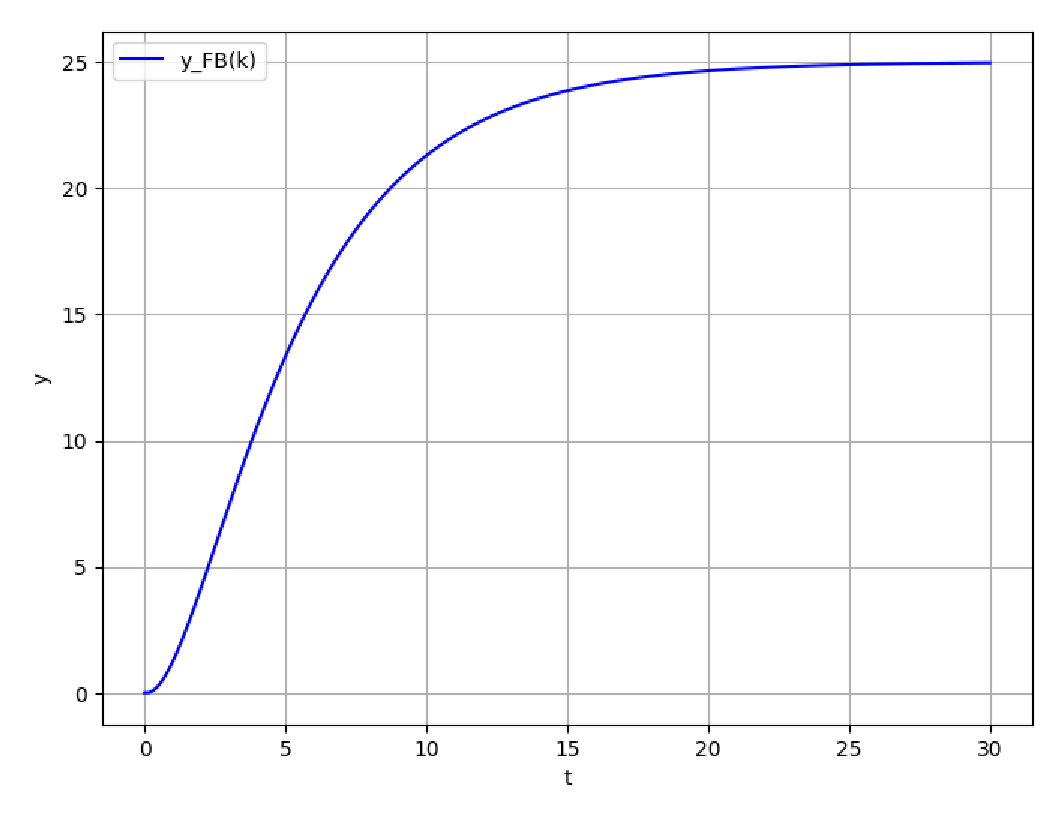
\includegraphics[scale=0.35]{figure20.eps}
    \caption{ボールの位置のシミュレーション結果}
    \label{fig:figure32}
  \end{minipage}
  \begin{minipage}[h]{0.4\linewidth}
    \centering
    \scalebox{0.45}[0.45]{
\begin{tikzpicture}[gnuplot]
%% generated with GNUPLOT 5.4p10 (Lua 5.4; terminal rev. Jun 2020, script rev. 118)
%% Sun Nov 19 19:12:11 2023
\path (0.000,0.000) rectangle (12.500,8.750);
\gpcolor{color=gp lt color border}
\gpsetlinetype{gp lt border}
\gpsetdashtype{gp dt solid}
\gpsetlinewidth{1.00}
\draw[gp path] (0.018,0.031)--(0.198,0.031);
\draw[gp path] (12.480,0.031)--(12.300,0.031);
\node[gp node right] at (-0.166,0.031) {$0$};
\draw[gp path] (0.018,1.272)--(0.198,1.272);
\draw[gp path] (12.480,1.272)--(12.300,1.272);
\node[gp node right] at (-0.166,1.272) {$5$};
\draw[gp path] (0.018,2.513)--(0.198,2.513);
\draw[gp path] (12.480,2.513)--(12.300,2.513);
\node[gp node right] at (-0.166,2.513) {$10$};
\draw[gp path] (0.018,3.754)--(0.198,3.754);
\draw[gp path] (12.480,3.754)--(12.300,3.754);
\node[gp node right] at (-0.166,3.754) {$15$};
\draw[gp path] (0.018,4.995)--(0.198,4.995);
\draw[gp path] (12.480,4.995)--(12.300,4.995);
\node[gp node right] at (-0.166,4.995) {$20$};
\draw[gp path] (0.018,6.236)--(0.198,6.236);
\draw[gp path] (12.480,6.236)--(12.300,6.236);
\node[gp node right] at (-0.166,6.236) {$25$};
\draw[gp path] (0.018,7.477)--(0.198,7.477);
\draw[gp path] (12.480,7.477)--(12.300,7.477);
\node[gp node right] at (-0.166,7.477) {$30$};
\draw[gp path] (0.018,8.718)--(0.198,8.718);
\draw[gp path] (12.480,8.718)--(12.300,8.718);
\node[gp node right] at (-0.166,8.718) {$35$};
\draw[gp path] (0.018,0.031)--(0.018,0.211);
\draw[gp path] (0.018,8.718)--(0.018,8.538);
\node[gp node center] at (0.018,-0.277) {$0$};
\draw[gp path] (1.702,0.031)--(1.702,0.211);
\draw[gp path] (1.702,8.718)--(1.702,8.538);
\node[gp node center] at (1.702,-0.277) {$5$};
\draw[gp path] (3.386,0.031)--(3.386,0.211);
\draw[gp path] (3.386,8.718)--(3.386,8.538);
\node[gp node center] at (3.386,-0.277) {$10$};
\draw[gp path] (5.070,0.031)--(5.070,0.211);
\draw[gp path] (5.070,8.718)--(5.070,8.538);
\node[gp node center] at (5.070,-0.277) {$15$};
\draw[gp path] (6.754,0.031)--(6.754,0.211);
\draw[gp path] (6.754,8.718)--(6.754,8.538);
\node[gp node center] at (6.754,-0.277) {$20$};
\draw[gp path] (8.438,0.031)--(8.438,0.211);
\draw[gp path] (8.438,8.718)--(8.438,8.538);
\node[gp node center] at (8.438,-0.277) {$25$};
\draw[gp path] (10.122,0.031)--(10.122,0.211);
\draw[gp path] (10.122,8.718)--(10.122,8.538);
\node[gp node center] at (10.122,-0.277) {$30$};
\draw[gp path] (11.806,0.031)--(11.806,0.211);
\draw[gp path] (11.806,8.718)--(11.806,8.538);
\node[gp node center] at (11.806,-0.277) {$35$};
\draw[gp path] (0.018,8.718)--(0.018,0.031)--(12.480,0.031)--(12.480,8.718)--cycle;
\node[gp node center,rotate=-270] at (-0.826,4.374) {ボールの位置$z\ /\ \mathrm{cm}$};
\node[gp node center] at (6.249,-0.738) {時間$t\ /\ \mathrm{s}$};
\gpcolor{rgb color={0.000,0.000,0.000}}
\draw[gp path] (0.018,0.541)--(0.025,2.158)--(0.031,4.304)--(0.038,6.085)--(0.045,7.288)%
  --(0.052,7.927)--(0.058,8.120)--(0.065,8.122)--(0.072,8.079)--(0.079,8.011)--(0.085,7.940)%
  --(0.092,7.884)--(0.099,7.844)--(0.106,7.812)--(0.112,7.764)--(0.119,7.714)--(0.126,7.689)%
  --(0.133,7.652)--(0.139,7.539)--(0.146,7.373)--(0.153,7.257)--(0.159,7.215)--(0.166,7.207)%
  --(0.173,7.237)--(0.180,7.297)--(0.186,7.335)--(0.193,7.336)--(0.200,7.343)--(0.207,7.368)%
  --(0.213,7.374)--(0.220,7.363)--(0.227,7.378)--(0.234,7.450)--(0.240,7.576)--(0.247,7.744)%
  --(0.254,7.923)--(0.261,8.080)--(0.267,8.158)--(0.274,8.118)--(0.281,8.063)--(0.287,8.101)%
  --(0.294,8.208)--(0.301,8.311)--(0.308,8.392)--(0.314,8.458)--(0.321,8.507)--(0.328,8.547)%
  --(0.335,8.583)--(0.341,8.582)--(0.348,8.539)--(0.355,8.502)--(0.362,8.479)--(0.368,8.460)%
  --(0.375,8.480)--(0.382,8.541)--(0.388,8.560)--(0.395,8.503)--(0.402,8.397)--(0.409,8.256)%
  --(0.415,8.135)--(0.422,8.055)--(0.429,7.942)--(0.436,7.764)--(0.442,7.597)--(0.449,7.477)%
  --(0.456,7.381)--(0.463,7.292)--(0.469,7.202)--(0.476,7.091)--(0.483,6.918)--(0.490,6.697)%
  --(0.496,6.515)--(0.503,6.410)--(0.510,6.354)--(0.516,6.313)--(0.523,6.262)--(0.530,6.197)%
  --(0.537,6.116)--(0.543,6.026)--(0.550,5.954)--(0.557,5.911)--(0.564,5.883)--(0.570,5.855)%
  --(0.577,5.802)--(0.584,5.724)--(0.591,5.658)--(0.597,5.612)--(0.604,5.599)--(0.611,5.627)%
  --(0.618,5.675)--(0.624,5.711)--(0.631,5.725)--(0.638,5.740)--(0.644,5.765)--(0.651,5.808)%
  --(0.658,5.869)--(0.665,5.937)--(0.671,6.011)--(0.678,6.092)--(0.685,6.171)--(0.692,6.244)%
  --(0.698,6.315)--(0.705,6.398)--(0.712,6.460)--(0.719,6.486)--(0.725,6.551)--(0.732,6.670)%
  --(0.739,6.800)--(0.746,6.923)--(0.752,7.027)--(0.759,7.100)--(0.766,7.120)--(0.772,7.099)%
  --(0.779,7.099)--(0.786,7.139)--(0.793,7.192)--(0.799,7.236)--(0.806,7.237)--(0.813,7.190)%
  --(0.820,7.149)--(0.826,7.134)--(0.833,7.131)--(0.840,7.096)--(0.847,7.003)--(0.853,6.921)%
  --(0.860,6.903)--(0.867,6.918)--(0.873,6.927)--(0.880,6.911)--(0.887,6.872)--(0.894,6.829)%
  --(0.900,6.780)--(0.907,6.717)--(0.914,6.677)--(0.921,6.679)--(0.927,6.687)--(0.934,6.681)%
  --(0.941,6.659)--(0.948,6.643)--(0.954,6.666)--(0.961,6.726)--(0.968,6.804)--(0.975,6.906)%
  --(0.981,6.991)--(0.988,7.007)--(0.995,7.025)--(1.001,7.087)--(1.008,7.161)--(1.015,7.262)%
  --(1.022,7.404)--(1.028,7.496)--(1.035,7.496)--(1.042,7.511)--(1.049,7.590)--(1.055,7.692)%
  --(1.062,7.798)--(1.069,7.899)--(1.076,7.990)--(1.082,8.062)--(1.089,8.111)--(1.096,8.137)%
  --(1.103,8.144)--(1.109,8.112)--(1.116,8.049)--(1.123,8.019)--(1.129,8.050)--(1.136,8.107)%
  --(1.143,8.147)--(1.150,8.158)--(1.156,8.148)--(1.163,8.122)--(1.170,8.082)--(1.177,8.028)%
  --(1.183,7.964)--(1.190,7.869)--(1.197,7.735)--(1.204,7.615)--(1.210,7.536)--(1.217,7.482)%
  --(1.224,7.459)--(1.231,7.458)--(1.237,7.450)--(1.244,7.416)--(1.251,7.082)--(1.257,6.423)%
  --(1.264,6.039)--(1.271,6.114)--(1.278,6.351)--(1.284,6.593)--(1.291,6.774)--(1.298,6.856)%
  --(1.305,6.843)--(1.311,6.765)--(1.318,6.662)--(1.325,6.590)--(1.332,6.570)--(1.338,6.590)%
  --(1.345,6.605)--(1.352,6.583)--(1.359,6.583)--(1.365,6.635)--(1.372,6.723)--(1.379,6.678)%
  --(1.385,6.444)--(1.392,6.355)--(1.399,6.522)--(1.406,6.771)--(1.412,6.992)--(1.419,7.136)%
  --(1.426,7.224)--(1.433,7.293)--(1.439,7.343)--(1.446,7.375)--(1.453,7.426)--(1.460,7.493)%
  --(1.466,7.518)--(1.473,7.516)--(1.480,7.517)--(1.486,7.520)--(1.493,7.522)--(1.500,7.521)%
  --(1.507,7.524)--(1.513,7.530)--(1.520,7.533)--(1.527,7.528)--(1.534,7.506)--(1.540,7.473)%
  --(1.547,7.436)--(1.554,7.386)--(1.561,7.319)--(1.567,7.264)--(1.574,7.230)--(1.581,7.141)%
  --(1.588,6.977)--(1.594,6.813)--(1.601,6.687)--(1.608,6.583)--(1.614,6.487)--(1.621,6.377)%
  --(1.628,6.245)--(1.635,6.095)--(1.641,5.941)--(1.648,5.807)--(1.655,5.703)--(1.662,5.631)%
  --(1.668,5.581)--(1.675,5.537)--(1.682,5.474)--(1.689,5.365)--(1.695,5.227)--(1.702,5.129)%
  --(1.709,5.106)--(1.716,5.106)--(1.722,5.092)--(1.729,5.100)--(1.736,5.121)--(1.742,5.129)%
  --(1.749,5.155)--(1.756,5.204)--(1.763,5.250)--(1.769,5.287)--(1.776,5.320)--(1.783,5.351)%
  --(1.790,5.382)--(1.796,5.421)--(1.803,5.313)--(1.810,5.026)--(1.817,4.910)--(1.823,5.074)%
  --(1.830,5.332)--(1.837,5.588)--(1.844,5.806)--(1.850,5.975)--(1.857,6.104)--(1.864,6.201)%
  --(1.870,6.274)--(1.877,6.325)--(1.884,6.355)--(1.891,6.367)--(1.897,6.367)--(1.904,6.361)%
  --(1.911,6.354)--(1.918,6.351)--(1.924,6.334)--(1.931,6.300)--(1.938,6.313)--(1.945,6.379)%
  --(1.951,6.434)--(1.958,6.447)--(1.965,6.405)--(1.972,6.290)--(1.978,6.139)--(1.985,6.031)%
  --(1.992,5.988)--(1.998,5.969)--(2.005,5.955)--(2.012,5.948)--(2.019,5.950)--(2.025,5.957)%
  --(2.032,5.964)--(2.039,5.968)--(2.046,5.960)--(2.052,5.940)--(2.059,5.927)--(2.066,5.928)%
  --(2.073,5.940)--(2.079,5.967)--(2.086,6.008)--(2.093,6.059)--(2.099,6.118)--(2.106,6.174)%
  --(2.113,6.215)--(2.120,6.288)--(2.126,6.409)--(2.133,6.527)--(2.140,6.647)--(2.147,6.784)%
  --(2.153,6.906)--(2.160,6.996)--(2.167,7.062)--(2.174,7.103)--(2.180,7.126)--(2.187,7.138)%
  --(2.194,7.146)--(2.201,7.176)--(2.207,7.239)--(2.214,7.285)--(2.221,7.297)--(2.227,7.287)%
  --(2.234,7.263)--(2.241,7.219)--(2.248,7.163)--(2.254,7.144)--(2.261,7.168)--(2.268,7.209)%
  --(2.275,7.244)--(2.281,7.246)--(2.288,7.211)--(2.295,7.168)--(2.302,7.139)--(2.308,7.133)%
  --(2.315,7.145)--(2.322,7.174)--(2.329,7.212)--(2.335,7.238)--(2.342,7.254)--(2.349,7.259)%
  --(2.355,7.267)--(2.362,7.316)--(2.369,7.397)--(2.376,7.482)--(2.382,7.576)--(2.389,7.682)%
  --(2.396,7.784)--(2.403,7.876)--(2.409,7.966)--(2.416,8.047)--(2.423,8.096)--(2.430,8.111)%
  --(2.436,8.115)--(2.443,8.131)--(2.450,8.168)--(2.457,8.213)--(2.463,8.246)--(2.470,8.242)%
  --(2.477,8.193)--(2.483,8.157)--(2.490,8.165)--(2.497,8.195)--(2.504,8.227)--(2.510,8.254)%
  --(2.517,8.272)--(2.524,8.279)--(2.531,8.260)--(2.537,8.199)--(2.544,8.133)--(2.551,8.078)%
  --(2.558,8.015)--(2.564,7.962)--(2.571,7.918)--(2.578,7.867)--(2.584,7.820)--(2.591,7.775)%
  --(2.598,7.725)--(2.605,7.663)--(2.611,7.590)--(2.618,7.514)--(2.625,7.448)--(2.632,7.407)%
  --(2.638,7.382)--(2.645,7.348)--(2.652,7.314)--(2.659,7.275)--(2.665,7.221)--(2.672,7.191)%
  --(2.679,7.201)--(2.686,7.227)--(2.692,7.215)--(2.699,7.150)--(2.706,7.114)--(2.712,7.136)%
  --(2.719,7.174)--(2.726,7.215)--(2.733,7.281)--(2.739,7.334)--(2.746,7.348)--(2.753,7.373)%
  --(2.760,7.427)--(2.766,7.502)--(2.773,7.600)--(2.780,7.721)--(2.787,7.848)--(2.793,7.965)%
  --(2.800,8.068)--(2.807,8.151)--(2.814,8.204)--(2.820,8.241)--(2.827,8.290)--(2.834,8.335)%
  --(2.840,8.338)--(2.847,8.311)--(2.854,8.297)--(2.861,8.307)--(2.867,8.341)--(2.874,8.399)%
  --(2.881,8.445)--(2.888,8.430)--(2.894,8.353)--(2.901,8.287)--(2.908,8.259)--(2.915,7.993)%
  --(2.921,7.435)--(2.928,7.156)--(2.935,7.327)--(2.942,7.637)--(2.948,7.897)--(2.955,7.992)%
  --(2.962,7.932)--(2.968,7.846)--(2.975,7.803)--(2.982,7.799)--(2.989,7.834)--(2.995,7.892)%
  --(3.002,7.918)--(3.009,7.891)--(3.016,7.845)--(3.022,7.847)--(3.029,7.929)--(3.036,8.022)%
  --(3.043,8.058)--(3.049,8.027)--(3.056,7.955)--(3.063,7.907)--(3.070,7.912)--(3.076,7.914)%
  --(3.083,7.885)--(3.090,7.891)--(3.096,7.931)--(3.103,7.913)--(3.110,7.845)--(3.117,7.844)%
  --(3.123,7.942)--(3.130,8.073)--(3.137,8.185)--(3.144,8.259)--(3.150,8.274)--(3.157,8.235)%
  --(3.164,8.158)--(3.171,8.051)--(3.177,7.723)--(3.184,7.153)--(3.191,6.874)--(3.197,7.038)%
  --(3.204,7.352)--(3.211,7.652)--(3.218,7.844)--(3.224,7.914)--(3.231,7.920)--(3.238,7.878)%
  --(3.245,7.781)--(3.251,7.683)--(3.258,7.573)--(3.265,7.436)--(3.272,7.342)--(3.278,7.289)%
  --(3.285,7.230)--(3.292,7.171)--(3.299,7.116)--(3.305,7.054)--(3.312,6.973)--(3.319,6.864)%
  --(3.325,6.727)--(3.332,6.582)--(3.339,6.449)--(3.346,6.330)--(3.352,6.222)--(3.359,6.119)%
  --(3.366,6.011)--(3.373,5.899)--(3.379,5.791)--(3.386,5.690)--(3.393,5.597)--(3.400,5.510)%
  --(3.406,5.432)--(3.413,5.366)--(3.420,5.315)--(3.427,5.277)--(3.433,5.247)--(3.440,5.202)%
  --(3.447,5.135)--(3.453,5.084)--(3.460,5.062)--(3.467,5.057)--(3.474,5.064)--(3.480,5.073)%
  --(3.487,5.069)--(3.494,5.062)--(3.501,5.079)--(3.507,5.119)--(3.514,5.158)--(3.521,5.195)%
  --(3.528,5.240)--(3.534,5.304)--(3.541,5.392)--(3.548,5.496)--(3.555,5.615)--(3.561,5.749)%
  --(3.568,5.860)--(3.575,5.931)--(3.581,5.983)--(3.588,6.040)--(3.595,6.105)--(3.602,6.170)%
  --(3.608,6.236)--(3.615,6.294)--(3.622,6.303)--(3.629,6.262)--(3.635,6.252)--(3.642,6.294)%
  --(3.649,6.338)--(3.656,6.373)--(3.662,6.404)--(3.669,6.428)--(3.676,6.425)--(3.683,6.388)%
  --(3.689,6.346)--(3.696,6.311)--(3.703,6.272)--(3.709,6.227)--(3.716,6.187)--(3.723,6.161)%
  --(3.730,6.140)--(3.736,6.115)--(3.743,6.083)--(3.750,6.018)--(3.757,5.925)--(3.763,5.863)%
  --(3.770,5.844)--(3.777,5.838)--(3.784,5.838)--(3.790,5.846)--(3.797,5.859)--(3.804,5.871)%
  --(3.810,5.880)--(3.817,5.885)--(3.824,5.893)--(3.831,5.917)--(3.837,5.960)--(3.844,6.005)%
  --(3.851,6.046)--(3.858,6.086)--(3.864,6.128)--(3.871,6.171)--(3.878,6.208)--(3.885,6.234)%
  --(3.891,6.254)--(3.898,6.255)--(3.905,6.254)--(3.912,6.311)--(3.918,6.418)--(3.925,6.533)%
  --(3.932,6.633)--(3.938,6.687)--(3.945,6.673)--(3.952,6.621)--(3.959,6.605)--(3.965,6.639)%
  --(3.972,6.680)--(3.979,6.702)--(3.986,6.700)--(3.992,6.681)--(3.999,6.646)--(4.006,6.585)%
  --(4.013,6.497)--(4.019,6.418)--(4.026,6.351)--(4.033,6.252)--(4.040,6.120)--(4.046,6.007)%
  --(4.053,5.914)--(4.060,5.816)--(4.066,5.729)--(4.073,5.651)--(4.080,5.567)--(4.087,5.465)%
  --(4.093,5.328)--(4.100,5.161)--(4.107,4.988)--(4.114,4.821)--(4.120,4.669)--(4.127,4.538)%
  --(4.134,4.422)--(4.141,4.315)--(4.147,4.218)--(4.154,4.121)--(4.161,4.019)--(4.168,3.925)%
  --(4.174,3.828)--(4.181,3.726)--(4.188,3.635)--(4.194,3.559)--(4.201,3.505)--(4.208,3.477)%
  --(4.215,3.464)--(4.221,3.456)--(4.228,3.449)--(4.235,3.440)--(4.242,3.427)--(4.248,3.416)%
  --(4.255,3.410)--(4.262,3.410)--(4.269,3.422)--(4.275,3.455)--(4.282,3.505)--(4.289,3.549)%
  --(4.295,3.586)--(4.302,3.640)--(4.309,3.717)--(4.316,3.816)--(4.322,3.936)--(4.329,4.041)%
  --(4.336,4.121)--(4.343,4.207)--(4.349,4.299)--(4.356,4.375)--(4.363,4.447)--(4.370,4.517)%
  --(4.376,4.568)--(4.383,4.601)--(4.390,4.618)--(4.397,4.607)--(4.403,4.573)--(4.410,4.552)%
  --(4.417,4.549)--(4.423,4.540)--(4.430,4.517)--(4.437,4.479)--(4.444,4.429)--(4.450,4.372)%
  --(4.457,4.318)--(4.464,4.267)--(4.471,4.198)--(4.477,4.112)--(4.484,4.019)--(4.491,3.921)%
  --(4.498,3.821)--(4.504,3.719)--(4.511,3.621)--(4.518,3.533)--(4.525,3.459)--(4.531,3.403)%
  --(4.538,3.366)--(4.545,3.340)--(4.551,3.315)--(4.558,3.283)--(4.565,3.243)--(4.572,3.219)%
  --(4.578,3.222)--(4.585,3.237)--(4.592,3.246)--(4.599,3.265)--(4.605,3.320)--(4.612,3.409)%
  --(4.619,3.510)--(4.626,3.611)--(4.632,3.707)--(4.639,3.798)--(4.646,3.886)--(4.653,3.975)%
  --(4.659,4.070)--(4.666,4.172)--(4.673,4.273)--(4.679,4.371)--(4.686,4.481)--(4.693,4.604)%
  --(4.700,4.729)--(4.706,4.858)--(4.713,4.979)--(4.720,5.090)--(4.727,5.187)--(4.733,5.253)%
  --(4.740,5.309)--(4.747,5.381)--(4.754,5.466)--(4.760,5.545)--(4.767,5.601)--(4.774,5.638)%
  --(4.781,5.668)--(4.787,5.688)--(4.794,5.687)--(4.801,5.673)--(4.807,5.650)--(4.814,5.616)%
  --(4.821,5.576)--(4.828,5.532)--(4.834,5.482)--(4.841,5.426)--(4.848,5.362)--(4.855,5.305)%
  --(4.861,5.264)--(4.868,5.212)--(4.875,5.109)--(4.882,4.971)--(4.888,4.843)--(4.895,4.737)%
  --(4.902,4.645)--(4.908,4.562)--(4.915,4.490)--(4.922,4.422)--(4.929,4.353)--(4.935,4.306)%
  --(4.942,4.286)--(4.949,4.260)--(4.956,4.216)--(4.962,4.185)--(4.969,4.176)--(4.976,4.182)%
  --(4.983,4.200)--(4.989,4.221)--(4.996,4.240)--(5.003,4.259)--(5.010,4.278)--(5.016,4.301)%
  --(5.023,4.325)--(5.030,4.354)--(5.036,4.386)--(5.043,4.406)--(5.050,4.414)--(5.057,4.429)%
  --(5.063,4.462)--(5.070,4.536)--(5.077,4.651)--(5.084,4.778)--(5.090,4.902)--(5.097,5.015)%
  --(5.104,5.112)--(5.111,5.198)--(5.117,5.276)--(5.124,5.349)--(5.131,5.415)--(5.138,5.467)%
  --(5.144,5.485)--(5.151,5.469)--(5.158,5.463)--(5.164,5.483)--(5.171,5.482)--(5.178,5.443)%
  --(5.185,5.403)--(5.191,5.374)--(5.198,5.366)--(5.205,5.359)--(5.212,5.233)--(5.218,4.960)%
  --(5.225,4.736)--(5.232,4.653)--(5.239,4.638)--(5.245,4.639)--(5.252,4.626)--(5.259,4.607)%
  --(5.266,4.591)--(5.272,4.566)--(5.279,4.536)--(5.286,4.505)--(5.292,4.467)--(5.299,4.427)%
  --(5.306,4.395)--(5.313,4.372)--(5.319,4.351)--(5.326,4.337)--(5.333,4.337)--(5.340,4.344)%
  --(5.346,4.352)--(5.353,4.360)--(5.360,4.376)--(5.367,4.406)--(5.373,4.440)--(5.380,4.474)%
  --(5.387,4.510)--(5.394,4.550)--(5.400,4.595)--(5.407,4.655)--(5.414,4.744)--(5.420,4.850)%
  --(5.427,4.943)--(5.434,5.037)--(5.441,5.142)--(5.447,5.257)--(5.454,5.372)--(5.461,5.483)%
  --(5.468,5.584)--(5.474,5.661)--(5.481,5.693)--(5.488,5.683)--(5.495,5.675)--(5.501,5.696)%
  --(5.508,5.730)--(5.515,5.760)--(5.521,5.781)--(5.528,5.793)--(5.535,5.790)--(5.542,5.764)%
  --(5.548,5.720)--(5.555,5.673)--(5.562,5.625)--(5.569,5.568)--(5.575,5.504)--(5.582,5.454)%
  --(5.589,5.417)--(5.596,5.378)--(5.602,5.342)--(5.609,5.317)--(5.616,5.303)--(5.623,5.296)%
  --(5.629,5.288)--(5.636,5.274)--(5.643,5.258)--(5.649,5.247)--(5.656,5.239)--(5.663,5.238)%
  --(5.670,5.250)--(5.676,5.269)--(5.683,5.286)--(5.690,5.302)--(5.697,5.322)--(5.703,5.352)%
  --(5.710,5.392)--(5.717,5.434)--(5.724,5.462)--(5.730,5.470)--(5.737,5.485)--(5.744,5.517)%
  --(5.751,5.552)--(5.757,5.586)--(5.764,5.636)--(5.771,5.704)--(5.777,5.774)--(5.784,5.836)%
  --(5.791,5.886)--(5.798,5.885)--(5.804,5.827)--(5.811,5.808)--(5.818,5.859)--(5.825,5.927)%
  --(5.831,5.988)--(5.838,6.026)--(5.845,6.035)--(5.852,6.022)--(5.858,5.988)--(5.865,5.936)%
  --(5.872,5.886)--(5.879,5.834)--(5.885,5.768)--(5.892,5.693)--(5.899,5.615)--(5.905,5.530)%
  --(5.912,5.417)--(5.919,5.198)--(5.926,4.875)--(5.932,4.625)--(5.939,4.509)--(5.946,4.428)%
  --(5.953,4.348)--(5.959,4.286)--(5.966,4.227)--(5.973,4.141)--(5.980,4.008)--(5.986,3.835)%
  --(5.993,3.654)--(6.000,3.478)--(6.006,3.305)--(6.013,3.152)--(6.020,3.007)--(6.027,2.860)%
  --(6.033,2.722)--(6.040,2.596)--(6.047,2.483)--(6.054,2.385)--(6.060,2.292)--(6.067,2.196)%
  --(6.074,2.111)--(6.081,2.045)--(6.087,1.997)--(6.094,1.967)--(6.101,1.956)--(6.108,1.962)%
  --(6.114,1.987)--(6.121,2.002)--(6.128,1.999)--(6.134,2.017)--(6.141,2.064)--(6.148,2.128)%
  --(6.155,2.215)--(6.161,2.327)--(6.168,2.449)--(6.175,2.563)--(6.182,2.657)--(6.188,2.726)%
  --(6.195,2.769)--(6.202,2.785)--(6.209,2.764)--(6.215,2.649)--(6.222,2.442)--(6.229,2.279)%
  --(6.236,2.207)--(6.242,2.175)--(6.249,2.156)--(6.256,2.151)--(6.262,2.161)--(6.269,2.192)%
  --(6.276,2.250)--(6.283,2.337)--(6.289,2.460)--(6.296,2.616)--(6.303,2.800)--(6.310,3.018)%
  --(6.316,3.280)--(6.323,3.542)--(6.330,3.743)--(6.337,3.875)--(6.343,3.954)--(6.350,3.996)%
  --(6.357,4.012)--(6.364,4.012)--(6.370,4.005)--(6.377,3.999)--(6.384,3.992)--(6.390,3.975)%
  --(6.397,3.944)--(6.404,3.926)--(6.411,3.921)--(6.417,3.913)--(6.424,3.916)--(6.431,3.934)%
  --(6.438,3.947)--(6.444,3.946)--(6.451,3.944)--(6.458,3.945)--(6.465,3.947)--(6.471,3.951)%
  --(6.478,3.961)--(6.485,3.973)--(6.492,3.981)--(6.498,3.990)--(6.505,4.002)--(6.512,4.004)%
  --(6.518,3.994)--(6.525,3.984)--(6.532,3.976)--(6.539,3.960)--(6.545,3.933)--(6.552,3.895)%
  --(6.559,3.852)--(6.566,3.823)--(6.572,3.826)--(6.579,3.857)--(6.586,3.856)--(6.593,3.736)%
  --(6.599,3.498)--(6.606,3.221)--(6.613,2.957)--(6.619,2.717)--(6.626,2.493)--(6.633,2.297)%
  --(6.640,2.138)--(6.646,2.023)--(6.653,1.958)--(6.660,1.941)--(6.667,1.981)--(6.673,2.074)%
  --(6.680,2.193)--(6.687,2.337)--(6.694,2.502)--(6.700,2.651)--(6.707,2.770)--(6.714,2.870)%
  --(6.721,2.955)--(6.727,3.046)--(6.734,3.166)--(6.741,3.312)--(6.747,3.469)--(6.754,3.627)%
  --(6.761,3.781)--(6.768,3.926)--(6.774,4.061)--(6.781,4.195)--(6.788,4.330)--(6.795,4.453)%
  --(6.801,4.567)--(6.808,4.671)--(6.815,4.746)--(6.822,4.789)--(6.828,4.817)--(6.835,4.838)%
  --(6.842,4.860)--(6.849,4.883)--(6.855,4.894)--(6.862,4.889)--(6.869,4.858)--(6.875,4.813)%
  --(6.882,4.782)--(6.889,4.754)--(6.896,4.708)--(6.902,4.652)--(6.909,4.593)--(6.916,4.535)%
  --(6.923,4.466)--(6.929,4.370)--(6.936,4.255)--(6.943,4.138)--(6.950,4.030)--(6.956,3.937)%
  --(6.963,3.858)--(6.970,3.792)--(6.977,3.738)--(6.983,3.697)--(6.990,3.651)--(6.997,3.590)%
  --(7.003,3.540)--(7.010,3.515)--(7.017,3.510)--(7.024,3.517)--(7.030,3.532)--(7.037,3.554)%
  --(7.044,3.582)--(7.051,3.616)--(7.057,3.653)--(7.064,3.689)--(7.071,3.718)--(7.078,3.755)%
  --(7.084,3.818)--(7.091,3.902)--(7.098,3.993)--(7.104,4.079)--(7.111,4.151)--(7.118,4.210)%
  --(7.125,4.269)--(7.131,4.336)--(7.138,4.419)--(7.145,4.513)--(7.152,4.612)--(7.158,4.715)%
  --(7.165,4.822)--(7.172,4.913)--(7.179,4.989)--(7.185,5.077)--(7.192,5.176)--(7.199,5.256)%
  --(7.206,5.310)--(7.212,5.336)--(7.219,5.333)--(7.226,5.332)--(7.232,5.348)--(7.239,5.358)%
  --(7.246,5.354)--(7.253,5.336)--(7.259,5.309)--(7.266,5.272)--(7.273,5.228)--(7.280,5.179)%
  --(7.286,5.115)--(7.293,5.023)--(7.300,4.915)--(7.307,4.835)--(7.313,4.781)--(7.320,4.733)%
  --(7.327,4.696)--(7.334,4.664)--(7.340,4.624)--(7.347,4.574)--(7.354,4.528)--(7.360,4.487)%
  --(7.367,4.454)--(7.374,4.433)--(7.381,4.424)--(7.387,4.409)--(7.394,4.385)--(7.401,4.375)%
  --(7.408,4.388)--(7.414,4.419)--(7.421,4.464)--(7.428,4.516)--(7.435,4.569)--(7.441,4.606)%
  --(7.448,4.623)--(7.455,4.657)--(7.462,4.722)--(7.468,4.800)--(7.475,4.882)--(7.482,4.962)%
  --(7.488,5.043)--(7.495,5.140)--(7.502,5.262)--(7.509,5.400)--(7.515,5.519)--(7.522,5.610)%
  --(7.529,5.685)--(7.536,5.749)--(7.542,5.777)--(7.549,5.761)--(7.556,5.759)--(7.563,5.796)%
  --(7.569,5.849)--(7.576,5.896)--(7.583,5.931)--(7.590,5.955)--(7.596,5.973)--(7.603,5.981)%
  --(7.610,5.941)--(7.616,5.854)--(7.623,5.791)--(7.630,5.771)--(7.637,5.759)--(7.643,5.753)%
  --(7.650,5.742)--(7.657,5.706)--(7.664,5.656)--(7.670,5.611)--(7.677,5.571)--(7.684,5.543)%
  --(7.691,5.530)--(7.697,5.508)--(7.704,5.461)--(7.711,5.447)--(7.717,5.483)--(7.724,5.522)%
  --(7.731,5.544)--(7.738,5.559)--(7.744,5.576)--(7.751,5.597)--(7.758,5.604)--(7.765,5.600)%
  --(7.771,5.610)--(7.778,5.647)--(7.785,5.700)--(7.792,5.748)--(7.798,5.782)--(7.805,5.819)%
  --(7.812,5.872)--(7.819,5.909)--(7.825,5.914)--(7.832,5.942)--(7.839,6.008)--(7.845,6.075)%
  --(7.852,6.125)--(7.859,6.146)--(7.866,6.147)--(7.872,6.160)--(7.879,6.189)--(7.886,6.118)%
  --(7.893,5.920)--(7.899,5.692)--(7.906,5.476)--(7.913,5.406)--(7.920,5.504)--(7.926,5.664)%
  --(7.933,5.821)--(7.940,5.915)--(7.947,5.942)--(7.953,5.921)--(7.960,5.867)--(7.967,5.805)%
  --(7.973,5.742)--(7.980,5.636)--(7.987,5.447)--(7.994,5.184)--(8.000,4.904)--(8.007,4.656)%
  --(8.014,4.465)--(8.021,4.322)--(8.027,4.194)--(8.034,4.064)--(8.041,3.904)--(8.048,3.710)%
  --(8.054,3.511)--(8.061,3.324)--(8.068,3.150)--(8.075,2.988)--(8.081,2.853)--(8.088,2.742)%
  --(8.095,2.631)--(8.101,2.517)--(8.108,2.418)--(8.115,2.330)--(8.122,2.242)--(8.128,2.163)%
  --(8.135,2.094)--(8.142,2.039)--(8.149,1.997)--(8.155,1.968)--(8.162,1.946)--(8.169,1.926)%
  --(8.176,1.909)--(8.182,1.897)--(8.189,1.895)--(8.196,1.903)--(8.203,1.915)--(8.209,1.920)%
  --(8.216,1.917)--(8.223,1.919)--(8.229,1.932)--(8.236,1.938)--(8.243,1.934)--(8.250,1.951)%
  --(8.256,2.000)--(8.263,2.063)--(8.270,2.129)--(8.277,2.207)--(8.283,2.296)--(8.290,2.390)%
  --(8.297,2.503)--(8.304,2.653)--(8.310,2.824)--(8.317,2.982)--(8.324,3.106)--(8.330,3.189)%
  --(8.337,3.265)--(8.344,3.362)--(8.351,3.469)--(8.357,3.562)--(8.364,3.633)--(8.371,3.680)%
  --(8.378,3.702)--(8.384,3.704)--(8.391,3.690)--(8.398,3.658)--(8.405,3.606)--(8.411,3.555)%
  --(8.418,3.465)--(8.425,3.319)--(8.432,3.217)--(8.438,3.191)--(8.445,3.182)--(8.452,3.156)%
  --(8.458,3.103)--(8.465,3.005)--(8.472,2.870)--(8.479,2.727)--(8.485,2.590)--(8.492,2.459)%
  --(8.499,2.336)--(8.506,2.233)--(8.512,2.153)--(8.519,2.094)--(8.526,2.055)--(8.533,2.019)%
  --(8.539,1.985)--(8.546,1.958)--(8.553,1.941)--(8.560,1.933)--(8.566,1.932)--(8.573,1.934)%
  --(8.580,1.936)--(8.586,1.939)--(8.593,1.942)--(8.600,1.945)--(8.607,1.945)--(8.613,1.942)%
  --(8.620,1.928)--(8.627,1.907)--(8.634,1.906)--(8.640,1.940)--(8.647,2.000)--(8.654,2.075)%
  --(8.661,2.158)--(8.667,2.245)--(8.674,2.331)--(8.681,2.404)--(8.688,2.458)--(8.694,2.522)%
  --(8.701,2.620)--(8.708,2.739)--(8.714,2.860)--(8.721,2.976)--(8.728,3.083)--(8.735,3.177)%
  --(8.741,3.252)--(8.748,3.312)--(8.755,3.358)--(8.762,3.388)--(8.768,3.403)--(8.775,3.401)%
  --(8.782,3.384)--(8.789,3.360)--(8.795,3.254)--(8.802,3.056)--(8.809,2.926)--(8.815,2.909)%
  --(8.822,2.922)--(8.829,2.922)--(8.836,2.891)--(8.842,2.829)--(8.849,2.742)--(8.856,2.638)%
  --(8.863,2.530)--(8.869,2.418)--(8.876,2.297)--(8.883,2.177)--(8.890,2.071)--(8.896,1.998)%
  --(8.903,1.957)--(8.910,1.938)--(8.917,1.932)--(8.923,1.934)--(8.930,1.937)--(8.937,1.935)%
  --(8.943,1.923)--(8.950,1.915)--(8.957,1.916)--(8.964,1.922)--(8.970,1.932)--(8.977,1.936)%
  --(8.984,1.933)--(8.991,1.938)--(8.997,1.952)--(9.004,1.970)--(9.011,2.002)--(9.018,2.051)%
  --(9.024,2.113)--(9.031,2.196)--(9.038,2.297)--(9.045,2.401)--(9.051,2.502)--(9.058,2.599)%
  --(9.065,2.693)--(9.071,2.782)--(9.078,2.860)--(9.085,2.917)--(9.092,2.953)--(9.098,2.967)%
  --(9.105,2.977)--(9.112,3.005)--(9.119,3.042)--(9.125,3.068)--(9.132,3.072)--(9.139,3.048)%
  --(9.146,2.998)--(9.152,2.934)--(9.159,2.864)--(9.166,2.787)--(9.173,2.701)--(9.179,2.607)%
  --(9.186,2.500)--(9.193,2.384)--(9.199,2.270)--(9.206,2.165)--(9.213,2.078)--(9.220,2.014)%
  --(9.226,1.971)--(9.233,1.945)--(9.240,1.932)--(9.247,1.926)--(9.253,1.925)--(9.260,1.927)%
  --(9.267,1.930)--(9.274,1.933)--(9.280,1.934)--(9.287,1.935)--(9.294,1.932)--(9.301,1.925)%
  --(9.307,1.925)--(9.314,1.937)--(9.321,1.955)--(9.327,1.969)--(9.334,1.973)--(9.341,1.976)%
  --(9.348,1.980)--(9.354,1.982)--(9.361,1.980)--(9.368,1.972)--(9.375,1.964)--(9.381,1.960)%
  --(9.388,1.960)--(9.395,1.967)--(9.402,1.992)--(9.408,2.038)--(9.415,2.090)--(9.422,2.140)%
  --(9.428,2.181)--(9.435,2.207)--(9.442,2.215)--(9.449,2.218)--(9.455,2.221)--(9.462,2.219)%
  --(9.469,2.204)--(9.476,2.166)--(9.482,2.111)--(9.489,2.044)--(9.496,1.981)--(9.503,1.945)%
  --(9.509,1.950)--(9.516,1.998)--(9.523,2.097)--(9.530,2.257)--(9.536,2.387)--(9.543,2.492)%
  --(9.550,2.750)--(9.556,3.124)--(9.563,3.438)--(9.570,3.648)--(9.577,3.783)--(9.583,3.874)%
  --(9.590,3.939)--(9.597,3.980)--(9.604,4.000)--(9.610,3.943)--(9.617,3.801)--(9.624,3.721)%
  --(9.631,3.754)--(9.637,3.827)--(9.644,3.897)--(9.651,3.950)--(9.658,3.983)--(9.664,3.998)%
  --(9.671,4.000)--(9.678,3.996)--(9.684,3.994)--(9.691,3.999)--(9.698,4.002)--(9.705,3.998)%
  --(9.711,3.994)--(9.718,3.989)--(9.725,3.987)--(9.732,3.987)--(9.738,3.988)--(9.745,3.971)%
  --(9.752,3.932)--(9.759,3.894)--(9.765,3.867)--(9.772,3.868)--(9.779,3.899)--(9.786,3.934)%
  --(9.792,3.963)--(9.799,3.972)--(9.806,3.945)--(9.812,3.910)--(9.819,3.904)--(9.826,3.920)%
  --(9.833,3.943)--(9.839,3.961)--(9.846,3.968)--(9.853,3.957)--(9.860,3.926)--(9.866,3.875)%
  --(9.873,3.799)--(9.880,3.707)--(9.887,3.585)--(9.893,3.394)--(9.900,3.143)--(9.907,2.868)%
  --(9.914,2.624)--(9.920,2.436)--(9.927,2.269)--(9.934,2.118)--(9.940,2.019)--(9.947,1.991)%
  --(9.954,2.029)--(9.961,2.120)--(9.967,2.237)--(9.974,2.365)--(9.981,2.510)--(9.988,2.674)%
  --(9.994,2.838)--(10.001,2.994)--(10.008,3.149)--(10.015,3.306)--(10.021,3.465)--(10.028,3.632)%
  --(10.035,3.804)--(10.041,3.991)--(10.048,4.185)--(10.055,4.347)--(10.062,4.475)--(10.068,4.591)%
  --(10.075,4.707)--(10.082,4.839)--(10.089,4.985)--(10.095,5.115)--(10.102,5.212)--(10.109,5.285)%
  --(10.116,5.353)--(10.122,5.413)--(10.129,5.464)--(10.136,5.493)--(10.143,5.490)--(10.149,5.510)%
  --(10.156,5.571)--(10.163,5.620)--(10.169,5.615)--(10.176,5.569)--(10.183,5.551)--(10.190,5.581)%
  --(10.196,5.598)--(10.203,5.570)--(10.210,5.501)--(10.217,5.406)--(10.223,5.300)--(10.230,5.195)%
  --(10.237,5.097)--(10.244,5.005)--(10.250,4.917)--(10.257,4.827)--(10.264,4.731)--(10.271,4.630)%
  --(10.277,4.525)--(10.284,4.407)--(10.291,4.265)--(10.297,4.110)--(10.304,3.973)--(10.311,3.863)%
  --(10.318,3.766)--(10.324,3.685)--(10.331,3.609)--(10.338,3.517)--(10.345,3.430)--(10.351,3.376)%
  --(10.358,3.349)--(10.365,3.325)--(10.372,3.295)--(10.378,3.265)--(10.385,3.226)--(10.392,3.181)%
  --(10.399,3.157)--(10.405,3.161)--(10.412,3.180)--(10.419,3.206)--(10.425,3.236)--(10.432,3.266)%
  --(10.439,3.298)--(10.446,3.317)--(10.452,3.330)--(10.459,3.379)--(10.466,3.473)--(10.473,3.589)%
  --(10.479,3.711)--(10.486,3.829)--(10.493,3.938)--(10.500,4.031)--(10.506,4.113)--(10.513,4.206)%
  --(10.520,4.319)--(10.526,4.441)--(10.533,4.560)--(10.540,4.658)--(10.547,4.736)--(10.553,4.825)%
  --(10.560,4.928)--(10.567,5.004)--(10.574,5.044)--(10.580,5.082)--(10.587,5.132)--(10.594,5.166)%
  --(10.601,5.171)--(10.607,5.174)--(10.614,5.174)--(10.621,5.160)--(10.628,5.120)--(10.634,5.047)%
  --(10.641,4.971)--(10.648,4.912)--(10.654,4.857)--(10.661,4.828)--(10.668,4.835)--(10.675,4.837)%
  --(10.681,4.809)--(10.688,4.767)--(10.695,4.715)--(10.702,4.648)--(10.708,4.567)--(10.715,4.465)%
  --(10.722,4.340)--(10.729,4.234)--(10.735,4.187)--(10.742,4.187)--(10.749,4.207)--(10.756,4.230)%
  --(10.762,4.247)--(10.769,4.260)--(10.776,4.268)--(10.782,4.273)--(10.789,4.283)--(10.796,4.200)%
  --(10.803,3.997)--(10.809,3.896)--(10.816,3.989)--(10.823,4.165)--(10.830,4.345)--(10.836,4.495)%
  --(10.843,4.609)--(10.850,4.698)--(10.857,4.775)--(10.863,4.847)--(10.870,4.918)--(10.877,4.995)%
  --(10.884,5.072)--(10.890,5.138)--(10.897,5.188)--(10.904,5.227)--(10.910,5.257)--(10.917,5.281)%
  --(10.924,5.298)--(10.931,5.304)--(10.937,5.287)--(10.944,5.250)--(10.951,5.212)--(10.958,5.173)%
  --(10.964,5.125)--(10.971,5.067)--(10.978,5.006)--(10.985,4.936)--(10.991,4.835)--(10.998,4.703)%
  --(11.005,4.571)--(11.012,4.459)--(11.018,4.368)--(11.025,4.266)--(11.032,4.151)--(11.038,4.061)%
  --(11.045,4.007)--(11.052,3.977)--(11.059,3.957)--(11.065,3.937)--(11.072,3.914)--(11.079,3.841)%
  --(11.086,3.708)--(11.092,3.619)--(11.099,3.606)--(11.106,3.611)--(11.113,3.594)--(11.119,3.548)%
  --(11.126,3.489)--(11.133,3.425)--(11.139,3.358)--(11.146,3.284)--(11.153,3.208)--(11.160,3.132)%
  --(11.166,3.058)--(11.173,2.984)--(11.180,2.919)--(11.187,2.866)--(11.193,2.808)--(11.200,2.736)%
  --(11.207,2.661)--(11.214,2.591)--(11.220,2.529)--(11.227,2.475)--(11.234,2.426)--(11.241,2.385)%
  --(11.247,2.349)--(11.254,2.315)--(11.261,2.282)--(11.267,2.249)--(11.274,2.218)--(11.281,2.189)%
  --(11.288,2.162)--(11.294,2.128)--(11.301,2.094)--(11.308,2.075)--(11.315,2.066)--(11.321,2.056)%
  --(11.328,2.053)--(11.335,2.056)--(11.342,2.061)--(11.348,2.064)--(11.355,2.070)--(11.362,2.076)%
  --(11.369,2.084)--(11.375,2.111)--(11.382,2.158)--(11.389,2.216)--(11.395,2.271)--(11.402,2.321)%
  --(11.409,2.366)--(11.416,2.411)--(11.422,2.488)--(11.429,2.614)--(11.436,2.758)--(11.443,2.884)%
  --(11.449,2.976)--(11.456,3.044)--(11.463,3.089)--(11.470,3.118)--(11.476,3.148)--(11.483,3.181)%
  --(11.490,3.202)--(11.497,3.193)--(11.503,3.152)--(11.510,3.092)--(11.517,3.016)--(11.523,2.915)%
  --(11.530,2.793)--(11.537,2.674)--(11.544,2.581)--(11.550,2.512)--(11.557,2.446)--(11.564,2.368)%
  --(11.571,2.276)--(11.577,2.179)--(11.584,2.089)--(11.591,2.019)--(11.598,1.978)--(11.604,1.960)%
  --(11.611,1.956)--(11.618,1.963)--(11.625,1.978)--(11.631,1.998)--(11.638,2.021)--(11.645,2.040)%
  --(11.651,2.058)--(11.658,2.087)--(11.665,2.132)--(11.672,2.192)--(11.678,2.265)--(11.685,2.358)%
  --(11.692,2.457)--(11.699,2.534)--(11.705,2.593)--(11.712,2.652)--(11.719,2.704)--(11.726,2.725)%
  --(11.732,2.709)--(11.739,2.670)--(11.746,2.615)--(11.752,2.541)--(11.759,2.443)--(11.766,2.330)%
  --(11.773,2.230)--(11.779,2.150)--(11.786,2.093)--(11.793,2.071)--(11.800,2.082)--(11.806,2.117)%
  --(11.813,2.191)--(11.820,2.312)--(11.827,2.464)--(11.833,2.638)--(11.840,2.834)--(11.847,3.074)%
  --(11.854,3.338)--(11.860,3.580)--(11.867,3.778)--(11.874,3.917)--(11.880,3.993)--(11.887,4.024)%
  --(11.894,4.020)--(11.901,3.993)--(11.907,3.974)--(11.914,3.976)--(11.921,3.994)--(11.928,4.019)%
  --(11.934,4.029)--(11.941,4.024)--(11.948,4.016)--(11.955,4.018)--(11.961,4.026)--(11.968,4.027)%
  --(11.975,4.019)--(11.982,4.008)--(11.988,3.995)--(11.995,3.983)--(12.002,3.977)--(12.008,3.977)%
  --(12.015,3.968)--(12.022,3.946)--(12.029,3.935)--(12.035,3.943)--(12.042,3.956)--(12.049,3.974)%
  --(12.056,3.993)--(12.062,4.000)--(12.069,3.998)--(12.076,3.994)--(12.083,3.981)--(12.089,3.952)%
  --(12.096,3.911)--(12.103,3.874)--(12.110,3.857)--(12.116,3.821)--(12.123,3.705)--(12.130,3.515)%
  --(12.136,3.285)--(12.143,3.041)--(12.150,2.796)--(12.157,2.564)--(12.163,2.348)--(12.170,2.166)%
  --(12.177,2.044)--(12.184,1.992)--(12.190,2.011)--(12.197,2.089)--(12.204,2.189)--(12.211,2.291)%
  --(12.217,2.420)--(12.224,2.581)--(12.231,2.731)--(12.237,2.859)--(12.244,2.985)--(12.251,3.116)%
  --(12.258,3.251)--(12.264,3.382)--(12.271,3.530)--(12.278,3.722)--(12.285,3.934)--(12.291,4.098)%
  --(12.298,4.201)--(12.305,4.325)--(12.312,4.495)--(12.318,4.673)--(12.325,4.837)--(12.332,4.989)%
  --(12.339,5.122)--(12.345,5.226)--(12.352,5.293)--(12.359,5.332)--(12.365,5.390)--(12.372,5.460)%
  --(12.379,5.509)--(12.386,5.542)--(12.392,5.571)--(12.399,5.597)--(12.406,5.602)--(12.413,5.559)%
  --(12.419,5.492)--(12.426,5.459)--(12.433,5.463)--(12.440,5.476)--(12.446,5.480)--(12.453,5.478)%
  --(12.460,5.463)--(12.467,5.413)--(12.473,5.334)--(12.480,5.248);
\gpsetpointsize{1.20}
\gp3point{gp mark 7}{}{(0.018,0.541)}
\gp3point{gp mark 7}{}{(0.025,2.158)}
\gp3point{gp mark 7}{}{(0.031,4.304)}
\gp3point{gp mark 7}{}{(0.038,6.085)}
\gp3point{gp mark 7}{}{(0.045,7.288)}
\gp3point{gp mark 7}{}{(0.052,7.927)}
\gp3point{gp mark 7}{}{(0.058,8.120)}
\gp3point{gp mark 7}{}{(0.065,8.122)}
\gp3point{gp mark 7}{}{(0.072,8.079)}
\gp3point{gp mark 7}{}{(0.079,8.011)}
\gp3point{gp mark 7}{}{(0.085,7.940)}
\gp3point{gp mark 7}{}{(0.092,7.884)}
\gp3point{gp mark 7}{}{(0.099,7.844)}
\gp3point{gp mark 7}{}{(0.106,7.812)}
\gp3point{gp mark 7}{}{(0.112,7.764)}
\gp3point{gp mark 7}{}{(0.119,7.714)}
\gp3point{gp mark 7}{}{(0.126,7.689)}
\gp3point{gp mark 7}{}{(0.133,7.652)}
\gp3point{gp mark 7}{}{(0.139,7.539)}
\gp3point{gp mark 7}{}{(0.146,7.373)}
\gp3point{gp mark 7}{}{(0.153,7.257)}
\gp3point{gp mark 7}{}{(0.159,7.215)}
\gp3point{gp mark 7}{}{(0.166,7.207)}
\gp3point{gp mark 7}{}{(0.173,7.237)}
\gp3point{gp mark 7}{}{(0.180,7.297)}
\gp3point{gp mark 7}{}{(0.186,7.335)}
\gp3point{gp mark 7}{}{(0.193,7.336)}
\gp3point{gp mark 7}{}{(0.200,7.343)}
\gp3point{gp mark 7}{}{(0.207,7.368)}
\gp3point{gp mark 7}{}{(0.213,7.374)}
\gp3point{gp mark 7}{}{(0.220,7.363)}
\gp3point{gp mark 7}{}{(0.227,7.378)}
\gp3point{gp mark 7}{}{(0.234,7.450)}
\gp3point{gp mark 7}{}{(0.240,7.576)}
\gp3point{gp mark 7}{}{(0.247,7.744)}
\gp3point{gp mark 7}{}{(0.254,7.923)}
\gp3point{gp mark 7}{}{(0.261,8.080)}
\gp3point{gp mark 7}{}{(0.267,8.158)}
\gp3point{gp mark 7}{}{(0.274,8.118)}
\gp3point{gp mark 7}{}{(0.281,8.063)}
\gp3point{gp mark 7}{}{(0.287,8.101)}
\gp3point{gp mark 7}{}{(0.294,8.208)}
\gp3point{gp mark 7}{}{(0.301,8.311)}
\gp3point{gp mark 7}{}{(0.308,8.392)}
\gp3point{gp mark 7}{}{(0.314,8.458)}
\gp3point{gp mark 7}{}{(0.321,8.507)}
\gp3point{gp mark 7}{}{(0.328,8.547)}
\gp3point{gp mark 7}{}{(0.335,8.583)}
\gp3point{gp mark 7}{}{(0.341,8.582)}
\gp3point{gp mark 7}{}{(0.348,8.539)}
\gp3point{gp mark 7}{}{(0.355,8.502)}
\gp3point{gp mark 7}{}{(0.362,8.479)}
\gp3point{gp mark 7}{}{(0.368,8.460)}
\gp3point{gp mark 7}{}{(0.375,8.480)}
\gp3point{gp mark 7}{}{(0.382,8.541)}
\gp3point{gp mark 7}{}{(0.388,8.560)}
\gp3point{gp mark 7}{}{(0.395,8.503)}
\gp3point{gp mark 7}{}{(0.402,8.397)}
\gp3point{gp mark 7}{}{(0.409,8.256)}
\gp3point{gp mark 7}{}{(0.415,8.135)}
\gp3point{gp mark 7}{}{(0.422,8.055)}
\gp3point{gp mark 7}{}{(0.429,7.942)}
\gp3point{gp mark 7}{}{(0.436,7.764)}
\gp3point{gp mark 7}{}{(0.442,7.597)}
\gp3point{gp mark 7}{}{(0.449,7.477)}
\gp3point{gp mark 7}{}{(0.456,7.381)}
\gp3point{gp mark 7}{}{(0.463,7.292)}
\gp3point{gp mark 7}{}{(0.469,7.202)}
\gp3point{gp mark 7}{}{(0.476,7.091)}
\gp3point{gp mark 7}{}{(0.483,6.918)}
\gp3point{gp mark 7}{}{(0.490,6.697)}
\gp3point{gp mark 7}{}{(0.496,6.515)}
\gp3point{gp mark 7}{}{(0.503,6.410)}
\gp3point{gp mark 7}{}{(0.510,6.354)}
\gp3point{gp mark 7}{}{(0.516,6.313)}
\gp3point{gp mark 7}{}{(0.523,6.262)}
\gp3point{gp mark 7}{}{(0.530,6.197)}
\gp3point{gp mark 7}{}{(0.537,6.116)}
\gp3point{gp mark 7}{}{(0.543,6.026)}
\gp3point{gp mark 7}{}{(0.550,5.954)}
\gp3point{gp mark 7}{}{(0.557,5.911)}
\gp3point{gp mark 7}{}{(0.564,5.883)}
\gp3point{gp mark 7}{}{(0.570,5.855)}
\gp3point{gp mark 7}{}{(0.577,5.802)}
\gp3point{gp mark 7}{}{(0.584,5.724)}
\gp3point{gp mark 7}{}{(0.591,5.658)}
\gp3point{gp mark 7}{}{(0.597,5.612)}
\gp3point{gp mark 7}{}{(0.604,5.599)}
\gp3point{gp mark 7}{}{(0.611,5.627)}
\gp3point{gp mark 7}{}{(0.618,5.675)}
\gp3point{gp mark 7}{}{(0.624,5.711)}
\gp3point{gp mark 7}{}{(0.631,5.725)}
\gp3point{gp mark 7}{}{(0.638,5.740)}
\gp3point{gp mark 7}{}{(0.644,5.765)}
\gp3point{gp mark 7}{}{(0.651,5.808)}
\gp3point{gp mark 7}{}{(0.658,5.869)}
\gp3point{gp mark 7}{}{(0.665,5.937)}
\gp3point{gp mark 7}{}{(0.671,6.011)}
\gp3point{gp mark 7}{}{(0.678,6.092)}
\gp3point{gp mark 7}{}{(0.685,6.171)}
\gp3point{gp mark 7}{}{(0.692,6.244)}
\gp3point{gp mark 7}{}{(0.698,6.315)}
\gp3point{gp mark 7}{}{(0.705,6.398)}
\gp3point{gp mark 7}{}{(0.712,6.460)}
\gp3point{gp mark 7}{}{(0.719,6.486)}
\gp3point{gp mark 7}{}{(0.725,6.551)}
\gp3point{gp mark 7}{}{(0.732,6.670)}
\gp3point{gp mark 7}{}{(0.739,6.800)}
\gp3point{gp mark 7}{}{(0.746,6.923)}
\gp3point{gp mark 7}{}{(0.752,7.027)}
\gp3point{gp mark 7}{}{(0.759,7.100)}
\gp3point{gp mark 7}{}{(0.766,7.120)}
\gp3point{gp mark 7}{}{(0.772,7.099)}
\gp3point{gp mark 7}{}{(0.779,7.099)}
\gp3point{gp mark 7}{}{(0.786,7.139)}
\gp3point{gp mark 7}{}{(0.793,7.192)}
\gp3point{gp mark 7}{}{(0.799,7.236)}
\gp3point{gp mark 7}{}{(0.806,7.237)}
\gp3point{gp mark 7}{}{(0.813,7.190)}
\gp3point{gp mark 7}{}{(0.820,7.149)}
\gp3point{gp mark 7}{}{(0.826,7.134)}
\gp3point{gp mark 7}{}{(0.833,7.131)}
\gp3point{gp mark 7}{}{(0.840,7.096)}
\gp3point{gp mark 7}{}{(0.847,7.003)}
\gp3point{gp mark 7}{}{(0.853,6.921)}
\gp3point{gp mark 7}{}{(0.860,6.903)}
\gp3point{gp mark 7}{}{(0.867,6.918)}
\gp3point{gp mark 7}{}{(0.873,6.927)}
\gp3point{gp mark 7}{}{(0.880,6.911)}
\gp3point{gp mark 7}{}{(0.887,6.872)}
\gp3point{gp mark 7}{}{(0.894,6.829)}
\gp3point{gp mark 7}{}{(0.900,6.780)}
\gp3point{gp mark 7}{}{(0.907,6.717)}
\gp3point{gp mark 7}{}{(0.914,6.677)}
\gp3point{gp mark 7}{}{(0.921,6.679)}
\gp3point{gp mark 7}{}{(0.927,6.687)}
\gp3point{gp mark 7}{}{(0.934,6.681)}
\gp3point{gp mark 7}{}{(0.941,6.659)}
\gp3point{gp mark 7}{}{(0.948,6.643)}
\gp3point{gp mark 7}{}{(0.954,6.666)}
\gp3point{gp mark 7}{}{(0.961,6.726)}
\gp3point{gp mark 7}{}{(0.968,6.804)}
\gp3point{gp mark 7}{}{(0.975,6.906)}
\gp3point{gp mark 7}{}{(0.981,6.991)}
\gp3point{gp mark 7}{}{(0.988,7.007)}
\gp3point{gp mark 7}{}{(0.995,7.025)}
\gp3point{gp mark 7}{}{(1.001,7.087)}
\gp3point{gp mark 7}{}{(1.008,7.161)}
\gp3point{gp mark 7}{}{(1.015,7.262)}
\gp3point{gp mark 7}{}{(1.022,7.404)}
\gp3point{gp mark 7}{}{(1.028,7.496)}
\gp3point{gp mark 7}{}{(1.035,7.496)}
\gp3point{gp mark 7}{}{(1.042,7.511)}
\gp3point{gp mark 7}{}{(1.049,7.590)}
\gp3point{gp mark 7}{}{(1.055,7.692)}
\gp3point{gp mark 7}{}{(1.062,7.798)}
\gp3point{gp mark 7}{}{(1.069,7.899)}
\gp3point{gp mark 7}{}{(1.076,7.990)}
\gp3point{gp mark 7}{}{(1.082,8.062)}
\gp3point{gp mark 7}{}{(1.089,8.111)}
\gp3point{gp mark 7}{}{(1.096,8.137)}
\gp3point{gp mark 7}{}{(1.103,8.144)}
\gp3point{gp mark 7}{}{(1.109,8.112)}
\gp3point{gp mark 7}{}{(1.116,8.049)}
\gp3point{gp mark 7}{}{(1.123,8.019)}
\gp3point{gp mark 7}{}{(1.129,8.050)}
\gp3point{gp mark 7}{}{(1.136,8.107)}
\gp3point{gp mark 7}{}{(1.143,8.147)}
\gp3point{gp mark 7}{}{(1.150,8.158)}
\gp3point{gp mark 7}{}{(1.156,8.148)}
\gp3point{gp mark 7}{}{(1.163,8.122)}
\gp3point{gp mark 7}{}{(1.170,8.082)}
\gp3point{gp mark 7}{}{(1.177,8.028)}
\gp3point{gp mark 7}{}{(1.183,7.964)}
\gp3point{gp mark 7}{}{(1.190,7.869)}
\gp3point{gp mark 7}{}{(1.197,7.735)}
\gp3point{gp mark 7}{}{(1.204,7.615)}
\gp3point{gp mark 7}{}{(1.210,7.536)}
\gp3point{gp mark 7}{}{(1.217,7.482)}
\gp3point{gp mark 7}{}{(1.224,7.459)}
\gp3point{gp mark 7}{}{(1.231,7.458)}
\gp3point{gp mark 7}{}{(1.237,7.450)}
\gp3point{gp mark 7}{}{(1.244,7.416)}
\gp3point{gp mark 7}{}{(1.251,7.082)}
\gp3point{gp mark 7}{}{(1.257,6.423)}
\gp3point{gp mark 7}{}{(1.264,6.039)}
\gp3point{gp mark 7}{}{(1.271,6.114)}
\gp3point{gp mark 7}{}{(1.278,6.351)}
\gp3point{gp mark 7}{}{(1.284,6.593)}
\gp3point{gp mark 7}{}{(1.291,6.774)}
\gp3point{gp mark 7}{}{(1.298,6.856)}
\gp3point{gp mark 7}{}{(1.305,6.843)}
\gp3point{gp mark 7}{}{(1.311,6.765)}
\gp3point{gp mark 7}{}{(1.318,6.662)}
\gp3point{gp mark 7}{}{(1.325,6.590)}
\gp3point{gp mark 7}{}{(1.332,6.570)}
\gp3point{gp mark 7}{}{(1.338,6.590)}
\gp3point{gp mark 7}{}{(1.345,6.605)}
\gp3point{gp mark 7}{}{(1.352,6.583)}
\gp3point{gp mark 7}{}{(1.359,6.583)}
\gp3point{gp mark 7}{}{(1.365,6.635)}
\gp3point{gp mark 7}{}{(1.372,6.723)}
\gp3point{gp mark 7}{}{(1.379,6.678)}
\gp3point{gp mark 7}{}{(1.385,6.444)}
\gp3point{gp mark 7}{}{(1.392,6.355)}
\gp3point{gp mark 7}{}{(1.399,6.522)}
\gp3point{gp mark 7}{}{(1.406,6.771)}
\gp3point{gp mark 7}{}{(1.412,6.992)}
\gp3point{gp mark 7}{}{(1.419,7.136)}
\gp3point{gp mark 7}{}{(1.426,7.224)}
\gp3point{gp mark 7}{}{(1.433,7.293)}
\gp3point{gp mark 7}{}{(1.439,7.343)}
\gp3point{gp mark 7}{}{(1.446,7.375)}
\gp3point{gp mark 7}{}{(1.453,7.426)}
\gp3point{gp mark 7}{}{(1.460,7.493)}
\gp3point{gp mark 7}{}{(1.466,7.518)}
\gp3point{gp mark 7}{}{(1.473,7.516)}
\gp3point{gp mark 7}{}{(1.480,7.517)}
\gp3point{gp mark 7}{}{(1.486,7.520)}
\gp3point{gp mark 7}{}{(1.493,7.522)}
\gp3point{gp mark 7}{}{(1.500,7.521)}
\gp3point{gp mark 7}{}{(1.507,7.524)}
\gp3point{gp mark 7}{}{(1.513,7.530)}
\gp3point{gp mark 7}{}{(1.520,7.533)}
\gp3point{gp mark 7}{}{(1.527,7.528)}
\gp3point{gp mark 7}{}{(1.534,7.506)}
\gp3point{gp mark 7}{}{(1.540,7.473)}
\gp3point{gp mark 7}{}{(1.547,7.436)}
\gp3point{gp mark 7}{}{(1.554,7.386)}
\gp3point{gp mark 7}{}{(1.561,7.319)}
\gp3point{gp mark 7}{}{(1.567,7.264)}
\gp3point{gp mark 7}{}{(1.574,7.230)}
\gp3point{gp mark 7}{}{(1.581,7.141)}
\gp3point{gp mark 7}{}{(1.588,6.977)}
\gp3point{gp mark 7}{}{(1.594,6.813)}
\gp3point{gp mark 7}{}{(1.601,6.687)}
\gp3point{gp mark 7}{}{(1.608,6.583)}
\gp3point{gp mark 7}{}{(1.614,6.487)}
\gp3point{gp mark 7}{}{(1.621,6.377)}
\gp3point{gp mark 7}{}{(1.628,6.245)}
\gp3point{gp mark 7}{}{(1.635,6.095)}
\gp3point{gp mark 7}{}{(1.641,5.941)}
\gp3point{gp mark 7}{}{(1.648,5.807)}
\gp3point{gp mark 7}{}{(1.655,5.703)}
\gp3point{gp mark 7}{}{(1.662,5.631)}
\gp3point{gp mark 7}{}{(1.668,5.581)}
\gp3point{gp mark 7}{}{(1.675,5.537)}
\gp3point{gp mark 7}{}{(1.682,5.474)}
\gp3point{gp mark 7}{}{(1.689,5.365)}
\gp3point{gp mark 7}{}{(1.695,5.227)}
\gp3point{gp mark 7}{}{(1.702,5.129)}
\gp3point{gp mark 7}{}{(1.709,5.106)}
\gp3point{gp mark 7}{}{(1.716,5.106)}
\gp3point{gp mark 7}{}{(1.722,5.092)}
\gp3point{gp mark 7}{}{(1.729,5.100)}
\gp3point{gp mark 7}{}{(1.736,5.121)}
\gp3point{gp mark 7}{}{(1.742,5.129)}
\gp3point{gp mark 7}{}{(1.749,5.155)}
\gp3point{gp mark 7}{}{(1.756,5.204)}
\gp3point{gp mark 7}{}{(1.763,5.250)}
\gp3point{gp mark 7}{}{(1.769,5.287)}
\gp3point{gp mark 7}{}{(1.776,5.320)}
\gp3point{gp mark 7}{}{(1.783,5.351)}
\gp3point{gp mark 7}{}{(1.790,5.382)}
\gp3point{gp mark 7}{}{(1.796,5.421)}
\gp3point{gp mark 7}{}{(1.803,5.313)}
\gp3point{gp mark 7}{}{(1.810,5.026)}
\gp3point{gp mark 7}{}{(1.817,4.910)}
\gp3point{gp mark 7}{}{(1.823,5.074)}
\gp3point{gp mark 7}{}{(1.830,5.332)}
\gp3point{gp mark 7}{}{(1.837,5.588)}
\gp3point{gp mark 7}{}{(1.844,5.806)}
\gp3point{gp mark 7}{}{(1.850,5.975)}
\gp3point{gp mark 7}{}{(1.857,6.104)}
\gp3point{gp mark 7}{}{(1.864,6.201)}
\gp3point{gp mark 7}{}{(1.870,6.274)}
\gp3point{gp mark 7}{}{(1.877,6.325)}
\gp3point{gp mark 7}{}{(1.884,6.355)}
\gp3point{gp mark 7}{}{(1.891,6.367)}
\gp3point{gp mark 7}{}{(1.897,6.367)}
\gp3point{gp mark 7}{}{(1.904,6.361)}
\gp3point{gp mark 7}{}{(1.911,6.354)}
\gp3point{gp mark 7}{}{(1.918,6.351)}
\gp3point{gp mark 7}{}{(1.924,6.334)}
\gp3point{gp mark 7}{}{(1.931,6.300)}
\gp3point{gp mark 7}{}{(1.938,6.313)}
\gp3point{gp mark 7}{}{(1.945,6.379)}
\gp3point{gp mark 7}{}{(1.951,6.434)}
\gp3point{gp mark 7}{}{(1.958,6.447)}
\gp3point{gp mark 7}{}{(1.965,6.405)}
\gp3point{gp mark 7}{}{(1.972,6.290)}
\gp3point{gp mark 7}{}{(1.978,6.139)}
\gp3point{gp mark 7}{}{(1.985,6.031)}
\gp3point{gp mark 7}{}{(1.992,5.988)}
\gp3point{gp mark 7}{}{(1.998,5.969)}
\gp3point{gp mark 7}{}{(2.005,5.955)}
\gp3point{gp mark 7}{}{(2.012,5.948)}
\gp3point{gp mark 7}{}{(2.019,5.950)}
\gp3point{gp mark 7}{}{(2.025,5.957)}
\gp3point{gp mark 7}{}{(2.032,5.964)}
\gp3point{gp mark 7}{}{(2.039,5.968)}
\gp3point{gp mark 7}{}{(2.046,5.960)}
\gp3point{gp mark 7}{}{(2.052,5.940)}
\gp3point{gp mark 7}{}{(2.059,5.927)}
\gp3point{gp mark 7}{}{(2.066,5.928)}
\gp3point{gp mark 7}{}{(2.073,5.940)}
\gp3point{gp mark 7}{}{(2.079,5.967)}
\gp3point{gp mark 7}{}{(2.086,6.008)}
\gp3point{gp mark 7}{}{(2.093,6.059)}
\gp3point{gp mark 7}{}{(2.099,6.118)}
\gp3point{gp mark 7}{}{(2.106,6.174)}
\gp3point{gp mark 7}{}{(2.113,6.215)}
\gp3point{gp mark 7}{}{(2.120,6.288)}
\gp3point{gp mark 7}{}{(2.126,6.409)}
\gp3point{gp mark 7}{}{(2.133,6.527)}
\gp3point{gp mark 7}{}{(2.140,6.647)}
\gp3point{gp mark 7}{}{(2.147,6.784)}
\gp3point{gp mark 7}{}{(2.153,6.906)}
\gp3point{gp mark 7}{}{(2.160,6.996)}
\gp3point{gp mark 7}{}{(2.167,7.062)}
\gp3point{gp mark 7}{}{(2.174,7.103)}
\gp3point{gp mark 7}{}{(2.180,7.126)}
\gp3point{gp mark 7}{}{(2.187,7.138)}
\gp3point{gp mark 7}{}{(2.194,7.146)}
\gp3point{gp mark 7}{}{(2.201,7.176)}
\gp3point{gp mark 7}{}{(2.207,7.239)}
\gp3point{gp mark 7}{}{(2.214,7.285)}
\gp3point{gp mark 7}{}{(2.221,7.297)}
\gp3point{gp mark 7}{}{(2.227,7.287)}
\gp3point{gp mark 7}{}{(2.234,7.263)}
\gp3point{gp mark 7}{}{(2.241,7.219)}
\gp3point{gp mark 7}{}{(2.248,7.163)}
\gp3point{gp mark 7}{}{(2.254,7.144)}
\gp3point{gp mark 7}{}{(2.261,7.168)}
\gp3point{gp mark 7}{}{(2.268,7.209)}
\gp3point{gp mark 7}{}{(2.275,7.244)}
\gp3point{gp mark 7}{}{(2.281,7.246)}
\gp3point{gp mark 7}{}{(2.288,7.211)}
\gp3point{gp mark 7}{}{(2.295,7.168)}
\gp3point{gp mark 7}{}{(2.302,7.139)}
\gp3point{gp mark 7}{}{(2.308,7.133)}
\gp3point{gp mark 7}{}{(2.315,7.145)}
\gp3point{gp mark 7}{}{(2.322,7.174)}
\gp3point{gp mark 7}{}{(2.329,7.212)}
\gp3point{gp mark 7}{}{(2.335,7.238)}
\gp3point{gp mark 7}{}{(2.342,7.254)}
\gp3point{gp mark 7}{}{(2.349,7.259)}
\gp3point{gp mark 7}{}{(2.355,7.267)}
\gp3point{gp mark 7}{}{(2.362,7.316)}
\gp3point{gp mark 7}{}{(2.369,7.397)}
\gp3point{gp mark 7}{}{(2.376,7.482)}
\gp3point{gp mark 7}{}{(2.382,7.576)}
\gp3point{gp mark 7}{}{(2.389,7.682)}
\gp3point{gp mark 7}{}{(2.396,7.784)}
\gp3point{gp mark 7}{}{(2.403,7.876)}
\gp3point{gp mark 7}{}{(2.409,7.966)}
\gp3point{gp mark 7}{}{(2.416,8.047)}
\gp3point{gp mark 7}{}{(2.423,8.096)}
\gp3point{gp mark 7}{}{(2.430,8.111)}
\gp3point{gp mark 7}{}{(2.436,8.115)}
\gp3point{gp mark 7}{}{(2.443,8.131)}
\gp3point{gp mark 7}{}{(2.450,8.168)}
\gp3point{gp mark 7}{}{(2.457,8.213)}
\gp3point{gp mark 7}{}{(2.463,8.246)}
\gp3point{gp mark 7}{}{(2.470,8.242)}
\gp3point{gp mark 7}{}{(2.477,8.193)}
\gp3point{gp mark 7}{}{(2.483,8.157)}
\gp3point{gp mark 7}{}{(2.490,8.165)}
\gp3point{gp mark 7}{}{(2.497,8.195)}
\gp3point{gp mark 7}{}{(2.504,8.227)}
\gp3point{gp mark 7}{}{(2.510,8.254)}
\gp3point{gp mark 7}{}{(2.517,8.272)}
\gp3point{gp mark 7}{}{(2.524,8.279)}
\gp3point{gp mark 7}{}{(2.531,8.260)}
\gp3point{gp mark 7}{}{(2.537,8.199)}
\gp3point{gp mark 7}{}{(2.544,8.133)}
\gp3point{gp mark 7}{}{(2.551,8.078)}
\gp3point{gp mark 7}{}{(2.558,8.015)}
\gp3point{gp mark 7}{}{(2.564,7.962)}
\gp3point{gp mark 7}{}{(2.571,7.918)}
\gp3point{gp mark 7}{}{(2.578,7.867)}
\gp3point{gp mark 7}{}{(2.584,7.820)}
\gp3point{gp mark 7}{}{(2.591,7.775)}
\gp3point{gp mark 7}{}{(2.598,7.725)}
\gp3point{gp mark 7}{}{(2.605,7.663)}
\gp3point{gp mark 7}{}{(2.611,7.590)}
\gp3point{gp mark 7}{}{(2.618,7.514)}
\gp3point{gp mark 7}{}{(2.625,7.448)}
\gp3point{gp mark 7}{}{(2.632,7.407)}
\gp3point{gp mark 7}{}{(2.638,7.382)}
\gp3point{gp mark 7}{}{(2.645,7.348)}
\gp3point{gp mark 7}{}{(2.652,7.314)}
\gp3point{gp mark 7}{}{(2.659,7.275)}
\gp3point{gp mark 7}{}{(2.665,7.221)}
\gp3point{gp mark 7}{}{(2.672,7.191)}
\gp3point{gp mark 7}{}{(2.679,7.201)}
\gp3point{gp mark 7}{}{(2.686,7.227)}
\gp3point{gp mark 7}{}{(2.692,7.215)}
\gp3point{gp mark 7}{}{(2.699,7.150)}
\gp3point{gp mark 7}{}{(2.706,7.114)}
\gp3point{gp mark 7}{}{(2.712,7.136)}
\gp3point{gp mark 7}{}{(2.719,7.174)}
\gp3point{gp mark 7}{}{(2.726,7.215)}
\gp3point{gp mark 7}{}{(2.733,7.281)}
\gp3point{gp mark 7}{}{(2.739,7.334)}
\gp3point{gp mark 7}{}{(2.746,7.348)}
\gp3point{gp mark 7}{}{(2.753,7.373)}
\gp3point{gp mark 7}{}{(2.760,7.427)}
\gp3point{gp mark 7}{}{(2.766,7.502)}
\gp3point{gp mark 7}{}{(2.773,7.600)}
\gp3point{gp mark 7}{}{(2.780,7.721)}
\gp3point{gp mark 7}{}{(2.787,7.848)}
\gp3point{gp mark 7}{}{(2.793,7.965)}
\gp3point{gp mark 7}{}{(2.800,8.068)}
\gp3point{gp mark 7}{}{(2.807,8.151)}
\gp3point{gp mark 7}{}{(2.814,8.204)}
\gp3point{gp mark 7}{}{(2.820,8.241)}
\gp3point{gp mark 7}{}{(2.827,8.290)}
\gp3point{gp mark 7}{}{(2.834,8.335)}
\gp3point{gp mark 7}{}{(2.840,8.338)}
\gp3point{gp mark 7}{}{(2.847,8.311)}
\gp3point{gp mark 7}{}{(2.854,8.297)}
\gp3point{gp mark 7}{}{(2.861,8.307)}
\gp3point{gp mark 7}{}{(2.867,8.341)}
\gp3point{gp mark 7}{}{(2.874,8.399)}
\gp3point{gp mark 7}{}{(2.881,8.445)}
\gp3point{gp mark 7}{}{(2.888,8.430)}
\gp3point{gp mark 7}{}{(2.894,8.353)}
\gp3point{gp mark 7}{}{(2.901,8.287)}
\gp3point{gp mark 7}{}{(2.908,8.259)}
\gp3point{gp mark 7}{}{(2.915,7.993)}
\gp3point{gp mark 7}{}{(2.921,7.435)}
\gp3point{gp mark 7}{}{(2.928,7.156)}
\gp3point{gp mark 7}{}{(2.935,7.327)}
\gp3point{gp mark 7}{}{(2.942,7.637)}
\gp3point{gp mark 7}{}{(2.948,7.897)}
\gp3point{gp mark 7}{}{(2.955,7.992)}
\gp3point{gp mark 7}{}{(2.962,7.932)}
\gp3point{gp mark 7}{}{(2.968,7.846)}
\gp3point{gp mark 7}{}{(2.975,7.803)}
\gp3point{gp mark 7}{}{(2.982,7.799)}
\gp3point{gp mark 7}{}{(2.989,7.834)}
\gp3point{gp mark 7}{}{(2.995,7.892)}
\gp3point{gp mark 7}{}{(3.002,7.918)}
\gp3point{gp mark 7}{}{(3.009,7.891)}
\gp3point{gp mark 7}{}{(3.016,7.845)}
\gp3point{gp mark 7}{}{(3.022,7.847)}
\gp3point{gp mark 7}{}{(3.029,7.929)}
\gp3point{gp mark 7}{}{(3.036,8.022)}
\gp3point{gp mark 7}{}{(3.043,8.058)}
\gp3point{gp mark 7}{}{(3.049,8.027)}
\gp3point{gp mark 7}{}{(3.056,7.955)}
\gp3point{gp mark 7}{}{(3.063,7.907)}
\gp3point{gp mark 7}{}{(3.070,7.912)}
\gp3point{gp mark 7}{}{(3.076,7.914)}
\gp3point{gp mark 7}{}{(3.083,7.885)}
\gp3point{gp mark 7}{}{(3.090,7.891)}
\gp3point{gp mark 7}{}{(3.096,7.931)}
\gp3point{gp mark 7}{}{(3.103,7.913)}
\gp3point{gp mark 7}{}{(3.110,7.845)}
\gp3point{gp mark 7}{}{(3.117,7.844)}
\gp3point{gp mark 7}{}{(3.123,7.942)}
\gp3point{gp mark 7}{}{(3.130,8.073)}
\gp3point{gp mark 7}{}{(3.137,8.185)}
\gp3point{gp mark 7}{}{(3.144,8.259)}
\gp3point{gp mark 7}{}{(3.150,8.274)}
\gp3point{gp mark 7}{}{(3.157,8.235)}
\gp3point{gp mark 7}{}{(3.164,8.158)}
\gp3point{gp mark 7}{}{(3.171,8.051)}
\gp3point{gp mark 7}{}{(3.177,7.723)}
\gp3point{gp mark 7}{}{(3.184,7.153)}
\gp3point{gp mark 7}{}{(3.191,6.874)}
\gp3point{gp mark 7}{}{(3.197,7.038)}
\gp3point{gp mark 7}{}{(3.204,7.352)}
\gp3point{gp mark 7}{}{(3.211,7.652)}
\gp3point{gp mark 7}{}{(3.218,7.844)}
\gp3point{gp mark 7}{}{(3.224,7.914)}
\gp3point{gp mark 7}{}{(3.231,7.920)}
\gp3point{gp mark 7}{}{(3.238,7.878)}
\gp3point{gp mark 7}{}{(3.245,7.781)}
\gp3point{gp mark 7}{}{(3.251,7.683)}
\gp3point{gp mark 7}{}{(3.258,7.573)}
\gp3point{gp mark 7}{}{(3.265,7.436)}
\gp3point{gp mark 7}{}{(3.272,7.342)}
\gp3point{gp mark 7}{}{(3.278,7.289)}
\gp3point{gp mark 7}{}{(3.285,7.230)}
\gp3point{gp mark 7}{}{(3.292,7.171)}
\gp3point{gp mark 7}{}{(3.299,7.116)}
\gp3point{gp mark 7}{}{(3.305,7.054)}
\gp3point{gp mark 7}{}{(3.312,6.973)}
\gp3point{gp mark 7}{}{(3.319,6.864)}
\gp3point{gp mark 7}{}{(3.325,6.727)}
\gp3point{gp mark 7}{}{(3.332,6.582)}
\gp3point{gp mark 7}{}{(3.339,6.449)}
\gp3point{gp mark 7}{}{(3.346,6.330)}
\gp3point{gp mark 7}{}{(3.352,6.222)}
\gp3point{gp mark 7}{}{(3.359,6.119)}
\gp3point{gp mark 7}{}{(3.366,6.011)}
\gp3point{gp mark 7}{}{(3.373,5.899)}
\gp3point{gp mark 7}{}{(3.379,5.791)}
\gp3point{gp mark 7}{}{(3.386,5.690)}
\gp3point{gp mark 7}{}{(3.393,5.597)}
\gp3point{gp mark 7}{}{(3.400,5.510)}
\gp3point{gp mark 7}{}{(3.406,5.432)}
\gp3point{gp mark 7}{}{(3.413,5.366)}
\gp3point{gp mark 7}{}{(3.420,5.315)}
\gp3point{gp mark 7}{}{(3.427,5.277)}
\gp3point{gp mark 7}{}{(3.433,5.247)}
\gp3point{gp mark 7}{}{(3.440,5.202)}
\gp3point{gp mark 7}{}{(3.447,5.135)}
\gp3point{gp mark 7}{}{(3.453,5.084)}
\gp3point{gp mark 7}{}{(3.460,5.062)}
\gp3point{gp mark 7}{}{(3.467,5.057)}
\gp3point{gp mark 7}{}{(3.474,5.064)}
\gp3point{gp mark 7}{}{(3.480,5.073)}
\gp3point{gp mark 7}{}{(3.487,5.069)}
\gp3point{gp mark 7}{}{(3.494,5.062)}
\gp3point{gp mark 7}{}{(3.501,5.079)}
\gp3point{gp mark 7}{}{(3.507,5.119)}
\gp3point{gp mark 7}{}{(3.514,5.158)}
\gp3point{gp mark 7}{}{(3.521,5.195)}
\gp3point{gp mark 7}{}{(3.528,5.240)}
\gp3point{gp mark 7}{}{(3.534,5.304)}
\gp3point{gp mark 7}{}{(3.541,5.392)}
\gp3point{gp mark 7}{}{(3.548,5.496)}
\gp3point{gp mark 7}{}{(3.555,5.615)}
\gp3point{gp mark 7}{}{(3.561,5.749)}
\gp3point{gp mark 7}{}{(3.568,5.860)}
\gp3point{gp mark 7}{}{(3.575,5.931)}
\gp3point{gp mark 7}{}{(3.581,5.983)}
\gp3point{gp mark 7}{}{(3.588,6.040)}
\gp3point{gp mark 7}{}{(3.595,6.105)}
\gp3point{gp mark 7}{}{(3.602,6.170)}
\gp3point{gp mark 7}{}{(3.608,6.236)}
\gp3point{gp mark 7}{}{(3.615,6.294)}
\gp3point{gp mark 7}{}{(3.622,6.303)}
\gp3point{gp mark 7}{}{(3.629,6.262)}
\gp3point{gp mark 7}{}{(3.635,6.252)}
\gp3point{gp mark 7}{}{(3.642,6.294)}
\gp3point{gp mark 7}{}{(3.649,6.338)}
\gp3point{gp mark 7}{}{(3.656,6.373)}
\gp3point{gp mark 7}{}{(3.662,6.404)}
\gp3point{gp mark 7}{}{(3.669,6.428)}
\gp3point{gp mark 7}{}{(3.676,6.425)}
\gp3point{gp mark 7}{}{(3.683,6.388)}
\gp3point{gp mark 7}{}{(3.689,6.346)}
\gp3point{gp mark 7}{}{(3.696,6.311)}
\gp3point{gp mark 7}{}{(3.703,6.272)}
\gp3point{gp mark 7}{}{(3.709,6.227)}
\gp3point{gp mark 7}{}{(3.716,6.187)}
\gp3point{gp mark 7}{}{(3.723,6.161)}
\gp3point{gp mark 7}{}{(3.730,6.140)}
\gp3point{gp mark 7}{}{(3.736,6.115)}
\gp3point{gp mark 7}{}{(3.743,6.083)}
\gp3point{gp mark 7}{}{(3.750,6.018)}
\gp3point{gp mark 7}{}{(3.757,5.925)}
\gp3point{gp mark 7}{}{(3.763,5.863)}
\gp3point{gp mark 7}{}{(3.770,5.844)}
\gp3point{gp mark 7}{}{(3.777,5.838)}
\gp3point{gp mark 7}{}{(3.784,5.838)}
\gp3point{gp mark 7}{}{(3.790,5.846)}
\gp3point{gp mark 7}{}{(3.797,5.859)}
\gp3point{gp mark 7}{}{(3.804,5.871)}
\gp3point{gp mark 7}{}{(3.810,5.880)}
\gp3point{gp mark 7}{}{(3.817,5.885)}
\gp3point{gp mark 7}{}{(3.824,5.893)}
\gp3point{gp mark 7}{}{(3.831,5.917)}
\gp3point{gp mark 7}{}{(3.837,5.960)}
\gp3point{gp mark 7}{}{(3.844,6.005)}
\gp3point{gp mark 7}{}{(3.851,6.046)}
\gp3point{gp mark 7}{}{(3.858,6.086)}
\gp3point{gp mark 7}{}{(3.864,6.128)}
\gp3point{gp mark 7}{}{(3.871,6.171)}
\gp3point{gp mark 7}{}{(3.878,6.208)}
\gp3point{gp mark 7}{}{(3.885,6.234)}
\gp3point{gp mark 7}{}{(3.891,6.254)}
\gp3point{gp mark 7}{}{(3.898,6.255)}
\gp3point{gp mark 7}{}{(3.905,6.254)}
\gp3point{gp mark 7}{}{(3.912,6.311)}
\gp3point{gp mark 7}{}{(3.918,6.418)}
\gp3point{gp mark 7}{}{(3.925,6.533)}
\gp3point{gp mark 7}{}{(3.932,6.633)}
\gp3point{gp mark 7}{}{(3.938,6.687)}
\gp3point{gp mark 7}{}{(3.945,6.673)}
\gp3point{gp mark 7}{}{(3.952,6.621)}
\gp3point{gp mark 7}{}{(3.959,6.605)}
\gp3point{gp mark 7}{}{(3.965,6.639)}
\gp3point{gp mark 7}{}{(3.972,6.680)}
\gp3point{gp mark 7}{}{(3.979,6.702)}
\gp3point{gp mark 7}{}{(3.986,6.700)}
\gp3point{gp mark 7}{}{(3.992,6.681)}
\gp3point{gp mark 7}{}{(3.999,6.646)}
\gp3point{gp mark 7}{}{(4.006,6.585)}
\gp3point{gp mark 7}{}{(4.013,6.497)}
\gp3point{gp mark 7}{}{(4.019,6.418)}
\gp3point{gp mark 7}{}{(4.026,6.351)}
\gp3point{gp mark 7}{}{(4.033,6.252)}
\gp3point{gp mark 7}{}{(4.040,6.120)}
\gp3point{gp mark 7}{}{(4.046,6.007)}
\gp3point{gp mark 7}{}{(4.053,5.914)}
\gp3point{gp mark 7}{}{(4.060,5.816)}
\gp3point{gp mark 7}{}{(4.066,5.729)}
\gp3point{gp mark 7}{}{(4.073,5.651)}
\gp3point{gp mark 7}{}{(4.080,5.567)}
\gp3point{gp mark 7}{}{(4.087,5.465)}
\gp3point{gp mark 7}{}{(4.093,5.328)}
\gp3point{gp mark 7}{}{(4.100,5.161)}
\gp3point{gp mark 7}{}{(4.107,4.988)}
\gp3point{gp mark 7}{}{(4.114,4.821)}
\gp3point{gp mark 7}{}{(4.120,4.669)}
\gp3point{gp mark 7}{}{(4.127,4.538)}
\gp3point{gp mark 7}{}{(4.134,4.422)}
\gp3point{gp mark 7}{}{(4.141,4.315)}
\gp3point{gp mark 7}{}{(4.147,4.218)}
\gp3point{gp mark 7}{}{(4.154,4.121)}
\gp3point{gp mark 7}{}{(4.161,4.019)}
\gp3point{gp mark 7}{}{(4.168,3.925)}
\gp3point{gp mark 7}{}{(4.174,3.828)}
\gp3point{gp mark 7}{}{(4.181,3.726)}
\gp3point{gp mark 7}{}{(4.188,3.635)}
\gp3point{gp mark 7}{}{(4.194,3.559)}
\gp3point{gp mark 7}{}{(4.201,3.505)}
\gp3point{gp mark 7}{}{(4.208,3.477)}
\gp3point{gp mark 7}{}{(4.215,3.464)}
\gp3point{gp mark 7}{}{(4.221,3.456)}
\gp3point{gp mark 7}{}{(4.228,3.449)}
\gp3point{gp mark 7}{}{(4.235,3.440)}
\gp3point{gp mark 7}{}{(4.242,3.427)}
\gp3point{gp mark 7}{}{(4.248,3.416)}
\gp3point{gp mark 7}{}{(4.255,3.410)}
\gp3point{gp mark 7}{}{(4.262,3.410)}
\gp3point{gp mark 7}{}{(4.269,3.422)}
\gp3point{gp mark 7}{}{(4.275,3.455)}
\gp3point{gp mark 7}{}{(4.282,3.505)}
\gp3point{gp mark 7}{}{(4.289,3.549)}
\gp3point{gp mark 7}{}{(4.295,3.586)}
\gp3point{gp mark 7}{}{(4.302,3.640)}
\gp3point{gp mark 7}{}{(4.309,3.717)}
\gp3point{gp mark 7}{}{(4.316,3.816)}
\gp3point{gp mark 7}{}{(4.322,3.936)}
\gp3point{gp mark 7}{}{(4.329,4.041)}
\gp3point{gp mark 7}{}{(4.336,4.121)}
\gp3point{gp mark 7}{}{(4.343,4.207)}
\gp3point{gp mark 7}{}{(4.349,4.299)}
\gp3point{gp mark 7}{}{(4.356,4.375)}
\gp3point{gp mark 7}{}{(4.363,4.447)}
\gp3point{gp mark 7}{}{(4.370,4.517)}
\gp3point{gp mark 7}{}{(4.376,4.568)}
\gp3point{gp mark 7}{}{(4.383,4.601)}
\gp3point{gp mark 7}{}{(4.390,4.618)}
\gp3point{gp mark 7}{}{(4.397,4.607)}
\gp3point{gp mark 7}{}{(4.403,4.573)}
\gp3point{gp mark 7}{}{(4.410,4.552)}
\gp3point{gp mark 7}{}{(4.417,4.549)}
\gp3point{gp mark 7}{}{(4.423,4.540)}
\gp3point{gp mark 7}{}{(4.430,4.517)}
\gp3point{gp mark 7}{}{(4.437,4.479)}
\gp3point{gp mark 7}{}{(4.444,4.429)}
\gp3point{gp mark 7}{}{(4.450,4.372)}
\gp3point{gp mark 7}{}{(4.457,4.318)}
\gp3point{gp mark 7}{}{(4.464,4.267)}
\gp3point{gp mark 7}{}{(4.471,4.198)}
\gp3point{gp mark 7}{}{(4.477,4.112)}
\gp3point{gp mark 7}{}{(4.484,4.019)}
\gp3point{gp mark 7}{}{(4.491,3.921)}
\gp3point{gp mark 7}{}{(4.498,3.821)}
\gp3point{gp mark 7}{}{(4.504,3.719)}
\gp3point{gp mark 7}{}{(4.511,3.621)}
\gp3point{gp mark 7}{}{(4.518,3.533)}
\gp3point{gp mark 7}{}{(4.525,3.459)}
\gp3point{gp mark 7}{}{(4.531,3.403)}
\gp3point{gp mark 7}{}{(4.538,3.366)}
\gp3point{gp mark 7}{}{(4.545,3.340)}
\gp3point{gp mark 7}{}{(4.551,3.315)}
\gp3point{gp mark 7}{}{(4.558,3.283)}
\gp3point{gp mark 7}{}{(4.565,3.243)}
\gp3point{gp mark 7}{}{(4.572,3.219)}
\gp3point{gp mark 7}{}{(4.578,3.222)}
\gp3point{gp mark 7}{}{(4.585,3.237)}
\gp3point{gp mark 7}{}{(4.592,3.246)}
\gp3point{gp mark 7}{}{(4.599,3.265)}
\gp3point{gp mark 7}{}{(4.605,3.320)}
\gp3point{gp mark 7}{}{(4.612,3.409)}
\gp3point{gp mark 7}{}{(4.619,3.510)}
\gp3point{gp mark 7}{}{(4.626,3.611)}
\gp3point{gp mark 7}{}{(4.632,3.707)}
\gp3point{gp mark 7}{}{(4.639,3.798)}
\gp3point{gp mark 7}{}{(4.646,3.886)}
\gp3point{gp mark 7}{}{(4.653,3.975)}
\gp3point{gp mark 7}{}{(4.659,4.070)}
\gp3point{gp mark 7}{}{(4.666,4.172)}
\gp3point{gp mark 7}{}{(4.673,4.273)}
\gp3point{gp mark 7}{}{(4.679,4.371)}
\gp3point{gp mark 7}{}{(4.686,4.481)}
\gp3point{gp mark 7}{}{(4.693,4.604)}
\gp3point{gp mark 7}{}{(4.700,4.729)}
\gp3point{gp mark 7}{}{(4.706,4.858)}
\gp3point{gp mark 7}{}{(4.713,4.979)}
\gp3point{gp mark 7}{}{(4.720,5.090)}
\gp3point{gp mark 7}{}{(4.727,5.187)}
\gp3point{gp mark 7}{}{(4.733,5.253)}
\gp3point{gp mark 7}{}{(4.740,5.309)}
\gp3point{gp mark 7}{}{(4.747,5.381)}
\gp3point{gp mark 7}{}{(4.754,5.466)}
\gp3point{gp mark 7}{}{(4.760,5.545)}
\gp3point{gp mark 7}{}{(4.767,5.601)}
\gp3point{gp mark 7}{}{(4.774,5.638)}
\gp3point{gp mark 7}{}{(4.781,5.668)}
\gp3point{gp mark 7}{}{(4.787,5.688)}
\gp3point{gp mark 7}{}{(4.794,5.687)}
\gp3point{gp mark 7}{}{(4.801,5.673)}
\gp3point{gp mark 7}{}{(4.807,5.650)}
\gp3point{gp mark 7}{}{(4.814,5.616)}
\gp3point{gp mark 7}{}{(4.821,5.576)}
\gp3point{gp mark 7}{}{(4.828,5.532)}
\gp3point{gp mark 7}{}{(4.834,5.482)}
\gp3point{gp mark 7}{}{(4.841,5.426)}
\gp3point{gp mark 7}{}{(4.848,5.362)}
\gp3point{gp mark 7}{}{(4.855,5.305)}
\gp3point{gp mark 7}{}{(4.861,5.264)}
\gp3point{gp mark 7}{}{(4.868,5.212)}
\gp3point{gp mark 7}{}{(4.875,5.109)}
\gp3point{gp mark 7}{}{(4.882,4.971)}
\gp3point{gp mark 7}{}{(4.888,4.843)}
\gp3point{gp mark 7}{}{(4.895,4.737)}
\gp3point{gp mark 7}{}{(4.902,4.645)}
\gp3point{gp mark 7}{}{(4.908,4.562)}
\gp3point{gp mark 7}{}{(4.915,4.490)}
\gp3point{gp mark 7}{}{(4.922,4.422)}
\gp3point{gp mark 7}{}{(4.929,4.353)}
\gp3point{gp mark 7}{}{(4.935,4.306)}
\gp3point{gp mark 7}{}{(4.942,4.286)}
\gp3point{gp mark 7}{}{(4.949,4.260)}
\gp3point{gp mark 7}{}{(4.956,4.216)}
\gp3point{gp mark 7}{}{(4.962,4.185)}
\gp3point{gp mark 7}{}{(4.969,4.176)}
\gp3point{gp mark 7}{}{(4.976,4.182)}
\gp3point{gp mark 7}{}{(4.983,4.200)}
\gp3point{gp mark 7}{}{(4.989,4.221)}
\gp3point{gp mark 7}{}{(4.996,4.240)}
\gp3point{gp mark 7}{}{(5.003,4.259)}
\gp3point{gp mark 7}{}{(5.010,4.278)}
\gp3point{gp mark 7}{}{(5.016,4.301)}
\gp3point{gp mark 7}{}{(5.023,4.325)}
\gp3point{gp mark 7}{}{(5.030,4.354)}
\gp3point{gp mark 7}{}{(5.036,4.386)}
\gp3point{gp mark 7}{}{(5.043,4.406)}
\gp3point{gp mark 7}{}{(5.050,4.414)}
\gp3point{gp mark 7}{}{(5.057,4.429)}
\gp3point{gp mark 7}{}{(5.063,4.462)}
\gp3point{gp mark 7}{}{(5.070,4.536)}
\gp3point{gp mark 7}{}{(5.077,4.651)}
\gp3point{gp mark 7}{}{(5.084,4.778)}
\gp3point{gp mark 7}{}{(5.090,4.902)}
\gp3point{gp mark 7}{}{(5.097,5.015)}
\gp3point{gp mark 7}{}{(5.104,5.112)}
\gp3point{gp mark 7}{}{(5.111,5.198)}
\gp3point{gp mark 7}{}{(5.117,5.276)}
\gp3point{gp mark 7}{}{(5.124,5.349)}
\gp3point{gp mark 7}{}{(5.131,5.415)}
\gp3point{gp mark 7}{}{(5.138,5.467)}
\gp3point{gp mark 7}{}{(5.144,5.485)}
\gp3point{gp mark 7}{}{(5.151,5.469)}
\gp3point{gp mark 7}{}{(5.158,5.463)}
\gp3point{gp mark 7}{}{(5.164,5.483)}
\gp3point{gp mark 7}{}{(5.171,5.482)}
\gp3point{gp mark 7}{}{(5.178,5.443)}
\gp3point{gp mark 7}{}{(5.185,5.403)}
\gp3point{gp mark 7}{}{(5.191,5.374)}
\gp3point{gp mark 7}{}{(5.198,5.366)}
\gp3point{gp mark 7}{}{(5.205,5.359)}
\gp3point{gp mark 7}{}{(5.212,5.233)}
\gp3point{gp mark 7}{}{(5.218,4.960)}
\gp3point{gp mark 7}{}{(5.225,4.736)}
\gp3point{gp mark 7}{}{(5.232,4.653)}
\gp3point{gp mark 7}{}{(5.239,4.638)}
\gp3point{gp mark 7}{}{(5.245,4.639)}
\gp3point{gp mark 7}{}{(5.252,4.626)}
\gp3point{gp mark 7}{}{(5.259,4.607)}
\gp3point{gp mark 7}{}{(5.266,4.591)}
\gp3point{gp mark 7}{}{(5.272,4.566)}
\gp3point{gp mark 7}{}{(5.279,4.536)}
\gp3point{gp mark 7}{}{(5.286,4.505)}
\gp3point{gp mark 7}{}{(5.292,4.467)}
\gp3point{gp mark 7}{}{(5.299,4.427)}
\gp3point{gp mark 7}{}{(5.306,4.395)}
\gp3point{gp mark 7}{}{(5.313,4.372)}
\gp3point{gp mark 7}{}{(5.319,4.351)}
\gp3point{gp mark 7}{}{(5.326,4.337)}
\gp3point{gp mark 7}{}{(5.333,4.337)}
\gp3point{gp mark 7}{}{(5.340,4.344)}
\gp3point{gp mark 7}{}{(5.346,4.352)}
\gp3point{gp mark 7}{}{(5.353,4.360)}
\gp3point{gp mark 7}{}{(5.360,4.376)}
\gp3point{gp mark 7}{}{(5.367,4.406)}
\gp3point{gp mark 7}{}{(5.373,4.440)}
\gp3point{gp mark 7}{}{(5.380,4.474)}
\gp3point{gp mark 7}{}{(5.387,4.510)}
\gp3point{gp mark 7}{}{(5.394,4.550)}
\gp3point{gp mark 7}{}{(5.400,4.595)}
\gp3point{gp mark 7}{}{(5.407,4.655)}
\gp3point{gp mark 7}{}{(5.414,4.744)}
\gp3point{gp mark 7}{}{(5.420,4.850)}
\gp3point{gp mark 7}{}{(5.427,4.943)}
\gp3point{gp mark 7}{}{(5.434,5.037)}
\gp3point{gp mark 7}{}{(5.441,5.142)}
\gp3point{gp mark 7}{}{(5.447,5.257)}
\gp3point{gp mark 7}{}{(5.454,5.372)}
\gp3point{gp mark 7}{}{(5.461,5.483)}
\gp3point{gp mark 7}{}{(5.468,5.584)}
\gp3point{gp mark 7}{}{(5.474,5.661)}
\gp3point{gp mark 7}{}{(5.481,5.693)}
\gp3point{gp mark 7}{}{(5.488,5.683)}
\gp3point{gp mark 7}{}{(5.495,5.675)}
\gp3point{gp mark 7}{}{(5.501,5.696)}
\gp3point{gp mark 7}{}{(5.508,5.730)}
\gp3point{gp mark 7}{}{(5.515,5.760)}
\gp3point{gp mark 7}{}{(5.521,5.781)}
\gp3point{gp mark 7}{}{(5.528,5.793)}
\gp3point{gp mark 7}{}{(5.535,5.790)}
\gp3point{gp mark 7}{}{(5.542,5.764)}
\gp3point{gp mark 7}{}{(5.548,5.720)}
\gp3point{gp mark 7}{}{(5.555,5.673)}
\gp3point{gp mark 7}{}{(5.562,5.625)}
\gp3point{gp mark 7}{}{(5.569,5.568)}
\gp3point{gp mark 7}{}{(5.575,5.504)}
\gp3point{gp mark 7}{}{(5.582,5.454)}
\gp3point{gp mark 7}{}{(5.589,5.417)}
\gp3point{gp mark 7}{}{(5.596,5.378)}
\gp3point{gp mark 7}{}{(5.602,5.342)}
\gp3point{gp mark 7}{}{(5.609,5.317)}
\gp3point{gp mark 7}{}{(5.616,5.303)}
\gp3point{gp mark 7}{}{(5.623,5.296)}
\gp3point{gp mark 7}{}{(5.629,5.288)}
\gp3point{gp mark 7}{}{(5.636,5.274)}
\gp3point{gp mark 7}{}{(5.643,5.258)}
\gp3point{gp mark 7}{}{(5.649,5.247)}
\gp3point{gp mark 7}{}{(5.656,5.239)}
\gp3point{gp mark 7}{}{(5.663,5.238)}
\gp3point{gp mark 7}{}{(5.670,5.250)}
\gp3point{gp mark 7}{}{(5.676,5.269)}
\gp3point{gp mark 7}{}{(5.683,5.286)}
\gp3point{gp mark 7}{}{(5.690,5.302)}
\gp3point{gp mark 7}{}{(5.697,5.322)}
\gp3point{gp mark 7}{}{(5.703,5.352)}
\gp3point{gp mark 7}{}{(5.710,5.392)}
\gp3point{gp mark 7}{}{(5.717,5.434)}
\gp3point{gp mark 7}{}{(5.724,5.462)}
\gp3point{gp mark 7}{}{(5.730,5.470)}
\gp3point{gp mark 7}{}{(5.737,5.485)}
\gp3point{gp mark 7}{}{(5.744,5.517)}
\gp3point{gp mark 7}{}{(5.751,5.552)}
\gp3point{gp mark 7}{}{(5.757,5.586)}
\gp3point{gp mark 7}{}{(5.764,5.636)}
\gp3point{gp mark 7}{}{(5.771,5.704)}
\gp3point{gp mark 7}{}{(5.777,5.774)}
\gp3point{gp mark 7}{}{(5.784,5.836)}
\gp3point{gp mark 7}{}{(5.791,5.886)}
\gp3point{gp mark 7}{}{(5.798,5.885)}
\gp3point{gp mark 7}{}{(5.804,5.827)}
\gp3point{gp mark 7}{}{(5.811,5.808)}
\gp3point{gp mark 7}{}{(5.818,5.859)}
\gp3point{gp mark 7}{}{(5.825,5.927)}
\gp3point{gp mark 7}{}{(5.831,5.988)}
\gp3point{gp mark 7}{}{(5.838,6.026)}
\gp3point{gp mark 7}{}{(5.845,6.035)}
\gp3point{gp mark 7}{}{(5.852,6.022)}
\gp3point{gp mark 7}{}{(5.858,5.988)}
\gp3point{gp mark 7}{}{(5.865,5.936)}
\gp3point{gp mark 7}{}{(5.872,5.886)}
\gp3point{gp mark 7}{}{(5.879,5.834)}
\gp3point{gp mark 7}{}{(5.885,5.768)}
\gp3point{gp mark 7}{}{(5.892,5.693)}
\gp3point{gp mark 7}{}{(5.899,5.615)}
\gp3point{gp mark 7}{}{(5.905,5.530)}
\gp3point{gp mark 7}{}{(5.912,5.417)}
\gp3point{gp mark 7}{}{(5.919,5.198)}
\gp3point{gp mark 7}{}{(5.926,4.875)}
\gp3point{gp mark 7}{}{(5.932,4.625)}
\gp3point{gp mark 7}{}{(5.939,4.509)}
\gp3point{gp mark 7}{}{(5.946,4.428)}
\gp3point{gp mark 7}{}{(5.953,4.348)}
\gp3point{gp mark 7}{}{(5.959,4.286)}
\gp3point{gp mark 7}{}{(5.966,4.227)}
\gp3point{gp mark 7}{}{(5.973,4.141)}
\gp3point{gp mark 7}{}{(5.980,4.008)}
\gp3point{gp mark 7}{}{(5.986,3.835)}
\gp3point{gp mark 7}{}{(5.993,3.654)}
\gp3point{gp mark 7}{}{(6.000,3.478)}
\gp3point{gp mark 7}{}{(6.006,3.305)}
\gp3point{gp mark 7}{}{(6.013,3.152)}
\gp3point{gp mark 7}{}{(6.020,3.007)}
\gp3point{gp mark 7}{}{(6.027,2.860)}
\gp3point{gp mark 7}{}{(6.033,2.722)}
\gp3point{gp mark 7}{}{(6.040,2.596)}
\gp3point{gp mark 7}{}{(6.047,2.483)}
\gp3point{gp mark 7}{}{(6.054,2.385)}
\gp3point{gp mark 7}{}{(6.060,2.292)}
\gp3point{gp mark 7}{}{(6.067,2.196)}
\gp3point{gp mark 7}{}{(6.074,2.111)}
\gp3point{gp mark 7}{}{(6.081,2.045)}
\gp3point{gp mark 7}{}{(6.087,1.997)}
\gp3point{gp mark 7}{}{(6.094,1.967)}
\gp3point{gp mark 7}{}{(6.101,1.956)}
\gp3point{gp mark 7}{}{(6.108,1.962)}
\gp3point{gp mark 7}{}{(6.114,1.987)}
\gp3point{gp mark 7}{}{(6.121,2.002)}
\gp3point{gp mark 7}{}{(6.128,1.999)}
\gp3point{gp mark 7}{}{(6.134,2.017)}
\gp3point{gp mark 7}{}{(6.141,2.064)}
\gp3point{gp mark 7}{}{(6.148,2.128)}
\gp3point{gp mark 7}{}{(6.155,2.215)}
\gp3point{gp mark 7}{}{(6.161,2.327)}
\gp3point{gp mark 7}{}{(6.168,2.449)}
\gp3point{gp mark 7}{}{(6.175,2.563)}
\gp3point{gp mark 7}{}{(6.182,2.657)}
\gp3point{gp mark 7}{}{(6.188,2.726)}
\gp3point{gp mark 7}{}{(6.195,2.769)}
\gp3point{gp mark 7}{}{(6.202,2.785)}
\gp3point{gp mark 7}{}{(6.209,2.764)}
\gp3point{gp mark 7}{}{(6.215,2.649)}
\gp3point{gp mark 7}{}{(6.222,2.442)}
\gp3point{gp mark 7}{}{(6.229,2.279)}
\gp3point{gp mark 7}{}{(6.236,2.207)}
\gp3point{gp mark 7}{}{(6.242,2.175)}
\gp3point{gp mark 7}{}{(6.249,2.156)}
\gp3point{gp mark 7}{}{(6.256,2.151)}
\gp3point{gp mark 7}{}{(6.262,2.161)}
\gp3point{gp mark 7}{}{(6.269,2.192)}
\gp3point{gp mark 7}{}{(6.276,2.250)}
\gp3point{gp mark 7}{}{(6.283,2.337)}
\gp3point{gp mark 7}{}{(6.289,2.460)}
\gp3point{gp mark 7}{}{(6.296,2.616)}
\gp3point{gp mark 7}{}{(6.303,2.800)}
\gp3point{gp mark 7}{}{(6.310,3.018)}
\gp3point{gp mark 7}{}{(6.316,3.280)}
\gp3point{gp mark 7}{}{(6.323,3.542)}
\gp3point{gp mark 7}{}{(6.330,3.743)}
\gp3point{gp mark 7}{}{(6.337,3.875)}
\gp3point{gp mark 7}{}{(6.343,3.954)}
\gp3point{gp mark 7}{}{(6.350,3.996)}
\gp3point{gp mark 7}{}{(6.357,4.012)}
\gp3point{gp mark 7}{}{(6.364,4.012)}
\gp3point{gp mark 7}{}{(6.370,4.005)}
\gp3point{gp mark 7}{}{(6.377,3.999)}
\gp3point{gp mark 7}{}{(6.384,3.992)}
\gp3point{gp mark 7}{}{(6.390,3.975)}
\gp3point{gp mark 7}{}{(6.397,3.944)}
\gp3point{gp mark 7}{}{(6.404,3.926)}
\gp3point{gp mark 7}{}{(6.411,3.921)}
\gp3point{gp mark 7}{}{(6.417,3.913)}
\gp3point{gp mark 7}{}{(6.424,3.916)}
\gp3point{gp mark 7}{}{(6.431,3.934)}
\gp3point{gp mark 7}{}{(6.438,3.947)}
\gp3point{gp mark 7}{}{(6.444,3.946)}
\gp3point{gp mark 7}{}{(6.451,3.944)}
\gp3point{gp mark 7}{}{(6.458,3.945)}
\gp3point{gp mark 7}{}{(6.465,3.947)}
\gp3point{gp mark 7}{}{(6.471,3.951)}
\gp3point{gp mark 7}{}{(6.478,3.961)}
\gp3point{gp mark 7}{}{(6.485,3.973)}
\gp3point{gp mark 7}{}{(6.492,3.981)}
\gp3point{gp mark 7}{}{(6.498,3.990)}
\gp3point{gp mark 7}{}{(6.505,4.002)}
\gp3point{gp mark 7}{}{(6.512,4.004)}
\gp3point{gp mark 7}{}{(6.518,3.994)}
\gp3point{gp mark 7}{}{(6.525,3.984)}
\gp3point{gp mark 7}{}{(6.532,3.976)}
\gp3point{gp mark 7}{}{(6.539,3.960)}
\gp3point{gp mark 7}{}{(6.545,3.933)}
\gp3point{gp mark 7}{}{(6.552,3.895)}
\gp3point{gp mark 7}{}{(6.559,3.852)}
\gp3point{gp mark 7}{}{(6.566,3.823)}
\gp3point{gp mark 7}{}{(6.572,3.826)}
\gp3point{gp mark 7}{}{(6.579,3.857)}
\gp3point{gp mark 7}{}{(6.586,3.856)}
\gp3point{gp mark 7}{}{(6.593,3.736)}
\gp3point{gp mark 7}{}{(6.599,3.498)}
\gp3point{gp mark 7}{}{(6.606,3.221)}
\gp3point{gp mark 7}{}{(6.613,2.957)}
\gp3point{gp mark 7}{}{(6.619,2.717)}
\gp3point{gp mark 7}{}{(6.626,2.493)}
\gp3point{gp mark 7}{}{(6.633,2.297)}
\gp3point{gp mark 7}{}{(6.640,2.138)}
\gp3point{gp mark 7}{}{(6.646,2.023)}
\gp3point{gp mark 7}{}{(6.653,1.958)}
\gp3point{gp mark 7}{}{(6.660,1.941)}
\gp3point{gp mark 7}{}{(6.667,1.981)}
\gp3point{gp mark 7}{}{(6.673,2.074)}
\gp3point{gp mark 7}{}{(6.680,2.193)}
\gp3point{gp mark 7}{}{(6.687,2.337)}
\gp3point{gp mark 7}{}{(6.694,2.502)}
\gp3point{gp mark 7}{}{(6.700,2.651)}
\gp3point{gp mark 7}{}{(6.707,2.770)}
\gp3point{gp mark 7}{}{(6.714,2.870)}
\gp3point{gp mark 7}{}{(6.721,2.955)}
\gp3point{gp mark 7}{}{(6.727,3.046)}
\gp3point{gp mark 7}{}{(6.734,3.166)}
\gp3point{gp mark 7}{}{(6.741,3.312)}
\gp3point{gp mark 7}{}{(6.747,3.469)}
\gp3point{gp mark 7}{}{(6.754,3.627)}
\gp3point{gp mark 7}{}{(6.761,3.781)}
\gp3point{gp mark 7}{}{(6.768,3.926)}
\gp3point{gp mark 7}{}{(6.774,4.061)}
\gp3point{gp mark 7}{}{(6.781,4.195)}
\gp3point{gp mark 7}{}{(6.788,4.330)}
\gp3point{gp mark 7}{}{(6.795,4.453)}
\gp3point{gp mark 7}{}{(6.801,4.567)}
\gp3point{gp mark 7}{}{(6.808,4.671)}
\gp3point{gp mark 7}{}{(6.815,4.746)}
\gp3point{gp mark 7}{}{(6.822,4.789)}
\gp3point{gp mark 7}{}{(6.828,4.817)}
\gp3point{gp mark 7}{}{(6.835,4.838)}
\gp3point{gp mark 7}{}{(6.842,4.860)}
\gp3point{gp mark 7}{}{(6.849,4.883)}
\gp3point{gp mark 7}{}{(6.855,4.894)}
\gp3point{gp mark 7}{}{(6.862,4.889)}
\gp3point{gp mark 7}{}{(6.869,4.858)}
\gp3point{gp mark 7}{}{(6.875,4.813)}
\gp3point{gp mark 7}{}{(6.882,4.782)}
\gp3point{gp mark 7}{}{(6.889,4.754)}
\gp3point{gp mark 7}{}{(6.896,4.708)}
\gp3point{gp mark 7}{}{(6.902,4.652)}
\gp3point{gp mark 7}{}{(6.909,4.593)}
\gp3point{gp mark 7}{}{(6.916,4.535)}
\gp3point{gp mark 7}{}{(6.923,4.466)}
\gp3point{gp mark 7}{}{(6.929,4.370)}
\gp3point{gp mark 7}{}{(6.936,4.255)}
\gp3point{gp mark 7}{}{(6.943,4.138)}
\gp3point{gp mark 7}{}{(6.950,4.030)}
\gp3point{gp mark 7}{}{(6.956,3.937)}
\gp3point{gp mark 7}{}{(6.963,3.858)}
\gp3point{gp mark 7}{}{(6.970,3.792)}
\gp3point{gp mark 7}{}{(6.977,3.738)}
\gp3point{gp mark 7}{}{(6.983,3.697)}
\gp3point{gp mark 7}{}{(6.990,3.651)}
\gp3point{gp mark 7}{}{(6.997,3.590)}
\gp3point{gp mark 7}{}{(7.003,3.540)}
\gp3point{gp mark 7}{}{(7.010,3.515)}
\gp3point{gp mark 7}{}{(7.017,3.510)}
\gp3point{gp mark 7}{}{(7.024,3.517)}
\gp3point{gp mark 7}{}{(7.030,3.532)}
\gp3point{gp mark 7}{}{(7.037,3.554)}
\gp3point{gp mark 7}{}{(7.044,3.582)}
\gp3point{gp mark 7}{}{(7.051,3.616)}
\gp3point{gp mark 7}{}{(7.057,3.653)}
\gp3point{gp mark 7}{}{(7.064,3.689)}
\gp3point{gp mark 7}{}{(7.071,3.718)}
\gp3point{gp mark 7}{}{(7.078,3.755)}
\gp3point{gp mark 7}{}{(7.084,3.818)}
\gp3point{gp mark 7}{}{(7.091,3.902)}
\gp3point{gp mark 7}{}{(7.098,3.993)}
\gp3point{gp mark 7}{}{(7.104,4.079)}
\gp3point{gp mark 7}{}{(7.111,4.151)}
\gp3point{gp mark 7}{}{(7.118,4.210)}
\gp3point{gp mark 7}{}{(7.125,4.269)}
\gp3point{gp mark 7}{}{(7.131,4.336)}
\gp3point{gp mark 7}{}{(7.138,4.419)}
\gp3point{gp mark 7}{}{(7.145,4.513)}
\gp3point{gp mark 7}{}{(7.152,4.612)}
\gp3point{gp mark 7}{}{(7.158,4.715)}
\gp3point{gp mark 7}{}{(7.165,4.822)}
\gp3point{gp mark 7}{}{(7.172,4.913)}
\gp3point{gp mark 7}{}{(7.179,4.989)}
\gp3point{gp mark 7}{}{(7.185,5.077)}
\gp3point{gp mark 7}{}{(7.192,5.176)}
\gp3point{gp mark 7}{}{(7.199,5.256)}
\gp3point{gp mark 7}{}{(7.206,5.310)}
\gp3point{gp mark 7}{}{(7.212,5.336)}
\gp3point{gp mark 7}{}{(7.219,5.333)}
\gp3point{gp mark 7}{}{(7.226,5.332)}
\gp3point{gp mark 7}{}{(7.232,5.348)}
\gp3point{gp mark 7}{}{(7.239,5.358)}
\gp3point{gp mark 7}{}{(7.246,5.354)}
\gp3point{gp mark 7}{}{(7.253,5.336)}
\gp3point{gp mark 7}{}{(7.259,5.309)}
\gp3point{gp mark 7}{}{(7.266,5.272)}
\gp3point{gp mark 7}{}{(7.273,5.228)}
\gp3point{gp mark 7}{}{(7.280,5.179)}
\gp3point{gp mark 7}{}{(7.286,5.115)}
\gp3point{gp mark 7}{}{(7.293,5.023)}
\gp3point{gp mark 7}{}{(7.300,4.915)}
\gp3point{gp mark 7}{}{(7.307,4.835)}
\gp3point{gp mark 7}{}{(7.313,4.781)}
\gp3point{gp mark 7}{}{(7.320,4.733)}
\gp3point{gp mark 7}{}{(7.327,4.696)}
\gp3point{gp mark 7}{}{(7.334,4.664)}
\gp3point{gp mark 7}{}{(7.340,4.624)}
\gp3point{gp mark 7}{}{(7.347,4.574)}
\gp3point{gp mark 7}{}{(7.354,4.528)}
\gp3point{gp mark 7}{}{(7.360,4.487)}
\gp3point{gp mark 7}{}{(7.367,4.454)}
\gp3point{gp mark 7}{}{(7.374,4.433)}
\gp3point{gp mark 7}{}{(7.381,4.424)}
\gp3point{gp mark 7}{}{(7.387,4.409)}
\gp3point{gp mark 7}{}{(7.394,4.385)}
\gp3point{gp mark 7}{}{(7.401,4.375)}
\gp3point{gp mark 7}{}{(7.408,4.388)}
\gp3point{gp mark 7}{}{(7.414,4.419)}
\gp3point{gp mark 7}{}{(7.421,4.464)}
\gp3point{gp mark 7}{}{(7.428,4.516)}
\gp3point{gp mark 7}{}{(7.435,4.569)}
\gp3point{gp mark 7}{}{(7.441,4.606)}
\gp3point{gp mark 7}{}{(7.448,4.623)}
\gp3point{gp mark 7}{}{(7.455,4.657)}
\gp3point{gp mark 7}{}{(7.462,4.722)}
\gp3point{gp mark 7}{}{(7.468,4.800)}
\gp3point{gp mark 7}{}{(7.475,4.882)}
\gp3point{gp mark 7}{}{(7.482,4.962)}
\gp3point{gp mark 7}{}{(7.488,5.043)}
\gp3point{gp mark 7}{}{(7.495,5.140)}
\gp3point{gp mark 7}{}{(7.502,5.262)}
\gp3point{gp mark 7}{}{(7.509,5.400)}
\gp3point{gp mark 7}{}{(7.515,5.519)}
\gp3point{gp mark 7}{}{(7.522,5.610)}
\gp3point{gp mark 7}{}{(7.529,5.685)}
\gp3point{gp mark 7}{}{(7.536,5.749)}
\gp3point{gp mark 7}{}{(7.542,5.777)}
\gp3point{gp mark 7}{}{(7.549,5.761)}
\gp3point{gp mark 7}{}{(7.556,5.759)}
\gp3point{gp mark 7}{}{(7.563,5.796)}
\gp3point{gp mark 7}{}{(7.569,5.849)}
\gp3point{gp mark 7}{}{(7.576,5.896)}
\gp3point{gp mark 7}{}{(7.583,5.931)}
\gp3point{gp mark 7}{}{(7.590,5.955)}
\gp3point{gp mark 7}{}{(7.596,5.973)}
\gp3point{gp mark 7}{}{(7.603,5.981)}
\gp3point{gp mark 7}{}{(7.610,5.941)}
\gp3point{gp mark 7}{}{(7.616,5.854)}
\gp3point{gp mark 7}{}{(7.623,5.791)}
\gp3point{gp mark 7}{}{(7.630,5.771)}
\gp3point{gp mark 7}{}{(7.637,5.759)}
\gp3point{gp mark 7}{}{(7.643,5.753)}
\gp3point{gp mark 7}{}{(7.650,5.742)}
\gp3point{gp mark 7}{}{(7.657,5.706)}
\gp3point{gp mark 7}{}{(7.664,5.656)}
\gp3point{gp mark 7}{}{(7.670,5.611)}
\gp3point{gp mark 7}{}{(7.677,5.571)}
\gp3point{gp mark 7}{}{(7.684,5.543)}
\gp3point{gp mark 7}{}{(7.691,5.530)}
\gp3point{gp mark 7}{}{(7.697,5.508)}
\gp3point{gp mark 7}{}{(7.704,5.461)}
\gp3point{gp mark 7}{}{(7.711,5.447)}
\gp3point{gp mark 7}{}{(7.717,5.483)}
\gp3point{gp mark 7}{}{(7.724,5.522)}
\gp3point{gp mark 7}{}{(7.731,5.544)}
\gp3point{gp mark 7}{}{(7.738,5.559)}
\gp3point{gp mark 7}{}{(7.744,5.576)}
\gp3point{gp mark 7}{}{(7.751,5.597)}
\gp3point{gp mark 7}{}{(7.758,5.604)}
\gp3point{gp mark 7}{}{(7.765,5.600)}
\gp3point{gp mark 7}{}{(7.771,5.610)}
\gp3point{gp mark 7}{}{(7.778,5.647)}
\gp3point{gp mark 7}{}{(7.785,5.700)}
\gp3point{gp mark 7}{}{(7.792,5.748)}
\gp3point{gp mark 7}{}{(7.798,5.782)}
\gp3point{gp mark 7}{}{(7.805,5.819)}
\gp3point{gp mark 7}{}{(7.812,5.872)}
\gp3point{gp mark 7}{}{(7.819,5.909)}
\gp3point{gp mark 7}{}{(7.825,5.914)}
\gp3point{gp mark 7}{}{(7.832,5.942)}
\gp3point{gp mark 7}{}{(7.839,6.008)}
\gp3point{gp mark 7}{}{(7.845,6.075)}
\gp3point{gp mark 7}{}{(7.852,6.125)}
\gp3point{gp mark 7}{}{(7.859,6.146)}
\gp3point{gp mark 7}{}{(7.866,6.147)}
\gp3point{gp mark 7}{}{(7.872,6.160)}
\gp3point{gp mark 7}{}{(7.879,6.189)}
\gp3point{gp mark 7}{}{(7.886,6.118)}
\gp3point{gp mark 7}{}{(7.893,5.920)}
\gp3point{gp mark 7}{}{(7.899,5.692)}
\gp3point{gp mark 7}{}{(7.906,5.476)}
\gp3point{gp mark 7}{}{(7.913,5.406)}
\gp3point{gp mark 7}{}{(7.920,5.504)}
\gp3point{gp mark 7}{}{(7.926,5.664)}
\gp3point{gp mark 7}{}{(7.933,5.821)}
\gp3point{gp mark 7}{}{(7.940,5.915)}
\gp3point{gp mark 7}{}{(7.947,5.942)}
\gp3point{gp mark 7}{}{(7.953,5.921)}
\gp3point{gp mark 7}{}{(7.960,5.867)}
\gp3point{gp mark 7}{}{(7.967,5.805)}
\gp3point{gp mark 7}{}{(7.973,5.742)}
\gp3point{gp mark 7}{}{(7.980,5.636)}
\gp3point{gp mark 7}{}{(7.987,5.447)}
\gp3point{gp mark 7}{}{(7.994,5.184)}
\gp3point{gp mark 7}{}{(8.000,4.904)}
\gp3point{gp mark 7}{}{(8.007,4.656)}
\gp3point{gp mark 7}{}{(8.014,4.465)}
\gp3point{gp mark 7}{}{(8.021,4.322)}
\gp3point{gp mark 7}{}{(8.027,4.194)}
\gp3point{gp mark 7}{}{(8.034,4.064)}
\gp3point{gp mark 7}{}{(8.041,3.904)}
\gp3point{gp mark 7}{}{(8.048,3.710)}
\gp3point{gp mark 7}{}{(8.054,3.511)}
\gp3point{gp mark 7}{}{(8.061,3.324)}
\gp3point{gp mark 7}{}{(8.068,3.150)}
\gp3point{gp mark 7}{}{(8.075,2.988)}
\gp3point{gp mark 7}{}{(8.081,2.853)}
\gp3point{gp mark 7}{}{(8.088,2.742)}
\gp3point{gp mark 7}{}{(8.095,2.631)}
\gp3point{gp mark 7}{}{(8.101,2.517)}
\gp3point{gp mark 7}{}{(8.108,2.418)}
\gp3point{gp mark 7}{}{(8.115,2.330)}
\gp3point{gp mark 7}{}{(8.122,2.242)}
\gp3point{gp mark 7}{}{(8.128,2.163)}
\gp3point{gp mark 7}{}{(8.135,2.094)}
\gp3point{gp mark 7}{}{(8.142,2.039)}
\gp3point{gp mark 7}{}{(8.149,1.997)}
\gp3point{gp mark 7}{}{(8.155,1.968)}
\gp3point{gp mark 7}{}{(8.162,1.946)}
\gp3point{gp mark 7}{}{(8.169,1.926)}
\gp3point{gp mark 7}{}{(8.176,1.909)}
\gp3point{gp mark 7}{}{(8.182,1.897)}
\gp3point{gp mark 7}{}{(8.189,1.895)}
\gp3point{gp mark 7}{}{(8.196,1.903)}
\gp3point{gp mark 7}{}{(8.203,1.915)}
\gp3point{gp mark 7}{}{(8.209,1.920)}
\gp3point{gp mark 7}{}{(8.216,1.917)}
\gp3point{gp mark 7}{}{(8.223,1.919)}
\gp3point{gp mark 7}{}{(8.229,1.932)}
\gp3point{gp mark 7}{}{(8.236,1.938)}
\gp3point{gp mark 7}{}{(8.243,1.934)}
\gp3point{gp mark 7}{}{(8.250,1.951)}
\gp3point{gp mark 7}{}{(8.256,2.000)}
\gp3point{gp mark 7}{}{(8.263,2.063)}
\gp3point{gp mark 7}{}{(8.270,2.129)}
\gp3point{gp mark 7}{}{(8.277,2.207)}
\gp3point{gp mark 7}{}{(8.283,2.296)}
\gp3point{gp mark 7}{}{(8.290,2.390)}
\gp3point{gp mark 7}{}{(8.297,2.503)}
\gp3point{gp mark 7}{}{(8.304,2.653)}
\gp3point{gp mark 7}{}{(8.310,2.824)}
\gp3point{gp mark 7}{}{(8.317,2.982)}
\gp3point{gp mark 7}{}{(8.324,3.106)}
\gp3point{gp mark 7}{}{(8.330,3.189)}
\gp3point{gp mark 7}{}{(8.337,3.265)}
\gp3point{gp mark 7}{}{(8.344,3.362)}
\gp3point{gp mark 7}{}{(8.351,3.469)}
\gp3point{gp mark 7}{}{(8.357,3.562)}
\gp3point{gp mark 7}{}{(8.364,3.633)}
\gp3point{gp mark 7}{}{(8.371,3.680)}
\gp3point{gp mark 7}{}{(8.378,3.702)}
\gp3point{gp mark 7}{}{(8.384,3.704)}
\gp3point{gp mark 7}{}{(8.391,3.690)}
\gp3point{gp mark 7}{}{(8.398,3.658)}
\gp3point{gp mark 7}{}{(8.405,3.606)}
\gp3point{gp mark 7}{}{(8.411,3.555)}
\gp3point{gp mark 7}{}{(8.418,3.465)}
\gp3point{gp mark 7}{}{(8.425,3.319)}
\gp3point{gp mark 7}{}{(8.432,3.217)}
\gp3point{gp mark 7}{}{(8.438,3.191)}
\gp3point{gp mark 7}{}{(8.445,3.182)}
\gp3point{gp mark 7}{}{(8.452,3.156)}
\gp3point{gp mark 7}{}{(8.458,3.103)}
\gp3point{gp mark 7}{}{(8.465,3.005)}
\gp3point{gp mark 7}{}{(8.472,2.870)}
\gp3point{gp mark 7}{}{(8.479,2.727)}
\gp3point{gp mark 7}{}{(8.485,2.590)}
\gp3point{gp mark 7}{}{(8.492,2.459)}
\gp3point{gp mark 7}{}{(8.499,2.336)}
\gp3point{gp mark 7}{}{(8.506,2.233)}
\gp3point{gp mark 7}{}{(8.512,2.153)}
\gp3point{gp mark 7}{}{(8.519,2.094)}
\gp3point{gp mark 7}{}{(8.526,2.055)}
\gp3point{gp mark 7}{}{(8.533,2.019)}
\gp3point{gp mark 7}{}{(8.539,1.985)}
\gp3point{gp mark 7}{}{(8.546,1.958)}
\gp3point{gp mark 7}{}{(8.553,1.941)}
\gp3point{gp mark 7}{}{(8.560,1.933)}
\gp3point{gp mark 7}{}{(8.566,1.932)}
\gp3point{gp mark 7}{}{(8.573,1.934)}
\gp3point{gp mark 7}{}{(8.580,1.936)}
\gp3point{gp mark 7}{}{(8.586,1.939)}
\gp3point{gp mark 7}{}{(8.593,1.942)}
\gp3point{gp mark 7}{}{(8.600,1.945)}
\gp3point{gp mark 7}{}{(8.607,1.945)}
\gp3point{gp mark 7}{}{(8.613,1.942)}
\gp3point{gp mark 7}{}{(8.620,1.928)}
\gp3point{gp mark 7}{}{(8.627,1.907)}
\gp3point{gp mark 7}{}{(8.634,1.906)}
\gp3point{gp mark 7}{}{(8.640,1.940)}
\gp3point{gp mark 7}{}{(8.647,2.000)}
\gp3point{gp mark 7}{}{(8.654,2.075)}
\gp3point{gp mark 7}{}{(8.661,2.158)}
\gp3point{gp mark 7}{}{(8.667,2.245)}
\gp3point{gp mark 7}{}{(8.674,2.331)}
\gp3point{gp mark 7}{}{(8.681,2.404)}
\gp3point{gp mark 7}{}{(8.688,2.458)}
\gp3point{gp mark 7}{}{(8.694,2.522)}
\gp3point{gp mark 7}{}{(8.701,2.620)}
\gp3point{gp mark 7}{}{(8.708,2.739)}
\gp3point{gp mark 7}{}{(8.714,2.860)}
\gp3point{gp mark 7}{}{(8.721,2.976)}
\gp3point{gp mark 7}{}{(8.728,3.083)}
\gp3point{gp mark 7}{}{(8.735,3.177)}
\gp3point{gp mark 7}{}{(8.741,3.252)}
\gp3point{gp mark 7}{}{(8.748,3.312)}
\gp3point{gp mark 7}{}{(8.755,3.358)}
\gp3point{gp mark 7}{}{(8.762,3.388)}
\gp3point{gp mark 7}{}{(8.768,3.403)}
\gp3point{gp mark 7}{}{(8.775,3.401)}
\gp3point{gp mark 7}{}{(8.782,3.384)}
\gp3point{gp mark 7}{}{(8.789,3.360)}
\gp3point{gp mark 7}{}{(8.795,3.254)}
\gp3point{gp mark 7}{}{(8.802,3.056)}
\gp3point{gp mark 7}{}{(8.809,2.926)}
\gp3point{gp mark 7}{}{(8.815,2.909)}
\gp3point{gp mark 7}{}{(8.822,2.922)}
\gp3point{gp mark 7}{}{(8.829,2.922)}
\gp3point{gp mark 7}{}{(8.836,2.891)}
\gp3point{gp mark 7}{}{(8.842,2.829)}
\gp3point{gp mark 7}{}{(8.849,2.742)}
\gp3point{gp mark 7}{}{(8.856,2.638)}
\gp3point{gp mark 7}{}{(8.863,2.530)}
\gp3point{gp mark 7}{}{(8.869,2.418)}
\gp3point{gp mark 7}{}{(8.876,2.297)}
\gp3point{gp mark 7}{}{(8.883,2.177)}
\gp3point{gp mark 7}{}{(8.890,2.071)}
\gp3point{gp mark 7}{}{(8.896,1.998)}
\gp3point{gp mark 7}{}{(8.903,1.957)}
\gp3point{gp mark 7}{}{(8.910,1.938)}
\gp3point{gp mark 7}{}{(8.917,1.932)}
\gp3point{gp mark 7}{}{(8.923,1.934)}
\gp3point{gp mark 7}{}{(8.930,1.937)}
\gp3point{gp mark 7}{}{(8.937,1.935)}
\gp3point{gp mark 7}{}{(8.943,1.923)}
\gp3point{gp mark 7}{}{(8.950,1.915)}
\gp3point{gp mark 7}{}{(8.957,1.916)}
\gp3point{gp mark 7}{}{(8.964,1.922)}
\gp3point{gp mark 7}{}{(8.970,1.932)}
\gp3point{gp mark 7}{}{(8.977,1.936)}
\gp3point{gp mark 7}{}{(8.984,1.933)}
\gp3point{gp mark 7}{}{(8.991,1.938)}
\gp3point{gp mark 7}{}{(8.997,1.952)}
\gp3point{gp mark 7}{}{(9.004,1.970)}
\gp3point{gp mark 7}{}{(9.011,2.002)}
\gp3point{gp mark 7}{}{(9.018,2.051)}
\gp3point{gp mark 7}{}{(9.024,2.113)}
\gp3point{gp mark 7}{}{(9.031,2.196)}
\gp3point{gp mark 7}{}{(9.038,2.297)}
\gp3point{gp mark 7}{}{(9.045,2.401)}
\gp3point{gp mark 7}{}{(9.051,2.502)}
\gp3point{gp mark 7}{}{(9.058,2.599)}
\gp3point{gp mark 7}{}{(9.065,2.693)}
\gp3point{gp mark 7}{}{(9.071,2.782)}
\gp3point{gp mark 7}{}{(9.078,2.860)}
\gp3point{gp mark 7}{}{(9.085,2.917)}
\gp3point{gp mark 7}{}{(9.092,2.953)}
\gp3point{gp mark 7}{}{(9.098,2.967)}
\gp3point{gp mark 7}{}{(9.105,2.977)}
\gp3point{gp mark 7}{}{(9.112,3.005)}
\gp3point{gp mark 7}{}{(9.119,3.042)}
\gp3point{gp mark 7}{}{(9.125,3.068)}
\gp3point{gp mark 7}{}{(9.132,3.072)}
\gp3point{gp mark 7}{}{(9.139,3.048)}
\gp3point{gp mark 7}{}{(9.146,2.998)}
\gp3point{gp mark 7}{}{(9.152,2.934)}
\gp3point{gp mark 7}{}{(9.159,2.864)}
\gp3point{gp mark 7}{}{(9.166,2.787)}
\gp3point{gp mark 7}{}{(9.173,2.701)}
\gp3point{gp mark 7}{}{(9.179,2.607)}
\gp3point{gp mark 7}{}{(9.186,2.500)}
\gp3point{gp mark 7}{}{(9.193,2.384)}
\gp3point{gp mark 7}{}{(9.199,2.270)}
\gp3point{gp mark 7}{}{(9.206,2.165)}
\gp3point{gp mark 7}{}{(9.213,2.078)}
\gp3point{gp mark 7}{}{(9.220,2.014)}
\gp3point{gp mark 7}{}{(9.226,1.971)}
\gp3point{gp mark 7}{}{(9.233,1.945)}
\gp3point{gp mark 7}{}{(9.240,1.932)}
\gp3point{gp mark 7}{}{(9.247,1.926)}
\gp3point{gp mark 7}{}{(9.253,1.925)}
\gp3point{gp mark 7}{}{(9.260,1.927)}
\gp3point{gp mark 7}{}{(9.267,1.930)}
\gp3point{gp mark 7}{}{(9.274,1.933)}
\gp3point{gp mark 7}{}{(9.280,1.934)}
\gp3point{gp mark 7}{}{(9.287,1.935)}
\gp3point{gp mark 7}{}{(9.294,1.932)}
\gp3point{gp mark 7}{}{(9.301,1.925)}
\gp3point{gp mark 7}{}{(9.307,1.925)}
\gp3point{gp mark 7}{}{(9.314,1.937)}
\gp3point{gp mark 7}{}{(9.321,1.955)}
\gp3point{gp mark 7}{}{(9.327,1.969)}
\gp3point{gp mark 7}{}{(9.334,1.973)}
\gp3point{gp mark 7}{}{(9.341,1.976)}
\gp3point{gp mark 7}{}{(9.348,1.980)}
\gp3point{gp mark 7}{}{(9.354,1.982)}
\gp3point{gp mark 7}{}{(9.361,1.980)}
\gp3point{gp mark 7}{}{(9.368,1.972)}
\gp3point{gp mark 7}{}{(9.375,1.964)}
\gp3point{gp mark 7}{}{(9.381,1.960)}
\gp3point{gp mark 7}{}{(9.388,1.960)}
\gp3point{gp mark 7}{}{(9.395,1.967)}
\gp3point{gp mark 7}{}{(9.402,1.992)}
\gp3point{gp mark 7}{}{(9.408,2.038)}
\gp3point{gp mark 7}{}{(9.415,2.090)}
\gp3point{gp mark 7}{}{(9.422,2.140)}
\gp3point{gp mark 7}{}{(9.428,2.181)}
\gp3point{gp mark 7}{}{(9.435,2.207)}
\gp3point{gp mark 7}{}{(9.442,2.215)}
\gp3point{gp mark 7}{}{(9.449,2.218)}
\gp3point{gp mark 7}{}{(9.455,2.221)}
\gp3point{gp mark 7}{}{(9.462,2.219)}
\gp3point{gp mark 7}{}{(9.469,2.204)}
\gp3point{gp mark 7}{}{(9.476,2.166)}
\gp3point{gp mark 7}{}{(9.482,2.111)}
\gp3point{gp mark 7}{}{(9.489,2.044)}
\gp3point{gp mark 7}{}{(9.496,1.981)}
\gp3point{gp mark 7}{}{(9.503,1.945)}
\gp3point{gp mark 7}{}{(9.509,1.950)}
\gp3point{gp mark 7}{}{(9.516,1.998)}
\gp3point{gp mark 7}{}{(9.523,2.097)}
\gp3point{gp mark 7}{}{(9.530,2.257)}
\gp3point{gp mark 7}{}{(9.536,2.387)}
\gp3point{gp mark 7}{}{(9.543,2.492)}
\gp3point{gp mark 7}{}{(9.550,2.750)}
\gp3point{gp mark 7}{}{(9.556,3.124)}
\gp3point{gp mark 7}{}{(9.563,3.438)}
\gp3point{gp mark 7}{}{(9.570,3.648)}
\gp3point{gp mark 7}{}{(9.577,3.783)}
\gp3point{gp mark 7}{}{(9.583,3.874)}
\gp3point{gp mark 7}{}{(9.590,3.939)}
\gp3point{gp mark 7}{}{(9.597,3.980)}
\gp3point{gp mark 7}{}{(9.604,4.000)}
\gp3point{gp mark 7}{}{(9.610,3.943)}
\gp3point{gp mark 7}{}{(9.617,3.801)}
\gp3point{gp mark 7}{}{(9.624,3.721)}
\gp3point{gp mark 7}{}{(9.631,3.754)}
\gp3point{gp mark 7}{}{(9.637,3.827)}
\gp3point{gp mark 7}{}{(9.644,3.897)}
\gp3point{gp mark 7}{}{(9.651,3.950)}
\gp3point{gp mark 7}{}{(9.658,3.983)}
\gp3point{gp mark 7}{}{(9.664,3.998)}
\gp3point{gp mark 7}{}{(9.671,4.000)}
\gp3point{gp mark 7}{}{(9.678,3.996)}
\gp3point{gp mark 7}{}{(9.684,3.994)}
\gp3point{gp mark 7}{}{(9.691,3.999)}
\gp3point{gp mark 7}{}{(9.698,4.002)}
\gp3point{gp mark 7}{}{(9.705,3.998)}
\gp3point{gp mark 7}{}{(9.711,3.994)}
\gp3point{gp mark 7}{}{(9.718,3.989)}
\gp3point{gp mark 7}{}{(9.725,3.987)}
\gp3point{gp mark 7}{}{(9.732,3.987)}
\gp3point{gp mark 7}{}{(9.738,3.988)}
\gp3point{gp mark 7}{}{(9.745,3.971)}
\gp3point{gp mark 7}{}{(9.752,3.932)}
\gp3point{gp mark 7}{}{(9.759,3.894)}
\gp3point{gp mark 7}{}{(9.765,3.867)}
\gp3point{gp mark 7}{}{(9.772,3.868)}
\gp3point{gp mark 7}{}{(9.779,3.899)}
\gp3point{gp mark 7}{}{(9.786,3.934)}
\gp3point{gp mark 7}{}{(9.792,3.963)}
\gp3point{gp mark 7}{}{(9.799,3.972)}
\gp3point{gp mark 7}{}{(9.806,3.945)}
\gp3point{gp mark 7}{}{(9.812,3.910)}
\gp3point{gp mark 7}{}{(9.819,3.904)}
\gp3point{gp mark 7}{}{(9.826,3.920)}
\gp3point{gp mark 7}{}{(9.833,3.943)}
\gp3point{gp mark 7}{}{(9.839,3.961)}
\gp3point{gp mark 7}{}{(9.846,3.968)}
\gp3point{gp mark 7}{}{(9.853,3.957)}
\gp3point{gp mark 7}{}{(9.860,3.926)}
\gp3point{gp mark 7}{}{(9.866,3.875)}
\gp3point{gp mark 7}{}{(9.873,3.799)}
\gp3point{gp mark 7}{}{(9.880,3.707)}
\gp3point{gp mark 7}{}{(9.887,3.585)}
\gp3point{gp mark 7}{}{(9.893,3.394)}
\gp3point{gp mark 7}{}{(9.900,3.143)}
\gp3point{gp mark 7}{}{(9.907,2.868)}
\gp3point{gp mark 7}{}{(9.914,2.624)}
\gp3point{gp mark 7}{}{(9.920,2.436)}
\gp3point{gp mark 7}{}{(9.927,2.269)}
\gp3point{gp mark 7}{}{(9.934,2.118)}
\gp3point{gp mark 7}{}{(9.940,2.019)}
\gp3point{gp mark 7}{}{(9.947,1.991)}
\gp3point{gp mark 7}{}{(9.954,2.029)}
\gp3point{gp mark 7}{}{(9.961,2.120)}
\gp3point{gp mark 7}{}{(9.967,2.237)}
\gp3point{gp mark 7}{}{(9.974,2.365)}
\gp3point{gp mark 7}{}{(9.981,2.510)}
\gp3point{gp mark 7}{}{(9.988,2.674)}
\gp3point{gp mark 7}{}{(9.994,2.838)}
\gp3point{gp mark 7}{}{(10.001,2.994)}
\gp3point{gp mark 7}{}{(10.008,3.149)}
\gp3point{gp mark 7}{}{(10.015,3.306)}
\gp3point{gp mark 7}{}{(10.021,3.465)}
\gp3point{gp mark 7}{}{(10.028,3.632)}
\gp3point{gp mark 7}{}{(10.035,3.804)}
\gp3point{gp mark 7}{}{(10.041,3.991)}
\gp3point{gp mark 7}{}{(10.048,4.185)}
\gp3point{gp mark 7}{}{(10.055,4.347)}
\gp3point{gp mark 7}{}{(10.062,4.475)}
\gp3point{gp mark 7}{}{(10.068,4.591)}
\gp3point{gp mark 7}{}{(10.075,4.707)}
\gp3point{gp mark 7}{}{(10.082,4.839)}
\gp3point{gp mark 7}{}{(10.089,4.985)}
\gp3point{gp mark 7}{}{(10.095,5.115)}
\gp3point{gp mark 7}{}{(10.102,5.212)}
\gp3point{gp mark 7}{}{(10.109,5.285)}
\gp3point{gp mark 7}{}{(10.116,5.353)}
\gp3point{gp mark 7}{}{(10.122,5.413)}
\gp3point{gp mark 7}{}{(10.129,5.464)}
\gp3point{gp mark 7}{}{(10.136,5.493)}
\gp3point{gp mark 7}{}{(10.143,5.490)}
\gp3point{gp mark 7}{}{(10.149,5.510)}
\gp3point{gp mark 7}{}{(10.156,5.571)}
\gp3point{gp mark 7}{}{(10.163,5.620)}
\gp3point{gp mark 7}{}{(10.169,5.615)}
\gp3point{gp mark 7}{}{(10.176,5.569)}
\gp3point{gp mark 7}{}{(10.183,5.551)}
\gp3point{gp mark 7}{}{(10.190,5.581)}
\gp3point{gp mark 7}{}{(10.196,5.598)}
\gp3point{gp mark 7}{}{(10.203,5.570)}
\gp3point{gp mark 7}{}{(10.210,5.501)}
\gp3point{gp mark 7}{}{(10.217,5.406)}
\gp3point{gp mark 7}{}{(10.223,5.300)}
\gp3point{gp mark 7}{}{(10.230,5.195)}
\gp3point{gp mark 7}{}{(10.237,5.097)}
\gp3point{gp mark 7}{}{(10.244,5.005)}
\gp3point{gp mark 7}{}{(10.250,4.917)}
\gp3point{gp mark 7}{}{(10.257,4.827)}
\gp3point{gp mark 7}{}{(10.264,4.731)}
\gp3point{gp mark 7}{}{(10.271,4.630)}
\gp3point{gp mark 7}{}{(10.277,4.525)}
\gp3point{gp mark 7}{}{(10.284,4.407)}
\gp3point{gp mark 7}{}{(10.291,4.265)}
\gp3point{gp mark 7}{}{(10.297,4.110)}
\gp3point{gp mark 7}{}{(10.304,3.973)}
\gp3point{gp mark 7}{}{(10.311,3.863)}
\gp3point{gp mark 7}{}{(10.318,3.766)}
\gp3point{gp mark 7}{}{(10.324,3.685)}
\gp3point{gp mark 7}{}{(10.331,3.609)}
\gp3point{gp mark 7}{}{(10.338,3.517)}
\gp3point{gp mark 7}{}{(10.345,3.430)}
\gp3point{gp mark 7}{}{(10.351,3.376)}
\gp3point{gp mark 7}{}{(10.358,3.349)}
\gp3point{gp mark 7}{}{(10.365,3.325)}
\gp3point{gp mark 7}{}{(10.372,3.295)}
\gp3point{gp mark 7}{}{(10.378,3.265)}
\gp3point{gp mark 7}{}{(10.385,3.226)}
\gp3point{gp mark 7}{}{(10.392,3.181)}
\gp3point{gp mark 7}{}{(10.399,3.157)}
\gp3point{gp mark 7}{}{(10.405,3.161)}
\gp3point{gp mark 7}{}{(10.412,3.180)}
\gp3point{gp mark 7}{}{(10.419,3.206)}
\gp3point{gp mark 7}{}{(10.425,3.236)}
\gp3point{gp mark 7}{}{(10.432,3.266)}
\gp3point{gp mark 7}{}{(10.439,3.298)}
\gp3point{gp mark 7}{}{(10.446,3.317)}
\gp3point{gp mark 7}{}{(10.452,3.330)}
\gp3point{gp mark 7}{}{(10.459,3.379)}
\gp3point{gp mark 7}{}{(10.466,3.473)}
\gp3point{gp mark 7}{}{(10.473,3.589)}
\gp3point{gp mark 7}{}{(10.479,3.711)}
\gp3point{gp mark 7}{}{(10.486,3.829)}
\gp3point{gp mark 7}{}{(10.493,3.938)}
\gp3point{gp mark 7}{}{(10.500,4.031)}
\gp3point{gp mark 7}{}{(10.506,4.113)}
\gp3point{gp mark 7}{}{(10.513,4.206)}
\gp3point{gp mark 7}{}{(10.520,4.319)}
\gp3point{gp mark 7}{}{(10.526,4.441)}
\gp3point{gp mark 7}{}{(10.533,4.560)}
\gp3point{gp mark 7}{}{(10.540,4.658)}
\gp3point{gp mark 7}{}{(10.547,4.736)}
\gp3point{gp mark 7}{}{(10.553,4.825)}
\gp3point{gp mark 7}{}{(10.560,4.928)}
\gp3point{gp mark 7}{}{(10.567,5.004)}
\gp3point{gp mark 7}{}{(10.574,5.044)}
\gp3point{gp mark 7}{}{(10.580,5.082)}
\gp3point{gp mark 7}{}{(10.587,5.132)}
\gp3point{gp mark 7}{}{(10.594,5.166)}
\gp3point{gp mark 7}{}{(10.601,5.171)}
\gp3point{gp mark 7}{}{(10.607,5.174)}
\gp3point{gp mark 7}{}{(10.614,5.174)}
\gp3point{gp mark 7}{}{(10.621,5.160)}
\gp3point{gp mark 7}{}{(10.628,5.120)}
\gp3point{gp mark 7}{}{(10.634,5.047)}
\gp3point{gp mark 7}{}{(10.641,4.971)}
\gp3point{gp mark 7}{}{(10.648,4.912)}
\gp3point{gp mark 7}{}{(10.654,4.857)}
\gp3point{gp mark 7}{}{(10.661,4.828)}
\gp3point{gp mark 7}{}{(10.668,4.835)}
\gp3point{gp mark 7}{}{(10.675,4.837)}
\gp3point{gp mark 7}{}{(10.681,4.809)}
\gp3point{gp mark 7}{}{(10.688,4.767)}
\gp3point{gp mark 7}{}{(10.695,4.715)}
\gp3point{gp mark 7}{}{(10.702,4.648)}
\gp3point{gp mark 7}{}{(10.708,4.567)}
\gp3point{gp mark 7}{}{(10.715,4.465)}
\gp3point{gp mark 7}{}{(10.722,4.340)}
\gp3point{gp mark 7}{}{(10.729,4.234)}
\gp3point{gp mark 7}{}{(10.735,4.187)}
\gp3point{gp mark 7}{}{(10.742,4.187)}
\gp3point{gp mark 7}{}{(10.749,4.207)}
\gp3point{gp mark 7}{}{(10.756,4.230)}
\gp3point{gp mark 7}{}{(10.762,4.247)}
\gp3point{gp mark 7}{}{(10.769,4.260)}
\gp3point{gp mark 7}{}{(10.776,4.268)}
\gp3point{gp mark 7}{}{(10.782,4.273)}
\gp3point{gp mark 7}{}{(10.789,4.283)}
\gp3point{gp mark 7}{}{(10.796,4.200)}
\gp3point{gp mark 7}{}{(10.803,3.997)}
\gp3point{gp mark 7}{}{(10.809,3.896)}
\gp3point{gp mark 7}{}{(10.816,3.989)}
\gp3point{gp mark 7}{}{(10.823,4.165)}
\gp3point{gp mark 7}{}{(10.830,4.345)}
\gp3point{gp mark 7}{}{(10.836,4.495)}
\gp3point{gp mark 7}{}{(10.843,4.609)}
\gp3point{gp mark 7}{}{(10.850,4.698)}
\gp3point{gp mark 7}{}{(10.857,4.775)}
\gp3point{gp mark 7}{}{(10.863,4.847)}
\gp3point{gp mark 7}{}{(10.870,4.918)}
\gp3point{gp mark 7}{}{(10.877,4.995)}
\gp3point{gp mark 7}{}{(10.884,5.072)}
\gp3point{gp mark 7}{}{(10.890,5.138)}
\gp3point{gp mark 7}{}{(10.897,5.188)}
\gp3point{gp mark 7}{}{(10.904,5.227)}
\gp3point{gp mark 7}{}{(10.910,5.257)}
\gp3point{gp mark 7}{}{(10.917,5.281)}
\gp3point{gp mark 7}{}{(10.924,5.298)}
\gp3point{gp mark 7}{}{(10.931,5.304)}
\gp3point{gp mark 7}{}{(10.937,5.287)}
\gp3point{gp mark 7}{}{(10.944,5.250)}
\gp3point{gp mark 7}{}{(10.951,5.212)}
\gp3point{gp mark 7}{}{(10.958,5.173)}
\gp3point{gp mark 7}{}{(10.964,5.125)}
\gp3point{gp mark 7}{}{(10.971,5.067)}
\gp3point{gp mark 7}{}{(10.978,5.006)}
\gp3point{gp mark 7}{}{(10.985,4.936)}
\gp3point{gp mark 7}{}{(10.991,4.835)}
\gp3point{gp mark 7}{}{(10.998,4.703)}
\gp3point{gp mark 7}{}{(11.005,4.571)}
\gp3point{gp mark 7}{}{(11.012,4.459)}
\gp3point{gp mark 7}{}{(11.018,4.368)}
\gp3point{gp mark 7}{}{(11.025,4.266)}
\gp3point{gp mark 7}{}{(11.032,4.151)}
\gp3point{gp mark 7}{}{(11.038,4.061)}
\gp3point{gp mark 7}{}{(11.045,4.007)}
\gp3point{gp mark 7}{}{(11.052,3.977)}
\gp3point{gp mark 7}{}{(11.059,3.957)}
\gp3point{gp mark 7}{}{(11.065,3.937)}
\gp3point{gp mark 7}{}{(11.072,3.914)}
\gp3point{gp mark 7}{}{(11.079,3.841)}
\gp3point{gp mark 7}{}{(11.086,3.708)}
\gp3point{gp mark 7}{}{(11.092,3.619)}
\gp3point{gp mark 7}{}{(11.099,3.606)}
\gp3point{gp mark 7}{}{(11.106,3.611)}
\gp3point{gp mark 7}{}{(11.113,3.594)}
\gp3point{gp mark 7}{}{(11.119,3.548)}
\gp3point{gp mark 7}{}{(11.126,3.489)}
\gp3point{gp mark 7}{}{(11.133,3.425)}
\gp3point{gp mark 7}{}{(11.139,3.358)}
\gp3point{gp mark 7}{}{(11.146,3.284)}
\gp3point{gp mark 7}{}{(11.153,3.208)}
\gp3point{gp mark 7}{}{(11.160,3.132)}
\gp3point{gp mark 7}{}{(11.166,3.058)}
\gp3point{gp mark 7}{}{(11.173,2.984)}
\gp3point{gp mark 7}{}{(11.180,2.919)}
\gp3point{gp mark 7}{}{(11.187,2.866)}
\gp3point{gp mark 7}{}{(11.193,2.808)}
\gp3point{gp mark 7}{}{(11.200,2.736)}
\gp3point{gp mark 7}{}{(11.207,2.661)}
\gp3point{gp mark 7}{}{(11.214,2.591)}
\gp3point{gp mark 7}{}{(11.220,2.529)}
\gp3point{gp mark 7}{}{(11.227,2.475)}
\gp3point{gp mark 7}{}{(11.234,2.426)}
\gp3point{gp mark 7}{}{(11.241,2.385)}
\gp3point{gp mark 7}{}{(11.247,2.349)}
\gp3point{gp mark 7}{}{(11.254,2.315)}
\gp3point{gp mark 7}{}{(11.261,2.282)}
\gp3point{gp mark 7}{}{(11.267,2.249)}
\gp3point{gp mark 7}{}{(11.274,2.218)}
\gp3point{gp mark 7}{}{(11.281,2.189)}
\gp3point{gp mark 7}{}{(11.288,2.162)}
\gp3point{gp mark 7}{}{(11.294,2.128)}
\gp3point{gp mark 7}{}{(11.301,2.094)}
\gp3point{gp mark 7}{}{(11.308,2.075)}
\gp3point{gp mark 7}{}{(11.315,2.066)}
\gp3point{gp mark 7}{}{(11.321,2.056)}
\gp3point{gp mark 7}{}{(11.328,2.053)}
\gp3point{gp mark 7}{}{(11.335,2.056)}
\gp3point{gp mark 7}{}{(11.342,2.061)}
\gp3point{gp mark 7}{}{(11.348,2.064)}
\gp3point{gp mark 7}{}{(11.355,2.070)}
\gp3point{gp mark 7}{}{(11.362,2.076)}
\gp3point{gp mark 7}{}{(11.369,2.084)}
\gp3point{gp mark 7}{}{(11.375,2.111)}
\gp3point{gp mark 7}{}{(11.382,2.158)}
\gp3point{gp mark 7}{}{(11.389,2.216)}
\gp3point{gp mark 7}{}{(11.395,2.271)}
\gp3point{gp mark 7}{}{(11.402,2.321)}
\gp3point{gp mark 7}{}{(11.409,2.366)}
\gp3point{gp mark 7}{}{(11.416,2.411)}
\gp3point{gp mark 7}{}{(11.422,2.488)}
\gp3point{gp mark 7}{}{(11.429,2.614)}
\gp3point{gp mark 7}{}{(11.436,2.758)}
\gp3point{gp mark 7}{}{(11.443,2.884)}
\gp3point{gp mark 7}{}{(11.449,2.976)}
\gp3point{gp mark 7}{}{(11.456,3.044)}
\gp3point{gp mark 7}{}{(11.463,3.089)}
\gp3point{gp mark 7}{}{(11.470,3.118)}
\gp3point{gp mark 7}{}{(11.476,3.148)}
\gp3point{gp mark 7}{}{(11.483,3.181)}
\gp3point{gp mark 7}{}{(11.490,3.202)}
\gp3point{gp mark 7}{}{(11.497,3.193)}
\gp3point{gp mark 7}{}{(11.503,3.152)}
\gp3point{gp mark 7}{}{(11.510,3.092)}
\gp3point{gp mark 7}{}{(11.517,3.016)}
\gp3point{gp mark 7}{}{(11.523,2.915)}
\gp3point{gp mark 7}{}{(11.530,2.793)}
\gp3point{gp mark 7}{}{(11.537,2.674)}
\gp3point{gp mark 7}{}{(11.544,2.581)}
\gp3point{gp mark 7}{}{(11.550,2.512)}
\gp3point{gp mark 7}{}{(11.557,2.446)}
\gp3point{gp mark 7}{}{(11.564,2.368)}
\gp3point{gp mark 7}{}{(11.571,2.276)}
\gp3point{gp mark 7}{}{(11.577,2.179)}
\gp3point{gp mark 7}{}{(11.584,2.089)}
\gp3point{gp mark 7}{}{(11.591,2.019)}
\gp3point{gp mark 7}{}{(11.598,1.978)}
\gp3point{gp mark 7}{}{(11.604,1.960)}
\gp3point{gp mark 7}{}{(11.611,1.956)}
\gp3point{gp mark 7}{}{(11.618,1.963)}
\gp3point{gp mark 7}{}{(11.625,1.978)}
\gp3point{gp mark 7}{}{(11.631,1.998)}
\gp3point{gp mark 7}{}{(11.638,2.021)}
\gp3point{gp mark 7}{}{(11.645,2.040)}
\gp3point{gp mark 7}{}{(11.651,2.058)}
\gp3point{gp mark 7}{}{(11.658,2.087)}
\gp3point{gp mark 7}{}{(11.665,2.132)}
\gp3point{gp mark 7}{}{(11.672,2.192)}
\gp3point{gp mark 7}{}{(11.678,2.265)}
\gp3point{gp mark 7}{}{(11.685,2.358)}
\gp3point{gp mark 7}{}{(11.692,2.457)}
\gp3point{gp mark 7}{}{(11.699,2.534)}
\gp3point{gp mark 7}{}{(11.705,2.593)}
\gp3point{gp mark 7}{}{(11.712,2.652)}
\gp3point{gp mark 7}{}{(11.719,2.704)}
\gp3point{gp mark 7}{}{(11.726,2.725)}
\gp3point{gp mark 7}{}{(11.732,2.709)}
\gp3point{gp mark 7}{}{(11.739,2.670)}
\gp3point{gp mark 7}{}{(11.746,2.615)}
\gp3point{gp mark 7}{}{(11.752,2.541)}
\gp3point{gp mark 7}{}{(11.759,2.443)}
\gp3point{gp mark 7}{}{(11.766,2.330)}
\gp3point{gp mark 7}{}{(11.773,2.230)}
\gp3point{gp mark 7}{}{(11.779,2.150)}
\gp3point{gp mark 7}{}{(11.786,2.093)}
\gp3point{gp mark 7}{}{(11.793,2.071)}
\gp3point{gp mark 7}{}{(11.800,2.082)}
\gp3point{gp mark 7}{}{(11.806,2.117)}
\gp3point{gp mark 7}{}{(11.813,2.191)}
\gp3point{gp mark 7}{}{(11.820,2.312)}
\gp3point{gp mark 7}{}{(11.827,2.464)}
\gp3point{gp mark 7}{}{(11.833,2.638)}
\gp3point{gp mark 7}{}{(11.840,2.834)}
\gp3point{gp mark 7}{}{(11.847,3.074)}
\gp3point{gp mark 7}{}{(11.854,3.338)}
\gp3point{gp mark 7}{}{(11.860,3.580)}
\gp3point{gp mark 7}{}{(11.867,3.778)}
\gp3point{gp mark 7}{}{(11.874,3.917)}
\gp3point{gp mark 7}{}{(11.880,3.993)}
\gp3point{gp mark 7}{}{(11.887,4.024)}
\gp3point{gp mark 7}{}{(11.894,4.020)}
\gp3point{gp mark 7}{}{(11.901,3.993)}
\gp3point{gp mark 7}{}{(11.907,3.974)}
\gp3point{gp mark 7}{}{(11.914,3.976)}
\gp3point{gp mark 7}{}{(11.921,3.994)}
\gp3point{gp mark 7}{}{(11.928,4.019)}
\gp3point{gp mark 7}{}{(11.934,4.029)}
\gp3point{gp mark 7}{}{(11.941,4.024)}
\gp3point{gp mark 7}{}{(11.948,4.016)}
\gp3point{gp mark 7}{}{(11.955,4.018)}
\gp3point{gp mark 7}{}{(11.961,4.026)}
\gp3point{gp mark 7}{}{(11.968,4.027)}
\gp3point{gp mark 7}{}{(11.975,4.019)}
\gp3point{gp mark 7}{}{(11.982,4.008)}
\gp3point{gp mark 7}{}{(11.988,3.995)}
\gp3point{gp mark 7}{}{(11.995,3.983)}
\gp3point{gp mark 7}{}{(12.002,3.977)}
\gp3point{gp mark 7}{}{(12.008,3.977)}
\gp3point{gp mark 7}{}{(12.015,3.968)}
\gp3point{gp mark 7}{}{(12.022,3.946)}
\gp3point{gp mark 7}{}{(12.029,3.935)}
\gp3point{gp mark 7}{}{(12.035,3.943)}
\gp3point{gp mark 7}{}{(12.042,3.956)}
\gp3point{gp mark 7}{}{(12.049,3.974)}
\gp3point{gp mark 7}{}{(12.056,3.993)}
\gp3point{gp mark 7}{}{(12.062,4.000)}
\gp3point{gp mark 7}{}{(12.069,3.998)}
\gp3point{gp mark 7}{}{(12.076,3.994)}
\gp3point{gp mark 7}{}{(12.083,3.981)}
\gp3point{gp mark 7}{}{(12.089,3.952)}
\gp3point{gp mark 7}{}{(12.096,3.911)}
\gp3point{gp mark 7}{}{(12.103,3.874)}
\gp3point{gp mark 7}{}{(12.110,3.857)}
\gp3point{gp mark 7}{}{(12.116,3.821)}
\gp3point{gp mark 7}{}{(12.123,3.705)}
\gp3point{gp mark 7}{}{(12.130,3.515)}
\gp3point{gp mark 7}{}{(12.136,3.285)}
\gp3point{gp mark 7}{}{(12.143,3.041)}
\gp3point{gp mark 7}{}{(12.150,2.796)}
\gp3point{gp mark 7}{}{(12.157,2.564)}
\gp3point{gp mark 7}{}{(12.163,2.348)}
\gp3point{gp mark 7}{}{(12.170,2.166)}
\gp3point{gp mark 7}{}{(12.177,2.044)}
\gp3point{gp mark 7}{}{(12.184,1.992)}
\gp3point{gp mark 7}{}{(12.190,2.011)}
\gp3point{gp mark 7}{}{(12.197,2.089)}
\gp3point{gp mark 7}{}{(12.204,2.189)}
\gp3point{gp mark 7}{}{(12.211,2.291)}
\gp3point{gp mark 7}{}{(12.217,2.420)}
\gp3point{gp mark 7}{}{(12.224,2.581)}
\gp3point{gp mark 7}{}{(12.231,2.731)}
\gp3point{gp mark 7}{}{(12.237,2.859)}
\gp3point{gp mark 7}{}{(12.244,2.985)}
\gp3point{gp mark 7}{}{(12.251,3.116)}
\gp3point{gp mark 7}{}{(12.258,3.251)}
\gp3point{gp mark 7}{}{(12.264,3.382)}
\gp3point{gp mark 7}{}{(12.271,3.530)}
\gp3point{gp mark 7}{}{(12.278,3.722)}
\gp3point{gp mark 7}{}{(12.285,3.934)}
\gp3point{gp mark 7}{}{(12.291,4.098)}
\gp3point{gp mark 7}{}{(12.298,4.201)}
\gp3point{gp mark 7}{}{(12.305,4.325)}
\gp3point{gp mark 7}{}{(12.312,4.495)}
\gp3point{gp mark 7}{}{(12.318,4.673)}
\gp3point{gp mark 7}{}{(12.325,4.837)}
\gp3point{gp mark 7}{}{(12.332,4.989)}
\gp3point{gp mark 7}{}{(12.339,5.122)}
\gp3point{gp mark 7}{}{(12.345,5.226)}
\gp3point{gp mark 7}{}{(12.352,5.293)}
\gp3point{gp mark 7}{}{(12.359,5.332)}
\gp3point{gp mark 7}{}{(12.365,5.390)}
\gp3point{gp mark 7}{}{(12.372,5.460)}
\gp3point{gp mark 7}{}{(12.379,5.509)}
\gp3point{gp mark 7}{}{(12.386,5.542)}
\gp3point{gp mark 7}{}{(12.392,5.571)}
\gp3point{gp mark 7}{}{(12.399,5.597)}
\gp3point{gp mark 7}{}{(12.406,5.602)}
\gp3point{gp mark 7}{}{(12.413,5.559)}
\gp3point{gp mark 7}{}{(12.419,5.492)}
\gp3point{gp mark 7}{}{(12.426,5.459)}
\gp3point{gp mark 7}{}{(12.433,5.463)}
\gp3point{gp mark 7}{}{(12.440,5.476)}
\gp3point{gp mark 7}{}{(12.446,5.480)}
\gp3point{gp mark 7}{}{(12.453,5.478)}
\gp3point{gp mark 7}{}{(12.460,5.463)}
\gp3point{gp mark 7}{}{(12.467,5.413)}
\gp3point{gp mark 7}{}{(12.473,5.334)}
\gp3point{gp mark 7}{}{(12.480,5.248)}
\gpcolor{color=gp lt color border}
\draw[gp path] (0.018,8.718)--(0.018,0.031)--(12.480,0.031)--(12.480,8.718)--cycle;
%% coordinates of the plot area
\gpdefrectangularnode{gp plot 1}{\pgfpoint{0.018cm}{0.031cm}}{\pgfpoint{12.480cm}{8.718cm}}
\end{tikzpicture}
%% gnuplot variables
}

    \vspace{-30pt}\caption{ボールの位置の時間変化}
    \label{fig:figure33}
  \end{minipage}
  \begin{minipage}[h]{0.4\linewidth}
    \centering
    \scalebox{0.45}[0.45]{
\begin{tikzpicture}[gnuplot]
%% generated with GNUPLOT 5.4p10 (Lua 5.4; terminal rev. Jun 2020, script rev. 118)
%% Sun Nov 19 19:15:54 2023
\path (0.000,0.000) rectangle (12.500,8.750);
\gpcolor{color=gp lt color border}
\gpsetlinetype{gp lt border}
\gpsetdashtype{gp dt solid}
\gpsetlinewidth{1.00}
\draw[gp path] (0.018,0.031)--(0.198,0.031);
\draw[gp path] (12.480,0.031)--(12.300,0.031);
\node[gp node right] at (-0.166,0.031) {$-100$};
\draw[gp path] (0.018,1.768)--(0.198,1.768);
\draw[gp path] (12.480,1.768)--(12.300,1.768);
\node[gp node right] at (-0.166,1.768) {$-50$};
\draw[gp path] (0.018,3.506)--(0.198,3.506);
\draw[gp path] (12.480,3.506)--(12.300,3.506);
\node[gp node right] at (-0.166,3.506) {$0$};
\draw[gp path] (0.018,5.243)--(0.198,5.243);
\draw[gp path] (12.480,5.243)--(12.300,5.243);
\node[gp node right] at (-0.166,5.243) {$50$};
\draw[gp path] (0.018,6.981)--(0.198,6.981);
\draw[gp path] (12.480,6.981)--(12.300,6.981);
\node[gp node right] at (-0.166,6.981) {$100$};
\draw[gp path] (0.018,8.718)--(0.198,8.718);
\draw[gp path] (12.480,8.718)--(12.300,8.718);
\node[gp node right] at (-0.166,8.718) {$150$};
\draw[gp path] (0.018,0.031)--(0.018,0.211);
\draw[gp path] (0.018,8.718)--(0.018,8.538);
\node[gp node center] at (0.018,-0.277) {$0$};
\draw[gp path] (1.702,0.031)--(1.702,0.211);
\draw[gp path] (1.702,8.718)--(1.702,8.538);
\node[gp node center] at (1.702,-0.277) {$5$};
\draw[gp path] (3.386,0.031)--(3.386,0.211);
\draw[gp path] (3.386,8.718)--(3.386,8.538);
\node[gp node center] at (3.386,-0.277) {$10$};
\draw[gp path] (5.070,0.031)--(5.070,0.211);
\draw[gp path] (5.070,8.718)--(5.070,8.538);
\node[gp node center] at (5.070,-0.277) {$15$};
\draw[gp path] (6.754,0.031)--(6.754,0.211);
\draw[gp path] (6.754,8.718)--(6.754,8.538);
\node[gp node center] at (6.754,-0.277) {$20$};
\draw[gp path] (8.438,0.031)--(8.438,0.211);
\draw[gp path] (8.438,8.718)--(8.438,8.538);
\node[gp node center] at (8.438,-0.277) {$25$};
\draw[gp path] (10.122,0.031)--(10.122,0.211);
\draw[gp path] (10.122,8.718)--(10.122,8.538);
\node[gp node center] at (10.122,-0.277) {$30$};
\draw[gp path] (11.806,0.031)--(11.806,0.211);
\draw[gp path] (11.806,8.718)--(11.806,8.538);
\node[gp node center] at (11.806,-0.277) {$35$};
\draw[gp path] (0.018,8.718)--(0.018,0.031)--(12.480,0.031)--(12.480,8.718)--cycle;
\node[gp node center,rotate=-270] at (-1.194,4.374) {角度$\theta\ /\ ^\circ$};
\node[gp node center] at (6.249,-0.738) {時間$t\ /\ \mathrm{s}$};
\gpcolor{rgb color={0.000,0.000,0.000}}
\draw[gp path] (0.018,3.414)--(0.025,3.399)--(0.031,3.414)--(0.038,3.399)--(0.045,3.315)%
  --(0.052,3.223)--(0.058,3.101)--(0.065,3.010)--(0.072,2.803)--(0.079,2.651)--(0.085,2.475)%
  --(0.092,2.361)--(0.099,2.773)--(0.106,3.162)--(0.112,3.529)--(0.119,3.811)--(0.126,4.025)%
  --(0.133,4.208)--(0.139,4.391)--(0.146,4.552)--(0.153,4.995)--(0.159,5.063)--(0.166,5.109)%
  --(0.173,5.117)--(0.180,5.117)--(0.186,5.117)--(0.193,5.071)--(0.200,5.010)--(0.207,4.911)%
  --(0.213,4.796)--(0.220,4.636)--(0.227,3.895)--(0.234,3.559)--(0.240,3.315)--(0.247,3.109)%
  --(0.254,2.819)--(0.261,2.536)--(0.267,2.246)--(0.274,1.910)--(0.281,1.490)--(0.287,1.085)%
  --(0.294,0.772)--(0.301,0.398)--(0.308,0.291)--(0.314,0.482)--(0.321,0.559)--(0.328,0.681)%
  --(0.335,0.772)--(0.341,0.849)--(0.348,0.902)--(0.355,0.971)--(0.362,1.032)--(0.368,1.108)%
  --(0.375,1.284)--(0.382,1.689)--(0.388,2.040)--(0.395,2.277)--(0.402,2.437)--(0.409,2.559)%
  --(0.415,2.788)--(0.422,2.903)--(0.429,3.124)--(0.436,3.345)--(0.442,3.597)--(0.449,3.880)%
  --(0.456,4.101)--(0.463,4.361)--(0.469,4.659)--(0.476,4.911)--(0.483,5.033)--(0.490,5.178)%
  --(0.496,5.270)--(0.503,5.384)--(0.510,5.422)--(0.516,5.460)--(0.523,5.483)--(0.530,5.506)%
  --(0.537,5.491)--(0.543,5.514)--(0.550,5.483)--(0.557,5.521)--(0.564,5.483)--(0.570,5.483)%
  --(0.577,5.483)--(0.584,5.476)--(0.591,5.483)--(0.597,5.476)--(0.604,5.468)--(0.611,5.483)%
  --(0.618,5.483)--(0.624,5.499)--(0.631,5.346)--(0.638,5.231)--(0.644,5.102)--(0.651,4.934)%
  --(0.658,4.727)--(0.665,4.468)--(0.671,4.323)--(0.678,4.033)--(0.685,3.773)--(0.692,3.475)%
  --(0.698,2.948)--(0.705,2.399)--(0.712,1.956)--(0.719,1.391)--(0.725,0.986)--(0.732,0.559)%
  --(0.739,0.154)--(0.746,0.154)--(0.752,0.207)--(0.759,0.406)--(0.766,0.612)--(0.772,0.780)%
  --(0.779,0.986)--(0.786,1.292)--(0.793,1.925)--(0.799,2.238)--(0.806,2.529)--(0.813,2.719)%
  --(0.820,2.887)--(0.826,3.025)--(0.833,3.162)--(0.840,3.315)--(0.847,3.498)--(0.853,3.666)%
  --(0.860,3.918)--(0.867,4.269)--(0.873,4.460)--(0.880,4.628)--(0.887,4.758)--(0.894,4.804)%
  --(0.900,4.857)--(0.907,4.911)--(0.914,4.872)--(0.921,4.911)--(0.927,4.911)--(0.934,4.918)%
  --(0.941,4.903)--(0.948,4.842)--(0.954,4.720)--(0.961,4.659)--(0.968,4.598)--(0.975,4.491)%
  --(0.981,4.391)--(0.988,4.254)--(0.995,4.071)--(1.001,3.903)--(1.008,3.674)--(1.015,3.506)%
  --(1.022,3.109)--(1.028,2.620)--(1.035,2.231)--(1.042,1.872)--(1.049,1.360)--(1.055,1.070)%
  --(1.062,0.719)--(1.069,0.498)--(1.076,0.246)--(1.082,0.253)--(1.089,0.284)--(1.096,0.383)%
  --(1.103,0.490)--(1.109,0.620)--(1.116,0.772)--(1.123,1.047)--(1.129,1.223)--(1.136,1.521)%
  --(1.143,1.727)--(1.150,1.971)--(1.156,2.139)--(1.163,2.238)--(1.170,2.445)--(1.177,2.620)%
  --(1.183,2.773)--(1.190,3.078)--(1.197,3.391)--(1.204,3.605)--(1.210,3.804)--(1.217,4.063)%
  --(1.224,4.277)--(1.231,4.514)--(1.237,4.689)--(1.244,4.804)--(1.251,4.956)--(1.257,5.056)%
  --(1.264,5.170)--(1.271,5.216)--(1.278,5.285)--(1.284,5.308)--(1.291,5.285)--(1.298,5.193)%
  --(1.305,5.109)--(1.311,4.918)--(1.318,4.758)--(1.325,4.613)--(1.332,4.445)--(1.338,4.323)%
  --(1.345,4.208)--(1.352,4.132)--(1.359,4.010)--(1.365,3.849)--(1.372,3.689)--(1.379,3.636)%
  --(1.385,3.521)--(1.392,3.399)--(1.399,3.254)--(1.406,3.147)--(1.412,3.101)--(1.419,3.040)%
  --(1.426,2.918)--(1.433,2.803)--(1.439,2.605)--(1.446,2.361)--(1.453,1.895)--(1.460,1.628)%
  --(1.466,1.292)--(1.473,1.024)--(1.480,0.864)--(1.486,0.734)--(1.493,0.551)--(1.500,0.574)%
  --(1.507,0.574)--(1.513,0.650)--(1.520,0.734)--(1.527,0.918)--(1.534,1.063)--(1.540,1.292)%
  --(1.547,1.712)--(1.554,1.979)--(1.561,2.200)--(1.567,2.467)--(1.574,2.689)--(1.581,2.964)%
  --(1.588,3.216)--(1.594,3.529)--(1.601,3.857)--(1.608,4.216)--(1.614,4.880)--(1.621,5.262)%
  --(1.628,5.590)--(1.635,5.880)--(1.641,6.018)--(1.648,6.186)--(1.655,6.262)--(1.662,6.361)%
  --(1.668,6.438)--(1.675,6.499)--(1.682,6.552)--(1.689,6.522)--(1.695,6.590)--(1.702,6.583)%
  --(1.709,6.583)--(1.716,6.590)--(1.722,6.651)--(1.729,6.621)--(1.736,6.545)--(1.742,6.422)%
  --(1.749,6.277)--(1.756,6.086)--(1.763,5.781)--(1.769,5.468)--(1.776,5.208)--(1.783,4.956)%
  --(1.790,4.636)--(1.796,4.292)--(1.803,3.979)--(1.810,3.727)--(1.817,3.414)--(1.823,3.177)%
  --(1.830,2.834)--(1.837,2.620)--(1.844,2.383)--(1.850,1.880)--(1.857,1.330)--(1.864,0.765)%
  --(1.870,0.429)--(1.877,0.253)--(1.884,0.154)--(1.891,0.200)--(1.897,0.261)--(1.904,0.490)%
  --(1.911,0.765)--(1.918,1.101)--(1.924,1.551)--(1.931,1.857)--(1.938,2.567)--(1.945,3.269)%
  --(1.951,3.636)--(1.958,3.987)--(1.965,4.262)--(1.972,4.590)--(1.978,4.872)--(1.985,5.079)%
  --(1.992,5.308)--(1.998,5.506)--(2.005,5.674)--(2.012,5.835)--(2.019,5.949)--(2.025,6.025)%
  --(2.032,6.041)--(2.039,5.987)--(2.046,5.911)--(2.052,5.796)--(2.059,5.636)--(2.066,5.476)%
  --(2.073,5.331)--(2.079,5.094)--(2.086,4.934)--(2.093,4.750)--(2.099,4.498)--(2.106,4.071)%
  --(2.113,3.628)--(2.120,3.269)--(2.126,2.887)--(2.133,2.490)--(2.140,2.017)--(2.147,1.444)%
  --(2.153,0.918)--(2.160,0.414)--(2.167,0.154)--(2.174,0.154)--(2.180,0.154)--(2.187,0.375)%
  --(2.194,0.757)--(2.201,1.376)--(2.207,1.857)--(2.214,2.193)--(2.221,2.620)--(2.227,2.864)%
  --(2.234,3.071)--(2.241,3.284)--(2.248,3.529)--(2.254,3.781)--(2.261,4.040)--(2.268,4.307)%
  --(2.275,4.590)--(2.281,4.804)--(2.288,4.880)--(2.295,4.895)--(2.302,4.872)--(2.308,4.827)%
  --(2.315,4.819)--(2.322,4.811)--(2.329,4.804)--(2.335,4.750)--(2.342,4.689)--(2.349,4.521)%
  --(2.355,4.338)--(2.362,4.216)--(2.369,4.048)--(2.376,3.628)--(2.382,3.399)--(2.389,3.185)%
  --(2.396,2.903)--(2.403,2.597)--(2.409,2.162)--(2.416,1.803)--(2.423,1.467)--(2.430,1.017)%
  --(2.436,0.620)--(2.443,0.215)--(2.450,0.230)--(2.457,0.406)--(2.463,0.589)--(2.470,0.780)%
  --(2.477,1.063)--(2.483,1.246)--(2.490,1.513)--(2.497,1.773)--(2.504,2.055)--(2.510,2.353)%
  --(2.517,2.590)--(2.524,2.773)--(2.531,2.895)--(2.537,3.017)--(2.544,3.177)--(2.551,3.368)%
  --(2.558,3.460)--(2.564,3.643)--(2.571,3.849)--(2.578,4.033)--(2.584,4.201)--(2.591,4.346)%
  --(2.598,4.483)--(2.605,4.636)--(2.611,4.750)--(2.618,4.857)--(2.625,4.888)--(2.632,4.934)%
  --(2.638,4.949)--(2.645,4.956)--(2.652,4.956)--(2.659,4.956)--(2.665,4.949)--(2.672,4.972)%
  --(2.679,4.956)--(2.686,4.956)--(2.692,4.949)--(2.699,4.903)--(2.706,4.834)--(2.712,4.689)%
  --(2.719,4.613)--(2.726,4.559)--(2.733,4.491)--(2.739,4.414)--(2.746,4.285)--(2.753,4.117)%
  --(2.760,3.979)--(2.766,3.781)--(2.773,3.597)--(2.780,3.078)--(2.787,2.590)--(2.793,2.322)%
  --(2.800,1.521)--(2.807,1.040)--(2.814,0.520)--(2.820,0.284)--(2.827,0.154)--(2.834,0.169)%
  --(2.840,0.360)--(2.847,0.551)--(2.854,0.879)--(2.861,1.231)--(2.867,1.765)--(2.874,2.139)%
  --(2.881,2.414)--(2.888,2.712)--(2.894,2.895)--(2.901,3.017)--(2.908,3.185)--(2.915,3.361)%
  --(2.921,3.521)--(2.928,3.742)--(2.935,4.017)--(2.942,4.353)--(2.948,4.628)--(2.955,4.720)%
  --(2.962,4.796)--(2.968,4.781)--(2.975,4.750)--(2.982,4.705)--(2.989,4.697)--(2.995,4.689)%
  --(3.002,4.659)--(3.009,4.605)--(3.016,4.514)--(3.022,4.422)--(3.029,4.315)--(3.036,4.170)%
  --(3.043,4.071)--(3.049,3.949)--(3.056,3.781)--(3.063,3.613)--(3.070,3.468)--(3.076,3.330)%
  --(3.083,3.177)--(3.090,3.055)--(3.096,2.926)--(3.103,2.864)--(3.110,2.750)--(3.117,2.536)%
  --(3.123,2.506)--(3.130,2.483)--(3.137,2.483)--(3.144,2.437)--(3.150,2.353)--(3.157,2.200)%
  --(3.164,2.109)--(3.171,2.002)--(3.177,1.948)--(3.184,1.941)--(3.191,1.964)--(3.197,2.055)%
  --(3.204,2.307)--(3.211,2.483)--(3.218,2.567)--(3.224,2.574)--(3.231,2.551)--(3.238,2.529)%
  --(3.245,2.445)--(3.251,2.353)--(3.258,2.345)--(3.265,2.353)--(3.272,2.445)--(3.278,2.674)%
  --(3.285,2.834)--(3.292,2.987)--(3.299,3.139)--(3.305,3.384)--(3.312,3.536)--(3.319,3.773)%
  --(3.325,4.025)--(3.332,4.231)--(3.339,4.445)--(3.346,4.666)--(3.352,4.842)--(3.359,4.964)%
  --(3.366,5.147)--(3.373,5.208)--(3.379,5.239)--(3.386,5.285)--(3.393,5.262)--(3.400,5.300)%
  --(3.406,5.300)--(3.413,5.300)--(3.420,5.300)--(3.427,5.300)--(3.433,5.300)--(3.440,5.300)%
  --(3.447,5.300)--(3.453,5.300)--(3.460,5.300)--(3.467,5.300)--(3.474,5.308)--(3.480,5.300)%
  --(3.487,5.292)--(3.494,5.270)--(3.501,5.208)--(3.507,5.140)--(3.514,5.025)--(3.521,4.903)%
  --(3.528,4.506)--(3.534,4.285)--(3.541,3.842)--(3.548,3.407)--(3.555,3.094)--(3.561,2.635)%
  --(3.568,2.376)--(3.575,1.948)--(3.581,1.330)--(3.588,0.421)--(3.595,0.169)--(3.602,0.154)%
  --(3.608,0.154)--(3.615,0.406)--(3.622,0.597)--(3.629,0.925)--(3.635,1.231)--(3.642,1.551)%
  --(3.649,1.880)--(3.656,2.193)--(3.662,2.567)--(3.669,2.727)--(3.676,2.987)--(3.683,3.177)%
  --(3.689,3.269)--(3.696,3.353)--(3.703,3.468)--(3.709,3.620)--(3.716,3.742)--(3.723,3.926)%
  --(3.730,4.078)--(3.736,4.208)--(3.743,4.300)--(3.750,4.430)--(3.757,4.498)--(3.763,4.529)%
  --(3.770,4.544)--(3.777,4.552)--(3.784,4.559)--(3.790,4.559)--(3.797,4.544)--(3.804,4.521)%
  --(3.810,4.491)--(3.817,4.437)--(3.824,4.300)--(3.831,4.170)--(3.837,4.040)--(3.844,3.956)%
  --(3.851,3.796)--(3.858,3.636)--(3.864,3.491)--(3.871,3.246)--(3.878,3.086)--(3.885,2.803)%
  --(3.891,2.467)--(3.898,2.170)--(3.905,1.681)--(3.912,1.490)--(3.918,1.017)--(3.925,0.834)%
  --(3.932,0.711)--(3.938,0.627)--(3.945,0.536)--(3.952,0.467)--(3.959,0.475)--(3.965,0.559)%
  --(3.972,0.528)--(3.979,0.612)--(3.986,0.765)--(3.992,0.933)--(3.999,1.063)--(4.006,1.131)%
  --(4.013,1.376)--(4.019,1.605)--(4.026,1.818)--(4.033,2.070)--(4.040,2.353)--(4.046,2.544)%
  --(4.053,2.750)--(4.060,2.964)--(4.066,3.246)--(4.073,3.613)--(4.080,3.865)--(4.087,4.498)%
  --(4.093,5.025)--(4.100,5.292)--(4.107,5.537)--(4.114,5.751)--(4.120,5.941)--(4.127,6.064)%
  --(4.134,6.247)--(4.141,6.377)--(4.147,6.483)--(4.154,6.636)--(4.161,6.690)--(4.168,6.720)%
  --(4.174,6.743)--(4.181,6.758)--(4.188,6.758)--(4.194,6.758)--(4.201,6.758)--(4.208,6.751)%
  --(4.215,6.751)--(4.221,6.751)--(4.228,6.743)--(4.235,6.690)--(4.242,6.575)--(4.248,6.224)%
  --(4.255,6.056)--(4.262,5.667)--(4.269,5.270)--(4.275,5.018)--(4.282,4.773)--(4.289,4.453)%
  --(4.295,4.185)--(4.302,3.811)--(4.309,3.361)--(4.316,2.712)--(4.322,2.269)--(4.329,1.864)%
  --(4.336,1.437)--(4.343,0.879)--(4.349,0.437)--(4.356,0.154)--(4.363,0.207)--(4.370,0.223)%
  --(4.376,0.459)--(4.383,0.849)--(4.390,1.154)--(4.397,1.421)--(4.403,1.635)--(4.410,1.788)%
  --(4.417,2.002)--(4.423,2.147)--(4.430,2.559)--(4.437,2.780)--(4.444,3.078)--(4.450,3.261)%
  --(4.457,3.552)--(4.464,3.826)--(4.471,4.162)--(4.477,4.529)--(4.484,4.979)--(4.491,5.170)%
  --(4.498,5.308)--(4.504,5.499)--(4.511,5.697)--(4.518,5.827)--(4.525,5.957)--(4.531,6.071)%
  --(4.538,6.155)--(4.545,6.232)--(4.551,6.315)--(4.558,6.369)--(4.565,6.384)--(4.572,6.369)%
  --(4.578,6.308)--(4.585,6.270)--(4.592,6.216)--(4.599,6.079)--(4.605,5.987)--(4.612,5.819)%
  --(4.619,5.575)--(4.626,5.430)--(4.632,4.979)--(4.639,4.758)--(4.646,4.460)--(4.653,4.170)%
  --(4.659,3.842)--(4.666,3.529)--(4.673,3.239)--(4.679,2.857)--(4.686,2.361)--(4.693,1.849)%
  --(4.700,1.269)--(4.706,0.566)--(4.713,0.154)--(4.720,0.154)--(4.727,0.253)--(4.733,0.398)%
  --(4.740,0.681)--(4.747,0.963)--(4.754,1.139)--(4.760,1.391)--(4.767,1.544)--(4.774,1.689)%
  --(4.781,1.834)--(4.787,1.933)--(4.794,2.017)--(4.801,2.139)--(4.807,2.208)--(4.814,2.368)%
  --(4.821,2.536)--(4.828,2.651)--(4.834,2.803)--(4.841,2.964)--(4.848,3.200)--(4.855,3.414)%
  --(4.861,3.651)--(4.868,4.117)--(4.875,4.552)--(4.882,4.804)--(4.888,5.025)--(4.895,5.292)%
  --(4.902,5.537)--(4.908,5.720)--(4.915,5.941)--(4.922,6.018)--(4.929,6.201)--(4.935,6.354)%
  --(4.942,6.422)--(4.949,6.499)--(4.956,6.545)--(4.962,6.575)--(4.969,6.545)--(4.976,6.506)%
  --(4.983,6.461)--(4.989,6.399)--(4.996,6.262)--(5.003,6.140)--(5.010,5.934)--(5.016,5.773)%
  --(5.023,5.613)--(5.030,5.399)--(5.036,5.018)--(5.043,4.590)--(5.050,4.300)--(5.057,3.941)%
  --(5.063,3.613)--(5.070,3.284)--(5.077,2.903)--(5.084,2.544)--(5.090,2.055)--(5.097,1.612)%
  --(5.104,1.108)--(5.111,0.635)--(5.117,0.314)--(5.124,0.154)--(5.131,0.276)--(5.138,0.589)%
  --(5.144,0.795)--(5.151,1.024)--(5.158,1.231)--(5.164,1.467)--(5.171,1.628)--(5.178,1.880)%
  --(5.185,2.131)--(5.191,2.567)--(5.198,2.994)--(5.205,3.323)--(5.212,3.613)--(5.218,3.918)%
  --(5.225,4.239)--(5.232,4.498)--(5.239,4.766)--(5.245,4.979)--(5.252,5.186)--(5.259,5.384)%
  --(5.266,5.483)--(5.272,5.583)--(5.279,5.636)--(5.286,5.667)--(5.292,5.689)--(5.299,5.735)%
  --(5.306,5.705)--(5.313,5.697)--(5.319,5.697)--(5.326,5.697)--(5.333,5.697)--(5.340,5.697)%
  --(5.346,5.689)--(5.353,5.605)--(5.360,5.407)--(5.367,5.323)--(5.373,5.140)--(5.380,4.949)%
  --(5.387,4.788)--(5.394,4.491)--(5.400,4.208)--(5.407,3.964)--(5.414,3.643)--(5.420,3.284)%
  --(5.427,2.903)--(5.434,2.383)--(5.441,1.902)--(5.447,0.925)--(5.454,0.429)--(5.461,0.154)%
  --(5.468,0.154)--(5.474,0.154)--(5.481,0.398)--(5.488,0.604)--(5.495,0.910)--(5.501,1.238)%
  --(5.508,1.597)--(5.515,2.002)--(5.521,2.704)--(5.528,2.994)--(5.535,3.338)--(5.542,3.651)%
  --(5.548,3.788)--(5.555,3.949)--(5.562,4.040)--(5.569,4.124)--(5.575,4.208)--(5.582,4.292)%
  --(5.589,4.346)--(5.596,4.353)--(5.602,4.369)--(5.609,4.353)--(5.616,4.353)--(5.623,4.353)%
  --(5.629,4.361)--(5.636,4.369)--(5.643,4.361)--(5.649,4.353)--(5.656,4.353)--(5.663,4.353)%
  --(5.670,4.353)--(5.676,4.369)--(5.683,4.338)--(5.690,4.300)--(5.697,4.239)--(5.703,4.185)%
  --(5.710,4.071)--(5.717,3.979)--(5.724,3.819)--(5.730,3.666)--(5.737,3.475)--(5.744,3.277)%
  --(5.751,3.086)--(5.757,2.826)--(5.764,2.498)--(5.771,2.254)--(5.777,1.964)--(5.784,1.757)%
  --(5.791,1.460)--(5.798,1.116)--(5.804,0.856)--(5.811,0.635)--(5.818,0.467)--(5.825,0.482)%
  --(5.831,0.437)--(5.838,0.459)--(5.845,0.482)--(5.852,0.528)--(5.858,0.582)--(5.865,0.688)%
  --(5.872,0.910)--(5.879,1.078)--(5.885,1.261)--(5.892,1.490)--(5.899,1.719)--(5.905,2.002)%
  --(5.912,2.299)--(5.919,2.887)--(5.926,3.185)--(5.932,3.399)--(5.939,3.712)--(5.946,4.025)%
  --(5.953,4.323)--(5.959,4.682)--(5.966,5.033)--(5.973,5.231)--(5.980,5.483)--(5.986,5.712)%
  --(5.993,5.934)--(6.000,6.170)--(6.006,6.369)--(6.013,6.629)--(6.020,6.804)--(6.027,6.819)%
  --(6.033,6.903)--(6.040,6.964)--(6.047,6.949)--(6.054,7.056)--(6.060,7.079)--(6.067,7.087)%
  --(6.074,7.094)--(6.081,7.094)--(6.087,7.102)--(6.094,7.102)--(6.101,7.102)--(6.108,7.102)%
  --(6.114,7.079)--(6.121,7.041)--(6.128,6.964)--(6.134,6.850)--(6.141,6.743)--(6.148,6.560)%
  --(6.155,6.377)--(6.161,6.125)--(6.168,5.789)--(6.175,5.575)--(6.182,4.941)--(6.188,4.598)%
  --(6.195,4.078)--(6.202,3.536)--(6.209,3.162)--(6.215,2.612)--(6.222,2.185)--(6.229,1.742)%
  --(6.236,1.437)--(6.242,0.963)--(6.249,0.627)--(6.256,0.375)--(6.262,0.353)--(6.269,0.421)%
  --(6.276,0.475)--(6.283,0.658)--(6.289,0.849)--(6.296,1.017)--(6.303,1.208)--(6.310,1.345)%
  --(6.316,1.482)--(6.323,1.536)--(6.330,1.612)--(6.337,1.643)--(6.343,1.681)--(6.350,1.673)%
  --(6.357,1.681)--(6.364,1.650)--(6.370,1.673)--(6.377,1.696)--(6.384,1.742)--(6.390,1.834)%
  --(6.397,1.925)--(6.404,2.040)--(6.411,2.208)--(6.417,2.483)--(6.424,2.742)--(6.431,2.895)%
  --(6.438,3.185)--(6.444,3.338)--(6.451,3.498)--(6.458,3.681)--(6.465,3.857)--(6.471,3.964)%
  --(6.478,4.094)--(6.485,4.201)--(6.492,4.300)--(6.498,4.353)--(6.505,4.422)--(6.512,4.430)%
  --(6.518,4.414)--(6.525,4.338)--(6.532,4.300)--(6.539,4.269)--(6.545,4.246)--(6.552,4.231)%
  --(6.559,4.231)--(6.566,4.231)--(6.572,4.231)--(6.579,4.231)--(6.586,4.231)--(6.593,4.231)%
  --(6.599,4.208)--(6.606,4.201)--(6.613,4.201)--(6.619,4.201)--(6.626,4.201)--(6.633,4.201)%
  --(6.640,4.201)--(6.646,4.208)--(6.653,4.201)--(6.660,4.201)--(6.667,4.201)--(6.673,4.208)%
  --(6.680,4.201)--(6.687,4.155)--(6.694,4.071)--(6.700,3.987)--(6.707,3.872)--(6.714,3.704)%
  --(6.721,3.582)--(6.727,3.414)--(6.734,3.177)--(6.741,2.933)--(6.747,2.689)--(6.754,2.338)%
  --(6.761,1.918)--(6.768,1.315)--(6.774,0.650)--(6.781,0.284)--(6.788,0.154)--(6.795,0.162)%
  --(6.801,0.284)--(6.808,0.444)--(6.815,0.620)--(6.822,0.811)--(6.828,0.948)--(6.835,1.185)%
  --(6.842,1.429)--(6.849,1.612)--(6.855,1.742)--(6.862,1.834)--(6.869,2.055)--(6.875,2.193)%
  --(6.882,2.406)--(6.889,2.590)--(6.896,2.811)--(6.902,2.964)--(6.909,3.239)--(6.916,3.804)%
  --(6.923,4.239)--(6.929,4.521)--(6.936,5.040)--(6.943,5.285)--(6.950,5.483)--(6.956,5.613)%
  --(6.963,5.918)--(6.970,6.071)--(6.977,6.285)--(6.983,6.392)--(6.990,6.529)--(6.997,6.613)%
  --(7.003,6.728)--(7.010,6.789)--(7.017,6.789)--(7.024,6.789)--(7.030,6.804)--(7.037,6.789)%
  --(7.044,6.728)--(7.051,6.644)--(7.057,6.506)--(7.064,6.361)--(7.071,6.155)--(7.078,5.712)%
  --(7.084,5.323)--(7.091,4.987)--(7.098,4.788)--(7.104,4.430)--(7.111,4.071)--(7.118,3.689)%
  --(7.125,3.414)--(7.131,3.132)--(7.138,2.735)--(7.145,2.338)--(7.152,1.803)--(7.158,1.124)%
  --(7.165,0.513)--(7.172,0.154)--(7.179,0.154)--(7.185,0.421)--(7.192,0.696)--(7.199,0.933)%
  --(7.206,1.231)--(7.212,1.399)--(7.219,1.597)--(7.226,1.780)--(7.232,2.017)--(7.239,2.215)%
  --(7.246,2.628)--(7.253,2.971)--(7.259,3.147)--(7.266,3.323)--(7.273,3.513)--(7.280,3.689)%
  --(7.286,3.941)--(7.293,4.162)--(7.300,4.323)--(7.307,4.445)--(7.313,4.590)--(7.320,4.705)%
  --(7.327,4.811)--(7.334,4.903)--(7.340,4.918)--(7.347,4.949)--(7.354,4.949)--(7.360,4.941)%
  --(7.367,4.949)--(7.374,4.949)--(7.381,4.941)--(7.387,4.941)--(7.394,4.941)--(7.401,4.934)%
  --(7.408,4.926)--(7.414,4.926)--(7.421,4.918)--(7.428,4.903)--(7.435,4.834)--(7.441,4.735)%
  --(7.448,4.598)--(7.455,4.430)--(7.462,4.246)--(7.468,4.048)--(7.475,3.796)--(7.482,3.643)%
  --(7.488,3.254)--(7.495,2.727)--(7.502,2.307)--(7.509,2.025)--(7.515,1.589)--(7.522,1.078)%
  --(7.529,0.536)--(7.536,0.223)--(7.542,0.154)--(7.549,0.154)--(7.556,0.612)--(7.563,1.154)%
  --(7.569,1.658)--(7.576,2.124)--(7.583,2.513)--(7.590,2.742)--(7.596,3.002)--(7.603,3.231)%
  --(7.610,3.407)--(7.616,3.552)--(7.623,3.651)--(7.630,3.781)--(7.637,3.964)--(7.643,4.056)%
  --(7.650,4.216)--(7.657,4.300)--(7.664,4.323)--(7.670,4.323)--(7.677,4.323)--(7.684,4.323)%
  --(7.691,4.323)--(7.697,4.330)--(7.704,4.323)--(7.711,4.323)--(7.717,4.315)--(7.724,4.330)%
  --(7.731,4.323)--(7.738,4.285)--(7.744,4.246)--(7.751,4.185)--(7.758,4.078)--(7.765,3.972)%
  --(7.771,3.826)--(7.778,3.727)--(7.785,3.636)--(7.792,3.536)--(7.798,3.254)--(7.805,2.964)%
  --(7.812,2.719)--(7.819,2.452)--(7.825,2.177)--(7.832,1.964)--(7.839,1.681)--(7.845,1.452)%
  --(7.852,1.131)--(7.859,1.032)--(7.866,0.879)--(7.872,0.673)--(7.879,0.597)--(7.886,0.559)%
  --(7.893,0.551)--(7.899,0.604)--(7.906,0.688)--(7.913,0.803)--(7.920,0.956)--(7.926,1.124)%
  --(7.933,1.330)--(7.940,1.559)--(7.947,1.689)--(7.953,1.811)--(7.960,1.841)--(7.967,1.925)%
  --(7.973,2.154)--(7.980,2.521)--(7.987,3.002)--(7.994,3.399)--(8.000,3.643)--(8.007,3.926)%
  --(8.014,4.193)--(8.021,4.491)--(8.027,4.788)--(8.034,5.010)--(8.041,5.315)--(8.048,5.476)%
  --(8.054,5.590)--(8.061,5.651)--(8.068,5.766)--(8.075,5.835)--(8.081,5.873)--(8.088,5.934)%
  --(8.095,5.941)--(8.101,5.949)--(8.108,5.941)--(8.115,5.941)--(8.122,5.949)--(8.128,5.941)%
  --(8.135,6.002)--(8.142,5.949)--(8.149,5.911)--(8.155,5.941)--(8.162,5.949)--(8.169,5.949)%
  --(8.176,5.949)--(8.182,5.949)--(8.189,5.980)--(8.196,5.934)--(8.203,5.880)--(8.209,5.789)%
  --(8.216,5.697)--(8.223,5.575)--(8.229,5.430)--(8.236,5.270)--(8.243,5.124)--(8.250,4.926)%
  --(8.256,4.773)--(8.263,4.582)--(8.270,4.437)--(8.277,4.208)--(8.283,3.956)--(8.290,3.689)%
  --(8.297,3.010)--(8.304,2.620)--(8.310,1.780)--(8.317,1.299)--(8.324,0.910)--(8.330,0.459)%
  --(8.337,0.154)--(8.344,0.154)--(8.351,0.230)--(8.357,0.444)--(8.364,0.849)--(8.371,1.070)%
  --(8.378,1.131)--(8.384,1.292)--(8.391,1.437)--(8.398,1.597)--(8.405,1.757)--(8.411,1.964)%
  --(8.418,2.185)--(8.425,2.437)--(8.432,2.712)--(8.438,2.895)--(8.445,3.223)--(8.452,3.552)%
  --(8.458,4.086)--(8.465,4.422)--(8.472,4.705)--(8.479,4.964)--(8.485,5.208)--(8.492,5.422)%
  --(8.499,5.621)--(8.506,5.751)--(8.512,5.835)--(8.519,6.033)--(8.526,6.155)--(8.533,6.308)%
  --(8.539,6.361)--(8.546,6.399)--(8.553,6.384)--(8.560,6.422)--(8.566,6.422)--(8.573,6.422)%
  --(8.580,6.392)--(8.586,6.323)--(8.593,6.224)--(8.600,6.064)--(8.607,5.995)--(8.613,5.743)%
  --(8.620,5.514)--(8.627,5.155)--(8.634,4.766)--(8.640,4.529)--(8.647,4.338)--(8.654,4.178)%
  --(8.661,3.987)--(8.667,3.765)--(8.674,3.567)--(8.681,3.407)--(8.688,3.101)--(8.694,2.735)%
  --(8.701,2.185)--(8.708,1.566)--(8.714,1.139)--(8.721,0.788)--(8.728,0.398)--(8.735,0.154)%
  --(8.741,0.154)--(8.748,0.269)--(8.755,0.437)--(8.762,0.627)--(8.768,0.803)--(8.775,1.017)%
  --(8.782,1.330)--(8.789,1.605)--(8.795,2.162)--(8.802,2.490)--(8.809,2.811)--(8.815,3.193)%
  --(8.822,3.407)--(8.829,3.765)--(8.836,4.117)--(8.842,4.483)--(8.849,4.804)--(8.856,5.094)%
  --(8.863,5.407)--(8.869,5.873)--(8.876,6.155)--(8.883,6.285)--(8.890,6.407)--(8.896,6.522)%
  --(8.903,6.598)--(8.910,6.651)--(8.917,6.720)--(8.923,6.766)--(8.930,6.774)--(8.937,6.735)%
  --(8.943,6.629)--(8.950,6.483)--(8.957,6.216)--(8.964,6.025)--(8.970,5.827)--(8.977,5.644)%
  --(8.984,5.430)--(8.991,5.147)--(8.997,4.888)--(9.004,4.605)--(9.011,4.422)--(9.018,4.170)%
  --(9.024,3.674)--(9.031,3.177)--(9.038,2.956)--(9.045,2.612)--(9.051,2.154)--(9.058,1.788)%
  --(9.065,1.337)--(9.071,0.795)--(9.078,0.482)--(9.085,0.207)--(9.092,0.154)--(9.098,0.154)%
  --(9.105,0.337)--(9.112,0.620)--(9.119,1.200)--(9.125,1.826)--(9.132,2.139)--(9.139,2.536)%
  --(9.146,2.903)--(9.152,3.193)--(9.159,3.575)--(9.166,3.949)--(9.173,4.384)--(9.179,4.804)%
  --(9.186,5.048)--(9.193,5.628)--(9.199,6.117)--(9.206,6.384)--(9.213,6.575)--(9.220,6.720)%
  --(9.226,6.934)--(9.233,7.064)--(9.240,7.232)--(9.247,7.316)--(9.253,7.392)--(9.260,7.537)%
  --(9.267,7.484)--(9.274,7.453)--(9.280,7.377)--(9.287,7.239)--(9.294,6.957)--(9.301,6.751)%
  --(9.307,6.499)--(9.314,6.293)--(9.321,6.025)--(9.327,5.728)--(9.334,5.422)--(9.341,5.086)%
  --(9.348,4.758)--(9.354,4.468)--(9.361,4.101)--(9.368,3.643)--(9.375,3.254)--(9.381,3.040)%
  --(9.388,2.826)--(9.395,2.529)--(9.402,2.338)--(9.408,2.193)--(9.415,2.124)--(9.422,2.063)%
  --(9.428,2.055)--(9.435,1.956)--(9.442,1.880)--(9.449,1.880)--(9.455,1.872)--(9.462,1.941)%
  --(9.469,2.116)--(9.476,2.338)--(9.482,2.620)--(9.489,2.857)--(9.496,3.086)--(9.503,3.300)%
  --(9.509,3.483)--(9.516,3.689)--(9.523,4.010)--(9.530,4.414)--(9.536,4.689)--(9.543,4.766)%
  --(9.550,4.827)--(9.556,4.834)--(9.563,4.804)--(9.570,4.720)--(9.577,4.613)--(9.583,4.460)%
  --(9.590,4.300)--(9.597,4.086)--(9.604,3.880)--(9.610,3.628)--(9.617,3.376)--(9.624,3.017)%
  --(9.631,2.635)--(9.637,2.422)--(9.644,2.269)--(9.651,2.109)--(9.658,1.895)--(9.664,1.826)%
  --(9.671,1.589)--(9.678,1.437)--(9.684,1.315)--(9.691,1.223)--(9.698,1.253)--(9.705,1.330)%
  --(9.711,1.521)--(9.718,1.620)--(9.725,1.773)--(9.732,1.956)--(9.738,2.185)--(9.745,2.445)%
  --(9.752,2.635)--(9.759,2.872)--(9.765,3.078)--(9.772,3.353)--(9.779,3.659)--(9.786,4.170)%
  --(9.792,4.621)--(9.799,4.850)--(9.806,4.995)--(9.812,5.147)--(9.819,5.224)--(9.826,5.285)%
  --(9.833,5.323)--(9.839,5.331)--(9.846,5.361)--(9.853,5.292)--(9.860,5.163)--(9.866,4.949)%
  --(9.873,4.804)--(9.880,4.705)--(9.887,4.582)--(9.893,4.498)--(9.900,4.430)--(9.907,4.384)%
  --(9.914,4.346)--(9.920,4.330)--(9.927,4.323)--(9.934,4.307)--(9.940,4.315)--(9.947,4.315)%
  --(9.954,4.315)--(9.961,4.315)--(9.967,4.307)--(9.974,4.277)--(9.981,4.246)--(9.988,4.162)%
  --(9.994,4.040)--(10.001,3.926)--(10.008,3.781)--(10.015,3.559)--(10.021,3.407)--(10.028,2.994)%
  --(10.035,2.498)--(10.041,2.193)--(10.048,1.841)--(10.055,1.376)--(10.062,0.979)--(10.068,0.551)%
  --(10.075,0.291)--(10.082,0.154)--(10.089,0.230)--(10.095,0.353)--(10.102,0.475)--(10.109,0.650)%
  --(10.116,0.765)--(10.122,1.032)--(10.129,1.192)--(10.136,1.253)--(10.143,1.292)--(10.149,1.253)%
  --(10.156,1.360)--(10.163,1.429)--(10.169,1.482)--(10.176,1.551)--(10.183,1.582)--(10.190,1.574)%
  --(10.196,1.880)--(10.203,2.223)--(10.210,2.460)--(10.217,2.559)--(10.223,2.719)--(10.230,2.826)%
  --(10.237,3.010)--(10.244,3.185)--(10.250,3.407)--(10.257,3.605)--(10.264,3.918)--(10.271,4.193)%
  --(10.277,4.544)--(10.284,4.934)--(10.291,5.071)--(10.297,5.186)--(10.304,5.285)--(10.311,5.376)%
  --(10.318,5.483)--(10.324,5.575)--(10.331,5.613)--(10.338,5.667)--(10.345,5.689)--(10.351,5.712)%
  --(10.358,5.712)--(10.365,5.712)--(10.372,5.712)--(10.378,5.674)--(10.385,5.712)--(10.392,5.712)%
  --(10.399,5.712)--(10.405,5.712)--(10.412,5.712)--(10.419,5.735)--(10.425,5.705)--(10.432,5.659)%
  --(10.439,5.499)--(10.446,5.247)--(10.452,5.071)--(10.459,4.842)--(10.466,4.613)--(10.473,4.346)%
  --(10.479,4.117)--(10.486,3.826)--(10.493,3.605)--(10.500,3.368)--(10.506,3.017)--(10.513,2.735)%
  --(10.520,2.109)--(10.526,1.712)--(10.533,0.818)--(10.540,0.154)--(10.547,0.154)--(10.553,0.154)%
  --(10.560,0.421)--(10.567,0.658)--(10.574,0.979)--(10.580,1.292)--(10.587,1.505)--(10.594,1.788)%
  --(10.601,1.948)--(10.607,2.208)--(10.614,2.490)--(10.621,2.612)--(10.628,2.750)--(10.634,2.910)%
  --(10.641,3.025)--(10.648,3.239)--(10.654,3.437)--(10.661,3.681)--(10.668,3.872)--(10.675,4.071)%
  --(10.681,4.330)--(10.688,4.529)--(10.695,4.705)--(10.702,4.903)--(10.708,5.102)--(10.715,5.186)%
  --(10.722,5.254)--(10.729,5.308)--(10.735,5.353)--(10.742,5.369)--(10.749,5.369)--(10.756,5.369)%
  --(10.762,5.361)--(10.769,5.285)--(10.776,5.094)--(10.782,4.911)--(10.789,4.796)--(10.796,4.575)%
  --(10.803,4.407)--(10.809,4.185)--(10.816,3.994)--(10.823,3.849)--(10.830,3.735)--(10.836,3.567)%
  --(10.843,3.391)--(10.850,3.155)--(10.857,2.933)--(10.863,2.605)--(10.870,2.116)--(10.877,1.742)%
  --(10.884,1.406)--(10.890,0.956)--(10.897,0.635)--(10.904,0.398)--(10.910,0.207)--(10.917,0.200)%
  --(10.924,0.307)--(10.931,0.459)--(10.937,1.116)--(10.944,1.689)--(10.951,2.002)--(10.958,2.758)%
  --(10.964,3.116)--(10.971,3.475)--(10.978,3.933)--(10.985,4.323)--(10.991,4.827)--(10.998,5.216)%
  --(11.005,5.621)--(11.012,6.178)--(11.018,6.461)--(11.025,7.125)--(11.032,7.361)--(11.038,7.583)%
  --(11.045,7.766)--(11.052,7.965)--(11.059,7.934)--(11.065,7.965)--(11.072,7.957)--(11.079,7.957)%
  --(11.086,7.965)--(11.092,7.957)--(11.099,7.965)--(11.106,7.965)--(11.113,7.965)--(11.119,7.965)%
  --(11.126,7.965)--(11.133,7.865)--(11.139,7.743)--(11.146,7.629)--(11.153,7.530)--(11.160,7.468)%
  --(11.166,7.361)--(11.173,7.361)--(11.180,7.300)--(11.187,7.339)--(11.193,7.354)--(11.200,7.354)%
  --(11.207,7.354)--(11.214,7.354)--(11.220,7.415)--(11.227,7.354)--(11.234,7.384)--(11.241,7.339)%
  --(11.247,7.354)--(11.254,7.354)--(11.261,7.331)--(11.267,7.285)--(11.274,7.194)--(11.281,7.209)%
  --(11.288,7.132)--(11.294,7.056)--(11.301,6.988)--(11.308,6.903)--(11.315,6.781)--(11.321,6.713)%
  --(11.328,6.567)--(11.335,6.499)--(11.342,6.338)--(11.348,6.048)--(11.355,5.651)--(11.362,5.392)%
  --(11.369,5.109)--(11.375,4.796)--(11.382,4.575)--(11.389,4.338)--(11.395,4.048)--(11.402,3.689)%
  --(11.409,3.391)--(11.416,3.002)--(11.422,2.254)--(11.429,1.460)--(11.436,1.017)--(11.443,0.589)%
  --(11.449,0.192)--(11.456,0.154)--(11.463,0.162)--(11.470,0.429)--(11.476,0.620)--(11.483,0.887)%
  --(11.490,1.223)--(11.497,1.566)--(11.503,1.971)--(11.510,2.529)--(11.517,3.040)--(11.523,3.414)%
  --(11.530,3.674)--(11.537,4.033)--(11.544,4.422)--(11.550,4.872)--(11.557,5.216)--(11.564,5.560)%
  --(11.571,5.857)--(11.577,6.178)--(11.584,6.583)--(11.591,6.949)--(11.598,7.155)--(11.604,7.331)%
  --(11.611,7.430)--(11.618,7.560)--(11.625,7.606)--(11.631,7.644)--(11.638,7.606)--(11.645,7.537)%
  --(11.651,7.461)--(11.658,7.323)--(11.665,7.140)--(11.672,6.942)--(11.678,6.629)--(11.685,6.125)%
  --(11.692,5.804)--(11.699,5.453)--(11.705,5.163)--(11.712,4.743)--(11.719,4.369)--(11.726,3.972)%
  --(11.732,3.613)--(11.739,3.147)--(11.746,2.857)--(11.752,2.139)--(11.759,1.467)--(11.766,1.093)%
  --(11.773,0.864)--(11.779,0.734)--(11.786,0.604)--(11.793,0.429)--(11.800,0.337)--(11.806,0.459)%
  --(11.813,0.513)--(11.820,0.551)--(11.827,0.780)--(11.833,0.940)--(11.840,1.063)--(11.847,1.147)%
  --(11.854,1.246)--(11.860,1.269)--(11.867,1.322)--(11.874,1.269)--(11.880,1.269)--(11.887,1.276)%
  --(11.894,1.269)--(11.901,1.276)--(11.907,1.284)--(11.914,1.337)--(11.921,1.536)--(11.928,1.719)%
  --(11.934,1.864)--(11.941,2.055)--(11.948,2.215)--(11.955,2.429)--(11.961,2.567)--(11.968,2.803)%
  --(11.975,2.971)--(11.982,3.177)--(11.988,3.345)--(11.995,3.506)--(12.002,3.674)--(12.008,3.987)%
  --(12.015,4.254)--(12.022,4.430)--(12.029,4.529)--(12.035,4.697)--(12.042,4.804)--(12.049,4.895)%
  --(12.056,4.941)--(12.062,4.964)--(12.069,4.956)--(12.076,4.926)--(12.083,4.865)--(12.089,4.720)%
  --(12.096,4.628)--(12.103,4.559)--(12.110,4.506)--(12.116,4.460)--(12.123,4.437)--(12.130,4.437)%
  --(12.136,4.422)--(12.143,4.430)--(12.150,4.437)--(12.157,4.430)--(12.163,4.430)--(12.170,4.430)%
  --(12.177,4.430)--(12.184,4.422)--(12.190,4.430)--(12.197,4.430)--(12.204,4.437)--(12.211,4.422)%
  --(12.217,4.369)--(12.224,4.300)--(12.231,4.208)--(12.237,4.078)--(12.244,3.964)--(12.251,3.796)%
  --(12.258,3.452)--(12.264,3.101)--(12.271,2.796)--(12.278,2.475)--(12.285,2.017)--(12.291,1.620)%
  --(12.298,1.116)--(12.305,0.704)--(12.312,0.414)--(12.318,0.154)--(12.325,0.154)--(12.332,0.284)%
  --(12.339,0.452)--(12.345,0.818)--(12.352,1.024)--(12.359,1.154)--(12.365,1.284)--(12.372,1.437)%
  --(12.379,1.482)--(12.386,1.574)--(12.392,1.605)--(12.399,1.643)--(12.406,1.650)--(12.413,1.704)%
  --(12.419,1.734)--(12.426,1.780)--(12.433,1.841)--(12.440,1.971)--(12.446,2.070)--(12.453,2.223)%
  --(12.460,2.391)--(12.467,2.544)--(12.473,2.719)--(12.480,2.864);
\gpsetpointsize{1.20}
\gp3point{gp mark 7}{}{(0.018,3.414)}
\gp3point{gp mark 7}{}{(0.025,3.399)}
\gp3point{gp mark 7}{}{(0.031,3.414)}
\gp3point{gp mark 7}{}{(0.038,3.399)}
\gp3point{gp mark 7}{}{(0.045,3.315)}
\gp3point{gp mark 7}{}{(0.052,3.223)}
\gp3point{gp mark 7}{}{(0.058,3.101)}
\gp3point{gp mark 7}{}{(0.065,3.010)}
\gp3point{gp mark 7}{}{(0.072,2.803)}
\gp3point{gp mark 7}{}{(0.079,2.651)}
\gp3point{gp mark 7}{}{(0.085,2.475)}
\gp3point{gp mark 7}{}{(0.092,2.361)}
\gp3point{gp mark 7}{}{(0.099,2.773)}
\gp3point{gp mark 7}{}{(0.106,3.162)}
\gp3point{gp mark 7}{}{(0.112,3.529)}
\gp3point{gp mark 7}{}{(0.119,3.811)}
\gp3point{gp mark 7}{}{(0.126,4.025)}
\gp3point{gp mark 7}{}{(0.133,4.208)}
\gp3point{gp mark 7}{}{(0.139,4.391)}
\gp3point{gp mark 7}{}{(0.146,4.552)}
\gp3point{gp mark 7}{}{(0.153,4.995)}
\gp3point{gp mark 7}{}{(0.159,5.063)}
\gp3point{gp mark 7}{}{(0.166,5.109)}
\gp3point{gp mark 7}{}{(0.173,5.117)}
\gp3point{gp mark 7}{}{(0.180,5.117)}
\gp3point{gp mark 7}{}{(0.186,5.117)}
\gp3point{gp mark 7}{}{(0.193,5.071)}
\gp3point{gp mark 7}{}{(0.200,5.010)}
\gp3point{gp mark 7}{}{(0.207,4.911)}
\gp3point{gp mark 7}{}{(0.213,4.796)}
\gp3point{gp mark 7}{}{(0.220,4.636)}
\gp3point{gp mark 7}{}{(0.227,3.895)}
\gp3point{gp mark 7}{}{(0.234,3.559)}
\gp3point{gp mark 7}{}{(0.240,3.315)}
\gp3point{gp mark 7}{}{(0.247,3.109)}
\gp3point{gp mark 7}{}{(0.254,2.819)}
\gp3point{gp mark 7}{}{(0.261,2.536)}
\gp3point{gp mark 7}{}{(0.267,2.246)}
\gp3point{gp mark 7}{}{(0.274,1.910)}
\gp3point{gp mark 7}{}{(0.281,1.490)}
\gp3point{gp mark 7}{}{(0.287,1.085)}
\gp3point{gp mark 7}{}{(0.294,0.772)}
\gp3point{gp mark 7}{}{(0.301,0.398)}
\gp3point{gp mark 7}{}{(0.308,0.291)}
\gp3point{gp mark 7}{}{(0.314,0.482)}
\gp3point{gp mark 7}{}{(0.321,0.559)}
\gp3point{gp mark 7}{}{(0.328,0.681)}
\gp3point{gp mark 7}{}{(0.335,0.772)}
\gp3point{gp mark 7}{}{(0.341,0.849)}
\gp3point{gp mark 7}{}{(0.348,0.902)}
\gp3point{gp mark 7}{}{(0.355,0.971)}
\gp3point{gp mark 7}{}{(0.362,1.032)}
\gp3point{gp mark 7}{}{(0.368,1.108)}
\gp3point{gp mark 7}{}{(0.375,1.284)}
\gp3point{gp mark 7}{}{(0.382,1.689)}
\gp3point{gp mark 7}{}{(0.388,2.040)}
\gp3point{gp mark 7}{}{(0.395,2.277)}
\gp3point{gp mark 7}{}{(0.402,2.437)}
\gp3point{gp mark 7}{}{(0.409,2.559)}
\gp3point{gp mark 7}{}{(0.415,2.788)}
\gp3point{gp mark 7}{}{(0.422,2.903)}
\gp3point{gp mark 7}{}{(0.429,3.124)}
\gp3point{gp mark 7}{}{(0.436,3.345)}
\gp3point{gp mark 7}{}{(0.442,3.597)}
\gp3point{gp mark 7}{}{(0.449,3.880)}
\gp3point{gp mark 7}{}{(0.456,4.101)}
\gp3point{gp mark 7}{}{(0.463,4.361)}
\gp3point{gp mark 7}{}{(0.469,4.659)}
\gp3point{gp mark 7}{}{(0.476,4.911)}
\gp3point{gp mark 7}{}{(0.483,5.033)}
\gp3point{gp mark 7}{}{(0.490,5.178)}
\gp3point{gp mark 7}{}{(0.496,5.270)}
\gp3point{gp mark 7}{}{(0.503,5.384)}
\gp3point{gp mark 7}{}{(0.510,5.422)}
\gp3point{gp mark 7}{}{(0.516,5.460)}
\gp3point{gp mark 7}{}{(0.523,5.483)}
\gp3point{gp mark 7}{}{(0.530,5.506)}
\gp3point{gp mark 7}{}{(0.537,5.491)}
\gp3point{gp mark 7}{}{(0.543,5.514)}
\gp3point{gp mark 7}{}{(0.550,5.483)}
\gp3point{gp mark 7}{}{(0.557,5.521)}
\gp3point{gp mark 7}{}{(0.564,5.483)}
\gp3point{gp mark 7}{}{(0.570,5.483)}
\gp3point{gp mark 7}{}{(0.577,5.483)}
\gp3point{gp mark 7}{}{(0.584,5.476)}
\gp3point{gp mark 7}{}{(0.591,5.483)}
\gp3point{gp mark 7}{}{(0.597,5.476)}
\gp3point{gp mark 7}{}{(0.604,5.468)}
\gp3point{gp mark 7}{}{(0.611,5.483)}
\gp3point{gp mark 7}{}{(0.618,5.483)}
\gp3point{gp mark 7}{}{(0.624,5.499)}
\gp3point{gp mark 7}{}{(0.631,5.346)}
\gp3point{gp mark 7}{}{(0.638,5.231)}
\gp3point{gp mark 7}{}{(0.644,5.102)}
\gp3point{gp mark 7}{}{(0.651,4.934)}
\gp3point{gp mark 7}{}{(0.658,4.727)}
\gp3point{gp mark 7}{}{(0.665,4.468)}
\gp3point{gp mark 7}{}{(0.671,4.323)}
\gp3point{gp mark 7}{}{(0.678,4.033)}
\gp3point{gp mark 7}{}{(0.685,3.773)}
\gp3point{gp mark 7}{}{(0.692,3.475)}
\gp3point{gp mark 7}{}{(0.698,2.948)}
\gp3point{gp mark 7}{}{(0.705,2.399)}
\gp3point{gp mark 7}{}{(0.712,1.956)}
\gp3point{gp mark 7}{}{(0.719,1.391)}
\gp3point{gp mark 7}{}{(0.725,0.986)}
\gp3point{gp mark 7}{}{(0.732,0.559)}
\gp3point{gp mark 7}{}{(0.739,0.154)}
\gp3point{gp mark 7}{}{(0.746,0.154)}
\gp3point{gp mark 7}{}{(0.752,0.207)}
\gp3point{gp mark 7}{}{(0.759,0.406)}
\gp3point{gp mark 7}{}{(0.766,0.612)}
\gp3point{gp mark 7}{}{(0.772,0.780)}
\gp3point{gp mark 7}{}{(0.779,0.986)}
\gp3point{gp mark 7}{}{(0.786,1.292)}
\gp3point{gp mark 7}{}{(0.793,1.925)}
\gp3point{gp mark 7}{}{(0.799,2.238)}
\gp3point{gp mark 7}{}{(0.806,2.529)}
\gp3point{gp mark 7}{}{(0.813,2.719)}
\gp3point{gp mark 7}{}{(0.820,2.887)}
\gp3point{gp mark 7}{}{(0.826,3.025)}
\gp3point{gp mark 7}{}{(0.833,3.162)}
\gp3point{gp mark 7}{}{(0.840,3.315)}
\gp3point{gp mark 7}{}{(0.847,3.498)}
\gp3point{gp mark 7}{}{(0.853,3.666)}
\gp3point{gp mark 7}{}{(0.860,3.918)}
\gp3point{gp mark 7}{}{(0.867,4.269)}
\gp3point{gp mark 7}{}{(0.873,4.460)}
\gp3point{gp mark 7}{}{(0.880,4.628)}
\gp3point{gp mark 7}{}{(0.887,4.758)}
\gp3point{gp mark 7}{}{(0.894,4.804)}
\gp3point{gp mark 7}{}{(0.900,4.857)}
\gp3point{gp mark 7}{}{(0.907,4.911)}
\gp3point{gp mark 7}{}{(0.914,4.872)}
\gp3point{gp mark 7}{}{(0.921,4.911)}
\gp3point{gp mark 7}{}{(0.927,4.911)}
\gp3point{gp mark 7}{}{(0.934,4.918)}
\gp3point{gp mark 7}{}{(0.941,4.903)}
\gp3point{gp mark 7}{}{(0.948,4.842)}
\gp3point{gp mark 7}{}{(0.954,4.720)}
\gp3point{gp mark 7}{}{(0.961,4.659)}
\gp3point{gp mark 7}{}{(0.968,4.598)}
\gp3point{gp mark 7}{}{(0.975,4.491)}
\gp3point{gp mark 7}{}{(0.981,4.391)}
\gp3point{gp mark 7}{}{(0.988,4.254)}
\gp3point{gp mark 7}{}{(0.995,4.071)}
\gp3point{gp mark 7}{}{(1.001,3.903)}
\gp3point{gp mark 7}{}{(1.008,3.674)}
\gp3point{gp mark 7}{}{(1.015,3.506)}
\gp3point{gp mark 7}{}{(1.022,3.109)}
\gp3point{gp mark 7}{}{(1.028,2.620)}
\gp3point{gp mark 7}{}{(1.035,2.231)}
\gp3point{gp mark 7}{}{(1.042,1.872)}
\gp3point{gp mark 7}{}{(1.049,1.360)}
\gp3point{gp mark 7}{}{(1.055,1.070)}
\gp3point{gp mark 7}{}{(1.062,0.719)}
\gp3point{gp mark 7}{}{(1.069,0.498)}
\gp3point{gp mark 7}{}{(1.076,0.246)}
\gp3point{gp mark 7}{}{(1.082,0.253)}
\gp3point{gp mark 7}{}{(1.089,0.284)}
\gp3point{gp mark 7}{}{(1.096,0.383)}
\gp3point{gp mark 7}{}{(1.103,0.490)}
\gp3point{gp mark 7}{}{(1.109,0.620)}
\gp3point{gp mark 7}{}{(1.116,0.772)}
\gp3point{gp mark 7}{}{(1.123,1.047)}
\gp3point{gp mark 7}{}{(1.129,1.223)}
\gp3point{gp mark 7}{}{(1.136,1.521)}
\gp3point{gp mark 7}{}{(1.143,1.727)}
\gp3point{gp mark 7}{}{(1.150,1.971)}
\gp3point{gp mark 7}{}{(1.156,2.139)}
\gp3point{gp mark 7}{}{(1.163,2.238)}
\gp3point{gp mark 7}{}{(1.170,2.445)}
\gp3point{gp mark 7}{}{(1.177,2.620)}
\gp3point{gp mark 7}{}{(1.183,2.773)}
\gp3point{gp mark 7}{}{(1.190,3.078)}
\gp3point{gp mark 7}{}{(1.197,3.391)}
\gp3point{gp mark 7}{}{(1.204,3.605)}
\gp3point{gp mark 7}{}{(1.210,3.804)}
\gp3point{gp mark 7}{}{(1.217,4.063)}
\gp3point{gp mark 7}{}{(1.224,4.277)}
\gp3point{gp mark 7}{}{(1.231,4.514)}
\gp3point{gp mark 7}{}{(1.237,4.689)}
\gp3point{gp mark 7}{}{(1.244,4.804)}
\gp3point{gp mark 7}{}{(1.251,4.956)}
\gp3point{gp mark 7}{}{(1.257,5.056)}
\gp3point{gp mark 7}{}{(1.264,5.170)}
\gp3point{gp mark 7}{}{(1.271,5.216)}
\gp3point{gp mark 7}{}{(1.278,5.285)}
\gp3point{gp mark 7}{}{(1.284,5.308)}
\gp3point{gp mark 7}{}{(1.291,5.285)}
\gp3point{gp mark 7}{}{(1.298,5.193)}
\gp3point{gp mark 7}{}{(1.305,5.109)}
\gp3point{gp mark 7}{}{(1.311,4.918)}
\gp3point{gp mark 7}{}{(1.318,4.758)}
\gp3point{gp mark 7}{}{(1.325,4.613)}
\gp3point{gp mark 7}{}{(1.332,4.445)}
\gp3point{gp mark 7}{}{(1.338,4.323)}
\gp3point{gp mark 7}{}{(1.345,4.208)}
\gp3point{gp mark 7}{}{(1.352,4.132)}
\gp3point{gp mark 7}{}{(1.359,4.010)}
\gp3point{gp mark 7}{}{(1.365,3.849)}
\gp3point{gp mark 7}{}{(1.372,3.689)}
\gp3point{gp mark 7}{}{(1.379,3.636)}
\gp3point{gp mark 7}{}{(1.385,3.521)}
\gp3point{gp mark 7}{}{(1.392,3.399)}
\gp3point{gp mark 7}{}{(1.399,3.254)}
\gp3point{gp mark 7}{}{(1.406,3.147)}
\gp3point{gp mark 7}{}{(1.412,3.101)}
\gp3point{gp mark 7}{}{(1.419,3.040)}
\gp3point{gp mark 7}{}{(1.426,2.918)}
\gp3point{gp mark 7}{}{(1.433,2.803)}
\gp3point{gp mark 7}{}{(1.439,2.605)}
\gp3point{gp mark 7}{}{(1.446,2.361)}
\gp3point{gp mark 7}{}{(1.453,1.895)}
\gp3point{gp mark 7}{}{(1.460,1.628)}
\gp3point{gp mark 7}{}{(1.466,1.292)}
\gp3point{gp mark 7}{}{(1.473,1.024)}
\gp3point{gp mark 7}{}{(1.480,0.864)}
\gp3point{gp mark 7}{}{(1.486,0.734)}
\gp3point{gp mark 7}{}{(1.493,0.551)}
\gp3point{gp mark 7}{}{(1.500,0.574)}
\gp3point{gp mark 7}{}{(1.507,0.574)}
\gp3point{gp mark 7}{}{(1.513,0.650)}
\gp3point{gp mark 7}{}{(1.520,0.734)}
\gp3point{gp mark 7}{}{(1.527,0.918)}
\gp3point{gp mark 7}{}{(1.534,1.063)}
\gp3point{gp mark 7}{}{(1.540,1.292)}
\gp3point{gp mark 7}{}{(1.547,1.712)}
\gp3point{gp mark 7}{}{(1.554,1.979)}
\gp3point{gp mark 7}{}{(1.561,2.200)}
\gp3point{gp mark 7}{}{(1.567,2.467)}
\gp3point{gp mark 7}{}{(1.574,2.689)}
\gp3point{gp mark 7}{}{(1.581,2.964)}
\gp3point{gp mark 7}{}{(1.588,3.216)}
\gp3point{gp mark 7}{}{(1.594,3.529)}
\gp3point{gp mark 7}{}{(1.601,3.857)}
\gp3point{gp mark 7}{}{(1.608,4.216)}
\gp3point{gp mark 7}{}{(1.614,4.880)}
\gp3point{gp mark 7}{}{(1.621,5.262)}
\gp3point{gp mark 7}{}{(1.628,5.590)}
\gp3point{gp mark 7}{}{(1.635,5.880)}
\gp3point{gp mark 7}{}{(1.641,6.018)}
\gp3point{gp mark 7}{}{(1.648,6.186)}
\gp3point{gp mark 7}{}{(1.655,6.262)}
\gp3point{gp mark 7}{}{(1.662,6.361)}
\gp3point{gp mark 7}{}{(1.668,6.438)}
\gp3point{gp mark 7}{}{(1.675,6.499)}
\gp3point{gp mark 7}{}{(1.682,6.552)}
\gp3point{gp mark 7}{}{(1.689,6.522)}
\gp3point{gp mark 7}{}{(1.695,6.590)}
\gp3point{gp mark 7}{}{(1.702,6.583)}
\gp3point{gp mark 7}{}{(1.709,6.583)}
\gp3point{gp mark 7}{}{(1.716,6.590)}
\gp3point{gp mark 7}{}{(1.722,6.651)}
\gp3point{gp mark 7}{}{(1.729,6.621)}
\gp3point{gp mark 7}{}{(1.736,6.545)}
\gp3point{gp mark 7}{}{(1.742,6.422)}
\gp3point{gp mark 7}{}{(1.749,6.277)}
\gp3point{gp mark 7}{}{(1.756,6.086)}
\gp3point{gp mark 7}{}{(1.763,5.781)}
\gp3point{gp mark 7}{}{(1.769,5.468)}
\gp3point{gp mark 7}{}{(1.776,5.208)}
\gp3point{gp mark 7}{}{(1.783,4.956)}
\gp3point{gp mark 7}{}{(1.790,4.636)}
\gp3point{gp mark 7}{}{(1.796,4.292)}
\gp3point{gp mark 7}{}{(1.803,3.979)}
\gp3point{gp mark 7}{}{(1.810,3.727)}
\gp3point{gp mark 7}{}{(1.817,3.414)}
\gp3point{gp mark 7}{}{(1.823,3.177)}
\gp3point{gp mark 7}{}{(1.830,2.834)}
\gp3point{gp mark 7}{}{(1.837,2.620)}
\gp3point{gp mark 7}{}{(1.844,2.383)}
\gp3point{gp mark 7}{}{(1.850,1.880)}
\gp3point{gp mark 7}{}{(1.857,1.330)}
\gp3point{gp mark 7}{}{(1.864,0.765)}
\gp3point{gp mark 7}{}{(1.870,0.429)}
\gp3point{gp mark 7}{}{(1.877,0.253)}
\gp3point{gp mark 7}{}{(1.884,0.154)}
\gp3point{gp mark 7}{}{(1.891,0.200)}
\gp3point{gp mark 7}{}{(1.897,0.261)}
\gp3point{gp mark 7}{}{(1.904,0.490)}
\gp3point{gp mark 7}{}{(1.911,0.765)}
\gp3point{gp mark 7}{}{(1.918,1.101)}
\gp3point{gp mark 7}{}{(1.924,1.551)}
\gp3point{gp mark 7}{}{(1.931,1.857)}
\gp3point{gp mark 7}{}{(1.938,2.567)}
\gp3point{gp mark 7}{}{(1.945,3.269)}
\gp3point{gp mark 7}{}{(1.951,3.636)}
\gp3point{gp mark 7}{}{(1.958,3.987)}
\gp3point{gp mark 7}{}{(1.965,4.262)}
\gp3point{gp mark 7}{}{(1.972,4.590)}
\gp3point{gp mark 7}{}{(1.978,4.872)}
\gp3point{gp mark 7}{}{(1.985,5.079)}
\gp3point{gp mark 7}{}{(1.992,5.308)}
\gp3point{gp mark 7}{}{(1.998,5.506)}
\gp3point{gp mark 7}{}{(2.005,5.674)}
\gp3point{gp mark 7}{}{(2.012,5.835)}
\gp3point{gp mark 7}{}{(2.019,5.949)}
\gp3point{gp mark 7}{}{(2.025,6.025)}
\gp3point{gp mark 7}{}{(2.032,6.041)}
\gp3point{gp mark 7}{}{(2.039,5.987)}
\gp3point{gp mark 7}{}{(2.046,5.911)}
\gp3point{gp mark 7}{}{(2.052,5.796)}
\gp3point{gp mark 7}{}{(2.059,5.636)}
\gp3point{gp mark 7}{}{(2.066,5.476)}
\gp3point{gp mark 7}{}{(2.073,5.331)}
\gp3point{gp mark 7}{}{(2.079,5.094)}
\gp3point{gp mark 7}{}{(2.086,4.934)}
\gp3point{gp mark 7}{}{(2.093,4.750)}
\gp3point{gp mark 7}{}{(2.099,4.498)}
\gp3point{gp mark 7}{}{(2.106,4.071)}
\gp3point{gp mark 7}{}{(2.113,3.628)}
\gp3point{gp mark 7}{}{(2.120,3.269)}
\gp3point{gp mark 7}{}{(2.126,2.887)}
\gp3point{gp mark 7}{}{(2.133,2.490)}
\gp3point{gp mark 7}{}{(2.140,2.017)}
\gp3point{gp mark 7}{}{(2.147,1.444)}
\gp3point{gp mark 7}{}{(2.153,0.918)}
\gp3point{gp mark 7}{}{(2.160,0.414)}
\gp3point{gp mark 7}{}{(2.167,0.154)}
\gp3point{gp mark 7}{}{(2.174,0.154)}
\gp3point{gp mark 7}{}{(2.180,0.154)}
\gp3point{gp mark 7}{}{(2.187,0.375)}
\gp3point{gp mark 7}{}{(2.194,0.757)}
\gp3point{gp mark 7}{}{(2.201,1.376)}
\gp3point{gp mark 7}{}{(2.207,1.857)}
\gp3point{gp mark 7}{}{(2.214,2.193)}
\gp3point{gp mark 7}{}{(2.221,2.620)}
\gp3point{gp mark 7}{}{(2.227,2.864)}
\gp3point{gp mark 7}{}{(2.234,3.071)}
\gp3point{gp mark 7}{}{(2.241,3.284)}
\gp3point{gp mark 7}{}{(2.248,3.529)}
\gp3point{gp mark 7}{}{(2.254,3.781)}
\gp3point{gp mark 7}{}{(2.261,4.040)}
\gp3point{gp mark 7}{}{(2.268,4.307)}
\gp3point{gp mark 7}{}{(2.275,4.590)}
\gp3point{gp mark 7}{}{(2.281,4.804)}
\gp3point{gp mark 7}{}{(2.288,4.880)}
\gp3point{gp mark 7}{}{(2.295,4.895)}
\gp3point{gp mark 7}{}{(2.302,4.872)}
\gp3point{gp mark 7}{}{(2.308,4.827)}
\gp3point{gp mark 7}{}{(2.315,4.819)}
\gp3point{gp mark 7}{}{(2.322,4.811)}
\gp3point{gp mark 7}{}{(2.329,4.804)}
\gp3point{gp mark 7}{}{(2.335,4.750)}
\gp3point{gp mark 7}{}{(2.342,4.689)}
\gp3point{gp mark 7}{}{(2.349,4.521)}
\gp3point{gp mark 7}{}{(2.355,4.338)}
\gp3point{gp mark 7}{}{(2.362,4.216)}
\gp3point{gp mark 7}{}{(2.369,4.048)}
\gp3point{gp mark 7}{}{(2.376,3.628)}
\gp3point{gp mark 7}{}{(2.382,3.399)}
\gp3point{gp mark 7}{}{(2.389,3.185)}
\gp3point{gp mark 7}{}{(2.396,2.903)}
\gp3point{gp mark 7}{}{(2.403,2.597)}
\gp3point{gp mark 7}{}{(2.409,2.162)}
\gp3point{gp mark 7}{}{(2.416,1.803)}
\gp3point{gp mark 7}{}{(2.423,1.467)}
\gp3point{gp mark 7}{}{(2.430,1.017)}
\gp3point{gp mark 7}{}{(2.436,0.620)}
\gp3point{gp mark 7}{}{(2.443,0.215)}
\gp3point{gp mark 7}{}{(2.450,0.230)}
\gp3point{gp mark 7}{}{(2.457,0.406)}
\gp3point{gp mark 7}{}{(2.463,0.589)}
\gp3point{gp mark 7}{}{(2.470,0.780)}
\gp3point{gp mark 7}{}{(2.477,1.063)}
\gp3point{gp mark 7}{}{(2.483,1.246)}
\gp3point{gp mark 7}{}{(2.490,1.513)}
\gp3point{gp mark 7}{}{(2.497,1.773)}
\gp3point{gp mark 7}{}{(2.504,2.055)}
\gp3point{gp mark 7}{}{(2.510,2.353)}
\gp3point{gp mark 7}{}{(2.517,2.590)}
\gp3point{gp mark 7}{}{(2.524,2.773)}
\gp3point{gp mark 7}{}{(2.531,2.895)}
\gp3point{gp mark 7}{}{(2.537,3.017)}
\gp3point{gp mark 7}{}{(2.544,3.177)}
\gp3point{gp mark 7}{}{(2.551,3.368)}
\gp3point{gp mark 7}{}{(2.558,3.460)}
\gp3point{gp mark 7}{}{(2.564,3.643)}
\gp3point{gp mark 7}{}{(2.571,3.849)}
\gp3point{gp mark 7}{}{(2.578,4.033)}
\gp3point{gp mark 7}{}{(2.584,4.201)}
\gp3point{gp mark 7}{}{(2.591,4.346)}
\gp3point{gp mark 7}{}{(2.598,4.483)}
\gp3point{gp mark 7}{}{(2.605,4.636)}
\gp3point{gp mark 7}{}{(2.611,4.750)}
\gp3point{gp mark 7}{}{(2.618,4.857)}
\gp3point{gp mark 7}{}{(2.625,4.888)}
\gp3point{gp mark 7}{}{(2.632,4.934)}
\gp3point{gp mark 7}{}{(2.638,4.949)}
\gp3point{gp mark 7}{}{(2.645,4.956)}
\gp3point{gp mark 7}{}{(2.652,4.956)}
\gp3point{gp mark 7}{}{(2.659,4.956)}
\gp3point{gp mark 7}{}{(2.665,4.949)}
\gp3point{gp mark 7}{}{(2.672,4.972)}
\gp3point{gp mark 7}{}{(2.679,4.956)}
\gp3point{gp mark 7}{}{(2.686,4.956)}
\gp3point{gp mark 7}{}{(2.692,4.949)}
\gp3point{gp mark 7}{}{(2.699,4.903)}
\gp3point{gp mark 7}{}{(2.706,4.834)}
\gp3point{gp mark 7}{}{(2.712,4.689)}
\gp3point{gp mark 7}{}{(2.719,4.613)}
\gp3point{gp mark 7}{}{(2.726,4.559)}
\gp3point{gp mark 7}{}{(2.733,4.491)}
\gp3point{gp mark 7}{}{(2.739,4.414)}
\gp3point{gp mark 7}{}{(2.746,4.285)}
\gp3point{gp mark 7}{}{(2.753,4.117)}
\gp3point{gp mark 7}{}{(2.760,3.979)}
\gp3point{gp mark 7}{}{(2.766,3.781)}
\gp3point{gp mark 7}{}{(2.773,3.597)}
\gp3point{gp mark 7}{}{(2.780,3.078)}
\gp3point{gp mark 7}{}{(2.787,2.590)}
\gp3point{gp mark 7}{}{(2.793,2.322)}
\gp3point{gp mark 7}{}{(2.800,1.521)}
\gp3point{gp mark 7}{}{(2.807,1.040)}
\gp3point{gp mark 7}{}{(2.814,0.520)}
\gp3point{gp mark 7}{}{(2.820,0.284)}
\gp3point{gp mark 7}{}{(2.827,0.154)}
\gp3point{gp mark 7}{}{(2.834,0.169)}
\gp3point{gp mark 7}{}{(2.840,0.360)}
\gp3point{gp mark 7}{}{(2.847,0.551)}
\gp3point{gp mark 7}{}{(2.854,0.879)}
\gp3point{gp mark 7}{}{(2.861,1.231)}
\gp3point{gp mark 7}{}{(2.867,1.765)}
\gp3point{gp mark 7}{}{(2.874,2.139)}
\gp3point{gp mark 7}{}{(2.881,2.414)}
\gp3point{gp mark 7}{}{(2.888,2.712)}
\gp3point{gp mark 7}{}{(2.894,2.895)}
\gp3point{gp mark 7}{}{(2.901,3.017)}
\gp3point{gp mark 7}{}{(2.908,3.185)}
\gp3point{gp mark 7}{}{(2.915,3.361)}
\gp3point{gp mark 7}{}{(2.921,3.521)}
\gp3point{gp mark 7}{}{(2.928,3.742)}
\gp3point{gp mark 7}{}{(2.935,4.017)}
\gp3point{gp mark 7}{}{(2.942,4.353)}
\gp3point{gp mark 7}{}{(2.948,4.628)}
\gp3point{gp mark 7}{}{(2.955,4.720)}
\gp3point{gp mark 7}{}{(2.962,4.796)}
\gp3point{gp mark 7}{}{(2.968,4.781)}
\gp3point{gp mark 7}{}{(2.975,4.750)}
\gp3point{gp mark 7}{}{(2.982,4.705)}
\gp3point{gp mark 7}{}{(2.989,4.697)}
\gp3point{gp mark 7}{}{(2.995,4.689)}
\gp3point{gp mark 7}{}{(3.002,4.659)}
\gp3point{gp mark 7}{}{(3.009,4.605)}
\gp3point{gp mark 7}{}{(3.016,4.514)}
\gp3point{gp mark 7}{}{(3.022,4.422)}
\gp3point{gp mark 7}{}{(3.029,4.315)}
\gp3point{gp mark 7}{}{(3.036,4.170)}
\gp3point{gp mark 7}{}{(3.043,4.071)}
\gp3point{gp mark 7}{}{(3.049,3.949)}
\gp3point{gp mark 7}{}{(3.056,3.781)}
\gp3point{gp mark 7}{}{(3.063,3.613)}
\gp3point{gp mark 7}{}{(3.070,3.468)}
\gp3point{gp mark 7}{}{(3.076,3.330)}
\gp3point{gp mark 7}{}{(3.083,3.177)}
\gp3point{gp mark 7}{}{(3.090,3.055)}
\gp3point{gp mark 7}{}{(3.096,2.926)}
\gp3point{gp mark 7}{}{(3.103,2.864)}
\gp3point{gp mark 7}{}{(3.110,2.750)}
\gp3point{gp mark 7}{}{(3.117,2.536)}
\gp3point{gp mark 7}{}{(3.123,2.506)}
\gp3point{gp mark 7}{}{(3.130,2.483)}
\gp3point{gp mark 7}{}{(3.137,2.483)}
\gp3point{gp mark 7}{}{(3.144,2.437)}
\gp3point{gp mark 7}{}{(3.150,2.353)}
\gp3point{gp mark 7}{}{(3.157,2.200)}
\gp3point{gp mark 7}{}{(3.164,2.109)}
\gp3point{gp mark 7}{}{(3.171,2.002)}
\gp3point{gp mark 7}{}{(3.177,1.948)}
\gp3point{gp mark 7}{}{(3.184,1.941)}
\gp3point{gp mark 7}{}{(3.191,1.964)}
\gp3point{gp mark 7}{}{(3.197,2.055)}
\gp3point{gp mark 7}{}{(3.204,2.307)}
\gp3point{gp mark 7}{}{(3.211,2.483)}
\gp3point{gp mark 7}{}{(3.218,2.567)}
\gp3point{gp mark 7}{}{(3.224,2.574)}
\gp3point{gp mark 7}{}{(3.231,2.551)}
\gp3point{gp mark 7}{}{(3.238,2.529)}
\gp3point{gp mark 7}{}{(3.245,2.445)}
\gp3point{gp mark 7}{}{(3.251,2.353)}
\gp3point{gp mark 7}{}{(3.258,2.345)}
\gp3point{gp mark 7}{}{(3.265,2.353)}
\gp3point{gp mark 7}{}{(3.272,2.445)}
\gp3point{gp mark 7}{}{(3.278,2.674)}
\gp3point{gp mark 7}{}{(3.285,2.834)}
\gp3point{gp mark 7}{}{(3.292,2.987)}
\gp3point{gp mark 7}{}{(3.299,3.139)}
\gp3point{gp mark 7}{}{(3.305,3.384)}
\gp3point{gp mark 7}{}{(3.312,3.536)}
\gp3point{gp mark 7}{}{(3.319,3.773)}
\gp3point{gp mark 7}{}{(3.325,4.025)}
\gp3point{gp mark 7}{}{(3.332,4.231)}
\gp3point{gp mark 7}{}{(3.339,4.445)}
\gp3point{gp mark 7}{}{(3.346,4.666)}
\gp3point{gp mark 7}{}{(3.352,4.842)}
\gp3point{gp mark 7}{}{(3.359,4.964)}
\gp3point{gp mark 7}{}{(3.366,5.147)}
\gp3point{gp mark 7}{}{(3.373,5.208)}
\gp3point{gp mark 7}{}{(3.379,5.239)}
\gp3point{gp mark 7}{}{(3.386,5.285)}
\gp3point{gp mark 7}{}{(3.393,5.262)}
\gp3point{gp mark 7}{}{(3.400,5.300)}
\gp3point{gp mark 7}{}{(3.406,5.300)}
\gp3point{gp mark 7}{}{(3.413,5.300)}
\gp3point{gp mark 7}{}{(3.420,5.300)}
\gp3point{gp mark 7}{}{(3.427,5.300)}
\gp3point{gp mark 7}{}{(3.433,5.300)}
\gp3point{gp mark 7}{}{(3.440,5.300)}
\gp3point{gp mark 7}{}{(3.447,5.300)}
\gp3point{gp mark 7}{}{(3.453,5.300)}
\gp3point{gp mark 7}{}{(3.460,5.300)}
\gp3point{gp mark 7}{}{(3.467,5.300)}
\gp3point{gp mark 7}{}{(3.474,5.308)}
\gp3point{gp mark 7}{}{(3.480,5.300)}
\gp3point{gp mark 7}{}{(3.487,5.292)}
\gp3point{gp mark 7}{}{(3.494,5.270)}
\gp3point{gp mark 7}{}{(3.501,5.208)}
\gp3point{gp mark 7}{}{(3.507,5.140)}
\gp3point{gp mark 7}{}{(3.514,5.025)}
\gp3point{gp mark 7}{}{(3.521,4.903)}
\gp3point{gp mark 7}{}{(3.528,4.506)}
\gp3point{gp mark 7}{}{(3.534,4.285)}
\gp3point{gp mark 7}{}{(3.541,3.842)}
\gp3point{gp mark 7}{}{(3.548,3.407)}
\gp3point{gp mark 7}{}{(3.555,3.094)}
\gp3point{gp mark 7}{}{(3.561,2.635)}
\gp3point{gp mark 7}{}{(3.568,2.376)}
\gp3point{gp mark 7}{}{(3.575,1.948)}
\gp3point{gp mark 7}{}{(3.581,1.330)}
\gp3point{gp mark 7}{}{(3.588,0.421)}
\gp3point{gp mark 7}{}{(3.595,0.169)}
\gp3point{gp mark 7}{}{(3.602,0.154)}
\gp3point{gp mark 7}{}{(3.608,0.154)}
\gp3point{gp mark 7}{}{(3.615,0.406)}
\gp3point{gp mark 7}{}{(3.622,0.597)}
\gp3point{gp mark 7}{}{(3.629,0.925)}
\gp3point{gp mark 7}{}{(3.635,1.231)}
\gp3point{gp mark 7}{}{(3.642,1.551)}
\gp3point{gp mark 7}{}{(3.649,1.880)}
\gp3point{gp mark 7}{}{(3.656,2.193)}
\gp3point{gp mark 7}{}{(3.662,2.567)}
\gp3point{gp mark 7}{}{(3.669,2.727)}
\gp3point{gp mark 7}{}{(3.676,2.987)}
\gp3point{gp mark 7}{}{(3.683,3.177)}
\gp3point{gp mark 7}{}{(3.689,3.269)}
\gp3point{gp mark 7}{}{(3.696,3.353)}
\gp3point{gp mark 7}{}{(3.703,3.468)}
\gp3point{gp mark 7}{}{(3.709,3.620)}
\gp3point{gp mark 7}{}{(3.716,3.742)}
\gp3point{gp mark 7}{}{(3.723,3.926)}
\gp3point{gp mark 7}{}{(3.730,4.078)}
\gp3point{gp mark 7}{}{(3.736,4.208)}
\gp3point{gp mark 7}{}{(3.743,4.300)}
\gp3point{gp mark 7}{}{(3.750,4.430)}
\gp3point{gp mark 7}{}{(3.757,4.498)}
\gp3point{gp mark 7}{}{(3.763,4.529)}
\gp3point{gp mark 7}{}{(3.770,4.544)}
\gp3point{gp mark 7}{}{(3.777,4.552)}
\gp3point{gp mark 7}{}{(3.784,4.559)}
\gp3point{gp mark 7}{}{(3.790,4.559)}
\gp3point{gp mark 7}{}{(3.797,4.544)}
\gp3point{gp mark 7}{}{(3.804,4.521)}
\gp3point{gp mark 7}{}{(3.810,4.491)}
\gp3point{gp mark 7}{}{(3.817,4.437)}
\gp3point{gp mark 7}{}{(3.824,4.300)}
\gp3point{gp mark 7}{}{(3.831,4.170)}
\gp3point{gp mark 7}{}{(3.837,4.040)}
\gp3point{gp mark 7}{}{(3.844,3.956)}
\gp3point{gp mark 7}{}{(3.851,3.796)}
\gp3point{gp mark 7}{}{(3.858,3.636)}
\gp3point{gp mark 7}{}{(3.864,3.491)}
\gp3point{gp mark 7}{}{(3.871,3.246)}
\gp3point{gp mark 7}{}{(3.878,3.086)}
\gp3point{gp mark 7}{}{(3.885,2.803)}
\gp3point{gp mark 7}{}{(3.891,2.467)}
\gp3point{gp mark 7}{}{(3.898,2.170)}
\gp3point{gp mark 7}{}{(3.905,1.681)}
\gp3point{gp mark 7}{}{(3.912,1.490)}
\gp3point{gp mark 7}{}{(3.918,1.017)}
\gp3point{gp mark 7}{}{(3.925,0.834)}
\gp3point{gp mark 7}{}{(3.932,0.711)}
\gp3point{gp mark 7}{}{(3.938,0.627)}
\gp3point{gp mark 7}{}{(3.945,0.536)}
\gp3point{gp mark 7}{}{(3.952,0.467)}
\gp3point{gp mark 7}{}{(3.959,0.475)}
\gp3point{gp mark 7}{}{(3.965,0.559)}
\gp3point{gp mark 7}{}{(3.972,0.528)}
\gp3point{gp mark 7}{}{(3.979,0.612)}
\gp3point{gp mark 7}{}{(3.986,0.765)}
\gp3point{gp mark 7}{}{(3.992,0.933)}
\gp3point{gp mark 7}{}{(3.999,1.063)}
\gp3point{gp mark 7}{}{(4.006,1.131)}
\gp3point{gp mark 7}{}{(4.013,1.376)}
\gp3point{gp mark 7}{}{(4.019,1.605)}
\gp3point{gp mark 7}{}{(4.026,1.818)}
\gp3point{gp mark 7}{}{(4.033,2.070)}
\gp3point{gp mark 7}{}{(4.040,2.353)}
\gp3point{gp mark 7}{}{(4.046,2.544)}
\gp3point{gp mark 7}{}{(4.053,2.750)}
\gp3point{gp mark 7}{}{(4.060,2.964)}
\gp3point{gp mark 7}{}{(4.066,3.246)}
\gp3point{gp mark 7}{}{(4.073,3.613)}
\gp3point{gp mark 7}{}{(4.080,3.865)}
\gp3point{gp mark 7}{}{(4.087,4.498)}
\gp3point{gp mark 7}{}{(4.093,5.025)}
\gp3point{gp mark 7}{}{(4.100,5.292)}
\gp3point{gp mark 7}{}{(4.107,5.537)}
\gp3point{gp mark 7}{}{(4.114,5.751)}
\gp3point{gp mark 7}{}{(4.120,5.941)}
\gp3point{gp mark 7}{}{(4.127,6.064)}
\gp3point{gp mark 7}{}{(4.134,6.247)}
\gp3point{gp mark 7}{}{(4.141,6.377)}
\gp3point{gp mark 7}{}{(4.147,6.483)}
\gp3point{gp mark 7}{}{(4.154,6.636)}
\gp3point{gp mark 7}{}{(4.161,6.690)}
\gp3point{gp mark 7}{}{(4.168,6.720)}
\gp3point{gp mark 7}{}{(4.174,6.743)}
\gp3point{gp mark 7}{}{(4.181,6.758)}
\gp3point{gp mark 7}{}{(4.188,6.758)}
\gp3point{gp mark 7}{}{(4.194,6.758)}
\gp3point{gp mark 7}{}{(4.201,6.758)}
\gp3point{gp mark 7}{}{(4.208,6.751)}
\gp3point{gp mark 7}{}{(4.215,6.751)}
\gp3point{gp mark 7}{}{(4.221,6.751)}
\gp3point{gp mark 7}{}{(4.228,6.743)}
\gp3point{gp mark 7}{}{(4.235,6.690)}
\gp3point{gp mark 7}{}{(4.242,6.575)}
\gp3point{gp mark 7}{}{(4.248,6.224)}
\gp3point{gp mark 7}{}{(4.255,6.056)}
\gp3point{gp mark 7}{}{(4.262,5.667)}
\gp3point{gp mark 7}{}{(4.269,5.270)}
\gp3point{gp mark 7}{}{(4.275,5.018)}
\gp3point{gp mark 7}{}{(4.282,4.773)}
\gp3point{gp mark 7}{}{(4.289,4.453)}
\gp3point{gp mark 7}{}{(4.295,4.185)}
\gp3point{gp mark 7}{}{(4.302,3.811)}
\gp3point{gp mark 7}{}{(4.309,3.361)}
\gp3point{gp mark 7}{}{(4.316,2.712)}
\gp3point{gp mark 7}{}{(4.322,2.269)}
\gp3point{gp mark 7}{}{(4.329,1.864)}
\gp3point{gp mark 7}{}{(4.336,1.437)}
\gp3point{gp mark 7}{}{(4.343,0.879)}
\gp3point{gp mark 7}{}{(4.349,0.437)}
\gp3point{gp mark 7}{}{(4.356,0.154)}
\gp3point{gp mark 7}{}{(4.363,0.207)}
\gp3point{gp mark 7}{}{(4.370,0.223)}
\gp3point{gp mark 7}{}{(4.376,0.459)}
\gp3point{gp mark 7}{}{(4.383,0.849)}
\gp3point{gp mark 7}{}{(4.390,1.154)}
\gp3point{gp mark 7}{}{(4.397,1.421)}
\gp3point{gp mark 7}{}{(4.403,1.635)}
\gp3point{gp mark 7}{}{(4.410,1.788)}
\gp3point{gp mark 7}{}{(4.417,2.002)}
\gp3point{gp mark 7}{}{(4.423,2.147)}
\gp3point{gp mark 7}{}{(4.430,2.559)}
\gp3point{gp mark 7}{}{(4.437,2.780)}
\gp3point{gp mark 7}{}{(4.444,3.078)}
\gp3point{gp mark 7}{}{(4.450,3.261)}
\gp3point{gp mark 7}{}{(4.457,3.552)}
\gp3point{gp mark 7}{}{(4.464,3.826)}
\gp3point{gp mark 7}{}{(4.471,4.162)}
\gp3point{gp mark 7}{}{(4.477,4.529)}
\gp3point{gp mark 7}{}{(4.484,4.979)}
\gp3point{gp mark 7}{}{(4.491,5.170)}
\gp3point{gp mark 7}{}{(4.498,5.308)}
\gp3point{gp mark 7}{}{(4.504,5.499)}
\gp3point{gp mark 7}{}{(4.511,5.697)}
\gp3point{gp mark 7}{}{(4.518,5.827)}
\gp3point{gp mark 7}{}{(4.525,5.957)}
\gp3point{gp mark 7}{}{(4.531,6.071)}
\gp3point{gp mark 7}{}{(4.538,6.155)}
\gp3point{gp mark 7}{}{(4.545,6.232)}
\gp3point{gp mark 7}{}{(4.551,6.315)}
\gp3point{gp mark 7}{}{(4.558,6.369)}
\gp3point{gp mark 7}{}{(4.565,6.384)}
\gp3point{gp mark 7}{}{(4.572,6.369)}
\gp3point{gp mark 7}{}{(4.578,6.308)}
\gp3point{gp mark 7}{}{(4.585,6.270)}
\gp3point{gp mark 7}{}{(4.592,6.216)}
\gp3point{gp mark 7}{}{(4.599,6.079)}
\gp3point{gp mark 7}{}{(4.605,5.987)}
\gp3point{gp mark 7}{}{(4.612,5.819)}
\gp3point{gp mark 7}{}{(4.619,5.575)}
\gp3point{gp mark 7}{}{(4.626,5.430)}
\gp3point{gp mark 7}{}{(4.632,4.979)}
\gp3point{gp mark 7}{}{(4.639,4.758)}
\gp3point{gp mark 7}{}{(4.646,4.460)}
\gp3point{gp mark 7}{}{(4.653,4.170)}
\gp3point{gp mark 7}{}{(4.659,3.842)}
\gp3point{gp mark 7}{}{(4.666,3.529)}
\gp3point{gp mark 7}{}{(4.673,3.239)}
\gp3point{gp mark 7}{}{(4.679,2.857)}
\gp3point{gp mark 7}{}{(4.686,2.361)}
\gp3point{gp mark 7}{}{(4.693,1.849)}
\gp3point{gp mark 7}{}{(4.700,1.269)}
\gp3point{gp mark 7}{}{(4.706,0.566)}
\gp3point{gp mark 7}{}{(4.713,0.154)}
\gp3point{gp mark 7}{}{(4.720,0.154)}
\gp3point{gp mark 7}{}{(4.727,0.253)}
\gp3point{gp mark 7}{}{(4.733,0.398)}
\gp3point{gp mark 7}{}{(4.740,0.681)}
\gp3point{gp mark 7}{}{(4.747,0.963)}
\gp3point{gp mark 7}{}{(4.754,1.139)}
\gp3point{gp mark 7}{}{(4.760,1.391)}
\gp3point{gp mark 7}{}{(4.767,1.544)}
\gp3point{gp mark 7}{}{(4.774,1.689)}
\gp3point{gp mark 7}{}{(4.781,1.834)}
\gp3point{gp mark 7}{}{(4.787,1.933)}
\gp3point{gp mark 7}{}{(4.794,2.017)}
\gp3point{gp mark 7}{}{(4.801,2.139)}
\gp3point{gp mark 7}{}{(4.807,2.208)}
\gp3point{gp mark 7}{}{(4.814,2.368)}
\gp3point{gp mark 7}{}{(4.821,2.536)}
\gp3point{gp mark 7}{}{(4.828,2.651)}
\gp3point{gp mark 7}{}{(4.834,2.803)}
\gp3point{gp mark 7}{}{(4.841,2.964)}
\gp3point{gp mark 7}{}{(4.848,3.200)}
\gp3point{gp mark 7}{}{(4.855,3.414)}
\gp3point{gp mark 7}{}{(4.861,3.651)}
\gp3point{gp mark 7}{}{(4.868,4.117)}
\gp3point{gp mark 7}{}{(4.875,4.552)}
\gp3point{gp mark 7}{}{(4.882,4.804)}
\gp3point{gp mark 7}{}{(4.888,5.025)}
\gp3point{gp mark 7}{}{(4.895,5.292)}
\gp3point{gp mark 7}{}{(4.902,5.537)}
\gp3point{gp mark 7}{}{(4.908,5.720)}
\gp3point{gp mark 7}{}{(4.915,5.941)}
\gp3point{gp mark 7}{}{(4.922,6.018)}
\gp3point{gp mark 7}{}{(4.929,6.201)}
\gp3point{gp mark 7}{}{(4.935,6.354)}
\gp3point{gp mark 7}{}{(4.942,6.422)}
\gp3point{gp mark 7}{}{(4.949,6.499)}
\gp3point{gp mark 7}{}{(4.956,6.545)}
\gp3point{gp mark 7}{}{(4.962,6.575)}
\gp3point{gp mark 7}{}{(4.969,6.545)}
\gp3point{gp mark 7}{}{(4.976,6.506)}
\gp3point{gp mark 7}{}{(4.983,6.461)}
\gp3point{gp mark 7}{}{(4.989,6.399)}
\gp3point{gp mark 7}{}{(4.996,6.262)}
\gp3point{gp mark 7}{}{(5.003,6.140)}
\gp3point{gp mark 7}{}{(5.010,5.934)}
\gp3point{gp mark 7}{}{(5.016,5.773)}
\gp3point{gp mark 7}{}{(5.023,5.613)}
\gp3point{gp mark 7}{}{(5.030,5.399)}
\gp3point{gp mark 7}{}{(5.036,5.018)}
\gp3point{gp mark 7}{}{(5.043,4.590)}
\gp3point{gp mark 7}{}{(5.050,4.300)}
\gp3point{gp mark 7}{}{(5.057,3.941)}
\gp3point{gp mark 7}{}{(5.063,3.613)}
\gp3point{gp mark 7}{}{(5.070,3.284)}
\gp3point{gp mark 7}{}{(5.077,2.903)}
\gp3point{gp mark 7}{}{(5.084,2.544)}
\gp3point{gp mark 7}{}{(5.090,2.055)}
\gp3point{gp mark 7}{}{(5.097,1.612)}
\gp3point{gp mark 7}{}{(5.104,1.108)}
\gp3point{gp mark 7}{}{(5.111,0.635)}
\gp3point{gp mark 7}{}{(5.117,0.314)}
\gp3point{gp mark 7}{}{(5.124,0.154)}
\gp3point{gp mark 7}{}{(5.131,0.276)}
\gp3point{gp mark 7}{}{(5.138,0.589)}
\gp3point{gp mark 7}{}{(5.144,0.795)}
\gp3point{gp mark 7}{}{(5.151,1.024)}
\gp3point{gp mark 7}{}{(5.158,1.231)}
\gp3point{gp mark 7}{}{(5.164,1.467)}
\gp3point{gp mark 7}{}{(5.171,1.628)}
\gp3point{gp mark 7}{}{(5.178,1.880)}
\gp3point{gp mark 7}{}{(5.185,2.131)}
\gp3point{gp mark 7}{}{(5.191,2.567)}
\gp3point{gp mark 7}{}{(5.198,2.994)}
\gp3point{gp mark 7}{}{(5.205,3.323)}
\gp3point{gp mark 7}{}{(5.212,3.613)}
\gp3point{gp mark 7}{}{(5.218,3.918)}
\gp3point{gp mark 7}{}{(5.225,4.239)}
\gp3point{gp mark 7}{}{(5.232,4.498)}
\gp3point{gp mark 7}{}{(5.239,4.766)}
\gp3point{gp mark 7}{}{(5.245,4.979)}
\gp3point{gp mark 7}{}{(5.252,5.186)}
\gp3point{gp mark 7}{}{(5.259,5.384)}
\gp3point{gp mark 7}{}{(5.266,5.483)}
\gp3point{gp mark 7}{}{(5.272,5.583)}
\gp3point{gp mark 7}{}{(5.279,5.636)}
\gp3point{gp mark 7}{}{(5.286,5.667)}
\gp3point{gp mark 7}{}{(5.292,5.689)}
\gp3point{gp mark 7}{}{(5.299,5.735)}
\gp3point{gp mark 7}{}{(5.306,5.705)}
\gp3point{gp mark 7}{}{(5.313,5.697)}
\gp3point{gp mark 7}{}{(5.319,5.697)}
\gp3point{gp mark 7}{}{(5.326,5.697)}
\gp3point{gp mark 7}{}{(5.333,5.697)}
\gp3point{gp mark 7}{}{(5.340,5.697)}
\gp3point{gp mark 7}{}{(5.346,5.689)}
\gp3point{gp mark 7}{}{(5.353,5.605)}
\gp3point{gp mark 7}{}{(5.360,5.407)}
\gp3point{gp mark 7}{}{(5.367,5.323)}
\gp3point{gp mark 7}{}{(5.373,5.140)}
\gp3point{gp mark 7}{}{(5.380,4.949)}
\gp3point{gp mark 7}{}{(5.387,4.788)}
\gp3point{gp mark 7}{}{(5.394,4.491)}
\gp3point{gp mark 7}{}{(5.400,4.208)}
\gp3point{gp mark 7}{}{(5.407,3.964)}
\gp3point{gp mark 7}{}{(5.414,3.643)}
\gp3point{gp mark 7}{}{(5.420,3.284)}
\gp3point{gp mark 7}{}{(5.427,2.903)}
\gp3point{gp mark 7}{}{(5.434,2.383)}
\gp3point{gp mark 7}{}{(5.441,1.902)}
\gp3point{gp mark 7}{}{(5.447,0.925)}
\gp3point{gp mark 7}{}{(5.454,0.429)}
\gp3point{gp mark 7}{}{(5.461,0.154)}
\gp3point{gp mark 7}{}{(5.468,0.154)}
\gp3point{gp mark 7}{}{(5.474,0.154)}
\gp3point{gp mark 7}{}{(5.481,0.398)}
\gp3point{gp mark 7}{}{(5.488,0.604)}
\gp3point{gp mark 7}{}{(5.495,0.910)}
\gp3point{gp mark 7}{}{(5.501,1.238)}
\gp3point{gp mark 7}{}{(5.508,1.597)}
\gp3point{gp mark 7}{}{(5.515,2.002)}
\gp3point{gp mark 7}{}{(5.521,2.704)}
\gp3point{gp mark 7}{}{(5.528,2.994)}
\gp3point{gp mark 7}{}{(5.535,3.338)}
\gp3point{gp mark 7}{}{(5.542,3.651)}
\gp3point{gp mark 7}{}{(5.548,3.788)}
\gp3point{gp mark 7}{}{(5.555,3.949)}
\gp3point{gp mark 7}{}{(5.562,4.040)}
\gp3point{gp mark 7}{}{(5.569,4.124)}
\gp3point{gp mark 7}{}{(5.575,4.208)}
\gp3point{gp mark 7}{}{(5.582,4.292)}
\gp3point{gp mark 7}{}{(5.589,4.346)}
\gp3point{gp mark 7}{}{(5.596,4.353)}
\gp3point{gp mark 7}{}{(5.602,4.369)}
\gp3point{gp mark 7}{}{(5.609,4.353)}
\gp3point{gp mark 7}{}{(5.616,4.353)}
\gp3point{gp mark 7}{}{(5.623,4.353)}
\gp3point{gp mark 7}{}{(5.629,4.361)}
\gp3point{gp mark 7}{}{(5.636,4.369)}
\gp3point{gp mark 7}{}{(5.643,4.361)}
\gp3point{gp mark 7}{}{(5.649,4.353)}
\gp3point{gp mark 7}{}{(5.656,4.353)}
\gp3point{gp mark 7}{}{(5.663,4.353)}
\gp3point{gp mark 7}{}{(5.670,4.353)}
\gp3point{gp mark 7}{}{(5.676,4.369)}
\gp3point{gp mark 7}{}{(5.683,4.338)}
\gp3point{gp mark 7}{}{(5.690,4.300)}
\gp3point{gp mark 7}{}{(5.697,4.239)}
\gp3point{gp mark 7}{}{(5.703,4.185)}
\gp3point{gp mark 7}{}{(5.710,4.071)}
\gp3point{gp mark 7}{}{(5.717,3.979)}
\gp3point{gp mark 7}{}{(5.724,3.819)}
\gp3point{gp mark 7}{}{(5.730,3.666)}
\gp3point{gp mark 7}{}{(5.737,3.475)}
\gp3point{gp mark 7}{}{(5.744,3.277)}
\gp3point{gp mark 7}{}{(5.751,3.086)}
\gp3point{gp mark 7}{}{(5.757,2.826)}
\gp3point{gp mark 7}{}{(5.764,2.498)}
\gp3point{gp mark 7}{}{(5.771,2.254)}
\gp3point{gp mark 7}{}{(5.777,1.964)}
\gp3point{gp mark 7}{}{(5.784,1.757)}
\gp3point{gp mark 7}{}{(5.791,1.460)}
\gp3point{gp mark 7}{}{(5.798,1.116)}
\gp3point{gp mark 7}{}{(5.804,0.856)}
\gp3point{gp mark 7}{}{(5.811,0.635)}
\gp3point{gp mark 7}{}{(5.818,0.467)}
\gp3point{gp mark 7}{}{(5.825,0.482)}
\gp3point{gp mark 7}{}{(5.831,0.437)}
\gp3point{gp mark 7}{}{(5.838,0.459)}
\gp3point{gp mark 7}{}{(5.845,0.482)}
\gp3point{gp mark 7}{}{(5.852,0.528)}
\gp3point{gp mark 7}{}{(5.858,0.582)}
\gp3point{gp mark 7}{}{(5.865,0.688)}
\gp3point{gp mark 7}{}{(5.872,0.910)}
\gp3point{gp mark 7}{}{(5.879,1.078)}
\gp3point{gp mark 7}{}{(5.885,1.261)}
\gp3point{gp mark 7}{}{(5.892,1.490)}
\gp3point{gp mark 7}{}{(5.899,1.719)}
\gp3point{gp mark 7}{}{(5.905,2.002)}
\gp3point{gp mark 7}{}{(5.912,2.299)}
\gp3point{gp mark 7}{}{(5.919,2.887)}
\gp3point{gp mark 7}{}{(5.926,3.185)}
\gp3point{gp mark 7}{}{(5.932,3.399)}
\gp3point{gp mark 7}{}{(5.939,3.712)}
\gp3point{gp mark 7}{}{(5.946,4.025)}
\gp3point{gp mark 7}{}{(5.953,4.323)}
\gp3point{gp mark 7}{}{(5.959,4.682)}
\gp3point{gp mark 7}{}{(5.966,5.033)}
\gp3point{gp mark 7}{}{(5.973,5.231)}
\gp3point{gp mark 7}{}{(5.980,5.483)}
\gp3point{gp mark 7}{}{(5.986,5.712)}
\gp3point{gp mark 7}{}{(5.993,5.934)}
\gp3point{gp mark 7}{}{(6.000,6.170)}
\gp3point{gp mark 7}{}{(6.006,6.369)}
\gp3point{gp mark 7}{}{(6.013,6.629)}
\gp3point{gp mark 7}{}{(6.020,6.804)}
\gp3point{gp mark 7}{}{(6.027,6.819)}
\gp3point{gp mark 7}{}{(6.033,6.903)}
\gp3point{gp mark 7}{}{(6.040,6.964)}
\gp3point{gp mark 7}{}{(6.047,6.949)}
\gp3point{gp mark 7}{}{(6.054,7.056)}
\gp3point{gp mark 7}{}{(6.060,7.079)}
\gp3point{gp mark 7}{}{(6.067,7.087)}
\gp3point{gp mark 7}{}{(6.074,7.094)}
\gp3point{gp mark 7}{}{(6.081,7.094)}
\gp3point{gp mark 7}{}{(6.087,7.102)}
\gp3point{gp mark 7}{}{(6.094,7.102)}
\gp3point{gp mark 7}{}{(6.101,7.102)}
\gp3point{gp mark 7}{}{(6.108,7.102)}
\gp3point{gp mark 7}{}{(6.114,7.079)}
\gp3point{gp mark 7}{}{(6.121,7.041)}
\gp3point{gp mark 7}{}{(6.128,6.964)}
\gp3point{gp mark 7}{}{(6.134,6.850)}
\gp3point{gp mark 7}{}{(6.141,6.743)}
\gp3point{gp mark 7}{}{(6.148,6.560)}
\gp3point{gp mark 7}{}{(6.155,6.377)}
\gp3point{gp mark 7}{}{(6.161,6.125)}
\gp3point{gp mark 7}{}{(6.168,5.789)}
\gp3point{gp mark 7}{}{(6.175,5.575)}
\gp3point{gp mark 7}{}{(6.182,4.941)}
\gp3point{gp mark 7}{}{(6.188,4.598)}
\gp3point{gp mark 7}{}{(6.195,4.078)}
\gp3point{gp mark 7}{}{(6.202,3.536)}
\gp3point{gp mark 7}{}{(6.209,3.162)}
\gp3point{gp mark 7}{}{(6.215,2.612)}
\gp3point{gp mark 7}{}{(6.222,2.185)}
\gp3point{gp mark 7}{}{(6.229,1.742)}
\gp3point{gp mark 7}{}{(6.236,1.437)}
\gp3point{gp mark 7}{}{(6.242,0.963)}
\gp3point{gp mark 7}{}{(6.249,0.627)}
\gp3point{gp mark 7}{}{(6.256,0.375)}
\gp3point{gp mark 7}{}{(6.262,0.353)}
\gp3point{gp mark 7}{}{(6.269,0.421)}
\gp3point{gp mark 7}{}{(6.276,0.475)}
\gp3point{gp mark 7}{}{(6.283,0.658)}
\gp3point{gp mark 7}{}{(6.289,0.849)}
\gp3point{gp mark 7}{}{(6.296,1.017)}
\gp3point{gp mark 7}{}{(6.303,1.208)}
\gp3point{gp mark 7}{}{(6.310,1.345)}
\gp3point{gp mark 7}{}{(6.316,1.482)}
\gp3point{gp mark 7}{}{(6.323,1.536)}
\gp3point{gp mark 7}{}{(6.330,1.612)}
\gp3point{gp mark 7}{}{(6.337,1.643)}
\gp3point{gp mark 7}{}{(6.343,1.681)}
\gp3point{gp mark 7}{}{(6.350,1.673)}
\gp3point{gp mark 7}{}{(6.357,1.681)}
\gp3point{gp mark 7}{}{(6.364,1.650)}
\gp3point{gp mark 7}{}{(6.370,1.673)}
\gp3point{gp mark 7}{}{(6.377,1.696)}
\gp3point{gp mark 7}{}{(6.384,1.742)}
\gp3point{gp mark 7}{}{(6.390,1.834)}
\gp3point{gp mark 7}{}{(6.397,1.925)}
\gp3point{gp mark 7}{}{(6.404,2.040)}
\gp3point{gp mark 7}{}{(6.411,2.208)}
\gp3point{gp mark 7}{}{(6.417,2.483)}
\gp3point{gp mark 7}{}{(6.424,2.742)}
\gp3point{gp mark 7}{}{(6.431,2.895)}
\gp3point{gp mark 7}{}{(6.438,3.185)}
\gp3point{gp mark 7}{}{(6.444,3.338)}
\gp3point{gp mark 7}{}{(6.451,3.498)}
\gp3point{gp mark 7}{}{(6.458,3.681)}
\gp3point{gp mark 7}{}{(6.465,3.857)}
\gp3point{gp mark 7}{}{(6.471,3.964)}
\gp3point{gp mark 7}{}{(6.478,4.094)}
\gp3point{gp mark 7}{}{(6.485,4.201)}
\gp3point{gp mark 7}{}{(6.492,4.300)}
\gp3point{gp mark 7}{}{(6.498,4.353)}
\gp3point{gp mark 7}{}{(6.505,4.422)}
\gp3point{gp mark 7}{}{(6.512,4.430)}
\gp3point{gp mark 7}{}{(6.518,4.414)}
\gp3point{gp mark 7}{}{(6.525,4.338)}
\gp3point{gp mark 7}{}{(6.532,4.300)}
\gp3point{gp mark 7}{}{(6.539,4.269)}
\gp3point{gp mark 7}{}{(6.545,4.246)}
\gp3point{gp mark 7}{}{(6.552,4.231)}
\gp3point{gp mark 7}{}{(6.559,4.231)}
\gp3point{gp mark 7}{}{(6.566,4.231)}
\gp3point{gp mark 7}{}{(6.572,4.231)}
\gp3point{gp mark 7}{}{(6.579,4.231)}
\gp3point{gp mark 7}{}{(6.586,4.231)}
\gp3point{gp mark 7}{}{(6.593,4.231)}
\gp3point{gp mark 7}{}{(6.599,4.208)}
\gp3point{gp mark 7}{}{(6.606,4.201)}
\gp3point{gp mark 7}{}{(6.613,4.201)}
\gp3point{gp mark 7}{}{(6.619,4.201)}
\gp3point{gp mark 7}{}{(6.626,4.201)}
\gp3point{gp mark 7}{}{(6.633,4.201)}
\gp3point{gp mark 7}{}{(6.640,4.201)}
\gp3point{gp mark 7}{}{(6.646,4.208)}
\gp3point{gp mark 7}{}{(6.653,4.201)}
\gp3point{gp mark 7}{}{(6.660,4.201)}
\gp3point{gp mark 7}{}{(6.667,4.201)}
\gp3point{gp mark 7}{}{(6.673,4.208)}
\gp3point{gp mark 7}{}{(6.680,4.201)}
\gp3point{gp mark 7}{}{(6.687,4.155)}
\gp3point{gp mark 7}{}{(6.694,4.071)}
\gp3point{gp mark 7}{}{(6.700,3.987)}
\gp3point{gp mark 7}{}{(6.707,3.872)}
\gp3point{gp mark 7}{}{(6.714,3.704)}
\gp3point{gp mark 7}{}{(6.721,3.582)}
\gp3point{gp mark 7}{}{(6.727,3.414)}
\gp3point{gp mark 7}{}{(6.734,3.177)}
\gp3point{gp mark 7}{}{(6.741,2.933)}
\gp3point{gp mark 7}{}{(6.747,2.689)}
\gp3point{gp mark 7}{}{(6.754,2.338)}
\gp3point{gp mark 7}{}{(6.761,1.918)}
\gp3point{gp mark 7}{}{(6.768,1.315)}
\gp3point{gp mark 7}{}{(6.774,0.650)}
\gp3point{gp mark 7}{}{(6.781,0.284)}
\gp3point{gp mark 7}{}{(6.788,0.154)}
\gp3point{gp mark 7}{}{(6.795,0.162)}
\gp3point{gp mark 7}{}{(6.801,0.284)}
\gp3point{gp mark 7}{}{(6.808,0.444)}
\gp3point{gp mark 7}{}{(6.815,0.620)}
\gp3point{gp mark 7}{}{(6.822,0.811)}
\gp3point{gp mark 7}{}{(6.828,0.948)}
\gp3point{gp mark 7}{}{(6.835,1.185)}
\gp3point{gp mark 7}{}{(6.842,1.429)}
\gp3point{gp mark 7}{}{(6.849,1.612)}
\gp3point{gp mark 7}{}{(6.855,1.742)}
\gp3point{gp mark 7}{}{(6.862,1.834)}
\gp3point{gp mark 7}{}{(6.869,2.055)}
\gp3point{gp mark 7}{}{(6.875,2.193)}
\gp3point{gp mark 7}{}{(6.882,2.406)}
\gp3point{gp mark 7}{}{(6.889,2.590)}
\gp3point{gp mark 7}{}{(6.896,2.811)}
\gp3point{gp mark 7}{}{(6.902,2.964)}
\gp3point{gp mark 7}{}{(6.909,3.239)}
\gp3point{gp mark 7}{}{(6.916,3.804)}
\gp3point{gp mark 7}{}{(6.923,4.239)}
\gp3point{gp mark 7}{}{(6.929,4.521)}
\gp3point{gp mark 7}{}{(6.936,5.040)}
\gp3point{gp mark 7}{}{(6.943,5.285)}
\gp3point{gp mark 7}{}{(6.950,5.483)}
\gp3point{gp mark 7}{}{(6.956,5.613)}
\gp3point{gp mark 7}{}{(6.963,5.918)}
\gp3point{gp mark 7}{}{(6.970,6.071)}
\gp3point{gp mark 7}{}{(6.977,6.285)}
\gp3point{gp mark 7}{}{(6.983,6.392)}
\gp3point{gp mark 7}{}{(6.990,6.529)}
\gp3point{gp mark 7}{}{(6.997,6.613)}
\gp3point{gp mark 7}{}{(7.003,6.728)}
\gp3point{gp mark 7}{}{(7.010,6.789)}
\gp3point{gp mark 7}{}{(7.017,6.789)}
\gp3point{gp mark 7}{}{(7.024,6.789)}
\gp3point{gp mark 7}{}{(7.030,6.804)}
\gp3point{gp mark 7}{}{(7.037,6.789)}
\gp3point{gp mark 7}{}{(7.044,6.728)}
\gp3point{gp mark 7}{}{(7.051,6.644)}
\gp3point{gp mark 7}{}{(7.057,6.506)}
\gp3point{gp mark 7}{}{(7.064,6.361)}
\gp3point{gp mark 7}{}{(7.071,6.155)}
\gp3point{gp mark 7}{}{(7.078,5.712)}
\gp3point{gp mark 7}{}{(7.084,5.323)}
\gp3point{gp mark 7}{}{(7.091,4.987)}
\gp3point{gp mark 7}{}{(7.098,4.788)}
\gp3point{gp mark 7}{}{(7.104,4.430)}
\gp3point{gp mark 7}{}{(7.111,4.071)}
\gp3point{gp mark 7}{}{(7.118,3.689)}
\gp3point{gp mark 7}{}{(7.125,3.414)}
\gp3point{gp mark 7}{}{(7.131,3.132)}
\gp3point{gp mark 7}{}{(7.138,2.735)}
\gp3point{gp mark 7}{}{(7.145,2.338)}
\gp3point{gp mark 7}{}{(7.152,1.803)}
\gp3point{gp mark 7}{}{(7.158,1.124)}
\gp3point{gp mark 7}{}{(7.165,0.513)}
\gp3point{gp mark 7}{}{(7.172,0.154)}
\gp3point{gp mark 7}{}{(7.179,0.154)}
\gp3point{gp mark 7}{}{(7.185,0.421)}
\gp3point{gp mark 7}{}{(7.192,0.696)}
\gp3point{gp mark 7}{}{(7.199,0.933)}
\gp3point{gp mark 7}{}{(7.206,1.231)}
\gp3point{gp mark 7}{}{(7.212,1.399)}
\gp3point{gp mark 7}{}{(7.219,1.597)}
\gp3point{gp mark 7}{}{(7.226,1.780)}
\gp3point{gp mark 7}{}{(7.232,2.017)}
\gp3point{gp mark 7}{}{(7.239,2.215)}
\gp3point{gp mark 7}{}{(7.246,2.628)}
\gp3point{gp mark 7}{}{(7.253,2.971)}
\gp3point{gp mark 7}{}{(7.259,3.147)}
\gp3point{gp mark 7}{}{(7.266,3.323)}
\gp3point{gp mark 7}{}{(7.273,3.513)}
\gp3point{gp mark 7}{}{(7.280,3.689)}
\gp3point{gp mark 7}{}{(7.286,3.941)}
\gp3point{gp mark 7}{}{(7.293,4.162)}
\gp3point{gp mark 7}{}{(7.300,4.323)}
\gp3point{gp mark 7}{}{(7.307,4.445)}
\gp3point{gp mark 7}{}{(7.313,4.590)}
\gp3point{gp mark 7}{}{(7.320,4.705)}
\gp3point{gp mark 7}{}{(7.327,4.811)}
\gp3point{gp mark 7}{}{(7.334,4.903)}
\gp3point{gp mark 7}{}{(7.340,4.918)}
\gp3point{gp mark 7}{}{(7.347,4.949)}
\gp3point{gp mark 7}{}{(7.354,4.949)}
\gp3point{gp mark 7}{}{(7.360,4.941)}
\gp3point{gp mark 7}{}{(7.367,4.949)}
\gp3point{gp mark 7}{}{(7.374,4.949)}
\gp3point{gp mark 7}{}{(7.381,4.941)}
\gp3point{gp mark 7}{}{(7.387,4.941)}
\gp3point{gp mark 7}{}{(7.394,4.941)}
\gp3point{gp mark 7}{}{(7.401,4.934)}
\gp3point{gp mark 7}{}{(7.408,4.926)}
\gp3point{gp mark 7}{}{(7.414,4.926)}
\gp3point{gp mark 7}{}{(7.421,4.918)}
\gp3point{gp mark 7}{}{(7.428,4.903)}
\gp3point{gp mark 7}{}{(7.435,4.834)}
\gp3point{gp mark 7}{}{(7.441,4.735)}
\gp3point{gp mark 7}{}{(7.448,4.598)}
\gp3point{gp mark 7}{}{(7.455,4.430)}
\gp3point{gp mark 7}{}{(7.462,4.246)}
\gp3point{gp mark 7}{}{(7.468,4.048)}
\gp3point{gp mark 7}{}{(7.475,3.796)}
\gp3point{gp mark 7}{}{(7.482,3.643)}
\gp3point{gp mark 7}{}{(7.488,3.254)}
\gp3point{gp mark 7}{}{(7.495,2.727)}
\gp3point{gp mark 7}{}{(7.502,2.307)}
\gp3point{gp mark 7}{}{(7.509,2.025)}
\gp3point{gp mark 7}{}{(7.515,1.589)}
\gp3point{gp mark 7}{}{(7.522,1.078)}
\gp3point{gp mark 7}{}{(7.529,0.536)}
\gp3point{gp mark 7}{}{(7.536,0.223)}
\gp3point{gp mark 7}{}{(7.542,0.154)}
\gp3point{gp mark 7}{}{(7.549,0.154)}
\gp3point{gp mark 7}{}{(7.556,0.612)}
\gp3point{gp mark 7}{}{(7.563,1.154)}
\gp3point{gp mark 7}{}{(7.569,1.658)}
\gp3point{gp mark 7}{}{(7.576,2.124)}
\gp3point{gp mark 7}{}{(7.583,2.513)}
\gp3point{gp mark 7}{}{(7.590,2.742)}
\gp3point{gp mark 7}{}{(7.596,3.002)}
\gp3point{gp mark 7}{}{(7.603,3.231)}
\gp3point{gp mark 7}{}{(7.610,3.407)}
\gp3point{gp mark 7}{}{(7.616,3.552)}
\gp3point{gp mark 7}{}{(7.623,3.651)}
\gp3point{gp mark 7}{}{(7.630,3.781)}
\gp3point{gp mark 7}{}{(7.637,3.964)}
\gp3point{gp mark 7}{}{(7.643,4.056)}
\gp3point{gp mark 7}{}{(7.650,4.216)}
\gp3point{gp mark 7}{}{(7.657,4.300)}
\gp3point{gp mark 7}{}{(7.664,4.323)}
\gp3point{gp mark 7}{}{(7.670,4.323)}
\gp3point{gp mark 7}{}{(7.677,4.323)}
\gp3point{gp mark 7}{}{(7.684,4.323)}
\gp3point{gp mark 7}{}{(7.691,4.323)}
\gp3point{gp mark 7}{}{(7.697,4.330)}
\gp3point{gp mark 7}{}{(7.704,4.323)}
\gp3point{gp mark 7}{}{(7.711,4.323)}
\gp3point{gp mark 7}{}{(7.717,4.315)}
\gp3point{gp mark 7}{}{(7.724,4.330)}
\gp3point{gp mark 7}{}{(7.731,4.323)}
\gp3point{gp mark 7}{}{(7.738,4.285)}
\gp3point{gp mark 7}{}{(7.744,4.246)}
\gp3point{gp mark 7}{}{(7.751,4.185)}
\gp3point{gp mark 7}{}{(7.758,4.078)}
\gp3point{gp mark 7}{}{(7.765,3.972)}
\gp3point{gp mark 7}{}{(7.771,3.826)}
\gp3point{gp mark 7}{}{(7.778,3.727)}
\gp3point{gp mark 7}{}{(7.785,3.636)}
\gp3point{gp mark 7}{}{(7.792,3.536)}
\gp3point{gp mark 7}{}{(7.798,3.254)}
\gp3point{gp mark 7}{}{(7.805,2.964)}
\gp3point{gp mark 7}{}{(7.812,2.719)}
\gp3point{gp mark 7}{}{(7.819,2.452)}
\gp3point{gp mark 7}{}{(7.825,2.177)}
\gp3point{gp mark 7}{}{(7.832,1.964)}
\gp3point{gp mark 7}{}{(7.839,1.681)}
\gp3point{gp mark 7}{}{(7.845,1.452)}
\gp3point{gp mark 7}{}{(7.852,1.131)}
\gp3point{gp mark 7}{}{(7.859,1.032)}
\gp3point{gp mark 7}{}{(7.866,0.879)}
\gp3point{gp mark 7}{}{(7.872,0.673)}
\gp3point{gp mark 7}{}{(7.879,0.597)}
\gp3point{gp mark 7}{}{(7.886,0.559)}
\gp3point{gp mark 7}{}{(7.893,0.551)}
\gp3point{gp mark 7}{}{(7.899,0.604)}
\gp3point{gp mark 7}{}{(7.906,0.688)}
\gp3point{gp mark 7}{}{(7.913,0.803)}
\gp3point{gp mark 7}{}{(7.920,0.956)}
\gp3point{gp mark 7}{}{(7.926,1.124)}
\gp3point{gp mark 7}{}{(7.933,1.330)}
\gp3point{gp mark 7}{}{(7.940,1.559)}
\gp3point{gp mark 7}{}{(7.947,1.689)}
\gp3point{gp mark 7}{}{(7.953,1.811)}
\gp3point{gp mark 7}{}{(7.960,1.841)}
\gp3point{gp mark 7}{}{(7.967,1.925)}
\gp3point{gp mark 7}{}{(7.973,2.154)}
\gp3point{gp mark 7}{}{(7.980,2.521)}
\gp3point{gp mark 7}{}{(7.987,3.002)}
\gp3point{gp mark 7}{}{(7.994,3.399)}
\gp3point{gp mark 7}{}{(8.000,3.643)}
\gp3point{gp mark 7}{}{(8.007,3.926)}
\gp3point{gp mark 7}{}{(8.014,4.193)}
\gp3point{gp mark 7}{}{(8.021,4.491)}
\gp3point{gp mark 7}{}{(8.027,4.788)}
\gp3point{gp mark 7}{}{(8.034,5.010)}
\gp3point{gp mark 7}{}{(8.041,5.315)}
\gp3point{gp mark 7}{}{(8.048,5.476)}
\gp3point{gp mark 7}{}{(8.054,5.590)}
\gp3point{gp mark 7}{}{(8.061,5.651)}
\gp3point{gp mark 7}{}{(8.068,5.766)}
\gp3point{gp mark 7}{}{(8.075,5.835)}
\gp3point{gp mark 7}{}{(8.081,5.873)}
\gp3point{gp mark 7}{}{(8.088,5.934)}
\gp3point{gp mark 7}{}{(8.095,5.941)}
\gp3point{gp mark 7}{}{(8.101,5.949)}
\gp3point{gp mark 7}{}{(8.108,5.941)}
\gp3point{gp mark 7}{}{(8.115,5.941)}
\gp3point{gp mark 7}{}{(8.122,5.949)}
\gp3point{gp mark 7}{}{(8.128,5.941)}
\gp3point{gp mark 7}{}{(8.135,6.002)}
\gp3point{gp mark 7}{}{(8.142,5.949)}
\gp3point{gp mark 7}{}{(8.149,5.911)}
\gp3point{gp mark 7}{}{(8.155,5.941)}
\gp3point{gp mark 7}{}{(8.162,5.949)}
\gp3point{gp mark 7}{}{(8.169,5.949)}
\gp3point{gp mark 7}{}{(8.176,5.949)}
\gp3point{gp mark 7}{}{(8.182,5.949)}
\gp3point{gp mark 7}{}{(8.189,5.980)}
\gp3point{gp mark 7}{}{(8.196,5.934)}
\gp3point{gp mark 7}{}{(8.203,5.880)}
\gp3point{gp mark 7}{}{(8.209,5.789)}
\gp3point{gp mark 7}{}{(8.216,5.697)}
\gp3point{gp mark 7}{}{(8.223,5.575)}
\gp3point{gp mark 7}{}{(8.229,5.430)}
\gp3point{gp mark 7}{}{(8.236,5.270)}
\gp3point{gp mark 7}{}{(8.243,5.124)}
\gp3point{gp mark 7}{}{(8.250,4.926)}
\gp3point{gp mark 7}{}{(8.256,4.773)}
\gp3point{gp mark 7}{}{(8.263,4.582)}
\gp3point{gp mark 7}{}{(8.270,4.437)}
\gp3point{gp mark 7}{}{(8.277,4.208)}
\gp3point{gp mark 7}{}{(8.283,3.956)}
\gp3point{gp mark 7}{}{(8.290,3.689)}
\gp3point{gp mark 7}{}{(8.297,3.010)}
\gp3point{gp mark 7}{}{(8.304,2.620)}
\gp3point{gp mark 7}{}{(8.310,1.780)}
\gp3point{gp mark 7}{}{(8.317,1.299)}
\gp3point{gp mark 7}{}{(8.324,0.910)}
\gp3point{gp mark 7}{}{(8.330,0.459)}
\gp3point{gp mark 7}{}{(8.337,0.154)}
\gp3point{gp mark 7}{}{(8.344,0.154)}
\gp3point{gp mark 7}{}{(8.351,0.230)}
\gp3point{gp mark 7}{}{(8.357,0.444)}
\gp3point{gp mark 7}{}{(8.364,0.849)}
\gp3point{gp mark 7}{}{(8.371,1.070)}
\gp3point{gp mark 7}{}{(8.378,1.131)}
\gp3point{gp mark 7}{}{(8.384,1.292)}
\gp3point{gp mark 7}{}{(8.391,1.437)}
\gp3point{gp mark 7}{}{(8.398,1.597)}
\gp3point{gp mark 7}{}{(8.405,1.757)}
\gp3point{gp mark 7}{}{(8.411,1.964)}
\gp3point{gp mark 7}{}{(8.418,2.185)}
\gp3point{gp mark 7}{}{(8.425,2.437)}
\gp3point{gp mark 7}{}{(8.432,2.712)}
\gp3point{gp mark 7}{}{(8.438,2.895)}
\gp3point{gp mark 7}{}{(8.445,3.223)}
\gp3point{gp mark 7}{}{(8.452,3.552)}
\gp3point{gp mark 7}{}{(8.458,4.086)}
\gp3point{gp mark 7}{}{(8.465,4.422)}
\gp3point{gp mark 7}{}{(8.472,4.705)}
\gp3point{gp mark 7}{}{(8.479,4.964)}
\gp3point{gp mark 7}{}{(8.485,5.208)}
\gp3point{gp mark 7}{}{(8.492,5.422)}
\gp3point{gp mark 7}{}{(8.499,5.621)}
\gp3point{gp mark 7}{}{(8.506,5.751)}
\gp3point{gp mark 7}{}{(8.512,5.835)}
\gp3point{gp mark 7}{}{(8.519,6.033)}
\gp3point{gp mark 7}{}{(8.526,6.155)}
\gp3point{gp mark 7}{}{(8.533,6.308)}
\gp3point{gp mark 7}{}{(8.539,6.361)}
\gp3point{gp mark 7}{}{(8.546,6.399)}
\gp3point{gp mark 7}{}{(8.553,6.384)}
\gp3point{gp mark 7}{}{(8.560,6.422)}
\gp3point{gp mark 7}{}{(8.566,6.422)}
\gp3point{gp mark 7}{}{(8.573,6.422)}
\gp3point{gp mark 7}{}{(8.580,6.392)}
\gp3point{gp mark 7}{}{(8.586,6.323)}
\gp3point{gp mark 7}{}{(8.593,6.224)}
\gp3point{gp mark 7}{}{(8.600,6.064)}
\gp3point{gp mark 7}{}{(8.607,5.995)}
\gp3point{gp mark 7}{}{(8.613,5.743)}
\gp3point{gp mark 7}{}{(8.620,5.514)}
\gp3point{gp mark 7}{}{(8.627,5.155)}
\gp3point{gp mark 7}{}{(8.634,4.766)}
\gp3point{gp mark 7}{}{(8.640,4.529)}
\gp3point{gp mark 7}{}{(8.647,4.338)}
\gp3point{gp mark 7}{}{(8.654,4.178)}
\gp3point{gp mark 7}{}{(8.661,3.987)}
\gp3point{gp mark 7}{}{(8.667,3.765)}
\gp3point{gp mark 7}{}{(8.674,3.567)}
\gp3point{gp mark 7}{}{(8.681,3.407)}
\gp3point{gp mark 7}{}{(8.688,3.101)}
\gp3point{gp mark 7}{}{(8.694,2.735)}
\gp3point{gp mark 7}{}{(8.701,2.185)}
\gp3point{gp mark 7}{}{(8.708,1.566)}
\gp3point{gp mark 7}{}{(8.714,1.139)}
\gp3point{gp mark 7}{}{(8.721,0.788)}
\gp3point{gp mark 7}{}{(8.728,0.398)}
\gp3point{gp mark 7}{}{(8.735,0.154)}
\gp3point{gp mark 7}{}{(8.741,0.154)}
\gp3point{gp mark 7}{}{(8.748,0.269)}
\gp3point{gp mark 7}{}{(8.755,0.437)}
\gp3point{gp mark 7}{}{(8.762,0.627)}
\gp3point{gp mark 7}{}{(8.768,0.803)}
\gp3point{gp mark 7}{}{(8.775,1.017)}
\gp3point{gp mark 7}{}{(8.782,1.330)}
\gp3point{gp mark 7}{}{(8.789,1.605)}
\gp3point{gp mark 7}{}{(8.795,2.162)}
\gp3point{gp mark 7}{}{(8.802,2.490)}
\gp3point{gp mark 7}{}{(8.809,2.811)}
\gp3point{gp mark 7}{}{(8.815,3.193)}
\gp3point{gp mark 7}{}{(8.822,3.407)}
\gp3point{gp mark 7}{}{(8.829,3.765)}
\gp3point{gp mark 7}{}{(8.836,4.117)}
\gp3point{gp mark 7}{}{(8.842,4.483)}
\gp3point{gp mark 7}{}{(8.849,4.804)}
\gp3point{gp mark 7}{}{(8.856,5.094)}
\gp3point{gp mark 7}{}{(8.863,5.407)}
\gp3point{gp mark 7}{}{(8.869,5.873)}
\gp3point{gp mark 7}{}{(8.876,6.155)}
\gp3point{gp mark 7}{}{(8.883,6.285)}
\gp3point{gp mark 7}{}{(8.890,6.407)}
\gp3point{gp mark 7}{}{(8.896,6.522)}
\gp3point{gp mark 7}{}{(8.903,6.598)}
\gp3point{gp mark 7}{}{(8.910,6.651)}
\gp3point{gp mark 7}{}{(8.917,6.720)}
\gp3point{gp mark 7}{}{(8.923,6.766)}
\gp3point{gp mark 7}{}{(8.930,6.774)}
\gp3point{gp mark 7}{}{(8.937,6.735)}
\gp3point{gp mark 7}{}{(8.943,6.629)}
\gp3point{gp mark 7}{}{(8.950,6.483)}
\gp3point{gp mark 7}{}{(8.957,6.216)}
\gp3point{gp mark 7}{}{(8.964,6.025)}
\gp3point{gp mark 7}{}{(8.970,5.827)}
\gp3point{gp mark 7}{}{(8.977,5.644)}
\gp3point{gp mark 7}{}{(8.984,5.430)}
\gp3point{gp mark 7}{}{(8.991,5.147)}
\gp3point{gp mark 7}{}{(8.997,4.888)}
\gp3point{gp mark 7}{}{(9.004,4.605)}
\gp3point{gp mark 7}{}{(9.011,4.422)}
\gp3point{gp mark 7}{}{(9.018,4.170)}
\gp3point{gp mark 7}{}{(9.024,3.674)}
\gp3point{gp mark 7}{}{(9.031,3.177)}
\gp3point{gp mark 7}{}{(9.038,2.956)}
\gp3point{gp mark 7}{}{(9.045,2.612)}
\gp3point{gp mark 7}{}{(9.051,2.154)}
\gp3point{gp mark 7}{}{(9.058,1.788)}
\gp3point{gp mark 7}{}{(9.065,1.337)}
\gp3point{gp mark 7}{}{(9.071,0.795)}
\gp3point{gp mark 7}{}{(9.078,0.482)}
\gp3point{gp mark 7}{}{(9.085,0.207)}
\gp3point{gp mark 7}{}{(9.092,0.154)}
\gp3point{gp mark 7}{}{(9.098,0.154)}
\gp3point{gp mark 7}{}{(9.105,0.337)}
\gp3point{gp mark 7}{}{(9.112,0.620)}
\gp3point{gp mark 7}{}{(9.119,1.200)}
\gp3point{gp mark 7}{}{(9.125,1.826)}
\gp3point{gp mark 7}{}{(9.132,2.139)}
\gp3point{gp mark 7}{}{(9.139,2.536)}
\gp3point{gp mark 7}{}{(9.146,2.903)}
\gp3point{gp mark 7}{}{(9.152,3.193)}
\gp3point{gp mark 7}{}{(9.159,3.575)}
\gp3point{gp mark 7}{}{(9.166,3.949)}
\gp3point{gp mark 7}{}{(9.173,4.384)}
\gp3point{gp mark 7}{}{(9.179,4.804)}
\gp3point{gp mark 7}{}{(9.186,5.048)}
\gp3point{gp mark 7}{}{(9.193,5.628)}
\gp3point{gp mark 7}{}{(9.199,6.117)}
\gp3point{gp mark 7}{}{(9.206,6.384)}
\gp3point{gp mark 7}{}{(9.213,6.575)}
\gp3point{gp mark 7}{}{(9.220,6.720)}
\gp3point{gp mark 7}{}{(9.226,6.934)}
\gp3point{gp mark 7}{}{(9.233,7.064)}
\gp3point{gp mark 7}{}{(9.240,7.232)}
\gp3point{gp mark 7}{}{(9.247,7.316)}
\gp3point{gp mark 7}{}{(9.253,7.392)}
\gp3point{gp mark 7}{}{(9.260,7.537)}
\gp3point{gp mark 7}{}{(9.267,7.484)}
\gp3point{gp mark 7}{}{(9.274,7.453)}
\gp3point{gp mark 7}{}{(9.280,7.377)}
\gp3point{gp mark 7}{}{(9.287,7.239)}
\gp3point{gp mark 7}{}{(9.294,6.957)}
\gp3point{gp mark 7}{}{(9.301,6.751)}
\gp3point{gp mark 7}{}{(9.307,6.499)}
\gp3point{gp mark 7}{}{(9.314,6.293)}
\gp3point{gp mark 7}{}{(9.321,6.025)}
\gp3point{gp mark 7}{}{(9.327,5.728)}
\gp3point{gp mark 7}{}{(9.334,5.422)}
\gp3point{gp mark 7}{}{(9.341,5.086)}
\gp3point{gp mark 7}{}{(9.348,4.758)}
\gp3point{gp mark 7}{}{(9.354,4.468)}
\gp3point{gp mark 7}{}{(9.361,4.101)}
\gp3point{gp mark 7}{}{(9.368,3.643)}
\gp3point{gp mark 7}{}{(9.375,3.254)}
\gp3point{gp mark 7}{}{(9.381,3.040)}
\gp3point{gp mark 7}{}{(9.388,2.826)}
\gp3point{gp mark 7}{}{(9.395,2.529)}
\gp3point{gp mark 7}{}{(9.402,2.338)}
\gp3point{gp mark 7}{}{(9.408,2.193)}
\gp3point{gp mark 7}{}{(9.415,2.124)}
\gp3point{gp mark 7}{}{(9.422,2.063)}
\gp3point{gp mark 7}{}{(9.428,2.055)}
\gp3point{gp mark 7}{}{(9.435,1.956)}
\gp3point{gp mark 7}{}{(9.442,1.880)}
\gp3point{gp mark 7}{}{(9.449,1.880)}
\gp3point{gp mark 7}{}{(9.455,1.872)}
\gp3point{gp mark 7}{}{(9.462,1.941)}
\gp3point{gp mark 7}{}{(9.469,2.116)}
\gp3point{gp mark 7}{}{(9.476,2.338)}
\gp3point{gp mark 7}{}{(9.482,2.620)}
\gp3point{gp mark 7}{}{(9.489,2.857)}
\gp3point{gp mark 7}{}{(9.496,3.086)}
\gp3point{gp mark 7}{}{(9.503,3.300)}
\gp3point{gp mark 7}{}{(9.509,3.483)}
\gp3point{gp mark 7}{}{(9.516,3.689)}
\gp3point{gp mark 7}{}{(9.523,4.010)}
\gp3point{gp mark 7}{}{(9.530,4.414)}
\gp3point{gp mark 7}{}{(9.536,4.689)}
\gp3point{gp mark 7}{}{(9.543,4.766)}
\gp3point{gp mark 7}{}{(9.550,4.827)}
\gp3point{gp mark 7}{}{(9.556,4.834)}
\gp3point{gp mark 7}{}{(9.563,4.804)}
\gp3point{gp mark 7}{}{(9.570,4.720)}
\gp3point{gp mark 7}{}{(9.577,4.613)}
\gp3point{gp mark 7}{}{(9.583,4.460)}
\gp3point{gp mark 7}{}{(9.590,4.300)}
\gp3point{gp mark 7}{}{(9.597,4.086)}
\gp3point{gp mark 7}{}{(9.604,3.880)}
\gp3point{gp mark 7}{}{(9.610,3.628)}
\gp3point{gp mark 7}{}{(9.617,3.376)}
\gp3point{gp mark 7}{}{(9.624,3.017)}
\gp3point{gp mark 7}{}{(9.631,2.635)}
\gp3point{gp mark 7}{}{(9.637,2.422)}
\gp3point{gp mark 7}{}{(9.644,2.269)}
\gp3point{gp mark 7}{}{(9.651,2.109)}
\gp3point{gp mark 7}{}{(9.658,1.895)}
\gp3point{gp mark 7}{}{(9.664,1.826)}
\gp3point{gp mark 7}{}{(9.671,1.589)}
\gp3point{gp mark 7}{}{(9.678,1.437)}
\gp3point{gp mark 7}{}{(9.684,1.315)}
\gp3point{gp mark 7}{}{(9.691,1.223)}
\gp3point{gp mark 7}{}{(9.698,1.253)}
\gp3point{gp mark 7}{}{(9.705,1.330)}
\gp3point{gp mark 7}{}{(9.711,1.521)}
\gp3point{gp mark 7}{}{(9.718,1.620)}
\gp3point{gp mark 7}{}{(9.725,1.773)}
\gp3point{gp mark 7}{}{(9.732,1.956)}
\gp3point{gp mark 7}{}{(9.738,2.185)}
\gp3point{gp mark 7}{}{(9.745,2.445)}
\gp3point{gp mark 7}{}{(9.752,2.635)}
\gp3point{gp mark 7}{}{(9.759,2.872)}
\gp3point{gp mark 7}{}{(9.765,3.078)}
\gp3point{gp mark 7}{}{(9.772,3.353)}
\gp3point{gp mark 7}{}{(9.779,3.659)}
\gp3point{gp mark 7}{}{(9.786,4.170)}
\gp3point{gp mark 7}{}{(9.792,4.621)}
\gp3point{gp mark 7}{}{(9.799,4.850)}
\gp3point{gp mark 7}{}{(9.806,4.995)}
\gp3point{gp mark 7}{}{(9.812,5.147)}
\gp3point{gp mark 7}{}{(9.819,5.224)}
\gp3point{gp mark 7}{}{(9.826,5.285)}
\gp3point{gp mark 7}{}{(9.833,5.323)}
\gp3point{gp mark 7}{}{(9.839,5.331)}
\gp3point{gp mark 7}{}{(9.846,5.361)}
\gp3point{gp mark 7}{}{(9.853,5.292)}
\gp3point{gp mark 7}{}{(9.860,5.163)}
\gp3point{gp mark 7}{}{(9.866,4.949)}
\gp3point{gp mark 7}{}{(9.873,4.804)}
\gp3point{gp mark 7}{}{(9.880,4.705)}
\gp3point{gp mark 7}{}{(9.887,4.582)}
\gp3point{gp mark 7}{}{(9.893,4.498)}
\gp3point{gp mark 7}{}{(9.900,4.430)}
\gp3point{gp mark 7}{}{(9.907,4.384)}
\gp3point{gp mark 7}{}{(9.914,4.346)}
\gp3point{gp mark 7}{}{(9.920,4.330)}
\gp3point{gp mark 7}{}{(9.927,4.323)}
\gp3point{gp mark 7}{}{(9.934,4.307)}
\gp3point{gp mark 7}{}{(9.940,4.315)}
\gp3point{gp mark 7}{}{(9.947,4.315)}
\gp3point{gp mark 7}{}{(9.954,4.315)}
\gp3point{gp mark 7}{}{(9.961,4.315)}
\gp3point{gp mark 7}{}{(9.967,4.307)}
\gp3point{gp mark 7}{}{(9.974,4.277)}
\gp3point{gp mark 7}{}{(9.981,4.246)}
\gp3point{gp mark 7}{}{(9.988,4.162)}
\gp3point{gp mark 7}{}{(9.994,4.040)}
\gp3point{gp mark 7}{}{(10.001,3.926)}
\gp3point{gp mark 7}{}{(10.008,3.781)}
\gp3point{gp mark 7}{}{(10.015,3.559)}
\gp3point{gp mark 7}{}{(10.021,3.407)}
\gp3point{gp mark 7}{}{(10.028,2.994)}
\gp3point{gp mark 7}{}{(10.035,2.498)}
\gp3point{gp mark 7}{}{(10.041,2.193)}
\gp3point{gp mark 7}{}{(10.048,1.841)}
\gp3point{gp mark 7}{}{(10.055,1.376)}
\gp3point{gp mark 7}{}{(10.062,0.979)}
\gp3point{gp mark 7}{}{(10.068,0.551)}
\gp3point{gp mark 7}{}{(10.075,0.291)}
\gp3point{gp mark 7}{}{(10.082,0.154)}
\gp3point{gp mark 7}{}{(10.089,0.230)}
\gp3point{gp mark 7}{}{(10.095,0.353)}
\gp3point{gp mark 7}{}{(10.102,0.475)}
\gp3point{gp mark 7}{}{(10.109,0.650)}
\gp3point{gp mark 7}{}{(10.116,0.765)}
\gp3point{gp mark 7}{}{(10.122,1.032)}
\gp3point{gp mark 7}{}{(10.129,1.192)}
\gp3point{gp mark 7}{}{(10.136,1.253)}
\gp3point{gp mark 7}{}{(10.143,1.292)}
\gp3point{gp mark 7}{}{(10.149,1.253)}
\gp3point{gp mark 7}{}{(10.156,1.360)}
\gp3point{gp mark 7}{}{(10.163,1.429)}
\gp3point{gp mark 7}{}{(10.169,1.482)}
\gp3point{gp mark 7}{}{(10.176,1.551)}
\gp3point{gp mark 7}{}{(10.183,1.582)}
\gp3point{gp mark 7}{}{(10.190,1.574)}
\gp3point{gp mark 7}{}{(10.196,1.880)}
\gp3point{gp mark 7}{}{(10.203,2.223)}
\gp3point{gp mark 7}{}{(10.210,2.460)}
\gp3point{gp mark 7}{}{(10.217,2.559)}
\gp3point{gp mark 7}{}{(10.223,2.719)}
\gp3point{gp mark 7}{}{(10.230,2.826)}
\gp3point{gp mark 7}{}{(10.237,3.010)}
\gp3point{gp mark 7}{}{(10.244,3.185)}
\gp3point{gp mark 7}{}{(10.250,3.407)}
\gp3point{gp mark 7}{}{(10.257,3.605)}
\gp3point{gp mark 7}{}{(10.264,3.918)}
\gp3point{gp mark 7}{}{(10.271,4.193)}
\gp3point{gp mark 7}{}{(10.277,4.544)}
\gp3point{gp mark 7}{}{(10.284,4.934)}
\gp3point{gp mark 7}{}{(10.291,5.071)}
\gp3point{gp mark 7}{}{(10.297,5.186)}
\gp3point{gp mark 7}{}{(10.304,5.285)}
\gp3point{gp mark 7}{}{(10.311,5.376)}
\gp3point{gp mark 7}{}{(10.318,5.483)}
\gp3point{gp mark 7}{}{(10.324,5.575)}
\gp3point{gp mark 7}{}{(10.331,5.613)}
\gp3point{gp mark 7}{}{(10.338,5.667)}
\gp3point{gp mark 7}{}{(10.345,5.689)}
\gp3point{gp mark 7}{}{(10.351,5.712)}
\gp3point{gp mark 7}{}{(10.358,5.712)}
\gp3point{gp mark 7}{}{(10.365,5.712)}
\gp3point{gp mark 7}{}{(10.372,5.712)}
\gp3point{gp mark 7}{}{(10.378,5.674)}
\gp3point{gp mark 7}{}{(10.385,5.712)}
\gp3point{gp mark 7}{}{(10.392,5.712)}
\gp3point{gp mark 7}{}{(10.399,5.712)}
\gp3point{gp mark 7}{}{(10.405,5.712)}
\gp3point{gp mark 7}{}{(10.412,5.712)}
\gp3point{gp mark 7}{}{(10.419,5.735)}
\gp3point{gp mark 7}{}{(10.425,5.705)}
\gp3point{gp mark 7}{}{(10.432,5.659)}
\gp3point{gp mark 7}{}{(10.439,5.499)}
\gp3point{gp mark 7}{}{(10.446,5.247)}
\gp3point{gp mark 7}{}{(10.452,5.071)}
\gp3point{gp mark 7}{}{(10.459,4.842)}
\gp3point{gp mark 7}{}{(10.466,4.613)}
\gp3point{gp mark 7}{}{(10.473,4.346)}
\gp3point{gp mark 7}{}{(10.479,4.117)}
\gp3point{gp mark 7}{}{(10.486,3.826)}
\gp3point{gp mark 7}{}{(10.493,3.605)}
\gp3point{gp mark 7}{}{(10.500,3.368)}
\gp3point{gp mark 7}{}{(10.506,3.017)}
\gp3point{gp mark 7}{}{(10.513,2.735)}
\gp3point{gp mark 7}{}{(10.520,2.109)}
\gp3point{gp mark 7}{}{(10.526,1.712)}
\gp3point{gp mark 7}{}{(10.533,0.818)}
\gp3point{gp mark 7}{}{(10.540,0.154)}
\gp3point{gp mark 7}{}{(10.547,0.154)}
\gp3point{gp mark 7}{}{(10.553,0.154)}
\gp3point{gp mark 7}{}{(10.560,0.421)}
\gp3point{gp mark 7}{}{(10.567,0.658)}
\gp3point{gp mark 7}{}{(10.574,0.979)}
\gp3point{gp mark 7}{}{(10.580,1.292)}
\gp3point{gp mark 7}{}{(10.587,1.505)}
\gp3point{gp mark 7}{}{(10.594,1.788)}
\gp3point{gp mark 7}{}{(10.601,1.948)}
\gp3point{gp mark 7}{}{(10.607,2.208)}
\gp3point{gp mark 7}{}{(10.614,2.490)}
\gp3point{gp mark 7}{}{(10.621,2.612)}
\gp3point{gp mark 7}{}{(10.628,2.750)}
\gp3point{gp mark 7}{}{(10.634,2.910)}
\gp3point{gp mark 7}{}{(10.641,3.025)}
\gp3point{gp mark 7}{}{(10.648,3.239)}
\gp3point{gp mark 7}{}{(10.654,3.437)}
\gp3point{gp mark 7}{}{(10.661,3.681)}
\gp3point{gp mark 7}{}{(10.668,3.872)}
\gp3point{gp mark 7}{}{(10.675,4.071)}
\gp3point{gp mark 7}{}{(10.681,4.330)}
\gp3point{gp mark 7}{}{(10.688,4.529)}
\gp3point{gp mark 7}{}{(10.695,4.705)}
\gp3point{gp mark 7}{}{(10.702,4.903)}
\gp3point{gp mark 7}{}{(10.708,5.102)}
\gp3point{gp mark 7}{}{(10.715,5.186)}
\gp3point{gp mark 7}{}{(10.722,5.254)}
\gp3point{gp mark 7}{}{(10.729,5.308)}
\gp3point{gp mark 7}{}{(10.735,5.353)}
\gp3point{gp mark 7}{}{(10.742,5.369)}
\gp3point{gp mark 7}{}{(10.749,5.369)}
\gp3point{gp mark 7}{}{(10.756,5.369)}
\gp3point{gp mark 7}{}{(10.762,5.361)}
\gp3point{gp mark 7}{}{(10.769,5.285)}
\gp3point{gp mark 7}{}{(10.776,5.094)}
\gp3point{gp mark 7}{}{(10.782,4.911)}
\gp3point{gp mark 7}{}{(10.789,4.796)}
\gp3point{gp mark 7}{}{(10.796,4.575)}
\gp3point{gp mark 7}{}{(10.803,4.407)}
\gp3point{gp mark 7}{}{(10.809,4.185)}
\gp3point{gp mark 7}{}{(10.816,3.994)}
\gp3point{gp mark 7}{}{(10.823,3.849)}
\gp3point{gp mark 7}{}{(10.830,3.735)}
\gp3point{gp mark 7}{}{(10.836,3.567)}
\gp3point{gp mark 7}{}{(10.843,3.391)}
\gp3point{gp mark 7}{}{(10.850,3.155)}
\gp3point{gp mark 7}{}{(10.857,2.933)}
\gp3point{gp mark 7}{}{(10.863,2.605)}
\gp3point{gp mark 7}{}{(10.870,2.116)}
\gp3point{gp mark 7}{}{(10.877,1.742)}
\gp3point{gp mark 7}{}{(10.884,1.406)}
\gp3point{gp mark 7}{}{(10.890,0.956)}
\gp3point{gp mark 7}{}{(10.897,0.635)}
\gp3point{gp mark 7}{}{(10.904,0.398)}
\gp3point{gp mark 7}{}{(10.910,0.207)}
\gp3point{gp mark 7}{}{(10.917,0.200)}
\gp3point{gp mark 7}{}{(10.924,0.307)}
\gp3point{gp mark 7}{}{(10.931,0.459)}
\gp3point{gp mark 7}{}{(10.937,1.116)}
\gp3point{gp mark 7}{}{(10.944,1.689)}
\gp3point{gp mark 7}{}{(10.951,2.002)}
\gp3point{gp mark 7}{}{(10.958,2.758)}
\gp3point{gp mark 7}{}{(10.964,3.116)}
\gp3point{gp mark 7}{}{(10.971,3.475)}
\gp3point{gp mark 7}{}{(10.978,3.933)}
\gp3point{gp mark 7}{}{(10.985,4.323)}
\gp3point{gp mark 7}{}{(10.991,4.827)}
\gp3point{gp mark 7}{}{(10.998,5.216)}
\gp3point{gp mark 7}{}{(11.005,5.621)}
\gp3point{gp mark 7}{}{(11.012,6.178)}
\gp3point{gp mark 7}{}{(11.018,6.461)}
\gp3point{gp mark 7}{}{(11.025,7.125)}
\gp3point{gp mark 7}{}{(11.032,7.361)}
\gp3point{gp mark 7}{}{(11.038,7.583)}
\gp3point{gp mark 7}{}{(11.045,7.766)}
\gp3point{gp mark 7}{}{(11.052,7.965)}
\gp3point{gp mark 7}{}{(11.059,7.934)}
\gp3point{gp mark 7}{}{(11.065,7.965)}
\gp3point{gp mark 7}{}{(11.072,7.957)}
\gp3point{gp mark 7}{}{(11.079,7.957)}
\gp3point{gp mark 7}{}{(11.086,7.965)}
\gp3point{gp mark 7}{}{(11.092,7.957)}
\gp3point{gp mark 7}{}{(11.099,7.965)}
\gp3point{gp mark 7}{}{(11.106,7.965)}
\gp3point{gp mark 7}{}{(11.113,7.965)}
\gp3point{gp mark 7}{}{(11.119,7.965)}
\gp3point{gp mark 7}{}{(11.126,7.965)}
\gp3point{gp mark 7}{}{(11.133,7.865)}
\gp3point{gp mark 7}{}{(11.139,7.743)}
\gp3point{gp mark 7}{}{(11.146,7.629)}
\gp3point{gp mark 7}{}{(11.153,7.530)}
\gp3point{gp mark 7}{}{(11.160,7.468)}
\gp3point{gp mark 7}{}{(11.166,7.361)}
\gp3point{gp mark 7}{}{(11.173,7.361)}
\gp3point{gp mark 7}{}{(11.180,7.300)}
\gp3point{gp mark 7}{}{(11.187,7.339)}
\gp3point{gp mark 7}{}{(11.193,7.354)}
\gp3point{gp mark 7}{}{(11.200,7.354)}
\gp3point{gp mark 7}{}{(11.207,7.354)}
\gp3point{gp mark 7}{}{(11.214,7.354)}
\gp3point{gp mark 7}{}{(11.220,7.415)}
\gp3point{gp mark 7}{}{(11.227,7.354)}
\gp3point{gp mark 7}{}{(11.234,7.384)}
\gp3point{gp mark 7}{}{(11.241,7.339)}
\gp3point{gp mark 7}{}{(11.247,7.354)}
\gp3point{gp mark 7}{}{(11.254,7.354)}
\gp3point{gp mark 7}{}{(11.261,7.331)}
\gp3point{gp mark 7}{}{(11.267,7.285)}
\gp3point{gp mark 7}{}{(11.274,7.194)}
\gp3point{gp mark 7}{}{(11.281,7.209)}
\gp3point{gp mark 7}{}{(11.288,7.132)}
\gp3point{gp mark 7}{}{(11.294,7.056)}
\gp3point{gp mark 7}{}{(11.301,6.988)}
\gp3point{gp mark 7}{}{(11.308,6.903)}
\gp3point{gp mark 7}{}{(11.315,6.781)}
\gp3point{gp mark 7}{}{(11.321,6.713)}
\gp3point{gp mark 7}{}{(11.328,6.567)}
\gp3point{gp mark 7}{}{(11.335,6.499)}
\gp3point{gp mark 7}{}{(11.342,6.338)}
\gp3point{gp mark 7}{}{(11.348,6.048)}
\gp3point{gp mark 7}{}{(11.355,5.651)}
\gp3point{gp mark 7}{}{(11.362,5.392)}
\gp3point{gp mark 7}{}{(11.369,5.109)}
\gp3point{gp mark 7}{}{(11.375,4.796)}
\gp3point{gp mark 7}{}{(11.382,4.575)}
\gp3point{gp mark 7}{}{(11.389,4.338)}
\gp3point{gp mark 7}{}{(11.395,4.048)}
\gp3point{gp mark 7}{}{(11.402,3.689)}
\gp3point{gp mark 7}{}{(11.409,3.391)}
\gp3point{gp mark 7}{}{(11.416,3.002)}
\gp3point{gp mark 7}{}{(11.422,2.254)}
\gp3point{gp mark 7}{}{(11.429,1.460)}
\gp3point{gp mark 7}{}{(11.436,1.017)}
\gp3point{gp mark 7}{}{(11.443,0.589)}
\gp3point{gp mark 7}{}{(11.449,0.192)}
\gp3point{gp mark 7}{}{(11.456,0.154)}
\gp3point{gp mark 7}{}{(11.463,0.162)}
\gp3point{gp mark 7}{}{(11.470,0.429)}
\gp3point{gp mark 7}{}{(11.476,0.620)}
\gp3point{gp mark 7}{}{(11.483,0.887)}
\gp3point{gp mark 7}{}{(11.490,1.223)}
\gp3point{gp mark 7}{}{(11.497,1.566)}
\gp3point{gp mark 7}{}{(11.503,1.971)}
\gp3point{gp mark 7}{}{(11.510,2.529)}
\gp3point{gp mark 7}{}{(11.517,3.040)}
\gp3point{gp mark 7}{}{(11.523,3.414)}
\gp3point{gp mark 7}{}{(11.530,3.674)}
\gp3point{gp mark 7}{}{(11.537,4.033)}
\gp3point{gp mark 7}{}{(11.544,4.422)}
\gp3point{gp mark 7}{}{(11.550,4.872)}
\gp3point{gp mark 7}{}{(11.557,5.216)}
\gp3point{gp mark 7}{}{(11.564,5.560)}
\gp3point{gp mark 7}{}{(11.571,5.857)}
\gp3point{gp mark 7}{}{(11.577,6.178)}
\gp3point{gp mark 7}{}{(11.584,6.583)}
\gp3point{gp mark 7}{}{(11.591,6.949)}
\gp3point{gp mark 7}{}{(11.598,7.155)}
\gp3point{gp mark 7}{}{(11.604,7.331)}
\gp3point{gp mark 7}{}{(11.611,7.430)}
\gp3point{gp mark 7}{}{(11.618,7.560)}
\gp3point{gp mark 7}{}{(11.625,7.606)}
\gp3point{gp mark 7}{}{(11.631,7.644)}
\gp3point{gp mark 7}{}{(11.638,7.606)}
\gp3point{gp mark 7}{}{(11.645,7.537)}
\gp3point{gp mark 7}{}{(11.651,7.461)}
\gp3point{gp mark 7}{}{(11.658,7.323)}
\gp3point{gp mark 7}{}{(11.665,7.140)}
\gp3point{gp mark 7}{}{(11.672,6.942)}
\gp3point{gp mark 7}{}{(11.678,6.629)}
\gp3point{gp mark 7}{}{(11.685,6.125)}
\gp3point{gp mark 7}{}{(11.692,5.804)}
\gp3point{gp mark 7}{}{(11.699,5.453)}
\gp3point{gp mark 7}{}{(11.705,5.163)}
\gp3point{gp mark 7}{}{(11.712,4.743)}
\gp3point{gp mark 7}{}{(11.719,4.369)}
\gp3point{gp mark 7}{}{(11.726,3.972)}
\gp3point{gp mark 7}{}{(11.732,3.613)}
\gp3point{gp mark 7}{}{(11.739,3.147)}
\gp3point{gp mark 7}{}{(11.746,2.857)}
\gp3point{gp mark 7}{}{(11.752,2.139)}
\gp3point{gp mark 7}{}{(11.759,1.467)}
\gp3point{gp mark 7}{}{(11.766,1.093)}
\gp3point{gp mark 7}{}{(11.773,0.864)}
\gp3point{gp mark 7}{}{(11.779,0.734)}
\gp3point{gp mark 7}{}{(11.786,0.604)}
\gp3point{gp mark 7}{}{(11.793,0.429)}
\gp3point{gp mark 7}{}{(11.800,0.337)}
\gp3point{gp mark 7}{}{(11.806,0.459)}
\gp3point{gp mark 7}{}{(11.813,0.513)}
\gp3point{gp mark 7}{}{(11.820,0.551)}
\gp3point{gp mark 7}{}{(11.827,0.780)}
\gp3point{gp mark 7}{}{(11.833,0.940)}
\gp3point{gp mark 7}{}{(11.840,1.063)}
\gp3point{gp mark 7}{}{(11.847,1.147)}
\gp3point{gp mark 7}{}{(11.854,1.246)}
\gp3point{gp mark 7}{}{(11.860,1.269)}
\gp3point{gp mark 7}{}{(11.867,1.322)}
\gp3point{gp mark 7}{}{(11.874,1.269)}
\gp3point{gp mark 7}{}{(11.880,1.269)}
\gp3point{gp mark 7}{}{(11.887,1.276)}
\gp3point{gp mark 7}{}{(11.894,1.269)}
\gp3point{gp mark 7}{}{(11.901,1.276)}
\gp3point{gp mark 7}{}{(11.907,1.284)}
\gp3point{gp mark 7}{}{(11.914,1.337)}
\gp3point{gp mark 7}{}{(11.921,1.536)}
\gp3point{gp mark 7}{}{(11.928,1.719)}
\gp3point{gp mark 7}{}{(11.934,1.864)}
\gp3point{gp mark 7}{}{(11.941,2.055)}
\gp3point{gp mark 7}{}{(11.948,2.215)}
\gp3point{gp mark 7}{}{(11.955,2.429)}
\gp3point{gp mark 7}{}{(11.961,2.567)}
\gp3point{gp mark 7}{}{(11.968,2.803)}
\gp3point{gp mark 7}{}{(11.975,2.971)}
\gp3point{gp mark 7}{}{(11.982,3.177)}
\gp3point{gp mark 7}{}{(11.988,3.345)}
\gp3point{gp mark 7}{}{(11.995,3.506)}
\gp3point{gp mark 7}{}{(12.002,3.674)}
\gp3point{gp mark 7}{}{(12.008,3.987)}
\gp3point{gp mark 7}{}{(12.015,4.254)}
\gp3point{gp mark 7}{}{(12.022,4.430)}
\gp3point{gp mark 7}{}{(12.029,4.529)}
\gp3point{gp mark 7}{}{(12.035,4.697)}
\gp3point{gp mark 7}{}{(12.042,4.804)}
\gp3point{gp mark 7}{}{(12.049,4.895)}
\gp3point{gp mark 7}{}{(12.056,4.941)}
\gp3point{gp mark 7}{}{(12.062,4.964)}
\gp3point{gp mark 7}{}{(12.069,4.956)}
\gp3point{gp mark 7}{}{(12.076,4.926)}
\gp3point{gp mark 7}{}{(12.083,4.865)}
\gp3point{gp mark 7}{}{(12.089,4.720)}
\gp3point{gp mark 7}{}{(12.096,4.628)}
\gp3point{gp mark 7}{}{(12.103,4.559)}
\gp3point{gp mark 7}{}{(12.110,4.506)}
\gp3point{gp mark 7}{}{(12.116,4.460)}
\gp3point{gp mark 7}{}{(12.123,4.437)}
\gp3point{gp mark 7}{}{(12.130,4.437)}
\gp3point{gp mark 7}{}{(12.136,4.422)}
\gp3point{gp mark 7}{}{(12.143,4.430)}
\gp3point{gp mark 7}{}{(12.150,4.437)}
\gp3point{gp mark 7}{}{(12.157,4.430)}
\gp3point{gp mark 7}{}{(12.163,4.430)}
\gp3point{gp mark 7}{}{(12.170,4.430)}
\gp3point{gp mark 7}{}{(12.177,4.430)}
\gp3point{gp mark 7}{}{(12.184,4.422)}
\gp3point{gp mark 7}{}{(12.190,4.430)}
\gp3point{gp mark 7}{}{(12.197,4.430)}
\gp3point{gp mark 7}{}{(12.204,4.437)}
\gp3point{gp mark 7}{}{(12.211,4.422)}
\gp3point{gp mark 7}{}{(12.217,4.369)}
\gp3point{gp mark 7}{}{(12.224,4.300)}
\gp3point{gp mark 7}{}{(12.231,4.208)}
\gp3point{gp mark 7}{}{(12.237,4.078)}
\gp3point{gp mark 7}{}{(12.244,3.964)}
\gp3point{gp mark 7}{}{(12.251,3.796)}
\gp3point{gp mark 7}{}{(12.258,3.452)}
\gp3point{gp mark 7}{}{(12.264,3.101)}
\gp3point{gp mark 7}{}{(12.271,2.796)}
\gp3point{gp mark 7}{}{(12.278,2.475)}
\gp3point{gp mark 7}{}{(12.285,2.017)}
\gp3point{gp mark 7}{}{(12.291,1.620)}
\gp3point{gp mark 7}{}{(12.298,1.116)}
\gp3point{gp mark 7}{}{(12.305,0.704)}
\gp3point{gp mark 7}{}{(12.312,0.414)}
\gp3point{gp mark 7}{}{(12.318,0.154)}
\gp3point{gp mark 7}{}{(12.325,0.154)}
\gp3point{gp mark 7}{}{(12.332,0.284)}
\gp3point{gp mark 7}{}{(12.339,0.452)}
\gp3point{gp mark 7}{}{(12.345,0.818)}
\gp3point{gp mark 7}{}{(12.352,1.024)}
\gp3point{gp mark 7}{}{(12.359,1.154)}
\gp3point{gp mark 7}{}{(12.365,1.284)}
\gp3point{gp mark 7}{}{(12.372,1.437)}
\gp3point{gp mark 7}{}{(12.379,1.482)}
\gp3point{gp mark 7}{}{(12.386,1.574)}
\gp3point{gp mark 7}{}{(12.392,1.605)}
\gp3point{gp mark 7}{}{(12.399,1.643)}
\gp3point{gp mark 7}{}{(12.406,1.650)}
\gp3point{gp mark 7}{}{(12.413,1.704)}
\gp3point{gp mark 7}{}{(12.419,1.734)}
\gp3point{gp mark 7}{}{(12.426,1.780)}
\gp3point{gp mark 7}{}{(12.433,1.841)}
\gp3point{gp mark 7}{}{(12.440,1.971)}
\gp3point{gp mark 7}{}{(12.446,2.070)}
\gp3point{gp mark 7}{}{(12.453,2.223)}
\gp3point{gp mark 7}{}{(12.460,2.391)}
\gp3point{gp mark 7}{}{(12.467,2.544)}
\gp3point{gp mark 7}{}{(12.473,2.719)}
\gp3point{gp mark 7}{}{(12.480,2.864)}
\gpcolor{color=gp lt color border}
\draw[gp path] (0.018,8.718)--(0.018,0.031)--(12.480,0.031)--(12.480,8.718)--cycle;
%% coordinates of the plot area
\gpdefrectangularnode{gp plot 1}{\pgfpoint{0.018cm}{0.031cm}}{\pgfpoint{12.480cm}{8.718cm}}
\end{tikzpicture}
%% gnuplot variables
}

    \vspace{-30pt}\caption{角度の時間変化}
    \label{fig:figure34}
  \end{minipage}
  \begin{minipage}[h]{0.4\linewidth}
    \centering
    \scalebox{0.45}[0.45]{
\begin{tikzpicture}[gnuplot]
%% generated with GNUPLOT 5.4p10 (Lua 5.4; terminal rev. Jun 2020, script rev. 118)
%% Sun Nov 19 19:30:12 2023
\path (0.000,0.000) rectangle (12.500,8.750);
\gpcolor{color=gp lt color border}
\gpsetlinetype{gp lt border}
\gpsetdashtype{gp dt solid}
\gpsetlinewidth{1.00}
\draw[gp path] (0.018,0.031)--(0.198,0.031);
\draw[gp path] (12.480,0.031)--(12.300,0.031);
\node[gp node right] at (-0.166,0.031) {$-250$};
\draw[gp path] (0.018,1.272)--(0.198,1.272);
\draw[gp path] (12.480,1.272)--(12.300,1.272);
\node[gp node right] at (-0.166,1.272) {$-200$};
\draw[gp path] (0.018,2.513)--(0.198,2.513);
\draw[gp path] (12.480,2.513)--(12.300,2.513);
\node[gp node right] at (-0.166,2.513) {$-150$};
\draw[gp path] (0.018,3.754)--(0.198,3.754);
\draw[gp path] (12.480,3.754)--(12.300,3.754);
\node[gp node right] at (-0.166,3.754) {$-100$};
\draw[gp path] (0.018,4.995)--(0.198,4.995);
\draw[gp path] (12.480,4.995)--(12.300,4.995);
\node[gp node right] at (-0.166,4.995) {$-50$};
\draw[gp path] (0.018,6.236)--(0.198,6.236);
\draw[gp path] (12.480,6.236)--(12.300,6.236);
\node[gp node right] at (-0.166,6.236) {$0$};
\draw[gp path] (0.018,7.477)--(0.198,7.477);
\draw[gp path] (12.480,7.477)--(12.300,7.477);
\node[gp node right] at (-0.166,7.477) {$50$};
\draw[gp path] (0.018,8.718)--(0.198,8.718);
\draw[gp path] (12.480,8.718)--(12.300,8.718);
\node[gp node right] at (-0.166,8.718) {$100$};
\draw[gp path] (0.018,0.031)--(0.018,0.211);
\draw[gp path] (0.018,8.718)--(0.018,8.538);
\node[gp node center] at (0.018,-0.277) {$0$};
\draw[gp path] (1.702,0.031)--(1.702,0.211);
\draw[gp path] (1.702,8.718)--(1.702,8.538);
\node[gp node center] at (1.702,-0.277) {$5$};
\draw[gp path] (3.386,0.031)--(3.386,0.211);
\draw[gp path] (3.386,8.718)--(3.386,8.538);
\node[gp node center] at (3.386,-0.277) {$10$};
\draw[gp path] (5.070,0.031)--(5.070,0.211);
\draw[gp path] (5.070,8.718)--(5.070,8.538);
\node[gp node center] at (5.070,-0.277) {$15$};
\draw[gp path] (6.754,0.031)--(6.754,0.211);
\draw[gp path] (6.754,8.718)--(6.754,8.538);
\node[gp node center] at (6.754,-0.277) {$20$};
\draw[gp path] (8.438,0.031)--(8.438,0.211);
\draw[gp path] (8.438,8.718)--(8.438,8.538);
\node[gp node center] at (8.438,-0.277) {$25$};
\draw[gp path] (10.122,0.031)--(10.122,0.211);
\draw[gp path] (10.122,8.718)--(10.122,8.538);
\node[gp node center] at (10.122,-0.277) {$30$};
\draw[gp path] (11.806,0.031)--(11.806,0.211);
\draw[gp path] (11.806,8.718)--(11.806,8.538);
\node[gp node center] at (11.806,-0.277) {$35$};
\draw[gp path] (0.018,8.718)--(0.018,0.031)--(12.480,0.031)--(12.480,8.718)--cycle;
\node[gp node center,rotate=-270] at (-1.194,4.374) {角速度$\dot{\theta}\ /\ \mathrm{^\circ\cdot s^{-1}}$};
\node[gp node center] at (6.249,-0.738) {時間$t\ /\ \mathrm{s}$};
\gpcolor{rgb color={0.000,0.000,0.000}}
\draw[gp path] (0.018,4.809)--(0.025,1.621)--(0.031,0.076)--(0.038,1.109)--(0.045,2.764)%
  --(0.052,4.392)--(0.058,5.679)--(0.065,6.236)--(0.072,6.374)--(0.079,6.456)--(0.085,6.473)%
  --(0.092,6.439)--(0.099,6.386)--(0.106,6.342)--(0.112,6.367)--(0.119,6.359)--(0.126,6.273)%
  --(0.133,6.296)--(0.139,6.506)--(0.146,6.652)--(0.153,6.492)--(0.159,6.266)--(0.166,6.165)%
  --(0.173,6.054)--(0.180,5.968)--(0.186,6.030)--(0.193,6.135)--(0.200,6.123)--(0.207,6.076)%
  --(0.213,6.133)--(0.220,6.193)--(0.227,6.137)--(0.234,6.007)--(0.240,5.861)--(0.247,5.753)%
  --(0.254,5.733)--(0.261,5.807)--(0.267,6.053)--(0.274,6.408)--(0.281,6.474)--(0.287,6.224)%
  --(0.294,6.046)--(0.301,6.074)--(0.308,6.151)--(0.314,6.190)--(0.321,6.233)--(0.328,6.254)%
  --(0.335,6.257)--(0.341,6.360)--(0.348,6.478)--(0.355,6.458)--(0.362,6.414)--(0.368,6.400)%
  --(0.375,6.278)--(0.382,6.147)--(0.388,6.249)--(0.395,6.449)--(0.402,6.584)--(0.409,6.675)%
  --(0.415,6.613)--(0.422,6.483)--(0.429,6.573)--(0.436,6.748)--(0.442,6.706)--(0.449,6.558)%
  --(0.456,6.476)--(0.463,6.445)--(0.469,6.431)--(0.476,6.481)--(0.483,6.649)--(0.490,6.782)%
  --(0.496,6.667)--(0.503,6.439)--(0.510,6.295)--(0.516,6.251)--(0.523,6.277)--(0.530,6.316)%
  --(0.537,6.366)--(0.543,6.390)--(0.550,6.339)--(0.557,6.256)--(0.564,6.212)--(0.570,6.215)%
  --(0.577,6.289)--(0.584,6.359)--(0.591,6.325)--(0.597,6.271)--(0.604,6.174)--(0.611,6.055)%
  --(0.618,5.998)--(0.624,6.030)--(0.631,6.097)--(0.638,6.103)--(0.644,6.081)--(0.651,6.034)%
  --(0.658,5.992)--(0.665,5.985)--(0.671,5.977)--(0.678,5.969)--(0.685,5.985)--(0.692,6.019)%
  --(0.698,6.046)--(0.705,6.037)--(0.712,6.126)--(0.719,6.256)--(0.725,6.170)--(0.732,6.034)%
  --(0.739,6.022)--(0.746,6.054)--(0.752,6.107)--(0.759,6.189)--(0.766,6.331)--(0.772,6.438)%
  --(0.779,6.368)--(0.786,6.239)--(0.793,6.177)--(0.799,6.174)--(0.806,6.285)--(0.813,6.411)%
  --(0.820,6.383)--(0.826,6.299)--(0.833,6.259)--(0.840,6.342)--(0.847,6.503)--(0.853,6.463)%
  --(0.860,6.267)--(0.867,6.153)--(0.873,6.157)--(0.880,6.221)--(0.887,6.280)--(0.894,6.286)%
  --(0.900,6.301)--(0.907,6.340)--(0.914,6.271)--(0.921,6.152)--(0.927,6.132)--(0.934,6.176)%
  --(0.941,6.220)--(0.948,6.204)--(0.954,6.097)--(0.961,5.994)--(0.968,5.946)--(0.975,5.879)%
  --(0.981,5.934)--(0.988,6.137)--(0.995,6.142)--(1.001,6.021)--(1.008,5.998)--(1.015,5.931)%
  --(1.022,5.824)--(1.028,5.990)--(1.035,6.282)--(1.042,6.258)--(1.049,6.094)--(1.055,6.047)%
  --(1.062,6.056)--(1.069,6.083)--(1.076,6.125)--(1.082,6.183)--(1.089,6.251)--(1.096,6.312)%
  --(1.103,6.361)--(1.109,6.466)--(1.116,6.552)--(1.123,6.444)--(1.129,6.256)--(1.136,6.169)%
  --(1.143,6.201)--(1.150,6.276)--(1.156,6.324)--(1.163,6.363)--(1.170,6.398)--(1.177,6.425)%
  --(1.183,6.447)--(1.190,6.524)--(1.197,6.623)--(1.204,6.569)--(1.210,6.440)--(1.217,6.357)%
  --(1.224,6.255)--(1.231,6.182)--(1.237,6.186)--(1.244,6.258)--(1.251,7.116)--(1.257,8.055)%
  --(1.264,7.259)--(1.271,5.931)--(1.278,5.458)--(1.284,5.439)--(1.291,5.615)--(1.298,5.899)%
  --(1.305,6.179)--(1.311,6.373)--(1.318,6.459)--(1.325,6.376)--(1.332,6.234)--(1.338,6.128)%
  --(1.345,6.150)--(1.352,6.259)--(1.359,6.202)--(1.365,6.060)--(1.372,5.962)--(1.379,6.356)%
  --(1.385,6.903)--(1.392,6.494)--(1.399,5.762)--(1.406,5.528)--(1.412,5.613)--(1.419,5.836)%
  --(1.426,6.000)--(1.433,6.063)--(1.439,6.122)--(1.446,6.187)--(1.453,6.150)--(1.460,6.124)%
  --(1.466,6.258)--(1.473,6.355)--(1.480,6.357)--(1.486,6.362)--(1.493,6.370)--(1.500,6.383)%
  --(1.507,6.372)--(1.513,6.362)--(1.520,6.365)--(1.527,6.382)--(1.534,6.423)--(1.540,6.443)%
  --(1.547,6.439)--(1.554,6.458)--(1.561,6.495)--(1.567,6.447)--(1.574,6.375)--(1.581,6.520)%
  --(1.588,6.725)--(1.594,6.710)--(1.601,6.587)--(1.608,6.503)--(1.614,6.457)--(1.621,6.467)%
  --(1.628,6.516)--(1.635,6.551)--(1.641,6.551)--(1.648,6.490)--(1.655,6.395)--(1.662,6.299)%
  --(1.668,6.231)--(1.675,6.214)--(1.682,6.262)--(1.689,6.396)--(1.695,6.481)--(1.702,6.363)%
  --(1.709,6.149)--(1.716,6.084)--(1.722,6.121)--(1.729,6.056)--(1.736,6.022)--(1.742,6.064)%
  --(1.749,6.019)--(1.756,5.960)--(1.763,5.984)--(1.769,6.025)--(1.776,6.050)--(1.783,6.072)%
  --(1.790,6.085)--(1.796,6.078)--(1.803,6.522)--(1.810,7.058)--(1.817,6.578)--(1.823,5.787)%
  --(1.830,5.529)--(1.837,5.543)--(1.844,5.666)--(1.850,5.824)--(1.857,5.967)--(1.864,6.087)%
  --(1.870,6.181)--(1.877,6.255)--(1.884,6.327)--(1.891,6.378)--(1.897,6.410)--(1.904,6.422)%
  --(1.911,6.408)--(1.918,6.382)--(1.924,6.404)--(1.931,6.429)--(1.938,6.270)--(1.945,6.076)%
  --(1.951,6.078)--(1.958,6.180)--(1.965,6.326)--(1.972,6.517)--(1.978,6.608)--(1.985,6.470)%
  --(1.992,6.273)--(1.998,6.192)--(2.005,6.168)--(2.012,6.138)--(2.019,6.105)--(2.025,6.086)%
  --(2.032,6.082)--(2.039,6.092)--(2.046,6.132)--(2.052,6.170)--(2.059,6.157)--(2.066,6.127)%
  --(2.073,6.102)--(2.079,6.069)--(2.086,6.039)--(2.093,6.021)--(2.099,6.005)--(2.106,6.031)%
  --(2.113,6.099)--(2.120,6.028)--(2.126,5.909)--(2.133,5.935)--(2.140,5.953)--(2.147,5.929)%
  --(2.153,6.001)--(2.160,6.119)--(2.167,6.212)--(2.174,6.287)--(2.180,6.341)--(2.187,6.364)%
  --(2.194,6.364)--(2.201,6.272)--(2.207,6.146)--(2.214,6.173)--(2.221,6.251)--(2.227,6.295)%
  --(2.234,6.326)--(2.241,6.371)--(2.248,6.393)--(2.254,6.275)--(2.261,6.136)--(2.268,6.074)%
  --(2.275,6.074)--(2.281,6.157)--(2.288,6.255)--(2.295,6.278)--(2.302,6.235)--(2.308,6.174)%
  --(2.315,6.121)--(2.322,6.072)--(2.329,6.049)--(2.335,6.080)--(2.342,6.116)--(2.349,6.152)%
  --(2.355,6.153)--(2.362,6.043)--(2.369,5.957)--(2.376,5.960)--(2.382,5.951)--(2.389,5.928)%
  --(2.396,5.950)--(2.403,5.996)--(2.409,6.019)--(2.416,6.066)--(2.423,6.176)--(2.430,6.294)%
  --(2.436,6.348)--(2.443,6.336)--(2.450,6.286)--(2.457,6.260)--(2.463,6.281)--(2.470,6.380)%
  --(2.477,6.497)--(2.483,6.448)--(2.490,6.308)--(2.497,6.230)--(2.504,6.210)--(2.510,6.209)%
  --(2.517,6.220)--(2.524,6.240)--(2.531,6.308)--(2.537,6.421)--(2.544,6.428)--(2.551,6.390)%
  --(2.558,6.405)--(2.564,6.370)--(2.571,6.335)--(2.578,6.342)--(2.584,6.324)--(2.591,6.309)%
  --(2.598,6.318)--(2.605,6.344)--(2.611,6.369)--(2.618,6.372)--(2.625,6.341)--(2.632,6.267)%
  --(2.638,6.222)--(2.645,6.243)--(2.652,6.246)--(2.659,6.262)--(2.665,6.302)--(2.672,6.235)%
  --(2.679,6.121)--(2.686,6.074)--(2.692,6.182)--(2.699,6.337)--(2.706,6.261)--(2.712,6.095)%
  --(2.719,6.056)--(2.726,6.049)--(2.733,5.982)--(2.739,6.021)--(2.746,6.139)--(2.753,6.116)%
  --(2.760,6.039)--(2.766,5.988)--(2.773,5.929)--(2.780,5.882)--(2.787,5.888)--(2.793,5.936)%
  --(2.800,6.005)--(2.807,6.096)--(2.814,6.209)--(2.820,6.276)--(2.827,6.250)--(2.834,6.266)%
  --(2.840,6.381)--(2.847,6.456)--(2.854,6.407)--(2.861,6.318)--(2.867,6.224)--(2.874,6.133)%
  --(2.881,6.146)--(2.888,6.312)--(2.894,6.474)--(2.901,6.436)--(2.908,6.318)--(2.915,6.999)%
  --(2.921,7.834)--(2.928,7.026)--(2.935,5.713)--(2.942,5.293)--(2.948,5.419)--(2.955,5.881)%
  --(2.962,6.326)--(2.968,6.400)--(2.975,6.277)--(2.982,6.167)--(2.989,6.055)--(2.995,5.990)%
  --(3.002,6.081)--(3.009,6.238)--(3.016,6.295)--(3.022,6.163)--(3.029,5.936)--(3.036,5.912)%
  --(3.043,6.081)--(3.049,6.279)--(3.056,6.407)--(3.063,6.347)--(3.070,6.203)--(3.076,6.220)%
  --(3.083,6.317)--(3.090,6.222)--(3.096,6.131)--(3.103,6.305)--(3.110,6.453)--(3.117,6.270)%
  --(3.123,5.988)--(3.130,5.894)--(3.137,5.950)--(3.144,6.057)--(3.150,6.233)--(3.157,6.395)%
  --(3.164,6.512)--(3.171,6.602)--(3.177,7.249)--(3.184,7.955)--(3.191,7.116)--(3.197,5.835)%
  --(3.204,5.391)--(3.211,5.417)--(3.218,5.722)--(3.224,6.068)--(3.231,6.251)--(3.238,6.393)%
  --(3.245,6.555)--(3.251,6.565)--(3.258,6.601)--(3.265,6.682)--(3.272,6.553)--(3.278,6.431)%
  --(3.285,6.438)--(3.292,6.428)--(3.299,6.410)--(3.305,6.420)--(3.312,6.464)--(3.319,6.535)%
  --(3.325,6.607)--(3.332,6.617)--(3.339,6.574)--(3.346,6.522)--(3.352,6.482)--(3.359,6.458)%
  --(3.366,6.466)--(3.373,6.475)--(3.379,6.458)--(3.386,6.438)--(3.393,6.418)--(3.400,6.397)%
  --(3.406,6.373)--(3.413,6.339)--(3.420,6.297)--(3.427,6.258)--(3.433,6.236)--(3.440,6.281)%
  --(3.447,6.343)--(3.453,6.299)--(3.460,6.215)--(3.467,6.166)--(3.474,6.131)--(3.480,6.125)%
  --(3.487,6.160)--(3.494,6.173)--(3.501,6.105)--(3.507,6.044)--(3.514,6.049)--(3.521,6.062)%
  --(3.528,6.051)--(3.534,6.014)--(3.541,5.958)--(3.548,5.938)--(3.555,5.912)--(3.561,5.888)%
  --(3.568,5.973)--(3.575,6.105)--(3.581,6.188)--(3.588,6.213)--(3.595,6.219)--(3.602,6.228)%
  --(3.608,6.227)--(3.615,6.241)--(3.622,6.371)--(3.629,6.502)--(3.635,6.393)--(3.642,6.230)%
  --(3.649,6.203)--(3.656,6.215)--(3.662,6.206)--(3.669,6.209)--(3.676,6.279)--(3.683,6.364)%
  --(3.689,6.371)--(3.696,6.347)--(3.703,6.353)--(3.709,6.366)--(3.716,6.343)--(3.723,6.294)%
  --(3.730,6.270)--(3.736,6.276)--(3.743,6.291)--(3.750,6.378)--(3.757,6.456)--(3.763,6.363)%
  --(3.770,6.240)--(3.777,6.202)--(3.784,6.185)--(3.790,6.161)--(3.797,6.145)--(3.804,6.149)%
  --(3.810,6.160)--(3.817,6.174)--(3.824,6.171)--(3.831,6.130)--(3.837,6.084)--(3.844,6.082)%
  --(3.851,6.100)--(3.858,6.109)--(3.864,6.112)--(3.871,6.120)--(3.878,6.148)--(3.885,6.190)%
  --(3.891,6.225)--(3.898,6.295)--(3.905,6.321)--(3.912,6.174)--(3.918,6.046)--(3.925,6.039)%
  --(3.932,6.090)--(3.938,6.229)--(3.945,6.428)--(3.952,6.542)--(3.959,6.440)--(3.965,6.294)%
  --(3.972,6.271)--(3.979,6.327)--(3.986,6.387)--(3.992,6.430)--(3.999,6.465)--(4.006,6.538)%
  --(4.013,6.608)--(4.019,6.570)--(4.026,6.526)--(4.033,6.605)--(4.040,6.687)--(4.046,6.621)%
  --(4.053,6.553)--(4.060,6.556)--(4.066,6.516)--(4.073,6.470)--(4.080,6.474)--(4.087,6.502)%
  --(4.093,6.573)--(4.100,6.641)--(4.107,6.644)--(4.114,6.617)--(4.120,6.565)--(4.127,6.497)%
  --(4.134,6.447)--(4.141,6.413)--(4.147,6.378)--(4.154,6.375)--(4.161,6.382)--(4.168,6.358)%
  --(4.174,6.366)--(4.181,6.381)--(4.188,6.350)--(4.194,6.309)--(4.201,6.244)--(4.208,6.169)%
  --(4.215,6.128)--(4.221,6.112)--(4.228,6.110)--(4.235,6.119)--(4.242,6.132)--(4.248,6.141)%
  --(4.255,6.140)--(4.262,6.137)--(4.269,6.122)--(4.275,6.080)--(4.282,6.045)--(4.289,6.074)%
  --(4.295,6.112)--(4.302,6.079)--(4.309,6.036)--(4.316,5.997)--(4.322,5.967)--(4.329,6.031)%
  --(4.336,6.126)--(4.343,6.131)--(4.349,6.142)--(4.356,6.207)--(4.363,6.225)--(4.370,6.229)%
  --(4.376,6.274)--(4.383,6.312)--(4.390,6.338)--(4.397,6.404)--(4.403,6.456)--(4.410,6.408)%
  --(4.417,6.349)--(4.423,6.355)--(4.430,6.382)--(4.437,6.408)--(4.444,6.429)--(4.450,6.438)%
  --(4.457,6.416)--(4.464,6.394)--(4.471,6.428)--(4.477,6.461)--(4.484,6.459)--(4.491,6.457)%
  --(4.498,6.457)--(4.504,6.453)--(4.511,6.433)--(4.518,6.397)--(4.525,6.349)--(4.531,6.290)%
  --(4.538,6.231)--(4.545,6.197)--(4.551,6.187)--(4.558,6.205)--(4.565,6.227)--(4.572,6.183)%
  --(4.578,6.105)--(4.585,6.074)--(4.592,6.091)--(4.599,6.071)--(4.605,5.969)--(4.612,5.878)%
  --(4.619,5.855)--(4.626,5.864)--(4.632,5.891)--(4.639,5.926)--(4.646,5.946)--(4.653,5.957)%
  --(4.659,5.956)--(4.666,5.951)--(4.673,5.971)--(4.679,5.996)--(4.686,5.983)--(4.693,5.974)%
  --(4.700,5.992)--(4.706,6.015)--(4.713,6.068)--(4.720,6.106)--(4.727,6.144)--(4.733,6.226)%
  --(4.740,6.243)--(4.747,6.183)--(4.754,6.131)--(4.760,6.136)--(4.767,6.190)--(4.774,6.236)%
  --(4.781,6.248)--(4.787,6.273)--(4.794,6.326)--(4.801,6.360)--(4.807,6.380)--(4.814,6.405)%
  --(4.821,6.414)--(4.828,6.420)--(4.834,6.429)--(4.841,6.439)--(4.848,6.450)--(4.855,6.421)%
  --(4.861,6.363)--(4.868,6.376)--(4.875,6.502)--(4.882,6.585)--(4.888,6.542)--(4.895,6.469)%
  --(4.902,6.415)--(4.908,6.378)--(4.915,6.336)--(4.922,6.320)--(4.929,6.314)--(4.935,6.241)%
  --(4.942,6.159)--(4.949,6.172)--(4.956,6.220)--(4.962,6.185)--(4.969,6.118)--(4.976,6.077)%
  --(4.983,6.045)--(4.989,6.037)--(4.996,6.049)--(5.003,6.058)--(5.010,6.063)--(5.016,6.066)%
  --(5.023,6.066)--(5.030,6.063)--(5.036,6.070)--(5.043,6.126)--(5.050,6.182)--(5.057,6.177)%
  --(5.063,6.141)--(5.070,6.042)--(5.077,5.943)--(5.084,5.925)--(5.090,5.954)--(5.097,6.011)%
  --(5.104,6.081)--(5.111,6.141)--(5.117,6.182)--(5.124,6.209)--(5.131,6.231)--(5.138,6.259)%
  --(5.144,6.341)--(5.151,6.430)--(5.158,6.390)--(5.164,6.302)--(5.171,6.352)--(5.178,6.449)%
  --(5.185,6.441)--(5.191,6.390)--(5.198,6.309)--(5.205,6.284)--(5.212,6.611)--(5.218,7.021)%
  --(5.225,6.868)--(5.232,6.446)--(5.239,6.235)--(5.245,6.176)--(5.252,6.205)--(5.259,6.212)%
  --(5.266,6.195)--(5.272,6.216)--(5.279,6.226)--(5.286,6.228)--(5.292,6.248)--(5.299,6.252)%
  --(5.306,6.227)--(5.313,6.204)--(5.319,6.196)--(5.326,6.177)--(5.333,6.140)--(5.340,6.116)%
  --(5.346,6.114)--(5.353,6.116)--(5.360,6.102)--(5.367,6.069)--(5.373,6.061)--(5.380,6.074)%
  --(5.387,6.075)--(5.394,6.076)--(5.400,6.076)--(5.407,6.049)--(5.414,5.976)--(5.420,5.948)%
  --(5.427,5.999)--(5.434,6.023)--(5.441,6.015)--(5.447,6.025)--(5.454,6.064)--(5.461,6.095)%
  --(5.468,6.129)--(5.474,6.200)--(5.481,6.322)--(5.488,6.433)--(5.495,6.412)--(5.501,6.310)%
  --(5.508,6.255)--(5.515,6.248)--(5.521,6.243)--(5.528,6.241)--(5.535,6.268)--(5.542,6.317)%
  --(5.548,6.356)--(5.555,6.361)--(5.562,6.353)--(5.569,6.375)--(5.575,6.393)--(5.582,6.348)%
  --(5.589,6.308)--(5.596,6.312)--(5.602,6.302)--(5.609,6.272)--(5.616,6.241)--(5.623,6.220)%
  --(5.629,6.223)--(5.636,6.241)--(5.643,6.245)--(5.649,6.232)--(5.656,6.222)--(5.663,6.202)%
  --(5.670,6.166)--(5.676,6.146)--(5.683,6.151)--(5.690,6.157)--(5.697,6.146)--(5.703,6.119)%
  --(5.710,6.098)--(5.717,6.093)--(5.724,6.143)--(5.730,6.207)--(5.737,6.196)--(5.744,6.159)%
  --(5.751,6.157)--(5.757,6.174)--(5.764,6.144)--(5.771,6.104)--(5.777,6.112)--(5.784,6.151)%
  --(5.791,6.195)--(5.798,6.359)--(5.804,6.542)--(5.811,6.442)--(5.818,6.252)--(5.825,6.204)%
  --(5.831,6.228)--(5.838,6.291)--(5.845,6.375)--(5.852,6.437)--(5.858,6.493)--(5.865,6.542)%
  --(5.872,6.531)--(5.879,6.524)--(5.885,6.556)--(5.892,6.571)--(5.899,6.570)--(5.905,6.578)%
  --(5.912,6.643)--(5.919,6.928)--(5.926,7.204)--(5.932,6.985)--(5.939,6.586)--(5.946,6.468)%
  --(5.953,6.450)--(5.959,6.380)--(5.966,6.355)--(5.973,6.419)--(5.980,6.542)--(5.986,6.648)%
  --(5.993,6.659)--(6.000,6.635)--(6.006,6.614)--(6.013,6.549)--(6.020,6.514)--(6.027,6.517)%
  --(6.033,6.489)--(6.040,6.452)--(6.047,6.412)--(6.054,6.370)--(6.060,6.353)--(6.067,6.361)%
  --(6.074,6.330)--(6.081,6.273)--(6.087,6.224)--(6.094,6.172)--(6.101,6.119)--(6.108,6.067)%
  --(6.114,6.015)--(6.121,6.044)--(6.128,6.098)--(6.134,6.044)--(6.141,5.966)--(6.148,5.922)%
  --(6.155,5.868)--(6.161,5.804)--(6.168,5.788)--(6.175,5.828)--(6.182,5.904)--(6.188,6.004)%
  --(6.195,6.100)--(6.202,6.206)--(6.209,6.338)--(6.215,6.636)--(6.222,6.928)--(6.229,6.828)%
  --(6.236,6.583)--(6.242,6.493)--(6.249,6.473)--(6.256,6.452)--(6.262,6.416)--(6.269,6.353)%
  --(6.276,6.274)--(6.283,6.179)--(6.289,6.067)--(6.296,5.960)--(6.303,5.867)--(6.310,5.759)%
  --(6.316,5.622)--(6.323,5.615)--(6.330,5.784)--(6.337,5.981)--(6.343,6.130)--(6.350,6.234)%
  --(6.357,6.310)--(6.364,6.357)--(6.370,6.375)--(6.377,6.375)--(6.384,6.373)--(6.390,6.401)%
  --(6.397,6.434)--(6.404,6.393)--(6.411,6.349)--(6.417,6.344)--(6.424,6.298)--(6.431,6.243)%
  --(6.438,6.247)--(6.444,6.275)--(6.451,6.269)--(6.458,6.250)--(6.465,6.241)--(6.471,6.224)%
  --(6.478,6.203)--(6.485,6.191)--(6.492,6.193)--(6.498,6.188)--(6.505,6.179)--(6.512,6.203)%
  --(6.518,6.237)--(6.525,6.239)--(6.532,6.239)--(6.539,6.262)--(6.545,6.296)--(6.552,6.331)%
  --(6.559,6.345)--(6.566,6.303)--(6.572,6.212)--(6.579,6.133)--(6.586,6.221)--(6.593,6.569)%
  --(6.599,6.911)--(6.606,7.026)--(6.613,6.992)--(6.619,6.926)--(6.626,6.880)--(6.633,6.804)%
  --(6.640,6.696)--(6.646,6.571)--(6.653,6.429)--(6.660,6.291)--(6.667,6.125)--(6.673,5.972)%
  --(6.680,5.895)--(6.687,5.825)--(6.694,5.765)--(6.700,5.813)--(6.707,5.903)--(6.714,5.965)%
  --(6.721,6.017)--(6.727,6.006)--(6.734,5.930)--(6.741,5.867)--(6.747,5.848)--(6.754,5.859)%
  --(6.761,5.891)--(6.768,5.940)--(6.774,6.003)--(6.781,6.032)--(6.788,6.042)--(6.795,6.078)%
  --(6.801,6.098)--(6.808,6.121)--(6.815,6.196)--(6.822,6.274)--(6.828,6.312)--(6.835,6.320)%
  --(6.842,6.303)--(6.849,6.292)--(6.855,6.315)--(6.862,6.357)--(6.869,6.422)--(6.875,6.454)%
  --(6.882,6.404)--(6.889,6.388)--(6.896,6.426)--(6.902,6.446)--(6.909,6.443)--(6.916,6.420)%
  --(6.923,6.428)--(6.929,6.485)--(6.936,6.518)--(6.943,6.505)--(6.950,6.469)--(6.956,6.418)%
  --(6.963,6.366)--(6.970,6.320)--(6.977,6.273)--(6.983,6.227)--(6.990,6.238)--(6.997,6.273)%
  --(7.003,6.237)--(7.010,6.160)--(7.017,6.104)--(7.024,6.066)--(7.030,6.042)--(7.037,6.022)%
  --(7.044,6.007)--(7.051,5.996)--(7.057,5.987)--(7.064,6.001)--(7.071,6.030)--(7.078,6.024)%
  --(7.084,5.970)--(7.091,5.926)--(7.098,5.923)--(7.104,5.948)--(7.111,6.010)--(7.118,6.065)%
  --(7.125,6.082)--(7.131,6.073)--(7.138,6.045)--(7.145,6.031)--(7.152,6.044)--(7.158,6.063)%
  --(7.165,6.084)--(7.172,6.155)--(7.179,6.210)--(7.185,6.165)--(7.192,6.121)--(7.199,6.160)%
  --(7.206,6.217)--(7.212,6.288)--(7.219,6.364)--(7.226,6.343)--(7.232,6.287)--(7.239,6.288)%
  --(7.246,6.317)--(7.253,6.336)--(7.259,6.346)--(7.266,6.366)--(7.273,6.378)--(7.280,6.383)%
  --(7.286,6.417)--(7.293,6.485)--(7.300,6.519)--(7.307,6.436)--(7.313,6.353)--(7.320,6.327)%
  --(7.327,6.292)--(7.334,6.271)--(7.340,6.293)--(7.347,6.318)--(7.354,6.310)--(7.360,6.293)%
  --(7.367,6.271)--(7.374,6.237)--(7.381,6.205)--(7.387,6.218)--(7.394,6.247)--(7.401,6.208)%
  --(7.408,6.140)--(7.414,6.089)--(7.421,6.047)--(7.428,6.028)--(7.435,6.028)--(7.441,6.077)%
  --(7.448,6.141)--(7.455,6.099)--(7.462,6.018)--(7.468,5.990)--(7.475,5.992)--(7.482,6.006)%
  --(7.488,6.016)--(7.495,5.995)--(7.502,5.944)--(7.509,5.920)--(7.515,5.988)--(7.522,6.096)%
  --(7.529,6.168)--(7.536,6.223)--(7.542,6.338)--(7.549,6.466)--(7.556,6.416)--(7.563,6.275)%
  --(7.569,6.201)--(7.576,6.189)--(7.583,6.204)--(7.590,6.216)--(7.596,6.221)--(7.603,6.237)%
  --(7.610,6.366)--(7.616,6.492)--(7.623,6.416)--(7.630,6.290)--(7.637,6.254)--(7.643,6.234)%
  --(7.650,6.239)--(7.657,6.305)--(7.664,6.342)--(7.670,6.330)--(7.677,6.313)--(7.684,6.280)%
  --(7.691,6.235)--(7.697,6.264)--(7.704,6.334)--(7.711,6.241)--(7.717,6.094)--(7.724,6.088)%
  --(7.731,6.137)--(7.738,6.156)--(7.744,6.151)--(7.751,6.145)--(7.758,6.187)--(7.765,6.228)%
  --(7.771,6.190)--(7.778,6.121)--(7.785,6.078)--(7.792,6.098)--(7.798,6.149)--(7.805,6.155)%
  --(7.812,6.122)--(7.819,6.181)--(7.825,6.288)--(7.832,6.234)--(7.839,6.137)--(7.845,6.148)%
  --(7.852,6.211)--(7.859,6.306)--(7.866,6.372)--(7.872,6.346)--(7.879,6.304)--(7.886,6.600)%
  --(7.893,6.967)--(7.899,7.056)--(7.906,7.020)--(7.913,6.592)--(7.920,6.103)--(7.926,5.912)%
  --(7.933,5.910)--(7.940,6.080)--(7.947,6.263)--(7.953,6.394)--(7.960,6.485)--(7.967,6.506)%
  --(7.973,6.502)--(7.980,6.611)--(7.987,6.829)--(7.994,7.022)--(8.000,7.056)--(8.007,6.951)%
  --(8.014,6.775)--(8.021,6.623)--(8.027,6.566)--(8.034,6.559)--(8.041,6.632)--(8.048,6.719)%
  --(8.054,6.727)--(8.061,6.690)--(8.068,6.652)--(8.075,6.611)--(8.081,6.532)--(8.088,6.464)%
  --(8.095,6.461)--(8.101,6.469)--(8.108,6.429)--(8.115,6.399)--(8.122,6.397)--(8.128,6.374)%
  --(8.135,6.342)--(8.142,6.303)--(8.149,6.269)--(8.155,6.235)--(8.162,6.211)--(8.169,6.205)%
  --(8.176,6.196)--(8.182,6.183)--(8.189,6.153)--(8.196,6.123)--(8.203,6.116)--(8.209,6.138)%
  --(8.216,6.167)--(8.223,6.159)--(8.229,6.135)--(8.236,6.161)--(8.243,6.198)--(8.250,6.148)%
  --(8.256,6.064)--(8.263,6.034)--(8.270,6.031)--(8.277,6.008)--(8.283,5.987)--(8.290,5.987)%
  --(8.297,5.953)--(8.304,5.874)--(8.310,5.847)--(8.317,5.915)--(8.324,6.039)--(8.330,6.176)%
  --(8.337,6.217)--(8.344,6.165)--(8.351,6.132)--(8.357,6.163)--(8.364,6.212)--(8.371,6.262)%
  --(8.378,6.325)--(8.384,6.380)--(8.391,6.415)--(8.398,6.461)--(8.405,6.510)--(8.411,6.500)%
  --(8.418,6.599)--(8.425,6.751)--(8.432,6.610)--(8.438,6.378)--(8.445,6.317)--(8.452,6.347)%
  --(8.458,6.406)--(8.465,6.510)--(8.472,6.601)--(8.479,6.613)--(8.485,6.583)--(8.492,6.553)%
  --(8.499,6.523)--(8.506,6.456)--(8.512,6.384)--(8.519,6.316)--(8.526,6.253)--(8.533,6.233)%
  --(8.539,6.225)--(8.546,6.202)--(8.553,6.173)--(8.560,6.147)--(8.566,6.125)--(8.573,6.116)%
  --(8.580,6.118)--(8.586,6.118)--(8.593,6.119)--(8.600,6.129)--(8.607,6.143)--(8.613,6.161)%
  --(8.620,6.204)--(8.627,6.238)--(8.634,6.203)--(8.640,6.120)--(8.647,6.054)--(8.654,6.021)%
  --(8.661,6.004)--(8.667,6.005)--(8.674,6.019)--(8.681,6.063)--(8.688,6.129)--(8.694,6.120)%
  --(8.701,6.044)--(8.708,6.013)--(8.714,6.035)--(8.721,6.071)--(8.728,6.112)--(8.735,6.169)%
  --(8.741,6.228)--(8.748,6.270)--(8.755,6.301)--(8.762,6.336)--(8.768,6.372)--(8.775,6.408)%
  --(8.782,6.437)--(8.789,6.445)--(8.795,6.658)--(8.802,6.903)--(8.809,6.689)--(8.815,6.344)%
  --(8.822,6.242)--(8.829,6.268)--(8.836,6.335)--(8.842,6.405)--(8.849,6.462)--(8.856,6.493)%
  --(8.863,6.491)--(8.869,6.484)--(8.876,6.489)--(8.883,6.479)--(8.890,6.429)--(8.896,6.331)%
  --(8.903,6.234)--(8.910,6.167)--(8.917,6.123)--(8.923,6.101)--(8.930,6.093)--(8.937,6.112)%
  --(8.943,6.142)--(8.950,6.139)--(8.957,6.123)--(8.964,6.120)--(8.970,6.121)--(8.977,6.147)%
  --(8.984,6.177)--(8.991,6.168)--(8.997,6.156)--(9.004,6.160)--(9.011,6.131)--(9.018,6.092)%
  --(9.024,6.076)--(9.031,6.040)--(9.038,6.006)--(9.045,6.014)--(9.051,6.040)--(9.058,6.072)%
  --(9.065,6.105)--(9.071,6.144)--(9.078,6.197)--(9.085,6.272)--(9.092,6.345)--(9.098,6.405)%
  --(9.105,6.414)--(9.112,6.351)--(9.119,6.301)--(9.125,6.301)--(9.132,6.339)--(9.139,6.400)%
  --(9.146,6.454)--(9.152,6.478)--(9.159,6.478)--(9.166,6.479)--(9.173,6.485)--(9.179,6.485)%
  --(9.186,6.506)--(9.193,6.512)--(9.199,6.477)--(9.206,6.433)--(9.213,6.368)--(9.220,6.294)%
  --(9.226,6.225)--(9.233,6.166)--(9.240,6.123)--(9.247,6.094)--(9.253,6.075)--(9.260,6.060)%
  --(9.267,6.055)--(9.274,6.060)--(9.280,6.065)--(9.287,6.072)--(9.294,6.095)--(9.301,6.119)%
  --(9.307,6.111)--(9.314,6.089)--(9.321,6.083)--(9.327,6.110)--(9.334,6.154)--(9.341,6.176)%
  --(9.348,6.189)--(9.354,6.212)--(9.361,6.243)--(9.368,6.278)--(9.375,6.304)--(9.381,6.309)%
  --(9.388,6.309)--(9.395,6.302)--(9.402,6.261)--(9.408,6.213)--(9.415,6.198)--(9.422,6.208)%
  --(9.428,6.234)--(9.435,6.281)--(9.442,6.338)--(9.449,6.355)--(9.455,6.354)--(9.462,6.366)%
  --(9.469,6.399)--(9.476,6.454)--(9.482,6.492)--(9.489,6.510)--(9.496,6.488)--(9.503,6.399)%
  --(9.509,6.270)--(9.516,6.136)--(9.523,5.973)--(9.530,5.779)--(9.536,5.843)--(9.543,5.905)%
  --(9.550,5.458)--(9.556,5.116)--(9.563,5.291)--(9.570,5.587)--(9.577,5.808)--(9.583,5.941)%
  --(9.590,6.024)--(9.597,6.103)--(9.604,6.174)--(9.610,6.411)--(9.617,6.668)--(9.624,6.507)%
  --(9.631,6.202)--(9.637,6.101)--(9.644,6.118)--(9.651,6.178)--(9.658,6.244)--(9.664,6.302)%
  --(9.671,6.347)--(9.678,6.377)--(9.684,6.377)--(9.691,6.364)--(9.698,6.371)--(9.705,6.386)%
  --(9.711,6.384)--(9.718,6.375)--(9.725,6.362)--(9.732,6.347)--(9.738,6.333)--(9.745,6.371)%
  --(9.752,6.422)--(9.759,6.410)--(9.765,6.366)--(9.772,6.271)--(9.779,6.172)--(9.786,6.137)%
  --(9.792,6.129)--(9.799,6.166)--(9.806,6.260)--(9.812,6.277)--(9.819,6.188)--(9.826,6.118)%
  --(9.833,6.097)--(9.839,6.108)--(9.846,6.141)--(9.853,6.192)--(9.860,6.255)--(9.866,6.323)%
  --(9.873,6.406)--(9.880,6.460)--(9.887,6.552)--(9.893,6.759)--(9.900,6.940)--(9.907,7.012)%
  --(9.914,6.929)--(9.920,6.773)--(9.927,6.713)--(9.934,6.668)--(9.940,6.519)--(9.947,6.316)%
  --(9.954,6.124)--(9.961,5.972)--(9.967,5.894)--(9.974,5.864)--(9.981,5.813)--(9.988,5.763)%
  --(9.994,5.765)--(10.001,5.791)--(10.008,5.800)--(10.015,5.804)--(10.021,5.806)--(10.028,5.796)%
  --(10.035,5.803)--(10.041,5.783)--(10.048,5.776)--(10.055,5.886)--(10.062,6.010)--(10.068,6.064)%
  --(10.075,6.082)--(10.082,6.044)--(10.089,6.004)--(10.095,6.046)--(10.102,6.132)--(10.109,6.191)%
  --(10.116,6.199)--(10.122,6.212)--(10.129,6.224)--(10.136,6.282)--(10.143,6.373)--(10.149,6.305)%
  --(10.156,6.184)--(10.163,6.215)--(10.169,6.366)--(10.176,6.483)--(10.183,6.398)--(10.190,6.260)%
  --(10.196,6.288)--(10.203,6.402)--(10.210,6.506)--(10.217,6.572)--(10.223,6.596)--(10.230,6.588)%
  --(10.237,6.562)--(10.244,6.535)--(10.250,6.514)--(10.257,6.510)--(10.264,6.515)--(10.271,6.515)%
  --(10.277,6.509)--(10.284,6.530)--(10.291,6.587)--(10.297,6.614)--(10.304,6.561)--(10.311,6.480)%
  --(10.318,6.436)--(10.324,6.386)--(10.331,6.369)--(10.338,6.415)--(10.345,6.398)--(10.351,6.302)%
  --(10.358,6.226)--(10.365,6.214)--(10.372,6.233)--(10.378,6.237)--(10.385,6.259)--(10.392,6.277)%
  --(10.399,6.218)--(10.405,6.137)--(10.412,6.095)--(10.419,6.071)--(10.425,6.061)--(10.432,6.062)%
  --(10.439,6.062)--(10.446,6.109)--(10.452,6.138)--(10.459,6.044)--(10.466,5.927)--(10.473,5.874)%
  --(10.479,5.871)--(10.486,5.895)--(10.493,5.932)--(10.500,5.989)--(10.506,6.038)--(10.513,6.021)%
  --(10.520,5.987)--(10.526,5.986)--(10.533,6.027)--(10.540,6.130)--(10.547,6.205)--(10.553,6.171)%
  --(10.560,6.127)--(10.567,6.188)--(10.574,6.276)--(10.580,6.266)--(10.587,6.216)--(10.594,6.250)%
  --(10.601,6.318)--(10.607,6.317)--(10.614,6.309)--(10.621,6.340)--(10.628,6.405)--(10.634,6.496)%
  --(10.641,6.496)--(10.648,6.439)--(10.654,6.419)--(10.661,6.331)--(10.668,6.213)--(10.675,6.221)%
  --(10.681,6.293)--(10.688,6.324)--(10.695,6.342)--(10.702,6.375)--(10.708,6.408)--(10.715,6.460)%
  --(10.722,6.521)--(10.729,6.468)--(10.735,6.295)--(10.742,6.156)--(10.749,6.099)--(10.756,6.090)%
  --(10.762,6.105)--(10.769,6.122)--(10.776,6.142)--(10.782,6.159)--(10.789,6.155)--(10.796,6.431)%
  --(10.803,6.790)--(10.809,6.507)--(10.816,5.959)--(10.823,5.726)--(10.830,5.720)--(10.836,5.814)%
  --(10.843,5.924)--(10.850,6.006)--(10.857,6.052)--(10.863,6.081)--(10.870,6.105)--(10.877,6.112)%
  --(10.884,6.126)--(10.890,6.180)--(10.897,6.247)--(10.904,6.295)--(10.910,6.329)--(10.917,6.353)%
  --(10.924,6.370)--(10.931,6.397)--(10.937,6.442)--(10.944,6.464)--(10.951,6.447)--(10.958,6.419)%
  --(10.964,6.417)--(10.971,6.427)--(10.978,6.415)--(10.985,6.417)--(10.991,6.486)--(10.998,6.551)%
  --(11.005,6.532)--(11.012,6.447)--(11.018,6.369)--(11.025,6.374)--(11.032,6.387)--(11.038,6.306)%
  --(11.045,6.190)--(11.052,6.113)--(11.059,6.077)--(11.065,6.078)--(11.072,6.088)--(11.079,6.231)%
  --(11.086,6.405)--(11.092,6.280)--(11.099,6.061)--(11.106,6.007)--(11.113,6.072)--(11.119,6.158)%
  --(11.126,6.194)--(11.133,6.210)--(11.139,6.230)--(11.146,6.252)--(11.153,6.269)--(11.160,6.271)%
  --(11.166,6.271)--(11.173,6.275)--(11.180,6.251)--(11.187,6.217)--(11.193,6.233)--(11.200,6.271)%
  --(11.207,6.282)--(11.214,6.267)--(11.220,6.243)--(11.227,6.223)--(11.234,6.206)--(11.241,6.187)%
  --(11.247,6.172)--(11.254,6.166)--(11.261,6.167)--(11.267,6.165)--(11.274,6.166)--(11.281,6.160)%
  --(11.288,6.160)--(11.294,6.182)--(11.301,6.187)--(11.308,6.148)--(11.315,6.124)--(11.321,6.130)%
  --(11.328,6.120)--(11.335,6.105)--(11.342,6.107)--(11.348,6.123)--(11.355,6.135)--(11.362,6.152)%
  --(11.369,6.158)--(11.375,6.122)--(11.382,6.078)--(11.389,6.057)--(11.395,6.077)--(11.402,6.111)%
  --(11.409,6.143)--(11.416,6.160)--(11.422,6.095)--(11.429,5.998)--(11.436,5.974)--(11.443,6.051)%
  --(11.449,6.168)--(11.456,6.250)--(11.463,6.316)--(11.470,6.357)--(11.476,6.340)--(11.483,6.318)%
  --(11.490,6.339)--(11.497,6.404)--(11.503,6.478)--(11.510,6.510)--(11.517,6.526)--(11.523,6.575)%
  --(11.530,6.619)--(11.537,6.598)--(11.544,6.503)--(11.550,6.411)--(11.557,6.383)--(11.564,6.396)%
  --(11.571,6.423)--(11.577,6.423)--(11.584,6.383)--(11.591,6.305)--(11.598,6.208)--(11.604,6.131)%
  --(11.611,6.080)--(11.618,6.045)--(11.625,6.018)--(11.631,6.000)--(11.638,5.991)--(11.645,6.002)%
  --(11.651,6.013)--(11.658,5.986)--(11.665,5.945)--(11.672,5.914)--(11.678,5.889)--(11.685,5.852)%
  --(11.692,5.854)--(11.699,5.938)--(11.705,6.004)--(11.712,6.023)--(11.719,6.065)--(11.726,6.172)%
  --(11.732,6.302)--(11.739,6.389)--(11.746,6.458)--(11.752,6.537)--(11.759,6.645)--(11.766,6.719)%
  --(11.773,6.700)--(11.779,6.650)--(11.786,6.592)--(11.793,6.500)--(11.800,6.413)--(11.806,6.342)%
  --(11.813,6.224)--(11.820,6.088)--(11.827,5.986)--(11.833,5.912)--(11.840,5.837)--(11.847,5.706)%
  --(11.854,5.627)--(11.860,5.685)--(11.867,5.809)--(11.874,5.976)--(11.880,6.158)--(11.887,6.290)%
  --(11.894,6.388)--(11.901,6.456)--(11.907,6.430)--(11.914,6.370)--(11.921,6.318)--(11.928,6.288)%
  --(11.934,6.319)--(11.941,6.357)--(11.948,6.355)--(11.955,6.316)--(11.961,6.287)--(11.968,6.301)%
  --(11.975,6.314)--(11.982,6.312)--(11.988,6.310)--(11.995,6.295)--(12.002,6.271)--(12.008,6.244)%
  --(12.015,6.251)--(12.022,6.277)--(12.029,6.238)--(12.035,6.179)--(12.042,6.154)--(12.049,6.134)%
  --(12.056,6.129)--(12.062,6.159)--(12.069,6.187)--(12.076,6.194)--(12.083,6.220)--(12.089,6.274)%
  --(12.096,6.314)--(12.103,6.308)--(12.110,6.252)--(12.116,6.312)--(12.123,6.545)--(12.130,6.760)%
  --(12.136,6.878)--(12.143,6.923)--(12.150,6.924)--(12.157,6.894)--(12.163,6.846)--(12.170,6.752)%
  --(12.177,6.581)--(12.184,6.377)--(12.190,6.175)--(12.197,6.003)--(12.204,5.937)--(12.211,5.931)%
  --(12.217,5.853)--(12.224,5.765)--(12.231,5.797)--(12.237,5.867)--(12.244,5.877)--(12.251,5.870)%
  --(12.258,5.868)--(12.264,5.897)--(12.271,5.866)--(12.278,5.753)--(12.285,5.716)--(12.291,5.874)%
  --(12.298,6.072)--(12.305,6.036)--(12.312,5.920)--(12.318,5.911)--(12.325,5.956)--(12.332,5.987)%
  --(12.339,6.031)--(12.345,6.100)--(12.352,6.192)--(12.359,6.263)--(12.365,6.201)--(12.372,6.156)%
  --(12.379,6.213)--(12.386,6.253)--(12.392,6.260)--(12.399,6.269)--(12.406,6.328)--(12.413,6.463)%
  --(12.419,6.534)--(12.426,6.432)--(12.433,6.321)--(12.440,6.295)--(12.446,6.310)--(12.453,6.322)%
  --(12.460,6.351)--(12.467,6.444)--(12.473,6.521)--(12.480,6.533);
\gpsetpointsize{1.20}
\gp3point{gp mark 7}{}{(0.018,4.809)}
\gp3point{gp mark 7}{}{(0.025,1.621)}
\gp3point{gp mark 7}{}{(0.031,0.076)}
\gp3point{gp mark 7}{}{(0.038,1.109)}
\gp3point{gp mark 7}{}{(0.045,2.764)}
\gp3point{gp mark 7}{}{(0.052,4.392)}
\gp3point{gp mark 7}{}{(0.058,5.679)}
\gp3point{gp mark 7}{}{(0.065,6.236)}
\gp3point{gp mark 7}{}{(0.072,6.374)}
\gp3point{gp mark 7}{}{(0.079,6.456)}
\gp3point{gp mark 7}{}{(0.085,6.473)}
\gp3point{gp mark 7}{}{(0.092,6.439)}
\gp3point{gp mark 7}{}{(0.099,6.386)}
\gp3point{gp mark 7}{}{(0.106,6.342)}
\gp3point{gp mark 7}{}{(0.112,6.367)}
\gp3point{gp mark 7}{}{(0.119,6.359)}
\gp3point{gp mark 7}{}{(0.126,6.273)}
\gp3point{gp mark 7}{}{(0.133,6.296)}
\gp3point{gp mark 7}{}{(0.139,6.506)}
\gp3point{gp mark 7}{}{(0.146,6.652)}
\gp3point{gp mark 7}{}{(0.153,6.492)}
\gp3point{gp mark 7}{}{(0.159,6.266)}
\gp3point{gp mark 7}{}{(0.166,6.165)}
\gp3point{gp mark 7}{}{(0.173,6.054)}
\gp3point{gp mark 7}{}{(0.180,5.968)}
\gp3point{gp mark 7}{}{(0.186,6.030)}
\gp3point{gp mark 7}{}{(0.193,6.135)}
\gp3point{gp mark 7}{}{(0.200,6.123)}
\gp3point{gp mark 7}{}{(0.207,6.076)}
\gp3point{gp mark 7}{}{(0.213,6.133)}
\gp3point{gp mark 7}{}{(0.220,6.193)}
\gp3point{gp mark 7}{}{(0.227,6.137)}
\gp3point{gp mark 7}{}{(0.234,6.007)}
\gp3point{gp mark 7}{}{(0.240,5.861)}
\gp3point{gp mark 7}{}{(0.247,5.753)}
\gp3point{gp mark 7}{}{(0.254,5.733)}
\gp3point{gp mark 7}{}{(0.261,5.807)}
\gp3point{gp mark 7}{}{(0.267,6.053)}
\gp3point{gp mark 7}{}{(0.274,6.408)}
\gp3point{gp mark 7}{}{(0.281,6.474)}
\gp3point{gp mark 7}{}{(0.287,6.224)}
\gp3point{gp mark 7}{}{(0.294,6.046)}
\gp3point{gp mark 7}{}{(0.301,6.074)}
\gp3point{gp mark 7}{}{(0.308,6.151)}
\gp3point{gp mark 7}{}{(0.314,6.190)}
\gp3point{gp mark 7}{}{(0.321,6.233)}
\gp3point{gp mark 7}{}{(0.328,6.254)}
\gp3point{gp mark 7}{}{(0.335,6.257)}
\gp3point{gp mark 7}{}{(0.341,6.360)}
\gp3point{gp mark 7}{}{(0.348,6.478)}
\gp3point{gp mark 7}{}{(0.355,6.458)}
\gp3point{gp mark 7}{}{(0.362,6.414)}
\gp3point{gp mark 7}{}{(0.368,6.400)}
\gp3point{gp mark 7}{}{(0.375,6.278)}
\gp3point{gp mark 7}{}{(0.382,6.147)}
\gp3point{gp mark 7}{}{(0.388,6.249)}
\gp3point{gp mark 7}{}{(0.395,6.449)}
\gp3point{gp mark 7}{}{(0.402,6.584)}
\gp3point{gp mark 7}{}{(0.409,6.675)}
\gp3point{gp mark 7}{}{(0.415,6.613)}
\gp3point{gp mark 7}{}{(0.422,6.483)}
\gp3point{gp mark 7}{}{(0.429,6.573)}
\gp3point{gp mark 7}{}{(0.436,6.748)}
\gp3point{gp mark 7}{}{(0.442,6.706)}
\gp3point{gp mark 7}{}{(0.449,6.558)}
\gp3point{gp mark 7}{}{(0.456,6.476)}
\gp3point{gp mark 7}{}{(0.463,6.445)}
\gp3point{gp mark 7}{}{(0.469,6.431)}
\gp3point{gp mark 7}{}{(0.476,6.481)}
\gp3point{gp mark 7}{}{(0.483,6.649)}
\gp3point{gp mark 7}{}{(0.490,6.782)}
\gp3point{gp mark 7}{}{(0.496,6.667)}
\gp3point{gp mark 7}{}{(0.503,6.439)}
\gp3point{gp mark 7}{}{(0.510,6.295)}
\gp3point{gp mark 7}{}{(0.516,6.251)}
\gp3point{gp mark 7}{}{(0.523,6.277)}
\gp3point{gp mark 7}{}{(0.530,6.316)}
\gp3point{gp mark 7}{}{(0.537,6.366)}
\gp3point{gp mark 7}{}{(0.543,6.390)}
\gp3point{gp mark 7}{}{(0.550,6.339)}
\gp3point{gp mark 7}{}{(0.557,6.256)}
\gp3point{gp mark 7}{}{(0.564,6.212)}
\gp3point{gp mark 7}{}{(0.570,6.215)}
\gp3point{gp mark 7}{}{(0.577,6.289)}
\gp3point{gp mark 7}{}{(0.584,6.359)}
\gp3point{gp mark 7}{}{(0.591,6.325)}
\gp3point{gp mark 7}{}{(0.597,6.271)}
\gp3point{gp mark 7}{}{(0.604,6.174)}
\gp3point{gp mark 7}{}{(0.611,6.055)}
\gp3point{gp mark 7}{}{(0.618,5.998)}
\gp3point{gp mark 7}{}{(0.624,6.030)}
\gp3point{gp mark 7}{}{(0.631,6.097)}
\gp3point{gp mark 7}{}{(0.638,6.103)}
\gp3point{gp mark 7}{}{(0.644,6.081)}
\gp3point{gp mark 7}{}{(0.651,6.034)}
\gp3point{gp mark 7}{}{(0.658,5.992)}
\gp3point{gp mark 7}{}{(0.665,5.985)}
\gp3point{gp mark 7}{}{(0.671,5.977)}
\gp3point{gp mark 7}{}{(0.678,5.969)}
\gp3point{gp mark 7}{}{(0.685,5.985)}
\gp3point{gp mark 7}{}{(0.692,6.019)}
\gp3point{gp mark 7}{}{(0.698,6.046)}
\gp3point{gp mark 7}{}{(0.705,6.037)}
\gp3point{gp mark 7}{}{(0.712,6.126)}
\gp3point{gp mark 7}{}{(0.719,6.256)}
\gp3point{gp mark 7}{}{(0.725,6.170)}
\gp3point{gp mark 7}{}{(0.732,6.034)}
\gp3point{gp mark 7}{}{(0.739,6.022)}
\gp3point{gp mark 7}{}{(0.746,6.054)}
\gp3point{gp mark 7}{}{(0.752,6.107)}
\gp3point{gp mark 7}{}{(0.759,6.189)}
\gp3point{gp mark 7}{}{(0.766,6.331)}
\gp3point{gp mark 7}{}{(0.772,6.438)}
\gp3point{gp mark 7}{}{(0.779,6.368)}
\gp3point{gp mark 7}{}{(0.786,6.239)}
\gp3point{gp mark 7}{}{(0.793,6.177)}
\gp3point{gp mark 7}{}{(0.799,6.174)}
\gp3point{gp mark 7}{}{(0.806,6.285)}
\gp3point{gp mark 7}{}{(0.813,6.411)}
\gp3point{gp mark 7}{}{(0.820,6.383)}
\gp3point{gp mark 7}{}{(0.826,6.299)}
\gp3point{gp mark 7}{}{(0.833,6.259)}
\gp3point{gp mark 7}{}{(0.840,6.342)}
\gp3point{gp mark 7}{}{(0.847,6.503)}
\gp3point{gp mark 7}{}{(0.853,6.463)}
\gp3point{gp mark 7}{}{(0.860,6.267)}
\gp3point{gp mark 7}{}{(0.867,6.153)}
\gp3point{gp mark 7}{}{(0.873,6.157)}
\gp3point{gp mark 7}{}{(0.880,6.221)}
\gp3point{gp mark 7}{}{(0.887,6.280)}
\gp3point{gp mark 7}{}{(0.894,6.286)}
\gp3point{gp mark 7}{}{(0.900,6.301)}
\gp3point{gp mark 7}{}{(0.907,6.340)}
\gp3point{gp mark 7}{}{(0.914,6.271)}
\gp3point{gp mark 7}{}{(0.921,6.152)}
\gp3point{gp mark 7}{}{(0.927,6.132)}
\gp3point{gp mark 7}{}{(0.934,6.176)}
\gp3point{gp mark 7}{}{(0.941,6.220)}
\gp3point{gp mark 7}{}{(0.948,6.204)}
\gp3point{gp mark 7}{}{(0.954,6.097)}
\gp3point{gp mark 7}{}{(0.961,5.994)}
\gp3point{gp mark 7}{}{(0.968,5.946)}
\gp3point{gp mark 7}{}{(0.975,5.879)}
\gp3point{gp mark 7}{}{(0.981,5.934)}
\gp3point{gp mark 7}{}{(0.988,6.137)}
\gp3point{gp mark 7}{}{(0.995,6.142)}
\gp3point{gp mark 7}{}{(1.001,6.021)}
\gp3point{gp mark 7}{}{(1.008,5.998)}
\gp3point{gp mark 7}{}{(1.015,5.931)}
\gp3point{gp mark 7}{}{(1.022,5.824)}
\gp3point{gp mark 7}{}{(1.028,5.990)}
\gp3point{gp mark 7}{}{(1.035,6.282)}
\gp3point{gp mark 7}{}{(1.042,6.258)}
\gp3point{gp mark 7}{}{(1.049,6.094)}
\gp3point{gp mark 7}{}{(1.055,6.047)}
\gp3point{gp mark 7}{}{(1.062,6.056)}
\gp3point{gp mark 7}{}{(1.069,6.083)}
\gp3point{gp mark 7}{}{(1.076,6.125)}
\gp3point{gp mark 7}{}{(1.082,6.183)}
\gp3point{gp mark 7}{}{(1.089,6.251)}
\gp3point{gp mark 7}{}{(1.096,6.312)}
\gp3point{gp mark 7}{}{(1.103,6.361)}
\gp3point{gp mark 7}{}{(1.109,6.466)}
\gp3point{gp mark 7}{}{(1.116,6.552)}
\gp3point{gp mark 7}{}{(1.123,6.444)}
\gp3point{gp mark 7}{}{(1.129,6.256)}
\gp3point{gp mark 7}{}{(1.136,6.169)}
\gp3point{gp mark 7}{}{(1.143,6.201)}
\gp3point{gp mark 7}{}{(1.150,6.276)}
\gp3point{gp mark 7}{}{(1.156,6.324)}
\gp3point{gp mark 7}{}{(1.163,6.363)}
\gp3point{gp mark 7}{}{(1.170,6.398)}
\gp3point{gp mark 7}{}{(1.177,6.425)}
\gp3point{gp mark 7}{}{(1.183,6.447)}
\gp3point{gp mark 7}{}{(1.190,6.524)}
\gp3point{gp mark 7}{}{(1.197,6.623)}
\gp3point{gp mark 7}{}{(1.204,6.569)}
\gp3point{gp mark 7}{}{(1.210,6.440)}
\gp3point{gp mark 7}{}{(1.217,6.357)}
\gp3point{gp mark 7}{}{(1.224,6.255)}
\gp3point{gp mark 7}{}{(1.231,6.182)}
\gp3point{gp mark 7}{}{(1.237,6.186)}
\gp3point{gp mark 7}{}{(1.244,6.258)}
\gp3point{gp mark 7}{}{(1.251,7.116)}
\gp3point{gp mark 7}{}{(1.257,8.055)}
\gp3point{gp mark 7}{}{(1.264,7.259)}
\gp3point{gp mark 7}{}{(1.271,5.931)}
\gp3point{gp mark 7}{}{(1.278,5.458)}
\gp3point{gp mark 7}{}{(1.284,5.439)}
\gp3point{gp mark 7}{}{(1.291,5.615)}
\gp3point{gp mark 7}{}{(1.298,5.899)}
\gp3point{gp mark 7}{}{(1.305,6.179)}
\gp3point{gp mark 7}{}{(1.311,6.373)}
\gp3point{gp mark 7}{}{(1.318,6.459)}
\gp3point{gp mark 7}{}{(1.325,6.376)}
\gp3point{gp mark 7}{}{(1.332,6.234)}
\gp3point{gp mark 7}{}{(1.338,6.128)}
\gp3point{gp mark 7}{}{(1.345,6.150)}
\gp3point{gp mark 7}{}{(1.352,6.259)}
\gp3point{gp mark 7}{}{(1.359,6.202)}
\gp3point{gp mark 7}{}{(1.365,6.060)}
\gp3point{gp mark 7}{}{(1.372,5.962)}
\gp3point{gp mark 7}{}{(1.379,6.356)}
\gp3point{gp mark 7}{}{(1.385,6.903)}
\gp3point{gp mark 7}{}{(1.392,6.494)}
\gp3point{gp mark 7}{}{(1.399,5.762)}
\gp3point{gp mark 7}{}{(1.406,5.528)}
\gp3point{gp mark 7}{}{(1.412,5.613)}
\gp3point{gp mark 7}{}{(1.419,5.836)}
\gp3point{gp mark 7}{}{(1.426,6.000)}
\gp3point{gp mark 7}{}{(1.433,6.063)}
\gp3point{gp mark 7}{}{(1.439,6.122)}
\gp3point{gp mark 7}{}{(1.446,6.187)}
\gp3point{gp mark 7}{}{(1.453,6.150)}
\gp3point{gp mark 7}{}{(1.460,6.124)}
\gp3point{gp mark 7}{}{(1.466,6.258)}
\gp3point{gp mark 7}{}{(1.473,6.355)}
\gp3point{gp mark 7}{}{(1.480,6.357)}
\gp3point{gp mark 7}{}{(1.486,6.362)}
\gp3point{gp mark 7}{}{(1.493,6.370)}
\gp3point{gp mark 7}{}{(1.500,6.383)}
\gp3point{gp mark 7}{}{(1.507,6.372)}
\gp3point{gp mark 7}{}{(1.513,6.362)}
\gp3point{gp mark 7}{}{(1.520,6.365)}
\gp3point{gp mark 7}{}{(1.527,6.382)}
\gp3point{gp mark 7}{}{(1.534,6.423)}
\gp3point{gp mark 7}{}{(1.540,6.443)}
\gp3point{gp mark 7}{}{(1.547,6.439)}
\gp3point{gp mark 7}{}{(1.554,6.458)}
\gp3point{gp mark 7}{}{(1.561,6.495)}
\gp3point{gp mark 7}{}{(1.567,6.447)}
\gp3point{gp mark 7}{}{(1.574,6.375)}
\gp3point{gp mark 7}{}{(1.581,6.520)}
\gp3point{gp mark 7}{}{(1.588,6.725)}
\gp3point{gp mark 7}{}{(1.594,6.710)}
\gp3point{gp mark 7}{}{(1.601,6.587)}
\gp3point{gp mark 7}{}{(1.608,6.503)}
\gp3point{gp mark 7}{}{(1.614,6.457)}
\gp3point{gp mark 7}{}{(1.621,6.467)}
\gp3point{gp mark 7}{}{(1.628,6.516)}
\gp3point{gp mark 7}{}{(1.635,6.551)}
\gp3point{gp mark 7}{}{(1.641,6.551)}
\gp3point{gp mark 7}{}{(1.648,6.490)}
\gp3point{gp mark 7}{}{(1.655,6.395)}
\gp3point{gp mark 7}{}{(1.662,6.299)}
\gp3point{gp mark 7}{}{(1.668,6.231)}
\gp3point{gp mark 7}{}{(1.675,6.214)}
\gp3point{gp mark 7}{}{(1.682,6.262)}
\gp3point{gp mark 7}{}{(1.689,6.396)}
\gp3point{gp mark 7}{}{(1.695,6.481)}
\gp3point{gp mark 7}{}{(1.702,6.363)}
\gp3point{gp mark 7}{}{(1.709,6.149)}
\gp3point{gp mark 7}{}{(1.716,6.084)}
\gp3point{gp mark 7}{}{(1.722,6.121)}
\gp3point{gp mark 7}{}{(1.729,6.056)}
\gp3point{gp mark 7}{}{(1.736,6.022)}
\gp3point{gp mark 7}{}{(1.742,6.064)}
\gp3point{gp mark 7}{}{(1.749,6.019)}
\gp3point{gp mark 7}{}{(1.756,5.960)}
\gp3point{gp mark 7}{}{(1.763,5.984)}
\gp3point{gp mark 7}{}{(1.769,6.025)}
\gp3point{gp mark 7}{}{(1.776,6.050)}
\gp3point{gp mark 7}{}{(1.783,6.072)}
\gp3point{gp mark 7}{}{(1.790,6.085)}
\gp3point{gp mark 7}{}{(1.796,6.078)}
\gp3point{gp mark 7}{}{(1.803,6.522)}
\gp3point{gp mark 7}{}{(1.810,7.058)}
\gp3point{gp mark 7}{}{(1.817,6.578)}
\gp3point{gp mark 7}{}{(1.823,5.787)}
\gp3point{gp mark 7}{}{(1.830,5.529)}
\gp3point{gp mark 7}{}{(1.837,5.543)}
\gp3point{gp mark 7}{}{(1.844,5.666)}
\gp3point{gp mark 7}{}{(1.850,5.824)}
\gp3point{gp mark 7}{}{(1.857,5.967)}
\gp3point{gp mark 7}{}{(1.864,6.087)}
\gp3point{gp mark 7}{}{(1.870,6.181)}
\gp3point{gp mark 7}{}{(1.877,6.255)}
\gp3point{gp mark 7}{}{(1.884,6.327)}
\gp3point{gp mark 7}{}{(1.891,6.378)}
\gp3point{gp mark 7}{}{(1.897,6.410)}
\gp3point{gp mark 7}{}{(1.904,6.422)}
\gp3point{gp mark 7}{}{(1.911,6.408)}
\gp3point{gp mark 7}{}{(1.918,6.382)}
\gp3point{gp mark 7}{}{(1.924,6.404)}
\gp3point{gp mark 7}{}{(1.931,6.429)}
\gp3point{gp mark 7}{}{(1.938,6.270)}
\gp3point{gp mark 7}{}{(1.945,6.076)}
\gp3point{gp mark 7}{}{(1.951,6.078)}
\gp3point{gp mark 7}{}{(1.958,6.180)}
\gp3point{gp mark 7}{}{(1.965,6.326)}
\gp3point{gp mark 7}{}{(1.972,6.517)}
\gp3point{gp mark 7}{}{(1.978,6.608)}
\gp3point{gp mark 7}{}{(1.985,6.470)}
\gp3point{gp mark 7}{}{(1.992,6.273)}
\gp3point{gp mark 7}{}{(1.998,6.192)}
\gp3point{gp mark 7}{}{(2.005,6.168)}
\gp3point{gp mark 7}{}{(2.012,6.138)}
\gp3point{gp mark 7}{}{(2.019,6.105)}
\gp3point{gp mark 7}{}{(2.025,6.086)}
\gp3point{gp mark 7}{}{(2.032,6.082)}
\gp3point{gp mark 7}{}{(2.039,6.092)}
\gp3point{gp mark 7}{}{(2.046,6.132)}
\gp3point{gp mark 7}{}{(2.052,6.170)}
\gp3point{gp mark 7}{}{(2.059,6.157)}
\gp3point{gp mark 7}{}{(2.066,6.127)}
\gp3point{gp mark 7}{}{(2.073,6.102)}
\gp3point{gp mark 7}{}{(2.079,6.069)}
\gp3point{gp mark 7}{}{(2.086,6.039)}
\gp3point{gp mark 7}{}{(2.093,6.021)}
\gp3point{gp mark 7}{}{(2.099,6.005)}
\gp3point{gp mark 7}{}{(2.106,6.031)}
\gp3point{gp mark 7}{}{(2.113,6.099)}
\gp3point{gp mark 7}{}{(2.120,6.028)}
\gp3point{gp mark 7}{}{(2.126,5.909)}
\gp3point{gp mark 7}{}{(2.133,5.935)}
\gp3point{gp mark 7}{}{(2.140,5.953)}
\gp3point{gp mark 7}{}{(2.147,5.929)}
\gp3point{gp mark 7}{}{(2.153,6.001)}
\gp3point{gp mark 7}{}{(2.160,6.119)}
\gp3point{gp mark 7}{}{(2.167,6.212)}
\gp3point{gp mark 7}{}{(2.174,6.287)}
\gp3point{gp mark 7}{}{(2.180,6.341)}
\gp3point{gp mark 7}{}{(2.187,6.364)}
\gp3point{gp mark 7}{}{(2.194,6.364)}
\gp3point{gp mark 7}{}{(2.201,6.272)}
\gp3point{gp mark 7}{}{(2.207,6.146)}
\gp3point{gp mark 7}{}{(2.214,6.173)}
\gp3point{gp mark 7}{}{(2.221,6.251)}
\gp3point{gp mark 7}{}{(2.227,6.295)}
\gp3point{gp mark 7}{}{(2.234,6.326)}
\gp3point{gp mark 7}{}{(2.241,6.371)}
\gp3point{gp mark 7}{}{(2.248,6.393)}
\gp3point{gp mark 7}{}{(2.254,6.275)}
\gp3point{gp mark 7}{}{(2.261,6.136)}
\gp3point{gp mark 7}{}{(2.268,6.074)}
\gp3point{gp mark 7}{}{(2.275,6.074)}
\gp3point{gp mark 7}{}{(2.281,6.157)}
\gp3point{gp mark 7}{}{(2.288,6.255)}
\gp3point{gp mark 7}{}{(2.295,6.278)}
\gp3point{gp mark 7}{}{(2.302,6.235)}
\gp3point{gp mark 7}{}{(2.308,6.174)}
\gp3point{gp mark 7}{}{(2.315,6.121)}
\gp3point{gp mark 7}{}{(2.322,6.072)}
\gp3point{gp mark 7}{}{(2.329,6.049)}
\gp3point{gp mark 7}{}{(2.335,6.080)}
\gp3point{gp mark 7}{}{(2.342,6.116)}
\gp3point{gp mark 7}{}{(2.349,6.152)}
\gp3point{gp mark 7}{}{(2.355,6.153)}
\gp3point{gp mark 7}{}{(2.362,6.043)}
\gp3point{gp mark 7}{}{(2.369,5.957)}
\gp3point{gp mark 7}{}{(2.376,5.960)}
\gp3point{gp mark 7}{}{(2.382,5.951)}
\gp3point{gp mark 7}{}{(2.389,5.928)}
\gp3point{gp mark 7}{}{(2.396,5.950)}
\gp3point{gp mark 7}{}{(2.403,5.996)}
\gp3point{gp mark 7}{}{(2.409,6.019)}
\gp3point{gp mark 7}{}{(2.416,6.066)}
\gp3point{gp mark 7}{}{(2.423,6.176)}
\gp3point{gp mark 7}{}{(2.430,6.294)}
\gp3point{gp mark 7}{}{(2.436,6.348)}
\gp3point{gp mark 7}{}{(2.443,6.336)}
\gp3point{gp mark 7}{}{(2.450,6.286)}
\gp3point{gp mark 7}{}{(2.457,6.260)}
\gp3point{gp mark 7}{}{(2.463,6.281)}
\gp3point{gp mark 7}{}{(2.470,6.380)}
\gp3point{gp mark 7}{}{(2.477,6.497)}
\gp3point{gp mark 7}{}{(2.483,6.448)}
\gp3point{gp mark 7}{}{(2.490,6.308)}
\gp3point{gp mark 7}{}{(2.497,6.230)}
\gp3point{gp mark 7}{}{(2.504,6.210)}
\gp3point{gp mark 7}{}{(2.510,6.209)}
\gp3point{gp mark 7}{}{(2.517,6.220)}
\gp3point{gp mark 7}{}{(2.524,6.240)}
\gp3point{gp mark 7}{}{(2.531,6.308)}
\gp3point{gp mark 7}{}{(2.537,6.421)}
\gp3point{gp mark 7}{}{(2.544,6.428)}
\gp3point{gp mark 7}{}{(2.551,6.390)}
\gp3point{gp mark 7}{}{(2.558,6.405)}
\gp3point{gp mark 7}{}{(2.564,6.370)}
\gp3point{gp mark 7}{}{(2.571,6.335)}
\gp3point{gp mark 7}{}{(2.578,6.342)}
\gp3point{gp mark 7}{}{(2.584,6.324)}
\gp3point{gp mark 7}{}{(2.591,6.309)}
\gp3point{gp mark 7}{}{(2.598,6.318)}
\gp3point{gp mark 7}{}{(2.605,6.344)}
\gp3point{gp mark 7}{}{(2.611,6.369)}
\gp3point{gp mark 7}{}{(2.618,6.372)}
\gp3point{gp mark 7}{}{(2.625,6.341)}
\gp3point{gp mark 7}{}{(2.632,6.267)}
\gp3point{gp mark 7}{}{(2.638,6.222)}
\gp3point{gp mark 7}{}{(2.645,6.243)}
\gp3point{gp mark 7}{}{(2.652,6.246)}
\gp3point{gp mark 7}{}{(2.659,6.262)}
\gp3point{gp mark 7}{}{(2.665,6.302)}
\gp3point{gp mark 7}{}{(2.672,6.235)}
\gp3point{gp mark 7}{}{(2.679,6.121)}
\gp3point{gp mark 7}{}{(2.686,6.074)}
\gp3point{gp mark 7}{}{(2.692,6.182)}
\gp3point{gp mark 7}{}{(2.699,6.337)}
\gp3point{gp mark 7}{}{(2.706,6.261)}
\gp3point{gp mark 7}{}{(2.712,6.095)}
\gp3point{gp mark 7}{}{(2.719,6.056)}
\gp3point{gp mark 7}{}{(2.726,6.049)}
\gp3point{gp mark 7}{}{(2.733,5.982)}
\gp3point{gp mark 7}{}{(2.739,6.021)}
\gp3point{gp mark 7}{}{(2.746,6.139)}
\gp3point{gp mark 7}{}{(2.753,6.116)}
\gp3point{gp mark 7}{}{(2.760,6.039)}
\gp3point{gp mark 7}{}{(2.766,5.988)}
\gp3point{gp mark 7}{}{(2.773,5.929)}
\gp3point{gp mark 7}{}{(2.780,5.882)}
\gp3point{gp mark 7}{}{(2.787,5.888)}
\gp3point{gp mark 7}{}{(2.793,5.936)}
\gp3point{gp mark 7}{}{(2.800,6.005)}
\gp3point{gp mark 7}{}{(2.807,6.096)}
\gp3point{gp mark 7}{}{(2.814,6.209)}
\gp3point{gp mark 7}{}{(2.820,6.276)}
\gp3point{gp mark 7}{}{(2.827,6.250)}
\gp3point{gp mark 7}{}{(2.834,6.266)}
\gp3point{gp mark 7}{}{(2.840,6.381)}
\gp3point{gp mark 7}{}{(2.847,6.456)}
\gp3point{gp mark 7}{}{(2.854,6.407)}
\gp3point{gp mark 7}{}{(2.861,6.318)}
\gp3point{gp mark 7}{}{(2.867,6.224)}
\gp3point{gp mark 7}{}{(2.874,6.133)}
\gp3point{gp mark 7}{}{(2.881,6.146)}
\gp3point{gp mark 7}{}{(2.888,6.312)}
\gp3point{gp mark 7}{}{(2.894,6.474)}
\gp3point{gp mark 7}{}{(2.901,6.436)}
\gp3point{gp mark 7}{}{(2.908,6.318)}
\gp3point{gp mark 7}{}{(2.915,6.999)}
\gp3point{gp mark 7}{}{(2.921,7.834)}
\gp3point{gp mark 7}{}{(2.928,7.026)}
\gp3point{gp mark 7}{}{(2.935,5.713)}
\gp3point{gp mark 7}{}{(2.942,5.293)}
\gp3point{gp mark 7}{}{(2.948,5.419)}
\gp3point{gp mark 7}{}{(2.955,5.881)}
\gp3point{gp mark 7}{}{(2.962,6.326)}
\gp3point{gp mark 7}{}{(2.968,6.400)}
\gp3point{gp mark 7}{}{(2.975,6.277)}
\gp3point{gp mark 7}{}{(2.982,6.167)}
\gp3point{gp mark 7}{}{(2.989,6.055)}
\gp3point{gp mark 7}{}{(2.995,5.990)}
\gp3point{gp mark 7}{}{(3.002,6.081)}
\gp3point{gp mark 7}{}{(3.009,6.238)}
\gp3point{gp mark 7}{}{(3.016,6.295)}
\gp3point{gp mark 7}{}{(3.022,6.163)}
\gp3point{gp mark 7}{}{(3.029,5.936)}
\gp3point{gp mark 7}{}{(3.036,5.912)}
\gp3point{gp mark 7}{}{(3.043,6.081)}
\gp3point{gp mark 7}{}{(3.049,6.279)}
\gp3point{gp mark 7}{}{(3.056,6.407)}
\gp3point{gp mark 7}{}{(3.063,6.347)}
\gp3point{gp mark 7}{}{(3.070,6.203)}
\gp3point{gp mark 7}{}{(3.076,6.220)}
\gp3point{gp mark 7}{}{(3.083,6.317)}
\gp3point{gp mark 7}{}{(3.090,6.222)}
\gp3point{gp mark 7}{}{(3.096,6.131)}
\gp3point{gp mark 7}{}{(3.103,6.305)}
\gp3point{gp mark 7}{}{(3.110,6.453)}
\gp3point{gp mark 7}{}{(3.117,6.270)}
\gp3point{gp mark 7}{}{(3.123,5.988)}
\gp3point{gp mark 7}{}{(3.130,5.894)}
\gp3point{gp mark 7}{}{(3.137,5.950)}
\gp3point{gp mark 7}{}{(3.144,6.057)}
\gp3point{gp mark 7}{}{(3.150,6.233)}
\gp3point{gp mark 7}{}{(3.157,6.395)}
\gp3point{gp mark 7}{}{(3.164,6.512)}
\gp3point{gp mark 7}{}{(3.171,6.602)}
\gp3point{gp mark 7}{}{(3.177,7.249)}
\gp3point{gp mark 7}{}{(3.184,7.955)}
\gp3point{gp mark 7}{}{(3.191,7.116)}
\gp3point{gp mark 7}{}{(3.197,5.835)}
\gp3point{gp mark 7}{}{(3.204,5.391)}
\gp3point{gp mark 7}{}{(3.211,5.417)}
\gp3point{gp mark 7}{}{(3.218,5.722)}
\gp3point{gp mark 7}{}{(3.224,6.068)}
\gp3point{gp mark 7}{}{(3.231,6.251)}
\gp3point{gp mark 7}{}{(3.238,6.393)}
\gp3point{gp mark 7}{}{(3.245,6.555)}
\gp3point{gp mark 7}{}{(3.251,6.565)}
\gp3point{gp mark 7}{}{(3.258,6.601)}
\gp3point{gp mark 7}{}{(3.265,6.682)}
\gp3point{gp mark 7}{}{(3.272,6.553)}
\gp3point{gp mark 7}{}{(3.278,6.431)}
\gp3point{gp mark 7}{}{(3.285,6.438)}
\gp3point{gp mark 7}{}{(3.292,6.428)}
\gp3point{gp mark 7}{}{(3.299,6.410)}
\gp3point{gp mark 7}{}{(3.305,6.420)}
\gp3point{gp mark 7}{}{(3.312,6.464)}
\gp3point{gp mark 7}{}{(3.319,6.535)}
\gp3point{gp mark 7}{}{(3.325,6.607)}
\gp3point{gp mark 7}{}{(3.332,6.617)}
\gp3point{gp mark 7}{}{(3.339,6.574)}
\gp3point{gp mark 7}{}{(3.346,6.522)}
\gp3point{gp mark 7}{}{(3.352,6.482)}
\gp3point{gp mark 7}{}{(3.359,6.458)}
\gp3point{gp mark 7}{}{(3.366,6.466)}
\gp3point{gp mark 7}{}{(3.373,6.475)}
\gp3point{gp mark 7}{}{(3.379,6.458)}
\gp3point{gp mark 7}{}{(3.386,6.438)}
\gp3point{gp mark 7}{}{(3.393,6.418)}
\gp3point{gp mark 7}{}{(3.400,6.397)}
\gp3point{gp mark 7}{}{(3.406,6.373)}
\gp3point{gp mark 7}{}{(3.413,6.339)}
\gp3point{gp mark 7}{}{(3.420,6.297)}
\gp3point{gp mark 7}{}{(3.427,6.258)}
\gp3point{gp mark 7}{}{(3.433,6.236)}
\gp3point{gp mark 7}{}{(3.440,6.281)}
\gp3point{gp mark 7}{}{(3.447,6.343)}
\gp3point{gp mark 7}{}{(3.453,6.299)}
\gp3point{gp mark 7}{}{(3.460,6.215)}
\gp3point{gp mark 7}{}{(3.467,6.166)}
\gp3point{gp mark 7}{}{(3.474,6.131)}
\gp3point{gp mark 7}{}{(3.480,6.125)}
\gp3point{gp mark 7}{}{(3.487,6.160)}
\gp3point{gp mark 7}{}{(3.494,6.173)}
\gp3point{gp mark 7}{}{(3.501,6.105)}
\gp3point{gp mark 7}{}{(3.507,6.044)}
\gp3point{gp mark 7}{}{(3.514,6.049)}
\gp3point{gp mark 7}{}{(3.521,6.062)}
\gp3point{gp mark 7}{}{(3.528,6.051)}
\gp3point{gp mark 7}{}{(3.534,6.014)}
\gp3point{gp mark 7}{}{(3.541,5.958)}
\gp3point{gp mark 7}{}{(3.548,5.938)}
\gp3point{gp mark 7}{}{(3.555,5.912)}
\gp3point{gp mark 7}{}{(3.561,5.888)}
\gp3point{gp mark 7}{}{(3.568,5.973)}
\gp3point{gp mark 7}{}{(3.575,6.105)}
\gp3point{gp mark 7}{}{(3.581,6.188)}
\gp3point{gp mark 7}{}{(3.588,6.213)}
\gp3point{gp mark 7}{}{(3.595,6.219)}
\gp3point{gp mark 7}{}{(3.602,6.228)}
\gp3point{gp mark 7}{}{(3.608,6.227)}
\gp3point{gp mark 7}{}{(3.615,6.241)}
\gp3point{gp mark 7}{}{(3.622,6.371)}
\gp3point{gp mark 7}{}{(3.629,6.502)}
\gp3point{gp mark 7}{}{(3.635,6.393)}
\gp3point{gp mark 7}{}{(3.642,6.230)}
\gp3point{gp mark 7}{}{(3.649,6.203)}
\gp3point{gp mark 7}{}{(3.656,6.215)}
\gp3point{gp mark 7}{}{(3.662,6.206)}
\gp3point{gp mark 7}{}{(3.669,6.209)}
\gp3point{gp mark 7}{}{(3.676,6.279)}
\gp3point{gp mark 7}{}{(3.683,6.364)}
\gp3point{gp mark 7}{}{(3.689,6.371)}
\gp3point{gp mark 7}{}{(3.696,6.347)}
\gp3point{gp mark 7}{}{(3.703,6.353)}
\gp3point{gp mark 7}{}{(3.709,6.366)}
\gp3point{gp mark 7}{}{(3.716,6.343)}
\gp3point{gp mark 7}{}{(3.723,6.294)}
\gp3point{gp mark 7}{}{(3.730,6.270)}
\gp3point{gp mark 7}{}{(3.736,6.276)}
\gp3point{gp mark 7}{}{(3.743,6.291)}
\gp3point{gp mark 7}{}{(3.750,6.378)}
\gp3point{gp mark 7}{}{(3.757,6.456)}
\gp3point{gp mark 7}{}{(3.763,6.363)}
\gp3point{gp mark 7}{}{(3.770,6.240)}
\gp3point{gp mark 7}{}{(3.777,6.202)}
\gp3point{gp mark 7}{}{(3.784,6.185)}
\gp3point{gp mark 7}{}{(3.790,6.161)}
\gp3point{gp mark 7}{}{(3.797,6.145)}
\gp3point{gp mark 7}{}{(3.804,6.149)}
\gp3point{gp mark 7}{}{(3.810,6.160)}
\gp3point{gp mark 7}{}{(3.817,6.174)}
\gp3point{gp mark 7}{}{(3.824,6.171)}
\gp3point{gp mark 7}{}{(3.831,6.130)}
\gp3point{gp mark 7}{}{(3.837,6.084)}
\gp3point{gp mark 7}{}{(3.844,6.082)}
\gp3point{gp mark 7}{}{(3.851,6.100)}
\gp3point{gp mark 7}{}{(3.858,6.109)}
\gp3point{gp mark 7}{}{(3.864,6.112)}
\gp3point{gp mark 7}{}{(3.871,6.120)}
\gp3point{gp mark 7}{}{(3.878,6.148)}
\gp3point{gp mark 7}{}{(3.885,6.190)}
\gp3point{gp mark 7}{}{(3.891,6.225)}
\gp3point{gp mark 7}{}{(3.898,6.295)}
\gp3point{gp mark 7}{}{(3.905,6.321)}
\gp3point{gp mark 7}{}{(3.912,6.174)}
\gp3point{gp mark 7}{}{(3.918,6.046)}
\gp3point{gp mark 7}{}{(3.925,6.039)}
\gp3point{gp mark 7}{}{(3.932,6.090)}
\gp3point{gp mark 7}{}{(3.938,6.229)}
\gp3point{gp mark 7}{}{(3.945,6.428)}
\gp3point{gp mark 7}{}{(3.952,6.542)}
\gp3point{gp mark 7}{}{(3.959,6.440)}
\gp3point{gp mark 7}{}{(3.965,6.294)}
\gp3point{gp mark 7}{}{(3.972,6.271)}
\gp3point{gp mark 7}{}{(3.979,6.327)}
\gp3point{gp mark 7}{}{(3.986,6.387)}
\gp3point{gp mark 7}{}{(3.992,6.430)}
\gp3point{gp mark 7}{}{(3.999,6.465)}
\gp3point{gp mark 7}{}{(4.006,6.538)}
\gp3point{gp mark 7}{}{(4.013,6.608)}
\gp3point{gp mark 7}{}{(4.019,6.570)}
\gp3point{gp mark 7}{}{(4.026,6.526)}
\gp3point{gp mark 7}{}{(4.033,6.605)}
\gp3point{gp mark 7}{}{(4.040,6.687)}
\gp3point{gp mark 7}{}{(4.046,6.621)}
\gp3point{gp mark 7}{}{(4.053,6.553)}
\gp3point{gp mark 7}{}{(4.060,6.556)}
\gp3point{gp mark 7}{}{(4.066,6.516)}
\gp3point{gp mark 7}{}{(4.073,6.470)}
\gp3point{gp mark 7}{}{(4.080,6.474)}
\gp3point{gp mark 7}{}{(4.087,6.502)}
\gp3point{gp mark 7}{}{(4.093,6.573)}
\gp3point{gp mark 7}{}{(4.100,6.641)}
\gp3point{gp mark 7}{}{(4.107,6.644)}
\gp3point{gp mark 7}{}{(4.114,6.617)}
\gp3point{gp mark 7}{}{(4.120,6.565)}
\gp3point{gp mark 7}{}{(4.127,6.497)}
\gp3point{gp mark 7}{}{(4.134,6.447)}
\gp3point{gp mark 7}{}{(4.141,6.413)}
\gp3point{gp mark 7}{}{(4.147,6.378)}
\gp3point{gp mark 7}{}{(4.154,6.375)}
\gp3point{gp mark 7}{}{(4.161,6.382)}
\gp3point{gp mark 7}{}{(4.168,6.358)}
\gp3point{gp mark 7}{}{(4.174,6.366)}
\gp3point{gp mark 7}{}{(4.181,6.381)}
\gp3point{gp mark 7}{}{(4.188,6.350)}
\gp3point{gp mark 7}{}{(4.194,6.309)}
\gp3point{gp mark 7}{}{(4.201,6.244)}
\gp3point{gp mark 7}{}{(4.208,6.169)}
\gp3point{gp mark 7}{}{(4.215,6.128)}
\gp3point{gp mark 7}{}{(4.221,6.112)}
\gp3point{gp mark 7}{}{(4.228,6.110)}
\gp3point{gp mark 7}{}{(4.235,6.119)}
\gp3point{gp mark 7}{}{(4.242,6.132)}
\gp3point{gp mark 7}{}{(4.248,6.141)}
\gp3point{gp mark 7}{}{(4.255,6.140)}
\gp3point{gp mark 7}{}{(4.262,6.137)}
\gp3point{gp mark 7}{}{(4.269,6.122)}
\gp3point{gp mark 7}{}{(4.275,6.080)}
\gp3point{gp mark 7}{}{(4.282,6.045)}
\gp3point{gp mark 7}{}{(4.289,6.074)}
\gp3point{gp mark 7}{}{(4.295,6.112)}
\gp3point{gp mark 7}{}{(4.302,6.079)}
\gp3point{gp mark 7}{}{(4.309,6.036)}
\gp3point{gp mark 7}{}{(4.316,5.997)}
\gp3point{gp mark 7}{}{(4.322,5.967)}
\gp3point{gp mark 7}{}{(4.329,6.031)}
\gp3point{gp mark 7}{}{(4.336,6.126)}
\gp3point{gp mark 7}{}{(4.343,6.131)}
\gp3point{gp mark 7}{}{(4.349,6.142)}
\gp3point{gp mark 7}{}{(4.356,6.207)}
\gp3point{gp mark 7}{}{(4.363,6.225)}
\gp3point{gp mark 7}{}{(4.370,6.229)}
\gp3point{gp mark 7}{}{(4.376,6.274)}
\gp3point{gp mark 7}{}{(4.383,6.312)}
\gp3point{gp mark 7}{}{(4.390,6.338)}
\gp3point{gp mark 7}{}{(4.397,6.404)}
\gp3point{gp mark 7}{}{(4.403,6.456)}
\gp3point{gp mark 7}{}{(4.410,6.408)}
\gp3point{gp mark 7}{}{(4.417,6.349)}
\gp3point{gp mark 7}{}{(4.423,6.355)}
\gp3point{gp mark 7}{}{(4.430,6.382)}
\gp3point{gp mark 7}{}{(4.437,6.408)}
\gp3point{gp mark 7}{}{(4.444,6.429)}
\gp3point{gp mark 7}{}{(4.450,6.438)}
\gp3point{gp mark 7}{}{(4.457,6.416)}
\gp3point{gp mark 7}{}{(4.464,6.394)}
\gp3point{gp mark 7}{}{(4.471,6.428)}
\gp3point{gp mark 7}{}{(4.477,6.461)}
\gp3point{gp mark 7}{}{(4.484,6.459)}
\gp3point{gp mark 7}{}{(4.491,6.457)}
\gp3point{gp mark 7}{}{(4.498,6.457)}
\gp3point{gp mark 7}{}{(4.504,6.453)}
\gp3point{gp mark 7}{}{(4.511,6.433)}
\gp3point{gp mark 7}{}{(4.518,6.397)}
\gp3point{gp mark 7}{}{(4.525,6.349)}
\gp3point{gp mark 7}{}{(4.531,6.290)}
\gp3point{gp mark 7}{}{(4.538,6.231)}
\gp3point{gp mark 7}{}{(4.545,6.197)}
\gp3point{gp mark 7}{}{(4.551,6.187)}
\gp3point{gp mark 7}{}{(4.558,6.205)}
\gp3point{gp mark 7}{}{(4.565,6.227)}
\gp3point{gp mark 7}{}{(4.572,6.183)}
\gp3point{gp mark 7}{}{(4.578,6.105)}
\gp3point{gp mark 7}{}{(4.585,6.074)}
\gp3point{gp mark 7}{}{(4.592,6.091)}
\gp3point{gp mark 7}{}{(4.599,6.071)}
\gp3point{gp mark 7}{}{(4.605,5.969)}
\gp3point{gp mark 7}{}{(4.612,5.878)}
\gp3point{gp mark 7}{}{(4.619,5.855)}
\gp3point{gp mark 7}{}{(4.626,5.864)}
\gp3point{gp mark 7}{}{(4.632,5.891)}
\gp3point{gp mark 7}{}{(4.639,5.926)}
\gp3point{gp mark 7}{}{(4.646,5.946)}
\gp3point{gp mark 7}{}{(4.653,5.957)}
\gp3point{gp mark 7}{}{(4.659,5.956)}
\gp3point{gp mark 7}{}{(4.666,5.951)}
\gp3point{gp mark 7}{}{(4.673,5.971)}
\gp3point{gp mark 7}{}{(4.679,5.996)}
\gp3point{gp mark 7}{}{(4.686,5.983)}
\gp3point{gp mark 7}{}{(4.693,5.974)}
\gp3point{gp mark 7}{}{(4.700,5.992)}
\gp3point{gp mark 7}{}{(4.706,6.015)}
\gp3point{gp mark 7}{}{(4.713,6.068)}
\gp3point{gp mark 7}{}{(4.720,6.106)}
\gp3point{gp mark 7}{}{(4.727,6.144)}
\gp3point{gp mark 7}{}{(4.733,6.226)}
\gp3point{gp mark 7}{}{(4.740,6.243)}
\gp3point{gp mark 7}{}{(4.747,6.183)}
\gp3point{gp mark 7}{}{(4.754,6.131)}
\gp3point{gp mark 7}{}{(4.760,6.136)}
\gp3point{gp mark 7}{}{(4.767,6.190)}
\gp3point{gp mark 7}{}{(4.774,6.236)}
\gp3point{gp mark 7}{}{(4.781,6.248)}
\gp3point{gp mark 7}{}{(4.787,6.273)}
\gp3point{gp mark 7}{}{(4.794,6.326)}
\gp3point{gp mark 7}{}{(4.801,6.360)}
\gp3point{gp mark 7}{}{(4.807,6.380)}
\gp3point{gp mark 7}{}{(4.814,6.405)}
\gp3point{gp mark 7}{}{(4.821,6.414)}
\gp3point{gp mark 7}{}{(4.828,6.420)}
\gp3point{gp mark 7}{}{(4.834,6.429)}
\gp3point{gp mark 7}{}{(4.841,6.439)}
\gp3point{gp mark 7}{}{(4.848,6.450)}
\gp3point{gp mark 7}{}{(4.855,6.421)}
\gp3point{gp mark 7}{}{(4.861,6.363)}
\gp3point{gp mark 7}{}{(4.868,6.376)}
\gp3point{gp mark 7}{}{(4.875,6.502)}
\gp3point{gp mark 7}{}{(4.882,6.585)}
\gp3point{gp mark 7}{}{(4.888,6.542)}
\gp3point{gp mark 7}{}{(4.895,6.469)}
\gp3point{gp mark 7}{}{(4.902,6.415)}
\gp3point{gp mark 7}{}{(4.908,6.378)}
\gp3point{gp mark 7}{}{(4.915,6.336)}
\gp3point{gp mark 7}{}{(4.922,6.320)}
\gp3point{gp mark 7}{}{(4.929,6.314)}
\gp3point{gp mark 7}{}{(4.935,6.241)}
\gp3point{gp mark 7}{}{(4.942,6.159)}
\gp3point{gp mark 7}{}{(4.949,6.172)}
\gp3point{gp mark 7}{}{(4.956,6.220)}
\gp3point{gp mark 7}{}{(4.962,6.185)}
\gp3point{gp mark 7}{}{(4.969,6.118)}
\gp3point{gp mark 7}{}{(4.976,6.077)}
\gp3point{gp mark 7}{}{(4.983,6.045)}
\gp3point{gp mark 7}{}{(4.989,6.037)}
\gp3point{gp mark 7}{}{(4.996,6.049)}
\gp3point{gp mark 7}{}{(5.003,6.058)}
\gp3point{gp mark 7}{}{(5.010,6.063)}
\gp3point{gp mark 7}{}{(5.016,6.066)}
\gp3point{gp mark 7}{}{(5.023,6.066)}
\gp3point{gp mark 7}{}{(5.030,6.063)}
\gp3point{gp mark 7}{}{(5.036,6.070)}
\gp3point{gp mark 7}{}{(5.043,6.126)}
\gp3point{gp mark 7}{}{(5.050,6.182)}
\gp3point{gp mark 7}{}{(5.057,6.177)}
\gp3point{gp mark 7}{}{(5.063,6.141)}
\gp3point{gp mark 7}{}{(5.070,6.042)}
\gp3point{gp mark 7}{}{(5.077,5.943)}
\gp3point{gp mark 7}{}{(5.084,5.925)}
\gp3point{gp mark 7}{}{(5.090,5.954)}
\gp3point{gp mark 7}{}{(5.097,6.011)}
\gp3point{gp mark 7}{}{(5.104,6.081)}
\gp3point{gp mark 7}{}{(5.111,6.141)}
\gp3point{gp mark 7}{}{(5.117,6.182)}
\gp3point{gp mark 7}{}{(5.124,6.209)}
\gp3point{gp mark 7}{}{(5.131,6.231)}
\gp3point{gp mark 7}{}{(5.138,6.259)}
\gp3point{gp mark 7}{}{(5.144,6.341)}
\gp3point{gp mark 7}{}{(5.151,6.430)}
\gp3point{gp mark 7}{}{(5.158,6.390)}
\gp3point{gp mark 7}{}{(5.164,6.302)}
\gp3point{gp mark 7}{}{(5.171,6.352)}
\gp3point{gp mark 7}{}{(5.178,6.449)}
\gp3point{gp mark 7}{}{(5.185,6.441)}
\gp3point{gp mark 7}{}{(5.191,6.390)}
\gp3point{gp mark 7}{}{(5.198,6.309)}
\gp3point{gp mark 7}{}{(5.205,6.284)}
\gp3point{gp mark 7}{}{(5.212,6.611)}
\gp3point{gp mark 7}{}{(5.218,7.021)}
\gp3point{gp mark 7}{}{(5.225,6.868)}
\gp3point{gp mark 7}{}{(5.232,6.446)}
\gp3point{gp mark 7}{}{(5.239,6.235)}
\gp3point{gp mark 7}{}{(5.245,6.176)}
\gp3point{gp mark 7}{}{(5.252,6.205)}
\gp3point{gp mark 7}{}{(5.259,6.212)}
\gp3point{gp mark 7}{}{(5.266,6.195)}
\gp3point{gp mark 7}{}{(5.272,6.216)}
\gp3point{gp mark 7}{}{(5.279,6.226)}
\gp3point{gp mark 7}{}{(5.286,6.228)}
\gp3point{gp mark 7}{}{(5.292,6.248)}
\gp3point{gp mark 7}{}{(5.299,6.252)}
\gp3point{gp mark 7}{}{(5.306,6.227)}
\gp3point{gp mark 7}{}{(5.313,6.204)}
\gp3point{gp mark 7}{}{(5.319,6.196)}
\gp3point{gp mark 7}{}{(5.326,6.177)}
\gp3point{gp mark 7}{}{(5.333,6.140)}
\gp3point{gp mark 7}{}{(5.340,6.116)}
\gp3point{gp mark 7}{}{(5.346,6.114)}
\gp3point{gp mark 7}{}{(5.353,6.116)}
\gp3point{gp mark 7}{}{(5.360,6.102)}
\gp3point{gp mark 7}{}{(5.367,6.069)}
\gp3point{gp mark 7}{}{(5.373,6.061)}
\gp3point{gp mark 7}{}{(5.380,6.074)}
\gp3point{gp mark 7}{}{(5.387,6.075)}
\gp3point{gp mark 7}{}{(5.394,6.076)}
\gp3point{gp mark 7}{}{(5.400,6.076)}
\gp3point{gp mark 7}{}{(5.407,6.049)}
\gp3point{gp mark 7}{}{(5.414,5.976)}
\gp3point{gp mark 7}{}{(5.420,5.948)}
\gp3point{gp mark 7}{}{(5.427,5.999)}
\gp3point{gp mark 7}{}{(5.434,6.023)}
\gp3point{gp mark 7}{}{(5.441,6.015)}
\gp3point{gp mark 7}{}{(5.447,6.025)}
\gp3point{gp mark 7}{}{(5.454,6.064)}
\gp3point{gp mark 7}{}{(5.461,6.095)}
\gp3point{gp mark 7}{}{(5.468,6.129)}
\gp3point{gp mark 7}{}{(5.474,6.200)}
\gp3point{gp mark 7}{}{(5.481,6.322)}
\gp3point{gp mark 7}{}{(5.488,6.433)}
\gp3point{gp mark 7}{}{(5.495,6.412)}
\gp3point{gp mark 7}{}{(5.501,6.310)}
\gp3point{gp mark 7}{}{(5.508,6.255)}
\gp3point{gp mark 7}{}{(5.515,6.248)}
\gp3point{gp mark 7}{}{(5.521,6.243)}
\gp3point{gp mark 7}{}{(5.528,6.241)}
\gp3point{gp mark 7}{}{(5.535,6.268)}
\gp3point{gp mark 7}{}{(5.542,6.317)}
\gp3point{gp mark 7}{}{(5.548,6.356)}
\gp3point{gp mark 7}{}{(5.555,6.361)}
\gp3point{gp mark 7}{}{(5.562,6.353)}
\gp3point{gp mark 7}{}{(5.569,6.375)}
\gp3point{gp mark 7}{}{(5.575,6.393)}
\gp3point{gp mark 7}{}{(5.582,6.348)}
\gp3point{gp mark 7}{}{(5.589,6.308)}
\gp3point{gp mark 7}{}{(5.596,6.312)}
\gp3point{gp mark 7}{}{(5.602,6.302)}
\gp3point{gp mark 7}{}{(5.609,6.272)}
\gp3point{gp mark 7}{}{(5.616,6.241)}
\gp3point{gp mark 7}{}{(5.623,6.220)}
\gp3point{gp mark 7}{}{(5.629,6.223)}
\gp3point{gp mark 7}{}{(5.636,6.241)}
\gp3point{gp mark 7}{}{(5.643,6.245)}
\gp3point{gp mark 7}{}{(5.649,6.232)}
\gp3point{gp mark 7}{}{(5.656,6.222)}
\gp3point{gp mark 7}{}{(5.663,6.202)}
\gp3point{gp mark 7}{}{(5.670,6.166)}
\gp3point{gp mark 7}{}{(5.676,6.146)}
\gp3point{gp mark 7}{}{(5.683,6.151)}
\gp3point{gp mark 7}{}{(5.690,6.157)}
\gp3point{gp mark 7}{}{(5.697,6.146)}
\gp3point{gp mark 7}{}{(5.703,6.119)}
\gp3point{gp mark 7}{}{(5.710,6.098)}
\gp3point{gp mark 7}{}{(5.717,6.093)}
\gp3point{gp mark 7}{}{(5.724,6.143)}
\gp3point{gp mark 7}{}{(5.730,6.207)}
\gp3point{gp mark 7}{}{(5.737,6.196)}
\gp3point{gp mark 7}{}{(5.744,6.159)}
\gp3point{gp mark 7}{}{(5.751,6.157)}
\gp3point{gp mark 7}{}{(5.757,6.174)}
\gp3point{gp mark 7}{}{(5.764,6.144)}
\gp3point{gp mark 7}{}{(5.771,6.104)}
\gp3point{gp mark 7}{}{(5.777,6.112)}
\gp3point{gp mark 7}{}{(5.784,6.151)}
\gp3point{gp mark 7}{}{(5.791,6.195)}
\gp3point{gp mark 7}{}{(5.798,6.359)}
\gp3point{gp mark 7}{}{(5.804,6.542)}
\gp3point{gp mark 7}{}{(5.811,6.442)}
\gp3point{gp mark 7}{}{(5.818,6.252)}
\gp3point{gp mark 7}{}{(5.825,6.204)}
\gp3point{gp mark 7}{}{(5.831,6.228)}
\gp3point{gp mark 7}{}{(5.838,6.291)}
\gp3point{gp mark 7}{}{(5.845,6.375)}
\gp3point{gp mark 7}{}{(5.852,6.437)}
\gp3point{gp mark 7}{}{(5.858,6.493)}
\gp3point{gp mark 7}{}{(5.865,6.542)}
\gp3point{gp mark 7}{}{(5.872,6.531)}
\gp3point{gp mark 7}{}{(5.879,6.524)}
\gp3point{gp mark 7}{}{(5.885,6.556)}
\gp3point{gp mark 7}{}{(5.892,6.571)}
\gp3point{gp mark 7}{}{(5.899,6.570)}
\gp3point{gp mark 7}{}{(5.905,6.578)}
\gp3point{gp mark 7}{}{(5.912,6.643)}
\gp3point{gp mark 7}{}{(5.919,6.928)}
\gp3point{gp mark 7}{}{(5.926,7.204)}
\gp3point{gp mark 7}{}{(5.932,6.985)}
\gp3point{gp mark 7}{}{(5.939,6.586)}
\gp3point{gp mark 7}{}{(5.946,6.468)}
\gp3point{gp mark 7}{}{(5.953,6.450)}
\gp3point{gp mark 7}{}{(5.959,6.380)}
\gp3point{gp mark 7}{}{(5.966,6.355)}
\gp3point{gp mark 7}{}{(5.973,6.419)}
\gp3point{gp mark 7}{}{(5.980,6.542)}
\gp3point{gp mark 7}{}{(5.986,6.648)}
\gp3point{gp mark 7}{}{(5.993,6.659)}
\gp3point{gp mark 7}{}{(6.000,6.635)}
\gp3point{gp mark 7}{}{(6.006,6.614)}
\gp3point{gp mark 7}{}{(6.013,6.549)}
\gp3point{gp mark 7}{}{(6.020,6.514)}
\gp3point{gp mark 7}{}{(6.027,6.517)}
\gp3point{gp mark 7}{}{(6.033,6.489)}
\gp3point{gp mark 7}{}{(6.040,6.452)}
\gp3point{gp mark 7}{}{(6.047,6.412)}
\gp3point{gp mark 7}{}{(6.054,6.370)}
\gp3point{gp mark 7}{}{(6.060,6.353)}
\gp3point{gp mark 7}{}{(6.067,6.361)}
\gp3point{gp mark 7}{}{(6.074,6.330)}
\gp3point{gp mark 7}{}{(6.081,6.273)}
\gp3point{gp mark 7}{}{(6.087,6.224)}
\gp3point{gp mark 7}{}{(6.094,6.172)}
\gp3point{gp mark 7}{}{(6.101,6.119)}
\gp3point{gp mark 7}{}{(6.108,6.067)}
\gp3point{gp mark 7}{}{(6.114,6.015)}
\gp3point{gp mark 7}{}{(6.121,6.044)}
\gp3point{gp mark 7}{}{(6.128,6.098)}
\gp3point{gp mark 7}{}{(6.134,6.044)}
\gp3point{gp mark 7}{}{(6.141,5.966)}
\gp3point{gp mark 7}{}{(6.148,5.922)}
\gp3point{gp mark 7}{}{(6.155,5.868)}
\gp3point{gp mark 7}{}{(6.161,5.804)}
\gp3point{gp mark 7}{}{(6.168,5.788)}
\gp3point{gp mark 7}{}{(6.175,5.828)}
\gp3point{gp mark 7}{}{(6.182,5.904)}
\gp3point{gp mark 7}{}{(6.188,6.004)}
\gp3point{gp mark 7}{}{(6.195,6.100)}
\gp3point{gp mark 7}{}{(6.202,6.206)}
\gp3point{gp mark 7}{}{(6.209,6.338)}
\gp3point{gp mark 7}{}{(6.215,6.636)}
\gp3point{gp mark 7}{}{(6.222,6.928)}
\gp3point{gp mark 7}{}{(6.229,6.828)}
\gp3point{gp mark 7}{}{(6.236,6.583)}
\gp3point{gp mark 7}{}{(6.242,6.493)}
\gp3point{gp mark 7}{}{(6.249,6.473)}
\gp3point{gp mark 7}{}{(6.256,6.452)}
\gp3point{gp mark 7}{}{(6.262,6.416)}
\gp3point{gp mark 7}{}{(6.269,6.353)}
\gp3point{gp mark 7}{}{(6.276,6.274)}
\gp3point{gp mark 7}{}{(6.283,6.179)}
\gp3point{gp mark 7}{}{(6.289,6.067)}
\gp3point{gp mark 7}{}{(6.296,5.960)}
\gp3point{gp mark 7}{}{(6.303,5.867)}
\gp3point{gp mark 7}{}{(6.310,5.759)}
\gp3point{gp mark 7}{}{(6.316,5.622)}
\gp3point{gp mark 7}{}{(6.323,5.615)}
\gp3point{gp mark 7}{}{(6.330,5.784)}
\gp3point{gp mark 7}{}{(6.337,5.981)}
\gp3point{gp mark 7}{}{(6.343,6.130)}
\gp3point{gp mark 7}{}{(6.350,6.234)}
\gp3point{gp mark 7}{}{(6.357,6.310)}
\gp3point{gp mark 7}{}{(6.364,6.357)}
\gp3point{gp mark 7}{}{(6.370,6.375)}
\gp3point{gp mark 7}{}{(6.377,6.375)}
\gp3point{gp mark 7}{}{(6.384,6.373)}
\gp3point{gp mark 7}{}{(6.390,6.401)}
\gp3point{gp mark 7}{}{(6.397,6.434)}
\gp3point{gp mark 7}{}{(6.404,6.393)}
\gp3point{gp mark 7}{}{(6.411,6.349)}
\gp3point{gp mark 7}{}{(6.417,6.344)}
\gp3point{gp mark 7}{}{(6.424,6.298)}
\gp3point{gp mark 7}{}{(6.431,6.243)}
\gp3point{gp mark 7}{}{(6.438,6.247)}
\gp3point{gp mark 7}{}{(6.444,6.275)}
\gp3point{gp mark 7}{}{(6.451,6.269)}
\gp3point{gp mark 7}{}{(6.458,6.250)}
\gp3point{gp mark 7}{}{(6.465,6.241)}
\gp3point{gp mark 7}{}{(6.471,6.224)}
\gp3point{gp mark 7}{}{(6.478,6.203)}
\gp3point{gp mark 7}{}{(6.485,6.191)}
\gp3point{gp mark 7}{}{(6.492,6.193)}
\gp3point{gp mark 7}{}{(6.498,6.188)}
\gp3point{gp mark 7}{}{(6.505,6.179)}
\gp3point{gp mark 7}{}{(6.512,6.203)}
\gp3point{gp mark 7}{}{(6.518,6.237)}
\gp3point{gp mark 7}{}{(6.525,6.239)}
\gp3point{gp mark 7}{}{(6.532,6.239)}
\gp3point{gp mark 7}{}{(6.539,6.262)}
\gp3point{gp mark 7}{}{(6.545,6.296)}
\gp3point{gp mark 7}{}{(6.552,6.331)}
\gp3point{gp mark 7}{}{(6.559,6.345)}
\gp3point{gp mark 7}{}{(6.566,6.303)}
\gp3point{gp mark 7}{}{(6.572,6.212)}
\gp3point{gp mark 7}{}{(6.579,6.133)}
\gp3point{gp mark 7}{}{(6.586,6.221)}
\gp3point{gp mark 7}{}{(6.593,6.569)}
\gp3point{gp mark 7}{}{(6.599,6.911)}
\gp3point{gp mark 7}{}{(6.606,7.026)}
\gp3point{gp mark 7}{}{(6.613,6.992)}
\gp3point{gp mark 7}{}{(6.619,6.926)}
\gp3point{gp mark 7}{}{(6.626,6.880)}
\gp3point{gp mark 7}{}{(6.633,6.804)}
\gp3point{gp mark 7}{}{(6.640,6.696)}
\gp3point{gp mark 7}{}{(6.646,6.571)}
\gp3point{gp mark 7}{}{(6.653,6.429)}
\gp3point{gp mark 7}{}{(6.660,6.291)}
\gp3point{gp mark 7}{}{(6.667,6.125)}
\gp3point{gp mark 7}{}{(6.673,5.972)}
\gp3point{gp mark 7}{}{(6.680,5.895)}
\gp3point{gp mark 7}{}{(6.687,5.825)}
\gp3point{gp mark 7}{}{(6.694,5.765)}
\gp3point{gp mark 7}{}{(6.700,5.813)}
\gp3point{gp mark 7}{}{(6.707,5.903)}
\gp3point{gp mark 7}{}{(6.714,5.965)}
\gp3point{gp mark 7}{}{(6.721,6.017)}
\gp3point{gp mark 7}{}{(6.727,6.006)}
\gp3point{gp mark 7}{}{(6.734,5.930)}
\gp3point{gp mark 7}{}{(6.741,5.867)}
\gp3point{gp mark 7}{}{(6.747,5.848)}
\gp3point{gp mark 7}{}{(6.754,5.859)}
\gp3point{gp mark 7}{}{(6.761,5.891)}
\gp3point{gp mark 7}{}{(6.768,5.940)}
\gp3point{gp mark 7}{}{(6.774,6.003)}
\gp3point{gp mark 7}{}{(6.781,6.032)}
\gp3point{gp mark 7}{}{(6.788,6.042)}
\gp3point{gp mark 7}{}{(6.795,6.078)}
\gp3point{gp mark 7}{}{(6.801,6.098)}
\gp3point{gp mark 7}{}{(6.808,6.121)}
\gp3point{gp mark 7}{}{(6.815,6.196)}
\gp3point{gp mark 7}{}{(6.822,6.274)}
\gp3point{gp mark 7}{}{(6.828,6.312)}
\gp3point{gp mark 7}{}{(6.835,6.320)}
\gp3point{gp mark 7}{}{(6.842,6.303)}
\gp3point{gp mark 7}{}{(6.849,6.292)}
\gp3point{gp mark 7}{}{(6.855,6.315)}
\gp3point{gp mark 7}{}{(6.862,6.357)}
\gp3point{gp mark 7}{}{(6.869,6.422)}
\gp3point{gp mark 7}{}{(6.875,6.454)}
\gp3point{gp mark 7}{}{(6.882,6.404)}
\gp3point{gp mark 7}{}{(6.889,6.388)}
\gp3point{gp mark 7}{}{(6.896,6.426)}
\gp3point{gp mark 7}{}{(6.902,6.446)}
\gp3point{gp mark 7}{}{(6.909,6.443)}
\gp3point{gp mark 7}{}{(6.916,6.420)}
\gp3point{gp mark 7}{}{(6.923,6.428)}
\gp3point{gp mark 7}{}{(6.929,6.485)}
\gp3point{gp mark 7}{}{(6.936,6.518)}
\gp3point{gp mark 7}{}{(6.943,6.505)}
\gp3point{gp mark 7}{}{(6.950,6.469)}
\gp3point{gp mark 7}{}{(6.956,6.418)}
\gp3point{gp mark 7}{}{(6.963,6.366)}
\gp3point{gp mark 7}{}{(6.970,6.320)}
\gp3point{gp mark 7}{}{(6.977,6.273)}
\gp3point{gp mark 7}{}{(6.983,6.227)}
\gp3point{gp mark 7}{}{(6.990,6.238)}
\gp3point{gp mark 7}{}{(6.997,6.273)}
\gp3point{gp mark 7}{}{(7.003,6.237)}
\gp3point{gp mark 7}{}{(7.010,6.160)}
\gp3point{gp mark 7}{}{(7.017,6.104)}
\gp3point{gp mark 7}{}{(7.024,6.066)}
\gp3point{gp mark 7}{}{(7.030,6.042)}
\gp3point{gp mark 7}{}{(7.037,6.022)}
\gp3point{gp mark 7}{}{(7.044,6.007)}
\gp3point{gp mark 7}{}{(7.051,5.996)}
\gp3point{gp mark 7}{}{(7.057,5.987)}
\gp3point{gp mark 7}{}{(7.064,6.001)}
\gp3point{gp mark 7}{}{(7.071,6.030)}
\gp3point{gp mark 7}{}{(7.078,6.024)}
\gp3point{gp mark 7}{}{(7.084,5.970)}
\gp3point{gp mark 7}{}{(7.091,5.926)}
\gp3point{gp mark 7}{}{(7.098,5.923)}
\gp3point{gp mark 7}{}{(7.104,5.948)}
\gp3point{gp mark 7}{}{(7.111,6.010)}
\gp3point{gp mark 7}{}{(7.118,6.065)}
\gp3point{gp mark 7}{}{(7.125,6.082)}
\gp3point{gp mark 7}{}{(7.131,6.073)}
\gp3point{gp mark 7}{}{(7.138,6.045)}
\gp3point{gp mark 7}{}{(7.145,6.031)}
\gp3point{gp mark 7}{}{(7.152,6.044)}
\gp3point{gp mark 7}{}{(7.158,6.063)}
\gp3point{gp mark 7}{}{(7.165,6.084)}
\gp3point{gp mark 7}{}{(7.172,6.155)}
\gp3point{gp mark 7}{}{(7.179,6.210)}
\gp3point{gp mark 7}{}{(7.185,6.165)}
\gp3point{gp mark 7}{}{(7.192,6.121)}
\gp3point{gp mark 7}{}{(7.199,6.160)}
\gp3point{gp mark 7}{}{(7.206,6.217)}
\gp3point{gp mark 7}{}{(7.212,6.288)}
\gp3point{gp mark 7}{}{(7.219,6.364)}
\gp3point{gp mark 7}{}{(7.226,6.343)}
\gp3point{gp mark 7}{}{(7.232,6.287)}
\gp3point{gp mark 7}{}{(7.239,6.288)}
\gp3point{gp mark 7}{}{(7.246,6.317)}
\gp3point{gp mark 7}{}{(7.253,6.336)}
\gp3point{gp mark 7}{}{(7.259,6.346)}
\gp3point{gp mark 7}{}{(7.266,6.366)}
\gp3point{gp mark 7}{}{(7.273,6.378)}
\gp3point{gp mark 7}{}{(7.280,6.383)}
\gp3point{gp mark 7}{}{(7.286,6.417)}
\gp3point{gp mark 7}{}{(7.293,6.485)}
\gp3point{gp mark 7}{}{(7.300,6.519)}
\gp3point{gp mark 7}{}{(7.307,6.436)}
\gp3point{gp mark 7}{}{(7.313,6.353)}
\gp3point{gp mark 7}{}{(7.320,6.327)}
\gp3point{gp mark 7}{}{(7.327,6.292)}
\gp3point{gp mark 7}{}{(7.334,6.271)}
\gp3point{gp mark 7}{}{(7.340,6.293)}
\gp3point{gp mark 7}{}{(7.347,6.318)}
\gp3point{gp mark 7}{}{(7.354,6.310)}
\gp3point{gp mark 7}{}{(7.360,6.293)}
\gp3point{gp mark 7}{}{(7.367,6.271)}
\gp3point{gp mark 7}{}{(7.374,6.237)}
\gp3point{gp mark 7}{}{(7.381,6.205)}
\gp3point{gp mark 7}{}{(7.387,6.218)}
\gp3point{gp mark 7}{}{(7.394,6.247)}
\gp3point{gp mark 7}{}{(7.401,6.208)}
\gp3point{gp mark 7}{}{(7.408,6.140)}
\gp3point{gp mark 7}{}{(7.414,6.089)}
\gp3point{gp mark 7}{}{(7.421,6.047)}
\gp3point{gp mark 7}{}{(7.428,6.028)}
\gp3point{gp mark 7}{}{(7.435,6.028)}
\gp3point{gp mark 7}{}{(7.441,6.077)}
\gp3point{gp mark 7}{}{(7.448,6.141)}
\gp3point{gp mark 7}{}{(7.455,6.099)}
\gp3point{gp mark 7}{}{(7.462,6.018)}
\gp3point{gp mark 7}{}{(7.468,5.990)}
\gp3point{gp mark 7}{}{(7.475,5.992)}
\gp3point{gp mark 7}{}{(7.482,6.006)}
\gp3point{gp mark 7}{}{(7.488,6.016)}
\gp3point{gp mark 7}{}{(7.495,5.995)}
\gp3point{gp mark 7}{}{(7.502,5.944)}
\gp3point{gp mark 7}{}{(7.509,5.920)}
\gp3point{gp mark 7}{}{(7.515,5.988)}
\gp3point{gp mark 7}{}{(7.522,6.096)}
\gp3point{gp mark 7}{}{(7.529,6.168)}
\gp3point{gp mark 7}{}{(7.536,6.223)}
\gp3point{gp mark 7}{}{(7.542,6.338)}
\gp3point{gp mark 7}{}{(7.549,6.466)}
\gp3point{gp mark 7}{}{(7.556,6.416)}
\gp3point{gp mark 7}{}{(7.563,6.275)}
\gp3point{gp mark 7}{}{(7.569,6.201)}
\gp3point{gp mark 7}{}{(7.576,6.189)}
\gp3point{gp mark 7}{}{(7.583,6.204)}
\gp3point{gp mark 7}{}{(7.590,6.216)}
\gp3point{gp mark 7}{}{(7.596,6.221)}
\gp3point{gp mark 7}{}{(7.603,6.237)}
\gp3point{gp mark 7}{}{(7.610,6.366)}
\gp3point{gp mark 7}{}{(7.616,6.492)}
\gp3point{gp mark 7}{}{(7.623,6.416)}
\gp3point{gp mark 7}{}{(7.630,6.290)}
\gp3point{gp mark 7}{}{(7.637,6.254)}
\gp3point{gp mark 7}{}{(7.643,6.234)}
\gp3point{gp mark 7}{}{(7.650,6.239)}
\gp3point{gp mark 7}{}{(7.657,6.305)}
\gp3point{gp mark 7}{}{(7.664,6.342)}
\gp3point{gp mark 7}{}{(7.670,6.330)}
\gp3point{gp mark 7}{}{(7.677,6.313)}
\gp3point{gp mark 7}{}{(7.684,6.280)}
\gp3point{gp mark 7}{}{(7.691,6.235)}
\gp3point{gp mark 7}{}{(7.697,6.264)}
\gp3point{gp mark 7}{}{(7.704,6.334)}
\gp3point{gp mark 7}{}{(7.711,6.241)}
\gp3point{gp mark 7}{}{(7.717,6.094)}
\gp3point{gp mark 7}{}{(7.724,6.088)}
\gp3point{gp mark 7}{}{(7.731,6.137)}
\gp3point{gp mark 7}{}{(7.738,6.156)}
\gp3point{gp mark 7}{}{(7.744,6.151)}
\gp3point{gp mark 7}{}{(7.751,6.145)}
\gp3point{gp mark 7}{}{(7.758,6.187)}
\gp3point{gp mark 7}{}{(7.765,6.228)}
\gp3point{gp mark 7}{}{(7.771,6.190)}
\gp3point{gp mark 7}{}{(7.778,6.121)}
\gp3point{gp mark 7}{}{(7.785,6.078)}
\gp3point{gp mark 7}{}{(7.792,6.098)}
\gp3point{gp mark 7}{}{(7.798,6.149)}
\gp3point{gp mark 7}{}{(7.805,6.155)}
\gp3point{gp mark 7}{}{(7.812,6.122)}
\gp3point{gp mark 7}{}{(7.819,6.181)}
\gp3point{gp mark 7}{}{(7.825,6.288)}
\gp3point{gp mark 7}{}{(7.832,6.234)}
\gp3point{gp mark 7}{}{(7.839,6.137)}
\gp3point{gp mark 7}{}{(7.845,6.148)}
\gp3point{gp mark 7}{}{(7.852,6.211)}
\gp3point{gp mark 7}{}{(7.859,6.306)}
\gp3point{gp mark 7}{}{(7.866,6.372)}
\gp3point{gp mark 7}{}{(7.872,6.346)}
\gp3point{gp mark 7}{}{(7.879,6.304)}
\gp3point{gp mark 7}{}{(7.886,6.600)}
\gp3point{gp mark 7}{}{(7.893,6.967)}
\gp3point{gp mark 7}{}{(7.899,7.056)}
\gp3point{gp mark 7}{}{(7.906,7.020)}
\gp3point{gp mark 7}{}{(7.913,6.592)}
\gp3point{gp mark 7}{}{(7.920,6.103)}
\gp3point{gp mark 7}{}{(7.926,5.912)}
\gp3point{gp mark 7}{}{(7.933,5.910)}
\gp3point{gp mark 7}{}{(7.940,6.080)}
\gp3point{gp mark 7}{}{(7.947,6.263)}
\gp3point{gp mark 7}{}{(7.953,6.394)}
\gp3point{gp mark 7}{}{(7.960,6.485)}
\gp3point{gp mark 7}{}{(7.967,6.506)}
\gp3point{gp mark 7}{}{(7.973,6.502)}
\gp3point{gp mark 7}{}{(7.980,6.611)}
\gp3point{gp mark 7}{}{(7.987,6.829)}
\gp3point{gp mark 7}{}{(7.994,7.022)}
\gp3point{gp mark 7}{}{(8.000,7.056)}
\gp3point{gp mark 7}{}{(8.007,6.951)}
\gp3point{gp mark 7}{}{(8.014,6.775)}
\gp3point{gp mark 7}{}{(8.021,6.623)}
\gp3point{gp mark 7}{}{(8.027,6.566)}
\gp3point{gp mark 7}{}{(8.034,6.559)}
\gp3point{gp mark 7}{}{(8.041,6.632)}
\gp3point{gp mark 7}{}{(8.048,6.719)}
\gp3point{gp mark 7}{}{(8.054,6.727)}
\gp3point{gp mark 7}{}{(8.061,6.690)}
\gp3point{gp mark 7}{}{(8.068,6.652)}
\gp3point{gp mark 7}{}{(8.075,6.611)}
\gp3point{gp mark 7}{}{(8.081,6.532)}
\gp3point{gp mark 7}{}{(8.088,6.464)}
\gp3point{gp mark 7}{}{(8.095,6.461)}
\gp3point{gp mark 7}{}{(8.101,6.469)}
\gp3point{gp mark 7}{}{(8.108,6.429)}
\gp3point{gp mark 7}{}{(8.115,6.399)}
\gp3point{gp mark 7}{}{(8.122,6.397)}
\gp3point{gp mark 7}{}{(8.128,6.374)}
\gp3point{gp mark 7}{}{(8.135,6.342)}
\gp3point{gp mark 7}{}{(8.142,6.303)}
\gp3point{gp mark 7}{}{(8.149,6.269)}
\gp3point{gp mark 7}{}{(8.155,6.235)}
\gp3point{gp mark 7}{}{(8.162,6.211)}
\gp3point{gp mark 7}{}{(8.169,6.205)}
\gp3point{gp mark 7}{}{(8.176,6.196)}
\gp3point{gp mark 7}{}{(8.182,6.183)}
\gp3point{gp mark 7}{}{(8.189,6.153)}
\gp3point{gp mark 7}{}{(8.196,6.123)}
\gp3point{gp mark 7}{}{(8.203,6.116)}
\gp3point{gp mark 7}{}{(8.209,6.138)}
\gp3point{gp mark 7}{}{(8.216,6.167)}
\gp3point{gp mark 7}{}{(8.223,6.159)}
\gp3point{gp mark 7}{}{(8.229,6.135)}
\gp3point{gp mark 7}{}{(8.236,6.161)}
\gp3point{gp mark 7}{}{(8.243,6.198)}
\gp3point{gp mark 7}{}{(8.250,6.148)}
\gp3point{gp mark 7}{}{(8.256,6.064)}
\gp3point{gp mark 7}{}{(8.263,6.034)}
\gp3point{gp mark 7}{}{(8.270,6.031)}
\gp3point{gp mark 7}{}{(8.277,6.008)}
\gp3point{gp mark 7}{}{(8.283,5.987)}
\gp3point{gp mark 7}{}{(8.290,5.987)}
\gp3point{gp mark 7}{}{(8.297,5.953)}
\gp3point{gp mark 7}{}{(8.304,5.874)}
\gp3point{gp mark 7}{}{(8.310,5.847)}
\gp3point{gp mark 7}{}{(8.317,5.915)}
\gp3point{gp mark 7}{}{(8.324,6.039)}
\gp3point{gp mark 7}{}{(8.330,6.176)}
\gp3point{gp mark 7}{}{(8.337,6.217)}
\gp3point{gp mark 7}{}{(8.344,6.165)}
\gp3point{gp mark 7}{}{(8.351,6.132)}
\gp3point{gp mark 7}{}{(8.357,6.163)}
\gp3point{gp mark 7}{}{(8.364,6.212)}
\gp3point{gp mark 7}{}{(8.371,6.262)}
\gp3point{gp mark 7}{}{(8.378,6.325)}
\gp3point{gp mark 7}{}{(8.384,6.380)}
\gp3point{gp mark 7}{}{(8.391,6.415)}
\gp3point{gp mark 7}{}{(8.398,6.461)}
\gp3point{gp mark 7}{}{(8.405,6.510)}
\gp3point{gp mark 7}{}{(8.411,6.500)}
\gp3point{gp mark 7}{}{(8.418,6.599)}
\gp3point{gp mark 7}{}{(8.425,6.751)}
\gp3point{gp mark 7}{}{(8.432,6.610)}
\gp3point{gp mark 7}{}{(8.438,6.378)}
\gp3point{gp mark 7}{}{(8.445,6.317)}
\gp3point{gp mark 7}{}{(8.452,6.347)}
\gp3point{gp mark 7}{}{(8.458,6.406)}
\gp3point{gp mark 7}{}{(8.465,6.510)}
\gp3point{gp mark 7}{}{(8.472,6.601)}
\gp3point{gp mark 7}{}{(8.479,6.613)}
\gp3point{gp mark 7}{}{(8.485,6.583)}
\gp3point{gp mark 7}{}{(8.492,6.553)}
\gp3point{gp mark 7}{}{(8.499,6.523)}
\gp3point{gp mark 7}{}{(8.506,6.456)}
\gp3point{gp mark 7}{}{(8.512,6.384)}
\gp3point{gp mark 7}{}{(8.519,6.316)}
\gp3point{gp mark 7}{}{(8.526,6.253)}
\gp3point{gp mark 7}{}{(8.533,6.233)}
\gp3point{gp mark 7}{}{(8.539,6.225)}
\gp3point{gp mark 7}{}{(8.546,6.202)}
\gp3point{gp mark 7}{}{(8.553,6.173)}
\gp3point{gp mark 7}{}{(8.560,6.147)}
\gp3point{gp mark 7}{}{(8.566,6.125)}
\gp3point{gp mark 7}{}{(8.573,6.116)}
\gp3point{gp mark 7}{}{(8.580,6.118)}
\gp3point{gp mark 7}{}{(8.586,6.118)}
\gp3point{gp mark 7}{}{(8.593,6.119)}
\gp3point{gp mark 7}{}{(8.600,6.129)}
\gp3point{gp mark 7}{}{(8.607,6.143)}
\gp3point{gp mark 7}{}{(8.613,6.161)}
\gp3point{gp mark 7}{}{(8.620,6.204)}
\gp3point{gp mark 7}{}{(8.627,6.238)}
\gp3point{gp mark 7}{}{(8.634,6.203)}
\gp3point{gp mark 7}{}{(8.640,6.120)}
\gp3point{gp mark 7}{}{(8.647,6.054)}
\gp3point{gp mark 7}{}{(8.654,6.021)}
\gp3point{gp mark 7}{}{(8.661,6.004)}
\gp3point{gp mark 7}{}{(8.667,6.005)}
\gp3point{gp mark 7}{}{(8.674,6.019)}
\gp3point{gp mark 7}{}{(8.681,6.063)}
\gp3point{gp mark 7}{}{(8.688,6.129)}
\gp3point{gp mark 7}{}{(8.694,6.120)}
\gp3point{gp mark 7}{}{(8.701,6.044)}
\gp3point{gp mark 7}{}{(8.708,6.013)}
\gp3point{gp mark 7}{}{(8.714,6.035)}
\gp3point{gp mark 7}{}{(8.721,6.071)}
\gp3point{gp mark 7}{}{(8.728,6.112)}
\gp3point{gp mark 7}{}{(8.735,6.169)}
\gp3point{gp mark 7}{}{(8.741,6.228)}
\gp3point{gp mark 7}{}{(8.748,6.270)}
\gp3point{gp mark 7}{}{(8.755,6.301)}
\gp3point{gp mark 7}{}{(8.762,6.336)}
\gp3point{gp mark 7}{}{(8.768,6.372)}
\gp3point{gp mark 7}{}{(8.775,6.408)}
\gp3point{gp mark 7}{}{(8.782,6.437)}
\gp3point{gp mark 7}{}{(8.789,6.445)}
\gp3point{gp mark 7}{}{(8.795,6.658)}
\gp3point{gp mark 7}{}{(8.802,6.903)}
\gp3point{gp mark 7}{}{(8.809,6.689)}
\gp3point{gp mark 7}{}{(8.815,6.344)}
\gp3point{gp mark 7}{}{(8.822,6.242)}
\gp3point{gp mark 7}{}{(8.829,6.268)}
\gp3point{gp mark 7}{}{(8.836,6.335)}
\gp3point{gp mark 7}{}{(8.842,6.405)}
\gp3point{gp mark 7}{}{(8.849,6.462)}
\gp3point{gp mark 7}{}{(8.856,6.493)}
\gp3point{gp mark 7}{}{(8.863,6.491)}
\gp3point{gp mark 7}{}{(8.869,6.484)}
\gp3point{gp mark 7}{}{(8.876,6.489)}
\gp3point{gp mark 7}{}{(8.883,6.479)}
\gp3point{gp mark 7}{}{(8.890,6.429)}
\gp3point{gp mark 7}{}{(8.896,6.331)}
\gp3point{gp mark 7}{}{(8.903,6.234)}
\gp3point{gp mark 7}{}{(8.910,6.167)}
\gp3point{gp mark 7}{}{(8.917,6.123)}
\gp3point{gp mark 7}{}{(8.923,6.101)}
\gp3point{gp mark 7}{}{(8.930,6.093)}
\gp3point{gp mark 7}{}{(8.937,6.112)}
\gp3point{gp mark 7}{}{(8.943,6.142)}
\gp3point{gp mark 7}{}{(8.950,6.139)}
\gp3point{gp mark 7}{}{(8.957,6.123)}
\gp3point{gp mark 7}{}{(8.964,6.120)}
\gp3point{gp mark 7}{}{(8.970,6.121)}
\gp3point{gp mark 7}{}{(8.977,6.147)}
\gp3point{gp mark 7}{}{(8.984,6.177)}
\gp3point{gp mark 7}{}{(8.991,6.168)}
\gp3point{gp mark 7}{}{(8.997,6.156)}
\gp3point{gp mark 7}{}{(9.004,6.160)}
\gp3point{gp mark 7}{}{(9.011,6.131)}
\gp3point{gp mark 7}{}{(9.018,6.092)}
\gp3point{gp mark 7}{}{(9.024,6.076)}
\gp3point{gp mark 7}{}{(9.031,6.040)}
\gp3point{gp mark 7}{}{(9.038,6.006)}
\gp3point{gp mark 7}{}{(9.045,6.014)}
\gp3point{gp mark 7}{}{(9.051,6.040)}
\gp3point{gp mark 7}{}{(9.058,6.072)}
\gp3point{gp mark 7}{}{(9.065,6.105)}
\gp3point{gp mark 7}{}{(9.071,6.144)}
\gp3point{gp mark 7}{}{(9.078,6.197)}
\gp3point{gp mark 7}{}{(9.085,6.272)}
\gp3point{gp mark 7}{}{(9.092,6.345)}
\gp3point{gp mark 7}{}{(9.098,6.405)}
\gp3point{gp mark 7}{}{(9.105,6.414)}
\gp3point{gp mark 7}{}{(9.112,6.351)}
\gp3point{gp mark 7}{}{(9.119,6.301)}
\gp3point{gp mark 7}{}{(9.125,6.301)}
\gp3point{gp mark 7}{}{(9.132,6.339)}
\gp3point{gp mark 7}{}{(9.139,6.400)}
\gp3point{gp mark 7}{}{(9.146,6.454)}
\gp3point{gp mark 7}{}{(9.152,6.478)}
\gp3point{gp mark 7}{}{(9.159,6.478)}
\gp3point{gp mark 7}{}{(9.166,6.479)}
\gp3point{gp mark 7}{}{(9.173,6.485)}
\gp3point{gp mark 7}{}{(9.179,6.485)}
\gp3point{gp mark 7}{}{(9.186,6.506)}
\gp3point{gp mark 7}{}{(9.193,6.512)}
\gp3point{gp mark 7}{}{(9.199,6.477)}
\gp3point{gp mark 7}{}{(9.206,6.433)}
\gp3point{gp mark 7}{}{(9.213,6.368)}
\gp3point{gp mark 7}{}{(9.220,6.294)}
\gp3point{gp mark 7}{}{(9.226,6.225)}
\gp3point{gp mark 7}{}{(9.233,6.166)}
\gp3point{gp mark 7}{}{(9.240,6.123)}
\gp3point{gp mark 7}{}{(9.247,6.094)}
\gp3point{gp mark 7}{}{(9.253,6.075)}
\gp3point{gp mark 7}{}{(9.260,6.060)}
\gp3point{gp mark 7}{}{(9.267,6.055)}
\gp3point{gp mark 7}{}{(9.274,6.060)}
\gp3point{gp mark 7}{}{(9.280,6.065)}
\gp3point{gp mark 7}{}{(9.287,6.072)}
\gp3point{gp mark 7}{}{(9.294,6.095)}
\gp3point{gp mark 7}{}{(9.301,6.119)}
\gp3point{gp mark 7}{}{(9.307,6.111)}
\gp3point{gp mark 7}{}{(9.314,6.089)}
\gp3point{gp mark 7}{}{(9.321,6.083)}
\gp3point{gp mark 7}{}{(9.327,6.110)}
\gp3point{gp mark 7}{}{(9.334,6.154)}
\gp3point{gp mark 7}{}{(9.341,6.176)}
\gp3point{gp mark 7}{}{(9.348,6.189)}
\gp3point{gp mark 7}{}{(9.354,6.212)}
\gp3point{gp mark 7}{}{(9.361,6.243)}
\gp3point{gp mark 7}{}{(9.368,6.278)}
\gp3point{gp mark 7}{}{(9.375,6.304)}
\gp3point{gp mark 7}{}{(9.381,6.309)}
\gp3point{gp mark 7}{}{(9.388,6.309)}
\gp3point{gp mark 7}{}{(9.395,6.302)}
\gp3point{gp mark 7}{}{(9.402,6.261)}
\gp3point{gp mark 7}{}{(9.408,6.213)}
\gp3point{gp mark 7}{}{(9.415,6.198)}
\gp3point{gp mark 7}{}{(9.422,6.208)}
\gp3point{gp mark 7}{}{(9.428,6.234)}
\gp3point{gp mark 7}{}{(9.435,6.281)}
\gp3point{gp mark 7}{}{(9.442,6.338)}
\gp3point{gp mark 7}{}{(9.449,6.355)}
\gp3point{gp mark 7}{}{(9.455,6.354)}
\gp3point{gp mark 7}{}{(9.462,6.366)}
\gp3point{gp mark 7}{}{(9.469,6.399)}
\gp3point{gp mark 7}{}{(9.476,6.454)}
\gp3point{gp mark 7}{}{(9.482,6.492)}
\gp3point{gp mark 7}{}{(9.489,6.510)}
\gp3point{gp mark 7}{}{(9.496,6.488)}
\gp3point{gp mark 7}{}{(9.503,6.399)}
\gp3point{gp mark 7}{}{(9.509,6.270)}
\gp3point{gp mark 7}{}{(9.516,6.136)}
\gp3point{gp mark 7}{}{(9.523,5.973)}
\gp3point{gp mark 7}{}{(9.530,5.779)}
\gp3point{gp mark 7}{}{(9.536,5.843)}
\gp3point{gp mark 7}{}{(9.543,5.905)}
\gp3point{gp mark 7}{}{(9.550,5.458)}
\gp3point{gp mark 7}{}{(9.556,5.116)}
\gp3point{gp mark 7}{}{(9.563,5.291)}
\gp3point{gp mark 7}{}{(9.570,5.587)}
\gp3point{gp mark 7}{}{(9.577,5.808)}
\gp3point{gp mark 7}{}{(9.583,5.941)}
\gp3point{gp mark 7}{}{(9.590,6.024)}
\gp3point{gp mark 7}{}{(9.597,6.103)}
\gp3point{gp mark 7}{}{(9.604,6.174)}
\gp3point{gp mark 7}{}{(9.610,6.411)}
\gp3point{gp mark 7}{}{(9.617,6.668)}
\gp3point{gp mark 7}{}{(9.624,6.507)}
\gp3point{gp mark 7}{}{(9.631,6.202)}
\gp3point{gp mark 7}{}{(9.637,6.101)}
\gp3point{gp mark 7}{}{(9.644,6.118)}
\gp3point{gp mark 7}{}{(9.651,6.178)}
\gp3point{gp mark 7}{}{(9.658,6.244)}
\gp3point{gp mark 7}{}{(9.664,6.302)}
\gp3point{gp mark 7}{}{(9.671,6.347)}
\gp3point{gp mark 7}{}{(9.678,6.377)}
\gp3point{gp mark 7}{}{(9.684,6.377)}
\gp3point{gp mark 7}{}{(9.691,6.364)}
\gp3point{gp mark 7}{}{(9.698,6.371)}
\gp3point{gp mark 7}{}{(9.705,6.386)}
\gp3point{gp mark 7}{}{(9.711,6.384)}
\gp3point{gp mark 7}{}{(9.718,6.375)}
\gp3point{gp mark 7}{}{(9.725,6.362)}
\gp3point{gp mark 7}{}{(9.732,6.347)}
\gp3point{gp mark 7}{}{(9.738,6.333)}
\gp3point{gp mark 7}{}{(9.745,6.371)}
\gp3point{gp mark 7}{}{(9.752,6.422)}
\gp3point{gp mark 7}{}{(9.759,6.410)}
\gp3point{gp mark 7}{}{(9.765,6.366)}
\gp3point{gp mark 7}{}{(9.772,6.271)}
\gp3point{gp mark 7}{}{(9.779,6.172)}
\gp3point{gp mark 7}{}{(9.786,6.137)}
\gp3point{gp mark 7}{}{(9.792,6.129)}
\gp3point{gp mark 7}{}{(9.799,6.166)}
\gp3point{gp mark 7}{}{(9.806,6.260)}
\gp3point{gp mark 7}{}{(9.812,6.277)}
\gp3point{gp mark 7}{}{(9.819,6.188)}
\gp3point{gp mark 7}{}{(9.826,6.118)}
\gp3point{gp mark 7}{}{(9.833,6.097)}
\gp3point{gp mark 7}{}{(9.839,6.108)}
\gp3point{gp mark 7}{}{(9.846,6.141)}
\gp3point{gp mark 7}{}{(9.853,6.192)}
\gp3point{gp mark 7}{}{(9.860,6.255)}
\gp3point{gp mark 7}{}{(9.866,6.323)}
\gp3point{gp mark 7}{}{(9.873,6.406)}
\gp3point{gp mark 7}{}{(9.880,6.460)}
\gp3point{gp mark 7}{}{(9.887,6.552)}
\gp3point{gp mark 7}{}{(9.893,6.759)}
\gp3point{gp mark 7}{}{(9.900,6.940)}
\gp3point{gp mark 7}{}{(9.907,7.012)}
\gp3point{gp mark 7}{}{(9.914,6.929)}
\gp3point{gp mark 7}{}{(9.920,6.773)}
\gp3point{gp mark 7}{}{(9.927,6.713)}
\gp3point{gp mark 7}{}{(9.934,6.668)}
\gp3point{gp mark 7}{}{(9.940,6.519)}
\gp3point{gp mark 7}{}{(9.947,6.316)}
\gp3point{gp mark 7}{}{(9.954,6.124)}
\gp3point{gp mark 7}{}{(9.961,5.972)}
\gp3point{gp mark 7}{}{(9.967,5.894)}
\gp3point{gp mark 7}{}{(9.974,5.864)}
\gp3point{gp mark 7}{}{(9.981,5.813)}
\gp3point{gp mark 7}{}{(9.988,5.763)}
\gp3point{gp mark 7}{}{(9.994,5.765)}
\gp3point{gp mark 7}{}{(10.001,5.791)}
\gp3point{gp mark 7}{}{(10.008,5.800)}
\gp3point{gp mark 7}{}{(10.015,5.804)}
\gp3point{gp mark 7}{}{(10.021,5.806)}
\gp3point{gp mark 7}{}{(10.028,5.796)}
\gp3point{gp mark 7}{}{(10.035,5.803)}
\gp3point{gp mark 7}{}{(10.041,5.783)}
\gp3point{gp mark 7}{}{(10.048,5.776)}
\gp3point{gp mark 7}{}{(10.055,5.886)}
\gp3point{gp mark 7}{}{(10.062,6.010)}
\gp3point{gp mark 7}{}{(10.068,6.064)}
\gp3point{gp mark 7}{}{(10.075,6.082)}
\gp3point{gp mark 7}{}{(10.082,6.044)}
\gp3point{gp mark 7}{}{(10.089,6.004)}
\gp3point{gp mark 7}{}{(10.095,6.046)}
\gp3point{gp mark 7}{}{(10.102,6.132)}
\gp3point{gp mark 7}{}{(10.109,6.191)}
\gp3point{gp mark 7}{}{(10.116,6.199)}
\gp3point{gp mark 7}{}{(10.122,6.212)}
\gp3point{gp mark 7}{}{(10.129,6.224)}
\gp3point{gp mark 7}{}{(10.136,6.282)}
\gp3point{gp mark 7}{}{(10.143,6.373)}
\gp3point{gp mark 7}{}{(10.149,6.305)}
\gp3point{gp mark 7}{}{(10.156,6.184)}
\gp3point{gp mark 7}{}{(10.163,6.215)}
\gp3point{gp mark 7}{}{(10.169,6.366)}
\gp3point{gp mark 7}{}{(10.176,6.483)}
\gp3point{gp mark 7}{}{(10.183,6.398)}
\gp3point{gp mark 7}{}{(10.190,6.260)}
\gp3point{gp mark 7}{}{(10.196,6.288)}
\gp3point{gp mark 7}{}{(10.203,6.402)}
\gp3point{gp mark 7}{}{(10.210,6.506)}
\gp3point{gp mark 7}{}{(10.217,6.572)}
\gp3point{gp mark 7}{}{(10.223,6.596)}
\gp3point{gp mark 7}{}{(10.230,6.588)}
\gp3point{gp mark 7}{}{(10.237,6.562)}
\gp3point{gp mark 7}{}{(10.244,6.535)}
\gp3point{gp mark 7}{}{(10.250,6.514)}
\gp3point{gp mark 7}{}{(10.257,6.510)}
\gp3point{gp mark 7}{}{(10.264,6.515)}
\gp3point{gp mark 7}{}{(10.271,6.515)}
\gp3point{gp mark 7}{}{(10.277,6.509)}
\gp3point{gp mark 7}{}{(10.284,6.530)}
\gp3point{gp mark 7}{}{(10.291,6.587)}
\gp3point{gp mark 7}{}{(10.297,6.614)}
\gp3point{gp mark 7}{}{(10.304,6.561)}
\gp3point{gp mark 7}{}{(10.311,6.480)}
\gp3point{gp mark 7}{}{(10.318,6.436)}
\gp3point{gp mark 7}{}{(10.324,6.386)}
\gp3point{gp mark 7}{}{(10.331,6.369)}
\gp3point{gp mark 7}{}{(10.338,6.415)}
\gp3point{gp mark 7}{}{(10.345,6.398)}
\gp3point{gp mark 7}{}{(10.351,6.302)}
\gp3point{gp mark 7}{}{(10.358,6.226)}
\gp3point{gp mark 7}{}{(10.365,6.214)}
\gp3point{gp mark 7}{}{(10.372,6.233)}
\gp3point{gp mark 7}{}{(10.378,6.237)}
\gp3point{gp mark 7}{}{(10.385,6.259)}
\gp3point{gp mark 7}{}{(10.392,6.277)}
\gp3point{gp mark 7}{}{(10.399,6.218)}
\gp3point{gp mark 7}{}{(10.405,6.137)}
\gp3point{gp mark 7}{}{(10.412,6.095)}
\gp3point{gp mark 7}{}{(10.419,6.071)}
\gp3point{gp mark 7}{}{(10.425,6.061)}
\gp3point{gp mark 7}{}{(10.432,6.062)}
\gp3point{gp mark 7}{}{(10.439,6.062)}
\gp3point{gp mark 7}{}{(10.446,6.109)}
\gp3point{gp mark 7}{}{(10.452,6.138)}
\gp3point{gp mark 7}{}{(10.459,6.044)}
\gp3point{gp mark 7}{}{(10.466,5.927)}
\gp3point{gp mark 7}{}{(10.473,5.874)}
\gp3point{gp mark 7}{}{(10.479,5.871)}
\gp3point{gp mark 7}{}{(10.486,5.895)}
\gp3point{gp mark 7}{}{(10.493,5.932)}
\gp3point{gp mark 7}{}{(10.500,5.989)}
\gp3point{gp mark 7}{}{(10.506,6.038)}
\gp3point{gp mark 7}{}{(10.513,6.021)}
\gp3point{gp mark 7}{}{(10.520,5.987)}
\gp3point{gp mark 7}{}{(10.526,5.986)}
\gp3point{gp mark 7}{}{(10.533,6.027)}
\gp3point{gp mark 7}{}{(10.540,6.130)}
\gp3point{gp mark 7}{}{(10.547,6.205)}
\gp3point{gp mark 7}{}{(10.553,6.171)}
\gp3point{gp mark 7}{}{(10.560,6.127)}
\gp3point{gp mark 7}{}{(10.567,6.188)}
\gp3point{gp mark 7}{}{(10.574,6.276)}
\gp3point{gp mark 7}{}{(10.580,6.266)}
\gp3point{gp mark 7}{}{(10.587,6.216)}
\gp3point{gp mark 7}{}{(10.594,6.250)}
\gp3point{gp mark 7}{}{(10.601,6.318)}
\gp3point{gp mark 7}{}{(10.607,6.317)}
\gp3point{gp mark 7}{}{(10.614,6.309)}
\gp3point{gp mark 7}{}{(10.621,6.340)}
\gp3point{gp mark 7}{}{(10.628,6.405)}
\gp3point{gp mark 7}{}{(10.634,6.496)}
\gp3point{gp mark 7}{}{(10.641,6.496)}
\gp3point{gp mark 7}{}{(10.648,6.439)}
\gp3point{gp mark 7}{}{(10.654,6.419)}
\gp3point{gp mark 7}{}{(10.661,6.331)}
\gp3point{gp mark 7}{}{(10.668,6.213)}
\gp3point{gp mark 7}{}{(10.675,6.221)}
\gp3point{gp mark 7}{}{(10.681,6.293)}
\gp3point{gp mark 7}{}{(10.688,6.324)}
\gp3point{gp mark 7}{}{(10.695,6.342)}
\gp3point{gp mark 7}{}{(10.702,6.375)}
\gp3point{gp mark 7}{}{(10.708,6.408)}
\gp3point{gp mark 7}{}{(10.715,6.460)}
\gp3point{gp mark 7}{}{(10.722,6.521)}
\gp3point{gp mark 7}{}{(10.729,6.468)}
\gp3point{gp mark 7}{}{(10.735,6.295)}
\gp3point{gp mark 7}{}{(10.742,6.156)}
\gp3point{gp mark 7}{}{(10.749,6.099)}
\gp3point{gp mark 7}{}{(10.756,6.090)}
\gp3point{gp mark 7}{}{(10.762,6.105)}
\gp3point{gp mark 7}{}{(10.769,6.122)}
\gp3point{gp mark 7}{}{(10.776,6.142)}
\gp3point{gp mark 7}{}{(10.782,6.159)}
\gp3point{gp mark 7}{}{(10.789,6.155)}
\gp3point{gp mark 7}{}{(10.796,6.431)}
\gp3point{gp mark 7}{}{(10.803,6.790)}
\gp3point{gp mark 7}{}{(10.809,6.507)}
\gp3point{gp mark 7}{}{(10.816,5.959)}
\gp3point{gp mark 7}{}{(10.823,5.726)}
\gp3point{gp mark 7}{}{(10.830,5.720)}
\gp3point{gp mark 7}{}{(10.836,5.814)}
\gp3point{gp mark 7}{}{(10.843,5.924)}
\gp3point{gp mark 7}{}{(10.850,6.006)}
\gp3point{gp mark 7}{}{(10.857,6.052)}
\gp3point{gp mark 7}{}{(10.863,6.081)}
\gp3point{gp mark 7}{}{(10.870,6.105)}
\gp3point{gp mark 7}{}{(10.877,6.112)}
\gp3point{gp mark 7}{}{(10.884,6.126)}
\gp3point{gp mark 7}{}{(10.890,6.180)}
\gp3point{gp mark 7}{}{(10.897,6.247)}
\gp3point{gp mark 7}{}{(10.904,6.295)}
\gp3point{gp mark 7}{}{(10.910,6.329)}
\gp3point{gp mark 7}{}{(10.917,6.353)}
\gp3point{gp mark 7}{}{(10.924,6.370)}
\gp3point{gp mark 7}{}{(10.931,6.397)}
\gp3point{gp mark 7}{}{(10.937,6.442)}
\gp3point{gp mark 7}{}{(10.944,6.464)}
\gp3point{gp mark 7}{}{(10.951,6.447)}
\gp3point{gp mark 7}{}{(10.958,6.419)}
\gp3point{gp mark 7}{}{(10.964,6.417)}
\gp3point{gp mark 7}{}{(10.971,6.427)}
\gp3point{gp mark 7}{}{(10.978,6.415)}
\gp3point{gp mark 7}{}{(10.985,6.417)}
\gp3point{gp mark 7}{}{(10.991,6.486)}
\gp3point{gp mark 7}{}{(10.998,6.551)}
\gp3point{gp mark 7}{}{(11.005,6.532)}
\gp3point{gp mark 7}{}{(11.012,6.447)}
\gp3point{gp mark 7}{}{(11.018,6.369)}
\gp3point{gp mark 7}{}{(11.025,6.374)}
\gp3point{gp mark 7}{}{(11.032,6.387)}
\gp3point{gp mark 7}{}{(11.038,6.306)}
\gp3point{gp mark 7}{}{(11.045,6.190)}
\gp3point{gp mark 7}{}{(11.052,6.113)}
\gp3point{gp mark 7}{}{(11.059,6.077)}
\gp3point{gp mark 7}{}{(11.065,6.078)}
\gp3point{gp mark 7}{}{(11.072,6.088)}
\gp3point{gp mark 7}{}{(11.079,6.231)}
\gp3point{gp mark 7}{}{(11.086,6.405)}
\gp3point{gp mark 7}{}{(11.092,6.280)}
\gp3point{gp mark 7}{}{(11.099,6.061)}
\gp3point{gp mark 7}{}{(11.106,6.007)}
\gp3point{gp mark 7}{}{(11.113,6.072)}
\gp3point{gp mark 7}{}{(11.119,6.158)}
\gp3point{gp mark 7}{}{(11.126,6.194)}
\gp3point{gp mark 7}{}{(11.133,6.210)}
\gp3point{gp mark 7}{}{(11.139,6.230)}
\gp3point{gp mark 7}{}{(11.146,6.252)}
\gp3point{gp mark 7}{}{(11.153,6.269)}
\gp3point{gp mark 7}{}{(11.160,6.271)}
\gp3point{gp mark 7}{}{(11.166,6.271)}
\gp3point{gp mark 7}{}{(11.173,6.275)}
\gp3point{gp mark 7}{}{(11.180,6.251)}
\gp3point{gp mark 7}{}{(11.187,6.217)}
\gp3point{gp mark 7}{}{(11.193,6.233)}
\gp3point{gp mark 7}{}{(11.200,6.271)}
\gp3point{gp mark 7}{}{(11.207,6.282)}
\gp3point{gp mark 7}{}{(11.214,6.267)}
\gp3point{gp mark 7}{}{(11.220,6.243)}
\gp3point{gp mark 7}{}{(11.227,6.223)}
\gp3point{gp mark 7}{}{(11.234,6.206)}
\gp3point{gp mark 7}{}{(11.241,6.187)}
\gp3point{gp mark 7}{}{(11.247,6.172)}
\gp3point{gp mark 7}{}{(11.254,6.166)}
\gp3point{gp mark 7}{}{(11.261,6.167)}
\gp3point{gp mark 7}{}{(11.267,6.165)}
\gp3point{gp mark 7}{}{(11.274,6.166)}
\gp3point{gp mark 7}{}{(11.281,6.160)}
\gp3point{gp mark 7}{}{(11.288,6.160)}
\gp3point{gp mark 7}{}{(11.294,6.182)}
\gp3point{gp mark 7}{}{(11.301,6.187)}
\gp3point{gp mark 7}{}{(11.308,6.148)}
\gp3point{gp mark 7}{}{(11.315,6.124)}
\gp3point{gp mark 7}{}{(11.321,6.130)}
\gp3point{gp mark 7}{}{(11.328,6.120)}
\gp3point{gp mark 7}{}{(11.335,6.105)}
\gp3point{gp mark 7}{}{(11.342,6.107)}
\gp3point{gp mark 7}{}{(11.348,6.123)}
\gp3point{gp mark 7}{}{(11.355,6.135)}
\gp3point{gp mark 7}{}{(11.362,6.152)}
\gp3point{gp mark 7}{}{(11.369,6.158)}
\gp3point{gp mark 7}{}{(11.375,6.122)}
\gp3point{gp mark 7}{}{(11.382,6.078)}
\gp3point{gp mark 7}{}{(11.389,6.057)}
\gp3point{gp mark 7}{}{(11.395,6.077)}
\gp3point{gp mark 7}{}{(11.402,6.111)}
\gp3point{gp mark 7}{}{(11.409,6.143)}
\gp3point{gp mark 7}{}{(11.416,6.160)}
\gp3point{gp mark 7}{}{(11.422,6.095)}
\gp3point{gp mark 7}{}{(11.429,5.998)}
\gp3point{gp mark 7}{}{(11.436,5.974)}
\gp3point{gp mark 7}{}{(11.443,6.051)}
\gp3point{gp mark 7}{}{(11.449,6.168)}
\gp3point{gp mark 7}{}{(11.456,6.250)}
\gp3point{gp mark 7}{}{(11.463,6.316)}
\gp3point{gp mark 7}{}{(11.470,6.357)}
\gp3point{gp mark 7}{}{(11.476,6.340)}
\gp3point{gp mark 7}{}{(11.483,6.318)}
\gp3point{gp mark 7}{}{(11.490,6.339)}
\gp3point{gp mark 7}{}{(11.497,6.404)}
\gp3point{gp mark 7}{}{(11.503,6.478)}
\gp3point{gp mark 7}{}{(11.510,6.510)}
\gp3point{gp mark 7}{}{(11.517,6.526)}
\gp3point{gp mark 7}{}{(11.523,6.575)}
\gp3point{gp mark 7}{}{(11.530,6.619)}
\gp3point{gp mark 7}{}{(11.537,6.598)}
\gp3point{gp mark 7}{}{(11.544,6.503)}
\gp3point{gp mark 7}{}{(11.550,6.411)}
\gp3point{gp mark 7}{}{(11.557,6.383)}
\gp3point{gp mark 7}{}{(11.564,6.396)}
\gp3point{gp mark 7}{}{(11.571,6.423)}
\gp3point{gp mark 7}{}{(11.577,6.423)}
\gp3point{gp mark 7}{}{(11.584,6.383)}
\gp3point{gp mark 7}{}{(11.591,6.305)}
\gp3point{gp mark 7}{}{(11.598,6.208)}
\gp3point{gp mark 7}{}{(11.604,6.131)}
\gp3point{gp mark 7}{}{(11.611,6.080)}
\gp3point{gp mark 7}{}{(11.618,6.045)}
\gp3point{gp mark 7}{}{(11.625,6.018)}
\gp3point{gp mark 7}{}{(11.631,6.000)}
\gp3point{gp mark 7}{}{(11.638,5.991)}
\gp3point{gp mark 7}{}{(11.645,6.002)}
\gp3point{gp mark 7}{}{(11.651,6.013)}
\gp3point{gp mark 7}{}{(11.658,5.986)}
\gp3point{gp mark 7}{}{(11.665,5.945)}
\gp3point{gp mark 7}{}{(11.672,5.914)}
\gp3point{gp mark 7}{}{(11.678,5.889)}
\gp3point{gp mark 7}{}{(11.685,5.852)}
\gp3point{gp mark 7}{}{(11.692,5.854)}
\gp3point{gp mark 7}{}{(11.699,5.938)}
\gp3point{gp mark 7}{}{(11.705,6.004)}
\gp3point{gp mark 7}{}{(11.712,6.023)}
\gp3point{gp mark 7}{}{(11.719,6.065)}
\gp3point{gp mark 7}{}{(11.726,6.172)}
\gp3point{gp mark 7}{}{(11.732,6.302)}
\gp3point{gp mark 7}{}{(11.739,6.389)}
\gp3point{gp mark 7}{}{(11.746,6.458)}
\gp3point{gp mark 7}{}{(11.752,6.537)}
\gp3point{gp mark 7}{}{(11.759,6.645)}
\gp3point{gp mark 7}{}{(11.766,6.719)}
\gp3point{gp mark 7}{}{(11.773,6.700)}
\gp3point{gp mark 7}{}{(11.779,6.650)}
\gp3point{gp mark 7}{}{(11.786,6.592)}
\gp3point{gp mark 7}{}{(11.793,6.500)}
\gp3point{gp mark 7}{}{(11.800,6.413)}
\gp3point{gp mark 7}{}{(11.806,6.342)}
\gp3point{gp mark 7}{}{(11.813,6.224)}
\gp3point{gp mark 7}{}{(11.820,6.088)}
\gp3point{gp mark 7}{}{(11.827,5.986)}
\gp3point{gp mark 7}{}{(11.833,5.912)}
\gp3point{gp mark 7}{}{(11.840,5.837)}
\gp3point{gp mark 7}{}{(11.847,5.706)}
\gp3point{gp mark 7}{}{(11.854,5.627)}
\gp3point{gp mark 7}{}{(11.860,5.685)}
\gp3point{gp mark 7}{}{(11.867,5.809)}
\gp3point{gp mark 7}{}{(11.874,5.976)}
\gp3point{gp mark 7}{}{(11.880,6.158)}
\gp3point{gp mark 7}{}{(11.887,6.290)}
\gp3point{gp mark 7}{}{(11.894,6.388)}
\gp3point{gp mark 7}{}{(11.901,6.456)}
\gp3point{gp mark 7}{}{(11.907,6.430)}
\gp3point{gp mark 7}{}{(11.914,6.370)}
\gp3point{gp mark 7}{}{(11.921,6.318)}
\gp3point{gp mark 7}{}{(11.928,6.288)}
\gp3point{gp mark 7}{}{(11.934,6.319)}
\gp3point{gp mark 7}{}{(11.941,6.357)}
\gp3point{gp mark 7}{}{(11.948,6.355)}
\gp3point{gp mark 7}{}{(11.955,6.316)}
\gp3point{gp mark 7}{}{(11.961,6.287)}
\gp3point{gp mark 7}{}{(11.968,6.301)}
\gp3point{gp mark 7}{}{(11.975,6.314)}
\gp3point{gp mark 7}{}{(11.982,6.312)}
\gp3point{gp mark 7}{}{(11.988,6.310)}
\gp3point{gp mark 7}{}{(11.995,6.295)}
\gp3point{gp mark 7}{}{(12.002,6.271)}
\gp3point{gp mark 7}{}{(12.008,6.244)}
\gp3point{gp mark 7}{}{(12.015,6.251)}
\gp3point{gp mark 7}{}{(12.022,6.277)}
\gp3point{gp mark 7}{}{(12.029,6.238)}
\gp3point{gp mark 7}{}{(12.035,6.179)}
\gp3point{gp mark 7}{}{(12.042,6.154)}
\gp3point{gp mark 7}{}{(12.049,6.134)}
\gp3point{gp mark 7}{}{(12.056,6.129)}
\gp3point{gp mark 7}{}{(12.062,6.159)}
\gp3point{gp mark 7}{}{(12.069,6.187)}
\gp3point{gp mark 7}{}{(12.076,6.194)}
\gp3point{gp mark 7}{}{(12.083,6.220)}
\gp3point{gp mark 7}{}{(12.089,6.274)}
\gp3point{gp mark 7}{}{(12.096,6.314)}
\gp3point{gp mark 7}{}{(12.103,6.308)}
\gp3point{gp mark 7}{}{(12.110,6.252)}
\gp3point{gp mark 7}{}{(12.116,6.312)}
\gp3point{gp mark 7}{}{(12.123,6.545)}
\gp3point{gp mark 7}{}{(12.130,6.760)}
\gp3point{gp mark 7}{}{(12.136,6.878)}
\gp3point{gp mark 7}{}{(12.143,6.923)}
\gp3point{gp mark 7}{}{(12.150,6.924)}
\gp3point{gp mark 7}{}{(12.157,6.894)}
\gp3point{gp mark 7}{}{(12.163,6.846)}
\gp3point{gp mark 7}{}{(12.170,6.752)}
\gp3point{gp mark 7}{}{(12.177,6.581)}
\gp3point{gp mark 7}{}{(12.184,6.377)}
\gp3point{gp mark 7}{}{(12.190,6.175)}
\gp3point{gp mark 7}{}{(12.197,6.003)}
\gp3point{gp mark 7}{}{(12.204,5.937)}
\gp3point{gp mark 7}{}{(12.211,5.931)}
\gp3point{gp mark 7}{}{(12.217,5.853)}
\gp3point{gp mark 7}{}{(12.224,5.765)}
\gp3point{gp mark 7}{}{(12.231,5.797)}
\gp3point{gp mark 7}{}{(12.237,5.867)}
\gp3point{gp mark 7}{}{(12.244,5.877)}
\gp3point{gp mark 7}{}{(12.251,5.870)}
\gp3point{gp mark 7}{}{(12.258,5.868)}
\gp3point{gp mark 7}{}{(12.264,5.897)}
\gp3point{gp mark 7}{}{(12.271,5.866)}
\gp3point{gp mark 7}{}{(12.278,5.753)}
\gp3point{gp mark 7}{}{(12.285,5.716)}
\gp3point{gp mark 7}{}{(12.291,5.874)}
\gp3point{gp mark 7}{}{(12.298,6.072)}
\gp3point{gp mark 7}{}{(12.305,6.036)}
\gp3point{gp mark 7}{}{(12.312,5.920)}
\gp3point{gp mark 7}{}{(12.318,5.911)}
\gp3point{gp mark 7}{}{(12.325,5.956)}
\gp3point{gp mark 7}{}{(12.332,5.987)}
\gp3point{gp mark 7}{}{(12.339,6.031)}
\gp3point{gp mark 7}{}{(12.345,6.100)}
\gp3point{gp mark 7}{}{(12.352,6.192)}
\gp3point{gp mark 7}{}{(12.359,6.263)}
\gp3point{gp mark 7}{}{(12.365,6.201)}
\gp3point{gp mark 7}{}{(12.372,6.156)}
\gp3point{gp mark 7}{}{(12.379,6.213)}
\gp3point{gp mark 7}{}{(12.386,6.253)}
\gp3point{gp mark 7}{}{(12.392,6.260)}
\gp3point{gp mark 7}{}{(12.399,6.269)}
\gp3point{gp mark 7}{}{(12.406,6.328)}
\gp3point{gp mark 7}{}{(12.413,6.463)}
\gp3point{gp mark 7}{}{(12.419,6.534)}
\gp3point{gp mark 7}{}{(12.426,6.432)}
\gp3point{gp mark 7}{}{(12.433,6.321)}
\gp3point{gp mark 7}{}{(12.440,6.295)}
\gp3point{gp mark 7}{}{(12.446,6.310)}
\gp3point{gp mark 7}{}{(12.453,6.322)}
\gp3point{gp mark 7}{}{(12.460,6.351)}
\gp3point{gp mark 7}{}{(12.467,6.444)}
\gp3point{gp mark 7}{}{(12.473,6.521)}
\gp3point{gp mark 7}{}{(12.480,6.533)}
\gpcolor{color=gp lt color border}
\draw[gp path] (0.018,8.718)--(0.018,0.031)--(12.480,0.031)--(12.480,8.718)--cycle;
%% coordinates of the plot area
\gpdefrectangularnode{gp plot 1}{\pgfpoint{0.018cm}{0.031cm}}{\pgfpoint{12.480cm}{8.718cm}}
\end{tikzpicture}
%% gnuplot variables
}

    \vspace{-30pt}\caption{角速度の時間変化}
    \label{fig:figure35}
  \end{minipage}
\end{figure}
\begin{align}
  [q_1,q_2,q_3,q_4]=[80,1000,1,1]\ ,\ r=5000s
\end{align}
\begin{figure}[h]
  \vspace{-30pt}
  \centering
  \begin{minipage}{0.4\linewidth}
    \centering
    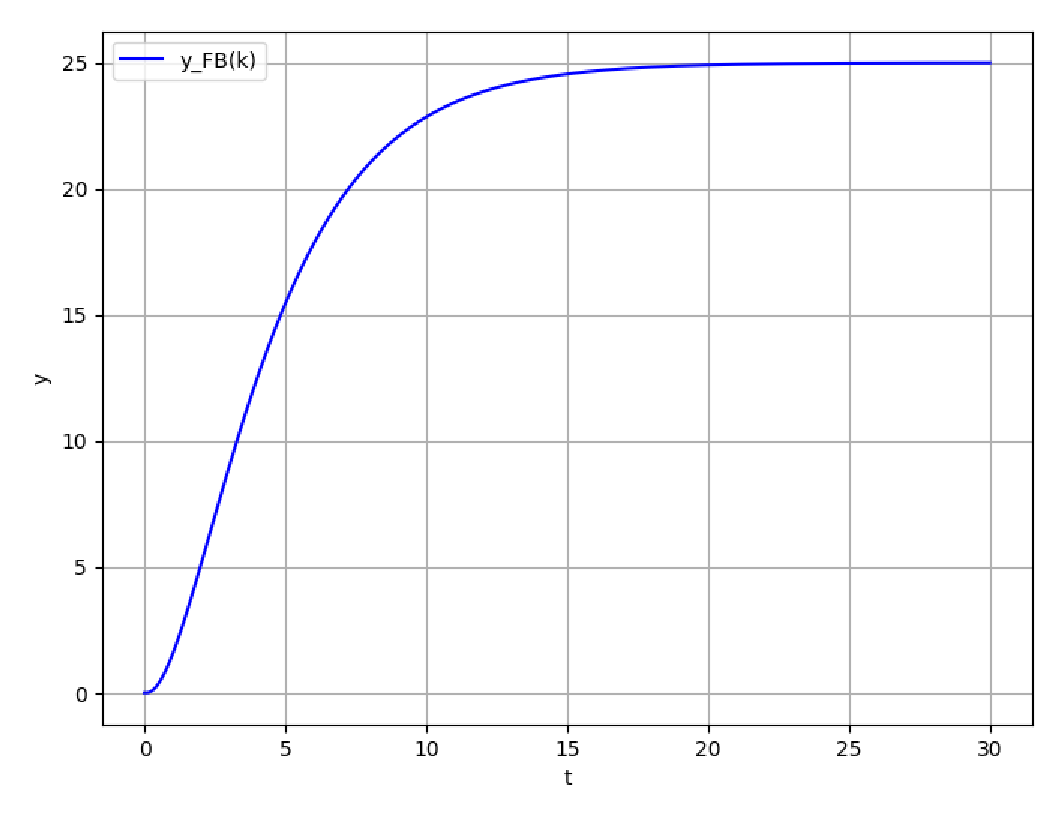
\includegraphics[scale=0.35]{figure21.eps}
    \caption{ボールの位置のシミュレーション結果}
    \label{fig:figure36}
  \end{minipage}
  \begin{minipage}[h]{0.4\linewidth}
    \centering
    \scalebox{0.45}[0.45]{
\begin{tikzpicture}[gnuplot]
%% generated with GNUPLOT 5.4p10 (Lua 5.4; terminal rev. Jun 2020, script rev. 118)
%% Sun Nov 19 19:13:55 2023
\path (0.000,0.000) rectangle (12.500,8.750);
\gpcolor{color=gp lt color border}
\gpsetlinetype{gp lt border}
\gpsetdashtype{gp dt solid}
\gpsetlinewidth{1.00}
\draw[gp path] (0.018,0.031)--(0.198,0.031);
\draw[gp path] (12.480,0.031)--(12.300,0.031);
\node[gp node right] at (-0.166,0.031) {$0$};
\draw[gp path] (0.018,1.272)--(0.198,1.272);
\draw[gp path] (12.480,1.272)--(12.300,1.272);
\node[gp node right] at (-0.166,1.272) {$5$};
\draw[gp path] (0.018,2.513)--(0.198,2.513);
\draw[gp path] (12.480,2.513)--(12.300,2.513);
\node[gp node right] at (-0.166,2.513) {$10$};
\draw[gp path] (0.018,3.754)--(0.198,3.754);
\draw[gp path] (12.480,3.754)--(12.300,3.754);
\node[gp node right] at (-0.166,3.754) {$15$};
\draw[gp path] (0.018,4.995)--(0.198,4.995);
\draw[gp path] (12.480,4.995)--(12.300,4.995);
\node[gp node right] at (-0.166,4.995) {$20$};
\draw[gp path] (0.018,6.236)--(0.198,6.236);
\draw[gp path] (12.480,6.236)--(12.300,6.236);
\node[gp node right] at (-0.166,6.236) {$25$};
\draw[gp path] (0.018,7.477)--(0.198,7.477);
\draw[gp path] (12.480,7.477)--(12.300,7.477);
\node[gp node right] at (-0.166,7.477) {$30$};
\draw[gp path] (0.018,8.718)--(0.198,8.718);
\draw[gp path] (12.480,8.718)--(12.300,8.718);
\node[gp node right] at (-0.166,8.718) {$35$};
\draw[gp path] (0.018,0.031)--(0.018,0.211);
\draw[gp path] (0.018,8.718)--(0.018,8.538);
\node[gp node center] at (0.018,-0.277) {$0$};
\draw[gp path] (1.403,0.031)--(1.403,0.211);
\draw[gp path] (1.403,8.718)--(1.403,8.538);
\node[gp node center] at (1.403,-0.277) {$5$};
\draw[gp path] (2.787,0.031)--(2.787,0.211);
\draw[gp path] (2.787,8.718)--(2.787,8.538);
\node[gp node center] at (2.787,-0.277) {$10$};
\draw[gp path] (4.172,0.031)--(4.172,0.211);
\draw[gp path] (4.172,8.718)--(4.172,8.538);
\node[gp node center] at (4.172,-0.277) {$15$};
\draw[gp path] (5.557,0.031)--(5.557,0.211);
\draw[gp path] (5.557,8.718)--(5.557,8.538);
\node[gp node center] at (5.557,-0.277) {$20$};
\draw[gp path] (6.941,0.031)--(6.941,0.211);
\draw[gp path] (6.941,8.718)--(6.941,8.538);
\node[gp node center] at (6.941,-0.277) {$25$};
\draw[gp path] (8.326,0.031)--(8.326,0.211);
\draw[gp path] (8.326,8.718)--(8.326,8.538);
\node[gp node center] at (8.326,-0.277) {$30$};
\draw[gp path] (9.711,0.031)--(9.711,0.211);
\draw[gp path] (9.711,8.718)--(9.711,8.538);
\node[gp node center] at (9.711,-0.277) {$35$};
\draw[gp path] (11.095,0.031)--(11.095,0.211);
\draw[gp path] (11.095,8.718)--(11.095,8.538);
\node[gp node center] at (11.095,-0.277) {$40$};
\draw[gp path] (12.480,0.031)--(12.480,0.211);
\draw[gp path] (12.480,8.718)--(12.480,8.538);
\node[gp node center] at (12.480,-0.277) {$45$};
\draw[gp path] (0.018,8.718)--(0.018,0.031)--(12.480,0.031)--(12.480,8.718)--cycle;
\node[gp node center,rotate=-270] at (-0.826,4.374) {ボールの位置$z\ /\ \mathrm{cm}$};
\node[gp node center] at (6.249,-0.738) {時間$t\ /\ \mathrm{s}$};
\gpcolor{rgb color={0.000,0.000,0.000}}
\draw[gp path] (0.018,0.513)--(0.024,2.043)--(0.029,4.111)--(0.035,5.871)--(0.040,7.025)%
  --(0.046,7.636)--(0.051,7.894)--(0.057,7.919)--(0.062,7.801)--(0.068,7.647)--(0.073,7.522)%
  --(0.079,7.439)--(0.084,7.411)--(0.090,7.407)--(0.096,7.311)--(0.101,7.116)--(0.107,6.950)%
  --(0.112,6.859)--(0.118,6.792)--(0.123,6.711)--(0.129,6.628)--(0.134,6.566)--(0.140,6.518)%
  --(0.145,6.478)--(0.151,6.452)--(0.156,6.440)--(0.162,6.439)--(0.168,6.441)--(0.173,6.442)%
  --(0.179,6.447)--(0.184,6.472)--(0.190,6.539)--(0.195,6.645)--(0.201,6.736)--(0.206,6.790)%
  --(0.212,6.865)--(0.217,6.982)--(0.223,7.105)--(0.228,7.217)--(0.234,7.314)--(0.240,7.401)%
  --(0.245,7.479)--(0.251,7.557)--(0.256,7.636)--(0.262,7.708)--(0.267,7.787)--(0.273,7.863)%
  --(0.278,7.897)--(0.284,7.886)--(0.289,7.907)--(0.295,7.987)--(0.300,8.042)--(0.306,8.063)%
  --(0.312,8.080)--(0.317,8.047)--(0.323,7.959)--(0.328,7.879)--(0.334,7.823)--(0.339,7.771)%
  --(0.345,7.723)--(0.350,7.564)--(0.356,7.262)--(0.361,7.079)--(0.367,7.088)--(0.372,7.148)%
  --(0.378,7.206)--(0.384,7.227)--(0.389,7.210)--(0.395,7.180)--(0.400,7.120)--(0.406,7.036)%
  --(0.411,6.952)--(0.417,6.871)--(0.422,6.799)--(0.428,6.729)--(0.433,6.662)--(0.439,6.602)%
  --(0.444,6.539)--(0.450,6.469)--(0.456,6.407)--(0.461,6.361)--(0.467,6.327)--(0.472,6.297)%
  --(0.478,6.273)--(0.483,6.258)--(0.489,6.245)--(0.494,6.223)--(0.500,6.193)--(0.505,6.147)%
  --(0.511,6.097)--(0.516,6.075)--(0.522,6.081)--(0.528,6.094)--(0.533,6.109)--(0.539,6.123)%
  --(0.544,6.137)--(0.550,6.153)--(0.555,6.162)--(0.561,6.157)--(0.566,6.165)--(0.572,6.184)%
  --(0.577,6.200)--(0.583,6.227)--(0.588,6.271)--(0.594,6.324)--(0.600,6.375)--(0.605,6.420)%
  --(0.611,6.461)--(0.616,6.501)--(0.622,6.316)--(0.627,5.863)--(0.633,5.633)--(0.638,5.798)%
  --(0.644,6.108)--(0.649,6.390)--(0.655,6.581)--(0.660,6.681)--(0.666,6.699)--(0.672,6.669)%
  --(0.677,6.625)--(0.683,6.581)--(0.688,6.536)--(0.694,6.505)--(0.699,6.489)--(0.705,6.456)%
  --(0.710,6.389)--(0.716,6.289)--(0.721,6.170)--(0.727,6.063)--(0.732,5.972)--(0.738,5.881)%
  --(0.744,5.765)--(0.749,5.622)--(0.755,5.497)--(0.760,5.409)--(0.766,5.322)--(0.771,5.208)%
  --(0.777,5.092)--(0.782,4.976)--(0.788,4.852)--(0.793,4.719)--(0.799,4.581)--(0.804,4.475)%
  --(0.810,4.404)--(0.816,4.332)--(0.821,4.249)--(0.827,4.177)--(0.832,4.127)--(0.838,4.086)%
  --(0.843,4.046)--(0.849,4.003)--(0.854,3.962)--(0.860,3.915)--(0.865,3.861)--(0.871,3.835)%
  --(0.876,3.831)--(0.882,3.828)--(0.888,3.846)--(0.893,3.888)--(0.899,3.931)--(0.904,3.969)%
  --(0.910,4.006)--(0.915,4.045)--(0.921,4.093)--(0.926,4.148)--(0.932,4.204)--(0.937,4.262)%
  --(0.943,4.329)--(0.948,4.419)--(0.954,4.529)--(0.960,4.635)--(0.965,4.731)--(0.971,4.822)%
  --(0.976,4.917)--(0.982,5.022)--(0.987,5.130)--(0.993,5.232)--(0.998,5.326)--(1.004,5.420)%
  --(1.009,5.509)--(1.015,5.584)--(1.020,5.643)--(1.026,5.689)--(1.032,5.730)--(1.037,5.765)%
  --(1.043,5.789)--(1.048,5.801)--(1.054,5.806)--(1.059,5.806)--(1.065,5.804)--(1.070,5.794)%
  --(1.076,5.769)--(1.081,5.732)--(1.087,5.630)--(1.093,5.455)--(1.098,5.334)--(1.104,5.311)%
  --(1.109,5.324)--(1.115,5.330)--(1.120,5.302)--(1.126,5.242)--(1.131,5.169)--(1.137,5.089)%
  --(1.142,4.992)--(1.148,4.871)--(1.153,4.746)--(1.159,4.646)--(1.165,4.585)--(1.170,4.553)%
  --(1.176,4.528)--(1.181,4.505)--(1.187,4.484)--(1.192,4.468)--(1.198,4.454)--(1.203,4.441)%
  --(1.209,4.430)--(1.214,4.429)--(1.220,4.440)--(1.225,4.458)--(1.231,4.482)--(1.237,4.498)%
  --(1.242,4.505)--(1.248,4.537)--(1.253,4.611)--(1.259,4.708)--(1.264,4.811)--(1.270,4.766)%
  --(1.275,4.547)--(1.281,4.484)--(1.286,4.665)--(1.292,4.901)--(1.297,5.107)--(1.303,5.284)%
  --(1.309,5.449)--(1.314,5.599)--(1.320,5.726)--(1.325,5.838)--(1.331,5.939)--(1.336,6.020)%
  --(1.342,6.085)--(1.347,6.137)--(1.353,6.184)--(1.358,6.222)--(1.364,6.232)--(1.369,6.211)%
  --(1.375,6.199)--(1.381,6.208)--(1.386,6.224)--(1.392,6.237)--(1.397,6.233)--(1.403,6.221)%
  --(1.408,6.214)--(1.414,6.191)--(1.419,6.135)--(1.425,6.051)--(1.430,5.797)--(1.436,5.349)%
  --(1.441,5.061)--(1.447,5.053)--(1.453,5.136)--(1.458,5.205)--(1.464,5.235)--(1.469,5.226)%
  --(1.475,5.182)--(1.480,5.115)--(1.486,5.026)--(1.491,4.942)--(1.497,4.906)--(1.502,4.908)%
  --(1.508,4.908)--(1.513,4.897)--(1.519,4.888)--(1.525,4.891)--(1.530,4.910)--(1.536,4.932)%
  --(1.541,4.951)--(1.547,4.961)--(1.552,4.967)--(1.558,4.976)--(1.563,4.997)--(1.569,5.020)%
  --(1.574,5.033)--(1.580,5.077)--(1.585,5.165)--(1.591,5.261)--(1.597,5.346)--(1.602,5.417)%
  --(1.608,5.488)--(1.613,5.566)--(1.619,5.637)--(1.624,5.691)--(1.630,5.734)--(1.635,5.773)%
  --(1.641,5.799)--(1.646,5.811)--(1.652,5.838)--(1.657,5.885)--(1.663,5.928)--(1.669,5.954)%
  --(1.674,5.956)--(1.680,5.940)--(1.685,5.911)--(1.691,5.869)--(1.696,5.823)--(1.702,5.775)%
  --(1.707,5.726)--(1.713,5.659)--(1.718,5.581)--(1.724,5.508)--(1.729,5.425)--(1.735,5.338)%
  --(1.741,5.259)--(1.746,5.178)--(1.752,5.087)--(1.757,4.982)--(1.763,4.874)--(1.768,4.764)%
  --(1.774,4.649)--(1.779,4.555)--(1.785,4.495)--(1.790,4.454)--(1.796,4.417)--(1.801,4.380)%
  --(1.807,4.332)--(1.813,4.273)--(1.818,4.225)--(1.824,4.192)--(1.829,4.188)--(1.835,4.213)%
  --(1.840,4.248)--(1.846,4.280)--(1.851,4.307)--(1.857,4.332)--(1.862,4.360)--(1.868,4.396)%
  --(1.873,4.432)--(1.879,4.460)--(1.885,4.481)--(1.890,4.507)--(1.896,4.545)--(1.901,4.598)%
  --(1.907,4.663)--(1.912,4.740)--(1.918,4.817)--(1.923,4.897)--(1.929,4.990)--(1.934,5.106)%
  --(1.940,5.216)--(1.945,5.292)--(1.951,5.379)--(1.957,5.489)--(1.962,5.599)--(1.968,5.695)%
  --(1.973,5.762)--(1.979,5.806)--(1.984,5.840)--(1.990,5.871)--(1.995,5.900)--(2.001,5.923)%
  --(2.006,5.940)--(2.012,5.942)--(2.017,5.926)--(2.023,5.901)--(2.029,5.735)--(2.034,5.384)%
  --(2.040,5.097)--(2.045,5.013)--(2.051,5.082)--(2.056,5.231)--(2.062,5.375)--(2.067,5.314)%
  --(2.073,4.994)--(2.078,4.771)--(2.084,4.787)--(2.089,4.903)--(2.095,5.032)--(2.101,5.107)%
  --(2.106,5.111)--(2.112,5.068)--(2.117,5.002)--(2.123,4.937)--(2.128,4.878)--(2.134,4.817)%
  --(2.139,4.755)--(2.145,4.701)--(2.150,4.656)--(2.156,4.619)--(2.161,4.591)--(2.167,4.554)%
  --(2.173,4.502)--(2.178,4.451)--(2.184,4.409)--(2.189,4.365)--(2.195,4.315)--(2.200,4.262)%
  --(2.206,4.206)--(2.211,4.153)--(2.217,4.109)--(2.222,4.075)--(2.228,4.047)--(2.233,4.024)%
  --(2.239,4.005)--(2.245,3.998)--(2.250,4.004)--(2.256,4.003)--(2.261,3.981)--(2.267,3.971)%
  --(2.272,3.992)--(2.278,4.028)--(2.283,4.071)--(2.289,4.116)--(2.294,4.171)--(2.300,4.236)%
  --(2.305,4.297)--(2.311,4.346)--(2.317,4.393)--(2.322,4.450)--(2.328,4.510)--(2.333,4.567)%
  --(2.339,4.634)--(2.344,4.720)--(2.350,4.805)--(2.355,4.873)--(2.361,4.934)--(2.366,4.983)%
  --(2.372,5.020)--(2.377,5.070)--(2.383,5.142)--(2.389,5.211)--(2.394,5.264)--(2.400,5.297)%
  --(2.405,5.308)--(2.411,5.297)--(2.416,5.273)--(2.422,5.246)--(2.427,5.214)--(2.433,5.171)%
  --(2.438,5.122)--(2.444,5.069)--(2.449,5.012)--(2.455,4.924)--(2.461,4.798)--(2.466,4.685)%
  --(2.472,4.585)--(2.477,4.475)--(2.483,4.358)--(2.488,4.229)--(2.494,4.089)--(2.499,3.958)%
  --(2.505,3.842)--(2.510,3.733)--(2.516,3.621)--(2.521,3.502)--(2.527,3.382)--(2.533,3.286)%
  --(2.538,3.223)--(2.544,3.179)--(2.549,3.145)--(2.555,3.116)--(2.560,3.088)--(2.566,3.054)%
  --(2.571,3.006)--(2.577,2.956)--(2.582,2.928)--(2.588,2.921)--(2.593,2.924)--(2.599,2.930)%
  --(2.605,2.937)--(2.610,2.947)--(2.616,2.956)--(2.621,2.962)--(2.627,2.980)--(2.632,3.012)%
  --(2.638,3.048)--(2.643,3.087)--(2.649,3.133)--(2.654,3.188)--(2.660,3.251)--(2.665,3.319)%
  --(2.671,3.405)--(2.677,3.497)--(2.682,3.578)--(2.688,3.663)--(2.693,3.756)--(2.699,3.876)%
  --(2.704,4.021)--(2.710,4.156)--(2.715,4.258)--(2.721,4.327)--(2.726,4.369)--(2.732,4.378)%
  --(2.737,4.364)--(2.743,4.362)--(2.749,4.377)--(2.754,4.388)--(2.760,4.391)--(2.765,4.385)%
  --(2.771,4.368)--(2.776,4.341)--(2.782,4.288)--(2.787,4.207)--(2.793,4.139)--(2.798,4.096)%
  --(2.804,4.048)--(2.809,3.980)--(2.815,3.904)--(2.821,3.839)--(2.826,3.796)--(2.832,3.772)%
  --(2.837,3.745)--(2.843,3.707)--(2.848,3.681)--(2.854,3.675)--(2.859,3.681)--(2.865,3.700)%
  --(2.870,3.735)--(2.876,3.778)--(2.881,3.825)--(2.887,3.876)--(2.893,3.930)--(2.898,3.994)%
  --(2.904,4.027)--(2.909,4.016)--(2.915,4.048)--(2.920,4.149)--(2.926,4.276)--(2.931,4.403)%
  --(2.937,4.523)--(2.942,4.656)--(2.948,4.807)--(2.953,4.956)--(2.959,5.095)--(2.965,5.217)%
  --(2.970,5.322)--(2.976,5.405)--(2.981,5.461)--(2.987,5.476)--(2.992,5.456)--(2.998,5.428)%
  --(3.003,5.407)--(3.009,5.438)--(3.014,5.542)--(3.020,5.658)--(3.025,5.718)--(3.031,5.730)%
  --(3.037,5.722)--(3.042,5.670)--(3.048,5.578)--(3.053,5.510)--(3.059,5.492)--(3.064,5.499)%
  --(3.070,5.511)--(3.075,5.511)--(3.081,5.497)--(3.086,5.470)--(3.092,5.439)--(3.097,5.412)%
  --(3.103,5.390)--(3.109,5.364)--(3.114,5.338)--(3.120,5.318)--(3.125,5.316)--(3.131,5.330)%
  --(3.136,5.313)--(3.142,5.264)--(3.147,5.237)--(3.153,5.242)--(3.158,5.254)--(3.164,5.278)%
  --(3.170,5.316)--(3.175,5.340)--(3.181,5.323)--(3.186,5.275)--(3.192,5.240)--(3.197,5.234)%
  --(3.203,5.241)--(3.208,5.259)--(3.214,5.291)--(3.219,5.330)--(3.225,5.361)--(3.230,5.383)%
  --(3.236,5.400)--(3.242,5.419)--(3.247,5.435)--(3.253,5.444)--(3.258,5.448)--(3.264,5.436)%
  --(3.269,5.408)--(3.275,5.397)--(3.280,5.412)--(3.286,5.433)--(3.291,5.449)--(3.297,5.453)%
  --(3.302,5.444)--(3.308,5.427)--(3.314,5.405)--(3.319,5.376)--(3.325,5.347)--(3.330,5.174)%
  --(3.336,4.824)--(3.341,4.622)--(3.347,4.667)--(3.352,4.786)--(3.358,4.897)--(3.363,4.977)%
  --(3.369,5.011)--(3.374,5.002)--(3.380,4.969)--(3.386,4.919)--(3.391,4.861)--(3.397,4.801)%
  --(3.402,4.744)--(3.408,4.698)--(3.413,4.666)--(3.419,4.646)--(3.424,4.638)--(3.430,4.631)%
  --(3.435,4.619)--(3.441,4.608)--(3.446,4.595)--(3.452,4.581)--(3.458,4.570)--(3.463,4.562)%
  --(3.469,4.533)--(3.474,4.479)--(3.480,4.440)--(3.485,4.435)--(3.491,4.447)--(3.496,4.463)%
  --(3.502,4.483)--(3.507,4.505)--(3.513,4.516)--(3.518,4.512)--(3.524,4.500)--(3.530,4.490)%
  --(3.535,4.490)--(3.541,4.502)--(3.546,4.521)--(3.552,4.536)--(3.557,4.543)--(3.563,4.547)%
  --(3.568,4.557)--(3.574,4.572)--(3.579,4.570)--(3.585,4.532)--(3.590,4.487)--(3.596,4.481)%
  --(3.602,4.518)--(3.607,4.572)--(3.613,4.618)--(3.618,4.653)--(3.624,4.683)--(3.629,4.704)%
  --(3.635,4.719)--(3.640,4.744)--(3.646,4.780)--(3.651,4.812)--(3.657,4.838)--(3.662,4.853)%
  --(3.668,4.857)--(3.674,4.856)--(3.679,4.853)--(3.685,4.850)--(3.690,4.843)--(3.696,4.825)%
  --(3.701,4.795)--(3.707,4.760)--(3.712,4.657)--(3.718,4.477)--(3.723,4.370)--(3.729,4.374)%
  --(3.734,4.401)--(3.740,4.416)--(3.746,4.389)--(3.751,4.313)--(3.757,4.229)--(3.762,4.155)%
  --(3.768,4.085)--(3.773,4.018)--(3.779,3.952)--(3.784,3.887)--(3.790,3.822)--(3.795,3.746)%
  --(3.801,3.651)--(3.806,3.562)--(3.812,3.504)--(3.818,3.477)--(3.823,3.458)--(3.829,3.432)%
  --(3.834,3.417)--(3.840,3.424)--(3.845,3.438)--(3.851,3.451)--(3.856,3.461)--(3.862,3.474)%
  --(3.867,3.493)--(3.873,3.524)--(3.878,3.573)--(3.884,3.646)--(3.890,3.734)--(3.895,3.823)%
  --(3.901,3.897)--(3.906,3.953)--(3.912,4.013)--(3.917,4.073)--(3.923,4.120)--(3.928,4.166)%
  --(3.934,4.227)--(3.939,4.320)--(3.945,4.433)--(3.950,4.517)--(3.956,4.561)--(3.962,4.609)%
  --(3.967,4.668)--(3.973,4.712)--(3.978,4.723)--(3.984,4.697)--(3.989,4.675)--(3.995,4.677)%
  --(4.000,4.679)--(4.006,4.665)--(4.011,4.637)--(4.017,4.602)--(4.022,4.557)--(4.028,4.502)%
  --(4.034,4.437)--(4.039,4.363)--(4.045,4.282)--(4.050,4.196)--(4.056,4.095)--(4.061,3.965)%
  --(4.067,3.823)--(4.072,3.697)--(4.078,3.587)--(4.083,3.503)--(4.089,3.445)--(4.094,3.400)%
  --(4.100,3.358)--(4.106,3.316)--(4.111,3.275)--(4.117,3.237)--(4.122,3.204)--(4.128,3.178)%
  --(4.133,3.153)--(4.139,3.097)--(4.144,3.018)--(4.150,2.978)--(4.155,2.991)--(4.161,3.031)%
  --(4.166,3.077)--(4.172,3.104)--(4.178,3.117)--(4.183,3.135)--(4.189,3.170)--(4.194,3.218)%
  --(4.200,3.273)--(4.205,3.331)--(4.211,3.395)--(4.216,3.465)--(4.222,3.526)--(4.227,3.577)%
  --(4.233,3.645)--(4.238,3.726)--(4.244,3.803)--(4.250,3.867)--(4.255,3.926)--(4.261,4.023)%
  --(4.266,4.159)--(4.272,4.297)--(4.277,4.429)--(4.283,4.552)--(4.288,4.655)--(4.294,4.715)%
  --(4.299,4.722)--(4.305,4.713)--(4.310,4.720)--(4.316,4.734)--(4.322,4.738)--(4.327,4.735)%
  --(4.333,4.730)--(4.338,4.716)--(4.344,4.693)--(4.349,4.657)--(4.355,4.604)--(4.360,4.547)%
  --(4.366,4.504)--(4.371,4.475)--(4.377,4.435)--(4.382,4.378)--(4.388,4.334)--(4.394,4.316)%
  --(4.399,4.313)--(4.405,4.320)--(4.410,4.332)--(4.416,4.347)--(4.421,4.360)--(4.427,4.371)%
  --(4.432,4.382)--(4.438,4.398)--(4.443,4.421)--(4.449,4.452)--(4.454,4.491)--(4.460,4.541)%
  --(4.466,4.603)--(4.471,4.678)--(4.477,4.748)--(4.482,4.819)--(4.488,4.915)--(4.493,5.032)%
  --(4.499,5.169)--(4.504,5.316)--(4.510,5.450)--(4.515,5.565)--(4.521,5.657)--(4.526,5.728)%
  --(4.532,5.771)--(4.538,5.791)--(4.543,5.813)--(4.549,5.841)--(4.554,5.860)--(4.560,5.866)%
  --(4.565,5.864)--(4.571,5.825)--(4.576,5.742)--(4.582,5.683)--(4.587,5.677)--(4.593,5.699)%
  --(4.598,5.712)--(4.604,5.683)--(4.610,5.631)--(4.615,5.566)--(4.621,5.493)--(4.626,5.417)%
  --(4.632,5.326)--(4.637,5.253)--(4.643,5.219)--(4.648,5.196)--(4.654,5.165)--(4.659,5.133)%
  --(4.665,5.109)--(4.670,5.094)--(4.676,5.056)--(4.682,4.990)--(4.687,4.954)--(4.693,4.970)%
  --(4.698,5.010)--(4.704,5.030)--(4.709,5.024)--(4.715,5.037)--(4.720,5.081)--(4.726,5.135)%
  --(4.731,5.177)--(4.737,5.184)--(4.742,5.175)--(4.748,5.213)--(4.754,5.306)--(4.759,5.420)%
  --(4.765,5.539)--(4.770,5.651)--(4.776,5.748)--(4.781,5.811)--(4.787,5.833)--(4.792,5.847)%
  --(4.798,5.867)--(4.803,5.921)--(4.809,6.008)--(4.814,6.096)--(4.820,6.171)--(4.826,6.192)%
  --(4.831,6.148)--(4.837,6.121)--(4.842,6.142)--(4.848,6.162)--(4.853,6.155)--(4.859,6.146)%
  --(4.864,6.139)--(4.870,6.122)--(4.875,6.091)--(4.881,6.017)--(4.886,5.904)--(4.892,5.815)%
  --(4.898,5.760)--(4.903,5.712)--(4.909,5.634)--(4.914,5.514)--(4.920,5.396)--(4.925,5.305)%
  --(4.931,5.216)--(4.936,5.092)--(4.942,4.953)--(4.947,4.864)--(4.953,4.830)--(4.958,4.821)%
  --(4.964,4.814)--(4.970,4.788)--(4.975,4.746)--(4.981,4.702)--(4.986,4.666)--(4.992,4.652)%
  --(4.997,4.659)--(5.003,4.667)--(5.008,4.670)--(5.014,4.668)--(5.019,4.674)--(5.025,4.699)%
  --(5.030,4.732)--(5.036,4.758)--(5.042,4.780)--(5.047,4.801)--(5.053,4.821)--(5.058,4.840)%
  --(5.064,4.868)--(5.069,4.912)--(5.075,4.967)--(5.080,5.030)--(5.086,4.958)--(5.091,4.727)%
  --(5.097,4.645)--(5.102,4.794)--(5.108,5.016)--(5.114,5.216)--(5.119,5.375)--(5.125,5.497)%
  --(5.130,5.561)--(5.136,5.573)--(5.141,5.584)--(5.147,5.609)--(5.152,5.626)--(5.158,5.633)%
  --(5.163,5.628)--(5.169,5.604)--(5.174,5.571)--(5.180,5.540)--(5.186,5.487)--(5.191,5.398)%
  --(5.197,5.300)--(5.202,5.201)--(5.208,5.071)--(5.213,4.932)--(5.219,4.810)--(5.224,4.700)%
  --(5.230,4.602)--(5.235,4.510)--(5.241,4.424)--(5.247,4.329)--(5.252,4.223)--(5.258,4.144)%
  --(5.263,4.104)--(5.269,4.085)--(5.274,4.066)--(5.280,4.042)--(5.285,4.015)--(5.291,3.985)%
  --(5.296,3.949)--(5.302,3.924)--(5.307,3.921)--(5.313,3.919)--(5.319,3.907)--(5.324,3.909)%
  --(5.330,3.933)--(5.335,3.966)--(5.341,3.937)--(5.346,3.835)--(5.352,3.806)--(5.357,3.877)%
  --(5.363,3.963)--(5.368,4.062)--(5.374,4.192)--(5.379,4.332)--(5.385,4.470)--(5.391,4.590)%
  --(5.396,4.665)--(5.402,4.710)--(5.407,4.767)--(5.413,4.848)--(5.418,4.944)--(5.424,5.062)%
  --(5.429,5.202)--(5.435,5.325)--(5.440,5.414)--(5.446,5.496)--(5.451,5.579)--(5.457,5.648)%
  --(5.463,5.693)--(5.468,5.719)--(5.474,5.740)--(5.479,5.760)--(5.485,5.788)--(5.490,5.825)%
  --(5.496,5.846)--(5.501,5.841)--(5.507,5.819)--(5.512,5.756)--(5.518,5.656)--(5.523,5.582)%
  --(5.529,5.556)--(5.535,5.550)--(5.540,5.537)--(5.546,5.372)--(5.551,5.028)--(5.557,4.809)%
  --(5.562,4.813)--(5.568,4.894)--(5.573,4.969)--(5.579,5.008)--(5.584,5.007)--(5.590,4.970)%
  --(5.595,4.910)--(5.601,4.851)--(5.607,4.793)--(5.612,4.741)--(5.618,4.711)--(5.623,4.675)%
  --(5.629,4.618)--(5.634,4.586)--(5.640,4.586)--(5.645,4.594)--(5.651,4.600)--(5.656,4.608)%
  --(5.662,4.622)--(5.667,4.642)--(5.673,4.668)--(5.679,4.691)--(5.684,4.623)--(5.690,4.452)%
  --(5.695,4.370)--(5.701,4.445)--(5.706,4.587)--(5.712,4.732)--(5.717,4.852)--(5.723,4.949)%
  --(5.728,5.030)--(5.734,5.102)--(5.739,5.161)--(5.745,5.204)--(5.751,5.241)--(5.756,5.283)%
  --(5.762,5.339)--(5.767,5.401)--(5.773,5.466)--(5.778,5.529)--(5.784,5.558)--(5.789,5.525)%
  --(5.795,5.448)--(5.800,5.397)--(5.806,5.389)--(5.811,5.389)--(5.817,5.376)--(5.823,5.343)%
  --(5.828,5.291)--(5.834,5.224)--(5.839,5.148)--(5.845,5.055)--(5.850,4.941)--(5.856,4.837)%
  --(5.861,4.741)--(5.867,4.630)--(5.872,4.505)--(5.878,4.378)--(5.883,4.254)--(5.889,4.136)%
  --(5.895,4.024)--(5.900,3.898)--(5.906,3.754)--(5.911,3.604)--(5.917,3.459)--(5.922,3.342)%
  --(5.928,3.257)--(5.933,3.191)--(5.939,3.132)--(5.944,3.077)--(5.950,3.028)--(5.955,2.983)%
  --(5.961,2.940)--(5.967,2.905)--(5.972,2.875)--(5.978,2.836)--(5.983,2.785)--(5.989,2.730)%
  --(5.994,2.679)--(6.000,2.635)--(6.005,2.597)--(6.011,2.556)--(6.016,2.513)--(6.022,2.484)%
  --(6.027,2.475)--(6.033,2.465)--(6.039,2.446)--(6.044,2.434)--(6.050,2.436)--(6.055,2.445)%
  --(6.061,2.458)--(6.066,2.471)--(6.072,2.484)--(6.077,2.498)--(6.083,2.516)--(6.088,2.542)%
  --(6.094,2.571)--(6.099,2.606)--(6.105,2.650)--(6.111,2.716)--(6.116,2.802)--(6.122,2.895)%
  --(6.127,2.993)--(6.133,3.094)--(6.138,3.201)--(6.144,3.302)--(6.149,3.388)--(6.155,3.473)%
  --(6.160,3.553)--(6.166,3.617)--(6.171,3.669)--(6.177,3.696)--(6.183,3.686)--(6.188,3.665)%
  --(6.194,3.638)--(6.199,3.593)--(6.205,3.557)--(6.210,3.538)--(6.216,3.520)--(6.221,3.486)%
  --(6.227,3.432)--(6.232,3.359)--(6.238,3.270)--(6.243,3.169)--(6.249,3.064)--(6.255,2.951)%
  --(6.260,2.831)--(6.266,2.722)--(6.271,2.623)--(6.277,2.534)--(6.282,2.467)--(6.288,2.427)%
  --(6.293,2.403)--(6.299,2.379)--(6.304,2.351)--(6.310,2.333)--(6.315,2.329)--(6.321,2.332)%
  --(6.327,2.332)--(6.332,2.289)--(6.338,2.208)--(6.343,2.180)--(6.349,2.226)--(6.354,2.296)%
  --(6.360,2.363)--(6.365,2.414)--(6.371,2.452)--(6.376,2.485)--(6.382,2.517)--(6.387,2.556)%
  --(6.393,2.605)--(6.399,2.664)--(6.404,2.741)--(6.410,2.852)--(6.415,2.993)--(6.421,3.142)%
  --(6.426,3.272)--(6.432,3.364)--(6.437,3.442)--(6.443,3.536)--(6.448,3.637)--(6.454,3.745)%
  --(6.459,3.861)--(6.465,3.962)--(6.471,4.041)--(6.476,4.112)--(6.482,4.171)--(6.487,4.197)%
  --(6.493,4.168)--(6.498,4.103)--(6.504,4.059)--(6.509,4.059)--(6.515,4.067)--(6.520,4.059)%
  --(6.526,4.020)--(6.531,3.902)--(6.537,3.729)--(6.543,3.617)--(6.548,3.588)--(6.554,3.589)%
  --(6.559,3.594)--(6.565,3.576)--(6.570,3.530)--(6.576,3.484)--(6.581,3.457)--(6.587,3.440)%
  --(6.592,3.431)--(6.598,3.432)--(6.603,3.442)--(6.609,3.457)--(6.615,3.473)--(6.620,3.493)%
  --(6.626,3.525)--(6.631,3.568)--(6.637,3.614)--(6.642,3.664)--(6.648,3.710)--(6.653,3.736)%
  --(6.659,3.775)--(6.664,3.864)--(6.670,3.990)--(6.675,4.129)--(6.681,4.252)--(6.687,4.360)%
  --(6.692,4.470)--(6.698,4.579)--(6.703,4.690)--(6.709,4.793)--(6.714,4.865)--(6.720,4.921)%
  --(6.725,4.968)--(6.731,5.006)--(6.736,5.005)--(6.742,4.965)--(6.747,4.940)--(6.753,4.947)%
  --(6.759,4.959)--(6.764,4.974)--(6.770,4.994)--(6.775,5.012)--(6.781,5.014)--(6.786,4.993)%
  --(6.792,4.948)--(6.797,4.860)--(6.803,4.729)--(6.808,4.611)--(6.814,4.537)--(6.819,4.485)%
  --(6.825,4.440)--(6.831,4.393)--(6.836,4.340)--(6.842,4.282)--(6.847,4.232)--(6.853,4.193)%
  --(6.858,4.152)--(6.864,4.108)--(6.869,4.063)--(6.875,4.023)--(6.880,3.989)--(6.886,3.963)%
  --(6.891,3.946)--(6.897,3.938)--(6.903,3.934)--(6.908,3.932)--(6.914,3.938)--(6.919,3.952)%
  --(6.925,3.969)--(6.930,3.971)--(6.936,3.965)--(6.941,3.994)--(6.947,4.051)--(6.952,4.116)%
  --(6.958,4.184)--(6.963,4.248)--(6.969,4.302)--(6.975,4.352)--(6.980,4.410)--(6.986,4.461)%
  --(6.991,4.501)--(6.997,4.566)--(7.002,4.648)--(7.008,4.729)--(7.013,4.817)--(7.019,4.916)%
  --(7.024,5.015)--(7.030,5.097)--(7.035,5.149)--(7.041,5.175)--(7.047,5.182)--(7.052,5.176)%
  --(7.058,5.167)--(7.063,5.159)--(7.069,5.117)--(7.074,5.028)--(7.080,4.941)--(7.085,4.875)%
  --(7.091,4.811)--(7.096,4.739)--(7.102,4.661)--(7.107,4.580)--(7.113,4.480)--(7.119,4.360)%
  --(7.124,4.256)--(7.130,4.168)--(7.135,4.070)--(7.141,3.966)--(7.146,3.883)--(7.152,3.830)%
  --(7.157,3.803)--(7.163,3.787)--(7.168,3.773)--(7.174,3.752)--(7.179,3.729)--(7.185,3.710)%
  --(7.191,3.694)--(7.196,3.678)--(7.202,3.667)--(7.207,3.663)--(7.213,3.653)--(7.218,3.636)%
  --(7.224,3.619)--(7.229,3.612)--(7.235,3.616)--(7.240,3.632)--(7.246,3.660)--(7.251,3.698)%
  --(7.257,3.747)--(7.263,3.805)--(7.268,3.869)--(7.274,3.934)--(7.279,4.011)--(7.285,4.087)%
  --(7.290,4.152)--(7.296,4.237)--(7.301,4.342)--(7.307,4.429)--(7.312,4.486)--(7.318,4.522)%
  --(7.324,4.540)--(7.329,4.543)--(7.335,4.543)--(7.340,4.541)--(7.346,4.536)--(7.351,4.529)%
  --(7.357,4.501)--(7.362,4.444)--(7.368,4.364)--(7.373,4.276)--(7.379,4.186)--(7.384,4.098)%
  --(7.390,3.997)--(7.396,3.881)--(7.401,3.769)--(7.407,3.668)--(7.412,3.584)--(7.418,3.516)%
  --(7.423,3.475)--(7.429,3.459)--(7.434,3.457)--(7.440,3.459)--(7.445,3.464)--(7.451,3.469)%
  --(7.456,3.468)--(7.462,3.446)--(7.468,3.404)--(7.473,3.376)--(7.479,3.366)--(7.484,3.360)%
  --(7.490,3.351)--(7.495,3.342)--(7.501,3.336)--(7.506,3.334)--(7.512,3.324)--(7.517,3.295)%
  --(7.523,3.272)--(7.528,3.289)--(7.534,3.353)--(7.540,3.442)--(7.545,3.538)--(7.551,3.631)%
  --(7.556,3.713)--(7.562,3.788)--(7.567,3.858)--(7.573,3.924)--(7.578,3.981)--(7.584,4.028)%
  --(7.589,4.076)--(7.595,4.132)--(7.600,4.181)--(7.606,4.209)--(7.612,4.242)--(7.617,4.282)%
  --(7.623,4.310)--(7.628,4.318)--(7.634,4.298)--(7.639,4.252)--(7.645,4.169)--(7.650,4.045)%
  --(7.656,3.919)--(7.661,3.826)--(7.667,3.753)--(7.672,3.663)--(7.678,3.548)--(7.684,3.421)%
  --(7.689,3.293)--(7.695,3.173)--(7.700,3.070)--(7.706,2.983)--(7.711,2.906)--(7.717,2.840)%
  --(7.722,2.781)--(7.728,2.724)--(7.733,2.666)--(7.739,2.609)--(7.744,2.551)--(7.750,2.492)%
  --(7.756,2.445)--(7.761,2.408)--(7.767,2.370)--(7.772,2.319)--(7.778,2.249)--(7.783,2.174)%
  --(7.789,2.109)--(7.794,2.052)--(7.800,2.022)--(7.805,2.040)--(7.811,2.117)--(7.816,2.269)%
  --(7.822,2.490)--(7.828,2.755)--(7.833,3.042)--(7.839,3.341)--(7.844,3.606)--(7.850,3.786)%
  --(7.855,3.897)--(7.861,3.965)--(7.866,4.001)--(7.872,4.003)--(7.877,3.979)--(7.883,3.961)%
  --(7.888,3.958)--(7.894,3.963)--(7.900,3.971)--(7.905,3.971)--(7.911,3.938)--(7.916,3.873)%
  --(7.922,3.817)--(7.927,3.775)--(7.933,3.709)--(7.938,3.646)--(7.944,3.592)--(7.949,3.506)%
  --(7.955,3.394)--(7.960,3.284)--(7.966,3.190)--(7.972,3.147)--(7.977,3.215)--(7.983,3.396)%
  --(7.988,3.600)--(7.994,3.743)--(7.999,3.802)--(8.005,3.802)--(8.010,3.787)--(8.016,3.789)%
  --(8.021,3.797)--(8.027,3.807)--(8.032,3.837)--(8.038,3.885)--(8.044,3.922)--(8.049,3.937)%
  --(8.055,3.944)--(8.060,3.948)--(8.066,3.940)--(8.071,3.907)--(8.077,3.854)--(8.082,3.799)%
  --(8.088,3.765)--(8.093,3.769)--(8.099,3.704)--(8.104,3.525)--(8.110,3.431)--(8.116,3.431)%
  --(8.121,3.397)--(8.127,3.331)--(8.132,3.242)--(8.138,3.133)--(8.143,3.038)--(8.149,2.985)%
  --(8.154,2.955)--(8.160,2.927)--(8.165,2.915)--(8.171,2.917)--(8.176,2.914)--(8.182,2.893)%
  --(8.188,2.850)--(8.193,2.790)--(8.199,2.714)--(8.204,2.640)--(8.210,2.569)--(8.215,2.483)%
  --(8.221,2.375)--(8.226,2.249)--(8.232,2.133)--(8.237,2.043)--(8.243,1.987)--(8.248,1.987)%
  --(8.254,2.035)--(8.260,2.110)--(8.265,2.210)--(8.271,2.329)--(8.276,2.449)--(8.282,2.560)%
  --(8.287,2.679)--(8.293,2.812)--(8.298,2.953)--(8.304,3.102)--(8.309,3.276)--(8.315,3.460)%
  --(8.320,3.628)--(8.326,3.797)--(8.332,3.956)--(8.337,4.084)--(8.343,4.199)--(8.348,4.308)%
  --(8.354,4.415)--(8.359,4.519)--(8.365,4.619)--(8.370,4.719)--(8.376,4.818)--(8.381,4.885)%
  --(8.387,4.918)--(8.392,4.970)--(8.398,5.053)--(8.404,5.133)--(8.409,5.192)--(8.415,5.210)%
  --(8.420,5.202)--(8.426,5.208)--(8.431,5.225)--(8.437,5.234)--(8.442,5.240)--(8.448,5.242)%
  --(8.453,5.219)--(8.459,5.159)--(8.464,5.074)--(8.470,4.986)--(8.476,4.904)--(8.481,4.809)%
  --(8.487,4.699)--(8.492,4.607)--(8.498,4.544)--(8.503,4.487)--(8.509,4.409)--(8.514,4.292)%
  --(8.520,4.153)--(8.525,4.019)--(8.531,3.900)--(8.536,3.801)--(8.542,3.718)--(8.548,3.651)%
  --(8.553,3.599)--(8.559,3.557)--(8.564,3.521)--(8.570,3.493)--(8.575,3.461)--(8.581,3.417)%
  --(8.586,3.384)--(8.592,3.373)--(8.597,3.378)--(8.603,3.403)--(8.608,3.441)--(8.614,3.481)%
  --(8.620,3.506)--(8.625,3.514)--(8.631,3.532)--(8.636,3.571)--(8.642,3.638)--(8.647,3.737)%
  --(8.653,3.843)--(8.658,3.926)--(8.664,4.001)--(8.669,4.102)--(8.675,4.218)--(8.680,4.327)%
  --(8.686,4.430)--(8.692,4.526)--(8.697,4.640)--(8.703,4.770)--(8.708,4.900)--(8.714,5.018)%
  --(8.719,5.109)--(8.725,5.172)--(8.730,5.192)--(8.736,5.172)--(8.741,5.170)--(8.747,5.198)%
  --(8.752,5.232)--(8.758,5.264)--(8.764,5.287)--(8.769,5.299)--(8.775,5.299)--(8.780,5.287)%
  --(8.786,5.259)--(8.791,5.207)--(8.797,5.131)--(8.802,5.046)--(8.808,4.965)--(8.813,4.888)%
  --(8.819,4.808)--(8.824,4.725)--(8.830,4.649)--(8.836,4.582)--(8.841,4.522)--(8.847,4.470)%
  --(8.852,4.431)--(8.858,4.391)--(8.863,4.345)--(8.869,4.300)--(8.874,4.262)--(8.880,4.231)%
  --(8.885,4.204)--(8.891,4.183)--(8.896,4.170)--(8.902,4.164)--(8.908,4.152)--(8.913,4.133)%
  --(8.919,4.132)--(8.924,4.158)--(8.930,4.199)--(8.935,4.246)--(8.941,4.290)--(8.946,4.329)%
  --(8.952,4.368)--(8.957,4.409)--(8.963,4.454)--(8.968,4.504)--(8.974,4.562)--(8.980,4.640)%
  --(8.985,4.741)--(8.991,4.855)--(8.996,4.961)--(9.002,5.037)--(9.007,5.085)--(9.013,5.109)%
  --(9.018,5.118)--(9.024,5.159)--(9.029,5.224)--(9.035,5.280)--(9.040,5.338)--(9.046,5.398)%
  --(9.052,5.443)--(9.057,5.470)--(9.063,5.482)--(9.068,5.479)--(9.074,5.459)--(9.079,5.434)%
  --(9.085,5.413)--(9.090,5.388)--(9.096,5.347)--(9.101,5.292)--(9.107,5.228)--(9.112,5.156)%
  --(9.118,5.073)--(9.124,4.979)--(9.129,4.868)--(9.135,4.739)--(9.140,4.613)--(9.146,4.494)%
  --(9.151,4.382)--(9.157,4.283)--(9.162,4.197)--(9.168,4.124)--(9.173,4.063)--(9.179,4.002)%
  --(9.184,3.934)--(9.190,3.869)--(9.196,3.815)--(9.201,3.781)--(9.207,3.771)--(9.212,3.770)%
  --(9.218,3.775)--(9.223,3.768)--(9.229,3.747)--(9.234,3.741)--(9.240,3.761)--(9.245,3.794)%
  --(9.251,3.826)--(9.256,3.854)--(9.262,3.883)--(9.268,3.914)--(9.273,3.942)--(9.279,3.973)%
  --(9.284,4.000)--(9.290,4.023)--(9.295,4.072)--(9.301,4.143)--(9.306,4.215)--(9.312,4.301)%
  --(9.317,4.412)--(9.323,4.532)--(9.328,4.640)--(9.334,4.710)--(9.340,4.737)--(9.345,4.777)%
  --(9.351,4.841)--(9.356,4.867)--(9.362,4.840)--(9.367,4.816)--(9.373,4.817)--(9.378,4.815)%
  --(9.384,4.805)--(9.389,4.793)--(9.395,4.767)--(9.401,4.705)--(9.406,4.617)--(9.412,4.528)%
  --(9.417,4.451)--(9.423,4.392)--(9.428,4.350)--(9.434,4.324)--(9.439,4.311)--(9.445,4.307)%
  --(9.450,4.308)--(9.456,4.311)--(9.461,4.313)--(9.467,4.314)--(9.473,4.315)--(9.478,4.309)%
  --(9.484,4.272)--(9.489,4.205)--(9.495,4.159)--(9.500,4.150)--(9.506,4.150)--(9.511,4.146)%
  --(9.517,4.142)--(9.522,4.138)--(9.528,4.129)--(9.533,4.120)--(9.539,4.119)--(9.545,4.128)%
  --(9.550,4.135)--(9.556,4.149)--(9.561,4.197)--(9.567,4.273)--(9.572,4.365)--(9.578,4.460)%
  --(9.583,4.534)--(9.589,4.588)--(9.594,4.631)--(9.600,4.658)--(9.605,4.666)--(9.611,4.673)%
  --(9.617,4.689)--(9.622,4.705)--(9.628,4.711)--(9.633,4.701)--(9.639,4.674)--(9.644,4.626)%
  --(9.650,4.554)--(9.655,4.473)--(9.661,4.402)--(9.666,4.332)--(9.672,4.244)--(9.677,4.134)%
  --(9.683,4.011)--(9.689,3.881)--(9.694,3.744)--(9.700,3.603)--(9.705,3.443)--(9.711,3.262)%
  --(9.716,3.091)--(9.722,2.944)--(9.727,2.820)--(9.733,2.706)--(9.738,2.595)--(9.744,2.503)%
  --(9.749,2.436)--(9.755,2.379)--(9.761,2.316)--(9.766,2.254)--(9.772,2.206)--(9.777,2.160)%
  --(9.783,2.107)--(9.788,2.054)--(9.794,2.008)--(9.799,1.972)--(9.805,1.953)--(9.810,1.959)%
  --(9.816,1.994)--(9.821,2.063)--(9.827,2.174)--(9.833,2.322)--(9.838,2.536)--(9.844,2.825)%
  --(9.849,3.135)--(9.855,3.427)--(9.860,3.663)--(9.866,3.815)--(9.871,3.891)--(9.877,3.921)%
  --(9.882,3.943)--(9.888,3.967)--(9.893,3.984)--(9.899,3.990)--(9.905,3.992)--(9.910,3.972)%
  --(9.916,3.926)--(9.921,3.895)--(9.927,3.893)--(9.932,3.902)--(9.938,3.907)--(9.943,3.917)%
  --(9.949,3.861)--(9.954,3.721)--(9.960,3.652)--(9.965,3.702)--(9.971,3.739)--(9.977,3.709)%
  --(9.982,3.712)--(9.988,3.784)--(9.993,3.871)--(9.999,3.944)--(10.004,3.985)--(10.010,4.000)%
  --(10.015,4.002)--(10.021,3.985)--(10.026,3.950)--(10.032,3.899)--(10.037,3.839)--(10.043,3.799)%
  --(10.049,3.786)--(10.054,3.815)--(10.060,3.886)--(10.065,3.952)--(10.071,3.988)--(10.076,3.996)%
  --(10.082,3.989)--(10.087,3.978)--(10.093,3.972)--(10.098,3.969)--(10.104,3.962)--(10.109,3.958)%
  --(10.115,3.961)--(10.121,3.959)--(10.126,3.933)--(10.132,3.893)--(10.137,3.854)--(10.143,3.814)%
  --(10.148,3.790)--(10.154,3.794)--(10.159,3.808)--(10.165,3.823)--(10.170,3.796)--(10.176,3.673)%
  --(10.181,3.498)--(10.187,3.324)--(10.193,3.151)--(10.198,2.979)--(10.204,2.776)--(10.209,2.533)%
  --(10.215,2.304)--(10.220,2.126)--(10.226,2.007)--(10.231,1.947)--(10.237,1.940)--(10.242,1.979)%
  --(10.248,2.047)--(10.253,2.131)--(10.259,2.234)--(10.265,2.372)--(10.270,2.538)--(10.276,2.710)%
  --(10.281,2.883)--(10.287,3.053)--(10.292,3.209)--(10.298,3.342)--(10.303,3.446)--(10.309,3.547)%
  --(10.314,3.684)--(10.320,3.831)--(10.325,3.964)--(10.331,4.094)--(10.337,4.218)--(10.342,4.341)%
  --(10.348,4.474)--(10.353,4.610)--(10.359,4.737)--(10.364,4.836)--(10.370,4.897)--(10.375,4.931)%
  --(10.381,4.950)--(10.386,4.959)--(10.392,4.962)--(10.397,4.962)--(10.403,4.954)--(10.409,4.930)%
  --(10.414,4.894)--(10.420,4.855)--(10.425,4.808)--(10.431,4.747)--(10.436,4.678)--(10.442,4.607)%
  --(10.447,4.545)--(10.453,4.493)--(10.458,4.425)--(10.464,4.332)--(10.469,4.224)--(10.475,4.098)%
  --(10.481,3.961)--(10.486,3.836)--(10.492,3.727)--(10.497,3.642)--(10.503,3.582)--(10.508,3.534)%
  --(10.514,3.492)--(10.519,3.456)--(10.525,3.425)--(10.530,3.400)--(10.536,3.376)--(10.541,3.345)%
  --(10.547,3.306)--(10.553,3.288)--(10.558,3.299)--(10.564,3.322)--(10.569,3.349)--(10.575,3.368)%
  --(10.580,3.375)--(10.586,3.392)--(10.591,3.432)--(10.597,3.486)--(10.602,3.549)--(10.608,3.629)%
  --(10.613,3.723)--(10.619,3.822)--(10.625,3.917)--(10.630,3.990)--(10.636,4.062)--(10.641,4.158)%
  --(10.647,4.272)--(10.652,4.220)--(10.658,3.974)--(10.663,3.913)--(10.669,4.143)--(10.674,4.460)%
  --(10.680,4.757)--(10.685,4.991)--(10.691,5.144)--(10.697,5.226)--(10.702,5.262)--(10.708,5.266)%
  --(10.713,5.231)--(10.719,5.176)--(10.724,5.160)--(10.730,5.190)--(10.735,5.228)--(10.741,5.245)%
  --(10.746,5.236)--(10.752,5.211)--(10.757,5.164)--(10.763,5.093)--(10.769,5.023)--(10.774,4.965)%
  --(10.780,4.895)--(10.785,4.807)--(10.791,4.734)--(10.796,4.689)--(10.802,4.644)--(10.807,4.587)%
  --(10.813,4.533)--(10.818,4.488)--(10.824,4.453)--(10.829,4.422)--(10.835,4.399)--(10.841,4.372)%
  --(10.846,4.335)--(10.852,4.316)--(10.857,4.321)--(10.863,4.319)--(10.868,4.299)--(10.874,4.294)%
  --(10.879,4.315)--(10.885,4.341)--(10.890,4.367)--(10.896,4.386)--(10.901,4.401)--(10.907,4.381)%
  --(10.913,4.320)--(10.918,4.313)--(10.924,4.390)--(10.929,4.494)--(10.935,4.599)--(10.940,4.697)%
  --(10.946,4.767)--(10.951,4.815)--(10.957,4.862)--(10.962,4.908)--(10.968,4.981)--(10.973,5.080)%
  --(10.979,5.173)--(10.985,5.251)--(10.990,5.315)--(10.996,5.373)--(11.001,5.432)--(11.007,5.476)%
  --(11.012,5.506)--(11.018,5.541)--(11.023,5.582)--(11.029,5.604)--(11.034,5.597)--(11.040,5.571)%
  --(11.045,5.529)--(11.051,5.464)--(11.057,5.379)--(11.062,5.302)--(11.068,5.227)--(11.073,5.139)%
  --(11.079,5.067)--(11.084,5.003)--(11.090,4.918)--(11.095,4.814)--(11.101,4.697)--(11.106,4.580)%
  --(11.112,4.473)--(11.117,4.365)--(11.123,4.255)--(11.129,4.166)--(11.134,4.104)--(11.140,4.060)%
  --(11.145,4.026)--(11.151,3.984)--(11.156,3.927)--(11.162,3.858)--(11.167,3.787)--(11.173,3.737)%
  --(11.178,3.716)--(11.184,3.708)--(11.189,3.696)--(11.195,3.677)--(11.201,3.652)--(11.206,3.625)%
  --(11.212,3.593)--(11.217,3.544)--(11.223,3.497)--(11.228,3.473)--(11.234,3.465)--(11.239,3.473)%
  --(11.245,3.497)--(11.250,3.527)--(11.256,3.558)--(11.261,3.592)--(11.267,3.633)--(11.273,3.684)%
  --(11.278,3.738)--(11.284,3.780)--(11.289,3.814)--(11.295,3.849)--(11.300,3.905)--(11.306,4.005)%
  --(11.311,4.144)--(11.317,4.297)--(11.322,4.434)--(11.328,4.545)--(11.333,4.625)--(11.339,4.678)%
  --(11.345,4.709)--(11.350,4.723)--(11.356,4.729)--(11.361,4.739)--(11.367,4.749)--(11.372,4.726)%
  --(11.378,4.664)--(11.383,4.616)--(11.389,4.589)--(11.394,4.559)--(11.400,4.482)--(11.405,4.342)%
  --(11.411,4.224)--(11.417,4.181)--(11.422,4.174)--(11.428,4.168)--(11.433,4.146)--(11.439,4.098)%
  --(11.444,4.031)--(11.450,3.965)--(11.455,3.909)--(11.461,3.866)--(11.466,3.841)--(11.472,3.833)%
  --(11.478,3.835)--(11.483,3.843)--(11.489,3.847)--(11.494,3.829)--(11.500,3.790)--(11.505,3.758)%
  --(11.511,3.739)--(11.516,3.741)--(11.522,3.747)--(11.527,3.737)--(11.533,3.743)--(11.538,3.778)%
  --(11.544,3.818)--(11.550,3.860)--(11.555,3.904)--(11.561,3.954)--(11.566,4.010)--(11.572,4.063)%
  --(11.577,4.116)--(11.583,4.200)--(11.588,4.316)--(11.594,4.438)--(11.599,4.551)--(11.605,4.648)%
  --(11.610,4.730)--(11.616,4.791)--(11.622,4.819)--(11.627,4.819)--(11.633,4.814)--(11.638,4.806)%
  --(11.644,4.785)--(11.649,4.758)--(11.655,4.737)--(11.660,4.711)--(11.666,4.666)--(11.671,4.600)%
  --(11.677,4.522)--(11.682,4.443)--(11.688,4.378)--(11.694,4.321)--(11.699,4.254)--(11.705,4.170)%
  --(11.710,4.089)--(11.716,4.022)--(11.721,3.970)--(11.727,3.933)--(11.732,3.907)--(11.738,3.891)%
  --(11.743,3.881)--(11.749,3.876)--(11.754,3.858)--(11.760,3.822)--(11.766,3.803)--(11.771,3.811)%
  --(11.777,3.823)--(11.782,3.818)--(11.788,3.799)--(11.793,3.769)--(11.799,3.732)--(11.804,3.696)%
  --(11.810,3.665)--(11.815,3.641)--(11.821,3.626)--(11.826,3.619)--(11.832,3.616)--(11.838,3.619)%
  --(11.843,3.631)--(11.849,3.659)--(11.854,3.707)--(11.860,3.766)--(11.865,3.826)--(11.871,3.881)%
  --(11.876,3.936)--(11.882,3.994)--(11.887,4.055)--(11.893,4.116)--(11.898,4.164)--(11.904,4.197)%
  --(11.910,4.240)--(11.915,4.294)--(11.921,4.344)--(11.926,4.386)--(11.932,4.419)--(11.937,4.434)%
  --(11.943,4.414)--(11.948,4.355)--(11.954,4.297)--(11.959,4.258)--(11.965,4.230)--(11.970,4.204)%
  --(11.976,4.148)--(11.982,4.047)--(11.987,3.922)--(11.993,3.788)--(11.998,3.655)--(12.004,3.528)%
  --(12.009,3.404)--(12.015,3.284)--(12.020,3.169)--(12.026,3.052)--(12.031,2.938)--(12.037,2.852)%
  --(12.042,2.796)--(12.048,2.754)--(12.054,2.716)--(12.059,2.679)--(12.065,2.641)--(12.070,2.606)%
  --(12.076,2.572)--(12.081,2.534)--(12.087,2.489)--(12.092,2.439)--(12.098,2.387)--(12.103,2.325)%
  --(12.109,2.253)--(12.114,2.180)--(12.120,2.107)--(12.126,2.036)--(12.131,1.974)--(12.137,1.927)%
  --(12.142,1.908)--(12.148,1.916)--(12.153,1.940)--(12.159,1.969)--(12.164,1.999)--(12.170,2.045)%
  --(12.175,2.119)--(12.181,2.216)--(12.186,2.322)--(12.192,2.425)--(12.198,2.520)--(12.203,2.596)%
  --(12.209,2.653)--(12.214,2.690)--(12.220,2.711)--(12.225,2.718)--(12.231,2.710)--(12.236,2.680)%
  --(12.242,2.628)--(12.247,2.545)--(12.253,2.430)--(12.258,2.282)--(12.264,2.125)--(12.270,2.041)%
  --(12.275,2.059)--(12.281,2.146)--(12.286,2.276)--(12.292,2.428)--(12.297,2.621)--(12.303,2.874)%
  --(12.308,3.152)--(12.314,3.413)--(12.319,3.630)--(12.325,3.792)--(12.330,3.897)--(12.336,3.957)%
  --(12.342,3.988)--(12.347,4.001)--(12.353,4.002)--(12.358,3.999)--(12.364,3.995)--(12.369,3.993)%
  --(12.375,3.993)--(12.380,3.993)--(12.386,3.991)--(12.391,3.987)--(12.397,3.975)--(12.402,3.956)%
  --(12.408,3.942)--(12.414,3.880)--(12.419,3.759)--(12.425,3.707)--(12.430,3.755)--(12.436,3.833)%
  --(12.441,3.905)--(12.447,3.956)--(12.452,3.984)--(12.458,3.996)--(12.463,3.983)--(12.469,3.948)%
  --(12.474,3.925)--(12.480,3.934);
\gpsetpointsize{1.20}
\gp3point{gp mark 7}{}{(0.018,0.513)}
\gp3point{gp mark 7}{}{(0.024,2.043)}
\gp3point{gp mark 7}{}{(0.029,4.111)}
\gp3point{gp mark 7}{}{(0.035,5.871)}
\gp3point{gp mark 7}{}{(0.040,7.025)}
\gp3point{gp mark 7}{}{(0.046,7.636)}
\gp3point{gp mark 7}{}{(0.051,7.894)}
\gp3point{gp mark 7}{}{(0.057,7.919)}
\gp3point{gp mark 7}{}{(0.062,7.801)}
\gp3point{gp mark 7}{}{(0.068,7.647)}
\gp3point{gp mark 7}{}{(0.073,7.522)}
\gp3point{gp mark 7}{}{(0.079,7.439)}
\gp3point{gp mark 7}{}{(0.084,7.411)}
\gp3point{gp mark 7}{}{(0.090,7.407)}
\gp3point{gp mark 7}{}{(0.096,7.311)}
\gp3point{gp mark 7}{}{(0.101,7.116)}
\gp3point{gp mark 7}{}{(0.107,6.950)}
\gp3point{gp mark 7}{}{(0.112,6.859)}
\gp3point{gp mark 7}{}{(0.118,6.792)}
\gp3point{gp mark 7}{}{(0.123,6.711)}
\gp3point{gp mark 7}{}{(0.129,6.628)}
\gp3point{gp mark 7}{}{(0.134,6.566)}
\gp3point{gp mark 7}{}{(0.140,6.518)}
\gp3point{gp mark 7}{}{(0.145,6.478)}
\gp3point{gp mark 7}{}{(0.151,6.452)}
\gp3point{gp mark 7}{}{(0.156,6.440)}
\gp3point{gp mark 7}{}{(0.162,6.439)}
\gp3point{gp mark 7}{}{(0.168,6.441)}
\gp3point{gp mark 7}{}{(0.173,6.442)}
\gp3point{gp mark 7}{}{(0.179,6.447)}
\gp3point{gp mark 7}{}{(0.184,6.472)}
\gp3point{gp mark 7}{}{(0.190,6.539)}
\gp3point{gp mark 7}{}{(0.195,6.645)}
\gp3point{gp mark 7}{}{(0.201,6.736)}
\gp3point{gp mark 7}{}{(0.206,6.790)}
\gp3point{gp mark 7}{}{(0.212,6.865)}
\gp3point{gp mark 7}{}{(0.217,6.982)}
\gp3point{gp mark 7}{}{(0.223,7.105)}
\gp3point{gp mark 7}{}{(0.228,7.217)}
\gp3point{gp mark 7}{}{(0.234,7.314)}
\gp3point{gp mark 7}{}{(0.240,7.401)}
\gp3point{gp mark 7}{}{(0.245,7.479)}
\gp3point{gp mark 7}{}{(0.251,7.557)}
\gp3point{gp mark 7}{}{(0.256,7.636)}
\gp3point{gp mark 7}{}{(0.262,7.708)}
\gp3point{gp mark 7}{}{(0.267,7.787)}
\gp3point{gp mark 7}{}{(0.273,7.863)}
\gp3point{gp mark 7}{}{(0.278,7.897)}
\gp3point{gp mark 7}{}{(0.284,7.886)}
\gp3point{gp mark 7}{}{(0.289,7.907)}
\gp3point{gp mark 7}{}{(0.295,7.987)}
\gp3point{gp mark 7}{}{(0.300,8.042)}
\gp3point{gp mark 7}{}{(0.306,8.063)}
\gp3point{gp mark 7}{}{(0.312,8.080)}
\gp3point{gp mark 7}{}{(0.317,8.047)}
\gp3point{gp mark 7}{}{(0.323,7.959)}
\gp3point{gp mark 7}{}{(0.328,7.879)}
\gp3point{gp mark 7}{}{(0.334,7.823)}
\gp3point{gp mark 7}{}{(0.339,7.771)}
\gp3point{gp mark 7}{}{(0.345,7.723)}
\gp3point{gp mark 7}{}{(0.350,7.564)}
\gp3point{gp mark 7}{}{(0.356,7.262)}
\gp3point{gp mark 7}{}{(0.361,7.079)}
\gp3point{gp mark 7}{}{(0.367,7.088)}
\gp3point{gp mark 7}{}{(0.372,7.148)}
\gp3point{gp mark 7}{}{(0.378,7.206)}
\gp3point{gp mark 7}{}{(0.384,7.227)}
\gp3point{gp mark 7}{}{(0.389,7.210)}
\gp3point{gp mark 7}{}{(0.395,7.180)}
\gp3point{gp mark 7}{}{(0.400,7.120)}
\gp3point{gp mark 7}{}{(0.406,7.036)}
\gp3point{gp mark 7}{}{(0.411,6.952)}
\gp3point{gp mark 7}{}{(0.417,6.871)}
\gp3point{gp mark 7}{}{(0.422,6.799)}
\gp3point{gp mark 7}{}{(0.428,6.729)}
\gp3point{gp mark 7}{}{(0.433,6.662)}
\gp3point{gp mark 7}{}{(0.439,6.602)}
\gp3point{gp mark 7}{}{(0.444,6.539)}
\gp3point{gp mark 7}{}{(0.450,6.469)}
\gp3point{gp mark 7}{}{(0.456,6.407)}
\gp3point{gp mark 7}{}{(0.461,6.361)}
\gp3point{gp mark 7}{}{(0.467,6.327)}
\gp3point{gp mark 7}{}{(0.472,6.297)}
\gp3point{gp mark 7}{}{(0.478,6.273)}
\gp3point{gp mark 7}{}{(0.483,6.258)}
\gp3point{gp mark 7}{}{(0.489,6.245)}
\gp3point{gp mark 7}{}{(0.494,6.223)}
\gp3point{gp mark 7}{}{(0.500,6.193)}
\gp3point{gp mark 7}{}{(0.505,6.147)}
\gp3point{gp mark 7}{}{(0.511,6.097)}
\gp3point{gp mark 7}{}{(0.516,6.075)}
\gp3point{gp mark 7}{}{(0.522,6.081)}
\gp3point{gp mark 7}{}{(0.528,6.094)}
\gp3point{gp mark 7}{}{(0.533,6.109)}
\gp3point{gp mark 7}{}{(0.539,6.123)}
\gp3point{gp mark 7}{}{(0.544,6.137)}
\gp3point{gp mark 7}{}{(0.550,6.153)}
\gp3point{gp mark 7}{}{(0.555,6.162)}
\gp3point{gp mark 7}{}{(0.561,6.157)}
\gp3point{gp mark 7}{}{(0.566,6.165)}
\gp3point{gp mark 7}{}{(0.572,6.184)}
\gp3point{gp mark 7}{}{(0.577,6.200)}
\gp3point{gp mark 7}{}{(0.583,6.227)}
\gp3point{gp mark 7}{}{(0.588,6.271)}
\gp3point{gp mark 7}{}{(0.594,6.324)}
\gp3point{gp mark 7}{}{(0.600,6.375)}
\gp3point{gp mark 7}{}{(0.605,6.420)}
\gp3point{gp mark 7}{}{(0.611,6.461)}
\gp3point{gp mark 7}{}{(0.616,6.501)}
\gp3point{gp mark 7}{}{(0.622,6.316)}
\gp3point{gp mark 7}{}{(0.627,5.863)}
\gp3point{gp mark 7}{}{(0.633,5.633)}
\gp3point{gp mark 7}{}{(0.638,5.798)}
\gp3point{gp mark 7}{}{(0.644,6.108)}
\gp3point{gp mark 7}{}{(0.649,6.390)}
\gp3point{gp mark 7}{}{(0.655,6.581)}
\gp3point{gp mark 7}{}{(0.660,6.681)}
\gp3point{gp mark 7}{}{(0.666,6.699)}
\gp3point{gp mark 7}{}{(0.672,6.669)}
\gp3point{gp mark 7}{}{(0.677,6.625)}
\gp3point{gp mark 7}{}{(0.683,6.581)}
\gp3point{gp mark 7}{}{(0.688,6.536)}
\gp3point{gp mark 7}{}{(0.694,6.505)}
\gp3point{gp mark 7}{}{(0.699,6.489)}
\gp3point{gp mark 7}{}{(0.705,6.456)}
\gp3point{gp mark 7}{}{(0.710,6.389)}
\gp3point{gp mark 7}{}{(0.716,6.289)}
\gp3point{gp mark 7}{}{(0.721,6.170)}
\gp3point{gp mark 7}{}{(0.727,6.063)}
\gp3point{gp mark 7}{}{(0.732,5.972)}
\gp3point{gp mark 7}{}{(0.738,5.881)}
\gp3point{gp mark 7}{}{(0.744,5.765)}
\gp3point{gp mark 7}{}{(0.749,5.622)}
\gp3point{gp mark 7}{}{(0.755,5.497)}
\gp3point{gp mark 7}{}{(0.760,5.409)}
\gp3point{gp mark 7}{}{(0.766,5.322)}
\gp3point{gp mark 7}{}{(0.771,5.208)}
\gp3point{gp mark 7}{}{(0.777,5.092)}
\gp3point{gp mark 7}{}{(0.782,4.976)}
\gp3point{gp mark 7}{}{(0.788,4.852)}
\gp3point{gp mark 7}{}{(0.793,4.719)}
\gp3point{gp mark 7}{}{(0.799,4.581)}
\gp3point{gp mark 7}{}{(0.804,4.475)}
\gp3point{gp mark 7}{}{(0.810,4.404)}
\gp3point{gp mark 7}{}{(0.816,4.332)}
\gp3point{gp mark 7}{}{(0.821,4.249)}
\gp3point{gp mark 7}{}{(0.827,4.177)}
\gp3point{gp mark 7}{}{(0.832,4.127)}
\gp3point{gp mark 7}{}{(0.838,4.086)}
\gp3point{gp mark 7}{}{(0.843,4.046)}
\gp3point{gp mark 7}{}{(0.849,4.003)}
\gp3point{gp mark 7}{}{(0.854,3.962)}
\gp3point{gp mark 7}{}{(0.860,3.915)}
\gp3point{gp mark 7}{}{(0.865,3.861)}
\gp3point{gp mark 7}{}{(0.871,3.835)}
\gp3point{gp mark 7}{}{(0.876,3.831)}
\gp3point{gp mark 7}{}{(0.882,3.828)}
\gp3point{gp mark 7}{}{(0.888,3.846)}
\gp3point{gp mark 7}{}{(0.893,3.888)}
\gp3point{gp mark 7}{}{(0.899,3.931)}
\gp3point{gp mark 7}{}{(0.904,3.969)}
\gp3point{gp mark 7}{}{(0.910,4.006)}
\gp3point{gp mark 7}{}{(0.915,4.045)}
\gp3point{gp mark 7}{}{(0.921,4.093)}
\gp3point{gp mark 7}{}{(0.926,4.148)}
\gp3point{gp mark 7}{}{(0.932,4.204)}
\gp3point{gp mark 7}{}{(0.937,4.262)}
\gp3point{gp mark 7}{}{(0.943,4.329)}
\gp3point{gp mark 7}{}{(0.948,4.419)}
\gp3point{gp mark 7}{}{(0.954,4.529)}
\gp3point{gp mark 7}{}{(0.960,4.635)}
\gp3point{gp mark 7}{}{(0.965,4.731)}
\gp3point{gp mark 7}{}{(0.971,4.822)}
\gp3point{gp mark 7}{}{(0.976,4.917)}
\gp3point{gp mark 7}{}{(0.982,5.022)}
\gp3point{gp mark 7}{}{(0.987,5.130)}
\gp3point{gp mark 7}{}{(0.993,5.232)}
\gp3point{gp mark 7}{}{(0.998,5.326)}
\gp3point{gp mark 7}{}{(1.004,5.420)}
\gp3point{gp mark 7}{}{(1.009,5.509)}
\gp3point{gp mark 7}{}{(1.015,5.584)}
\gp3point{gp mark 7}{}{(1.020,5.643)}
\gp3point{gp mark 7}{}{(1.026,5.689)}
\gp3point{gp mark 7}{}{(1.032,5.730)}
\gp3point{gp mark 7}{}{(1.037,5.765)}
\gp3point{gp mark 7}{}{(1.043,5.789)}
\gp3point{gp mark 7}{}{(1.048,5.801)}
\gp3point{gp mark 7}{}{(1.054,5.806)}
\gp3point{gp mark 7}{}{(1.059,5.806)}
\gp3point{gp mark 7}{}{(1.065,5.804)}
\gp3point{gp mark 7}{}{(1.070,5.794)}
\gp3point{gp mark 7}{}{(1.076,5.769)}
\gp3point{gp mark 7}{}{(1.081,5.732)}
\gp3point{gp mark 7}{}{(1.087,5.630)}
\gp3point{gp mark 7}{}{(1.093,5.455)}
\gp3point{gp mark 7}{}{(1.098,5.334)}
\gp3point{gp mark 7}{}{(1.104,5.311)}
\gp3point{gp mark 7}{}{(1.109,5.324)}
\gp3point{gp mark 7}{}{(1.115,5.330)}
\gp3point{gp mark 7}{}{(1.120,5.302)}
\gp3point{gp mark 7}{}{(1.126,5.242)}
\gp3point{gp mark 7}{}{(1.131,5.169)}
\gp3point{gp mark 7}{}{(1.137,5.089)}
\gp3point{gp mark 7}{}{(1.142,4.992)}
\gp3point{gp mark 7}{}{(1.148,4.871)}
\gp3point{gp mark 7}{}{(1.153,4.746)}
\gp3point{gp mark 7}{}{(1.159,4.646)}
\gp3point{gp mark 7}{}{(1.165,4.585)}
\gp3point{gp mark 7}{}{(1.170,4.553)}
\gp3point{gp mark 7}{}{(1.176,4.528)}
\gp3point{gp mark 7}{}{(1.181,4.505)}
\gp3point{gp mark 7}{}{(1.187,4.484)}
\gp3point{gp mark 7}{}{(1.192,4.468)}
\gp3point{gp mark 7}{}{(1.198,4.454)}
\gp3point{gp mark 7}{}{(1.203,4.441)}
\gp3point{gp mark 7}{}{(1.209,4.430)}
\gp3point{gp mark 7}{}{(1.214,4.429)}
\gp3point{gp mark 7}{}{(1.220,4.440)}
\gp3point{gp mark 7}{}{(1.225,4.458)}
\gp3point{gp mark 7}{}{(1.231,4.482)}
\gp3point{gp mark 7}{}{(1.237,4.498)}
\gp3point{gp mark 7}{}{(1.242,4.505)}
\gp3point{gp mark 7}{}{(1.248,4.537)}
\gp3point{gp mark 7}{}{(1.253,4.611)}
\gp3point{gp mark 7}{}{(1.259,4.708)}
\gp3point{gp mark 7}{}{(1.264,4.811)}
\gp3point{gp mark 7}{}{(1.270,4.766)}
\gp3point{gp mark 7}{}{(1.275,4.547)}
\gp3point{gp mark 7}{}{(1.281,4.484)}
\gp3point{gp mark 7}{}{(1.286,4.665)}
\gp3point{gp mark 7}{}{(1.292,4.901)}
\gp3point{gp mark 7}{}{(1.297,5.107)}
\gp3point{gp mark 7}{}{(1.303,5.284)}
\gp3point{gp mark 7}{}{(1.309,5.449)}
\gp3point{gp mark 7}{}{(1.314,5.599)}
\gp3point{gp mark 7}{}{(1.320,5.726)}
\gp3point{gp mark 7}{}{(1.325,5.838)}
\gp3point{gp mark 7}{}{(1.331,5.939)}
\gp3point{gp mark 7}{}{(1.336,6.020)}
\gp3point{gp mark 7}{}{(1.342,6.085)}
\gp3point{gp mark 7}{}{(1.347,6.137)}
\gp3point{gp mark 7}{}{(1.353,6.184)}
\gp3point{gp mark 7}{}{(1.358,6.222)}
\gp3point{gp mark 7}{}{(1.364,6.232)}
\gp3point{gp mark 7}{}{(1.369,6.211)}
\gp3point{gp mark 7}{}{(1.375,6.199)}
\gp3point{gp mark 7}{}{(1.381,6.208)}
\gp3point{gp mark 7}{}{(1.386,6.224)}
\gp3point{gp mark 7}{}{(1.392,6.237)}
\gp3point{gp mark 7}{}{(1.397,6.233)}
\gp3point{gp mark 7}{}{(1.403,6.221)}
\gp3point{gp mark 7}{}{(1.408,6.214)}
\gp3point{gp mark 7}{}{(1.414,6.191)}
\gp3point{gp mark 7}{}{(1.419,6.135)}
\gp3point{gp mark 7}{}{(1.425,6.051)}
\gp3point{gp mark 7}{}{(1.430,5.797)}
\gp3point{gp mark 7}{}{(1.436,5.349)}
\gp3point{gp mark 7}{}{(1.441,5.061)}
\gp3point{gp mark 7}{}{(1.447,5.053)}
\gp3point{gp mark 7}{}{(1.453,5.136)}
\gp3point{gp mark 7}{}{(1.458,5.205)}
\gp3point{gp mark 7}{}{(1.464,5.235)}
\gp3point{gp mark 7}{}{(1.469,5.226)}
\gp3point{gp mark 7}{}{(1.475,5.182)}
\gp3point{gp mark 7}{}{(1.480,5.115)}
\gp3point{gp mark 7}{}{(1.486,5.026)}
\gp3point{gp mark 7}{}{(1.491,4.942)}
\gp3point{gp mark 7}{}{(1.497,4.906)}
\gp3point{gp mark 7}{}{(1.502,4.908)}
\gp3point{gp mark 7}{}{(1.508,4.908)}
\gp3point{gp mark 7}{}{(1.513,4.897)}
\gp3point{gp mark 7}{}{(1.519,4.888)}
\gp3point{gp mark 7}{}{(1.525,4.891)}
\gp3point{gp mark 7}{}{(1.530,4.910)}
\gp3point{gp mark 7}{}{(1.536,4.932)}
\gp3point{gp mark 7}{}{(1.541,4.951)}
\gp3point{gp mark 7}{}{(1.547,4.961)}
\gp3point{gp mark 7}{}{(1.552,4.967)}
\gp3point{gp mark 7}{}{(1.558,4.976)}
\gp3point{gp mark 7}{}{(1.563,4.997)}
\gp3point{gp mark 7}{}{(1.569,5.020)}
\gp3point{gp mark 7}{}{(1.574,5.033)}
\gp3point{gp mark 7}{}{(1.580,5.077)}
\gp3point{gp mark 7}{}{(1.585,5.165)}
\gp3point{gp mark 7}{}{(1.591,5.261)}
\gp3point{gp mark 7}{}{(1.597,5.346)}
\gp3point{gp mark 7}{}{(1.602,5.417)}
\gp3point{gp mark 7}{}{(1.608,5.488)}
\gp3point{gp mark 7}{}{(1.613,5.566)}
\gp3point{gp mark 7}{}{(1.619,5.637)}
\gp3point{gp mark 7}{}{(1.624,5.691)}
\gp3point{gp mark 7}{}{(1.630,5.734)}
\gp3point{gp mark 7}{}{(1.635,5.773)}
\gp3point{gp mark 7}{}{(1.641,5.799)}
\gp3point{gp mark 7}{}{(1.646,5.811)}
\gp3point{gp mark 7}{}{(1.652,5.838)}
\gp3point{gp mark 7}{}{(1.657,5.885)}
\gp3point{gp mark 7}{}{(1.663,5.928)}
\gp3point{gp mark 7}{}{(1.669,5.954)}
\gp3point{gp mark 7}{}{(1.674,5.956)}
\gp3point{gp mark 7}{}{(1.680,5.940)}
\gp3point{gp mark 7}{}{(1.685,5.911)}
\gp3point{gp mark 7}{}{(1.691,5.869)}
\gp3point{gp mark 7}{}{(1.696,5.823)}
\gp3point{gp mark 7}{}{(1.702,5.775)}
\gp3point{gp mark 7}{}{(1.707,5.726)}
\gp3point{gp mark 7}{}{(1.713,5.659)}
\gp3point{gp mark 7}{}{(1.718,5.581)}
\gp3point{gp mark 7}{}{(1.724,5.508)}
\gp3point{gp mark 7}{}{(1.729,5.425)}
\gp3point{gp mark 7}{}{(1.735,5.338)}
\gp3point{gp mark 7}{}{(1.741,5.259)}
\gp3point{gp mark 7}{}{(1.746,5.178)}
\gp3point{gp mark 7}{}{(1.752,5.087)}
\gp3point{gp mark 7}{}{(1.757,4.982)}
\gp3point{gp mark 7}{}{(1.763,4.874)}
\gp3point{gp mark 7}{}{(1.768,4.764)}
\gp3point{gp mark 7}{}{(1.774,4.649)}
\gp3point{gp mark 7}{}{(1.779,4.555)}
\gp3point{gp mark 7}{}{(1.785,4.495)}
\gp3point{gp mark 7}{}{(1.790,4.454)}
\gp3point{gp mark 7}{}{(1.796,4.417)}
\gp3point{gp mark 7}{}{(1.801,4.380)}
\gp3point{gp mark 7}{}{(1.807,4.332)}
\gp3point{gp mark 7}{}{(1.813,4.273)}
\gp3point{gp mark 7}{}{(1.818,4.225)}
\gp3point{gp mark 7}{}{(1.824,4.192)}
\gp3point{gp mark 7}{}{(1.829,4.188)}
\gp3point{gp mark 7}{}{(1.835,4.213)}
\gp3point{gp mark 7}{}{(1.840,4.248)}
\gp3point{gp mark 7}{}{(1.846,4.280)}
\gp3point{gp mark 7}{}{(1.851,4.307)}
\gp3point{gp mark 7}{}{(1.857,4.332)}
\gp3point{gp mark 7}{}{(1.862,4.360)}
\gp3point{gp mark 7}{}{(1.868,4.396)}
\gp3point{gp mark 7}{}{(1.873,4.432)}
\gp3point{gp mark 7}{}{(1.879,4.460)}
\gp3point{gp mark 7}{}{(1.885,4.481)}
\gp3point{gp mark 7}{}{(1.890,4.507)}
\gp3point{gp mark 7}{}{(1.896,4.545)}
\gp3point{gp mark 7}{}{(1.901,4.598)}
\gp3point{gp mark 7}{}{(1.907,4.663)}
\gp3point{gp mark 7}{}{(1.912,4.740)}
\gp3point{gp mark 7}{}{(1.918,4.817)}
\gp3point{gp mark 7}{}{(1.923,4.897)}
\gp3point{gp mark 7}{}{(1.929,4.990)}
\gp3point{gp mark 7}{}{(1.934,5.106)}
\gp3point{gp mark 7}{}{(1.940,5.216)}
\gp3point{gp mark 7}{}{(1.945,5.292)}
\gp3point{gp mark 7}{}{(1.951,5.379)}
\gp3point{gp mark 7}{}{(1.957,5.489)}
\gp3point{gp mark 7}{}{(1.962,5.599)}
\gp3point{gp mark 7}{}{(1.968,5.695)}
\gp3point{gp mark 7}{}{(1.973,5.762)}
\gp3point{gp mark 7}{}{(1.979,5.806)}
\gp3point{gp mark 7}{}{(1.984,5.840)}
\gp3point{gp mark 7}{}{(1.990,5.871)}
\gp3point{gp mark 7}{}{(1.995,5.900)}
\gp3point{gp mark 7}{}{(2.001,5.923)}
\gp3point{gp mark 7}{}{(2.006,5.940)}
\gp3point{gp mark 7}{}{(2.012,5.942)}
\gp3point{gp mark 7}{}{(2.017,5.926)}
\gp3point{gp mark 7}{}{(2.023,5.901)}
\gp3point{gp mark 7}{}{(2.029,5.735)}
\gp3point{gp mark 7}{}{(2.034,5.384)}
\gp3point{gp mark 7}{}{(2.040,5.097)}
\gp3point{gp mark 7}{}{(2.045,5.013)}
\gp3point{gp mark 7}{}{(2.051,5.082)}
\gp3point{gp mark 7}{}{(2.056,5.231)}
\gp3point{gp mark 7}{}{(2.062,5.375)}
\gp3point{gp mark 7}{}{(2.067,5.314)}
\gp3point{gp mark 7}{}{(2.073,4.994)}
\gp3point{gp mark 7}{}{(2.078,4.771)}
\gp3point{gp mark 7}{}{(2.084,4.787)}
\gp3point{gp mark 7}{}{(2.089,4.903)}
\gp3point{gp mark 7}{}{(2.095,5.032)}
\gp3point{gp mark 7}{}{(2.101,5.107)}
\gp3point{gp mark 7}{}{(2.106,5.111)}
\gp3point{gp mark 7}{}{(2.112,5.068)}
\gp3point{gp mark 7}{}{(2.117,5.002)}
\gp3point{gp mark 7}{}{(2.123,4.937)}
\gp3point{gp mark 7}{}{(2.128,4.878)}
\gp3point{gp mark 7}{}{(2.134,4.817)}
\gp3point{gp mark 7}{}{(2.139,4.755)}
\gp3point{gp mark 7}{}{(2.145,4.701)}
\gp3point{gp mark 7}{}{(2.150,4.656)}
\gp3point{gp mark 7}{}{(2.156,4.619)}
\gp3point{gp mark 7}{}{(2.161,4.591)}
\gp3point{gp mark 7}{}{(2.167,4.554)}
\gp3point{gp mark 7}{}{(2.173,4.502)}
\gp3point{gp mark 7}{}{(2.178,4.451)}
\gp3point{gp mark 7}{}{(2.184,4.409)}
\gp3point{gp mark 7}{}{(2.189,4.365)}
\gp3point{gp mark 7}{}{(2.195,4.315)}
\gp3point{gp mark 7}{}{(2.200,4.262)}
\gp3point{gp mark 7}{}{(2.206,4.206)}
\gp3point{gp mark 7}{}{(2.211,4.153)}
\gp3point{gp mark 7}{}{(2.217,4.109)}
\gp3point{gp mark 7}{}{(2.222,4.075)}
\gp3point{gp mark 7}{}{(2.228,4.047)}
\gp3point{gp mark 7}{}{(2.233,4.024)}
\gp3point{gp mark 7}{}{(2.239,4.005)}
\gp3point{gp mark 7}{}{(2.245,3.998)}
\gp3point{gp mark 7}{}{(2.250,4.004)}
\gp3point{gp mark 7}{}{(2.256,4.003)}
\gp3point{gp mark 7}{}{(2.261,3.981)}
\gp3point{gp mark 7}{}{(2.267,3.971)}
\gp3point{gp mark 7}{}{(2.272,3.992)}
\gp3point{gp mark 7}{}{(2.278,4.028)}
\gp3point{gp mark 7}{}{(2.283,4.071)}
\gp3point{gp mark 7}{}{(2.289,4.116)}
\gp3point{gp mark 7}{}{(2.294,4.171)}
\gp3point{gp mark 7}{}{(2.300,4.236)}
\gp3point{gp mark 7}{}{(2.305,4.297)}
\gp3point{gp mark 7}{}{(2.311,4.346)}
\gp3point{gp mark 7}{}{(2.317,4.393)}
\gp3point{gp mark 7}{}{(2.322,4.450)}
\gp3point{gp mark 7}{}{(2.328,4.510)}
\gp3point{gp mark 7}{}{(2.333,4.567)}
\gp3point{gp mark 7}{}{(2.339,4.634)}
\gp3point{gp mark 7}{}{(2.344,4.720)}
\gp3point{gp mark 7}{}{(2.350,4.805)}
\gp3point{gp mark 7}{}{(2.355,4.873)}
\gp3point{gp mark 7}{}{(2.361,4.934)}
\gp3point{gp mark 7}{}{(2.366,4.983)}
\gp3point{gp mark 7}{}{(2.372,5.020)}
\gp3point{gp mark 7}{}{(2.377,5.070)}
\gp3point{gp mark 7}{}{(2.383,5.142)}
\gp3point{gp mark 7}{}{(2.389,5.211)}
\gp3point{gp mark 7}{}{(2.394,5.264)}
\gp3point{gp mark 7}{}{(2.400,5.297)}
\gp3point{gp mark 7}{}{(2.405,5.308)}
\gp3point{gp mark 7}{}{(2.411,5.297)}
\gp3point{gp mark 7}{}{(2.416,5.273)}
\gp3point{gp mark 7}{}{(2.422,5.246)}
\gp3point{gp mark 7}{}{(2.427,5.214)}
\gp3point{gp mark 7}{}{(2.433,5.171)}
\gp3point{gp mark 7}{}{(2.438,5.122)}
\gp3point{gp mark 7}{}{(2.444,5.069)}
\gp3point{gp mark 7}{}{(2.449,5.012)}
\gp3point{gp mark 7}{}{(2.455,4.924)}
\gp3point{gp mark 7}{}{(2.461,4.798)}
\gp3point{gp mark 7}{}{(2.466,4.685)}
\gp3point{gp mark 7}{}{(2.472,4.585)}
\gp3point{gp mark 7}{}{(2.477,4.475)}
\gp3point{gp mark 7}{}{(2.483,4.358)}
\gp3point{gp mark 7}{}{(2.488,4.229)}
\gp3point{gp mark 7}{}{(2.494,4.089)}
\gp3point{gp mark 7}{}{(2.499,3.958)}
\gp3point{gp mark 7}{}{(2.505,3.842)}
\gp3point{gp mark 7}{}{(2.510,3.733)}
\gp3point{gp mark 7}{}{(2.516,3.621)}
\gp3point{gp mark 7}{}{(2.521,3.502)}
\gp3point{gp mark 7}{}{(2.527,3.382)}
\gp3point{gp mark 7}{}{(2.533,3.286)}
\gp3point{gp mark 7}{}{(2.538,3.223)}
\gp3point{gp mark 7}{}{(2.544,3.179)}
\gp3point{gp mark 7}{}{(2.549,3.145)}
\gp3point{gp mark 7}{}{(2.555,3.116)}
\gp3point{gp mark 7}{}{(2.560,3.088)}
\gp3point{gp mark 7}{}{(2.566,3.054)}
\gp3point{gp mark 7}{}{(2.571,3.006)}
\gp3point{gp mark 7}{}{(2.577,2.956)}
\gp3point{gp mark 7}{}{(2.582,2.928)}
\gp3point{gp mark 7}{}{(2.588,2.921)}
\gp3point{gp mark 7}{}{(2.593,2.924)}
\gp3point{gp mark 7}{}{(2.599,2.930)}
\gp3point{gp mark 7}{}{(2.605,2.937)}
\gp3point{gp mark 7}{}{(2.610,2.947)}
\gp3point{gp mark 7}{}{(2.616,2.956)}
\gp3point{gp mark 7}{}{(2.621,2.962)}
\gp3point{gp mark 7}{}{(2.627,2.980)}
\gp3point{gp mark 7}{}{(2.632,3.012)}
\gp3point{gp mark 7}{}{(2.638,3.048)}
\gp3point{gp mark 7}{}{(2.643,3.087)}
\gp3point{gp mark 7}{}{(2.649,3.133)}
\gp3point{gp mark 7}{}{(2.654,3.188)}
\gp3point{gp mark 7}{}{(2.660,3.251)}
\gp3point{gp mark 7}{}{(2.665,3.319)}
\gp3point{gp mark 7}{}{(2.671,3.405)}
\gp3point{gp mark 7}{}{(2.677,3.497)}
\gp3point{gp mark 7}{}{(2.682,3.578)}
\gp3point{gp mark 7}{}{(2.688,3.663)}
\gp3point{gp mark 7}{}{(2.693,3.756)}
\gp3point{gp mark 7}{}{(2.699,3.876)}
\gp3point{gp mark 7}{}{(2.704,4.021)}
\gp3point{gp mark 7}{}{(2.710,4.156)}
\gp3point{gp mark 7}{}{(2.715,4.258)}
\gp3point{gp mark 7}{}{(2.721,4.327)}
\gp3point{gp mark 7}{}{(2.726,4.369)}
\gp3point{gp mark 7}{}{(2.732,4.378)}
\gp3point{gp mark 7}{}{(2.737,4.364)}
\gp3point{gp mark 7}{}{(2.743,4.362)}
\gp3point{gp mark 7}{}{(2.749,4.377)}
\gp3point{gp mark 7}{}{(2.754,4.388)}
\gp3point{gp mark 7}{}{(2.760,4.391)}
\gp3point{gp mark 7}{}{(2.765,4.385)}
\gp3point{gp mark 7}{}{(2.771,4.368)}
\gp3point{gp mark 7}{}{(2.776,4.341)}
\gp3point{gp mark 7}{}{(2.782,4.288)}
\gp3point{gp mark 7}{}{(2.787,4.207)}
\gp3point{gp mark 7}{}{(2.793,4.139)}
\gp3point{gp mark 7}{}{(2.798,4.096)}
\gp3point{gp mark 7}{}{(2.804,4.048)}
\gp3point{gp mark 7}{}{(2.809,3.980)}
\gp3point{gp mark 7}{}{(2.815,3.904)}
\gp3point{gp mark 7}{}{(2.821,3.839)}
\gp3point{gp mark 7}{}{(2.826,3.796)}
\gp3point{gp mark 7}{}{(2.832,3.772)}
\gp3point{gp mark 7}{}{(2.837,3.745)}
\gp3point{gp mark 7}{}{(2.843,3.707)}
\gp3point{gp mark 7}{}{(2.848,3.681)}
\gp3point{gp mark 7}{}{(2.854,3.675)}
\gp3point{gp mark 7}{}{(2.859,3.681)}
\gp3point{gp mark 7}{}{(2.865,3.700)}
\gp3point{gp mark 7}{}{(2.870,3.735)}
\gp3point{gp mark 7}{}{(2.876,3.778)}
\gp3point{gp mark 7}{}{(2.881,3.825)}
\gp3point{gp mark 7}{}{(2.887,3.876)}
\gp3point{gp mark 7}{}{(2.893,3.930)}
\gp3point{gp mark 7}{}{(2.898,3.994)}
\gp3point{gp mark 7}{}{(2.904,4.027)}
\gp3point{gp mark 7}{}{(2.909,4.016)}
\gp3point{gp mark 7}{}{(2.915,4.048)}
\gp3point{gp mark 7}{}{(2.920,4.149)}
\gp3point{gp mark 7}{}{(2.926,4.276)}
\gp3point{gp mark 7}{}{(2.931,4.403)}
\gp3point{gp mark 7}{}{(2.937,4.523)}
\gp3point{gp mark 7}{}{(2.942,4.656)}
\gp3point{gp mark 7}{}{(2.948,4.807)}
\gp3point{gp mark 7}{}{(2.953,4.956)}
\gp3point{gp mark 7}{}{(2.959,5.095)}
\gp3point{gp mark 7}{}{(2.965,5.217)}
\gp3point{gp mark 7}{}{(2.970,5.322)}
\gp3point{gp mark 7}{}{(2.976,5.405)}
\gp3point{gp mark 7}{}{(2.981,5.461)}
\gp3point{gp mark 7}{}{(2.987,5.476)}
\gp3point{gp mark 7}{}{(2.992,5.456)}
\gp3point{gp mark 7}{}{(2.998,5.428)}
\gp3point{gp mark 7}{}{(3.003,5.407)}
\gp3point{gp mark 7}{}{(3.009,5.438)}
\gp3point{gp mark 7}{}{(3.014,5.542)}
\gp3point{gp mark 7}{}{(3.020,5.658)}
\gp3point{gp mark 7}{}{(3.025,5.718)}
\gp3point{gp mark 7}{}{(3.031,5.730)}
\gp3point{gp mark 7}{}{(3.037,5.722)}
\gp3point{gp mark 7}{}{(3.042,5.670)}
\gp3point{gp mark 7}{}{(3.048,5.578)}
\gp3point{gp mark 7}{}{(3.053,5.510)}
\gp3point{gp mark 7}{}{(3.059,5.492)}
\gp3point{gp mark 7}{}{(3.064,5.499)}
\gp3point{gp mark 7}{}{(3.070,5.511)}
\gp3point{gp mark 7}{}{(3.075,5.511)}
\gp3point{gp mark 7}{}{(3.081,5.497)}
\gp3point{gp mark 7}{}{(3.086,5.470)}
\gp3point{gp mark 7}{}{(3.092,5.439)}
\gp3point{gp mark 7}{}{(3.097,5.412)}
\gp3point{gp mark 7}{}{(3.103,5.390)}
\gp3point{gp mark 7}{}{(3.109,5.364)}
\gp3point{gp mark 7}{}{(3.114,5.338)}
\gp3point{gp mark 7}{}{(3.120,5.318)}
\gp3point{gp mark 7}{}{(3.125,5.316)}
\gp3point{gp mark 7}{}{(3.131,5.330)}
\gp3point{gp mark 7}{}{(3.136,5.313)}
\gp3point{gp mark 7}{}{(3.142,5.264)}
\gp3point{gp mark 7}{}{(3.147,5.237)}
\gp3point{gp mark 7}{}{(3.153,5.242)}
\gp3point{gp mark 7}{}{(3.158,5.254)}
\gp3point{gp mark 7}{}{(3.164,5.278)}
\gp3point{gp mark 7}{}{(3.170,5.316)}
\gp3point{gp mark 7}{}{(3.175,5.340)}
\gp3point{gp mark 7}{}{(3.181,5.323)}
\gp3point{gp mark 7}{}{(3.186,5.275)}
\gp3point{gp mark 7}{}{(3.192,5.240)}
\gp3point{gp mark 7}{}{(3.197,5.234)}
\gp3point{gp mark 7}{}{(3.203,5.241)}
\gp3point{gp mark 7}{}{(3.208,5.259)}
\gp3point{gp mark 7}{}{(3.214,5.291)}
\gp3point{gp mark 7}{}{(3.219,5.330)}
\gp3point{gp mark 7}{}{(3.225,5.361)}
\gp3point{gp mark 7}{}{(3.230,5.383)}
\gp3point{gp mark 7}{}{(3.236,5.400)}
\gp3point{gp mark 7}{}{(3.242,5.419)}
\gp3point{gp mark 7}{}{(3.247,5.435)}
\gp3point{gp mark 7}{}{(3.253,5.444)}
\gp3point{gp mark 7}{}{(3.258,5.448)}
\gp3point{gp mark 7}{}{(3.264,5.436)}
\gp3point{gp mark 7}{}{(3.269,5.408)}
\gp3point{gp mark 7}{}{(3.275,5.397)}
\gp3point{gp mark 7}{}{(3.280,5.412)}
\gp3point{gp mark 7}{}{(3.286,5.433)}
\gp3point{gp mark 7}{}{(3.291,5.449)}
\gp3point{gp mark 7}{}{(3.297,5.453)}
\gp3point{gp mark 7}{}{(3.302,5.444)}
\gp3point{gp mark 7}{}{(3.308,5.427)}
\gp3point{gp mark 7}{}{(3.314,5.405)}
\gp3point{gp mark 7}{}{(3.319,5.376)}
\gp3point{gp mark 7}{}{(3.325,5.347)}
\gp3point{gp mark 7}{}{(3.330,5.174)}
\gp3point{gp mark 7}{}{(3.336,4.824)}
\gp3point{gp mark 7}{}{(3.341,4.622)}
\gp3point{gp mark 7}{}{(3.347,4.667)}
\gp3point{gp mark 7}{}{(3.352,4.786)}
\gp3point{gp mark 7}{}{(3.358,4.897)}
\gp3point{gp mark 7}{}{(3.363,4.977)}
\gp3point{gp mark 7}{}{(3.369,5.011)}
\gp3point{gp mark 7}{}{(3.374,5.002)}
\gp3point{gp mark 7}{}{(3.380,4.969)}
\gp3point{gp mark 7}{}{(3.386,4.919)}
\gp3point{gp mark 7}{}{(3.391,4.861)}
\gp3point{gp mark 7}{}{(3.397,4.801)}
\gp3point{gp mark 7}{}{(3.402,4.744)}
\gp3point{gp mark 7}{}{(3.408,4.698)}
\gp3point{gp mark 7}{}{(3.413,4.666)}
\gp3point{gp mark 7}{}{(3.419,4.646)}
\gp3point{gp mark 7}{}{(3.424,4.638)}
\gp3point{gp mark 7}{}{(3.430,4.631)}
\gp3point{gp mark 7}{}{(3.435,4.619)}
\gp3point{gp mark 7}{}{(3.441,4.608)}
\gp3point{gp mark 7}{}{(3.446,4.595)}
\gp3point{gp mark 7}{}{(3.452,4.581)}
\gp3point{gp mark 7}{}{(3.458,4.570)}
\gp3point{gp mark 7}{}{(3.463,4.562)}
\gp3point{gp mark 7}{}{(3.469,4.533)}
\gp3point{gp mark 7}{}{(3.474,4.479)}
\gp3point{gp mark 7}{}{(3.480,4.440)}
\gp3point{gp mark 7}{}{(3.485,4.435)}
\gp3point{gp mark 7}{}{(3.491,4.447)}
\gp3point{gp mark 7}{}{(3.496,4.463)}
\gp3point{gp mark 7}{}{(3.502,4.483)}
\gp3point{gp mark 7}{}{(3.507,4.505)}
\gp3point{gp mark 7}{}{(3.513,4.516)}
\gp3point{gp mark 7}{}{(3.518,4.512)}
\gp3point{gp mark 7}{}{(3.524,4.500)}
\gp3point{gp mark 7}{}{(3.530,4.490)}
\gp3point{gp mark 7}{}{(3.535,4.490)}
\gp3point{gp mark 7}{}{(3.541,4.502)}
\gp3point{gp mark 7}{}{(3.546,4.521)}
\gp3point{gp mark 7}{}{(3.552,4.536)}
\gp3point{gp mark 7}{}{(3.557,4.543)}
\gp3point{gp mark 7}{}{(3.563,4.547)}
\gp3point{gp mark 7}{}{(3.568,4.557)}
\gp3point{gp mark 7}{}{(3.574,4.572)}
\gp3point{gp mark 7}{}{(3.579,4.570)}
\gp3point{gp mark 7}{}{(3.585,4.532)}
\gp3point{gp mark 7}{}{(3.590,4.487)}
\gp3point{gp mark 7}{}{(3.596,4.481)}
\gp3point{gp mark 7}{}{(3.602,4.518)}
\gp3point{gp mark 7}{}{(3.607,4.572)}
\gp3point{gp mark 7}{}{(3.613,4.618)}
\gp3point{gp mark 7}{}{(3.618,4.653)}
\gp3point{gp mark 7}{}{(3.624,4.683)}
\gp3point{gp mark 7}{}{(3.629,4.704)}
\gp3point{gp mark 7}{}{(3.635,4.719)}
\gp3point{gp mark 7}{}{(3.640,4.744)}
\gp3point{gp mark 7}{}{(3.646,4.780)}
\gp3point{gp mark 7}{}{(3.651,4.812)}
\gp3point{gp mark 7}{}{(3.657,4.838)}
\gp3point{gp mark 7}{}{(3.662,4.853)}
\gp3point{gp mark 7}{}{(3.668,4.857)}
\gp3point{gp mark 7}{}{(3.674,4.856)}
\gp3point{gp mark 7}{}{(3.679,4.853)}
\gp3point{gp mark 7}{}{(3.685,4.850)}
\gp3point{gp mark 7}{}{(3.690,4.843)}
\gp3point{gp mark 7}{}{(3.696,4.825)}
\gp3point{gp mark 7}{}{(3.701,4.795)}
\gp3point{gp mark 7}{}{(3.707,4.760)}
\gp3point{gp mark 7}{}{(3.712,4.657)}
\gp3point{gp mark 7}{}{(3.718,4.477)}
\gp3point{gp mark 7}{}{(3.723,4.370)}
\gp3point{gp mark 7}{}{(3.729,4.374)}
\gp3point{gp mark 7}{}{(3.734,4.401)}
\gp3point{gp mark 7}{}{(3.740,4.416)}
\gp3point{gp mark 7}{}{(3.746,4.389)}
\gp3point{gp mark 7}{}{(3.751,4.313)}
\gp3point{gp mark 7}{}{(3.757,4.229)}
\gp3point{gp mark 7}{}{(3.762,4.155)}
\gp3point{gp mark 7}{}{(3.768,4.085)}
\gp3point{gp mark 7}{}{(3.773,4.018)}
\gp3point{gp mark 7}{}{(3.779,3.952)}
\gp3point{gp mark 7}{}{(3.784,3.887)}
\gp3point{gp mark 7}{}{(3.790,3.822)}
\gp3point{gp mark 7}{}{(3.795,3.746)}
\gp3point{gp mark 7}{}{(3.801,3.651)}
\gp3point{gp mark 7}{}{(3.806,3.562)}
\gp3point{gp mark 7}{}{(3.812,3.504)}
\gp3point{gp mark 7}{}{(3.818,3.477)}
\gp3point{gp mark 7}{}{(3.823,3.458)}
\gp3point{gp mark 7}{}{(3.829,3.432)}
\gp3point{gp mark 7}{}{(3.834,3.417)}
\gp3point{gp mark 7}{}{(3.840,3.424)}
\gp3point{gp mark 7}{}{(3.845,3.438)}
\gp3point{gp mark 7}{}{(3.851,3.451)}
\gp3point{gp mark 7}{}{(3.856,3.461)}
\gp3point{gp mark 7}{}{(3.862,3.474)}
\gp3point{gp mark 7}{}{(3.867,3.493)}
\gp3point{gp mark 7}{}{(3.873,3.524)}
\gp3point{gp mark 7}{}{(3.878,3.573)}
\gp3point{gp mark 7}{}{(3.884,3.646)}
\gp3point{gp mark 7}{}{(3.890,3.734)}
\gp3point{gp mark 7}{}{(3.895,3.823)}
\gp3point{gp mark 7}{}{(3.901,3.897)}
\gp3point{gp mark 7}{}{(3.906,3.953)}
\gp3point{gp mark 7}{}{(3.912,4.013)}
\gp3point{gp mark 7}{}{(3.917,4.073)}
\gp3point{gp mark 7}{}{(3.923,4.120)}
\gp3point{gp mark 7}{}{(3.928,4.166)}
\gp3point{gp mark 7}{}{(3.934,4.227)}
\gp3point{gp mark 7}{}{(3.939,4.320)}
\gp3point{gp mark 7}{}{(3.945,4.433)}
\gp3point{gp mark 7}{}{(3.950,4.517)}
\gp3point{gp mark 7}{}{(3.956,4.561)}
\gp3point{gp mark 7}{}{(3.962,4.609)}
\gp3point{gp mark 7}{}{(3.967,4.668)}
\gp3point{gp mark 7}{}{(3.973,4.712)}
\gp3point{gp mark 7}{}{(3.978,4.723)}
\gp3point{gp mark 7}{}{(3.984,4.697)}
\gp3point{gp mark 7}{}{(3.989,4.675)}
\gp3point{gp mark 7}{}{(3.995,4.677)}
\gp3point{gp mark 7}{}{(4.000,4.679)}
\gp3point{gp mark 7}{}{(4.006,4.665)}
\gp3point{gp mark 7}{}{(4.011,4.637)}
\gp3point{gp mark 7}{}{(4.017,4.602)}
\gp3point{gp mark 7}{}{(4.022,4.557)}
\gp3point{gp mark 7}{}{(4.028,4.502)}
\gp3point{gp mark 7}{}{(4.034,4.437)}
\gp3point{gp mark 7}{}{(4.039,4.363)}
\gp3point{gp mark 7}{}{(4.045,4.282)}
\gp3point{gp mark 7}{}{(4.050,4.196)}
\gp3point{gp mark 7}{}{(4.056,4.095)}
\gp3point{gp mark 7}{}{(4.061,3.965)}
\gp3point{gp mark 7}{}{(4.067,3.823)}
\gp3point{gp mark 7}{}{(4.072,3.697)}
\gp3point{gp mark 7}{}{(4.078,3.587)}
\gp3point{gp mark 7}{}{(4.083,3.503)}
\gp3point{gp mark 7}{}{(4.089,3.445)}
\gp3point{gp mark 7}{}{(4.094,3.400)}
\gp3point{gp mark 7}{}{(4.100,3.358)}
\gp3point{gp mark 7}{}{(4.106,3.316)}
\gp3point{gp mark 7}{}{(4.111,3.275)}
\gp3point{gp mark 7}{}{(4.117,3.237)}
\gp3point{gp mark 7}{}{(4.122,3.204)}
\gp3point{gp mark 7}{}{(4.128,3.178)}
\gp3point{gp mark 7}{}{(4.133,3.153)}
\gp3point{gp mark 7}{}{(4.139,3.097)}
\gp3point{gp mark 7}{}{(4.144,3.018)}
\gp3point{gp mark 7}{}{(4.150,2.978)}
\gp3point{gp mark 7}{}{(4.155,2.991)}
\gp3point{gp mark 7}{}{(4.161,3.031)}
\gp3point{gp mark 7}{}{(4.166,3.077)}
\gp3point{gp mark 7}{}{(4.172,3.104)}
\gp3point{gp mark 7}{}{(4.178,3.117)}
\gp3point{gp mark 7}{}{(4.183,3.135)}
\gp3point{gp mark 7}{}{(4.189,3.170)}
\gp3point{gp mark 7}{}{(4.194,3.218)}
\gp3point{gp mark 7}{}{(4.200,3.273)}
\gp3point{gp mark 7}{}{(4.205,3.331)}
\gp3point{gp mark 7}{}{(4.211,3.395)}
\gp3point{gp mark 7}{}{(4.216,3.465)}
\gp3point{gp mark 7}{}{(4.222,3.526)}
\gp3point{gp mark 7}{}{(4.227,3.577)}
\gp3point{gp mark 7}{}{(4.233,3.645)}
\gp3point{gp mark 7}{}{(4.238,3.726)}
\gp3point{gp mark 7}{}{(4.244,3.803)}
\gp3point{gp mark 7}{}{(4.250,3.867)}
\gp3point{gp mark 7}{}{(4.255,3.926)}
\gp3point{gp mark 7}{}{(4.261,4.023)}
\gp3point{gp mark 7}{}{(4.266,4.159)}
\gp3point{gp mark 7}{}{(4.272,4.297)}
\gp3point{gp mark 7}{}{(4.277,4.429)}
\gp3point{gp mark 7}{}{(4.283,4.552)}
\gp3point{gp mark 7}{}{(4.288,4.655)}
\gp3point{gp mark 7}{}{(4.294,4.715)}
\gp3point{gp mark 7}{}{(4.299,4.722)}
\gp3point{gp mark 7}{}{(4.305,4.713)}
\gp3point{gp mark 7}{}{(4.310,4.720)}
\gp3point{gp mark 7}{}{(4.316,4.734)}
\gp3point{gp mark 7}{}{(4.322,4.738)}
\gp3point{gp mark 7}{}{(4.327,4.735)}
\gp3point{gp mark 7}{}{(4.333,4.730)}
\gp3point{gp mark 7}{}{(4.338,4.716)}
\gp3point{gp mark 7}{}{(4.344,4.693)}
\gp3point{gp mark 7}{}{(4.349,4.657)}
\gp3point{gp mark 7}{}{(4.355,4.604)}
\gp3point{gp mark 7}{}{(4.360,4.547)}
\gp3point{gp mark 7}{}{(4.366,4.504)}
\gp3point{gp mark 7}{}{(4.371,4.475)}
\gp3point{gp mark 7}{}{(4.377,4.435)}
\gp3point{gp mark 7}{}{(4.382,4.378)}
\gp3point{gp mark 7}{}{(4.388,4.334)}
\gp3point{gp mark 7}{}{(4.394,4.316)}
\gp3point{gp mark 7}{}{(4.399,4.313)}
\gp3point{gp mark 7}{}{(4.405,4.320)}
\gp3point{gp mark 7}{}{(4.410,4.332)}
\gp3point{gp mark 7}{}{(4.416,4.347)}
\gp3point{gp mark 7}{}{(4.421,4.360)}
\gp3point{gp mark 7}{}{(4.427,4.371)}
\gp3point{gp mark 7}{}{(4.432,4.382)}
\gp3point{gp mark 7}{}{(4.438,4.398)}
\gp3point{gp mark 7}{}{(4.443,4.421)}
\gp3point{gp mark 7}{}{(4.449,4.452)}
\gp3point{gp mark 7}{}{(4.454,4.491)}
\gp3point{gp mark 7}{}{(4.460,4.541)}
\gp3point{gp mark 7}{}{(4.466,4.603)}
\gp3point{gp mark 7}{}{(4.471,4.678)}
\gp3point{gp mark 7}{}{(4.477,4.748)}
\gp3point{gp mark 7}{}{(4.482,4.819)}
\gp3point{gp mark 7}{}{(4.488,4.915)}
\gp3point{gp mark 7}{}{(4.493,5.032)}
\gp3point{gp mark 7}{}{(4.499,5.169)}
\gp3point{gp mark 7}{}{(4.504,5.316)}
\gp3point{gp mark 7}{}{(4.510,5.450)}
\gp3point{gp mark 7}{}{(4.515,5.565)}
\gp3point{gp mark 7}{}{(4.521,5.657)}
\gp3point{gp mark 7}{}{(4.526,5.728)}
\gp3point{gp mark 7}{}{(4.532,5.771)}
\gp3point{gp mark 7}{}{(4.538,5.791)}
\gp3point{gp mark 7}{}{(4.543,5.813)}
\gp3point{gp mark 7}{}{(4.549,5.841)}
\gp3point{gp mark 7}{}{(4.554,5.860)}
\gp3point{gp mark 7}{}{(4.560,5.866)}
\gp3point{gp mark 7}{}{(4.565,5.864)}
\gp3point{gp mark 7}{}{(4.571,5.825)}
\gp3point{gp mark 7}{}{(4.576,5.742)}
\gp3point{gp mark 7}{}{(4.582,5.683)}
\gp3point{gp mark 7}{}{(4.587,5.677)}
\gp3point{gp mark 7}{}{(4.593,5.699)}
\gp3point{gp mark 7}{}{(4.598,5.712)}
\gp3point{gp mark 7}{}{(4.604,5.683)}
\gp3point{gp mark 7}{}{(4.610,5.631)}
\gp3point{gp mark 7}{}{(4.615,5.566)}
\gp3point{gp mark 7}{}{(4.621,5.493)}
\gp3point{gp mark 7}{}{(4.626,5.417)}
\gp3point{gp mark 7}{}{(4.632,5.326)}
\gp3point{gp mark 7}{}{(4.637,5.253)}
\gp3point{gp mark 7}{}{(4.643,5.219)}
\gp3point{gp mark 7}{}{(4.648,5.196)}
\gp3point{gp mark 7}{}{(4.654,5.165)}
\gp3point{gp mark 7}{}{(4.659,5.133)}
\gp3point{gp mark 7}{}{(4.665,5.109)}
\gp3point{gp mark 7}{}{(4.670,5.094)}
\gp3point{gp mark 7}{}{(4.676,5.056)}
\gp3point{gp mark 7}{}{(4.682,4.990)}
\gp3point{gp mark 7}{}{(4.687,4.954)}
\gp3point{gp mark 7}{}{(4.693,4.970)}
\gp3point{gp mark 7}{}{(4.698,5.010)}
\gp3point{gp mark 7}{}{(4.704,5.030)}
\gp3point{gp mark 7}{}{(4.709,5.024)}
\gp3point{gp mark 7}{}{(4.715,5.037)}
\gp3point{gp mark 7}{}{(4.720,5.081)}
\gp3point{gp mark 7}{}{(4.726,5.135)}
\gp3point{gp mark 7}{}{(4.731,5.177)}
\gp3point{gp mark 7}{}{(4.737,5.184)}
\gp3point{gp mark 7}{}{(4.742,5.175)}
\gp3point{gp mark 7}{}{(4.748,5.213)}
\gp3point{gp mark 7}{}{(4.754,5.306)}
\gp3point{gp mark 7}{}{(4.759,5.420)}
\gp3point{gp mark 7}{}{(4.765,5.539)}
\gp3point{gp mark 7}{}{(4.770,5.651)}
\gp3point{gp mark 7}{}{(4.776,5.748)}
\gp3point{gp mark 7}{}{(4.781,5.811)}
\gp3point{gp mark 7}{}{(4.787,5.833)}
\gp3point{gp mark 7}{}{(4.792,5.847)}
\gp3point{gp mark 7}{}{(4.798,5.867)}
\gp3point{gp mark 7}{}{(4.803,5.921)}
\gp3point{gp mark 7}{}{(4.809,6.008)}
\gp3point{gp mark 7}{}{(4.814,6.096)}
\gp3point{gp mark 7}{}{(4.820,6.171)}
\gp3point{gp mark 7}{}{(4.826,6.192)}
\gp3point{gp mark 7}{}{(4.831,6.148)}
\gp3point{gp mark 7}{}{(4.837,6.121)}
\gp3point{gp mark 7}{}{(4.842,6.142)}
\gp3point{gp mark 7}{}{(4.848,6.162)}
\gp3point{gp mark 7}{}{(4.853,6.155)}
\gp3point{gp mark 7}{}{(4.859,6.146)}
\gp3point{gp mark 7}{}{(4.864,6.139)}
\gp3point{gp mark 7}{}{(4.870,6.122)}
\gp3point{gp mark 7}{}{(4.875,6.091)}
\gp3point{gp mark 7}{}{(4.881,6.017)}
\gp3point{gp mark 7}{}{(4.886,5.904)}
\gp3point{gp mark 7}{}{(4.892,5.815)}
\gp3point{gp mark 7}{}{(4.898,5.760)}
\gp3point{gp mark 7}{}{(4.903,5.712)}
\gp3point{gp mark 7}{}{(4.909,5.634)}
\gp3point{gp mark 7}{}{(4.914,5.514)}
\gp3point{gp mark 7}{}{(4.920,5.396)}
\gp3point{gp mark 7}{}{(4.925,5.305)}
\gp3point{gp mark 7}{}{(4.931,5.216)}
\gp3point{gp mark 7}{}{(4.936,5.092)}
\gp3point{gp mark 7}{}{(4.942,4.953)}
\gp3point{gp mark 7}{}{(4.947,4.864)}
\gp3point{gp mark 7}{}{(4.953,4.830)}
\gp3point{gp mark 7}{}{(4.958,4.821)}
\gp3point{gp mark 7}{}{(4.964,4.814)}
\gp3point{gp mark 7}{}{(4.970,4.788)}
\gp3point{gp mark 7}{}{(4.975,4.746)}
\gp3point{gp mark 7}{}{(4.981,4.702)}
\gp3point{gp mark 7}{}{(4.986,4.666)}
\gp3point{gp mark 7}{}{(4.992,4.652)}
\gp3point{gp mark 7}{}{(4.997,4.659)}
\gp3point{gp mark 7}{}{(5.003,4.667)}
\gp3point{gp mark 7}{}{(5.008,4.670)}
\gp3point{gp mark 7}{}{(5.014,4.668)}
\gp3point{gp mark 7}{}{(5.019,4.674)}
\gp3point{gp mark 7}{}{(5.025,4.699)}
\gp3point{gp mark 7}{}{(5.030,4.732)}
\gp3point{gp mark 7}{}{(5.036,4.758)}
\gp3point{gp mark 7}{}{(5.042,4.780)}
\gp3point{gp mark 7}{}{(5.047,4.801)}
\gp3point{gp mark 7}{}{(5.053,4.821)}
\gp3point{gp mark 7}{}{(5.058,4.840)}
\gp3point{gp mark 7}{}{(5.064,4.868)}
\gp3point{gp mark 7}{}{(5.069,4.912)}
\gp3point{gp mark 7}{}{(5.075,4.967)}
\gp3point{gp mark 7}{}{(5.080,5.030)}
\gp3point{gp mark 7}{}{(5.086,4.958)}
\gp3point{gp mark 7}{}{(5.091,4.727)}
\gp3point{gp mark 7}{}{(5.097,4.645)}
\gp3point{gp mark 7}{}{(5.102,4.794)}
\gp3point{gp mark 7}{}{(5.108,5.016)}
\gp3point{gp mark 7}{}{(5.114,5.216)}
\gp3point{gp mark 7}{}{(5.119,5.375)}
\gp3point{gp mark 7}{}{(5.125,5.497)}
\gp3point{gp mark 7}{}{(5.130,5.561)}
\gp3point{gp mark 7}{}{(5.136,5.573)}
\gp3point{gp mark 7}{}{(5.141,5.584)}
\gp3point{gp mark 7}{}{(5.147,5.609)}
\gp3point{gp mark 7}{}{(5.152,5.626)}
\gp3point{gp mark 7}{}{(5.158,5.633)}
\gp3point{gp mark 7}{}{(5.163,5.628)}
\gp3point{gp mark 7}{}{(5.169,5.604)}
\gp3point{gp mark 7}{}{(5.174,5.571)}
\gp3point{gp mark 7}{}{(5.180,5.540)}
\gp3point{gp mark 7}{}{(5.186,5.487)}
\gp3point{gp mark 7}{}{(5.191,5.398)}
\gp3point{gp mark 7}{}{(5.197,5.300)}
\gp3point{gp mark 7}{}{(5.202,5.201)}
\gp3point{gp mark 7}{}{(5.208,5.071)}
\gp3point{gp mark 7}{}{(5.213,4.932)}
\gp3point{gp mark 7}{}{(5.219,4.810)}
\gp3point{gp mark 7}{}{(5.224,4.700)}
\gp3point{gp mark 7}{}{(5.230,4.602)}
\gp3point{gp mark 7}{}{(5.235,4.510)}
\gp3point{gp mark 7}{}{(5.241,4.424)}
\gp3point{gp mark 7}{}{(5.247,4.329)}
\gp3point{gp mark 7}{}{(5.252,4.223)}
\gp3point{gp mark 7}{}{(5.258,4.144)}
\gp3point{gp mark 7}{}{(5.263,4.104)}
\gp3point{gp mark 7}{}{(5.269,4.085)}
\gp3point{gp mark 7}{}{(5.274,4.066)}
\gp3point{gp mark 7}{}{(5.280,4.042)}
\gp3point{gp mark 7}{}{(5.285,4.015)}
\gp3point{gp mark 7}{}{(5.291,3.985)}
\gp3point{gp mark 7}{}{(5.296,3.949)}
\gp3point{gp mark 7}{}{(5.302,3.924)}
\gp3point{gp mark 7}{}{(5.307,3.921)}
\gp3point{gp mark 7}{}{(5.313,3.919)}
\gp3point{gp mark 7}{}{(5.319,3.907)}
\gp3point{gp mark 7}{}{(5.324,3.909)}
\gp3point{gp mark 7}{}{(5.330,3.933)}
\gp3point{gp mark 7}{}{(5.335,3.966)}
\gp3point{gp mark 7}{}{(5.341,3.937)}
\gp3point{gp mark 7}{}{(5.346,3.835)}
\gp3point{gp mark 7}{}{(5.352,3.806)}
\gp3point{gp mark 7}{}{(5.357,3.877)}
\gp3point{gp mark 7}{}{(5.363,3.963)}
\gp3point{gp mark 7}{}{(5.368,4.062)}
\gp3point{gp mark 7}{}{(5.374,4.192)}
\gp3point{gp mark 7}{}{(5.379,4.332)}
\gp3point{gp mark 7}{}{(5.385,4.470)}
\gp3point{gp mark 7}{}{(5.391,4.590)}
\gp3point{gp mark 7}{}{(5.396,4.665)}
\gp3point{gp mark 7}{}{(5.402,4.710)}
\gp3point{gp mark 7}{}{(5.407,4.767)}
\gp3point{gp mark 7}{}{(5.413,4.848)}
\gp3point{gp mark 7}{}{(5.418,4.944)}
\gp3point{gp mark 7}{}{(5.424,5.062)}
\gp3point{gp mark 7}{}{(5.429,5.202)}
\gp3point{gp mark 7}{}{(5.435,5.325)}
\gp3point{gp mark 7}{}{(5.440,5.414)}
\gp3point{gp mark 7}{}{(5.446,5.496)}
\gp3point{gp mark 7}{}{(5.451,5.579)}
\gp3point{gp mark 7}{}{(5.457,5.648)}
\gp3point{gp mark 7}{}{(5.463,5.693)}
\gp3point{gp mark 7}{}{(5.468,5.719)}
\gp3point{gp mark 7}{}{(5.474,5.740)}
\gp3point{gp mark 7}{}{(5.479,5.760)}
\gp3point{gp mark 7}{}{(5.485,5.788)}
\gp3point{gp mark 7}{}{(5.490,5.825)}
\gp3point{gp mark 7}{}{(5.496,5.846)}
\gp3point{gp mark 7}{}{(5.501,5.841)}
\gp3point{gp mark 7}{}{(5.507,5.819)}
\gp3point{gp mark 7}{}{(5.512,5.756)}
\gp3point{gp mark 7}{}{(5.518,5.656)}
\gp3point{gp mark 7}{}{(5.523,5.582)}
\gp3point{gp mark 7}{}{(5.529,5.556)}
\gp3point{gp mark 7}{}{(5.535,5.550)}
\gp3point{gp mark 7}{}{(5.540,5.537)}
\gp3point{gp mark 7}{}{(5.546,5.372)}
\gp3point{gp mark 7}{}{(5.551,5.028)}
\gp3point{gp mark 7}{}{(5.557,4.809)}
\gp3point{gp mark 7}{}{(5.562,4.813)}
\gp3point{gp mark 7}{}{(5.568,4.894)}
\gp3point{gp mark 7}{}{(5.573,4.969)}
\gp3point{gp mark 7}{}{(5.579,5.008)}
\gp3point{gp mark 7}{}{(5.584,5.007)}
\gp3point{gp mark 7}{}{(5.590,4.970)}
\gp3point{gp mark 7}{}{(5.595,4.910)}
\gp3point{gp mark 7}{}{(5.601,4.851)}
\gp3point{gp mark 7}{}{(5.607,4.793)}
\gp3point{gp mark 7}{}{(5.612,4.741)}
\gp3point{gp mark 7}{}{(5.618,4.711)}
\gp3point{gp mark 7}{}{(5.623,4.675)}
\gp3point{gp mark 7}{}{(5.629,4.618)}
\gp3point{gp mark 7}{}{(5.634,4.586)}
\gp3point{gp mark 7}{}{(5.640,4.586)}
\gp3point{gp mark 7}{}{(5.645,4.594)}
\gp3point{gp mark 7}{}{(5.651,4.600)}
\gp3point{gp mark 7}{}{(5.656,4.608)}
\gp3point{gp mark 7}{}{(5.662,4.622)}
\gp3point{gp mark 7}{}{(5.667,4.642)}
\gp3point{gp mark 7}{}{(5.673,4.668)}
\gp3point{gp mark 7}{}{(5.679,4.691)}
\gp3point{gp mark 7}{}{(5.684,4.623)}
\gp3point{gp mark 7}{}{(5.690,4.452)}
\gp3point{gp mark 7}{}{(5.695,4.370)}
\gp3point{gp mark 7}{}{(5.701,4.445)}
\gp3point{gp mark 7}{}{(5.706,4.587)}
\gp3point{gp mark 7}{}{(5.712,4.732)}
\gp3point{gp mark 7}{}{(5.717,4.852)}
\gp3point{gp mark 7}{}{(5.723,4.949)}
\gp3point{gp mark 7}{}{(5.728,5.030)}
\gp3point{gp mark 7}{}{(5.734,5.102)}
\gp3point{gp mark 7}{}{(5.739,5.161)}
\gp3point{gp mark 7}{}{(5.745,5.204)}
\gp3point{gp mark 7}{}{(5.751,5.241)}
\gp3point{gp mark 7}{}{(5.756,5.283)}
\gp3point{gp mark 7}{}{(5.762,5.339)}
\gp3point{gp mark 7}{}{(5.767,5.401)}
\gp3point{gp mark 7}{}{(5.773,5.466)}
\gp3point{gp mark 7}{}{(5.778,5.529)}
\gp3point{gp mark 7}{}{(5.784,5.558)}
\gp3point{gp mark 7}{}{(5.789,5.525)}
\gp3point{gp mark 7}{}{(5.795,5.448)}
\gp3point{gp mark 7}{}{(5.800,5.397)}
\gp3point{gp mark 7}{}{(5.806,5.389)}
\gp3point{gp mark 7}{}{(5.811,5.389)}
\gp3point{gp mark 7}{}{(5.817,5.376)}
\gp3point{gp mark 7}{}{(5.823,5.343)}
\gp3point{gp mark 7}{}{(5.828,5.291)}
\gp3point{gp mark 7}{}{(5.834,5.224)}
\gp3point{gp mark 7}{}{(5.839,5.148)}
\gp3point{gp mark 7}{}{(5.845,5.055)}
\gp3point{gp mark 7}{}{(5.850,4.941)}
\gp3point{gp mark 7}{}{(5.856,4.837)}
\gp3point{gp mark 7}{}{(5.861,4.741)}
\gp3point{gp mark 7}{}{(5.867,4.630)}
\gp3point{gp mark 7}{}{(5.872,4.505)}
\gp3point{gp mark 7}{}{(5.878,4.378)}
\gp3point{gp mark 7}{}{(5.883,4.254)}
\gp3point{gp mark 7}{}{(5.889,4.136)}
\gp3point{gp mark 7}{}{(5.895,4.024)}
\gp3point{gp mark 7}{}{(5.900,3.898)}
\gp3point{gp mark 7}{}{(5.906,3.754)}
\gp3point{gp mark 7}{}{(5.911,3.604)}
\gp3point{gp mark 7}{}{(5.917,3.459)}
\gp3point{gp mark 7}{}{(5.922,3.342)}
\gp3point{gp mark 7}{}{(5.928,3.257)}
\gp3point{gp mark 7}{}{(5.933,3.191)}
\gp3point{gp mark 7}{}{(5.939,3.132)}
\gp3point{gp mark 7}{}{(5.944,3.077)}
\gp3point{gp mark 7}{}{(5.950,3.028)}
\gp3point{gp mark 7}{}{(5.955,2.983)}
\gp3point{gp mark 7}{}{(5.961,2.940)}
\gp3point{gp mark 7}{}{(5.967,2.905)}
\gp3point{gp mark 7}{}{(5.972,2.875)}
\gp3point{gp mark 7}{}{(5.978,2.836)}
\gp3point{gp mark 7}{}{(5.983,2.785)}
\gp3point{gp mark 7}{}{(5.989,2.730)}
\gp3point{gp mark 7}{}{(5.994,2.679)}
\gp3point{gp mark 7}{}{(6.000,2.635)}
\gp3point{gp mark 7}{}{(6.005,2.597)}
\gp3point{gp mark 7}{}{(6.011,2.556)}
\gp3point{gp mark 7}{}{(6.016,2.513)}
\gp3point{gp mark 7}{}{(6.022,2.484)}
\gp3point{gp mark 7}{}{(6.027,2.475)}
\gp3point{gp mark 7}{}{(6.033,2.465)}
\gp3point{gp mark 7}{}{(6.039,2.446)}
\gp3point{gp mark 7}{}{(6.044,2.434)}
\gp3point{gp mark 7}{}{(6.050,2.436)}
\gp3point{gp mark 7}{}{(6.055,2.445)}
\gp3point{gp mark 7}{}{(6.061,2.458)}
\gp3point{gp mark 7}{}{(6.066,2.471)}
\gp3point{gp mark 7}{}{(6.072,2.484)}
\gp3point{gp mark 7}{}{(6.077,2.498)}
\gp3point{gp mark 7}{}{(6.083,2.516)}
\gp3point{gp mark 7}{}{(6.088,2.542)}
\gp3point{gp mark 7}{}{(6.094,2.571)}
\gp3point{gp mark 7}{}{(6.099,2.606)}
\gp3point{gp mark 7}{}{(6.105,2.650)}
\gp3point{gp mark 7}{}{(6.111,2.716)}
\gp3point{gp mark 7}{}{(6.116,2.802)}
\gp3point{gp mark 7}{}{(6.122,2.895)}
\gp3point{gp mark 7}{}{(6.127,2.993)}
\gp3point{gp mark 7}{}{(6.133,3.094)}
\gp3point{gp mark 7}{}{(6.138,3.201)}
\gp3point{gp mark 7}{}{(6.144,3.302)}
\gp3point{gp mark 7}{}{(6.149,3.388)}
\gp3point{gp mark 7}{}{(6.155,3.473)}
\gp3point{gp mark 7}{}{(6.160,3.553)}
\gp3point{gp mark 7}{}{(6.166,3.617)}
\gp3point{gp mark 7}{}{(6.171,3.669)}
\gp3point{gp mark 7}{}{(6.177,3.696)}
\gp3point{gp mark 7}{}{(6.183,3.686)}
\gp3point{gp mark 7}{}{(6.188,3.665)}
\gp3point{gp mark 7}{}{(6.194,3.638)}
\gp3point{gp mark 7}{}{(6.199,3.593)}
\gp3point{gp mark 7}{}{(6.205,3.557)}
\gp3point{gp mark 7}{}{(6.210,3.538)}
\gp3point{gp mark 7}{}{(6.216,3.520)}
\gp3point{gp mark 7}{}{(6.221,3.486)}
\gp3point{gp mark 7}{}{(6.227,3.432)}
\gp3point{gp mark 7}{}{(6.232,3.359)}
\gp3point{gp mark 7}{}{(6.238,3.270)}
\gp3point{gp mark 7}{}{(6.243,3.169)}
\gp3point{gp mark 7}{}{(6.249,3.064)}
\gp3point{gp mark 7}{}{(6.255,2.951)}
\gp3point{gp mark 7}{}{(6.260,2.831)}
\gp3point{gp mark 7}{}{(6.266,2.722)}
\gp3point{gp mark 7}{}{(6.271,2.623)}
\gp3point{gp mark 7}{}{(6.277,2.534)}
\gp3point{gp mark 7}{}{(6.282,2.467)}
\gp3point{gp mark 7}{}{(6.288,2.427)}
\gp3point{gp mark 7}{}{(6.293,2.403)}
\gp3point{gp mark 7}{}{(6.299,2.379)}
\gp3point{gp mark 7}{}{(6.304,2.351)}
\gp3point{gp mark 7}{}{(6.310,2.333)}
\gp3point{gp mark 7}{}{(6.315,2.329)}
\gp3point{gp mark 7}{}{(6.321,2.332)}
\gp3point{gp mark 7}{}{(6.327,2.332)}
\gp3point{gp mark 7}{}{(6.332,2.289)}
\gp3point{gp mark 7}{}{(6.338,2.208)}
\gp3point{gp mark 7}{}{(6.343,2.180)}
\gp3point{gp mark 7}{}{(6.349,2.226)}
\gp3point{gp mark 7}{}{(6.354,2.296)}
\gp3point{gp mark 7}{}{(6.360,2.363)}
\gp3point{gp mark 7}{}{(6.365,2.414)}
\gp3point{gp mark 7}{}{(6.371,2.452)}
\gp3point{gp mark 7}{}{(6.376,2.485)}
\gp3point{gp mark 7}{}{(6.382,2.517)}
\gp3point{gp mark 7}{}{(6.387,2.556)}
\gp3point{gp mark 7}{}{(6.393,2.605)}
\gp3point{gp mark 7}{}{(6.399,2.664)}
\gp3point{gp mark 7}{}{(6.404,2.741)}
\gp3point{gp mark 7}{}{(6.410,2.852)}
\gp3point{gp mark 7}{}{(6.415,2.993)}
\gp3point{gp mark 7}{}{(6.421,3.142)}
\gp3point{gp mark 7}{}{(6.426,3.272)}
\gp3point{gp mark 7}{}{(6.432,3.364)}
\gp3point{gp mark 7}{}{(6.437,3.442)}
\gp3point{gp mark 7}{}{(6.443,3.536)}
\gp3point{gp mark 7}{}{(6.448,3.637)}
\gp3point{gp mark 7}{}{(6.454,3.745)}
\gp3point{gp mark 7}{}{(6.459,3.861)}
\gp3point{gp mark 7}{}{(6.465,3.962)}
\gp3point{gp mark 7}{}{(6.471,4.041)}
\gp3point{gp mark 7}{}{(6.476,4.112)}
\gp3point{gp mark 7}{}{(6.482,4.171)}
\gp3point{gp mark 7}{}{(6.487,4.197)}
\gp3point{gp mark 7}{}{(6.493,4.168)}
\gp3point{gp mark 7}{}{(6.498,4.103)}
\gp3point{gp mark 7}{}{(6.504,4.059)}
\gp3point{gp mark 7}{}{(6.509,4.059)}
\gp3point{gp mark 7}{}{(6.515,4.067)}
\gp3point{gp mark 7}{}{(6.520,4.059)}
\gp3point{gp mark 7}{}{(6.526,4.020)}
\gp3point{gp mark 7}{}{(6.531,3.902)}
\gp3point{gp mark 7}{}{(6.537,3.729)}
\gp3point{gp mark 7}{}{(6.543,3.617)}
\gp3point{gp mark 7}{}{(6.548,3.588)}
\gp3point{gp mark 7}{}{(6.554,3.589)}
\gp3point{gp mark 7}{}{(6.559,3.594)}
\gp3point{gp mark 7}{}{(6.565,3.576)}
\gp3point{gp mark 7}{}{(6.570,3.530)}
\gp3point{gp mark 7}{}{(6.576,3.484)}
\gp3point{gp mark 7}{}{(6.581,3.457)}
\gp3point{gp mark 7}{}{(6.587,3.440)}
\gp3point{gp mark 7}{}{(6.592,3.431)}
\gp3point{gp mark 7}{}{(6.598,3.432)}
\gp3point{gp mark 7}{}{(6.603,3.442)}
\gp3point{gp mark 7}{}{(6.609,3.457)}
\gp3point{gp mark 7}{}{(6.615,3.473)}
\gp3point{gp mark 7}{}{(6.620,3.493)}
\gp3point{gp mark 7}{}{(6.626,3.525)}
\gp3point{gp mark 7}{}{(6.631,3.568)}
\gp3point{gp mark 7}{}{(6.637,3.614)}
\gp3point{gp mark 7}{}{(6.642,3.664)}
\gp3point{gp mark 7}{}{(6.648,3.710)}
\gp3point{gp mark 7}{}{(6.653,3.736)}
\gp3point{gp mark 7}{}{(6.659,3.775)}
\gp3point{gp mark 7}{}{(6.664,3.864)}
\gp3point{gp mark 7}{}{(6.670,3.990)}
\gp3point{gp mark 7}{}{(6.675,4.129)}
\gp3point{gp mark 7}{}{(6.681,4.252)}
\gp3point{gp mark 7}{}{(6.687,4.360)}
\gp3point{gp mark 7}{}{(6.692,4.470)}
\gp3point{gp mark 7}{}{(6.698,4.579)}
\gp3point{gp mark 7}{}{(6.703,4.690)}
\gp3point{gp mark 7}{}{(6.709,4.793)}
\gp3point{gp mark 7}{}{(6.714,4.865)}
\gp3point{gp mark 7}{}{(6.720,4.921)}
\gp3point{gp mark 7}{}{(6.725,4.968)}
\gp3point{gp mark 7}{}{(6.731,5.006)}
\gp3point{gp mark 7}{}{(6.736,5.005)}
\gp3point{gp mark 7}{}{(6.742,4.965)}
\gp3point{gp mark 7}{}{(6.747,4.940)}
\gp3point{gp mark 7}{}{(6.753,4.947)}
\gp3point{gp mark 7}{}{(6.759,4.959)}
\gp3point{gp mark 7}{}{(6.764,4.974)}
\gp3point{gp mark 7}{}{(6.770,4.994)}
\gp3point{gp mark 7}{}{(6.775,5.012)}
\gp3point{gp mark 7}{}{(6.781,5.014)}
\gp3point{gp mark 7}{}{(6.786,4.993)}
\gp3point{gp mark 7}{}{(6.792,4.948)}
\gp3point{gp mark 7}{}{(6.797,4.860)}
\gp3point{gp mark 7}{}{(6.803,4.729)}
\gp3point{gp mark 7}{}{(6.808,4.611)}
\gp3point{gp mark 7}{}{(6.814,4.537)}
\gp3point{gp mark 7}{}{(6.819,4.485)}
\gp3point{gp mark 7}{}{(6.825,4.440)}
\gp3point{gp mark 7}{}{(6.831,4.393)}
\gp3point{gp mark 7}{}{(6.836,4.340)}
\gp3point{gp mark 7}{}{(6.842,4.282)}
\gp3point{gp mark 7}{}{(6.847,4.232)}
\gp3point{gp mark 7}{}{(6.853,4.193)}
\gp3point{gp mark 7}{}{(6.858,4.152)}
\gp3point{gp mark 7}{}{(6.864,4.108)}
\gp3point{gp mark 7}{}{(6.869,4.063)}
\gp3point{gp mark 7}{}{(6.875,4.023)}
\gp3point{gp mark 7}{}{(6.880,3.989)}
\gp3point{gp mark 7}{}{(6.886,3.963)}
\gp3point{gp mark 7}{}{(6.891,3.946)}
\gp3point{gp mark 7}{}{(6.897,3.938)}
\gp3point{gp mark 7}{}{(6.903,3.934)}
\gp3point{gp mark 7}{}{(6.908,3.932)}
\gp3point{gp mark 7}{}{(6.914,3.938)}
\gp3point{gp mark 7}{}{(6.919,3.952)}
\gp3point{gp mark 7}{}{(6.925,3.969)}
\gp3point{gp mark 7}{}{(6.930,3.971)}
\gp3point{gp mark 7}{}{(6.936,3.965)}
\gp3point{gp mark 7}{}{(6.941,3.994)}
\gp3point{gp mark 7}{}{(6.947,4.051)}
\gp3point{gp mark 7}{}{(6.952,4.116)}
\gp3point{gp mark 7}{}{(6.958,4.184)}
\gp3point{gp mark 7}{}{(6.963,4.248)}
\gp3point{gp mark 7}{}{(6.969,4.302)}
\gp3point{gp mark 7}{}{(6.975,4.352)}
\gp3point{gp mark 7}{}{(6.980,4.410)}
\gp3point{gp mark 7}{}{(6.986,4.461)}
\gp3point{gp mark 7}{}{(6.991,4.501)}
\gp3point{gp mark 7}{}{(6.997,4.566)}
\gp3point{gp mark 7}{}{(7.002,4.648)}
\gp3point{gp mark 7}{}{(7.008,4.729)}
\gp3point{gp mark 7}{}{(7.013,4.817)}
\gp3point{gp mark 7}{}{(7.019,4.916)}
\gp3point{gp mark 7}{}{(7.024,5.015)}
\gp3point{gp mark 7}{}{(7.030,5.097)}
\gp3point{gp mark 7}{}{(7.035,5.149)}
\gp3point{gp mark 7}{}{(7.041,5.175)}
\gp3point{gp mark 7}{}{(7.047,5.182)}
\gp3point{gp mark 7}{}{(7.052,5.176)}
\gp3point{gp mark 7}{}{(7.058,5.167)}
\gp3point{gp mark 7}{}{(7.063,5.159)}
\gp3point{gp mark 7}{}{(7.069,5.117)}
\gp3point{gp mark 7}{}{(7.074,5.028)}
\gp3point{gp mark 7}{}{(7.080,4.941)}
\gp3point{gp mark 7}{}{(7.085,4.875)}
\gp3point{gp mark 7}{}{(7.091,4.811)}
\gp3point{gp mark 7}{}{(7.096,4.739)}
\gp3point{gp mark 7}{}{(7.102,4.661)}
\gp3point{gp mark 7}{}{(7.107,4.580)}
\gp3point{gp mark 7}{}{(7.113,4.480)}
\gp3point{gp mark 7}{}{(7.119,4.360)}
\gp3point{gp mark 7}{}{(7.124,4.256)}
\gp3point{gp mark 7}{}{(7.130,4.168)}
\gp3point{gp mark 7}{}{(7.135,4.070)}
\gp3point{gp mark 7}{}{(7.141,3.966)}
\gp3point{gp mark 7}{}{(7.146,3.883)}
\gp3point{gp mark 7}{}{(7.152,3.830)}
\gp3point{gp mark 7}{}{(7.157,3.803)}
\gp3point{gp mark 7}{}{(7.163,3.787)}
\gp3point{gp mark 7}{}{(7.168,3.773)}
\gp3point{gp mark 7}{}{(7.174,3.752)}
\gp3point{gp mark 7}{}{(7.179,3.729)}
\gp3point{gp mark 7}{}{(7.185,3.710)}
\gp3point{gp mark 7}{}{(7.191,3.694)}
\gp3point{gp mark 7}{}{(7.196,3.678)}
\gp3point{gp mark 7}{}{(7.202,3.667)}
\gp3point{gp mark 7}{}{(7.207,3.663)}
\gp3point{gp mark 7}{}{(7.213,3.653)}
\gp3point{gp mark 7}{}{(7.218,3.636)}
\gp3point{gp mark 7}{}{(7.224,3.619)}
\gp3point{gp mark 7}{}{(7.229,3.612)}
\gp3point{gp mark 7}{}{(7.235,3.616)}
\gp3point{gp mark 7}{}{(7.240,3.632)}
\gp3point{gp mark 7}{}{(7.246,3.660)}
\gp3point{gp mark 7}{}{(7.251,3.698)}
\gp3point{gp mark 7}{}{(7.257,3.747)}
\gp3point{gp mark 7}{}{(7.263,3.805)}
\gp3point{gp mark 7}{}{(7.268,3.869)}
\gp3point{gp mark 7}{}{(7.274,3.934)}
\gp3point{gp mark 7}{}{(7.279,4.011)}
\gp3point{gp mark 7}{}{(7.285,4.087)}
\gp3point{gp mark 7}{}{(7.290,4.152)}
\gp3point{gp mark 7}{}{(7.296,4.237)}
\gp3point{gp mark 7}{}{(7.301,4.342)}
\gp3point{gp mark 7}{}{(7.307,4.429)}
\gp3point{gp mark 7}{}{(7.312,4.486)}
\gp3point{gp mark 7}{}{(7.318,4.522)}
\gp3point{gp mark 7}{}{(7.324,4.540)}
\gp3point{gp mark 7}{}{(7.329,4.543)}
\gp3point{gp mark 7}{}{(7.335,4.543)}
\gp3point{gp mark 7}{}{(7.340,4.541)}
\gp3point{gp mark 7}{}{(7.346,4.536)}
\gp3point{gp mark 7}{}{(7.351,4.529)}
\gp3point{gp mark 7}{}{(7.357,4.501)}
\gp3point{gp mark 7}{}{(7.362,4.444)}
\gp3point{gp mark 7}{}{(7.368,4.364)}
\gp3point{gp mark 7}{}{(7.373,4.276)}
\gp3point{gp mark 7}{}{(7.379,4.186)}
\gp3point{gp mark 7}{}{(7.384,4.098)}
\gp3point{gp mark 7}{}{(7.390,3.997)}
\gp3point{gp mark 7}{}{(7.396,3.881)}
\gp3point{gp mark 7}{}{(7.401,3.769)}
\gp3point{gp mark 7}{}{(7.407,3.668)}
\gp3point{gp mark 7}{}{(7.412,3.584)}
\gp3point{gp mark 7}{}{(7.418,3.516)}
\gp3point{gp mark 7}{}{(7.423,3.475)}
\gp3point{gp mark 7}{}{(7.429,3.459)}
\gp3point{gp mark 7}{}{(7.434,3.457)}
\gp3point{gp mark 7}{}{(7.440,3.459)}
\gp3point{gp mark 7}{}{(7.445,3.464)}
\gp3point{gp mark 7}{}{(7.451,3.469)}
\gp3point{gp mark 7}{}{(7.456,3.468)}
\gp3point{gp mark 7}{}{(7.462,3.446)}
\gp3point{gp mark 7}{}{(7.468,3.404)}
\gp3point{gp mark 7}{}{(7.473,3.376)}
\gp3point{gp mark 7}{}{(7.479,3.366)}
\gp3point{gp mark 7}{}{(7.484,3.360)}
\gp3point{gp mark 7}{}{(7.490,3.351)}
\gp3point{gp mark 7}{}{(7.495,3.342)}
\gp3point{gp mark 7}{}{(7.501,3.336)}
\gp3point{gp mark 7}{}{(7.506,3.334)}
\gp3point{gp mark 7}{}{(7.512,3.324)}
\gp3point{gp mark 7}{}{(7.517,3.295)}
\gp3point{gp mark 7}{}{(7.523,3.272)}
\gp3point{gp mark 7}{}{(7.528,3.289)}
\gp3point{gp mark 7}{}{(7.534,3.353)}
\gp3point{gp mark 7}{}{(7.540,3.442)}
\gp3point{gp mark 7}{}{(7.545,3.538)}
\gp3point{gp mark 7}{}{(7.551,3.631)}
\gp3point{gp mark 7}{}{(7.556,3.713)}
\gp3point{gp mark 7}{}{(7.562,3.788)}
\gp3point{gp mark 7}{}{(7.567,3.858)}
\gp3point{gp mark 7}{}{(7.573,3.924)}
\gp3point{gp mark 7}{}{(7.578,3.981)}
\gp3point{gp mark 7}{}{(7.584,4.028)}
\gp3point{gp mark 7}{}{(7.589,4.076)}
\gp3point{gp mark 7}{}{(7.595,4.132)}
\gp3point{gp mark 7}{}{(7.600,4.181)}
\gp3point{gp mark 7}{}{(7.606,4.209)}
\gp3point{gp mark 7}{}{(7.612,4.242)}
\gp3point{gp mark 7}{}{(7.617,4.282)}
\gp3point{gp mark 7}{}{(7.623,4.310)}
\gp3point{gp mark 7}{}{(7.628,4.318)}
\gp3point{gp mark 7}{}{(7.634,4.298)}
\gp3point{gp mark 7}{}{(7.639,4.252)}
\gp3point{gp mark 7}{}{(7.645,4.169)}
\gp3point{gp mark 7}{}{(7.650,4.045)}
\gp3point{gp mark 7}{}{(7.656,3.919)}
\gp3point{gp mark 7}{}{(7.661,3.826)}
\gp3point{gp mark 7}{}{(7.667,3.753)}
\gp3point{gp mark 7}{}{(7.672,3.663)}
\gp3point{gp mark 7}{}{(7.678,3.548)}
\gp3point{gp mark 7}{}{(7.684,3.421)}
\gp3point{gp mark 7}{}{(7.689,3.293)}
\gp3point{gp mark 7}{}{(7.695,3.173)}
\gp3point{gp mark 7}{}{(7.700,3.070)}
\gp3point{gp mark 7}{}{(7.706,2.983)}
\gp3point{gp mark 7}{}{(7.711,2.906)}
\gp3point{gp mark 7}{}{(7.717,2.840)}
\gp3point{gp mark 7}{}{(7.722,2.781)}
\gp3point{gp mark 7}{}{(7.728,2.724)}
\gp3point{gp mark 7}{}{(7.733,2.666)}
\gp3point{gp mark 7}{}{(7.739,2.609)}
\gp3point{gp mark 7}{}{(7.744,2.551)}
\gp3point{gp mark 7}{}{(7.750,2.492)}
\gp3point{gp mark 7}{}{(7.756,2.445)}
\gp3point{gp mark 7}{}{(7.761,2.408)}
\gp3point{gp mark 7}{}{(7.767,2.370)}
\gp3point{gp mark 7}{}{(7.772,2.319)}
\gp3point{gp mark 7}{}{(7.778,2.249)}
\gp3point{gp mark 7}{}{(7.783,2.174)}
\gp3point{gp mark 7}{}{(7.789,2.109)}
\gp3point{gp mark 7}{}{(7.794,2.052)}
\gp3point{gp mark 7}{}{(7.800,2.022)}
\gp3point{gp mark 7}{}{(7.805,2.040)}
\gp3point{gp mark 7}{}{(7.811,2.117)}
\gp3point{gp mark 7}{}{(7.816,2.269)}
\gp3point{gp mark 7}{}{(7.822,2.490)}
\gp3point{gp mark 7}{}{(7.828,2.755)}
\gp3point{gp mark 7}{}{(7.833,3.042)}
\gp3point{gp mark 7}{}{(7.839,3.341)}
\gp3point{gp mark 7}{}{(7.844,3.606)}
\gp3point{gp mark 7}{}{(7.850,3.786)}
\gp3point{gp mark 7}{}{(7.855,3.897)}
\gp3point{gp mark 7}{}{(7.861,3.965)}
\gp3point{gp mark 7}{}{(7.866,4.001)}
\gp3point{gp mark 7}{}{(7.872,4.003)}
\gp3point{gp mark 7}{}{(7.877,3.979)}
\gp3point{gp mark 7}{}{(7.883,3.961)}
\gp3point{gp mark 7}{}{(7.888,3.958)}
\gp3point{gp mark 7}{}{(7.894,3.963)}
\gp3point{gp mark 7}{}{(7.900,3.971)}
\gp3point{gp mark 7}{}{(7.905,3.971)}
\gp3point{gp mark 7}{}{(7.911,3.938)}
\gp3point{gp mark 7}{}{(7.916,3.873)}
\gp3point{gp mark 7}{}{(7.922,3.817)}
\gp3point{gp mark 7}{}{(7.927,3.775)}
\gp3point{gp mark 7}{}{(7.933,3.709)}
\gp3point{gp mark 7}{}{(7.938,3.646)}
\gp3point{gp mark 7}{}{(7.944,3.592)}
\gp3point{gp mark 7}{}{(7.949,3.506)}
\gp3point{gp mark 7}{}{(7.955,3.394)}
\gp3point{gp mark 7}{}{(7.960,3.284)}
\gp3point{gp mark 7}{}{(7.966,3.190)}
\gp3point{gp mark 7}{}{(7.972,3.147)}
\gp3point{gp mark 7}{}{(7.977,3.215)}
\gp3point{gp mark 7}{}{(7.983,3.396)}
\gp3point{gp mark 7}{}{(7.988,3.600)}
\gp3point{gp mark 7}{}{(7.994,3.743)}
\gp3point{gp mark 7}{}{(7.999,3.802)}
\gp3point{gp mark 7}{}{(8.005,3.802)}
\gp3point{gp mark 7}{}{(8.010,3.787)}
\gp3point{gp mark 7}{}{(8.016,3.789)}
\gp3point{gp mark 7}{}{(8.021,3.797)}
\gp3point{gp mark 7}{}{(8.027,3.807)}
\gp3point{gp mark 7}{}{(8.032,3.837)}
\gp3point{gp mark 7}{}{(8.038,3.885)}
\gp3point{gp mark 7}{}{(8.044,3.922)}
\gp3point{gp mark 7}{}{(8.049,3.937)}
\gp3point{gp mark 7}{}{(8.055,3.944)}
\gp3point{gp mark 7}{}{(8.060,3.948)}
\gp3point{gp mark 7}{}{(8.066,3.940)}
\gp3point{gp mark 7}{}{(8.071,3.907)}
\gp3point{gp mark 7}{}{(8.077,3.854)}
\gp3point{gp mark 7}{}{(8.082,3.799)}
\gp3point{gp mark 7}{}{(8.088,3.765)}
\gp3point{gp mark 7}{}{(8.093,3.769)}
\gp3point{gp mark 7}{}{(8.099,3.704)}
\gp3point{gp mark 7}{}{(8.104,3.525)}
\gp3point{gp mark 7}{}{(8.110,3.431)}
\gp3point{gp mark 7}{}{(8.116,3.431)}
\gp3point{gp mark 7}{}{(8.121,3.397)}
\gp3point{gp mark 7}{}{(8.127,3.331)}
\gp3point{gp mark 7}{}{(8.132,3.242)}
\gp3point{gp mark 7}{}{(8.138,3.133)}
\gp3point{gp mark 7}{}{(8.143,3.038)}
\gp3point{gp mark 7}{}{(8.149,2.985)}
\gp3point{gp mark 7}{}{(8.154,2.955)}
\gp3point{gp mark 7}{}{(8.160,2.927)}
\gp3point{gp mark 7}{}{(8.165,2.915)}
\gp3point{gp mark 7}{}{(8.171,2.917)}
\gp3point{gp mark 7}{}{(8.176,2.914)}
\gp3point{gp mark 7}{}{(8.182,2.893)}
\gp3point{gp mark 7}{}{(8.188,2.850)}
\gp3point{gp mark 7}{}{(8.193,2.790)}
\gp3point{gp mark 7}{}{(8.199,2.714)}
\gp3point{gp mark 7}{}{(8.204,2.640)}
\gp3point{gp mark 7}{}{(8.210,2.569)}
\gp3point{gp mark 7}{}{(8.215,2.483)}
\gp3point{gp mark 7}{}{(8.221,2.375)}
\gp3point{gp mark 7}{}{(8.226,2.249)}
\gp3point{gp mark 7}{}{(8.232,2.133)}
\gp3point{gp mark 7}{}{(8.237,2.043)}
\gp3point{gp mark 7}{}{(8.243,1.987)}
\gp3point{gp mark 7}{}{(8.248,1.987)}
\gp3point{gp mark 7}{}{(8.254,2.035)}
\gp3point{gp mark 7}{}{(8.260,2.110)}
\gp3point{gp mark 7}{}{(8.265,2.210)}
\gp3point{gp mark 7}{}{(8.271,2.329)}
\gp3point{gp mark 7}{}{(8.276,2.449)}
\gp3point{gp mark 7}{}{(8.282,2.560)}
\gp3point{gp mark 7}{}{(8.287,2.679)}
\gp3point{gp mark 7}{}{(8.293,2.812)}
\gp3point{gp mark 7}{}{(8.298,2.953)}
\gp3point{gp mark 7}{}{(8.304,3.102)}
\gp3point{gp mark 7}{}{(8.309,3.276)}
\gp3point{gp mark 7}{}{(8.315,3.460)}
\gp3point{gp mark 7}{}{(8.320,3.628)}
\gp3point{gp mark 7}{}{(8.326,3.797)}
\gp3point{gp mark 7}{}{(8.332,3.956)}
\gp3point{gp mark 7}{}{(8.337,4.084)}
\gp3point{gp mark 7}{}{(8.343,4.199)}
\gp3point{gp mark 7}{}{(8.348,4.308)}
\gp3point{gp mark 7}{}{(8.354,4.415)}
\gp3point{gp mark 7}{}{(8.359,4.519)}
\gp3point{gp mark 7}{}{(8.365,4.619)}
\gp3point{gp mark 7}{}{(8.370,4.719)}
\gp3point{gp mark 7}{}{(8.376,4.818)}
\gp3point{gp mark 7}{}{(8.381,4.885)}
\gp3point{gp mark 7}{}{(8.387,4.918)}
\gp3point{gp mark 7}{}{(8.392,4.970)}
\gp3point{gp mark 7}{}{(8.398,5.053)}
\gp3point{gp mark 7}{}{(8.404,5.133)}
\gp3point{gp mark 7}{}{(8.409,5.192)}
\gp3point{gp mark 7}{}{(8.415,5.210)}
\gp3point{gp mark 7}{}{(8.420,5.202)}
\gp3point{gp mark 7}{}{(8.426,5.208)}
\gp3point{gp mark 7}{}{(8.431,5.225)}
\gp3point{gp mark 7}{}{(8.437,5.234)}
\gp3point{gp mark 7}{}{(8.442,5.240)}
\gp3point{gp mark 7}{}{(8.448,5.242)}
\gp3point{gp mark 7}{}{(8.453,5.219)}
\gp3point{gp mark 7}{}{(8.459,5.159)}
\gp3point{gp mark 7}{}{(8.464,5.074)}
\gp3point{gp mark 7}{}{(8.470,4.986)}
\gp3point{gp mark 7}{}{(8.476,4.904)}
\gp3point{gp mark 7}{}{(8.481,4.809)}
\gp3point{gp mark 7}{}{(8.487,4.699)}
\gp3point{gp mark 7}{}{(8.492,4.607)}
\gp3point{gp mark 7}{}{(8.498,4.544)}
\gp3point{gp mark 7}{}{(8.503,4.487)}
\gp3point{gp mark 7}{}{(8.509,4.409)}
\gp3point{gp mark 7}{}{(8.514,4.292)}
\gp3point{gp mark 7}{}{(8.520,4.153)}
\gp3point{gp mark 7}{}{(8.525,4.019)}
\gp3point{gp mark 7}{}{(8.531,3.900)}
\gp3point{gp mark 7}{}{(8.536,3.801)}
\gp3point{gp mark 7}{}{(8.542,3.718)}
\gp3point{gp mark 7}{}{(8.548,3.651)}
\gp3point{gp mark 7}{}{(8.553,3.599)}
\gp3point{gp mark 7}{}{(8.559,3.557)}
\gp3point{gp mark 7}{}{(8.564,3.521)}
\gp3point{gp mark 7}{}{(8.570,3.493)}
\gp3point{gp mark 7}{}{(8.575,3.461)}
\gp3point{gp mark 7}{}{(8.581,3.417)}
\gp3point{gp mark 7}{}{(8.586,3.384)}
\gp3point{gp mark 7}{}{(8.592,3.373)}
\gp3point{gp mark 7}{}{(8.597,3.378)}
\gp3point{gp mark 7}{}{(8.603,3.403)}
\gp3point{gp mark 7}{}{(8.608,3.441)}
\gp3point{gp mark 7}{}{(8.614,3.481)}
\gp3point{gp mark 7}{}{(8.620,3.506)}
\gp3point{gp mark 7}{}{(8.625,3.514)}
\gp3point{gp mark 7}{}{(8.631,3.532)}
\gp3point{gp mark 7}{}{(8.636,3.571)}
\gp3point{gp mark 7}{}{(8.642,3.638)}
\gp3point{gp mark 7}{}{(8.647,3.737)}
\gp3point{gp mark 7}{}{(8.653,3.843)}
\gp3point{gp mark 7}{}{(8.658,3.926)}
\gp3point{gp mark 7}{}{(8.664,4.001)}
\gp3point{gp mark 7}{}{(8.669,4.102)}
\gp3point{gp mark 7}{}{(8.675,4.218)}
\gp3point{gp mark 7}{}{(8.680,4.327)}
\gp3point{gp mark 7}{}{(8.686,4.430)}
\gp3point{gp mark 7}{}{(8.692,4.526)}
\gp3point{gp mark 7}{}{(8.697,4.640)}
\gp3point{gp mark 7}{}{(8.703,4.770)}
\gp3point{gp mark 7}{}{(8.708,4.900)}
\gp3point{gp mark 7}{}{(8.714,5.018)}
\gp3point{gp mark 7}{}{(8.719,5.109)}
\gp3point{gp mark 7}{}{(8.725,5.172)}
\gp3point{gp mark 7}{}{(8.730,5.192)}
\gp3point{gp mark 7}{}{(8.736,5.172)}
\gp3point{gp mark 7}{}{(8.741,5.170)}
\gp3point{gp mark 7}{}{(8.747,5.198)}
\gp3point{gp mark 7}{}{(8.752,5.232)}
\gp3point{gp mark 7}{}{(8.758,5.264)}
\gp3point{gp mark 7}{}{(8.764,5.287)}
\gp3point{gp mark 7}{}{(8.769,5.299)}
\gp3point{gp mark 7}{}{(8.775,5.299)}
\gp3point{gp mark 7}{}{(8.780,5.287)}
\gp3point{gp mark 7}{}{(8.786,5.259)}
\gp3point{gp mark 7}{}{(8.791,5.207)}
\gp3point{gp mark 7}{}{(8.797,5.131)}
\gp3point{gp mark 7}{}{(8.802,5.046)}
\gp3point{gp mark 7}{}{(8.808,4.965)}
\gp3point{gp mark 7}{}{(8.813,4.888)}
\gp3point{gp mark 7}{}{(8.819,4.808)}
\gp3point{gp mark 7}{}{(8.824,4.725)}
\gp3point{gp mark 7}{}{(8.830,4.649)}
\gp3point{gp mark 7}{}{(8.836,4.582)}
\gp3point{gp mark 7}{}{(8.841,4.522)}
\gp3point{gp mark 7}{}{(8.847,4.470)}
\gp3point{gp mark 7}{}{(8.852,4.431)}
\gp3point{gp mark 7}{}{(8.858,4.391)}
\gp3point{gp mark 7}{}{(8.863,4.345)}
\gp3point{gp mark 7}{}{(8.869,4.300)}
\gp3point{gp mark 7}{}{(8.874,4.262)}
\gp3point{gp mark 7}{}{(8.880,4.231)}
\gp3point{gp mark 7}{}{(8.885,4.204)}
\gp3point{gp mark 7}{}{(8.891,4.183)}
\gp3point{gp mark 7}{}{(8.896,4.170)}
\gp3point{gp mark 7}{}{(8.902,4.164)}
\gp3point{gp mark 7}{}{(8.908,4.152)}
\gp3point{gp mark 7}{}{(8.913,4.133)}
\gp3point{gp mark 7}{}{(8.919,4.132)}
\gp3point{gp mark 7}{}{(8.924,4.158)}
\gp3point{gp mark 7}{}{(8.930,4.199)}
\gp3point{gp mark 7}{}{(8.935,4.246)}
\gp3point{gp mark 7}{}{(8.941,4.290)}
\gp3point{gp mark 7}{}{(8.946,4.329)}
\gp3point{gp mark 7}{}{(8.952,4.368)}
\gp3point{gp mark 7}{}{(8.957,4.409)}
\gp3point{gp mark 7}{}{(8.963,4.454)}
\gp3point{gp mark 7}{}{(8.968,4.504)}
\gp3point{gp mark 7}{}{(8.974,4.562)}
\gp3point{gp mark 7}{}{(8.980,4.640)}
\gp3point{gp mark 7}{}{(8.985,4.741)}
\gp3point{gp mark 7}{}{(8.991,4.855)}
\gp3point{gp mark 7}{}{(8.996,4.961)}
\gp3point{gp mark 7}{}{(9.002,5.037)}
\gp3point{gp mark 7}{}{(9.007,5.085)}
\gp3point{gp mark 7}{}{(9.013,5.109)}
\gp3point{gp mark 7}{}{(9.018,5.118)}
\gp3point{gp mark 7}{}{(9.024,5.159)}
\gp3point{gp mark 7}{}{(9.029,5.224)}
\gp3point{gp mark 7}{}{(9.035,5.280)}
\gp3point{gp mark 7}{}{(9.040,5.338)}
\gp3point{gp mark 7}{}{(9.046,5.398)}
\gp3point{gp mark 7}{}{(9.052,5.443)}
\gp3point{gp mark 7}{}{(9.057,5.470)}
\gp3point{gp mark 7}{}{(9.063,5.482)}
\gp3point{gp mark 7}{}{(9.068,5.479)}
\gp3point{gp mark 7}{}{(9.074,5.459)}
\gp3point{gp mark 7}{}{(9.079,5.434)}
\gp3point{gp mark 7}{}{(9.085,5.413)}
\gp3point{gp mark 7}{}{(9.090,5.388)}
\gp3point{gp mark 7}{}{(9.096,5.347)}
\gp3point{gp mark 7}{}{(9.101,5.292)}
\gp3point{gp mark 7}{}{(9.107,5.228)}
\gp3point{gp mark 7}{}{(9.112,5.156)}
\gp3point{gp mark 7}{}{(9.118,5.073)}
\gp3point{gp mark 7}{}{(9.124,4.979)}
\gp3point{gp mark 7}{}{(9.129,4.868)}
\gp3point{gp mark 7}{}{(9.135,4.739)}
\gp3point{gp mark 7}{}{(9.140,4.613)}
\gp3point{gp mark 7}{}{(9.146,4.494)}
\gp3point{gp mark 7}{}{(9.151,4.382)}
\gp3point{gp mark 7}{}{(9.157,4.283)}
\gp3point{gp mark 7}{}{(9.162,4.197)}
\gp3point{gp mark 7}{}{(9.168,4.124)}
\gp3point{gp mark 7}{}{(9.173,4.063)}
\gp3point{gp mark 7}{}{(9.179,4.002)}
\gp3point{gp mark 7}{}{(9.184,3.934)}
\gp3point{gp mark 7}{}{(9.190,3.869)}
\gp3point{gp mark 7}{}{(9.196,3.815)}
\gp3point{gp mark 7}{}{(9.201,3.781)}
\gp3point{gp mark 7}{}{(9.207,3.771)}
\gp3point{gp mark 7}{}{(9.212,3.770)}
\gp3point{gp mark 7}{}{(9.218,3.775)}
\gp3point{gp mark 7}{}{(9.223,3.768)}
\gp3point{gp mark 7}{}{(9.229,3.747)}
\gp3point{gp mark 7}{}{(9.234,3.741)}
\gp3point{gp mark 7}{}{(9.240,3.761)}
\gp3point{gp mark 7}{}{(9.245,3.794)}
\gp3point{gp mark 7}{}{(9.251,3.826)}
\gp3point{gp mark 7}{}{(9.256,3.854)}
\gp3point{gp mark 7}{}{(9.262,3.883)}
\gp3point{gp mark 7}{}{(9.268,3.914)}
\gp3point{gp mark 7}{}{(9.273,3.942)}
\gp3point{gp mark 7}{}{(9.279,3.973)}
\gp3point{gp mark 7}{}{(9.284,4.000)}
\gp3point{gp mark 7}{}{(9.290,4.023)}
\gp3point{gp mark 7}{}{(9.295,4.072)}
\gp3point{gp mark 7}{}{(9.301,4.143)}
\gp3point{gp mark 7}{}{(9.306,4.215)}
\gp3point{gp mark 7}{}{(9.312,4.301)}
\gp3point{gp mark 7}{}{(9.317,4.412)}
\gp3point{gp mark 7}{}{(9.323,4.532)}
\gp3point{gp mark 7}{}{(9.328,4.640)}
\gp3point{gp mark 7}{}{(9.334,4.710)}
\gp3point{gp mark 7}{}{(9.340,4.737)}
\gp3point{gp mark 7}{}{(9.345,4.777)}
\gp3point{gp mark 7}{}{(9.351,4.841)}
\gp3point{gp mark 7}{}{(9.356,4.867)}
\gp3point{gp mark 7}{}{(9.362,4.840)}
\gp3point{gp mark 7}{}{(9.367,4.816)}
\gp3point{gp mark 7}{}{(9.373,4.817)}
\gp3point{gp mark 7}{}{(9.378,4.815)}
\gp3point{gp mark 7}{}{(9.384,4.805)}
\gp3point{gp mark 7}{}{(9.389,4.793)}
\gp3point{gp mark 7}{}{(9.395,4.767)}
\gp3point{gp mark 7}{}{(9.401,4.705)}
\gp3point{gp mark 7}{}{(9.406,4.617)}
\gp3point{gp mark 7}{}{(9.412,4.528)}
\gp3point{gp mark 7}{}{(9.417,4.451)}
\gp3point{gp mark 7}{}{(9.423,4.392)}
\gp3point{gp mark 7}{}{(9.428,4.350)}
\gp3point{gp mark 7}{}{(9.434,4.324)}
\gp3point{gp mark 7}{}{(9.439,4.311)}
\gp3point{gp mark 7}{}{(9.445,4.307)}
\gp3point{gp mark 7}{}{(9.450,4.308)}
\gp3point{gp mark 7}{}{(9.456,4.311)}
\gp3point{gp mark 7}{}{(9.461,4.313)}
\gp3point{gp mark 7}{}{(9.467,4.314)}
\gp3point{gp mark 7}{}{(9.473,4.315)}
\gp3point{gp mark 7}{}{(9.478,4.309)}
\gp3point{gp mark 7}{}{(9.484,4.272)}
\gp3point{gp mark 7}{}{(9.489,4.205)}
\gp3point{gp mark 7}{}{(9.495,4.159)}
\gp3point{gp mark 7}{}{(9.500,4.150)}
\gp3point{gp mark 7}{}{(9.506,4.150)}
\gp3point{gp mark 7}{}{(9.511,4.146)}
\gp3point{gp mark 7}{}{(9.517,4.142)}
\gp3point{gp mark 7}{}{(9.522,4.138)}
\gp3point{gp mark 7}{}{(9.528,4.129)}
\gp3point{gp mark 7}{}{(9.533,4.120)}
\gp3point{gp mark 7}{}{(9.539,4.119)}
\gp3point{gp mark 7}{}{(9.545,4.128)}
\gp3point{gp mark 7}{}{(9.550,4.135)}
\gp3point{gp mark 7}{}{(9.556,4.149)}
\gp3point{gp mark 7}{}{(9.561,4.197)}
\gp3point{gp mark 7}{}{(9.567,4.273)}
\gp3point{gp mark 7}{}{(9.572,4.365)}
\gp3point{gp mark 7}{}{(9.578,4.460)}
\gp3point{gp mark 7}{}{(9.583,4.534)}
\gp3point{gp mark 7}{}{(9.589,4.588)}
\gp3point{gp mark 7}{}{(9.594,4.631)}
\gp3point{gp mark 7}{}{(9.600,4.658)}
\gp3point{gp mark 7}{}{(9.605,4.666)}
\gp3point{gp mark 7}{}{(9.611,4.673)}
\gp3point{gp mark 7}{}{(9.617,4.689)}
\gp3point{gp mark 7}{}{(9.622,4.705)}
\gp3point{gp mark 7}{}{(9.628,4.711)}
\gp3point{gp mark 7}{}{(9.633,4.701)}
\gp3point{gp mark 7}{}{(9.639,4.674)}
\gp3point{gp mark 7}{}{(9.644,4.626)}
\gp3point{gp mark 7}{}{(9.650,4.554)}
\gp3point{gp mark 7}{}{(9.655,4.473)}
\gp3point{gp mark 7}{}{(9.661,4.402)}
\gp3point{gp mark 7}{}{(9.666,4.332)}
\gp3point{gp mark 7}{}{(9.672,4.244)}
\gp3point{gp mark 7}{}{(9.677,4.134)}
\gp3point{gp mark 7}{}{(9.683,4.011)}
\gp3point{gp mark 7}{}{(9.689,3.881)}
\gp3point{gp mark 7}{}{(9.694,3.744)}
\gp3point{gp mark 7}{}{(9.700,3.603)}
\gp3point{gp mark 7}{}{(9.705,3.443)}
\gp3point{gp mark 7}{}{(9.711,3.262)}
\gp3point{gp mark 7}{}{(9.716,3.091)}
\gp3point{gp mark 7}{}{(9.722,2.944)}
\gp3point{gp mark 7}{}{(9.727,2.820)}
\gp3point{gp mark 7}{}{(9.733,2.706)}
\gp3point{gp mark 7}{}{(9.738,2.595)}
\gp3point{gp mark 7}{}{(9.744,2.503)}
\gp3point{gp mark 7}{}{(9.749,2.436)}
\gp3point{gp mark 7}{}{(9.755,2.379)}
\gp3point{gp mark 7}{}{(9.761,2.316)}
\gp3point{gp mark 7}{}{(9.766,2.254)}
\gp3point{gp mark 7}{}{(9.772,2.206)}
\gp3point{gp mark 7}{}{(9.777,2.160)}
\gp3point{gp mark 7}{}{(9.783,2.107)}
\gp3point{gp mark 7}{}{(9.788,2.054)}
\gp3point{gp mark 7}{}{(9.794,2.008)}
\gp3point{gp mark 7}{}{(9.799,1.972)}
\gp3point{gp mark 7}{}{(9.805,1.953)}
\gp3point{gp mark 7}{}{(9.810,1.959)}
\gp3point{gp mark 7}{}{(9.816,1.994)}
\gp3point{gp mark 7}{}{(9.821,2.063)}
\gp3point{gp mark 7}{}{(9.827,2.174)}
\gp3point{gp mark 7}{}{(9.833,2.322)}
\gp3point{gp mark 7}{}{(9.838,2.536)}
\gp3point{gp mark 7}{}{(9.844,2.825)}
\gp3point{gp mark 7}{}{(9.849,3.135)}
\gp3point{gp mark 7}{}{(9.855,3.427)}
\gp3point{gp mark 7}{}{(9.860,3.663)}
\gp3point{gp mark 7}{}{(9.866,3.815)}
\gp3point{gp mark 7}{}{(9.871,3.891)}
\gp3point{gp mark 7}{}{(9.877,3.921)}
\gp3point{gp mark 7}{}{(9.882,3.943)}
\gp3point{gp mark 7}{}{(9.888,3.967)}
\gp3point{gp mark 7}{}{(9.893,3.984)}
\gp3point{gp mark 7}{}{(9.899,3.990)}
\gp3point{gp mark 7}{}{(9.905,3.992)}
\gp3point{gp mark 7}{}{(9.910,3.972)}
\gp3point{gp mark 7}{}{(9.916,3.926)}
\gp3point{gp mark 7}{}{(9.921,3.895)}
\gp3point{gp mark 7}{}{(9.927,3.893)}
\gp3point{gp mark 7}{}{(9.932,3.902)}
\gp3point{gp mark 7}{}{(9.938,3.907)}
\gp3point{gp mark 7}{}{(9.943,3.917)}
\gp3point{gp mark 7}{}{(9.949,3.861)}
\gp3point{gp mark 7}{}{(9.954,3.721)}
\gp3point{gp mark 7}{}{(9.960,3.652)}
\gp3point{gp mark 7}{}{(9.965,3.702)}
\gp3point{gp mark 7}{}{(9.971,3.739)}
\gp3point{gp mark 7}{}{(9.977,3.709)}
\gp3point{gp mark 7}{}{(9.982,3.712)}
\gp3point{gp mark 7}{}{(9.988,3.784)}
\gp3point{gp mark 7}{}{(9.993,3.871)}
\gp3point{gp mark 7}{}{(9.999,3.944)}
\gp3point{gp mark 7}{}{(10.004,3.985)}
\gp3point{gp mark 7}{}{(10.010,4.000)}
\gp3point{gp mark 7}{}{(10.015,4.002)}
\gp3point{gp mark 7}{}{(10.021,3.985)}
\gp3point{gp mark 7}{}{(10.026,3.950)}
\gp3point{gp mark 7}{}{(10.032,3.899)}
\gp3point{gp mark 7}{}{(10.037,3.839)}
\gp3point{gp mark 7}{}{(10.043,3.799)}
\gp3point{gp mark 7}{}{(10.049,3.786)}
\gp3point{gp mark 7}{}{(10.054,3.815)}
\gp3point{gp mark 7}{}{(10.060,3.886)}
\gp3point{gp mark 7}{}{(10.065,3.952)}
\gp3point{gp mark 7}{}{(10.071,3.988)}
\gp3point{gp mark 7}{}{(10.076,3.996)}
\gp3point{gp mark 7}{}{(10.082,3.989)}
\gp3point{gp mark 7}{}{(10.087,3.978)}
\gp3point{gp mark 7}{}{(10.093,3.972)}
\gp3point{gp mark 7}{}{(10.098,3.969)}
\gp3point{gp mark 7}{}{(10.104,3.962)}
\gp3point{gp mark 7}{}{(10.109,3.958)}
\gp3point{gp mark 7}{}{(10.115,3.961)}
\gp3point{gp mark 7}{}{(10.121,3.959)}
\gp3point{gp mark 7}{}{(10.126,3.933)}
\gp3point{gp mark 7}{}{(10.132,3.893)}
\gp3point{gp mark 7}{}{(10.137,3.854)}
\gp3point{gp mark 7}{}{(10.143,3.814)}
\gp3point{gp mark 7}{}{(10.148,3.790)}
\gp3point{gp mark 7}{}{(10.154,3.794)}
\gp3point{gp mark 7}{}{(10.159,3.808)}
\gp3point{gp mark 7}{}{(10.165,3.823)}
\gp3point{gp mark 7}{}{(10.170,3.796)}
\gp3point{gp mark 7}{}{(10.176,3.673)}
\gp3point{gp mark 7}{}{(10.181,3.498)}
\gp3point{gp mark 7}{}{(10.187,3.324)}
\gp3point{gp mark 7}{}{(10.193,3.151)}
\gp3point{gp mark 7}{}{(10.198,2.979)}
\gp3point{gp mark 7}{}{(10.204,2.776)}
\gp3point{gp mark 7}{}{(10.209,2.533)}
\gp3point{gp mark 7}{}{(10.215,2.304)}
\gp3point{gp mark 7}{}{(10.220,2.126)}
\gp3point{gp mark 7}{}{(10.226,2.007)}
\gp3point{gp mark 7}{}{(10.231,1.947)}
\gp3point{gp mark 7}{}{(10.237,1.940)}
\gp3point{gp mark 7}{}{(10.242,1.979)}
\gp3point{gp mark 7}{}{(10.248,2.047)}
\gp3point{gp mark 7}{}{(10.253,2.131)}
\gp3point{gp mark 7}{}{(10.259,2.234)}
\gp3point{gp mark 7}{}{(10.265,2.372)}
\gp3point{gp mark 7}{}{(10.270,2.538)}
\gp3point{gp mark 7}{}{(10.276,2.710)}
\gp3point{gp mark 7}{}{(10.281,2.883)}
\gp3point{gp mark 7}{}{(10.287,3.053)}
\gp3point{gp mark 7}{}{(10.292,3.209)}
\gp3point{gp mark 7}{}{(10.298,3.342)}
\gp3point{gp mark 7}{}{(10.303,3.446)}
\gp3point{gp mark 7}{}{(10.309,3.547)}
\gp3point{gp mark 7}{}{(10.314,3.684)}
\gp3point{gp mark 7}{}{(10.320,3.831)}
\gp3point{gp mark 7}{}{(10.325,3.964)}
\gp3point{gp mark 7}{}{(10.331,4.094)}
\gp3point{gp mark 7}{}{(10.337,4.218)}
\gp3point{gp mark 7}{}{(10.342,4.341)}
\gp3point{gp mark 7}{}{(10.348,4.474)}
\gp3point{gp mark 7}{}{(10.353,4.610)}
\gp3point{gp mark 7}{}{(10.359,4.737)}
\gp3point{gp mark 7}{}{(10.364,4.836)}
\gp3point{gp mark 7}{}{(10.370,4.897)}
\gp3point{gp mark 7}{}{(10.375,4.931)}
\gp3point{gp mark 7}{}{(10.381,4.950)}
\gp3point{gp mark 7}{}{(10.386,4.959)}
\gp3point{gp mark 7}{}{(10.392,4.962)}
\gp3point{gp mark 7}{}{(10.397,4.962)}
\gp3point{gp mark 7}{}{(10.403,4.954)}
\gp3point{gp mark 7}{}{(10.409,4.930)}
\gp3point{gp mark 7}{}{(10.414,4.894)}
\gp3point{gp mark 7}{}{(10.420,4.855)}
\gp3point{gp mark 7}{}{(10.425,4.808)}
\gp3point{gp mark 7}{}{(10.431,4.747)}
\gp3point{gp mark 7}{}{(10.436,4.678)}
\gp3point{gp mark 7}{}{(10.442,4.607)}
\gp3point{gp mark 7}{}{(10.447,4.545)}
\gp3point{gp mark 7}{}{(10.453,4.493)}
\gp3point{gp mark 7}{}{(10.458,4.425)}
\gp3point{gp mark 7}{}{(10.464,4.332)}
\gp3point{gp mark 7}{}{(10.469,4.224)}
\gp3point{gp mark 7}{}{(10.475,4.098)}
\gp3point{gp mark 7}{}{(10.481,3.961)}
\gp3point{gp mark 7}{}{(10.486,3.836)}
\gp3point{gp mark 7}{}{(10.492,3.727)}
\gp3point{gp mark 7}{}{(10.497,3.642)}
\gp3point{gp mark 7}{}{(10.503,3.582)}
\gp3point{gp mark 7}{}{(10.508,3.534)}
\gp3point{gp mark 7}{}{(10.514,3.492)}
\gp3point{gp mark 7}{}{(10.519,3.456)}
\gp3point{gp mark 7}{}{(10.525,3.425)}
\gp3point{gp mark 7}{}{(10.530,3.400)}
\gp3point{gp mark 7}{}{(10.536,3.376)}
\gp3point{gp mark 7}{}{(10.541,3.345)}
\gp3point{gp mark 7}{}{(10.547,3.306)}
\gp3point{gp mark 7}{}{(10.553,3.288)}
\gp3point{gp mark 7}{}{(10.558,3.299)}
\gp3point{gp mark 7}{}{(10.564,3.322)}
\gp3point{gp mark 7}{}{(10.569,3.349)}
\gp3point{gp mark 7}{}{(10.575,3.368)}
\gp3point{gp mark 7}{}{(10.580,3.375)}
\gp3point{gp mark 7}{}{(10.586,3.392)}
\gp3point{gp mark 7}{}{(10.591,3.432)}
\gp3point{gp mark 7}{}{(10.597,3.486)}
\gp3point{gp mark 7}{}{(10.602,3.549)}
\gp3point{gp mark 7}{}{(10.608,3.629)}
\gp3point{gp mark 7}{}{(10.613,3.723)}
\gp3point{gp mark 7}{}{(10.619,3.822)}
\gp3point{gp mark 7}{}{(10.625,3.917)}
\gp3point{gp mark 7}{}{(10.630,3.990)}
\gp3point{gp mark 7}{}{(10.636,4.062)}
\gp3point{gp mark 7}{}{(10.641,4.158)}
\gp3point{gp mark 7}{}{(10.647,4.272)}
\gp3point{gp mark 7}{}{(10.652,4.220)}
\gp3point{gp mark 7}{}{(10.658,3.974)}
\gp3point{gp mark 7}{}{(10.663,3.913)}
\gp3point{gp mark 7}{}{(10.669,4.143)}
\gp3point{gp mark 7}{}{(10.674,4.460)}
\gp3point{gp mark 7}{}{(10.680,4.757)}
\gp3point{gp mark 7}{}{(10.685,4.991)}
\gp3point{gp mark 7}{}{(10.691,5.144)}
\gp3point{gp mark 7}{}{(10.697,5.226)}
\gp3point{gp mark 7}{}{(10.702,5.262)}
\gp3point{gp mark 7}{}{(10.708,5.266)}
\gp3point{gp mark 7}{}{(10.713,5.231)}
\gp3point{gp mark 7}{}{(10.719,5.176)}
\gp3point{gp mark 7}{}{(10.724,5.160)}
\gp3point{gp mark 7}{}{(10.730,5.190)}
\gp3point{gp mark 7}{}{(10.735,5.228)}
\gp3point{gp mark 7}{}{(10.741,5.245)}
\gp3point{gp mark 7}{}{(10.746,5.236)}
\gp3point{gp mark 7}{}{(10.752,5.211)}
\gp3point{gp mark 7}{}{(10.757,5.164)}
\gp3point{gp mark 7}{}{(10.763,5.093)}
\gp3point{gp mark 7}{}{(10.769,5.023)}
\gp3point{gp mark 7}{}{(10.774,4.965)}
\gp3point{gp mark 7}{}{(10.780,4.895)}
\gp3point{gp mark 7}{}{(10.785,4.807)}
\gp3point{gp mark 7}{}{(10.791,4.734)}
\gp3point{gp mark 7}{}{(10.796,4.689)}
\gp3point{gp mark 7}{}{(10.802,4.644)}
\gp3point{gp mark 7}{}{(10.807,4.587)}
\gp3point{gp mark 7}{}{(10.813,4.533)}
\gp3point{gp mark 7}{}{(10.818,4.488)}
\gp3point{gp mark 7}{}{(10.824,4.453)}
\gp3point{gp mark 7}{}{(10.829,4.422)}
\gp3point{gp mark 7}{}{(10.835,4.399)}
\gp3point{gp mark 7}{}{(10.841,4.372)}
\gp3point{gp mark 7}{}{(10.846,4.335)}
\gp3point{gp mark 7}{}{(10.852,4.316)}
\gp3point{gp mark 7}{}{(10.857,4.321)}
\gp3point{gp mark 7}{}{(10.863,4.319)}
\gp3point{gp mark 7}{}{(10.868,4.299)}
\gp3point{gp mark 7}{}{(10.874,4.294)}
\gp3point{gp mark 7}{}{(10.879,4.315)}
\gp3point{gp mark 7}{}{(10.885,4.341)}
\gp3point{gp mark 7}{}{(10.890,4.367)}
\gp3point{gp mark 7}{}{(10.896,4.386)}
\gp3point{gp mark 7}{}{(10.901,4.401)}
\gp3point{gp mark 7}{}{(10.907,4.381)}
\gp3point{gp mark 7}{}{(10.913,4.320)}
\gp3point{gp mark 7}{}{(10.918,4.313)}
\gp3point{gp mark 7}{}{(10.924,4.390)}
\gp3point{gp mark 7}{}{(10.929,4.494)}
\gp3point{gp mark 7}{}{(10.935,4.599)}
\gp3point{gp mark 7}{}{(10.940,4.697)}
\gp3point{gp mark 7}{}{(10.946,4.767)}
\gp3point{gp mark 7}{}{(10.951,4.815)}
\gp3point{gp mark 7}{}{(10.957,4.862)}
\gp3point{gp mark 7}{}{(10.962,4.908)}
\gp3point{gp mark 7}{}{(10.968,4.981)}
\gp3point{gp mark 7}{}{(10.973,5.080)}
\gp3point{gp mark 7}{}{(10.979,5.173)}
\gp3point{gp mark 7}{}{(10.985,5.251)}
\gp3point{gp mark 7}{}{(10.990,5.315)}
\gp3point{gp mark 7}{}{(10.996,5.373)}
\gp3point{gp mark 7}{}{(11.001,5.432)}
\gp3point{gp mark 7}{}{(11.007,5.476)}
\gp3point{gp mark 7}{}{(11.012,5.506)}
\gp3point{gp mark 7}{}{(11.018,5.541)}
\gp3point{gp mark 7}{}{(11.023,5.582)}
\gp3point{gp mark 7}{}{(11.029,5.604)}
\gp3point{gp mark 7}{}{(11.034,5.597)}
\gp3point{gp mark 7}{}{(11.040,5.571)}
\gp3point{gp mark 7}{}{(11.045,5.529)}
\gp3point{gp mark 7}{}{(11.051,5.464)}
\gp3point{gp mark 7}{}{(11.057,5.379)}
\gp3point{gp mark 7}{}{(11.062,5.302)}
\gp3point{gp mark 7}{}{(11.068,5.227)}
\gp3point{gp mark 7}{}{(11.073,5.139)}
\gp3point{gp mark 7}{}{(11.079,5.067)}
\gp3point{gp mark 7}{}{(11.084,5.003)}
\gp3point{gp mark 7}{}{(11.090,4.918)}
\gp3point{gp mark 7}{}{(11.095,4.814)}
\gp3point{gp mark 7}{}{(11.101,4.697)}
\gp3point{gp mark 7}{}{(11.106,4.580)}
\gp3point{gp mark 7}{}{(11.112,4.473)}
\gp3point{gp mark 7}{}{(11.117,4.365)}
\gp3point{gp mark 7}{}{(11.123,4.255)}
\gp3point{gp mark 7}{}{(11.129,4.166)}
\gp3point{gp mark 7}{}{(11.134,4.104)}
\gp3point{gp mark 7}{}{(11.140,4.060)}
\gp3point{gp mark 7}{}{(11.145,4.026)}
\gp3point{gp mark 7}{}{(11.151,3.984)}
\gp3point{gp mark 7}{}{(11.156,3.927)}
\gp3point{gp mark 7}{}{(11.162,3.858)}
\gp3point{gp mark 7}{}{(11.167,3.787)}
\gp3point{gp mark 7}{}{(11.173,3.737)}
\gp3point{gp mark 7}{}{(11.178,3.716)}
\gp3point{gp mark 7}{}{(11.184,3.708)}
\gp3point{gp mark 7}{}{(11.189,3.696)}
\gp3point{gp mark 7}{}{(11.195,3.677)}
\gp3point{gp mark 7}{}{(11.201,3.652)}
\gp3point{gp mark 7}{}{(11.206,3.625)}
\gp3point{gp mark 7}{}{(11.212,3.593)}
\gp3point{gp mark 7}{}{(11.217,3.544)}
\gp3point{gp mark 7}{}{(11.223,3.497)}
\gp3point{gp mark 7}{}{(11.228,3.473)}
\gp3point{gp mark 7}{}{(11.234,3.465)}
\gp3point{gp mark 7}{}{(11.239,3.473)}
\gp3point{gp mark 7}{}{(11.245,3.497)}
\gp3point{gp mark 7}{}{(11.250,3.527)}
\gp3point{gp mark 7}{}{(11.256,3.558)}
\gp3point{gp mark 7}{}{(11.261,3.592)}
\gp3point{gp mark 7}{}{(11.267,3.633)}
\gp3point{gp mark 7}{}{(11.273,3.684)}
\gp3point{gp mark 7}{}{(11.278,3.738)}
\gp3point{gp mark 7}{}{(11.284,3.780)}
\gp3point{gp mark 7}{}{(11.289,3.814)}
\gp3point{gp mark 7}{}{(11.295,3.849)}
\gp3point{gp mark 7}{}{(11.300,3.905)}
\gp3point{gp mark 7}{}{(11.306,4.005)}
\gp3point{gp mark 7}{}{(11.311,4.144)}
\gp3point{gp mark 7}{}{(11.317,4.297)}
\gp3point{gp mark 7}{}{(11.322,4.434)}
\gp3point{gp mark 7}{}{(11.328,4.545)}
\gp3point{gp mark 7}{}{(11.333,4.625)}
\gp3point{gp mark 7}{}{(11.339,4.678)}
\gp3point{gp mark 7}{}{(11.345,4.709)}
\gp3point{gp mark 7}{}{(11.350,4.723)}
\gp3point{gp mark 7}{}{(11.356,4.729)}
\gp3point{gp mark 7}{}{(11.361,4.739)}
\gp3point{gp mark 7}{}{(11.367,4.749)}
\gp3point{gp mark 7}{}{(11.372,4.726)}
\gp3point{gp mark 7}{}{(11.378,4.664)}
\gp3point{gp mark 7}{}{(11.383,4.616)}
\gp3point{gp mark 7}{}{(11.389,4.589)}
\gp3point{gp mark 7}{}{(11.394,4.559)}
\gp3point{gp mark 7}{}{(11.400,4.482)}
\gp3point{gp mark 7}{}{(11.405,4.342)}
\gp3point{gp mark 7}{}{(11.411,4.224)}
\gp3point{gp mark 7}{}{(11.417,4.181)}
\gp3point{gp mark 7}{}{(11.422,4.174)}
\gp3point{gp mark 7}{}{(11.428,4.168)}
\gp3point{gp mark 7}{}{(11.433,4.146)}
\gp3point{gp mark 7}{}{(11.439,4.098)}
\gp3point{gp mark 7}{}{(11.444,4.031)}
\gp3point{gp mark 7}{}{(11.450,3.965)}
\gp3point{gp mark 7}{}{(11.455,3.909)}
\gp3point{gp mark 7}{}{(11.461,3.866)}
\gp3point{gp mark 7}{}{(11.466,3.841)}
\gp3point{gp mark 7}{}{(11.472,3.833)}
\gp3point{gp mark 7}{}{(11.478,3.835)}
\gp3point{gp mark 7}{}{(11.483,3.843)}
\gp3point{gp mark 7}{}{(11.489,3.847)}
\gp3point{gp mark 7}{}{(11.494,3.829)}
\gp3point{gp mark 7}{}{(11.500,3.790)}
\gp3point{gp mark 7}{}{(11.505,3.758)}
\gp3point{gp mark 7}{}{(11.511,3.739)}
\gp3point{gp mark 7}{}{(11.516,3.741)}
\gp3point{gp mark 7}{}{(11.522,3.747)}
\gp3point{gp mark 7}{}{(11.527,3.737)}
\gp3point{gp mark 7}{}{(11.533,3.743)}
\gp3point{gp mark 7}{}{(11.538,3.778)}
\gp3point{gp mark 7}{}{(11.544,3.818)}
\gp3point{gp mark 7}{}{(11.550,3.860)}
\gp3point{gp mark 7}{}{(11.555,3.904)}
\gp3point{gp mark 7}{}{(11.561,3.954)}
\gp3point{gp mark 7}{}{(11.566,4.010)}
\gp3point{gp mark 7}{}{(11.572,4.063)}
\gp3point{gp mark 7}{}{(11.577,4.116)}
\gp3point{gp mark 7}{}{(11.583,4.200)}
\gp3point{gp mark 7}{}{(11.588,4.316)}
\gp3point{gp mark 7}{}{(11.594,4.438)}
\gp3point{gp mark 7}{}{(11.599,4.551)}
\gp3point{gp mark 7}{}{(11.605,4.648)}
\gp3point{gp mark 7}{}{(11.610,4.730)}
\gp3point{gp mark 7}{}{(11.616,4.791)}
\gp3point{gp mark 7}{}{(11.622,4.819)}
\gp3point{gp mark 7}{}{(11.627,4.819)}
\gp3point{gp mark 7}{}{(11.633,4.814)}
\gp3point{gp mark 7}{}{(11.638,4.806)}
\gp3point{gp mark 7}{}{(11.644,4.785)}
\gp3point{gp mark 7}{}{(11.649,4.758)}
\gp3point{gp mark 7}{}{(11.655,4.737)}
\gp3point{gp mark 7}{}{(11.660,4.711)}
\gp3point{gp mark 7}{}{(11.666,4.666)}
\gp3point{gp mark 7}{}{(11.671,4.600)}
\gp3point{gp mark 7}{}{(11.677,4.522)}
\gp3point{gp mark 7}{}{(11.682,4.443)}
\gp3point{gp mark 7}{}{(11.688,4.378)}
\gp3point{gp mark 7}{}{(11.694,4.321)}
\gp3point{gp mark 7}{}{(11.699,4.254)}
\gp3point{gp mark 7}{}{(11.705,4.170)}
\gp3point{gp mark 7}{}{(11.710,4.089)}
\gp3point{gp mark 7}{}{(11.716,4.022)}
\gp3point{gp mark 7}{}{(11.721,3.970)}
\gp3point{gp mark 7}{}{(11.727,3.933)}
\gp3point{gp mark 7}{}{(11.732,3.907)}
\gp3point{gp mark 7}{}{(11.738,3.891)}
\gp3point{gp mark 7}{}{(11.743,3.881)}
\gp3point{gp mark 7}{}{(11.749,3.876)}
\gp3point{gp mark 7}{}{(11.754,3.858)}
\gp3point{gp mark 7}{}{(11.760,3.822)}
\gp3point{gp mark 7}{}{(11.766,3.803)}
\gp3point{gp mark 7}{}{(11.771,3.811)}
\gp3point{gp mark 7}{}{(11.777,3.823)}
\gp3point{gp mark 7}{}{(11.782,3.818)}
\gp3point{gp mark 7}{}{(11.788,3.799)}
\gp3point{gp mark 7}{}{(11.793,3.769)}
\gp3point{gp mark 7}{}{(11.799,3.732)}
\gp3point{gp mark 7}{}{(11.804,3.696)}
\gp3point{gp mark 7}{}{(11.810,3.665)}
\gp3point{gp mark 7}{}{(11.815,3.641)}
\gp3point{gp mark 7}{}{(11.821,3.626)}
\gp3point{gp mark 7}{}{(11.826,3.619)}
\gp3point{gp mark 7}{}{(11.832,3.616)}
\gp3point{gp mark 7}{}{(11.838,3.619)}
\gp3point{gp mark 7}{}{(11.843,3.631)}
\gp3point{gp mark 7}{}{(11.849,3.659)}
\gp3point{gp mark 7}{}{(11.854,3.707)}
\gp3point{gp mark 7}{}{(11.860,3.766)}
\gp3point{gp mark 7}{}{(11.865,3.826)}
\gp3point{gp mark 7}{}{(11.871,3.881)}
\gp3point{gp mark 7}{}{(11.876,3.936)}
\gp3point{gp mark 7}{}{(11.882,3.994)}
\gp3point{gp mark 7}{}{(11.887,4.055)}
\gp3point{gp mark 7}{}{(11.893,4.116)}
\gp3point{gp mark 7}{}{(11.898,4.164)}
\gp3point{gp mark 7}{}{(11.904,4.197)}
\gp3point{gp mark 7}{}{(11.910,4.240)}
\gp3point{gp mark 7}{}{(11.915,4.294)}
\gp3point{gp mark 7}{}{(11.921,4.344)}
\gp3point{gp mark 7}{}{(11.926,4.386)}
\gp3point{gp mark 7}{}{(11.932,4.419)}
\gp3point{gp mark 7}{}{(11.937,4.434)}
\gp3point{gp mark 7}{}{(11.943,4.414)}
\gp3point{gp mark 7}{}{(11.948,4.355)}
\gp3point{gp mark 7}{}{(11.954,4.297)}
\gp3point{gp mark 7}{}{(11.959,4.258)}
\gp3point{gp mark 7}{}{(11.965,4.230)}
\gp3point{gp mark 7}{}{(11.970,4.204)}
\gp3point{gp mark 7}{}{(11.976,4.148)}
\gp3point{gp mark 7}{}{(11.982,4.047)}
\gp3point{gp mark 7}{}{(11.987,3.922)}
\gp3point{gp mark 7}{}{(11.993,3.788)}
\gp3point{gp mark 7}{}{(11.998,3.655)}
\gp3point{gp mark 7}{}{(12.004,3.528)}
\gp3point{gp mark 7}{}{(12.009,3.404)}
\gp3point{gp mark 7}{}{(12.015,3.284)}
\gp3point{gp mark 7}{}{(12.020,3.169)}
\gp3point{gp mark 7}{}{(12.026,3.052)}
\gp3point{gp mark 7}{}{(12.031,2.938)}
\gp3point{gp mark 7}{}{(12.037,2.852)}
\gp3point{gp mark 7}{}{(12.042,2.796)}
\gp3point{gp mark 7}{}{(12.048,2.754)}
\gp3point{gp mark 7}{}{(12.054,2.716)}
\gp3point{gp mark 7}{}{(12.059,2.679)}
\gp3point{gp mark 7}{}{(12.065,2.641)}
\gp3point{gp mark 7}{}{(12.070,2.606)}
\gp3point{gp mark 7}{}{(12.076,2.572)}
\gp3point{gp mark 7}{}{(12.081,2.534)}
\gp3point{gp mark 7}{}{(12.087,2.489)}
\gp3point{gp mark 7}{}{(12.092,2.439)}
\gp3point{gp mark 7}{}{(12.098,2.387)}
\gp3point{gp mark 7}{}{(12.103,2.325)}
\gp3point{gp mark 7}{}{(12.109,2.253)}
\gp3point{gp mark 7}{}{(12.114,2.180)}
\gp3point{gp mark 7}{}{(12.120,2.107)}
\gp3point{gp mark 7}{}{(12.126,2.036)}
\gp3point{gp mark 7}{}{(12.131,1.974)}
\gp3point{gp mark 7}{}{(12.137,1.927)}
\gp3point{gp mark 7}{}{(12.142,1.908)}
\gp3point{gp mark 7}{}{(12.148,1.916)}
\gp3point{gp mark 7}{}{(12.153,1.940)}
\gp3point{gp mark 7}{}{(12.159,1.969)}
\gp3point{gp mark 7}{}{(12.164,1.999)}
\gp3point{gp mark 7}{}{(12.170,2.045)}
\gp3point{gp mark 7}{}{(12.175,2.119)}
\gp3point{gp mark 7}{}{(12.181,2.216)}
\gp3point{gp mark 7}{}{(12.186,2.322)}
\gp3point{gp mark 7}{}{(12.192,2.425)}
\gp3point{gp mark 7}{}{(12.198,2.520)}
\gp3point{gp mark 7}{}{(12.203,2.596)}
\gp3point{gp mark 7}{}{(12.209,2.653)}
\gp3point{gp mark 7}{}{(12.214,2.690)}
\gp3point{gp mark 7}{}{(12.220,2.711)}
\gp3point{gp mark 7}{}{(12.225,2.718)}
\gp3point{gp mark 7}{}{(12.231,2.710)}
\gp3point{gp mark 7}{}{(12.236,2.680)}
\gp3point{gp mark 7}{}{(12.242,2.628)}
\gp3point{gp mark 7}{}{(12.247,2.545)}
\gp3point{gp mark 7}{}{(12.253,2.430)}
\gp3point{gp mark 7}{}{(12.258,2.282)}
\gp3point{gp mark 7}{}{(12.264,2.125)}
\gp3point{gp mark 7}{}{(12.270,2.041)}
\gp3point{gp mark 7}{}{(12.275,2.059)}
\gp3point{gp mark 7}{}{(12.281,2.146)}
\gp3point{gp mark 7}{}{(12.286,2.276)}
\gp3point{gp mark 7}{}{(12.292,2.428)}
\gp3point{gp mark 7}{}{(12.297,2.621)}
\gp3point{gp mark 7}{}{(12.303,2.874)}
\gp3point{gp mark 7}{}{(12.308,3.152)}
\gp3point{gp mark 7}{}{(12.314,3.413)}
\gp3point{gp mark 7}{}{(12.319,3.630)}
\gp3point{gp mark 7}{}{(12.325,3.792)}
\gp3point{gp mark 7}{}{(12.330,3.897)}
\gp3point{gp mark 7}{}{(12.336,3.957)}
\gp3point{gp mark 7}{}{(12.342,3.988)}
\gp3point{gp mark 7}{}{(12.347,4.001)}
\gp3point{gp mark 7}{}{(12.353,4.002)}
\gp3point{gp mark 7}{}{(12.358,3.999)}
\gp3point{gp mark 7}{}{(12.364,3.995)}
\gp3point{gp mark 7}{}{(12.369,3.993)}
\gp3point{gp mark 7}{}{(12.375,3.993)}
\gp3point{gp mark 7}{}{(12.380,3.993)}
\gp3point{gp mark 7}{}{(12.386,3.991)}
\gp3point{gp mark 7}{}{(12.391,3.987)}
\gp3point{gp mark 7}{}{(12.397,3.975)}
\gp3point{gp mark 7}{}{(12.402,3.956)}
\gp3point{gp mark 7}{}{(12.408,3.942)}
\gp3point{gp mark 7}{}{(12.414,3.880)}
\gp3point{gp mark 7}{}{(12.419,3.759)}
\gp3point{gp mark 7}{}{(12.425,3.707)}
\gp3point{gp mark 7}{}{(12.430,3.755)}
\gp3point{gp mark 7}{}{(12.436,3.833)}
\gp3point{gp mark 7}{}{(12.441,3.905)}
\gp3point{gp mark 7}{}{(12.447,3.956)}
\gp3point{gp mark 7}{}{(12.452,3.984)}
\gp3point{gp mark 7}{}{(12.458,3.996)}
\gp3point{gp mark 7}{}{(12.463,3.983)}
\gp3point{gp mark 7}{}{(12.469,3.948)}
\gp3point{gp mark 7}{}{(12.474,3.925)}
\gp3point{gp mark 7}{}{(12.480,3.934)}
\gpcolor{color=gp lt color border}
\draw[gp path] (0.018,8.718)--(0.018,0.031)--(12.480,0.031)--(12.480,8.718)--cycle;
%% coordinates of the plot area
\gpdefrectangularnode{gp plot 1}{\pgfpoint{0.018cm}{0.031cm}}{\pgfpoint{12.480cm}{8.718cm}}
\end{tikzpicture}
%% gnuplot variables
}

    \vspace{-30pt}\caption{ボールの位置の時間変化}
    \label{fig:figure37}
  \end{minipage}
  \begin{minipage}[h]{0.4\linewidth}
    \centering
    \scalebox{0.45}[0.45]{
\begin{tikzpicture}[gnuplot]
%% generated with GNUPLOT 5.4p10 (Lua 5.4; terminal rev. Jun 2020, script rev. 118)
%% Sun Nov 19 19:17:15 2023
\path (0.000,0.000) rectangle (12.500,8.750);
\gpcolor{color=gp lt color border}
\gpsetlinetype{gp lt border}
\gpsetdashtype{gp dt solid}
\gpsetlinewidth{1.00}
\draw[gp path] (0.018,0.031)--(0.198,0.031);
\draw[gp path] (12.480,0.031)--(12.300,0.031);
\node[gp node right] at (-0.166,0.031) {$-100$};
\draw[gp path] (0.018,1.768)--(0.198,1.768);
\draw[gp path] (12.480,1.768)--(12.300,1.768);
\node[gp node right] at (-0.166,1.768) {$-50$};
\draw[gp path] (0.018,3.506)--(0.198,3.506);
\draw[gp path] (12.480,3.506)--(12.300,3.506);
\node[gp node right] at (-0.166,3.506) {$0$};
\draw[gp path] (0.018,5.243)--(0.198,5.243);
\draw[gp path] (12.480,5.243)--(12.300,5.243);
\node[gp node right] at (-0.166,5.243) {$50$};
\draw[gp path] (0.018,6.981)--(0.198,6.981);
\draw[gp path] (12.480,6.981)--(12.300,6.981);
\node[gp node right] at (-0.166,6.981) {$100$};
\draw[gp path] (0.018,8.718)--(0.198,8.718);
\draw[gp path] (12.480,8.718)--(12.300,8.718);
\node[gp node right] at (-0.166,8.718) {$150$};
\draw[gp path] (0.018,0.031)--(0.018,0.211);
\draw[gp path] (0.018,8.718)--(0.018,8.538);
\node[gp node center] at (0.018,-0.277) {$0$};
\draw[gp path] (1.403,0.031)--(1.403,0.211);
\draw[gp path] (1.403,8.718)--(1.403,8.538);
\node[gp node center] at (1.403,-0.277) {$5$};
\draw[gp path] (2.787,0.031)--(2.787,0.211);
\draw[gp path] (2.787,8.718)--(2.787,8.538);
\node[gp node center] at (2.787,-0.277) {$10$};
\draw[gp path] (4.172,0.031)--(4.172,0.211);
\draw[gp path] (4.172,8.718)--(4.172,8.538);
\node[gp node center] at (4.172,-0.277) {$15$};
\draw[gp path] (5.557,0.031)--(5.557,0.211);
\draw[gp path] (5.557,8.718)--(5.557,8.538);
\node[gp node center] at (5.557,-0.277) {$20$};
\draw[gp path] (6.941,0.031)--(6.941,0.211);
\draw[gp path] (6.941,8.718)--(6.941,8.538);
\node[gp node center] at (6.941,-0.277) {$25$};
\draw[gp path] (8.326,0.031)--(8.326,0.211);
\draw[gp path] (8.326,8.718)--(8.326,8.538);
\node[gp node center] at (8.326,-0.277) {$30$};
\draw[gp path] (9.711,0.031)--(9.711,0.211);
\draw[gp path] (9.711,8.718)--(9.711,8.538);
\node[gp node center] at (9.711,-0.277) {$35$};
\draw[gp path] (11.095,0.031)--(11.095,0.211);
\draw[gp path] (11.095,8.718)--(11.095,8.538);
\node[gp node center] at (11.095,-0.277) {$40$};
\draw[gp path] (12.480,0.031)--(12.480,0.211);
\draw[gp path] (12.480,8.718)--(12.480,8.538);
\node[gp node center] at (12.480,-0.277) {$45$};
\draw[gp path] (0.018,8.718)--(0.018,0.031)--(12.480,0.031)--(12.480,8.718)--cycle;
\node[gp node center,rotate=-270] at (-1.194,4.374) {角度$\theta\ /\ ^\circ$};
\node[gp node center] at (6.249,-0.738) {時間$t\ /\ \mathrm{s}$};
\gpcolor{rgb color={0.000,0.000,0.000}}
\draw[gp path] (0.018,3.414)--(0.024,3.414)--(0.029,3.414)--(0.035,3.414)--(0.040,3.307)%
  --(0.046,3.231)--(0.051,3.101)--(0.057,2.941)--(0.062,2.735)--(0.068,2.521)--(0.073,2.292)%
  --(0.079,2.124)--(0.084,2.719)--(0.090,3.323)--(0.096,3.750)--(0.101,4.056)--(0.107,4.262)%
  --(0.112,4.453)--(0.118,5.079)--(0.123,5.216)--(0.129,5.277)--(0.134,5.300)--(0.140,5.338)%
  --(0.145,5.315)--(0.151,5.338)--(0.156,5.308)--(0.162,5.338)--(0.168,5.338)--(0.173,5.323)%
  --(0.179,4.949)--(0.184,4.674)--(0.190,4.445)--(0.195,4.246)--(0.201,4.086)--(0.206,3.857)%
  --(0.212,3.628)--(0.217,3.277)--(0.223,2.941)--(0.228,2.551)--(0.234,2.109)--(0.240,1.704)%
  --(0.245,0.154)--(0.251,0.162)--(0.256,0.513)--(0.262,1.002)--(0.267,1.246)--(0.273,1.437)%
  --(0.278,1.719)--(0.284,1.857)--(0.289,1.979)--(0.295,2.101)--(0.300,2.330)--(0.306,2.429)%
  --(0.312,2.483)--(0.317,2.475)--(0.323,2.452)--(0.328,2.422)--(0.334,2.422)--(0.339,2.437)%
  --(0.345,2.513)--(0.350,2.612)--(0.356,2.758)--(0.361,2.910)--(0.367,3.124)--(0.372,3.391)%
  --(0.378,3.712)--(0.384,3.918)--(0.389,4.033)--(0.395,4.094)--(0.400,4.124)--(0.406,4.155)%
  --(0.411,4.155)--(0.417,4.155)--(0.422,4.147)--(0.428,4.155)--(0.433,4.147)--(0.439,4.147)%
  --(0.444,4.155)--(0.450,4.155)--(0.456,4.155)--(0.461,4.155)--(0.467,4.155)--(0.472,4.155)%
  --(0.478,4.155)--(0.483,4.155)--(0.489,4.147)--(0.494,4.155)--(0.500,4.155)--(0.505,4.155)%
  --(0.511,4.155)--(0.516,4.155)--(0.522,4.155)--(0.528,4.155)--(0.533,4.155)--(0.539,4.139)%
  --(0.544,4.094)--(0.550,4.048)--(0.555,3.987)--(0.561,3.926)--(0.566,3.765)--(0.572,3.620)%
  --(0.577,3.513)--(0.583,3.414)--(0.588,3.300)--(0.594,3.200)--(0.600,3.086)--(0.605,2.903)%
  --(0.611,2.727)--(0.616,2.506)--(0.622,2.208)--(0.627,1.964)--(0.633,1.727)--(0.638,1.566)%
  --(0.644,1.376)--(0.649,1.383)--(0.655,1.376)--(0.660,1.315)--(0.666,1.383)--(0.672,1.383)%
  --(0.677,1.383)--(0.683,1.376)--(0.688,1.452)--(0.694,1.551)--(0.699,1.696)--(0.705,1.941)%
  --(0.710,2.162)--(0.716,2.338)--(0.721,2.567)--(0.727,2.773)--(0.732,2.941)--(0.738,3.170)%
  --(0.744,3.414)--(0.749,3.712)--(0.755,4.010)--(0.760,4.330)--(0.766,4.582)--(0.771,4.804)%
  --(0.777,5.155)--(0.782,5.407)--(0.788,5.590)--(0.793,5.697)--(0.799,5.827)--(0.804,5.926)%
  --(0.810,6.010)--(0.816,6.033)--(0.821,6.056)--(0.827,6.079)--(0.832,6.102)--(0.838,6.102)%
  --(0.843,6.109)--(0.849,6.109)--(0.854,6.117)--(0.860,6.109)--(0.865,6.117)--(0.871,6.109)%
  --(0.876,6.102)--(0.882,6.117)--(0.888,6.109)--(0.893,6.094)--(0.899,6.064)--(0.904,5.949)%
  --(0.910,5.835)--(0.915,5.613)--(0.921,5.300)--(0.926,5.109)--(0.932,4.842)--(0.937,4.575)%
  --(0.943,4.361)--(0.948,4.033)--(0.954,3.804)--(0.960,3.521)--(0.965,3.109)--(0.971,2.742)%
  --(0.976,2.322)--(0.982,1.780)--(0.987,1.131)--(0.993,0.498)--(0.998,0.154)--(1.004,0.154)%
  --(1.009,0.238)--(1.015,0.467)--(1.020,0.757)--(1.026,1.024)--(1.032,1.246)--(1.037,1.421)%
  --(1.043,1.574)--(1.048,1.704)--(1.054,1.841)--(1.059,2.009)--(1.065,2.086)--(1.070,2.231)%
  --(1.076,2.383)--(1.081,2.559)--(1.087,2.704)--(1.093,2.819)--(1.098,3.032)--(1.104,3.185)%
  --(1.109,3.429)--(1.115,3.659)--(1.120,3.926)--(1.126,4.124)--(1.131,4.468)--(1.137,4.605)%
  --(1.142,4.705)--(1.148,4.804)--(1.153,4.850)--(1.159,4.918)--(1.165,4.956)--(1.170,4.972)%
  --(1.176,4.972)--(1.181,4.972)--(1.187,4.972)--(1.192,4.972)--(1.198,4.964)--(1.203,4.995)%
  --(1.209,4.972)--(1.214,4.972)--(1.220,4.972)--(1.225,4.972)--(1.231,4.956)--(1.237,4.918)%
  --(1.242,4.811)--(1.248,4.659)--(1.253,4.483)--(1.259,4.330)--(1.264,4.124)--(1.270,3.933)%
  --(1.275,3.765)--(1.281,3.536)--(1.286,3.300)--(1.292,3.124)--(1.297,2.926)--(1.303,2.735)%
  --(1.309,2.445)--(1.314,2.231)--(1.320,1.773)--(1.325,1.116)--(1.331,0.750)--(1.336,0.414)%
  --(1.342,0.238)--(1.347,0.215)--(1.353,0.299)--(1.358,0.452)--(1.364,0.589)--(1.369,0.734)%
  --(1.375,0.956)--(1.381,1.299)--(1.386,1.727)--(1.392,2.047)--(1.397,2.345)--(1.403,2.620)%
  --(1.408,2.887)--(1.414,3.124)--(1.419,3.353)--(1.425,3.651)--(1.430,3.910)--(1.436,4.155)%
  --(1.441,4.353)--(1.447,4.781)--(1.453,4.979)--(1.458,5.086)--(1.464,5.216)--(1.469,5.216)%
  --(1.475,5.186)--(1.480,5.109)--(1.486,5.018)--(1.491,4.964)--(1.497,4.888)--(1.502,4.842)%
  --(1.508,4.804)--(1.513,4.804)--(1.519,4.796)--(1.525,4.758)--(1.530,4.735)--(1.536,4.697)%
  --(1.541,4.689)--(1.547,4.621)--(1.552,4.559)--(1.558,4.475)--(1.563,4.346)--(1.569,4.162)%
  --(1.574,3.933)--(1.580,3.788)--(1.585,3.628)--(1.591,3.429)--(1.597,3.239)--(1.602,2.987)%
  --(1.608,2.719)--(1.613,2.483)--(1.619,2.177)--(1.624,1.849)--(1.630,1.414)--(1.635,1.017)%
  --(1.641,0.620)--(1.646,0.261)--(1.652,0.230)--(1.657,0.330)--(1.663,0.475)--(1.669,0.750)%
  --(1.674,1.002)--(1.680,1.246)--(1.685,1.505)--(1.691,1.803)--(1.696,2.009)--(1.702,2.551)%
  --(1.707,3.055)--(1.713,3.292)--(1.718,3.575)--(1.724,3.849)--(1.729,4.117)--(1.735,4.422)%
  --(1.741,4.628)--(1.746,4.880)--(1.752,5.186)--(1.757,5.353)--(1.763,5.621)--(1.768,5.751)%
  --(1.774,5.957)--(1.779,6.086)--(1.785,6.232)--(1.790,6.407)--(1.796,6.468)--(1.801,6.552)%
  --(1.807,6.575)--(1.813,6.598)--(1.818,6.598)--(1.824,6.598)--(1.829,6.613)--(1.835,6.598)%
  --(1.840,6.583)--(1.846,6.537)--(1.851,6.384)--(1.857,6.277)--(1.862,6.132)--(1.868,5.987)%
  --(1.873,5.827)--(1.879,5.575)--(1.885,5.285)--(1.890,5.063)--(1.896,4.758)--(1.901,4.491)%
  --(1.907,4.292)--(1.912,3.956)--(1.918,3.452)--(1.923,3.116)--(1.929,2.261)--(1.934,1.719)%
  --(1.940,1.124)--(1.945,0.520)--(1.951,0.185)--(1.957,0.154)--(1.962,0.154)--(1.968,0.398)%
  --(1.973,0.536)--(1.979,0.849)--(1.984,1.292)--(1.990,1.605)--(1.995,1.811)--(2.001,1.933)%
  --(2.006,2.063)--(2.012,2.208)--(2.017,2.361)--(2.023,2.483)--(2.029,2.605)--(2.034,2.704)%
  --(2.040,2.826)--(2.045,3.010)--(2.051,3.185)--(2.056,3.399)--(2.062,3.697)--(2.067,3.857)%
  --(2.073,3.872)--(2.078,3.865)--(2.084,3.857)--(2.089,3.857)--(2.095,3.849)--(2.101,3.842)%
  --(2.106,3.804)--(2.112,3.735)--(2.117,3.636)--(2.123,3.445)--(2.128,3.345)--(2.134,3.284)%
  --(2.139,3.269)--(2.145,3.277)--(2.150,3.323)--(2.156,3.399)--(2.161,3.506)--(2.167,3.628)%
  --(2.173,3.773)--(2.178,3.964)--(2.184,4.086)--(2.189,4.262)--(2.195,4.353)--(2.200,4.491)%
  --(2.206,4.521)--(2.211,4.567)--(2.217,4.582)--(2.222,4.582)--(2.228,4.582)--(2.233,4.582)%
  --(2.239,4.582)--(2.245,4.582)--(2.250,4.582)--(2.256,4.582)--(2.261,4.575)--(2.267,4.567)%
  --(2.272,4.544)--(2.278,4.537)--(2.283,4.537)--(2.289,4.521)--(2.294,4.483)--(2.300,4.399)%
  --(2.305,4.315)--(2.311,4.162)--(2.317,3.987)--(2.322,3.765)--(2.328,3.536)--(2.333,3.185)%
  --(2.339,2.803)--(2.344,2.445)--(2.350,2.177)--(2.355,1.750)--(2.361,1.452)--(2.366,0.971)%
  --(2.372,0.666)--(2.377,0.398)--(2.383,0.200)--(2.389,0.177)--(2.394,0.475)--(2.400,0.742)%
  --(2.405,0.971)--(2.411,1.238)--(2.416,1.330)--(2.422,1.475)--(2.427,1.681)--(2.433,1.872)%
  --(2.438,2.055)--(2.444,2.361)--(2.449,2.605)--(2.455,2.903)--(2.461,3.177)--(2.466,3.521)%
  --(2.472,4.017)--(2.477,4.346)--(2.483,4.689)--(2.488,4.972)--(2.494,5.224)--(2.499,5.483)%
  --(2.505,5.682)--(2.510,5.888)--(2.516,5.957)--(2.521,6.148)--(2.527,6.361)--(2.533,6.468)%
  --(2.538,6.552)--(2.544,6.606)--(2.549,6.636)--(2.555,6.697)--(2.560,6.720)--(2.566,6.690)%
  --(2.571,6.697)--(2.577,6.667)--(2.582,6.567)--(2.588,6.552)--(2.593,6.575)--(2.599,6.560)%
  --(2.605,6.552)--(2.610,6.369)--(2.616,6.216)--(2.621,6.041)--(2.627,5.850)--(2.632,5.621)%
  --(2.638,5.369)--(2.643,5.170)--(2.649,4.895)--(2.654,4.559)--(2.660,4.315)--(2.665,3.765)%
  --(2.671,3.185)--(2.677,2.758)--(2.682,2.322)--(2.688,1.880)--(2.693,1.460)--(2.699,0.864)%
  --(2.704,0.528)--(2.710,0.169)--(2.715,0.154)--(2.721,0.215)--(2.726,0.429)--(2.732,0.704)%
  --(2.737,0.994)--(2.743,1.452)--(2.749,1.734)--(2.754,2.032)--(2.760,2.368)--(2.765,2.651)%
  --(2.771,2.987)--(2.776,3.315)--(2.782,3.597)--(2.787,3.910)--(2.793,4.216)--(2.798,4.781)%
  --(2.804,5.208)--(2.809,5.430)--(2.815,5.613)--(2.821,5.796)--(2.826,5.949)--(2.832,6.064)%
  --(2.837,6.201)--(2.843,6.285)--(2.848,6.377)--(2.854,6.369)--(2.859,6.338)--(2.865,6.377)%
  --(2.870,6.354)--(2.876,6.079)--(2.881,5.980)--(2.887,5.697)--(2.893,5.468)--(2.898,5.216)%
  --(2.904,4.918)--(2.909,4.705)--(2.915,4.445)--(2.920,4.193)--(2.926,3.880)--(2.931,3.384)%
  --(2.937,2.788)--(2.942,2.399)--(2.948,1.880)--(2.953,1.383)--(2.959,0.826)--(2.965,0.520)%
  --(2.970,0.238)--(2.976,0.154)--(2.981,0.154)--(2.987,0.345)--(2.992,0.551)--(2.998,0.750)%
  --(3.003,1.101)--(3.009,1.620)--(3.014,2.170)--(3.020,2.460)--(3.025,3.101)--(3.031,3.361)%
  --(3.037,3.483)--(3.042,3.590)--(3.048,3.697)--(3.053,3.788)--(3.059,3.849)--(3.064,3.918)%
  --(3.070,3.972)--(3.075,3.987)--(3.081,3.987)--(3.086,3.964)--(3.092,3.941)--(3.097,3.918)%
  --(3.103,3.910)--(3.109,3.903)--(3.114,3.903)--(3.120,3.895)--(3.125,3.903)--(3.131,3.903)%
  --(3.136,3.903)--(3.142,3.903)--(3.147,3.903)--(3.153,3.903)--(3.158,3.903)--(3.164,3.903)%
  --(3.170,3.903)--(3.175,3.880)--(3.181,3.857)--(3.186,3.788)--(3.192,3.712)--(3.197,3.643)%
  --(3.203,3.559)--(3.208,3.521)--(3.214,3.491)--(3.219,3.475)--(3.225,3.445)--(3.230,3.414)%
  --(3.236,3.345)--(3.242,3.261)--(3.247,3.177)--(3.253,3.094)--(3.258,3.002)--(3.264,2.910)%
  --(3.269,2.834)--(3.275,2.803)--(3.280,2.826)--(3.286,2.895)--(3.291,2.987)--(3.297,3.071)%
  --(3.302,3.109)--(3.308,3.132)--(3.314,3.147)--(3.319,3.185)--(3.325,3.223)--(3.330,3.300)%
  --(3.336,3.498)--(3.341,3.582)--(3.347,3.765)--(3.352,3.910)--(3.358,4.033)--(3.363,4.124)%
  --(3.369,4.162)--(3.374,4.147)--(3.380,4.078)--(3.386,3.987)--(3.391,3.926)--(3.397,3.819)%
  --(3.402,3.788)--(3.408,3.742)--(3.413,3.704)--(3.419,3.697)--(3.424,3.697)--(3.430,3.697)%
  --(3.435,3.697)--(3.441,3.697)--(3.446,3.697)--(3.452,3.704)--(3.458,3.697)--(3.463,3.697)%
  --(3.469,3.697)--(3.474,3.697)--(3.480,3.697)--(3.485,3.697)--(3.491,3.697)--(3.496,3.697)%
  --(3.502,3.689)--(3.507,3.681)--(3.513,3.689)--(3.518,3.674)--(3.524,3.651)--(3.530,3.636)%
  --(3.535,3.628)--(3.541,3.620)--(3.546,3.620)--(3.552,3.620)--(3.557,3.620)--(3.563,3.605)%
  --(3.568,3.590)--(3.574,3.582)--(3.579,3.575)--(3.585,3.582)--(3.590,3.575)--(3.596,3.575)%
  --(3.602,3.567)--(3.607,3.582)--(3.613,3.582)--(3.618,3.536)--(3.624,3.414)--(3.629,3.338)%
  --(3.635,3.200)--(3.640,3.071)--(3.646,2.926)--(3.651,2.780)--(3.657,2.658)--(3.662,2.391)%
  --(3.668,2.307)--(3.674,2.170)--(3.679,2.131)--(3.685,2.055)--(3.690,2.055)--(3.696,2.078)%
  --(3.701,2.154)--(3.707,2.254)--(3.712,2.399)--(3.718,2.544)--(3.723,2.803)--(3.729,2.956)%
  --(3.734,3.269)--(3.740,3.636)--(3.746,3.842)--(3.751,3.987)--(3.757,4.155)--(3.762,4.323)%
  --(3.768,4.430)--(3.773,4.506)--(3.779,4.621)--(3.784,4.689)--(3.790,4.735)--(3.795,4.743)%
  --(3.801,4.758)--(3.806,4.758)--(3.812,4.758)--(3.818,4.758)--(3.823,4.758)--(3.829,4.766)%
  --(3.834,4.758)--(3.840,4.766)--(3.845,4.758)--(3.851,4.766)--(3.856,4.758)--(3.862,4.720)%
  --(3.867,4.598)--(3.873,4.491)--(3.878,4.391)--(3.884,4.201)--(3.890,4.048)--(3.895,3.880)%
  --(3.901,3.681)--(3.906,3.521)--(3.912,3.323)--(3.917,2.994)--(3.923,2.529)--(3.928,1.887)%
  --(3.934,1.406)--(3.939,1.040)--(3.945,0.666)--(3.950,0.330)--(3.956,0.223)--(3.962,0.238)%
  --(3.967,0.269)--(3.973,0.421)--(3.978,0.559)--(3.984,0.918)--(3.989,1.223)--(3.995,1.444)%
  --(4.000,1.597)--(4.006,1.887)--(4.011,2.139)--(4.017,2.422)--(4.022,2.773)--(4.028,3.048)%
  --(4.034,3.376)--(4.039,3.681)--(4.045,4.010)--(4.050,4.384)--(4.056,4.880)--(4.061,5.308)%
  --(4.067,5.590)--(4.072,5.781)--(4.078,5.980)--(4.083,6.232)--(4.089,6.384)--(4.094,6.522)%
  --(4.100,6.636)--(4.106,6.774)--(4.111,6.842)--(4.117,6.949)--(4.122,6.980)--(4.128,7.018)%
  --(4.133,7.010)--(4.139,6.995)--(4.144,6.942)--(4.150,6.873)--(4.155,6.835)--(4.161,6.797)%
  --(4.166,6.789)--(4.172,6.713)--(4.178,6.629)--(4.183,6.491)--(4.189,6.224)--(4.194,5.888)%
  --(4.200,5.621)--(4.205,5.353)--(4.211,5.025)--(4.216,4.773)--(4.222,4.369)--(4.227,4.086)%
  --(4.233,3.819)--(4.238,3.452)--(4.244,3.155)--(4.250,2.719)--(4.255,2.086)--(4.261,1.551)%
  --(4.266,0.437)--(4.272,0.154)--(4.277,0.154)--(4.283,0.154)--(4.288,0.414)--(4.294,0.727)%
  --(4.299,1.017)--(4.305,1.360)--(4.310,1.628)--(4.316,1.956)--(4.322,2.467)--(4.327,2.956)%
  --(4.333,3.246)--(4.338,3.590)--(4.344,3.849)--(4.349,4.124)--(4.355,4.414)--(4.360,4.689)%
  --(4.366,4.850)--(4.371,4.995)--(4.377,5.170)--(4.382,5.308)--(4.388,5.476)--(4.394,5.567)%
  --(4.399,5.697)--(4.405,5.758)--(4.410,5.789)--(4.416,5.804)--(4.421,5.781)--(4.427,5.720)%
  --(4.432,5.621)--(4.438,5.491)--(4.443,5.285)--(4.449,5.170)--(4.454,4.949)--(4.460,4.705)%
  --(4.466,4.445)--(4.471,4.269)--(4.477,3.659)--(4.482,3.109)--(4.488,2.803)--(4.493,1.964)%
  --(4.499,1.444)--(4.504,0.849)--(4.510,0.261)--(4.515,0.154)--(4.521,0.154)--(4.526,0.314)%
  --(4.532,0.742)--(4.538,0.979)--(4.543,1.276)--(4.549,1.505)--(4.554,1.780)--(4.560,2.047)%
  --(4.565,2.292)--(4.571,2.529)--(4.576,2.727)--(4.582,2.903)--(4.587,3.177)--(4.593,3.399)%
  --(4.598,3.712)--(4.604,4.040)--(4.610,4.361)--(4.615,4.521)--(4.621,4.636)--(4.626,4.705)%
  --(4.632,4.819)--(4.637,4.857)--(4.643,4.918)--(4.648,4.964)--(4.654,4.979)--(4.659,4.995)%
  --(4.665,4.987)--(4.670,4.987)--(4.676,4.972)--(4.682,4.987)--(4.687,4.987)--(4.693,4.987)%
  --(4.698,4.987)--(4.704,4.987)--(4.709,4.964)--(4.715,4.911)--(4.720,4.788)--(4.726,4.674)%
  --(4.731,4.506)--(4.737,4.407)--(4.742,4.109)--(4.748,3.811)--(4.754,3.597)--(4.759,3.231)%
  --(4.765,2.987)--(4.770,2.696)--(4.776,2.399)--(4.781,2.040)--(4.787,1.773)--(4.792,1.322)%
  --(4.798,0.887)--(4.803,0.215)--(4.809,0.230)--(4.814,0.246)--(4.820,0.383)--(4.826,0.353)%
  --(4.831,0.551)--(4.837,0.704)--(4.842,0.849)--(4.848,1.017)--(4.853,1.162)--(4.859,1.421)%
  --(4.864,1.673)--(4.870,1.964)--(4.875,2.215)--(4.881,2.819)--(4.886,3.094)--(4.892,3.376)%
  --(4.898,3.735)--(4.903,4.025)--(4.909,4.422)--(4.914,4.735)--(4.920,5.086)--(4.925,5.399)%
  --(4.931,5.659)--(4.936,6.033)--(4.942,6.369)--(4.947,6.514)--(4.953,6.682)--(4.958,6.774)%
  --(4.964,6.858)--(4.970,6.934)--(4.975,6.949)--(4.981,6.926)--(4.986,6.858)--(4.992,6.789)%
  --(4.997,6.713)--(5.003,6.682)--(5.008,6.522)--(5.014,6.277)--(5.019,5.972)--(5.025,5.781)%
  --(5.030,5.552)--(5.036,5.353)--(5.042,5.056)--(5.047,4.819)--(5.053,4.437)--(5.058,4.178)%
  --(5.064,3.842)--(5.069,3.552)--(5.075,3.208)--(5.080,2.399)--(5.086,2.070)--(5.091,1.574)%
  --(5.097,1.063)--(5.102,0.459)--(5.108,0.261)--(5.114,0.154)--(5.119,0.200)--(5.125,0.391)%
  --(5.130,0.528)--(5.136,0.742)--(5.141,0.963)--(5.147,1.108)--(5.152,1.315)--(5.158,1.681)%
  --(5.163,1.971)--(5.169,2.246)--(5.174,2.475)--(5.180,2.735)--(5.186,2.971)--(5.191,3.177)%
  --(5.197,3.429)--(5.202,3.689)--(5.208,4.017)--(5.213,4.453)--(5.219,4.995)--(5.224,5.285)%
  --(5.230,5.499)--(5.235,5.712)--(5.241,5.941)--(5.247,6.056)--(5.252,6.224)--(5.258,6.331)%
  --(5.263,6.430)--(5.269,6.529)--(5.274,6.621)--(5.280,6.659)--(5.285,6.705)--(5.291,6.705)%
  --(5.296,6.629)--(5.302,6.560)--(5.307,6.476)--(5.313,6.407)--(5.319,6.346)--(5.324,6.193)%
  --(5.330,6.002)--(5.335,5.857)--(5.341,5.659)--(5.346,5.430)--(5.352,5.201)--(5.357,4.895)%
  --(5.363,4.605)--(5.368,4.506)--(5.374,4.361)--(5.379,4.208)--(5.385,4.017)--(5.391,3.811)%
  --(5.396,3.544)--(5.402,3.345)--(5.407,3.048)--(5.413,2.696)--(5.418,2.307)--(5.424,1.788)%
  --(5.429,1.299)--(5.435,0.421)--(5.440,0.154)--(5.446,0.154)--(5.451,0.253)--(5.457,0.398)%
  --(5.463,0.658)--(5.468,0.879)--(5.474,1.085)--(5.479,1.315)--(5.485,1.513)--(5.490,1.788)%
  --(5.496,2.002)--(5.501,2.322)--(5.507,2.452)--(5.512,2.590)--(5.518,2.696)--(5.523,2.903)%
  --(5.529,3.124)--(5.535,3.315)--(5.540,3.582)--(5.546,3.735)--(5.551,3.926)--(5.557,4.124)%
  --(5.562,4.346)--(5.568,4.491)--(5.573,4.697)--(5.579,4.834)--(5.584,4.850)--(5.590,4.827)%
  --(5.595,4.788)--(5.601,4.705)--(5.607,4.643)--(5.612,4.598)--(5.618,4.559)--(5.623,4.514)%
  --(5.629,4.506)--(5.634,4.498)--(5.640,4.498)--(5.645,4.498)--(5.651,4.498)--(5.656,4.491)%
  --(5.662,4.475)--(5.667,4.445)--(5.673,4.430)--(5.679,4.353)--(5.684,4.292)--(5.690,4.193)%
  --(5.695,4.078)--(5.701,3.956)--(5.706,3.857)--(5.712,3.689)--(5.717,3.597)--(5.723,3.284)%
  --(5.728,3.101)--(5.734,2.887)--(5.739,2.628)--(5.745,2.307)--(5.751,2.009)--(5.756,1.582)%
  --(5.762,0.856)--(5.767,0.612)--(5.773,0.383)--(5.778,0.169)--(5.784,0.284)--(5.789,0.368)%
  --(5.795,0.452)--(5.800,0.582)--(5.806,0.772)--(5.811,1.009)--(5.817,1.253)--(5.823,1.467)%
  --(5.828,1.811)--(5.834,2.070)--(5.839,2.529)--(5.845,3.101)--(5.850,3.323)--(5.856,3.681)%
  --(5.861,4.025)--(5.867,4.323)--(5.872,4.559)--(5.878,4.880)--(5.883,5.193)--(5.889,5.514)%
  --(5.895,5.705)--(5.900,6.033)--(5.906,6.377)--(5.911,6.705)--(5.917,6.858)--(5.922,6.949)%
  --(5.928,7.140)--(5.933,7.232)--(5.939,7.224)--(5.944,7.285)--(5.950,7.361)--(5.955,7.361)%
  --(5.961,7.300)--(5.967,7.384)--(5.972,7.384)--(5.978,7.369)--(5.983,7.323)--(5.989,7.217)%
  --(5.994,7.186)--(6.000,7.071)--(6.005,7.025)--(6.011,7.064)--(6.016,7.048)--(6.022,7.025)%
  --(6.027,7.010)--(6.033,7.018)--(6.039,6.942)--(6.044,6.804)--(6.050,6.705)--(6.055,6.575)%
  --(6.061,6.430)--(6.066,6.201)--(6.072,6.025)--(6.077,5.796)--(6.083,5.529)--(6.088,5.208)%
  --(6.094,4.949)--(6.099,4.453)--(6.105,3.872)--(6.111,3.651)--(6.116,3.323)--(6.122,2.826)%
  --(6.127,2.376)--(6.133,1.872)--(6.138,1.444)--(6.144,0.704)--(6.149,0.253)--(6.155,0.154)%
  --(6.160,0.154)--(6.166,0.253)--(6.171,0.551)--(6.177,1.215)--(6.183,1.544)--(6.188,1.734)%
  --(6.194,1.964)--(6.199,2.292)--(6.205,2.574)--(6.210,2.811)--(6.216,3.109)--(6.221,3.345)%
  --(6.227,3.681)--(6.232,4.025)--(6.238,4.437)--(6.243,4.727)--(6.249,5.163)--(6.255,5.560)%
  --(6.260,5.789)--(6.266,6.025)--(6.271,6.224)--(6.277,6.331)--(6.282,6.514)--(6.288,6.651)%
  --(6.293,6.797)--(6.299,6.858)--(6.304,6.942)--(6.310,6.964)--(6.315,6.964)--(6.321,6.942)%
  --(6.327,6.865)--(6.332,6.827)--(6.338,6.720)--(6.343,6.560)--(6.349,6.422)--(6.354,6.346)%
  --(6.360,6.232)--(6.365,6.125)--(6.371,5.972)--(6.376,5.796)--(6.382,5.575)--(6.387,5.193)%
  --(6.393,4.766)--(6.399,4.468)--(6.404,4.109)--(6.410,3.773)--(6.415,3.422)--(6.421,3.086)%
  --(6.426,2.597)--(6.432,2.238)--(6.437,1.918)--(6.443,0.887)--(6.448,0.154)--(6.454,0.154)%
  --(6.459,0.154)--(6.465,0.444)--(6.471,0.551)--(6.476,0.971)--(6.482,1.307)--(6.487,1.666)%
  --(6.493,1.933)--(6.498,2.170)--(6.504,2.345)--(6.509,2.635)--(6.515,2.994)--(6.520,3.475)%
  --(6.526,3.750)--(6.531,4.040)--(6.537,4.292)--(6.543,4.575)--(6.548,4.720)--(6.554,4.934)%
  --(6.559,5.079)--(6.565,5.231)--(6.570,5.323)--(6.576,5.430)--(6.581,5.483)--(6.587,5.514)%
  --(6.592,5.575)--(6.598,5.613)--(6.603,5.583)--(6.609,5.590)--(6.615,5.560)--(6.620,5.468)%
  --(6.626,5.353)--(6.631,5.193)--(6.637,5.040)--(6.642,4.811)--(6.648,4.430)--(6.653,3.987)%
  --(6.659,3.681)--(6.664,3.452)--(6.670,3.223)--(6.675,2.880)--(6.681,2.498)--(6.687,2.047)%
  --(6.692,1.582)--(6.698,0.918)--(6.703,0.467)--(6.709,0.154)--(6.714,0.200)--(6.720,0.429)%
  --(6.725,0.627)--(6.731,0.895)--(6.736,1.185)--(6.742,1.360)--(6.747,1.612)--(6.753,1.796)%
  --(6.759,2.032)--(6.764,2.292)--(6.770,2.513)--(6.775,2.826)--(6.781,3.101)--(6.786,3.391)%
  --(6.792,3.666)--(6.797,3.804)--(6.803,3.933)--(6.808,4.056)--(6.814,4.216)--(6.819,4.330)%
  --(6.825,4.430)--(6.831,4.498)--(6.836,4.552)--(6.842,4.598)--(6.847,4.636)--(6.853,4.651)%
  --(6.858,4.651)--(6.864,4.651)--(6.869,4.651)--(6.875,4.651)--(6.880,4.666)--(6.886,4.651)%
  --(6.891,4.651)--(6.897,4.651)--(6.903,4.643)--(6.908,4.651)--(6.914,4.651)--(6.919,4.643)%
  --(6.925,4.628)--(6.930,4.605)--(6.936,4.529)--(6.941,4.437)--(6.947,4.376)--(6.952,4.307)%
  --(6.958,4.208)--(6.963,4.063)--(6.969,3.941)--(6.975,3.735)--(6.980,3.575)--(6.986,3.361)%
  --(6.991,3.063)--(6.997,2.796)--(7.002,2.063)--(7.008,1.421)--(7.013,0.795)--(7.019,0.253)%
  --(7.024,0.154)--(7.030,0.154)--(7.035,0.276)--(7.041,0.513)--(7.047,0.780)--(7.052,1.101)%
  --(7.058,1.521)--(7.063,1.948)--(7.069,2.292)--(7.074,2.620)--(7.080,2.964)--(7.085,3.277)%
  --(7.091,3.613)--(7.096,3.964)--(7.102,4.391)--(7.107,4.811)--(7.113,5.056)--(7.119,5.300)%
  --(7.124,5.628)--(7.130,5.949)--(7.135,6.430)--(7.141,6.583)--(7.146,6.789)--(7.152,6.926)%
  --(7.157,7.056)--(7.163,7.163)--(7.168,7.262)--(7.174,7.331)--(7.179,7.354)--(7.185,7.346)%
  --(7.191,7.239)--(7.196,7.064)--(7.202,6.789)--(7.207,6.667)--(7.213,6.407)--(7.218,6.155)%
  --(7.224,5.896)--(7.229,5.636)--(7.235,5.338)--(7.240,5.056)--(7.246,4.766)--(7.251,4.506)%
  --(7.257,4.201)--(7.263,3.842)--(7.268,3.575)--(7.274,3.048)--(7.279,2.246)--(7.285,1.765)%
  --(7.290,1.292)--(7.296,0.650)--(7.301,0.215)--(7.307,0.154)--(7.312,0.154)--(7.318,0.337)%
  --(7.324,0.528)--(7.329,0.925)--(7.335,1.589)--(7.340,1.925)--(7.346,2.307)--(7.351,2.689)%
  --(7.357,3.116)--(7.362,3.445)--(7.368,3.712)--(7.373,4.101)--(7.379,4.598)--(7.384,4.987)%
  --(7.390,5.407)--(7.396,5.773)--(7.401,6.025)--(7.407,6.598)--(7.412,6.888)--(7.418,6.995)%
  --(7.423,7.255)--(7.429,7.484)--(7.434,7.598)--(7.440,7.713)--(7.445,7.782)--(7.451,7.873)%
  --(7.456,7.720)--(7.462,7.583)--(7.468,7.392)--(7.473,6.942)--(7.479,6.781)--(7.484,6.575)%
  --(7.490,6.315)--(7.495,6.086)--(7.501,5.842)--(7.506,5.567)--(7.512,5.262)--(7.517,4.934)%
  --(7.523,4.605)--(7.528,4.300)--(7.534,3.849)--(7.540,3.643)--(7.545,3.437)--(7.551,3.292)%
  --(7.556,3.048)--(7.562,2.758)--(7.567,2.406)--(7.573,2.055)--(7.578,1.712)--(7.584,1.238)%
  --(7.589,0.895)--(7.595,0.520)--(7.600,0.207)--(7.606,0.154)--(7.612,0.368)--(7.617,0.673)%
  --(7.623,1.253)--(7.628,1.880)--(7.634,2.185)--(7.639,2.513)--(7.645,2.788)--(7.650,3.063)%
  --(7.656,3.468)--(7.661,3.941)--(7.667,4.582)--(7.672,4.865)--(7.678,5.300)--(7.684,5.590)%
  --(7.689,5.995)--(7.695,6.361)--(7.700,6.659)--(7.706,7.041)--(7.711,7.361)--(7.717,7.583)%
  --(7.722,7.881)--(7.728,7.957)--(7.733,7.965)--(7.739,7.965)--(7.744,7.896)--(7.750,7.965)%
  --(7.756,7.965)--(7.761,7.965)--(7.767,7.965)--(7.772,7.965)--(7.778,7.957)--(7.783,7.965)%
  --(7.789,7.965)--(7.794,7.957)--(7.800,7.965)--(7.805,7.965)--(7.811,7.957)--(7.816,7.965)%
  --(7.822,7.957)--(7.828,7.965)--(7.833,7.888)--(7.839,7.766)--(7.844,7.629)--(7.850,7.446)%
  --(7.855,7.018)--(7.861,6.636)--(7.866,6.361)--(7.872,5.758)--(7.877,5.376)--(7.883,5.056)%
  --(7.888,4.659)--(7.894,4.307)--(7.900,3.979)--(7.905,3.628)--(7.911,3.399)--(7.916,2.918)%
  --(7.922,2.498)--(7.927,2.338)--(7.933,2.185)--(7.938,2.055)--(7.944,2.025)--(7.949,2.040)%
  --(7.955,2.131)--(7.960,2.215)--(7.966,2.399)--(7.972,3.185)--(7.977,3.582)--(7.983,3.834)%
  --(7.988,4.101)--(7.994,4.323)--(7.999,4.491)--(8.005,4.689)--(8.010,4.750)--(8.016,4.819)%
  --(8.021,4.842)--(8.027,4.850)--(8.032,4.850)--(8.038,4.781)--(8.044,4.605)--(8.049,4.460)%
  --(8.055,4.323)--(8.060,4.155)--(8.066,3.964)--(8.071,3.773)--(8.077,3.605)--(8.082,3.445)%
  --(8.088,3.323)--(8.093,3.223)--(8.099,3.162)--(8.104,3.116)--(8.110,3.116)--(8.116,3.193)%
  --(8.121,3.277)--(8.127,3.391)--(8.132,3.506)--(8.138,3.651)--(8.143,3.788)--(8.149,3.987)%
  --(8.154,4.162)--(8.160,4.239)--(8.165,4.384)--(8.171,4.537)--(8.176,4.636)--(8.182,4.666)%
  --(8.188,4.689)--(8.193,4.689)--(8.199,4.689)--(8.204,4.689)--(8.210,4.689)--(8.215,4.682)%
  --(8.221,4.689)--(8.226,4.689)--(8.232,4.689)--(8.237,4.689)--(8.243,4.689)--(8.248,4.682)%
  --(8.254,4.689)--(8.260,4.689)--(8.265,4.689)--(8.271,4.659)--(8.276,4.582)--(8.282,4.460)%
  --(8.287,4.361)--(8.293,4.216)--(8.298,4.086)--(8.304,3.689)--(8.309,3.391)--(8.315,3.155)%
  --(8.320,2.803)--(8.326,2.475)--(8.332,2.170)--(8.337,1.734)--(8.343,1.307)--(8.348,0.795)%
  --(8.354,0.444)--(8.359,0.200)--(8.365,0.223)--(8.370,0.207)--(8.376,0.406)--(8.381,0.612)%
  --(8.387,0.986)--(8.392,1.131)--(8.398,1.292)--(8.404,1.452)--(8.409,1.582)--(8.415,1.628)%
  --(8.420,1.650)--(8.426,1.773)--(8.431,1.834)--(8.437,1.918)--(8.442,2.025)--(8.448,2.139)%
  --(8.453,2.315)--(8.459,2.529)--(8.464,2.681)--(8.470,2.826)--(8.476,2.964)--(8.481,3.177)%
  --(8.487,3.345)--(8.492,3.567)--(8.498,3.849)--(8.503,4.094)--(8.509,4.567)--(8.514,4.880)%
  --(8.520,4.995)--(8.525,5.140)--(8.531,5.224)--(8.536,5.315)--(8.542,5.399)--(8.548,5.453)%
  --(8.553,5.483)--(8.559,5.491)--(8.564,5.483)--(8.570,5.521)--(8.575,5.521)--(8.581,5.514)%
  --(8.586,5.521)--(8.592,5.521)--(8.597,5.521)--(8.603,5.521)--(8.608,5.506)--(8.614,5.499)%
  --(8.620,5.422)--(8.625,5.308)--(8.631,5.163)--(8.636,5.010)--(8.642,4.712)--(8.647,4.277)%
  --(8.653,4.101)--(8.658,3.842)--(8.664,3.552)--(8.669,3.208)--(8.675,2.834)--(8.680,2.414)%
  --(8.686,1.956)--(8.692,1.460)--(8.697,0.925)--(8.703,0.429)--(8.708,0.154)--(8.714,0.154)%
  --(8.719,0.467)--(8.725,0.673)--(8.730,0.979)--(8.736,1.246)--(8.741,1.444)--(8.747,1.673)%
  --(8.752,1.925)--(8.758,2.193)--(8.764,2.429)--(8.769,2.605)--(8.775,2.819)--(8.780,3.017)%
  --(8.786,3.223)--(8.791,3.384)--(8.797,3.437)--(8.802,3.620)--(8.808,3.765)--(8.813,3.979)%
  --(8.819,4.124)--(8.824,4.285)--(8.830,4.422)--(8.836,4.491)--(8.841,4.598)--(8.847,4.682)%
  --(8.852,4.712)--(8.858,4.727)--(8.863,4.727)--(8.869,4.727)--(8.874,4.712)--(8.880,4.727)%
  --(8.885,4.727)--(8.891,4.727)--(8.896,4.727)--(8.902,4.727)--(8.908,4.727)--(8.913,4.712)%
  --(8.919,4.727)--(8.924,4.727)--(8.930,4.727)--(8.935,4.720)--(8.941,4.689)--(8.946,4.605)%
  --(8.952,4.483)--(8.957,4.361)--(8.963,4.201)--(8.968,4.017)--(8.974,3.674)--(8.980,3.269)%
  --(8.985,2.941)--(8.991,2.597)--(8.996,2.299)--(9.002,2.009)--(9.007,1.658)--(9.013,1.192)%
  --(9.018,0.750)--(9.024,0.307)--(9.029,0.185)--(9.035,0.177)--(9.040,0.322)--(9.046,0.673)%
  --(9.052,1.055)--(9.057,1.208)--(9.063,1.437)--(9.068,1.650)--(9.074,1.750)--(9.079,1.941)%
  --(9.085,2.101)--(9.090,2.338)--(9.096,2.582)--(9.101,2.742)--(9.107,3.002)--(9.112,3.269)%
  --(9.118,3.529)--(9.124,4.056)--(9.129,4.628)--(9.135,5.056)--(9.140,5.521)--(9.146,5.705)%
  --(9.151,5.873)--(9.157,6.140)--(9.162,6.369)--(9.168,6.506)--(9.173,6.606)--(9.179,6.873)%
  --(9.184,7.033)--(9.190,7.102)--(9.196,7.217)--(9.201,7.201)--(9.207,7.293)--(9.212,7.224)%
  --(9.218,7.224)--(9.223,7.163)--(9.229,7.079)--(9.234,6.949)--(9.240,6.789)--(9.245,6.583)%
  --(9.251,6.354)--(9.256,5.835)--(9.262,5.613)--(9.268,5.353)--(9.273,5.040)--(9.279,4.674)%
  --(9.284,4.330)--(9.290,3.987)--(9.295,3.628)--(9.301,3.269)--(9.306,2.918)--(9.312,2.124)%
  --(9.317,1.200)--(9.323,0.612)--(9.328,0.154)--(9.334,0.154)--(9.340,0.154)--(9.345,0.375)%
  --(9.351,0.704)--(9.356,1.192)--(9.362,1.597)--(9.367,1.979)--(9.373,2.383)--(9.378,2.842)%
  --(9.384,3.269)--(9.389,4.086)--(9.395,4.911)--(9.401,5.583)--(9.406,5.888)--(9.412,6.209)%
  --(9.417,6.483)--(9.423,6.789)--(9.428,7.094)--(9.434,7.361)--(9.439,7.636)--(9.445,7.965)%
  --(9.450,7.965)--(9.456,7.965)--(9.461,7.965)--(9.467,7.957)--(9.473,7.850)--(9.478,7.759)%
  --(9.484,7.644)--(9.489,7.476)--(9.495,7.300)--(9.500,7.132)--(9.506,6.781)--(9.511,6.422)%
  --(9.517,6.010)--(9.522,5.644)--(9.528,5.132)--(9.533,4.834)--(9.539,4.422)--(9.545,4.078)%
  --(9.550,3.742)--(9.556,3.483)--(9.561,2.956)--(9.567,2.559)--(9.572,2.231)--(9.578,1.994)%
  --(9.583,1.712)--(9.589,1.383)--(9.594,1.070)--(9.600,0.719)--(9.605,0.490)--(9.611,0.314)%
  --(9.617,0.291)--(9.622,0.398)--(9.628,0.536)--(9.633,0.750)--(9.639,1.368)--(9.644,1.719)%
  --(9.650,2.063)--(9.655,2.322)--(9.661,2.727)--(9.666,3.032)--(9.672,3.391)--(9.677,3.704)%
  --(9.683,4.162)--(9.689,4.567)--(9.694,5.216)--(9.700,5.720)--(9.705,6.048)--(9.711,6.407)%
  --(9.716,6.651)--(9.722,6.888)--(9.727,7.125)--(9.733,7.255)--(9.738,7.430)--(9.744,7.553)%
  --(9.749,7.667)--(9.755,7.774)--(9.761,7.865)--(9.766,7.965)--(9.772,7.965)--(9.777,7.965)%
  --(9.783,7.965)--(9.788,7.965)--(9.794,7.965)--(9.799,7.949)--(9.805,7.965)--(9.810,7.965)%
  --(9.816,7.965)--(9.821,7.850)--(9.827,7.690)--(9.833,7.438)--(9.838,7.239)--(9.844,7.048)%
  --(9.849,6.842)--(9.855,6.606)--(9.860,6.361)--(9.866,6.109)--(9.871,5.804)--(9.877,5.468)%
  --(9.882,5.132)--(9.888,4.865)--(9.893,4.483)--(9.899,4.147)--(9.905,3.636)--(9.910,2.941)%
  --(9.916,2.590)--(9.921,2.177)--(9.927,1.849)--(9.932,1.452)--(9.938,1.063)--(9.943,0.788)%
  --(9.949,0.559)--(9.954,0.452)--(9.960,0.414)--(9.965,0.429)--(9.971,0.490)--(9.977,0.627)%
  --(9.982,1.002)--(9.988,1.108)--(9.993,1.353)--(9.999,1.498)--(10.004,1.666)--(10.010,1.818)%
  --(10.015,1.971)--(10.021,2.093)--(10.026,2.177)--(10.032,2.315)--(10.037,2.498)--(10.043,2.788)%
  --(10.049,3.116)--(10.054,3.277)--(10.060,3.483)--(10.065,3.758)--(10.071,3.949)--(10.076,4.048)%
  --(10.082,4.170)--(10.087,4.231)--(10.093,4.300)--(10.098,4.323)--(10.104,4.330)--(10.109,4.330)%
  --(10.115,4.330)--(10.121,4.330)--(10.126,4.330)--(10.132,4.323)--(10.137,4.323)--(10.143,4.323)%
  --(10.148,4.323)--(10.154,4.330)--(10.159,4.330)--(10.165,4.323)--(10.170,4.323)--(10.176,4.353)%
  --(10.181,4.307)--(10.187,4.292)--(10.193,4.292)--(10.198,4.292)--(10.204,4.300)--(10.209,4.300)%
  --(10.215,4.300)--(10.220,4.300)--(10.226,4.300)--(10.231,4.300)--(10.237,4.300)--(10.242,4.300)%
  --(10.248,4.300)--(10.253,4.292)--(10.259,4.201)--(10.265,4.139)--(10.270,4.017)--(10.276,3.880)%
  --(10.281,3.697)--(10.287,3.536)--(10.292,3.330)--(10.298,3.078)--(10.303,2.819)--(10.309,2.620)%
  --(10.314,2.292)--(10.320,2.032)--(10.325,1.643)--(10.331,1.208)--(10.337,0.414)--(10.342,0.154)%
  --(10.348,0.314)--(10.353,0.559)--(10.359,0.765)--(10.364,0.940)--(10.370,1.093)--(10.375,1.231)%
  --(10.381,1.315)--(10.386,1.505)--(10.392,1.628)--(10.397,1.757)--(10.403,1.895)--(10.409,2.032)%
  --(10.414,2.185)--(10.420,2.399)--(10.425,2.620)--(10.431,2.834)--(10.436,3.025)--(10.442,3.277)%
  --(10.447,3.544)--(10.453,3.933)--(10.458,4.208)--(10.464,4.727)--(10.469,4.972)--(10.475,5.186)%
  --(10.481,5.353)--(10.486,5.499)--(10.492,5.644)--(10.497,5.758)--(10.503,5.880)--(10.508,5.949)%
  --(10.514,6.033)--(10.519,6.086)--(10.525,6.163)--(10.530,6.216)--(10.536,6.224)--(10.541,6.216)%
  --(10.547,6.216)--(10.553,6.209)--(10.558,6.178)--(10.564,6.163)--(10.569,6.132)--(10.575,6.086)%
  --(10.580,6.010)--(10.586,5.918)--(10.591,5.766)--(10.597,5.567)--(10.602,5.186)--(10.608,4.766)%
  --(10.613,4.491)--(10.619,4.201)--(10.625,3.956)--(10.630,3.605)--(10.636,3.307)--(10.641,2.910)%
  --(10.647,2.529)--(10.652,1.986)--(10.658,1.353)--(10.663,0.719)--(10.669,0.291)--(10.674,0.154)%
  --(10.680,0.421)--(10.685,0.520)--(10.691,0.910)--(10.697,1.116)--(10.702,1.353)--(10.708,1.589)%
  --(10.713,1.727)--(10.719,1.910)--(10.724,2.109)--(10.730,2.292)--(10.735,2.742)--(10.741,2.964)%
  --(10.746,3.132)--(10.752,3.254)--(10.757,3.407)--(10.763,3.552)--(10.769,3.704)--(10.774,3.926)%
  --(10.780,4.078)--(10.785,4.201)--(10.791,4.330)--(10.796,4.437)--(10.802,4.575)--(10.807,4.689)%
  --(10.813,4.697)--(10.818,4.697)--(10.824,4.697)--(10.829,4.705)--(10.835,4.697)--(10.841,4.697)%
  --(10.846,4.697)--(10.852,4.712)--(10.857,4.705)--(10.863,4.705)--(10.868,4.705)--(10.874,4.689)%
  --(10.879,4.636)--(10.885,4.628)--(10.890,4.605)--(10.896,4.575)--(10.901,4.506)--(10.907,4.422)%
  --(10.913,4.285)--(10.918,4.170)--(10.924,4.040)--(10.929,3.964)--(10.935,3.903)--(10.940,3.781)%
  --(10.946,3.544)--(10.951,3.231)--(10.957,2.994)--(10.962,2.750)--(10.968,2.452)--(10.973,2.101)%
  --(10.979,1.742)--(10.985,1.299)--(10.990,0.895)--(10.996,0.559)--(11.001,0.284)--(11.007,0.207)%
  --(11.012,0.238)--(11.018,0.414)--(11.023,0.658)--(11.029,0.872)--(11.034,1.070)--(11.040,1.376)%
  --(11.045,1.628)--(11.051,1.925)--(11.057,2.177)--(11.062,2.506)--(11.068,2.750)--(11.073,3.162)%
  --(11.079,3.765)--(11.084,4.147)--(11.090,4.575)--(11.095,4.865)--(11.101,5.140)--(11.106,5.445)%
  --(11.112,5.712)--(11.117,6.041)--(11.123,6.254)--(11.129,6.392)--(11.134,6.598)--(11.140,6.781)%
  --(11.145,6.964)--(11.151,7.163)--(11.156,7.308)--(11.162,7.361)--(11.167,7.361)--(11.173,7.369)%
  --(11.178,7.446)--(11.184,7.361)--(11.189,7.369)--(11.195,7.361)--(11.201,7.277)--(11.206,7.209)%
  --(11.212,7.071)--(11.217,6.842)--(11.223,6.690)--(11.228,6.354)--(11.234,6.216)--(11.239,6.079)%
  --(11.245,5.934)--(11.250,5.842)--(11.256,5.613)--(11.261,5.407)--(11.267,5.201)--(11.273,5.025)%
  --(11.278,4.743)--(11.284,4.460)--(11.289,3.773)--(11.295,3.254)--(11.300,2.979)--(11.306,2.017)%
  --(11.311,1.521)--(11.317,0.986)--(11.322,0.490)--(11.328,0.154)--(11.333,0.154)--(11.339,0.207)%
  --(11.345,0.398)--(11.350,0.498)--(11.356,0.910)--(11.361,1.284)--(11.367,1.773)--(11.372,2.078)%
  --(11.378,2.506)--(11.383,2.887)--(11.389,3.185)--(11.394,3.613)--(11.400,3.987)--(11.405,4.399)%
  --(11.411,4.819)--(11.417,5.285)--(11.422,5.659)--(11.428,6.041)--(11.433,6.262)--(11.439,6.758)%
  --(11.444,6.934)--(11.450,7.048)--(11.455,7.171)--(11.461,7.239)--(11.466,7.354)--(11.472,7.415)%
  --(11.478,7.392)--(11.483,7.392)--(11.489,7.361)--(11.494,7.247)--(11.500,6.980)--(11.505,6.781)%
  --(11.511,6.583)--(11.516,6.369)--(11.522,6.186)--(11.527,5.980)--(11.533,5.758)--(11.538,5.521)%
  --(11.544,5.216)--(11.550,4.987)--(11.555,4.689)--(11.561,4.338)--(11.566,3.941)--(11.572,3.590)%
  --(11.577,2.612)--(11.583,1.788)--(11.588,1.246)--(11.594,0.620)--(11.599,0.284)--(11.605,0.154)%
  --(11.610,0.154)--(11.616,0.269)--(11.622,0.452)--(11.627,0.666)--(11.633,1.147)--(11.638,1.818)%
  --(11.644,2.131)--(11.649,2.498)--(11.655,2.918)--(11.660,3.338)--(11.666,3.651)--(11.671,4.071)%
  --(11.677,4.521)--(11.682,4.827)--(11.688,5.178)--(11.694,5.605)--(11.699,6.079)--(11.705,6.560)%
  --(11.710,6.957)--(11.716,7.148)--(11.721,7.316)--(11.727,7.522)--(11.732,7.652)--(11.738,7.743)%
  --(11.743,7.873)--(11.749,7.957)--(11.754,7.957)--(11.760,7.934)--(11.766,7.827)--(11.771,7.644)%
  --(11.777,7.300)--(11.782,7.102)--(11.788,6.858)--(11.793,6.590)--(11.799,6.308)--(11.804,6.025)%
  --(11.810,5.697)--(11.815,5.407)--(11.821,5.170)--(11.826,4.995)--(11.832,4.773)--(11.838,4.544)%
  --(11.843,4.384)--(11.849,4.086)--(11.854,3.941)--(11.860,3.826)--(11.865,3.643)--(11.871,3.445)%
  --(11.876,3.261)--(11.882,3.017)--(11.887,2.796)--(11.893,2.475)--(11.898,2.055)--(11.904,1.582)%
  --(11.910,0.551)--(11.915,0.261)--(11.921,0.154)--(11.926,0.154)--(11.932,0.330)--(11.937,0.681)%
  --(11.943,0.956)--(11.948,1.284)--(11.954,1.704)--(11.959,2.040)--(11.965,2.429)--(11.970,2.803)%
  --(11.976,3.796)--(11.982,4.094)--(11.987,4.514)--(11.993,4.903)--(11.998,5.323)--(12.004,5.705)%
  --(12.009,6.018)--(12.015,6.338)--(12.020,6.545)--(12.026,6.797)--(12.031,7.094)--(12.037,7.369)%
  --(12.042,7.667)--(12.048,7.774)--(12.054,7.881)--(12.059,7.965)--(12.065,7.934)--(12.070,7.957)%
  --(12.076,7.965)--(12.081,7.965)--(12.087,7.949)--(12.092,7.965)--(12.098,7.835)--(12.103,7.728)%
  --(12.109,7.583)--(12.114,7.476)--(12.120,7.354)--(12.126,7.270)--(12.131,7.239)--(12.137,7.209)%
  --(12.142,7.209)--(12.148,7.201)--(12.153,7.209)--(12.159,7.232)--(12.164,7.094)--(12.170,6.865)%
  --(12.175,6.713)--(12.181,6.506)--(12.186,6.300)--(12.192,6.002)--(12.198,5.796)--(12.203,5.422)%
  --(12.209,5.208)--(12.214,4.926)--(12.220,4.651)--(12.225,4.307)--(12.231,3.972)--(12.236,3.529)%
  --(12.242,2.819)--(12.247,2.238)--(12.253,1.734)--(12.258,1.376)--(12.264,1.284)--(12.270,1.292)%
  --(12.275,1.383)--(12.281,1.612)--(12.286,1.742)--(12.292,2.063)--(12.297,2.170)--(12.303,2.345)%
  --(12.308,2.376)--(12.314,2.376)--(12.319,2.368)--(12.325,2.246)--(12.330,2.215)--(12.336,2.055)%
  --(12.342,1.910)--(12.347,1.780)--(12.353,1.452)--(12.358,1.238)--(12.364,1.185)--(12.369,1.124)%
  --(12.375,1.169)--(12.380,1.292)--(12.386,1.368)--(12.391,1.521)--(12.397,1.727)--(12.402,1.849)%
  --(12.408,2.032)--(12.414,2.185)--(12.419,2.445)--(12.425,2.651)--(12.430,3.223)--(12.436,3.506)%
  --(12.441,3.781)--(12.447,3.987)--(12.452,4.239)--(12.458,4.414)--(12.463,4.521)--(12.469,4.582)%
  --(12.474,4.636)--(12.480,4.659);
\gpsetpointsize{1.20}
\gp3point{gp mark 7}{}{(0.018,3.414)}
\gp3point{gp mark 7}{}{(0.024,3.414)}
\gp3point{gp mark 7}{}{(0.029,3.414)}
\gp3point{gp mark 7}{}{(0.035,3.414)}
\gp3point{gp mark 7}{}{(0.040,3.307)}
\gp3point{gp mark 7}{}{(0.046,3.231)}
\gp3point{gp mark 7}{}{(0.051,3.101)}
\gp3point{gp mark 7}{}{(0.057,2.941)}
\gp3point{gp mark 7}{}{(0.062,2.735)}
\gp3point{gp mark 7}{}{(0.068,2.521)}
\gp3point{gp mark 7}{}{(0.073,2.292)}
\gp3point{gp mark 7}{}{(0.079,2.124)}
\gp3point{gp mark 7}{}{(0.084,2.719)}
\gp3point{gp mark 7}{}{(0.090,3.323)}
\gp3point{gp mark 7}{}{(0.096,3.750)}
\gp3point{gp mark 7}{}{(0.101,4.056)}
\gp3point{gp mark 7}{}{(0.107,4.262)}
\gp3point{gp mark 7}{}{(0.112,4.453)}
\gp3point{gp mark 7}{}{(0.118,5.079)}
\gp3point{gp mark 7}{}{(0.123,5.216)}
\gp3point{gp mark 7}{}{(0.129,5.277)}
\gp3point{gp mark 7}{}{(0.134,5.300)}
\gp3point{gp mark 7}{}{(0.140,5.338)}
\gp3point{gp mark 7}{}{(0.145,5.315)}
\gp3point{gp mark 7}{}{(0.151,5.338)}
\gp3point{gp mark 7}{}{(0.156,5.308)}
\gp3point{gp mark 7}{}{(0.162,5.338)}
\gp3point{gp mark 7}{}{(0.168,5.338)}
\gp3point{gp mark 7}{}{(0.173,5.323)}
\gp3point{gp mark 7}{}{(0.179,4.949)}
\gp3point{gp mark 7}{}{(0.184,4.674)}
\gp3point{gp mark 7}{}{(0.190,4.445)}
\gp3point{gp mark 7}{}{(0.195,4.246)}
\gp3point{gp mark 7}{}{(0.201,4.086)}
\gp3point{gp mark 7}{}{(0.206,3.857)}
\gp3point{gp mark 7}{}{(0.212,3.628)}
\gp3point{gp mark 7}{}{(0.217,3.277)}
\gp3point{gp mark 7}{}{(0.223,2.941)}
\gp3point{gp mark 7}{}{(0.228,2.551)}
\gp3point{gp mark 7}{}{(0.234,2.109)}
\gp3point{gp mark 7}{}{(0.240,1.704)}
\gp3point{gp mark 7}{}{(0.245,0.154)}
\gp3point{gp mark 7}{}{(0.251,0.162)}
\gp3point{gp mark 7}{}{(0.256,0.513)}
\gp3point{gp mark 7}{}{(0.262,1.002)}
\gp3point{gp mark 7}{}{(0.267,1.246)}
\gp3point{gp mark 7}{}{(0.273,1.437)}
\gp3point{gp mark 7}{}{(0.278,1.719)}
\gp3point{gp mark 7}{}{(0.284,1.857)}
\gp3point{gp mark 7}{}{(0.289,1.979)}
\gp3point{gp mark 7}{}{(0.295,2.101)}
\gp3point{gp mark 7}{}{(0.300,2.330)}
\gp3point{gp mark 7}{}{(0.306,2.429)}
\gp3point{gp mark 7}{}{(0.312,2.483)}
\gp3point{gp mark 7}{}{(0.317,2.475)}
\gp3point{gp mark 7}{}{(0.323,2.452)}
\gp3point{gp mark 7}{}{(0.328,2.422)}
\gp3point{gp mark 7}{}{(0.334,2.422)}
\gp3point{gp mark 7}{}{(0.339,2.437)}
\gp3point{gp mark 7}{}{(0.345,2.513)}
\gp3point{gp mark 7}{}{(0.350,2.612)}
\gp3point{gp mark 7}{}{(0.356,2.758)}
\gp3point{gp mark 7}{}{(0.361,2.910)}
\gp3point{gp mark 7}{}{(0.367,3.124)}
\gp3point{gp mark 7}{}{(0.372,3.391)}
\gp3point{gp mark 7}{}{(0.378,3.712)}
\gp3point{gp mark 7}{}{(0.384,3.918)}
\gp3point{gp mark 7}{}{(0.389,4.033)}
\gp3point{gp mark 7}{}{(0.395,4.094)}
\gp3point{gp mark 7}{}{(0.400,4.124)}
\gp3point{gp mark 7}{}{(0.406,4.155)}
\gp3point{gp mark 7}{}{(0.411,4.155)}
\gp3point{gp mark 7}{}{(0.417,4.155)}
\gp3point{gp mark 7}{}{(0.422,4.147)}
\gp3point{gp mark 7}{}{(0.428,4.155)}
\gp3point{gp mark 7}{}{(0.433,4.147)}
\gp3point{gp mark 7}{}{(0.439,4.147)}
\gp3point{gp mark 7}{}{(0.444,4.155)}
\gp3point{gp mark 7}{}{(0.450,4.155)}
\gp3point{gp mark 7}{}{(0.456,4.155)}
\gp3point{gp mark 7}{}{(0.461,4.155)}
\gp3point{gp mark 7}{}{(0.467,4.155)}
\gp3point{gp mark 7}{}{(0.472,4.155)}
\gp3point{gp mark 7}{}{(0.478,4.155)}
\gp3point{gp mark 7}{}{(0.483,4.155)}
\gp3point{gp mark 7}{}{(0.489,4.147)}
\gp3point{gp mark 7}{}{(0.494,4.155)}
\gp3point{gp mark 7}{}{(0.500,4.155)}
\gp3point{gp mark 7}{}{(0.505,4.155)}
\gp3point{gp mark 7}{}{(0.511,4.155)}
\gp3point{gp mark 7}{}{(0.516,4.155)}
\gp3point{gp mark 7}{}{(0.522,4.155)}
\gp3point{gp mark 7}{}{(0.528,4.155)}
\gp3point{gp mark 7}{}{(0.533,4.155)}
\gp3point{gp mark 7}{}{(0.539,4.139)}
\gp3point{gp mark 7}{}{(0.544,4.094)}
\gp3point{gp mark 7}{}{(0.550,4.048)}
\gp3point{gp mark 7}{}{(0.555,3.987)}
\gp3point{gp mark 7}{}{(0.561,3.926)}
\gp3point{gp mark 7}{}{(0.566,3.765)}
\gp3point{gp mark 7}{}{(0.572,3.620)}
\gp3point{gp mark 7}{}{(0.577,3.513)}
\gp3point{gp mark 7}{}{(0.583,3.414)}
\gp3point{gp mark 7}{}{(0.588,3.300)}
\gp3point{gp mark 7}{}{(0.594,3.200)}
\gp3point{gp mark 7}{}{(0.600,3.086)}
\gp3point{gp mark 7}{}{(0.605,2.903)}
\gp3point{gp mark 7}{}{(0.611,2.727)}
\gp3point{gp mark 7}{}{(0.616,2.506)}
\gp3point{gp mark 7}{}{(0.622,2.208)}
\gp3point{gp mark 7}{}{(0.627,1.964)}
\gp3point{gp mark 7}{}{(0.633,1.727)}
\gp3point{gp mark 7}{}{(0.638,1.566)}
\gp3point{gp mark 7}{}{(0.644,1.376)}
\gp3point{gp mark 7}{}{(0.649,1.383)}
\gp3point{gp mark 7}{}{(0.655,1.376)}
\gp3point{gp mark 7}{}{(0.660,1.315)}
\gp3point{gp mark 7}{}{(0.666,1.383)}
\gp3point{gp mark 7}{}{(0.672,1.383)}
\gp3point{gp mark 7}{}{(0.677,1.383)}
\gp3point{gp mark 7}{}{(0.683,1.376)}
\gp3point{gp mark 7}{}{(0.688,1.452)}
\gp3point{gp mark 7}{}{(0.694,1.551)}
\gp3point{gp mark 7}{}{(0.699,1.696)}
\gp3point{gp mark 7}{}{(0.705,1.941)}
\gp3point{gp mark 7}{}{(0.710,2.162)}
\gp3point{gp mark 7}{}{(0.716,2.338)}
\gp3point{gp mark 7}{}{(0.721,2.567)}
\gp3point{gp mark 7}{}{(0.727,2.773)}
\gp3point{gp mark 7}{}{(0.732,2.941)}
\gp3point{gp mark 7}{}{(0.738,3.170)}
\gp3point{gp mark 7}{}{(0.744,3.414)}
\gp3point{gp mark 7}{}{(0.749,3.712)}
\gp3point{gp mark 7}{}{(0.755,4.010)}
\gp3point{gp mark 7}{}{(0.760,4.330)}
\gp3point{gp mark 7}{}{(0.766,4.582)}
\gp3point{gp mark 7}{}{(0.771,4.804)}
\gp3point{gp mark 7}{}{(0.777,5.155)}
\gp3point{gp mark 7}{}{(0.782,5.407)}
\gp3point{gp mark 7}{}{(0.788,5.590)}
\gp3point{gp mark 7}{}{(0.793,5.697)}
\gp3point{gp mark 7}{}{(0.799,5.827)}
\gp3point{gp mark 7}{}{(0.804,5.926)}
\gp3point{gp mark 7}{}{(0.810,6.010)}
\gp3point{gp mark 7}{}{(0.816,6.033)}
\gp3point{gp mark 7}{}{(0.821,6.056)}
\gp3point{gp mark 7}{}{(0.827,6.079)}
\gp3point{gp mark 7}{}{(0.832,6.102)}
\gp3point{gp mark 7}{}{(0.838,6.102)}
\gp3point{gp mark 7}{}{(0.843,6.109)}
\gp3point{gp mark 7}{}{(0.849,6.109)}
\gp3point{gp mark 7}{}{(0.854,6.117)}
\gp3point{gp mark 7}{}{(0.860,6.109)}
\gp3point{gp mark 7}{}{(0.865,6.117)}
\gp3point{gp mark 7}{}{(0.871,6.109)}
\gp3point{gp mark 7}{}{(0.876,6.102)}
\gp3point{gp mark 7}{}{(0.882,6.117)}
\gp3point{gp mark 7}{}{(0.888,6.109)}
\gp3point{gp mark 7}{}{(0.893,6.094)}
\gp3point{gp mark 7}{}{(0.899,6.064)}
\gp3point{gp mark 7}{}{(0.904,5.949)}
\gp3point{gp mark 7}{}{(0.910,5.835)}
\gp3point{gp mark 7}{}{(0.915,5.613)}
\gp3point{gp mark 7}{}{(0.921,5.300)}
\gp3point{gp mark 7}{}{(0.926,5.109)}
\gp3point{gp mark 7}{}{(0.932,4.842)}
\gp3point{gp mark 7}{}{(0.937,4.575)}
\gp3point{gp mark 7}{}{(0.943,4.361)}
\gp3point{gp mark 7}{}{(0.948,4.033)}
\gp3point{gp mark 7}{}{(0.954,3.804)}
\gp3point{gp mark 7}{}{(0.960,3.521)}
\gp3point{gp mark 7}{}{(0.965,3.109)}
\gp3point{gp mark 7}{}{(0.971,2.742)}
\gp3point{gp mark 7}{}{(0.976,2.322)}
\gp3point{gp mark 7}{}{(0.982,1.780)}
\gp3point{gp mark 7}{}{(0.987,1.131)}
\gp3point{gp mark 7}{}{(0.993,0.498)}
\gp3point{gp mark 7}{}{(0.998,0.154)}
\gp3point{gp mark 7}{}{(1.004,0.154)}
\gp3point{gp mark 7}{}{(1.009,0.238)}
\gp3point{gp mark 7}{}{(1.015,0.467)}
\gp3point{gp mark 7}{}{(1.020,0.757)}
\gp3point{gp mark 7}{}{(1.026,1.024)}
\gp3point{gp mark 7}{}{(1.032,1.246)}
\gp3point{gp mark 7}{}{(1.037,1.421)}
\gp3point{gp mark 7}{}{(1.043,1.574)}
\gp3point{gp mark 7}{}{(1.048,1.704)}
\gp3point{gp mark 7}{}{(1.054,1.841)}
\gp3point{gp mark 7}{}{(1.059,2.009)}
\gp3point{gp mark 7}{}{(1.065,2.086)}
\gp3point{gp mark 7}{}{(1.070,2.231)}
\gp3point{gp mark 7}{}{(1.076,2.383)}
\gp3point{gp mark 7}{}{(1.081,2.559)}
\gp3point{gp mark 7}{}{(1.087,2.704)}
\gp3point{gp mark 7}{}{(1.093,2.819)}
\gp3point{gp mark 7}{}{(1.098,3.032)}
\gp3point{gp mark 7}{}{(1.104,3.185)}
\gp3point{gp mark 7}{}{(1.109,3.429)}
\gp3point{gp mark 7}{}{(1.115,3.659)}
\gp3point{gp mark 7}{}{(1.120,3.926)}
\gp3point{gp mark 7}{}{(1.126,4.124)}
\gp3point{gp mark 7}{}{(1.131,4.468)}
\gp3point{gp mark 7}{}{(1.137,4.605)}
\gp3point{gp mark 7}{}{(1.142,4.705)}
\gp3point{gp mark 7}{}{(1.148,4.804)}
\gp3point{gp mark 7}{}{(1.153,4.850)}
\gp3point{gp mark 7}{}{(1.159,4.918)}
\gp3point{gp mark 7}{}{(1.165,4.956)}
\gp3point{gp mark 7}{}{(1.170,4.972)}
\gp3point{gp mark 7}{}{(1.176,4.972)}
\gp3point{gp mark 7}{}{(1.181,4.972)}
\gp3point{gp mark 7}{}{(1.187,4.972)}
\gp3point{gp mark 7}{}{(1.192,4.972)}
\gp3point{gp mark 7}{}{(1.198,4.964)}
\gp3point{gp mark 7}{}{(1.203,4.995)}
\gp3point{gp mark 7}{}{(1.209,4.972)}
\gp3point{gp mark 7}{}{(1.214,4.972)}
\gp3point{gp mark 7}{}{(1.220,4.972)}
\gp3point{gp mark 7}{}{(1.225,4.972)}
\gp3point{gp mark 7}{}{(1.231,4.956)}
\gp3point{gp mark 7}{}{(1.237,4.918)}
\gp3point{gp mark 7}{}{(1.242,4.811)}
\gp3point{gp mark 7}{}{(1.248,4.659)}
\gp3point{gp mark 7}{}{(1.253,4.483)}
\gp3point{gp mark 7}{}{(1.259,4.330)}
\gp3point{gp mark 7}{}{(1.264,4.124)}
\gp3point{gp mark 7}{}{(1.270,3.933)}
\gp3point{gp mark 7}{}{(1.275,3.765)}
\gp3point{gp mark 7}{}{(1.281,3.536)}
\gp3point{gp mark 7}{}{(1.286,3.300)}
\gp3point{gp mark 7}{}{(1.292,3.124)}
\gp3point{gp mark 7}{}{(1.297,2.926)}
\gp3point{gp mark 7}{}{(1.303,2.735)}
\gp3point{gp mark 7}{}{(1.309,2.445)}
\gp3point{gp mark 7}{}{(1.314,2.231)}
\gp3point{gp mark 7}{}{(1.320,1.773)}
\gp3point{gp mark 7}{}{(1.325,1.116)}
\gp3point{gp mark 7}{}{(1.331,0.750)}
\gp3point{gp mark 7}{}{(1.336,0.414)}
\gp3point{gp mark 7}{}{(1.342,0.238)}
\gp3point{gp mark 7}{}{(1.347,0.215)}
\gp3point{gp mark 7}{}{(1.353,0.299)}
\gp3point{gp mark 7}{}{(1.358,0.452)}
\gp3point{gp mark 7}{}{(1.364,0.589)}
\gp3point{gp mark 7}{}{(1.369,0.734)}
\gp3point{gp mark 7}{}{(1.375,0.956)}
\gp3point{gp mark 7}{}{(1.381,1.299)}
\gp3point{gp mark 7}{}{(1.386,1.727)}
\gp3point{gp mark 7}{}{(1.392,2.047)}
\gp3point{gp mark 7}{}{(1.397,2.345)}
\gp3point{gp mark 7}{}{(1.403,2.620)}
\gp3point{gp mark 7}{}{(1.408,2.887)}
\gp3point{gp mark 7}{}{(1.414,3.124)}
\gp3point{gp mark 7}{}{(1.419,3.353)}
\gp3point{gp mark 7}{}{(1.425,3.651)}
\gp3point{gp mark 7}{}{(1.430,3.910)}
\gp3point{gp mark 7}{}{(1.436,4.155)}
\gp3point{gp mark 7}{}{(1.441,4.353)}
\gp3point{gp mark 7}{}{(1.447,4.781)}
\gp3point{gp mark 7}{}{(1.453,4.979)}
\gp3point{gp mark 7}{}{(1.458,5.086)}
\gp3point{gp mark 7}{}{(1.464,5.216)}
\gp3point{gp mark 7}{}{(1.469,5.216)}
\gp3point{gp mark 7}{}{(1.475,5.186)}
\gp3point{gp mark 7}{}{(1.480,5.109)}
\gp3point{gp mark 7}{}{(1.486,5.018)}
\gp3point{gp mark 7}{}{(1.491,4.964)}
\gp3point{gp mark 7}{}{(1.497,4.888)}
\gp3point{gp mark 7}{}{(1.502,4.842)}
\gp3point{gp mark 7}{}{(1.508,4.804)}
\gp3point{gp mark 7}{}{(1.513,4.804)}
\gp3point{gp mark 7}{}{(1.519,4.796)}
\gp3point{gp mark 7}{}{(1.525,4.758)}
\gp3point{gp mark 7}{}{(1.530,4.735)}
\gp3point{gp mark 7}{}{(1.536,4.697)}
\gp3point{gp mark 7}{}{(1.541,4.689)}
\gp3point{gp mark 7}{}{(1.547,4.621)}
\gp3point{gp mark 7}{}{(1.552,4.559)}
\gp3point{gp mark 7}{}{(1.558,4.475)}
\gp3point{gp mark 7}{}{(1.563,4.346)}
\gp3point{gp mark 7}{}{(1.569,4.162)}
\gp3point{gp mark 7}{}{(1.574,3.933)}
\gp3point{gp mark 7}{}{(1.580,3.788)}
\gp3point{gp mark 7}{}{(1.585,3.628)}
\gp3point{gp mark 7}{}{(1.591,3.429)}
\gp3point{gp mark 7}{}{(1.597,3.239)}
\gp3point{gp mark 7}{}{(1.602,2.987)}
\gp3point{gp mark 7}{}{(1.608,2.719)}
\gp3point{gp mark 7}{}{(1.613,2.483)}
\gp3point{gp mark 7}{}{(1.619,2.177)}
\gp3point{gp mark 7}{}{(1.624,1.849)}
\gp3point{gp mark 7}{}{(1.630,1.414)}
\gp3point{gp mark 7}{}{(1.635,1.017)}
\gp3point{gp mark 7}{}{(1.641,0.620)}
\gp3point{gp mark 7}{}{(1.646,0.261)}
\gp3point{gp mark 7}{}{(1.652,0.230)}
\gp3point{gp mark 7}{}{(1.657,0.330)}
\gp3point{gp mark 7}{}{(1.663,0.475)}
\gp3point{gp mark 7}{}{(1.669,0.750)}
\gp3point{gp mark 7}{}{(1.674,1.002)}
\gp3point{gp mark 7}{}{(1.680,1.246)}
\gp3point{gp mark 7}{}{(1.685,1.505)}
\gp3point{gp mark 7}{}{(1.691,1.803)}
\gp3point{gp mark 7}{}{(1.696,2.009)}
\gp3point{gp mark 7}{}{(1.702,2.551)}
\gp3point{gp mark 7}{}{(1.707,3.055)}
\gp3point{gp mark 7}{}{(1.713,3.292)}
\gp3point{gp mark 7}{}{(1.718,3.575)}
\gp3point{gp mark 7}{}{(1.724,3.849)}
\gp3point{gp mark 7}{}{(1.729,4.117)}
\gp3point{gp mark 7}{}{(1.735,4.422)}
\gp3point{gp mark 7}{}{(1.741,4.628)}
\gp3point{gp mark 7}{}{(1.746,4.880)}
\gp3point{gp mark 7}{}{(1.752,5.186)}
\gp3point{gp mark 7}{}{(1.757,5.353)}
\gp3point{gp mark 7}{}{(1.763,5.621)}
\gp3point{gp mark 7}{}{(1.768,5.751)}
\gp3point{gp mark 7}{}{(1.774,5.957)}
\gp3point{gp mark 7}{}{(1.779,6.086)}
\gp3point{gp mark 7}{}{(1.785,6.232)}
\gp3point{gp mark 7}{}{(1.790,6.407)}
\gp3point{gp mark 7}{}{(1.796,6.468)}
\gp3point{gp mark 7}{}{(1.801,6.552)}
\gp3point{gp mark 7}{}{(1.807,6.575)}
\gp3point{gp mark 7}{}{(1.813,6.598)}
\gp3point{gp mark 7}{}{(1.818,6.598)}
\gp3point{gp mark 7}{}{(1.824,6.598)}
\gp3point{gp mark 7}{}{(1.829,6.613)}
\gp3point{gp mark 7}{}{(1.835,6.598)}
\gp3point{gp mark 7}{}{(1.840,6.583)}
\gp3point{gp mark 7}{}{(1.846,6.537)}
\gp3point{gp mark 7}{}{(1.851,6.384)}
\gp3point{gp mark 7}{}{(1.857,6.277)}
\gp3point{gp mark 7}{}{(1.862,6.132)}
\gp3point{gp mark 7}{}{(1.868,5.987)}
\gp3point{gp mark 7}{}{(1.873,5.827)}
\gp3point{gp mark 7}{}{(1.879,5.575)}
\gp3point{gp mark 7}{}{(1.885,5.285)}
\gp3point{gp mark 7}{}{(1.890,5.063)}
\gp3point{gp mark 7}{}{(1.896,4.758)}
\gp3point{gp mark 7}{}{(1.901,4.491)}
\gp3point{gp mark 7}{}{(1.907,4.292)}
\gp3point{gp mark 7}{}{(1.912,3.956)}
\gp3point{gp mark 7}{}{(1.918,3.452)}
\gp3point{gp mark 7}{}{(1.923,3.116)}
\gp3point{gp mark 7}{}{(1.929,2.261)}
\gp3point{gp mark 7}{}{(1.934,1.719)}
\gp3point{gp mark 7}{}{(1.940,1.124)}
\gp3point{gp mark 7}{}{(1.945,0.520)}
\gp3point{gp mark 7}{}{(1.951,0.185)}
\gp3point{gp mark 7}{}{(1.957,0.154)}
\gp3point{gp mark 7}{}{(1.962,0.154)}
\gp3point{gp mark 7}{}{(1.968,0.398)}
\gp3point{gp mark 7}{}{(1.973,0.536)}
\gp3point{gp mark 7}{}{(1.979,0.849)}
\gp3point{gp mark 7}{}{(1.984,1.292)}
\gp3point{gp mark 7}{}{(1.990,1.605)}
\gp3point{gp mark 7}{}{(1.995,1.811)}
\gp3point{gp mark 7}{}{(2.001,1.933)}
\gp3point{gp mark 7}{}{(2.006,2.063)}
\gp3point{gp mark 7}{}{(2.012,2.208)}
\gp3point{gp mark 7}{}{(2.017,2.361)}
\gp3point{gp mark 7}{}{(2.023,2.483)}
\gp3point{gp mark 7}{}{(2.029,2.605)}
\gp3point{gp mark 7}{}{(2.034,2.704)}
\gp3point{gp mark 7}{}{(2.040,2.826)}
\gp3point{gp mark 7}{}{(2.045,3.010)}
\gp3point{gp mark 7}{}{(2.051,3.185)}
\gp3point{gp mark 7}{}{(2.056,3.399)}
\gp3point{gp mark 7}{}{(2.062,3.697)}
\gp3point{gp mark 7}{}{(2.067,3.857)}
\gp3point{gp mark 7}{}{(2.073,3.872)}
\gp3point{gp mark 7}{}{(2.078,3.865)}
\gp3point{gp mark 7}{}{(2.084,3.857)}
\gp3point{gp mark 7}{}{(2.089,3.857)}
\gp3point{gp mark 7}{}{(2.095,3.849)}
\gp3point{gp mark 7}{}{(2.101,3.842)}
\gp3point{gp mark 7}{}{(2.106,3.804)}
\gp3point{gp mark 7}{}{(2.112,3.735)}
\gp3point{gp mark 7}{}{(2.117,3.636)}
\gp3point{gp mark 7}{}{(2.123,3.445)}
\gp3point{gp mark 7}{}{(2.128,3.345)}
\gp3point{gp mark 7}{}{(2.134,3.284)}
\gp3point{gp mark 7}{}{(2.139,3.269)}
\gp3point{gp mark 7}{}{(2.145,3.277)}
\gp3point{gp mark 7}{}{(2.150,3.323)}
\gp3point{gp mark 7}{}{(2.156,3.399)}
\gp3point{gp mark 7}{}{(2.161,3.506)}
\gp3point{gp mark 7}{}{(2.167,3.628)}
\gp3point{gp mark 7}{}{(2.173,3.773)}
\gp3point{gp mark 7}{}{(2.178,3.964)}
\gp3point{gp mark 7}{}{(2.184,4.086)}
\gp3point{gp mark 7}{}{(2.189,4.262)}
\gp3point{gp mark 7}{}{(2.195,4.353)}
\gp3point{gp mark 7}{}{(2.200,4.491)}
\gp3point{gp mark 7}{}{(2.206,4.521)}
\gp3point{gp mark 7}{}{(2.211,4.567)}
\gp3point{gp mark 7}{}{(2.217,4.582)}
\gp3point{gp mark 7}{}{(2.222,4.582)}
\gp3point{gp mark 7}{}{(2.228,4.582)}
\gp3point{gp mark 7}{}{(2.233,4.582)}
\gp3point{gp mark 7}{}{(2.239,4.582)}
\gp3point{gp mark 7}{}{(2.245,4.582)}
\gp3point{gp mark 7}{}{(2.250,4.582)}
\gp3point{gp mark 7}{}{(2.256,4.582)}
\gp3point{gp mark 7}{}{(2.261,4.575)}
\gp3point{gp mark 7}{}{(2.267,4.567)}
\gp3point{gp mark 7}{}{(2.272,4.544)}
\gp3point{gp mark 7}{}{(2.278,4.537)}
\gp3point{gp mark 7}{}{(2.283,4.537)}
\gp3point{gp mark 7}{}{(2.289,4.521)}
\gp3point{gp mark 7}{}{(2.294,4.483)}
\gp3point{gp mark 7}{}{(2.300,4.399)}
\gp3point{gp mark 7}{}{(2.305,4.315)}
\gp3point{gp mark 7}{}{(2.311,4.162)}
\gp3point{gp mark 7}{}{(2.317,3.987)}
\gp3point{gp mark 7}{}{(2.322,3.765)}
\gp3point{gp mark 7}{}{(2.328,3.536)}
\gp3point{gp mark 7}{}{(2.333,3.185)}
\gp3point{gp mark 7}{}{(2.339,2.803)}
\gp3point{gp mark 7}{}{(2.344,2.445)}
\gp3point{gp mark 7}{}{(2.350,2.177)}
\gp3point{gp mark 7}{}{(2.355,1.750)}
\gp3point{gp mark 7}{}{(2.361,1.452)}
\gp3point{gp mark 7}{}{(2.366,0.971)}
\gp3point{gp mark 7}{}{(2.372,0.666)}
\gp3point{gp mark 7}{}{(2.377,0.398)}
\gp3point{gp mark 7}{}{(2.383,0.200)}
\gp3point{gp mark 7}{}{(2.389,0.177)}
\gp3point{gp mark 7}{}{(2.394,0.475)}
\gp3point{gp mark 7}{}{(2.400,0.742)}
\gp3point{gp mark 7}{}{(2.405,0.971)}
\gp3point{gp mark 7}{}{(2.411,1.238)}
\gp3point{gp mark 7}{}{(2.416,1.330)}
\gp3point{gp mark 7}{}{(2.422,1.475)}
\gp3point{gp mark 7}{}{(2.427,1.681)}
\gp3point{gp mark 7}{}{(2.433,1.872)}
\gp3point{gp mark 7}{}{(2.438,2.055)}
\gp3point{gp mark 7}{}{(2.444,2.361)}
\gp3point{gp mark 7}{}{(2.449,2.605)}
\gp3point{gp mark 7}{}{(2.455,2.903)}
\gp3point{gp mark 7}{}{(2.461,3.177)}
\gp3point{gp mark 7}{}{(2.466,3.521)}
\gp3point{gp mark 7}{}{(2.472,4.017)}
\gp3point{gp mark 7}{}{(2.477,4.346)}
\gp3point{gp mark 7}{}{(2.483,4.689)}
\gp3point{gp mark 7}{}{(2.488,4.972)}
\gp3point{gp mark 7}{}{(2.494,5.224)}
\gp3point{gp mark 7}{}{(2.499,5.483)}
\gp3point{gp mark 7}{}{(2.505,5.682)}
\gp3point{gp mark 7}{}{(2.510,5.888)}
\gp3point{gp mark 7}{}{(2.516,5.957)}
\gp3point{gp mark 7}{}{(2.521,6.148)}
\gp3point{gp mark 7}{}{(2.527,6.361)}
\gp3point{gp mark 7}{}{(2.533,6.468)}
\gp3point{gp mark 7}{}{(2.538,6.552)}
\gp3point{gp mark 7}{}{(2.544,6.606)}
\gp3point{gp mark 7}{}{(2.549,6.636)}
\gp3point{gp mark 7}{}{(2.555,6.697)}
\gp3point{gp mark 7}{}{(2.560,6.720)}
\gp3point{gp mark 7}{}{(2.566,6.690)}
\gp3point{gp mark 7}{}{(2.571,6.697)}
\gp3point{gp mark 7}{}{(2.577,6.667)}
\gp3point{gp mark 7}{}{(2.582,6.567)}
\gp3point{gp mark 7}{}{(2.588,6.552)}
\gp3point{gp mark 7}{}{(2.593,6.575)}
\gp3point{gp mark 7}{}{(2.599,6.560)}
\gp3point{gp mark 7}{}{(2.605,6.552)}
\gp3point{gp mark 7}{}{(2.610,6.369)}
\gp3point{gp mark 7}{}{(2.616,6.216)}
\gp3point{gp mark 7}{}{(2.621,6.041)}
\gp3point{gp mark 7}{}{(2.627,5.850)}
\gp3point{gp mark 7}{}{(2.632,5.621)}
\gp3point{gp mark 7}{}{(2.638,5.369)}
\gp3point{gp mark 7}{}{(2.643,5.170)}
\gp3point{gp mark 7}{}{(2.649,4.895)}
\gp3point{gp mark 7}{}{(2.654,4.559)}
\gp3point{gp mark 7}{}{(2.660,4.315)}
\gp3point{gp mark 7}{}{(2.665,3.765)}
\gp3point{gp mark 7}{}{(2.671,3.185)}
\gp3point{gp mark 7}{}{(2.677,2.758)}
\gp3point{gp mark 7}{}{(2.682,2.322)}
\gp3point{gp mark 7}{}{(2.688,1.880)}
\gp3point{gp mark 7}{}{(2.693,1.460)}
\gp3point{gp mark 7}{}{(2.699,0.864)}
\gp3point{gp mark 7}{}{(2.704,0.528)}
\gp3point{gp mark 7}{}{(2.710,0.169)}
\gp3point{gp mark 7}{}{(2.715,0.154)}
\gp3point{gp mark 7}{}{(2.721,0.215)}
\gp3point{gp mark 7}{}{(2.726,0.429)}
\gp3point{gp mark 7}{}{(2.732,0.704)}
\gp3point{gp mark 7}{}{(2.737,0.994)}
\gp3point{gp mark 7}{}{(2.743,1.452)}
\gp3point{gp mark 7}{}{(2.749,1.734)}
\gp3point{gp mark 7}{}{(2.754,2.032)}
\gp3point{gp mark 7}{}{(2.760,2.368)}
\gp3point{gp mark 7}{}{(2.765,2.651)}
\gp3point{gp mark 7}{}{(2.771,2.987)}
\gp3point{gp mark 7}{}{(2.776,3.315)}
\gp3point{gp mark 7}{}{(2.782,3.597)}
\gp3point{gp mark 7}{}{(2.787,3.910)}
\gp3point{gp mark 7}{}{(2.793,4.216)}
\gp3point{gp mark 7}{}{(2.798,4.781)}
\gp3point{gp mark 7}{}{(2.804,5.208)}
\gp3point{gp mark 7}{}{(2.809,5.430)}
\gp3point{gp mark 7}{}{(2.815,5.613)}
\gp3point{gp mark 7}{}{(2.821,5.796)}
\gp3point{gp mark 7}{}{(2.826,5.949)}
\gp3point{gp mark 7}{}{(2.832,6.064)}
\gp3point{gp mark 7}{}{(2.837,6.201)}
\gp3point{gp mark 7}{}{(2.843,6.285)}
\gp3point{gp mark 7}{}{(2.848,6.377)}
\gp3point{gp mark 7}{}{(2.854,6.369)}
\gp3point{gp mark 7}{}{(2.859,6.338)}
\gp3point{gp mark 7}{}{(2.865,6.377)}
\gp3point{gp mark 7}{}{(2.870,6.354)}
\gp3point{gp mark 7}{}{(2.876,6.079)}
\gp3point{gp mark 7}{}{(2.881,5.980)}
\gp3point{gp mark 7}{}{(2.887,5.697)}
\gp3point{gp mark 7}{}{(2.893,5.468)}
\gp3point{gp mark 7}{}{(2.898,5.216)}
\gp3point{gp mark 7}{}{(2.904,4.918)}
\gp3point{gp mark 7}{}{(2.909,4.705)}
\gp3point{gp mark 7}{}{(2.915,4.445)}
\gp3point{gp mark 7}{}{(2.920,4.193)}
\gp3point{gp mark 7}{}{(2.926,3.880)}
\gp3point{gp mark 7}{}{(2.931,3.384)}
\gp3point{gp mark 7}{}{(2.937,2.788)}
\gp3point{gp mark 7}{}{(2.942,2.399)}
\gp3point{gp mark 7}{}{(2.948,1.880)}
\gp3point{gp mark 7}{}{(2.953,1.383)}
\gp3point{gp mark 7}{}{(2.959,0.826)}
\gp3point{gp mark 7}{}{(2.965,0.520)}
\gp3point{gp mark 7}{}{(2.970,0.238)}
\gp3point{gp mark 7}{}{(2.976,0.154)}
\gp3point{gp mark 7}{}{(2.981,0.154)}
\gp3point{gp mark 7}{}{(2.987,0.345)}
\gp3point{gp mark 7}{}{(2.992,0.551)}
\gp3point{gp mark 7}{}{(2.998,0.750)}
\gp3point{gp mark 7}{}{(3.003,1.101)}
\gp3point{gp mark 7}{}{(3.009,1.620)}
\gp3point{gp mark 7}{}{(3.014,2.170)}
\gp3point{gp mark 7}{}{(3.020,2.460)}
\gp3point{gp mark 7}{}{(3.025,3.101)}
\gp3point{gp mark 7}{}{(3.031,3.361)}
\gp3point{gp mark 7}{}{(3.037,3.483)}
\gp3point{gp mark 7}{}{(3.042,3.590)}
\gp3point{gp mark 7}{}{(3.048,3.697)}
\gp3point{gp mark 7}{}{(3.053,3.788)}
\gp3point{gp mark 7}{}{(3.059,3.849)}
\gp3point{gp mark 7}{}{(3.064,3.918)}
\gp3point{gp mark 7}{}{(3.070,3.972)}
\gp3point{gp mark 7}{}{(3.075,3.987)}
\gp3point{gp mark 7}{}{(3.081,3.987)}
\gp3point{gp mark 7}{}{(3.086,3.964)}
\gp3point{gp mark 7}{}{(3.092,3.941)}
\gp3point{gp mark 7}{}{(3.097,3.918)}
\gp3point{gp mark 7}{}{(3.103,3.910)}
\gp3point{gp mark 7}{}{(3.109,3.903)}
\gp3point{gp mark 7}{}{(3.114,3.903)}
\gp3point{gp mark 7}{}{(3.120,3.895)}
\gp3point{gp mark 7}{}{(3.125,3.903)}
\gp3point{gp mark 7}{}{(3.131,3.903)}
\gp3point{gp mark 7}{}{(3.136,3.903)}
\gp3point{gp mark 7}{}{(3.142,3.903)}
\gp3point{gp mark 7}{}{(3.147,3.903)}
\gp3point{gp mark 7}{}{(3.153,3.903)}
\gp3point{gp mark 7}{}{(3.158,3.903)}
\gp3point{gp mark 7}{}{(3.164,3.903)}
\gp3point{gp mark 7}{}{(3.170,3.903)}
\gp3point{gp mark 7}{}{(3.175,3.880)}
\gp3point{gp mark 7}{}{(3.181,3.857)}
\gp3point{gp mark 7}{}{(3.186,3.788)}
\gp3point{gp mark 7}{}{(3.192,3.712)}
\gp3point{gp mark 7}{}{(3.197,3.643)}
\gp3point{gp mark 7}{}{(3.203,3.559)}
\gp3point{gp mark 7}{}{(3.208,3.521)}
\gp3point{gp mark 7}{}{(3.214,3.491)}
\gp3point{gp mark 7}{}{(3.219,3.475)}
\gp3point{gp mark 7}{}{(3.225,3.445)}
\gp3point{gp mark 7}{}{(3.230,3.414)}
\gp3point{gp mark 7}{}{(3.236,3.345)}
\gp3point{gp mark 7}{}{(3.242,3.261)}
\gp3point{gp mark 7}{}{(3.247,3.177)}
\gp3point{gp mark 7}{}{(3.253,3.094)}
\gp3point{gp mark 7}{}{(3.258,3.002)}
\gp3point{gp mark 7}{}{(3.264,2.910)}
\gp3point{gp mark 7}{}{(3.269,2.834)}
\gp3point{gp mark 7}{}{(3.275,2.803)}
\gp3point{gp mark 7}{}{(3.280,2.826)}
\gp3point{gp mark 7}{}{(3.286,2.895)}
\gp3point{gp mark 7}{}{(3.291,2.987)}
\gp3point{gp mark 7}{}{(3.297,3.071)}
\gp3point{gp mark 7}{}{(3.302,3.109)}
\gp3point{gp mark 7}{}{(3.308,3.132)}
\gp3point{gp mark 7}{}{(3.314,3.147)}
\gp3point{gp mark 7}{}{(3.319,3.185)}
\gp3point{gp mark 7}{}{(3.325,3.223)}
\gp3point{gp mark 7}{}{(3.330,3.300)}
\gp3point{gp mark 7}{}{(3.336,3.498)}
\gp3point{gp mark 7}{}{(3.341,3.582)}
\gp3point{gp mark 7}{}{(3.347,3.765)}
\gp3point{gp mark 7}{}{(3.352,3.910)}
\gp3point{gp mark 7}{}{(3.358,4.033)}
\gp3point{gp mark 7}{}{(3.363,4.124)}
\gp3point{gp mark 7}{}{(3.369,4.162)}
\gp3point{gp mark 7}{}{(3.374,4.147)}
\gp3point{gp mark 7}{}{(3.380,4.078)}
\gp3point{gp mark 7}{}{(3.386,3.987)}
\gp3point{gp mark 7}{}{(3.391,3.926)}
\gp3point{gp mark 7}{}{(3.397,3.819)}
\gp3point{gp mark 7}{}{(3.402,3.788)}
\gp3point{gp mark 7}{}{(3.408,3.742)}
\gp3point{gp mark 7}{}{(3.413,3.704)}
\gp3point{gp mark 7}{}{(3.419,3.697)}
\gp3point{gp mark 7}{}{(3.424,3.697)}
\gp3point{gp mark 7}{}{(3.430,3.697)}
\gp3point{gp mark 7}{}{(3.435,3.697)}
\gp3point{gp mark 7}{}{(3.441,3.697)}
\gp3point{gp mark 7}{}{(3.446,3.697)}
\gp3point{gp mark 7}{}{(3.452,3.704)}
\gp3point{gp mark 7}{}{(3.458,3.697)}
\gp3point{gp mark 7}{}{(3.463,3.697)}
\gp3point{gp mark 7}{}{(3.469,3.697)}
\gp3point{gp mark 7}{}{(3.474,3.697)}
\gp3point{gp mark 7}{}{(3.480,3.697)}
\gp3point{gp mark 7}{}{(3.485,3.697)}
\gp3point{gp mark 7}{}{(3.491,3.697)}
\gp3point{gp mark 7}{}{(3.496,3.697)}
\gp3point{gp mark 7}{}{(3.502,3.689)}
\gp3point{gp mark 7}{}{(3.507,3.681)}
\gp3point{gp mark 7}{}{(3.513,3.689)}
\gp3point{gp mark 7}{}{(3.518,3.674)}
\gp3point{gp mark 7}{}{(3.524,3.651)}
\gp3point{gp mark 7}{}{(3.530,3.636)}
\gp3point{gp mark 7}{}{(3.535,3.628)}
\gp3point{gp mark 7}{}{(3.541,3.620)}
\gp3point{gp mark 7}{}{(3.546,3.620)}
\gp3point{gp mark 7}{}{(3.552,3.620)}
\gp3point{gp mark 7}{}{(3.557,3.620)}
\gp3point{gp mark 7}{}{(3.563,3.605)}
\gp3point{gp mark 7}{}{(3.568,3.590)}
\gp3point{gp mark 7}{}{(3.574,3.582)}
\gp3point{gp mark 7}{}{(3.579,3.575)}
\gp3point{gp mark 7}{}{(3.585,3.582)}
\gp3point{gp mark 7}{}{(3.590,3.575)}
\gp3point{gp mark 7}{}{(3.596,3.575)}
\gp3point{gp mark 7}{}{(3.602,3.567)}
\gp3point{gp mark 7}{}{(3.607,3.582)}
\gp3point{gp mark 7}{}{(3.613,3.582)}
\gp3point{gp mark 7}{}{(3.618,3.536)}
\gp3point{gp mark 7}{}{(3.624,3.414)}
\gp3point{gp mark 7}{}{(3.629,3.338)}
\gp3point{gp mark 7}{}{(3.635,3.200)}
\gp3point{gp mark 7}{}{(3.640,3.071)}
\gp3point{gp mark 7}{}{(3.646,2.926)}
\gp3point{gp mark 7}{}{(3.651,2.780)}
\gp3point{gp mark 7}{}{(3.657,2.658)}
\gp3point{gp mark 7}{}{(3.662,2.391)}
\gp3point{gp mark 7}{}{(3.668,2.307)}
\gp3point{gp mark 7}{}{(3.674,2.170)}
\gp3point{gp mark 7}{}{(3.679,2.131)}
\gp3point{gp mark 7}{}{(3.685,2.055)}
\gp3point{gp mark 7}{}{(3.690,2.055)}
\gp3point{gp mark 7}{}{(3.696,2.078)}
\gp3point{gp mark 7}{}{(3.701,2.154)}
\gp3point{gp mark 7}{}{(3.707,2.254)}
\gp3point{gp mark 7}{}{(3.712,2.399)}
\gp3point{gp mark 7}{}{(3.718,2.544)}
\gp3point{gp mark 7}{}{(3.723,2.803)}
\gp3point{gp mark 7}{}{(3.729,2.956)}
\gp3point{gp mark 7}{}{(3.734,3.269)}
\gp3point{gp mark 7}{}{(3.740,3.636)}
\gp3point{gp mark 7}{}{(3.746,3.842)}
\gp3point{gp mark 7}{}{(3.751,3.987)}
\gp3point{gp mark 7}{}{(3.757,4.155)}
\gp3point{gp mark 7}{}{(3.762,4.323)}
\gp3point{gp mark 7}{}{(3.768,4.430)}
\gp3point{gp mark 7}{}{(3.773,4.506)}
\gp3point{gp mark 7}{}{(3.779,4.621)}
\gp3point{gp mark 7}{}{(3.784,4.689)}
\gp3point{gp mark 7}{}{(3.790,4.735)}
\gp3point{gp mark 7}{}{(3.795,4.743)}
\gp3point{gp mark 7}{}{(3.801,4.758)}
\gp3point{gp mark 7}{}{(3.806,4.758)}
\gp3point{gp mark 7}{}{(3.812,4.758)}
\gp3point{gp mark 7}{}{(3.818,4.758)}
\gp3point{gp mark 7}{}{(3.823,4.758)}
\gp3point{gp mark 7}{}{(3.829,4.766)}
\gp3point{gp mark 7}{}{(3.834,4.758)}
\gp3point{gp mark 7}{}{(3.840,4.766)}
\gp3point{gp mark 7}{}{(3.845,4.758)}
\gp3point{gp mark 7}{}{(3.851,4.766)}
\gp3point{gp mark 7}{}{(3.856,4.758)}
\gp3point{gp mark 7}{}{(3.862,4.720)}
\gp3point{gp mark 7}{}{(3.867,4.598)}
\gp3point{gp mark 7}{}{(3.873,4.491)}
\gp3point{gp mark 7}{}{(3.878,4.391)}
\gp3point{gp mark 7}{}{(3.884,4.201)}
\gp3point{gp mark 7}{}{(3.890,4.048)}
\gp3point{gp mark 7}{}{(3.895,3.880)}
\gp3point{gp mark 7}{}{(3.901,3.681)}
\gp3point{gp mark 7}{}{(3.906,3.521)}
\gp3point{gp mark 7}{}{(3.912,3.323)}
\gp3point{gp mark 7}{}{(3.917,2.994)}
\gp3point{gp mark 7}{}{(3.923,2.529)}
\gp3point{gp mark 7}{}{(3.928,1.887)}
\gp3point{gp mark 7}{}{(3.934,1.406)}
\gp3point{gp mark 7}{}{(3.939,1.040)}
\gp3point{gp mark 7}{}{(3.945,0.666)}
\gp3point{gp mark 7}{}{(3.950,0.330)}
\gp3point{gp mark 7}{}{(3.956,0.223)}
\gp3point{gp mark 7}{}{(3.962,0.238)}
\gp3point{gp mark 7}{}{(3.967,0.269)}
\gp3point{gp mark 7}{}{(3.973,0.421)}
\gp3point{gp mark 7}{}{(3.978,0.559)}
\gp3point{gp mark 7}{}{(3.984,0.918)}
\gp3point{gp mark 7}{}{(3.989,1.223)}
\gp3point{gp mark 7}{}{(3.995,1.444)}
\gp3point{gp mark 7}{}{(4.000,1.597)}
\gp3point{gp mark 7}{}{(4.006,1.887)}
\gp3point{gp mark 7}{}{(4.011,2.139)}
\gp3point{gp mark 7}{}{(4.017,2.422)}
\gp3point{gp mark 7}{}{(4.022,2.773)}
\gp3point{gp mark 7}{}{(4.028,3.048)}
\gp3point{gp mark 7}{}{(4.034,3.376)}
\gp3point{gp mark 7}{}{(4.039,3.681)}
\gp3point{gp mark 7}{}{(4.045,4.010)}
\gp3point{gp mark 7}{}{(4.050,4.384)}
\gp3point{gp mark 7}{}{(4.056,4.880)}
\gp3point{gp mark 7}{}{(4.061,5.308)}
\gp3point{gp mark 7}{}{(4.067,5.590)}
\gp3point{gp mark 7}{}{(4.072,5.781)}
\gp3point{gp mark 7}{}{(4.078,5.980)}
\gp3point{gp mark 7}{}{(4.083,6.232)}
\gp3point{gp mark 7}{}{(4.089,6.384)}
\gp3point{gp mark 7}{}{(4.094,6.522)}
\gp3point{gp mark 7}{}{(4.100,6.636)}
\gp3point{gp mark 7}{}{(4.106,6.774)}
\gp3point{gp mark 7}{}{(4.111,6.842)}
\gp3point{gp mark 7}{}{(4.117,6.949)}
\gp3point{gp mark 7}{}{(4.122,6.980)}
\gp3point{gp mark 7}{}{(4.128,7.018)}
\gp3point{gp mark 7}{}{(4.133,7.010)}
\gp3point{gp mark 7}{}{(4.139,6.995)}
\gp3point{gp mark 7}{}{(4.144,6.942)}
\gp3point{gp mark 7}{}{(4.150,6.873)}
\gp3point{gp mark 7}{}{(4.155,6.835)}
\gp3point{gp mark 7}{}{(4.161,6.797)}
\gp3point{gp mark 7}{}{(4.166,6.789)}
\gp3point{gp mark 7}{}{(4.172,6.713)}
\gp3point{gp mark 7}{}{(4.178,6.629)}
\gp3point{gp mark 7}{}{(4.183,6.491)}
\gp3point{gp mark 7}{}{(4.189,6.224)}
\gp3point{gp mark 7}{}{(4.194,5.888)}
\gp3point{gp mark 7}{}{(4.200,5.621)}
\gp3point{gp mark 7}{}{(4.205,5.353)}
\gp3point{gp mark 7}{}{(4.211,5.025)}
\gp3point{gp mark 7}{}{(4.216,4.773)}
\gp3point{gp mark 7}{}{(4.222,4.369)}
\gp3point{gp mark 7}{}{(4.227,4.086)}
\gp3point{gp mark 7}{}{(4.233,3.819)}
\gp3point{gp mark 7}{}{(4.238,3.452)}
\gp3point{gp mark 7}{}{(4.244,3.155)}
\gp3point{gp mark 7}{}{(4.250,2.719)}
\gp3point{gp mark 7}{}{(4.255,2.086)}
\gp3point{gp mark 7}{}{(4.261,1.551)}
\gp3point{gp mark 7}{}{(4.266,0.437)}
\gp3point{gp mark 7}{}{(4.272,0.154)}
\gp3point{gp mark 7}{}{(4.277,0.154)}
\gp3point{gp mark 7}{}{(4.283,0.154)}
\gp3point{gp mark 7}{}{(4.288,0.414)}
\gp3point{gp mark 7}{}{(4.294,0.727)}
\gp3point{gp mark 7}{}{(4.299,1.017)}
\gp3point{gp mark 7}{}{(4.305,1.360)}
\gp3point{gp mark 7}{}{(4.310,1.628)}
\gp3point{gp mark 7}{}{(4.316,1.956)}
\gp3point{gp mark 7}{}{(4.322,2.467)}
\gp3point{gp mark 7}{}{(4.327,2.956)}
\gp3point{gp mark 7}{}{(4.333,3.246)}
\gp3point{gp mark 7}{}{(4.338,3.590)}
\gp3point{gp mark 7}{}{(4.344,3.849)}
\gp3point{gp mark 7}{}{(4.349,4.124)}
\gp3point{gp mark 7}{}{(4.355,4.414)}
\gp3point{gp mark 7}{}{(4.360,4.689)}
\gp3point{gp mark 7}{}{(4.366,4.850)}
\gp3point{gp mark 7}{}{(4.371,4.995)}
\gp3point{gp mark 7}{}{(4.377,5.170)}
\gp3point{gp mark 7}{}{(4.382,5.308)}
\gp3point{gp mark 7}{}{(4.388,5.476)}
\gp3point{gp mark 7}{}{(4.394,5.567)}
\gp3point{gp mark 7}{}{(4.399,5.697)}
\gp3point{gp mark 7}{}{(4.405,5.758)}
\gp3point{gp mark 7}{}{(4.410,5.789)}
\gp3point{gp mark 7}{}{(4.416,5.804)}
\gp3point{gp mark 7}{}{(4.421,5.781)}
\gp3point{gp mark 7}{}{(4.427,5.720)}
\gp3point{gp mark 7}{}{(4.432,5.621)}
\gp3point{gp mark 7}{}{(4.438,5.491)}
\gp3point{gp mark 7}{}{(4.443,5.285)}
\gp3point{gp mark 7}{}{(4.449,5.170)}
\gp3point{gp mark 7}{}{(4.454,4.949)}
\gp3point{gp mark 7}{}{(4.460,4.705)}
\gp3point{gp mark 7}{}{(4.466,4.445)}
\gp3point{gp mark 7}{}{(4.471,4.269)}
\gp3point{gp mark 7}{}{(4.477,3.659)}
\gp3point{gp mark 7}{}{(4.482,3.109)}
\gp3point{gp mark 7}{}{(4.488,2.803)}
\gp3point{gp mark 7}{}{(4.493,1.964)}
\gp3point{gp mark 7}{}{(4.499,1.444)}
\gp3point{gp mark 7}{}{(4.504,0.849)}
\gp3point{gp mark 7}{}{(4.510,0.261)}
\gp3point{gp mark 7}{}{(4.515,0.154)}
\gp3point{gp mark 7}{}{(4.521,0.154)}
\gp3point{gp mark 7}{}{(4.526,0.314)}
\gp3point{gp mark 7}{}{(4.532,0.742)}
\gp3point{gp mark 7}{}{(4.538,0.979)}
\gp3point{gp mark 7}{}{(4.543,1.276)}
\gp3point{gp mark 7}{}{(4.549,1.505)}
\gp3point{gp mark 7}{}{(4.554,1.780)}
\gp3point{gp mark 7}{}{(4.560,2.047)}
\gp3point{gp mark 7}{}{(4.565,2.292)}
\gp3point{gp mark 7}{}{(4.571,2.529)}
\gp3point{gp mark 7}{}{(4.576,2.727)}
\gp3point{gp mark 7}{}{(4.582,2.903)}
\gp3point{gp mark 7}{}{(4.587,3.177)}
\gp3point{gp mark 7}{}{(4.593,3.399)}
\gp3point{gp mark 7}{}{(4.598,3.712)}
\gp3point{gp mark 7}{}{(4.604,4.040)}
\gp3point{gp mark 7}{}{(4.610,4.361)}
\gp3point{gp mark 7}{}{(4.615,4.521)}
\gp3point{gp mark 7}{}{(4.621,4.636)}
\gp3point{gp mark 7}{}{(4.626,4.705)}
\gp3point{gp mark 7}{}{(4.632,4.819)}
\gp3point{gp mark 7}{}{(4.637,4.857)}
\gp3point{gp mark 7}{}{(4.643,4.918)}
\gp3point{gp mark 7}{}{(4.648,4.964)}
\gp3point{gp mark 7}{}{(4.654,4.979)}
\gp3point{gp mark 7}{}{(4.659,4.995)}
\gp3point{gp mark 7}{}{(4.665,4.987)}
\gp3point{gp mark 7}{}{(4.670,4.987)}
\gp3point{gp mark 7}{}{(4.676,4.972)}
\gp3point{gp mark 7}{}{(4.682,4.987)}
\gp3point{gp mark 7}{}{(4.687,4.987)}
\gp3point{gp mark 7}{}{(4.693,4.987)}
\gp3point{gp mark 7}{}{(4.698,4.987)}
\gp3point{gp mark 7}{}{(4.704,4.987)}
\gp3point{gp mark 7}{}{(4.709,4.964)}
\gp3point{gp mark 7}{}{(4.715,4.911)}
\gp3point{gp mark 7}{}{(4.720,4.788)}
\gp3point{gp mark 7}{}{(4.726,4.674)}
\gp3point{gp mark 7}{}{(4.731,4.506)}
\gp3point{gp mark 7}{}{(4.737,4.407)}
\gp3point{gp mark 7}{}{(4.742,4.109)}
\gp3point{gp mark 7}{}{(4.748,3.811)}
\gp3point{gp mark 7}{}{(4.754,3.597)}
\gp3point{gp mark 7}{}{(4.759,3.231)}
\gp3point{gp mark 7}{}{(4.765,2.987)}
\gp3point{gp mark 7}{}{(4.770,2.696)}
\gp3point{gp mark 7}{}{(4.776,2.399)}
\gp3point{gp mark 7}{}{(4.781,2.040)}
\gp3point{gp mark 7}{}{(4.787,1.773)}
\gp3point{gp mark 7}{}{(4.792,1.322)}
\gp3point{gp mark 7}{}{(4.798,0.887)}
\gp3point{gp mark 7}{}{(4.803,0.215)}
\gp3point{gp mark 7}{}{(4.809,0.230)}
\gp3point{gp mark 7}{}{(4.814,0.246)}
\gp3point{gp mark 7}{}{(4.820,0.383)}
\gp3point{gp mark 7}{}{(4.826,0.353)}
\gp3point{gp mark 7}{}{(4.831,0.551)}
\gp3point{gp mark 7}{}{(4.837,0.704)}
\gp3point{gp mark 7}{}{(4.842,0.849)}
\gp3point{gp mark 7}{}{(4.848,1.017)}
\gp3point{gp mark 7}{}{(4.853,1.162)}
\gp3point{gp mark 7}{}{(4.859,1.421)}
\gp3point{gp mark 7}{}{(4.864,1.673)}
\gp3point{gp mark 7}{}{(4.870,1.964)}
\gp3point{gp mark 7}{}{(4.875,2.215)}
\gp3point{gp mark 7}{}{(4.881,2.819)}
\gp3point{gp mark 7}{}{(4.886,3.094)}
\gp3point{gp mark 7}{}{(4.892,3.376)}
\gp3point{gp mark 7}{}{(4.898,3.735)}
\gp3point{gp mark 7}{}{(4.903,4.025)}
\gp3point{gp mark 7}{}{(4.909,4.422)}
\gp3point{gp mark 7}{}{(4.914,4.735)}
\gp3point{gp mark 7}{}{(4.920,5.086)}
\gp3point{gp mark 7}{}{(4.925,5.399)}
\gp3point{gp mark 7}{}{(4.931,5.659)}
\gp3point{gp mark 7}{}{(4.936,6.033)}
\gp3point{gp mark 7}{}{(4.942,6.369)}
\gp3point{gp mark 7}{}{(4.947,6.514)}
\gp3point{gp mark 7}{}{(4.953,6.682)}
\gp3point{gp mark 7}{}{(4.958,6.774)}
\gp3point{gp mark 7}{}{(4.964,6.858)}
\gp3point{gp mark 7}{}{(4.970,6.934)}
\gp3point{gp mark 7}{}{(4.975,6.949)}
\gp3point{gp mark 7}{}{(4.981,6.926)}
\gp3point{gp mark 7}{}{(4.986,6.858)}
\gp3point{gp mark 7}{}{(4.992,6.789)}
\gp3point{gp mark 7}{}{(4.997,6.713)}
\gp3point{gp mark 7}{}{(5.003,6.682)}
\gp3point{gp mark 7}{}{(5.008,6.522)}
\gp3point{gp mark 7}{}{(5.014,6.277)}
\gp3point{gp mark 7}{}{(5.019,5.972)}
\gp3point{gp mark 7}{}{(5.025,5.781)}
\gp3point{gp mark 7}{}{(5.030,5.552)}
\gp3point{gp mark 7}{}{(5.036,5.353)}
\gp3point{gp mark 7}{}{(5.042,5.056)}
\gp3point{gp mark 7}{}{(5.047,4.819)}
\gp3point{gp mark 7}{}{(5.053,4.437)}
\gp3point{gp mark 7}{}{(5.058,4.178)}
\gp3point{gp mark 7}{}{(5.064,3.842)}
\gp3point{gp mark 7}{}{(5.069,3.552)}
\gp3point{gp mark 7}{}{(5.075,3.208)}
\gp3point{gp mark 7}{}{(5.080,2.399)}
\gp3point{gp mark 7}{}{(5.086,2.070)}
\gp3point{gp mark 7}{}{(5.091,1.574)}
\gp3point{gp mark 7}{}{(5.097,1.063)}
\gp3point{gp mark 7}{}{(5.102,0.459)}
\gp3point{gp mark 7}{}{(5.108,0.261)}
\gp3point{gp mark 7}{}{(5.114,0.154)}
\gp3point{gp mark 7}{}{(5.119,0.200)}
\gp3point{gp mark 7}{}{(5.125,0.391)}
\gp3point{gp mark 7}{}{(5.130,0.528)}
\gp3point{gp mark 7}{}{(5.136,0.742)}
\gp3point{gp mark 7}{}{(5.141,0.963)}
\gp3point{gp mark 7}{}{(5.147,1.108)}
\gp3point{gp mark 7}{}{(5.152,1.315)}
\gp3point{gp mark 7}{}{(5.158,1.681)}
\gp3point{gp mark 7}{}{(5.163,1.971)}
\gp3point{gp mark 7}{}{(5.169,2.246)}
\gp3point{gp mark 7}{}{(5.174,2.475)}
\gp3point{gp mark 7}{}{(5.180,2.735)}
\gp3point{gp mark 7}{}{(5.186,2.971)}
\gp3point{gp mark 7}{}{(5.191,3.177)}
\gp3point{gp mark 7}{}{(5.197,3.429)}
\gp3point{gp mark 7}{}{(5.202,3.689)}
\gp3point{gp mark 7}{}{(5.208,4.017)}
\gp3point{gp mark 7}{}{(5.213,4.453)}
\gp3point{gp mark 7}{}{(5.219,4.995)}
\gp3point{gp mark 7}{}{(5.224,5.285)}
\gp3point{gp mark 7}{}{(5.230,5.499)}
\gp3point{gp mark 7}{}{(5.235,5.712)}
\gp3point{gp mark 7}{}{(5.241,5.941)}
\gp3point{gp mark 7}{}{(5.247,6.056)}
\gp3point{gp mark 7}{}{(5.252,6.224)}
\gp3point{gp mark 7}{}{(5.258,6.331)}
\gp3point{gp mark 7}{}{(5.263,6.430)}
\gp3point{gp mark 7}{}{(5.269,6.529)}
\gp3point{gp mark 7}{}{(5.274,6.621)}
\gp3point{gp mark 7}{}{(5.280,6.659)}
\gp3point{gp mark 7}{}{(5.285,6.705)}
\gp3point{gp mark 7}{}{(5.291,6.705)}
\gp3point{gp mark 7}{}{(5.296,6.629)}
\gp3point{gp mark 7}{}{(5.302,6.560)}
\gp3point{gp mark 7}{}{(5.307,6.476)}
\gp3point{gp mark 7}{}{(5.313,6.407)}
\gp3point{gp mark 7}{}{(5.319,6.346)}
\gp3point{gp mark 7}{}{(5.324,6.193)}
\gp3point{gp mark 7}{}{(5.330,6.002)}
\gp3point{gp mark 7}{}{(5.335,5.857)}
\gp3point{gp mark 7}{}{(5.341,5.659)}
\gp3point{gp mark 7}{}{(5.346,5.430)}
\gp3point{gp mark 7}{}{(5.352,5.201)}
\gp3point{gp mark 7}{}{(5.357,4.895)}
\gp3point{gp mark 7}{}{(5.363,4.605)}
\gp3point{gp mark 7}{}{(5.368,4.506)}
\gp3point{gp mark 7}{}{(5.374,4.361)}
\gp3point{gp mark 7}{}{(5.379,4.208)}
\gp3point{gp mark 7}{}{(5.385,4.017)}
\gp3point{gp mark 7}{}{(5.391,3.811)}
\gp3point{gp mark 7}{}{(5.396,3.544)}
\gp3point{gp mark 7}{}{(5.402,3.345)}
\gp3point{gp mark 7}{}{(5.407,3.048)}
\gp3point{gp mark 7}{}{(5.413,2.696)}
\gp3point{gp mark 7}{}{(5.418,2.307)}
\gp3point{gp mark 7}{}{(5.424,1.788)}
\gp3point{gp mark 7}{}{(5.429,1.299)}
\gp3point{gp mark 7}{}{(5.435,0.421)}
\gp3point{gp mark 7}{}{(5.440,0.154)}
\gp3point{gp mark 7}{}{(5.446,0.154)}
\gp3point{gp mark 7}{}{(5.451,0.253)}
\gp3point{gp mark 7}{}{(5.457,0.398)}
\gp3point{gp mark 7}{}{(5.463,0.658)}
\gp3point{gp mark 7}{}{(5.468,0.879)}
\gp3point{gp mark 7}{}{(5.474,1.085)}
\gp3point{gp mark 7}{}{(5.479,1.315)}
\gp3point{gp mark 7}{}{(5.485,1.513)}
\gp3point{gp mark 7}{}{(5.490,1.788)}
\gp3point{gp mark 7}{}{(5.496,2.002)}
\gp3point{gp mark 7}{}{(5.501,2.322)}
\gp3point{gp mark 7}{}{(5.507,2.452)}
\gp3point{gp mark 7}{}{(5.512,2.590)}
\gp3point{gp mark 7}{}{(5.518,2.696)}
\gp3point{gp mark 7}{}{(5.523,2.903)}
\gp3point{gp mark 7}{}{(5.529,3.124)}
\gp3point{gp mark 7}{}{(5.535,3.315)}
\gp3point{gp mark 7}{}{(5.540,3.582)}
\gp3point{gp mark 7}{}{(5.546,3.735)}
\gp3point{gp mark 7}{}{(5.551,3.926)}
\gp3point{gp mark 7}{}{(5.557,4.124)}
\gp3point{gp mark 7}{}{(5.562,4.346)}
\gp3point{gp mark 7}{}{(5.568,4.491)}
\gp3point{gp mark 7}{}{(5.573,4.697)}
\gp3point{gp mark 7}{}{(5.579,4.834)}
\gp3point{gp mark 7}{}{(5.584,4.850)}
\gp3point{gp mark 7}{}{(5.590,4.827)}
\gp3point{gp mark 7}{}{(5.595,4.788)}
\gp3point{gp mark 7}{}{(5.601,4.705)}
\gp3point{gp mark 7}{}{(5.607,4.643)}
\gp3point{gp mark 7}{}{(5.612,4.598)}
\gp3point{gp mark 7}{}{(5.618,4.559)}
\gp3point{gp mark 7}{}{(5.623,4.514)}
\gp3point{gp mark 7}{}{(5.629,4.506)}
\gp3point{gp mark 7}{}{(5.634,4.498)}
\gp3point{gp mark 7}{}{(5.640,4.498)}
\gp3point{gp mark 7}{}{(5.645,4.498)}
\gp3point{gp mark 7}{}{(5.651,4.498)}
\gp3point{gp mark 7}{}{(5.656,4.491)}
\gp3point{gp mark 7}{}{(5.662,4.475)}
\gp3point{gp mark 7}{}{(5.667,4.445)}
\gp3point{gp mark 7}{}{(5.673,4.430)}
\gp3point{gp mark 7}{}{(5.679,4.353)}
\gp3point{gp mark 7}{}{(5.684,4.292)}
\gp3point{gp mark 7}{}{(5.690,4.193)}
\gp3point{gp mark 7}{}{(5.695,4.078)}
\gp3point{gp mark 7}{}{(5.701,3.956)}
\gp3point{gp mark 7}{}{(5.706,3.857)}
\gp3point{gp mark 7}{}{(5.712,3.689)}
\gp3point{gp mark 7}{}{(5.717,3.597)}
\gp3point{gp mark 7}{}{(5.723,3.284)}
\gp3point{gp mark 7}{}{(5.728,3.101)}
\gp3point{gp mark 7}{}{(5.734,2.887)}
\gp3point{gp mark 7}{}{(5.739,2.628)}
\gp3point{gp mark 7}{}{(5.745,2.307)}
\gp3point{gp mark 7}{}{(5.751,2.009)}
\gp3point{gp mark 7}{}{(5.756,1.582)}
\gp3point{gp mark 7}{}{(5.762,0.856)}
\gp3point{gp mark 7}{}{(5.767,0.612)}
\gp3point{gp mark 7}{}{(5.773,0.383)}
\gp3point{gp mark 7}{}{(5.778,0.169)}
\gp3point{gp mark 7}{}{(5.784,0.284)}
\gp3point{gp mark 7}{}{(5.789,0.368)}
\gp3point{gp mark 7}{}{(5.795,0.452)}
\gp3point{gp mark 7}{}{(5.800,0.582)}
\gp3point{gp mark 7}{}{(5.806,0.772)}
\gp3point{gp mark 7}{}{(5.811,1.009)}
\gp3point{gp mark 7}{}{(5.817,1.253)}
\gp3point{gp mark 7}{}{(5.823,1.467)}
\gp3point{gp mark 7}{}{(5.828,1.811)}
\gp3point{gp mark 7}{}{(5.834,2.070)}
\gp3point{gp mark 7}{}{(5.839,2.529)}
\gp3point{gp mark 7}{}{(5.845,3.101)}
\gp3point{gp mark 7}{}{(5.850,3.323)}
\gp3point{gp mark 7}{}{(5.856,3.681)}
\gp3point{gp mark 7}{}{(5.861,4.025)}
\gp3point{gp mark 7}{}{(5.867,4.323)}
\gp3point{gp mark 7}{}{(5.872,4.559)}
\gp3point{gp mark 7}{}{(5.878,4.880)}
\gp3point{gp mark 7}{}{(5.883,5.193)}
\gp3point{gp mark 7}{}{(5.889,5.514)}
\gp3point{gp mark 7}{}{(5.895,5.705)}
\gp3point{gp mark 7}{}{(5.900,6.033)}
\gp3point{gp mark 7}{}{(5.906,6.377)}
\gp3point{gp mark 7}{}{(5.911,6.705)}
\gp3point{gp mark 7}{}{(5.917,6.858)}
\gp3point{gp mark 7}{}{(5.922,6.949)}
\gp3point{gp mark 7}{}{(5.928,7.140)}
\gp3point{gp mark 7}{}{(5.933,7.232)}
\gp3point{gp mark 7}{}{(5.939,7.224)}
\gp3point{gp mark 7}{}{(5.944,7.285)}
\gp3point{gp mark 7}{}{(5.950,7.361)}
\gp3point{gp mark 7}{}{(5.955,7.361)}
\gp3point{gp mark 7}{}{(5.961,7.300)}
\gp3point{gp mark 7}{}{(5.967,7.384)}
\gp3point{gp mark 7}{}{(5.972,7.384)}
\gp3point{gp mark 7}{}{(5.978,7.369)}
\gp3point{gp mark 7}{}{(5.983,7.323)}
\gp3point{gp mark 7}{}{(5.989,7.217)}
\gp3point{gp mark 7}{}{(5.994,7.186)}
\gp3point{gp mark 7}{}{(6.000,7.071)}
\gp3point{gp mark 7}{}{(6.005,7.025)}
\gp3point{gp mark 7}{}{(6.011,7.064)}
\gp3point{gp mark 7}{}{(6.016,7.048)}
\gp3point{gp mark 7}{}{(6.022,7.025)}
\gp3point{gp mark 7}{}{(6.027,7.010)}
\gp3point{gp mark 7}{}{(6.033,7.018)}
\gp3point{gp mark 7}{}{(6.039,6.942)}
\gp3point{gp mark 7}{}{(6.044,6.804)}
\gp3point{gp mark 7}{}{(6.050,6.705)}
\gp3point{gp mark 7}{}{(6.055,6.575)}
\gp3point{gp mark 7}{}{(6.061,6.430)}
\gp3point{gp mark 7}{}{(6.066,6.201)}
\gp3point{gp mark 7}{}{(6.072,6.025)}
\gp3point{gp mark 7}{}{(6.077,5.796)}
\gp3point{gp mark 7}{}{(6.083,5.529)}
\gp3point{gp mark 7}{}{(6.088,5.208)}
\gp3point{gp mark 7}{}{(6.094,4.949)}
\gp3point{gp mark 7}{}{(6.099,4.453)}
\gp3point{gp mark 7}{}{(6.105,3.872)}
\gp3point{gp mark 7}{}{(6.111,3.651)}
\gp3point{gp mark 7}{}{(6.116,3.323)}
\gp3point{gp mark 7}{}{(6.122,2.826)}
\gp3point{gp mark 7}{}{(6.127,2.376)}
\gp3point{gp mark 7}{}{(6.133,1.872)}
\gp3point{gp mark 7}{}{(6.138,1.444)}
\gp3point{gp mark 7}{}{(6.144,0.704)}
\gp3point{gp mark 7}{}{(6.149,0.253)}
\gp3point{gp mark 7}{}{(6.155,0.154)}
\gp3point{gp mark 7}{}{(6.160,0.154)}
\gp3point{gp mark 7}{}{(6.166,0.253)}
\gp3point{gp mark 7}{}{(6.171,0.551)}
\gp3point{gp mark 7}{}{(6.177,1.215)}
\gp3point{gp mark 7}{}{(6.183,1.544)}
\gp3point{gp mark 7}{}{(6.188,1.734)}
\gp3point{gp mark 7}{}{(6.194,1.964)}
\gp3point{gp mark 7}{}{(6.199,2.292)}
\gp3point{gp mark 7}{}{(6.205,2.574)}
\gp3point{gp mark 7}{}{(6.210,2.811)}
\gp3point{gp mark 7}{}{(6.216,3.109)}
\gp3point{gp mark 7}{}{(6.221,3.345)}
\gp3point{gp mark 7}{}{(6.227,3.681)}
\gp3point{gp mark 7}{}{(6.232,4.025)}
\gp3point{gp mark 7}{}{(6.238,4.437)}
\gp3point{gp mark 7}{}{(6.243,4.727)}
\gp3point{gp mark 7}{}{(6.249,5.163)}
\gp3point{gp mark 7}{}{(6.255,5.560)}
\gp3point{gp mark 7}{}{(6.260,5.789)}
\gp3point{gp mark 7}{}{(6.266,6.025)}
\gp3point{gp mark 7}{}{(6.271,6.224)}
\gp3point{gp mark 7}{}{(6.277,6.331)}
\gp3point{gp mark 7}{}{(6.282,6.514)}
\gp3point{gp mark 7}{}{(6.288,6.651)}
\gp3point{gp mark 7}{}{(6.293,6.797)}
\gp3point{gp mark 7}{}{(6.299,6.858)}
\gp3point{gp mark 7}{}{(6.304,6.942)}
\gp3point{gp mark 7}{}{(6.310,6.964)}
\gp3point{gp mark 7}{}{(6.315,6.964)}
\gp3point{gp mark 7}{}{(6.321,6.942)}
\gp3point{gp mark 7}{}{(6.327,6.865)}
\gp3point{gp mark 7}{}{(6.332,6.827)}
\gp3point{gp mark 7}{}{(6.338,6.720)}
\gp3point{gp mark 7}{}{(6.343,6.560)}
\gp3point{gp mark 7}{}{(6.349,6.422)}
\gp3point{gp mark 7}{}{(6.354,6.346)}
\gp3point{gp mark 7}{}{(6.360,6.232)}
\gp3point{gp mark 7}{}{(6.365,6.125)}
\gp3point{gp mark 7}{}{(6.371,5.972)}
\gp3point{gp mark 7}{}{(6.376,5.796)}
\gp3point{gp mark 7}{}{(6.382,5.575)}
\gp3point{gp mark 7}{}{(6.387,5.193)}
\gp3point{gp mark 7}{}{(6.393,4.766)}
\gp3point{gp mark 7}{}{(6.399,4.468)}
\gp3point{gp mark 7}{}{(6.404,4.109)}
\gp3point{gp mark 7}{}{(6.410,3.773)}
\gp3point{gp mark 7}{}{(6.415,3.422)}
\gp3point{gp mark 7}{}{(6.421,3.086)}
\gp3point{gp mark 7}{}{(6.426,2.597)}
\gp3point{gp mark 7}{}{(6.432,2.238)}
\gp3point{gp mark 7}{}{(6.437,1.918)}
\gp3point{gp mark 7}{}{(6.443,0.887)}
\gp3point{gp mark 7}{}{(6.448,0.154)}
\gp3point{gp mark 7}{}{(6.454,0.154)}
\gp3point{gp mark 7}{}{(6.459,0.154)}
\gp3point{gp mark 7}{}{(6.465,0.444)}
\gp3point{gp mark 7}{}{(6.471,0.551)}
\gp3point{gp mark 7}{}{(6.476,0.971)}
\gp3point{gp mark 7}{}{(6.482,1.307)}
\gp3point{gp mark 7}{}{(6.487,1.666)}
\gp3point{gp mark 7}{}{(6.493,1.933)}
\gp3point{gp mark 7}{}{(6.498,2.170)}
\gp3point{gp mark 7}{}{(6.504,2.345)}
\gp3point{gp mark 7}{}{(6.509,2.635)}
\gp3point{gp mark 7}{}{(6.515,2.994)}
\gp3point{gp mark 7}{}{(6.520,3.475)}
\gp3point{gp mark 7}{}{(6.526,3.750)}
\gp3point{gp mark 7}{}{(6.531,4.040)}
\gp3point{gp mark 7}{}{(6.537,4.292)}
\gp3point{gp mark 7}{}{(6.543,4.575)}
\gp3point{gp mark 7}{}{(6.548,4.720)}
\gp3point{gp mark 7}{}{(6.554,4.934)}
\gp3point{gp mark 7}{}{(6.559,5.079)}
\gp3point{gp mark 7}{}{(6.565,5.231)}
\gp3point{gp mark 7}{}{(6.570,5.323)}
\gp3point{gp mark 7}{}{(6.576,5.430)}
\gp3point{gp mark 7}{}{(6.581,5.483)}
\gp3point{gp mark 7}{}{(6.587,5.514)}
\gp3point{gp mark 7}{}{(6.592,5.575)}
\gp3point{gp mark 7}{}{(6.598,5.613)}
\gp3point{gp mark 7}{}{(6.603,5.583)}
\gp3point{gp mark 7}{}{(6.609,5.590)}
\gp3point{gp mark 7}{}{(6.615,5.560)}
\gp3point{gp mark 7}{}{(6.620,5.468)}
\gp3point{gp mark 7}{}{(6.626,5.353)}
\gp3point{gp mark 7}{}{(6.631,5.193)}
\gp3point{gp mark 7}{}{(6.637,5.040)}
\gp3point{gp mark 7}{}{(6.642,4.811)}
\gp3point{gp mark 7}{}{(6.648,4.430)}
\gp3point{gp mark 7}{}{(6.653,3.987)}
\gp3point{gp mark 7}{}{(6.659,3.681)}
\gp3point{gp mark 7}{}{(6.664,3.452)}
\gp3point{gp mark 7}{}{(6.670,3.223)}
\gp3point{gp mark 7}{}{(6.675,2.880)}
\gp3point{gp mark 7}{}{(6.681,2.498)}
\gp3point{gp mark 7}{}{(6.687,2.047)}
\gp3point{gp mark 7}{}{(6.692,1.582)}
\gp3point{gp mark 7}{}{(6.698,0.918)}
\gp3point{gp mark 7}{}{(6.703,0.467)}
\gp3point{gp mark 7}{}{(6.709,0.154)}
\gp3point{gp mark 7}{}{(6.714,0.200)}
\gp3point{gp mark 7}{}{(6.720,0.429)}
\gp3point{gp mark 7}{}{(6.725,0.627)}
\gp3point{gp mark 7}{}{(6.731,0.895)}
\gp3point{gp mark 7}{}{(6.736,1.185)}
\gp3point{gp mark 7}{}{(6.742,1.360)}
\gp3point{gp mark 7}{}{(6.747,1.612)}
\gp3point{gp mark 7}{}{(6.753,1.796)}
\gp3point{gp mark 7}{}{(6.759,2.032)}
\gp3point{gp mark 7}{}{(6.764,2.292)}
\gp3point{gp mark 7}{}{(6.770,2.513)}
\gp3point{gp mark 7}{}{(6.775,2.826)}
\gp3point{gp mark 7}{}{(6.781,3.101)}
\gp3point{gp mark 7}{}{(6.786,3.391)}
\gp3point{gp mark 7}{}{(6.792,3.666)}
\gp3point{gp mark 7}{}{(6.797,3.804)}
\gp3point{gp mark 7}{}{(6.803,3.933)}
\gp3point{gp mark 7}{}{(6.808,4.056)}
\gp3point{gp mark 7}{}{(6.814,4.216)}
\gp3point{gp mark 7}{}{(6.819,4.330)}
\gp3point{gp mark 7}{}{(6.825,4.430)}
\gp3point{gp mark 7}{}{(6.831,4.498)}
\gp3point{gp mark 7}{}{(6.836,4.552)}
\gp3point{gp mark 7}{}{(6.842,4.598)}
\gp3point{gp mark 7}{}{(6.847,4.636)}
\gp3point{gp mark 7}{}{(6.853,4.651)}
\gp3point{gp mark 7}{}{(6.858,4.651)}
\gp3point{gp mark 7}{}{(6.864,4.651)}
\gp3point{gp mark 7}{}{(6.869,4.651)}
\gp3point{gp mark 7}{}{(6.875,4.651)}
\gp3point{gp mark 7}{}{(6.880,4.666)}
\gp3point{gp mark 7}{}{(6.886,4.651)}
\gp3point{gp mark 7}{}{(6.891,4.651)}
\gp3point{gp mark 7}{}{(6.897,4.651)}
\gp3point{gp mark 7}{}{(6.903,4.643)}
\gp3point{gp mark 7}{}{(6.908,4.651)}
\gp3point{gp mark 7}{}{(6.914,4.651)}
\gp3point{gp mark 7}{}{(6.919,4.643)}
\gp3point{gp mark 7}{}{(6.925,4.628)}
\gp3point{gp mark 7}{}{(6.930,4.605)}
\gp3point{gp mark 7}{}{(6.936,4.529)}
\gp3point{gp mark 7}{}{(6.941,4.437)}
\gp3point{gp mark 7}{}{(6.947,4.376)}
\gp3point{gp mark 7}{}{(6.952,4.307)}
\gp3point{gp mark 7}{}{(6.958,4.208)}
\gp3point{gp mark 7}{}{(6.963,4.063)}
\gp3point{gp mark 7}{}{(6.969,3.941)}
\gp3point{gp mark 7}{}{(6.975,3.735)}
\gp3point{gp mark 7}{}{(6.980,3.575)}
\gp3point{gp mark 7}{}{(6.986,3.361)}
\gp3point{gp mark 7}{}{(6.991,3.063)}
\gp3point{gp mark 7}{}{(6.997,2.796)}
\gp3point{gp mark 7}{}{(7.002,2.063)}
\gp3point{gp mark 7}{}{(7.008,1.421)}
\gp3point{gp mark 7}{}{(7.013,0.795)}
\gp3point{gp mark 7}{}{(7.019,0.253)}
\gp3point{gp mark 7}{}{(7.024,0.154)}
\gp3point{gp mark 7}{}{(7.030,0.154)}
\gp3point{gp mark 7}{}{(7.035,0.276)}
\gp3point{gp mark 7}{}{(7.041,0.513)}
\gp3point{gp mark 7}{}{(7.047,0.780)}
\gp3point{gp mark 7}{}{(7.052,1.101)}
\gp3point{gp mark 7}{}{(7.058,1.521)}
\gp3point{gp mark 7}{}{(7.063,1.948)}
\gp3point{gp mark 7}{}{(7.069,2.292)}
\gp3point{gp mark 7}{}{(7.074,2.620)}
\gp3point{gp mark 7}{}{(7.080,2.964)}
\gp3point{gp mark 7}{}{(7.085,3.277)}
\gp3point{gp mark 7}{}{(7.091,3.613)}
\gp3point{gp mark 7}{}{(7.096,3.964)}
\gp3point{gp mark 7}{}{(7.102,4.391)}
\gp3point{gp mark 7}{}{(7.107,4.811)}
\gp3point{gp mark 7}{}{(7.113,5.056)}
\gp3point{gp mark 7}{}{(7.119,5.300)}
\gp3point{gp mark 7}{}{(7.124,5.628)}
\gp3point{gp mark 7}{}{(7.130,5.949)}
\gp3point{gp mark 7}{}{(7.135,6.430)}
\gp3point{gp mark 7}{}{(7.141,6.583)}
\gp3point{gp mark 7}{}{(7.146,6.789)}
\gp3point{gp mark 7}{}{(7.152,6.926)}
\gp3point{gp mark 7}{}{(7.157,7.056)}
\gp3point{gp mark 7}{}{(7.163,7.163)}
\gp3point{gp mark 7}{}{(7.168,7.262)}
\gp3point{gp mark 7}{}{(7.174,7.331)}
\gp3point{gp mark 7}{}{(7.179,7.354)}
\gp3point{gp mark 7}{}{(7.185,7.346)}
\gp3point{gp mark 7}{}{(7.191,7.239)}
\gp3point{gp mark 7}{}{(7.196,7.064)}
\gp3point{gp mark 7}{}{(7.202,6.789)}
\gp3point{gp mark 7}{}{(7.207,6.667)}
\gp3point{gp mark 7}{}{(7.213,6.407)}
\gp3point{gp mark 7}{}{(7.218,6.155)}
\gp3point{gp mark 7}{}{(7.224,5.896)}
\gp3point{gp mark 7}{}{(7.229,5.636)}
\gp3point{gp mark 7}{}{(7.235,5.338)}
\gp3point{gp mark 7}{}{(7.240,5.056)}
\gp3point{gp mark 7}{}{(7.246,4.766)}
\gp3point{gp mark 7}{}{(7.251,4.506)}
\gp3point{gp mark 7}{}{(7.257,4.201)}
\gp3point{gp mark 7}{}{(7.263,3.842)}
\gp3point{gp mark 7}{}{(7.268,3.575)}
\gp3point{gp mark 7}{}{(7.274,3.048)}
\gp3point{gp mark 7}{}{(7.279,2.246)}
\gp3point{gp mark 7}{}{(7.285,1.765)}
\gp3point{gp mark 7}{}{(7.290,1.292)}
\gp3point{gp mark 7}{}{(7.296,0.650)}
\gp3point{gp mark 7}{}{(7.301,0.215)}
\gp3point{gp mark 7}{}{(7.307,0.154)}
\gp3point{gp mark 7}{}{(7.312,0.154)}
\gp3point{gp mark 7}{}{(7.318,0.337)}
\gp3point{gp mark 7}{}{(7.324,0.528)}
\gp3point{gp mark 7}{}{(7.329,0.925)}
\gp3point{gp mark 7}{}{(7.335,1.589)}
\gp3point{gp mark 7}{}{(7.340,1.925)}
\gp3point{gp mark 7}{}{(7.346,2.307)}
\gp3point{gp mark 7}{}{(7.351,2.689)}
\gp3point{gp mark 7}{}{(7.357,3.116)}
\gp3point{gp mark 7}{}{(7.362,3.445)}
\gp3point{gp mark 7}{}{(7.368,3.712)}
\gp3point{gp mark 7}{}{(7.373,4.101)}
\gp3point{gp mark 7}{}{(7.379,4.598)}
\gp3point{gp mark 7}{}{(7.384,4.987)}
\gp3point{gp mark 7}{}{(7.390,5.407)}
\gp3point{gp mark 7}{}{(7.396,5.773)}
\gp3point{gp mark 7}{}{(7.401,6.025)}
\gp3point{gp mark 7}{}{(7.407,6.598)}
\gp3point{gp mark 7}{}{(7.412,6.888)}
\gp3point{gp mark 7}{}{(7.418,6.995)}
\gp3point{gp mark 7}{}{(7.423,7.255)}
\gp3point{gp mark 7}{}{(7.429,7.484)}
\gp3point{gp mark 7}{}{(7.434,7.598)}
\gp3point{gp mark 7}{}{(7.440,7.713)}
\gp3point{gp mark 7}{}{(7.445,7.782)}
\gp3point{gp mark 7}{}{(7.451,7.873)}
\gp3point{gp mark 7}{}{(7.456,7.720)}
\gp3point{gp mark 7}{}{(7.462,7.583)}
\gp3point{gp mark 7}{}{(7.468,7.392)}
\gp3point{gp mark 7}{}{(7.473,6.942)}
\gp3point{gp mark 7}{}{(7.479,6.781)}
\gp3point{gp mark 7}{}{(7.484,6.575)}
\gp3point{gp mark 7}{}{(7.490,6.315)}
\gp3point{gp mark 7}{}{(7.495,6.086)}
\gp3point{gp mark 7}{}{(7.501,5.842)}
\gp3point{gp mark 7}{}{(7.506,5.567)}
\gp3point{gp mark 7}{}{(7.512,5.262)}
\gp3point{gp mark 7}{}{(7.517,4.934)}
\gp3point{gp mark 7}{}{(7.523,4.605)}
\gp3point{gp mark 7}{}{(7.528,4.300)}
\gp3point{gp mark 7}{}{(7.534,3.849)}
\gp3point{gp mark 7}{}{(7.540,3.643)}
\gp3point{gp mark 7}{}{(7.545,3.437)}
\gp3point{gp mark 7}{}{(7.551,3.292)}
\gp3point{gp mark 7}{}{(7.556,3.048)}
\gp3point{gp mark 7}{}{(7.562,2.758)}
\gp3point{gp mark 7}{}{(7.567,2.406)}
\gp3point{gp mark 7}{}{(7.573,2.055)}
\gp3point{gp mark 7}{}{(7.578,1.712)}
\gp3point{gp mark 7}{}{(7.584,1.238)}
\gp3point{gp mark 7}{}{(7.589,0.895)}
\gp3point{gp mark 7}{}{(7.595,0.520)}
\gp3point{gp mark 7}{}{(7.600,0.207)}
\gp3point{gp mark 7}{}{(7.606,0.154)}
\gp3point{gp mark 7}{}{(7.612,0.368)}
\gp3point{gp mark 7}{}{(7.617,0.673)}
\gp3point{gp mark 7}{}{(7.623,1.253)}
\gp3point{gp mark 7}{}{(7.628,1.880)}
\gp3point{gp mark 7}{}{(7.634,2.185)}
\gp3point{gp mark 7}{}{(7.639,2.513)}
\gp3point{gp mark 7}{}{(7.645,2.788)}
\gp3point{gp mark 7}{}{(7.650,3.063)}
\gp3point{gp mark 7}{}{(7.656,3.468)}
\gp3point{gp mark 7}{}{(7.661,3.941)}
\gp3point{gp mark 7}{}{(7.667,4.582)}
\gp3point{gp mark 7}{}{(7.672,4.865)}
\gp3point{gp mark 7}{}{(7.678,5.300)}
\gp3point{gp mark 7}{}{(7.684,5.590)}
\gp3point{gp mark 7}{}{(7.689,5.995)}
\gp3point{gp mark 7}{}{(7.695,6.361)}
\gp3point{gp mark 7}{}{(7.700,6.659)}
\gp3point{gp mark 7}{}{(7.706,7.041)}
\gp3point{gp mark 7}{}{(7.711,7.361)}
\gp3point{gp mark 7}{}{(7.717,7.583)}
\gp3point{gp mark 7}{}{(7.722,7.881)}
\gp3point{gp mark 7}{}{(7.728,7.957)}
\gp3point{gp mark 7}{}{(7.733,7.965)}
\gp3point{gp mark 7}{}{(7.739,7.965)}
\gp3point{gp mark 7}{}{(7.744,7.896)}
\gp3point{gp mark 7}{}{(7.750,7.965)}
\gp3point{gp mark 7}{}{(7.756,7.965)}
\gp3point{gp mark 7}{}{(7.761,7.965)}
\gp3point{gp mark 7}{}{(7.767,7.965)}
\gp3point{gp mark 7}{}{(7.772,7.965)}
\gp3point{gp mark 7}{}{(7.778,7.957)}
\gp3point{gp mark 7}{}{(7.783,7.965)}
\gp3point{gp mark 7}{}{(7.789,7.965)}
\gp3point{gp mark 7}{}{(7.794,7.957)}
\gp3point{gp mark 7}{}{(7.800,7.965)}
\gp3point{gp mark 7}{}{(7.805,7.965)}
\gp3point{gp mark 7}{}{(7.811,7.957)}
\gp3point{gp mark 7}{}{(7.816,7.965)}
\gp3point{gp mark 7}{}{(7.822,7.957)}
\gp3point{gp mark 7}{}{(7.828,7.965)}
\gp3point{gp mark 7}{}{(7.833,7.888)}
\gp3point{gp mark 7}{}{(7.839,7.766)}
\gp3point{gp mark 7}{}{(7.844,7.629)}
\gp3point{gp mark 7}{}{(7.850,7.446)}
\gp3point{gp mark 7}{}{(7.855,7.018)}
\gp3point{gp mark 7}{}{(7.861,6.636)}
\gp3point{gp mark 7}{}{(7.866,6.361)}
\gp3point{gp mark 7}{}{(7.872,5.758)}
\gp3point{gp mark 7}{}{(7.877,5.376)}
\gp3point{gp mark 7}{}{(7.883,5.056)}
\gp3point{gp mark 7}{}{(7.888,4.659)}
\gp3point{gp mark 7}{}{(7.894,4.307)}
\gp3point{gp mark 7}{}{(7.900,3.979)}
\gp3point{gp mark 7}{}{(7.905,3.628)}
\gp3point{gp mark 7}{}{(7.911,3.399)}
\gp3point{gp mark 7}{}{(7.916,2.918)}
\gp3point{gp mark 7}{}{(7.922,2.498)}
\gp3point{gp mark 7}{}{(7.927,2.338)}
\gp3point{gp mark 7}{}{(7.933,2.185)}
\gp3point{gp mark 7}{}{(7.938,2.055)}
\gp3point{gp mark 7}{}{(7.944,2.025)}
\gp3point{gp mark 7}{}{(7.949,2.040)}
\gp3point{gp mark 7}{}{(7.955,2.131)}
\gp3point{gp mark 7}{}{(7.960,2.215)}
\gp3point{gp mark 7}{}{(7.966,2.399)}
\gp3point{gp mark 7}{}{(7.972,3.185)}
\gp3point{gp mark 7}{}{(7.977,3.582)}
\gp3point{gp mark 7}{}{(7.983,3.834)}
\gp3point{gp mark 7}{}{(7.988,4.101)}
\gp3point{gp mark 7}{}{(7.994,4.323)}
\gp3point{gp mark 7}{}{(7.999,4.491)}
\gp3point{gp mark 7}{}{(8.005,4.689)}
\gp3point{gp mark 7}{}{(8.010,4.750)}
\gp3point{gp mark 7}{}{(8.016,4.819)}
\gp3point{gp mark 7}{}{(8.021,4.842)}
\gp3point{gp mark 7}{}{(8.027,4.850)}
\gp3point{gp mark 7}{}{(8.032,4.850)}
\gp3point{gp mark 7}{}{(8.038,4.781)}
\gp3point{gp mark 7}{}{(8.044,4.605)}
\gp3point{gp mark 7}{}{(8.049,4.460)}
\gp3point{gp mark 7}{}{(8.055,4.323)}
\gp3point{gp mark 7}{}{(8.060,4.155)}
\gp3point{gp mark 7}{}{(8.066,3.964)}
\gp3point{gp mark 7}{}{(8.071,3.773)}
\gp3point{gp mark 7}{}{(8.077,3.605)}
\gp3point{gp mark 7}{}{(8.082,3.445)}
\gp3point{gp mark 7}{}{(8.088,3.323)}
\gp3point{gp mark 7}{}{(8.093,3.223)}
\gp3point{gp mark 7}{}{(8.099,3.162)}
\gp3point{gp mark 7}{}{(8.104,3.116)}
\gp3point{gp mark 7}{}{(8.110,3.116)}
\gp3point{gp mark 7}{}{(8.116,3.193)}
\gp3point{gp mark 7}{}{(8.121,3.277)}
\gp3point{gp mark 7}{}{(8.127,3.391)}
\gp3point{gp mark 7}{}{(8.132,3.506)}
\gp3point{gp mark 7}{}{(8.138,3.651)}
\gp3point{gp mark 7}{}{(8.143,3.788)}
\gp3point{gp mark 7}{}{(8.149,3.987)}
\gp3point{gp mark 7}{}{(8.154,4.162)}
\gp3point{gp mark 7}{}{(8.160,4.239)}
\gp3point{gp mark 7}{}{(8.165,4.384)}
\gp3point{gp mark 7}{}{(8.171,4.537)}
\gp3point{gp mark 7}{}{(8.176,4.636)}
\gp3point{gp mark 7}{}{(8.182,4.666)}
\gp3point{gp mark 7}{}{(8.188,4.689)}
\gp3point{gp mark 7}{}{(8.193,4.689)}
\gp3point{gp mark 7}{}{(8.199,4.689)}
\gp3point{gp mark 7}{}{(8.204,4.689)}
\gp3point{gp mark 7}{}{(8.210,4.689)}
\gp3point{gp mark 7}{}{(8.215,4.682)}
\gp3point{gp mark 7}{}{(8.221,4.689)}
\gp3point{gp mark 7}{}{(8.226,4.689)}
\gp3point{gp mark 7}{}{(8.232,4.689)}
\gp3point{gp mark 7}{}{(8.237,4.689)}
\gp3point{gp mark 7}{}{(8.243,4.689)}
\gp3point{gp mark 7}{}{(8.248,4.682)}
\gp3point{gp mark 7}{}{(8.254,4.689)}
\gp3point{gp mark 7}{}{(8.260,4.689)}
\gp3point{gp mark 7}{}{(8.265,4.689)}
\gp3point{gp mark 7}{}{(8.271,4.659)}
\gp3point{gp mark 7}{}{(8.276,4.582)}
\gp3point{gp mark 7}{}{(8.282,4.460)}
\gp3point{gp mark 7}{}{(8.287,4.361)}
\gp3point{gp mark 7}{}{(8.293,4.216)}
\gp3point{gp mark 7}{}{(8.298,4.086)}
\gp3point{gp mark 7}{}{(8.304,3.689)}
\gp3point{gp mark 7}{}{(8.309,3.391)}
\gp3point{gp mark 7}{}{(8.315,3.155)}
\gp3point{gp mark 7}{}{(8.320,2.803)}
\gp3point{gp mark 7}{}{(8.326,2.475)}
\gp3point{gp mark 7}{}{(8.332,2.170)}
\gp3point{gp mark 7}{}{(8.337,1.734)}
\gp3point{gp mark 7}{}{(8.343,1.307)}
\gp3point{gp mark 7}{}{(8.348,0.795)}
\gp3point{gp mark 7}{}{(8.354,0.444)}
\gp3point{gp mark 7}{}{(8.359,0.200)}
\gp3point{gp mark 7}{}{(8.365,0.223)}
\gp3point{gp mark 7}{}{(8.370,0.207)}
\gp3point{gp mark 7}{}{(8.376,0.406)}
\gp3point{gp mark 7}{}{(8.381,0.612)}
\gp3point{gp mark 7}{}{(8.387,0.986)}
\gp3point{gp mark 7}{}{(8.392,1.131)}
\gp3point{gp mark 7}{}{(8.398,1.292)}
\gp3point{gp mark 7}{}{(8.404,1.452)}
\gp3point{gp mark 7}{}{(8.409,1.582)}
\gp3point{gp mark 7}{}{(8.415,1.628)}
\gp3point{gp mark 7}{}{(8.420,1.650)}
\gp3point{gp mark 7}{}{(8.426,1.773)}
\gp3point{gp mark 7}{}{(8.431,1.834)}
\gp3point{gp mark 7}{}{(8.437,1.918)}
\gp3point{gp mark 7}{}{(8.442,2.025)}
\gp3point{gp mark 7}{}{(8.448,2.139)}
\gp3point{gp mark 7}{}{(8.453,2.315)}
\gp3point{gp mark 7}{}{(8.459,2.529)}
\gp3point{gp mark 7}{}{(8.464,2.681)}
\gp3point{gp mark 7}{}{(8.470,2.826)}
\gp3point{gp mark 7}{}{(8.476,2.964)}
\gp3point{gp mark 7}{}{(8.481,3.177)}
\gp3point{gp mark 7}{}{(8.487,3.345)}
\gp3point{gp mark 7}{}{(8.492,3.567)}
\gp3point{gp mark 7}{}{(8.498,3.849)}
\gp3point{gp mark 7}{}{(8.503,4.094)}
\gp3point{gp mark 7}{}{(8.509,4.567)}
\gp3point{gp mark 7}{}{(8.514,4.880)}
\gp3point{gp mark 7}{}{(8.520,4.995)}
\gp3point{gp mark 7}{}{(8.525,5.140)}
\gp3point{gp mark 7}{}{(8.531,5.224)}
\gp3point{gp mark 7}{}{(8.536,5.315)}
\gp3point{gp mark 7}{}{(8.542,5.399)}
\gp3point{gp mark 7}{}{(8.548,5.453)}
\gp3point{gp mark 7}{}{(8.553,5.483)}
\gp3point{gp mark 7}{}{(8.559,5.491)}
\gp3point{gp mark 7}{}{(8.564,5.483)}
\gp3point{gp mark 7}{}{(8.570,5.521)}
\gp3point{gp mark 7}{}{(8.575,5.521)}
\gp3point{gp mark 7}{}{(8.581,5.514)}
\gp3point{gp mark 7}{}{(8.586,5.521)}
\gp3point{gp mark 7}{}{(8.592,5.521)}
\gp3point{gp mark 7}{}{(8.597,5.521)}
\gp3point{gp mark 7}{}{(8.603,5.521)}
\gp3point{gp mark 7}{}{(8.608,5.506)}
\gp3point{gp mark 7}{}{(8.614,5.499)}
\gp3point{gp mark 7}{}{(8.620,5.422)}
\gp3point{gp mark 7}{}{(8.625,5.308)}
\gp3point{gp mark 7}{}{(8.631,5.163)}
\gp3point{gp mark 7}{}{(8.636,5.010)}
\gp3point{gp mark 7}{}{(8.642,4.712)}
\gp3point{gp mark 7}{}{(8.647,4.277)}
\gp3point{gp mark 7}{}{(8.653,4.101)}
\gp3point{gp mark 7}{}{(8.658,3.842)}
\gp3point{gp mark 7}{}{(8.664,3.552)}
\gp3point{gp mark 7}{}{(8.669,3.208)}
\gp3point{gp mark 7}{}{(8.675,2.834)}
\gp3point{gp mark 7}{}{(8.680,2.414)}
\gp3point{gp mark 7}{}{(8.686,1.956)}
\gp3point{gp mark 7}{}{(8.692,1.460)}
\gp3point{gp mark 7}{}{(8.697,0.925)}
\gp3point{gp mark 7}{}{(8.703,0.429)}
\gp3point{gp mark 7}{}{(8.708,0.154)}
\gp3point{gp mark 7}{}{(8.714,0.154)}
\gp3point{gp mark 7}{}{(8.719,0.467)}
\gp3point{gp mark 7}{}{(8.725,0.673)}
\gp3point{gp mark 7}{}{(8.730,0.979)}
\gp3point{gp mark 7}{}{(8.736,1.246)}
\gp3point{gp mark 7}{}{(8.741,1.444)}
\gp3point{gp mark 7}{}{(8.747,1.673)}
\gp3point{gp mark 7}{}{(8.752,1.925)}
\gp3point{gp mark 7}{}{(8.758,2.193)}
\gp3point{gp mark 7}{}{(8.764,2.429)}
\gp3point{gp mark 7}{}{(8.769,2.605)}
\gp3point{gp mark 7}{}{(8.775,2.819)}
\gp3point{gp mark 7}{}{(8.780,3.017)}
\gp3point{gp mark 7}{}{(8.786,3.223)}
\gp3point{gp mark 7}{}{(8.791,3.384)}
\gp3point{gp mark 7}{}{(8.797,3.437)}
\gp3point{gp mark 7}{}{(8.802,3.620)}
\gp3point{gp mark 7}{}{(8.808,3.765)}
\gp3point{gp mark 7}{}{(8.813,3.979)}
\gp3point{gp mark 7}{}{(8.819,4.124)}
\gp3point{gp mark 7}{}{(8.824,4.285)}
\gp3point{gp mark 7}{}{(8.830,4.422)}
\gp3point{gp mark 7}{}{(8.836,4.491)}
\gp3point{gp mark 7}{}{(8.841,4.598)}
\gp3point{gp mark 7}{}{(8.847,4.682)}
\gp3point{gp mark 7}{}{(8.852,4.712)}
\gp3point{gp mark 7}{}{(8.858,4.727)}
\gp3point{gp mark 7}{}{(8.863,4.727)}
\gp3point{gp mark 7}{}{(8.869,4.727)}
\gp3point{gp mark 7}{}{(8.874,4.712)}
\gp3point{gp mark 7}{}{(8.880,4.727)}
\gp3point{gp mark 7}{}{(8.885,4.727)}
\gp3point{gp mark 7}{}{(8.891,4.727)}
\gp3point{gp mark 7}{}{(8.896,4.727)}
\gp3point{gp mark 7}{}{(8.902,4.727)}
\gp3point{gp mark 7}{}{(8.908,4.727)}
\gp3point{gp mark 7}{}{(8.913,4.712)}
\gp3point{gp mark 7}{}{(8.919,4.727)}
\gp3point{gp mark 7}{}{(8.924,4.727)}
\gp3point{gp mark 7}{}{(8.930,4.727)}
\gp3point{gp mark 7}{}{(8.935,4.720)}
\gp3point{gp mark 7}{}{(8.941,4.689)}
\gp3point{gp mark 7}{}{(8.946,4.605)}
\gp3point{gp mark 7}{}{(8.952,4.483)}
\gp3point{gp mark 7}{}{(8.957,4.361)}
\gp3point{gp mark 7}{}{(8.963,4.201)}
\gp3point{gp mark 7}{}{(8.968,4.017)}
\gp3point{gp mark 7}{}{(8.974,3.674)}
\gp3point{gp mark 7}{}{(8.980,3.269)}
\gp3point{gp mark 7}{}{(8.985,2.941)}
\gp3point{gp mark 7}{}{(8.991,2.597)}
\gp3point{gp mark 7}{}{(8.996,2.299)}
\gp3point{gp mark 7}{}{(9.002,2.009)}
\gp3point{gp mark 7}{}{(9.007,1.658)}
\gp3point{gp mark 7}{}{(9.013,1.192)}
\gp3point{gp mark 7}{}{(9.018,0.750)}
\gp3point{gp mark 7}{}{(9.024,0.307)}
\gp3point{gp mark 7}{}{(9.029,0.185)}
\gp3point{gp mark 7}{}{(9.035,0.177)}
\gp3point{gp mark 7}{}{(9.040,0.322)}
\gp3point{gp mark 7}{}{(9.046,0.673)}
\gp3point{gp mark 7}{}{(9.052,1.055)}
\gp3point{gp mark 7}{}{(9.057,1.208)}
\gp3point{gp mark 7}{}{(9.063,1.437)}
\gp3point{gp mark 7}{}{(9.068,1.650)}
\gp3point{gp mark 7}{}{(9.074,1.750)}
\gp3point{gp mark 7}{}{(9.079,1.941)}
\gp3point{gp mark 7}{}{(9.085,2.101)}
\gp3point{gp mark 7}{}{(9.090,2.338)}
\gp3point{gp mark 7}{}{(9.096,2.582)}
\gp3point{gp mark 7}{}{(9.101,2.742)}
\gp3point{gp mark 7}{}{(9.107,3.002)}
\gp3point{gp mark 7}{}{(9.112,3.269)}
\gp3point{gp mark 7}{}{(9.118,3.529)}
\gp3point{gp mark 7}{}{(9.124,4.056)}
\gp3point{gp mark 7}{}{(9.129,4.628)}
\gp3point{gp mark 7}{}{(9.135,5.056)}
\gp3point{gp mark 7}{}{(9.140,5.521)}
\gp3point{gp mark 7}{}{(9.146,5.705)}
\gp3point{gp mark 7}{}{(9.151,5.873)}
\gp3point{gp mark 7}{}{(9.157,6.140)}
\gp3point{gp mark 7}{}{(9.162,6.369)}
\gp3point{gp mark 7}{}{(9.168,6.506)}
\gp3point{gp mark 7}{}{(9.173,6.606)}
\gp3point{gp mark 7}{}{(9.179,6.873)}
\gp3point{gp mark 7}{}{(9.184,7.033)}
\gp3point{gp mark 7}{}{(9.190,7.102)}
\gp3point{gp mark 7}{}{(9.196,7.217)}
\gp3point{gp mark 7}{}{(9.201,7.201)}
\gp3point{gp mark 7}{}{(9.207,7.293)}
\gp3point{gp mark 7}{}{(9.212,7.224)}
\gp3point{gp mark 7}{}{(9.218,7.224)}
\gp3point{gp mark 7}{}{(9.223,7.163)}
\gp3point{gp mark 7}{}{(9.229,7.079)}
\gp3point{gp mark 7}{}{(9.234,6.949)}
\gp3point{gp mark 7}{}{(9.240,6.789)}
\gp3point{gp mark 7}{}{(9.245,6.583)}
\gp3point{gp mark 7}{}{(9.251,6.354)}
\gp3point{gp mark 7}{}{(9.256,5.835)}
\gp3point{gp mark 7}{}{(9.262,5.613)}
\gp3point{gp mark 7}{}{(9.268,5.353)}
\gp3point{gp mark 7}{}{(9.273,5.040)}
\gp3point{gp mark 7}{}{(9.279,4.674)}
\gp3point{gp mark 7}{}{(9.284,4.330)}
\gp3point{gp mark 7}{}{(9.290,3.987)}
\gp3point{gp mark 7}{}{(9.295,3.628)}
\gp3point{gp mark 7}{}{(9.301,3.269)}
\gp3point{gp mark 7}{}{(9.306,2.918)}
\gp3point{gp mark 7}{}{(9.312,2.124)}
\gp3point{gp mark 7}{}{(9.317,1.200)}
\gp3point{gp mark 7}{}{(9.323,0.612)}
\gp3point{gp mark 7}{}{(9.328,0.154)}
\gp3point{gp mark 7}{}{(9.334,0.154)}
\gp3point{gp mark 7}{}{(9.340,0.154)}
\gp3point{gp mark 7}{}{(9.345,0.375)}
\gp3point{gp mark 7}{}{(9.351,0.704)}
\gp3point{gp mark 7}{}{(9.356,1.192)}
\gp3point{gp mark 7}{}{(9.362,1.597)}
\gp3point{gp mark 7}{}{(9.367,1.979)}
\gp3point{gp mark 7}{}{(9.373,2.383)}
\gp3point{gp mark 7}{}{(9.378,2.842)}
\gp3point{gp mark 7}{}{(9.384,3.269)}
\gp3point{gp mark 7}{}{(9.389,4.086)}
\gp3point{gp mark 7}{}{(9.395,4.911)}
\gp3point{gp mark 7}{}{(9.401,5.583)}
\gp3point{gp mark 7}{}{(9.406,5.888)}
\gp3point{gp mark 7}{}{(9.412,6.209)}
\gp3point{gp mark 7}{}{(9.417,6.483)}
\gp3point{gp mark 7}{}{(9.423,6.789)}
\gp3point{gp mark 7}{}{(9.428,7.094)}
\gp3point{gp mark 7}{}{(9.434,7.361)}
\gp3point{gp mark 7}{}{(9.439,7.636)}
\gp3point{gp mark 7}{}{(9.445,7.965)}
\gp3point{gp mark 7}{}{(9.450,7.965)}
\gp3point{gp mark 7}{}{(9.456,7.965)}
\gp3point{gp mark 7}{}{(9.461,7.965)}
\gp3point{gp mark 7}{}{(9.467,7.957)}
\gp3point{gp mark 7}{}{(9.473,7.850)}
\gp3point{gp mark 7}{}{(9.478,7.759)}
\gp3point{gp mark 7}{}{(9.484,7.644)}
\gp3point{gp mark 7}{}{(9.489,7.476)}
\gp3point{gp mark 7}{}{(9.495,7.300)}
\gp3point{gp mark 7}{}{(9.500,7.132)}
\gp3point{gp mark 7}{}{(9.506,6.781)}
\gp3point{gp mark 7}{}{(9.511,6.422)}
\gp3point{gp mark 7}{}{(9.517,6.010)}
\gp3point{gp mark 7}{}{(9.522,5.644)}
\gp3point{gp mark 7}{}{(9.528,5.132)}
\gp3point{gp mark 7}{}{(9.533,4.834)}
\gp3point{gp mark 7}{}{(9.539,4.422)}
\gp3point{gp mark 7}{}{(9.545,4.078)}
\gp3point{gp mark 7}{}{(9.550,3.742)}
\gp3point{gp mark 7}{}{(9.556,3.483)}
\gp3point{gp mark 7}{}{(9.561,2.956)}
\gp3point{gp mark 7}{}{(9.567,2.559)}
\gp3point{gp mark 7}{}{(9.572,2.231)}
\gp3point{gp mark 7}{}{(9.578,1.994)}
\gp3point{gp mark 7}{}{(9.583,1.712)}
\gp3point{gp mark 7}{}{(9.589,1.383)}
\gp3point{gp mark 7}{}{(9.594,1.070)}
\gp3point{gp mark 7}{}{(9.600,0.719)}
\gp3point{gp mark 7}{}{(9.605,0.490)}
\gp3point{gp mark 7}{}{(9.611,0.314)}
\gp3point{gp mark 7}{}{(9.617,0.291)}
\gp3point{gp mark 7}{}{(9.622,0.398)}
\gp3point{gp mark 7}{}{(9.628,0.536)}
\gp3point{gp mark 7}{}{(9.633,0.750)}
\gp3point{gp mark 7}{}{(9.639,1.368)}
\gp3point{gp mark 7}{}{(9.644,1.719)}
\gp3point{gp mark 7}{}{(9.650,2.063)}
\gp3point{gp mark 7}{}{(9.655,2.322)}
\gp3point{gp mark 7}{}{(9.661,2.727)}
\gp3point{gp mark 7}{}{(9.666,3.032)}
\gp3point{gp mark 7}{}{(9.672,3.391)}
\gp3point{gp mark 7}{}{(9.677,3.704)}
\gp3point{gp mark 7}{}{(9.683,4.162)}
\gp3point{gp mark 7}{}{(9.689,4.567)}
\gp3point{gp mark 7}{}{(9.694,5.216)}
\gp3point{gp mark 7}{}{(9.700,5.720)}
\gp3point{gp mark 7}{}{(9.705,6.048)}
\gp3point{gp mark 7}{}{(9.711,6.407)}
\gp3point{gp mark 7}{}{(9.716,6.651)}
\gp3point{gp mark 7}{}{(9.722,6.888)}
\gp3point{gp mark 7}{}{(9.727,7.125)}
\gp3point{gp mark 7}{}{(9.733,7.255)}
\gp3point{gp mark 7}{}{(9.738,7.430)}
\gp3point{gp mark 7}{}{(9.744,7.553)}
\gp3point{gp mark 7}{}{(9.749,7.667)}
\gp3point{gp mark 7}{}{(9.755,7.774)}
\gp3point{gp mark 7}{}{(9.761,7.865)}
\gp3point{gp mark 7}{}{(9.766,7.965)}
\gp3point{gp mark 7}{}{(9.772,7.965)}
\gp3point{gp mark 7}{}{(9.777,7.965)}
\gp3point{gp mark 7}{}{(9.783,7.965)}
\gp3point{gp mark 7}{}{(9.788,7.965)}
\gp3point{gp mark 7}{}{(9.794,7.965)}
\gp3point{gp mark 7}{}{(9.799,7.949)}
\gp3point{gp mark 7}{}{(9.805,7.965)}
\gp3point{gp mark 7}{}{(9.810,7.965)}
\gp3point{gp mark 7}{}{(9.816,7.965)}
\gp3point{gp mark 7}{}{(9.821,7.850)}
\gp3point{gp mark 7}{}{(9.827,7.690)}
\gp3point{gp mark 7}{}{(9.833,7.438)}
\gp3point{gp mark 7}{}{(9.838,7.239)}
\gp3point{gp mark 7}{}{(9.844,7.048)}
\gp3point{gp mark 7}{}{(9.849,6.842)}
\gp3point{gp mark 7}{}{(9.855,6.606)}
\gp3point{gp mark 7}{}{(9.860,6.361)}
\gp3point{gp mark 7}{}{(9.866,6.109)}
\gp3point{gp mark 7}{}{(9.871,5.804)}
\gp3point{gp mark 7}{}{(9.877,5.468)}
\gp3point{gp mark 7}{}{(9.882,5.132)}
\gp3point{gp mark 7}{}{(9.888,4.865)}
\gp3point{gp mark 7}{}{(9.893,4.483)}
\gp3point{gp mark 7}{}{(9.899,4.147)}
\gp3point{gp mark 7}{}{(9.905,3.636)}
\gp3point{gp mark 7}{}{(9.910,2.941)}
\gp3point{gp mark 7}{}{(9.916,2.590)}
\gp3point{gp mark 7}{}{(9.921,2.177)}
\gp3point{gp mark 7}{}{(9.927,1.849)}
\gp3point{gp mark 7}{}{(9.932,1.452)}
\gp3point{gp mark 7}{}{(9.938,1.063)}
\gp3point{gp mark 7}{}{(9.943,0.788)}
\gp3point{gp mark 7}{}{(9.949,0.559)}
\gp3point{gp mark 7}{}{(9.954,0.452)}
\gp3point{gp mark 7}{}{(9.960,0.414)}
\gp3point{gp mark 7}{}{(9.965,0.429)}
\gp3point{gp mark 7}{}{(9.971,0.490)}
\gp3point{gp mark 7}{}{(9.977,0.627)}
\gp3point{gp mark 7}{}{(9.982,1.002)}
\gp3point{gp mark 7}{}{(9.988,1.108)}
\gp3point{gp mark 7}{}{(9.993,1.353)}
\gp3point{gp mark 7}{}{(9.999,1.498)}
\gp3point{gp mark 7}{}{(10.004,1.666)}
\gp3point{gp mark 7}{}{(10.010,1.818)}
\gp3point{gp mark 7}{}{(10.015,1.971)}
\gp3point{gp mark 7}{}{(10.021,2.093)}
\gp3point{gp mark 7}{}{(10.026,2.177)}
\gp3point{gp mark 7}{}{(10.032,2.315)}
\gp3point{gp mark 7}{}{(10.037,2.498)}
\gp3point{gp mark 7}{}{(10.043,2.788)}
\gp3point{gp mark 7}{}{(10.049,3.116)}
\gp3point{gp mark 7}{}{(10.054,3.277)}
\gp3point{gp mark 7}{}{(10.060,3.483)}
\gp3point{gp mark 7}{}{(10.065,3.758)}
\gp3point{gp mark 7}{}{(10.071,3.949)}
\gp3point{gp mark 7}{}{(10.076,4.048)}
\gp3point{gp mark 7}{}{(10.082,4.170)}
\gp3point{gp mark 7}{}{(10.087,4.231)}
\gp3point{gp mark 7}{}{(10.093,4.300)}
\gp3point{gp mark 7}{}{(10.098,4.323)}
\gp3point{gp mark 7}{}{(10.104,4.330)}
\gp3point{gp mark 7}{}{(10.109,4.330)}
\gp3point{gp mark 7}{}{(10.115,4.330)}
\gp3point{gp mark 7}{}{(10.121,4.330)}
\gp3point{gp mark 7}{}{(10.126,4.330)}
\gp3point{gp mark 7}{}{(10.132,4.323)}
\gp3point{gp mark 7}{}{(10.137,4.323)}
\gp3point{gp mark 7}{}{(10.143,4.323)}
\gp3point{gp mark 7}{}{(10.148,4.323)}
\gp3point{gp mark 7}{}{(10.154,4.330)}
\gp3point{gp mark 7}{}{(10.159,4.330)}
\gp3point{gp mark 7}{}{(10.165,4.323)}
\gp3point{gp mark 7}{}{(10.170,4.323)}
\gp3point{gp mark 7}{}{(10.176,4.353)}
\gp3point{gp mark 7}{}{(10.181,4.307)}
\gp3point{gp mark 7}{}{(10.187,4.292)}
\gp3point{gp mark 7}{}{(10.193,4.292)}
\gp3point{gp mark 7}{}{(10.198,4.292)}
\gp3point{gp mark 7}{}{(10.204,4.300)}
\gp3point{gp mark 7}{}{(10.209,4.300)}
\gp3point{gp mark 7}{}{(10.215,4.300)}
\gp3point{gp mark 7}{}{(10.220,4.300)}
\gp3point{gp mark 7}{}{(10.226,4.300)}
\gp3point{gp mark 7}{}{(10.231,4.300)}
\gp3point{gp mark 7}{}{(10.237,4.300)}
\gp3point{gp mark 7}{}{(10.242,4.300)}
\gp3point{gp mark 7}{}{(10.248,4.300)}
\gp3point{gp mark 7}{}{(10.253,4.292)}
\gp3point{gp mark 7}{}{(10.259,4.201)}
\gp3point{gp mark 7}{}{(10.265,4.139)}
\gp3point{gp mark 7}{}{(10.270,4.017)}
\gp3point{gp mark 7}{}{(10.276,3.880)}
\gp3point{gp mark 7}{}{(10.281,3.697)}
\gp3point{gp mark 7}{}{(10.287,3.536)}
\gp3point{gp mark 7}{}{(10.292,3.330)}
\gp3point{gp mark 7}{}{(10.298,3.078)}
\gp3point{gp mark 7}{}{(10.303,2.819)}
\gp3point{gp mark 7}{}{(10.309,2.620)}
\gp3point{gp mark 7}{}{(10.314,2.292)}
\gp3point{gp mark 7}{}{(10.320,2.032)}
\gp3point{gp mark 7}{}{(10.325,1.643)}
\gp3point{gp mark 7}{}{(10.331,1.208)}
\gp3point{gp mark 7}{}{(10.337,0.414)}
\gp3point{gp mark 7}{}{(10.342,0.154)}
\gp3point{gp mark 7}{}{(10.348,0.314)}
\gp3point{gp mark 7}{}{(10.353,0.559)}
\gp3point{gp mark 7}{}{(10.359,0.765)}
\gp3point{gp mark 7}{}{(10.364,0.940)}
\gp3point{gp mark 7}{}{(10.370,1.093)}
\gp3point{gp mark 7}{}{(10.375,1.231)}
\gp3point{gp mark 7}{}{(10.381,1.315)}
\gp3point{gp mark 7}{}{(10.386,1.505)}
\gp3point{gp mark 7}{}{(10.392,1.628)}
\gp3point{gp mark 7}{}{(10.397,1.757)}
\gp3point{gp mark 7}{}{(10.403,1.895)}
\gp3point{gp mark 7}{}{(10.409,2.032)}
\gp3point{gp mark 7}{}{(10.414,2.185)}
\gp3point{gp mark 7}{}{(10.420,2.399)}
\gp3point{gp mark 7}{}{(10.425,2.620)}
\gp3point{gp mark 7}{}{(10.431,2.834)}
\gp3point{gp mark 7}{}{(10.436,3.025)}
\gp3point{gp mark 7}{}{(10.442,3.277)}
\gp3point{gp mark 7}{}{(10.447,3.544)}
\gp3point{gp mark 7}{}{(10.453,3.933)}
\gp3point{gp mark 7}{}{(10.458,4.208)}
\gp3point{gp mark 7}{}{(10.464,4.727)}
\gp3point{gp mark 7}{}{(10.469,4.972)}
\gp3point{gp mark 7}{}{(10.475,5.186)}
\gp3point{gp mark 7}{}{(10.481,5.353)}
\gp3point{gp mark 7}{}{(10.486,5.499)}
\gp3point{gp mark 7}{}{(10.492,5.644)}
\gp3point{gp mark 7}{}{(10.497,5.758)}
\gp3point{gp mark 7}{}{(10.503,5.880)}
\gp3point{gp mark 7}{}{(10.508,5.949)}
\gp3point{gp mark 7}{}{(10.514,6.033)}
\gp3point{gp mark 7}{}{(10.519,6.086)}
\gp3point{gp mark 7}{}{(10.525,6.163)}
\gp3point{gp mark 7}{}{(10.530,6.216)}
\gp3point{gp mark 7}{}{(10.536,6.224)}
\gp3point{gp mark 7}{}{(10.541,6.216)}
\gp3point{gp mark 7}{}{(10.547,6.216)}
\gp3point{gp mark 7}{}{(10.553,6.209)}
\gp3point{gp mark 7}{}{(10.558,6.178)}
\gp3point{gp mark 7}{}{(10.564,6.163)}
\gp3point{gp mark 7}{}{(10.569,6.132)}
\gp3point{gp mark 7}{}{(10.575,6.086)}
\gp3point{gp mark 7}{}{(10.580,6.010)}
\gp3point{gp mark 7}{}{(10.586,5.918)}
\gp3point{gp mark 7}{}{(10.591,5.766)}
\gp3point{gp mark 7}{}{(10.597,5.567)}
\gp3point{gp mark 7}{}{(10.602,5.186)}
\gp3point{gp mark 7}{}{(10.608,4.766)}
\gp3point{gp mark 7}{}{(10.613,4.491)}
\gp3point{gp mark 7}{}{(10.619,4.201)}
\gp3point{gp mark 7}{}{(10.625,3.956)}
\gp3point{gp mark 7}{}{(10.630,3.605)}
\gp3point{gp mark 7}{}{(10.636,3.307)}
\gp3point{gp mark 7}{}{(10.641,2.910)}
\gp3point{gp mark 7}{}{(10.647,2.529)}
\gp3point{gp mark 7}{}{(10.652,1.986)}
\gp3point{gp mark 7}{}{(10.658,1.353)}
\gp3point{gp mark 7}{}{(10.663,0.719)}
\gp3point{gp mark 7}{}{(10.669,0.291)}
\gp3point{gp mark 7}{}{(10.674,0.154)}
\gp3point{gp mark 7}{}{(10.680,0.421)}
\gp3point{gp mark 7}{}{(10.685,0.520)}
\gp3point{gp mark 7}{}{(10.691,0.910)}
\gp3point{gp mark 7}{}{(10.697,1.116)}
\gp3point{gp mark 7}{}{(10.702,1.353)}
\gp3point{gp mark 7}{}{(10.708,1.589)}
\gp3point{gp mark 7}{}{(10.713,1.727)}
\gp3point{gp mark 7}{}{(10.719,1.910)}
\gp3point{gp mark 7}{}{(10.724,2.109)}
\gp3point{gp mark 7}{}{(10.730,2.292)}
\gp3point{gp mark 7}{}{(10.735,2.742)}
\gp3point{gp mark 7}{}{(10.741,2.964)}
\gp3point{gp mark 7}{}{(10.746,3.132)}
\gp3point{gp mark 7}{}{(10.752,3.254)}
\gp3point{gp mark 7}{}{(10.757,3.407)}
\gp3point{gp mark 7}{}{(10.763,3.552)}
\gp3point{gp mark 7}{}{(10.769,3.704)}
\gp3point{gp mark 7}{}{(10.774,3.926)}
\gp3point{gp mark 7}{}{(10.780,4.078)}
\gp3point{gp mark 7}{}{(10.785,4.201)}
\gp3point{gp mark 7}{}{(10.791,4.330)}
\gp3point{gp mark 7}{}{(10.796,4.437)}
\gp3point{gp mark 7}{}{(10.802,4.575)}
\gp3point{gp mark 7}{}{(10.807,4.689)}
\gp3point{gp mark 7}{}{(10.813,4.697)}
\gp3point{gp mark 7}{}{(10.818,4.697)}
\gp3point{gp mark 7}{}{(10.824,4.697)}
\gp3point{gp mark 7}{}{(10.829,4.705)}
\gp3point{gp mark 7}{}{(10.835,4.697)}
\gp3point{gp mark 7}{}{(10.841,4.697)}
\gp3point{gp mark 7}{}{(10.846,4.697)}
\gp3point{gp mark 7}{}{(10.852,4.712)}
\gp3point{gp mark 7}{}{(10.857,4.705)}
\gp3point{gp mark 7}{}{(10.863,4.705)}
\gp3point{gp mark 7}{}{(10.868,4.705)}
\gp3point{gp mark 7}{}{(10.874,4.689)}
\gp3point{gp mark 7}{}{(10.879,4.636)}
\gp3point{gp mark 7}{}{(10.885,4.628)}
\gp3point{gp mark 7}{}{(10.890,4.605)}
\gp3point{gp mark 7}{}{(10.896,4.575)}
\gp3point{gp mark 7}{}{(10.901,4.506)}
\gp3point{gp mark 7}{}{(10.907,4.422)}
\gp3point{gp mark 7}{}{(10.913,4.285)}
\gp3point{gp mark 7}{}{(10.918,4.170)}
\gp3point{gp mark 7}{}{(10.924,4.040)}
\gp3point{gp mark 7}{}{(10.929,3.964)}
\gp3point{gp mark 7}{}{(10.935,3.903)}
\gp3point{gp mark 7}{}{(10.940,3.781)}
\gp3point{gp mark 7}{}{(10.946,3.544)}
\gp3point{gp mark 7}{}{(10.951,3.231)}
\gp3point{gp mark 7}{}{(10.957,2.994)}
\gp3point{gp mark 7}{}{(10.962,2.750)}
\gp3point{gp mark 7}{}{(10.968,2.452)}
\gp3point{gp mark 7}{}{(10.973,2.101)}
\gp3point{gp mark 7}{}{(10.979,1.742)}
\gp3point{gp mark 7}{}{(10.985,1.299)}
\gp3point{gp mark 7}{}{(10.990,0.895)}
\gp3point{gp mark 7}{}{(10.996,0.559)}
\gp3point{gp mark 7}{}{(11.001,0.284)}
\gp3point{gp mark 7}{}{(11.007,0.207)}
\gp3point{gp mark 7}{}{(11.012,0.238)}
\gp3point{gp mark 7}{}{(11.018,0.414)}
\gp3point{gp mark 7}{}{(11.023,0.658)}
\gp3point{gp mark 7}{}{(11.029,0.872)}
\gp3point{gp mark 7}{}{(11.034,1.070)}
\gp3point{gp mark 7}{}{(11.040,1.376)}
\gp3point{gp mark 7}{}{(11.045,1.628)}
\gp3point{gp mark 7}{}{(11.051,1.925)}
\gp3point{gp mark 7}{}{(11.057,2.177)}
\gp3point{gp mark 7}{}{(11.062,2.506)}
\gp3point{gp mark 7}{}{(11.068,2.750)}
\gp3point{gp mark 7}{}{(11.073,3.162)}
\gp3point{gp mark 7}{}{(11.079,3.765)}
\gp3point{gp mark 7}{}{(11.084,4.147)}
\gp3point{gp mark 7}{}{(11.090,4.575)}
\gp3point{gp mark 7}{}{(11.095,4.865)}
\gp3point{gp mark 7}{}{(11.101,5.140)}
\gp3point{gp mark 7}{}{(11.106,5.445)}
\gp3point{gp mark 7}{}{(11.112,5.712)}
\gp3point{gp mark 7}{}{(11.117,6.041)}
\gp3point{gp mark 7}{}{(11.123,6.254)}
\gp3point{gp mark 7}{}{(11.129,6.392)}
\gp3point{gp mark 7}{}{(11.134,6.598)}
\gp3point{gp mark 7}{}{(11.140,6.781)}
\gp3point{gp mark 7}{}{(11.145,6.964)}
\gp3point{gp mark 7}{}{(11.151,7.163)}
\gp3point{gp mark 7}{}{(11.156,7.308)}
\gp3point{gp mark 7}{}{(11.162,7.361)}
\gp3point{gp mark 7}{}{(11.167,7.361)}
\gp3point{gp mark 7}{}{(11.173,7.369)}
\gp3point{gp mark 7}{}{(11.178,7.446)}
\gp3point{gp mark 7}{}{(11.184,7.361)}
\gp3point{gp mark 7}{}{(11.189,7.369)}
\gp3point{gp mark 7}{}{(11.195,7.361)}
\gp3point{gp mark 7}{}{(11.201,7.277)}
\gp3point{gp mark 7}{}{(11.206,7.209)}
\gp3point{gp mark 7}{}{(11.212,7.071)}
\gp3point{gp mark 7}{}{(11.217,6.842)}
\gp3point{gp mark 7}{}{(11.223,6.690)}
\gp3point{gp mark 7}{}{(11.228,6.354)}
\gp3point{gp mark 7}{}{(11.234,6.216)}
\gp3point{gp mark 7}{}{(11.239,6.079)}
\gp3point{gp mark 7}{}{(11.245,5.934)}
\gp3point{gp mark 7}{}{(11.250,5.842)}
\gp3point{gp mark 7}{}{(11.256,5.613)}
\gp3point{gp mark 7}{}{(11.261,5.407)}
\gp3point{gp mark 7}{}{(11.267,5.201)}
\gp3point{gp mark 7}{}{(11.273,5.025)}
\gp3point{gp mark 7}{}{(11.278,4.743)}
\gp3point{gp mark 7}{}{(11.284,4.460)}
\gp3point{gp mark 7}{}{(11.289,3.773)}
\gp3point{gp mark 7}{}{(11.295,3.254)}
\gp3point{gp mark 7}{}{(11.300,2.979)}
\gp3point{gp mark 7}{}{(11.306,2.017)}
\gp3point{gp mark 7}{}{(11.311,1.521)}
\gp3point{gp mark 7}{}{(11.317,0.986)}
\gp3point{gp mark 7}{}{(11.322,0.490)}
\gp3point{gp mark 7}{}{(11.328,0.154)}
\gp3point{gp mark 7}{}{(11.333,0.154)}
\gp3point{gp mark 7}{}{(11.339,0.207)}
\gp3point{gp mark 7}{}{(11.345,0.398)}
\gp3point{gp mark 7}{}{(11.350,0.498)}
\gp3point{gp mark 7}{}{(11.356,0.910)}
\gp3point{gp mark 7}{}{(11.361,1.284)}
\gp3point{gp mark 7}{}{(11.367,1.773)}
\gp3point{gp mark 7}{}{(11.372,2.078)}
\gp3point{gp mark 7}{}{(11.378,2.506)}
\gp3point{gp mark 7}{}{(11.383,2.887)}
\gp3point{gp mark 7}{}{(11.389,3.185)}
\gp3point{gp mark 7}{}{(11.394,3.613)}
\gp3point{gp mark 7}{}{(11.400,3.987)}
\gp3point{gp mark 7}{}{(11.405,4.399)}
\gp3point{gp mark 7}{}{(11.411,4.819)}
\gp3point{gp mark 7}{}{(11.417,5.285)}
\gp3point{gp mark 7}{}{(11.422,5.659)}
\gp3point{gp mark 7}{}{(11.428,6.041)}
\gp3point{gp mark 7}{}{(11.433,6.262)}
\gp3point{gp mark 7}{}{(11.439,6.758)}
\gp3point{gp mark 7}{}{(11.444,6.934)}
\gp3point{gp mark 7}{}{(11.450,7.048)}
\gp3point{gp mark 7}{}{(11.455,7.171)}
\gp3point{gp mark 7}{}{(11.461,7.239)}
\gp3point{gp mark 7}{}{(11.466,7.354)}
\gp3point{gp mark 7}{}{(11.472,7.415)}
\gp3point{gp mark 7}{}{(11.478,7.392)}
\gp3point{gp mark 7}{}{(11.483,7.392)}
\gp3point{gp mark 7}{}{(11.489,7.361)}
\gp3point{gp mark 7}{}{(11.494,7.247)}
\gp3point{gp mark 7}{}{(11.500,6.980)}
\gp3point{gp mark 7}{}{(11.505,6.781)}
\gp3point{gp mark 7}{}{(11.511,6.583)}
\gp3point{gp mark 7}{}{(11.516,6.369)}
\gp3point{gp mark 7}{}{(11.522,6.186)}
\gp3point{gp mark 7}{}{(11.527,5.980)}
\gp3point{gp mark 7}{}{(11.533,5.758)}
\gp3point{gp mark 7}{}{(11.538,5.521)}
\gp3point{gp mark 7}{}{(11.544,5.216)}
\gp3point{gp mark 7}{}{(11.550,4.987)}
\gp3point{gp mark 7}{}{(11.555,4.689)}
\gp3point{gp mark 7}{}{(11.561,4.338)}
\gp3point{gp mark 7}{}{(11.566,3.941)}
\gp3point{gp mark 7}{}{(11.572,3.590)}
\gp3point{gp mark 7}{}{(11.577,2.612)}
\gp3point{gp mark 7}{}{(11.583,1.788)}
\gp3point{gp mark 7}{}{(11.588,1.246)}
\gp3point{gp mark 7}{}{(11.594,0.620)}
\gp3point{gp mark 7}{}{(11.599,0.284)}
\gp3point{gp mark 7}{}{(11.605,0.154)}
\gp3point{gp mark 7}{}{(11.610,0.154)}
\gp3point{gp mark 7}{}{(11.616,0.269)}
\gp3point{gp mark 7}{}{(11.622,0.452)}
\gp3point{gp mark 7}{}{(11.627,0.666)}
\gp3point{gp mark 7}{}{(11.633,1.147)}
\gp3point{gp mark 7}{}{(11.638,1.818)}
\gp3point{gp mark 7}{}{(11.644,2.131)}
\gp3point{gp mark 7}{}{(11.649,2.498)}
\gp3point{gp mark 7}{}{(11.655,2.918)}
\gp3point{gp mark 7}{}{(11.660,3.338)}
\gp3point{gp mark 7}{}{(11.666,3.651)}
\gp3point{gp mark 7}{}{(11.671,4.071)}
\gp3point{gp mark 7}{}{(11.677,4.521)}
\gp3point{gp mark 7}{}{(11.682,4.827)}
\gp3point{gp mark 7}{}{(11.688,5.178)}
\gp3point{gp mark 7}{}{(11.694,5.605)}
\gp3point{gp mark 7}{}{(11.699,6.079)}
\gp3point{gp mark 7}{}{(11.705,6.560)}
\gp3point{gp mark 7}{}{(11.710,6.957)}
\gp3point{gp mark 7}{}{(11.716,7.148)}
\gp3point{gp mark 7}{}{(11.721,7.316)}
\gp3point{gp mark 7}{}{(11.727,7.522)}
\gp3point{gp mark 7}{}{(11.732,7.652)}
\gp3point{gp mark 7}{}{(11.738,7.743)}
\gp3point{gp mark 7}{}{(11.743,7.873)}
\gp3point{gp mark 7}{}{(11.749,7.957)}
\gp3point{gp mark 7}{}{(11.754,7.957)}
\gp3point{gp mark 7}{}{(11.760,7.934)}
\gp3point{gp mark 7}{}{(11.766,7.827)}
\gp3point{gp mark 7}{}{(11.771,7.644)}
\gp3point{gp mark 7}{}{(11.777,7.300)}
\gp3point{gp mark 7}{}{(11.782,7.102)}
\gp3point{gp mark 7}{}{(11.788,6.858)}
\gp3point{gp mark 7}{}{(11.793,6.590)}
\gp3point{gp mark 7}{}{(11.799,6.308)}
\gp3point{gp mark 7}{}{(11.804,6.025)}
\gp3point{gp mark 7}{}{(11.810,5.697)}
\gp3point{gp mark 7}{}{(11.815,5.407)}
\gp3point{gp mark 7}{}{(11.821,5.170)}
\gp3point{gp mark 7}{}{(11.826,4.995)}
\gp3point{gp mark 7}{}{(11.832,4.773)}
\gp3point{gp mark 7}{}{(11.838,4.544)}
\gp3point{gp mark 7}{}{(11.843,4.384)}
\gp3point{gp mark 7}{}{(11.849,4.086)}
\gp3point{gp mark 7}{}{(11.854,3.941)}
\gp3point{gp mark 7}{}{(11.860,3.826)}
\gp3point{gp mark 7}{}{(11.865,3.643)}
\gp3point{gp mark 7}{}{(11.871,3.445)}
\gp3point{gp mark 7}{}{(11.876,3.261)}
\gp3point{gp mark 7}{}{(11.882,3.017)}
\gp3point{gp mark 7}{}{(11.887,2.796)}
\gp3point{gp mark 7}{}{(11.893,2.475)}
\gp3point{gp mark 7}{}{(11.898,2.055)}
\gp3point{gp mark 7}{}{(11.904,1.582)}
\gp3point{gp mark 7}{}{(11.910,0.551)}
\gp3point{gp mark 7}{}{(11.915,0.261)}
\gp3point{gp mark 7}{}{(11.921,0.154)}
\gp3point{gp mark 7}{}{(11.926,0.154)}
\gp3point{gp mark 7}{}{(11.932,0.330)}
\gp3point{gp mark 7}{}{(11.937,0.681)}
\gp3point{gp mark 7}{}{(11.943,0.956)}
\gp3point{gp mark 7}{}{(11.948,1.284)}
\gp3point{gp mark 7}{}{(11.954,1.704)}
\gp3point{gp mark 7}{}{(11.959,2.040)}
\gp3point{gp mark 7}{}{(11.965,2.429)}
\gp3point{gp mark 7}{}{(11.970,2.803)}
\gp3point{gp mark 7}{}{(11.976,3.796)}
\gp3point{gp mark 7}{}{(11.982,4.094)}
\gp3point{gp mark 7}{}{(11.987,4.514)}
\gp3point{gp mark 7}{}{(11.993,4.903)}
\gp3point{gp mark 7}{}{(11.998,5.323)}
\gp3point{gp mark 7}{}{(12.004,5.705)}
\gp3point{gp mark 7}{}{(12.009,6.018)}
\gp3point{gp mark 7}{}{(12.015,6.338)}
\gp3point{gp mark 7}{}{(12.020,6.545)}
\gp3point{gp mark 7}{}{(12.026,6.797)}
\gp3point{gp mark 7}{}{(12.031,7.094)}
\gp3point{gp mark 7}{}{(12.037,7.369)}
\gp3point{gp mark 7}{}{(12.042,7.667)}
\gp3point{gp mark 7}{}{(12.048,7.774)}
\gp3point{gp mark 7}{}{(12.054,7.881)}
\gp3point{gp mark 7}{}{(12.059,7.965)}
\gp3point{gp mark 7}{}{(12.065,7.934)}
\gp3point{gp mark 7}{}{(12.070,7.957)}
\gp3point{gp mark 7}{}{(12.076,7.965)}
\gp3point{gp mark 7}{}{(12.081,7.965)}
\gp3point{gp mark 7}{}{(12.087,7.949)}
\gp3point{gp mark 7}{}{(12.092,7.965)}
\gp3point{gp mark 7}{}{(12.098,7.835)}
\gp3point{gp mark 7}{}{(12.103,7.728)}
\gp3point{gp mark 7}{}{(12.109,7.583)}
\gp3point{gp mark 7}{}{(12.114,7.476)}
\gp3point{gp mark 7}{}{(12.120,7.354)}
\gp3point{gp mark 7}{}{(12.126,7.270)}
\gp3point{gp mark 7}{}{(12.131,7.239)}
\gp3point{gp mark 7}{}{(12.137,7.209)}
\gp3point{gp mark 7}{}{(12.142,7.209)}
\gp3point{gp mark 7}{}{(12.148,7.201)}
\gp3point{gp mark 7}{}{(12.153,7.209)}
\gp3point{gp mark 7}{}{(12.159,7.232)}
\gp3point{gp mark 7}{}{(12.164,7.094)}
\gp3point{gp mark 7}{}{(12.170,6.865)}
\gp3point{gp mark 7}{}{(12.175,6.713)}
\gp3point{gp mark 7}{}{(12.181,6.506)}
\gp3point{gp mark 7}{}{(12.186,6.300)}
\gp3point{gp mark 7}{}{(12.192,6.002)}
\gp3point{gp mark 7}{}{(12.198,5.796)}
\gp3point{gp mark 7}{}{(12.203,5.422)}
\gp3point{gp mark 7}{}{(12.209,5.208)}
\gp3point{gp mark 7}{}{(12.214,4.926)}
\gp3point{gp mark 7}{}{(12.220,4.651)}
\gp3point{gp mark 7}{}{(12.225,4.307)}
\gp3point{gp mark 7}{}{(12.231,3.972)}
\gp3point{gp mark 7}{}{(12.236,3.529)}
\gp3point{gp mark 7}{}{(12.242,2.819)}
\gp3point{gp mark 7}{}{(12.247,2.238)}
\gp3point{gp mark 7}{}{(12.253,1.734)}
\gp3point{gp mark 7}{}{(12.258,1.376)}
\gp3point{gp mark 7}{}{(12.264,1.284)}
\gp3point{gp mark 7}{}{(12.270,1.292)}
\gp3point{gp mark 7}{}{(12.275,1.383)}
\gp3point{gp mark 7}{}{(12.281,1.612)}
\gp3point{gp mark 7}{}{(12.286,1.742)}
\gp3point{gp mark 7}{}{(12.292,2.063)}
\gp3point{gp mark 7}{}{(12.297,2.170)}
\gp3point{gp mark 7}{}{(12.303,2.345)}
\gp3point{gp mark 7}{}{(12.308,2.376)}
\gp3point{gp mark 7}{}{(12.314,2.376)}
\gp3point{gp mark 7}{}{(12.319,2.368)}
\gp3point{gp mark 7}{}{(12.325,2.246)}
\gp3point{gp mark 7}{}{(12.330,2.215)}
\gp3point{gp mark 7}{}{(12.336,2.055)}
\gp3point{gp mark 7}{}{(12.342,1.910)}
\gp3point{gp mark 7}{}{(12.347,1.780)}
\gp3point{gp mark 7}{}{(12.353,1.452)}
\gp3point{gp mark 7}{}{(12.358,1.238)}
\gp3point{gp mark 7}{}{(12.364,1.185)}
\gp3point{gp mark 7}{}{(12.369,1.124)}
\gp3point{gp mark 7}{}{(12.375,1.169)}
\gp3point{gp mark 7}{}{(12.380,1.292)}
\gp3point{gp mark 7}{}{(12.386,1.368)}
\gp3point{gp mark 7}{}{(12.391,1.521)}
\gp3point{gp mark 7}{}{(12.397,1.727)}
\gp3point{gp mark 7}{}{(12.402,1.849)}
\gp3point{gp mark 7}{}{(12.408,2.032)}
\gp3point{gp mark 7}{}{(12.414,2.185)}
\gp3point{gp mark 7}{}{(12.419,2.445)}
\gp3point{gp mark 7}{}{(12.425,2.651)}
\gp3point{gp mark 7}{}{(12.430,3.223)}
\gp3point{gp mark 7}{}{(12.436,3.506)}
\gp3point{gp mark 7}{}{(12.441,3.781)}
\gp3point{gp mark 7}{}{(12.447,3.987)}
\gp3point{gp mark 7}{}{(12.452,4.239)}
\gp3point{gp mark 7}{}{(12.458,4.414)}
\gp3point{gp mark 7}{}{(12.463,4.521)}
\gp3point{gp mark 7}{}{(12.469,4.582)}
\gp3point{gp mark 7}{}{(12.474,4.636)}
\gp3point{gp mark 7}{}{(12.480,4.659)}
\gpcolor{color=gp lt color border}
\draw[gp path] (0.018,8.718)--(0.018,0.031)--(12.480,0.031)--(12.480,8.718)--cycle;
%% coordinates of the plot area
\gpdefrectangularnode{gp plot 1}{\pgfpoint{0.018cm}{0.031cm}}{\pgfpoint{12.480cm}{8.718cm}}
\end{tikzpicture}
%% gnuplot variables
}

    \vspace{-30pt}\caption{角度の時間変化}
    \label{fig:figure38}
  \end{minipage}
  \begin{minipage}[h]{0.4\linewidth}
    \centering
    \scalebox{0.45}[0.45]{
\begin{tikzpicture}[gnuplot]
%% generated with GNUPLOT 5.4p10 (Lua 5.4; terminal rev. Jun 2020, script rev. 118)
%% Sun Nov 19 19:33:29 2023
\path (0.000,0.000) rectangle (12.500,8.750);
\gpcolor{color=gp lt color border}
\gpsetlinetype{gp lt border}
\gpsetdashtype{gp dt solid}
\gpsetlinewidth{1.00}
\draw[gp path] (0.018,0.031)--(0.198,0.031);
\draw[gp path] (12.480,0.031)--(12.300,0.031);
\node[gp node right] at (-0.166,0.031) {$-300$};
\draw[gp path] (0.018,1.117)--(0.198,1.117);
\draw[gp path] (12.480,1.117)--(12.300,1.117);
\node[gp node right] at (-0.166,1.117) {$-250$};
\draw[gp path] (0.018,2.203)--(0.198,2.203);
\draw[gp path] (12.480,2.203)--(12.300,2.203);
\node[gp node right] at (-0.166,2.203) {$-200$};
\draw[gp path] (0.018,3.289)--(0.198,3.289);
\draw[gp path] (12.480,3.289)--(12.300,3.289);
\node[gp node right] at (-0.166,3.289) {$-150$};
\draw[gp path] (0.018,4.375)--(0.198,4.375);
\draw[gp path] (12.480,4.375)--(12.300,4.375);
\node[gp node right] at (-0.166,4.375) {$-100$};
\draw[gp path] (0.018,5.460)--(0.198,5.460);
\draw[gp path] (12.480,5.460)--(12.300,5.460);
\node[gp node right] at (-0.166,5.460) {$-50$};
\draw[gp path] (0.018,6.546)--(0.198,6.546);
\draw[gp path] (12.480,6.546)--(12.300,6.546);
\node[gp node right] at (-0.166,6.546) {$0$};
\draw[gp path] (0.018,7.632)--(0.198,7.632);
\draw[gp path] (12.480,7.632)--(12.300,7.632);
\node[gp node right] at (-0.166,7.632) {$50$};
\draw[gp path] (0.018,8.718)--(0.198,8.718);
\draw[gp path] (12.480,8.718)--(12.300,8.718);
\node[gp node right] at (-0.166,8.718) {$100$};
\draw[gp path] (0.018,0.031)--(0.018,0.211);
\draw[gp path] (0.018,8.718)--(0.018,8.538);
\node[gp node center] at (0.018,-0.277) {$0$};
\draw[gp path] (1.403,0.031)--(1.403,0.211);
\draw[gp path] (1.403,8.718)--(1.403,8.538);
\node[gp node center] at (1.403,-0.277) {$5$};
\draw[gp path] (2.787,0.031)--(2.787,0.211);
\draw[gp path] (2.787,8.718)--(2.787,8.538);
\node[gp node center] at (2.787,-0.277) {$10$};
\draw[gp path] (4.172,0.031)--(4.172,0.211);
\draw[gp path] (4.172,8.718)--(4.172,8.538);
\node[gp node center] at (4.172,-0.277) {$15$};
\draw[gp path] (5.557,0.031)--(5.557,0.211);
\draw[gp path] (5.557,8.718)--(5.557,8.538);
\node[gp node center] at (5.557,-0.277) {$20$};
\draw[gp path] (6.941,0.031)--(6.941,0.211);
\draw[gp path] (6.941,8.718)--(6.941,8.538);
\node[gp node center] at (6.941,-0.277) {$25$};
\draw[gp path] (8.326,0.031)--(8.326,0.211);
\draw[gp path] (8.326,8.718)--(8.326,8.538);
\node[gp node center] at (8.326,-0.277) {$30$};
\draw[gp path] (9.711,0.031)--(9.711,0.211);
\draw[gp path] (9.711,8.718)--(9.711,8.538);
\node[gp node center] at (9.711,-0.277) {$35$};
\draw[gp path] (11.095,0.031)--(11.095,0.211);
\draw[gp path] (11.095,8.718)--(11.095,8.538);
\node[gp node center] at (11.095,-0.277) {$40$};
\draw[gp path] (12.480,0.031)--(12.480,0.211);
\draw[gp path] (12.480,8.718)--(12.480,8.538);
\node[gp node center] at (12.480,-0.277) {$45$};
\draw[gp path] (0.018,8.718)--(0.018,0.031)--(12.480,0.031)--(12.480,8.718)--cycle;
\node[gp node center,rotate=-270] at (-1.194,4.374) {角速度$\dot{\theta}\ /\ \mathrm{^\circ\cdot s}$};
\node[gp node center] at (6.249,-0.738) {時間$t\ /\ \mathrm{s}$};
\gpcolor{rgb color={0.000,0.000,0.000}}
\draw[gp path] (0.018,5.314)--(0.024,2.530)--(0.029,1.077)--(0.035,1.878)--(0.040,3.476)%
  --(0.046,4.920)--(0.051,5.859)--(0.057,6.485)--(0.062,6.876)--(0.068,6.982)--(0.073,6.918)%
  --(0.079,6.817)--(0.084,6.663)--(0.090,6.569)--(0.096,6.788)--(0.101,7.037)--(0.107,6.946)%
  --(0.112,6.741)--(0.118,6.656)--(0.123,6.676)--(0.129,6.679)--(0.134,6.619)--(0.140,6.582)%
  --(0.145,6.561)--(0.151,6.525)--(0.156,6.487)--(0.162,6.458)--(0.168,6.448)--(0.173,6.451)%
  --(0.179,6.448)--(0.184,6.414)--(0.190,6.314)--(0.195,6.217)--(0.201,6.267)--(0.206,6.373)%
  --(0.212,6.328)--(0.217,6.231)--(0.223,6.226)--(0.228,6.275)--(0.234,6.334)--(0.240,6.381)%
  --(0.245,6.451)--(0.251,6.489)--(0.256,6.479)--(0.262,6.473)--(0.267,6.436)--(0.273,6.434)%
  --(0.278,6.533)--(0.284,6.643)--(0.289,6.550)--(0.295,6.385)--(0.300,6.444)--(0.306,6.528)%
  --(0.312,6.531)--(0.317,6.666)--(0.323,6.813)--(0.328,6.793)--(0.334,6.730)--(0.339,6.720)%
  --(0.345,6.708)--(0.350,7.003)--(0.356,7.376)--(0.361,7.056)--(0.367,6.539)--(0.372,6.387)%
  --(0.378,6.381)--(0.384,6.463)--(0.389,6.557)--(0.395,6.590)--(0.400,6.666)--(0.406,6.730)%
  --(0.411,6.730)--(0.417,6.722)--(0.422,6.702)--(0.428,6.695)--(0.433,6.687)--(0.439,6.670)%
  --(0.444,6.679)--(0.450,6.697)--(0.456,6.679)--(0.461,6.633)--(0.467,6.604)--(0.472,6.594)%
  --(0.478,6.577)--(0.483,6.554)--(0.489,6.550)--(0.494,6.573)--(0.500,6.596)--(0.505,6.636)%
  --(0.511,6.650)--(0.516,6.575)--(0.522,6.500)--(0.528,6.480)--(0.533,6.477)--(0.539,6.477)%
  --(0.544,6.481)--(0.550,6.477)--(0.555,6.499)--(0.561,6.536)--(0.566,6.509)--(0.572,6.488)%
  --(0.577,6.502)--(0.583,6.476)--(0.588,6.435)--(0.594,6.417)--(0.600,6.426)--(0.605,6.452)%
  --(0.611,6.468)--(0.616,6.481)--(0.622,7.093)--(0.627,7.823)--(0.633,7.247)--(0.638,6.202)%
  --(0.644,5.823)--(0.649,5.900)--(0.655,6.137)--(0.660,6.384)--(0.666,6.599)--(0.672,6.724)%
  --(0.677,6.764)--(0.683,6.764)--(0.688,6.764)--(0.694,6.726)--(0.699,6.679)--(0.705,6.715)%
  --(0.710,6.795)--(0.716,6.872)--(0.721,6.915)--(0.727,6.874)--(0.732,6.824)--(0.738,6.816)%
  --(0.744,6.868)--(0.749,6.931)--(0.755,6.871)--(0.760,6.756)--(0.766,6.740)--(0.771,6.802)%
  --(0.777,6.797)--(0.782,6.781)--(0.788,6.792)--(0.793,6.810)--(0.799,6.822)--(0.804,6.732)%
  --(0.810,6.634)--(0.816,6.635)--(0.821,6.664)--(0.827,6.634)--(0.832,6.576)--(0.838,6.549)%
  --(0.843,6.550)--(0.849,6.557)--(0.854,6.551)--(0.860,6.571)--(0.865,6.586)--(0.871,6.514)%
  --(0.876,6.457)--(0.882,6.452)--(0.888,6.396)--(0.893,6.333)--(0.899,6.329)--(0.904,6.348)%
  --(0.910,6.354)--(0.915,6.356)--(0.921,6.347)--(0.926,6.338)--(0.932,6.347)--(0.937,6.356)%
  --(0.943,6.340)--(0.948,6.292)--(0.954,6.255)--(0.960,6.273)--(0.965,6.316)--(0.971,6.347)%
  --(0.976,6.356)--(0.982,6.352)--(0.987,6.371)--(0.993,6.418)--(0.998,6.460)--(1.004,6.471)%
  --(1.009,6.480)--(1.015,6.509)--(1.020,6.539)--(1.026,6.558)--(1.032,6.559)--(1.037,6.565)%
  --(1.043,6.587)--(1.048,6.610)--(1.054,6.624)--(1.059,6.629)--(1.065,6.628)--(1.070,6.645)%
  --(1.076,6.676)--(1.081,6.700)--(1.087,6.868)--(1.093,7.057)--(1.098,6.906)--(1.104,6.638)%
  --(1.109,6.531)--(1.115,6.539)--(1.120,6.617)--(1.126,6.689)--(1.131,6.715)--(1.137,6.721)%
  --(1.142,6.761)--(1.148,6.820)--(1.153,6.831)--(1.159,6.762)--(1.165,6.655)--(1.170,6.580)%
  --(1.176,6.557)--(1.181,6.557)--(1.187,6.548)--(1.192,6.537)--(1.198,6.531)--(1.203,6.527)%
  --(1.209,6.522)--(1.214,6.497)--(1.220,6.466)--(1.225,6.446)--(1.231,6.428)--(1.237,6.453)%
  --(1.242,6.480)--(1.248,6.419)--(1.253,6.316)--(1.259,6.260)--(1.264,6.252)--(1.270,6.656)%
  --(1.275,7.130)--(1.281,6.725)--(1.286,6.086)--(1.292,5.948)--(1.297,6.034)--(1.303,6.119)%
  --(1.309,6.159)--(1.314,6.212)--(1.320,6.289)--(1.325,6.352)--(1.331,6.408)--(1.336,6.475)%
  --(1.342,6.533)--(1.347,6.568)--(1.353,6.583)--(1.358,6.599)--(1.364,6.668)--(1.369,6.740)%
  --(1.375,6.711)--(1.381,6.640)--(1.386,6.603)--(1.392,6.591)--(1.397,6.620)--(1.403,6.631)%
  --(1.408,6.602)--(1.414,6.632)--(1.419,6.711)--(1.425,6.771)--(1.430,7.212)--(1.436,7.722)%
  --(1.441,7.289)--(1.447,6.527)--(1.453,6.270)--(1.458,6.301)--(1.464,6.395)--(1.469,6.498)%
  --(1.475,6.591)--(1.480,6.657)--(1.486,6.718)--(1.491,6.711)--(1.497,6.589)--(1.502,6.487)%
  --(1.508,6.496)--(1.513,6.526)--(1.519,6.523)--(1.525,6.489)--(1.530,6.450)--(1.536,6.441)%
  --(1.541,6.453)--(1.547,6.475)--(1.552,6.491)--(1.558,6.487)--(1.563,6.458)--(1.569,6.464)%
  --(1.574,6.498)--(1.580,6.423)--(1.585,6.314)--(1.591,6.300)--(1.597,6.340)--(1.602,6.384)%
  --(1.608,6.399)--(1.613,6.391)--(1.619,6.420)--(1.624,6.480)--(1.630,6.530)--(1.635,6.560)%
  --(1.641,6.613)--(1.646,6.670)--(1.652,6.638)--(1.657,6.585)--(1.663,6.589)--(1.669,6.623)%
  --(1.674,6.674)--(1.680,6.709)--(1.685,6.732)--(1.691,6.751)--(1.696,6.754)--(1.702,6.739)%
  --(1.707,6.718)--(1.713,6.746)--(1.718,6.766)--(1.724,6.738)--(1.729,6.752)--(1.735,6.752)%
  --(1.741,6.718)--(1.746,6.712)--(1.752,6.725)--(1.757,6.753)--(1.763,6.753)--(1.768,6.748)%
  --(1.774,6.753)--(1.779,6.690)--(1.785,6.594)--(1.790,6.538)--(1.796,6.522)--(1.801,6.516)%
  --(1.807,6.545)--(1.813,6.573)--(1.818,6.545)--(1.824,6.505)--(1.829,6.427)--(1.835,6.347)%
  --(1.840,6.324)--(1.846,6.333)--(1.851,6.351)--(1.857,6.361)--(1.862,6.359)--(1.868,6.347)%
  --(1.873,6.351)--(1.879,6.385)--(1.885,6.412)--(1.890,6.415)--(1.896,6.394)--(1.901,6.369)%
  --(1.907,6.345)--(1.912,6.329)--(1.918,6.345)--(1.923,6.358)--(1.929,6.353)--(1.934,6.323)%
  --(1.940,6.367)--(1.945,6.484)--(1.951,6.481)--(1.957,6.426)--(1.962,6.424)--(1.968,6.457)%
  --(1.973,6.521)--(1.979,6.573)--(1.984,6.582)--(1.990,6.568)--(1.995,6.563)--(2.001,6.570)%
  --(2.006,6.578)--(2.012,6.612)--(2.017,6.650)--(2.023,6.671)--(2.029,7.040)--(2.034,7.532)%
  --(2.040,7.357)--(2.045,6.813)--(2.051,6.396)--(2.056,6.172)--(2.062,6.169)--(2.067,6.707)%
  --(2.073,7.393)--(2.078,7.137)--(2.084,6.502)--(2.089,6.234)--(2.095,6.199)--(2.101,6.344)%
  --(2.106,6.531)--(2.112,6.662)--(2.117,6.724)--(2.123,6.731)--(2.128,6.724)--(2.134,6.733)%
  --(2.139,6.738)--(2.145,6.717)--(2.150,6.696)--(2.156,6.668)--(2.161,6.642)--(2.167,6.661)%
  --(2.173,6.694)--(2.178,6.683)--(2.184,6.654)--(2.189,6.650)--(2.195,6.662)--(2.200,6.664)%
  --(2.206,6.667)--(2.211,6.659)--(2.217,6.633)--(2.222,6.609)--(2.228,6.591)--(2.233,6.580)%
  --(2.239,6.567)--(2.245,6.537)--(2.250,6.500)--(2.256,6.522)--(2.261,6.577)--(2.267,6.544)%
  --(2.272,6.466)--(2.278,6.422)--(2.283,6.405)--(2.289,6.398)--(2.294,6.374)--(2.300,6.350)%
  --(2.305,6.365)--(2.311,6.400)--(2.317,6.412)--(2.322,6.397)--(2.328,6.397)--(2.333,6.420)%
  --(2.339,6.411)--(2.344,6.376)--(2.350,6.396)--(2.355,6.455)--(2.361,6.492)--(2.366,6.541)%
  --(2.372,6.592)--(2.377,6.571)--(2.383,6.527)--(2.389,6.535)--(2.394,6.574)--(2.400,6.612)%
  --(2.405,6.657)--(2.411,6.705)--(2.416,6.729)--(2.422,6.731)--(2.427,6.738)--(2.433,6.757)%
  --(2.438,6.766)--(2.444,6.763)--(2.449,6.762)--(2.455,6.832)--(2.461,6.920)--(2.466,6.872)%
  --(2.472,6.816)--(2.477,6.827)--(2.483,6.827)--(2.488,6.847)--(2.494,6.864)--(2.499,6.830)%
  --(2.505,6.777)--(2.510,6.752)--(2.516,6.754)--(2.521,6.768)--(2.527,6.760)--(2.533,6.691)%
  --(2.538,6.601)--(2.544,6.544)--(2.549,6.518)--(2.555,6.503)--(2.560,6.497)--(2.566,6.514)%
  --(2.571,6.553)--(2.577,6.557)--(2.582,6.505)--(2.588,6.451)--(2.593,6.423)--(2.599,6.416)%
  --(2.605,6.415)--(2.610,6.410)--(2.616,6.421)--(2.621,6.435)--(2.627,6.415)--(2.632,6.388)%
  --(2.638,6.387)--(2.643,6.390)--(2.649,6.382)--(2.654,6.373)--(2.660,6.366)--(2.665,6.370)%
  --(2.671,6.350)--(2.677,6.357)--(2.682,6.405)--(2.688,6.418)--(2.693,6.415)--(2.699,6.368)%
  --(2.704,6.322)--(2.710,6.367)--(2.715,6.460)--(2.721,6.546)--(2.726,6.613)--(2.732,6.687)%
  --(2.737,6.736)--(2.743,6.685)--(2.749,6.621)--(2.754,6.616)--(2.760,6.623)--(2.765,6.633)%
  --(2.771,6.645)--(2.776,6.655)--(2.782,6.713)--(2.787,6.772)--(2.793,6.722)--(2.798,6.637)%
  --(2.804,6.625)--(2.809,6.662)--(2.815,6.675)--(2.821,6.637)--(2.826,6.571)--(2.832,6.515)%
  --(2.837,6.516)--(2.843,6.540)--(2.848,6.506)--(2.854,6.450)--(2.859,6.418)--(2.865,6.382)%
  --(2.870,6.342)--(2.876,6.326)--(2.881,6.321)--(2.887,6.323)--(2.893,6.326)--(2.898,6.312)%
  --(2.904,6.405)--(2.909,6.534)--(2.915,6.434)--(2.920,6.259)--(2.926,6.205)--(2.931,6.222)%
  --(2.937,6.264)--(2.942,6.255)--(2.948,6.228)--(2.953,6.256)--(2.959,6.308)--(2.965,6.370)%
  --(2.970,6.430)--(2.976,6.498)--(2.981,6.569)--(2.987,6.675)--(2.992,6.760)--(2.998,6.768)%
  --(3.003,6.739)--(3.009,6.579)--(3.014,6.358)--(3.020,6.303)--(3.025,6.428)--(3.031,6.534)%
  --(3.037,6.578)--(3.042,6.689)--(3.048,6.792)--(3.053,6.723)--(3.059,6.588)--(3.064,6.516)%
  --(3.070,6.502)--(3.075,6.530)--(3.081,6.569)--(3.086,6.603)--(3.092,6.617)--(3.097,6.605)%
  --(3.103,6.595)--(3.109,6.604)--(3.114,6.607)--(3.120,6.590)--(3.125,6.540)--(3.131,6.501)%
  --(3.136,6.583)--(3.142,6.668)--(3.147,6.607)--(3.153,6.525)--(3.158,6.505)--(3.164,6.473)%
  --(3.170,6.437)--(3.175,6.474)--(3.181,6.583)--(3.186,6.669)--(3.192,6.637)--(3.197,6.566)%
  --(3.203,6.534)--(3.208,6.507)--(3.214,6.470)--(3.219,6.455)--(3.225,6.475)--(3.230,6.503)%
  --(3.236,6.514)--(3.242,6.515)--(3.247,6.527)--(3.253,6.549)--(3.258,6.567)--(3.264,6.615)%
  --(3.269,6.661)--(3.275,6.618)--(3.280,6.550)--(3.286,6.531)--(3.291,6.541)--(3.297,6.567)%
  --(3.302,6.599)--(3.308,6.620)--(3.314,6.632)--(3.319,6.648)--(3.325,6.649)--(3.330,7.030)%
  --(3.336,7.495)--(3.341,7.101)--(3.347,6.436)--(3.352,6.231)--(3.358,6.243)--(3.363,6.318)%
  --(3.369,6.438)--(3.374,6.550)--(3.380,6.619)--(3.386,6.667)--(3.391,6.693)--(3.397,6.704)%
  --(3.402,6.700)--(3.408,6.670)--(3.413,6.638)--(3.419,6.607)--(3.424,6.575)--(3.430,6.574)%
  --(3.435,6.585)--(3.441,6.585)--(3.446,6.589)--(3.452,6.592)--(3.458,6.584)--(3.463,6.578)%
  --(3.469,6.631)--(3.474,6.701)--(3.480,6.659)--(3.485,6.570)--(3.491,6.526)--(3.496,6.512)%
  --(3.502,6.503)--(3.507,6.499)--(3.513,6.526)--(3.518,6.567)--(3.524,6.590)--(3.530,6.585)%
  --(3.535,6.560)--(3.541,6.527)--(3.546,6.509)--(3.552,6.519)--(3.557,6.541)--(3.563,6.548)%
  --(3.568,6.533)--(3.574,6.521)--(3.579,6.566)--(3.585,6.662)--(3.590,6.683)--(3.596,6.578)%
  --(3.602,6.461)--(3.607,6.419)--(3.613,6.437)--(3.618,6.467)--(3.624,6.487)--(3.629,6.511)%
  --(3.635,6.534)--(3.640,6.516)--(3.646,6.492)--(3.651,6.507)--(3.657,6.531)--(3.662,6.569)%
  --(3.668,6.608)--(3.674,6.627)--(3.679,6.636)--(3.685,6.639)--(3.690,6.649)--(3.696,6.680)%
  --(3.701,6.710)--(3.707,6.720)--(3.712,6.895)--(3.718,7.095)--(3.723,6.893)--(3.729,6.588)%
  --(3.734,6.512)--(3.740,6.529)--(3.746,6.627)--(3.751,6.751)--(3.757,6.765)--(3.762,6.730)%
  --(3.768,6.713)--(3.773,6.702)--(3.779,6.693)--(3.784,6.689)--(3.790,6.686)--(3.795,6.715)%
  --(3.801,6.765)--(3.806,6.750)--(3.812,6.668)--(3.818,6.587)--(3.823,6.566)--(3.829,6.584)%
  --(3.834,6.554)--(3.840,6.498)--(3.845,6.477)--(3.851,6.482)--(3.856,6.488)--(3.862,6.481)%
  --(3.867,6.468)--(3.873,6.442)--(3.878,6.398)--(3.884,6.342)--(3.890,6.308)--(3.895,6.313)%
  --(3.901,6.361)--(3.906,6.419)--(3.912,6.414)--(3.917,6.427)--(3.923,6.480)--(3.928,6.509)%
  --(3.934,6.498)--(3.939,6.430)--(3.945,6.395)--(3.950,6.489)--(3.956,6.607)--(3.962,6.596)%
  --(3.967,6.567)--(3.973,6.601)--(3.978,6.682)--(3.984,6.769)--(3.989,6.742)--(3.995,6.665)%
  --(4.000,6.655)--(4.006,6.688)--(4.011,6.711)--(4.017,6.717)--(4.022,6.729)--(4.028,6.744)%
  --(4.034,6.753)--(4.039,6.762)--(4.045,6.766)--(4.050,6.764)--(4.056,6.783)--(4.061,6.840)%
  --(4.067,6.853)--(4.072,6.804)--(4.078,6.751)--(4.083,6.673)--(4.089,6.593)--(4.094,6.552)%
  --(4.100,6.537)--(4.106,6.532)--(4.111,6.527)--(4.117,6.513)--(4.122,6.496)--(4.128,6.478)%
  --(4.133,6.475)--(4.139,6.558)--(4.144,6.622)--(4.150,6.520)--(4.155,6.383)--(4.161,6.311)%
  --(4.166,6.298)--(4.172,6.347)--(4.178,6.392)--(4.183,6.381)--(4.189,6.347)--(4.194,6.324)%
  --(4.200,6.321)--(4.205,6.328)--(4.211,6.325)--(4.216,6.321)--(4.222,6.362)--(4.227,6.405)%
  --(4.233,6.369)--(4.238,6.351)--(4.244,6.380)--(4.250,6.428)--(4.255,6.467)--(4.261,6.396)%
  --(4.266,6.330)--(4.272,6.359)--(4.277,6.379)--(4.283,6.401)--(4.288,6.450)--(4.294,6.548)%
  --(4.299,6.675)--(4.305,6.701)--(4.310,6.642)--(4.316,6.611)--(4.322,6.616)--(4.327,6.611)%
  --(4.333,6.597)--(4.338,6.604)--(4.344,6.614)--(4.349,6.636)--(4.355,6.668)--(4.360,6.665)%
  --(4.366,6.617)--(4.371,6.574)--(4.377,6.594)--(4.382,6.633)--(4.388,6.593)--(4.394,6.516)%
  --(4.399,6.469)--(4.405,6.442)--(4.410,6.423)--(4.416,6.414)--(4.421,6.419)--(4.427,6.428)%
  --(4.432,6.430)--(4.438,6.424)--(4.443,6.412)--(4.449,6.399)--(4.454,6.385)--(4.460,6.367)%
  --(4.466,6.345)--(4.471,6.323)--(4.477,6.353)--(4.482,6.377)--(4.488,6.332)--(4.493,6.302)%
  --(4.499,6.281)--(4.504,6.281)--(4.510,6.344)--(4.515,6.411)--(4.521,6.471)--(4.526,6.525)%
  --(4.532,6.584)--(4.538,6.628)--(4.543,6.610)--(4.549,6.581)--(4.554,6.591)--(4.560,6.612)%
  --(4.565,6.622)--(4.571,6.709)--(4.576,6.815)--(4.582,6.743)--(4.587,6.593)--(4.593,6.505)%
  --(4.598,6.515)--(4.604,6.612)--(4.610,6.658)--(4.615,6.680)--(4.621,6.696)--(4.626,6.700)%
  --(4.632,6.737)--(4.637,6.686)--(4.643,6.578)--(4.648,6.549)--(4.654,6.569)--(4.659,6.571)%
  --(4.665,6.547)--(4.670,6.527)--(4.676,6.588)--(4.682,6.663)--(4.687,6.584)--(4.693,6.443)%
  --(4.698,6.382)--(4.704,6.433)--(4.709,6.502)--(4.715,6.455)--(4.720,6.376)--(4.726,6.354)%
  --(4.731,6.392)--(4.737,6.494)--(4.742,6.544)--(4.748,6.433)--(4.754,6.298)--(4.759,6.258)%
  --(4.765,6.257)--(4.770,6.287)--(4.776,6.340)--(4.781,6.448)--(4.787,6.568)--(4.792,6.610)%
  --(4.798,6.614)--(4.803,6.552)--(4.809,6.479)--(4.814,6.474)--(4.820,6.503)--(4.826,6.647)%
  --(4.831,6.813)--(4.837,6.763)--(4.842,6.626)--(4.848,6.621)--(4.853,6.684)--(4.859,6.681)%
  --(4.864,6.661)--(4.870,6.677)--(4.875,6.699)--(4.881,6.795)--(4.886,6.878)--(4.892,6.802)%
  --(4.898,6.694)--(4.903,6.662)--(4.909,6.725)--(4.914,6.822)--(4.920,6.801)--(4.925,6.711)%
  --(4.931,6.696)--(4.936,6.775)--(4.942,6.796)--(4.947,6.654)--(4.953,6.499)--(4.958,6.428)%
  --(4.964,6.417)--(4.970,6.465)--(4.975,6.508)--(4.981,6.509)--(4.986,6.494)--(4.992,6.438)%
  --(4.997,6.384)--(5.003,6.385)--(5.008,6.404)--(5.014,6.425)--(5.019,6.418)--(5.025,6.380)%
  --(5.030,6.370)--(5.036,6.397)--(5.042,6.420)--(5.047,6.435)--(5.053,6.454)--(5.058,6.471)%
  --(5.064,6.461)--(5.069,6.435)--(5.075,6.419)--(5.080,6.424)--(5.086,6.816)--(5.091,7.256)%
  --(5.097,6.889)--(5.102,6.301)--(5.108,6.124)--(5.114,6.186)--(5.119,6.298)--(5.125,6.387)%
  --(5.130,6.533)--(5.136,6.663)--(5.141,6.656)--(5.147,6.609)--(5.152,6.618)--(5.158,6.635)%
  --(5.163,6.650)--(5.169,6.686)--(5.174,6.696)--(5.180,6.681)--(5.186,6.728)--(5.191,6.813)%
  --(5.197,6.826)--(5.202,6.820)--(5.208,6.887)--(5.213,6.895)--(5.219,6.828)--(5.224,6.774)%
  --(5.230,6.733)--(5.235,6.706)--(5.241,6.681)--(5.247,6.699)--(5.252,6.720)--(5.258,6.644)%
  --(5.263,6.534)--(5.269,6.475)--(5.274,6.468)--(5.280,6.481)--(5.285,6.485)--(5.291,6.495)%
  --(5.296,6.511)--(5.302,6.485)--(5.307,6.433)--(5.313,6.432)--(5.319,6.462)--(5.324,6.431)%
  --(5.330,6.378)--(5.335,6.363)--(5.341,6.538)--(5.346,6.743)--(5.352,6.563)--(5.357,6.305)%
  --(5.363,6.282)--(5.368,6.256)--(5.374,6.177)--(5.379,6.156)--(5.385,6.168)--(5.391,6.224)%
  --(5.396,6.355)--(5.402,6.447)--(5.407,6.426)--(5.413,6.377)--(5.418,6.353)--(5.424,6.316)%
  --(5.429,6.283)--(5.435,6.357)--(5.440,6.477)--(5.446,6.502)--(5.451,6.495)--(5.457,6.526)%
  --(5.463,6.578)--(5.468,6.617)--(5.474,6.621)--(5.479,6.612)--(5.485,6.579)--(5.490,6.543)%
  --(5.496,6.576)--(5.501,6.630)--(5.507,6.665)--(5.512,6.766)--(5.518,6.862)--(5.523,6.785)%
  --(5.529,6.645)--(5.535,6.586)--(5.540,6.590)--(5.546,6.988)--(5.551,7.456)--(5.557,7.120)%
  --(5.562,6.515)--(5.568,6.300)--(5.573,6.308)--(5.579,6.395)--(5.584,6.494)--(5.590,6.594)%
  --(5.595,6.656)--(5.601,6.657)--(5.607,6.658)--(5.612,6.648)--(5.618,6.589)--(5.623,6.608)%
  --(5.629,6.666)--(5.634,6.602)--(5.640,6.515)--(5.645,6.495)--(5.651,6.499)--(5.656,6.495)%
  --(5.662,6.479)--(5.667,6.462)--(5.673,6.449)--(5.679,6.458)--(5.684,6.705)--(5.690,6.983)%
  --(5.695,6.754)--(5.701,6.341)--(5.706,6.166)--(5.712,6.165)--(5.717,6.235)--(5.723,6.306)%
  --(5.728,6.358)--(5.734,6.392)--(5.739,6.440)--(5.745,6.493)--(5.751,6.524)--(5.756,6.529)%
  --(5.762,6.519)--(5.767,6.526)--(5.773,6.531)--(5.778,6.544)--(5.784,6.636)--(5.789,6.800)%
  --(5.795,6.910)--(5.800,6.837)--(5.806,6.717)--(5.811,6.685)--(5.817,6.705)--(5.823,6.749)%
  --(5.828,6.789)--(5.834,6.812)--(5.839,6.818)--(5.845,6.843)--(5.850,6.876)--(5.856,6.840)%
  --(5.861,6.800)--(5.867,6.826)--(5.872,6.851)--(5.878,6.845)--(5.883,6.824)--(5.889,6.792)%
  --(5.895,6.766)--(5.900,6.792)--(5.906,6.824)--(5.911,6.824)--(5.917,6.801)--(5.922,6.723)%
  --(5.928,6.630)--(5.933,6.575)--(5.939,6.554)--(5.944,6.542)--(5.950,6.525)--(5.955,6.513)%
  --(5.961,6.506)--(5.967,6.487)--(5.972,6.473)--(5.978,6.497)--(5.983,6.531)--(5.989,6.545)%
  --(5.994,6.539)--(6.000,6.525)--(6.005,6.514)--(6.011,6.521)--(6.016,6.527)--(6.022,6.489)%
  --(6.027,6.441)--(6.033,6.441)--(6.039,6.466)--(6.044,6.454)--(6.050,6.423)--(6.055,6.409)%
  --(6.061,6.407)--(6.066,6.415)--(6.072,6.425)--(6.077,6.431)--(6.083,6.431)--(6.088,6.428)%
  --(6.094,6.429)--(6.099,6.435)--(6.105,6.435)--(6.111,6.396)--(6.116,6.357)--(6.122,6.355)%
  --(6.127,6.366)--(6.133,6.379)--(6.138,6.385)--(6.144,6.429)--(6.149,6.496)--(6.155,6.514)%
  --(6.160,6.527)--(6.166,6.566)--(6.171,6.589)--(6.177,6.632)--(6.183,6.706)--(6.188,6.721)%
  --(6.194,6.730)--(6.199,6.761)--(6.205,6.725)--(6.210,6.666)--(6.216,6.652)--(6.221,6.680)%
  --(6.227,6.720)--(6.232,6.754)--(6.238,6.781)--(6.243,6.795)--(6.249,6.790)--(6.255,6.793)%
  --(6.260,6.795)--(6.266,6.757)--(6.271,6.720)--(6.277,6.688)--(6.282,6.621)--(6.288,6.544)%
  --(6.293,6.495)--(6.299,6.488)--(6.304,6.497)--(6.310,6.468)--(6.315,6.429)--(6.321,6.412)%
  --(6.327,6.422)--(6.332,6.540)--(6.338,6.644)--(6.343,6.511)--(6.349,6.323)--(6.354,6.260)%
  --(6.360,6.275)--(6.365,6.321)--(6.371,6.360)--(6.376,6.385)--(6.382,6.393)--(6.387,6.391)%
  --(6.393,6.383)--(6.399,6.373)--(6.404,6.340)--(6.410,6.266)--(6.415,6.202)--(6.421,6.197)%
  --(6.426,6.264)--(6.432,6.387)--(6.437,6.439)--(6.443,6.428)--(6.448,6.453)--(6.454,6.451)%
  --(6.459,6.428)--(6.465,6.461)--(6.471,6.508)--(6.476,6.516)--(6.482,6.529)--(6.487,6.599)%
  --(6.493,6.729)--(6.498,6.816)--(6.504,6.748)--(6.509,6.621)--(6.515,6.581)--(6.520,6.606)%
  --(6.526,6.669)--(6.531,6.867)--(6.537,7.001)--(6.543,6.827)--(6.548,6.598)--(6.554,6.507)%
  --(6.559,6.489)--(6.565,6.541)--(6.570,6.613)--(6.576,6.605)--(6.581,6.553)--(6.587,6.525)%
  --(6.592,6.501)--(6.598,6.471)--(6.603,6.447)--(6.609,6.435)--(6.615,6.432)--(6.620,6.424)%
  --(6.626,6.397)--(6.631,6.374)--(6.637,6.373)--(6.642,6.373)--(6.648,6.397)--(6.653,6.468)%
  --(6.659,6.452)--(6.664,6.333)--(6.670,6.245)--(6.675,6.221)--(6.681,6.280)--(6.687,6.341)%
  --(6.692,6.356)--(6.698,6.385)--(6.703,6.403)--(6.709,6.447)--(6.714,6.532)--(6.720,6.571)%
  --(6.725,6.579)--(6.731,6.596)--(6.736,6.682)--(6.742,6.778)--(6.747,6.724)--(6.753,6.631)%
  --(6.759,6.609)--(6.764,6.586)--(6.770,6.560)--(6.775,6.555)--(6.781,6.581)--(6.786,6.630)%
  --(6.792,6.678)--(6.797,6.782)--(6.803,6.895)--(6.808,6.853)--(6.814,6.732)--(6.819,6.664)%
  --(6.825,6.644)--(6.831,6.645)--(6.836,6.658)--(6.842,6.670)--(6.847,6.645)--(6.853,6.617)%
  --(6.858,6.620)--(6.864,6.632)--(6.869,6.633)--(6.875,6.620)--(6.880,6.605)--(6.886,6.583)%
  --(6.891,6.558)--(6.897,6.538)--(6.903,6.526)--(6.908,6.520)--(6.914,6.500)--(6.919,6.477)%
  --(6.925,6.471)--(6.930,6.510)--(6.936,6.534)--(6.941,6.449)--(6.947,6.371)--(6.952,6.358)%
  --(6.958,6.351)--(6.963,6.365)--(6.969,6.399)--(6.975,6.419)--(6.980,6.403)--(6.986,6.432)%
  --(6.991,6.473)--(6.997,6.420)--(7.002,6.395)--(7.008,6.435)--(7.013,6.443)--(7.019,6.444)%
  --(7.024,6.460)--(7.030,6.505)--(7.035,6.580)--(7.041,6.643)--(7.047,6.679)--(7.052,6.699)%
  --(7.058,6.692)--(7.063,6.666)--(7.069,6.740)--(7.074,6.848)--(7.080,6.825)--(7.085,6.756)%
  --(7.091,6.736)--(7.096,6.740)--(7.102,6.740)--(7.107,6.727)--(7.113,6.759)--(7.119,6.805)%
  --(7.124,6.749)--(7.130,6.690)--(7.135,6.700)--(7.141,6.699)--(7.146,6.639)--(7.152,6.546)%
  --(7.157,6.475)--(7.163,6.437)--(7.168,6.429)--(7.174,6.442)--(7.179,6.447)--(7.185,6.436)%
  --(7.191,6.431)--(7.196,6.437)--(7.202,6.434)--(7.207,6.427)--(7.213,6.451)--(7.218,6.485)%
  --(7.224,6.494)--(7.229,6.484)--(7.235,6.467)--(7.240,6.447)--(7.246,6.430)--(7.251,6.418)%
  --(7.257,6.401)--(7.263,6.392)--(7.268,6.394)--(7.274,6.406)--(7.279,6.408)--(7.285,6.440)%
  --(7.290,6.494)--(7.296,6.467)--(7.301,6.437)--(7.307,6.497)--(7.312,6.578)--(7.318,6.630)%
  --(7.324,6.670)--(7.329,6.693)--(7.335,6.676)--(7.340,6.657)--(7.346,6.645)--(7.351,6.635)%
  --(7.357,6.668)--(7.362,6.730)--(7.368,6.775)--(7.373,6.783)--(7.379,6.765)--(7.384,6.742)%
  --(7.390,6.758)--(7.396,6.777)--(7.401,6.755)--(7.407,6.703)--(7.412,6.640)--(7.418,6.588)%
  --(7.423,6.510)--(7.429,6.427)--(7.434,6.386)--(7.440,6.366)--(7.445,6.355)--(7.451,6.352)%
  --(7.456,6.366)--(7.462,6.431)--(7.468,6.493)--(7.473,6.473)--(7.479,6.437)--(7.484,6.439)%
  --(7.490,6.457)--(7.495,6.469)--(7.501,6.472)--(7.506,6.475)--(7.512,6.511)--(7.517,6.577)%
  --(7.523,6.578)--(7.528,6.485)--(7.534,6.381)--(7.540,6.327)--(7.545,6.318)--(7.551,6.336)%
  --(7.556,6.371)--(7.562,6.404)--(7.567,6.430)--(7.573,6.457)--(7.578,6.500)--(7.584,6.545)%
  --(7.589,6.561)--(7.595,6.557)--(7.600,6.593)--(7.606,6.655)--(7.612,6.641)--(7.617,6.608)%
  --(7.623,6.618)--(7.628,6.643)--(7.634,6.694)--(7.639,6.747)--(7.645,6.830)--(7.650,6.929)%
  --(7.656,6.918)--(7.661,6.810)--(7.667,6.732)--(7.672,6.754)--(7.678,6.806)--(7.684,6.818)%
  --(7.689,6.809)--(7.695,6.766)--(7.700,6.707)--(7.706,6.652)--(7.711,6.604)--(7.717,6.564)%
  --(7.722,6.534)--(7.728,6.519)--(7.733,6.520)--(7.739,6.520)--(7.744,6.523)--(7.750,6.525)%
  --(7.756,6.495)--(7.761,6.467)--(7.767,6.469)--(7.772,6.505)--(7.778,6.558)--(7.783,6.571)%
  --(7.789,6.544)--(7.794,6.525)--(7.800,6.454)--(7.805,6.326)--(7.811,6.168)--(7.816,5.965)%
  --(7.822,5.782)--(7.828,5.660)--(7.833,5.601)--(7.839,5.570)--(7.844,5.665)--(7.850,5.898)%
  --(7.855,6.093)--(7.861,6.225)--(7.866,6.328)--(7.872,6.439)--(7.877,6.532)--(7.883,6.536)%
  --(7.888,6.511)--(7.894,6.510)--(7.900,6.517)--(7.905,6.558)--(7.911,6.656)--(7.916,6.762)%
  --(7.922,6.761)--(7.927,6.737)--(7.933,6.809)--(7.938,6.811)--(7.944,6.789)--(7.949,6.878)%
  --(7.955,6.944)--(7.960,6.938)--(7.966,6.889)--(7.972,6.729)--(7.977,6.405)--(7.983,6.086)%
  --(7.988,6.012)--(7.994,6.160)--(7.999,6.370)--(8.005,6.521)--(8.010,6.552)--(8.016,6.506)%
  --(8.021,6.486)--(8.027,6.481)--(8.032,6.427)--(8.038,6.380)--(8.044,6.413)--(8.049,6.481)%
  --(8.055,6.510)--(8.060,6.525)--(8.066,6.565)--(8.071,6.640)--(8.077,6.706)--(8.082,6.716)%
  --(8.088,6.671)--(8.093,6.572)--(8.099,6.762)--(8.104,7.070)--(8.110,6.846)--(8.116,6.593)%
  --(8.121,6.683)--(8.127,6.761)--(8.132,6.817)--(8.138,6.868)--(8.143,6.823)--(8.149,6.705)%
  --(8.154,6.635)--(8.160,6.620)--(8.165,6.577)--(8.171,6.532)--(8.176,6.536)--(8.182,6.583)%
  --(8.188,6.639)--(8.193,6.686)--(8.199,6.728)--(8.204,6.725)--(8.210,6.717)--(8.215,6.757)%
  --(8.221,6.818)--(8.226,6.866)--(8.232,6.841)--(8.237,6.773)--(8.243,6.684)--(8.248,6.536)%
  --(8.254,6.405)--(8.260,6.334)--(8.265,6.267)--(8.271,6.214)--(8.276,6.215)--(8.282,6.239)%
  --(8.287,6.225)--(8.293,6.193)--(8.298,6.174)--(8.304,6.165)--(8.309,6.115)--(8.315,6.098)%
  --(8.320,6.154)--(8.326,6.164)--(8.332,6.209)--(8.337,6.303)--(8.343,6.360)--(8.348,6.398)%
  --(8.354,6.423)--(8.359,6.444)--(8.365,6.460)--(8.370,6.460)--(8.376,6.456)--(8.381,6.529)%
  --(8.387,6.608)--(8.392,6.541)--(8.398,6.452)--(8.404,6.450)--(8.409,6.500)--(8.415,6.601)%
  --(8.420,6.671)--(8.426,6.630)--(8.431,6.596)--(8.437,6.614)--(8.442,6.615)--(8.448,6.622)%
  --(8.453,6.682)--(8.459,6.773)--(8.464,6.828)--(8.470,6.830)--(8.476,6.810)--(8.481,6.835)%
  --(8.487,6.870)--(8.492,6.811)--(8.498,6.723)--(8.503,6.693)--(8.509,6.734)--(8.514,6.819)%
  --(8.520,6.868)--(8.525,6.851)--(8.531,6.804)--(8.536,6.751)--(8.542,6.703)--(8.548,6.658)%
  --(8.553,6.617)--(8.559,6.590)--(8.564,6.574)--(8.570,6.553)--(8.575,6.563)--(8.581,6.595)%
  --(8.586,6.566)--(8.592,6.510)--(8.597,6.464)--(8.603,6.413)--(8.608,6.376)--(8.614,6.371)%
  --(8.620,6.415)--(8.625,6.461)--(8.631,6.444)--(8.636,6.393)--(8.642,6.329)--(8.647,6.262)%
  --(8.653,6.257)--(8.658,6.327)--(8.664,6.363)--(8.669,6.306)--(8.675,6.283)--(8.680,6.320)%
  --(8.686,6.358)--(8.692,6.396)--(8.697,6.375)--(8.703,6.354)--(8.708,6.373)--(8.714,6.410)%
  --(8.719,6.475)--(8.725,6.534)--(8.730,6.638)--(8.736,6.727)--(8.741,6.670)--(8.747,6.580)%
  --(8.752,6.550)--(8.758,6.543)--(8.764,6.555)--(8.769,6.574)--(8.775,6.594)--(8.780,6.619)%
  --(8.786,6.649)--(8.791,6.706)--(8.797,6.767)--(8.802,6.782)--(8.808,6.767)--(8.813,6.748)%
  --(8.819,6.748)--(8.824,6.748)--(8.830,6.725)--(8.836,6.695)--(8.841,6.675)--(8.847,6.648)%
  --(8.852,6.611)--(8.858,6.612)--(8.863,6.631)--(8.869,6.627)--(8.874,6.610)--(8.880,6.592)%
  --(8.885,6.579)--(8.891,6.564)--(8.896,6.544)--(8.902,6.526)--(8.908,6.540)--(8.913,6.561)%
  --(8.919,6.511)--(8.924,6.439)--(8.930,6.400)--(8.935,6.382)--(8.941,6.392)--(8.946,6.408)%
  --(8.952,6.411)--(8.957,6.410)--(8.963,6.409)--(8.968,6.403)--(8.974,6.391)--(8.980,6.359)%
  --(8.985,6.314)--(8.991,6.294)--(8.996,6.329)--(9.002,6.424)--(9.007,6.513)--(9.013,6.596)%
  --(9.018,6.657)--(9.024,6.596)--(9.029,6.543)--(9.035,6.571)--(9.040,6.562)--(9.046,6.546)%
  --(9.052,6.566)--(9.057,6.599)--(9.063,6.629)--(9.068,6.659)--(9.074,6.697)--(9.079,6.705)%
  --(9.085,6.683)--(9.090,6.685)--(9.096,6.718)--(9.101,6.745)--(9.107,6.758)--(9.112,6.767)%
  --(9.118,6.786)--(9.124,6.796)--(9.129,6.815)--(9.135,6.841)--(9.140,6.813)--(9.146,6.777)%
  --(9.151,6.753)--(9.157,6.709)--(9.162,6.662)--(9.168,6.621)--(9.173,6.581)--(9.179,6.573)%
  --(9.184,6.583)--(9.190,6.570)--(9.196,6.539)--(9.201,6.480)--(9.207,6.417)--(9.212,6.390)%
  --(9.218,6.379)--(9.223,6.408)--(9.229,6.452)--(9.234,6.419)--(9.240,6.354)--(9.245,6.328)%
  --(9.251,6.342)--(9.256,6.372)--(9.262,6.384)--(9.268,6.392)--(9.273,6.412)--(9.279,6.421)%
  --(9.284,6.450)--(9.290,6.478)--(9.295,6.425)--(9.301,6.383)--(9.306,6.396)--(9.312,6.386)%
  --(9.317,6.361)--(9.323,6.374)--(9.328,6.429)--(9.334,6.540)--(9.340,6.655)--(9.345,6.617)%
  --(9.351,6.536)--(9.356,6.618)--(9.362,6.740)--(9.367,6.709)--(9.373,6.625)--(9.378,6.612)%
  --(9.384,6.611)--(9.389,6.585)--(9.395,6.585)--(9.401,6.642)--(9.406,6.689)--(9.412,6.677)%
  --(9.417,6.631)--(9.423,6.572)--(9.428,6.510)--(9.434,6.454)--(9.439,6.405)--(9.445,6.366)%
  --(9.450,6.345)--(9.456,6.340)--(9.461,6.345)--(9.467,6.345)--(9.473,6.347)--(9.478,6.372)%
  --(9.484,6.460)--(9.489,6.548)--(9.495,6.501)--(9.500,6.410)--(9.506,6.399)--(9.511,6.426)%
  --(9.517,6.446)--(9.522,6.467)--(9.528,6.500)--(9.533,6.520)--(9.539,6.516)--(9.545,6.509)%
  --(9.550,6.528)--(9.556,6.527)--(9.561,6.455)--(9.567,6.402)--(9.572,6.377)--(9.578,6.382)%
  --(9.583,6.448)--(9.589,6.517)--(9.594,6.560)--(9.600,6.619)--(9.605,6.686)--(9.611,6.695)%
  --(9.617,6.678)--(9.622,6.677)--(9.628,6.695)--(9.633,6.732)--(9.639,6.756)--(9.644,6.788)%
  --(9.650,6.836)--(9.655,6.844)--(9.661,6.803)--(9.666,6.784)--(9.672,6.819)--(9.677,6.859)%
  --(9.683,6.877)--(9.689,6.877)--(9.694,6.870)--(9.700,6.853)--(9.705,6.887)--(9.711,6.925)%
  --(9.716,6.887)--(9.722,6.814)--(9.727,6.741)--(9.733,6.708)--(9.738,6.692)--(9.744,6.637)%
  --(9.749,6.565)--(9.755,6.532)--(9.761,6.545)--(9.766,6.539)--(9.772,6.498)--(9.777,6.493)%
  --(9.783,6.515)--(9.788,6.513)--(9.794,6.498)--(9.799,6.470)--(9.805,6.423)--(9.810,6.357)%
  --(9.816,6.282)--(9.821,6.192)--(9.827,6.085)--(9.833,5.997)--(9.838,5.829)--(9.844,5.635)%
  --(9.849,5.587)--(9.855,5.643)--(9.860,5.798)--(9.866,6.035)--(9.871,6.251)--(9.877,6.387)%
  --(9.882,6.423)--(9.888,6.432)--(9.893,6.469)--(9.899,6.513)--(9.905,6.548)--(9.910,6.633)%
  --(9.916,6.728)--(9.921,6.711)--(9.927,6.648)--(9.932,6.640)--(9.938,6.667)--(9.943,6.673)%
  --(9.949,6.858)--(9.954,7.092)--(9.960,6.909)--(9.965,6.593)--(9.971,6.625)--(9.977,6.799)%
  --(9.982,6.699)--(9.988,6.502)--(9.993,6.452)--(9.999,6.481)--(10.004,6.557)--(10.010,6.617)%
  --(10.015,6.643)--(10.021,6.690)--(10.026,6.733)--(10.032,6.768)--(10.037,6.786)--(10.043,6.723)%
  --(10.049,6.635)--(10.054,6.511)--(10.060,6.391)--(10.065,6.388)--(10.071,6.460)--(10.076,6.524)%
  --(10.082,6.561)--(10.087,6.568)--(10.093,6.548)--(10.098,6.539)--(10.104,6.550)--(10.109,6.543)%
  --(10.115,6.521)--(10.121,6.537)--(10.126,6.598)--(10.132,6.637)--(10.137,6.637)--(10.143,6.640)%
  --(10.148,6.595)--(10.154,6.522)--(10.159,6.495)--(10.165,6.492)--(10.170,6.605)--(10.176,6.860)%
  --(10.181,7.001)--(10.187,7.001)--(10.193,7.000)--(10.198,7.001)--(10.204,7.084)--(10.209,7.194)%
  --(10.215,7.160)--(10.220,7.025)--(10.226,6.868)--(10.231,6.715)--(10.237,6.574)--(10.242,6.448)%
  --(10.248,6.372)--(10.253,6.331)--(10.259,6.279)--(10.265,6.189)--(10.270,6.118)--(10.276,6.106)%
  --(10.281,6.108)--(10.287,6.125)--(10.292,6.168)--(10.298,6.238)--(10.303,6.327)--(10.309,6.344)%
  --(10.314,6.264)--(10.320,6.247)--(10.325,6.299)--(10.331,6.326)--(10.337,6.369)--(10.342,6.397)%
  --(10.348,6.375)--(10.353,6.352)--(10.359,6.364)--(10.364,6.430)--(10.370,6.521)--(10.375,6.587)%
  --(10.381,6.619)--(10.386,6.639)--(10.392,6.649)--(10.397,6.649)--(10.403,6.665)--(10.409,6.700)%
  --(10.414,6.725)--(10.420,6.727)--(10.425,6.735)--(10.431,6.762)--(10.436,6.777)--(10.442,6.771)%
  --(10.447,6.733)--(10.453,6.693)--(10.458,6.719)--(10.464,6.769)--(10.469,6.789)--(10.475,6.827)%
  --(10.481,6.847)--(10.486,6.812)--(10.492,6.762)--(10.497,6.692)--(10.503,6.621)--(10.508,6.585)%
  --(10.514,6.566)--(10.519,6.548)--(10.525,6.530)--(10.530,6.514)--(10.536,6.506)--(10.541,6.527)%
  --(10.547,6.549)--(10.553,6.495)--(10.558,6.418)--(10.564,6.385)--(10.569,6.376)--(10.575,6.400)%
  --(10.580,6.434)--(10.586,6.410)--(10.591,6.356)--(10.597,6.326)--(10.602,6.316)--(10.608,6.290)%
  --(10.613,6.267)--(10.619,6.267)--(10.625,6.293)--(10.630,6.361)--(10.636,6.382)--(10.641,6.332)%
  --(10.647,6.303)--(10.652,6.766)--(10.658,7.314)--(10.663,6.855)--(10.669,6.103)--(10.674,5.886)%
  --(10.680,5.932)--(10.685,6.086)--(10.691,6.289)--(10.697,6.461)--(10.702,6.575)--(10.708,6.646)%
  --(10.713,6.740)--(10.719,6.787)--(10.724,6.674)--(10.730,6.542)--(10.735,6.507)--(10.741,6.544)%
  --(10.746,6.603)--(10.752,6.640)--(10.757,6.693)--(10.763,6.748)--(10.769,6.740)--(10.774,6.699)%
  --(10.780,6.721)--(10.785,6.766)--(10.791,6.718)--(10.796,6.641)--(10.802,6.635)--(10.807,6.659)%
  --(10.813,6.652)--(10.818,6.625)--(10.824,6.602)--(10.829,6.588)--(10.835,6.571)--(10.841,6.580)%
  --(10.846,6.605)--(10.852,6.560)--(10.857,6.493)--(10.863,6.513)--(10.868,6.564)--(10.874,6.522)%
  --(10.879,6.455)--(10.885,6.441)--(10.890,6.444)--(10.896,6.463)--(10.901,6.476)--(10.907,6.571)%
  --(10.913,6.688)--(10.918,6.549)--(10.924,6.333)--(10.929,6.264)--(10.935,6.263)--(10.940,6.287)%
  --(10.946,6.368)--(10.951,6.439)--(10.957,6.457)--(10.962,6.468)--(10.968,6.410)--(10.973,6.355)%
  --(10.979,6.388)--(10.985,6.446)--(10.990,6.505)--(10.996,6.537)--(11.001,6.551)--(11.007,6.596)%
  --(11.012,6.637)--(11.018,6.618)--(11.023,6.590)--(11.029,6.631)--(11.034,6.696)--(11.040,6.735)%
  --(11.045,6.765)--(11.051,6.812)--(11.057,6.853)--(11.062,6.821)--(11.068,6.800)--(11.073,6.818)%
  --(11.079,6.753)--(11.084,6.709)--(11.090,6.746)--(11.095,6.779)--(11.101,6.800)--(11.106,6.789)%
  --(11.112,6.749)--(11.117,6.736)--(11.123,6.732)--(11.129,6.667)--(11.134,6.588)--(11.140,6.531)%
  --(11.145,6.495)--(11.151,6.510)--(11.156,6.539)--(11.162,6.565)--(11.167,6.573)--(11.173,6.518)%
  --(11.178,6.438)--(11.184,6.404)--(11.189,6.415)--(11.195,6.435)--(11.201,6.454)--(11.206,6.463)%
  --(11.212,6.481)--(11.217,6.535)--(11.223,6.543)--(11.228,6.492)--(11.234,6.461)--(11.239,6.425)%
  --(11.245,6.388)--(11.250,6.380)--(11.256,6.384)--(11.261,6.384)--(11.267,6.377)--(11.273,6.360)%
  --(11.278,6.364)--(11.284,6.406)--(11.289,6.451)--(11.295,6.479)--(11.300,6.441)--(11.306,6.355)%
  --(11.311,6.283)--(11.317,6.271)--(11.322,6.337)--(11.328,6.428)--(11.333,6.514)--(11.339,6.586)%
  --(11.345,6.637)--(11.350,6.676)--(11.356,6.685)--(11.361,6.656)--(11.367,6.634)--(11.372,6.702)%
  --(11.378,6.787)--(11.383,6.734)--(11.389,6.657)--(11.394,6.649)--(11.400,6.756)--(11.405,6.907)%
  --(11.411,6.827)--(11.417,6.609)--(11.422,6.491)--(11.428,6.471)--(11.433,6.498)--(11.439,6.549)%
  --(11.444,6.584)--(11.450,6.576)--(11.455,6.546)--(11.461,6.505)--(11.466,6.452)--(11.472,6.404)%
  --(11.478,6.374)--(11.483,6.362)--(11.489,6.371)--(11.494,6.434)--(11.500,6.498)--(11.505,6.493)%
  --(11.511,6.468)--(11.516,6.422)--(11.522,6.422)--(11.527,6.474)--(11.533,6.440)--(11.538,6.377)%
  --(11.544,6.373)--(11.550,6.383)--(11.555,6.387)--(11.561,6.390)--(11.566,6.390)--(11.572,6.417)%
  --(11.577,6.447)--(11.583,6.407)--(11.588,6.357)--(11.594,6.367)--(11.599,6.413)--(11.605,6.468)%
  --(11.610,6.508)--(11.616,6.562)--(11.622,6.644)--(11.627,6.705)--(11.633,6.705)--(11.638,6.683)%
  --(11.644,6.692)--(11.649,6.692)--(11.655,6.659)--(11.660,6.651)--(11.666,6.685)--(11.671,6.721)%
  --(11.677,6.735)--(11.682,6.717)--(11.688,6.668)--(11.694,6.625)--(11.699,6.634)--(11.705,6.654)%
  --(11.710,6.624)--(11.716,6.575)--(11.721,6.527)--(11.727,6.479)--(11.732,6.439)--(11.738,6.411)%
  --(11.743,6.386)--(11.749,6.368)--(11.754,6.403)--(11.760,6.450)--(11.766,6.409)--(11.771,6.342)%
  --(11.777,6.347)--(11.782,6.402)--(11.788,6.454)--(11.793,6.495)--(11.799,6.526)--(11.804,6.540)%
  --(11.810,6.540)--(11.815,6.536)--(11.821,6.527)--(11.826,6.517)--(11.832,6.513)--(11.838,6.510)%
  --(11.843,6.497)--(11.849,6.463)--(11.854,6.423)--(11.860,6.396)--(11.865,6.403)--(11.871,6.424)%
  --(11.876,6.431)--(11.882,6.435)--(11.887,6.438)--(11.893,6.449)--(11.898,6.501)--(11.904,6.563)%
  --(11.910,6.574)--(11.915,6.575)--(11.921,6.597)--(11.926,6.618)--(11.932,6.641)--(11.937,6.674)%
  --(11.943,6.751)--(11.948,6.840)--(11.954,6.821)--(11.959,6.753)--(11.965,6.706)--(11.970,6.680)%
  --(11.976,6.730)--(11.982,6.817)--(11.987,6.865)--(11.993,6.871)--(11.998,6.850)--(12.004,6.815)%
  --(12.009,6.791)--(12.015,6.769)--(12.020,6.741)--(12.026,6.736)--(12.031,6.718)--(12.037,6.629)%
  --(12.042,6.534)--(12.048,6.489)--(12.054,6.474)--(12.059,6.469)--(12.065,6.467)--(12.070,6.461)%
  --(12.076,6.459)--(12.081,6.469)--(12.087,6.487)--(12.092,6.502)--(12.098,6.512)--(12.103,6.543)%
  --(12.109,6.578)--(12.114,6.586)--(12.120,6.593)--(12.126,6.594)--(12.131,6.575)--(12.137,6.535)%
  --(12.142,6.462)--(12.148,6.390)--(12.153,6.347)--(12.159,6.335)--(12.164,6.332)--(12.170,6.301)%
  --(12.175,6.233)--(12.181,6.178)--(12.186,6.167)--(12.192,6.181)--(12.198,6.218)--(12.203,6.279)%
  --(12.209,6.346)--(12.214,6.408)--(12.220,6.467)--(12.225,6.517)--(12.231,6.575)--(12.236,6.652)%
  --(12.242,6.740)--(12.247,6.854)--(12.253,6.967)--(12.258,7.078)--(12.264,7.114)--(12.270,6.925)%
  --(12.275,6.651)--(12.281,6.458)--(12.286,6.334)--(12.292,6.263)--(12.297,6.140)--(12.303,5.974)%
  --(12.308,5.897)--(12.314,5.938)--(12.319,6.055)--(12.325,6.202)--(12.330,6.353)--(12.336,6.481)%
  --(12.342,6.563)--(12.347,6.617)--(12.353,6.659)--(12.358,6.685)--(12.364,6.693)--(12.369,6.692)%
  --(12.375,6.687)--(12.380,6.683)--(12.386,6.684)--(12.391,6.683)--(12.397,6.694)--(12.402,6.708)%
  --(12.408,6.685)--(12.414,6.806)--(12.419,6.953)--(12.425,6.759)--(12.430,6.474)--(12.436,6.372)%
  --(12.441,6.375)--(12.447,6.417)--(12.452,6.466)--(12.458,6.500)--(12.463,6.557)--(12.469,6.613)%
  --(12.474,6.579)--(12.480,6.491);
\gpsetpointsize{1.20}
\gp3point{gp mark 7}{}{(0.018,5.314)}
\gp3point{gp mark 7}{}{(0.024,2.530)}
\gp3point{gp mark 7}{}{(0.029,1.077)}
\gp3point{gp mark 7}{}{(0.035,1.878)}
\gp3point{gp mark 7}{}{(0.040,3.476)}
\gp3point{gp mark 7}{}{(0.046,4.920)}
\gp3point{gp mark 7}{}{(0.051,5.859)}
\gp3point{gp mark 7}{}{(0.057,6.485)}
\gp3point{gp mark 7}{}{(0.062,6.876)}
\gp3point{gp mark 7}{}{(0.068,6.982)}
\gp3point{gp mark 7}{}{(0.073,6.918)}
\gp3point{gp mark 7}{}{(0.079,6.817)}
\gp3point{gp mark 7}{}{(0.084,6.663)}
\gp3point{gp mark 7}{}{(0.090,6.569)}
\gp3point{gp mark 7}{}{(0.096,6.788)}
\gp3point{gp mark 7}{}{(0.101,7.037)}
\gp3point{gp mark 7}{}{(0.107,6.946)}
\gp3point{gp mark 7}{}{(0.112,6.741)}
\gp3point{gp mark 7}{}{(0.118,6.656)}
\gp3point{gp mark 7}{}{(0.123,6.676)}
\gp3point{gp mark 7}{}{(0.129,6.679)}
\gp3point{gp mark 7}{}{(0.134,6.619)}
\gp3point{gp mark 7}{}{(0.140,6.582)}
\gp3point{gp mark 7}{}{(0.145,6.561)}
\gp3point{gp mark 7}{}{(0.151,6.525)}
\gp3point{gp mark 7}{}{(0.156,6.487)}
\gp3point{gp mark 7}{}{(0.162,6.458)}
\gp3point{gp mark 7}{}{(0.168,6.448)}
\gp3point{gp mark 7}{}{(0.173,6.451)}
\gp3point{gp mark 7}{}{(0.179,6.448)}
\gp3point{gp mark 7}{}{(0.184,6.414)}
\gp3point{gp mark 7}{}{(0.190,6.314)}
\gp3point{gp mark 7}{}{(0.195,6.217)}
\gp3point{gp mark 7}{}{(0.201,6.267)}
\gp3point{gp mark 7}{}{(0.206,6.373)}
\gp3point{gp mark 7}{}{(0.212,6.328)}
\gp3point{gp mark 7}{}{(0.217,6.231)}
\gp3point{gp mark 7}{}{(0.223,6.226)}
\gp3point{gp mark 7}{}{(0.228,6.275)}
\gp3point{gp mark 7}{}{(0.234,6.334)}
\gp3point{gp mark 7}{}{(0.240,6.381)}
\gp3point{gp mark 7}{}{(0.245,6.451)}
\gp3point{gp mark 7}{}{(0.251,6.489)}
\gp3point{gp mark 7}{}{(0.256,6.479)}
\gp3point{gp mark 7}{}{(0.262,6.473)}
\gp3point{gp mark 7}{}{(0.267,6.436)}
\gp3point{gp mark 7}{}{(0.273,6.434)}
\gp3point{gp mark 7}{}{(0.278,6.533)}
\gp3point{gp mark 7}{}{(0.284,6.643)}
\gp3point{gp mark 7}{}{(0.289,6.550)}
\gp3point{gp mark 7}{}{(0.295,6.385)}
\gp3point{gp mark 7}{}{(0.300,6.444)}
\gp3point{gp mark 7}{}{(0.306,6.528)}
\gp3point{gp mark 7}{}{(0.312,6.531)}
\gp3point{gp mark 7}{}{(0.317,6.666)}
\gp3point{gp mark 7}{}{(0.323,6.813)}
\gp3point{gp mark 7}{}{(0.328,6.793)}
\gp3point{gp mark 7}{}{(0.334,6.730)}
\gp3point{gp mark 7}{}{(0.339,6.720)}
\gp3point{gp mark 7}{}{(0.345,6.708)}
\gp3point{gp mark 7}{}{(0.350,7.003)}
\gp3point{gp mark 7}{}{(0.356,7.376)}
\gp3point{gp mark 7}{}{(0.361,7.056)}
\gp3point{gp mark 7}{}{(0.367,6.539)}
\gp3point{gp mark 7}{}{(0.372,6.387)}
\gp3point{gp mark 7}{}{(0.378,6.381)}
\gp3point{gp mark 7}{}{(0.384,6.463)}
\gp3point{gp mark 7}{}{(0.389,6.557)}
\gp3point{gp mark 7}{}{(0.395,6.590)}
\gp3point{gp mark 7}{}{(0.400,6.666)}
\gp3point{gp mark 7}{}{(0.406,6.730)}
\gp3point{gp mark 7}{}{(0.411,6.730)}
\gp3point{gp mark 7}{}{(0.417,6.722)}
\gp3point{gp mark 7}{}{(0.422,6.702)}
\gp3point{gp mark 7}{}{(0.428,6.695)}
\gp3point{gp mark 7}{}{(0.433,6.687)}
\gp3point{gp mark 7}{}{(0.439,6.670)}
\gp3point{gp mark 7}{}{(0.444,6.679)}
\gp3point{gp mark 7}{}{(0.450,6.697)}
\gp3point{gp mark 7}{}{(0.456,6.679)}
\gp3point{gp mark 7}{}{(0.461,6.633)}
\gp3point{gp mark 7}{}{(0.467,6.604)}
\gp3point{gp mark 7}{}{(0.472,6.594)}
\gp3point{gp mark 7}{}{(0.478,6.577)}
\gp3point{gp mark 7}{}{(0.483,6.554)}
\gp3point{gp mark 7}{}{(0.489,6.550)}
\gp3point{gp mark 7}{}{(0.494,6.573)}
\gp3point{gp mark 7}{}{(0.500,6.596)}
\gp3point{gp mark 7}{}{(0.505,6.636)}
\gp3point{gp mark 7}{}{(0.511,6.650)}
\gp3point{gp mark 7}{}{(0.516,6.575)}
\gp3point{gp mark 7}{}{(0.522,6.500)}
\gp3point{gp mark 7}{}{(0.528,6.480)}
\gp3point{gp mark 7}{}{(0.533,6.477)}
\gp3point{gp mark 7}{}{(0.539,6.477)}
\gp3point{gp mark 7}{}{(0.544,6.481)}
\gp3point{gp mark 7}{}{(0.550,6.477)}
\gp3point{gp mark 7}{}{(0.555,6.499)}
\gp3point{gp mark 7}{}{(0.561,6.536)}
\gp3point{gp mark 7}{}{(0.566,6.509)}
\gp3point{gp mark 7}{}{(0.572,6.488)}
\gp3point{gp mark 7}{}{(0.577,6.502)}
\gp3point{gp mark 7}{}{(0.583,6.476)}
\gp3point{gp mark 7}{}{(0.588,6.435)}
\gp3point{gp mark 7}{}{(0.594,6.417)}
\gp3point{gp mark 7}{}{(0.600,6.426)}
\gp3point{gp mark 7}{}{(0.605,6.452)}
\gp3point{gp mark 7}{}{(0.611,6.468)}
\gp3point{gp mark 7}{}{(0.616,6.481)}
\gp3point{gp mark 7}{}{(0.622,7.093)}
\gp3point{gp mark 7}{}{(0.627,7.823)}
\gp3point{gp mark 7}{}{(0.633,7.247)}
\gp3point{gp mark 7}{}{(0.638,6.202)}
\gp3point{gp mark 7}{}{(0.644,5.823)}
\gp3point{gp mark 7}{}{(0.649,5.900)}
\gp3point{gp mark 7}{}{(0.655,6.137)}
\gp3point{gp mark 7}{}{(0.660,6.384)}
\gp3point{gp mark 7}{}{(0.666,6.599)}
\gp3point{gp mark 7}{}{(0.672,6.724)}
\gp3point{gp mark 7}{}{(0.677,6.764)}
\gp3point{gp mark 7}{}{(0.683,6.764)}
\gp3point{gp mark 7}{}{(0.688,6.764)}
\gp3point{gp mark 7}{}{(0.694,6.726)}
\gp3point{gp mark 7}{}{(0.699,6.679)}
\gp3point{gp mark 7}{}{(0.705,6.715)}
\gp3point{gp mark 7}{}{(0.710,6.795)}
\gp3point{gp mark 7}{}{(0.716,6.872)}
\gp3point{gp mark 7}{}{(0.721,6.915)}
\gp3point{gp mark 7}{}{(0.727,6.874)}
\gp3point{gp mark 7}{}{(0.732,6.824)}
\gp3point{gp mark 7}{}{(0.738,6.816)}
\gp3point{gp mark 7}{}{(0.744,6.868)}
\gp3point{gp mark 7}{}{(0.749,6.931)}
\gp3point{gp mark 7}{}{(0.755,6.871)}
\gp3point{gp mark 7}{}{(0.760,6.756)}
\gp3point{gp mark 7}{}{(0.766,6.740)}
\gp3point{gp mark 7}{}{(0.771,6.802)}
\gp3point{gp mark 7}{}{(0.777,6.797)}
\gp3point{gp mark 7}{}{(0.782,6.781)}
\gp3point{gp mark 7}{}{(0.788,6.792)}
\gp3point{gp mark 7}{}{(0.793,6.810)}
\gp3point{gp mark 7}{}{(0.799,6.822)}
\gp3point{gp mark 7}{}{(0.804,6.732)}
\gp3point{gp mark 7}{}{(0.810,6.634)}
\gp3point{gp mark 7}{}{(0.816,6.635)}
\gp3point{gp mark 7}{}{(0.821,6.664)}
\gp3point{gp mark 7}{}{(0.827,6.634)}
\gp3point{gp mark 7}{}{(0.832,6.576)}
\gp3point{gp mark 7}{}{(0.838,6.549)}
\gp3point{gp mark 7}{}{(0.843,6.550)}
\gp3point{gp mark 7}{}{(0.849,6.557)}
\gp3point{gp mark 7}{}{(0.854,6.551)}
\gp3point{gp mark 7}{}{(0.860,6.571)}
\gp3point{gp mark 7}{}{(0.865,6.586)}
\gp3point{gp mark 7}{}{(0.871,6.514)}
\gp3point{gp mark 7}{}{(0.876,6.457)}
\gp3point{gp mark 7}{}{(0.882,6.452)}
\gp3point{gp mark 7}{}{(0.888,6.396)}
\gp3point{gp mark 7}{}{(0.893,6.333)}
\gp3point{gp mark 7}{}{(0.899,6.329)}
\gp3point{gp mark 7}{}{(0.904,6.348)}
\gp3point{gp mark 7}{}{(0.910,6.354)}
\gp3point{gp mark 7}{}{(0.915,6.356)}
\gp3point{gp mark 7}{}{(0.921,6.347)}
\gp3point{gp mark 7}{}{(0.926,6.338)}
\gp3point{gp mark 7}{}{(0.932,6.347)}
\gp3point{gp mark 7}{}{(0.937,6.356)}
\gp3point{gp mark 7}{}{(0.943,6.340)}
\gp3point{gp mark 7}{}{(0.948,6.292)}
\gp3point{gp mark 7}{}{(0.954,6.255)}
\gp3point{gp mark 7}{}{(0.960,6.273)}
\gp3point{gp mark 7}{}{(0.965,6.316)}
\gp3point{gp mark 7}{}{(0.971,6.347)}
\gp3point{gp mark 7}{}{(0.976,6.356)}
\gp3point{gp mark 7}{}{(0.982,6.352)}
\gp3point{gp mark 7}{}{(0.987,6.371)}
\gp3point{gp mark 7}{}{(0.993,6.418)}
\gp3point{gp mark 7}{}{(0.998,6.460)}
\gp3point{gp mark 7}{}{(1.004,6.471)}
\gp3point{gp mark 7}{}{(1.009,6.480)}
\gp3point{gp mark 7}{}{(1.015,6.509)}
\gp3point{gp mark 7}{}{(1.020,6.539)}
\gp3point{gp mark 7}{}{(1.026,6.558)}
\gp3point{gp mark 7}{}{(1.032,6.559)}
\gp3point{gp mark 7}{}{(1.037,6.565)}
\gp3point{gp mark 7}{}{(1.043,6.587)}
\gp3point{gp mark 7}{}{(1.048,6.610)}
\gp3point{gp mark 7}{}{(1.054,6.624)}
\gp3point{gp mark 7}{}{(1.059,6.629)}
\gp3point{gp mark 7}{}{(1.065,6.628)}
\gp3point{gp mark 7}{}{(1.070,6.645)}
\gp3point{gp mark 7}{}{(1.076,6.676)}
\gp3point{gp mark 7}{}{(1.081,6.700)}
\gp3point{gp mark 7}{}{(1.087,6.868)}
\gp3point{gp mark 7}{}{(1.093,7.057)}
\gp3point{gp mark 7}{}{(1.098,6.906)}
\gp3point{gp mark 7}{}{(1.104,6.638)}
\gp3point{gp mark 7}{}{(1.109,6.531)}
\gp3point{gp mark 7}{}{(1.115,6.539)}
\gp3point{gp mark 7}{}{(1.120,6.617)}
\gp3point{gp mark 7}{}{(1.126,6.689)}
\gp3point{gp mark 7}{}{(1.131,6.715)}
\gp3point{gp mark 7}{}{(1.137,6.721)}
\gp3point{gp mark 7}{}{(1.142,6.761)}
\gp3point{gp mark 7}{}{(1.148,6.820)}
\gp3point{gp mark 7}{}{(1.153,6.831)}
\gp3point{gp mark 7}{}{(1.159,6.762)}
\gp3point{gp mark 7}{}{(1.165,6.655)}
\gp3point{gp mark 7}{}{(1.170,6.580)}
\gp3point{gp mark 7}{}{(1.176,6.557)}
\gp3point{gp mark 7}{}{(1.181,6.557)}
\gp3point{gp mark 7}{}{(1.187,6.548)}
\gp3point{gp mark 7}{}{(1.192,6.537)}
\gp3point{gp mark 7}{}{(1.198,6.531)}
\gp3point{gp mark 7}{}{(1.203,6.527)}
\gp3point{gp mark 7}{}{(1.209,6.522)}
\gp3point{gp mark 7}{}{(1.214,6.497)}
\gp3point{gp mark 7}{}{(1.220,6.466)}
\gp3point{gp mark 7}{}{(1.225,6.446)}
\gp3point{gp mark 7}{}{(1.231,6.428)}
\gp3point{gp mark 7}{}{(1.237,6.453)}
\gp3point{gp mark 7}{}{(1.242,6.480)}
\gp3point{gp mark 7}{}{(1.248,6.419)}
\gp3point{gp mark 7}{}{(1.253,6.316)}
\gp3point{gp mark 7}{}{(1.259,6.260)}
\gp3point{gp mark 7}{}{(1.264,6.252)}
\gp3point{gp mark 7}{}{(1.270,6.656)}
\gp3point{gp mark 7}{}{(1.275,7.130)}
\gp3point{gp mark 7}{}{(1.281,6.725)}
\gp3point{gp mark 7}{}{(1.286,6.086)}
\gp3point{gp mark 7}{}{(1.292,5.948)}
\gp3point{gp mark 7}{}{(1.297,6.034)}
\gp3point{gp mark 7}{}{(1.303,6.119)}
\gp3point{gp mark 7}{}{(1.309,6.159)}
\gp3point{gp mark 7}{}{(1.314,6.212)}
\gp3point{gp mark 7}{}{(1.320,6.289)}
\gp3point{gp mark 7}{}{(1.325,6.352)}
\gp3point{gp mark 7}{}{(1.331,6.408)}
\gp3point{gp mark 7}{}{(1.336,6.475)}
\gp3point{gp mark 7}{}{(1.342,6.533)}
\gp3point{gp mark 7}{}{(1.347,6.568)}
\gp3point{gp mark 7}{}{(1.353,6.583)}
\gp3point{gp mark 7}{}{(1.358,6.599)}
\gp3point{gp mark 7}{}{(1.364,6.668)}
\gp3point{gp mark 7}{}{(1.369,6.740)}
\gp3point{gp mark 7}{}{(1.375,6.711)}
\gp3point{gp mark 7}{}{(1.381,6.640)}
\gp3point{gp mark 7}{}{(1.386,6.603)}
\gp3point{gp mark 7}{}{(1.392,6.591)}
\gp3point{gp mark 7}{}{(1.397,6.620)}
\gp3point{gp mark 7}{}{(1.403,6.631)}
\gp3point{gp mark 7}{}{(1.408,6.602)}
\gp3point{gp mark 7}{}{(1.414,6.632)}
\gp3point{gp mark 7}{}{(1.419,6.711)}
\gp3point{gp mark 7}{}{(1.425,6.771)}
\gp3point{gp mark 7}{}{(1.430,7.212)}
\gp3point{gp mark 7}{}{(1.436,7.722)}
\gp3point{gp mark 7}{}{(1.441,7.289)}
\gp3point{gp mark 7}{}{(1.447,6.527)}
\gp3point{gp mark 7}{}{(1.453,6.270)}
\gp3point{gp mark 7}{}{(1.458,6.301)}
\gp3point{gp mark 7}{}{(1.464,6.395)}
\gp3point{gp mark 7}{}{(1.469,6.498)}
\gp3point{gp mark 7}{}{(1.475,6.591)}
\gp3point{gp mark 7}{}{(1.480,6.657)}
\gp3point{gp mark 7}{}{(1.486,6.718)}
\gp3point{gp mark 7}{}{(1.491,6.711)}
\gp3point{gp mark 7}{}{(1.497,6.589)}
\gp3point{gp mark 7}{}{(1.502,6.487)}
\gp3point{gp mark 7}{}{(1.508,6.496)}
\gp3point{gp mark 7}{}{(1.513,6.526)}
\gp3point{gp mark 7}{}{(1.519,6.523)}
\gp3point{gp mark 7}{}{(1.525,6.489)}
\gp3point{gp mark 7}{}{(1.530,6.450)}
\gp3point{gp mark 7}{}{(1.536,6.441)}
\gp3point{gp mark 7}{}{(1.541,6.453)}
\gp3point{gp mark 7}{}{(1.547,6.475)}
\gp3point{gp mark 7}{}{(1.552,6.491)}
\gp3point{gp mark 7}{}{(1.558,6.487)}
\gp3point{gp mark 7}{}{(1.563,6.458)}
\gp3point{gp mark 7}{}{(1.569,6.464)}
\gp3point{gp mark 7}{}{(1.574,6.498)}
\gp3point{gp mark 7}{}{(1.580,6.423)}
\gp3point{gp mark 7}{}{(1.585,6.314)}
\gp3point{gp mark 7}{}{(1.591,6.300)}
\gp3point{gp mark 7}{}{(1.597,6.340)}
\gp3point{gp mark 7}{}{(1.602,6.384)}
\gp3point{gp mark 7}{}{(1.608,6.399)}
\gp3point{gp mark 7}{}{(1.613,6.391)}
\gp3point{gp mark 7}{}{(1.619,6.420)}
\gp3point{gp mark 7}{}{(1.624,6.480)}
\gp3point{gp mark 7}{}{(1.630,6.530)}
\gp3point{gp mark 7}{}{(1.635,6.560)}
\gp3point{gp mark 7}{}{(1.641,6.613)}
\gp3point{gp mark 7}{}{(1.646,6.670)}
\gp3point{gp mark 7}{}{(1.652,6.638)}
\gp3point{gp mark 7}{}{(1.657,6.585)}
\gp3point{gp mark 7}{}{(1.663,6.589)}
\gp3point{gp mark 7}{}{(1.669,6.623)}
\gp3point{gp mark 7}{}{(1.674,6.674)}
\gp3point{gp mark 7}{}{(1.680,6.709)}
\gp3point{gp mark 7}{}{(1.685,6.732)}
\gp3point{gp mark 7}{}{(1.691,6.751)}
\gp3point{gp mark 7}{}{(1.696,6.754)}
\gp3point{gp mark 7}{}{(1.702,6.739)}
\gp3point{gp mark 7}{}{(1.707,6.718)}
\gp3point{gp mark 7}{}{(1.713,6.746)}
\gp3point{gp mark 7}{}{(1.718,6.766)}
\gp3point{gp mark 7}{}{(1.724,6.738)}
\gp3point{gp mark 7}{}{(1.729,6.752)}
\gp3point{gp mark 7}{}{(1.735,6.752)}
\gp3point{gp mark 7}{}{(1.741,6.718)}
\gp3point{gp mark 7}{}{(1.746,6.712)}
\gp3point{gp mark 7}{}{(1.752,6.725)}
\gp3point{gp mark 7}{}{(1.757,6.753)}
\gp3point{gp mark 7}{}{(1.763,6.753)}
\gp3point{gp mark 7}{}{(1.768,6.748)}
\gp3point{gp mark 7}{}{(1.774,6.753)}
\gp3point{gp mark 7}{}{(1.779,6.690)}
\gp3point{gp mark 7}{}{(1.785,6.594)}
\gp3point{gp mark 7}{}{(1.790,6.538)}
\gp3point{gp mark 7}{}{(1.796,6.522)}
\gp3point{gp mark 7}{}{(1.801,6.516)}
\gp3point{gp mark 7}{}{(1.807,6.545)}
\gp3point{gp mark 7}{}{(1.813,6.573)}
\gp3point{gp mark 7}{}{(1.818,6.545)}
\gp3point{gp mark 7}{}{(1.824,6.505)}
\gp3point{gp mark 7}{}{(1.829,6.427)}
\gp3point{gp mark 7}{}{(1.835,6.347)}
\gp3point{gp mark 7}{}{(1.840,6.324)}
\gp3point{gp mark 7}{}{(1.846,6.333)}
\gp3point{gp mark 7}{}{(1.851,6.351)}
\gp3point{gp mark 7}{}{(1.857,6.361)}
\gp3point{gp mark 7}{}{(1.862,6.359)}
\gp3point{gp mark 7}{}{(1.868,6.347)}
\gp3point{gp mark 7}{}{(1.873,6.351)}
\gp3point{gp mark 7}{}{(1.879,6.385)}
\gp3point{gp mark 7}{}{(1.885,6.412)}
\gp3point{gp mark 7}{}{(1.890,6.415)}
\gp3point{gp mark 7}{}{(1.896,6.394)}
\gp3point{gp mark 7}{}{(1.901,6.369)}
\gp3point{gp mark 7}{}{(1.907,6.345)}
\gp3point{gp mark 7}{}{(1.912,6.329)}
\gp3point{gp mark 7}{}{(1.918,6.345)}
\gp3point{gp mark 7}{}{(1.923,6.358)}
\gp3point{gp mark 7}{}{(1.929,6.353)}
\gp3point{gp mark 7}{}{(1.934,6.323)}
\gp3point{gp mark 7}{}{(1.940,6.367)}
\gp3point{gp mark 7}{}{(1.945,6.484)}
\gp3point{gp mark 7}{}{(1.951,6.481)}
\gp3point{gp mark 7}{}{(1.957,6.426)}
\gp3point{gp mark 7}{}{(1.962,6.424)}
\gp3point{gp mark 7}{}{(1.968,6.457)}
\gp3point{gp mark 7}{}{(1.973,6.521)}
\gp3point{gp mark 7}{}{(1.979,6.573)}
\gp3point{gp mark 7}{}{(1.984,6.582)}
\gp3point{gp mark 7}{}{(1.990,6.568)}
\gp3point{gp mark 7}{}{(1.995,6.563)}
\gp3point{gp mark 7}{}{(2.001,6.570)}
\gp3point{gp mark 7}{}{(2.006,6.578)}
\gp3point{gp mark 7}{}{(2.012,6.612)}
\gp3point{gp mark 7}{}{(2.017,6.650)}
\gp3point{gp mark 7}{}{(2.023,6.671)}
\gp3point{gp mark 7}{}{(2.029,7.040)}
\gp3point{gp mark 7}{}{(2.034,7.532)}
\gp3point{gp mark 7}{}{(2.040,7.357)}
\gp3point{gp mark 7}{}{(2.045,6.813)}
\gp3point{gp mark 7}{}{(2.051,6.396)}
\gp3point{gp mark 7}{}{(2.056,6.172)}
\gp3point{gp mark 7}{}{(2.062,6.169)}
\gp3point{gp mark 7}{}{(2.067,6.707)}
\gp3point{gp mark 7}{}{(2.073,7.393)}
\gp3point{gp mark 7}{}{(2.078,7.137)}
\gp3point{gp mark 7}{}{(2.084,6.502)}
\gp3point{gp mark 7}{}{(2.089,6.234)}
\gp3point{gp mark 7}{}{(2.095,6.199)}
\gp3point{gp mark 7}{}{(2.101,6.344)}
\gp3point{gp mark 7}{}{(2.106,6.531)}
\gp3point{gp mark 7}{}{(2.112,6.662)}
\gp3point{gp mark 7}{}{(2.117,6.724)}
\gp3point{gp mark 7}{}{(2.123,6.731)}
\gp3point{gp mark 7}{}{(2.128,6.724)}
\gp3point{gp mark 7}{}{(2.134,6.733)}
\gp3point{gp mark 7}{}{(2.139,6.738)}
\gp3point{gp mark 7}{}{(2.145,6.717)}
\gp3point{gp mark 7}{}{(2.150,6.696)}
\gp3point{gp mark 7}{}{(2.156,6.668)}
\gp3point{gp mark 7}{}{(2.161,6.642)}
\gp3point{gp mark 7}{}{(2.167,6.661)}
\gp3point{gp mark 7}{}{(2.173,6.694)}
\gp3point{gp mark 7}{}{(2.178,6.683)}
\gp3point{gp mark 7}{}{(2.184,6.654)}
\gp3point{gp mark 7}{}{(2.189,6.650)}
\gp3point{gp mark 7}{}{(2.195,6.662)}
\gp3point{gp mark 7}{}{(2.200,6.664)}
\gp3point{gp mark 7}{}{(2.206,6.667)}
\gp3point{gp mark 7}{}{(2.211,6.659)}
\gp3point{gp mark 7}{}{(2.217,6.633)}
\gp3point{gp mark 7}{}{(2.222,6.609)}
\gp3point{gp mark 7}{}{(2.228,6.591)}
\gp3point{gp mark 7}{}{(2.233,6.580)}
\gp3point{gp mark 7}{}{(2.239,6.567)}
\gp3point{gp mark 7}{}{(2.245,6.537)}
\gp3point{gp mark 7}{}{(2.250,6.500)}
\gp3point{gp mark 7}{}{(2.256,6.522)}
\gp3point{gp mark 7}{}{(2.261,6.577)}
\gp3point{gp mark 7}{}{(2.267,6.544)}
\gp3point{gp mark 7}{}{(2.272,6.466)}
\gp3point{gp mark 7}{}{(2.278,6.422)}
\gp3point{gp mark 7}{}{(2.283,6.405)}
\gp3point{gp mark 7}{}{(2.289,6.398)}
\gp3point{gp mark 7}{}{(2.294,6.374)}
\gp3point{gp mark 7}{}{(2.300,6.350)}
\gp3point{gp mark 7}{}{(2.305,6.365)}
\gp3point{gp mark 7}{}{(2.311,6.400)}
\gp3point{gp mark 7}{}{(2.317,6.412)}
\gp3point{gp mark 7}{}{(2.322,6.397)}
\gp3point{gp mark 7}{}{(2.328,6.397)}
\gp3point{gp mark 7}{}{(2.333,6.420)}
\gp3point{gp mark 7}{}{(2.339,6.411)}
\gp3point{gp mark 7}{}{(2.344,6.376)}
\gp3point{gp mark 7}{}{(2.350,6.396)}
\gp3point{gp mark 7}{}{(2.355,6.455)}
\gp3point{gp mark 7}{}{(2.361,6.492)}
\gp3point{gp mark 7}{}{(2.366,6.541)}
\gp3point{gp mark 7}{}{(2.372,6.592)}
\gp3point{gp mark 7}{}{(2.377,6.571)}
\gp3point{gp mark 7}{}{(2.383,6.527)}
\gp3point{gp mark 7}{}{(2.389,6.535)}
\gp3point{gp mark 7}{}{(2.394,6.574)}
\gp3point{gp mark 7}{}{(2.400,6.612)}
\gp3point{gp mark 7}{}{(2.405,6.657)}
\gp3point{gp mark 7}{}{(2.411,6.705)}
\gp3point{gp mark 7}{}{(2.416,6.729)}
\gp3point{gp mark 7}{}{(2.422,6.731)}
\gp3point{gp mark 7}{}{(2.427,6.738)}
\gp3point{gp mark 7}{}{(2.433,6.757)}
\gp3point{gp mark 7}{}{(2.438,6.766)}
\gp3point{gp mark 7}{}{(2.444,6.763)}
\gp3point{gp mark 7}{}{(2.449,6.762)}
\gp3point{gp mark 7}{}{(2.455,6.832)}
\gp3point{gp mark 7}{}{(2.461,6.920)}
\gp3point{gp mark 7}{}{(2.466,6.872)}
\gp3point{gp mark 7}{}{(2.472,6.816)}
\gp3point{gp mark 7}{}{(2.477,6.827)}
\gp3point{gp mark 7}{}{(2.483,6.827)}
\gp3point{gp mark 7}{}{(2.488,6.847)}
\gp3point{gp mark 7}{}{(2.494,6.864)}
\gp3point{gp mark 7}{}{(2.499,6.830)}
\gp3point{gp mark 7}{}{(2.505,6.777)}
\gp3point{gp mark 7}{}{(2.510,6.752)}
\gp3point{gp mark 7}{}{(2.516,6.754)}
\gp3point{gp mark 7}{}{(2.521,6.768)}
\gp3point{gp mark 7}{}{(2.527,6.760)}
\gp3point{gp mark 7}{}{(2.533,6.691)}
\gp3point{gp mark 7}{}{(2.538,6.601)}
\gp3point{gp mark 7}{}{(2.544,6.544)}
\gp3point{gp mark 7}{}{(2.549,6.518)}
\gp3point{gp mark 7}{}{(2.555,6.503)}
\gp3point{gp mark 7}{}{(2.560,6.497)}
\gp3point{gp mark 7}{}{(2.566,6.514)}
\gp3point{gp mark 7}{}{(2.571,6.553)}
\gp3point{gp mark 7}{}{(2.577,6.557)}
\gp3point{gp mark 7}{}{(2.582,6.505)}
\gp3point{gp mark 7}{}{(2.588,6.451)}
\gp3point{gp mark 7}{}{(2.593,6.423)}
\gp3point{gp mark 7}{}{(2.599,6.416)}
\gp3point{gp mark 7}{}{(2.605,6.415)}
\gp3point{gp mark 7}{}{(2.610,6.410)}
\gp3point{gp mark 7}{}{(2.616,6.421)}
\gp3point{gp mark 7}{}{(2.621,6.435)}
\gp3point{gp mark 7}{}{(2.627,6.415)}
\gp3point{gp mark 7}{}{(2.632,6.388)}
\gp3point{gp mark 7}{}{(2.638,6.387)}
\gp3point{gp mark 7}{}{(2.643,6.390)}
\gp3point{gp mark 7}{}{(2.649,6.382)}
\gp3point{gp mark 7}{}{(2.654,6.373)}
\gp3point{gp mark 7}{}{(2.660,6.366)}
\gp3point{gp mark 7}{}{(2.665,6.370)}
\gp3point{gp mark 7}{}{(2.671,6.350)}
\gp3point{gp mark 7}{}{(2.677,6.357)}
\gp3point{gp mark 7}{}{(2.682,6.405)}
\gp3point{gp mark 7}{}{(2.688,6.418)}
\gp3point{gp mark 7}{}{(2.693,6.415)}
\gp3point{gp mark 7}{}{(2.699,6.368)}
\gp3point{gp mark 7}{}{(2.704,6.322)}
\gp3point{gp mark 7}{}{(2.710,6.367)}
\gp3point{gp mark 7}{}{(2.715,6.460)}
\gp3point{gp mark 7}{}{(2.721,6.546)}
\gp3point{gp mark 7}{}{(2.726,6.613)}
\gp3point{gp mark 7}{}{(2.732,6.687)}
\gp3point{gp mark 7}{}{(2.737,6.736)}
\gp3point{gp mark 7}{}{(2.743,6.685)}
\gp3point{gp mark 7}{}{(2.749,6.621)}
\gp3point{gp mark 7}{}{(2.754,6.616)}
\gp3point{gp mark 7}{}{(2.760,6.623)}
\gp3point{gp mark 7}{}{(2.765,6.633)}
\gp3point{gp mark 7}{}{(2.771,6.645)}
\gp3point{gp mark 7}{}{(2.776,6.655)}
\gp3point{gp mark 7}{}{(2.782,6.713)}
\gp3point{gp mark 7}{}{(2.787,6.772)}
\gp3point{gp mark 7}{}{(2.793,6.722)}
\gp3point{gp mark 7}{}{(2.798,6.637)}
\gp3point{gp mark 7}{}{(2.804,6.625)}
\gp3point{gp mark 7}{}{(2.809,6.662)}
\gp3point{gp mark 7}{}{(2.815,6.675)}
\gp3point{gp mark 7}{}{(2.821,6.637)}
\gp3point{gp mark 7}{}{(2.826,6.571)}
\gp3point{gp mark 7}{}{(2.832,6.515)}
\gp3point{gp mark 7}{}{(2.837,6.516)}
\gp3point{gp mark 7}{}{(2.843,6.540)}
\gp3point{gp mark 7}{}{(2.848,6.506)}
\gp3point{gp mark 7}{}{(2.854,6.450)}
\gp3point{gp mark 7}{}{(2.859,6.418)}
\gp3point{gp mark 7}{}{(2.865,6.382)}
\gp3point{gp mark 7}{}{(2.870,6.342)}
\gp3point{gp mark 7}{}{(2.876,6.326)}
\gp3point{gp mark 7}{}{(2.881,6.321)}
\gp3point{gp mark 7}{}{(2.887,6.323)}
\gp3point{gp mark 7}{}{(2.893,6.326)}
\gp3point{gp mark 7}{}{(2.898,6.312)}
\gp3point{gp mark 7}{}{(2.904,6.405)}
\gp3point{gp mark 7}{}{(2.909,6.534)}
\gp3point{gp mark 7}{}{(2.915,6.434)}
\gp3point{gp mark 7}{}{(2.920,6.259)}
\gp3point{gp mark 7}{}{(2.926,6.205)}
\gp3point{gp mark 7}{}{(2.931,6.222)}
\gp3point{gp mark 7}{}{(2.937,6.264)}
\gp3point{gp mark 7}{}{(2.942,6.255)}
\gp3point{gp mark 7}{}{(2.948,6.228)}
\gp3point{gp mark 7}{}{(2.953,6.256)}
\gp3point{gp mark 7}{}{(2.959,6.308)}
\gp3point{gp mark 7}{}{(2.965,6.370)}
\gp3point{gp mark 7}{}{(2.970,6.430)}
\gp3point{gp mark 7}{}{(2.976,6.498)}
\gp3point{gp mark 7}{}{(2.981,6.569)}
\gp3point{gp mark 7}{}{(2.987,6.675)}
\gp3point{gp mark 7}{}{(2.992,6.760)}
\gp3point{gp mark 7}{}{(2.998,6.768)}
\gp3point{gp mark 7}{}{(3.003,6.739)}
\gp3point{gp mark 7}{}{(3.009,6.579)}
\gp3point{gp mark 7}{}{(3.014,6.358)}
\gp3point{gp mark 7}{}{(3.020,6.303)}
\gp3point{gp mark 7}{}{(3.025,6.428)}
\gp3point{gp mark 7}{}{(3.031,6.534)}
\gp3point{gp mark 7}{}{(3.037,6.578)}
\gp3point{gp mark 7}{}{(3.042,6.689)}
\gp3point{gp mark 7}{}{(3.048,6.792)}
\gp3point{gp mark 7}{}{(3.053,6.723)}
\gp3point{gp mark 7}{}{(3.059,6.588)}
\gp3point{gp mark 7}{}{(3.064,6.516)}
\gp3point{gp mark 7}{}{(3.070,6.502)}
\gp3point{gp mark 7}{}{(3.075,6.530)}
\gp3point{gp mark 7}{}{(3.081,6.569)}
\gp3point{gp mark 7}{}{(3.086,6.603)}
\gp3point{gp mark 7}{}{(3.092,6.617)}
\gp3point{gp mark 7}{}{(3.097,6.605)}
\gp3point{gp mark 7}{}{(3.103,6.595)}
\gp3point{gp mark 7}{}{(3.109,6.604)}
\gp3point{gp mark 7}{}{(3.114,6.607)}
\gp3point{gp mark 7}{}{(3.120,6.590)}
\gp3point{gp mark 7}{}{(3.125,6.540)}
\gp3point{gp mark 7}{}{(3.131,6.501)}
\gp3point{gp mark 7}{}{(3.136,6.583)}
\gp3point{gp mark 7}{}{(3.142,6.668)}
\gp3point{gp mark 7}{}{(3.147,6.607)}
\gp3point{gp mark 7}{}{(3.153,6.525)}
\gp3point{gp mark 7}{}{(3.158,6.505)}
\gp3point{gp mark 7}{}{(3.164,6.473)}
\gp3point{gp mark 7}{}{(3.170,6.437)}
\gp3point{gp mark 7}{}{(3.175,6.474)}
\gp3point{gp mark 7}{}{(3.181,6.583)}
\gp3point{gp mark 7}{}{(3.186,6.669)}
\gp3point{gp mark 7}{}{(3.192,6.637)}
\gp3point{gp mark 7}{}{(3.197,6.566)}
\gp3point{gp mark 7}{}{(3.203,6.534)}
\gp3point{gp mark 7}{}{(3.208,6.507)}
\gp3point{gp mark 7}{}{(3.214,6.470)}
\gp3point{gp mark 7}{}{(3.219,6.455)}
\gp3point{gp mark 7}{}{(3.225,6.475)}
\gp3point{gp mark 7}{}{(3.230,6.503)}
\gp3point{gp mark 7}{}{(3.236,6.514)}
\gp3point{gp mark 7}{}{(3.242,6.515)}
\gp3point{gp mark 7}{}{(3.247,6.527)}
\gp3point{gp mark 7}{}{(3.253,6.549)}
\gp3point{gp mark 7}{}{(3.258,6.567)}
\gp3point{gp mark 7}{}{(3.264,6.615)}
\gp3point{gp mark 7}{}{(3.269,6.661)}
\gp3point{gp mark 7}{}{(3.275,6.618)}
\gp3point{gp mark 7}{}{(3.280,6.550)}
\gp3point{gp mark 7}{}{(3.286,6.531)}
\gp3point{gp mark 7}{}{(3.291,6.541)}
\gp3point{gp mark 7}{}{(3.297,6.567)}
\gp3point{gp mark 7}{}{(3.302,6.599)}
\gp3point{gp mark 7}{}{(3.308,6.620)}
\gp3point{gp mark 7}{}{(3.314,6.632)}
\gp3point{gp mark 7}{}{(3.319,6.648)}
\gp3point{gp mark 7}{}{(3.325,6.649)}
\gp3point{gp mark 7}{}{(3.330,7.030)}
\gp3point{gp mark 7}{}{(3.336,7.495)}
\gp3point{gp mark 7}{}{(3.341,7.101)}
\gp3point{gp mark 7}{}{(3.347,6.436)}
\gp3point{gp mark 7}{}{(3.352,6.231)}
\gp3point{gp mark 7}{}{(3.358,6.243)}
\gp3point{gp mark 7}{}{(3.363,6.318)}
\gp3point{gp mark 7}{}{(3.369,6.438)}
\gp3point{gp mark 7}{}{(3.374,6.550)}
\gp3point{gp mark 7}{}{(3.380,6.619)}
\gp3point{gp mark 7}{}{(3.386,6.667)}
\gp3point{gp mark 7}{}{(3.391,6.693)}
\gp3point{gp mark 7}{}{(3.397,6.704)}
\gp3point{gp mark 7}{}{(3.402,6.700)}
\gp3point{gp mark 7}{}{(3.408,6.670)}
\gp3point{gp mark 7}{}{(3.413,6.638)}
\gp3point{gp mark 7}{}{(3.419,6.607)}
\gp3point{gp mark 7}{}{(3.424,6.575)}
\gp3point{gp mark 7}{}{(3.430,6.574)}
\gp3point{gp mark 7}{}{(3.435,6.585)}
\gp3point{gp mark 7}{}{(3.441,6.585)}
\gp3point{gp mark 7}{}{(3.446,6.589)}
\gp3point{gp mark 7}{}{(3.452,6.592)}
\gp3point{gp mark 7}{}{(3.458,6.584)}
\gp3point{gp mark 7}{}{(3.463,6.578)}
\gp3point{gp mark 7}{}{(3.469,6.631)}
\gp3point{gp mark 7}{}{(3.474,6.701)}
\gp3point{gp mark 7}{}{(3.480,6.659)}
\gp3point{gp mark 7}{}{(3.485,6.570)}
\gp3point{gp mark 7}{}{(3.491,6.526)}
\gp3point{gp mark 7}{}{(3.496,6.512)}
\gp3point{gp mark 7}{}{(3.502,6.503)}
\gp3point{gp mark 7}{}{(3.507,6.499)}
\gp3point{gp mark 7}{}{(3.513,6.526)}
\gp3point{gp mark 7}{}{(3.518,6.567)}
\gp3point{gp mark 7}{}{(3.524,6.590)}
\gp3point{gp mark 7}{}{(3.530,6.585)}
\gp3point{gp mark 7}{}{(3.535,6.560)}
\gp3point{gp mark 7}{}{(3.541,6.527)}
\gp3point{gp mark 7}{}{(3.546,6.509)}
\gp3point{gp mark 7}{}{(3.552,6.519)}
\gp3point{gp mark 7}{}{(3.557,6.541)}
\gp3point{gp mark 7}{}{(3.563,6.548)}
\gp3point{gp mark 7}{}{(3.568,6.533)}
\gp3point{gp mark 7}{}{(3.574,6.521)}
\gp3point{gp mark 7}{}{(3.579,6.566)}
\gp3point{gp mark 7}{}{(3.585,6.662)}
\gp3point{gp mark 7}{}{(3.590,6.683)}
\gp3point{gp mark 7}{}{(3.596,6.578)}
\gp3point{gp mark 7}{}{(3.602,6.461)}
\gp3point{gp mark 7}{}{(3.607,6.419)}
\gp3point{gp mark 7}{}{(3.613,6.437)}
\gp3point{gp mark 7}{}{(3.618,6.467)}
\gp3point{gp mark 7}{}{(3.624,6.487)}
\gp3point{gp mark 7}{}{(3.629,6.511)}
\gp3point{gp mark 7}{}{(3.635,6.534)}
\gp3point{gp mark 7}{}{(3.640,6.516)}
\gp3point{gp mark 7}{}{(3.646,6.492)}
\gp3point{gp mark 7}{}{(3.651,6.507)}
\gp3point{gp mark 7}{}{(3.657,6.531)}
\gp3point{gp mark 7}{}{(3.662,6.569)}
\gp3point{gp mark 7}{}{(3.668,6.608)}
\gp3point{gp mark 7}{}{(3.674,6.627)}
\gp3point{gp mark 7}{}{(3.679,6.636)}
\gp3point{gp mark 7}{}{(3.685,6.639)}
\gp3point{gp mark 7}{}{(3.690,6.649)}
\gp3point{gp mark 7}{}{(3.696,6.680)}
\gp3point{gp mark 7}{}{(3.701,6.710)}
\gp3point{gp mark 7}{}{(3.707,6.720)}
\gp3point{gp mark 7}{}{(3.712,6.895)}
\gp3point{gp mark 7}{}{(3.718,7.095)}
\gp3point{gp mark 7}{}{(3.723,6.893)}
\gp3point{gp mark 7}{}{(3.729,6.588)}
\gp3point{gp mark 7}{}{(3.734,6.512)}
\gp3point{gp mark 7}{}{(3.740,6.529)}
\gp3point{gp mark 7}{}{(3.746,6.627)}
\gp3point{gp mark 7}{}{(3.751,6.751)}
\gp3point{gp mark 7}{}{(3.757,6.765)}
\gp3point{gp mark 7}{}{(3.762,6.730)}
\gp3point{gp mark 7}{}{(3.768,6.713)}
\gp3point{gp mark 7}{}{(3.773,6.702)}
\gp3point{gp mark 7}{}{(3.779,6.693)}
\gp3point{gp mark 7}{}{(3.784,6.689)}
\gp3point{gp mark 7}{}{(3.790,6.686)}
\gp3point{gp mark 7}{}{(3.795,6.715)}
\gp3point{gp mark 7}{}{(3.801,6.765)}
\gp3point{gp mark 7}{}{(3.806,6.750)}
\gp3point{gp mark 7}{}{(3.812,6.668)}
\gp3point{gp mark 7}{}{(3.818,6.587)}
\gp3point{gp mark 7}{}{(3.823,6.566)}
\gp3point{gp mark 7}{}{(3.829,6.584)}
\gp3point{gp mark 7}{}{(3.834,6.554)}
\gp3point{gp mark 7}{}{(3.840,6.498)}
\gp3point{gp mark 7}{}{(3.845,6.477)}
\gp3point{gp mark 7}{}{(3.851,6.482)}
\gp3point{gp mark 7}{}{(3.856,6.488)}
\gp3point{gp mark 7}{}{(3.862,6.481)}
\gp3point{gp mark 7}{}{(3.867,6.468)}
\gp3point{gp mark 7}{}{(3.873,6.442)}
\gp3point{gp mark 7}{}{(3.878,6.398)}
\gp3point{gp mark 7}{}{(3.884,6.342)}
\gp3point{gp mark 7}{}{(3.890,6.308)}
\gp3point{gp mark 7}{}{(3.895,6.313)}
\gp3point{gp mark 7}{}{(3.901,6.361)}
\gp3point{gp mark 7}{}{(3.906,6.419)}
\gp3point{gp mark 7}{}{(3.912,6.414)}
\gp3point{gp mark 7}{}{(3.917,6.427)}
\gp3point{gp mark 7}{}{(3.923,6.480)}
\gp3point{gp mark 7}{}{(3.928,6.509)}
\gp3point{gp mark 7}{}{(3.934,6.498)}
\gp3point{gp mark 7}{}{(3.939,6.430)}
\gp3point{gp mark 7}{}{(3.945,6.395)}
\gp3point{gp mark 7}{}{(3.950,6.489)}
\gp3point{gp mark 7}{}{(3.956,6.607)}
\gp3point{gp mark 7}{}{(3.962,6.596)}
\gp3point{gp mark 7}{}{(3.967,6.567)}
\gp3point{gp mark 7}{}{(3.973,6.601)}
\gp3point{gp mark 7}{}{(3.978,6.682)}
\gp3point{gp mark 7}{}{(3.984,6.769)}
\gp3point{gp mark 7}{}{(3.989,6.742)}
\gp3point{gp mark 7}{}{(3.995,6.665)}
\gp3point{gp mark 7}{}{(4.000,6.655)}
\gp3point{gp mark 7}{}{(4.006,6.688)}
\gp3point{gp mark 7}{}{(4.011,6.711)}
\gp3point{gp mark 7}{}{(4.017,6.717)}
\gp3point{gp mark 7}{}{(4.022,6.729)}
\gp3point{gp mark 7}{}{(4.028,6.744)}
\gp3point{gp mark 7}{}{(4.034,6.753)}
\gp3point{gp mark 7}{}{(4.039,6.762)}
\gp3point{gp mark 7}{}{(4.045,6.766)}
\gp3point{gp mark 7}{}{(4.050,6.764)}
\gp3point{gp mark 7}{}{(4.056,6.783)}
\gp3point{gp mark 7}{}{(4.061,6.840)}
\gp3point{gp mark 7}{}{(4.067,6.853)}
\gp3point{gp mark 7}{}{(4.072,6.804)}
\gp3point{gp mark 7}{}{(4.078,6.751)}
\gp3point{gp mark 7}{}{(4.083,6.673)}
\gp3point{gp mark 7}{}{(4.089,6.593)}
\gp3point{gp mark 7}{}{(4.094,6.552)}
\gp3point{gp mark 7}{}{(4.100,6.537)}
\gp3point{gp mark 7}{}{(4.106,6.532)}
\gp3point{gp mark 7}{}{(4.111,6.527)}
\gp3point{gp mark 7}{}{(4.117,6.513)}
\gp3point{gp mark 7}{}{(4.122,6.496)}
\gp3point{gp mark 7}{}{(4.128,6.478)}
\gp3point{gp mark 7}{}{(4.133,6.475)}
\gp3point{gp mark 7}{}{(4.139,6.558)}
\gp3point{gp mark 7}{}{(4.144,6.622)}
\gp3point{gp mark 7}{}{(4.150,6.520)}
\gp3point{gp mark 7}{}{(4.155,6.383)}
\gp3point{gp mark 7}{}{(4.161,6.311)}
\gp3point{gp mark 7}{}{(4.166,6.298)}
\gp3point{gp mark 7}{}{(4.172,6.347)}
\gp3point{gp mark 7}{}{(4.178,6.392)}
\gp3point{gp mark 7}{}{(4.183,6.381)}
\gp3point{gp mark 7}{}{(4.189,6.347)}
\gp3point{gp mark 7}{}{(4.194,6.324)}
\gp3point{gp mark 7}{}{(4.200,6.321)}
\gp3point{gp mark 7}{}{(4.205,6.328)}
\gp3point{gp mark 7}{}{(4.211,6.325)}
\gp3point{gp mark 7}{}{(4.216,6.321)}
\gp3point{gp mark 7}{}{(4.222,6.362)}
\gp3point{gp mark 7}{}{(4.227,6.405)}
\gp3point{gp mark 7}{}{(4.233,6.369)}
\gp3point{gp mark 7}{}{(4.238,6.351)}
\gp3point{gp mark 7}{}{(4.244,6.380)}
\gp3point{gp mark 7}{}{(4.250,6.428)}
\gp3point{gp mark 7}{}{(4.255,6.467)}
\gp3point{gp mark 7}{}{(4.261,6.396)}
\gp3point{gp mark 7}{}{(4.266,6.330)}
\gp3point{gp mark 7}{}{(4.272,6.359)}
\gp3point{gp mark 7}{}{(4.277,6.379)}
\gp3point{gp mark 7}{}{(4.283,6.401)}
\gp3point{gp mark 7}{}{(4.288,6.450)}
\gp3point{gp mark 7}{}{(4.294,6.548)}
\gp3point{gp mark 7}{}{(4.299,6.675)}
\gp3point{gp mark 7}{}{(4.305,6.701)}
\gp3point{gp mark 7}{}{(4.310,6.642)}
\gp3point{gp mark 7}{}{(4.316,6.611)}
\gp3point{gp mark 7}{}{(4.322,6.616)}
\gp3point{gp mark 7}{}{(4.327,6.611)}
\gp3point{gp mark 7}{}{(4.333,6.597)}
\gp3point{gp mark 7}{}{(4.338,6.604)}
\gp3point{gp mark 7}{}{(4.344,6.614)}
\gp3point{gp mark 7}{}{(4.349,6.636)}
\gp3point{gp mark 7}{}{(4.355,6.668)}
\gp3point{gp mark 7}{}{(4.360,6.665)}
\gp3point{gp mark 7}{}{(4.366,6.617)}
\gp3point{gp mark 7}{}{(4.371,6.574)}
\gp3point{gp mark 7}{}{(4.377,6.594)}
\gp3point{gp mark 7}{}{(4.382,6.633)}
\gp3point{gp mark 7}{}{(4.388,6.593)}
\gp3point{gp mark 7}{}{(4.394,6.516)}
\gp3point{gp mark 7}{}{(4.399,6.469)}
\gp3point{gp mark 7}{}{(4.405,6.442)}
\gp3point{gp mark 7}{}{(4.410,6.423)}
\gp3point{gp mark 7}{}{(4.416,6.414)}
\gp3point{gp mark 7}{}{(4.421,6.419)}
\gp3point{gp mark 7}{}{(4.427,6.428)}
\gp3point{gp mark 7}{}{(4.432,6.430)}
\gp3point{gp mark 7}{}{(4.438,6.424)}
\gp3point{gp mark 7}{}{(4.443,6.412)}
\gp3point{gp mark 7}{}{(4.449,6.399)}
\gp3point{gp mark 7}{}{(4.454,6.385)}
\gp3point{gp mark 7}{}{(4.460,6.367)}
\gp3point{gp mark 7}{}{(4.466,6.345)}
\gp3point{gp mark 7}{}{(4.471,6.323)}
\gp3point{gp mark 7}{}{(4.477,6.353)}
\gp3point{gp mark 7}{}{(4.482,6.377)}
\gp3point{gp mark 7}{}{(4.488,6.332)}
\gp3point{gp mark 7}{}{(4.493,6.302)}
\gp3point{gp mark 7}{}{(4.499,6.281)}
\gp3point{gp mark 7}{}{(4.504,6.281)}
\gp3point{gp mark 7}{}{(4.510,6.344)}
\gp3point{gp mark 7}{}{(4.515,6.411)}
\gp3point{gp mark 7}{}{(4.521,6.471)}
\gp3point{gp mark 7}{}{(4.526,6.525)}
\gp3point{gp mark 7}{}{(4.532,6.584)}
\gp3point{gp mark 7}{}{(4.538,6.628)}
\gp3point{gp mark 7}{}{(4.543,6.610)}
\gp3point{gp mark 7}{}{(4.549,6.581)}
\gp3point{gp mark 7}{}{(4.554,6.591)}
\gp3point{gp mark 7}{}{(4.560,6.612)}
\gp3point{gp mark 7}{}{(4.565,6.622)}
\gp3point{gp mark 7}{}{(4.571,6.709)}
\gp3point{gp mark 7}{}{(4.576,6.815)}
\gp3point{gp mark 7}{}{(4.582,6.743)}
\gp3point{gp mark 7}{}{(4.587,6.593)}
\gp3point{gp mark 7}{}{(4.593,6.505)}
\gp3point{gp mark 7}{}{(4.598,6.515)}
\gp3point{gp mark 7}{}{(4.604,6.612)}
\gp3point{gp mark 7}{}{(4.610,6.658)}
\gp3point{gp mark 7}{}{(4.615,6.680)}
\gp3point{gp mark 7}{}{(4.621,6.696)}
\gp3point{gp mark 7}{}{(4.626,6.700)}
\gp3point{gp mark 7}{}{(4.632,6.737)}
\gp3point{gp mark 7}{}{(4.637,6.686)}
\gp3point{gp mark 7}{}{(4.643,6.578)}
\gp3point{gp mark 7}{}{(4.648,6.549)}
\gp3point{gp mark 7}{}{(4.654,6.569)}
\gp3point{gp mark 7}{}{(4.659,6.571)}
\gp3point{gp mark 7}{}{(4.665,6.547)}
\gp3point{gp mark 7}{}{(4.670,6.527)}
\gp3point{gp mark 7}{}{(4.676,6.588)}
\gp3point{gp mark 7}{}{(4.682,6.663)}
\gp3point{gp mark 7}{}{(4.687,6.584)}
\gp3point{gp mark 7}{}{(4.693,6.443)}
\gp3point{gp mark 7}{}{(4.698,6.382)}
\gp3point{gp mark 7}{}{(4.704,6.433)}
\gp3point{gp mark 7}{}{(4.709,6.502)}
\gp3point{gp mark 7}{}{(4.715,6.455)}
\gp3point{gp mark 7}{}{(4.720,6.376)}
\gp3point{gp mark 7}{}{(4.726,6.354)}
\gp3point{gp mark 7}{}{(4.731,6.392)}
\gp3point{gp mark 7}{}{(4.737,6.494)}
\gp3point{gp mark 7}{}{(4.742,6.544)}
\gp3point{gp mark 7}{}{(4.748,6.433)}
\gp3point{gp mark 7}{}{(4.754,6.298)}
\gp3point{gp mark 7}{}{(4.759,6.258)}
\gp3point{gp mark 7}{}{(4.765,6.257)}
\gp3point{gp mark 7}{}{(4.770,6.287)}
\gp3point{gp mark 7}{}{(4.776,6.340)}
\gp3point{gp mark 7}{}{(4.781,6.448)}
\gp3point{gp mark 7}{}{(4.787,6.568)}
\gp3point{gp mark 7}{}{(4.792,6.610)}
\gp3point{gp mark 7}{}{(4.798,6.614)}
\gp3point{gp mark 7}{}{(4.803,6.552)}
\gp3point{gp mark 7}{}{(4.809,6.479)}
\gp3point{gp mark 7}{}{(4.814,6.474)}
\gp3point{gp mark 7}{}{(4.820,6.503)}
\gp3point{gp mark 7}{}{(4.826,6.647)}
\gp3point{gp mark 7}{}{(4.831,6.813)}
\gp3point{gp mark 7}{}{(4.837,6.763)}
\gp3point{gp mark 7}{}{(4.842,6.626)}
\gp3point{gp mark 7}{}{(4.848,6.621)}
\gp3point{gp mark 7}{}{(4.853,6.684)}
\gp3point{gp mark 7}{}{(4.859,6.681)}
\gp3point{gp mark 7}{}{(4.864,6.661)}
\gp3point{gp mark 7}{}{(4.870,6.677)}
\gp3point{gp mark 7}{}{(4.875,6.699)}
\gp3point{gp mark 7}{}{(4.881,6.795)}
\gp3point{gp mark 7}{}{(4.886,6.878)}
\gp3point{gp mark 7}{}{(4.892,6.802)}
\gp3point{gp mark 7}{}{(4.898,6.694)}
\gp3point{gp mark 7}{}{(4.903,6.662)}
\gp3point{gp mark 7}{}{(4.909,6.725)}
\gp3point{gp mark 7}{}{(4.914,6.822)}
\gp3point{gp mark 7}{}{(4.920,6.801)}
\gp3point{gp mark 7}{}{(4.925,6.711)}
\gp3point{gp mark 7}{}{(4.931,6.696)}
\gp3point{gp mark 7}{}{(4.936,6.775)}
\gp3point{gp mark 7}{}{(4.942,6.796)}
\gp3point{gp mark 7}{}{(4.947,6.654)}
\gp3point{gp mark 7}{}{(4.953,6.499)}
\gp3point{gp mark 7}{}{(4.958,6.428)}
\gp3point{gp mark 7}{}{(4.964,6.417)}
\gp3point{gp mark 7}{}{(4.970,6.465)}
\gp3point{gp mark 7}{}{(4.975,6.508)}
\gp3point{gp mark 7}{}{(4.981,6.509)}
\gp3point{gp mark 7}{}{(4.986,6.494)}
\gp3point{gp mark 7}{}{(4.992,6.438)}
\gp3point{gp mark 7}{}{(4.997,6.384)}
\gp3point{gp mark 7}{}{(5.003,6.385)}
\gp3point{gp mark 7}{}{(5.008,6.404)}
\gp3point{gp mark 7}{}{(5.014,6.425)}
\gp3point{gp mark 7}{}{(5.019,6.418)}
\gp3point{gp mark 7}{}{(5.025,6.380)}
\gp3point{gp mark 7}{}{(5.030,6.370)}
\gp3point{gp mark 7}{}{(5.036,6.397)}
\gp3point{gp mark 7}{}{(5.042,6.420)}
\gp3point{gp mark 7}{}{(5.047,6.435)}
\gp3point{gp mark 7}{}{(5.053,6.454)}
\gp3point{gp mark 7}{}{(5.058,6.471)}
\gp3point{gp mark 7}{}{(5.064,6.461)}
\gp3point{gp mark 7}{}{(5.069,6.435)}
\gp3point{gp mark 7}{}{(5.075,6.419)}
\gp3point{gp mark 7}{}{(5.080,6.424)}
\gp3point{gp mark 7}{}{(5.086,6.816)}
\gp3point{gp mark 7}{}{(5.091,7.256)}
\gp3point{gp mark 7}{}{(5.097,6.889)}
\gp3point{gp mark 7}{}{(5.102,6.301)}
\gp3point{gp mark 7}{}{(5.108,6.124)}
\gp3point{gp mark 7}{}{(5.114,6.186)}
\gp3point{gp mark 7}{}{(5.119,6.298)}
\gp3point{gp mark 7}{}{(5.125,6.387)}
\gp3point{gp mark 7}{}{(5.130,6.533)}
\gp3point{gp mark 7}{}{(5.136,6.663)}
\gp3point{gp mark 7}{}{(5.141,6.656)}
\gp3point{gp mark 7}{}{(5.147,6.609)}
\gp3point{gp mark 7}{}{(5.152,6.618)}
\gp3point{gp mark 7}{}{(5.158,6.635)}
\gp3point{gp mark 7}{}{(5.163,6.650)}
\gp3point{gp mark 7}{}{(5.169,6.686)}
\gp3point{gp mark 7}{}{(5.174,6.696)}
\gp3point{gp mark 7}{}{(5.180,6.681)}
\gp3point{gp mark 7}{}{(5.186,6.728)}
\gp3point{gp mark 7}{}{(5.191,6.813)}
\gp3point{gp mark 7}{}{(5.197,6.826)}
\gp3point{gp mark 7}{}{(5.202,6.820)}
\gp3point{gp mark 7}{}{(5.208,6.887)}
\gp3point{gp mark 7}{}{(5.213,6.895)}
\gp3point{gp mark 7}{}{(5.219,6.828)}
\gp3point{gp mark 7}{}{(5.224,6.774)}
\gp3point{gp mark 7}{}{(5.230,6.733)}
\gp3point{gp mark 7}{}{(5.235,6.706)}
\gp3point{gp mark 7}{}{(5.241,6.681)}
\gp3point{gp mark 7}{}{(5.247,6.699)}
\gp3point{gp mark 7}{}{(5.252,6.720)}
\gp3point{gp mark 7}{}{(5.258,6.644)}
\gp3point{gp mark 7}{}{(5.263,6.534)}
\gp3point{gp mark 7}{}{(5.269,6.475)}
\gp3point{gp mark 7}{}{(5.274,6.468)}
\gp3point{gp mark 7}{}{(5.280,6.481)}
\gp3point{gp mark 7}{}{(5.285,6.485)}
\gp3point{gp mark 7}{}{(5.291,6.495)}
\gp3point{gp mark 7}{}{(5.296,6.511)}
\gp3point{gp mark 7}{}{(5.302,6.485)}
\gp3point{gp mark 7}{}{(5.307,6.433)}
\gp3point{gp mark 7}{}{(5.313,6.432)}
\gp3point{gp mark 7}{}{(5.319,6.462)}
\gp3point{gp mark 7}{}{(5.324,6.431)}
\gp3point{gp mark 7}{}{(5.330,6.378)}
\gp3point{gp mark 7}{}{(5.335,6.363)}
\gp3point{gp mark 7}{}{(5.341,6.538)}
\gp3point{gp mark 7}{}{(5.346,6.743)}
\gp3point{gp mark 7}{}{(5.352,6.563)}
\gp3point{gp mark 7}{}{(5.357,6.305)}
\gp3point{gp mark 7}{}{(5.363,6.282)}
\gp3point{gp mark 7}{}{(5.368,6.256)}
\gp3point{gp mark 7}{}{(5.374,6.177)}
\gp3point{gp mark 7}{}{(5.379,6.156)}
\gp3point{gp mark 7}{}{(5.385,6.168)}
\gp3point{gp mark 7}{}{(5.391,6.224)}
\gp3point{gp mark 7}{}{(5.396,6.355)}
\gp3point{gp mark 7}{}{(5.402,6.447)}
\gp3point{gp mark 7}{}{(5.407,6.426)}
\gp3point{gp mark 7}{}{(5.413,6.377)}
\gp3point{gp mark 7}{}{(5.418,6.353)}
\gp3point{gp mark 7}{}{(5.424,6.316)}
\gp3point{gp mark 7}{}{(5.429,6.283)}
\gp3point{gp mark 7}{}{(5.435,6.357)}
\gp3point{gp mark 7}{}{(5.440,6.477)}
\gp3point{gp mark 7}{}{(5.446,6.502)}
\gp3point{gp mark 7}{}{(5.451,6.495)}
\gp3point{gp mark 7}{}{(5.457,6.526)}
\gp3point{gp mark 7}{}{(5.463,6.578)}
\gp3point{gp mark 7}{}{(5.468,6.617)}
\gp3point{gp mark 7}{}{(5.474,6.621)}
\gp3point{gp mark 7}{}{(5.479,6.612)}
\gp3point{gp mark 7}{}{(5.485,6.579)}
\gp3point{gp mark 7}{}{(5.490,6.543)}
\gp3point{gp mark 7}{}{(5.496,6.576)}
\gp3point{gp mark 7}{}{(5.501,6.630)}
\gp3point{gp mark 7}{}{(5.507,6.665)}
\gp3point{gp mark 7}{}{(5.512,6.766)}
\gp3point{gp mark 7}{}{(5.518,6.862)}
\gp3point{gp mark 7}{}{(5.523,6.785)}
\gp3point{gp mark 7}{}{(5.529,6.645)}
\gp3point{gp mark 7}{}{(5.535,6.586)}
\gp3point{gp mark 7}{}{(5.540,6.590)}
\gp3point{gp mark 7}{}{(5.546,6.988)}
\gp3point{gp mark 7}{}{(5.551,7.456)}
\gp3point{gp mark 7}{}{(5.557,7.120)}
\gp3point{gp mark 7}{}{(5.562,6.515)}
\gp3point{gp mark 7}{}{(5.568,6.300)}
\gp3point{gp mark 7}{}{(5.573,6.308)}
\gp3point{gp mark 7}{}{(5.579,6.395)}
\gp3point{gp mark 7}{}{(5.584,6.494)}
\gp3point{gp mark 7}{}{(5.590,6.594)}
\gp3point{gp mark 7}{}{(5.595,6.656)}
\gp3point{gp mark 7}{}{(5.601,6.657)}
\gp3point{gp mark 7}{}{(5.607,6.658)}
\gp3point{gp mark 7}{}{(5.612,6.648)}
\gp3point{gp mark 7}{}{(5.618,6.589)}
\gp3point{gp mark 7}{}{(5.623,6.608)}
\gp3point{gp mark 7}{}{(5.629,6.666)}
\gp3point{gp mark 7}{}{(5.634,6.602)}
\gp3point{gp mark 7}{}{(5.640,6.515)}
\gp3point{gp mark 7}{}{(5.645,6.495)}
\gp3point{gp mark 7}{}{(5.651,6.499)}
\gp3point{gp mark 7}{}{(5.656,6.495)}
\gp3point{gp mark 7}{}{(5.662,6.479)}
\gp3point{gp mark 7}{}{(5.667,6.462)}
\gp3point{gp mark 7}{}{(5.673,6.449)}
\gp3point{gp mark 7}{}{(5.679,6.458)}
\gp3point{gp mark 7}{}{(5.684,6.705)}
\gp3point{gp mark 7}{}{(5.690,6.983)}
\gp3point{gp mark 7}{}{(5.695,6.754)}
\gp3point{gp mark 7}{}{(5.701,6.341)}
\gp3point{gp mark 7}{}{(5.706,6.166)}
\gp3point{gp mark 7}{}{(5.712,6.165)}
\gp3point{gp mark 7}{}{(5.717,6.235)}
\gp3point{gp mark 7}{}{(5.723,6.306)}
\gp3point{gp mark 7}{}{(5.728,6.358)}
\gp3point{gp mark 7}{}{(5.734,6.392)}
\gp3point{gp mark 7}{}{(5.739,6.440)}
\gp3point{gp mark 7}{}{(5.745,6.493)}
\gp3point{gp mark 7}{}{(5.751,6.524)}
\gp3point{gp mark 7}{}{(5.756,6.529)}
\gp3point{gp mark 7}{}{(5.762,6.519)}
\gp3point{gp mark 7}{}{(5.767,6.526)}
\gp3point{gp mark 7}{}{(5.773,6.531)}
\gp3point{gp mark 7}{}{(5.778,6.544)}
\gp3point{gp mark 7}{}{(5.784,6.636)}
\gp3point{gp mark 7}{}{(5.789,6.800)}
\gp3point{gp mark 7}{}{(5.795,6.910)}
\gp3point{gp mark 7}{}{(5.800,6.837)}
\gp3point{gp mark 7}{}{(5.806,6.717)}
\gp3point{gp mark 7}{}{(5.811,6.685)}
\gp3point{gp mark 7}{}{(5.817,6.705)}
\gp3point{gp mark 7}{}{(5.823,6.749)}
\gp3point{gp mark 7}{}{(5.828,6.789)}
\gp3point{gp mark 7}{}{(5.834,6.812)}
\gp3point{gp mark 7}{}{(5.839,6.818)}
\gp3point{gp mark 7}{}{(5.845,6.843)}
\gp3point{gp mark 7}{}{(5.850,6.876)}
\gp3point{gp mark 7}{}{(5.856,6.840)}
\gp3point{gp mark 7}{}{(5.861,6.800)}
\gp3point{gp mark 7}{}{(5.867,6.826)}
\gp3point{gp mark 7}{}{(5.872,6.851)}
\gp3point{gp mark 7}{}{(5.878,6.845)}
\gp3point{gp mark 7}{}{(5.883,6.824)}
\gp3point{gp mark 7}{}{(5.889,6.792)}
\gp3point{gp mark 7}{}{(5.895,6.766)}
\gp3point{gp mark 7}{}{(5.900,6.792)}
\gp3point{gp mark 7}{}{(5.906,6.824)}
\gp3point{gp mark 7}{}{(5.911,6.824)}
\gp3point{gp mark 7}{}{(5.917,6.801)}
\gp3point{gp mark 7}{}{(5.922,6.723)}
\gp3point{gp mark 7}{}{(5.928,6.630)}
\gp3point{gp mark 7}{}{(5.933,6.575)}
\gp3point{gp mark 7}{}{(5.939,6.554)}
\gp3point{gp mark 7}{}{(5.944,6.542)}
\gp3point{gp mark 7}{}{(5.950,6.525)}
\gp3point{gp mark 7}{}{(5.955,6.513)}
\gp3point{gp mark 7}{}{(5.961,6.506)}
\gp3point{gp mark 7}{}{(5.967,6.487)}
\gp3point{gp mark 7}{}{(5.972,6.473)}
\gp3point{gp mark 7}{}{(5.978,6.497)}
\gp3point{gp mark 7}{}{(5.983,6.531)}
\gp3point{gp mark 7}{}{(5.989,6.545)}
\gp3point{gp mark 7}{}{(5.994,6.539)}
\gp3point{gp mark 7}{}{(6.000,6.525)}
\gp3point{gp mark 7}{}{(6.005,6.514)}
\gp3point{gp mark 7}{}{(6.011,6.521)}
\gp3point{gp mark 7}{}{(6.016,6.527)}
\gp3point{gp mark 7}{}{(6.022,6.489)}
\gp3point{gp mark 7}{}{(6.027,6.441)}
\gp3point{gp mark 7}{}{(6.033,6.441)}
\gp3point{gp mark 7}{}{(6.039,6.466)}
\gp3point{gp mark 7}{}{(6.044,6.454)}
\gp3point{gp mark 7}{}{(6.050,6.423)}
\gp3point{gp mark 7}{}{(6.055,6.409)}
\gp3point{gp mark 7}{}{(6.061,6.407)}
\gp3point{gp mark 7}{}{(6.066,6.415)}
\gp3point{gp mark 7}{}{(6.072,6.425)}
\gp3point{gp mark 7}{}{(6.077,6.431)}
\gp3point{gp mark 7}{}{(6.083,6.431)}
\gp3point{gp mark 7}{}{(6.088,6.428)}
\gp3point{gp mark 7}{}{(6.094,6.429)}
\gp3point{gp mark 7}{}{(6.099,6.435)}
\gp3point{gp mark 7}{}{(6.105,6.435)}
\gp3point{gp mark 7}{}{(6.111,6.396)}
\gp3point{gp mark 7}{}{(6.116,6.357)}
\gp3point{gp mark 7}{}{(6.122,6.355)}
\gp3point{gp mark 7}{}{(6.127,6.366)}
\gp3point{gp mark 7}{}{(6.133,6.379)}
\gp3point{gp mark 7}{}{(6.138,6.385)}
\gp3point{gp mark 7}{}{(6.144,6.429)}
\gp3point{gp mark 7}{}{(6.149,6.496)}
\gp3point{gp mark 7}{}{(6.155,6.514)}
\gp3point{gp mark 7}{}{(6.160,6.527)}
\gp3point{gp mark 7}{}{(6.166,6.566)}
\gp3point{gp mark 7}{}{(6.171,6.589)}
\gp3point{gp mark 7}{}{(6.177,6.632)}
\gp3point{gp mark 7}{}{(6.183,6.706)}
\gp3point{gp mark 7}{}{(6.188,6.721)}
\gp3point{gp mark 7}{}{(6.194,6.730)}
\gp3point{gp mark 7}{}{(6.199,6.761)}
\gp3point{gp mark 7}{}{(6.205,6.725)}
\gp3point{gp mark 7}{}{(6.210,6.666)}
\gp3point{gp mark 7}{}{(6.216,6.652)}
\gp3point{gp mark 7}{}{(6.221,6.680)}
\gp3point{gp mark 7}{}{(6.227,6.720)}
\gp3point{gp mark 7}{}{(6.232,6.754)}
\gp3point{gp mark 7}{}{(6.238,6.781)}
\gp3point{gp mark 7}{}{(6.243,6.795)}
\gp3point{gp mark 7}{}{(6.249,6.790)}
\gp3point{gp mark 7}{}{(6.255,6.793)}
\gp3point{gp mark 7}{}{(6.260,6.795)}
\gp3point{gp mark 7}{}{(6.266,6.757)}
\gp3point{gp mark 7}{}{(6.271,6.720)}
\gp3point{gp mark 7}{}{(6.277,6.688)}
\gp3point{gp mark 7}{}{(6.282,6.621)}
\gp3point{gp mark 7}{}{(6.288,6.544)}
\gp3point{gp mark 7}{}{(6.293,6.495)}
\gp3point{gp mark 7}{}{(6.299,6.488)}
\gp3point{gp mark 7}{}{(6.304,6.497)}
\gp3point{gp mark 7}{}{(6.310,6.468)}
\gp3point{gp mark 7}{}{(6.315,6.429)}
\gp3point{gp mark 7}{}{(6.321,6.412)}
\gp3point{gp mark 7}{}{(6.327,6.422)}
\gp3point{gp mark 7}{}{(6.332,6.540)}
\gp3point{gp mark 7}{}{(6.338,6.644)}
\gp3point{gp mark 7}{}{(6.343,6.511)}
\gp3point{gp mark 7}{}{(6.349,6.323)}
\gp3point{gp mark 7}{}{(6.354,6.260)}
\gp3point{gp mark 7}{}{(6.360,6.275)}
\gp3point{gp mark 7}{}{(6.365,6.321)}
\gp3point{gp mark 7}{}{(6.371,6.360)}
\gp3point{gp mark 7}{}{(6.376,6.385)}
\gp3point{gp mark 7}{}{(6.382,6.393)}
\gp3point{gp mark 7}{}{(6.387,6.391)}
\gp3point{gp mark 7}{}{(6.393,6.383)}
\gp3point{gp mark 7}{}{(6.399,6.373)}
\gp3point{gp mark 7}{}{(6.404,6.340)}
\gp3point{gp mark 7}{}{(6.410,6.266)}
\gp3point{gp mark 7}{}{(6.415,6.202)}
\gp3point{gp mark 7}{}{(6.421,6.197)}
\gp3point{gp mark 7}{}{(6.426,6.264)}
\gp3point{gp mark 7}{}{(6.432,6.387)}
\gp3point{gp mark 7}{}{(6.437,6.439)}
\gp3point{gp mark 7}{}{(6.443,6.428)}
\gp3point{gp mark 7}{}{(6.448,6.453)}
\gp3point{gp mark 7}{}{(6.454,6.451)}
\gp3point{gp mark 7}{}{(6.459,6.428)}
\gp3point{gp mark 7}{}{(6.465,6.461)}
\gp3point{gp mark 7}{}{(6.471,6.508)}
\gp3point{gp mark 7}{}{(6.476,6.516)}
\gp3point{gp mark 7}{}{(6.482,6.529)}
\gp3point{gp mark 7}{}{(6.487,6.599)}
\gp3point{gp mark 7}{}{(6.493,6.729)}
\gp3point{gp mark 7}{}{(6.498,6.816)}
\gp3point{gp mark 7}{}{(6.504,6.748)}
\gp3point{gp mark 7}{}{(6.509,6.621)}
\gp3point{gp mark 7}{}{(6.515,6.581)}
\gp3point{gp mark 7}{}{(6.520,6.606)}
\gp3point{gp mark 7}{}{(6.526,6.669)}
\gp3point{gp mark 7}{}{(6.531,6.867)}
\gp3point{gp mark 7}{}{(6.537,7.001)}
\gp3point{gp mark 7}{}{(6.543,6.827)}
\gp3point{gp mark 7}{}{(6.548,6.598)}
\gp3point{gp mark 7}{}{(6.554,6.507)}
\gp3point{gp mark 7}{}{(6.559,6.489)}
\gp3point{gp mark 7}{}{(6.565,6.541)}
\gp3point{gp mark 7}{}{(6.570,6.613)}
\gp3point{gp mark 7}{}{(6.576,6.605)}
\gp3point{gp mark 7}{}{(6.581,6.553)}
\gp3point{gp mark 7}{}{(6.587,6.525)}
\gp3point{gp mark 7}{}{(6.592,6.501)}
\gp3point{gp mark 7}{}{(6.598,6.471)}
\gp3point{gp mark 7}{}{(6.603,6.447)}
\gp3point{gp mark 7}{}{(6.609,6.435)}
\gp3point{gp mark 7}{}{(6.615,6.432)}
\gp3point{gp mark 7}{}{(6.620,6.424)}
\gp3point{gp mark 7}{}{(6.626,6.397)}
\gp3point{gp mark 7}{}{(6.631,6.374)}
\gp3point{gp mark 7}{}{(6.637,6.373)}
\gp3point{gp mark 7}{}{(6.642,6.373)}
\gp3point{gp mark 7}{}{(6.648,6.397)}
\gp3point{gp mark 7}{}{(6.653,6.468)}
\gp3point{gp mark 7}{}{(6.659,6.452)}
\gp3point{gp mark 7}{}{(6.664,6.333)}
\gp3point{gp mark 7}{}{(6.670,6.245)}
\gp3point{gp mark 7}{}{(6.675,6.221)}
\gp3point{gp mark 7}{}{(6.681,6.280)}
\gp3point{gp mark 7}{}{(6.687,6.341)}
\gp3point{gp mark 7}{}{(6.692,6.356)}
\gp3point{gp mark 7}{}{(6.698,6.385)}
\gp3point{gp mark 7}{}{(6.703,6.403)}
\gp3point{gp mark 7}{}{(6.709,6.447)}
\gp3point{gp mark 7}{}{(6.714,6.532)}
\gp3point{gp mark 7}{}{(6.720,6.571)}
\gp3point{gp mark 7}{}{(6.725,6.579)}
\gp3point{gp mark 7}{}{(6.731,6.596)}
\gp3point{gp mark 7}{}{(6.736,6.682)}
\gp3point{gp mark 7}{}{(6.742,6.778)}
\gp3point{gp mark 7}{}{(6.747,6.724)}
\gp3point{gp mark 7}{}{(6.753,6.631)}
\gp3point{gp mark 7}{}{(6.759,6.609)}
\gp3point{gp mark 7}{}{(6.764,6.586)}
\gp3point{gp mark 7}{}{(6.770,6.560)}
\gp3point{gp mark 7}{}{(6.775,6.555)}
\gp3point{gp mark 7}{}{(6.781,6.581)}
\gp3point{gp mark 7}{}{(6.786,6.630)}
\gp3point{gp mark 7}{}{(6.792,6.678)}
\gp3point{gp mark 7}{}{(6.797,6.782)}
\gp3point{gp mark 7}{}{(6.803,6.895)}
\gp3point{gp mark 7}{}{(6.808,6.853)}
\gp3point{gp mark 7}{}{(6.814,6.732)}
\gp3point{gp mark 7}{}{(6.819,6.664)}
\gp3point{gp mark 7}{}{(6.825,6.644)}
\gp3point{gp mark 7}{}{(6.831,6.645)}
\gp3point{gp mark 7}{}{(6.836,6.658)}
\gp3point{gp mark 7}{}{(6.842,6.670)}
\gp3point{gp mark 7}{}{(6.847,6.645)}
\gp3point{gp mark 7}{}{(6.853,6.617)}
\gp3point{gp mark 7}{}{(6.858,6.620)}
\gp3point{gp mark 7}{}{(6.864,6.632)}
\gp3point{gp mark 7}{}{(6.869,6.633)}
\gp3point{gp mark 7}{}{(6.875,6.620)}
\gp3point{gp mark 7}{}{(6.880,6.605)}
\gp3point{gp mark 7}{}{(6.886,6.583)}
\gp3point{gp mark 7}{}{(6.891,6.558)}
\gp3point{gp mark 7}{}{(6.897,6.538)}
\gp3point{gp mark 7}{}{(6.903,6.526)}
\gp3point{gp mark 7}{}{(6.908,6.520)}
\gp3point{gp mark 7}{}{(6.914,6.500)}
\gp3point{gp mark 7}{}{(6.919,6.477)}
\gp3point{gp mark 7}{}{(6.925,6.471)}
\gp3point{gp mark 7}{}{(6.930,6.510)}
\gp3point{gp mark 7}{}{(6.936,6.534)}
\gp3point{gp mark 7}{}{(6.941,6.449)}
\gp3point{gp mark 7}{}{(6.947,6.371)}
\gp3point{gp mark 7}{}{(6.952,6.358)}
\gp3point{gp mark 7}{}{(6.958,6.351)}
\gp3point{gp mark 7}{}{(6.963,6.365)}
\gp3point{gp mark 7}{}{(6.969,6.399)}
\gp3point{gp mark 7}{}{(6.975,6.419)}
\gp3point{gp mark 7}{}{(6.980,6.403)}
\gp3point{gp mark 7}{}{(6.986,6.432)}
\gp3point{gp mark 7}{}{(6.991,6.473)}
\gp3point{gp mark 7}{}{(6.997,6.420)}
\gp3point{gp mark 7}{}{(7.002,6.395)}
\gp3point{gp mark 7}{}{(7.008,6.435)}
\gp3point{gp mark 7}{}{(7.013,6.443)}
\gp3point{gp mark 7}{}{(7.019,6.444)}
\gp3point{gp mark 7}{}{(7.024,6.460)}
\gp3point{gp mark 7}{}{(7.030,6.505)}
\gp3point{gp mark 7}{}{(7.035,6.580)}
\gp3point{gp mark 7}{}{(7.041,6.643)}
\gp3point{gp mark 7}{}{(7.047,6.679)}
\gp3point{gp mark 7}{}{(7.052,6.699)}
\gp3point{gp mark 7}{}{(7.058,6.692)}
\gp3point{gp mark 7}{}{(7.063,6.666)}
\gp3point{gp mark 7}{}{(7.069,6.740)}
\gp3point{gp mark 7}{}{(7.074,6.848)}
\gp3point{gp mark 7}{}{(7.080,6.825)}
\gp3point{gp mark 7}{}{(7.085,6.756)}
\gp3point{gp mark 7}{}{(7.091,6.736)}
\gp3point{gp mark 7}{}{(7.096,6.740)}
\gp3point{gp mark 7}{}{(7.102,6.740)}
\gp3point{gp mark 7}{}{(7.107,6.727)}
\gp3point{gp mark 7}{}{(7.113,6.759)}
\gp3point{gp mark 7}{}{(7.119,6.805)}
\gp3point{gp mark 7}{}{(7.124,6.749)}
\gp3point{gp mark 7}{}{(7.130,6.690)}
\gp3point{gp mark 7}{}{(7.135,6.700)}
\gp3point{gp mark 7}{}{(7.141,6.699)}
\gp3point{gp mark 7}{}{(7.146,6.639)}
\gp3point{gp mark 7}{}{(7.152,6.546)}
\gp3point{gp mark 7}{}{(7.157,6.475)}
\gp3point{gp mark 7}{}{(7.163,6.437)}
\gp3point{gp mark 7}{}{(7.168,6.429)}
\gp3point{gp mark 7}{}{(7.174,6.442)}
\gp3point{gp mark 7}{}{(7.179,6.447)}
\gp3point{gp mark 7}{}{(7.185,6.436)}
\gp3point{gp mark 7}{}{(7.191,6.431)}
\gp3point{gp mark 7}{}{(7.196,6.437)}
\gp3point{gp mark 7}{}{(7.202,6.434)}
\gp3point{gp mark 7}{}{(7.207,6.427)}
\gp3point{gp mark 7}{}{(7.213,6.451)}
\gp3point{gp mark 7}{}{(7.218,6.485)}
\gp3point{gp mark 7}{}{(7.224,6.494)}
\gp3point{gp mark 7}{}{(7.229,6.484)}
\gp3point{gp mark 7}{}{(7.235,6.467)}
\gp3point{gp mark 7}{}{(7.240,6.447)}
\gp3point{gp mark 7}{}{(7.246,6.430)}
\gp3point{gp mark 7}{}{(7.251,6.418)}
\gp3point{gp mark 7}{}{(7.257,6.401)}
\gp3point{gp mark 7}{}{(7.263,6.392)}
\gp3point{gp mark 7}{}{(7.268,6.394)}
\gp3point{gp mark 7}{}{(7.274,6.406)}
\gp3point{gp mark 7}{}{(7.279,6.408)}
\gp3point{gp mark 7}{}{(7.285,6.440)}
\gp3point{gp mark 7}{}{(7.290,6.494)}
\gp3point{gp mark 7}{}{(7.296,6.467)}
\gp3point{gp mark 7}{}{(7.301,6.437)}
\gp3point{gp mark 7}{}{(7.307,6.497)}
\gp3point{gp mark 7}{}{(7.312,6.578)}
\gp3point{gp mark 7}{}{(7.318,6.630)}
\gp3point{gp mark 7}{}{(7.324,6.670)}
\gp3point{gp mark 7}{}{(7.329,6.693)}
\gp3point{gp mark 7}{}{(7.335,6.676)}
\gp3point{gp mark 7}{}{(7.340,6.657)}
\gp3point{gp mark 7}{}{(7.346,6.645)}
\gp3point{gp mark 7}{}{(7.351,6.635)}
\gp3point{gp mark 7}{}{(7.357,6.668)}
\gp3point{gp mark 7}{}{(7.362,6.730)}
\gp3point{gp mark 7}{}{(7.368,6.775)}
\gp3point{gp mark 7}{}{(7.373,6.783)}
\gp3point{gp mark 7}{}{(7.379,6.765)}
\gp3point{gp mark 7}{}{(7.384,6.742)}
\gp3point{gp mark 7}{}{(7.390,6.758)}
\gp3point{gp mark 7}{}{(7.396,6.777)}
\gp3point{gp mark 7}{}{(7.401,6.755)}
\gp3point{gp mark 7}{}{(7.407,6.703)}
\gp3point{gp mark 7}{}{(7.412,6.640)}
\gp3point{gp mark 7}{}{(7.418,6.588)}
\gp3point{gp mark 7}{}{(7.423,6.510)}
\gp3point{gp mark 7}{}{(7.429,6.427)}
\gp3point{gp mark 7}{}{(7.434,6.386)}
\gp3point{gp mark 7}{}{(7.440,6.366)}
\gp3point{gp mark 7}{}{(7.445,6.355)}
\gp3point{gp mark 7}{}{(7.451,6.352)}
\gp3point{gp mark 7}{}{(7.456,6.366)}
\gp3point{gp mark 7}{}{(7.462,6.431)}
\gp3point{gp mark 7}{}{(7.468,6.493)}
\gp3point{gp mark 7}{}{(7.473,6.473)}
\gp3point{gp mark 7}{}{(7.479,6.437)}
\gp3point{gp mark 7}{}{(7.484,6.439)}
\gp3point{gp mark 7}{}{(7.490,6.457)}
\gp3point{gp mark 7}{}{(7.495,6.469)}
\gp3point{gp mark 7}{}{(7.501,6.472)}
\gp3point{gp mark 7}{}{(7.506,6.475)}
\gp3point{gp mark 7}{}{(7.512,6.511)}
\gp3point{gp mark 7}{}{(7.517,6.577)}
\gp3point{gp mark 7}{}{(7.523,6.578)}
\gp3point{gp mark 7}{}{(7.528,6.485)}
\gp3point{gp mark 7}{}{(7.534,6.381)}
\gp3point{gp mark 7}{}{(7.540,6.327)}
\gp3point{gp mark 7}{}{(7.545,6.318)}
\gp3point{gp mark 7}{}{(7.551,6.336)}
\gp3point{gp mark 7}{}{(7.556,6.371)}
\gp3point{gp mark 7}{}{(7.562,6.404)}
\gp3point{gp mark 7}{}{(7.567,6.430)}
\gp3point{gp mark 7}{}{(7.573,6.457)}
\gp3point{gp mark 7}{}{(7.578,6.500)}
\gp3point{gp mark 7}{}{(7.584,6.545)}
\gp3point{gp mark 7}{}{(7.589,6.561)}
\gp3point{gp mark 7}{}{(7.595,6.557)}
\gp3point{gp mark 7}{}{(7.600,6.593)}
\gp3point{gp mark 7}{}{(7.606,6.655)}
\gp3point{gp mark 7}{}{(7.612,6.641)}
\gp3point{gp mark 7}{}{(7.617,6.608)}
\gp3point{gp mark 7}{}{(7.623,6.618)}
\gp3point{gp mark 7}{}{(7.628,6.643)}
\gp3point{gp mark 7}{}{(7.634,6.694)}
\gp3point{gp mark 7}{}{(7.639,6.747)}
\gp3point{gp mark 7}{}{(7.645,6.830)}
\gp3point{gp mark 7}{}{(7.650,6.929)}
\gp3point{gp mark 7}{}{(7.656,6.918)}
\gp3point{gp mark 7}{}{(7.661,6.810)}
\gp3point{gp mark 7}{}{(7.667,6.732)}
\gp3point{gp mark 7}{}{(7.672,6.754)}
\gp3point{gp mark 7}{}{(7.678,6.806)}
\gp3point{gp mark 7}{}{(7.684,6.818)}
\gp3point{gp mark 7}{}{(7.689,6.809)}
\gp3point{gp mark 7}{}{(7.695,6.766)}
\gp3point{gp mark 7}{}{(7.700,6.707)}
\gp3point{gp mark 7}{}{(7.706,6.652)}
\gp3point{gp mark 7}{}{(7.711,6.604)}
\gp3point{gp mark 7}{}{(7.717,6.564)}
\gp3point{gp mark 7}{}{(7.722,6.534)}
\gp3point{gp mark 7}{}{(7.728,6.519)}
\gp3point{gp mark 7}{}{(7.733,6.520)}
\gp3point{gp mark 7}{}{(7.739,6.520)}
\gp3point{gp mark 7}{}{(7.744,6.523)}
\gp3point{gp mark 7}{}{(7.750,6.525)}
\gp3point{gp mark 7}{}{(7.756,6.495)}
\gp3point{gp mark 7}{}{(7.761,6.467)}
\gp3point{gp mark 7}{}{(7.767,6.469)}
\gp3point{gp mark 7}{}{(7.772,6.505)}
\gp3point{gp mark 7}{}{(7.778,6.558)}
\gp3point{gp mark 7}{}{(7.783,6.571)}
\gp3point{gp mark 7}{}{(7.789,6.544)}
\gp3point{gp mark 7}{}{(7.794,6.525)}
\gp3point{gp mark 7}{}{(7.800,6.454)}
\gp3point{gp mark 7}{}{(7.805,6.326)}
\gp3point{gp mark 7}{}{(7.811,6.168)}
\gp3point{gp mark 7}{}{(7.816,5.965)}
\gp3point{gp mark 7}{}{(7.822,5.782)}
\gp3point{gp mark 7}{}{(7.828,5.660)}
\gp3point{gp mark 7}{}{(7.833,5.601)}
\gp3point{gp mark 7}{}{(7.839,5.570)}
\gp3point{gp mark 7}{}{(7.844,5.665)}
\gp3point{gp mark 7}{}{(7.850,5.898)}
\gp3point{gp mark 7}{}{(7.855,6.093)}
\gp3point{gp mark 7}{}{(7.861,6.225)}
\gp3point{gp mark 7}{}{(7.866,6.328)}
\gp3point{gp mark 7}{}{(7.872,6.439)}
\gp3point{gp mark 7}{}{(7.877,6.532)}
\gp3point{gp mark 7}{}{(7.883,6.536)}
\gp3point{gp mark 7}{}{(7.888,6.511)}
\gp3point{gp mark 7}{}{(7.894,6.510)}
\gp3point{gp mark 7}{}{(7.900,6.517)}
\gp3point{gp mark 7}{}{(7.905,6.558)}
\gp3point{gp mark 7}{}{(7.911,6.656)}
\gp3point{gp mark 7}{}{(7.916,6.762)}
\gp3point{gp mark 7}{}{(7.922,6.761)}
\gp3point{gp mark 7}{}{(7.927,6.737)}
\gp3point{gp mark 7}{}{(7.933,6.809)}
\gp3point{gp mark 7}{}{(7.938,6.811)}
\gp3point{gp mark 7}{}{(7.944,6.789)}
\gp3point{gp mark 7}{}{(7.949,6.878)}
\gp3point{gp mark 7}{}{(7.955,6.944)}
\gp3point{gp mark 7}{}{(7.960,6.938)}
\gp3point{gp mark 7}{}{(7.966,6.889)}
\gp3point{gp mark 7}{}{(7.972,6.729)}
\gp3point{gp mark 7}{}{(7.977,6.405)}
\gp3point{gp mark 7}{}{(7.983,6.086)}
\gp3point{gp mark 7}{}{(7.988,6.012)}
\gp3point{gp mark 7}{}{(7.994,6.160)}
\gp3point{gp mark 7}{}{(7.999,6.370)}
\gp3point{gp mark 7}{}{(8.005,6.521)}
\gp3point{gp mark 7}{}{(8.010,6.552)}
\gp3point{gp mark 7}{}{(8.016,6.506)}
\gp3point{gp mark 7}{}{(8.021,6.486)}
\gp3point{gp mark 7}{}{(8.027,6.481)}
\gp3point{gp mark 7}{}{(8.032,6.427)}
\gp3point{gp mark 7}{}{(8.038,6.380)}
\gp3point{gp mark 7}{}{(8.044,6.413)}
\gp3point{gp mark 7}{}{(8.049,6.481)}
\gp3point{gp mark 7}{}{(8.055,6.510)}
\gp3point{gp mark 7}{}{(8.060,6.525)}
\gp3point{gp mark 7}{}{(8.066,6.565)}
\gp3point{gp mark 7}{}{(8.071,6.640)}
\gp3point{gp mark 7}{}{(8.077,6.706)}
\gp3point{gp mark 7}{}{(8.082,6.716)}
\gp3point{gp mark 7}{}{(8.088,6.671)}
\gp3point{gp mark 7}{}{(8.093,6.572)}
\gp3point{gp mark 7}{}{(8.099,6.762)}
\gp3point{gp mark 7}{}{(8.104,7.070)}
\gp3point{gp mark 7}{}{(8.110,6.846)}
\gp3point{gp mark 7}{}{(8.116,6.593)}
\gp3point{gp mark 7}{}{(8.121,6.683)}
\gp3point{gp mark 7}{}{(8.127,6.761)}
\gp3point{gp mark 7}{}{(8.132,6.817)}
\gp3point{gp mark 7}{}{(8.138,6.868)}
\gp3point{gp mark 7}{}{(8.143,6.823)}
\gp3point{gp mark 7}{}{(8.149,6.705)}
\gp3point{gp mark 7}{}{(8.154,6.635)}
\gp3point{gp mark 7}{}{(8.160,6.620)}
\gp3point{gp mark 7}{}{(8.165,6.577)}
\gp3point{gp mark 7}{}{(8.171,6.532)}
\gp3point{gp mark 7}{}{(8.176,6.536)}
\gp3point{gp mark 7}{}{(8.182,6.583)}
\gp3point{gp mark 7}{}{(8.188,6.639)}
\gp3point{gp mark 7}{}{(8.193,6.686)}
\gp3point{gp mark 7}{}{(8.199,6.728)}
\gp3point{gp mark 7}{}{(8.204,6.725)}
\gp3point{gp mark 7}{}{(8.210,6.717)}
\gp3point{gp mark 7}{}{(8.215,6.757)}
\gp3point{gp mark 7}{}{(8.221,6.818)}
\gp3point{gp mark 7}{}{(8.226,6.866)}
\gp3point{gp mark 7}{}{(8.232,6.841)}
\gp3point{gp mark 7}{}{(8.237,6.773)}
\gp3point{gp mark 7}{}{(8.243,6.684)}
\gp3point{gp mark 7}{}{(8.248,6.536)}
\gp3point{gp mark 7}{}{(8.254,6.405)}
\gp3point{gp mark 7}{}{(8.260,6.334)}
\gp3point{gp mark 7}{}{(8.265,6.267)}
\gp3point{gp mark 7}{}{(8.271,6.214)}
\gp3point{gp mark 7}{}{(8.276,6.215)}
\gp3point{gp mark 7}{}{(8.282,6.239)}
\gp3point{gp mark 7}{}{(8.287,6.225)}
\gp3point{gp mark 7}{}{(8.293,6.193)}
\gp3point{gp mark 7}{}{(8.298,6.174)}
\gp3point{gp mark 7}{}{(8.304,6.165)}
\gp3point{gp mark 7}{}{(8.309,6.115)}
\gp3point{gp mark 7}{}{(8.315,6.098)}
\gp3point{gp mark 7}{}{(8.320,6.154)}
\gp3point{gp mark 7}{}{(8.326,6.164)}
\gp3point{gp mark 7}{}{(8.332,6.209)}
\gp3point{gp mark 7}{}{(8.337,6.303)}
\gp3point{gp mark 7}{}{(8.343,6.360)}
\gp3point{gp mark 7}{}{(8.348,6.398)}
\gp3point{gp mark 7}{}{(8.354,6.423)}
\gp3point{gp mark 7}{}{(8.359,6.444)}
\gp3point{gp mark 7}{}{(8.365,6.460)}
\gp3point{gp mark 7}{}{(8.370,6.460)}
\gp3point{gp mark 7}{}{(8.376,6.456)}
\gp3point{gp mark 7}{}{(8.381,6.529)}
\gp3point{gp mark 7}{}{(8.387,6.608)}
\gp3point{gp mark 7}{}{(8.392,6.541)}
\gp3point{gp mark 7}{}{(8.398,6.452)}
\gp3point{gp mark 7}{}{(8.404,6.450)}
\gp3point{gp mark 7}{}{(8.409,6.500)}
\gp3point{gp mark 7}{}{(8.415,6.601)}
\gp3point{gp mark 7}{}{(8.420,6.671)}
\gp3point{gp mark 7}{}{(8.426,6.630)}
\gp3point{gp mark 7}{}{(8.431,6.596)}
\gp3point{gp mark 7}{}{(8.437,6.614)}
\gp3point{gp mark 7}{}{(8.442,6.615)}
\gp3point{gp mark 7}{}{(8.448,6.622)}
\gp3point{gp mark 7}{}{(8.453,6.682)}
\gp3point{gp mark 7}{}{(8.459,6.773)}
\gp3point{gp mark 7}{}{(8.464,6.828)}
\gp3point{gp mark 7}{}{(8.470,6.830)}
\gp3point{gp mark 7}{}{(8.476,6.810)}
\gp3point{gp mark 7}{}{(8.481,6.835)}
\gp3point{gp mark 7}{}{(8.487,6.870)}
\gp3point{gp mark 7}{}{(8.492,6.811)}
\gp3point{gp mark 7}{}{(8.498,6.723)}
\gp3point{gp mark 7}{}{(8.503,6.693)}
\gp3point{gp mark 7}{}{(8.509,6.734)}
\gp3point{gp mark 7}{}{(8.514,6.819)}
\gp3point{gp mark 7}{}{(8.520,6.868)}
\gp3point{gp mark 7}{}{(8.525,6.851)}
\gp3point{gp mark 7}{}{(8.531,6.804)}
\gp3point{gp mark 7}{}{(8.536,6.751)}
\gp3point{gp mark 7}{}{(8.542,6.703)}
\gp3point{gp mark 7}{}{(8.548,6.658)}
\gp3point{gp mark 7}{}{(8.553,6.617)}
\gp3point{gp mark 7}{}{(8.559,6.590)}
\gp3point{gp mark 7}{}{(8.564,6.574)}
\gp3point{gp mark 7}{}{(8.570,6.553)}
\gp3point{gp mark 7}{}{(8.575,6.563)}
\gp3point{gp mark 7}{}{(8.581,6.595)}
\gp3point{gp mark 7}{}{(8.586,6.566)}
\gp3point{gp mark 7}{}{(8.592,6.510)}
\gp3point{gp mark 7}{}{(8.597,6.464)}
\gp3point{gp mark 7}{}{(8.603,6.413)}
\gp3point{gp mark 7}{}{(8.608,6.376)}
\gp3point{gp mark 7}{}{(8.614,6.371)}
\gp3point{gp mark 7}{}{(8.620,6.415)}
\gp3point{gp mark 7}{}{(8.625,6.461)}
\gp3point{gp mark 7}{}{(8.631,6.444)}
\gp3point{gp mark 7}{}{(8.636,6.393)}
\gp3point{gp mark 7}{}{(8.642,6.329)}
\gp3point{gp mark 7}{}{(8.647,6.262)}
\gp3point{gp mark 7}{}{(8.653,6.257)}
\gp3point{gp mark 7}{}{(8.658,6.327)}
\gp3point{gp mark 7}{}{(8.664,6.363)}
\gp3point{gp mark 7}{}{(8.669,6.306)}
\gp3point{gp mark 7}{}{(8.675,6.283)}
\gp3point{gp mark 7}{}{(8.680,6.320)}
\gp3point{gp mark 7}{}{(8.686,6.358)}
\gp3point{gp mark 7}{}{(8.692,6.396)}
\gp3point{gp mark 7}{}{(8.697,6.375)}
\gp3point{gp mark 7}{}{(8.703,6.354)}
\gp3point{gp mark 7}{}{(8.708,6.373)}
\gp3point{gp mark 7}{}{(8.714,6.410)}
\gp3point{gp mark 7}{}{(8.719,6.475)}
\gp3point{gp mark 7}{}{(8.725,6.534)}
\gp3point{gp mark 7}{}{(8.730,6.638)}
\gp3point{gp mark 7}{}{(8.736,6.727)}
\gp3point{gp mark 7}{}{(8.741,6.670)}
\gp3point{gp mark 7}{}{(8.747,6.580)}
\gp3point{gp mark 7}{}{(8.752,6.550)}
\gp3point{gp mark 7}{}{(8.758,6.543)}
\gp3point{gp mark 7}{}{(8.764,6.555)}
\gp3point{gp mark 7}{}{(8.769,6.574)}
\gp3point{gp mark 7}{}{(8.775,6.594)}
\gp3point{gp mark 7}{}{(8.780,6.619)}
\gp3point{gp mark 7}{}{(8.786,6.649)}
\gp3point{gp mark 7}{}{(8.791,6.706)}
\gp3point{gp mark 7}{}{(8.797,6.767)}
\gp3point{gp mark 7}{}{(8.802,6.782)}
\gp3point{gp mark 7}{}{(8.808,6.767)}
\gp3point{gp mark 7}{}{(8.813,6.748)}
\gp3point{gp mark 7}{}{(8.819,6.748)}
\gp3point{gp mark 7}{}{(8.824,6.748)}
\gp3point{gp mark 7}{}{(8.830,6.725)}
\gp3point{gp mark 7}{}{(8.836,6.695)}
\gp3point{gp mark 7}{}{(8.841,6.675)}
\gp3point{gp mark 7}{}{(8.847,6.648)}
\gp3point{gp mark 7}{}{(8.852,6.611)}
\gp3point{gp mark 7}{}{(8.858,6.612)}
\gp3point{gp mark 7}{}{(8.863,6.631)}
\gp3point{gp mark 7}{}{(8.869,6.627)}
\gp3point{gp mark 7}{}{(8.874,6.610)}
\gp3point{gp mark 7}{}{(8.880,6.592)}
\gp3point{gp mark 7}{}{(8.885,6.579)}
\gp3point{gp mark 7}{}{(8.891,6.564)}
\gp3point{gp mark 7}{}{(8.896,6.544)}
\gp3point{gp mark 7}{}{(8.902,6.526)}
\gp3point{gp mark 7}{}{(8.908,6.540)}
\gp3point{gp mark 7}{}{(8.913,6.561)}
\gp3point{gp mark 7}{}{(8.919,6.511)}
\gp3point{gp mark 7}{}{(8.924,6.439)}
\gp3point{gp mark 7}{}{(8.930,6.400)}
\gp3point{gp mark 7}{}{(8.935,6.382)}
\gp3point{gp mark 7}{}{(8.941,6.392)}
\gp3point{gp mark 7}{}{(8.946,6.408)}
\gp3point{gp mark 7}{}{(8.952,6.411)}
\gp3point{gp mark 7}{}{(8.957,6.410)}
\gp3point{gp mark 7}{}{(8.963,6.409)}
\gp3point{gp mark 7}{}{(8.968,6.403)}
\gp3point{gp mark 7}{}{(8.974,6.391)}
\gp3point{gp mark 7}{}{(8.980,6.359)}
\gp3point{gp mark 7}{}{(8.985,6.314)}
\gp3point{gp mark 7}{}{(8.991,6.294)}
\gp3point{gp mark 7}{}{(8.996,6.329)}
\gp3point{gp mark 7}{}{(9.002,6.424)}
\gp3point{gp mark 7}{}{(9.007,6.513)}
\gp3point{gp mark 7}{}{(9.013,6.596)}
\gp3point{gp mark 7}{}{(9.018,6.657)}
\gp3point{gp mark 7}{}{(9.024,6.596)}
\gp3point{gp mark 7}{}{(9.029,6.543)}
\gp3point{gp mark 7}{}{(9.035,6.571)}
\gp3point{gp mark 7}{}{(9.040,6.562)}
\gp3point{gp mark 7}{}{(9.046,6.546)}
\gp3point{gp mark 7}{}{(9.052,6.566)}
\gp3point{gp mark 7}{}{(9.057,6.599)}
\gp3point{gp mark 7}{}{(9.063,6.629)}
\gp3point{gp mark 7}{}{(9.068,6.659)}
\gp3point{gp mark 7}{}{(9.074,6.697)}
\gp3point{gp mark 7}{}{(9.079,6.705)}
\gp3point{gp mark 7}{}{(9.085,6.683)}
\gp3point{gp mark 7}{}{(9.090,6.685)}
\gp3point{gp mark 7}{}{(9.096,6.718)}
\gp3point{gp mark 7}{}{(9.101,6.745)}
\gp3point{gp mark 7}{}{(9.107,6.758)}
\gp3point{gp mark 7}{}{(9.112,6.767)}
\gp3point{gp mark 7}{}{(9.118,6.786)}
\gp3point{gp mark 7}{}{(9.124,6.796)}
\gp3point{gp mark 7}{}{(9.129,6.815)}
\gp3point{gp mark 7}{}{(9.135,6.841)}
\gp3point{gp mark 7}{}{(9.140,6.813)}
\gp3point{gp mark 7}{}{(9.146,6.777)}
\gp3point{gp mark 7}{}{(9.151,6.753)}
\gp3point{gp mark 7}{}{(9.157,6.709)}
\gp3point{gp mark 7}{}{(9.162,6.662)}
\gp3point{gp mark 7}{}{(9.168,6.621)}
\gp3point{gp mark 7}{}{(9.173,6.581)}
\gp3point{gp mark 7}{}{(9.179,6.573)}
\gp3point{gp mark 7}{}{(9.184,6.583)}
\gp3point{gp mark 7}{}{(9.190,6.570)}
\gp3point{gp mark 7}{}{(9.196,6.539)}
\gp3point{gp mark 7}{}{(9.201,6.480)}
\gp3point{gp mark 7}{}{(9.207,6.417)}
\gp3point{gp mark 7}{}{(9.212,6.390)}
\gp3point{gp mark 7}{}{(9.218,6.379)}
\gp3point{gp mark 7}{}{(9.223,6.408)}
\gp3point{gp mark 7}{}{(9.229,6.452)}
\gp3point{gp mark 7}{}{(9.234,6.419)}
\gp3point{gp mark 7}{}{(9.240,6.354)}
\gp3point{gp mark 7}{}{(9.245,6.328)}
\gp3point{gp mark 7}{}{(9.251,6.342)}
\gp3point{gp mark 7}{}{(9.256,6.372)}
\gp3point{gp mark 7}{}{(9.262,6.384)}
\gp3point{gp mark 7}{}{(9.268,6.392)}
\gp3point{gp mark 7}{}{(9.273,6.412)}
\gp3point{gp mark 7}{}{(9.279,6.421)}
\gp3point{gp mark 7}{}{(9.284,6.450)}
\gp3point{gp mark 7}{}{(9.290,6.478)}
\gp3point{gp mark 7}{}{(9.295,6.425)}
\gp3point{gp mark 7}{}{(9.301,6.383)}
\gp3point{gp mark 7}{}{(9.306,6.396)}
\gp3point{gp mark 7}{}{(9.312,6.386)}
\gp3point{gp mark 7}{}{(9.317,6.361)}
\gp3point{gp mark 7}{}{(9.323,6.374)}
\gp3point{gp mark 7}{}{(9.328,6.429)}
\gp3point{gp mark 7}{}{(9.334,6.540)}
\gp3point{gp mark 7}{}{(9.340,6.655)}
\gp3point{gp mark 7}{}{(9.345,6.617)}
\gp3point{gp mark 7}{}{(9.351,6.536)}
\gp3point{gp mark 7}{}{(9.356,6.618)}
\gp3point{gp mark 7}{}{(9.362,6.740)}
\gp3point{gp mark 7}{}{(9.367,6.709)}
\gp3point{gp mark 7}{}{(9.373,6.625)}
\gp3point{gp mark 7}{}{(9.378,6.612)}
\gp3point{gp mark 7}{}{(9.384,6.611)}
\gp3point{gp mark 7}{}{(9.389,6.585)}
\gp3point{gp mark 7}{}{(9.395,6.585)}
\gp3point{gp mark 7}{}{(9.401,6.642)}
\gp3point{gp mark 7}{}{(9.406,6.689)}
\gp3point{gp mark 7}{}{(9.412,6.677)}
\gp3point{gp mark 7}{}{(9.417,6.631)}
\gp3point{gp mark 7}{}{(9.423,6.572)}
\gp3point{gp mark 7}{}{(9.428,6.510)}
\gp3point{gp mark 7}{}{(9.434,6.454)}
\gp3point{gp mark 7}{}{(9.439,6.405)}
\gp3point{gp mark 7}{}{(9.445,6.366)}
\gp3point{gp mark 7}{}{(9.450,6.345)}
\gp3point{gp mark 7}{}{(9.456,6.340)}
\gp3point{gp mark 7}{}{(9.461,6.345)}
\gp3point{gp mark 7}{}{(9.467,6.345)}
\gp3point{gp mark 7}{}{(9.473,6.347)}
\gp3point{gp mark 7}{}{(9.478,6.372)}
\gp3point{gp mark 7}{}{(9.484,6.460)}
\gp3point{gp mark 7}{}{(9.489,6.548)}
\gp3point{gp mark 7}{}{(9.495,6.501)}
\gp3point{gp mark 7}{}{(9.500,6.410)}
\gp3point{gp mark 7}{}{(9.506,6.399)}
\gp3point{gp mark 7}{}{(9.511,6.426)}
\gp3point{gp mark 7}{}{(9.517,6.446)}
\gp3point{gp mark 7}{}{(9.522,6.467)}
\gp3point{gp mark 7}{}{(9.528,6.500)}
\gp3point{gp mark 7}{}{(9.533,6.520)}
\gp3point{gp mark 7}{}{(9.539,6.516)}
\gp3point{gp mark 7}{}{(9.545,6.509)}
\gp3point{gp mark 7}{}{(9.550,6.528)}
\gp3point{gp mark 7}{}{(9.556,6.527)}
\gp3point{gp mark 7}{}{(9.561,6.455)}
\gp3point{gp mark 7}{}{(9.567,6.402)}
\gp3point{gp mark 7}{}{(9.572,6.377)}
\gp3point{gp mark 7}{}{(9.578,6.382)}
\gp3point{gp mark 7}{}{(9.583,6.448)}
\gp3point{gp mark 7}{}{(9.589,6.517)}
\gp3point{gp mark 7}{}{(9.594,6.560)}
\gp3point{gp mark 7}{}{(9.600,6.619)}
\gp3point{gp mark 7}{}{(9.605,6.686)}
\gp3point{gp mark 7}{}{(9.611,6.695)}
\gp3point{gp mark 7}{}{(9.617,6.678)}
\gp3point{gp mark 7}{}{(9.622,6.677)}
\gp3point{gp mark 7}{}{(9.628,6.695)}
\gp3point{gp mark 7}{}{(9.633,6.732)}
\gp3point{gp mark 7}{}{(9.639,6.756)}
\gp3point{gp mark 7}{}{(9.644,6.788)}
\gp3point{gp mark 7}{}{(9.650,6.836)}
\gp3point{gp mark 7}{}{(9.655,6.844)}
\gp3point{gp mark 7}{}{(9.661,6.803)}
\gp3point{gp mark 7}{}{(9.666,6.784)}
\gp3point{gp mark 7}{}{(9.672,6.819)}
\gp3point{gp mark 7}{}{(9.677,6.859)}
\gp3point{gp mark 7}{}{(9.683,6.877)}
\gp3point{gp mark 7}{}{(9.689,6.877)}
\gp3point{gp mark 7}{}{(9.694,6.870)}
\gp3point{gp mark 7}{}{(9.700,6.853)}
\gp3point{gp mark 7}{}{(9.705,6.887)}
\gp3point{gp mark 7}{}{(9.711,6.925)}
\gp3point{gp mark 7}{}{(9.716,6.887)}
\gp3point{gp mark 7}{}{(9.722,6.814)}
\gp3point{gp mark 7}{}{(9.727,6.741)}
\gp3point{gp mark 7}{}{(9.733,6.708)}
\gp3point{gp mark 7}{}{(9.738,6.692)}
\gp3point{gp mark 7}{}{(9.744,6.637)}
\gp3point{gp mark 7}{}{(9.749,6.565)}
\gp3point{gp mark 7}{}{(9.755,6.532)}
\gp3point{gp mark 7}{}{(9.761,6.545)}
\gp3point{gp mark 7}{}{(9.766,6.539)}
\gp3point{gp mark 7}{}{(9.772,6.498)}
\gp3point{gp mark 7}{}{(9.777,6.493)}
\gp3point{gp mark 7}{}{(9.783,6.515)}
\gp3point{gp mark 7}{}{(9.788,6.513)}
\gp3point{gp mark 7}{}{(9.794,6.498)}
\gp3point{gp mark 7}{}{(9.799,6.470)}
\gp3point{gp mark 7}{}{(9.805,6.423)}
\gp3point{gp mark 7}{}{(9.810,6.357)}
\gp3point{gp mark 7}{}{(9.816,6.282)}
\gp3point{gp mark 7}{}{(9.821,6.192)}
\gp3point{gp mark 7}{}{(9.827,6.085)}
\gp3point{gp mark 7}{}{(9.833,5.997)}
\gp3point{gp mark 7}{}{(9.838,5.829)}
\gp3point{gp mark 7}{}{(9.844,5.635)}
\gp3point{gp mark 7}{}{(9.849,5.587)}
\gp3point{gp mark 7}{}{(9.855,5.643)}
\gp3point{gp mark 7}{}{(9.860,5.798)}
\gp3point{gp mark 7}{}{(9.866,6.035)}
\gp3point{gp mark 7}{}{(9.871,6.251)}
\gp3point{gp mark 7}{}{(9.877,6.387)}
\gp3point{gp mark 7}{}{(9.882,6.423)}
\gp3point{gp mark 7}{}{(9.888,6.432)}
\gp3point{gp mark 7}{}{(9.893,6.469)}
\gp3point{gp mark 7}{}{(9.899,6.513)}
\gp3point{gp mark 7}{}{(9.905,6.548)}
\gp3point{gp mark 7}{}{(9.910,6.633)}
\gp3point{gp mark 7}{}{(9.916,6.728)}
\gp3point{gp mark 7}{}{(9.921,6.711)}
\gp3point{gp mark 7}{}{(9.927,6.648)}
\gp3point{gp mark 7}{}{(9.932,6.640)}
\gp3point{gp mark 7}{}{(9.938,6.667)}
\gp3point{gp mark 7}{}{(9.943,6.673)}
\gp3point{gp mark 7}{}{(9.949,6.858)}
\gp3point{gp mark 7}{}{(9.954,7.092)}
\gp3point{gp mark 7}{}{(9.960,6.909)}
\gp3point{gp mark 7}{}{(9.965,6.593)}
\gp3point{gp mark 7}{}{(9.971,6.625)}
\gp3point{gp mark 7}{}{(9.977,6.799)}
\gp3point{gp mark 7}{}{(9.982,6.699)}
\gp3point{gp mark 7}{}{(9.988,6.502)}
\gp3point{gp mark 7}{}{(9.993,6.452)}
\gp3point{gp mark 7}{}{(9.999,6.481)}
\gp3point{gp mark 7}{}{(10.004,6.557)}
\gp3point{gp mark 7}{}{(10.010,6.617)}
\gp3point{gp mark 7}{}{(10.015,6.643)}
\gp3point{gp mark 7}{}{(10.021,6.690)}
\gp3point{gp mark 7}{}{(10.026,6.733)}
\gp3point{gp mark 7}{}{(10.032,6.768)}
\gp3point{gp mark 7}{}{(10.037,6.786)}
\gp3point{gp mark 7}{}{(10.043,6.723)}
\gp3point{gp mark 7}{}{(10.049,6.635)}
\gp3point{gp mark 7}{}{(10.054,6.511)}
\gp3point{gp mark 7}{}{(10.060,6.391)}
\gp3point{gp mark 7}{}{(10.065,6.388)}
\gp3point{gp mark 7}{}{(10.071,6.460)}
\gp3point{gp mark 7}{}{(10.076,6.524)}
\gp3point{gp mark 7}{}{(10.082,6.561)}
\gp3point{gp mark 7}{}{(10.087,6.568)}
\gp3point{gp mark 7}{}{(10.093,6.548)}
\gp3point{gp mark 7}{}{(10.098,6.539)}
\gp3point{gp mark 7}{}{(10.104,6.550)}
\gp3point{gp mark 7}{}{(10.109,6.543)}
\gp3point{gp mark 7}{}{(10.115,6.521)}
\gp3point{gp mark 7}{}{(10.121,6.537)}
\gp3point{gp mark 7}{}{(10.126,6.598)}
\gp3point{gp mark 7}{}{(10.132,6.637)}
\gp3point{gp mark 7}{}{(10.137,6.637)}
\gp3point{gp mark 7}{}{(10.143,6.640)}
\gp3point{gp mark 7}{}{(10.148,6.595)}
\gp3point{gp mark 7}{}{(10.154,6.522)}
\gp3point{gp mark 7}{}{(10.159,6.495)}
\gp3point{gp mark 7}{}{(10.165,6.492)}
\gp3point{gp mark 7}{}{(10.170,6.605)}
\gp3point{gp mark 7}{}{(10.176,6.860)}
\gp3point{gp mark 7}{}{(10.181,7.001)}
\gp3point{gp mark 7}{}{(10.187,7.001)}
\gp3point{gp mark 7}{}{(10.193,7.000)}
\gp3point{gp mark 7}{}{(10.198,7.001)}
\gp3point{gp mark 7}{}{(10.204,7.084)}
\gp3point{gp mark 7}{}{(10.209,7.194)}
\gp3point{gp mark 7}{}{(10.215,7.160)}
\gp3point{gp mark 7}{}{(10.220,7.025)}
\gp3point{gp mark 7}{}{(10.226,6.868)}
\gp3point{gp mark 7}{}{(10.231,6.715)}
\gp3point{gp mark 7}{}{(10.237,6.574)}
\gp3point{gp mark 7}{}{(10.242,6.448)}
\gp3point{gp mark 7}{}{(10.248,6.372)}
\gp3point{gp mark 7}{}{(10.253,6.331)}
\gp3point{gp mark 7}{}{(10.259,6.279)}
\gp3point{gp mark 7}{}{(10.265,6.189)}
\gp3point{gp mark 7}{}{(10.270,6.118)}
\gp3point{gp mark 7}{}{(10.276,6.106)}
\gp3point{gp mark 7}{}{(10.281,6.108)}
\gp3point{gp mark 7}{}{(10.287,6.125)}
\gp3point{gp mark 7}{}{(10.292,6.168)}
\gp3point{gp mark 7}{}{(10.298,6.238)}
\gp3point{gp mark 7}{}{(10.303,6.327)}
\gp3point{gp mark 7}{}{(10.309,6.344)}
\gp3point{gp mark 7}{}{(10.314,6.264)}
\gp3point{gp mark 7}{}{(10.320,6.247)}
\gp3point{gp mark 7}{}{(10.325,6.299)}
\gp3point{gp mark 7}{}{(10.331,6.326)}
\gp3point{gp mark 7}{}{(10.337,6.369)}
\gp3point{gp mark 7}{}{(10.342,6.397)}
\gp3point{gp mark 7}{}{(10.348,6.375)}
\gp3point{gp mark 7}{}{(10.353,6.352)}
\gp3point{gp mark 7}{}{(10.359,6.364)}
\gp3point{gp mark 7}{}{(10.364,6.430)}
\gp3point{gp mark 7}{}{(10.370,6.521)}
\gp3point{gp mark 7}{}{(10.375,6.587)}
\gp3point{gp mark 7}{}{(10.381,6.619)}
\gp3point{gp mark 7}{}{(10.386,6.639)}
\gp3point{gp mark 7}{}{(10.392,6.649)}
\gp3point{gp mark 7}{}{(10.397,6.649)}
\gp3point{gp mark 7}{}{(10.403,6.665)}
\gp3point{gp mark 7}{}{(10.409,6.700)}
\gp3point{gp mark 7}{}{(10.414,6.725)}
\gp3point{gp mark 7}{}{(10.420,6.727)}
\gp3point{gp mark 7}{}{(10.425,6.735)}
\gp3point{gp mark 7}{}{(10.431,6.762)}
\gp3point{gp mark 7}{}{(10.436,6.777)}
\gp3point{gp mark 7}{}{(10.442,6.771)}
\gp3point{gp mark 7}{}{(10.447,6.733)}
\gp3point{gp mark 7}{}{(10.453,6.693)}
\gp3point{gp mark 7}{}{(10.458,6.719)}
\gp3point{gp mark 7}{}{(10.464,6.769)}
\gp3point{gp mark 7}{}{(10.469,6.789)}
\gp3point{gp mark 7}{}{(10.475,6.827)}
\gp3point{gp mark 7}{}{(10.481,6.847)}
\gp3point{gp mark 7}{}{(10.486,6.812)}
\gp3point{gp mark 7}{}{(10.492,6.762)}
\gp3point{gp mark 7}{}{(10.497,6.692)}
\gp3point{gp mark 7}{}{(10.503,6.621)}
\gp3point{gp mark 7}{}{(10.508,6.585)}
\gp3point{gp mark 7}{}{(10.514,6.566)}
\gp3point{gp mark 7}{}{(10.519,6.548)}
\gp3point{gp mark 7}{}{(10.525,6.530)}
\gp3point{gp mark 7}{}{(10.530,6.514)}
\gp3point{gp mark 7}{}{(10.536,6.506)}
\gp3point{gp mark 7}{}{(10.541,6.527)}
\gp3point{gp mark 7}{}{(10.547,6.549)}
\gp3point{gp mark 7}{}{(10.553,6.495)}
\gp3point{gp mark 7}{}{(10.558,6.418)}
\gp3point{gp mark 7}{}{(10.564,6.385)}
\gp3point{gp mark 7}{}{(10.569,6.376)}
\gp3point{gp mark 7}{}{(10.575,6.400)}
\gp3point{gp mark 7}{}{(10.580,6.434)}
\gp3point{gp mark 7}{}{(10.586,6.410)}
\gp3point{gp mark 7}{}{(10.591,6.356)}
\gp3point{gp mark 7}{}{(10.597,6.326)}
\gp3point{gp mark 7}{}{(10.602,6.316)}
\gp3point{gp mark 7}{}{(10.608,6.290)}
\gp3point{gp mark 7}{}{(10.613,6.267)}
\gp3point{gp mark 7}{}{(10.619,6.267)}
\gp3point{gp mark 7}{}{(10.625,6.293)}
\gp3point{gp mark 7}{}{(10.630,6.361)}
\gp3point{gp mark 7}{}{(10.636,6.382)}
\gp3point{gp mark 7}{}{(10.641,6.332)}
\gp3point{gp mark 7}{}{(10.647,6.303)}
\gp3point{gp mark 7}{}{(10.652,6.766)}
\gp3point{gp mark 7}{}{(10.658,7.314)}
\gp3point{gp mark 7}{}{(10.663,6.855)}
\gp3point{gp mark 7}{}{(10.669,6.103)}
\gp3point{gp mark 7}{}{(10.674,5.886)}
\gp3point{gp mark 7}{}{(10.680,5.932)}
\gp3point{gp mark 7}{}{(10.685,6.086)}
\gp3point{gp mark 7}{}{(10.691,6.289)}
\gp3point{gp mark 7}{}{(10.697,6.461)}
\gp3point{gp mark 7}{}{(10.702,6.575)}
\gp3point{gp mark 7}{}{(10.708,6.646)}
\gp3point{gp mark 7}{}{(10.713,6.740)}
\gp3point{gp mark 7}{}{(10.719,6.787)}
\gp3point{gp mark 7}{}{(10.724,6.674)}
\gp3point{gp mark 7}{}{(10.730,6.542)}
\gp3point{gp mark 7}{}{(10.735,6.507)}
\gp3point{gp mark 7}{}{(10.741,6.544)}
\gp3point{gp mark 7}{}{(10.746,6.603)}
\gp3point{gp mark 7}{}{(10.752,6.640)}
\gp3point{gp mark 7}{}{(10.757,6.693)}
\gp3point{gp mark 7}{}{(10.763,6.748)}
\gp3point{gp mark 7}{}{(10.769,6.740)}
\gp3point{gp mark 7}{}{(10.774,6.699)}
\gp3point{gp mark 7}{}{(10.780,6.721)}
\gp3point{gp mark 7}{}{(10.785,6.766)}
\gp3point{gp mark 7}{}{(10.791,6.718)}
\gp3point{gp mark 7}{}{(10.796,6.641)}
\gp3point{gp mark 7}{}{(10.802,6.635)}
\gp3point{gp mark 7}{}{(10.807,6.659)}
\gp3point{gp mark 7}{}{(10.813,6.652)}
\gp3point{gp mark 7}{}{(10.818,6.625)}
\gp3point{gp mark 7}{}{(10.824,6.602)}
\gp3point{gp mark 7}{}{(10.829,6.588)}
\gp3point{gp mark 7}{}{(10.835,6.571)}
\gp3point{gp mark 7}{}{(10.841,6.580)}
\gp3point{gp mark 7}{}{(10.846,6.605)}
\gp3point{gp mark 7}{}{(10.852,6.560)}
\gp3point{gp mark 7}{}{(10.857,6.493)}
\gp3point{gp mark 7}{}{(10.863,6.513)}
\gp3point{gp mark 7}{}{(10.868,6.564)}
\gp3point{gp mark 7}{}{(10.874,6.522)}
\gp3point{gp mark 7}{}{(10.879,6.455)}
\gp3point{gp mark 7}{}{(10.885,6.441)}
\gp3point{gp mark 7}{}{(10.890,6.444)}
\gp3point{gp mark 7}{}{(10.896,6.463)}
\gp3point{gp mark 7}{}{(10.901,6.476)}
\gp3point{gp mark 7}{}{(10.907,6.571)}
\gp3point{gp mark 7}{}{(10.913,6.688)}
\gp3point{gp mark 7}{}{(10.918,6.549)}
\gp3point{gp mark 7}{}{(10.924,6.333)}
\gp3point{gp mark 7}{}{(10.929,6.264)}
\gp3point{gp mark 7}{}{(10.935,6.263)}
\gp3point{gp mark 7}{}{(10.940,6.287)}
\gp3point{gp mark 7}{}{(10.946,6.368)}
\gp3point{gp mark 7}{}{(10.951,6.439)}
\gp3point{gp mark 7}{}{(10.957,6.457)}
\gp3point{gp mark 7}{}{(10.962,6.468)}
\gp3point{gp mark 7}{}{(10.968,6.410)}
\gp3point{gp mark 7}{}{(10.973,6.355)}
\gp3point{gp mark 7}{}{(10.979,6.388)}
\gp3point{gp mark 7}{}{(10.985,6.446)}
\gp3point{gp mark 7}{}{(10.990,6.505)}
\gp3point{gp mark 7}{}{(10.996,6.537)}
\gp3point{gp mark 7}{}{(11.001,6.551)}
\gp3point{gp mark 7}{}{(11.007,6.596)}
\gp3point{gp mark 7}{}{(11.012,6.637)}
\gp3point{gp mark 7}{}{(11.018,6.618)}
\gp3point{gp mark 7}{}{(11.023,6.590)}
\gp3point{gp mark 7}{}{(11.029,6.631)}
\gp3point{gp mark 7}{}{(11.034,6.696)}
\gp3point{gp mark 7}{}{(11.040,6.735)}
\gp3point{gp mark 7}{}{(11.045,6.765)}
\gp3point{gp mark 7}{}{(11.051,6.812)}
\gp3point{gp mark 7}{}{(11.057,6.853)}
\gp3point{gp mark 7}{}{(11.062,6.821)}
\gp3point{gp mark 7}{}{(11.068,6.800)}
\gp3point{gp mark 7}{}{(11.073,6.818)}
\gp3point{gp mark 7}{}{(11.079,6.753)}
\gp3point{gp mark 7}{}{(11.084,6.709)}
\gp3point{gp mark 7}{}{(11.090,6.746)}
\gp3point{gp mark 7}{}{(11.095,6.779)}
\gp3point{gp mark 7}{}{(11.101,6.800)}
\gp3point{gp mark 7}{}{(11.106,6.789)}
\gp3point{gp mark 7}{}{(11.112,6.749)}
\gp3point{gp mark 7}{}{(11.117,6.736)}
\gp3point{gp mark 7}{}{(11.123,6.732)}
\gp3point{gp mark 7}{}{(11.129,6.667)}
\gp3point{gp mark 7}{}{(11.134,6.588)}
\gp3point{gp mark 7}{}{(11.140,6.531)}
\gp3point{gp mark 7}{}{(11.145,6.495)}
\gp3point{gp mark 7}{}{(11.151,6.510)}
\gp3point{gp mark 7}{}{(11.156,6.539)}
\gp3point{gp mark 7}{}{(11.162,6.565)}
\gp3point{gp mark 7}{}{(11.167,6.573)}
\gp3point{gp mark 7}{}{(11.173,6.518)}
\gp3point{gp mark 7}{}{(11.178,6.438)}
\gp3point{gp mark 7}{}{(11.184,6.404)}
\gp3point{gp mark 7}{}{(11.189,6.415)}
\gp3point{gp mark 7}{}{(11.195,6.435)}
\gp3point{gp mark 7}{}{(11.201,6.454)}
\gp3point{gp mark 7}{}{(11.206,6.463)}
\gp3point{gp mark 7}{}{(11.212,6.481)}
\gp3point{gp mark 7}{}{(11.217,6.535)}
\gp3point{gp mark 7}{}{(11.223,6.543)}
\gp3point{gp mark 7}{}{(11.228,6.492)}
\gp3point{gp mark 7}{}{(11.234,6.461)}
\gp3point{gp mark 7}{}{(11.239,6.425)}
\gp3point{gp mark 7}{}{(11.245,6.388)}
\gp3point{gp mark 7}{}{(11.250,6.380)}
\gp3point{gp mark 7}{}{(11.256,6.384)}
\gp3point{gp mark 7}{}{(11.261,6.384)}
\gp3point{gp mark 7}{}{(11.267,6.377)}
\gp3point{gp mark 7}{}{(11.273,6.360)}
\gp3point{gp mark 7}{}{(11.278,6.364)}
\gp3point{gp mark 7}{}{(11.284,6.406)}
\gp3point{gp mark 7}{}{(11.289,6.451)}
\gp3point{gp mark 7}{}{(11.295,6.479)}
\gp3point{gp mark 7}{}{(11.300,6.441)}
\gp3point{gp mark 7}{}{(11.306,6.355)}
\gp3point{gp mark 7}{}{(11.311,6.283)}
\gp3point{gp mark 7}{}{(11.317,6.271)}
\gp3point{gp mark 7}{}{(11.322,6.337)}
\gp3point{gp mark 7}{}{(11.328,6.428)}
\gp3point{gp mark 7}{}{(11.333,6.514)}
\gp3point{gp mark 7}{}{(11.339,6.586)}
\gp3point{gp mark 7}{}{(11.345,6.637)}
\gp3point{gp mark 7}{}{(11.350,6.676)}
\gp3point{gp mark 7}{}{(11.356,6.685)}
\gp3point{gp mark 7}{}{(11.361,6.656)}
\gp3point{gp mark 7}{}{(11.367,6.634)}
\gp3point{gp mark 7}{}{(11.372,6.702)}
\gp3point{gp mark 7}{}{(11.378,6.787)}
\gp3point{gp mark 7}{}{(11.383,6.734)}
\gp3point{gp mark 7}{}{(11.389,6.657)}
\gp3point{gp mark 7}{}{(11.394,6.649)}
\gp3point{gp mark 7}{}{(11.400,6.756)}
\gp3point{gp mark 7}{}{(11.405,6.907)}
\gp3point{gp mark 7}{}{(11.411,6.827)}
\gp3point{gp mark 7}{}{(11.417,6.609)}
\gp3point{gp mark 7}{}{(11.422,6.491)}
\gp3point{gp mark 7}{}{(11.428,6.471)}
\gp3point{gp mark 7}{}{(11.433,6.498)}
\gp3point{gp mark 7}{}{(11.439,6.549)}
\gp3point{gp mark 7}{}{(11.444,6.584)}
\gp3point{gp mark 7}{}{(11.450,6.576)}
\gp3point{gp mark 7}{}{(11.455,6.546)}
\gp3point{gp mark 7}{}{(11.461,6.505)}
\gp3point{gp mark 7}{}{(11.466,6.452)}
\gp3point{gp mark 7}{}{(11.472,6.404)}
\gp3point{gp mark 7}{}{(11.478,6.374)}
\gp3point{gp mark 7}{}{(11.483,6.362)}
\gp3point{gp mark 7}{}{(11.489,6.371)}
\gp3point{gp mark 7}{}{(11.494,6.434)}
\gp3point{gp mark 7}{}{(11.500,6.498)}
\gp3point{gp mark 7}{}{(11.505,6.493)}
\gp3point{gp mark 7}{}{(11.511,6.468)}
\gp3point{gp mark 7}{}{(11.516,6.422)}
\gp3point{gp mark 7}{}{(11.522,6.422)}
\gp3point{gp mark 7}{}{(11.527,6.474)}
\gp3point{gp mark 7}{}{(11.533,6.440)}
\gp3point{gp mark 7}{}{(11.538,6.377)}
\gp3point{gp mark 7}{}{(11.544,6.373)}
\gp3point{gp mark 7}{}{(11.550,6.383)}
\gp3point{gp mark 7}{}{(11.555,6.387)}
\gp3point{gp mark 7}{}{(11.561,6.390)}
\gp3point{gp mark 7}{}{(11.566,6.390)}
\gp3point{gp mark 7}{}{(11.572,6.417)}
\gp3point{gp mark 7}{}{(11.577,6.447)}
\gp3point{gp mark 7}{}{(11.583,6.407)}
\gp3point{gp mark 7}{}{(11.588,6.357)}
\gp3point{gp mark 7}{}{(11.594,6.367)}
\gp3point{gp mark 7}{}{(11.599,6.413)}
\gp3point{gp mark 7}{}{(11.605,6.468)}
\gp3point{gp mark 7}{}{(11.610,6.508)}
\gp3point{gp mark 7}{}{(11.616,6.562)}
\gp3point{gp mark 7}{}{(11.622,6.644)}
\gp3point{gp mark 7}{}{(11.627,6.705)}
\gp3point{gp mark 7}{}{(11.633,6.705)}
\gp3point{gp mark 7}{}{(11.638,6.683)}
\gp3point{gp mark 7}{}{(11.644,6.692)}
\gp3point{gp mark 7}{}{(11.649,6.692)}
\gp3point{gp mark 7}{}{(11.655,6.659)}
\gp3point{gp mark 7}{}{(11.660,6.651)}
\gp3point{gp mark 7}{}{(11.666,6.685)}
\gp3point{gp mark 7}{}{(11.671,6.721)}
\gp3point{gp mark 7}{}{(11.677,6.735)}
\gp3point{gp mark 7}{}{(11.682,6.717)}
\gp3point{gp mark 7}{}{(11.688,6.668)}
\gp3point{gp mark 7}{}{(11.694,6.625)}
\gp3point{gp mark 7}{}{(11.699,6.634)}
\gp3point{gp mark 7}{}{(11.705,6.654)}
\gp3point{gp mark 7}{}{(11.710,6.624)}
\gp3point{gp mark 7}{}{(11.716,6.575)}
\gp3point{gp mark 7}{}{(11.721,6.527)}
\gp3point{gp mark 7}{}{(11.727,6.479)}
\gp3point{gp mark 7}{}{(11.732,6.439)}
\gp3point{gp mark 7}{}{(11.738,6.411)}
\gp3point{gp mark 7}{}{(11.743,6.386)}
\gp3point{gp mark 7}{}{(11.749,6.368)}
\gp3point{gp mark 7}{}{(11.754,6.403)}
\gp3point{gp mark 7}{}{(11.760,6.450)}
\gp3point{gp mark 7}{}{(11.766,6.409)}
\gp3point{gp mark 7}{}{(11.771,6.342)}
\gp3point{gp mark 7}{}{(11.777,6.347)}
\gp3point{gp mark 7}{}{(11.782,6.402)}
\gp3point{gp mark 7}{}{(11.788,6.454)}
\gp3point{gp mark 7}{}{(11.793,6.495)}
\gp3point{gp mark 7}{}{(11.799,6.526)}
\gp3point{gp mark 7}{}{(11.804,6.540)}
\gp3point{gp mark 7}{}{(11.810,6.540)}
\gp3point{gp mark 7}{}{(11.815,6.536)}
\gp3point{gp mark 7}{}{(11.821,6.527)}
\gp3point{gp mark 7}{}{(11.826,6.517)}
\gp3point{gp mark 7}{}{(11.832,6.513)}
\gp3point{gp mark 7}{}{(11.838,6.510)}
\gp3point{gp mark 7}{}{(11.843,6.497)}
\gp3point{gp mark 7}{}{(11.849,6.463)}
\gp3point{gp mark 7}{}{(11.854,6.423)}
\gp3point{gp mark 7}{}{(11.860,6.396)}
\gp3point{gp mark 7}{}{(11.865,6.403)}
\gp3point{gp mark 7}{}{(11.871,6.424)}
\gp3point{gp mark 7}{}{(11.876,6.431)}
\gp3point{gp mark 7}{}{(11.882,6.435)}
\gp3point{gp mark 7}{}{(11.887,6.438)}
\gp3point{gp mark 7}{}{(11.893,6.449)}
\gp3point{gp mark 7}{}{(11.898,6.501)}
\gp3point{gp mark 7}{}{(11.904,6.563)}
\gp3point{gp mark 7}{}{(11.910,6.574)}
\gp3point{gp mark 7}{}{(11.915,6.575)}
\gp3point{gp mark 7}{}{(11.921,6.597)}
\gp3point{gp mark 7}{}{(11.926,6.618)}
\gp3point{gp mark 7}{}{(11.932,6.641)}
\gp3point{gp mark 7}{}{(11.937,6.674)}
\gp3point{gp mark 7}{}{(11.943,6.751)}
\gp3point{gp mark 7}{}{(11.948,6.840)}
\gp3point{gp mark 7}{}{(11.954,6.821)}
\gp3point{gp mark 7}{}{(11.959,6.753)}
\gp3point{gp mark 7}{}{(11.965,6.706)}
\gp3point{gp mark 7}{}{(11.970,6.680)}
\gp3point{gp mark 7}{}{(11.976,6.730)}
\gp3point{gp mark 7}{}{(11.982,6.817)}
\gp3point{gp mark 7}{}{(11.987,6.865)}
\gp3point{gp mark 7}{}{(11.993,6.871)}
\gp3point{gp mark 7}{}{(11.998,6.850)}
\gp3point{gp mark 7}{}{(12.004,6.815)}
\gp3point{gp mark 7}{}{(12.009,6.791)}
\gp3point{gp mark 7}{}{(12.015,6.769)}
\gp3point{gp mark 7}{}{(12.020,6.741)}
\gp3point{gp mark 7}{}{(12.026,6.736)}
\gp3point{gp mark 7}{}{(12.031,6.718)}
\gp3point{gp mark 7}{}{(12.037,6.629)}
\gp3point{gp mark 7}{}{(12.042,6.534)}
\gp3point{gp mark 7}{}{(12.048,6.489)}
\gp3point{gp mark 7}{}{(12.054,6.474)}
\gp3point{gp mark 7}{}{(12.059,6.469)}
\gp3point{gp mark 7}{}{(12.065,6.467)}
\gp3point{gp mark 7}{}{(12.070,6.461)}
\gp3point{gp mark 7}{}{(12.076,6.459)}
\gp3point{gp mark 7}{}{(12.081,6.469)}
\gp3point{gp mark 7}{}{(12.087,6.487)}
\gp3point{gp mark 7}{}{(12.092,6.502)}
\gp3point{gp mark 7}{}{(12.098,6.512)}
\gp3point{gp mark 7}{}{(12.103,6.543)}
\gp3point{gp mark 7}{}{(12.109,6.578)}
\gp3point{gp mark 7}{}{(12.114,6.586)}
\gp3point{gp mark 7}{}{(12.120,6.593)}
\gp3point{gp mark 7}{}{(12.126,6.594)}
\gp3point{gp mark 7}{}{(12.131,6.575)}
\gp3point{gp mark 7}{}{(12.137,6.535)}
\gp3point{gp mark 7}{}{(12.142,6.462)}
\gp3point{gp mark 7}{}{(12.148,6.390)}
\gp3point{gp mark 7}{}{(12.153,6.347)}
\gp3point{gp mark 7}{}{(12.159,6.335)}
\gp3point{gp mark 7}{}{(12.164,6.332)}
\gp3point{gp mark 7}{}{(12.170,6.301)}
\gp3point{gp mark 7}{}{(12.175,6.233)}
\gp3point{gp mark 7}{}{(12.181,6.178)}
\gp3point{gp mark 7}{}{(12.186,6.167)}
\gp3point{gp mark 7}{}{(12.192,6.181)}
\gp3point{gp mark 7}{}{(12.198,6.218)}
\gp3point{gp mark 7}{}{(12.203,6.279)}
\gp3point{gp mark 7}{}{(12.209,6.346)}
\gp3point{gp mark 7}{}{(12.214,6.408)}
\gp3point{gp mark 7}{}{(12.220,6.467)}
\gp3point{gp mark 7}{}{(12.225,6.517)}
\gp3point{gp mark 7}{}{(12.231,6.575)}
\gp3point{gp mark 7}{}{(12.236,6.652)}
\gp3point{gp mark 7}{}{(12.242,6.740)}
\gp3point{gp mark 7}{}{(12.247,6.854)}
\gp3point{gp mark 7}{}{(12.253,6.967)}
\gp3point{gp mark 7}{}{(12.258,7.078)}
\gp3point{gp mark 7}{}{(12.264,7.114)}
\gp3point{gp mark 7}{}{(12.270,6.925)}
\gp3point{gp mark 7}{}{(12.275,6.651)}
\gp3point{gp mark 7}{}{(12.281,6.458)}
\gp3point{gp mark 7}{}{(12.286,6.334)}
\gp3point{gp mark 7}{}{(12.292,6.263)}
\gp3point{gp mark 7}{}{(12.297,6.140)}
\gp3point{gp mark 7}{}{(12.303,5.974)}
\gp3point{gp mark 7}{}{(12.308,5.897)}
\gp3point{gp mark 7}{}{(12.314,5.938)}
\gp3point{gp mark 7}{}{(12.319,6.055)}
\gp3point{gp mark 7}{}{(12.325,6.202)}
\gp3point{gp mark 7}{}{(12.330,6.353)}
\gp3point{gp mark 7}{}{(12.336,6.481)}
\gp3point{gp mark 7}{}{(12.342,6.563)}
\gp3point{gp mark 7}{}{(12.347,6.617)}
\gp3point{gp mark 7}{}{(12.353,6.659)}
\gp3point{gp mark 7}{}{(12.358,6.685)}
\gp3point{gp mark 7}{}{(12.364,6.693)}
\gp3point{gp mark 7}{}{(12.369,6.692)}
\gp3point{gp mark 7}{}{(12.375,6.687)}
\gp3point{gp mark 7}{}{(12.380,6.683)}
\gp3point{gp mark 7}{}{(12.386,6.684)}
\gp3point{gp mark 7}{}{(12.391,6.683)}
\gp3point{gp mark 7}{}{(12.397,6.694)}
\gp3point{gp mark 7}{}{(12.402,6.708)}
\gp3point{gp mark 7}{}{(12.408,6.685)}
\gp3point{gp mark 7}{}{(12.414,6.806)}
\gp3point{gp mark 7}{}{(12.419,6.953)}
\gp3point{gp mark 7}{}{(12.425,6.759)}
\gp3point{gp mark 7}{}{(12.430,6.474)}
\gp3point{gp mark 7}{}{(12.436,6.372)}
\gp3point{gp mark 7}{}{(12.441,6.375)}
\gp3point{gp mark 7}{}{(12.447,6.417)}
\gp3point{gp mark 7}{}{(12.452,6.466)}
\gp3point{gp mark 7}{}{(12.458,6.500)}
\gp3point{gp mark 7}{}{(12.463,6.557)}
\gp3point{gp mark 7}{}{(12.469,6.613)}
\gp3point{gp mark 7}{}{(12.474,6.579)}
\gp3point{gp mark 7}{}{(12.480,6.491)}
\gpcolor{color=gp lt color border}
\draw[gp path] (0.018,8.718)--(0.018,0.031)--(12.480,0.031)--(12.480,8.718)--cycle;
%% coordinates of the plot area
\gpdefrectangularnode{gp plot 1}{\pgfpoint{0.018cm}{0.031cm}}{\pgfpoint{12.480cm}{8.718cm}}
\end{tikzpicture}
%% gnuplot variables
}

    \vspace{-30pt}\caption{角速度の時間変化}
    \label{fig:figure39}
  \end{minipage}
\end{figure}
\clearpage
\hspace{-2pt}{\Large \bfseries 5.考察}\\
{\large \bfseries 5.1実験1(1週目)}\\
 まず、1週目の実験について矩形波を選んだ理由を説明する。表\ref{tb:table1}に注目すると、最もMSEが小さい波形は周期が$0.02\pi\ \mathrm{s}$の正弦波であることがわかる。しかし、この正弦波のフーリエ級数展開を考えたとき、周波数が$50\ \mathrm{Hz}$の波しか存在しない。そのため、正弦波を入力信号として用いてしまうとその周波数の速さでしか装置を制御できないことがわかる。一方で、正弦波を除くと矩形波のMSEが小さい傾向にある。ここで、図\ref{fig:figure6}の矩形波をフーリエ級数展開すると次式のようになる。
\begin{align}
  v(t)=\frac{6}{\pi}\sum^{\infty}_{n=1}\frac{1}{2n-1}\sin{5\pi nt}
\end{align}
(41)式から、矩形波には様々な周波数の正弦波が存在することがわかるため、最適制御実験に用いるためには、正弦波より矩形波の方が適していると言える。次に、周期が$0.6\ \mathrm{s}$のMSEの方が周期が$0.4\ \mathrm{s}$のMSEより小さいにもかかわらず、周期が$0.4\ \mathrm{s}$の矩形波を選んだ理由を説明する。図\ref{fig:figure40}に周期0.4\ sについてのデータとモデリングの比較を、図\ref{fig:figure41}に周期0.6\ sについてのデータとモデリングの比較を示す。\\
\begin{figure}[h]
  \centering
  \begin{minipage}{0.4\linewidth}
    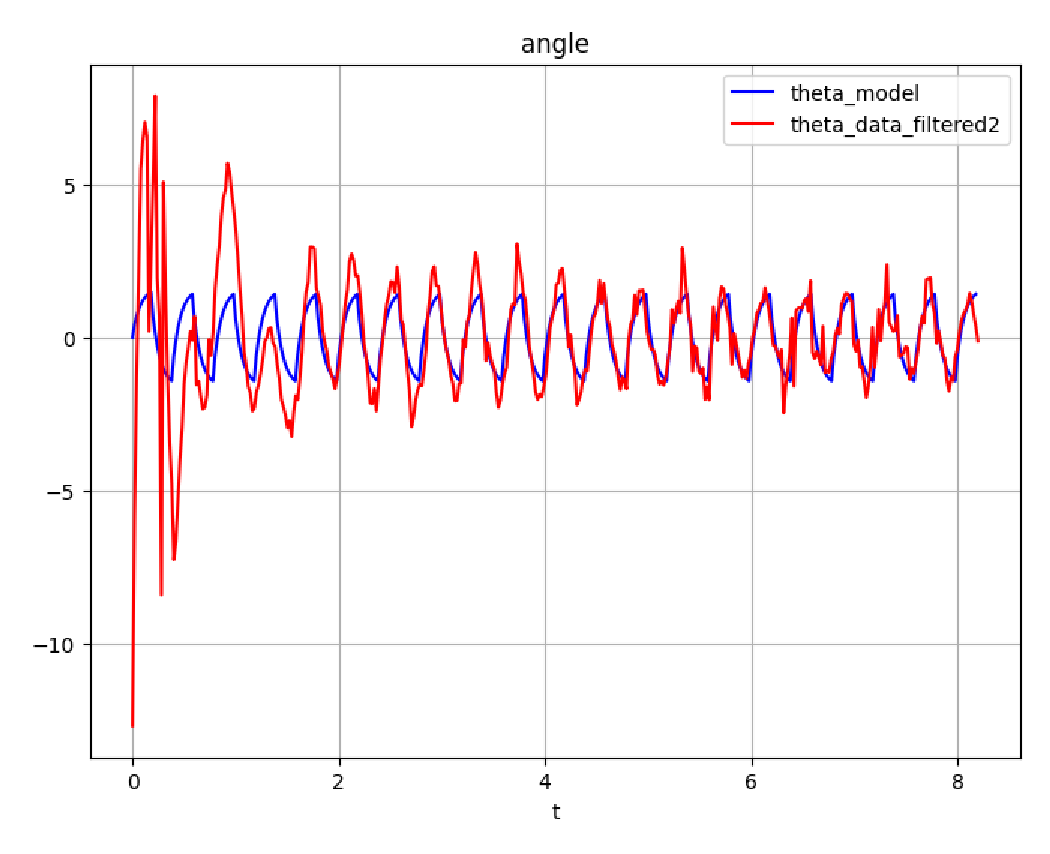
\includegraphics[scale=0.4]{figure40.eps}
    \caption{周期0.4\ sの矩形波}
    \label{fig:figure40}
  \end{minipage}
  \begin{minipage}{0.4\linewidth}
    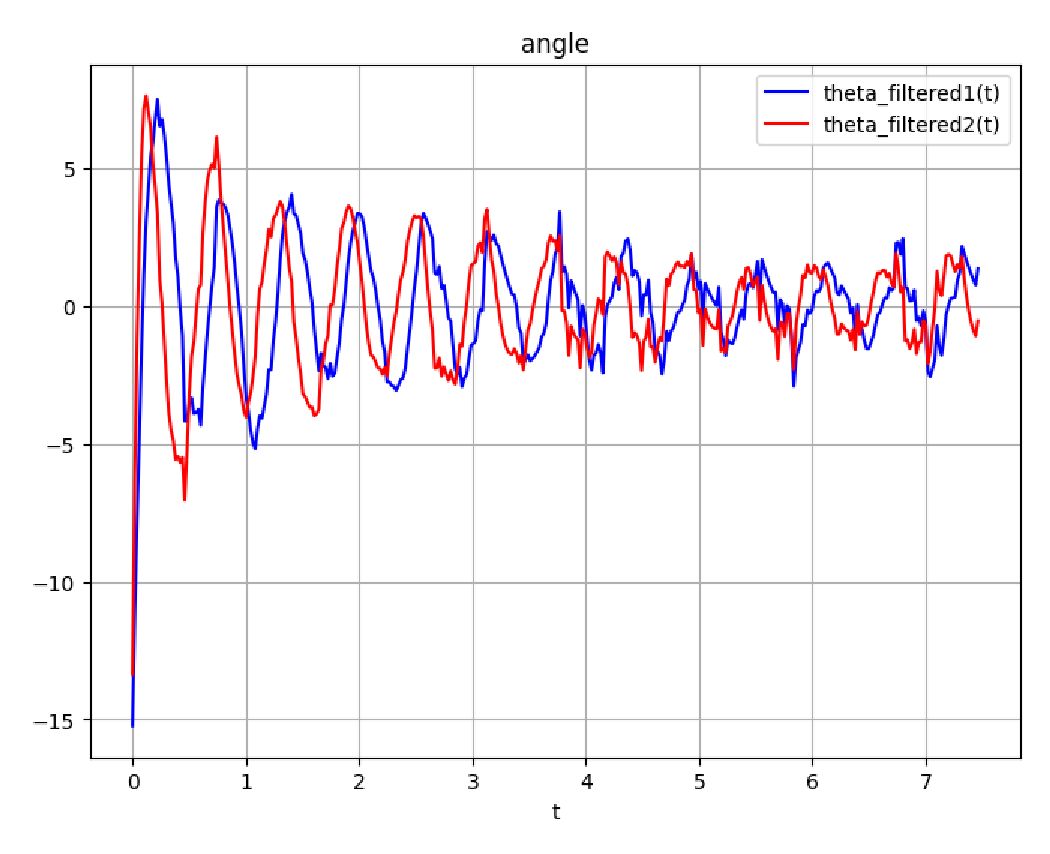
\includegraphics[scale=0.4]{figure41.eps}
    \caption{周期0.6\ sの矩形波}
    \label{fig:figure41}
  \end{minipage}
\end{figure}\\
図\ref{fig:figure40}から、初めはモデリングの波形はデータの波形より大きく振動しているが、時間が経つとデータの波形にうまくフィッティングしていることがわかる。一方で、図\ref{fig:figure41}では、初めから最後までデータの波形とモデリングの波形に大きなずれはないが、常に小さなずれが存在していることがわかり、時間が経った後でもこのずれは消えていない。このような理由により、十分に時間が経過した状態では周期0.4\ sの矩形波の方が最適制御実験に用いる点で適してると考えられる。\\
 次に用いた矩形波をハイパスフィルタとローパスフィルタに通した理由を説明する。まず、図\ref{fig:figure7}に着目すると、青線で示された何も処理されていない角度$\theta$はかなり小さい周波数で常に減少していることがわかる。そのためこの低周波の関数を減少させる成分を取り除くためにはハイパスフィルタを用いるのが効果的であることがわかる。次に(41) 式に注目すると、フーリエ係数には$1/(2n-1)$が含まれ、周波数が大きい成分の振幅は小さくなることがわかる。周波数が十分大きくなると、正弦波の振幅よりも誤差の高周波成分の振幅の方が大きくなる。そのためそのような大きな周波数では入力信号より誤差の方が大きくなり使い物にならないと考えらるためローパスフィルタにも通してそのような成分を取り除いた。\\
\\
{\large \bfseries 5.2実験2(2週目)}\\
 入力データをハイパスフィルタとローパスフィルタの両方を通してモデリングをした場合はいずれの重みでもボールはビームから落ちた。逆に、入力データをハイパスフィルタのみ通してモデリングを行った場合は、シミュレーションでオーバーシュートが起こらなくなると実機での制御もボールがビームの上に留まるようになった。これは、実機では入力信号の高い周波数帯が大部分を占めており、シミュレーションのシステムが実機のシステムから大きくずれたことが原因だと考えられる。このような結果から入力波として矩形波を用いた場合は、周波数の高い波が重要であることがわかる。
\clearpage
{\large \bfseries 5.4モデリングの精度向上のための入出力応答の取得方法}\\
 まず、今回の実験ではビームの上に赤外線センサが乗っていた。これは入力電圧を印加し、サーボモータを動作させ、出力の角度$\theta$を測定する際、赤外線センサによる重力により、ビームのサーボモータ側が下がるときは下がりやすく、ビームのサーボモータ側が上がる時は上がりにくくなる原因となる。この影響は実際に実験1の結果に現れており、図\ref{fig:figure7}の青い線が減少傾向にあるのはこれが原因である。また、5.1でも述べた通り、フーリエ級数展開をした際にできるだけ様々な周波数を持った正弦波が存在する方が装置を制御する際に様々なパターンの動きに対応できるため精度が向上する。\\
\\
{\large \bfseries 5.3位置や速度の計測データのノイズによる影響}\\
\begin{figure}[h]
  \centering
  \includegraphics[scale=1.2]{figure42.eps}
  \caption{システム$\mathrm{P_c}$のブロック線図}
  \label{fig:figure42}
\end{figure}\\
 図\ref{fig:figure42}に、今回用いたシステム$\mathrm{P_c}$を示す。実際のシステムでは図42のように、入力時に入力ノイズ$\bm v[k]$が、観測時に観測ノイズ$\bm w[k]$が生じる。このようなノイズを考慮して、状態方程式と出力方程式を求めると、
\begin{align}
  \left\{
  \begin{aligned}
    &\bm x[k+1]=A\bm x[k]+Bu[k]+\bm v[k]\\
    &\bm y[k]=C\bm x[k]+\bm w[k]
  \end{aligned}
  \right .
\end{align}
となる。$\bm x[k]\ ,\ \bm y[k]$を求めると、
\begin{align}
  \left\{
  \begin{aligned}
    &\bm x[k]=A^k\bm x[0]+\sum^{k}_{i=1}A^{k-i}Bu[i-1]+\sum^{k}_{i=1}A^{k-i}\bm v[i-1]\\
    &\bm y[k]=CA^k+C\sum^{k}_{i=1}A^{k-i}Bu[i-1]+C\sum^{k}_{i=1}A^{k-i}\bm v[i-1]+\bm w[k]
  \end{aligned}
  \right .
\end{align}
となる。よって、 時刻$k$で観測すると、$C\sum^{k}_{i=1}A^{k-i}\bm v[i-1]+\bm w[k]$のノイズが載ることになる。ここで、このノイズによる影響を減らすため、オブザーバを設置する。オブザーバを用いたブロック線図を図\ref{fig:figure43}に示す。
オブザーバの状態方程式と出力方程式は、
\begin{align}
  \left\{
  \begin{aligned}
    &\hat{\bm x}[k+1]=A\hat{\bm x}[k]+Bu[k]+L\left(\bm y[k]-\hat{\bm y}[k]\right)\\
    &\hat{\bm y}[k]=C\hat{\bm x}[k]
  \end{aligned}
  \right .
\end{align}
となる。$\bm e[k]=\bm x[k]-\hat{\bm x}[k]$を用いると、(42)、(44)式から、
\begin{gather}
  \bm e[k+1]=(A-LC)\bm e[k]+
  \begin{bmatrix}
    I&-L
  \end{bmatrix}
  \begin{bmatrix}
    \bm v[k]\\
    \bm w[k]
  \end{bmatrix}\nonumber\\
  \therefore\ \bm e[k+1]=\tilde{A}\bm e[k]+\tilde{B}\bm d[k]
\end{gather}
と表せる。ただし、$\tilde{A}=A-LC,\ \tilde{B}=[I\ -L],\ \bm d[k]=[\bm v^\top[k]\ \bm w^\top[k]]^\top$とおいた。このとき、(8)式を用いることによって、
\begin{align}
  \bm e[k]&=\tilde{A}^{k}\bm e[0]+\sum^{k-1}_{\tau=0}\tilde{A}^\tau\tilde{B}u[k-1-\tau]\nonumber\\
  &=\tilde{A}^{k}\bm e[0]+\sum^{k-1}_{\tau=0}\tilde{A}^{k-1-\tau}\tilde{B}u[\tau]
\end{align}
と表せる。ここで、正定値行列$P[k]$を$P[k]=\mathbb{E}[\bm e[k]\bm e^\top[k]]$と定義すれば、$P[k]$の対角成分の和を最小にするような$u[k]$を求めればよい。
\begin{equation}
  \mathbb{E}[\bm  e[0]\bm d^\top[k]]=\bm O\ ,\ \mathbb{E}[\bm d[k]\bm d^\top[k]]=
  \begin{bmatrix}
    Q&\bm O\\
    \bm O&R
  \end{bmatrix}
\end{equation}
とすると、
\begin{align}
  P[k]&=\mathbb{E}[\bm e[k]\bm e^\top[k]]\nonumber\\
  &=\tilde{A}^k\mathbb{E}\left[\left(\bm e[0]+\sum^{k-1}_{\tau=0}\tilde{A}^{-1-\tau}\tilde{B}u[\tau]\right)\left(\bm e[0]+\sum^{k-1}_{\tau=0}\tilde{A}^{-1-\tau}\tilde{B}u[\tau]\right)^\top\right]\left({\tilde{A}}^\top\right)^k\nonumber\\
  &=\tilde{A}^k\left[\mathbb{E}[\bm e[0]\bm e^\top[0]]+\sum_{\tau=0}^{k-1}\tilde{A}^{-1-\tau}\left(Q+LRL^\top\right)\left(\tilde{A}^\top\right)^{-1-\tau}\right]\left(\tilde{A}^\top\right)^k
\end{align}\\
となる。よって、
\begin{align}
  P[k+1]&=\tilde{A}^{k+1}\left[\mathbb{E}[\bm e[0]\bm e^\top[0]]+\sum_{\tau=0}^{k}\tilde{A}^{-1-\tau}\left(Q+LRL^\top\right)\left(\tilde{A}^\top\right)^{-1-\tau}\right]\left(\tilde{A}^\top\right)^{k+1}\nonumber\\
  &=\tilde{A}^{k+1}\left[\mathbb{E}[\bm e[0]\bm e^\top[0]]+\sum_{\tau=0}^{k-1}\tilde{A}^{-1-\tau}\left(Q+LRL^\top\right)\left(\tilde{A}^\top\right)^{-1-\tau}+\tilde{A}^{-1-k}\left(Q+LRL^\top\right)\left(\tilde{A}^\top\right)^{-1-k}\right]\left(\tilde{A}^\top\right)^{k+1}\nonumber\\
  &=\tilde{A}^{k+1}P[k]\left(\tilde{A}^\top\right)^{k+1}+Q+LRL^\top
\end{align}
となる。ここで、$k\rightarrow\infty$のとき、$P[k]=P(一定)$として良い。よって、(49)式は、
\begin{align}
  P=\tilde{A}^{k+1}P\left(\tilde{A}^\top\right)^{k+1}+Q+LRL^\top
\end{align}
となる。よって、(50)式から$P$を最小とするように$L$を設定し、オブザーバを設計すればよい。
\begin{figure}[h]
  \centering
  \includegraphics{figure43.eps}
  \caption{オブザーバを用いたブロック線図}
  \label{fig:figure43}
\end{figure}
\clearpage
{\large \bfseries 5.5行列$Q,R$による制御系の振る舞い}\\
 図\ref{fig:figure28}と図\ref{fig:figure32}を比べると、図\ref{fig:figure28}の方が収束が早くなっている。これは、$Q$の対角成分が大きくなると制御系の即応性が上がることに起因する。(21)式で$Q$の対角成分が大きくなると$\bm x[k]-\bm x_{ref}$がより重視されるような評価関数になるため、このようなことが起こる。しかし、入力に関しては評価関数内では、$u[k]-u_{ref}$の割合が小さくなるため、入力電圧が大きくなる。逆に、$R$を大きくすると即応性が下がり収束が遅くなった。また、入力電圧が小さくなった。これは(21)式で$u[k]-u_{ref}$の割合が大きくなり、$\bm x[k]-\bm x_{ref}$の割合が小さくなったことによって即応性が下がったのだと考えられる。 \\
\\
{\large \bfseries 5.6シミュレーシュンと実機の最適制御の結果の比較}\\
 実機の最適制御では全てシミュレーションとは異なった挙動を観測した。シミュレーションでオーバーシュートが見られると実機のボールは最終的にはビームの上から落ちた。逆にシミュレーションでオーバーシュートしない場合は実機でボールがビームの上に留まった。これは、オーバーシュートが存在すると目標値を超えた時に修正するために反対方向に動く必要がある。しかし、実機ではモーターを反対方向に動かす際に遅延が生じるため、シミュレーションより大きくオーバーシュートすることとなる。そのため、シミュレーションで収束していたとしても、実機では収束しなかったりする。\\
\\
{\large \bfseries 5.7ボールの静止位置のずれ}\\
 ボールの静止位置にずれが生じない場合は、赤外線センサとボールの中心を結んだ直線がビームと平行になる時である。しかし、実際には赤外線センサとボールの中心を結んだ直線はビームとは平行にならず少しずれる。これにより、赤外線センサは正確にボールの中心の位置を測定することができず、ボールの静止位置はずれる。\\
\\
{\large \bfseries 5.8\ Bellman方程式からのリッカチ方程式の導出}\\
 まず、(51)式にBellman方程式を示す。
\begin{align}
  J_k(\bm x[k])=\min_{\{\bm u[k]\}}\left\{\bm x^\top[k]Q\bm x[k]+\bm u^\top[k]R\bm u[k]+J_{k+1}\left(A\bm x[k]+B\bm u[k]\right)\right\}
\end{align}
ここで、$J_k(\bm x)=\bm x^\top[k]P[k]\bm x[k]\ (P[k]は正定値)$とおき、(51)式の右辺の\{\}の中を$f(\bm u[k])$とおくと、(6)式を用いて、
\begin{align}
  f(\bm u[k])&=\bm x^\top[k]Q\bm x[k]+\bm u^\top[k]R\bm u[k]+J_{k+1}(A\bm x[k]+B\bm u[k])\nonumber\\
  &=\bm x^\top[k]Q\bm x[k]+\bm u^\top[k]R\bm u[k]+(A\bm x[k]+B\bm u[k])^\top P[k+1](A\bm x[k]+B\bm u[k])\nonumber\\
  &=\bm x^\top[k]Q\bm x[k]+\bm u^\top[k]R\bm u[k]+\bm x^\top[k]A^\top P[k+1]A\bm x[k]+\bm x^\top[k]AP[k+1]B\bm u[k]\nonumber\\
  &\hspace{126pt}+\bm u^\top[k]B^\top P[k+1]A\bm x[k]+\bm u^\top[k]B^\top P[k+1]B\bm u[k]\nonumber\\
  &=\bm x^\top[k]Q\bm x[k]+\bm u^\top[k]\left(R+B^\top P[k+1]B\right)\bm u[k]+\bm x^\top[k]A^\top P[k+1]A\bm x[k]+\bm x^\top[k]AP[k+1]B\bm u[k]\nonumber\\
  &\hspace{303pt}+\bm u^\top[k]B^\top P[k+1]A\bm x[k]
\end{align}
と表せる。$f(\bm u[k])$を$\bm u[k]$で微分すると、
\begin{align}
  \frac{\partial f}{\partial\bm u}&=2\bm u^\top[k]\left(R+B^\top P[k+1]B\right)+\bm x^\top[k]AP[k+1]B+ \bm x^\top[k]A^\top P[k+1]B\nonumber\\
  &=2\bm u^\top[k]\left(R+B^\top P[k+1]B\right)+2\bm x^\top[k]AP[k+1]B
\end{align}
となる。ここで、$f(\bm u[k])$が最小になるとき、$\partial f/\partial\bm u=\bm O$
となるから、(53)式は、
\begin{gather}
  2\bm u^\top[k]\left(R+B^\top P[k+1]B\right)+2\bm x^\top[k]AP[k+1]B=\bm O\nonumber\\
  \therefore\ \bm u^\top[k]=-\bm x^\top[k]AP[k+1]B\left(R+B^\top P[k+1]B\right)^{-1}\\
  \therefore\ \bm u[k]=-\left(R+B^\top P[k+1]B\right)^{-1}B^\top P[k+1]A^\top\bm x[k]
\end{gather}
となる。(51)、(54)、(55)式と$J_k(\bm x)=\bm x^\top[k]P[k]\bm x[k]$から、(51)式は、
\begin{align}
  \bm x^\top[k]P[k]\bm x[k]=&\ \bm x^\top[k]Q\bm x[k]+\bm x^\top[k]AP[k+1]B\left(R+B^\top P[k+1]B\right)B^\top P[k+1]A^\top\bm x[k]\hspace{70pt}\nonumber\\
  &+\bm x^\top[k]A^\top P[k+1]A\bm x[k]-2\bm x^\top[k]AP[k+1]B\left(R+B^\top P[k+1]B\right)^{-1}B^\top P[k+1]A^\top\bm x[k]\nonumber\\
  =&\ \bm x^\top[k]Q\bm x[k]-\bm x^\top[k]AP[k+1]B\left(R+B^\top P[k+1]B\right)B^\top P[k+1]A^\top\bm x[k]+\bm x^\top[k]A^\top P[k+1]A\bm x[k]\nonumber\\
  =&\ \bm x^\top[k]\left\{Q+A^\top P[k+1]A-AP[k+1]B\left(R+B^\top P[k+1]B\right)B^\top P[k+1]A^\top\right\}\bm x[k]
\end{align}
となる。よって、
\begin{equation}
  P[k]=Q+A^\top P[k+1]A-AP[k+1]B\left(R+B^\top P[k+1]B\right)B^\top P[k+1]A^\top
\end{equation}
となる。(57)をリッカチ方程式と呼ぶ。\\
\\
\hspace{-2pt}{\Large \bfseries 6.感想}\\
 制御は意外と難しいなと思いました。理論だけじゃ何もできないなと思いました。\\
\\
{\Large \bfseries 参考文献}
\begin{thebibliography}{1}
\vspace{-1.5cm}
  \bibitem{text} 2022OptimalControl\_MI\_0912.pdf閲覧日:2023/11/28
\end{thebibliography}
\end{document}
